\documentclass{book}
\usepackage[utf8]{inputenc}


%--------------------
% Packages
% -------------------
%\documentclass[11pt,a4paper]{article}
%\usepackage[utf8]{inputenc}
%\usepackage[T1]{fontenc}
%\usepackage{gentium}
\usepackage{csquotes}


\usepackage{mathptmx} % Use Times Font
%\usepackage[authordate,bibencoding=auto,strict,backend=biber,natbib]{biblatex-chicago}
% HELLO
\usepackage[sorting=nyt]{biblatex}
%\usepackage[sorting=nyt, citestyle=authoryear]{biblatex}
\title{Draft thesis}
\author{s1476046 }
\date{\today}

\usepackage[pdftex]{graphicx} % Required for including pictures
\usepackage[english]{babel} 
\usepackage[pdftex,linkcolor=black,pdfborder={0 0 0}]{hyperref} % Format links for pdf
\usepackage{calc} % To reset the counter in the document after title page
\usepackage{enumitem} % Includes lists
\usepackage{wrapfig}

 \frenchspacing % No double spacing between sentences
\linespread{1.2} % Set linespace
\usepackage[a4paper, lmargin=0.1666\paperwidth, rmargin=0.1666\paperwidth, tmargin=0.1111\paperheight, bmargin=0.1111\paperheight]{geometry} %margins
%\usepackage{parskip}

\usepackage[all]{nowidow} % Tries to remove widows
\usepackage[protrusion=true,expansion=true]{microtype} % Improves typography, load after fontpackage is selected

\usepackage{lipsum} % Used for inserting dummy 'Lorem ipsum' text into the template

% Pretty much all of the ams maths packages
\usepackage{amsmath,amsthm,amssymb,amsfonts}
\usepackage{adjustbox}
% Allows you to manipulate the page a bit
\usepackage[a4paper]{geometry}
% Provides commands to make subfigures (figures with (a), (b) and (c))
%\usepackage{subfigure}
\usepackage{subcaption}

% Typesets URLs sensibly - with tt font, clickable in PDFs, and not breaking across lines
\usepackage{url}

% Makes references hyperlinks in PDF output
\usepackage{hyperref}
\DeclareUnicodeCharacter{0301}{*************************************}
\DeclareUnicodeCharacter{0308}{**********************0308***********}
% Provides ways to include syntax-highlighted source code
\usepackage{listings}
\setlength{\marginparwidth}{2cm}
\usepackage{todonotes}
\lstset{frame=single, basicstyle=\ttfamily}

%\newcommand{\todo}[1] {\textbf{\textcolor{red}{#1}}}
% Provides good access to colours
\usepackage{color}
\usepackage{xcolor}
\usepackage{setspace}
\usepackage{longtable}
\usepackage{rotating}
\usepackage{booktabs}
\usepackage{array}
\usepackage{adjustbox}
\usepackage{pifont}
\usepackage{booktabs}
\usepackage{pgfplots}
\usepackage{pgfplotstable}

% for splitting columns on tables see https://tex.stackexchange.com/questions/2441/how-to-add-a-forced-line-break-inside-a-table-cell
\usepackage{makecell}
%\usepackage{showframe}
%Really, really mean here with graphics [H]
\usepackage{multicol}
\usepackage{float}
% for rotational tables see https://tex.stackexchange.com/questions/19017/how-to-place-a-table-on-a-new-page-with-landscape-orientation-without-clearing-t
\usepackage{pdflscape}
\usepackage{afterpage}
\usepackage{capt-of}

%https://tex.stackexchange.com/questions/2441/how-to-add-a-forced-line-break-inside-a-table-cell/19678
\renewcommand\theadalign{bc}
\renewcommand\theadfont{\bfseries}
\renewcommand\theadgape{\Gape[4pt]}
\renewcommand\cellgape{\Gape[4pt]}


\graphicspath{{images/}}
%-----------------------
% Set pdf information and add title, fill in the fields
%-----------------------
\hypersetup{ 	
pdfsubject = {},
pdftitle = {},
pdfauthor = {}
}

%\includeonly{pilot}
%\includeonly{introduction}
%\includeonly{gwas_and_general}
%\includeonly{gwas_general_chapter_end_materialcopy}

%\includeonly{centrality_measures_prototype}
%\includeonly{community_detection}
%\includeonly{orthologs}
%\includeonly{phenotypes}
%\includeonly{checking_our_findings}
%\includeonly{extra_tables}
%\includeonly{new_century}
%\includeonly{new_tables}
%\includeonly{discussion}
%\includeonly{discussion1}
%\addbibresource{references.bib}
\addbibresource{orthologs.bib}
%-----------------------
% Begin document
%-----------------------
\doublespacing
%\linespread{1.6}
%\bibliographystyle{ieeetr}
%\bibliographystyle{apalike}
\begin{document}
\frontmatter
\maketitle
\tableofcontents

%\listoftables
%\listoffigures
%\listoftodos

\mainmatter

\chapter{Introduction}

%\section{Importance}

Psychiatric and substance abuse disorders account for 7.1\% of disease burden as measured by disability-adjusted life years\cite{murray2015global}.   A range of environmental and genetic factors are known to be implicated in their development. Of the genetic factors, most encode molecules that are found in the neuronal synapse, a structure that is responsible for the exchange and processing of information between nerve cells\cite{grant2012synaptopathies}.

\section{The synaptic proteome}

This thesis is about synapses and cognition, specifically how the complicated interactions of the proteins making up synapses may affect the efficiency of cognition in man and model animals. 

The synapse is a complex system composed of thousands of proteins that form higher order structures (the synaptic proteome)\cite{grant2012synaptopathies}. There have been great advances in the understanding of the molecular mechanisms of synaptic function in the last 20 years\cite{grant2018synaptomic}. The synaptic proteins form a complex system and to understand their role in health and disease it is necessary to understand how it functions as a system.  One important way of understanding complex systems is as a network where nodes, in this case proteins, are joined by edges if they interact. 



This thesis will investigate if a network analysis of the synaptic proteome is useful in understanding the molecular basis of cognition. In particular it will see whether there is evidence of an effect of the structure of synaptic protein interactions on animal models of cognition or human population studies of cognitive ability. It will test the hypothesis that genes encoding proteins that are more important to the network are over represented in animal models of cognition or in human population studies of intelligence or educational attainment. It will also assess whether particular structures found in the network topology have an effect on human or animal cognitive function. Before turning to the network structure of the synapse and population studies of cognition it is necessary to introduce the structure and function of the excitatory synapses that will be discussed in the coming chapters. 

\subsection{Synapse introduction}
A nerve cell is composed of a number of dendrites that receive incoming signals, a cell body or soma and an axon that transmits outgoing signals (figure~\ref{fig:soma and dendrites}). Between the axon and the dendrite are synapses (see figure~\ref{fig:synapse}).Synapses are junctions where information transfer occurs between nerve cells and are the most abundant structure in the brain \cite{grant2012synaptopathies}.

% In addition, although less marked in recent years, genetic approaches to cognitive ability remain highly controversial. In describing a computational systems biology approach to cognition, although it may appear clear from this review, it is important to avoid the implication that this implies a computatio\cite{deary2009genetic}. In addition, although less marked in recent years, genetic approaches to cognitive ability remain highly controversial. In describing a computational systems biology approach to cognition, although it may appear clear from this review, it is important to avoid the implication that this implies a computational model of mind or of cognitive abilities. 
% nal model of mind or of cognitive abilities. 


\begin{figure}
    \centering
    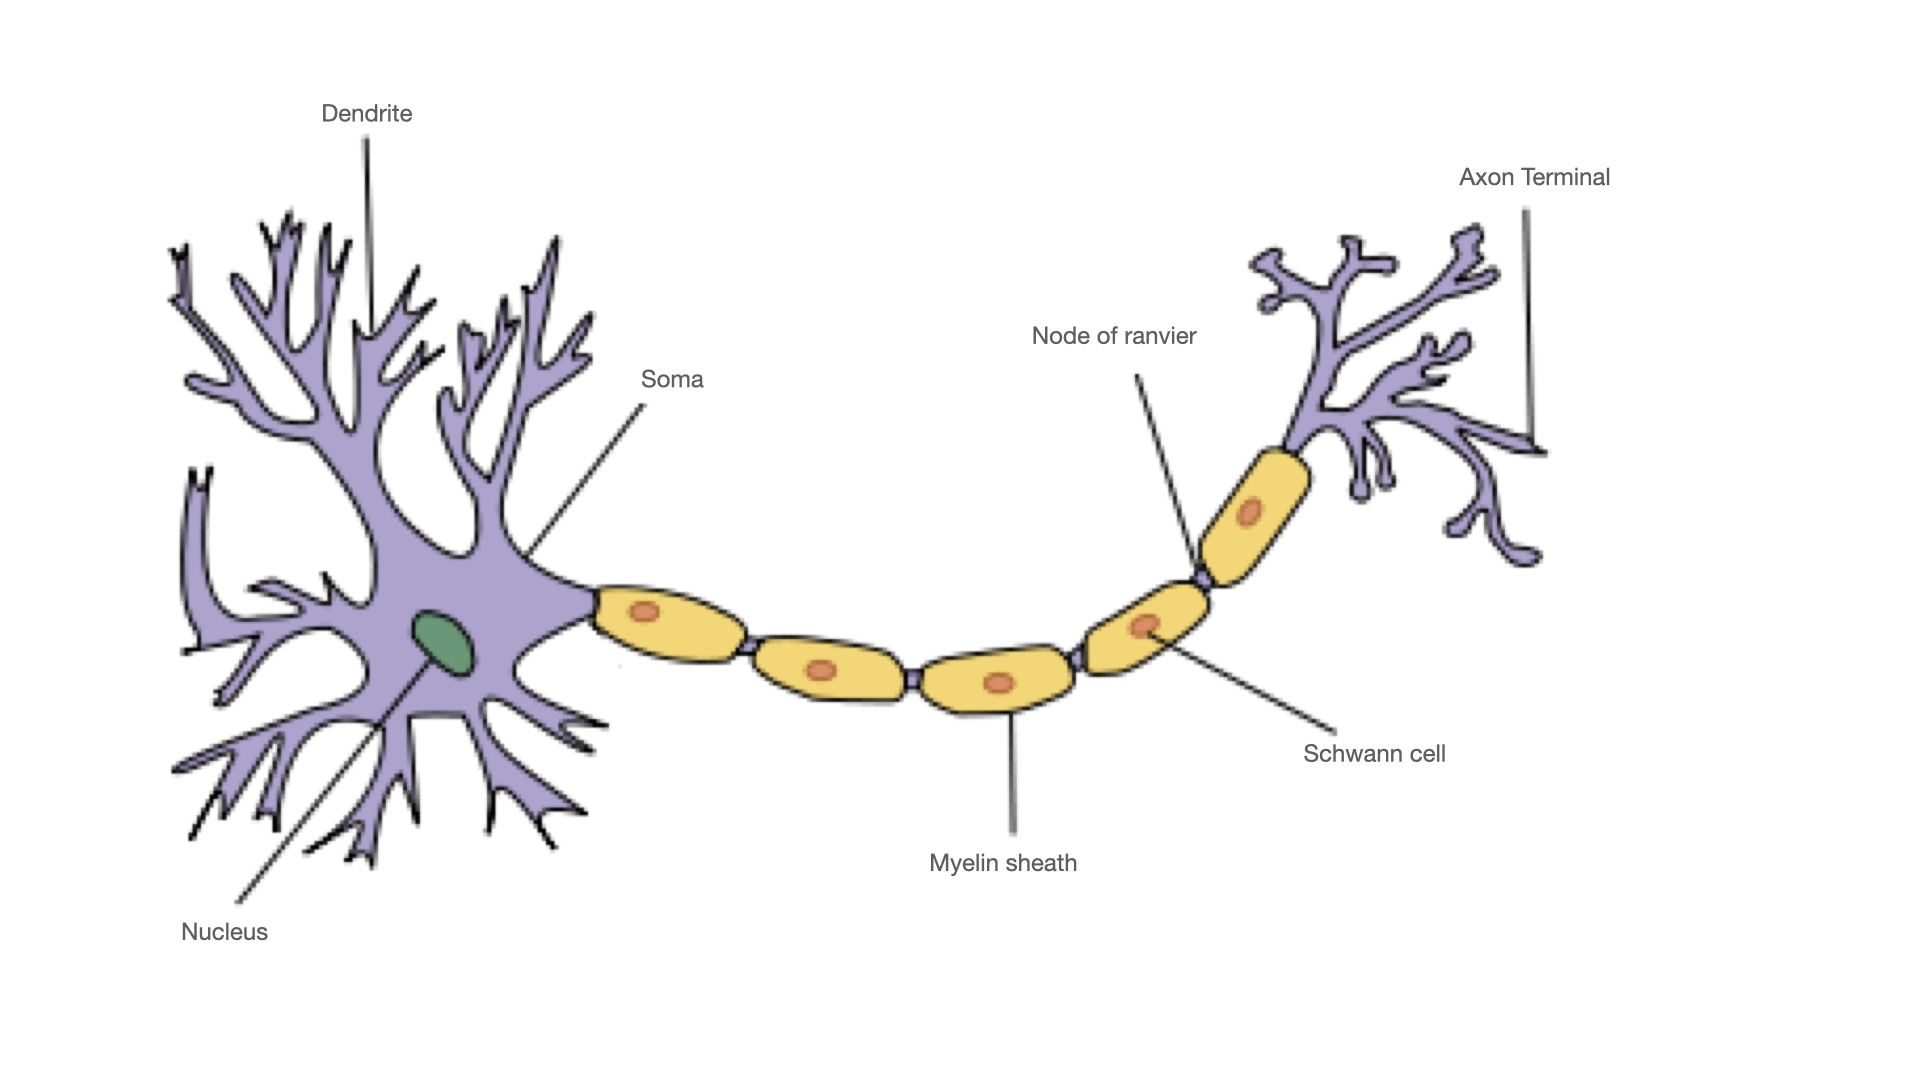
\includegraphics[width=0.9\textwidth]{images/nerve_cell001.jpeg}
    \caption{Soma and dendrites}
    \label{fig:soma and dendrites}
\end{figure}

Each nerve cell has one outgoing axon but a cortical neuron receives input from around 100,000 synapses, although only around 50 are active at any one time\cite{lisman2017glutamatergic}\footnote{number has varied see also \cite{laughlin2003communication} which has 10,000}. 
Although synaptic numbers vary over time, the number of synapses in the human neo-cortex has been estimated to be $1.5 \times 10^{14}$ (0.15 quadrillion)\cite{pakkenberg2003aging}. A synapse connects a presynaptic neuron and a postsynaptic cell across the synaptic cleft \cite{sudhof2012presynaptic}. The synapse is made up of proteins that self organise into macro-molecular machines that are responsible for signal transduction and processing\cite{frank2016nmda}.  The nerve cell integrates incoming information from the dendrites into a binary response at the axon\cite{lassek2015synaptic},\cite{pocklington2006proteomes}.

 The majority of synapses in the brain belong either to the excitatory glutamate system or the inhibitory gamma-aminobutyric acid (GABA) system. The most common type of synapse and neurotransmitter are the glutamatergic excitatory transmitters which comprise the main information processing system in the brain \cite{stewart2014structure},\cite{niciu2012overview} \footnote{was a todo: previous ref stewart2014structure changes second ref ok}. Glutamate is also a precursor for GABA. 

The term synapse, from the Greek ``to clasp together" was coined by Sherrington in 1897 writing in Foster’s textbook of physiology \cite{foster1895text}. Since Cajal showed that there was a gap between nerve cells the accepted model of the nervous system has been of a structure composed of nerve cells built into higher order circuits\cite{ramon1911histologie},\cite{grant2018synapse} rather than a reticulum or syncytium\footnote{although some still do see \cite{bacsar2016clair}}. Cognitive complexity was thought to arise from an increasing number of connections (the neuronal hypothesis)\cite{grant2018synaptomic}.
%\todo{ ? expand this section}
%\todo{need ref for cognitive complexity}
\subsection{Molecular genetic revolution}
\label{sec:molecular genetic revolution}
 The neuronal hypothesis holds that the brain's functional unit is the neural circuit and that brain complexity arises from the pattern of nerve cell and circuit connections\cite{grant2018synaptomic}. Quite recently the molecular interactions of the synapse were believed to be relatively simple with a small number of proteins sufficient for signal transfer and the control of synaptic connection strength \cite{grant2019synapse}, \cite{lisman1994cam}. This hypothesis is not unreasonable, simple models of neurons can carry out complex calculations requiring only weights at their connections analogous to connection strength at synapses\cite{hinton2007learning}. Synaptic function as signal transmission and modulation of connection strength concurred with the model of learning by increasing synaptic strength formalised by Hebb \cite{hebb1949organization_check}.
 
 Direct molecular interrogation of synaptic proteins became possible with mouse models in 1992 allowing the identification of synaptic proteins and the study of their function using knockdowns  \cite{grant1992impaired},\cite{silva1992impaired}. Further advances in molecular genetics revealed the complexity of the synaptic proteome. In 2000 Husi et al. \cite{husi2000proteomic} identified 77 proteins in the N-methyl-D-aspartate (NMDA) receptor complex (NRC). Over the next 5 years many more synaptic proteins were identified. In 2006 an analysis considered the network of 186 proteins in the NRC/Membrane Associated Guanylate Kinase (MAGUK) associated signalling complex (NRC/MASC) \cite{pocklington2006proteomes}. The number of known proteins in the post synaptic proteome rose to 1,124 by 2006\cite{collins2006molecular}.
 
The number of proteins and the complexity of their interactions exceeded what might be expected to be necessary to simply maintain connection strength 
%\todo{have we introduced connection weight}
and led to the recognition that the proteome was vitally involved in signal processing and computation as well as signal transduction\cite{grant2018synaptomic}.  Over 3,000 proteins have now been identified in proteomic studies of the post synaptic density (PSD), although this number appears to be reaching a plateau\cite{heil2018systems}. 
%\todo{query move this bit}
The proteins that form the structure of the post synaptic area are modular and form higher order complexes whose structure is related to their function\cite{pocklington2006proteomes},\cite{zhu2016mechanistic},\cite{frank2016nmda}. To understand the synapse we must try to understand the complexity of this system.

\begin{figure}
    \centering
    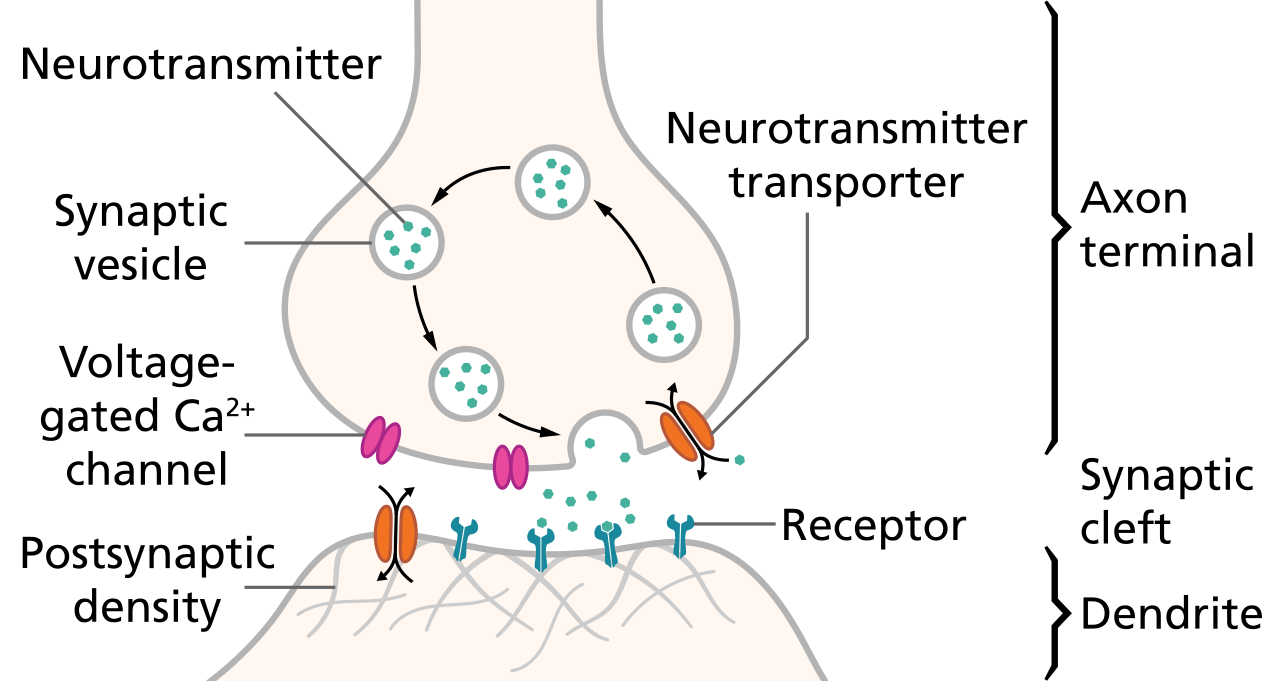
\includegraphics[width=0.9\textwidth]{images/SynapseSchematic_en.png}
    \caption[Schemtatic representation of synapse]{Schematic representation of synapse showing presynaptic area (labelled axon terminal) containing vesicles rich in neurotransmitters and post synaptic density.  Picture credit Thomas Splettestoesser Creative Commons \url{https://commons.wikimedia.org/wiki/User:Splette}}
    \label{fig:synapse}
\end{figure}





\subsubsection{High level function of the synapse}

The synapse controls the strength of the connection between nerve cells. If the activation of one nerve cell repeatedly activates another their connection will strengthen over time (Hebbian learning)\cite{hebb1949organization_check}. Hebb's rule \cite{hebb1949organization_check} requires the arrival of a signal at the presynaptic terminal, and consequent postsynaptic depolarisation leading to a stronger synaptic connection.  As neural circuits determine behaviour, these repeated patterns of activation form a basis for learning.%\todo{this end of sentence new review}.

The discovery of long term potentiation (LTP) by Bliss and Lomo \cite{bliss1973long} ultimately led to the discovery of the importance of glutamate transmission in LTP and that disruption of synaptic proteins reduces LTP and learning. Hebb posited a model where the connection strength between two neurons depends on how often they are activated together.  Both short term potentiation and long term potentiation are involved in adaptive neural information processing by controlling the strength of the connections between neurons\cite{xiao2013adaptive}.

\section{Synapse structure}
\label{sec:Synaptic structure}
The synapse is composed of a presynaptic area filled with neurotransmitter vesicles and a postsynaptic area containing neurotransmitter receptors and structural proteins separated by a gap. Nerve signals arrive at the presynaptic area, cause or inhibit the release of neurotransmitters from synaptic vesicles which diffuse across the cleft and are detected by postsynaptic receptors whose activation may lead to depolarisation of the cell axon. 

%
\subsection{Presynaptic area structure}
The presynaptic area is separated from the post synapse by the synaptic cleft \cite{rusakov2011shaping}, an area approximately 20nm in size \cite{zuber2005mammalian},%\todo{fix missing circumflex in the first name of zuber DONE} 
spanned by trans-synaptic adhesion molecules\cite{missler2012synaptic}.

 The presynaptic area contains neurotransmitters stored in vesicles docked and fused with the plasma membrane at a specialised active zone. This is an electron-dense area, parallel and juxtaposed to the plasma membrane\cite{schoch2006molecular},\cite{sudhof2012presynaptic}. Neurotransmitters are substances which, when they diffuse across the synaptic cleft, give rise to signal in the postsynaptic receptors. Active vesicles are docked at the edge of the membrane and released following calcium influx \cite{lassek2015synaptic}. After neurotransmitter release, the vesicle is recycled by endocytosis\cite{ashery2014molecular}. Short term changes in synaptic plasticity (short term potentiation) are mainly caused by changes in the probability of presynaptic vesicle release. In contrast, long term potentiation occurs mostly at the postsynaptic density.  A substantial amount of neural computation occurs in the presynaptic area and is dependent on synaptic proteins \cite{sudhof2012presynaptic}.
 
 
  A protein complex of 5 evolutionarily conserved proteins: RIM, Munc13, $\alpha$-liprin, RIM BP and ELKS \cite{sudhof2012presynaptic} primes the vesicles. Piccolo and Bassoon proteins are also associated with the active zone in vertebrates\cite{gundelfinger2016role}.  SNARE proteins facilitate vesicular fusion \cite{sudhof2012presynaptic}. Mitochondria \cite{lassek2014proteome} are an integral part of the presynaptic area and were noted in early electron microscopy  examinations \cite{gray1959electron}. The active zone is closely associated with a cytoskeletal matrix: the cytoskeletal matrix at the active zone (CAZ) \cite{schoch2006molecular}. Post synaptic activation results in CAZ clustering \cite{glebov2017nanoscale}. 
 
   In some nerve cells such as  photoreceptors, the active zone is ribbon-like and capable of prolonged discharge  \cite{ashery2014molecular}.  
 
 
The presynaptic area developed from vesicle transport systems in earlier organisms and has developed more recently than the postsynaptic density (PSD)\cite{emes2012evolution}.

 
\subsection{The postsynaptic area and postsynaptic density}
\label{sec:post synaptic area and post synaptic density}
The postsynaptic density is an electron-dense area parallel to the synaptic plasma membrane and extending $\approx$ 35nm deep to it \cite{harris2012ultrastructure}. Formed from structural proteins that bind to actin in dendritic spines and to the receptor complexes, it contains protein kinases, receptor molecules and protein scaffold complexes such as postsynaptic density protein 95 (PSD-95). There are slight differences in its composition between mouse and man \cite{bayes2012comparative}, but in general, its component structures are conserved in vertebrates. The components of the postsynaptic area arose in the earliest prokaryotes to detect changes in chemical gradients with movement and are the most ancient part of the synapse developmentally \cite{grant2018synapse}, \cite{emes2012evolution}. 

Neurotransmitter chemicals typically mediate signal transfer across the synaptic cleft although direct electrical transmission can occur across gap junctions in the retina and some locations in the central nervous system \cite{stewart2014structure}. The neurotransmitter receptors are bound to cytoskeletal proteins and modified by members of the membrane-associated guanylate kinase family (MAGUK) of proteins involved in synaptic plasticity \cite{zhu2016mechanistic}. Glutamate release occurs in areas closely aligned with glutamate receptors in the postsynaptic density (PSD) \cite{harris2012ultrastructure}.

 The receptors in the postsynaptic density show a geographical variation with the $\alpha$-amino-3-hydroxy-5-methyl-4-isoxazolepropionic acid  receptors (AMPAR) and N-methyl D aspartate (NMDA) receptors in close apposition to the presynaptic active zone and the metabotropic glutamate receptors (mGluR) in the perisynaptic zone\cite{scheefhals2018functional}.
 
 The ionotropic receptors have the fastest signalling characteristics and include NMDAR, AMPAR  and Kainate receptors (KAR) named after the particular agonists found to provoke them\cite{nakanishi1992molecular},\cite{bettler1995ampa}. Kainate acid receptors have a metabotropic G protein-mediated element in their response that has been shown to mediate non NMDA LTP in the hippocampus of the rat \cite{petrovic2017metabotropic}. They are less involved in synaptic transmission \cite{contractor2011kainate} than the two pure ligand-gated ionotropic receptors NMDAR and AMPAR.
 \footnote{note to Douglas/self I am mentioning all this as group 5 has GRIA 1-4(AMPA), GRIK (Kainate) 1,2,3,5 and mGlu 2,3,7. 2 and 3 are Group II (activate K inhibit Ca and adenylyl cyvlase and pre and post synaptic, 7 is group7 and associated with presynaptic active zone}  
 The metabotropic glutamate receptor activates heterotrimeric G proteins and results in both signalling and recruitment of further ionotropic receptors to the postsynaptic area\cite{niswender2010metabotropic},\cite{pin2016organization}.  
 
Postsynaptic proteins show many remarkable features. They are relatively resistant to complete abolition of function \cite{keverne1997evaluation}, \cite{charlesworth2016canalization} and even in knockout animals, some signalling remains. In addition, the dysfunction of many disparate synaptic elements can result in common phenotypes, particularly neuropsychiatric phenotypes. A wide variety of mutations at different proteins and different loci within specific proteins can give rise to common disorders such as Autism Spectrum Disorder (ASD)\cite{toro2010key}. By contradistinction point mutations in crucial receptor proteins often give rise to severe phenotypes, as we shall see later, but also give rise to different phenotypes from mutations at different points in the protein (a case in point here being GRIN2A) \cite{endele2010mutations}. These features may in part be related to the organisation of the PSP into supercomplexes that inherit network based robustness\todo{tmp:cross ref} in addition to genetic robustness from paralogue expansion\cite{grant2016molecular}.



\subsection{Molecular function}
Calcium ion influx is necessary for depolarisation. Synaptotagmin acts as a calcium sensor and allows for the rapid fusion of synaptic vesicles with the cell membrane and release of neurotransmitters into the synaptic cleft\cite{martens2007synaptotagmin},  It is also necessary for learning in animals and long term potentiation and depression \cite{lisman2012mechanisms}.
\subsubsection{Neurotransmitter receptors}
\label{sec:Neurotransmitter receptors}
L glutamate, a small amino acid, is the dominant neurotransmitter at excitatory synapses within the brain \cite{niswender2010metabotropic}. Glutamate levels are controlled by the glutamate glutathione pathway and glutamate transporters\cite{sedlak2019glutathione}.

Fast excitatory neurotransmission is carried out at the ionotropic glutamate receptors AMPA and NMDA \cite{traynelis2010glutamate}. Ionotropic glutamate receptors consist of 4 sub-units spanning the extracellular membrane that form a central ion pore. AMPA and Kainate receptors are homo or heterotetrameric, but the NMDA receptor is obligatory heterotetrameric. The AMPA receptor is responsible for most of the fast excitatory transmission in the central nervous system \cite{henley2013ampa}. It is composed of four sub-units GRIA1-4 and is mainly permeable to sodium (Na$^+$) and potassium (K$^+$) ions. The glutamate receptor sub-units originate from 18 different gene protein products representing NMDA, AMPA, Kainate and delta groups \cite{traynelis2010glutamate}. The NMDA receptor is also composed of four subunits (a tetrameter)  but is permeable to calcium ions. AMPA and KAR are fast-acting, working in less than 1ms\cite{traynelis2010glutamate} wile NMDAR depolarise more slowly, in the 10ms range \cite{traynelis2010glutamate},\cite{nicoll2017brief}. 

Magnesium (Mg$^{2+}$) ions initially block NMDA receptor activity, and  AMPA receptor activation is required to displace the Mg$^{2+}$ ions. AMPA is intimately involved in long term potentiation. After Ca$^{2+}$ ion entry from the synaptic cleft, Calcium/calmodulin-dependent protein kinase II (CaMKII) is activated and leads to an increase in AMPA receptors at the postsynaptic membrane. Calcium can enter through NMDA receptors after unblocking of $Mg^{2+}$ ions, and its entry leads to activation of Calcium/Calmodulin dependent protein kinase. The kinase subsequently binds to NMDA receptors and phosphorylates sub-units of the AMPA type glutamate receptor.

Slow synaptic transmission, mediated by G protein second messengers, results from the action of metabotropic glutamate receptors (mGluR) \cite{niswender2010metabotropic} although mGluR signalling can also occur in time scales closer to ionotropic glutamate receptors (iGluR). There are eight mGluR subtypes. Metabotropic glutamate receptors are family C G-Protein-coupled receptors (GPCRs). Group 1 mGLU promote intracellular calcium release whereas group 2 are localised pre and postsynaptically, and group 3 are localised presynaptically \cite{niswender2010metabotropic}. 
\footnote{Note to self/Douglas and source code remove later - grm 2,3,7 in group 5 - 2 and 3 are in group 2, 7 along with 4,6,7,8 are om group 3, (grm 1 and 5 are group1), 1,2,3,5 and 7 are in the PSP, one is in 22 and 5 in group 32 - groups 20, 22 and 32 are quite closely related see \url{ source('~/RProjects/graph_groups/R/distribution_m_glu_glutamate.R')}Group II Metabotropic Glutamate Receptors Mediate Presynaptic Inhibition of Excitatory Transmission in Pyramidal Neurons of the Human Cerebral Cortex shows can be pre and postsynaptic } %However, there is also evidence for pre and postsynaptic action \todo{? more to discussion}
Metabotropic glutamate receptors exert their effect by increases in protein synthesis. Group II have been related to anxiety, schizophrenia and Alzheimer's disease\cite{swanson2005metabotropic}.


\subsubsection{Long term potentiation}
\label{sec:LismanLTP}
Periods of synaptic activity can increase the strength of synaptic connections by the process of long term potentiation (LTP).

Cajal first proposed that an increase in the strength of the connection between neural cells leads to learning in 1911 \cite{nicoll2017brief}. In Hebb's model synaptic modification occurs following coexistent pre and postsynaptic activation (two factors are required)\cite{hebb1949organization_check}. Later experiments showed that tetanic stimulation of rabbit hippocampal synapses increased the strength of subsequent responses\cite{bliss1973long}, and that NMDAR activity is necessary for LTP\cite{collingridge1983excitatory} but not for neurotransmission. 
 Interfering in the process of LTP in animal models leads to defects in memory and learning \cite{lisman2012mechanisms}).
LTP is a complex process with the modular organisation of 70-80nm modules of independently activating AMPA receptors being integral to the variety of potentiation responses\cite{lisman2017glutamatergic}. Six different forms of plasticity are observed in the synapse short term plasticity, long term plasticity, late long term plasticity, long term depression, distance-dependent scaling and homeostatic scaling \cite{lisman2017glutamatergic}. Short term potentiation (STP) results from weak stimuli and occurs early, and is a promising model of working memory as GluA1 knockdown animals have abnormal STP and working memory\cite{lisman2017glutamatergic}. Early LTP is likely mediated by phosphorylation of GluA1 by CaMKII. Late long term potentiation is associated with a change in the size of the PSD. LTP, by definition, begins 30 minutes after a tetanic stimulus. Late LTP is associated with more AMPAR signalling, protein synthesis\cite{park2018ampa} and an increase in quantal probability. This may require other factors such as dopamine in CA1 postulated as an indicator of salience or brain-derived neurotrophic factor (BDNF). For this reason (that three factors rather than two are required) the process has been referred to as NeoHebbian\cite{lisman2017glutamatergic}. The mechanisms of this late stage include increase in receptors from PSD 95 mediated CaMKII phosphorylation of Stargazin or SynGAP or activation of extracellular signal-regulated (ERK) kinase through SynGAP. Throughout all of this it is clear that memory and learning appear to intimately linked to  the combination and structure of synaptic proteins. \todo{tmp: that nonsense about memory molecule}

 
 
Computational models of the synapse have explain been developed that simulate these responses on the assumption that there are `hotspots' where there are either modules of AMPA receptor present or absent on vesicle release, and plasticity can occur with recruitment to silent hotspots\cite{lisman2017glutamatergic}.
 
 
\subsection{The synaptomic theory}

An alternative model of synaptic learning has been proposed where the complexity of the composition of the proteome is integral to learning\cite{grant2019synapse}. In this model, synaptic proteins form complexes and supercomplexes that are specifically attuned to different temporal neural signals and synaptic protein organisation acts as a `zip code' addressing different areas in the brain\cite{grant2018synaptomic}.

Evidence that is inconsistent with synaptic strength as the only mediator of learning\cite{grant2019synapse} include preservation of spatial learning after NMDA signalling and LTP have been blocked\cite{bannerman2014hippocampal} and mutations to PSD 95 leading to cognitive impairment but enhanced long term potentiation\cite{nithianantharajah2013synaptic}. It may be that the NMDA receptor both mediates learning and LTP\cite{grant2019synapse}. In this model too the modular structure of the proteome is closely related to its function in cognition. 

%  In contrast, Grant suggests a bottom-up synaptogenic model in which the synaptic protein composition acts as a zipcode which allows spatially distributed neurons to respond to particular patterns of receptor stimulation. In support of his arguments, he points out that the association of long term potentiation with learning remains controversial and it may be that the glutamate receptor (NMDA both subsume LTP and learning rather than affecting LTP which in turn causes learning. An example suggesting this is that mutations in PSD 95 give rise to cognitive impairments but increased long term potentiation.


\subsection{Role in disease}
 
Bayes et al.\cite{bayes2011characterization} identified, in human neocortical biopsies, 1,461 proteins in the human post synaptic density (hPSD) and 748 that were consistent across three replicates. Using the Online Mendelian Inheritance in Man (OMIN) database \cite{hamosh2005online} and limiting the analysis to monogenic diseases the authors showed that 269 diseases resulted from mutations in 199 hPSD genes and that 133 were primary nervous system disorders. The post synaptic density is the micro-molecular structure most implicated in neuropsychiatric disorders\cite{grant2012synaptopathies}. Synapses are the locus of action of many effective neuropsychiatric drugs and are central to the putative mechanisms of many neuro-psychiatric disorders \cite{thompson2015excitatory}, \cite{hu2015glutamate}. Psychotropic drugs with effects upon mood and perception frequently act at the synapse \cite{korpi2015mechanisms} as do other less obvious factors influencing cognition and psychiatric health such as obesity\cite{bocarsly2015obesity}. Reviews by Pocklington \cite{pocklington2014synapse} and Hall \cite{hall2015genetic} document convergent evidence for the importance of synaptic dysfunction in the aetiology of schizophrenia. 
 Evidence of its role in schizophrenia was found by F{\"o}cking et al.\cite{focking2015proteomic} using proteomic studies of human brains. Purcell et al.\cite{purcell2014polygenic} report the role of ARC (Activity-regulated cytoskeleton)-associated protein, which facilitates AMPA receptor re-uptake and calcium transport, in schizophrenia. 
Glutamatergic signalling is also implicated in Major Depressive Disorder (MDD)\cite{murrough2017targeting},\cite{de2017genetic}. Memantine, a non competative NMDA receptor antagonist is used in the treatment of Alzheimer's disease\cite{mcshane2019memantine},\cite{amin2021bedside}. The anaesthetic ketamine, a non competitive antagonist of the ionotropic glutamate NMDA receptor, is reported to be rapidly effective in the treatment of major depressive disorder and its synaptic function has been shown to be integral to its effectiveness\cite{kavalali2015does}. Metabotropic glutamate receptors have been implicated in neuroinflammation and as a potential target for therapies for bipolar affective disorder\cite{fazio2018targeting},\cite{king2019inflammation}.

\subsection{Evolution}
\todo{tmp:look at this again quickly it is in for two reasons a) link to robustness hypothesis b) evoluationary constraint comes later also we need to be clear about the difference between the neural hypothesis and the connectionist theory (Grant Synaptomic theory)}
The presynaptic density has evolved later in evolution than the post synaptic density and is present from the time of the vertebrate expansion of the synaptic proteome. The PSP is more ancient, the proteins developing around the time of the earliest eukaryotes before the neuron\cite{grant2018synaptomic}. Constituent proteins are found in yeasts, and the new proteins found in the mammalian PSP are the result of paralogue expansion\cite{grant2016molecular}. The PSP originated in the sensory signalling complexes of bacteria. These are too small to detect a difference in chemical gradient along their length and the function of these earliest receptors was to detect differences in chemical composition of their environment over time as they swim. It has therefore been hypothesised that the earliest function of the PSP is in recording differential pattern to the time course of signals arising in the organism. The presynaptic area is derived from endocytosis related mechanisms.

Two whole genome duplication events occurred approximately 550 million years (550 Ma -megaannum) ago led to a significant increase in synaptic complexity\cite{nithianantharajah2013synaptic},\cite{grant2016molecular}.
\footnote{with a third for zebra fish}
% \todo{Cite those from extra bib also ? cite the Hill paper on evolutionary conservation much of this could go next to the pLI bit
% }
Hill combined data from the CHARGE consortium ($n$=53,949)\cite{davies2015genetic} and UK Biobank ($n$=36,035)\cite{davies2016genome} to show using stratified linkage disequilibrium score regression\cite{finucane2015partitioning} that areas of the genome enriched for common genetic variants, single nucleotide polymorphisms (SNPs), associated with differences in intelligence were under negative evolutionary pressure, finding these regions contained 2.6\% of SNPs but $\sim$40\% of SNP based heritability\cite{hill2016molecular}. Linkage disequilibrium refers to the correlation between neighbouring alleles and hence the tendency for neighbouring sections of chromosomes to be inherited together\cite{reich2001linkage}\footnote{Networks as well as reduplication can provide robustness}.

\subsection{Importance}
\todo{tmp:include this for pleiotropy and effect outside nervous system}
There are many reasons to be interested in synaptic function but I consider five to be of particular importance. 

First, synapses are involved in the overwhelming proportion of neuropsychiatric disorders \cite{grant2012synaptopathies}.  Second, they are composed of a large number of proteins, many of which have roles outside of the nervous system and are an attractive basis to understand the genetics of complex cognitive traits, involving generalist genes, many of which exhibit significant pleiotropy \cite{sharma2000induction},\cite{plomin2015genetics}. Third, the synapse has proved a useful practical model of information processing and simplified models of the synapse have been able to carry out powerful computations \cite{hinton2007learning}, \cite{dean2012three}. However the synapse is considerable more complex than the simple weight used in these models. Fourth, synapses are the building blocks of higher levels of brain structures \cite{armstrong2012evolution} and will likely affect their function \cite{dean2012three}.

Finally they provide a molecular basis for human learning and memory \cite{kandel2014molecular},\cite{gallistel2013neuroscience}.



      




 

\subsection{Systems Biology approaches to the synapse}
Considerable advances have been made in the understanding of the molecular components of the synapse (section~\ref{sec:molecular genetic revolution}). The function of complex biological systems arise both from the nature of their components and how they are connected\cite{kitano2002systems}. The behaviour of the system can differ significantly from that of component parts and considering system structure, system dynamics, the control method and the design principle can help to understand these differences \cite{kitano2002systems}. Complex systems can be compactly represented as networks (section~\ref{sec:networks_intro}) and can be analysed using methods derived from fields including graph theory, information theory and statistical physics\cite{newman2018networks}. Advances in computation \cite{nobile2017graphics}, algorithms, databases, nomenclatures \cite{ito2014systematic} and ontologies \cite{smith2007obo} have further improve our ability to understand, model and reason about these systems. The very recent availability of well powered population genome wide association studies (GWAS) (section~\ref{sec: gene level tests}) of intelligence and educational ability provide an opportunity to study the relationship between the structure of the synaptic proteome and the genetics of a complex cognitive trait(see section~\ref{sec:intelligence intro recent gwas}).
 
\subsection{Models of the synapse}
\label{sec:models of the synapse}
Initial yeast network models of the synapse were of poor quality so data mining of the literature for interactions was required to develop effective and comprehensive static models (section \ref{sec:static models}) \cite{pocklington2006proteomes},\cite{armstrong2012evolution}. Databases are now of better quality and use standardised ontologies to organise their information \cite{brazma2006standards}, \cite{hermjakob2004hupo}, \cite{kerrien2007broadening}. Databases contain evidence on interactions that varies in reliability from direct experimental records to inferred interactions (e.g. literature data mining and co-expression). In order to develop a useful model of synaptic interactions, a significant amount of data cleaning, organisation and transformation of these databases is still required. In this thesis the network model has interactions are inferred from experimental evidence of direct interaction in mouse or human (section~\ref{sec:network graph generation}). Synaptic components are purified using centrifugation and protein components examined by mass spectrometry. Proteomic experiments provide a parts list for the nodes of the synaptic network and data integration of interaction databases provides edges.  Synaptic proteomics are reviewed in depth by La{\ss}ek et al. \cite{lassek2014proteome} and Armstrong and Sorokina (2012) provide a comprehensive review of the development of systems biology models of the synapse \cite{armstrong2012evolution}. Network models of the synapse can show simply the interactions between proteins (static models) or can model the rate of flow within the network (dynamic models)

\subsubsection{Static methods}
\label{sec:static models}

Protein-protein interactions in the synapse can be represented as an interaction graph (network) with dots (vertices) representing the proteins and an edge connecting the vertices if the proteins interact. Alternatively the gene that encodes the protein product may be used. This is helpful if we wish either to annotate the structure with results from the biomedical or experimental literature, or to use the graph structure to better understand results from population molecular genetics. 

\subsubsection{Dynamic models}

Synapses can be modelled as dynamic entities with interactions between components and specific location, stoichiometric and kinetic constraints. Two common types are those based on systems of partial differential equations or agent based models. \cite{sorokina2013simulator},\cite{sorokin2014rkappa}, \cite{walpole2013multiscale}.

Although this thesis will not address dynamic models the interaction logic of the static model is essential for the generation of dynamic models. In addition if we discover structures within the network that have an enriched association with animal or population genetic models of cognition these will be fruitful areas for future dynamic simulation and we can see if the areas of interest have already been covered by models. 

\subsection{Finding communities in protein protein interactions}
\label{sec:Introduction finding communities in protein protein interactions}
\todo[inline]{compress next sections to end A}
Advances in molecular biology have increased our understanding of the function of the synapse and of its constituents. Initially the synapse was thought to be a relatively simple structure with few components but now there appear to be over 3000 proteins whose interactions are important for synaptic function. In addition there is a core of around 1000 proteins that are conserved across mammalian lines.  Protein interactions form macromolecular machines and the interconnections of proteins are vital to the function of the synapse. 
Synaptic proteins form modular structures \cite{pocklington2006proteomes} and there is evidence that the composition of these complexes are ‘optimally tuned’ for normal function \cite{grant2012synaptopathies}. Complex networks also possess meso-scale structure the most studied being communities. Identifying and studying these large scale structures in the network may help in understanding the role of synaptic components in complex traits and neuropsychiatric disease.




\subsubsection{Networks and synaptic protein interactions}
Despite having a complex wiring diagram of the synapse, we still don’t know the natural units and structures it forms and how the network structure of the synapse affects complex traits. One way to represent complex systems interactions is as a network. The burgeoning field of network science has made great advances this century and uses advances from graph theory, computer algorithms and statistical physics. Network theory allows the interrogation of the function of complex systems in terms of the pattern of their interconnections and shows common functional consequences of particular structures across disparate forms of network, for example the internet, social networks and protein protein interactions.

\subsection{Systems biology of the synapse and networks}
\label{sec:networks_intro}

%\subsection{intro large scale structure of networks from paper}
\label{sec:intro large scale structure of networks from paper}
Complex systems such as the synaptic proteome can be modelled as a network of nodes (vertices) joined by edges (links). In a network model of the synaptic proteome the nodes are genes that encode a synaptic protein and an edge shows that the protein products of two genes (nodes) interact. A network can be analysed at three levels: the network’s properties as a whole, the properties of individual nodes, or the presence of structures or organisation within the network.  \cite{newman2012communities}   
Many complex networks such as the internet, academic collaboration networks, and protein interaction networks share common properties at the level of the entire network. These properties include the small world phenomena or scale-free degree structures\cite{barabasi1999emergence},\cite{watts1998collective},  and provide evidence of how these networks form, how information passes through them and how resilient they are to disruption \cite{rosvall2008maps},\cite{albert2000error},\cite{bianconi2001competition}.  Recently the `small world property’ has been posited as a potential mechanism for an omni-genic model of genetic influence on complex traits \cite{watts1998collective},\cite{boyle2017expanded}.  I will discuss the relevant network concepts relating to graph measures, vertex measures (section~\ref{sec:centrality measures}) and structures within the synaptosome (section~\ref{sec: community detection intro gsa}) in the appropriate later sections. My intention is to use the techniques of network science to understand the genetics of complex traits and neuropsychiatric disorders involving the synapse. The synapse is particularly appropriate to study given its modular structure. In addition there are many features of the synapse that may be understood in terms of network structure in addition to other genetic explanations (for example  not all knockdowns lead to complete loss of function \cite{keverne1997evaluation},  \cite{charlesworth2016canalization}).

Some other analyses have been done of the synaptic proteome using the techniques derived from network and graph theory \cite{pocklington2006organization}\cite{mclean2016improved} and many others have reported on the effect of network structure on disease genes \cite{barabasi2011network} and the essentialness of genes \cite{jeong2001lethality}. This has led to a number of hypotheses about the effects of network structure on a phenotype, for example that central nodes will be more important or that dense subgraphs will have an association with function. Previous studies have been limited by the use of useful but heterogeneous disease records. We now have available high quality population genetic studies (GWAS) and this is an ideal opportunity to investigate the utility of these methods and learn practical lessons on their integration in genomic examinations. The issue of neuropsychiatric nosology is very complex and for this preliminary investigation we would like a complex trait or disorder that can be accurately measured, that is heritable, that shows evidence of an association with synaptic variation, and is amongst the most well powered studies in neuropsychiatric complex trait genetics. Intelligence is the ideal trait for this. To explain why I must introduce some of the background to intelligence tests, the heritability of intelligence, its importance for life outcomes and general health and the most recent large scale genetic studies that have been conducted.

In this thesis I will show how an understanding of synaptic structure can help us to understand the molecular genetics of a complex trait in this case genetic differences in cognitive ability. I have chosen to investigate the genetics of intelligence and synaptic proteins as a paradigmatic example of how network analysis can be used with GWA. There are a number of reasons for using intelligence which I will explore in the next section. An important reason specific to network analysis is that the measurement of intelligence is clearly defined\todo{this is a bit wordy and round the houses but I am trying not to open the arguments about the validity of intelligence or its unity but its usefulness as a model which I think I do in the next bit}. There  many factors that complicate the use of network analysis but an important, and perhaps under appreciated one in biomedical network analysis is the definition of non topological node properties (by this I mean things like disease associations). I will return to this in the thesis and discussion but for now it is sufficient to say that the dominating attraction was that the measures of intelligence are repeatable and reliable and correlate with genetic variation. To begin to approach these questions it is necessary to introduce in outline intelligence research, its importance, measures and recent developments. Then we will be able to conclude with how we can combine these analyses with network analysis.% \footnote{ independent to one is one can doubt in network analysis (ground truth, the existence of ground truth including that intelligence is highly heritable (making it suitable for a genetic analysis), that it is a quantitative trait, }


I will also use the example of cognitive ability as a proof of concept of how these techniques can be used to understand neuropsychiatric disorders.


\todo[inline]{Compress to here end A}
% \subsection{Network effects}
% One thing that was noticed early on was that
\footnote{note bit removed and commented out remove this footnote if it looks ok}
% \subsubsection{Random graphs}
% \label{sec: intro_random_graphs}
% \subsection{Centrality measures}
% \label{sec: intro_centrality_measures}
% \subsection{Community detection}

% \todo[inline]{probabily GSA next with brief mention of intelligence when talking about GSA or move the intelligence and GSA bit into it}

% \section{Using network topology}
% Moved out to end of section. Something like we can use communities as gene sets and see if important genes are central.




\section{Intelligence}
\label{sec:Introduction intelligence}

People differ in their cognitive abilities and their ability to solve mental problems. The approaches to testing intelligence or cognitive abilities have been informed by function or lesion studies in the neuroscience community and on correlation between disparate tests revealing latent factors in the differential psychology literature \cite{deary2014stability}. %(Deary, 2014).
\subsection{Measures and heritability}
\label{sec:intelligence measures and heritability}
Given a number of different tests of cognitive ability, individuals who do well on one test will tend to do well on others, and hence there will be a correlation between these results. This correlation between performance over several categories is the general intelligence factor, g or ‘general intelligence’, described by Spearman in 1904  \cite{deary2001intelligence}
%(Deary,2001)
,\cite{deary2014stability}. This construct accounts for about half the variance in individual cognitive performances \cite{deary2009genetic}.
%(Deary et al 2009)
 The g factor can be discovered from a variety of disparate cognitive tests using principal component or factor analysis or by using cognitive tests that ‘load highly on the general cognitive factor’ \cite{johnson2004just},
 %(Johnson et al. 2004)
 \cite{deary2009genetic} 
 %(Deary et al 2009).
 \footnote{to JDA: the quotation marks are to indicate a direct quotation rather than scare quotes - is this clear ?}

As well as general cognitive ability (g), there is a positive correlation in performance on similar tests that relate to factors representing cognitive domains such as memory, processing speed, vocabulary, reasoning and spatial ability \cite{deary2010cognitive}.
%(Deary et al 2010)
In addition crystallized intelligence (gc) and fluid intelligence (gf), identified as factors of g by Cattell and Horn, change at different rates over the life course. Crystallized intelligence is composed of features such as knowledge of facts, vocabulary and certain number skills and does not tend to deteriorated until old age in contrast with fluid intelligence which requires ‘on the spot processing’ \cite{deary2010cognitive},
%(Deary et al 2010),
\cite{davies2015genetic}.% (Davies et al 2015).
The heritability of cognitive abilities has been recognised since Galton (1865) \cite{deary2001human} \cite{galton1869hereditary} \footnote{to JDA: I have cited both as I have read the Deary paper but not the Galton book other than quotes - is this reasonable?}
. The genetic influence on human intelligence has been estimated at between 30 and 80\% and the heritability of the g factor increased from 30\% in youth to 50\% in adulthood to older age \cite{deary2009genetic}.
%(Deary et al, 2009). 


Intelligence is stable over the lifespan, both in terms of the average of the measure and rank. The correlation is about 0.7 but may be higher as the full range of those tested are not seen in follow up \cite{deary2009genetic}.
%(Deary et al, 2009). 
Those of higher intelligence do not have better cognitive ageing but are more likely to have habits such as exercise and education that predispose to successful cognitive ageing \cite{deary2014stability}.%(Deary, 2014). 

Twin studies %(Deary et al 2009)
\cite{deary2009genetic} show greater correlation in changes in cognitive ability over a lifetime for monozygotic than dizygotic twins.
\subsubsection{Intelligence and synaptic proteome models}
\label{sec:intelligence and synaptic proteome models}
Cognitive ability is an attractive complex cognitive trait to investigate using a structural model of the synaptic proteome. It is highly heritable and we know that a large proportion of its heritability can be marked by single nucleotide polymorphisms. In addition it can be reliably measured quantitatively, has a positive as well as a negative extreme, and is normally distributed \cite{plomin2015genetics}.
%(Plomin and Deary 2014). 
Finally we have evidence that synaptic components are involved in variations in human cognitive abilities\cite{hill2014human}. 

The fact that this trait is normally distributed with a positive as well as negative extreme is attractive as it reduces the effect of hub centrality lethality effects on essential genes resulting in severe effects but not directly relating to their function \cite{jeong2001lethality}.
Hubs, genes or proteins with large numbers of connections to other nodes are disproportionately involved in severe phenotypes but less so in complex and polygenic traits \cite{barabasi2011network} \cite{bayes2011characterization}. Previous network analyses have found communities in portions of the synaptic network to be enriched for terms related to intellectual disability  \cite{pocklington2006proteomes}. It is not clear however whether this is because they are associated with intellectual disability through a direct effect on cognition or whether these arise through mutations of important genes with pleomorphic effects including intellectual disability. %(2006a)  Analyses of communities in network models of the synapse therefore frequently yield associations with cognition (particularly when testing for over representation of terms in the biomdedical literature) due to mutations of these genes producing phenotype that are associated with severe intellectual disability or non viability in animal models. 
Pocklington et al. (2006) found that intellectual disability, unlike other neuropsychiatric disorders associated with cognition was widely spread in the genome and in the clusters that he identified in the MASC complex.\cite{pocklington2006proteomes}. Human population genetic studies of intelligence (variations in cognitive ability) using network methods will allow us to see whether there are locations that are enriched for differences in human cognitive ability, whether there are specific regions associated with intellectual disability, and if there are specific regions, whether these are the same.\footnote{note to self may need to revise this slightly depending on the nature of the results shown ie disease enrichment in areas or the study of the distribution of genes from gene lists(Visser)} 

\subsection{Cognitive epidemiology}

Cognitive epidemiology is the study of how intelligence as measured by psychometric tests – is associated with mortality, illness and health %(Deary, 2010)
\cite{deary2010cognitive}. The effects of differences in cognitive function in health outcomes have been recognised since the 1930s \cite{deary2007cognitive}.%(Deary and Batty, 2007).

A systematic review of nine cohort studies found that IQ in childhood and early adulthood was associated with lower mortality in middle and late adulthood %Batty et al (2007).
\cite{batty2007premorbid}. Higher cognitive ability is associated with important outcomes such as educational achievement and occupational success.

It is possible that the effect on lifespan might be due to social factors that have a common effect on intelligence, but studies including an analysis of three twin registries supported a genetic effect to explain correlation between lifespan and intelligence (for example the correlation is stronger for monozygotic than dizygotic twins) %(Arden et al 2016).
\cite{arden2016association}. General cognitive function affects the incidence of psychiatric disorders %(Wraw et al 2015).
\cite{wraw2015intelligence}. Hill et al. showed, using linkage disequilibrium regression, a common effect of genetic variants on cognitive ability and mental disorders with different effects at different points in the lifecourse\cite{hill2016age}.

\subsection{The molecular basis of cognition.}

One approach to the molecular basis of cognition has been that adopted by the Gene to cognition group %(Croning et al, 2009).
\cite{croning2009g2cdb}. This is a pathway based approach of examining variations in MASC and other synaptic genes which are linked to changes in memory in experimental animals% (Deary et al 2009).
\cite{deary2009genetic}.

Molecular genetic approaches need to determine whether there is an effect of genetics on the environment, i.e. genetic mediating environmental change, or whether genetic effects alter individuals’ susceptibility to the effects of environment
%(Deary et al 2009).
\cite{deary2009genetic}. In addition, although less marked in recent years, genetic approaches to cognitive ability remain highly controversial. In describing a computational systems biology approach to cognition, although it may appear clear from this review, it is important to avoid the implication that this implies a computational model of mind or of cognitive abilities.\footnote{self,Douglas: this may be too much but I was trying to be clear about any potential sensitivies involved.}

\subsection{Genome scale molecular findings}

Genome wide association studies (GWAS) test the association of common genetic variants (Single Nucleotide Polymorphisms - SNPs) with a trait. SNPs tend to be inherited in blocks due to a correlation in their frequency between nearby SNPs. 
In the last few years there has been a dramatic increase in the size of GWA studies of intelligence and hence their power and the information contained in them. In 2014 the largest GWA study of intelligence in children (n=18,000) found no variants of genome wide significance 
%(Benyamin et al 2014)
\cite{benyamin2014childhood}.
% %(Plomin et al 2013)
% \cite{plomin2013common}.
The use of educational attainment , which has a moderate correlation with intelligence, had permitted the use of large study sizes which have shown genome wide significant findings but effect sizes have been small (section~\ref{sec:Intro Educational Attainment}). Recently cohorts with larger sample sizes such as EA2 \cite{okbay2016genome} and UKBiobank\cite{hill2019combined} have permitted meta-analyses to identify variants with significant association with cognitive ability at the genome wide level. 

Genome wide complex trait analysis (GCTA)
%(Yang et al 2011)
\cite{yang2011gcta} of GWAS studies had shown that common SNPs could account for about half the heritability found from twin studies. Davies et al (2011)\cite{davies2011genome}, used GCTA with five cohorts in the Cognitive Ageing Genetics in England and Scotland (CAGE) consortium to estimate the proportion of crystallised and fluid cognitive ability accounted for by linkage disequilibrium (LD) between SNPs and unknown causative loci. The estimates were 51\% for fluid intelligence and 40\% for crystallised intelligence.
Using data from the Cohorts for Ageing Research in Genomic Epidemiology %(end p 16) 
(CHARGE) consortia %(PSATY ET AL 2009).
\cite{psaty2009cohorts} Davies et al. (2015)\cite{davies2015genetic} estimated the lower bound of the narrow sense heritability for variation in cognitive ability to be 0.29 and 0.28 from the two largest cohorts in the meta-analysis. They found 13 SNPs of genome wide significance for cognitive ability in a meta-analysis of data from the CHARGE consortium (n= 53949). Using VEGAS (section~\ref{sec:VEGAS_gene_scores}) to generate gene level statistics, one gene was found of genome wide significance: HMGN1. The genomic inflation factor ($\lambda=$)\todo{Complete} suggests a polygenic effect on the phenotype.

Davies et al.\cite{davies2016genome} in 2016 reported a genome wide association study of 112151 individuals from UKBiobank \cite{bycroft2018uk} \cite{elliott2008uk}. The association was tested between genotype and four measures (educational attainment and three cognitive tests: reaction time, memory, numerical reasoning). Gene
%FLAG Gene window
based statistics were calculated using MAGMA without a gene window
\cite{de2015magma}. 149 SNPs at three independent regions were significantly associated with verbal numerical reasoning. Gene based analysis identified 17 significant genes across seven genomic regions. These included genes associated with mitochondrial function (NDUFA6), septin 3 which is associated with Alzheimer's disease and other genes associated with neurobiological pathways (e.g. ATXN3L). The proportion of variance explained by common genetic variants calculated by GCTA was 31\%.
For reaction time there were 36 SNPs of genome wide significance spanning two regions. 23 genes across 9 regions were found to have significant associations with reaction time. 

There were no genome wide significant SNPs for memory. 115 SNPs were identified that were associated with educational achievement. Gene based analysis identified 95 genes across 28 regions associated with educational attainment.

\subsubsection{Recent GWAS}
\label{sec:intelligence intro recent gwas}
%\todo{CTG and UKBB}
Sniekers \cite{sniekers2017genome} in 2017 reported a meta-analysis of 78,308 individuals of European ancestry from 13 cohorts including UK Biobank (n=54119). 336 SNPs were discovered in 18 genetic loci. 22 genes were implicated by gene location and MAGMA GWGWAS (see section~\ref{sec:MAGMA_gene_scores}) identified 47 genes at a genome level of significance. 17 of these were also found by SNP genetic loci. Only one gene set was found to be significant after correction for multiple comparisons GO: regulation of cell development using MAGMA GSA (adjusted p=0.03, p=$3.5 \times 10^{-6})$.\cite{de2015magma} The authors note that the four next most significant gene sets (although not significant after correcting an $\alpha$ level of 0.05 for multiple comparisons) are related to neural function. The authors report that 14 of 44 genes which had data from the GTEx consortium were differentially expressed in the brain \cite{gtex2015genotype}. Further analysis by combining this data with high intelligence cohorts is described \cite{coleman2019biological}.

Hill et al. \cite{hill2019combined} used multi trait analysis of genome wide association studies using summary statistics (MTAG)\cite{turley2018multi} to increase sample size to 248 482 from 199 242. They included summary statistics from Sniekers et al.  (n=78,308)\cite{sniekers2017genome} and the study of educational attainment by Okbay (n=329417)\cite{okbay2016genome}. These were augmented using 120934 new UK Biobank participants (UK Biobank Participants in the other studies contributing to the analysis being excluded). \todo{? move the next bit to the methods part of chapter 2}The new UK Biobank participants from this study will be used for analysis in this thesis as Intelligence\textsubscript{Discovery} cohort. 

They found 187 genetic loci associated with intelligence involving 538 genes. Gene set analysis using MAGMA revealed enrichment for 7 pathways including  neurogenesis, regulation of nervous system development, regulation of cell development, neuron projection, central nervous system neuron differentiation, synapse , neuron differentiation and oligodendrocyte differentiation. 

Savage et al. \cite{savage2018genome} reported in 2018 a meta analysis of 14 different studies of general intelligence. This was again dominated by UK Biobank (n=195653) with a significant contribution from COGENT. They reported 205 genomic loci and 1016 involved genes of which 939 were novel. 

These are reviewed by Plomin and Stumm\cite{plomin2018new}.

\subsection{Educational attainment}
\label{sec:Intro Educational Attainment}

The use of educational attainment as a proxy for intelligence has allowed a great expansion in sample size in GWA studies \cite{plomin2018new}, as educational attainment is routinely reported in a number of social science and other GWA studies. The correlation between educational attainment and intelligence is phenotypically 0.5 and genotypically 0.65 \cite{plomin2018new}, \cite{rietveld2014common}. In their report of a meta-analytic GWAS of intelligence ,Sniekers et al. used LD score regression to calculate the correlation of their sample with 14 traits.\cite{sniekers2017genome},\cite{bulik2015ld}. The strongest assocation was with educational attainment (r\textsubscript{g}=0.70).

Rietveld et al (2013) \cite{rietveld2013gwas} looked at educational attainment as a proxy for cognitive ability. He used a meta anlysis of GWA studies examining the binary variable of college attendance, and regressed the number of years of education against the genotype. The discovery sample was 101,069 individuals, and the replication cohort 24,490 individuals. A total of 126,599 individuals underwent genotyping and summary SNP data has been made available on the Social Science Genetic Association Consortium (educational attainment) website \footnote{\url{http://www.thessgac.org/!data/kuzq8} link now broken renew}. Rietveld et al. found three SNPs of genome wide significance, and all measured SNPs accounted for 2\% in the variance of outcome \cite{rietveld2013gwas}.

Okbay et al. (2016) \cite{okbay2016genome} reported 74 loci associated with educational attainment in an expansion of the cohort used by Rietveld\cite{rietveld2013gwas}. The discovery cohort was now 293723 individuals in size and the replication cohort carried out on UK Biobank, 101,069. Gene set analysis showed enrichment for synaptic components, particularly SHANK2. \footnote{note to self and Douglas depict includes SHANK2 PPI and GRIK2. Also I have not defined SHANK do I need to do this for each gene as the gene encodes SH3 and multiple ankyrin repeat domains protein 2 but the gene is called SHANK2}

The largest educational attainment study to date is of 1.1 million individuals \cite{lee2018gene} The study was conducted using years of education as a phenotype in individuals of european ancestry. The authors identify 1271 independent genome wide SNPs. The authors were able to explain 11\% of educational attainment vairance using a polygenic risk score \cite{lee2018gene} \todo{this is quite close to the original although cited}. Using DEPICT (Data-driven Expression Prioritized Integration for Complex Traits) they were able to show enrichment for pathways involved in the nervous system.\cite{pers2015biological}\footnote{I have just realised I took the bit out on DEPICT in the gene set tests section to summarise I will put it back in but DEPICT gives you pathways given SNPs not the ability to test novel sets given GWA}. The authors performed an analysis to support their DEPICT findings using gene set analysis (GSA) using MAGMA. \footnote{note to self:interestingly they used a 5kB window around genes.  this goes with the bit on windows which is now in chapter 2 also just about everyone who uses depict now uses magma or pascal}



\subsection{Relevance to the systems neuroscience of the synapse}

The genetic architecture of differences in cognitive ability, as of all complex traits, (to the extent that we can extrapolate from current studies), is that the genetic contribution to the phenotype is from many genes of small effect\cite{plomin2015genetics} %(Plomin and Deary 2014).
In addition many of these genes are pleomorphic, shown by their association with health outcomes \cite{deary2008intelligent} and psychiatric morbidity \cite{hill2016age}. We have seen evidence that genes encoding synaptic proteins may be associated with cognitive ability and educational attainment \cite{hill2014human},\cite{okbay2016genome}.

Intelligence as the manifestation of the integrated function of neural systems is ‘central’ to systems neuroscience approaches  \cite{plomin2015genetics}\todo{there is an earlier Deary reference it may be in the book looking down on intelligence but I cant find it now}.
%(Deary, 200)
Network studies have implicated subsets of synaptic genes in intellectual disability and disorders with a cognitive phenotype \cite{pocklington2006proteomes},\cite{mclean2016improved} but are  limited to over representation analysis (ORA) of synaptic topological components (see section~\ref{sec:Gene set tests} for ORA). 

I will describe a quantitative method that uses the large scale structure of networks to identify many genes of small effect which, acting in concert, may have an effect on cognitive ability. To my knowledge a systematic analysis using the full polygenic signal of genome wide analysis of a complex trait using a network model of the proteome has not been conducted (see section~\ref{sec:comparison with previous studies}). Given that it is possible to generate topological groups in the network (network communities \ref{sec:intro large scale structure of networks from paper}) and identify key nodes, we need methods to test the significance of these groups or nodes using GWAS data. 





\section{Gene level tests}
\label{sec: gene level tests}


Genome-wide association studies (GWASs) test the association between genetic variants tagged by single nucleotide polymorphisms (SNP) with a phenotype, disease or trait in a population\cite{visscher201710}. \todo{? mention imputation, I don't think it really adds anything - there are lots of other aspects of GWAS I haven't mentioned eg MDS, QC etc}
To test the hypothesis that structures found in the synaptic proteome network are associated with a particular phenotype requires tests of the significance of association between the group of genes encoding the structures' constituent proteins and the trait.
Determining if central proteins in the network are associated with a phenotype requires a test of the significance of the association of the gene encoding each protein with the phenotype.  

 GWA studies test the association between SNPs and phenotype. To generate a gene level statistic SNPs must be assigned to genes and their aggregate significance calculated\cite{petersen2013assessing}.

 By aggregating genetic variation from SNPs to genes the number of statistical tests can be reduced from over 500,000 to approximately 20,000\footnote{approximately the number of protein encoding genes}, reducing the penalty for multiple testing and increasing in power. Genes are a natural biological unit and gene based tests are more easily understood and applied to other analyses providing the basis for gene set (pathway) analysis (section~\ref{sec:Gene set tests}). Many methods have been described although a few dominate the current secondary analysis of GWA studies (see table~\ref{tab:gene_level_tests}).Ideal gene based methods should be computationally tractable, reliable and reproducible, particularly given documented issues with reproducibility in computational approaches to network and pathway studies  (see also section~\ref{sec: using network topology})\cite{mitra2013integrative}.
To ensure that results are not dependent on software implementation, I will use two of the three most widely cited packages (MAGMA\cite{de2015magma} and PASCAL\cite{lamparter2016fast}) and explain my choice along with a description of these methods below. 


% uses data that is now publically available and quotes the gene level results from the software package VEGAS in the extended materials in his paper. It would seem reasonable that if we can reproduce these and show similarity between these results and other techniques we can assume that they are resonably reliable.

% pFig 19 compares the results published in the supplementary materials from Rietveld et al (2013b) with those obtained running VEGAS on the data from this trial downloaded from the Social Science Genetic Consortium website. \footnote{Crohn's sets now}

\begin{table}[]
    \centering
    \begin{tabular}{lllllll}
        \toprule
    Implementation  & test  & year &  n cit. & n(2016) & n(2019)  \\
 \midrule
  MAGMA \cite{de2015magma} & \makecell{mean $\chi^2$ sampling distribution \\ F test with genotype data}  & 2015 & 802 & 753 & 486 \\
   FUMA \cite{watanabe2017functional} & MAGMA & 2017 & 567 & 541 \footnote{(limitation of google scholar)} & 453 \\
    PASCAL \cite{lamparter2016fast} & Fishers method (modified) & 2016 & 190 & 187 & 102 \\
   VEGAS \cite{liu2010versatile} & Monte Carlo & 2010& 772 & 357 & 93 \\
    VEGAS 2 \cite{mishra2015vegas2} & Monte Carlo & 2015 & 162 & 156 & 60 \\
    HYST & implemented in KGGv\cite{li2010knowledge} & 2012 & 104 & 65 & 14\\
    FAST & GATES & 2013 & 38 & 34 & 9 \\
     KGG (version 4.2) \cite{li2010knowledge} & GATES &   2010 &      51 & 26 & 11 \\
    \bottomrule
    \end{tabular}
    \caption[Short title for list of tables test]{Implementations of gene level association statistics for Genome Wide Association studies. The total number of citations (n cit.) and number since 2016 and 2019 are shown calculated using Google Scholar.  For FUMA published in 2017 the number of citations on or after 2016 is less than total. Test column refers to the test statistic used to generate the gene level p value. Data accessed 28.07}
    \label{tab:gene_level_tests}
\end{table}

\subsection{Generating gene level scores from SNP level scores}
\label{sec:Gene level scores fron SNP level scores}

The SNPs contained in a particular gene can be identified by comparing the SNPs genetic coordinates to the gene boundaries.
SNPs are identified by rs ID numbers (reference SNP ID number) assigned by the National Centre for Biotechnology Information (NCBI) to a group of SNPs mapping to an identical location. These are recorded in the Single Nucleotide Polymorphism Database (dbSNP) maintained by the NCBI \cite{kitts2002single}.   A ``window'' of up to about 50 kilobases(kB) can be included around the gene to allow for regulatory elements. If a SNP is less than the length of the window from either gene boundary it is included in the gene. The optimal size of window is not clear \cite{petersen2013assessing}\footnote{this is a useful paper} (see also section~\ref{sec:Gene windows} and section~\ref{sec:discussion_gene_windows}). Approximately 50\% of SNPs are intergenic despite even with a window and are not included in the analysis (section~\ref{sec:Gene windows}). Alternate approaches exist, including using linkage disequlibrium, but are not used in tnis thesis and will not be discussed (see \cite{way2017implicating} for an account).\footnote{to Douglas: this is a case in point, the majority use a gene boundary and gene window and the methods I use do but I am aware there are other approaches but I am not sure if I need to say this here}

Once mapped to a gene the significance  of the association of each SNP with the trait has also to be combined to produce a gene level test statistic. The simplest approach, using the p value of the top scoring SNPs in a gene\cite{wang2007pathway} \cite{holmans2009gene}
\footnote{to self ALIGATOR}
\footnote{self/Douglas/keep this is what is done when the barabasi paper uses GWA catalog}, can be biased by gene size as larger genes will contain more SNPs \cite{wang2007pathway}\cite{elbers2009using}\cite{petersen2013assessing}
\footnote{self:the peterson paper is good and useful for the one step two step differentiation of scoring GSA}. Fishers combination test\cite{curtis2008simple} and the truncated p value test\cite{yang2009genome} have been used but are sensitive to the assumption of independence between SNP p values which is not valid in the presence of LD\cite{li2011gates}.
\todo{check ref}\footnote{see removed material B - not going to review every method eg HYST etc and give background to development ?refer to paper}
 
The 'gold standard' used for comparison in the papers introducing new methods \cite{liu2010versatile}\cite{de2015magma}\cite{lamparter2016fast} is the set based test in PLINK \cite{purcell2007plink}, which permutes phenotype labels for a set of SNPs to achieve a null distribution. To perform this for all SNPs in all genes is prohibitively computationally intensive and most methods use an approximation or asymptotic distribution to improve computational efficiency (for example Monte Carlo sampling in VEGAS (section~\ref{sec:VEGAS_gene_scores}) or adaptive permutation in MAGMA (section~\ref{sec:VEGAS_gene_scores}). In addition the set based test requires genotyped data rather than summary statistics which may not be available  \footnote{want to use summary statistics as 1) rapid prototyping of methods by others 2) you can check the results}. The analyses in this thesis use MAGMA \cite{de2015magma} as the primary gene level test, and as an alternative, PASCAL\cite{lamparter2016fast}(section~\ref{sec:PASCAL_gene_score}). VEGAS, the third highly cited method  was used in a pilot study (not shown)\cite{liu2010versatile} but not for subsequent analysis, for the reasons below.  


\subsection{VEGAS}
\label{sec:VEGAS_gene_scores}
VEGAS (Versatile Gene Based Association Study) is a widely used   method for calculating gene level statistics. Offline and web based implementations have been available\footnote{only vegas2 available now \url{https://vegas2.qimrberghofer.edu.au/}}.  It was used  to generate the gene level statistics in a study  reporting Gene Set Enrichment Analysis \cite{subramanian2005gene}  of synaptic components for differences in cognitive ability\cite{hill2014human}. VEGAS uses Monte Carlo sampling as an alternative to a permutation strategy. For all of the SNPs in a gene their p values are transformed to an upper tail chi square with one degree of freedom. The test statistic is the sum of these chi square values. Simulated p values are generated using a draw from a multivariate normal with covariance matrix equal to the pairwise LD values using PLINK\cite{purcell2007plink} with HapMap phase 2 as a references population \cite{international2010integrating}\footnote{this is hapmap three which is what was in the pilot study but the original paper is HapMap 2 which is as follows}\cite{international2007second}. This is done by generating a vector of independent standard normal values and multiplying them by the Cholesky decomposition of the LD matrix. The package does not require genotyped data and can use summary data.\footnote{commented out suggested correction and previous version of this bit}% There is a suggested correction  
% The empirical p values is the proportion of simulated test statistics  Liu et al. (2010) \cite{liu2010versatile} describes a method where the p values are converted to an upper tail chi square statistic with one degree of freedom. The pairwise LD values for all SNPs are calculate using \texttt{PLINK} with HapMap phase 2 as a references population. VEGAS simulates draws from a multivariate normal distribution with mean 0 and covariance $\Sigma$, by taking the product of $n$ independent standard normal with the Cholesky decomposition of the LD matrix. This generates a correlated multivariate normal and is a common technique in Monte Carlo simulation (Murphy,2012) p817 and is the method implemented for generating correlated random numbers in \texttt{MATLAB}. The empirical distribution of the test statistic is compared with the draws from the multivariate normal to generate a p value. The progran is implemented in PERL and uses R to generate multiple draws from the normal distribution and the R package corpcor (Shafer et al, 2013).

It is simple to use, with limited options including a fixed 50kB window, and VEGAS results are available in the supplementary material for several studies of intelligence and educational ability \cite{davies2011genome}, \cite{hill2014human} \cite{rietveld2013gwas}. While its running time is fast in comparison to the set test in PLINK, the VEGAS 2 website suggests 24 hours as a typical running time for a contemporary GWAS, although I have often found it to be considerably longer. The number of simulations and hence running time limits the lower limit of calculated p values\cite{lamparter2016fast}.

VEGAS 2 \cite{mishra2015vegas2} uses 1000 Genomes phase 1 version 3 \cite{danecek2011variant} rather than HapMap as the default reference population, allows the choice  of gene windows  and has a pathway enrichment package. It otherwise implements the same methods and has a comparable running time to VEGAS which rendered it difficult to use with the larger number of SNPs found in recent GWA studies, particularly over a remote connection\footnote{comment to Douglas, will remove: I mean running on DICE or EDDIE. I got so many broken pipe errors I gave up and it would be even worse just now}, and for these reasons I found PASCAL and MAGMA superior alternatives. % also provides a pathway enrichment. 


%\todo[inline]{add cross ref}
\subsection{MAGMA}
\label{sec:MAGMA_gene_scores}
\footnote{ Douglas: should any of this be in methods I have kept the settings etc in methods but wondered what you thought - since writing the footnote I have moved more to methods and hopefully this is the theoretical minimum.}
MAGMA (Multi-marker Analysis of GenoMic Annotation) is a standalone C++ application that generates a gene based statistic using a multiple regression rather than a Monte Carlo model \cite{de2015magma}. The application can also be accessed through a web interface as part of the FUMA (Functional Mapping and Annotation of Genome Wide Association studies) package \cite{watanabe2017functional}. MAGMA can use either raw genotype data or summary data. Using summary gene data MAGMA uses either the mean $\chi^2$ statistic or top $\chi^2$ statistic to generate a p value. The mean method is the default and uses the properties of the sampling distribution.\cite{brown1975400} The Top $\chi^2$ method scores are calculated using an adaptive permutation method.   Linkage disequilibrium is accounted for by using  data from a reference population (here 1000 Genomes \cite{10002012integrated}). SNP locations in the reference population are those of human genome build 37 and subpopulations of European, African, South Asian, East Asian and Middle/South American populations are available. Synonym files based on dbSNP 151 are provided to identify duplicate SNPs. \footnote{marks section removed to methods and some details removed} 
 
% MAGMA projects the SNP matrix onto its principle components and removes SNPs with low explanatory power. The principle components are used to regress the pheotype in the gene level test. An F test is used to calculate a gene level statistic. 



MAGMA has been widely used in the primary GWA studies of cognitive ability and educational attainment (see table~\ref{tab:Gene tests in intelligence and educational attainment studies} and section~\ref{sec:tmp bit about gene level tests in studies of intelligence})\footnote{Hi Douglas I was not sure whether it looked better to put study or phenotype first in this table} and is the primary analysis method used in this thesis . This allows comparison of results with published MAGMA statistics. The results may vary slightly as the methods for calculating gene values are slightly different when raw genotype data is available \footnote{MAGMA uses an F test of the PCA of the SNP matrix. More significant genes are identified in table 2 in the paper MAGMA}. 

%For the work presented in this review, gene level statistics were calculated %using MAGMA and the NCBI 38 genome build \footnote{my !!! but the LBC data is %from VEGAS}. I have found that the results given by MAGMA aere on occasion very %sensitive to the genome build (see further work). My VEGAS data is incomplete %but should be finished in the next few weeks. I will also present MAGMA with %NCBI 37.3 as is used by Davies et al (2016) (see futher work).

% \begin{table}[h]
%     \centering
%     \begin{tabular}{llcc}
%     \toprule
%     Name     & Test & Year & Citations \\
%     \midrule
%     MAGMA     & F (genotype) permute (summary) & 2015 & 665\cite{de2015magma} \\ 
%     FUMA & MAGMA & 2017 & 426 \cite{watanabe2017functional}\\
%     VEGAS2 & Monte Carlo & 2015 & 147 \cite{mishra2015vegas2}\\
%     VEGAS & & 2010 & 743  \cite{liu2010versatile} \\
%     FAST & GATES & 2013 & 36 \cite{chanda2013fast} \\
%     PASCAL & modification of Fishers method & 2016 & 191\cite{lamparter2016fast}\\
%     \bottomrule
%     \end{tabular}
%     \caption{Comparison of some gene level scoring methods for summary GWAS statistics}
%     \label{tab:gene_tests}
% \end{table}



\subsection{PASCAL}
\label{sec:PASCAL_gene_score}
An aim of this thesis is to provide\footnote{?develop} a general method for performing network analysis for the secondary analysis of GWAS of complex traits and neuropsychiatric disorders involving the synapse. I have chosen to use two methods of gene scoring to avoid the results depending on the accuracy and continued availability of a single gene scoring software package. Although not as widely cited as MAGMA, PASCAL\cite{lamparter2016fast} is widely used and has been used in a number of important GWAS analyses \cite{liu2019association},\cite{marouli2017rare},\cite{jones2019genome},\footnote{note re depict these are in conjunction with depict} and on occasion in conjunction with MAGMA \cite{dashti2019genome}.
PASCAL uses summary GWAS statistics to generate gene level scores and perform gene set analysis. The authors report close concordance with VEGAS for genes with P values above $10^{-6}$ combined with a 100 fold reduction in speed. It is fast (29 hours on a test set for VEGAS, 30 minutes for PASCAL), simple to use, written in JAVA and tested for Linux and MacOS. It can discriminate p values as low as $10^{-15}$ compared to VEGAS which even with Monte Carlo runs increased to $10^8$ could not estimate p below $10^{-6}$ with precision (at this level the VEGAS running time is 9 days). The z scores of the SNPs in a gene region follow a multivariate normal distribution and the test statistics are the sum of the squared z score of gene SNPs (SOC) or the maximum value of the z score chi square (MOC). For the max score method gene scores are calculated using Monte Carlo draws and if the p value is too low to be calculated in this way rectangular integration over a multivariate normal is used\cite{genz1992numerical}\cite{lamparter2016fast}\footnote{p 12}. The distribution function of the SOC statistic can be calculated numerically\cite{davies1980distribution}. Linkage disequilibrium is accounted for using a reference panel (1000G) and information on LD is incorporated into the Gene Set Analysis score (see section~\ref{sec:PASCAL community detection}).\footnote{a 50kb window was used in benchmarking}

% Fishers method is used for the calculation of gene scores \cite{westberg1985combining} (its a modification of it I think) 

\subsubsection{Gene level results available for GWA studies of intelligence or educational attainment}
\label{sec:tmp bit about gene level tests in studies of intelligence}

MAGMA \cite{de2015magma} (see section~\ref{sec:MAGMA_gene_scores}) and VEGAS have both been used in a  number of studies of intelligence and cognitive ability as gene level tests and gene set analysis (see table~\ref{tab:Gene tests in intelligence and educational attainment studies}) The availability of all or portions of the gene level results in the supplementary material to these papers allows validation of the results used for the analyses in this thesis (see section~\ref{sec:MAGMA Gene level statistics validation from other studies}).
% This is rather problematic as many authors have used the WTCCC Crohns dataset to test simulations including de Leeuw et al (2015b), de Leeuw et al (2016), Li et al (2012), Li et al (2011) and Kwak and Pan(2015). Unfortunately this data is not available for donwload from the WTCCC website at present and when I wrote to the WTCCC they confirmed to me it was unavailable. 

\begin{table}[]
    \centering
    \begin{tabular}{llll}
        \toprule
      Phenotype & Study  & Method & Year  \\
        \midrule
       Educational attainment  & Rietveld et al.\cite{rietveld2013gwas}  & VEGAS &  2013\\
      Intelligence  &Hill et al.\cite{hill2014human} & VEGAS & 2014\\
      Intelligence & Sniekers et al.\cite{sniekers2017genome} & MAGMA & 2017\\
      Educational attainment & Lee et al.\cite{lee2018gene} & MAGMA & 2018 \\
      Intelligence & Savage et al.\cite{savage2018genome}& MAGMA & 2018 \\
      Intelligence & Davies et al. \cite{davies2016genome} & MAGMA & 2016 \\
    \bottomrule
    \end{tabular}
    \caption{Gene level tests reported in secondary analysis of GWA studies of intelligence or educational ability}
    \label{tab:Gene tests in intelligence and educational attainment studies}
\end{table}











\section{Gene set tests}
\label{sec:Gene set tests}
% \todo{Keep this introduction bit and then move the bit on specific methods to a methods section perhaps start of chapter 2 do the same with the bit marked above in gene level tests}
% \textcolor{red}{You have talked about GSA before this bit}
Gene-set analysis, also known as pathway analysis, tests the association of a \textit{set} of genes with a particular phenotype. The set of genes represents any natural grouping of genes often curated using prior biological knowledge. For example gene sets are often made up of the components of metabolic pathways or the members of gene ontologies. In this thesis I will use communities discovered by community detection algorithms in graphs and subgraphs of the synaptic proteome as gene sets. The combination of the use of community detection with gene set analysis that takes into account the full polygenic signal from GWAS is, to my knowledge, novel. In addition it provides a method for generating gene sets ``based on external unbiased large-scale molecular data'' as recommended by Lamparter et al.\footnote{the suggestions for further research in the PASCAL paper} \cite{lamparter2016fast}

Gene set analysis methods were developed for the analysis of gene expression experiments.\cite{tavazoie1999systematic}\cite{mootha2003pgc}

It is a solution to the difficulty of obtaining a biological understanding of the cause of the noisy differential expression of a large number of genes where no single gene may stand out.

Testing the association of a set of genes increases power\cite{wang2011gene}, allowing large numbers of genes of smaller aggregate effect to generate a detectable signal and allows the experiments to be understood in terms of the actions of biological pathways\cite{subramanian2005gene}. A variety of approaches have been described and the statistical properties of those used to analyse GWA studies are reviewed by de Leeuw \cite{de2016statistical}.

Gene set analysis (GSA) is now a well established part of the secondary analysis of genome wide association studies \cite{jia2011pathway} in conditions such as schizophrenia \cite{jia2010common} and multiple sclerosis \cite{baranzini2009pathway} and in complex traits such as cognitive ability (\cite{hill2014human} and body mass index  \cite{speliotes2010association}.\footnote{to self we have the jia refs in the ongoing should i have a more recent one for established} 

GSA tests can be classified as self contained tests, which test the hypothesis that the set is associated with a trait more than would be expected by chance, or competitive tests which test whether the set is more associated with the phenotype than the rest of the genome \cite{de2016statistical}. An example of a competitive test would be the test provided as part of the MAGMA suite\cite{de2015magma} and Gene Set Enrichment Analysis \cite{subramanian2005gene},\cite{maciejewski2014gene}.

A different classification is between over representation analysis (ORA), Functional Class Scoring (FCS) and third generation methods \cite{khatri2012ten}\cite{mitrea2013methods}. Third generation methods incorporating network topology are addressed in section~\ref{sec: using network topology}. ORA where genes are discretised into a set of interest either by a cut-off level on significance or effect or if they have a particular property tests whether this set of genes are represented in a pathway more or less than expected by chance. Test statistics include Fisher's exact test based on the hypergeometric distribution, the chi square test or binomial test of proportion.
% whether a discrete set of genes (either a subgroup selected using a cut-off value for a statistics such as p value or a group sharing a propery)  \footnote{such as p value or expression level} at an arbitrary cut-off level of significance or using a group of gene important distinction is between analyses which take into account the full polygenic signal from genes in their analyses (such as MAGMA GSA)\cite{de2016statistical} and over representation analysis (ORA)   (using for example Fishers exact test (FET) based on the hypergeometric distribution)\cite{de2015magma}\footnote{examples include ALIGATOR,INRICH and MAGENTA}. 
The group of genes used to derive the expected number of genes in a pathway can be either the genome or a subset of possible genes such as those on a probe or those expressed in a particular location. This background set of genes is sometimes informally referred to as the gene universe in the bioinformatics literature \cite{kim2020netgo} and can be very important to the result of the analysis \cite{rhee2008use} Over representation analysis has been widely used, both as a bioinformatic tool to investigate the properties of a group of genes and as an outcome measure for network approaches \cite{ghiassian2015disease}\cite{mclean2016improved}\cite{barabasi2011network}\cite{rhee2008use}.  Functional class scoring was developed \cite{mootha2003pgc} to overcome the limitation of discretisation by ranking genes rather than using a cutoff\cite{zyla2017ranking}. 


\subsection{Gene Set Enrichment Analysis}
\label{sec:Gene set enrichment analysis}
 Gene Set Enrichment Analysis is a Functional Class Scoring method \cite{subramanian2005gene}) and by citation the most popular pathway analysis method \parencite{zyla2017ranking}. It has been used to analyse GWA studies and in particular to investigate enrichment of synaptic components for human cognitive differences. \cite{hill2014human}\footnote{GSEA paper 21793 citations, MAGMA 799} It is provided as an easy to use Java application by the Broad Institute along with a variety of gene sets

The gene set enrichment analysis technique described by Subramanian et al. \cite{subramanian2005gene} tests the difference in the rank ordering of a set of genes between two phenotypes using the Kolmogorov Smirnov test. The Kolmogorov Smirnov test is a statistical test that compare the 'goodness of fit' of two probability distributions. The test statistic is the supremum of the difference between two cumulative probability distributions, in this case that derived from the appearance of gene set elements in a ranked gene set representing a phenotype and those of a control.\footnote{my reason for saying  cumulative distribution rather than CDF as it is an empirical distribution} A significance value is calculated using phenotype permutation. In the case of the analysis of GWAS data the genes are permuted rather than the phenotypes\cite{zyla2017ranking}. An excellent intuitive introduction is supplied by Clark and Ma'ayan \cite{clark2011introduction}. \footnote{Douglas: I have a longer explanation I have written which I could include in the appendix or just leave it with the reference to Clark?}

\subsection{GSA with MAGMA}
\label{sec:GSA MAGMA}
MAGMA also includes a gene set test which tests the self contained hypothesis that the genes in the set have a greater association with the phenotype than all other genes. The gene p values are transformed into z values having a roughly normal distribution and reflecting the strength of association of the gene with the phenotype. 

The gene set test uses a generalised least squares model where errors are the product of the variance and the gene gene correlation matrix $R$ which is calculated from reference data. Gene size, density and sample number are corrected for by treating them as covariates.

The gene sets used as input are often those provided in the FUMA package \cite{watanabe2017functional} containing MSigDB\cite{liberzon2015molecular} 10,891 pathways (see for example \cite{dashti2019genome}).
% to network communities I have not presented gene set tests for MAGMA but instead have used GSEA (Subramanian et al, 2005b). I have however used MAGMA to calculate gene level p values once I was able to confirm their similarity to the results of VEGAS because of the dramatically reduced runnning time (8-15 minutes).
% MAGMA allows the use of different NCBI genome assemblies for gene boundaries and uses 1000 Genomes to supply information on population LD.
\subsection{GSA with Pascal}
\label{sec:GSA with PASCAL}


Like MAGMA, PASCAL splits gene scoring and GSA function and allows use of custom generated gene sets.\cite{lamparter2016fast}. It is a very suitable method along with MAGMA for providing Gene Set Analysis for the network study. An additional attraction is that the source code is available \footnote{\url{https://github.com/dlampart/Pascal}}.
%\footnote{combining p with fisher method and the result of the cohort and replication}

The gene set analysis, in common with MAGMA, avoids the requirement for a cutoff and so can include contributions from low scoring genes.
The pathway approach also accounts for the fact that genes in a pathway may be in LD with one another and treats multiple genes in LD with one another as a single entity for pathway scoring (Gene fusion). 
Pathway scores are computed from gene scores using either the  chi square method or the empirical method. The chi square method transforms gene p scores to a $\chi_1^2$ and the sum of m gene scores in a pathway compared to the $\chi_m^2$ distribution. In the empirical method a pathway score is obtained from a Monte Carlo estimate of the sum of transformed gene scores compared with the score for randomly selected gene sets of the same size as the test set.\footnote{in this case directly transformed $\chi_1^2$ quantile transformed see bottom p 12 and supplementary material in the Pascal paper. This is a footnote that will probably be removed} 

% Two recent comprehensive reviews cover both next generation (topology) methods and the related methods of subgraph identification .\cite{nguyen2019comprehensive}. They also  discuss of the useability and reproducibility of these analysis packages which I will mention in brief and return to in the discussion (see section~\ref{sec:discussion_make_easy}). These reviews are explicit that their approaches are \textit{network} based and hence topology based avoiding the confusion between pathway analysis, gene set analysis and topology based analyses (see \cite{mitrea2013methods}). The review by T Nguyen et al. "Network-Based Approaches for pathway level analysis" \cite{nguyen2018network} extents the extensive 2013 review by one of the co-authors \cite{mitrea2013methods}. Mitrea et al. (2013) \cite{mitrea2013methods} commented on a widely cited pathway analysis review \cite{khatri2012ten}\footnote{cited by 1179!} that had divided pathway analysis into: over representation analysis, functional class scoring, and pathway topology or third generation methods. Mitrea et al. \cite{mitrea2013methods} drew attention to the fact that many methods referred to as topology based analysis used portions of pathways (such as KEGG - which have a topology) as lists and so did not incorporate any topological information.  Mitrea\cite{mitrea2013methods} and \cite{nguyen2018network} are confined to methods where sets of candidate genes were scored or analyses network topology\cite{mitrea2013methods}.

\section{Using network topology}
\label{sec: using network topology}

Gene Set Analysis will allow me to test the hypothesis that genetic variation in certain synaptic proteome structures are associated with intelligence or cognitive ability. This approach generates gene sets that respect the topology of pathways and provide an automatic method to generate gene sets from primary proteomic experiments (see further research in \cite{lamparter2016fast}). Next generation or third generation pathway analysis methods are those that incorporate network topology \cite{khatri2012ten}\cite{zyla2017ranking} and I will briefly review these and some other popular network based approaches to genomic analysis below. \footnote{to Douglas. Or I can drop the WGCNA and subnetwork stuff and just review the third generation GSA. My reason for including them is that they often co-occur in the literature and seem natural network approaches}

Most next generation or topology based methods  using network topology have been analyses of differentially expressed genes within either metabolic pathways or gene co-expression networks.  

% There are a number of packages and algorithms in the literature offering topology or topological pathway based gene set analysis. The approach described in this thesis differs from these in that is a  systematic network analysis and then asks if the properties of the network correspond to the association of genes and a phenotype b) it incorporates the full polygenic signal across the gene. When looking at structures in the network we want to use those that are robustly and consistently define in network science rather than find an add hoc collection of genes that satisfy some network property  optimise an association function.  

% There are a number of interesting topological approaches that sound similar but are different in that they use different methods to generate a network (eg genetic association rather than direct interaction) or are specifically designed for gene expression data. I will briefly review these before turning to a short introduction of what is novel in our method. There are in addition some useful points in the reviews of relevance to this method. 

WGCNA (Weighted Gene Co-expression Network Analysis) examines networks of genes based on co-expression \cite{langfelder2008wgcna}. It is widely used, with solid foundations in network analysis but is not the most appropriate approach for the analysis of protein protein interaction networks (PPIN) which are based on direct physical interaction. A number of other approaches based on gene expression are included in reviews of network based gene set analysis. For the same reason as WGCNA the are not appropriate for analysis of the synaptic proteome but as they form the majority of the literature on network GSA or pathway analysis they are discussed in brief below.


Two recent comprehensive reviews cover topology based methods \cite{nguyen2018network} and the related methods of subgraph identification \cite{nguyen2019comprehensive}. These reviews also  discuss the useability and reproducibility of these analysis packages which I will mention in brief and return to in the discussion (see section~\ref{sec:discussion_make_easy}). These reviews are explicit that their approaches are \textit{network} based and hence topology based avoiding the confusion between pathway analysis, gene set analysis and topology based analyses (see \cite{mitrea2013methods}). The review by T Nguyen et al. "Network-Based Approaches for pathway level analysis" \cite{nguyen2018network} extents the extensive 2013 review by one of the co-authors \cite{mitrea2013methods}. In this paper \cite{mitrea2013methods} the authors draw attention to the fact that in an influential review of pathway analysis  \cite{khatri2012ten}\footnote{cited by 1179!} which classified methods as  over representation analysis, functional class scoring, and pathway topology or third generation, methods  identified as topology based analysis simply used portions of pathways (such as KEGG\cite{kanehisa2000kegg} - which have a topology) as lists and did not incorporate any topological information.  Mitrea\cite{mitrea2013methods} and Nguyen's reviews \cite{nguyen2018network} are confined to methods where sets of candidate genes were scored or analysed or generated using network topology.

% The gene sets in gene set analysis are often portions of pathways and pathway analysis is often used synonymously with GSA. Some authors however have used the term to refer to analysis, where the topology of the pathway or graph is part of the analysis but the terms are used inconsistently.

  Nguyen et al.\cite{nguyen2018network} reviewed the use of topological pathway GSA across 36 packages.
% Their approach again divides analysis into Over representation analyses, weighted analysies eg gsea and topology based analyses (per mitrea). 
The focus of the methods are on analyses of gene expression although methods addressing PPI are reviewed. These approaches in general take a list of differentially expressed genes (DEGs) and provide a list of potential networks involving these genes using a combination of gene expression and network features. 
26 of 34 packages analyse directed networks. Directed networks better allow the analysis of small scale structures such as motifs (see figure~\ref{fig:motifs})  or detecting pathway equivalence and are commonly used to represent gene regulatory networks or metabolic pathways such as KEGG\cite{kanehisa2000kegg}.  Protein interaction networks are typically undirected \cite{newman2018networks}. They are characterised by widely ramifying structural interconnections that determine system function and many nodes are highly interconnected. These graph analysis tools serve a different purpose and typically require gene expression data. Of the undirected network packages two (Score PAGE and TAPPA) are specific to metabolites). The remaining six are PWEA, TopoGSA, TopologyGSA, DEGraph, GANRA and Enrichnet. Only TopoGSA and Enrichnet would be suitable to analyse a set of genes found in a GWAS study, however they would not be able to use the full genetic signal across these genes but would have to use a subset defined by a cutoff value.\footnote{note to Douglas: there was a more detailed going through of each of these but it didn't seem to serve any purpose having said I was already not going to use them.To self Removed C}



\begin{figure}
    \centering
    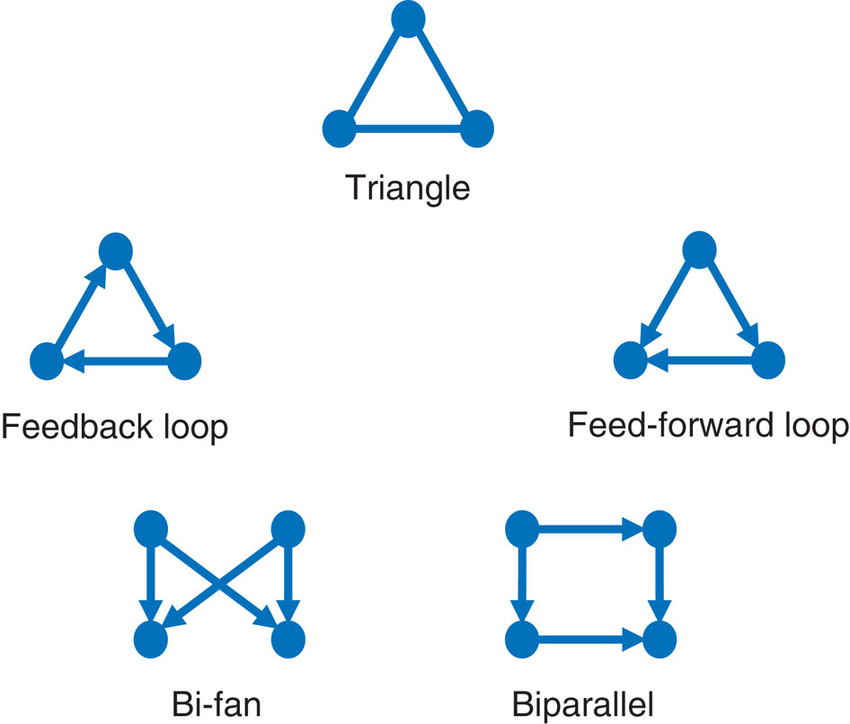
\includegraphics[width=0.9\textwidth]{images/Network-motifs-found-in-biological-networks-The-feed-forward-loop-bi-fan-and-biparallel.png}
    \caption[Network motifs in directed and undirected networks]{Network motifs in directed and undirected networks. In an undirected network the feedback and feed-forward loop would be identical (the triangle at the top of the image. Image from \cite{ngoc2013counting} Attribution-NonCommercial-ShareAlike 3.0 Unported (CC BY-NC-SA 3.0)}
    \label{fig:motifs}
\end{figure}

 TopoGSA \cite{glaab2010topogsa} for a given gene set calculates network parameters such as degree, local clustering coefficient, shortest path length, node betweenness and eigenvector centrality along with a Fisher's exact test for pathways which work contains genes in the set in KEGG, Interpr, BioCarta or Gene Ontology and with network data provided by querying the STRING database\cite{szklarczyk2019string}. An overall similarity score is provided based on the sum of ranks. For an explanation of network metrics see chapter~\ref{chap:Centrality measures}.

It has an easy to use web interface but the user must decide on a cut off significance level and no use is made of the ranks of the genes in the set. 

% The use of network statistics at an individual level for cognitive abilities show no correlation with gene $p$ value for the CAGES data set \footnote{nor for the later datasets}.
The authors do not record if they use direct interactions, or interactions based on techniques such as literature data mining, which are available in STRING\footnote{search tool for recurring instances of neighbouring genes - originally a genomic context database}\cite{szklarczyk2019string}. Finally the web based interface makes it impractical for large scale analysis of GWAS data. 
% It is essentially a, a tool for exploratory gene expression analysis and it is not clear that it has an advantage over GSEA using the BROAD institute's MSigDB database \cite{liberzon2015molecular}. 

The Enrichnet package (2012) by the same author \cite{glaab2012enrichnet} makes greater use of network topology, calculating a distance metric between the gene sets and the STRING database, using a random walk with restart (Xd distance). This is compared to the result of Fisher's exact test. Again the approach identifies pathways by a re-weighting of Fisher's exact test using network topology. I found it hard to interpret the significance of its results and would not be able to use it to test a hypothesis about the synaptic proteome.

It is relatively widely used with 87 citations \footnote{check}. The use of random walk to make a sample of a particular network incorporate information about link density similar to community structure. 

H Nguyen et al. \cite{nguyen2019comprehensive} provide a comprehensive survey of identification of active subnetwork modules. The authors discuss topological modules citing Girvan and Newman (2002) \cite{girvan2002community} and their initial description is similar to modularity defined communities. Most of the methods however seek to find a group of genes closely related in the network to a set of differentially expressed genes (an induced sub graph). Of the 22 methods reviewed only DIAMOnD \cite{ghiassian2015disease} and Enrichnet \cite{glaab2012enrichnet} are not constrained to use differential expression levels of genes in gene expression studies. The method I will describe is designed for the secondary analysis of GWA studies but can easily be adapted to look at differentially expressed genes (see discussion ~\ref{sec:discussion using our method on gene expression}) but the converse is not true. The majority of these approaches try to find an induced subgraph of the network which optimises a cost or utility function based on gene expression or association with disease. The approach in this thesis is to find structures based on network theory and test if they are associated with a specific phenotype. I discuss this further in the discussion section~\ref{sec:discussion more discussion of previous approaches}. 
% Inputs are typically lists of differential expression (p8.25.7) or fold changes rather than a standard summary of GWA data.

% The majority also use directed graphs which allow the identification of motifs more easily or pathway equivalence but are generally not used in protein-protein interactions graphs but rather in metabolic pathways such as KEGG. 
\subsubsection{General points from these reviews}
Mitrea\cite{mitrea2013methods} and Nguyen \cite{nguyen2018network} draw attention to the fact that the results of methods that actually use network topology are difficult to assess and compare (see the discussion above of Enrichnet). The review points out that it is often impossible to reproduce results even with the cooperation of the authors. A large number of the packages are web based and inflexible in the networks that they use.
\subsubsection{Other approaches}



ToppGene  \cite{chen2009toppgene} provides a guilt by association network function (ToppGenNet).  A set of seed genes is drawn and a test set generated using measures of network centrality: Page rank, Hits with priors and k-step markov prioritisation from a neighbourhood distance selected by the user \cite{chen2009disease}. The advantage is it actually uses recognised network methods and a PPI database (although based on literature and primary proteomics (BIND, BioGRID and HPRD)). The disadvantage is that when the prioritised genes are tested by seeing if they have similar ontology, disease or other term enrichment to the disease (seed) genes. Its guilt by association approach means that for a PPI network such as the synapse there are a lot of associates  and the analysis therefore reduces to the subsequent ORA. A random walk will also be affected by  community structure as the walk will spend longer in communities. This is also the case with the enrichnet package\cite{glaab2012enrichnet}.   
WebGestalt \cite{liao2019webgestalt} also offer network based analysis but consists of over representation of portions of a variety of networks including PPI.




\todo[inline]{just do what you said you would do to Douglas. Do your best and be accurate but point out there may be other bits. bit below moved to discussion label sec:other network gsa intro discussion}





\subsubsection{Other approaches}
\label{sec:intro other approaches}
% Mitrea et al. (2013a), reviewing topology based methods, notes that several techniques that claim to be third generation methods use the pathway topology to provide what is essentially a gene set (ie a pathway or portion there of from KEGG or a similar database) and so exclude information on pathway structure topology. Mitra \cite{mitra2013integrative} et al (2013a) criticised Khatri  et al (2012) for including methods including functional analysis and annotation with Gen
Barabasi \cite{barabasi2011network} reviewed a number of methods that used network based statistics such as clustering coefficient to augment the analysis of gene expression and GWAS studies. Of particular interest is the use of a `disease community' which I will return to in chapter~\ref{chap:community detection}. The difference with these approaches is they are based on heterogeneous lists of disease (see section~\ref{sec:biomedical significance of centrality measures} and \ref{sec:assessment of communities})) 

Pandey et al. report using eigenvector centrality of SNPs within a pathway to prioritise genes for pathway enrichment\cite{pandey2012epistasis}. The edges within the network however refer to gene - gene interaction strength rather than network topology. 

It is interesting to note that Mooney and Wilmot \cite{mooney2015gene} suggest using gene sets derived from network analyses. In the course of describing the DiaMOND algorithm Ghiassian et al.\cite{ghiassian2015disease} report comparing topological communities generated using the Louvain \cite{blondel2008fast} (section~\ref{sec:Louvain} and Markov Clustering method \cite{van2000graph} (section~\ref{sec:markov clustering} to a list of disease genes. They concluded that this approach was not useful and hence proposed the DIAMOnD, algorithm. They do not use a tissue specific network and use a variety of definitions of disease genes but do include GWA data from the GWA catalog \cite{macarthur2017new} but use them as items in an over-representation analysis. It is the most similar approach in the literature to the methods in this thesis that I am aware of.
%(Davies et al 2010)
%\footnote{perhaps I should mention WGCNA}.

% Frost et al (2014) describes a spectral method

% for gene set enrichment but this refers to the principle component analysis of a snp matrix and a matrix of indicator variables referring to gene properties.

\section{Plan}
\label{sec:intro plan to procede to next chapter}

I propose an alternative approach would be to use Gene Set Analysis tools widely used in GWA studies and to use as sets the communities identified by a community detection algorithm. In addition I will test the hypothesis that central genes in the network have a central role in cognitive phenotypes. 

To allow the use of a discovery and replication cohort study design in some subsequent sections of this thesis we obtained summary genetic data from meta-analyses  of intelligence and educational attainment to produce discovery and replication samples for each phenotype. The next chapter describes the processing of the data to create the discovery and replication samples and the generation of the interaction graph.








\section{Further discussion}
Lack of different intelligence phenotypes e.g. fluid etc in large scale genomic studies compared with Hill et al. where the finding was for a single phenotype


How findings of GWAS extend to more rare diseases give example of drug induced psychosis or high intelligence

\subsubsection{bits moved to the discussion}
Plomin (new) \cite{plomin2018new} box 5 makes the point about the availability of summary statistics and the non availability of some from commercial enterprises an observation which I completely agree with maybe should move to discussion.
\subsubsection{to discussion}
\label{sec:other network gsa intro discussion}


 
 





%\begin{document}
\section{Stuff moved out}
\subsection{MAGMA}
For the work presented in this thesis gene level statistics were calculated using NCBI 37.3 build to provide gene boundaries and 1000 Genome European Ancestry to account for linkage disequilibrium (see chapter 2 section ) \todo{add section}. 

move to methods
\subsection{to be moved in}
for a forthcoming paper. The paper reports the state of the art in combining disparate databases and primary proteomic data to produce a high quality representations of the synaptic proteome. 

The model is a static interaction graph of the genes that encode the protein components of the synaptic proteome. only those interactions for which there are direct experimental evidence of interaction are included. The interactions are mined from protein interaction databases usng the PSIMI format \cite{hermjakob2004hupo}. The largest component is from the union of HIPPIE \cite{schaefer2012hippie}, Biogrid \cite{oughtred2019biogrid}

\subsubsection{Compare MAGMA and VEGAS}
Figure 9 shows a comparison of the $-log10$ transformed $p$ values of VEGAS2 and MAGMA for the CHARGE data. $R^2$=0.98 \footnote{quote correlation} Image from compareMAGMAtoVEGAS.R. The results appear similar and it appears reasonable to compare results from MAGMA with the results provided from the study by Hill et al. (2014)
%updated from (Chatr-Aryamontri et al, 2015)
and Intact  \cite{hermjakob2004intact} databases. %The full network graph is shown in figure 13.% end p45.

source \url{'~/Documents/Projects/Rietvald/src/r_studio/magmadiagnostics/compareMAGMAtoVEGAS_character_infinities.R')} \url{'~/Documents/Projects/Utilities/compareMAGMAtoVEGAS.R'}

\section{move elsewhere or remove}
\subsection{To move to methods}

\subsubsection{Analogy with synaptic models of computation}
\todo[inline]{commented out areas here may want to keep some of these}
% As regards the model of a bottom up approach to the structure of the synapse and behaviour we will adopt a similar approach seeking groupings of proteins and hence their cognate genes and seeing what their effect are on population studies of cognitive differences, enrichment for murine models of cognition or their role in disorders with a cognitive phenotype. Our approach however is looking for enrichment in-silico rather than in changes in behaviours of experimental model organisms. 

% One area I should mention here is that there is a middle ground between the one circuit one behaviour model with weights and a distributed bottom up model with an intrinsic frequency response. Primitive models of the synapse prove to be powerful computational devices. One of Grants arguments is that the synapse is a computational unit. A grouhttps://github.com/pmglab/KGGp of connected neurons with associated weights can give rise to complex decision making behaviour by allowing representation of structures being learned to be encoded as patterns more proximally in the network without there being a specific circuit for each response (for example in MNIST there is not a pattern of activation that is specific to 1 or 2 there are patterns of activation that are more likely to result in the final soft-max function choosing one of these) I would speculate that the combination of weights and circuits and the enormous complexity of the synapse allows to some extent the complex cognitive computations carried out by mammals particularly those in areas of locomotion and sensation that have proved so hard to simulate.


\todo[inline]{?move this commented out bit}

\subsubsection{Problem of singletons}
% The spectral clustering algorithm has a tendency to produce isolated nodes. This problem is more marked on sparse networks and difficulties with sptreacl partiioning in sparse networks is well recognised (Krzakala et al.,2013). On occasion these 'singleton' communities in combination contribute a significant amount of the genetic signal found inm the graph. I have written a script to collect singletons into sets and test these but this data is not presented here. I discuss the problems of singletons in further work (section 18.8)
\todo[inline]{? move or kehttps://github.com/pmglab/KGGep this stuff}

\subsubsection{Recent GWA}
UKBB Ed and EA2 and overlap between and EA3


\subsection{Intelligence bit from paper DH}
\label{sec:Introduction intelligence bit from paper david hill}
% Intelligence, also known as general cognitive function,\cite{davies2015genetic} or simply as g,\cite{spearman1961general} describes the finding that across seemingly-disparate measures of cognitive ability, a single common factor explains around 40\% of the total cognitive test score variance in a group with a range of intellectual ability.  \cite{carroll1993human}  This single factor is the source of much of the predictive validity of cognitive tests; higher measured intelligence is predictive of higher-level educational and occupational outcomes, \cite{strenze2007intelligence}  as well as better health, and longevity .\cite{deary2012annrev} 

% In twin and family studies genetic factors explain between 50-80\% of individual differences in intelligence. Using GREML-SC implemented in GCTA, \cite{yang2011gcta}  common single nucleotide polymorphisms (SNPs) have been found explain 20-30\% \cite{marioni2014common}  of differences in intelligence. When variants that are poorly tagged by genotyped SNPs are included using GREML-KIN, \cite{xia2016pedigree}  or GREML-MSC and imputed genotypes, around 50\% of the differences in intelligence can be explained using molecular genetic data. \cite{hill2018genomic} 

\subsubsection{Rejectedalgorithms}

% I have tested some other available algorithms for community detection, many of which are in wide use. The parallelised implementation of Geodesic and Random Edge Betweeneness algorithms (Newman and Girvan, 2004) implemented by McLean et al failed to complete after two days when dealing with the large num,ber of vertices in the synaptome ($>4000$ vertices).\cite{mclean2016improhttps://github.com/pmglab/KGGved}

% Louvain \cite{blondel2008fast} community detection is widely used, works at scale and has been most widely applied in the analysis of large scale social networks. It is a greedy optimisation method to optimise modularity. 

% Blondel et al (2008) compares this with other community detection algorithms and finds that this algorithm has the lowest running time and maximises the increase in modularity.
% Using the algorithm to detect communities in the synaptic proteome failed to generate communities that 'looked right' and the communities did not enriched for any phenotype in the gene set analysis.

% The greedy implementation of a modularity maximisation procedure that is said by Kolacyzk and Csardi (2014) to approximate Newman and Girvan (2004) in igraph (Csardi and Nepusz, 2006) was rejected for identical reasons. A review of the performance of igraph algorithms is presented by De Souza and Zhoa (2014). (end p 33) \footnote{to do try to find the multilayer louvain implementation}

\subsection{Spin glass}
\label{sec:spinglass from introduction}
% I graph implements a spin glass algorithm where the communities are represented as a Potts spin glass model, a generalisation of the Ising two state model where the spins are communities. Community detection corresponds to minimising the Hamiltonian of the Pott's model (Eaton and Mansbach, 2012). I have used this model to produce communities of constrained size. I have not yet tested these communities in the replication cohort (CHARGE) and they are not presented in this review (see further work section 18.8) \footnote{spin glass other gamma and Coin has not used max spins which limits community size}.
\subsection{Spin glass}
\label{sec:spinglass from introduction}
% I graph implements a spin glass algorithm where the communities are represented as a Potts spin glass model, a generalisation of the Ising two state model where the spins are communities. Community detection corresponds to minimising the Hamiltonian of the Pott's model (Eaton and Mansbach, 2012). I have used this model to produce communities of constrained size. I have not yet tested these communities in the replication cohort (CHARGE) and they are not presented in this review (see further work section 18.8) \footnote{spin glass other gamma and Coin has not used max spins which limits community size}. 
\subsubsection{Rejectedalgorithms}
% \subsubsection{Rejectedalgorithms}

% I have tested some other available algorithms for community detection, many of which are in wide use. The parallelised implementation of Geodesic and Random Edge Betweeneness algorithms (Newman and Girvan, 2004) implemented by McLean et al failed to complete after two days when dealing with the large num,ber of vertices in the synaptome ($>4000$ vertices).\cite{mclean2016improved}

% Louvain \cite{blondel2008fast} community detection is widely used, works at scale and has been most widely applied in the analysis of large scale social networks. It is a greedy optimisation method to optimise modularity. 
% Blondel et al (2008) compares this with other community detection algorithms and finds that this algorithm has the lowest running time and maximises the increase in modularity.
% Using the algorithm to detect communities in the synaptic proteome failed to generate communities that 'looked right' and the communities did not enriched for any phenotype in the gene set analysis.



% The greedy implementation of a modularity maximisation procedure that is said by Kolacyzk and Csardi (2014) to approximate Newman and Girvan (2004) in igraph (Csardi and Nepusz, 2006) was rejected for identical reasons. A review 
% of the performance of igraph algorithms is presented by De Souza and Zhoa (2014). (end p 33) \footnote{to do try to find the multilayer louvain implementation}

% \subsection{Spin glass}
% \label{sec:spinglass from introduction}
% I graph implements a spin glass algorithm where the communities are represented as a Potts spin glass model, a generalisation of the Ising two state model where the spins are communities. Community detection corresponds to minimising the Hamiltonian of the Pott's model (Eaton and Mansbach, 2012). I have used this model to produce communities of constrained size. I have not yet tested these communities in the replication cohort (CHARGE) and they are not presented in this review (see further work section 18.8) \footnote{spin glass other gamma and Coin has not used max spins which limits community size}.

% I have tested some other available algorithms for community detection, many of which are in wide use. The parallelised implementation of Geodesic and Random Edge Betweeneness algorithms (Newman and Girvan, 2004) implemented by McLean et al failed to complete after two days when dealing with the large num,ber of vertices in the synaptome ($>4000$ vertices).\cite{mclean2016improved}

% Louvain \cite{blondel2008fast} community detection is widely used, works at scale and has been most widely applied in the analysis of large scale social networks. It is a greedy optimisation method to optimise modularity. 
% Blondel et al (2008) compares this with other community detection algorithms and finds that this
algorithm has the lowest running time and maximises the increase in modularity.
% Using the algorithm to detect communities in the synaptic proteome failed to generate communities that 'looked right' and the communities did not enriched for any phenotype in the gene set analysis.


% The greedy implementation of a modularity maximisation procedure that is said by Kolacyzk and Csardi (2014) to approximate Newman and Girvan (2004) in igraph (Csardi and Nepusz, 2006) was rejected for identical reasons. A review of the performance of igraph algorithms is presented by De Souza and Zhoa (2014). (end p 33) \footnote{to do try to find the multilayer louvain implementation}


 Network approaches to disease
importance

\section{Network models}

% Figure 13 Interaction graph of full synaptosome for direct published interactions. Nodes are genes, interactions are edges. Node size is proportional to degree. For high degree nodes please see table 4. Nodes 4612, edgess 16782 Layout forcetlas. Figure produced in Gephi 0.9.1 \footnote{we an look at the number of edges versus nodes over tme and with the Pocklington model and the one Colin had of the consensus PSD.}

% The network models of the synaptic proteome were produced by the Synaptic-Proteome-Group (2016) 

%The interactions are recorded 

We can extend this to multiple groups by recursively partitioning the network based on the leading eigenvector of the partiion and stopping partitioning when the partition does not resul
t in a further increase in the modularity for the subdivision of the community (see Newman (2006)\cite{newman2006finding}  for further details). This is the method implemented by McLean et al. \cite{mclean2016improved} \todo{mention later local expertise as reason for use of this method}

\subsection{Previous network based GSA}
% \label{sec:previous network based GSA}
% \textcolor{red}{You need to get the introduction to GSA or some introduction to GSA before this. We are really saying something like we can represent the thing as a network then what how can we ask questions about it well we can see if the network structure affects function and we can find structures in the network and test the function of this group as a start and move the GSA bit later}
% \todo{citation error - could simply be that it is missing from the references}
% \todo{PhD specific bibliography}
% \cite{nguyen2018network}  Nguyen et al  reviewed the use of pathway GSA across 36 packages and extends the tools covered from a previous review by Mitrea to 2017. If a package is not easy to use it will not be used by life scientists. Our approach makes use of commonly available GSEA and MAGMA packages and requires only editing of .gmt files which we provide software for. Of 45 packages, 30 were standalone or web based. They note that only one package is HIPPA compliant with web tools. Lots of the packages are implemented in R. Variety of ways in which information can be put in. If using list of genes this involves a cut off which involves loss of information. Discusses three different types of pathway signalling pathway, metabolic pathways and PPI. They note that SPIA accepts adjacency matrix representing a directed graph. Two types of graph models, single where a node is one thing and multiple. Topology GSA allows the graph to be split into sub graphs.
% Then they discuss pathway scoring methods and the goal of producing a ranked list of pathways or sub-pathways.

% \todo{Perhaps I should mention the use of david}

% \subsection{Others not covered in this review}
% \label{sec:others not covered in this review}
% Ghissian et al \cite{ghiassian2015disease}. \footnote{here also appear to be other papers by Ghissian including on endophenotype.} used Louvain clustering \todo{haven't explained clustering yet} on a generic network (? string) and find not \cite{blondel2008fast}so much but they find that the clustering of disease related genes together is greater than chance. he increasing evidence of the role of protein complexes mediating synaptic plasticity in schizophrenia.

% The network can be analysed at the level of overall network, of an individual node or at the level of structures found within the network and I will discuss each of these with relation to cognitive ability. I will describe our experience of a pilot study and the reasons for choosing cognitive ability. I will also introduce and review the network analysis techniques that we utilised. 


\subsection{Notes}

Look in \url{/afs/inf.ed.ac.uk/user/s14/s1476046/R/projects/graph} may have pilot graph

\subsubsection{Removed B}
\todo{expand these next two this belongs to the check ref paper ie I think the discussion above is outlined in the GATES paper by li}GATES (gene-based association test using extended Simes procedure)\cite{li2011gates} HYST \cite{li2012hyst}

\subsubsection{Removed C}
\section{Supplementary material}
See \url{https://tex.stackexchange.com/questions/1230/reference-name-of-description-list-item-in-latex}

and \url{http://amstat.tfjournals.com/supplementary-materials/}
See \ref{sup:sup1}
\begin{description}
\label{sup:sup1}

\item{Some supplementary material}
\end{description}

Davies intelligence MAGMA \url{https://static-content.springer.com/esm/art\%3A10.1038\%2Fmp.2016.45/MediaObjects/41380_2016_BFmp201645_MOESM506_ESM.xls}


\subsection{Previous network based GSA}
\label{sec:previous network based GSA}
\textcolor{red}{You need to get the introduction to GSA or some introduction to GSA before this. We are really saying something like we can represent the thing as a network then what how can we ask questions about it well we can see if the network structure affects function and we can find structures in the network and test the function of this group as a start and move the GSA bit later}
\todo{citation error - could simply be that it is missing from the references}
\todo{PhD specific bibliography}
work


\subsection{query to discussion}
\subsubsection{note}
The commonality is they start from seed genes then build a network and then say here are your other genes. What we want to do is take a network use an established network science method and then test these. Also disease module / disease gene is a bit tricky see later. Perhaps say a more detailed reason for not accepting some of these requires discussion of network methods in chapter x). 
BMRF-Net differentially expressed genes \cite{shi2015bmrf}.     COSINE is an R package \cite{ma2011cosine} GLADIATOR \cite{silberberg2017gladiator} in python (11 citations) 2017 - disease modules (this is a random walk starting on seed genes) Hot Net and Hot Net2 diffusion cancer modules \cite{leiserson2015pan} (cited by over 500) diffusion process in seed genes, related to cancer (diffusion process similar to communities) jActive Modules ideker "connected regions of the network that show significant changes in expression over particular subsets of conditions" 

\subsubsection{move or remove}
It is not clear to me what the effect of centrality or network structures are on a phenotype (and may differ for each phenotype) so the only approach appears to be systematic and empirical. 


% In the comprehensive 2018 review by T. Nguyen et al.\cite{nguyen2018network}   \todo{check number} 
% \subsubsection{Recent review}
% \cite{nguyen2018network}  Nguyen et al  reviewed the use of pathway GSA across 36 packages and extends the tools covered from a previous review by Mitrea\cite{mitra2013integrative} to 2017.

% Their approach again divides analysis into Over representation analyses, weighted analysies eg gsea and topology based analyses (per mitrea). The focus in the article is on analyses of gene expression or at least the contrast in biology of two experimental conditions. GSA tools although initially used in GWAS have now diversified and are focused on the secondary analysis of GWA data. Only one (I can see so far) Ghissian \cite{ghiassian2015disease} uses GWA data but uses over represented genes in GWA catalogue as a unit. They are also not tissue specific and look for a similarity of a set of genes to a pathway rather than a systematic examination of genome wide signal for a polygenic trait and a network (ie centrality measures, tissue specificity, structural analysis). Those methods that provide module detection do not use the most up to date algorithms. Inputs are typically lists of differential expression (p8.25.7) or fold changes rather than a standard summary of GWA data. While our method can easily be adapted to look at differentially expressed genes (see discussion) the converse is not true. The majority also use directed graphs which allow the identification of motifs more easily or pathway equivalence but are generally not used in protein-protein interactions graphs but rather in metabolic pathways such as KEGG. Other network based analysis offer guilt by association analyses (Webgestalt, toppgene) but are not included. 

% In the review by T. Nguyen et al.\cite{nguyen2018network} \todo{check number} 26 of 34 packages analyse directed networks. Directed networks are often used to show metabolic networks and some social networks (although it is sometimes more appropriate to have undirected networks - you can ask people who are friends with whom but in organisational charts there are hub nodes that do not correspond to the flow of heirarchy (reports to) in the organisation). In any case the analysis of directed networks is very different. For one thing small scale structures (motifs) play a role due to the great increase in the complexity of the interconnections of three to five node elements compared with the commmunity structure sought in directed networks) \todo{picure of motif and ref re motif}. Although a directed (and dynamical) representation of protein network structure may be helpful we are at present concenred with large scale structure and network performance and these graph anlaysis tools serve a different purspose. Of the undirected network packages two (Score PAGE and TAPPA are specific to metabolites). The remaining 6 are PWEA, TopoGSA, TopologyGSA, DEGraph, GANRA and Enrichnet. 







The review makes some useful points: If a package is not easy to use it will not be used by life scientists. Our approach makes use of commonly available GSEA and MAGMA packages and requires only editing of .gmt files which we provide software for. Of 45 packages, 30 were standalone or web based. They note that only one package is HIPPA compliant with web tools. Lots of the packages are implemented in R. Variety of ways in which information can be put in. If using list of genes this involves a cut off which involves loss of information. Discusses three different types of pathway signalling pathway, metabolic pathways and PPI. They note that SPIA accepts adjacency matrix representing a directed graph. Two types of graph models, single where a node is one thing and multiple. Topology GSA allows the graph to be split into sub graphs.
Then they discuss pathway scoring methods and the goal of producing a ranked list of pathways or sub-pathways.
In general also they do not test a specific hypothesis but given a set of genes or an experimental condition prioritise a pathway rather than looking at a network (fit network to data) rather than saying are network structures and measures we have calculated associated with the genetics of this trait (test network measures association to data).





Specific findings related to modularity or importance measures will be reviewed in the respective chapters. 
\textcolor{red}{suggest comprehensive review in further work} The problem is you can't really review the literature without understanding the genetics and network science and the previous approaches and that is going to take some time to do before you then get down to reviewing the literature. I can see no comprehensive review of all of these aspects to date although I can see many overviews etc

\todo{Perhaps I should mention the use of david}

\subsection{Others not covered in this review}
\label{sec:others not covered in this review}
Ghissian et al \cite{ghiassian2015disease}. \footnote{here also appear to be other papers by Ghissian including on endophenotype.} used Louvain clustering \todo{haven't explained clustering yet} on a generic network (? string)https://github.com/pmglab/KGG and find not \cite{blondel2008fast}so much but they find that the clustering of disease related genes together is greater than chance. he increasing evidence of the role of protein complexes mediating synaptic plasticity in schizophrenia.

The network can be analysed at the level of overall network, of an individual node or at the level of structures found within the network and I will discuss each of these with relation to cognitive ability. I will describe our experience of a pilot study and the reasons for choosing cognitive ability. I will also introduce and review the network analysis techniques that we utilised. 

\todo[inline]{references from below ongoing update flag for JDA}
HYST \cite{li2012hyst} uses a combined test for PPI. 

\cite{jia2011dmgwas}

\cite{baranzini2013network}
\todo{Mention tissue specificity}
\footnote{I think this maybe goes best with the bit on network generation in the next chapter}
Pascal uses a modified Fishers method to calculate pathway scores from combining SOCS/MOCS sum of chi square mean of chi square. Test inflation due to linkage disequilibrium between neighbouring genes is accounted for using a fusion gene method treating neighbouring genes as a single unit. % this bit is I think from dashti
%The pathways "1077 pathways from KEGG, REACTOME, BIOCARTA databases" \cite{dashti2019genome}

\subsection{repeated bits}
\subsubsection{Limitations of gene boundaries and non coding SNPs}
A number of SNPs are found in non coding regions of the genome. They may effect gene expression through affecting quantitative trait loci but these are excluded from analysis. For most analysis the discarded SNPs amount to about 50\%.


s. de Leeuw et al (2016) \cite{de2016statistical}
considers GenGen \cite{wang2007pathway} Wang et al (2007) which is similar to GSEA in using a Kolmogorov Smirnov test as a self contained test \footnote{Original footnote: although it is not clear to me why and has the advantage of being non parametric}
ALIGATOR \cite{holmans2009gene} assign significant SNPs to gene. Get a list of genes. Do ORA. 
\textcolor{red}{Need to say something about depict} Which is something like I have not used depict as a) it is huge b) provided as jar c)main attraction is it does lots of pathway enriching d) magma and pascal do the gene level stuff fine for me e) need reliable gene level data even when people use depict they also use magma \url{https://github.com/perslab/depict}
INRICH C++ link from the authors lab is to the paper page. link to C++ broken supplementary data not found takes genetic intervals and checks gene set enrichment \cite{lee2012inrich}.

\footnote{pascal \url{http://regulatorycircuits.org/}}
. upon the rank ordering of sets of genes expressed in a phenotype and those not of the phenotype, for example genes expressed in tissue that has been injured and those in tissues that have not been injured. An excess of expression of a set of genes is shown by a higher rank order of genes in the gene list compared to the null hypothesis that there is no difference between the two groups. GSEA \cite{subramanian2005gene} uses the Kolmogorov Smirnov test to distinguish between the two groups. 

 The intuition behind the use of the test can be seen if we consider a random walk along one dimension. As the size of the walk steps tend towards zero and the number of steps increased towards infinity this becomes a continuous walk in time, a Wiener process, $W(t)$. The maximum displacement of a random walk is proportional to $\sqrt{n}$ where $n$ is the number of steps. When the beginning and end of the random walk on the lattice (or real line) are bounded at the beginning and end of the process at zero, this becomes a Brownian bridge.

If we consider the cumulative distribution function (CDF) of any probability distribution the ends of the distribution are bounded at 0 and 1. Therefore the difference between any two distributions CDF will be bounded at the start and end at 0. This can be used to compare an empirical cumulative distribution function with that of known probability distribution. The maximum deviation from zero of the difference between the two CDFs will approximate a random walk if they are similar. The more dissimilar the distributions are the greater will be the maximum difference between their CDF.

The Kolmogorov distribution describes the probability that the supremum of the Brownian bridge will take on a particular value. In the Kolmogorov Smirnov test the supremum of the distribution is used as the test statistic with the null hypothesis being that there is no difference between the distributions. In the case of gene set enrichment analysis we are comparing the CDF of two empirical distributions \cite{clark2011introduction}

If we rank the genes of a microarray experiment in terms of their expression we will get a list. We have an apriori agreed set of genes based on some relation for example member no higher up the ordered list of gene expression than expected by chance. If we have a count that starts at zero and we increase the count proportional to the size of our set and the gene list when we see a gene in the set and if we subtract from the count a step proportional to the number of genes not in the set then at the end of the list the count at the end of the list will be zero. If we see a lot of genes in our set early on in the list of gene expression there will be an early positive deviation of the test statistic and its supremum will be high. A null distribution can be generated by randomly permuting the phenotype labels. Correction for multiple testing (for example checking a large number of sets) is carried out using the Benjamni and Hochbery procedure (Hochberg and Liverman 1994).

\todo{want to maintain GSEA for backward compatibility for GSEA all you need is the list of genes and their p value or an importance measure for the implementation in MAGMA or PASCAL you need the summary statistics which can become unavailable. Yes was going to put this in again and it might be worth doing a practical illustration of it. If you have a list of the gene scores you can do GSEA. i.e. those where the supplementary material provides a complete list of MAGMA scores and you could also say in the discussion this is a reason to have all summary gene level statistics available in publication. Something like GWAS catalog but with all gene scores in MAGMA done in studies would be very useful for studies like Ghissians attempt and future network studies. }

\footnote{ had Results from topoGSA are shown in figure 10 and figure 11 using publicly available data used in this study.Figure 10 TopoGSA network enrichment program. The set used in this example is the list of NMDA receptor genes from Hill et al (2014). Topo GSA network enrichment program. The example set is the top50 Genes from Okbay et al (2016b)Figure 12 - Enrichnet gene set enrichment pacakge. NMDA gene set from Hill et al 2014)}
Add:
\url{https://bmcbioinformatics.biomedcentral.com/articles/10.1186/s12859-017-1674-0} FCS and ORA
Need to include here: In order to investigate the effect of community structure and network structure in the PSP on a complex cognitive trait we developed a model of the PSP and derived a measure of the significance of a synaptic gene for a complex trait in this case intelligence and educational attainment using MAGMA GSA. To permit the use of a discovery and replication cohort study design in some subsequent sections of this thesis we obtained summary genetic data from 2 GWA of intelligence and 2 GWA of educational attainment. The next chapter describes the processing of this data and the generation of the interaction graph.

\subsection{Usefulness of intelligence as phenotype}
\label{sec:Intelligence intro usefulness of intelligence as phenotype}
\todo{this bit doesn't really fit here now}
Before going on to discuss the methods that we can use to identify coherent sets of genes in a network we should point out that one of trhe aims of the study is to assess how well network analysis and clustering helps in the understanding of a phenotype. If the phenotype is poorly defined or their is a great deal of inter observed variability it may be that the clustering is measuring the phenotype (for example finding an unexpected subgroup of the phenotype) rather than assessing the effectiveness of modules of proteins associated with the phenotype.
\todo[inline]{ELEPHANT - This bit doesn't fit because it replicates the bit above - This is the bit earlier}
\end{document}
%\chapter{Pilot}
\section{Pocklington study}
Pocklington et al[ref]\todo{Add ref}

Pocklinton identified 105 MASC proteins with binary interactions (248 interactions). 77 proteins did not interact giving a total of 105 +77 = 182 proteins. 222 proteins are given indices in the supplementary methods with an additional 9 composite proteins 223-231 index made up of proteins earlier indexed. The composite proteins index 46 proteins forming complexes (9 composite proteins)

\todo{perhaps just drop the pocklington from the pilot study and keep the other stuff with the hill}
There are 186 proteins mentioned in the paper. The index including composites runs to 231. There are 9 composite proteins. The composite proteins index 46 proteins. The supplementary materials identify 176 proteins that are not part of a composite protein and 9 composite proteins = 185. It may be that one if the indices was intended to be part of a composite protein and is not recorded in the supplemental material as one of the lines is corrupted and instead of having comma separated values has a float. The clusterings refer to composite indices and singles (ie they don't refer to those in composites by their individual index) \todo{lesson - importance of annotation and easiness with which data is corrupted}

126 unique indices are found in the binary interaction table. The maximum index in the interaction table is 231 the highest index and a composite index. For protein interactions proteins occuring in complexes are recorded by the local study id of their protein complex. 126 proteins took place in binary interactions this included 7 composite proteins 223 225 227 228 229 230   231. Two of the composite proteins are not included but all but one of their components are present (composit index 224 and 226 only 84 of 224 missing (PRKACB) 

The gml made by colin uses the Pocklington indices. All of the composite indices are in the graph. The graph matches the paper in that it has 101 and 246 edges. The reason is none of the group 4 ones that are referred to in the interactions in the supplementary material by their non composite id are present in the graph they all are given composite id. \todo{Don't use composite mappings or mix mappings}.  


Largest connected component is 101 proteins linked by 246 interactions. 

101 indices are referenced in 13 clusters and these are confirmed in the R code calculate number of elements in clusters source\url{('~/Rprojects/graph_proteomics2016/R/calculate_n_proteins_from_clusters.R')}

In order to create a gmt file for gsea we only need the cluster allocation of the proteins and can ignore the issue of the number of listed proteins being greater than the number included in the supplementary methods. However two problems remain 1) some of the clusters are composite proteins made up of many different proteins but referred to by their index (there is an error in 
Composite index 228 G alpha I with the indices recorded as an integer rather than comma separated values in each row of a column. Examining the literature reveals that Gi alpha is composed of 5 proteins Gi1a (GNAI1), Gi2a, GNAI2, Gi3a GNAI3, G0a GNAO1 and Gz alpha GNAZ

The visible components are 199,197,204,195,196 and also total 5 elements we therefore conclude that the trailing 000 000 000 is an error and use these five components. These have been corrected and saved

Gene names are recorded in table 1 but a number of these have changed and some are recorded in the small case characteristic of murine gene names. Human Ensembl Gene Identifiers are also quoted but 4 of these fail to track to any current id.

By using a combination of ensembl gene identifiers and the recorded swiss prot protein identifiers we can obtain contemporary entrez id for all the indices in Pocklington. The code to generate this is found at ..uprade\_protein\_list.py in poc2 in pycharm projects.
This generates a gmt and csv file which are included in the supplementary materials. There is an entry in the gmt file corresponding to each cluster and also one entry for all of the graph entries and all the entities in NRC\_MASC recorded by Pocklington in the supplementary material. 

One entry index 203 (indexing from 1 per the supplementary material) is not found in uniprot. Its gene name is GNAT3 and lookup using entrez gene finds its entrez id to be 346562

For GSEA we have translated the output of the various CAGES phenotypes to use entrez id as their index. The code for this is at source \url{('~/RProjects/gsea_related/translate_cages.R')}.
There is no easily practicable way to translate the Pocklington dataset into the gene symbols used at the time of the original Hill study. 

Similarly in order to compare the results of the Hill study with more recent cohorts I have translated the human gene symbols there to contemporary entrez ids. (CODE – called something like convert old stuff)

GSEA using CAGES

\subsection{CAGES description of Cohorts}

\subsection{Correlation between phenotypes}

\subsection{Python convert gmx converts symbol to entrez}
Hill used the PSD consensus data from the genes2 cognition website at the time of writing these sets (PSD, PSD\_Consensus, AMPA\_RC, metabatropic glutamate receptor (mgluR) and NMDA receptor were not available. I had the gmx file supplied by Hill of these data with the gene represented by gene symbols. I converted these to contemporary entrez id using the python script (\url{/home/grant/PycharmProjects/convert_gm_refactor/convert_gmx/read_geneinfo_entrez.py}.
This uses the human gene info from entrez gene documenting gene symbols, gene synonyms and entrez id. If a gene symbol is found matching the entrez id the enrez id is substituted, if not an entrez id is then searched for in synonyms. If none is found there a manual search is performed and the terms added to the synonym dictionary. I term in PSD consensus was not found

Missing 1 items: 355    KIAA1045 -> PHF24 Entrez 23349


Name: PSD\_Consensus, dtype: object
Missing 4 items: 120     KIAA1688 -> ARHGAP39 -> 9798
687     KIAA0174 -> IST1 -> 9798
695     KIAA1045 -> PHF24 -> Entrez 23349
1131     RPS17-2 -> RPS17 -> Entrez 6218

This would allow the comparison of the Hill dataset with any subsequent larger cohorts than cages. 

529 cages gene output from VEGAS could not be easily identified only 2 had p < 0.01 of 17743 genes

529 gfq genes 4 had p < 0,01 min 0.001434  num 17741


Memory: 531 missing items 5 genes with p < 0.01 min p 0.0008300000000000001 total 17798 genes
Speed: 535 missing items 15 genes with p < 0.01 min p 0.000173 total 17825 genes 535
Trans g: 529 missing items 2 genes with p < 0.01 min p 0.00251 total 17740 genes


Given these values it is unlikely any significant genes are overlooked \todo{TRY TO LOOKUP PRIORIRT}. I have also checked previous synonyms using David, GeneCards and NCBI37.3. It is possible to make some assessment of what a gene may be eg AMY1B-1
63            AMY1B-3 most liekly map to amy1B but which value should be used. A large number of the missing files have these suffixes eg SOMETHING -1

Plus they are only relevant if they are in the gene set ie all NMDA\_RC genes for for anything after the pilot study we will be using magma and even for vegas genes not in the synaptic set (here read NMDA)RC) will count as the background set for gsea when running a K\_S so what we need to do is show that none of these genes are in the Pocklington NMDA\_MASC and out of interest if any of them are in the gmx file from david hill (which I doubt)
\subsection{Repetition of results for Hill}
\subsection{Clustering results and enrichment for Pocklington}
\todo{Get pocklington gsa from strontium}
Pocklington et al

Pocklinton identified 105 MASC proteins with binary interactions (248 interactions). 77 proteins did not interact giving a total of 105 +77 = 182 proteins. 222 proteins are given indices in the supplementary methods with an additional 9 composite proteins 223-231 index made up of proteins earlier indexed. The compositeproteins index 46 proteins forming complexes (9 composite proteins)

126 unique indices are found in the binary interaction table. The maximum index in the interaction table is 231 the highest index and a composite index

Largest connected component is 101 proteins linked by 246 interactions. 

101 indices are referenced in 13 clusters and these are confirmed in the R code calculate number of elements in clusters \url{source('~/Rprojects/graph_proteomics2016/R/calculate_n_proteins_from_clusters.R')}

In order to create a gmt file for gsea we only need the cluster allocation of the proteins and can ignore the issue of the number of listed proteins being greater than the number included in the supplementary methods. However two problems remainproteisn 1) some of the clusters are composite proteins made up of many different proteins but referred to by their index (there is an error in 
Composite index 228 G alpha I with the indices recorded as an integer rather than comma separated values in each row of a column. Examining the literature reveals that Gi alpha is composed of 5 proteins Gi1a (GNAI1), Gi2a, GNAI2, Gi3a GNAI3, G0a GNAO1 and Gz alpha GNAZ

The visible components are 199,197,204,195,196 and also total 5 elements we therefore conclude that the trailing 000 000 000 is an error and use these five components. These have been corrected and saved

Gene names are recorded in table 1 but a number of these have changed and some are recorded in the small case characteristic of murine gene names. Human Ensembl Gene Identifiers are also quoted but 4 of these fail to track to any current id.
By using a combination of ensembl gene identifiers and the recorded swiss prot protein identifiers we can obtain contemporary entrez id for all the indices in Pocklington. The code to generate this is found at \url{..uprade_protein_list.py} in poc2 in pycharm projects.
This generates a gmt and csv file which are included in the supplementary materials. There is an entry in the gmt file corresponding to each cluster and also one entry for all of the graph entries and all the entities in NRC\_MASC recorded by Pocklington in the supplementary material. 

One entry index 203 (indexing from 1 per the supplementary material) is not found in uniprot. Its gene name is GNAT3 and lookup using entrez gene finds its entrez id to be 346562

For GSEA we have translated the output of the various CAGES phenotypes to use entrez id as their index. There is no easily practicable way to translate the Pocklington dataset into the gene symbols used at the time of the original Hill study. 

Similarly in order to compare the results of the Hill study with more recent cohorts I have translated the human gene symbols there to contemporary entrez ids. (CODE – called something like convert old stuff)

GSEA using CAGES



Crystal
Table: Gene sets enriched in phenotype na [plain text format]

GS
follow link to MSigDB
GS DETAILS
SIZE
ES
NES
NOM p-val
FDR q-val
FWER p-val
RANK AT MAX
LEADING EDGE
1
1
Details ...
22
0.61
1.38
0.030
0.140
0.150
4080
tags=45%, list=24%, signal=60%
2
3
Details ...
32
0.54
1.25
0.079
0.231
0.432
4405
tags=38%, list=26%, signal=50%
3
ALL\_MASC\_GRAPH\_AND\_OTHERS
Details ...
217
0.42
1.07
0.198
0.650
0.934
4818
tags=31%, list=28%, signal=43%
4
ALL\_MASC\_GRAPH
Details ...
135
0.42
1.06
0.255
0.502
0.942
4981
tags=30%, list=29%, signal=42%
5
2
Details ...
38
0.44
1.05
0.376
0.427
0.953
4737
tags=34%, list=28%, signal=47%
6
4
Details ...
6
0.47
0.87
0.674
0.789
1.000
565
tags=17%, list=3%, signal=17%

GFQ
Min 5
Table: Gene sets enriched in phenotype na [plain text format]

GS
follow link to MSigDB
GS DETAILS
SIZE
ES
NES
NOM p-val
FDR q-val
FWER p-val
RANK AT MAX
LEADING EDGE
1
9
Details ...
8
0.80
1.56
0.011
0.015
0.015
2698
tags=50%, list=16%, signal=59%
2
3
Details ...
32
0.65
1.50
0.000
0.015
0.029
3404
tags=44%, list=20%, signal=54%
3
4
Details ...
6
0.70
1.29
0.105
0.114
0.297
4050
tags=67%, list=24%, signal=87%
4
ALL\_MASC\_GRAPH
Details ...
135
0.52
1.29
0.001
0.086
0.299
3573
tags=30%, list=21%, signal=38%
5
ALL\_MASC\_GRAPH\_AND\_OTHERS
Details ...
217
0.49
1.24
0.001
0.113
0.454
3573
tags=28%, list=21%, signal=35%
6
2
Details ...
38
0.45
1.04
0.395
0.443
0.957
3844
tags=24%, list=22%, signal=30%
7
1
Details ...
22
0.42
0.93
0.624
0.673
1.000
7259
tags=50%, list=42%, signal=87%


Memory size 1


GS
follow link to MSigDB
GS DETAILS
SIZE
ES
NES
NOM p-val
FDR q-val
FWER p-val
RANK AT MAX
LEADING EDGE
1
10
Details ...
2
-0.89
-1.46
0.046
0.057
0.061
1847
tags=100%, list=11%, signal=112%
2
13
Details ...
1
-0.73
-0.97
0.552
0.776
0.819
4675
tags=100%, list=27%, signal=137%
3
5
Details ...
4
-0.47
-0.96
0.511
0.526
0.822
9125
tags=100%, list=53%, signal=214%

\subsection{Graph for pilot}
The code and data to generate the graph for the pilot is in \url{/home/grant/RProjects/pilot_redo/data} this includes the file 
\url{internal_synaptome_homo_7cols.csv} which I mention in the first year review. The gmt are in the folder \url{/home/grant/RProjects/pilot_redo/data/original_gmt} fyr\_direct.gml (sic) is translated into entrez id and was used in calculating the more recent studies using magma. \url{ newgraphpublisheddirect.gmt} is the original file using gene symbols which was used with the original symbol gsea. Mnetion that the 7 cols was generated by Emilia and Katharina

\todo{Get the original clustering if I can and write out the gmt results}

The original graph can be loaded at \url{source('~/RProjects/pilot_redo/R/get_original_study_gmlt.R')}
This is equivalent to the full graph in the fyr document. The results from the original study can be replicated by going to 
\url{~/Programs/gsea} which has acopy of foo emilia. Foo emilia has 96 groups but produces the reults from the pilot. THe number of genes I report in the pilot are the number discovered using the htmkl result viewer in gsea (not the total number in a community

The total number of genes in foo emilia is  6037
== Full on p54 of first year review
there are 6308 genes including spec clustering in \url{"data/DICE_gml/g.Emilia.full.spec.annotated.gml"}
There are also 96 groups in this file 

The files \url{source('~/RProjects/pilot_redo/R/count_genes_in_symbolset.R'} have 4436 genes in the symbol file \url{"data/original_gmt/newgraphpublisheddirect.gmt"} and contain 64 gene sets. This corresponds to the full, new direct published in table 8 of the pilot in fyr p54. The file \url{source('~/RProjects/pilot_redo/R/count_genes_in_set.R')} counts the number of genes in the file \url{"data/original_gmt/fyr_direct.gml"} which are entrez id, 4237 in number and there are 21 groups corresponding to the size filtered direct (size>15) and some loss from translation
\todo{Add results from} 
See \url{Pilot_study.docx} at \url{/home/grant/Dropbox/PhD_latex_master/word}

\subsection{Results for enrichment}
\subsubsection{Foo}

This is a graph made from the first version of the synaptic graph and incompletely filtered interaction data. It is composed of 6038 nodes and 93642 edges. Spectral clustering carried out using the CDM suite reveals 96 groups with a modularity of 0.287.

There are a large number of single groups in the data. Only 27 groups had 15 or more members the default minimum recommended group size for Gene Set Enrichment Analysis. These modules amounted however to 5898 genes or 87.7\% of the first PSP graph genes. Of those modules with less than 15 members, 50 were single, 5 had two genes, 4 had three, 5 had four genes, 3 had six genes and 3 had ten genes (see table~\ref{Table:Foo_modules_with_lessthan_15}). The range of module size was 1-745. The mean group size was 62.25 and the median 1.0. The third quartile was 44.

For modules with size at least 15 the range of sizes was 38-745. Median group size was 155 and mean 218.4.
\todo{? histogram}

The size of the 27 modules with 15 or more members is shown in table\ref{Table:foo_sizeof_modules with 15 or more members}

\subsection{New graph}
The spectral clustering for the graph new direct published graph 4506 vertices 16760 edges. Spectral community detection found 120 communities. 63 community modules had 15 or more members, 4365 genes or 96.7\% of the overall graph of 4506 vertices. The size of modules of less than size 15 is shown in table \ref{Table:direct Count of modules with less than 15 members}.



Code is at \url{'~/RProjects/pilot_redo/R/get_community_size_publsihed_direct.R'}

\todo{We are testing a lot of groups in results for new direct, we will have to work out how to reduce this nuimber as it will decrease power and CAGES is underpowered}
% latex table generated in R 3.6.2 by xtable 1.8-4 package
% Tue Dec 31 12:01:57 2019
\begin{table}[ht]
\centering
\begin{tabular}{lr}
  \hline
Number of genes in module & Number of modules \\ 
  \hline
1 &  29 \\ 
  2 &  13 \\ 
  3 &   5 \\ 
  4 &   3 \\ 
  5 &   1 \\ 
  6 &   1 \\ 
  7 &   1 \\ 
  8 &   1 \\ 
  9 &   1 \\ 
  12 &   2 \\ 
   \hline
\end{tabular}
\caption{Modules with less than 15 members} 
\label{Table:direct Count of modules with less than 15 members}
\end{table}
% latex table generated in R 3.6.2 by xtable 1.8-4 package
% Tue Dec 31 11:08:50 2019
\begin{table}[ht]
\centering
\begin{tabular}{lr}
  \hline
Number of genes in module & Number of modules \\ 
  \hline
1 &  50 \\ 
  2 &   5 \\ 
  3 &   4 \\ 
  4 &   5 \\ 
  6 &   3 \\ 
  10 &   3 \\ 
   \hline
\end{tabular}
\caption{Modules with less than 15 members} 
\label{Table:Foo_modules_with_lessthan_15}
\end{table}

\begin{table}[ht]
\centering
\begin{tabular}{lr}
  \hline
Spectral module & Size of group \\ 
  \hline
1 & 155 \\ 
  3 & 265 \\ 
  4 & 283 \\ 
  5 &  58 \\ 
  11 & 135 \\ 
  12 & 438 \\ 
  13 &  85 \\ 
  15 &  52 \\ 
  16 &  99 \\ 
  17 & 745 \\ 
  18 & 373 \\ 
  22 &  44 \\ 
  23 & 200 \\ 
  25 &  38 \\ 
  26 & 245 \\ 
  27 & 307 \\ 
  33 & 461 \\ 
  34 & 119 \\ 
  39 & 121 \\ 
  42 &  44 \\ 
  43 & 104 \\ 
  68 & 520 \\ 
  69 & 316 \\ 
  73 & 182 \\ 
  74 &  96 \\ 
  75 & 309 \\ 
  95 & 104 \\ 
   \hline
\end{tabular}
\caption{Size of modules with 15 or more members} 
\label{Table:foo_sizeof_modules with 15 or more members}
\end{table}


% latex table generated in R 3.6.1 by xtable 1.8-4 package
% Tue Dec 24 15:37:58 2019
\begin{table}[ht]
\centering
\begin{tabular}{rrrrrrr}
  \hline
 & NAME & SIZE & NES & NOM.p.val & FDR.q.val & FWER.p.val \\ 
  \hline
1 &  73 & 158 & 1.20 & 0.04 & 1.00 & 0.80 \\ 
  2 &  25 &  33 & 1.10 & 0.27 & 1.00 & 0.97 \\ 
  3 &  22 &  35 & 1.10 & 0.32 & 1.00 & 0.99 \\ 
  4 &  74 &  95 & 1.10 & 0.30 & 1.00 & 1.00 \\ 
  5 &  18 & 343 & 1.10 & 0.17 & 1.00 & 1.00 \\ 
  6 &  23 & 176 & 1.10 & 0.24 & 1.00 & 1.00 \\ 
  7 &  34 &  99 & 1.00 & 0.42 & 1.00 & 1.00 \\ 
  8 &  42 &  35 & 1.00 & 0.46 & 1.00 & 1.00 \\ 
  9 &  69 & 268 & 1.00 & 0.46 & 1.00 & 1.00 \\ 
  10 &  75 & 273 & 1.00 & 0.50 & 1.00 & 1.00 \\ 
  11 &  27 & 267 & 0.99 & 0.54 & 1.00 & 1.00 \\ 
  12 &  68 & 438 & 0.99 & 0.58 & 1.00 & 1.00 \\ 
  13 &  43 &  86 & 0.99 & 0.56 & 1.00 & 1.00 \\ 
  14 &  95 &  94 & 0.98 & 0.58 & 1.00 & 1.00 \\ 
  15 &  11 & 115 & 0.97 & 0.60 & 1.00 & 1.00 \\ 
  16 &  39 & 106 & 0.96 & 0.65 & 1.00 & 1.00 \\ 
  17 &   5 &  44 & 0.96 & 0.60 & 1.00 & 1.00 \\ 
  18 &  33 & 417 & 0.96 & 0.79 & 0.97 & 1.00 \\ 
  19 &  12 & 358 & 0.94 & 0.82 & 1.00 & 1.00 \\ 
  20 &   1 & 123 & 0.94 & 0.73 & 0.96 & 1.00 \\ 
  21 &  13 &  68 & 0.94 & 0.69 & 0.93 & 1.00 \\ 
  22 &  16 &  91 & 0.93 & 0.74 & 0.93 & 1.00 \\ 
  23 &   3 & 218 & 0.90 & 0.91 & 0.96 & 1.00 \\ 
  24 &   4 & 249 & 0.90 & 0.94 & 0.93 & 1.00 \\ 
  25 &  15 &  45 & 0.84 & 0.86 & 0.98 & 1.00 \\ 
  26 &  26 & 210 & 0.83 & 0.99 & 0.95 & 1.00 \\ 
   \hline
\end{tabular}
\caption{GSEA foo emilia 26 groups over 15 cages\_crystal.csv} 
\label{cages_crystal.csv}
\end{table}
\subsection{Graph characteristics}

% latex table generated in R 3.6.1 by xtable 1.8-4 package
% Tue Dec 24 15:46:17 2019
\begin{table}[ht]
\centering
\begin{tabular}{rrrrrrr}
  \hline
 & NAME & SIZE & NES & NOM.p.val & FDR.q.val & FWER.p.val \\ 
  \hline
1 &  43 &  86 & 1.30 & 0.01 & 0.31 & 0.26 \\ 
  2 &  39 & 106 & 1.20 & 0.01 & 0.18 & 0.30 \\ 
  3 &  42 &  35 & 1.20 & 0.13 & 0.39 & 0.70 \\ 
  4 &  27 & 267 & 1.10 & 0.05 & 0.75 & 0.96 \\ 
  5 &   1 & 123 & 1.10 & 0.15 & 0.69 & 0.98 \\ 
  6 &  34 &  99 & 1.10 & 0.17 & 0.62 & 0.99 \\ 
  7 &  22 &  35 & 1.10 & 0.26 & 0.56 & 0.99 \\ 
  8 &  15 &  45 & 1.10 & 0.27 & 0.52 & 0.99 \\ 
  9 &  68 & 438 & 1.10 & 0.05 & 0.53 & 1.00 \\ 
  10 &  73 & 158 & 1.10 & 0.24 & 0.62 & 1.00 \\ 
  11 &  75 & 273 & 1.00 & 0.30 & 0.86 & 1.00 \\ 
  12 &   4 & 249 & 1.00 & 0.36 & 0.84 & 1.00 \\ 
  13 &   3 & 218 & 1.00 & 0.40 & 0.81 & 1.00 \\ 
  14 &  95 &  94 & 0.99 & 0.53 & 1.00 & 1.00 \\ 
  15 &  18 & 343 & 0.98 & 0.62 & 0.99 & 1.00 \\ 
  16 &  33 & 417 & 0.98 & 0.65 & 0.97 & 1.00 \\ 
  17 &  74 &  95 & 0.97 & 0.59 & 0.95 & 1.00 \\ 
  18 &   5 &  44 & 0.97 & 0.57 & 0.91 & 1.00 \\ 
  19 &  12 & 358 & 0.94 & 0.83 & 1.00 & 1.00 \\ 
  20 &  23 & 176 & 0.94 & 0.76 & 0.98 & 1.00 \\ 
  21 &  26 & 210 & 0.91 & 0.89 & 1.00 & 1.00 \\ 
  22 &  69 & 268 & 0.90 & 0.93 & 1.00 & 1.00 \\ 
  23 &  16 &  91 & 0.89 & 0.84 & 0.99 & 1.00 \\ 
  24 &  25 &  33 & 0.88 & 0.75 & 0.96 & 1.00 \\ 
  25 &  11 & 115 & 0.88 & 0.87 & 0.92 & 1.00 \\ 
  26 &  13 &  68 & 0.86 & 0.87 & 0.91 & 1.00 \\ 
   \hline
\end{tabular}
\caption{GSEA foo emilia 26 groups over 15 gfq.csv} 
\label{gfq.csv}
\end{table}

% latex table generated in R 3.6.1 by xtable 1.8-4 package
% Tue Dec 24 15:47:42 2019
\begin{table}[ht]
\centering
\begin{tabular}{rrrrrrr}
  \hline
 & NAME & SIZE & NES & NOM.p.val & FDR.q.val & FWER.p.val \\ 
  \hline
1 &  74 &  95 & 1.20 & 0.03 & 0.76 & 0.54 \\ 
  2 &  73 & 158 & 1.20 & 0.03 & 0.70 & 0.77 \\ 
  3 &   5 &  44 & 1.10 & 0.18 & 0.79 & 0.92 \\ 
  4 &  42 &  35 & 1.10 & 0.22 & 0.63 & 0.93 \\ 
  5 &  22 &  35 & 1.10 & 0.21 & 0.55 & 0.95 \\ 
  6 &  15 &  45 & 1.10 & 0.26 & 0.65 & 0.99 \\ 
  7 &  27 & 267 & 1.10 & 0.07 & 0.56 & 0.99 \\ 
  8 &  13 &  68 & 1.10 & 0.23 & 0.53 & 0.99 \\ 
  9 &  43 &  86 & 1.10 & 0.24 & 0.57 & 1.00 \\ 
  10 &  33 & 417 & 1.10 & 0.08 & 0.52 & 1.00 \\ 
  11 &  16 &  91 & 1.10 & 0.26 & 0.54 & 1.00 \\ 
  12 &  34 &  99 & 1.00 & 0.38 & 0.77 & 1.00 \\ 
  13 &  26 & 210 & 1.00 & 0.39 & 0.81 & 1.00 \\ 
  14 &  68 & 438 & 1.00 & 0.47 & 0.89 & 1.00 \\ 
  15 &  23 & 176 & 0.99 & 0.54 & 0.95 & 1.00 \\ 
  16 &  95 &  94 & 0.98 & 0.57 & 0.96 & 1.00 \\ 
  17 &  12 & 358 & 0.97 & 0.68 & 0.95 & 1.00 \\ 
  18 &  75 & 273 & 0.97 & 0.68 & 0.92 & 1.00 \\ 
  19 &   4 & 249 & 0.97 & 0.66 & 0.88 & 1.00 \\ 
  20 &  18 & 343 & 0.96 & 0.76 & 0.89 & 1.00 \\ 
  21 &   1 & 123 & 0.96 & 0.67 & 0.84 & 1.00 \\ 
  22 &   3 & 218 & 0.96 & 0.71 & 0.81 & 1.00 \\ 
  23 &  69 & 268 & 0.91 & 0.92 & 0.95 & 1.00 \\ 
  24 &  11 & 115 & 0.89 & 0.88 & 0.95 & 1.00 \\ 
  25 &  25 &  33 & 0.85 & 0.82 & 0.97 & 1.00 \\ 
  26 &  39 & 106 & 0.80 & 0.97 & 0.97 & 1.00 \\ 
   \hline
\end{tabular}
\caption{GSEA foo emilia 26 groups over 15 memory.csv} 
\label{Table:GSEA foo emilia 26 groups over 15 memory.csv}
\end{table}

% latex table generated in R 3.6.1 by xtable 1.8-4 package
% Tue Dec 24 15:48:22 2019
\begin{table}[ht]
\centering
\begin{tabular}{rrrrrrr}
  \hline
 & NAME & SIZE & NES & NOM.p.val & FDR.q.val & FWER.p.val \\ 
  \hline
1 &  74 &  95 & 1.40 & 0.00 & 0.07 & 0.07 \\ 
  2 &  34 &  99 & 1.30 & 0.01 & 0.09 & 0.17 \\ 
  3 &  43 &  86 & 1.20 & 0.04 & 0.32 & 0.64 \\ 
  4 &  25 &  33 & 1.20 & 0.16 & 0.38 & 0.82 \\ 
  5 &  27 & 267 & 1.10 & 0.05 & 0.68 & 0.98 \\ 
  6 &   5 &  44 & 1.10 & 0.27 & 0.72 & 0.99 \\ 
  7 &  11 & 115 & 1.10 & 0.18 & 0.62 & 0.99 \\ 
  8 &  39 & 106 & 1.10 & 0.25 & 0.71 & 1.00 \\ 
  9 &  22 &  35 & 1.10 & 0.34 & 0.64 & 1.00 \\ 
  10 &  95 &  94 & 1.10 & 0.28 & 0.63 & 1.00 \\ 
  11 &  12 & 358 & 1.10 & 0.22 & 0.69 & 1.00 \\ 
  12 &  26 & 210 & 1.00 & 0.32 & 0.76 & 1.00 \\ 
  13 &   4 & 249 & 1.00 & 0.43 & 0.89 & 1.00 \\ 
  14 &  13 &  68 & 1.00 & 0.50 & 0.90 & 1.00 \\ 
  15 &  68 & 438 & 1.00 & 0.52 & 0.89 & 1.00 \\ 
  16 &   1 & 123 & 0.99 & 0.54 & 0.90 & 1.00 \\ 
  17 &  75 & 273 & 0.99 & 0.58 & 0.87 & 1.00 \\ 
  18 &  16 &  91 & 0.97 & 0.62 & 0.94 & 1.00 \\ 
  19 &  69 & 268 & 0.96 & 0.72 & 0.92 & 1.00 \\ 
  20 &  42 &  35 & 0.95 & 0.61 & 0.91 & 1.00 \\ 
  21 &   3 & 218 & 0.95 & 0.76 & 0.89 & 1.00 \\ 
  22 &  18 & 343 & 0.94 & 0.83 & 0.86 & 1.00 \\ 
  23 &  33 & 417 & 0.92 & 0.94 & 0.92 & 1.00 \\ 
  24 &  23 & 176 & 0.87 & 0.94 & 0.98 & 1.00 \\ 
  25 &  73 & 158 & 0.86 & 0.95 & 0.96 & 1.00 \\ 
  26 &  15 &  45 & 0.79 & 0.92 & 0.97 & 1.00 \\ 
   \hline
\end{tabular}
\caption{GSEA foo emilia 26 groups over 15 speed.csv} 
\label{speed.csv}
\end{table}

% latex table generated in R 3.6.1 by xtable 1.8-4 package
% Tue Dec 24 15:48:45 2019
\begin{table}[ht]
\centering
\begin{tabular}{rrrrrrr}
  \hline
 & NAME & SIZE & NES & NOM.p.val & FDR.q.val & FWER.p.val \\ 
  \hline
1 &  42 &  35 & 1.30 & 0.03 & 0.13 & 0.12 \\ 
  2 &  39 & 106 & 1.20 & 0.01 & 0.20 & 0.34 \\ 
  3 &  43 &  86 & 1.20 & 0.04 & 0.27 & 0.59 \\ 
  4 &   1 & 123 & 1.20 & 0.03 & 0.28 & 0.70 \\ 
  5 &  73 & 158 & 1.10 & 0.15 & 0.93 & 1.00 \\ 
  6 &  15 &  45 & 1.10 & 0.29 & 0.80 & 1.00 \\ 
  7 &  22 &  35 & 1.10 & 0.36 & 0.87 & 1.00 \\ 
  8 &  75 & 273 & 1.10 & 0.17 & 0.77 & 1.00 \\ 
  9 &  34 &  99 & 1.10 & 0.30 & 0.77 & 1.00 \\ 
  10 &  68 & 438 & 1.00 & 0.21 & 0.83 & 1.00 \\ 
  11 &   3 & 218 & 1.00 & 0.48 & 1.00 & 1.00 \\ 
  12 &  74 &  95 & 0.99 & 0.52 & 1.00 & 1.00 \\ 
  13 &  33 & 417 & 0.98 & 0.64 & 1.00 & 1.00 \\ 
  14 &  18 & 343 & 0.98 & 0.64 & 1.00 & 1.00 \\ 
  15 &  27 & 267 & 0.97 & 0.66 & 1.00 & 1.00 \\ 
  16 &  26 & 210 & 0.96 & 0.69 & 1.00 & 1.00 \\ 
  17 &  69 & 268 & 0.93 & 0.84 & 1.00 & 1.00 \\ 
  18 &   5 &  44 & 0.92 & 0.69 & 1.00 & 1.00 \\ 
  19 &  23 & 176 & 0.92 & 0.82 & 1.00 & 1.00 \\ 
  20 &  11 & 115 & 0.92 & 0.82 & 1.00 & 1.00 \\ 
  21 &  16 &  91 & 0.91 & 0.80 & 1.00 & 1.00 \\ 
  22 &   4 & 249 & 0.90 & 0.93 & 1.00 & 1.00 \\ 
  23 &  12 & 358 & 0.90 & 0.95 & 0.97 & 1.00 \\ 
  24 &  95 &  94 & 0.84 & 0.93 & 1.00 & 1.00 \\ 
  25 &  25 &  33 & 0.78 & 0.89 & 1.00 & 1.00 \\ 
  26 &  13 &  68 & 0.78 & 0.96 & 0.97 & 1.00 \\ 
   \hline
\end{tabular}
\caption{GSEA foo emilia 26 groups over 15 trans\_g.csv} 
\label{tab: trans_g_foo emilia.csv}
\end{table}

% latex table generated in R 3.6.1 by xtable 1.8-4 package
% Tue Dec 24 15:57:24 2019
\begin{table}[ht]
\centering
\begin{tabular}{rrrrrrrl}
  \hline
 & NAME & SIZE & NES & NOM.p.val & FDR.q.val & FWER.p.val & name \\ 
  \hline
1 &  73 & 158 & 1.20 & 0.04 & 1.00 & 0.80 & cages\_crystal.csv \\ 
  11 &  43 &  86 & 1.30 & 0.01 & 0.31 & 0.26 & gfq.csv \\ 
  2 &  39 & 106 & 1.20 & 0.01 & 0.18 & 0.30 & gfq.csv \\ 
  4 &  27 & 267 & 1.10 & 0.05 & 0.75 & 0.96 & gfq.csv \\ 
  9 &  68 & 438 & 1.10 & 0.05 & 0.53 & 1.00 & gfq.csv \\ 
  12 &  74 &  95 & 1.20 & 0.03 & 0.76 & 0.54 & memory.csv \\ 
  21 &  73 & 158 & 1.20 & 0.03 & 0.70 & 0.77 & memory.csv \\ 
  13 &  74 &  95 & 1.40 & 0.00 & 0.07 & 0.07 & speed.csv \\ 
  22 &  34 &  99 & 1.30 & 0.01 & 0.09 & 0.17 & speed.csv \\ 
  3 &  43 &  86 & 1.20 & 0.04 & 0.32 & 0.64 & speed.csv \\ 
  14 &  42 &  35 & 1.30 & 0.03 & 0.13 & 0.12 & trans\_g.csv \\ 
  23 &  39 & 106 & 1.20 & 0.01 & 0.20 & 0.34 & trans\_g.csv \\ 
  31 &  43 &  86 & 1.20 & 0.04 & 0.27 & 0.59 & trans\_g.csv \\ 
  41 &   1 & 123 & 1.20 & 0.03 & 0.28 & 0.70 & trans\_g.csv \\ 
   \hline
\end{tabular}
\caption{GSEA foo emilia 26 groups over 15 combined} 
\label{combined_foo}
\end{table}

% latex table generated in R 3.6.1 by xtable 1.8-4 package
% Tue Dec 24 16:10:43 2019
\begin{table}[ht]
\centering
\begin{tabular}{rlrr}
  \hline
 & Group & Freq & Namaes \\ 
  \hline
1 & 1 &   1 & transg\\ 
  2 & 27 &   1 & gfq \\ 
  3 & 34 &   1 & speed  \\ 
  4 & 39 &   2 & gfq, transg\\
  5 & 42 &   1 & trans g \\ 
  6 & 43 &   3 & gfq, speed, transg\\ 
  7 & 68 &   1 & gfq\\ 
  8 & 73 &   2 & crystal and memory \\ 
  9 & 74 &   2 & memory and speed \\ 
   \hline
\end{tabular}
\caption{Cumulative phenotypes for foo emilia in CAGES cohort p$< 0.05$}
\label{combined_foo_phenotypes}
\end{table}
Code for latex tables \url{source('~/RProjects/pilot_redo/R/tables/cumulative_tables.R')}
\url{source('~/RProjects/pilot_redo/R/tables/foo_memory.R'}


\begin{table}[ht]
\centering
\begin{tabular}{rlrrlllll}
  \hline
  bp\\
 ID &	Name & 		pValue 	& FDR BH & 	FDR BY &	Bonferroni &	Genes from Input 	&Genes in Annotation\\
 GO:0000715 &	nucleotide-excision repair, DNA damage recognition  &		$8.1 x 10^-16$ &	1.666E-12 &	1.368E-11 &	1.666E-12 &	9 &	23 \\
 cc\\
GO:0008180 &	COP9 signalosome 		&5.812E-12 	&1.651E-9 &	1.028E-8 &	1.651E-9 &	8 &	36\\
GO:0045240 & 	dihydrolipoyl dehydrogenase complex 	&	1.619E-7 & 	2.299E-5 & 	1.432E-4 &	4.597E-5 & 	4  &	11 \\
  
   \hline
\end{tabular}
\caption{Group 43 foo GO enrichment}
\label{group43foogoenrichment}
\end{table}
Table \ref{group43foogoenrichment} shows ontology enrichment for the group present in most phenotypes group 43.

\subsubsection{Newpublisheddirect}
% latex table generated in R 3.6.1 by xtable 1.8-4 package
% Tue Dec 24 16:46:12 2019

4436 genes in newpublished gmtmatches fyr
but not all symbols match - taking only matches where there is one suggested in toppgene
4429 found

x	Duplicated
KIAA1211	Not Found
C2orf47	Not Found
BRE	Not Found
FAM21A	Not Found
KIAA1804	Not Found
NOV	Duplicated
HN1	Not Found
\begin{table}[ht]
\centering
\begin{tabular}{rrrrrrr}
  \hline
 & NAME & SIZE & NES & NOM.p.val & FDR.q.val & FWER.p.val \\ 
  \hline
1 &  25 &  33 & 1.10 & 0.28 & 1.00 & 0.95 \\ 
  2 &  23 & 178 & 1.10 & 0.17 & 1.00 & 1.00 \\ 
  3 &  22 &  35 & 1.10 & 0.33 & 1.00 & 1.00 \\ 
  4 &  18 & 345 & 1.10 & 0.20 & 1.00 & 1.00 \\ 
  5 &  34 & 100 & 1.00 & 0.41 & 1.00 & 1.00 \\ 
  6 &  42 &  35 & 1.00 & 0.50 & 1.00 & 1.00 \\ 
  7 &  27 & 268 & 0.99 & 0.58 & 1.00 & 1.00 \\ 
  8 &  11 & 117 & 0.98 & 0.58 & 1.00 & 1.00 \\ 
  9 &  43 &  87 & 0.98 & 0.57 & 1.00 & 1.00 \\ 
  10 &   5 &  44 & 0.96 & 0.60 & 1.00 & 1.00 \\ 
  11 &  33 & 417 & 0.96 & 0.79 & 1.00 & 1.00 \\ 
  12 &  39 & 108 & 0.96 & 0.66 & 1.00 & 1.00 \\ 
  13 &   1 & 123 & 0.94 & 0.74 & 1.00 & 1.00 \\ 
  14 &  13 &  68 & 0.94 & 0.68 & 1.00 & 1.00 \\ 
  15 &  12 & 361 & 0.94 & 0.87 & 0.99 & 1.00 \\ 
  16 &  16 &  90 & 0.91 & 0.78 & 1.00 & 1.00 \\ 
  17 &   3 & 218 & 0.90 & 0.90 & 0.99 & 1.00 \\ 
  18 &   4 & 249 & 0.89 & 0.94 & 0.95 & 1.00 \\ 
  19 &  26 & 213 & 0.85 & 0.97 & 0.97 & 1.00 \\ 
  20 &  15 &  45 & 0.85 & 0.83 & 0.92 & 1.00 \\ 
   \hline
\end{tabular}
\caption{GSEA CAGES newpublisheddirect 20 groups over 15 cages\_crystal.csv} 
\label{cages_crystal.csv}
\end{table}

% latex table generated in R 3.6.1 by xtable 1.8-4 package
% Tue Dec 24 16:47:19 2019
\begin{table}[ht]
\centering
\begin{tabular}{rrrrrrr}
  \hline
 & NAME & SIZE & NES & NOM.p.val & FDR.q.val & FWER.p.val \\ 
  \hline
1 &  43 &  87 & 1.30 & 0.01 & 0.36 & 0.30 \\ 
  2 &  39 & 108 & 1.20 & 0.01 & 0.23 & 0.37 \\ 
  3 &  42 &  35 & 1.20 & 0.12 & 0.28 & 0.59 \\ 
  4 &   1 & 123 & 1.10 & 0.13 & 0.67 & 0.95 \\ 
  5 &  27 & 268 & 1.10 & 0.04 & 0.54 & 0.95 \\ 
  6 &  22 &  35 & 1.10 & 0.27 & 0.51 & 0.97 \\ 
  7 &  15 &  45 & 1.10 & 0.25 & 0.46 & 0.97 \\ 
  8 &  34 & 100 & 1.10 & 0.16 & 0.41 & 0.97 \\ 
  9 &   4 & 249 & 1.00 & 0.36 & 0.86 & 1.00 \\ 
  10 &   3 & 218 & 1.00 & 0.39 & 0.80 & 1.00 \\ 
  11 &  33 & 417 & 0.98 & 0.66 & 1.00 & 1.00 \\ 
  12 &  18 & 345 & 0.97 & 0.69 & 1.00 & 1.00 \\ 
  13 &   5 &  44 & 0.97 & 0.58 & 0.98 & 1.00 \\ 
  14 &  12 & 361 & 0.94 & 0.87 & 1.00 & 1.00 \\ 
  15 &  23 & 178 & 0.93 & 0.79 & 1.00 & 1.00 \\ 
  16 &  16 &  90 & 0.90 & 0.81 & 1.00 & 1.00 \\ 
  17 &  26 & 213 & 0.90 & 0.89 & 0.99 & 1.00 \\ 
  18 &  25 &  33 & 0.89 & 0.74 & 0.95 & 1.00 \\ 
  19 &  11 & 117 & 0.89 & 0.85 & 0.91 & 1.00 \\ 
  20 &  13 &  68 & 0.87 & 0.85 & 0.90 & 1.00 \\ 
   \hline
\end{tabular}
\caption{GSEA CAGES newpublisheddirect 20 groups over 15 gfq.csv} 
\label{gfq.csv}
\end{table}

% latex table generated in R 3.6.1 by xtable 1.8-4 package
% Tue Dec 24 16:48:03 2019
\begin{table}[ht]
\centering
\begin{tabular}{rrrrrrr}
  \hline
 & NAME & SIZE & NES & NOM.p.val & FDR.q.val & FWER.p.val \\ 
  \hline
1 &   5 &  44 & 1.10 & 0.16 & 1.00 & 0.83 \\ 
  2 &  42 &  35 & 1.10 & 0.22 & 1.00 & 0.88 \\ 
  3 &  22 &  35 & 1.10 & 0.25 & 0.87 & 0.94 \\ 
  4 &  15 &  45 & 1.10 & 0.26 & 0.83 & 0.97 \\ 
  5 &  27 & 268 & 1.10 & 0.08 & 0.67 & 0.97 \\ 
  6 &  16 &  90 & 1.10 & 0.19 & 0.58 & 0.97 \\ 
  7 &  13 &  68 & 1.10 & 0.23 & 0.50 & 0.97 \\ 
  8 &  33 & 417 & 1.10 & 0.08 & 0.52 & 0.99 \\ 
  9 &  43 &  87 & 1.10 & 0.27 & 0.50 & 0.99 \\ 
  10 &  26 & 213 & 1.10 & 0.26 & 0.60 & 1.00 \\ 
  11 &  34 & 100 & 1.00 & 0.39 & 0.70 & 1.00 \\ 
  12 &  23 & 178 & 1.00 & 0.49 & 0.85 & 1.00 \\ 
  13 &  12 & 361 & 0.97 & 0.69 & 0.94 & 1.00 \\ 
  14 &  18 & 345 & 0.97 & 0.70 & 0.91 & 1.00 \\ 
  15 &   4 & 249 & 0.96 & 0.70 & 0.88 & 1.00 \\ 
  16 &   3 & 218 & 0.96 & 0.70 & 0.83 & 1.00 \\ 
  17 &   1 & 123 & 0.95 & 0.69 & 0.81 & 1.00 \\ 
  18 &  11 & 117 & 0.88 & 0.89 & 0.97 & 1.00 \\ 
  19 &  25 &  33 & 0.85 & 0.82 & 0.96 & 1.00 \\ 
  20 &  39 & 108 & 0.80 & 0.97 & 0.96 & 1.00 \\ 
   \hline
\end{tabular}
\caption{GSEA CAGES newpublisheddirect 20 groups over 15 memory.csv} 
\label{Table:GSEA CAGESmemory.csv newpublisheddirect 20 groups over 15}
\end{table}

% latex table generated in R 3.6.1 by xtable 1.8-4 package
% Tue Dec 24 16:48:23 2019
\begin{table}[ht]
\centering
\begin{tabular}{rrrrrrr}
  \hline
 & NAME & SIZE & NES & NOM.p.val & FDR.q.val & FWER.p.val \\ 
  \hline
1 &  34 & 100 & 1.30 & 0.00 & 0.17 & 0.16 \\ 
  2 &  43 &  87 & 1.20 & 0.04 & 0.46 & 0.61 \\ 
  3 &  25 &  33 & 1.20 & 0.17 & 0.47 & 0.78 \\ 
  4 &   5 &  44 & 1.10 & 0.23 & 0.68 & 0.94 \\ 
  5 &  27 & 268 & 1.10 & 0.06 & 0.58 & 0.96 \\ 
  6 &  11 & 117 & 1.10 & 0.16 & 0.56 & 0.98 \\ 
  7 &  22 &  35 & 1.10 & 0.32 & 0.60 & 1.00 \\ 
  8 &  39 & 108 & 1.10 & 0.32 & 0.74 & 1.00 \\ 
  9 &  26 & 213 & 1.10 & 0.25 & 0.66 & 1.00 \\ 
  10 &  12 & 361 & 1.00 & 0.20 & 0.61 & 1.00 \\ 
  11 &  13 &  68 & 1.00 & 0.47 & 0.80 & 1.00 \\ 
  12 &   4 & 249 & 1.00 & 0.42 & 0.75 & 1.00 \\ 
  13 &   1 & 123 & 0.99 & 0.55 & 0.85 & 1.00 \\ 
  14 &  16 &  90 & 0.97 & 0.58 & 0.87 & 1.00 \\ 
  15 &  18 & 345 & 0.95 & 0.79 & 0.93 & 1.00 \\ 
  16 &  42 &  35 & 0.95 & 0.61 & 0.88 & 1.00 \\ 
  17 &   3 & 218 & 0.94 & 0.78 & 0.86 & 1.00 \\ 
  18 &  33 & 417 & 0.92 & 0.94 & 0.89 & 1.00 \\ 
  19 &  23 & 178 & 0.86 & 0.96 & 0.96 & 1.00 \\ 
  20 &  15 &  45 & 0.79 & 0.92 & 0.97 & 1.00 \\ 
   \hline
\end{tabular}
\caption{GSEA CAGES newpublisheddirect 20 groups over 15 speed.csv} 
\label{speed.csv}
\end{table}
% latex table generated in R 3.6.1 by xtable 1.8-4 package
% Tue Dec 24 16:48:52 2019
\begin{table}[ht]
\centering
\begin{tabular}{rrrrrrr}
  \hline
 & NAME & SIZE & NES & NOM.p.val & FDR.q.val & FWER.p.val \\ 
  \hline
1 &  42 &  35 & 1.30 & 0.03 & 0.16 & 0.15 \\ 
  2 &  39 & 108 & 1.20 & 0.01 & 0.22 & 0.37 \\ 
  3 &  43 &  87 & 1.20 & 0.04 & 0.26 & 0.55 \\ 
  4 &   1 & 123 & 1.20 & 0.04 & 0.25 & 0.65 \\ 
  5 &  15 &  45 & 1.10 & 0.29 & 0.86 & 1.00 \\ 
  6 &  22 &  35 & 1.10 & 0.37 & 0.97 & 1.00 \\ 
  7 &  34 & 100 & 1.10 & 0.34 & 0.85 & 1.00 \\ 
  8 &   3 & 218 & 1.00 & 0.45 & 1.00 & 1.00 \\ 
  9 &  33 & 417 & 0.98 & 0.65 & 1.00 & 1.00 \\ 
  10 &  27 & 268 & 0.97 & 0.67 & 1.00 & 1.00 \\ 
  11 &  26 & 213 & 0.97 & 0.66 & 1.00 & 1.00 \\ 
  12 &  18 & 345 & 0.97 & 0.73 & 1.00 & 1.00 \\ 
  13 &  23 & 178 & 0.94 & 0.79 & 1.00 & 1.00 \\ 
  14 &  11 & 117 & 0.93 & 0.76 & 1.00 & 1.00 \\ 
  15 &   5 &  44 & 0.93 & 0.68 & 1.00 & 1.00 \\ 
  16 &  16 &  90 & 0.92 & 0.76 & 0.99 & 1.00 \\ 
  17 &   4 & 249 & 0.90 & 0.92 & 0.99 & 1.00 \\ 
  18 &  12 & 361 & 0.89 & 0.96 & 0.95 & 1.00 \\ 
  19 &  25 &  33 & 0.78 & 0.89 & 1.00 & 1.00 \\ 
  20 &  13 &  68 & 0.78 & 0.96 & 0.97 & 1.00 \\ 
   \hline
\end{tabular}
\caption{GSEA CAGES newpublisheddirect 20 groups over 15 trans\_g.csv} 
\label{tab:trans_g.csv new published direct}
\end{table}

code for tables \url{source('~/RProjects/pilot_redo/R/tables/newpublished_gfq.R')}

% Tue Dec 24 16:51:38 2019
\begin{table}[ht]
\centering
\begin{tabular}{rrrrrrrl}
  \hline
 & NAME & SIZE & NES & NOM.p.val & FDR.q.val & FWER.p.val & name \\ 
  \hline
1 &  43 &  87 & 1.30 & 0.01 & 0.36 & 0.30 & gfq.csv \\ 
  2 &  39 & 108 & 1.20 & 0.01 & 0.23 & 0.37 & gfq.csv \\ 
  5 &  27 & 268 & 1.10 & 0.04 & 0.54 & 0.95 & gfq.csv \\ 
  11 &  34 & 100 & 1.30 & 0.00 & 0.17 & 0.16 & speed.csv \\ 
  21 &  43 &  87 & 1.20 & 0.04 & 0.46 & 0.61 & speed.csv \\ 
  12 &  42 &  35 & 1.30 & 0.03 & 0.16 & 0.15 & trans\_g.csv \\ 
  22 &  39 & 108 & 1.20 & 0.01 & 0.22 & 0.37 & trans\_g.csv \\ 
  3 &  43 &  87 & 1.20 & 0.04 & 0.26 & 0.55 & trans\_g.csv \\ 
  4 &   1 & 123 & 1.20 & 0.04 & 0.25 & 0.65 & trans\_g.csv \\ 
   \hline
\end{tabular}
\caption{GSEA new direct published 20 groups over 15 combined} 
\label{combined_newpublished}
\end{table}

% latex table generated in R 3.6.1 by xtable 1.8-4 package
% Tue Dec 24 16:52:58 2019
\begin{table}[ht]
\centering
\begin{tabular}{rlrl}
  \hline
 & Set & Freq & Name\\ 
  \hline
1 & 1 &   1 & transg\\ 
  2 & 27 &   1 &gfq \\
  3 & 34 &   1 &speed \\ 
  4 & 39 &   2 & gfq and transg\\ 
  5 & 42 &   1 & trans g\\ 
  6 & 43 &   3 & gfq, speed, transg\\ 
   \hline
\end{tabular}
\caption{GSEA new direct published 20 groups over 15 combined names of phenotypes} 
\label{combined_newpublished_names}
\end{table}

GSA still cop signalasaome I suspect I may have subsetted after clustering either that or the clustering is very exact. \todo{\url{source('~/RProjects/pilot_redo/R/count_genes_in_symbolset.R')} loads all the genes for direct interaction source we also have the Kat gmt file found"}
\subsection*{Subtitle}
\section{Paths to data}

\url{/afs/inf.ed.ac.uk/user/s14/s1476046/DocSyncUoE/Paper_data_DICE/data/graph/_from_Colin_Clustering_Dec} has the original clustering for the 3457 node PSP \url{PPI_PSD_clean_Published.xls}

\url{ /afs/inf.ed.ac.uk/user/s14/s1476046/DocSyncUoE/Paper_data_DICE/data/graph/_Oksana_synaptic}
\url{https://ifile.inf.ed.ac.uk/?path=/afs/inf.ed.ac.uk/user/s14/s1476046/DocSyncUoE/Paper_data_DICE/data/graph/_Oksana_synaptic/PSD_clean_Published.txt} has all the data sources

PSD 3457 is almost the same as (almost) unique(union)

\url{"~/Dropbox/Synaptic_proteome_17_05_2019/gene lists/PSDFull_May_2019.txt"}
\url{"~/Dropbox/Synaptic_proteome_17_05_2019/gene lists/Synaptosome_Published_April19.txt"}

Colin proteome is in 
%\chapter{Methods common to all chapters}



%\todo{We should move some of the introduction here as methods esp the bit about gene-level tests}

The previous chapter described how an analysis of the post synaptic proteome network might be used to augment the analysis of GWA studies of traits or diseases that involve the synapse. This in turn could show if network methods are useful in this context.  Important nodes are tested for genetic variants associated with the phenotype (differences in intelligence or educational attainment) and GSA tests the association of  groups of genes encoding proteins forming meso-scale network structures. 

This chapter describes the generation of the post synaptic proteome network and how the discovery and replication GWAS samples were constructed  for intelligence and educational attainment.\footnote{commented out previous intro}

% This thesis will address how network studies inform two of the approaches to the understanding of differences in intelligence and their association with models of the synapse.
% \todo{perhaps change this to cohort generation and network graph and add the network level statistics from the next chapter to this or split into two chapters the network grapha nd network level statistics and cohort generation and gene level results}
% \todo{you could also add the Hill revisited GSA and the gsa from the MAGMA site gene set synaptic into this section}


% ``Pathway" based approaches study for genetic variants the genes that are associated with cognition in model organisms \cite{deary2009genetic} (the ``genes to cognition" project being an example). These have therefore primarily addressed the consequence of molecular perturbation primarily of synaptic proteins. 

% The other, population genomic approach examines large numbers of individuals in Genome Wide Association Studies and determines how the specific genetic differences they have influence differences in educational attainment and intelligence. These require large studies to develop sufficient power as the individual effect of these genetic differences is small \cite{plomin2015genetics}. In the course of completing this thesis the number of individuals included in the samples  available to me has increased dramatically (see fig) \todo{add figure}. Before seeing how these studies are correlated with the structure of the synaptic network we must first generate the network. 


\section{Network Graph}
\label{sec:network graph generation}
The synaptic proteome network was developed as part of an ongoing project to develop a comprehensive map of the synaptic proteome, synaptosome and presynaptic proteome. It was generated from the integration of the synaptic proteomic literature and protein-protein interaction databases. The interaction network was generated by OS,CMcL,JDA,IS,KH\footnote{To finalise order}. I was not involved in the generation of the synaptic network. As this is an ongoing project, the network presented here represents a `freeze' of the evolving network data, albeit at a point where the rate of discovery of new network elements had significantly slowed \cite{heil2018systems}.
%\footnote{a) in order that analysis could be completed b) to be familiar with the network and so recognise errors c)to avoid waiting until the network suits your analysis in a similar way the GWAS data is that of the largest available to date at the time of completing the study (although it remains the largest that can be divided into two non overlapping groups} 

An undirected, unweighted interaction network graph was used to represent the protein-protein interactions of the post synaptic density (PSD) and its essential interaction partners. This network represents the interaction logic of the post synaptic density and closely associated proteins, the post synaptic proteome. The nodes (vertices) in the graph are the genes encoding proteins derived from curation of recent proteomic studies of the PSP. An edge occurs between genes if there is direct experimental evidence, recorded in protein-protein interaction databases, that their protein products interact (see figure~\ref{fig:nrcmasc}). 

\begin{figure}
    \centering
    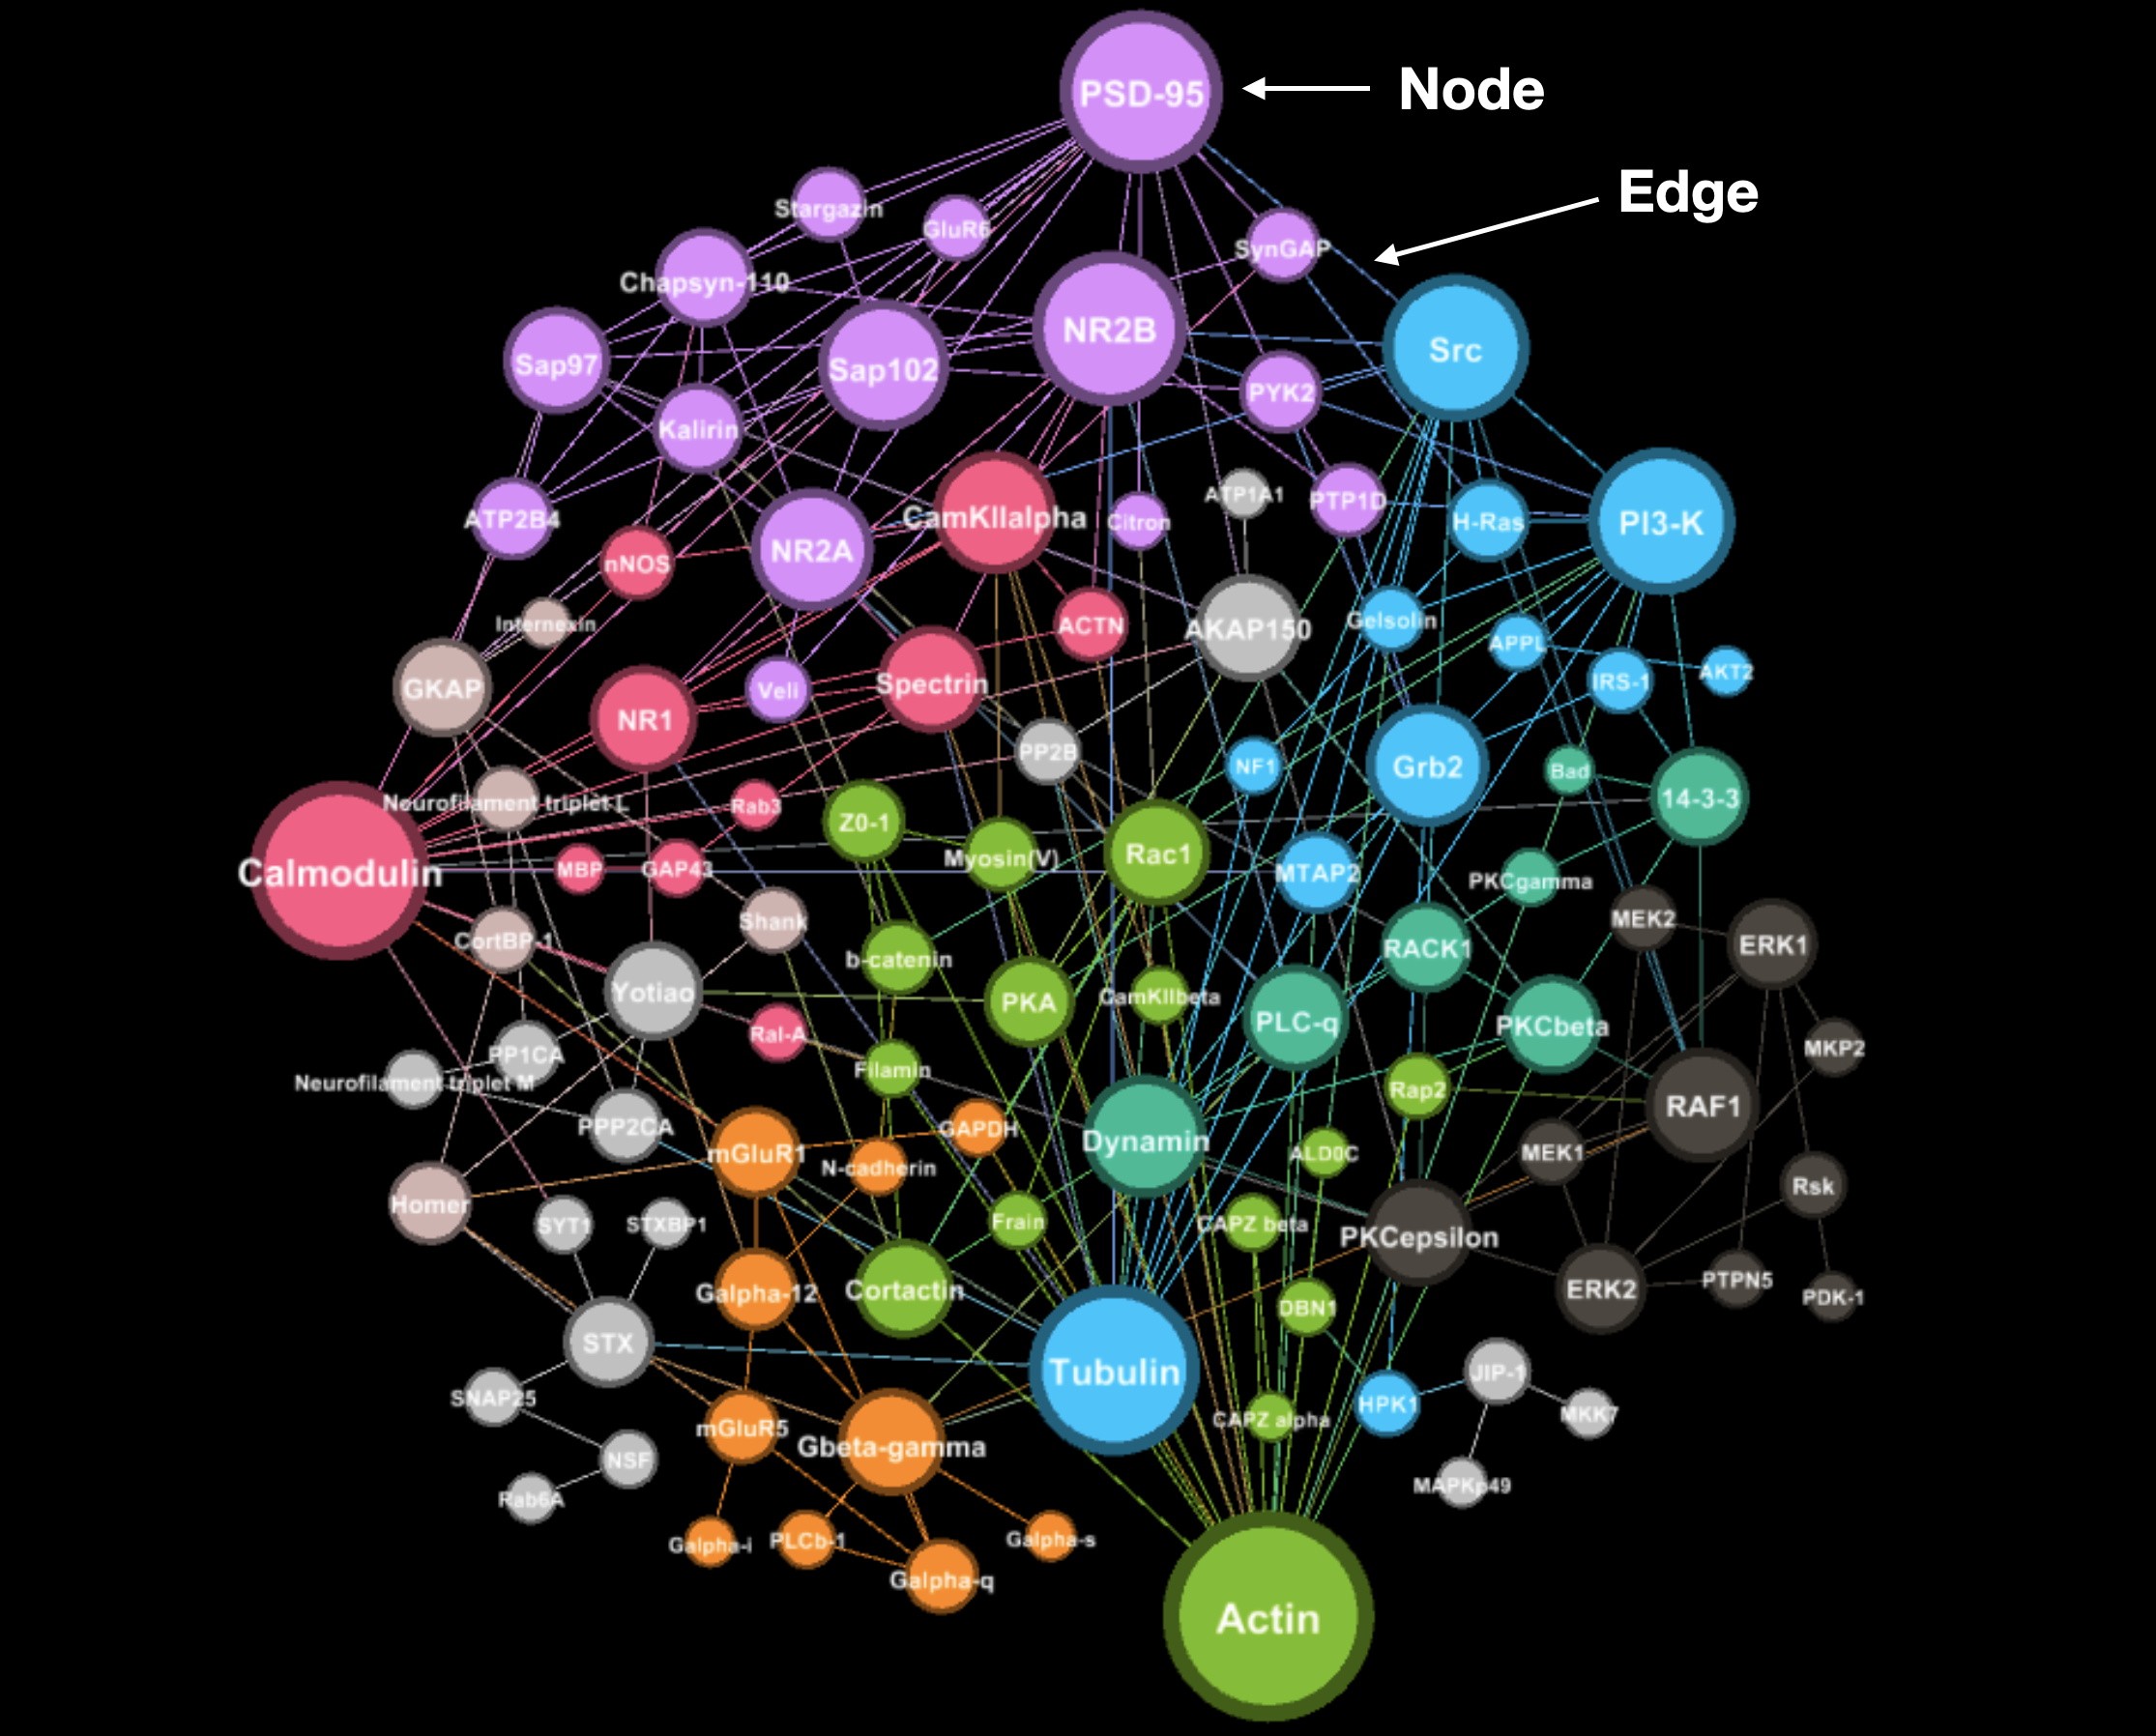
\includegraphics[width=\textwidth]{images/nrc_arrow.png}
        \caption[Network graph of the NRC MASC complex.]{Network graph of the NRC MASC complex. Arrows show a node or vertex which correspond to a gene encoding NRC MASC protein and an edge or link between two nodes which shows that the proteins interact. The network is that described by Pocklington et al. \cite{pocklington2006proteomes} used in the paper by McLean\cite{mclean2016improved}.\footnote{the gml file was produced by CMcL}. Graph visualisation in Gephi\cite{bastian2009gephi} with colours corresponding to community membership. Node size is proportional to degree (the number of edges connected to a node)}
    \label{fig:nrcmasc}
\end{figure}


Protein-protein interaction networks are built using evidence of molecular interaction between the proteins constituting the network. Evidence that proteins interact is
%\footnote{?is - evidence is singular}
curated in protein-protein interaction databases. Human protein-protein interaction databases include those that map to primary proteomic experiments:   the Dictionary of Interacting Proteins (DIP) \cite{salwinski2004database}, MIntAct\cite{orchard2014mintact} and BioGRID \textit{(Bio}logical\textit{G}eneral \textit{R}epository for \textit{I}nteraction \textit{D}atasets)\cite{chatr2017biogrid}; those that contain computational predictions of interactions; and those that contain both, such as STRING\cite{szklarczyk2019string}.

 An alternative division is between primary databases reporting the results of proteomic experiments and meta databases that combine primary databases and may include computational predictions \cite{dong2018analyses}. Experimental evidence for interactions comes from high throughput or low throughput studies. High throughput methods include affinity purification mass spectrometry and two-hybrid screening \cite{dong2018analyses}. High throughput studies constitute the minority of publications curated in databases but account for most of the interactions. For example, in the IntAct database \cite{hermjakob2004intact}, 78\% of publications report 1-10 interactions, but these constitute only 4\% of the interactions in the database \cite{dong2018analyses}. Conversely, only 2\% of studies report over 100 interactions, but these supply 77\% of the interactions in the database \cite{dong2018analyses}.  To permit efficient data sharing a common database schema was developed by the Molecular Interactions workgroup (MI) of the Human Proteome Organisation (HUPO) Proteomics Standard Initiative (HUPO-PSI-MI) in 2002 using a controlled vocabulary to record information on protein interactions indexed with accession numbers \cite{orchard2012molecular}. In addition to a tab, delimited text format (MITAB) there is a stable XML format (PSI-MI XML), allowing a variety of tools to parse information from these databases \cite{orchard2012molecular}.  Protein-protein interaction databases differ due to differences in detection technology and in how experimental data is recorded (curation). The International Molecular Exchange (IMEx) consortium seeks to establish common curation rules and to avoid redundant curation of interactions by coordinating curation across members \cite{orchard2012molecular}, \cite{orchard2012protein}.
 

Despite the use of a standard, machine-readable vocabulary, there is only moderate overlap between the entries in protein interaction databases\cite{dong2018analyses} \footnote{although some of this is due to non-redundant curation} (see table~\ref{tab:overlap between protein interaction databases}). In order to generate a comprehensive network, data must be harmonised from more than one database.  % \textcolor{red}{New} 
In order to provide a comprehensive map of a proteome, several primary databases need to be integrated \cite{alonso2019apid}.%\footnote{note to Douglas/self - this may not be the best reference for this, but it does refer to it}.
Meta databases combine primary databases and may include data from computational predictions, but their evidence base is heterogeneous, and some curation is still necessary to provide an accurate, consistent network.

This is a non-trivial task due to well-documented problems including the use of multiple identifiers, incomplete overlap in experiments, differences between matrix and spokes models and different confidence thresholds \cite{lehne2009protein}.  Network curation is reviewed in depth by Dong and Provart \cite{dong2018analyses}.

  \begin{table}[]
       \centering
       \begin{tabular}{lllll}
       \toprule
    &    BioGRID    & DIP & IntAct & MINT   \\
    \hline
    Interactions & 506,234 & 81,731 & 659,284 & 125,464\\
    \hline
    Species & 62 & 834 & 980 & 611 \\
    \midrule
    BioGRID &  & 13\% & 41\%& 18\%      \\
    DIP & 19\% & & 32\% &20\% \\
    IntAct& 32\% & 10\% & 23\% \\
    MINT 48\% & 26\% & 100 \% & \\
    \bottomrule
       \end{tabular}
       \caption[Overlap between protein-protein interaction databases]{Overlap in records between protein protein interaction databases. The table includes all databases used in the final PSP network with the addition of MINT for purposes of illustration. The table is asymmetric and should be read down the columns as the amount of the \textit{row name} (for example \textit{MINT}) contained in the \textit{column name} (for this example \textit{IntAct}; 100\%). MINT has been included as an example and is a subset of IntACT. All of MINTs interactions are in IntAct so the row MINT, column IntAct; is 100\% but the column IntAct, row MINT is 23\% as the contents of MINT account for this amount of IntAct. Modified from figure 3 in Dong and Provart (2018) \cite{dong2018analyses}.}
       \label{tab:overlap between protein interaction databases}
   \end{table}
 \subsection{Documenting interactions}
 Protein-protein interactions for the PSP network were obtained from the mining and harmonisation of data from the Database of Interacting Proteins (DIP) \cite{xenarios2002dip},  IntAct database \cite{orchard2014mintact},  BioGRID \cite{chatr2017biogrid}, and HIPPIE\cite{schaefer2012hippie}. HPRD\cite{keshava2009human} was excluded as it did not comply to PSI-MI TAB  standards at the time of compilation of the graph. HIPPIE was ultimately excluded from further analysis due to a lack of specific interaction information. See Heil (2018) \cite{heil2018systems} chapter 4 for full details. 
 
 The mapping of identifiers and accession numbers across different databases is a central bioinformatics task \cite{huang2011comprehensive}. These can be different identifiers for a particular object (such as HGNC Gene Symbols or Entrez Gene ID) or mapping identifiers between related objects (e.g. between a protein accession identifier and that of the encoding gene). The mapping of identifiers from UniprotKB to Entrez Gene ID was the most commonly used task in a protein identifier mapping service\cite{huang2011comprehensive}.
 
 A bi-map was created to translate between protein identifications mapped to Uniprot accession numbers\cite{uniprot2017uniprot}, and the GeneID provided by the Entrez Gene portal at the National Centre for Biotechnology Information (NCBI). NCBI Entrez Gene GeneIDs are unique integer identifiers and were used as the main identifier for all subsequent data tables and analyses \cite{maglott2005entrez}. For brevity I use Entrez GeneID synonymously with NCBI Entrez Gene GeneID.
%  \footnote{to remove: comment this might seem pedantic but Enrichr which is very highly cited and otherwise very good enrichment service asks for Entrez ID symbols - looking for Gene Symbol}.
 The widespread use of Entrez Gene identifiers in genomic studies and genomics software \cite{huang2011comprehensive} makes them a suitable primary identifier for network nodes.

Protein-protein interactions were included if there was high quality evidence for direct physical interaction in humans. The interaction list was filtered to ensure all proteins had a human taxonomy ID of 9606. The details of interactions were recorded in PSI-MI TAB 2.5 format (MITAB25)
%\footnote{it is i think PSI-MI TAB 2,5 and MITAB 25 see \url{https://github.com/HUPO-PSI/miTab/blob/master/PSI-MITAB25Format.md}}
\cite{isserlin2011biomolecular}\cite{heil2018systems}. One interaction was retained where mirrored duplicates occurred (e.g. A-B and B-A). The data interaction list resulting contained 396,837 rows and 237,789 unique PPI. 
%\footnote{was a to do I now have got(found) Katharina's document of 2016-10-31 which outlines the interactions strategy for the network. In addition, the document says that spoke expanded PPI from intact were excluded, but perhaps some were found later? so i have not included this yet} 
The interaction list was further filtered to generate the protein interactions represented by edges in the network graph. Protein-protein interactions were excluded if there was no direct experimental evidence of interaction documented by Proteomics Standard Initiative - Molecular Interaction ontology terms in the databases. PSI-MI is a structured ontology used to describe the evidence for protein-protein interactions.\cite{isserlin2011biomolecular} PPIs based on `genetic interactions' (MI:0208) , `genetic interference' (MI0254), `genetic interaction' (MI:0208)\footnote{which includes suppression (MI:0796 and synthetic MI:0794)} and `co-localisation' were excluded (MI:0403). 66 interaction MI accession codes representing direct interaction were included, including one obsolete term `physical interaction' (MI:0218). The final filtered list contained 352,325 unique rows representing 205,461 binary interactions.

  
% Departmental documents on network generation are contained in the following footnotes and will be removed from the final manuscript\todo{FINAL:remove}.
% \footnote{Strontium colin note \url{/home/grant/Documents/PhD_from_DICE/DocSynch_paper_data_dice/data/graph/_from_Colin_Dec_gmlandxls}}
% % \footnote{  Copy of readme
%   Hi Oksana,
% Commented out below
% Attached are initial clustering \& enrichment results (please see below) for the published pre- and post-synaptic lists (Synaptic proteome Dropbox folder) using  Kat's PPI list (file \url{"PPI\_human\_direct\_final.csv}", 31/10/2016).

%  synaptic lists:
%  1) PPI\_Presynaptic\_Published (output .xls \& .gml files)
%  2) PPI\_PSD\_clean\_Published   (output ditto)

%  I guess this is a start. There's details, basic stats i'll need to collect on the clustering results, but hope this helps Kat \& Grant with with there studies, and Oksana to help understanding the clustering in the networks. I'm quite interested looking at the overlap between the different algorithms.
% Let me know if there's any problems? }


\subsubsection{Proteomics data}
\label{sec:proteomics data}
%\todo{there is a repetition somewhere below of the number of studies}
39 proteomic studies conducted between 2000-2017 of the human, mouse and rat synapse were curated into a list of 6500
%\todo{check now} 
potential synaptic genes (all mapped to human Entrez Gene GeneIDs)\cite{heil2018systems}\cite{maglott2005entrez}.  Of these studies, 17 (see table~\ref{tab:Katharina_phd_studies_oksana_studies})
%\{Douglas: See note on text it is either 23 (Kat) table~\ref{tab:Katharina_phd_studiesFF} or 17 (Oksana cleaned file), there is not much difference other than the number of papers covering each protein, the Oksana one is cleaner but there were other nodes in an xls file colin used for the PSP (although they don't appear in the graph he produced}, 
% \{was a todo now a  saying check now it originally was 22 now 23 and four more were added in 2017 to this set which then made up the set that colin gave me based on the Oksana clean published PSD document both included in supplementary material}
% ,
% \{So in Katharina but not in the Oksana listLi 2003Focking 2016Doscemi 2006Distler expectedUezu 2016assuming that Focking is Framer  oksana = 17Katharina = 24 - 1 distler = 23 which is correct from the original paper now missing from the dropbox that I took the original introduction from (of these 23 examined the PSD - it varies i think from 22 to 23 on the doscemi?}

examined the post synaptic density (PSD).
an electron dense structure beneath the post synaptic membrane \cite{PALAY1956}  consisting of complexes of neurotransmitter receptors and their supporting proteins. \cite{kennedy2000signal}  Affinity purification against common PSD proteins improves their identification. \cite{ewing2007large}  
The human proteins and human orthologues of murine proteins found in these studies were used as a ‘parts list’ for the PSD and associated interacting proteins expressed in the post synaptic area (PSP). 3894 genes were identified 
%\{in the 23 studies shown in table~\ref{tab:Katharina_phd_studiesFF}} in the 17 studies (table~\ref{tab:Katharina_phd_studies_oksana_studies}).
%\footnote{ "CHENG   2006"      "DOSEMECI   2006"   "JORDAN  2004"     "LI  2004"        
%  [7] "PENG  2002"       "SATON  2002"      "SCHWENK  2013"    "SELIMI   2009"     "TRINIDAD  2005"   "TRINIDAD  2008"  
% [13] "WALIKONIS  2000"  "YOSHIMURA"       "FROMER 2014"     "FARR.2004"       "Distler.PSDII"   "BAYES 2011"     
% [19] "BAYES 2012"      "COLLINS 2006"    "DOSEMECI  2007"   "FERNANDES  2009"  "BAYES 2014"  }   

 The nodes in the network used in this thesis are genes encoding proteins discovered in the proteomic studies in table~\ref{tab:Katharina_phd_studies_oksana_studies} which have high quality experimental direct interaction data in humans  %\footnote{one study has been removed because it did not meet some of the quality control procedures for the graph generation} 
 (see Heil \cite{heil2018systems} for detailed inclusion criteria and further discussion of network generation.)
% %\footnote{Full text at  ERA link for Katharina PhD \url{https://era.ed.ac.uk/handle/1842/31043} Direct link \url{https://era.ed.ac.uk/bitstream/handle/1842/31043/Heil2018.pdf?sequence=1&isAllowed=y}  p98 fig 5.9a, p86 and supplement C change to era ref},\footnote{previous fulltext link \url{http://www.diva-portal.org/smash/get/diva2:1194151/FULLTEXT01.pdf}} 
The complete network graph contains 3473 vertices and 30499 edges. 
 
% [7] "PENG  2002" \cite{peng2004semiquantitative}  is 2004
% "SATON  2002"   is SATOH 2002 \cite{satoh2002identification}

% "SCHWENK  2013"  \cite{schwenk2012high} 2012
% "SELIMI   2009" \cite{selimi2009proteomic} 
% "TRINIDAD  2005 \cite{trinidad2005phosphorylation}"  
% "TRINIDAD  2008" \cite{trinidad2008quantitative} 
% [13] "WALIKONIS  2000" \cite{walikonis2000identification} 
% "YOSHIMURA" 2004 \cite{yoshimura2004molecular}   
% "FROMER 2014" Not in Heil I only find fromer in an oksana paper on PSD and it is on scz I assume this is Focking and the one cited in Heil is bipolar
% and they have 2033 PSD proteins Focking \cite{focking2016proteomic}
% "FARR.2004" \cite{farr2004proteomic}
% "Distler.PSDII" \cite{distler2014depth}
% "BAYES 2011"   \cite{bayes2011characterization}  
% [19] "BAYES 2012" \cite{bayes2012comparative}    
% "COLLINS 2006" \cite{collins2006molecular}
% "DOSEMECI  2007" \cite{dosemeci2007composition}
% "FERNANDES  2009" \cite{fernandez2009targeted}
% "BAYES 2014"  \cite{bayes2014human}




%  "PENG  2002" \cite{peng2004semiquantitative}  is 2004
% "SATON  2002"   is SATOH 2002 \cite{satoh2002identification}

% "SCHWENK  2013"  \cite{schwenk2012high} 2012
% "SELIMI   2009" \cite{selimi2009proteomic} 
% "TRINIDAD  2005 \cite{trinidad2005phosphorylation}"  
% "TRINIDAD  2008" \cite{trinidad2008quantitative} 
% [13] "WALIKONIS  2000" \cite{walikonis2000identification} 
% "YOSHIMURA" 2004 \cite{yoshimura2004molecular}   
% "FROMER 2014" Not in Heil I only find fromer in an oksana paper on PSD and it is on scz I assume this is Focking and the one cited in Heil is bipolar
% and they have 2033 PSD proteins Focking \cite{focking2016proteomic}
% "FARR.2004" \cite{farr2004proteomic}
% "Distler.PSDII" \cite{distler2014depth}
% "BAYES 2011"   \cite{bayes2011characterization}  
% [19] "BAYES 2012" \cite{bayes2012comparative}    
% "COLLINS 2006" \cite{collins2006molecular}
% "DOSEMECI  2007" \cite{dosemeci2007composition}
% "FERNANDES  2009" \cite{fernandez2009targeted}
% "BAYES 2014"  \cite{bayes2014human}
% in Katharina 
% Doscemi 2006




\begin{table}[]
    \centering
    \begin{tabular}{lllllll}
    \toprule
     & First author & Year & Reference & Region & Species & $n$ \\
    \midrule
1 &    WALIKONIS &2000 &Walikonis et al. (2000)\cite{walikonis2000identification} &postsynapse & rat & 29 \\
2 &PENG&2004&Peng et al. (2004) \cite{peng2004semiquantitative}&postsynapse& rat& 325\\
3 &SATOH&2002&Satoh et al. (2002)\cite{satoh2002identification}&postsynapse &mouse &45\\
4 &YOSHIMURA&2004&Yoshimura et al. (2004)\cite{yoshimura2004molecular} &postsynapse& rat &435\\
5 &FARR&2004&Farr et al. (2004)\cite{farr2004proteomic}&postsynapse &rat &71 \\
% 6 &JORDAN&2004&Jordan et al. (2004)&postsynapse &mouse and rat &390& NOT\\
% 7&LI&2004 &wan Li et al. (2003)&postsynapse &rat& 137& NOT\\
6&TRINIDAD&2005 &Trinidad et al. (2005) \cite{trinidad2005phosphorylation}&postsynapse&mouse& 234\\
% 9&CHENG&2006&Cheng et al. (2006)&postsynapse& rat& 288& NO\\
7&COLLINS&2006&Collins et al. (2006)\cite{collins2006molecular}&postsynapse &mouse& 717\\
% 11&DOSEMESI&2006&Dosemeci et al. (2006)&postsynapse& rat& 113& NO\\
8&DOSEMESI&2007&Dosemeci et al. (2007)\cite{dosemeci2007composition}&postsynapse& rat& 548\\
9&TRINIDAD&2008&Trinidad et al. (2008) \cite{trinidad2008quantitative}&postsynapse& mouse& 2150\\
10&SELIMI&2009&Selimi et al. (2009)\cite{selimi2009proteomic} &postsynapse &mouse &61\\
11&FERNANDEZ&2009&Fernández et al. (2009)&postsynapse& mouse &292\\
12&BAYES&2011&Bayés et al. (2011)\cite{bayes2011characterization}&postsynapse &human &1441\\
13&BAYES&2012&Bayés et al. (2012)\cite{bayes2012comparative}  &postsynapse &mouse &1545\\
14&SCHWENK&2012&Schwenk et al. (2012)\cite{schwenk2012high} &postsynapse &unknown &34\\
% 19&DISTLER PSD1*&2014&Distler et al. (2014)&postsynapse& mouse& 3545& NO \footnote{intended per email}\\
15&DISTLER PSD2*&2014&Distler et al. (2014)\cite{distler2014depth}&postsynapse& mouse& 2092*\\
16&BAYES&2014&Bayés et al. (2014) \cite{bayes2014human}&postsynapse& human &1141\\
% 22&UEZU&2016&Uezu et al. (2016)&postsynapse &mouse &1111 &NO\\
 17&FOCKING&2016&Föcking et al. (2016)\cite{focking2016proteomic}&postsynapse& human &2026\\

\bottomrule
    \end{tabular}
    \caption[Primary Proteomic studies contributing to the PSP - from Heil (2018)]{Primary proteomic studies contributing to the PSP Clean Published network adapted from Heil 2018\cite{heil2018systems} PhD 
    %\footnote{to Douglas: These should have been the same as given to me as per email from Colin need to chose one see note on text. Distler PSD1 is definitely dropped from the cleaned data. The graph is somewhere between these two points. The most conservative is the Oksana one.}
    }
    \label{tab:Katharina_phd_studies_oksana_studies}
\end{table}







 
3475 genes had high quality interaction information available and formed the vertices of the PSP; these included two duplicate Entrez Gene Id and 16 genes that were isolated components and not in the largest connected component).




 
  




 
 
The largest connected component of the resulting graph was used for community detection and in calculating network statistics (3457 nodes, 30498 edges). The details of the small number of excluded vertices not part of the largest connected component are in section~\ref{sec: PSP graph connected component and missing} below.

The methods used to generate the network of the graph are described in detail in Heil (2018)\cite{heil2018systems}. The vertex and edge lists are available in Supplementary material X (along with other data on network generation).

%\footnote{oksana data at\url{/home/grant/Documents/PhD_from_DICE/DocSynch_paper_data_dice/data/graph/_Oksana_synaptic}}
% %\footnote{code to analyse this on Code strontium (informatics workstation) \url{source('~/RProjects/readPSP_data/R/PSPgraph.R')}} \footnote{Counts in literature counter1
% counter
%   1    2    3    4    5    6    7    8    9   10   11   12   13   14   15   16   17   18   19   20 
% 1396  626  339  262  191  156  112   99   76   45   44   35   22   14   16   13    7    4    1    1 }
% %\footnote{counter2 Count of studies not in PSP (so PPI information not available)

%   1   2   3   4   5   6   7   8  10  12  13 
% 250  81  30  31  15  12   7   4   3   1   1 }. 


The network was stored as a named edge list consisting of two columns. Each row represents an interacting protein pair and each protein is identified using the Entrez Gene Id of its encoding gene. Network metadata and interactions were stored as a graph modelling language (GML) file generated from this edge list. \cite{himsolt1997gml}

% \footnote{Original available at \url{https://web.archive.org/web/20190303094704/http://www.fim.uni-passau.de:80/fileadmin/files/lehrstuhl/brandenburg/projekte/gml/gml-technical-report.pdf}}



GML is an ASCII based, hierarchical, lightweight format supported by igraph \cite{csardi2006igraph}, Gephi \cite{bastian2009gephi} , NetworkX \cite{hagberg2008exploring} and graph-tool \cite{peixoto_graph-tool_2014}.  A master copy of the original file supplied to me was stored on the University of Edinburgh informatics server. The original gml file was generated by CMcL and is included in the supplementary material.

%\textcolor{red}{commented out}
% For certain packages the edge list was used or the edge list transformed to an adjacency matrix or other graph object (eg SNAP format)

% Previous note commented out below (list from colin with the 27 had 5101 genes)\footnote{
% for combined list of genes (5101) including both Distler, we have got the PPI information for 3457 genes, which resulted in the graph of 3457 nodes and 30499 edges. Of this - 3457 nodes and 30498 edges contributed to Largest connected component (I guess the same size as initial graph). The majority of genes that survive quality control are expressed in more than one study) Of those in only one study 489/3457 = 14.1\%. 352 appear in the 2014 paper by Distler et al. You have a total of 5101 and of these 1640 appear only once of the 1643 genes that did not makes the final graph 1151 (70\%) were expressed only once 286 twice and 76 three times "

% Those that appeared in the overall graph but not in the LCC appeared on one occasion 2, 2 occasion 2, 3 occasion 6, 7 occasion 1, 8 occasion 2, 9 occasion 3) so there were nodes that we had PPI information for that still did not make it into the LCC so a lot of the ones that did not make it is because we did not have PPI information that met PPI or the genes missed other qc. 

% Yeah cos the ones that appear once we have information on we might even have their degree they are not all going to have degree one so its a subgroup of the proteomics where we have valid PPI - got it. Comparisons between the number of representations in the literature and gene features are described in depth in Heil} \cite{heil2018systems}.\textcolor{red}{endremove}
% \todo{could do correlation in number of representations and pLI and GTex}

\subsubsection{Value of tissue specific networks}
\label{sec:value_of_tissue_specific_networks}

The post synaptic proteome network is tissue specific; it is the network of interacting proteins found in the post synaptic area. I will, as part of overall quality control confirm in section~\ref{sec:gtex profile of PSP genes} that these genes are differentially expressed in the CNS in humans given the marked expansion in the number of genes found in the PSP in this network.

It is desirable to use a tissue specific network as different tissues contain different proteins and therefore different nodes and edges in their proteome network. In some tissues this is can be accepted as a minor simplification of the network model, but other tissues are known to have very different gene expression patterns (e.g solid tissues and blood, CNS \cite{mele2015human}). Statistics describing the proteome network found in different tissues will therefore be different. Secondly, it has been reported that disease genes tend to be expressed in specific tissues (and to be on the periphery of cellular networks)\cite{barabasi2011network},\cite{kitsak2016tissue}. Finally, the synaptic proteome \textit{in particular} has a modular structure arising from the interaction of its protein components and giving rise to higher order structures and functions \cite{pocklington2006organization},\cite{grant2012synaptopathies} that are particular to the synapse. 

I examine this in more detail in the discussion but here give two examples. Ghiassian et al. (2015) \cite{ghiassian2015disease} performed an analysis similar to the one presented here (see section~\ref{sec:intro other approaches}) before going on to describe a method for identifying disease modules.
%A co-author of one of the papers discussing tissue specificity of disease genes\cite{kitsak2016tissue}) 
Using a network made up of heterogenous components to examine several diseases and concluded that topological groups are unhelpful but that diseases result from loss of function of an area of a \textit{global interactome} where a group of disease associated genes reside. 


 Conversely Parishhak (2015) in a review of systems biology \cite{parikshak2015systems} quotes the example of a tissue specific cardiac PPI used to investigate long QT syndrome (LQTS) by Lundby et al. \cite{lundby2014annotation} as an example of the value of tissue specificity. Lundy et al. used a mouse cardiac protein network derived from High Performance Liquid Chromatography Tandem Mass Spectrometry (HPLC-MS/MS) of 5 seed proteins encoded by genes identified in GWAS of LQTS to generate candidate genes later confirmed in zebra fish. These genes could not be identified using more general networks. %\footnote{to discussion - interestingly these are ones in the neighbourhood of receptors and ion channels}.
 See discussion section~\ref{sec:Methods Discussion}.  



\subsection{Connected component}
\label{sec: PSP graph connected component and missing}
Random generative models of networks are often used to study network behaviour \cite{newman2018networks}. The simplest model of a network is the Erd{\H{o}}s - R{\'e}nyi\cite{erdHos1960evolution} model in which each node is connected to every other node with a uniform probability $p$. %\todo{cross ref to Poisson}.
This simple model shows a spontaneous aggregation of isolated nodes to form a large connected component  (connected in that all of its nodes can be reached via `hops' along its edges) containing the majority of nodes  as the average degree (degree $k$, average degree $<k>$) increases.  In real world networks a largest connected component is observed of varying size but there is always one component that dominates the others ($S$, the proportion of nodes in the component) varies - see Newman \cite{newman2018networks}.
\paragraph{Methods}
The network containing all nodes including those not in the largest connected component was generated by CMcL and stored as a gml file. Components were identified using the \texttt{components} command for igraph version 1.2.5\cite{csardi2006igraph} for R and the components not part of the largest component recorded %\footnote{\url{source('~/RProjects/network_graph/R/notLCC_gmt/genes_not_inLCC.R')}}. 

 igraph for R version 1.2.5 was used for the majority of graph processing tasks in scripts using R\cite{csardi2006igraph}. R version 3.6.3\cite{ihaka1996r} is used throughout and  all statistical analysis are carried out in R unless otherwise stated. On some occasions igraph for Python was used typically when methods were only available in Python (such as generating empirical clustering objects to calculate performance measures for community detection (see section~\ref{sec:NMI communities}). This is noted in the appropriate methods sections and in the associated scripts.

Nodes not in the connected component are excluded from further analysis as community detection algorithms and most vertex statistics are not designed for unconnected components.

The composition of the excluded components was analysed to assess whether they contained elements that might bias the subsequent analyses (see section~\ref{sec:analysis of genes not in largest component}).% \todo{do GSA for these componentDONE}
For further discussion of the  connected component see section~\ref{sec:connected component and degree}. 

\paragraph{Results}
In addition to the large connected component ($n$=3457 nodes), 15 smaller components were found within the PSP graph; these were all single isolated components other than one component of size 2.  The  proteins encoded by these genes appear in the ``parts list" derived from proteomic studies but lack experimental evidence of direct interaction with the protein products of the genes in the large component of the PSP.


16 genes were not in the giant connected component and are listed in table~\ref{table:notinLCC}. The only component with two genes contained Oligodendrocyte Myelin Glycoprotein (OMG) and Reticulon 4 Receptor (RTN4R)%
%\footnote{member of growth cone pathway and implicated in scz}. 

 

All but 0.46\% ($S$= 0.995, where $S$ is the size of the giant component expressed as a fraction of total network size - see Newman\cite{newman2018networks} p305 for a comparison with other networks) of the genes identified in proteomic experiments (section~\ref{sec:proteomics data}) with high quality experimental interaction data are part of the largest component. This is comparable to the the undirected metabolic network ( $S=0.996$) in Newman \cite{newman2018networks} \footnote{p 305} but high compared to their example protein interaction network (n=2115,$S$=0.689). Its desirable that a large majority of genes should be in the connected component as most community detection methods and centrality measures are invalid for non connected network components and these genes would need to be excluded and could bias the analysis. 
%\todo{So what}\footnote{Code to generate the table is found at \url{'~/RProjects/analyse_DICE_data/R/LCC.R'}}
\subsubsection{Analysis of genes not in largest connected component}
\label{sec:analysis of genes not in largest component}
%\todo[inline]{what is a component}

Gene ontology enrichment analysis of the 16 genes not in the largest connected component was carried out to ensure they did not belong to a common system or component that would bias the analysis. Gene ontology enrichment analysis is widely used in the rest of this thesis and the methods introduced below.


\subsection{Gene ontology analysis}
\label{sec: gene ontology analysis}
A gene ontology provides a controlled, maintained vocabulary to describe sets of genes according to their Biological Function, Cellular Component and Molecular Function. It is widely used in high throughput genetics to provide information on the function of a set of genes \cite{ashburner2000gene}.Gene ontology terms have structured interactions forming a directed acyclic graph that shows the hierarchical relationship between terms with more specific child terms arising from parent terms (see figure~\ref{fig:the DAG of Collateral sprouting}).

Gene ontology over-representation analysis tests whether a set of genes are more commonly annotated to a specific term  than would be expected by chance. Some also  difference in results is reported across different platforms and therefore more than one method is used \cite{rhee2008use}\cite{khatri2005ontological}. 


\paragraph{Multiple testing}
Gene ontology terms overlap, especially at different levels in the hierarchy, are not independent and therefore assumptions of independence in multiple testing corrections are invalid. The issue of multiple testing in Gene Ontology enrichment analysis is complex and beyond the scope of this thesis. Rhee et al. (2008) \cite{rhee2008use} provide a comprehensive summary an a more recent, technical analysis is found in Meijer et al (2016)\footnote{this actually isn't the most technical there is a general treatment for inference in DAG by the same author} \cite{meijer2016multiple}. A brief description is however necessary both to introduce the methods in this chapter and to indicate potential limitations to pathway enrichment methods in general (including MAGMA GSA which make extensive use of ontology terms). 

Rhee et al. (2008) \cite{rhee2008use} recommend the following approach to multiple testing:

`An unbiased search for significant GO associations can be done with a bottom up approach as follows: for every leaf term, calculate p-values with the genes directly associated to it. If any term is significant do not propagate its genes above. This would provide the most specific node that is significant in that particular branch. If a term is not significant, propagate the annotations to its parent and recalculate with the parent term. The genes will propagate upwards until a significant node is found or until the root is reached. A careful analysis is still necessary to properly correct for multiple comparisons.'\cite{rhee2008use}

 To my knowledge there is no widely available implementation of this method designed for genomic analysis the closest being the methods described by Alexa et al.\cite{alexa2006improved} and implemented in topGO\cite{alexa2009gene} (see below).  Rhee et al.\cite{rhee2008use} state that the Bonferroni correction is too conservative and Holm and FDR offer better alternatives. Another method for correction is that implemented in g:Profiler \cite{raudvere2019g} which uses the sgs method for multiple comparisons to increase power given the interdependence of GO terms. 
 Rhee et al. recommend minimising the number of tests wherever possible \cite{rhee2008use}.\footnote{see also }
One way to reduce the number of tests is to use a restricted or clipped Ontology. This can be challenging to implement and although a neural immunology clipped ontology has been described \cite{geifman2010neural} I am not aware of any application providing a clipped neural ontology enrichment however the SynGO project\cite{koopmans2019syngo} uses and ontology restricted to the synapse where gene term relationships are supported by  high quality experimental evidence.

% In practical terms one should be aware that multiple testing using Bonferroni correction (as implemented in MAGMA) is too strict, second that the results of enrichment in hypothesis generating applications do not truly represent an absolute value of the likelihood of a test under repetition but a measure of confidence in specific findings. I will return to this in the discussion.


\subparagraph{elim method}
The \textit{elim} and \textit{weight} methods described by Alexa et al. (2006)   \cite{alexa2006improved} and implemented in the popular topGO R  package\cite{alexa2009gene} have the effect of decreasing the significance of very general GO terms (increase p) in comparison to more specific child terms. These methods proceed upwards from child nodes and only move genes for testing to the next level if they have not been scored at the lower level. This has the effect of decreasing the significance of very general terms and making very specific terms more significant within the  analysis. The general effect is to increase the overall raw p values but to do this most for general terms.  It does not correspond exactly to multiple testing correction but does prioritise general terms and deflate significance of general terms.  The authors state that most multiple comparison methods are too strict given the connected structure of GO and they prefer to regard the \textit{elim} results as already corrected \cite{alexa2020gene}.\footnote{if you look at the results you can see that adding a multiple testing penalty on top of this would be too severe} \footnote{\url{https://bioconductor.org/packages/release/bioc/vignettes/topGO/inst/doc/topGO.pdf} 2020}.
\paragraph{background set}
The number of terms that are expected to be found in a group of genes depends on the background set and this plays an essential role in calculating over representation. Some packages allow the use of custom background sets (ToppGene has very recently \footnote{last 2 weeks} added this feature). If not indicated the background set is the default for that enrichment package usually the protein encoding genes in the genome.  

\paragraph{Common methods}
Some methods use direct data entry to a web interface, others an API and some methods can be locally installed. The main advantage of web based ORA is regular updating of the ontologies and a common computational platform. To reduce transcription errors, whenever text entry of a list of genes is used on a web interface a script is used to write the list of genes directly to the clipboard \footnote{A function calling the Linux command \texttt{xclip} was used in R to transfer the print formatted object to the clipboard\url{source('~/RProjects/paper_xls_output/R/functions_for_project.R')}, while in Python the \texttt{to\_clipboard} function in the data frame analysis pandas module was used\cite{mckinney2011pandas}.} 
\subsubsection{PANTHER methods}
\label{sec:panther methods1}
Gene ontology ORA for the genes not part of the connected component was carried out using the PANTHER classification system (protein annotation through evolutionary relationship) version 15.0\cite{mi2019protocol} via the web-based user interface hosted at the Gene Ontology Consortium (GOC) website\footnote{\url{http://geneontology.org/}}.

%\todo{compress this and put into methods and results}\textcolor{red}{start compress}
PANTHER provides information on gene function at a genomic scale and as a member of the Gene Ontology Consortium provides accurate annotation with regular updates\todo{compare with DAVID}. Results can be displayed showing their relation in the gene ontology hierarchy\cite{mi2019protocol}.  The authors recommend the use of the False Discovery Rate to correct for multiple comparisons because of the correlation between tests involving related annotations \cite{mi2019protocol}. It can be accessed using an API or web application. It was used for tests where authoritative, accurate testing using an up to date ontology were required rather than as part of an automated workflow. PANTHER accepts custom background sets for enrichment.(for example to see whether a set of genes is enriched compared to the whole genome or the rest of the PSP). 

PANTHER 15.0 (released 2020/02/14)\cite{mi2013large} was used to carry out test sets of genes for over representation of terms from each of the three Gene Ontology clades (Cellular Component, Biological Process and Molecular Function).  Versions are identified by release dates using the year, month, date format supplied in the list of reporting details supplied by PANTHER.The PANTHER Over-representation Test used implementing Fishers Exact test (released 2020/07/28).  The Gene ontology database was DOI: 10.5281/zenodo.3873405 Released 2020-06-01.  The Benjamini-Hochberg procedure \cite{benjamini1995controlling} was used to calculate the False Discovery Rate (FDR) to account for multiple comparisons and corrections  were applied for each clade.

\paragraph{Annotations}

Despite using Entrez Gene ID integer values with the recommended string prefix "GeneID:" (as PANTHER interprets integers as HGNC identifiers by default) several genes were not identified using Ensembl and Entrez Gene ID. Entrez ID were therefore mapped to HGNC Gene Symbols. Where Gene symbols were not identified the list of synonyms in Entrez Gene were used until a match was obtained\footnote{also checking that the supplied match maps to correct Uniprot but i say this later and there are scripts for PANTHER searches and a csv containing the accepted symbols mapped to Entrez ID}. 




% PANTHER introduced in section~\ref{sec:panther methods1} is a member of the gene ontology consortium and frequently updated. The results obtained contain links to easily view the GO tree and also present results in terms of the hierarchy. Mi et al\cite{mi2019protocol} in the most recent update acknowledge that given the relatedness of GO terms tests are non independent and therefore the Bonferroni correction is too conservative. As an alternative they recommend using the FDR method.
They also implement SLIM ontologies 





\subsection{Methods}
\label{sec:GO enrichment methods}
% In addition to Panther described earlier I used the ToppFun functional enrichment service which is part of the toppgene suite. The web interface was used but data entry was carried out using a pipeline from GWGAS significance tests to the system clipboard to avoid transcription errors.
% Method - for each generated list of significant genes mapped to 
% Entrez, Symbol, Ensembl, Protein
% \subsubsection{from earlier}

% \todo{Other comments rhee} Rhee\cite{rhee2008use} see notes.rtf on Windows10 path commented out below 
% %%C:\Users\gxrob\OneDrive\Documents
% \textcolor{red}{The issue of multiple testing complicated for gene ontology terms as they form a directed acyclic graph where a child node is derived from a parent term (for example GO:008066 Molecular function glutamate synthesis is a child term of GO:0004888 transmembrane signalling receptor ). The recommended practice in calculating significance is to propogate up the tree until a node achieves significance and not to propagate to ever more general terms\cite{rhee2008use}. It is not clear to me that this is implemented in the enrichment packages using Gene ontology terms reported in the literature for the GWA studies for intelligence and educational attainment used here (eg MAGMA, FUMA). Variations in GO enrichment scores between packages are well recognised and as I have used both PANTHER and topGO below which respect DAG topology it does not change the analysis (however see discussion section)}


For computational calculations of gene ontology where rapid output is required as part of a pipeline I have used topGO version 2.38.1 an R package that provides gene ontology enrichment \cite{alexa2006improved},\cite{alexa2009gene}\footnote{code \url{source('~/RProjects/graph2community/R/topgo/modified_exampleGoObject_groups.R')}}.
specific to it will be described when first used as will be the case with other methods. 
 topGO has the advantage of being a longstanding R package and part of the Bioconductor\cite{gentleman2004bioconductor} universe. It is well suited as part of a computational workflow but suffers from slower updates than PANTHER (and ToppGene) and misses the annotation of certain genes. 


For limited numbers of tests where quality of results is the most important thing I have used the PANTHER database as it is regularly updated, uses high standard corrections that respect the GO tree and is part of the gene ontology project. Results are also available as a hierarchy in gene ontology. 

\subsubsection{PANTHER}
\label{sec:methods GO Pather}
Using PANTHER there were identifiers that were not recognised using Ensembl ID, Entrez ID and GeneID. The most robust appeared to be gene symbol. I used translation from Entrez ID to Gene Symbol including synonyms until all genes were identified. In addition to the code documenting the data transformation \footnote{code \url{ source('~/RProjects/paper_xls_output/R/chapter_2/FUMA/edit_gene_table/EA2_FUMA2clipboard.R')}}, the gene mapping compatible with PANTHER is included in the supplementary materials.    \footnote{with ENSEMBL ID ENSG00000256762 was unmapped as was Uniprotand Q8IWL8 (STH)Entrez translation using FUMA resulted in 2 unrecognised gene symbols MGEA5 and C10orf76. Correcting these manually using lookup for synonyms the table was ommended to OGA and ARMH3 resulting in all 99 genes being correctly mapped. A full gene mapping compatible with PANTHER is available in the supplemental material}

 The PANTHER displays hierarchy of the ontology terms although the FDR values are lower than ToppGene the very specific term related to neurogenesis positive regulation of collateral sprouting (FDR p 0.041) is prominent in comparison to the same data ordered by FDR shown in table~\ref{tab:GO biological process complete Education Replication FDR}. \todo{Panther has a somewhat complicated implementation of the Bonferroni correction that partly takes into account the issues with multiple comparisons but I have not mentioned it as not using Bonferroni and I think it may be new (Wasn't in 2019 update paper)}

 

\subsubsection{ToppGene}
\label{sec:ToppGene GO enrichment}
 Toppgene is a gene enrichment service which also includes murine and human phenotypes and disease enrichment\cite{chen2009toppgene}. It has a regularly updated database. There are differences in absolute enrichment significance values between different methods as found reported by Rhee \cite{rhee2008use} but fewer differences in annotation. Data entry to toppgene was done using Entrez ID as default. The ToppGene translation API implements  HTTP POST and HTTP PUT methods and was used for translation of identifiers and where this has been done it is noted in the manuscript. To reduce transcription errors where the text entry web interface was used this was done using direct writing to the clipboard as described in section~\ref{sec:panther methods1}. The output tables for significant ToppGene analyses including terms searched are included as tab separated text files  in the supplementary materials. ToppGene now allow the choice of a background set. Database update 28-07-20. Gene Ontology Biological Process 16465 annotations 20148 genes. Cellular component  2043 annotations 20584 genes molecular function 4745 Genes 20584 (for full details see supplemental methods). GO ontology from PANTHER DB.  
 
PANTHER allows the use of a custom background gene set to test enrichment against. The main drawback of PANTHER is that it can occasionally fail to recognise common gene identifiers even when presented in their recognised form. For that reason and given the fact that there are well described differences between the results for different enrichment methods I have also used ToppFun in the ToppGene package which provides convenient links to the complete gene list of terms which is useful in chapter 4. It also has a very clean interface and excellent identifier recognition (see discussion for further comments on ease of use). The main drawback of ToppFun is that it does not provide for an easy implementation of a custom background gene set. For importance of frequent updates see \cite{tomczak2018interpretation}.

\subsubsection{topGO}
\label{sec:toponto GO enrichment preliminary}
 topGO has the advantage of being a longstanding R package and part of the Bioconductor\cite{gentleman2004bioconductor} universe. It is well suited as part of a computational workflow but suffers from slower updates than PANTHER (and ToppGene) and misses the annotation of certain genes. 


topGO is an R package widely used to perform Gene Ontology enrichment and is thus very suitable for integration into a computational workflow abd implements the elim method. It is updated less frequently than PANTHER. As it is not used in this chapter a detailed discussion of the methods are contained in section~\ref{sec:Gene ontology topgo}). 
 \subsubsection{SynGO} SynGO (Synaptic Gene ontology and annotations) is available as a web interface for Gene Ontology enrichment\footnote{\url{https://www.syngoportal.org/}}xls files in supplementary material\cite{koopmans2019syngo}. It provides an expert curated evidence based ontology mapping of synaptic genes to Gene Ontology terms and provides a subset of the complete GO ontology. It is provided as a web interface with text or file based entry. It provides a default background list of gene expressed genes. It covers the cellular component and biological function GO clades. Fishers exact test is used for testing over representation with the FDR method\cite{benjamini1995controlling} used to correct for multiple comparisons. The detailed supplemental data outputs in xls format are included in the supplemental materials. 
\subsubsection{FUMA Gene2Func package} 
\label{sec:FUMA go enrichment}

FUMA (Functional Mapping and Annotation of Genome-Wide Association Studies)\footnote{\url{fuma.ctglab.nl}} is a comprehensive web based annotation and analysis packaged.\cite{watanabe2017functional} It has been widely used in the secondary analysis of GWA studies\cite{hill2019combined}\cite{savage2018genome} and implements Gene level GWGAS using MAGMA and provides extensive annotation services. The system divides into a SNP2Gene module takes summary SNP data as an input and Gene2Func module which takes a list of significant genes. FUMA v1.3.6 was used. 

I have used the GTEx expression enrichment analysis from the Gene2Func module. This differs from the results and methods presented in section~\ref{sec:GTEx methods} in using a predetermined set of differentially expressed genes and testing over representation using the hypergeometric test and Bonferroni correction for multiple comparison \footnote{for technical details see\url{https://fuma.ctglab.nl/tutorialgene2func} note the address is tutorial HASH gene2func}. This to provides a quick, graphical representation of the differences in tissue expression of genes in the PSP and genome wide significant genes at GWGAS in the discovery and replication samples.\todo{? add the fuma methods} I have also used the Gene Set Analysis in the Gene2Func module which uses hypergeometric tests to assess over representation of terms. Data sets are provided (including gene ontology terms, Wiki Pathways and GWAS catalogue) with Bonferroni correction per category. I have used the GWAS catalogue set enrichment to ensure that genes excluded from analysis are not potential sources of bias (ie reported in intelligence GWA or other neurocognitive phenotypes).

\subsubsection{g:Profiler} 
\label{sec:gProfiler GO enrichment}
g:Profiler, is a longstanding Gene Ontology Consortium (GOC) backed Gene Ontology functional enrichment package. It has a recently updated web interface and an R API. Over representation of ontology terms is tested using the cumulative hypergeometric test \cite{raudvere2019g} and the g:SCS (set counts and sizes) method which takes into account the overlapping between sets based on GO terms \cite{reimand2007g} used to correct for multiple comparisons. It provides a  Manhattan like plot of over representation and a comprehensive translation service that can be accessed from the R API. Although it includes other data from KEGG and wiki pathways I have limited the analysis to GO enrichment terms (these are tested using ToppGene). 

Functional enrichment was carried out using g:Profiler version e100\_eg47\_p14\_7733820 (database updated on 07/07/2020). Multiple testing was controlled using g:SCS method applying a significance threshold of 0.05\footnote{recommended citation format from website} and not displaying  under-representation.



\paragraph{Results ORA of genes not in connected component}


%\todo[inline]{this must be in strontium}
%%% GENES EXCLUDED AS NOT IN LCC %%%

% latex table generated in R 3.6.2 by xtable 1.8-4 package
% Tue Dec 31 09:25:51 2019/home/grant/RProjects/network_graph
\begin{table}[ht]
\centering
\begin{tabular}{cllc}
\toprule
 
GeneID & Gene Symbol & Gene Name & $n$ \\ 
\midrule
 4974 & OMG & oligodendrocyte myelin glycoprotein & 2 \\ 
  65078 & RTN4R & reticulon 4 receptor & 2 \\ 
 98 & ACYP2 & acylphosphatase 2 & 1 \\ 
  166785 & MMAA & metabolism of cobalamin associated A & 1 \\ 
  549 & AUH & AU RNA binding methylglutaconyl-CoA hydratase & 1 \\ 
  55847 & CISD1 & CDGSH iron sulfur domain 1 & 1 \\ 
  23305 & ACSL6 & acyl-CoA synthetase long chain family member 6 & 1 \\ 
  26027 & ACOT11 & acyl-CoA thioesterase 11 & 1 \\ 
  7915 & ALDH5A1 & aldehyde dehydrogenase 5 family member A1 & 1 \\ 
  4685 & NCAM2 & neural cell adhesion molecule 2 & 1 \\ 
 
  5649 & RELN & reelin & 1 \\ 
  2741 & GLRA1 & glycine receptor alpha 1 & 1 \\ 
  152404 & IGSF11 & immunoglobulin superfamily member 11 & 1 \\ 
 
  27000 & DNAJC2 & DnaJ heat shock protein family (Hsp40) member C2 & 1 \\ 
  2686 & GGT7 & gamma-glutamyltransferase 7 & 1 \\ 
  55262 & MAP11 & microtubule associated protein 11 & 1 \\ 
   \bottomrule
\end{tabular}
\caption[Genes not in largest connected component]{Genes with cognate proteins in the PSP as defined by their presence in proteomic studies but that are not part of the giant connected component. These encode proteins that lack direct experimental evidence of interaction with the giant connected component. GeneID is Entrez Gene ID. $n$ is the number of genes in the component.} 
\label{table:notinLCC}
\end{table}

There is no evidence of any enrichment of an association between genetic variants in the set of 16 genes not in the largest connected component and differences in intelligence or educational attainment in any of the discovery or replication samples (see section~\ref{sec:samples from paper section}) using  MAGMA Gene Set Analysis (see table~\ref{tab:notLCC}; details on methods for MAGMA GSA in section~\ref{sec:Gene set analysis community detection}).

\begin{table}[]
    \centering
    \begin{tabular}{lll}
    \toprule
     Sample   & $\beta$ & p  \\
     \midrule
     Intelligence\textsubscript{Replication} & 0.30 & 0.10\\
     Education\textsubscript{Replication} & 0.11 & 0.32\\
    % ea3     & 0.307 & 0.19\\
    Intelligence\textsubscript{Discovery} & -0.09 & 0.64\\
    Education\textsubscript{Discovery} & 0.21 & 0.21 \\
    \bottomrule
    \end{tabular}
    \caption[MAGMA GSA for network vertices not in largest connected component]{MAGMA GSA enrichment of the set of genes not in LCC n = 16. Testing the competitive hypothesis that genetic variants mapped to these genes are more associated the Intelligence or Educational Attainment phenotypes than the rest of the genome. Code at \url{/home/grant/RProjects/network_graph/notLCC.txt}}
    \label{tab:notLCC}
\end{table}
%%%


\subsection{GTEx profile of PSP genes}
\label{sec:gtex profile of PSP genes}
\subsubsection{Introduction to GTEx}
The gene tissue expression project (GTEx) is a repository of gene expression in over 1000 individuals from 54 tissue areas\cite{lek2016analysis}. I have used this to determine if the PSP genes are predominantly expressed in the brain, if there are significant regional differences in expression that might affect the analysis and that the expression of PSP genes is as expected significantly greater than of those not in the PSP, which will of c
ourse include a number of genes significantly involved in processes in the brain. 

\subsubsection{GTEx Methods}
\label{sec:GTEx methods}
 Gene expression data (GTEx version 8 - dbGaP Accession phs000424.v8.p2) were obtained from: the GTEx Portal on 07/03/2020. Median gene expression counts normalised by Transcripts Per Million (TPM) were downloaded from the GTEx Portal website \cite{gtex2015genotype}.
 \footnote{\url{https://storage.googleapis.com/gtex_analysis_v8/rna_seq_data/GTEx_Analysis_2017-06-05_v8_RNASeQCv1.1.9_gene_median_tpm.gct.gz}}\cite{gtex2015genotype},\cite{conesa2016survey}. The median gene expression values were calculated by the GTEx authors from the file \url{GTEx_Analysis_2017-06-05_v8_RNASeQCv1.1.9_gene_tpm.gct.gz}. 
 
 Two indentifiers were provided for each gene, Ensembl Gene ID (ENSG) and HUGO gene nomenclature committee (HGNC) Gene Symbol\cite{gray2012genenames}. The ToppGene annotation service \cite{chen2009toppgene} was used to provide Entrez gene GeneIDs from Gene Symbol to allow the results to be combined with the synaptic network and cohort study results \todo{may not have mentioned the cohorts yet}\footnote{\url{https://toppgene.cchmc.org/API/lookup}}\footnote{\url{source('~/RProjects/gtex/R/exploratory_gtex/load_toppgene_annotations.R')}}.

56200 rows were downloaded from the GTEx Portal indexed by Ensembl id which included a version suffix and Gene Name (marked as `Description' in the file). Each Ensembl ID including version number was unique 56156 unique ID were found discounting Ensembl version.

199 duplicated gene names were identified in 1608 duplicated GTEx entries. 114 had a single duplicate (a total of two Ensembl id to one gene name). 737 duplicates were identified to Y RNA (45.8\%). Y RNAs are small non coding RNA \cite{perreault2007ro}. 166 were metazoa signal recognition particles (SRP)\cite{keenan2001signal} (10.3\%). 

54592 unique Gene Symbols were found associated with  be unique Ensembl id (97.1\%) of the Ensembl ids.\url{source('~/RProjects/gtex/R/exploratory_gtex/first_load_gtex.R')}\todo{check this in the code DONE} 

To exclude non coding elements  reduce the data size and exclude non coding elements, I used the 18390 genes\todo{and PSP} that have gene level results in at least one of the samples where gene level statistics are calculated in MAGMA. 17584 unique Entrez ID were identified from the remaining elements and used for subsequent analysis.\footnote{Sniekers et al found 44 of the 52 significant genes (using SNP proximity) and MAGMA in GTEx}

Entries were retained if the TPM count was greater than 0.1 in approximately 80\% (79.6\%) of samples. TPM counts were then $log_2$ transformed with a pseudocount of 1 and zero centred  \cite{sniekers2017genome},\cite{taskesen20162d}\cite{mele2015human}\footnote{\url{source('~/RProjects/gtex/R/exploratory_gtex/df_with_toppgene_log_normalise_plots.R')}} \footnote{log transformation and removal levels are standard for RPKM, RPKM are similar to TPM and proportionate, since I wished to compare expression between genes across a common set of samples I kept the method the same however} see \cite{zhao2017gene}. \footnote{Remove: explanation for self \url{https://rna-seqblog.com/rpkm-fpkm-and-tpm-clearly-explained/} Read per kb then normalise (gene length) then normalise by read length (opposite way round to TPM)). Sum of normalised reads same across samples. } \footnote{Current \url{source('~/RProjects/gtex/R/graph_gtex/graph_new_cutoff.R')} includes number of tissues at each cutoff and does multiplot}

\textsubscript{Remove: ok note to self. It is not really possible to measure if gene expression higher in brain for a gene using gtex expression data however this is building on the stuff reported in the intelligence literature which basically uses fuma and they use previous qc for RPKM which is removing expression <0.1 in 20\% of tissues see \url{https://www.researchgate.net/post/What_is_a_valid_way_to_measure_variability_of_gene_expression_from_gtex_data} but all we want to do is to use this as a bit of qc if they are brain expressed genes it is likely they are more differentially expressed in the brain so remove the two main sources of error low expressed genes and heteroscedacity which you would do with mean centring and log transform after any reasonable low filter which removes most low expressed genes. There is a lot of talk about winsorizing (peak clipping) in the literature but the results are from FUMA which gets around this by using a predetermined set of DEG and then testing for over representation among them. Peak clipping will remove outliers and reduced delta variance with delta expression but a lot of gene expression is led by a few highly expressed genes. It seems quite complicated, I don't know very much about it at all, I think the people who know about rna seq probably are the most likely to know what they are talking about, but just about every gwa on int has used this so .. given the limitations above I don't think it is unreasonable to check you don't have an effect going the opposite way to what you think what I am not saying is that this set is y units whi
ch are evenly spaced different from the other}


\begin{figure}
    \centering
    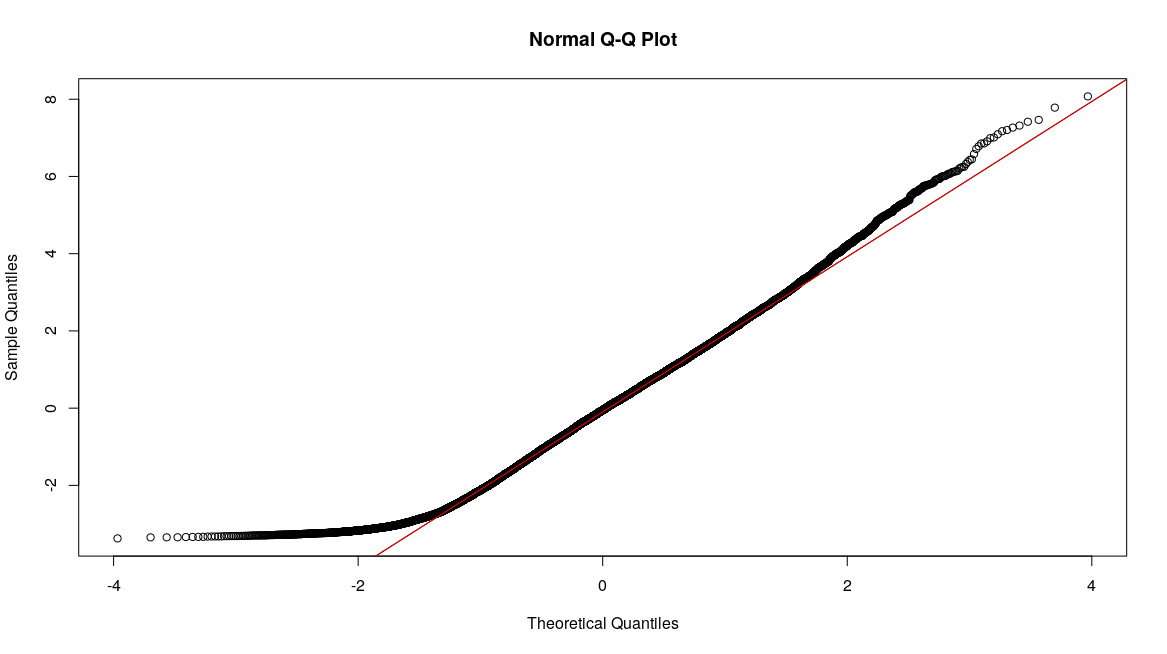
\includegraphics[width=\textwidth]{images/Rplot_rough_qq.png}
    \caption{QQ plot log2 transformed and mean centred gene expression fronal cortex all genes passing quality control 13787 genes}
    \label{fig:qqplot frontal cortex}
\end{figure}

The QQ plot of frontal cortex expression looks relatively normal (see figure~\ref{fig:qqplot frontal cortex}).

\begin{figure}
    \centering
    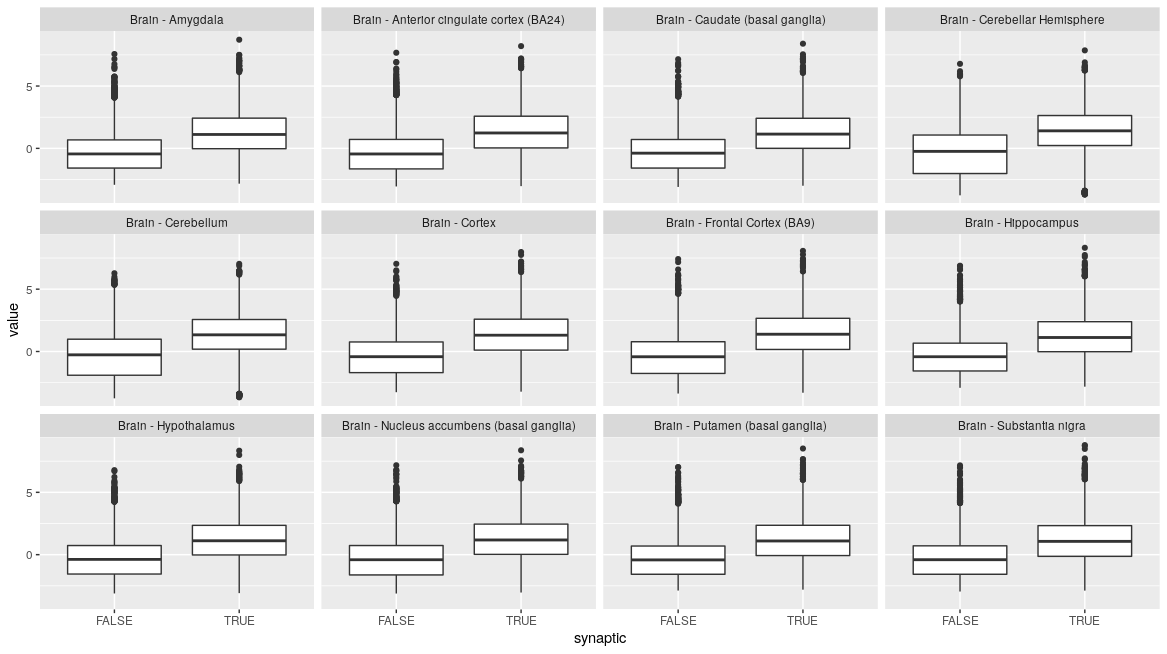
\includegraphics[width=\textwidth]{images/Rplot_compare_expression2.png}
    \caption{Box plot of log2 transformed and mean centred gene expression of PSP genes versus non PSP genes across 12 brain regions. p $< 2 \times 10^{-16}$ all comparisons. Wilcoxon test. True and False on x axis refer to whether genes are PSP in origin. Code at \url{source('~/RProjects/gtex/R/graph_gtex/multi_boxplot.R')}}
    \label{fig:my_label}
\end{figure}

\subsubsection{Results Brain Expression of PSP genes}
\label{sec:gtex_results}
3055 genes with GTEx data passing the above quality control were available for the PSP and 10732 non synaptic genes. 
Expression is significantly higher in the PSP genes across all 12 brain regions (spinal cervical1 has been removed as is known to be an outlier). There is strong correlation correlation between gene expression counts in all brain regions. Expression across brain regions was closely correlated as reported in  \cite{gtex2015genotype}( 
see table~\ref{Correlation between brain regions in expression of all genes in Gtex}).

There are methodological complexities about how expression is normalised and the practicability of comparing expression for single genes across tissues. The GTEx analysis is part of the overall quality control of the network and samples and tests for the violation of the assumption that ``these genes (PSP) are expressed in the CNS"". Other parts of this analyses are that the MAGMA studies are comparable with those published in the literature, the characterisation of missing synaptic genes from MAGMA and those not in the largest connected component, comparisons of MAGMA and PASCAL and over representation analysis across different methods. The results above however show that PSP genes are more expressed in the brain and that the expanded PSP continues to show increased CNS expression. 

An alternate way to address brain expression of these genes is that implemented in FUMA using GTEx v 8 data. This is to create a list of differentially expressed genes and see if a test set is over represented amongst these. Results for the complete PSP are shown in figure~\ref{fig:gtex all PSP}, the PSP and Consensus PSD are compared in figure~\ref{fig:deg_gtex_psp} and the expression in the PSP, Consensus PSD, Non PSP genes and those genes found in the PSP but not Consensus PSD are shown in figure~\ref{fig:compare all PSP gtex multipanel FUMA output}. 

% \paragraph{Summary of QC}
% MAGMA studies compare with summary data

% MAGMA GSA correlation between studies

% missing synaptic genes

% those not in LCC
% Welch Two Sample t-test Cortex 
% t = 46.441, df = 4558, p-value < 2.2e-16
% alternative hypothesis: true difference in means is not equal to 0
% 95 percent confidence interval:
%  1.663539 1.810180
% sample estimates:
%  mean of x  mean of y 
%  1.3519962 -0.3848629 
 
%  	Welch Two Sample t-test

% frontal cortex `Brain - Frontal Cortex (BA9)`
% t = 47.291, df = 4547.7, p-value < 2.2e-16
% alternative hypothesis: true difference in means is not equal to 0
% 95 percent confidence interval:
%  1.750205 1.901594
% sample estimates:
%  mean of x  mean of y 
%  1.4213062 -0.4045929 

\footnote{Code for heatmap at \url{source('~/RProjects/gtex_to_DICE/hclust_gtex.R')}
Conclusion: PSP genes are significantly more expressed in the brain. }
%\subsubsection{Correlation of genes across brain areas}
% latex table generated in R 3.6.3 by xtable 1.8-4 package
% Sat Mar  7 15:12:52 2020

%%
% \subsection{Comparison of expression in PSP and rest of genome}
% Only 19 PSP genes have not recorded expressi
\footnote{remove:on in the brain tissues of GTEx. 20998 genes of 46058 in the non synaptic have no expression. These however contain many non standard gene elements such as micro RNAs and other RNA components. A subset of genes was generated using as a filter the genes in the PSP and all genes that appear in all studies  \footnote{\textcolor{red}{may want to change this to any study and will need to change graph again}}. 1699 of 19244 non PSP genes had 0 count in brain cortex.}


% Median expression in PSP brain cortex was 21.85 and mean 100.07. The median in non PSP genes was 3.61 and mean 11.82 (see table~\ref{tab:Summary statistics for gene expression for PSP and non PSP genes}

% Mean expression in PSP genes brain cortex is higher than in non PSP. The data appear right skewed and do not appear normally distributed. T test 	Welch Two Sample t-test
% t = 3.3731, df = 3391.5. 95 percent confidence interval of difference in mean :36.96 -139.56, sample estimates:mean of PSP 100.07 mean of non PSP  11.82, p-value = 0.0007517

% A non parametric test Wilcoxon rank sum test with continuity correction W = 51340370, p-value $< 2.2 \times 10^{-16}$

% I also log 10 transformed the expression values for brain cortex and performed a t test to get an estimate of the difference in means. As there were a large number of values at 0 (which would have infinite log) is set these values log10 result to 0.

% 	Welch Two Sample t-test
% t = 60.809, df = 5310.4, alternative hypothesis: true difference in means is not equal to 0. 95 percent confidence interval: 0.826 - 0.881
% sample estimates:mean of PSP 1.288  mean of non PSP 0.434 , p-value $< 2.2 \times 10^{-16}$. 

% The distribution of log transformed median exp ression for cerebral cortex for PSP genes and non PSP genes included in the cohorts are shown in table~\ref{fig:all_gtex_panels}.\todo{ensure GTEx is correct ie check case throughout} \todo{Gene expression levels with centrality measures and across communities}
 
%  \textcolor{red}{want to do expression PSP compared with average expression in other tissues per Sniekers}

%  % latex table generated in R 3.6.3 by xtable 1.8-4 package
% % Sat Mar  7 17:12:57 2020
% \begin{table}[ht]
% \centering
% \begin{tabular}{lrrrrrrr}
%   \hline
% group & n & Min. & 1st Qu. & Median & Mean & 3rd Qu. & Max. \\ 
%   \hline
% PSP & 3392 & 0 & 8.43 & 21.85 & 100.07 & 55.87 & 62949.60 \\ 
%   non PSP genes & \textcolor{red}{138980} & 0 & 0.38 & 3.61 & 11.82 & 12.10 & 1288.95 \\ 
%   \hline
% \end{tabular}
% \caption{Summary statistics for gene expression for PSP and non PSP genes calculated from GTEx project data. Expression is median normalised by TPM.}
% \label{tab:Summary statistics for gene expression for PSP and non PSP genes}
% \end{table}


%     See figure~\ref{fig:all_gtex_panels} for a graphical comparison of expression of PSP and non PSP genes in the cortex. \footnote{code \url{source('~/RProjects/gtex/R/graph_gtex/histogram_boxplot.R')} } \footnote{code using only genes in study and removing synaptic and rest of genome duplicates \url{source('~/RProjects/gtex/R/graph_gtex/graphs_study_genes.R')} }. Table~\ref{tab:Summary statistics for gene expression for PSP and non PSP genes} shows gene expression for PSPS and non PSP genes \footnote{\url{source('~/RProjects/gtex/R/graph_gtex/graphs_study_genes.R')}}
    
%   \todo{the non PSP genes number cant be right in table \ref{tab:Summary statistics for gene expression for PSP and non PSP genes}}
    
% \begin{figure}
%     \centering
%     \begin{subfigure}[t]{0.45\textwidth}
%         \centering
%         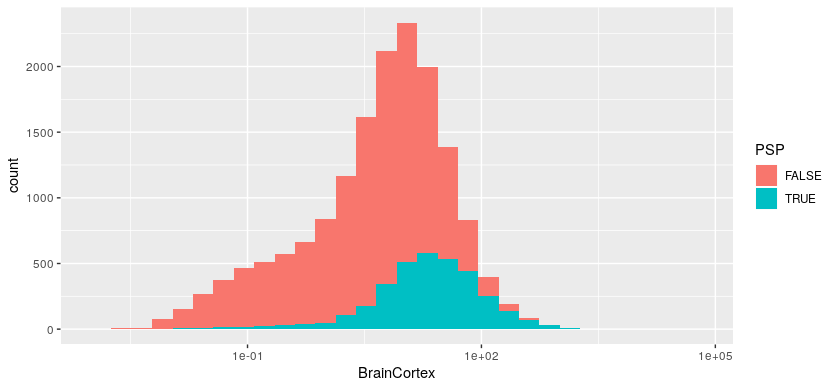
\includegraphics[width=\linewidth]{images/Rplot_corrected_gtex_histogram_log.png} 
%         \caption{Histogram of expression PSP and non PSP. Log10 scale} \label{fig:gtex_histogram_log}
%     \end{subfigure}
%     \hfill
%     \begin{subfigure}[t]{0.45\textwidth}
%         \centering
%         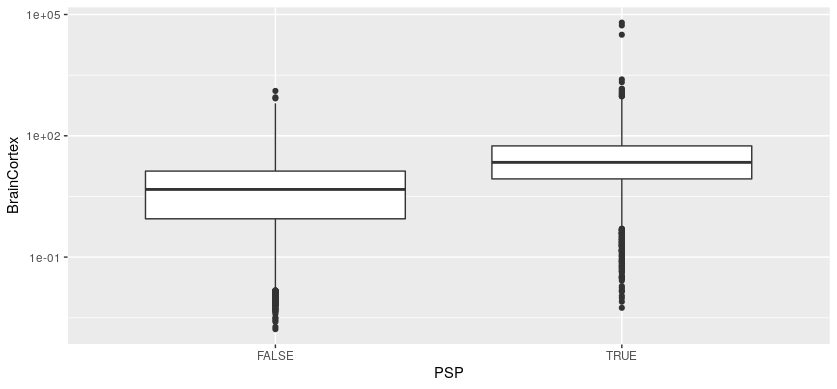
\includegraphics[width=\linewidth]{images/Rplot_corrected_gtex_boxplot_log10.png} 
%         \caption{Gtex expression boxplot PSP against not PSP. Log10 scale} \label{fig:gtex_log_boxplot}
%     \end{subfigure}
%     \caption{Plots of GTEx expression \textcolor{red}{may want to do this in subfigure packages rather than subcaption to line up edges and tidy up images in ggplot}}
%     \label{fig:all_gtex_panels}
% \end{figure}
\subsubsection{Correlation of GTEx expression across brain}

Table~\ref{tab:Correlation of PSP gene expression across brain regions. Expression values $log_2$ transformed with pseudocount of 1} shows correlation of expression of PSP genes between brain regions. Pearson product moment correlation. Anterior cingulate cortex (mean correlation 0.94) was the most correlated brain region and cerebellum the least (mean correlation 0.85). Minimum pairwise correlation cerebellar hemisphere and substantia nigra (0.792) max\footnote{code at \url{source('~/RProjects/gtex/R/graph_gtex/gtex_correlation_table.R')}} Highest (non identical) correlation caudate and putamen 0.996 (both basal ganglia). For all regions non identical  1st Quartile 0.839, Median 0.948, Mean 0.914, 3rd Quartile 0.9680, Max = 0.996).

PSP gene expression is correlated and lowest correlations are found in the cerebellar hemisphere as reported by Mele \cite{mele2015human} suggesting that the PSP group is a not markedly different from CNS expressed genes overall. \todo{paraphrase}

Expression for genes in the PSP but not in the consensus PSD used by Hill et al\cite{hill2014human} n=1323 \todo{Ref to Bayes SG paper although link to set in G2C is broken} is increased compared to the rest of the genome including the consensus genes. The consensus genes are more highly expressed than the PSP genes not in the consensus set but the effect is much more modest (see supplementary tables)\footnote{\url{source('~/RProjects/gtex/R/graph_gtex/gtex_correlation_table_hPSD_too.R')}}.

% latex table generated in R 3.6.3 by xtable 1.8-4 package
% Sat Aug  8 07:51:39 2020source('~/RProjects/paper_xls_output/R/chapter_2/FUMA/edit_gene_table/EA2_FUMA2clipboard.R')


\begin{table}[ht]
\centering
\begin{adjustbox}{width=\textwidth}

\begin{tabular}{lrrrrrrrrrrrr}
  \hline
 &   Amy &   ACC &   Cau &   Ce H &   Cer &   Cor &   FC  &   Hip &   Hyp &   NA &   Put &  SN \\ 
  \hline
  Amygdala & 1.00 & 0.98 & 0.97 & 0.80 & 0.81 & 0.96 & 0.95 & 0.99 & 0.97 & 0.97 & 0.97 & 0.95 \\ 
    Anterior cingulate cortex  & 0.98 & 1.00 & 0.96 & 0.83 & 0.83 & 0.99 & 0.99 & 0.97 & 0.96 & 0.97 & 0.95 & 0.91 \\ 
    Caudate$^*$ & 0.97 & 0.96 & 1.00 & 0.80 & 0.81 & 0.95 & 0.94 & 0.97 & 0.95 & 0.99 & 1.00 & 0.93 \\ 
    Cerebellar Hemisphere & 0.80 & 0.83 & 0.80 & 1.00 & 0.99 & 0.84 & 0.84 & 0.81 & 0.83 & 0.81 & 0.79 & 0.78 \\ 
    Cerebellum & 0.81 & 0.83 & 0.81 & 0.99 & 1.00 & 0.86 & 0.84 & 0.82 & 0.84 & 0.82 & 0.80 & 0.79 \\ 
    Cortex & 0.96 & 0.99 & 0.95 & 0.84 & 0.86 & 1.00 & 0.99 & 0.96 & 0.93 & 0.95 & 0.94 & 0.88 \\ 
    Frontal Cortex  & 0.95 & 0.99 & 0.94 & 0.84 & 0.84 & 0.99 & 1.00 & 0.95 & 0.94 & 0.95 & 0.93 & 0.88 \\ 
    Hippocampus & 0.99 & 0.97 & 0.97 & 0.81 & 0.82 & 0.96 & 0.95 & 1.00 & 0.97 & 0.96 & 0.97 & 0.95 \\ 
    Hypothalamus & 0.97 & 0.96 & 0.95 & 0.83 & 0.84 & 0.93 & 0.94 & 0.97 & 1.00 & 0.95 & 0.95 & 0.97 \\ 
    Nucleus accumbens$^*$ & 0.97 & 0.97 & 0.99 & 0.81 & 0.82 & 0.95 & 0.95 & 0.96 & 0.95 & 1.00 & 0.98 & 0.91 \\ 
    Putamen$^*$  & 0.97 & 0.95 & 1.00 & 0.79 & 0.80 & 0.94 & 0.93 & 0.97 & 0.95 & 0.98 & 1.00 & 0.94 \\ 
     Substantia nigra & 0.95 & 0.91 & 0.93 & 0.78 & 0.79 & 0.88 & 0.88 & 0.95 & 0.97 & 0.91 & 0.94 & 1.00 \\ 
   \hline
\end{tabular}
\end{adjustbox}
\caption[Correlation of PSP gene expression across brain regions]{Correlation of PSP gene expression across brain regions. Expression values $log_2$ transformed with pseudocount of 1. n=3055 genes passing quality control. *=basal ganglia. Frontal cortex = Brain area 9, Anterior cingulate cortex = 24.}
\label{tab:Correlation of PSP gene expression across brain regions. Expression values $log_2$ transformed with pseudocount of 1}
\end{table}




\section{Genome Wide Association Studies}

Previous network analyses have shown that synaptic topological models are differentially enriched for disease and gene ontology terms. There is also evidence that central nodes may be more likely to be disease nodes. These analyses have not however made use of the complex polygenetic signal available in genome wide association studies. Chapter 1 introduced the reasons for using intelligence as a phenotype.

To test the association between synaptic proteome network properties and structures and population genetic variation associated with intelligence we will need to calculate a statistic measuring the association of genetic variants with the phenotype for each gene that is represented by a node in the network. These values will be calculated using MAGMA in four samples, two of intelligence and two of educational attainment.\cite{de2015magma}
\todo[inline]{?add diagram of cohorts}

\subsection{Cohorts}
\label{sec:cohorts from paper section}
%\textcolor{red}{from paper section}
To investigate whether topological communities are enriched with genetic variants associated with cognitive ability and educational attainment and to reduce type II \footnote{This will reduce the number of tests to those that are likely to be true. 
or in the see section} error I will use a discovery and replication cohort design (see section~\ref{sec:Study design topology based GSA} and figure~\ref{fig:study design community detection}.) 
For consistency I will refer throughout the text to the GWA study of genetic variants associated with intelligence in UK Biobank\cite{bycroft2018uk} as Intelligence\textsubscript{Discovery} and the Phase II Educational attainment GWA study conducted using UK Biobank as Education\textsubscript{Discovery}.

We refer to the meta-analytic GWAS of intelligence carried out by Sniekers et al. from the Complex Trait Genetics (CTG) lab as Intelligence\textsubscript{Replication} \cite{sniekers2017genome}.   The meta-analysis of GWA studies of educational attainment excluding UK Biobank and 23andMe by Okbay et al.\cite{okbay2016genome} (often called EA2 - Educational Attainment 2) is referred to as Education\textsubscript{Replication}. Details of the generation and composition of these samples are found in section~\ref{sec:samples from paper section}. 

Two further samples became available after the completion of the primary analysis. These are the largest intelligence and education cohorts to date \cite{savage2018genome}, \cite{lee2018gene} but overlap with the samples above. They will be used to check the findings from earlier sections in chapter~\ref{chap:checking our findings} section~\ref{sec:placeholder for incoming refs chapter 5}

\subsection{Samples}

\label{sec:samples from paper section}
The information in this section is taken from that prepared by Dr Hill for a manuscript we are preparing. Dr Hill calculated the $\chi^2$ estimates of heritability. I have repeated these calculations using LD hub\footnote{LD hub \url{http://ldsc.broadinstitute.org/ldhub/} code to prepare files for LD hub at \url{source('~/RProjects/format_hub/R/format_summary_hub.R')}} a web interface for LD score regression \cite{zheng2017ld}.

 The Intelligence\textsubscript{Discovery} sample was formed using the ‘fluid’ cognitive test from UK Biobank; we shall refer to it as verbal-numerical reasoning (VNR). The VNR test contains 13 multiple choice items, six of which are verbal with the remaining seven being numerical in nature. Each individual’s VNR score was the sum of correct responses attained within a two-minute time period. This test has a large genetic correlation with intelligence scores derived from psycho-metrically validated cognitive tests \cite{hill2019combined}. A total of 120 934 participants (mean $\chi^2$=1.52) were available for analysis who did not contribute data to the Intelligence\textsubscript{Replication}\cite{sniekers2017genome} data set. A full description of how data from these participants was analysed can be found in Hill et al. \cite{hill2019combined}. 
 
UK Biobank was also used as the Education\textsubscript{Discovery} sample. Summary statistics were taken from Hill et al. on 273 274 participants (mean  $\chi^2$= 1.67).\footnote{redone by me  $\chi^2$=1.6684 see full results in errata folder verbatim for output} \cite{hill2019combined}  Education was defined as a binary choice of whether or not the individual had a University/College degree. A full description of how these data were analysed can be found in Hill et al. \cite{hill2019combined}.

The Intelligence\textsubscript{Replication} data set was formed using summary statistics obtained from the Sniekers et al. GWAS meta-analysis of intelligence (n = 78 308, mean $\chi^2$= 1.30).  \cite{sniekers2017genome}  An Education\textsubscript{Replication} data set was formed using summary GWAS data based on the the GWAS meta-analysis by Okbay et al (n = 217 569, mean $\chi^2$= 1.43) with UK Biobank participants excluded. \cite{okbay2016genome}. The summary statistics with UK Biobank removed were kindly provided by Dr Okbay and colleagues who generated the new summary statistics.    (See tables~\ref{tab:supplementary dh table 1 datasets} and \ref{tab:supplementary LD regression hill}). 
%\todo[inline]{convert these tables to latex DONE}
For genotype, meta-analysis methods and association analyses see the publications reporting the original GWAS\cite{sniekers2017genome}\cite{okbay2016genome}\cite{hill2019combined}.

%\textcolor{red}{end from paper section} \todo{add the calculation of chi sq for these studies was performed by Dr Hill in the course of preparation of a manuscript based on the community detection results}

%textcolor{red}{this is done using LD regression from LD hub repeat this yourself}
\todo{LD hub regression available at Broad sign in using google I have used grantsynch ref for LD hub in extras}

 

\todo{add the LD hub acknowledgements file to the acknowledgements: it is verbatim word formatted - in file verbatim.tex in folder errata}



\subsection{MAGMA Gene level statistics: Validation}
\label{sec:MAGMA Gene level statistics validation from other studies}

To ensure the accuracy of the gene level significance statistic I compared the gene level scores obtained using MAGMA to those reported in available studies\cite{de2015magma}. Potential sources of variation or bias include variations in command line options for software such as MAGMA,  different calculation of gene scores for raw genotype and summary data (see section~\ref{sec:MAGMA_gene_scores}) and different software versions, different reference populations to account for LD and variation in low level libraries across platforms\footnote{and there is the issue about performance across platforms}.\cite{kim2018experimenting} There were no published papers available containing a MAGMA gene-level analysis of the Intelligence\textsubscript{Discovery} sample or Education\textsubscript{Discovery}.\footnote{see discussion on benchmarking} 


The study by Okbay et al. (EA2)\cite{okbay2016genome}, providing the Education\textsubscript{Replication} sample did not report MAGMA gene scores, and differs from the Education\textsubscript{Replication} sample by including UK Biobank Educational attainment data. The only published reports of MAGMA gene scores from the exact discovery and replication samples was, therefore, the Intelligence\textsubscript{Discovery} sample \cite{sniekers2017genome}\footnote{no magma version in MS or supplemental online} \footnote{(supplementary table 8 at \url{https://static-content.springer.com/esm/art\%3A10.1038\%2Fng.3869/MediaObjects/41588_2017_BFng3869_MOESM2_ESM.xlsx})}.

We have, however, had access to the MTAG (Multi-trait analysis of Genome-Wide Summary data) summary data from the paper published by Hill, which contained MAGMA gene scores although it does contain data derived from educational attainment data so is not identical with the Intelligence\textsubscript{Discovery} sample\todo{need to check with David if it is ok to use this data it is for qc}. \footnote{no magma version in MS, none in supplementary material}\footnote{ sheet 5 at \url{https://static-content.springer.com/esm/art\%3A10.1038\%2Fs41380-017-0001-5/MediaObjects/41380_2017_1_MOESM2_ESM.xlsx}}\cite{hill2019combined}. One
can obtain a subset of the UK Biobank Education data which reports MAGMA scores for the top scoring 95 genes in the study by Davies et al. 2016 \cite{davies2016genome} \footnote{the MAGMA results for the top 95 genes are reported in the first sheet in Supplementary table 3A \url{https://static-content.springer.com/esm/art\%3A10.1038\%2Fmp.2016.45/MediaObjects/41380_2016_BFmp201645_MOESM506_ESM.xls}}. The MAGMA version is not recorded. Phase 1, release 3 of 1000 Genomes was used (in contrast to phase 3 for present study.\todo{ask Douglas should we store these and have a data provenance subchapter}. Finally  summary data has recently been made available from the current largest GWAS of intelligence to date by Savage et al. \cite{savage2018genome} ($n=269 867$) this reports MAGMA Gene level analysis results although only for significant genes\todo{check} \footnote{ (table S15 in supplementary materials at \url{https://www.ncbi.nlm.nih.gov/pmc/articles/PMC6411041/bin/NIHMS1006639-supplement-Supplementary_Tables.xlsx})}.

The pairwise correlation between the gene scores reported in these studies and the results I calculated using MAGMA and their summary statistics  are shown in table~\ref{tab:Correlation between MAGMA gene scores obtained from summary statistics and those published in supplementary material to papers}. Magma 1.06b for MacOS was used with 1000 Genomes Phase 3 data to account for linkage disequilibrium. NCBI 37 was used for gene boundaries.\todo{? remove the Davies one was only 93 genes and older now}\todo{codepath} Summary GWAS statistics were used to calculate gene scores using default settings. No gene window was used.\footnote{they used one in savage but only 5kB}

\begin{table}[ht]
    \centering
    
    \begin{tabular}{llllllll}
    \toprule
        Study & n & t & df & p & Pearson & CI   \\
        \midrule
       Savage \cite{savage2018genome} & 269687 & 122.26& 352  & $<2.2 \times 10^{-16}$ & 0.99 & 0.986-0.991  \\ 
       Hill \cite{hill2019combined} & 248482 & 368.27 & 17475 & $<2.2 \times 10^{-16}$& 0.94 & 0.939-0.942 \\
       Davies (2016) \cite{davies2016genome} & 112151 & 22.08 & 93 & $<2.2 \times 10^{-16}$ & 0.92 & 0.88-0.94\\
       Sniekers \cite{sniekers2017genome}& 78308 & 466.41 & 18246 & $<2.2 \times 10^{-16}$ & 0.96 & 0.959-0.962\\
       \bottomrule
    \end{tabular}
    \caption{Correlation between MAGMA gene scores obtained from summary statistics and those published in supplementary material to papers.}
    \label{tab:Correlation between MAGMA gene scores obtained from summary statistics and those published in supplementary material to papers}
\end{table}

\subsubsection{Results}
The correlation coefficient varied in the range 0.92-0.99 despite slight differences in software version, gene windows and the potential use of genotyped versus summary data. I conclude that apart from small variants that there is no systematic inaccuracy in the calculation of MAGMA gene scores using the plaform and pipeline. 

The MAGMA versions were not documented in Sniekers et al., Davies et al or Hill et al. \cite{davies2016genome} or \cite{sniekers2017genome} \cite{hill2019combined}. 1000 Genomes phase 1 data was used in Davies et al.\cite{davies2016genome}. 

\subsection{Synaptic genes omitted from NCBI 37}
\todo[inline]{should this be earlier}
The studies from which we obtained summary statistics used NCBI 37 to provide gene boundaries in MAGMA. Seventeen of the PSP genes were not in the reference NCBI 37 boundaries text file supplied with MAGMA used to assign SNPs to genes in MAGMA. Files containing NCBI 36,37 and 38 boundaries are supplied on the MAGMA project website,  5 of the genes not in the NCBI37 file have boundaries defined in the NCBI 38 and are shown in table~\ref{tab:Synaptic PSP genes  found in NCBI 38 but not in 37 listing included with MAGMA}\footnote{code \url{source('~/RProjects/annotations_phd/R/missing_NCBI_genes.R')}}.

10 genes are found in neither the NCBI 37 nor the NCBI 38 gene boundary files but are annotated in the\textit{ homo sapiens} gene info download in Entrez Gene at the NCBI\footnote{Link at \url{https://ftp.ncbi.nih.gov/gene/DATA/GENE_INFO/Mammalia/Homo_sapiens.gene_info.gz} }\todo{date of file}. The annotations of the 10 synaptic genes (not in the NCBI 38 file included with MAGMA) but present in NCBI Entrez Gene info\footnote{\url{ftp://ftp.ncbi.nih.gov/gene/}} are shown in table~\ref{tab:10 synaptic genes not in NCBI 38 included with MAGMA but present in entrez gene gene info}.

Two pseudo genes were identified using the ToppGene API\cite{chen2009toppgene}: Entrez id:	441400, RAB1C, member RAS oncogene family pseudogene UniProt Q92928 Protein transport. Probably involved in vesicular traffic (By similarity); Entrez id:	440915	,POTEKP\footnote{POTE expressed in Prostate ovary testis and placenta}, POTE ankyrin domain family member K, pseudogene \cite{bera2002pote} Uniprot Putative beta-actin-like protein 3 Q9BYX7. 


Gene ontology enrichment analysis using ToppFun (part of the ToppGene suite) (see section~\ref{sec:ToppGene GO erncihement}) did not find any phenotype or ontology suggestive of being associated with cognition in particular no human or murine phenotype (GO:0034987	immunoglobulin receptor binding 	p Bonferroni $6.224\times10^{-9}$	6 terms, 	GO:0097478	leaflet of membrane bilayer	Bonferroni p	$1.296\times10^{-3}$	6	terms. The only potentially concerning term is 23380,	SRGAP2	SLIT-ROBO Rho GTPase activating protein 2 which is associated with the cellular component dendritic spine head GO:0044327 and associated with neural morphogenesis\cite{guerrier2009f}. The gene list was also analysed using the Gene2Func interface in FUMA \cite{watanabe2017functional} (see section~\ref{sec:FUMA go enrichment}). In particular there were no enriched gene sets and no hits in GWAS catalog\footnote{sic}\cite{welter2014nhgri}.

 While it would be possible to make a custom annotation file for these genes this would complicate our analysis and cause it to differ methodologically from other analyses reporting gene level statistics in MAGMA.  \footnote{note to Douglas: i am probably not explaining this well but what I am trying to say is that they don't look important, it makes our analysis different from anybody elses and there is also a where do you stop problem and also you could argue a need for further correction for multiple testing if you are modifying standard testing procedures Reporting it may seem a bit over the top but it is part of the QC we have done - comparing magma to vegas, magma to pascal, two gsa methods, two gene score methods, compare significant genes for any commonalities}  
% latex table generated in R 3.6.1 by xtable 1.8-4 package
% Wed Feb 19 14:14:05 2020
% latex table generated in R 3.6.1 by xtable 1.8-4 package
% Wed Feb 19 14:15:51 2020
\begin{table}[ht]
\centering
\begin{adjustbox}{max width=\textwidth}
\begin{tabular}{cclll}
  \hline
 Gene ID & Symbol & chromosome & type of gene & Full name from nomenclature authority \\ 
  \hline
1804 & DPP6 & 7 & protein-coding & dipeptidyl peptidase like 6 \\ 
  3635 & INPP5D & 2 & protein-coding & inositol polyphosphate-5-phosphatase D \\ 
  3800 & KIF5C & 2 & protein-coding & kinesin family member 5C \\ 
  9554 & SEC22B & 1 & protein-coding & SEC22 homolog B, vesicle trafficking protein (gene/pseudogene) \\ 
  23380 & SRGAP2 & 1 & protein-coding & SLIT-ROBO Rho GTPase activating protein 2 \\ 
   \hline
\end{tabular}
\end{adjustbox}
\caption[Synaptic PSP genes with boundaries found only in NCBI 38]{Synaptic PSP genes  found in NCBI 38 gene boundary file supplied with MAGMA but not in NCBI 37 file. Gene ID = Entrez Gene Gene ID.}
\label{tab:Synaptic PSP genes  found in NCBI 38 but not in 37 listing included with MAGMA}
\end{table}
   


\begin{table}[ht]
\centering
\begin{adjustbox}{max width=\textwidth}
\begin{tabular}{clcll}
  \hline
 Gene ID & Symbol & chromosome & type of gene & Full name from nomenclature authority \\ 
  \hline
293 & SLC25A6 & X$|$Y & protein-coding & solute carrier family 25 member 6 \\ 
  3493 & IGHA1 & 14 & other & immunoglobulin heavy constant alpha 1 \\ 
  3500 & IGHG1 & 14 & other & immunoglobulin heavy constant gamma 1 (G1m marker) \\ 
  3502 & IGHG3 & 14 & other & immunoglobulin heavy constant gamma 3 (G3m marker) \\ 
  3503 & IGHG4 & 14 & other & immunoglobulin heavy constant gamma 4 (G4m marker) \\ 
  3507 & IGHM & 14 & other & immunoglobulin heavy constant mu \\ 
  3514 & IGKC & 2 & other & immunoglobulin kappa constant \\ 
  4509 & ATP8 & MT & protein-coding & mitochondrially encoded ATP synthase 8 \\ 
  4513 & COX2 & MT & protein-coding & mitochondrially encoded cytochrome c oxidase II \\ 
  4538 & ND4 & MT & protein-coding & mitochondrially encoded NADH dehydrogenase 4 \\ 
   \hline
\end{tabular}
\end{adjustbox}
\caption[Synaptic genes not in NCBI boundary files in MAGMA]{10 synaptic genes not in NCBI gene boundary files (NCBI36,37,38) included with MAGMA but present in Entrez Gene Homo sapiens gene info files \url{https://ftp.ncbi.nih.gov/gene/DATA/GENE_INFO/Mammalia/Homo_sapiens.gene_info.gz}.  GeneID, NCBI Entrez Gene GeneID }
\label{tab:10 synaptic genes not in NCBI 38 included with MAGMA but present in entrez gene gene info}
\end{table}

\section{MAGMA gene level statistic methods}
\label{sec:MAGMA gene level methods}
MAGMA version 1.06 for MacOS was used with 1000 Genome European Ancestry Phase 3 data to account for linkage disequilibrium\footnote{\url{https://ctg.cncr.nl/software/MAGMA/ref_data/g1000_eur.zip}}1000 Genomes phase 3 data of European ancestry and NCBI 37 data provided on the MAGMA website \footnote{\url{https://ctg.cncr.nl/software/MAGMA/aux_files/NCBI37.3.zip}} was used to define gene boundaries. Output logs are included in the supplemental material.  Command line arguments were supplied using a bash shell script and default settings were used for summary GWAS statistic data (SNPwise sum). \footnote{these will be moving to github - this might be too much most papers just say what I have said above -  \url{/Users/grantrobertson/Programs/copy_paperMagma_draft-master/magma_script.sh}	}

Gene level statistics were calculated and no window was used around gene boundaries (see section~\ref{sec:Gene windows} below). In studies where the number of individuals tested per SNP was available in the summary data this was supplied as a command line argument - otherwise the overall sample size was used. SNPs that were analysed in less than 50 individuals were discarded (default setting). 

\subsubsection{Gene Windows}
\label{sec:Gene windows}
\todo[inline]{? comes before}
 In order to include gene regulatory elements in gene level analysis a number of ``windows"%WYN
around the gene boundary have been used, both symmetric and asymmetric. VEGAS \cite{liu2010versatile} used a set 50kB boundary and this is incorporated in studies that used this method (e.g Hill et al. (2014)\cite{hill2014human})

The use of a gene window significantly affects the number of SNPs assigned to genes.  Using the College Phenotype from Rietveld et al. \cite{rietveld2013gwas} and NCBI 37 gene boundaries 914887 SNPs were mapped to genes (39.45\% of 2319112 SNPs) using no window; with a 50kb window 1385602 (59.75\%) mapped to genes.\todo{? use other}
%WYN
The reported window sizes vary. Zhao and Nyholt \cite{zhao2017gene} in a study of gene level statistics across psychiatric disorders using the GATES method \cite{li2011gates}  used a 15kb window reasoning that 90\% \cite{pickrell2010understanding} of eQTL are found in this region. 

The predominant practice at present appears to be either not use a gene window or only to use a small one (for example 5kb as reported in Savage et al (2018. \cite{savage2018genome}). In the absence of a widely agreed upon window size I have not used one believing this to be the simplest and most conservative option\footnote{especially as this is in part a proof of concept analysis and I don't want to get tied up in arguments about why I used window size a or b see previous footnote}. 


\begin{table}[]
    \centering
   
    \begin{tabular}{l|llll}
\toprule
    &  Intelligence\textsubscript{Replication}   & Education\textsubscript{Replication} &
    Intelligence\textsubscript{Discovery} & Education\textsubscript{Discovery} \\
    \midrule
     Intelligence\textsubscript{Replication}    & & 0.249 &0.378  & 0.308 \\
     Education\textsubscript{Replication} &0.249 &&0.325&0.506 \\
     Intelligence\textsubscript{Discovery}&0.378 &0.325&&0.446 \\
     Education\textsubscript{Discovery}&0.308&0.506 &0.446 & \\
\bottomrule
    \end{tabular}
    \caption[Correlation of MAGMA GWGAS scores between samples]{Correlation of MAGMA GWGAS scores between samples. Pearson product moment correlation. p$<2.2\times10^{-16}$ all tests. Correlation is between $-log10(p)$ transformation of gene level p values. Cases where a gene score is present in one study and not another are ignored}
    \label{tab:correlation of MAGMA GWGAS scores}
\end{table}

\subsection{Correlation MAGMA GWGAS}
\todo[inline]{cant have this before introduction of cohorts}
Educational attainment and Intelligence are genetically correlated\cite{plomin2018new} (see table~\ref{tab:LD regression hill}). It is likely that gene level scores in samples between and within these phenotypes are also correlated although this should be less than the overall SNP correlation due to inter-genic SNPs and and loss of information in the aggregation of SNPs to genes. It is worthwhile checking that the value is not extreme or unexpected (for example higher between low powered samples with different phenotypes) as part of overall quality control. 


Correlation was calculated between the -log10 transform of gene level p values between samples using Pearsons product moment correlation test in R. Where a gene did not have a p value in a study this pairwise comparison was omitted. I have calculated MAGMA GWGAS gene level correlation rather than genetic correlation because we will be using MAGMA GWGAS statistics to make comparisons of the effect of central nodes across samples. The correlation is greatest between the two educational attainment samples (0.506; CI 0.495-0.516, t = 78.473, df = 17928, p-value $< 2.2 \times 10^{-16}$) (table~\ref{tab:correlation of MAGMA GWGAS scores}). For each sample other than Intelligence\textsubscript{Discovery} the correlation is highest with the matching phenotype and Intelligence\textsubscript{Replication} is still most highly correlated with Intelligence\textsubscript{Discovery}. The two discovery samples are similar in composition and the Intelligence\textsubscript{Replication} sample is likely to be the least power (lowest sample size, meta-analysis and lowest $\chi^2$ on testing heritability using LD score regression (section~\ref{sec:samples from paper section}). 
\footnote{REMOVE FINAL: Result details commented out search \%DETAILS in tex} \footnote{\url{source('~/RProjects/paper_xls_output/R/chapter_2/MAGMA/pairwise_gene_comparison.R')}}
%%%%% COMPARE DETAILS
% t = 34.404, df = 17937, p-value < 2.2e-16
% alternative hypothesis: true correlation is not equal to 0
% 95 percent confidence interval:
%  0.2350242 0.2624803
% sample estimates:
%       cor 
% 0.2488022 

% ed and ctg

% 	Pearson's product-moment correlation

% t = 43.632, df = 18158, p-value < 2.2e-16
% alternative hypothesis: true correlation is not equal to 0
% 95 percent confidence interval:
%  0.2948248 0.3211538
% sample estimates:
%       cor 
% 0.3080483 


% 	Pearson's product-moment correlation

% ukbb int and ctg
% t = 55.029, df = 18158, p-value < 2.2e-16
% alternative hypothesis: true correlation is not equal to 0
% 95 percent confidence interval:
%  0.3655291 0.3904609
% sample estimates:
%       cor 
% 0.3780636 

% 	Pearson's product-moment correlation

% ukbbed and ctg
% t = 43.632, df = 18158, p-value < 2.2e-16
% alternative hypothesis: true correlation is not equal to 0
% 95 percent confidence interval:
%  0.2948248 0.3211538
% sample estimates:
%       cor 
% 0.3080483 


% ukbbint and ea2
% 	Pearson's product-moment correlation

% 	Pearson's product-moment correlation

% t = 46.068, df = 17928, p-value < 2.2e-16
% alternative hypothesis: true correlation is not equal to 0
% 95 percent confidence interval:
%  0.3121876 0.3383644
% sample estimates:
%       cor 
% 0.3253383  
% 	Pearson's product-moment correlation
% ed and ea2

% t = 78.473, df = 17928, p-value < 2.2e-16
% alternative hypothesis: true correlation is not equal to 0
% 95 percent confidence interval:
%  0.4946612 0.5164525
% sample estimates:
%       cor 
% 0.5056375 

% 	Pearson's product-moment correlation

% ed and int  
% t = 67.416, df = 18285, p-value < 2.2e-16
% alternative hypothesis: true correlation is not equal to 0
% 95 percent confidence interval:
%  0.4344972 0.4577150
% sample estimates:
%       cor 
% 0.4461812 

\begin{table}[]
    \centering
    \begin{tabular}{lllll}
    \toprule
        Phenotype & n & mean $\chi^2$ & LD intercept (SE) & Reference \\
        \midrule
        Intelligence & 78308 & 1.30 & 1.02(0.01) & Sniekers et al.(2017)\cite{sniekers2017genome}\\
        &120934 & 1.53 & 1.02 (0.01)& NA\\
        \\
        Education&273274 & 1.67 & 1.042(0.01) & NA\\
         & 217569&1.43&1.02(0.01) & Okbay et al.(2016)\cite{okbay2016genome}\\
         \bottomrule
    \end{tabular}
    \caption[Summary for each data set]{References and heritability of each data set. Table adapted from table generated by W.D Hill for publication. Calculations and arrangement are work of Dr W.D. Hill}
    \label{tab:supplementary dh table 1 datasets}
\end{table}



\begin{table}[]
    \centering
    \begin{tabular}{l|lllll}
    \toprule
       Phenotype & Samples & Intelligence & & Education &    \\
       \midrule
         & & Hill & Sniekers & Okbay & Hill\\
         \midrule
         Intelligence & Hill & 21.19\%(0.91\%) & & & \\
         & Sniekers & 0.99(0.02) & 19.45\%(1.09) & & \\
         \\
         Education & Okbay & 0.62(0.03) & 0.75(0.02) & 9.78(0.44\%) &\\
         & Hill & 0.66(0.02) & 0.72(0.02) & 0.96(0.02)&11.67\%(0.91\%)\\
         \bottomrule
    \end{tabular}
    \caption[Heritability of samples]{Using LD score regression heritability within, and genetic correlations between, each of the data sets used is shown. Heritability on the observed scale is shown on the diagonal and genetic correlations are shown on the off diagonal with standard error in brackets. Table contents and caption from WD Hill. }
    \label{tab:supplementary LD regression hill}
\end{table}
\subsection{Intelligence\textsubscript{Replication} GWGAS}
\label{sec:Intelligence Replication GWGAS}

\subsubsection{Methods}
The Intelligence\textsubscript{Replication} sample is identical to the individuals in the 2017 ``Intelligence wave 1" meta-analysis study by Sniekers et al. \cite{sniekers2017genome} (see table~\ref{tab:supplementary dh table 1 datasets}. 

GWAS summary data were downloaded from the Complex Trait Genomics (CTG) lab\footnote{ \url{https://ctg.cncr.nl/documents/p1651/sumstats.txt.gz}}. This meta-analysis of 78,308 individuals was derived from 13 cohorts. 29,610 individuals were reported for the first time. UK Biobank participants had either taken a web based test ($n=17852$, raw genotype data used, reported for first time) or touch screen test ($n=35257$). 12441 participants were from the CHIC consortium used to produce an GWAS of childhood intelligence\cite{benyamin2014childhood}. 5 additional cohorts contributed $n=11 749$ participants. The individuals making up this meta-analysis do not contribute to any of the other three samples used in this thesis: individuals from UK Biobank were excluded from the Intelligence\textsubscript{Discovery} sample summary statistics provided by Dr Hill\footnote{see contributors/acknowledgments}. The authors report finding 47 genome wide significant genes using MAGMA to perform a Genome Wide Gene Association (GWGAS)\cite{sniekers2017genome},\cite{de2015magma}.

Gene level scores were calculated using MAGMA v1.6b (Mac OS)(section~\ref{sec:MAGMA gene level methods}) \footnote{Code to produce the following tables is at \url{source('~/RProjects/paper_xls_output/R/0_write_MAGMA_gene_level_results_PhD.R')} }. The number of individuals tested for each SNP was available and used for sample size. The European panel of the 1000 Genomes Phase 3 was used to account for linkage disequilibrium
 updated 19/09/2018 downloaded from CTG MAGMA website \footnote{\url{https://ctg.cncr.nl/software/magma}}. SNPs were assigned to genes using NCBI37.3 Gene Boundaries from the CTG website.  No window was used around gene boundaries. Default options for summary stastics were used (SNPwise). For all subsequent GWGAS performed using MAGMA methods are identical unless otherwise stated. 
% Welcome to MAGMA v1.06b (mac)

% Using flags:
%         --bfile g1000_eur
%         --gene-annot ./annotations/annotated_bim.genes.annot
%         --pval /Users/grantrobertson/Programs/GWAS_studydata/sumstats.txt use=3,11 ncol=6
%         --out ./gene_results/ctg

% Start time is 11:28:37, Wednesday 12 Sep 2018

% Loading PLINK-format data... 
% Reading file g1000_eur.fam... 503 individuals read
% Reading file g1000_eur.bim... 22665064 SNPs read
% Preparing file g1000_eur.bed... 

% Reading SNP synonyms from file g1000_eur.synonyms (auto-detected)
%         read 5966573 synonyms from file mapping to 3894269 SNPs in the data
%         WARNING: detected 102 synonymous SNP pairs in the data
%                  skipped all synonym entries involved, synonymous SNPs are kept in analysis
%                  writing list of detected synonyms in data to supp lementary log file
% Reading SNP p-values from file /Users/grantrobertson/Programs/GWAS_studydata/sumstats.txt... 
%         detected 12 variables in file
%         using variable: rsid (SNP id)
%         using variable: p_value (p-value)
%         using variable: N (sample size; discarding SNPs with N < 50)
%         read 12104295 lines from file, containing valid SNP p-values for 10674310 SNPs in data (88.19% of lines, 47.1% of SNPs in data)
%         WARNING: file contained 3 duplicate SNPs (same IDs or synonyms)
%                  dropped all occurrences of each from analysis
%                  writing list of duplicated IDs to supplementary log file
% Filtering phenotype/covariate missing values... 503 individuals remaining

% Loading gene annotation from file ./annotations/annotated_bim.genes.annot... 
%         19248 gene definitions read from file
%         found 18262 genes containing SNPs in genotype data

% Starting gene analysis... 
%         using model: SNPwise-sum

%         writing gene analysis results to file ./gene_results/ctg.genes.out
%         writing intermediate output to file ./gene_results/ctg.genes.raw


% End time is 11:40:04, Wednesday 12 Sep 2018 (elapsed: 00:11:27)


\subsubsection{Results}
18262\footnote{19427 genes in NCBI 37} genes were assigned gene level p values using MAGMA v1.06.
The Bonferroni correction for multiple comparisons was used to calculate a genome wide significance level ($\alpha$ = 0.05/18262; p=$2.74 \times 10^{-06}$). 47 genes achieved genome wide significance using the adjusted $\alpha$ level using MAGMA GWGAS (Genome Wide Gene Association Study) using the summary statistics provided. This is identical to the number reported by Sniekers et al. \cite{sniekers2017genome}. 16 of these were found in the PSP (34.0\%)  (table~\ref{tab:significant genes}).\footnote{Code for Gene level statistics at \url{source('~/RProjects/paper_xls_output/R/0_write_MAGMA_gene_level_results.R')}}. \footnote{Only 7 significant genes were found in the 1312 gene consensus PSD network graph\cite{mclean2016improved}}. 

All significant genes are shown in table \ref{tab:Significant genes in ctg MAGMA GWAS} and significant synaptic genes are shown in table~\ref{tab:Significant synaptic genes in ctg MAGMA GWAS2} \footnote{Remove: tables complete on full compile}.

\begin{table}[ht]
    \centering
    \begin{tabular}{cccc}
    \toprule
         Study & n significant synaptic genes & n  significant genes & percent (\%) in PSP \\
      \midrule  
         Intelligence\textsubscript{Replication}\cite{sniekers2017genome} & 16 (7) & 47 & 34.0 \\
         Education\textsubscript{Replication}\cite{okbay2016genome} & 25(12) & 99 & 25.2 \\
         Intelligence\textsubscript{Discovery}\cite{hill2019combined} & 51 (17) & 196 & 26.0\\
         Education\textsubscript{Discovery}\cite{hill2019combined} & 58 (27) & 235 & 24.7\\
         \bottomrule
    \end{tabular}
    
    \caption[Number of Genome wide significant genes and number of genes in PSP at GWGAS in Intelligence and Educational Attainment samples]{Number of genome wide significant genes (using Bonferroni correction of 0.05/$n$ genes)   using MAGMA Genome Wide Gene Association Analysis Study (GWGAS) for Educational attainment and Intelligence discovery and replication samples. The references in the study column refer to the publication from which the majority of the sample are taken. Code to add core at \url{source('~/RProjects/paper_xls_output/R/chapter_2/exploratory_data_analysis_core_PSD.R')}. Number in parenthesis are number of significant genes in 1312 gene consensus hPSD.}
    \label{tab:significant genes}
\end{table}

% latex table generated in R 3.6.2 by xtable 1.8-4 package
% Thu Jan  2 13:21:27 2020

% latex table generated in R 3.6.1 by xtable 1.8-4 package
% Wed Feb 19 11:25:28 2020
\begin{table}[ht]
\centering
\begin{tabular}{llcrrc}
  \hline
 GeneID & Symbol & chromosome & $n$ SNPs & Z statistic & $p$ \\ 
  \hline
1434 & CSE1L &  20 & 176 & 5.96 & $1.26 \times 10^{-9}$ \\ 
  60412 & EXOC4 &   7 & 2184 & 5.88 & $1.99 \times 10^{-9}$ \\ 
  55964 & SEPT3 &  22 &  69 & 5.75 & $4.35 \times 10^{-9}$ \\ 
  6138 & RPL15 &   3 &  19 & 5.40 & $3.35 \times 10^{-8}$ \\ 
  23109 & DDN &  12 &   8 & 5.35 & $4.41 \times 10^{-8}$ \\ 
  85358 & SHANK3 &  22 & 199 & 5.31 & $5.49 \times 10^{-8}$ \\ 
  487 & ATP2A1 &  16 &  47 & 5.23 & $8.37 \times 10^{-8}$ \\ 
  11273 & ATXN2L &  16 &  36 & 5.17 & $1.17 \times 10^{-7}$ \\ 
  2870 & GRK6 &   5 &  39 & 5.07 & $2.03 \times 10^{-7}$ \\ 
  28512 & NKIRAS1 &   3 &  73 & 5.04 & $2.29 \times 10^{-7}$ \\ 
  4700 & NDUFA6 &  22 &  16 & 5.04 & $2.32 \times 10^{-7}$ \\ 
  
  4733 & DRG1 &  22 &  99 & 4.83 & $6.91 \times 10^{-7}$ \\ 
  10564 & ARFGEF2 &  20 & 406 & 4.80 & $7.83 \times 10^{-7}$ \\ 
  7284 & TUFM &  16 &   7 & 4.79 & $8.49 \times 10^{-7}$ \\ 
  553115 & PEF1 &   1 &  30 & 4.77 & $9.17 \times 10^{-7}$ \\ 
  8411 & EEA1 &  12 & 475 & 4.61 & $2.03 \times 10^{-6}$ \\ 
   \hline
\end{tabular}
\caption[Intelligence\textsubscript{Replication} Sample Genes in the PSP meeting genome wide significance levels for MAGMA GWGAS] { Intelligence\textsubscript{Replication} PSP synaptic Genes meeting genome wide significant at GWGAS using MAGMA for the Intelligence\textsubscript{Replication} sample. 16 genes are found in the PSP (34.0\%), Bonferroni corrected $\alpha=2.74 \times 10^{-06}$. $n$ SNPs = number of SNPs found within NCBI 37 
defined gene boundaries in sample. GeneID refers to Entrez Gene GeneID.} 
\label{tab:Significant synaptic genes in ctg MAGMA GWAS2}
\end{table}



\subsection{Education\textsubscript{Replication}  MAGMA GWGAS}
\label{sec:Edcuation replication gwgas}
\subsubsection{Methods}

The summary statistics for Education\textsubscript{Replication} are generated using individuals taken from the EA2 (Educational Attainment 2) meta-analytic GWA study of educational attainment\cite{okbay2016genome} with educational attainment defined as number of years of schooling completed.  The published study is of 293,723 individuals with 111,349 independent samples from UK Biobank used for out of sample replication \cite{sudlow2015uk}. A combined meta-analysis was carried out using the discovery and replication cohorts ($n$=405702) allowing an increase in the number of genome wide loci reported from 74 to 162. Due to Institutional Review Board (IRB) restrictions, which did not allow reporting of over 10,000 SNPs in the summary statistics for participants from 23andme, the summary statistics provided on the SSGAC website are of $n$=328917 individuals excluding 76155 individuals from 23andme\footnote{\url{http://ssgac.org/documents/EduYears_Main.txt.gz}}. The authors kindly made summary statistics available to us (see acknowledgements)\todo{cross ref to acknowledgements} excluding both 23andme and UK Biobank creating a sample that does not overlap with Education\textsubscript{Discovery}; $n$= 217568 (293723 - 76155 = 217568)\cite{okbay2016genome}.\footnote{See Okbay et al. supplemental information \url{http://ssgac.org/documents/SI_74_loci_educational_attainment.pdf} p 16} The summary statistics used were unsorted by sex. The modified summary statistics excluding UK Biobank and 23andMe  are deposited with the University of Edinburgh Research Data Service \footnote{https://www.ed.ac.uk/information-services/research-support/research-data-service}.
The number of individuals tested for each SNP was available and used. 20 duplicate SNPs were identified. 

\subsubsection{Results}



17942 genes were assigned a significance score using MAGMA 1.06 based on the SNP's present in the summary statistics.The Bonferroni correction for multiple comparisons was used to calculate a genome wide significance level ($\alpha$ = 0.05/17942; p=$2.79 \times 10^{-06}$). With this $\alpha$ level 99 genes were identified of genome wide significance. 25 (25.3\%) of these were found in the synaptic PSP (see table~\ref{tab:significant genes}).

Genome wide significant genes  are shown in table \ref{tab:Significant genes in EA2 MAGMA GWAS}, significant synaptic genes are shown in table \ref{tab:Significant synaptic genes in EA2  MAGMA GWAS}

% latex table generated in R 3.6.2 by xtable 1.8-4 package
% Thu Jan  2 13:31:54 2020






\subsection{Intelligence Discovery Phase II GWGAS}

\subsubsection{Methods}
The GWAS summary statistics for the Intelligence\textsubscript{Discovery} sample are taken from UK Biobank Phase II used as a part of an analysis by Hill et al.\cite{hill2019combined}. The authors used MTAG (Multi-Trait Analysis of GWAS) a technique that allows meta-analyses to increase their effective sample size using genetically related traits \cite{turley2018multi}. The published meta-analysis\cite{hill2019combined} combines the Intelligence\textsubscript{Replication} sample data \cite{sniekers2017genome} and UK Biobank Intelligence Phase II (Intelligence\textsubscript{Discovery} sample) combined with the genetically related educational attainment phenotype (the SSGAC EA2 study)\cite{okbay2016genome}. Summary GWAS statistics including only participants in UK Biobank Intelligence Phase II ($n$=120 934) were obtained from the Centre for Cognitive Ageing and Cognitive Epidemiology (CCACE) from the author Dr W.D. Hill.  A column is provided with the summary data of numbers tested per SNP but is constant and equal to the sample size and was used as the input for the GWGAS.      These subjects had taken the VNR test in UK Biobank which is closely related to intelligence \cite{hill2019combined}. For further details on the cohorts, genotyping and testing see Hill et al. \cite{hill2019combined}.


\subsubsection{Results}
18,287\footnote{ Was a to do - check as this is the same number as intelligence - i have checked and done diff on output logs they are different it may be they because they both came from David they used the same imputation and reported the same SNPs (they were done for the same study). The output otherwise is different} genes were assigned gene level statistics using MAGMA v1.06 to provide GWGAS.  With a Bonferroni $\alpha$ level of  $
2.73\times 10^{-06}$, 196\footnote{checked} genome wide significant genes were found at GWGAS using MAGMA. Of these 51 genes were in the PSP synaptic set (26.0\% of total) see table~\ref{tab:significant genes}.

Significant genes at the adjusted $\alpha$ level are shown in table \ref{tab:Significant synaptic genes in UKBB int  MAGMA GWAS}, significant synaptic genes are shown in table \ref{tab:Significant genes in UKBB int MAGMA GWAS}







\subsection{Education\textsubscript{Discovery} sample GWGAS}
\label{sec:UKBB Education discovery GWGAS}
\subsubsection{Methods}
The GWAS summary statistics for the Education\textsubscript{Discovery} Phase II are taken from UK Biobank Phase II. The data were obtained from the Centre for Cognitive Ageing and Cognitive Epidemiology (CCACE) from Dr W.D Hill (see acknowledgements). The sample size is $n$=273 274. The outcome measure is the achievement of a college or university degree which has been shown to correlated closely with years of education\cite{rietveld2013gwas}\todo{check ref}.

\subsubsection{Results}
18,287 genes contained SNPs. Numbers of individuals tested for each SNP were available and used in the command line argument. At a Bonferroni adjusted $\alpha$ level of $2.73 \times 10^{-06}$, 235 significant genes were identified. Of these, 58 were members of the PSP (24.7\%).  

Significant genes at alpha Bonferroni level are shown in table \ref{tab:Significant genes in UKBB edu MAGMA GWAS}, significant synaptic genes are shown in table \ref{tab:Significant synaptic genes in UKBB edu  MAGMA GWAS}\footnote{remove:cross ref correct when compiling all}.

% latex table generated in R 3.6.1 by xtable 1.8-4 package
% Fri Feb 21 12:10:53 2020
% latex table generated in R 3.6.2 by xtable 1.8-4 package
% Thu Jan  2 13:49:56 2020

\subsection{PASCAL and MAGMA}
Due to the centrality of the calculation of gene level p values to the investigation of the role of network structure, in cognitive ability and the significance of network structures I have used two different popular methods to calculate gene level p values for summary GWA data. PASCAL\footnote{version 0.1 15April 2016} uses methods similar to the popular VEGAS package and is discussed in more detail in section~\ref{sec:PASCAL community detection} \cite{lamparter2016fast} . There is a strong linear correlation between MAGMA gene level statistics and those calculated using PASCAL see table~\ref{tab:correlation MAGMA and PASCAL}. 

\subsubsection{PASCAL software}
The PASCAL software was used using the default options and no gene boundary. The empirical method was used for calculating $p$ values. No window was used around the gene boundaries defined using NCBI 37. 1000 Genomes Phase 3 was used to account for linkage disequilibrium. The sole release version  Alpha 0.1 was used and instructions were recorded as a shell script. \footnote{check above. In addition I have checked software version including on github site for project} 


%%% Table comparison of MAGMA and PASCAL %%%
\begin{table}[ht]
    \centering
    \begin{tabular}{lllccc}
    \toprule
    Sample & t & df & CI & cor & p \\
    \midrule
      Education\textsubscript{Discovery}   & 274.9 & 17241 & 0.890 - 0.905 & 0.902 & $<2.2 \times 10^{-16}$  \\
       Intelligence\textsubscript{Discovery} &286.01 & 17164 & 0.907 - 0.912 & 0.909 & $<2.2 \times 10^{-16}$\\
      Education\textsubscript{Replication} & 375.95 & 17079 & 0.943 - 0.946 & 0.945 & $<2.2 \times 10^{-16}$ \\
       
        Intelligence\textsubscript{Replication} &281.83 & 17200 & 0.904 - 0.909 & 0.907 &$<2.2 \times 10^{-16}$ \\
        \bottomrule
        \end{tabular}
    \caption{Correlation between gene level p values calculated in MAGMA and PASCAL ( -log\textsubscript{10} transform of p values). Correlation and p for Pearson's product-moment correlation. }
    \label{tab:correlation MAGMA and PASCAL}
\end{table}
\clearpage



\section{Gene Ontology Analysis of significant GWGAS genes}
\label{sec:Gene Ontology Analysis of significant GWGAS genes}

Although pathway analysis of the GWA studies making up the discovery and replication samples have been published\cite{sniekers2017genome}\cite{okbay2016genome}\cite{hill2019combined}, they use more than one method and can be difficult to compare. For example Okbay et. al\cite{okbay2016genome} used DEPICT for pathway analysis\cite{pers2015biological}, and report many more involved pathways than the studies using MAGMA GSA\cite{sniekers2017genome}\cite{hill2019combined}. Although the cohorts making up these studies have been combined to produce powerful meta-analyses, looking at them as pairs of non overlapping samples may show differences between samples and phenotypes that may have implications for subsequent analysis. The discovery cohorts are likely to have more power being more homogenous (all UK Biobank), having larger samples and using a single test of intelligence. Gene ontology analysis of the genome wide significant genes (both for the whole genome and those found in the PSP) may show if there are any systematic differences across the samples, for example features common to a particular phenotype or sample (more significant sets in Education\textsubscript{Discovery}), before embarking on more detailed analysis.

The results reported using MAGMA GSA  provide an estimate of the significance levels to be found using this method and can guide study design\cite{sniekers2017genome}\cite{hill2019combined}. The non-adjusted p values represent a likely lower bound for the significance levels in these samples given the number of gene sets examined (6166 GO terms in Sniekers et al\cite{sniekers2017genome}, 10,891 in Hill et al.\cite{hill2019combined}). The fact that so few gene sets are reported to be significant using MAGMA GSA in well powered studies suggests limitation by type II error, or a very heterogeneous set of genetic variants. \cite{sniekers2017genome}\cite{hill2019combined}. In the Intelligence\textsubscript{Replication} sample, the authors reported only one significant set using MAGMA GSA after multiple testing\cite{sniekers2017genome}. Hill et al. found 8 significant gene sets using MAGMA GSA (table~\ref{tab:MAGMA GSA results from Hill et al.}), but the sample size ($n$=248,482)  combines both Intelligence\textsubscript{Discovery} and Intelligence{Replication} samples, and is further increased using MTAG to incorporate data from a genetically related trait (educational attainment)\cite{hill2019combined}\cite{turley2018multi}.\footnote{calculations of size and significance at mac \url{ source('~/RProjects/chapter2_checks/R/expected_gsa/ctg_size_plots.R')}}

 This initial analysis  is an over representation analysis of genome wide significant genes using GWGAS. It does not test the competitive gene set hypothesis but answers a simpler question: what are these genes and what common features do they have? Although genetic variation in synaptic genes has been implicated in differences in intelligence and educational attainment \cite{hill2014human}\cite{okbay2016genome}, is there evidence that a sufficient number of important genes are synaptic to justify a synaptic network analysis?

Finally, it will provide a practical use of the gene ontologies which are the underpinning of nearly all set-based approaches. In the course of this thesis I aim to discover the practical issues and difficulties in implementing a combined genomic and network analysis. Gene ontology terms have structured relations  forming a directed acyclic graph (DAG) with increasingly specific child terms arising from more general parent terms (see figure~\ref{fig:the DAG of Collateral sprouting}). The literature on gene ontology structures is extensive and beyond the scope of this thesis but a number of methods of carrying out functional set or over representation analysis have been reported. The methods vary to the extent that they take into account the structure of the DAG, and hence the correlation between related terms in their implementation, how they deal with multiple comparisons, their frequency of update and variation in the results obtained\cite{khatri2005ontological}\cite{rhee2008use}.  I have therefore used more than one method in this section to discover to what extent these results are comparable, and any advantages and disadvantages the methods may have, in addition to those discussed in section~\ref{sec: gene ontology analysis}.\footnote{Douglas: I have included the hierarchy view from PANTHER as a screenshot as we discussed. It would take a lot of time for me to do something as clean and informative. The information on the levels is available in xml but it is not straightforward to lay out in latex even when extracted. I have used the maximum magnification for the screenshots now.}
 
% The initial analysis here is an over representation analysis of genome wide significant genes using GWGAS. This does not test the competitive gene set hypothesis but rather answers a simpler question: what are these genes and what common features do they have? Although there is evidence implicating the synapse in intelligence and educational attainment \cite{hill2014human} Is there evidence that a sufficient number of important genes are synaptic to justify a synaptic network analysis.

% Finally it will provide the first practical use of gene ontologies which are the underpinning of nearly all set based approaches. One of the aims of this thesis is to learn practical lessons in the implementation of the combination genomic and network analysis methods. Gene ontologies have a structure and form a directed acyclic graph (see figure~\ref{fig:the DAG of Collateral sprouting}). Gene ontology structures are beyond the scope of this thesis and a number of methods of carrying out functional set or over representation analysis have been reported. The methods vary to the extent that they maintain the structure of the DAG and their implementation and for that reason I have had reason to use more than one method. 

% PANTHER introduced in section~\ref{sec:panther methods1} is a member of the gene ontology consortium and frequently updated. The results obtained contain links to easily view the GO tree and also present results in terms of the hierarchy. Mi et al\cite{mi2019protocol} in the most recent update acknowledge that given the relatedness of GO terms tests are non independent and therefore the Bonferroni correction is too conservative. As an alternative they recommend using the FDR method. They also implement SLIM ontologies which reduce the number of tests. Finally
% PANTHER allows the use of a custom background gene set to test enrichment against. The main drawback of PANTHER is that it can occasionally fail to recognise common gene identifiers even when presented in their recognised form. For that reason and given the fact that there are well described differences between the results for different enrichment methods I have also used ToppFun in the ToppGene package which provides convenient links to the complete gene list of terms which is useful in chapter 4. It also has a very clean interface and excellent identifier recognition (see discussion for further comments on ease of use). The main drawback of ToppFun is that it does not provide for an easy implementation of a custom background gene set. For importance of frequent updates see \cite{tomczak2018interpretation}.

% The \textit{elim} method described by Alexa \cite{alexa2006improved} and implemented in the popular topGO R package\cite{alexa2009gene} reduces to some degree unnecessary testing of parent terms when child terms have been found to be significant. It does not fully correct for multiple testing the authors stating that most multiple comparison methods are too strict given the connected structure of GO and they prefer to regard the \textit{elim} results as already corrected. topGO has the advantage of being a longstanding R package and part of the Bioconductor\cite{gentleman2004bioconductor} universe. It is well suited as part of a computational workflow but suffers from slower updates than PANTHER (and ToppGene) and misses the annotation of certain genes. 
% \paragraph{Multiple testing}
% The issue of multiple testing in GO enrichment is complex and beyond the scope of this thesis. The interested reader is directed to the excellent and complete summary by Rhee et al. (2008) \cite{rhee2008use}. Rhee et al. recommend the following approach:

% `An unbiased search for significant GO associations can be done with a bottom up approach as follows: for every leaf term, caclulate p-values with the genes directly associated to it. If any term is significant do not propagate its genes above. This would provide the most specific node that is significant in that particular branch. If a term is not significant, propagate the annotations to its parent and recalculate with the parent term. The genes will propagate upwards until a significant node is found or until the root is reached. A careful analysis is still necessary to properly correct for multiple comparisons.''\cite{rhee2008use}

% That careful analysis would presumably be that the number of tests is the number of significance tests carried out which is modified by the level of propagation. To my knowledge there is no widely available implementation of this method designed for genomic analysis.  Rhee et al. state that the Boneferroni correction is too conservative and Holm and FDR offer better alternatives and recommends minimising the number of tests wherever possible.
% \subparagraph{Clipped ontology}
% One way to do this is to use a restricted or clipped Ontology. This can be daunting to implement (see Xi) and I am not aware of any application providing a neural ontology enrichment with a simple interface or API (see Mitrea and discussion). A simple implementation of a restricted synaptic ontology is the SynGO project which provides enrichment for a synaptic restricted set, it provides a background enrichment set of brain expressed genes (which will be more conservative) but allows the use of a custom set. In the absence of a complete implementation of the strategy suggested by Rhee an alternative is to use gProfiler which uses sgs designed to increase power and respected DAG topology. 

% In practical terms one should be aware that multiple testing using Bonferroni correction (as implemented in MAGMA) is too strict, second that the results of enrichment in hypothesis generating applications do not truly represent an absolute value of the likelihood of a test under repetition but a measure of confidence in specific findings. I will return to this in the discussion. A more recent and technical analysis of the issue of  multiple testing for gene ontology is found in Meijer et al (2016)\footnote{this actually isn't the most technical there is a general treatment for inference in DAG by the same author}. \cite{meijer2016multiple}.

% OK I have just reread the MI paper. They don't talk about using the ontology tree but because of the non independence of tests they use FDR. The GO slim method by alexa et al only propogates up the tree to a certain level but does not include multiple testing

% The p values therefore are best regarded as a statement in the level of confidence that a gene set has enriched go terms rather than an exact


% Panther respects the DAG in so far as it allows visualisation of the graph structure and suggests using the FDR rather than previous correction of Bonferroni for multiple comparisons. The elim method of Alexa reduces excess testing but does not apply a test for multiple comparisons, the authors state correctly that multiple comparisons are too strict and choose to view the elim results as already corrected. Another alternative is to reduce the number of tests by using a limited or slim ontology. The GO slim ones are the ones that there is direct experimental evidence for and that are conserved but does not take into account the tree, an alternative is to use a tissue specific approach such as SynGO. It is well recognised that there is a lack of concordance across tools. Clearly the fold change is also significant but there is not a clear way it can be balanced however see chapter x. 

% The best way round this is to report multiple methods. This issue is complex and beyond the scope of the PhD. The interested reader is directed to Rhee, new one and maybe Xis paper. 

% So what - remove the Bonferroni

% MAGMA is certainly too conseervative in using Bonferroni. 

% Rhee suggests what is surely the correct approach which is worth quoting directly `

% There is a bias to large gene sets which I think is mentioned in the deLeuww paper. 



% Greater SynGO enrichment both educational attainment cohorts.


% \subsection{Methods}

% In addition to Panther described earlier I used the ToppFun functional enrichment service which is part of the toppgene suite. The web interface was used but data entry was carried out using a pipeline from GWGAS significance tests to the system clipboard to avoid transcription errors.
% Method - for each generated list of significant genes mapped to 
% Entrez, Symbol, Ensembl, Protein
% \subsubsection{from earlier}

% \todo{Other comments rhee} Rhee\cite{rhee2008use} see notes.rtf on Windows10 path commented out below 
% %%C:\Users\gxrob\OneDrive\Documents
% \textcolor{red}{The issue of multiple testing complicated for gene ontology terms as they form a directed acyclic graph where a child node is derived from a parent term (for example GO:008066 Molecular function glutamate synthesis is a child term of GO:0004888 transmembrane signalling receptor ). The recommended practice in calculating significance is to propogate up the tree until a node achieves significance and not to propagate to ever more general terms\cite{rhee2008use}. It is not clear to me that this is implemented in the enrichment packages using Gene ontology terms reported in the literature for the GWA studies for intelligence and educational attainment used here (eg MAGMA, FUMA). Variations in GO enrichment scores between packages are well recognised and as I have used both PANTHER and topGO below which respect DAG topology it does not change the analysis (however see discussion section)}


% For computational calculations of gene ontology where rapid output is required as part of a pipeline I have used topGO version 2.38.1 an R package t
% hat provides gene ontology enrichment \cite{alexa2006improved},\cite{alexa2009gene}\footnote{code \url{source('~/RProjects/graph2community/R/topgo/modified_exampleGoObject_groups.R')}}.
% specific to it will be described when first used as will be the case with other methods. 

% For limited numbers of tests where quality of results is the most important thing I have used the panther database as it is regularly updated, uses high standard corrections that respect the GO tree and is part of the gene ontology project. Results are also available as a hierarchy in gene ontology. 

% \subsubsection{PANTHER}

% Using PANTHER there were identifiers that were not recognised using Ensembl ID, Entrez ID and GeneID. The most robust appeared to be gene symbol. I used translation from Entrez ID to Gene Symbol including synonyms until all genes were identified. In addition to the code documenting the data transformation \footnote{code \url{ source('~/RProjects/paper_xls_output/R/chapter_2/FUMA/edit_gene_table/EA2_FUMA2clipboard.R')}}, the gene mapping compatible with PANTHER is included in the supplementary materials.    \footnote{with ENSEMBL ID ENSG00000256762 was unmapped as was Uniprotand Q8IWL8 (STH)Entrez translation using FUMA resulted in 2 unrecognised gene symbols MGEA5 and C10orf76. Correcting these manually using lookup for synonyms the table was ommended to OGA and ARMH3 resulting in all 99 genes being correctly mapped. A full gene mapping compatible with PANTHER is available in the supplemental material}
%  \todo{CHANGE IMPORTANT}
%  The PANTHER enrichment respects the hierarchy of the ontology terms although the FDR values are lower than ToppGene the very specific term related to neurogenesis positive regulation of collateral sprouting (FDR p 0.041) is prominent in comparison to the same data ordered by FDR shown in table~\ref{tab:GO.biological.process.complete Panther Gene Ontology Enrichment significant genes in Education Replication}. There is also a considerable difference in actual enrichment values including the raw $p$ value as noted by ToppGene widely variant scores noted in Rhee (2008) \cite{rhee2008use} and see Khatri et al. for a detailed discussion \cite{khatri2005ontological}.\footnote{Douglas: I have included this as a screenshot. Parsing the xml and getting it into latex took longer than I thou
%  ght so I went straight to screenshot as a last resort could do the indentation by hand. Thought worth showing (as DEPICT, MAGMA etc as far as I can see ignore heirarchy) but interested in what you thought. The standard table output for panther doesn't have the heirarchy. I thought the differences in approach to the GO DAG were worth discussing  - as part of pointing out limitations to how enrichment has been approached in genomics. }
 
% \subsubsection{ToppGene}
% \label{sec:ToppGene GO erncihement}
%  Toppgene is a gene enrichment service which also includes murine and human phenotypes and disease enrichment\cite{chen2009toppgene}. It has a regularly updated database. There are differences in absolute enrichment significance values between different methods as found reported by Rhee \cite{rhee2008use} but fewer differences in annotation. Data entry to toppgene was done using Entrez ID as default. The ToppGene translation API implements  HTTP POST and HTTP PUT methods and was used for translation of identifiers and where this has been done it is noted in the manuscript. To reduce transcription errors where the text entry web interface was used this was done using direct writing to the clipboard as described in section~\ref{sec:panther methods1}. The output tables for significant ToppGene analyses including terms searched are included as tab separated text files  in the supplementary materials. ToppGene now allow the choice of a background set. Database update 28-07-20. GO BP 16465 annotations 20148 genes. CC  2043 annotations 20584 genes MF 4745 Genes 20584 (for full details see supplemental methods). GO ontology from Panther DB.  

% \subsubsection{topOnto}
% \label{sec:toponto GO enrichment preliminary}
% topOnto is an R package widely used to perform Gene Ontology enrichment and is thus very suitable for integration into a computational workflow abd implements the elim method. It is updated less frequently than PANTHER. As it is not used in this chapter a detailed discussion of the methods are contained in section~\ref{sec:Gene ontology topgo}). 
%  \subsubsection{SynGO} SynGO (Synaptic Gene ontology and annotations) is available as a web interface for Gene Ontology enrichment\footnote{\url{https://www.syngoportal.org/}}xls files in supplementary material\cite{koopmans2019syngo}. It provides an expert curated evidence based ontology mapping of synaptic genes to Gene Ontology terms and provides a subset of the complete GO ontology. It is provided as a web interface with text or file based entry. It provides a default background list of gene expressed genes. It covers the cellular component and biological function GO clades. Fishers exact test is used for testing over representation with the FDR method\cite{benjamini1995controlling} used to correct for multiple comparisons. The detailed supplemental data outputs in xls format are included in the supplemental materials. 
% \subsubsection{FUMA Gene2Func package} 
% \label{sec:FUMA go enrichment}

% FUMA (Functional Mapping and Annotation of Genome-Wide Association Studies)\footnote{\url{fuma.ctglab.nl}} is a comprehensive web based annotation and analysis packaged.\cite{watanabe2017functional} It has been widely used in the secondary analysis of GWA studies\cite{hill2019combined}\cite{savage2018genome} and implements Gene level GWGAS using MAGMA and provides extensive annotation services. The system divides into a SNP2Gene module takes summary SNP data as an input and Gene2Func module which takes a list of significant genes.  I have used the GTEx expression enrichment analysis from the Gene2Func module. This differs from the results and methods presented in section~\ref{sec:GTEx methods} in using a predetermined set of differentially expressed genes and testing over representation using the hypergeometric test and Bonferroni correction for multiple comparison (\footnote{for technical details see\url{https://fuma.ctglab.nl/tutorialgene2func} note the address is tutorial HASH gene2func}. This to provides a quick, graphical representation of the differences in tissue expression of genes in the PSP and genome wide significant genes at GWGAS in the discovery and replication samples.\todo{? add the fuma methods}. I have also used the Gene Set Analysis in the Gene2Func module which uses hypergeometric tests to assess over representation of terms. Data sets are provided ( including gene ontology terms, Wiki Pathways and GWAS catalogue) with Bonferroni correction per category. I have used the GWAS catalogue set enrichment to ensure that genes excluded from analysis are not potential sources of bias (ie reported in intelligence GWA or other neurocognitive phenotypes). FUMA v1.3.6 was used. 

% \subsubsection{g:Profiler} 
% \label{sec:gProfiler GO enrichment}
% g:Profiler, is a longstanding Gene Ontology Consortium (GOC) backed Gene Ontology functional enrichment package. recently updated modern web interface and an R API and an ELIXIR member. Over representation of ontology terms is tested using the cumulative hypergeometric test \cite{raudvere2019g} and the g:SCS (set counts and sizes) method which takes into account the overlapping between sets based on GO terms \cite{reimand2007g} used to correct for multiple comparisons. In addition it provides a nice Manhattan like plot of over representation and a comprehensive translation service that can be accessed from the R API. Although it includes data from KEGG and wiki pathways I have limited the analysis to GO enrichment terms (these are tested using ToppGene). 

% Functional enrichment was carried out using g:Profiler version e100\_eg47\_p14\_7733820 (database updated on 07/07/2020). Multiple testing was controlled using g:SCS method applying a significance threshold of 0.05\footnote{recommended citation format from website} 
% show under-representation false 

\subsection{Intelligence Replication GO analysis}
%textcolor{red}{Put in MAGMA GSA from Sniekers}
Sniekers et al. tested 6166 Gene Ontology terms and 674 reactome terms using the competitive test in MAGMA GSA  \footnote{remove: it is not clear to me how they obtained this set of genes. The enrichment results appear in supplementary material page 10 and 11 and it appears that the ontology terms were tested separately from the Reactome ones
\url{https://static-content.springer.com/esm/art\%3A10.1038\%2Fng.3869/MediaObjects/41588_2017_BFng3869_MOESM2_ESM.xlsx}}. 
 One significant gene set was identified after correction for multiple comparisons using MAGMA GSA: regulation of cell development ($p=3.5 \times 10^{-6}$; corrected p=0.03)\cite{sniekers2017genome}. This is a large and general Biological Process (GO:0060284 - lookup at Quick GO)  with 962 homo sapiens genes annotated (using PANTHER at Gene Ontology Consortium site for lookup).

I carried out pathway analysis of the 47 genome-wide significant genes identified by GWGAS (section~\ref{sec:Intelligence Replication GWGAS}) using PANTHER\cite{mi2013large}, toppGene\cite{chen2009toppgene}, FUMA\cite{watanabe2017functional}, g:Profiler\cite{raudvere2019g} and SynGO\cite{koopmans2019syngo} (section~\ref{sec:GO enrichment methods}. Little consistent enrichment was found. 


\subsubsection{Results}
I found no significant gene ontology terms using over representation analysis for the genome wide significant genes from MAGMA GWGAS for Biological Process or Molecular Function using PANTHER. Two cellular component terms were enriched: cytoplasm, GO:0005737 (41 of 11717 genes in annotation FDR adjusted q=0.0268) and synapse, GO:0045202 (12 of 1383 in annotation, fold change 3.77, FDR adjusted q=0.0366). 

Using the PANTHER SLIM ontology, no enrichment was found for biological process or cellular component. ORA analysis of molecular function revealed three nested terms, the most specific being nucleic acid binding, GO:0003676  (11 of 1325 genes in annotation, Fold enrichment 3.68, p $1.44\times10^{-4}$ FDR adjusted q = 0.026.\footnote{\url{source('~/RProjects/paper_xls_output/R/chapter_2/FUMA/edit_gene_table/CTG_add_uniprot.R')}})

PANTHER failed to identify correctly formatted valid Ensembl ID and Entrez IDs. This was a common feature, and I used a combination of HGNC symbols and synonyms  to maximise the number of genes identified \footnote{having also tried Ensembl identifiers, HGNC ids, Uniprot identifiers}. This was an issue in using PANTHER and the exact formatting of the genes is found in supplemental material A (see section~\ref{sec:panther methods1})%\footnote{ENSG did not identify ENSG00000251322 SHANK3, table from FUMA which has shank3 uniprot missing amended and added Q9BYB0.}
\footnote{Code for sets at \url{source('~/RProjects/paper_xls_output/R/chapter_2/FUMA/edit_gene_table/CTG_add_uniprot.R')}\url{source('~/RProjects/paper_xls_output/R/chapter_2/translate_sig_genes/ctg_NCBI_translate2.R')}}. There was no enrichment using PANTHER pathways or protein class. 

\begin{table}[]
    \centering
    \begin{tabular}{llllll}
    \toprule
    ID & 	Cellular component &	 	p& 	FDR BH &	n tested & 	n Annotation\\ 
    \midrule
    GO:0032584 &	growth cone membrane &		$1.416\times10^{-4}$&0.038 	&	2& 	8       \\
        \bottomrule
    \end{tabular}
    \caption{Intelligence\textsubscript{Replication} pathway enrichment in ToppGene for gene ontology terms. Default background set used. FDR BH false discovery rate corrected using Benjamini and Hochberg method}
    \label{tab:toppgene ctg cc}
\end{table}

There was no evidence of enrichment of expression in CNS using FUMA (fig~\ref{fig:deg_upref_sample_gtex_gener} and \ref{fig:FUMA gtex deg samples multiple}). No pathway enrichment was found for biological function, molecular function or cellular component using g:Profiler. Only one term was found enriched in ToppFun a  cellular component (see table~\ref{tab:toppgene ctg cc}). No enrichment was found of gene ontology terms in ToppFun using the PSP as a background set.



 

% \begin{table}[]
%     \centering
%     \begin{tabular}{c|c}
%     ID & 	Name &	 	pValue& 	FDR BH &	FDR BY &	Bonferroni& 	Genes from Input& 	Genes in Annotation\\ 
%     GO:0032584 &	growth cone membrane &		1.416E-4 	&3.838E-2 	&2.373E-1& 3.838E-2 &	2& 	8       \\
        
%     \end{tabular}
%     \caption{Caption}
%     \label{tab:my_label}
% \end{table}
% ID 	Name 	Source 	pValue 	FDR BH 	FDR BY 	Bonferroni 	Genes from Input 	Genes in Annotation 
% latex table generated in R 3.6.3 by xtable 1.8-4 package
	

% BP panther
% All genes were singly mapped using HGNC symbols. eventually HGNC appears to be a primary key for PANTHER along with Uniprot from looking at matching but using HGNC to translate the NCBI37 symbols matching the significant entrez (from MAGMA output) you get 48 symbols

% Why?:  NRDRG1 comes as an alias for DRG1 input DRG1 output alias NDRG1

% if you don't however check aliases you don't detect all terms

% So find this by translating from output symbol HGNC to entrez using toppgene annotation service and finding the entrez id not in the magma output == 10397

% \url{source('~/RProjects/paper_xls_output/R/chapter_2/translate_sig_genes/ctg_NCBI_translate2.R')}



% CC Enriched for Synapse GO:0045202 1383 	12 	3.18 	3.77 	+ 	5.47E-05 	3.66E-02

% GO:0005737 cytoplasm 	11717 	41 	26.97 	1.52 	+ 	2.67E-05 	2.68E-02 
% intracellular 	14704 	46 	33.85 	1.36 	+ 	1.95E-05 	3.92E-02


% GO SLIM MFnucleic acid binding 	1325 	11 	3.05 	3.61 	+ 	1.76E-04 	3.12E-02
% organic cyclic compound binding 	1677 	13 	3.86 	3.37 	+ 	7.92E-05 	2.11E-02
% heterocyclic compound binding 	1646 	13 	3.79 	3.43 	+ 	6.55E-05 	3.48E-02


% GO SLIM CC
%  	Homo sapiens (REF) 	upload\_1 ( Hierarchy  NEW! Tips)
% PANTHER GO-Slim Cellular Component 	num num 	expected 	Fold Enrichment 	+/- 	raw P value 	FDR
% cell part 	8223 	32 	18.93 	1.69 	+ 	1.66E-04 	8.63E-02
% cell 	8223 	32 	18.93 	1.69 	+ 	1.66E-04 	4.32E-02

% GO SLIM BP
% None

% PANTHER pathway None

% PANTHER protein class None


% Using the PANTHER SLIM ontology no enrichment was found for biological process or cellular component. ORA analysis using PANTHER SLIM for molecular function revealed three nested terms the most specific Nucleic acid binding GO:0003676 11/1325 Fold enrichment 3.68 p $1.44\times10^{-4}$ FDR 0.0255.\footnote{\url{source('~/RProjects/paper_xls_output/R/chapter_2/FUMA/edit_gene_table/CTG_add_uniprot.R')}}. PANTHER failed to identify some valid Ensembl ID and Entrez ID and so Uniprot ID was used \todo{cross ref to methods PANTHER}\footnote{ENSG did not identify ENSG00000251322 SHANK3, table from FUMA which has shank3 uniprot missing amended and added Q9BYB0.\url{source('~/RProjects/paper_xls_output/R/chapter_2/FUMA/edit_gene_table/CTG_add_uniprot.R')}}

% Using FUMA for gene set analysis of these genes there was no enrichment for any Gene Ontology term. There was no statistically significant evidence of enrichment in gene expression in the central nervous system\todo{add image ? to supplementary}. 

% There was no evidence of enrichment of expression in CNS using FUMA (fig~\ref{fig:GTEX FUMA CTG}).

% No enrichment using gProfiler
% \begin{figure}
%     \centering
%     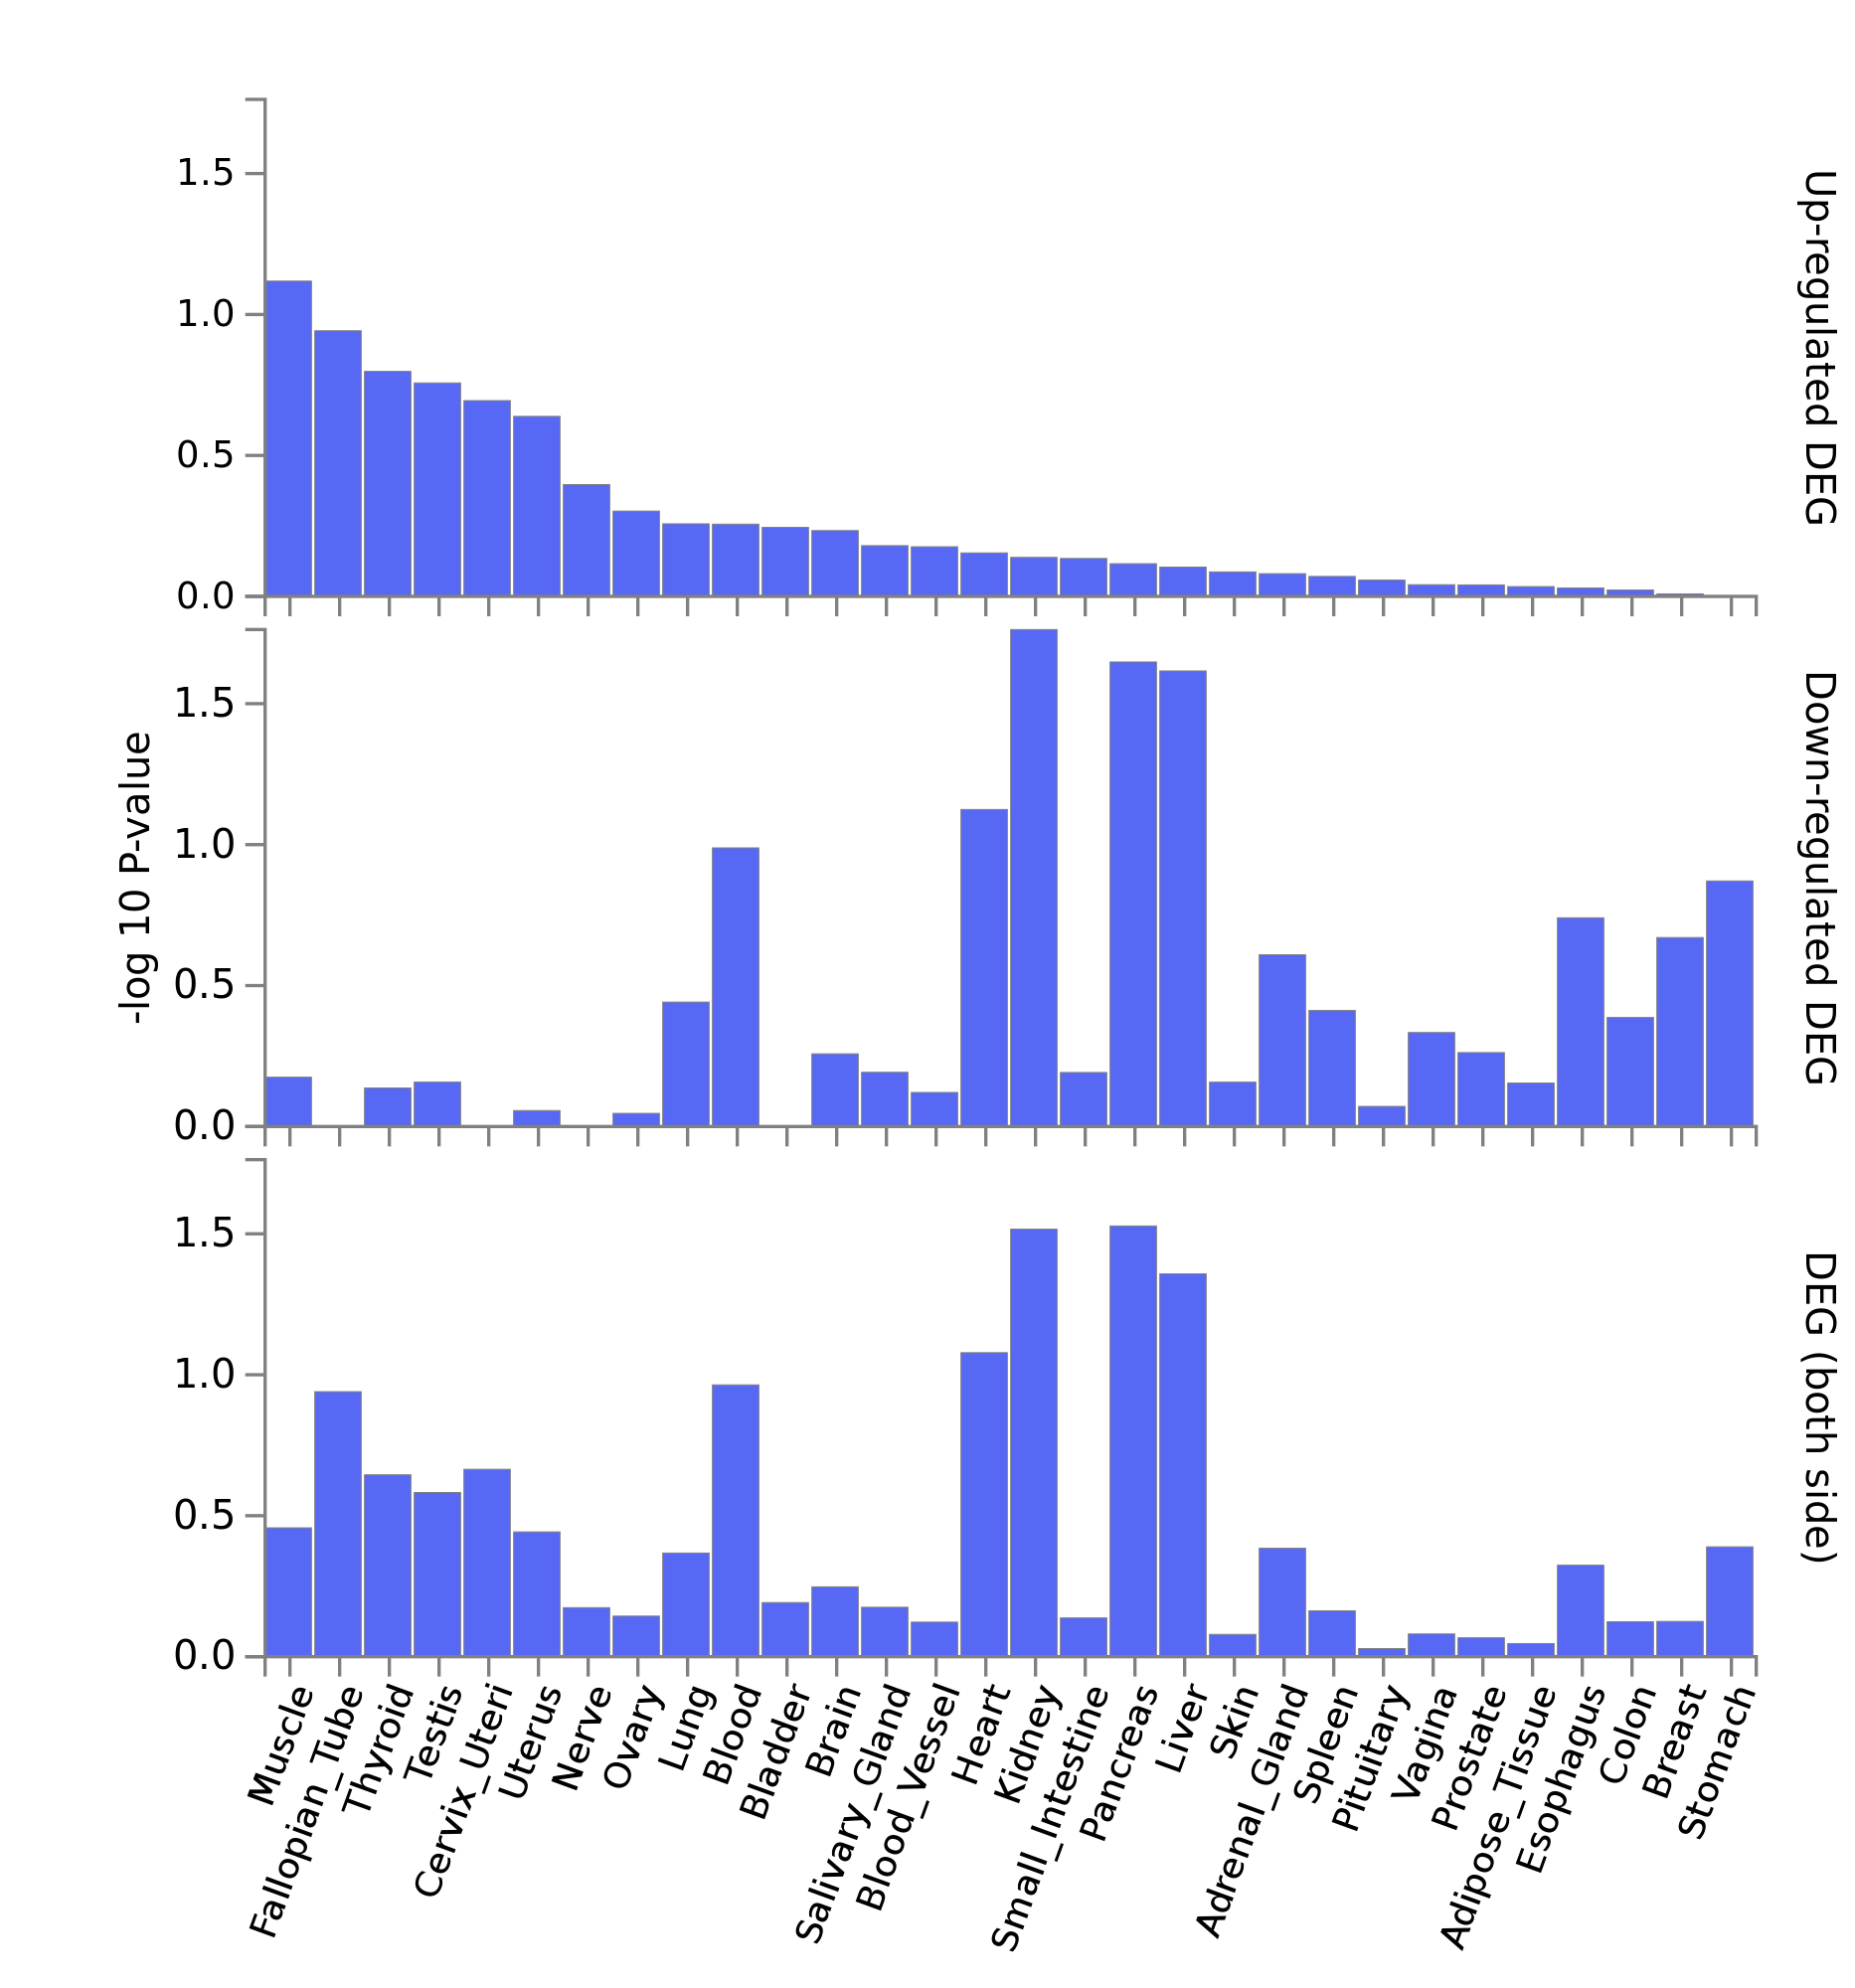
\includegraphics[width=\textwidth]{images/FUMA_plots/ctg_upregulated30tissues_46_genes.png}
%     \caption{GTEx upregulation in significant genes in Intelligence\textsubscript{Replication} sample. $-log_10(0.05)=1.301$}
%     \label{fig:GTEX FUMA CTG}
% \end{figure}
% \paragraph{toppfun}
% CC
% ID 	Name 	Source 	pValue 	FDR BH 	FDR BY 	Bonferroni 	Genes from Input 	Genes in Annotation 
% GO:0032584 	growth cone membrane 		1.416E-4 	3.838E-2 	
% 2.373E-1
% 	3.838E-2 	2 	8% latex table generated in R 3.6.3 by xtable 1.8-4 package
% % Tue Sep 15 11:43:35 2020

% \paragraph{topp fun PSP background}
% Nil MF,BP,CC Nothing at all


\subsection{Education\textsubscript{Replication} Gene Ontology analysis}
Okbay et al.\cite{okbay2016genome} report using DEPICT\cite{pers2015biological} to investigate pathway enrichment in genes near significant SNPs. 283 gene sets were determined to be significant and clustered into five groups: ``neural progenitor cells, migration of new neurons to cortex, projection of axons to target, sprouting of dendrites and spines, and neuronal signalling and synaptic plasticity throughout the lifespan''\cite{okbay2016genome}\todo{check quote}. An association with genetic variants identified and  genes involved in intellectual disability was also reported. The Education\textsubscript{Replication} sample differs from that reported by Okbay et al. \cite{okbay2016genome} as results obtained from UK Biobank and the individuals from 23andme are excluded (see section~\ref{sec:Edcuation replication gwgas}).



 \subsection{PANTHER Gene Ontology analysis Education\textsubscript{Replication}}
 
 The significant genes were again formatted to maximise the number identified in PANTHER\footnote{HGNC id from Symbols from NCBI from MAGMA\url{source('~/RProjects/paper_xls_output/R/chapter_2/translate_sig_genes/ea2_NCBI_translate2.R')}}
 Using the default background and FDR to correct for multiple comparisons, nineteen biological process terms were found to be enriched. No molecular function or cellular component terms were enriched. No enrichment was seen in PANTHER protein class, pathways (including Reactome pathways) or for any of the SLIM ontologies. 
 
%  Pathways nil
%  SLIM BP,MF,CC nil
 
%  Protein class nil
 
%  Reactome pathways nil
 
  %   \url{source('~/RProjects/paper_xls_output/R/chapter_2/translate_sig_genes/ea2_NCBI_translate2.R')}
     
   %  HGNC id from Symbols from NCBI from MAGMA
     
%      Fails to recognise 18839 but recognised STH which is HGNC18839. With HGNC symbols. 2 dual mapped MST1 to MST1	2 	HUMAN|HGNC=11408|UniProtKB=Q13043,
% HUMAN|HGNC=7380|UniProtKB=P26927
% but has the correct entrez 4485 (MAGMA output) P26927 MST1 (hepatocyte growth factor) other is Q13043 stk4 
%  99 entrez genes. Using approved HGNC symbols from NCBI get 1000 as maps MST1 to STK4
 
%  Using HGNC symbols as input does not recognise 11408 (comes from same output) which is STH which it always has difficulty with inputing STH is recognised and finds HGNC18839 don't know how to get round this
 The PANTHER enrichment displays the hierarchy of the ontology terms; although the FDR values are lower than ToppGene the very specific term related to neurogenesis, "positive regulation of collateral sprouting" (FDR p 0.041) is prominent in comparison to the same data ordered by FDR shown in table~\ref{tab:GO.biological.process.complete Panther Gene Ontology Enrichment significant genes in Education Replication}. There is also a considerable difference in actual enrichment values, including the raw $p$ value calculated in ToppGene and PANTHER. Widely variant scores are noted in Rhee (2008) \cite{rhee2008use} and see Khatri et al. for a detailed discussion \cite{khatri2005ontological}.
 \footnote{Douglas: I have included this as a screenshot. Parsing the xml and getting it into latex took longer than I thou
 ght so I went straight to screenshot as a last resort could do the indentation by hand. Thought worth showing (as DEPICT, MAGMA etc as far as I can see ignore heirarchy) but interested in what you thought. The standard table output for PANTHER doesn't have the hierarchy. I thought the differences in approach to the GO DAG were worth discussing  - as part of pointing out limitations to how enrichment has been approached in genomics. }
 
F No significant enrichment was seen using PANTHER for molecular function or cellular function. Biological function was enriched for 19 terms using FDR to correct for multiple comparisons. The most enriched term is "nervous system development" (GO:0007399), FDR q = 0.006, but the term is the largest and most general with 2430 members in the annotation. (table~\ref{tab:GO biological process complete Education Replication FDRover represenation only}). "Positive regulation of collateral sprouting",GO:0048672, is just below nominal significance after correction for multiple comparisons using FDR but is a very specific term with over 52 times fold enrichment and 3 of the 12 genes annotated to this term are significant genes in GWGAS. This balance between significance and specificity is an issue to some extent for all GO pathway analyses (see fig~\ref{tab:GO biological process complete Education Replication FDR} and table~\ref{tab:GO biological process complete Education Replication FDRover represenation only}). No PANTHER SLIM ontology term showed significant enrichment. 

 \begin{figure}
     \centering
     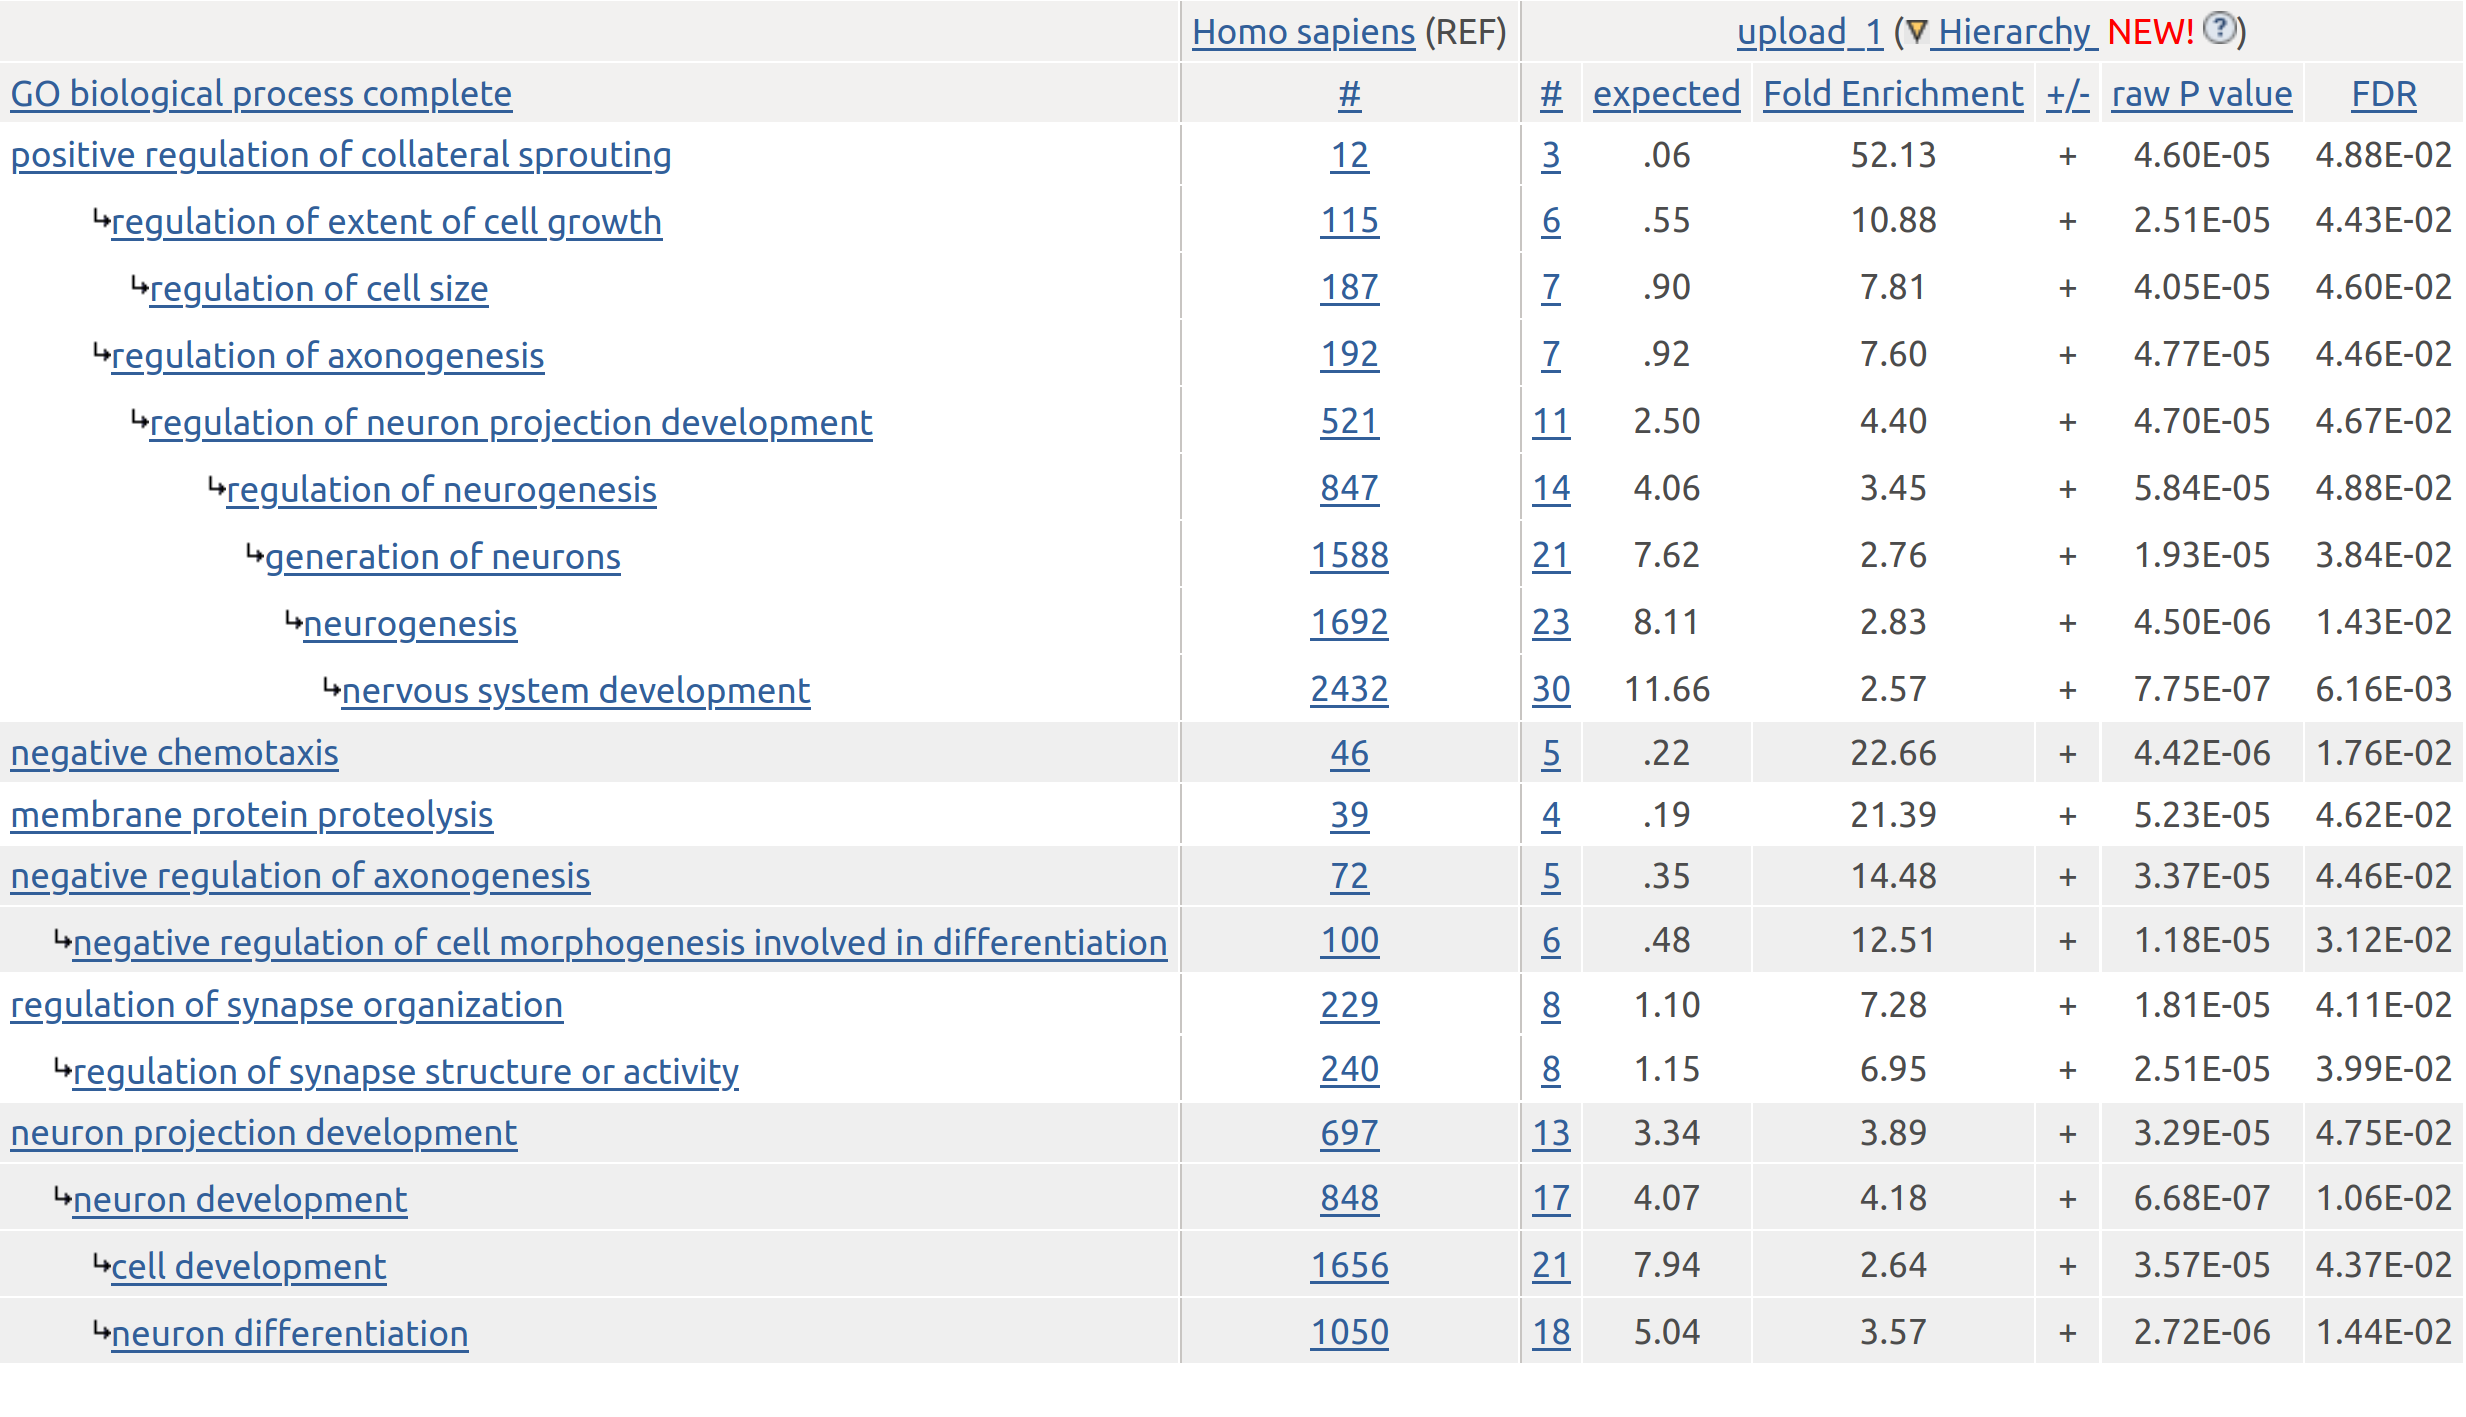
\includegraphics[width=\textwidth]{images/chapter2/large_screenshots/edu_replication_large_bp_panther.png}
     \caption[GO enrichment PANTHER Biological Process Education\textsubscript{Replication}]{GO enrichment of genome wide significant genes at GWGAS in the Education\textsubscript{Replication} cohort. Enrichment calculated
     using PANTHER with Fisher's exact test for the over representation test and using the False Discovery Rate correction for multiple comparisons. The term with the lowest FDR is GO:0007399 nervous system development (FDR 0.006). The figure shows the hierarchy of Gene Ontology terms, the most general terms are the most indented, the deepest terms in the directed acyclic graph are the most indented. Child terms are indented underneath their adult terms. Terms with identical levels of indentation are at identical layers in the hierarchy. Text output in \url{/home/grant/RProjects/paper_xls_output/data/PANTHER_txt_output/checked_for_thesis/ea2/BP_all.txt}}%previous image images/screenshots/EA2_BP_Panther_all_genes_FDR.png}
     
     \label{tab:GO biological process complete Education Replication FDR}
 \end{figure}
 % latex table generated in R 3.6.3 by xtable 1.8-4 package
% Tue Sep  1 11:07:38 2020


\begin{figure}
    \centering
    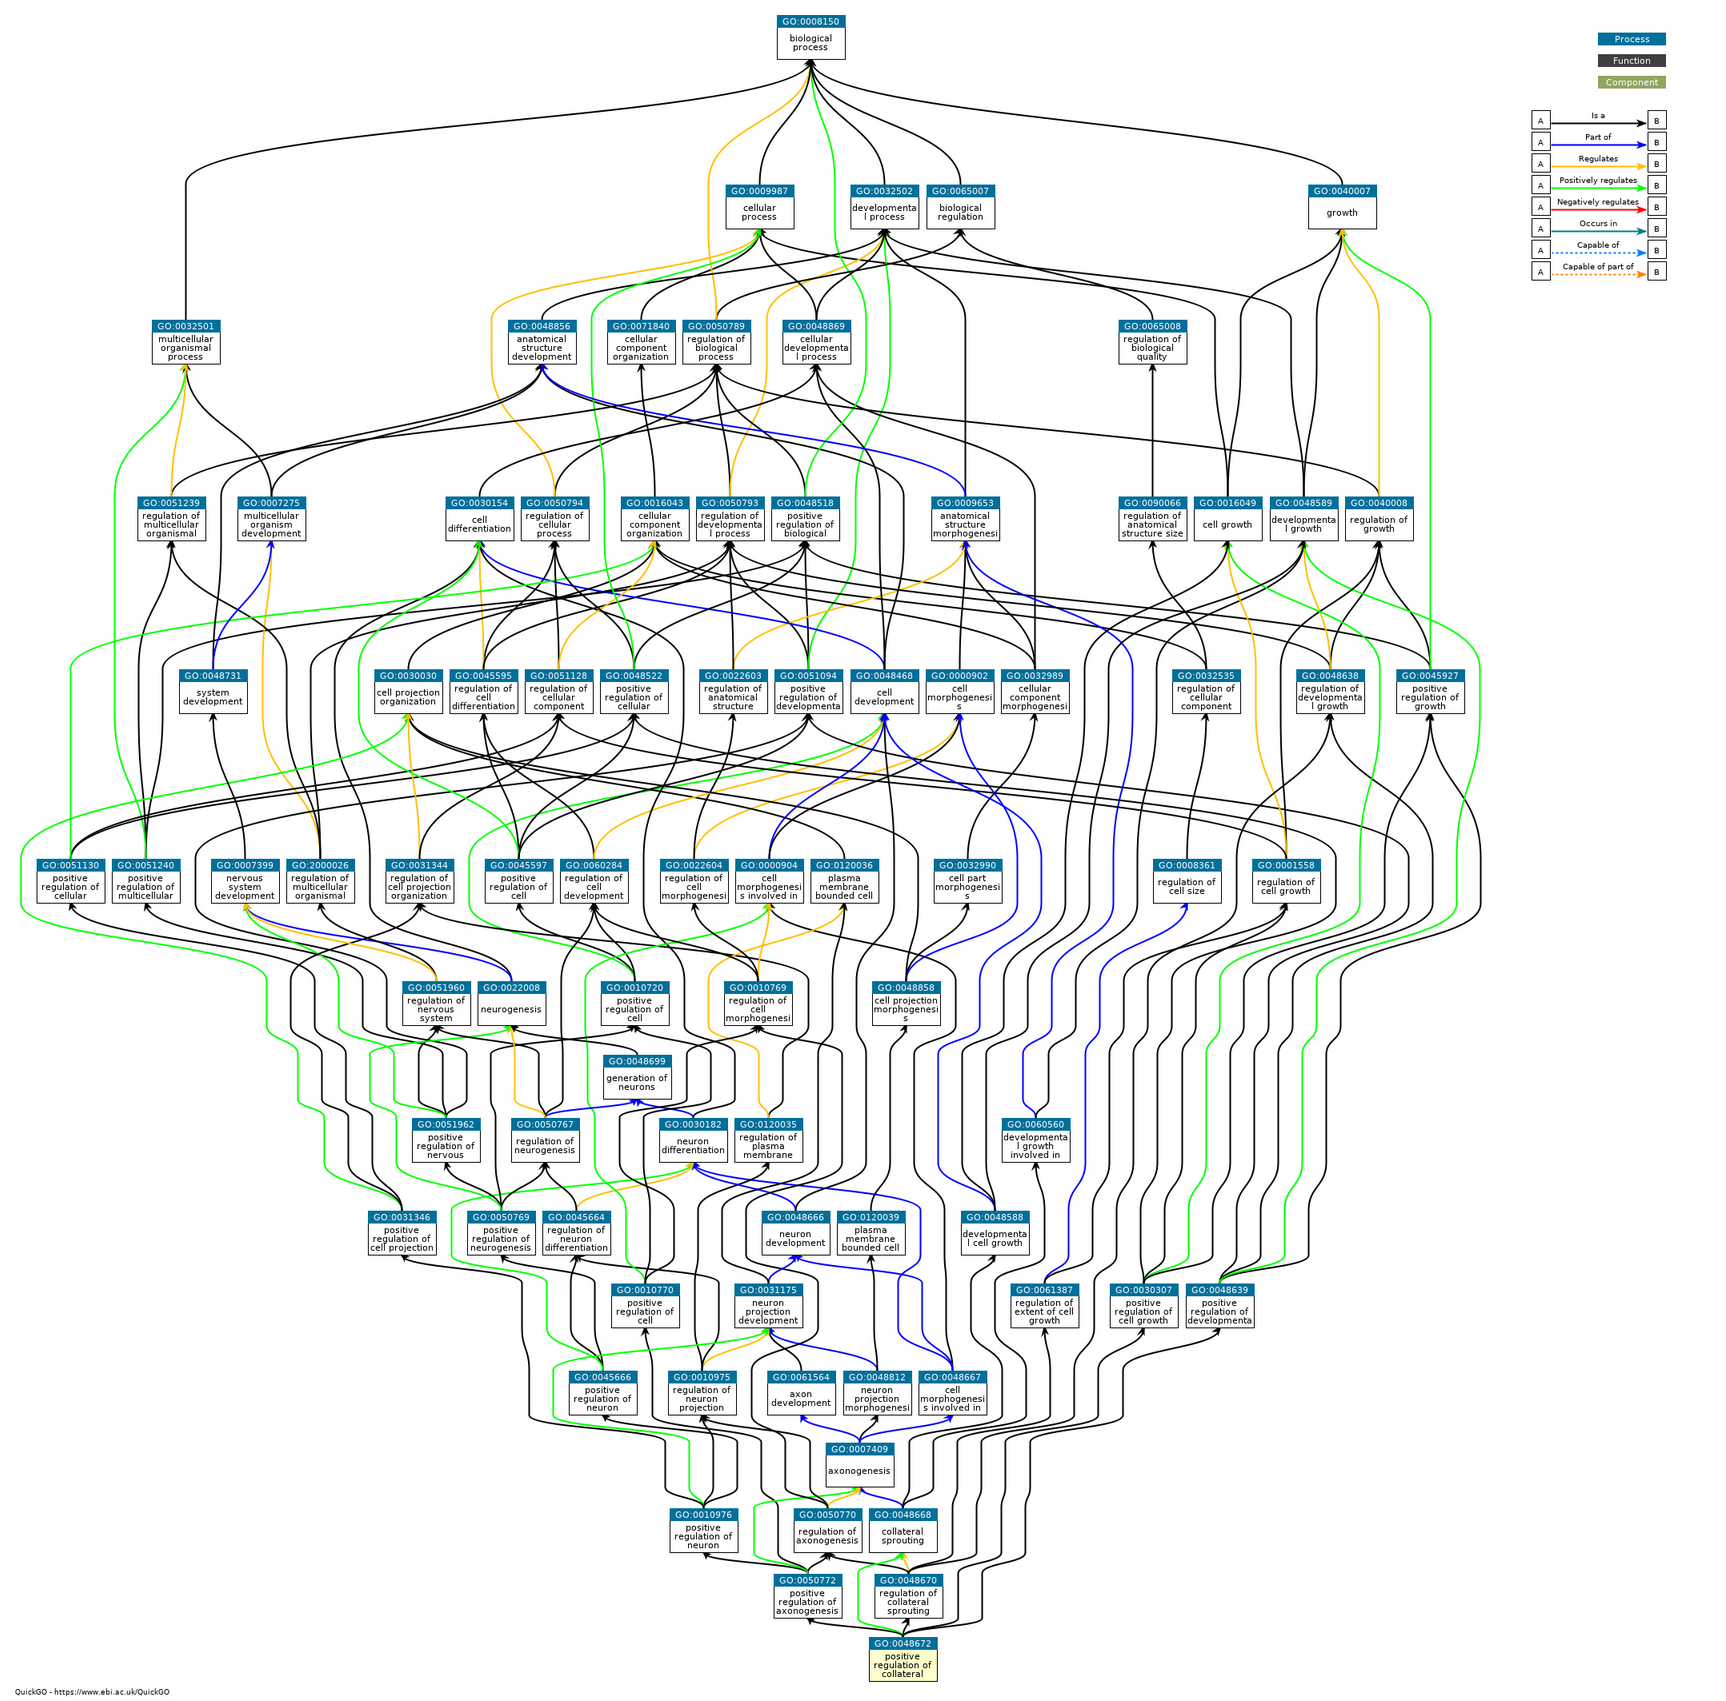
\includegraphics[width=\textwidth]{images/screenshots/quick_go_collateral.png}
    \caption{Gene Ontology Hierarchy of Biological Process term Collateral Sprouting from Quick GO. Although FDR q level is modest, in Education\textsubscript{Replication}, the fold change for the term is marked. Image source Quick GO. The term related to other terms such as growth cone development and neuron projection development (GO:0031175) found in both Education samples and in the paper by \cite{okbay2016genome}.How to prioritise such specific terms over general terms is an issue faced by GO enrichment methods.}
    \label{fig:the DAG of Collateral sprouting}
\end{figure}

% \begin{table}[ht]
% \resizebox{\textwidth}{!}{%
% \centering

% \begin{tabular}{llrrrrrr}
%   \hline
% GO & description & Ref & Test & E & Fold & P & FDR \\ 
%   \hline
% GO:0048672 & positive regulation of collateral sprouting  & 12 & 3 & 0.1 & 52.13 & $4.60 \times 10^{-5}$ & 0.049 \\ 
%   GO:0050919 & negative chemotaxis  & 46 & 5 & 0.2 & 22.66 & $4.42 \times 10^{-6}$ & 0.014 \\ 
%   GO:0033619 & membrane protein proteolysis  & 39 & 4 & 0.2 & 21.39 & $5.23 \times 10^{-5}$ & 0.046 \\ 
%   GO:0050771 & negative regulation of axonogenesis  & 72 & 5 & 0.3 & 14.48 & $3.37 \times 10^{-5}$ & 0.045 \\ 
%   GO:0010771 & negative regulation of cell morphogenesis involved in differentiation  & 100 & 6 & 0.5 & 12.51 & $1.18 \times 10^{-5}$ & 0.031 \\ 
%   GO:0061387 & regulation of extent of cell growth  & 115 & 6 & 0.6 & 10.88 & $2.51 \times 10^{-5}$ & 0.044 \\ 
%   GO:0008361 & regulation of cell size  & 187 & 7 & 0.9 & 7.81 & $4.05 \times 10^{-5}$ & 0.046 \\ 
%   GO:0050770 & regulation of axonogenesis  & 192 & 7 & 0.9 & 7.60 & $4.77 \times 10^{-5}$ & 0.045 \\ 
%   GO:0050807 & regulation of synapse organization  & 229 & 8 & 1.1 & 7.28 & $1.81 \times 10^{-5}$ & 0.041 \\ 
%   GO:0050803 & regulation of synapse structure or activity  & 240 & 8 & 1.1 & 6.95 & $2.51 \times 10^{-5}$ & 0.040 \\ 
%   GO:0010975 & regulation of neuron projection development  & 521 & 11 & 2.5 & 4.40 & $4.70 \times 10^{-5}$ & 0.047 \\ 
%   GO:0048666 & neuron development  & 848 & 17 & 4.1 & 4.18 & $6.68 \times 10^{-7}$ & 0.011 \\ 
%   GO:0031175 & neuron projection development  & 697 & 13 & 3.3 & 3.89 & $3.29 \times 10^{-5}$ & 0.048 \\ 
%   GO:0030182 & neuron differentiation  & 1046 & 18 & 5.0 & 3.59 & $2.58 \times 10^{-6}$ & 0.014 \\ 
%   GO:0050767 & regulation of neurogenesis  & 847 & 14 & 4.1 & 3.45 & $5.84 \times 10^{-5}$ & 0.049 \\ 
%   GO:0022008 & neurogenesis  & 1690 & 23 & 8.1 & 2.84 & $4.42 \times 10^{-6}$ & 0.018 \\ 
%   GO:0048699 & generation of neurons  & 1585 & 21 & 7.6 & 2.76 & $1.88 \times 10^{-5}$ & 0.037 \\ 
%   GO:0048468 & cell development  & 1654 & 21 & 7.9 & 2.65 & $3.51 \times 10^{-5}$ & 0.043 \\ 
%   GO:0007399 & nervous system development  & 2430 & 30 & 11.7 & 2.57 & $7.62 \times 10^{-7}$ & 0.006 \\ 
%   \hline
% \end{tabular}}
% \caption{GO biological process complete Education Replication FDRover represenation only  Ref reference set, test:number of genes being tested present in ontology termE expected number of genes being tested present in ontology term, Fold= Fold change P = raw p value, FDR = false discovery rate} 
% \label{tab:GO biological process complete Education Replication FDRover represenation only}
% \end{table}
 
%  % latex table generated in R 3.6.3 by xtable 1.8-4 package
% % Sat Aug 29 13:31:48 2020
% \begin{table}[ht]
% \centering
% \begin{tabular}{llrrrlrr}
%   \hline
% GO & description & Ref & Test & E & OU & Fold & P Bnf \\ 
%   \hline
% GO:0050919 & negative chemotaxis  & 46 & 5 & 0.2  & + & 22.66 & 0.040 \\ 
%   GO:0048666 & neuron development  & 848 & 17 & 4.1 & + & 4.18 & 0.006 \\ 
%   GO:0030182 & neuron differentiation  & 1046 & 18 & 5.0 & + & 3.59 & 0.023 \\ 
%   GO:0022008 & neurogenesis  & 1690 & 23 & 8.1 & + & 2.84 & 0.040 \\ 
%   GO:0007399 & nervous system development  & 2430 & 30 & 11.7 & + & 2.57 & 0.007 \\ 
%   UNCLASSIFIED & Unclassified  & 2924 & 7 & 14.0 & - & 0.50 & 0.000 \\ 
%   \hline
% \end{tabular}
% \caption{GO biological process complete Education Replication Bonferroni} 
% \label{tab:GO biological process complete Education Replication Bonferroni}
% \end{table}

 % latex table generated in R 3.6.3 by xtable 1.8-4 package
% Sat Aug 29 14:04:17 2020
\begin{table}[ht]
\centering
\begin{tabular}{llrrrrrr}
  \hline
GO & description & Ref & Test & E & Fold & P & FDR \\ 
  \hline
GO:0048672 & positive regulation of collateral sprouting  & 12 & 3 & 0.1 & 52.13 & $4.600 \times 10^{-5}$ & 0.049 \\ 
  GO:0050919 & negative chemotaxis  & 46 & 5 & 0.2 & 22.66 & $4.420 \times 10^{-6}$ & 0.014 \\ 
  GO:0033619 & membrane protein proteolysis  & 39 & 4 & 0.2 & 21.39 & $5.230 \times 10^{-5}$ & 0.046 \\ 
  GO:0050771 & negative regulation of axonogenesis  & 72 & 5 & 0.3 & 14.48 & $3.370 \times 10^{-5}$ & 0.045 \\ 
  GO:0010771 & \makecell{negative regulation of cell morphogenesis\\ involved in differentiation}  & 100 & 6 & 0.5 & 12.51 & $1.180 \times 10^{-5}$ & 0.031 \\ 
  GO:0061387 & regulation of extent of cell growth  & 115 & 6 & 0.6 & 10.88 & $2.510 \times 10^{-5}$ & 0.044 \\ 
  GO:0008361 & regulation of cell size  & 187 & 7 & 0.9 & 7.81 & $4.050 \times 10^{-5}$ & 0.046 \\ 
  GO:0050770 & regulation of axonogenesis  & 192 & 7 & 0.9 & 7.60 & $4.770 \times 10^{-5}$ & 0.045 \\ 
  GO:0050807 & regulation of synapse organization  & 229 & 8 & 1.1 & 7.28 & $1.810 \times 10^{-5}$ & 0.041 \\ 
  GO:0050803 & regulation of synapse structure or activity  & 240 & 8 & 1.1 & 6.95 & $2.510 \times 10^{-5}$ & 0.040 \\ 
  GO:0010975 & regulation of neuron projection development  & 521 & 11 & 2.5 & 4.40 & $4.700 \times 10^{-5}$ & 0.047 \\ 
  GO:0048666 & neuron development  & 848 & 17 & 4.1 & 4.18 & $6.680 \times 10^{-7}$ & 0.011 \\ 
  GO:0031175 & neuron projection development  & 697 & 13 & 3.3 & 3.89 & $3.290 \times 10^{-5}$ & 0.048 \\ 
  GO:0030182 & neuron differentiation  & 1046 & 18 & 5.0 & 3.59 & $2.580 \times 10^{-6}$ & 0.014 \\ 
  GO:0050767 & regulation of neurogenesis  & 847 & 14 & 4.1 & 3.45 & $5.840 \times 10^{-5}$ & 0.049 \\ 
  GO:0022008 & neurogenesis  & 1690 & 23 & 8.1 & 2.84 & $4.420 \times 10^{-6}$ & 0.018 \\ 
  GO:0048699 & generation of neurons  & 1585 & 21 & 7.6 & 2.76 & $1.880 \times 10^{-5}$ & 0.037 \\ 
  GO:0048468 & cell development  & 1654 & 21 & 7.9 & 2.65 & $3.510 \times 10^{-5}$ & 0.043 \\ 
  GO:0007399 & nervous system development  & 2430 & 30 & 11.7 & 2.57 & $7.620 \times 10^{-7}$ & 0.006 \\ 
   \hline
\end{tabular}
\caption{GO biological process complete PANTHER Education\textsubscript{Replication} FDR over representation only. Ref reference set, test:number of genes being tested present in ontology term, E expected number of genes being tested present in ontology term, Fold= Fold change, P = raw p value, FDR = false discovery rate \url{source('~/RProjects/paper_xls_output/R/chapter_2/make_PANTHER_tables/make_Panther_table_GO_col_nounderFDR.R')}} 
\label{tab:GO biological process complete Education Replication FDRover represenation only}
\end{table}


Using FUMA GTex enrichment I found no statistically significant differential enrichment for the genes in the central nervous system (figure~\ref{fig:FUMA gtex deg samples multiple} and fig~\ref{fig:deg_upref_sample_gtex_gener})



% \begin{figure}
%     \centering
%     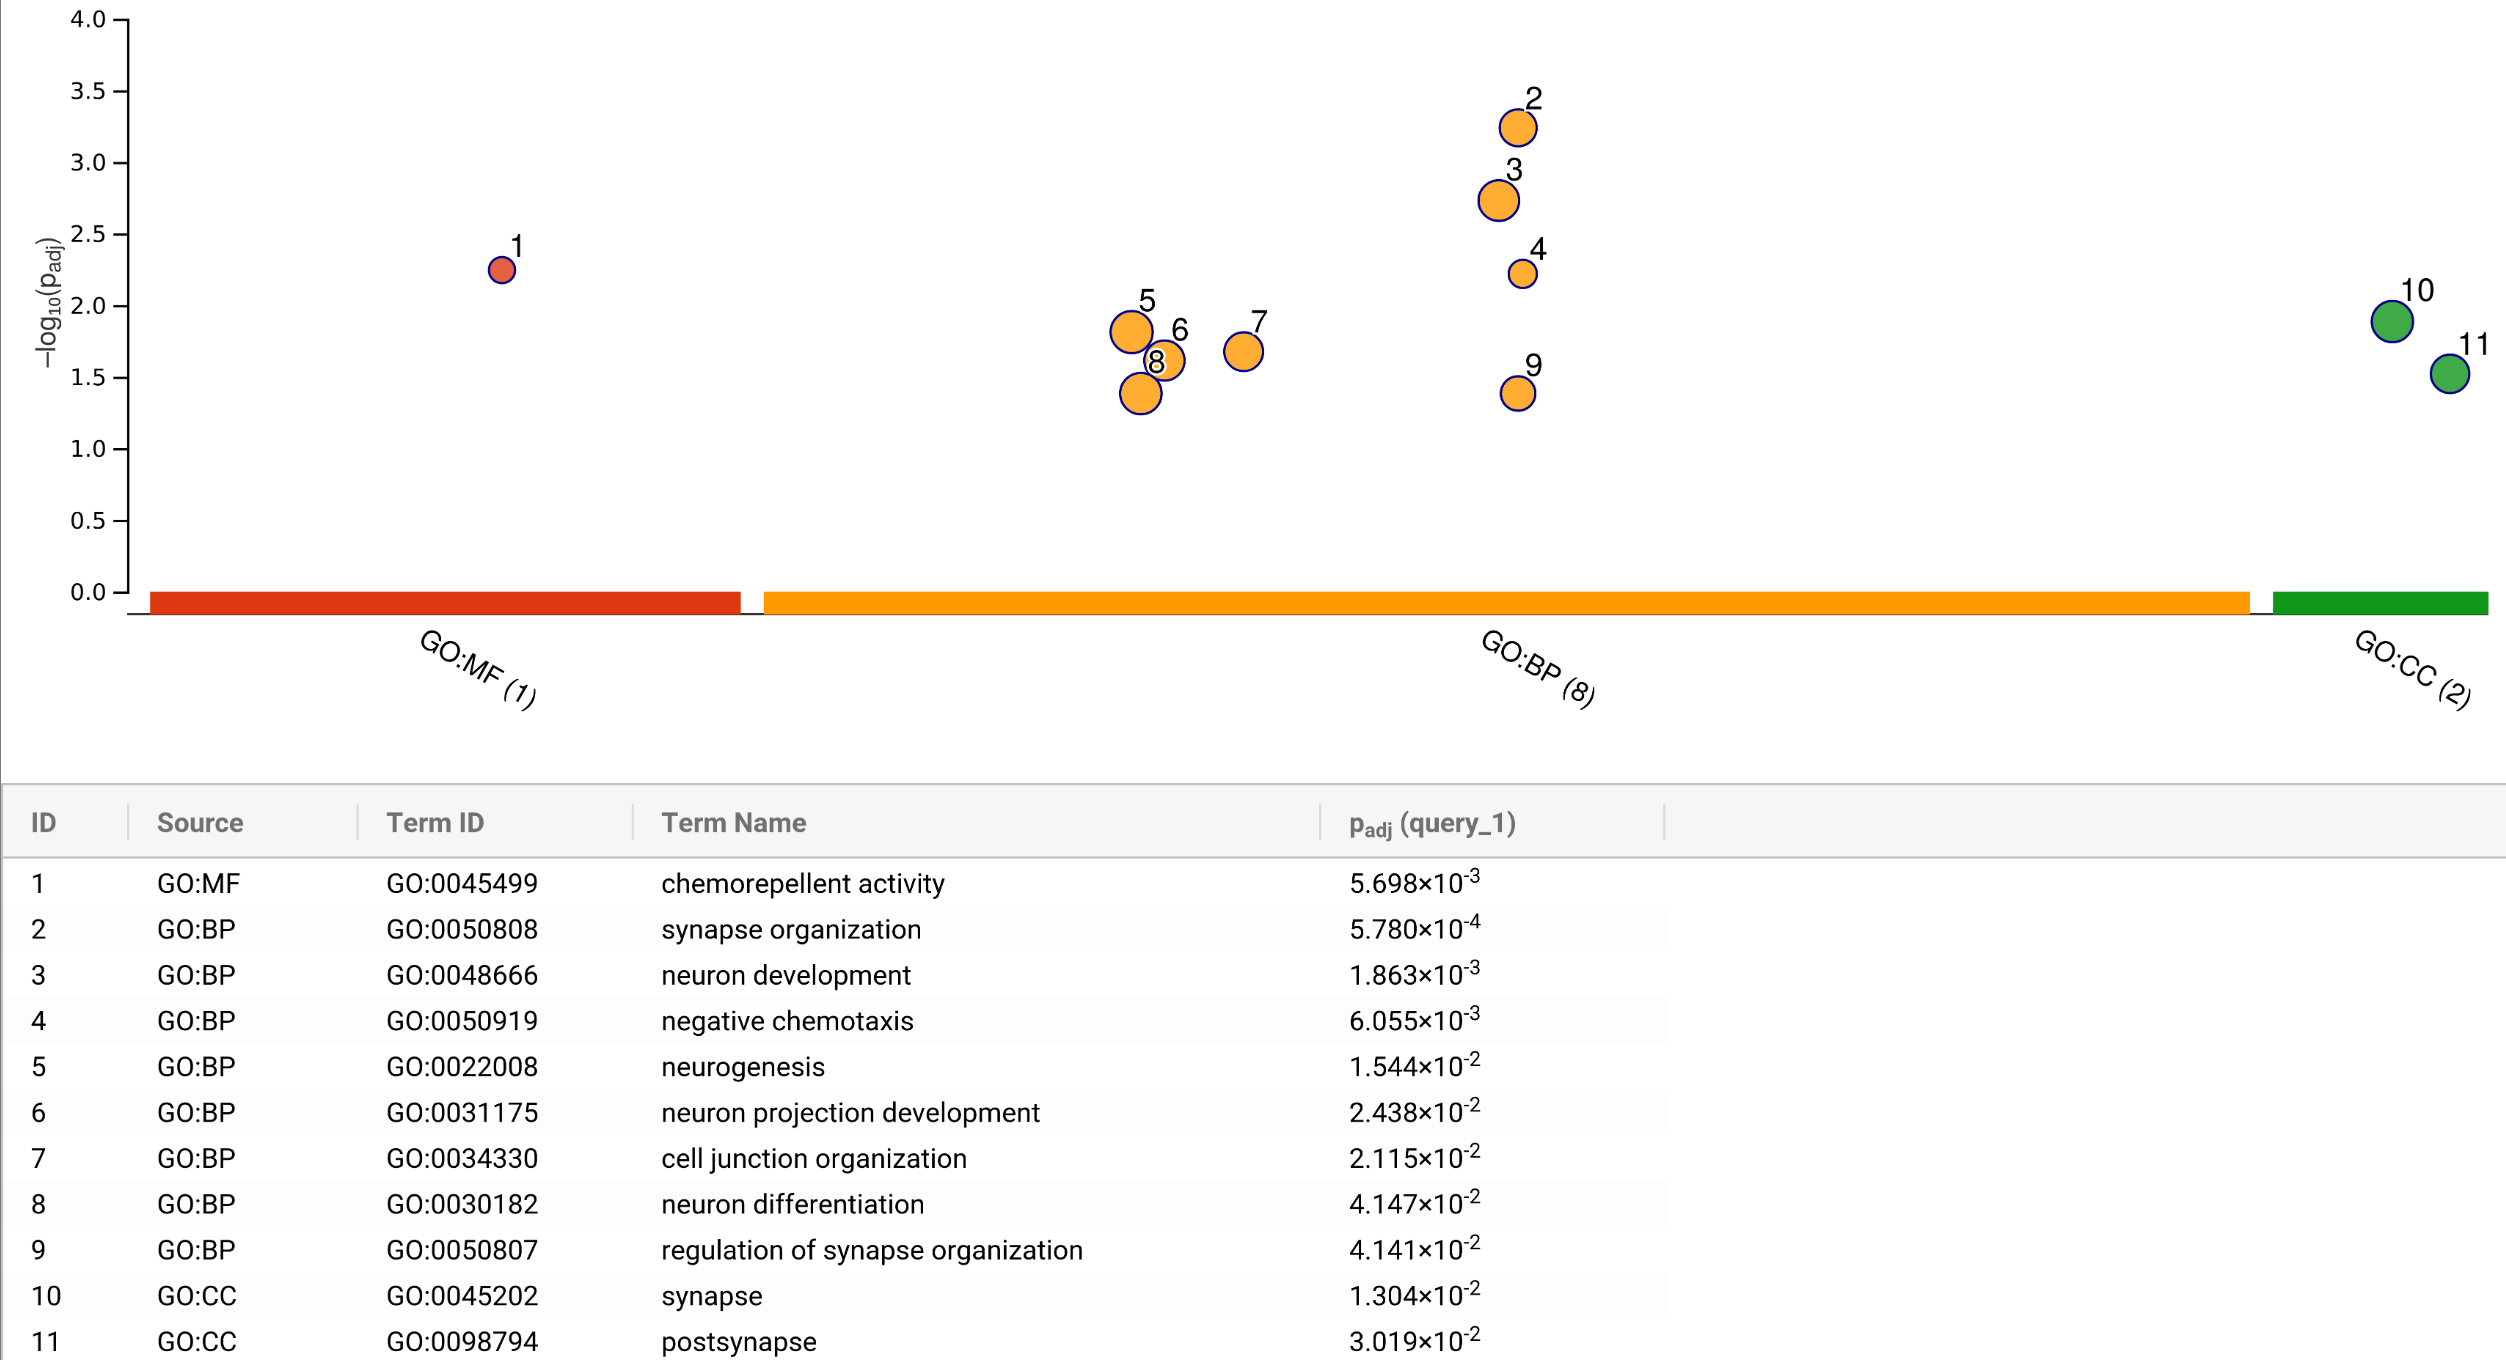
\includegraphics[width=\textwidth]{images/gprofiler/gprofiler_ea2_clip.png}
%     \caption{GO enrichment for significant genes using gProfiler multiple testing control SGS. Educational\textsubscript{Replication} sample}
    
%     \label{fig:gprofiler_ea2}
% \end{figure}

% \begin{figure}
%     \centering
%     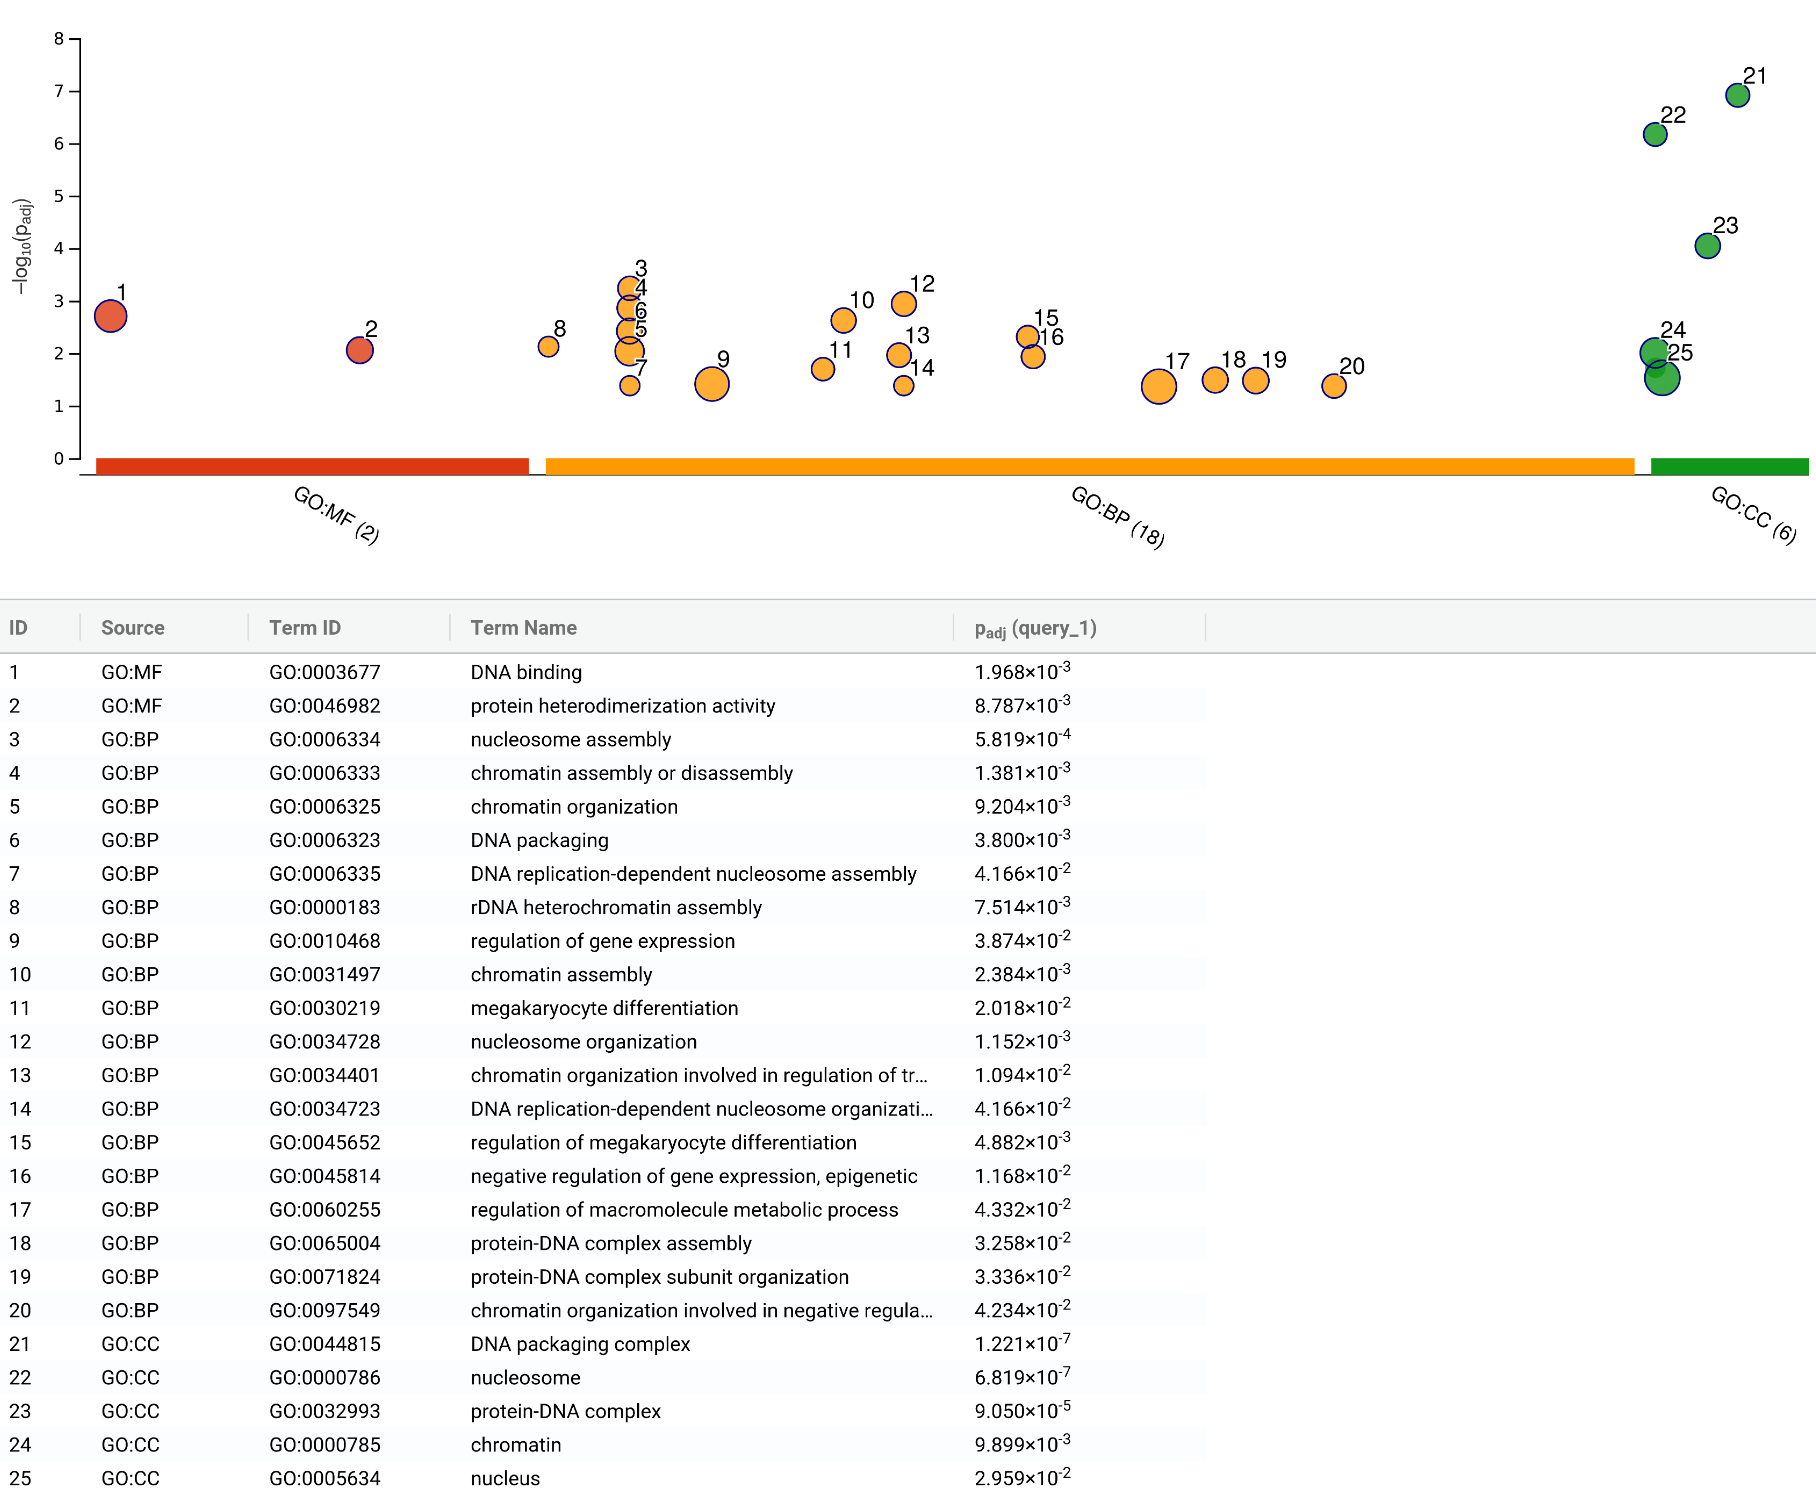
\includegraphics[width=\textwidth]{images/gprofiler/gprofiler_ukbbint_clip.png}
%     \caption{GO enrichment for significant genes using gProfiler multiple testing control SGS. Intelligence\textsubscript{Discovery} sample}
%     \label{fig:gprofiler_ukbbint}
% \end{figure}

% \begin{figure}
%     \centering
%     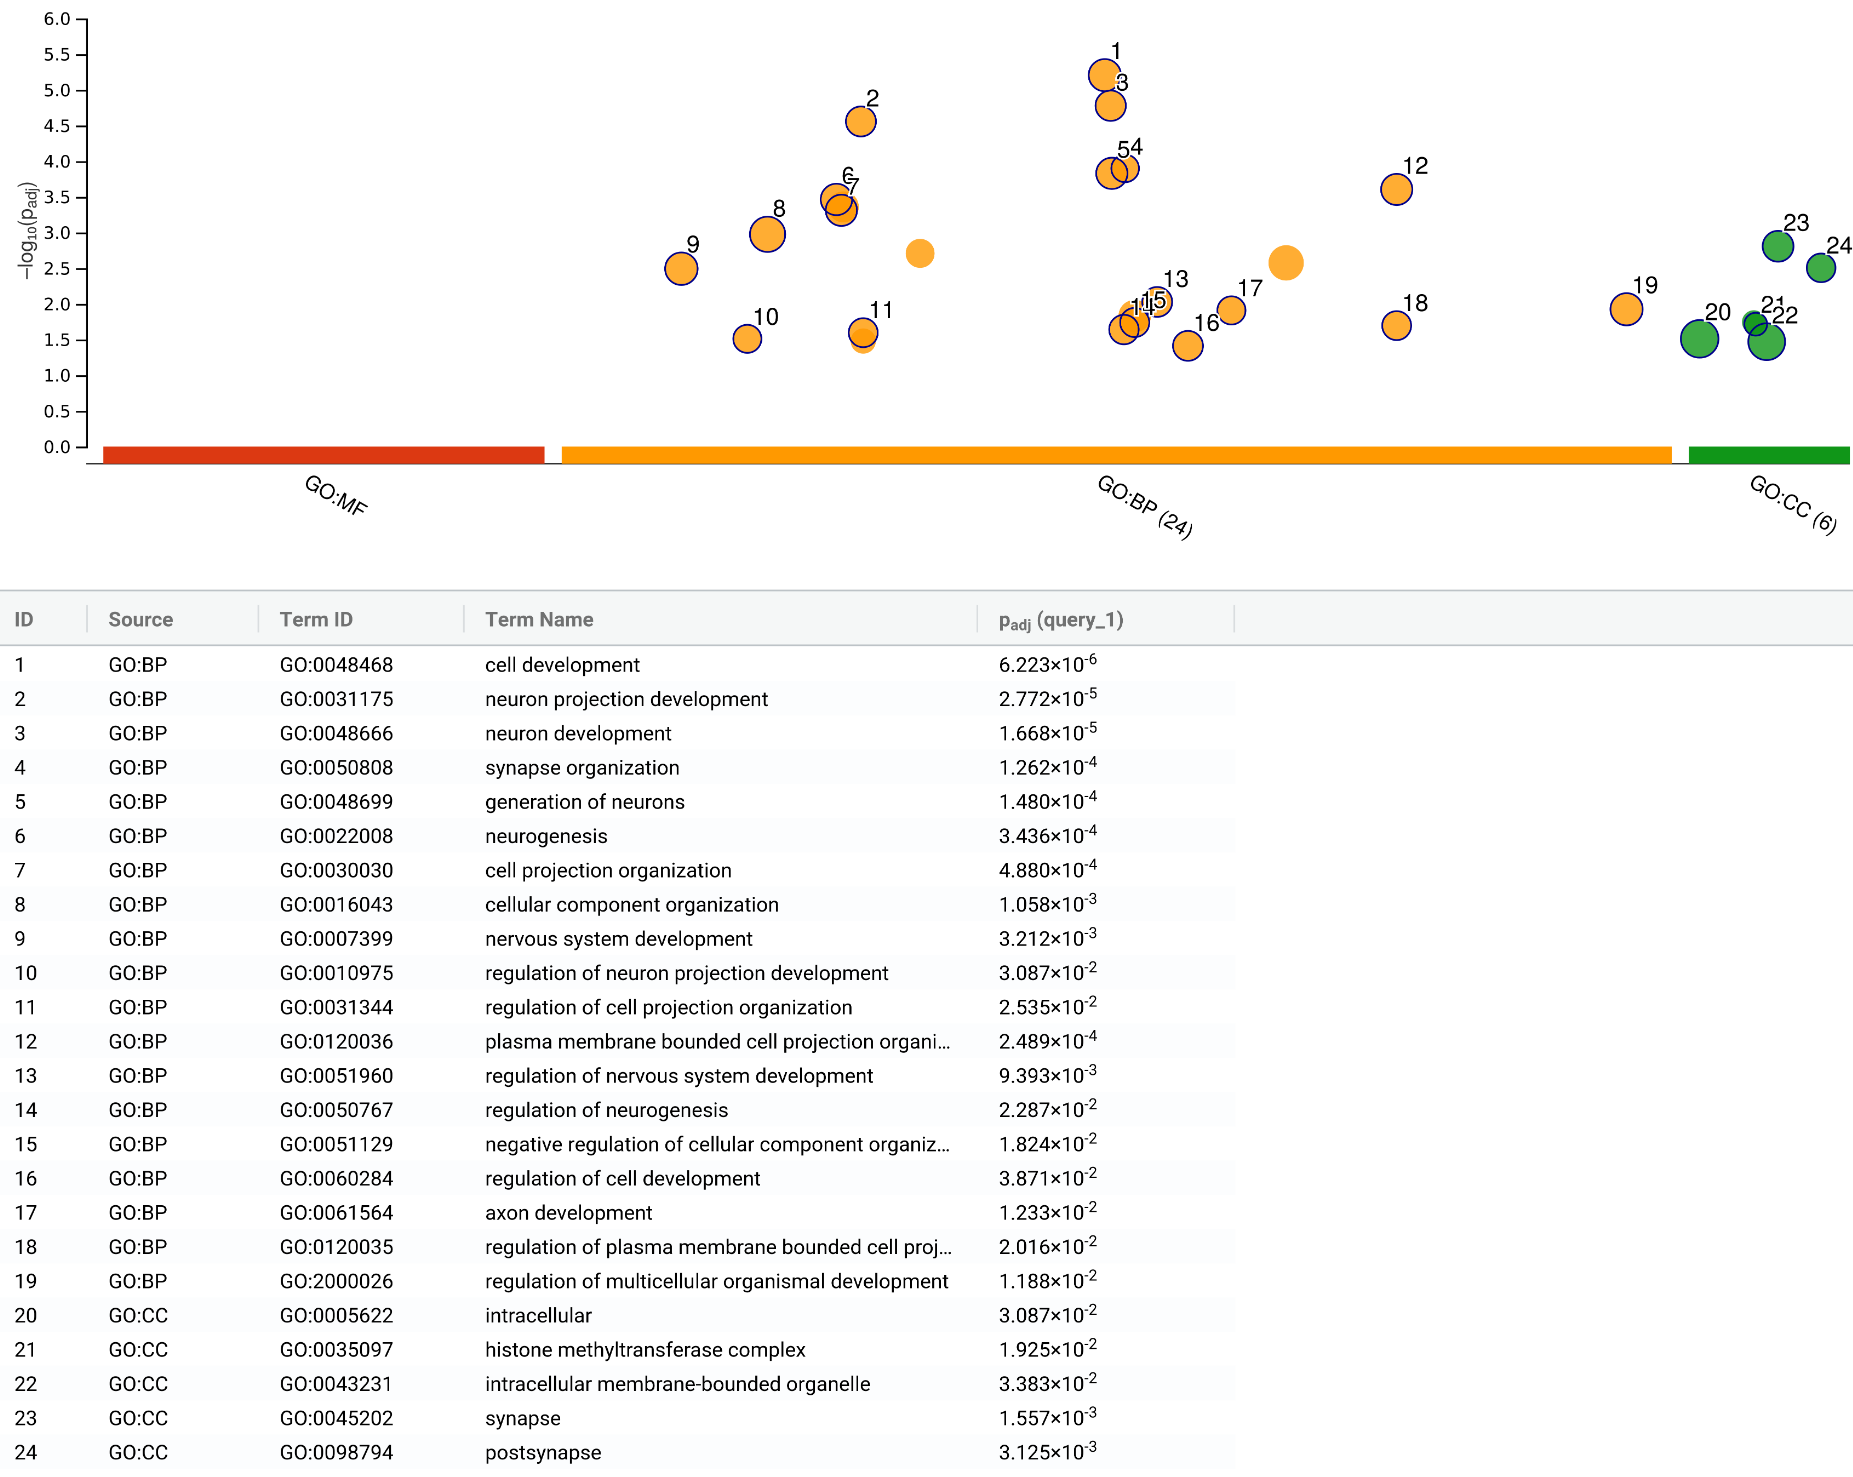
\includegraphics[width=\textwidth]{images/gprofiler/gprofiler_eukbbed_clip.png}
%     \caption{GO enrichment for significant genes using gProfiler multiple testing control SGS. Education\textsubscript{Discovery} sample}
%     \label{fig:gprofiler_ukbbed}
% \end{figure}

% \begin{figure}
%     \centering

%     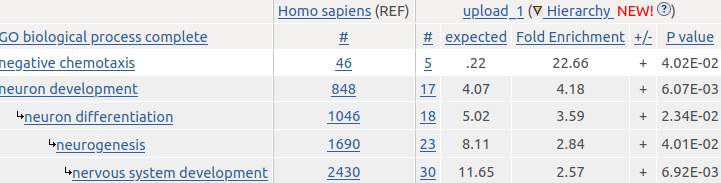
\includegraphics[width=\textwidth]{images/screenshots/EA2_BP_Panther_all_genes_Bonferroni.png}
%     \caption{Education\textsubscript{Replication} Gene Ontology enrichment using PANTHER. Bonferroni correction. Hierarchy of ontology terms shown.}
%     \label{fig:EA2_Panther_BP_Bonf_Hierarchy}
% \end{figure}

% \begin{figure}
%     \centering
%     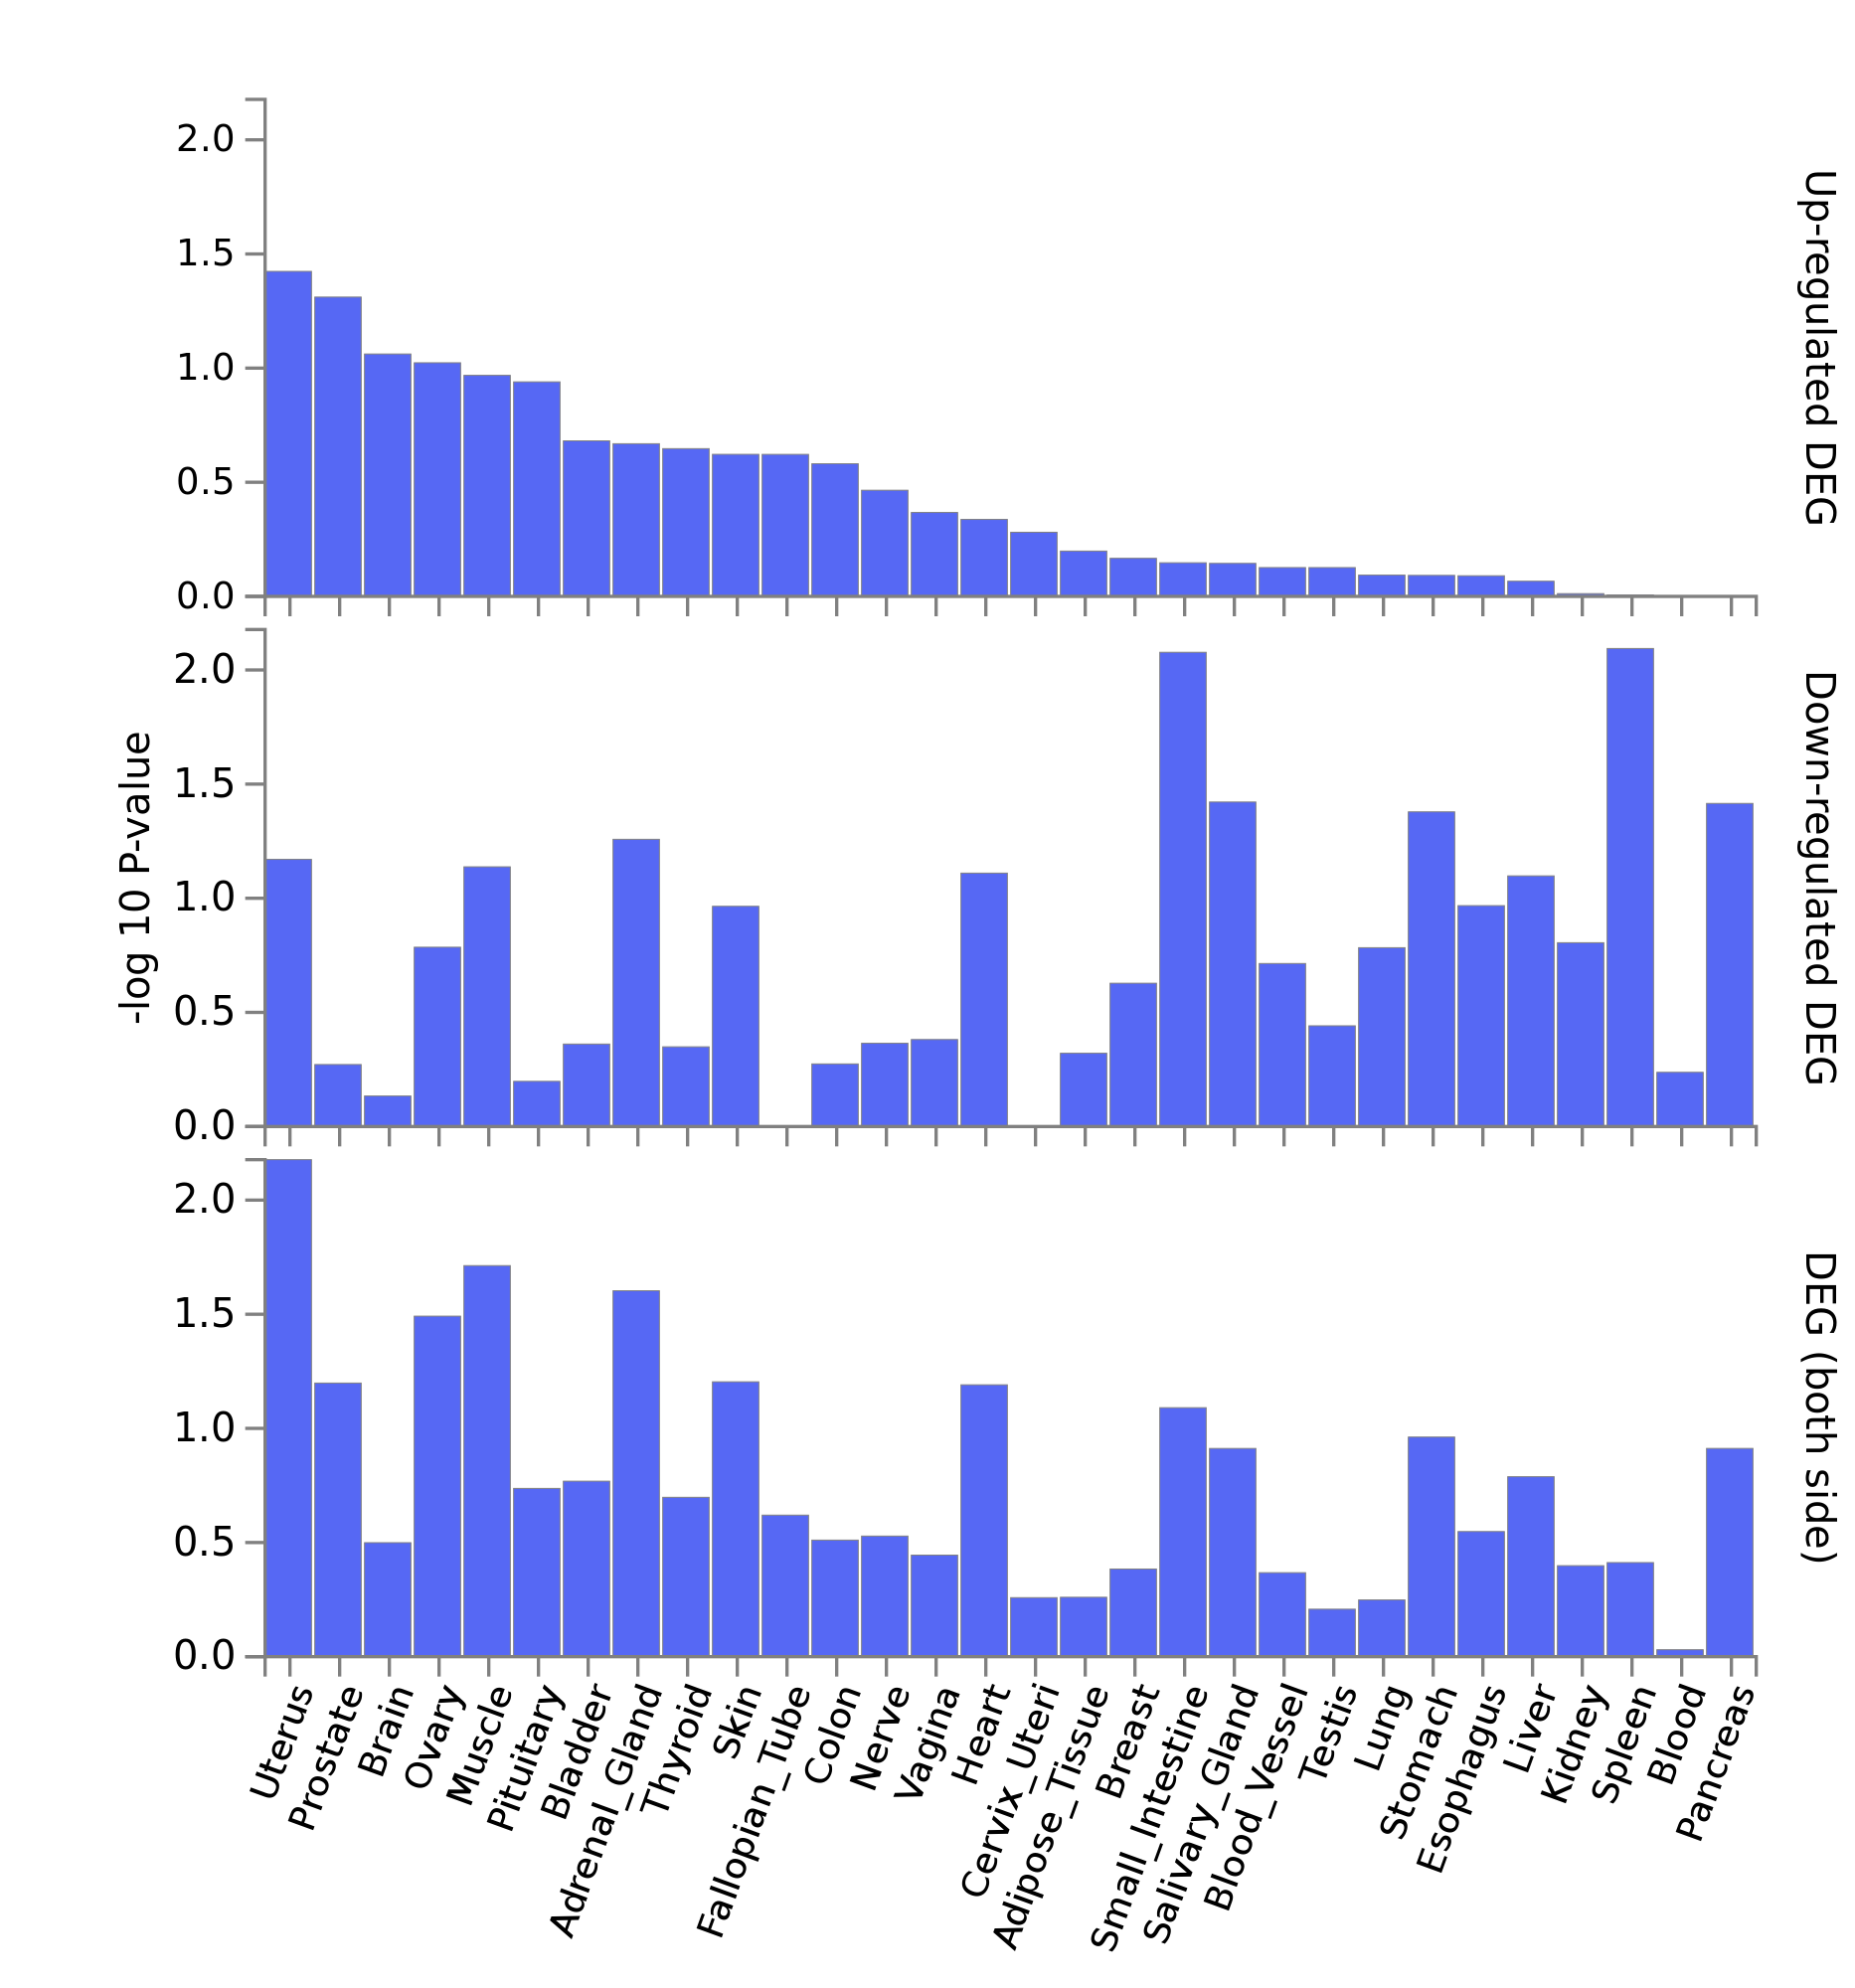
\includegraphics[width=\textwidth]{images/FUMA_plots/gtex_v8_ts_FUMA_30_99_genes.png}
%     \caption{GTEx differential enrichment ordered by upregulated genes in Education\textsubscript{Replication} cohort}
%     \label{fig:GTEX_EA2_DEG}
% \end{figure}



\subsubsection{ToppGene:Results Education\textsubscript{Replication}}

The 99 significant genes were enriched compared to the rest of the genome  using ToppFun and the FDR method, Benjamini and Hochberg (FDR BH) to correct for multiple comparisons. Seventy seven significant terms were found for Biological Process using the FDR method Benjamini and Hochberg (10 with Bonferroni, 22 using FDR Q value Benjamini and Yekutieli, FDR BY). Twenty annotations for cellular component were significantly over represented (2 Bonferroni, 2 FDR BY). No molecular function annotations were found to be enriched in the 99 genes found at GWGAS. Enrichment was performed using default background and settings. 


The significant biological process terms are shown in  table~\ref{tab:BP EA2 all significant toppgene top}. The top two terms are neurogenesis (GO:0022008,q FDR BH= 0.002) and gliogenesis (GO:0042063,q FDR BH= 0.002) both reported by Okbay et al. using DEPICT in an expanded sample\cite{okbay2016genome}. The significant genes are not enriched for molecular function but show enrichment for two cellular component terms, the top being "post synapse" GO:0098794.

Given that differences in significance values have been reported between enrichment packages\cite{khatri2005ontological}(here differences can be seen in the number annotated for identical inputs), I calculated  the correlation of the -log10 transform of the uncorrected p values for the seventeen annotations found in both PANTHER and ToppGene (17 of 19 for PANTHER, 17 of 77 for ToppGene). Pearson's product-moment correlation was 0.594 (95\%CI 0.158-0.84); t=2.861,df=15, p-value= 0.01189 (see figure~\ref{fig:correlation of gene ontology terms between toppgene and panther}). 

\begin{figure}
    \centering
    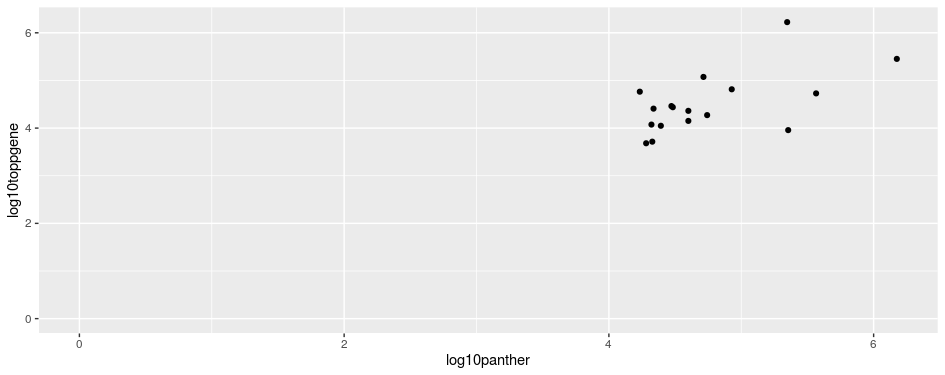
\includegraphics[width=\textwidth]{images/chapter2/strontium/Rplot_compare_toppgene_panther.png}
    \caption{Correlation between gene ontology term enrichment values in ToppGene and PANTHER for Education\textsubscript{Discovery} sample. Scatterplot shows -log10 transform of uncorrected p value for PANTHER on x-axis and -log10 transform of ToppGene values on y axis. There appears to be a linear relationship between the two although the number of samples is small.}
    \label{fig:correlation of gene ontology terms between toppgene and panther}
\end{figure}


% t = 2.8612, df = 15, p-value = 0.01189
% alternative hypothesis: true correlation is not equal to 0
% 95 percent confidence interval:
%  0.1589549 0.8360662
% sample estimates:
%       cor 
% 0.5942021 

% latex table generated in R 3.6.3 by xtable 1.8-4 package
% Mon Sep 21 14:31:22 2020
\begin{table}[ht]
\centering
\begin{adjustbox}{width=\textwidth}

\begin{tabular}{llrrrrrr}
  \hline
ID & Name & p & q Bonf & q BH & q BY & n query & n genome \\ 
  \hline
GO:0022008 & neurogenesis & $5.969 \times 10^{-7}$ & 0.002 & 0.002 & 0.014 & 26 & 1866 \\ 
  GO:0042063 & gliogenesis & $1.143 \times 10^{-6}$ & 0.003 & 0.002 & 0.014 & 11 & 352 \\ 
  GO:0007417 & central nervous system development & $1.812 \times 10^{-6}$ & 0.005 & 0.002 & 0.015 & 19 & 1129 \\ 
  GO:0048666 & neuron development & $3.528 \times 10^{-6}$ & 0.010 & 0.002 & 0.021 & 20 & 1297 \\ 
  GO:0010001 & glial cell differentiation & $5.159 \times 10^{-6}$ & 0.015 & 0.002 & 0.021 & 9 & 261 \\ 
  GO:0050808 & synapse organization & $5.386 \times 10^{-6}$ & 0.016 & 0.002 & 0.021 & 12 & 498 \\ 
  GO:0048667 & cell morphogenesis involved in neuron dif. & $5.919 \times 10^{-6}$ & 0.017 & 0.002 & 0.021 & 14 & 688 \\ 
  GO:0048699 & generation of neurons & $8.435 \times 10^{-6}$ & 0.025 & 0.003 & 0.027 & 23 & 1751 \\ 
  GO:0048812 & neuron projection morphogenesis & $1.389 \times 10^{-5}$ & 0.041 & 0.004 & 0.031 & 14 & 742 \\ 
  GO:0010771 & negative regulation of cell morphogenesis  dif. & $1.534 \times 10^{-5}$ & 0.045 & 0.004 & 0.031 & 6 & 109 \\ 
   \hline
\end{tabular}
\end{adjustbox}
\caption{Top 10 terms biological process Topp Gene Education\textsubscript{Replication}. dif. = involved in differentiation. BH FDR q value Benjaminin and Hochberg, BY FDR Benjamini and Yekutieli, Bonf = Bonferroni, n query = number of genes in sample (GWGAS significant genes in Education\textsubscript{Replication}) annotated to this term, n genome = number of genes in genome annotated to this term \url{source('~/RProjects/paper_xls_output/R/chapter_2/panther_and_toppgene/panther_and_toppgene_ea2.R')}}
~\ref{tab:BP EA2 all significant toppgene top}
\end{table}




% latex table generated in R 3.6.3 by xtable 1.8-4 package
% Mon Sep 21 14:47:23 2020
\begin{table}[ht]
\centering
\begin{adjustbox}{width=\textwidth}
\begin{tabular}{llrrrrrr}
  \hline
ID & Name & p & q Bonf & q BH & q BY & n query & n genome \\ 
  \hline
GO:0098794 & postsynapse & $1.458 \times 10^{-6}$ & 0.001 & 0.001 & 0.003 & 16 & 825 \\ 
  GO:0045202 & synapse & $1.580 \times 10^{-5}$ & 0.005 & 0.003 & 0.018 & 20 & 1482 \\ 
  GO:0005794 & Golgi apparatus & $2.099 \times 10^{-4}$ & 0.073 & 0.015 & 0.097 & 19 & 1643 \\ 
  GO:0097418 & neurofibrillary tangle & $2.178 \times 10^{-4}$ & 0.075 & 0.015 & 0.097 & 2 & 5 \\ 
  GO:0035658 & Mon1-Ccz1 complex & $2.178 \times 10^{-4}$ & 0.075 & 0.015 & 0.097 & 2 & 5 \\ 
  GO:0031252 & cell leading edge & $2.705 \times 10^{-4}$ & 0.094 & 0.016 & 0.100 & 9 & 449 \\ 
  GO:0071458 & integral component of cytoplasmic side of ERM & $3.256 \times 10^{-4}$ & 0.113 & 0.016 & 0.103 & 2 & 6 \\ 
  GO:0044297 & cell body & $4.697 \times 10^{-4}$ & 0.163 & 0.020 & 0.131 & 12 & 820 \\ 
  GO:0036477 & somatodendritic compartment & $6.068 \times 10^{-4}$ & 0.210 & 0.023 & 0.146 & 14 & 1096 \\ 
  GO:0043025 & neuronal cell body & $6.590 \times 10^{-4}$ & 0.228 & 0.023 & 0.146 & 11 & 732 \\ 
   \hline
\end{tabular}
\end{adjustbox}
\caption{ Top 10 Terms Cellular component ToppGene Education\textsubscript{Replication}. ERM=Endoplasmic reticulum membrane BH FDR q value Benjaminin and Hochberg, BY FDR Benjamini and Yekutieli, Bonf = Bonferroni, n query = number of genes in sample (GWGAS significant genes in Education	extsubscript{Replication}) annotated to this term, n genome = number of genes in genome annotated to this term} 
~\ref{tab:CC EA2 all significant toppgene}
\end{table}
% \begin{table}[ht]
% \centering
% \begin{tabular}{rllrrrr}
%   \hline
%  & ID & Name & test & Genome & p & Bon \\ 
%   \hline
% 1 & GO:0022008 & neurogenesis & 26 & 1866 & $5.97 \times 10^{-7}$ & 0.00176 \\ 
%   2 & GO:0042063 & gliogenesis & 11 & 352 & $1.14 \times 10^{-6}$ & 0.00337 \\ 
%   3 & GO:0007417 & central nervous syst & 19 & 1129 & $1.81 \times 10^{-6}$ & 0.00535 \\ 
%   4 & GO:0048666 & neuron development & 20 & 1297 & $3.53 \times 10^{-6}$ & 0.01041 \\ 
%   5 & GO:0010001 & glial cell different & 9 & 261 & $5.16 \times 10^{-6}$ & 0.01522 \\ 
%   6 & GO:0050808 & synapse organization & 12 & 498 & $5.39 \times 10^{-6}$ & 0.01589 \\ 
%   7 & GO:0048667 & cell morphogenesis i & 14 & 688 & $5.92 \times 10^{-6}$ & 0.01747 \\ 
%   8 & GO:0048699 & generation of neuron & 23 & 1751 & $8.43 \times 10^{-6}$ & 0.02489 \\ 
%   9 & GO:0048812 & neuron projection mo & 14 & 742 & $1.39 \times 10^{-5}$ & 0.04100 \\ 
%   10 & GO:0010771 & negative regulation  & 6 & 109 & $1.53 \times 10^{-5}$ & 0.04527 \\ 
%   \hline
% \end{tabular}
% \caption{BP EA2 all significant Toppgene 99 genes in total \url{source('~/RProjects/paper_xls_output/R/chapter_2/eda_toppgene_all_significant_ea2.R')}} 
% \label{tab:BP EA2 all significant toppgene}
% \end{table}


 %$p$ corrected 0.005 (see table~\ref{tab:CC EA2 all significant Toppgene}).
 
 \footnote{Translation of genes for toppgene correct at\url{source('~/RProjects/paper_xls_output/R/chapter_2/FUMA/edit_gene_table/EA2_FUMA2clipboard.R')} all 99.
  Entrez ID from MAGMA to symbol to edited symbols. (Correct)}
 
  
% \todo{CHANGE IMPORTANT}
\paragraph{SynGO}

Sixteen genes were annotated ontology terms using SynGO and over representation was carried out using a background set, for which 1104 genes are SynGO annotated genes. The results are shown in table~\ref{tab:enrichment of gene ontology terms in syngo}. The terms are more significant, with lower raw p values, due to a smaller background set (1104 SynGO annotated genes) and a decreased number of terms. 

\paragraph{g:Profiler}

One molecular function term, two cellular component terms and eight biological process terms were found to be significant after corrections for multiple comparisons using the g:SCS method (see section~\ref{sec:gProfiler GO enrichment}). The two cellular component terms are the same as those discovered using ToppGene with the Bonferroni or Benjamini-Yekutieli methods for multiple comparisons (synapse and post synapse). Synapse organisation (GO:0050808) is the most enriched biological process term (p adjusted g:SCS $5.78\times10^{-4}$). Terms related to neurogenesis (GO:0022008) p adjusted = 0.0154) and neuron projection development (GO:0031175, p adjusted g:SCS=0.0024) are enriched as reported by Okbay et al\cite{okbay2016genome} using DEPICT (see figure~\ref{fig:gProfiler EA2}).



\begin{figure}
    \centering
    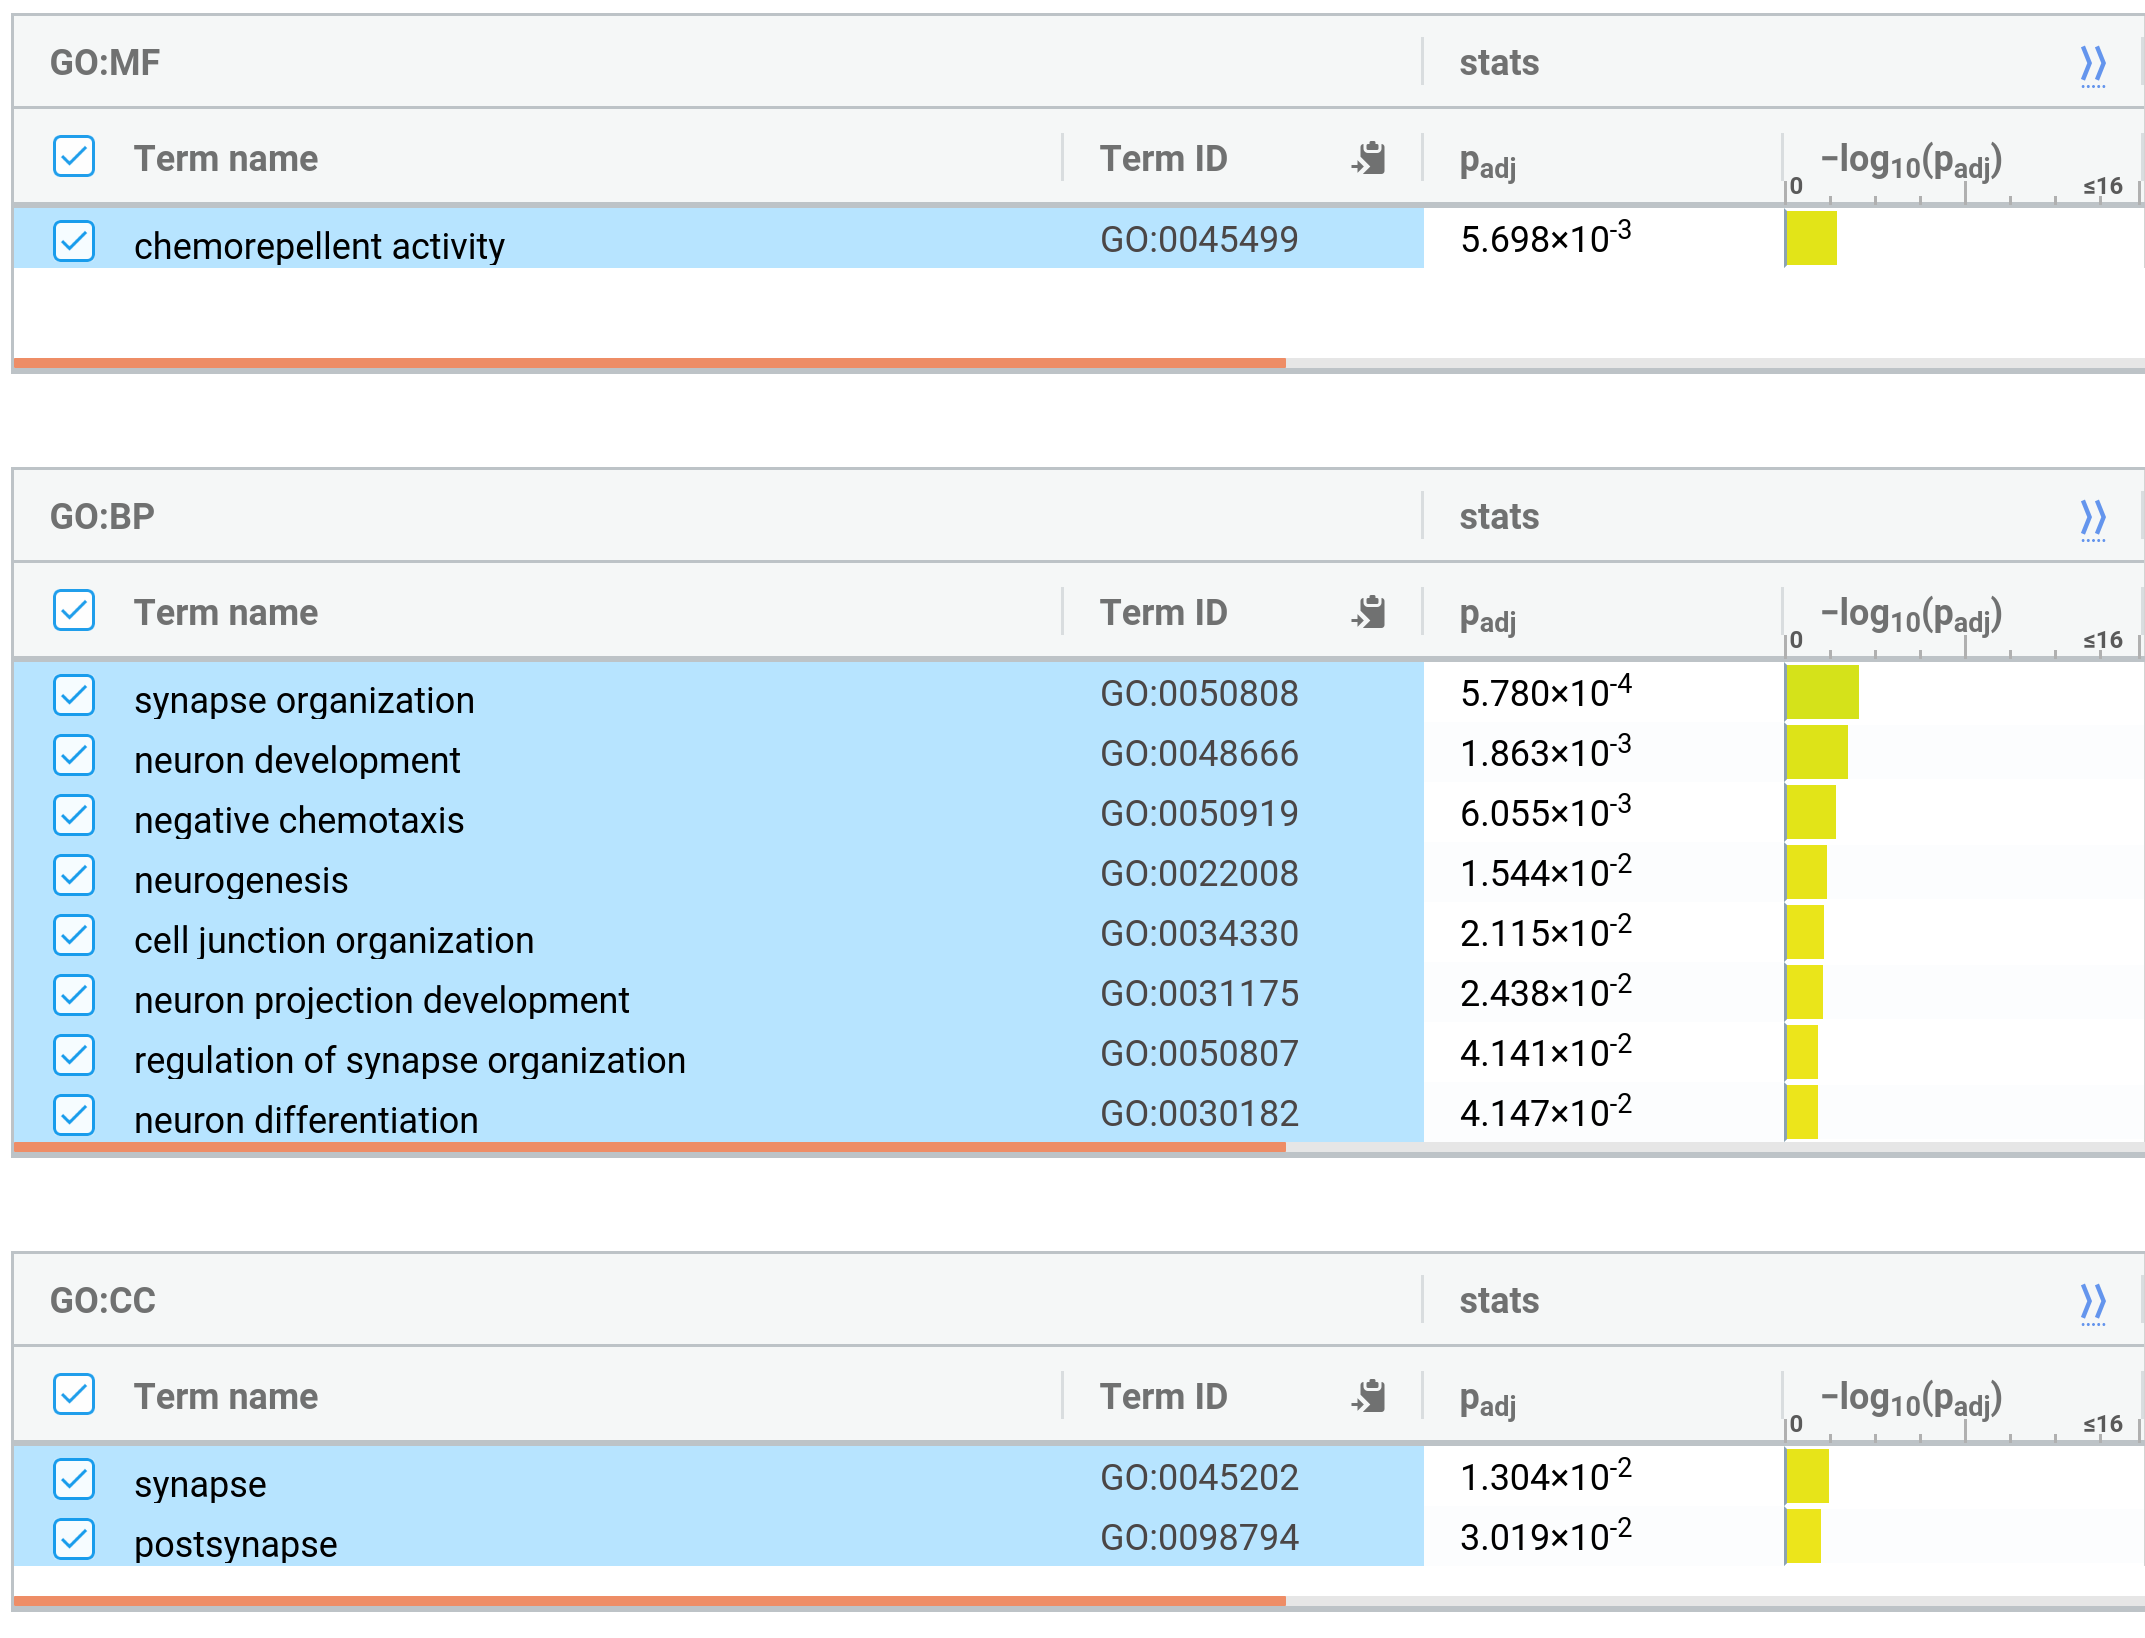
\includegraphics[width=\textwidth]{images/gprofiler/all_terms/ea2_all_terms.png}
    \caption{gProfiler Education\textsubscript{Replication}}
    \label{fig:gProfiler EA2}
\end{figure}

% Dataset name
% ea
% ID mapping
% 16 / 99 (unique) genes from your gene list were mapped to SynGO annotated genes.
% Settings
% experimental-evidence filtering is not enabled (default setting)
% Genes
% 14 genes have a Cellular Component annotation, 13 for Biological Processes. Note: a gene may have multiple annotations.
% Annotations
% 18 annotations against a Cellular Component, 25 for Biological Processes.
% Enrichment
% 1 Cellular Component terms are significantly enriched at 1% FDR (testing terms with at least three matching input genes), 4 for Biological Processes.
% Background
% "brain expressed" background set was selected, contains 18035 unique genes in total of which 1104 overlap with SynGO annotated genes.
% Readme commented out





\begin{table}[]
    \centering
    \begin{tabular}{llll}
    Biological Process & n & p & FDRq\\
    \hline
synapse organization*&	12&	6.94e-8	&3.47e-7\\
process in the synapse&	13&	4.14e-4	&1.03e-3\\
regulation of synapse organization	&3&	6.98e-4&	1.16e-3\\
synapse adhesion between pre- and post-synapse&	3	&1.35e-3&	1.68e-3\\
trans-synaptic signaling	&3	&0.0644&	0.0644\\
\\
 Cellular component & n & p & FDRq\\
 \hline
    synapse&14	&8.68e-4	&3.47e-3\\
postsynapse&	9	&5.40e-3	&0.0108       \\
         
\end{tabular}
    \caption{Enrichment of Gene Ontology terms using SynGO. SynGO only tests for biological process and cellular comparment. FDR q = adjusted significance level using FDR. Note the increased significance level despite correcting for multiple comparisons. For term Synapse Organisation (GO:0050808)* 12 genes (including child terms) in annotation, 286 in SynGO. }
    \label{tab:enrichment of gene ontology terms in syngo}
\end{table}
% SynGO data downloaded on 2020-9-8 12:2 @ https://www.syngoportal.org
% SynGO dataset version/release: 20180731

% Summary of your gene list
% ea
% 26 / 233 (unique) genes from your gene list were mapped to SynGO annotated genes.
% experimental-evidence filtering is not enabled (default setting)
% 23 genes have a Cellular Component annotation, 20 for Biological Processes. Note: a gene may have multiple annotations.
% 32 annotations against a Cellular Component, 39 for Biological Processes.
% 0 Cellular Component terms are significantly enriched at 1% FDR (testing terms with at least three matching input genes), 1 for Biological Processes.
% "brain expressed" background set was selected, contains 18035 unique genes in total of which 1104 overlap with SynGO annotated genes.

% "user_genelist_map_to_syngo_genes.xlsx" contains your input genelist (first column) together with the matching gene ID available in SynGO. If your input could not be matched to any SynGO annotated gene, the latter will be empty.
% "syngo_annotations_matching_user_input.xlsx" contains all available SynGO annotations that match your input genelist.
% "syngo_ontologies_with_annotations_matching_user_input.xlsx" contains all SynGO ontology terms, together with the Gene Set Enrichment Analysis (GSEA) results and all genes from these terms that match your input genelist.

% The JSON folder contains data in a format convenient for bioinformatic analysis.

% The SynGO_geneset_CC/BP.json files contain all SynGO annotated genes for each synaptic ontology term. On the first level of this nested list you can find 'direct' and 'aggregate' annotations, you will want to use the latter for geneset analyses as these contain (for each term) both the annotated genes for an ontology term and all genes annotated against (recursive) child terms. For instance, in the aggregate dataset the term 'presynapse' also contains all genes annotated against its child term 'active zone'. Further, note that we originally mapped the annotated proteins from various species to HGNC identifiers. The ensembl/entrez/MGI/RGD mappings (from HGNC ID) in these JSON files were provided by the genenames.org webservice, so if you focus on Ensembl genes consider mapping the HGNC IDs to the exact Ensembl build that you are using.

  \paragraph{Disease Enrichment}
  
  Disease enrichment in DisGeNet BeFree\cite{pinero2020disgenet} searched by ToppFun (part of the ToppGene suite) is found for intellectual disability (ID:C3714756) which is the top term. Twenty genes are found from 1219 in the annotation ($p=8.88\times10^{-7}$, FDR BH=0.00165). Intellectual disability was reported to be enriched by Okbay et al \cite{okbay2016genome} for a larger related sample using DEPICT. Six of the genes are found in the PSP (See fig~\ref{tab:Intellectual disability genes significant in EA2 found in PSP} for intellectual disability associated genes significant at GWGAS in Education\textsubscript{Replication} sample. ) Testing enrichment with PSP as background found no significantly enriched disease terms other than inflammatory bowel disease. (See supplemental material)\footnote{Enrichment in DisGeNet BeFree searched by toppfun of Intellectual disabilityID C3714756 	Intellectual Disability ; Source	DisGeNET BeFree ; p 	8.884E-7 ; FDR BH	1.648E-3; FR BY 	1.386E-2 ;Bonferroni	2.237E-3; Input 	20 	Total 1219}.See fig~\ref{tab:Intellectual disability genes significant in EA2 found in PSP} for intellectual disability associated genes significant at GWGAS in Education\textsubscript{Replication} sample. 
        % latex table generated in R 3.6.3 by xtable 1.8-4 package
        
% Sun Aug 23 12:35:02 2020
\begin{table}[ht]
\centering
\begin{tabular}{lll}
  \hline
Entrez Gene ID & Gene Symbol & Gene Name \\
  \hline
5144 & PDE4D & phosphodiesterase 4D  \\
  5662 & PSD & pleckstrin and Sec7 domain containing \\
  
  4137 & MAPT & microtubule associated protein tau \\ 
  4208 & MEF2C & myocyte enhancer factor 2C \\ 
  4744 & NEFH & neurofilament heavy \\
  257194 & NEGR1 & neuronal growth regulator 1 \\ 
   \hline
\end{tabular}
\caption{Intellectual disability genes significant in Education\textsubscript{Replication} genes found at GWGAS EA2 found in PSP.} 
\label{tab:Intellectual disability genes significant in EA2 found in PSP}
\end{table}
 
%  ToppFun with background PSP (new)
%  No GO terms
%  No phenotype
%  (4 out of 5 inflammatory bowel are in PSP)
        
        % GTEx
\subsection{Intelligence\textsubscript{Discovery} Ontology enrichment}


Gene set analysis of this sample, combined with the Intelligence\textsubscript{Discovery} sample and augmented by educational attainment data using MTAG is reported by Hill et al.  \cite{hill2019combined}. MAGMA GSA was carried out using 10,891 gene sets from Gene ontology, Reactome and MSigDB and using the Bonferroni correction for multiple comparisons (raw p required = 0.05/10891 = $4.59 \times 10^{-6}$)\footnote{Actual footnote: Bonferroni $\alpha$ from supplementary table 5 $2.75\times10^{-6}$
 which I calculate as 18182 comparisons the same as the correction for multiple comparisons in the gene level statistics. The paper however says a correction of 10891 which I calculate means the corrections is $4.59\times10^{-6}$. This does not however result in any extra significant sets.  27 gene sets are obtained using the FDR correction }. GSA revealed 8 quite large gene sets\footnote{See \url{source('~/RProjects/chapter2_checks/R/expected_gsa/ctg_size_plots.R')} for correlation between raw p value and gene size.} including neurogenesis (1355 genes) and genes associated with the synapse (717 genes), regulation of nervous system development (722 genes), neuron projection (989 genes), neuron differentiation (842 genes), CNS neuron differentiation (160 genes) and cell development (808 genes) (see table~\ref{tab:MAGMA GSA results from Hill et al.}). 


\begin{table}[ht]
\centering
\begin{tabular}{lrrrr}
  \hline
Gene set name & N genes in gene set & Beta & SE($\beta$) & p \\ 
  \hline
Neurogenesis  & 1355 & 0.20 & 0.05 & $5.59 \times 10^{-10}$ \\ 
  Regulation of nervous system development  & 722 & 0.23 & 0.05 & $4.02 \times 10^{-8}$ \\ 
  Regulation of cell development  & 808 & 0.22 & 0.04 & $7.38 \times 10^{-8}$ \\ 
  Neuron projection  & 898 & 0.20 & 0.04 & $2.07 \times 10^{-7}$ \\ 
  Central nervous system neuron differentiation  & 160 & 0.47 & 0.04 & $5.33 \times 10^{-7}$ \\ 
  Synapse  & 717 & 0.21 & 0.04 & $1.43 \times 10^{-6}$ \\ 
  Neuron differentiation  & 842 & 0.19 & 0.04 & $1.62 \times 10^{-6}$ \\ 
  Oligodendrocyte differentiation  & 1037 & 0.17 & 0.04 & $1.75 \times 10^{-6}$ \\ 
   \hline
\end{tabular}
\caption{MAGMA GSA significant sets from Hill et al. 2019 Bonferroni $\alpha$ from supplementary table 5 $2.75\times10^{-6}$ from \cite{hill2019combined}}
\label{tab:MAGMA GSA results from Hill et al.}
\end{table}

% % latex table generated in R 3.6.3 by xtable 1.8-4 package
% % Tue Sep 15 11:43:35 2020
% \begin{table}[ht]
% \centering
% \begin{tabular}{lrrrr}
%   \hline
% Gene.set.Name & n genes & Beta & SE & p \\ 
%   \hline
% Neurogenesis  & 1355 & 0.20 & 0.05 & $5.59 \times 10^{-10}$ \\ 
%   Regulation of nervous system development  & 722 & 0.23 & 0.05 & $4.02 \times 10^{-8}$ \\ 
%   Regulation of cell development  & 808 & 0.22 & 0.04 & $7.38 \times 10^{-8}$ \\ 
%   Neuron projection  & 898 & 0.20 & 0.04 & $2.07 \times 10^{-7}$ \\ 
%   Central nervous system neuron differentiation  & 160 & 0.47 & 0.04 & $5.33 \times 10^{-7}$ \\ 
%   Synapse  & 717 & 0.21 & 0.04 & $1.43 \times 10^{-6}$ \\ 
%   Neuron differentiation  & 842 & 0.19 & 0.04 & $1.62 \times 10^{-6}$ \\ % latex table generated in R 3.6.3 by xtable 1.8-4 package
% % Tue Sep 15 11:43:35 2020

% \end{tabular}
% \caption{MAGMA GSA significant sets from Hill et al. 2019 Bonferroni $\alpha$ from supplementary table 5 $2.75\times10^{-6}$ from \cite{hill2019combined}}
% \end{table}









\subsubsection{Intelligence Discovery Gene Ontology analysis PANTHER}
A modified list of gene symbols was again used  to ensure registration of genes using PANTHER \footnote{code at \url{source('~/RProjects/paper_xls_output/R/chapter_2/FUMA/edit_gene_table/UKBB_Int_FUMA2clipboard.R')} gene list at supplemental \url{/home/grant/Dropbox/paper_xls_data/Panther/input.txt}}.
% 197 genes - it is actually 196 genes saved actual genes in paperxls on dropbox

% 191 mapped with NCBI symbol
% Using only approved you get 179 (ie a lot of NCBI are not the approved ones)

% 194 uniquely mapped with symbol

% 196 of 192 uniquely mapped with hgnc id ie all are uniquely mapped and there are multiples but they are all there
% \url{source('~/RProjects/paper_xls_output/R/chapter_2/translate_sig_genes/ukbbint_NCBI_translate2.R')}\footnote{have put stop in at end of script and also there is function to toppgene which needs remov}
% Checked this again this is best using HGNC
% other is \url{source('~/RProjects/paper_xls_output/R/chapter_2/FUMA/edit_gene_table/UKBB_Int_FUMA2clipboard.R')}
% may find more DNA binding with this above 194 terms of 195

% This is confused the correct one is this one which uses gene symbol
% \url{source('~/RProjects/paper_xls_output/R/chapter_2/FUMA/edit_gene_table/UKBB_Int_FUMA2clipboard.R')}
% 11 missing using ENSG annotations
% Gene ID 3 unmapped
% GeneID:100132074 FOXO6
% GeneID:9753
% GeneID:3107

% MGEA5   OGA
% C10orf76    ARMH3
% CCDC101 SGF29
% PET112 GATB
% HIST1H3C H3C3 one of 25 synonyms
% HIST1H3I HIST1H3J one of 24 synonyms
% BAI1 ADGRB1 ADRGB1 Entrez to panther to id
% RP5-874C20.3 pseudogene entrz 7741 ZSCAN26 Entrez to panther to id\footnote{\url{source('~/RProjects/paper_xls_output/R/chapter_2/FUMA/edit_gene_table/UKBB_Int_FUMA2clipboard.R')}}

Only one biological process term was enriched: GO:0010468, regulation of gene expression (p=$4.78\times10^{-6}$, FDR BH=0.038; n in annotation 4907, n in set = 74). 
Seven molecular function terms were enriched the most specific and smallest being DNA binding GO:0003677 (n in annotation 2506, test 48, $p=1.01\times10^{-6}$ FDR=0.0016 (table~\ref{tab:GO molecular function complete Intelligence Discovery FDRover represenation only}))
\begin{table}[ht]
\centering
\begin{tabular}{llrrrrrr}
  \hline
GO & description & Ref & Test & E & Fold & P & FDR \\ 
  \hline
GO:0003677 & DNA binding  & 2506 & 48 & 23.1 & 2.08 & $1.01 \times 10^{-6}$ & 0.0016 \\ 
  GO:0003676 & nucleic acid binding  & 4034 & 64 & 37.1 & 1.72 & $5.51 \times 10^{-6}$ & 0.0052 \\ 
  GO:1901363 & heterocyclic compound binding  & 5999 & 83 & 55.2 & 1.50 & $2.73 \times 10^{-5}$ & 0.0185 \\ 
  GO:0097159 & organic cyclic compound binding  & 6086 & 83 & 56.0 & 1.48 & $4.27 \times 10^{-5}$ & 0.0254 \\ 
  GO:0005515 & protein binding  & 14109 & 159 & 129.9 & 1.22 & $3.77 \times 10^{-6}$ & 0.0045 \\ 
  GO:0005488 & binding  & 16469 & 174 & 151.7 & 1.15 & $2.39 \times 10^{-5}$ & 0.0190 \\ 
  GO:0003674 & molecular\_function  & 18321 & 188 & 168.7 & 1.11 & $9.41 \times 10^{-7}$ & 0.0022 \\ 
   \hline
\end{tabular}
\caption{GO molecular function complete Intelligence Discovery FDR over representation only shown.  Ref=reference set, test:number of genes being tested present in ontology term, E=expected number of genes, Fold= Fold change, P = raw p value, FDR = false discovery rate Benjamini and Hochberg. The most enriched term is DNA binding and all of the annotations are large (smallest is 2506 genes). \url{source('~/RProjects/paper_xls_output/R/chapter_2/make_PANTHER_tables/UKBB_int/make_Panther_table_GO_col_nounderFDR_int.R')}} 
\label{tab:GO molecular function complete Intelligence Discovery FDRover represenation only}
\end{table}

Twenty three cellular component terms were enriched. "DNA packaging complex" is the most enriched term using FDR BH 85 terms in annotation, 9 appear in the significant genes found at GWGAS, (GO:0044815), FDR=0.0002. The second most enriched term is the child term nucleosome, GO:000786, FDR 0.0007 (see figure~\ref{fig:UKBiobank int significant genes at GWGAS. PANTHER GO enrichment Cellular component. FDR correction. Screenshot for hierarchy} and table~\ref{tab:GO cellular component complete Intelligence Discovery FDRover represenation only}). Twenty seven genes (from 1383) are enriched for the cellular component term synapse (GO:0045202;FDR 0.0199).
% \paragraph{MF}   3 terms most significant is Very general term GO:0003677 DNA binding 0.0067 p Bonf 0.0029 p FDR Fold change 2.02

% latex table generated in R 3.6.3 by xtable 1.8-4 package
% Tue Sep 15 17:42:51 2020


\begin{figure}
    \centering
    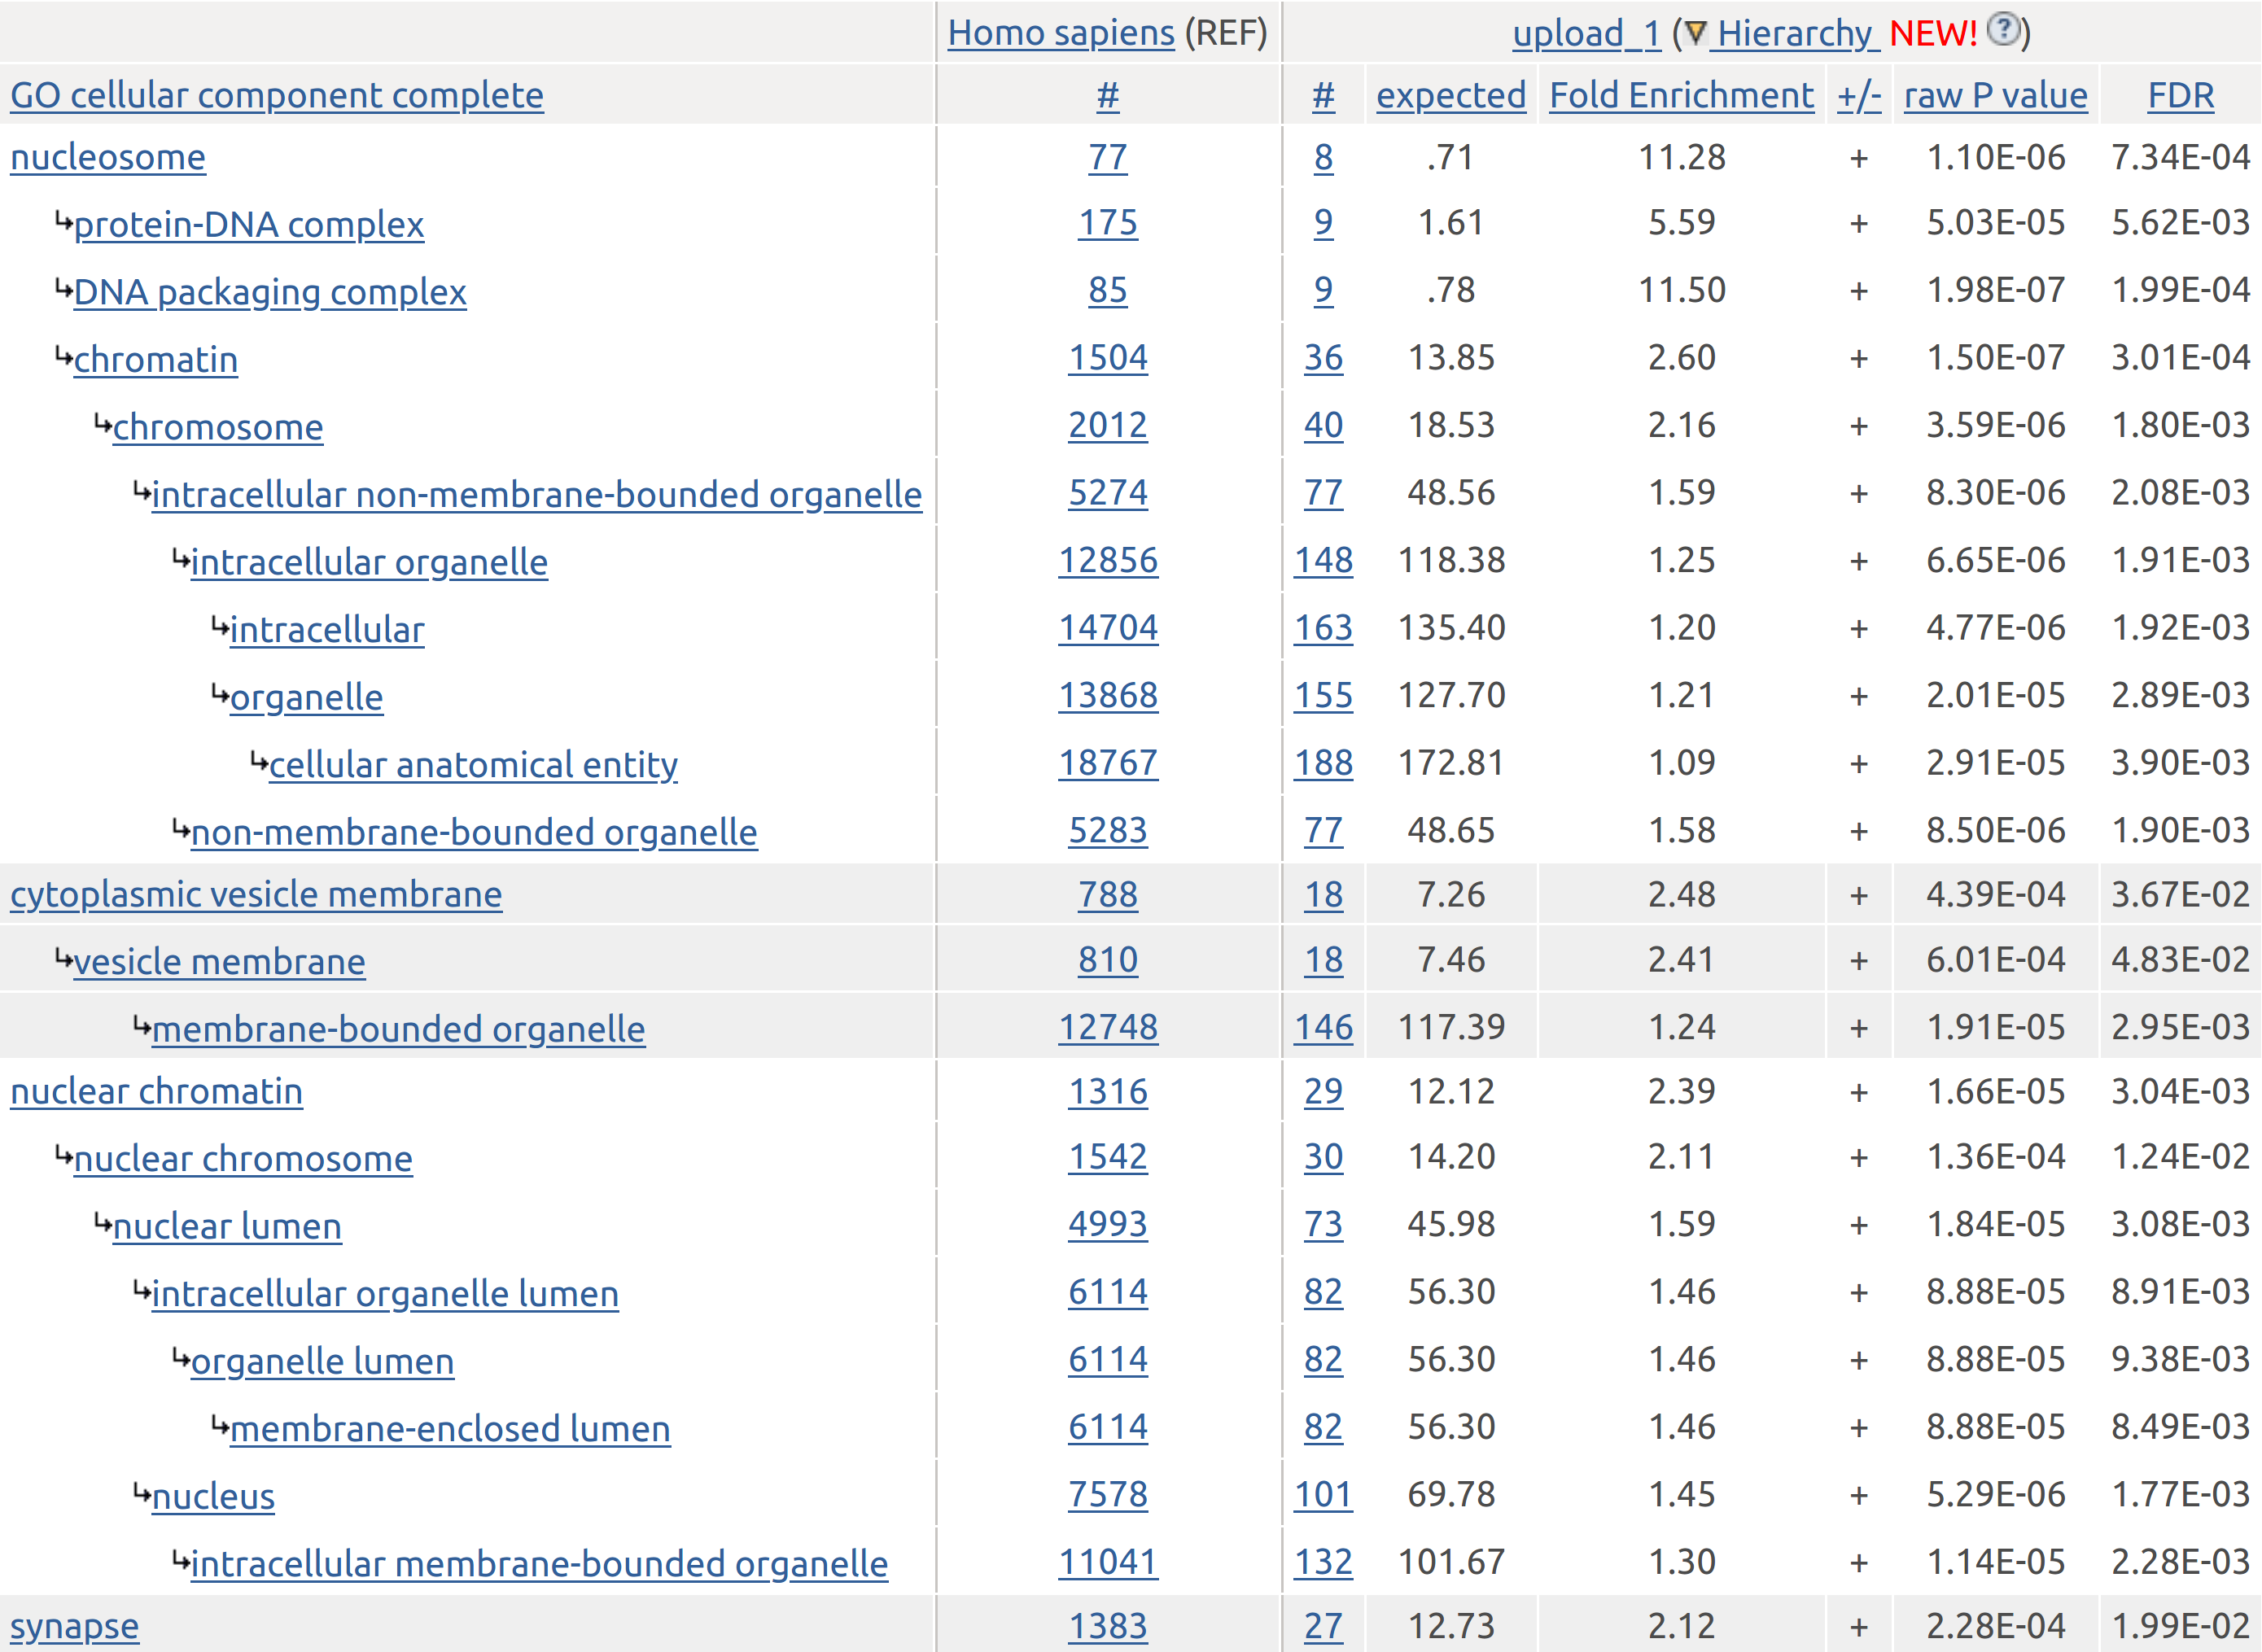
\includegraphics[width=\textwidth]{images/chapter2/strontium/ukbbint_cc.png}
        \caption{UKBiobank intelligence significant genes at GWGAS. PANTHER GO enrichment Cellular component. FDR correction. Screenshot for hierarchy. Matches table check table~\ref{tab:GO cellular component complete Intelligence Discovery FDRover represenation only} }
    \label{fig:UKBiobank int significant genes at GWGAS. PANTHER GO enrichment Cellular component. FDR correction. Screenshot for hierarchy}
\end{figure}

%Removed table tab:GO molecular function complete Intelligence Discovery FDRover represenation only replaces more accurate id changes

% latex table generated in R 3.6.3 by xtable 1.8-4 package
% Sun Aug 30 16:02:36 2020
% \begin{table}[ht]
% \centering
% \begin{tabular}{llrrrrrr}
%   \hline
% GO  & description MF & Ref & Test & E & Fold & P & FDR \\ 
%   \hline
% GO:0003677 & DNA binding  & 2486 & 47 & 23.2 & 2.02 & $2.350 \times 10^{-6}$ & 0.003 \\ 
%   \hspace{2mm}GO:0003676 & \hspace{2mm}nucleic acid binding  & 4024 & 63 & 37.6 & 1.67 & $1.630 \times 10^{-5}$ & 0.015 \\ 
%   \hspace{4mm}GO:0097159 & organic cyclic compound binding  & 6075 & 83 & 56.8 & 1.46 & $7.060 \times 10^{-5}$ & 0.042 \\ 
%   \hspace{4mm}GO:1901363 & heterocyclic compound binding  & 5987 & 83 & 56.0 & 1.48 & $4.490 \times 10^{-5}$ & 0.030 \\ 
  
%   GO:0005515 & protein binding  & 14110 & 162 & 132.0 & 1.23 & $2.070 \times 10^{-6}$ & 0.003 \\ 
   
% %   GO:0003674 & molecular\_function  & 18318 & 191 & 171.3 & 1.11 & $6.440 \times 10^{-7}$ & 0.002 \\ 
% %   UNCLASSIFIED & Unclassified  & 2533 & 4 & 23.7 & 0.17 & $6.440 \times 10^{-7}$ & 0.003 \\ 
%   \hline
% \end{tabular}
% \caption{GO molecular function complete Intelligence\textsubscript{Discovery} FDR over represenation only  Ref reference set, test:number of genes being tested present in ontology termE expected number of genes being tested present in ontology term, Fold= Fold change, = raw p value, FDR = false discovery rate} 
% \label{tab:GO molecular function complete Intelligence DIscovery FDRover represenation only}
% \end{table}



% \paragraph{CC}

% latex table generated in R 3.6.3 by xtable 1.8-4 package
% Tue Sep 15 17:39:45 2020

\begin{table}[ht]
\centering
\begin{adjustbox}{width=\textwidth}

\begin{tabular}{llrrrrrr}
  \hline
GO & description & Ref & Test & E & Fold & P & FDR \\ 
  \hline
GO:0044815 & DNA packaging complex  & 85 & 9 & 0.8 & 11.50 & $1.98 \times 10^{-7}$ & 0.0002 \\ 
  GO:0000786 & nucleosome  & 77 & 8 & 0.7 & 11.28 & $1.10 \times 10^{-6}$ & 0.0007 \\ 
  GO:0032993 & protein-DNA complex  & 175 & 9 & 1.6 & 5.59 & $5.03 \times 10^{-5}$ & 0.0056 \\ 
  GO:0000785 & chromatin  & 1504 & 36 & 13.8 & 2.60 & $1.50 \times 10^{-7}$ & 0.0003 \\ 
  GO:0030659 & cytoplasmic vesicle membrane  & 788 & 18 & 7.3 & 2.48 & $4.39 \times 10^{-4}$ & 0.0367 \\ 
  GO:0012506 & vesicle membrane  & 810 & 18 & 7.5 & 2.41 & $6.01 \times 10^{-4}$ & 0.0483 \\ 
  GO:0000790 & nuclear chromatin  & 1316 & 29 & 12.1 & 2.39 & $1.66 \times 10^{-5}$ & 0.0030 \\ 
  GO:0005694 & chromosome  & 2012 & 40 & 18.5 & 2.16 & $3.59 \times 10^{-6}$ & 0.0018 \\ 
  GO:0045202 & synapse  & 1383 & 27 & 12.7 & 2.12 & $2.28 \times 10^{-4}$ & 0.0199 \\ 
  GO:0000228 & nuclear chromosome  & 1542 & 30 & 14.2 & 2.11 & $1.36 \times 10^{-4}$ & 0.0124 \\ 
  GO:0031981 & nuclear lumen  & 4993 & 73 & 46.0 & 1.59 & $1.84 \times 10^{-5}$ & 0.0031 \\ 
  GO:0043232 & intracellular non-membrane-bounded organelle  & 5274 & 77 & 48.6 & 1.59 & $8.30 \times 10^{-6}$ & 0.0021 \\ 
  GO:0043228 & non-membrane-bounded organelle  & 5283 & 77 & 48.6 & 1.58 & $8.50 \times 10^{-6}$ & 0.0019 \\ 
  GO:0043233 & organelle lumen  & 6114 & 82 & 56.3 & 1.46 & $8.88 \times 10^{-5}$ & 0.0094 \\ 
  GO:0070013 & intracellular organelle lumen  & 6114 & 82 & 56.3 & 1.46 & $8.88 \times 10^{-5}$ & 0.0089 \\ 
  GO:0031974 & membrane-enclosed lumen  & 6114 & 82 & 56.3 & 1.46 & $8.88 \times 10^{-5}$ & 0.0085 \\ 
  GO:0005634 & nucleus  & 7578 & 101 & 69.8 & 1.45 & $5.29 \times 10^{-6}$ & 0.0018 \\ 
  GO:0043231 & intracellular membrane-bounded organelle  & 11041 & 132 & 101.7 & 1.30 & $1.14 \times 10^{-5}$ & 0.0023 \\ 
  GO:0043229 & intracellular organelle  & 12856 & 148 & 118.4 & 1.25 & $6.65 \times 10^{-6}$ & 0.0019 \\ 
  GO:0043227 & membrane-bounded organelle  & 12748 & 146 & 117.4 & 1.24 & $1.91 \times 10^{-5}$ & 0.0029 \\ 
  GO:0043226 & organelle  & 13868 & 155 & 127.7 & 1.21 & $2.01 \times 10^{-5}$ & 0.0029 \\ 
  GO:0005622 & intracellular  & 14704 & 163 & 135.4 & 1.20 & $4.77 \times 10^{-6}$ & 0.0019 \\ 
  GO:0110165 & cellular anatomical entity  & 18767 & 188 & 172.8 & 1.09 & $2.91 \times 10^{-5}$ & 0.0039 \\ 
  GO:0005575 & cellular\_component  & 18951 & 189 & 174.5 & 1.08 & $3.56 \times 10^{-5}$ & 0.0045 \\ 
  UNCLASSIFIED & Unclassified  & 1900 & 3 & 17.5 & 0.17 & $3.56 \times 10^{-5}$ & 0.0042 \\ 
   \hline
\end{tabular}
\end{adjustbox}
    \caption{GO cellular component complete Intelligence Discovery FDRover represenation only  Ref reference set, test:number of genes being tested present in ontology termE expected number of genes being tested present in ontology term, Fold= Fold changeP = raw p value, FDR = false discovery rate\url{source('~/RProjects/paper_xls_output/R/chapter_2/make_PANTHER_tables/UKBB_int/make_Panther_table_GO_col_nounderFDR_int.R')}Checked GR 20/09/20} 
\label{tab:GO cellular component complete Intelligence Discovery FDRover represenation only}
\end{table}
% % Sun Aug 30 16:17:46 2020
% \begin{table}[ht]
% \centering
% \begin{tabular}{llrrrrll}
%   \toprule
% GO ID& Description & Ref & Test & E & Fold & P & FDR \\ 
%   \midrule
%     GO:0000786 & nucleosome  & 77 & 8 & 0.7 & 11.11 & $1.23 \times 10^{-6}$ & 0.0012 \\ 
%   \hspace{2mm}\ding{213}  GO:0032993 & protein-DNA complex  & 175 & 9 & 1.6 & 5.50 & $5.67 \times 10^{-5}$ & 0.0095 \\ 
%  \hspace{2mm}\ding{213}  GO:0044815 & DNA packaging complex  & 85 & 9 & 0.8 & 11.32 & $2.26 \times 10^{-7}$ & 0.0005 \\ 

%   \hspace{2mm}\ding{213}   GO:0000785 & chromatin  & 1229 & 25 & 11.5 & 2.18 & $3.29 \times 10^{-4}$ & 0.0472 \\ 
%   \hspace{4mm}\ding{221}   GO:0043229 & intracellular organelle  & 12843 & 150 & 120.1 & 1.25 & $7.58 \times 10^{-6}$ & 0.0030 \\ 
%   \hspace{6mm}\ding{235}   GO:0005622 & intracellular  & 14693 & 165 & 137.4 & 1.20 & $5.80 \times 10^{-6}$ & 0.0039 \\ 
%   \hspace{6mm}\ding{235}  GO:0043226 & organelle  & 13859 & 157 & 129.6 & 1.21 & $2.35 \times 10^{-5}$ & 0.0059 \\ 
%   \hspace{8mm}\ding{233} GO:0110165 & cellular anatomical entity  & 18761 & 191 & 175.4 & 1.09 & $3.060 \times 10^{-5}$ & 0.0056 \\ 
   
   
%   GO:0031981 & nuclear lumen  & 4786 & 68 & 44.8 & 1.52 & $1.60 \times 10^{-4}$ & 0.0247 \\ 
%   \hspace{2mm}\ding{213} GO:0005634 & nucleus  & 7567 & 102 & 70.8 & 1.44 & $6.21 \times 10^{-6}$ & 0.0031 \\ 
%   \hspace{4mm}\ding{221} GO:0043231 & \makecell{intracellular membrane-bounded\\ organelle}  & 11028 & 134 & 103.1 & 1.30 & $9.470 \times 10^{-6}$ & 0.0032 \\ 
  
  
%   \hspace{6mm}\ding{235} GO:0043227 & membrane-bounded organelle  & 12734 & 148 & 119.1 & 1.24 & $1.620 \times 10^{-5}$ & 0.0046 \\ 
  
 
  
% %   GO:0005575 & cellular\_component  & 18946 & 192 & 177.2 & 1.08 & $2.420 \times 10^{-5}$ & 0.0054 \\ 
  
% %   UNCLASSIFIED & Unclassified  & 1905 & 3 & 17.8 & 0.17 & $2.420 \times 10^{-5}$ & 0.0049 \\ 
%   \bottomrule
% \end{tabular}
% \caption{Gene Ontology Enrichment in PANTHER using cellular component complete for significant genes at GWGAS for Intelligence\textsubscript{Discovery FDR} sample. Over represenation of terms only shown. Indendation shows depth of term in GO DAG, least indented deepest term.   Ref reference set, test:number of genes being tested present in ontology term E expected number of genes being tested present in ontology term, Fold= Fold changeP = raw p value, FDR = false discovery rate,} 
% \label{tab:GO cellular component complete Intelligence Discovery FDRover represenation only}
% \end{table}

% latex table generated in R 3.6.3 by xtable 1.8-4 package
Two SLIM molecular function terms were enriched: transcription factor binding (FDR 0.0145) and DNA binding (FDR 0.0189)
table~\ref{tab:ukbbint mf slim panther} continuing the finding of terms related to transcription.
  	\begin{table}[]
  	    \centering
  	    \begin{tabular}{llllllll}
  	    \toprule
  	GO-Slim Molecular Function &	n annotation & n&		expected 	&fold  &	 P value& 	FDR\\
  	   \midrule
transcription factor binding &	203 &	10& 	1.87 &	5.35  &	2.73E-05 &	1.45E-02\\
DNA binding &	806 &	20& 	7.42& 	2.69& 		7.11E-05& 	1.89E-02\\
\bottomrule
  	    \end{tabular}
  	    \caption{UKBB int MF SLIM PANTHER. n annotation= number of genes in annotation; n= number of significant genes; fold = fold change; FDR = false discovery rate Benjamini and Hochberg}
  	    \label{tab:ukbbint mf slim panther}
  	\end{table}
  	
Eighteen SLIM Biological process terms are over represented figure~\ref{fig:ukbb_int_BP_GO_SLIM} for a screenshot that shows the hierarchy of terms. The terms are again related to transcription, including those related to nucleosome assembly, DNA packaging and those regulating RNA polymerase. No SLIM cellular component was enriched. 

\begin{figure}
    \centering
    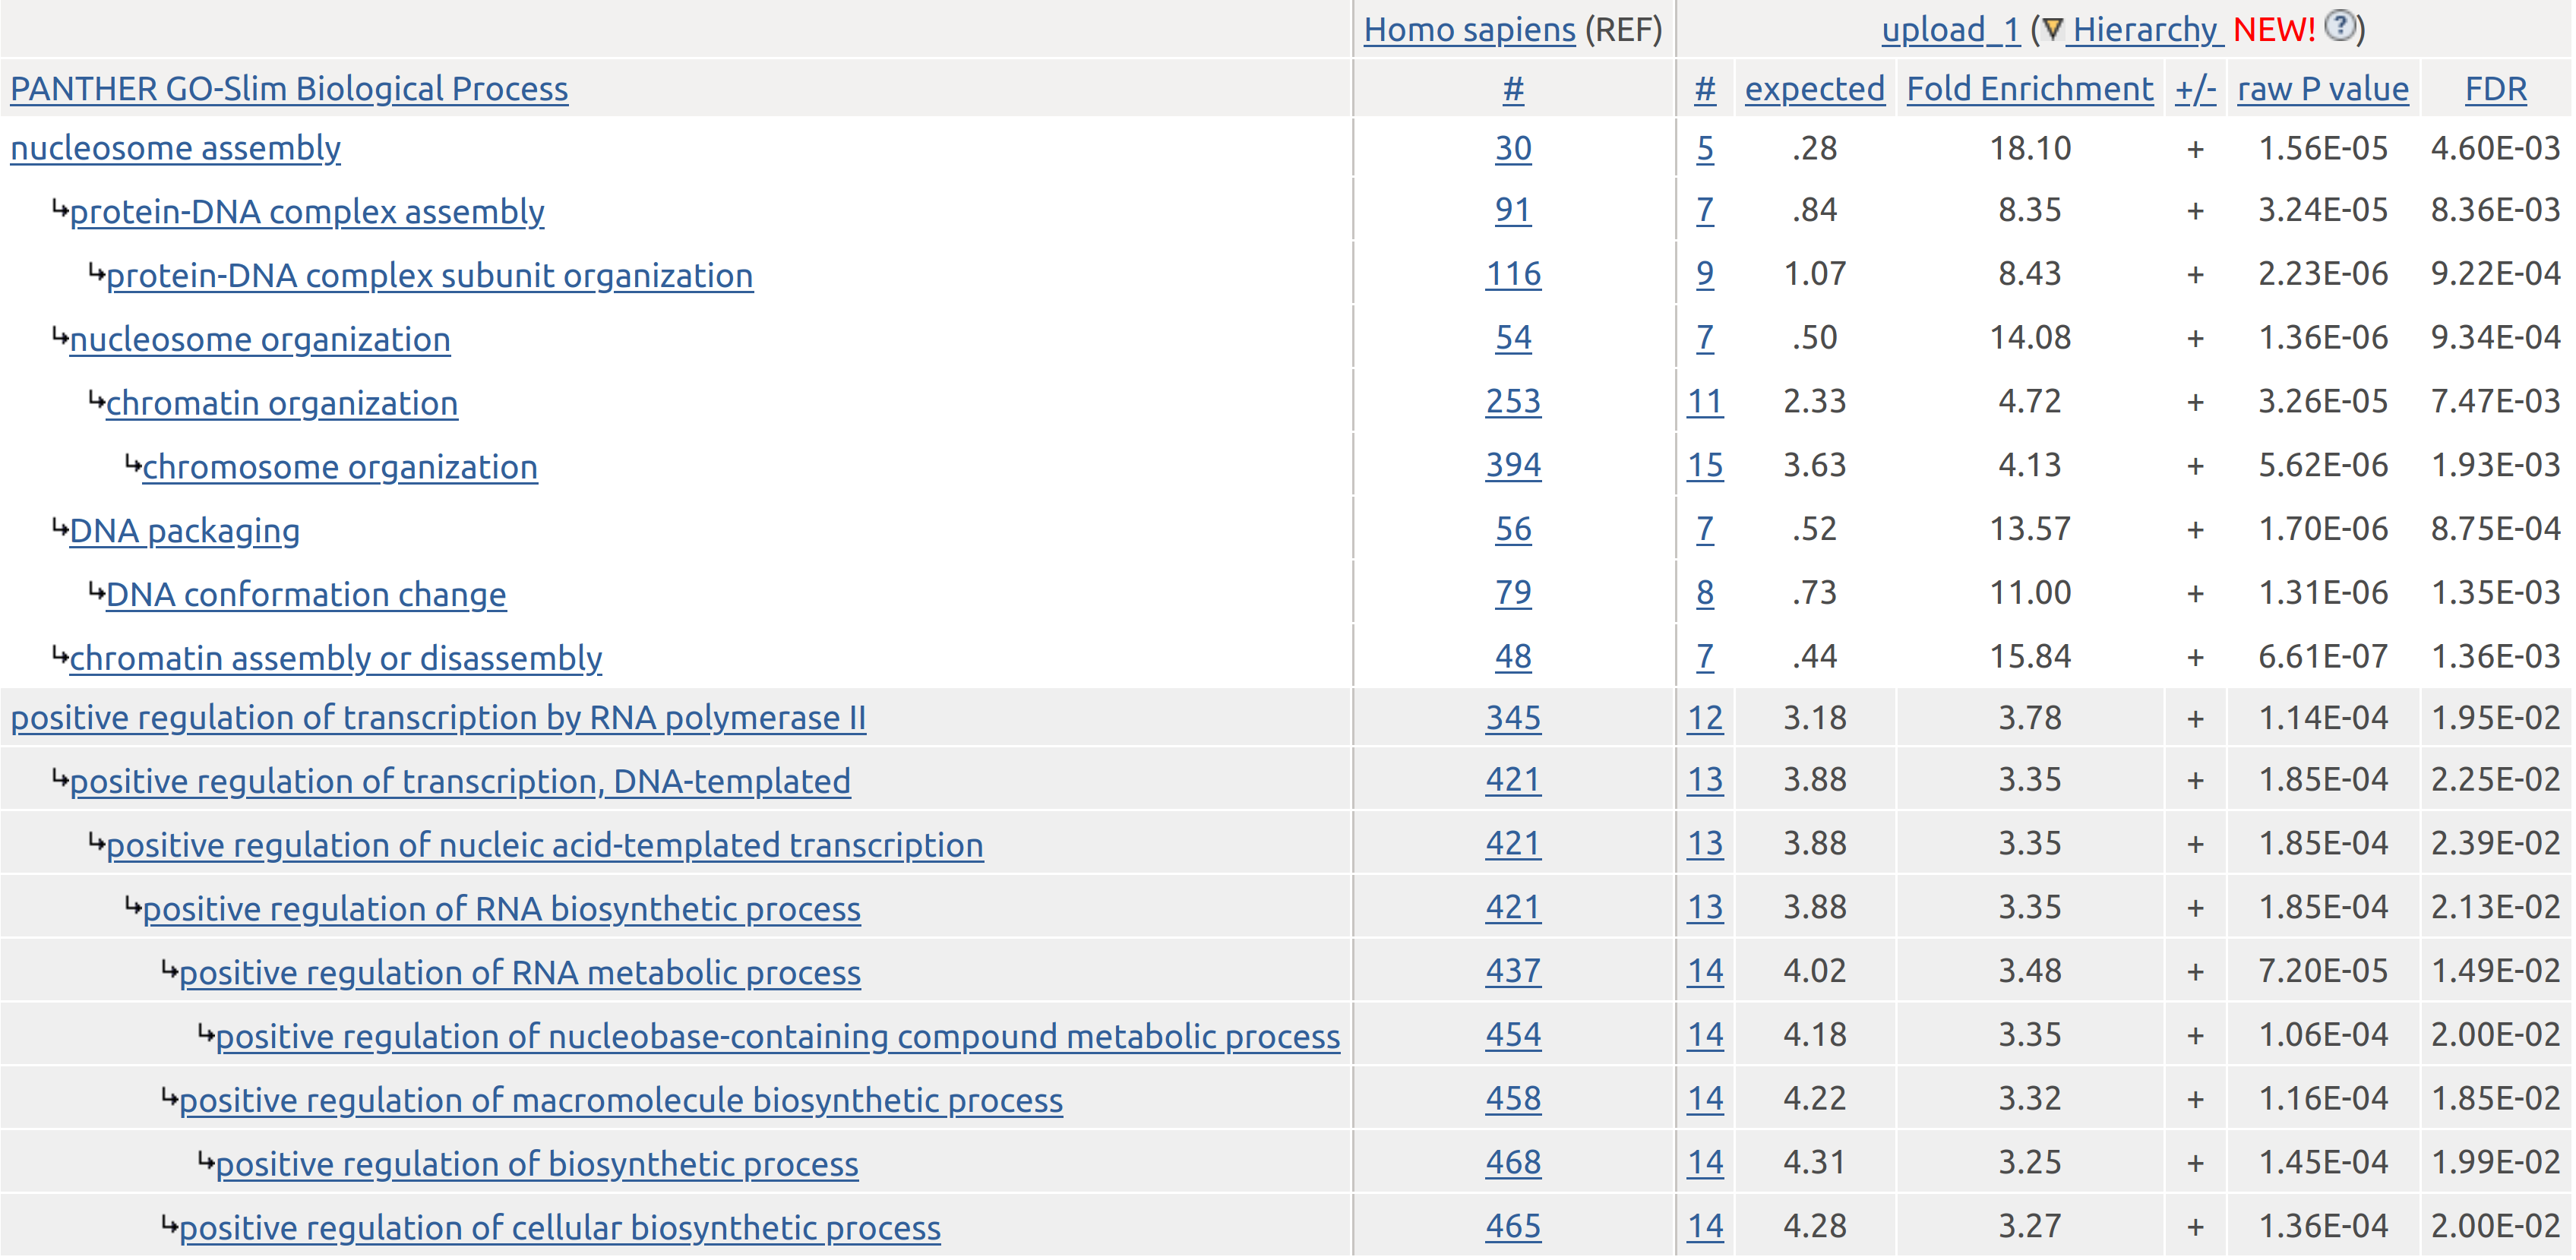
\includegraphics[width=\textwidth]{images/chapter2/large_screenshots/int_discovery_large_bp_slim_panther.png}
    \caption{Int discovery large screenshot BP SLIM. Text file at \url{/home/grant/Dropbox/paper_xls_data/Panther/output_txt/ukbbint/bp_all_slim_checked_with_image_matches_current_image_overleaf.txt}}
    \label{fig:ukbb_int_BP_GO_SLIM}
\end{figure}

PANTHER protein classes were enriched for histone and DNA binding protein (see table~\ref{tab:intelligence discovery panther protein class}.

\begin{table}[]
    \centering
    \begin{tabular}{llllllll}
      PANTHER Protein Class &	n annot & n sample & 	expected& 	Fold &  P & 	FDR\\
      \hline
histone &	55& 	7 &	.51& 	13.82 &	 	1.52E-06 &	2.96E-04\\
DNA binding protein &	227& 	9 &	2.09 &	4.31 &	3.30E-04 &	3.22E-02     \\
         
    \end{tabular}
    \caption{PANTHER protein class enrichment Intelligence\textsubscript{Discovery}}
    \label{tab:intelligence discovery panther protein class}
\end{table}


 Chromatin, RNA polymerase and Pre-Notch expression and processing were among the most enriched of the 98 Reactome pathways tested using PANTHER with 98 terms in total with FDR $<$ 0.05(See figure~\ref{fig:UKBB int topp reac}).
\footnote{table at \url{source('~/RProjects/paper_xls_output/R/chapter_2/make_PANTHER_tables/UKBB_int/make_Panther_table_GO_col_nounderFDRreactome.R')} includes reactome iids}



% \begin{figure}
%     \centering
%     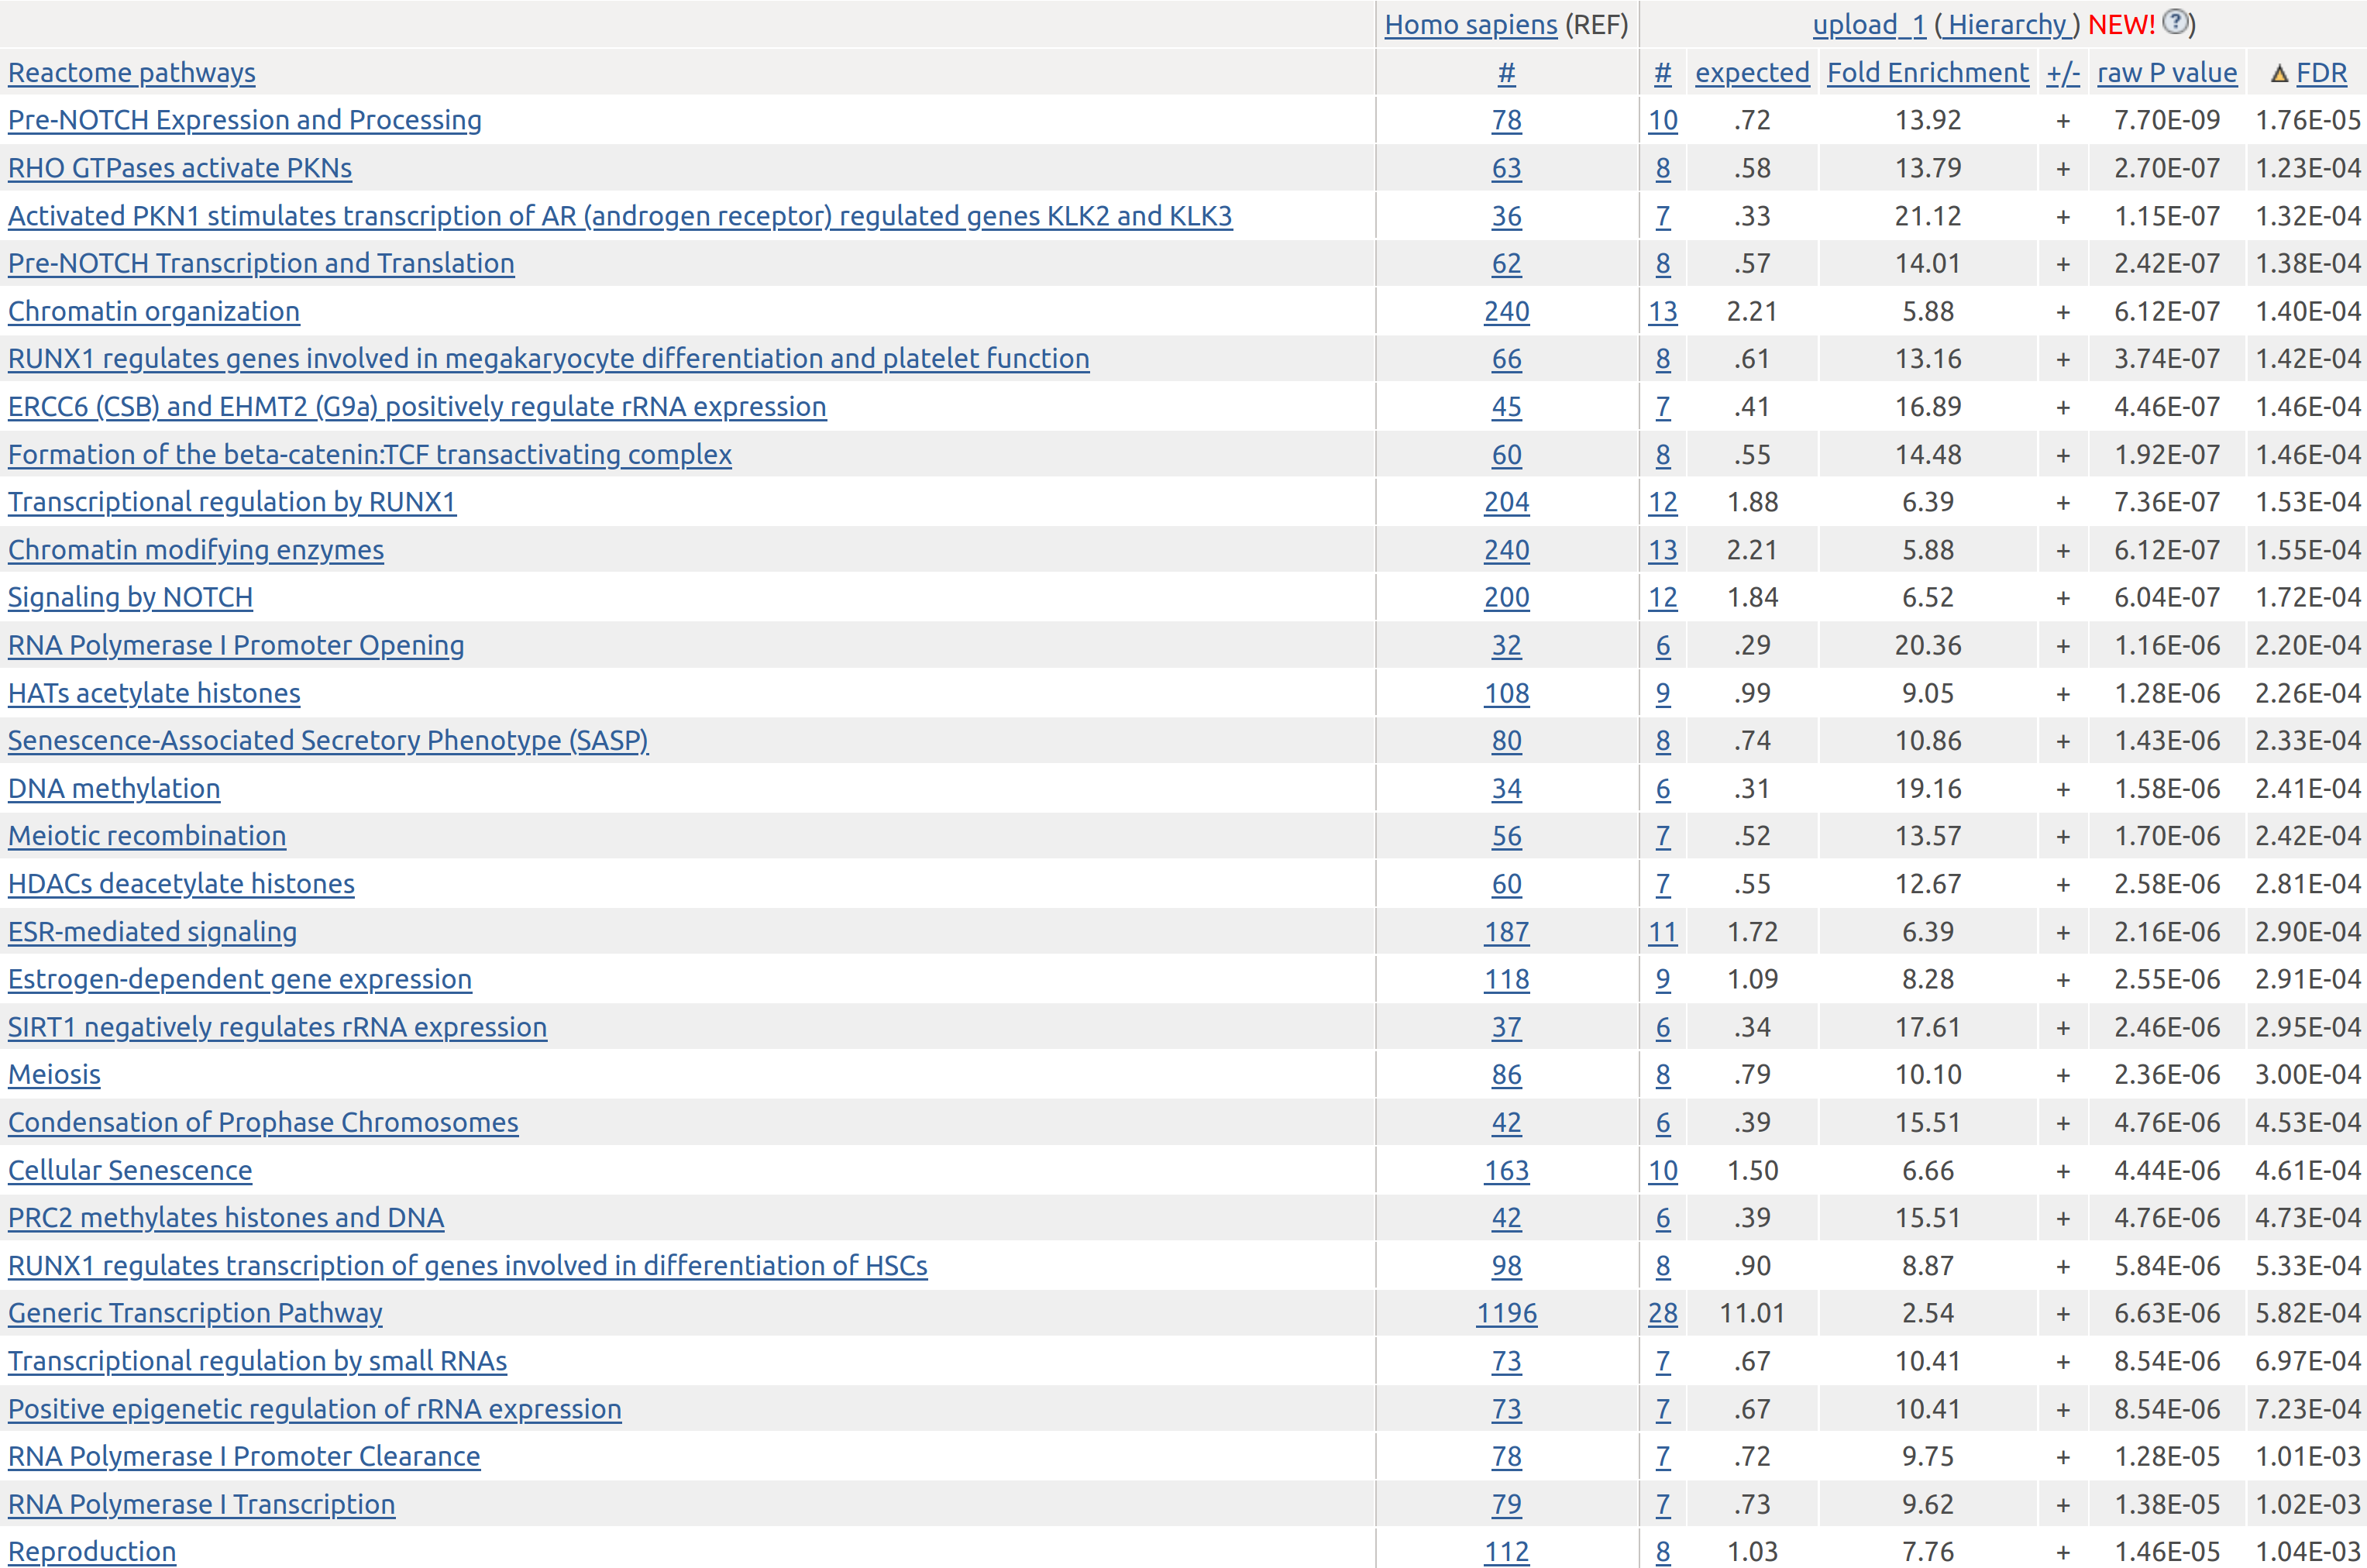
\includegraphics[width=\textwidth]{images/chapter2/large_screenshots/int_discovery_large_reactome_panther1.png}
%     \caption{UKBB int top reactome pathways Panther}
%     \label{fig:UKBB int topp reac}
% \end{figure}

\begin{figure}
    \centering
    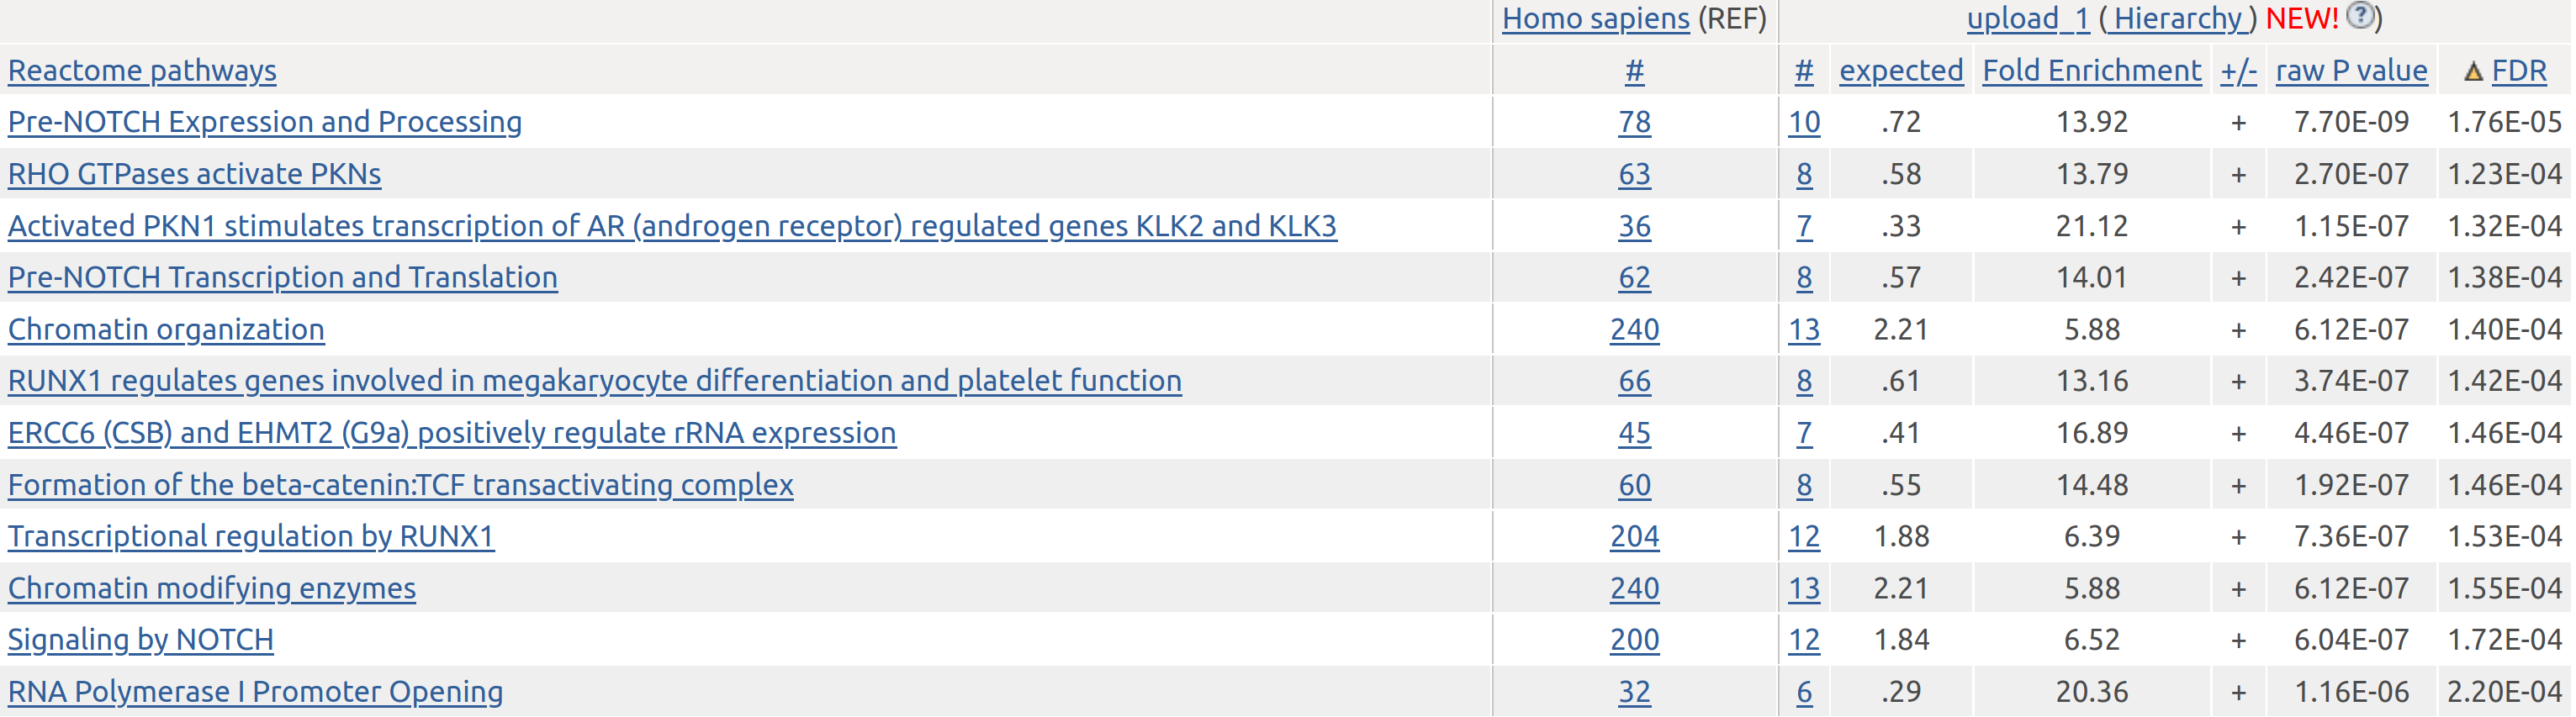
\includegraphics[width=\textwidth]{images/chapter2/large_screenshots/int_discovery_large_reactome_panther3.png}
    \caption{UKBB int top reactome pathways PANTHER}
    \label{fig:UKBB int topp reac}
\end{figure}

g:Profiler results are shown in figure~\ref{fig:gprofiler intelligence discovery} and are a good summary of the main sources of enrichment found in ToppGene and PANTHER (Transcription related and nucleosome assembly). 

\begin{figure}
    \centering
    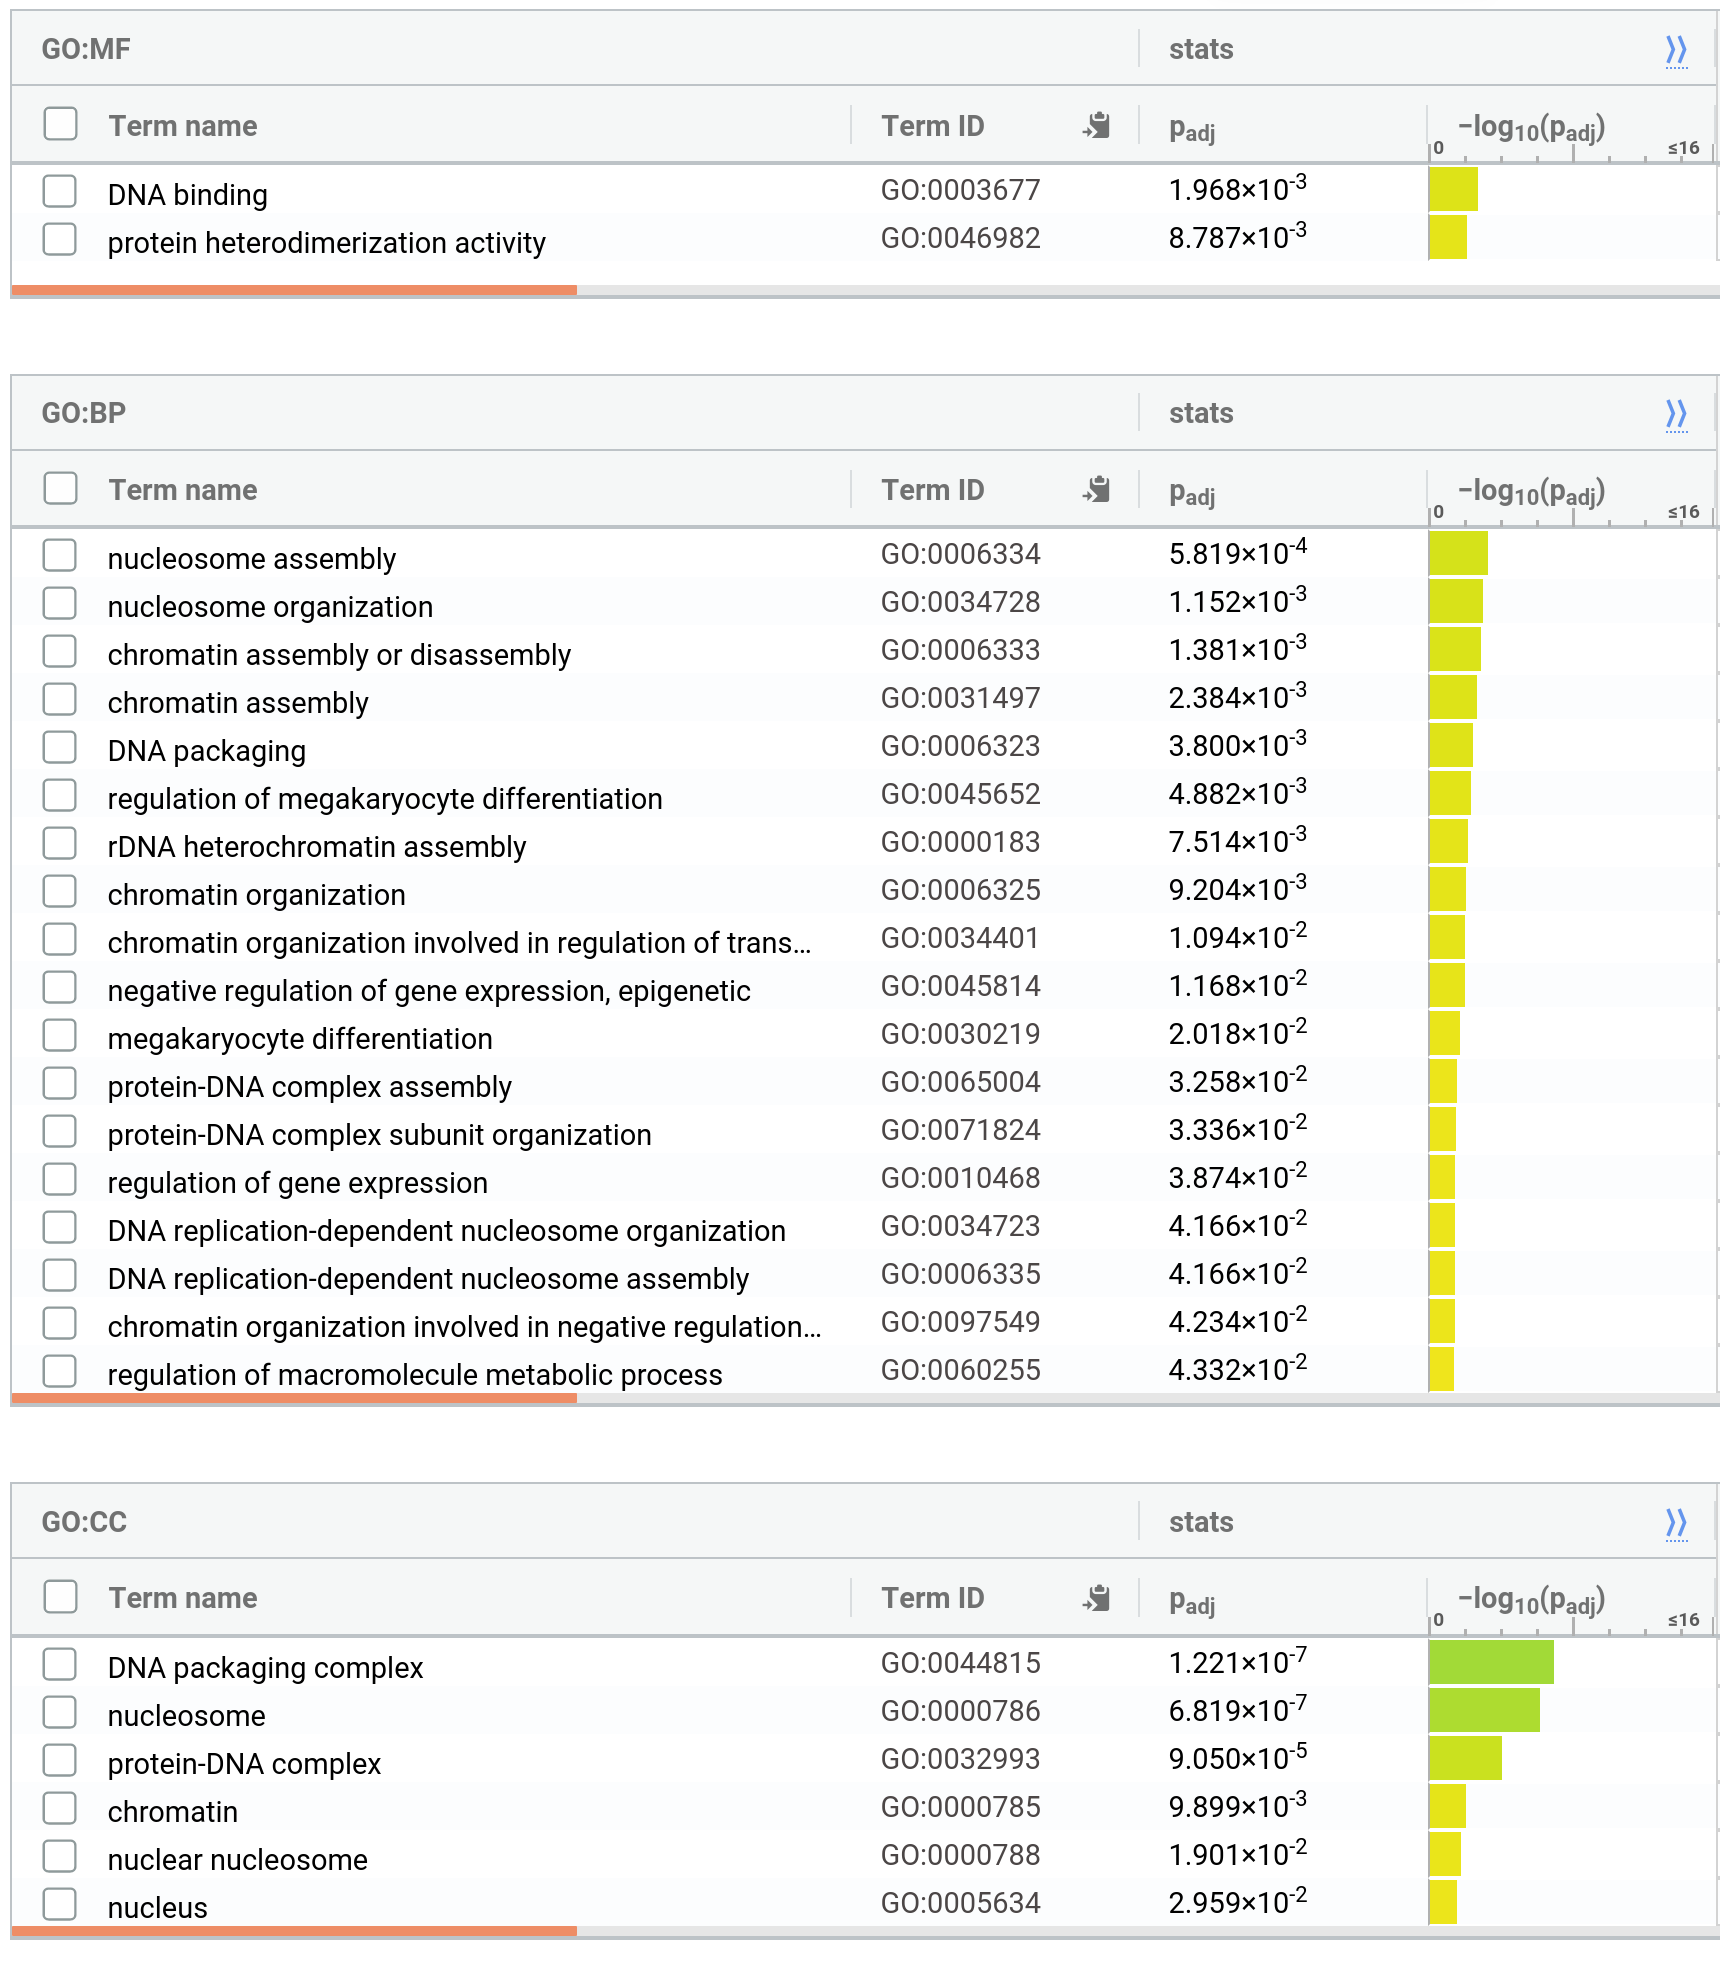
\includegraphics[width=\textwidth]{images/gprofiler/all_terms/ukbbint_all_terms.png}
    \caption{g:profiler GO enrichment results for significant genes found at GWGAS for the Intelligence\textsubscript{Discovery} sample}
    \label{fig:gprofiler intelligence discovery}
\end{figure}

\subsubsection{SynGO Intelligence Discovery}

No significant terms were enriched for cellular component. The terms enriched for biological process are in figure~\ref{tab:SynGO Enrichment UKBB intelligence significant genes. FDR}. Although the FDR values are higher than found in the Education\textsubscript{Discovery}, some synaptic terms are found to be enriched by using a limited ontology. 

\begin{table}[]
    \centering
    \begin{tabular}{llll}
    \toprule
      Term   & n & P & FDR q  \\
      \midrule
       synapse organization&	11&	$1.81\times10^{-4}$&	$1.81\times10^{-3}$\\
process in the synapse&	17&	3.01e-3&	0.0107\\
regulation of synapse organization&	3&	3.93e-3&	0.0107\\
modification of postsynaptic structure&	3	&4.29e-3	&0.0107\\
regulation of presynaptic membrane potential&	3&	9.62e-3&	0.0192  \\ 
\bottomrule
    \end{tabular}
    \caption{SynGO Enrichment Intelligence\textsubscript{Discovery} sample of genome wide significant genes at GWGAS. Correction for multiple comparisons using FDR. Background gene set is all brain expressed genes.}
    \label{tab:SynGO Enrichment UKBB intelligence significant genes. FDR}
\end{table}



% % latex table generated in R 3.6.3 by xtable 1.8-4 package
% % Sun Aug 30 16:17:46 2020
% \begin{table}[ht]
% \centering
% \begin{tabular}{llrrrrll}
%   \toprule
% GO ID& Description & Ref & Test & E & Fold & P & FDR \\ 
%   \midrule
%     GO:0000786 & nucleosome  & 77 & 8 & 0.7 & 11.11 & $1.23 \times 10^{-6}$ & 0.0012 \\ 
%   \hspace{2mm}\ding{213}  GO:0032993 & protein-DNA complex  & 175 & 9 & 1.6 & 5.50 & $5.67 \times 10^{-5}$ & 0.0095 \\ 
%  \hspace{2mm}\ding{213}  GO:0044815 & DNA packaging complex  & 85 & 9 & 0.8 & 11.32 & $2.26 \times 10^{-7}$ & 0.0005 \\ 

%   \hspace{2mm}\ding{213}   GO:0000785 & chromatin  & 1229 & 25 & 11.5 & 2.18 & $3.29 \times 10^{-4}$ & 0.0472 \\ 
%   \hspace{4mm}\ding{221}   GO:0043229 & intracellular organelle  & 12843 & 150 & 120.1 & 1.25 & $7.58 \times 10^{-6}$ & 0.0030 \\ 
%   \hspace{6mm}\ding{235}   GO:0005622 & intracellular  & 14693 & 165 & 137.4 & 1.20 & $5.80 \times 10^{-6}$ & 0.0039 \\ 
%   \hspace{6mm}\ding{235}  GO:0043226 & organelle  & 13859 & 157 & 129.6 & 1.21 & $2.35 \times 10^{-5}$ & 0.0059 \\ 
%   \hspace{8mm}\ding{233} GO:0110165 & cellular anatomical entity  & 18761 & 191 & 175.4 & 1.09 & $3.060 \times 10^{-5}$ & 0.0056 \\ 
   
   
%   GO:0031981 & nuclear lumen  & 4786 & 68 & 44.8 & 1.52 & $1.60 \times 10^{-4}$ & 0.0247 \\ 
%   \hspace{2mm}\ding{213} GO:0005634 & nucleus  & 7567 & 102 & 70.8 & 1.44 & $6.21 \times 10^{-6}$ & 0.0031 \\ 
%   \hspace{4mm}\ding{221} GO:0043231 & \makecell{intracellular membrane-bounded\\ organelle}  & 11028 & 134 & 103.1 & 1.30 & $9.470 \times 10^{-6}$ & 0.0032 \\ 
  
  
%   \hspace{6mm}\ding{235} GO:0043227 & membrane-bounded organelle  & 12734 & 148 & 119.1 & 1.24 & $1.620 \times 10^{-5}$ & 0.0046 \\ 
  
 
  
% %   GO:0005575 & cellular\_component  & 18946 & 192 & 177.2 & 1.08 & $2.420 \times 10^{-5}$ & 0.0054 \\ 
  
% %   UNCLASSIFIED & Unclassified  & 1905 & 3 & 17.8 & 0.17 & $2.420 \times 10^{-5}$ & 0.0049 \\ 
%   \bottomrule
% \end{tabular}
% \caption{Gene Ontology Enrichment in PANTHER using cellular component complete for significant genes at GWGAS for Intelligence\textsubscript{Discovery FDR} sample. Over represenation of terms only shown. Indendation shows depth of term in GO DAG, least indented deepest term.   Ref reference set, test:number of genes being tested present in ontology term E expected number of genes being tested present in ontology term, Fold= Fold changeP = raw p value, FDR = false discovery rate,} 
% \label{tab:GO cellular component complete Intelligence Discovery FDRover represenation only}
% \end{table}


% \begin{figure}
%     \centering
%     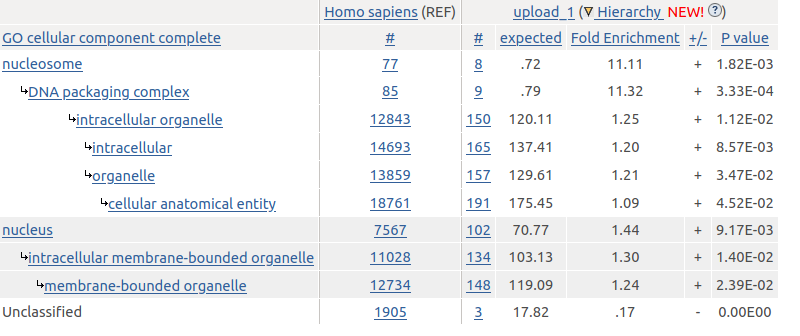
\includegraphics[width=\textwidth]{images/screenshots/ukbb_int_panther_cc_bonf.png}
%     \caption{UKBiobank intelligence significant genes at GWGAS. PANTHER GO enrichment Cellular component. Bonferroni correction. Screenshot for hierarchy}
%     \label{fig:UKBiobank significant genes at GWGAS. PANTHER GO enrichment Cellular component. Bonferroni correction. Screenshot for hierarchy}
% \end{figure}



% Previous to above did not match table
% \begin{figure}
%     \centering
%     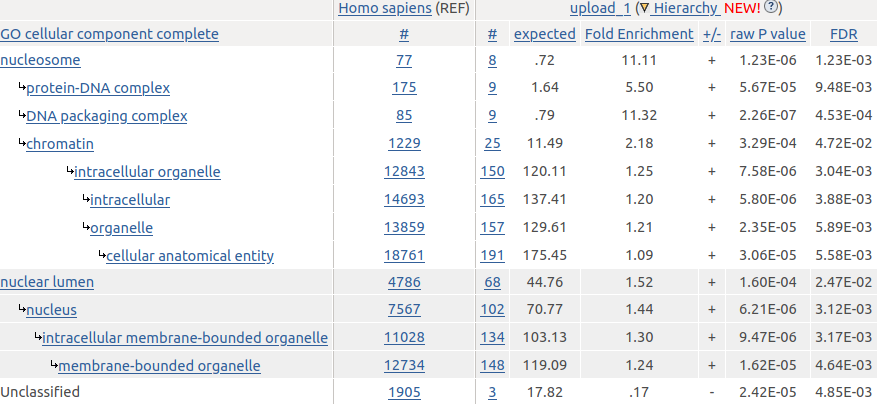
\includegraphics[width=\textwidth]{images/screenshots/ukbb_int_panther_cc_fdr.png}
%     \caption{UKBiobank intelligence significant genes at GWGAS. PANTHER GO enrichment Cellular component. FDR correction. Screenshot for hierarchy}
%     \label{fig:UKBiobank int significant genes at GWGAS. PANTHER GO enrichment Cellular component. FDR correction. Screenshot for hierarchy}
% \end{figure}


\paragraph{ToppGene}
 
Five biological processes terms, twenty nine molecular function terms and five cellular components had FDR $<$ 0.05. See figure~\ref{fig:toppgene pic}. The enrichment is that is present is also predominantly terms such as nucleosome function, DNA packaging and chromatin binding. Synaptic terms and neurogenesis terms are absent compared with the education samples.\footnote{int discovery PSP as BGNo GOBeta catenin pathway} 

\begin{figure}
    \centering
    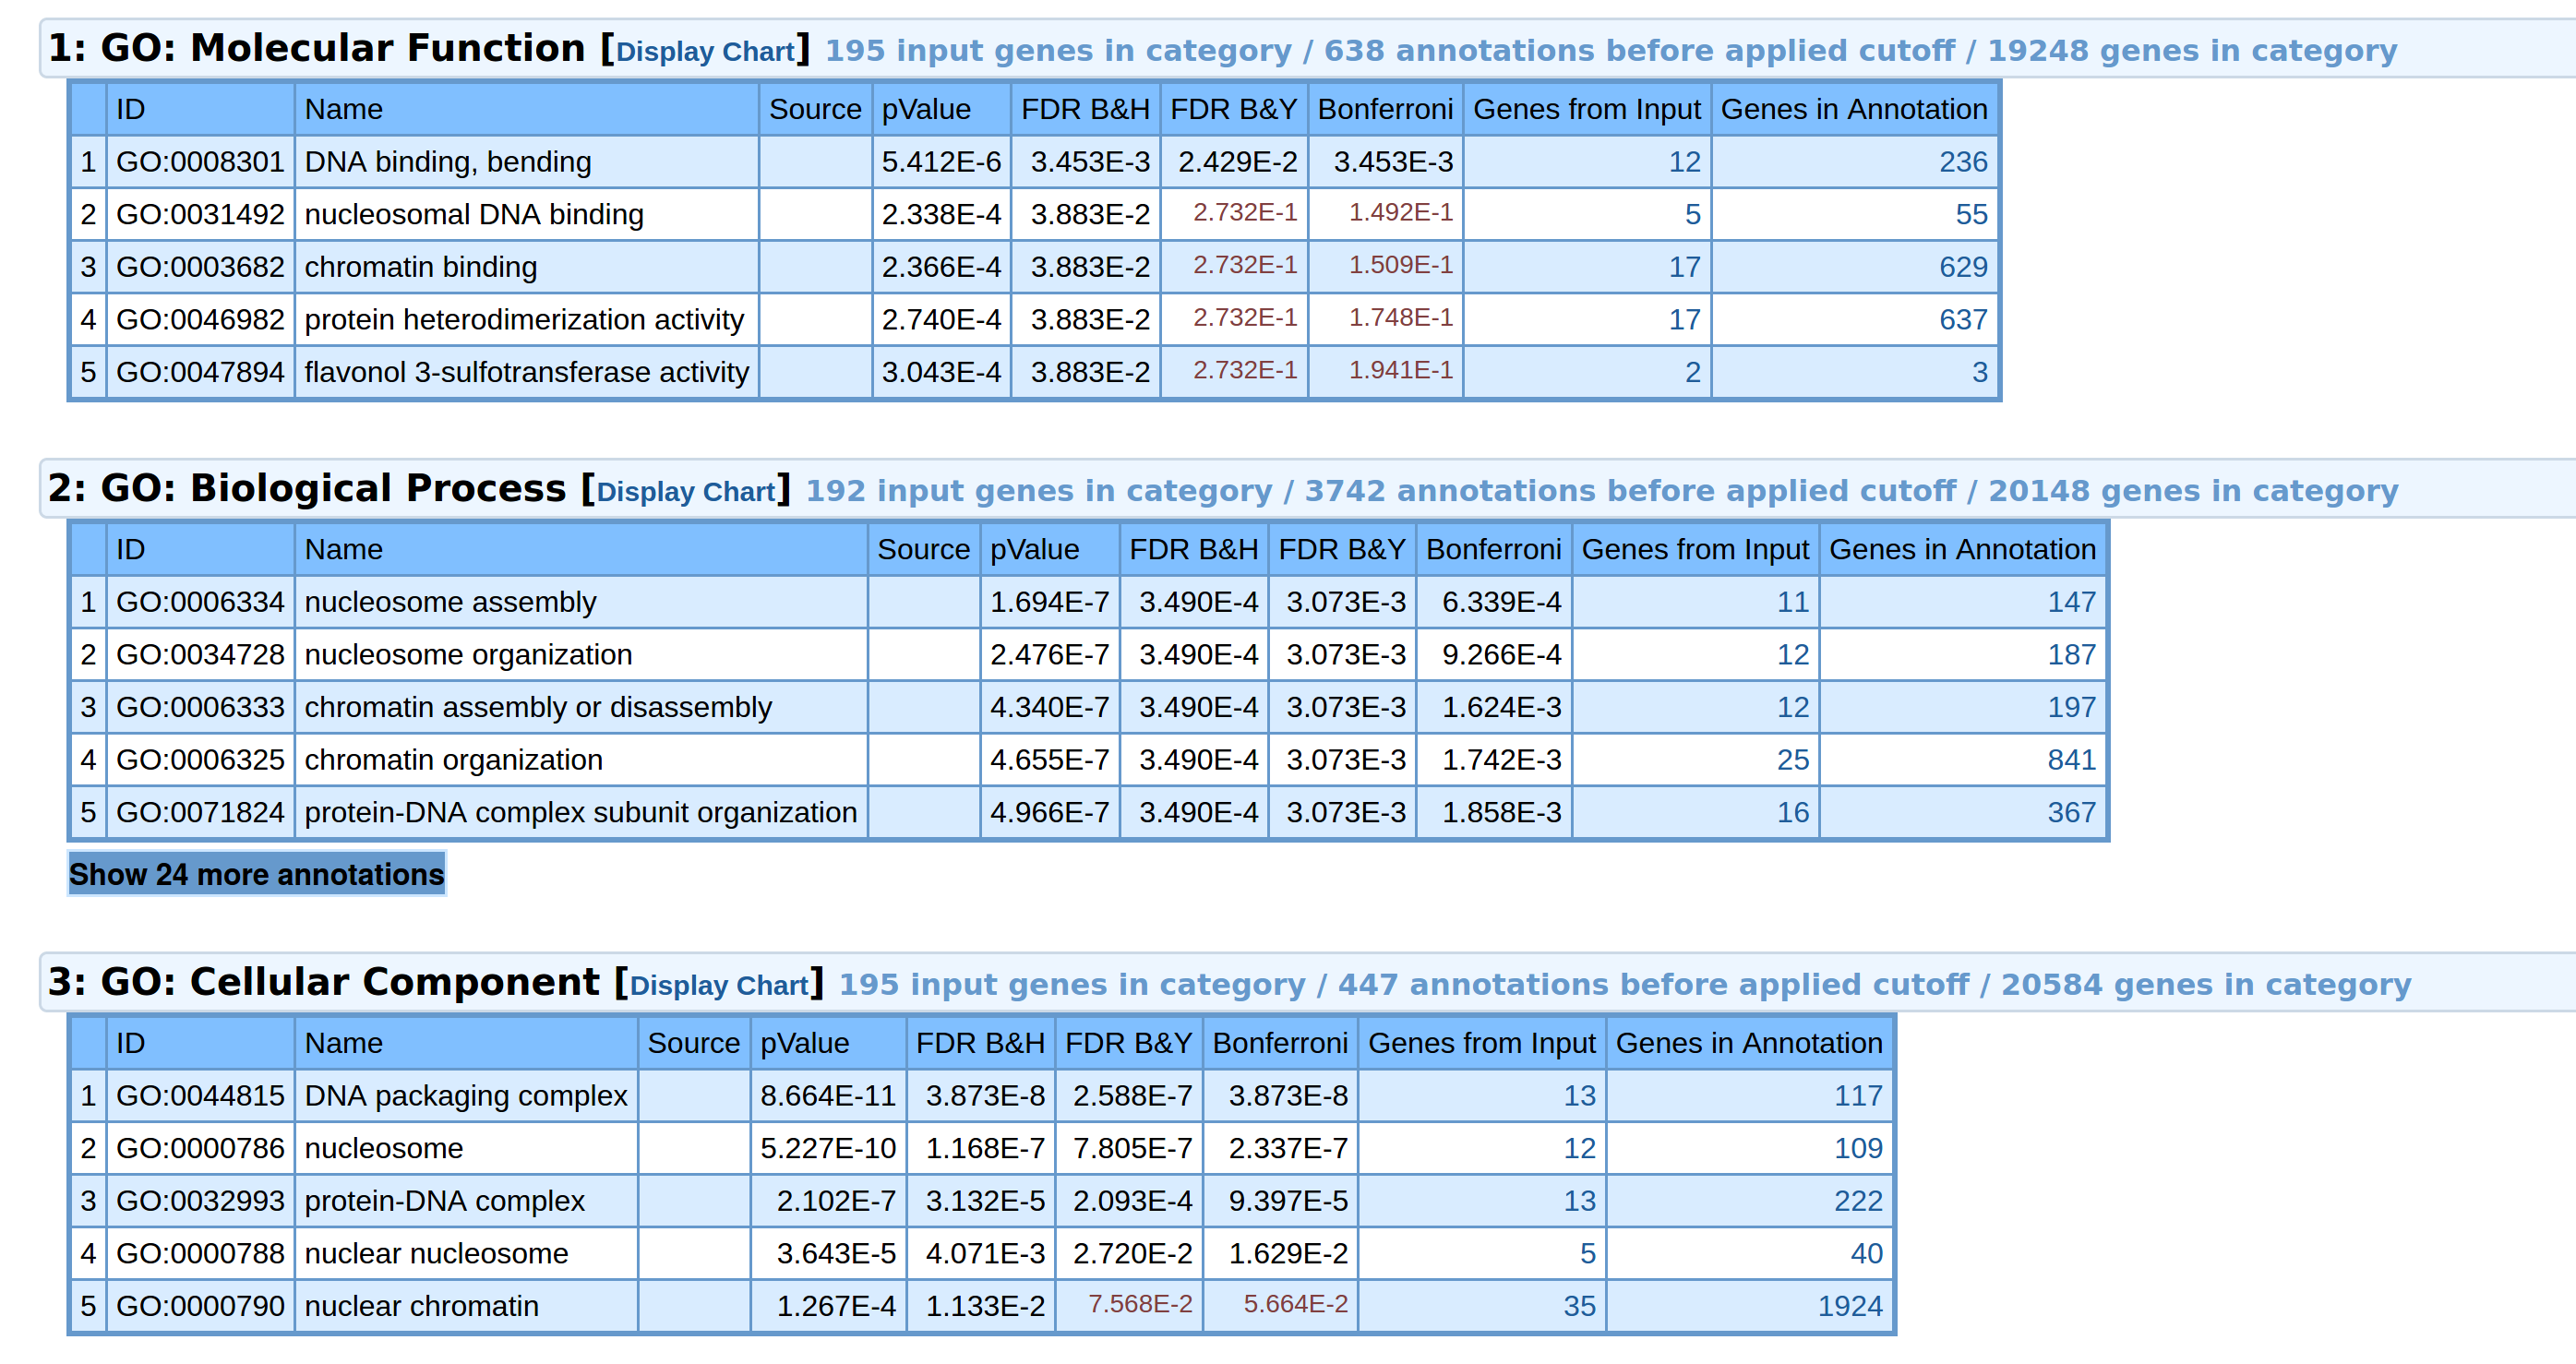
\includegraphics[width=\textwidth]{images/chapter2/strontium/images_toppgene_all_groups.png}
    \caption{Gene ontology ToppGene Biological Process, Molecular Function and Cellular component}
    \label{fig:toppgene pic}
\end{figure}



%\todo{use bg PSP}


% \todo[inline]{Important note to self, although there are other results they are not going to change the overall analysis therefore do not add any more just get this chapter done. If they are ready (ie formatted) and add to the PhD after completing the discussion they can be added. Potential data commented out in tex below}


There is no enrichment for genes differentially enriched in the central nervous system areas using GTEx version 8 analysed using FUMA (figure~\ref{fig:FUMA gtex deg samples multiple} and fig~\ref{fig:deg_upref_sample_gtex_gener}).

% Removed 20th Sep as now appears in multiple view
% \begin{figure}        
%     \centering
%     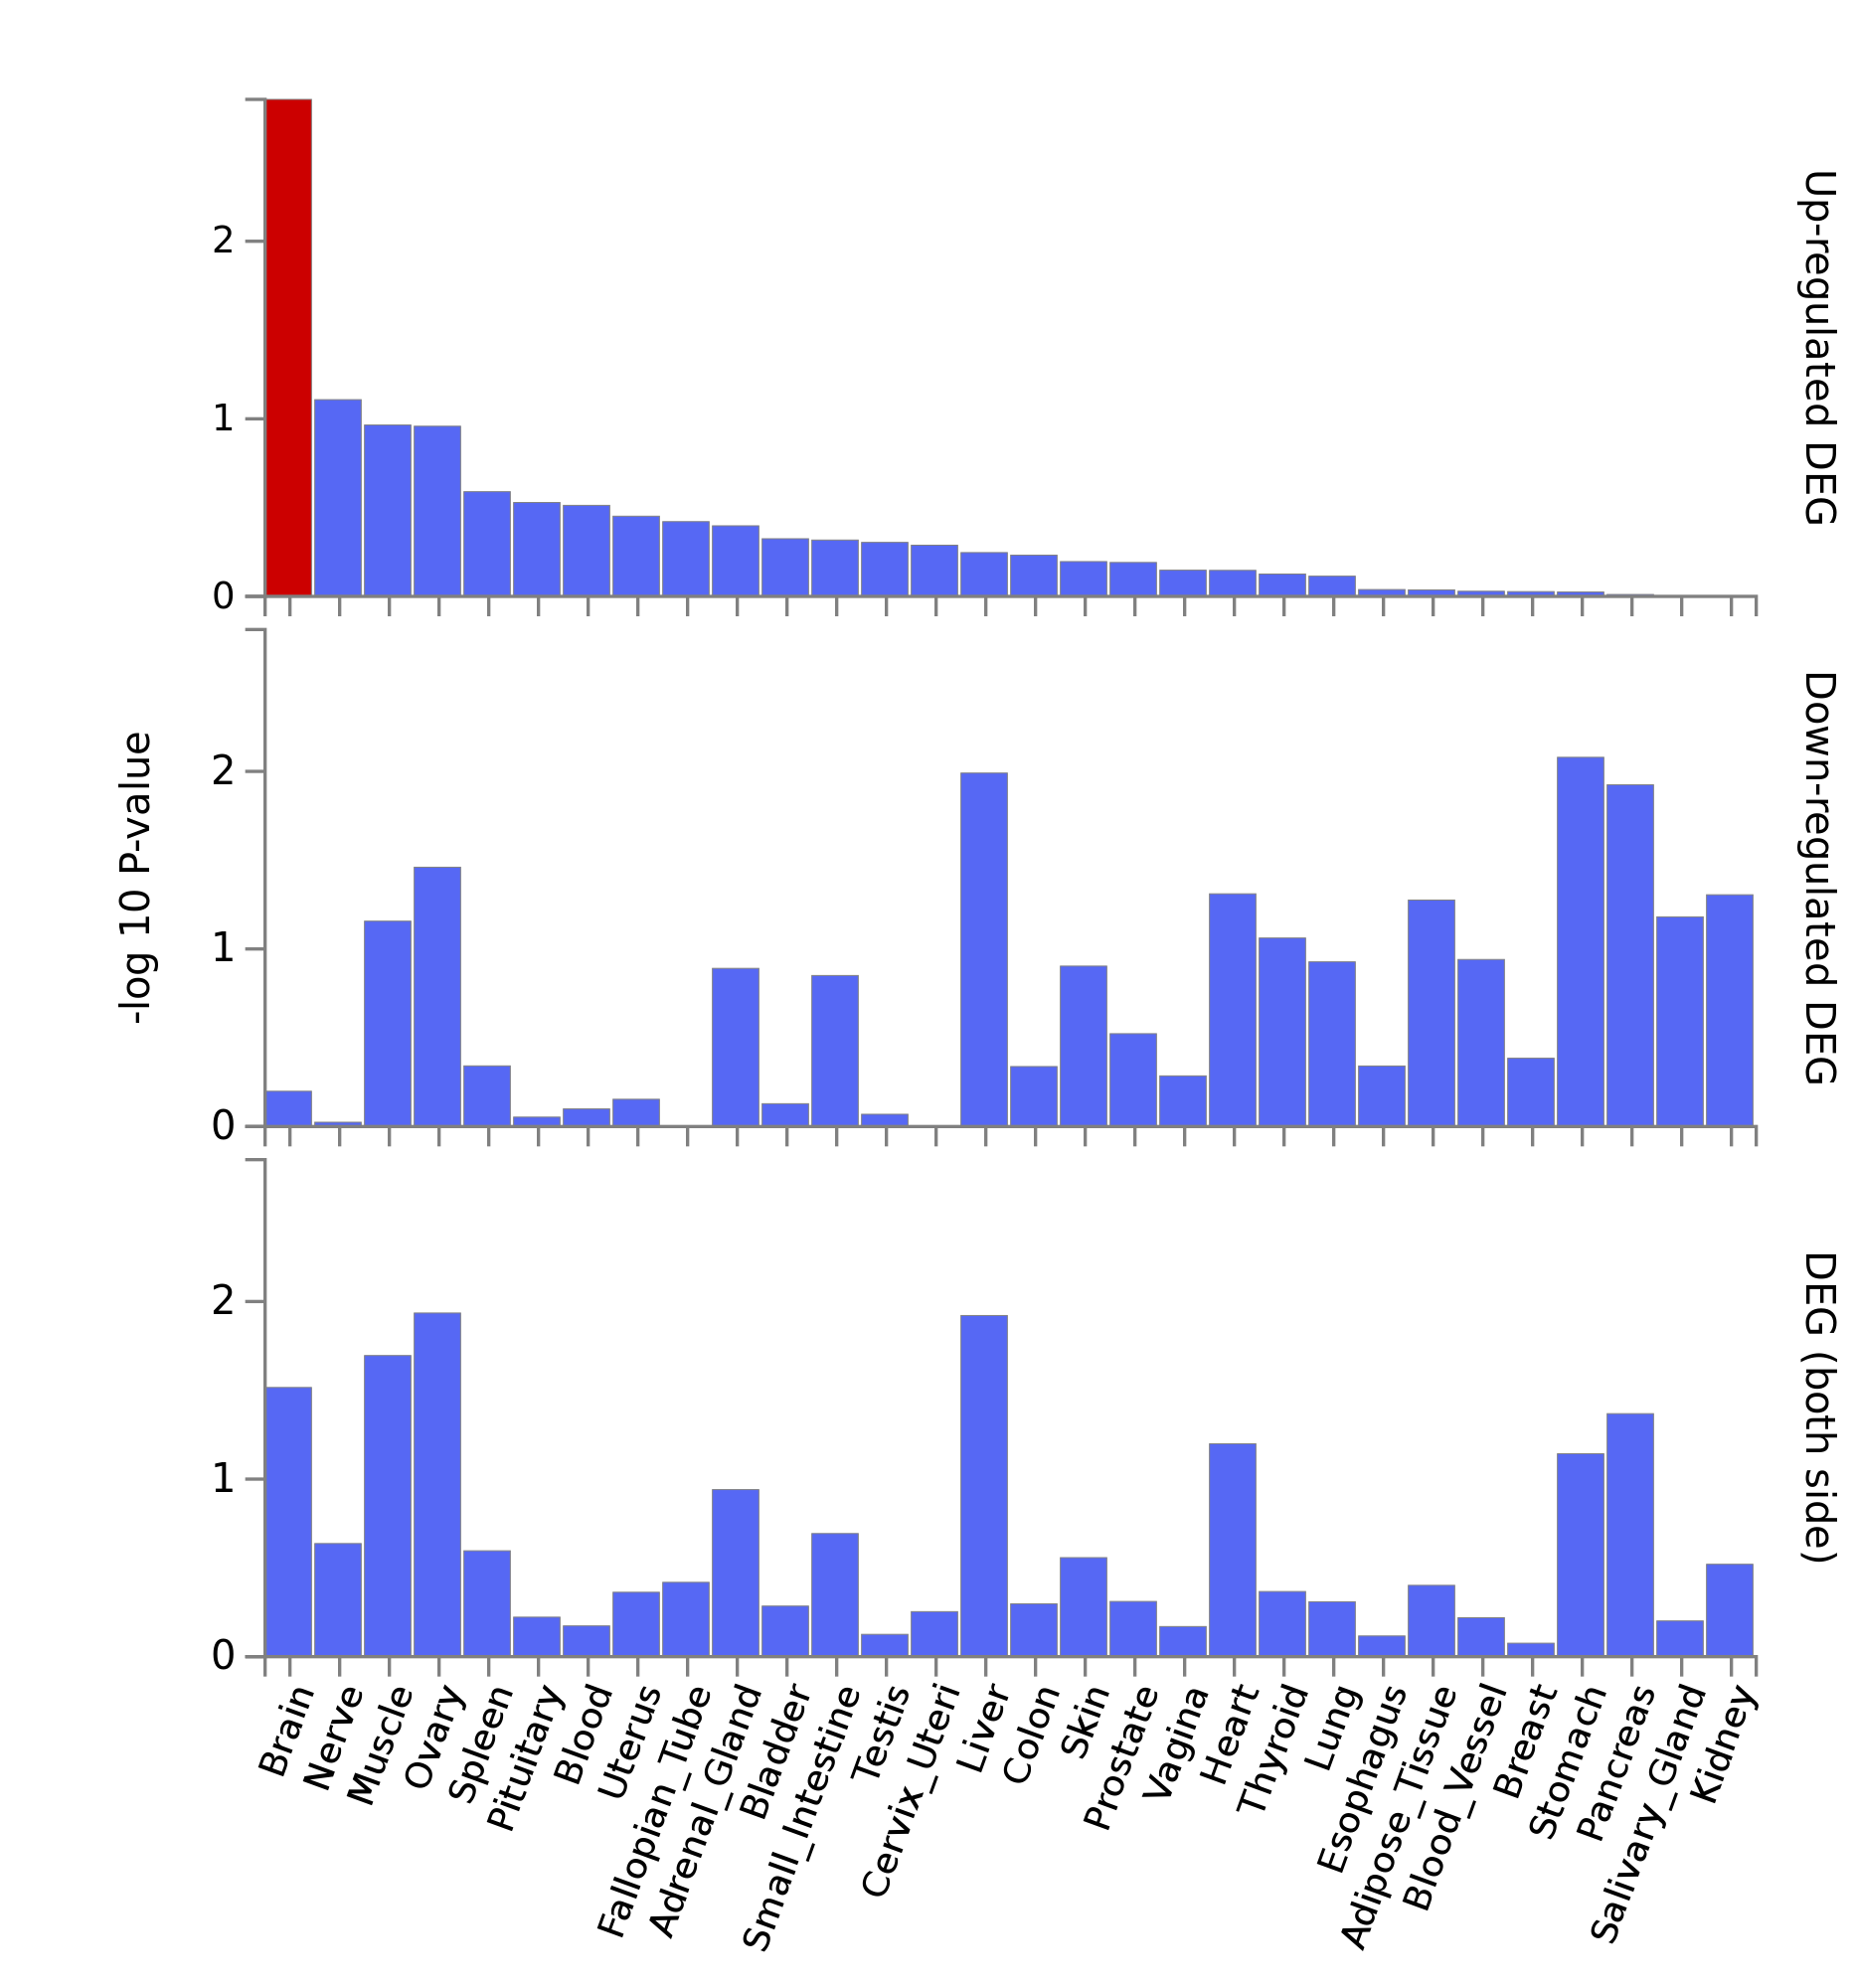
\includegraphics[width=\textwidth]{images/FUMA_plots/gtex_30_ukbbed.png}
%     \caption{GTEx FUMA UKBBEd}
%     \label{fig:GTEx FUMA UKBBEd}
% \end{figure}




% \begin{figure}
%     \centering
%     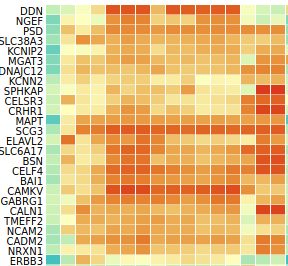
\includegraphics[width=\textwidth]{images/FUMA_plots/closeupdeg_ukbbed.png}
%     \caption{Caption}
%     \label{fig:my_label}
% \end{figure}
% \subsection{Education\textsubscript{Discovery} Ontology enrichment}

% \subsection{Intelligence Discovery}
% 197 genes
% 11 missing using ENSG annotations


% Gene ID 3 unmappedZZ
% GeneID:100132074 FOXO6
% GeneID:9753
% GeneID:3107

% Symbol
% MGEA5
% C10orf76
% CCDC101 SGF29
% PET112 GATB
% HIST1H3C H3C3 one of 25 synonyms
% HIST1H3I HIST1H3J one of 24 synonyms
% BAI1 ADGRB1
% RP5-874C20.3 pseudogene entrz 7741 ZSCAN26

% REMAINING FRAMEWORK BELOW
%     \subsection{Intelligence Discovery}
%         \subsubsection{Authors findings Intelligence Discovery}
% %         \todo[inline]{by Hill et all ? move to samples. Points to make big gene sets}
% Gene set analysis of this set augmented by mgtag \cite{hill2019combined} was carried out using 10891 gene sets from Gene ontology, Reactome and MSigDB (raw p required = 0.05/10891 = $4.59 \times 10^{-6}$. GSA revealed 7 sets including neurogenesis 1355 genes and genes expressed in synapse 717 genes , regulation of nervous system development 722 genes neuron projection 989 neuron differentation 842 and CNS neuron differentiation 160 genes cell development 808 genes (\textcolor{red}{quote p or do table})

% For gene set size analysis see\footnote{\url{source('~/RProjects/paper_xls_output/R/exploratory_data_analysis/gene_size_and_enrichment_magma_sets.R')}} table~\ref{tab:group size and enrichment}

%         \subsubsection{Ontology ORA Genome Intelligence discovery}
%         196 genes 
%         \paragraph{panther Intelligence discovery}3 unmapped GeneID:100132074
% GeneID:9753
% GeneID:3107
% \subparagraph{panther BP all Intelligence Discovery} Nil
% \subparagraph{panther MF all Intelligence Discovery}DNA binding 	2486 	44 	22.53 	1.95 	+ 	1.40E-05 	1.66E-02
% nucleic acid binding 	4024 	60 	36.47 	1.64 	+ 	5.93E-05 	4.70E-02
% binding 	16464 	171 	149.23 	1.15 	+ 	4.44E-05 	4.23E-02
% protein binding 	14110 	156 	127.90 	1.22 	+ 	6.81E-06 	1.08E-02
% \begin{figure}
%     \centering
%     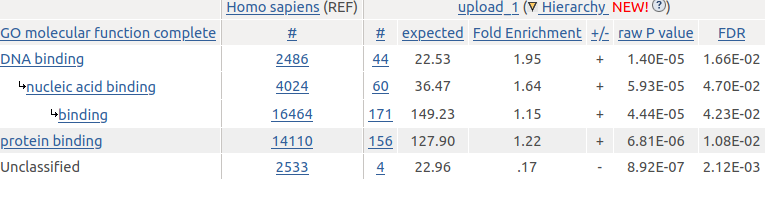
\includegraphics[width=\textwidth]{images/screenshots/GO_MF_Panther_UKBBInt_Heirarchy.png}
%     \caption{Panther MF UKBB Intelligence}
%     \label{fig:panther mf ukbb intelligence}
% \end{figure}
% \subparagraph{panther CC all Intelligence Discovery}
% \begin{figure}
%     \centering
%     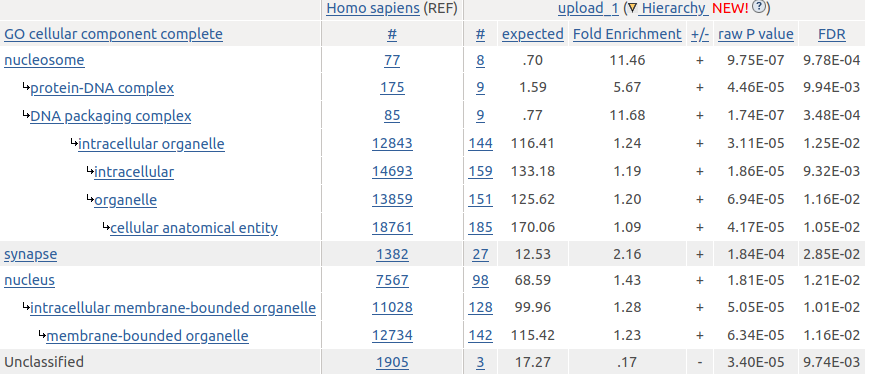
\includegraphics[width=\textwidth]{images/screenshots/panther_cc_ukbb_int_all.png}
%     \caption{Panther hierarchy cc ukbb int all}
%     \label{fig:panther hierarchy cc ukbb int all}
% \end{figure}
%          \subsubsection{Ontology ORA Synaptic}
%          \subsubsection{Others}
%         Path to code
        
%         GTEx
   

\subsection{Education Discovery Ontology Over representation analysis}
      The 235 genome-wide significant genes identified using MAGMA GWGAS for the Education\textsubscript{Discovery} sample (section~\ref{sec:UKBB Education discovery GWGAS}) were tested for over-representation of ontology terms. 
      Using PANTHER, I was unable to have all of the significant genes output by MAGMA identified, and used the gene identifier with the most uniquely identified genes  (233 terms, HGNC symbols with synonyms\footnote{ Script at \url{source('~/RProjects/paper_xls_output/R/chapter_2/FUMA/edit_gene_table/UKBB_Ed_FUMA2clipboard.R')}}).\footnote{entrez 231, hgnc (symbol) 225, NCBI symbol 227, HGNC ID 232 for HGNC id see \url{source('~/RProjects/paper_xls_output/R/chapter_2/translate_sig_genes/ukbbed_NCBI_translate2.R')})}.
        
    Thirty-three biological process ontology terms, were over-represented (FDR corrected $q<$0.05) amongst the 233 significant genes (see figure~\ref{fig:panther bp ukbb edu fdr}). There are several enriched terms related to neurogenesis and axonal development, similar to the Education\textsubscript{Replication} sample but distinct from the Intelligence samples. The most significant term (FDR=$8.51\times10^{-4}$) was ``nervous system development" (GO:0007399, 57 genes found amongst 2432 in the annotation). Many of the sets are broad and non-specific; the lowest FDR for annotations with less than 500 genes was ``negative regulation of cell projection" (GO:0031345);11 of 183 genes;5.4 fold change; FDR=0.0089.  Considering only those terms with greater than mean fold change (2.61), the most enriched is ``regulation of nervous system development" (GO:0051960,FDR 0.003). There was no significant over-representation of molecular function terms. 
    
    \begin{figure}
                \centering
                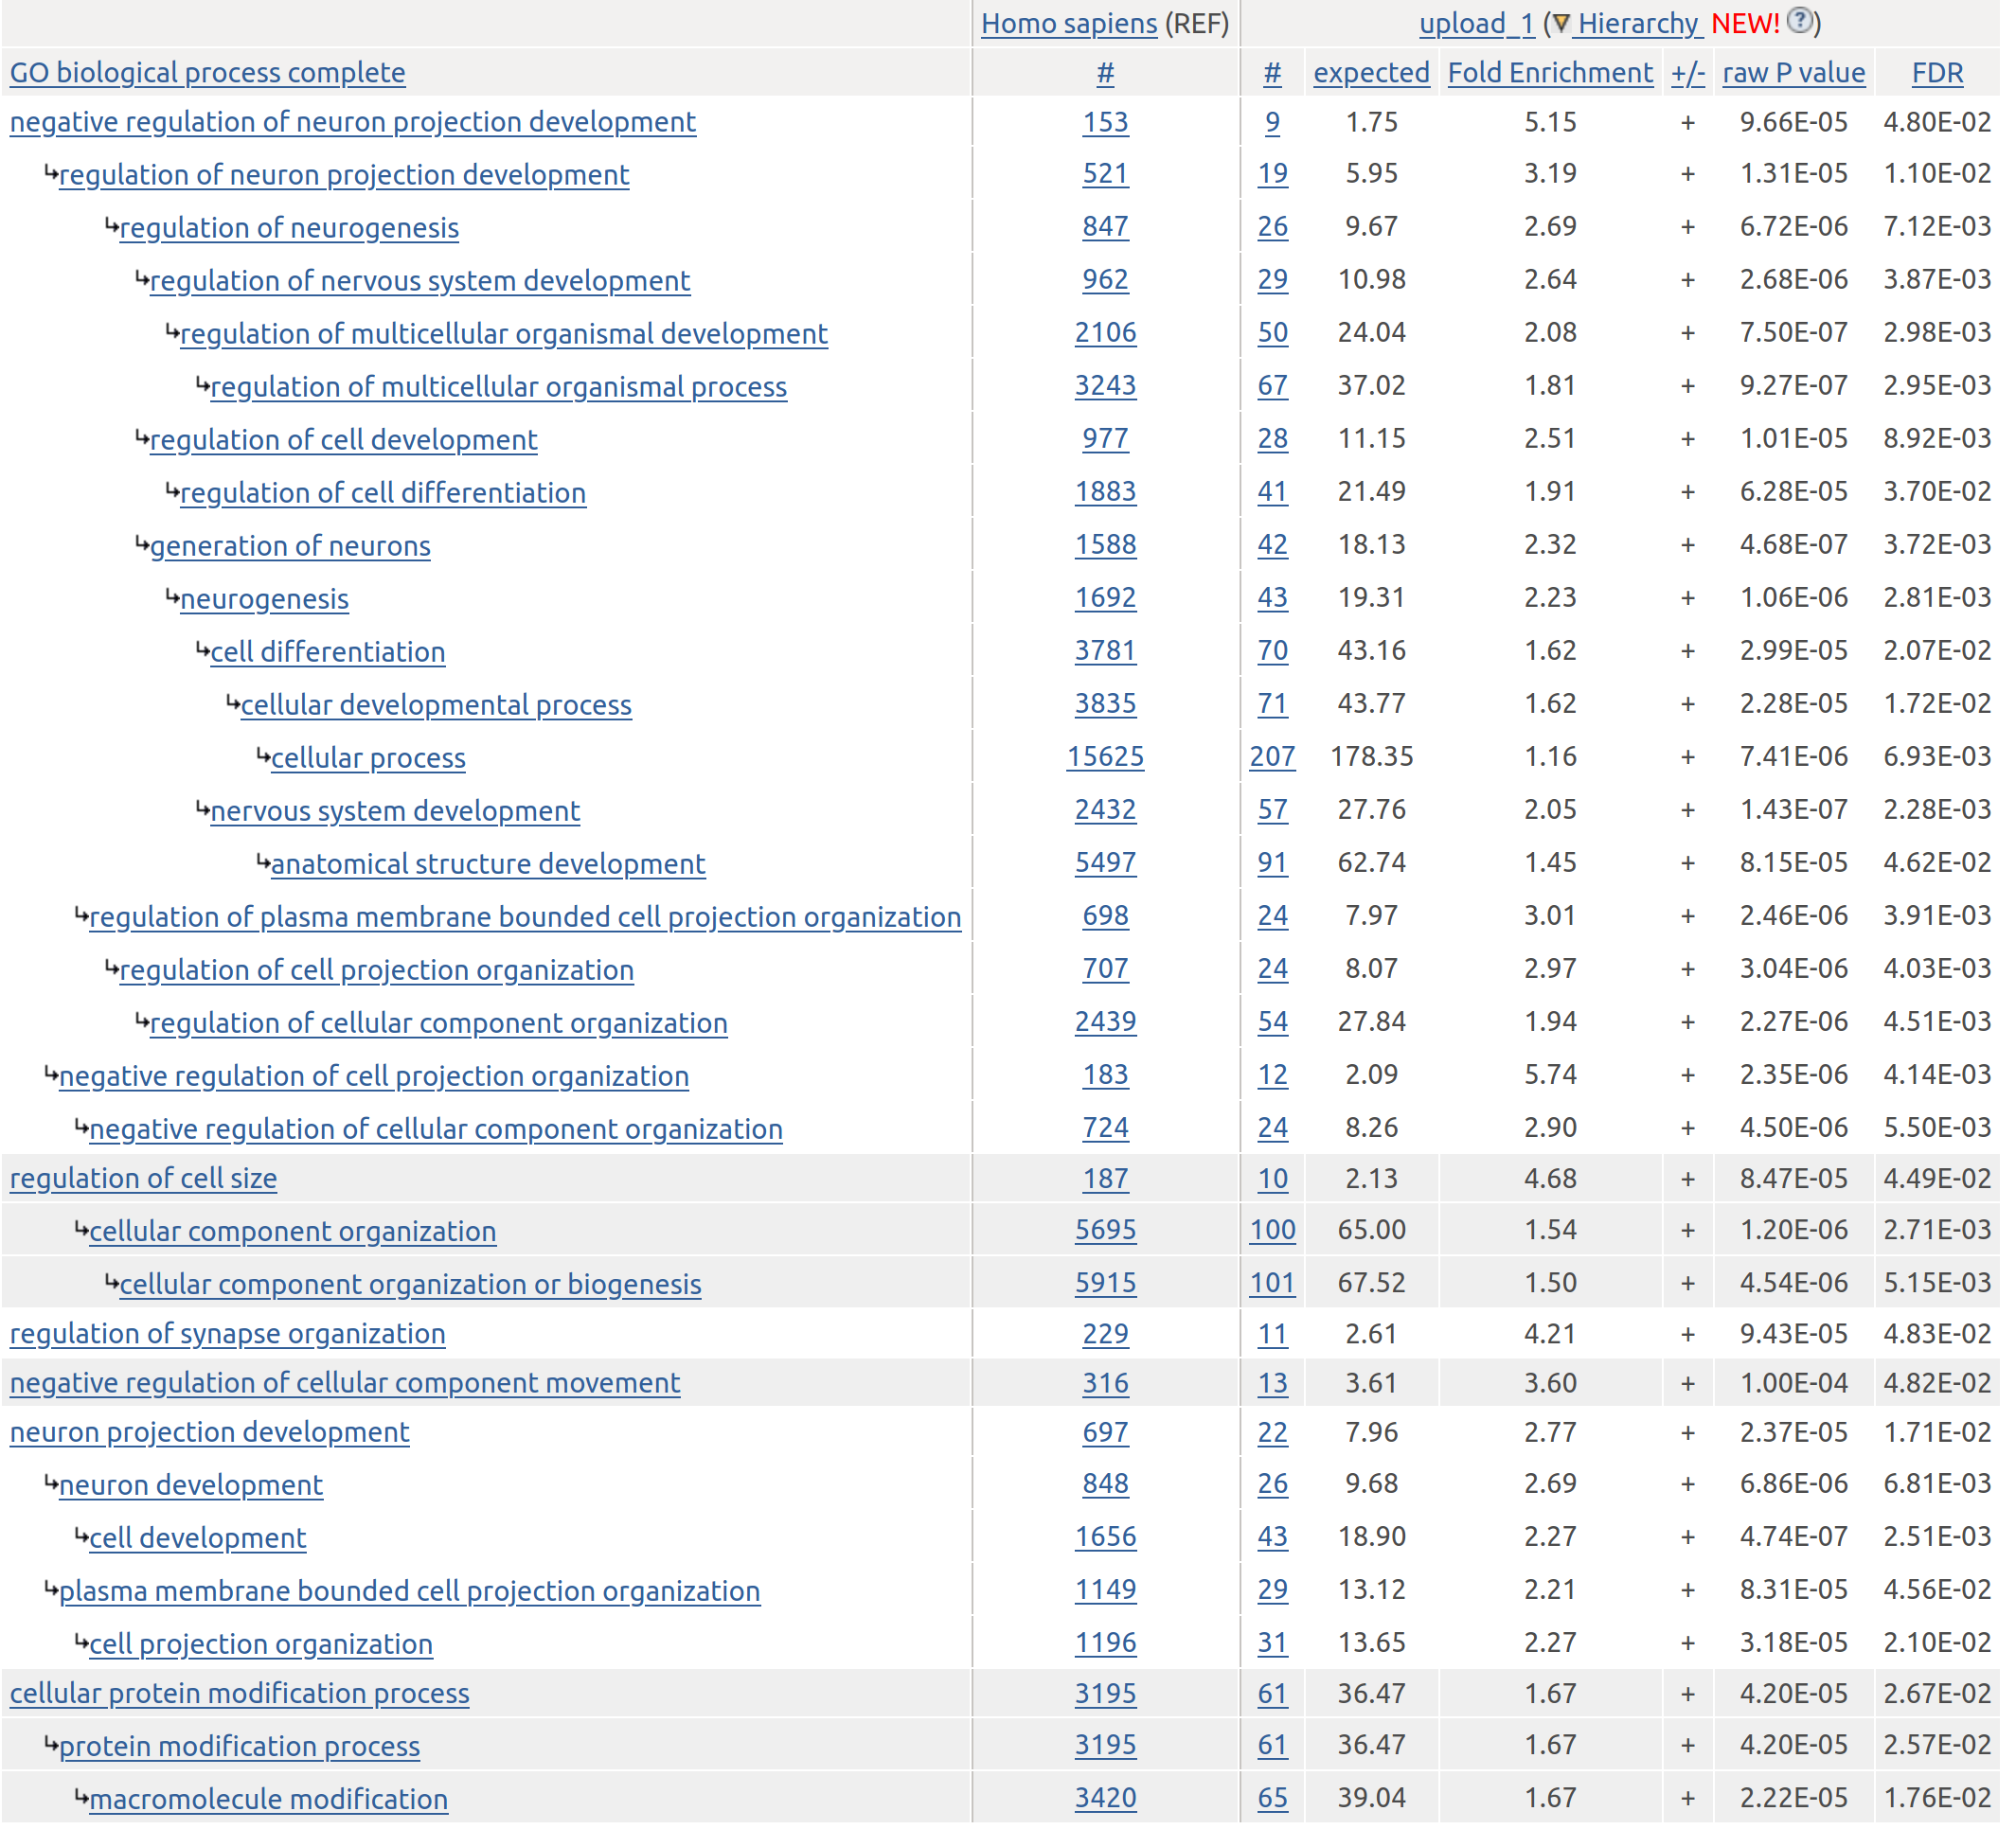
\includegraphics[width=\textwidth]{images/chapter2/large_screenshots/edu_discovery_bp_allbg_panther.png}
                \caption{PANTHER Gene Ontology Enrichment Biological Process Education\textsubscript{Discovery} FDR Large}
                \label{fig:panther bp ukbb edu fdr}
            \end{figure}
            
            
    Forty cellular component terms were over-represented.  Five of the ten most enriched terms had over 10,000 genes in their annotation. This includes the most significant term ``Intracellular" (GO:0005622, 14707 genes, FDR=$4.9\times10^{-5}$) although only six of the forty significant terms contained over 10,000 genes (see figure~\ref{fig:panther cc ukbb edu } and table \label{tab:GO cellular component complete Education Discovery FDRover represenation only}). Four terms have under 100 annotations amongst the ten most enriched, three are related to the endoplasmic reticulum  including  ``lumenal side of membrane" (GO:0098576 FDR =   $3.84\times10^{-4}$)), one is annotated to GO:0042613 ``MHC class II protein complex" ;(5 of 19 genes in annotation found;  fold change 23.1, FDR=0.00126).``Synapse" ( GO:0045202  ;   36 of 1383genes in annotation,    ; fold change 15.8,  FDR= 0.00116) was also amongst the ten most enriched terms.    \footnote{ GABAergic synapse is present as an enriched cellular component term GO:0098982 79 in annotation 6 terms FDR=0.0253 but the genes DAG1, Dystroglycan;Neurexin-1, NRXN1 ;SLC6A17,Sodium-dependent neutral amino acid transporter; PCDH17,Protocadherin-17;ERBB4,Receptor tyrosine-protein kinase erbB-4;BSN,Protein Bassoon.} No SLIM ontologies showed significant over-representation and there was no enrichment of PANTHER pathways. Only the protein class PC00149 ``major histocompatibility complex protein" was over-represented  *5 of 18 terms; 24.3 fold change; FDR=0.0010).

            

            % \subparagraph{CC Panther Education Discovery}
            % 40 terms. Of the 10 terms with the lowest FDR 5 have more than 10000 genes in the annotation (Lowest FDR: GO:0005622 intracellular 14704 genes in annotation FDR=$4.9\times10^{-5}$, 2nd GO:0043231 intracellular membrane-bounded organelle                              11041 in annotation  166 Genes from significant genes annotated, 4th GO:0043229 intracellular organelle                                               12856 in annotation , 183 in significant genes; 5th Organelle GO:0043226 organelle                                                             13868 in annotation,  193 in test genes and 8thGO:0043227 membrane-bounded organelle                                            12748  in annotation. 4 terms have under 100 annotations in the top 10, 3 are related to the endoplasmic reticulum (top GO:0098576 lumenal side of membrane                                             ;in annotation    37 genes, number of significant genes     7;  fold change 16.6,  FDR =   $3.84\times10^{-4}$), one is annotated to GO:0042613 MHC class II protein complex                                     , ;genes in annotation        19, significant genes with annotation     5;  fold change 23.1, FDR=0.00126. The final top 10 cellular component annotation is  GO:0045202 synapse                                                            ;    1383genes in annotation,    36 significant genes with annotation; fold change 15.8,  FDR= 0.00116. Post synapse is also enriched 22 significant genesw in 651 in annotation, fold change 2.96, FDR=0.00157.
            % See figure~\ref{fig:panther cc ukbb edu } for results displayed with terms sorted to show their position in the hierarchy.
            
       
            
            \begin{figure}
                \centering
                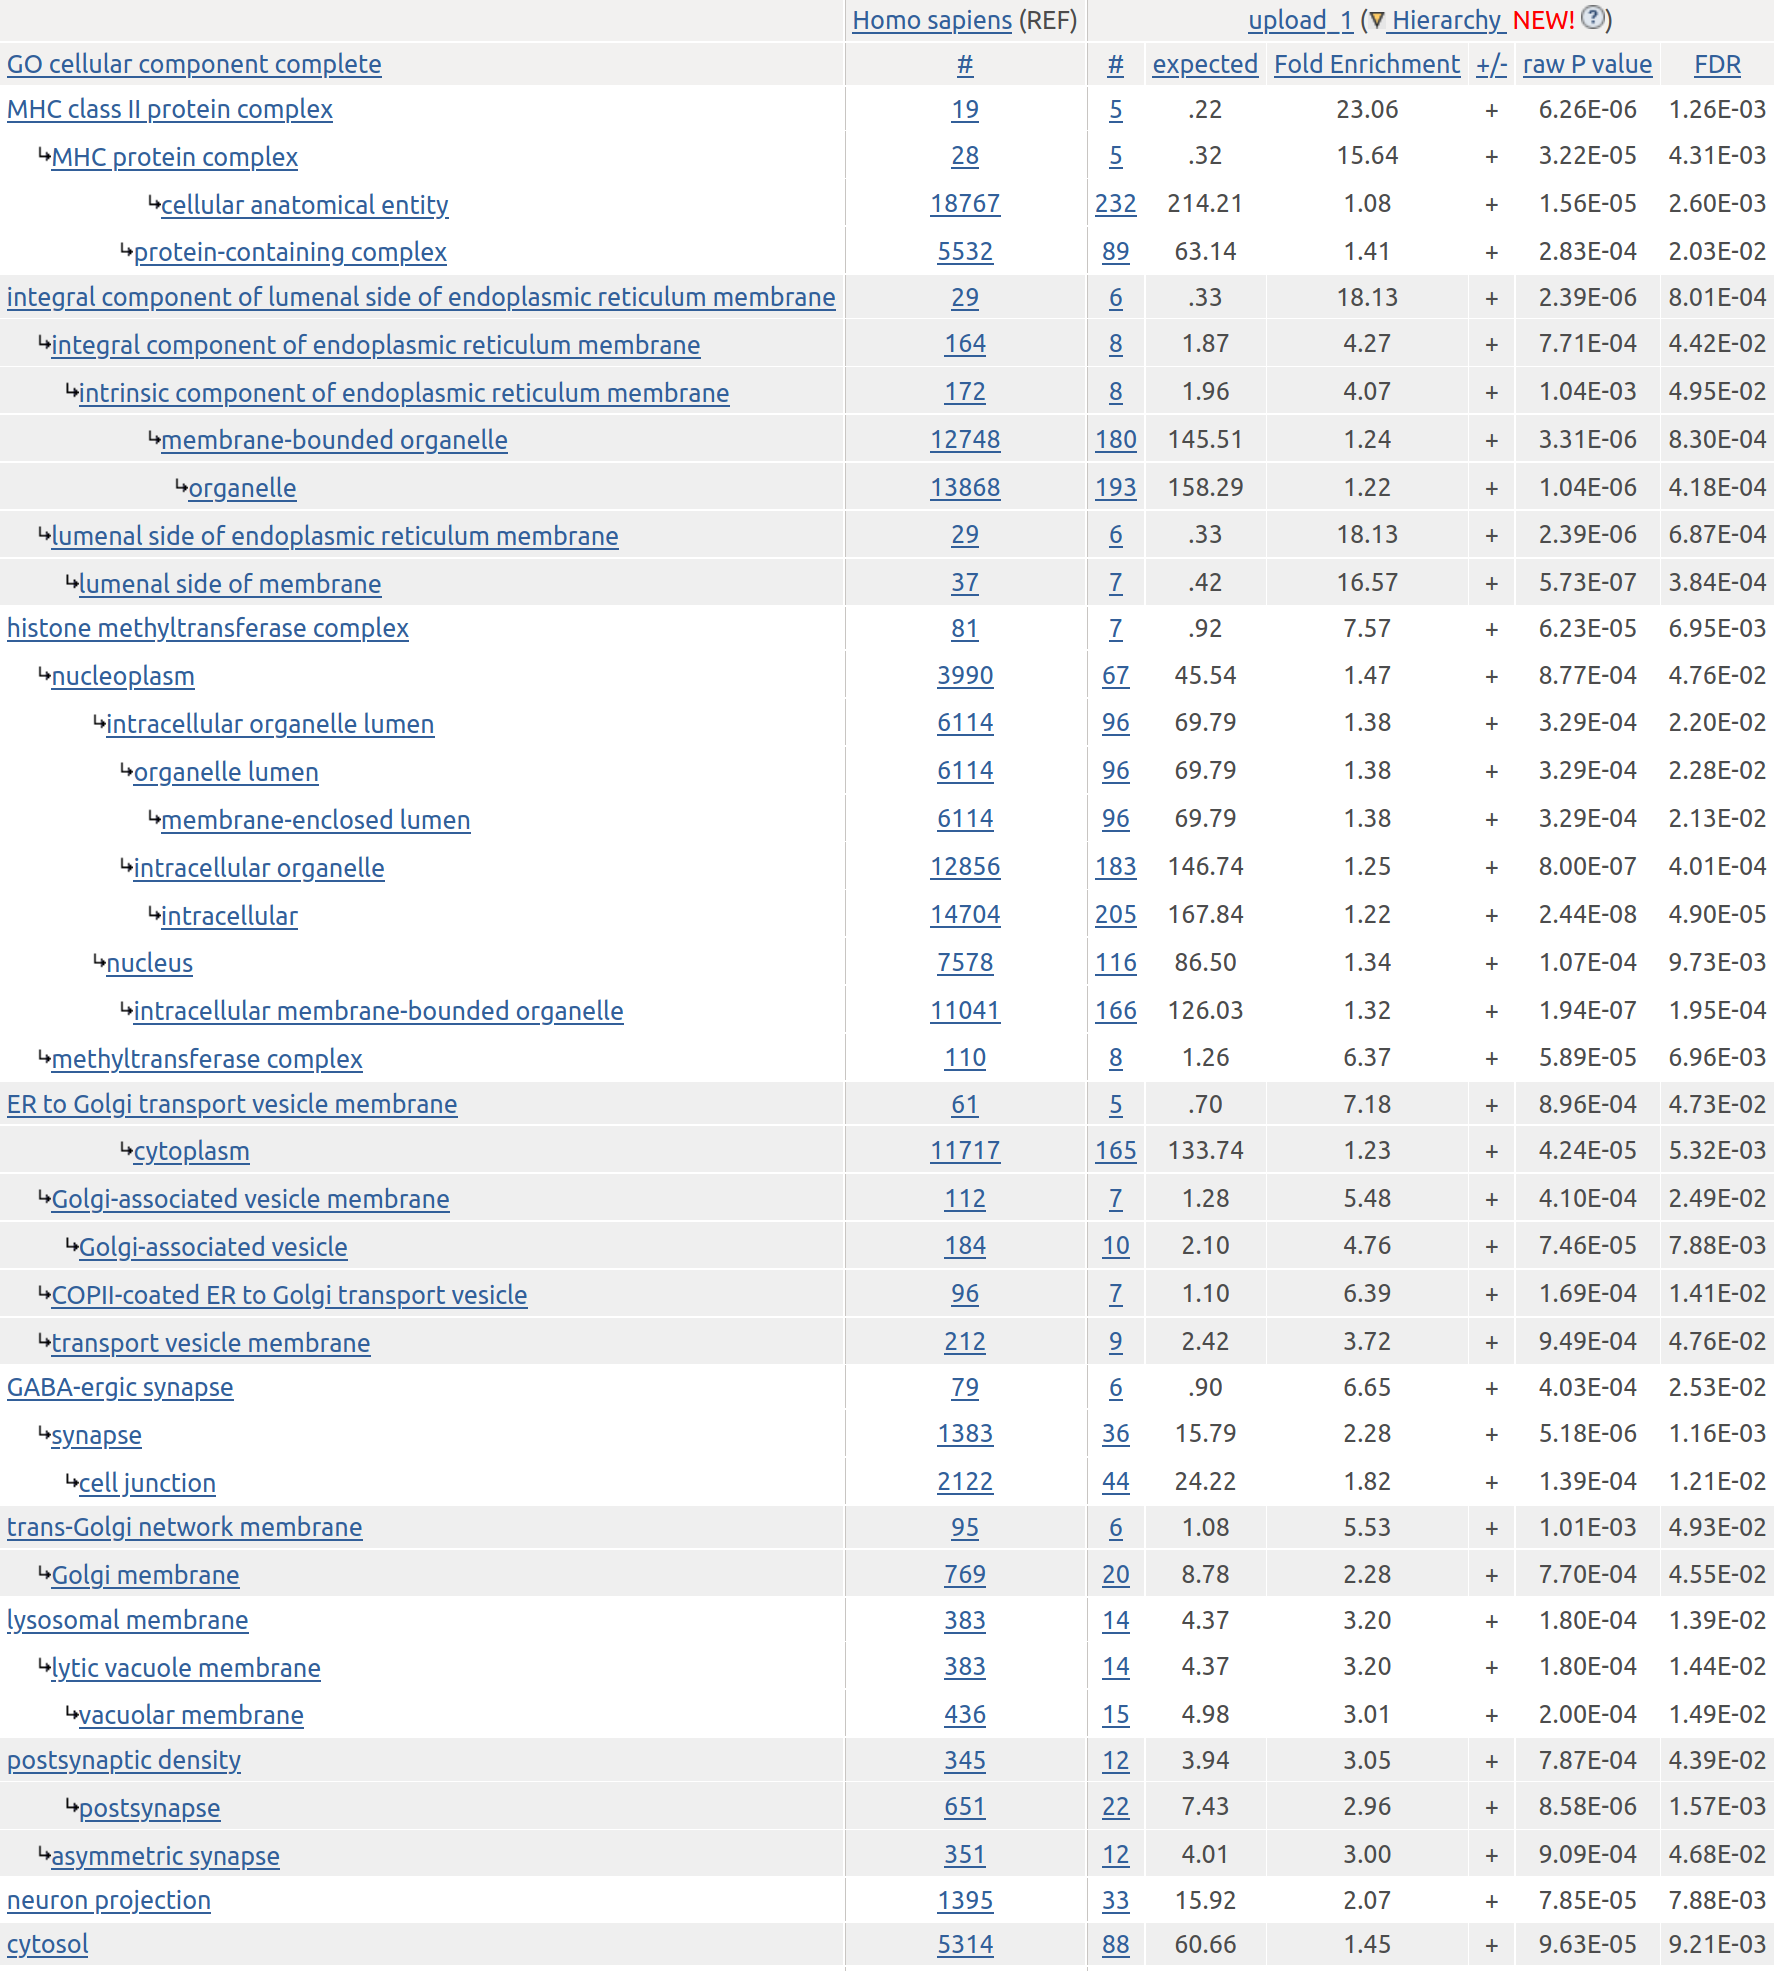
\includegraphics[width=\textwidth]{images/chapter2/large_screenshots/edu_discovery_large_cc_panther.png}
                \caption{PANTHER Gene Ontology Enrichment Cellular Component Education\textsubscript{Discovery}. The lowest FDR again is found in the most general and largest gene ontology terms with correspondingly small fold enrichment. }
                \label{fig:panther cc ukbb edu }
            \end{figure}
            
            
\begin{table}[ht]
\centering
\begin{adjustbox}{width=\textwidth}

\begin{tabular}{llrrrrrr}
  \hline
GO & description & Ref & Test & E & Fold & P & FDR \\ 
  \hline
GO:0042613 & MHC class II protein complex  & 19 & 5 & 0.2 & 23.06 & $6.26 \times 10^{-6}$ & 0.0013 \\ 
  GO:0071556 & integral component of lumenal side of endoplasmic reticulum membrane  & 29 & 6 & 0.3 & 18.13 & $2.39 \times 10^{-6}$ & 0.0008 \\ 
  GO:0098553 & lumenal side of endoplasmic reticulum membrane  & 29 & 6 & 0.3 & 18.13 & $2.39 \times 10^{-6}$ & 0.0007 \\ 
  GO:0098576 & lumenal side of membrane  & 37 & 7 & 0.4 & 16.57 & $5.73 \times 10^{-7}$ & 0.0004 \\ 
  GO:0042611 & MHC protein complex  & 28 & 5 & 0.3 & 15.64 & $3.22 \times 10^{-5}$ & 0.0043 \\ 
  GO:0035097 & histone methyltransferase complex  & 81 & 7 & 0.9 & 7.57 & $6.23 \times 10^{-5}$ & 0.0069 \\ 
  GO:0012507 & ER to Golgi transport vesicle membrane  & 61 & 5 & 0.7 & 7.18 & $8.96 \times 10^{-4}$ & 0.0473 \\ 
  GO:0098982 & GABA-ergic synapse  & 79 & 6 & 0.9 & 6.65 & $4.03 \times 10^{-4}$ & 0.0253 \\ 
  GO:0030134 & COPII-coated ER to Golgi transport vesicle  & 96 & 7 & 1.1 & 6.39 & $1.69 \times 10^{-4}$ & 0.0141 \\ 
  GO:0034708 & methyltransferase complex  & 110 & 8 & 1.3 & 6.37 & $5.89 \times 10^{-5}$ & 0.0070 \\ 
  GO:0032588 & trans-Golgi network membrane  & 95 & 6 & 1.1 & 5.53 & $1.01 \times 10^{-3}$ & 0.0493 \\ 
  GO:0030660 & Golgi-associated vesicle membrane  & 112 & 7 & 1.3 & 5.48 & $4.10 \times 10^{-4}$ & 0.0249 \\ 
  GO:0005798 & Golgi-associated vesicle  & 184 & 10 & 2.1 & 4.76 & $7.46 \times 10^{-5}$ & 0.0079 \\ 
  GO:0030176 & integral component of endoplasmic reticulum membrane  & 164 & 8 & 1.9 & 4.27 & $7.71 \times 10^{-4}$ & 0.0442 \\ 
  GO:0031227 & intrinsic component of endoplasmic reticulum membrane  & 172 & 8 & 2.0 & 4.07 & $1.04 \times 10^{-3}$ & 0.0495 \\ 
  GO:0030658 & transport vesicle membrane  & 212 & 9 & 2.4 & 3.72 & $9.49 \times 10^{-4}$ & 0.0476 \\ 
  GO:0098852 & lytic vacuole membrane  & 383 & 14 & 4.4 & 3.20 & $1.80 \times 10^{-4}$ & 0.0144 \\ 
  GO:0005765 & lysosomal membrane  & 383 & 14 & 4.4 & 3.20 & $1.80 \times 10^{-4}$ & 0.0139 \\ 
  GO:0014069 & postsynaptic density  & 345 & 12 & 3.9 & 3.05 & $7.87 \times 10^{-4}$ & 0.0439 \\ 
  GO:0005774 & vacuolar membrane  & 436 & 15 & 5.0 & 3.01 & $2.00 \times 10^{-4}$ & 0.0149 \\ 
  GO:0032279 & asymmetric synapse  & 351 & 12 & 4.0 & 3.00 & $9.09 \times 10^{-4}$ & 0.0468 \\ 
  GO:0098794 & postsynapse  & 651 & 22 & 7.4 & 2.96 & $8.58 \times 10^{-6}$ & 0.0016 \\ 
  GO:0045202 & synapse  & 1383 & 36 & 15.8 & 2.28 & $5.18 \times 10^{-6}$ & 0.0012 \\ 
  GO:0000139 & Golgi membrane  & 769 & 20 & 8.8 & 2.28 & $7.70 \times 10^{-4}$ & 0.0455 \\ 
  GO:0043005 & neuron projection  & 1395 & 33 & 15.9 & 2.07 & $7.85 \times 10^{-5}$ & 0.0079 \\ 
  GO:0030054 & cell junction  & 2122 & 44 & 24.2 & 1.82 & $1.39 \times 10^{-4}$ & 0.0121 \\ 
  GO:0005654 & nucleoplasm  & 3990 & 67 & 45.5 & 1.47 & $8.77 \times 10^{-4}$ & 0.0476 \\ 
  GO:0005829 & cytosol  & 5314 & 88 & 60.7 & 1.45 & $9.63 \times 10^{-5}$ & 0.0092 \\ 
  GO:0032991 & protein-containing complex  & 5532 & 89 & 63.1 & 1.41 & $2.83 \times 10^{-4}$ & 0.0203 \\ 
  GO:0043233 & organelle lumen  & 6114 & 96 & 69.8 & 1.38 & $3.29 \times 10^{-4}$ & 0.0228 \\ 
  GO:0070013 & intracellular organelle lumen  & 6114 & 96 & 69.8 & 1.38 & $3.29 \times 10^{-4}$ & 0.0220 \\ 
  GO:0031974 & membrane-enclosed lumen  & 6114 & 96 & 69.8 & 1.38 & $3.29 \times 10^{-4}$ & 0.0213 \\ 
  GO:0005634 & nucleus  & 7578 & 116 & 86.5 & 1.34 & $1.07 \times 10^{-4}$ & 0.0097 \\ 
  GO:0043231 & intracellular membrane-bounded organelle  & 11041 & 166 & 126.0 & 1.32 & $1.94 \times 10^{-7}$ & 0.0002 \\ 
  GO:0043229 & intracellular organelle  & 12856 & 183 & 146.7 & 1.25 & $8.00 \times 10^{-7}$ & 0.0004 \\ 
  GO:0043227 & membrane-bounded organelle  & 12748 & 180 & 145.5 & 1.24 & $3.31 \times 10^{-6}$ & 0.0008 \\ 
  GO:0005737 & cytoplasm  & 11717 & 165 & 133.7 & 1.23 & $4.24 \times 10^{-5}$ & 0.0053 \\ 
  GO:0005622 & intracellular  & 14704 & 205 & 167.8 & 1.22 & $2.44 \times 10^{-8}$ & 0.0000 \\ 
  GO:0043226 & organelle  & 13  868 & 193 & 158.3 & 1.22 & $1.04 \times 10^{-6}$ & 0.0004 \\ 
%   GO:0110165 & cellular anatomical entity  & 18767 & 232 & 214.2 & 1.08 & $1.56 \times 10^{-5}$ & 0.0026 \\ 
%   GO:0005575 & cellular\_component  & 18951 & 233 & 216.3 & 1.08 & $1.96 \times 10^{-5}$ & 0.0028 \\ 
%   UNCLASSIFIED & Unclassified  & 1900 & 5 & 21.7 & 0.23 & $1.96 \times 10^{-5}$ & 0.0030 \\ 
   \hline
\end{tabular}
\end{adjustbox}
\caption{GO cellular component complete Education Discovery FDRover represenation only  Ref reference set, test:number of genes being tested present in ontology termE expected number of genes being tested ,present in ontology term, Fold= Fold changeP = raw p value, FDR = false discovery rate. Ordered by fold change.GO:0110165 Cellular anatomical entity and GO:0005575 cellular component omitted along with one unclassified term. } 
\label{tab:GO cellular component complete Education Discovery FDRover represenation only}
\end{table}
        
Seven reactome pathways were enriched (table~\ref{tab:Reactome pathways Education Discovery FDRover represenation only}).
\begin{table}[ht]
\centering
\begin{adjustbox}{width=\textwidth}
\begin{tabular}{llrrrrrr}
  \hline
GO & description & Ref & Test & E & Fold & P & FDR \\ 
  \hline
R-HSA-202430 & Translocation of ZAP-70 to Immunological synapse  & 25 & 5 & 0.3 & 17.52 & $1.99 \times 10^{-5}$ & 0.0454 \\ 
  R-HSA-202427 & Phosphorylation of CD3 and TCR zeta chains  & 28 & 5 & 0.3 & 15.64 & $3.22 \times 10^{-5}$ & 0.0368 \\ 
  R-HSA-389948 & PD-1 signaling  & 29 & 5 & 0.3 & 15.11 & $3.74 \times 10^{-5}$ & 0.0285 \\ 
  R-HSA-202433 & Generation of second messenger molecules  & 40 & 5 & 0.5 & 10.95 & $1.48 \times 10^{-4}$ & 0.0484 \\ 
  R-HSA-3247509 & Chromatin modifying enzymes  & 240 & 11 & 2.7 & 4.02 & $1.40 \times 10^{-4}$ & 0.0639 \\ 
  R-HSA-4839726 & Chromatin organization  & 240 & 11 & 2.7 & 4.02 & $1.40 \times 10^{-4}$ & 0.0533 \\ 
  R-HSA-194315 & Signaling by Rho GTPases  & 417 & 15 & 4.8 & 3.15 & $1.26 \times 10^{-4}$ & 0.0717 \\ 
   \hline
\end{tabular}
\end{adjustbox}
\caption{Reactome pathways Education Discovery FDRover represenation only  Ref reference set, test:number of genes being tested present in ontology termE expected number of genes being tested ,present in ontology term, Fold= Fold changeP = raw p value, FDR = false discovery rate} 
\label{tab:Reactome pathways Education Discovery FDRover represenation only}
\end{table}

           
            
            
%             \begin{table}[]
%                 \centering
%                 \begin{tabular}{llll}
%                 \toprule
%                 Term & n & p & fdr q\\
%                 \midrule
% synapse organization&	15&	$4.42\times10^{-6}$&	$3.97\times10^{-5}$\\
% process in the synapse&	20&	$2.49\times10^{-3}$&	0.0112\\
% trans-synaptic signaling&	6&	0.0194	&0.0378\\
% synapse adhesion between pre- and post-synapse&	3	&0.0130	&0.0378\\
% synapse assembly&	4	&0.0252	&0.0378\\
% regulation of synapse assembly&	3	&0.0213&	0.0378\\
%                 \bottomrule
%                 \end{tabular}
%                 \caption[SynGO Biological Process Education\textsubscript{Discovery} GWGAS significant genes.]{SynGO Biological Process Education\textsubscript{Discovery} GWGAS significant genes. It shows more significant enrichment for synaptic specific elements than enrichment analysis using topGO despite the fact that the background set of brain expressed genes will tend to be more conservative than using the entire genome or all protein encoding genes. \textcolor{red}{However I can't find a term corresponding to synapse organisation in AmiGO It a biological process CHANGE Duplcated below now too}}
%                 \label{tab:syngo cc ukbb ed}
%             \end{table}
            
            \subsubsection{ToppGENE}
%                       Two duplicates come from magma 1201	Duplicated
% 5296	Duplicated Not duplicated one is 
% Recognises as different in toppgene do again

%             Nil compared to background PSP
     
           
            
            Seventy six biological process terms were over-represented using toppGene (FDR Benjamini and Hochberg - FDR-BH $<0.05$). Using either the Bonferroni correction or FDR correction of Benjamini and Yekeutil (FDR-BY), seventeen terms are discovered.  Terms related to neuron development, neurogenesis, synapse organisation, axon development and cell projection are prominent ( Table~\ref{tab:Biological Process Education Discovery ToppGene top10 results BY}). No terms related to molecular function were enriched. 
             Forty five cellular component terms were enriched using FDR-BH table~\ref{tab:Cellular component Education Discovery ToppGene top10 results Bonfe} with 10 significant using the Bonferroni correction or FDR-BY. The synapse and post synapse are over-represented as is MHC class II and terms related to the endoplasmic reticulum.
            
            % latex table generated in R 3.6.3 by xtable 1.8-4 package
% Wed Sep 16 11:18:31 2020


% latex table generated in R 3.6.3 by xtable 1.8-4 package
% Wed Sep 16 11:29:35 2020
% \begin{table}[ht]
% \centering
% \begin{adjustbox}{width=\textwidth}
% \begin{tabular}{llrrrr}
%   \hline
% ID & Name & n & n annot & p & FDR BH \\ 
%   \hline
% GO:0048666 & neuron development & 38 & 1297 & $6.045 \times 10^{-8}$ & $2.629 \times 10^{-4}$ \\ 
%   GO:0030182 & neuron differentiation & 42 & 1578 & $1.580 \times 10^{-7}$ & $3.299 \times 10^{-4}$ \\ 
%   GO:0031175 & neuron projection development & 34 & 1150 & $2.686 \times 10^{-7}$ & $3.299 \times 10^{-4}$ \\ 
%   GO:0022008 & neurogenesis & 46 & 1866 & $3.362 \times 10^{-7}$ & $3.299 \times 10^{-4}$ \\ 
%   GO:0048699 & generation of neurons & 44 & 1751 & $3.792 \times 10^{-7}$ & $3.299 \times 10^{-4}$ \\ 
%   GO:0007417 & central nervous system development & 33 & 1129 & $5.320 \times 10^{-7}$ & $3.760 \times 10^{-4}$ \\ 
%   GO:0051129 & negative regulation of cellular component org. & 27 & 819 & $6.635 \times 10^{-7}$ & $3.760 \times 10^{-4}$ \\ 
%   GO:0051960 & regulation of nervous system development & 32 & 1087 & $6.916 \times 10^{-7}$ & $3.760 \times 10^{-4}$ \\ 
%   GO:0060284 & regulation of cell development & 32 & 1132 & $1.655 \times 10^{-6}$ & $7.231 \times 10^{-4}$ \\ 
%   GO:0120036 & plasma membrane bounded cell projection org. & 43 & 1789 & $1.721 \times 10^{-6}$ & $7.231 \times 10^{-4}$ \\ 
%   \hline
% \end{tabular}
% \end{adjustbox}
% \caption{Biological Process Education Discovery ToppGene top10 results \url{source('~/RProjects/paper_xls_output/R/chapter_2/toppgene/do_tables/recent/topp_gene_bp_education_discovery.R')}}
% \label{tab:Biological Process Education Discovery ToppGene top10 results}
% \end{table}

% latex table generated in R 3.6.3 by xtable 1.8-4 package
% Tue Sep 22 12:38:46 2020
\begin{table}[ht]
\centering
\begin{adjustbox}{width=\textwidth}

\begin{tabular}{llrrrrr}
  \hline
ID & Name & n & n annot & p & FDR BH & Bonferroni \\ 
  \hline
GO:0048666 & neuron development & 38 & 1297 & $6.045 \times 10^{-8}$ & $2.629 \times 10^{-4}$ & 0.0003 \\ 
  GO:0030182 & neuron differentiation & 42 & 1578 & $1.580 \times 10^{-7}$ & $3.299 \times 10^{-4}$ & 0.0007 \\ 
  GO:0031175 & neuron projection development & 34 & 1150 & $2.686 \times 10^{-7}$ & $3.299 \times 10^{-4}$ & 0.0012 \\ 
  GO:0022008 & neurogenesis & 46 & 1866 & $3.362 \times 10^{-7}$ & $3.299 \times 10^{-4}$ & 0.0015 \\ 
  GO:0048699 & generation of neurons & 44 & 1751 & $3.792 \times 10^{-7}$ & $3.299 \times 10^{-4}$ & 0.0016 \\ 
  GO:0007417 & central nervous system development & 33 & 1129 & $5.320 \times 10^{-7}$ & $3.760 \times 10^{-4}$ & 0.0023 \\ 
  GO:0051129 & negative regulation of cellular component organization & 27 & 819 & $6.635 \times 10^{-7}$ & $3.760 \times 10^{-4}$ & 0.0029 \\ 
  GO:0051960 & regulation of nervous system development & 32 & 1087 & $6.916 \times 10^{-7}$ & $3.760 \times 10^{-4}$ & 0.0030 \\ 
  GO:0060284 & regulation of cell development & 32 & 1132 & $1.655 \times 10^{-6}$ & $7.231 \times 10^{-4}$ & 0.0072 \\ 
  GO:0120036 & plasma membrane bounded cell projection organization & 43 & 1789 & $1.721 \times 10^{-6}$ & $7.231 \times 10^{-4}$ & 0.0075 \\ 
  GO:0050767 & regulation of neurogenesis & 29 & 971 & $1.829 \times 10^{-6}$ & $7.231 \times 10^{-4}$ & 0.0080 \\ 
  GO:0030030 & cell projection organization & 43 & 1827 & $2.968 \times 10^{-6}$ & $1.075 \times 10^{-3}$ & 0.0129 \\ 
  GO:0050808 & \textbf{synapse organization} & 19 & 498 & $4.261 \times 10^{-6}$ & $1.425 \times 10^{-3}$ & 0.0185 \\ 
  GO:0120035 & regulation of plasma membrane bounded cell projection organization & 25 & 821 & $7.140 \times 10^{-6}$ & $2.218 \times 10^{-3}$ & 0.0311 \\ 
  GO:0031344 & regulation of cell projection organization & 25 & 831 & $8.787 \times 10^{-6}$ & $2.548 \times 10^{-3}$ & 0.0382 \\ 
  GO:0031345 & negative regulation of cell projection organization & 12 & 226 & $1.084 \times 10^{-5}$ & $2.921 \times 10^{-3}$ & 0.0471 \\ 
  GO:0061564 & axon development & 20 & 583 & $1.142 \times 10^{-5}$ & $2.921 \times 10^{-3}$ & 0.0496 \\ 
   \hline
\end{tabular}
\end{adjustbox}
\caption{Biological Process Education Discovery ToppGene Bonferroni and BY significant results n=17 \url{source('~/RProjects/paper_xls_output/R/chapter_2/toppgene/do_tables/recent/topp_gene_bp_education_discovery_and_bonfe.R'))}}
\label{tab:Biological Process Education Discovery ToppGene top10 results BY}
\end{table}
         
            
 
           
            % latex table generated in R 3.6.3 by xtable 1.8-4 package
% % Wed Sep 16 11:34:55 2020
% \begin{table}[ht]
% \centering
% \begin{adjustbox}{width=\textwidth}
% \begin{tabular}{llrrrr}
%   \hline
% ID & Name & n & n annot & p & FDR BH \\ 
%   \hline
% GO:0045202 & synapse & 40 & 1482 & $1.881 \times 10^{-7}$ & $9.876 \times 10^{-5}$ \\ 
%   GO:0098794 & postsynapse & 26 & 825 & $2.158 \times 10^{-6}$ & $5.666 \times 10^{-4}$ \\ 
%   GO:0098553 & lumenal side of ER membrane & 5 & 29 & $1.625 \times 10^{-5}$ & $2.132 \times 10^{-3}$ \\ 
%   GO:0071556 & integral component of lumenal side of ER membrane & 5 & 29 & $1.625 \times 10^{-5}$ & $2.132 \times 10^{-3}$ \\ 
%   GO:0042613 & MHC class II protein complex & 4 & 16 & $2.530 \times 10^{-5}$ & $2.462 \times 10^{-3}$ \\ 
%   GO:0043005 & neuron projection & 37 & 1624 & $2.814 \times 10^{-5}$ & $2.462 \times 10^{-3}$ \\ 
%   GO:0098576 & lumenal side of membrane & 5 & 34 & $3.637 \times 10^{-5}$ & $2.728 \times 10^{-3}$ \\ 
%   GO:0005798 & Golgi-associated vesicle & 10 & 186 & $4.982 \times 10^{-5}$ & $3.269 \times 10^{-3}$ \\ 
%   GO:0034708 & methyltransferase complex & 8 & 121 & $6.751 \times 10^{-5}$ & $3.938 \times 10^{-3}$ \\ 
%   GO:0035097 & histone methyltransferase complex & 7 & 94 & $9.152 \times 10^{-5}$ & $4.400 \times 10^{-3}$ \\ 
%   \hline
% \end{tabular}
% \end{adjustbox}
% \caption{Cellular component Education Discovery ToppGene top10.  results\url{source('~/RProjects/paper_xls_output/R/chapter_2/toppgene/do_tables/toppgene_ukbbed_cc.R')}. ER = endoplasmic reticulum}
% \label{tab:Cellular component Education Discovery ToppGene top10 results}
% \end{table}



% latex table generated in R 3.6.3 by xtable 1.8-4 package
% Tue Sep 22 12:42:20 2020
\begin{table}[ht]
\centering
\begin{adjustbox}{width=\textwidth}

\begin{tabular}{llrrccc}
  \hline
ID & Name & n & n annot & p & FDR BH & Bonferroni \\ 
  \hline
GO:0045202 & \textbf{synapse} & 40 & 1482 & $1.881 \times 10^{-7}$ & $9.876 \times 10^{-5}$ & 0.0001 \\ 
  GO:0098794 & postsynapse & 26 & 825 & $2.158 \times 10^{-6}$ & $5.666 \times 10^{-4}$ & 0.0011 \\ 
  GO:0098553 & lumenal side of endoplasmic reticulum membrane & 5 & 29 & $1.625 \times 10^{-5}$ & $2.132 \times 10^{-3}$ & 0.0085 \\ 
  GO:0071556 & integral component of lumenal side of ER membrane & 5 & 29 & $1.625 \times 10^{-5}$ & $2.132 \times 10^{-3}$ & 0.0085 \\ 
  GO:0042613 & MHC class II protein complex & 4 & 16 & $2.530 \times 10^{-5}$ & $2.462 \times 10^{-3}$ & 0.0133 \\ 
  GO:0043005 & neuron projection & 37 & 1624 & $2.814 \times 10^{-5}$ & $2.462 \times 10^{-3}$ & 0.0148 \\ 
  GO:0098576 & lumenal side of membrane & 5 & 34 & $3.637 \times 10^{-5}$ & $2.728 \times 10^{-3}$ & 0.0191 \\ 
  GO:0005798 & Golgi-associated vesicle & 10 & 186 & $4.982 \times 10^{-5}$ & $3.269 \times 10^{-3}$ & 0.0261 \\ 
  GO:0034708 & methyltransferase complex & 8 & 121 & $6.751 \times 10^{-5}$ & $3.938 \times 10^{-3}$ & 0.0354 \\ 
  GO:0035097 & histone methyltransferase complex & 7 & 94 & $9.152 \times 10^{-5}$ & $4.400 \times 10^{-3}$ & 0.0481 \\ 
   \hline
\end{tabular}
\end{adjustbox}
\caption{Cellular component Education Discovery ToppGene top10 these are those of bonferroni significance. Identical to graph above other than including bonferroni  results\url{source('~/RProjects/paper_xls_output/R/chapter_2/toppgene/do_tables/toppgene_ukbbed_cc.R')}ER = endoplasmic reticulum}
\label{tab:Cellular component Education Discovery ToppGene top10 results Bonfe}
\end{table}

            \paragraph{Phenotype}
            40 genes were associated with intellectual disability on searching DisGeNET using ToppGene. This was found in the Education\textsubscript{Replication} sample but in none of the Intelligence samples. Eleven of these genes are found in PSP and are shown in table~\ref{tab:Genes associated with intellectual disability found in PSP Education Discovery}. 
            Of the 29 not in the PSP no molecular function or cellular component enrichment was found but the biological process
            GO:0007417 	central nervous system development 	was enriched (0.02 FDR BH). 
            % latex table generated in R 3.6.3 by xtable 1.8-4 package
% Tue Sep 22 12:48:03 2020
\begin{table}[ht]
\centering
\begin{tabular}{lll}
  \toprule
Gene ID & Gene Symbol & Gene Name \\ 
  \midrule
5144 & PDE4D & phosphodiesterase 4D \\ 
  5662 & PSD & pleckstrin and Sec7 domain containing \\ 
  4137 & MAPT & microtubule associated protein tau \\ 
  7248 & TSC1 & TSC complex subunit 1 \\ 
  4208 & MEF2C & myocyte enhancer factor 2C \\ 
  120 & ADD3 & adducin 3 \\ 
  9378 & NRXN1 & neurexin 1 \\ 
  257194 & NEGR1 & neuronal growth regulator 1 \\ 
  23334 & SZT2 & SZT2 subunit of KICSTOR complex \\ 
  22907 & DHX30 & DExH-box helicase 30 \\ 
  8085 & KMT2D & lysine methyltransferase 2D \\ 
   \bottomrule
\end{tabular}
\caption{Genes associated with intellectual disability found in PSP C3714756 DisGeNET. ORA in ToppGene. Education Discovery. Gene ID = Entrez Gene Gene ID} 
\label{tab:Genes associated with intellectual disability found in PSP Education Discovery}
\end{table}
            \subsubsection{g:Profiler}
         Twenty four biological process terms were significantly over represented in GWGAS significant genes in the Education\textsubscript{Discovery} sample using g:profiler after correction for multiple comparisons. Six cellular component terms are enriched. The terms include neurogenesis and nervous system development and cellular components include synapse and post synapse and are clearly similar to those in PANTHER and ToppGene although exact adjusted significance levels differ (See figure~\ref{fig:table all terms Education Discovery gProfiler}). Figure~\ref{fig:gProfiler 3 samples} shows a summary of enrichment in g:profiler across the three samples in which enrichment for gene ontology terms was detected. 
            % \begin{figure}
            %     \centering
            %     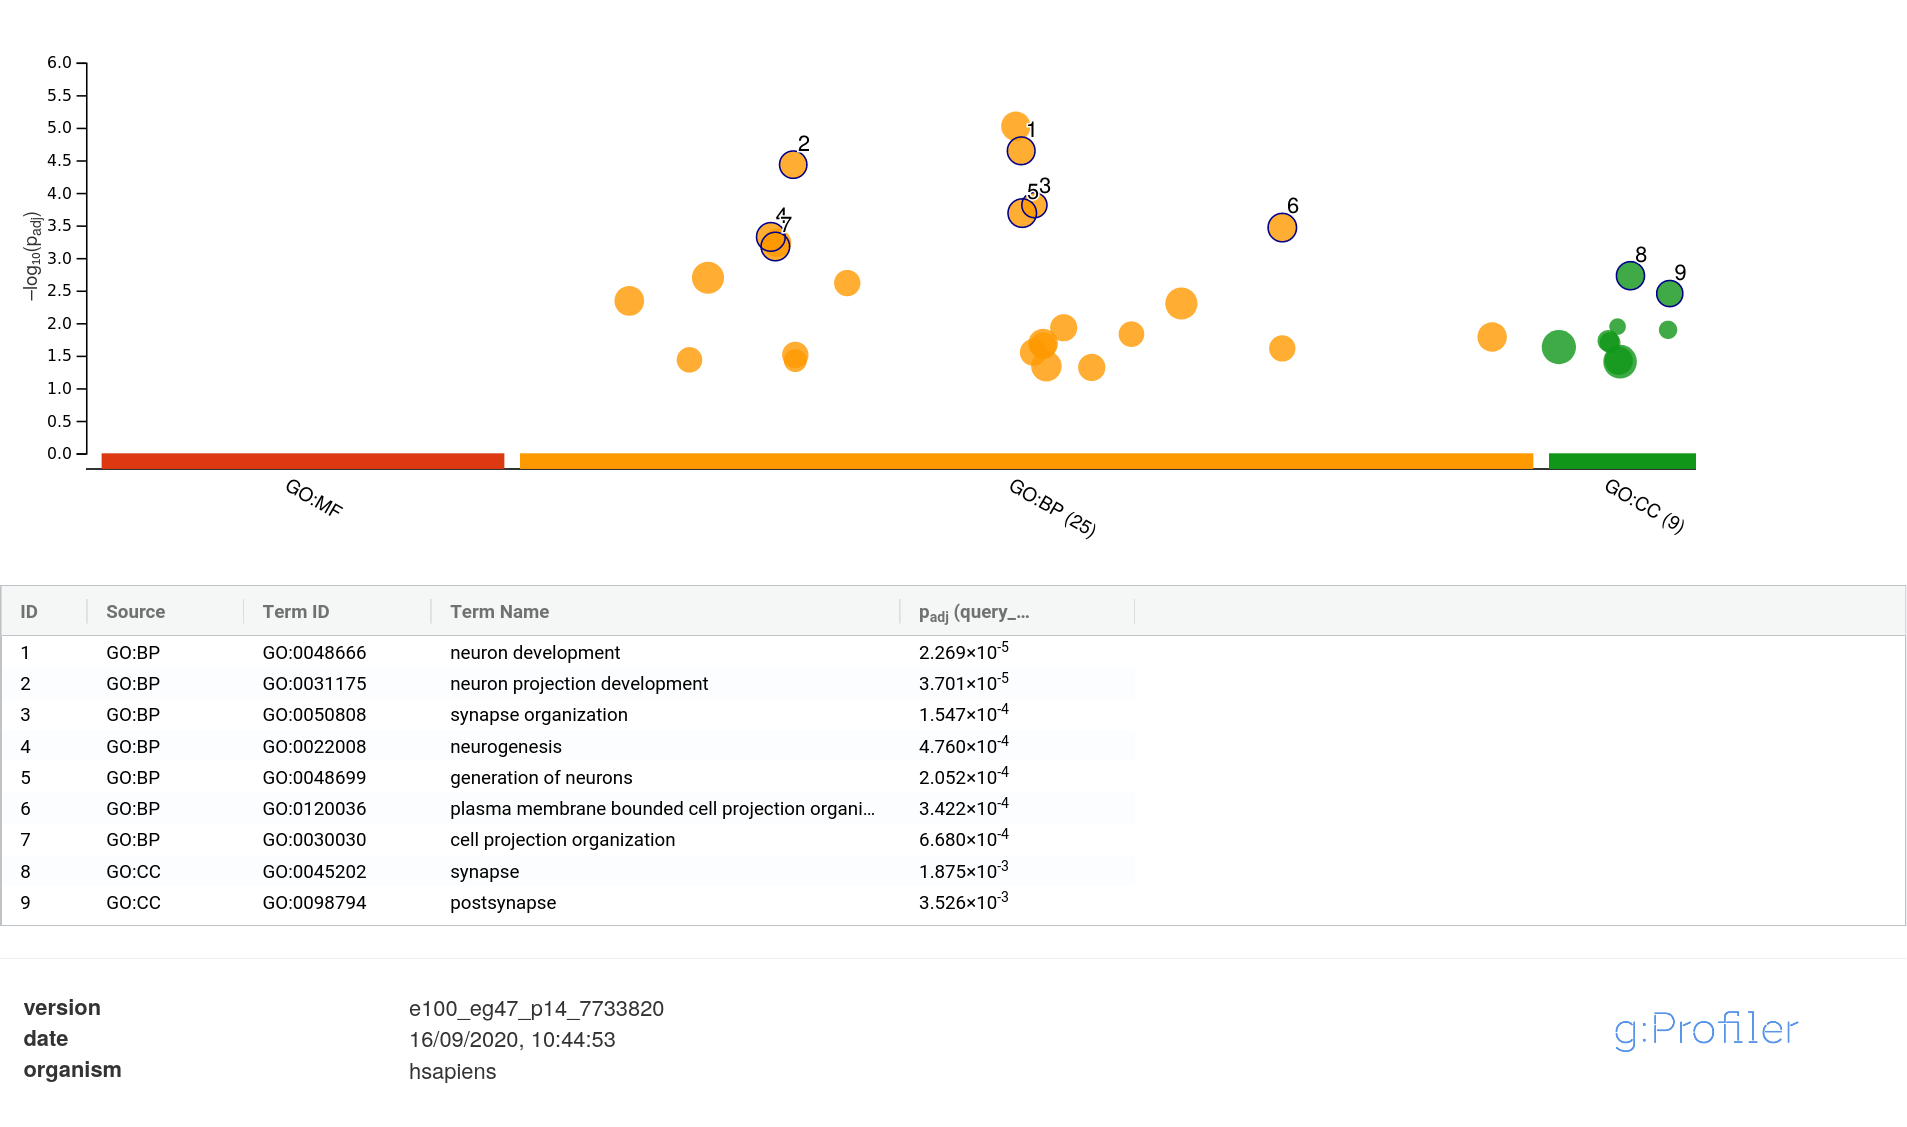
\includegraphics[width=\textwidth]{images/gprofiler/gProfiler_hsapiens_2020-09-16_09-45-55_ukbbed.png}
            %     \caption{Gene ontology enrichment Education\textsubscript{Discovery g profiler} Selected genes}
            %     \label{fig:gprofiler education discovery}
            % \end{figure}
        
            \begin{figure}
                \centering
                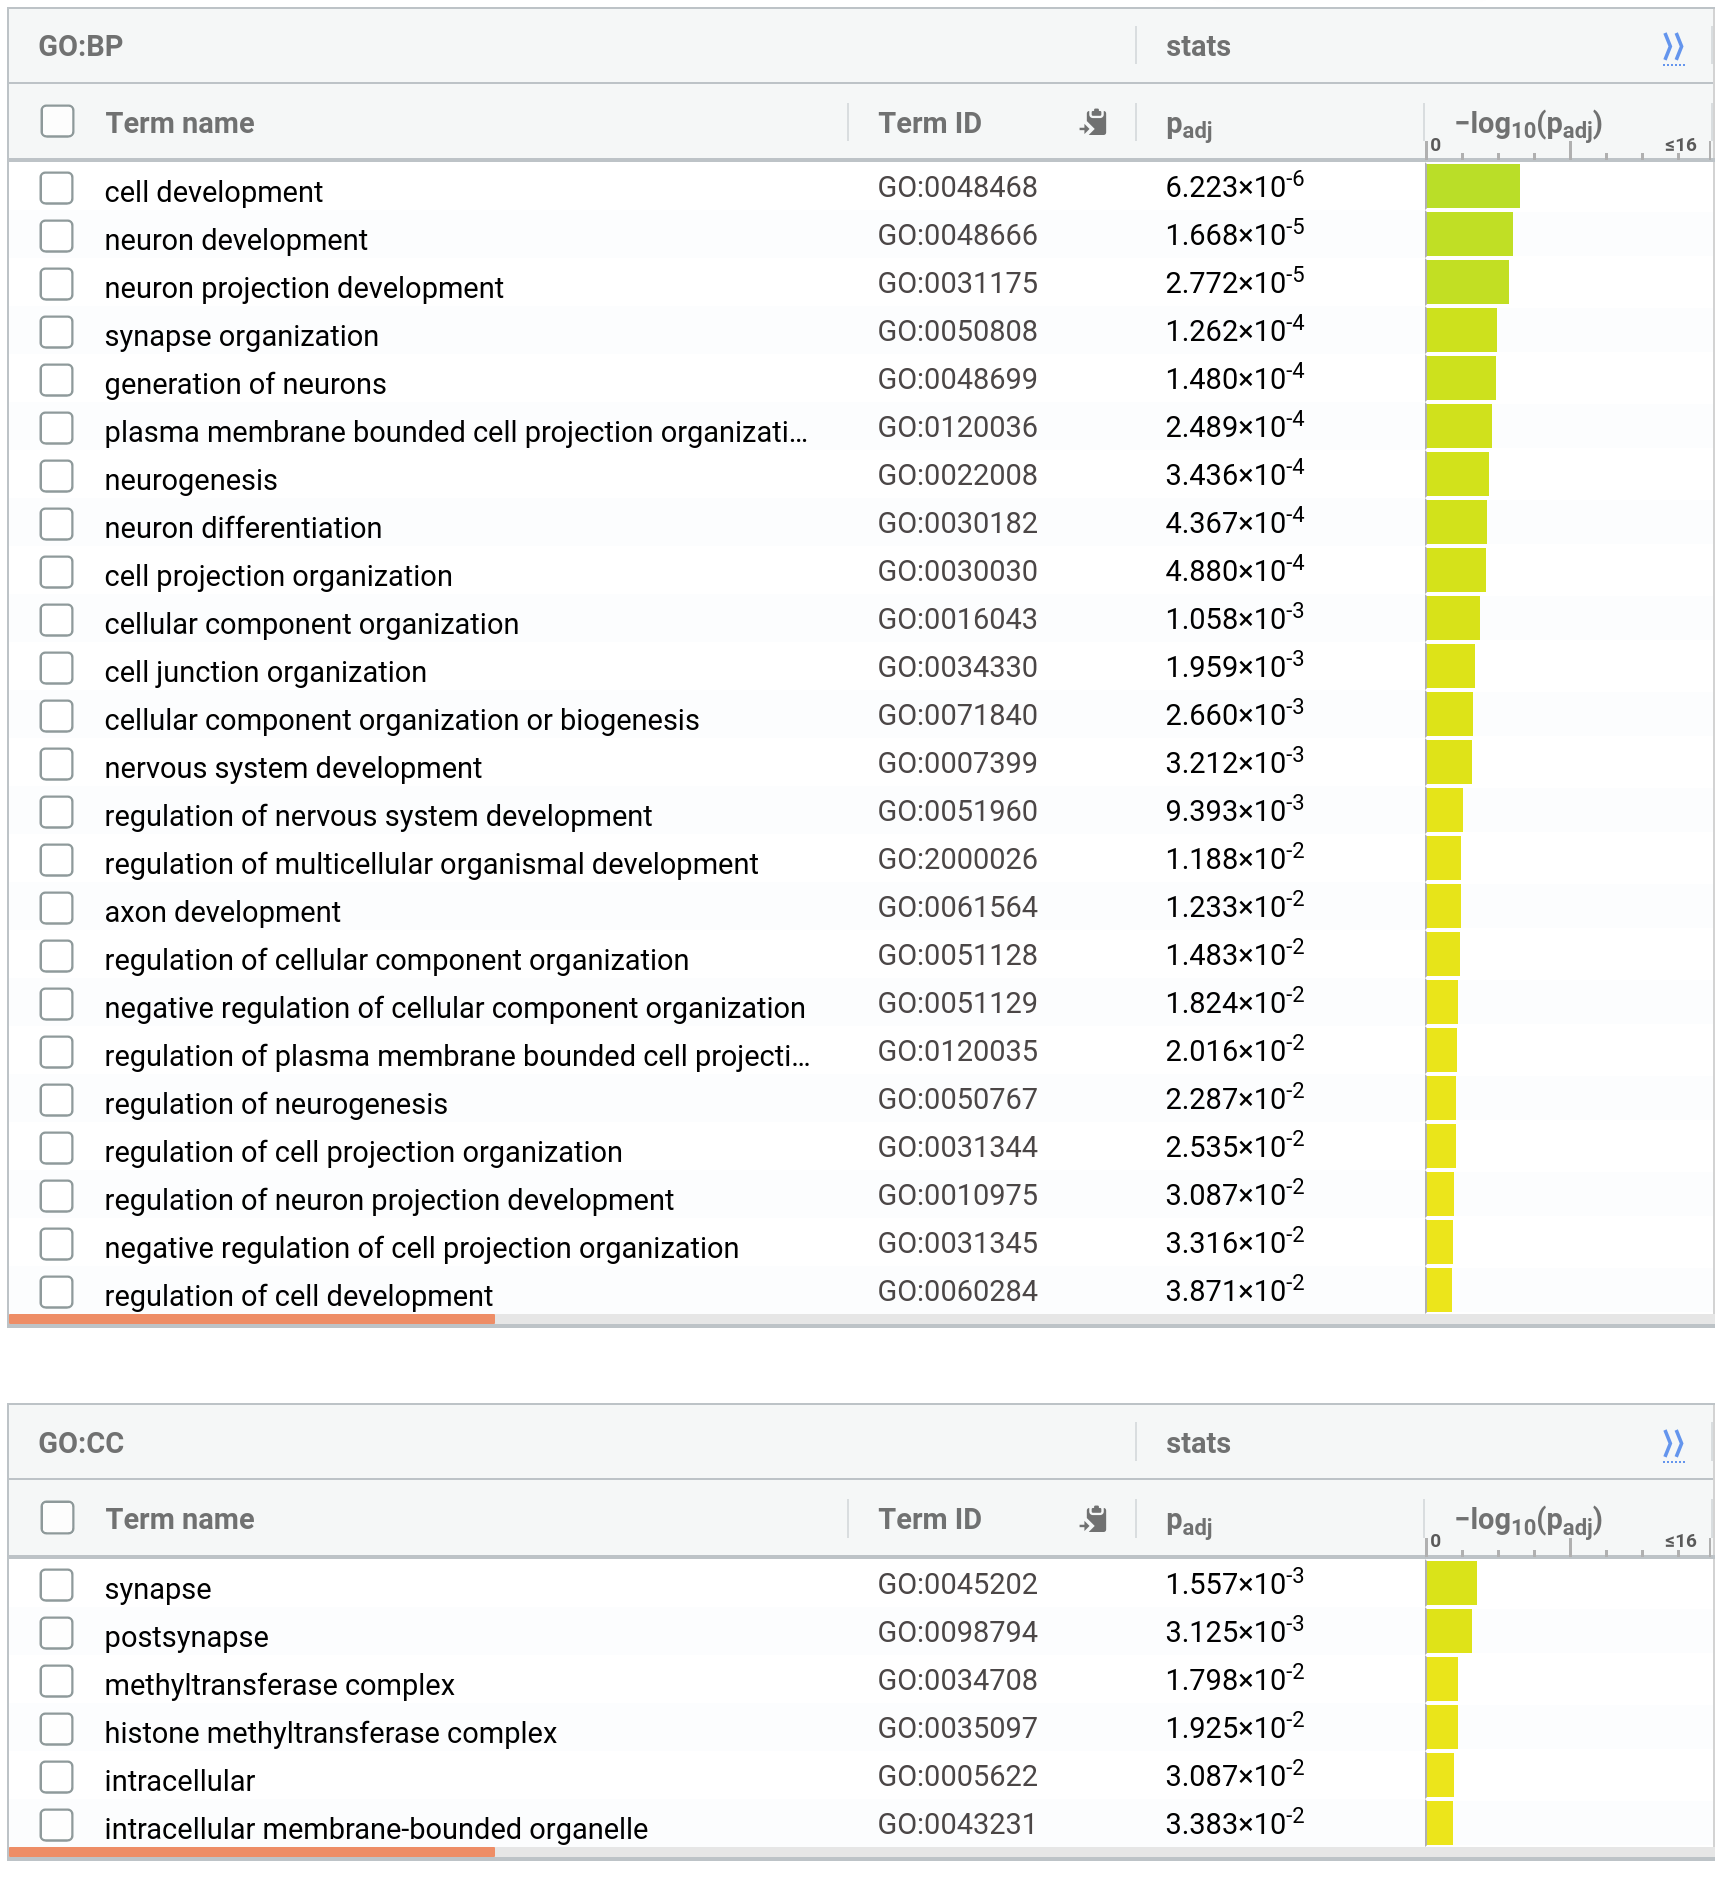
\includegraphics[width=\textwidth]{images/gprofiler/all_terms/ukbbed_allterms.png}
                \caption{Table of all terms Education Discovery gProfiler}
                \label{fig:table all terms Education Discovery gProfiler}
            \end{figure}

  \subsubsection{SynGO}
  \begin{table}[]
    \centering
    \begin{tabular}{llll}
    \toprule
    Cellular component & n & p & FDRq\\
    \midrule
    synapse organization&	15&	$7.44\times10^{-6}$&	$6.69\times10^{-5}$\\

process in the synapse&	20	&$4.06\times10^{-3}$	&0.0183\\
trans-synaptic signaling&	6&	0.0234&	0.0428\\
synapse adhesion between pre- and post-synapse&	3	&0.0146&	0.0428\\
regulation of synapse assembly&	3&	0.0238&	0.0428\\

synapse assembly&	4&	0.0289	&0.0433\\
      \bottomrule  
    \end{tabular}
    \caption{SynGO Biological Process Education\textsubscript{Discovery}}
    \label{tab:syngo biological process education discovery}
\end{table}
  
  \begin{table}[]
    \centering
    \begin{tabular}{llll}
    \toprule
    Cellular component & n & p & FDRq\\
    \midrule
 synapse&	23&	0.00451&	0.0316\\
postsynapse	&14	&0.0245&	0.0858\\
\bottomrule
\end{tabular}
\caption{syngo CC Education Discovery}
\label{tab:syngo CC Education discovery}
\end{table}
            % \paragraph{BP Education Discovery} One term synapse	 n= 23	p=2.64e-3	q=0.0185
            
            % \paragraph{CC Education Discovery}
            % 6 significant terms. See table~\ref{tab:syngo cc ukbb ed}
            
            
 
 
 
 Synapse, GO:0045202, was the only enriched cellular component term using SynGO (table~\ref{tab:syngo CC Education discovery}).
SynGO annotates only 23 of the significant genes to synapse, compared to 40 genes in ToppGene table~\ref{tab:Cellular component Education Discovery ToppGene top10 results Bonfe}. Six biological process terms are enriched,  including synapse organisation GO:0050807( table~\ref{tab:syngo biological process education discovery}). Fifteen terms are annotated synapse organisation by SynGO compared with 19 in toppgene (table~\ref{tab:Biological Process Education Discovery ToppGene top10 results BY} but the limited ontology results in a more significant FDR ($6.69\times10^{-5}$ compared to 0.018). These results show both the benefits and limitations of specialised ontologies.      \footnote{      NOte synapse organisation GO:0050807) has 15 annotated terms with FDR q $3.97\times10^{-5}$ compared to regulation of synapse organisation 11 of 229 P $0.943\times{10^-5}$ FDR 0.0483 in PANTHER GO:0050807
 See table~\ref{tab:syngo biological process education discovery}}

 
 Using FUMA to analyse gene expression the GWGAS significant Education\textsubscript{Replication} genes are over-represented amongst  differentially expressed genes up-regulated in the brain using GTEx (figure~\ref{fig:ukbbed gtex}). This is the only sample in which this is the case (see figure~\ref{fig:FUMA gtex deg samples multiple} and figure~\ref{fig:deg_upref_sample_gtex_gener} which shows only over-representation. 

% \subsubsection{Summary of Education Discovery}
% ToppGene and gprofiler No Molecular function

% Genes association with ID

% MF nil in PANTHER
% BP neurogenesis and synapse organisation and neuron projection

% CC MHC (which is assoc type II dm) ER PSD and post synapse, neuron projection
%         \subsubsection{Summary of above findings}

 \begin{figure}
  \begin{subfigure}{12cm}
    \centering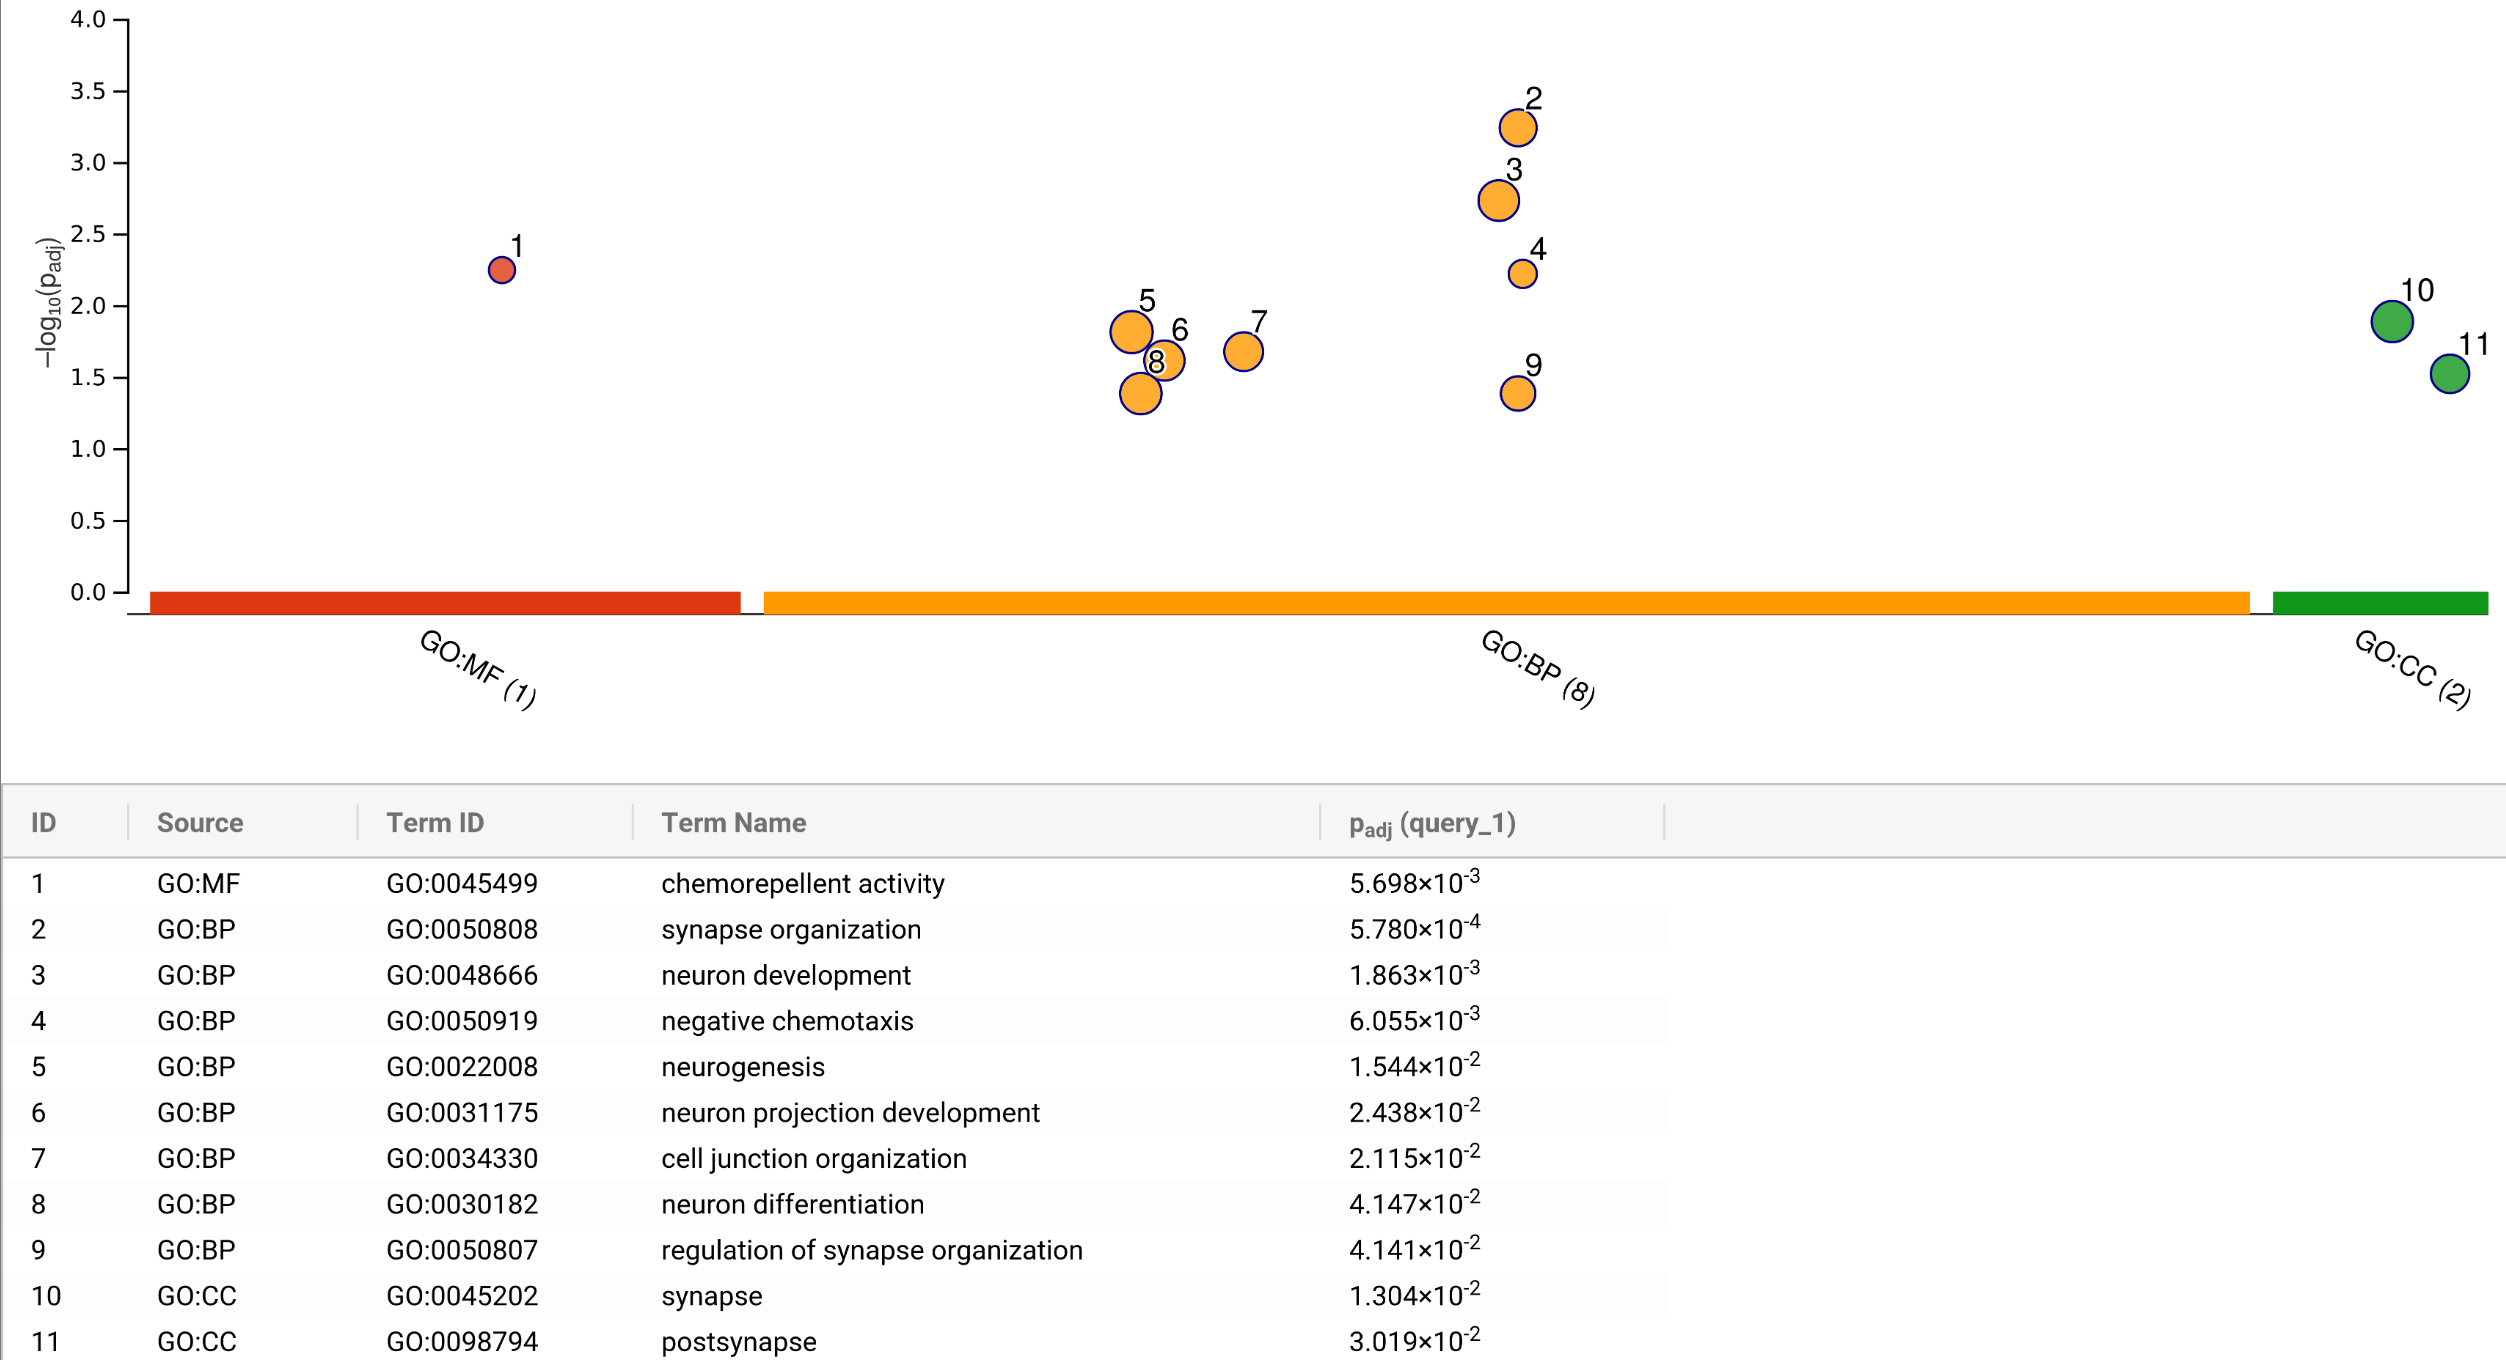
\includegraphics[width=11cm]{images/gprofiler/gprofiler_ea2_clip.png}
    \caption{gProfiler. Education Replication}
    \end{subfigure}
    
  \begin{subfigure}{12cm}
    \centering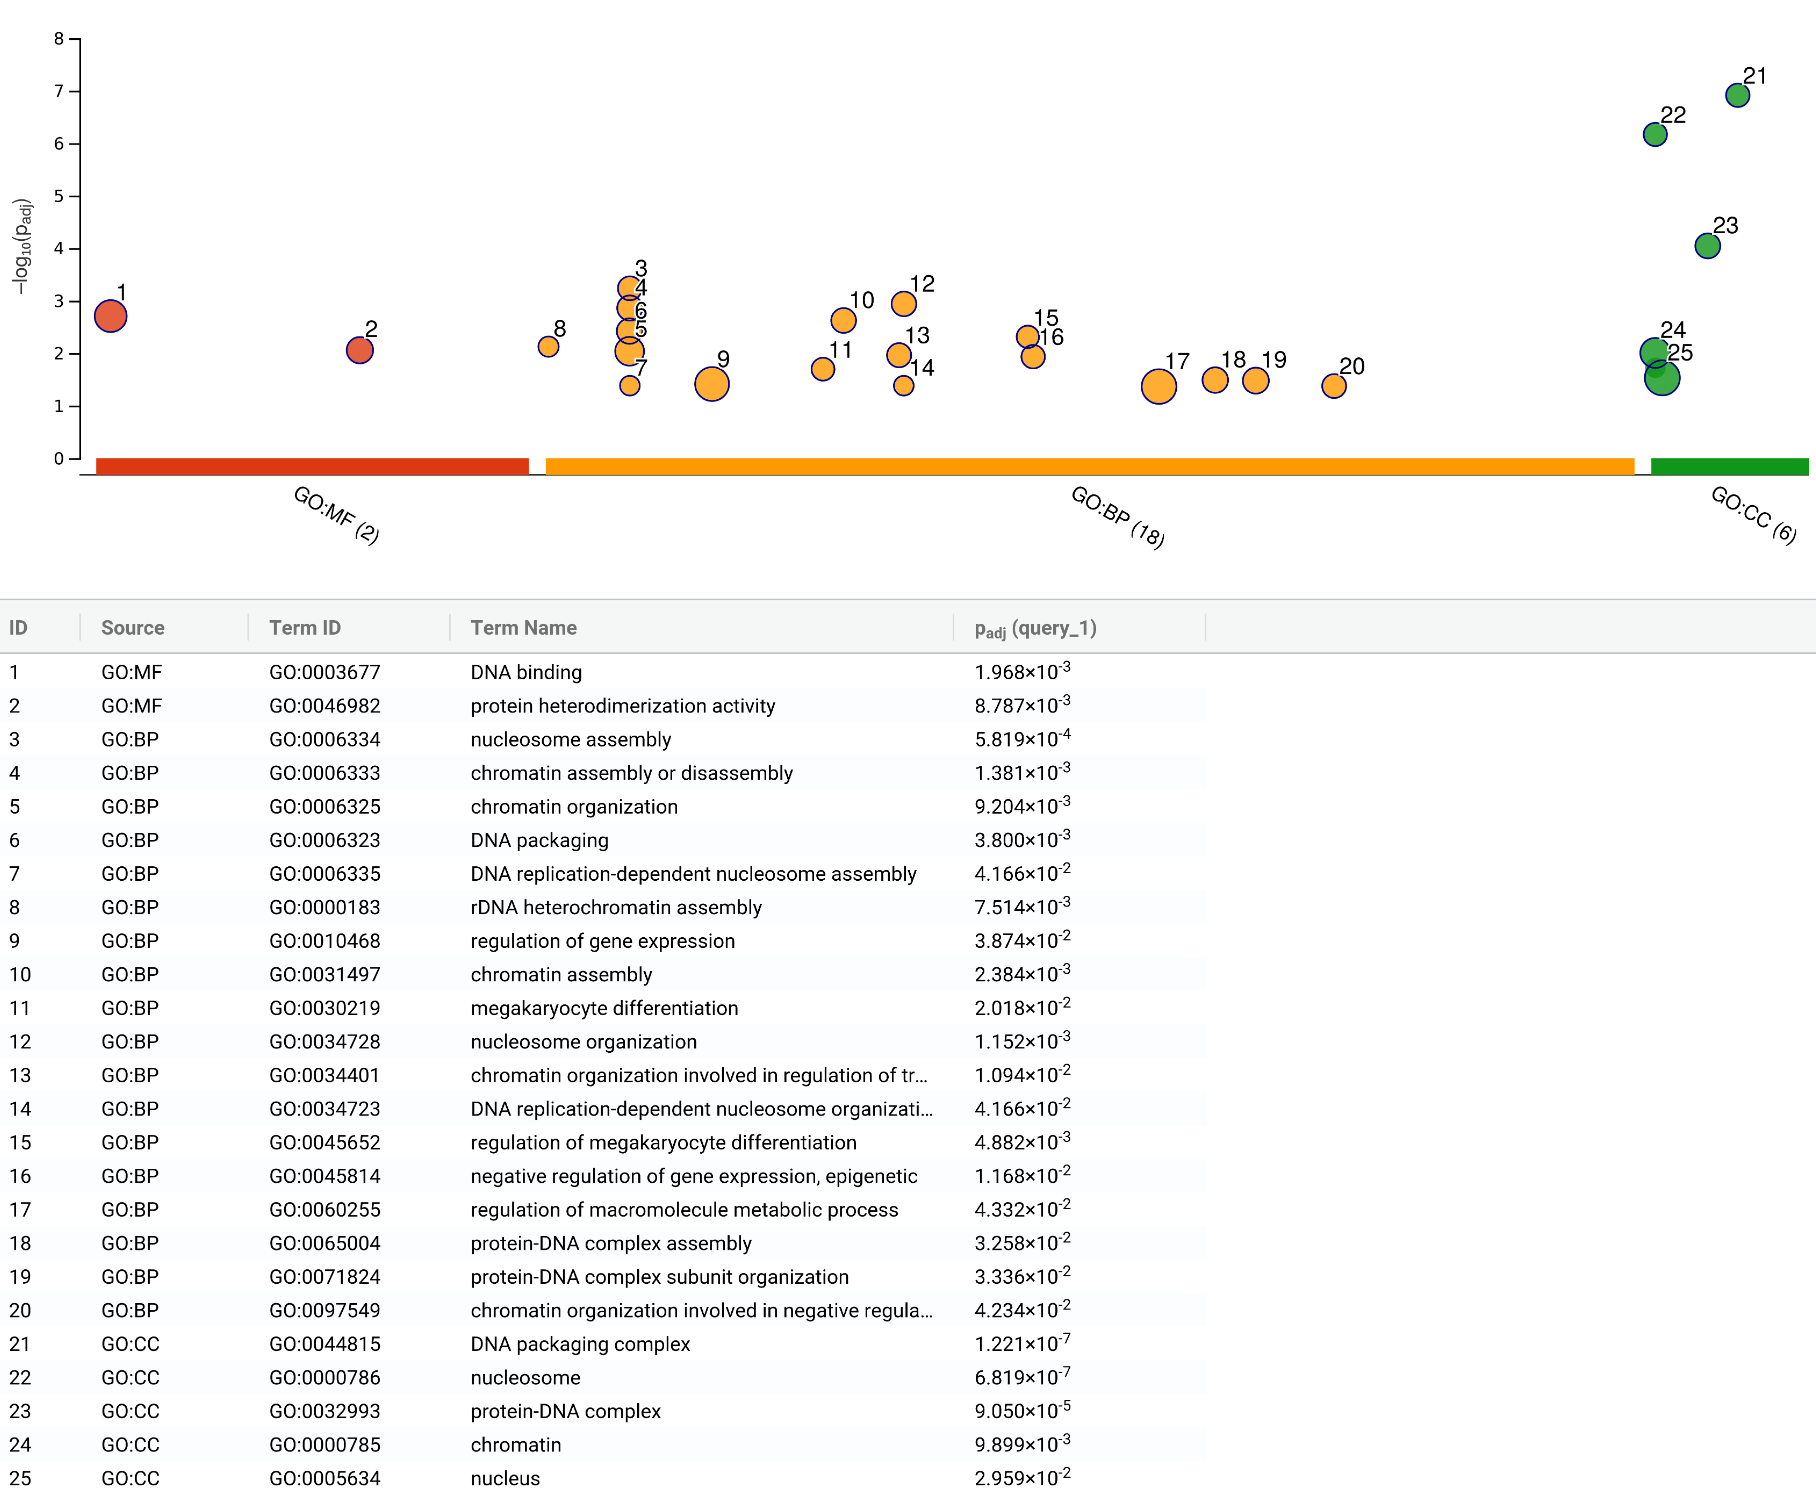
\includegraphics[width=11cm]{images/gprofiler/gprofiler_ukbbint_clip.png}
    \caption{gProfiler Intelligence Discovery}
  \end{subfigure}
 
  \begin{subfigure}{12cm}
    \centering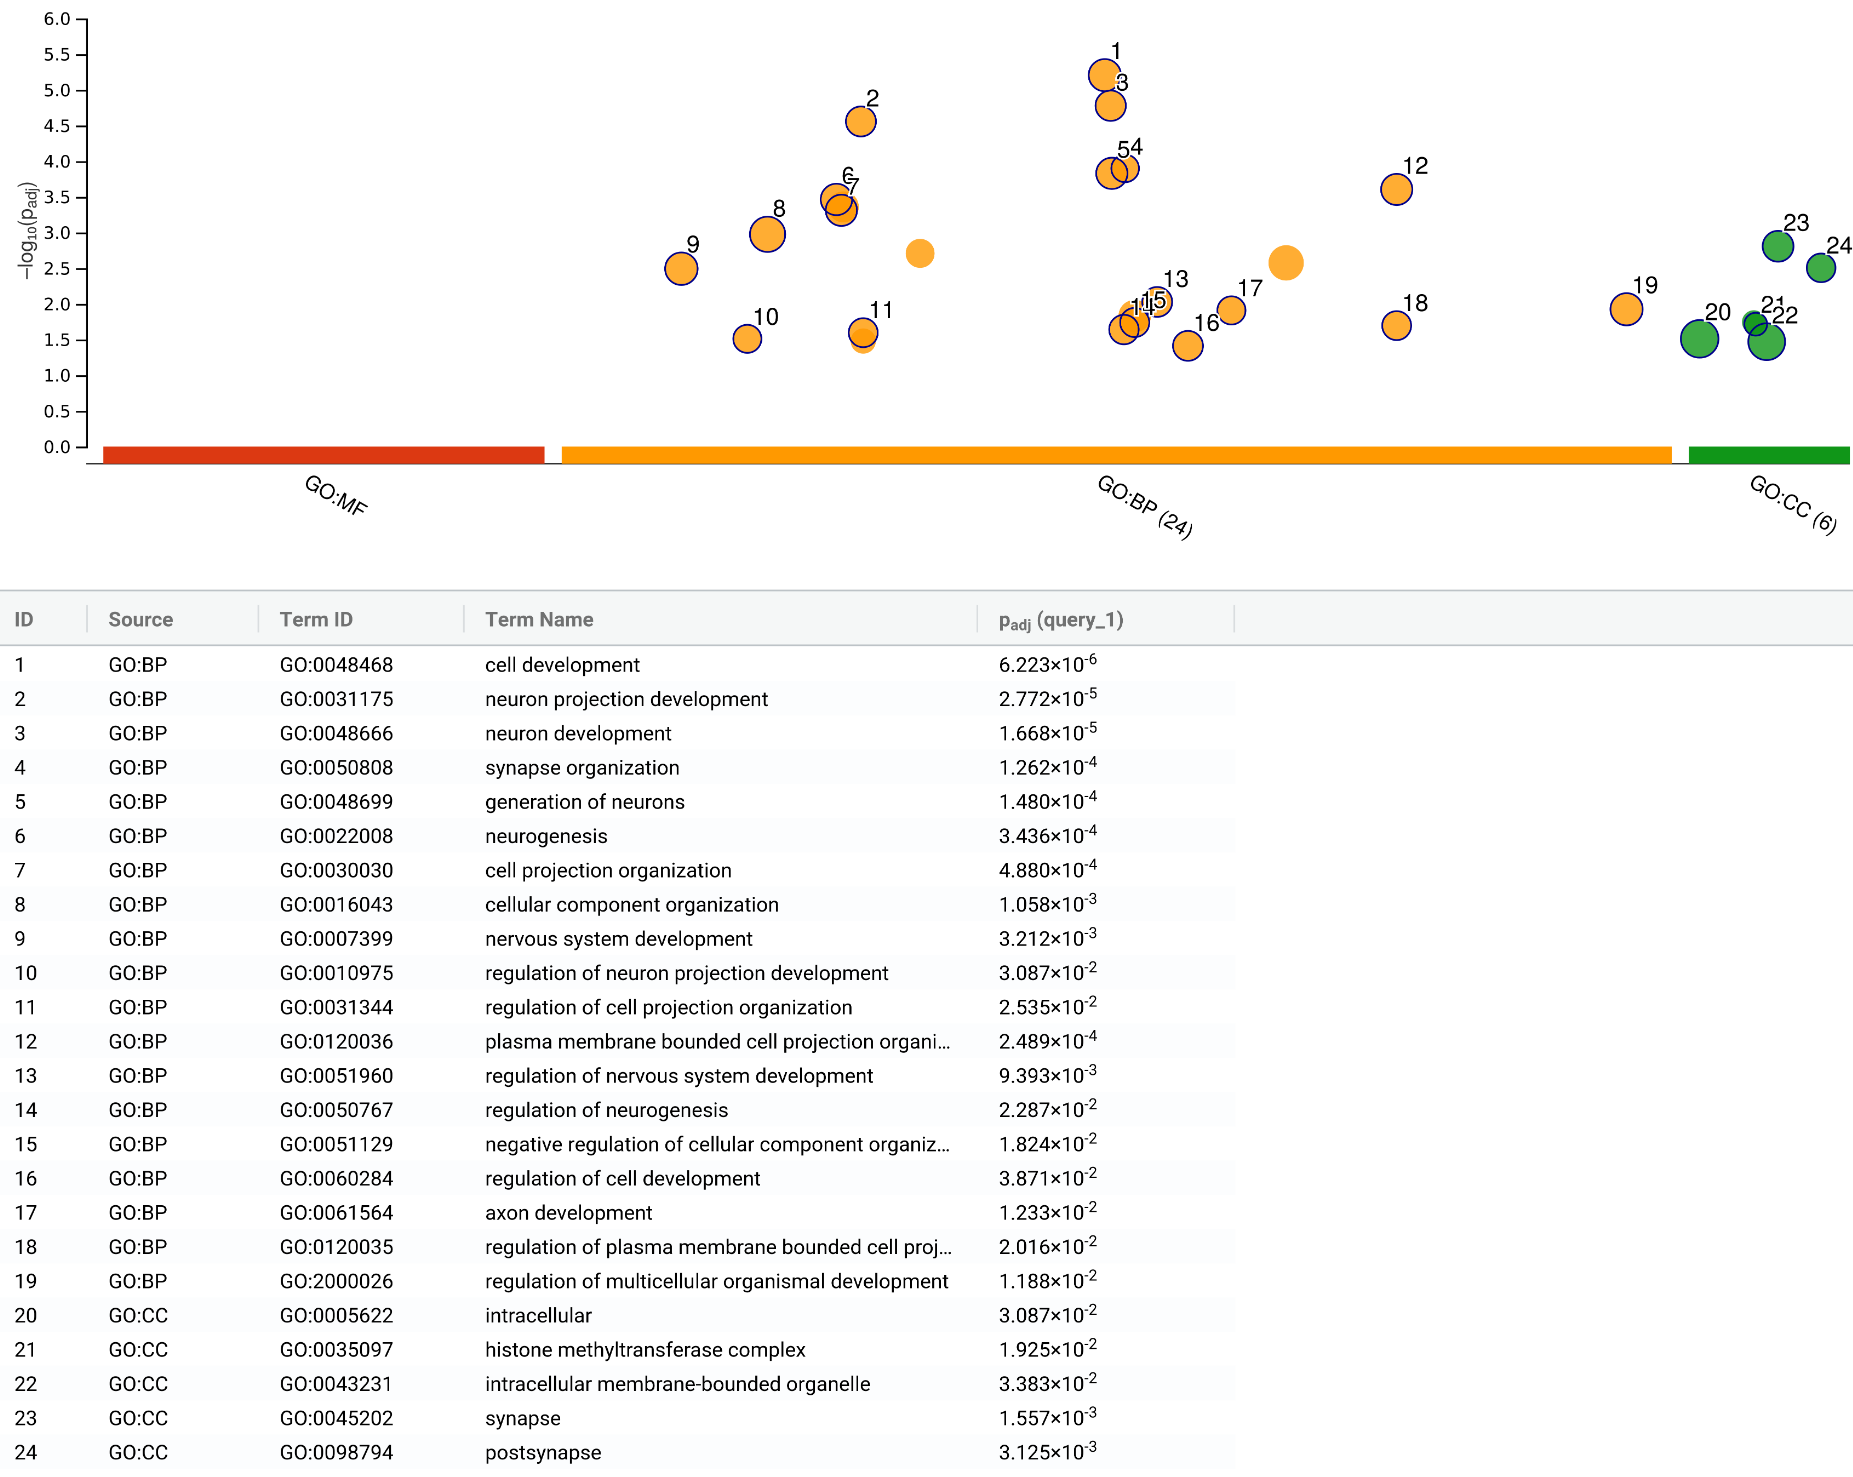
\includegraphics[width=11cm]{images/gprofiler/gprofiler_eukbbed_clip.png}
    \caption{gProfiler Education Discovery}
  \end{subfigure}
  \caption{Gene Ontology enrichment of significant genes using gProfilers}
  \label{fig:gProfiler 3 samples}
  
\end{figure}

\begin{figure}
    \centering
    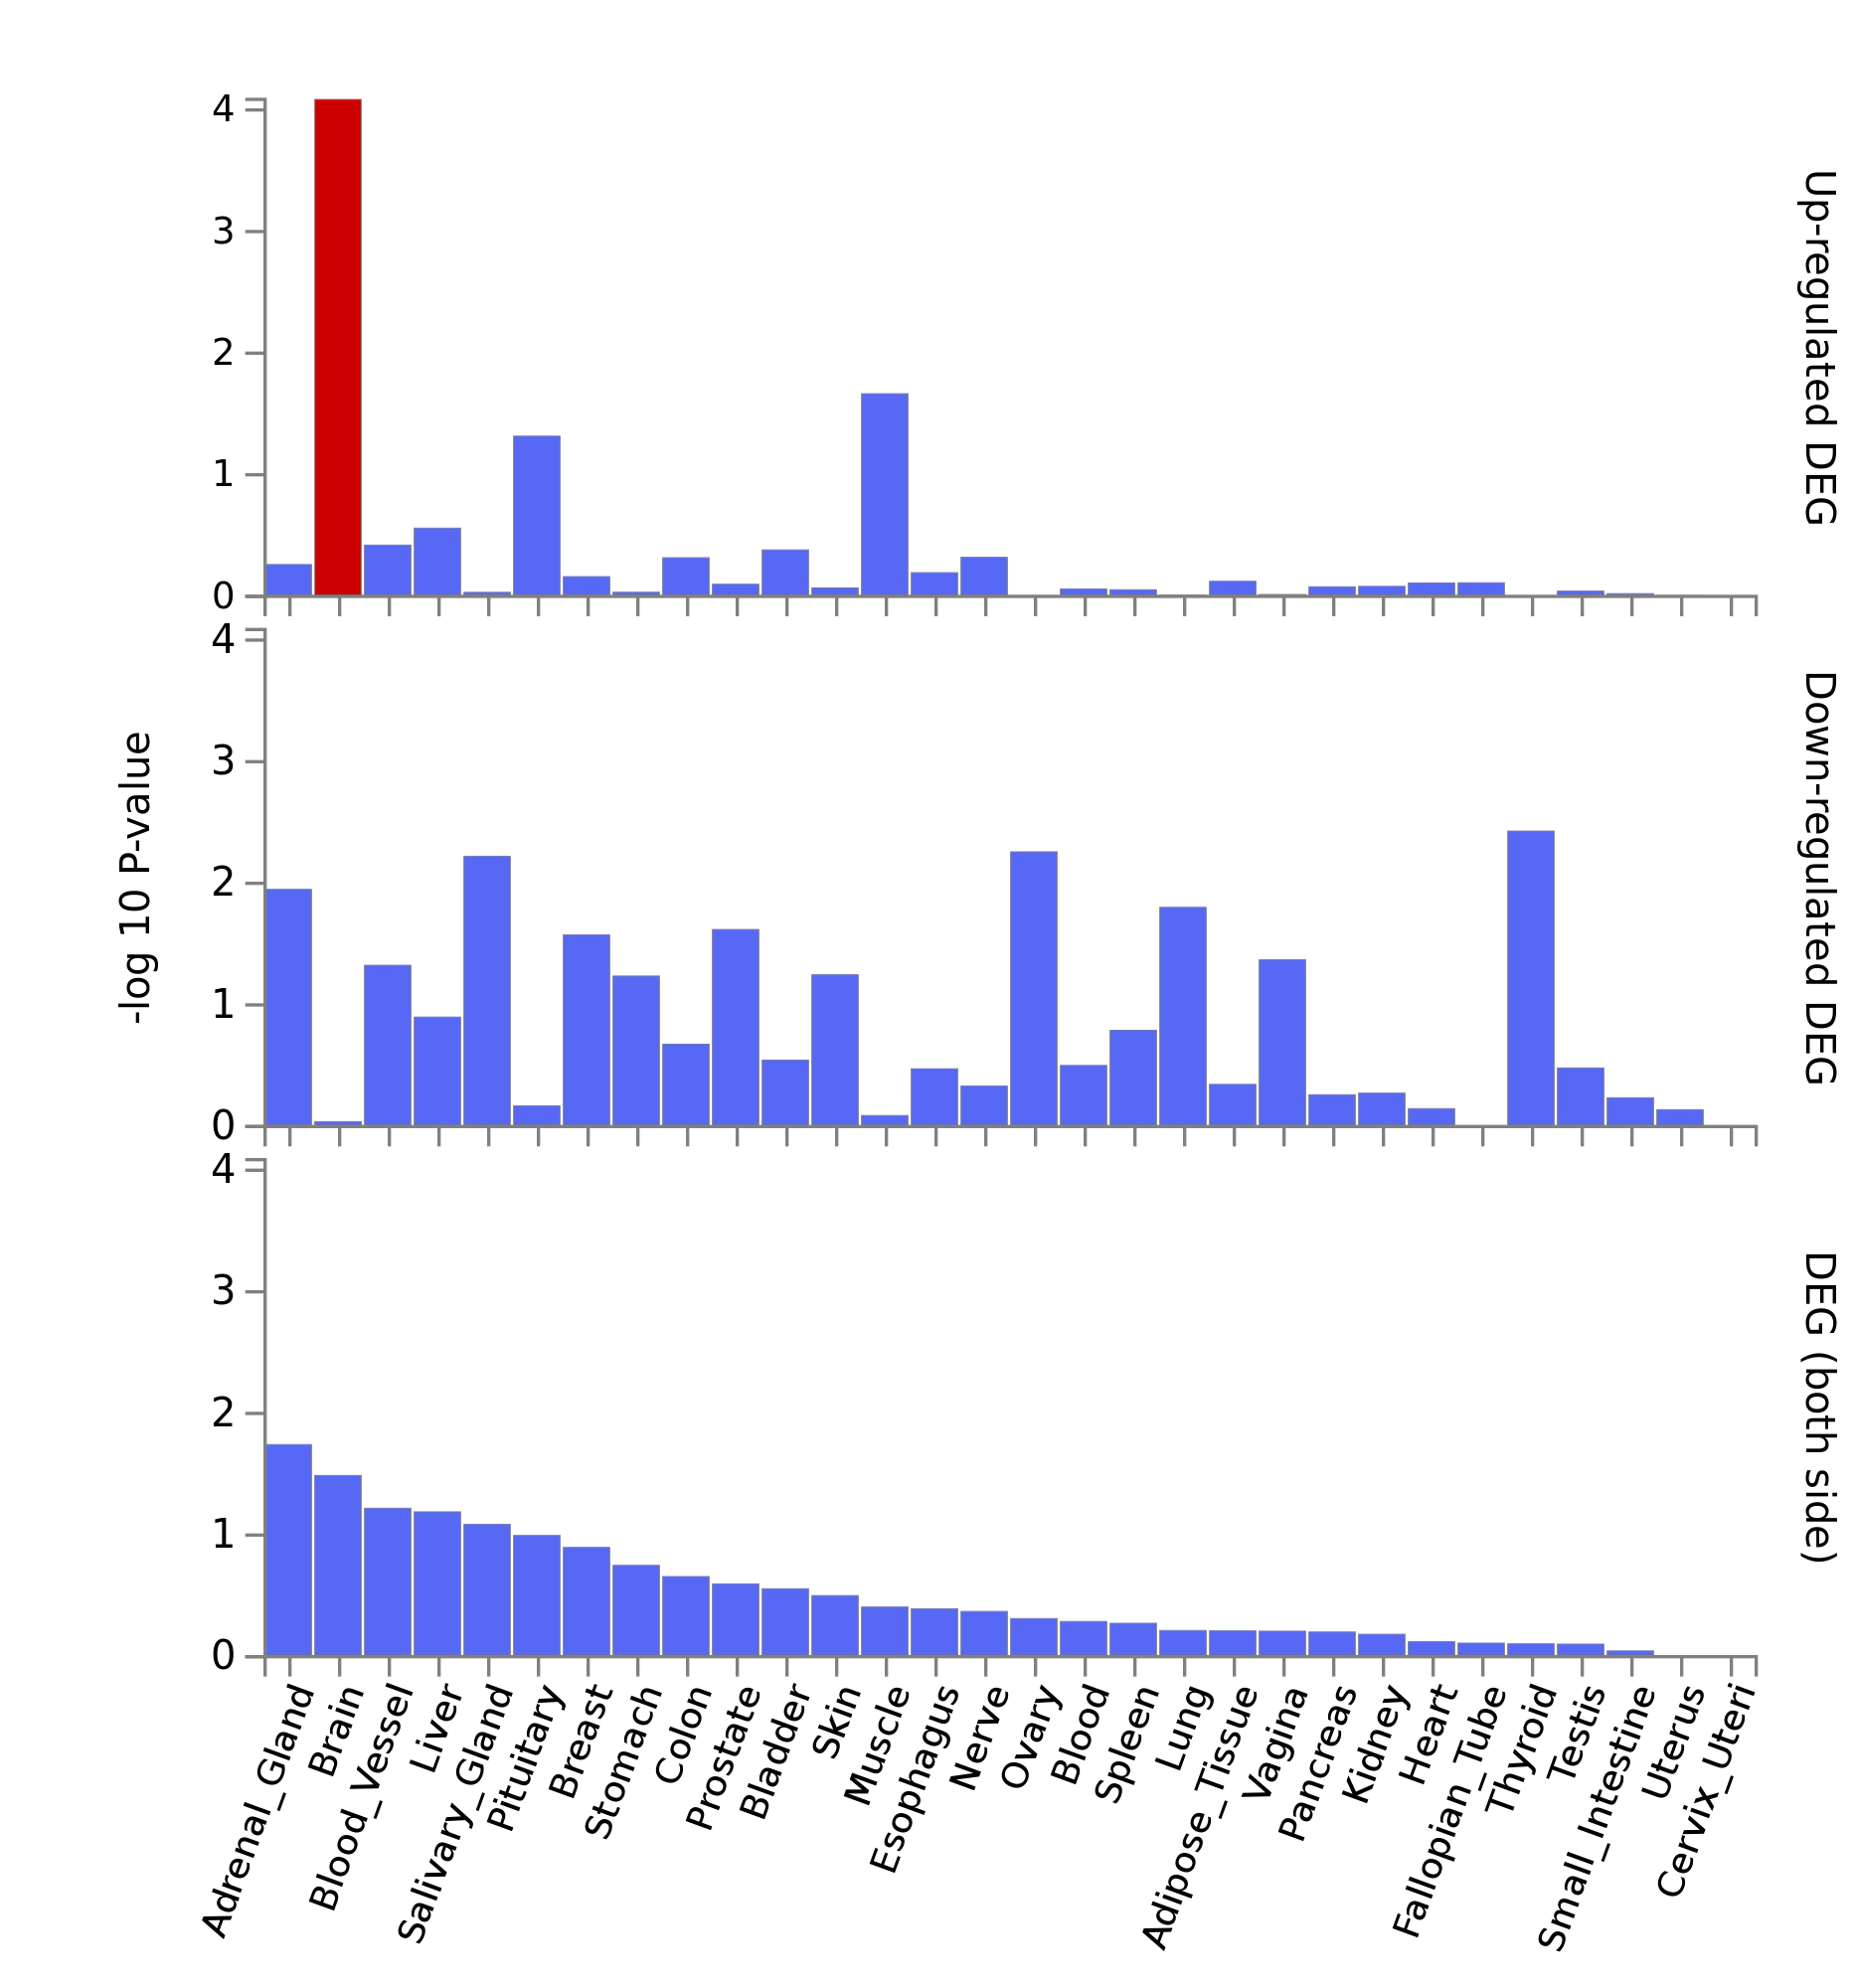
\includegraphics[width=\textwidth]{images/FUMA_plots/gtex_v8_ts_general_FUMA_gene2func_UKBBEd_syn_protein_bp_sig.png}
    \caption{Gtex General UKBBEd Synaptic significant.png}
    \label{fig:ukbbed gtex}
\end{figure}


\begin{figure}
    \centering
    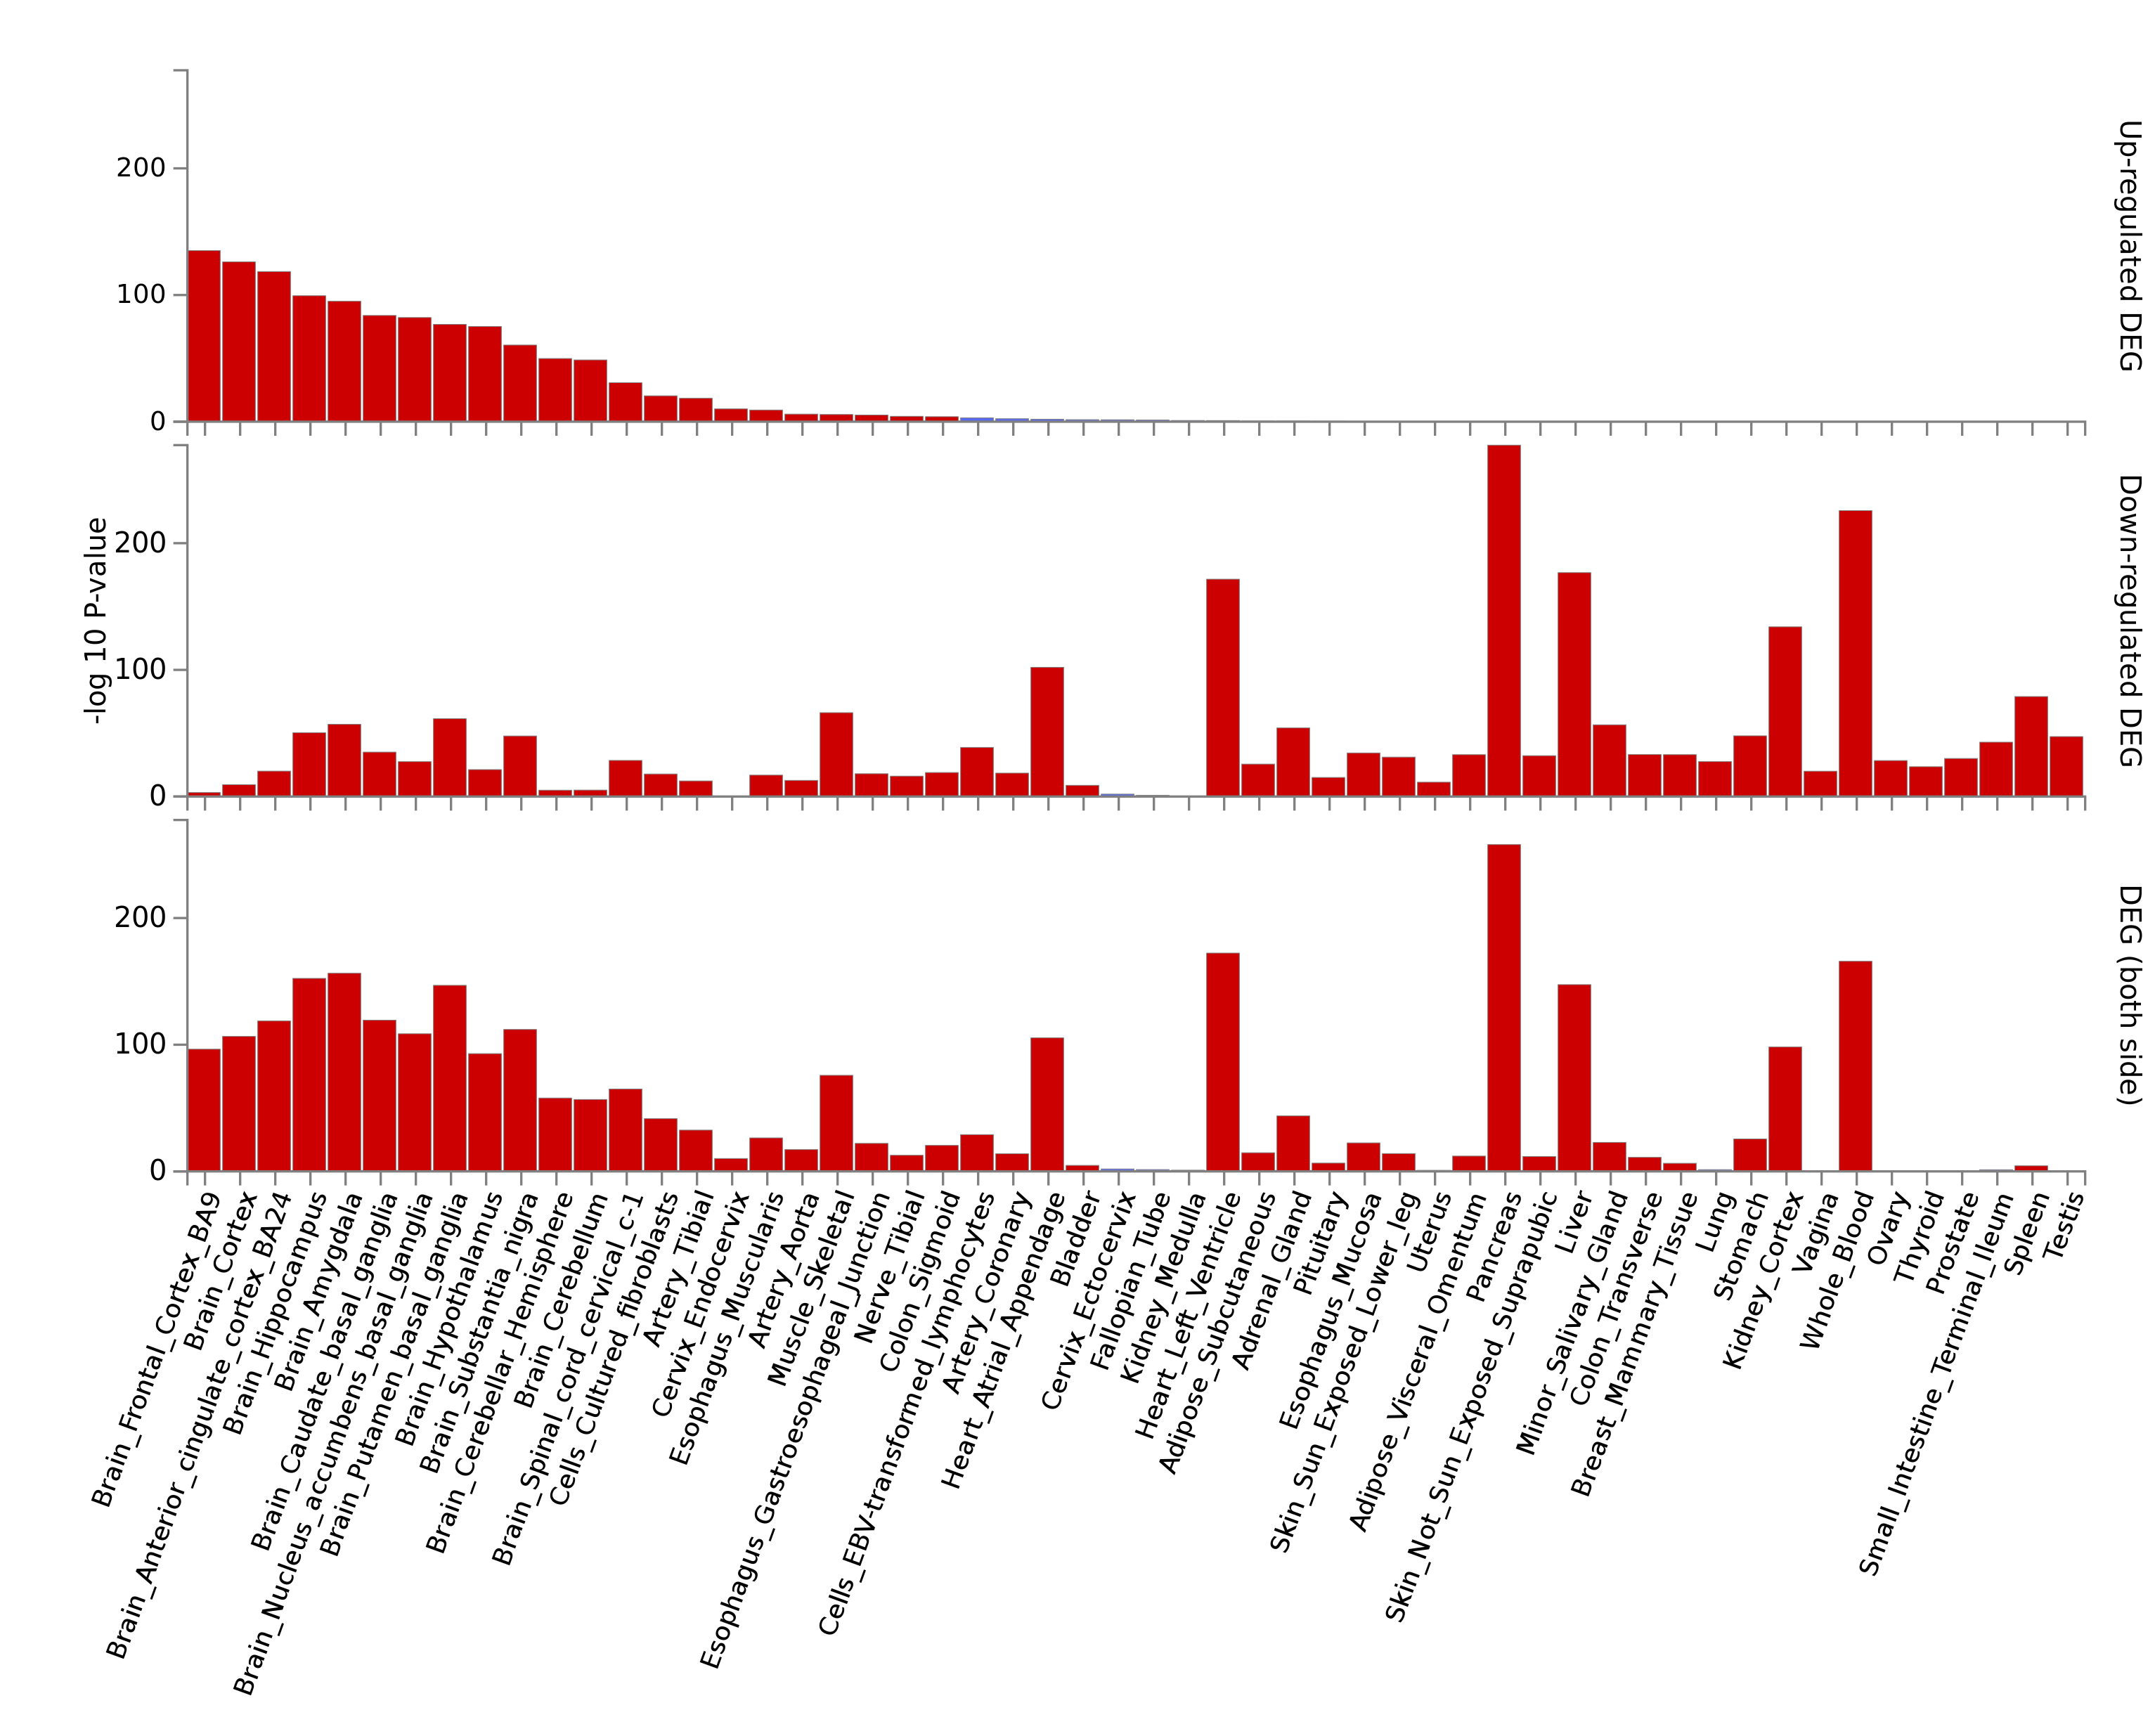
\includegraphics[width=\textwidth]{images/FUMA_plots/gtex_v8_ts_FUMA_PSP_gtex.png}
    \caption[GTEx All PSP]{GTex all PSP. Note top row of upregulated genes. Shows that signal from expanded PSP is very specific to CNS expression. Red significant. Y axis -log10 of p value. Hypergeometric test of genes differentially expressed from pre-created list see FUMA \cite{watanabe2017functional} for details (two sided Bonferroni corrected p versus all labels with cut off fold change) }
    \label{fig:gtex all PSP}
\end{figure}
\clearpage


\begin{figure}
    \centering
    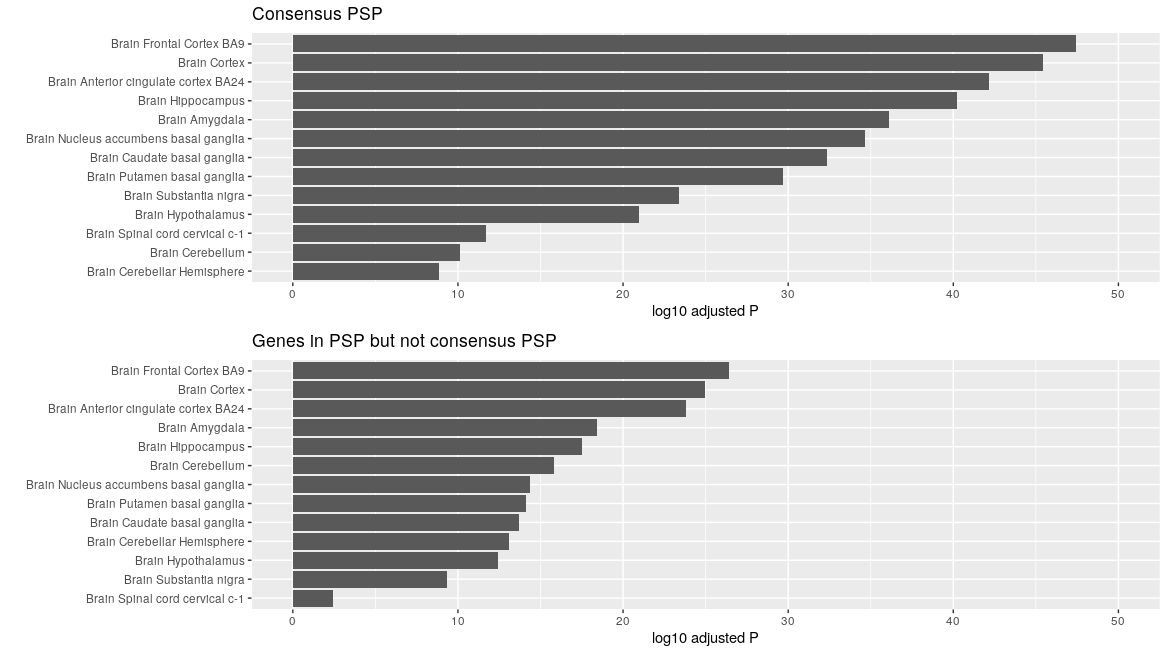
\includegraphics[width=\textwidth]{images/chapter2/ggplot/Rplot_consensusgtex.png}
    \caption{Differentially expressed genes over representation analysis in Gtex. Top panel genes in consensus PSD $n=1312$. Lower panel genes not in consensus PSD but in PSP.\url{source('~/RProjects/paper_xls_output/R/chapter_2/FUMA/plot_gtex/plot_consensus_multiplot.R')}}
    \label{fig:deg_gtex_psp}
\end{figure}



\begin{figure}
    \centering
    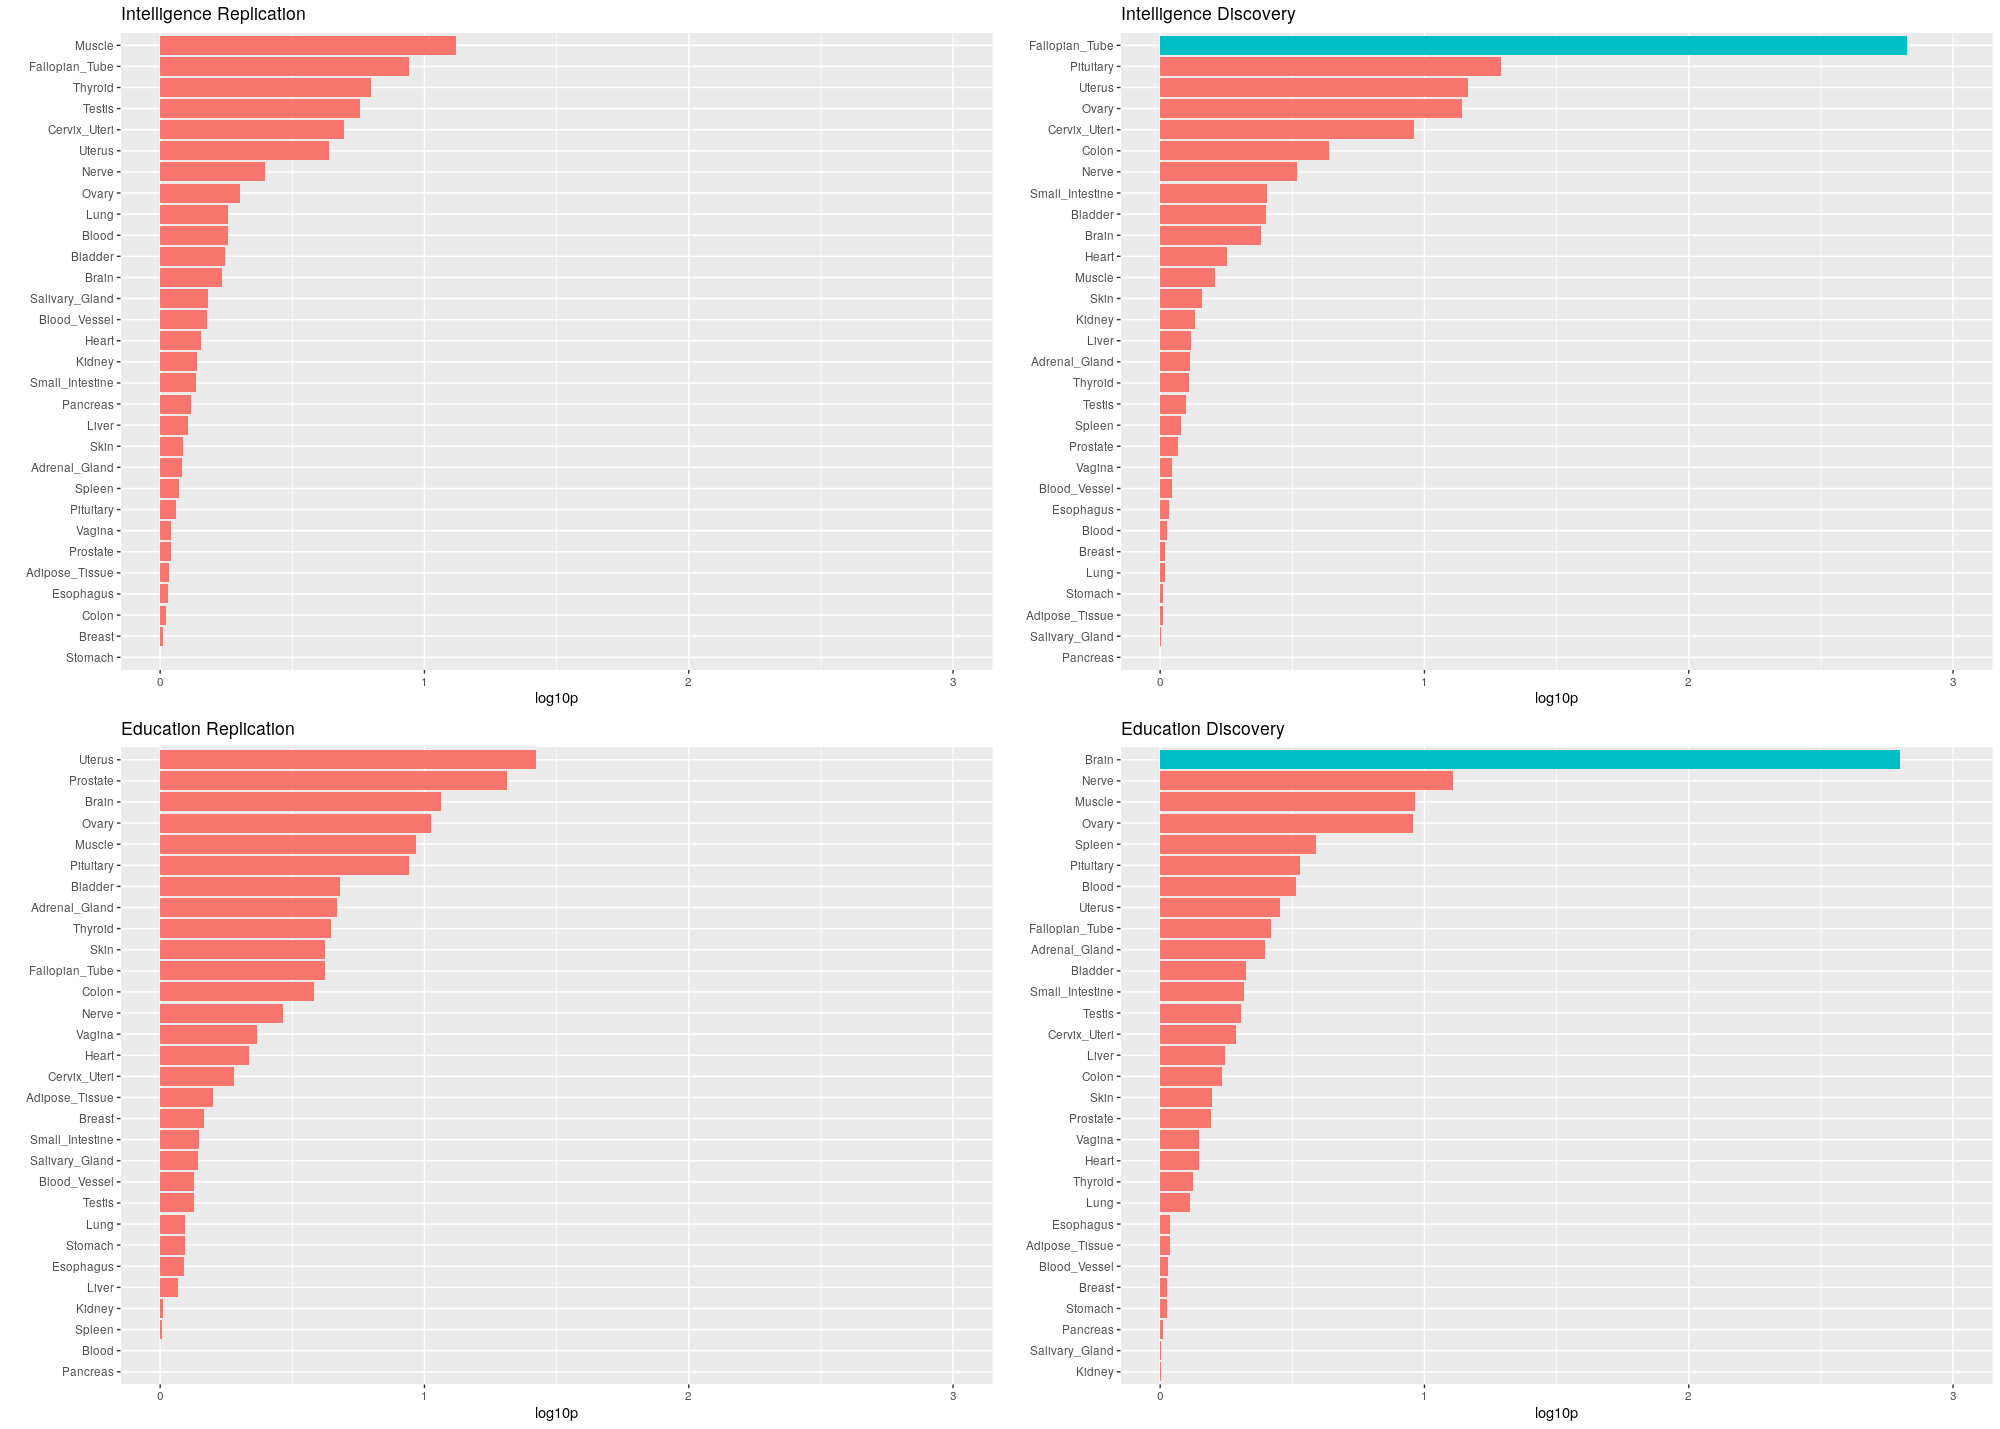
\includegraphics[width=\textwidth]{images/chapter2/ggplot/ggplot_FUMA/Rplot_upregulated_general.png}
    \caption{Over representation of differentially expressed genes (up regulated) amongst significant genes at GWGAS for each of the samples clockwise from top left Intelligence Replication, Intelligence Discovery, Education Discovery and Education replication using FUMA to perform over representation. Gene expression data GTEx v8. x axis is -log10 transform of p value for cumulative hypergeometric test. Significant tissues are shown in cyan. The only sample with over representation of genes with up-regulated differential expression in the brain is Education\textsubscript{Replication} \url{source('~/RProjects/paper_xls_output/R/chapter_2/FUMA/plot_gtex/plot_study/multiplot_samples.R')}}
    \label{fig:deg_upref_sample_gtex_gener}
\end{figure}

%%%
% \subsection{Statistical analysis}\todo{move}

% Correction for multiple testing - by package or using adjust\_p in R. Statistical tests in R version . 

 \begin{figure}
  \begin{subfigure}{8cm}
    \centering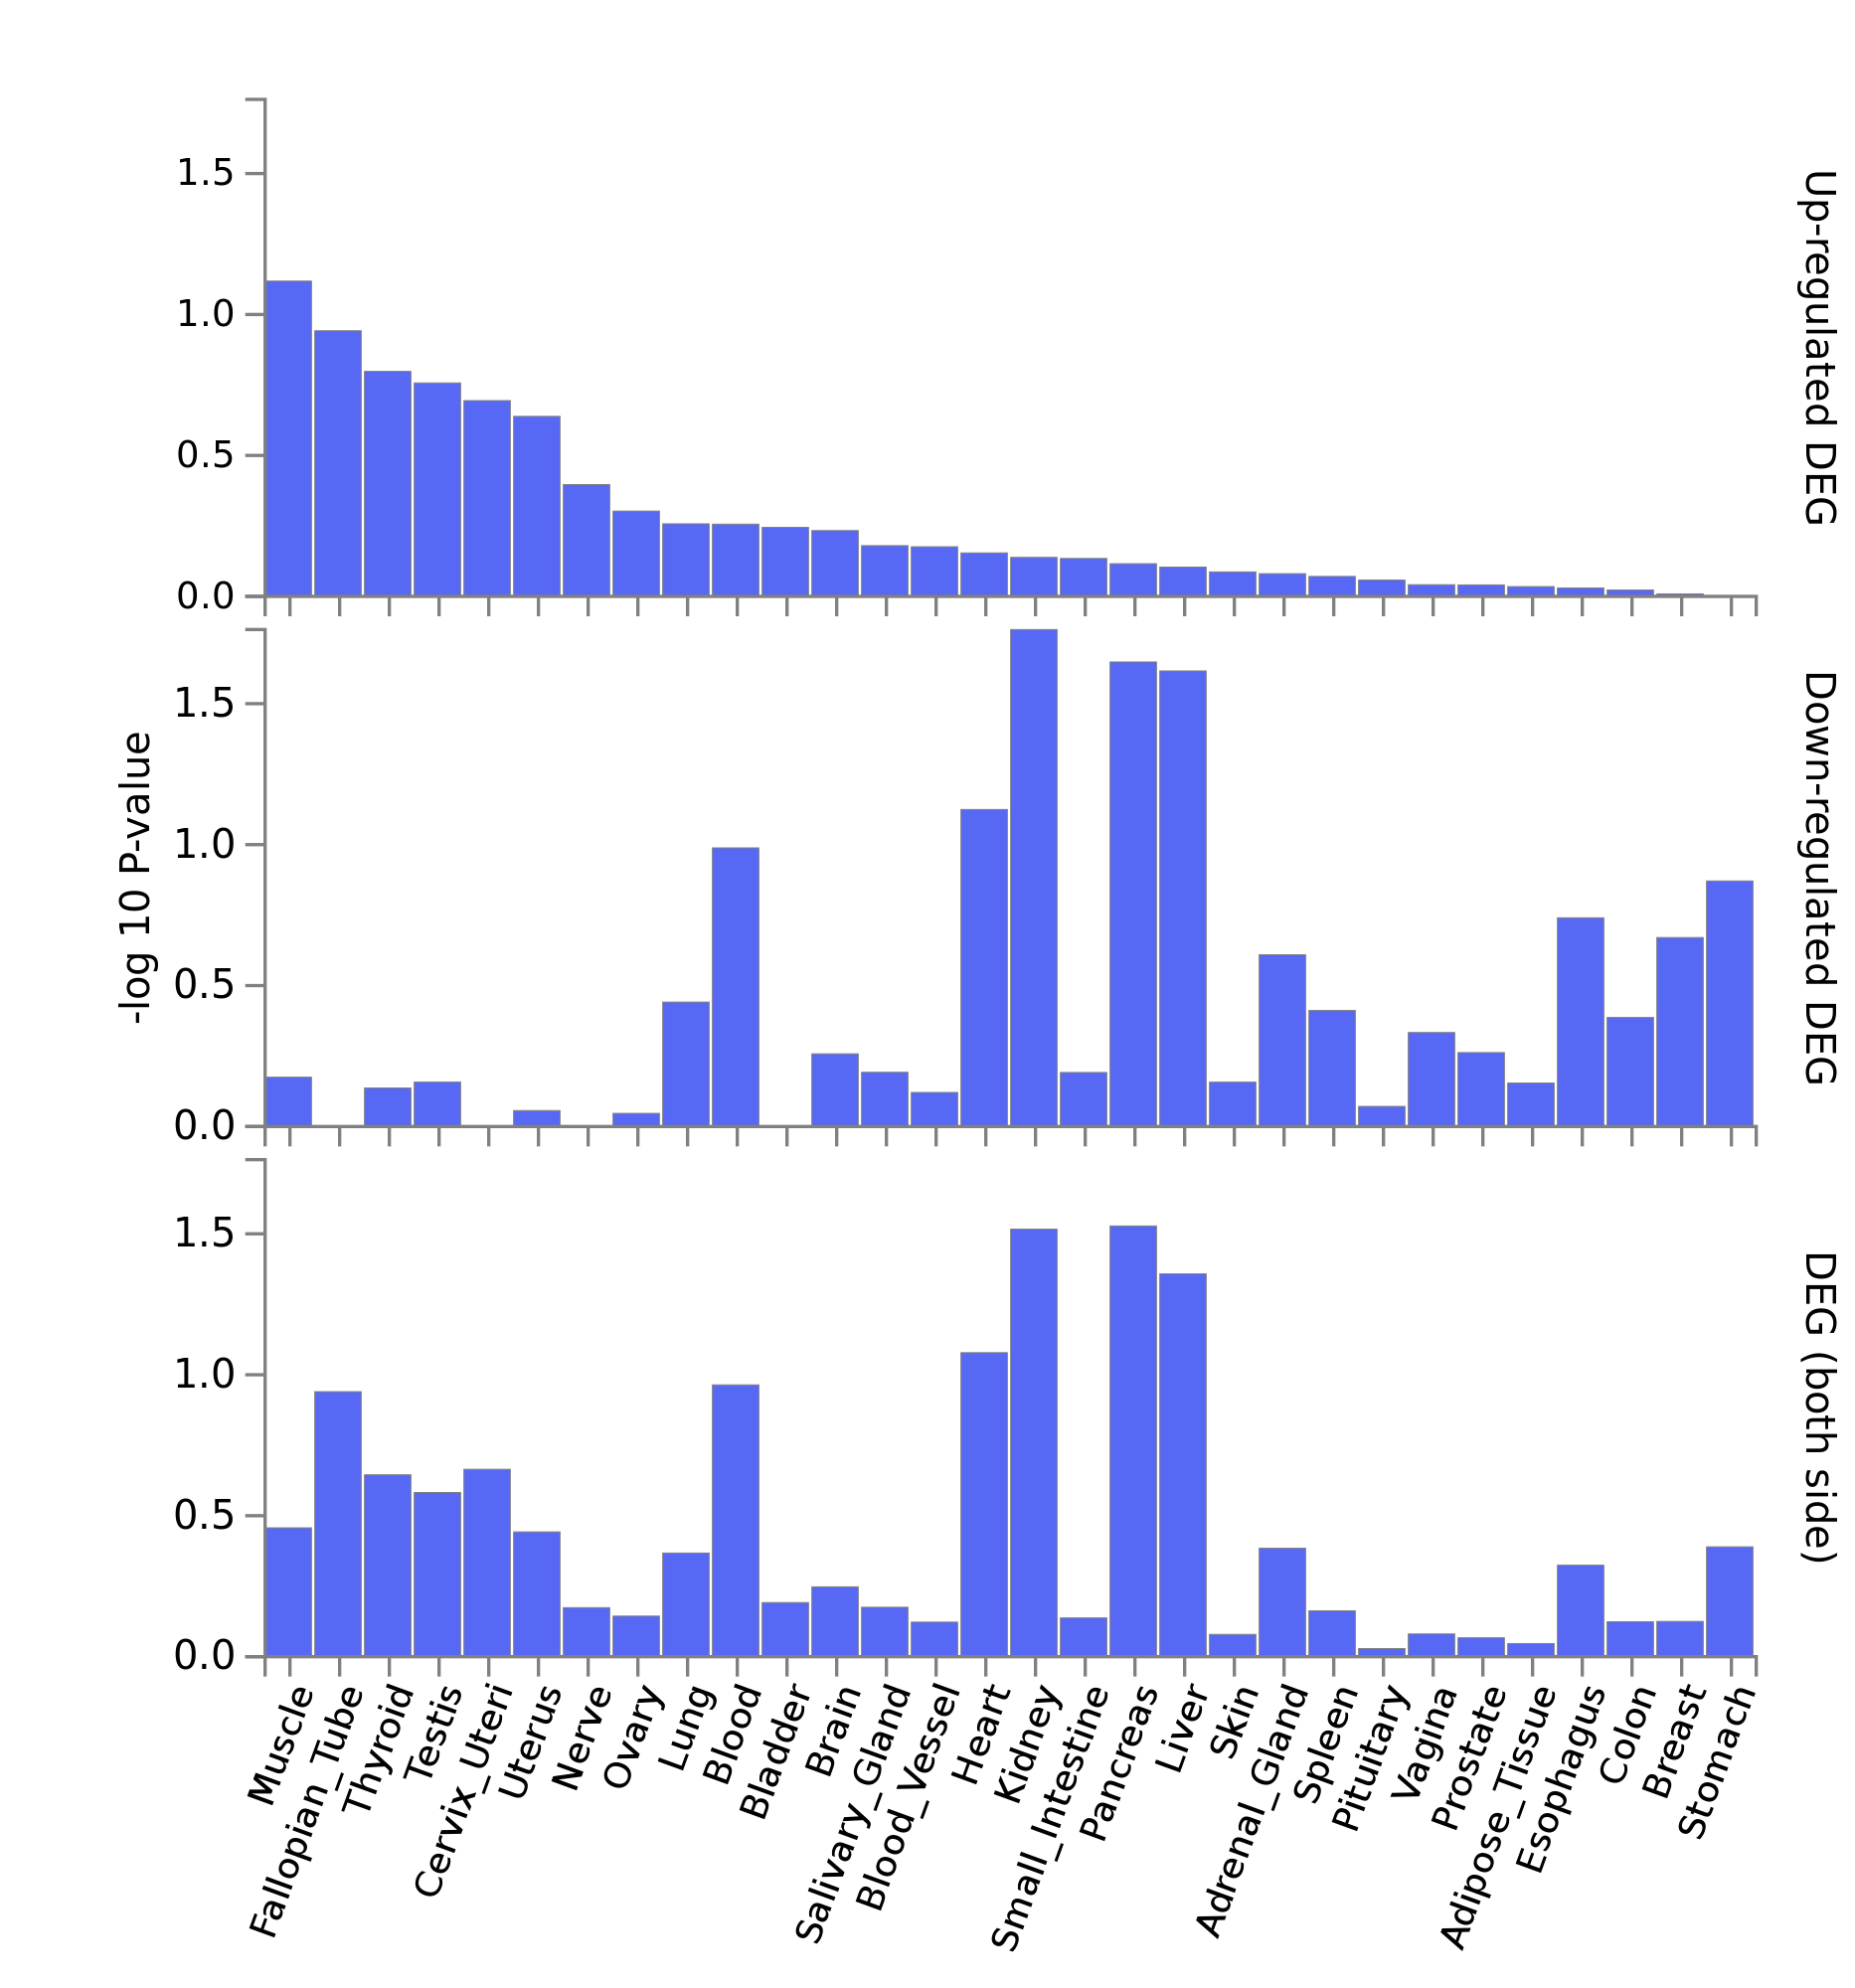
\includegraphics[width=7cm]{images/FUMA_plots/deg_general_up/ctg_upreg_general_gtex_v8_ts_general_FUMA_gene2func44709.png}
    \caption{Gene expression Intelligence Replication}
    \end{subfigure}
  \begin{subfigure}{8cm}
    \centering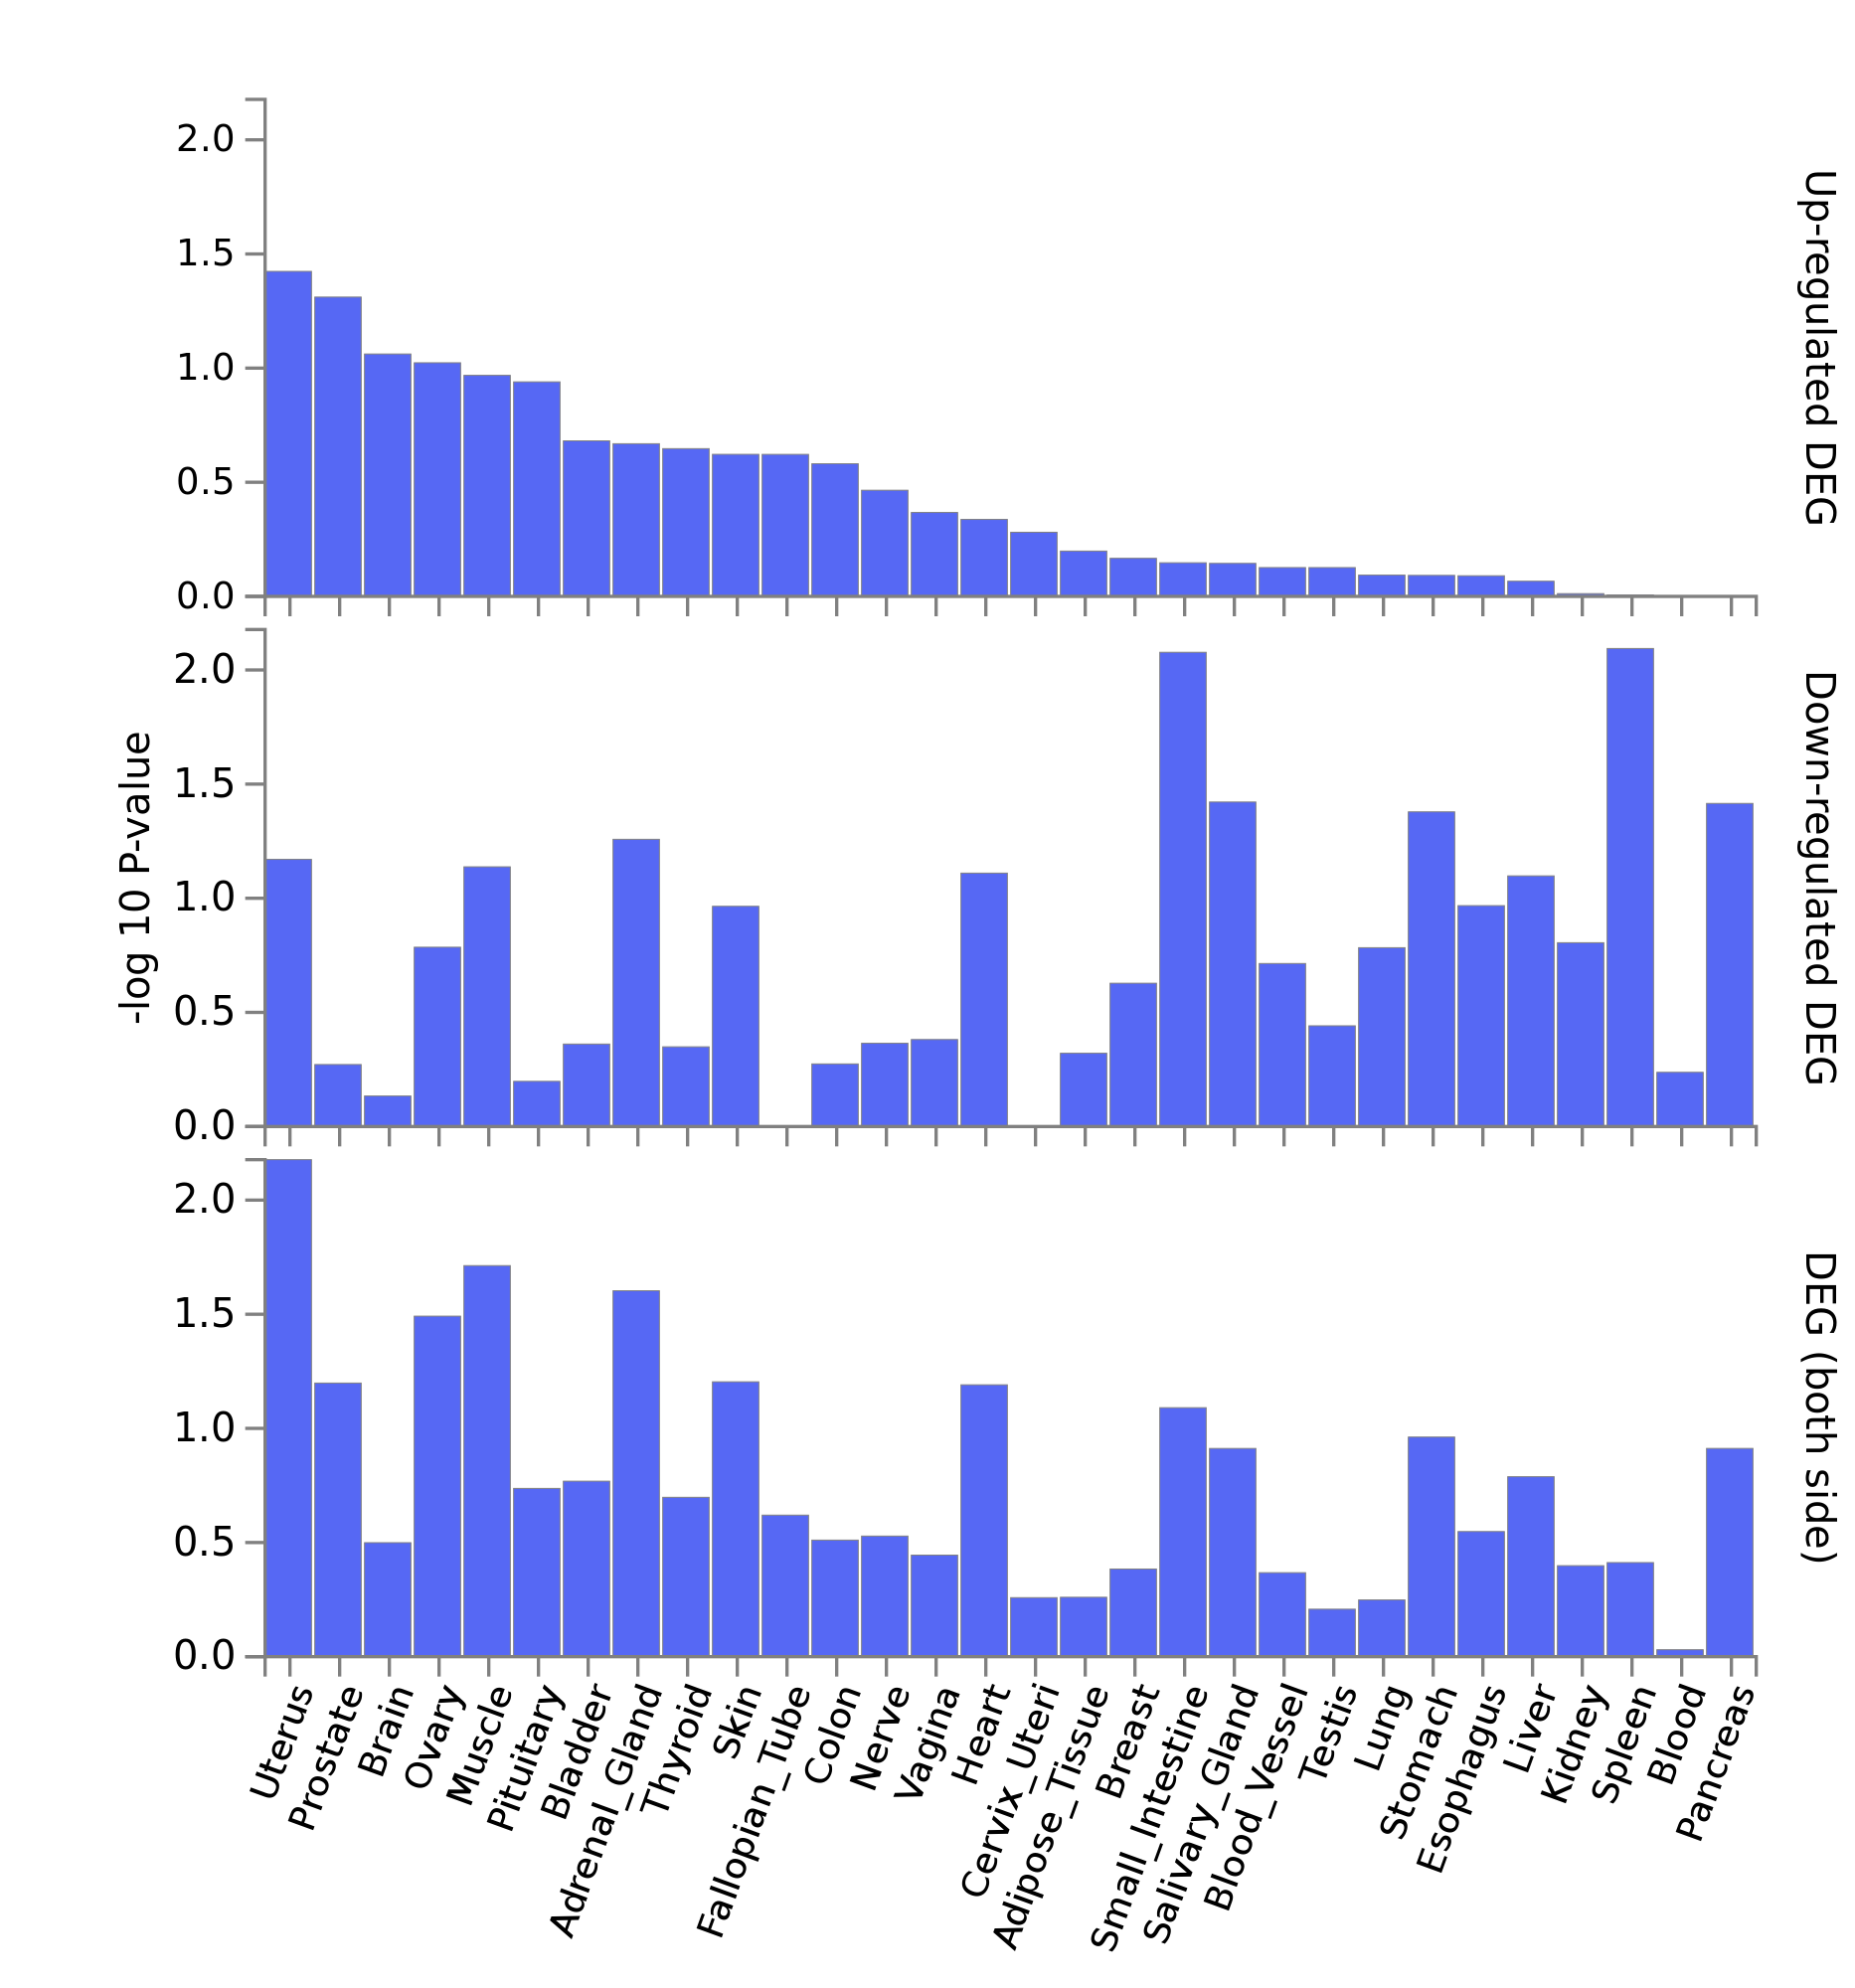
\includegraphics[width=7cm]{images/FUMA_plots/deg_general_up/ea2_corrected_upreg_general_gtex_v8_ts_general_FUMA_gene2func44667.png}
    \caption{Education Replication}
  \end{subfigure}
 
  \begin{subfigure}{8cm}
    \centering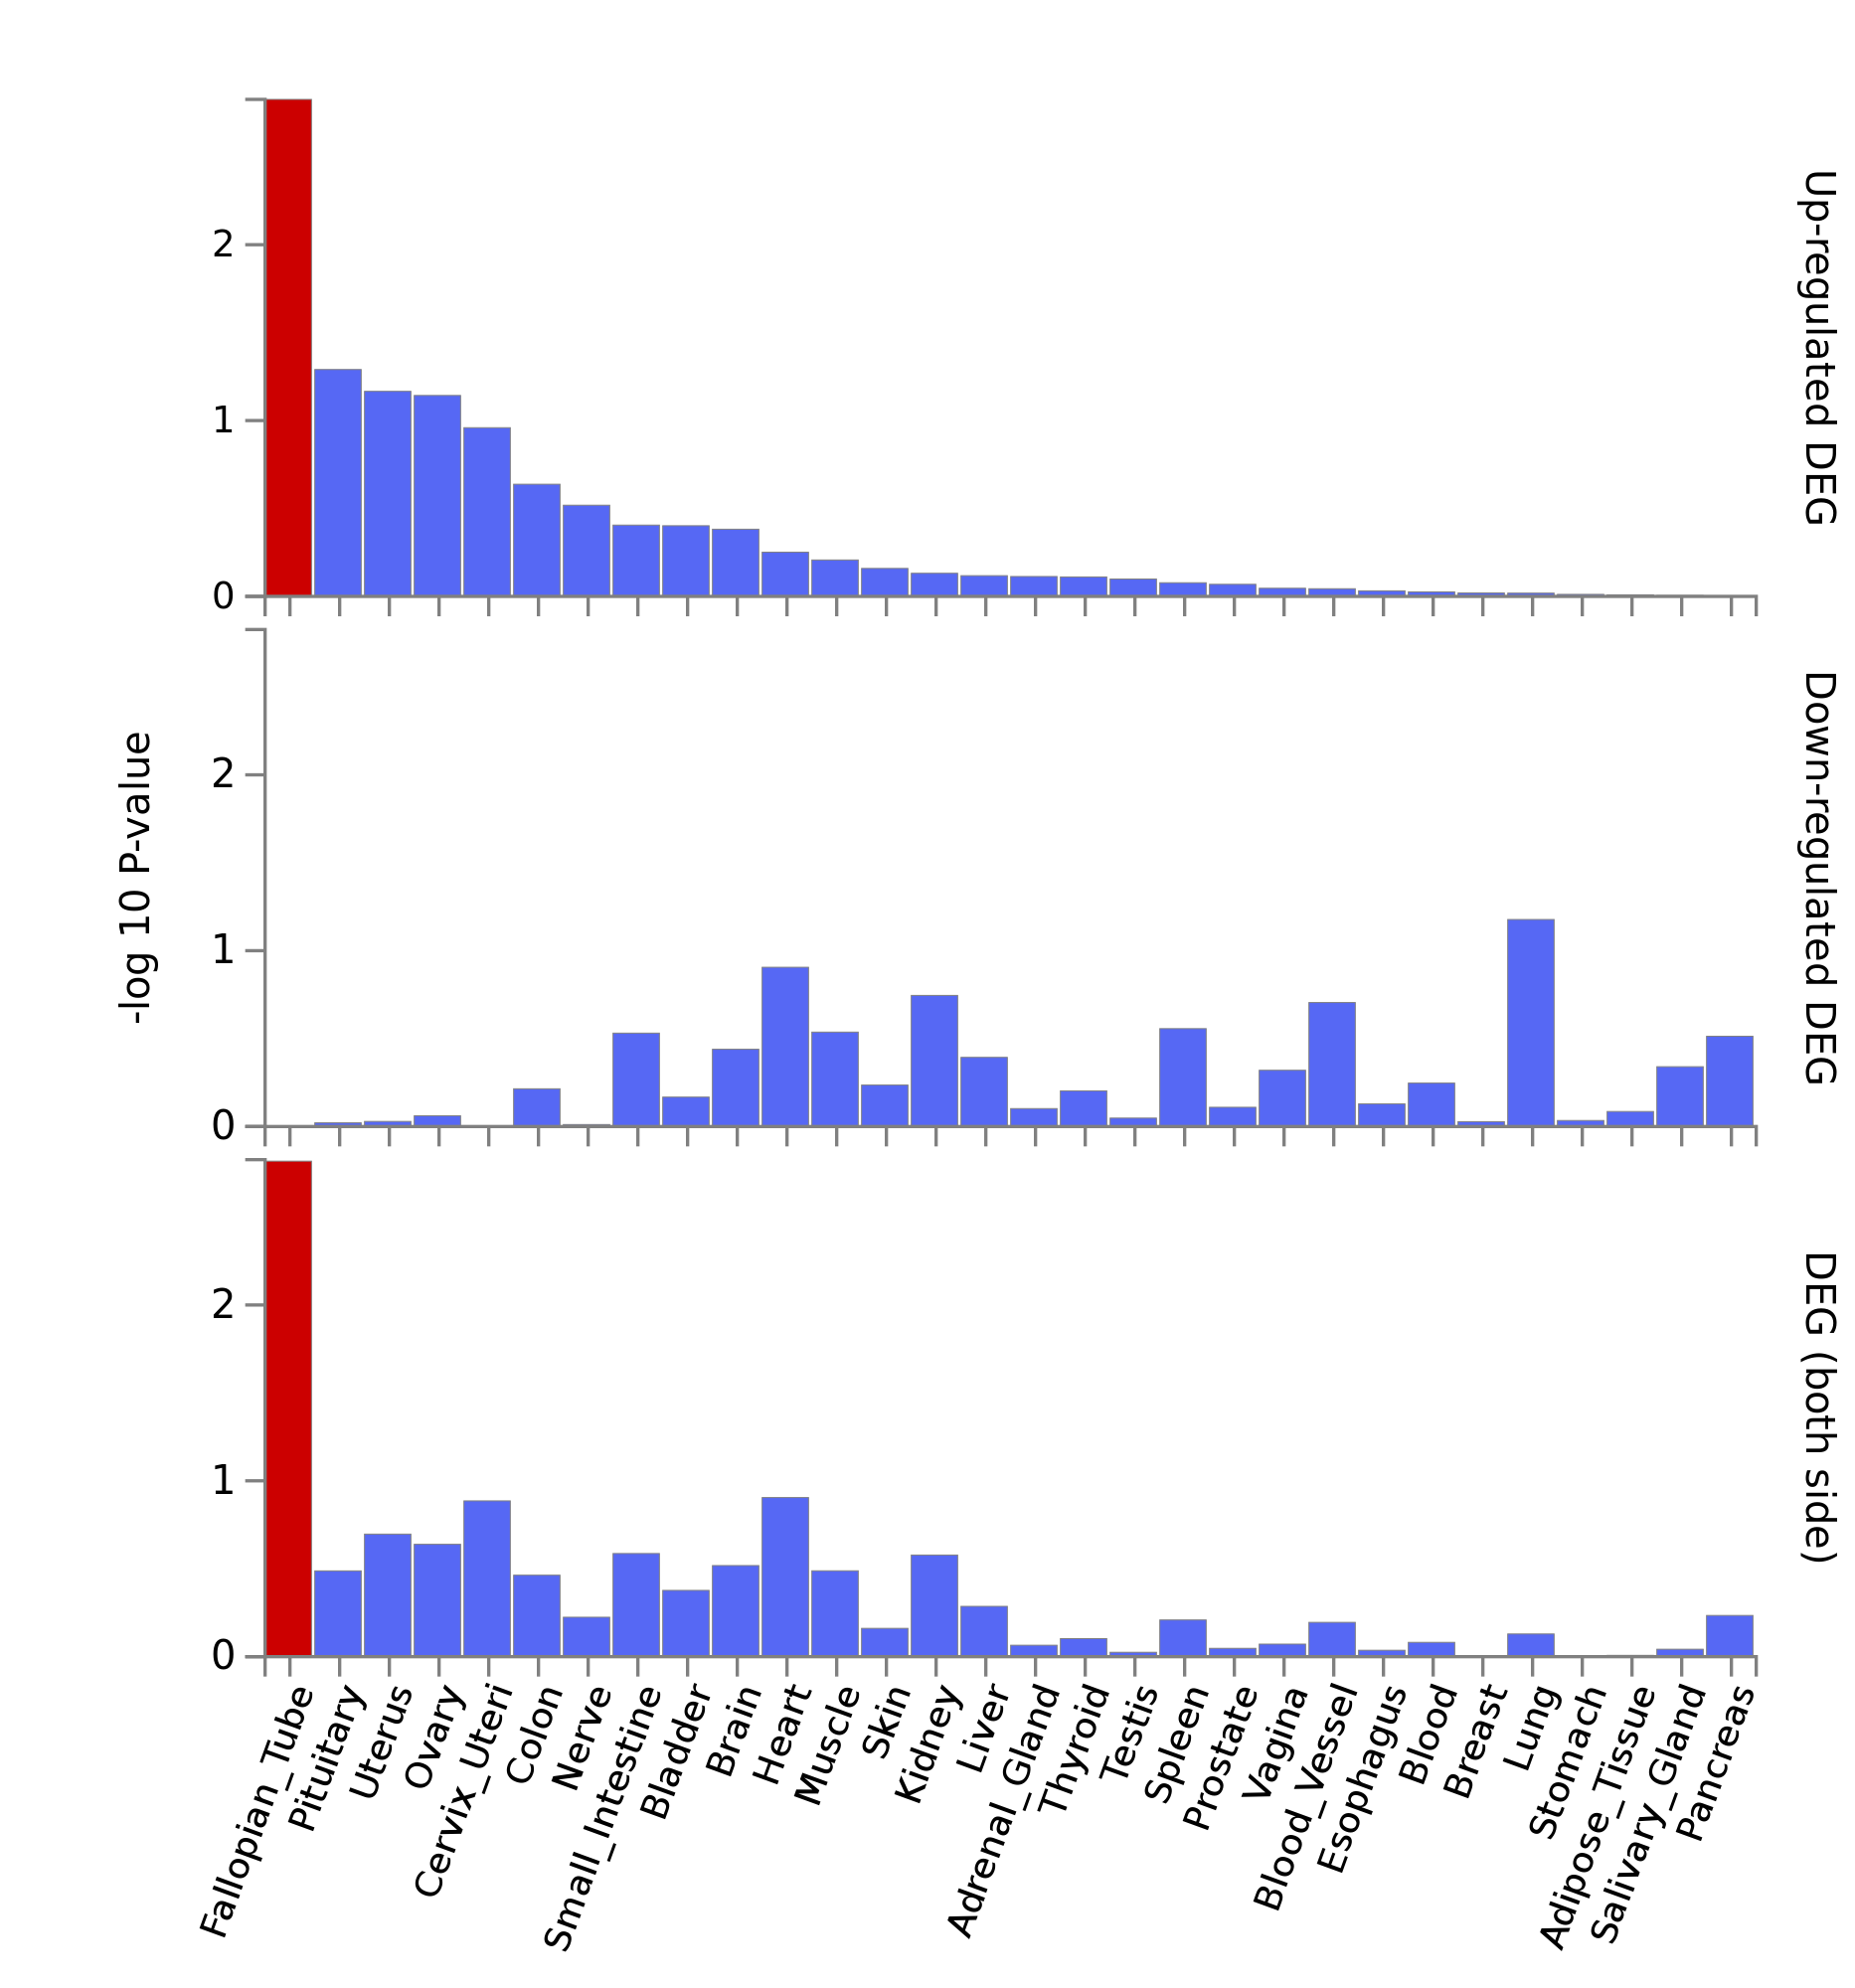
\includegraphics[width=7cm]{images/FUMA_plots/deg_general_up/ukbb_int_upreg_general_gtex_v8_ts_general_FUMA_gene2func44709.png}
    \caption{DEG Up Regulated Intelligence Discovery}
  \end{subfigure}
  \begin{subfigure}{8cm}
    \centering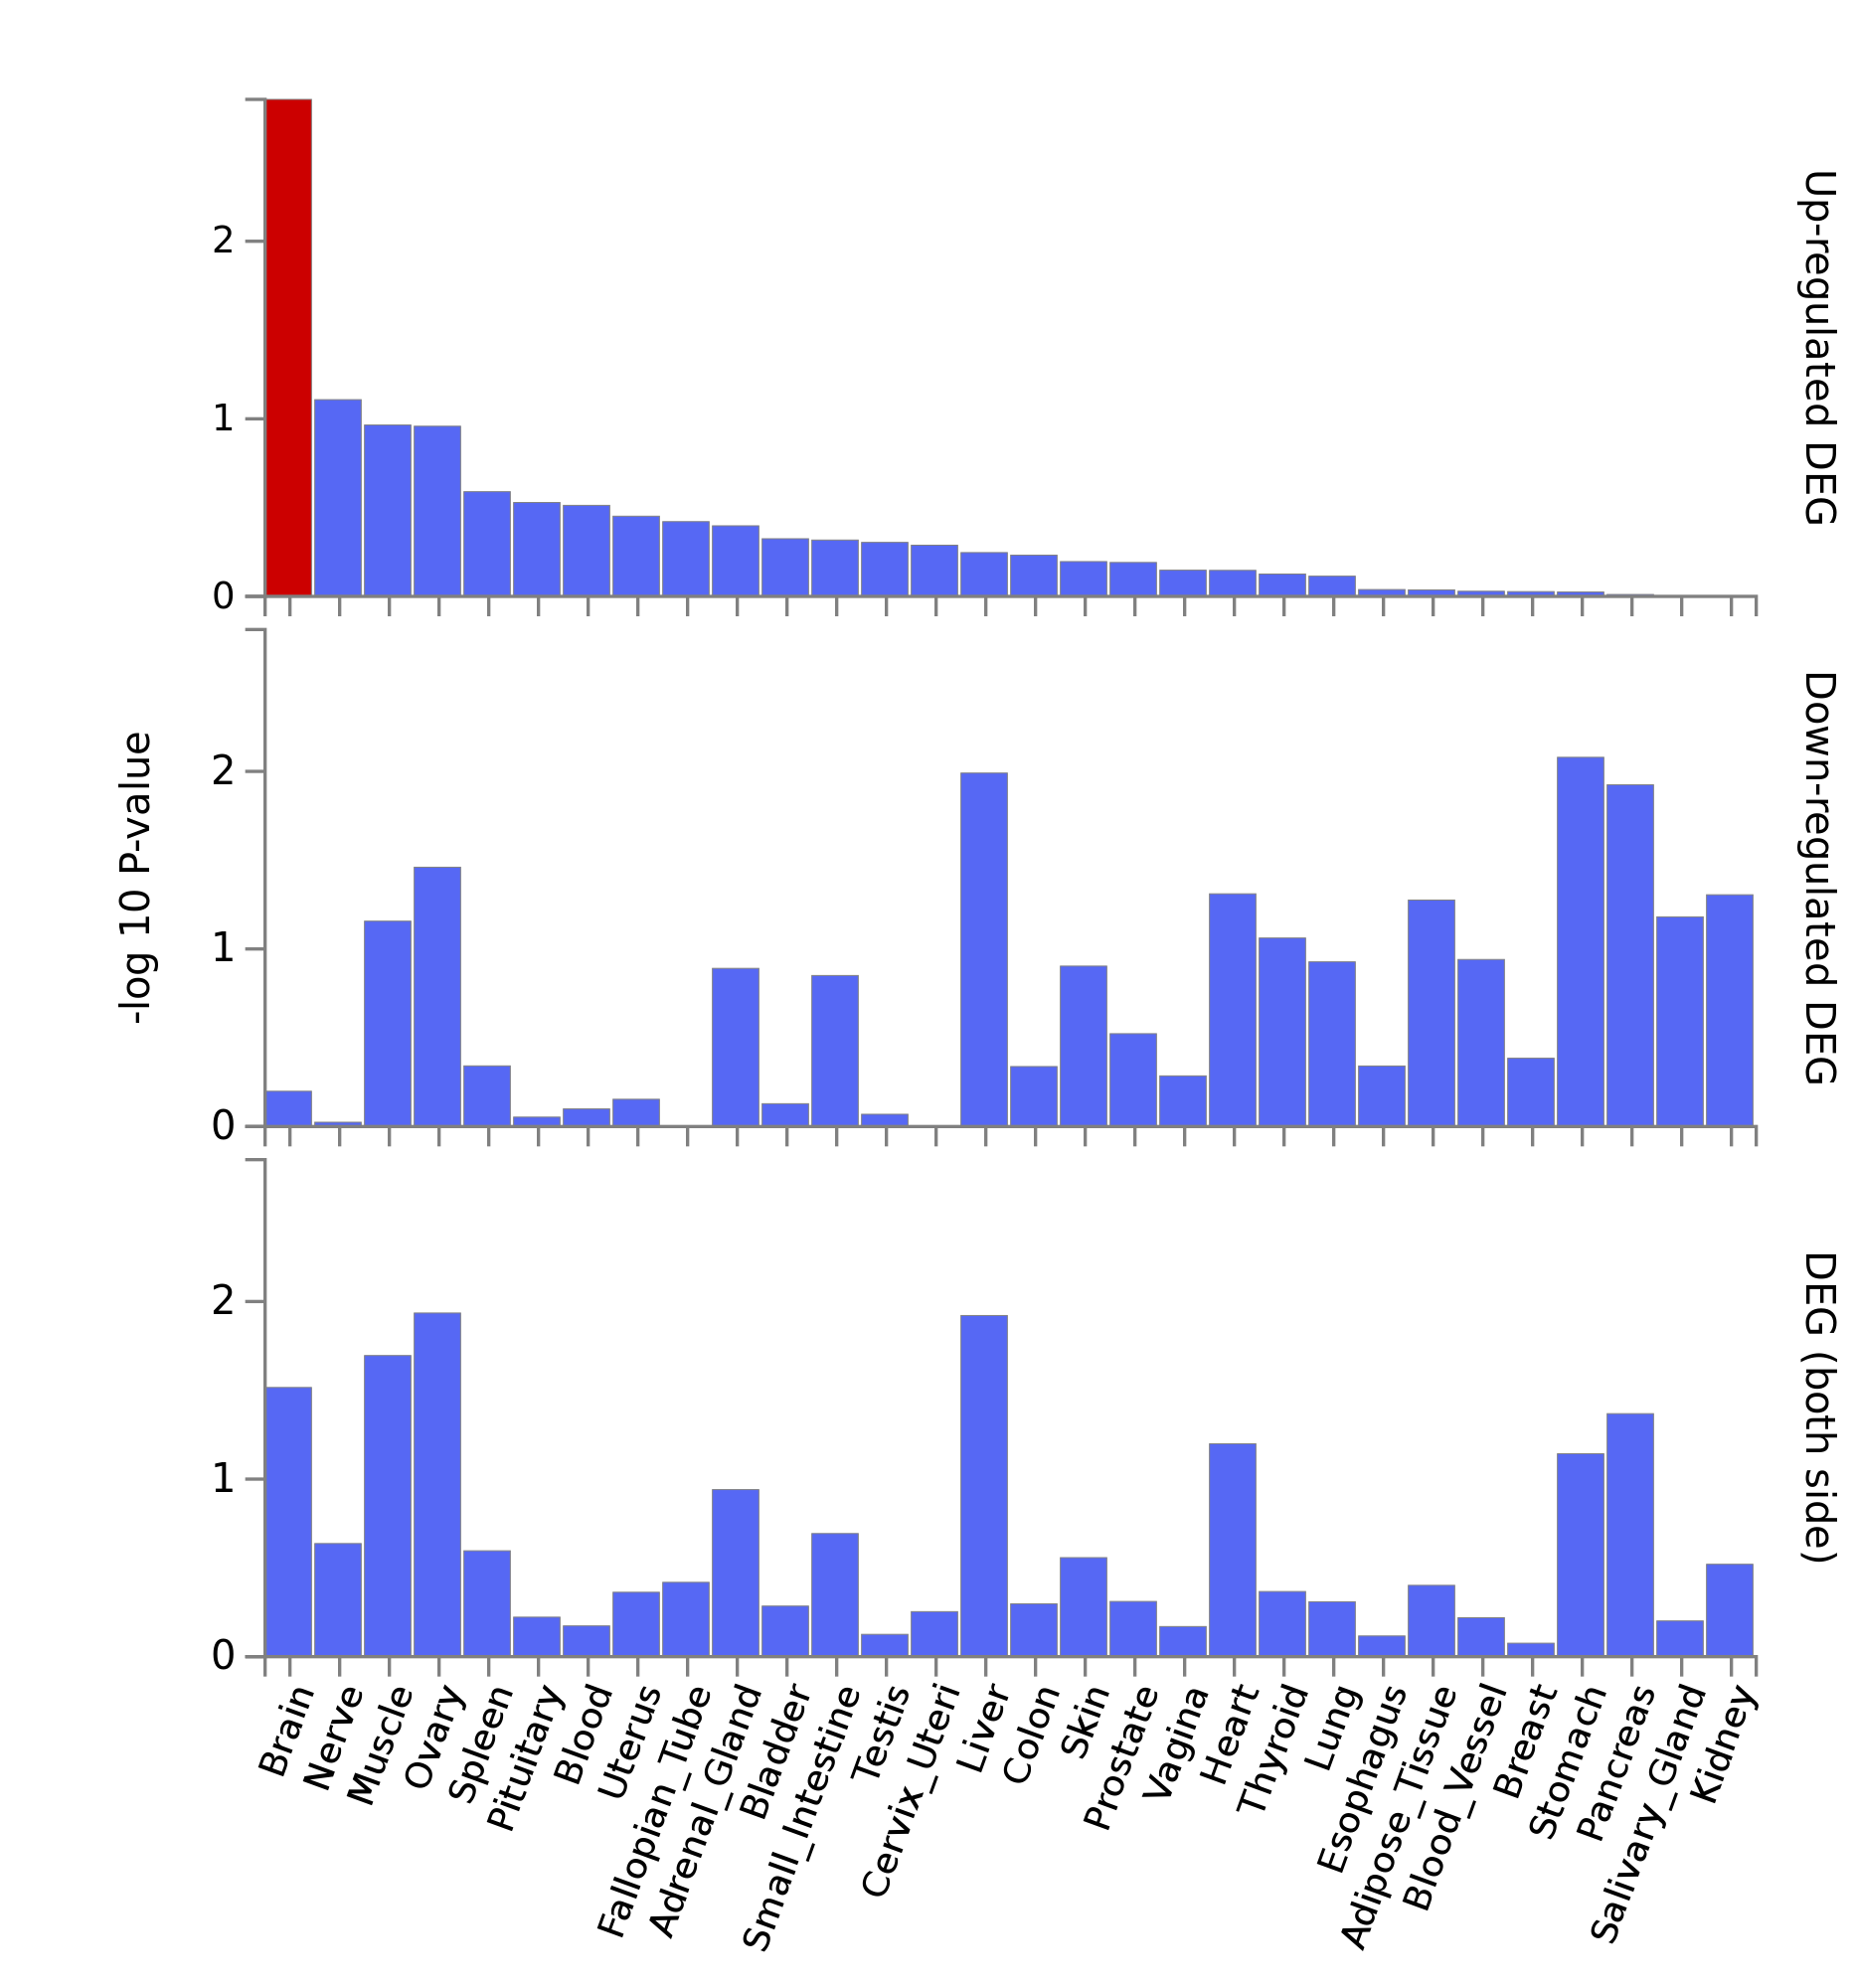
\includegraphics[width=7cm]{images/FUMA_plots/deg_general_up/ukbbed_upreg_general_gtex_v8_ts_general_FUMA_gene2func44709.png}
    \caption{Education Discovery}
  \end{subfigure}
  \caption{FUMA output. Enrichment for differentially expressed genes ordered by up regulated genes. Only education discovery shows evidence of up regulated differentially expressed genes in CNS}
  \label{fig:FUMA gtex deg samples multiple}
\end{figure}

 \begin{figure}
  \begin{subfigure}{8cm}
    \centering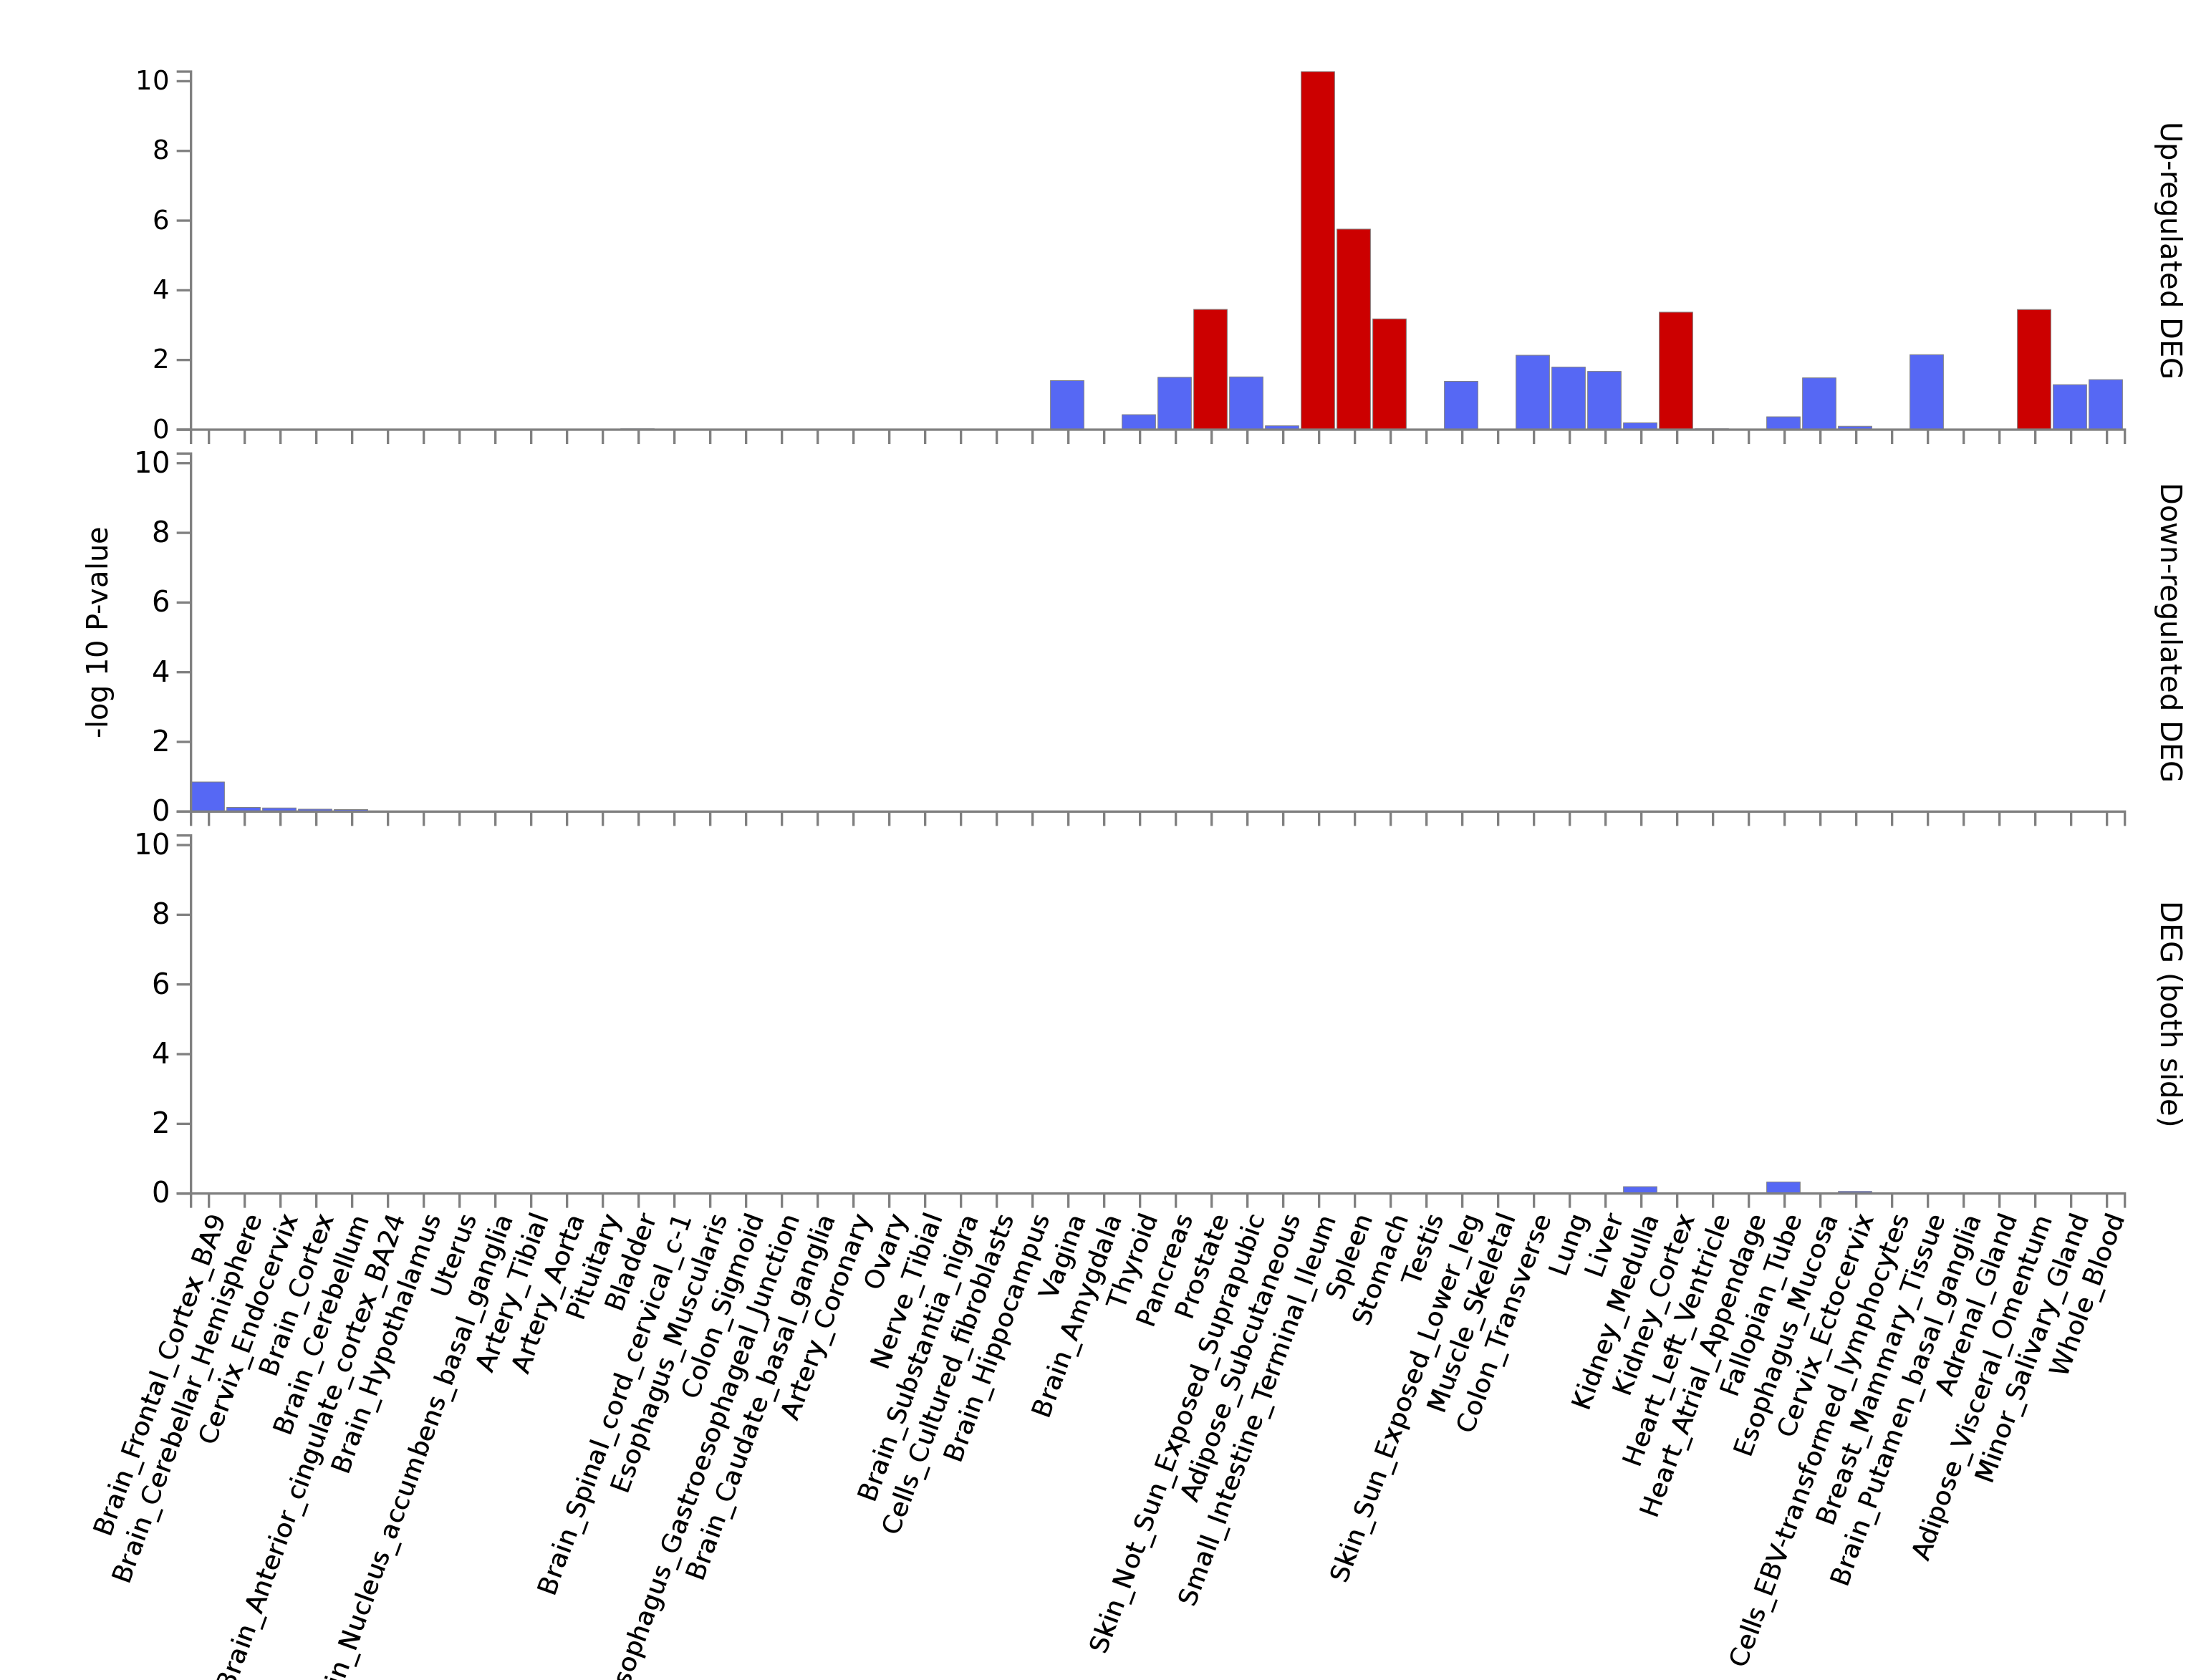
\includegraphics[width=7cm]{images/FUMA_plots/gtex_v8_ts_nonPSP_FUMA_gene2func44651.png}
    \caption{Gene expression genes not in PSP}
    \end{subfigure}
  \begin{subfigure}{8cm}
    \centering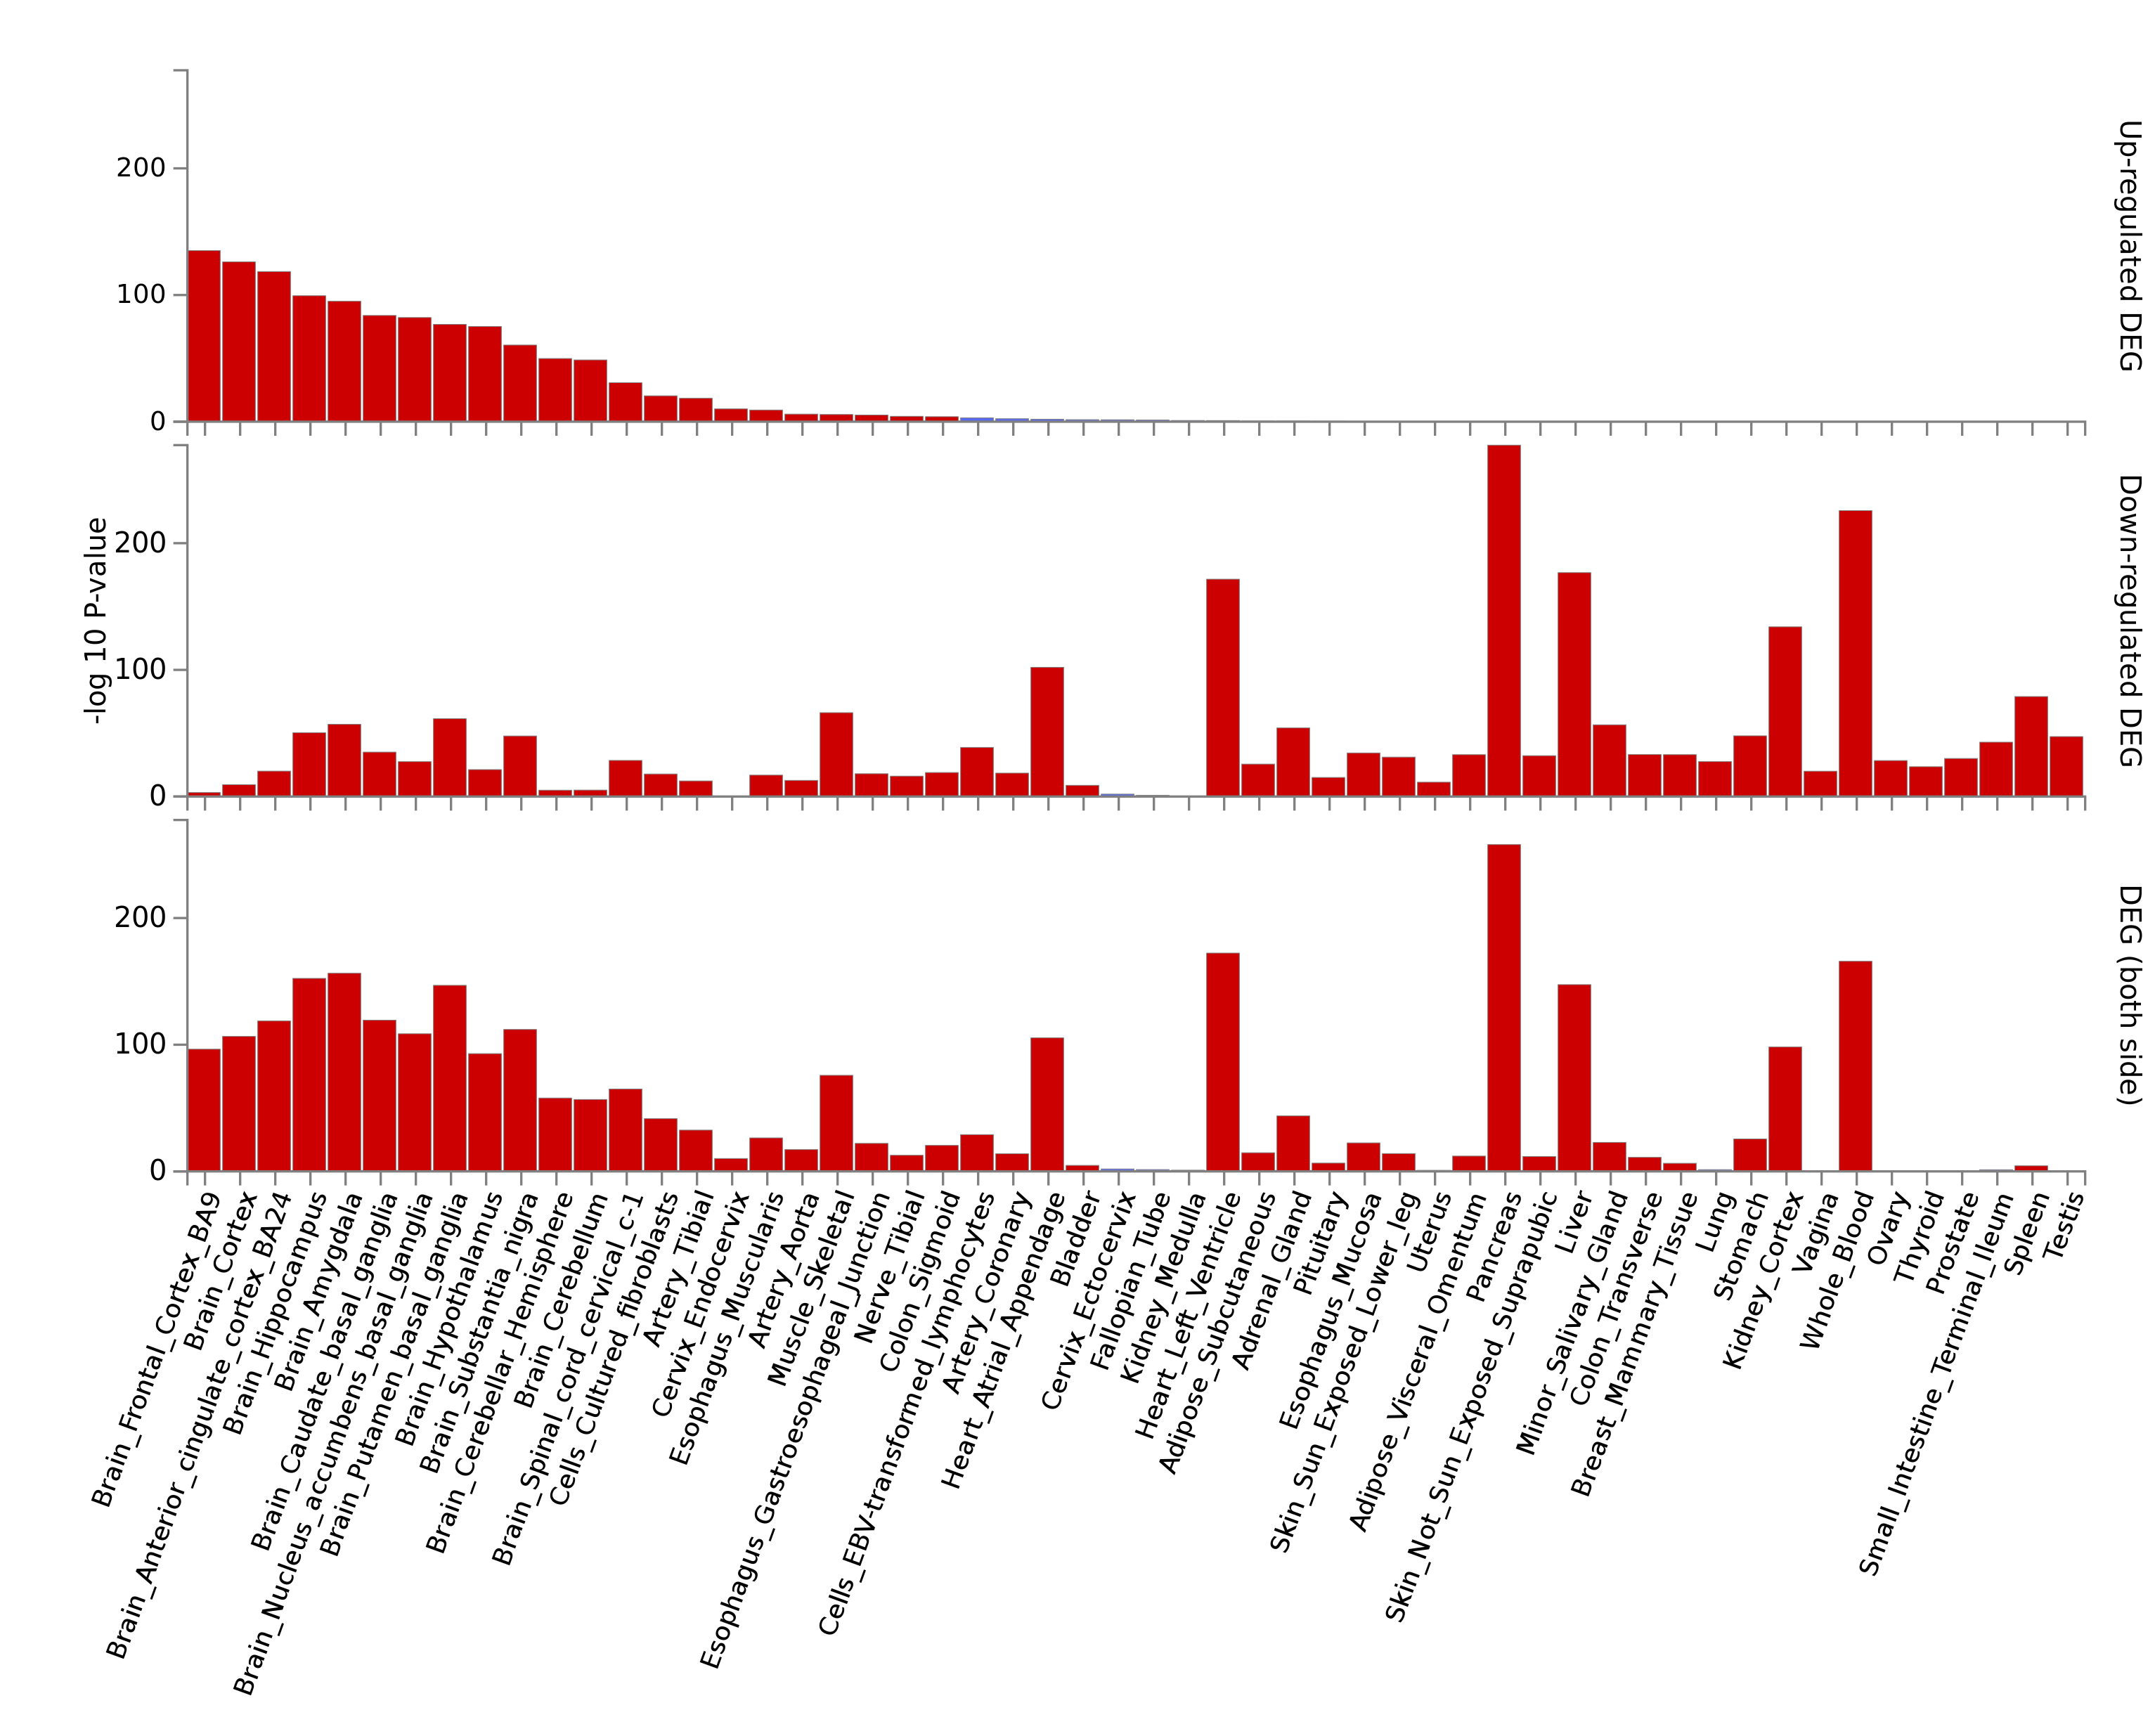
\includegraphics[width=7cm]{images/FUMA_plots/gtex_v8_ts_FUMA_PSP_gtex.png}
    \caption{Genes in PSP}
  \end{subfigure}
 
  \begin{subfigure}{8cm}
    \centering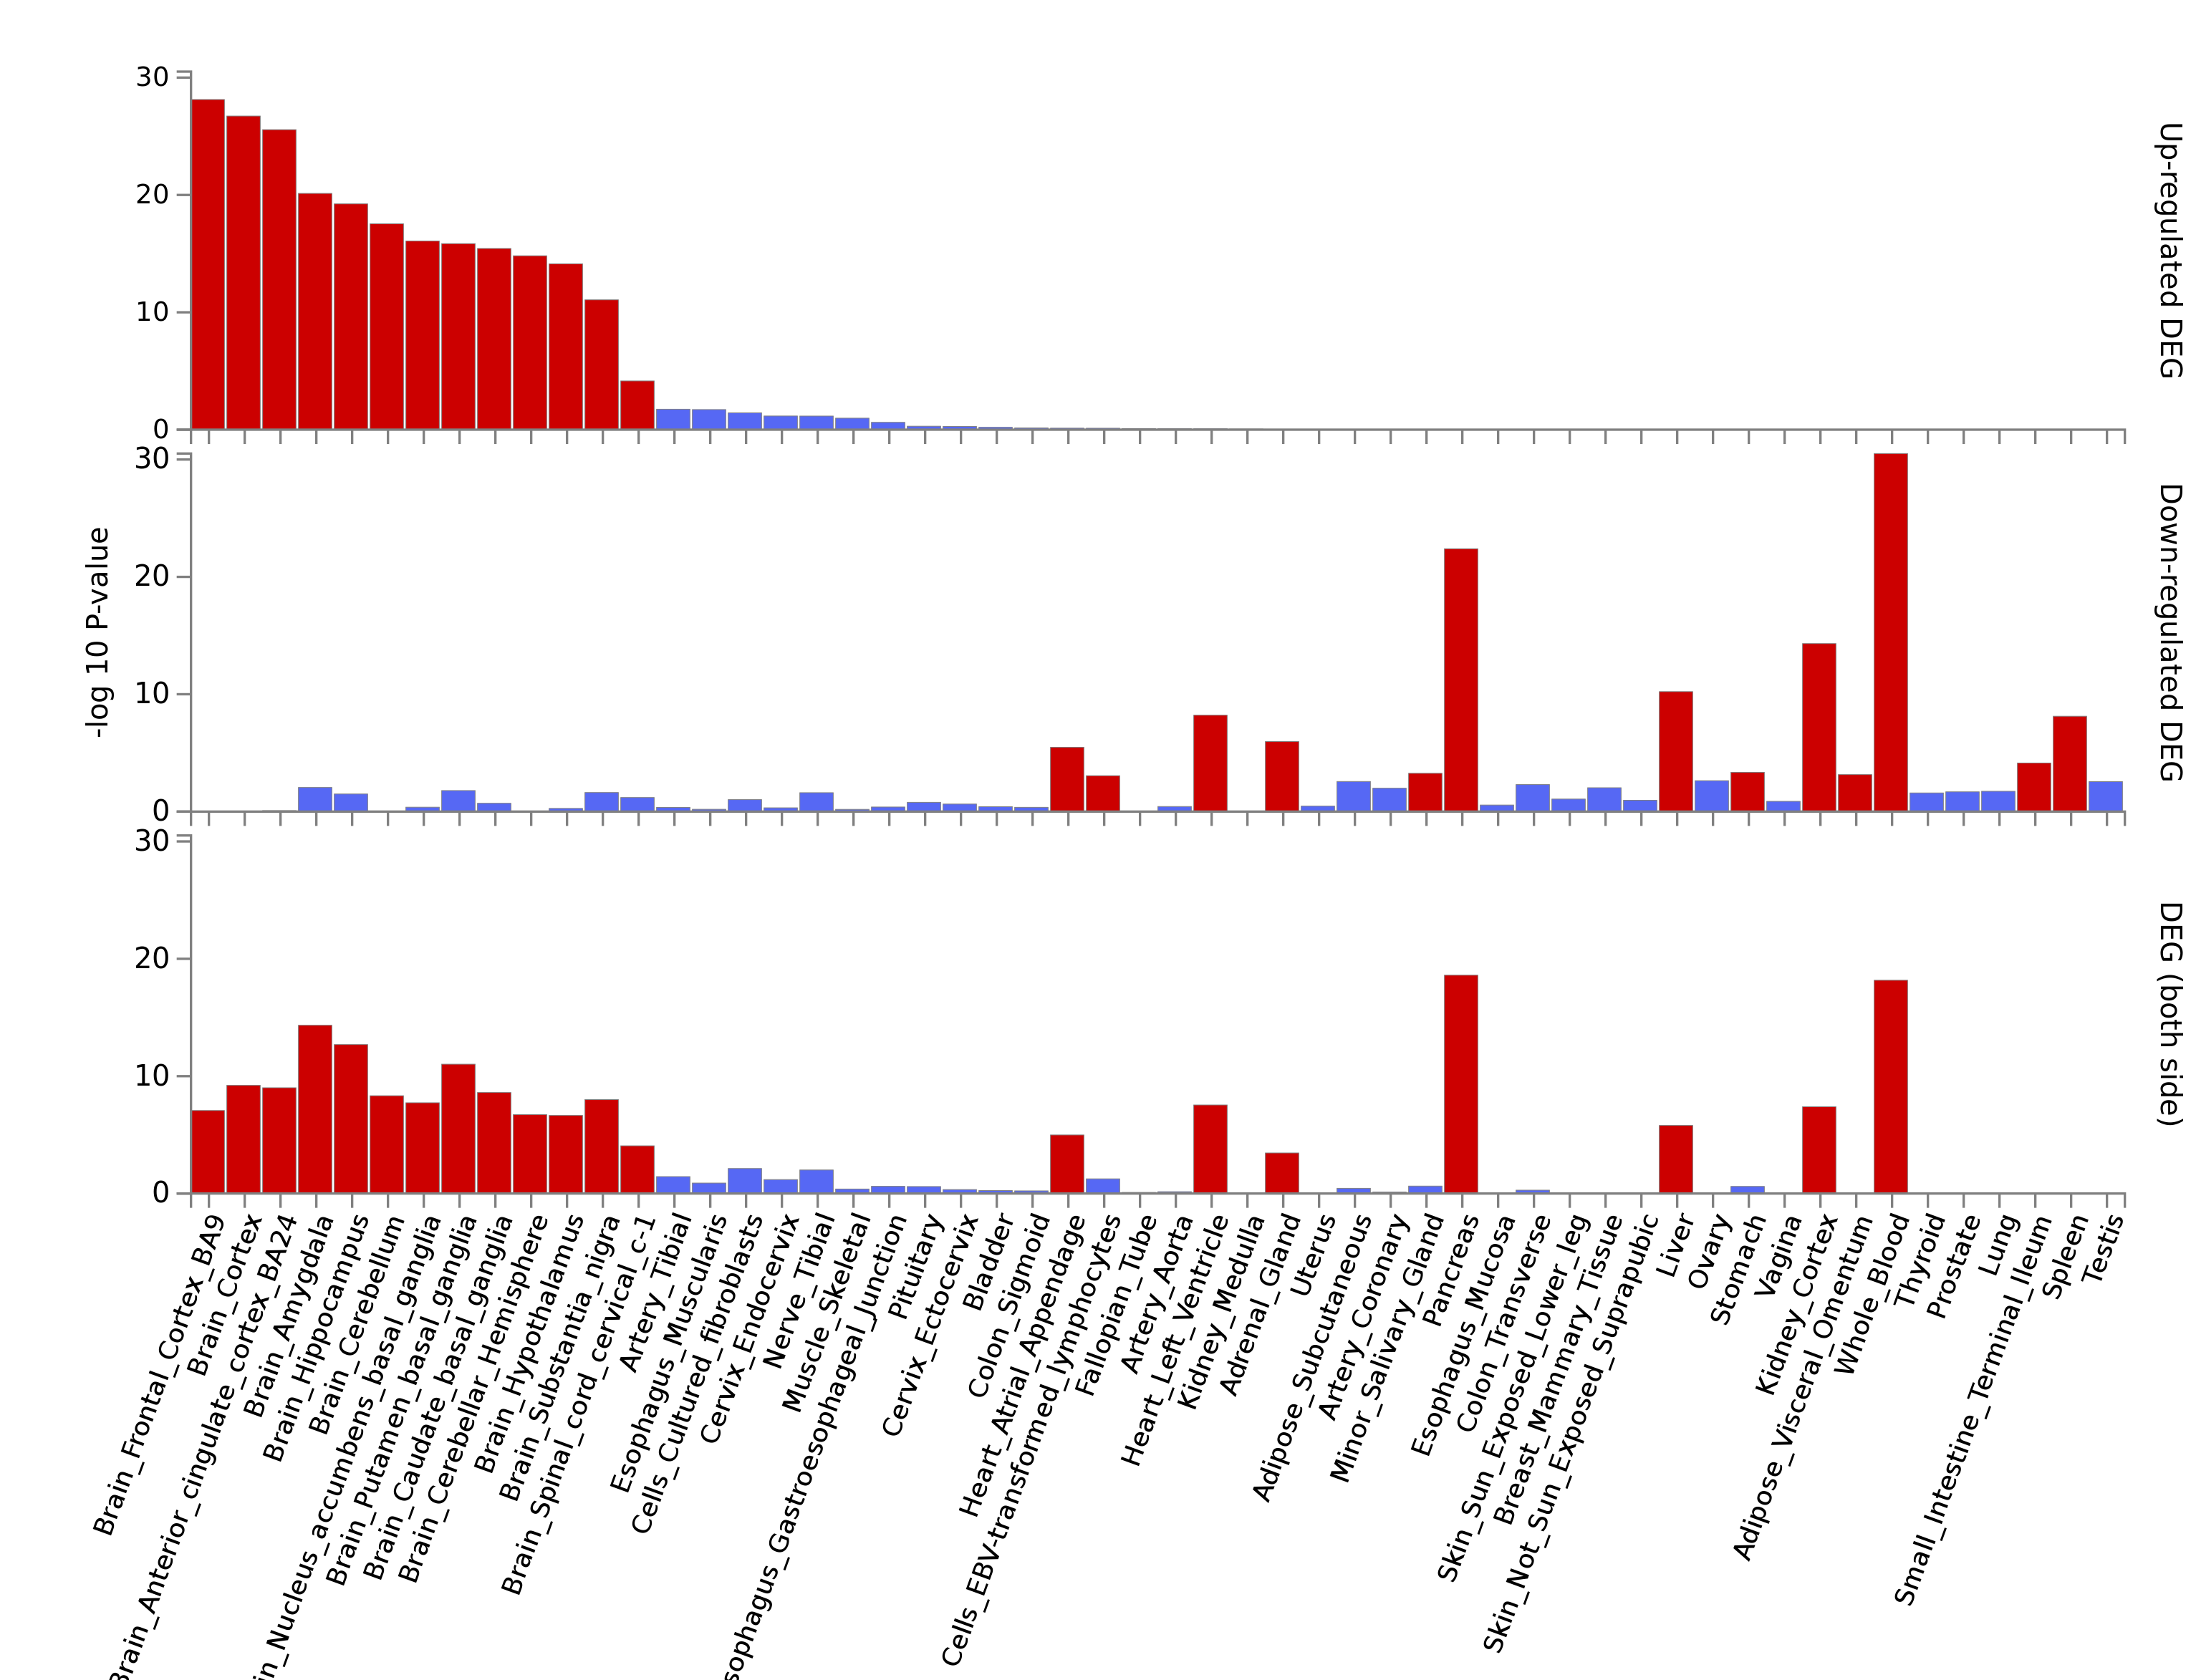
\includegraphics[width=7cm]{images/FUMA_plots/gtex_v8_ts_psp_not_consensus_FUMA_gene2func44650.png}
    \caption{Genes in PSP but not in consensus PSD. ie new genes}
  \end{subfigure}
  \begin{subfigure}{8cm}
    \centering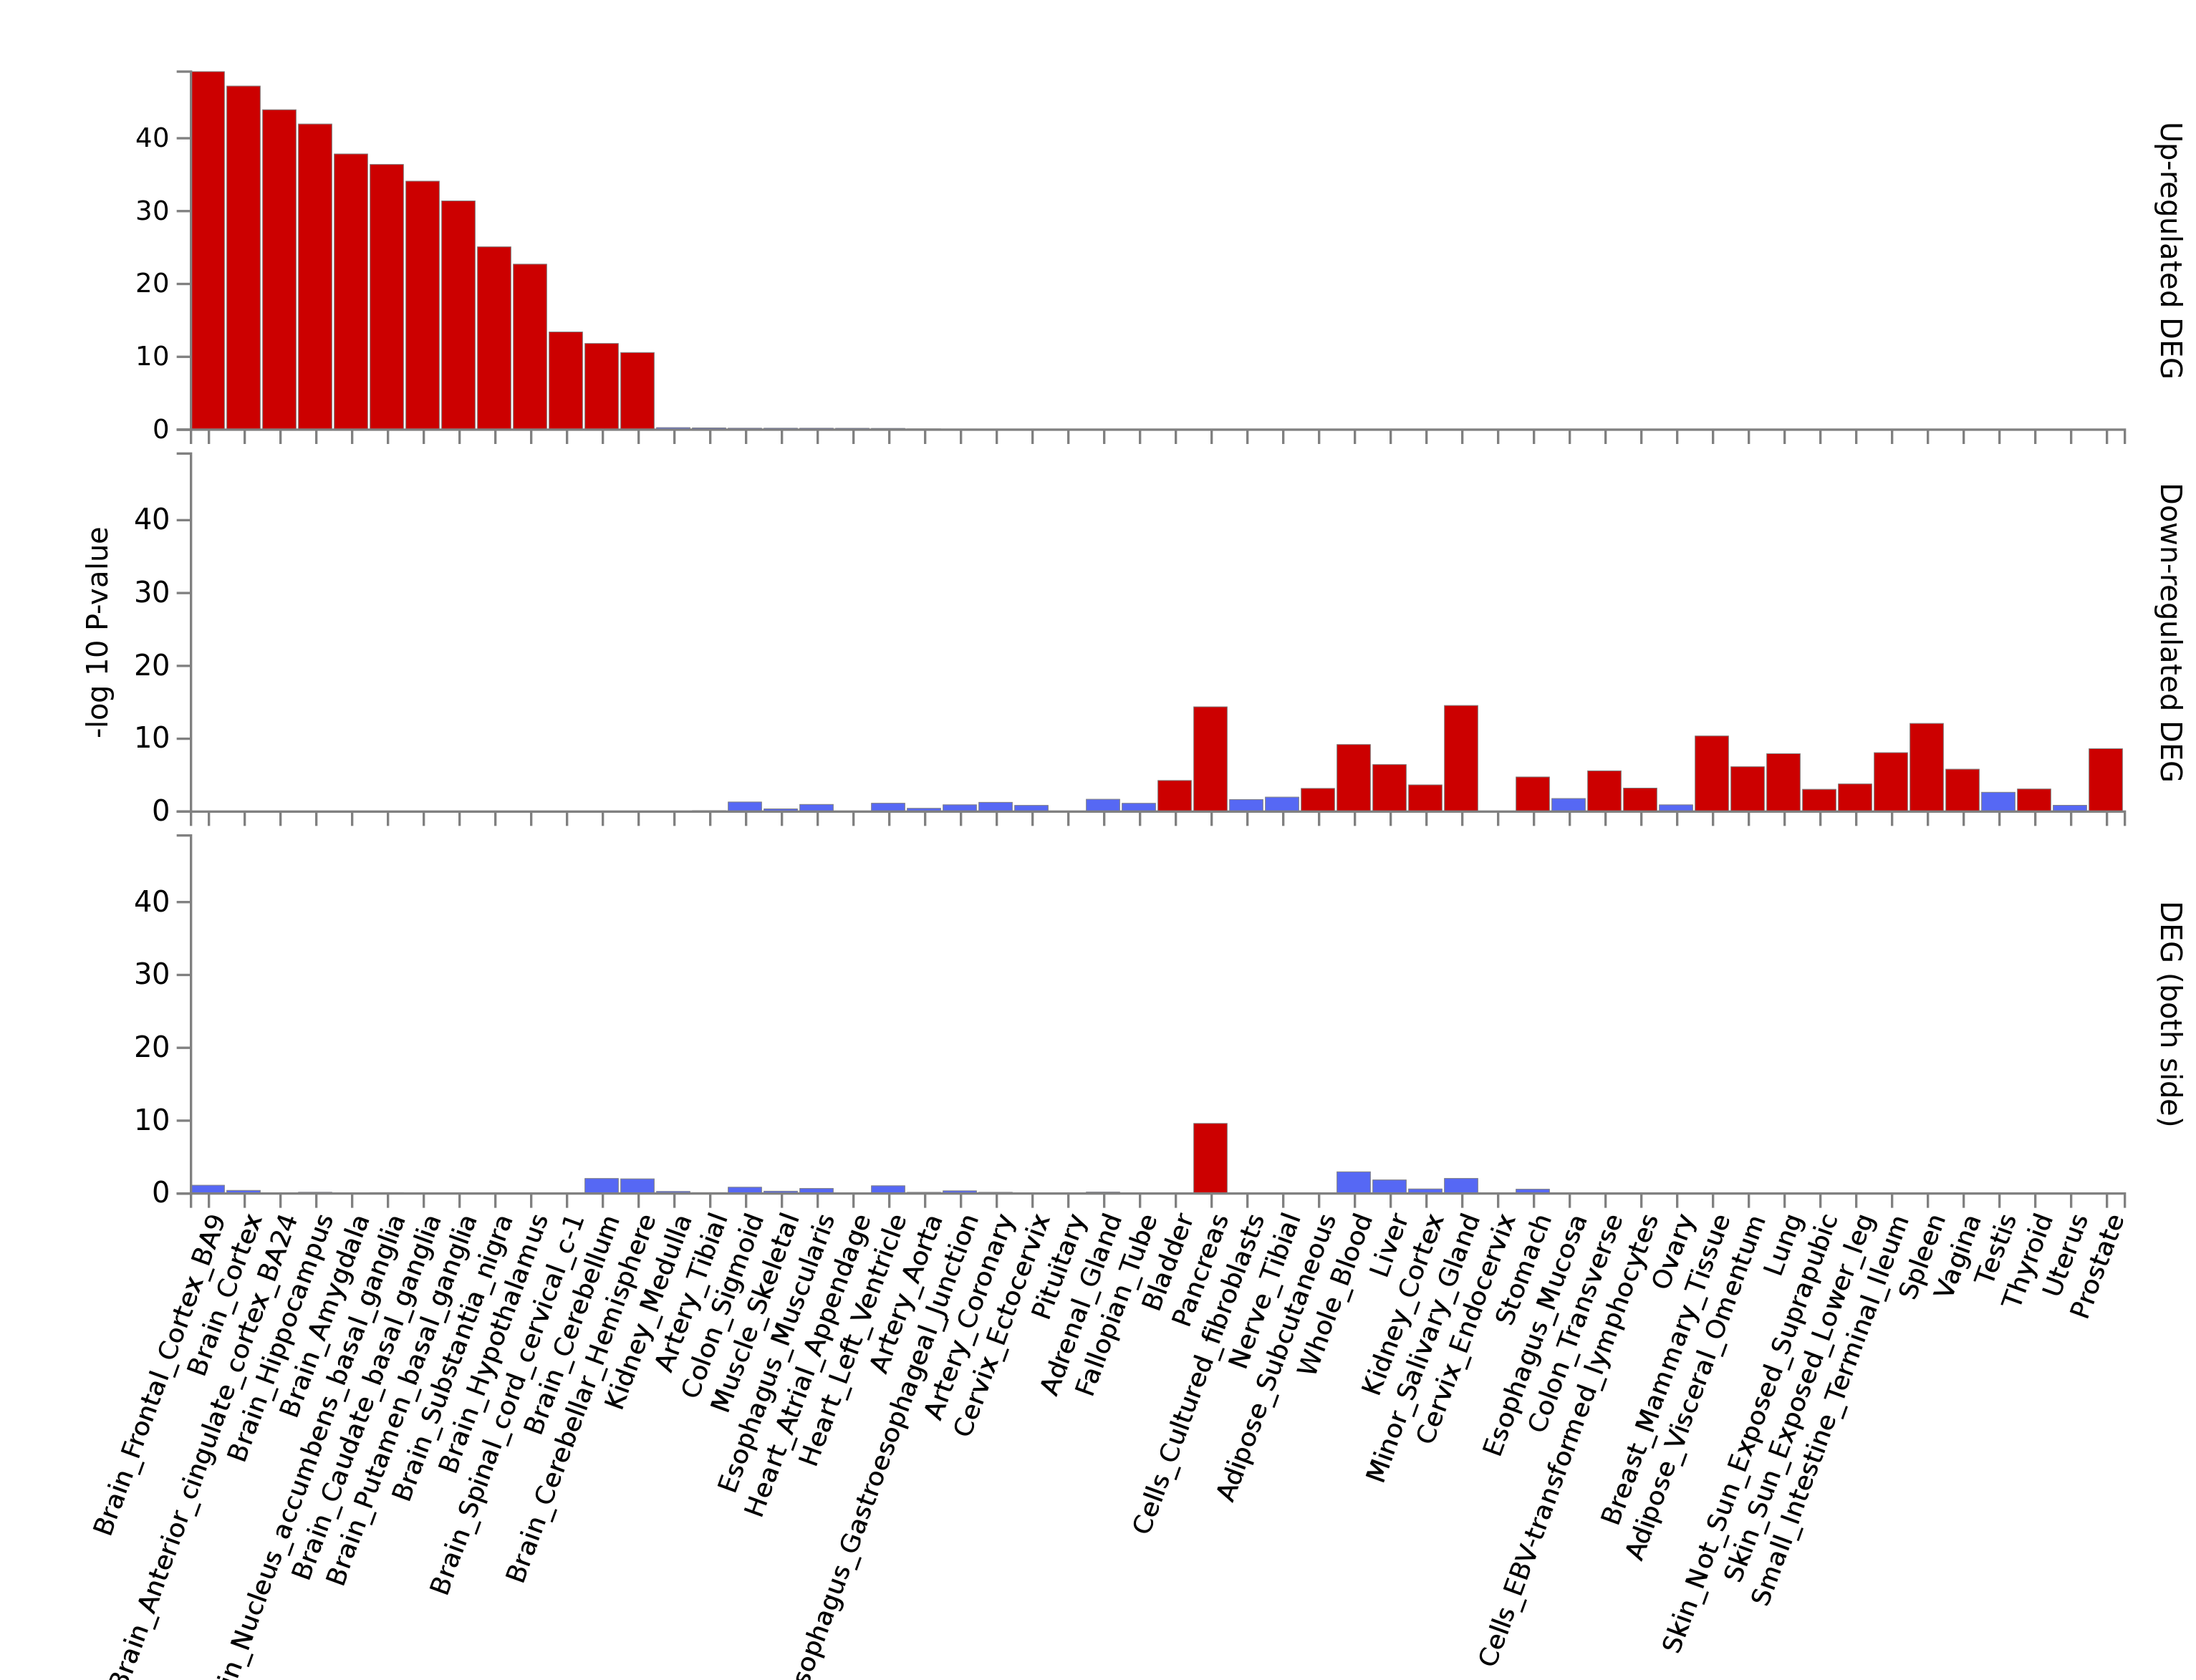
\includegraphics[width=7cm]{images/FUMA_plots/gtex_v8_ts_1313_consensus_FUMA_gene2func44650.png}
    \caption{Genes in consensus PSD}
  \end{subfigure}
  \caption[\textbf{Comparison of gene expression} in consensus PSD and PSP]{Comparison of gene expression in genes not in the PSP, genes in the PSP, genes in PSP but not in the consensus PSD (new genes), genes in the consensus PSD - that which is conserved in different vertebrate species. Images from FUMA. GTEx v8 54 tissue types. Ordered from left to right by up-regulated differentially expressed genes p values (hypergeometric test). Tissues with significant differential enrichment after bonferroni correction for multiple comparisons are shown in blue. Y axis -log10(p) of enrichment for gene set (eg PSP) }
  \label{fig:compare all PSP gtex multipanel FUMA output}
\end{figure}

 
 

%%%%%%%%%%%%%%%%%%%%%%%%%%%%%%%%%%%%%%%%%%%%%%%%%%%%%%%%%%%%%%%%%%%%





\clearpage
\section{Synaptic component enrichment MAGMA}
\label{Synaptic component enrichment MAGMA}

Functional synaptic group gene sets are curated  at the Complex Trait Genetics lab \footnote{\url{https://ctg.cncr.nl/software/GENESETS/synapse.zip}} based on stuies by Ruano et al. (2012)\cite{ruano2010functional}\footnote{paper looking at G protein receptors} and Lips et al. (2012)\cite{lips2012functional}. Using these sets with MAGMA will provide an estimate of how effective a purely functional annotation approach is and an estimate of the value of significance tests in these samples. 

MAGMA GSA was performed using the raw output of the GWGAS analyses in MAGMA as part of a standard two stage MAGMA GSA. Default options were used.
The annotated set was composed of 1028 genes. 736 of these were in the PSP, 292 were not. A large number of the missing ones were non glutamatergic receptors and the  proteins associated with these. There are 18 gene sets each a functional group such as G-protein-coupled receptor signalling.

MAGMA accepts gene sets in gene matrix transposed format (gmt) where each gene set is a row in a text file that is tab separated. gmt files used for MAGMA enrichment are often those curated by MSigDB. I have used an Rscript to create a gmt file from the supplied data\footnote{\url{source('~/RProjects/paper_xls_output/R/magma_synapse/make_synapse_gmt.R')}}.

To reduce type II error, interesting sets are identified as those of nominal significance in the discovery samples and these selected sets are then tested using the replication samples. 

\paragraph{Results} For the Intelligence\textsubscript{Discovery} sets Cell adhesion and trans-synaptic signaling p=0.009 , Excitability 0.005 and Exocytosis p=0.048 are of potential interest having p$<$ 0.05 (supplementary table~\ref{tab:MAGMA enrichment of synaptic groups UKBBint}). Only exocytosis is of nominal significance in the Intelligence\textsubscript{Replication} cohort (p=0.016; p= 0.048 with Bonferroni correction see  table~\ref{tab:MAGMA enrichment of synaptic groups ctg}). 

For Education\textsubscript{Discovery} 2 sets achieve nominal levels of significance: Cell adhesion and trans-synaptic signaling p=.009 and Excitability n=57 genes 0.005 (table~\ref{tab:MAGMA enrichment of synaptic groups UKBBEd}). None of these achieve nominal significance in the Education\textsubscript{Replication} cohort (table~\ref{tab:MAGMA enrichment of synaptic groups EA2}). 

The only significant group we have identified using the curated synaptic sets provided by the CTG lab and our samples are Exocytosis for the Intelligence sample. The test statistic in the discovery cohort (0.48) is close to the nominal significance (p$<$0.05) threshold. Enrichment by functional class has been of limited benefit, but has proven a useful guide to the likely significance levels found in MAGMA GSA of synaptic sets. See table~\ref{tab:curated synaptic discovery and replication} 


% latex table generated in R 3.6.3 by xtable 1.8-4 package
% Sun Aug  9 12:39:58 2020


\begin{table}[]
    \centering
    \begin{tabular}{lllll}
    \toprule
      Term   & Phenotype & n & Discovery & Replication  \\
      \midrule
         Cell adhesion and trans-synaptic signalling & Intelligence& 76  & 0.009 & 0.155\\
         Excitability & Intelligence& 57  & 0.005 & 0.159\\
          Exocytosis & Intelligence&83  & \textbf{0.048} & \textbf{0.016}  \\ 
          \\
           Excitability & Education & 57 & 0.003 &  0.122\\ 
           Cell adhesion and trans-synaptic signalling & Education & 76 & 0.001 & 0.067 \\ 
           \bottomrule
           
    \end{tabular}
    \caption{Discovery and Replication cohorts of curated synaptic genes from CTG site. }
    \label{tab:curated synaptic discovery and replication}
\end{table}


\subsubsection{Gene size and enrichment intelligence studies MAGMA}

\begin{table}[]
    \centering
    \begin{tabular}{llllllll}
    \toprule
   Group  & n & Min. &1st Qu. & Median  &  Mean &3rd Qu.    &Max.\\ 
   \midrule
    all sets &   10673  &3.0 &    17.0 &   34.0 &  100.4&    88.0&  1898.0 \\
      $p<0.05$ & 850 &4.0  &  20.0 &   52.0 &  180.2  & 155.8 & 1898.0 \\ 
       $p<0.001$ & 50 & 6.0&    20.5    &61.0&   320.7&   439.2  &1674.0     \\
       \bottomrule
     
    \end{tabular}
    \caption[Gene set group size and significance of enrichment]{Group size and enrichment from Hill 2019 \cite{hill2019combined}}
    \label{tab:group size and enrichment}
\end{table}



Nominally significant gene sets are larger using 0.05 and size 50 as cutoff cor test 0.22 $p = 2.13\times10^{-6}$
\footnote{\url{source('~/RProjects/paper_xls_output/R/exploratory_data_analysis/gene_size_and_enrichment_magma_sets.R')}}

\begin{figure}
  \begin{subfigure}{15cm}
    \centering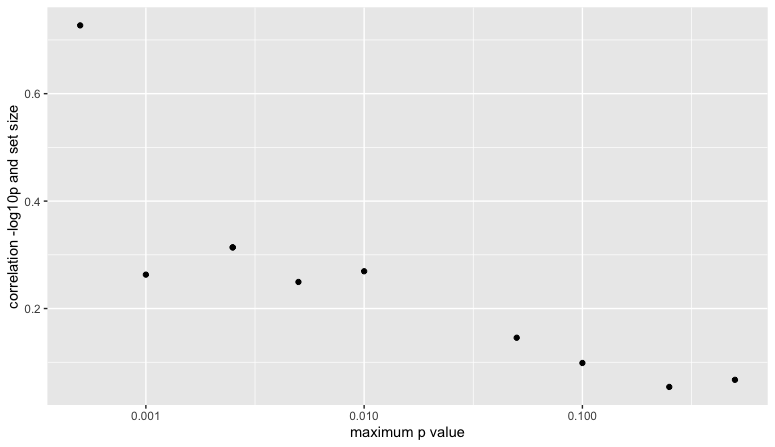
\includegraphics[width=12cm]{images/chapter2/ggplot/Rplot_corr_log10_set_p.png}
    \caption{Correlation of gene significance and set size with decreasing p. X axis maximum p value, y Pearsons correlation between -log10(p) of sets and set size. Data from supplementary material Sniekers et al\cite{sniekers2017genome}}
    \label{fig:correlation gene significance and set size Sniekers}
    \end{subfigure}
    
  \begin{subfigure}{15cm}
    \centering\includegraphics[width=12cm]{images/chapter2/ggplot/Rplot_minimum_p_mean_group_sizes.png}
    \caption{Changes in mean gene set size with decreasing maximum p values. Mean gene size increases. }
  \end{subfigure}
  \caption{Correlation between gene size and level of significance in MAGMA GSA and changes in mean gene size with increasingly significant gene sets (max p).Data from supplementary material Sniekers et al\cite{sniekers2017genome}}
   \label{fig:correlation gene significance and set size Sniekers with changes mean gene}
  \end{figure}


% \begin{figure}
%   \begin{subfigure}{8cm}
%     \centering\includegraphics[width=7cm]{images/FUMA_plots/gtex_v8_ts_general_FUMA_gene2func_UKBBEd_syn_protein_bp_sig.png}
%     \caption{Gene expression UKBBEd significant genes}
%     \end{subfigure}
%   \begin{subfigure}{8cm}
%     \centering\includegraphics[width=7cm]{images/FUMA_plots/gtex_v8_ts_FUMA_PSP_gtex.png}
%     \caption{Genes in PSP}
%   \end{subfigure}
 
%   \begin{subfigure}{8cm}
%     \centering\includegraphics[width=7cm]{images/FUMA_plots/gtex_v8_ts_psp_not_consensus_FUMA_gene2func44650.png}
%     \caption{Genes in PSP but not in consensus PSD. ie new genes}
%   \end{subfigure}
%   \begin{subfigure}{8cm}
%     \centering\includegraphics[width=7cm]{images/FUMA_plots/gtex_v8_ts_1313_consensus_FUMA_gene2func44650.png}
%     \caption{Genes in consensus PSD}
%   \end{subfigure}
% \end{figure}
%  \todo[inline]{the bottom two expression profiles look too similar redo these}
 

 
 
 

  


\clearpage


\section{Discussion}
\label{sec:Methods Discussion}

 I will briefly discuss here the results that arise from this chapter (ostensibly a methods chapter). They are, however, integral to methods in the two following chapters. 

The results obtained using MAGMA GSA correspond closely to those reported in the  literature despite probable variations in versions, platforms and reference panels. In addition results from the PASCAL scoring algorithm correlate closely with those from MAGMA. 

Most elements identified in the PSP are found in the largest connected components and the disconnected genes excluded  are few in number and show no evidence of possessing common features that might make them sources of bias. Similarly only a few PSP genes do not have boundaries defined in the reference gene boundaries used for MAGMA and again they show no evidence of common features. 

The relative lack of statistically significant gene associations on MAGMA GSA suggest it would be reasonable to try to reduce unnecessary comparisons. One way of doing this is a discovery and replication cohort design and only testing synaptic topological sets we have a reason to believe would be enriched. 

6155 gene set results are found for MAGMA GSA in the supplemental material for Sniekers et al\cite{sniekers2017genome}. This is quite an exhaustive search over possible gene sets and the uncorrected p values provide a rough guide to likely significance levels in this sample (this is the only sample with published MAGMA GSA for the sample.) 365 gene sets are of greater than nominal significance (5.91\% of terms). Given there is no reason to expect a \textit{particular} network community defined only by topology to be associated with this particular phenotype (intelligence or educational attainment) and that there should be around 15 to 120 gene sets in a network (see chapter 4) then assuming this is a \textit{rough} guide to the distribution of significance levels using nominal significance to select sets as interesting and for further testing with correction for multiple comparisons would result in taking between 1-6 sets forward for testing which should limit type II error. 

Where does the figure of 15-120 gene sets come from? It is a rough estimation based on experience using community detection methods in a pilot study (not shown) and extrapolation from studies such as McLean et al. (2016) \cite{mclean2016improved}. Given that these are rough estimates another might be to look at the named synaptic groups used by Hill et al.\cite{hill2014human} other than the combined PSP.  Their average size is 65.75 genes. For the 3457 PSP this would result in 53.2 gene sets. In chapter~\ref{chap:community detection} I will address the expected number of gene sets in greater detail but these seem a reasonable rule of thumb. 

The lowest $p$ value found in any of the samples using the 18 member functionally defined synaptic set was 0.005 (Excitability Education\textsubscript{Discovery}) and occured in the best powered cohort. This group also did not have the constraint of forming a topological unit (it was not required to be a ``functional module'' (members forming a complete subgraph) never mind the stricter requirement of forming a community. (see section~\ref{sec:analysis of likely signal} and table~\ref{tab:table from hill})

It is noteworthy that few gene sets have been found to be significant in MAGMA GSA studies and those that are are very large (see table~\ref{tab:group size and enrichment} there is also an association between group size and significance (figure~\label{fig:correlation gene significance and set size Sniekers} and figure~\ref{fig:correlation gene significance and set size Sniekers with changes mean gene}) . The significance level of the NMDA receptors reported by Hill et al. \cite{hill2014human} was $p=0.002$. Assuming the PSP was divided into groups of similar size to the subgroups (ie not complete PSD) in the Hill paper the significance level using simply a Bonferroni correction for multiple comparisons would be  0.00094 for $n$=53 groups. 


\todo{Phrase better following footnote ? move or leave out}\footnote{On reflection this bit probably belongs in community detection or the discussion chapter and needs to be better phrased. - There is also a reductio argument in favour of a discovery and replication design.  A community detection might result in 100 groups of approximately size 35 or two groups one of 35 and the other of 3422. Let us assume that the size 35 group is relevant to the phenotype in ground truth. Let us then consider another clustering where all of the groups are around 35 in size and the one with the ground truth mapping to the phenotype we are interested in is there. There are also several other groups that map to diseases we are not testing, some to no disease but interesting functional groups and some novel but interesting groupings. 

Testing for the association with the phenotype using the evenly divided group with several interesting communities (although not all of interest to us)  would have a Bonferroni correction alpha level of 0.0005. The one dividing the network into one group of 35 and another of 3422 s would have an alpha level of 0.025. It is surely plausible that in testing a single phenotype the first group \textit{may} be the better clustering and its remaining 99 groups are enriched for other processes and disorders, the community detection method however that divides it into two groups would do far better even although its treatment of the non involved nodes does not best conform to their functional division. I return to this point in chapter~\ref{chap:community detection}.
\url{ source('~/RProjects/chapter2_checks/R/expected_gsa/ctg_size_plots.R')}}

SynGO shows the value of using less tests and more specific terms\footnote{adding syngo or a slim ontology on top of magma would be a pretty good msc project} (in particular for Education\textsubscript{Discovery} Biological Process in particular with much stronger enrichment than GO enrichment in ToppGene.\footnote{ Would be reasonable to try to add both a slim ontology and testing through the dag on top of magma or pascal. However although the FDR q value is lower there is not much specificity of the terms. }



Re-Analysis of the gene level scores of significant genes in GWGAS studies of intelligence and education suggest that around 25\% of these genes are in the post synaptic proteome. We would therefore expect that given the involvement of non PSP genes that the raw P values for enrichment would be less than those reported in Sniekers et al and other studies. I shall return to why this is important in further discussions (in brief intelligence and education get uniquely large sample sizes so can afford to trade power for conservatism, this will not be true of rarer diseases, if you get no significant GSA in a study with 78000 people the technique will be of little use for diseases other than the very commonets). 

The gene sets with very low unadjusted p values in these studies tend also to be much larger than those we would find in the PSP and there is a correlation between gene size and log10p.

Disease terms related to intellectual disability are found in both education samples and neither intelligence sample. An association is reported in Sniekers et al. \cite{sniekers2017genome} using DEPICT but I am not aware that the difference with intelligence samples has been reported. It does suggest there may be a qualitative difference between enriched genes in the education and intelligence samples in addition to the difference in genetic correlation of the two phenotypes.  

PSP genes are expressed robustly in all brain regions using the GTEx data and this suggests that the increase in gene number in the network has still resulted in a set of genes strongly expressed in the CNS. The pattern of correlation of gene expression between brain regions in the PSP is similar to that recorded of all genes literature \cite{mele2015human} suggesting that we do not have a very unusual sample.  

\footnote{This to discussion of chapter community detection or intro Finally the lack of over representation o
lack of over representation of synaptic elements on GSA of significant genes despite evidence of synaptifc involvement using polygenic signal shows limitations of even using GWAS catalog for network studies}

\todo[inline]{cross ref for this section}



\todo{in discussion mention that although synapse and PSP only 25\% it is the only system enriched}




\clearpage
\todo[inline]{text to be moved commented out to print}
% this is discussion discussion move \todo{this is the bit on tissue specificity may move to end of thesis discussion}
% Disease associated genes are more likely to be uniquely expressed in a tissue according to several references cited by Kitsak et al.\footnote{note to self this is kitsak and ghissian and menche and barabasi - they use a mixture of PPI and other networks (from menche) they use their own definition of tissue expressed which is one tissue with z>1 where z is z score. See comment on gtex} \todo{move some of this to discussion} Finally, the most similar analysis to ours \cite{ghiassian2015disease} whose first author is one of the coauthors in the paper by Kitsak et al.\cite{kitsak2016tissue} uses a network of heterogenous interactions. One of the potential limitations of the authors' approach was using a network composed of a combination of experimental protein interactions, predicted reactions and other networks such as metabolic networks found in KEGG (a non tissue specific proteome network used across a variety of diseases). 
% also see \cite{luck2020reference}
% \cite{tran2019condition}
\clearpage
\section{To supplemental tables}
\begin{table}[ht]
\centering
\begin{tabular}{lrrr}
  \toprule
Gene set name & n genes & $\beta$ & p \\ 
  \midrule
Exocytosis & 83 & 0.19 & 0.039 \\ 
  Neurotransmitter metabolism & 27 & -0.10 & 0.686 \\ 
  Excitability & 57 & 0.38 & 0.005 \\ 
  Protein cluster & 43 & 0.20 & 0.091 \\ 
  Ligand-gated ion channel signaling & 33 & 0.03 & 0.438 \\ 
  Tyrosine kinase signaling & 7 & 0.22 & 0.308 \\ 
  Unassigned & 59 & 0.07 & 0.301 \\ 
  Peptide/neurotrophin signals & 28 & 0.04 & 0.430 \\ 
  Intracellular signal transduction & 148 & -0.04 & 0.697 \\ 
  Ion balance/transport & 41 & -0.01 & 0.522 \\ 
  G-protein relay & 27 & -0.10 & 0.688 \\ 
  RNA and protein synthesis, folding and breakdown & 67 & 0.01 & 0.448 \\ 
  Endocytosis & 25 & -0.17 & 0.804 \\ 
  Structural plasticity & 95 & -0.06 & 0.731 \\ 
  Cell metabolism & 51 & -0.13 & 0.827 \\ 
  Cell adhesion and trans-synaptic signaling & 76 & 0.29 & 0.009 \\ 
  G-protein-coupled receptor signaling & 41 & 0.09 & 0.300 \\ 
  Intracellular trafficking & 75 & 0.04 & 0.344 \\ 
   \bottomrule
\end{tabular}
\caption{Synaptic enrichment UKBB int Source\url{source('~/RProjects/redo_chapter2/R/redo_synapse_set_int_curated.R')}} 
\label{tab:MAGMA enrichment of synaptic groups UKBBint}
\end{table}

% latex table generated in R 3.6.3 by xtable 1.8-4 package
% Sun Aug  9 12:41:54 2020
\begin{table}[ht]
\centering
\begin{tabular}{lrrr}
   \toprule
Gene set name & n genes & $\beta$ & p\\
  \midrule
Exocytosis & 83 & 0.04 & 0.348 \\ 
  Neurotransmitter metabolism & 27 & -0.08 & 0.648 \\ 
  Excitability & 57 & 0.43 & 0.003 \\ 
  Protein cluster & 43 & -0.14 & 0.813 \\ 
  Ligand-gated ion channel signaling & 33 & 0.18 & 0.178 \\ 
  Tyrosine kinase signaling & 7 & -0.18 & 0.658 \\ 
  Unassigned & 59 & 0.08 & 0.276 \\ 
  Peptide/neurotrophin signals & 28 & -0.20 & 0.828 \\ 
  Intracellular signal transduction & 148 & 0.07 & 0.226 \\ 
  Ion balance/transport & 41 & 0.11 & 0.242 \\ 
  G-protein relay & 27 & -0.09 & 0.671 \\ 
  RNA and protein synthesis, folding and breakdown & 67 & 0.10 & 0.198 \\ 
  Endocytosis & 25 & 0.12 & 0.281 \\ 
  Structural plasticity & 95 & 0.04 & 0.355 \\ 
  Cell metabolism & 51 & 0.05 & 0.374 \\ 
  Cell adhesion and trans-synaptic signaling & 76 & 0.39 & 0.001 \\ 
  G-protein-coupled receptor signaling & 41 & -0.01 & 0.517 \\ 
  Intracellular trafficking & 75 & -0.06 & 0.713 \\ 
   \hline
   \bottomrule
\end{tabular}
\caption{Synaptic enrichment UKBB Ed} 
\label{tab:MAGMA enrichment of synaptic groups UKBBEd}
\end{table}0.016 

% latex table generated in R 3.6.3 by xtable 1.8-4 package
% Sun Aug  9 12:43:33 2020
\begin{table}[ht]
\centering
\begin{tabular}{lrrr}
  \toprule 
Gene set name & n genes & $\beta$ & p\\
  \midrule
Cell adhesion and trans-synaptic signaling & 76 & 0.11 & 0.155 \\ 
  Cell metabolism & 51 & -0.07 & 0.726 \\ 
  Endocytosis & 25 & -0.03 & 0.572 \\ 
  Excitability & 57 & 0.13 & 0.159 \\ 
  Exocytosis & 83 & 0.18 & 0.016 \\ 
  G-protein-coupled receptor signaling & 41 & 0.15 & 0.162 \\ 
  G-protein relay & 27 & 0.11 & 0.251 \\ 
  Intracellular signal transduction & 148 & 0.07 & 0.150 \\ 
  Intracellular trafficking & 75 & -0.01 & 0.522 \\ 
  Ion balance/transport & 41 & -0.17 & 0.898 \\ 
  Ligand-gated ion channel signaling & 33 & -0.27 & 0.944 \\ 
  Neurotransmitter metabolism & 27 & 0.25 & 0.099 \\ 
  Peptide/neurotrophin signals & 28 & -0.10 & 0.720 \\ 
  Protein cluster & 43 & 0.11 & 0.207 \\ 
  RNA and protein synthesis, folding and breakdown & 67 & 0.11 & 0.120 \\ 
  Structural plasticity & 95 & -0.10 & 0.874 \\ 
  Tyrosine kinase signaling & 7 & -0.45 & 0.880 \\ 
  Unassigned & 58 & -0.03 & 0.620 \\ 
   \bottomrule
\end{tabular}
\caption{Synaptic enrichment ctg} 
\label{tab:MAGMA enrichment of synaptic groups ctg}
\end{table}

% latex table generated in R 3.6.3 by xtable 1.8-4 package
% Sun Aug  9 12:45:12 2020
\begin{table}[ht]
\centering
\begin{tabular}{lrrr}
  \toprule
Gene set name & n genes & $\beta$ & p\\
  \midrule
Cell adhesion and trans-synaptic signaling & 76 & 0.17 & 0.067 \\ 
  Cell metabolism & 53 & -0.02 & 0.549 \\ 
  Endocytosis & 26 & 0.11 & 0.251 \\ 
  Excitability & 57 & 0.16 & 0.122 \\ 
  Exocytosis & 83 & -0.11 & 0.877 \\ 
  G-protein-coupled receptor signaling & 41 & 0.08 & 0.315 \\ 
  G-protein relay & 27 & -0.01 & 0.521 \\ 
   Intracellular signal transduction & 147 & 0.02 & 0.418 \\ 
  Intracellular trafficking & 75 & -0.02 & 0.590 \\ 
  Ion balance/transport & 40 & 0.05 & 0.370 \\ 
  Ligand-gated ion channel signaling & 33 & 0.18 & 0.158 \\ 
  Neurotransmitter metabolism & 27 & -0.15 & 0.774 \\ 
  Peptide/neurotrophin signals & 28 & 0.11 & 0.267 \\ 
  Protein cluster & 42 & -0.20 & 0.910 \\ 
  RNA and protein synthesis, folding and breakdown & 66 & 0.22 & 0.016 \\ 
  Structural plasticity & 95 & 0.10 & 0.140 \\ 
  Tyrosine kinase signaling & 7 & -0.27 & 0.742 \\ 
  Unassigned & 58 & 0.07 & 0.290 \\ 
   \bottomrule
\end{tabular}
\caption{Synaptic enrichment EA2} 
\label{tab:MAGMA enrichment of synaptic groups EA2}
\end{table}
\clearpage
\begin{figure}
    \centering
    \includegraphics[height=25cm]{images/FUMA_plots/expHeat_FUMA_gene2func-2_ukbbed_zeromean.png}
    \caption{Heatmap gene expression FUMA UKBBEd Average value of the relavitve expression level zero mean centred and log2 transformed. Shows that a small number of genes amongst those enriched are very enriched}
    \label{fig:my_label}
\end{figure}
% \begin{table}[]
%     \centering
%     \begin{tabular}{llll}
%     \toprule
%     Number & First author & Year & Citation\\
%     \midrule
%       1  &  PENG & 2002 & \cite{peng2004semiquantitative}  is 2004 \\
%       2  &  SATON  2002    is SATOH &2002 &\cite{satoh2002identification} \\
%     3 &  SCHWENK & 2013 &  \cite{schwenk2012high} 2012\\
%     4 &  SELIMI  & 2009 & \cite{selimi2009proteomic} \\
%     5 &  TRINIDAD & 2005& \cite{trinidad2005phosphorylation} \\  
% 6& TRINIDAD  &2008 & \cite{trinidad2008quantitative} \\
% 7&  WALIKONIS & 2000&  \cite{walikonis2000identification}\\ 
%  8 &YOSHIMURA &2004& \cite{yoshimura2004molecular}   \\
% 9 &FROMER &2014 & \footnote{Not in Heil I only find fromer in an oksana paper on PSD and it is on scz I assume this is Focking and the one cited in Heil is bipolar
% and they have 2033} PSD proteins Focking \cite{focking2016proteomic}\\
% 10&FARR &2004 &  \cite{farr2004proteomic}\\
% 11&Distler.PSDII & 2014 &\cite{distler2014depth}\\
% 12& BAYES & 2011&    \cite{bayes2011characterization}  \\
% 13 &  BAYES &2012 & \cite{bayes2012comparative}  \\  
% 14& COLLINS &2006 & \cite{collins2006molecular}\\
% 15 & DOSEMECI  &2007&  \cite{dosemeci2007composition}\\
% 16 & FERNANDES  &2009&  \cite{fernandez2009targeted}\\
% 17 & BAYES &2014 &  \cite{bayes2014human}\\
% \bottomrule
%     \end{tabular}
%     \caption[Primary proteomic studies contributing to the PSP graph]{Primary proteomic studies contributing to the PSP graph \footnote{to Douglas: if using the Oksana Clean Published data TO REMOVE please see note on text}}
%     \label{tab:oksana clean published}
% \end{table}


\begin{table}[]
    \centering
    \begin{tabular}{llllllll}
    \toprule
     & First author & Year & Reference & Region & Species & $n$ & In Oksana file \\
    \midrule
1 &    WALIKONIS &2000 &Walikonis et al. (2000)\cite{walikonis2000identification} &postsynapse & rat & 29 \\
2 &PENG&2004&Peng et al. (2004) \cite{peng2004semiquantitative}&postsynapse& rat& 325\\
3 &SATOH&2002&Satoh et al. (2002)\cite{satoh2002identification} &postsynapse &mouse &45\\
4 &YOSHIMURA&2004&Yoshimura et al. (2004) \cite{yoshimura2004molecular} &postsynapse& rat &435\\
5 &FARR&2004&Farr et al. (2004)  \cite{farr2004proteomic}&postsynapse &rat &71 &Yes\\
6 &JORDAN&2004&Jordan et al. (2004)&postsynapse &mouse and rat &390& NOT\\
7&LI&2004 &wan Li et al. (2003)&postsynapse &rat& 137& NOT\\
8&TRINIDAD&2005 &Trinidad et al. (2005) \cite{trinidad2005phosphorylation}&postsynapse&mouse& 234& YES\\
9&CHENG&2006&Cheng et al. (2006)&postsynapse& rat& 288& NO\\
10&COLLINS&2006&Collins et al. (2006)\cite{collins2006molecular}&postsynapse &mouse& 717& YES\\
11&DOSEMESI&2006&Dosemeci et al. (2006)&postsynapse& rat& 113& NO\\
12&DOSEMESI&2007&Dosemeci et al. (2007)&postsynapse& rat& 548& YES\\
13&TRINIDAD&2008&Trinidad et al. (2008)&postsynapse& mouse& 2150& YES\\
14&SELIMI&2009&Selimi et al. (2009)\cite{selimi2009proteomic}&postsynapse &mouse &61& YES\\
15&FERNANDEZ&2009&Fernández et al. (2009)  \cite{fernandez2009targeted}&postsynapse& mouse &292& YES\\
16&BAYES&2010&Bayés et al. (2011)&postsynapse &human &1441& YES\\
17&BAYES&2012&Bayés et al. (2012)&postsynapse &mouse &1545 &YES\\
18&SCHWENK&2012&Schwenk et al. (2012) \cite{schwenk2012high}&postsynapse &unknown &34& YES\\
19&DISTLER PSD1*&2014&Distler et al. (2014)&postsynapse& mouse& 3545& NO \footnote{intended per email}\\
20&DISTLER PSD2*&2014&Distler et al. (2014)&postsynapse& mouse& 2092*& Oksana\\
21&BAYES&2014&Bayés et al. (2014)&postsynapse& human &1141& YES\\
22&UEZU&2016&Uezu et al. (2016)&postsynapse &mouse &1111 &NO\\
23&FOCKING&2016&Föcking et al. (2016)&postsynapse& human &2026 &NO\\
\bottomrule
    \end{tabular}
    \caption[Primary Proteomic studies appearing in PSP cleaned from Heil (2018)]{Primary proteomic studies contributing to the PSP take from Heil 2018\cite{heil2018systems} from Katharina PhD p84 table 5.1. \footnote{to Douglas: These should have been the same as given to me as per email from Colin need to chose one see note on text. Distler PSD1 is definitely dropped from the cleaned data. The graph is somewhere between these two points. The most conservative is the Oksana one.}}
    \label{tab:Katharina_phd_studiesFF}
\end{table}
% \section{NOT IN DOCUMENT}
% \section{FRAMEWORK FOR GSA - USED}
% %%% FRAMEWORK
% \section{Gene Ontology Analysis of MAGMA genes FRAMEWORK}
% They are not all measured the same way eg DEPICT in Okbay so worth going through 

% Is the gtex higher in both education
%     \subsection{Intelligence Replication}
%         \subsubsection{Authors findings}
%         MAGMA Regulating cell development $P=3.5 \times 10^{-6}$. Authors state that several (?14) of the significant genes are more expressed in the CNS.
%         \subsubsection{Ontology ORA Genome}
%         \paragraph{Toppgene ToppFun Intelligence Replication}
%         \subparagraph{ToppFun BP} nil
%         \subparagraph{ToppFun MF} nil
%         \subparagraph{ToppFun CC} See table~\ref{tab:cellular component in toppgene}
%         \begin{table}[ht]
%     \centering
%     \begin{tabular}{llllllll}
%          ID &Name 	&	pValue 	&FDR BH &	FDR BY 	&Bonferroni  	&n input & n annot  \\
%          GO:0032584 &	growth cone membrane\footnote{part of growth cone: distal axon: neuron projection:cell projection: cellular anatomical entity} &		1.416E-4 &	3.838E-2 &2.373E-1&	3.838E-2 &	2 &	8 \\
%     \end{tabular}
%     \caption{Cellular component in toppgene}
%     \label{tab:cellular component in toppgene}
% \end{table}
%         \paragraph{Panther Intelligence Replication}
%         All genes 47 identified
        
%         \subparagraph{Panther BP} nil
%         \subparagraph{Panther MF} nil
%         \subparagraph{Panther CC} Two terms Cytoplasm GO:0005737 n in annotation 11714 n in set	40; expected 	26.40 ; fold change	1.51 ;	+ 	; raw P4.29E-05 	; FDR 0.431 4.31E-02 and its parent term intracellular GO:0005622 n in annotation 14693 ; n in set	45 ; E	33.12 ; fold	1.36 ;	+ ;	3.24E-05 ; FDR	6.50E-02 Not significant


%         \subsubsection{Ontology ORA Synaptic}
        
%         \subsubsection{Others}
%         \begin{itemize}
%             \item path to code
%             \item GTex
%             \item Other phenotypes
%         \end{itemize}
        

%     \subsection{Education Replication}
%         \subsubsection{Authors findings Education Replication}
%         Pathways involving CNS development
%         13 Gtex tissues in CNS showed elevated expression of genes near EduYears SNPs
%         283 Gene sets. 5 clusters ``neural progenitor cells, migration of new neurons to cortex, projection of axons to target, sprouting of dendrites and spines and neuronal signalling and synaptic plastigcity throughout the lifespan'' not precis quote but close last group is the one of interest to use 
%         Genes prioritised by DEPICT. Overlap with ID and ASD.GRIK2<10e-6, CALM2 < 10e-4 PPI in Figure 3 ?includes multiple testing. 685 genes at 273 Loci p 88 of supplemental material supplementary table 4.1 wherever that is. We have not used this approach as \url{https://github.com/perslab/gwas-snps-loci} as predominant approach is MAGMA.
%         \subsubsection{Ontology ORA Education Replication Genome}
%       \paragraph{toppgene}
%           \subparagraph{BP toppgene}  See table~\ref{tab:BP EA2 all significant toppgene} 
%             \begin{table}[ht]
% \centering
% \begin{tabular}{rllrrrr}
%   \hline
%  & ID & Name & test & Genome & p & Bon \\ 
%   \hline
% 1 & GO:0022008 & neurogenesis & 26 & 1866 & $5.97 \times 10^{-7}$ & 0.00176 \\ 
%   2 & GO:0042063 & gliogenesis & 11 & 352 & $1.14 \times 10^{-6}$ & 0.00337 \\ 
%   3 & GO:0007417 & central nervous syst & 19 & 1129 & $1.81 \times 10^{-6}$ & 0.00535 \\ 
%   4 & GO:0048666 & neuron development & 20 & 1297 & $3.53 \times 10^{-6}$ & 0.01041 \\ 
%   5 & GO:0010001 & glial cell different & 9 & 261 & $5.16 \times 10^{-6}$ & 0.01522 \\ 
%   6 & GO:0050808 & synapse organization & 12 & 498 & $5.39 \times 10^{-6}$ & 0.01589 \\ 
%   7 & GO:0048667 & cell morphogenesis i & 14 & 688 & $5.92 \times 10^{-6}$ & 0.01747 \\ 
%   8 & GO:0048699 & generation of neuron & 23 & 1751 & $8.43 \times 10^{-6}$ & 0.02489 \\ 
%   9 & GO:0048812 & neuron projection mo & 14 & 742 & $1.39 \times 10^{-5}$ & 0.04100 \\ 
%   10 & GO:0010771 & negative regulation  & 6 & 109 & $1.53 \times 10^{-5}$ & 0.04527 \\ 
%   \hline
% \end{tabular}
% \caption{BP EA2 all significant Toppgene 99 genes in total \url{source('~/RProjects/paper_xls_output/R/chapter_2/eda_toppgene_all_significant_ea2.R')}} 
% \label{tab:BP EA2 all significant toppgene}
% \end{table}

% \subparagraph{CC toppgene}
% See table~\ref{tab:CC EA2 all significant Toppgene}
% % latex table generated in R 3.6.3 by xtable 1.8-4 package
% % Wed Aug 19 12:29:17 2020
% \begin{table}[ht]
% \centering
% \begin{tabular}{llrrrr}
%   \hline
% ID & Name & test & Genome & p & Bon \\ 
%   \hline
% GO:0098794 & postsynapse & 16 & 825 & $1.46 \times 10^{-6}$ & 0.00050 \\ 
%   GO:0045202 & synapse & 20 & 1482 & $1.58 \times 10^{-5}$ & 0.00547 \\ 
%   \hline
% \end{tabular}
% \caption{CC EA2 all significant Toppgene \url{source('~/RProjects/paper_xls_output/R/chapter_2/eda_toppgene_all_significant_ea2.R')} }
% \label{tab:CC EA2 all significant Toppgene}
% \end{table}


        
%     \paragraph{panther}
%     Panther by default uses HGNC numerical symbols so it is necessary to prefix Entrez ID with GeneID: this is done in a custom R script \url{source('~/RProjects/paper_xls_output/R/chapter_2/exploratory_data_analysis.R')}
%     Unmapped Gene ID using entrez with Gene ID prefix
%     GeneID:246744

%         \subparagraph{BP Panther}
%         BP panther ordered by FDR 19 items top Nervous system development FDR 0.006 (2430 genes in reference) 2.57 fold change (see table~\ref{tab:GO.biological.process.complete Panther Gene Ontology Enrichment significant genes in Education Replication}). The heirarchy of terms in gene ontology is shown in figure~\ref{fig:panther GO Biological Process Heirarchy shown}\footnote{Douglas: I have included this as a screenshot. Parsing the xml and getting it into latex took longer than I thought so I went straight to screenshot as a last resort could do the indentation by hand. Thought worth showing (as DEPICT, MAGMA etc as far as I can see ignore heirarchy) but interested in what you thought. The standard table output for panther doesn't have the heirarchy.}
        
%         \begin{figure}
%             \centering
%             \includegraphics[width=\textwidth]{images/screenshots/EA2_BP_Panther_all_genes.png}
%             \caption{Panther GO Biological Process EA2 Hierarchy shown. This includes all genes accessed by manually editing the Gene Symbol}
%             \label{fig:panther GO Biological Process Heirarchy shown}
%         \end{figure}
%         % latex table generated in R 3.6.3 by xtable 1.8-4 package
% % Sun Aug 23 11:12:46 2020
% \begin{table}[ht]
% \centering
% \begin{tabular}{lrrrlrcc}
%   \hline
% GO.biological.process.complete & ref & test & [E] & ou & fold & P & FDR \\ 
%   \hline
% nervous system development (GO:0007399) & 2430 & 30 & 11.7 & + & 2.57 & $7.62 \times 10^{-7}$ & 0.006 \\ 
%   neuron development (GO:0048666) & 848 & 17 & 4.1 & + & 4.18 & $6.68 \times 10^{-7}$ & 0.011 \\ 
%   neuron differentiation (GO:0030182) & 1046 & 18 & 5.0 & + & 3.59 & $2.58 \times 10^{-6}$ & 0.014 \\ 
%   negative chemotaxis (GO:0050919) & 46 & 5 & 0.2 & + & 22.66 & $4.42 \times 10^{-6}$ & 0.014 \\ 
%   neurogenesis (GO:0022008) & 1690 & 23 & 8.1 & + & 2.84 & $4.42 \times 10^{-6}$ & 0.018 \\ 
%   \makecell{negative regulation of cell morphogenesis\\ involved in differentiation (GO:0010771)} & 100 & 6 & 0.5 & + & 12.51 & $1.18 \times 10^{-5}$ & 0.031 \\ 
%   generation of neurons (GO:0048699) & 1585 & 21 & 7.6 & + & 2.76 & $1.88 \times 10^{-5}$ & 0.037 \\ 
%   regulation of synapse structure or activity (GO:0050803) & 240 & 8 & 1.1 & + & 6.95 & $2.51 \times 10^{-5}$ & 0.040 \\ 
%   regulation of synapse organization (GO:0050807) & 229 & 8 & 1.1 & + & 7.28 & $1.81 \times 10^{-5}$ & 0.041 \\ 
%   cell development (GO:0048468) & 1654 & 21 & 7.9 & + & 2.65 & $3.51 \times 10^{-5}$ & 0.043 \\ 
%   regulation of extent of cell growth (GO:0061387) & 115 & 6 & 0.6 & + & 10.88 & $2.51 \times 10^{-5}$ & 0.044 \\ 
%   regulation of axonogenesis (GO:0050770) & 192 & 7 & 0.9 & + & 7.60 & $4.77 \times 10^{-5}$ & 0.045 \\ 
%   negative regulation of axonogenesis (GO:0050771) & 72 & 5 & 0.3 & + & 14.48 & $3.37 \times 10^{-5}$ & 0.045 \\ 
%   regulation of cell size (GO:0008361) & 187 & 7 & 0.9 & + & 7.81 & $4.05 \times 10^{-5}$ & 0.046 \\ 
%   membrane protein proteolysis (GO:0033619) & 39 & 4 & 0.2 & + & 21.39 & $5.23 \times 10^{-5}$ & 0.046 \\ 
%   regulation of neuron projection development (GO:0010975) & 521 & 11 & 2.5 & + & 4.40 & $4.70 \times 10^{-5}$ & 0.047 \\ 
%   neuron projection development (GO:0031175) & 697 & 13 & 3.3 & + & 3.89 & $3.29 \times 10^{-5}$ & 0.048 \\ 
%   positive regulation of collateral sprouting (GO:0048672) & 12 & 3 & 0.1 & + & 52.13 & $4.60 \times 10^{-5}$ & 0.049 \\ 
%   regulation of neurogenesis (GO:0050767) & 847 & 14 & 4.1 & + & 3.45 & $5.84 \times 10^{-5}$ & 0.049 \\ 
%   \hline
% \end{tabular}
% \caption{GO.biological.process.complete Panther Gene Ontology Enrichment significant genes in Education Replication} 
% \label{tab:GO.biological.process.complete Panther Gene Ontology Enrichment significant genes in Education Replication}
% \end{table}
%             \subparagraph{MF panther} No significant
%             \subparagraph{CC panther} Only one term synapse GO:0045202 1382 terms in reference 19 in table expected 6.50 fold enrichment 29.93 raw P $2.29\times 10^{-5}$ FDR 0.0459

%         Compare with toppgene widely variant scores noted in \cite{rhee2008use} and detailed discussion in \cite{khatri2005ontological}
%          \subsubsection{Ontology ORA Synaptic}
%          \subsubsection{Others}
%          \paragraph{disease enrichment}
%          Enrichment in DisGeNNet BeFree searched by toppfun of Intellectual disability
%         ID C3714756 	Intellectual Disability ; Source	DisGeNET BeFree ; p 	8.884E-7 ; FDR BH	1.648E-3; FR BY 	1.386E-2 ;Bonferroni	2.237E-3; Input 	20 	Total 1219
        
%         % latex table generated in R 3.6.3 by xtable 1.8-4 package
% % Sun Aug 23 12:35:02 2020
% \begin{table}[ht]
% \centering
% \begin{tabular}{rllr}
%   \hline
% Entrez.Gene.ID & Gene.Symbol & Gene.Name & Original.Symbol \\ 
%   \hline
% 5144 & PDE4D & phosphodiesterase 4D & 5144 \\ 
%   5662 & PSD & pleckstrin and Sec7 domain containing & 5662 \\ 
%   4137 & MAPT & microtubule associated protein tau & 4137 \\ 
%   4208 & MEF2C & myocyte enhancer factor 2C & 4208 \\ 
%   4744 & NEFH & neurofilament heavy & 4744 \\ 
%   257194 & NEGR1 & neuronal growth regulator 1 & 257194 \\ 
%   \hline
% \end{tabular}
% \caption{Intellectual disability genes significant in EA2 found in PSP} 
% \label{tab:Intellectual disability genes significant in EA2 found in PSP}
% \end{table}
%         Path to code
        
%         GTEx
% \clearpage














% \subsection{Put problems with GSA multiple testing somewhere}
% \footnote{gsea moved to chapter 4}
% \subsection{PASCAL software}
% Need to check version on strontium. Original version. Alpha 0.1. 
% shell command
% default options 
% no gene boundary
% empirical method

% \todo[inline]{I think this goes to community detection}
% \section{Other models of topology}
% We may want to put the diamond bit in here on the basis that if that hypothesis is correct then diamond should be good but it isn't so on to what we are doing (and we can mention the similarity in the rejected bit) see section~\ref{sec:DIAMOnD algo} \todo[inline]{I think this goes to community detection}
%  \subsection{Analysis of likely signal}
% \label{sec:analysis of likely signal}
% The paper by Hill et al. \cite{hill2014human} testing synaptic components for enrichment for genetic variants associated with differences in intelligence adopts a discovery and replication cohort design. It is particularly noteworthy as it is a hypothesis driven use of GSA (GSEA here) to investigate the role of synaptic components in differences in human cognitive ability. It is further noteworthy as the significance level in the discovery cohort gives a possible bound for what we might expect to obtain as a significance level (see also section 
% This is verbatim from the Hill paper
% "Empirical significance was set for P- and FDR values of the observed gene set as being smaller than 95\% of those obtained in the random gene lists. Gene sets passing this criterion were taken forward to step six: replication in the BATS and NCNG cohorts." which is actually what we did
 
% Table from hill
%  Mean gene set size testing non full sets is 65.75 (181 + 50 + 7 + 25) which are not full
%  Assuming we are now dividing up signal like hPSD full to like size sub sections = 53 groups 
 
%  Significance level would therefore be 0.0009433962. But it may be we only have one significant topological group therefore much more likely to be significant the less groups you divide it into

% Summary of gene sizes



% \subsection{Synaptic models from MAGMA}
% \ref{sec:synaptic models from ctg}
% Essentially we used the synaptic models provided by MAGMA to do GSA. They were in a format which was not automatically recognised by MAGMA v1.06 so we converted this into gmt format using the file \url{source('~/RProjects/paper_xls_output/R/magma_synapse/make_synapse_gmt.R')}
% x number of genes were found. 

% GSA was performed for intelligence discovery and education cohorts. 
% Results were: with correction for multiple testing.

% These are non contiguous areas on the graph

% Code is at \url{source('~/RProjects/utils/src/generic_compile_gsa_magmasynapse.R')}

% We return to this data in section checking our findings \todo{add chapter checking our findings and add cross ref}
% \textcolor{red}{This would be better before community detection along with the hill redo as a kind of pre community detection}
% \todo{Move this to new section before community detection}









% %%%%% OTHER GSA
% \section{Additional data move in or out}
% \subsection{GSA moved here}
% \subsubsection{Intelligence replication GSA}
% They performed GSA with MAGMA and found only one significant group after correction for multiple testing. MAGMA offers gene ontology enrichment but it is not clear whether it respects the gene ontology structure of DAG in caclulcating p values. 

% If you use only the significant genes in FUMA you get no term enrichmet but interestingly you get no differential CNS enrichment which is perhaps why they only quote a percentage of those.

% \subsubsection{Intelligence Discovery Secondary analysis}
% \todo[inline]{by Hill et all ? move to samples. Points to make big gene sets}
% Gene set analysis of this set augmented by mgtag \cite{hill2019combined} was carried out using 10891 gene sets from Gene ontology, Reactome and MSigDB (raw p required = 0.05/10891 = $4.59 \times 10^{-6}$. GSA revealed 7 sets including neurogenesis 1355 genes and genes expressed in synapse 717 genes , regulation of nervous system development 722 genes neuron projection 989 neuron differentation 842 and CNS neuron differentiation 160 genes cell development 808 genes 

% For gene set size analysis see \url{source('~/RProjects/paper_xls_output/R/exploratory_data_analysis/gene_size_and_enrichment_magma_sets.R')}

% \subsubsection{Gene ontology enrichment Intelligence Discovery}
% Despite using translation to symbol and entrez the following id were unidentified. Panther autodetects numerical as HGNC numerical codes 
% ID
% H2AC16
% H2BC13
% H2BC15
% H2BC7
% H2BC4
% H3C3
% H3C11
% H3C12
% H1-5
% H2BC5


% 3 unrecognised using "GeneID" prefix

% in gene ontology

% NO significant enrichment for biological process
% Molecular function protein binding NOS 6.76E-06 	1.07E-02
% CC
% % latex table generated in R 3.6.3 by xtable 1.8-4 package
% % Sat Aug 22 15:33:04 2020

% \subsection{Results GSA}

% Table~\ref{tab:GO.cellular.component.complete Panther Gene Ontology Enrichment significant genes in Intelligence Discovery} and \ref{GO.molecular.function.complete Panther Gene Ontology Enrichment significant genes in Intelligence Discovery}
% \begin{table}[ht]
% \centering
% \begin{adjustbox}{width=\textwidth}

% \begin{tabular}{lrrrlrrr}
%   \hline
% GO.cellular.component.complete & ref & test & expected & overunder & fold & P & FDR \\ 
%   \hline
% DNA packaging complex (GO:0044815) & 85 & 9 & 0.8 & + & 11.68 & $1.74 \times 10^{-7}$ & 0.00035 \\ 
%   nucleosome (GO:0000786) & 77 & 8 & 0.7 & + & 11.46 & $9.75 \times 10^{-7}$ & 0.00098 \\ 
%   protein-DNA complex (GO:0032993) & 175 & 9 & 1.6 & + & 5.67 & $4.46 \times 10^{-5}$ & 0.00994 \\ 
%   synapse (GO:0045202) & 1382 & 27 & 12.5 & + & 2.16 & $1.84 \times 10^{-4}$ & 0.02850 \\ 
%   nucleus (GO:0005634) & 7567 & 98 & 68.6 & + & 1.43 & $1.81 \times 10^{-5}$ & 0.01210 \\ 
%   intracellular membrane-bounded organelle (GO:0043231) & 11028 & 128 & 100.0 & + & 1.28 & $5.05 \times 10^{-5}$ & 0.01010 \\ 
%   intracellular organelle (GO:0043229) & 12843 & 144 & 116.4 & + & 1.24 & $3.11 \times 10^{-5}$ & 0.01250 \\ 
%   membrane-bounded organelle (GO:0043227) & 12734 & 142 & 115.4 & + & 1.23 & $6.34 \times 10^{-5}$ & 0.01160 \\ 
%   organelle (GO:0043226) & 13859 & 151 & 125.6 & + & 1.20 & $6.94 \times 10^{-5}$ & 0.01160 \\ 
%   intracellular (GO:0005622) & 14693 & 159 & 133.2 & + & 1.19 & $1.86 \times 10^{-5}$ & 0.00932 \\ 
%   cellular anatomical entity (GO:0110165) & 18761 & 185 & 170.1 & + & 1.09 & $4.17 \times 10^{-5}$ & 0.01050 \\ 
%   cellular\_component (GO:0005575) & 18946 & 186 & 171.7 & + & 1.08 & $3.40 \times 10^{-5}$ & 0.01140 \\ 
%   Unclassified (UNCLASSIFIED) & 1905 & 3 & 17.3 & - & 0.17 & $3.40 \times 10^{-5}$ & 0.00974 \\ 
%   \hline
% \end{tabular}
% \end{adjustbox}
% \caption{GO.cellular.component.complete Panther Gene Ontology Enrichment significant genes in Intelligence Discovery}
% \label{tab:GO.cellular.component.complete Panther Gene Ontology Enrichment significant genes in Intelligence Discovery}
% \end{table}

% \begin{table}[ht]
% \centering
% \begin{tabular}{lrrrlrrr}
%   \hline
% GO.molecular.function.complete & ref & test & expected & ou & fold & P & FDR \\ 
%   \hline
% DNA binding (GO:0003677) & 2486 & 44 & 22.5 & + & 1.95 & $1.40 \times 10^{-5}$ & 0.017 \\ 
%   nucleic acid binding (GO:0003676) & 4024 & 60 & 36.5 & + & 1.64 & $5.93 \times 10^{-5}$ & 0.047 \\ 
%   protein binding (GO:0005515) & 14110 & 156 & 127.9 & + & 1.22 & $6.81 \times 10^{-6}$ & 0.011 \\ 
%   binding (GO:0005488) & 16464 & 171 & 149.2 & + & 1.15 & $4.44 \times 10^{-5}$ & 0.042 \\ 
%   molecular\_function (GO:0003674) & 18318 & 185 & 166.0 & + & 1.11 & $8.92 \times 10^{-7}$ & 0.004 \\ 
%   Unclassified (UNCLASSIFIED) & 2533 & 4 & 23.0 & - & 0.17 & $8.92 \times 10^{-7}$ & 0.002 \\ 
%   \hline
% \end{tabular}
% \caption{GO.molecular.function.complete Panther Gene Ontology Enrichment significant genes in Intelligence Discovery} 
% \label{tab:GO.molecular.function.complete Panther Gene Ontology Enrichment significant genes in Intelligence Discovery}
% \end{table}
% todo[inline]{GSA with gene size}
% \todo[inline]{Panther protein type}




% \subsection{Intelligence Replication Ontology Analysis}

% Gene ontology analysis was carried out using PANTHER 13.1 \todo{wrong version} (see section \ref{sec: gene ontology analysis}). Testing significant synaptic genes with the reference genome (provided by PANTHER) as background or the PSP as background no significant enrichment was found in any of the gene ontology clades.

% Gene ontology analysis of all significant genes with the genome as background showed weak enrichment for postsynaptic components and the synapse (see table~\ref{tab:GO analysis CC Significant discovery genes}). No significant enrichment was found when testing all significant genes against the PSP as background \footnote{code at \url{source('~/RProjects/paper  xls  output/R/0_1write_MAGMA_gene_level_sigresults.R')}}. 


% \textcolor{red}{new}

% 49 genes toppgene to translate to symbol for 

% Topp gene 
% 7 of 303 genes in scz
% \begin{table}[]
%     \centering
%     \begin{tabular}{llllllll}
%          ID &Name 	&	pValue 	&FDR BH &	FDR BY 	&Bonferroni  	&n input & n annot  \\
%          GO:0032584 &	growth cone membrane &		1.416E-4 &	3.838E-2 &2.373E-1&	3.838E-2 &	2 &	8 \\
%     \end{tabular}
%     \caption{Cellular component in toppgene}
%     \label{tab:cellular component in toppgene}
% \end{table}
% GO:0032584 	growth cone membrane 		1.416E-4 	3.838E-2 	
% 2.373E-1
% 	3.838E-2 	2 	8 CC is only ontology term in toppgene


% Panther all recognised 49 genes
% BP no significant
% MF no significant
% CC cytosol only ouput in \url{/home/grant/RProjects/paper_xls_output/data}
% Loading required package: xtable
% % latex table generated in R 3.6.3 by xtable 1.8-4 package
% % Thu Aug 20 12:09:30 2020
% \begin{table}[ht]
% \centering
% \begin{tabular}{lrrrlrrr}
%   \hline
% GO.cellular.component.complete & ref & test & expected & overunder & fold & P & FDR \\ 
%   \hline
% cytoplasm (GO:0005737) & 11714 & 41 & 27.0 & + & 1.52 & $2.66 \times 10^{-5}$ & 0.027 \\ 
%   intracellular (GO:0005622) & 14693 & 46 & 33.8 & + & 1.36 & $1.95 \times 10^{-5}$ & 0.039 \\ 
%   \hline
% \end{tabular}
% \caption{GO.cellular.component.complete Panther Gene Ontology Enrichment significant genes in Intelligence Replication \url{source('~/RProjects/paper_xls_output/R/chapter_2/write_xtable_go.R')}} 
% \end{table}

% \subsection{Education - Replication}
% \textbf{All significant genes background genome}

% All significant genes are enriched for 5 cellular component terms including post synapse (GO:0098794), FDR 0.024 table~\ref{tab:EA2 CC All significant Genome}.
% There was no other significant enrichment for all significant genes using the genome as background.

% GO analysis of synaptic significant genes revealed enrichment for neuro-fibrillary tangle (GO:0097418) FDR 0.027 and 5 other terms (see table \ref{tab:EA2 CC Synaptic significant Genome}). There were however no significant enrichment of GO terms compared to the rest of the the PSP as background (3457 genes)


% \subsubsection{new}
% 99 significant genes at alpha of $2.787 \times10^{-6}$
% These tables can be moved out but it is just to get an idea of what results we have 

% In disease intellectual disability is enriched. This is different from MAGMA as it is an ORA of the significant genes against the rest of the genome
% % latex table generated in R 3.6.3 by xtable 1.8-4 package
% % Wed Aug 19 12:23:48 2020
% \begin{table}[ht]
% \centering
% \begin{tabular}{rllrrrr}
%   \hline
%  & ID & Name & test & Genome & p & Bon \\ 
%   \hline
% 1 & GO:0022008 & neurogenesis & 26 & 1866 & $5.97 \times 10^{-7}$ & 0.00176 \\ 
%   2 & GO:0042063 & gliogenesis & 11 & 352 & $1.14 \times 10^{-6}$ & 0.00337 \\ 
%   3 & GO:0007417 & central nervous syst & 19 & 1129 & $1.81 \times 10^{-6}$ & 0.00535 \\ 
%   4 & GO:0048666 & neuron development & 20 & 1297 & $3.53 \times 10^{-6}$ & 0.01041 \\ 
%   5 & GO:0010001 & glial cell different & 9 & 261 & $5.16 \times 10^{-6}$ & 0.01522 \\ 
%   6 & GO:0050808 & synapse organization & 12 & 498 & $5.39 \times 10^{-6}$ & 0.01589 \\ 
%   7 & GO:0048667 & cell morphogenesis i & 14 & 688 & $5.92 \times 10^{-6}$ & 0.01747 \\ 
%   8 & GO:0048699 & generation of neuron & 23 & 1751 & $8.43 \times 10^{-6}$ & 0.02489 \\ 
%   9 & GO:0048812 & neuron projection mo & 14 & 742 & $1.39 \times 10^{-5}$ & 0.04100 \\ 
%   10 & GO:0010771 & negative regulation  & 6 & 109 & $1.53 \times 10^{-5}$ & 0.04527 \\ 
%   \hline
% \end{tabular}
% \caption{BP EA2 all significant Toppgene 99 genes in total \url{source('~/RProjects/paper_xls_output/R/chapter_2/eda_toppgene_all_significant_ea2.R')}} 
% \end{table}

% % latex table generated in R 3.6.3 by xtable 1.8-4 package
% % Wed Aug 19 12:29:17 2020
% \begin{table}[ht]
% \centering
% \begin{tabular}{llrrrr}
%   \hline
% ID & Name & test & Genome & p & Bon \\ 
%   \hline
% GO:0098794 & postsynapse & 16 & 825 & $1.46 \times 10^{-6}$ & 0.00050 \\ 
%   GO:0045202 & synapse & 20 & 1482 & $1.58 \times 10^{-5}$ & 0.00547 \\ 
%   \hline
% \end{tabular}
% \caption{CC EA2 all significant Toppgene \url{source('~/RProjects/paper_xls_output/R/chapter_2/eda_toppgene_all_significant_ea2.R')} }
% \end{table}

% Gene ontology again struggles unless you convert it to gene symbol then it detects all 99

% Increased regulation collateral sprouting when going GO with DAG tree
% filepath = \url{/home/grant/RProjects/paper_xls_output/go_ea2_all_bp.txt}
% code = \url{source('~/RProjects/paper_xls_output/R/chapter_2/write_significant_ea2_gene_symbol.R')}
% \subsection{Intelligence - Discovery}

% \textbf{Significant synaptic genes genome background}

% Biological process see table~\ref{tab:GO analysis ukbb_int_bp_syn_sig_genome.txt}
% Molecular function - no enrichment


% \textbf{Significant synaptic genes synaptic background}
% No significant enrichment

% \textbf{Significant all genes genome background}

% BP some minor terms for all significant against background all genome see table~\ref{tab:GO analysis ukbb_int_bp_all_sig_genome.txt}
% MF shows Protein binding is significant again table~\ref{tab:GO analysis ukbb_int_mf_all_sig_genome.txt}
% Lots of enrichment for cellular component See table~\ref{tab:GO analysis ukbb_int_cc_all_sig_genome.txt}




% \todo{distribution PSP genes over chromosomes and move network graph before MAGMA results}

% \todo{Synaptic genes in gene sets offered by CTG}



% \section{Other stuff}
% \subsection{preamble}
% No further analysis may be necessary and it may be possible to carry out gene ontology analysis for our gene results. We will not report GSA in MAGMA for an unsorted gene set list except where it has not been done by previous authors but we might ask if there are common features to the significant genes found in MAGMA Gene level analysis of the GWA summary data.

% \subsection{Education - Discovery}

% \subsection{GSA Gene Ontology}
% Using Gene ID 3 not detected x
% GeneID:100132074 FOXO6
% GeneID:246744   STH saitohin
% GeneID:100130370 LOC100130370 uncharacterized LOC100130370 [ Homo sapiens (human) ] 

% 232 mapped

% MF nil

% % latex table generated in R 3.6.3 by xtable 1.8-4 package
% % Sat Aug 22 16:28:14 2020
% \begin{table}[ht]
% \centering
% \begin{adjustbox}{width=\textwidth}

% \begin{tabular}{lrrrlrrr}
%   \hline
% GO.biological.process.complete & ref & test & expected & overunder & fold & P & FDR \\ 
%   \hline
% negative regulation of cell projection organization (GO:0031345) & 183 & 11 & 2.0 & + & 5.40 & $1.06 \times 10^{-5}$ & 0.013 \\ 
%   negative regulation of neuron projection development (GO:0010977) & 153 & 9 & 1.7 & + & 5.29 & $7.97 \times 10^{-5}$ & 0.040 \\ 
%   regulation of cell size (GO:0008361) & 187 & 10 & 2.1 & + & 4.81 & $6.87 \times 10^{-5}$ & 0.042 \\ 
%   regulation of synapse organization (GO:0050807) & 229 & 11 & 2.5 & + & 4.32 & $7.53 \times 10^{-5}$ & 0.043 \\ 
%   negative regulation of cellular component movement (GO:0051271) & 316 & 13 & 3.5 & + & 3.70 & $7.76 \times 10^{-5}$ & 0.043 \\ 
%   regulation of neuron projection development (GO:0010975) & 521 & 18 & 5.8 & + & 3.11 & $3.16 \times 10^{-5}$ & 0.024 \\ 
%   negative regulation of cellular component organization (GO:0051129) & 724 & 23 & 8.1 & + & 2.86 & $9.22 \times 10^{-6}$ & 0.012 \\ 
%   neuron projection development (GO:0031175) & 697 & 22 & 7.8 & + & 2.84 & $1.60 \times 10^{-5}$ & 0.016 \\ 
%   regulation of plasma membrane bounded cell projection organization (GO:0120035) & 698 & 22 & 7.8 & + & 2.83 & $1.64 \times 10^{-5}$ & 0.015 \\ 
%   regulation of cell projection organization (GO:0031344) & 707 & 22 & 7.9 & + & 2.80 & $1.98 \times 10^{-5}$ & 0.016 \\ 
%   neuron development (GO:0048666) & 848 & 26 & 9.4 & + & 2.76 & $4.32 \times 10^{-6}$ & 0.008 \\ 
%   regulation of neurogenesis (GO:0050767) & 847 & 25 & 9.4 & + & 2.65 & $1.26 \times 10^{-5}$ & 0.014 \\ 
%   regulation of nervous system development (GO:0051960) & 962 & 28 & 10.7 & + & 2.62 & $4.71 \times 10^{-6}$ & 0.007 \\ 
%   regulation of cell development (GO:0060284) & 977 & 27 & 10.9 & + & 2.48 & $1.74 \times 10^{-5}$ & 0.015 \\ 
%   cell projection organization (GO:0030030) & 1196 & 31 & 13.3 & + & 2.33 & $1.44 \times 10^{-5}$ & 0.015 \\ 
%   generation of neurons (GO:0048699) & 1585 & 41 & 17.6 & + & 2.32 & $6.20 \times 10^{-7}$ & 0.003 \\ 
%   neuron differentiation (GO:0030182) & 1046 & 27 & 11.6 & + & 2.32 & $5.99 \times 10^{-5}$ & 0.040 \\ 
%   cell development (GO:0048468) & 1654 & 42 & 18.4 & + & 2.28 & $6.03 \times 10^{-7}$ & 0.005 \\ 
%   plasma membrane bounded cell projection organization (GO:0120036) & 1149 & 29 & 12.8 & + & 2.27 & $6.45 \times 10^{-5}$ & 0.041 \\ 
%   neurogenesis (GO:0022008) & 1690 & 42 & 18.8 & + & 2.23 & $1.43 \times 10^{-6}$ & 0.004 \\ 
%   regulation of multicellular organismal development (GO:2000026) & 2106 & 49 & 23.4 & + & 2.09 & $9.25 \times 10^{-7}$ & 0.004 \\ 
%   nervous system development (GO:0007399) & 2430 & 56 & 27.0 & + & 2.07 & $1.63 \times 10^{-7}$ & 0.003 \\ 
%   regulation of cellular component organization (GO:0051128) & 2440 & 52 & 27.1 & + & 1.92 & $4.80 \times 10^{-6}$ & 0.007 \\ 
%   regulation of cell differentiation (GO:0045595) & 1883 & 40 & 20.9 & + & 1.91 & $7.88 \times 10^{-5}$ & 0.040 \\ 
%   regulation of multicellular organismal process (GO:0051239) & 3242 & 65 & 36.1 & + & 1.80 & $1.68 \times 10^{-6}$ & 0.004 \\ 
%   macromolecule modification (GO:0043412) & 3417 & 62 & 38.0 & + & 1.63 & $7.85 \times 10^{-5}$ & 0.042 \\ 
%   cell differentiation (GO:0030154) & 3782 & 68 & 42.1 & + & 1.62 & $3.57 \times 10^{-5}$ & 0.026 \\ 
%   cellular developmental process (GO:0048869) & 3836 & 68 & 42.7 & + & 1.59 & $5.72 \times 10^{-5}$ & 0.040 \\ 
%   cellular component organization (GO:0016043) & 5688 & 98 & 63.3 & + & 1.55 & $1.21 \times 10^{-6}$ & 0.004 \\ 
%   cellular component organization or biogenesis (GO:0071840) & 5908 & 99 & 65.7 & + & 1.51 & $3.49 \times 10^{-6}$ & 0.007 \\ 
%   anatomical structure development (GO:0048856) & 5499 & 89 & 61.2 & + & 1.45 & $6.88 \times 10^{-5}$ & 0.041 \\ 
%   cellular process (GO:0009987) & 15626 & 201 & 173.9 & + & 1.16 & $1.70 \times 10^{-5}$ & 0.015 \\ 
%   \hline
% \end{tabular}
% \end{adjustbox}
% \caption{GO.biological.process.complete Panther Gene Ontology Enrichment significant genes in Education Discovery} 
% \end{table}

% \textcolor{red}{show FUMA tissue expression ctg and ukbbed. AND also show ukbbed vs int no significant CNS enrichment int. EA2 some neuronal term enrichment but no Gtex. Also to compare enrichment with FUMA and Gene Ontology path \url{/home/grant/RProjects/paper_xls_output.}}

% \todo[inline]{Have used fuma to compare multiple groups with tissue expression for convenience when testing PSP vs non PSP have used raw data }

% % latex table generated in R 3.6.3 by xtable 1.8-4 package
% % Sat Aug 22 16:33:22 2020
% \begin{table}[ht]
% \centering
% \begin{adjustbox}{width=\textwidth}

% \begin{tabular}{lrrrlrrr}
%   \hline
% GO.cellular.component.complete & ref & test & expected & overunder & fold & P & FDR \\ 
%   \hline
% MHC class II protein complex (GO:0042613) & 19 & 4 & 0.2 & + & 18.92 & $1.07 \times 10^{-4}$ & 0.013 \\ 
%   integral component of lumenal side of endoplasmic reticulum membrane (GO:0071556) & 29 & 5 & 0.3 & + & 15.50 & $3.31 \times 10^{-5}$ & 0.008 \\ 
%   lumenal side of endoplasmic reticulum membrane (GO:0098553) & 29 & 5 & 0.3 & + & 15.50 & $3.31 \times 10^{-5}$ & 0.007 \\ 
%   lumenal side of membrane (GO:0098576) & 37 & 6 & 0.4 & + & 14.57 & $7.22 \times 10^{-6}$ & 0.002 \\ 
%   MHC protein complex (GO:0042611) & 28 & 4 & 0.3 & + & 12.84 & $4.03 \times 10^{-4}$ & 0.028 \\ 
%  \textbf{ histone methyltransferase complex} (GO:0035097) & 81 & 7 & 0.9 & + & 7.77 & $5.32 \times 10^{-5}$ & 0.009 \\ 
%   \textbf{GABA-ergic synapse} (GO:0098982) & 79 & 6 & 0.9 & + & 6.83 & $3.53 \times 10^{-4}$ & 0.026 \\ 
%   methyltransferase complex (GO:0034708) & 110 & 8 & 1.2 & + & 6.54 & $4.93 \times 10^{-5}$ & 0.009 \\ 
%   \textbf{COPII-coated ER to Golgi transport vesicle} (GO:0030134) & 95 & 6 & 1.1 & + & 5.68 & $8.84 \times 10^{-4}$ & 0.048 \\ 
%   Golgi-associated vesicle (GO:0005798) & 183 & 9 & 2.0 & + & 4.42 & $2.87 \times 10^{-4}$ & 0.024 \\ 
%   \textbf{postsynaptic density} (GO:0014069) & 345 & 12 & 3.8 & + & 3.13 & $6.31 \times 10^{-4}$ & 0.038 \\ 
%   asymmetric synapse (GO:0032279) & 351 & 12 & 3.9 & + & 3.07 & $7.30 \times 10^{-4}$ & 0.043 \\ 
%   lytic vacuole membrane (GO:0098852) & 383 & 13 & 4.3 & + & 3.05 & $4.72 \times 10^{-4}$ & 0.032 \\ 
%   \textbf{lysosomal membane} (GO:0005765) & 383 & 13 & 4.3 & + & 3.05 & $4.72 \times 10^{-4}$ & 0.031 \\ 
%   postsynapse (GO:0098794) & 65 7.2 & + & 3.04 & $5.72 \times 10^{-6}$ & 0.002 \\ 
%   vacuolar membrane (GO:0005774) & 436 & 14 & 4.8 & + & 2.89 & $4.92 \times 10^{-4}$ & 0.031 \\ 
%   synapse (GO:0045202) & 1382 & 36 & 15.4 & + & 2.34 & $2.33 \times 10^{-6}$ & 0.002 \\ 
%   neuron projection (GO:0043005) & 1394 & 33 & 15.5 & + & 2.13 & $5.44 \times 10^{-5}$ & 0.008 \\ 
%   cell junction (GO:0030054) & 2118 & 43 & 23.6 & + & 1.82 & $1.17 \times 10^{-4}$ & 0.014 \\ 
%   cell projection (GO:0042995) & 2352 & 44 & 26.2 & + & 1.68 & $7.74 \times 10^{-4}$ & 0.043 \\ 
%   plasma membrane bounded cell projection (GO:0120025) & 2255 & 42 & 25.1 & + & 1.67 & $9.29 \times 10^{-4}$ & 0.049 \\ 
%   nucleoplasm (GO:0005654) & 4008 & 66 & 44.6 & + & 1.48 & $7.69 \times 10^{-4}$ & 0.044 \\ 
%   cytosol (GO:0005829) & 5314 & 86 & 59.1 & + & 1.45 & $1.06 \times 10^{-4}$ & 0.014 \\ 
%   nuclear lumen (GO:0031981) & 4786 & 77 & 53.2 & + & 1.45 & $3.98 \times 10^{-4}$ & 0.029 \\ 
%   organelle lumen (GO:0043233) & 5907 & 93 & 65.7 & + & 1.41 & $1.32 \times 10^{-4}$ & 0.013 \\ 
%   intracellular organelle lumen (GO:0070013) & 5907 & 93 & 65.7 & + & 1.41 & $1.32 \times 10^{-4}$ & 0.013 \\ 
%   membrane-enclosed lumen (GO:0031974) & 5907 & 93 & 65.7 & + & 1.41 & $1.32 \times 10^{-4}$ & 0.012 \\ 
%   protein-containing complex (GO:0032991) & 5548 & 87 & 61.7 & + & 1.41 & $3.22 \times 10^{-4}$ & 0.026 \\ 
%   nucleus (GO:0005634) & 7567 & 111 & 84.2 & + & 1.32 & $3.47 \times 10^{-4}$ & 0.027 \\ 
%   intracellular membrane-bounded organelle (GO:0043231) & 11028 & 158 & 122.7 & + & 1.29 & $3.20 \times 10^{-6}$ & 0.002 \\ 
%   intracellular organelle (GO:0043229) & 12843 & 176 & 142.9 & + & 1.23 & $6.32 \times 10^{-6}$ & 0.002 \\ 
%   membrane-bounded organelle (GO:0043227) & 12734 & 172 & 141.7 & + & 1.21 & $3.35 \times 10^{-5}$ & 0.007 \\ 
%   organelle (GO:0043226) & 13859 & 187 & 154.2 & + & 1.21 & $3.19 \times 10^{-6}$ & 0.002 \\ 
%   cytoplasm (GO:0005737) & 11714 & 158 & 130.3 & + & 1.21 & $2.42 \times 10^{-4}$ & 0.021 \\ 
%   intracellular (GO:0005622) & 14693 & 198 & 163.5 & + & 1.21 & $1.99 \times 10^{-7}$ & 0.000 \\ 
%   cellular anatomical entity (GO:0110165) & 18761 & 225 & 208.8 & + & 1.08 & $9.17 \times 10^{-5}$ & 0.013 \\ 
%   cellular\_component (GO:0005575) & 18946 & 226 & 210.8 & + & 1.07 & $1.22 \times 10^{-4}$ & 0.014 \\ 
%   Unclassified (UNCLASSIFIED) & 1905 & 6 & 21.2 & - & 0.28 & $1.22 \times 10^{-4}$ & 0.013 \\ 
%   \hline
% \end{tabular}
% \end{adjustbox}
% \caption{GO.cellular.component.complete Panther Gene Ontology Enrichment significant genes in Education Discovery} 
% \end{table}
% \subsubsection{Biological process}\todo{Gene ontology over those not in PSP}
%     See table~\ref{tab:GO analysis ukbbed_bp_all_sig_genome.txt} for significant genes against entire genome. 
%     No significant on GO slim against entire genome all significant
% No significant biological pathway with the entire synapse as background (Fishers exact test, FDR rate for multiple comparisons - Panther)
% \subsubsection{Biological process all genes genome as background}
% See table~\ref{tab:GO analysis ukbbed_bp_all_sig_gsource('~/RProjects/format_hub/R/format_summary_hub.R')enome.txt}
% % latex table generated in R 3.6.2 by xtable 1.8-4 package
% % Mon Mar  2 16:15:50 2020



% \subsubsection{Biological process significant synaptic against PSP}
% Nil significant
% \subsubsection{Molecular function}
% No significant biological pathway with the entire synapse as background (Fishers exact test, FDR rate for multiple comparisons - Panther)

% No significant for MF entire synapse all significant GO slim

% Complete GO (NOT SLIM) MF all significant synaspe only three not unclassified top protein binding FDR 0.005 table~\ref{tab:GO analysis ukbbed mf all sig genome.txt}


% GO:0032584 	growth cone membrane 		1.416E-4 	3.838E-2 	
% 2.373E-1
% 	3.838E-2 	2 	8



% \subsubsection{Molecular Function all synaptic against synaptic background}
% No significant

% \subsubsection{Cellular Component}
% No significant biological pathway with the entire synapse as background (Fishers exact test, FDR rate for multiple comparisons - Panther)
% GO:0032584 	growth cone membrane 		1.416E-4 	3.838E-2 	
% 2.373E-1
% 	3.838E-2 	2 	8
% No significant for CC entire synapse all significant GO slim

% For all significant genes CC see table~\ref{tab:GO analysis ukbbed cc all sig genome.txt}

% \subsubsection{Significant synaptic genes }
% Nil significant








%%%%% COMPARE DETAILS
% t = 34.404, df = 17937, p-value < 2.2e-16
% alternative hypothesis: true correlation is not equal to 0
% 95 percent confidence interval:
%  0.2350242 0.2624803
% sample estimates:
%       cor 
% 0.2488022 

% ed and ctg

% 	Pearson's product-moment correlation

% t = 43.632, df = 18158, p-value < 2.2e-16
% alternative hypothesis: true correlation is not equal to 0
% 95 percent confidence interval:
%  0.2948248 0.3211538
% sample estimates:
%       cor 
% 0.3080483 


% 	Pearson's product-moment correlation

% ukbb int and ctg
% t = 55.029, df = 18158, p-value < 2.2e-16
% alternative hypothesis: true correlation is not equal to 0
% 95 percent confidence interval:
%  0.3655291 0.3904609
% sample estimates:
%       cor 
% 0.3780636 

% 	Pearson's product-moment correlation

% ukbbed and ctg
% t = 43.632, df = 18158, p-value < 2.2e-16
% alternative hypothesis: true correlation is not equal to 0
% 95 percent confidence interval:
%  0.2948248 0.3211538
% sample estimates:
%       cor 
% 0.3080483 


% ukbbint and ea2
% 	Pearson's product-moment correlation

% 	Pearson's product-moment correlation

% t = 46.068, df = 17928, p-value < 2.2e-16
% alternative hypothesis: true correlation is not equal to 0
% 95 percent confidence interval:
%  0.3121876 0.3383644
% sample estimates:
%       cor 
% 0.3253383  
% 	Pearson's product-moment correlation
% ed and ea2

% t = 78.473, df = 17928, p-value < 2.2e-16
% alternative hypothesis: true correlation is not equal to 0
% 95 percent confidence interval:
%  0.4946612 0.5164525
% sample estimates:
%       cor 
% 0.5056375 

% 	Pearson's product-moment correlation

% ed and int  
% t = 67.416, df = 18285, p-value < 2.2e-16
% alternative hypothesis: true correlation is not equal to 0
% 95 percent confidence interval:
%  0.4344972 0.4577150
% sample estimates:
%       cor 
% 0.4461812 
% latex table generated in R 3.6.3 by xtable 1.8-4 package
% Sun Aug 30 16:17:46 2020
\subsection{Copy of removed tables}
\begin{table}[ht]
\centering
\begin{tabular}{llrrrrll}
  \toprule
GO ID& Description & Ref & Test & E & Fold & P & FDR \\ 
  \midrule
    GO:0000786 & nucleosome  & 77 & 8 & 0.7 & 11.11 & $1.23 \times 10^{-6}$ & 0.0012 \\ 
  \hspace{2mm}\ding{213}  GO:0032993 & protein-DNA complex  & 175 & 9 & 1.6 & 5.50 & $5.67 \times 10^{-5}$ & 0.0095 \\ 
 \hspace{2mm}\ding{213}  GO:0044815 & DNA packaging complex  & 85 & 9 & 0.8 & 11.32 & $2.26 \times 10^{-7}$ & 0.0005 \\ 

  \hspace{2mm}\ding{213}   GO:0000785 & chromatin  & 1229 & 25 & 11.5 & 2.18 & $3.29 \times 10^{-4}$ & 0.0472 \\ 
  \hspace{4mm}\ding{221}   GO:0043229 & intracellular organelle  & 12843 & 150 & 120.1 & 1.25 & $7.58 \times 10^{-6}$ & 0.0030 \\ 
   \hspace{6mm}\ding{235}   GO:0005622 & intracellular  & 14693 & 165 & 137.4 & 1.20 & $5.80 \times 10^{-6}$ & 0.0039 \\ 
   \hspace{6mm}\ding{235}  GO:0043226 & organelle  & 13859 & 157 & 129.6 & 1.21 & $2.35 \times 10^{-5}$ & 0.0059 \\ 
   \hspace{8mm}\ding{233} GO:0110165 & cellular anatomical entity  & 18761 & 191 & 175.4 & 1.09 & $3.060 \times 10^{-5}$ & 0.0056 \\ 
   
   
  GO:0031981 & nuclear lumen  & 4786 & 68 & 44.8 & 1.52 & $1.60 \times 10^{-4}$ & 0.0247 \\ 
  \hspace{2mm}\ding{213} GO:0005634 & nucleus  & 7567 & 102 & 70.8 & 1.44 & $6.21 \times 10^{-6}$ & 0.0031 \\ 
  \hspace{4mm}\ding{221} GO:0043231 & \makecell{intracellular membrane-bounded\\ organelle}  & 11028 & 134 & 103.1 & 1.30 & $9.470 \times 10^{-6}$ & 0.0032 \\ 
  
  
  \hspace{6mm}\ding{235} GO:0043227 & membrane-bounded organelle  & 12734 & 148 & 119.1 & 1.24 & $1.620 \times 10^{-5}$ & 0.0046 \\ 
  
 
  
%   GO:0005575 & cellular\_component  & 18946 & 192 & 177.2 & 1.08 & $2.420 \times 10^{-5}$ & 0.0054 \\ 
  
%   UNCLASSIFIED & Unclassified  & 1905 & 3 & 17.8 & 0.17 & $2.420 \times 10^{-5}$ & 0.0049 \\ 
   \bottomrule
\end{tabular}
\caption{Gene Ontology Enrichment in PANTHER using cellular component complete for significant genes at GWGAS for Intelligence\textsubscript{Discovery FDR} sample. Over represenation of terms only shown. Indendation shows depth of term in GO DAG, least indented deepest term.   Ref reference set, test:number of genes being tested present in ontology term E expected number of genes being tested present in ontology term, Fold= Fold changeP = raw p value, FDR = false discovery rate,} 
\label{tab:GO cellular component complete Intelligence Discovery FDRover represenation only1}
\end{table}

            % latex table generated in R 3.6.3 by xtable 1.8-4 package
% Tue Sep 22 12:13:43 2020
\begin{table}[ht]
\centering
\begin{tabular}{llrrrrrr}
  \hline
GO & description & Ref & Test & E & Fold & P & FDR \\ 
  \hline
PC00149 & major histocompatibility complex protein  & 18 & 5 & 0.2 & 24.34 & $5.00 \times 10^{-6}$ & 0.0010 \\ 
   \hline
\end{tabular}
\caption{PANTHER Protein Class Education Discovery FDRover represenation only  Ref reference set, test:number of genes being tested present in ontology termE expected number of genes being tested ,present in ontology term, Fold= Fold changeP = raw p value, FDR = false discovery rate} 
\label{tab:PANTHER Protein Class Education Discovery FDRover represenation only}
\end{table}

\chapter{Network graph and GWAS samples}




The previous chapter described how an analysis of the post synaptic proteome network might be used to augment the analysis of GWA studies of traits or diseases that involve the synapse. This in turn could show if network methods are useful in this context.  Important nodes are tested for genetic variants associated with the phenotype (differences in intelligence or educational attainment) and GSA tests the association of  groups of genes encoding proteins forming meso-scale network structures. 

This chapter describes the generation of the post synaptic proteome network and how the discovery and replication GWAS samples were constructed  for intelligence and educational attainment.
% This thesis will address how network studies inform two of the approaches to the understanding of differences in intelligence and their association with models of the synapse.
% \todo{perhaps change this to cohort generation and network graph and add the network level statistics from the next chapter to this or split into two chapters the network grapha nd network level statistics and cohort generation and gene level results}
% \todo{you could also add the Hill revisited GSA and the gsa from the MAGMA site gene set synaptic into this section}


% ``Pathway" based approaches study for genetic variants the genes that are associated with cognition in model organisms \cite{deary2009genetic} (the ``genes to cognition" project being an example). These have therefore primarily addressed the consequence of molecular perturbation primarily of synaptic proteins. 

% The other, population genomic approach examines large numbers of individuals in Genome Wide Association Studies and determines how the specific genetic differences they have influence differences in educational attainment and intelligence. These require large studies to develop sufficient power as the individual effect of these genetic differences is small \cite{plomin2015genetics}. In the course of completing this thesis the number of individuals included in the samples  available to me has increased dramatically (see fig) \todo{add figure}. Before seeing how these studies are correlated with the structure of the synaptic network we must first generate the network. 


\section{Network Graph of the Post Synaptic Proteome}
\label{sec:network graph generation}
The post-synaptic proteome (PSP) network was developed as part of an ongoing project to provide comprehensive maps of the synaptic proteome, synaptosome and presynaptic proteome. Generation of the network required the integration of the synaptic proteomic literature and protein-protein interaction databases and was the work over several years of members of the Armstrong groups and Simpson groups at the University of Edinburgh(see acknowledgements~\ref{sec:ack}). The network presented here represents a ``freeze'' of the evolving network data, albeit at a point where the rate of discovery of new network elements had significantly slowed \cite{heil2018systems}.

An undirected, unweighted interaction network graph was used to represent the interactions of the post synaptic density and closely associated proteins (post synaptic proteome PSP). The nodes (vertices) in the network represent genes encoding proteins and were derived from curation of recent proteomic studies of the PSP. An edge occurs between genes if there is direct experimental evidence, recorded in protein-protein interaction databases, that their protein products interact.  Figure~\ref{fig:nrcmasc} shows the network of the NRC-MASC complex from an earlier paper\cite{pocklington2006organization},\cite{mclean2016improved}, 

\begin{figure}
    \centering
    \includegraphics[width=\textwidth]{images/nrc_arrow.png}
        \caption[Network graph of the NRC MASC complex.]{Network graph of the NRC MASC complex. Arrows show a node or vertex which correspond to a gene encoding NRC MASC protein and an edge or link between two nodes which shows that the proteins interact. The network is that described by Pocklington et al. \cite{pocklington2006proteomes} used in the paper by McLean\cite{mclean2016improved} and the gml file is provided by the first author\footnote{\url{paper_xls_output/Colin_Proteomics_gml/NRCMASC.gml}}. Graph visualisation in Gephi\cite{bastian2009gephi} with colours corresponding to community membership. Node size is proportional to degree (the number of edges connected to a node)}
    \label{fig:nrcmasc}
\end{figure}


Protein-protein interaction networks are built using evidence of molecular interaction curated in protein-protein interaction databases. Human protein-protein interaction databases include those that map to primary proteomic experiments:   the Dictionary of Interacting Proteins (DIP) \cite{salwinski2004database}, MIntAct\cite{orchard2014mintact} and BioGRID \textit{(Bio}logical\textit{G}eneral \textit{R}epository for \textit{I}nteraction \textit{D}atasets)\cite{chatr2017biogrid}; those that contain computational predictions of interactions; and those that contain both, such as STRING\cite{szklarczyk2019string}.

 Alternatively one can distinguish between primary databases reporting the results of proteomic experiments and  meta databases that collate primary databases and may also include computational predictions\cite{dong2018analyses}. Experimental evidence of protein-protein interaction comes from high throughput or low throughput studies. High throughput methods include affinity purification mass spectrometry and two-hybrid screening\cite{dong2018analyses}. High throughput studies constitute the minority of publications curated in databases but account for most of the interactions. For example, in the IntAct database\cite{hermjakob2004intact}, 78\% of publications report ten or fewer interactions, but these constitute only 4\% of the interactions in the database \cite{dong2018analyses}. Conversely, only 2\% of studies report over 100 interactions, but these supply 77\% of the interactions in the database \cite{dong2018analyses}. 
 
 To permit efficient data sharing a common database schema was developed by the Molecular Interactions workgroup (MI) of the Human Proteome Organisation (HUPO) Proteomics Standard Initiative (HUPO-PSI-MI) in 2002. Protein-protein interactions are documented using a controlled vocabulary and indexed by accession numbers\cite{orchard2012molecular}. Both a tab-delimited text format (MITAB) and stable XML format (PSI-MI XML) are available allowing a variety of tools to parse information from these databases \cite{orchard2012molecular}.  Protein-protein interaction databases differ due to both differences in detection technology and in how experimental data is recorded (curation). The International Molecular Exchange (IMEx) consortium seeks to establish common curation rules and avoid redundant curation of interactions by coordination across members \cite{orchard2012molecular}, \cite{orchard2012protein}.
 
 \begin{figure}
     \centering
     \includegraphics[width=\textwidth]{images/chapter_community_detection/mac/getting_data.png}
     \caption{Sources of data for PPI network.Image credit creative commons \url{https://www.ebi.ac.uk/training/online/courses/network-analysis-of-protein-interaction-data-an-introduction/building-and-analysing-ppins/sources-of-ppi-data/}}
     
     \label{fig:sources of data for PPI network}
 \end{figure}

Despite the use of a standard, machine-readable vocabulary, there is only moderate overlap between protein-protein interaction databases\cite{dong2018analyses}\footnote{although some of this is due to non-redundant curation}(see table~\ref{tab:overlap between protein interaction databases}). Generating  a comprehensive network model of a particular proteome therefore requires harmonising data from multiple databases\cite{alonso2019apid}.  % \textcolor{red}{New} 
Although meta databases combine information from primary databases, they may also include data from computational predictions and other less reliable data sources. Further data curation is necessary to construct a network with reliable, consistent interactions.

This is a significant task due to well-documented problems including the use of multiple identifiers, incomplete overlap in experiments, differences between matrix and spokes models and different confidence thresholds \cite{lehne2009protein}. An overview of network curation is shown in figure~\ref{fig:sources of data for PPI } and is reviewed in depth by Dong and Provart \cite{dong2018analyses}.

  \begin{table}[]
       \centering
       \begin{tabular}{lllll}
       \toprule
    &    BioGRID    & DIP & IntAct & MINT   \\
    \midrule
    \\
    Interactions & 506,234 & 81,731 & 659,284 & 125,464\\
    \midrule
    \\
    Species & 62 & 834 & 980 & 611 \\
    \midrule
    BioGRID &  & 13\% & 41\%& 18\%      \\
    DIP & 19\% & & 32\% &20\% \\
    IntAct& 32\% & 10\% & &23\% \\
    MINT& 48\% & 26\% & 100 \% & \\
    \bottomrule
       \end{tabular}
       \caption[Overlap between protein-protein interaction databases]{Overlap in records between protein protein interaction databases. The table includes all databases used in the final PSP network with the addition of MINT for purposes of illustration. The table is asymmetric and should be read down the columns as the amount of the \textit{row name} (for example \textit{MINT}) contained in the \textit{column name} (for this example \textit{IntAct}; 100\%). MINT has been included as an example and is a subset of IntACT. All of MINTs interactions are in IntAct so the row MINT, column IntAct; is 100\% but the row IntAct, column MINT is 23\% as the contents of MINT account for this amount of IntAct. Modified from figure 3 in Dong and Provart (2018) \cite{dong2018analyses}. The date of collection of this data (July 2017) is within 6 months of the generation of the PSP graph.}
       \label{tab:overlap between protein interaction databases}
   \end{table}
 \subsection{Documenting interactions}
 Protein-protein interactions for the PSP network were obtained from the mining and harmonisation of data from the Database of Interacting Proteins (DIP) \cite{xenarios2002dip},  IntAct database \cite{orchard2014mintact},  BioGRID \cite{chatr2017biogrid}, and HIPPIE\cite{schaefer2012hippie}. HPRD\cite{keshava2009human} was excluded as it did not comply to PSI-MI TAB  standards at the time of compiling the network. HIPPIE was ultimately also excluded from further analysis due to a lack of specific interaction information (see Heil(2018)\cite{heil2018systems} chapter 4 for full details). 
 
 The mapping of identifiers and accession numbers across different databases is a key bioinformatics task\cite{huang2011comprehensive}. These can be different identifiers for a particular object (such as HGNC Gene Symbols or Entrez Gene ID) or mapping identifiers between related objects (e.g. between a protein accession identifier and that of the encoding gene). The mapping of identifiers from UniprotKB to Entrez Gene ID was the most commonly used task in a protein identifier mapping service\cite{huang2011comprehensive}.
 
 A bidirectional map was created between protein identifications (Uniprot accession numbers\cite{uniprot2017uniprot}), and gene identifiers (the GeneID provided by the Entrez Gene portal at the National Centre for Biotechnology Information - NCBI). NCBI Entrez Gene GeneIDs are unique integer identifiers and were used as the main identifier for all subsequent data tables and analyses \cite{maglott2005entrez}. For brevity I use Entrez GeneID synonymously with NCBI Entrez Gene GeneID. The widespread use of Entrez Gene identifiers in genomic studies and genomics software \cite{huang2011comprehensive} makes them a suitable primary identifier for network nodes.

Protein-protein interactions were included if there was high quality evidence for direct physical interaction in humans. The combined interaction list was filtered to ensure all proteins had a human taxonomy ID of 9606. The details of interactions were recorded in PSI-MI TAB 2.5 format (MITAB25)\footnote{MITAB25 is part of  PSI-MI 2.5 \url{https://github.com/HUPO-PSI/miTab/blob/master/PSI-MITAB25Format.md}}\cite{isserlin2011biomolecular},\cite{heil2018systems}. Where mirrored duplicates occurred (e.g. A-B and B-A) only one was retained. The  resulting data contained 396,837 rows and 237,789 unique PPI.  The interaction list was further filtered to generate the protein interactions represented by edges in the network graph. Protein-protein interactions were excluded if there was no direct experimental evidence of interaction documented by Proteomics Standard Initiative - Molecular Interaction ontology terms in the databases. PSI-MI is a structured ontology used to describe the evidence for protein-protein interactions.\cite{isserlin2011biomolecular} PPIs based on ``genetic interactions'' (MI:0208) , ``genetic interference'' (MI:0254), ``genetic interaction'' (MI:0208)\footnote{which includes suppression (MI:0796 and synthetic MI:0794)} and ``co-localisation'' were excluded (MI:0403). Sixty six interaction MI accession codes were identified representing evidence of direct interaction including one obsolete term, `physical interaction' (MI:0218). The final filtered list contained 352,325 unique rows representing 205,461 binary interactions\footnote{\url{/home/grant/Dropbox/2016-10-PPI-human-final_shared/2016-10-31_PPI_data_description.pdf}}.




\subsubsection{Proteomics data}
\label{sec:proteomics data}
%\todo{there is a repetition somewhere below of the number of studies}
Proteomic studies conducted between 2000-2017 of the human, mouse and rat synapse ($n=39$) were curated into a database of 6,500 potential synaptic genes  mapped to human Entrez Gene GeneIDs\cite{heil2018systems},\cite{maglott2005entrez}.  Of these studies, seventeen examined the post synaptic density (PSD) and are shown in table~\ref{tab:Katharina_phd_studies_oksana_studies}.
%an electron dense structure beneath the post synaptic membrane \cite{PALAY1956}  consisting of complexes of neurotransmitter receptors and their supporting proteins. \cite{kennedy2000signal}  Affinity purification against common PSD proteins improves their identification. \cite{ewing2007large}  
The human proteins and human orthologues of murine proteins found in these studies were used as a ``parts list'' for the PSD and associated interacting proteins expressed in the post synaptic area (PSP). 

 The nodes in the network used in this thesis are genes encoding proteins discovered in the proteomic studies in table~\ref{tab:Katharina_phd_studies_oksana_studies} which have high quality experimental direct interaction data in humans. 
 
% [7] "PENG  2002" \cite{peng2004semiquantitative}  is 2004
% "SATON  2002"   is SATOH 2002 \cite{satoh2002identification}

% "SCHWENK  2013"  \cite{schwenk2012high} 2012
% "SELIMI   2009" \cite{selimi2009proteomic} 
% "TRINIDAD  2005 \cite{trinidad2005phosphorylation}"  
% "TRINIDAD  2008" \cite{trinidad2008quantitative} 
% [13] "WALIKONIS  2000" \cite{walikonis2000identification} 
% "YOSHIMURA" 2004 \cite{yoshimura2004molecular}   
% "FROMER 2014" Not in Heil I only find fromer in an oksana paper on PSD and it is on scz I assume this is Focking and the one cited in Heil is bipolar
% and they have 2033 PSD proteins Focking \cite{focking2016proteomic}
% "FARR.2004" \cite{farr2004proteomic}
% "Distler.PSDII" \cite{distler2014depth}
% "BAYES 2011"   \cite{bayes2011characterization}  
% [19] "BAYES 2012" \cite{bayes2012comparative}    
% "COLLINS 2006" \cite{collins2006molecular}
% "DOSEMECI  2007" \cite{dosemeci2007composition}
% "FERNANDES  2009" \cite{fernandez2009targeted}
% "BAYES 2014"  \cite{bayes2014human}




%  "PENG  2002" \cite{peng2004semiquantitative}  is 2004
% "SATON  2002"   is SATOH 2002 \cite{satoh2002identification}

% "SCHWENK  2013"  \cite{schwenk2012high} 2012
% "SELIMI   2009" \cite{selimi2009proteomic} 
% "TRINIDAD  2005 \cite{trinidad2005phosphorylation}"  
% "TRINIDAD  2008" \cite{trinidad2008quantitative} 
% [13] "WALIKONIS  2000" \cite{walikonis2000identification} 
% "YOSHIMURA" 2004 \cite{yoshimura2004molecular}   
% "FROMER 2014" Not in Heil I only find fromer in an oksana paper on PSD and it is on scz I assume this is Focking and the one cited in Heil is bipolar
% and they have 2033 PSD proteins Focking \cite{focking2016proteomic}
% "FARR.2004" \cite{farr2004proteomic}
% "Distler.PSDII" \cite{distler2014depth}
% "BAYES 2011"   \cite{bayes2011characterization}  
% [19] "BAYES 2012" \cite{bayes2012comparative}    
% "COLLINS 2006" \cite{collins2006molecular}
% "DOSEMECI  2007" \cite{dosemeci2007composition}
% "FERNANDES  2009" \cite{fernandez2009targeted}
% "BAYES 2014"  \cite{bayes2014human}
% in Katharina 
% Doscemi 2006




% \begin{table}[]
%     \centering
%     \begin{tabular}{lllllll}
%     \toprule
%      & First author & Year & Reference & Region & Species & $n$ \\
%     \midrule
% 1 &    WALIKONIS &2000 &Walikonis et al. (2000)\cite{walikonis2000identification} &postsynapse & rat & 29 \\
% 2 &PENG&2004&Peng et al. (2004) \cite{peng2004semiquantitative}&postsynapse& rat& 325\\
% 3 &SATOH&2002&Satoh et al. (2002)\cite{satoh2002identification}&postsynapse &mouse &45\\
% 4 &YOSHIMURA&2004&Yoshimura et al. (2004)\cite{yoshimura2004molecular} &postsynapse& rat &435\\
% 5 &FARR&2004&Farr et al. (2004)\cite{farr2004proteomic}&postsynapse &rat &71 \\
% % 6 &JORDAN&2004&Jordan et al. (2004)&postsynapse &mouse and rat &390& NOT\\
% % 7&LI&2004 &wan Li et al. (2003)&postsynapse &rat& 137& NOT\\
% 6&TRINIDAD&2005 &Trinidad et al. (2005) \cite{trinidad2005phosphorylation}&postsynapse&mouse& 234\\
% % 9&CHENG&2006&Cheng et al. (2006)&postsynapse& rat& 288& NO\\
% 7&COLLINS&2006&Collins et al. (2006)\cite{collins2006molecular}&postsynapse &mouse& 717\\
% % 11&DOSEMESI&2006&Dosemeci et al. (2006)&postsynapse& rat& 113& NO\\
% 8&DOSEMESI&2007&Dosemeci et al. (2007)\cite{dosemeci2007composition}&postsynapse& rat& 548\\
% 9&TRINIDAD&2008&Trinidad et al. (2008) \cite{trinidad2008quantitative}&postsynapse& mouse& 2150\\
% 10&SELIMI&2009&Selimi et al. (2009)\cite{selimi2009proteomic} &postsynapse &mouse &61\\
% 11&FERNANDEZ&2009&Fernández et al. (2009)&postsynapse& mouse &292\\
% 12&BAYES&2011&Bayés et al. (2011)\cite{bayes2011characterization}&postsynapse &human &1441\\
% 13&BAYES&2012&Bayés et al. (2012)\cite{bayes2012comparative}  &postsynapse &mouse &1545\\
% 14&SCHWENK&2012&Schwenk et al. (2012)\cite{schwenk2012high} &postsynapse &unknown &34\\
% % 19&DISTLER PSD1*&2014&Distler et al. (2014)&postsynapse& mouse& 3545& NO \footnote{intended per email}\\
% 15&DISTLER PSD2*&2014&Distler et al. (2014)\cite{distler2014depth}&postsynapse& mouse& 2092*\\
% 16&BAYES&2014&Bayés et al. (2014) \cite{bayes2014human}&postsynapse& human &1141\\
% % 22&UEZU&2016&Uezu et al. (2016)&postsynapse &mouse &1111 &NO\\
%  17&FOCKING&2016&Föcking et al. (2016)\cite{focking2016proteomic}&postsynapse& human &2026\\

% \bottomrule
%     \end{tabular}
%     \caption[Primary Proteomic studies contributing to the PSP - from Heil (2018)]{Primary proteomic studies contributing to the PSP Clean Published network adapted from Heil 2018\cite{heil2018systems} PhD p84 table 5.1. }
%     \label{tab:Katharina_phd_studies_oksana_studies}
% \end{table}


\begin{table}[]
    \centering
     \setlength{\extrarowheight}{2pt}
    \begin{tabular}{lllllll}
    \toprule
     & First author & Year & Reference & Species & $n$ \\
    \midrule
1 &    WALIKONIS &2000 &Walikonis et al. (2000)\cite{walikonis2000identification}   & rat & 29 \\
2 &PENG&2004&Peng et al. (2004) \cite{peng2004semiquantitative} & rat& 325\\
3 &SATOH&2002&Satoh et al. (2002)\cite{satoh2002identification}  &mouse &45\\
4 &YOSHIMURA&2004&Yoshimura et al. (2004)\cite{yoshimura2004molecular}  & rat &435\\
5 &FARR&2004&Farr et al. (2004)\cite{farr2004proteomic}  &rat &71 \\
% 6 &JORDAN&2004&Jordan et al. (2004)  &mouse and rat &390& NOT\\
% 7&LI&2004 &wan Li et al. (2003)  &rat& 137& NOT\\
6&TRINIDAD&2005 &Trinidad et al. (2005) \cite{trinidad2005phosphorylation} &mouse& 234\\
% 9&CHENG&2006&Cheng et al. (2006) & rat& 288& NO\\
7&COLLINS&2006&Collins et al. (2006)\cite{collins2006molecular}  &mouse& 717\\
% 11&DOSEMESI&2006&Dosemeci et al. (2006) & rat& 113& NO\\
8&DOSEMESI&2007&Dosemeci et al. (2007)\cite{dosemeci2007composition} & rat& 548\\
9&TRINIDAD&2008&Trinidad et al. (2008) \cite{trinidad2008quantitative} & mouse& 2150\\
10&SELIMI&2009&Selimi et al. (2009)\cite{selimi2009proteomic}   &mouse &61\\
11&FERNANDEZ&2009&Fernández et al. (2009) & mouse &292\\
12&BAYES&2011&Bayés et al. (2011)\cite{bayes2011characterization}  &human &1441\\
13&BAYES&2012&Bayés et al. (2012)\cite{bayes2012comparative}    &mouse &1545\\
14&SCHWENK&2012&Schwenk et al. (2012)\cite{schwenk2012high}   &unknown &34\\
% 19&DISTLER PSD1*&2014&Distler et al. (2014) & mouse& 3545& NO \footnote{intended per email}\\
15&DISTLER PSD2*&2014&Distler et al. (2014)\cite{distler2014depth} & mouse& 2092*\\
16&BAYES&2014&Bayés et al. (2014) \cite{bayes2014human} & human &1141\\
% 22&UEZU&2016&Uezu et al. (2016)&postsynapse &mouse &1111 &NO\\
 17&FOCKING&2016&Föcking et al. (2016)\cite{focking2016proteomic}& human &2026\\

\bottomrule
    \end{tabular}
    \caption[Primary Proteomic studies contributing to the PSP - from Heil (2018)]{Primary proteomic studies contributing to the PSP Clean Published network adapted from Heil 2018\cite{heil2018systems} PhD p84 table 5.1. }
    \label{tab:Katharina_phd_studies_oksana_studies}
\end{table}




 


 
  




 
 
The largest connected component of the resulting graph was used for community detection and in calculating network statistics (3,457 nodes, 30,498 edges). The details of the small number of excluded vertices not part of the largest connected component ($n=16$) are in section~\ref{sec: PSP graph connected component and missing} below.

The network was stored as a named edge list consisting of two columns. Each row represents an interacting protein pair and each protein is identified using the Entrez Gene Id of its encoding gene. Network metadata and interactions were stored as a graph modelling language (GML) file generated from this edge list\cite{himsolt1997gml}. 
GML is an ASCII based, hierarchical, lightweight format supported by igraph \cite{csardi2006igraph}, Gephi \cite{bastian2009gephi} , NetworkX \cite{hagberg2008exploring} and graph-tool \cite{peixoto_graph-tool_2014}.  A master copy of the original file supplied to me was stored on the University of Edinburgh informatics server. The original \texttt{gml} file was generated by Dr Colin McLean and also contains community detection data and is included in the supplementary material.

%\textcolor{red}{commented out}
% For certain packages the edge list was used or the edge list transformed to an adjacency matrix or other graph object (eg SNAP format)

% Previous note commented out below (list from colin with the 27 had 5101 genes)\footnote{
% for combined list of genes (5101) including both Distler, we have got the PPI information for 3457 genes, which resulted in the graph of 3457 nodes and 30499 edges. Of this - 3457 nodes and 30498 edges contributed to Largest connected component (I guess the same size as initial graph). The majority of genes that survive quality control are expressed in more than one study) Of those in only one study 489/3457 = 14.1\%. 352 appear in the 2014 paper by Distler et al. You have a total of 5101 and of these 1640 appear only once of the 1643 genes that did not makes the final graph 1151 (70\%) were expressed only once 286 twice and 76 three times "

% Those that appeared in the overall graph but not in the LCC appeared on one occasion 2, 2 occasion 2, 3 occasion 6, 7 occasion 1, 8 occasion 2, 9 occasion 3) so there were nodes that we had PPI information for that still did not make it into the LCC so a lot of the ones that did not make it is because we did not have PPI information that met PPI or the genes missed other qc. 

% Yeah cos the ones that appear once we have information on we might even have their degree they are not all going to have degree one so its a subgroup of the proteomics where we have valid PPI - got it. Comparisons between the number of representations in the literature and gene features are described in depth in Heil} \cite{heil2018systems}.\textcolor{red}{endremove}
% \todo{could do correlation in number of representations and pLI and GTex}

\subsubsection{Value of tissue specific networks}
\label{sec:value_of_tissue_specific_networks}

The post synaptic proteome network is tissue specific; it is the network of interacting proteins found in the post synaptic area. I will, as part of overall quality control confirm in section~\ref{sec:gtex profile of PSP genes} that these genes are differentially expressed in the CNS in humans given the expansion in the number of genes in the PSP network compared to previous models\cite{mclean2016improved}.

A tissue specific network is desirable as different tissues contain different proteins and therefore different nodes and edges in their proteome network.  Some tissues are known to have very distinct gene expression patterns (e.g solid tissues and blood, CNS \cite{mele2015human}) and their proteome network will also differ. In addition, it has been reported that disease genes tend to be expressed in specific tissues (and to be on the periphery of cellular networks)\cite{barabasi2011network},\cite{kitsak2016tissue}. Finally, the synaptic proteome \textit{in particular} has a modular structure arising from the interaction of its protein components and giving rise to higher order structures and functions \cite{pocklington2006organization},\cite{grant2012synaptopathies} that are particular to the synapse. 

Two examples help illustrate the issues. Ghiassian et al. (2015)\cite{ghiassian2015disease} performed an analysis similar to the one presented here (see section~\ref{sec:intro other approaches}) before going on to describe a method for identifying disease modules. They concluded that topological units were not associated with disease, but that disease results from loss of function of an area of a \textit{global} interactome where a group of disease associated genes reside. The network used was general and composed of heterogenous elements in addition to protein-protein interactions. 

%A co-author of one of the papers discussing tissue specificity of disease genes\cite{kitsak2016tissue}) 
By contrast a review of systems biology \cite{parikshak2015systems} gives the use of a tissue specific cardiac PPI to investigate long QT syndrome (LQTS) by Lundby et al.\cite{lundby2014annotation} as an example of the value of tissue specificity. The authors used a mouse cardiac protein-protein interaction network derived from High Performance Liquid Chromatography Tandem Mass Spectrometry (HPLC-MS/MS) of five seed proteins encoded by genes identified in a GWAS of LQTS to generate candidate genes later confirmed in zebra fish. These genes could not be identified using more general networks and significantly the affected genes were those in the \textit{neighbourhood} of receptors and ion channels.


\subsection{Connected component}
\label{sec: PSP graph connected component and missing}

All of the nodes in the parts list other than sixteen are connected. In the simplest random generative models of networks (Erd{\H{o}}s - R{\'e}nyi\cite{erdHos1960evolution}) where nodes are connected with a uniform probability $p$, isolated nodes spontaneously aggregate to form a large connected component (connected in that all of its nodes can be reached via `hops' along its edges) containing the majority of nodes above a critical value of $p$\cite{newman2018networks}. In real world networks, the proportion ($S$) of nodes in the largest component varies but one component always dominates the others\cite{newman2018networks}.


\paragraph{Methods}
The network containing all nodes, including those not in the largest connected component, was generated by Dr Colin McLean (section~\ref{sec:ack}) and stored as a gml file. Components were identified using the \texttt{components} command for igraph version 1.2.5\cite{csardi2006igraph} for R and the components not part of the largest component recorded\footnote{\url{RProjects/network_graph/R/notLCC_gmt/genes_not_inLCC.R - GIT}}. 

 igraph for R version 1.2.5 was used for the majority of graph processing tasks in this thesis\cite{csardi2006igraph}. R version 3.6.3\cite{ihaka1996r} is used throughout and  all statistical analyses are carried out in R unless otherwise stated. On occasion igraph for Python (v0.8; Python 3.6) was used, when methods from other Python packages were required. This is noted in the corresponding methods sections and associated scripts.

Nodes not in the connected component are excluded from further analysis, as community detection algorithms and most vertex statistics are not valid when there are unconnected components.

The composition of the excluded components was analysed to assess whether they contained a plurality of elements that might bias the subsequent analyses (see section~\ref{sec:analysis of genes not in largest component}). 

\paragraph{Results}
In addition to the large connected component ($n$=3,457 nodes), 15 smaller components were found within the PSP graph; these were all single isolated components other than one component of size two.  The  proteins encoded by these genes appear in the ``parts list" derived from proteomic studies but lack experimental evidence of direct interaction with the protein products of the genes in the large component of the PSP.


The sixteen genes not in the giant connected component are shown in table~\ref{table:notinLCC}. The only component with two genes contained Oligodendrocyte Myelin Glycoprotein (OMG) and Reticulon 4 Receptor (RTN4R)\footnote{member of growth cone pathway and implicated in schizophrenia}. 

 

These constitute 0.46\% ($S$= 0.995; see\cite{newman2018networks} p305 for a comparison with other networks) of the genes identified in proteomic experiments (section~\ref{sec:proteomics data}) with high quality experimental interaction data. This is comparable to that reported for undirected metabolic network ($S=0.996$) and high compared to earlier protein-protein interaction networks (n=2115,$S$=0.689)\cite{newman2018networks}\footnote{p 305}.

\subsubsection{Analysis of genes not in largest connected component}
\label{sec:analysis of genes not in largest component}
%\todo[inline]{what is a component}

Gene ontology enrichment analysis of the genes ($n=16$) not in the largest connected component was carried out to ensure they did not belong to a common system or component that would bias the analysis. Gene ontology analysis with ToppGene did not show any significant enrichment for terms compared to the rest of the PSP. Gene ontology enrichment analysis is widely used in the rest of this thesis and the methods introduced below.

\begin{table}[ht]
 \setlength{\extrarowheight}{2pt}
\centering
\begin{tabular}{llll}
\toprule
 
GeneID & Gene Symbol & Gene Name & $n$ \\ 
\midrule
 4974 & OMG & oligodendrocyte myelin glycoprotein & 2 \\ 
  65078 & RTN4R & reticulon 4 receptor & 2 \\ 
 98 & ACYP2 & acylphosphatase 2 & 1 \\ 
  166785 & MMAA & metabolism of cobalamin associated A & 1 \\ 
  549 & AUH & AU RNA binding methylglutaconyl-CoA hydratase & 1 \\ 
  55847 & CISD1 & CDGSH iron sulfur domain 1 & 1 \\ 
  23305 & ACSL6 & acyl-CoA synthetase long chain family member 6 & 1 \\ 
  26027 & ACOT11 & acyl-CoA thioesterase 11 & 1 \\ 
  7915 & ALDH5A1 & aldehyde dehydrogenase 5 family member A1 & 1 \\ 
  4685 & NCAM2 & neural cell adhesion molecule 2 & 1 \\ 
 
  5649 & RELN & reelin & 1 \\ 
  2741 & GLRA1 & glycine receptor alpha 1 & 1 \\ 
  152404 & IGSF11 & immunoglobulin superfamily member 11 & 1 \\ 
 
  27000 & DNAJC2 & DnaJ heat shock protein family (Hsp40) member C2 & 1 \\ 
  2686 & GGT7 & gamma-glutamyltransferase 7 & 1 \\ 
  55262 & MAP11 & microtubule associated protein 11 & 1 \\ 
   \bottomrule
\end{tabular}
\caption[Genes not in largest connected component]{Genes with cognate proteins in the PSP as defined by their presence in proteomic studies but that are not part of the giant connected component. These encode proteins that lack direct experimental evidence of interaction with the giant connected component. GeneID is Entrez Gene ID. $n$ is the number of genes in the component.} 
\label{table:notinLCC}
\end{table}

\subsection{Gene ontology analysis}
\label{sec: gene ontology analysis}
A gene ontology provides a controlled, maintained vocabulary to describe sets of genes according to their Biological Function, Cellular Component and Molecular Function. It is widely used in high throughput genetics to describe the function of a set of genes\cite{ashburner2000gene}. Gene ontology terms are structured forming a directed acyclic graph that shows a hierarchical relationship with more specific child terms arising from parent terms (see figure~\ref{fig:the DAG of Collateral sprouting}).

Gene ontology over-representation analysis tests whether a set of genes are more commonly annotated to a specific term  than would be expected by chance. Some difference in results is reported across different platforms and therefore more than one method is reported\cite{rhee2008use},\cite{khatri2005ontological}. 


\paragraph{Multiple testing}
Gene ontology terms overlap, particularly at different levels in the hierarchy, invalidating the assumption of independence made by multiple testing correction methods. The issue of multiple testing in Gene Ontology enrichment analysis is complex and beyond the scope of this thesis. Rhee et al. (2008) \cite{rhee2008use} provide a comprehensive summary and a more recent, technical analysis is found in Meijer et al (2016)\cite{meijer2016multiple}. A brief description will introduce the methods in this chapter and highlight potential issues common to pathway enrichment methods that use GO terms.

Rhee et al. (2008) \cite{rhee2008use} recommend the following approach to multiple testing:

`An unbiased search for significant GO associations can be done with a bottom up approach as follows: for every leaf term, calculate p-values with the genes directly associated to it. If any term is significant do not propagate its genes above. This would provide the most specific node that is significant in that particular branch. If a term is not significant, propagate the annotations to its parent and recalculate with the parent term. The genes will propagate upwards until a significant node is found or until the root is reached. A careful analysis is still necessary to properly correct for multiple comparisons.\cite{rhee2008use}'

 To my knowledge there is no widely available implementation of this method designed for genomic analysis. The closest approximation being the methods described by Alexa et al.\cite{alexa2006improved} and implemented in topGO\cite{alexa2009gene}.  Rhee et al.\cite{rhee2008use} argue that the Bonferroni correction is too conservative and that the Holm and FDR are better alternatives. A different method for correction is implemented in g:Profiler\cite{raudvere2019g} which uses the sgs method to increase power using the interdependence of GO terms. 
 
 Rhee et al. recommend minimising the number of tests wherever possible\cite{rhee2008use}. One way to reduce the number of tests is to use a restricted or clipped Ontology. This can be challenging to implement and although a neural-immunology clipped ontology is available\cite{geifman2010neural}, I am not aware of any current application using it for gene ontology enrichment. The SynGO project\cite{koopmans2019syngo} uses an ontology restricted to the synapse, with curated gene-term relationships supported by high quality experimental evidence. 

% In practical terms one should be aware that multiple testing using Bonferroni correction (as implemented in MAGMA) is too strict, second that the results of enrichment in hypothesis generating applications do not truly represent an absolute value of the likelihood of a test under repetition but a measure of confidence in specific findings. I will return to this in the discussion.


\subparagraph{elim method}
The \textit{elim} and \textit{weight} methods described by Alexa et al. (2006)   \cite{alexa2006improved} and implemented in the popular topGO R  package\cite{alexa2009gene} have the effect of decreasing the significance of very general GO terms (increase $p$) in comparison to more specific child terms. These methods start testing at child nodes and only move genes for testing to higher levels if they have not been scored. 

This decreases the significance of very general terms and makes specific terms more significant. The overall effect is to increase raw p values but to do this most for general terms. It does not correspond exactly to multiple testing correction but does prioritise general terms and reduce the significance of general ones. The authors state that most multiple comparison methods are too strict given the connected structure of GO and they prefer to regard the \textit{elim} results as already corrected \cite{alexa2020gene}.

\subparagraph{Background set}
The number of terms that are expected to be found in a group of genes depends on the background set and this plays an essential role in calculating over representation. Some packages allow the use of custom background sets (ToppGene has very recently added this feature  - section~\ref{sec:ToppGene GO enrichment}). If not indicated the background set is the default for that enrichment package usually the protein encoding genes in the genome.  

\subsection{Gene ontology enrichment methods}
\label{sec:GO enrichment methods}
Some methods use direct data entry to a web interface, others an API, and some methods can be locally installed. The main advantage of web based ORA is regular updating of the ontologies and a common computational platform. To reduce transcription errors, whenever text entry of a list of genes is used on a web interface a script is used to write the list of genes directly to the clipboard.

\subsubsection{PANTHER methods}
\label{sec:panther methods1}
\label{sec:methods GO Pather}
Gene ontology ORA was carried out using the PANTHER classification system (protein annotation through evolutionary relationship) version 15.0\cite{mi2019protocol} via the web-based user interface hosted at the Gene Ontology Consortium (GOC) website\footnote{\url{http://geneontology.org/}}.

%\todo{compress this and put into methods and results}\textcolor{red}{start compress}
PANTHER provides information on gene function at a genomic scale, and as a member of the Gene Ontology Consortium, provides accurate annotation with regular updates. Results can be displayed showing their relation in the gene ontology hierarchy\cite{mi2019protocol}.  The authors recommend the use of the False Discovery Rate to correct for multiple comparisons because of the correlation between tests involving related annotations \cite{mi2019protocol}. It can be accessed using an API or web application. It was initially used for tests where authoritative, accurate testing using an up to date ontology was required and where custom background sets for enrichment were required. The hierarchy view was also informative, however problems with the interface and gene registration caused me to switch to ToppGene once it became possible to use background sets in this application.

PANTHER 15.0 (released 2020/02/14)\cite{mi2013large} was used to test sets of genes that were significant at MAGMA GWGAS for over representation of terms from each of the three Gene Ontology clades (Cellular Component, Biological Process and Molecular Function). The PANTHER reporting details are as follows: The PANTHER Over-representation Test used implementing Fisher's Exact test (released 2020/07/28).  The Gene ontology database was DOI: 10.5281/zenodo.3873405 Released 2020-06-01.  The Benjamini-Hochberg procedure \cite{benjamini1995controlling} was used to calculate the False Discovery Rate (FDR) to account for multiple comparisons, and corrections  were applied for each clade.

\paragraph{Annotations}

Despite using Entrez Gene ID integer values with the recommended string prefix "GeneID:" (PANTHER interprets integers as HGNC identifiers by default), several significant genes from the population samples were not identified using Ensembl and Entrez Gene ID. 

% PANTHER introduced in section~\ref{sec:panther methods1} is a member of the gene ontology consortium and frequently updated. The results obtained contain links to easily view the GO tree and also present results in terms of the hierarchy. Mi et al\cite{mi2019protocol} in the most recent update acknowledge that given the relatedness of GO terms tests are non independent and therefore the Bonferroni correction is too conservative. As an alternative they recommend using the FDR method.





Using PANTHER, there were identifiers that were not recognised using Ensembl ID, Entrez ID and GeneID. The most robust appeared to be gene symbol. I used translation from Entrez ID to Gene Symbol including synonyms until all genes were identified. In addition to the code documenting the data transformation \footnote{code \url{ RProjects/paper_xls_output/R/chapter_2/FUMA/edit_gene_table/EA2_FUMA2clipboard.R} GIT}, the gene mapping compatible with PANTHER is included in the supplementary materials.

PANTHER displays the hierarchy of the ontology terms that can be useful. Although the FDR values are only nominally significant the very specific term related to neurogenesis: positive regulation of collateral sprouting (FDR p 0.041) is prominent in comparison to the same data ordered by FDR shown in table~\ref{tab:GO biological process complete Education Replication FDR}.

\subsubsection{ToppGene}
\label{sec:ToppGene GO enrichment}
 Toppgene is a web based gene ontology enrichment service that also supports murine and human phenotypes and disease enrichment\cite{chen2009toppgene}. It has a regularly updated database ( see \cite{tomczak2018interpretation} for importance of regular updates). ToppGene uses Entrez ID as its default identifier which made it well suited for analysis of the PSP network.
 
 The ToppGene API was used for some translation of identifiers and where this has been done it is noted in the manuscript. Custom background gene sets can only be used with the web interface so this was used when required in chapters 3 and 4.The output tables for significant ToppGene analyses including terms searched are included as tab separated text files  in the supplementary materials.Database update 28-07-20. Gene Ontology Biological Process 16,465 annotations 20,148 genes. Cellular component  2,043 annotations, 20,584 genes, molecular function 4,745 Genes 20,584 with GO ontology from PANTHER DB.  
 
 


\subsubsection{FUMA Gene2Func package} 
\label{sec:FUMA go enrichment}

FUMA (Functional Mapping and Annotation of Genome-Wide Association Studies)\footnote{\url{fuma.ctglab.nl}} is a comprehensive web based annotation and analysis package\cite{watanabe2017functional} that has been widely used in the secondary analysis of GWA studies of intelligence\cite{hill2019combined},\cite{savage2018genome}. It comprises two modules: SNP2Gene takes summary SNP data as an input and implements gene level GWGAS using MAGMA, and annotates significant genes, and the Gene2Func module which takes a list of significant genes and provides over representation analysis.

I have used the GTEx expression enrichment analysis from the Gene2Func module to check that the PSP genes are expressed in the CNS (FUMA v1.3.6 was used throughout). This differs from the results and methods presented in section~\ref{sec:GTEx methods} in using a predetermined set of differentially expressed genes and testing if a set of genes are over-represented in these using the hypergeometric test and Bonferroni correction for multiple comparison.

This provides a quick, graphical representation of the differences in tissue expression of genes in the PSP and genome wide significant genes at GWGAS in the discovery and replication samples.

I have also used the Gene Set Analysis in the Gene2Func module which uses hypergeometric tests to assess over representation of terms. Data sets are provided, including gene ontology terms, Wiki Pathways and GWAS catalogue with Bonferroni correction per category. I have used the GWAS catalogue set enrichment to ensure that genes excluded from analysis are not potential sources of bias (ie reported in intelligence GWA or other neuro-cognitive phenotypes).

\subsubsection{g:Profiler} 
\label{sec:gProfiler GO enrichment}
g:Profiler, is a  Gene Ontology Consortium (GOC) backed Gene Ontology functional enrichment package. It has a recently updated web interface and an R API. Over representation of ontology terms is tested using the cumulative hypergeometric test\cite{raudvere2019g}. The g:SCS (set counts and sizes) method, which takes into account the overlapping between gene sets based on GO terms\cite{reimand2007g}, is used to correct for multiple comparisons.  A Manhattan like plot of over representation is provided (figure~\ref{fig:gProfiler 3 samples}),  and a comprehensive translation service that can be accessed from the R API. Although it includes other data from KEGG and wiki pathways, I have limited the analysis to GO enrichment terms (these are tested using ToppGene). 

Functional enrichment was carried out using g:Profiler version e100\_eg47\_p14\_7733820 (database updated on 07/07/2020). Multiple testing was controlled using g:SCS method applying a significance threshold of 0.05\footnote{recommended citation format from website} and not displaying  under-representation.



\paragraph{Results ORA of genes not in connected component}

There is no significant enrichment of pathways or ontology terms for the genes that are not in the connected component using ToppGene for ORA analysis and the PSP genes as background.

%\footnote{two genes are in dystonia, seven are mitochondrial}


%\todo[inline]{this must be in strontium}
%%% GENES EXCLUDED AS NOT IN LCC %%%

% latex table generated in R 3.6.2 by xtable 1.8-4 package
% Tue Dec 31 09:25:51 2019/home/grant/RProjects/network_graph

There is no evidence of any enrichment of an association between genetic variants in the set of 16 genes not in the largest connected component, and differences in intelligence or educational attainment in any of the discovery or replication samples (see section~\ref{sec:samples from paper section}) using  MAGMA Gene Set Analysis (see table~\ref{tab:notLCC}; details on methods for MAGMA GSA in section~\ref{sec:Synaptic component enrichment MAGMA}).

\begin{table}[]
    \centering
    \begin{tabular}{lll}
    \toprule
     Sample   & $\beta$ & $p$  \\
     \midrule
     Intelligence\textsubscript{Replication} & 0.30 & 0.10\\
     Education\textsubscript{Replication} & 0.11 & 0.32\\
    % ea3     & 0.307 & 0.19\\
    Intelligence\textsubscript{Discovery} & -0.09 & 0.64\\
    Education\textsubscript{Discovery} & 0.21 & 0.21 \\
    \bottomrule
    \end{tabular}
    \caption[MAGMA GSA for network vertices not in largest connected component]{MAGMA GSA enrichment of the set of genes not in LCC $n$ = 16. Testing the competitive hypothesis that genetic variants mapped to these genes are more associated the Intelligence or Educational Attainment phenotypes than the rest of the genome} 
    \tiny\url{source('~/RProjects/chapter2/R/LCC/write_not_lcc_gmt_out.R')}
    \label{tab:notLCC}
\end{table}
%%%
\clearpage

\subsection{GTEx profile of PSP genes}
\label{sec:gtex profile of PSP genes}
\subsubsection{Introduction to GTEx}
The gene tissue expression project (GTEx) is a repository of gene expression derived from RNA seq in over 1,000 individuals from 54 tissue areas\cite{lek2016analysis}. I have used this to confirm that the PSP genes are highly expressed in the brain, if there are significant regional differences in expression that might affect the analysis, and that the expression of PSP genes is as expected significantly greater than of those not in the PSP.

\subsubsection{GTEx Methods}
\label{sec:GTEx methods}
 Gene expression data (GTEx version 8 - dbGaP Accession phs000424.v8.p2) were obtained from the GTEx Portal on 07/03/2020. Median gene expression counts normalised by Transcripts Per Million (TPM) were downloaded from the GTEx Portal website\footnote{\url{https://storage.googleapis.com/gtex_analysis_v8/rna_seq_data/GTEx_Analysis_2017-06-05_v8_RNASeQCv1.1.9_gene_median_tpm.gct.gz}},\cite{gtex2015genotype},\cite{conesa2016survey}. The median gene expression values were calculated by the GTEx authors from the file \url{GTEx_Analysis_2017-06-05_v8_RNASeQCv1.1.9_gene_tpm.gct.gz}. 
 
 Two identifiers are provided for each gene, Ensembl Gene ID (ENSG) and HUGO gene nomenclature committee (HGNC) Gene Symbol\cite{gray2012genenames}. The ToppGene annotation service \cite{chen2009toppgene} was used to provide Entrez gene GeneIDs from Gene Symbol to allow the results to be combined with the synaptic network and cohort study results\footnote{\url{https://toppgene.cchmc.org/API/lookup}},\footnote{\url{source('~/RProjects/gtex/R/exploratory_gtex/load_toppgene_annotations.R')}}.


Fifty-six thousand two hundred rows were downloaded from the GTEx Portal indexed by Ensembl id, which included a version suffix. Each Ensembl ID, including version number was unique; 56,156 unique ID had only one Ensembl version.

One hundred ninety-nine duplicated gene names were identified in 1,608 duplicated GTEx entries. One hundred fourteen had a single duplicate (a total of Two Ensembl Id to one Gene Name). Seven hundred thirty-seven duplicates were identified as Y RNA (45.8\%); small non-coding RNA \cite{perreault2007ro}. 166 were metazoa signal recognition particles (SRP)\cite{keenan2001signal} (10.3\%). 



54,592 unique Gene Symbols could be associated with unique Ensembl id (97.1\%)\footnote{\url{source('~/RProjects/gtex/R/exploratory_gtex/first_load_gtex.R')}}. This is a lot more than the number of protein-encoding genes, and to exclude non-coding elements and reduce the data size and I excluded those not amongst the 18,390 genes that have gene-level results in at least one of four population samples calculated in MAGMA. 17,584 unique Entrez ID were identified from the remaining elements and used for subsequent analysis.

Entries were retained if the TPM count was greater than 0.1 in approximately 80\% (79.6\%) of samples. TPM counts were then $log_2$ transformed with a pseudocount of 1 and zero centred  \cite{sniekers2017genome},\cite{taskesen20162d},\cite{mele2015human}, see \cite{zhao2017gene}\footnote{\url{RProjects/gtex/R/exploratory_gtex/df_with_toppgene_log_normalise_plots.R} GIT}.



\begin{figure}
    \centering
    \includegraphics[width=\textwidth]{images/Rplot_rough_qq.png}
    \caption{QQ plot log2 transformed and mean centred gene expression fronal cortex all genes passing quality control 13,787 genes}
    \label{fig:qqplot frontal cortex}
\end{figure}

The QQ plot of log2 frontal cortex expression is shown for illustration in figure~\ref{fig:qqplot frontal cortex}. The plot does not seem to deviate significantly from normal so Pearson's product moment correlation was calculated across brain regions. In the absence of checks of all brain regions, I carried out a non-parametric test (Wilcoxon rank sum test) to see if expression was higher in the PSP than other regions (multiple testing correction Bonferroni using R - see figure~\ref{fig:gtex_boxplot}).


\begin{figure}
    \centering
    \includegraphics[width=\textwidth]{images/chapter2/ggplot/gtex/Rplot_boxplot_expression_add_theme.png}
    \caption{Box plot of log2 transformed and mean centred gene expression of PSP genes versus non PSP genes across 12 brain regions. p $< 2 \times 10^{-16}$ all comparisons. Wilcoxon test.}
    \tiny\url{RProjects/gtex/R/graph_gtex/multi_boxplot.R GIT}
    \label{fig:gtex_boxplot}
\end{figure}



% \begin{figure}
%     \centering
%     \includegraphics[width=\textwidth]{images/Rplot_compare_expression2.png}
%     \caption{Box plot of log2 transformed and mean centred gene expression of PSP genes versus non PSP genes across 12 brain regions. p $< 2 \times 10^{-16}$ all comparisons. Wilcoxon test. True and False on x axis refer to whether genes are PSP in origin. Code at \url{source('~/RProjects/gtex/R/graph_gtex/multi_boxplot.R')}}
%     \label{fig:my_label}
% \end{figure}

\subsubsection{Results Brain Expression of PSP genes}
\label{sec:gtex_results}
3,055 genes with GTEx data passing the above quality control were available for the PSP and 10,732 non synaptic genes. 

Expression is significantly higher in the PSP genes across all 12 brain regions ($p<2.2\times10^{-16}$ Wilcoxon rank sum test;spinal cervical1 has been removed as is known to be an outlier; see figure~\ref{fig:gtex_boxplot}).  There is strong correlation between gene expression counts in all brain regions(table~\ref{tab:Correlation of PSP gene expression across brain regions. Expression values $log_2$ transformed with pseudocount of 1}). Expression across brain regions was closely correlated as reported in \cite{gtex2015genotype}. The results above indicate that the PSP genes have higher expression levels than other genes and that the expanded PSP continues to show increased CNS expression. 

An alternate way to calculate brain expression of these genes is implemented in FUMA using GTEx v 8 data. This is to create a list of differentially expressed genes and see if a test set is over represented amongst these. Results for the complete PSP are shown in figure~\ref{fig:gtex all PSP}, the PSP and Consensus PSD are compared in figure~\ref{fig:deg_gtex_psp}, and the expression in the PSP, Consensus PSD, Non PSP genes and those genes found in the PSP but not Consensus PSD are shown in figure~\ref{fig:compare all PSP gtex multipanel FUMA output}. 

% \paragraph{Summary of QC}
% MAGMA studies compare with summary data

% MAGMA GSA correlation between studies

% missing synaptic genes

% those not in LCC
% Welch Two Sample t-test Cortex 
% t = 46.441, df = 4558, p-value < 2.2e-16
% alternative hypothesis: true difference in means is not equal to 0
% 95 percent confidence interval:
%  1.663539 1.810180
% sample estimates:
%  mean of x  mean of y 
%  1.3519962 -0.3848629 
 
%  	Welch Two Sample t-test

% frontal cortex `Brain - Frontal Cortex (BA9)`
% t = 47.291, df = 4547.7, p-value < 2.2e-16
% alternative hypothesis: true difference in means is not equal to 0
% 95 percent confidence interval:
%  1.750205 1.901594
% sample estimates:
%  mean of x  mean of y 
%  1.4213062 -0.4045929 


%\subsubsection{Correlation of genes across brain areas}
% latex table generated in R 3.6.3 by xtable 1.8-4 package
% Sat Mar  7 15:12:52 2020

%%
% \subsection{Comparison of expression in PSP and rest of genome}
% Only 19 PSP genes have not recorded expressi


% Median expression in PSP brain cortex was 21.85 and mean 100.07. The median in non PSP genes was 3.61 and mean 11.82 (see table~\ref{tab:Summary statistics for gene expression for PSP and non PSP genes}

% Mean expression in PSP genes brain cortex is higher than in non PSP. The data appear right skewed and do not appear normally distributed. T test 	Welch Two Sample t-test
% t = 3.3731, df = 3391.5. 95 percent confidence interval of difference in mean :36.96 -139.56, sample estimates:mean of PSP 100.07 mean of non PSP  11.82, p-value = 0.0007517

% A non parametric test Wilcoxon rank sum test with continuity correction W = 51340370, p-value $< 2.2 \times 10^{-16}$

% I also log 10 transformed the expression values for brain cortex and performed a t test to get an estimate of the difference in means. As there were a large number of values at 0 (which would have infinite log) is set these values log10 result to 0.

% 	Welch Two Sample t-test
% t = 60.809, df = 5310.4, alternative hypothesis: true difference in means is not equal to 0. 95 percent confidence interval: 0.826 - 0.881
% sample estimates:mean of PSP 1.288  mean of non PSP 0.434 , p-value $< 2.2 \times 10^{-16}$. 

% The distribution of log transformed median exp ression for cerebral cortex for PSP genes and non PSP genes included in the cohorts are shown in table~\ref{fig:all_gtex_panels}.\todo{ensure GTEx is correct ie check case throughout} \todo{Gene expression levels with centrality measures and across communities}
 
%  \textcolor{red}{want to do expression PSP compared with average expression in other tissues per Sniekers}

%  % latex table generated in R 3.6.3 by xtable 1.8-4 package
% % Sat Mar  7 17:12:57 2020
% \begin{table}[ht]
% \centering
% \begin{tabular}{lrrrrrrr}
%   \hline
% group & n & Min. & 1st Qu. & Median & Mean & 3rd Qu. & Max. \\ 
%   \hline
% PSP & 3392 & 0 & 8.43 & 21.85 & 100.07 & 55.87 & 62949.60 \\ 
%   non PSP genes & \textcolor{red}{138980} & 0 & 0.38 & 3.61 & 11.82 & 12.10 & 1288.95 \\ 
%   \hline
% \end{tabular}
% \caption{Summary statistics for gene expression for PSP and non PSP genes calculated from GTEx project data. Expression is median normalised by TPM.}
% \label{tab:Summary statistics for gene expression for PSP and non PSP genes}
% \end{table}


%     See figure~\ref{fig:all_gtex_panels} for a graphical comparison of expression of PSP and non PSP genes in the cortex. \footnote{code \url{source('~/RProjects/gtex/R/graph_gtex/histogram_boxplot.R')} } \footnote{code using only genes in study and removing synaptic and rest of genome duplicates \url{source('~/RProjects/gtex/R/graph_gtex/graphs_study_genes.R')} }. Table~\ref{tab:Summary statistics for gene expression for PSP and non PSP genes} shows gene expression for PSPS and non PSP genes \footnote{\url{source('~/RProjects/gtex/R/graph_gtex/graphs_study_genes.R')}}
    
%   \todo{the non PSP genes number cant be right in table \ref{tab:Summary statistics for gene expression for PSP and non PSP genes}}
    
% \begin{figure}
%     \centering
%     \begin{subfigure}[t]{0.45\textwidth}
%         \centering
%         \includegraphics[width=\linewidth]{images/Rplot_corrected_gtex_histogram_log.png} 
%         \caption{Histogram of expression PSP and non PSP. Log10 scale} \label{fig:gtex_histogram_log}
%     \end{subfigure}
%     \hfill
%     \begin{subfigure}[t]{0.45\textwidth}
%         \centering
%         \includegraphics[width=\linewidth]{images/Rplot_corrected_gtex_boxplot_log10.png} 
%         \caption{Gtex expression boxplot PSP against not PSP. Log10 scale} \label{fig:gtex_log_boxplot}
%     \end{subfigure}
%     \caption{Plots of GTEx expression \textcolor{red}{may want to do this in subfigure packages rather than subcaption to line up edges and tidy up images in ggplot}}
%     \label{fig:all_gtex_panels}
% \end{figure}
\subsubsection{Correlation of GTEx expression across brain}

Table~\ref{tab:Correlation of PSP gene expression across brain regions. Expression values $log_2$ transformed with pseudocount of 1} shows the  correlation of expression of PSP genes between brain regions (Pearson product moment correlation). Anterior cingulate cortex ( mean correlation 0.94), was the most correlated brain region and cerebellum the least (mean correlation $r$=0.85). The minimum pairwise correlation was found between the cerebellar hemisphere and substantia nigra (0.792)\footnote{\url{source('~/RProjects/gtex/R/graph_gtex/gtex_correlation_table.R')}}. The highest correlation is between caudate and putamen ($r=$0.996), which are both in the basal ganglia. The overall correlation was high (median 0.948, Mean 0.914).

PSP gene expression is high in the brain and correlated with the lowest correlations found in the cerebellar hemisphere as reported by Mele et al.\cite{mele2015human}, suggesting that the PSP group is not markedly different from CNS expressed genes overall. 

Expression for genes in the PSP but not in the consensus PSD used by Hill et al\cite{hill2014human} ($n$=1323)  is increased compared to all other genes (which includes the consensus genes). The consensus genes are more highly expressed than the PSP genes not in the consensus set but the effect is much more modest (figure~\ref{fig:deg_gtex_psp})\footnote{\url{source('~/RProjects/gtex/R/graph_gtex/gtex_correlation_table_hPSD_too.R')}}.

% latex table generated in R 3.6.3 by xtable 1.8-4 package
% Sat Aug  8 07:51:39 2020source('~/RProjects/paper_xls_output/R/chapter_2/FUMA/edit_gene_table/EA2_FUMA2clipboard.R')


\begin{table}[ht]
\centering
    \setlength{\extrarowheight}{2pt}
\begin{adjustbox}{width=\textwidth}

\begin{tabular}{lrrrrrrrrrrrr}
  \toprule
 &   Amy &   ACC &   Cau &   Ce H &   Cer &   Cor &   FC  &   Hip &   Hyp &   NA &   Put &  SN \\ 
  \midrule
  Amygdala & 1.00 & 0.98 & 0.97 & 0.80 & 0.81 & 0.96 & 0.95 & 0.99 & 0.97 & 0.97 & 0.97 & 0.95 \\ 
    Anterior cingulate cortex  & 0.98 & 1.00 & 0.96 & 0.83 & 0.83 & 0.99 & 0.99 & 0.97 & 0.96 & 0.97 & 0.95 & 0.91 \\ 
    Caudate$^*$ & 0.97 & 0.96 & 1.00 & 0.80 & 0.81 & 0.95 & 0.94 & 0.97 & 0.95 & 0.99 & 1.00 & 0.93 \\ 
    Cerebellar Hemisphere & 0.80 & 0.83 & 0.80 & 1.00 & 0.99 & 0.84 & 0.84 & 0.81 & 0.83 & 0.81 & 0.79 & 0.78 \\ 
    Cerebellum & 0.81 & 0.83 & 0.81 & 0.99 & 1.00 & 0.86 & 0.84 & 0.82 & 0.84 & 0.82 & 0.80 & 0.79 \\ 
    Cortex & 0.96 & 0.99 & 0.95 & 0.84 & 0.86 & 1.00 & 0.99 & 0.96 & 0.93 & 0.95 & 0.94 & 0.88 \\ 
    Frontal Cortex  & 0.95 & 0.99 & 0.94 & 0.84 & 0.84 & 0.99 & 1.00 & 0.95 & 0.94 & 0.95 & 0.93 & 0.88 \\ 
    Hippocampus & 0.99 & 0.97 & 0.97 & 0.81 & 0.82 & 0.96 & 0.95 & 1.00 & 0.97 & 0.96 & 0.97 & 0.95 \\ 
    Hypothalamus & 0.97 & 0.96 & 0.95 & 0.83 & 0.84 & 0.93 & 0.94 & 0.97 & 1.00 & 0.95 & 0.95 & 0.97 \\ 
    Nucleus accumbens$^*$ & 0.97 & 0.97 & 0.99 & 0.81 & 0.82 & 0.95 & 0.95 & 0.96 & 0.95 & 1.00 & 0.98 & 0.91 \\ 
    Putamen$^*$  & 0.97 & 0.95 & 1.00 & 0.79 & 0.80 & 0.94 & 0.93 & 0.97 & 0.95 & 0.98 & 1.00 & 0.94 \\ 
     Substantia nigra & 0.95 & 0.91 & 0.93 & 0.78 & 0.79 & 0.88 & 0.88 & 0.95 & 0.97 & 0.91 & 0.94 & 1.00 \\ 
   \bottomrule
\end{tabular}
\end{adjustbox}
\caption[Correlation of PSP gene expression across brain regions]{Correlation of PSP gene expression across brain regions. Expression values $log_2$ transformed with pseudocount of 1. $n$=3055 genes passing quality control. *=basal ganglia. Frontal cortex = Brain area 9, Anterior cingulate cortex = 24.}
\tiny\url{source('~/RProjects/gtex/R/graph_gtex/multi_boxplot.R')}
\label{tab:Correlation of PSP gene expression across brain regions. Expression values $log_2$ transformed with pseudocount of 1}
\end{table}




\section{Genome Wide Association Studies}

Previous network analyses have shown that synaptic topological models are differentially enriched for disease and gene ontology terms. There is also evidence that central nodes may be more likely to be disease nodes. These analyses have not however made use of the complex polygenetic signal available in genome wide association studies. Chapter 1 introduced the reasons for using intelligence as a phenotype.

To test the association between synaptic proteome network properties and structures and population genetic variation associated with intelligence, we will need to calculate a statistic measuring the association of genetic variants with the phenotype for each gene that is represented by a node in the network. These values will be calculated using MAGMA in four samples, two of intelligence and two of educational attainment\cite{de2015magma}.


\subsection{Population genetic samples}
\label{sec:cohorts from paper section}
%\textcolor{red}{from paper section}
To investigate whether topological communities are enriched with genetic variants associated with cognitive ability and educational attainment, and to reduce type II  error, I will use a discovery and replication cohort design (see section~\ref{sec:Study design topology based GSA} and figure~\ref{fig:study design community detection}). 

For consistency I will refer throughout the text to the GWA study of genetic variants associated with intelligence in UK Biobank\cite{bycroft2018uk} as Intelligence\textsubscript{Discovery}. and the Phase II Educational attainment GWA study conducted using UK Biobank as Education\textsubscript{Discovery}.

We refer to the meta-analytic GWAS of intelligence carried out by Sniekers et al. from the Complex Trait Genetics (CTG) lab as Intelligence\textsubscript{Replication} \cite{sniekers2017genome}.   The meta-analysis of GWA studies of educational attainment excluding UK Biobank and 23andMe by Okbay et al.\cite{okbay2016genome} (often called EA2 - Educational Attainment 2) is referred to as Education\textsubscript{Replication}. Details of the generation and composition of these samples are found in section~\ref{sec:samples from paper section}. 

Two further samples became available after the completion of the primary analysis. These are the largest intelligence and education cohorts to date \cite{savage2018genome}, \cite{lee2018gene} but overlap with the samples above. They will be used to check the findings from earlier sections in chapter~\ref{chap:checking our findings}.

\subsection{Samples}

\label{sec:samples from paper section}
The information in this section was prepared by Dr Hill (section~\ref{sec:ack}) for a manuscript we are preparing. Dr Hill calculated the $\chi^2$ estimates of heritability. I have repeated these calculations using LD hub,\footnote{LD hub \url{http://ldsc.broadinstitute.org/ldhub/} code to prepare files for LD hub at \url{source('~/RProjects/format_hub/R/format_summary_hub.R')}} a web interface for LD score regression \cite{zheng2017ld}.

 The Intelligence\textsubscript{Discovery} sample was formed using the ``fluid'' cognitive test from UK Biobank;  verbal-numerical reasoning (VNR). The VNR test contains 13 multiple choice items, six of which are verbal with the remaining seven being numerical in nature. Each individual’s VNR score was the sum of correct responses attained within a two-minute time period. This test has a large genetic correlation with intelligence scores derived from psycho-metrically validated cognitive tests \cite{hill2019combined}. A total of 120,934 participants (mean $\chi^2$=1.52) were available for analysis who did not contribute data to the Intelligence\textsubscript{Replication}\cite{sniekers2017genome} data set. A full description of how data from these participants was analysed can be found in Hill et al. \cite{hill2019combined}. 
 
UK Biobank was also used as the Education\textsubscript{Discovery} sample. Summary statistics were taken from Hill et al. on 273,274 participants (mean $\chi^2$= 1.67)\cite{hill2019combined}.  Education was defined as a binary choice of whether or not the individual had a University/College degree. A full description of how these data were analysed can be found in Hill et al. \cite{hill2019combined}.

The Intelligence\textsubscript{Replication} data set was formed using summary statistics obtained from the Sniekers et al. GWAS meta-analysis of intelligence (n = 78,308, mean $\chi^2$= 1.30).  \cite{sniekers2017genome}  An Education\textsubscript{Replication} data set was formed using summary GWAS data based on the the GWAS meta-analysis by Okbay et al (n = 217,569, mean $\chi^2$= 1.43) with UK Biobank participants excluded. \cite{okbay2016genome}. The summary statistics with UK Biobank removed were kindly provided by Dr Okbay and colleagues who generated the new summary statistics.    (See tables~\ref{tab:supplementary dh table 1 datasets} and \ref{tab:supplementary LD regression hill}). 
%\todo[inline]{convert these tables to latex DONE}
For genotype, meta-analysis methods and association analyses see the publications reporting the original GWAS\cite{sniekers2017genome},\cite{okbay2016genome},\cite{hill2019combined}.

%\textcolor{red}{end from paper section} \todo{add the calculation of chi sq for these studies was performed by Dr Hill in the course of preparation of a manuscript based on the community detection results}

%textcolor{red}{this is done using LD regression from LD hub repeat this yourself}


 





\subsection{MAGMA Gene level statistics: Validation}
\label{sec:MAGMA Gene level statistics validation from other studies}

To ensure the accuracy of the analysis of the gene level significance statistic I compared the gene level scores obtained using MAGMA to those reported in available studies\cite{de2015magma}. Potential sources of variation or bias include variations in command line options for software such as MAGMA,  different calculation of gene scores for raw genotype and summary data (see section~\ref{sec:MAGMA_gene_scores}) and different software versions, different reference populations to account for LD and variation in low level libraries across platforms\cite{kim2018experimenting}. There were no published papers available containing a MAGMA gene-level analysis of the Intelligence\textsubscript{Discovery} sample or Education\textsubscript{Discovery} as they were generated for this analysis.

The study by Okbay et al. (EA2)\cite{okbay2016genome}, providing the Education\textsubscript{Replication} sample did not report MAGMA gene scores, and differs from the Education\textsubscript{Replication} sample by including UK Biobank Educational attainment data. The only published reports of MAGMA gene scores from any of the exact discovery and replication samples was, therefore, the Intelligence\textsubscript{Discovery} sample \cite{sniekers2017genome}\footnote{supplementary table 8 at \url{https://static-content.springer.com/esm/art\%3A10.1038\%2Fng.3869/MediaObjects/41588_2017_BFng3869_MOESM2_ESM.xlsx})}.

Summary data has recently been made available from the current largest GWAS of intelligence to date by Savage et al. \cite{savage2018genome} ($n=269,867$) this reports MAGMA Gene level analysis results although only for significant genes\footnote{table S15 in supplementary materials at \url{https://www.ncbi.nlm.nih.gov/pmc/articles/PMC6411041/bin/NIHMS1006639-supplement-Supplementary_Tables.xlsx})}.

The pairwise correlation between the gene scores reported in these studies and the results I calculated using MAGMA and their summary statistics  are shown in table~\ref{tab:Correlation between MAGMA gene scores obtained from summary statistics and those published in supplementary material to papers}. Magma 1.06b for MacOS was used with 1000 Genomes Phase 3 data to account for linkage disequilibrium. NCBI 37 was used for gene boundaries. Summary GWAS statistics were used to calculate gene scores using default settings. No gene window was used.



\begin{table}[ht]
    \centering
        \setlength{\extrarowheight}{2pt}
    \begin{tabular}{llllllll}
    \toprule
        Study & $n$ & $t$ & d.f. & $p$ & Pearson $r$ & CI   \\
        \midrule
       Savage (2018) \cite{savage2018genome} & 269,687 & 122.26& 352  & $<2.2 \times 10^{-16}$ & 0.99 & 0.986-0.991  \\ 
%       Hill \cite{hill2019combined} & 248482 & 368.27 & 17475 & $<2.2 \times 10^{-16}$& 0.94 & 0.939-0.942 \\
 %      Davies (2016) \cite{davies2016genome} & 112151 & 22.08 & 93 & $<2.2 \times 10^{-16}$ & 0.92 & 0.88-0.94\\
       Sniekers (2017)\cite{sniekers2017genome}& 78,308 & 466.41 & 18246 & $<2.2 \times 10^{-16}$ & 0.96 & 0.959-0.962\\
       \bottomrule
    \end{tabular}
    \caption[MAGMA scores benchmarked against publications]{Correlation between MAGMA gene scores obtained from summary statistics and those published in supplementary material to papers. CI = Confidence interval}
    \label{tab:Correlation between MAGMA gene scores obtained from summary statistics and those published in supplementary material to papers}
\end{table}

\subsubsection{Results}
The correlation coefficient varied in the range 0.96-0.99 despite slight differences in software version, gene windows and the potential use of genotyped versus summary data. I conclude that apart from small variants that there is no systematic inaccuracy in the calculation of MAGMA gene scores using the plaform and pipeline. 


\subsection{Synaptic genes absent from NCBI 37}

All of the primary GWA studies from which summary statistics were derived used NCBI 37 to provide genetic co-ordinates. Seventeen PSP genes were not in the reference NCBI 37 boundaries text file used by MAGMA to assign SNPs to genes. Files with NCBI 36,37 and 38 gene boundaries are supplied on the MAGMA project website,  five of the genes not in the NCBI 37 file are found in NCBI 38 (table~\ref{tab:Synaptic PSP genes  found in NCBI 38 but not in 37 listing included with MAGMA}\footnote{\tiny\url{source('~/RProjects/annotations_phd/R/missing_NCBI_genes.R')}}).


\begin{table}[ht]
\centering
\setlength{\extrarowheight}{2pt}
\begin{adjustbox}{max width=\textwidth}
\begin{tabular}{lllll}
  \toprule
 Gene ID & Symbol & Chr & Gene type & Full name from nomenclature authority \\ 
  \midrule
1804 & DPP6 & 7 & protein-coding & dipeptidyl peptidase like 6 \\ 
  3635 & INPP5D & 2 & protein-coding & inositol polyphosphate-5-phosphatase D \\ 
  3800 & KIF5C & 2 & protein-coding & kinesin family member 5C \\ 
  9554 & SEC22B & 1 & protein-coding & SEC22 homolog B, vesicle trafficking protein \\ 
  23380 & SRGAP2 & 1 & protein-coding & SLIT-ROBO Rho GTPase activating protein 2 \\ 
   \bottomrule
\end{tabular}
\end{adjustbox}
\caption[Synaptic PSP genes with boundaries found only in NCBI 38]{Synaptic PSP genes  found in NCBI 38 gene boundary file supplied with MAGMA but not in NCBI 37 file. Gene ID = Entrez Gene Gene ID, chr = chromosome number.}
\label{tab:Synaptic PSP genes  found in NCBI 38 but not in 37 listing included with MAGMA}
\end{table}


Ten PSP genes are missing from both NCBI 37 and NCBI 38 gene boundary files but are annotated in the \textit{Homo sapiens} gene information at Entrez Gene\footnote{\url{https://ftp.ncbi.nih.gov/gene/DATA/GENE_INFO/Mammalia/Homo_sapiens.gene_info.gz} } (table~\ref{tab:10 synaptic genes not in NCBI 38 included with MAGMA but present in entrez gene gene info}).

\begin{table}[ht]
\centering
\setlength{\extrarowheight}{2pt}
\begin{adjustbox}{max width=\textwidth}
\begin{tabular}{lllll}
  \toprule
 Gene ID & Symbol & Chr & Gene type & Full name from nomenclature authority \\ 
  \midrule
293 & SLC25A6 & X$|$Y & protein-coding & solute carrier family 25 member 6 \\ 
  3493 & IGHA1 & 14 & other & immunoglobulin heavy constant alpha 1 \\ 
  3500 & IGHG1 & 14 & other & immunoglobulin heavy constant gamma 1 \\ 
  3502 & IGHG3 & 14 & other & immunoglobulin heavy constant gamma 3  \\ 
  3503 & IGHG4 & 14 & other & immunoglobulin heavy constant gamma 4  \\ 
  3507 & IGHM & 14 & other & immunoglobulin heavy constant mu \\ 
  3514 & IGKC & 2 & other & immunoglobulin kappa constant \\ 
  4509 & ATP8 & MT & protein-coding & mitochondrially encoded ATP synthase 8 \\ 
  4513 & COX2 & MT & protein-coding & mitochondrially encoded cytochrome c oxidase II \\ 
  4538 & ND4 & MT & protein-coding & mitochondrially encoded NADH dehydrogenase 4 \\ 
   \bottomrule
\end{tabular}
\end{adjustbox}
\caption[Synaptic genes not in NCBI boundary files in MAGMA]{PSP genes ($n=10$) not in MAGMA n NCBI gene boundary files (NCBI36,37,38) annotated in Entrez Gene \textit{Homo sapiens} gene info files.  GeneID= NCBI Entrez Gene GeneID, Chr = Chromosome number.  }
\tiny\url{https://ftp.ncbi.nih.gov/gene/DATA/GENE_INFO/Mammalia/Homo_sapiens.gene_info.gz}
\label{tab:10 synaptic genes not in NCBI 38 included with MAGMA but present in entrez gene gene info}
\end{table}


Two further pseudo genes were identified using the ToppGene API\cite{chen2009toppgene}:  RAB1C, Entrez id:	441400, member RAS oncogene family pseudogene, UniProt Q92928, Protein transport. Probably involved in vesicular traffic (By similarity); POTEKP\footnote{POTE expressed in Prostate ovary testis and placenta}, POTE ankyrin domain family member K, Entrez id:440915, pseudogene\cite{bera2002pote}, Uniprot Putative beta-actin-like protein 3, Q9BYX7. 


Gene ontology enrichment analysis using ToppFun (part of the ToppGene suite) (section~\ref{sec:ToppGene GO enrichment}) did not find any phenotype or ontology suggestive of being associated with cognition  (GO:0034987,	immunoglobulin receptor binding, 	p Bonferroni $6.224\times10^{-9}$,	six terms; 	GO:0097478,	leaflet of membrane bilayer,	Bonferroni p=$1.296\times10^{-3}$,	six	terms). 

The potentially concerning gene is SRGAP2, Entrez 23380,SLIT-ROBO Rho GTPase activating protein 2 which is associated with the cellular component dendritic spine head GO:0044327 and associated with neural morphogenesis\cite{guerrier2009f}. The gene list was also analysed using the Gene2Func interface in FUMA \cite{watanabe2017functional} (see section~\ref{sec:FUMA go enrichment}) and no enriched gene sets or hits in GWAS catalog\cite{welter2014nhgri} were found.

 While it would be possible to make a custom annotation file for these genes this would complicate our analysis and cause it to differ methodologically from the rest of the literature using MAGMA and addressing the genetics of intelligence and educational attainment.
 
% latex table generated in R 3.6.1 by xtable 1.8-4 package
% Wed Feb 19 14:14:05 2020
% latex table generated in R 3.6.1 by xtable 1.8-4 package
% Wed Feb 19 14:15:51 2020

   




\section{MAGMA gene level statistic methods}
\label{sec:MAGMA gene level methods}
MAGMA version 1.06 for MacOS was used to calculate gene level statistics from summary data and 1000 Genome European Ancestry Phase 3 data\footnote{\url{https://ctg.cncr.nl/software/MAGMA/ref_data/g1000_eur.zip}} was used to account for linkage  disequilibrium. Gene boundaries were defined by the Genome Reference Consortium Human Build 37 (NCBI 37.3) data file provided on the MAGMA website\footnote{\url{https://ctg.cncr.nl/software/MAGMA/aux_files/NCBI37.3.zip}}.

Output logs and output files are included in the supplemental material.  Command line arguments were supplied using a bash shell script and default settings were used for summary GWAS statistic data (SNPwise sum)\footnote{ \url{/Users/grantrobertson/Programs/copy_paperMagma_draft-master/magma_script.sh}	}. No gene window was used around gene boundaries (see section~\ref{sec:Gene windows}). Where the number of individuals tested per SNP was available in the summary data this was supplied as a command line argument - otherwise the overall sample size was used. SNPs that were analysed in less than 50 individuals were discarded (default setting). 

\subsubsection{Gene Windows}
\label{sec:Gene windows}

 In order to include gene regulatory elements in gene level analysis a number of ``windows''
around the gene boundary have been used. VEGAS \cite{liu2010versatile} used a set 50kB boundary and this is incorporated in studies that used this method (e.g Hill et al. (2014)\cite{hill2014human})


%WYN
Reported window sizes vary. Zhao and Nyholt \cite{zhao2017gene} in a study of gene level statistics across psychiatric disorders using the GATES method \cite{li2011gates}  used a 15kb window reasoning that 90\% \cite{pickrell2010understanding} of eQTL are found in this region. 

The predominant practice at present appears to be either not use a gene window or only to use a small one (for example 5kb as reported in Savage et al (2018. \cite{savage2018genome}). In the absence of a widely agreed upon window size I have not used one believing this to be the simplest and most conservative option. 




\subsection{Correlation of MAGMA GWGAS between samples}

Educational attainment and Intelligence are genetically correlated\cite{plomin2018new} (see table~\ref{tab:supplementary LD regression hill}). It is likely that gene level scores in samples between and within these phenotypes are also correlated although this should be less than the overall SNP correlation because of inter-genic SNPs and a loss of information in the aggregation of SNPs to genes. It is worthwhile checking that the value is not extreme or unexpected (for example higher between low powered samples with different phenotypes) as part of overall quality control. 

\begin{table}[]
    \centering
   
  
    \setlength{\extrarowheight}{2pt}
     \begin{adjustbox}{width=\textwidth}
    \begin{tabular}{llllll}
    \toprule
        Phenotype &  sample & n & mean $\chi^2$ & LD intercept (SE) & Reference \\
        \midrule
       
        Intelligence& Discovery&120,934 & 1.53 & 1.02 (0.01)& NA\\
        & Replication &78,308 & 1.30 & 1.02 (0.01) & Sniekers et al.(2017)\cite{sniekers2017genome}\\
        \\
        Education& Discovery &273,274 & 1.67 & 1.042 (0.01) & NA\\
      & Replication & 217,569&1.43&1.02 (0.01) & Okbay et al.(2016)\cite{okbay2016genome}\\
         \bottomrule
    \end{tabular}
      \end{adjustbox}
    \caption[Size and heritability for each data sample]{References and heritability of each data set. Table adapted from table generated by W.D Hill for publication. Calculations and arrangement are work of Dr W.D. Hill}
    \label{tab:supplementary dh table 1 datasets}
\end{table}


Correlation was calculated between the -log10 transform of gene level p values between samples using Pearsons product moment correlation test in R. Where a gene did not have a p value in a study this pairwise comparison was omitted. The correlation is greatest between the two educational attainment samples (0.506; CI 0.495-0.516, t = 78.473, df = 17928, p-value $< 2.2 \times 10^{-16}$) (table~\ref{tab:correlation of MAGMA GWGAS scores}). For each sample other than Intelligence\textsubscript{Discovery} the correlation is highest with the matching phenotype.

The two discovery samples are similar in composition and the Intelligence\textsubscript{Replication} sample is likely to have least power (lowest sample size, meta-analysis and lowest $\chi^2$ on testing heritability using LD score regression (section~\ref{sec:samples from paper section}). Intelligence\textsubscript{Replication} is most highly correlated with Intelligence\textsubscript{Discovery} (0.378) despite its generally lower correlation levels. 

\begin{table}[]
    \centering
   \setlength{\extrarowheight}{2pt}
    \begin{tabular}{lllll}
    \toprule
      &  \multicolumn{2}{c}{\textit{Replication}} & \multicolumn{2}{c}{\textit{Discovery}} \\
\cmidrule{2-5}
    &  Intelligence  & Education &
    Intelligence & Education \\
    \midrule
     Intelligence\textsubscript{Replication}    & & 0.249 &0.378  & 0.308 \\
     Education\textsubscript{Replication} &0.249 &&0.325&0.506 \\
     Intelligence\textsubscript{Discovery}&0.378 &0.325&&0.446 \\
     Education\textsubscript{Discovery}&0.308&0.506 &0.446 & \\
\bottomrule
    \end{tabular}
    
    \caption[Correlation of MAGMA GWGAS scores between samples]{Correlation of MAGMA GWGAS scores between samples. Values are pearson product moment correlation (p$<2.2\times10^{-16}$ all). Correlation is between -log\textsubscript{10}(p) transformation of gene level p values. Cases where a gene score is present in one study are excluded}
    \tiny\url{source('~/RProjects/paper_xls_output/R/chapter_2/MAGMA/pairwise_gene_comparison.R')}
    \label{tab:correlation of MAGMA GWGAS scores}
\end{table}
%\footnote{REMOVE FINAL: Result details commented out search \%DETAILS in tex} 
%%%%% COMPARE DETAILS
% t = 34.404, df = 17937, p-value < 2.2e-16
% alternative hypothesis: true correlation is not equal to 0
% 95 percent confidence interval:
%  0.2350242 0.2624803
% sample estimates:
%       cor 
% 0.2488022 

% ed and ctg

% 	Pearson's product-moment correlation

% t = 43.632, df = 18158, p-value < 2.2e-16
% alternative hypothesis: true correlation is not equal to 0
% 95 percent confidence interval:
%  0.2948248 0.3211538
% sample estimates:
%       cor 
% 0.3080483 


% 	Pearson's product-moment correlation

% ukbb int and ctg
% t = 55.029, df = 18158, p-value < 2.2e-16
% alternative hypothesis: true correlation is not equal to 0
% 95 percent confidence interval:
%  0.3655291 0.3904609
% sample estimates:
%       cor 
% 0.3780636 

% 	Pearson's product-moment correlation

% ukbbed and ctg
% t = 43.632, df = 18158, p-value < 2.2e-16
% alternative hypothesis: true correlation is not equal to 0
% 95 percent confidence interval:
%  0.2948248 0.3211538
% sample estimates:
%       cor 
% 0.3080483 


% ukbbint and ea2
% 	Pearson's product-moment correlation

% 	Pearson's product-moment correlation

% t = 46.068, df = 17928, p-value < 2.2e-16
% alternative hypothesis: true correlation is not equal to 0
% 95 percent confidence interval:
%  0.3121876 0.3383644
% sample estimates:
%       cor 
% 0.3253383  
% 	Pearson's product-moment correlation
% ed and ea2

% t = 78.473, df = 17928, p-value < 2.2e-16
% alternative hypothesis: true correlation is not equal to 0
% 95 percent confidence interval:
%  0.4946612 0.5164525
% sample estimates:
%       cor 
% 0.5056375 

% 	Pearson's product-moment correlation

% ed and int  
% t = 67.416, df = 18285, p-value < 2.2e-16
% alternative hypothesis: true correlation is not equal to 0
% 95 percent confidence interval:
%  0.4344972 0.4577150
% sample estimates:
%       cor 
% 0.4461812 



\begin{table}[]
    \centering
      \setlength{\extrarowheight}{2pt}
    \begin{tabular}{llllll}
    \toprule
       &  &\multicolumn{2}{c}{\textit{Intelligence}} & \multicolumn{2}{c}{\textit{Education}} \\
       \cmidrule{3-6}
       Phenotype & Samples & Intelligence & & Education &    \\
       \midrule
         & & Discovery & Replication & Okbay & Hill\\
         \midrule
         Intelligence & Hill & 21.19\%(0.91\%) & & & \\
         & Sniekers & 0.99(0.02) & 19.45\%(1.09) & & \\
         \\
         Education & Okbay & 0.62(0.03) & 0.75(0.02) & 9.78(0.44\%) &\\
         & Hill & 0.66(0.02) & 0.72(0.02) & 0.96(0.02)&11.67\%(0.91\%)\\
         \bottomrule
    \end{tabular}
    \caption[Heritability of samples]{Using LD score regression heritability within, and genetic correlations between, each of the data sets used is shown. Heritability on the observed scale is shown on the diagonal and genetic correlations are shown on the off diagonal with standard error in brackets. Table contents and caption from Dr W.D. Hill~\ref{sec:ack}. }
    \label{tab:supplementary LD regression hill}
\end{table}



\subsection{Intelligence Replication GWGAS}
\label{sec:Intelligence Replication GWGAS}

\subsubsection{Methods}
The Intelligence\textsubscript{Replication} sample is the 2017 ``Intelligence wave 1'' meta-analysis study by Sniekers et al.\cite{sniekers2017genome} (table~\ref{tab:supplementary dh table 1 datasets}). 

GWAS summary data were downloaded from the authors Complex Trait Genomics (CTG) lab\footnote{ \url{https://ctg.cncr.nl/documents/p1651/sumstats.txt.gz}}. The meta-analysis of 78,308 individuals combined data from 13 cohorts with 29,610 individuals reported for the first time. UK Biobank participants took either a web based ($n=17,852$, raw genotype data used, reported for first time) or touch screen test ($n=35,257$). The Childhood Intelligence Consortium (CHIC) consortium supplied 12,441 participants\cite{benyamin2014childhood}. Five additional cohorts contributed $n=11,749$ participants.

The individuals from this meta-analysis do not contribute to any of the other three samples used in this thesis: individuals from UK Biobank were excluded from the Intelligence\textsubscript{Discovery} sample summary statistics provided by Dr Hill\footnote{see contributors/acknowledgments}. The authors report finding 47 genome wide significant genes using MAGMA to perform a Genome Wide Gene Association (GWGAS)\cite{sniekers2017genome},\cite{de2015magma}.

Gene level scores were calculated using MAGMA v1.06b (Mac OS)(section~\ref{sec:MAGMA gene level methods}) \footnote{Code to produce the following tables is at \url{source('~/RProjects/paper_xls_output/R/0_write_MAGMA_gene_level_results_PhD.R')} }. The number of individuals tested for each SNP was available and used for sample size. The European panel of the 1000 Genomes Phase 3 was used to account for linkage disequilibrium
 (updated 19/09/2018) and downloaded from CTG MAGMA website\footnote{\url{https://ctg.cncr.nl/software/magma}}. SNPs were assigned to genes using the NCBI37.3 Gene boundary file from the CTG website and no window was used around gene boundaries. Default options for summary statistics were used (SNPwise). All subsequent GWGAS performed using MAGMA use identical methods unless otherwise stated. 
% Welcome to MAGMA v1.06b (mac)

% Using flags:
%         --bfile g1000_eur
%         --gene-annot ./annotations/annotated_bim.genes.annot
%         --pval /Users/grantrobertson/Programs/GWAS_studydata/sumstats.txt use=3,11 ncol=6
%         --out ./gene_results/ctg

% Start time is 11:28:37, Wednesday 12 Sep 2018

% Loading PLINK-format data... 
% Reading file g1000_eur.fam... 503 individuals read
% Reading file g1000_eur.bim... 22665064 SNPs read
% Preparing file g1000_eur.bed... 

% Reading SNP synonyms from file g1000_eur.synonyms (auto-detected)
%         read 5966573 synonyms from file mapping to 3894269 SNPs in the data
%         WARNING: detected 102 synonymous SNP pairs in the data
%                  skipped all synonym entries involved, synonymous SNPs are kept in analysis
%                  writing list of detected synonyms in data to supp lementary log file
% Reading SNP p-values from file /Users/grantrobertson/Programs/GWAS_studydata/sumstats.txt... 
%         detected 12 variables in file
%         using variable: rsid (SNP id)
%         using variable: p_value (p-value)
%         using variable: N (sample size; discarding SNPs with N < 50)
%         read 12104295 lines from file, containing valid SNP p-values for 10674310 SNPs in data (88.19% of lines, 47.1% of SNPs in data)
%         WARNING: file contained 3 duplicate SNPs (same IDs or synonyms)
%                  dropped all occurrences of each from analysis
%                  writing list of duplicated IDs to supplementary log file
% Filtering phenotype/covariate missing values... 503 individuals remaining

% Loading gene annotation from file ./annotations/annotated_bim.genes.annot... 
%         19248 gene definitions read from file
%         found 18262 genes containing SNPs in genotype data

% Starting gene analysis... 
%         using model: SNPwise-sum

%         writing gene analysis results to file ./gene_results/ctg.genes.out
%         writing intermediate output to file ./gene_results/ctg.genes.raw


% End time is 11:40:04, Wednesday 12 Sep 2018 (elapsed: 00:11:27)


\subsubsection{Results }
MAGMA v1.06 calculated gene level scores for 18,262 genes using the supplied summary statistics.
The Bonferroni correction for multiple comparisons was used to calculate a genome wide significance level ($\alpha$ = 0.05/18262; p=$2.74 \times 10^{-6}$). Forty seven genes achieved genome wide significance using the adjusted $\alpha$ level.

This is identical to the number reported by Sniekers et al. \cite{sniekers2017genome}. Sixteen significant genes were found in the PSP (34.0\% of significant genes)  (table~\ref{tab:significant genes})\footnote{Code for Gene level statistics at \url{source('~/RProjects/paper_xls_output/R/0_write_MAGMA_gene_level_results.R')}}.  


Significant synaptic genes are shown in table~\ref{tab:Significant synaptic genes in ctg MAGMA GWAS2}. All significant genes ($n$=47) are listed in the supplemental material. Due to the number of significant genes in subsequent sections their details are recorded in the supplementary material. 

\begin{table}[ht]
    \centering
      \setlength{\extrarowheight}{2pt}
    \begin{tabular}{llll}
    \toprule
         Sample & $n$ significant PSP & $n$ significant genes & percent (\%) in PSP \\
      \midrule  
         Intelligence\textsubscript{Replication}\cite{sniekers2017genome} & 16 (7) & 47 & 34.0 \\
         Education\textsubscript{Replication}\cite{okbay2016genome} & 25 (12) & 99 & 25.2 \\
         Intelligence\textsubscript{Discovery}\cite{hill2019combined} & 51 (17) & 196 & 26.0\\
         Education\textsubscript{Discovery}\cite{hill2019combined} & 58 (27) & 235 & 24.7\\
         \bottomrule
    \end{tabular}
    
    \caption[Number of Genome wide significant genes and number of genes in PSP at GWGAS in Intelligence and Educational Attainment samples]{Number of genome wide significant genes (using Bonferroni correction of 0.05/$n$ genes)   using MAGMA Genome Wide Gene Association Analysis Study (GWGAS) for Educational attainment and Intelligence discovery and replication samples. The references in the study column refer to the publication from which the majority of the sample are taken.  . Number in parenthesis are number of significant genes in 1312 gene consensus hPSD.}
    \tiny\url{source('~/RProjects/paper_xls_output/R/chapter_2/exploratory_data_analysis_core_PSD.R')}
    \label{tab:significant genes}
\end{table}




% latex table generated in R 3.6.1 by xtable 1.8-4 package
% Wed Feb 19 11:25:28 2020
\begin{table}[ht]
\centering
   \setlength{\extrarowheight}{2pt}
\begin{tabular}{llllll}
  \toprule
 GeneID & Symbol & chr & $n$ SNPs & z-score & MAGMA $p$ \\ 
  \midrule
1434 & CSE1L &  20 & 176 & 5.96 & $1.26 \times 10^{-9}$ \\ 
  60412 & EXOC4 &   7 & 2184 & 5.88 & $1.99 \times 10^{-9}$ \\ 
  55964 & SEPT3 &  22 &  69 & 5.75 & $4.35 \times 10^{-9}$ \\ 
  6138 & RPL15 &   3 &  19 & 5.40 & $3.35 \times 10^{-8}$ \\ 
  23109 & DDN &  12 &   8 & 5.35 & $4.41 \times 10^{-8}$ \\ 
  85358 & SHANK3 &  22 & 199 & 5.31 & $5.49 \times 10^{-8}$ \\ 
  487 & ATP2A1 &  16 &  47 & 5.23 & $8.37 \times 10^{-8}$ \\ 
  11273 & ATXN2L &  16 &  36 & 5.17 & $1.17 \times 10^{-7}$ \\ 
  2870 & GRK6 &   5 &  39 & 5.07 & $2.03 \times 10^{-7}$ \\ 
  28512 & NKIRAS1 &   3 &  73 & 5.04 & $2.29 \times 10^{-7}$ \\ 
  4700 & NDUFA6 &  22 &  16 & 5.04 & $2.32 \times 10^{-7}$ \\ 
  
  4733 & DRG1 &  22 &  99 & 4.83 & $6.91 \times 10^{-7}$ \\ 
  10564 & ARFGEF2 &  20 & 406 & 4.80 & $7.83 \times 10^{-7}$ \\ 
  7284 & TUFM &  16 &   7 & 4.79 & $8.49 \times 10^{-7}$ \\ 
  553115 & PEF1 &   1 &  30 & 4.77 & $9.17 \times 10^{-7}$ \\ 
  8411 & EEA1 &  12 & 475 & 4.61 & $2.03 \times 10^{-6}$ \\ 
   \bottomrule
\end{tabular}
\caption[Intelligence\textsubscript{Replication} Sample Genes in the PSP meeting genome wide significance levels for MAGMA GWGAS] {MAGMA GWGAS Intelligence\textsubscript{Replication} PSP genes meeting genome wide significance at GWGAS using MAGMA for the Intelligence\textsubscript{Replication} sample. chr = chromosome number.  Sixteen of genes are found in the PSP (34.0\%, total significant genes = 47), Bonferroni corrected $\alpha=2.74 \times 10^{-06}$. $n$ SNPs = number of SNPs found within NCBI 37 
defined gene boundaries in sample. GeneID refers to Entrez Gene GeneID.} 
\label{tab:Significant synaptic genes in ctg MAGMA GWAS2}
\end{table}



\subsection{Education Replication MAGMA GWGAS}
\label{sec:Edcuation replication gwgas}
\subsubsection{Methods}

The Education\textsubscript{Replication} sample is a subset of individuals from the EA2 (Educational Attainment 2) meta-analytic GWA study of educational attainment\cite{okbay2016genome}. Educational attainment is measured as the number of years of schooling completed (EduYears).  The study comprised 293,723 individuals with 111,349 independent samples from UK Biobank used for out of sample replication \cite{sudlow2015uk}. A combined meta-analysis was carried out using the discovery and replication cohorts ($n$ = 405,702) allowing an increase in the number of genome wide loci reported from 74 to 162. Due to Institutional Review Board (IRB) restrictions, which did not allow reporting of over 10,000 SNPs in the summary statistics for participants from 23andme, the summary statistics provided on the SSGAC website are of $n$=328,917 individuals excluding 76,155 individuals from 23andme\footnote{\url{http://ssgac.org/documents/EduYears_Main.txt.gz}}.

The authors kindly made summary statistics available to us (see acknowledgements~\ref{sec:ack}) excluding both 23andme and UK Biobank creating a new sample that does not overlap with Education\textsubscript{Discovery}; $n$= 217,568 (293,723 - 76,155 = 217,568)\cite{okbay2016genome}\footnote{See Okbay et al. supplemental information \url{http://ssgac.org/documents/SI_74_loci_educational_attainment.pdf} p 16}. The summary statistics used were unsorted by sex. The modified summary statistics excluding UK Biobank and 23andMe  are deposited with the University of Edinburgh Research Data Service \footnote{https://www.ed.ac.uk/information-services/research-support/research-data-service}.
The number of individuals tested for each SNP was available and used. Twenty duplicate SNPs were identified. 

\subsubsection{Results}


 Using SNPs from the summary data MAGMA 1.06b calculated a gene level significance scores for 17,942 genes. The Bonferroni correction for multiple comparisons was used to calculate a genome wide significance level ($\alpha$ = 0.05/17942; p = $2.79 \times 10^{-06}$). At this $\alpha$ level 99 genes were identified of genome wide significance. Twenty five (25.3\%) of these were found in the PSP (see table~\ref{tab:significant genes}). All significant and synaptic significant genes are recorded in the supplementary material. 



% latex table generated in R 3.6.2 by xtable 1.8-4 package
% Thu Jan  2 13:31:54 2020






\subsection{Intelligence Discovery Phase II GWGAS}

\subsubsection{Methods}
The Intelligence\textsubscript{Discovery} sample comprise UK Biobank Phase II participants from an analysis reported by Hill et al.\cite{hill2019combined}. The authors used MTAG (Multi-Trait Analysis of GWAS) a technique that allows meta-analyses to increase their effective sample size using genetically related traits \cite{turley2018multi}. The published meta-analysis\cite{hill2019combined} combines the Intelligence\textsubscript{Replication} sample data \cite{sniekers2017genome} and UK Biobank Intelligence Phase II (Intelligence\textsubscript{Discovery} sample) combined with the genetically related educational attainment phenotype (the SSGAC EA2 study)\cite{okbay2016genome}. Summary GWAS statistics including only participants in UK Biobank Intelligence Phase II ($n$ = 120,934) were obtained from the Centre for Cognitive Ageing and Cognitive Epidemiology (CCACE) from the author Dr W.D. Hill (section~\ref{sec:ack}).  A column is provided with the summary data of numbers tested per SNP but is constant and equal to the sample size and was used as the input for the GWGAS. The participants had taken the VNR test in UK Biobank which is closely related to intelligence\cite{hill2019combined}. For further details on the cohorts, genotyping and testing see Hill et al.\cite{hill2019combined}.


\subsubsection{Results}
18,287 genes were assigned gene level statistics using MAGMA v1.06 to provide GWGAS.  With a Bonferroni $\alpha$ level of  $
2.73\times 10^{-06}$, 196 genome wide significant genes were found at GWGAS using MAGMA. Of these 51 genes were in the PSP synaptic set (26.0\% of total; table~\ref{tab:significant genes}).








\subsection{Education Discovery sample GWGAS}
\label{sec:UKBB Education discovery GWGAS}
\subsubsection{Methods}
The GWAS summary statistics for the Education\textsubscript{Discovery} Phase II are taken from UK Biobank Phase II. The data were obtained from the Centre for Cognitive Ageing and Cognitive Epidemiology (CCACE) from Dr W.D Hill (see acknowledgements~\ref{sec:ack}). The sample size is $n$=273,274. The outcome measure is the achievement of a college or university degree which has been shown to correlated closely with years of education\cite{rietveld2013gwas}.

\subsubsection{Results}
18,287 genes contained SNPs. Numbers of individuals tested for each SNP were available and used in the command line argument. At a Bonferroni adjusted $\alpha$ level of $2.73 \times 10^{-06}$, 235 significant genes were identified. Of these, 58 were members of the PSP (24.7\%).  

Significant genes are recorded in the supplemental material. 

% latex table generated in R 3.6.1 by xtable 1.8-4 package
% Fri Feb 21 12:10:53 2020
% latex table generated in R 3.6.2 by xtable 1.8-4 package
% Thu Jan  2 13:49:56 2020

\subsection{PASCAL and MAGMA}
\label{sec:compare pascal and magma}
Due to the importance of gene level p values to the network analysis I have used two different popular methods to calculate gene level p values for summary GWA data. PASCAL\footnote{version 0.1 15 April 2016} uses methods similar to the popular VEGAS package and is discussed in more detail in section~\ref{sec:PASCAL_gene_score} \cite{lamparter2016fast}. There is a strong linear correlation between MAGMA gene level statistics and those calculated using PASCAL see table~\ref{tab:correlation MAGMA and PASCAL}. 

\subsubsection{PASCAL software}
\label{sec:PASCAL methods}
Pascal was used using the default options and no gene boundary. The empirical method was used for calculating $p$ values. No window was used around the gene boundaries defined using NCBI 37. 1000 Genomes Phase 3 was used to account for linkage disequilibrium. The sole release version  Alpha 0.1 was used and instructions were recorded as a shell script. 

%%% Table comparison of MAGMA and PASCAL %%%
\begin{table}[ht]
    \centering
        \setlength{\extrarowheight}{2pt}
    \begin{tabular}{lllccc}
    \toprule
    Sample & $t$ & df & CI & $r$ & $p$ \\
    \midrule
      Education\textsubscript{Discovery}   & 274.9 & 17,241 & 0.890 - 0.905 & 0.902 & $<2.2 \times 10^{-16}$  \\
       Intelligence\textsubscript{Discovery} &286.01 & 17,164 & 0.907 - 0.912 & 0.909 & $<2.2 \times 10^{-16}$\\
      Education\textsubscript{Replication} & 375.95 & 17,079 & 0.943 - 0.946 & 0.945 & $<2.2 \times 10^{-16}$ \\
       
        Intelligence\textsubscript{Replication} &281.83 & 17,200 & 0.904 - 0.909 & 0.907 &$<2.2 \times 10^{-16}$ \\
        \bottomrule
        \end{tabular}
    \caption[Correlation of gene level scores MAGMA and Pascal]{Correlation between gene level $p$-values calculated in MAGMA and Pascal (-log\textsubscript{10} transform of $p$-values). Correlation and p for Pearson's product-moment correlation. }
    \label{tab:correlation MAGMA and PASCAL}
\end{table}
\clearpage



\section{Gene Ontology Analysis of significant GWGAS genes}
\label{sec:Gene Ontology Analysis of significant GWGAS genes}

Pathway analysis of the GWA studies making up the discovery and replication samples have been published\cite{sniekers2017genome},\cite{okbay2016genome},\cite{hill2019combined}, but use more than one method and can be difficult to compare. For example Okbay et. al\cite{okbay2016genome} used DEPICT for pathway analysis\cite{pers2015biological}, and reported many more involved pathways than the studies using MAGMA GSA\cite{sniekers2017genome},\cite{hill2019combined}. Although the samples making up these studies have been combined to produce powerful meta-analyses, analysis as pairs of non overlapping samples allows comparisons between samples and phenotypes has not previously been reported and may have implications for subsequent analysis.

The discovery cohorts are likely to have more power being more homogeneous (all UK Biobank), having larger samples and using a single test of intelligence in the Intelligence\textsubscript{Discovery} sample. Gene ontology analysis of the genome wide significant genes (both for the whole genome and those found in the PSP) may show if there systematic differences across the samples, for example features common to a particular phenotype or sample (more significant sets in Education\textsubscript{Discovery}).

The results reported using MAGMA GSA provide an estimate of the significance levels to be found using this method and can inform study design\cite{sniekers2017genome}\cite{hill2019combined}. The non-adjusted p values represent a likely lower bound for the significance levels in these samples given the number of gene sets examined (6,166 GO terms in Sniekers et al\cite{sniekers2017genome}, 10,891 in Hill et al.\cite{hill2019combined}). The fact that so few significant gene sets are reported (using MAGMA GSA) in some of the most well powered  population studies  in genetics limitation by type II error, or a very heterogeneous set of genetic variants \cite{sniekers2017genome},\cite{hill2019combined}. 

In the Intelligence\textsubscript{Replication} sample, the authors reported only one significant set using MAGMA GSA after multiple testing\cite{sniekers2017genome}. Hill et al. found 8 significant gene sets using MAGMA GSA (table~\ref{tab:MAGMA GSA results from Hill et al.}), but the sample size ($n$=248,482)  combines both Intelligence\textsubscript{Discovery} and Intelligence{Replication} samples, and is further increased using MTAG to incorporate data from a genetically related trait (educational attainment)\cite{hill2019combined},\cite{turley2018multi}.



Finally, it will provide a practical use of various gene ontologies enrichment platforms. The methods vary to the extent that they take into account the structure of the DAG, and hence the correlation between related terms in their implementation, how they deal with multiple comparisons, their frequency of update and variation in the results obtained\cite{khatri2005ontological},\cite{rhee2008use}.  I have therefore used more than one method in this section to discover to what extent these results are comparable, and any advantages and disadvantages the methods may have, in addition to those discussed in section~\ref{sec: gene ontology analysis}.
% The initial analysis here is an over representation analysis of genome wide significant genes using GWGAS. This does not test the competitive gene set hypothesis but rather answers a simpler question: what are these genes and what common features do they have? Although there is evidence implicating the synapse in intelligence and educational attainment \cite{hill2014human} Is there evidence that a sufficient number of important genes are synaptic to justify a synaptic network analysis.

% Finally it will provide the first practical use of gene ontologies which are the underpinning of nearly all set based approaches. One of the aims of this thesis is to learn practical lessons in the implementation of the combination genomic and network analysis methods. Gene ontologies have a structure and form a directed acyclic graph (see figure~\ref{fig:the DAG of Collateral sprouting}). Gene ontology structures are beyond the scope of this thesis and a number of methods of carrying out functional set or over representation analysis have been reported. The methods vary to the extent that they maintain the structure of the DAG and their implementation and for that reason I have had reason to use more than one method. 

% PANTHER introduced in section~\ref{sec:panther methods1} is a member of the gene ontology consortium and frequently updated. The results obtained contain links to easily view the GO tree and also present results in terms of the hierarchy. Mi et al\cite{mi2019protocol} in the most recent update acknowledge that given the relatedness of GO terms tests are non independent and therefore the Bonferroni correction is too conservative. As an alternative they recommend using the FDR method. They also implement SLIM ontologies which reduce the number of tests. Finally
% PANTHER allows the use of a custom background gene set to test enrichment against. The main drawback of PANTHER is that it can occasionally fail to recognise common gene identifiers even when presented in their recognised form. For that reason and given the fact that there are well described differences between the results for different enrichment methods I have also used ToppFun in the ToppGene package which provides convenient links to the complete gene list of terms which is useful in chapter 4. It also has a very clean interface and excellent identifier recognition (see discussion for further comments on ease of use). The main drawback of ToppFun is that it does not provide for an easy implementation of a custom background gene set. For importance of frequent updates see \cite{tomczak2018interpretation}.

% The \textit{elim} method described by Alexa \cite{alexa2006improved} and implemented in the popular topGO R package\cite{alexa2009gene} reduces to some degree unnecessary testing of parent terms when child terms have been found to be significant. It does not fully correct for multiple testing the authors stating that most multiple comparison methods are too strict given the connected structure of GO and they prefer to regard the \textit{elim} results as already corrected. topGO has the advantage of being a longstanding R package and part of the Bioconductor\cite{gentleman2004bioconductor} universe. It is well suited as part of a computational workflow but suffers from slower updates than PANTHER (and ToppGene) and misses the annotation of certain genes. 
% \paragraph{Multiple testing}
% The issue of multiple testing in GO enrichment is complex and beyond the scope of this thesis. The interested reader is directed to the excellent and complete summary by Rhee et al. (2008) \cite{rhee2008use}. Rhee et al. recommend the following approach:

% `An unbiased search for significant GO associations can be done with a bottom up approach as follows: for every leaf term, caclulate p-values with the genes directly associated to it. If any term is significant do not propagate its genes above. This would provide the most specific node that is significant in that particular branch. If a term is not significant, propagate the annotations to its parent and recalculate with the parent term. The genes will propagate upwards until a significant node is found or until the root is reached. A careful analysis is still necessary to properly correct for multiple comparisons.''\cite{rhee2008use}

% That careful analysis would presumably be that the number of tests is the number of significance tests carried out which is modified by the level of propagation. To my knowledge there is no widely available implementation of this method designed for genomic analysis.  Rhee et al. state that the Boneferroni correction is too conservative and Holm and FDR offer better alternatives and recommends minimising the number of tests wherever possible.
% \subparagraph{Clipped ontology}
% One way to do this is to use a restricted or clipped Ontology. This can be daunting to implement (see Xi) and I am not aware of any application providing a neural ontology enrichment with a simple interface or API (see Mitrea and discussion). A simple implementation of a restricted synaptic ontology is the SynGO project which provides enrichment for a synaptic restricted set, it provides a background enrichment set of brain expressed genes (which will be more conservative) but allows the use of a custom set. In the absence of a complete implementation of the strategy suggested by Rhee an alternative is to use gProfiler which uses sgs designed to increase power and respected DAG topology. 

% In practical terms one should be aware that multiple testing using Bonferroni correction (as implemented in MAGMA) is too strict, second that the results of enrichment in hypothesis generating applications do not truly represent an absolute value of the likelihood of a test under repetition but a measure of confidence in specific findings. I will return to this in the discussion. A more recent and technical analysis of the issue of  multiple testing for gene ontology is found in Meijer et al (2016)\footnote{this actually isn't the most technical there is a general treatment for inference in DAG by the same author}. \cite{meijer2016multiple}.

% OK I have just reread the MI paper. They don't talk about using the ontology tree but because of the non independence of tests they use FDR. The GO slim method by alexa et al only propogates up the tree to a certain level but does not include multiple testing

% The p values therefore are best regarded as a statement in the level of confidence that a gene set has enriched go terms rather than an exact


% Panther respects the DAG in so far as it allows visualisation of the graph structure and suggests using the FDR rather than previous correction of Bonferroni for multiple comparisons. The elim method of Alexa reduces excess testing but does not apply a test for multiple comparisons, the authors state correctly that multiple comparisons are too strict and choose to view the elim results as already corrected. Another alternative is to reduce the number of tests by using a limited or slim ontology. The GO slim ones are the ones that there is direct experimental evidence for and that are conserved but does not take into account the tree, an alternative is to use a tissue specific approach such as SynGO. It is well recognised that there is a lack of concordance across tools. Clearly the fold change is also significant but there is not a clear way it can be balanced however see chapter x. 

% The best way round this is to report multiple methods. This issue is complex and beyond the scope of the PhD. The interested reader is directed to Rhee, new one and maybe Xis paper. 

% So what - remove the Bonferroni

% MAGMA is certainly too conseervative in using Bonferroni. 

% Rhee suggests what is surely the correct approach which is worth quoting directly `

% There is a bias to large gene sets which I think is mentioned in the deLeuww paper. 



% Greater SynGO enrichment both educational attainment cohorts.


% \subsection{Methods}

% In addition to Panther described earlier I used the ToppFun functional enrichment service which is part of the toppgene suite. The web interface was used but data entry was carried out using a pipeline from GWGAS significance tests to the system clipboard to avoid transcription errors.
% Method - for each generated list of significant genes mapped to 
% Entrez, Symbol, Ensembl, Protein
% \subsubsection{from earlier}

% \todo{Other comments rhee} Rhee\cite{rhee2008use} see notes.rtf on Windows10 path commented out below 
% %%C:\Users\gxrob\OneDrive\Documents
% \textcolor{red}{The issue of multiple testing complicated for gene ontology terms as they form a directed acyclic graph where a child node is derived from a parent term (for example GO:008066 Molecular function glutamate synthesis is a child term of GO:0004888 transmembrane signalling receptor ). The recommended practice in calculating significance is to propogate up the tree until a node achieves significance and not to propagate to ever more general terms\cite{rhee2008use}. It is not clear to me that this is implemented in the enrichment packages using Gene ontology terms reported in the literature for the GWA studies for intelligence and educational attainment used here (eg MAGMA, FUMA). Variations in GO enrichment scores between packages are well recognised and as I have used both PANTHER and topGO below which respect DAG topology it does not change the analysis (however see discussion section)}


% For computational calculations of gene ontology where rapid output is required as part of a pipeline I have used topGO version 2.38.1 an R package t
% hat provides gene ontology enrichment \cite{alexa2006improved},\cite{alexa2009gene}\footnote{code \url{source('~/RProjects/graph2community/R/topgo/modified_exampleGoObject_groups.R')}}.
% specific to it will be described when first used as will be the case with other methods. 

% For limited numbers of tests where quality of results is the most important thing I have used the panther database as it is regularly updated, uses high standard corrections that respect the GO tree and is part of the gene ontology project. Results are also available as a hierarchy in gene ontology. 

% \subsubsection{PANTHER}

% Using PANTHER there were identifiers that were not recognised using Ensembl ID, Entrez ID and GeneID. The most robust appeared to be gene symbol. I used translation from Entrez ID to Gene Symbol including synonyms until all genes were identified. In addition to the code documenting the data transformation \footnote{code \url{ source('~/RProjects/paper_xls_output/R/chapter_2/FUMA/edit_gene_table/EA2_FUMA2clipboard.R')}}, the gene mapping compatible with PANTHER is included in the supplementary materials.    \footnote{with ENSEMBL ID ENSG00000256762 was unmapped as was Uniprotand Q8IWL8 (STH)Entrez translation using FUMA resulted in 2 unrecognised gene symbols MGEA5 and C10orf76. Correcting these manually using lookup for synonyms the table was ommended to OGA and ARMH3 resulting in all 99 genes being correctly mapped. A full gene mapping compatible with PANTHER is available in the supplemental material}
%  \todo{CHANGE IMPORTANT}
%  The PANTHER enrichment respects the hierarchy of the ontology terms although the FDR values are lower than ToppGene the very specific term related to neurogenesis positive regulation of collateral sprouting (FDR p 0.041) is prominent in comparison to the same data ordered by FDR shown in table~\ref{tab:GO.biological.process.complete Panther Gene Ontology Enrichment significant genes in Education Replication}. There is also a considerable difference in actual enrichment values including the raw $p$ value as noted by ToppGene widely variant scores noted in Rhee (2008) \cite{rhee2008use} and see Khatri et al. for a detailed discussion \cite{khatri2005ontological}.\footnote{Douglas: I have included this as a screenshot. Parsing the xml and getting it into latex took longer than I thou
%  ght so I went straight to screenshot as a last resort could do the indentation by hand. Thought worth showing (as DEPICT, MAGMA etc as far as I can see ignore heirarchy) but interested in what you thought. The standard table output for panther doesn't have the heirarchy. I thought the differences in approach to the GO DAG were worth discussing  - as part of pointing out limitations to how enrichment has been approached in genomics. }
 
% \subsubsection{ToppGene}
% \label{sec:ToppGene GO erncihement}
%  Toppgene is a gene enrichment service which also includes murine and human phenotypes and disease enrichment\cite{chen2009toppgene}. It has a regularly updated database. There are differences in absolute enrichment significance values between different methods as found reported by Rhee \cite{rhee2008use} but fewer differences in annotation. Data entry to toppgene was done using Entrez ID as default. The ToppGene translation API implements  HTTP POST and HTTP PUT methods and was used for translation of identifiers and where this has been done it is noted in the manuscript. To reduce transcription errors where the text entry web interface was used this was done using direct writing to the clipboard as described in section~\ref{sec:panther methods1}. The output tables for significant ToppGene analyses including terms searched are included as tab separated text files  in the supplementary materials. ToppGene now allow the choice of a background set. Database update 28-07-20. GO BP 16465 annotations 20148 genes. CC  2043 annotations 20584 genes MF 4745 Genes 20584 (for full details see supplemental methods). GO ontology from Panther DB.  

% \subsubsection{topOnto}
% \label{sec:toponto GO enrichment preliminary}
% topOnto is an R package widely used to perform Gene Ontology enrichment and is thus very suitable for integration into a computational workflow abd implements the elim method. It is updated less frequently than PANTHER. As it is not used in this chapter a detailed discussion of the methods are contained in section~\ref{sec:Gene ontology topgo}). 
%  \subsubsection{SynGO} SynGO (Synaptic Gene ontology and annotations) is available as a web interface for Gene Ontology enrichment\footnote{\url{https://www.syngoportal.org/}}xls files in supplementary material\cite{koopmans2019syngo}. It provides an expert curated evidence based ontology mapping of synaptic genes to Gene Ontology terms and provides a subset of the complete GO ontology. It is provided as a web interface with text or file based entry. It provides a default background list of gene expressed genes. It covers the cellular component and biological function GO clades. Fishers exact test is used for testing over representation with the FDR method\cite{benjamini1995controlling} used to correct for multiple comparisons. The detailed supplemental data outputs in xls format are included in the supplemental materials. 
% \subsubsection{FUMA Gene2Func package} 
% \label{sec:FUMA go enrichment}

% FUMA (Functional Mapping and Annotation of Genome-Wide Association Studies)\footnote{\url{fuma.ctglab.nl}} is a comprehensive web based annotation and analysis packaged.\cite{watanabe2017functional} It has been widely used in the secondary analysis of GWA studies\cite{hill2019combined}\cite{savage2018genome} and implements Gene level GWGAS using MAGMA and provides extensive annotation services. The system divides into a SNP2Gene module takes summary SNP data as an input and Gene2Func module which takes a list of significant genes.  I have used the GTEx expression enrichment analysis from the Gene2Func module. This differs from the results and methods presented in section~\ref{sec:GTEx methods} in using a predetermined set of differentially expressed genes and testing over representation using the hypergeometric test and Bonferroni correction for multiple comparison (\footnote{for technical details see\url{https://fuma.ctglab.nl/tutorialgene2func} note the address is tutorial HASH gene2func}. This to provides a quick, graphical representation of the differences in tissue expression of genes in the PSP and genome wide significant genes at GWGAS in the discovery and replication samples.\todo{? add the fuma methods}. I have also used the Gene Set Analysis in the Gene2Func module which uses hypergeometric tests to assess over representation of terms. Data sets are provided ( including gene ontology terms, Wiki Pathways and GWAS catalogue) with Bonferroni correction per category. I have used the GWAS catalogue set enrichment to ensure that genes excluded from analysis are not potential sources of bias (ie reported in intelligence GWA or other neurocognitive phenotypes). FUMA v1.3.6 was used. 

% \subsubsection{g:Profiler} 
% \label{sec:gProfiler GO enrichment}
% g:Profiler, is a longstanding Gene Ontology Consortium (GOC) backed Gene Ontology functional enrichment package. recently updated modern web interface and an R API and an ELIXIR member. Over representation of ontology terms is tested using the cumulative hypergeometric test \cite{raudvere2019g} and the g:SCS (set counts and sizes) method which takes into account the overlapping between sets based on GO terms \cite{reimand2007g} used to correct for multiple comparisons. In addition it provides a nice Manhattan like plot of over representation and a comprehensive translation service that can be accessed from the R API. Although it includes data from KEGG and wiki pathways I have limited the analysis to GO enrichment terms (these are tested using ToppGene). 

% Functional enrichment was carried out using g:Profiler version e100\_eg47\_p14\_7733820 (database updated on 07/07/2020). Multiple testing was controlled using g:SCS method applying a significance threshold of 0.05\footnote{recommended citation format from website} 
% show under-representation false 

\subsection{Intelligence Replication GO analysis}
%textcolor{red}{Put in MAGMA GSA from Sniekers}
Sniekers et al. tested 6,166 Gene Ontology terms and 674 Reactome terms using MAGMA GSA
\footnote{\url{https://static-content.springer.com/esm/art\%3A10.1038\%2Fng.3869/MediaObjects/41588_2017_BFng3869_MOESM2_ESM.xlsx}}. 

 One significant gene set was identified after correction for multiple comparisons using MAGMA GSA: regulation of cell development ($p=3.5 \times 10^{-6}$; corrected p=0.03)\cite{sniekers2017genome}. This is a large and general Biological Process (GO:0060284 - lookup at Quick GO)  with 962 Homo sapiens genes annotated (using PANTHER at Gene Ontology Consortium site for lookup).

I carried out pathway analysis of the 47 genome-wide significant genes identified by GWGAS (section~\ref{sec:Intelligence Replication GWGAS}) using PANTHER\cite{mi2013large}, toppGene\cite{chen2009toppgene}, FUMA\cite{watanabe2017functional}, g:Profiler\cite{raudvere2019g} and SynGO\cite{koopmans2019syngo} (section~\ref{sec:GO enrichment methods}). Little consistent enrichment was found. 


\subsubsection{Results}
I found no significant gene ontology terms using PANTHER over representation analysis for the genome wide significant genes from MAGMA GWGAS for Biological Process or Molecular Function. Two cellular component terms were enriched: cytoplasm, GO:0005737 (41 of 11,717 genes in annotation; FDR adjusted $q$=0.0268) and synapse, (GO:0045202, 12 of 1383 in annotation, fold change 3.77, FDR adjusted $q$=0.0366). 

Using the PANTHER GO SLIM ontology, no enrichment was found for biological process or cellular component. ORA analysis of molecular function revealed three nested terms, the most specific being nucleic acid binding, GO:0003676  (11 of 1325 genes in annotation, Fold enrichment 3.68, $p$=$1.44\times10^{-4}$, FDR adjusted $q$ = 0.026)\footnote{\url{source('~/RProjects/paper_xls_output/R/chapter_2/FUMA/edit_gene_table/CTG_add_uniprot.R')}}).

PANTHER failed to identify correctly formatted valid Ensembl ID and Entrez IDs as previously noted and I used a combination of HGNC symbols and synonyms to maximise the number of genes identified. This was a consistent issue in using PANTHER led me to use ToppGene once it enabled custom background sets. The exact formatting of the genes is found in supplemental material (see section~\ref{sec:panther methods1})%\footnote{ENSG did not identify ENSG00000251322 SHANK3, table from FUMA which has shank3 uniprot missing amended and added Q9BYB0.}
\footnote{Code for sets at \url{source('~/RProjects/paper_xls_output/R/chapter_2/FUMA/edit_gene_table/CTG_add_uniprot.R')}\url{source('~/RProjects/paper_xls_output/R/chapter_2/translate_sig_genes/ctg_NCBI_translate2.R')}}. There was no enrichment using PANTHER pathways or protein class. 

\begin{table}[]
    \centering
        \setlength{\extrarowheight}{2pt}
    \begin{tabular}{llllll}
    \toprule
    ID & 	Cellular component &	 	p& 	FDR BH &	n tested & 	n Annotation\\ 
    \midrule
    GO:0032584 &	growth cone membrane &		$1.416\times10^{-4}$&0.038 	&	2& 	8       \\
        \bottomrule
    \end{tabular}
    \caption{Intelligence\textsubscript{Replication} pathway enrichment in ToppGene for gene ontology terms. Default background set used. FDR BH false discovery rate corrected using Benjamini and Hochberg method}
    \label{tab:toppgene ctg cc}
\end{table}

There was no evidence of increased enrichment of expression in CNS using FUMA (fig~\ref{fig:deg_upref_sample_gtex_gener} and \ref{fig:FUMA gtex deg samples multiple}). No pathway enrichment was found for biological function, molecular function or cellular component using g:Profiler. Only one term was found enriched in ToppFun a  cellular component (see table~\ref{tab:toppgene ctg cc}). No enrichment was found of gene ontology terms in ToppFun using the PSP as a background set.



 

% \begin{table}[]
%     \centering
%     \begin{tabular}{c|c}
%     ID & 	Name &	 	pValue& 	FDR BH &	FDR BY &	Bonferroni& 	Genes from Input& 	Genes in Annotation\\ 
%     GO:0032584 &	growth cone membrane &		1.416E-4 	&3.838E-2 	&2.373E-1& 3.838E-2 &	2& 	8       \\
        
%     \end{tabular}
%     \caption{Caption}
%     \label{tab:my_label}
% \end{table}
% ID 	Name 	Source 	pValue 	FDR BH 	FDR BY 	Bonferroni 	Genes from Input 	Genes in Annotation 
% latex table generated in R 3.6.3 by xtable 1.8-4 package
	

% BP panther
% All genes were singly mapped using HGNC symbols. eventually HGNC appears to be a primary key for PANTHER along with Uniprot from looking at matching but using HGNC to translate the NCBI37 symbols matching the significant entrez (from MAGMA output) you get 48 symbols

% Why?:  NRDRG1 comes as an alias for DRG1 input DRG1 output alias NDRG1

% if you don't however check aliases you don't detect all terms

% So find this by translating from output symbol HGNC to entrez using toppgene annotation service and finding the entrez id not in the magma output == 10397

% \url{source('~/RProjects/paper_xls_output/R/chapter_2/translate_sig_genes/ctg_NCBI_translate2.R')}



% CC Enriched for Synapse GO:0045202 1383 	12 	3.18 	3.77 	+ 	5.47E-05 	3.66E-02

% GO:0005737 cytoplasm 	11717 	41 	26.97 	1.52 	+ 	2.67E-05 	2.68E-02 
% intracellular 	14704 	46 	33.85 	1.36 	+ 	1.95E-05 	3.92E-02


% GO SLIM MFnucleic acid binding 	1325 	11 	3.05 	3.61 	+ 	1.76E-04 	3.12E-02
% organic cyclic compound binding 	1677 	13 	3.86 	3.37 	+ 	7.92E-05 	2.11E-02
% heterocyclic compound binding 	1646 	13 	3.79 	3.43 	+ 	6.55E-05 	3.48E-02


% GO SLIM CC
%  	Homo sapiens (REF) 	upload\_1 ( Hierarchy  NEW! Tips)
% PANTHER GO-Slim Cellular Component 	num num 	expected 	Fold Enrichment 	+/- 	raw P value 	FDR
% cell part 	8223 	32 	18.93 	1.69 	+ 	1.66E-04 	8.63E-02
% cell 	8223 	32 	18.93 	1.69 	+ 	1.66E-04 	4.32E-02

% GO SLIM BP
% None

% PANTHER pathway None

% PANTHER protein class None


% Using the PANTHER SLIM ontology no enrichment was found for biological process or cellular component. ORA analysis using PANTHER SLIM for molecular function revealed three nested terms the most specific Nucleic acid binding GO:0003676 11/1325 Fold enrichment 3.68 p $1.44\times10^{-4}$ FDR 0.0255.\footnote{\url{source('~/RProjects/paper_xls_output/R/chapter_2/FUMA/edit_gene_table/CTG_add_uniprot.R')}}. PANTHER failed to identify some valid Ensembl ID and Entrez ID and so Uniprot ID was used \todo{cross ref to methods PANTHER}\footnote{ENSG did not identify ENSG00000251322 SHANK3, table from FUMA which has shank3 uniprot missing amended and added Q9BYB0.\url{source('~/RProjects/paper_xls_output/R/chapter_2/FUMA/edit_gene_table/CTG_add_uniprot.R')}}

% Using FUMA for gene set analysis of these genes there was no enrichment for any Gene Ontology term. There was no statistically significant evidence of enrichment in gene expression in the central nervous system\todo{add image ? to supplementary}. 

% There was no evidence of enrichment of expression in CNS using FUMA (fig~\ref{fig:GTEX FUMA CTG}).

% No enrichment using gProfiler
% \begin{figure}
%     \centering
%     \includegraphics[width=\textwidth]{images/FUMA_plots/ctg_upregulated30tissues_46_genes.png}
%     \caption{GTEx upregulation in significant genes in Intelligence\textsubscript{Replication} sample. $-log_10(0.05)=1.301$}
%     \label{fig:GTEX FUMA CTG}
% \end{figure}
% \paragraph{toppfun}
% CC
% ID 	Name 	Source 	pValue 	FDR BH 	FDR BY 	Bonferroni 	Genes from Input 	Genes in Annotation 
% GO:0032584 	growth cone membrane 		1.416E-4 	3.838E-2 	
% 2.373E-1
% 	3.838E-2 	2 	8% latex table generated in R 3.6.3 by xtable 1.8-4 package
% % Tue Sep 15 11:43:35 2020

% \paragraph{topp fun PSP background}
% Nil MF,BP,CC Nothing at all


\subsection{Education Replication Gene Ontology analysis}
Okbay et al.\cite{okbay2016genome}  used DEPICT\cite{pers2015biological} to investigate pathway enrichment in genes near significant SNPs. 283 gene sets (far more with DEPICT than other methods) were determined to be significant and clustered into five groups: ``neural progenitor cells, migration of new neurons to cortex, projection of axons to target, sprouting of dendrites and spines, and neuronal signalling and synaptic plasticity throughout the lifespan''\cite{okbay2016genome}. An association with genetic variants identified and  genes involved in intellectual disability was also reported. The Education\textsubscript{Replication} sample differs from that reported by Okbay et al. \cite{okbay2016genome} as results obtained from UK Biobank and the individuals from 23andme are excluded (see section~\ref{sec:Edcuation replication gwgas}).



 \subsection{PANTHER Gene Ontology analysis Education Replication}
 
 The significant genes were again formatted to maximise the number identified in PANTHER\footnote{HGNC id from Symbols from NCBI from MAGMA\url{source('~/RProjects/paper_xls_output/R/chapter_2/translate_sig_genes/ea2_NCBI_translate2.R')}}.
 
 Using the default background and FDR to correct for multiple comparisons, nineteen biological process terms were found to be enriched. No molecular function or cellular component terms were enriched. No enrichment was seen in PANTHER protein class, pathways (including Reactome pathways) or for any of the SLIM ontologies. 
 
%  Pathways nil
%  SLIM BP,MF,CC nil
 
%  Protein class nil
 
%  Reactome pathways nil
 
  %   \url{source('~/RProjects/paper_xls_output/R/chapter_2/translate_sig_genes/ea2_NCBI_translate2.R')}
     
   %  HGNC id from Symbols from NCBI from MAGMA
     
%      Fails to recognise 18839 but recognised STH which is HGNC18839. With HGNC symbols. 2 dual mapped MST1 to MST1	2 	HUMAN|HGNC=11408|UniProtKB=Q13043,
% HUMAN|HGNC=7380|UniProtKB=P26927
% but has the correct entrez 4485 (MAGMA output) P26927 MST1 (hepatocyte growth factor) other is Q13043 stk4 
%  99 entrez genes. Using approved HGNC symbols from NCBI get 1000 as maps MST1 to STK4
 
%  Using HGNC symbols as input does not recognise 11408 (comes from same output) which is STH which it always has difficulty with inputing STH is recognised and finds HGNC18839 don't know how to get round this
 The PANTHER enrichment displays the hierarchy of the ontology terms; although the FDR value is just less than nominal significance a very specific term related to neurogenesis, "positive regulation of collateral sprouting" (FDR p 0.041) is prominent in comparison to the same data ordered by FDR shown in table~\ref{tab:GO biological process complete Education Replication FDR}, figure~\ref{fig:the DAG of Collateral sprouting}

No significant enrichment was seen using PANTHER for molecular function or cellular function. Biological function was enriched for 19 terms using FDR to correct for multiple comparisons. The most enriched term is "nervous system development" (GO:0007399), FDR q = 0.006, but the term is the largest and most general with 2,430 members in the annotation (table~\ref{tab:GO biological process complete Education Replication FDRover represenation only}). "Positive regulation of collateral sprouting",GO:0048672, is just below nominal significance after correction for multiple comparisons using FDR but is a very specific term with over 52 times fold enrichment and 3 of the 12 genes annotated to this term are significant genes in GWGAS. This balance between significance and specificity is an issue to some extent for all GO pathway analyses (see fig~\ref{tab:GO biological process complete Education Replication FDR} and table~\ref{tab:GO biological process complete Education Replication FDRover represenation only}). No PANTHER SLIM ontology term showed significant enrichment. 

 \begin{figure}
     \centering
     \includegraphics[width=\textwidth]{images/chapter2/large_screenshots/edu_replication_large_bp_panther.png}
     \caption[GO enrichment PANTHER Biological Process Education\textsubscript{Replication}]{GO enrichment of genome wide significant genes at GWGAS in the Education\textsubscript{Replication} sample. Enrichment calculated
     using PANTHER with Fisher's exact test for the over representation test and using the False Discovery Rate correction for multiple comparisons. The term with the lowest FDR is GO:0007399 nervous system development (FDR=0.006). The figure shows the hierarchy of Gene Ontology terms, the most general terms are the least indented, the deepest terms in the directed acyclic graph are the most indented. Parent terms are below and more indented than child terms. Terms with identical levels of indentation are at identical layers in the hierarchy.}
     \tiny{Text output in \url{/home/grant/RProjects/paper_xls_output/data/PANTHER_txt_output/checked_for_thesis/ea2/BP_all.txt}}%previous image images/screenshots/EA2_BP_Panther_all_genes_FDR.png}
     
     \label{tab:GO biological process complete Education Replication FDR}
 \end{figure}
 % latex table generated in R 3.6.3 by xtable 1.8-4 package
% Tue Sep  1 11:07:38 2020


\begin{figure}
    \centering
    \includegraphics[width=\textwidth]{images/screenshots/quick_go_collateral.png}
    \caption{Gene Ontology Hierarchy of Biological Process term Collateral Sprouting from Quick GO. Although FDR q level is modest, in Education\textsubscript{Replication}, the fold change for the term is marked. Image source Quick GO. The term related to other terms such as growth cone development and neuron projection development (GO:0031175) found in both Education samples and in the paper by \cite{okbay2016genome}.How to prioritise such specific terms over general terms is an issue faced by GO enrichment methods.}
    \label{fig:the DAG of Collateral sprouting}
\end{figure}

% \begin{table}[ht]
% \resizebox{\textwidth}{!}{%
% \centering

% \begin{tabular}{llrrrrrr}
%   \hline
% GO & description & Ref & Test & E & Fold & P & FDR \\ 
%   \hline
% GO:0048672 & positive regulation of collateral sprouting  & 12 & 3 & 0.1 & 52.13 & $4.60 \times 10^{-5}$ & 0.049 \\ 
%   GO:0050919 & negative chemotaxis  & 46 & 5 & 0.2 & 22.66 & $4.42 \times 10^{-6}$ & 0.014 \\ 
%   GO:0033619 & membrane protein proteolysis  & 39 & 4 & 0.2 & 21.39 & $5.23 \times 10^{-5}$ & 0.046 \\ 
%   GO:0050771 & negative regulation of axonogenesis  & 72 & 5 & 0.3 & 14.48 & $3.37 \times 10^{-5}$ & 0.045 \\ 
%   GO:0010771 & negative regulation of cell morphogenesis involved in differentiation  & 100 & 6 & 0.5 & 12.51 & $1.18 \times 10^{-5}$ & 0.031 \\ 
%   GO:0061387 & regulation of extent of cell growth  & 115 & 6 & 0.6 & 10.88 & $2.51 \times 10^{-5}$ & 0.044 \\ 
%   GO:0008361 & regulation of cell size  & 187 & 7 & 0.9 & 7.81 & $4.05 \times 10^{-5}$ & 0.046 \\ 
%   GO:0050770 & regulation of axonogenesis  & 192 & 7 & 0.9 & 7.60 & $4.77 \times 10^{-5}$ & 0.045 \\ 
%   GO:0050807 & regulation of synapse organization  & 229 & 8 & 1.1 & 7.28 & $1.81 \times 10^{-5}$ & 0.041 \\ 
%   GO:0050803 & regulation of synapse structure or activity  & 240 & 8 & 1.1 & 6.95 & $2.51 \times 10^{-5}$ & 0.040 \\ 
%   GO:0010975 & regulation of neuron projection development  & 521 & 11 & 2.5 & 4.40 & $4.70 \times 10^{-5}$ & 0.047 \\ 
%   GO:0048666 & neuron development  & 848 & 17 & 4.1 & 4.18 & $6.68 \times 10^{-7}$ & 0.011 \\ 
%   GO:0031175 & neuron projection development  & 697 & 13 & 3.3 & 3.89 & $3.29 \times 10^{-5}$ & 0.048 \\ 
%   GO:0030182 & neuron differentiation  & 1046 & 18 & 5.0 & 3.59 & $2.58 \times 10^{-6}$ & 0.014 \\ 
%   GO:0050767 & regulation of neurogenesis  & 847 & 14 & 4.1 & 3.45 & $5.84 \times 10^{-5}$ & 0.049 \\ 
%   GO:0022008 & neurogenesis  & 1690 & 23 & 8.1 & 2.84 & $4.42 \times 10^{-6}$ & 0.018 \\ 
%   GO:0048699 & generation of neurons  & 1585 & 21 & 7.6 & 2.76 & $1.88 \times 10^{-5}$ & 0.037 \\ 
%   GO:0048468 & cell development  & 1654 & 21 & 7.9 & 2.65 & $3.51 \times 10^{-5}$ & 0.043 \\ 
%   GO:0007399 & nervous system development  & 2430 & 30 & 11.7 & 2.57 & $7.62 \times 10^{-7}$ & 0.006 \\ 
%   \hline
% \end{tabular}}
% \caption{GO biological process complete Education Replication FDRover represenation only  Ref reference set, test:number of genes being tested present in ontology termE expected number of genes being tested present in ontology term, Fold= Fold change P = raw p value, FDR = false discovery rate} 
% \label{tab:GO biological process complete Education Replication FDRover represenation only}
% \end{table}
 
%  % latex table generated in R 3.6.3 by xtable 1.8-4 package
% % Sat Aug 29 13:31:48 2020
% \begin{table}[ht]
% \centering
% \begin{tabular}{llrrrlrr}
%   \hline
% GO & description & Ref & Test & E & OU & Fold & P Bnf \\ 
%   \hline
% GO:0050919 & negative chemotaxis  & 46 & 5 & 0.2  & + & 22.66 & 0.040 \\ 
%   GO:0048666 & neuron development  & 848 & 17 & 4.1 & + & 4.18 & 0.006 \\ 
%   GO:0030182 & neuron differentiation  & 1046 & 18 & 5.0 & + & 3.59 & 0.023 \\ 
%   GO:0022008 & neurogenesis  & 1690 & 23 & 8.1 & + & 2.84 & 0.040 \\ 
%   GO:0007399 & nervous system development  & 2430 & 30 & 11.7 & + & 2.57 & 0.007 \\ 
%   UNCLASSIFIED & Unclassified  & 2924 & 7 & 14.0 & - & 0.50 & 0.000 \\ 
%   \hline
% \end{tabular}
% \caption{GO biological process complete Education Replication Bonferroni} 
% \label{tab:GO biological process complete Education Replication Bonferroni}
% \end{table}

 % latex table generated in R 3.6.3 by xtable 1.8-4 package
% Sat Aug 29 14:04:17 2020
\begin{table}[ht]
\centering
 \setlength{\extrarowheight}{2pt}
\begin{adjustbox}{width=\textwidth}
\begin{tabular}{llllllll}
  \toprule
GO & description & Ref & Test & E & Fold & $p$ & FDR $q$ \\ 
  \midrule
GO:0048672 & positive regulation of collateral sprouting  & 12 & 3 & 0.1 & 52.13 & $4.600 \times 10^{-5}$ & 0.049 \\ 
  GO:0050919 & negative chemotaxis  & 46 & 5 & 0.2 & 22.66 & $4.420 \times 10^{-6}$ & 0.014 \\ 
  GO:0033619 & membrane protein proteolysis  & 39 & 4 & 0.2 & 21.39 & $5.230 \times 10^{-5}$ & 0.046 \\ 
  GO:0050771 & negative regulation of axonogenesis  & 72 & 5 & 0.3 & 14.48 & $3.370 \times 10^{-5}$ & 0.045 \\ 
  GO:0010771 & \makecell{negative regulation of cell morphogenesis\\ involved in differentiation}  & 100 & 6 & 0.5 & 12.51 & $1.180 \times 10^{-5}$ & 0.031 \\ 
  GO:0061387 & regulation of extent of cell growth  & 115 & 6 & 0.6 & 10.88 & $2.510 \times 10^{-5}$ & 0.044 \\ 
  GO:0008361 & regulation of cell size  & 187 & 7 & 0.9 & 7.81 & $4.050 \times 10^{-5}$ & 0.046 \\ 
  GO:0050770 & regulation of axonogenesis  & 192 & 7 & 0.9 & 7.60 & $4.770 \times 10^{-5}$ & 0.045 \\ 
  GO:0050807 & regulation of synapse organization  & 229 & 8 & 1.1 & 7.28 & $1.810 \times 10^{-5}$ & 0.041 \\ 
  GO:0050803 & regulation of synapse structure or activity  & 240 & 8 & 1.1 & 6.95 & $2.510 \times 10^{-5}$ & 0.040 \\ 
  GO:0010975 & regulation of neuron projection development  & 521 & 11 & 2.5 & 4.40 & $4.700 \times 10^{-5}$ & 0.047 \\ 
  GO:0048666 & neuron development  & 848 & 17 & 4.1 & 4.18 & $6.680 \times 10^{-7}$ & 0.011 \\ 
  GO:0031175 & neuron projection development  & 697 & 13 & 3.3 & 3.89 & $3.290 \times 10^{-5}$ & 0.048 \\ 
  GO:0030182 & neuron differentiation  & 1046 & 18 & 5.0 & 3.59 & $2.580 \times 10^{-6}$ & 0.014 \\ 
  GO:0050767 & regulation of neurogenesis  & 847 & 14 & 4.1 & 3.45 & $5.840 \times 10^{-5}$ & 0.049 \\ 
  GO:0022008 & neurogenesis  & 1690 & 23 & 8.1 & 2.84 & $4.420 \times 10^{-6}$ & 0.018 \\ 
  GO:0048699 & generation of neurons  & 1585 & 21 & 7.6 & 2.76 & $1.880 \times 10^{-5}$ & 0.037 \\ 
  GO:0048468 & cell development  & 1654 & 21 & 7.9 & 2.65 & $3.510 \times 10^{-5}$ & 0.043 \\ 
  GO:0007399 & nervous system development  & 2430 & 30 & 11.7 & 2.57 & $7.620 \times 10^{-7}$ & 0.006 \\ 
   \bottomrule
\end{tabular}
\end{adjustbox}
\caption{Gene ontology enrichment Biological Process using PANTHER Education\textsubscript{Replication} over representation analysis, with background all genome (PANTHER default). Ref: $n$ in reference set, test:number of genes being tested present in ontology term, E expected number of genes being tested present in ontology term, Fold= Fold change, $p$ = raw p value, FDR = false discovery rate} \tiny\url{source('~/RProjects/paper_xls_output/R/chapter_2/make_PANTHER_tables/make_Panther_table_GO_col_nounderFDR.R')}
\label{tab:GO biological process complete Education Replication FDRover represenation only}
\end{table}


Using FUMA GTex enrichment I found no statistically significant differential enrichment for the genes in the central nervous system (figure~\ref{fig:FUMA gtex deg samples multiple} and fig~\ref{fig:deg_upref_sample_gtex_gener})



% \begin{figure}
%     \centering
%     \includegraphics[width=\textwidth]{images/gprofiler/gprofiler_ea2_clip.png}
%     \caption{GO enrichment for significant genes using gProfiler multiple testing control SGS. Educational\textsubscript{Replication} sample}
    
%     \label{fig:gprofiler_ea2}
% \end{figure}

% \begin{figure}
%     \centering
%     \includegraphics[width=\textwidth]{images/gprofiler/gprofiler_ukbbint_clip.png}
%     \caption{GO enrichment for significant genes using gProfiler multiple testing control SGS. Intelligence\textsubscript{Discovery} sample}
%     \label{fig:gprofiler_ukbbint}
% \end{figure}

% \begin{figure}
%     \centering
%     \includegraphics[width=\textwidth]{images/gprofiler/gprofiler_eukbbed_clip.png}
%     \caption{GO enrichment for significant genes using gProfiler multiple testing control SGS. Education\textsubscript{Discovery} sample}
%     \label{fig:gprofiler_ukbbed}
% \end{figure}

% \begin{figure}
%     \centering

%     \includegraphics[width=\textwidth]{images/screenshots/EA2_BP_Panther_all_genes_Bonferroni.png}
%     \caption{Education\textsubscript{Replication} Gene Ontology enrichment using PANTHER. Bonferroni correction. Hierarchy of ontology terms shown.}
%     \label{fig:EA2_Panther_BP_Bonf_Hierarchy}
% \end{figure}

% \begin{figure}
%     \centering
%     \includegraphics[width=\textwidth]{images/FUMA_plots/gtex_v8_ts_FUMA_30_99_genes.png}
%     \caption{GTEx differential enrichment ordered by upregulated genes in Education\textsubscript{Replication} cohort}
%     \label{fig:GTEX_EA2_DEG}
% \end{figure}



\subsubsection{ToppGene:Results Education Replication}

The 99 significant genes were enriched compared to the rest of the genome  using ToppFun and the FDR method, Benjamini and Hochberg (FDR BH) to correct for multiple comparisons. Seventy seven significant terms were found for Biological Process using the FDR method Benjamini and Hochberg (10 with Bonferroni, 22 using FDR Q value Benjamini and Yekutieli, FDR BY). Twenty annotations for cellular component were significantly over represented (2 Bonferroni, 2 FDR BY). No molecular function annotations were found to be enriched in the 99 genes found at GWGAS. Enrichment was performed using default background and settings. 


The significant biological process terms are shown in  table~\ref{tab:BP EA2 all significant toppgene top}. The top two terms are neurogenesis (GO:0022008,$q$ FDR BH= 0.002) and gliogenesis (GO:0042063,$q$ FDR BH= 0.002) both reported by Okbay et al. using DEPICT in an expanded sample\cite{okbay2016genome}. The significant genes are not enriched for molecular function but show enrichment for two cellular component terms, the top being ``post synapse'', GO:0098794.

 There is also a considerable difference in actual enrichment values, including the raw $p$ value calculated in ToppGene and PANTHER (compare tables~\ref{tab:BP EA2 all significant toppgene top} and table~\ref{tab:GO biological process complete Education Replication FDRover represenation only}) . Widely variant scores are noted in Rhee et al.\cite{rhee2008use} and also see Khatri et al. for a detailed discussion \cite{khatri2005ontological}.

Given that differences in significance values have been reported between enrichment packages\cite{khatri2005ontological}(here differences can be seen in the number annotated for identical inputs), I calculated  the correlation of the -log10 transform of the uncorrected $p$ values for the seventeen annotations found in both PANTHER and ToppGene (17 of 19 for PANTHER, 17 of 77 for ToppGene). Pearson's product-moment correlation was 0.594 (95\%CI 0.158-0.84); t=2.861,df=15, $p$-value= 0.01189 (see figure~\ref{fig:correlation of gene ontology terms between toppgene and panther}). 

\begin{figure}
    \centering
    \includegraphics[width=\textwidth]{images/chapter2/strontium/Rplot_compare_toppgene_panther.png}
    \caption{Correlation between gene ontology term enrichment values in ToppGene and PANTHER for Education\textsubscript{Discovery} sample. Scatterplot shows -log10 transform of uncorrected p value for PANTHER on x-axis and -log10 transform of ToppGene values on y axis. There appears to be a linear relationship between the two although the number of samples is small.}
    \label{fig:correlation of gene ontology terms between toppgene and panther}
\end{figure}


% t = 2.8612, df = 15, p-value = 0.01189
% alternative hypothesis: true correlation is not equal to 0
% 95 percent confidence interval:
%  0.1589549 0.8360662
% sample estimates:
%       cor 
% 0.5942021 

% latex table generated in R 3.6.3 by xtable 1.8-4 package
% Mon Sep 21 14:31:22 2020
\begin{table}[ht]
\centering
 \setlength{\extrarowheight}{2pt}
\begin{adjustbox}{width=\textwidth}

\begin{tabular}{llrrrrrr}
  \toprule
ID & Name & p & q Bonf & q BH & q BY & n query & n genome \\ 
  \midrule
GO:0022008 & neurogenesis & $5.969 \times 10^{-7}$ & 0.002 & 0.002 & 0.014 & 26 & 1866 \\ 
  GO:0042063 & gliogenesis & $1.143 \times 10^{-6}$ & 0.003 & 0.002 & 0.014 & 11 & 352 \\ 
  GO:0007417 & central nervous system development & $1.812 \times 10^{-6}$ & 0.005 & 0.002 & 0.015 & 19 & 1129 \\ 
  GO:0048666 & neuron development & $3.528 \times 10^{-6}$ & 0.010 & 0.002 & 0.021 & 20 & 1297 \\ 
  GO:0010001 & glial cell differentiation & $5.159 \times 10^{-6}$ & 0.015 & 0.002 & 0.021 & 9 & 261 \\ 
  GO:0050808 & synapse organization & $5.386 \times 10^{-6}$ & 0.016 & 0.002 & 0.021 & 12 & 498 \\ 
  GO:0048667 & cell morphogenesis involved in neuron dif. & $5.919 \times 10^{-6}$ & 0.017 & 0.002 & 0.021 & 14 & 688 \\ 
  GO:0048699 & generation of neurons & $8.435 \times 10^{-6}$ & 0.025 & 0.003 & 0.027 & 23 & 1751 \\ 
  GO:0048812 & neuron projection morphogenesis & $1.389 \times 10^{-5}$ & 0.041 & 0.004 & 0.031 & 14 & 742 \\ 
  GO:0010771 & negative regulation of cell morphogenesis  dif. & $1.534 \times 10^{-5}$ & 0.045 & 0.004 & 0.031 & 6 & 109 \\ 
   \bottomrule
\end{tabular}
\end{adjustbox}
\caption{Top 10 terms biological process Topp Gene Education\textsubscript{Replication}. dif. = involved in differentiation. BH FDR q value Benjaminin and Hochberg, BY FDR Benjamini and Yekutieli, Bonf = Bonferroni, n query = number of genes in sample (GWGAS significant genes in Education\textsubscript{Replication}) annotated to this term, n genome = number of genes in genome annotated to this term}
\tiny\url{source('~/RProjects/paper_xls_output/R/chapter_2/panther_and_toppgene/panther_and_toppgene_ea2.R')}
\label{tab:BP EA2 all significant toppgene top}
\end{table}




% latex table generated in R 3.6.3 by xtable 1.8-4 package
% Mon Sep 21 14:47:23 2020
\begin{table}[ht]
\centering
 \setlength{\extrarowheight}{2pt}
\begin{adjustbox}{width=\textwidth}
\begin{tabular}{llllllll}
  \toprule
ID & Name & $p$ & $q$ Bonf & $q$ BH & $q$ BY & $n$ query & $n$ genome \\ 
  \midrule
GO:0098794 & postsynapse & $1.458 \times 10^{-6}$ & 0.001 & 0.001 & 0.003 & 16 & 825 \\ 
  GO:0045202 & synapse & $1.580 \times 10^{-5}$ & 0.005 & 0.003 & 0.018 & 20 & 1482 \\ 
  GO:0005794 & Golgi apparatus & $2.099 \times 10^{-4}$ & 0.073 & 0.015 & 0.097 & 19 & 1643 \\ 
  GO:0097418 & neurofibrillary tangle & $2.178 \times 10^{-4}$ & 0.075 & 0.015 & 0.097 & 2 & 5 \\ 
  GO:0035658 & Mon1-Ccz1 complex & $2.178 \times 10^{-4}$ & 0.075 & 0.015 & 0.097 & 2 & 5 \\ 
  GO:0031252 & cell leading edge & $2.705 \times 10^{-4}$ & 0.094 & 0.016 & 0.100 & 9 & 449 \\ 
  GO:0071458 & integral component of cytoplasmic side of ERM & $3.256 \times 10^{-4}$ & 0.113 & 0.016 & 0.103 & 2 & 6 \\ 
  GO:0044297 & cell body & $4.697 \times 10^{-4}$ & 0.163 & 0.020 & 0.131 & 12 & 820 \\ 
  GO:0036477 & somatodendritic compartment & $6.068 \times 10^{-4}$ & 0.210 & 0.023 & 0.146 & 14 & 1096 \\ 
  GO:0043025 & neuronal cell body & $6.590 \times 10^{-4}$ & 0.228 & 0.023 & 0.146 & 11 & 732 \\ 
   \bottomrule
\end{tabular}
\end{adjustbox}
\caption{ Top 10 Terms Cellular component ToppGene Education\textsubscript{Replication}. ERM=Endoplasmic reticulum membrane BH FDR q value Benjaminin and Hochberg, BY FDR Benjamini and Yekutieli, Bonf = Bonferroni, n query = number of genes in sample (GWGAS significant genes in Education	extsubscript{Replication}) annotated to this term, n genome = number of genes in genome annotated to this term} 
\label{tab:CC EA2 all significant toppgene}
\end{table}

% \begin{table}[ht]
% \centering
% \begin{tabular}{rllrrrr}
%   \hline
%  & ID & Name & test & Genome & p & Bon \\ 
%   \hline
% 1 & GO:0022008 & neurogenesis & 26 & 1866 & $5.97 \times 10^{-7}$ & 0.00176 \\ 
%   2 & GO:0042063 & gliogenesis & 11 & 352 & $1.14 \times 10^{-6}$ & 0.00337 \\ 
%   3 & GO:0007417 & central nervous syst & 19 & 1129 & $1.81 \times 10^{-6}$ & 0.00535 \\ 
%   4 & GO:0048666 & neuron development & 20 & 1297 & $3.53 \times 10^{-6}$ & 0.01041 \\ 
%   5 & GO:0010001 & glial cell different & 9 & 261 & $5.16 \times 10^{-6}$ & 0.01522 \\ 
%   6 & GO:0050808 & synapse organization & 12 & 498 & $5.39 \times 10^{-6}$ & 0.01589 \\ 
%   7 & GO:0048667 & cell morphogenesis i & 14 & 688 & $5.92 \times 10^{-6}$ & 0.01747 \\ 
%   8 & GO:0048699 & generation of neuron & 23 & 1751 & $8.43 \times 10^{-6}$ & 0.02489 \\ 
%   9 & GO:0048812 & neuron projection mo & 14 & 742 & $1.39 \times 10^{-5}$ & 0.04100 \\ 
%   10 & GO:0010771 & negative regulation  & 6 & 109 & $1.53 \times 10^{-5}$ & 0.04527 \\ 
%   \hline
% \end{tabular}
% \caption{BP EA2 all significant Toppgene 99 genes in total \url{source('~/RProjects/paper_xls_output/R/chapter_2/eda_toppgene_all_significant_ea2.R')}} 
% \label{tab:BP EA2 all significant toppgene}
% \end{table}


 %$p$ corrected 0.005 (see table~\ref{tab:CC EA2 all significant Toppgene}).
 
 
% \todo{CHANGE IMPORTANT}
\paragraph{SynGO}

Sixteen genes were annotated ontology terms using SynGO and over representation was carried out using a background set, for which 1104 genes are SynGO annotated genes. The results are shown in table~\ref{tab:enrichment of gene ontology terms in syngo}. The terms are more significant, with lower raw p values, due to a smaller background set (1104 SynGO annotated genes) and a decreased number of terms. 

\paragraph{g:Profiler}

One molecular function term, two cellular component terms and eight biological process terms were found to be significant after corrections for multiple comparisons using the g:SCS method (see section~\ref{sec:gProfiler GO enrichment}). The two cellular component terms are the same as those discovered using ToppGene with the Bonferroni or Benjamini-Yekutieli methods for multiple comparisons (synapse and post synapse). Synapse organisation (GO:0050808) is the most enriched biological process term (p adjusted g:SCS $5.78\times10^{-4}$). Terms related to neurogenesis (GO:0022008) p adjusted = 0.0154) and neuron projection development (GO:0031175, p adjusted g:SCS=0.0024) are enriched as reported by Okbay et al\cite{okbay2016genome} using DEPICT (see figure~\ref{fig:gProfiler EA2}).



\begin{figure}
    \centering
    \includegraphics[width=\textwidth]{images/gprofiler/all_terms/ea2_all_terms.png}
    \caption{gProfiler Education\textsubscript{Replication}. p adj is corrected p value using g:SGS method}
    \label{fig:gProfiler EA2}
\end{figure}

% Dataset name
% ea
% ID mapping
% 16 / 99 (unique) genes from your gene list were mapped to SynGO annotated genes.
% Settings
% experimental-evidence filtering is not enabled (default setting)
% Genes
% 14 genes have a Cellular Component annotation, 13 for Biological Processes. Note: a gene may have multiple annotations.
% Annotations
% 18 annotations against a Cellular Component, 25 for Biological Processes.
% Enrichment
% 1 Cellular Component terms are significantly enriched at 1% FDR (testing terms with at least three matching input genes), 4 for Biological Processes.
% Background
% "brain expressed" background set was selected, contains 18035 unique genes in total of which 1104 overlap with SynGO annotated genes.
% Readme commented out





\begin{table}[]
    \centering
    
    \begin{tabular}{llll}
    \toprule
    Biological Process & $n$ & $p$ & FDR $q$\\
    \midrule
synapse organization*&	12& $6.94\times10^{-8}$	& $3.47\times10^{-7}$\\
process in the synapse&	13&	$4.14\times10^{-4}$&$1.03\times10^{-3}$\\
regulation of synapse organization	&3&	$6.98\times10^{-4}$&	$1.16\times10^{-3}$\\
synapse adhesion between pre- and post-synapse&	3	&$1.35\times10^{-3}$&$1.68\times10^{-3}$\\
trans-synaptic signaling	&3	&0.0644&	\\
\\
\bottomrule
\toprule
 Cellular component & $n$ & $p$ & FDR $q$\\
 \midrule
    synapse&14	&$8.68\times10^{-4}$	&$3.47\times10^{-3}$\\
postsynapse&	9	&$5.50\times10^{-3}$	&0.010       \\
         \bottomrule
\end{tabular}
    \caption[GO enrichment SynGO Education Replication]{Enrichment of Gene Ontology terms Education Replication using SynGO. SynGO only tests for biological process and cellular comparment. FDR $q$ = adjusted significance level using FDR. Note the increased significance level despite correcting for multiple comparisons. For term Synapse Organisation (GO:0050808)* 12 genes (including child terms) in annotation, 286 in SynGO. }
    \label{tab:enrichment of gene ontology terms in syngo}
\end{table}
% SynGO data downloaded on 2020-9-8 12:2 @ https://www.syngoportal.org
% SynGO dataset version/release: 20180731

% Summary of your gene list
% ea
% 26 / 233 (unique) genes from your gene list were mapped to SynGO annotated genes.
% experimental-evidence filtering is not enabled (default setting)
% 23 genes have a Cellular Component annotation, 20 for Biological Processes. Note: a gene may have multiple annotations.
% 32 annotations against a Cellular Component, 39 for Biological Processes.
% 0 Cellular Component terms are significantly enriched at 1% FDR (testing terms with at least three matching input genes), 1 for Biological Processes.
% "brain expressed" background set was selected, contains 18035 unique genes in total of which 1104 overlap with SynGO annotated genes.

% "user_genelist_map_to_syngo_genes.xlsx" contains your input genelist (first column) together with the matching gene ID available in SynGO. If your input could not be matched to any SynGO annotated gene, the latter will be empty.
% "syngo_annotations_matching_user_input.xlsx" contains all available SynGO annotations that match your input genelist.
% "syngo_ontologies_with_annotations_matching_user_input.xlsx" contains all SynGO ontology terms, together with the Gene Set Enrichment Analysis (GSEA) results and all genes from these terms that match your input genelist.

% The JSON folder contains data in a format convenient for bioinformatic analysis.

% The SynGO_geneset_CC/BP.json files contain all SynGO annotated genes for each synaptic ontology term. On the first level of this nested list you can find 'direct' and 'aggregate' annotations, you will want to use the latter for geneset analyses as these contain (for each term) both the annotated genes for an ontology term and all genes annotated against (recursive) child terms. For instance, in the aggregate dataset the term 'presynapse' also contains all genes annotated against its child term 'active zone'. Further, note that we originally mapped the annotated proteins from various species to HGNC identifiers. The ensembl/entrez/MGI/RGD mappings (from HGNC ID) in these JSON files were provided by the genenames.org webservice, so if you focus on Ensembl genes consider mapping the HGNC IDs to the exact Ensembl build that you are using.

  \paragraph{Disease Enrichment}
  
  Disease enrichment in DisGeNet BeFree\cite{pinero2020disgenet} searched by ToppFun (part of the ToppGene suite) is found for intellectual disability (ID:C3714756) which is the top term. Twenty genes are found from 1219 in the annotation ($p=8.88\times10^{-7}$, FDR BH=0.00165). Intellectual disability was reported to be enriched by Okbay et al \cite{okbay2016genome} for a larger related sample using DEPICT. Six of the genes are found in the PSP (See fig~\ref{tab:Intellectual disability genes significant in EA2 found in PSP} for intellectual disability associated genes significant at GWGAS in Education\textsubscript{Replication} sample. ) Testing enrichment with PSP as background found no significantly enriched disease terms other than inflammatory bowel disease. (\todo{See supplemental material}).See fig~\ref{tab:Intellectual disability genes significant in EA2 found in PSP} for intellectual disability associated genes significant at GWGAS in Education\textsubscript{Replication} sample. 
        % latex table generated in R 3.6.3 by xtable 1.8-4 package
        
% Sun Aug 23 12:35:02 2020
\begin{table}[ht]
\centering
 \setlength{\extrarowheight}{2pt}
\begin{tabular}{lll}
  \toprule
Entrez Gene ID & Gene Symbol & Gene Name \\
  \midrule
5144 & PDE4D & phosphodiesterase 4D  \\
  5662 & PSD & pleckstrin and Sec7 domain containing \\
  
  4137 & MAPT & microtubule associated protein tau \\ 
  4208 & MEF2C & myocyte enhancer factor 2C \\ 
  4744 & NEFH & neurofilament heavy \\
  257194 & NEGR1 & neuronal growth regulator 1 \\ 
   \bottomrule
\end{tabular}
\caption[Intellectual disability genes in significant in GWGAS of Education Replication]{Genes in PSP and associated with intellectual disability found amongst  genome-wide significant  Education Replication genes.} 
\label{tab:Intellectual disability genes significant in EA2 found in PSP}
\end{table}
 
%  ToppFun with background PSP (new)
%  No GO terms
%  No phenotype
%  (4 out of 5 inflammatory bowel are in PSP)
        
        % GTEx
\subsection{Intelligence Discovery: Gene Ontology enrichment}


Gene set analysis of this sample, combined with the Intelligence\textsubscript{Discovery} sample and augmented by educational attainment data using MTAG is reported by Hill et al.  \cite{hill2019combined}. MAGMA GSA was carried out using 10,891 gene sets from Gene ontology, Reactome and MSigDB and using the Bonferroni correction for multiple comparisons (raw p required = 0.05/10891 = $4.59 \times 10^{-6}$)\footnote{Actual footnote: Bonferroni $\alpha$ from supplementary table 5 $2.75\times10^{-6}$ which I calculate as 18,182 comparisons the same as the correction for multiple comparisons in the gene level statistics. The paper however says a correction of 10891 which I calculate means the corrections is $4.59\times10^{-6}$. This does not however result in any extra significant sets.  27 gene sets are obtained using the FDR correction }. GSA revealed eight quite large gene sets\footnote{See \url{source('~/RProjects/chapter2_checks/R/expected_gsa/ctg_size_plots.R')} for correlation between raw p value and gene size.} including neurogenesis (1,355 genes), genes associated with the synapse (717 genes), regulation of nervous system development (722 genes), neuron projection (989 genes), neuron differentiation (842 genes), CNS neuron differentiation (160 genes) and cell development (808 genes) (see table~\ref{tab:MAGMA GSA results from Hill et al.}). 


\begin{table}[ht]
\centering
 \setlength{\extrarowheight}{2pt}
\begin{adjustbox}{width=\textwidth}
\begin{tabular}{lrrrr}
  \toprule
Gene set name & N genes in gene set & Beta & SE($\beta$) & p \\ 
  \midrule
Neurogenesis  & 1355 & 0.20 & 0.05 & $5.59 \times 10^{-10}$ \\ 
  Regulation of nervous system development  & 722 & 0.23 & 0.05 & $4.02 \times 10^{-8}$ \\ 
  Regulation of cell development  & 808 & 0.22 & 0.04 & $7.38 \times 10^{-8}$ \\ 
  Neuron projection  & 898 & 0.20 & 0.04 & $2.07 \times 10^{-7}$ \\ 
  Central nervous system neuron differentiation  & 160 & 0.47 & 0.04 & $5.33 \times 10^{-7}$ \\ 
  Synapse  & 717 & 0.21 & 0.04 & $1.43 \times 10^{-6}$ \\ 
  Neuron differentiation  & 842 & 0.19 & 0.04 & $1.62 \times 10^{-6}$ \\ 
  Oligodendrocyte differentiation  & 1037 & 0.17 & 0.04 & $1.75 \times 10^{-6}$ \\ 
   \bottomrule
\end{tabular}
\end{adjustbox}
\caption[MAGMA GSA significant sets from Hill(2019)]{MAGMA GSA significant sets from Hill et al. 2019 Bonferroni $\alpha$=$2.75\times10^{-6}$ from supplementary table 5   \cite{hill2019combined}.}
\label{tab:MAGMA GSA results from Hill et al.}
\end{table}

% % latex table generated in R 3.6.3 by xtable 1.8-4 package
% % Tue Sep 15 11:43:35 2020
% \begin{table}[ht]
% \centering
% \begin{tabular}{lrrrr}
%   \hline
% Gene.set.Name & n genes & Beta & SE & p \\ 
%   \hline
% Neurogenesis  & 1355 & 0.20 & 0.05 & $5.59 \times 10^{-10}$ \\ 
%   Regulation of nervous system development  & 722 & 0.23 & 0.05 & $4.02 \times 10^{-8}$ \\ 
%   Regulation of cell development  & 808 & 0.22 & 0.04 & $7.38 \times 10^{-8}$ \\ 
%   Neuron projection  & 898 & 0.20 & 0.04 & $2.07 \times 10^{-7}$ \\ 
%   Central nervous system neuron differentiation  & 160 & 0.47 & 0.04 & $5.33 \times 10^{-7}$ \\ 
%   Synapse  & 717 & 0.21 & 0.04 & $1.43 \times 10^{-6}$ \\ 
%   Neuron differentiation  & 842 & 0.19 & 0.04 & $1.62 \times 10^{-6}$ \\ % latex table generated in R 3.6.3 by xtable 1.8-4 package
% % Tue Sep 15 11:43:35 2020

% \end{tabular}
% \caption{MAGMA GSA significant sets from Hill et al. 2019 Bonferroni $\alpha$ from supplementary table 5 $2.75\times10^{-6}$ from \cite{hill2019combined}}
% \end{table}









\subsubsection{Intelligence Discovery Gene Ontology analysis PANTHER}
A modified list of gene symbols was again used to ensure registration of genes using PANTHER \footnote{code at \url{source('~/RProjects/paper_xls_output/R/chapter_2/FUMA/edit_gene_table/UKBB_Int_FUMA2clipboard.R')} gene list at supplemental \url{/home/grant/Dropbox/paper_xls_data/Panther/input.txt}}.
% 197 genes - it is actually 196 genes saved actual genes in paperxls on dropbox

% 191 mapped with NCBI symbol
% Using only approved you get 179 (ie a lot of NCBI are not the approved ones)

% 194 uniquely mapped with symbol

% 196 of 192 uniquely mapped with hgnc id ie all are uniquely mapped and there are multiples but they are all there
% \url{source('~/RProjects/paper_xls_output/R/chapter_2/translate_sig_genes/ukbbint_NCBI_translate2.R')}\footnote{have put stop in at end of script and also there is function to toppgene which needs remov}
% Checked this again this is best using HGNC
% other is \url{source('~/RProjects/paper_xls_output/R/chapter_2/FUMA/edit_gene_table/UKBB_Int_FUMA2clipboard.R')}
% may find more DNA binding with this above 194 terms of 195

% This is confused the correct one is this one which uses gene symbol
% \url{source('~/RProjects/paper_xls_output/R/chapter_2/FUMA/edit_gene_table/UKBB_Int_FUMA2clipboard.R')}
% 11 missing using ENSG annotations
% Gene ID 3 unmapped
% GeneID:100132074 FOXO6
% GeneID:9753
% GeneID:3107

% MGEA5   OGA
% C10orf76    ARMH3
% CCDC101 SGF29
% PET112 GATB
% HIST1H3C H3C3 one of 25 synonyms
% HIST1H3I HIST1H3J one of 24 synonyms
% BAI1 ADGRB1 ADRGB1 Entrez to panther to id
% RP5-874C20.3 pseudogene entrz 7741 ZSCAN26 Entrez to panther to id\footnote{\url{source('~/RProjects/paper_xls_output/R/chapter_2/FUMA/edit_gene_table/UKBB_Int_FUMA2clipboard.R')}}
In contrast with the findings at MAGMA GSA analysis of the significant genes revealed terms associated with DNA packaging although terms associated with the synapse (GO:0045202) and vesicle membrane (GO:0012506) are enriched.

Only one biological process term was enriched: GO:0010468, regulation of gene expression (p=$4.78\times10^{-6}$, FDR BH=0.038; n in annotation 4907, n in set = 74). 
Seven molecular function terms were enriched the most specific and smallest being DNA binding GO:0003677 (n in annotation 2506, test 48, $p=1.01\times10^{-6}$ FDR=0.0016 (table~\ref{tab:GO molecular function complete Intelligence Discovery FDRover represenation only}))


\begin{table}[ht]
\centering
 \setlength{\extrarowheight}{2pt}
\begin{adjustbox}{width=\textwidth}
\begin{tabular}{llrrrrrr}
  \toprule
GO & description & Ref & Test & E & Fold & $p$ & FDR \\ 
  \midrule
GO:0003677 & DNA binding  & 2506 & 48 & 23.1 & 2.08 & $1.01 \times 10^{-6}$ & 0.0016 \\ 
  GO:0003676 & nucleic acid binding  & 4034 & 64 & 37.1 & 1.72 & $5.51 \times 10^{-6}$ & 0.0052 \\ 
  GO:1901363 & heterocyclic compound binding  & 5999 & 83 & 55.2 & 1.50 & $2.73 \times 10^{-5}$ & 0.0185 \\ 
  GO:0097159 & organic cyclic compound binding  & 6086 & 83 & 56.0 & 1.48 & $4.27 \times 10^{-5}$ & 0.0254 \\ 
  GO:0005515 & protein binding  & 14109 & 159 & 129.9 & 1.22 & $3.77 \times 10^{-6}$ & 0.0045 \\ 
  GO:0005488 & binding  & 16469 & 174 & 151.7 & 1.15 & $2.39 \times 10^{-5}$ & 0.0190 \\ 
  GO:0003674 & molecular\_function  & 18321 & 188 & 168.7 & 1.11 & $9.41 \times 10^{-7}$ & 0.0022 \\ 
   \bottomrule
\end{tabular}
\end{adjustbox}
\caption[GO enrichment molecular function Intelligence Discovery]{GO molecular function complete Intelligence Discovery FDR over representation only shown.  Ref=reference set, test:number of genes being tested present in ontology term, E=expected number of genes, Fold= Fold change, P = raw p value, FDR = false discovery rate Benjamini and Hochberg. The most enriched term is DNA binding and all of the annotations are large (smallest is 2506 genes).}
\tiny\url{source('~/RProjects/paper_xls_output/R/chapter_2/make_PANTHER_tables/UKBB_int/make_Panther_table_GO_col_nounderFDR_int.R')} 
\label{tab:GO molecular function complete Intelligence Discovery FDRover represenation only}
\end{table}

Twenty three cellular component terms were enriched. ``DNA packaging complex'' is the most enriched term using FDR BH 85 terms in annotation, 9 appear in the significant genes found at GWGAS, (GO:0044815), FDR=0.0002. The second most enriched term is the child term nucleosome, GO:000786, FDR 0.0007 (see figure~\ref{fig:UKBiobank int significant genes at GWGAS. PANTHER GO enrichment Cellular component. FDR correction. Screenshot for hierarchy} and table~\ref{tab:GO cellular component complete Intelligence Discovery FDRover represenation only}). Twenty seven genes (from 1383) are enriched for the cellular component term synapse (GO:0045202;FDR 0.0199).
% \paragraph{MF}   3 terms most significant is Very general term GO:0003677 DNA binding 0.0067 p Bonf 0.0029 p FDR Fold change 2.02

% latex table generated in R 3.6.3 by xtable 1.8-4 package
% Tue Sep 15 17:42:51 2020


\begin{figure}
    \centering
    \includegraphics[width=\textwidth]{images/chapter2/strontium/ukbbint_cc.png}
        \caption{Intelligence Discovery significant genes at GWGAS. PANTHER GO enrichment Cellular component. FDR correction. Screenshot for hierarchy. Matches table table~\ref{tab:GO cellular component complete Intelligence Discovery FDRover represenation only} }
    \label{fig:UKBiobank int significant genes at GWGAS. PANTHER GO enrichment Cellular component. FDR correction. Screenshot for hierarchy}
\end{figure}

%Removed table tab:GO molecular function complete Intelligence Discovery FDRover represenation only replaces more accurate id changes

% latex table generated in R 3.6.3 by xtable 1.8-4 package
% Sun Aug 30 16:02:36 2020
% \begin{table}[ht]
% \centering
% \begin{tabular}{llrrrrrr}
%   \hline
% GO  & description MF & Ref & Test & E & Fold & P & FDR \\ 
%   \hline
% GO:0003677 & DNA binding  & 2486 & 47 & 23.2 & 2.02 & $2.350 \times 10^{-6}$ & 0.003 \\ 
%   \hspace{2mm}GO:0003676 & \hspace{2mm}nucleic acid binding  & 4024 & 63 & 37.6 & 1.67 & $1.630 \times 10^{-5}$ & 0.015 \\ 
%   \hspace{4mm}GO:0097159 & organic cyclic compound binding  & 6075 & 83 & 56.8 & 1.46 & $7.060 \times 10^{-5}$ & 0.042 \\ 
%   \hspace{4mm}GO:1901363 & heterocyclic compound binding  & 5987 & 83 & 56.0 & 1.48 & $4.490 \times 10^{-5}$ & 0.030 \\ 
  
%   GO:0005515 & protein binding  & 14110 & 162 & 132.0 & 1.23 & $2.070 \times 10^{-6}$ & 0.003 \\ 
   
% %   GO:0003674 & molecular\_function  & 18318 & 191 & 171.3 & 1.11 & $6.440 \times 10^{-7}$ & 0.002 \\ 
% %   UNCLASSIFIED & Unclassified  & 2533 & 4 & 23.7 & 0.17 & $6.440 \times 10^{-7}$ & 0.003 \\ 
%   \hline
% \end{tabular}
% \caption{GO molecular function complete Intelligence\textsubscript{Discovery} FDR over represenation only  Ref reference set, test:number of genes being tested present in ontology termE expected number of genes being tested present in ontology term, Fold= Fold change, = raw p value, FDR = false discovery rate} 
% \label{tab:GO molecular function complete Intelligence DIscovery FDRover represenation only}
% \end{table}



% \paragraph{CC}

% latex table generated in R 3.6.3 by xtable 1.8-4 package
% Tue Sep 15 17:39:45 2020

\begin{table}[ht]
\centering
 \setlength{\extrarowheight}{2pt}
\begin{adjustbox}{width=\textwidth}

\begin{tabular}{llrrrrrr}
\toprule
GO & Description & Ref & Test & E & Fold & $p$ value & FDR \\ 
  \midrule
GO:0044815 & DNA packaging complex  & 85 & 9 & 0.8 & 11.50 & $1.98 \times 10^{-7}$ & 0.0002 \\ 
  GO:0000786 & nucleosome  & 77 & 8 & 0.7 & 11.28 & $1.10 \times 10^{-6}$ & 0.0007 \\ 
  GO:0032993 & protein-DNA complex  & 175 & 9 & 1.6 & 5.59 & $5.03 \times 10^{-5}$ & 0.0056 \\ 
  GO:0000785 & chromatin  & 1504 & 36 & 13.8 & 2.60 & $1.50 \times 10^{-7}$ & 0.0003 \\ 
  GO:0030659 & cytoplasmic vesicle membrane  & 788 & 18 & 7.3 & 2.48 & $4.39 \times 10^{-4}$ & 0.0367 \\ 
  GO:0012506 & vesicle membrane  & 810 & 18 & 7.5 & 2.41 & $6.01 \times 10^{-4}$ & 0.0483 \\ 
  GO:0000790 & nuclear chromatin  & 1316 & 29 & 12.1 & 2.39 & $1.66 \times 10^{-5}$ & 0.0030 \\ 
  GO:0005694 & chromosome  & 2012 & 40 & 18.5 & 2.16 & $3.59 \times 10^{-6}$ & 0.0018 \\ 
  GO:0045202 & synapse  & 1383 & 27 & 12.7 & 2.12 & $2.28 \times 10^{-4}$ & 0.0199 \\ 
  GO:0000228 & nuclear chromosome  & 1542 & 30 & 14.2 & 2.11 & $1.36 \times 10^{-4}$ & 0.0124 \\ 
  GO:0031981 & nuclear lumen  & 4993 & 73 & 46.0 & 1.59 & $1.84 \times 10^{-5}$ & 0.0031 \\ 
  GO:0043232 & intracellular non-membrane-bounded organelle  & 5274 & 77 & 48.6 & 1.59 & $8.30 \times 10^{-6}$ & 0.0021 \\ 
  GO:0043228 & non-membrane-bounded organelle  & 5283 & 77 & 48.6 & 1.58 & $8.50 \times 10^{-6}$ & 0.0019 \\ 
  GO:0043233 & organelle lumen  & 6114 & 82 & 56.3 & 1.46 & $8.88 \times 10^{-5}$ & 0.0094 \\ 
  GO:0070013 & intracellular organelle lumen  & 6114 & 82 & 56.3 & 1.46 & $8.88 \times 10^{-5}$ & 0.0089 \\ 
  GO:0031974 & membrane-enclosed lumen  & 6114 & 82 & 56.3 & 1.46 & $8.88 \times 10^{-5}$ & 0.0085 \\ 
  GO:0005634 & nucleus  & 7578 & 101 & 69.8 & 1.45 & $5.29 \times 10^{-6}$ & 0.0018 \\ 
  GO:0043231 & intracellular membrane-bounded organelle  & 11041 & 132 & 101.7 & 1.30 & $1.14 \times 10^{-5}$ & 0.0023 \\ 
  GO:0043229 & intracellular organelle  & 12856 & 148 & 118.4 & 1.25 & $6.65 \times 10^{-6}$ & 0.0019 \\ 
  GO:0043227 & membrane-bounded organelle  & 12748 & 146 & 117.4 & 1.24 & $1.91 \times 10^{-5}$ & 0.0029 \\ 
  GO:0043226 & organelle  & 13868 & 155 & 127.7 & 1.21 & $2.01 \times 10^{-5}$ & 0.0029 \\ 
  GO:0005622 & intracellular  & 14704 & 163 & 135.4 & 1.20 & $4.77 \times 10^{-6}$ & 0.0019 \\ 
  GO:0110165 & cellular anatomical entity  & 18767 & 188 & 172.8 & 1.09 & $2.91 \times 10^{-5}$ & 0.0039 \\ 
  GO:0005575 & cellular\_component  & 18951 & 189 & 174.5 & 1.08 & $3.56 \times 10^{-5}$ & 0.0045 \\ 
  UNCLASSIFIED & Unclassified  & 1900 & 3 & 17.5 & 0.17 & $3.56 \times 10^{-5}$ & 0.0042 \\ 
   \bottomrule
\end{tabular}
\end{adjustbox}
    \caption[GO enrichment cellular component Intelligence Discovery]{GO cellular component complete Intelligence Discovery FDR over represenation only.  Ref reference set, test:number of genes being tested present in ontology term, E expected number of genes being tested present in ontology term, Fold= Fold change, P = raw p value, FDR = false discovery rate}
    \tiny\url{source('~/RProjects/paper_xls_output/R/chapter_2/make_PANTHER_tables/UKBB_int/make_Panther_table_GO_col_nounderFDR_int.R')}
\label{tab:GO cellular component complete Intelligence Discovery FDRover represenation only}
\end{table}
% % Sun Aug 30 16:17:46 2020
% \begin{table}[ht]
% \centering
% \begin{tabular}{llrrrrll}
%   \toprule
% GO ID& Description & Ref & Test & E & Fold & P & FDR \\ 
%   \midrule
%     GO:0000786 & nucleosome  & 77 & 8 & 0.7 & 11.11 & $1.23 \times 10^{-6}$ & 0.0012 \\ 
%   \hspace{2mm}\ding{213}  GO:0032993 & protein-DNA complex  & 175 & 9 & 1.6 & 5.50 & $5.67 \times 10^{-5}$ & 0.0095 \\ 
%  \hspace{2mm}\ding{213}  GO:0044815 & DNA packaging complex  & 85 & 9 & 0.8 & 11.32 & $2.26 \times 10^{-7}$ & 0.0005 \\ 

%   \hspace{2mm}\ding{213}   GO:0000785 & chromatin  & 1229 & 25 & 11.5 & 2.18 & $3.29 \times 10^{-4}$ & 0.0472 \\ 
%   \hspace{4mm}\ding{221}   GO:0043229 & intracellular organelle  & 12843 & 150 & 120.1 & 1.25 & $7.58 \times 10^{-6}$ & 0.0030 \\ 
%   \hspace{6mm}\ding{235}   GO:0005622 & intracellular  & 14693 & 165 & 137.4 & 1.20 & $5.80 \times 10^{-6}$ & 0.0039 \\ 
%   \hspace{6mm}\ding{235}  GO:0043226 & organelle  & 13859 & 157 & 129.6 & 1.21 & $2.35 \times 10^{-5}$ & 0.0059 \\ 
%   \hspace{8mm}\ding{233} GO:0110165 & cellular anatomical entity  & 18761 & 191 & 175.4 & 1.09 & $3.060 \times 10^{-5}$ & 0.0056 \\ 
   
   
%   GO:0031981 & nuclear lumen  & 4786 & 68 & 44.8 & 1.52 & $1.60 \times 10^{-4}$ & 0.0247 \\ 
%   \hspace{2mm}\ding{213} GO:0005634 & nucleus  & 7567 & 102 & 70.8 & 1.44 & $6.21 \times 10^{-6}$ & 0.0031 \\ 
%   \hspace{4mm}\ding{221} GO:0043231 & \makecell{intracellular membrane-bounded\\ organelle}  & 11028 & 134 & 103.1 & 1.30 & $9.470 \times 10^{-6}$ & 0.0032 \\ 
  
  
%   \hspace{6mm}\ding{235} GO:0043227 & membrane-bounded organelle  & 12734 & 148 & 119.1 & 1.24 & $1.620 \times 10^{-5}$ & 0.0046 \\ 
  
 
  
% %   GO:0005575 & cellular\_component  & 18946 & 192 & 177.2 & 1.08 & $2.420 \times 10^{-5}$ & 0.0054 \\ 
  
% %   UNCLASSIFIED & Unclassified  & 1905 & 3 & 17.8 & 0.17 & $2.420 \times 10^{-5}$ & 0.0049 \\ 
%   \bottomrule
% \end{tabular}
% \caption{Gene Ontology Enrichment in PANTHER using cellular component complete for significant genes at GWGAS for Intelligence\textsubscript{Discovery FDR} sample. Over represenation of terms only shown. Indendation shows depth of term in GO DAG, least indented deepest term.   Ref reference set, test:number of genes being tested present in ontology term E expected number of genes being tested present in ontology term, Fold= Fold changeP = raw p value, FDR = false discovery rate,} 
% \label{tab:GO cellular component complete Intelligence Discovery FDRover represenation only}
% \end{table}

% latex table generated in R 3.6.3 by xtable 1.8-4 package
Two SLIM molecular function terms were enriched: transcription factor binding (FDR 0.0145) and DNA binding (FDR 0.0189)
table~\ref{tab:ukbbint mf slim panther} continuing the finding of terms related to transcription.
  	\begin{table}[]
  	    \centering
  	     \setlength{\extrarowheight}{2pt}
  	    \begin{tabular}{llllllll}
  	    \toprule
  	GO-Slim Molecular Function &	$n$ annotation & $n$ &		expected 	&fold  &	 $p$ value& 	FDR\\
  	   \midrule
transcription factor binding &	203 &	10& 	1.87 &	5.35  &$2.73 \times 10^{-5}$  &	0.0145\\
DNA binding &	806 &	20& 	7.42& 	2.69& 		$7.11 \times 10^{-5}$& 	0.0189\\
\bottomrule
  	    \end{tabular}
  	    \caption{Intelligence Discovery Molecular Function SLIM PANTHER. n annotation= number of genes in annotation; n= number of significant genes; fold = fold change; FDR = false discovery rate Benjamini and Hochberg}
  	    \label{tab:ukbbint mf slim panther}
  	\end{table}
  	
Eighteen SLIM Biological process terms are over represented figure~\ref{fig:ukbb_int_BP_GO_SLIM} for a screenshot that shows the hierarchy of terms. The terms are again related to transcription, including those related to nucleosome assembly, DNA packaging and those regulating RNA polymerase. No SLIM cellular component was enriched. 

\begin{figure}
    \centering
    \includegraphics[width=\textwidth]{images/chapter2/large_screenshots/int_discovery_large_bp_slim_panther.png}
    \caption{Intelligence Discovery large screenshot Biological Process SLIM.}
    \tiny\url{/home/grant/Dropbox/paper_xls_data/Panther/output_txt/ukbbint/bp_all_slim_checked_with_image_matches_current_image_overleaf.txt}
    \label{fig:ukbb_int_BP_GO_SLIM}
\end{figure}

PANTHER protein classes were enriched for histone and DNA binding protein (see table~\ref{tab:intelligence discovery panther protein class}.

\begin{table}[]
    \centering 
    \setlength{\extrarowheight}{2pt}
    \begin{tabular}{llllllll}
    \toprule
      PANTHER Protein Class &	n annot & n sample & 	expected& 	Fold &  P & 	FDR\\
      \midrule
histone &	55& 	7 &	.51& 	13.82 &	 $1.52 \times 10^{-6}$ &$2.96 \times 10^{-4}$\\
DNA binding protein &	227& 	9 &	2.09 &	4.31 &$3.30 \times 10^{-4}$ &	0.032     \\
         \bottomrule
    \end{tabular}
    \caption{PANTHER protein class enrichment Intelligence\textsubscript{Discovery}}
    \label{tab:intelligence discovery panther protein class}
\end{table}


 Chromatin, RNA polymerase and Pre-Notch expression and processing were among the most enriched of the 98 Reactome pathways tested using PANTHER with 98 terms in total with FDR $<$ 0.05(See figure~\ref{fig:UKBB int topp reac}).
\footnote{table at \url{source('~/RProjects/paper_xls_output/R/chapter_2/make_PANTHER_tables/UKBB_int/make_Panther_table_GO_col_nounderFDRreactome.R')} includes reactome iids}



% \begin{figure}
%     \centering
%     \includegraphics[width=\textwidth]{images/chapter2/large_screenshots/int_discovery_large_reactome_panther1.png}
%     \caption{UKBB int top reactome pathways Panther}
%     \label{fig:UKBB int topp reac}
% \end{figure}

\begin{figure}
    \centering
    \includegraphics[width=\textwidth]{images/chapter2/large_screenshots/int_discovery_large_reactome_panther3.png}
    \caption{Education Discovery most significantly enriched Reactome pathways PANTHER. NOTCH is a cell signalling pathway involved in neurogenesis}
    \label{fig:UKBB int topp reac}
\end{figure}

g:Profiler results are shown in figure~\ref{fig:gprofiler intelligence discovery} and are a good summary of the main sources of enrichment found in ToppGene and PANTHER (Transcription related and nucleosome assembly). 

\begin{figure}
    \centering
    \includegraphics[width=\textwidth]{images/gprofiler/all_terms/ukbbint_all_terms.png}
    \caption{g:profiler GO enrichment results for significant genes found at GWGAS for the Intelligence\textsubscript{Discovery} sample}
    \label{fig:gprofiler intelligence discovery}
\end{figure}

\subsubsection{SynGO Intelligence Discovery}

No significant terms were enriched for cellular component. The terms enriched for biological process are in figure~\ref{tab:SynGO Enrichment UKBB intelligence significant genes. FDR}. Although the FDR values are higher than found in the Education\textsubscript{Discovery}, some synaptic terms are found to be enriched by using a limited ontology. 

\begin{table}[]
    \centering
     \setlength{\extrarowheight}{2pt}
    \begin{tabular}{llll}
    \toprule
      Term   & n & $p$ & FDR $q$  \\
      \midrule
       synapse organization&	11&	$1.81\times10^{-4}$&	$1.81\times10^{-3}$\\
process in the synapse&	17&	$3.01\times10^{-3}$&	0.0107\\
regulation of synapse organization&	3&	$3.93\times10^{-3}$&	0.0107\\
modification of postsynaptic structure&	3	&$4.29\times10^{-3}$	&0.0107\\
regulation of presynaptic membrane potential&	3&$9.62\times10^{-3}$&	0.0192  \\ 
\bottomrule
    \end{tabular}
    \caption[SynGO Ontology enrichment Intelligence Discovery]{SynGO Enrichment Intelligence\textsubscript{Discovery} sample of genome wide significant genes at GWGAS. Correction for multiple comparisons using FDR. Background gene set is all brain expressed genes.}
    \label{tab:SynGO Enrichment UKBB intelligence significant genes. FDR}
\end{table}



% % latex table generated in R 3.6.3 by xtable 1.8-4 package
% % Sun Aug 30 16:17:46 2020
% \begin{table}[ht]
% \centering
% \begin{tabular}{llrrrrll}
%   \toprule
% GO ID& Description & Ref & Test & E & Fold & P & FDR \\ 
%   \midrule
%     GO:0000786 & nucleosome  & 77 & 8 & 0.7 & 11.11 & $1.23 \times 10^{-6}$ & 0.0012 \\ 
%   \hspace{2mm}\ding{213}  GO:0032993 & protein-DNA complex  & 175 & 9 & 1.6 & 5.50 & $5.67 \times 10^{-5}$ & 0.0095 \\ 
%  \hspace{2mm}\ding{213}  GO:0044815 & DNA packaging complex  & 85 & 9 & 0.8 & 11.32 & $2.26 \times 10^{-7}$ & 0.0005 \\ 

%   \hspace{2mm}\ding{213}   GO:0000785 & chromatin  & 1229 & 25 & 11.5 & 2.18 & $3.29 \times 10^{-4}$ & 0.0472 \\ 
%   \hspace{4mm}\ding{221}   GO:0043229 & intracellular organelle  & 12843 & 150 & 120.1 & 1.25 & $7.58 \times 10^{-6}$ & 0.0030 \\ 
%   \hspace{6mm}\ding{235}   GO:0005622 & intracellular  & 14693 & 165 & 137.4 & 1.20 & $5.80 \times 10^{-6}$ & 0.0039 \\ 
%   \hspace{6mm}\ding{235}  GO:0043226 & organelle  & 13859 & 157 & 129.6 & 1.21 & $2.35 \times 10^{-5}$ & 0.0059 \\ 
%   \hspace{8mm}\ding{233} GO:0110165 & cellular anatomical entity  & 18761 & 191 & 175.4 & 1.09 & $3.060 \times 10^{-5}$ & 0.0056 \\ 
   
   
%   GO:0031981 & nuclear lumen  & 4786 & 68 & 44.8 & 1.52 & $1.60 \times 10^{-4}$ & 0.0247 \\ 
%   \hspace{2mm}\ding{213} GO:0005634 & nucleus  & 7567 & 102 & 70.8 & 1.44 & $6.21 \times 10^{-6}$ & 0.0031 \\ 
%   \hspace{4mm}\ding{221} GO:0043231 & \makecell{intracellular membrane-bounded\\ organelle}  & 11028 & 134 & 103.1 & 1.30 & $9.470 \times 10^{-6}$ & 0.0032 \\ 
  
  
%   \hspace{6mm}\ding{235} GO:0043227 & membrane-bounded organelle  & 12734 & 148 & 119.1 & 1.24 & $1.620 \times 10^{-5}$ & 0.0046 \\ 
  
 
  
% %   GO:0005575 & cellular\_component  & 18946 & 192 & 177.2 & 1.08 & $2.420 \times 10^{-5}$ & 0.0054 \\ 
  
% %   UNCLASSIFIED & Unclassified  & 1905 & 3 & 17.8 & 0.17 & $2.420 \times 10^{-5}$ & 0.0049 \\ 
%   \bottomrule
% \end{tabular}
% \caption{Gene Ontology Enrichment in PANTHER using cellular component complete for significant genes at GWGAS for Intelligence\textsubscript{Discovery FDR} sample. Over represenation of terms only shown. Indendation shows depth of term in GO DAG, least indented deepest term.   Ref reference set, test:number of genes being tested present in ontology term E expected number of genes being tested present in ontology term, Fold= Fold changeP = raw p value, FDR = false discovery rate,} 
% \label{tab:GO cellular component complete Intelligence Discovery FDRover represenation only}
% \end{table}


% \begin{figure}
%     \centering
%     \includegraphics[width=\textwidth]{images/screenshots/ukbb_int_panther_cc_bonf.png}
%     \caption{UKBiobank intelligence significant genes at GWGAS. PANTHER GO enrichment Cellular component. Bonferroni correction. Screenshot for hierarchy}
%     \label{fig:UKBiobank significant genes at GWGAS. PANTHER GO enrichment Cellular component. Bonferroni correction. Screenshot for hierarchy}
% \end{figure}



% Previous to above did not match table
% \begin{figure}
%     \centering
%     \includegraphics[width=\textwidth]{images/screenshots/ukbb_int_panther_cc_fdr.png}
%     \caption{UKBiobank intelligence significant genes at GWGAS. PANTHER GO enrichment Cellular component. FDR correction. Screenshot for hierarchy}
%     \label{fig:UKBiobank int significant genes at GWGAS. PANTHER GO enrichment Cellular component. FDR correction. Screenshot for hierarchy}
% \end{figure}


\paragraph{ToppGene}
 
Five biological processes terms, twenty nine molecular function terms and five cellular components had FDR $<$ 0.05. See figure~\ref{fig:toppgene pic}. The enrichment is that is present is also predominantly terms such as nucleosome function, DNA packaging and chromatin binding. Synaptic terms and neurogenesis terms are absent compared with the education samples.\footnote{int discovery PSP as BGNo GOBeta catenin pathway} 

\begin{figure}
    \centering
    \includegraphics[width=\textwidth]{images/chapter2/strontium/images_toppgene_all_groups.png}
    \caption{Screen shot Gene ontology ToppGene Biological Process, Molecular Function and Cellular component Intelligence Discovery. Terms related to DNA binding, nucleosomes and chromatin are prominent}
    \label{fig:toppgene pic}
\end{figure}



%\todo{use bg PSP}


% \todo[inline]{Important note to self, although there are other results they are not going to change the overall analysis therefore do not add any more just get this chapter done. If they are ready (ie formatted) and add to the PhD after completing the discussion they can be added. Potential data commented out in tex below}


There is no enrichment for genes differentially enriched in the central nervous system areas using GTEx version 8 analysed using FUMA (figure~\ref{fig:FUMA gtex deg samples multiple} and fig~\ref{fig:deg_upref_sample_gtex_gener}).

% Removed 20th Sep as now appears in multiple view
% \begin{figure}        
%     \centering
%     \includegraphics[width=\textwidth]{images/FUMA_plots/gtex_30_ukbbed.png}
%     \caption{GTEx FUMA UKBBEd}
%     \label{fig:GTEx FUMA UKBBEd}
% \end{figure}




% \begin{figure}
%     \centering
%     \includegraphics[width=\textwidth]{images/FUMA_plots/closeupdeg_ukbbed.png}
%     \caption{Caption}
%     \label{fig:my_label}
% \end{figure}
% \subsection{Education\textsubscript{Discovery} Ontology enrichment}

% \subsection{Intelligence Discovery}
% 197 genes
% 11 missing using ENSG annotations


% Gene ID 3 unmappedZZ
% GeneID:100132074 FOXO6
% GeneID:9753
% GeneID:3107

% Symbol
% MGEA5
% C10orf76
% CCDC101 SGF29
% PET112 GATB
% HIST1H3C H3C3 one of 25 synonyms
% HIST1H3I HIST1H3J one of 24 synonyms
% BAI1 ADGRB1
% RP5-874C20.3 pseudogene entrz 7741 ZSCAN26

% REMAINING FRAMEWORK BELOW
%     \subsection{Intelligence Discovery}
%         \subsubsection{Authors findings Intelligence Discovery}
% %         \todo[inline]{by Hill et all ? move to samples. Points to make big gene sets}
% Gene set analysis of this set augmented by mgtag \cite{hill2019combined} was carried out using 10891 gene sets from Gene ontology, Reactome and MSigDB (raw p required = 0.05/10891 = $4.59 \times 10^{-6}$. GSA revealed 7 sets including neurogenesis 1355 genes and genes expressed in synapse 717 genes , regulation of nervous system development 722 genes neuron projection 989 neuron differentation 842 and CNS neuron differentiation 160 genes cell development 808 genes (\textcolor{red}{quote p or do table})

% For gene set size analysis see\footnote{\url{source('~/RProjects/paper_xls_output/R/exploratory_data_analysis/gene_size_and_enrichment_magma_sets.R')}} table~\ref{tab:group size and enrichment}

%         \subsubsection{Ontology ORA Genome Intelligence discovery}
%         196 genes 
%         \paragraph{panther Intelligence discovery}3 unmapped GeneID:100132074
% GeneID:9753
% GeneID:3107
% \subparagraph{panther BP all Intelligence Discovery} Nil
% \subparagraph{panther MF all Intelligence Discovery}DNA binding 	2486 	44 	22.53 	1.95 	+ 	1.40E-05 	1.66E-02
% nucleic acid binding 	4024 	60 	36.47 	1.64 	+ 	5.93E-05 	4.70E-02
% binding 	16464 	171 	149.23 	1.15 	+ 	4.44E-05 	4.23E-02
% protein binding 	14110 	156 	127.90 	1.22 	+ 	6.81E-06 	1.08E-02
% \begin{figure}
%     \centering
%     \includegraphics[width=\textwidth]{images/screenshots/GO_MF_Panther_UKBBInt_Heirarchy.png}
%     \caption{Panther MF UKBB Intelligence}
%     \label{fig:panther mf ukbb intelligence}
% \end{figure}
% \subparagraph{panther CC all Intelligence Discovery}
% \begin{figure}
%     \centering
%     \includegraphics[width=\textwidth]{images/screenshots/panther_cc_ukbb_int_all.png}
%     \caption{Panther hierarchy cc ukbb int all}
%     \label{fig:panther hierarchy cc ukbb int all}
% \end{figure}
%          \subsubsection{Ontology ORA Synaptic}
%          \subsubsection{Others}
%         Path to code
        
%         GTEx
   

\subsection{Education Discovery Ontology Over representation analysis}
      The 235 genome-wide significant genes identified using MAGMA GWGAS for the Education\textsubscript{Discovery} sample (section~\ref{sec:UKBB Education discovery GWGAS})and  were tested for over-representation of ontology terms. 
      Using PANTHER, I was unable to have all of the significant genes output by MAGMA identified, and used the gene identifier with the most uniquely identified genes  (233 terms, HGNC symbols with synonyms\footnote{ Script at \url{source('~/RProjects/paper_xls_output/R/chapter_2/FUMA/edit_gene_table/UKBB_Ed_FUMA2clipboard.R')}}).
    Thirty-three biological process ontology terms, were over-represented (FDR corrected $q<$0.05) amongst the 233 significant genes (see figure~\ref{fig:panther bp ukbb edu fdr}). There are several enriched terms related to neurogenesis and axonal development, similar to the Education\textsubscript{Replication} sample but distinct from the Intelligence samples. The most significant term (FDR=$8.51\times10^{-4}$) was ``nervous system development" (GO:0007399, 57 genes found amongst 2,432 in the annotation). Many of the sets are broad and non-specific; the lowest FDR for annotations with less than 500 genes was ``negative regulation of cell projection" (GO:0031345);11 of 183 genes;5.4 fold change; FDR=0.0089.  Considering only those terms with greater than mean fold change (2.61), the most enriched is ``regulation of nervous system development" (GO:0051960,FDR 0.003). There was no significant over-representation of molecular function terms. 
    
    \begin{figure}
                \centering
                \includegraphics[width=\textwidth]{images/chapter2/large_screenshots/edu_discovery_bp_allbg_panther.png}
                \caption[PANTHER GO Enrichment Education Discovery Biological Process]{PANTHER Gene Ontology Enrichment Biological Process Education\textsubscript{Discovery} FDR. Terms related to neurogenesis are prominent.}
                \label{fig:panther bp ukbb edu fdr}
            \end{figure}
            
            
    Forty cellular component terms were over-represented.  Five of the ten most enriched terms had over 10,000 genes in their annotation. This includes the most significant term ``Intracellular" (GO:0005622, 14,707 genes, FDR=$4.9\times10^{-5}$) although only six of the forty significant terms contained over 10,000 genes (see figure~\ref{fig:panther cc ukbb edu } and table \label{tab:GO cellular component complete Education Discovery FDRover represenation only}). Four terms have under 100 annotations amongst the ten most enriched, three are related to the endoplasmic reticulum  including  ``lumenal side of membrane" (GO:0098576 FDR =   $3.84\times10^{-4}$)), one is annotated to GO:0042613 ``MHC class II protein complex" ;(5 of 19 genes in annotation found;  fold change 23.1, FDR=0.00126).``Synapse" ( GO:0045202  ;   36 of 1,383 genes in annotation,    ; fold change 15.8,  FDR = 0.00116) was also amongst the ten most enriched terms.     No SLIM ontologies showed significant over-representation and there was no enrichment of PANTHER pathways. Only the protein class PC00149 ``major histocompatibility complex protein" was over-represented  5 of 18 terms; 24.3 fold change; FDR=0.0010).

            

            % \subparagraph{CC Panther Education Discovery}
            % 40 terms. Of the 10 terms with the lowest FDR 5 have more than 10000 genes in the annotation (Lowest FDR: GO:0005622 intracellular 14704 genes in annotation FDR=$4.9\times10^{-5}$, 2nd GO:0043231 intracellular membrane-bounded organelle                              11041 in annotation  166 Genes from significant genes annotated, 4th GO:0043229 intracellular organelle                                               12856 in annotation , 183 in significant genes; 5th Organelle GO:0043226 organelle                                                             13868 in annotation,  193 in test genes and 8thGO:0043227 membrane-bounded organelle                                            12748  in annotation. 4 terms have under 100 annotations in the top 10, 3 are related to the endoplasmic reticulum (top GO:0098576 lumenal side of membrane                                             ;in annotation    37 genes, number of significant genes     7;  fold change 16.6,  FDR =   $3.84\times10^{-4}$), one is annotated to GO:0042613 MHC class II protein complex                                     , ;genes in annotation        19, significant genes with annotation     5;  fold change 23.1, FDR=0.00126. The final top 10 cellular component annotation is  GO:0045202 synapse                                                            ;    1383genes in annotation,    36 significant genes with annotation; fold change 15.8,  FDR= 0.00116. Post synapse is also enriched 22 significant genesw in 651 in annotation, fold change 2.96, FDR=0.00157.
            % See figure~\ref{fig:panther cc ukbb edu } for results displayed with terms sorted to show their position in the hierarchy.
            
       
            
            \begin{figure}
                \centering
                \includegraphics[width=\textwidth]{images/chapter2/large_screenshots/edu_discovery_large_cc_panther.png}
                \caption{PANTHER Gene Ontology Enrichment Cellular Component Education\textsubscript{Discovery}. The lowest FDR again is found in the most general and largest gene ontology terms with correspondingly small fold enrichment. }
                \label{fig:panther cc ukbb edu }
            \end{figure}
            
            
\begin{table}[ht]
\centering
  \setlength{\extrarowheight}{2pt}
\begin{adjustbox}{width=\textwidth}

\begin{tabular}{llllllll}

  \toprule
GO & Description & Ref & Test & E & Fold & $p$ & FDR \\ 
  \midrule
GO:0042613 & MHC class II protein complex  & 19 & 5 & 0.2 & 23.06 & $6.26 \times 10^{-6}$ & 0.0013 \\ 
  GO:0071556 & integral component of lumenal side of ER membrane  & 29 & 6 & 0.3 & 18.13 & $2.39 \times 10^{-6}$ & 0.0008 \\ 
  GO:0098553 & lumenal side of ER membrane  & 29 & 6 & 0.3 & 18.13 & $2.39 \times 10^{-6}$ & 0.0007 \\ 
  GO:0098576 & lumenal side of membrane  & 37 & 7 & 0.4 & 16.57 & $5.73 \times 10^{-7}$ & 0.0004 \\ 
  GO:0042611 & MHC protein complex  & 28 & 5 & 0.3 & 15.64 & $3.22 \times 10^{-5}$ & 0.0043 \\ 
  GO:0035097 & histone methyltransferase complex  & 81 & 7 & 0.9 & 7.57 & $6.23 \times 10^{-5}$ & 0.0069 \\ 
  GO:0012507 & ER to Golgi transport vesicle membrane  & 61 & 5 & 0.7 & 7.18 & $8.96 \times 10^{-4}$ & 0.0473 \\ 
  GO:0098982 & GABA-ergic synapse  & 79 & 6 & 0.9 & 6.65 & $4.03 \times 10^{-4}$ & 0.0253 \\ 
  GO:0030134 & COPII-coated ER to Golgi transport vesicle  & 96 & 7 & 1.1 & 6.39 & $1.69 \times 10^{-4}$ & 0.0141 \\ 
  GO:0034708 & methyltransferase complex  & 110 & 8 & 1.3 & 6.37 & $5.89 \times 10^{-5}$ & 0.0070 \\ 
  GO:0032588 & trans-Golgi network membrane  & 95 & 6 & 1.1 & 5.53 & $1.01 \times 10^{-3}$ & 0.0493 \\ 
  GO:0030660 & Golgi-associated vesicle membrane  & 112 & 7 & 1.3 & 5.48 & $4.10 \times 10^{-4}$ & 0.0249 \\ 
  GO:0005798 & Golgi-associated vesicle  & 184 & 10 & 2.1 & 4.76 & $7.46 \times 10^{-5}$ & 0.0079 \\ 
  GO:0030176 & integral component of ER membrane  & 164 & 8 & 1.9 & 4.27 & $7.71 \times 10^{-4}$ & 0.0442 \\ 
  GO:0031227 & intrinsic component of ER membrane  & 172 & 8 & 2.0 & 4.07 & $1.04 \times 10^{-3}$ & 0.0495 \\ 
  GO:0030658 & transport vesicle membrane  & 212 & 9 & 2.4 & 3.72 & $9.49 \times 10^{-4}$ & 0.0476 \\ 
  GO:0098852 & lytic vacuole membrane  & 383 & 14 & 4.4 & 3.20 & $1.80 \times 10^{-4}$ & 0.0144 \\ 
  GO:0005765 & lysosomal membrane  & 383 & 14 & 4.4 & 3.20 & $1.80 \times 10^{-4}$ & 0.0139 \\ 
  GO:0014069 & postsynaptic density  & 345 & 12 & 3.9 & 3.05 & $7.87 \times 10^{-4}$ & 0.0439 \\ 
  GO:0005774 & vacuolar membrane  & 436 & 15 & 5.0 & 3.01 & $2.00 \times 10^{-4}$ & 0.0149 \\ 
  GO:0032279 & asymmetric synapse  & 351 & 12 & 4.0 & 3.00 & $9.09 \times 10^{-4}$ & 0.0468 \\ 
  GO:0098794 & postsynapse  & 651 & 22 & 7.4 & 2.96 & $8.58 \times 10^{-6}$ & 0.0016 \\ 
  GO:0045202 & synapse  & 1383 & 36 & 15.8 & 2.28 & $5.18 \times 10^{-6}$ & 0.0012 \\ 
  GO:0000139 & Golgi membrane  & 769 & 20 & 8.8 & 2.28 & $7.70 \times 10^{-4}$ & 0.0455 \\ 
  GO:0043005 & neuron projection  & 1395 & 33 & 15.9 & 2.07 & $7.85 \times 10^{-5}$ & 0.0079 \\ 
  GO:0030054 & cell junction  & 2122 & 44 & 24.2 & 1.82 & $1.39 \times 10^{-4}$ & 0.0121 \\ 
  GO:0005654 & nucleoplasm  & 3990 & 67 & 45.5 & 1.47 & $8.77 \times 10^{-4}$ & 0.0476 \\ 
  GO:0005829 & cytosol  & 5314 & 88 & 60.7 & 1.45 & $9.63 \times 10^{-5}$ & 0.0092 \\ 
  GO:0032991 & protein-containing complex  & 5532 & 89 & 63.1 & 1.41 & $2.83 \times 10^{-4}$ & 0.0203 \\ 
  GO:0043233 & organelle lumen  & 6114 & 96 & 69.8 & 1.38 & $3.29 \times 10^{-4}$ & 0.0228 \\ 
  GO:0070013 & intracellular organelle lumen  & 6114 & 96 & 69.8 & 1.38 & $3.29 \times 10^{-4}$ & 0.0220 \\ 
  GO:0031974 & membrane-enclosed lumen  & 6114 & 96 & 69.8 & 1.38 & $3.29 \times 10^{-4}$ & 0.0213 \\ 
  GO:0005634 & nucleus  & 7578 & 116 & 86.5 & 1.34 & $1.07 \times 10^{-4}$ & 0.0097 \\ 
  GO:0043231 & intracellular membrane-bounded organelle  & 11041 & 166 & 126.0 & 1.32 & $1.94 \times 10^{-7}$ & 0.0002 \\ 
  GO:0043229 & intracellular organelle  & 12856 & 183 & 146.7 & 1.25 & $8.00 \times 10^{-7}$ & 0.0004 \\ 
  GO:0043227 & membrane-bounded organelle  & 12748 & 180 & 145.5 & 1.24 & $3.31 \times 10^{-6}$ & 0.0008 \\ 
  GO:0005737 & cytoplasm  & 11717 & 165 & 133.7 & 1.23 & $4.24 \times 10^{-5}$ & 0.0053 \\ 
  GO:0005622 & intracellular  & 14704 & 205 & 167.8 & 1.22 & $2.44 \times 10^{-8}$ & 0.0000 \\ 
  GO:0043226 & organelle  & 13  868 & 193 & 158.3 & 1.22 & $1.04 \times 10^{-6}$ & 0.0004 \\ 
%   GO:0110165 & cellular anatomical entity  & 18767 & 232 & 214.2 & 1.08 & $1.56 \times 10^{-5}$ & 0.0026 \\ 
%   GO:0005575 & cellular\_component  & 18951 & 233 & 216.3 & 1.08 & $1.96 \times 10^{-5}$ & 0.0028 \\ 
%   UNCLASSIFIED & Unclassified  & 1900 & 5 & 21.7 & 0.23 & $1.96 \times 10^{-5}$ & 0.0030 \\ 
   \bottomrule
\end{tabular}
\end{adjustbox}
\caption[GO cellular component PANTHER Education Discovery]{GO cellular component complete Education Discovery FDRover represenation only  Ref reference set, test:number of genes being tested present in ontology termE expected number of genes being tested ,present in ontology term, Fold= Fold changeP = raw p value, FDR = false discovery rate. ER = endoplasmic reticulum Ordered by fold change.GO:0110165 Cellular anatomical entity and GO:0005575 cellular component omitted along with one unclassified term. } 
\label{tab:GO cellular component complete Education Discovery FDRover represenation only}
\end{table}
        
Seven reactome pathways were enriched (table~\ref{tab:Reactome pathways Education Discovery FDRover represenation only}).
\begin{table}[ht]
\centering
 \setlength{\extrarowheight}{2pt}
\begin{adjustbox}{width=\textwidth}
\begin{tabular}{llrrrrrr}
  \toprule
GO & description & Ref & Test & E & Fold & P & FDR \\ 
  \midrule
R-HSA-202430 & Translocation of ZAP-70 to Immunological synapse  & 25 & 5 & 0.3 & 17.52 & $1.99 \times 10^{-5}$ & 0.0454 \\ 
  R-HSA-202427 & Phosphorylation of CD3 and TCR zeta chains  & 28 & 5 & 0.3 & 15.64 & $3.22 \times 10^{-5}$ & 0.0368 \\ 
  R-HSA-389948 & PD-1 signaling  & 29 & 5 & 0.3 & 15.11 & $3.74 \times 10^{-5}$ & 0.0285 \\ 
  R-HSA-202433 & Generation of second messenger molecules  & 40 & 5 & 0.5 & 10.95 & $1.48 \times 10^{-4}$ & 0.0484 \\ 
  R-HSA-3247509 & Chromatin modifying enzymes  & 240 & 11 & 2.7 & 4.02 & $1.40 \times 10^{-4}$ & 0.0639 \\ 
  R-HSA-4839726 & Chromatin organization  & 240 & 11 & 2.7 & 4.02 & $1.40 \times 10^{-4}$ & 0.0533 \\ 
  R-HSA-194315 & Signaling by Rho GTPases  & 417 & 15 & 4.8 & 3.15 & $1.26 \times 10^{-4}$ & 0.0717 \\ 
   \bottomrule
\end{tabular}
\end{adjustbox}
\caption{Reactome pathways Education Discovery FDRover represenation only  Ref reference set, test:number of genes being tested present in ontology termE expected number of genes being tested ,present in ontology term, Fold= Fold changeP = raw p value, FDR = false discovery rate} 
\label{tab:Reactome pathways Education Discovery FDRover represenation only}
\end{table}

           
            
            
%             \begin{table}[]
%                 \centering
%                 \begin{tabular}{llll}
%                 \toprule
%                 Term & n & p & fdr q\\
%                 \midrule
% synapse organization&	15&	$4.42\times10^{-6}$&	$3.97\times10^{-5}$\\
% process in the synapse&	20&	$2.49\times10^{-3}$&	0.0112\\
% trans-synaptic signaling&	6&	0.0194	&0.0378\\
% synapse adhesion between pre- and post-synapse&	3	&0.0130	&0.0378\\
% synapse assembly&	4	&0.0252	&0.0378\\
% regulation of synapse assembly&	3	&0.0213&	0.0378\\
%                 \bottomrule
%                 \end{tabular}
%                 \caption[SynGO Biological Process Education\textsubscript{Discovery} GWGAS significant genes.]{SynGO Biological Process Education\textsubscript{Discovery} GWGAS significant genes. It shows more significant enrichment for synaptic specific elements than enrichment analysis using topGO despite the fact that the background set of brain expressed genes will tend to be more conservative than using the entire genome or all protein encoding genes. \textcolor{red}{However I can't find a term corresponding to synapse organisation in AmiGO It a biological process CHANGE Duplcated below now too}}
%                 \label{tab:syngo cc ukbb ed}
%             \end{table}
            
            \subsubsection{ToppGENE}
%                       Two duplicates come from magma 1201	Duplicated
% 5296	Duplicated Not duplicated one is 
% Recognises as different in toppgene do again

%             Nil compared to background PSP
     
           
            
            Seventy six biological process terms were over-represented using toppGene (FDR Benjamini and Hochberg - FDR-BH $<0.05$). Using either the Bonferroni correction or FDR correction of Benjamini and Yekeutil (FDR-BY), seventeen terms are discovered.  Terms related to neuron development, neurogenesis, synapse organisation, axon development and cell projection are prominent ( Table~\ref{tab:Biological Process Education Discovery ToppGene top10 results BY}). No terms related to molecular function were enriched. 
             Forty five cellular component terms were enriched using FDR-BH table~\ref{tab:Cellular component Education Discovery ToppGene top10 results Bonfe} with 10 significant using the Bonferroni correction or FDR-BY. The synapse and post synapse are over-represented as is MHC class II and terms related to the endoplasmic reticulum.
            
            % latex table generated in R 3.6.3 by xtable 1.8-4 package
% Wed Sep 16 11:18:31 2020


% latex table generated in R 3.6.3 by xtable 1.8-4 package
% Wed Sep 16 11:29:35 2020
% \begin{table}[ht]
% \centering
% \begin{adjustbox}{width=\textwidth}
% \begin{tabular}{llrrrr}
%   \hline
% ID & Name & n & n annot & p & FDR BH \\ 
%   \hline
% GO:0048666 & neuron development & 38 & 1297 & $6.045 \times 10^{-8}$ & $2.629 \times 10^{-4}$ \\ 
%   GO:0030182 & neuron differentiation & 42 & 1578 & $1.580 \times 10^{-7}$ & $3.299 \times 10^{-4}$ \\ 
%   GO:0031175 & neuron projection development & 34 & 1150 & $2.686 \times 10^{-7}$ & $3.299 \times 10^{-4}$ \\ 
%   GO:0022008 & neurogenesis & 46 & 1866 & $3.362 \times 10^{-7}$ & $3.299 \times 10^{-4}$ \\ 
%   GO:0048699 & generation of neurons & 44 & 1751 & $3.792 \times 10^{-7}$ & $3.299 \times 10^{-4}$ \\ 
%   GO:0007417 & central nervous system development & 33 & 1129 & $5.320 \times 10^{-7}$ & $3.760 \times 10^{-4}$ \\ 
%   GO:0051129 & negative regulation of cellular component org. & 27 & 819 & $6.635 \times 10^{-7}$ & $3.760 \times 10^{-4}$ \\ 
%   GO:0051960 & regulation of nervous system development & 32 & 1087 & $6.916 \times 10^{-7}$ & $3.760 \times 10^{-4}$ \\ 
%   GO:0060284 & regulation of cell development & 32 & 1132 & $1.655 \times 10^{-6}$ & $7.231 \times 10^{-4}$ \\ 
%   GO:0120036 & plasma membrane bounded cell projection org. & 43 & 1789 & $1.721 \times 10^{-6}$ & $7.231 \times 10^{-4}$ \\ 
%   \hline
% \end{tabular}
% \end{adjustbox}
% \caption{Biological Process Education Discovery ToppGene top10 results \url{source('~/RProjects/paper_xls_output/R/chapter_2/toppgene/do_tables/recent/topp_gene_bp_education_discovery.R')}}
% \label{tab:Biological Process Education Discovery ToppGene top10 results}
% \end{table}

% latex table generated in R 3.6.3 by xtable 1.8-4 package
% Tue Sep 22 12:38:46 2020
\begin{table}[ht]
\centering
 \setlength{\extrarowheight}{2pt}
\begin{adjustbox}{width=\textwidth}

\begin{tabular}{lllllll}
  \toprule
ID & Name & n & n annot & p & FDR BH & Bonferroni \\ 
  \midrule
GO:0048666 & neuron development & 38 & 1297 & $6.045 \times 10^{-8}$ & $2.629 \times 10^{-4}$ & 0.0003 \\ 
  GO:0030182 & neuron differentiation & 42 & 1578 & $1.580 \times 10^{-7}$ & $3.299 \times 10^{-4}$ & 0.0007 \\ 
  GO:0031175 & neuron projection development & 34 & 1150 & $2.686 \times 10^{-7}$ & $3.299 \times 10^{-4}$ & 0.0012 \\ 
  GO:0022008 & neurogenesis & 46 & 1866 & $3.362 \times 10^{-7}$ & $3.299 \times 10^{-4}$ & 0.0015 \\ 
  GO:0048699 & generation of neurons & 44 & 1751 & $3.792 \times 10^{-7}$ & $3.299 \times 10^{-4}$ & 0.0016 \\ 
  GO:0007417 & central nervous system development & 33 & 1129 & $5.320 \times 10^{-7}$ & $3.760 \times 10^{-4}$ & 0.0023 \\ 
  GO:0051129 & negative regulation of cellular component organization & 27 & 819 & $6.635 \times 10^{-7}$ & $3.760 \times 10^{-4}$ & 0.0029 \\ 
  GO:0051960 & regulation of nervous system development & 32 & 1087 & $6.916 \times 10^{-7}$ & $3.760 \times 10^{-4}$ & 0.0030 \\ 
  GO:0060284 & regulation of cell development & 32 & 1132 & $1.655 \times 10^{-6}$ & $7.231 \times 10^{-4}$ & 0.0072 \\ 
  GO:0120036 & plasma membrane bounded cell projection organization & 43 & 1789 & $1.721 \times 10^{-6}$ & $7.231 \times 10^{-4}$ & 0.0075 \\ 
  GO:0050767 & regulation of neurogenesis & 29 & 971 & $1.829 \times 10^{-6}$ & $7.231 \times 10^{-4}$ & 0.0080 \\ 
  GO:0030030 & cell projection organization & 43 & 1827 & $2.968 \times 10^{-6}$ & $1.075 \times 10^{-3}$ & 0.0129 \\ 
  GO:0050808 & \textbf{synapse organization} & 19 & 498 & $4.261 \times 10^{-6}$ & $1.425 \times 10^{-3}$ & 0.0185 \\ 
  GO:0120035 & regulation of plasma membrane bounded cell projection organization & 25 & 821 & $7.140 \times 10^{-6}$ & $2.218 \times 10^{-3}$ & 0.0311 \\ 
  GO:0031344 & regulation of cell projection organization & 25 & 831 & $8.787 \times 10^{-6}$ & $2.548 \times 10^{-3}$ & 0.0382 \\ 
  GO:0031345 & negative regulation of cell projection organization & 12 & 226 & $1.084 \times 10^{-5}$ & $2.921 \times 10^{-3}$ & 0.0471 \\ 
  GO:0061564 & axon development & 20 & 583 & $1.142 \times 10^{-5}$ & $2.921 \times 10^{-3}$ & 0.0496 \\ 
   \bottomrule
\end{tabular}
\end{adjustbox}
\caption{Biological Process Education Discovery ToppGene Bonferroni and BY significant results n=17} \tiny\url{source('~/RProjects/paper_xls_output/R/chapter_2/toppgene/do_tables/recent/topp_gene_bp_education_discovery_and_bonfe.R'))}
\label{tab:Biological Process Education Discovery ToppGene top10 results BY}
\end{table}
         
            
 
           
            % latex table generated in R 3.6.3 by xtable 1.8-4 package
% % Wed Sep 16 11:34:55 2020
% \begin{table}[ht]
% \centering
% \begin{adjustbox}{width=\textwidth}
% \begin{tabular}{llrrrr}
%   \hline
% ID & Name & n & n annot & p & FDR BH \\ 
%   \hline
% GO:0045202 & synapse & 40 & 1482 & $1.881 \times 10^{-7}$ & $9.876 \times 10^{-5}$ \\ 
%   GO:0098794 & postsynapse & 26 & 825 & $2.158 \times 10^{-6}$ & $5.666 \times 10^{-4}$ \\ 
%   GO:0098553 & lumenal side of ER membrane & 5 & 29 & $1.625 \times 10^{-5}$ & $2.132 \times 10^{-3}$ \\ 
%   GO:0071556 & integral component of lumenal side of ER membrane & 5 & 29 & $1.625 \times 10^{-5}$ & $2.132 \times 10^{-3}$ \\ 
%   GO:0042613 & MHC class II protein complex & 4 & 16 & $2.530 \times 10^{-5}$ & $2.462 \times 10^{-3}$ \\ 
%   GO:0043005 & neuron projection & 37 & 1624 & $2.814 \times 10^{-5}$ & $2.462 \times 10^{-3}$ \\ 
%   GO:0098576 & lumenal side of membrane & 5 & 34 & $3.637 \times 10^{-5}$ & $2.728 \times 10^{-3}$ \\ 
%   GO:0005798 & Golgi-associated vesicle & 10 & 186 & $4.982 \times 10^{-5}$ & $3.269 \times 10^{-3}$ \\ 
%   GO:0034708 & methyltransferase complex & 8 & 121 & $6.751 \times 10^{-5}$ & $3.938 \times 10^{-3}$ \\ 
%   GO:0035097 & histone methyltransferase complex & 7 & 94 & $9.152 \times 10^{-5}$ & $4.400 \times 10^{-3}$ \\ 
%   \hline
% \end{tabular}
% \end{adjustbox}
% \caption{Cellular component Education Discovery ToppGene top10.  results\url{source('~/RProjects/paper_xls_output/R/chapter_2/toppgene/do_tables/toppgene_ukbbed_cc.R')}. ER = endoplasmic reticulum}
% \label{tab:Cellular component Education Discovery ToppGene top10 results}
% \end{table}



% latex table generated in R 3.6.3 by xtable 1.8-4 package
% Tue Sep 22 12:42:20 2020
\begin{table}[ht]
\centering
 \setlength{\extrarowheight}{2pt}
\begin{adjustbox}{width=\textwidth}

\begin{tabular}{llrrccc}
  \toprule
ID & Name & n & n annot & p & FDR BH & Bonferroni \\ 
  \midrule
GO:0045202 & \textbf{synapse} & 40 & 1482 & $1.881 \times 10^{-7}$ & $9.876 \times 10^{-5}$ & 0.0001 \\ 
  GO:0098794 & postsynapse & 26 & 825 & $2.158 \times 10^{-6}$ & $5.666 \times 10^{-4}$ & 0.0011 \\ 
  GO:0098553 & lumenal side of endoplasmic reticulum membrane & 5 & 29 & $1.625 \times 10^{-5}$ & $2.132 \times 10^{-3}$ & 0.0085 \\ 
  GO:0071556 & integral component of lumenal side of ER membrane & 5 & 29 & $1.625 \times 10^{-5}$ & $2.132 \times 10^{-3}$ & 0.0085 \\ 
  GO:0042613 & MHC class II protein complex & 4 & 16 & $2.530 \times 10^{-5}$ & $2.462 \times 10^{-3}$ & 0.0133 \\ 
  GO:0043005 & neuron projection & 37 & 1624 & $2.814 \times 10^{-5}$ & $2.462 \times 10^{-3}$ & 0.0148 \\ 
  GO:0098576 & lumenal side of membrane & 5 & 34 & $3.637 \times 10^{-5}$ & $2.728 \times 10^{-3}$ & 0.0191 \\ 
  GO:0005798 & Golgi-associated vesicle & 10 & 186 & $4.982 \times 10^{-5}$ & $3.269 \times 10^{-3}$ & 0.0261 \\ 
  GO:0034708 & methyltransferase complex & 8 & 121 & $6.751 \times 10^{-5}$ & $3.938 \times 10^{-3}$ & 0.0354 \\ 
  GO:0035097 & histone methyltransferase complex & 7 & 94 & $9.152 \times 10^{-5}$ & $4.400 \times 10^{-3}$ & 0.0481 \\ 
   \bottomrule
\end{tabular}
\end{adjustbox}
\caption{Cellular component Education Discovery ToppGene top10 these are those of bonferroni significance. Identical to graph above other than including bonferroni  resultsER = endoplasmic reticulum}
\tiny\url{source('~/RProjects/paper_xls_output/R/chapter_2/toppgene/do_tables/toppgene_ukbbed_cc.R')}
\label{tab:Cellular component Education Discovery ToppGene top10 results Bonfe}
\end{table}

            \paragraph{Phenotype}
            40 genes were associated with intellectual disability on searching DisGeNET using ToppGene. This was found in the Education\textsubscript{Replication} sample but in none of the Intelligence samples. Eleven of these genes are found in PSP and are shown in table~\ref{tab:Genes associated with intellectual disability found in PSP Education Discovery}. 
            Of the 29 not in the PSP no molecular function or cellular component enrichment was found but the biological process
            GO:0007417 	central nervous system development 	was enriched (0.02 FDR BH). 
            % latex table generated in R 3.6.3 by xtable 1.8-4 package
% Tue Sep 22 12:48:03 2020
\begin{table}[ht]
\centering
\begin{tabular}{lll}
  \toprule
Gene ID & Gene Symbol & Gene Name \\ 
  \midrule
5144 & PDE4D & phosphodiesterase 4D \\ 
  5662 & PSD & pleckstrin and Sec7 domain containing \\ 
  4137 & MAPT & microtubule associated protein tau \\ 
  7248 & TSC1 & TSC complex subunit 1 \\ 
  4208 & MEF2C & myocyte enhancer factor 2C \\ 
  120 & ADD3 & adducin 3 \\ 
  9378 & NRXN1 & neurexin 1 \\ 
  257194 & NEGR1 & neuronal growth regulator 1 \\ 
  23334 & SZT2 & SZT2 subunit of KICSTOR complex \\ 
  22907 & DHX30 & DExH-box helicase 30 \\ 
  8085 & KMT2D & lysine methyltransferase 2D \\ 
   \bottomrule
\end{tabular}
\caption{Genes associated with intellectual disability found in PSP C3714756 DisGeNET. ORA in ToppGene. Education Discovery. Gene ID = Entrez Gene Gene ID} 
\label{tab:Genes associated with intellectual disability found in PSP Education Discovery}
\end{table}
            \subsubsection{g:Profiler}
         Twenty four biological process terms were significantly over represented in GWGAS significant genes in the Education\textsubscript{Discovery} sample using g:profiler after correction for multiple comparisons. Six cellular component terms are enriched. The terms include neurogenesis and nervous system development and cellular components include synapse and post synapse and are clearly similar to those in PANTHER and ToppGene although exact adjusted significance levels differ (See figure~\ref{fig:table all terms Education Discovery gProfiler}). Figure~\ref{fig:gProfiler 3 samples} shows a summary of enrichment in g:profiler across the three samples in which enrichment for gene ontology terms was detected. 
            % \begin{figure}
            %     \centering
            %     \includegraphics[width=\textwidth]{images/gprofiler/gProfiler_hsapiens_2020-09-16_09-45-55_ukbbed.png}
            %     \caption{Gene ontology enrichment Education\textsubscript{Discovery g profiler} Selected genes}
            %     \label{fig:gprofiler education discovery}
            % \end{figure}
        
            \begin{figure}
                \centering
                \includegraphics[width=\textwidth]{images/gprofiler/all_terms/ukbbed_allterms.png}
                \caption{Table of all terms Education Discovery gProfiler}
                \label{fig:table all terms Education Discovery gProfiler}
            \end{figure}

  \subsubsection{SynGO}
  \begin{table}[]
    \centering
    \begin{tabular}{llll}
    \toprule
    Cellular component & n & p & FDRq\\
    \midrule
    synapse organization&	15&	$7.44\times10^{-6}$&	$6.69\times10^{-5}$\\

process in the synapse&	20	&$4.06\times10^{-3}$	&0.0183\\
trans-synaptic signaling&	6&	0.0234&	0.0428\\
synapse adhesion between pre- and post-synapse&	3	&0.0146&	0.0428\\
regulation of synapse assembly&	3&	0.0238&	0.0428\\

synapse assembly&	4&	0.0289	&0.0433\\
      \bottomrule  
    \end{tabular}
    \caption{SynGO Biological Process Education\textsubscript{Discovery}}
    \label{tab:syngo biological process education discovery}
\end{table}
  
  \begin{table}[]
    \centering
    \begin{tabular}{llll}
    \toprule
    Cellular component & n & p & FDRq\\
    \midrule
 synapse&	23&	0.00451&	0.0316\\
postsynapse	&14	&0.0245&	0.0858\\
\bottomrule
\end{tabular}
\caption{syngo CC Education Discovery}
\label{tab:syngo CC Education discovery}
\end{table}
            % \paragraph{BP Education Discovery} One term synapse	 n= 23	p=2.64e-3	q=0.0185
            
            % \paragraph{CC Education Discovery}
            % 6 significant terms. See table~\ref{tab:syngo cc ukbb ed}
            
            
 
 
 
 Synapse, GO:0045202, was the only enriched cellular component term using SynGO (table~\ref{tab:syngo CC Education discovery}).
SynGO annotates only 23 of the significant genes to synapse, compared to 40 genes in ToppGene table~\ref{tab:Cellular component Education Discovery ToppGene top10 results Bonfe}. Six biological process terms are enriched,  including synapse organisation GO:0050807( table~\ref{tab:syngo biological process education discovery}). Fifteen terms are annotated synapse organisation by SynGO compared with 19 in toppgene (table~\ref{tab:Biological Process Education Discovery ToppGene top10 results BY} but the limited ontology results in a more significant FDR ($6.69\times10^{-5}$ compared to 0.018). These results show both the benefits and limitations of specialised ontologies.      \footnote{      NOte synapse organisation GO:0050807) has 15 annotated terms with FDR q $3.97\times10^{-5}$ compared to regulation of synapse organisation 11 of 229 P $0.943\times{10^-5}$ FDR 0.0483 in PANTHER GO:0050807
 See table~\ref{tab:syngo biological process education discovery}}

 
 Using FUMA to analyse gene expression the GWGAS significant Education\textsubscript{Replication} genes are over-represented amongst  differentially expressed genes up-regulated in the brain using GTEx (figure~\ref{fig:ukbbed gtex}). This is the only sample in which this is the case (see figure~\ref{fig:FUMA gtex deg samples multiple} and figure~\ref{fig:deg_upref_sample_gtex_gener} which shows only over-representation). 

% \subsubsection{Summary of Education Discovery}
% ToppGene and gprofiler No Molecular function

% Genes association with ID

% MF nil in PANTHER
% BP neurogenesis and synapse organisation and neuron projection

% CC MHC (which is assoc type II dm) ER PSD and post synapse, neuron projection
%         \subsubsection{Summary of above findings}

 \begin{figure}
 \centering
  \begin{subfigure}{12cm}
    \centering\includegraphics[width=11cm]{images/gprofiler/gprofiler_ea2_clip.png}
    \caption{gProfiler. Education Replication}
    \end{subfigure}
    
  \begin{subfigure}{12cm}
    \centering\includegraphics[width=11cm]{images/gprofiler/gprofiler_ukbbint_clip.png}
    \caption{gProfiler Intelligence Discovery}
  \end{subfigure}
 
  \begin{subfigure}{12cm}
    \centering\includegraphics[width=11cm]{images/gprofiler/gprofiler_eukbbed_clip.png}
    \caption{gProfiler Education Discovery}
  \end{subfigure}
  \caption{Gene Ontology enrichment of significant genes using gProfilers}
  \label{fig:gProfiler 3 samples}
  
\end{figure}

\begin{figure}
    \centering
    \includegraphics[width=\textwidth]{images/FUMA_plots/gtex_v8_ts_general_FUMA_gene2func_UKBBEd_syn_protein_bp_sig.png}
    \caption{Gtex General UKBBEd Synaptic significant.png}
    \label{fig:ukbbed gtex}
\end{figure}


\begin{figure}
    \centering
    \includegraphics[width=\textwidth]{images/FUMA_plots/gtex_v8_ts_FUMA_PSP_gtex.png}
    \caption[GTEx All PSP]{GTex all PSP. Note top row of upregulated genes. Shows that signal from expanded PSP is very specific to CNS expression. Red significant. Y axis -log10 of p value. Hypergeometric test of genes differentially expressed from pre-created list see FUMA \cite{watanabe2017functional} for details (two sided Bonferroni corrected p versus all labels with cut off fold change) }
    \label{fig:gtex all PSP}
\end{figure}
\clearpage


% \begin{figure}
%     \centering
%     \includegraphics[width=\textwidth]{images/chapter2/ggplot/Rplot_consensusgtex.png}
%     \caption{Differentially expressed genes over representation analysis in Gtex. Top panel genes in consensus PSD $n=1312$. Lower panel genes not in consensus PSD but in PSP.\url{source('~/RProjects/paper_xls_output/R/chapter_2/FUMA/plot_gtex/plot_consensus_multiplot.R')}}
%     \label{fig:deg_gtex_psp}
% \end{figure}

\begin{figure}
    \centering
    \includegraphics[width=\textwidth]{images/chapter2/ggplot/gtex/Rplot_boxplot_FUMA_hPDF_PSP_theme.png}
    \caption{Differentially expressed genes over representation analysis in Gtex. Top panel genes in consensus PSD $n=1312$. Lower panel genes not in consensus PSD but in PSP.}
    \tiny\url{source('~/RProjects/paper_xls_output/R/chapter_2/FUMA/plot_gtex/plot_consensus_multiplot_theme.R')}
    \label{fig:deg_gtex_psp}
\end{figure}

\begin{figure}
    \centering
    \includegraphics[width=\textwidth]{images/chapter2/ggplot/ggplot_FUMA/Rplot_upregulated_general.png}
    \caption{Over representation of differentially expressed genes (up regulated) amongst significant genes at GWGAS for each of the samples clockwise from top left Intelligence Replication, Intelligence Discovery, Education Discovery and Education replication using FUMA to perform over representation. Gene expression data GTEx v8. x axis is -log10 transform of p value for cumulative hypergeometric test. Significant tissues are shown in cyan. The only sample with over representation of genes with up-regulated differential expression in the brain is Education\textsubscript{Replication} \url{source('~/RProjects/paper_xls_output/R/chapter_2/FUMA/plot_gtex/plot_study/multiplot_samples.R')}}
    \label{fig:deg_upref_sample_gtex_gener}
\end{figure}

%%%
% \subsection{Statistical analysis}\todo{move}

% Correction for multiple testing - by package or using adjust\_p in R. Statistical tests in R version . 

 \begin{figure}
  \begin{subfigure}{8cm}
    \centering\includegraphics[width=7cm]{images/FUMA_plots/deg_general_up/ctg_upreg_general_gtex_v8_ts_general_FUMA_gene2func44709.png}
    \caption{Gene expression Intelligence Replication}
    \end{subfigure}
  \begin{subfigure}{8cm}
    \centering\includegraphics[width=7cm]{images/FUMA_plots/deg_general_up/ea2_corrected_upreg_general_gtex_v8_ts_general_FUMA_gene2func44667.png}
    \caption{Education Replication}
  \end{subfigure}
 
  \begin{subfigure}{8cm}
    \centering\includegraphics[width=7cm]{images/FUMA_plots/deg_general_up/ukbb_int_upreg_general_gtex_v8_ts_general_FUMA_gene2func44709.png}
    \caption{DEG Up Regulated Intelligence Discovery}
  \end{subfigure}
  \begin{subfigure}{8cm}
    \centering\includegraphics[width=7cm]{images/FUMA_plots/deg_general_up/ukbbed_upreg_general_gtex_v8_ts_general_FUMA_gene2func44709.png}
    \caption{Education Discovery}
  \end{subfigure}
  \caption{FUMA output. Enrichment for differentially expressed genes ordered by up regulated genes. Only education discovery shows evidence of up regulated differentially expressed genes in CNS}
  \label{fig:FUMA gtex deg samples multiple}
\end{figure}

 \begin{figure}
  \begin{subfigure}{8cm}
    \centering\includegraphics[width=7cm]{images/FUMA_plots/gtex_v8_ts_nonPSP_FUMA_gene2func44651.png}
    \caption{Gene expression genes not in PSP}
    \end{subfigure}
  \begin{subfigure}{8cm}
    \centering\includegraphics[width=7cm]{images/FUMA_plots/gtex_v8_ts_FUMA_PSP_gtex.png}
    \caption{Genes in PSP}
  \end{subfigure}
 
  \begin{subfigure}{8cm}
    \centering\includegraphics[width=7cm]{images/FUMA_plots/gtex_v8_ts_psp_not_consensus_FUMA_gene2func44650.png}
    \caption{Genes in PSP but not in consensus PSD. ie new genes}
  \end{subfigure}
  \begin{subfigure}{8cm}
    \centering\includegraphics[width=7cm]{images/FUMA_plots/gtex_v8_ts_1313_consensus_FUMA_gene2func44650.png}
    \caption{Genes in consensus PSD}
  \end{subfigure}
  \caption[\textbf{Comparison of gene expression} in consensus PSD and PSP]{Comparison of gene expression in genes not in the PSP, genes in the PSP, genes in PSP but not in the consensus PSD (new genes), genes in the consensus PSD - that which is conserved in different vertebrate species. Images from FUMA. GTEx v8 54 tissue types. Ordered from left to right by up-regulated differentially expressed genes p values (hypergeometric test). Tissues with significant differential enrichment after bonferroni correction for multiple comparisons are shown in blue. Y axis -log10(p) of enrichment for gene set (eg PSP) }
  \label{fig:compare all PSP gtex multipanel FUMA output}
\end{figure}

 
 

%%%%%%%%%%%%%%%%%%%%%%%%%%%%%%%%%%%%%%%%%%%%%%%%%%%%%%%%%%%%%%%%%%%%





\clearpage
\section{Synaptic component enrichment MAGMA}
\label{sec:Synaptic component enrichment MAGMA}

Functional synaptic group gene sets are curated  at the Complex Trait Genetics lab \footnote{\url{https://ctg.cncr.nl/software/GENESETS/synapse.zip}} based on stuies by Ruano et al. (2012)\cite{ruano2010functional}\footnote{paper looking at G protein receptors} and Lips et al. (2012)\cite{lips2012functional}. Using these sets with MAGMA will provide an estimate of how effective a purely functional annotation approach is and an estimate of the value of significance tests in these samples. 

MAGMA GSA was performed using the raw output of the GWGAS analyses in MAGMA as part of a standard two stage MAGMA GSA. Default options were used.

The annotated set was composed of 1,028 genes. 736 of these were in the PSP, 292 were not. A large number of the missing ones were non glutamatergic receptors and the  proteins associated with these. There are 18 gene sets each a functional group such as G-protein-coupled receptor signalling.

MAGMA accepts gene sets in gene matrix transposed format (gmt) where each gene set is a row in a text file that is tab separated. gmt files used for MAGMA enrichment are often those curated by MSigDB. I have used an Rscript to create a gmt file from the supplied data\footnote{\url{source('~/RProjects/paper_xls_output/R/magma_synapse/make_synapse_gmt.R')}}.

To reduce type II error, interesting sets are identified as those of nominal significance in the discovery samples and these selected sets are then tested using the replication samples. 

\paragraph{Results} For the Intelligence\textsubscript{Discovery} sets Cell adhesion and trans-synaptic signaling p=0.009 , Excitability 0.005 and Exocytosis p=0.048 are of potential interest having p$<$ 0.05 (supplementary table~\ref{tab:MAGMA enrichment of synaptic groups UKBBint}). Only exocytosis is of nominal significance in the Intelligence\textsubscript{Replication} cohort (p=0.016; p= 0.048 with Bonferroni correction see  table~\ref{tab:MAGMA enrichment of synaptic groups ctg}). 

For Education\textsubscript{Discovery} two sets achieve nominal levels of significance: Cell adhesion and trans-synaptic signaling $p$=0.001 and Excitability $n$=57 genes 0.003 (table~\ref{tab:MAGMA enrichment of synaptic groups UKBBEd}). None of these achieve nominal significance in the Education\textsubscript{Replication} cohort (table~\ref{tab:MAGMA enrichment of synaptic groups EA2}). 

The only significant group we have identified using the curated synaptic sets provided by the CTG lab and our samples are Exocytosis for the Intelligence sample. The test statistic in the discovery cohort (0.48) is close to the nominal significance (p$<$0.05) threshold. Enrichment by functional class has been of limited benefit, but has proven a useful guide to the likely significance levels found in MAGMA GSA of synaptic sets. See table~\ref{tab:curated synaptic discovery and replication} 


% latex table generated in R 3.6.3 by xtable 1.8-4 package
% Sun Aug  9 12:39:58 2020


\begin{table}[]
    \centering
     \setlength{\extrarowheight}{2pt}
    \begin{tabular}{lllll}
    \toprule
      Term   & Phenotype & n & Discovery & Replication  \\
      \midrule
         Cell adhesion and trans-synaptic signalling & Intelligence& 76  & 0.009 & 0.155\\
         Excitability & Intelligence& 57  & 0.005 & 0.159\\
          Exocytosis & Intelligence&83  & \textbf{0.048} & \textbf{0.016}  \\ 
          \\
           Excitability & Education & 57 & 0.003 &  0.122\\ 
           Cell adhesion and trans-synaptic signalling & Education & 76 & 0.001 & 0.067 \\ 
           \bottomrule
           
    \end{tabular}
    \caption{Discovery and Replication cohorts of curated synaptic genes from CTG site. }
    \label{tab:curated synaptic discovery and replication}
\end{table}


\subsubsection{Gene size and enrichment intelligence studies MAGMA}

\begin{table}[]
    \centering
     \setlength{\extrarowheight}{2pt}
    \begin{tabular}{llllllll}
    \toprule
   Group  & $n$ & Min. &1Q & Median  &  Mean &3Q    &Max.\\ 
   \midrule
    all sets &   10,673  &3.0 &    17.0 &   34.0 &  100.4&    88.0&  1898.0 \\
      $p<0.05$ & 850 &4.0  &  20.0 &   52.0 &  180.2  & 155.8 & 1898.0 \\ 
       $p<0.001$ & 50 & 6.0&    20.5    &61.0&   320.7&   439.2  &1674.0     \\
       \bottomrule
     
    \end{tabular}
    \caption[Gene set group size and significance of enrichment]{Summary statistics for gene set size for different levels of significance from Hill et al. (2019)\cite{hill2019combined}}
    \label{tab:group size and enrichment}
\end{table}



Nominally significant gene sets are larger using 0.05 and size 50 as cutoff cor test 0.22 $p = 2.13\times10^{-6}$
\footnote{\url{source('~/RProjects/paper_xls_output/R/exploratory_data_analysis/gene_size_and_enrichment_magma_sets.R')}}

\begin{figure}
  \begin{subfigure}{15cm}
    \centering\includegraphics[width=12cm]{images/chapter2/ggplot/Rplot_corr_log10_set_p.png}
    \caption{Correlation of gene significance and set size with decreasing p. X axis maximum p value, y Pearsons correlation between -log10(p) of sets and set size. Data from supplementary material Sniekers et al\cite{sniekers2017genome}}
    \label{fig:correlation gene significance and set size Sniekers}
    \end{subfigure}
    
  \begin{subfigure}{15cm}
    \centering\includegraphics[width=12cm]{images/chapter2/ggplot/Rplot_minimum_p_mean_group_sizes.png}
    \caption{Changes in mean gene set size with decreasing maximum p values. Mean gene size increases. }
  \end{subfigure}
  \caption{Correlation between gene size and level of significance in MAGMA GSA and changes in mean gene size with increasingly significant gene sets (max p).Data from supplementary material Sniekers et al\cite{sniekers2017genome}}
   \label{fig:correlation gene significance and set size Sniekers with changes mean gene}
  \end{figure}


% \begin{figure}
%   \begin{subfigure}{8cm}
%     \centering\includegraphics[width=7cm]{images/FUMA_plots/gtex_v8_ts_general_FUMA_gene2func_UKBBEd_syn_protein_bp_sig.png}
%     \caption{Gene expression UKBBEd significant genes}
%     \end{subfigure}
%   \begin{subfigure}{8cm}
%     \centering\includegraphics[width=7cm]{images/FUMA_plots/gtex_v8_ts_FUMA_PSP_gtex.png}
%     \caption{Genes in PSP}
%   \end{subfigure}
 
%   \begin{subfigure}{8cm}
%     \centering\includegraphics[width=7cm]{images/FUMA_plots/gtex_v8_ts_psp_not_consensus_FUMA_gene2func44650.png}
%     \caption{Genes in PSP but not in consensus PSD. ie new genes}
%   \end{subfigure}
%   \begin{subfigure}{8cm}
%     \centering\includegraphics[width=7cm]{images/FUMA_plots/gtex_v8_ts_1313_consensus_FUMA_gene2func44650.png}
%     \caption{Genes in consensus PSD}
%   \end{subfigure}
% \end{figure}
%  \todo[inline]{the bottom two expression profiles look too similar redo these}
 

 
 
 

  


\clearpage


\section{Summary}
\label{sec:Methods Discussion}

The results obtained using MAGMA GSA correspond closely to those reported in the literature despite possible variations in versions, platforms and reference panels. In addition, results from the PASCAL scoring algorithm correlate closely with those from MAGMA. 

Most of the potential PSP genes identified by proteomics are in the large connected component. Isolated genes,  excluded from analysis, are few and show no evidence of possessing shared features that would bias results. Similarly, only a few PSP genes do not have boundaries defined in the reference gene boundaries used for MAGMA, and again, they show no evidence of common features. 

There are enriched disease terms related to intellectual disability in both education samples and neither intelligence sample. An association is reported in Sniekers et al. \cite{sniekers2017genome} using DEPICT but I am not aware that the difference with intelligence samples has been reported. It suggests a qualitative difference between enriched genes in the education and intelligence samples and that we may expect some subsequent findings to hold for only one of the phenotypes.  




PSP genes are expressed robustly in all brain regions using the GTEx data, and this suggests that the increase in gene number in the network has still resulted in a set of genes strongly expressed in the CNS. The pattern of correlation of gene expression between brain regions in the PSP is similar to that recorded of all genes literature \cite{mele2015human} suggesting that we do not have a very unusual sample.  

The difference between the findings for MAGMA GSA and ORA of significant genes in the intelligence discovery cohort show the limitations that network approaches limited to over-representation analysis face\cite{ghiassian2015disease}. I found ToppGene\cite{chen2009disease} had the best overall performance of a Gene Ontology enrichment package now that it accepts custom background sets. 

The relative lack of statistically significant gene associations in published studies using MAGMA GSA suggests it would be reasonable to reduce unnecessary comparisons. A reasonable way to achieve this is to use a discovery and replication cohort design and only test synaptic communities sets we have a reason to believe would be of interest. 

Sniekers et al.\cite{sniekers2017genome} tested 6,155 gene sets using MAGMA GSA, an extensive search over possible gene sets. The uncorrected p values should provide a rough guide to likely significance levels in using this sample (Intelligence\textsubscript{Replication} - this is the only sample with published MAGMA GSA and the summary data for the identical population available).

SynGO shows the value of using fewer tests and more specific terms (particularly for Education\textsubscript{Discovery} Biological Process).



Three hundred sixty-five gene sets are of greater than nominal significance (5.91\% of terms). There is no reason to expect a \textit{particular} network community defined by topology to be associated with a particular phenotype (intelligence or educational attainment). If there are between 15 and 120 communities (gene sets)\footnote{a rough estimate extrapolating from McLean et al. (2016)} in the PSP network (see chapter 4), and if Sniekers et al. is an \textit{approximate} guide to the distribution of MAGMA significance levels, then using nominal significance ($p<0.05$) to select interesting sets would result in around six genes being tested in the replication samples. 

The lowest $p$ value found in any of the samples using the 18 member functionally defined synaptic set was 0.001 (Cell adhesion and trans-synaptic signalling Education\textsubscript{Discovery}) and occurred in the best-powered cohort. This group also did not have the constraint of forming a topological unit.

 Few significant gene sets are reported in MAGMA GSA studies of intelligence or educational attainment. Those tended to be large (see table~\ref{tab:group size and enrichment}) and I find an association between group size and significance (figure~\label{fig:correlation gene significance and set size Sniekers} and figure~\ref{fig:correlation gene significance and set size Sniekers with changes mean gene}). The gene sets with very low unadjusted $p$ values in these studies would be larger than we would expect to find in the PSP.

Re-Analysis of the gene-level scores of significant genes in GWGAS studies of intelligence and education suggest that around 25\% of these genes are in the postsynaptic proteome. Therefore, we would expect that given the involvement of non PSP genes, the raw enrichment P values would be less significant than those reported in Sniekers et al. and other studies. 

The checks carried out in this chapter such as the correspondence of MAGMA scores in the analysis pipeline to those in the literature do not show any evidence of systematic bias and appear sound. Therefore in the next chapters I will move on to test the two hypotheses described in chapter~\ref{chap:introduction}. 





%\chapter{Centrality measures}
\label{chap:Centrality measures}



 \begin{displayquote}
 I asked a person of intelligence how many steps he thought it would take, and he said that it would require 100 intermediate persons, or more, to move from Nebraska to Sharon. \cite{milgram1967small}
 
 Stanley Milgram 1969
\end{displayquote}



The post synaptic proteome network (PSP - section ) and population samples ( section) are used in this chapter to test the hypothesis that important synaptic proteome nodes are more likely to be associated with genetic variants linked to differences in intelligence or educational attainment. The reasoning being that effects on critical nodes will disproportionately affect the function of the (nervous) system. 

Networks can be studied at three levels: the properties of the network as a whole, such as the small-world property (section~\ref{sec:Small world}), the properties of individual nodes including their importance to the network, and finally the analysis of meso-scale structures found within the network such as communities (chapter~\ref{chap:community detection}).
  
  The principle node properties are measures of \textit{centrality}.The concept of centrality arose in the social sciences literature in the late 1940s and its early evolution is reviewed in Freeman \cite{freeman1978centrality}. Centrality measures use network topology to determine how important nodes are\cite{newman2018networks} and their relative position (central or peripheral) within the network \cite{freeman1978centrality}.

 In real world networks a small number of nodes are often critical to network function, for example a hub airport in an air transportation network\cite{borenstein1989hubs}\todo{check this ref is 1989}. Centrality statistics measure the different ways in which nodes can be important in a network allowing key nodes to be identified, ranked and any association between centrality and network function assessed. 
 
Genes that encode proteins that are central in the proteome have been shown to be vital, most famously mutations in hub (high degree centrality) genes in the yeast proteome are more likely to be lethal (the \textit{centrality lethality} effect)\cite{jeong2001lethality}; central genes have also been reported to be more commonly associated with some diseases most notably cancer\cite{vogelstein2000surfing}, \cite{albert2005scale},\cite{xu2006discovering} although the relationship is complex and recent results question even the previously accepted degree centrality effects in yeast (section~\ref{sec:biomedical significance of centrality measures}).

Before addressing the association between synaptic proteome centrality and cognition, it is necessary to introduce these centrality measures, briefly review their previous use in the biomedical literature and their effects on the function of the network. We will then be able to see what roles genes associated with animal models of molecular cognition have in the network and compare these with the network topology of significant variants in the genetic population GWA studies of cognitive ability and educational attainment.   


 
Given the importance of the synapse in cognition, important nodes in the synaptic proteome network might disproportionately affect animal models of cognition or human differences in intelligence. There is evidence that central nodes affect numerous genes and in a protein network impact \textit{pleiotropic} traits and diseases \cite{chavali2010network} and Intelligence has a pleiotropic genetic architecture\todo{omnigenic model}\cite{plomin2015genetics},\cite{visscher2016plethora}.  Conversely there may be no effect; genetic variation in critical nodes may be so deleterious as to be  lethal or cause levels of impairment that would absent sufferers from large scale genetic studies of cognitive ability. Central genes have been reported to be essential rather than associated with disease\cite{barabasi2011network} although the definition of variations in disease and of disease genes varies (see section \ref{sec:assessment of communities}) in a way in which has not always been recognised in the literature (for an example see \cite{goh2007human} in the discussion).
\footnote{\url{\footnote{(Degree 1:304, Degree 2:293, 3:248 4:245 5:188 6:167)}}}
 What is therefore needed is an empirical approach to study the effects of network topology on complex traits and diseases and an appreciation that effects may be specific to only some traits or diseases. Also like the quotation that starts this chapter we should keep in mind our original intuition about what the findings might be.
 
 
 
 

 


\section{Properties of `real world' networks}
\label{sec:Properties of empirical networks}
Real world  networks often have properties that would not be expected to arise by chance. These include: a power law degree distribution \cite{barabasi1999emergence},\cite{barabasi1999mean} (section~\ref{sec:scale_free}) and `small world' structure \cite{watts1998collective}. Network level properties in turn arise from the collective properties of individual nodes; for example a degree sequence (node level) gives rise to a power law distribution (network level) or individual local transitivity to global clustering coefficient\cite{watts1998collective}. In addition to centrality measures (section~\ref{sec:centrality measures}) nodes may have properties including  non-topological node data\cite{wang2016approach} or metadata\cite{peel2017ground} of which the gene level significance scores from GWAS studies are an example. Chapter~\ref{chap:community detection} will address meso-scale structures and community detection. 

Network level statistics reflect how networks form and evolve, their patterns of information flow and how resistant they are to disruption. Not all naturally occurring networks share the same network level properties; for example, road networks do not show a scale free property\cite{xie2007measuring}\footnote{their degree distribution is similar to that found in a random graph} although air travel networks do\cite{boccaletti2006complex}\footnote{to be more accurate we might say do not belong to a heavily right skewed distribution}.The presence and magnitude of these properties can be determined by seeing how a network differs from a completely random model or a model in which some of its features, such as degree distribution (section \ref{sec:degree distribution}), are kept fixed. 





\todo{ref}
\todo{note trying to say network level statistics tell us things like }




\todo{?add global graph measures}

\subsection{Small world property}
\label{sec:Small world}
% \textcolor{red}{this is not covered in introduction}
The `small world' property means that any node in the network can be reached by a short number of hops along edges from any another node. The maximum distance, the \textit{diameter D}, between any two nodes in the network is small\cite{zhu2007getting}. It has recently been posited as the mechanism of an `omnigenic' model of traits \cite{boyle2017expanded}. Random networks are small but their nodes do not tend to cluster together. 

The phenomena was memorably demonstrated by Milgram\cite{milgram1967small}\footnote{although it was previously described see Newman \cite{newman2018networks}
p 62 citing Pool and Kochen a\footnote{\url{\footnote{(Degree 1:304, Degree 2:293, 3:248 4:245 5:188 6:167)}}}lthough published later \cite{de1978contacts} }. In his 1967 experiment he attempted to determine the number of steps that it would take for a letter to reach a recipient unknown to the first letter holder if they could only mail it to people known personally to themselves (the average path length). The average number of links was six, contrary to his expectations\footnote{Milgram reports it as the median number of intermediaries as five, which is six edges between sender and recipient using the definition of path length} \footnote{? remove This resulted in the title of the popular play by John Guare}. 

Watts and Strogatz \cite{watts1998collective} reported small world properties in naturally occurring networks: the neural network of the nematode \textit{Canenorhabditis elegans}; the power network of the western United States, and the collaboration graph of film actors generated from the Internet Movie Database (IMDb). These properties are: a short average path length, with a high clustering coefficient compared with a random graph\footnote{small path length but small clustering coefficient}. The average path length of small world networks and ER networks are proportional to the logarithm of the number of nodes in the network. Scale free networks scale as loglogN\cite{cohen2003scale}.\footnote{scales as loglogN in scale free with core periphery \cite{boccaletti2006complex}}. 

Watts and Strogatz\cite{watts1998collective} proposed a generative model for this phenomenon where\cite{newman2018networks}\footnote{p312} a circular lattice network has edges rewired randomly with probability $p$ in which interconnections are rewired to span the circle. A small amount of rewiring allows a short path length and preserves the high clustering coefficient. Figure~\ref{fig:small_world} shows the generation of a small world graph from a circular lattice with increasing rewiring probability.

Only a small number of edges need to be rewired to produce the small world property and this has been proposed as a significant reason that it is common in nature \cite{newman2018networks}\todo{ref}. Small world networks in the Watts-Strogatz model (WS) are a stage between random networks and lattices and it has also been suggested that their ubiquity may be related to the advantageous combination of clustering and connectivity\cite{latora2001efficient}.

The small world property allows rapid information transfer within networks. It has recently been posited as a model for wide spread genetic effects on traits (the omnigenic model)\cite{boyle2017expanded}\footnote{however see also \cite{wray2018common} for a non network criticism and see discussion}, and as a developmental stage in the evolution of brain networks\cite{vertes2015annual}. For results see section~\ref{sec:Results average path length and transitivity}




\begin{figure}
    \centering
    \includegraphics[width=\textwidth]{images/Rplot_corrected_small_world.png}
    \caption{Small world lattice n=20. p of rewiring = 0,0.1,0.3. Code at \url{source('~/RProjects/graph_sw/R/plot_small_world/plot_small_world.R')}.\textcolor{red}{ADD APL and transitivity below each plot}}
    \label{fig:small_world}
\end{figure}

\todo{small world network either do here or put in introduction this goes with results }

 

\subsection{The configuration model}
\label{sec:configuration model}

To assess the significance of a network or a vertex statistic we can measure how much they differ from their expected value given a random network. Simple random networks such as Erd\H{o}s-R\'enyi (ER) random graphs have already been introduced (see section~\ref{sec: PSP graph connected component and missing}).

Erd\H{o}s-R\'enyi models generate networks with a vertex degree distribution that is approximated by a Poisson distribution (see section~\ref{sec:degree distribution}) and hence with the mode of the probability mass centred around the mean degree $<k>$ of the network\todo{move this to after degree distribution}. Many real world networks have more complicated degree structures, often a heavy tailed distribution such as a power law distribution (section~\ref{sec:scale_free}).

The configuration model generates a new random network that retains the degree sequence of the original network. Network properties can therefore be compared between the real network and a configuration model with identical degree sequence which allows random models to be generated of networks with arbitrary degree structures. The process for generating the configuration model is as follows: each edge is broken into two stumps and then each of the stumps are rewired in turn into another stump with a uniform probability\todo{add image}. This can result in self loops and multiedges\footnote{check how multiedges is written in newmanDONE it is multiedges}, which do not occur in most real world networks, but the number of these are low as the network size increases \cite{newman2018networks}.

There are alternate, specific models for generating random power law distribution networks such as the Barabasi-Albert model\cite{barabasi1999emergence} and earlier Price model\cite{price1965networks}.
If studying a \textit{particular} network for which one has the degree sequence, as is the case here, the configuration model is a good choice\todo{rephrase}\cite{newman2018networks}.

\begin{figure}
  \begin{subfigure}{7cm}
    \centering\includegraphics[width=7cm]{images/chapter3/small_world_histogram/Rplot_average_path_length.png}
    \caption{Average path length}
    \end{subfigure}
  \begin{subfigure}{7cm}
    \centering\includegraphics[width=7cm]{images/chapter3/small_world_histogram/Rplot_transitivityWS_ER_graph3457.png}
    \caption{Transitivity Watt Strogatz.}
  \end{subfigure}

 
 \begin{subfigure}{7cm}
    \centering\includegraphics[width=7cm]{images/chapter3/small_world_histogram/Rplot_average_pathlmean.png}
    \caption{Average path length showing mean}
    \end{subfigure}
  \begin{subfigure}{7cm}
    \centering\includegraphics[width=7cm]{images/chapter3/small_world_histogram/Rplot_transitivity_mean.png}
    \caption{Transitivity Watt Strogatz.}
  \end{subfigure}
\caption{Figure shows average path length and transitivity (Watts Strogatz mean of local transitivity) for an Erdos Renyi graph of 3457 nodes and 30498 edges (i.e. the same as the PSP graph). The difference in values is small but the sampling distributions do not overlap. Upper panels show the distribution of these values over 1000 iterations \url{source('~/RProjects/chapter3/R/small_world/eda_small_world.R')}}
 
  \end{figure}

\section{Centrality measures}
\label{sec:centrality measures}
Centrality measures identify important, central nodes in a network \cite{newman2018networks}\footnote{(p159)} based on network topology. This can also be interpreted as a measure of how information flows through a network \cite{borgatti2005centrality} and a variety of measures of importance have been described (see section~\ref{sec: intro_centrality_measures}). These are measures of individual vertices and can therefore be used to rank, group or identify key nodes. All measures are derived from the adjacency matrix\footnote{references for what are 'classic' measures vary \cite{cadini2008using} has closeness, betweenness, information and degree but not eigenvector which most have there is another reference for this but I can't fint it at the moment}.

\begin{figure}
  \begin{subfigure}{7cm}
    \centering\includegraphics[width=7cm]{images/chapter3/dolphin/degree.png}
    \caption{Degree}
    \end{subfigure}
  \begin{subfigure}{7cm}
    \centering\includegraphics[width=7cm]{images/chapter3/dolphin/betweenness.png}
    \caption{Betweenness}
  \end{subfigure}
  \begin{subfigure}{7cm}
    \centering\includegraphics[width=7cm]{images/chapter3/dolphin/closeness.png}
    \caption{Closeness}
  \end{subfigure}
  \begin{subfigure}{7cm}
    \centering\includegraphics[width=7cm]{images/chapter3/dolphin/eig.png}
    \caption{Eigenvector}
  \end{subfigure}
  \caption[\textbf{Illustation of entrality measures} in a dolphin social network.]{Display of centrality measures. Betweenness centrality, eigenvector centrality and local transitivity for a social network of bottle nose dolphin social relations data. Node size is proportional to centrality measure and node colour varies from pale yellow (low) to red (high centrality). Dolphin names are shown in the text and the font size is also proportional to centrality measure. Note that the betweenness shows two prominent nodes SN100 and Beescratch through whom many shortest paths flow although they have modest degree centrality and eigenvector centrality. Hook, is a neighbour of a number of high degree nodes but has a modest degree centrality shown in a). The importance of Hook's connections is shown in the high eigenvector centrality in panel (d). Data from Prof Newman's website\footnote{\url{http://www-personal.umich.edu/~mejn/netdata/dolphins.zip}} based on Lusseau et al. (2003) \cite{lusseau2003bottlenose}.Visualisation in Gephi with Force Atlas layout. }
  \label{fig:dolphin_multipanel}
\end{figure}
\begin{figure}
    \centering
    \includegraphics[width=0.9\textwidth]{images/chapter3/centality_plos/journal.pone.0220061.g001.PNG}
    \caption{Centrality measures from Oldham et al. (2019)\cite{oldham2019consistency}. In panel A the red node has both high degree and closeness. In contrast in panel B the red node has high centrality but low degree. This image illustrates that although these measures can be correlated they can also represent different properties.}
    \label{fig:centrality measures from Plos}
\end{figure}

Degree centrality is the most familiar and simplest equal to the number of edges that a vertex is incident to. Other vertex measures include eigenvector centrality, a measure of the importance of the node that includes the degree of its neighbours\cite{bonacich1987power}.  Some nodes are bottlenecks in the network. If a large number of the shortest (geodesic) paths pass through a node it is a potential bottleneck and its removal can disrupt the integrity of the network. The measure of a nodes propensity to be a bottleneck is the betweenness centrality\cite{freeman1977set}. Closeness centrality measures how close a vertex is on average to all other nodes in the network. Transitivity, though not a classic centrality measure, can be seen as a local form of betweenness centrality \cite{newman2018networks}. In this section I include transitivity and kcoreness as  measures of importance of a node. They are often considered in contexts other than centrality but do provide a method to rank the importance of the node and its effect on others, which is key to the concept of centrality. They are also correlated with the other measures and some of these correlations are of interest, therefore it seems reasonable to present them is along with the centrality measures.

 Centrality measures are frequently correlated with each other \cite{valente2008correlated} although their correlation varies\cite{oldham2019consistency}. Figure~\ref{fig:dolphin_multipanel} shows vertex degree, betweenness centrality, closeness and eigenvector centrality in a real world network, a social network of bottle nose dolphins \footnote{\url{http://www-personal.umich.edu/~mejn/netdata/dolphins.zip}} \cite{lusseau2003bottlenose}. High values of these measures are shown in red. 

Figure~\ref{fig:centrality measures from Plos} shows the fact that centrality measures can be concordant (for example high degree and closeness in panel a) or discordant (red node has high centrality and betweenness in panel b but low degree). Over 200 centrality measures have been described \cite{jalili2015centiserver}. Many are correlated \cite{valente2008correlated} and different patterns of correlation have been reported recently in different networks \cite{oldham2019consistency}. 

% \begin{figure}
%     \centering
%     \includegraphics[width=0.9\textwidth]{images/centrality2002.png}
%     \caption{Display of centrality measures. Betweenness centrality, eigenvector centrality and local transitivity for network of bottle nose dolphin social relations data. \cite{lusseau2003bottlenose}}
%     \label{fig:dolphin}
% \end{figure}






This chapter will consider degree centrality, eigenvector centrality, betweenness, closeness and transitivity in the PSP and their association with animal models of learning and human cognitive ability. The six measures primarily used in this thesis have been those that are implemented in igraph and are sufficiently popular to appear in a general textbook\cite{newman2018networks}. Degree centrality and eigenvector centrality are neighbourhood based centrality measures, and closeness and betweenness shortest path-related\cite{kardos2020stability}\todo{find ref on what are the key centrality measures ?consistency and differences between centrality measures across distinct classes of network - this is on p3 of the Kardos ref \cite{kardos2020stability} and is degree, eig, closeness between and pagerank}. The simplest centrality measure, degree centrality, \cite{newman2018networks} is considered below. 

\subsection{Degree centrality}
\label{sec:degree centrality}

%from \url{/home/grant/Dropbox/PhD_latex_master}
The degree of a node is the number of edges connected to it. A node that is connected to a large number of other nodes in a network may be influential in the network. In a protein interaction network changes in this protein may give rise to a variety of different phenotypes or if the protein is sufficiently essential, give rise to severe disease.  In the network graph of the PSP it is the number of proteins a protein (represented by its encoding gene) directly interact with.


All centrality measures can be derived from the adjacency matrix. The adjacency matrix $A_{i,j}$, represents an undirected, unweighted network such as the PSP,  where $A_{i,j}=1$  if there is an edge between nodes $i$ and $j$ and 0 otherwise, the degree of node $i$, $k_i$ is\cite{boccaletti2006complex}:
\begin{equation}
k_i = \sum_{j=1}^n A_{i,j}.
\label{Equation:Degree_from_adjacency}
\end{equation}

 Nodes with high degree may have more influence in a graph and are often referred to as `hubs'\cite{zhu2007getting}\footnote{In a directed network hubs may refer to nodes that point to authorities nodes with important information. As the post synaptic proteome network is undirected hubs will be used in the first sense in this thesis\cite{kleinberg1999authoritative}}.  In a social network individuals with a high degree centrality have many contacts and may therefore be influential in the network. In a protein-protein interaction network high degree proteins will have numerous interactions, take part in many biological processes and could therefore be an important part in the network. 
 
 Disruption of high degree nodes leads to disproportionate effects upon a network \cite{jeong2001lethality}, \cite{albert2000error}. Their effect on protein networks is reviewed by Zotenko\cite{zotenko2008hubs}.


\subsection{Degree distribution}
\label{sec:degree distribution}
The degree distribution of a network describes the probability, $p(k)$, that a  node has degree $k$. It is a probability distribution and so

\begin{equation}
    \sum_k p(k)=1.
\end{equation}

For an empirical network $P(k)$ is the number of nodes with degree $k$ divided by the number of vertices in the network. 

% An alternative representation for an emprical network is the degree sequence which is  node degree for each vertex in a network eg $1,1,2,3,5,7,\dots,n$. The properties of networks can be discovered by comparing these networks to random models (section~\ref{sec:configuration model}. It seemed reasonable that networks would have degree distributions similar to those found in Erdos Renyi graphs. It was only with the availability of information on large networks such as the internet and world wide web and computerised databases such as the IMDB that the fact that many natural networks have a power law distribution of node degree (section ~\ref{sec:scale_free}. Barabasi, Albert and Jeong found that the internet had a scale free distribution. A narrative of this discovery is provided in Network Science by Barabasi \cite{barabasi2016network}. 


If a graph were to have edges distributed between vertices with a uniform probability, $p$, we would expect the degree distribution ($P(k)=k)$) to be distributed according to the binomial distribution.  

 The probability of a node having $k$ links is $p^k$, the probability of there being no links to the remaining $N-1-k$ nodes (-1 as we exclude self loops) is $(1-p)^{N-1-k}$, there are $\binom{N-1}{k}$ ways in which this arrangement of present and missing edges can be arranged, so the degree distribution follows the binomial distribution\cite{barabasi2016network}:

\begin{equation}
   \binom{N-1}{k}        p^k (1-p)^{N-1-k}
   \label{Equation:BinomialDistributionForDegreeProbability}
\end{equation}

In the limit where the mean degree is much less than the number of nodes in the network the degree distribution is well approximated by a Poisson distribution \cite{barabasi2016network}. The Poisson distribution:

\begin{equation}
    p(k) = \frac{\lambda^k e ^-\lambda}{!k}
\end{equation}

has only one parameter for an empirical network, $E[k]$ which is $\lambda$.  The probability mass should be centred around the empirical mean  (17 in the case of the PSP). The variance of a Poisson distribution is $\lambda^{1/2}$ which is approximately 4.12. The top 20 post synaptic proteome genes (table~\ref{tab:The 20 post synaptic proteome genes with highest degree in their cognate proteins.}) have degree of 221 or greater. Under a Poisson model these are around 100 standard deviations greater than the mean.  \todo{probablility of max degree node} 
\todo{plot of Poisson and empirical for $E[k]$} \textcolor{red}{see figure}


\begin{table}[ht]
\centering
{
\begin{tabular}{@{}llll@{}}
  \toprule
Entrez ID &  $k$ & Symbol & Description \\ 
\midrule
351 & 535 & APP & amyloid beta precursor protein \\ 
  2335 & 474 & FN1 & fibronectin 1\footnote{Fibronectin lethality} \\ 
  1994 & 473 & ELAVL1 & ELAV like RNA binding protein 1 \\ 
  1956 & 450 & EGFR & epidermal growth factor receptor \\ 
  7514 & 396 & XPO1 & exportin 1 \\ 
  10482 & 375 & NXF1 & nuclear RNA export factor 1 \\ 
  7316 & 363 & UBC & ubiquitin C \\ 
  26270 & 342 & FBXO6 & F-box protein 6 \\ 
  7412 & 327 & VCAM1 & vascular cell adhesion molecule 1 \\ 
  55832 & 316 & CAND1 & cullin associated and neddylation dissociated 1 \\ 
  8454 & 316 & CUL1 & cullin 1 \\ 
  2885 & 313 & GRB2 & growth factor receptor bound protein 2 \\ 
  7534 & 298 & YWHAZ & tyrosine 3-monooxygenase tryptophan 5-monooxygenase \\
  3320 & 266 & HSP90AA1 & heat shock protein 90 alpha family class A member 1 \\ 
  10075 & 263 & HUWE1 & \makecell{HECT, UBA and WWE domain containing 1, E3 ubiquitin\\ protein ligase} \\ 
  4869 & 263 & NPM1 & nucleophosmin 1 \\ 
  7415 & 245 & VCP & valosin containing protein \\ 
  3178 & 227 & HNRNPA1 & heterogeneous nuclear ribonucleoprotein A1 \\ 
  22938 & 221 & SNW1 & SNW domain containing 1 \\ 
  8453 & 221 & CUL2 & cullin 2 \\ 
   \bottomrule
\end{tabular}
}
\caption{The 20 post synaptic proteome genes with highest degree in their cognate proteins.Degree $k$}  
\tiny Code to generate table at \url{source('~/RProjects/gridsearch_gamma/R/degree_distribution.R')}
\label{tab:The 20 post synaptic proteome genes with highest degree in their cognate proteins.}
\end{table}

\subsection{Scale free}
\label{sec:scale_free}
% \textcolor{red}{need to give background on barabasi etc}
% \todo{background scale free}
The work of Barabasi, Albert and Jeong (1999) led to the recognition that the degree distribution of nodes in real world networks is often scale free \cite{barabasi1999emergence},\cite{barabasi1999mean}\footnote{more recent work has suggested that scale free networks are relatively uncommon and that a log-normal or other distribution may be a better fit. When discussing the literature on scale free networks I have retained the use of scale free or power law from the original literature however it is understood that this includes the possibility of another significantly right skewed distribution}. In a scale free network the probability of a vertex having degree $k$, $p(k)$, is:

\begin{equation}
    p(k) \sim k^{-\gamma},
\end{equation}
\label{eq:scale free}

where $\gamma$ is the degree exponent\cite{barabasi2016network}.

Power law distributions are `scale free' because increasing the value of the degree changes the probability of the degree distribution by a common multiplicative factor. This results in a straight line graph on a log-log plot of degree $k$ and probability of degree $p(k)$, the signature of the scale free distribution\cite{beltrami2013mathematical}. 

Many other things in nature follow a scale free distribution (e.g. the size of craters on moon, frequency of words and size of cities) and subsequent research showed that many other networks (the first being the wiring diagram of an IBM chip, the map of the power grid and the Hollywood actor database) are all scale free\cite{barabasi2016network}. \footnote{ p11 in \cite{barabasi2016network}. Chapter 0 of this book gives a detailed personal history of the discovery of the scale free property in networks and its historical antecedents}

Albert, Jeong and Barabasi \cite{albert1999diameter} built a web robot to map out the links in the \url{nd.edu} domain of the world wide web. They found 325729 documents and 1469680 links. In  the world wide web documents point to other documents best represented by a directed graph. The network they constructed representing a sample of the world wide web displayed a power law distribution with $\gamma_{out}=2.45$ and $\gamma_{in}$=2.1. At that time (1998) there was `no trace in the literature of a network with a power-law distribution'\cite{barabasi2016network}\footnote{p10}.

The Barab\'asi-Albert model for generating a scale-free network distribution requires network growth and preferential attachment. Preferential attachment means that new nodes added to the network as it grows tend to be attached to nodes already of high degree\cite{barabasi1999emergence}.\todo{biology has active growth and also duplication} Price networks however had been described as a generative model for power law networks in the 1960s\cite{price1965networks}. 

The characterisation of power law distributions remains an active area of research in statistics. Many networks display the power law distribution only in the tails and some conform to log-normal distributions. Recent work has suggested that power law distributions are rare compared to other right skewed distributions\cite{broido2019scale}.  Despite this, the fact remains that many real world networks are right skewed with heavy tails and deviate markedly from a Poisson distribution. 




%%% CENTRALITY MEASURES %%%

\subsection{ Other centrality measures}

The previous section discussed the network level property of a scale free degree distribution along with the first centrality measure, degree centrality. 
\subsection{Betweenness centrality }
\label{sec:Betweeness centrality}
Betweenness centrality and closeness centrality (section~\ref{sec:closenesscentrality})  are both vertex centrality measures based on shortest paths between nodes\cite{newman2018networks}. Centrality measures can be considered Betweenness centrality, popularised by Freeman (1977) \cite{freeman1977set}\footnote{Newman \cite{newman2018networks} points out that Freeman acknowledges an earlier unpublished account by Anthosine}is a measure of the number of geodesic (shortest), paths in the network passing through a particular node. \textcolor{red}{define shortest path} 

 Following Newman's notation \cite{newman2018networks}, if $n_{st}^i=1$  if a shortest path between nodes $s$ and $t$ pass through node $i$ and  $g_{st}$ is the number of shortest paths between $s$ and $t$ (as there may be more than one shortest path) then the betweenness centrality of node $i$ is

\begin{equation}
    x_i = \sum_{st} \frac{n_{st}^i}{g_{st}}.
\end{equation}
\label{eq: Betweenness centrality}

In an undirected network, there is a shortest path in both directions between a pair of nodes e.g. from $s$ to $t$ and $t$ to $s$. This double counting does not alter the rank of the nodes ordered by betweenness centrality and allows for easier application to directed networks\cite{newman2018networks}. The betweenness centrality can be normalised by dividing by the number of possible node pairs in the network $n^2$ \cite{newman2018networks} \footnote{p176}.

Nodes with high betweenness centrality connect different areas on the network \todo{ref} (ie paths between nodes in the network disproportionately flow through them), and are sites of increased flow (of information for example). This assumes shortest paths are known and taken through the network \cite{borgatti2005centrality}  (random walk betweenness centrality measures betweenness when paths are random). Other nodes depend on nodes of high betweenness centrality and in the sociological literature they are sometimes referred to as `brokers'\cite{newman2018networks}. 



\subsubsection{Edge betweenness centrality}
 \todo{edge centrality}
 Edge betweenness centrality is the number of shortest paths that pass through a particular edge \cite{girvan2002community}.

\subsection{Random walk betweenness}
\label{sec: random walk betweenness}
The betweenness centrality described above assumes that information takes the shortest path through the network although this may not always be true. Random walk betweenness is a betweenness metric dependent on the property of random walks in the network. The results are often similar and where they differ it is not apparent what significant should be given to this difference\cite{newman2018networks}. For this reason I have not included random walk betweenness. 

\subsection{Closeness centrality}
\label{sec:closenesscentrality}
Closeness centrality was described by Alex Bevelas in studies of information flows through social networks \cite{bavelas1948mathematical}. 

Closeness centrality measures how centrally located a node is in a network (ie closeness to all other nodes in the network). Closeness centrality is the inverse of the average length of the shortest path from a node to other vertices in the graph \cite{freeman1978centrality}. $l_i$ is the mean distance between node $i$ and every other node in the network:

\begin{equation}
    l_i = \frac{1}{n} \sum_j d_{ij}.
\end{equation}

 As a \textit{distance} measure it is small when nodes are close to all other nodes. The closeness \textit{centrality} is its inverse:


\begin{equation}
    C_i = \frac{1}{l_i}.
\end{equation}
\cite{newman2018networks}

While betweenness centrality measures the dependence of other nodes in the network on a particular node (as a bottleneck for information), the closeness centrality has been interpreted both as a measure of proximity and efficient access to other nodes and alternatively as a measure of independence from other nodes \cite{brandes2016maintaining}. Although the meaning given to the measure is different the interpretations are mathematically identical.



\subsection{Eigenvector centrality}
Degree centrality assumes that the all the connections made between a node and others in the network  of equal importance.  The addition of a connection to one very important node may however make a node more important than the increase in degree centrality by one would suggest. 

Eigenvector centrality, proposed by Bonacich \cite{bonacich1972factoring}, takes into account the importance of a nodes neighbours in calculating centrality and does not consider all of the edges of a vertex to be equal. Instead if a node is linked to a highly important node this connection is given greater importance. 

Using Newman's notation \cite{newman2018networks} a nodes importance is defined as the sum of the importance of its neighbours, if $x_i$ is the importance of node $i$

\begin{equation}
    x_i = \kappa^{-1} \sum_{j\in nei. i} x_j,
\end{equation}

where $\kappa$ is a constant of proportionality and $j$ denotes all neighbours of node $i$. This can be written using the adjacency matrix as:

\begin{equation}
    x_i = \kappa^{-1} \sum_j A_{ij} x_j,
\end{equation}

avoiding the introduction of $j$ as the neighbours of $x_i$, since the value of the adjacency matrix for nodes, $i,j$, that are not neighbours is 0.

In matrix form:
\begin{equation}
    \mathbf{x}=\kappa^{-1}\mathbf{Ax},
    \end{equation}
    
    so,
    
    \begin{equation}
         \kappa\mathbf{x}=\mathbf{Ax}.
    \end{equation}
  
This is an eigenvector problem and the vector of centralities is one of the eigenvectors of $\mathbf{A}$. The eigenvector will have as its $i$th entry the importance of the $i$th node. As all centralities should be positive the appropriate eigenvector is the one associated with the largest eigenvalue (by the Perron-Froebenius theorem). 
  
   The values of the eigenvector centrality are not strict measures, but this is not a concern if we are only using the order of eigenvector centrality although hey can however be normalised. \todo{? keep these two lines}
  
 \subsubsection{Related measures}
\label{sec:related centrality measures}
Katz centrality is a solution to the problem of calculating eigenvector centrality in directed networks. If a vertex is not in a strongly connected component it will have an eigenvector centrality of 0. The Katz centrality includes a constant term $\beta$ which is added to the eigenvector centrality and a term $\alpha$ that determines the balance between the eigenvector centrality and the constant term. It is not widely used in undirected networks.\cite{newman2018networks} 

Page rank is a variant of Katz centrality widely used in web-search. Here the benefit of an important neighbour is divided by their out degree (or degree in an undirected network). If a node is linked to a very important neighbour, this is much less remarkable if the neighbours has a million other connections. A review is provided in Gleich \cite{gleich2015pagerank}. There are also constant terms $\alpha$ and $\beta$ analogous with katz centrality\cite{newman2018networks} \footnote{Page rank is included in those studies on p 3 of \cite{kardos2020stability} do we want to add page rank? if not then ref to this section}.
    
% Alpha centrality and bonacich centrality have parameters (bonacich is alpha with alpha preset per bonacich). Bonacich is power\_centrality in igraph. Power centrality with preset is symmetrical around 0. \cite{bonacich1987power}
% Nodes are important if their neighbours are important 
 

% \todo{? add pagerank}




\subsection{Transitivity}
\label{sec:transitivity}
Transitivity is a measure of how connected the neighbours of nodes are either globally or at the level of individual nodes. 

Transitivity is the phenomena whereby two nodes are more likely to be connected if they share common neighbours. Transitivity is measured by clustering indices and forms the basis of the small world effect and can be thought of as a centrality measure. There is considerable confusion in the literature over the use of the terms clustering, clustering coefficient and transitivity and it is worth clarifying this before going on. 

The global transitivity of a network measures the probability that two nodes, each connected to another node, will be in turn connected (if someone has two friend how likely are those people to be friends). The transitivity is ratio of the number of these connections, \textit{closed triads}, occurring in a network to the maximum possible (range 0-1\footnote{[0-1]}).

Transitivity of relations analogous to mathematical transitivity has been used in the sociological literature since the 1940s\cite{louch2000personal} (see Louch for review). Heider in 1946 states: `A relation R is transitive if aRb and bRc imply aRc' \cite{heider1946attitudes}\footnote{p109}. It is natural therefore to extend the description to networks describing social relations. 

Watts and Strogatz first described a global clustering coefficient in 1989\cite{watts1998collective} which is the arithmetic mean of local clustering coefficients, the local clustering coefficient measures transitivity and the global measure is a global measure of transitivity. Watts and Strogatz do not mention transitivity but the global clustering coefficient is clearly a measure of transitivity. Newman described a global measure of clustering (again a measure of transitivity) which was initially presented as an alternate formulation of the Watts and Strogatz global clustering Equation \ref{eq:Transitivity newman}\cite{newman2002assortative}. This was in the context of random graphs and except in some circumstances (eg degree the same) these are not identical (see Schank\cite{schank2005approximating}).

There are therefore two global measures of global transitivity one due to Newman and one due to Watt's-Strogatz (most often referred to as the clustering coefficient) that can diverge. There is a local clustering coefficient due to Watt's Strogatz which is often referred to as the clustering coefficient. I will refer to the transitivity due to Newman as $C$ and the Watt's Strogatz as $C_{WS}$.

Alternate attempts have been made to clarify this nomenclature \cite{estrada2016local} but often introduce other confusion and attributions. A full exploration of this is beyond the scope of the PhD but the interested reader will find all the relevant details Louch\cite{louch2000personal}, Schank\cite{schank2005approximating} and then Newman \cite{newman2018networks} clear things up (and Heider\cite{heider1946attitudes} for an initial definition of transitivity). 
 
It is clear equation \ref{eq:local_transitvity} and \ref{eq:local_transitivity_denominator} that there is a problem for the local transitivty for nodes with degree 0 or 1. These \textit{isolates} have been treated either as having an underfined values or as 0 by convention (although see \cite{schank2005approximating} where they are treated as 0 or 1). This has an effect both lon local transitivity (Schank \cite{schank2005approximating}) and on other relations such as $C$ as a function of $k$.\footnote{This sort of thing, confusions about terms, different default options or algorithms used is one of the things that needs to be standardised for network analysis, there is probably less heterogeneity in the analysis of a GWAS - fairly standard tools and measures although not so much for the secondary analysis perhaps or perhaps it is more analogous to the proliferation of set based methods period around 2010-12 - add this to discussion}

See table ~\ref{tab:disambinguation transitivity}

\begin{table}[]
    \centering
    \begin{adjustbox}{width=\textwidth}
   
    \begin{tabular}{llllll}
       Name  & Global/Local & Measures & Symbol & Estrada & igraph  \\
       \toprule
        Global clustering coefficient & Global & global transitivity & $C_{WS}$ & {the Watts–Strogatz clustering coefficient} & \\
        \midrule
        Global transitivity & Global & Global transitivity & $C$ & global transitivity index & \\
        Local clustering coefficient & Local & Local transitivity & $C_i$ & Watts–Strogatz clustering coefficientof a node i,&\\
        \bottomrule
    \end{tabular}
     \end{adjustbox}
    \caption{Disambiguation of clustering and transitivity measures}
    \label{tab:disambiguation transitivity}
\end{table}


\subsubsection{Global transitivity $C$ (Newman)}
\label{sec:global transitivity newman}
A triangle of vertices,  all connected to each other, forming a loop is  a \textit{closed triad} \cite{newman2018networks}.
\todo[inline]{add image}
It is also a path of length two (as paths have distinct edges). The possible triads that could be formed by adding an edge, are all of the paths of length two in the network, so the transitivity $C$ is:

\begin{equation}
    C = \frac{\textrm{number of closed paths of length two}}{\textrm{number of paths of length 2}}.
    \label{eq:Transitivity newman}
\end{equation}

Since six paths are present in a closed triad (counting once for each direction the path can take in an undirected network eg $ab$ and $ba$ are distinct) this is:

\begin{equation}
    C = \frac{6 \times \textrm{number of triangles}}{\textrm{number of paths of length 2}}
\end{equation}.

Using \textit{connected triple} to refer to any connected three vertices (whether closed or not) the transitivity can be expressed as.

\begin{equation}
    C = \frac{6 \times \textrm{number of triangles}}{2 \times \textrm{number of \textit{connected triples}}}
      \label{eq:Transitivity newman - triples}
\end{equation}.

The average connectivity of two nodes joined by a neighbour for a network or graph is thus its transitivity\cite{newman2001structure}\cite{newman2018networks}. This form is given in \cite{newman2002random} where it is stated as being another form of the clustering coefficient of Watts and Strogatz (incorrectly, here I am citing Schank \cite{schank2005approximating}  \footnote{cited by 284 and pretty clear})

\todo{expected value compare with random model}


\subsubsection{Global clustering coefficient $C_{WS}$}
\label{sec:Global clustering coefficient}
The local transitivity. defined below (section \ref{sec:local clustering coefficient}), is also called the \textit{local clustering coefficient}. The global clustering coefficient however defined by Watts and Strogatz\cite{watts1998collective} as the arithmetic mean of the vertex local clustering coefficients\cite{estrada2016local},


\begin{equation}
    \bar{C}=\frac{1}{n}\sum_i^n C_i.
\end{equation}


The global clustering coefficient can become dominated by nodes of low degree\cite{newman2018networks} p188 and nodes with low degree tend to have high values of local clustering coefficient (section~\ref{sec:relationship of ck to k albert}). The transitivity above described by Newman\cite{newman2002random} (see equation \ref{eq:Transitivity newman - triples}) is referred to as the \textit{transitivity index}\cite{estrada2016local}. To avoid confusion I will follow Newman's \cite{newman2018networks} terminology and refer to $\hat{C}$ as $C_{WS}$.

\subsubsection{Local clustering coefficient $C_i$}
\label{sec:local clustering coefficient}
Local transitivity (also known as the \textit{local clustering coefficient}, or specifically by Estrada\cite{estrada2016local} as the \textit{Watts–Strogatz clustering coefficient} of a node $i$) is defined for a node with $k_v$ neighbours as: 

\begin{equation}
C = \frac{c_n}{c_{max}},
\end{equation}
\label{eq:local_transitvity}

where $c_n$ is the number of connections between a nodes neighbours, and $c_{max}$, the maximum number of connections is, 

\begin{equation}
c_{max} = \frac{k_v(k_v)-1}{2}.
\end{equation}
\label{eq:local_transitivity_denominator}
% Corrected above from erroneous

This \cite{newman2018networks} is exactly equivalent to the measure in Watts and Strogatz which is the `fraction of allowable edges that exist` amongst the neighbour of a node where node v has $k_v$ neighbours is identical to \ref{eq:local_transitivity_denominator}.

The local clustering coefficient can be regarded as a local type of betweenness centrality \cite{newman2018networks}\footnote{p187} \todo{check} and hence a type of centrality\cite{newman2018networks}\footnote{p187}. Local clustering measures the connectivity of nodes in the neighbourhood of a particular node. If the local clustering is low then there exist disconnections between a nodes neighbours which, in social networks, have been called structural holes \cite{burt2009structural}\footnote{and influence measured by redundancy}. The node connecting these neighbours has influence and an importance or centrality similar to that measured by betweenness centrality but confined to the immediate neighbourhood of the node\footnote{In social network analysis they have been postulated to be a source of social capital and innovation}. I have therefore included analysis of local transitivity with that of other centrality measures. 
\todo[inline]{ would it make sense to move the local clustering before the global as you are defining C also see estrada for description of local transitivity as WS node index or something}
\todo{power}


\todo[inline]{do isoaltes zero or na}
Isolates are treated by Schank\cite{schank2005approximating} they state that the transitivity is defined for nodes with degree greater than or equal to 2 (in developing an algorithm for it). For those with degree at most one it is either zero or one (text under equation 3 in \cite{schank2005approximating} and show that they get very different results using 1 rather than zero (the statement about star graphs later holds whether you set isolates to 0 or 1). 
\paragraph{Move}
This is the metadata reference \cite{newman2016structure}

\subsection{kcores}

kcores are can be viewed as a centrality measure as well as being a solution to finding a cohesive set of actors in a graph efficiently.

The kcore of a graph, is the maximum induced subgraph of a graph, such that each vertex has a degree of at least $k$. They can be nested and cores are not necessarily connected subgraphs\cite{batagelj2003m}. 

H is a subset of g such that degree of h is $>=k$

\begin{equation}
h \subseteq g \mid \delta'(h)>=k
\end{equation}

Where $g$ is the network, $h$ and induced subgraph and  $\delta'(g)$ the minumum of the degree of the vertices of $h$.
For a vertex its kcoreness is the maximal $k$ core subgraph it is a member of (alternatively its shell index is $c$ if it belongs to the $c$ core but not the $c+1$ core)\cite{seidman1983network}\footnote{original description}, \cite{alvarez2006large}.K core is the connected graph left after components with degree less than k removed.  \textcolor{red}{This equation is actually from Seidman p 272}\cite{seidman1983network}.

The kcore algorithm has proved useful in graph analysis as it runs in linear time and has been used as a measure of core-periphery structure in graphs\cite{newman2018networks}\footnote{remove: note to self/JDA its probably one of the easiest one the whole topic of core-periphery is quite complicated and there are several different definitions. The advantage of k-core compared to say the message passing algorithm described by Newman recently for probabilistic core is that it runs in linear time and I could not get the code for Newman to run on anything over 100 nodes}.

Cores are nested like an onion. There is no guarantee that the core is connected. single core

Filho used K coreness to study the hierarchy of biological networks in plants finding high core metabolic nodes represented core pathways conserved across differebnt plant species\cite{filho2018hierarchical} (figure~\ref{fig:kcore from Filho}. 

\begin{figure}
    \centering
    \includegraphics[width=\textwidth]{images/chapter3/from_plos/kcorejournal.pone.0195843.g001.PNG}
    \caption{Image from Filho et al \cite{filho2018hierarchical} showing k cores arising in the metabolic network of plants. Panel d shows the k core dissection of the network for $k$ {1,6,9,13,18}}
    \label{fig:kcore from Filho}
\end{figure}

Wuchty examined k core dissection of the protein interactome of \textit{Saccharomyces cerevisiae} to address the inconsistencies found in the association between lethality and degree . They found a maximal kcore of 9 and that kcore was higher for essential proteins and in those with a eukaryote ortholog\cite{wuchty2005peeling}.

Newman reports that the sociological literature find high k core actors to be important but that the evidence for this is limited.\cite{newman2018networks}.It has been viewed as a kind of centrality measure core periphery \cite{newman2018networks}\footnote{p180}. Given its reported utility in identifying vital elements in biological networks and as a potential supplement to degree centrality lethality\cite{wuchty2005peeling} I have investigated kcoreness as a measure of centrality and report them along with other centrality measures .



\todo{ Methods It would make sense to do the enrichment for kcore as an integer value rather than 10\% or will 10\% get an interger?}





\section{Assortativity and assortativity of measures}
\label{sec:assortativity}
\textcolor{red}{? move this to the other network level statistics}

Assortativity is a measure of the connectivity pattern of the network. If like node link to like nodes the network is assortative, if dissimilar nodes link then the network is disassortative. 

The example given in a standard text is that celebrities tend to marry one another more than would be expected by chance\cite{barabasi2016network}. If the network of individuals is represented by an edge if two people are married then the network is assortative for the property of being a celebrity.

Assortativity was described and formalised by Newman as a network level measure of how likely nodes with similar properties are to be connected \cite{newman2002assortative}. It can be calculated for scalar or categorical vertex properties. For example if supporters of the same sports team are more likely to be friends their social network would be assortative for this categorical vertex property (team supported). If in a social network people are more likely to be friends if their total wealth is different then the network would be disassociative for this scalar property. The degree assortativity is an important form of scalar assortativity dealt with a significant impact on network structure and behaviour. We can use assortativity to see if significant nodes in GWA studies tend to be interconnected and if the same is true of animal models of cognition and LTP. 

For a categorical vertex property the measure of assortativity is the number of edges ( more usually the fraction of edges) between vertices that share the property compared with the number of edges expected by chance.

This measure is the modularity which we will see again in chapter~\ref{chap:community detection} where the groups are communities. Networks where nodes that share properties tend to be linked are assortative and those where they tend not to be linked are disassortative. If there is widespread `guilt by association'\cite{oliver2000guilt} then the network would be assortative for that particular property. 

The modularity ($Q$) is

\begin{equation}
    Q = \frac{1}{2m}\sum_{ij}(A_{ij}-\frac{k_ik_j}{2m})\delta_{g_ig_j},
    \label{eq:categorical assortativity}
\end{equation}

where $m$ is the number of edges in the network, $A$ is the adjacency matrix $k_i$ is the degree of node $i$, $g_i$ is the group or category to which node $i$ belongs and $\delta$ is the Kroneker delta. 

The modularity lies in the range (-1,1)\todo{should this not be [-1,1]} and takes on a negative value for a disassortative network structure.

A measure of assortativity for scalar quantities is the covariance of the scalar quantity between connected nodes. The mean used in calculating the covariance is the mean value of the scalar quantity at the end of each edge. This is:

\begin{equation}
   \textrm{cov}(x_i,x_j)  = \frac{1}{2m}\sum_{i,j}(A_{i,j}-\frac{k_i,k_j}{2m})x_ix_j,
   \label{eq:assortativity covariance of xi and xj over edges}
\end{equation}

where $x_i$ is the value of the scalar property at node $i$. The \textit{assortativity coefficient}, $r$ is the covariance normalised by the maximum `value of the covariance in a perfectly mixed network'\cite{newman2018networks}
%\todo{review}

 \begin{equation}
     r = \frac{\sum_{ij}(A_{ij}-k_ik_j/2m)x_ix_j}{\sum_{ij}(A_{ij}-k_i\delta_{ij}/2m)x_ix_j},
 \end{equation}
 
 which is Pearson's correlation coefficient\cite{newman2018networks}.
 
We can use assortativity to determine if vertices associated with a high $z$ score in an intelligence GWAS (more associated with the trait) are more likely to be connected across the network. Similarly the categorical measure of assortativity (equation~\ref{eq:categorical assortativity}) can allow us to determine if animal models of cognition have a similar pattern of assortativity. This adds a further objective measure to test guilt by association and the `disease module'\cite{baranzini2013network} hypothesis (or trait module).

\subsection{Degree assortativity}
\label{sec:degree assortativity}

The most commonly studied scalar property is degree assortativity \cite{newman2018networks}\footnote{p210}. The degree assortativity is the Pearson correlation coefficient between node degree and the mean degree of its neighbours (for connected vertices)\cite{noldus2015assortativity}. Assortative networks tend to form communities and are more robust to disruption by node removal \cite{newman2002assortative} and increased assortativity leads to increased speed of transmission of information through a graph \cite{noldus2015assortativity}.

Social networks tend to be assortative with a core structure of highly connected hubs linking to other hubs\cite{newman2018networks} however biological networks tend to have a hub and spoke structure.  
\todo{plot of knng and deg at\url{source('~/RProjects/correlation_gene_scores/R/make_df_graph_stats_correlation_lowdeg_high_bet.R')}} although there seems to be a very weak correlation between knn and z score. 


See also section~\ref{sec:degree assortativity extra}

\paragraph{notes}

Predator prey

Adamcic as example of community/assortative (also connover 2011 twitter)

Christakis and Fowler


Will be one thing that drives a generative model of a network

assortative mixing - homphily   

Degree assortativity when scale free

Degree assortativity substitute in $k_i$ for $x_i$ and you can then simplify
%%%%%%%%%%%%%%%%%%%%   CENTRALIY IN BIOLOGY AND MEDICINE %%%%%%%%%%%%%%%%%%%%%%%%%%%%%%%%%%%%%%%%%%%%%%%%%%%%%%%%%%%%%
\section{Centrality and essentialness Introduction}
\label{sec:Degree and essentialness}
An early finding regarding protein-protein interaction networks was that hub proteins/genes tend to be essential to life. This followed closely upon the discovery that scale free networks are vulnerable to disruption by the removal of hubs\cite{albert2000error}.

Jeong (2001) \cite{jeong2001lethality} et al. found that genes whose proteins had more connections in the proteome of \textit{Saccharomyces ceresvisiae} were more likely to be essential to life. The  \textit{Saccharomyces ceresvisiae} proteome network's (1870 nodes, 2240 edges) degree distribution followed a power law distribution in its tail and 78\% of its proteins were located in the largest connected component. Jeong et al. found that elimination of the most connected nodes led to an increase in network diameter while random elimination did not and that the likelihood that mutation of a protein would prove fatal was correlated with its degree. They found that 21\% of the nodes with degree less than five (93\% of the proteome) had lethal effects from mutation. Although only 0.7\% of yeasts had more than fifteen links,  62\% of these had lethal phenotypes. The authors \cite{jeong2001lethality} concluded that the combination of centrality and lethality was due to the ``topological position of its protein product in the complex hierarchical web of molecular interactions''. The \textit{centrality-lethality} hypothesis holds that high degree hubs are more likely to be essential for life\cite{zotenko2008hubs}. 

He and Zhang (2006)\cite{he2006hubs} hypothesised that high degree node were more likely to be essential as they participated in more protein interactions, a proportion of which were essential and so had a higher probability of containing one of these essential links (rather than being integral to the network structure). Zotenko et. al. \cite{zotenko2008hubs} rejected these hypotheses finding that high degree nodes were more likely to take part in essential gene processes identified using Gene Ontology terms and that these are clustered in modules they called ECOBIMs ( Essential Complex BIological Modules - induced subgraphs around seed nodes representing gene ontology terms).  
Later proteomic work further complicated this picture: more complete networks constructed using high quality yeast interactomes did not show evidence of the centrality lethality effect\cite{milenkovic2011dominating} \cite{yu2008high} \cite{ratmann2009evidence}\footnote{so not certain for humans either}. 

Estrada \cite{estrada2006virtual} used additional centrality measures to assess essentialness in the yeast protein interaction network (degree centrality, eigenvector centrality, information centrality, closeness centrality, betweenness centrality and subgraph centrality). He found that high centrality measures predicted essentialness better than random selection and the best results were obtained using eigenvector centrality and the poorest using closeness and betweenness centrality. 

\todo{p53} 
Raman \cite{raman2014organisational} examined multiple centrality metrics in addition to degree (degree, betweenness centrality, closeness centrality and pairwise dis-connectivity index) and their association with gene essentiality for 20 organisms. Using the STRING database, filtered for high quality interactions, they found a disassortative pattern of connection of essential genes (they did not tend to be connected to each other)  (compare with section~\ref{sec:degree assortativity})  and found higher than average degree and betweenness centrality (greatest for degree centrality). The twenty organisms they studied ranged from bacteria and yeasts, to the more complex \textit{Caenorhabditis elegans}.
% \todo{rephrase} They also calculated what fraction of essential nodes had a higher degree than n where n is a centile of the degree distribution).





\section{Biomedical significance of centrality measures}
 \label{sec:biomedical significance of centrality measures}
%  High degree nodes are called hubs and proteome hub proteins are known to be more commonly essential to life \cite{jeong2001lethality} and expressed ubiquitously. \cite{goh2007human}  Jeong found that high degree nodes in yeast were more likely to be essential to life \cite{jeong2001lethality} although later work has questioned this (see section\todo{cross ref} Unregulated\todo{check unregulated or upregulated} genes in cancer proteomic networks have been found to be of high degree. \cite{wachi2005interactome}  High degree nodes were  involved in more diseases in the Online Mendelian Inheritance in Man (OMIM) compendium of genetic phenotypes. \cite{xu2006discovering}  Goh however found that disease genes were likely to be tissue specific and were not more likely to be hubs. \cite{goh2007human}  
 
% High degree hub genes are more likely to be essential rather than disease genes \cite{barabasi2011network}. 
Hub genes have also been reported to be more likely to be expressed ubiquitously\cite{goh2007human}. Unregulated\todo{check unregulated or upregulated} genes in cancer proteomic networks have been found to be of high degree\cite{wachi2005interactome}. 

 High degree nodes were involved in more diseases in the Online Mendelian Inheritance in Man (OMIM) compendium of genetic phenotypes\cite{xu2006discovering}. Goh et al. however found that disease genes were likely to be tissue specific and were not more likely to be hubs \cite{goh2007human}.  High degree hub genes are reported to be more commonly essential than genes associated with disease\cite{barabasi2011network} although this depends on the accuracy of association of genes with disease and the definition of disease. 

Lee et al.\cite{lee2013network} used the National Human Genome Research Institute (NHGRI)  catalogue of complex trait GWAS\footnote{now the NHGRI-EBI GWAS catalogue} and found that complex trait loci were more likely to be found in genes that encoded proteins that were hubs or bottlenecks (where hub and bottleneck are defined as the top 20\% of the degree centrality and betweenness centrality distributions) in a network derived from the STRING protein-protein interaction database (14025 nodes and 492087 edges). They used their network findings to reprioritise GWAS datasets composed of type 2 diabetes studies\footnote{ FUSION  Cases n=	1161 Controls n=	1174 ;WTCCC Cases n=2000, controls n= 3000 } and Inflammatory Bowel Disease Genetics Consortium (IBDGC) \footnote{Inflammatory Bowel Disease   with European populations without Jewish ancestry and those with Jewish ancestry (IBDGC) case n=	561, control n=	563 ;IBDGCii case n=407 control n=	432)} and increase the number of significant genes found in independent sources such as OMIM\cite{hamosh2005online}.  The study found that for at least two complex traits SNP loci are more commonly found in genes that encode hubs or bottlenecks in the protein interaction network. 
\textcolor{red}{(zhong and colleagues)}\cite{zhong2013prediction}



Hahn and Kern\cite{hahn2005comparative} examined protein-protein interactions networks in fly, yeast and worm measuring betweenness centrality, degree centrality and closeness centrality. They found that more centrally located proteins in all networks evolved more slowly. Bayes (2011)\cite{bayes2011characterization} found strong sequence conservation in PSP hub proteins\footnote{ So there is some evidence that we might suspect they have an influence on human cognition using the G2C framework but as this is complex what we need is empirical proof indeed one can make a plausible argument from the available evidence for the effect of a specific measure, for an effect of centrality generally or for no effect}\todo{? add box} and Hill found that SNPs associated with difference in intelligence are found in genomic regions that are evolutionarily conserved\cite{hill2016molecular} a compelling reason to investigate the association between centrality measures and genes associated with differences in intelligence\footnote{correct ref}.




\subsection{Biomedical Review of Centrality measures}
\label{sec:biomedical review centrality}
Ghasemi provides a review of centrality measures in biological networks as of 2014 and illustrations of each centrality measure on Zachary's Karate network\cite{ghasemi2014centrality}. Some of the papers cited are discussed below but the reader is directed to Ghasemi \cite{ghasemi2014centrality} for a fuller review. 


    Joy et al.\cite{joy2005high} found that in yeast protein interaction data essential nodes had 77\% higher degree centrality and 82\% higher betweenness centrality compared with non essential nodes. The found that there were a number of proteins with high betweenness and low degree centrality (High Betweenness Low Connectivity - HBLC) which were not found in some standard models of scale free network generation (eg Barabsi Albert) in yeast protein-protein interaction. Degree and betweenness both correlated with age and essentiallness but there were too few high betweennness low degree nodes to state if they differed from nodes with a similar degree. I would further note that there although there is an increase in betweenness the range of the betweenness of approx $10^{-7}$ to approx $10^{-1}$ (from plot figure 1). They make the interesting point, here I am paraphrasing, that the betweenness is to an extent less robust to mutation as it is not protected from mutation by the constraint of multiple interactions partners \footnote{ref Fraser evolutionary rate in the protein interaction network}\footnote{(this does not seem to be the case in our data see \url{lm_1 <- lm_1 <- lm(ZSTAT ~  eig*scale_bet*I(1/scale_deg),data=ukbb_int_df2)} - cited by 460.}
    
    
Also same from Huang


Yu et al.\cite{yu2007importance} found that `bottlenecks', nodes with high betweenness centrality were more likely to be essential particularly in directed and regulatory networks\footnote{good picture of betweenness in plos computational biology}. They found that betweenness was correlated with degree (Pearson correlation coefficient = 0.49). Looked at non hub bottlenecks, associated with essentiality but degree remained a better predictor of essentiality in PPI. Have lower than average coexpression supporting hypothesis that they connect different modules (and most marked when comparing hubs). Hub non bottlenecks structural proteins wheras hub bottlenecks regulatory \todo{look at enrichment}.

Ozgur\cite{ozgur2008identifying} developed a curated gene interaction network and used centrality measures to attempt to predict the genes association with prostatic cancer using the prostate gene database (PGDB). They measured degree, eigenvector, betweenness and closeness centrality and found that high scores on the first three measures were increased in increased confidence in rank in the PDGB.

Milenkovic et al.\cite{milenkovic2011dominating} investigated whether biologically centrality genes are topologically central using dominating networks , an extension of the idea of a dominating set, to derive a centrality measure. The four categories of biologically essential included host-pathogen interactions, cancer, HIV and ageing. They also assessed betweenness centrality, subgraph centrality and graphlet centrality. They conclude that they find increased enrichment for all measures but most for the graphlet centrality although the differences are relatively modest\footnote{ other than in ageing genes from inspection of figure p8 C}\footnote{why did I not use this centrality (dominating set)? well one of the key things was that the implementation should be easily found (as part of the idea of this being an implementable general method), second it is a bit of an odd collection of Biologically central genes, third (remove this) I found the whole thing very confusing because of the use of initials for almost every term so perhaps did not fully understand it the first time I read it (although I seem to have the gist - here is a new measure, it is a four deep one (don't like these for other reasons) have compared it with one of our in house centrality measures and two others against slightly odd lists of terms}.  

Pandey et al.\cite{pandey2012epistasis} analysed GWAS results for \textbf{bipolar} disorder using eigenvector centrality. They used the WTCCC-BD GWAS (1868 cases and 2938 controls) as a discovery sample and  a NIMH GWAS (1001 cases; n=1033 controls) of individual of European ancestry as replication. Having constructed an epistasis network they used eigenvector centrality to rank the 1000 nodes in the SNP epistasis network and then assessed what pathways were enriched for the ranked SNPs. The network was a statistical network described as reGAIN (regression based genetic assocation network) where edges are statistical interactions \todo{i presume}\footnote{they have a previous method based on information gain The analysis is limited by the lack of power provided by the sample size available.}

Authoritative reviews of the literature have concluded that Disease genes are hypothesised to be less essential\cite{barabasi2011network} and more peripheral than essential genes while others confirming the modular idea of disease genes have held that the literature supports their being central in the protein interaction network\cite{ideker2008protein}\footnote{a lot of these assertions however are about earlier proteomic studies which are qualitatively different see Armstrong also see delta in yeast hubs}.

\textcolor{red}{this is about ones that don't quite fit in}
A number of studies have looked at induced subnetworks such that the subnetwork contains a high proportion of genes with a high significance score related to the trait in question and reported centrality values. Although protein networks are included in such studies eg Liu they are similar to the WGCNA methods in treating the topology as a result of the experiment rather than comparing the features of the network topology to the results of experiment. I have not adopted this strategy and they are summarised in an overview by Nikolayeva\cite{nikolayeva2018network}.

% \textcolor{red}{there is\subsection{Centrality and intelligence in PSP}
% We will see what the correlation is in population cohorts and what we might expect it to be given the effects of high degree genes in model animals. Essentially nobody knows \todo{rephrase}
% \todo{This is perhaps the bit to introduce the possible different hypothesise} a note betweennness and transitivity and betweeness and biological illegible maybe literature}
%   This should be some sort of bridging bit. \textcolor{red}{yes move the bit below here as an intro to methods and lose the bit from centrality and intelligence in PSP}
  
%   The evidence on centrality of proteins and biological function is somewhat heterogenous but there is a tendency towards highly important nodes being essential. Their roles in human disorders are unclear and are likely to vary between specific disorders. 
  
%   The methods will show how I will calculate the centrality for all proteins and compare them to GWAS of intelligence and measures of evolutionary pressure. I will see what the nature of the nodes that are of high degree is. I will report statistics that summarise the PSP network and allow its comparison to other networks and will investigate how significant genes are distributed through the PSP and whether this distribution is similar to or different to those of animal models of cognition and LTP. 
%%%%%%%%%%%%%%%%%%%%%%%%%%%    METHODS  %%%%%%%%%%%%%%%%%%%%%%%%%%%%%%%%%%%%%%%%%%%%%%%%%%%%%

%%%%%%%%%%%%%%%%%%%%%%%%%%%    METHODS  %%%%%%%%%%%%%%%%%%%%%%%%%%%%%%%%%%%%%%%%%%%%%%%%%%%%%

%%%%%%%%%%%%%%%%%%%%%%%%%%%    METHODS  %%%%%%%%%%%%%%%%%%%%%%%%%%%%%%%%%%%%%%%%%%%%%%%%%%%%%

%%%%%%%%%%%%%%%%%%%%%%%%%%%    METHODS  %%%%%%%%%%%%%%%%%%%%%%%%%%%%%%%%%%%%%%%%%%%%%%%%%%%%%

%%%%%%%%%%%%%%%%%%%%%%%%%%%    METHODS  %%%%%%%%%%%%%%%%%%%%%%%%%%%%%%%%%%%%%%%%%%%%%%%%%%%%%

%%%%%%%%%%%%%%%%%%%%%%%%%%%    METHODS  %%%%%%%%%%%%%%%%%%%%%%%%%%%%%%%%%%%%%%%%%%%%%%%%%%%%%

%%%%%%%%%%%%%%%%%%%%%%%%%%%    METHODS  %%%%%%%%%%%%%%%%%%%%%%%%%%%%%%%%%%%%%%%%%%%%%%%%%%%%%

\section{METHODS}
The previous section showed that the evidence on centrality of proteins and biological function is somewhat heterogenous but there is a tendency towards highly important nodes being essential. Their roles in human disorders are unclear and are likely to vary between specific disorders. 
  
  The methods will show how I will calculate the centrality for all proteins and compare them to GWAS of intelligence and measures of evolutionary pressure. I will see what the nature of the nodes that are of high degree is. I will report statistics that summarise the PSP network and allow its comparison to other networks and will investigate how significant genes are distributed through the PSP and whether this distribution is similar to or different to those of animal models of cognition and LTP. 
    \subsection{Calculation of centrality measures}

To test the hypothesis that  genes encoding central proteins in the  PSP network were more likely to be associated with genetic variants associated with differences in intelligence or educational attainment I have calculated the following centrality measures for each gene in the PSP: degree, eigenvector, closeness, transitivity, kcoreness and betweenness and tested their correlation with each other and with each gene's significance scores (GWAS p values in MAGMA) in the discovery and replication educational attainment and intelligence samples (section~\ref{sec:cohorts from paper section}) to see if there is any relation between the two. 


\subsection{Calculating centralities}
\label{sec:calculating centralities}
Centrality measures were calculated using the PSP network (described in section~\ref{sec:network graph generation} and igraph package, version 1.2.6 for R. The igraph functions used are shown in table~\ref{tab:calculating centrality metrics} and the script to make these calculations is at \url{source('~/RProjects/chapter3_mac/R/utils/get_centrality_df.R')}. All nodes in the graph are included unless specifically reported otherwise. The results of the centrality calculations are available as a csv file in the supplementary material.

Calculations of local transitivity were carried out using the transitivity method in \texttt{igraph} for R with the argument type being set to `global undirected'. Where isolates - nodes with degree zero or one - exist the options to calculate the local transitivity are to treat it as undefined (NA) and exclude it from calculations or to treat is as zero (see section~\ref{sec:local clustering coefficient}). This corresponds to the arguments isolates=`NA' and isolates=`zero'. I will refer to transitivity with isolates=`NA' as transitivityNA and isolates = `zero' as transitivity0. I have included both for the reasons found in section~\ref{sec:local clustering coefficient}\cite{schank2005approximating}.

\begin{table}[]
    \centering
    \begin{tabular}{llll}
    \toprule
        Centrality metric & Command & Options   \\
        \midrule
         Degree & \texttt{degree} & default   \\
         Eigenvector centrality & \texttt{eigen\_centrality} & default (scale=TRUE) \\
         Betweenness centrality & \texttt{betweenness} & directed=FALSE  \\
         Closeness centrality & \texttt{closeness} & default \\
         TransitivityNA & \texttt{transitivity} & type=`localundirected', isolates=`NaN'   \\
         Transitivity0 & \texttt{transitivity} & type=`localundirected', isolates=`zero'\\
         K-core & \texttt{coreness} & default  \\
         \bottomrule
    \end{tabular}
    \caption[Methods for calculating centrality measures]{Calculating centrality metrics. The local node level transitivity is synonymous with the Watts-Strogatz local clustering coefficient. The Watts-Strogatz clustering coefficient is transitivity0. The igraph default is to treat isolates as NA (transitivityNA)}
    \label{tab:calculating centrality metrics}
\end{table}
\todo{Add introduction}


\subsection{Correlation between centralities and measures of genetic significance}
\label{Correlation between centralities}
It is well recognised that centrality measures are correlated. Many of the centrality measures have probability distributions that appear to depart markedly from normality and/or linearity (figure~\ref{fig:multiplot centrality histograms}). The correlation between centrality measures and the significance of genetic variants for intelligence and education were calculated using Spearman's rank correlation method in R. This was also used to calculate the correlation between centrality measures and with other measures as is reported in other analyses of centrality in the literature \cite{oldham2019consistency}. The correlation was also measured with other numeric node metadata (such as \textit{loss of function intolerance}).  The -log10 transform of the cohort p values are reported in calculating the significance and degree of association between centrality and genetic significance in studies of intelligence and educational attainment. This means highly central nodes with highly significant results in GWA studies will have a positive correlation. 


\subsection{Characterising the degree distribution}
\label{sec: Methods degree distribution}
% We can calculate the $\gamma$ coefficient for the degree distribution using the \texttt{poweRlaw} package for R. The value of $\gamma$ will vary over the distribution depending on the lower limit of degree used to fit the power law distribution. This is shown graphically in figure \ref{fig:gamma} and table \ref{table:gamma}.
Many real world networks are said to follow a power law degree distribution or at least a heavy tailed degree distribution (section~\ref{sec:degree distribution}. The characteristic feature of a power law degree distribution is a straight line in a log-log plot of $ P(k)$ and $k$.This is shown graphically in figure \ref{fig:gamma} and table \ref{table:gamma}.

 Calculating the gradient of this line or of the histogram of degree frequency results in a biased estimate of the exponent (see \cite{newman2018networks}\footnote{p324 - although this is used widely in early papers}). The method of Clauset, Shalizi and Newman\cite{clauset2009power} is widely used in contemporary analyses.

The  degree distribution does not usually conform to a power law distribution throughout its range but is typically present at the tail (high degree) of the degree distribution\cite{newman2018networks}. There is therefore a minimum degree ($k$) above which the power law distribution holds\footnote{(there is also frequently dispersion at the end (high) of the distribution)}. 

The minimum degree in which the power law distribution is found ($k_{min}$) is that which minimises the difference between the network degree distribution and the best fitted power law distribution. The distance between the distributions is measured by a Kolmogorov-Smirnov statistic in the method described by Clauset, Shalizi and Newman \cite{clauset2009power}\footnote{section 3.3 p 11-12, following earlier work by the first author \cite{clauset2007frequency} which studied the frequency of terrorism incidents}. The value of the exponent $\gamma$ varies as a function of the minimum degree used in fitting the power law as shown in figure \ref{fig:gamma} (panel a) and supplementary table \ref{table:gamma}.

The R package \texttt{poweRlaw} (version 0.70.6)\cite{gillespie2015fitting} was used to determine if the degree distribution followed a power law distribution and to calculate the exponent of the distribution\footnote{see page 7 in \url{https://cran.r-project.org/web/packages/poweRlaw/vignettes/a_introduction.pdf} for a clear description of the implementation}. This package has been widely used in other network analyses \textcolor{red}{ref}. After the minimum degree value for which a power law distribution held is calculated by minimising the Kolmogorov Smirnov statistic, the exponent is calculated using by numerically optimising the log-likelihood initialised using the analytic MLE\cite{gillespie2015fitting}.

Recent research has shown that the term `scale free distribution' and `power law distribution' are used inconstantly in the network literature and that power law distributions may be rarer in empirical networks than previously thought. For many networks a log-normal or other heavy tailed distribution may be a better fit\cite{broido2019scale}. The log-normal is still a significant deviation from the Poisson distribution that would be seen in an Erd{\"o}s-R{\'e}nyi random graph generated with uniform probability of connection. 


The methods used here from the poweRlaw package\cite{gillespie2015fitting} implementing the methods of Clauset, Sahlizi and Newman \cite{clauset2009power} are those used to test for the presence of power law distributions in the recent paper questioning their frequency, Broido and Clauset \cite{broido2019scale} (although Broido uses the Weibull and Power Law with cutoff).

The log-likelihood of each distribution is calculated in the tail of the distribution $x>x_{min}$ after the minimum degree in which the power law distribution holds has been\todo{this bit is repeated} calculated as described above using the Kolmogorov Smirnov statistic\cite{clauset2009power}. The power law, log-normal, exponential and Poisson distribution were fitted (per the vignette for poweRlaw \cite{gillespie2015fitting}). The Weibull distribution is a continuous distribution used by Broido and Clauset \cite{broido2019scale} and as it is implemented in poweRlaw I have also reported it. 

A plot comparing potential models to the complementary cumulative distribution function (CDF) of the empirical degree distribution of the PSP network was made in order to identify visibly implausible models. The models included the log-normal, power law, exponential and Poisson. A bootstrap estimate of $p$ as an estimate of the plausibility of a power law distribution was made using the poweRlaw package\footnote{p 17 rule out powerlaw on bootstrap p if $p<=0.1$ p large when good fit}. The log-likelihood of each model was calculated using the powerlaw package from the minimum ($x_{min}$) degree found for the power law distribution and the parameters of the model fitted over $x_{min}$. \footnote{(eg if $x_{min}=y$ for a power law distribution other distributions are fitted with $x_{min}=y$  and the log-likelihood reported for the range $x_{min}$ to maximum degree}. In addition to the log-likelihood of models above I have included the Weibull distribution used by Broido and Clauset and available in the poweRlaw package. A likelihood ratio test was carried out (Vuong's closeness test) to compare models\cite{vuong1989likelihood}. The level of confidence in the existence of the power law distribution is reported using the scale of Broido and Clauset \cite{broido2019scale} and information theoretic values (AIC and AICc) calculated using R for the distributions reported to compensate for the fact that they vary in the number of parameters\todo{ref}.

The levels of confidence are not scale free, super weak, weakest, weak, strong and strongest\cite{broido2019scale}.

\subsection{Calculating small world property}
\label{sec:small world methods}

Testing if the PSP network has the small world property requires determining if it has a short average path length and high clustering coefficient compared to a random model. The average path length and global clustering coefficient were calculated using igraph. Both global clustering coefficients were calculated (section~\ref{sec:transitivity}), the proportion of connected triples described by Newman\cite{newman2002random} and the mean of the local transitivity due to Watts and Strogatz ($C$ and $C_{WS}$) (section~\ref{sec:transitivity})\cite{watts1998collective}. Given the ubiquity of the small world phenomena in complex networks\cite{newman2018networks} a measure of small worldness was calculated using the small world metric of Humphreys and Gurney \cite{humphries2008network}.

The global and local transitivity are calculated using the \texttt{transitivity} function in igraph for R using different function arguments. The global transitivity measure described by Newman ($C$)\cite{newman2002random} is calculated by specifying type as `globalundirected'. The Watts-Strogatz clustering coefficient (global transitivity -  $C_{WS}$)\cite{watts1998collective} is calculated using the argument type=``globalaverageundirected''. The question arises in local transitivity or Watts-Strogatz global clustering of how to deal with isolates, nodes with degree zero or one and this can have a significant effect on the calculation\cite{schoch2006molecular}. The type=``localaverageundirected'' global transitivity in igraph has as its default the mean of local transitivity with isolates removed (isolates=`NaN'), although this is not clear in documentation. The implementation of local clustering in graph tool \footnote{\texttt{graph\_tool.clustering.local\_clustering}} by contrast sets isolates to zero\cite{peixoto_graph-tool_2014} and global clustering \footnote{\texttt{graph\_tool.clustering.global\_clustering}} returns the transitivity defined by Newman\cite{newman2002random}. The Watts-Strogatz clustering coefficient ($C_{WS}$) is by convention the mean of local transitivity with isolates set to "zero"\cite{newman2018networks}. Treating isolates as zero for this and local transitivity seems to be the majority practice e.g. see (\cite{wang2017comparison}\cite{newman2018networks} and is well suited for analytic solutions and I will follow it here, although there are some reasons to prefer treating these nodes as undefined (`NaN'), which I return to in the discussion such as it has some deleterious effects on observed relation of the transitivity with other measures(section~\ref{sec:Global clustering coefficient}.  On occasion I will report the global transitivity as the mean of local transitivity with isolates excluded or use a local transitivity with isolates undefined but will be explicit in reporting this and my reasons (for example including in the calculation of a pairwise correlation coefficient the local transitivity only if it is defined). How isolates are treated only affects the Watts-Strogatz \textit{global} transitivity which I will refer to as $C_{WS_0}$ if isolates are zero and $C_{WS_{NaN}}$ if isolates are excluded from the calculation of the mean. For local transitivity I will append 0 or NaN to the transitivity to show how isolates have been handled (e.g. local transitivity0).  

The PSP values were compared to two different Monte Carlo estimates of expected random average path length and global clustering coefficient using random graph models with the same number of nodes and edges as the PSP. The first, the Erd{\"o}s-R{\'e}nyi random graph, is a graph $g$ with parameters $n$ and $p$; $n$ being the number of nodes and $p$ the probability of two nodes being connected by an edge. A network with the small world property has a high clustering coefficient compared to an Erd{\"o}s-R{\'e}nyi model and an average path length closer to a random graph than a lattice (section~\ref{sec:Small world}). 

The second is the degree corrected random model (configuration model) in which the degree sequence of the network is maintained and by breaking all edges into two stubs which are then randomly rewired. The rewiring model has the potential for self loops and multiedges but the probability of these becomes small as the number of nodes increase\todo{ref}. Eliminating the possibility of self edges is undesirable for technical reasons\todo{footnote to newman}\todo{ref}. The configuration model is implemented in igraph for R in the function \texttt{degree.sequence.game} using default arguments\footnote{Three possible methods are available simple, simple avoiding multiedges and vi (Viger and Latapy)}. Random models were generated using igraph. One thousand random graphs were made and the mean and standard deviation of the average path length and clustering coefficient compared to the PSP graph\footnote{The code that carries out these calculations is at \url{source('~/RProjects/chapter3/R/small_world/eda_small_world.R')}
using the function in igraph \texttt{erdos.renyi.game}, type gnm, 1000 iterations.}. As the two forms of global transitivity ($C_{WS}$ and $C$) often diverge I have reported both values\cite{estrada2016local},\cite{humphries2008network}. 

The small world property $S$ was calculated where $S$\footnote{also referred to as small world quotient(Davis et al) but I am avoiding this due to avoid confusion with modularity} is

\begin{equation}
    S = \frac{C/C_r}{L/L_r},
    \label{eq:small worldness}
\end{equation}

if $C$ is the transitivity and $L$ is the average path length. The reader interested in further details of small world metrics can see Neal\cite{neal2017small}. 
 
\subsection{Calculating assortativity}
\label{sec:Assortativity methods}
To determine whether genes in the PSP network associated with intelligence and educational attainment tend to disproportionately connect with one another on a network level\footnote{as opposed to areas where they interact as modules} I have calculated the assortativity between nodes for the z score levels for gene significance in the GWA studies (section~\ref{sec:assortativity}). Calculations of assortativity were carried out using igraph. In addition to determining if the degree assortativity is similar to other biological networks I have calculated the assortativity of the other centrality measures\footnote{ The kcore assortativity is of particular interest \url{source('~/RProjects/chapter3/R/assortativity_distribution/z_score/assortativity_z.R')}}. To discover other relevant patterns of assortativity I have calculated assortativity by evolutionary pressure using essential gene status (nominal assortativity) and probability of loss of function intolerance (scalar)\footnote{  \url{source('~/RProjects/chapter3/R/assortativity_distribution/z_score/assortativity_z.R')} degree and kcore }(See section\ref{sec:assortativity}).

The degree assortativity of the PSP was compared with the mean and standard deviation of the degree assortativity of 1000 Erdos Renyi random graphs with parameters matching the PSP\footnote{\url{source('~/RProjects/chapter3/R/assortativity_distribution/assortativity_er.R')}} and the mean and standard deviation of degree assortativity of 1000 degree sequence (configuration) models\footnote{\url{source('~/RProjects/chapter3/R/assortativity_distribution/assortativity_config.R')}},\footnote{See \url{source('~/RProjects/chapter3/R/assortativity_distribution/knn/knn.R')}}, \footnote{plot for knn}.

Nominal assortativity for categorical variables was calculated by converting the property (e.g. membership of gene set) into a numeric vector and using the nominal assortativity\footnote{\texttt{assortativity\_nominal}} function in igraph. The assortativity for murine models of LTP at and related gene sets was calculated using the gene sets in table~\ref{tab:Nominal assortativity for mammalian phenotypes}\footnote{\url{source('~/RProjects/chapter3/R/assortativity_distribution/nominal_murine/murine_LTP_assortativity.R')}}. The value of the nominal assortativity (Q) is the modularity of the division of the PSP into two groups based on this property (section~\ref{sec:assortativity}).

To determine if there was `guilt by association' amongst genes associated with intelligence and educational attainment I have calculated the assortativity of the nodes of the PSP for the gene z-scores in the cohort studies. This allows us to see if significant genes are more likely to be connected to one another without having to specify a cut-off level of significance. In calculating the assortativity with z score PSP genes that do not have associated MAGMA genes scores have had missing values  replaced by the median of the Z score of the gene significance score for the particular cohort as the assortativity calculation does not easily permit missing values\textcolor{red}{add script location from results}.


\subsection{Gene Ontology Analysis of extreme centrality genes}
\label{sec:Methods gene ontology centrality}

Section~\ref{sec:Degree and essentialness} suggests that central nodes may be more essential in part because they are qualitatively different and more involved in core processess. 

To determine whether central nodes possess distinctive non topological properties I performed gene ontology enrichment analysis using as a background set all PSP genes (see section~\ref{sec: gene ontology analysis})\footnote{remove - link across chapters}. If there proves to be no association between centrality and genes being associated with intelligence and educational attainment genes this would be less remarkable if genes with high or low centrality were not in some way distinct (one would expect all phenotypes to show no association). In addition will this provides information that may support or refute the variant of the centrality lethality hypothesis of Zotenko and colleagues \cite{zotenko2008hubs} as it applies to humans (section~\ref{sec:Degree and essentialness}). \textcolor{red}{you need hub essentikl versus hub non essential}


In order to define a set of extremely central genes (which we need for GO enrichment analysis) we need to decide on a level beyond which values are considered extreme. Hsing et al.\cite{hsing2008use}\footnote{(three authors? yes Hsing,Byler and Cherkasov )} report the use of gene ontology terms to predict proteins being hubs using boosting trees. To create their training set they used the 90th centile of the degree distribution as it represented an inflection point in the cumulative distribution. They found gene ontology terms to be useful classifiers and found `RNA binding',`translation' and `ribosome' highly represented.\footnote{this suggests go can be used with other identification methods}. Lee et al\cite{lee2013network} used to top 20\% of degree and betweenness centrality. 

The literature has often shown that loss of function in hubs are lethal \cite{jeong2001lethality} however more recent results suggest the situation may be complex (see section~\ref{sec:Degree and essentialness}) and some argue that hub changes lead to more to pleiotropy\cite{yu2008high}. Yeast hub nodes were found to be more evolutionarily ancient and had higher number of multiple and repeated domains\cite{ekman2006properties} and previous work suggests genes related to intelligence are in evolutionarily conserved regions\cite{hill2016molecular}. Given contradictory findings in the literature on the nature of central nodes in model organisms such as budding yeast complex the nature and function of high degree or high centrality nodes in the synaptome is to my knowledge an open question. In addition low degree or centrality nodes have been neglected\todo{this is methods/intro}.


\todo{Do we therefore do this for all centrality measures or remove it or just degree}



To calculate gene ontology enrichment I have used the ToppGene platform\cite{chen2009toppgene}. The primary identifier for the PSP network is Entrez ID which is also the primary identifier used by ToppGene \footnote{it is the only identifier which works directly with their enrichment API without using the translation API\textcolor{red}{add url link explaining as footnote})}. Enrichment was carried out using the PSP as the background set of genes as the central genes can only come from the PSP\footnote{which means it is a choice between ToppGene and PANTHER}. This is in contrast  to testing GO enrichment for significant intelligence and educational attainment GWA genes (where they were not constrained to be in the PSP - see section~\ref{sec:Methods gene ontology centrality}\todo{this is the results ?cross ref methods too}. I found PANTHER less useful on this occasion because of inconsistencies using Entrez Gene ID, which were compounded by the number of tests that needed to be made and the slightly less user friendly interface for background sets \footnote{although this is a subjective judgement}. The ToppGene report contains in a single text document the results for all Gene Ontology clades and gene-ontology mappings resulting in easier and more accurate data storage and parsing. 

The methods for ToppGene have been described in section~\ref{sec:ToppGene GO enrichment}. The API does not support the use of a custom background set (the PSP)\, and so the web interface was used\footnote{\url{https://toppgene.cchmc.org/API/}}. 

The top and bottom 10\% of the centrality distributions were used for ontology enrichment. In some cases this results in more  than 10\% of the genes in the PSP (for example where over 10\% have degree 1). The choice of 10 or 20\% to represent extreme centralities is common in the literature\cite{oldham2019consistency}\cite{hsing2008use} as there is often an inflection point in the cumulative distribution function (CDF) for heavy tailed distributions. Gene ontology enrichment was carried out using the genes with the  highest and lowest 10\% of values for degree, betweenness centrality, eigenvector centrality, closeness centrality, transitivity and k-coreness. As several of the centralities have a right skewed distribution the low centrality findings may be less specific but may be of interest in kcore, transitivity and closeness.

Local transitivity was calculated using NaN for isolates as otherwise  there is no way to distinguish the very different topologies implied by the transitivity of a star graph or an isolated node. Centrality measures were calculated using igraph for R (section~\ref{sec:calculating centralities}). R code to generate the quantiles is found at \todo[inline]{link to code}. The text output from ToppGene is available in the supplementary material\todo{index}.





\subsection{Disease term enrichment - DisGenNet}
\todo[inline]{they have changed the code again for DisGenNet2E so will have to use toppgene}

To test whether central nodes are associated with specific disorders or groups of disorders as suggested by Pocklington et al. \cite{pocklington2006organization} I used DisGeNET v7.0. DisGeNet is a large database of disease gene associations integrating data from a variety of sources\cite{pinero2016disgenet}. Disease enrichment analysis of gene sets was carried out using the disgenet2R package for R\cite{pinero2020disgenet} \textcolor{red}{and also to see if disease genes are central per cant remember of peripheral per Barabasi - IT IS IDEKER}. The curated annotation set was used for the enrichment analysis. Disease term enrichment is calculated using the disgenet2R package using Fisher's exact test with corrections for multiple comparisons using the Benjamini and Hochberg method\footnote{\url{https://www.disgenet.org/static/disgenet2r/disgenet2r.html##performing-a-disease-enrichment}}. Disease enrichment was carried out using as a background universe the PSP network genes (a recently added feature). Enrichment was carried out in the same manner as for gene ontology enrichment using the top and bottom 10\% of genes in each centrality measure. 
Specific diseases were identified using Universal Medical Language System (USML) Concept Unique Identifiers (CUI)\cite{campbell1998representing}. Central nervous system and neuropsychiatric disorders were identified using the disease codes in the supplemental material \textcolor{red}{add}. In the course of completing the thesis the API for DisGenNet changed on the latest version. I have therefore presented the results using the ToppGene interface to DisGenNet as this will allow me to calculate disease enrichment with a background set. 

Finally in order to determine if the distribution of centrality measures for neuro-cognitive disorders differed from the overall PSP (in addition to enrichment extremes) the average centrality values for specific disorders were calculated and compared to the PSP as a whole. These were chosen from the disorders found in disease enrichment and those that would be characteristic of the cognitive/affective disease split reported by Pocklington in portions of the synaptic proteome\cite{pocklington2006organization}\textcolor{red}{add cross ref}. 


\subsubsection{Top terms from PSP toppGENE}
% latex table generated in R 3.6.3 by xtable 1.8-4 package
% Mon Mar  1 17:22:01 2021
\begin{table}[ht]
\centering
\begin{tabular}{rllrrrr}
  \hline
 & ID & Name & p & q FDR BH & PSP & Genome \\ 
  \hline
1 & C0524851 & Neurodegenerative Disorders & $1.25 \times 10^{-54}$ & $2.47 \times 10^{-50}$ & 484 & 1480 \\ 
  2 & C3714756 & Intellectual Disability & $2.98 \times 10^{-50}$ & $2.94 \times 10^{-46}$ & 412 & 1219 \\ 
  3 & C0014544 & Epilepsy & $3.03 \times 10^{-46}$ & $1.99 \times 10^{-42}$ & 380 & 1124 \\ 
  4 & C0002736 & Amyotrophic Lateral Sclerosis & $9.16 \times 10^{-41}$ & $4.52 \times 10^{-37}$ & 354 & 1069 \\ 
  5 & C0030567 & Parkinson Disease & $2.80 \times 10^{-39}$ & $1.10 \times 10^{-35}$ & 548 & 1952 \\ 
  6 & C0338656 & Impaired cognition & $1.39 \times 10^{-37}$ & $4.59 \times 10^{-34}$ & 415 & 1368 \\ 
  7 & C0036572 & Seizures & $2.82 \times 10^{-36}$ & $7.96 \times 10^{-33}$ & 339 & 1052 \\ 
  8 & C0557874 & Global developmental delay & $2.37 \times 10^{-33}$ & $5.84 \times 10^{-30}$ & 224 & 608 \\ 
  9 & C0036341 & Schizophrenia & $5.08 \times 10^{-33}$ & $1.11 \times 10^{-29}$ & 291 & 883 \\ 
  10 & C0004352 & Autistic Disorder & $2.03 \times 10^{-32}$ & $4.01 \times 10^{-29}$ & 285 & 864 \\ 
   \hline
\end{tabular}
\caption[Top twenty diseases enriched in post synaptic proteome (PSP)]{Top 20 disease enrichment terms for PSP\url{source('~/RProjects/disgen2/R/toppgene_all_PSP/print_table_toppgene.R')}} 
\end{table}

\subsection{Methods Murine LTP and centrality}
\label{sec:methods murine LTP and centrality}
Long term potentiation (LTP) has been associated with learning in animals. Following the genes to cognition approach we wished to determine whether murine genes associated with LTP had high or low centrality. (For results see section \ref{sec:results centrality and murine models of long term potentiation})\todo{murine ltp}.

In addition I compared LTP genes centrality patterns to significant genes identified in GWA studies of intelligence and educational attainment to see if they are similar. I also determined if they or significant genes from the GWA studies formed a cohesive group consistent with the extension of the disease module hypothesis to traits (section~\ref{sec:method_induced_subgraph}). \textcolor{red}{and see below}

Murine genes associated with LTP were identified using Mammalian Phenotype (MP)\footnote{\url{https://www.ebi.ac.uk/ols/ontologies/mp}} identifiers\cite{bult2019mouse} and downloaded from ToppGene\cite{chen2009toppgene}. Mean centrality measures were calculated for murine LTP genes.

Potential Murine cognition gene sets were identified by manually searching the top 50 enriched mouse phenotypes for terms related to learning, potentiation or cognition. Ten particularly relevant gene sets were identified and are listed in table~\ref{tab:mouse_learning}.

(see also HPO\footnote{\url{https://hpo.jax.org/app/download/annotation}})
\begin{table}[]
    \centering
    \setlength{\extrarowheight}{2pt}
    \begin{tabular}{lllll}
    \toprule
    Rank & ID & Name & Genes PSP & Genes total\\
    \midrule
        8 & MP:0002063 & abnormal learning/memory/conditioning & 304 & 742  \\
        10 & MP:0014114 & abnormal cognition & 304 & 744 \\
        11 & MP:0002207 & abnormal long term potentiation & 142 & 258 \\
        20 & MP:0001473 & reduced long term potentiation & 100 & 172 \\
        25 & MP:0001898 & abnormal long term depression & 66 & 102 \\
        29 & MP:0002062 & abnormal associative learning & 150 & 339 \\
        30 & MP:0001469 & abnormal contextual conditioning & 95 & 181 \\
        31 & MP:0001468 & abnormal temporal memory & 107 & 215\\
        44 & MP:0001463 & abnormal spatial learning & 121 & 272\\
        46 & MP:0004859 &abnormal synaptic plasticity & 50 & 77 \\
        \bottomrule
    \end{tabular}
    \caption[Mammalian phenotypes (MP) associated with learning and long term potentiation]{Mouse phenotypes associated with learning in the top 50 mouse phenotypes found on enrichment analysis of all PSP genes in order to identify potential animal cognitive gene sets for network analysis}
    \label{tab:mouse_learning}
\end{table}

\subsection{Calculating induced subgraph for LTP and cohort genes}
\label{sec:method_induced_subgraph}
It is hypothesised that disease phenotypes result from a perturbation in disease modules a group of genes found close together in proteomes or more heterogeneous interactomes\cite{barabasi2011network}\textcolor{red}{this is in the previous section}. 

In order to test whether this is the case for the complex trait of intelligence and educational attainment and in murine models related to cognition I have calculated the largest connected component formed in the subgraph induced on the PSP by vertices in these groups (i.e murine LTP or significant human genes).

For a graph (network) $G$ with vertices $V$ and edges $E$.

\begin{equation}
    G = (V,E)
\end{equation}

If $ V' \subseteq V$ and  $E' \subseteq E$ then $G'$ is a subgraph of $G$ ($ G` \subseteq G$). If $G'$ contains edges that have both ends attached to nodes in $V'$ it is an induced subgraph of $G$\cite{diestel2017basics}. The set $V'$ here is the set of all vertices that have some property such as being significant genes in an intelligence and educational attainment GWA or being associated with murine models of cognition.

That is to say: take the graph formed by the vertices in the gene set and the edges that connect them and find the largest component that is connected. The expected value of the largest component was calculated using a Monte Carlo estimate. Taking the size of the connected component of random sets of vertices $V'$ with the same cardinality as the gene set.

The empirical p value (one tailed) is the frequency of finding a larger maximum connected component on sampling $n$ vertices from the PSP network\footnote{\url{source('~/RProjects/chapter3/R/eda/0_1_load_graph_murine_ltp.R')}} where $n$ is the number of genes in the ontology term found in the PSP with 100,000 samples.

An alternate method for investigating disease module genes are those based on random walks. However these are typically used to generate candidate genes rather than finding if the genes identified form a cohesive group . In addition random walk methods draw in the community structure of the graph and the performance of some methods appears poor for these traits(see section in discussion). 


%%%%%    Methods essentialness %%%%%%%%%%%%%%%%%%%%%%%%%%%%%

\subsection{Centrality and Essential Genes}XX
\label{sec:centrality and essential genes}
To test if central genes in the PSP support the centrality-lethality hypothesis ( section~\ref{sec:Degree and essentialness}) in human populations  and to investigate whether genes associated with differences in intelligence were under purifying selection (as described in \cite{hill2016molecular} section~\ref{sec:Degree and essentialness}) we used the database of essential genes (DEG)\cite{luo2021deg} and the Exac and the Gnomad databases to provide evidence of human essential genes. . 

\subsubsection{Methods: Database of Essential Genes}
 \label{sec:Database of essential genes}
 
 %\paragraph{Most recent update}
 
 
 The database of essential genes (DEG) hosted at Tianjin University Bioinformatics (Tubic) centre, records genes found at experiment to be essential for life in a variety of organisms along with details of those experiments. The database was first reported in 2004 and the most recent documented version for which a version number is available is 15.2\footnote{\url{ http://tubic.org/deg_bak/}}\cite{luo2014deg}. This database was used initially to test the centrality essentialness hypothesis for the post synaptic proteome. 
 
An update became available from 1st September 2020 with an increase in the number of organisms in the database (9 to 12), the number of genes reported (34590 to 43294) and the number of experiments and publications cited (16 to 20). The update had no version number although a citation was provided to an at that time unpublished, unarchived paper in Nucleic Acids Research\footnote{2020 which is yet to be found on pubmed Luo, H, Lin, Y, Liu, T, Lai, F-L, Zhang, C-T, Gao, F*\& Zhang, R* (2020). DEG (Database of Essential Genes) 15, an update of the Database of Essential Genes that includes built-in analysis tools. Nucleic Acids Research, with pubmed link \url{https://www.ncbi.nlm.nih.gov/pubmed/0} found on \url{http://tubic.org/Publications.php}}. This is the version used in all analyses presented here \footnote{but also include the results in the supplementary section for the analysis using version 15.2 \url{ http://tubic.org/deg_bak/} DEG 15.2 updated Dec 18 2017\cite{luo2014deg}.}
 
 In the course of writing this thesis the publication has become available\cite{luo2021deg} but at the time of writing the links on the website no longer work\footnote{presumably because the site remains under construction, which it has shown signs of since September. The older plain HTML site however no longer provides access either}. I have therefore stored the data in the supplementary electronic data store (SEDS). The database was downloaded on 18th October 2020\footnote{Strontium\url{/home/grant/RProjects/db_essential_genes/deg_annotation_e.csv} \url{-rw-r--r-- 1 grant grant 7937241 Oct 18 12:42 deg_annotation_e.csv}}.
 
Twelve organisms are found in the database although the majority of genes are human (32578 of total 43294 - see table~\ref{tab:organisms_in_database_essential_genes}). A gene appears once in the record for each possible twenty studies it might appears in; The number of genes appearing in multiple studies is shown in figure~\ref{fig:num_studies_database_essential_genes}. 9085 unique human genes are reported using gene symbols using the gprofiler conversion tool 9001 unambiguous unique human genes can be assigned Entrez Ids. The number of genes is larger than the number typically regarded as being essential. 
 
 Recently Zhang et al.\cite{zhao2020misuse} used a combination of sequence and network data with deep learning and graph embedding features to predict essential human genes using the DEG. They found 8256 human genes (identical to DEG 15.2) across 16 studies and used those reported in five or more experiments to accord with the general approximate 10\% estimate of the number of human genes that are essential\cite{wang2015identification}. 
 
%   I used the complete list of genes in the database of essential genes and the 2181 genes are in five or more studies and compared the numbers found in the PSP with those not in the PSP. For those in the PSP I compared the centrality measures for essential genes and non essential genes using both all genes and those appearing in five or more studies. 
 
 I calculated the number of essential genes found in the PSP compared this to the rest of the genome (Genes with loci in NCBI 37.3) using Fisher's exact test\footnote{\url{source('~/RProjects/db_essential_genes/R/get_essential_genes/db_2020/findforfive/get_db_essential_greater_five_results_xtable.R')}\url{source('~/RProjects/db_essential_genes/R/get_essential_genes/db_2020/findforfive/get_db_essential_greater_five_results.R')}
 }. I compared the distribution of six centrality measures used in this section between essential genes and non essential genes using both parametric and non parametric tests of significance. I have carried out these calculations for all genes appearing in the essential list\footnote{\url{source('~/RProjects/db_essential_genes/R/get_essential_genes/db_2020/findforfive/get_db_essential_greater_five_results_centrality.R')}
 } and the 2181 genes found in five or more\footnote{\url{source('~/RProjects/db_essential_genes/R/get_essential_genes/db_2020/findforfive/get_db_essential_greater_five_results_centrality.R'))}}. studies\footnote{\url{source('~/RProjects/db_essential_genes/R/get_essential_genes/db_2020/get_db_essential_greater_five.R')}}. I have also tested the correlation between centrality scores and the number of experiments a gene has been shown to be essential in.  
 
 

 

 
%  t test essential non essential centrality measures
%  for five or more

 
%  for any in deg
 
 
 
%  up to date DEG 15 now available ref is \cite{luo2021deg} although links now broken

% comment from my git commit
% `infuriatingly you can't get access to the database or the previous one now (the website appears to work but all the links are broken. They have however managed to publish their paper. Pulled update from red machine'
%  [1] "-"                                        "Ergosterol biosynthesis"                  "Protein transport"                       
%  [4] "Amino acid biosynthesis"                  "Component of 90S preribosomal particles"  "Cellular metabolism"                     
%  [7] "Protein translation"                      "Ribosome biogenesis"                      "Cytoskeleton organization and biogenesis"
% [10] "Cell wall organization and biogenesis"    "RNA splicing"                             "Cell redox homeostasis"                  
% [13] "DNA replication"                          "Protein modification"                    
%  Data is available for 9 organisms:  Saccharomyces cerevisiae   ,Caenorhabditis elegans,Arabidopsis thaliana,Danio rerio,Mus musculus,Homo sapiens,
%  Drosophila melanogaster,Aspergillus fumigatus and Schizosaccharomyces pombe 972h-.
 
%  Data on 34590 genes are recorded. 
%  Data on 28286 \todo{is this correct this is more than the number of protein coding genes?} human genes are recorded. 8256 unique gene symbols are found for human genes. 8214 unique hgnc id numbers  , ENSG 12947 Human genes, 8168 unique proteins  are identified by UniProtKB  \footnote{\url{source('~/RProjects/paper_xls_latex/R/essentail_genes/load_essential_genes.R')}}.
 
%  The pattern of duplicated data was complex for example 118 HGNC id were unrecorded (recorded as "-", the next commonest was one with 15 duplicates). Most of the 
 
%  Entrez id were obtained using the module \url{convert_gmx_private}\footnote{ at \url{/home/grant/PycharmProjects/convert_gmx_private}}.
 
%  This uses downloaded gene info from entrez gene to find first the symbol and if that is missing to search through synonyms and supply the matching entrez id. It returns a list of items not found. 

 
 
 
 
 
 
%  43294 records. \footnote{\url{www.essentialgene.org}} 15 organismsThe organisms appearing in the database are shown in table~\ref{tab:organisms_in_database_essential_genes}.. Update 1st September 2020. I could not ascertain the version number the previous numbered version 15.2 was updated in 2017 and there are more organisms and genes in this entry (43294 vs 34590) 9 organisms in previous. Downloaded from \url{http://tubic.tju.edu.cn/deg_test/public/download/deg_annotation_e.csv.zip} where Tubic is Tianjin University Bioinformatics Centre \url{http://tubic.org/}. Their home page links to the 1st September update and gives a publication of an update to DEG 15 in Nucleic Acids Research 2020 which  is not yet found on PubMed. The current site has been obviously under construction in the course of September 2020. There appear to be valid links to data on the experiments making up the database and some data was not available at the beginning of September so I assume it has been under construction. 
 
%  I had previously carried out the analysis with \url{ http://tubic.org/deg_bak/} DEG 15.2 updated Dec 18 2017\cite{luo2014deg}. This entry had 9 organisms and 34590 human genes of which 8256 unique human genes could be identified. The previous version had 28286 identifiable human genes.
 
%  Recently Zhang et al. \cite{zhao2020misuse} used a combination of sequence and network features to predict using deep learning and graph embedding essential human genes using the DEG. They found 8256 human genes (identical to DEG 15.2) and used those reported in five or more experiments to accord with the general approximate 10\% figure of essentialness\cite{wang2015identification}. There were 16 essential gene datasets in their study.
 
%  Current version contains 20 studies including \todo{complete}.
 
%  I used the complete list of genes in the database of essential genes and the 2181 genes are in five or more studies and compared the numbers found in the PSP with those not in the PSP. The number of genes appearing in multiple studies is shown in figure~\ref{fig:num_studies_database_essential_genes}. For those in the PSP I compared the centrality measures for essential genes and non essential genes using both all genes and those appearing in five or more studies\footnote{\url{source('~/RProjects/db_essential_genes/R/get_essential_genes/db_2020/get_db_essential_greater_five.R')}}. 
 % latex table generated in R 3.6.3 by xtable 1.8-4 package
% Sat Oct 24 11:51:37 2020
\begin{table}[ht]
\centering
\begin{tabular}{rlc}
  \hline
 & Species & Number of Entries \\ 
  \hline
1 & Homo sapiens & 32578 \\ 
  2 & Plasmodium falciparum & 2680 \\ 
  3 & Mus musculus & 2524 \\ 
  4 & Schizosaccharomyces pombe 972h- & 1260 \\ 
  5 & Saccharomyces cerevisiae & 1110 \\ 
  6 & Bombyx mori & 1006 \\ 
  7 & Arabidopsis thaliana & 356 \\ 
  8 & Drosophila melanogaster & 339 \\ 
  9 & Caenorhabditis elegans & 338 \\ 
  10 & Danio rerio & 315 \\ 
  11 & Komagataella phaffii GS115 chromosome 1 & 214 \\ 
  12 & Komagataella phaffii GS115 chromosome 2 & 201 \\ 
  13 & Komagataella phaffii GS115 chromosome 3 & 192 \\ 
  14 & Komagataella phaffii GS115 chromosome 4 & 146 \\ 
  15 & Aspergillus fumigatus &  35 \\ 
   \hline
\end{tabular}
\caption[Organisms in the Database of Essential Genes (DEG) 2020 update]{Organisms represented in Database of Essential genes 2020 updates. Number of entries is not equal to number of unique genes. All four of the chromosomes of the yeast K.phaffii (Pichia Pastoris)\cite{bernauer2021komagataella} have separate species entries perhaps because of its centrality in pharmaceutical processes. There are therefore a total of twelve organisms in the DEG. \url{source('~/RProjects/db_essential_genes/R/get_essential_genes/db_2020/organism_table.R')}}
\label{tab:organisms_in_database_essential_genes}
\end{table}
 
\begin{figure}
    \centering
    \includegraphics[width=\textwidth]{images/chapter3/ggplot2/essential_genes/Rplot_num_studies_in_DEG_corrected.png}
    \caption{Number of datasets genes in Database of Essential Genes appear in. Twenty nine genes appearing in forty two studies for which consistent entrez ID could not be established were removed. }
    \label{fig:num_studies_database_essential_genes}
\end{figure}
\subsection{Loss of function and evolutionary pressure ExAC and gnomad}
\label{sec:methods exac and gnomad}
The Exome Aggregation Consortiuim (ExAC) database collects the data from the exomes of over 60,000 individuals to providing a measure of the tolerance to mutation in genes and genetic loci\cite{lek2016analysis}. Comparing the number of loss of function mutations to the the number of harmless synonymous mutations provides a measure of how intolerant to mutation a gene or genetic region is in a population. The consortium provide a statistic, the probability of loss of function intolerance (pLI), that measures how much purifying selection a gene is under\footnote{The data was downloaded from \url{"https://storage.googleapis.com/gnomad-public/legacy/exac_browser/forweb_cleaned_exac_r03_march16_z_data_pLI_CNV-final.txt.gz"} (valid on 16.06)}, taking into account confounding factors such as gene size. 

To test the hypothesis that central genes are more likely to be essential and by extension intolerant of mutation I measured the correlation coefficient between pLI and centrality measures such as degree. Likewise to determine whether genes associated with intelligence and educational attainment were more likely to be loss of function intolerant I calculated the correlation between gene z score and the -log10 transform of the gene p value. 

 Very recently a greatly enlarged successor the Genome Aggregation Database (gnomAD) has become available and I have repeated the analysis using this. It aggregates 15,708 whole genomes and 125,748 exomes across 141,456 subjects. This increases the number of small genetic variations reported to 241 million compared with 7.4 million by ExAC and thus a more complete picture of genetic constraint can be obtained\cite{karczewski2020mutational}. Educational attainment (and schizophrenia) have been reported to be the most enriched traits with constraint\cite{karczewski2020mutational}\footnote{specifically decile of LOEUF `90\% upper bound of this confidence interval, which we term the loss-of-function observed/expected upper bound fraction (LOEUF) (Extended Data Fig. 7b, c),\cite{karczewski2020mutational}'} but the level of constraint in the PSP and the association between constraint and network features remain unreported.  

Gnomad v2.1.1 loss of function metrics by gene were downloaded from the consortium's cloud storage url\footnote{\url{https://storage.googleapis.com/gnomad-public/release/2.1.1/constraint/gnomad.v2.1.1.lof_metrics.by_gene.txt.bgz}}. This is the 6th of March 2019 release and contains loss of function summary metrics by gene\footnote{gnomad v3 is available but does not have these summary data}.

The file contained 19704 rows and 77 columns. Three gene identifiers are provided: Ensembl Gene ID, Ensembl transcript ID and HGNC Symbol with 19658 unique Gene Symbols and 19704 unique Ensembl IDs.

Translating Ensembl ID to Entrez ID do not always result in a one to one mapping. I tried Ensembl ID and Gene Symbol to determine which performed best and used both gprofiler2\footnote{\url{https://CRAN.R-project.org/package=gprofiler2 }} R interface (v0.2) to the g:Profiler toolset\cite{raudvere2019g} and the ToppGene API\footnote{See discussion I had by this stage largely stopped using flat files from EntrezGene and BioMart which I had used at the start because of the good performance of both gprofiler2 and the ToppGene API.}. The best result was obtained using Ensembl ID and gprofiler2 resulting in 18782 unique entries, 46 ambiguous/duplicated which were removed and 983 which could not be mapped to an Entrez Gene ID. 

The ToppGene translation API using a custom python script\footnote{\url{/home/grant/RProjects/db_essential_genes/python/toppgene_api.ipynb}} resulted in 18604 unambigous, unique Entrez ID terms and because of better performance and avoiding using R and Python in the analysis I used the R gprofiler2 package\footnote{Using script download gnomad \url{source('~/RProjects/db_essential_genes/R/gnomad/download_gnomad.R')}}.  Both translations are available in csv format in the supplementary material\footnote{Using Ensebml ID to translate resulted in 19881 rows and 1005 duplicated entrez id.Using Gene ID to translate resulted in 20040 1896 duplicated},\footnote{Using the ToppGene API you get 18604 terms \url{/home/grant/RProjects/db_essential_genes/python/toppgene_api.ipynb}}.

    In translating Ensembl ID 1185 Ensembl ID could not be translated to Entrez ID and were excluded. Forty eight duplicate Entrez ID were generated in the translation process and these too were excluded. The data cleaning is documented in an R markdown file\footnote{\url{~/RProjects/db_essential_genes/R/gnomad/mkd_download_gnomad.Rmd}. 18717 genes have an Entrez ID associated with a Gnomad record. Of these 338 have NaN pLI values and were excluded resulting in 18379 records. 3407 PSP gnomad records are found (98.6\% of PSP).
}.  % Using script download gnomad \url{source('~/RProjects/db_essential_genes/R/gnomad/download_gnomad.R')}. I used the probability of loss of function intolerance (pLI) to measure of selection pressure on a gene. pLI is a probability and has a range 0-1. A pLI of 1 corresponds to the gene being totally loss of function intolerant (high pLI - more conserved gene)

% See also section~\ref{sec: exac methods from chapter community detection}
% The original results using ExAC are in the supplementary material section~\ref{sec:Processing and cleaning Exac data for PSP}




% \footnote{g profiler using Ensembl ID
% 983 none
% 46 duplicated}.
% df\_out3 = 18782



% \subsection{Gnomad}

% \textcolor{red}{check this again}

% 19704 rows and 77 columns. (CHECK) Ensembl ID was translated to Entrez ID using gprofiler 2. 1185 Ensembl ID were not identified and excluded. 48 Duplicate entrez id were generated and excluded. 

% This resulted in 18551 genes with 3417 in the PSP (correct) with 4 missing values for pLI. (looks like it is 18782 and only 983 none).

% There are 3413 PSP genes with valid pLI and 15030 other genes. 

% 507 of the gnomad v2.1.1 pLI values were NA - 19197 valid pLI values

% 18443 valid pLI with translation to entrez (96.07\% of available data)

% 3413/3457 (98.7\%) of PSP data.


% \textcolor{red}{checking this again}

% \url{source('~/RProjects/db_essential_genes/R/gnomad/download_gnomad.R')}

% gnomad v2.1.1. lof metrics by gene file

% 19704 rows and 77 columns
% Gene ID column is ENSG
% Gene is HGNC symbol




% 19704 rows of downloaded document 77 columns

% after translation using gprofiler ENSG to entrez and removal of duplicated ids (ie ambigious and NaN) see
% markdown file \url{~/RProjects/db_essential_genes/R/gnomad/mkd_download_gnomad.Rmd}

% 18717 entrez ensg pairs
% inner join (dplyr) with no data loss (ie 18717 out) on ENSG

% translated table
saved as RDS and table txt

\textcolor{red}{here now}
% latex table generated in R 3.6.1 by xtable 1.8-4 package
% Sat Oct 17 16:31:15 2020




\section{Cohorts and samples}
\label{Centrality:cohorts and samples}
\todo{do correlation centrality with murine ltp group}
The population data used to assign significance values to the association of genes and intelligence and educational attainment and to test the association of theses genes with centrality measures are described in sections~\ref{sec:cohorts from paper section} and \ref{sec:samples from paper section}.

Gene level statistics were derived from MAGMA as outlined in section ref~\ref{sec:MAGMA gene level methods}.




%%%%%%%%%%%%%%%%%%%%%%%%%%%    RESULTS  %%%%%%%%%%%%%%%%%%%%%%%%%%%%%%%%%%%%%%%%%%%%%%%%%%%%%

%%%%%%%%%%%%%%%%%%%%%%%%%%%    RESULTS  %%%%%%%%%%%%%%%%%%%%%%%%%%%%%%%%%%%%%%%%%%%%%%%%%%%%%

%%%%%%%%%%%%%%%%%%%%%%%%%%%    RESULTS  %%%%%%%%%%%%%%%%%%%%%%%%%%%%%%%%%%%%%%%%%%%%%%%%%%%%%

%%%%%%%%%%%%%%%%%%%%%%%%%%%    RESULTS  %%%%%%%%%%%%%%%%%%%%%%%%%%%%%%%%%%%%%%%%%%%%%%%%%%%%%

%%%%%%%%%%%%%%%%%%%%%%%%%%%    RESULTS  %%%%%%%%%%%%%%%%%%%%%%%%%%%%%%%%%%%%%%%%%%%%%%%%%%%%%

%%%%%%%%%%%%%%%%%%%%%%%%%%%    RESULTS  %%%%%%%%%%%%%%%%%%%%%%%%%%%%%%%%%%%%%%%%%%%%%%%%%%%%%

%%%%%%%%%%%%%%%%%%%%%%%%%%%    RESULTS  %%%%%%%%%%%%%%%%%%%%%%%%%%%%%%%%%%%%%%%%%%%%%%%%%%%%%



\section{RESULTS}

\todo{? divide into graph level and vertex level}
\paragraph{Vertex level measures}
\section{Summary of centrality measures}
    A histogram showing the distribution of centrality measures is shown in figure~\ref{fig:multiplot centrality histograms}. The distributions of the centralities  can be seen in figure~\ref{fig:multiplot centrality histograms}. The plots of degree, eigenvector centrality and betweenness centrality in particular have a heavy right tail with the mean greater than the median. The mean degree for the PSP network, for example, was 17.6 and its median 8.Indeed all of the distributions appear far from a normal Gaussian distribution except for the  closeness centrality. The K core index has a relatively uniform distribution. There is a marked peak at 0 for transitivity consistent with the saturation of transitivity values at this level which has been extensively discussed already. 
    
Summary statistics for the centrality measures are shown in table \ref{Table:Summary of centrality measures1}. The local transitivity is reported first with isolates (nodes with degree $k=1$\footnote{there are no nodes with $k=0$}) set to zero ($C_i^0$ - transitivity0) and second  ($C_{i}^{NaN}$ - TransitivityNA) where nodes of degree one ($k=1$) have an undefined transitivity and are removed from caclulations of summary statistics or correlation\footnote{because for a node with degree=1 the denominator $\frac{k_v(k_v)-1}{2}$ in equation~\ref{eq:local_transitvity}  would be 0)}.  There were 304 nodes of degree one ($k=1$). 

% Below this is reported the alternate method also implemented in igraph (isolates="zero") of setting nodes with degree 1 to have a local transitivity of 0 ($C_i^0$). \textcolor{red}{no you are not just now} Where not explicitly stated in subsequent results I am using the default method (remove nodes with $k=0$ from the calculations).
\todo{add graph}
The eigenvector centrality has been scaled to have a maximum value of one and local transitivity (local clustering coefficient) lies in the range 0-1. The betweenness is shown as the number of shortest paths going through a node and scaled in the range 0-1.
    Closeness centrality \todo{add this} does not follow a power law distribution \cite{newman2018networks}\footnote{p331-332} as it has a limited distribution as the reciprocal of the shortest path length from a node to all other nodes.   
    
\subsubsection{High betweenness Low Degree}
following \cite{joy2005high} see \url{source('~/RProjects/chapter3/R/betweenness/betweenness_degree_sim.R')}
\subsection{kcoreness results}
 The minimum shell index is 1, all of the 1 kcore corresponds to the connected component. The range of shell index is 1-24. The median shell index of a vertex is 8 and the mean value 9.15 (although shell indexes take on integer values). The distribution of these values is shown in figure~\ref{fig:Kcore_histogram}\todo{nice ish image of kcore already in core periphery section}
 
 \begin{figure}
     \centering
     \includegraphics[width=\textwidth]{images/Rplot01_kcore_hist.png}
     \caption{Histogram of shell index of vertices in calculation of kcore. Shell index is the maximum kcore a vertex is a member of and not a member of shell index n+1. }
     \label{fig:Kcore_histogram}
 \end{figure}
 
 \textcolor{red}{to do U shaped ness of k core}\cite{burleson2020k} 
 
 See also \cite{dorogovtsev2006k}
\subsection{Testing the normality of centrality measures}
% latex table generated in R 3.6.3 by xtable 1.8-4 package
% Sat Jun 13 15:54:02 2020

Visual inspection of the histogram of the distribution of centrality measures in figure~\ref{fig:multiplot centrality histograms} suggest that the only one with a distribution that loos close to normal is the closeness cnetrality and degree, betweennness and eigenvector centrality are heavy tailed. 

% All of the centrality measures appear to vary from a normal distribution using the Shaprio-Wilk test in R and in accordance with their plots(table~\ref{tab:Test for normality (Shapiro-Wilk) for centrality measures of PSP}) . Spearman's test of correlation will therefore be used for correlation with centrality measures.



% \begin{figure}
%     \centering
%     \includegraphics[width=\textwidth]{images/Rplot_histogram_centralities.png}
%     \caption{Multiplot of histogram of centrality measures. Dashed line is median}
%     \label{fig:multiplot centralities}
% \end{figure}
To confirm this and determine the most appropriate method of testing correlation of gene scores and measures of mutation intolerance with centrality scores a Shapiro-Wilk test was performed using R (see table~\ref{tab:Test for normality (Shapiro-Wilk) for centrality measures of PSP}). The results of the Kolmogorov Smirnov test calculating the statistic for the difference between the empirical distribution and the normal distribution with identical mean and standard deviation is shown in table~\ref{tab:Test for normality (KS) for centrality measures of PSP}.

These confirm that the centrality measures are not normally distributed, and a non parametric test of correlation (Spearman's rho) is appropriate \footnote{\url{source('~/RProjects/paper_xls_latex/R/centrality_summary/centrality_summary_latex.R')}} in accordance with practice in the more recent literature \cite{oldham2019consistency}\footnote{but not Valente\cite{valente2008correlated}}.


% latex table generated in R 3.6.2 by xtable 1.8-4 package
% Mon Feb 10 14:17:12 2020
% \begin{table}[ht]
% \centering
% \begin{tabular}{rrrrrrr}
%   \hline
%  & Minimum & 1st Quartile & Median & Mean & 3rd Quartile & Maximum \\ 
%   \hline
% Degree & $1 $ & $4 $ & $8 $ & $17.64$  & $19$ & $535$ \\ 
%   Eigenvector & $1.821 \times 10^{-6}$ & $8.829 \times 10^{-3}$ & $2.194 \times 10^{-2}$ & $4.793 \times 10^{-2}$ & $5.322 \times 10^{-2}$ & $1 $ \\ 
%   Betweenness & $0 $ & $43.29 $ & $317 $ & $3421.1$ & $1571.6$& $6.447 \times 10^{5}$ \\ 
%   Transitivity & $0 $ & $4.376 \times 10^{-2}$ & $1.290 \times 10^{-1}$ & $1.714 \times 10^{-1}$ & $2.381 \times 10^{-1}$ & $1 $ \\ 
%   Closeness & $5.702 \times 10^{-5}$ & $9.217 \times 10^{-5}$ & $9.879 \times 10^{-5}$ & $9.845 \times 10^{-5}$ & $1.058 \times 10^{-4}$ & $1.399 \times 10^{-4}$ \\ 
%   \hline
% \end{tabular}
% \caption{Summary of centrality measures} 
% \label{Table:Summary of centrality measures}
% \end{table}
% Table created by stargazer v.5.2.2 by Marek Hlavac, Harvard University. E-mail: hlavac at fas.harvard.edu
% Date and time: Tue, Nov 10, 2020 - 16:35:43





% latex table generated in R 3.6.3 by xtable 1.8-4 package
% Sun Mar  7 13:07:50 2021
\begin{table}[ht]
\centering
\begin{adjustbox}{width=\textwidth}

\begin{tabular}{rrrrrrrrr}
  \toprule
 & Degree & Betweenness & Bet 0-1 & Eigenvector & Closeness & Transitivity0 & TransitivityNA & kcoreness \\ 
  \midrule
Min. & 1.0 & 0.0 & $0.0$ & $1.82 \times 10^{-6}$ & $5.70 \times 10^{-5}$ & 0.00 & 0.00 & 1.0 \\ 
  1st Qu. & 4.0 & 43.3 & $7.25 \times 10^{-6}$ & $8.83 \times 10^{-3}$ & $9.22 \times 10^{-5}$ & 0.00 & 0.04 & 3.0 \\ 
  Median & 8.0 & 317.0 & $5.31 \times 10^{-5}$ & $2.19 \times 10^{-2}$ & $9.88 \times 10^{-5}$ & 0.11 & 0.13 & 8.0 \\ 
  Mean & 17.6 & 3421.1 & $5.73 \times 10^{-4}$ & $4.79 \times 10^{-2}$ & $9.85 \times 10^{-5}$ & 0.16 & 0.17 & 9.2 \\ 
  3rd Qu. & 19.0 & 1571.6 & $2.63 \times 10^{-4}$ & $5.32 \times 10^{-2}$ & $1.06 \times 10^{-4}$ & 0.22 & 0.24 & 13.0 \\ 
  Max. & 535.0 & 644670.7 & $1.08 \times 10^{-1}$ & $1.0 $ & $1.40 \times 10^{-4}$ & 1.00 & 1.00 & 24.0 \\ 
   \bottomrule
\end{tabular}
\end{adjustbox}
\caption[Summary centrality statistics]{Summary centrality Statistics for the PSP showing minimum value, 1st quartile, median, mean, 3rd quartile and maximum. Bet 0-1 is betweenness scaled by maximum possible betweenness\footnote{$\frac{(N-1)(N-2)}{2}$}. TransitivityNA has isolates set to NA. Number of NA: 304. The value of transitivityNA ($C_i^{NaN}$) is slightly greater than transitivity with isolates set to zero (Transitivity0 $C_i^0$)\textcolor{red}{add source}} 
\label{Table:Summary of centrality measures1}
\end{table}







\todo{density plot of tranitivityNA and transitivity0 showing probability around 0}
\begin{figure}
    \centering
    \includegraphics[width=\textwidth]{images/chapter3/ggplot2/Rplot_histogram+_centrality_multiplot.png}
    \caption[Multiplot histogram of centrality measures]{Multiplot histogram of centrality measures. Bin size kept constant at 50 other than barplot for kcoreness. Median is red dashed line, mean is blue dashed line. Plots are of (clockwise from top right: closeness centrality, local transitivity with isolates removed (transitivityNA), kcoreness, betweenness centrality, eigenvector centrality and degree centrality. Degree, eigenvector and betweenness centrality have particularly marked heavy tailed distributions suggestive of a power law. The closeness centrality looks similar to a normal distribution.   \url{source('~/RProjects/chapter3/R/essential_genes/histogram_centralities/multiplot_centralities.R')}}
    \label{fig:multiplot centrality histograms}
\end{figure}

\todo{Global transitivity and compare}
\todo{query pull out the global measures eg degree assortativity, transitivity}

% % Shapiro Wilk table
% \begin{table}[h]
%     \centering
%     \begin{tabular}{c|c|c}
%       Centrality measure  &  W & p\\
%       \hline
       
%       Degree  & 0.426 & $<2.2 \times 10^{-16}$ \\
%       Eigenvector &0.561  & $<2.2 \times 10^{-16}$ \\
%       Betweenness &0.1228& $<2.2 \times 10^{-16}$ \\
%       Transitivity &0.782 & $<2.2 \times 10^{-16}$\\
%       Closeness &0.9953& $<4.686 \times 10^{-09}$\\ 
%     \end{tabular}
%     \caption{Test for normality (Shapiro-Wilk) for centrality measures of PSP\textcolor{red}{add kcore}}
%     \label{tab:Test for normality (Shapiro-Wilk) for centrality measures of PSP}
% \end{table}

% latex table generated in R 3.6.3 by xtable 1.8-4 package
% Sun Feb 21 09:31:11 2021
\begin{table}[ht]
\centering
\begin{tabular}{rrr}
  \toprule
 & W & p value \\ 
  \midrule
Degree & 0.425 & $2.52 \times 10^{-74}$ \\ 
 Betweenness & 0.123 & $2.76 \times 10^{-83}$ \\ 
 Eigenvector & 0.561 & $6.55 \times 10^{-69}$ \\ 
 Closeness & 0.995 & $4.69 \times 10^{-9}$ \\ 
 Transitivity0 & 0.775 & $2.65 \times 10^{-56}$ \\ 
 Kcoreness & 0.911 & $4.32 \times 10^{-41}$ \\ 
   \bottomrule
\end{tabular}
\caption[Shapiro-Wilk tests for centrality measures in the PSP]{Test for normality (Shapiro-Wilk) for centrality measures of PSP.
\url{source('~/RProjects/chapter3/R/centrality_ch3/summary_centrality_sw.R')}}
\label{tab:Test for normality (Shapiro-Wilk) for centrality measures of PSP}
\end{table}

% latex table generated in R 3.6.3 by xtable 1.8-4 package
% Tue Nov 10 17:32:27 2020
\begin{table}[ht]
\centering
\begin{tabular}{rrr}
  \toprule
 & D & p value \\ 
  \midrule
Degree & 0.311 & $<2.2 \times 10^{-16}$ \\ 
  Betweenness & 0.434 & $<2.2 \times 10^{-16}$ \\ 
  Eigenvector & 0.269 & $<2.2 \times 10^{-16}$ \\ 
  Closeness & 0.046 & $7.174 \times 10^{-7}$ \\ 
  Transitivity0 & 0.198 & $<2.2 \times 10^{-16}$ \\ 
  kcoreness & 0.126 & $<2.2 \times 10^{-16}$ \\ 
   \bottomrule
\end{tabular}
\caption[Kolmogorov-Smirnov tests - centrality measures in the PSP]{JOIN THIS WITH SHAPIRO WILKTest for normality Kolmogorov-Smirnov centrality measures PSP. For local transitivity isolates are set to zero. \url{source('~/RProjects/chapter3/R/centrality_ch3/summary_centrality_ks.R')}}
\label{tab:Test for normality (KS) for centrality measures of PSP}
\end{table}
\section{Correlation of centrality measures}
\label{sec:correlation of centrality measures results section}
The pairwise relation between centrality measures is shown in the scatterplot in figure~\ref{tab:Correlation of centrality measures 2 transitvities} and SUPPLE\ref{fig:scatter plot of multiple centralities gg ally}. 






\subsection{Correlation of centrality measures}

All of the centrality measures appear significantly correlated except between transitivity and betweenness centrality (table~\ref{tab:Correlation of centrality measures 2 transitvities}). The transitivity has been viewed as an inverse betweenness (section~\ref{sec:local clustering coefficient}) and if so it is more marked with isolates set to NA when the distribution is not as dominated by zero values. Spearman's rank correlation with pairwise complete observations included was used to calculate the correlation of centrality measures. Transitivity is most weakly correlated with other measures\footnote{Code \url{source('~/RProjects/paper_xls_output/R/make_df_correlation_between_centrality_measures.R')}}.

The global positive correlation between transitivity and centrality measures is largely caused by nodes of transitivity 0 or 1 (see section~\ref{sec:results_global_clustering_coefficient}) particularly when isolates are treated as 0 )$C_{WS}0$ as the lowest degree nodes ($k=1$) have zero transitivity by definition\footnote{Newman's criticism of the Watts-Strogatz global clustering coefficient as being dominated by nodes of small value is also exacerbated by setting isolates to zero.}.





% latex table generated in R 3.6.3 by xtable 1.8-4 package
% Tue Oct 20 16:40:12 2020
\begin{table}[ht]
\centering
\setlength{\extrarowheight}{2pt}
\begin{adjustbox}{width=\textwidth}
\begin{tabular}{rrrrrrrr}
  \toprule
 & degree & betweenness & eigenvector & closeness & transitivityNA & transitivity0 & kcoreness \\ 
  \midrule
degree & 1.000 & 0.902 & 0.879 & 0.851 & 0.196 & 0.375 & 0.986 \\ 
  betweenness & 0.902 & 1.000 & 0.762 & 0.782 & -0.002 & 0.209 & 0.854 \\ 
  eigenvector & 0.879 & 0.762 & 1.000 & 0.969 & 0.330 & 0.462 & 0.906 \\ 
  closeness & 0.851 & 0.782 & 0.969 & 1.000 & 0.292 & 0.430 & 0.872 \\ 
  transitivityNA & 0.196 & -0.002 & 0.330 & 0.292 & 1.000 & 1.000 & 0.265 \\ 
  transitivity0 & 0.375 & 0.209 & 0.462 & 0.430 & 1.000 & 1.000 & 0.428 \\ 
  kcoreness & 0.986 & 0.854 & 0.906 & 0.872 & 0.265 & 0.428 & 1.000 \\ 
   \bottomrule
 
   
\end{tabular}
\end{adjustbox}
\caption[Correlation of centrality measures]{Correlation of centrality measures. Spearman's rho. Method for NA data (transitivity isolates) include only pairwise complete. TransitivityNA treats isolates as NA and removes from calculation. Transitivity0 uses the option to set isolates to 0. Note only with NA does transitivity appear like an inverse of the betweenness but we have not checked over 5.  All $p<2.2 \times 10^{-16}$ other than correlation between transitivity NA and betweenness = 0.901 using package Hmisc and checking with native r cor.test. } 
\tiny Code at \url{source('~/RProjects/db_essential_genes/R/get_corr/cor_centrality_measures.R')}
\tiny Code at same address in object t \url{source('~/RProjects/db_essential_genes/R/get_corr/cor_centrality_measures_performance.R')}
\label{tab:Correlation of centrality measures 2 transitvities}
\end{table}

% % latex table generated in R 3.6.1 by xtable 1.8-4 package
% % Sun Mar  7 16:10:40 2021
% \begin{table}[ht]
% \centering
% \begin{tabular}{rllr}
%   \hline
%  & Centrality 1 & Centrality 2 & Cor rho \\ 
%   \hline
% 1 & transitivity0 & transitivityNA & 1.000 \\ 
%   2 & kcoreness & degree & 0.986 \\ 
%   3 & closeness & eigenvector & 0.969 \\ 
%   4 & kcoreness & eigenvector & 0.906 \\ 
%   5 & betweenness & degree & 0.902 \\ 
%   6 & eigenvector & degree & 0.879 \\ 
%   7 & kcoreness & closeness & 0.872 \\ 
%   8 & kcoreness & betweenness & 0.854 \\ 
%   9 & closeness & degree & 0.851 \\ 
%   10 & closeness & betweenness & 0.782 \\ 
%   11 & eigenvector & betweenness & 0.762 \\ 
%   12 & transitivity0 & eigenvector & 0.462 \\ 
%   13 & transitivity0 & closeness & 0.430 \\ 
%   14 & kcoreness & transitivity0 & 0.428 \\ 
%   15 & transitivity0 & degree & 0.375 \\ 
%   16 & transitivityNA & eigenvector & 0.330 \\ 
%   17 & transitivityNA & closeness & 0.292 \\ 
%   18 & kcoreness & transitivityNA & 0.265 \\ 
%   19 & transitivity0 & betweenness & 0.209 \\ 
%   20 & transitivityNA & degree & 0.196 \\ 
%   21 & transitivityNA & betweenness & -0.002 \\ 
%   \hline
% \end{tabular}
% \caption{Correlation of centrality measures. Spearman. Ordered by correlation. Method for missing data include only pairwise complete. TransitivityNA treats isolates as NA and removes from calculation. Transitivity0 uses the option to set isolates to 0\url{source('~/RProjects/db_essential_genes/R/get_corr/cor_centrality_measures_ordered_cortable.R')}} 
% \end{table}



% % latex table generated in R 3.6.1 by xtable 1.8-4 package
% % Sun Mar  7 16:19:10 2021
% \begin{table}[ht]
% \centering
% \begin{tabular}{rrrrrrrr}
%   \hline
%  & degree & betweenness & eigenvector & closeness & transitivityNA & transitivity0 & kcoreness \\ 
%   \hline
% degree & 1.000 & 0.827 & 0.815 & 0.769 & -0.086 & -0.086 & 0.958 \\ 
%   betweenness & 0.827 & 1.000 & 0.598 & 0.650 & -0.315 & -0.315 & 0.707 \\ 
%   eigenvector & 0.815 & 0.598 & 1.000 & 0.938 & 0.174 & 0.174 & 0.881 \\ 
%   closeness & 0.769 & 0.650 & 0.938 & 1.000 & 0.120 & 0.120 & 0.821 \\ 
%   transitivityNA & -0.086 & -0.315 & 0.174 & 0.120 & 1.000 & 1.000 & 0.058 \\ 
%   transitivity0 & -0.086 & -0.315 & 0.174 & 0.120 & 1.000 & 1.000 & 0.058 \\ 
%   kcoreness & 0.958 & 0.707 & 0.881 & 0.821 & 0.058 & 0.058 & 1.000 \\ 
%   \hline
% \end{tabular}
% \caption{Correlation of centrality measures. For nodes with degree five or more Spearman. Method for missing data include only pairwise complete. TransitivityNA treats isolates as NA and removes from calculation. Transitivity0 uses the option to set isolates to 0} 
% \label{tab:Correlation of centrality measures 2 transitvities deg five or more}
% \end{table}






% % latex table generated in R 3.6.1 by xtable 1.8-4 package
% % Sun Mar  7 16:19:10 2021
% \begin{table}[ht]
% \centering
% \begin{tabular}{rllr}
%   \hline
%  & Centrality 1 & Centrality 2 & Cor rho \\ 
%   \hline
% 1 & transitivity0 & transitivityNA & 1.000 \\ 
%   2 & kcoreness & degree & 0.958 \\ 
%   3 & closeness & eigenvector & 0.938 \\ 
%   4 & kcoreness & eigenvector & 0.881 \\ 
%   5 & betweenness & degree & 0.827 \\ 
%   6 & kcoreness & closeness & 0.821 \\ 
%   7 & eigenvector & degree & 0.815 \\ 
%   8 & closeness & degree & 0.769 \\ 
%   9 & kcoreness & betweenness & 0.707 \\ 
%   10 & closeness & betweenness & 0.650 \\ 
%   11 & eigenvector & betweenness & 0.598 \\ 
%   12 & transitivityNA & eigenvector & 0.174 \\ 
%   13 & transitivity0 & eigenvector & 0.174 \\ 
%   14 & transitivityNA & closeness & 0.120 \\ 
%   15 & transitivity0 & closeness & 0.120 \\ 
%   16 & kcoreness & transitivityNA & 0.058 \\ 
%   17 & kcoreness & transitivity0 & 0.058 \\ 
%   18 & transitivityNA & degree & -0.086 \\ 
%   19 & transitivity0 & degree & -0.086 \\ 
%   20 & transitivityNA & betweenness & -0.315 \\ 
%   21 & transitivity0 & betweenness & -0.315 \\ 
%   \hline
% \end{tabular}
% \caption{Correlation of centrality measures. Spearman. Degree five or more. Ordered by correlation. Method for missing data include only pairwise complete. TransitivityNA treats isolates as NA and removes from calculation. Transitivity0 uses the option to set isolates to 0. With degree 5 and over the negative correlation between degree and transitivity is cllearly seen and the role of the betweenness as a form of inverse the role of the betweenness as a form of inverse transitivity\url{source('~/RProjects/db_essential_genes/R/get_corr/cor_centrality_measures_ordered_cortable.R')}} 
% \end{table}



% latex table generated in R 3.6.1 by xtable 1.8-4 package
% Sun Mar  7 16:39:36 2021
% \begin{table}[ht]
% \centering
% \begin{tabular}{rllrrr}
%   \hline
%  & Centrality 1 & Centrality 2 & Cor rho & Cor rho deg gt 5 & Rank 5 \\ 
%   \hline
% 1 & transitivity0 & transitivityNA & 1.000 & 1.000 & 1 \\ 
%   2 & kcoreness & degree & 0.986 & 0.958 & 2 \\ 
%   3 & closeness & eigenvector & 0.969 & 0.938 & 3 \\ 
%   4 & kcoreness & eigenvector & 0.906 & 0.881 & 4 \\ 
%   5 & betweenness & degree & 0.902 & 0.827 & 5 \\ 
%   6 & kcoreness & closeness & 0.872 & 0.821 & 6 \\ 
%   7 & eigenvector & degree & 0.879 & 0.815 & 7 \\ 
%   8 & closeness & degree & 0.851 & 0.769 & 8 \\ 
%   9 & kcoreness & betweenness & 0.854 & 0.707 & 9 \\ 
%   10 & closeness & betweenness & 0.782 & 0.650 & 10 \\ 
%   11 & eigenvector & betweenness & 0.762 & 0.598 & 11 \\ 
%   12 & transitivity0 & eigenvector & 0.462 & 0.174 & 13 \\ 
%   13 & transitivityNA & eigenvector & 0.330 & 0.174 & 12 \\ 
%   14 & transitivity0 & closeness & 0.430 & 0.120 & 15 \\ 
%   15 & transitivityNA & closeness & 0.292 & 0.120 & 14 \\ 
%   16 & kcoreness & transitivity0 & 0.428 & 0.058 & 17 \\ 
%   17 & kcoreness & transitivityNA & 0.265 & 0.058 & 16 \\ 
%   18 & transitivity0 & degree & 0.375 & -0.086 & 19 \\ 
%   19 & transitivityNA & degree & 0.196 & -0.086 & 18 \\ 
%   20 & transitivity0 & betweenness & 0.209 & -0.315 & 21 \\ 
%   21 & transitivityNA & betweenness & -0.002 & -0.315 & 20 \\ 
%   \hline
% \end{tabular}
% \caption{} 
% \end{table}

% latex table generated in R 3.6.1 by xtable 1.8-4 package
% Sun Mar  7 16:48:58 2021



\begin{figure}
    \centering
    \includegraphics[width=\textwidth]{images/chapter3/cor_pairs/analytics/Rplot_analytics_spearman_cor.png}
    \caption{Correlation plot of centrality measures using package Performance Analytics. Deg = degree, eig= eigenvector centrality, clo = closeness centrality, bet = betweenness centrality, tra = local transitivity, kcore = kcoreness. Code at \url{source('~/RProjects/db_essential_genes/R/get_corr/cor_centrality_measures_performance.R')}}
    \label{fig:Correlation plot centrality performance analytics}
\end{figure}





% (I feel there is a stronger argument when there are a large number of degree zero nodes in the network and the largest component is smaller - ? move to discussion)\textcolor{green}{all of that was about transitivity}. 


  This is at variance with the view of local transitivity as a local betweenness where a node is central if transitivity is \textit{low} (see section~\ref{sec:local clustering coefficient}) and can be seen clearly if we test correlation for nodes of degree five or greater (tables SUPPLE~\ref{tab:Correlation of centrality measures 2 transitvities deg five or more} and \ref{tab:correlation and rank centrality five or more}).



\begin{table}[ht]
\centering
\begin{tabular}{llllll}
  \hline
Rank  & Centrality 1 & Centrality 2 &$\rho$ & $\rho_{k>=5}$  & Rank $k>=5$ \\ 
  \hline
1 & transitivity0 & transitivityNA & 1.00 & 1.00 & 1 \\ 
  2 & kcoreness & degree & 0.99 & 0.96 & 2 \\ 
  3 & closeness & eigenvector & 0.97 & 0.94 & 3 \\ 
  4 & kcoreness & eigenvector & 0.91 & 0.88 & 4 \\ 
  5 & betweenness & degree & 0.90 & 0.83 & 5 \\ 
  6 & kcoreness & closeness & 0.87 & 0.82 & 6 \\ 
  7 & eigenvector & degree & 0.88 & 0.81 & 7 \\ 
  8 & closeness & degree & 0.85 & 0.77 & 8 \\ 
  9 & kcoreness & betweenness & 0.85 & 0.71 & 9 \\ 
  10 & closeness & betweenness & 0.78 & 0.65 & 10 \\ 
  11 & eigenvector & betweenness & 0.76 & 0.60 & 11 \\ 
  12 & transitivity0 & eigenvector & 0.46 & 0.17 & 13 \\ 
  13 & transitivityNA & eigenvector & 0.33 & 0.17 & 12 \\ 
  14 & transitivity0 & closeness & 0.43 & 0.12 & 15 \\ 
  15 & transitivityNA & closeness & 0.29 & 0.12 & 14 \\ 
  16 & kcoreness & transitivity0 & 0.43 & 0.06 & 17 \\ 
  17 & kcoreness & transitivityNA & 0.26 & 0.06 & 16 \\ 
  18 & transitivity0 & degree & 0.38 & -0.09 & 19 \\ 
  19 & transitivityNA & degree & 0.20 & -0.09 & 18 \\ 
  20 & transitivity0 & betweenness & 0.21 & -0.31 & 21 \\ 
  21 & transitivityNA & betweenness & -0.00 & -0.31 & 20 \\ 
   \hline
\end{tabular}
\caption[Comparison of correlation coefficients for all nodes and nodes with degree greater than or equal to five]{Correlation of centrality measures. Spearman. Degree five or more. Ordered by correlation. Method for missing data include only pairwise complete. TransitivityNA treats isolates as NA and removes from calculation. Transitivity0 uses the option to set isolates to 0. There is minimal perturbation of the rank order but the relationship between transitivity and betweenness and degree become negative.}
\tiny\url{source('~/RProjects/db_essential_genes/R/get_corr/cor_centrality_measures_ordered_cortable_single_long_table.R')}
\label{tab:correlation and rank centrality five or more}
\end{table}

In addition it further obscures the relationship between transitivity and degree ( $C(k)$ and $k$ - section~\ref{sec:relationship of ck to k albert}) reported in biological networks, where high degree nodes have lower local clustering\todo{this is the second time for saying this now}\cite{albert2005scale}. Using $C_i^{NaN}$ has little effect on the correlation with other centrality measures or with gene statistics (table~\ref{tab:Correlation of centrality measures 2 transitvities}. When transitivity is of particular importance (such as calculating the small world phenomenon) I report both.


The most correlated centrality measures were degree and kcore (0.986). Excluding transitivity and kcoreness which are not amongst the canonical centrality measures \cite{okamoto2008ranking}\footnote{Four measures of centrality that are widely used in net-work analysis aredegree centrality,betweenness centrality4,closeness centrality,andeigenvector centrality5} the most correlated were eigenvector and closeness (0.969). This is higher than that reported in a collection of social science networks (0.63 in Valente et al\cite{valente2008correlated} - see table~\ref{tab:Correlation of centrality valente et al} and \ref{tab:Correlation of centrality valente et al compared with PSP}) 

See Oldham\cite{oldham2019consistency} for recent work on correlation across networks. Table~\ref{tab:Correlation of centrality valente et al} shows the results of the correlation between degree, eigenvector centrality, closeness and betweenness found by Valente et al.\cite{valente2008correlated} for 58 sociometric network datasets. Centrality measures appear more correlated in the PSP than in those reported by Valente particularly closeness and betweenness (0.44 vs 0.782) and degree and closeness (0.66 vs 0.85) see table~\ref{tab:Correlation of centrality valente et al compared with PSP} and persists even if lower degree nodes are removed from the calculation~\ref{tab:correlation and rank centrality five or more}) although Valente\cite{valente2008correlated} uses Pearson's product moment correlation.

Whether the higher correlation of closeness and other centrality measures may be a feature found in biological networks compared with social networks (as for example assortativity) is unclear\footnote{speculation ? to discussion}. 

\begin{table}[]
    \centering
    \begin{tabular}{lllll}
    \toprule
          & Degree & Eigenvector centrality & Closeness & Betweenness \\
         \midrule
    Degree  & 1  & 0.92  & 0.66 & 0.85\\
    Eigenvector centrality & 0.92 & 1 & 0.63 & 0.72  \\
    Closeness & 0.66 & 0.63 & 1 & 0.44  \\
    Betweenness& 0.85 & 0.72 & 0.44 & 1 \\
    \bottomrule
    \end{tabular}
    \caption[Correlation of centrality measures for sociometric networks]{Correlation of centrality measures for 58 sociometric network datasets from Valente et al \cite{valente2008correlated}. Pearson correlation coefficient. Values are for symmetrised closeness and betweenness centrality. Eigenvector centrality is necessarily symmetrised. Range of average network size 45-83. Some studies had maximal nominations for degree (i.e there was an artificial upper bound using a survey). Copied from notes.tex}
    \label{tab:Correlation of centrality valente et al}
\end{table}

\begin{table}[]
    \centering
    \begin{tabular}{lllll}
    \toprule
          & Degree & Eigenvector centrality & Closeness & Betweenness \\
         \midrule
    Degree  & 1  & 0.92 (0.88)  & 0.66 (0.851)*  & 0.85 (0.902)*\\
    Eigenvector centrality & 0.92 (0.88)  & 1 & 0.63 (0.969)* & 0.72 (0.762)  \\
    Closeness & 0.66 (0.851)  & 0.63 (0.969) & 1 & 0.44 (0.782)* \\
    Betweenness& 0.8 (0.902) & 0.72 (0.762) & 0.44 (0.782) & 1 \\
    \bottomrule
    \end{tabular}
    \caption[Correlation of sociometric centrality measures compared with correlation of measures in PSP]{Correlation of centrality measures for 58 sociometric network datasets from Valente et al.\cite{valente2008correlated}. Pearson correlation coefficient. Values are for symmetrised closeness and betweenness centrality. Eigenvector centrality is necessarily symmetrised. Range of average network size 45-83. Some studies had maximal nominations for degree (i.e there was an artificial upper bound using a survey). Copied from notes.tex. Comparison added with PSP * shows where PSP notably higher correlation.}
    \label{tab:Correlation of centrality valente et al compared with PSP}
\end{table}

\subsubsection{Principal component analysis of centrality measures}

Principal component analysis was carried out in order to allow dimensionality reduction in constructing a linear model of the effect of centrality measures and their interactions on educational attainment and intelligence genetic scores and to understand how the centrality measures are related to one another. 

Principal component analysis of centrality variables was carried out using the R command \texttt{prcomps}\footnote{which uses SVD} with the option \texttt{scale.=TRUE} for scaling the centralities to unit variance and all other arguments default. All centrality measures (six) other than transitivity NA were included (this was removed to avoid NA handling). The majority of the variance is explained by the first three principal components (93.4\%) (figure~\ref{fig:PCA_scree} and table~\ref{tab:Eigenvalue of dimensions of PCA for centrality measures with variance}).



\begin{figure}
    \centering
    \includegraphics[width=\textwidth]{images/chapter3/centrality_pca_factoextra/Rplot_screeplot.png}
    \caption{Screeplot of the dimensions of centrality. TransitivityNA has been omitted to avoid dealing with NA. \url{source('~/RProjects/chapter3/R/centrality_ch3/prcomps/3_plotPCA.R')}}
    \label{fig:PCA_scree}
\end{figure}

% latex table generated in R 3.6.3 by xtable 1.8-4 package
% Sat Feb 20 17:09:15 2021
\begin{table}[ht]
\centering
\begin{tabular}{rrrr}
  \hline
Dimension & Eigenvalue & Variance (\%) & Cumulative variance (\%) \\ 
  \hline
Dim.1 & 3.63 & 60.46 & 60.46 \\ 
  Dim.2 & 1.18 & 19.66 & 80.12 \\ 
  Dim.3 & 0.80 & 13.26 & 93.38 \\ 
  Dim.4 & 0.22 & 3.71 & 97.09 \\ 
  Dim.5 & 0.14 & 2.31 & 99.40 \\ 
  Dim.6 & 0.04 & 0.60 & 100.00 \\ 
   \hline
\end{tabular}
\caption[Variance explained by PCA components of centrality measures]{Eigenvalue of dimensions of PCA for centrality measures with variance. Source \url{source('~/RProjects/chapter3/R/centrality_ch3/prcomps/5_PCA_eigval.R')}} 
\label{tab:Eigenvalue of dimensions of PCA for centrality measures with variance}
\end{table}
Transitivity and eigenvector centrality appear almost orthogonal in a plot of the first two dimensions (figure~\ref{fig:PCA_contributions}).



\begin{figure}
    \centering
    \includegraphics[width=\textwidth]{images/chapter3/centrality_pca_factoextra/Rplot_smaller_pca.png}
    \caption{Contribution of different variables. deg = degree, eig = eigenvector centrality, kco = kcore index, tra0 = transitivity with isolates set to zero, clo = closeness, bet = betweenness centrality.  \url{source('~/RProjects/chapter3/R/centrality_ch3/prcomps/3_plotPCA.R')}}
    \label{fig:PCA_contributions}
\end{figure}

A linear model of interactions of the first three principal components showed no significant variables impacting upon the  z-score of Education Discovery or Intelligence discovery \url{source('~/RProjects/chapter3/R/centrality_ch3/prcomps/6_cortest_lm.R')}

\clearpage
\section{Global network measures}




\subsection{Results Degree distribution}
\label{sec:results degree distribution}
The degree distribution of the PSP is right-skewed. The mean degree is greater than the median (17.6 vs 8), and the maximum degree (535) is over thirty times greater than the average degree. 
 The degree distribution $P(K=k)$ against degree $k$ is shown in figure~\ref{fig:Degree distribution of post synaptic proteome. Log10 - log10 scale1} on a doubly logarithmic scale, follows a relatively straight line in the tail of the distribution and would usually be considered to be consistent with a power law\footnote{or other distributions} in the tail of the distribution.

\begin{figure}
    \includegraphics[width=12cm]{images/chapter3/poweRlaw/Rplot_degree_distribution_log10pktheme.png}
    \caption{Degree distribution of post synaptic proteome. Log10 - log10 scale.}
    \tiny Code at \url{source('~/RProjects/chapter3/R/fit_power_law/graphing/plot_degree_distribution_log10_theme_red_dotted_xmin.R')}\url{source('~/RProjects/gridsearch_gamma/R/plot_log_degreedist.R') }
    \label{fig:Degree distribution of post synaptic proteome. Log10 - log10 scale1}
\end{figure}


Using the method described by Clauset, Shalizi and Newman \cite{clauset2009power} to determine the presence of a power law distribution and implemented in the poweRlaw R package version 0.70.6 \cite{gillespie2015fitting} (section~\ref{sec: Methods degree distribution}) the minimum degree value ($x_{min}$) for which the power law distribution holds is first determined using the Kolmogorov-Smirnov (KS) statistic as a measure of goodness of fit (GOF) (section~\ref{sec: Methods degree distribution}). The value of $x_{min}$ is 24 and the power law coefficient $\gamma$ is 2.51 (table~\ref{tab:Fit of distributions for PSP})\footnote{, GOF 0.19 and  $n$tail (the number of nodes in the tail of the power law distribution i.e. greater than or equal to $x_{min}$) is 68 so there are a number of low degree  nodes outside the power law portion of the degree distribution\footnote{\url{source('~/RProjects/group_size_distribution/R/calulate_cdf.R')}}}. A bivariate plot of $x_{min}$ and $\gamma$ figure~\ref{fig:Plots of degree distribution}) shows that the power law exponent increases as the value of $x_{min}$ increases (also as main plot in figure~\ref{fig:gamma_main}).

The plot of log-degree against the log of the cumulative distribution function (CDF) of the degree distribution is shown in figure \ref{fig:log_degree_distribution} and  \ref{fig:poweRlaw plot ggplot2}. The graph forms a straight line for most of the distribution with degree greater than $x_{min}$\todo{?change plot or add vline for xmin}\footnote{the gradient of the CDF is $\gamma$-1}. In figure~\label{fig:poweRlaw plot ggplot2} the fit of the power law distribution is shown in red. 

The lines of fit of a power law, lognormal, exponential and Poisson distribution to the data are shown figure~\ref{fig:poweRlaw plot ggplot2} over the whole distribution (i.e. $x_{min}$ is calculated for each distribution as being the value for the fit that minimises the KS distance rather than $x_{min}$ equal to the power-law $x_{min}$ when comparing the log-likelihood of the distribution). This shows that in this case the lognormal can be a good model of the whole distribution.

In addition to determining that the distribution has an area in the tail that appears straight on a doubly logarithmic plot an estimate of the plausibility of a power law distribution was made by calculating the bootstrap $p$ value (100 sims) for the power law distribution is 0.583 with goodness of fit KS 0.19 \footnote{\url{source('~/RProjects/group_size_distribution/R/calulate_cdf.R')}}. A bootstrap $p$ value greater than 0.1 indicates that a power law distribution cannot be ruled out (see \cite{gillespie2015fitting} and \cite{clauset2009power}).



To determine the best fitting distribution, I calculated the log-likelihood of the power law, lognormal, exponential and Poisson distribution fitted to the data. The log-likelihoods were calculated for each distribution for the fit starting at $x_{min}$ determined for the power-law distribution $x_{min} = 24$ (see\cite{clauset2009power}) to allow direct comparison. The values of the parameters are in table~\ref{tab:Fit of distributions for PSP} along with the bootstrap $p$ value for each distribution. The plot of the distributions using $x_{min}=24$ is shown in figure~\ref{fig:models_set_xmin}.


\paragraph{Fit over xmin}
In assessing the portion for which a power law distribution holds ($x_{min}>24$) the log-likelihood is substantially lower than the exponential, log-normal\footnote{\url{https://www.sciencedirect.com/topics/agricultural-and-biological-sciences/lognormal-distribution}} or power law. 

\begin{figure}
    \centering
    \includegraphics[width=\textwidth]{images/chapter3/poweRlaw/Rplot_models_xmin.png}
    \caption{CDF of degree distribution and lines of best fit for power law (red), log-normal(blue) exponential(green) and poisson (purple). Poisson distribution is not visible as the probability is too low, the exponential is a poorer fit in the tail of the distribution than either the powerlaw or log-normal . x axis degree log 10 scaled, y axis CDF log 10 scaled. Exponential appears a good fit but is fitted to a much smaller part of the distribution than the power law and log-normal. Poisson distribution is clearly not a good fit.}
    \small\url{source('~/RProjects/chapter3/R/fit_power_law/compare_distributions.R')}
    \label{fig:models_set_xmin}
\end{figure}

The exponential distribution is clearly inferior to log-normal and power law using goodness of fit bootstrap p or the two sided Vuong test (p=$3.455\times10^{-7}$). the power law versus exponential. The one sided Vuong test p = $1.72\times10^{-7}$ shows that the power law distribution is a better fit than the exponential as is clear in figure~\ref{fig:models_set_xmin}. 

There is no significant difference between the power law and log-normal using Vuong's two sided test (p=0.187). The one sided test favours the comparison of log-normal to power law (p=0.093)\footnote{power law v log-normal One sided p=0.906}.  

The level of confidence of a power law distribution according to the nested criteria of Broido and Clauset\cite{broido2019scale} for the PSP network is strong. The network is plausible by bootstrap $p$ (therefore stronger than weakest), $n_{tail}$ is greater than 50 (668 (at least weak) and meets the strong criteria by satisfying the previous ones and the exponent being between two and three (2.51). 10\% of the networks examined by Broido and Clauset had this characteristic. It does not meet strongest as the likelihood ratio test is inconclusive and does not favour either the log-normal or power law ($<$ 4\% of studied networks)




The distribution could be characterised either as a power law distribution or as a log-normal distribution.






\begin{figure}
    \centering
    \includegraphics[width=\linewidth]{images/chapter3/ggplot2/theme/powerlaw/Rplot01_chapter3_cdf_and_powerlaw.png}
    \caption[Plot of power law fit to degree distribution of PSP]{Plot of fit of power law to degree distribution for the PSP. X axis is log 10 degree, Y axis is log 10 inverse cdf. Red line fit of power law distribution $\gamma= 2.51$ and $x_{min}=24$ \url{source('~/RProjects/group_size_distribution/R/calulate_cdf.R')}}
    \label{fig:poweRlaw plot ggplot2}
\end{figure}



\begin{figure}
    \centering
    \begin{subfigure}[t]{0.45\textwidth}
        \centering
        \includegraphics[width=\linewidth]{images/chapter3/poweRlaw/Rplot_gamma_theme.png} 
     \caption[$\gamma$ as function of $x_{min}$]{$\gamma$ as a function of $x_{min}$. }
    \tiny\url{source('~/RProjects/PhD_graphs/calculate_gamma_theme.R')}
        \label{fig:gamma}
    \end{subfigure}
    \hfill
    \begin{subfigure}[t]{0.45\textwidth}
        \centering
        \includegraphics[width=\linewidth]{images/chapter3/ggplot2/theme/powerlaw/Rplot01_chapter3_cdf_and_powerlaw.png} 
        \caption{The plot of log cumulative cdf of degree distribution log 10 scale x and y. \textcolor{red}{this is 1 -cdf Actually see Newman on cdf complement}} \label{fig:log_degree_distribution}
    \end{subfigure}
    \caption{Plots of degree distribution}
    \label{fig:Plots of degree distribution}
\end{figure}
% latex table generated in R 3.4.4 by xtable 1.8-4 package
% Sat Oct  5 16:31:0\begin{document}



%Bootstrap p: power law 0.575

% bootstrap p log-normal 0.4
\begin{figure}
    \centering
    \includegraphics[width=\textwidth]{images/chapter3/poweRlaw/multiplot/Rplot_multiplot_with_x_min_each_distribution.png}
    \caption{FIT OVER ALL CDF of degree distribution and lines of best fit for power law (red), log-normal(blue) exponential(green) and poisson (purple). Poisson distribution is clearly a poor fit with x min close to x max (396) and the exponential distribution holds only in x min greater than 145. x axis degree log 10 scaled, y axis CDF log 10 scaled. Exponential appears a good fit but is fitted to a much smaller part of the distribution than the power law and log-normal. Poisson distribution is clearly not a good fit.}
    \small\url{source('~/RProjects/chapter3/R/fit_power_law/graphing/plot_power_law_and_lognormal_ggplot2_multiplot.R')}
    \label{fig:CDF degreel_multiplot}
\end{figure}
% p exponential < 0.01




% latex table generated in R 3.6.3 by xtable 1.8-4 package
% Sat Apr 17 12:56:22 2021
\begin{table}[ht]
\centering
\setlength{\extrarowheight}{2pt}
\begin{adjustbox}{width=\textwidth}

\begin{tabular}{lllllllll}
  \toprule
model & $LL$ & $p_{bs}$ & g.o.f & pars\textsubscript{1} & pars\textsubscript{2} & Vuong\textsubscript{statistic} & Vuong $p$\textsubscript{1} & Vuong $p$\textsubscript{2} \\ 
  \midrule
Power-law & -2943.61 & 0.57 & 0.02 & 2.511 &  & -1.32 & 0.906 & 0.0187 \\ 
  log-normal & -2941.56 & 0.38 & 0.01 & -2.345 & 2.11 & 1.32 & 0.094* & 0.0187 \\ 
  exponential & -3044.66 & $<0.001$ & 0.09 & 0.029 &  & 5.10 & $1.73 \times 10^{-7}$ & $3.46 \times 10^{-7}$ \\ 
  poisson & -14376.28 & $<0.001$ & 0.09 & 58.590 &  & 7.31 & $1.29 \times 10^{-13}$ & $2.58 \times 10^{-13}$ \\ 
   \bottomrule
\end{tabular}
\end{adjustbox}
\caption{Fit of distributions for PSP. Vuong test power law versus other test other than log-normal where one sided is log-normal versus power law marked with*. One sided test favours log-normal but not significantly so.} 
\tiny\url{source('~/RProjects/chapter3/R/fit_power_law/fit_pl_setxmin.R')}
\label{tab:Fit of distributions for PSP}
\end{table}


% latex table generated in R 3.6.3 by xtable 1.8-4 package
% Sat Apr 17 13:07:57 2021


\begin{figure}
    \centering
    \includegraphics[width=\textwidth]{images/chapter3/poweRlaw/RPlot_plot_powerlaw_xmin_set_for_each_distribution_add_theme.png}
    \caption{FIT OVER ALL CDF of degree distribution and lines of best fit for power law (red), log-normal(blue) exponential(green) and poisson (purple). Poisson distribution is clearly a poor fit with x min close to x max (396) and the exponential distribution holds only in x min greater than 145. x axis degree log 10 scaled, y axis CDF log 10 scaled. Exponential appears a good fit but is fitted to a much smaller part of the distribution than the power law and log-normal. Poisson distribution is clearly not a good fit.} 
    \small\url{source('~/RProjects/chapter3/R/fit_power_law/graphing/plot_power_law_and_lognormal_ggplot2_add_theme.R')}
    \label{fig:CDF degreel_theme}
\end{figure}



\paragraph{free fit}



Figure~\ref{fig:CDF degreel_theme}(fit over whole distribution) shows that the Poisson distribution is a poor fit. The fit to the empirical distribution is poor fitting either the whole distribution or the portion for which a power law distribution holds (figure~\ref{fig:models_set_xmin}). \textcolor{red}{p bootstrap}.



\footnote{m pl x min 24
 
 Free fit ln xmin 2,Pars 2.120274 1.218815;
 
 Free fit exp xmin 145,pars = 0.008805921;
 
 Free fit poisson, x min 396, pars = 465.5668;
  basically puts all probability mass on 2 points\textcolor{red}{is this added to method if it comes out of footnotes}}
  .  

% The log-normal when not constrained over the 




% Power law LL
% -2943.606

% -2943.606

% Log normal LL
% -2941.556

% exp ll
% -3044.662

% poisson ll
% -180155.6


% Vuong 
% power law v log normal One sided p=0.906

% log normal v power law One sided p = 0.093

%     p two sided both above 0.187

% Compare power law and exponential one sided p = $1.72\times10^{-7}$
% power law and exponential two sided $3.455\times10^{-7}$


  \todo[inline]{add code and complete table}
  

  
\subsection{Global measures: Relationship of $C(k)$ to $k$}%\todo{is this needed?}
\label{sec:relationship of ck to k albert}
%\todo{add an introduction to this result and significance}
% You might want to start with another observed relationship is $C(k)$ and $k$ and I will expand on how $C_i$ depends on $k_{min}$ below.

In section~\ref{sec:correlation of centrality measures results section} all centrality measures are positively correlated yet mean local transitivity for nodes of degree $k$: $C(k)$, constant in random networks, is reported to decrease with increasing degree\cite{yook2004functional},\cite{albert2005scale} as,
\begin{equation}
            C(k) = \frac{B}{k^{\beta}},
\end{equation}
\label{eq:C(k) function average transitivity and degree}

 where $B$ is a constant and $\beta$ is typically between one and two\cite{albert2005scale},\cite{yook2004functional} in networks with hierarchical organisation. High degree nodes should have a lower mean transitivity and the relationship be roughly linear relationship when both axes are logarithmic. The relationship between $C(k)$ and degree $k$ in the PSP network  is shown in figure~\ref{fig:C(k)_doublelog}\footnote{Code \url{source('~/RProjects/graph2community/R/transitivity_degree/Cluster_nodes.R')}}.Initially $C(k)$ does not change with increasing degree but eventually $C(k)$ clearly decreases as $k$ increases. An almost exactly identical pattern is seen in\cite{yook2004functional}  (figure 2b) reporting the relationship in Eq(\ref{eq:C(k) function average transitivity and degree}). 

The overall correlation coefficient between degree and transitivity\textsubscript{NaN} is positive ($\rho= 0.196$; $p < 2.2 \times 10^{-16}$) and is higher when isolates are zero ($\rho$=0.375 for transitivity\textsubscript{0}). The reason for the difference between the positive correlation across the entire distribution and the relationship in figure~\ref{fig:C(k)_doublelog}) is the effect of nodes of degree one ($k=1$) and hence transitivity 0 - having very low degree and minimal transitivity hence highly correlated(figure~\ref{fig:Scatter plot of the relationship between degree and local transitivity for the PSP nodes}). The transitivity is also low for nodes of degree two.


\begin{figure}
    \centering
    \begin{subfigure}[t]{0.45\textwidth}
        \centering
        \includegraphics[width=\textwidth]{images/chapter3/ggplot2/degree_and_transitivity/Rplot_scatterplot_c_and_degree_new_format.png}
\caption{Scatter plot of the relationship between degree and local transitivity for the PSP nodes. Nodes with degree $k=1$ have transitivity zero. Plot appears to show a negative correlation between degree and transitivity. The opacity of points has been decreased to reduce overplotting and show the number of points of low degree. }
 \tiny\url{source('~/RProjects/chapter3/R/transitivity/transitivity_and_degree/mean_deg_seq.R')} plot p
    \label{fig:Scatter plot of the relationship between degree and local transitivity for the PSP nodes}
    \end{subfigure}
    \hfill
    \begin{subfigure}[t]{0.45\textwidth}
        \centering
        \includegraphics[width=\textwidth]{images/chapter3/ggplot2/degree_and_transitivity/Rplot_rho_and_starting_degree_transitivity.png}
        \caption{Plot of minumum degree included in the calculation of Spearmans rank correlation between degree and $\rho$. Although the overall coefficient is positive the correlation for nodes above degree 5 are clearly negative and this becomes more apparent at high degree. This relationship is therefore complex and the typical relationship described in the literature may only hold for the large networks in which this relationship has been studies such as the internet}.
    \tiny\url{source('~/RProjects/chapter3/R/transitivity/transitivity_and_degree/plot/plot_start_degree.R')}
    \label{fig:Plot of minumum degree included in the calculation of Spearmans rank correlation between degree and rho}
    \end{subfigure}
    \caption{$C(k)$ and $k_{min}$}
    \label{fig:Plots of degree distribution}
\end{figure}


For nodes with degree $k>=2$, $\rho$=0.196; $k>=3$ , $\rho$=0.056 and by $k>=5$ the correlation is negative ($\rho$=-0.085). The median degree is eight and five is the 0.369 quantile. The positive correlation between degree and transitivity found across all nodes is the result of the effect of the third of nodes with smallest degree (histogram of transitivity  see fig~\ref{fig:transitivity}). Plotting $\rho$ against the minimum degree included in calculating the correlation coefficient($k_{min})$ clearly shows the switch from positive to negative correlation between low degree and high degree regions (figure~\ref{fig:Plot of minumum degree included in the calculation of Spearmans rank correlation between degree and rho}).

The scaling described as being typical of hierarchical organisation is therefore seen clearly only when degree is above 5 and the relationship changes from a positive correlation in the low degree regime to the previously described scaling. In networks with large numbers of low degree node the correlation coefficient will not show this relationship and setting isolates to zero makes this positive correlation stronger(see discussion~\ref{sec:discuss degree and local transitivity - summary just now}) \footnote{although you don't see it if you use Pearson's correlation},\footnote{code \url{source('~/RProjects/centrality/R/transitivity/calculate_correlation_min_transitivity_and_plot.R', echo=TRUE)}}.



\subsection{Results Small world}

The small world effect is a combination of a high clustering coefficient and a short average path length(section~\ref{sec:small world methods})
\subsubsection{Global clustering coefficient}
\label{sec:results_global_clustering_coefficient}

The global clustering coefficient defined by Watts and Strogatz ($C_{WS}^0$) as the arithmetic mean of the vertex local clustering coefficients is 0.156 when isolates are set to zero\cite{watts1998collective} and 0.171 if the isolates are undefined and excluded ($C_{WS}^{NaN}$ - the default in igraph) is 0.171 (see above section~\ref{sec:Global clustering coefficient}). A histogram of local transitivity values is seen in figure~\ref{fig:transitivity}, although bounded in the region 0-1 the probability mass is concentrated on the left of the graph due to the number of nodes with low transitivity.

 The value of the global transitivity described by Newman ($C$ section~\ref{sec:global transitivity newman}) is 0.070. The different global transitivity measures are reviewed in table~\ref{tab:Different global transitivities in igraph}.


% latex table generated in R 3.6.3 by xtable 1.8-4 package
% Sat Feb 20 12:04:47 2021
\begin{table}[ht]
\centering
\begin{adjustbox}{width=\textwidth}
\begin{tabular}{llllc}
  \toprule
Name & Symbol &  type & isolates & Global Transitivity \\ 
  \midrule
Watts-Strogatz & $C_{WS}^{0}$& `localaverageundirected'CHECK
 &isolates=`zero' & 0.156\vspace{1mm} \\ 

Watts-Strogatz & $C_{WS}^{NaN}$ &`globalaverageundirected'*&isolates=`NaN' & 0.171\vspace{1mm} \\ 
  Newman &$C$&`globalundirected' &isolates=`zero'& 0.070\vspace{1mm} \\ 
  Newman &$C$&`globalundirected'&isolates=`NaN'& 0.070 \\ 
   \bottomrule
\end{tabular}
\end{adjustbox}
\caption[Different global transitivities in igraph]{Different global transitivities in igraph. * or mean of `localundirected' with isolates `NaN' 
\tiny\url{source('~/RProjects/chapter3/R/transitivity/global_transitivity/global_transitivity.R')} 
\tiny same project \url{R/transitivity/global_transitivity/mkdown/global_transitivity_markdown.html}} 
\label{tab:Different global transitivities in igraph}
\end{table}


% % latex table generated in R 3.6.1 by xtable 1.8-4 package
% % Wed Mar 10 19:35:16 2021
% \begin{table}[ht]
% \centering
% \begin{tabular}{rrrrrrrrrrr}
%   \hline
%  & Min. & 1st Qu. & Median & Mean & 3rd Qu. & Max. & PSP & difference & sd & n\_sd \\ 
%   \hline
% C Newman & 0.005 & 0.005 & 0.005 & 0.005 & 0.005 & 0.006 & 0.070 & 0.065 & 1.712E-04 & 377.5 \\ 
%   C\_WS\_NAN & 0.005 & 0.005 & 0.005 & 0.005 & 0.005 & 0.006 & 0.171 & 0.166 & 1.816E-04 & 915.4 \\ 
%   C\_WS\_0 & 0.005 & 0.005 & 0.005 & 0.005 & 0.005 & 0.006 & 0.156 & 0.151 & 1.816E-04 & 832.4 \\ 
%   \hline
% \end{tabular}
% \caption{Global transitivity Monte Carlo Erdos Renyi\url{source('~/RProjects/chapter3/R/transitivity/global_transitivity/monte_carlo_er_global_transitivity.R')}}
% \end{table}
% \paragraph{This bit is all about local transitivity}
% The expected value of mean local clustering given a random rewiring with fixed degree distribution is 0.07479691 sd (0.00183) removing NA and 0.068 setting NA to 0 (100 iterations) and 0.0682 seeting NA to zero with sd 0.00181 \footnote{Code  \url{source('~/RProjects/centrality/R/transitivity/calculate_local_transitivity_and_simulate_mean.R')} }


% latex table generated in R 3.6.1 by xtable 1.8-4 package
% Wed Mar 10 19:39:04 2021
% \begin{table}[ht]
% \centering
% \begin{tabular}{rrrrrrrrrrr}
%   \hline
%  & Min. & 1st Qu. & Median & Mean & 3rd Qu. & Max. & PSP & difference & sd & n\_sd \\ 
%   \hline
% C Newman & 0.055 & 0.058 & 0.058 & 0.058 & 0.059 & 0.061 & 0.070 & 0.011 & 8.032E-04 & 14.2 \\ 
%   C\_WS\_NAN & 0.069 & 0.073 & 0.075 & 0.075 & 0.076 & 0.081 & 0.171 & 0.097 & 1.981E-03 & 48.8 \\ 
%   C\_WS\_0 & 0.063 & 0.067 & 0.068 & 0.068 & 0.069 & 0.074 & 0.156 & 0.088 & 1.807E-03 & 48.8 \\ 
%   \hline
% \end{tabular}
% \caption{Global transitivity Monte Carlo configuration model \url{source('~/RProjects/chapter3/R/transitivity/global_transitivity/monte_carlo_er_global_transitivity.R')}}
% \end{table}

% latex table generated in R 3.6.3 by xtable 1.8-4 package
% Thu Mar 11 17:41:34 2021
The global transitivity values compared to Monte Carlo estimates using Erdos Renyi random graphs with the same number of edges and nodes as the PSP (table~\ref{tab:MC estimate of ER transitivity}). The Watts-Strogatz transitivity is larger than the Newman transitivity (0.156 vs 0.70). It is not clear what the significance of the divergence in values is \cite{newman2018networks} but it is absent in the random graphs and appears to be a feature of the network. The absolute size of the difference between the PSP and ER transitivity is small but is of the order of several standard deviations (377.5 for Newman Transitivity) and the samples of the ER transitivity appear normally distributed (see KS in table~\ref{tab:MC estimate of ER transitivity}).


\begin{table}[ht]
\centering
\begin{adjustbox}{width=\textwidth}
\begin{tabular}{llllllllll}
  \toprule
 & Median ER & Mean ER & PSP & difference & sd & $n$ sd & ks $d$ & ks $p$ & $p$ \\ 
  \midrule
$C$ & $5.096 \times 10^{-3}$ & $5.106 \times 10^{-3}$ & 0.070 & 0.065 & $1.712 \times 10^{-4}$ & 377.5 & 0.026 & 0.51 & 0 \vspace{1mm} \\ 
  $C_{WS}^{NaN}$ & $5.095 \times 10^{-3}$ & $5.104 \times 10^{-3}$ & 0.171 & 0.166 & $1.816 \times 10^{-4}$ & 915.4 & 0.024 & 0.63 & 0 \vspace{1mm} \\ 
  $C_{WS}^0$ & $5.095 \times 10^{-3}$ & $5.104 \times 10^{-3}$ & 0.156 & 0.151 & $1.816 \times 10^{-4}$ & 832.4 & 0.024 & 0.63 & 0 \vspace{1mm}\\ 
   \bottomrule
\end{tabular}
\end{adjustbox}
\caption[Global transitivity of PSP and Monte Carlo estimates - Erdos-Renyi]{The global transitivity measures of the PSP are compared with Monte Carlo estimates of the transitivity measures in Erdos Renyi random graphs with matching numbers of vertices and edges. 1000 iterations. difference  = PSP - mean Monte Carlo Estimate $n$ sd number of times difference greater than standard deviation of MC estimate mean. ks $d$ = Kolmogorov-Smirnov statistic distance,ks $p$ Kolmogorov-Smirnov test statistic comparing Monte Carlo estimate to normal distribution with identical mean and standard deviation,  $p$ probability of result as extreme as PSP using mean and standard deviation of MC estimates.} \tiny\url{source('~/RProjects/chapter3/R/transitivity/global_transitivity/monte_carlo_er_global_transitivity.R')} 
\label{tab:MC estimate of ER transitivity}
\end{table}


Monte Carlo estimates of the transitivity in the degree constant configuration model are shown in table~\ref{tab: MC estimate of config transitivity}. There is less difference between the PSP transitivity and the Configuration model than between the PSP and the ER graphs in both absolute terms or in the number of standard distributions it represents. The Watts-Strogatz global transitivity is again differs most from the random model. There is a difference in the value of the mean transitivity between the different types of transitivity with their rank order being the same as the PSP (Watts-Strogatz is greatest). I would hypothesise some but not all of the divergence in these values (WS and Newman) are due to degree structure but the divergence appears to be a feature of real world graphs. 

The global undirected transitivity of the PSP network is 0.0697. This is similar to the value reported by Newman\footnote{p305} \cite{newman2018networks} in metabolic networks (0.090) and PPI (0.072).
% latex table generated in R 3.6.3 by xtable 1.8-4 package
% Sat Mar 13 14:48:46 2021
\begin{table}[ht]
\centering
\begin{adjustbox}{width=\textwidth}


\begin{tabular}{llllllllll}
  \toprule
 & Median Config & Mean & PSP & difference & sd & $n$ sd & ks $d$ & ks $p$ & $p$ \\ 
  \midrule
$C$  & $5.835 \times 10^{-2}$ & $5.836 \times 10^{-2}$ & 0.070 & 0.011 & $8.032 \times 10^{-4}$ & 14.2 & 0.016 & 0.95 & 0 \\ 
   $C_{WS}^{NaN}$  & $7.475 \times 10^{-2}$ & $7.480 \times 10^{-2}$ & 0.171 & 0.097 & $1.981 \times 10^{-3}$ & 48.8 & 0.024 & 0.63 & 0 \\ 
   $C_{WS}^0$ & $6.818 \times 10^{-2}$ & $6.822 \times 10^{-2}$ & 0.156 & 0.088 & $1.807 \times 10^{-3}$ & 48.8 & 0.024 & 0.63 & 0 \\ 
   \bottomrule
\end{tabular}
\end{adjustbox}
\caption[Transitivity PSP compared with configuration model]{PSP vs 1000 Configuration model Monte Carlo. 1000 iterations. difference  = PSP - mean Monte Carlo Estimate $n$ sd number of times difference greater than standard deviation of MC estimate mean. ks $d$ = Kolmogorov-Smirnov statistic distance,ks $p$ Kolmogorov-Smirnov test statistic comparing Monte Carlo estimate to normal distribution with identical mean and standard deviation,  $p$ probability of result as extreme as PSP using mean and standard deviation of MC estimates. }
\tiny\url{source('~/RProjects/chapter3/R/transitivity/global_transitivity/monte_carlo_config2_global_transitivity.R')}
\label{tab: MC estimate of config transitivity}
\end{table}


\cite{newman2003social}
\cite{vasques2020transitivity}



    
\begin{figure}
    \centering
    \begin{subfigure}[t]{0.45\textwidth}
        \centering
        \includegraphics[width=\linewidth]{images/Rplot_transitivity.png} 
        \caption{Histogram of transitivity} \label{fig:transitivity}
    \end{subfigure}
    \hfill
    \begin{subfigure}[t]{0.45\textwidth}
        \centering
        \includegraphics[width=\linewidth]{images/chapter3/ggplot2/c(k)/Rplot_C_k_new_formatted.png}
        %{images/Rplot01_logdegree_log_transitivity.png} 
        \caption{Plot of degree with mean local transitivity. Log10-log10 scale. Omitting degree $k=1$ as transitivity $C$ will be undefined.} \label{fig:log_transitivity_degree}
    \end{subfigure}
    \caption{Plots of transitivity \textcolor{red}{may want to do this in subfigure packages rather than subcaption to line up edges}}
\end{figure}


\subsubsection{Results: Average path length and transitivity}
\label{sec:Results average path length and transitivity}

We have dealt with the results for the global clustering coefficient we also need to determine the average path length in order to investigate the small world phenomenon. The average path length of the PSP was again compared Monte Carlo estimates of the average path length for the Erdos Renyi models and configuration models.

The average path length was shortest for the PSP (2.98) and longest for the Erdos Renyi graph with the Configuration Model again in the middle. The value for one sample t tests of the difference between the Monte Carlo estimates and the PSP are in \url{source('~/RProjects/chapter3/R/transitivity/global_transitivity/t_test/compare_er_config.R')}.

The average path length calculated using the \texttt{mean\_distance} function in igraph is 2.98. Global (not WS) transitivity 0.0697.

Maybe you want to do the table like~\ref{tab:small world apl and c}
\begin{table}[]
    \centering
    \begin{tabular}{llllll}
    \toprule
    Graph     &  APL & sd & $C_{WS}$& $C_{WS}0$ & $C$ \\
    \midrule
    PSP     & 2.98 & NA & 0.171 & 0.156 & 0.0697 \\
    ER      & 3.118 & 0.00047 & 0.0051 & 0.0051 & 0.0051 \\
    Config  & 3.0069 &0.0053& 0.0683 & 0.0748 & 0.0584\\
    \bottomrule
    \end{tabular}
    \caption{Alternative way of presenting the data take transitivity from PSP vs 1000 Configuration model Monte Carlo
    \tiny\url{source('~/RProjects/chapter3/R/transitivity/global_transitivity/monte_carlo_config2_global_transitivity.R')}}
    \label{tab:small world apl and c}
\end{table}




For the degree corrected configuration model see table~\ref{tab:cmtransitivity_configuration_model} \textcolor{red}{cross ref with albert should have shorter average path length}. The average path length is shorter than in the Erdos Renyi model likely due to the presence of hub nodes\footnote{ Code \url{source('~/RProjects/graph_sw/R/small_world_random/degree_corrected_config_random_ws.R')}}.


This is similar to the L of 2.65 and C of 0.28 of C elegans, where L is the ``shortest path between two vertices, averaged over all pairs of vertices and C is the clustering coefficient'' as defined by Watts and Strogatz \cite{watts1998collective}. The random rewiring with a uniform probability leads to a L of 3.11. \todo{add table of path length} See table~\ref{tab:clustering and path length Watts and Strogatz}


\begin{table}[h]
    \centering
    \begin{tabular}{lllll}
    \toprule
    Network      & L\textsubscript{actual} & L\textsubscript{random} & C\textsubscript{actual} & C\textsubscript{random} \\
    \midrule
     Film actors    & 3.65 & 2.99 & 0.79 & 0.00027\\
     Power grid & 18.7 & 12.4 & 0.080 & 0.005 \\
     \textit{C elegans} & 2.65 & 2.25 & 0.28 & 0.05 \\
     \bottomrule
    \end{tabular}
    \caption{Clustering coefficient and average path length of three networks compared to random Erdos Renyi graph with same number of nodes and edges - from Watts and Strogatz\cite{watts1998collective}. $L$ is average path length, $C$ is global transitivity of type Watts-Strogatz\textcolor{red}{add n - ? scales wih n add psp for comparison comment all have actual greater than random}}
    \label{tab:clustering and path length Watts and Strogatz}
\end{table}

\todo{add omnigenic bit}%see code source('~/RProjects/graph_transitivity/R/transitivity.R')

% latex table generated in R 3.6.3 by xtable 1.8-4 package
% Sat Mar 13 15:45:33 2021
\begin{table}[ht]
\centering
\begin{adjustbox}{width=\textwidth}

\begin{tabular}{rrrrrrrrrr}
  \toprule
 & Median & Mean & PSP & difference & sd & n\_sd & ks\_d & ks\_p & p \\ 
  \midrule
APL & 3.01 & 3.01 & 2.980 & -0.027 & $5.304 \times 10^{-3}$ & -5.2 & 0.017 & 0.93 & 1 \\ 

   \bottomrule
\end{tabular}
\end{adjustbox}
\caption{PSP vs 1000 Configuration model Monte Carlo} 
\end{table}


% latex table generated in R 3.6.3 by xtable 1.8-4 package
% Sat Mar 13 16:16:30 2021
\begin{table}[ht]
\centering
\begin{adjustbox}{width=\textwidth}
\begin{tabular}{lllllllllll}
  \toprule
 & Median & Mean & CI& PSP & difference & sd & n\_sd & ks\_d & ks\_p & p \\ 
  \midrule
APL & 3.12 & 3.12 & 2.980 &3.1179-3.1180 & -0.138 & $4.875 \times 10^{-4}$ & -283.5 & 0.028 & 0.43 & $<2.2 \times 10^{-16}$ \\ 
 
   \bottomrule
\end{tabular}
\end{adjustbox}
\caption{PSP vs 1000 ER model Monte Carlo} 
\end{table}




 
 
 % latex table generated in R 3.6.3 by xtable 1.8-4 package
% Sat Mar 13 16:59:18 2021
\begin{table}[ht]
\centering
\begin{adjustbox}{width=\textwidth}
\begin{tabular}{lrrrrrrll}
  \toprule
 & estimate & t-statistic & p.value & d.f & conf.low & conf.high & method & alternative \\ 
  \midrule
t-test APL ER & 3.118 & 8964.21 &    0 & 999 & 3.1180 & 3.1180 & One Sample t-test & two.sided \\ 
   \bottomrule
   
\end{tabular}
\end{adjustbox}
\caption{T test APL ER\url{source('~/RProjects/chapter3/R/small_world/average_path_length/monte_carlo_er_apl.R')}}
\end{table}


\subsubsection{Distance distribution}

To test for the presence of the small world effect Barabasi recommends comparing the distance distribution (pairwise distances between all nodes) with the Erdos Renyi graph and the configuration model. This is essentially using all of the path lengths that make up the average path length to have a distribution of values for the PSP to compare to a random model.

The results show that the PSP has the a significantly shorter mean path length (this is just average path length with all the data that made it up) compared to the other two. The configuration model has a shorter path length than the ER model but longer than the PSP. This is in keeping with our other results (though not those suggested by Barabasi) - tables~\ref{tab:ANOVA_distance_distribution} and table~\ref{tab:Tukey post hoc}. Infinite values have been removed from the random graphs (distance values are infinite when the graph is disconnected).

The results support the PSP having a small world configuration. 

% latex table generated in R 3.6.1 by xtable 1.8-4 package
% Mon Mar 22 16:22:45 2021
\begin{table}[ht]
\centering
\begin{tabular}{lrrrrr}
  \toprule
 & Df & Sum Sq & Mean Sq & F value & Pr($>$F) \\ 
  \midrule
Graph types & 2 & 64211.02 & 32105.51 & 81460.66 & 0.0000 \vspace{1mm}\\ 
  Residuals & 17921085 & 7063109.61 & 0.39 &  &  \vspace{1mm}\\ 
   \bottomrule
\end{tabular}
\caption{ANOVA (aov in R) of distance distribution of PSP, Erdos Renyi Graph and Configuration model. Erdos-Renyi with n,m matching PSP. Configuration uses degree distribution of PSP}
\tiny\url{source('~/RProjects/chapter3/R/small_world/distance_distribution/barabasi_distance_distribution.R')}
\label{tab:ANOVA_distance_distribution}
\end{table}
% latex table generated in R 3.6.1 by xtable 1.8-4 package
% Mon Mar 22 15:04:39 2021
\begin{table}[ht]
\centering
\begin{tabular}{rrrrr}
  \toprule  
 & diff & lwr & upr & p adj \\ 
  \midrule
ER-PSP & 0.139 & 0.138 & 0.140 & $<0.001$ \\ 
  Config-PSP & 0.024 & 0.023 & 0.025 & $<0.001$ \\ 
  Config-ER & -0.115 & -0.116 & -0.114 & $<0.001$ \\ 
   \bottomrule
\end{tabular}
\caption[Tukey Distance Distribution]{Post hoc  Tukey multiple comparisons of means
    95\% family-wise confidence level Distance Distribution. p is 0. Diff= difference in means. Mean pairwise distance $n$=5,973,696 for PSP, Erdos Renyi gnm graph with identical $n$ vertices and edges to PSP and configuration random graph using PSP degree distribution. }
\tiny\url{source('~/RProjects/chapter3/R/small_world/distance_distribution/barabasi_distance_distribution.R')}
\label{tab:Tukey post hoc}
\end{table}



\paragraph{Small worldness measure}
The the small world measure $S$ where a graph is small world if $S>1$ \cite{humphries2008network} is 14.3\footnote{\url{source('~/RProjects/chapter3/R/small_world/calculate_humphries_small_world_metric.R')}}.
Using the definition of small worldness from Humphries and Gurney.

The measure of small worldness $S$ is $S>1$ for small world networks:

\begin{equation}
    \gamma_g = \frac{C_g}{C_{random}}
\end{equation}

and

\begin{equation}
    \lambda_g = \frac{C_g}{C_{random}}
\end{equation}


then

\begin{equation}
    S = \frac{\gamma}{\lambda}
\end{equation}

S global =  14.3\footnote{\url{source('~/RProjects/chapter3/R/small_world/calculate_humphries_small_world_metric.R')}}

S Watts Strogatz = 35.08\footnote{\url{source('~/RProjects/chapter3/R/small_world/calculate_humphries_small_world_metricWS.R')}}

A value greater than one is defined as denoting the small world property\cite{humphries2008network}. Thirty three real world networks showed a range of values from   1.34 (student relationships) ~11660 for math coauthorship (Newman method)  and for WS 0.27 student relationship (not small world) to 61967 for biology co-authorship n=11,803,064. They found that $S$ scaled linearly with $n$ the number of vertices in thenetwork. Linear regression on the log transform \textcolor{red}{of what presumably $S$ on $n$} yielded $0.023n^{0.96}$.

The predicted value for the PSP is is 57.39 ($\Delta$ ie not WS) and for $S$ using WS Sws=$0.012n^{1.11}$ = 101.65 
although the actual values in the table sometimes have WS greater than delta \textcolor{red}{?}. There is also a typo in the yeast average degree. 


\paragraph{Conclusion} The network shows the small world property. It is less than theoretical maximum small world and behaves similarly to other networks in its scaling with n. There is a wide variation to the small worldness\footnote{Humphries uses Small-Worldness but other authors Colon-Perez use worldness} of real world networks that have the small world property. 



\clearpage

\subsection{RESULTS Global  Assortativity and methods degree assortativity}
\subsubsection{Degree Assortativity}


 The PSP network is disassortative (methods section~\ref{sec:Assortativity methods}) with regard to degree ($\rho_D$=-0.18)\footnote{using the notation in Noldus\cite{noldus2015assortativity}},\footnote{using the commands \texttt{assortativity(g,deg,directed=FALSE)} in igraph for R}. 
 This value  \todo{three sf} is similar to those reported in biological networks including yeast protein-protein interaction networks (-0.156) and neural networks (-0.163) \cite{newman2002assortative}  and summarised in table~\ref{Table:DegreeAssortativityNewman}. Amongst non biological networks it is most similar in magnitude to that of the internet in 2002\cite{newman2002assortative} ($r=$-0.189). 

 A Monte Carlo estimate of the expected value of the degree assortativity for the configuration model with identical degree sequence is very close to zero: -0.00003 (10,000 iterations ; min. -0.022, max.  0.026). The degree assortativity is far from what would be expected by chance  $p_{MC}<0.0001$\footnote{\url{source('~/RProjects/chapter3/R/assortativity_distribution/assortativity_config.R')}}.

The degree assortativity is negative in most real world networks other than social networks \cite{newman2002assortative}  ( table \ref{Table:DegreeAssortativityNewman})\todo{? add positive $r$ to table}. The random model is known to have zero correlation although low values ($r<0.02$) may be due to chance)\cite{noldus2015assortativity}). A standard (Barabsi-Albert) generative model for scale free networks is  mildly disassortative\cite{noldus2015assortativity} when small but also shows no degree assortativity in the limit of large $n$\cite{noldus2015assortativity}. \footnote{This is at odds with our later finding (see orthologues) that nodes with clearly identified yeast orthologues tend to be of higher degree (this would fit both the Barabasi Albert model and Callaway)} 
%\todo{this is the bit where the pseudohub bit would fit}. XX

The assortativity suggests that the Barabasi-Albert model is `incomplete' as a model of the internet \cite{newman2002assortative} and by extension the PSP protein-protein interaction network and would need to be accounted for in construction probabilistic models of the network\footnote{there are other things in our study that support the Barabasi model and it may be that multiple processes are taking place}. 
The Callaway model of network generation ('grown graph' - newman\footnote{Noldus distinguishes between grown graphs such as the Callaway and Barabasi-Albert and evolving graphs such as the Watts-Strogatz generative model}) shows the positive degree correlation seen in social networks but is inaccurate as a model of other complex networks (including online social networks). 


\begin{table}[]
    \centering
    \begin{tabular}{lll}
    \toprule
       network  &N& $r$  \\
       \midrule
       internet & 10697&-0.189\\
       world wide web &269504 & -0.065\\
       post synaptic proteome & 3457 & -0.18\\
       protein interactions & 2115 & -0.156\\
       neural network & 307 & -0.163\\
       food web & 92 & -0.276 \\
       \bottomrule
    \end{tabular}
    \caption{Degree assortativity coefficients of networks adapted from Newman 2002 \cite{newman2002assortative} including post synaptic proteome}
    \label{Table:DegreeAssortativityNewman}
\end{table}

%\subsubsection{Degree correlation}
 
\todo{Include \url{R_plot_degree_correlation.png} commented out}

Clustering and interconnection of communities tends to lead to higher assortativity by degree and branching negative\cite{estrada2011combinatorial}\cite{noldus2015assortativity}. Higher assortativity in social networks leads to higher modularity and clustering coefficient\cite{noldus2015assortativity}. Community formation is more remarkable therefore in overall disassortative networks. 

% This is possibly the bit where Keith's bit would be good to put in.  
 %\begin{figure}]h]
 % \includegraphics[width=\linewidth]{Rplot_degree_correlation.png}
 % \caption{Plot of degree with k nearest neighbour mean of degree}
 % \label{fig:knn_degree}
%\end{figure}
%
%
%
\subsubsection{Assortativity other centrality measures}

% latex table generated in R 3.6.3 by xtable 1.8-4 package
% Sat Feb 27 12:16:57 2021

Table~\ref{tab:assortativity by centrality} shows that the network is most disassortativty by degree. By contrast kcoreness and closeness are assortative suggesting a central area of genes (core) that are more highly connected\footnote{\url{source('~/RProjects/chapter3/R/assortativity_distribution/centrality/assortativity_by_centrality.R')}}. An accurate probabilistic generative model would also need to take this into consideration.  

\begin{table}[ht]
\centering
\begin{tabular}{lr}
  \toprule
Centrality measure & assortativity ($\rho$) \\ 
  \midrule
kcoreness & 0.089 \\ 
  Closeness & 0.072 \\ 
  Eigenvector & -0.033 \\ 
  Transitivity0 & -0.036 \\ 
  Betweenness & -0.093 \\ 
  Degree & -0.178 \\ 
   \bottomrule
\end{tabular}
\caption{Assortativity by centrality measure.}
\tiny\url{source('~/RProjects/chapter3/R/assortativity_distribution/centrality/assortativity_by_centrality.R')} 
\label{tab:assortativity by centrality}
\end{table}


\subsubsection{Assortativity and gene score}

 The guilt by association hypothesis (section~\ref{sec:Assortativity methods}) suggests that similar genes are linked. We can test whether genes associated with intelligence or educational attainment in the sample GWAS ore more likely to be linked considering the network as a whole by calculating the assortativity of the network by study z score provided by MAGMA (as we are interested in correlation rather than the absolute values - see discussion). 
 
 Some genes in the PSP do not have SNPs within them that appear in the study samples and therefore  not have a Z score assigned by MAGMA. These missing values are set to zero or the median value of the z-score (to ensure there is no significant difference between either strategy) as the assortativity function does not accept missing values\footnote{code \url{source('~/RProjects/centrality/R/get_gene_scores/assortativity_with_z_scores.R')} },
\footnote{Redo \url{source('~/RProjects/chapter3/R/assortativity_distribution/z_score/assortativity_z.R', echo=TRUE)}}. 

\subsubsection{Assortativity with z score results}
 
 There is no evidence that across the PSP nodes are assortative or disassortative by the level of association of gene Z scores for studies of intelligence or educational attainment. 
 \todo[inline]{random assortativity equal n probably sample from z scores}
 

\begin{table}[]
     \centering
     \begin{tabular}{llllll}
     \toprule
         Study & Missing values  & Assortativity\textsubscript{0} & Assortativity\textsubscript{median} & p\textsubscript{BS 0} & p\textsubscript{BS median}\\
         \midrule
         Intelligence\textsubscript{Replication} & 148 & 0.003 & 0.0032 & 0.78 & 0.79\\
         Education\textsubscript{Replication} & 172 & -0.006 &  -0.0064&0.20 & 0.18 \\ 
         Education\textsubscript{Discovery} & 156 & 0.001 & -0.0002&0.67 & 0.59\\
         Intelligence\textsubscript{Discovery} & 156 & -0.004 & -0.0038&0.31 & 0.33\\
         \bottomrule
     \end{tabular}
     \caption{Assortativity of PSP graph vertices by study Z score. PSP graph members without corresponding Z score marked as missing values had z set to either 0 (Assortativity\textsubscript{0} or the median z score Assortativity\textsubscript{median}for missing set to zero \url{source('~/RProjects/centrality/R/get_gene_scores/assortativity_with_z_scores.R')} . All values not significantly different ($p>0.05$) than bootstrap estimate of assortativity (\url{source('~/RProjects/chapter3/R/assortativity_distribution/bootstrap/bootstrap_zscore_assortativity_studies.R')}}
     \label{tab:Assortativity of PSP graph and z scores1}
 \end{table}

 
 


% latex table generated in R 3.6.3 by xtable 1.8-4 package
% Sun Mar 14 14:30:44 2021

The results are shown in table~\ref{tab:Assortativity of PSP graph and z scores1} (and supplemental table~\ref{tab:Assortativity of PSP graph and z scores}) missing values have been assigned value 0 (Assortativity\textsubscript{0}) or the median z score (Assortativity\textsubscript{median}) as the nominal assortativity function in igraph requires values for all vertices. Assortativity scores tend to me modest (as score of approximately 0.15 is often found for degree assortativity).  These results are close to zero and do not differ from what could be expected by chance 

This suggests that nodes with high or low z scores in the population cohorts are no more likely to have links to one another \textit{globally} across the network. It does not state that there cannot be areas within the graph where there are areas of high assortativity or areas where one high score connects to linker node connects to another high score in a group.

\subsubsection{Assortativity with murine LTP}

% % latex table generated in R 3.6.3 by xtable 1.8-4 package
% % Mon Feb 22 17:39:30 2021
% \begin{table}[ht]
% \centering
% \begin{tabular}{llr}
%   \hline
% MP & Name & Q \\ 
%   \hline
% MP0001463 & abnormal spatial learning & 0.045 \\ 
%   MP0001468 & abnormal temporal memory & 0.029 \\ 
%   MP0001469 & abn context condition & 0.030 \\ 
%   MP0001473 & reduced long term potentiation & 0.025 \\ 
%   MP0001898 & abnormal long term depression & 0.063 \\ 
%   MP0002062 & abn assoc learning & 0.042 \\ 
%   MP0002062 & abormal associative learning & 0.042 \\ 
%   MP0002063 & abnormal learning memory conditioning & 0.053 \\ 
%   MP0004859 & abnormal synaptic plasticity & 0.049 \\ 
%   MP0014114 & abnormal cognition & 0.053 \\ 
%   \hline
% \end{tabular}
% \caption{Nominal assortativity for mammalian phenotypes. and $n$ and $ci$ Source \url{source('~/RProjects/chapter3/R/assortativity_distribution/nominal_murine/2_Feb_murine_LTP_assortativity.R')}} 
% \label{tab:Nominal assortativity for mammalian phenotypes}
% \end{table}


\begin{table}[ht]
\centering
\setlength{\extrarowheight}{2pt}
\begin{adjustbox}{width=\textwidth}


\begin{tabular}{lllllll}
  \toprule
MP & Name & n & $Q$ & max Q\textsubscript{MC} & $\mu_Q$ MC & $p$ \\ 
  \midrule
MP0001463 & abnormal spatial learning & 272 & 0.045 & 0.022 & -0.001 & $<0.0001$ \\ 
  MP0001468 & abnormal temporal memory & 215 & 0.029 & 0.021 & -0.001 & $<0.0001$ \\ 
  MP0001469 & abn context condition & 181 & 0.030 & 0.020 & -0.001 & $<0.0001$ \\ 
  MP0001473 & reduced long term potentiation & 172 & 0.025 & 0.021 & -0.001 & $<0.0001$ \\ 
  MP0001898 & abnormal LTDep & 102 & 0.063 & 0.024 & -0.001 & $<0.0001$ \\ 
  MP0002062 & abn assoc learning & 339 & 0.042 & 0.021 & -0.001 & $<0.0001$ \\ 
  MP0002062 & abormal associative learning & 339 & 0.042 & 0.018 & -0.001 & $<0.0001$ \\ 
  MP0002063 & abnormal learning memory conditioning & 742 & 0.053 & 0.020 & -0.001 & $<0.0001$ \\ 
  MP0004859 & abnormal synaptic plasticity & 77 & 0.049 & 0.025 & -0.001 & $<0.0001$ \\ 
  MP0014114 & abnormal cognition & 744 & 0.053 & 0.020 & -0.001 & $<0.0001$ \\ 
   \bottomrule
\end{tabular}
\end{adjustbox}
\caption[Nominal assortativity of gene sets of mammalian phenotypes associated with LTP or learning]{Nominal assortativity for mammalian phenotypes associated with LTP or learning. p is one tailed estimate Monte Carlo estimate of assortativity of same number of random vertices. p is proportion of random $q>=Q$. $Q$ is modularity as a measure of nominal assortativity. max Q\textsubscript{MC} is the maximum modularity found on Monte Carlo estimates (Samples:10000.),$\mu_Q$ MC is the sample mean of modularity for the 10,000 Monte Carlo estimates. }
\tiny\url{source('~/RProjects/chapter3/R/assortativity_distribution/nominal_murine/2_Feb_murine_LTP_assortativity_CI.R')} 
\label{tab:Nominal assortativity for mammalian phenotypes. p is one tailed estimate Monte Carlo estimate of assortativity of same number of random vertices. p is proportion of random $q>=Q$. Samples:10000}
\end{table}
\todo{do this with pli too and for a phenotype eg GO glutamate}

    The ten genes sets of the ten mammalian phenotypes most associated with LTP or learning (section~\ref{sec:methods murine LTP and centrality}) show modest but definite assortative behaviour compared to a null model in contradistinction to the results for gene scores in the educational attainment and intelligence studies (table~\ref{tab:Assortativity of PSP graph and z scores1}). As these are nominal categories the modularity ($Q$) is reported in table~\ref{tab:Nominal assortativity for mammalian phenotypes. p is one tailed estimate Monte Carlo estimate of assortativity of same number of random vertices. p is proportion of random $q>=Q$. Samples:10000}. A Monte Carlo estimate of the modularity of 10,000 random samples of vertices of the same size as the gene set is used to calculate a one tailed p value. For 10,000 iterations none of the Monte Carlo values of $Q$ were greater than those in the mouse phenotypes. This suggests that the genes implicated in mammalian models of learning and LTP tend to link to one another more than would be expected by chance while the significant genes in the intelligence and educational attainment GWAS show no different pattern of connection to each other than would be expected by chance. (there is a random z in Maslov)
 
 
 
 Assortativity with essential genes is reported in section~\ref{sec:Assortativity and essential genes}.
 \section{Results Induced Subgraph: Association between significant vertices}
\todo[inline]{this goes with assortativity because it is about connections}
Do there tend to be edges between significant vertices? Do the vertices representing genes of genome wide significance form an induced subgraph that is connected?



The subgraph of significant genes is the graph formed by nodes defined as showing significant association with intelligence or educational attainment in the cohort studies and is induced upon the PSP network. The results are shown in table~\ref{tab:Largest connected component significant genes}

\begin{table}[ht]
\centering
\begin{adjustbox}{width=\textwidth}
\setlength{\extrarowheight}{2pt}
\begin{tabular}{rrrrrrrrrrrr}
  \toprule
 & $n$ in PSP & total genes & LCC & S\textsubscript{Min.} & S\textsubscript{Median} & S\textsubscript{Mean} & S\textsubscript{Max.} & $\frac{S>=LCC}{n}$ & $\frac{S=LCC}{n}$ & $\frac{S<LCC}{n}$ & $\frac{LCC}{\mu}$ \\ 
  \midrule
Int\textsubscript{R}  & 16 & 47 & 1 & 1 & 1 & 2 & 8 & 1.000 & 0.604 & 0.000 & 0.647 \\ 
  Ed\textsubscript{R}  & 25 & 99 & 1 & 1 & 2 & 2 & 13 & 1.000 & 0.310 & 0.000 & 0.452 \\ 
   Int\textsubscript{D} & 51 & 196 & 2 & 1 & 4 & 5 & 28 & 0.984 & 0.207 & 0.016 & 0.401 \\ 
  Ed\textsubscript{D}  & 58 & 235 & 3 & 1 & 5 & 6 & 28 & 0.842 & 0.188 & 0.158 & 0.503 \\ 
   \bottomrule
\end{tabular}
\end{adjustbox}
\caption[Largest connected component of significant genes]{Largest connected component significant genes. Where $LCC$ is largest connected component, $S$ is the vector of the Monte Carlo empirical sampling distribution for the largest connected component ($n$ iterations = 10,000), $S>LLC$ number of samples where the random LCC was greater than the study LCC. In general the largest connected component formed from genes that were genome wide significant in studies of educational attainment or intelligence were less than those of randomly selected vertices of the same size but there were still a significant number of samples equal to or less than the number of connected components.NB a LCC of one means that the graph is completely disconnected unless the size of the vertex set the subgraph is induced on is one. 
\tiny\url{source('~/RProjects/chapter3/R/mouse_ltp/test_study_connected_component_table_iterate.R')}}
\label{tab:Largest connected component significant genes}
\end{table}

The induced subgraph (See methods section~\ref{sec:method_induced_subgraph})\footnote{The graph with vertex set equal to a subset of the vertex set and the edge set equal to all edges in the graph that connect two members of the vertex subset} of significant genes for Intelligence\textsubscript{Replication} is 16 vertices no edges. Simulation mean 0.60 sd 0.94 N iterations = 1000.

For Education\textsubscript{Replication} it is 25 vertices no edges (simulation mean 1.51 sd 1.69). 

For Intelligence ED  \textsubscript{Discovery} it is 58 vertices with 4 edges. (Components one 2, one 3).  Simulation mean 8.78 sd 5.13.

For Education INT \textsubscript{Discovery} it is 51 vertices with 2 edges. 2 components of size 2.  Simulation mean 6.3 SD 4.1.

Simulation of joint results out of 1000, 100 trials (i.e. there are 1000 random subgraphs made of the same number of vertices as each study. For these we calculate
Min. 1st Qu.  Median    Mean 3rd Qu.    Max. 
   1.00    4.00    6.00    5.98    8.00   14.00 
   
   max = 14/1000 = 0.014
   mean = 0.006 of getting this number of edges or fewer in 4 samples of random subgraphs e.g.(number of times subgraph is 0 and next is 0 or less and next is 4 or less and next is 51 or less given actual frequency 0,0,4,2 and number of samples 16,25,58,51.
   
 \textcolor{red}{Need to redo I am getting confused}

UKBBEd

Number in PSP: 58 
Size of input: 235 
Largest component 3
Largest resampling component 32
Less than largest connected component 0.8514 
Greater than or equal to largest connected component 0.1486

% \begin{table}[ht]
% \centering
% \begin{adjustbox}{width=\textwidth}
% \begin{tabular}{rrrrrrrrrrrr}
%   \toprule
%  & num\_in\_PSP & total\_genes & largest\_component & Min. & Median & Mean & Max. & prop\_gt\_lcc & prop\_eq\_lcc & prop\_lt\_lcc & lcc\_to\_mean \\ 
%   \midrule
% ctg  & 16 & 47 & 1 & 1 & 1 & 2 & 8.000 & 1 & 0.604 & 0.000 & 0.647 \\ 
%   ea2  & 25 & 99 & 1 & 1 & 2 & 2 & 13.000 & 1 & 0.310 & 0.000 & 0.452 \\ 
%   ukbbint  & 51 & 196 & 2 & 1 & 4 & 5 & 28.000 & 1 & 0.207 & 0.016 & 0.401 \\ 
%   ukbbed  & 58 & 235 & 3 & 1 & 5 & 6 & 28.000 & 1 & 0.188 & 0.158 & 0.503 \\ 
%   \bottomrule
% \end{tabular}
% \end{adjustbox}
% \end{table}


% latex table generated in R 3.6.3 by xtable 1.8-4 package
% Mon Mar 15 14:30:04 2021

34.3\% less than or equal to size of largest connected component = 3

\begin{figure}
    \centering
    \includegraphics[width=\textwidth]{images/chapter3/connected_components/Rplot_ukbbed.png}
    \caption{Histogram of resampling of size of largest connected component n=58 in PSP UKBB Ed. 34.8\% less than or equal to 3. code \url{source('~/RProjects/chapter3/R/mouse_ltp/test_ukbbed_connected_component.R')}}
    \label{fig:my_label}
\end{figure}

 \subsubsection{Largest connected component and murine LTP}

Calculated the alrgest connect component induced by murine terms. 255 genes (should be 258 redo just need the more up to date data) are found in MP0002207 - abnormal long term potentiation. 140 of these are in the PSP. The largest connected component was 75 genes (140 nodes 125 edges in induced subgraph) 60 components largest 75. 

Resampling random samples of size 10000, 1 tailed t 0.0025

max 85.See figure~\ref{fig:histogram mouse ltp}

\begin{figure}
    \centering
    \includegraphics[width=\textwidth]{images/chapter3/connected_components/Rplot_mouse_abnormal_ltp_histogram_MP0002207.png}
    \caption{Histogram of resampling of size of largest connected component n=140 in PSP. Red line is size of mouse abnormal LTP 140 nodes in PSP. Largest component 75 Code\url{ source('~/RProjects/chapter3/R/mouse_ltp/test_murineLTP_connected_component.R')}}
    \label{fig:histogram mouse ltp}
\end{figure}
 
 \clearpage
 
 

\section{Characterisation of central genes}

To investigate whether central genes share common properties I carried out gene ontology enrichment of the top and bottom 10\% of genes for each centrality measures. The most central genes shared a number of common features regardless of the centrality measure. The top ten high degree nodes in terms of degree are shown for the purpose of illustration showing biological process table~\ref{tab:ToppGENE GO: Biological Process. 90 centile cwpsp.txtp = p value; q FDR B H = q adjusted significance level False Discovery Rate using Benjamini and Hochberg adjustment; n= n genes annotated in test group; n PSP= n genes annotated in PSP. n significant in category 1584} , cellular component table~\ref{tab:ToppGENE GO: Cellular Component. 90 centile cwpsp.txtp = p value; q FDR B H = q adjusted significance level False Discovery Rate using Benjamini and Hochberg adjustment; n= n genes annotated in test group; n PSP= n genes annotated in PSP. n significant in category 159} and molecular function (table~\ref{tab:ToppGENE GO: Cellular Component. 90 centile cwpsp.txtp = p value; q FDR B H = q adjusted significance level False Discovery Rate using Benjamini and Hochberg adjustment; n= n genes annotated in test group; n PSP= n genes annotated in PSP. n significant in category 159}). 

Biological process table~\ref{tab:ToppGENE GO: Biological Process. 90 centile cwpsp.txtp = p value; q FDR B H = q adjusted significance level False Discovery Rate using Benjamini and Hochberg adjustment; n= n genes annotated in test group; n PSP= n genes annotated in PSP. n significant in category 1584} shows enrichment for terms related to the cell cycle with low FDR values. Mplecular function terms include a number related to RNA binding and transcription table~\ref{tab:ToppGENE GO: Molecular Function. 90 centile cwpsp.txtp = p value; q FDR B H = q adjusted significance level False Discovery Rate using Benjamini and Hochberg adjustment; n= n genes annotated in test group; n PSP= n genes annotated in PSP. n significant in category 186}. Cellular component table~\ref{tab:ToppGENE GO: Cellular Component. 90 centile cwpsp.txtp = p value; q FDR B H = q adjusted significance level False Discovery Rate using Benjamini and Hochberg adjustment; n= n genes annotated in test group; n PSP= n genes annotated in PSP. n significant in category 159} shows enrichment for focal adhesion and cell junction terms, ribonucleoprotein and cytoskeletal fibre. 

These functions tend to be common across all centrality measures although there are some differences. Eigenvector centrality results in particularly strong enrichment for RNA binding as does eigenvector centrality and kcoreness. Transitivity shows far less enrichment than the other centrality terms reflecting its weaker correlation. It is interesting to note however that it selects a large proportion of the genes involved in mitochondrial translation and ribosomal function. 


Gene ontology enrichment has been carried out using the toppgene package and the PSP as a background set. These are therefore sets of genes that differ from the background enrichment of the PSP. Given that fact it is remarkable how many terms are enriched even after correcting for multiple comparisons (186 for example in the top 10\% of degree for molecular function table~\ref{tab:ToppGENE GO: Molecular Function. 90 centile cwpsp.txtp = p value; q FDR B H = q adjusted significance level False Discovery Rate using Benjamini and Hochberg adjustment; n= n genes annotated in test group; n PSP= n genes annotated in PSP. n significant in category 186}) and 1548 in Biological Process table~\ref{tab:ToppGENE GO: Biological Process. 90 centile cwpsp.txtp = p value; q FDR B H = q adjusted significance level False Discovery Rate using Benjamini and Hochberg adjustment; n= n genes annotated in test group; n PSP= n genes annotated in PSP. n significant in category 1584}.

By contrast fewer terms are enriched in low centrality gene sets for degree only two terms in cellular component were enriched (table~\ref{tab:ToppGENE GO: Cellular Component. 10 centile cwpsp.txtp = p value; q FDR B H = q adjusted significance level False Discovery Rate using Benjamini and Hochberg adjustment; n= n genes annotated in test group; n PSP= n genes annotated in PSP}). In part this is due to the fact that the distribution of centrality functions such as degree, betweenness and eigenvector centrality is right skewed. Closeness which is bounded in the region 0-1 and the most approximate to normally distributed provides more enrichment and these are genes one would expect on the periphery of the network and the synapse, those of the receptors themselves, intrinsic components of the plasma membrance and components of the extra cellular matrix. Kcoreness which has a relatively uniform distribution over a small range also has greater enrichment of low centrality terms.  (table~\ref{tab:ToppGENE Pathway. kco 10 centile cwpsp.txtp = p value; q FDR B H = q adjusted significance level False Discovery Rate using Benjamini and Hochberg adjustment; n= n genes annotated in test group; n PSP= n genes annotated in PSP. n significant in category 8}).

The overlap between different centrality measures ontology enrichment is shown in section~\ref{sec: ontology overlap} where the Jaccard index of the relationship between terms is shown


\begin{table}[ht]
\centering
\begin{adjustbox}{width=\textwidth}
\setlength{\extrarowheight}{2pt}

\begin{tabular}{@{}clllcl@{}}
  \toprule
ID & Molecular Function & $n$ & $n$ PSP & $p$ & $q$ FDR B H \\ 
  \midrule
GO:0031625 & ubiquitin protein ligase binding & 51 & 117 & $8.81 \times 10^{-22}$ & $9.12 \times 10^{-19}$ \\ 
  GO:0044389 & ubiquitin-like protein ligase binding & 52 & 123 & $1.88 \times 10^{-21}$ & $9.74 \times 10^{-19}$ \\ 
  GO:0008134 & transcription factor binding & 58 & 156 & $1.53 \times 10^{-20}$ & $5.26 \times 10^{-18}$ \\ 
  GO:0019904 & protein domain specific binding & 87 & 329 & $3.13 \times 10^{-19}$ & $8.11 \times 10^{-17}$ \\ 
  GO:0003723 & RNA binding & 120 & 554 & $5.07 \times 10^{-19}$ & $1.05 \times 10^{-16}$ \\ 
  GO:0044877 & protein-containing complex binding & 111 & 513 & $2.27 \times 10^{-17}$ & $3.91 \times 10^{-15}$ \\ 
  GO:0003720 & telomerase activity & 21 & 30 & $5.04 \times 10^{-15}$ & $7.00 \times 10^{-13}$ \\ 
  GO:0003964 & RNA-directed DNA polymerase activity & 22 & 33 & $5.41 \times 10^{-15}$ & $7.00 \times 10^{-13}$ \\ 
  GO:0034061 & DNA polymerase activity & 23 & 37 & $1.23 \times 10^{-14}$ & $1.41 \times 10^{-12}$ \\ 
  GO:0019900 & kinase binding & 78 & 325 & $1.50 \times 10^{-14}$ & $1.55 \times 10^{-12}$ \\ 
   \bottomrule
\end{tabular}
\end{adjustbox}
\caption[Gene ontology Molecular Function enrichment of genes above 90th centile of degree distribution]{\textbf{High degree genes. Molecular function - Gene ontology enrichment analysis} using the ToppGene web client and all PSP genes as the background set.  Molecular Function tested gene set is 90th centile of degree distribution.  p value; q FDR B H = q adjusted significance level False Discovery Rate using Benjamini and Hochberg adjustment; $n$= $n$ genes annotated in test group; $n$ PSP= n genes annotated in PSP. $n$ ontology terms significantly (q FDR$>=0.05$) enriched for this centrality measure and ontology category (e.g. MF,CC,BP): 186} 
\label{tab:ToppGENE GO: Molecular Function. 90 centile cwpsp.txtp = p value; q FDR B H = q adjusted significance level False Discovery Rate using Benjamini and Hochberg adjustment; n= n genes annotated in test group; n PSP= n genes annotated in PSP. n significant in category 186}
\end{table}
\paragraph{Biological process}

Biological process table~\ref{tab:ToppGENE GO: Biological Process. 90 centile cwpsp.txtp = p value; q FDR B H = q adjusted significance level False Discovery Rate using Benjamini and Hochberg adjustment; n= n genes annotated in test group; n PSP= n genes annotated in PSP. n significant in category 1584} shows enrichment for terms related to the cell cycle with low FDR values. 
% latex table generated in R 3.6.3 by xtable 1.8-4 package
% Sun Oct  4 15:30:52 2020
\begin{table}[ht]
\centering
\begin{adjustbox}{width=\textwidth}
\setlength{\extrarowheight}{2pt}
\begin{tabular}{@{}clllcl@{}}
  \toprule
  ID & Biological Process & $n$ & $n$ PSP & $p$ & $q$ FDR B H \\ 

  \midrule
GO:0007049 & cell cycle & 139 & 489 & $1.98 \times 10^{-36}$ & $1.25 \times 10^{-32}$ \\ 
  GO:0022402 & cell cycle process & 119 & 414 & $7.10 \times 10^{-31}$ & $2.25 \times 10^{-27}$ \\ 
  GO:0000280 & nuclear division & 101 & 319 & $1.43 \times 10^{-29}$ & $3.02 \times 10^{-26}$ \\ 
  GO:0048285 & organelle fission & 103 & 337 & $9.65 \times 10^{-29}$ & $1.53 \times 10^{-25}$ \\ 
  GO:0000278 & mitotic cell cycle & 95 & 296 & $3.44 \times 10^{-28}$ & $3.10 \times 10^{-25}$ \\ 
  GO:0140014 & mitotic nuclear division & 95 & 296 & $3.44 \times 10^{-28}$ & $3.10 \times 10^{-25}$ \\ 
  GO:1903047 & mitotic cell cycle process & 95 & 296 & $3.44 \times 10^{-28}$ & $3.10 \times 10^{-25}$ \\ 
  GO:0044403 & symbiotic process & 106 & 364 & $1.23 \times 10^{-27}$ & $9.33 \times 10^{-25}$ \\ 
  GO:0051726 & regulation of cell cycle & 100 & 329 & $1.33 \times 10^{-27}$ & $9.33 \times 10^{-25}$ \\ 
  GO:0044419 & interspecies interaction between organisms & 106 & 368 & $3.48 \times 10^{-27}$ & $2.20 \times 10^{-24}$ \\ 
   \bottomrule
\end{tabular}
\end{adjustbox}
\caption[Gene ontology enrichment Biological Process of genes above 90th centile of degree distribution]{\textbf{High degree genes. Biological Process - Gene ontology enrichment analysis} using the ToppGene web client and all PSP genes as the background set.  Biological process tested gene set is 90th centile of degree distribution.  p value; q FDR B H = q adjusted significance level False Discovery Rate using Benjamini and Hochberg adjustment; $n$= $n$ genes annotated in test group; $n$ PSP= n genes annotated in PSP. $n$ ontology terms significantly (q FDR$>=0.05$) enriched for this centrality measure and ontology category (e.g. MF,CC,BP): 1584} 

\label{tab:ToppGENE GO: Biological Process. 90 centile cwpsp.txtp = p value; q FDR B H = q adjusted significance level False Discovery Rate using Benjamini and Hochberg adjustment; n= n genes annotated in test group; n PSP= n genes annotated in PSP. n significant in category 1584}
\end{table}


\paragraph{Cellular component}


Cellular component table~\ref{tab:ToppGENE GO: Cellular Component. 90 centile cwpsp.txtp = p value; q FDR B H = q adjusted significance level False Discovery Rate using Benjamini and Hochberg adjustment; n= n genes annotated in test group; n PSP= n genes annotated in PSP. n significant in category 159} shows enrichment for focal adhesion and cell junction terms, ribonucleoprotein and cytoskeletal fibre. 

% latex table generated in R 3.6.3 by xtable 1.8-4 package
% Sun Oct  4 15:33:48 2020
\begin{table}[ht]
\centering
\begin{adjustbox}{width=\textwidth}
\setlength{\extrarowheight}{2pt}
\begin{tabular}{@{}clllcl@{}}
  \toprule
  ID & Cellular Component & $n$ & $n$ PSP & $p$ & $q$ FDR B H \\ 

  \midrule

GO:1990904 & ribonucleoprotein complex & 81 & 303 & $2.75 \times 10^{-18}$ & $2.36 \times 10^{-15}$ \\ 
  GO:0015630 & microtubule cytoskeleton & 102 & 447 & $1.01 \times 10^{-17}$ & $4.33 \times 10^{-15}$ \\ 
  GO:0036464 & cytoplasmic ribonucleoprotein granule & 33 & 74 & $8.92 \times 10^{-15}$ & $2.55 \times 10^{-12}$ \\ 
  GO:0035770 & ribonucleoprotein granule & 33 & 78 & $5.84 \times 10^{-14}$ & $1.25 \times 10^{-11}$ \\ 
  GO:1902494 & catalytic complex & 86 & 392 & $1.07 \times 10^{-13}$ & $1.84 \times 10^{-11}$ \\ 
  GO:0030055 & cell-substrate junction & 62 & 244 & $7.12 \times 10^{-13}$ & $1.02 \times 10^{-10}$ \\ 
  GO:0005925 & focal adhesion & 61 & 239 & $9.13 \times 10^{-13}$ & $1.12 \times 10^{-10}$ \\ 
  GO:0000974 & Prp19 complex & 19 & 31 & $3.66 \times 10^{-12}$ & $3.92 \times 10^{-10}$ \\ 
  GO:0099513 & polymeric cytoskeletal fiber & 95 & 482 & $4.16 \times 10^{-12}$ & $3.96 \times 10^{-10}$ \\ 
  GO:0005815 & microtubule organizing center & 60 & 246 & $1.21 \times 10^{-11}$ & $1.04 \times 10^{-9}$ \\ 
   \hline
\end{tabular}
\end{adjustbox}
\caption[Gene ontology enrichment Cellular Component of genes above 90th centile of degree distribution]{\textbf{High degree genes. Cellular Component - Gene ontology enrichment analysis} using the ToppGene web client and all PSP genes as the background set.  Biological process tested gene set is 90th centile of degree distribution.  p value; q FDR B H = q adjusted significance level False Discovery Rate using Benjamini and Hochberg adjustment; $n$= $n$ genes annotated in test group; $n$ PSP= n genes annotated in PSP. $n$ ontology terms significantly (q FDR$>=0.05$) enriched for this centrality measure and ontology category (e.g. MF,CC,BP): 159} 
\label{tab:ToppGENE GO: Cellular Component. 90 centile cwpsp.txtp = p value; q FDR B H = q adjusted significance level False Discovery Rate using Benjamini and Hochberg adjustment; n= n genes annotated in test group; n PSP= n genes annotated in PSP. n significant in category 159}
\end{table}



across all of theGene ontology enrichment of the most central vertices reveals that they share a number of common properties across different





\subsection{Moved from other sections}
\paragraph{Results GO enrichment Closeness}
More normally distributed.
High closeness RNA binding, severe murine phenotype, cellular component cell adhesion
Ca and neurodegenerative

Low closeness centrality transporter activity, seizures in human phenotype, receptor activation, disease top five all epilepsies. 

\subsection{Degree}
High degree nodes are enriched for terms associated with RNA binding, cell cycle and ubiquitin binding. This would be consistent with these high degree nodes being involved in central cellular processes\footnote{\url{source('~/RProjects/chapter3/R/sig_magma_genes/central_genes_ToppGene/degree/5_0_clip_centrality_degree_high_mf_n_10.R')}}.

\paragraph{Molecular function}
Molecular function table~\ref{tab:ToppGENE GO: Molecular Function. 90 centile cwpsp.txtp = p value; q FDR B H = q adjusted significance level False Discovery Rate using Benjamini and Hochberg adjustment; n= n genes annotated in test group; n PSP= n genes annotated in PSP. n significant in category 186} shows enrichment for ubiquitin protein ligase, RNA binding and transcription factor binding. The q values are not as significant as those for kcoreness and eigenvector centrality.

% latex table generated in R 3.6.3 by xtable 1.8-4 package
% Sun Oct  4 15:28:01 2020



\subsubsection{Low degree}
The only gene ontology class enriched was cellular component (table~\ref{tab:ToppGENE GO: Cellular Component. 10 centile cwpsp.txtp = p value; q FDR B H = q adjusted significance level False Discovery Rate using Benjamini and Hochberg adjustment; n= n genes annotated in test group; n PSP= n genes annotated in PSP}) but the enriched terms are common in other low vaules of centrality measures in that it is enriched for components of the plasma membrane. Pathway enrichment shows enrichment of the extracellular matrix and ECM proteins which is found with other low centrality measure genes in PANTHER. The results for high and low degree genes appear qualitatively different even compared to other post synaptic protein genes (ie cell cycle processes verus ECM). The network architecture seems to be related to function but is it related to the phenotype?



% latex table generated in R 3.6.3 by xtable 1.8-4 package 
% Sat Oct  3 17:17:17 2020
\begin{table}[ht]
\centering

\begin{adjustbox}{width=\textwidth}
\setlength{\extrarowheight}{2pt}
\begin{tabular}{@{}clllcl@{}}
  \toprule
  ID & Cellular Component &$p$ & $q$ FDR B H  & $n$ & $n$ PSP  \\ 
  \midrule
GO:0031226 & intrinsic component of plasma membrane & $1.564 \times 10^{-5}$ & $7.462 \times 10^{-3}$ & 51 & 331 \\ 
  GO:0005887 & integral component of plasma membrane & $4.228 \times 10^{-5}$ & $1.008 \times 10^{-2}$ & 47 & 307 \\ 
   \bottomrule
\end{tabular}
\end{adjustbox}
\caption{ToppGene GO: Cellular Component. 10 centile cwpsp.txtp = p value; q FDR B H = q adjusted significance level False Discovery Rate using Benjamini and Hochberg adjustment; n= n genes annotated in test group; n PSP= n genes annotated in PSP. \textcolor{red}{columns in different order from above ? change}} 
\label{tab:ToppGENE GO: Cellular Component. 10 centile cwpsp.txtp = p value; q FDR B H = q adjusted significance level False Discovery Rate using Benjamini and Hochberg adjustment; n= n genes annotated in test group; n PSP= n genes annotated in PSP}
\end{table}


Pathway table~\ref{tab:ToppGENE Pathway. 10 centile cwpsp.txtp = p value; q FDR B H = q adjusted significance level False Discovery Rate using Benjamini and Hochberg adjustment; n= n genes annotated in test group; n PSP= n genes annotated in PSP} 

% latex table generated in R 3.6.3 by xtable 1.8-4 package
% Sat Oct  3 17:21:16 2020
\begin{table}[ht]
\centering
\begin{adjustbox}{width=\textwidth}
\setlength{\extrarowheight}{2pt}
\begin{tabular}{@{}clllcl@{}}

  \toprule
ID & Pathway & p & q FDR B H & n & n PSP \\ 
  \midrule
M5889 & \makecell{Ensemble of genes encoding extracellular matrix and\\ extracellular matrix-associated proteins}  & $5.689 \times 10^{-6}$ & $5.831 \times 10^{-3}$ & 19 & 91 \\ 
  1269590 & Adenylate cyclase activating pathway & $9.603 \times 10^{-5}$ & $4.798 \times 10^{-2}$ & 4 & 5 \\ 
  1269923 &\makecell{ Transport of glucose and other sugars, bile salts and organic acids,\\ metal ions and amine compounds} & $2.551 \times 10^{-4}$ & $4.798 \times 10^{-2}$ & 5 & 10 \\ 
  1272485 & Aldosterone synthesis and secretion & $2.896 \times 10^{-4}$ & $4.798 \times 10^{-2}$ & 9 & 34 \\ 
  1269930 & Metal ion SLC transporters & $3.277 \times 10^{-4}$ & $4.798 \times 10^{-2}$ & 3 & 3 \\ 
   \bottomrule
\end{tabular}
\end{adjustbox}
\caption{ToppGene Pathway. 10 centile cwpsp.txtp = p value; q FDR B H = q adjusted significance level False Discovery Rate using Benjamini and Hochberg adjustment; n= n genes annotated in test group; n PSP= n genes annotated in PSP} 
\tiny\url{source('~/RProjects/chapter3/R/sig_magma_genes/central_genes_toppgene/betweenness/5_0_clip_centrality_bet_hig_mf.R')}

\label{tab:ToppGENE Pathway. 10 centile cwpsp.txtp = p value; q FDR B H = q adjusted significance level False Discovery Rate using Benjamini and Hochberg adjustment; n= n genes annotated in test group; n PSP= n genes annotated in PSP}
\end{table}




\clearpage

 
\subsubsection{The PSP is over-represented in essential genes}
\label{sec:results over representation PSP in DEG genes}
Genes in the post synaptic proteome are over-represented amongst essential genes as defined in the DEG. Table~\ref{tab:DEG any appearance contingency table PSP vs not PSP} shows the contingency table for genes being in the PSP or not and appearing more than once in the PSP. The PSP had 2,328 genes that appeared at least once in the DEG (    $n$ genes in PSP = 3457 ; 67.3\%) compared with 6,664 non PSP genes (41.7\% of 15,970 non synaptic genes appearing in NCBI 37). Although synaptic genes are more likely to be essential than non synaptic genes, central synaptic genes are even more likely to be essential (from the DEG data). 


\begin{table}
\centering
\begin{tabular}{cccc}
\toprule
& \multicolumn{2}{c}{Essential} & \\
\cmidrule{2-3}
    PSP & Essential &  Non-Essential & Total by PSP\vspace{1mm} \\
\midrule 
PSP      &   2,328     &     1,129 & 3,457\vspace{1mm}\\
not PSP    &  6,664      &    9,306  & 15,970\vspace{1mm}\\
\midrule
 Total by essential & 8,992 & 10,435 &  19,427\\ 

 
\bottomrule
\end{tabular}
\caption{Contingency table showing essential genes where essentialness is appearing once in the Database of Essential Genes (DEG). Total genes (19427).  Fisher's exact test p$<2.2\times10^{-16}$. OR 2.88 95\% CI 2.66 3.12; OR 2.92. Results checked Mar}
\tiny\url{source('~/RProjects/db_essential_genes/R/get_essential_genes/db_2020/findforfive/get_db_essential_greater_five_results_xtable_transpose.R')}  
\label{tab:DEG any appearance contingency table PSP vs not PSP}
\end{table}




Using the more strict deginitiion of essentialness (that aims to correspond with estimates of 10\% of human genes) $n$ = 728 (21.1\%) of PSP genes appear in five or more experiments in the DEG. By contrast the figure for non PSP genes is $n$=1,450 (9.99\%) (table~\ref{tab:DEG five or more appearances in contingency table PSP vs not PSP}). 

   \begin{table}
\centering
\begin{tabular}{cccc}
\toprule
& \multicolumn{2}{c}{Essential} & \\
\cmidrule{2-3}
    PSP & Essential &  Non-Essential & Total by PSP\vspace{1mm} \\
\midrule 
PSP      &   728     &     2,729 & 3,457\vspace{1mm}\\
not PSP    &  1,450      &    14,520  & 15,970\vspace{1mm}\\
\midrule
 Total by essential & 2,178 & 10,435 &  19,427\\ 

 
\bottomrule
\end{tabular}
\caption{Contingency table showing essential genes where essentialness is appearing five or more times  in the Database of Essential Genes (DEG). Total genes (19427).  Fisher's exact test p$<2.2\times10^{-16}$. OR 2.67 ;95\% CI 2.42 - 2.95; OR 2.67. Results checked Mar}
\tiny\url{source('~/RProjects/db_essential_genes/R/get_essential_genes/db_2020/findforfive/get_db_essential_greater_five_results_xtable_transpose.R')}  
\label{tab:DEG five or more appearances in contingency table PSP vs not PSP}
\end{table}
    
Fisher's exact test  for over representation in synaptic genes for any appearance in the DEG (OR 2.879; 2.663-3.115) and more than five appearances in the DEG (OR 2.671; 2.418-2.949) are shown in table (table~\ref{tab:Fishers exact results DEG}).

% latex table generated in R 3.6.3 by xtable 1.8-4 package
% Thu Mar 18 14:19:31 2021
\begin{table}[ht]
\centering
\begin{tabular}{lllll}

  \toprule
Study & Odds ratio & 95\% CI Lower & 95\%CI Upper & p \\ 
  \midrule
Any DEG vs none & 2.879 & 2.663 & 3.115 & $1.968 \times 10^{-166}$\vspace{1mm} \\ 
  Greater than 5 DEG v none & 2.671 & 2.418 & 2.949 & $6.162 \times 10^{-79}$\vspace{1mm} \\ 
   \bottomrule
\end{tabular}
\caption{Fishers exact test for over representation of synaptic genes in DEG (database of essential genes). First is any appearance in DEG vs genes not in DEG. Second is those in five or more (see methods)Confidence intervals and significance for over representation of PSP proteins in Database of Essential Genes (DEG)}
\tiny\textsuperscript{source=} \url{source('~/RProjects/db_essential_genes/R/get_essential_genes/db_2020/findforfive/get_db_essential_greater_five_results_xtable_transpose.R')}
\label{tab:Fishers exact results DEG}
\end{table}

Synaptic genes are significantly more likely to be essential according to the DEG.

\subsubsection{Feb redo: Centrality and DEG genes}


   

The values of the centrality measures seem to be highest in genes that are in 5 or more studies in the DEG, next highest in those appearing in more than one and less than five and lowest in those that do not appear in the DEG as can be seen in the boxplots in figure~\ref{fig:boxplot_three_groups_DEG_multiplot1}. Degree, eigenvector centrality and betweenness centrality are shown in a log10 scale (see figure~\ref{fig:boxplot_three_groups_DEG_logdegree1} for a larger image of the degree boxplot). The plot in figure~\ref{fig:boxplot_log degree essential genes} again shows the relationship of degree centrality to essentialness but in this case showing only genes in the PSP not in the list of essential genes and those in the list of essential genes. The difference in the median values is clear even in the logarithmic plot. 

\textcolor{red}{Start of with difference in greater than 5 compared to one or more compared to none and then at end do linear relationship}
The correlation between node centrality and the number of studies in the DEG that the gene appears in is shown in table~\ref{tab:Correlation centrality and num studies DEG}. There appears to be a correlation between the number of studies in which a gene is found to be central and its centrality measure (Spearman's $\rho$). The relationship is strongest for eigenvector centrality ($\rho=0.398$) and weakest for transitivity $\rho=0.207$. The betweenness centrality is the second smallest (transitivity often has weak effects compared to other centrality measures) $\rho=0.243$.




% above from https://tex.stackexchange.com/questions/84527/include-centered-full-page-figure-with-no-margins

\begin{figure}[p]
    \vspace*{-2cm}
    \makebox[\linewidth]{
        \includegraphics[width=1.3\linewidth, height=20cm]{images/chapter3/ggplot2/db_essential_genes/theme/Rplot_multiplot_with_theme_simple.png}}
    \caption{Multiplot of boxplot of centralities and DEG. On the x axis categories are non essential, Up to 5 appearances in DEG, 5 or more appearances in DEG }
    \tiny\url{ source('~/RProjects/db_essential_genes/R/get_essential_genes/db_2020/theme/get_db_essential_threecategoriesboxplot_multiplot_no_x_lab_essential_centrality_theme.R')}
\end{figure}

% latex table generated in R 3.6.3 by xtable 1.8-4 package
% Fri Feb 26 14:53:35 2021
\begin{table}[ht]
\centering
\begin{tabular}{lcrc}
  \toprule
Centrality Measure & S & rho & p \\ 
  \midrule
 Degree  & $1.401 \times 10^{9}$ & 0.334 & $1.265 \times 10^{-61}$ \\ 
 Eigenvector   & $1.266 \times 10^{9}$ & 0.398 & $3.479 \times 10^{-89}$ \\ 
 Betweenness centrality   & $1.591 \times 10^{9}$ & 0.243 & $9.620 \times 10^{-33}$ \\ 
   Closeness   & $1.341 \times 10^{9}$ & 0.362 & $4.825 \times 10^{-73}$ \\ 
  TransitivityNA   & $1.378 \times 10^{9}$ & 0.207 & $1.233 \times 10^{-22}$ \\ 
  kcoreness   & $1.336 \times 10^{9}$ & 0.365 & $4.081 \times 10^{-74}$ \\ 
   \bottomrule
\end{tabular}
\caption{Correlation of centrality measures and number of studies (max 20) found in DEG. Correlation type spearman.}
\tiny\url{source('~/RProjects/db_essential_genes/R/get_essential_genes/db_2020/findforfive/clean_up/get_db_essential_five_or_more_ttests_essential_centrality_correlation_count_centrality.R')}
\label{tab:Correlation centrality and num studies DEG}
\end{table}
\subsubsection{Assortativity and essential genes}
\label{sec:Assortativity and essential genes}
Latest 

assortativity nominal 0.0355
code\url{source('~/RProjects/db_essential_genes/R/get_essential_genes/assortativity_essential_genes.R')}

\subsubsection{Essential gene conclusion}
PSP genes are more likely to be essential. Essential genes are of higher degree than non essential genes. There is a very weak assortativity for essential genes. 

\todo{DONE Degree etc for essential genes}
\todo{Essential genes enrichment vs non essential PSP add to community detection section}
\todo{Essential gene count for significant genes vs psp genes}



\section{Probability of loss of function intolerance (pLI)}
\label{sec: results pLI}


The probability of loss of function intolerance is associated with measures of vertex centrality in the post synaptic proteome graph. The correlation is greatest for degree ($\rho=0.230$) and lowest for transitivity ($\rho=0.086$). Betweenness and eigenvector centrality have similar correlation to loss of function intolerance as degree (see table \ref{tab:correlation pli vertex statistics mar})

\subsection{Distribution of pLI}
\label{sec:results distribution of pli}
The distribution of the probability of loss of function intolerance based on Gnomad v2.1.1 (section~\ref{sec:methods exac and gnomad} is shown as a stacked histogram in  figure~\ref{fig:hist_pliPSP_theme} and as a density plot in figure~\ref{fig:densityPLI_theme}. Both plots show a bimodal distribution of probability of loss of function intolerance with the probability mass centred at extreme high and low values and then a low level of probability mass between these extremes. The PSP genes (green in figure~\ref{fig:hist_pliPSP_theme} and the yellow-brown line in figure~\ref{fig:densityPLI_theme}) have a roughly symmetrical distribution with similar density at high and low probability of loss of function intolerance while the peak at low levels of probability of loss of function intolerance is much higher in the non PSP genes. This reflects a greater evolutionary constraint on the PSP genes and is consistent with the findings using the database of essential genes (section~\ref{sec:results over representation PSP in DEG genes}) but with the additional benefit of a \textit{measure} of selection pressure. 


The median pLI is higher for the PSP genes than non PSP (0.246 vs 0.001). The median PSP is greater than the third quartile of non PSP genes (table~\ref{tab:Probability of loss of function intolerance in genes in PSP versus those not in PSP}) and it is clear that the means are significantly different (Wilcoxon rank sum test with continuity correction W=17,893,688 $p<2.2\times10^{-16}$) \footnote{\url{source('~/RProjects/db_essential_genes/R/gnomad/histogram_pli_psp/statistics/summary_pLI_PSP.R')}}.


\begin{figure}
    \centering
    \includegraphics[width=\textwidth]{images/chapter3/ggplot2/gnomad/theme/Rplot_histogram_pLI_theme.png}
    \caption[Histogram of pLI comparing PSP and non PSP genes]{Stacked histogram showing the distribution of pLI in PSP and non PSP genes. The distribution is bimodal with most of the probability mass at extreme low and high values of pLI however the PSP genes have a more symmetrical distribution with a relatively higher peak in the high probability of loss of function intolerance range.}
    \tiny\url{source('~/RProjects/db_essential_genes/R/gnomad/histogram_pli_psp/theme/histogram_pli_theme.R')}
    
    \label{fig:hist_pliPSP_theme}
\end{figure}



\begin{figure}
    \centering
    \includegraphics[width=\textwidth]{images/chapter3/ggplot2/gnomad/theme/Rplot_density_Mar_gnomad_theme.png}
    \caption[Density plot pLI for PSP and non PSP genes]{Density plot of pLI for PSP and non PSP. The distribution of probability loss intolerance is bimodal for both the PSP and non PSP genes with peaks at extreme low and high PSP values. The plot is more symmetrical for the PSP genes which shows a similar density of very high and very low probability of loss intolerance (pLI) values compared with the non PSP genes which, if they have extreme values are more likely to have low pLI}
    \tiny\url{source('~/RProjects/db_essential_genes/R/gnomad/histogram_pli_psp/theme/density_pli_theme.R')}
    
    \label{fig:densityPLI_theme}
\end{figure}






% latex table generated in R 3.6.3 by xtable 1.8-4 package
% Sun Mar 28 17:46:00 2021
\begin{table}[ht]
\centering
\setlength{\extrarowheight}{2pt}
\begin{adjustbox}{width=\textwidth}
\begin{tabular}{lllllllllll}
  \toprule
 & mean & median & sd & IQR & Q1 & Q3 & min & max & $n$ \\ 
  \midrule
PSP & 0.45 & 0.246 & 0.45 & 0.99 & $3.118 \times 10^{-5}$ & 0.988 & $1.861 \times 10^{-164}$ & 1 & 3407  \\ 
  non PSP & 0.20 & 0.001 & 0.35 & 0.23 & $2.068 \times 10^{-8}$ & 0.231 & $8.222 \times 10^{-118}$ & 1 & 14972 \\ 
   \bottomrule
\end{tabular}
\end{adjustbox}
\caption[Summary statistics PSP versus non PSP genes pLI]{Probability of loss of function intolerance in genes in PSP versus those not in PSP. Wilcoxon rank sum test with continuity correction W=17893688, $p<2.2\times10^{-16}$. No missing values. Q1 = first quartile, Q3 = third quartile, sd = standard deviation, IQR = interquartile range} 
\tiny\url{source('~/RProjects/db_essential_genes/R/gnomad/histogram_pli_psp/statistics/summary_pLI_PSP.R')}
\label{tab:Probability of loss of function intolerance in genes in PSP versus those not in PSP}
\end{table}




\subsubsection{Assortativity and pLI}

\subsection{Distribution of pLI and intelligence}
\todo{Distribution of pLI and intelligence}



%pLI z Spearman
% latex table generated in R 3.6.3 by xtable 1.8-4 package
% Tue Mar 23 15:38:29 2021
\begin{table}[ht]
\centering
\setlength{\extrarowheight}{2pt}
\begin{tabular}{llll}
  \toprule
Sample & $S$ & rho & $p$ \\ 
  \midrule
Intelligence\textsubscript{Replication} & $8.41 \times 10^{11}$ & 0.031 & $3.542 \times 10^{-5}$ \\ 
  Education\textsubscript{Replication} & $7.95 \times 10^{11}$ & 0.046 & $2.054 \times 10^{-9}$ \\ 
  Intelligence\textsubscript{Discovery} & $8.18 \times 10^{11}$ & 0.057 & $8.756 \times 10^{-14}$ \\ 
  Education\textsubscript{Discovery} & $8.01 \times 10^{11}$ & 0.077 & $6.338 \times 10^{-24}$ \\ 
   \bottomrule
\end{tabular}
\caption{Correlation pLI and z score Spearman } 
\tiny\url{source('~/RProjects/chapter3/R/magma_gnomad/compare_Mar/0_load_magma_and_load_gnomad.R')}
\label{tab: Correlation pLI and z score Spearman}
\end{table}


\begin{table}[ht]
\centering
\setlength{\extrarowheight}{2pt}
\begin{tabular}{lllllll}
  \toprule
Sample & $t$ & df & low & high & $r$ & $p$ \\ 
  \midrule
Intelligence\textsubscript{Replication} & 7.526 & 17334 & 0.042 & 0.072 & 0.057 & $5.470 \times 10^{-14}$ \\ 
  Education\textsubscript{Replication} & 9.234 & 17098 & 0.056 & 0.085 & 0.070 & $2.893 \times 10^{-20}$ \\ 
  Intelligence\textsubscript{Discovery} & 10.043 & 17324 & 0.061 & 0.091 & 0.076 & $1.150 \times 10^{-23}$ \\ 
  Education\textsubscript{Discovery} & 14.230 & 17324 & 0.093 & 0.122 & 0.107 & $1.078 \times 10^{-45}$ \\ 
   \bottomrule
\end{tabular}
\caption{Correlation pLI and z score Pearson } 
\tiny\url{source('~/RProjects/chapter3/R/magma_gnomad/compare_Mar/0_load_magma_and_load_gnomad.R')}
\label{tab: Correlation pLI and z score Pearson}
\end{table}



There was a weak association between probability of loss of function intolerance and gene score in this case z score. In table \ref{tab: Correlation pLI and z score Spearman} there is a weak but significant correlation between $z$ score and probability of loss of function intolerance. Genes that were more likely to be significant in these samples were more likely to be loss of function intolerant. Table~\ref{tab: Correlation pLI and neg log10 Spearman} shows the correlation is shown with the negative log10 transform of the p value, again a significant gene has a low p values and hence high -log10(P) transform so this table is showing the same thing, more significant genes are more loss of function intolerant. As they are shown with Spearman's rank correlation $\rho$ is identical as they are in the same rank order. Results showing the difference in relationship between synaptic and non synaptic genes in these cohorts are shown in table ~\ref{tab: Correlation pLI and neg log10 SpearmanPSP, nonPSP and all}  \footnote{\url{source('~/RProjects/paper_xls_output/R/make_df_correlation_pLI_genescore.R')}} the relationship is stronger for synaptic genes than for non synaptic genes although the effect is small and synaptic genes as shown below have a higher probability of loss of function intolerance.



\paragraph{Mar Correlation PLI}
The Pearson correlation between pLI and gene z score is highest for Education\textsubscript{Discovery} (r=0.107) and lowest for Intelligence\textsubscript{Replication}(r=0.057) (table~\ref{tab: Correlation pLI and z score Pearson}). For a non parametric test of correlation (table~\ref{tab: Correlation pLI and z score Spearman} Education\textsubscript{Discovery} is most correlated ($\rho$=0.077).

Using the negative log 10 transform of the MAGMA p values the highest Pearson correlation was with Education\textsubscript{Discovery} r=0.095 (table~\ref{tab: Correlation pLI and neg log10 Pearson}). The Education\textsubscript{Discovery} sample shows the highest correlation between log10 p and pLI ($\rho$=0.077) (table~\ref{tab: Correlation pLI and neg log10 Spearman})


% pLI z Pearson
% latex table generated in R 3.6.3 by xtable 1.8-4 package
% Tue Mar 23 15:35:23 2021




% pLI log10 Pearson

% latex table generated in R 3.6.3 by xtable 1.8-4 package
% Tue Mar 23 15:41:18 2021
\begin{table}[ht]
\centering
\setlength{\extrarowheight}{2pt}
\begin{tabular}{lllllll}
  \toprule
Sample & $t$ & df & low & high & $r$ & $p$ \\ 
\midrule
Intelligence\textsubscript{Replication} & 8.161 & 17334 & 0.047 & 0.077 & 0.062 & $3.546 \times 10^{-16}$ \\ 
  Education\textsubscript{Replication} & 10.534 & 17098 & 0.065 & 0.095 & 0.080 & $7.214 \times 10^{-26}$ \\ 
  Intelligence\textsubscript{Discovery} & 9.735 & 17324 & 0.059 & 0.089 & 0.074 & $2.440 \times 10^{-22}$ \\ 
  Education\textsubscript{Discovery} & 12.544 & 17324 & 0.080 & 0.110 & 0.095 & $6.141 \times 10^{-36}$ \\ 
   \bottomrule
\end{tabular}
\caption{Correlation pLI and neg log10 Pearson } 
\tiny\url{source('~/RProjects/chapter3/R/magma_gnomad/compare_Mar/0_load_magma_and_load_gnomad.R')}
\label{tab: Correlation pLI and neg log10 Pearson}
\end{table}



% PLI log10 Spearman

% latex table generated in R 3.6.3 by xtable 1.8-4 package
% Tue Mar 23 15:42:11 2021
\begin{table}[ht]
\centering
\setlength{\extrarowheight}{2pt}
\begin{tabular}{llll}
  \toprule
Sample & $S$ & rho & $p$ \\ 
  \midrule
Intelligence\textsubscript{Replication} & $8.41 \times 10^{11}$ & 0.031 & $3.542 \times 10^{-5}$ \\ 
  Education\textsubscript{Replication} & $7.95 \times 10^{11}$ & 0.046 & $2.054 \times 10^{-9}$ \\ 
  Intelligence\textsubscript{Discovery} & $8.18 \times 10^{11}$ & 0.057 & $8.754 \times 10^{-14}$ \\ 
  Education\textsubscript{Discovery} & $8.01 \times 10^{11}$ & 0.077 & $6.340 \times 10^{-24}$ \\ 
   \bottomrule
\end{tabular}
\caption{Correlation pLI and neg log10 Spearman } 
\tiny\url{source('~/RProjects/chapter3/R/magma_gnomad/compare_Mar/0_load_magma_and_load_gnomad.R')}
\label{tab: Correlation pLI and neg log10 Spearman}
\end{table}




\paragraph{Subsets}


The correlation between pLI and zscore is shown for subsets of the PSP, non PSP and all genes (table~\ref{tab: Correlation pLI and neg log10 SpearmanPSP, nonPSP and all}). The highest correlation is again in the Education\textsubscript{Discovery} sample and correlation is highest in PSP gene although PSP genes do have higher average pLI (although this shouldn't affect their rank correlation with gene score). 

The correlation is also shown between pLI and the negative log 10 transform of the gene p value (table~\ref{tab: Correlation pLI and neg log10 SpearmanPSP, nonPSP and all})) which have identical coefficients ($\rho$) as they will be in the same rank order as the z scores. 









% pLI and neg log10
% latex table generated in R 3.6.3 by xtable 1.8-4 package
% Tue Mar 23 16:30:45 2021
\begin{table}[ht]
\centering
\setlength{\extrarowheight}{2pt}
\begin{tabular}{llllll}
  \toprule
Sample & subset & $n$ &$S$ & rho & $p$ \\ 
  \midrule
Intelligence\textsubscript{Replication} & PSP & 3276 & $5.59 \times 10^{9}$ & 0.047 & $7.362 \times 10^{-3}$ \\ 
 & non-PSP & 14060 & $4.55 \times 10^{11}$ & 0.018 & $3.601 \times 10^{-2}$ \\ 
 &  & 17336 & $8.41 \times 10^{11}$ & 0.031 & $3.542 \times 10^{-5}$  \vspace{9pt}\\ 

  Education\textsubscript{Replication} & PSP & 3254 & $5.43 \times 10^{9}$ & 0.055 & $1.698 \times 10^{-3}$ \\ 
 & non-PSP & 13846 & $4.25 \times 10^{11}$ & 0.039 & $5.707 \times 10^{-6}$ \\ 
 &  & 17100 & $7.95 \times 10^{11}$ & 0.046 & $2.054 \times 10^{-9}$\vspace{9pt} \\ 
  
  Intelligence\textsubscript{Discovery} & PSP & 3270 & $5.36 \times 10^{9}$ & 0.080 & $4.931 \times 10^{-6}$ \\ 
 & non-PSP & 14056 & $4.45 \times 10^{11}$ & 0.038 & $6.317 \times 10^{-6}$ \\ 
 &  & 17326 & $8.18 \times 10^{11}$ & 0.057 & $8.754 \times 10^{-14}$ \vspace{9pt}\\ 
  
  Education\textsubscript{Discovery} & PSP & 3270 & $5.21 \times 10^{9}$ & 0.106 & $1.284 \times 10^{-9}$ \\ 
  & non-PSP & 14056 & $4.38 \times 10^{11}$ & 0.054 & $1.528 \times 10^{-10}$ \\ 
 &  & 17326 & $8.01 \times 10^{11}$ & 0.077 & $6.340 \times 10^{-24}$ \\ 
   \bottomrule
\end{tabular}
\caption{Correlation pLI and neg log10 Spearman PSP, nonPSP and all} 
\tiny Edited from \url{source('~/RProjects/chapter3/R/magma_gnomad/compare_Mar/0_load_magma_and_load_gnomad_subset.R')} 
\label{tab: Correlation pLI and neg log10 SpearmanPSP, nonPSP and all}
\end{table}
\todo{visualisation or graph}


 % latex table generated in R 3.6.3 by xtable 1.8-4 package
% Sun Mar 28 14:05:59 2021
\begin{table}[ht]
\centering
\setlength{\extrarowheight}{2pt}
\begin{tabular}{lrrr}
  \toprule
Centrality & S & rho & p \\ 
  \midrule
kcoreness & $5.07 \times 10^{9}$ & 0.230 & $3.30 \times 10^{-42}$ \\ 
  Closeness & $5.11 \times 10^{9}$ & 0.225 & $2.83 \times 10^{-40}$ \\ 
  Degree & $5.11 \times 10^{9}$ & 0.224 & $4.01 \times 10^{-40}$ \\ 
  Eigenvector & $5.19 \times 10^{9}$ & 0.213 & $3.32 \times 10^{-36}$ \\ 
  Betweenness & $5.27 \times 10^{9}$ & 0.201 & $2.38 \times 10^{-32}$ \\ 
  Transitivity\textsubscript{0} & $5.79 \times 10^{9}$ & 0.121 & $1.26 \times 10^{-12}$ \\ 
  Transitivity\textsubscript{NaN} & $4.51 \times 10^{9}$ & 0.098 & $4.68 \times 10^{-8}$ \\ 
   \bottomrule
\end{tabular}
\caption{Correlation of pLI and vertex statistics. Spearman rank correlation using for Transitivity\textsubscript{NaN} pairwise complete observations.  Ordered by correlation coefficient}
\tiny\url{source('~/RProjects/chapter3/R/centrality_ch3/centrality_and_gwastudies/0_load_magma_spearman_centrality.R')}
\label{tab:correlation pli vertex statistics mar}
\end{table}

Removing the bottom 0.2 quantile has very little effect other than removing any effect from transitivityNA\footnote{\url{source('~/RProjects/chapter3/R/centrality_ch3/centrality_and_gwastudies/0_load_magma_spearman_centrality_subset.R')}}


\subsection{Correlation centrality measures and study p}

There is no significant correlation between centrality scores and the results of the education or intelligence cohorts. A linear model usiung the principal components of the centrazlity measures and allowing interaction between all principal components (maximal model) showed no significant effect (suuplemental section~\ref{sec:PCA regression})


\clearpage
% latex table generated in R 3.6.3 by xtable 1.8-4 package
% Mon Mar 29 13:54:35 2021

\begin{table}[ht]
\centering
\setlength{\extrarowheight}{2pt}
\begin{tabular}{l@{\hskip 20pt}lll@{\hskip 20pt}lll}
  \toprule
  &  \multicolumn{3}{c}{\textit{Discovery}} & \multicolumn{3}{c}{\textit{Replication}} \\
  \cmidrule{2-7}
Centrality & $S$ & $\rho$ & $p$ & $S$ & $\rho$ & $p$ \\ 
  \midrule
Degree & $6.20 \times 10^{9}$ & -0.03 & 0.04 & $5.91 \times 10^{9}$ & 0.02 & 0.20 \\ 
  Betweenness & $6.20 \times 10^{9}$ & -0.03 & 0.05 & $5.91 \times 10^{9}$ & 0.02 & 0.21 \\ 
  Eigenvector & $6.16 \times 10^{9}$ & -0.03 & 0.11 & $6.05 \times 10^{9}$ & -0.00 & 0.93 \\ 
  Closeness & $6.14 \times 10^{9}$ & -0.02 & 0.17 & $6.08 \times 10^{9}$ & -0.01 & 0.68 \\ 
  Transitivity\textsubscript{NaN} & $4.55 \times 10^{9}$ & 0.00 & 0.85 & $4.68 \times 10^{9}$ & -0.02 & 0.34 \\ 
  Transitivity\textsubscript{0} & $5.96 \times 10^{9}$ & 0.01 & 0.75 & $6.08 \times 10^{9}$ & -0.01 & 0.67 \\ 
  kcoreness & $6.18 \times 10^{9}$ & -0.03 & 0.07 & $5.92 \times 10^{9}$ & 0.02 & 0.27 \\ 
   \bottomrule
\end{tabular}
\caption{Intelligence Spearman Correlation with negative log 10 p } 
\tiny\url{source('~/RProjects/chapter3/R/centrality_ch3/centrality_and_gwas_p_val/combined_tables/spearman/intelligence_centrality_correlation.R')}
\label{tab:Intelligence Spearman Correlation}
\end{table}

% latex table generated in R 3.6.3 by xtable 1.8-4 package
% Mon Mar 29 14:29:30 2021
\begin{table}[ht]
\centering
\setlength{\extrarowheight}{2pt}
\begin{tabular}{l@{\hskip 20pt}lll@{\hskip 20pt}lll}

  \toprule
  &  \multicolumn{3}{c}{\textit{Discovery}} & \multicolumn{3}{c}{\textit{Replication}} \\
  \cmidrule{2-7}
Centrality & $S$ & $\rho$ & $p$ & $S$ & $\rho$ & $p$ \\ 
  \midrule
Degree & $5.84 \times 10^{9}$ & 0.01 & 0.53 & $6.04 \times 10^{9}$ & -0.01 & 0.69 \\ 
  Betweenness & $5.82 \times 10^{9}$ & 0.02 & 0.39 & $6.01 \times 10^{9}$ & -0.00 & 0.92 \\ 
  Eigenvector & $5.95 \times 10^{9}$ & -0.01 & 0.65 & $6.18 \times 10^{9}$ & -0.03 & 0.07 \\ 
  Closeness & $5.96 \times 10^{9}$ & -0.01 & 0.65 & $6.19 \times 10^{9}$ & -0.03 & 0.06 \\ 
  Transitivity\textsubscript{NaN} & $4.63 \times 10^{9}$ & -0.03 & 0.10 & $4.59 \times 10^{9}$ & -0.01 & 0.77 \\ 
  Transitivity\textsubscript{0} & $6.01 \times 10^{9}$ & -0.02 & 0.31 & $6.05 \times 10^{9}$ & -0.01 & 0.62 \\ 
  kcoreness & $5.88 \times 10^{9}$ & 0.00 & 0.79 & $6.06 \times 10^{9}$ & -0.01 & 0.52 \\ 
   \bottomrule
\end{tabular}
\caption{Education Spearman Correlation with negative log 10 p}
\tiny\url{source('~/RProjects/chapter3/R/centrality_ch3/centrality_and_gwas_p_val/combined_tables/spearman/education_centrality_correlation.R')}
\label{tab:Education Spearman Correlation}
\end{table}



\subsection{Summary}
Summary central genes are associated with loss of function intolerance. Significant genes for intelligence and cognitive ability are slightly more likely to be loss of function intolerant.The relationship is strongest for the studies with the greatest power (ie the discovery cohorts).  There is no association between centrality and significance in intelligence of cognitive ability















\subsection{Degree, Centrality and murine LTP}
None significant
Murine gene sets associated with learning are shown in a boxplot compared to the full PSP in figure~\ref{fig:murine_ltp_centrality_boxplot_degree1}


\begin{figure}
    \centering
    \includegraphics[width=\textwidth]{images/chapter3/ggplot2/murine_centrality_boxplot/add_theme/addLTP/Rplot_murine_degree_ltp.png}
    \caption{Box plot of Degree centrality distribution for differenet gene sets affecting Murine LTP or learning. Log 10 scale for degree. No statistically significant difference other than minor change in long term depression.} 
    \tiny\url{source('~/RProjects/chapter3/R/murine_centrality/general_murine_boxplot/by_measure/degree_centrality_boxplot_murine_ltp_general_degree_add_table.R')}
    \label{fig:murine_ltp_centrality_boxplot_degree1}
\end{figure}


% latex table generated in R 3.6.3 by xtable 1.8-4 package
% Sat Mar 27 14:26:36 2021
% \begin{table}[ht]
% \centering
% \begin{tabular}{rrrrrrrrrr}
%   \toprule
%  & t & df & low & high & mean\_x & mean\_y & stderr & p & p\_BH \\ 
%   \midrule
% abnormal spatial learning & 1.059 & 123.494 & $-4.435 \times 10^{0}$ & $1.463 \times 10^{1}$ & $2.274 \times 10^{1}$ & $1.764 \times 10^{1}$ & $4.817 \times 10^{0}$ & 0.292 & 0.495 \\ 
%   abnormal temporal memory & 1.216 & 108.050 & $-4.514 \times 10^{0}$ & $1.883 \times 10^{1}$ & $2.480 \times 10^{1}$ & $1.764 \times 10^{1}$ & $5.889 \times 10^{0}$ & 0.227 & 0.495 \\ 
%   abn context condition & 0.849 & 95.791 & $-6.739 \times 10^{0}$ & $1.682 \times 10^{1}$ & $2.268 \times 10^{1}$ & $1.764 \times 10^{1}$ & $5.934 \times 10^{0}$ & 0.398 & 0.495 \\ 
%   reduced long term potentiation & 0.758 & 101.013 & $-7.044 \times 10^{0}$ & $1.576 \times 10^{1}$ & $2.200 \times 10^{1}$ & $1.764 \times 10^{1}$ & $5.747 \times 10^{0}$ & 0.450 & 0.495 \\ 
%   abnormal LTDep & -3.232 & 82.756 & $-8.897 \times 10^{0}$ & $-2.119 \times 10^{0}$ & $1.214 \times 10^{1}$ & $1.764 \times 10^{1}$ & $1.704 \times 10^{0}$ & 0.002 & 0.019 \\ 
%   abn assoc learning & 0.864 & 155.249 & $-4.482 \times 10^{0}$ & $1.145 \times 10^{1}$ & $2.113 \times 10^{1}$ & $1.764 \times 10^{1}$ & $4.032 \times 10^{0}$ & 0.389 & 0.495 \\ 
%   abnormal associative learning & 0.864 & 155.249 & $-4.482 \times 10^{0}$ & $1.145 \times 10^{1}$ & $2.113 \times 10^{1}$ & $1.764 \times 10^{1}$ & $4.032 \times 10^{0}$ & 0.389 & 0.495 \\ 
%   abnormal learning memory conditioning & 1.074 & 338.581 & $-2.206 \times 10^{0}$ & $7.516 \times 10^{0}$ & $2.030 \times 10^{1}$ & $1.764 \times 10^{1}$ & $2.471 \times 10^{0}$ & 0.283 & 0.495 \\ 
%   abnormal LTP & 0.463 & 146.622 & $-6.254 \times 10^{0}$ & $1.008 \times 10^{1}$ & $1.956 \times 10^{1}$ & $1.764 \times 10^{1}$ & $4.132 \times 10^{0}$ & 0.644 & 0.644 \\ 
%   abnormal synaptic plasticity & -0.766 & 52.028 & $-9.278 \times 10^{0}$ & $4.149 \times 10^{0}$ & $1.508 \times 10^{1}$ & $1.764 \times 10^{1}$ & $3.346 \times 10^{0}$ & 0.447 & 0.495 \\ 
%   abnormal cognition & 1.074 & 338.581 & $-2.206 \times 10^{0}$ & $7.516 \times 10^{0}$ & $2.030 \times 10^{1}$ & $1.764 \times 10^{1}$ & $2.471 \times 10^{0}$ & 0.283 & 0.495 \\ 
%   \bottomrule
% \end{tabular}
% \caption{Degree murine LTP t test}
% \label{tab:Degre murine LTP. t test}
% \end{table}

None significant see table



\paragraph{betweennness}

High in figure~\ref{fig:murine_ltp_centrality_boxplot_betweenness} abnormal spatial learning (p adj=0.020)m  abnormal cognition 0.026 table~\ref{tab:betweenness murine phenotypes. Wilcoxon test compared with full PSP. P adjusted using B.H}. This may be one of the areas where we see high betweenness areas affected and the general trend is to high betweenness.
\begin{figure}
    \centering
    \includegraphics[width=\textwidth]{images/chapter3/ggplot2/murine_centrality_boxplot/add_theme/addLTP/Rplot_betweenness_edit.png}
    \caption{Box plot of betweenness centrality distribution for differenet gene sets affecting Murine LTP or learning. Log 10 scale for betweenness} 
    \tiny\url{source('~/RProjects/chapter3/R/murine_centrality/general_murine_boxplot/rough_centrality_boxplot_murine_ltp_general_closeness.R'}
    \label{fig:murine_ltp_centrality_boxplot_betweenness}
\end{figure}

% latex table generated in R 3.6.3 by xtable 1.8-4 package
% Sat Mar 27 14:40:21 2021
% latex table generated in R 3.6.3 by xtable 1.8-4 package
% Sat Mar 27 14:45:29 2021
% latex table generated in R 3.6.3 by xtable 1.8-4 package
% Sat Mar 27 15:47:08 2021
\begin{table}[ht]
\centering
\begin{tabular}{rlrrll}
  \toprule
 & group2 & p & p.adj & p.signif & method \\ 
  \midrule
1 & abnormal spatial learning & 0.002 & 0.020 & ** & Wilcoxon \\ 
  2 & abnormal temporal memory & 0.042 & 0.340 & * & Wilcoxon \\ 
  3 & abn context condition & 0.114 & 0.570 & ns & Wilcoxon \\ 
  4 & reduced long term potentiation & 0.363 & 1.000 & ns & Wilcoxon \\ 
  5 & abnormal LTDep & 0.750 & 1.000 & ns & Wilcoxon \\ 
  6 & abn assoc learning & 0.058 & 0.410 & ns & Wilcoxon \\ 
  7 & abnormal associative learning & 0.058 & 0.410 & ns & Wilcoxon \\ 
  8 & abnormal LTP & 0.271 & 1.000 & ns & Wilcoxon \\ 
  9 & abnormal synaptic plasticity & 0.946 & 1.000 & ns & Wilcoxon \\ 
  10 & abnormal cognition & 0.003 & 0.026 & ** & Wilcoxon \\ 
   \bottomrule
\end{tabular}
\caption{betweenness murine phenotypes. Wilcoxon test compared with full PSP. P adjusted using B.H} 
\label{tab:betweenness murine phenotypes. Wilcoxon test compared with full PSP. P adjusted using B.H}
\end{table}

\paragraph{Closeness}

Closeness reduced figure~\ref{fig:murine_ltp_centrality_boxplot_closeness}, table~\ref{tab:closeness murine phenotypes. Wilcoxon test compared with full PSP.}, Abnormal LTDepression only significant term after correction for multiple comparisons ($p_{BH}$=0.018).

\begin{figure}
    \centering
    \includegraphics[width=\textwidth]{images/chapter3/ggplot2/murine_centrality_boxplot/add_theme/addLTP/Rplot_closeness_editnolog10.png}
    \caption{Box plot of Closeness centrality distribution for differenet gene sets affecting Murine LTP or learning. Closeness not logarithimic} 
   \tiny\url{source('~/RProjects/chapter3/R/murine_centrality/general_murine_boxplot/by_measure/degree_centrality_boxplot_murine_ltp_general_closeness_add_table.R')}
    \label{fig:murine_ltp_centrality_boxplot_closeness}
\end{figure}

% latex table generated in R 3.6.3 by xtable 1.8-4 package
% Sat Mar 27 15:39:06 2021
\begin{table}[ht]
\centering
\begin{tabular}{rlrrll}
  \toprule
 & group2 & p & p.adj & p.signif & method \\ 
  \midrule
1 & abnormal spatial learning & 0.608 & 1.000 & ns & Wilcoxon \\ 
  2 & abnormal temporal memory & 0.539 & 1.000 & ns & Wilcoxon \\ 
  3 & abn context condition & 0.273 & 1.000 & ns & Wilcoxon \\ 
  4 & reduced long term potentiation & 0.088 & 0.610 & ns & Wilcoxon \\ 
  5 & abnormal LTDep & 0.002 & 0.018 & ** & Wilcoxon \\ 
  6 & abn assoc learning & 0.233 & 1.000 & ns & Wilcoxon \\ 
  7 & abnormal associative learning & 0.233 & 1.000 & ns & Wilcoxon \\ 
  8 & abnormal LTP & 0.047 & 0.370 & * & Wilcoxon \\ 
  9 & abnormal synaptic plasticity & 0.008 & 0.070 & ** & Wilcoxon \\ 
  10 & abnormal cognition & 0.565 & 1.000 & ns & Wilcoxon \\ 
   \bottomrule
\end{tabular}
\caption{closeness murine phenotypes. Wilcoxon test compared with full PSP. P adjusted using B.H} 
\label{tab:closeness murine phenotypes. Wilcoxon test compared with full PSP.}
\end{table}

% \begin{figure}
%     \centering
%     \includegraphics[width=\textwidth]{images/chapter3/ggplot2/murine_centrality_boxplot/add_theme/addLTP/Rplot_theme_add_ltp_corrected_spelling_betweenness.png}
%     \caption{Box plot of Betweenness distribution for differenet gene sets affecting Murine LTP or learning. Log 10 scale for degree.} 
%     \tiny\url{source('~/RProjects/chapter3/R/murine_centrality/general_murine_boxplot/rough_centrality_boxplot_murine_ltp_general_betweenness_add_table.R')}
%     \label{fig:murine_ltp_centrality_boxplot_centrality}
% \end{figure}

% latex table generated in R 3.6.3 by xtable 1.8-4 package
% Fri Mar 26 19:13:36 2021



% latex table generated in R 3.6.3 by xtable 1.8-4 package
% Sat Mar 27 13:07:35 2021
\paragraph{Eigenvector}


Figure~\ref{fig:murine_ltp_centrality_boxplot_eigenvector} and table~\ref{tab:eigencentrality murine phenotypes. Wilcoxon test compared with full PSP}. Abnormal synaptic plasticity and abnormal long term depression have reduced eigenvector centrality. 

This pattern may reflect that animal phenotypes have affected receptors on the periphery of the network
\begin{figure}
    \centering
    \includegraphics[width=\textwidth]{images/chapter3/ggplot2/murine_centrality_boxplot/add_theme/addLTP/Rplot_eigen_edit.png}
    \caption{Box plot of Eigenvector centrality distribution for differenet gene sets affecting Murine LTP or learning. Log10} 
   \tiny\url{source('~/RProjects/chapter3/R/murine_centrality/general_murine_boxplot/by_measure/degree_centrality_boxplot_murine_ltp_general_eigenvector_add_table.R')}
    \label{fig:murine_ltp_centrality_boxplot_eigenvector}
\end{figure}


% latex table generated in R 3.6.3 by xtable 1.8-4 package
% Sat Mar 27 15:56:24 2021
\begin{table}[ht]
\centering
\begin{tabular}{rlrrll}
  \toprule
 & group2 & p & p.adj & p.signif & method \\ 
  \midrule
1 & abnormal spatial learning & 0.926 & 1.000 & ns & Wilcoxon \\ 
  2 & abnormal temporal memory & 0.592 & 1.000 & ns & Wilcoxon \\ 
  3 & abn context condition & 0.321 & 1.000 & ns & Wilcoxon \\ 
  4 & reduced long term potentiation & 0.053 & 0.370 & ns & Wilcoxon \\ 
  5 & abnormal LTDep & 0.002 & 0.021 & ** & Wilcoxon \\ 
  6 & abn assoc learning & 0.229 & 1.000 & ns & Wilcoxon \\ 
  7 & abnormal associative learning & 0.229 & 1.000 & ns & Wilcoxon \\ 
  8 & abnormal LTP & 0.012 & 0.097 & * & Wilcoxon \\ 
  9 & abnormal synaptic plasticity & 0.002 & 0.021 & ** & Wilcoxon \\ 
  10 & abnormal cognition & 0.338 & 1.000 & ns & Wilcoxon \\ 
   \bottomrule
\end{tabular}
\caption{eigencentrality murine phenotypes. Wilcoxon test compared with full PSP. P adjusted using B.H} 
\label{tab:eigencentrality murine phenotypes. Wilcoxon test compared with full PSP}
\end{table}
\paragraph{transitivity}

transitivity not significant


\paragraph{kcoreness and mouse ltp}
kcoreness not significant\footnote{\url{source('~/RProjects/chapter3/R/murine_centrality/general_murine_boxplot/rough_centrality_boxplot_murine_ltp_general_kcoreness_add_table.R')}}


\paragraph{Betweenness centrality}
% latex table generated in R 3.6.3 by xtable 1.8-4 package
% Sat Mar 27 13:33:11 2021
% latex table generated in R 3.6.3 by xtable 1.8-4 package
% Sat Mar 27 13:35:54 2021







\clearpage



\section{Disease enrichment for centrality measures}

Disgennet2r tables moved to section~\ref{sec:disgennet2r tables}



\subsection{Results Feb DisGen ToppGENE}
\subsubsection{Degree}
\paragraph{High}
% latex table generated in R 3.6.3 by xtable 1.8-4 package
% Tue Mar 16 12:09:01 2021
\begin{table}[ht]
\centering

\setlength{\extrarowheight}{2pt}
\begin{adjustbox}{width=\textwidth}

\begin{tabular}{lllllll}
  \toprule
 & ID & Name & $n$ PSP & $n$ set & $p$ & q FDR B.H \\ 
  \midrule
1 & C0002736 & Amyotrophic Lateral Sclerosis & 354 & 85 & $8.152 \times 10^{-15}$ & $5.720 \times 10^{-12}$ \\ 
  2 & C0338451 & Frontotemporal dementia & 119 & 40 & $4.413 \times 10^{-12}$ & $1.081 \times 10^{-9}$ \\ 
  3 & C0236642 & Pick Disease of the Brain & 89 & 32 & $9.642 \times 10^{-11}$ & $1.429 \times 10^{-8}$ \\ 
  4 & C0949664 & Tauopathies & 91 & 31 & $9.233 \times 10^{-10}$ & $1.114 \times 10^{-7}$ \\ 
  5 & C1843013 & Alzheimer disease, familial, type 3 & 57 & 22 & $2.097 \times 10^{-8}$ & $1.536 \times 10^{-6}$ \\ 
  6 & C0524851 & Neurodegenerative Disorders & 484 & 88 & $3.194 \times 10^{-8}$ & $2.276 \times 10^{-6}$ \\ 
  7 & C0014057 & Japanese Encephalitis & 30 & 15 & $6.448 \times 10^{-8}$ & $4.284 \times 10^{-6}$ \\ 
  8 & C0751072 & Frontotemporal Lobar Degeneration & 81 & 26 & $9.075 \times 10^{-8}$ & $5.692 \times 10^{-6}$ \\ 
  9 & C0040997 & Trigeminal Neuralgia & 17 & 11 & $1.147 \times 10^{-7}$ & $7.139 \times 10^{-6}$ \\ 
  10 & C0004114 & Astrocytoma & 255 & 54 & $1.805 \times 10^{-7}$ & $1.040 \times 10^{-5}$ \\ 
  11 & C0220756 & Niemann-Pick Disease, Type C & 45 & 18 & $2.235 \times 10^{-7}$ & $1.231 \times 10^{-5}$ \\ 
  12 & C0020179 & Huntington Disease & 271 & 56 & $2.491 \times 10^{-7}$ & $1.347 \times 10^{-5}$ \\ 
  13 & C0006118 & Brain Neoplasms & 245 & 52 & $2.930 \times 10^{-7}$ & $1.552 \times 10^{-5}$ \\ 
  14 & C4551993 & Amyotrophic Lateral Sclerosis, Familial & 37 & 16 & $2.982 \times 10^{-7}$ & $1.566 \times 10^{-5}$ \\ 
  15 & C4024896 & Motor neuron atrophy & 55 & 20 & $2.996 \times 10^{-7}$ & $1.566 \times 10^{-5}$ \\ 
  16 & C0027765 & nervous system disorder & 289 & 56 & $2.308 \times 10^{-6}$ & $8.785 \times 10^{-5}$ \\ 
  17 & C0002622 & Amnesia & 49 & 17 & $5.056 \times 10^{-6}$ & $1.680 \times 10^{-4}$ \\ 
  18 & C0009241 & Cognition Disorders & 173 & 38 & $5.876 \times 10^{-6}$ & $1.927 \times 10^{-4}$ \\ 
  19 & C0026837 & Muscle Rigidity & 65 & 20 & $6.135 \times 10^{-6}$ & $2.004 \times 10^{-4}$ \\ 
  20 & C4552000 & Episodic Kinesigenic Dyskinesia 1 & 53 & 17 & $1.682 \times 10^{-5}$ & $4.866 \times 10^{-4}$ \\ 
   \bottomrule
\end{tabular}
\end{adjustbox}
\caption{Disease enrichment for neurological disorders using the 90th centile of degree distribution compared with a background set of all PSP genes. Correction for multiple comparisons by Benjamini and Hochberg method (q FDR BH). Twenty most enriched gene sets shown ordered by $q$ FDR. The number of genes annotated to the disease term in the PSP is $n$ PSP and the number in the top 90th centile of genes by degree in PSP is $n$ set } 
\tiny\url{source('~/RProjects/chapter3/R/toppgene_disgen/xtable/output_high_degree.R')}

\end{table}
% latex table generated in R 3.6.3 by xtable 1.8-4 package
% Tue Mar 16 12:09:01 2021
\begin{table}[ht]
\centering

\setlength{\extrarowheight}{2pt}
\begin{adjustbox}{width=\textwidth}

\begin{tabular}{lllllll}
  \toprule
 & ID & Name & n PSP & n set & $p$ & q FDR B.H \\ 
  \midrule
1 & C0042769 & Virus Diseases & 332 & 95 & $1.434 \times 10^{-22}$ & $1.124 \times 10^{-18}$ \\ 
  2 & C0019163 & Hepatitis B & 290 & 82 & $6.045 \times 10^{-19}$ & $2.370 \times 10^{-15}$ \\ 
  3 & C2931822 & Nasopharyngeal carcinoma & 294 & 80 & $2.383 \times 10^{-17}$ & $6.228 \times 10^{-14}$ \\ 
  4 & C0026764 & Multiple Myeloma & 341 & 85 & $7.091 \times 10^{-16}$ & $1.390 \times 10^{-12}$ \\ 
  5 & C0024299 & Lymphoma & 300 & 77 & $4.178 \times 10^{-15}$ & $5.720 \times 10^{-12}$ \\ 
  6 & C0302592 & Cervix carcinoma & 352 & 85 & $5.658 \times 10^{-15}$ & $5.720 \times 10^{-12}$ \\ 
  7 & C0033578 & Prostatic Neoplasms & 175 & 55 & $6.894 \times 10^{-15}$ & $5.720 \times 10^{-12}$ \\ 
  8 & C0007847 & Malignant tumor of cervix & 315 & 79 & $6.963 \times 10^{-15}$ & $5.720 \times 10^{-12}$ \\ 
  9 & C0002736 & Amyotrophic Lateral Sclerosis & 354 & 85 & $8.152 \times 10^{-15}$ & $5.720 \times 10^{-12}$ \\ 
  10 & C1332977 & Childhood Leukemia & 367 & 87 & $8.194 \times 10^{-15}$ & $5.720 \times 10^{-12}$ \\ 
  11 & C0079731 & B-Cell Lymphomas & 273 & 72 & $8.656 \times 10^{-15}$ & $5.720 \times 10^{-12}$ \\ 
  12 & C0023418 & leukemia & 407 & 93 & $8.755 \times 10^{-15}$ & $5.720 \times 10^{-12}$ \\ 
  13 & C1832661 & Anopthalmia and pulmonary hyp. & 298 & 76 & $9.684 \times 10^{-15}$ & $5.840 \times 10^{-12}$ \\ 
  14 & C4048328 & cervical cancer & 340 & 82 & $2.147 \times 10^{-14}$ & $1.202 \times 10^{-11}$ \\ 
  15 & C0040136 & Thyroid Neoplasm & 231 & 64 & $2.877 \times 10^{-14}$ & $1.503 \times 10^{-11}$ \\ 
  16 & C3539878 & Triple Negative Breast Neoplasms & 351 & 82 & $1.510 \times 10^{-13}$ & $7.399 \times 10^{-11}$ \\ 
  17 & C0476089 & Endometrial Carcinoma & 283 & 71 & $2.256 \times 10^{-13}$ & $1.040 \times 10^{-10}$ \\ 
  18 & C0007103 & Malignant neoplasm of endometrium & 229 & 62 & $2.523 \times 10^{-13}$ & $1.099 \times 10^{-10}$ \\ 
  19 & C0007115 & Malignant neoplasm of thyroid & 195 & 56 & $2.950 \times 10^{-13}$ & $1.141 \times 10^{-10}$ \\ 
  20 & C0019196 & Hepatitis C & 362 & 83 & $3.195 \times 10^{-13}$ & $1.141 \times 10^{-10}$ \\ 
   \hline
\end{tabular}
\end{adjustbox}
\caption{Top 20 all disorders 90th centile degree} 
\tiny\url{source('~/RProjects/chapter3/R/toppgene_disgen/xtable/output_high_degree.R')}
\end{table}

\subsection{Moved from toppgene section}
\subsection{Degree Others}
Human phenotype number two is fronto temporal dementia, also includes abormal emotion in table~\ref{tab:ToppGENE Human Phenotype. 90 centile cwpsp.txtp = p value; q FDR B H = q adjusted significance level False Discovery Rate using Benjamini and Hochberg adjustment; n= n genes annotated in test group; n PSP= n genes annotated in PSP. n significant in category 131}.

Mouse phenotype abnormal cell proliferation.

Significant diseases numerous include neoplasms and viral processes. The most significant neuropsychiatric disorder is the 9th term C0002736;  Amyotrophic Lateral Sclerosis; n in high degree 85 and n in PSP 354 p $8.15 \times 10^{-15}$ FDR q $5.72 \times 10^{-12}$. Amyotrophic lateral sclerosis is a neurodegenerative disorder characterised by muscular weakness. It is part of a common disease spectrum with fronto-temporal dementia (see Wikipedia and do cross ref) 





\clearpage

\subsection{Centrality measures and pLI}

The higher centrality measures are the higher is the probability of loss of function intolerance. The relationship is  moderately strong for all centrality measures other than transitivity see table~\ref{tab:Correlation of Centrality measures with probability of loss of function intolerance (pLI) gnomad.}
% latex table generated in R 3.6.3 by xtable 1.8-4 package
% Sun Oct 18 17:25:49 2020
\begin{table}[ht]
\centering
\begin{tabular}{rrrr}
  \hline
 & S & rho & p \\ 
  \hline
degree & $5.14 \times 10^{9}$ & 0.225 & $2.37 \times 10^{-40}$ \\ 
  betweenness\_centrality & $5.29 \times 10^{9}$ & 0.202 & $1.29 \times 10^{-32}$ \\ 
  eigenvector & $5.21 \times 10^{9}$ & 0.213 & $2.59 \times 10^{-36}$ \\ 
  closeness & $5.14 \times 10^{9}$ & 0.225 & $2.20 \times 10^{-40}$ \\ 
  transitivityNA & $4.54 \times 10^{9}$ & 0.097 & $5.66 \times 10^{-8}$ \\ 
  kcoreness & $5.10 \times 10^{9}$ & 0.231 & $1.95 \times 10^{-42}$ \\ 
   \hline
\end{tabular}
\caption{Correlation of Centrality measures with probability of loss of function intolerance (pLI) gnomad.\url{source('~/RProjects/db_essential_genes/R/gnomad/correlation/correlation_gnomad/pLI_graph/cor_pLI_and_graph.R')}} 
\label{tab:Correlation of Centrality measures with probability of loss of function intolerance (pLI) gnomad.}
\end{table}


\section{Summary of chapter}

We show that in the PSP nodes of very high centrality are associated with essentialness. The PSP has a high degree of essentialness compared to the rest of the genome. 

High degree nodes are associated with specific phenotypes and specific gene ontology terms however the are not correlated with genetic differences that are enriched for differences in intelligence. This is not obvious before the fact and is different from other traits eg essentialness. One might hypothesis that the reason is that there is either no effect (ie it is irrelevant) or that in population studies genes with high centrality are more likely to be essential and hence have less genetic variation. We find also in one of the principle animal models of learning murine long term potentiation that genes of high importance were no more likely or less likely to be involved in long term potentiation.

We used data from the Exac project to further investigate whether high importance nodes were subject to selection pressure such that they proved more intolerant of non synonymous genetic changes. Nodes with high degree are associated with an increased probability of being intolerant to changes. 

Nodes with high betweenness centrality were involved in neuro-degenerative disorders including Parkinson's disease see section~\ref{sec:Betweeness centrality}. They were also associated with severe phenotypes in murine models including phenotypes incompatibly with viability. Low betweenness centrality was associated with abnormalities in synaptic transmission in murine models. 

High eigenvector centrality is again associated with severe murine phenotypes and enrichment for RNA and cadherin binding. Disease enrichment is of neoplasms and neurodegenerative disorders. 

Low eigenvector centrality (10\%) were enriched for human phenotypes of seizures and ontology terms of transmitter, mouse phenotype was of abnormal synaptic transmission. The top five enriched disorders in disGeNET were seizure related. 

Despite this there was no association between node centrality measures and the significance of genetic variants for differences in intelligence and educational attainment.

There is a complex relationship between transitivity and degree for nodes with degree 3 or less the correlation is positive and results in a positive overall correlation despite a plot of the relationship appearing clearly negative. This is due to the large number of low degree nodes. When the correlation is calculated for higher degree the relationship previously commented upon in the literature \cite{newman} p 335 is seen. Caution should therefore be used in determining linear correlations involving transitivity especially in smaller networks and it may be prudent to plot the correlation against minimum degree.


\subsubsection{Extra discussion}

I have not included the Weibull as it seems implausible

The number of different factors that affect assortativity are going to play a role in any probabilistic model of a graph and in community formation

Note all report assortativity for example with random estimate

Generating mechanism of the lognormal is multiplication of random vvariables and is more common as dimensions increase above one dimension \cite{} ?discussion \cite{koch1966logarithm}
\cite{limpert2001log}

$C_k$ correlation misleading if not taken with $x_{min}$ like method

\textcolor{red}{The literature MOVE TO DISCUSSION} records a decrease in the average value of the clustering coefficient with increasing $k$. This has been done mostly for large networks such as the internet \cite{newman2018networks} p 335.
This relationship between $k$ and the transitivity $C$ therefore probably holds true in large networks (such as the internet where the studies were performed) where the number of nodes of low degree is dominated by the number of high degree (in this case $>=5$ nodes). 

\paragraph{Degree and local transitivity}
\label{sec:discuss degree and local transitivity - summary just now}
Reviewing the previous literature on the correlation between degree and local clustering Ravasz and Barabasi in a highly cited work \cite{ravasz2002hierarchical} review a generative model of high clustering coefficient and scale free degree distribution and real world networks. The real world networks include the actor network (392,340 nodes), the language network based on synonyms in Merriams English dictionary (182,853 nodes), the world wide web from mapping out from the \url{www.nd.edu} domain with 325,729 nodes, the internet at the router level (260,657 nodes) and the power grid of the Western United states 4941 nodes 13188 edges. \textcolor{red}{end move to discussion}

These networks are all large and in the logarithmic graphs of clustering coefficient and degree the minumum degree starts around 10. It is interesting to note in figure 4 \textcolor{red}{of what pressumably Ravasz and Barabasi?} showing the internet at router level and power network there are lower degree nodes but the slope of the line representing the correlation coefficient is dominated by the effect of high degree nodes and the distribution of clustering coefficient in the lower degree domain is quite different. These matters may seem small as for large degree the overall pattern holds but it is a useful practical fact to be aware of if we are testing the association of clustering coefficient with another variable in smaller networks such as the PSP which is not readily apparent from the literature.

(Although in measuring the correlation of transitivty with another measure you are still measuring its correlation but a high transitivity low degree region may have different behaviour in the network to the majority degree greater than 10 negative correlation with transitivity)\\todo{correlation both domains}

\section{???tmp???}
 \subsection{***Results from database of essential genes}
 \todo{difference plI and DEG}
 Most up to date data:
43294 entries in all

32578 human 

8973 genes

number of genes in NCBI37.3 8973
8973/19427 = 46.1\%

15987 genes NCBI non synaptic
6616

2328 genes in PSP 67.3\%

6616/15987 41.4\% of genes not in PSP






%https://tex.stackexchange.com/questions/508546/help-fixing-a-contingency-table?noredirect=1&lq=1

% latex table generated in R 3.6.3 by xtable 1.8-4 package
% Wed Mar 17 18:22:08 2021



   


\paragraph{Previous data}
2238 genes in the PSP are essential (64.7\%)

This compares with 37.\% of the genome as a whole (assuming 20000 genes \todo{get non essential number from database}. 36.5\% (6043/20000) non PSP genes are essential. 

\subsubsection{Degree and essential genes}

The summary statistics for the degree of essential PSP genes and non essential PSP genes are shown in table~\ref{tab:degree distribution essential and non essential genes PSP}. The mean degree is higher in essential (21.29) vs non essential genes (10.94) $p<2.2 \time 10^{-16}   W=1777916$ Wilcoxon rank sum test with continuity correction in R.

The boxplot of log degree for essential and non essential genes in the PSP is shown in figure~\ref{fig:boxplot_log degree essential genes}
\footnote{code \url{source('~/RProjects/paper_xls_latex/R/essentail_genes/lbxplot_and_latex_essential_genes.R')}}.

The assortativity of essential nodes in the PSP is 0.0438 (ie very mild assortative although they tend to have high degree and PSP degree is disassortative).


\begin{table}[ht]
\centering
\begin{tabular}{rlrrrrrrr}
  \hline
 & name & n & Min. & 1st Qu. & Median & Mean & 3rd Qu. & Max. \\ 
  \hline
1 & Essential & 2238 & 1.00 & 5.00 & 11.00 & 21.29 & 23.00 & 474.00 \\ 
  2 & Non essential & 1219 & 1.00 & 2.50 & 5.00 & 10.94 & 12.00 & 535.00 \\ 
  3 & All & 3457 & 1.00 & 4.00 & 8.00 & 17.64 & 19.00 & 535.00 \\ 
   \hline
\end{tabular}
\caption{Degree distribution of essential and non essential genes in PSP}
\label{tab:degree distribution essential and non essential genes PSP}
\end{table}




\begin{figure}
    \centering
    \includegraphics[width=\textwidth]{images/Rplot_essential_non_essential_gene_degree.png}
    \caption{Degree distribution for essential and non essential PSP genes using DEG 15.2. 2238 Essential genes, 1219 Non essential}
    \label{fig:boxplot_log degree essential genes}
\end{figure}



\subsection{Redo}
Have done degree and all centrality measures with essential genes \url{source('~/RProjects/chapter3/R/essential_genes/load_essential_genes.R')}

Closeness and transitivity not log
\subsection{***Feb redo: Synaptic and essential genes}

     Finding genes in five or more studies  
     
     Total genes 8992  
     
     Number of studies: 20.              20 according to website in most recent update  
     
     Number of genes appearing in 5 or more studies 2178  
     
     Number of synaptic genes in DEG 2328  
     
     Number of synaptic genes in 5 or more studies 728  
     
      Number of non synaptic ie NCBI 37 genes 15987
      
     Number of non synaptic ie NCBI 37 genes (so eligible for study)             in DEG 6620  
     
     Number of non synaptic ie NCBI 37 genes (so eligible for study)             in five or more studies 1444  
     
     Synaptic genes in NCBI 37 3440  
     
     Percentage of synaptic genes in DEG in five or more 31.27 \%  
     
     Percentage of non synaptic genes in DEG in five or more 21.81 \% 
     
     Percent of NCBI synaptic 17.71 \%  
     
     Percent of DEG synaptic 25.89 \%  
     
     Percent of greater than 5 synaptic 33.43 \% 
     
     \footnote{source for above \url{source('~/RProjects/db_essential_genes/R/get_essential_genes/db_2020/findforfive/get_db_essential_greater_five_results_xtable.R')}}
  
  
  
 \subsubsection{***Degree distribution of PSP genes - murine model}
 
 We can use the mouse phenotype ontology to identify essential murine genes. 
 We want to know if high degree PSP nodes are more commonly associated with essentiality in murine models. 
 
 The 90\% centile for PSP gene degree is $k=37$. 349 genes in the PSP network model have degree $k>=37$.
 
 Murine phenotype MP:008763 is embryonic lethality. 117 of the genes with degree $k>=37$ are essential (33.5\% of 349 genes). 458 genes are essential in the remaining PSP nodes ($k < 37$, 458 of 3108 14.7\%). p $3.13 \times 10^{-11}$ Fisher's exact test for count data R. Odds ratio 2.27 95\% CI 1.79-2.88. \footnote{code:\url{/home/grant/RProjects/phenome_and_network/R/get_degree_90_quantile_PSP.R}} \todo{Calculate difference in degree for essential versus not essential} Comment \todo{one reason for testing the top 10\% is that the degree distribution is of a few hubs (cite Jeong) with different properties from the rest given the scale free structure of the network}
 
 \begin{table}[h]
     \centering
     \begin{tabular}{llllll}
          Title & $k$& n essential & n & percentage essential & p   \\
          \hline
          Top 10\% & $>=37$ & 117 & 349 & 33.5 & $3.13 \times 10^{-11}$\\
          Rest & $<37$ & 458 & 3108 & 14.7 & \\
     \end{tabular}
     \caption{Association of high degree nodes with being essential in murine models. Genes with degree in top 10\% of PSP compared with the rest. P Fisher's Exact Test for Count data.}
     \label{Table:Degree and murine essentialness PSP}
 \end{table}
 

\todo{GO enrichment with background PSP for high degree are in \url{/home/grant/Dropbox/stront_share/data/GO\_high\_degree_psp_background}}


\subsubsection{Centrality and pLI}
The current results suggest that the relationship between the variables is as shown in the factor graph in figure \ref{Figure:Factor graph for relationship between pLI, vertex statistic and study p values}

\begin{figure}
    \centering
    \includegraphics[width=0.9\textwidth]{images/Rplot03_boxplot_pLI_PSP_non_PSP.png}
    \caption{Box plot of probability of loss of function intolerance (pLI) between PSP genes (n=) and non PSP genes (rest of genome n=14990 ). Diamond marker indicates mean PSP value. }
    \label{fig:Boxplot of pli}
\end{figure}

\begin{figure}
    \centering
    \includegraphics[width=\textwidth]{IMG_6979.JPG}
    \caption{Factor graph for relationship between pLI, vertex statistic and study p values}
    \label{Figure:Factor graph for relationship between pLI, vertex statistic and study p values}
\end{figure}
\todo{Make into table}

 
 The march redo is in table~\ref{tab:correlation pli vertex statistics mar}
 
  

\paragraph{Non march}
There was a positive correlation between loss of function intolerance and the gene Z stat. To be explicit the Z stat is high and positive when the gene has a more significant association with the phenotype and hence a lower p value. There is a weak association between high loss of function intolerance and significant (low p value genes)

\todo{there is something wrong here as Jan we find correlation} 
 In testing correlation spearman’s rank correlation was used as the distribution of the probability of loss of function intolerance statistic is very non linear. It has a bi-modal distribution (see figure~\ref{fig:density estimate pLi}) with a concentration of probability mass around 0 and 1 .


The distribution of probabilitity of loss of function intolerance in non PSP genes is still bimodal but the probability mass around 1 is much less peaked and there is greater mass at the bottom of the distribution (see figure~\ref{fig:density estimate pLi two panel}. The boxplot in figure ~\ref{fig:Boxplot of pli} shows the median and means of the distributions\footnote{ Source for graphs \url{source('~/RProjects/paper_xls_output/R/plot_pli_PSP_v_restgenome.R')}}. 


\subsection{***}

\subsection{PCA regression}
\ref{sec:PCA regression}

\begin{table}[ht]
\centering
\begin{tabular}{rrrrr}
  \hline
 & Estimate & Std. Error & t value & Pr($>$$|$t$|$) \\ 
  \hline
(Intercept) & 0.8696 & 0.0252 & 34.55 & 0.0000 \\ 
  Dim.1 & 0.0189 & 0.0297 & 0.64 & 0.5240 \\ 
  Dim.2 & 0.0202 & 0.0376 & 0.54 & 0.5904 \\ 
  Dim.3 & -0.0524 & 0.0627 & -0.83 & 0.4039 \\ 
  Dim.1:Dim.2 & -0.0130 & 0.0235 & -0.55 & 0.5821 \\ 
  Dim.1:Dim.3 & -0.0255 & 0.0287 & -0.89 & 0.3742 \\ 
  Dim.2:Dim.3 & -0.0210 & 0.0319 & -0.66 & 0.5089 \\ 
  Dim.1:Dim.2:Dim.3 & -0.0001 & 0.0010 & -0.15 & 0.8820 \\ 
   \hline
\end{tabular}
\caption{Linear model with z score for education discovery cohort}
\end{table}


% latex table generated in R 3.6.3 by xtable 1.8-4 package
% Sun Feb 21 09:11:16 2021
\begin{table}[ht]
\centering
\begin{tabular}{rrrrr}
  \hline
 & Estimate & Std. Error & t value & Pr($>$$|$t$|$) \\ 
  \hline
(Intercept) & 0.7255 & 0.0248 & 29.28 & 0.0000 \\ 
  Dim.1 & 0.0318 & 0.0292 & 1.09 & 0.2756 \\ 
  Dim.2 & 0.0076 & 0.0370 & 0.21 & 0.8373 \\ 
  Dim.3 & -0.0642 & 0.0618 & -1.04 & 0.2988 \\ 
  Dim.1:Dim.2 & -0.0385 & 0.0232 & -1.66 & 0.0968 \\ 
  Dim.1:Dim.3 & -0.0542 & 0.0282 & -1.92 & 0.0550 \\ 
  Dim.2:Dim.3 & -0.0435 & 0.0314 & -1.39 & 0.1660 \\ 
  Dim.1:Dim.2:Dim.3 & -0.0010 & 0.0010 & -0.97 & 0.3344 \\ 
   \hline
\end{tabular}
\caption{Linear model with z score for Intelligence Discovery Cohort}
\end{table}




\paragraph{*** ? RETURN Linear model of pLI and vertex statistics}    
A linear regression model for centrality measures and pLI was constructed \footnote{Code \url{source('~/RProjects/paper_xls_output/R/make_pLI_correlation.R')}}. Although the correlation may be similarly linear the eigenvector centrality may have more effect on the gradient of the line of the relationship. 

The eigenvector centrality seems to predict pLI best. Taking the 3rd quartile of the eigenvector centrality then the following are the summary statistics for the pLI

The genes with higher eigenvector centrality tend to have higher probability of loss of function intolerance see table~\ref{tab:pli and eigenvector centrality quartiles}

\begin{table}[]
    \centering
    \begin{tabular}{llllllll}
    \toprule
      Sample &  Min. &1st Qu.&  Median &   Mean& 3rd Qu.&    Max. &   NA's     \\
      \midrule
     Eigenvector 3rd quartile  &0& 0.349& 0.9315& 0.689& 0.998& 1&     48  \\ 
     PSP &0&0.007&0.620&0.522&0.987&  1 & 222\\
     Eigenvector less than 3rd quartile &0&0.002&0.386&0.466&0.974&1&    174\\
     \bottomrule
    \end{tabular}
    \caption{Probability of loss of function intolerance for different values of eigenvector centrality and for PSP as whole}
    \label{tab:pli and eigenvector centrality quartiles}
\end{table}
%   Min. 1st Qu.  Median    Mean 3rd Qu.    Max.    NA's 
% 0.0000  0.3485  0.9315  0.6892  0.9983  1.0000      48 

%For the PSP as a whole this is	
%  Min. 1st Qu.  Median    Mean 3rd Qu.    Max.    NA's 
%0.00000 0.00719 0.61952 0.52215 0.98691 1.00000     222 

%and for the eigenvector centrality below the third quartile it is

%  Min. 1st Qu.  Median    Mean 3rd Qu.    Max.    NA's 
%0.00000 0.00165 0.38598 0.46570 0.97380 1.00000     174

Wilcoxon test for difference in means for all synaptic pLI and those with eigenvector centrality above the third quartile
        Wilcoxon rank sum test with continuity correction

data:  df\$pLI and joined\_df\_synaptic\$pLI
W = 1611226, p-value $< 2.2e-16$
alternative hypothesis: true location shift is not equal to 0



\subsection{Results Centrality and murine models of long term potentiation}
\label{sec:results centrality and murine models of long term potentiation}
    The centrality measures of genes marked as murine models of LTP were considered as model animal models of intelligence. \footnote{\url{source('~/RProjects/centrality/R/model_ltp/model ltp.R')}}.
    256 genes were identified as a
    ssociated with murine LTD from \textcolor{red}{add Mouse ontology}\todo{add mouse ontology}. 141 of these genes were found in the PSP network model (55.1\%).
    
    There was no statistically significant difference in association between the centrality measures of those genes associated with LTP and the rest of the PSP. Tested degree (0.809), eigenvector centrality (0.630), betweenness (0.895) and transitivity (0.898) Wilcoxon rank sum test with continuity correction. 
    
    A logistic regression model of these factors and LTP PSP as outcome showed that eigenvector centrality and degree were significant factors (4.04 $\times 10^{-6}$ and $1.39 \times 10^{-6}$. The effects were very minor however with McFadden's pseudo R2 \cite{mcfadden1973conditional} calculated using the pscl package was  0.031 \cite{jackman2017package}.


\paragraph{Centrality and MP2207}

Centrality measures almost identical other than higher betweenness

142 in PSP 258 in Genome
same degree lower k core higher betweenness

\subsubsection{Other notes}


enrichment of genes found in the synapse with orthologs in yeast reveal a large number for exosome and mitochondrial elements




\textbf{Articulation points}
11 of 68 glutamate receptor binding are articulation points however Gene ontology enrichment analysis ofarticulation points with the entire PSP as background yileds no significant over-representation of terms. They appear to be under represented in ID (3 genes of 203.	 	


\paragraph{Redo articulation}
ToppGene

Plasma membrane and signalling receptor v nasty phenotypes
haematology
202 genes
\url{source('~/RProjects/disgen2/R/disgen/background_ents/artic.R')}



 
\section{XXXXX Supplemental Gene Ontology Enrichment}
\subsection{Betweenness ToppGene}
\subsubsection{High betweenness}
\paragraph{Molecular function}
Molecular function see table~\ref{tab:ToppGENE GO: Molecular Function. bet 90 centile cwpsp.txtp = p value; q FDR B H = q adjusted significance level False Discovery Rate using Benjamini and Hochberg adjustment; n= n genes annotated in test group; n PSP= n genes annotated in PSP}


% latex table generated in R 3.6.3 by xtable 1.8-4 package
% Sun Oct  4 11:46:04 2020
\begin{table}[ht]
\centering
\begin{adjustbox}{width=\textwidth}
\setlength{\extrarowheight}{2pt}
\begin{tabular}{@{}clllcl@{}}
  \toprule
  ID & Molecular Function & $n$ & $n$ PSP & $p$ & $q$ FDR B H \\ 

  \midrule
GO:0044877 & protein-containing complex binding & 120 & 513 & $1.74 \times 10^{-22}$ & $1.83 \times 10^{-19}$ \\ 
  GO:0031625 & ubiquitin protein ligase binding & 51 & 117 & $5.84 \times 10^{-22}$ & $3.07 \times 10^{-19}$ \\ 
  GO:0044389 & ubiquitin-like protein ligase binding & 52 & 123 & $1.24 \times 10^{-21}$ & $4.34 \times 10^{-19}$ \\ 
  GO:0019904 & protein domain specific binding & 89 & 329 & $1.02 \times 10^{-20}$ & $2.69 \times 10^{-18}$ \\ 
  GO:0019900 & kinase binding & 76 & 325 & $9.81 \times 10^{-14}$ & $2.06 \times 10^{-11}$ \\ 
  GO:0008234 & cysteine-type peptidase activity & 54 & 189 & $1.31 \times 10^{-13}$ & $2.29 \times 10^{-11}$ \\ 
  GO:0008134 & transcription factor binding & 48 & 156 & $1.64 \times 10^{-13}$ & $2.45 \times 10^{-11}$ \\ 
  GO:0005102 & signaling receptor binding & 87 & 405 & $2.09 \times 10^{-13}$ & $2.74 \times 10^{-11}$ \\ 
  GO:0050839 & cell adhesion molecule binding & 69 & 288 & $5.05 \times 10^{-13}$ & $5.88 \times 10^{-11}$ \\ 
  GO:0019901 & protein kinase binding & 69 & 295 & $1.77 \times 10^{-12}$ & $1.86 \times 10^{-10}$ \\ 
   \bottomrule
\end{tabular}
\end{adjustbox}
\caption[Gene ontology enrichment High betweenness genes Molecular Function of genes above 90th centile of distribution]{\textbf{High betweenness genes. Cellular Component - Gene ontology enrichment analysis} using the ToppGene web client and all PSP genes as the background set.  Biological process tested gene set is 90th centile of degree distribution.  p value; q FDR B H = q adjusted significance level False Discovery Rate using Benjamini and Hochberg adjustment; $n$= $n$ genes annotated in test group; $n$ PSP= n genes annotated in PSP. $n$ ontology terms significantly (q FDR$>=0.05$) enriched for this centrality measure and ontology category (e.g. MF,CC,BP): \textcolor{red}{n}} 

\label{tab:ToppGENE GO: Molecular Function. bet 90 centile cwpsp.txtp = p value; q FDR B H = q adjusted significance level False Discovery Rate using Benjamini and Hochberg adjustment; n= n genes annotated in test group; n PSP= n genes annotated in PSP}
\end{table}

\paragraph{Biological process}
Biological process table~\ref{tab:ToppGENE GO: Biological Process. bet 90 centile cwpsp.txtp = p value; q FDR B H = q adjusted significance level False Discovery Rate using Benjamini and Hochberg adjustment; n= n genes annotated in test group; n PSP= n genes annotated in PSP}
% latex table generated in R 3.6.3 by xtable 1.8-4 package
% Sun Oct  4 11:49:29 2020
  \begin{table}[ht]
\centering
\begin{adjustbox}{width=\textwidth}
\setlength{\extrarowheight}{2pt}
\begin{tabular}{@{}clllcl@{}}
  \toprule
  ID & Biological Process & $n$ & $n$ PSP & $p$ & $q$ FDR B H \\ 

  \midrule
GO:0007049 & cell cycle & 124 & 489 & $5.10 \times 10^{-27}$ & $3.33 \times 10^{-23}$ \\ 
  GO:0051247 & positive regulation of protein metabolic process & 117 & 463 & $4.11 \times 10^{-25}$ & $1.34 \times 10^{-21}$ \\ 
  GO:0042981 & regulation of apoptotic process & 108 & 416 & $5.38 \times 10^{-24}$ & $1.17 \times 10^{-20}$ \\ 
  GO:0043067 & regulation of programmed cell death & 108 & 423 & $2.44 \times 10^{-23}$ & $3.99 \times 10^{-20}$ \\ 
  GO:0009894 & regulation of catabolic process & 95 & 350 & $2.16 \times 10^{-22}$ & $2.82 \times 10^{-19}$ \\ 
  GO:0006508 & proteolysis & 105 & 417 & $4.31 \times 10^{-22}$ & $4.29 \times 10^{-19}$ \\ 
  GO:0010941 & regulation of cell death & 112 & 464 & $4.60 \times 10^{-22}$ & $4.29 \times 10^{-19}$ \\ 
  GO:0032270 & positive regulation of cellular protein metabolic process & 106 & 433 & $2.89 \times 10^{-21}$ & $2.36 \times 10^{-18}$ \\ 
  GO:0009057 & macromolecule catabolic process & 106 & 443 & $2.02 \times 10^{-20}$ & $1.47 \times 10^{-17}$ \\ 
  GO:0043066 & negative regulation of apoptotic process & 73 & 240 & $3.94 \times 10^{-20}$ & $2.36 \times 10^{-17}$ \\ 
   \bottomrule
\end{tabular}
\end{adjustbox}
\caption[Gene ontology enrichment High betweenness genes Biological Process of genes above 90th centile of distribution]{\textbf{High betweenness genes. Biological Process - Gene ontology enrichment analysis} using the ToppGene web client and all PSP genes as the background set.  Biological process tested gene set is 90th centile of degree distribution.  p value; q FDR B H = q adjusted significance level False Discovery Rate using Benjamini and Hochberg adjustment; $n$= $n$ genes annotated in test group; $n$ PSP= n genes annotated in PSP. $n$ ontology terms significantly (q FDR$>=0.05$) enriched for this centrality measure and ontology category (e.g. MF,CC,BP): \textcolor{red}{n}\url{source('~/RProjects/chapter3/R/sig_magma_genes/central_genes_toppgene/betweenness/5_0_clip_centrality_bet_hig_bp.R')}} 
\label{tab:ToppGENE GO: Biological Process. bet 90 centile cwpsp.txtp = p value; q FDR B H = q adjusted significance level False Discovery Rate using Benjamini and Hochberg adjustment; n= n genes annotated in test group; n PSP= n genes annotated in PSP}
\end{table}

\paragraph{Cellular component}
Cellular component table~\ref{tab:ToppGENE GO: Cellular Component. bet 90 centile cwpsp.txtp = p value; q FDR B H = q adjusted significance level False Discovery Rate using Benjamini and Hochberg adjustment; n= n genes annotated in test group; n PSP= n genes annotated in PSP}
% latex table generated in R 3.6.3 by xtable 1.8-4 package
% Sun Oct  4 11:50:08 2020

    \begin{table}[ht]
\centering
\begin{adjustbox}{width=\textwidth}
\setlength{\extrarowheight}{2pt}
\begin{tabular}{@{}clllcl@{}}
  \toprule
  ID & Cellular Component & $n$ & $n$ PSP & $p$ & $q$ FDR B H \\ 

  \midrule
GO:0015630 & microtubule cytoskeleton & 98 & 447 & $4.56 \times 10^{-16}$ & $4.02 \times 10^{-13}$ \\ 
  GO:0005814 & centriole & 55 & 194 & $7.79 \times 10^{-14}$ & $3.43 \times 10^{-11}$ \\ 
  GO:0005813 & centrosome & 52 & 182 & $2.92 \times 10^{-13}$ & $8.59 \times 10^{-11}$ \\ 
  GO:0005815 & microtubule organizing center & 62 & 246 & $6.14 \times 10^{-13}$ & $1.35 \times 10^{-10}$ \\ 
  GO:0030990 & intraciliary transport particle & 51 & 212 & $5.95 \times 10^{-10}$ & $8.73 \times 10^{-8}$ \\ 
  GO:0005929 & cilium & 51 & 212 & $5.95 \times 10^{-10}$ & $8.73 \times 10^{-8}$ \\ 
  GO:0098589 & membrane region & 42 & 160 & $1.37 \times 10^{-9}$ & $1.72 \times 10^{-7}$ \\ 
  GO:0005819 & spindle & 35 & 120 & $1.74 \times 10^{-9}$ & $1.92 \times 10^{-7}$ \\ 
  GO:0099513 & polymeric cytoskeletal fiber & 87 & 482 & $3.13 \times 10^{-9}$ & $2.46 \times 10^{-7}$ \\ 
  GO:0045121 & membrane raft & 41 & 158 & $3.20 \times 10^{-9}$ & $2.46 \times 10^{-7}$ \\ 
   \hline
\end{tabular}
\end{adjustbox}
\caption[Gene ontology enrichment High betweenness genes Cellular Component of genes above 90th centile of distribution]{\textbf{High betweenness genes. Cellular Component - Gene ontology enrichment analysis} using the ToppGene web client and all PSP genes as the background set.  Biological process tested gene set is 90th centile of degree distribution.  p value; q FDR B H = q adjusted significance level False Discovery Rate using Benjamini and Hochberg adjustment; $n$= $n$ genes annotated in test group; $n$ PSP= n genes annotated in PSP. $n$ ontology terms significantly (q FDR$>=0.05$) enriched for this centrality measure and ontology category (e.g. MF,CC,BP): \textcolor{red}{n}}
\label{tab:ToppGENE GO: Cellular Component. bet 90 centile cwpsp.txtp = p value; q FDR B H = q adjusted significance level False Discovery Rate using Benjamini and Hochberg adjustment; n= n genes annotated in test group; n PSP= n genes annotated in PSP}
\end{table}





\clearpage

\subsubsection{Low betweenness}

\paragraph{Cellular component}

Cellular component table~\ref{tab:ToppGENE GO: Cellular Component. bet 10 centile cwpsp.txtp = p value; q FDR B H = q adjusted significance level False Discovery Rate using Benjamini and Hochberg adjustment; n= n genes annotated in test group; n PSP= n genes annotated in PSP}


% latex table generated in R 3.6.3 by xtable 1.8-4 package
% Sun Oct  4 11:58:29 2020
\begin{table}[ht]
\centering
\begin{adjustbox}{width=\textwidth}
\setlength{\extrarowheight}{2pt}
\begin{tabular}{@{}clllcl@{}}
  \toprule
  ID & Cellular Component & $n$ & $n$ PSP & $p$ & $q$ FDR B H \\ 

  \midrule
GO:0031226 & intrinsic component of plasma membrane & 61 & 331 & $1.85 \times 10^{-6}$ & $9.76 \times 10^{-4}$ \\ 
  GO:0005887 & integral component of plasma membrane & 56 & 307 & $7.36 \times 10^{-6}$ & $1.94 \times 10^{-3}$ \\ 
   \bottomrule
\end{tabular}
\end{adjustbox}
\caption[Gene ontology enrichment Low betweenness genes Cellular Component of genes below 10th centile of distribution]{\textbf{Low betweenness genes. Cellular Component - Gene ontology enrichment analysis} using the ToppGene web client and all PSP genes as the background set.  Biological process tested gene set is below 10th centile of degree distribution.  p value; q FDR B H = q adjusted significance level False Discovery Rate using Benjamini and Hochberg adjustment; $n$= $n$ genes annotated in test group; $n$ PSP= n genes annotated in PSP. $n$ ontology terms significantly (q FDR$>=0.05$) enriched for this centrality measure and ontology category (e.g. MF,CC,BP): \textcolor{red}{n}}
\label{tab:ToppGENE GO: Cellular Component. bet 10 centile cwpsp.txtp = p value; q FDR B H = q adjusted significance level False Discovery Rate using Benjamini and Hochberg adjustment; n= n genes annotated in test group; n PSP= n genes annotated in PSP}
\end{table}

\paragraph{Pathway}

Extra cellular matrix table~\ref{tab:ToppGENE Pathway. bet 10 centile cwpsp.txtp = p value; q FDR B H = q adjusted significance level False Discovery Rate using Benjamini and Hochberg adjustment; n= n genes annotated in test group; n PSP= n genes annotated in PSP}. Glycosylphosphatidylinositol proteins (GPI proteins) are directed to the endoplasmic reticulum. 




% latex table generated in R 3.6.3 by xtable 1.8-4 package
% Sun Oct  4 12:01:20 2020
\begin{table}[ht]
\centering
\begin{adjustbox}{width=\textwidth}
\begin{tabular}{lcllcl}
  \hline
ID & Pathway & n & n PSP & p & q FDR B H \\ 
  \hline
M5889 &\makecell{ Ensemble of genes encoding extracellular matrix\\ and extracellular matrix-associated proteins}  & 21 & 91 & $7.23 \times 10^{-6}$ & $8.28 \times 10^{-3}$ \\ 
  M1268710 & \makecell{Post-translational modification: synthesis of GPI-anchored proteins} & 6 & 11 & $9.13 \times 10^{-5}$ & $4.00 \times 10^{-2}$ \\ 
  M5884 & \makecell{Ensemble of genes encoding core extracellular matrix including\\ ECM glycoproteins, collagens and proteoglycans} & 10 & 31 & $1.05 \times 10^{-4}$ & $4.00 \times 10^{-2}$ \\ 
   \hline
\end{tabular}
\end{adjustbox}
\caption{ToppGene Pathway. bet 10 centile cwpsp.txtp = p value; q FDR B H = q adjusted significance level False Discovery Rate using Benjamini and Hochberg adjustment; n= n genes annotated in test group; n PSP= n genes annotated in PSP} 
\label{tab:ToppGENE Pathway. bet 10 centile cwpsp.txtp = p value; q FDR B H = q adjusted significance level False Discovery Rate using Benjamini and Hochberg adjustment; n= n genes annotated in test group; n PSP= n genes annotated in PSP}
\end{table}

\clearpage
\subsection{Closeness Centrality ToppGene}



\paragraph{Molecular function}

Molecular function Gene Ontology Enrichment High Closeness centrality in table \ref{tab:ToppGENE GO: Molecular Function. clo 90 centile cwpsp.txtp = p value; q FDR B H = q adjusted significance level False Discovery Rate using Benjamini and Hochberg adjustment; n= n genes annotated in test group; n PSP= n genes annotated in PSP}

% latex table generated in R 3.6.3 by xtable 1.8-4 package
% Sun Oct  4 12:10:43 2020

  \begin{table}[ht]
\centering
\begin{adjustbox}{width=\textwidth}
\setlength{\extrarowheight}{2pt}
\begin{tabular}{@{}clllcl@{}}
  \toprule
  ID & Molecular Function & $n$ & $n$ PSP & $p$ & $q$ FDR B H \\ 

  \midrule
GO:0003723 & RNA binding & 167 & 554 & $2.11 \times 10^{-50}$ & $2.14 \times 10^{-47}$ \\ 
  GO:0031625 & ubiquitin protein ligase binding & 57 & 117 & $1.38 \times 10^{-27}$ & $7.00 \times 10^{-25}$ \\ 
  GO:0044389 & ubiquitin-like protein ligase binding & 58 & 123 & $4.10 \times 10^{-27}$ & $1.39 \times 10^{-24}$ \\ 
  GO:0051082 & unfolded protein binding & 31 & 56 & $2.20 \times 10^{-17}$ & $5.57 \times 10^{-15}$ \\ 
  GO:0044877 & protein-containing complex binding & 110 & 513 & $4.36 \times 10^{-17}$ & $8.84 \times 10^{-15}$ \\ 
  GO:0019904 & protein domain specific binding & 81 & 329 & $5.59 \times 10^{-16}$ & $9.46 \times 10^{-14}$ \\ 
  GO:0003729 & mRNA binding & 39 & 100 & $6.55 \times 10^{-15}$ & $9.50 \times 10^{-13}$ \\ 
  GO:0008134 & transcription factor binding & 50 & 156 & $8.56 \times 10^{-15}$ & $1.09 \times 10^{-12}$ \\ 
  GO:0005102 & signaling receptor binding & 86 & 405 & $7.31 \times 10^{-13}$ & $8.25 \times 10^{-11}$ \\ 
  GO:0140097 & catalytic activity, acting on DNA & 31 & 76 & $1.13 \times 10^{-12}$ & $1.15 \times 10^{-10}$ \\ 
   \bottomrule
\end{tabular}
\end{adjustbox}
\caption[Gene ontology enrichment High Closeness genes Molecular Function of genes above 90th centile of distribution]{\textbf{High Closeness genes. Molecular Function - Gene ontology enrichment analysis} using the ToppGene web client and all PSP genes as the background set.  Molecular function tested gene set is 90th centile of degree distribution.  p value; q FDR B H = q adjusted significance level False Discovery Rate using Benjamini and Hochberg adjustment; $n$= $n$ genes annotated in test group; $n$ PSP= n genes annotated in PSP. $n$ ontology terms significantly (q FDR$>=0.05$) enriched for this centrality measure and ontology category (e.g. MF,CC,BP): \textcolor{red}{n}} 
\label{tab:ToppGENE GO: Molecular Function. clo 90 centile cwpsp.txtp = p value; q FDR B H = q adjusted significance level False Discovery Rate using Benjamini and Hochberg adjustment; n= n genes annotated in test group; n PSP= n genes annotated in PSP}
\end{table}

\paragraph{Biological Process}
Biological process table~\ref{tab:ToppGENE GO: Biological Process. clo 90 centile cwpsp.txtp = p value; q FDR B H = q adjusted significance level False Discovery Rate using Benjamini and Hochberg adjustment; n= n genes annotated in test group; n PSP= n genes annotated in PSP}

% latex table generated in R 3.6.3 by xtable 1.8-4 package
% Sun Oct  4 12:13:59 2020
\begin{table}[ht]
\centering
\begin{adjustbox}{width=\textwidth}
\setlength{\extrarowheight}{2pt}
\begin{tabular}{@{}clllcl@{}}
  \toprule
  ID & Biological Process & $n$ & $n$ PSP & $p$ & $q$ FDR B H \\ 

  \midrule
GO:0044265 & cellular macromolecule catabolic process & 131 & 372 & $4.77 \times 10^{-46}$ & $2.98 \times 10^{-42}$ \\ 
  GO:0009057 & macromolecule catabolic process & 143 & 443 & $1.34 \times 10^{-45}$ & $4.18 \times 10^{-42}$ \\ 
  GO:0016071 & mRNA metabolic process & 106 & 260 & $2.87 \times 10^{-43}$ & $5.96 \times 10^{-40}$ \\ 
  GO:0044403 & symbiotic process & 125 & 364 & $3.12 \times 10^{-42}$ & $4.86 \times 10^{-39}$ \\ 
  GO:0044419 & interspecies interaction between organisms & 125 & 368 & $1.23 \times 10^{-41}$ & $1.53 \times 10^{-38}$ \\ 
  GO:0016032 & viral process & 118 & 348 & $6.85 \times 10^{-39}$ & $7.13 \times 10^{-36}$ \\ 
  GO:0006402 & mRNA catabolic process & 75 & 180 & $1.13 \times 10^{-30}$ & $1.00 \times 10^{-27}$ \\ 
  GO:0006401 & RNA catabolic process & 76 & 186 & $2.10 \times 10^{-30}$ & $1.63 \times 10^{-27}$ \\ 
  GO:0010608 & posttranscriptional regulation of gene expression & 82 & 225 & $1.11 \times 10^{-28}$ & $7.69 \times 10^{-26}$ \\ 
  GO:0034655 & nucleobase-containing compound catabolic process & 80 & 217 & $2.37 \times 10^{-28}$ & $1.48 \times 10^{-25}$ \\ 
   \bottomrule
\end{tabular}
\end{adjustbox}
\caption[Gene ontology enrichment High Closeness genes Biological Process of genes above 90th centile of distribution]{\textbf{High Closeness genes. Biological Process - Gene ontology enrichment analysis} using the ToppGene web client and all PSP genes as the background set.  Biological process tested gene set is 90th centile of degree distribution.  p value; q FDR B H = q adjusted significance level False Discovery Rate using Benjamini and Hochberg adjustment; $n$= $n$ genes annotated in test group; $n$ PSP= n genes annotated in PSP. $n$ ontology terms significantly (q FDR$>=0.05$) enriched for this centrality measure and ontology category (e.g. MF,CC,BP): \textcolor{red}{n}} 

\label{tab:ToppGENE GO: Biological Process. clo 90 centile cwpsp.txtp = p value; q FDR B H = q adjusted significance level False Discovery Rate using Benjamini and Hochberg adjustment; n= n genes annotated in test group; n PSP= n genes annotated in PSP}
\end{table}





\paragraph{Cellular component}
Cellular component table~\ref{tab:ToppGENE GO: Cellular Component. clo 90 centile cwpsp.txtp = p value; q FDR B H = q adjusted significance level False Discovery Rate using Benjamini and Hochberg adjustment; n= n genes annotated in test group; n PSP= n genes annotated in PSP}

% latex table generated in R 3.6.3 by xtable 1.8-4 package
% Sun Oct  4 12:15:50 2020
\begin{table}[ht]
\centering
\begin{adjustbox}{width=\textwidth}
\setlength{\extrarowheight}{2pt}
\begin{tabular}{@{}clllcl@{}}
  \toprule
  ID & Cellular Component & $n$ & $n$ PSP & $p$ & $q$ FDR B H \\ 

  \midrule
GO:1990904 & ribonucleoprotein complex & 102 & 303 & $5.76 \times 10^{-33}$ & $4.89 \times 10^{-30}$ \\ 
  GO:0005925 & focal adhesion & 77 & 239 & $4.94 \times 10^{-23}$ & $2.10 \times 10^{-20}$ \\ 
  GO:0030055 & cell-substrate junction & 77 & 244 & $2.18 \times 10^{-22}$ & $6.15 \times 10^{-20}$ \\ 
  GO:0005912 & adherens junction & 85 & 314 & $8.51 \times 10^{-20}$ & $1.80 \times 10^{-17}$ \\ 
  GO:0070161 & anchoring junction & 85 & 319 & $2.64 \times 10^{-19}$ & $4.47 \times 10^{-17}$ \\ 
  GO:0035770 & ribonucleoprotein granule & 36 & 78 & $1.03 \times 10^{-16}$ & $1.30 \times 10^{-14}$ \\ 
  GO:0036464 & cytoplasmic ribonucleoprotein granule & 35 & 74 & $1.07 \times 10^{-16}$ & $1.30 \times 10^{-14}$ \\ 
  GO:0000974 & Prp19 complex & 20 & 31 & $2.08 \times 10^{-13}$ & $2.21 \times 10^{-11}$ \\ 
  GO:0101031 & chaperone complex & 16 & 21 & $1.04 \times 10^{-12}$ & $9.79 \times 10^{-11}$ \\ 
  GO:0005681 & spliceosomal complex & 22 & 40 & $1.30 \times 10^{-12}$ & $1.11 \times 10^{-10}$ \\ 
   \bottomrule
\end{tabular}
\end{adjustbox}
\caption[Gene ontology enrichment High Closeness genes Cellular Component of genes above 90th centile of distribution]{\textbf{High Closeness genes. Cellular Component - Gene ontology enrichment analysis} using the ToppGene web client and all PSP genes as the background set.  Biological process tested gene set is 90th centile of degree distribution.  p value; q FDR B H = q adjusted significance level False Discovery Rate using Benjamini and Hochberg adjustment; $n$= $n$ genes annotated in test group; $n$ PSP= n genes annotated in PSP. $n$ ontology terms significantly (q FDR$>=0.05$) enriched for this centrality measure and ontology category (e.g. MF,CC,BP): \textcolor{red}{n}} 

\label{tab:ToppGENE GO: Cellular Component. clo 90 centile cwpsp.txtp = p value; q FDR B H = q adjusted significance level False Discovery Rate using Benjamini and Hochberg adjustment; n= n genes annotated in test group; n PSP= n genes annotated in PSP}
\end{table}






\subsubsection{Low closeness}

Note human phenotype epilepsy and disease enriched\footnote{\url{source('~/RProjects/chapter3/R/sig_magma_genes/central_genes_toppgene/closeness/low_closeness/5_0_clip_centrality_clo_low_cc_n_10.R'}}
\paragraph{Molecular function}
Molecular function table~\ref{tab:ToppGENE GO: Molecular Function. clo 10 centile cwpsp.txtp = p value; q FDR B H = q adjusted significance level False Discovery Rate using Benjamini and Hochberg adjustment; n= n genes annotated in test group; n PSP= n genes annotated in PSP}. Closeness is more normally distributed it appears the low part of its distribution is also more discriminating than those with power law distribution that have a number of genes separated by small absolute values at the lower end of the distribution. Genes encoding proteins with low closeness centrality are enriched for molecular functions involving ion channels and trans-membrane transporters. 

% latex table generated in R 3.6.3 by xtable 1.8-4 package
% Sun Oct  4 12:19:53 2020

  \begin{table}[ht]
\centering
\begin{adjustbox}{width=\textwidth}
\setlength{\extrarowheight}{2pt}
\begin{tabular}{@{}clllcl@{}}
  \toprule
  ID & Molecular Function & $n$ & $n$ PSP & $p$ & $q$ FDR B H \\ 

  \midrule
GO:0005215 & transporter activity & 66 & 419 & $2.40 \times 10^{-5}$ & $1.02 \times 10^{-2}$ \\ 
  GO:0022857 & transmembrane transporter activity & 61 & 378 & $2.44 \times 10^{-5}$ & $1.02 \times 10^{-2}$ \\ 
  GO:0004930 & G protein-coupled receptor activity & 10 & 24 & $3.91 \times 10^{-5}$ & $1.09 \times 10^{-2}$ \\ 
  GO:0043176 & amine binding & 4 & 4 & $1.01 \times 10^{-4}$ & $2.10 \times 10^{-2}$ \\ 
  GO:0046873 & metal ion transmembrane transporter activity & 36 & 203 & $2.12 \times 10^{-4}$ & $3.19 \times 10^{-2}$ \\ 
  GO:0015075 & ion transmembrane transporter activity & 53 & 340 & $2.34 \times 10^{-4}$ & $3.19 \times 10^{-2}$ \\ 
  GO:0022803 & passive transmembrane transporter activity & 39 & 230 & $3.05 \times 10^{-4}$ & $3.19 \times 10^{-2}$ \\ 
  GO:0015267 & channel activity & 39 & 230 & $3.05 \times 10^{-4}$ & $3.19 \times 10^{-2}$ \\ 
  GO:0008324 & cation transmembrane transporter activity & 46 & 288 & $3.61 \times 10^{-4}$ & $3.36 \times 10^{-2}$ \\ 
  GO:0015318 & inorganic molecular entity transmembrane transporter activity & 50 & 324 & $4.60 \times 10^{-4}$ & $3.86 \times 10^{-2}$ \\ 
   \bottomrule
\end{tabular}
\end{adjustbox}
\caption[Gene ontology enrichment Low Closeness genes Molecular Function of genes above 90th centile of distribution]{\textbf{Low Closeness genes. Molecular Function - Gene ontology enrichment analysis} using the ToppGene web client and all PSP genes as the background set.  Biological process tested gene set is below 10th centile of degree distribution.  p value; q FDR B H = q adjusted significance level False Discovery Rate using Benjamini and Hochberg adjustment; $n$= $n$ genes annotated in test group; $n$ PSP= n genes annotated in PSP. $n$ ontology terms significantly (q FDR$>=0.05$) enriched for this centrality measure and ontology category (e.g. MF,CC,BP): \textcolor{red}{n}} 
 
\label{tab:ToppGENE GO: Molecular Function. clo 10 centile cwpsp.txtp = p value; q FDR B H = q adjusted significance level False Discovery Rate using Benjamini and Hochberg adjustment; n= n genes annotated in test group; n PSP= n genes annotated in PSP}
\end{table}


\paragraph{Cellular component}
Cellular component table~\ref{tab:ToppGENE GO: Cellular Component. clo 10 centile cwpsp.txtp = p value; q FDR B H = q adjusted significance level False Discovery Rate using Benjamini and Hochberg adjustment; n= n genes annotated in test group; n PSP= n genes annotated in PSP}. Again shows transmembrane transporters also integral part of synaptic and post synaptic membrane. The proteins encoded by these genes the ion channels and synaptic membrane components are also on the periphery of the network in the sense that they are more distant from most other nodes.




  \begin{table}[ht]
\centering
\begin{adjustbox}{width=\textwidth}
\setlength{\extrarowheight}{2pt}
\begin{tabular}{@{}clllcl@{}}
  \toprule
  ID & Cellular Component & $n$ & $n$ PSP & $p$ & $q$ FDR B H \\ 

  \midrule
GO:0031226 & intrinsic component of plasma membrane & 72 & 331 & $8.90 \times 10^{-12}$ & $4.95 \times 10^{-9}$ \\ 
  GO:0005887 & integral component of plasma membrane & 66 & 307 & $1.41 \times 10^{-10}$ & $3.91 \times 10^{-8}$ \\ 
  GO:1990351 & transporter complex & 30 & 132 & $7.50 \times 10^{-6}$ & $1.35 \times 10^{-3}$ \\ 
  GO:1902495 & transmembrane transporter complex & 29 & 127 & $9.72 \times 10^{-6}$ & $1.35 \times 10^{-3}$ \\ 
  GO:0034702 & ion channel complex & 27 & 117 & $1.62 \times 10^{-5}$ & $1.57 \times 10^{-3}$ \\ 
  GO:0034703 & cation channel complex & 24 & 98 & $1.69 \times 10^{-5}$ & $1.57 \times 10^{-3}$ \\ 
  GO:0099055 & integral component of postsynaptic membrane & 19 & 72 & $4.33 \times 10^{-5}$ & $3.22 \times 10^{-3}$ \\ 
  GO:0072534 & perineuronal net & 5 & 6 & $5.12 \times 10^{-5}$ & $3.22 \times 10^{-3}$ \\ 
  GO:0098936 & intrinsic component of postsynaptic membrane & 20 & 79 & $5.22 \times 10^{-5}$ & $3.22 \times 10^{-3}$ \\ 
  GO:0099699 & integral component of synaptic membrane & 22 & 96 & $1.13 \times 10^{-4}$ & $6.28 \times 10^{-3}$ \\ 
   \bottomrule
\end{tabular}
\end{adjustbox}
\caption[Gene ontology enrichment Low Closeness genes Cellular Component of genes above 90th centile of distribution]{\textbf{Low Closeness genes. Cellular Component - Gene ontology enrichment analysis} using the ToppGene web client and all PSP genes as the background set.  Biological process tested gene set is below 10th centile of degree distribution.  p value; q FDR B H = q adjusted significance level False Discovery Rate using Benjamini and Hochberg adjustment; $n$= $n$ genes annotated in test group; $n$ PSP= n genes annotated in PSP. $n$ ontology terms significantly (q FDR$>=0.05$) enriched for this centrality measure and ontology category (e.g. MF,CC,BP): \textcolor{red}{n}} 

\label{tab:ToppGENE GO: Cellular Component. clo 10 centile cwpsp.txtp = p value; q FDR B H = q adjusted significance level False Discovery Rate using Benjamini and Hochberg adjustment; n= n genes annotated in test group; n PSP= n genes annotated in PSP}
\end{table}


\clearpage


\subsection{Eigenvector centrality}
\subsubsection{High eigenvector centrality}

\paragraph{Molecular function}

Molecular function table~\ref{tab:ToppGENE GO: Molecular Function. 90 centile cw psp eig.txtp = p value; q FDR B H = q adjusted significance level False Discovery Rate using Benjamini and Hochberg adjustment; n= n genes annotated in test group; n PSP= n genes annotated in PSP} shows over representation of ubiquitin, RNA binding and ribosomal components. Similar to other centrality measurs but very strong over representation\footnote{\url{source('~/RProjects/chapter3/R/sig_magma_genes/central_genes_toppgene/eigenvector/5_0_clip_centrality_eig_mfunc_n_10.R')}}.


% latex table generated in R 3.6.3 by xtable 1.8-4 package
% Sun Oct  4 12:32:37 2020
  \begin{table}[ht]
\centering
\begin{adjustbox}{width=\textwidth}
\setlength{\extrarowheight}{2pt}
\begin{tabular}{@{}clllcl@{}}
  \toprule
  ID & Molecular Function & $n$ & $n$ PSP & $p$ & $q$ FDR B H \\ 

  \midrule
GO:0003723 & RNA binding & 198 & 554 & $7.00 \times 10^{-79}$ & $7.01 \times 10^{-76}$ \\ 
  GO:0003735 & structural constituent of ribosome & 54 & 103 & $2.82 \times 10^{-28}$ & $1.41 \times 10^{-25}$ \\ 
  GO:0031625 & ubiquitin protein ligase binding & 56 & 117 & $1.15 \times 10^{-26}$ & $3.83 \times 10^{-24}$ \\ 
  GO:0044389 & ubiquitin-like protein ligase binding & 57 & 123 & $3.21 \times 10^{-26}$ & $8.03 \times 10^{-24}$ \\ 
  GO:0003729 & mRNA binding & 51 & 100 & $5.76 \times 10^{-26}$ & $1.15 \times 10^{-23}$ \\ 
  GO:0005198 & structural molecule activity & 82 & 303 & $5.13 \times 10^{-19}$ & $8.55 \times 10^{-17}$ \\ 
  GO:0019843 & rRNA binding & 25 & 34 & $1.26 \times 10^{-18}$ & $1.80 \times 10^{-16}$ \\ 
  GO:0003727 & single-stranded RNA binding & 21 & 31 & $1.19 \times 10^{-14}$ & $1.49 \times 10^{-12}$ \\ 
  GO:0045296 & cadherin binding & 59 & 224 & $4.31 \times 10^{-13}$ & $4.80 \times 10^{-11}$ \\ 
  GO:0003730 & mRNA 3'-UTR binding & 20 & 32 & $5.22 \times 10^{-13}$ & $5.22 \times 10^{-11}$ \\ 
   \hline
\end{tabular}
\end{adjustbox}

\caption[Gene ontology enrichment High Eigenvector centrality genes Molecular Function of genes above 90th centile of distribution]{\textbf{High Eigenvector centrality genes. Molecular Function - Gene ontology enrichment analysis} using the ToppGene web client and all PSP genes as the background set.  Molecular function tested gene set is 90th centile of degree distribution.  p value; q FDR B H = q adjusted significance level False Discovery Rate using Benjamini and Hochberg adjustment; $n$= $n$ genes annotated in test group; $n$ PSP= n genes annotated in PSP. $n$ ontology terms significantly (q FDR$>=0.05$) enriched for this centrality measure and ontology category (e.g. MF,CC,BP): \textcolor{red}{n}} 
\label{tab:ToppGENE GO: Molecular Function. 90 centile cw psp eig.txtp = p value; q FDR B H = q adjusted significance level False Discovery Rate using Benjamini and Hochberg adjustment; n= n genes annotated in test group; n PSP= n genes annotated in PSP}
\end{table}

\paragraph{Biological process}
Biological process table~\ref{tab:ToppGENE GO: Biological Process. 90 centile cw psp eig.txtp = p value; q FDR B H = q adjusted significance level False Discovery Rate using Benjamini and Hochberg adjustment; n= n genes annotated in test group; n PSP= n genes annotated in PSP}

% latex table generated in R 3.6.3 by xtable 1.8-4 package
% Sun Oct  4 12:34:28 2020
  \begin{table}[ht]
\centering
\begin{adjustbox}{width=\textwidth}
\setlength{\extrarowheight}{2pt}
\begin{tabular}{@{}clllcl@{}}
  \toprule
  ID & Biological Process & $n$ & $n$ PSP & $p$ & $q$ FDR B H \\ 

  \midrule
GO:0016071 & mRNA metabolic process & 143 & 260 & $1.30 \times 10^{-83}$ & $7.64 \times 10^{-80}$ \\ 
  GO:0009057 & macromolecule catabolic process & 159 & 443 & $1.09 \times 10^{-59}$ & $3.20 \times 10^{-56}$ \\ 
  GO:0044265 & cellular macromolecule catabolic process & 144 & 372 & $5.80 \times 10^{-58}$ & $9.34 \times 10^{-55}$ \\ 
  GO:0006402 & mRNA catabolic process & 101 & 180 & $6.34 \times 10^{-58}$ & $9.34 \times 10^{-55}$ \\ 
  GO:0006401 & RNA catabolic process & 102 & 186 & $3.28 \times 10^{-57}$ & $3.87 \times 10^{-54}$ \\ 
  GO:0044403 & symbiotic process & 139 & 364 & $1.05 \times 10^{-54}$ & $1.03 \times 10^{-51}$ \\ 
  GO:0044419 & interspecies interaction between organisms & 139 & 368 & $5.35 \times 10^{-54}$ & $4.50 \times 10^{-51}$ \\ 
  GO:0016032 & viral process & 134 & 348 & $6.30 \times 10^{-53}$ & $4.64 \times 10^{-50}$ \\ 
  GO:0034655 & nucleobase-containing compound catabolic process & 104 & 217 & $7.76 \times 10^{-51}$ & $5.08 \times 10^{-48}$ \\ 
  GO:0019439 & aromatic compound catabolic process & 104 & 232 & $2.67 \times 10^{-47}$ & $1.58 \times 10^{-44}$ \\ 
   \bottomrule
\end{tabular}
\end{adjustbox}
\caption[Gene ontology enrichment High Eigenvector centrality genes Biological Process of genes above 90th centile of distribution]{\textbf{High Eigenvector centrality genes. Biological Process - Gene ontology enrichment analysis} using the ToppGene web client and all PSP genes as the background set.  Molecular function tested gene set is 90th centile of degree distribution.  p value; q FDR B H = q adjusted significance level False Discovery Rate using Benjamini and Hochberg adjustment; $n$= $n$ genes annotated in test group; $n$ PSP= n genes annotated in PSP. $n$ ontology terms significantly (q FDR$>=0.05$) enriched for this centrality measure and ontology category (e.g. MF,CC,BP): \textcolor{red}{n}} 
\label{tab:ToppGENE GO: Biological Process. 90 centile cw psp eig.txtp = p value; q FDR B H = q adjusted significance level False Discovery Rate using Benjamini and Hochberg adjustment; n= n genes annotated in test group; n PSP= n genes annotated in PSP}
\end{table}


\paragraph{Cellular component}
Cellular component table~\ref{tab:ToppGENE GO: Cellular Component. 90 centile cw psp eig.txtp = p value; q FDR B H = q adjusted significance level False Discovery Rate using Benjamini and Hochberg adjustment; n= n genes annotated in test group; n PSP= n genes annotated in PSP}. PRP is pre-ribosomal rna processing complx 19.snRNP are small ribonuclear protein. Enrichment for ribosomes and for focal adhesion. U5 snRNP associates with Prp8 (ref wikipedia). The coverage of some of these ontology terms for cellular component (to coin a phrase where i am referring to how much n in the group represents of the whole annotation). It finds 28 of 34 U5 snRNP genes. 

% latex table generated in R 3.6.3 by xtable 1.8-4 package
% Sun Oct  4 12:38:30 2020
 \begin{table}[ht]
\centering
\begin{adjustbox}{width=\textwidth}
\setlength{\extrarowheight}{2pt}
\begin{tabular}{@{}clllcl@{}}
  \toprule
  ID & Cellular Component & $n$ & $n$ PSP & $p$ & $q$ FDR B H \\ 

  \midrule
GO:1990904 & ribonucleoprotein complex & 144 & 303 & $4.68 \times 10^{-73}$ & $3.68 \times 10^{-70}$ \\ 
  GO:0022626 & cytosolic ribosome & 60 & 97 & $3.21 \times 10^{-37}$ & $1.26 \times 10^{-34}$ \\ 
  GO:0044391 & ribosomal subunit & 61 & 124 & $4.99 \times 10^{-30}$ & $1.31 \times 10^{-27}$ \\ 
  GO:0005840 & ribosome & 65 & 141 & $6.93 \times 10^{-30}$ & $1.36 \times 10^{-27}$ \\ 
  GO:0000974 & Prp19 complex & 29 & 31 & $1.48 \times 10^{-27}$ & $2.33 \times 10^{-25}$ \\ 
  GO:0005681 & spliceosomal complex & 32 & 40 & $1.11 \times 10^{-25}$ & $1.46 \times 10^{-23}$ \\ 
  GO:0071013 & catalytic step 2 spliceosome & 27 & 29 & $1.49 \times 10^{-25}$ & $1.67 \times 10^{-23}$ \\ 
  GO:0097525 & spliceosomal snRNP complex & 29 & 35 & $3.56 \times 10^{-24}$ & $3.49 \times 10^{-22}$ \\ 
  GO:0005925 & focal adhesion & 78 & 239 & $7.67 \times 10^{-24}$ & $6.70 \times 10^{-22}$ \\ 
  GO:0005682 & U5 snRNP & 28 & 34 & $3.16 \times 10^{-23}$ & $2.48 \times 10^{-21}$ \\ 
   \bottomrule
\end{tabular}
\end{adjustbox}
\caption[Gene ontology enrichment High Eigenvector centrality genes Cellular Component of genes above 90th centile of distribution]{\textbf{High Eigenvector centrality genes. Cellular Component - Gene ontology enrichment analysis} using the ToppGene web client and all PSP genes as the background set.  Molecular function tested gene set is 90th centile of degree distribution.  p value; q FDR B H = q adjusted significance level False Discovery Rate using Benjamini and Hochberg adjustment; $n$= $n$ genes annotated in test group; $n$ PSP= n genes annotated in PSP. $n$ ontology terms significantly (q FDR$>=0.05$) enriched for this centrality measure and ontology category (e.g. MF,CC,BP): \textcolor{red}{n}} 

\label{tab:ToppGENE GO: Cellular Component. 90 centile cw psp eig.txtp = p value; q FDR B H = q adjusted significance level False Discovery Rate using Benjamini and Hochberg adjustment; n= n genes annotated in test group; n PSP= n genes annotated in PSP}
\end{table}

\clearpage
\subsubsection{Low eigenvector centrality}
\paragraph{Molecular function}

Molecular function \ref{tab:ToppGENE GO: Molecular Function. 10 centile cw psp eig.txtp = p value; q FDR B H = q adjusted significance level False Discovery Rate using Benjamini and Hochberg adjustment; n= n genes annotated in test group; n PSP= n genes annotated in PSP}. Low eigenvector genes are enriched for molecular function terms related to transmembrane transporter activity and voltage gated ion channels. 

No significant enrichment for biological process. 

% latex table generated in R 3.6.3 by xtable 1.8-4 package
% Sun Oct  4 14:17:27 2020
 \begin{table}[ht]
\centering
\begin{adjustbox}{width=\textwidth}
\setlength{\extrarowheight}{2pt}
\begin{tabular}{@{}clllcl@{}}
  \toprule
  ID & Molecular Function & $n$ & $n$ PSP & $p$ & $q$ FDR B H \\ 

  \midrule
GO:0022857 & transmembrane transporter activity & 69 & 378 & $5.33 \times 10^{-8}$ & $2.75 \times 10^{-5}$ \\ 
  GO:0005215 & transporter activity & 74 & 419 & $6.69 \times 10^{-8}$ & $2.75 \times 10^{-5}$ \\ 
  GO:0022803 & passive transmembrane transporter activity & 47 & 230 & $3.54 \times 10^{-7}$ & $7.28 \times 10^{-5}$ \\ 
  GO:0015267 & channel activity & 47 & 230 & $3.54 \times 10^{-7}$ & $7.28 \times 10^{-5}$ \\ 
  GO:0015075 & ion transmembrane transporter activity & 61 & 340 & $7.16 \times 10^{-7}$ & $1.18 \times 10^{-4}$ \\ 
  GO:0015318 & inorganic molecular entity transmembrane transporter activity & 58 & 324 & $1.54 \times 10^{-6}$ & $1.67 \times 10^{-4}$ \\ 
  GO:0005244 & voltage-gated ion channel activity & 29 & 118 & $1.62 \times 10^{-6}$ & $1.67 \times 10^{-4}$ \\ 
  GO:0022832 & voltage-gated channel activity & 29 & 118 & $1.62 \times 10^{-6}$ & $1.67 \times 10^{-4}$ \\ 
  GO:0008324 & cation transmembrane transporter activity & 53 & 288 & $1.96 \times 10^{-6}$ & $1.79 \times 10^{-4}$ \\ 
  GO:0046873 & metal ion transmembrane transporter activity & 41 & 203 & $2.97 \times 10^{-6}$ & $2.44 \times 10^{-4}$ \\ 
   \bottomrule
\end{tabular}
\end{adjustbox}
\caption[Gene ontology enrichment Low Eigenvector centrality genes Molecular Function of genes above 10th centile of distribution]{\textbf{Low Eigenvector centrality genes. Molecular Function - Gene ontology enrichment analysis} using the ToppGene web client and all PSP genes as the background set.  Molecular function tested gene set is 10th centile of degree distribution.  p value; q FDR B H = q adjusted significance level False Discovery Rate using Benjamini and Hochberg adjustment; $n$= $n$ genes annotated in test group; $n$ PSP= n genes annotated in PSP. $n$ ontology terms significantly (q FDR$>=0.05$) enriched for this centrality measure and ontology category (e.g. MF,CC,BP): \textcolor{red}{n}} 

\label{tab:ToppGENE GO: Molecular Function. 10 centile cw psp eig.txtp = p value; q FDR B H = q adjusted significance level False Discovery Rate using Benjamini and Hochberg adjustment; n= n genes annotated in test group; n PSP= n genes annotated in PSP}
\end{table}

\paragraph{Cellular component}

Cellular component table~\ref{tab:ToppGENE GO: Cellular Component. 10 centile cw psp eig.txtp = p value; q FDR B H = q adjusted significance level False Discovery Rate using Benjamini and Hochberg adjustment; n= n genes annotated in test group; n PSP= n genes annotated in PSP} is enriched for transmembrane transporter complexes, ion channels and integral and intrinsic part of synaptic and post synaptic membrane. 
 \begin{table}[ht]
\centering
\begin{adjustbox}{width=\textwidth}
\setlength{\extrarowheight}{2pt}
\begin{tabular}{@{}clllcl@{}}
  \toprule
  ID & Cellular Component & $n$ & $n$ PSP & $p$ & $q$ FDR B H \\ 

  \midrule
GO:0031226 & intrinsic component of plasma membrane & 75 & 331 & $3.06 \times 10^{-13}$ & $1.69 \times 10^{-10}$ \\ 
  GO:0005887 & integral component of plasma membrane & 69 & 307 & $5.24 \times 10^{-12}$ & $1.45 \times 10^{-9}$ \\ 
  GO:1990351 & transporter complex & 36 & 132 & $5.47 \times 10^{-9}$ & $9.30 \times 10^{-7}$ \\ 
  GO:1902495 & transmembrane transporter complex & 35 & 127 & $6.71 \times 10^{-9}$ & $9.30 \times 10^{-7}$ \\ 
  GO:0034702 & ion channel complex & 33 & 117 & $9.91 \times 10^{-9}$ & $1.10 \times 10^{-6}$ \\ 
  GO:0034703 & cation channel complex & 29 & 98 & $2.53 \times 10^{-8}$ & $2.33 \times 10^{-6}$ \\ 
  GO:0099055 & integral component of postsynaptic membrane & 21 & 72 & $3.01 \times 10^{-6}$ & $2.37 \times 10^{-4}$ \\ 
  GO:0099699 & integral component of synaptic membrane & 25 & 96 & $3.42 \times 10^{-6}$ & $2.37 \times 10^{-4}$ \\ 
  GO:0098936 & intrinsic component of postsynaptic membrane & 22 & 79 & $4.08 \times 10^{-6}$ & $2.51 \times 10^{-4}$ \\ 
  GO:0099240 & intrinsic component of synaptic membrane & 26 & 108 & $1.04 \times 10^{-5}$ & $5.78 \times 10^{-4}$ \\ 
   \bottomrule
\end{tabular}
\end{adjustbox}
\caption[Gene ontology enrichment Low Eigenvector centrality genes Molecular Function of genes above 10th centile of distribution]{\textbf{Low Eigenvector centrality genes. Molecular Function - Gene ontology enrichment analysis} using the ToppGene web client and all PSP genes as the background set.  Molecular function tested gene set is 10th centile of degree distribution.  p value; q FDR B H = q adjusted significance level False Discovery Rate using Benjamini and Hochberg adjustment; $n$= $n$ genes annotated in test group; $n$ PSP= n genes annotated in PSP. $n$ ontology terms significantly (q FDR$>=0.05$) enriched for this centrality measure and ontology category (e.g. MF,CC,BP): \textcolor{red}{n}} 

\label{tab:ToppGENE GO: Cellular Component. 10 centile cw psp eig.txtp = p value; q FDR B H = q adjusted significance level False Discovery Rate using Benjamini and Hochberg adjustment; n= n genes annotated in test group; n PSP= n genes annotated in PSP}
\end{table}


\paragraph{Other tables}
Pathway neuronal system compared with rest PSP  34,189 q = 0.0348

Human phenotype epilepsies 

Diseases top 10 epilepsies  
% latex table generated in R 3.6.3 by xtable 1.8-4 package
% Sun Oct  4 14:20:15 2020



\clearpage


\subsection{Transitivity}
Transitivity with isolates set to NA and NA removed. 

\textcolor{red}{Key findings}

Significance score lower

smaller groups
+

\subsubsection{High transitivity}
\paragraph{Molecular function}
Molecular function table~\ref{tab:ToppGENE GO: Molecular Function. tra 90 centile NA narm cwpsp.txtp = p value; q FDR B H = q adjusted significance level False Discovery Rate using Benjamini and Hochberg adjustment; n= n genes annotated in test group; n PSP= n genes annotated in PSP. n significant in category 2}. Only two significant terms, compare with other high centralities. Over representation of constituent of ribosome. 

% latex table generated in R 3.6.3 by xtable 1.8-4 package
% Sun Oct  4 14:35:45 2020
  \begin{table}[ht]
\centering
\begin{adjustbox}{width=\textwidth}
\setlength{\extrarowheight}{2pt}
\begin{tabular}{@{}clllcl@{}}
  \toprule
  ID &Molecular Function & $n$ & $n$ PSP & $p$ & $q$ FDR B H \\ 

  \midrule
GO:0003735 & structural constituent of ribosome & 29 & 103 & $1.45 \times 10^{-8}$ & $1.06 \times 10^{-5}$ \\ 
  GO:0005198 & structural molecule activity & 48 & 303 & $6.32 \times 10^{-5}$ & $2.31 \times 10^{-2}$ \\ 
   \hline
\end{tabular}
\end{adjustbox}
\caption[Gene ontology enrichment High Transitivity NaN genes. Molecular Function of genes above 90th centile of distribution]{\textbf{High Transitivity NaN genes. Molecular Function - Gene ontology enrichment analysis} using the ToppGene web client and all PSP genes as the background set.  Molecular function tested gene set is 90th centile of degree distribution.  p value; q FDR B H = q adjusted significance level False Discovery Rate using Benjamini and Hochberg adjustment; $n$= $n$ genes annotated in test group; $n$ PSP= n genes annotated in PSP. $n$ ontology terms significantly (q FDR$>=0.05$) enriched for this centrality measure and ontology category (e.g. MF,CC,BP): 2} 

\label{tab:ToppGENE GO: Molecular Function. tra 90 centile NA narm cwpsp.txtp = p value; q FDR B H = q adjusted significance level False Discovery Rate using Benjamini and Hochberg adjustment; n= n genes annotated in test group; n PSP= n genes annotated in PSP. n significant in category 2}
\end{table}
\paragraph{Biological process}
Biological process table~\ref{tab:ToppGENE GO: Biological Process. tra 90 centile NA narm cwpsp.txtp = p value; q FDR B H = q adjusted significance level False Discovery Rate using Benjamini and Hochberg adjustment; n= n genes annotated in test group; n PSP= n genes annotated in PSP. n significant in category 22}

Mitochondrial translation is enriched. 



% latex table generated in R 3.6.3 by xtable 1.8-4 package
% Sun Oct  4 14:37:31 2020
% latex table generated in R 3.6.3 by xtable 1.8-4 package
% Sun Oct  4 12:34:28 2020
  \begin{table}[ht]
\centering
\begin{adjustbox}{width=\textwidth}
\setlength{\extrarowheight}{2pt}
\begin{tabular}{@{}clllcl@{}}
  \toprule
  ID & Biological Process & $n$ & $n$ PSP & $p$ & $q$ FDR B H \\ 

  \midrule
GO:0006415 & translational termination & 14 & 35 & $8.46 \times 10^{-7}$ & $2.13 \times 10^{-3}$ \\ 
  GO:0070126 & mitochondrial translational termination & 13 & 32 & $1.71 \times 10^{-6}$ & $2.13 \times 10^{-3}$ \\ 
  GO:0070125 & mitochondrial translational elongation & 13 & 32 & $1.71 \times 10^{-6}$ & $2.13 \times 10^{-3}$ \\ 
  GO:0043624 & cellular protein complex disassembly & 25 & 108 & $7.84 \times 10^{-6}$ & $6.98 \times 10^{-3}$ \\ 
  GO:0032543 & mitochondrial translation & 15 & 47 & $9.37 \times 10^{-6}$ & $6.98 \times 10^{-3}$ \\ 
  GO:0006414 & translational elongation & 46 & 279 & $3.13 \times 10^{-5}$ & $1.66 \times 10^{-2}$ \\ 
  GO:0006412 & translation & 46 & 279 & $3.13 \times 10^{-5}$ & $1.66 \times 10^{-2}$ \\ 
  GO:0140053 & mitochondrial gene expression & 15 & 52 & $3.65 \times 10^{-5}$ & $1.70 \times 10^{-2}$ \\ 
  GO:0043043 & peptide biosynthetic process & 46 & 283 & $4.54 \times 10^{-5}$ & $1.72 \times 10^{-2}$ \\ 
  GO:0006521 & regulation of cellular amino acid metabolic process & 12 & 36 & $4.62 \times 10^{-5}$ & $1.72 \times 10^{-2}$ \\ 
   \bottomrule
\end{tabular}
\end{adjustbox}
\caption[Gene ontology enrichment High Transitivity NaN genes Biological Process of genes above 90th centile of distribution]{\textbf{High Transitivity NaN genes. Biological Process - Gene ontology enrichment analysis} using the ToppGene web client and all PSP genes as the background set.  Molecular function tested gene set is 90th centile of degree distribution.  p value; q FDR B H = q adjusted significance level False Discovery Rate using Benjamini and Hochberg adjustment; $n$= $n$ genes annotated in test group; $n$ PSP= n genes annotated in PSP. $n$ ontology terms significantly (q FDR$>=0.05$) enriched for this centrality measure and ontology category (e.g. MF,CC,BP): 22} 
\label{tab:ToppGENE GO: Biological Process. tra 90 centile NA narm cwpsp.txtp = p value; q FDR B H = q adjusted significance level False Discovery Rate using Benjamini and Hochberg adjustment; n= n genes annotated in test group; n PSP= n genes annotated in PSP. n significant in category 22}
\end{table}

\paragraph{Cellular component}

Cellular component table~\ref{tab:ToppGENE GO: Cellular Component. tra 90 centile NA narm cwpsp.txtp = p value; q FDR B H = q adjusted significance level False Discovery Rate using Benjamini and Hochberg adjustment; n= n genes annotated in test group; n PSP= n genes annotated in PSP. n significant in category 26}. Mitochondrial protein complex and ribosomal subunit are enriched consisent with findings of translation being enriched in biological process.

% latex table generated in R 3.6.3 by xtable 1.8-4 package
% Sun Oct  4 14:38:37 2020
  \begin{table}[ht]
\centering
\begin{adjustbox}{width=\textwidth}
\setlength{\extrarowheight}{2pt}
\begin{tabular}{@{}clllcl@{}}
  \toprule
  ID & Cellular Component & $n$ & $n$ PSP & $p$ & $q$ FDR B H \\ 

  \midrule
GO:0044391 & ribosomal subunit & 31 & 124 & $8.04 \times 10^{-8}$ & $3.86 \times 10^{-5}$ \\ 
  GO:0098798 & mitochondrial protein complex & 33 & 139 & $1.15 \times 10^{-7}$ & $3.86 \times 10^{-5}$ \\ 
  GO:0005840 & ribosome & 32 & 141 & $5.48 \times 10^{-7}$ & $1.23 \times 10^{-4}$ \\ 
  GO:0005761 & mitochondrial ribosome & 13 & 31 & $1.03 \times 10^{-6}$ & $1.39 \times 10^{-4}$ \\ 
  GO:0000313 & organellar ribosome & 13 & 31 & $1.03 \times 10^{-6}$ & $1.39 \times 10^{-4}$ \\ 
  GO:0005762 & mitochondrial large ribosomal subunit & 9 & 16 & $2.44 \times 10^{-6}$ & $2.34 \times 10^{-4}$ \\ 
  GO:0000315 & organellar large ribosomal subunit & 9 & 16 & $2.44 \times 10^{-6}$ & $2.34 \times 10^{-4}$ \\ 
  GO:0015934 & large ribosomal subunit & 18 & 64 & $8.18 \times 10^{-6}$ & $6.88 \times 10^{-4}$ \\ 
  GO:0000502 & proteasome complex & 13 & 38 & $1.50 \times 10^{-5}$ & $1.01 \times 10^{-3}$ \\ 
  GO:1905369 & endopeptidase complex & 13 & 38 & $1.50 \times 10^{-5}$ & $1.01 \times 10^{-3}$ \\ 
   \hline
\bottomrule

\end{tabular}
\end{adjustbox}
\caption[Gene ontology enrichment High Transitivity NaN genes Cellular Component of genes above 90th centile of distribution]{\textbf{High Transitivity NaN genes. Cellular Component - Gene ontology enrichment analysis} using the ToppGene web client and all PSP genes as the background set.  Molecular function tested gene set is 90th centile of degree distribution.  p value; q FDR B H = q adjusted significance level False Discovery Rate using Benjamini and Hochberg adjustment; $n$= $n$ genes annotated in test group; $n$ PSP= n genes annotated in PSP. $n$ ontology terms significantly (q FDR$>=0.05$) enriched for this centrality measure and ontology category (e.g. MF,CC,BP): 26} 
\label{tab:ToppGENE GO: Cellular Component. tra 90 centile NA narm cwpsp.txtp = p value; q FDR B H = q adjusted significance level False Discovery Rate using Benjamini and Hochberg adjustment; n= n genes annotated in test group; n PSP= n genes annotated in PSP. n significant in category 26}
\end{table}




\paragraph{Other}
Pathway related to mitochondria. No disease enrichment.




\subsubsection{Low transitivity}
No enrichment



\clearpage
\subsection{kcoreness}


\subsubsection{High kcoreness}
\paragraph{Molecular function}

Molecular function table~\ref{tab:ToppGENE GO: Molecular Function. kco 90 centile cwpsp.txtp = p value; q FDR B H = q adjusted significance level False Discovery Rate using Benjamini and Hochberg adjustment; n= n genes annotated in test group; n PSP= n genes annotated in PSP. n significant in category 180}
Ubiquitin and RNA binding. Low adjusted p for RNA binding comparable to eigenvector\footnote{\url{source('~/RProjects/chapter3/R/sig_magma_genes/central_genes_toppgene/kcoreness/5_0_clip_centrality_kco_high_mf_n_10.R')}}.

  \begin{table}[ht]
\centering
\begin{adjustbox}{width=\textwidth}
\setlength{\extrarowheight}{2pt}
\begin{tabular}{@{}clllcl@{}}
  \toprule
  ID & Molecular Function & $n$ & $n$ PSP & $p$ & $q$ FDR B H \\ 

  \midrule
GO:0003723 & RNA binding & 188 & 554 & $2.64 \times 10^{-58}$ & $2.68 \times 10^{-55}$ \\ 
  GO:0044389 & ubiquitin-like protein ligase binding & 60 & 123 & $2.82 \times 10^{-26}$ & $1.43 \times 10^{-23}$ \\ 
  GO:0031625 & ubiquitin protein ligase binding & 58 & 117 & $7.13 \times 10^{-26}$ & $2.42 \times 10^{-23}$ \\ 
  GO:0003729 & mRNA binding & 48 & 100 & $1.05 \times 10^{-20}$ & $2.66 \times 10^{-18}$ \\ 
  GO:0003735 & structural constituent of ribosome & 43 & 103 & $8.30 \times 10^{-16}$ & $1.69 \times 10^{-13}$ \\ 
  GO:0101005 & ubiquitinyl hydrolase activity & 36 & 77 & $2.84 \times 10^{-15}$ & $4.12 \times 10^{-13}$ \\ 
  GO:0004843 & thiol-dependent ubiquitin-specific protease activity & 36 & 77 & $2.84 \times 10^{-15}$ & $4.12 \times 10^{-13}$ \\ 
  GO:0008134 & transcription factor binding & 53 & 156 & $1.02 \times 10^{-14}$ & $1.30 \times 10^{-12}$ \\ 
  GO:0044877 & protein-containing complex binding & 112 & 513 & $4.46 \times 10^{-14}$ & $5.04 \times 10^{-12}$ \\ 
  GO:0019843 & rRNA binding & 22 & 34 & $1.33 \times 10^{-13}$ & $1.35 \times 10^{-11}$ \\ 
   \bottomrule
\end{tabular}
\end{adjustbox}
\caption[Gene ontology enrichment High kcoreness genes Molecular Function of genes above 90th centile of distribution]{\textbf{High kcoreness genes. Molecular Function - Gene ontology enrichment analysis} using the ToppGene web client and all PSP genes as the background set.  Molecular function tested gene set is 90th centile of degree distribution.  p value; q FDR B H = q adjusted significance level False Discovery Rate using Benjamini and Hochberg adjustment; $n$= $n$ genes annotated in test group; $n$ PSP= n genes annotated in PSP. $n$ ontology terms significantly (q FDR$>=0.05$) enriched for this centrality measure and ontology category (e.g. MF,CC,BP): 180} 
\label{tab:ToppGENE GO: Molecular Function. kco 90 centile cwpsp.txtp = p value; q FDR B H = q adjusted significance level False Discovery Rate using Benjamini and Hochberg adjustment; n= n genes annotated in test group; n PSP= n genes annotated in PSP. n significant in category 180}
\end{table}

\paragraph{Biological process}
Biological process table~\ref{tab:ToppGENE GO: Biological Process. kco 90 centile cwpsp.txtp = p value; q FDR B H = q adjusted significance level False Discovery Rate using Benjamini and Hochberg adjustment; n= n genes annotated in test group; n PSP= n genes annotated in PSP. n significant in category 1141}.

Again mRNA and also viral processes and symbiotic showing that these are common and probably preserved across different organisms. Very low adjusted value and high coverage for terms.


% latex table generated in R 3.6.3 by xtable 1.8-4 package
% Sun Oct  4 15:02:29 2020
  \begin{table}[ht]
\centering
\begin{adjustbox}{width=\textwidth}
\setlength{\extrarowheight}{2pt}
\begin{tabular}{@{}clllcl@{}}
  \toprule
  ID & Biological Process & $n$ & $n$ PSP & $p$ & $q$ FDR B H \\ 

  \midrule
GO:0016071 & mRNA metabolic process & 142 & 260 & $3.73 \times 10^{-74}$ & $2.26 \times 10^{-70}$ \\ 
  GO:0009057 & macromolecule catabolic process & 166 & 443 & $4.75 \times 10^{-57}$ & $1.44 \times 10^{-53}$ \\ 
  GO:0044265 & cellular macromolecule catabolic process & 150 & 372 & $1.43 \times 10^{-55}$ & $2.88 \times 10^{-52}$ \\ 
  GO:0006402 & mRNA catabolic process & 100 & 180 & $2.06 \times 10^{-51}$ & $3.12 \times 10^{-48}$ \\ 
  GO:0006401 & RNA catabolic process & 100 & 186 & $1.34 \times 10^{-49}$ & $1.62 \times 10^{-46}$ \\ 
  GO:0044403 & symbiotic process & 140 & 364 & $2.98 \times 10^{-48}$ & $3.01 \times 10^{-45}$ \\ 
  GO:0044419 & interspecies interaction between organisms & 140 & 368 & $1.46 \times 10^{-47}$ & $1.27 \times 10^{-44}$ \\ 
  GO:0016032 & viral process & 135 & 348 & $8.48 \times 10^{-47}$ & $6.43 \times 10^{-44}$ \\ 
  GO:0034655 & nucleobase-containing compound catabolic process & 102 & 217 & $1.67 \times 10^{-43}$ & $1.13 \times 10^{-40}$ \\ 
  GO:0019439 & aromatic compound catabolic process & 102 & 232 & $3.61 \times 10^{-40}$ & $2.19 \times 10^{-37}$ \\ 
   \bottomrule
\end{tabular}
\end{adjustbox}

\caption[Gene ontology enrichment High kcoreness genes Biological Process of genes above 90th centile of distribution]{\textbf{High kcoreness genes. Biological Process - Gene ontology enrichment analysis} using the ToppGene web client and all PSP genes as the background set.  Biological Process tested gene set is 90th centile of degree distribution.  p value; q FDR B H = q adjusted significance level False Discovery Rate using Benjamini and Hochberg adjustment; $n$= $n$ genes annotated in test group; $n$ PSP= n genes annotated in PSP. $n$ ontology terms significantly (q FDR$>=0.05$) enriched for this centrality measure and ontology category (e.g. MF,CC,BP): 1141} 
\label{tab:ToppGENE GO: Biological Process. kco 90 centile cwpsp.txtp = p value; q FDR B H = q adjusted significance level False Discovery Rate using Benjamini and Hochberg adjustment; n= n genes annotated in test group; n PSP= n genes annotated in PSP. n significant in category 1141}
\end{table}

\paragraph{Cellular component}

Cellular component table~\ref{tab:ToppGENE GO: Cellular Component. kco 90 centile cwpsp.txtp = p value; q FDR B H = q adjusted significance level False Discovery Rate using Benjamini and Hochberg adjustment; n= n genes annotated in test group; n PSP= n genes annotated in PSP. n significant in category 181} again ribonucleoprotein terms and splicasome terms as per eigenvector. Low FDR q values. Adherens junction which contains proteins at cell to cell junction including cadherins. 

% latex table generated in R 3.6.3 by xtable 1.8-4 package
% Sun Oct  4 15:05:27 2020
  \begin{table}[ht]
\centering
\begin{adjustbox}{width=\textwidth}
\setlength{\extrarowheight}{2pt}
\begin{tabular}{@{}clllcl@{}}
  \toprule
  ID & Cellular Component & $n$ & $n$ PSP & $p$ & $q$ FDR B H \\ 

  \midrule
GO:1990904 & ribonucleoprotein complex & 137 & 303 & $6.81 \times 10^{-58}$ & $5.48 \times 10^{-55}$ \\ 
  GO:0005925 & focal adhesion & 87 & 239 & $9.15 \times 10^{-27}$ & $3.68 \times 10^{-24}$ \\ 
  GO:0022626 & cytosolic ribosome & 53 & 97 & $1.86 \times 10^{-26}$ & $4.98 \times 10^{-24}$ \\ 
  GO:0000974 & Prp19 complex & 29 & 31 & $4.58 \times 10^{-26}$ & $8.40 \times 10^{-24}$ \\ 
  GO:0030055 & cell-substrate junction & 87 & 244 & $5.22 \times 10^{-26}$ & $8.40 \times 10^{-24}$ \\ 
  GO:0071013 & catalytic step 2 spliceosome & 27 & 29 & $3.59 \times 10^{-24}$ & $4.81 \times 10^{-22}$ \\ 
  GO:0005681 & spliceosomal complex & 32 & 40 & $4.61 \times 10^{-24}$ & $5.29 \times 10^{-22}$ \\ 
  GO:0097525 & spliceosomal snRNP complex & 29 & 35 & $1.04 \times 10^{-22}$ & $1.05 \times 10^{-20}$ \\ 
  GO:0005682 & U5 snRNP & 28 & 34 & $8.18 \times 10^{-22}$ & $7.31 \times 10^{-20}$ \\ 
  GO:0005912 & adherens junction & 94 & 314 & $1.07 \times 10^{-21}$ & $8.59 \times 10^{-20}$ \\ 
   \hline
\end{tabular}
\end{adjustbox}

\caption[Gene ontology enrichment High kcoreness genes Cellular Component of genes above 90th centile of distribution]{\textbf{High kcoreness genes. Cellular Component - Gene ontology enrichment analysis} using the ToppGene web client and all PSP genes as the background set.  Cellular Component tested gene set is 90th centile of degree distribution.  p value; q FDR B H = q adjusted significance level False Discovery Rate using Benjamini and Hochberg adjustment; $n$= $n$ genes annotated in test group; $n$ PSP= n genes annotated in PSP. $n$ ontology terms significantly (q FDR$>=0.05$) enriched for this centrality measure and ontology category (e.g. MF,CC,BP): 181} 
\label{tab:ToppGENE GO: Cellular Component. kco 90 centile cwpsp.txtp = p value; q FDR B H = q adjusted significance level False Discovery Rate using Benjamini and Hochberg adjustment; n= n genes annotated in test group; n PSP= n genes annotated in PSP. n significant in category 181}
\end{table}

\paragraph{Others}
Mouse phenotype embroynic lethality

Human phenotype neoplasm and limb abnormalities. 

Diseases all very severe viral infections and neoplasms top neurological is number 7 C0338451  Frontotemporal dementia n in high coreness 44 n in annotation in PSP 119 p $3.75 \times 10^{-13}$ FDR q $3.87 \times 10^{-10}$  

Pub med integrin and beta catenin in neoplasms

Pathway strong enrichment gene expression
\clearpage
\subsubsection{Low kcoreness}

\paragraph{Cellular component}
Cellular component table~\ref{tab:ToppGENE GO: Cellular Component. kco 10 centile cwpsp.txtp = p value; q FDR B H = q adjusted significance level False Discovery Rate using Benjamini and Hochberg adjustment; n= n genes annotated in test group; n PSP= n genes annotated in PSP. n significant in category 2}. Over representation of integral part of plasma membrane similar to low closeness the low kcore is also the periphery (although possibly a different periphery - ie core periphery rather than far away)


% latex table generated in R 3.6.3 by xtable 1.8-4 package
% Sun Oct  4 15:15:03 2020
 \begin{table}[ht]
\centering
\begin{adjustbox}{width=\textwidth}
\setlength{\extrarowheight}{2pt}
\begin{tabular}{@{}clllcl@{}}
  \toprule
  ID & Cellular Component & $n$ & $n$ PSP & $p$ & $q$ FDR B H \\ 

  \midrule
GO:0031226 & intrinsic component of plasma membrane & 98 & 331 & $8.26 \times 10^{-9}$ & $5.35 \times 10^{-6}$ \\ 
  GO:0005887 & integral component of plasma membrane & 91 & 307 & $2.94 \times 10^{-8}$ & $9.51 \times 10^{-6}$ \\ 
   \hline
\end{tabular}
\end{adjustbox}
% \caption{ToppGene GO: Cellular Component. kco 10 centile cwpsp.txtp = p value; q FDR B H = q adjusted significance level False Discovery Rate using Benjamini and Hochberg adjustment; n= n genes annotated in test group; n PSP= n genes annotated in PSP. n significant in category 2} 
\caption[Gene ontology enrichment Low kcoreness genes Cellular Component of genes above 90th centile of distribution]{\textbf{Low kcoreness genes. Cellular Component - Gene ontology enrichment analysis} using the ToppGene web client and all PSP genes as the background set.  Cellular Component tested gene set is 10th centile of degree distribution.  p value; q FDR B H = q adjusted significance level False Discovery Rate using Benjamini and Hochberg adjustment; $n$= $n$ genes annotated in test group; $n$ PSP= n genes annotated in PSP. $n$ ontology terms significantly (q FDR$>=0.05$) enriched for this centrality measure and ontology category (e.g. MF,CC,BP): 2} 
\label{tab:ToppGENE GO: Cellular Component. kco 10 centile cwpsp.txtp = p value; q FDR B H = q adjusted significance level False Discovery Rate using Benjamini and Hochberg adjustment; n= n genes annotated in test group; n PSP= n genes annotated in PSP. n significant in category 2}
\end{table}

\paragraph{Pathway}

Pathway shown in table~\ref{tab:ToppGENE Pathway. kco 10 centile cwpsp.txtp = p value; q FDR B H = q adjusted significance level False Discovery Rate using Benjamini and Hochberg adjustment; n= n genes annotated in test group; n PSP= n genes annotated in PSP. n significant in category 8} is enriched for extra cellular matrix and matrix associated proteins and post translational modification of GPI. Good coverage (contains a lot of those found in the PSP by selecting this centrality measure also high for a low measure . 
 \begin{table}[ht]
\centering
\begin{adjustbox}{width=\textwidth}
\setlength{\extrarowheight}{2pt}
\begin{tabular}{@{}clllcl@{}}
  \toprule
  ID & Pathway & $n$ & $n$ PSP & $p$ & $q$ FDR B H \\ 

  \midrule
M5889 & \makecell{Ensemble of genes encoding extracellular matrix\\ and extracellular matrix-associated proteins}  & 37 & 91 & $1.50 \times 10^{-10}$ & $2.24 \times 10^{-7}$ \\ 
  M5884 & \makecell{Ensemble of genes encoding core extracellular matrix\\ including ECM glycoproteins, collagens and proteoglycans} & 17 & 31 & $8.53 \times 10^{-8}$ & $6.38 \times 10^{-5}$ \\ 
  M3008 & Genes encoding structural ECM glycoproteins & 13 & 25 & $6.70 \times 10^{-6}$ & $3.34 \times 10^{-3}$ \\ 
  132956 & Metabolic pathways & 74 & 353 & $6.99 \times 10^{-5}$ & $2.05 \times 10^{-2}$ \\ 
  82989 & Glycerophospholipid metabolism & 12 & 26 & $7.07 \times 10^{-5}$ & $2.05 \times 10^{-2}$ \\ 
  M5885 & \makecell{Ensemble of genes encoding ECM-associated proteins including\\ ECM-affilaited proteins, ECM regulators and secreted factors} & 20 & 60 & $9.51 \times 10^{-5}$ & $2.05 \times 10^{-2}$ \\ 
  M9131 & Glycerophospholipid metabolism & 11 & 23 & $9.57 \times 10^{-5}$ & $2.05 \times 10^{-2}$ \\ 
  1268710 & Post-translational modification: synthesis of GPI-anchored proteins & 7 & 11 & $1.96 \times 10^{-4}$ & $3.66 \times 10^{-2}$ \\ 
   \hline
\end{tabular}
\end{adjustbox}
\caption[Gene ontology enrichment Low kcoreness genes Pathway of genes above 90th centile of distribution]{\textbf{Low kcoreness genes. Pathway - Gene ontology enrichment analysis} using the ToppGene web client and all PSP genes as the background set.  Pathway tested gene set is 10th centile of degree distribution.  p value; q FDR B H = q adjusted significance level False Discovery Rate using Benjamini and Hochberg adjustment; $n$= $n$ genes annotated in test group; $n$ PSP= n genes annotated in PSP. $n$ ontology terms significantly (q FDR$>=0.05$) enriched for this centrality measure and ontology category (e.g. MF,CC,BP): 8} 
% \caption{ToppGene Pathway. kco 10 centile cwpsp.txtp = p value; q FDR B H = q adjusted significance level False Discovery Rate using Benjamini and Hochberg adjustment; n= n genes annotated in test group; n PSP= n genes annotated in PSP. n significant in category 8} 
\label{tab:ToppGENE Pathway. kco 10 centile cwpsp.txtp = p value; q FDR B H = q adjusted significance level False Discovery Rate using Benjamini and Hochberg adjustment; n= n genes annotated in test group; n PSP= n genes annotated in PSP. n significant in category 8}
\end{table}
\paragraph{Others}
Pub med pathway for regulation of habenula development 19906978  Brn3a and Nurr1 mediate a gene regulatory pathway for habenula development. n 22 n in PSP 44 p $8.18 \times 10^{-7}$ FDR q $2.36 \times 10^{-2}$
% latex table generated in R 3.6.3 by xtable 1.8-4 package
% Sun Oct  4 15:17:32 2020


Gene family is shown in table~\ref{tab:ToppGENE Gene Family. kco 10 centile cwpsp.txtp = p value; q FDR B H = q adjusted significance level False Discovery Rate using Benjamini and Hochberg adjustment; n= n genes annotated in test group; n PSP= n genes annotated in PSP. n significant in category 5}. It is enriched for calcium voltage gate channel subunits, fibronectin and solute carriers.

% latex table generated in R 3.6.3 by xtable 1.8-4 package
% Sun Oct  4 15:24:07 2020
 \begin{table}[ht]
\centering
\begin{adjustbox}{width=\textwidth}
\setlength{\extrarowheight}{2pt}
\begin{tabular}{@{}clllcl@{}}
  \toprule
  ID & Gene Family & $n$ & $n$ PSP & $p$ & $q$ FDR B H \\ 

  \midrule
752 & Solute carriers & 21 & 45 & $7.61 \times 10^{-7}$ & $1.58 \times 10^{-4}$ \\ 
  253 & Calcium voltage-gated channel subunits & 8 & 14 & $4.36 \times 10^{-4}$ & $4.53 \times 10^{-2}$ \\ 
  1210 & ATPase phospholipid transporting & 4 & 4 & $7.39 \times 10^{-4}$ & $4.77 \times 10^{-2}$ \\ 
  593 & \makecell{Fibronectin type III domain containing$|$I-set domain containing$|$\\Immunoglobulin like domain containing} & 15 & 42 & $1.11 \times 10^{-3}$ & $4.77 \times 10^{-2}$ \\ 
  594 & \makecell{Immunoglobulin like domain containing$|$Interleukin receptors$|$\\TIR domain containing} & 13 & 34 & $1.15 \times 10^{-3}$ & $4.77 \times 10^{-2}$ \\ 
   \hline
\end{tabular}
\end{adjustbox}
\caption[Gene ontology enrichment Low kcoreness genes Gene Family of genes above 90th centile of distribution]{\textbf{Low kcoreness genes. Gene Family - Gene ontology enrichment analysis} using the ToppGene web client and all PSP genes as the background set.  Gene Family tested gene set is 10th centile of degree distribution.  p value; q FDR B H = q adjusted significance level False Discovery Rate using Benjamini and Hochberg adjustment; $n$= $n$ genes annotated in test group; $n$ PSP= n genes annotated in PSP. $n$ ontology terms significantly (q FDR$>=0.05$) enriched for this centrality measure and ontology category (e.g. MF,CC,BP): 5} 
% \caption{ToppGene Gene Family. kco 10 centile cwpsp.txtp = p value; q FDR B H = q adjusted significance level False Discovery Rate using Benjamini and Hochberg adjustment; n= n genes annotated in test group; n PSP= n genes annotated in PSP. n significant in category 5} 
\label{tab:ToppGENE Gene Family. kco 10 centile cwpsp.txtp = p value; q FDR B H = q adjusted significance level False Discovery Rate using Benjamini and Hochberg adjustment; n= n genes annotated in test group; n PSP= n genes annotated in PSP. n significant in category 5}
\end{table}

\clearpage
\subsection{Ontology overlap}
\label{sec: ontology overlap}
The source for this is chapter3 mac

Top twenty terms

Jaccard between and degree 0.6

\subsubsection{High centrality}

% latex table generated in R 3.6.1 by xtable 1.8-4 package
% Tue Dec 15 08:14:34 2020
\begin{table}[ht]
\centering
\begin{tabular}{rrrrrrrr}
  \hline
 & degree & betweenness & eigenvector & closeness & kcoreness & tra0 & traNA \\ 
  \hline
degree & 0.00 & 0.60 & 0.14 & 0.38 & 0.25 & 0.05 & 0.08 \\ 
  betweenness & 0.00 & 0.00 & 0.08 & 0.29 & 0.18 & 0.05 & 0.08 \\ 
  eigenvector & 0.00 & 0.00 & 0.00 & 0.29 & 0.54 & 0.25 & 0.21 \\ 
  closeness & 0.00 & 0.00 & 0.00 & 0.00 & 0.60 & 0.11 & 0.11 \\ 
  kcoreness & 0.00 & 0.00 & 0.00 & 0.00 & 0.00 & 0.11 & 0.11 \\ 
  tra0 & 0.00 & 0.00 & 0.00 & 0.00 & 0.00 & 0.00 & 0.82 \\ 
  traNA & 0.00 & 0.00 & 0.00 & 0.00 & 0.00 & 0.00 & 0.00 \\ 
   \hline
\end{tabular}
\caption{BP 0.9 top 0.9 centile of each centrality measure. Top 20 enriched GO terms considered. Result is overlap of GO terms Jaccard index. Both forms of transitivity show high overlap and a similar modest overlap with other centrality terms. tra0 is transitivity with isolates (degree 0 or 1) set to 0. traNA is transitivity with isolates set to NA and removed from calculation of mean.} 
\end{table}

% latex table generated in R 3.6.1 by xtable 1.8-4 package
% Tue Dec 15 08:27:44 2020
\begin{table}[ht]
\centering
\begin{tabular}{rrrrrrrr}
  \hline
 & degree & betweenness & eigenvector & closeness & kcoreness & tra0 & traNA \\ 
  \hline
degree & 0.00 & 0.60 & 0.48 & 0.74 & 0.67 & 0.11 & 0.08 \\ 
  betweenness & 0.00 & 0.00 & 0.43 & 0.60 & 0.48 & 0.14 & 0.11 \\ 
  eigenvector & 0.00 & 0.00 & 0.00 & 0.67 & 0.60 & 0.18 & 0.14 \\ 
  closeness & 0.00 & 0.00 & 0.00 & 0.00 & 0.74 & 0.11 & 0.08 \\ 
  kcoreness & 0.00 & 0.00 & 0.00 & 0.00 & 0.00 & 0.18 & 0.14 \\ 
  tra0 & 0.00 & 0.00 & 0.00 & 0.00 & 0.00 & 0.00 & 0.82 \\ 
  traNA & 0.00 & 0.00 & 0.00 & 0.00 & 0.00 & 0.00 & 0.00 \\ 
   \hline
\end{tabular}
\caption{MF 0.9 top 0.9 centile of each centrality measure. Top 20 enriched GO terms considered. Result is overlap of GO terms Jaccard index. Both forms of transitivity show high overlap and a similar modest overlap with other centrality terms. tra0 is transitivity with isolates (degree 0 or 1) set to 0. traNA is transitivity with isolates set to NA and removed from calculation of mean.} 
\end{table}



% Tue Dec 15 08:48:44 2020
\begin{table}[ht]
\centering
\begin{tabular}{rrrrrrrr}
  \hline
 & degree & betweenness & eigenvector & closeness & kcoreness & tra0 & traNA \\ 
  \hline
degree &  & 0.67 & 0.48 & 0.54 & 0.54 & 0.11 & 0.11 \\ 
  betweenness &  &  & 0.33 & 0.43 & 0.33 & 0.14 & 0.14 \\ 
  eigenvector &  &  &  & 0.60 & 0.67 & 0.18 & 0.18 \\ 
  closeness &  &  &  &  & 0.67 & 0.14 & 0.14 \\ 
  kcoreness &  &  &  &  &  & 0.11 & 0.11 \\ 
  tra0 &  &  &  &  &  &  & 0.90 \\ 
  traNA &  &  &  &  &  &  &  \\ 
   \hline
\end{tabular}
\caption{Cellular component top 0.9 centile of each centrality measure. Top 20 enriched GO terms considered. Result is overlap of GO terms Jaccard index. Both forms of transitivity show high overlap and a similar modest overlap with other centrality terms. tra0 is transitivity with isolates (degree 0 or 1) set to 0. traNA is transitivity with isolates set to NA and removed from calculation of mean.\url{source('~/RProjects/chapter3_mac/R/overlap_centralities/refactor/mod_GO_refactor_runjaccard_CC_modA_point9.R')} }

\end{table}

\subsubsection{Low centrality}



\clearpage
%\section{Panther gene ontology redo again}
% commented out below


% \subsection{Results betweenness centrality Statistics and GO enrichment}
% The log transform of betweenness centrality is more nearly normal. The histogram is slightly right skewed.
% Although the qq plot looks relatively straight the Shapiro Wilk test for normality after removing infinite values and NA of the log transform  is 
% W = 0.997 p = $1.1 \times 10^{-5}$

% Top 142 betweeness
% Panther 2016

% Parkinson’s disease p 2.48 x 10-22
% Dopamine mediated signalling pathway

% Mammalian phenotype – lethality
% BP – regulation of mRNA stability 
% MF kinase binding and ubiquitin
% CC cell adhesion
% 	]
\subsubsection{Results Edge betweenness results Statistics and GO enrichment}Table:Test for normality (Shapiro-Wilk) for centrality measures of PSP
The highest edge betweeness (21221.7 Median 321,4 mean 583.7) is between APP (351) and EGFR 1956.

The second highest is GRB2 (2885) and APP.
APP is on 12 of the top 20 edges. 
ELAV1 is on 5 of the top 20 edges.see \url{source('~/RProjects/centrality/R/other_centrality/eccentricity_and_distance.R')} EGFR (1956), 2885 and 7514 appear three times.



\clearpage

\paragraph{Move to method}
We can also look at the assortativity between nodes for degree.

Methods section~\ref{sec:Assortativity methods}

Increase in assortativity leads to increased branching, internal clustering or internal communications between clusters\cite{estrada2011combinatorial}.
\section{===tmp===}
\begin{figure}
    \centering
    \includegraphics[width=\textwidth]{images/chapter3/poweRlaw/Rplot_gamma_theme.png}
    \caption[$\gamma$ as function of $x_{min}$]{$\gamma$ as a function of $x_{min}$. }
    \tiny\url{source('~/RProjects/PhD_graphs/calculate_gamma_theme.R')}
    \label{fig:gamma_main}
\end{figure}

\section{===Removed===}

\subsection{Introduction to this chapter}




Although network science is a new discipline, it has been the subject of detailed popular science books \cite{barabasi2002linked} and one of its principles\footnote{the small world property} has been the subject of a play\cite{guare1990six},film and parlour game \footnote{Six Degrees of Kevin Bacon}\cite{collins1998s}. Many educated persons would \textit{now} be able to give an accurate answer to Milgram's question. 

 Hindsight bias \cite{fischhoff1975hindsight},\cite{fischhoff2007early}, the phenomenon where the probability of an event or finding seems greater after it has occurred, can make these results seem trivial because one can find plausible explanations for an effect or lack of effect from gene centrality on diseases and traits in general and for any specific entity. If one knew the association between centrality measures and intelligence, or any other complex trait, one could construct a convincing argument that this finding is to be expected. However the specific effect of proteins' position in the synaptic proteome network on synaptic function and complex traits remain unknown. Even if they were established for one trait it is not the case that they would hold for all. Even effects believed to be well established on simple model organisms, such as yeast, are more complicated that they first appeared as will be discussed in section~\ref{sec:Degree and essentialness}. The approach to assessing the role of central genes and gene products for a disorder or trait must therefore be both empirical and make use of the most accurate data we have to date. 
 
 A variety of biological networks exist and the significance of their topologies may differ. The existing literature on network centrality measures in molecular biology include both \todo{rephrase} gene regulatory networks and protein-protein interaction networks. Network analyses of gene function and regulation are often carried out upon co-expression networks, where an edge occurs when the expression of two genes are correlated\cite{zhang2005general}. The implications of modular structure or centrality can, therefore, be different from a protein protein interaction network. A hub node is co-expressed with a variety of different genes and may represent a driver of a biological process such as a transcriptional regulator \cite{parikshak2015systems}.
%  \todo{ DONE cite parikshak}
\todo{or footnote they have to be proximate in protein protein interaction networks}
 A hub node in a protein-protein interaction network has promiscuous interaction partners but may not drive a single process but be essential to several different processes\cite{patil2010hub}\footnote{p1931}. In addition it may interact with different proteins in different sites\cite{han2004evidence}\footnote{party and date hubs}.
 
% \textcolor{green}{? remove  this bitor move to earlier bit}While the measures of vertex importance are precisely defined how they will map onto animal models or complex traits is not and one can construct several plausible hypotheses of effect, effect of specific measures or no effect (hence the quotation at the start of the chapter\todo{?move this down into a fuller introduction section}.
\subsection{Goals of this chapter}

In this section I will test the hypothesis that genes with genetic variants associated with differences in educational attainment and intelligence are more likely to be central in the synaptic proteome network.

I will also test the properties the PSP has at a network level that may impact its function. I will test to see whether the degree distribution is scale free, whether the network has a small world configuration and whether its nodes are more likely to link together if they share certain properties (assortativity), and the implications this may have for its formation. 

I will calculate measures of the centrality or importance of individual nodes and test to see if these important nodes share common properties, support the centrality lethality hypothesis, and are disproportionately involved in animal models of cognition, in addition to determining if these genes are more significant in the samples of intelligence and educational attainment. I will determine if there is evidence to support that genes associated with intelligence are evolutionarily preserved using both gene list methods and population scale genomic data, and whether this is more or less true of synaptic genes. I will also use literature databases and genomic data to test whether central nodes are under purifying selection pressure. Finally I will determine whether animal model of cognition genes and genes found in human studies are more likely to form cohesive groups in the network consistent with the disease module hypothesis. 

In order to introduce these methods and results I will need to explain the main network statistics and centrality measures, explain what is known of the effects of central nodes in networks and in biology, introduce the concept of centrality lethality and of disease modules. 
\subsection{C(k)}
\begin{equation}
    log(C(k) = log(b) - \beta log(k).
\end{equation}


 in figure~\ref{tab:log_linear_model_c_k}
 
 
 \subsubsection{Q SUPPPLEMENTAL Linear model}
 A linear model of the log10 transformation of $C(k)$ and $k$, $log10(C(k))$ and $log10(k)$ is

\begin{equation}
C(k) = 10^{a + m \textrm{log}_{10}(k)},
\end{equation}
if $a$ and $m$ are the coefficients of the linear model or

\begin{equation}
    C(k) = 10^a k^m.
\end{equation}

Matching terms with equation~\ref{eq:C(k) function average transitivity and degree}

\begin{equation}
    C(k) = 10^a k^m = B k^{-\beta},
\end{equation}

so $B=10^a$ and $\beta=-m$ and fitting a linear model of the log transformed variables in and then transforming back the variables R is $B=0.604$ and $\beta$ = 0.453 (table~\ref{tab:log_linear_model_c_k} for coefficients of log10 model).


% Table created by stargazer v.5.2.2 by Marek Hlavac, Harvard University. E-mail: hlavac at fas.harvard.edu
% Date and time: Wed, Mar 10, 2021 - 17:01:23
\begin{table}[!htbp] \centering 
  
\begin{tabular}{@{\extracolsep{5pt}}lc} 
\\[-1.8ex]\hline 
\hline \\[-1.8ex] 
 & \multicolumn{1}{c}{\textit{Dependent variable:}} \\ 
\cline{2-2} 
\\[-1.8ex] & log10($C(k)$) \\ 
\hline \\[-1.8ex] 
 log10 Degree & $-$0.454$^{***}$ \\ 
  & (0.035) \\ 
  & \\ 
 Constant & $-$0.219$^{***}$ \\ 
  & (0.066) \\ 
  & \\ 
\hline \\[-1.8ex] 
Observations & 150 \\ 
R$^{2}$ & 0.533 \\ 
Adjusted R$^{2}$ & 0.530 \\ 
Residual Std. Error & 0.192 (df = 148) \\ 
F Statistic & 169.020$^{***}$ (df = 1; 148) \\ 
\hline 
\hline \\[-1.8ex] 
\textit{Note:}  & \multicolumn{1}{r}{$^{*}$p$<$0.1; $^{**}$p$<$0.05; $^{***}$p$<$0.01} \\ 
\end{tabular} 
\caption{Linear model of the effect of degree $k$ on log $C(k)$\url{source('~/RProjects/chapter3/R/transitivity/transitivity_and_degree/stargazer_cleaner.R')}} 
  \label{tab:log_linear_model_c_k} 
\end{table} 


\todo{fit non transformed linear model}
\textcolor{red}{plot the parameters with the empirical data}
Fitting a linear model omitting degree 1 and with log10 degree has Adjusted R-squared 0.61 compared to 0.4594 for the non logarithmic model.

\footnote{remove\textcolor{red}{Actually the first three points have high leverage for this perhaps should try the powerlaw x min but is not a distribution}

R sq 0.65 going from degree 5 so not too much different}


\begin{figure}
    \centering
    \includegraphics[width=\textwidth]{images/chapter3/ggplot2/c(k)/Rplot_C_k_new_formatted.png}
    \caption[Log10 plot of $C(k)$ against $k$]{Plot of degree $k$ log 10 scale with $C(k)$ also log 10 scale where $C(k)$ is the mean local undirected transitivity at degree $k$. Dark blue line represents line of linear regression and grey shading 95\% confidence intervals. The plot appears to bend down above approximately $k=50$. \url{source('~/RProjects/chapter3/R/transitivity/transitivity_and_degree/mean_deg_seq.R')}}
    \label{fig:C(k)_doublelog}
\end{figure}

\subsubsection{Minimum degree and correlation with transitivity}

Like the coefficient of the power law the correlation coefficient between transitivity and degree depends on the minimum value of transitivity used and varies as a function of $C_{i min}$ and the way in which isolates have been treated.

The degree is not normally distributed so we have calculated Spearman's rank correlation. 


\subsection{results small world}

\paragraph{Global transitivity}


The expected value of the global clustering coefficient with a given degree distribution connected randomly \cite{newman2018networks}\footnote{p332} is:

\begin{equation}
    C=\frac{1}{n}\frac{[<k^2> - <k>]^2}{<k^3>}
\end{equation}


The value of this for the PSP is 0.004541763 compared to the simulated value of 0.00510. \footnote{code \url{source('~/RProjects/centrality/R/transitivity/Expected_global_transitivity.R')}}. The global clustering coefficient is therefore high. Newman states p334 \cite{newman2018networks} that it is not clear why certain non social networks have higher than expected global clustering (for social networks it is ascribed to social choice). For other networks such as the internet with very right skewed degree distribution the clustering coefficient is less than expected. For biological systems such as food webs or the world wide web it is hypothesised that this may due to community formation (\cite{newman2018networks}\footnote{p36})


\paragraph{Feb}
Walkthrough of the global transitivities at \url{/home/grant/RProjects/chapter3/R/transitivity/global_transitivity/mkdown/global_transitivity_markdown.Rmd}




\subsubsection{Local clustering coefficient Results}
Local clustering coefficient tends to be inversely proportional to degree. It is undefined for nodes of degree one. See~figure \ref{fig:log_transitivity_degree}. It is suggested that this may also be due to community formation \cite{newman2018networks} p335.

Mean local transitivity is 0.171 (table~\ref{tab:Different global transitivities in igraph}). The distribution is right skewed with median of 0.129 and 3rd quartile of 0.23 and first quartile of 0.043. This does not match the arithmetic mean of vertex local clustering below it may be down to how we deal with NA. Above calculated as NA.rm
\subsubsection{Average path length}
Average path length for an Erdos Renyi graph on 1000 iterations (type gnm) 3.118 sd 0.00048

Mean global transitivity PSP Watts and Strogatz, isolates to 0 = 0.156. If setting isolates to NA and removing NA = 0.1713.

ER Mean global transititivity (Watts and Strogatz, isolates to 0) 0.0051

ER mean global transitivity (Watts and strogatz, isolates NA and remove 0.0051 (not identical isolates to 0 0.005098806, na 0.005116117)

ER mean global transitivity (triangles 0.005100209 \todo{change to correct sf but keep for now for check not using equal values}) sd 0.0001625842

% latex table generated in R 3.6.3 by xtable 1.8-4 package
% Sat Jun 20 16:17:24 2020
\begin{table}[ht]
\centering
\begin{tabular}{rlrrr}
  \hline
 & variable & mean & sd & PSP \\ 
  \hline
1 & mean\_dist & 3.1182075093 & 0.0004731233 & 2.9797920751 \\ 
  2 & global\_transitivity & 0.0051154572 & 0.0001546763 & 0.0697271768 \\ 
  3 & global\_transitivity\_ws & 0.0051243477 & 0.0001684787 & 0.1562997932 \\ 
  4 & global\_transitivity\_wsNA & 0.0051243477 & 0.0001684787 & 0.1713696115 \\ 
   \hline
\end{tabular}
\caption{Supplemental 10 sf to show that the values are not identical Erdos renyi n3457 m 30498 graph. \textcolor{red}{check and to supplemental}}
\label{tab:transitivity_erdos_renyi 10sf}
\end{table}
% latex table generated in R 3.6.3 by xtable 1.8-4 package
% Sat Jun 20 16:07:46 2020

% latex table generated in R 3.6.3 by xtable 1.8-4 package
% Sat Jun 20 16:19:29 2020
\begin{table}[ht]
\centering
\begin{tabular}{rlrrr}
  \hline
 & variable & mean & sd & PSP \\ 
  \hline
1 & mean\_dist & 3.1182 & 0.0005 & 2.9798 \\ 
  2 & global\_transitivity & 0.0051 & 0.0002 & 0.0697 \\ 
  3 & global\_transitivity\_ws & 0.0051 & 0.0002 & 0.1563 \\ 
  4 & global\_transitivity\_wsNA & 0.0051 & 0.0002 & 0.1714 \\ 
   \hline
\end{tabular}
\caption{Erdos renyi n3457 m 30498 graph. \textcolor{red}{? add difference mean and PSP to compare to sd. ? add watts strogatz 0 to show difference with na and then add in table caption. WS and global are almost identical in random model. Cross ref to Estrada :pca; and Global clustering. WS is higher in most real world networks where it diverges}}
\label{tab:transitivity_erdos_renyi}
\end{table}

See table~\ref{tab:transitivity_erdos_renyi}\footnote{Code \url{source('~/RProjects/graph_sw/R/small_world_random/er_random_ws.R')}}




% Sat Jun 20 16:38:56 2020
\begin{table}[ht]
\centering
\begin{tabular}{rlrrr}
  \hline
 & variable & $\mu\textsubscript{random}$ & $s.d.\textsubscript{random}$ & PSP \\ 
  \hline
1 & Average path length & \textbf{3.0069} & 0.0053 & 2.9798 \\ 
  2 & Global transitivity $C$ & 0.0584 & 0.0008 & 0.0697 \\ 
  3 & Global transitivity WS $C_{WS}$ &\textbf{ 0.0683} & 0.0019 & 0.1563 \\ 
  4 & global transitivity WS NA $C_{WSNA}$ & 0.0748 & 0.0020 & 0.1714 \\ 
   \hline
\end{tabular}
\caption{Degree corrected configuration model transitivity and average path length. The average path length is smaller than in the Erdos Renyi model likely due to the increased number of hubs. \textcolor{red}{WS $>$ global for real world networks per Estrada. Shorter APL per Albert (than Erdos Renyi} See small world scale free networks are ultra small. \textcolor{red}{Add mu - sd}}
\label{tab:cmtransitivity_configuration_model}
\end{table}


% Sat Jun 20 16:38:56 2020
\begin{table}[ht]
\centering
\begin{tabular}{rlrrr}
  \hline
 & variable & $\mu\textsubscript{random}$ & $s.d.\textsubscript{random}$ & PSP \\ 
  \hline
1 & Average path length & \textbf{3.0069} & 0.0053 & 2.9798 \\ 
  2 & Global transitivity $C$ & 0.0584 & 0.0008 & 0.0697 \\ 
  3 & Global transitivity WS $C_{WS}$ &\textbf{ 0.0683} & 0.0019 & 0.1563 \\ 
  4 & global transitivity WS NA $C_{WSNA}$ & 0.0748 & 0.0020 & 0.1714 \\ 
   \hline
\end{tabular}
\caption{Degree corrected configuration model transitivity and average path length. The average path length is smaller than in the Erdos Renyi model likely due to the increased number of hubs. \textcolor{red}{WS $>$ global for real world networks per Estrada. Shorter APL per Albert (than Erdos Renyi} See small world scale free networks are ultra small. \textcolor{red}{Add mu - sd}}
\label{tab:cmtransitivity_configuration_model}
\end{table}

% \begin{figure}
%     \centering
%     \includegraphics[width=\textwidth]{images/Rplot01_min_degree_transitivity.png}
%     \caption{Plot of minumum degree included in the calculation of Spearmans rank correlation between degree and $\rho$. Although the overall coefficient is positive the correlation for nodes above degree 5 are clearly negative and this becomes more apparent at high degree. This relationship is therefore complex and the typical relationship described in the literature may only hold for the large networks in which this relationship has been studies such as the internet. Potential replacement \url{source('~/RProjects/chapter3/R/transitivity/transitivity_and_degree/mean_deg_seq.R')} plot q}
%     \label{fig:Plot of minumum degree included in the calculation of Spearmans rank correlation between degree and rho}
% \end{figure}
% \textcolor{red}{moved from earlier to be towards small world}

\paragraph{Second bit APL}

\subsubsection{Comparison with erdos renyi graph}
"In the post synaptic proteome average path length is 2.979792. Global transitivity (Newman) is 0.069727 and transitivityWS is 0.171370(NA)"\textcolor{red}{WS$>>$ than global see p254 fig3a Estrada}

Watts strogatz transitivity with isolates to zero and isolates to NA and excluded is as below
"Transitivity zero 0.156300\textcolor{red}{this is the actual WS as described ie average and isolates to zero)}   Transitivity NA 0.171370"

The igraph function transitivity with type option "localaverageundirected" yields transitivityNA ie the absolute difference it 1000 iterations is less than $1\times10^{-15}$.

% latex table generated in R 3.6.3 by xtable 1.8-4 package
% Tue Oct 27 16:53:10 2020
\begin{table}[ht]
\centering
\begin{tabular}{lrrrrlll}
  \hline
name & mean & sd & d & pKS & Z &CI & ?\% CI  \\ 
  \hline
average path length & 3.11797 (2.979) & 0.00049 & 0.019 & 0.84 & 8907 &  3.117939& 3.118000 \\ 
  transitivity WS & 0.00510 (0.171) & 0.00017 & 0.015 & 0.98 &  -30452 & 0.005089474 &0.005110830 \\ 
  transitivityNA & 0.00510 & 0.00017 & 0.015 & 0.98 \\ 
  transitivity0 & 0.00510 & 0.00017 & 0.015 & 0.98 \\ 
  globaltransitivity & 0.00510 (0.0697) & 0.00017 & 0.014 & 0.99 \\ 
   \hline
\end{tabular}
\caption{Mean transitivity values for 1000 iterations of Erdos Renyi gnp model. Kolmogorov Smirnov statistic D = distance p = pvalue. One-sample Kolmogorov Smirnov test for normality. alterantive hypothesis two sided. Network values are in parenthesis. Using package BSDA alternative hypothesis true mean is not equal to PSP value. Note transitivity results are not identical other than transitivityWS and NA but are to 3 s.f. p Z $2.2<\times10^{-16}$ \url{source('~/RProjects/chapter3/R/small_world/ks_tests_er_sim.R')} } 
\label{tab:Mean transitivity values for 1000 iterations of Erdos Renyi gnp model.}
\end{table}

If we simulate mean distance using a degree sequence model we find no shorter average path length than found in the PSP (2.9 8) in 1000 iterations.


\subsection{Redo of Small world average path length}

In the small world region the path length is small comparable  or smaller than a random graph but with a high clustering coefficient which would not be seen in a random graph. 




\subsubsection{Comparison with configuration model}
% latex table generated in R 3.6.3 by xtable 1.8-4 package
% Sat Oct 31 14:30:26 2020
\begin{table}[ht]
\centering
\begin{tabular}{lrrrrrr}
  \hline
name & mean & sd & 2.5\% CI & 97.5\% CI & d & p \\ 
  \hline
average path length & 3.007 (2.979) & 0.005 & 2.996 & 3.018 & 0.01 & 0.98 \\ 
  transitivity WS & 0.077 (0.171) & 0.002 & 0.073 & 0.081 & 0.02 & 0.77 \\ 
  transitivityNA & 0.075 & 0.002 & 0.071 & 0.079 & 0.02 & 0.78 \\ 
  transitivity0 & 0.068 & 0.002 & 0.065 & 0.072 & 0.02 & 0.78 \\ 
  globaltransitivity & 0.058 (0.0697) & 0.001 & 0.057 & 0.060 & 0.02 & 0.83 \\ 
   \hline
\end{tabular}
\caption{Mean transitivity values for 1000 iterations of Configuration  model. Kolmogorov Smirnov statistic D = distance p = pvalue. One-sample Kolmogorov Smirnov test for normality. alterantive hypothesis two sided. Confidence interval are for empirical simulations. \url{source('~/RProjects/chapter3/R/small_world/ks_tests_configuration_sim.R')} } 
\label{tab:Mean transitivity values for 1000 iterations of Configuration model.}
\end{table}

\todo{transitivity WS is not equal to NA why?}



\subsubsection{Degree assortativity}
\todo{include the peel multi-scale mixing patterns}
which has similar degree assortativity to that calculated by Newman for the yeast interactome \cite{jeong2001lethality}.
\todo{? move this to discussion} Although it is not clear why this is the case it does have implications for models of how the the PSP was generated (including gene duplication and ortholog degree) and for 


consistent with older nodes being connected to each other and hence in turn being more likely to be connected to others which would be accurate for














































\section{Supplemental Gene Ontology Enrichment}
\subsection{Betweenness ToppGene}
\subsubsection{High betweenness}
\paragraph{Molecular function}
Molecular function see table~\ref{tab:ToppGENE GO: Molecular Function. bet 90 centile cwpsp.txtp = p value; q FDR B H = q adjusted significance level False Discovery Rate using Benjamini and Hochberg adjustment; n= n genes annotated in test group; n PSP= n genes annotated in PSP}


% latex table generated in R 3.6.3 by xtable 1.8-4 package
% Sun Oct  4 11:46:04 2020
\begin{table}[ht]
\centering
\begin{adjustbox}{width=\textwidth}
\setlength{\extrarowheight}{2pt}
\begin{tabular}{@{}clllcl@{}}
  \toprule
  ID & Molecular Function & $n$ & $n$ PSP & $p$ & $q$ FDR B H \\ 

  \midrule
GO:0044877 & protein-containing complex binding & 120 & 513 & $1.74 \times 10^{-22}$ & $1.83 \times 10^{-19}$ \\ 
  GO:0031625 & ubiquitin protein ligase binding & 51 & 117 & $5.84 \times 10^{-22}$ & $3.07 \times 10^{-19}$ \\ 
  GO:0044389 & ubiquitin-like protein ligase binding & 52 & 123 & $1.24 \times 10^{-21}$ & $4.34 \times 10^{-19}$ \\ 
  GO:0019904 & protein domain specific binding & 89 & 329 & $1.02 \times 10^{-20}$ & $2.69 \times 10^{-18}$ \\ 
  GO:0019900 & kinase binding & 76 & 325 & $9.81 \times 10^{-14}$ & $2.06 \times 10^{-11}$ \\ 
  GO:0008234 & cysteine-type peptidase activity & 54 & 189 & $1.31 \times 10^{-13}$ & $2.29 \times 10^{-11}$ \\ 
  GO:0008134 & transcription factor binding & 48 & 156 & $1.64 \times 10^{-13}$ & $2.45 \times 10^{-11}$ \\ 
  GO:0005102 & signaling receptor binding & 87 & 405 & $2.09 \times 10^{-13}$ & $2.74 \times 10^{-11}$ \\ 
  GO:0050839 & cell adhesion molecule binding & 69 & 288 & $5.05 \times 10^{-13}$ & $5.88 \times 10^{-11}$ \\ 
  GO:0019901 & protein kinase binding & 69 & 295 & $1.77 \times 10^{-12}$ & $1.86 \times 10^{-10}$ \\ 
   \bottomrule
\end{tabular}
\end{adjustbox}
\caption[Gene ontology enrichment High betweenness genes Molecular Function of genes above 90th centile of distribution]{\textbf{High betweenness genes. Cellular Component - Gene ontology enrichment analysis} using the ToppGene web client and all PSP genes as the background set.  Biological process tested gene set is 90th centile of degree distribution.  p value; q FDR B H = q adjusted significance level False Discovery Rate using Benjamini and Hochberg adjustment; $n$= $n$ genes annotated in test group; $n$ PSP= n genes annotated in PSP. $n$ ontology terms significantly (q FDR$>=0.05$) enriched for this centrality measure and ontology category (e.g. MF,CC,BP): \textcolor{red}{n}} 

\label{tab:ToppGENE GO: Molecular Function. bet 90 centile cwpsp.txtp = p value; q FDR B H = q adjusted significance level False Discovery Rate using Benjamini and Hochberg adjustment; n= n genes annotated in test group; n PSP= n genes annotated in PSP}
\end{table}

\paragraph{Biological process}
Biological process table~\ref{tab:ToppGENE GO: Biological Process. bet 90 centile cwpsp.txtp = p value; q FDR B H = q adjusted significance level False Discovery Rate using Benjamini and Hochberg adjustment; n= n genes annotated in test group; n PSP= n genes annotated in PSP}
% latex table generated in R 3.6.3 by xtable 1.8-4 package
% Sun Oct  4 11:49:29 2020
  \begin{table}[ht]
\centering
\begin{adjustbox}{width=\textwidth}
\setlength{\extrarowheight}{2pt}
\begin{tabular}{@{}clllcl@{}}
  \toprule
  ID & Biological Process & $n$ & $n$ PSP & $p$ & $q$ FDR B H \\ 

  \midrule
GO:0007049 & cell cycle & 124 & 489 & $5.10 \times 10^{-27}$ & $3.33 \times 10^{-23}$ \\ 
  GO:0051247 & positive regulation of protein metabolic process & 117 & 463 & $4.11 \times 10^{-25}$ & $1.34 \times 10^{-21}$ \\ 
  GO:0042981 & regulation of apoptotic process & 108 & 416 & $5.38 \times 10^{-24}$ & $1.17 \times 10^{-20}$ \\ 
  GO:0043067 & regulation of programmed cell death & 108 & 423 & $2.44 \times 10^{-23}$ & $3.99 \times 10^{-20}$ \\ 
  GO:0009894 & regulation of catabolic process & 95 & 350 & $2.16 \times 10^{-22}$ & $2.82 \times 10^{-19}$ \\ 
  GO:0006508 & proteolysis & 105 & 417 & $4.31 \times 10^{-22}$ & $4.29 \times 10^{-19}$ \\ 
  GO:0010941 & regulation of cell death & 112 & 464 & $4.60 \times 10^{-22}$ & $4.29 \times 10^{-19}$ \\ 
  GO:0032270 & positive regulation of cellular protein metabolic process & 106 & 433 & $2.89 \times 10^{-21}$ & $2.36 \times 10^{-18}$ \\ 
  GO:0009057 & macromolecule catabolic process & 106 & 443 & $2.02 \times 10^{-20}$ & $1.47 \times 10^{-17}$ \\ 
  GO:0043066 & negative regulation of apoptotic process & 73 & 240 & $3.94 \times 10^{-20}$ & $2.36 \times 10^{-17}$ \\ 
   \bottomrule
\end{tabular}
\end{adjustbox}
\caption[Gene ontology enrichment High betweenness genes Biological Process of genes above 90th centile of distribution]{\textbf{High betweenness genes. Biological Process - Gene ontology enrichment analysis} using the ToppGene web client and all PSP genes as the background set.  Biological process tested gene set is 90th centile of degree distribution.  p value; q FDR B H = q adjusted significance level False Discovery Rate using Benjamini and Hochberg adjustment; $n$= $n$ genes annotated in test group; $n$ PSP= n genes annotated in PSP. $n$ ontology terms significantly (q FDR$>=0.05$) enriched for this centrality measure and ontology category (e.g. MF,CC,BP): \textcolor{red}{n}\url{source('~/RProjects/chapter3/R/sig_magma_genes/central_genes_toppgene/betweenness/5_0_clip_centrality_bet_hig_bp.R')}} 
\label{tab:ToppGENE GO: Biological Process. bet 90 centile cwpsp.txtp = p value; q FDR B H = q adjusted significance level False Discovery Rate using Benjamini and Hochberg adjustment; n= n genes annotated in test group; n PSP= n genes annotated in PSP}
\end{table}

\paragraph{Cellular component}
Cellular component table~\ref{tab:ToppGENE GO: Cellular Component. bet 90 centile cwpsp.txtp = p value; q FDR B H = q adjusted significance level False Discovery Rate using Benjamini and Hochberg adjustment; n= n genes annotated in test group; n PSP= n genes annotated in PSP}
% latex table generated in R 3.6.3 by xtable 1.8-4 package
% Sun Oct  4 11:50:08 2020

    \begin{table}[ht]
\centering
\begin{adjustbox}{width=\textwidth}
\setlength{\extrarowheight}{2pt}
\begin{tabular}{@{}clllcl@{}}
  \toprule
  ID & Cellular Component & $n$ & $n$ PSP & $p$ & $q$ FDR B H \\ 

  \midrule
GO:0015630 & microtubule cytoskeleton & 98 & 447 & $4.56 \times 10^{-16}$ & $4.02 \times 10^{-13}$ \\ 
  GO:0005814 & centriole & 55 & 194 & $7.79 \times 10^{-14}$ & $3.43 \times 10^{-11}$ \\ 
  GO:0005813 & centrosome & 52 & 182 & $2.92 \times 10^{-13}$ & $8.59 \times 10^{-11}$ \\ 
  GO:0005815 & microtubule organizing center & 62 & 246 & $6.14 \times 10^{-13}$ & $1.35 \times 10^{-10}$ \\ 
  GO:0030990 & intraciliary transport particle & 51 & 212 & $5.95 \times 10^{-10}$ & $8.73 \times 10^{-8}$ \\ 
  GO:0005929 & cilium & 51 & 212 & $5.95 \times 10^{-10}$ & $8.73 \times 10^{-8}$ \\ 
  GO:0098589 & membrane region & 42 & 160 & $1.37 \times 10^{-9}$ & $1.72 \times 10^{-7}$ \\ 
  GO:0005819 & spindle & 35 & 120 & $1.74 \times 10^{-9}$ & $1.92 \times 10^{-7}$ \\ 
  GO:0099513 & polymeric cytoskeletal fiber & 87 & 482 & $3.13 \times 10^{-9}$ & $2.46 \times 10^{-7}$ \\ 
  GO:0045121 & membrane raft & 41 & 158 & $3.20 \times 10^{-9}$ & $2.46 \times 10^{-7}$ \\ 
   \hline
\end{tabular}
\end{adjustbox}
\caption[Gene ontology enrichment High betweenness genes Cellular Component of genes above 90th centile of distribution]{\textbf{High betweenness genes. Cellular Component - Gene ontology enrichment analysis} using the ToppGene web client and all PSP genes as the background set.  Biological process tested gene set is 90th centile of degree distribution.  p value; q FDR B H = q adjusted significance level False Discovery Rate using Benjamini and Hochberg adjustment; $n$= $n$ genes annotated in test group; $n$ PSP= n genes annotated in PSP. $n$ ontology terms significantly (q FDR$>=0.05$) enriched for this centrality measure and ontology category (e.g. MF,CC,BP): \textcolor{red}{n}}
\label{tab:ToppGENE GO: Cellular Component. bet 90 centile cwpsp.txtp = p value; q FDR B H = q adjusted significance level False Discovery Rate using Benjamini and Hochberg adjustment; n= n genes annotated in test group; n PSP= n genes annotated in PSP}
\end{table}





\clearpage

\subsubsection{Low betweenness}

\paragraph{Cellular component}

Cellular component table~\ref{tab:ToppGENE GO: Cellular Component. bet 10 centile cwpsp.txtp = p value; q FDR B H = q adjusted significance level False Discovery Rate using Benjamini and Hochberg adjustment; n= n genes annotated in test group; n PSP= n genes annotated in PSP}


% latex table generated in R 3.6.3 by xtable 1.8-4 package
% Sun Oct  4 11:58:29 2020
\begin{table}[ht]
\centering
\begin{adjustbox}{width=\textwidth}
\setlength{\extrarowheight}{2pt}
\begin{tabular}{@{}clllcl@{}}
  \toprule
  ID & Cellular Component & $n$ & $n$ PSP & $p$ & $q$ FDR B H \\ 

  \midrule
GO:0031226 & intrinsic component of plasma membrane & 61 & 331 & $1.85 \times 10^{-6}$ & $9.76 \times 10^{-4}$ \\ 
  GO:0005887 & integral component of plasma membrane & 56 & 307 & $7.36 \times 10^{-6}$ & $1.94 \times 10^{-3}$ \\ 
   \bottomrule
\end{tabular}
\end{adjustbox}
\caption[Gene ontology enrichment Low betweenness genes Cellular Component of genes below 10th centile of distribution]{\textbf{Low betweenness genes. Cellular Component - Gene ontology enrichment analysis} using the ToppGene web client and all PSP genes as the background set.  Biological process tested gene set is below 10th centile of degree distribution.  p value; q FDR B H = q adjusted significance level False Discovery Rate using Benjamini and Hochberg adjustment; $n$= $n$ genes annotated in test group; $n$ PSP= n genes annotated in PSP. $n$ ontology terms significantly (q FDR$>=0.05$) enriched for this centrality measure and ontology category (e.g. MF,CC,BP): \textcolor{red}{n}}
\label{tab:ToppGENE GO: Cellular Component. bet 10 centile cwpsp.txtp = p value; q FDR B H = q adjusted significance level False Discovery Rate using Benjamini and Hochberg adjustment; n= n genes annotated in test group; n PSP= n genes annotated in PSP}
\end{table}

\paragraph{Pathway}

Extra cellular matrix table~\ref{tab:ToppGENE Pathway. bet 10 centile cwpsp.txtp = p value; q FDR B H = q adjusted significance level False Discovery Rate using Benjamini and Hochberg adjustment; n= n genes annotated in test group; n PSP= n genes annotated in PSP}. Glycosylphosphatidylinositol proteins (GPI proteins) are directed to the endoplasmic reticulum. 




% latex table generated in R 3.6.3 by xtable 1.8-4 package
% Sun Oct  4 12:01:20 2020
\begin{table}[ht]
\centering
\begin{adjustbox}{width=\textwidth}
\begin{tabular}{lcllcl}
  \hline
ID & Pathway & n & n PSP & p & q FDR B H \\ 
  \hline
M5889 &\makecell{ Ensemble of genes encoding extracellular matrix\\ and extracellular matrix-associated proteins}  & 21 & 91 & $7.23 \times 10^{-6}$ & $8.28 \times 10^{-3}$ \\ 
  M1268710 & \makecell{Post-translational modification: synthesis of GPI-anchored proteins} & 6 & 11 & $9.13 \times 10^{-5}$ & $4.00 \times 10^{-2}$ \\ 
  M5884 & \makecell{Ensemble of genes encoding core extracellular matrix including\\ ECM glycoproteins, collagens and proteoglycans} & 10 & 31 & $1.05 \times 10^{-4}$ & $4.00 \times 10^{-2}$ \\ 
   \hline
\end{tabular}
\end{adjustbox}
\caption{ToppGene Pathway. bet 10 centile cwpsp.txtp = p value; q FDR B H = q adjusted significance level False Discovery Rate using Benjamini and Hochberg adjustment; n= n genes annotated in test group; n PSP= n genes annotated in PSP} 
\label{tab:ToppGENE Pathway. bet 10 centile cwpsp.txtp = p value; q FDR B H = q adjusted significance level False Discovery Rate using Benjamini and Hochberg adjustment; n= n genes annotated in test group; n PSP= n genes annotated in PSP}
\end{table}

\clearpage
\subsection{Closeness Centrality ToppGene}



\paragraph{Molecular function}

Molecular function Gene Ontology Enrichment High Closeness centrality in table \ref{tab:ToppGENE GO: Molecular Function. clo 90 centile cwpsp.txtp = p value; q FDR B H = q adjusted significance level False Discovery Rate using Benjamini and Hochberg adjustment; n= n genes annotated in test group; n PSP= n genes annotated in PSP}

% latex table generated in R 3.6.3 by xtable 1.8-4 package
% Sun Oct  4 12:10:43 2020

  \begin{table}[ht]
\centering
\begin{adjustbox}{width=\textwidth}
\setlength{\extrarowheight}{2pt}
\begin{tabular}{@{}clllcl@{}}
  \toprule
  ID & Molecular Function & $n$ & $n$ PSP & $p$ & $q$ FDR B H \\ 

  \midrule
GO:0003723 & RNA binding & 167 & 554 & $2.11 \times 10^{-50}$ & $2.14 \times 10^{-47}$ \\ 
  GO:0031625 & ubiquitin protein ligase binding & 57 & 117 & $1.38 \times 10^{-27}$ & $7.00 \times 10^{-25}$ \\ 
  GO:0044389 & ubiquitin-like protein ligase binding & 58 & 123 & $4.10 \times 10^{-27}$ & $1.39 \times 10^{-24}$ \\ 
  GO:0051082 & unfolded protein binding & 31 & 56 & $2.20 \times 10^{-17}$ & $5.57 \times 10^{-15}$ \\ 
  GO:0044877 & protein-containing complex binding & 110 & 513 & $4.36 \times 10^{-17}$ & $8.84 \times 10^{-15}$ \\ 
  GO:0019904 & protein domain specific binding & 81 & 329 & $5.59 \times 10^{-16}$ & $9.46 \times 10^{-14}$ \\ 
  GO:0003729 & mRNA binding & 39 & 100 & $6.55 \times 10^{-15}$ & $9.50 \times 10^{-13}$ \\ 
  GO:0008134 & transcription factor binding & 50 & 156 & $8.56 \times 10^{-15}$ & $1.09 \times 10^{-12}$ \\ 
  GO:0005102 & signaling receptor binding & 86 & 405 & $7.31 \times 10^{-13}$ & $8.25 \times 10^{-11}$ \\ 
  GO:0140097 & catalytic activity, acting on DNA & 31 & 76 & $1.13 \times 10^{-12}$ & $1.15 \times 10^{-10}$ \\ 
   \bottomrule
\end{tabular}
\end{adjustbox}
\caption[Gene ontology enrichment High Closeness genes Molecular Function of genes above 90th centile of distribution]{\textbf{High Closeness genes. Molecular Function - Gene ontology enrichment analysis} using the ToppGene web client and all PSP genes as the background set.  Molecular function tested gene set is 90th centile of degree distribution.  p value; q FDR B H = q adjusted significance level False Discovery Rate using Benjamini and Hochberg adjustment; $n$= $n$ genes annotated in test group; $n$ PSP= n genes annotated in PSP. $n$ ontology terms significantly (q FDR$>=0.05$) enriched for this centrality measure and ontology category (e.g. MF,CC,BP): \textcolor{red}{n}} 
\label{tab:ToppGENE GO: Molecular Function. clo 90 centile cwpsp.txtp = p value; q FDR B H = q adjusted significance level False Discovery Rate using Benjamini and Hochberg adjustment; n= n genes annotated in test group; n PSP= n genes annotated in PSP}
\end{table}

\paragraph{Biological Process}
Biological process table~\ref{tab:ToppGENE GO: Biological Process. clo 90 centile cwpsp.txtp = p value; q FDR B H = q adjusted significance level False Discovery Rate using Benjamini and Hochberg adjustment; n= n genes annotated in test group; n PSP= n genes annotated in PSP}

% latex table generated in R 3.6.3 by xtable 1.8-4 package
% Sun Oct  4 12:13:59 2020
\begin{table}[ht]
\centering
\begin{adjustbox}{width=\textwidth}
\setlength{\extrarowheight}{2pt}
\begin{tabular}{@{}clllcl@{}}
  \toprule
  ID & Biological Process & $n$ & $n$ PSP & $p$ & $q$ FDR B H \\ 

  \midrule
GO:0044265 & cellular macromolecule catabolic process & 131 & 372 & $4.77 \times 10^{-46}$ & $2.98 \times 10^{-42}$ \\ 
  GO:0009057 & macromolecule catabolic process & 143 & 443 & $1.34 \times 10^{-45}$ & $4.18 \times 10^{-42}$ \\ 
  GO:0016071 & mRNA metabolic process & 106 & 260 & $2.87 \times 10^{-43}$ & $5.96 \times 10^{-40}$ \\ 
  GO:0044403 & symbiotic process & 125 & 364 & $3.12 \times 10^{-42}$ & $4.86 \times 10^{-39}$ \\ 
  GO:0044419 & interspecies interaction between organisms & 125 & 368 & $1.23 \times 10^{-41}$ & $1.53 \times 10^{-38}$ \\ 
  GO:0016032 & viral process & 118 & 348 & $6.85 \times 10^{-39}$ & $7.13 \times 10^{-36}$ \\ 
  GO:0006402 & mRNA catabolic process & 75 & 180 & $1.13 \times 10^{-30}$ & $1.00 \times 10^{-27}$ \\ 
  GO:0006401 & RNA catabolic process & 76 & 186 & $2.10 \times 10^{-30}$ & $1.63 \times 10^{-27}$ \\ 
  GO:0010608 & posttranscriptional regulation of gene expression & 82 & 225 & $1.11 \times 10^{-28}$ & $7.69 \times 10^{-26}$ \\ 
  GO:0034655 & nucleobase-containing compound catabolic process & 80 & 217 & $2.37 \times 10^{-28}$ & $1.48 \times 10^{-25}$ \\ 
   \bottomrule
\end{tabular}
\end{adjustbox}
\caption[Gene ontology enrichment High Closeness genes Biological Process of genes above 90th centile of distribution]{\textbf{High Closeness genes. Biological Process - Gene ontology enrichment analysis} using the ToppGene web client and all PSP genes as the background set.  Biological process tested gene set is 90th centile of degree distribution.  p value; q FDR B H = q adjusted significance level False Discovery Rate using Benjamini and Hochberg adjustment; $n$= $n$ genes annotated in test group; $n$ PSP= n genes annotated in PSP. $n$ ontology terms significantly (q FDR$>=0.05$) enriched for this centrality measure and ontology category (e.g. MF,CC,BP): \textcolor{red}{n}} 

\label{tab:ToppGENE GO: Biological Process. clo 90 centile cwpsp.txtp = p value; q FDR B H = q adjusted significance level False Discovery Rate using Benjamini and Hochberg adjustment; n= n genes annotated in test group; n PSP= n genes annotated in PSP}
\end{table}





\paragraph{Cellular component}
Cellular component table~\ref{tab:ToppGENE GO: Cellular Component. clo 90 centile cwpsp.txtp = p value; q FDR B H = q adjusted significance level False Discovery Rate using Benjamini and Hochberg adjustment; n= n genes annotated in test group; n PSP= n genes annotated in PSP}

% latex table generated in R 3.6.3 by xtable 1.8-4 package
% Sun Oct  4 12:15:50 2020
\begin{table}[ht]
\centering
\begin{adjustbox}{width=\textwidth}
\setlength{\extrarowheight}{2pt}
\begin{tabular}{@{}clllcl@{}}
  \toprule
  ID & Cellular Component & $n$ & $n$ PSP & $p$ & $q$ FDR B H \\ 

  \midrule
GO:1990904 & ribonucleoprotein complex & 102 & 303 & $5.76 \times 10^{-33}$ & $4.89 \times 10^{-30}$ \\ 
  GO:0005925 & focal adhesion & 77 & 239 & $4.94 \times 10^{-23}$ & $2.10 \times 10^{-20}$ \\ 
  GO:0030055 & cell-substrate junction & 77 & 244 & $2.18 \times 10^{-22}$ & $6.15 \times 10^{-20}$ \\ 
  GO:0005912 & adherens junction & 85 & 314 & $8.51 \times 10^{-20}$ & $1.80 \times 10^{-17}$ \\ 
  GO:0070161 & anchoring junction & 85 & 319 & $2.64 \times 10^{-19}$ & $4.47 \times 10^{-17}$ \\ 
  GO:0035770 & ribonucleoprotein granule & 36 & 78 & $1.03 \times 10^{-16}$ & $1.30 \times 10^{-14}$ \\ 
  GO:0036464 & cytoplasmic ribonucleoprotein granule & 35 & 74 & $1.07 \times 10^{-16}$ & $1.30 \times 10^{-14}$ \\ 
  GO:0000974 & Prp19 complex & 20 & 31 & $2.08 \times 10^{-13}$ & $2.21 \times 10^{-11}$ \\ 
  GO:0101031 & chaperone complex & 16 & 21 & $1.04 \times 10^{-12}$ & $9.79 \times 10^{-11}$ \\ 
  GO:0005681 & spliceosomal complex & 22 & 40 & $1.30 \times 10^{-12}$ & $1.11 \times 10^{-10}$ \\ 
   \bottomrule
\end{tabular}
\end{adjustbox}
\caption[Gene ontology enrichment High Closeness genes Cellular Component of genes above 90th centile of distribution]{\textbf{High Closeness genes. Cellular Component - Gene ontology enrichment analysis} using the ToppGene web client and all PSP genes as the background set.  Biological process tested gene set is 90th centile of degree distribution.  p value; q FDR B H = q adjusted significance level False Discovery Rate using Benjamini and Hochberg adjustment; $n$= $n$ genes annotated in test group; $n$ PSP= n genes annotated in PSP. $n$ ontology terms significantly (q FDR$>=0.05$) enriched for this centrality measure and ontology category (e.g. MF,CC,BP): \textcolor{red}{n}} 

\label{tab:ToppGENE GO: Cellular Component. clo 90 centile cwpsp.txtp = p value; q FDR B H = q adjusted significance level False Discovery Rate using Benjamini and Hochberg adjustment; n= n genes annotated in test group; n PSP= n genes annotated in PSP}
\end{table}






\subsubsection{Low closeness}

Note human phenotype epilepsy and disease enriched\footnote{\url{source('~/RProjects/chapter3/R/sig_magma_genes/central_genes_toppgene/closeness/low_closeness/5_0_clip_centrality_clo_low_cc_n_10.R'}}
\paragraph{Molecular function}
Molecular function table~\ref{tab:ToppGENE GO: Molecular Function. clo 10 centile cwpsp.txtp = p value; q FDR B H = q adjusted significance level False Discovery Rate using Benjamini and Hochberg adjustment; n= n genes annotated in test group; n PSP= n genes annotated in PSP}. Closeness is more normally distributed it appears the low part of its distribution is also more discriminating than those with power law distribution that have a number of genes separated by small absolute values at the lower end of the distribution. Genes encoding proteins with low closeness centrality are enriched for molecular functions involving ion channels and trans-membrane transporters. 

% latex table generated in R 3.6.3 by xtable 1.8-4 package
% Sun Oct  4 12:19:53 2020

  \begin{table}[ht]
\centering
\begin{adjustbox}{width=\textwidth}
\setlength{\extrarowheight}{2pt}
\begin{tabular}{@{}clllcl@{}}
  \toprule
  ID & Molecular Function & $n$ & $n$ PSP & $p$ & $q$ FDR B H \\ 

  \midrule
GO:0005215 & transporter activity & 66 & 419 & $2.40 \times 10^{-5}$ & $1.02 \times 10^{-2}$ \\ 
  GO:0022857 & transmembrane transporter activity & 61 & 378 & $2.44 \times 10^{-5}$ & $1.02 \times 10^{-2}$ \\ 
  GO:0004930 & G protein-coupled receptor activity & 10 & 24 & $3.91 \times 10^{-5}$ & $1.09 \times 10^{-2}$ \\ 
  GO:0043176 & amine binding & 4 & 4 & $1.01 \times 10^{-4}$ & $2.10 \times 10^{-2}$ \\ 
  GO:0046873 & metal ion transmembrane transporter activity & 36 & 203 & $2.12 \times 10^{-4}$ & $3.19 \times 10^{-2}$ \\ 
  GO:0015075 & ion transmembrane transporter activity & 53 & 340 & $2.34 \times 10^{-4}$ & $3.19 \times 10^{-2}$ \\ 
  GO:0022803 & passive transmembrane transporter activity & 39 & 230 & $3.05 \times 10^{-4}$ & $3.19 \times 10^{-2}$ \\ 
  GO:0015267 & channel activity & 39 & 230 & $3.05 \times 10^{-4}$ & $3.19 \times 10^{-2}$ \\ 
  GO:0008324 & cation transmembrane transporter activity & 46 & 288 & $3.61 \times 10^{-4}$ & $3.36 \times 10^{-2}$ \\ 
  GO:0015318 & inorganic molecular entity transmembrane transporter activity & 50 & 324 & $4.60 \times 10^{-4}$ & $3.86 \times 10^{-2}$ \\ 
   \bottomrule
\end{tabular}
\end{adjustbox}
\caption[Gene ontology enrichment Low Closeness genes Molecular Function of genes above 90th centile of distribution]{\textbf{Low Closeness genes. Molecular Function - Gene ontology enrichment analysis} using the ToppGene web client and all PSP genes as the background set.  Biological process tested gene set is below 10th centile of degree distribution.  p value; q FDR B H = q adjusted significance level False Discovery Rate using Benjamini and Hochberg adjustment; $n$= $n$ genes annotated in test group; $n$ PSP= n genes annotated in PSP. $n$ ontology terms significantly (q FDR$>=0.05$) enriched for this centrality measure and ontology category (e.g. MF,CC,BP): \textcolor{red}{n}} 
 
\label{tab:ToppGENE GO: Molecular Function. clo 10 centile cwpsp.txtp = p value; q FDR B H = q adjusted significance level False Discovery Rate using Benjamini and Hochberg adjustment; n= n genes annotated in test group; n PSP= n genes annotated in PSP}
\end{table}


\paragraph{Cellular component}
Cellular component table~\ref{tab:ToppGENE GO: Cellular Component. clo 10 centile cwpsp.txtp = p value; q FDR B H = q adjusted significance level False Discovery Rate using Benjamini and Hochberg adjustment; n= n genes annotated in test group; n PSP= n genes annotated in PSP}. Again shows transmembrane transporters also integral part of synaptic and post synaptic membrane. The proteins encoded by these genes the ion channels and synaptic membrane components are also on the periphery of the network in the sense that they are more distant from most other nodes.




  \begin{table}[ht]
\centering
\begin{adjustbox}{width=\textwidth}
\setlength{\extrarowheight}{2pt}
\begin{tabular}{@{}clllcl@{}}
  \toprule
  ID & Cellular Component & $n$ & $n$ PSP & $p$ & $q$ FDR B H \\ 

  \midrule
GO:0031226 & intrinsic component of plasma membrane & 72 & 331 & $8.90 \times 10^{-12}$ & $4.95 \times 10^{-9}$ \\ 
  GO:0005887 & integral component of plasma membrane & 66 & 307 & $1.41 \times 10^{-10}$ & $3.91 \times 10^{-8}$ \\ 
  GO:1990351 & transporter complex & 30 & 132 & $7.50 \times 10^{-6}$ & $1.35 \times 10^{-3}$ \\ 
  GO:1902495 & transmembrane transporter complex & 29 & 127 & $9.72 \times 10^{-6}$ & $1.35 \times 10^{-3}$ \\ 
  GO:0034702 & ion channel complex & 27 & 117 & $1.62 \times 10^{-5}$ & $1.57 \times 10^{-3}$ \\ 
  GO:0034703 & cation channel complex & 24 & 98 & $1.69 \times 10^{-5}$ & $1.57 \times 10^{-3}$ \\ 
  GO:0099055 & integral component of postsynaptic membrane & 19 & 72 & $4.33 \times 10^{-5}$ & $3.22 \times 10^{-3}$ \\ 
  GO:0072534 & perineuronal net & 5 & 6 & $5.12 \times 10^{-5}$ & $3.22 \times 10^{-3}$ \\ 
  GO:0098936 & intrinsic component of postsynaptic membrane & 20 & 79 & $5.22 \times 10^{-5}$ & $3.22 \times 10^{-3}$ \\ 
  GO:0099699 & integral component of synaptic membrane & 22 & 96 & $1.13 \times 10^{-4}$ & $6.28 \times 10^{-3}$ \\ 
   \bottomrule
\end{tabular}
\end{adjustbox}
\caption[Gene ontology enrichment Low Closeness genes Cellular Component of genes above 90th centile of distribution]{\textbf{Low Closeness genes. Cellular Component - Gene ontology enrichment analysis} using the ToppGene web client and all PSP genes as the background set.  Biological process tested gene set is below 10th centile of degree distribution.  p value; q FDR B H = q adjusted significance level False Discovery Rate using Benjamini and Hochberg adjustment; $n$= $n$ genes annotated in test group; $n$ PSP= n genes annotated in PSP. $n$ ontology terms significantly (q FDR$>=0.05$) enriched for this centrality measure and ontology category (e.g. MF,CC,BP): \textcolor{red}{n}} 

\label{tab:ToppGENE GO: Cellular Component. clo 10 centile cwpsp.txtp = p value; q FDR B H = q adjusted significance level False Discovery Rate using Benjamini and Hochberg adjustment; n= n genes annotated in test group; n PSP= n genes annotated in PSP}
\end{table}


\clearpage


\subsection{Eigenvector centrality}
\subsubsection{High eigenvector centrality}

\paragraph{Molecular function}

Molecular function table~\ref{tab:ToppGENE GO: Molecular Function. 90 centile cw psp eig.txtp = p value; q FDR B H = q adjusted significance level False Discovery Rate using Benjamini and Hochberg adjustment; n= n genes annotated in test group; n PSP= n genes annotated in PSP} shows over representation of ubiquitin, RNA binding and ribosomal components. Similar to other centrality measurs but very strong over representation\footnote{\url{source('~/RProjects/chapter3/R/sig_magma_genes/central_genes_toppgene/eigenvector/5_0_clip_centrality_eig_mfunc_n_10.R')}}.


% latex table generated in R 3.6.3 by xtable 1.8-4 package
% Sun Oct  4 12:32:37 2020
  \begin{table}[ht]
\centering
\begin{adjustbox}{width=\textwidth}
\setlength{\extrarowheight}{2pt}
\begin{tabular}{@{}clllcl@{}}
  \toprule
  ID & Molecular Function & $n$ & $n$ PSP & $p$ & $q$ FDR B H \\ 

  \midrule
GO:0003723 & RNA binding & 198 & 554 & $7.00 \times 10^{-79}$ & $7.01 \times 10^{-76}$ \\ 
  GO:0003735 & structural constituent of ribosome & 54 & 103 & $2.82 \times 10^{-28}$ & $1.41 \times 10^{-25}$ \\ 
  GO:0031625 & ubiquitin protein ligase binding & 56 & 117 & $1.15 \times 10^{-26}$ & $3.83 \times 10^{-24}$ \\ 
  GO:0044389 & ubiquitin-like protein ligase binding & 57 & 123 & $3.21 \times 10^{-26}$ & $8.03 \times 10^{-24}$ \\ 
  GO:0003729 & mRNA binding & 51 & 100 & $5.76 \times 10^{-26}$ & $1.15 \times 10^{-23}$ \\ 
  GO:0005198 & structural molecule activity & 82 & 303 & $5.13 \times 10^{-19}$ & $8.55 \times 10^{-17}$ \\ 
  GO:0019843 & rRNA binding & 25 & 34 & $1.26 \times 10^{-18}$ & $1.80 \times 10^{-16}$ \\ 
  GO:0003727 & single-stranded RNA binding & 21 & 31 & $1.19 \times 10^{-14}$ & $1.49 \times 10^{-12}$ \\ 
  GO:0045296 & cadherin binding & 59 & 224 & $4.31 \times 10^{-13}$ & $4.80 \times 10^{-11}$ \\ 
  GO:0003730 & mRNA 3'-UTR binding & 20 & 32 & $5.22 \times 10^{-13}$ & $5.22 \times 10^{-11}$ \\ 
   \hline
\end{tabular}
\end{adjustbox}

\caption[Gene ontology enrichment High Eigenvector centrality genes Molecular Function of genes above 90th centile of distribution]{\textbf{High Eigenvector centrality genes. Molecular Function - Gene ontology enrichment analysis} using the ToppGene web client and all PSP genes as the background set.  Molecular function tested gene set is 90th centile of degree distribution.  p value; q FDR B H = q adjusted significance level False Discovery Rate using Benjamini and Hochberg adjustment; $n$= $n$ genes annotated in test group; $n$ PSP= n genes annotated in PSP. $n$ ontology terms significantly (q FDR$>=0.05$) enriched for this centrality measure and ontology category (e.g. MF,CC,BP): \textcolor{red}{n}} 
\label{tab:ToppGENE GO: Molecular Function. 90 centile cw psp eig.txtp = p value; q FDR B H = q adjusted significance level False Discovery Rate using Benjamini and Hochberg adjustment; n= n genes annotated in test group; n PSP= n genes annotated in PSP}
\end{table}

\paragraph{Biological process}
Biological process table~\ref{tab:ToppGENE GO: Biological Process. 90 centile cw psp eig.txtp = p value; q FDR B H = q adjusted significance level False Discovery Rate using Benjamini and Hochberg adjustment; n= n genes annotated in test group; n PSP= n genes annotated in PSP}

% latex table generated in R 3.6.3 by xtable 1.8-4 package
% Sun Oct  4 12:34:28 2020
  \begin{table}[ht]
\centering
\begin{adjustbox}{width=\textwidth}
\setlength{\extrarowheight}{2pt}
\begin{tabular}{@{}clllcl@{}}
  \toprule
  ID & Biological Process & $n$ & $n$ PSP & $p$ & $q$ FDR B H \\ 

  \midrule
GO:0016071 & mRNA metabolic process & 143 & 260 & $1.30 \times 10^{-83}$ & $7.64 \times 10^{-80}$ \\ 
  GO:0009057 & macromolecule catabolic process & 159 & 443 & $1.09 \times 10^{-59}$ & $3.20 \times 10^{-56}$ \\ 
  GO:0044265 & cellular macromolecule catabolic process & 144 & 372 & $5.80 \times 10^{-58}$ & $9.34 \times 10^{-55}$ \\ 
  GO:0006402 & mRNA catabolic process & 101 & 180 & $6.34 \times 10^{-58}$ & $9.34 \times 10^{-55}$ \\ 
  GO:0006401 & RNA catabolic process & 102 & 186 & $3.28 \times 10^{-57}$ & $3.87 \times 10^{-54}$ \\ 
  GO:0044403 & symbiotic process & 139 & 364 & $1.05 \times 10^{-54}$ & $1.03 \times 10^{-51}$ \\ 
  GO:0044419 & interspecies interaction between organisms & 139 & 368 & $5.35 \times 10^{-54}$ & $4.50 \times 10^{-51}$ \\ 
  GO:0016032 & viral process & 134 & 348 & $6.30 \times 10^{-53}$ & $4.64 \times 10^{-50}$ \\ 
  GO:0034655 & nucleobase-containing compound catabolic process & 104 & 217 & $7.76 \times 10^{-51}$ & $5.08 \times 10^{-48}$ \\ 
  GO:0019439 & aromatic compound catabolic process & 104 & 232 & $2.67 \times 10^{-47}$ & $1.58 \times 10^{-44}$ \\ 
   \bottomrule
\end{tabular}
\end{adjustbox}
\caption[Gene ontology enrichment High Eigenvector centrality genes Biological Process of genes above 90th centile of distribution]{\textbf{High Eigenvector centrality genes. Biological Process - Gene ontology enrichment analysis} using the ToppGene web client and all PSP genes as the background set.  Molecular function tested gene set is 90th centile of degree distribution.  p value; q FDR B H = q adjusted significance level False Discovery Rate using Benjamini and Hochberg adjustment; $n$= $n$ genes annotated in test group; $n$ PSP= n genes annotated in PSP. $n$ ontology terms significantly (q FDR$>=0.05$) enriched for this centrality measure and ontology category (e.g. MF,CC,BP): \textcolor{red}{n}} 
\label{tab:ToppGENE GO: Biological Process. 90 centile cw psp eig.txtp = p value; q FDR B H = q adjusted significance level False Discovery Rate using Benjamini and Hochberg adjustment; n= n genes annotated in test group; n PSP= n genes annotated in PSP}
\end{table}


\paragraph{Cellular component}
Cellular component table~\ref{tab:ToppGENE GO: Cellular Component. 90 centile cw psp eig.txtp = p value; q FDR B H = q adjusted significance level False Discovery Rate using Benjamini and Hochberg adjustment; n= n genes annotated in test group; n PSP= n genes annotated in PSP}. PRP is pre-ribosomal rna processing complx 19.snRNP are small ribonuclear protein. Enrichment for ribosomes and for focal adhesion. U5 snRNP associates with Prp8 (ref wikipedia). The coverage of some of these ontology terms for cellular component (to coin a phrase where i am referring to how much n in the group represents of the whole annotation). It finds 28 of 34 U5 snRNP genes. 

% latex table generated in R 3.6.3 by xtable 1.8-4 package
% Sun Oct  4 12:38:30 2020
 \begin{table}[ht]
\centering
\begin{adjustbox}{width=\textwidth}
\setlength{\extrarowheight}{2pt}
\begin{tabular}{@{}clllcl@{}}
  \toprule
  ID & Cellular Component & $n$ & $n$ PSP & $p$ & $q$ FDR B H \\ 

  \midrule
GO:1990904 & ribonucleoprotein complex & 144 & 303 & $4.68 \times 10^{-73}$ & $3.68 \times 10^{-70}$ \\ 
  GO:0022626 & cytosolic ribosome & 60 & 97 & $3.21 \times 10^{-37}$ & $1.26 \times 10^{-34}$ \\ 
  GO:0044391 & ribosomal subunit & 61 & 124 & $4.99 \times 10^{-30}$ & $1.31 \times 10^{-27}$ \\ 
  GO:0005840 & ribosome & 65 & 141 & $6.93 \times 10^{-30}$ & $1.36 \times 10^{-27}$ \\ 
  GO:0000974 & Prp19 complex & 29 & 31 & $1.48 \times 10^{-27}$ & $2.33 \times 10^{-25}$ \\ 
  GO:0005681 & spliceosomal complex & 32 & 40 & $1.11 \times 10^{-25}$ & $1.46 \times 10^{-23}$ \\ 
  GO:0071013 & catalytic step 2 spliceosome & 27 & 29 & $1.49 \times 10^{-25}$ & $1.67 \times 10^{-23}$ \\ 
  GO:0097525 & spliceosomal snRNP complex & 29 & 35 & $3.56 \times 10^{-24}$ & $3.49 \times 10^{-22}$ \\ 
  GO:0005925 & focal adhesion & 78 & 239 & $7.67 \times 10^{-24}$ & $6.70 \times 10^{-22}$ \\ 
  GO:0005682 & U5 snRNP & 28 & 34 & $3.16 \times 10^{-23}$ & $2.48 \times 10^{-21}$ \\ 
   \bottomrule
\end{tabular}
\end{adjustbox}
\caption[Gene ontology enrichment High Eigenvector centrality genes Cellular Component of genes above 90th centile of distribution]{\textbf{High Eigenvector centrality genes. Cellular Component - Gene ontology enrichment analysis} using the ToppGene web client and all PSP genes as the background set.  Molecular function tested gene set is 90th centile of degree distribution.  p value; q FDR B H = q adjusted significance level False Discovery Rate using Benjamini and Hochberg adjustment; $n$= $n$ genes annotated in test group; $n$ PSP= n genes annotated in PSP. $n$ ontology terms significantly (q FDR$>=0.05$) enriched for this centrality measure and ontology category (e.g. MF,CC,BP): \textcolor{red}{n}} 

\label{tab:ToppGENE GO: Cellular Component. 90 centile cw psp eig.txtp = p value; q FDR B H = q adjusted significance level False Discovery Rate using Benjamini and Hochberg adjustment; n= n genes annotated in test group; n PSP= n genes annotated in PSP}
\end{table}

\clearpage
\subsubsection{Low eigenvector centrality}
\paragraph{Molecular function}

Molecular function \ref{tab:ToppGENE GO: Molecular Function. 10 centile cw psp eig.txtp = p value; q FDR B H = q adjusted significance level False Discovery Rate using Benjamini and Hochberg adjustment; n= n genes annotated in test group; n PSP= n genes annotated in PSP}. Low eigenvector genes are enriched for molecular function terms related to transmembrane transporter activity and voltage gated ion channels. 

No significant enrichment for biological process. 

% latex table generated in R 3.6.3 by xtable 1.8-4 package
% Sun Oct  4 14:17:27 2020
 \begin{table}[ht]
\centering
\begin{adjustbox}{width=\textwidth}
\setlength{\extrarowheight}{2pt}
\begin{tabular}{@{}clllcl@{}}
  \toprule
  ID & Molecular Function & $n$ & $n$ PSP & $p$ & $q$ FDR B H \\ 

  \midrule
GO:0022857 & transmembrane transporter activity & 69 & 378 & $5.33 \times 10^{-8}$ & $2.75 \times 10^{-5}$ \\ 
  GO:0005215 & transporter activity & 74 & 419 & $6.69 \times 10^{-8}$ & $2.75 \times 10^{-5}$ \\ 
  GO:0022803 & passive transmembrane transporter activity & 47 & 230 & $3.54 \times 10^{-7}$ & $7.28 \times 10^{-5}$ \\ 
  GO:0015267 & channel activity & 47 & 230 & $3.54 \times 10^{-7}$ & $7.28 \times 10^{-5}$ \\ 
  GO:0015075 & ion transmembrane transporter activity & 61 & 340 & $7.16 \times 10^{-7}$ & $1.18 \times 10^{-4}$ \\ 
  GO:0015318 & inorganic molecular entity transmembrane transporter activity & 58 & 324 & $1.54 \times 10^{-6}$ & $1.67 \times 10^{-4}$ \\ 
  GO:0005244 & voltage-gated ion channel activity & 29 & 118 & $1.62 \times 10^{-6}$ & $1.67 \times 10^{-4}$ \\ 
  GO:0022832 & voltage-gated channel activity & 29 & 118 & $1.62 \times 10^{-6}$ & $1.67 \times 10^{-4}$ \\ 
  GO:0008324 & cation transmembrane transporter activity & 53 & 288 & $1.96 \times 10^{-6}$ & $1.79 \times 10^{-4}$ \\ 
  GO:0046873 & metal ion transmembrane transporter activity & 41 & 203 & $2.97 \times 10^{-6}$ & $2.44 \times 10^{-4}$ \\ 
   \bottomrule
\end{tabular}
\end{adjustbox}
\caption[Gene ontology enrichment Low Eigenvector centrality genes Molecular Function of genes above 10th centile of distribution]{\textbf{Low Eigenvector centrality genes. Molecular Function - Gene ontology enrichment analysis} using the ToppGene web client and all PSP genes as the background set.  Molecular function tested gene set is 10th centile of degree distribution.  p value; q FDR B H = q adjusted significance level False Discovery Rate using Benjamini and Hochberg adjustment; $n$= $n$ genes annotated in test group; $n$ PSP= n genes annotated in PSP. $n$ ontology terms significantly (q FDR$>=0.05$) enriched for this centrality measure and ontology category (e.g. MF,CC,BP): \textcolor{red}{n}} 

\label{tab:ToppGENE GO: Molecular Function. 10 centile cw psp eig.txtp = p value; q FDR B H = q adjusted significance level False Discovery Rate using Benjamini and Hochberg adjustment; n= n genes annotated in test group; n PSP= n genes annotated in PSP}
\end{table}

\paragraph{Cellular component}

Cellular component table~\ref{tab:ToppGENE GO: Cellular Component. 10 centile cw psp eig.txtp = p value; q FDR B H = q adjusted significance level False Discovery Rate using Benjamini and Hochberg adjustment; n= n genes annotated in test group; n PSP= n genes annotated in PSP} is enriched for transmembrane transporter complexes, ion channels and integral and intrinsic part of synaptic and post synaptic membrane. 
 \begin{table}[ht]
\centering
\begin{adjustbox}{width=\textwidth}
\setlength{\extrarowheight}{2pt}
\begin{tabular}{@{}clllcl@{}}
  \toprule
  ID & Cellular Component & $n$ & $n$ PSP & $p$ & $q$ FDR B H \\ 

  \midrule
GO:0031226 & intrinsic component of plasma membrane & 75 & 331 & $3.06 \times 10^{-13}$ & $1.69 \times 10^{-10}$ \\ 
  GO:0005887 & integral component of plasma membrane & 69 & 307 & $5.24 \times 10^{-12}$ & $1.45 \times 10^{-9}$ \\ 
  GO:1990351 & transporter complex & 36 & 132 & $5.47 \times 10^{-9}$ & $9.30 \times 10^{-7}$ \\ 
  GO:1902495 & transmembrane transporter complex & 35 & 127 & $6.71 \times 10^{-9}$ & $9.30 \times 10^{-7}$ \\ 
  GO:0034702 & ion channel complex & 33 & 117 & $9.91 \times 10^{-9}$ & $1.10 \times 10^{-6}$ \\ 
  GO:0034703 & cation channel complex & 29 & 98 & $2.53 \times 10^{-8}$ & $2.33 \times 10^{-6}$ \\ 
  GO:0099055 & integral component of postsynaptic membrane & 21 & 72 & $3.01 \times 10^{-6}$ & $2.37 \times 10^{-4}$ \\ 
  GO:0099699 & integral component of synaptic membrane & 25 & 96 & $3.42 \times 10^{-6}$ & $2.37 \times 10^{-4}$ \\ 
  GO:0098936 & intrinsic component of postsynaptic membrane & 22 & 79 & $4.08 \times 10^{-6}$ & $2.51 \times 10^{-4}$ \\ 
  GO:0099240 & intrinsic component of synaptic membrane & 26 & 108 & $1.04 \times 10^{-5}$ & $5.78 \times 10^{-4}$ \\ 
   \bottomrule
\end{tabular}
\end{adjustbox}
\caption[Gene ontology enrichment Low Eigenvector centrality genes Molecular Function of genes above 10th centile of distribution]{\textbf{Low Eigenvector centrality genes. Molecular Function - Gene ontology enrichment analysis} using the ToppGene web client and all PSP genes as the background set.  Molecular function tested gene set is 10th centile of degree distribution.  p value; q FDR B H = q adjusted significance level False Discovery Rate using Benjamini and Hochberg adjustment; $n$= $n$ genes annotated in test group; $n$ PSP= n genes annotated in PSP. $n$ ontology terms significantly (q FDR$>=0.05$) enriched for this centrality measure and ontology category (e.g. MF,CC,BP): \textcolor{red}{n}} 

\label{tab:ToppGENE GO: Cellular Component. 10 centile cw psp eig.txtp = p value; q FDR B H = q adjusted significance level False Discovery Rate using Benjamini and Hochberg adjustment; n= n genes annotated in test group; n PSP= n genes annotated in PSP}
\end{table}


\paragraph{Other tables}
Pathway neuronal system compared with rest PSP  34,189 q = 0.0348

Human phenotype epilepsies 

Diseases top 10 epilepsies  
% latex table generated in R 3.6.3 by xtable 1.8-4 package
% Sun Oct  4 14:20:15 2020



\clearpage


\subsection{Transitivity}
Transitivity with isolates set to NA and NA removed. 

\textcolor{red}{Key findings}

Significance score lower

smaller groups
+

\subsubsection{High transitivity}
\paragraph{Molecular function}
Molecular function table~\ref{tab:ToppGENE GO: Molecular Function. tra 90 centile NA narm cwpsp.txtp = p value; q FDR B H = q adjusted significance level False Discovery Rate using Benjamini and Hochberg adjustment; n= n genes annotated in test group; n PSP= n genes annotated in PSP. n significant in category 2}. Only two significant terms, compare with other high centralities. Over representation of constituent of ribosome. 

% latex table generated in R 3.6.3 by xtable 1.8-4 package
% Sun Oct  4 14:35:45 2020
  \begin{table}[ht]
\centering
\begin{adjustbox}{width=\textwidth}
\setlength{\extrarowheight}{2pt}
\begin{tabular}{@{}clllcl@{}}
  \toprule
  ID &Molecular Function & $n$ & $n$ PSP & $p$ & $q$ FDR B H \\ 

  \midrule
GO:0003735 & structural constituent of ribosome & 29 & 103 & $1.45 \times 10^{-8}$ & $1.06 \times 10^{-5}$ \\ 
  GO:0005198 & structural molecule activity & 48 & 303 & $6.32 \times 10^{-5}$ & $2.31 \times 10^{-2}$ \\ 
   \hline
\end{tabular}
\end{adjustbox}
\caption[Gene ontology enrichment High Transitivity NaN genes. Molecular Function of genes above 90th centile of distribution]{\textbf{High Transitivity NaN genes. Molecular Function - Gene ontology enrichment analysis} using the ToppGene web client and all PSP genes as the background set.  Molecular function tested gene set is 90th centile of degree distribution.  p value; q FDR B H = q adjusted significance level False Discovery Rate using Benjamini and Hochberg adjustment; $n$= $n$ genes annotated in test group; $n$ PSP= n genes annotated in PSP. $n$ ontology terms significantly (q FDR$>=0.05$) enriched for this centrality measure and ontology category (e.g. MF,CC,BP): 2} 

\label{tab:ToppGENE GO: Molecular Function. tra 90 centile NA narm cwpsp.txtp = p value; q FDR B H = q adjusted significance level False Discovery Rate using Benjamini and Hochberg adjustment; n= n genes annotated in test group; n PSP= n genes annotated in PSP. n significant in category 2}
\end{table}
\paragraph{Biological process}
Biological process table~\ref{tab:ToppGENE GO: Biological Process. tra 90 centile NA narm cwpsp.txtp = p value; q FDR B H = q adjusted significance level False Discovery Rate using Benjamini and Hochberg adjustment; n= n genes annotated in test group; n PSP= n genes annotated in PSP. n significant in category 22}

Mitochondrial translation is enriched. 



% latex table generated in R 3.6.3 by xtable 1.8-4 package
% Sun Oct  4 14:37:31 2020
% latex table generated in R 3.6.3 by xtable 1.8-4 package
% Sun Oct  4 12:34:28 2020
  \begin{table}[ht]
\centering
\begin{adjustbox}{width=\textwidth}
\setlength{\extrarowheight}{2pt}
\begin{tabular}{@{}clllcl@{}}
  \toprule
  ID & Biological Process & $n$ & $n$ PSP & $p$ & $q$ FDR B H \\ 

  \midrule
GO:0006415 & translational termination & 14 & 35 & $8.46 \times 10^{-7}$ & $2.13 \times 10^{-3}$ \\ 
  GO:0070126 & mitochondrial translational termination & 13 & 32 & $1.71 \times 10^{-6}$ & $2.13 \times 10^{-3}$ \\ 
  GO:0070125 & mitochondrial translational elongation & 13 & 32 & $1.71 \times 10^{-6}$ & $2.13 \times 10^{-3}$ \\ 
  GO:0043624 & cellular protein complex disassembly & 25 & 108 & $7.84 \times 10^{-6}$ & $6.98 \times 10^{-3}$ \\ 
  GO:0032543 & mitochondrial translation & 15 & 47 & $9.37 \times 10^{-6}$ & $6.98 \times 10^{-3}$ \\ 
  GO:0006414 & translational elongation & 46 & 279 & $3.13 \times 10^{-5}$ & $1.66 \times 10^{-2}$ \\ 
  GO:0006412 & translation & 46 & 279 & $3.13 \times 10^{-5}$ & $1.66 \times 10^{-2}$ \\ 
  GO:0140053 & mitochondrial gene expression & 15 & 52 & $3.65 \times 10^{-5}$ & $1.70 \times 10^{-2}$ \\ 
  GO:0043043 & peptide biosynthetic process & 46 & 283 & $4.54 \times 10^{-5}$ & $1.72 \times 10^{-2}$ \\ 
  GO:0006521 & regulation of cellular amino acid metabolic process & 12 & 36 & $4.62 \times 10^{-5}$ & $1.72 \times 10^{-2}$ \\ 
   \bottomrule
\end{tabular}
\end{adjustbox}
\caption[Gene ontology enrichment High Transitivity NaN genes Biological Process of genes above 90th centile of distribution]{\textbf{High Transitivity NaN genes. Biological Process - Gene ontology enrichment analysis} using the ToppGene web client and all PSP genes as the background set.  Molecular function tested gene set is 90th centile of degree distribution.  p value; q FDR B H = q adjusted significance level False Discovery Rate using Benjamini and Hochberg adjustment; $n$= $n$ genes annotated in test group; $n$ PSP= n genes annotated in PSP. $n$ ontology terms significantly (q FDR$>=0.05$) enriched for this centrality measure and ontology category (e.g. MF,CC,BP): 22} 
\label{tab:ToppGENE GO: Biological Process. tra 90 centile NA narm cwpsp.txtp = p value; q FDR B H = q adjusted significance level False Discovery Rate using Benjamini and Hochberg adjustment; n= n genes annotated in test group; n PSP= n genes annotated in PSP. n significant in category 22}
\end{table}

\paragraph{Cellular component}

Cellular component table~\ref{tab:ToppGENE GO: Cellular Component. tra 90 centile NA narm cwpsp.txtp = p value; q FDR B H = q adjusted significance level False Discovery Rate using Benjamini and Hochberg adjustment; n= n genes annotated in test group; n PSP= n genes annotated in PSP. n significant in category 26}. Mitochondrial protein complex and ribosomal subunit are enriched consisent with findings of translation being enriched in biological process.

% latex table generated in R 3.6.3 by xtable 1.8-4 package
% Sun Oct  4 14:38:37 2020
  \begin{table}[ht]
\centering
\begin{adjustbox}{width=\textwidth}
\setlength{\extrarowheight}{2pt}
\begin{tabular}{@{}clllcl@{}}
  \toprule
  ID & Cellular Component & $n$ & $n$ PSP & $p$ & $q$ FDR B H \\ 

  \midrule
GO:0044391 & ribosomal subunit & 31 & 124 & $8.04 \times 10^{-8}$ & $3.86 \times 10^{-5}$ \\ 
  GO:0098798 & mitochondrial protein complex & 33 & 139 & $1.15 \times 10^{-7}$ & $3.86 \times 10^{-5}$ \\ 
  GO:0005840 & ribosome & 32 & 141 & $5.48 \times 10^{-7}$ & $1.23 \times 10^{-4}$ \\ 
  GO:0005761 & mitochondrial ribosome & 13 & 31 & $1.03 \times 10^{-6}$ & $1.39 \times 10^{-4}$ \\ 
  GO:0000313 & organellar ribosome & 13 & 31 & $1.03 \times 10^{-6}$ & $1.39 \times 10^{-4}$ \\ 
  GO:0005762 & mitochondrial large ribosomal subunit & 9 & 16 & $2.44 \times 10^{-6}$ & $2.34 \times 10^{-4}$ \\ 
  GO:0000315 & organellar large ribosomal subunit & 9 & 16 & $2.44 \times 10^{-6}$ & $2.34 \times 10^{-4}$ \\ 
  GO:0015934 & large ribosomal subunit & 18 & 64 & $8.18 \times 10^{-6}$ & $6.88 \times 10^{-4}$ \\ 
  GO:0000502 & proteasome complex & 13 & 38 & $1.50 \times 10^{-5}$ & $1.01 \times 10^{-3}$ \\ 
  GO:1905369 & endopeptidase complex & 13 & 38 & $1.50 \times 10^{-5}$ & $1.01 \times 10^{-3}$ \\ 
   \hline
\bottomrule

\end{tabular}
\end{adjustbox}
\caption[Gene ontology enrichment High Transitivity NaN genes Cellular Component of genes above 90th centile of distribution]{\textbf{High Transitivity NaN genes. Cellular Component - Gene ontology enrichment analysis} using the ToppGene web client and all PSP genes as the background set.  Molecular function tested gene set is 90th centile of degree distribution.  p value; q FDR B H = q adjusted significance level False Discovery Rate using Benjamini and Hochberg adjustment; $n$= $n$ genes annotated in test group; $n$ PSP= n genes annotated in PSP. $n$ ontology terms significantly (q FDR$>=0.05$) enriched for this centrality measure and ontology category (e.g. MF,CC,BP): 26} 
\label{tab:ToppGENE GO: Cellular Component. tra 90 centile NA narm cwpsp.txtp = p value; q FDR B H = q adjusted significance level False Discovery Rate using Benjamini and Hochberg adjustment; n= n genes annotated in test group; n PSP= n genes annotated in PSP. n significant in category 26}
\end{table}




\paragraph{Other}
Pathway related to mitochondria. No disease enrichment.




\subsubsection{Low transitivity}
No enrichment



\clearpage
\subsection{kcoreness}


\subsubsection{High kcoreness}
\paragraph{Molecular function}

Molecular function table~\ref{tab:ToppGENE GO: Molecular Function. kco 90 centile cwpsp.txtp = p value; q FDR B H = q adjusted significance level False Discovery Rate using Benjamini and Hochberg adjustment; n= n genes annotated in test group; n PSP= n genes annotated in PSP. n significant in category 180}
Ubiquitin and RNA binding. Low adjusted p for RNA binding comparable to eigenvector\footnote{\url{source('~/RProjects/chapter3/R/sig_magma_genes/central_genes_toppgene/kcoreness/5_0_clip_centrality_kco_high_mf_n_10.R')}}.

  \begin{table}[ht]
\centering
\begin{adjustbox}{width=\textwidth}
\setlength{\extrarowheight}{2pt}
\begin{tabular}{@{}clllcl@{}}
  \toprule
  ID & Molecular Function & $n$ & $n$ PSP & $p$ & $q$ FDR B H \\ 

  \midrule
GO:0003723 & RNA binding & 188 & 554 & $2.64 \times 10^{-58}$ & $2.68 \times 10^{-55}$ \\ 
  GO:0044389 & ubiquitin-like protein ligase binding & 60 & 123 & $2.82 \times 10^{-26}$ & $1.43 \times 10^{-23}$ \\ 
  GO:0031625 & ubiquitin protein ligase binding & 58 & 117 & $7.13 \times 10^{-26}$ & $2.42 \times 10^{-23}$ \\ 
  GO:0003729 & mRNA binding & 48 & 100 & $1.05 \times 10^{-20}$ & $2.66 \times 10^{-18}$ \\ 
  GO:0003735 & structural constituent of ribosome & 43 & 103 & $8.30 \times 10^{-16}$ & $1.69 \times 10^{-13}$ \\ 
  GO:0101005 & ubiquitinyl hydrolase activity & 36 & 77 & $2.84 \times 10^{-15}$ & $4.12 \times 10^{-13}$ \\ 
  GO:0004843 & thiol-dependent ubiquitin-specific protease activity & 36 & 77 & $2.84 \times 10^{-15}$ & $4.12 \times 10^{-13}$ \\ 
  GO:0008134 & transcription factor binding & 53 & 156 & $1.02 \times 10^{-14}$ & $1.30 \times 10^{-12}$ \\ 
  GO:0044877 & protein-containing complex binding & 112 & 513 & $4.46 \times 10^{-14}$ & $5.04 \times 10^{-12}$ \\ 
  GO:0019843 & rRNA binding & 22 & 34 & $1.33 \times 10^{-13}$ & $1.35 \times 10^{-11}$ \\ 
   \bottomrule
\end{tabular}
\end{adjustbox}
\caption[Gene ontology enrichment High kcoreness genes Molecular Function of genes above 90th centile of distribution]{\textbf{High kcoreness genes. Molecular Function - Gene ontology enrichment analysis} using the ToppGene web client and all PSP genes as the background set.  Molecular function tested gene set is 90th centile of degree distribution.  p value; q FDR B H = q adjusted significance level False Discovery Rate using Benjamini and Hochberg adjustment; $n$= $n$ genes annotated in test group; $n$ PSP= n genes annotated in PSP. $n$ ontology terms significantly (q FDR$>=0.05$) enriched for this centrality measure and ontology category (e.g. MF,CC,BP): 180} 
\label{tab:ToppGENE GO: Molecular Function. kco 90 centile cwpsp.txtp = p value; q FDR B H = q adjusted significance level False Discovery Rate using Benjamini and Hochberg adjustment; n= n genes annotated in test group; n PSP= n genes annotated in PSP. n significant in category 180}
\end{table}

\paragraph{Biological process}
Biological process table~\ref{tab:ToppGENE GO: Biological Process. kco 90 centile cwpsp.txtp = p value; q FDR B H = q adjusted significance level False Discovery Rate using Benjamini and Hochberg adjustment; n= n genes annotated in test group; n PSP= n genes annotated in PSP. n significant in category 1141}.

Again mRNA and also viral processes and symbiotic showing that these are common and probably preserved across different organisms. Very low adjusted value and high coverage for terms.


% latex table generated in R 3.6.3 by xtable 1.8-4 package
% Sun Oct  4 15:02:29 2020
  \begin{table}[ht]
\centering
\begin{adjustbox}{width=\textwidth}
\setlength{\extrarowheight}{2pt}
\begin{tabular}{@{}clllcl@{}}
  \toprule
  ID & Biological Process & $n$ & $n$ PSP & $p$ & $q$ FDR B H \\ 

  \midrule
GO:0016071 & mRNA metabolic process & 142 & 260 & $3.73 \times 10^{-74}$ & $2.26 \times 10^{-70}$ \\ 
  GO:0009057 & macromolecule catabolic process & 166 & 443 & $4.75 \times 10^{-57}$ & $1.44 \times 10^{-53}$ \\ 
  GO:0044265 & cellular macromolecule catabolic process & 150 & 372 & $1.43 \times 10^{-55}$ & $2.88 \times 10^{-52}$ \\ 
  GO:0006402 & mRNA catabolic process & 100 & 180 & $2.06 \times 10^{-51}$ & $3.12 \times 10^{-48}$ \\ 
  GO:0006401 & RNA catabolic process & 100 & 186 & $1.34 \times 10^{-49}$ & $1.62 \times 10^{-46}$ \\ 
  GO:0044403 & symbiotic process & 140 & 364 & $2.98 \times 10^{-48}$ & $3.01 \times 10^{-45}$ \\ 
  GO:0044419 & interspecies interaction between organisms & 140 & 368 & $1.46 \times 10^{-47}$ & $1.27 \times 10^{-44}$ \\ 
  GO:0016032 & viral process & 135 & 348 & $8.48 \times 10^{-47}$ & $6.43 \times 10^{-44}$ \\ 
  GO:0034655 & nucleobase-containing compound catabolic process & 102 & 217 & $1.67 \times 10^{-43}$ & $1.13 \times 10^{-40}$ \\ 
  GO:0019439 & aromatic compound catabolic process & 102 & 232 & $3.61 \times 10^{-40}$ & $2.19 \times 10^{-37}$ \\ 
   \bottomrule
\end{tabular}
\end{adjustbox}

\caption[Gene ontology enrichment High kcoreness genes Biological Process of genes above 90th centile of distribution]{\textbf{High kcoreness genes. Biological Process - Gene ontology enrichment analysis} using the ToppGene web client and all PSP genes as the background set.  Biological Process tested gene set is 90th centile of degree distribution.  p value; q FDR B H = q adjusted significance level False Discovery Rate using Benjamini and Hochberg adjustment; $n$= $n$ genes annotated in test group; $n$ PSP= n genes annotated in PSP. $n$ ontology terms significantly (q FDR$>=0.05$) enriched for this centrality measure and ontology category (e.g. MF,CC,BP): 1141} 
\label{tab:ToppGENE GO: Biological Process. kco 90 centile cwpsp.txtp = p value; q FDR B H = q adjusted significance level False Discovery Rate using Benjamini and Hochberg adjustment; n= n genes annotated in test group; n PSP= n genes annotated in PSP. n significant in category 1141}
\end{table}

\paragraph{Cellular component}

Cellular component table~\ref{tab:ToppGENE GO: Cellular Component. kco 90 centile cwpsp.txtp = p value; q FDR B H = q adjusted significance level False Discovery Rate using Benjamini and Hochberg adjustment; n= n genes annotated in test group; n PSP= n genes annotated in PSP. n significant in category 181} again ribonucleoprotein terms and splicasome terms as per eigenvector. Low FDR q values. Adherens junction which contains proteins at cell to cell junction including cadherins. 

% latex table generated in R 3.6.3 by xtable 1.8-4 package
% Sun Oct  4 15:05:27 2020
  \begin{table}[ht]
\centering
\begin{adjustbox}{width=\textwidth}
\setlength{\extrarowheight}{2pt}
\begin{tabular}{@{}clllcl@{}}
  \toprule
  ID & Cellular Component & $n$ & $n$ PSP & $p$ & $q$ FDR B H \\ 

  \midrule
GO:1990904 & ribonucleoprotein complex & 137 & 303 & $6.81 \times 10^{-58}$ & $5.48 \times 10^{-55}$ \\ 
  GO:0005925 & focal adhesion & 87 & 239 & $9.15 \times 10^{-27}$ & $3.68 \times 10^{-24}$ \\ 
  GO:0022626 & cytosolic ribosome & 53 & 97 & $1.86 \times 10^{-26}$ & $4.98 \times 10^{-24}$ \\ 
  GO:0000974 & Prp19 complex & 29 & 31 & $4.58 \times 10^{-26}$ & $8.40 \times 10^{-24}$ \\ 
  GO:0030055 & cell-substrate junction & 87 & 244 & $5.22 \times 10^{-26}$ & $8.40 \times 10^{-24}$ \\ 
  GO:0071013 & catalytic step 2 spliceosome & 27 & 29 & $3.59 \times 10^{-24}$ & $4.81 \times 10^{-22}$ \\ 
  GO:0005681 & spliceosomal complex & 32 & 40 & $4.61 \times 10^{-24}$ & $5.29 \times 10^{-22}$ \\ 
  GO:0097525 & spliceosomal snRNP complex & 29 & 35 & $1.04 \times 10^{-22}$ & $1.05 \times 10^{-20}$ \\ 
  GO:0005682 & U5 snRNP & 28 & 34 & $8.18 \times 10^{-22}$ & $7.31 \times 10^{-20}$ \\ 
  GO:0005912 & adherens junction & 94 & 314 & $1.07 \times 10^{-21}$ & $8.59 \times 10^{-20}$ \\ 
   \hline
\end{tabular}
\end{adjustbox}

\caption[Gene ontology enrichment High kcoreness genes Cellular Component of genes above 90th centile of distribution]{\textbf{High kcoreness genes. Cellular Component - Gene ontology enrichment analysis} using the ToppGene web client and all PSP genes as the background set.  Cellular Component tested gene set is 90th centile of degree distribution.  p value; q FDR B H = q adjusted significance level False Discovery Rate using Benjamini and Hochberg adjustment; $n$= $n$ genes annotated in test group; $n$ PSP= n genes annotated in PSP. $n$ ontology terms significantly (q FDR$>=0.05$) enriched for this centrality measure and ontology category (e.g. MF,CC,BP): 181} 
\label{tab:ToppGENE GO: Cellular Component. kco 90 centile cwpsp.txtp = p value; q FDR B H = q adjusted significance level False Discovery Rate using Benjamini and Hochberg adjustment; n= n genes annotated in test group; n PSP= n genes annotated in PSP. n significant in category 181}
\end{table}

\paragraph{Others}
Mouse phenotype embroynic lethality

Human phenotype neoplasm and limb abnormalities. 

Diseases all very severe viral infections and neoplasms top neurological is number 7 C0338451  Frontotemporal dementia n in high coreness 44 n in annotation in PSP 119 p $3.75 \times 10^{-13}$ FDR q $3.87 \times 10^{-10}$  

Pub med integrin and beta catenin in neoplasms

Pathway strong enrichment gene expression
\clearpage
\subsubsection{Low kcoreness}

\paragraph{Cellular component}
Cellular component table~\ref{tab:ToppGENE GO: Cellular Component. kco 10 centile cwpsp.txtp = p value; q FDR B H = q adjusted significance level False Discovery Rate using Benjamini and Hochberg adjustment; n= n genes annotated in test group; n PSP= n genes annotated in PSP. n significant in category 2}. Over representation of integral part of plasma membrane similar to low closeness the low kcore is also the periphery (although possibly a different periphery - ie core periphery rather than far away)


% latex table generated in R 3.6.3 by xtable 1.8-4 package
% Sun Oct  4 15:15:03 2020
 \begin{table}[ht]
\centering
\begin{adjustbox}{width=\textwidth}
\setlength{\extrarowheight}{2pt}
\begin{tabular}{@{}clllcl@{}}
  \toprule
  ID & Cellular Component & $n$ & $n$ PSP & $p$ & $q$ FDR B H \\ 

  \midrule
GO:0031226 & intrinsic component of plasma membrane & 98 & 331 & $8.26 \times 10^{-9}$ & $5.35 \times 10^{-6}$ \\ 
  GO:0005887 & integral component of plasma membrane & 91 & 307 & $2.94 \times 10^{-8}$ & $9.51 \times 10^{-6}$ \\ 
   \hline
\end{tabular}
\end{adjustbox}
% \caption{ToppGene GO: Cellular Component. kco 10 centile cwpsp.txtp = p value; q FDR B H = q adjusted significance level False Discovery Rate using Benjamini and Hochberg adjustment; n= n genes annotated in test group; n PSP= n genes annotated in PSP. n significant in category 2} 
\caption[Gene ontology enrichment Low kcoreness genes Cellular Component of genes above 90th centile of distribution]{\textbf{Low kcoreness genes. Cellular Component - Gene ontology enrichment analysis} using the ToppGene web client and all PSP genes as the background set.  Cellular Component tested gene set is 10th centile of degree distribution.  p value; q FDR B H = q adjusted significance level False Discovery Rate using Benjamini and Hochberg adjustment; $n$= $n$ genes annotated in test group; $n$ PSP= n genes annotated in PSP. $n$ ontology terms significantly (q FDR$>=0.05$) enriched for this centrality measure and ontology category (e.g. MF,CC,BP): 2} 
\label{tab:ToppGENE GO: Cellular Component. kco 10 centile cwpsp.txtp = p value; q FDR B H = q adjusted significance level False Discovery Rate using Benjamini and Hochberg adjustment; n= n genes annotated in test group; n PSP= n genes annotated in PSP. n significant in category 2}
\end{table}

\paragraph{Pathway}

Pathway shown in table~\ref{tab:ToppGENE Pathway. kco 10 centile cwpsp.txtp = p value; q FDR B H = q adjusted significance level False Discovery Rate using Benjamini and Hochberg adjustment; n= n genes annotated in test group; n PSP= n genes annotated in PSP. n significant in category 8} is enriched for extra cellular matrix and matrix associated proteins and post translational modification of GPI. Good coverage (contains a lot of those found in the PSP by selecting this centrality measure also high for a low measure . 
 \begin{table}[ht]
\centering
\begin{adjustbox}{width=\textwidth}
\setlength{\extrarowheight}{2pt}
\begin{tabular}{@{}clllcl@{}}
  \toprule
  ID & Pathway & $n$ & $n$ PSP & $p$ & $q$ FDR B H \\ 

  \midrule
M5889 & \makecell{Ensemble of genes encoding extracellular matrix\\ and extracellular matrix-associated proteins}  & 37 & 91 & $1.50 \times 10^{-10}$ & $2.24 \times 10^{-7}$ \\ 
  M5884 & \makecell{Ensemble of genes encoding core extracellular matrix\\ including ECM glycoproteins, collagens and proteoglycans} & 17 & 31 & $8.53 \times 10^{-8}$ & $6.38 \times 10^{-5}$ \\ 
  M3008 & Genes encoding structural ECM glycoproteins & 13 & 25 & $6.70 \times 10^{-6}$ & $3.34 \times 10^{-3}$ \\ 
  132956 & Metabolic pathways & 74 & 353 & $6.99 \times 10^{-5}$ & $2.05 \times 10^{-2}$ \\ 
  82989 & Glycerophospholipid metabolism & 12 & 26 & $7.07 \times 10^{-5}$ & $2.05 \times 10^{-2}$ \\ 
  M5885 & \makecell{Ensemble of genes encoding ECM-associated proteins including\\ ECM-affilaited proteins, ECM regulators and secreted factors} & 20 & 60 & $9.51 \times 10^{-5}$ & $2.05 \times 10^{-2}$ \\ 
  M9131 & Glycerophospholipid metabolism & 11 & 23 & $9.57 \times 10^{-5}$ & $2.05 \times 10^{-2}$ \\ 
  1268710 & Post-translational modification: synthesis of GPI-anchored proteins & 7 & 11 & $1.96 \times 10^{-4}$ & $3.66 \times 10^{-2}$ \\ 
   \hline
\end{tabular}
\end{adjustbox}
\caption[Gene ontology enrichment Low kcoreness genes Pathway of genes above 90th centile of distribution]{\textbf{Low kcoreness genes. Pathway - Gene ontology enrichment analysis} using the ToppGene web client and all PSP genes as the background set.  Pathway tested gene set is 10th centile of degree distribution.  p value; q FDR B H = q adjusted significance level False Discovery Rate using Benjamini and Hochberg adjustment; $n$= $n$ genes annotated in test group; $n$ PSP= n genes annotated in PSP. $n$ ontology terms significantly (q FDR$>=0.05$) enriched for this centrality measure and ontology category (e.g. MF,CC,BP): 8} 
% \caption{ToppGene Pathway. kco 10 centile cwpsp.txtp = p value; q FDR B H = q adjusted significance level False Discovery Rate using Benjamini and Hochberg adjustment; n= n genes annotated in test group; n PSP= n genes annotated in PSP. n significant in category 8} 
\label{tab:ToppGENE Pathway. kco 10 centile cwpsp.txtp = p value; q FDR B H = q adjusted significance level False Discovery Rate using Benjamini and Hochberg adjustment; n= n genes annotated in test group; n PSP= n genes annotated in PSP. n significant in category 8}
\end{table}
\paragraph{Others}
Pub med pathway for regulation of habenula development 19906978  Brn3a and Nurr1 mediate a gene regulatory pathway for habenula development. n 22 n in PSP 44 p $8.18 \times 10^{-7}$ FDR q $2.36 \times 10^{-2}$
% latex table generated in R 3.6.3 by xtable 1.8-4 package
% Sun Oct  4 15:17:32 2020


Gene family is shown in table~\ref{tab:ToppGENE Gene Family. kco 10 centile cwpsp.txtp = p value; q FDR B H = q adjusted significance level False Discovery Rate using Benjamini and Hochberg adjustment; n= n genes annotated in test group; n PSP= n genes annotated in PSP. n significant in category 5}. It is enriched for calcium voltage gate channel subunits, fibronectin and solute carriers.

% latex table generated in R 3.6.3 by xtable 1.8-4 package
% Sun Oct  4 15:24:07 2020
 \begin{table}[ht]
\centering
\begin{adjustbox}{width=\textwidth}
\setlength{\extrarowheight}{2pt}
\begin{tabular}{@{}clllcl@{}}
  \toprule
  ID & Gene Family & $n$ & $n$ PSP & $p$ & $q$ FDR B H \\ 

  \midrule
752 & Solute carriers & 21 & 45 & $7.61 \times 10^{-7}$ & $1.58 \times 10^{-4}$ \\ 
  253 & Calcium voltage-gated channel subunits & 8 & 14 & $4.36 \times 10^{-4}$ & $4.53 \times 10^{-2}$ \\ 
  1210 & ATPase phospholipid transporting & 4 & 4 & $7.39 \times 10^{-4}$ & $4.77 \times 10^{-2}$ \\ 
  593 & \makecell{Fibronectin type III domain containing$|$I-set domain containing$|$\\Immunoglobulin like domain containing} & 15 & 42 & $1.11 \times 10^{-3}$ & $4.77 \times 10^{-2}$ \\ 
  594 & \makecell{Immunoglobulin like domain containing$|$Interleukin receptors$|$\\TIR domain containing} & 13 & 34 & $1.15 \times 10^{-3}$ & $4.77 \times 10^{-2}$ \\ 
   \hline
\end{tabular}
\end{adjustbox}
\caption[Gene ontology enrichment Low kcoreness genes Gene Family of genes above 90th centile of distribution]{\textbf{Low kcoreness genes. Gene Family - Gene ontology enrichment analysis} using the ToppGene web client and all PSP genes as the background set.  Gene Family tested gene set is 10th centile of degree distribution.  p value; q FDR B H = q adjusted significance level False Discovery Rate using Benjamini and Hochberg adjustment; $n$= $n$ genes annotated in test group; $n$ PSP= n genes annotated in PSP. $n$ ontology terms significantly (q FDR$>=0.05$) enriched for this centrality measure and ontology category (e.g. MF,CC,BP): 5} 
% \caption{ToppGene Gene Family. kco 10 centile cwpsp.txtp = p value; q FDR B H = q adjusted significance level False Discovery Rate using Benjamini and Hochberg adjustment; n= n genes annotated in test group; n PSP= n genes annotated in PSP. n significant in category 5} 
\label{tab:ToppGENE Gene Family. kco 10 centile cwpsp.txtp = p value; q FDR B H = q adjusted significance level False Discovery Rate using Benjamini and Hochberg adjustment; n= n genes annotated in test group; n PSP= n genes annotated in PSP. n significant in category 5}
\end{table}

\clearpage
\subsection{Ontology overlap}
\label{sec: ontology overlap}
The source for this is chapter3 mac

Top twenty terms

Jaccard between and degree 0.6

\subsubsection{High centrality}

% latex table generated in R 3.6.1 by xtable 1.8-4 package
% Tue Dec 15 08:14:34 2020
\begin{table}[ht]
\centering
\begin{tabular}{rrrrrrrr}
  \hline
 & degree & betweenness & eigenvector & closeness & kcoreness & tra0 & traNA \\ 
  \hline
degree & 0.00 & 0.60 & 0.14 & 0.38 & 0.25 & 0.05 & 0.08 \\ 
  betweenness & 0.00 & 0.00 & 0.08 & 0.29 & 0.18 & 0.05 & 0.08 \\ 
  eigenvector & 0.00 & 0.00 & 0.00 & 0.29 & 0.54 & 0.25 & 0.21 \\ 
  closeness & 0.00 & 0.00 & 0.00 & 0.00 & 0.60 & 0.11 & 0.11 \\ 
  kcoreness & 0.00 & 0.00 & 0.00 & 0.00 & 0.00 & 0.11 & 0.11 \\ 
  tra0 & 0.00 & 0.00 & 0.00 & 0.00 & 0.00 & 0.00 & 0.82 \\ 
  traNA & 0.00 & 0.00 & 0.00 & 0.00 & 0.00 & 0.00 & 0.00 \\ 
   \hline
\end{tabular}
\caption{BP 0.9 top 0.9 centile of each centrality measure. Top 20 enriched GO terms considered. Result is overlap of GO terms Jaccard index. Both forms of transitivity show high overlap and a similar modest overlap with other centrality terms. tra0 is transitivity with isolates (degree 0 or 1) set to 0. traNA is transitivity with isolates set to NA and removed from calculation of mean.} 
\end{table}

% latex table generated in R 3.6.1 by xtable 1.8-4 package
% Tue Dec 15 08:27:44 2020
\begin{table}[ht]
\centering
\begin{tabular}{rrrrrrrr}
  \hline
 & degree & betweenness & eigenvector & closeness & kcoreness & tra0 & traNA \\ 
  \hline
degree & 0.00 & 0.60 & 0.48 & 0.74 & 0.67 & 0.11 & 0.08 \\ 
  betweenness & 0.00 & 0.00 & 0.43 & 0.60 & 0.48 & 0.14 & 0.11 \\ 
  eigenvector & 0.00 & 0.00 & 0.00 & 0.67 & 0.60 & 0.18 & 0.14 \\ 
  closeness & 0.00 & 0.00 & 0.00 & 0.00 & 0.74 & 0.11 & 0.08 \\ 
  kcoreness & 0.00 & 0.00 & 0.00 & 0.00 & 0.00 & 0.18 & 0.14 \\ 
  tra0 & 0.00 & 0.00 & 0.00 & 0.00 & 0.00 & 0.00 & 0.82 \\ 
  traNA & 0.00 & 0.00 & 0.00 & 0.00 & 0.00 & 0.00 & 0.00 \\ 
   \hline
\end{tabular}
\caption{MF 0.9 top 0.9 centile of each centrality measure. Top 20 enriched GO terms considered. Result is overlap of GO terms Jaccard index. Both forms of transitivity show high overlap and a similar modest overlap with other centrality terms. tra0 is transitivity with isolates (degree 0 or 1) set to 0. traNA is transitivity with isolates set to NA and removed from calculation of mean.} 
\end{table}



% Tue Dec 15 08:48:44 2020
\begin{table}[ht]
\centering
\begin{tabular}{rrrrrrrr}
  \hline
 & degree & betweenness & eigenvector & closeness & kcoreness & tra0 & traNA \\ 
  \hline
degree &  & 0.67 & 0.48 & 0.54 & 0.54 & 0.11 & 0.11 \\ 
  betweenness &  &  & 0.33 & 0.43 & 0.33 & 0.14 & 0.14 \\ 
  eigenvector &  &  &  & 0.60 & 0.67 & 0.18 & 0.18 \\ 
  closeness &  &  &  &  & 0.67 & 0.14 & 0.14 \\ 
  kcoreness &  &  &  &  &  & 0.11 & 0.11 \\ 
  tra0 &  &  &  &  &  &  & 0.90 \\ 
  traNA &  &  &  &  &  &  &  \\ 
   \hline
\end{tabular}
\caption{Cellular component top 0.9 centile of each centrality measure. Top 20 enriched GO terms considered. Result is overlap of GO terms Jaccard index. Both forms of transitivity show high overlap and a similar modest overlap with other centrality terms. tra0 is transitivity with isolates (degree 0 or 1) set to 0. traNA is transitivity with isolates set to NA and removed from calculation of mean.\url{source('~/RProjects/chapter3_mac/R/overlap_centralities/refactor/mod_GO_refactor_runjaccard_CC_modA_point9.R')} }

\end{table}

\subsubsection{Low centrality}



\clearpage
%\section{Panther gene ontology redo again}
% commented out below


% \subsection{Results betweenness centrality Statistics and GO enrichment}
% The log transform of betweenness centrality is more nearly normal. The histogram is slightly right skewed.
% Although the qq plot looks relatively straight the Shapiro Wilk test for normality after removing infinite values and NA of the log transform  is 
% W = 0.997 p = $1.1 \times 10^{-5}$

% Top 142 betweeness
% Panther 2016

% Parkinson’s disease p 2.48 x 10-22
% Dopamine mediated signalling pathway

% Mammalian phenotype – lethality
% BP – regulation of mRNA stability 
% MF kinase binding and ubiquitin
% CC cell adhesion
% 	]
\subsubsection{Results Edge betweenness results Statistics and GO enrichment}Table:Test for normality (Shapiro-Wilk) for centrality measures of PSP
The highest edge betweeness (21221.7 Median 321,4 mean 583.7) is between APP (351) and EGFR 1956.

The second highest is GRB2 (2885) and APP.
APP is on 12 of the top 20 edges. 
ELAV1 is on 5 of the top 20 edges.see \url{source('~/RProjects/centrality/R/other_centrality/eccentricity_and_distance.R')} EGFR (1956), 2885 and 7514 appear three times.



\clearpage

\paragraph{Move to method}
We can also look at the assortativity between nodes for degree.

Methods section~\ref{sec:Assortativity methods}

Increase in assortativity leads to increased branching, internal clustering or internal communications between clusters\cite{estrada2011combinatorial}.
In figure~\ref{fig:PSP degree power-law poisson} the degree distribution has overlaid the probability density plot for a Poisson distribution overlaid with mean ($\lambda$) equal to the mean degree of the PSP network (17.4) (figure~\ref{fig:PSP degree power-law poisson}. This would be the expected probability density if the edges were placed at random. The Poisson distribution assigns almost no probability mass to the existence of nodes with degree values greater than 100. However, there are several nodes in the PSP with this or greater degree\footnote{code at \url{/home/grant/RProjects/PhD_graphs/}}.

\begin{figure}
    \centering
    \includegraphics[width=\textwidth]{images/chapter3/ggplot2/theme/powerlaw/Rplot01_poissonanddegree2.png}
    \caption[Degree distribution with Poisson pdf overlaid]{Plot of degree distribution PSP with degree $k$ on x axis with log10 scaling. The degree distribution (the frequency of nodes of degree $k$ or $\frac{n_k}{k}$ is plotted on the y axis). The blue dash is the expected degree distribution given a Poisson distribution with mean equal to the mean of the empirical degree distribution. The solid vertical red line is the average degree. \url{source('~/RProjects/group_size_distribution/R/poissonanddegree_theme.R')}\textcolor{red}{check this is Expected value vs pdf}}
    \label{fig:PSP degree power-law poisson}
\end{figure}

\begin{figure}
    \centering
    \begin{subfigure}[t]{0.45\textwidth}
        \centering
        \includegraphics[width=\linewidth]{images/dependence_of_scale_coefficient_on_min_degree.png} 
        \caption{The parameter $\gamma$ as a function of the degree at which calculation of the coefficient starts in the degree sequence(e.g. all degree $>5$) from \url{RProjects/PhDGraphs/calculate/gamma}} \label{fig:gamma}
    \end{subfigure}
    \hfill
    \begin{subfigure}[t]{0.45\textwidth}
        \centering
        \includegraphics[width=\linewidth]{images/plot_log_degree_distribution.png} 
        \caption{The plot of log cumulative cdf of degree distribution log 10 scale x and y. \textcolor{red}{this is 1 -cdf Actually see Newman on cdf complement}} \label{fig:log_degree_distribution}
    \end{subfigure}
    \caption{Plots of degree distribution \textcolor{red}{may want to do this in subfigure packages rather than subcaption to line up edges}}
    \label{fig:Plots of degree distribution}
\end{figure}




\begin{table}[]
    \centering
    
    \begin{tabular}{ccccccc}
    \toprule
        Distribution & Log $L$ & bootstrap $p$ & $x_{min}$ & $\gamma$ or pars & Vuong $p$  &g.o.f.\\
        \midrule
        Power law \\
        Log-normal \\
        Exponential \\
        Poisson \\
    
  %      Weibull & -2925.3 &&& 0.230 ,0.0157 & drop weibull\\
        \bottomrule
    \end{tabular}
    \caption[Log $L$ of degree distribution under different models]{log-likelihood (Log $L$) of degree distribution under x min defined for power law. All distributions fitted from xmin of power law per Gillespie and Clauset etc. Vuong $p$ = one sided $p$ Vuong's closeness. g.o.f is Kolmogorov Smirnov distance statistic. *Need to recheck vuong as should be versus power law so not quoted with power law test\url{source('~/RProjects/chapter3/R/fit_power_law/fit_pl_setxmin.R')} }
    \tiny{Bootstrap p returns an error for Weibull and Weibull is a continuous distribution Error in checkForRemoteErrors(val) one node produced an error: non-finite finite-difference value [1] So we should probably drop the Weibull as it does not make comparisons easy and probably does not add very much to what we are saying which is can't choose between power law and log-normal}
    \label{tab:ll distributions}
\end{table}
\begin{table}[]
    \centering
    
    \begin{tabular}{ccccccc}
    \toprule
        Distribution & Log $L$ & bootstrap $p$ & $x_{min}$ & $\gamma$ or pars & Vuong $p$  &g.o.f.\\
        \midrule
        Power law &  -2943.6 & 0.575 & 24 & 2.51 & 0.906* &  0.0190\\
        Log-normal & -2941.6 & 0.4 (0.32) &&-2.34, 2.11& 0.903 &  0.01380035\\
        Exponential & -3044.7 & $<0.01$&&0.0285& $1.72\times10^{-7}$\\
        Poisson & -14376.3 & 0&&58.59 & & 0.088\\
    
  %      Weibull & -2925.3 &&& 0.230 ,0.0157 & drop weibull\\
        \bottomrule
    \end{tabular}
    \caption[Log $L$ of degree distribution under different models]{log-likelihood (Log $L$) of degree distribution under x min defined for power law. All distributions fitted from xmin of power law per Gillespie and Clauset etc. Vuong $p$ = one sided $p$ Vuong's closeness. g.o.f is Kolmogorov Smirnov distance statistic. *Need to recheck vuong as should be versus power law so not quoted with power law test\url{source('~/RProjects/chapter3/R/fit_power_law/fit_pl_setxmin.R')} }
    \tiny{Bootstrap p returns an error for Weibull and Weibull is a continuous distribution Error in checkForRemoteErrors(val) one node produced an error: non-finite finite-difference value [1] So we should probably drop the Weibull as it does not make comparisons easy and probably does not add very much to what we are saying which is can't choose between power law and log-normal}
    \label{tab:ll distributions}
\end{table}

\section{===to supplemental===}
  A table of the values of $\gamma$ for different values of $x_{min}$ can be found in supplementary table~\ref{table:gamma}.

\section{Extra figures}
\begin{figure} 
    \centering
    \includegraphics[width=\textwidth]{images/chapter3/cor_pairs/ggally/Rplot_corr_plot_ggally_large_size_11.png}
    \caption{Scatter plot of centrality measures. Transitivity where isolates set to zero omitted for clarity and space considerations. Spearman correlation in upper triangular. Source \url{source('~/RProjects/disgen2/R/cor/cor.R')}}
    \label{fig:scatter plot of multiple centralities gg ally}
\end{figure}
There is a broader dispersion of nodes from the trend line in where they are of high degree and the degree occurs only once in the degree sequence (figure~\ref{fig:Degree distribution of post synaptic proteome. Log10 - log10 scale.}).

\begin{figure}
    \includegraphics[width=12cm]{Rplot_DegreeDistribution}
    \caption{Degree distribution of post synaptic proteome. Log10 - log10 scale. Code at \url{source('~/RProjects/gridsearch_gamma/R/plot_log_degreedist.R') }}
    \label{fig:Degree distribution of post synaptic proteome. Log10 - log10 scale.}
\end{figure}



\subsection{C(k)}

\begin{figure}
    \centering
    \includegraphics[width=\textwidth]{images/chapter3/ggplot2/degree_and_transitivity/Rplot_scatterplot_c_and_degree_new_format.png}
      \caption{Scatter plot of the relationship between degree and local transitivity for the PSP nodes. Nodes with degree 1 have transitivity set to zero as transitivity in this case is undefined. Plot appears to show a negative correlation between degree and transitivity. The opacity of points has been decreased to reduce overplotting and show the increase in points at low degree. Potential replacement - \textcolor{red}{changed now} }
      \tiny\url{source('~/RProjects/chapter3/R/transitivity/transitivity_and_degree/mean_deg_seq.R')} plot p
    \label{fig:Scatter plot of the relationship between degree and local transitivity for the PSP nodes}
    
\end{figure}


\begin{figure}
    \centering
    \includegraphics[width=\textwidth]{images/chapter3/ggplot2/degree_and_transitivity/Rplot_rho_and_starting_degree_transitivity.png}
    \caption{Plot of minumum degree included in the calculation of Spearmans rank correlation between degree and $\rho$. Although the overall coefficient is positive the correlation for nodes above degree 5 are clearly negative and this becomes more apparent at high degree. This relationship is therefore complex and the typical relationship described in the literature may only hold for the large networks in which this relationship has been studies such as the internet}.
    \tiny\url{source('~/RProjects/chapter3/R/transitivity/transitivity_and_degree/plot/plot_start_degree.R')}
    \label{fig:Plot of minumum degree included in the calculation of Spearmans rank correlation between degree and rho}
\end{figure}



\subsection{DEG}

\begin{figure}
    \centering
    \includegraphics[width=\textwidth]{images/chapter3/ggplot2/db_essential_genes/theme/Rplot_single_boxplot_three_categories.png}
    \caption{Boxplot of the degree for genes in PSP and in database of essential genes(DEG). On the x axis are three groups: those genes that do not appear in the DEG, those with at least one entry but less than five and those with five or more. Y axis is log10 transform of vertex (node) degree. The graph shows degree increasing across the three categories as genes become more essential. Notch is $\frac{1.58 IQR}{\sqrt{n}}$}
    \tiny\url{source('~/RProjects/db_essential_genes/R/get_essential_genes/db_2020/plots/get_db_essential_threecategoriesboxplot_essential_centrality.R')}
    \label{fig:boxplot_three_groups_DEG_logdegree1}
\end{figure}




\begin{figure}
    \centering
    \includegraphics[width=\textwidth]{images/chapter3/ggplot2/db_essential_genes/theme/Rplot_multiplot_with_theme_simple.png}
    \caption{Multiple boxplot of the centrality measure for genes in PSP and in database of essential genes(DEG). On the x axis are three groups: those genes that do not appear in the DEG, those with at least one entry but less than five and those with five or more. Y axis is log10 transform of vertex (node) degree for degree, betweenness and eigenvector centrality. The graph shows degree increasing across the three categories as genes become more essential.} 
    \tiny\url{ source('~/RProjects/db_essential_genes/R/get_essential_genes/db_2020/theme/get_db_essential_threecategoriesboxplot_multiplot_no_x_lab_essential_centrality_theme.R')}
    \label{fig:boxplot_three_groups_DEG_multiplot1}
\end{figure}


\section{Extra tables}
% latex table generated in R 3.6.1 by xtable 1.8-4 package
% Sun Mar  7 16:19:10 2021
\begin{table}[ht]
\centering
\begin{adjustbox}{width = \textwidth}
\begin{tabular}{rrrrrrrr}
  \hline
 & degree & betweenness & eigenvector & closeness & transitivityNA & transitivity0 & kcoreness \\ 
  \hline
degree & 1.000 & 0.827 & 0.815 & 0.769 & -0.086 & -0.086 & 0.958 \\ 
  betweenness & 0.827 & 1.000 & 0.598 & 0.650 & -0.315 & -0.315 & 0.707 \\ 
  eigenvector & 0.815 & 0.598 & 1.000 & 0.938 & 0.174 & 0.174 & 0.881 \\ 
  closeness & 0.769 & 0.650 & 0.938 & 1.000 & 0.120 & 0.120 & 0.821 \\ 
  transitivityNA & -0.086 & -0.315 & 0.174 & 0.120 & 1.000 & 1.000 & 0.058 \\ 
  transitivity0 & -0.086 & -0.315 & 0.174 & 0.120 & 1.000 & 1.000 & 0.058 \\ 
  kcoreness & 0.958 & 0.707 & 0.881 & 0.821 & 0.058 & 0.058 & 1.000 \\ 
   \hline
\end{tabular}
\end{adjustbox}
\caption[Correlation of centrality measures for nodes $k>=5$]{Correlation of centrality measures. For nodes with degree five or more Spearman. Method for missing data include only pairwise complete. TransitivityNA treats isolates as NA and removes from calculation. Transitivity0 uses the option to set isolates to 0. Note that both measures of local transitivity are now identical and there is a clear negative correlation between betweenness and transitivity and between degree and transitivity.\url{source('~/RProjects/db_essential_genes/R/get_corr/cor_centrality_measures_ordered_cortable.R')}} 
\label{tab:Correlation of centrality measures 2 transitvities deg five or more}
\end{table}
\paragraph{Pearson}

% latex table generated in R 3.6.3 by xtable 1.8-4 package
% Sun Mar 28 14:53:37 2021
\begin{table}[ht]
\centering
\begin{tabular}{lrrrrrr}
  \toprule
Centrality & t & df & low & high & r & p \\ 
  \midrule
Degree & -0.136 & 3307 & -0.036 & 0.032 & -0.002 & 0.892 \\ 
  Betweenness & -0.412 & 3307 & -0.041 & 0.027 & -0.007 & 0.680 \\ 
  Eigenvector & -0.512 & 3307 & -0.043 & 0.025 & -0.009 & 0.608 \\ 
  Closeness & -0.785 & 3307 & -0.048 & 0.020 & -0.014 & 0.433 \\ 
  TransitivityNA & -0.880 & 3019 & -0.052 & 0.020 & -0.016 & 0.379 \\ 
  Transitivity0 & -0.680 & 3307 & -0.046 & 0.022 & -0.012 & 0.497 \\ 
  kcoreness & 0.380 & 3307 & -0.027 & 0.041 & 0.007 & 0.704 \\ 
   \bottomrule
\end{tabular}
\caption{Correlation of centrality measures with negative log 10 transform p Pearson IntelligenceReplication} 
\tiny\url{source('~/RProjects/chapter3/R/centrality_ch3/centrality_and_gwas_p_val/0_load_magma_pearson_centrality_ctg.R')}
\label{tab:Correlation of centrality measures with negative log 10 transform p Pearson IntelligenceReplication}
\end{table}

% latex table generated in R 3.6.3 by xtable 1.8-4 package
% Sun Mar 28 14:56:04 2021
\begin{table}[ht]
\centering
\begin{tabular}{lrrrrrr}
  \toprule
Centrality & t & df & low & high & r & p \\ 
  \midrule
Degree & 1.051 & 3283 & -0.016 & 0.052 & 0.018 & 0.293 \\ 
  Betweenness & 0.874 & 3283 & -0.019 & 0.049 & 0.015 & 0.382 \\ 
  Eigenvector & -0.054 & 3283 & -0.035 & 0.033 & -0.001 & 0.957 \\ 
  Closeness & -0.735 & 3283 & -0.047 & 0.021 & -0.013 & 0.462 \\ 
  TransitivityNA & -2.009 & 2998 & -0.072 & -0.001 & -0.037 & 0.045 \\ 
  Transitivity0 & -1.793 & 3283 & -0.065 & 0.003 & -0.031 & 0.073 \\ 
  kcoreness & -0.372 & 3283 & -0.041 & 0.028 & -0.006 & 0.710 \\ 
   \bottomrule
\end{tabular}
\caption{Correlation of centrality measures with negative log 10 transform p Pearson EducationReplication} 
\tiny\url{source('~/RProjects/chapter3/R/centrality_ch3/centrality_and_gwas_p_val/0_load_magma_pearson_centrality_ea2.R')}
\label{tab:Correlation of centrality measures with negative log 10 transform p Pearson EducationReplication}
\end{table}



% latex table generated in R 3.6.3 by xtable 1.8-4 package
% Sun Mar 28 14:57:24 2021
\begin{table}[ht]
\centering
\begin{tabular}{lrrrrrr}
  \toprule
Centrality & t & df & low & high & r & p \\ 
  \midrule
Degree & -0.836 & 3299 & -0.049 & 0.020 & -0.015 & 0.403 \\ 
  Betweenness & -0.549 & 3299 & -0.044 & 0.025 & -0.010 & 0.583 \\ 
  Eigenvector & -1.740 & 3299 & -0.064 & 0.004 & -0.030 & 0.082 \\ 
  Closeness & -1.634 & 3299 & -0.062 & 0.006 & -0.028 & 0.102 \\ 
  TransitivityNA & 0.741 & 3012 & -0.022 & 0.049 & 0.013 & 0.459 \\ 
  Transitivity0 & 0.862 & 3299 & -0.019 & 0.049 & 0.015 & 0.389 \\ 
  kcoreness & -1.000 & 3299 & -0.051 & 0.017 & -0.017 & 0.317 \\ 
   \bottomrule
\end{tabular}
\caption{Correlation of centrality measures with negative log 10 transform p Pearson EducationDiscovery} 
\tiny\url{source('~/RProjects/chapter3/R/centrality_ch3/centrality_and_gwas_p_val/0_load_magma_pearson_centrality_ukbbed.R')}
\label{tab:Correlation of centrality measures with negative log 10 transform p Pearson EducationDiscovery}
\end{table}



% latex table generated in R 3.6.3 by xtable 1.8-4 package
% Sun Mar 28 14:58:36 2021
\begin{table}[ht]
\centering
\begin{tabular}{lrrrrrr}
  \toprule
Centrality & t & df & low & high & r & p \\ 
  \midrule
Degree & -0.396 & 3299 & -0.041 & 0.027 & -0.007 & 0.692 \\ 
  Betweenness & 0.039 & 3299 & -0.033 & 0.035 & 0.001 & 0.969 \\ 
  Eigenvector & -0.310 & 3299 & -0.039 & 0.029 & -0.005 & 0.757 \\ 
  Closeness & -1.311 & 3299 & -0.057 & 0.011 & -0.023 & 0.190 \\ 
  TransitivityNA & 0.587 & 3012 & -0.025 & 0.046 & 0.011 & 0.557 \\ 
  Transitivity0 & 0.685 & 3299 & -0.022 & 0.046 & 0.012 & 0.493 \\ 
  kcoreness & -1.480 & 3299 & -0.060 & 0.008 & -0.026 & 0.139 \\ 
   \bottomrule
\end{tabular}
\caption{Correlation of centrality measures with negative log 10 transform p Pearson IntelligenceDiscovery} 
\tiny\url{source('~/RProjects/chapter3/R/centrality_ch3/centrality_and_gwas_p_val/0_load_magma_pearson_centrality_ukbb_int.R')}
\label{tab:Correlation of centrality measures with negative log 10 transform p Pearson IntelligenceDiscovery}
\end{table}
%\begin{figure}]h]
%  \includegraphics[width=\linewidth]{Rplot_transitivity}
%  \caption{Transitivity}
%  \label{fig:transitivity}
%\end{figure}
 
%\begin{figure}]h]
%  \includegraphics[width=\linewidth]{Rplot_transitivity_degree}
%  \caption{Local clustering coefficient and degree}
%  \label{fig:transitivity_degree}
%\end{figure}


%\begin{figure}
%    \centering
%    \includegraphics[width=\linewidth]{images/Rplot01_logdegree_log_transitivity.png}
%    \caption{Plot of degree with mean local transitivity. Log10-log10 scale. Omitting degree $k=1$ as transitivity $C$ will be undefined.}
 %   \label{fig:log_transitivity_degree}
%\end{figure}
\subsubsection{Compare diseases}

ALS Mean degree 50.62
PD Mean deg 30.26


Curated diseases for Picks 2 genes BeFree (text mining) 210

I guess the fact that the text mined data is similar in centrality to those of other neurdegenerative is in support


ID 412 in PSP 1219 in middle in centrality 

FTD 119 PSP 304 total  high centrality BeFree

ASD higher degree similar eigenvector 300 PSP 1018 total

Epilespy slightly higher PSP 380 All 1124 ? the low tail is enriched for epilepsy

BPD Similar to PSP 863 total 240 in PSP

SCZ be free 2217 PSP 623 Similar eigenvector higher betweenness

Depression slightly up degree lower eig 1416 genes 340 in PSP

Neuroticism 141 28 in PSP
Degree similar eig lower core

Cognitive dysfunction slightly higher deg and eig 1368 415 in PSP

OCD almost identical 166 genes 45 in PSP

Neurodegen double degree and betweenness similar eig 484 in PSP 1480 total

Neurodevelopmental - double bet, similar eig, about 10 higher deg

Psychotic - almost identical all 125 PSP 438 total

Borderline - higher degree 3x betweenness similar eig and coreness 220 PSP 56

Antisocial PSP 14 all 63
2x degree 3x between

Huntingdon 945 271 in PSD 
Deg almost double 3 x bet 2 x eig  increase kcore 3

Encephalitis
4 x bet double deg not much change eig 68 PSP 285 curated 

\url{source('~/RProjects/disgen2/R/disgen/specific_disorders/summaries_curated/encephalitis.R')}

\todo{you could angle this as similar to the cognitive based disorders etc in Pocklington}



\todo{We get ngenes and nspns so map snps to genes}
\chapter{Do centrality measures in the post synaptic proteome correlate with function?}
\label{chap:Centrality measures}
\chaptermark{Centrality measures}

 \begin{displayquote}
 I asked a person of intelligence how many steps he thought it would take, and he said that it would require 100 intermediate persons, or more, to move from Nebraska to Sharon. \cite{milgram1967small}
 
 Stanley Milgram 1969
\end{displayquote}


 

Networks can be studied at three levels: the properties of the network as a whole, such as the small-world property (section~\ref{sec:Small world}), the properties of individual nodes, including their importance to the network, and the properties of mesoscale structures within the network such as communities (chapter~\ref{chap:community detection}).
  
  The principle node properties are measures of \textit{centrality}. The concept of centrality arose in the social sciences literature in the late 1940s, and its early evolution is reviewed in Freeman \cite{freeman1978centrality}. Centrality measures use network topology to determine which nodes are important \cite{newman2018networks} and where they are (central or peripheral) in the network \cite{freeman1978centrality}. 

Real-world networks often have a small number of nodes that are critical to network function, for example, a hub airport in an air transportation network\cite{borenstein1989hubs}. Centrality statistics measure different ways in which nodes can be important in a network allowing key nodes to be identified, ranked, and any association between centrality and network function assessed. 
 
There is evidence tat genes encoding proteins that are central in the proteome network are more likely to be essential. The most established finding being that null mutations in hub (high degree centrality) genes in the yeast proteome are more likely to be lethal (the \textit{centrality lethality} effect)\cite{jeong2001lethality}. Central genes have also been reported to be more commonly associated with diseases, most notably cancer\cite{vogelstein2000surfing}, \cite{albert2005scale},\cite{xu2006discovering} although the relationship is complex and recent results question even the previously accepted degree centrality effects in yeast (section~\ref{sec:biomedical significance of centrality measures}).

Before addressing the association between synaptic proteome centrality and cognition, it is necessary to introduce the centrality measures, briefly review their previous use in the biomedical literature and their effects on the function of the network. 

As the synapse is important in cognition, critical nodes in the synaptic proteome network may be over-represented in animal models of cognition or human differences in intelligence. There is evidence that central nodes affect numerous genes, and, in a protein network, impact \textit{pleiotropic} traits and diseases \cite{chavali2010network}. The genetic architecture of intelligence is subject to pleiotropic effects\cite{plomin2015genetics},\cite{visscher2016plethora}.  Conversely there may be no effect; genetic variation in critical nodes may be so deleterious as to be lethal, or cause levels of impairment that would absent sufferers from large scale genetic studies of cognitive ability. Central genes have been reported to be essential rather than associated with disease\cite{barabasi2011network}. However, the definition of variations in disease and disease genes varies (see section \ref{sec:assessment of communities}) in a way in which has not always been recognised in the literature (for example, see \cite{goh2007human} ).

 Therefore, what is needed is an empirical approach to study the effects of network topology on complex traits and diseases. This should include an appreciation that effects may be specific to only some traits or diseases. 
 
 
 
 

 

 


\section{Properties of `real world' networks}
\label{sec:Properties of empirical networks}
Real world  networks often have properties that would not be expected to arise by chance. These include: a power law degree distribution \cite{barabasi1999emergence},\cite{barabasi1999mean} (section~\ref{sec:scale_free}) and `small world' structure \cite{watts1998collective}. Network level properties in turn arise from the collective properties of individual nodes; for example a degree sequence (node level) gives rise to a power law distribution (network level) or individual local transitivity to global clustering coefficient\cite{watts1998collective}. In addition to centrality measures (section~\ref{sec:centrality measures}), nodes may have properties including  non-topological node data\cite{wang2016approach} or metadata\cite{peel2017ground} of which the gene level significance scores from GWAS studies are an example. Chapter~\ref{chap:community detection} will address meso-scale structures and community detection. 

Network-level statistics reflect how networks form and evolve, their patterns of information flow and how resistant they are to disruption. Not all naturally occurring networks share the same network-level properties; for example, road networks do not show a scale-free property\cite{xie2007measuring}\footnote{their degree distribution is similar to that found in a random graph}, although air travel networks do\cite{boccaletti2006complex}\footnote{to be more accurate we might say do not belong to a heavily right-skewed distribution}. Comparing network centrality statistics to a random model  (section \ref{sec:degree distribution}), helps show if they are of significance or interest.








\subsection{Small world property}
\label{sec:Small world}
% \textcolor{red}{this is not covered in introduction}
The `small world' property means that a short number of hops from any node along the network edges can reach any other node.  The maximum distance, the \textit{diameter D}, between any two nodes in the network is therefore small\cite{zhu2007getting}. Random networks are also small, but their nodes do not cluster together, unlike most real-world networks. 

 Milgram\cite{milgram1967small}\footnote{although it was previously described 
by Pool and Kochen, although published later \cite{de1978contacts}see Newman \cite{newman2018networks} p 62 } famously demonstrated this phenomenon in a 1967 experiment; he tried to find the number of steps (the average path length) it would take for a letter to reach someone unknown to the first letter holder if they and everyone else in the chain could only mail it to people they knew personally. The average number of links was six, which was less than expected\footnote{Milgram reports it as the median number of intermediaries as five, which is six edges between sender and recipient using the definition of path length}. 

Watts and Strogatz \cite{watts1998collective} reported small-world properties in naturally occurring networks: the neural network of the nematode \textit{Canenorhabditis elegans}; the power network of the western United States, and the collaboration graph of film actors generated from the Internet Movie Database (IMDb). These properties are a short average path length, with a high clustering coefficient in contrast to a random graph which has a short path length but low clustering coefficient. The average path length of small-world networks and random networks are proportional to the logarithm of the number of nodes in the network. Scale-free networks scale as loglogN\cite{cohen2003scale}.\footnote{scales as loglogN in scale-free with core-periphery \cite{boccaletti2006complex}}. 

Watts and Strogatz\cite{watts1998collective} proposed a generative model for this phenomenon in which  a circular lattice network has edges rewired randomly with probability $p$ in which interconnections are rewired to span the circle\cite{newman2018networks}\footnote{p312}. A small amount of rewiring allows a short path length and preserves the high clustering coefficient. Figure~\ref{fig:small_world} shows the generation of a small world graph from a circular lattice with increasing rewiring probability.

Only a small number of edges need to be rewired to produce the small-world property, and it has been argued that this is why it is so common in nature \cite{newman2018networks}. Small world networks in the Watts-Strogatz model (WS) are an interpolation between random networks and lattices, and some have suggested that it is the usefulness of the combination of clustering and connectivity\cite{latora2001efficient} that explains why they are ubiquitous.

The small-world property allows rapid information transfer within networks. It has recently been posited as a model for widespread genetic effects on traits (the omnigenic model)\cite{boyle2017expanded}\footnote{however see also \cite{wray2018common} for a non-network criticism and see discussion}, and as a developmental stage in the evolution of brain networks\cite{vertes2015annual}.




\begin{figure}
    \centering
    \includegraphics[width=\textwidth]{images/Rplot_corrected_small_world.png}
    \caption[Small world lattice]{Small world lattice $n$=20. Probability of rewiring (left to right)= 0, 0.1, 0.3.}
    
    \tiny\url{https://github.com/14760/thesis/blob/main/R/chapter2/smallworld/plot_small_world.R}
    %\textcolor{red}{ADD APL and transitivity below each plot}}
    \label{fig:small_world}
\end{figure}

%\todo{small world network either do here or put in introduction this goes with results }

 

\subsection{The configuration model}
\label{sec:configuration model}
To assess the significance of a network or a vertex statistic, we can measure how much they differ from their expected value given a random network. Simple random networks such as Erd\H{o}s-R\'enyi (ER) random graphs have already been introduced (see section~\ref{sec: PSP graph connected component and missing}).

Erd\H{o}s-R\'enyi models generate networks with a vertex degree distribution that is approximated by a Poisson distribution (see section~\ref{sec:degree distribution}), and hence the mode of the probability mass is centred around the mean degree $<k>$ of the network.
%\todo{move this to after degree distribution}.
Many real-world networks have more complicated degree structures, often a heavy-tailed distribution such as a power-law distribution (section~\ref{sec:scale_free}).

The configuration model generates a new random network that retains the degree sequence of the original network. Network properties can be compared between the existing network and a configuration model with an identical degree sequence.

 The process for generating the configuration model is as follows: break each edge into two stumps and then rewire each of the stumps at random to another stump with uniform probability.  Self-loops and multi edges can result, which do not occur in most real-world networks, but the number of these are low as the network size increases\cite{newman2018networks}.

There are also specific models to generate random power-law distribution networks such as the Barabasi-Albert model\cite{barabasi1999emergence} and earlier Price model\cite{price1965networks}, but if one is studying a \textit{particular} network, and one has the degree sequence, as is the case here, the configuration model is a good choice\cite{newman2018networks}.


\begin{figure}
  \begin{subfigure}{7cm}
    \centering\includegraphics[width=7cm]{images/chapter3/small_world_histogram/Rplot_average_path_length.png}
    \caption{Average path length}
    \end{subfigure}
  \begin{subfigure}{7cm}
    \centering\includegraphics[width=7cm]{images/chapter3/small_world_histogram/Rplot_transitivityWS_ER_graph3457.png}
    \caption{Transitivity Watt Strogatz.}
  \end{subfigure}

 
 \begin{subfigure}{7cm}
    \centering\includegraphics[width=7cm]{images/chapter3/small_world_histogram/Rplot_average_pathlmean.png}
    \caption{Average path length showing mean}
    \end{subfigure}
  \begin{subfigure}{7cm}
    \centering\includegraphics[width=7cm]{images/chapter3/small_world_histogram/Rplot_transitivity_mean.png}
    \caption{Transitivity Watt Strogatz.}
  \end{subfigure}
\caption{Figure shows average path length and transitivity (Watts Strogatz mean of local transitivity) for an Erd\H{o}s-R\'enyi graph of 3,457 nodes and 30,498 edges (i.e. the same as the PSP graph). The difference in values is small but the sampling distributions do not overlap. Upper panels show the distribution of these values over 1000 iterations \url{source('~/RProjects/chapter3/R/small_world/eda_small_world.R')}}
 
  \end{figure}

\section{Centrality measures}
\label{sec:centrality measures}
Centrality measures identify important, central nodes  using  network topology\cite{newman2018networks}\footnote{(p159)}. Node centrality also determines how information flows through a network \cite{borgatti2005centrality}. Several measures of importance have been described and can be used to rank, group or identify key nodes. All measures are derived from the adjacency matrix. 

% \begin{figure}
%   \begin{subfigure}{7cm}
%     \centering\includegraphics[width=7cm]{images/chapter3/dolphin/degree.png}
%     \caption{Degree}
%     \end{subfigure}
%   \begin{subfigure}{7cm}
%     \centering\includegraphics[width=7cm]{images/chapter3/dolphin/betweenness.png}
%     \caption{Betweenness}
%   \end{subfigure}
%   \begin{subfigure}{7cm}
%     \centering\includegraphics[width=7cm]{images/chapter3/dolphin/closeness.png}
%     \caption{Closeness}
%   \end{subfigure}
%   \begin{subfigure}{7cm}
%     \centering\includegraphics[width=7cm]{images/chapter3/dolphin/eig.png}
%     \caption{Eigenvector}
%   \end{subfigure}
%   \caption[\textbf{Illustration of centrality measures} in a dolphin social network.]{\small Illustration of centrality measures. Betweenness centrality, eigenvector centrality and local transitivity for a social network of bottle nose dolphin social relations data. Node size is proportional to centrality measure and node colour varies from pale yellow (low) to red (high centrality). Dolphin names are shown in the text and the font size is also proportional to centrality measure. Note that the betweenness shows two prominent nodes SN100 and Beescratch through whom many shortest paths flow although they have modest degree centrality and eigenvector centrality. Hook, is a neighbour of a number of high degree nodes but has a modest degree centrality shown in a). The importance of Hook's connections is shown in the high eigenvector centrality in panel (d). Data from Prof Newman's website\footnote{\url{http://www-personal.umich.edu/~mejn/netdata/dolphins.zip}} based on Lusseau et al. (2003) \cite{lusseau2003bottlenose}.Visualisation in Gephi with Force Atlas layout. }
%   \label{fig:dolphin_multipanel}
% \end{figure}




\begin{figure}
    \centering
    \includegraphics[width=0.9\textwidth]{images/chapter3/centality_plos/journalpone0220061g001.PNG}
    \caption{Centrality measures from Oldham et al. (2019)\cite{oldham2019consistency}. In panel A the red node has both high degree and closeness. In contrast in panel B the red node has high centrality but low degree. This image illustrates that although these measures can be correlated they can also represent different properties.}
    \label{fig:centrality measures from Plos}
\end{figure}

Degree centrality is the simplest and is the number of edges that connect to a node. Other vertex measures include eigenvector centrality, a measure of the importance of the node that includes the importance of its neighbours\cite{bonacich1987power}.  Some nodes are bottlenecks in the network. If a large number of the shortest (geodesic) paths pass through a node, it is a potential bottleneck, and its removal can disrupt the integrity of the network. The measure of a nodes propensity to be a bottleneck is the betweenness centrality\cite{freeman1977set}. Closeness centrality measures how close a vertex is on average to all other nodes in the network. Though not a classic centrality measure, transitivity can be seen as a local form of betweenness centrality \cite{newman2018networks} and is therefore included here along with kcoreness. 

 Centrality measures are frequently correlated with each other \cite{valente2008correlated}, although their correlation varies\cite{oldham2019consistency}. 
%  Figure~\ref{fig:dolphin_multipanel} shows vertex degree, betweenness centrality, closeness and eigenvector centrality in a real world network, a social network of bottle nose dolphins \footnote{\url{http://www-personal.umich.edu/~mejn/netdata/dolphins.zip}} \cite{lusseau2003bottlenose}. High values of these measures are shown in red. 

Figure~\ref{fig:centrality measures from Plos} shows the fact that centrality measures can be concordant (for example, high degree and closeness in panel a) or discordant (red node has high centrality and betweenness in panel b but low degree). 

% \begin{figure}
%     \centering
%     \includegraphics[width=0.9\textwidth]{images/centrality2002.png}
%     \caption{Display of centrality measures. Betweenness centrality, eigenvector centrality and local transitivity for network of bottle nose dolphin social relations data. \cite{lusseau2003bottlenose}}
%     \label{fig:dolphin}
% \end{figure}






Over 200 centrality measures have been described\cite{jalili2015centiserver}\footnote{references for what are 'classic' measures vary \cite{cadini2008using} has closeness, betweenness, information and degree but not eigenvector which most have \cite{brandes2016maintaining} has closeness, betweenness and degree joined later by eigenvector centrality}. This chapter will consider degree centrality, eigenvector centrality, betweenness, closeness and transitivity in the PSP and their association with animal models of learning and human cognitive ability. The six measures primarily used in this thesis have been those that are implemented in igraph and are sufficiently popular to appear in a general textbook\cite{newman2018networks}. Degree centrality and eigenvector centrality are neighbourhood based centrality measures, and closeness and betweenness shortest path-related\cite{kardos2020stability}. The simplest centrality measure, degree centrality, \cite{newman2018networks} is considered below. 

\subsection{Degree centrality}
\label{sec:degree centrality}

%from \url{/home/grant/Dropbox/PhD_latex_master}
The degree, $k$, of a node is the number of edges connected to it. A node connected to a large number of other nodes can influence more of the network. In a protein-protein interaction network, changes in a high degree protein may give rise to a variety of different phenotypes or, if the protein is sufficiently essential, give rise to severe disease.  In the PSP proteome network, the degree is the number of proteins a protein (represented by its encoding gene) directly interacts with.


All centrality measures can be derived from the adjacency matrix. The adjacency matrix $A_{i,j}$, represents an undirected, unweighted network such as the PSP,  where $A_{i,j}=1$  if there is an edge between nodes $i$ and $j$ and 0 otherwise, the degree of node $i$, $k_i$ is\cite{boccaletti2006complex}:
\begin{equation}
k_i = \sum_{j=1}^n A_{i,j}.
\label{Equation:Degree_from_adjacency}
\end{equation}

 Nodes with a high degree, often called `hubs'\cite{zhu2007getting}\footnote{In a directed network, hubs may refer to nodes that point to authorities nodes with important information. As the postsynaptic proteome network is undirected, hubs will be used in the first sense in this thesis\cite{kleinberg1999authoritative}} may have more influence in a network.  In a social network, individuals with a high degree centrality have many contacts and may be influential in the network. In a protein-protein interaction network, high degree proteins will have numerous interactions, take part in many biological processes and are likely to be necessary. 
 
 Disruption of high degree nodes also leads to disproportionate effects upon a network structure\cite{jeong2001lethality}, \cite{albert2000error}. Scale-free networks are relatively immune to disruption by removing random nodes but break apart with disruption of hubs. Hub effects on PPI networks are reviewed by Zotenko\cite{zotenko2008hubs}.


\subsection{Degree distribution}
\label{sec:degree distribution}
The degree distribution describes the probability, $p(k)$, that a  node has degree $k$. It is a probability distribution, and so

\begin{equation}
    \sum_k p(k)=1.
\end{equation}

For an empirical network $P(k)$ is the proportion of nodes with degree $k$. 

% An alternative representation for an emprical network is the degree sequence which is  node degree for each vertex in a network eg $1,1,2,3,5,7,\dots,n$. The properties of networks can be discovered by comparing these networks to random models (section~\ref{sec:configuration model}. It seemed reasonable that networks would have degree distributions similar to those found in Erdos Renyi graphs. It was only with the availability of information on large networks such as the internet and world wide web and computerised databases such as the IMDB that the fact that many natural networks have a power law distribution of node degree (section ~\ref{sec:scale_free}. Barabasi, Albert and Jeong found that the internet had a scale free distribution. A narrative of this discovery is provided in Network Science by Barabasi \cite{barabasi2016network}. 


If a network were to have edges distributed between nodes with a uniform probability, $p$, we would expect the degree distribution ($P(k)=k)$) to be distributed according to the binomial distribution.  

 The probability of a node having $k$ links is $p^k$, the probability of there being no links to the remaining $N-1-k$ nodes (-1 as we exclude self loops) is $(1-p)^{N-1-k}$, there are $\binom{N-1}{k}$ ways in which this arrangement of present and missing edges can be arranged, so the degree distribution follows the binomial distribution\cite{barabasi2016network}:

\begin{equation}
   \binom{N-1}{k}        p^k (1-p)^{N-1-k}
   \label{Equation:BinomialDistributionForDegreeProbability}
\end{equation}

In the limit, where the mean degree is much smaller than the size of the network, the degree distribution is closely approximated by a Poisson distribution\cite{barabasi2016network}. The Poisson distribution

\begin{equation}
    p(k) = \frac{\lambda^k e ^-\lambda}{!k},
\end{equation}

has only one parameter for an empirical network, $\lambda$ is $E[k]$.  The probability mass should be centred around the empirical mean  (17.6 in the case of the PSP). The variance of a Poisson distribution is $\lambda^{1/2}$, which is approximately 4.12. The twenty postsynaptic proteome genes with highest degree (table~\ref{tab:The 20 post synaptic proteome genes with highest degree in their cognate proteins.}) have a degree of 221 or greater. Under a Poisson model, these are around 100 standard deviations from the mean. 
\begin{table}[ht]
\centering
\setlength{\extrarowheight}{2pt}
{
\begin{tabular}{@{}llll@{}}
  \toprule
Entrez ID &  $k$ & Symbol & Description \\ 
\midrule
351 & 535 & APP & amyloid beta precursor protein \\ 
  2335 & 474 & FN1 & fibronectin 1\footnote{Fibronectin lethality} \\ 
  1994 & 473 & ELAVL1 & ELAV like RNA binding protein 1 \\ 
  1956 & 450 & EGFR & epidermal growth factor receptor \\ 
  7514 & 396 & XPO1 & exportin 1 \\ 
  10482 & 375 & NXF1 & nuclear RNA export factor 1 \\ 
  7316 & 363 & UBC & ubiquitin C \\ 
  26270 & 342 & FBXO6 & F-box protein 6 \\ 
  7412 & 327 & VCAM1 & vascular cell adhesion molecule 1 \\ 
  55832 & 316 & CAND1 & cullin associated and neddylation dissociated 1 \\ 
  8454 & 316 & CUL1 & cullin 1 \\ 
  2885 & 313 & GRB2 & growth factor receptor bound protein 2 \\ 
  7534 & 298 & YWHAZ & tyrosine 3-monooxygenase tryptophan 5-monooxygenase \\
  3320 & 266 & HSP90AA1 & heat shock protein 90 alpha family class A member 1 \\ 
  10075 & 263 & HUWE1 & HECT, UBA and WWE domain containing 1, E3 UPL \\ 
  4869 & 263 & NPM1 & nucleophosmin 1 \\ 
  7415 & 245 & VCP & valosin containing protein \\ 
  3178 & 227 & HNRNPA1 & heterogeneous nuclear ribonucleoprotein A1 \\ 
  22938 & 221 & SNW1 & SNW domain containing 1 \\ 
  8453 & 221 & CUL2 & cullin 2 \\ 
   \bottomrule
\end{tabular}
}
\caption{The twenty post synaptic proteome genes with highest degree in their cognate proteins. Degree = $k$. UPL = Ubiquitin protein ligase.}  
\tiny Code to generate table at \url{source('~/RProjects/gridsearch_gamma/R/degree_distribution.R')}
\label{tab:The 20 post synaptic proteome genes with highest degree in their cognate proteins.}
\end{table}

\subsection{Scale free}
\label{sec:scale_free}
% \textcolor{red}{need to give background on barabasi etc}
% \todo{background scale free}
The work of Barabasi, Albert and Jeong (1999) led to the recognition that real-world networks often have a scale-free degree distribution \cite{barabasi1999emergence},\cite{barabasi1999mean}\footnote{more recent work\cite{broido2019scale} has argued that scale-free networks are relatively uncommon and that a log-normal or other distribution may be a better statistical fit. When discussing the literature on scale-free networks, I have retained the use of scale-free or power-law from the original literature; however, this should be understood that this includes the possibility of another significantly right-skewed distribution}. In a scale-free network, the probability of a vertex having degree $k$, $p(k)$, is

\begin{equation}
    p(k) \sim k^{-\gamma},
\end{equation}
\label{eq:scale free}

where $\gamma$ is the degree exponent\cite{barabasi2016network}.

Power law distributions are `scale free' because increasing the degree, $k$, changes the probability of the degree by a common multiplicative factor. This pattern of change leads to a straight line graph on a log-log plot of degree $k$ and probability of degree $p(k)$, the signature of the scale-free distribution\cite{beltrami2013mathematical}. 

Many other things in nature follow a scale-free distribution (e.g. the size of craters on the moon, frequency of words and size of cities), and subsequent research showed that many other networks (the first being the wiring diagram of an IBM chip, the map of the power grid and the Hollywood actor database) are all scale free\cite{barabasi2016network}. \footnote{ p11 in \cite{barabasi2016network}. Chapter 0 of this book gives a detailed personal history of the discovery of the scale-free property in networks and its historical antecedents}

Albert, Jeong and Barabasi \cite{albert1999diameter} built a web robot to map out the links in the \url{nd.edu} domain of the world wide web. They found 325,729 documents and 1,469,680 links. As documents point to other documents on the world wide web, they were represented by a directed graph. The network they constructed displayed a power-law distribution with $\gamma_{out}=2.45$ and $\gamma_{in}$=2.1. At that time (1998), there was `no trace in the literature of a network with a power-law distribution'\cite{barabasi2016network}\footnote{p10} although  Price's network model, a generative model for power-law networks, was described in the 1960s\cite{price1965networks}. 

The Barab\'asi-Albert model for generating a scale-free network distribution requires network growth and preferential attachment. Preferential attachment means that as a network grows, new nodes are usually attached to high degree nodes\cite{barabasi1999emergence}.

The characterisation of power-law distributions remains an active area of research in statistics. Many networks display the power-law distribution only in the tails, and some seem to conform to log-normal distributions. Recent work has suggested that power-law distributions are comparatively rare compared to other right-skewed distributions\cite{broido2019scale}.  In any case, many real-world networks are right-skewed with heavy tails and deviate markedly from a Poisson distribution. 


\subsection{Betweenness centrality }
\label{sec:Betweeness centrality}
Betweenness centrality and closeness centrality (section~\ref{sec:closenesscentrality})  are both vertex centrality measures based on shortest paths between nodes\cite{newman2018networks}.  Betweenness centrality, popularised by Freeman (1977) \cite{freeman1977set}\footnote{Newman \cite{newman2018networks} points out that Freeman acknowledges an earlier unpublished account by Anthosine}is a measure of the number of geodesic (shortest) paths in the network passing through a particular node. 

 Following Newman's notation\cite{newman2018networks}, if $n_{st}^i=1$  if a shortest path between nodes $s$ and $t$ pass through node $i$, and  $g_{st}$ is the number of shortest paths between $s$ and $t$ (as there may be more than one shortest path), then the betweenness centrality of node $i$ is

\begin{equation}
    x_i = \sum_{st} \frac{n_{st}^i}{g_{st}}.
\end{equation}
\label{eq: Betweenness centrality}

There is a shortest path in both directions between nodes in an undirected network, e.g. from $s$ to $t$ and $t$ to $s$. This double-counting does not alter the rank of the nodes ordered by betweenness centrality and allows for easier application to directed networks\cite{newman2018networks}. The betweenness centrality can be normalised by dividing by the number of possible node pairs in the network $n^2$\cite{newman2018networks} \footnote{p176}.

Nodes with high betweenness centrality connect different areas on the network (i.e. paths between nodes in the network disproportionately flow through them) and are sites of increased flow (of information, for example). The description above assumes shortest paths are known and taken through the network\cite{borgatti2005centrality}  (random walk betweenness centrality measures betweenness when paths are random). Other nodes depend on nodes of high betweenness centrality to connect, and in the sociological literature, they are sometimes called  `brokers'\cite{newman2018networks}. 



\subsubsection{Edge betweenness centrality}
 %\todo{edge centrality}
 Edge betweenness centrality is the number of shortest paths that pass through a particular edge \cite{girvan2002community}. The removal of high edge betweenness centrality edges leads a network to break into communities (see section~\ref{sec:Newman and Girvan})

\subsection{Random walk betweenness}
\label{sec: random walk betweenness}
The betweenness centrality described above assumes that information takes the shortest path through the network although this may not always be true. Random walk betweenness is a betweenness metric dependent on the property of random walks in the network. The results are often similar and where they differ it is not clear if this is significant\cite{newman2018networks}. For this reason I have not included random walk betweenness. 

\subsection{Closeness centrality}
\label{sec:closenesscentrality}
Closeness centrality was described by Alex Bevelas in studies of information flows through social networks \cite{bavelas1948mathematical}. 

Closeness centrality measures how centrally located a node is in a network (i.e. closeness to all other nodes in the network). Closeness centrality is the inverse of the average length of the shortest path from a node to other vertices in the graph \cite{freeman1978centrality}. $l_i$ is the mean distance between node $i$ and every other node in the network:

\begin{equation}
    l_i = \frac{1}{n} \sum_j d_{ij}.
\end{equation}

 As a \textit{distance} measure it is small when nodes are close to all other nodes. The closeness \textit{centrality} is its inverse:


\begin{equation}
    C_i = \frac{1}{l_i}.
\end{equation}
\cite{newman2018networks}

While betweenness centrality measures the dependence of other nodes in the network on a particular node (as a bottleneck for information), the closeness centrality has been interpreted both as a measure of proximity and efficient access to other nodes, and alternatively as a measure of independence from other nodes \cite{brandes2016maintaining}.


\subsection{Eigenvector centrality}
\label{sec:explain eigenvcentrality}
Degree centrality assumes that all the connections between a node and others in the network are equally important.  However, adding a connection to a critical node may make a node more important than the increase in degree centrality by one would suggest. 

Eigenvector centrality, proposed by Bonacich \cite{bonacich1972factoring}, takes into account the importance of a node's neighbours in calculating centrality and does not consider all of the edges of a vertex to be equal. Instead, connecting to a critical node, results in a greater increase in importance. 

Using Newman's notation \cite{newman2018networks}, the importance of a node is defined as the sum of the importance of its neighbours if $x_i$ is the importance of node $i$

\begin{equation}
    x_i = \kappa^{-1} \sum_{j\in nei. i} x_j,
\end{equation}

where $\kappa$ is a constant of proportionality and $j$ denotes all neighbours of node $i$. This can be written using the adjacency matrix as

\begin{equation}
    x_i = \kappa^{-1} \sum_j A_{ij} x_j,
\end{equation}

so avoiding the introduction of $j$ as the neighbours of $x_i$, since the value of the adjacency matrix for nodes, $i,j$, that are not neighbours is 0.

In matrix form:
\begin{equation}
    \mathbf{x}=\kappa^{-1}\mathbf{Ax},
    \end{equation}
    
    so,
    
    \begin{equation}
         \kappa\mathbf{x}=\mathbf{Ax}.
    \end{equation}
  
  
  
  
This is an eigenvector problem and the vector of centralities is one of the eigenvectors of $\mathbf{A}$. The eigenvector will have as its $i$th entry the importance of the $i$th node. As all centralities should be positive, the appropriate eigenvector is associated with the largest eigenvalue (by the Perron-Frobenius theorem). 
  
     %\footnote{The eigenvector centrality values are not strict measures, but this is not a concern if we only use the order of eigenvector centrality, although they can, however, be normalised}. 
 \subsubsection{Related measures}
\label{sec:related centrality measures}
Katz centrality is a solution to the problem of calculating eigenvector centrality in directed networks. If a vertex is not in a strongly connected component, it will have an eigenvector centrality of 0. The Katz centrality includes a constant term $\beta$ which is added to the eigenvector centrality, and a term $\alpha$ that determines the balance between the eigenvector centrality and the constant term. It is not widely used in undirected networks\cite{newman2018networks}. 

Page rank is a variant of Katz centrality widely used in web-search. Here the benefit of an important neighbour is divided by their out-degree (or degree in an undirected network). If a node is linked to a very important neighbour, this is much less remarkable if the neighbour has a million other connections. A review is provided in Gleich \cite{gleich2015pagerank}. There are also constant terms $\alpha$ and $\beta$ analogous with Katz centrality\cite{newman2018networks}.
    
% Alpha centrality and bonacich centrality have parameters (bonacich is alpha with alpha preset per bonacich). Bonacich is power\_centrality in igraph. Power centrality with preset is symmetrical around 0. \cite{bonacich1987power}
% Nodes are important if their neighbours are important 
 

% \todo{? add pagerank}




\subsection{Transitivity}
\label{sec:transitivity}
Transitivity is a measure of how connected the neighbours of nodes are either globally or at the level of individual nodes. 

Transitivity is the phenomena where two nodes are more likely to be connected if they share common neighbours. Transitivity is measured by clustering indices, forms a basis of the small world effect and can be thought of as a centrality measure. There is some inconsistency in the literature over the use of the terms clustering, clustering coefficient and transitivity, and it is worth clarifying this before going on. 

A network's global transitivity measures the probability that two nodes, each connected to another node, will be connected (if someone has two friends, how likely are those people to be friends). The transitivity is the ratio of the number of these connections, \textit{closed triads}, occurring in a network to the maximum possible (range 0-1\footnote{[0-1]}).

Transitivity of relations, analogous to mathematical transitivity, has been used in the sociological literature since the 1940s (see Louch\cite{louch2000personal} for details). Heider writing in 1946 states: `A relation R is transitive if aRb and bRc imply aRc'\cite{heider1946attitudes}\footnote{p109}. It is natural, therefore, to extend the description to networks describing social relations. 

Watts and Strogatz described a \textit{global clustering coefficient} in 1989\cite{watts1998collective}, the arithmetic mean of local clustering coefficients. The local clustering coefficient measures transitivity (as described by Heider\cite{heider1946attitudes}), and the global measure is a global measure of transitivity. Watts and Strogatz do not use the term transitivity, but the global clustering coefficient is a mean of a measure of transitivity. Newman described a global measure of clustering (again a measure of transitivity) as an alternative formulation of the Watts and Strogatz global clustering Equation \ref{eq:Transitivity newman}\cite{newman2002assortative}. This was in the context of random graphs, and except in some circumstances (e.g. degree the same), these transitivities are not identical (see  Schank and Wagner\cite{schank2005approximating}).

There are, therefore \textit{two} global measures of global transitivity, one described by Newman and one due to Watts-Strogatz (most often referred to as the clustering coefficient). These can and do diverge. There is a local clustering coefficient (described in Watts and Strogatz\cite{watts1998collective}) which is sometimes referred to as local transitivity. I will refer to the transitivity due to Newman as $C$ and the Watts-Strogatz as $C_{WS}$. Local transitivity is $C_i$

Attempts have been made to clarify this nomenclature\cite{estrada2016local}, but these introduce more terms and definitions. A full exploration of this is beyond the scope of this thesis, but the interested reader will find all the relevant details Louch\cite{louch2000personal},  Schank and Wagner\cite{schank2005approximating} and  Newman \cite{newman2018networks}. 
 


\begin{table}[]
    \centering
    \begin{adjustbox}{width=\textwidth}
   
    \begin{tabular}{lllll}
    \toprule
       Name  & Global/Local & Measures & Symbol & Estrada\cite{estrada2016local} \\
 \midrule
        Global clustering coefficient & Global & Global transitivity & $C_{WS}$ & {the Watts–Strogatz clustering coefficient}  \\
        
        Global transitivity & Global & Global transitivity & $C$ & global transitivity index  \\
        Local clustering coefficient & Local & Local transitivity & $C_i$ & Watts–Strogatz clustering coefficientof a node i,\\
        \bottomrule
    \end{tabular}
     \end{adjustbox}
    \caption{Disambiguation of clustering and transitivity measures}
    \label{tab:disambiguation transitivity}
\end{table}


\subsubsection{Global transitivity $C$ (Newman)}
\label{sec:global transitivity newman}
A triangle of vertices,  all connected, forming a loop is a \textit{closed triad}  and is a \textit{path} of length two (as paths have distinct edges)\cite{newman2018networks}. The possible triads that could be formed by adding an edge are all of the paths of length two in the network, so the transitivity $C$ is:

\begin{equation}
    C = \frac{\textrm{number of closed paths of length two}}{\textrm{number of paths of length 2}}.
    \label{eq:Transitivity newman}
\end{equation}

Since six paths are present in a closed triad (counting once for each direction the path can take in an undirected network, e.g. $ab$ and $ba$ are distinct), this is:

\begin{equation}
    C = \frac{6 \times \textrm{number of triangles}}{\textrm{number of paths of length 2}}
\end{equation}.

Using \textit{connected triple} to refer to any connected three vertices (whether closed or not), the transitivity can be written,

\begin{equation}
    C = \frac{6 \times \textrm{number of triangles}}{2 \times \textrm{number of \textit{connected triples}}}.
      \label{eq:Transitivity newman - triples}
\end{equation}.

The average connectivity of two nodes joined by a neighbour for a network or graph is thus its transitivity\cite{newman2001structure},\cite{newman2018networks}. This is the form found in \cite{newman2002random} where it is said to be another form of the clustering coefficient of Watts and Strogatz (incorrectly, here I am citing  Schank and Wagner \cite{schank2005approximating}  \footnote{cited by 284 and pretty clear})

%\todo{expected value compare with random model}


\subsubsection{Global clustering coefficient $C_{WS}$}
\label{sec:Global clustering coefficient}
The local transitivity defined below (section \ref{sec:local clustering coefficient}), is also called the \textit{local clustering coefficient}. The global clustering coefficient is defined by Watts and Strogatz\cite{watts1998collective} as the arithmetic mean of the vertex local clustering coefficients\cite{estrada2016local},


\begin{equation}
    \bar{C}=\frac{1}{n}\sum_i^n C_i.
\end{equation}


The global clustering coefficient can become dominated by nodes of low degree\cite{newman2018networks}\footnote{p188}, and nodes with low degree tend to have high values of local clustering coefficient (section~\ref{sec:relationship of ck to k albert}). The transitivity above described by Newman\cite{newman2002random} (see equation \ref{eq:Transitivity newman - triples}) is referred to as the \textit{transitivity index}\cite{estrada2016local}. To avoid confusion I will follow Newman's \cite{newman2018networks} terminology and refer to $\hat{C}$ as $C_{WS}$.

\subsubsection{Local clustering coefficient $C_i$}
\label{sec:local clustering coefficient}
Local transitivity (also known as the \textit{local clustering coefficient}, or specifically by Estrada\cite{estrada2016local} as the \textit{Watts–Strogatz clustering coefficient} of a node $i$) is defined for a node with $k_v$ neighbours as: 

\begin{equation}
C = \frac{c_n}{c_{max}},
\label{eq:local_transitvity}
\end{equation}


where $c_n$ is the number of connections between a nodes neighbours, and $c_{max}$, the maximum number of connections is, 

\begin{equation}
c_{max} = \frac{k_v(k_v)-1}{2}.
\label{eq:local_transitivity_denominator}
\end{equation}

% Corrected above from erroneous

This \cite{newman2018networks} is precisely equivalent to the measure in Watts and Strogatz, which is the `fraction of allowable edges that exist` amongst the neighbour of a node where node v has $k_v$ neighbours is identical to \ref{eq:local_transitivity_denominator}.

The local clustering coefficient can be regarded as a local type of betweenness centrality and hence a type of centrality\cite{newman2018networks}\footnote{p187}. Local clustering measures the connectivity of nodes in the neighbourhood of a particular node. If the local clustering is low, then there exist disconnections between a nodes neighbours, which, in social networks, have been called structural holes \cite{burt2009structural}\footnote{and influence measured by redundancy}. The node connecting these neighbours has influence and importance or centrality similar to that measured by betweenness centrality but confined to the immediate neighbourhood of the node\footnote{In social network analysis, they have been proposed to be a source of social capital and innovation}. I have therefore included analysis of local transitivity with that of other centrality measures. 
%\todo{power}

It is clear from equation \ref{eq:local_transitvity} and \ref{eq:local_transitivity_denominator} that there is a problem for the local transitivity for nodes with degree 0 or 1. These \textit{isolates} have been treated either as having an undefined value or as zero by convention (although see \cite{schank2005approximating} where they are treated as 0 or 1). This has an effect both on local transitivity ( Schank and Wagner \cite{schank2005approximating}) and on the correlation of tranisitivity with other measures (see section~\ref{sec:relationship of ck to k albert}). See table~\ref{tab:disambiguation transitivity}
%\todo[inline]{do isoaltes zero or na}



  Schank and Wagner\cite{schank2005approximating} discuss isolates in-depth; they hold that the transitivity is only defined for nodes with a degree greater than or equal to two. For those with degree at most one, it is either zero or one \footnote{see (text under equation 3 in \cite{schank2005approximating}} and show that they get significantly different results using one rather than zero. 

\subsection{kcores}

kcores can be viewed as a centrality measure and a solution to finding a cohesive set of actors in a graph efficiently.

The kcore of a graph is the maximum induced subgraph of a graph, such that each vertex has a degree of at least $k$. Kcores can be nested, and cores are not necessarily connected subgraphs\cite{batagelj2003m}. 

H is a subset of g such that the degree of h is $>=k$

\begin{equation}
h \subseteq g \mid \delta'(h)>=k,
\end{equation}

where $g$ is the network, $h$ the induced subgraph and  $\delta'(g)$ the minimum of the degree of the vertices of $h$\cite{seidman1983network}.

For a vertex its kcoreness is the maximal $k$ core subgraph it is a member of (alternatively its shell index is $c$ if it belongs to the $c$ core but not the $c+1$ core)\cite{seidman1983network}\footnote{original description}, \cite{alvarez2006large}.K core is the connected graph left after components with degree less than k removed.  \footnote{This equation is actually from Seidman p 272}\cite{seidman1983network}.

The kcore algorithm has proved helpful in graph analysis as it runs in linear time and has been used as a measure of core-periphery structure in graphs\cite{newman2018networks}. 

 K coreness was used to study the hierarchy of biological networks in plants. High core metabolic nodes represented core pathways conserved across different plant species\cite{filho2018hierarchical} (figure~\ref{fig:kcore from Filho}). 

\begin{figure}
    \centering
    \includegraphics[width=\textwidth]{images/chapter3/from_plos/kcorejournalpone0195843g001.PNG}
    \caption{Image from Filho et al \cite{filho2018hierarchical} showing k cores arising in the metabolic network of plants. Panel d shows the k core dissection of the network for $k$ {1,6,9,13,18}}
    \label{fig:kcore from Filho}
\end{figure}

Wuchty and Almass carried out kcore dissection of the protein interactome of \textit{Saccharomyces cerevisiae} to better understand the association between lethality and degree. The maximal kcore in their network was nine, and kcore was higher for essential proteins and in those with a eukaryote ortholog\cite{wuchty2005peeling}.

Newman reports that the sociological literature finds high k core actors to be important but that the evidence for this is limited\cite{newman2018networks}. It has been viewed as a kind of centrality measure core-periphery \cite{newman2018networks}\footnote{p180}. Given its reported utility in identifying vital elements in biological networks and as a potential supplement to degree centrality lethality\cite{wuchty2005peeling} I have investigated kcoreness as a measure of centrality and report them along with other centrality measures.






\section{Assortativity and assortativity of measures}
\label{sec:assortativity}
%\textcolor{red}{? move this to the other network level statistics}

Assortativity is a measure of the connectivity pattern of the network. If like node links to like the network is assortative, if dissimilar nodes link then the network is disassortative. 

An example from a standard text is celebrities marrying one another more than would be expected by chance\cite{barabasi2016network}.

Assortativity was described and formalised by Newman as a network level measure of how likely nodes with similar properties are to be connected \cite{newman2002assortative}. It can be calculated for scalar or categorical vertex properties. For example if supporters of the same sports team are more likely to be friends their social network would be assortative for this categorical vertex property (team supported). If in a social network people are more likely to be friends if their total wealth is different then the network would be disassortative for this scalar property. The degree assortativity is an important form of scalar assortativity  with a significant impact on network structure and behaviour. We can use assortativity to see if significant nodes in GWA studies tend to be interconnected and if the same is true of animal models of cognition and LTP. 

For a categorical vertex property, the measure of assortativity is the fraction of edges between vertices that share the property compared with the number of edges expected by chance.

This measure is the modularity which we will see again in chapter~\ref{chap:community detection} where the groups are communities. 

The modularity ($Q$) is

\begin{equation}
    Q = \frac{1}{2m}\sum_{ij}(A_{ij}-\frac{k_ik_j}{2m})\delta_{g_ig_j},
    \label{eq:categorical assortativity}
\end{equation}

where $m$ is the number of edges in the network, $A$ is the adjacency matrix, $k_i$ is the degree of node $i$, $g_i$ is the group or category to which node $i$ belongs and $\delta$ is the Kroneker delta. 

The modularity lies in the range (-1,1)
%\todo{should this not be [-1,1]} 
and takes on a negative value for a disassortative network structure.

The measure of assortativity for scalar quantities is the covariance of the scalar quantity between connected nodes. The mean used in calculating the covariance is the mean value of the scalar quantity at the end of each edge. This is:

\begin{equation}
   \textrm{cov}(x_i,x_j)  = \frac{1}{2m}\sum_{i,j}(A_{i,j}-\frac{k_i,k_j}{2m})x_ix_j,
   \label{eq:assortativity covariance of xi and xj over edges}
\end{equation}

where $x_i$ is the value of the scalar property at node $i$. The \textit{assortativity coefficient}, $r$ is the covariance normalised by the maximum `value of the covariance in a perfectly mixed network'\cite{newman2018networks}
%\todo{review}

 \begin{equation}
     r = \frac{\sum_{ij}(A_{ij}-k_ik_j/2m)x_ix_j}{\sum_{ij}(A_{ij}-k_i\delta_{ij}/2m)x_ix_j},
 \end{equation}
 
 which is Pearson's correlation coefficient\cite{newman2018networks}.
 
We can use assortativity to determine if vertices associated with a high $z$ score in an intelligence GWAS (more associated with the trait) are more likely to be connected across the network. If there is widespread `guilt by association'\cite{oliver2000guilt} then the network would be assortative for that particular property. Similarly the categorical measure of assortativity (equation~\ref{eq:categorical assortativity}) can be used to determine if genes that are involved in animal models of cognition are connected. This provides an objective measure of guilt by association and the `disease module'\cite{baranzini2013network} hypothesis (or trait module).

\subsection{Degree assortativity}
\label{sec:degree assortativity}

The most commonly studied scalar property is degree assortativity \cite{newman2018networks}\footnote{p210}. The degree assortativity is the Pearson correlation coefficient between node degree and the mean degree of its neighbours (for connected vertices)\cite{noldus2015assortativity}. Assortative networks tend to form communities and are more robust to disruption by node removal \cite{newman2002assortative} and increased assortativity leads to increased speed of transmission of information through a graph \cite{noldus2015assortativity}.

Social networks tend to be assortative with a core structure of highly connected hubs linking to other hubs\cite{newman2018networks} however biological networks tend to have a hub and spoke structure.  



%%%%%%%%%%%%%%%%%%%%   CENTRALIY IN BIOLOGY AND MEDICINE %%%%%%%%%%%%%%%%%%%%%%%%%%%%%%%%%%%%%%%%%%%%%%%%%%%%%%%%%%%%%
\section{Centrality and essentialness}
\label{sec:Degree and essentialness}
Hub proteins/genes tend to be essential to life. This was the finding of an analysis of the in the proteome of \textit{Saccharomyces ceresvisiae} proteome) \cite{jeong2001lethality}  shortly after the discovery that scale free networks are vulnerable to disruption by the removal of hubs\cite{albert2000error}.
  The  \textit{Saccharomyces ceresvisiae} PPI network's (1,870 nodes, 2,240 edges) degree distribution followed a power-law distribution in its tail with 78\% of its proteins in the largest connected component\cite{jeong2001lethality}.  Elimination of the most connected nodes led to an increase in network diameter while random elimination did not, and mutations in high degree proteins were more likely to be lethal. Only 21\% of the genes encoding proteins with degree less than five (93\% of the proteome) had lethal effects from mutation, whereas although only 0.7\% of yeasts had more than fifteen links,  62\% of these had lethal phenotypes. The authors \cite{jeong2001lethality} concluded that the combination of centrality and lethality was due to the ``topological position of its protein product in the complex hierarchical web of molecular interactions''. The \textit{centrality-lethality} hypothesis holds that high degree hubs are more likely to be essential for life\cite{zotenko2008hubs}. 

He and Zhang (2006)\cite{he2006hubs} proposed an alternative mechanism: high degree node were more likely to be essential as they participated in more protein interactions, a proportion of which were essential and so had a higher probability of containing one of these essential links (rather than being integral to the network structure). Zotenko et al. \cite{zotenko2008hubs} rejected these hypotheses noting that Gene Ontology terms suggested that hub proteins were more likely to take part in essential gene processes and that these clustered in modules they called ECOBIMs ( Essential Complex Biological Modules - induced subgraphs around seed nodes representing gene ontology terms).  
Later proteomic work further complicated this picture: more complete networks constructed using high quality yeast interactomes did not show evidence of the centrality lethality effect\cite{milenkovic2011dominating},\cite{yu2008high}, \cite{ratmann2009evidence}. 

Estrada\cite{estrada2006virtual} used additional centrality measures to assess essentialness in the yeast protein interaction network (degree centrality, eigenvector centrality, information centrality, closeness centrality, betweenness centrality and subgraph centrality).  High centrality measures predicted essentialness better than random selection, and eigenvector centrality gave the best results and closeness and betweenness centrality the poorest.

Raman \cite{raman2014organisational} examined multiple centrality metrics (degree, betweenness centrality, closeness centrality and pairwise dis-connectivity index) and their association with gene essentiality for 20 organisms. Using the STRING database, filtered for high-quality interactions, they found a disassortative pattern of connection of essential genes  (section~\ref{sec:degree assortativity})  and that essential genes had a higher degree and betweenness centrality. The twenty organisms they studied ranged from bacteria and yeasts to the more complex \textit{Caenorhabditis elegans}.
% \todo{rephrase}


\section{Biomedical significance of centrality measures}
 \label{sec:biomedical significance of centrality measures}
\label{sec:biomedical review centrality}
Hub genes are reported to be more likely to be expressed ubiquitously\cite{goh2007human} and critical genes in cancer proteomic networks are often of high degree\cite{wachi2005interactome}. 

 High degree nodes were involved in more diseases in the Online Mendelian Inheritance in Man (OMIM) compendium of genetic phenotypes\cite{xu2006discovering}. Goh et al., however, found that disease genes were likely to be tissue-specific and were not more likely to be hubs \cite{goh2007human}.  High degree hub genes were found to be more commonly essential than genes associated with disease\cite{barabasi2011network} although all of these findings depend upon how disease-gene associations are defined. 

Lee et al.\cite{lee2013network} used the National Human Genome Research Institute (NHGRI)  catalogue of complex trait GWAS\footnote{now the NHGRI-EBI GWAS catalogue} and found that complex trait loci were more likely to be found in genes that encoded proteins that were hubs or bottlenecks. Here, hub and bottleneck are defined as the top 20\% of the degree centrality and betweenness centrality distributions\footnote{10 and 20\% are common choices for cutoffs for top genes and will be relevant later} in a network derived from the STRING protein-protein interaction database (14025 nodes and 492087 edges). The authors used their network findings to re-prioritise GWAS datasets composed of type 2 diabetes studies and Inflammatory Bowel Disease Genetics Consortium (IBDGC) and increased the number of significant genes found in independent sources such as OMIM\cite{hamosh2005online}.  The study found that SNP loci are commoner in genes that encode hubs or bottlenecks in the protein interaction network for at least these two polygenic disorders. 






Hahn and Kern\cite{hahn2005comparative} examined protein-protein interactions networks in fly, yeast and worm, measuring betweenness centrality, degree centrality and closeness centrality. They found that more centrally located proteins in all networks evolved more slowly. Bayes (2011)\cite{bayes2011characterization} found more sequence conservation in PSP hub proteins, and Hill found that SNPs associated with differences in intelligence are found in genomic regions that are evolutionarily conserved\cite{hill2016molecular}. These provide further reasons to investigate the association between centrality measures and genes associated with differences in intelligence.






Ghasemi et al. (2014) review centrality measures in biological networks and illustrate each centrality measure using Zachary's Karate network\cite{ghasemi2014centrality}. Some of the papers in this review are discussed below (see Ghasemi et al.\cite{ghasemi2014centrality} for full review). 


    Joy et al.\cite{joy2005high} found that in the yeast protein-protein interaction network, essential nodes had 77\% higher degree centrality and 82\% higher betweenness centrality compared with non-essential nodes. They found several proteins with high betweenness and low degree centrality (High Betweenness Low Connectivity - HBLC), which standard models of scale-free network generation did not predict (e.g. Barabsi Albert). Degree and betweenness correlated with age and essentialness, but there were too few high betweenness low degree nodes to state if they differed from nodes with a similar degree. They make the interesting point that betweenness is less robust to mutation as it is not protected from mutation by the constraint of maintining multiple interactions partners \footnote{ref Fraser evolutionary rate in the protein interaction network}
    



Yu et al.\cite{yu2007importance} found that `bottlenecks', nodes with high betweenness centrality, were more likely to be essential, particularly in directed and regulatory networks. They found that betweenness correlated with degree (Pearson correlation coefficient = 0.49). Non-hub bottlenecks,  were also associated with essentiality, but degree was a better predictor of essentiality. Bottleneck nodes had lower than average co-expression supporting the hypothesis that they connect different modules.

Ozgur et al.\cite{ozgur2008identifying} developed a curated gene interaction network and used centrality measures to attempt to predict the genes associated with prostatic cancer using the prostate gene database (PGDB). They measured degree, eigenvector, betweenness and closeness centrality and found that high scores on the first three measures predicted increased rank in the PDGB.

Milenkovic et al.\cite{milenkovic2011dominating} investigated whether biologically central genes are topologically central using dominating networks, an extension of the idea of a dominating set, to derive a centrality measure. The four categories of biologically essential were host-pathogen interactions, cancer, HIV and ageing. They also assessed betweenness centrality, subgraph centrality and graphlet centrality. They conclude that biologically essential genes are more enriched with all measures but most for the graphlet centrality, although the differences are modest\footnote{other than ageing genes figure p8 C}.  

Pandey et al.\cite{pandey2012epistasis} analysed GWAS results for bipolar affective disorder using eigenvector centrality. They used the WTCCC-BD GWAS (1,868 cases and 2,938 controls) as a discovery sample and an NIMH GWA study (1,001 cases; n=1,033 controls) of individuals of European ancestry as replication. The network was a genetic association network and limited by the lack of power provided by GWA study sample size.

Barrenas et al. \cite{barrenas2009network} found that fifty four complex diseases found at GWAS\cite{hindorff2009potential} were less central in the human interactome (using HPRD v7\cite{keshava2009human}) than monogenic diseases or essential genes. 

Authoritative reviews of the literature have concluded that disease genes are less likely to be essential\cite{barabasi2011network} and more peripheral than essential genes, while others have held that the literature supports their being central in the protein interaction network\cite{ideker2008protein}.


% \textcolor{red}{there is\subsection{Centrality and intelligence in PSP}
% We will see what the correlation is in population cohorts and what we might expect it to be given the effects of high degree genes in model animals. Essentially nobody knows \todo{rephrase}
% \todo{This is perhaps the bit to introduce the possible different hypothesise} a note betweennness and transitivity and betweeness and biological illegible maybe literature}
%   This should be some sort of bridging bit. \textcolor{red}{yes move the bit below here as an intro to methods and lose the bit from centrality and intelligence in PSP}
  
%   The evidence on centrality of proteins and biological function is somewhat heterogenous but there is a tendency towards highly important nodes being essential. Their roles in human disorders are unclear and are likely to vary between specific disorders. 
  
%   The methods will show how I will calculate the centrality for all proteins and compare them to GWAS of intelligence and measures of evolutionary pressure. I will see what the nature of the nodes that are of high degree is. I will report statistics that summarise the PSP network and allow its comparison to other networks and will investigate how significant genes are distributed through the PSP and whether this distribution is similar to or different to those of animal models of cognition and LTP. 
%%%%%%%%%%%%%%%%%%%%%%%%%%%    METHODS  %%%%%%%%%%%%%%%%%%%%%%%%%%%%%%%%%%%%%%%%%%%%%%%%%%%%%

%%%%%%%%%%%%%%%%%%%%%%%%%%%    METHODS  %%%%%%%%%%%%%%%%%%%%%%%%%%%%%%%%%%%%%%%%%%%%%%%%%%%%%

%%%%%%%%%%%%%%%%%%%%%%%%%%%    METHODS  %%%%%%%%%%%%%%%%%%%%%%%%%%%%%%%%%%%%%%%%%%%%%%%%%%%%%

%%%%%%%%%%%%%%%%%%%%%%%%%%%    METHODS  %%%%%%%%%%%%%%%%%%%%%%%%%%%%%%%%%%%%%%%%%%%%%%%%%%%%%

%%%%%%%%%%%%%%%%%%%%%%%%%%%    METHODS  %%%%%%%%%%%%%%%%%%%%%%%%%%%%%%%%%%%%%%%%%%%%%%%%%%%%%

%%%%%%%%%%%%%%%%%%%%%%%%%%%    METHODS  %%%%%%%%%%%%%%%%%%%%%%%%%%%%%%%%%%%%%%%%%%%%%%%%%%%%%

%%%%%%%%%%%%%%%%%%%%%%%%%%%    METHODS  %%%%%%%%%%%%%%%%%%%%%%%%%%%%%%%%%%%%%%%%%%%%%%%%%%%%%

\section{Methods}
The evidence of the effect of protein and gene centrality and biological function is heterogeneous but supports highly important nodes being essential. Their roles in specific human disorders are undetermined and may vary between disorders. 
  
 I will calculate the centrality for all proteins in the network and see if they correlate with the level of significance in GWAS of intelligence and educational attainment in the gene that encodes the cognate protein. To test if the centrality lethality effect holds in human populations, I will test the correlation with measures of genetic selection and determine the nature of these central nodes using Gene Ontology enrichment. I will determine if the PSP network has properties such as being scale free and will investigate how significant genes are distributed through the PSP, and whether this distribution is similar to or different to those of animal models of cognition and LTP. 
 
    \subsection{Calculation of centrality measures}

To test the hypothesis that genes encoding central proteins in the  PSP network were more likely to be associated with genetic variants associated with differences in intelligence or educational attainment I have calculated the following centrality measures for each gene in the PSP: degree, eigenvector, closeness, transitivity, kcoreness and betweenness, and tested their correlation with each other and with each gene's significance scores (GWGAS $p$ values in MAGMA) in the discovery and replication educational attainment and intelligence samples (section~\ref{sec:cohorts from paper section}). 


\subsection{Calculating centralities}
\label{sec:calculating centralities}
Centrality measures for the PSP network ( section~\ref{sec:network graph generation}) were calculated using the igraph package, version 1.2.6 for R. The functions used are shown in table~\ref{tab:calculating centrality metrics}\footnote{\url{source('~/RProjects/chapter3_mac/R/utils/get_centrality_df.R')}}. All nodes in the graph are included unless specifically reported otherwise. The centrality calculations are available as a csv file in the supplementary material.

The local transitivity was calculated using the transitivity method in \texttt{igraph} for R with the argument type being set to `localundirected'. Where isolates - nodes with degree zero or one - exist there arises the question if we are to treat them as undefined (NaN) and exclude them from calculations or as zero (section~\ref{sec:local clustering coefficient}; corresponding to arguments isolates=`NA' and isolates=`zero'). I will refer to transitivity with isolates=`NA' as transitivityNA ($C^{NaN}$) and isolates = `zero' as transitivity0 ($C^0$) and include both as outlined in section~\ref{sec:local clustering coefficient}\cite{schank2005approximating}.

\begin{table}[]
    \centering
    \begin{tabular}{llll}
    \toprule
        Centrality metric & method & Options   \\
        \midrule
         Degree & \texttt{degree} & default   \\
         Eigenvector centrality & \texttt{eigen\_centrality} & default (scale=TRUE) \\
         Betweenness centrality & \texttt{betweenness} & directed=FALSE  \\
         Closeness centrality & \texttt{closeness} & default \\
         TransitivityNA & \texttt{transitivity} & type=`localundirected', isolates=`NaN'   \\
         Transitivity0 & \texttt{transitivity} & type=`localundirected', isolates=`zero'\\
         K-core & \texttt{coreness} & default  \\
         \bottomrule
    \end{tabular}
    \caption[Methods for calculating centrality measures]{Calculating centrality metrics showing igraph methods for R. The local node level transitivity is synonymous with the Watts-Strogatz local clustering coefficient. The Watts-Strogatz clustering coefficient is transitivity0. The igraph default is to treat isolates as NA (transitivityNA)}
    \label{tab:calculating centrality metrics}
\end{table}

\subsection{Correlation between centralities and measures of genetic significance}
\label{Correlation between centralities}
 Centrality measures are often correlated\cite{valente2008correlated}. Few have distributions that appear normally or even linearly distributed(figure~\ref{fig:multiplot centrality histograms}). The correlation between centrality measures and the significance of genetic variants for intelligence and education were calculated using Spearman's rank correlation method (non-parametric) in R. This was also used to calculate the correlation between centrality measures and with other measures as is reported in other analyses of centrality in the literature \cite{oldham2019consistency}. The correlation was also measured with other numeric node metadata (such as \textit{loss of function intolerance}).  The -log10 transform of the cohort p values are reported in calculating the significance and degree of association between centrality and genetic significance in studies of intelligence and educational attainment. This means highly central nodes with highly significant results in GWA studies will have a positive correlation. 


\subsection{Characterising the degree distribution}
\label{sec: Methods degree distribution}
% We can calculate the $\gamma$ coefficient for the degree distribution using the \texttt{poweRlaw} package for R. The value of $\gamma$ will vary over the distribution depending on the lower limit of degree used to fit the power law distribution. This is shown graphically in figure \ref{fig:gamma} and table \ref{table:gamma}.
If a network follows a power law degree distribution this has implications for its growth, function and resilience (section~\ref{sec:degree distribution}). The characteristic feature of a power law degree distribution is a straight line in a log-log plot of the probability distribution $ P(k)$ against degree $k$.

 Calculating the gradient of this line results in a biased estimate of the exponent  \cite{newman2018networks}\footnote{p324}. The method of Clauset, Shalizi and Newman is widely used instead\cite{clauset2009power}.

The  degree distribution often conforms to a power law distribution only in its tail (high degree)\cite{newman2018networks}. There is therefore a minimum degree ($k_{min}$) above which the power law distribution holds. 
This value ($k_{min}$) is found such that the distance between the network degree distribution and the best fit power law distribution is minimised. The distance between distributions is measured by the Kolmogorov-Smirnov statistic following Clauset, Shalizi and Newman \cite{clauset2009power}\footnote{section 3.3 p 11-12}. The value of the power-law exponent $\gamma$ varies as a function of $k_{min}$ as shown in figure \ref{fig:gamma}.

The R package \texttt{poweRlaw} (version 0.70.6)\cite{gillespie2015fitting} was used to calculate $x_{min}$ and the exponent of the distribution\footnote{p.7 \url{https://cran.r-project.org/web/packages/poweRlaw/vignettes/a_introduction.pdf}} and has been widely used in other network analyses (for example\cite{wood2014defining} and \cite{miho2019large}). After $k_{min}$ is calculated by minimising the Kolmogorov-Smirnov statistic, the exponent is obtained by numerically optimising the log-likelihood of the fit initialised using the analytic maximum likelihood estimate (MLE)\cite{gillespie2015fitting}.

Recent research has argued that the terms `scale free distribution' and `power law distribution' are used inconstantly in the network literature and that power law distributions may be rarer in empirical networks than previously thought. For many networks a log-normal or other heavy tailed distribution may be a better statistical fit\cite{broido2019scale}. This remains controversial\cite{holme2019rare}, but what is clear is that even the log-normal is a significant deviation from the Poisson distribution found in an Erd{\"o}s-R{\'e}nyi random graph generated with uniform probability of an edge between nodes. 



The power law, log-normal, exponential and Poisson distribution were fitted to the empirical distribution following the instructions in the poweRlaw\cite{gillespie2015fitting} vignette.

A plot comparing potential models to the complementary cumulative distribution function (cCDF) of the empirical degree distribution of the PSP network was made to identify clearly implausible models. A bootstrap estimate $p$ of the plausibility of a power law distribution was made using the poweRlaw package\footnote{p 17 rule out powerlaw on bootstrap p if $p<=0.1$, p large when good fit}. The parameters and log-likelihood of each model were calculated using the $x_{min}$ of the power law distribution\footnote{(eg if $x_{min}=y$ for a power law distribution other distributions are fitted with $x_{min}=y$  and the log-likelihood reported for the range $x_{min}$ to maximum degree}. A likelihood ratio test was carried out (Vuong's closeness test) to compare models\cite{vuong1989likelihood}. The methods in the poweRlaw package\cite{gillespie2015fitting} implementing the methods of Clauset, Shalizi and Newman \cite{clauset2009power} are also those that were used to test for the presence of power law distributions in the recent paper questioning their frequency by Broido and Clauset \cite{broido2019scale}. The level of confidence in the existence of the power law distribution is reported using the scale of Broido and Clauset (not scale free, super weak, weakest, weak, strong and strongest)\cite{broido2019scale}.

\subsection{Calculating small world property}
\label{sec:small world methods}

The small world property is present if a network has a short average path length and high clustering coefficient compared to a random model. The average path length and global clustering coefficient of the PSP network were calculated using igraph. Both global clustering coefficients were calculated (section~\ref{sec:transitivity}); the proportion of connected triples described by Newman\cite{newman2002random} and the mean of the local transitivity due to Watts and Strogatz ($C$ and $C_{WS}$) (section~\ref{sec:transitivity})\cite{watts1998collective}. Given the ubiquity of the small world phenomena in complex networks\cite{newman2018networks}, a measure of small worldness was calculated,  the small world metric of Humphreys and Gurney\cite{humphries2008network}.

The global and local transitivity are calculated using the \texttt{transitivity} function in igraph for R. The global transitivity measure described by Newman ($C$)\cite{newman2002random} is calculated by specifying type as `globalundirected'. The Watts-Strogatz clustering coefficient (global transitivity -  $C_{WS}$)\cite{watts1998collective} using the argument type=``globalaverageundirected''. In calculating the local transitivity or Watts-Strogatz global clustering one has to decide how to deal with isolates, nodes with degree zero or one as this can have a significant effect on the calculation\cite{schoch2006molecular}. The type=``localaverageundirected'' global transitivity in igraph has as its default the mean of local transitivity with isolates removed (isolates=`NaN'). The implementation of local clustering in graph tool \footnote{\texttt{graph\_tool.clustering.local\_clustering}}, by contrast, sets isolates to zero\cite{peixoto_graph-tool_2014}, and global clustering \footnote{\texttt{graph\_tool.clustering.global\_clustering}} returns the transitivity defined by Newman\cite{newman2002random}. The Watts-Strogatz clustering coefficient ($C_{WS}$) is, by convention, the mean of local transitivity with isolates set to zero\cite{newman2018networks}. Treating isolates as zero for this and local transitivity seems to be the majority practice \cite{wang2017comparison},\cite{newman2018networks} and is better suited for analytic solutions. I will follow it here, although there are reasons to prefer treating these nodes as undefined (`NaN'), one is that it complicates the relation of the transitivity to other measures(section~\ref{sec:Global clustering coefficient}). How isolates are treated only affects the Watts-Strogatz \textit{global} transitivity which I will refer to as $C_{WS_0}$ if isolates are zero and $C_{WS_{NaN}}$ if isolates are excluded from the calculation of the mean. For local transitivity I will append 0 or NaN to the transitivity to show how isolates have been handled (e.g. local transitivity0) and as symbol $C_i^0$ or $C_i^{NaN}$.  

The PSP network was compared to two different Monte Carlo estimates of expected average path length and global clustering coefficient. These random graph models had the same number of nodes and edges as the PSP. The first, the Erd{\"o}s-R{\'e}nyi random graph, is a graph $g$ with parameters $n$ and $p$; $n$ the number of nodes and $p$ the probability of two nodes being connected by an edge. A network with the small world property has a high clustering coefficient compared to an Erd{\"o}s-R{\'e}nyi model and an average path length closer to a random graph than a lattice (section~\ref{sec:Small world}). 

The second is the degree corrected random model (configuration model), in which the degree sequence of the network is maintained by breaking all edges into two stubs which are then randomly rewired. The rewiring model has the potential for self loops and multiedges but the probability is small as the number of nodes increase. Eliminating the possibility of self edges is undesirable for technical reasons\cite{newman2018networks}. The configuration model is implemented in igraph for R in the function \texttt{degree.sequence.game} using default arguments\footnote{Three possible methods are available simple, simple avoiding multiedges and vi (Viger and Latapy)}. The Erd{\"o}s-R{\'e}nyi random graph using \texttt{erdos.renyi.game} . One thousand random graphs were generated, and the mean and standard deviation of the average path length and clustering coefficient calculated\footnote{The code that carries out these calculations is at \url{source('~/RProjects/chapter3/R/small_world/eda_small_world.R')}
using\texttt{erdos.renyi.game}, type gnm, 1000 iterations.}. As the two forms of global transitivity ($C_{WS}$ and $C$) often diverge I have reported both values\cite{estrada2016local},\cite{humphries2008network}. 

The small world metric $S$, was calculated where $S$, is

\begin{equation}
    S = \frac{C/C_r}{L/L_r},
    \label{eq:small worldness}
\end{equation}

if $C$ is the transitivity and $L$ is the average path length (see \cite{neal2017small} for other metrics). 
 
\subsection{Calculating assortativity}
\label{sec:Assortativity methods}
To determine whether genes in the PSP network associated with intelligence and educational attainment tend to disproportionately connect with one another on a network level\footnote{as opposed to areas where they interact as modules}, I have calculated the assortativity between nodes for the z score levels for gene significance in the GWA studies (section~\ref{sec:assortativity}). Calculations of assortativity were carried out using igraph. The degree assortativity was calculated and compared to other complex networks. I have also calculated the assortativity by the other centrality measures\footnote{ The kcore assortativity is of particular interest \url{source('~/RProjects/chapter3/R/assortativity_distribution/z_score/assortativity_z.R')}}. I have calculated whether the network is assortative by evolutionary pressure using essential gene status (nominal assortativity) and probability of loss of function intolerance (scalar)\footnote{  \url{source('~/RProjects/chapter3/R/assortativity_distribution/z_score/assortativity_z.R')} degree and kcore }(See section\ref{sec:assortativity}).

The degree assortativity of the PSP was compared with the mean and standard deviation of the degree assortativity of 1000 Erdos-Renyi random graphs with parameters matching the PSP\footnote{\url{source('~/RProjects/chapter3/R/assortativity_distribution/assortativity_er.R')}} and the mean and standard deviation of degree assortativity of 1000 degree sequence (configuration) models\footnote{\url{source('~/RProjects/chapter3/R/assortativity_distribution/assortativity_config.R')}},\footnote{See \url{source('~/RProjects/chapter3/R/assortativity_distribution/knn/knn.R')}}

Nominal assortativity for categorical variables was calculated by encoding the property (e.g. membership of gene set) as a numeric vector and using the nominal assortativity\footnote{\texttt{assortativity\_nominal}} function in igraph. The assortativity for murine models of LTP and related gene sets was calculated using the gene sets in table~\ref{tab:Nominal assortativity for mammalian phenotypes. p is one tailed estimate Monte Carlo estimate of assortativity of same number of random vertices. p is proportion of random $q>=Q$. Samples:10000}\footnote{\url{source('~/RProjects/chapter3/R/assortativity_distribution/nominal_murine/murine_LTP_assortativity.R')}}. The nominal assortativity (Q) is the modularity of the division of the PSP into two groups using this property (section~\ref{sec:assortativity}).

To determine if there was `guilt by association' amongst genes associated with intelligence and educational attainment I have calculated the network assortativity  for  gene z-scores in the population intelligence and educational attainment samples. This allows us to see if significant genes are more likely to be connected to one another without  specifying a cut-off level of significance. In calculating the assortativity with z score, PSP genes that do not have associated MAGMA genes scores had missing values  replaced by the median of the Z score of  the particular sample\footnote{the assortativity function does not handle missing values}.


\subsection{Gene Ontology Analysis of extreme centrality genes}
\label{sec:Methods gene ontology centrality}

Section~\ref{sec:Degree and essentialness}reviews evidence that that central nodes may be more essential because they are qualitatively different and more involved in core processes. 

To determine whether central nodes possess distinctive non topological properties I performed gene ontology enrichment analysis using ToppGene and as a background set all PSP genes (see section~\ref{sec: gene ontology analysis})\footnote{remove - link across chapters}. If there is no association between centrality and genes being associated with intelligence and educational attainment genes this would be unremarkable if genes with high or low centrality were not in some way distinct (one might expect all phenotypes to show no association). In addition  this may support or refute the variant of the centrality lethality hypothesis of Zotenko and colleagues \cite{zotenko2008hubs} as it applies to humans (section~\ref{sec:Degree and essentialness}).

In order to define a set of extremely central genes (which we need for GO enrichment analysis) we need to decide on a level beyond which values are considered extreme. The use of the top 10 or 20\% is common in the literature.  Lee et al.\cite{lee2013network} used the top 20\% of degree and betweenness centrality (section~\ref{sec:biomedical significance of centrality measures}).  Hsing et al.\cite{hsing2008use} report the use of gene ontology terms to predict if proteins are hubs using boosting trees. To create their training set they used the 90th centile of the degree distribution as it represented an inflection point in the cumulative distribution.


Given contradictory findings in the literature on the nature of central nodes in model organisms such as budding yeast, the nature and function of high degree or high centrality nodes in the synaptome is, to my knowledge, an open question. In addition low degree or centrality nodes have been neglected.
%todo{this is methods/intro}.






To calculate gene ontology enrichment I have used the ToppGene platform\cite{chen2009toppgene} using Entrez ID to identify nodes. Enrichment was carried out using the PSP as the background set of genes, as the central genes can only come from the PSP. This is in contrast to testing GO enrichment for significant intelligence and educational attainment GWA genes (where they were not constrained to be in the PSP - see section~\ref{sec:Methods gene ontology centrality}. The ToppGene report contains the results for all Gene Ontology clades and gene-ontology mappings resulting in easier and more accurate data storage and parsing. 

The methods for ToppGene have been described in section~\ref{sec:ToppGene GO enrichment}. The API does not support the use of a custom background set (the PSP)\, and so the web interface was used\footnote{\url{https://toppgene.cchmc.org/API/}}. 

The top and bottom 10\% of the centrality distributions were used for ontology enrichment. In some cases this results in more  than 10\% of the genes in the PSP (for example where over 10\% have degree 1). The choice of 10 or 20\% to represent extreme centralities is common in the literature\cite{oldham2019consistency}\cite{hsing2008use}. Gene ontology enrichment was carried out using the genes with the  highest and lowest 10\% of values for degree, betweenness centrality, eigenvector centrality, closeness centrality, transitivity and k-coreness. As several of the centralities have a right skewed distribution, low centrality measures may be less useful to discriminate between nodes and it may be most useful  in kcore, transitivity and closeness.

Local transitivity was calculated using NaN for isolates\footnote{as otherwise  there is no way to distinguish the very different topologies implied by the transitivity of a star graph or an isolated node}. Centrality measures were calculated using igraph for R (section~\ref{sec:calculating centralities}). The text output from ToppGene is available in the supplementary material.





\subsection{Disease term enrichment - DisGenNet}


To test whether central nodes are associated with specific disorders or groups of disorders I used DisGeNET v7.0 accessed using the disgenet2R package for R\cite{pinero2020disgenet}. DisGeNet is a comprehensive database of disease gene associations integrating data from a variety of sources\cite{pinero2016disgenet}. The R package remains under active development and changed in the course of writing the thesis. I have therefore used ToppGene to query the DisGeNet database with the PSP as background set as this platform is relatively stable.

Enrichment was carried out in the same manner as for gene ontology enrichment, using the top and bottom 10\% of genes in each centrality measure. The disease enrichment of all PSP genes is shown in table~\ref{tab:disgen_toppgene}.

Specific diseases were identified using Universal Medical Language System (UMLS) Concept Unique Identifiers (CUI)\cite{campbell1998representing}. Central nervous system and neuropsychiatric disorders were identified using the disease codes in the supplemental material to generate enrichment results for all diseases and neuropsychiatric/central nervous system only.



% latex table generated in R 3.6.3 by xtable 1.8-4 package
% Mon Mar  1 17:22:01 2021
\begin{table}[ht]
\centering
\setlength{\extrarowheight}{2pt}
\begin{tabular}{lllllll}
  \toprule
 & ID & Name & $p$ & $q$ FDR BH & PSP & Genome \\ 
  \midrule
1 & C0524851 & Neurodegenerative Disorders & $1.25 \times 10^{-54}$ & $2.47 \times 10^{-50}$ & 484 & 1480 \\ 
  2 & C3714756 & Intellectual Disability & $2.98 \times 10^{-50}$ & $2.94 \times 10^{-46}$ & 412 & 1219 \\ 
  3 & C0014544 & Epilepsy & $3.03 \times 10^{-46}$ & $1.99 \times 10^{-42}$ & 380 & 1124 \\ 
  4 & C0002736 & Amyotrophic Lateral Sclerosis & $9.16 \times 10^{-41}$ & $4.52 \times 10^{-37}$ & 354 & 1069 \\ 
  5 & C0030567 & Parkinson Disease & $2.80 \times 10^{-39}$ & $1.10 \times 10^{-35}$ & 548 & 1952 \\ 
  6 & C0338656 & Impaired cognition & $1.39 \times 10^{-37}$ & $4.59 \times 10^{-34}$ & 415 & 1368 \\ 
  7 & C0036572 & Seizures & $2.82 \times 10^{-36}$ & $7.96 \times 10^{-33}$ & 339 & 1052 \\ 
  8 & C0557874 & Global developmental delay & $2.37 \times 10^{-33}$ & $5.84 \times 10^{-30}$ & 224 & 608 \\ 
  9 & C0036341 & Schizophrenia & $5.08 \times 10^{-33}$ & $1.11 \times 10^{-29}$ & 291 & 883 \\ 
  10 & C0004352 & Autistic Disorder & $2.03 \times 10^{-32}$ & $4.01 \times 10^{-29}$ & 285 & 864 \\ 
   \bottomrule
\end{tabular}
\caption[Ten most enriched disease terms in the post synaptic proteome (PSP)]{Ten most enriched disease terms in the PSP using ToppGene PSP}
\tiny\url{source('~/RProjects/disgen2/R/toppgene_all_PSP/print_table_toppgene.R')}
\label{tab:disgen_toppgene}
\end{table}

\subsection{Methods Murine LTP and centrality}
\label{sec:methods murine LTP and centrality}
Long term potentiation (LTP) has been associated with learning in animals, and so following the genes to cognition approach determined whether murine genes associated with LTP had high or low centrality.



Murine genes associated with LTP were identified using Mammalian Phenotype (MP)\footnote{\url{https://www.ebi.ac.uk/ols/ontologies/mp}} identifiers\cite{bult2019mouse} and downloaded from ToppGene\cite{chen2009toppgene}. Mean centrality measures were calculated for murine LTP genes.

Potential Murine cognition gene sets were identified by manually searching the top 50 enriched mouse phenotypes for terms related to learning, potentiation or cognition. Ten particularly relevant gene sets were identified and are listed in table~\ref{tab:mouse_learning}\footnote{\url{https://hpo.jax.org/app/download/annotation}}.


\begin{table}[]
    \centering
    \setlength{\extrarowheight}{2pt}
    \begin{tabular}{lllll}
    \toprule
    Rank & ID & Name & Genes PSP & Genes total\\
    \midrule
        8 & MP:0002063 & abnormal learning/memory/conditioning & 304 & 742  \\
        10 & MP:0014114 & abnormal cognition & 304 & 744 \\
        11 & MP:0002207 & abnormal long term potentiation & 142 & 258 \\
        20 & MP:0001473 & reduced long term potentiation & 100 & 172 \\
        25 & MP:0001898 & abnormal long term depression & 66 & 102 \\
        29 & MP:0002062 & abnormal associative learning & 150 & 339 \\
        30 & MP:0001469 & abnormal contextual conditioning & 95 & 181 \\
        31 & MP:0001468 & abnormal temporal memory & 107 & 215\\
        44 & MP:0001463 & abnormal spatial learning & 121 & 272\\
        46 & MP:0004859 &abnormal synaptic plasticity & 50 & 77 \\
        \bottomrule
    \end{tabular}
    \caption[Mammalian phenotypes (MP) associated with learning and long term potentiation]{Mouse phenotypes associated with learning in the top 50 mouse phenotypes found on enrichment analysis of all PSP genes in order to identify potential animal cognitive gene sets for network analysis}
    \label{tab:mouse_learning}
\end{table}

\subsection{Centrality and Essential Genes}






\label{sec:centrality and essential genes}
To test if central genes in the PSP support the centrality-lethality hypothesis ( section~\ref{sec:Degree and essentialness}) in human populations,  and to investigate whether genes associated with differences in intelligence were under purifying selection (as described in \cite{hill2016molecular} section~\ref{sec:Degree and essentialness}), we used the database of essential genes (DEG)\cite{luo2021deg} and the Exac and the Gnomad databases to provide evidence of whether human genes were under selection presure.  

\subsubsection{Methods: Database of Essential Genes}
 \label{sec:Database of essential genes}
 
 %\paragraph{Most recent update}
 
 
 The Database of Essential Genes (DEG) hosted at Tianjin University Bioinformatics (Tubic) centre, records genes found in experiments to be essential for life in a variety of organisms along with details of those experiments. The database was first reported in 2004 and the most recent documented version for which a version number is available is 15.2\footnote{\url{ http://tubic.org/deg_bak/}}\cite{luo2014deg}.
 
An update became available from 1st September 2020 with an increase in the number of organisms in the database (9 to 12), the number of genes reported (34,590 to 43,294) and the number of experiments and publications cited (16 to 20). This is the version used in all analyses presented here\footnote{but also include the results in the supplementary section for the analysis using version 15.2 \url{ http://tubic.org/deg_bak/} DEG 15.2 updated Dec 18 2017\cite{luo2014deg}.}.
 
 In the course of writing this thesis the publication reporting the update became available\cite{luo2021deg} but at the time of writing the links on the website no longer work\footnote{presumably because the site remains under construction, which it has shown signs of since September. The older plain HTML site however no longer provides access either}. I have therefore stored the data in the supplementary electronic data store (SEDS). The database was downloaded on 18th October 2020\footnote{Strontium\url{/home/grant/RProjects/db_essential_genes/deg_annotation_e.csv} \url{-rw-r--r-- 1 grant grant 7937241 Oct 18 12:42 deg_annotation_e.csv}}.
 
Twelve organisms are found in the database, although the majority of genes are human (32,578 of total 43,294 - see table~\ref{tab:organisms_in_database_essential_genes}). A gene appears once in the record each time it appears in one of the twenty studies making up the database; the number of genes appearing in multiple studies is shown in figure~\ref{fig:num_studies_database_essential_genes}. 9,085 unique human genes are reported using gene symbols using the gprofiler conversion tool 9,001 unambiguous unique human genes can be assigned Entrez Ids. The number of genes is larger than the number typically regarded as being essential. 
 
 Recently Zhang et al.\cite{zhao2020misuse} used a combination of sequence and network data, with deep learning and graph embedding features, to predict essential human genes using the DEG. They found 8,256 human genes (identical to DEG 15.2) across 16 studies and used those reported in five or more experiments to accord with the general approximate 10\% estimate of the number of human genes that are essential\cite{wang2015identification}. 
 
%   I used the complete list of genes in the database of essential genes and the 2181 genes are in five or more studies and compared the numbers found in the PSP with those not in the PSP. For those in the PSP I compared the centrality measures for essential genes and non essential genes using both all genes and those appearing in five or more studies. 
 
 I calculated the number of essential genes found in the PSP compared to the rest of the genome (Genes with loci in NCBI 37.3) using Fisher's exact test\footnote{\url{source('~/RProjects/db_essential_genes/R/get_essential_genes/db_2020/findforfive/get_db_essential_greater_five_results_xtable.R')}\url{source('~/RProjects/db_essential_genes/R/get_essential_genes/db_2020/findforfive/get_db_essential_greater_five_results.R')}
 }. I compared the distribution of six centrality measures used in this section between essential genes and non essential genes using both parametric and non parametric tests of significance. I have carried out these calculations for all genes appearing in the essential list\footnote{\url{source('~/RProjects/db_essential_genes/R/get_essential_genes/db_2020/findforfive/get_db_essential_greater_five_results_centrality.R')}
 } and the 2,181 genes found in five or more\footnote{\url{source('~/RProjects/db_essential_genes/R/get_essential_genes/db_2020/findforfive/get_db_essential_greater_five_results_centrality.R'))}} studies\footnote{\url{source('~/RProjects/db_essential_genes/R/get_essential_genes/db_2020/get_db_essential_greater_five.R')}}. I have  tested the correlation between centrality scores and the number of experiments a gene has been shown to be essential in.  
 
 

 

 
%  t test essential non essential centrality measures
%  for five or more

 
%  for any in deg
 
 
 
%  up to date DEG 15 now available ref is \cite{luo2021deg} although links now broken

% comment from my git commit
% `infuriatingly you can't get access to the database or the previous one now (the website appears to work but all the links are broken. They have however managed to publish their paper. Pulled update from red machine'
%  [1] "-"                                        "Ergosterol biosynthesis"                  "Protein transport"                       
%  [4] "Amino acid biosynthesis"                  "Component of 90S preribosomal particles"  "Cellular metabolism"                     
%  [7] "Protein translation"                      "Ribosome biogenesis"                      "Cytoskeleton organization and biogenesis"
% [10] "Cell wall organization and biogenesis"    "RNA splicing"                             "Cell redox homeostasis"                  
% [13] "DNA replication"                          "Protein modification"                    
%  Data is available for 9 organisms:  Saccharomyces cerevisiae   ,Caenorhabditis elegans,Arabidopsis thaliana,Danio rerio,Mus musculus,Homo sapiens,
%  Drosophila melanogaster,Aspergillus fumigatus and Schizosaccharomyces pombe 972h-.
 
%  Data on 34590 genes are recorded. 
%  Data on 28286 \todo{is this correct this is more than the number of protein coding genes?} human genes are recorded. 8256 unique gene symbols are found for human genes. 8214 unique hgnc id numbers  , ENSG 12947 Human genes, 8168 unique proteins  are identified by UniProtKB  \footnote{\url{source('~/RProjects/paper_xls_latex/R/essentail_genes/load_essential_genes.R')}}.
 
%  The pattern of duplicated data was complex for example 118 HGNC id were unrecorded (recorded as "-", the next commonest was one with 15 duplicates). Most of the 
 
%  Entrez id were obtained using the module \url{convert_gmx_private}\footnote{ at \url{/home/grant/PycharmProjects/convert_gmx_private}}.
 
%  This uses downloaded gene info from entrez gene to find first the symbol and if that is missing to search through synonyms and supply the matching entrez id. It returns a list of items not found. 

 
 
 
 
 
 
%  43294 records. \footnote{\url{www.essentialgene.org}} 15 organismsThe organisms appearing in the database are shown in table~\ref{tab:organisms_in_database_essential_genes}.. Update 1st September 2020. I could not ascertain the version number the previous numbered version 15.2 was updated in 2017 and there are more organisms and genes in this entry (43294 vs 34590) 9 organisms in previous. Downloaded from \url{http://tubic.tju.edu.cn/deg_test/public/download/deg_annotation_e.csv.zip} where Tubic is Tianjin University Bioinformatics Centre \url{http://tubic.org/}. Their home page links to the 1st September update and gives a publication of an update to DEG 15 in Nucleic Acids Research 2020 which  is not yet found on PubMed. The current site has been obviously under construction in the course of September 2020. There appear to be valid links to data on the experiments making up the database and some data was not available at the beginning of September so I assume it has been under construction. 
 
%  I had previously carried out the analysis with \url{ http://tubic.org/deg_bak/} DEG 15.2 updated Dec 18 2017\cite{luo2014deg}. This entry had 9 organisms and 34590 human genes of which 8256 unique human genes could be identified. The previous version had 28286 identifiable human genes.
 
%  Recently Zhang et al. \cite{zhao2020misuse} used a combination of sequence and network features to predict using deep learning and graph embedding essential human genes using the DEG. They found 8256 human genes (identical to DEG 15.2) and used those reported in five or more experiments to accord with the general approximate 10\% figure of essentialness\cite{wang2015identification}. There were 16 essential gene datasets in their study.
 
%  Current version contains 20 studies including \todo{complete}.
 
%  I used the complete list of genes in the database of essential genes and the 2181 genes are in five or more studies and compared the numbers found in the PSP with those not in the PSP. The number of genes appearing in multiple studies is shown in figure~\ref{fig:num_studies_database_essential_genes}. For those in the PSP I compared the centrality measures for essential genes and non essential genes using both all genes and those appearing in five or more studies\footnote{\url{source('~/RProjects/db_essential_genes/R/get_essential_genes/db_2020/get_db_essential_greater_five.R')}}. 
 % latex table generated in R 3.6.3 by xtable 1.8-4 package
% Sat Oct 24 11:51:37 2020
\begin{table}[ht]
\centering
\begin{tabular}{rlc}
  \hline
 & Species & Number of Entries \\ 
  \hline
1 & Homo sapiens & 32578 \\ 
  2 & Plasmodium falciparum & 2680 \\ 
  3 & Mus musculus & 2524 \\ 
  4 & Schizosaccharomyces pombe 972h- & 1260 \\ 
  5 & Saccharomyces cerevisiae & 1110 \\ 
  6 & Bombyx mori & 1006 \\ 
  7 & Arabidopsis thaliana & 356 \\ 
  8 & Drosophila melanogaster & 339 \\ 
  9 & Caenorhabditis elegans & 338 \\ 
  10 & Danio rerio & 315 \\ 
  11 & Komagataella phaffii GS115 chromosome 1 & 214 \\ 
  12 & Komagataella phaffii GS115 chromosome 2 & 201 \\ 
  13 & Komagataella phaffii GS115 chromosome 3 & 192 \\ 
  14 & Komagataella phaffii GS115 chromosome 4 & 146 \\ 
  15 & Aspergillus fumigatus &  35 \\ 
   \hline
\end{tabular}
\caption[Organisms in the Database of Essential Genes (DEG) 2020 update]{Organisms represented in Database of Essential genes 2020 updates. Number of entries is not equal to number of unique genes. All four of the chromosomes of the yeast K.phaffii (Pichia Pastoris)\cite{bernauer2021komagataella} have separate species entries perhaps because of its centrality in pharmaceutical processes. There are therefore a total of twelve organisms in the DEG. \url{source('~/RProjects/db_essential_genes/R/get_essential_genes/db_2020/organism_table.R')}}
\label{tab:organisms_in_database_essential_genes}
\end{table}
 
\begin{figure}
    \centering
    \includegraphics[width=\textwidth]{images/chapter3/ggplot2/essential_genes/Rplot_num_studies_in_DEG_corrected.png}
    \caption{Number of datasets genes in Database of Essential Genes appear in. Twenty nine genes appearing in forty two studies for which consistent entrez ID could not be established were removed. }
    \label{fig:num_studies_database_essential_genes}
\end{figure}
\subsection{Loss of function and evolutionary pressure ExAC and gnomad}
\label{sec:methods exac and gnomad}
The Exome Aggregation Consortiuim (ExAC) database collected the data from the exomes of over 60,000 individuals to provide a measure of the tolerance of mutation in genes and genetic loci\cite{lek2016analysis}. Comparing the number of loss of function mutations to the the number of harmless synonymous mutations provides a measure of how intolerant to mutation a gene or genetic region is in a population. The consortium provide a statistic, the probability of loss of function intolerance (pLI), that measures how much purifying selection a gene is under\footnote{The data was downloaded from \url{"https://storage.googleapis.com/gnomad-public/legacy/exac_browser/forweb_cleaned_exac_r03_march16_z_data_pLI_CNV-final.txt.gz"} (valid on 16.06)}, taking into account confounding factors such as gene size. 

To test the hypothesis that central genes are more likely to be essential and, by extension, intolerant of mutation, I measured the correlation coefficient between pLI and centrality measures such as degree. Likewise, to determine whether genes associated with intelligence and educational attainment were more likely to be loss of function intolerant, I calculated the correlation between gene z score and the -log10 transform of the gene p value. 

 Very recently a greatly enlarged successor the Genome Aggregation Database (gnomAD) has become available and I have repeated the analysis using this which I report here. It aggregates 15,708 whole genomes and 125,748 exomes across 141,456 subjects. This increases the number of small genetic variations reported to 241 million compared with 7.4 million by ExAC and thus a more complete picture of genetic constraint can be obtained\cite{karczewski2020mutational}. Educational attainment (and schizophrenia) have been reported to be the most enriched traits with constraint\cite{karczewski2020mutational}\footnote{specifically decile of LOEUF `90\% upper bound of this confidence interval, which we term the loss-of-function observed/expected upper bound fraction (LOEUF) (Extended Data Fig. 7b, c),\cite{karczewski2020mutational}'} but the level of constraint in the PSP and the association between constraint and network features are unreported.  

Gnomad v2.1.1 loss of function metrics by gene were downloaded from the consortium's cloud storage url\footnote{\url{https://storage.googleapis.com/gnomad-public/release/2.1.1/constraint/gnomad.v2.1.1.lof_metrics.by_gene.txt.bgz}}. This is the 6th of March 2019 release and contains loss of function summary metrics by gene\footnote{gnomad v3 is available but does not have these summary data}.

The file contained 19,704 rows and 77 columns. Three gene identifiers are provided: Ensembl Gene ID, Ensembl transcript ID and HGNC Symbol with 19,658 unique Gene Symbols and 19,704 unique Ensembl IDs.

Translating Ensembl ID to Entrez ID does not always result in a one to one mapping. I tried Ensembl ID and Gene Symbol to determine which performed best and used both gprofiler2\footnote{\url{https://CRAN.R-project.org/package=gprofiler2 }} R interface (v0.2) to the g:Profiler toolset\cite{raudvere2019g} and the ToppGene API\footnote{See discussion I had by this stage largely stopped using flat files from EntrezGene and BioMart which I had used at the start because of the good performance of both gprofiler2 and the ToppGene API.}. The best result was obtained using Ensembl ID and gprofiler2 resulting in 18,782 unique entries, 46 ambiguous/duplicated which were removed, and 983 which could not be mapped to an Entrez Gene ID\footnote{ \url{source('~/RProjects/db_essential_genes/R/gnomad/download_gnomad.R')}}.

The ToppGene translation API using a custom python script\footnote{\url{/home/grant/RProjects/db_essential_genes/python/toppgene_api.ipynb}} resulted in 18,604 unambigous, unique Entrez ID terms.  Both translations are available in csv format in the supplementary material\footnote{Using Ensebml ID to translate resulted in 19881 rows and 1005 duplicated entrez id.Using Gene ID to translate resulted in 20040 1896 duplicated},\footnote{Using the ToppGene API you get 18604 terms \url{/home/grant/RProjects/db_essential_genes/python/toppgene_api.ipynb}}.

  1,185 Ensembl ID could not be translated to Entrez ID and were excluded. Forty eight duplicate Entrez ID were generated in the translation process and these too were excluded. The data cleaning is documented in an R markdown file\footnote{\url{~/RProjects/db_essential_genes/R/gnomad/mkd_download_gnomad.Rmd}. 18,717 genes have an Entrez ID associated with a Gnomad record. Of these 338 have NaN pLI values and were excluded resulting in 18,379 records. 3,407 PSP gnomad records are found (98.6\% of PSP). Translation was stored as RDS and plain text files. 

}.  % Using script download gnomad \url{source('~/RProjects/db_essential_genes/R/gnomad/download_gnomad.R')}. I used the probability of loss of function intolerance (pLI) to measure of selection pressure on a gene. pLI is a probability and has a range 0-1. A pLI of 1 corresponds to the gene being totally loss of function intolerant (high pLI - more conserved gene)

% See also section~\ref{sec: exac methods from chapter community detection}
% The original results using ExAC are in the supplementary material section~\ref{sec:Processing and cleaning Exac data for PSP}




% \footnote{g profiler using Ensembl ID
% 983 none
% 46 duplicated}.
% df\_out3 = 18782



% \subsection{Gnomad}

% \textcolor{red}{check this again}

% 19704 rows and 77 columns. (CHECK) Ensembl ID was translated to Entrez ID using gprofiler 2. 1185 Ensembl ID were not identified and excluded. 48 Duplicate entrez id were generated and excluded. 

% This resulted in 18551 genes with 3417 in the PSP (correct) with 4 missing values for pLI. (looks like it is 18782 and only 983 none).

% There are 3413 PSP genes with valid pLI and 15030 other genes. 

% 507 of the gnomad v2.1.1 pLI values were NA - 19197 valid pLI values

% 18443 valid pLI with translation to entrez (96.07\% of available data)

% 3413/3457 (98.7\%) of PSP data.


% \textcolor{red}{checking this again}

% \url{source('~/RProjects/db_essential_genes/R/gnomad/download_gnomad.R')}

% gnomad v2.1.1. lof metrics by gene file

% 19704 rows and 77 columns
% Gene ID column is ENSG
% Gene is HGNC symbol




% 19704 rows of downloaded document 77 columns

% after translation using gprofiler ENSG to entrez and removal of duplicated ids (ie ambigious and NaN) see
% markdown file \url{~/RProjects/db_essential_genes/R/gnomad/mkd_download_gnomad.Rmd}

% 18717 entrez ensg pairs
% inner join (dplyr) with no data loss (ie 18717 out) on ENSG

% translated table


% latex table generated in R 3.6.1 by xtable 1.8-4 package
% Sat Oct 17 16:31:15 2020




\subsection{Cohorts and samples}
\label{Centrality:cohorts and samples}

The population data used to assign significance values to the association of genes and intelligence and educational attainment and to test the association of theses genes with centrality measures are described in sections~\ref{sec:cohorts from paper section} and \ref{sec:samples from paper section}.

Gene level statistics were calculated using MAGMA as outlined in section~\ref{sec:MAGMA gene level methods}.




%%%%%%%%%%%%%%%%%%%%%%%%%%%    RESULTS  %%%%%%%%%%%%%%%%%%%%%%%%%%%%%%%%%%%%%%%%%%%%%%%%%%%%%

%%%%%%%%%%%%%%%%%%%%%%%%%%%    RESULTS  %%%%%%%%%%%%%%%%%%%%%%%%%%%%%%%%%%%%%%%%%%%%%%%%%%%%%

%%%%%%%%%%%%%%%%%%%%%%%%%%%    RESULTS  %%%%%%%%%%%%%%%%%%%%%%%%%%%%%%%%%%%%%%%%%%%%%%%%%%%%%

%%%%%%%%%%%%%%%%%%%%%%%%%%%    RESULTS  %%%%%%%%%%%%%%%%%%%%%%%%%%%%%%%%%%%%%%%%%%%%%%%%%%%%%

%%%%%%%%%%%%%%%%%%%%%%%%%%%    RESULTS  %%%%%%%%%%%%%%%%%%%%%%%%%%%%%%%%%%%%%%%%%%%%%%%%%%%%%

%%%%%%%%%%%%%%%%%%%%%%%%%%%    RESULTS  %%%%%%%%%%%%%%%%%%%%%%%%%%%%%%%%%%%%%%%%%%%%%%%%%%%%%

%%%%%%%%%%%%%%%%%%%%%%%%%%%    RESULTS  %%%%%%%%%%%%%%%%%%%%%%%%%%%%%%%%%%%%%%%%%%%%%%%%%%%%%





\clearpage

\section{ Results Summary of centrality measures}
     Degree, eigenvector centrality and betweenness centrality have  heavy right tails with the mean greater than the median. The mean degree for the PSP network, was 17.6 and its median 8. A histogram showing the distribution of centrality measures is shown in figure~\ref{fig:multiplot centrality histograms}. None of the distributions resemble a Gaussian distribution other than the  closeness centrality. The K core index has a more uniform distribution (figure~\ref{fig:Kcore_histogram}) with more nodes in the lowest kcores \cite{dorogovtsev2006k}. The U shaped kcore distribution of some complex networks is note seen\cite{burleson2020k} 
 . The transitivity has a marked peak at zero as discussed previously. 
    
Summary statistics for the centrality measures are shown in table \ref{Table:Summary of centrality measures1}. The local transitivity is reported first with isolates (nodes with degree $k=1$\footnote{there are no nodes with $k=0$}) set to zero ($C_i^0$ - transitivity0) and second  ($C_{i}^{NaN}$ - TransitivityNA) where nodes of degree one ($k=1$) have an undefined transitivity and are removed from caclulations of summary statistics or correlation\footnote{because for a node with degree=1 the denominator $\frac{k_v(k_v)-1}{2}$ in equation~\ref{eq:local_transitvity}  would be 0)}.  There were 304 nodes of degree one ($k=1$). 

% Below this is reported the alternate method also implemented in igraph (isolates="zero") of setting nodes with degree 1 to have a local transitivity of 0 ($C_i^0$). \textcolor{red}{no you are not just now} Where not explicitly stated in subsequent results I am using the default method (remove nodes with $k=0$ from the calculations).

The eigenvector centrality has been scaled to have a maximum value of one and local transitivity (local clustering coefficient) lies in the range 0-1. The betweenness is shown both as the number of shortest paths going through a node and  scaled in the range 0-1.
    Closeness centrality does not follow a power law distribution \cite{newman2018networks}\footnote{p331-332} as it has a limited distribution as the reciprocal of the shortest path length from a node to all other nodes.   
    


 
 
 \begin{figure}
     \centering
     \includegraphics[width=\textwidth]{images/Rplot01_kcore_hist.png}
     \caption{Histogram of shell index of vertices in calculation of kcore. Shell index is the maximum kcore a vertex is a member of and not a member of shell index n+1. }
     \label{fig:Kcore_histogram}
 \end{figure}
 

\subsection{Testing the normality of centrality measures}
% latex table generated in R 3.6.3 by xtable 1.8-4 package
% Sat Jun 13 15:54:02 2020

Inspection of the histogram of the distribution of centrality measures in figure~\ref{fig:multiplot centrality histograms} suggest  only the closeness centrality is approximately normal and degree, betweennness and eigenvector centrality are heavy tailed. 

% All of the centrality measures appear to vary from a normal distribution using the Shaprio-Wilk test in R and in accordance with their plots(table~\ref{tab:Test for normality (Shapiro-Wilk) for centrality measures of PSP}) . Spearman's test of correlation will therefore be used for correlation with centrality measures.



% \begin{figure}
%     \centering
%     \includegraphics[width=\textwidth]{images/Rplot_histogram_centralities.png}
%     \caption{Multiplot of histogram of centrality measures. Dashed line is median}
%     \label{fig:multiplot centralities}
% \end{figure}
To determine the most appropriate method to test the correlation of centrality measures the Shapiro-Wilk test was performed using R and is shown along with the results of the Kolmogorov-Smirnov test, calculating the statistic as the distance between the empirical distribution and the normal distribution with identical mean and standard deviation is shown in table~\ref{tab:Test for normality (Shapiro-Wilk) for centrality measures of PSPcombinedKS}.

These confirm that the centrality measures are not normally distributed, and a non parametric test of correlation (Spearman's rho) was used \footnote{\url{source('~/RProjects/paper_xls_latex/R/centrality_summary/centrality_summary_latex.R')}} in accordance with some of the recent literature \cite{oldham2019consistency}.


% latex table generated in R 3.6.2 by xtable 1.8-4 package
% Mon Feb 10 14:17:12 2020
% \begin{table}[ht]
% \centering
% \begin{tabular}{rrrrrrr}
%   \hline
%  & Minimum & 1st Quartile & Median & Mean & 3rd Quartile & Maximum \\ 
%   \hline
% Degree & $1 $ & $4 $ & $8 $ & $17.64$  & $19$ & $535$ \\ 
%   Eigenvector & $1.821 \times 10^{-6}$ & $8.829 \times 10^{-3}$ & $2.194 \times 10^{-2}$ & $4.793 \times 10^{-2}$ & $5.322 \times 10^{-2}$ & $1 $ \\ 
%   Betweenness & $0 $ & $43.29 $ & $317 $ & $3421.1$ & $1571.6$& $6.447 \times 10^{5}$ \\ 
%   Transitivity & $0 $ & $4.376 \times 10^{-2}$ & $1.290 \times 10^{-1}$ & $1.714 \times 10^{-1}$ & $2.381 \times 10^{-1}$ & $1 $ \\ 
%   Closeness & $5.702 \times 10^{-5}$ & $9.217 \times 10^{-5}$ & $9.879 \times 10^{-5}$ & $9.845 \times 10^{-5}$ & $1.058 \times 10^{-4}$ & $1.399 \times 10^{-4}$ \\ 
%   \hline
% \end{tabular}
% \caption{Summary of centrality measures} 
% \label{Table:Summary of centrality measures}
% \end{table}
% Table created by stargazer v.5.2.2 by Marek Hlavac, Harvard University. E-mail: hlavac at fas.harvard.edu
% Date and time: Tue, Nov 10, 2020 - 16:35:43





% latex table generated in R 3.6.3 by xtable 1.8-4 package
% Sun Mar  7 13:07:50 2021
\begin{table}[ht]
\centering

\begin{adjustbox}{width=\textwidth}
    \setlength{\extrarowheight}{2pt}
\begin{tabular}{rrrrrrrrr}
  \toprule
 & $k$ & Bet & Bet\textsubscript{0-1} & Eigen & Closeness & $C^0_i$ & $C^{NaN}_i$ & kcore \\ 
  \midrule
Min. & 1.0 & 0.0 & $0.0$ & $1.82 \times 10^{-6}$ & $5.70 \times 10^{-5}$ & 0.00 & 0.00 & 1.0 \\ 
  1Q & 4.0 & 43.3 & $7.25 \times 10^{-6}$ & $8.83 \times 10^{-3}$ & $9.22 \times 10^{-5}$ & 0.00 & 0.04 & 3.0 \\ 
  Median & 8.0 & 317.0 & $5.31 \times 10^{-5}$ & $2.19 \times 10^{-2}$ & $9.88 \times 10^{-5}$ & 0.11 & 0.13 & 8.0 \\ 
  Mean & 17.6 & 3421.1 & $5.73 \times 10^{-4}$ & $4.79 \times 10^{-2}$ & $9.85 \times 10^{-5}$ & 0.16 & 0.17 & 9.2 \\ 
  3Q. & 19.0 & 1571.6 & $2.63 \times 10^{-4}$ & $5.32 \times 10^{-2}$ & $1.06 \times 10^{-4}$ & 0.22 & 0.24 & 13.0 \\ 
  Max. & 535.0 & 644670.7 & $1.08 \times 10^{-1}$ & $1.0 $ & $1.40 \times 10^{-4}$ & 1.00 & 1.00 & 24.0 \\ 
   \bottomrule
\end{tabular}
\end{adjustbox}
\caption[Summary centrality statistics]{Summary statistics for centrality measures in the PSP. 1Q 3Q = first and third quartiles. Bet\textsubscript{0-1} is betweenness scaled by maximum possible betweenness\footnote{$\frac{(N-1)(N-2)}{2}$}. $C^{NaN}_i$= TransitivityNA, isolates set to NA. Number of NA: 304. The value of transitivityNA ($C_i^{NaN}$) is slightly greater than transitivity with isolates set to zero (Transitivity0 $C_i^0$)}
\tiny\url{https://github.com/14760/thesis/blob/main/R/chapter3/centrality/summary_centrality_range_bet.R}
\label{Table:Summary of centrality measures1}
\end{table}







%\todo{density plot of tranitivityNA and transitivity0 showing probability around 0}
\begin{figure}
    \centering
    %\includegraphics[width=\textwidth]{images/chapter3/ggplot2/Rplot_histogram+_centrality_multiplot.png}
     \includegraphics[width=\textwidth]{images/chapter3/ggplot2/theme/multiplot_centrality/centrality_histogram_multiplot.png}
    \caption[Multiplot histogram of centrality measures]{Multiplot histogram of centrality measures. Bin size kept constant at 50 other than barplot for kcoreness. Median is red dashed line, mean is blue dashed line. Plots are of (clockwise from top right: closeness centrality, local transitivity with isolates removed (transitivityNA), kcoreness, betweenness centrality, eigenvector centrality and degree centrality. Degree, eigenvector and betweenness centrality have particularly marked heavy tailed distributions suggestive of a power law. The closeness centrality looks similar to a normal distribution.}
    \tiny\url{https://github.com/14760/thesis/blob/main/R/chapter3/histogram_centralities/multiplot_centralities.R}
    %\url{source('~/RProjects/chapter3/R/essential_genes/histogram_centralities/multiplot_centralities.R')}
    \label{fig:multiplot centrality histograms}
\end{figure}

%\todo{Global transitivity and compare}
%\todo{query pull out the global measures eg degree assortativity, transitivity}

% % Shapiro Wilk table
% \begin{table}[h]
%     \centering
%     \begin{tabular}{c|c|c}
%       Centrality measure  &  W & p\\
%       \hline
       
%       Degree  & 0.426 & $<2.2 \times 10^{-16}$ \\
%       Eigenvector &0.561  & $<2.2 \times 10^{-16}$ \\
%       Betweenness &0.1228& $<2.2 \times 10^{-16}$ \\
%       Transitivity &0.782 & $<2.2 \times 10^{-16}$\\
%       Closeness &0.9953& $<4.686 \times 10^{-09}$\\ 
%     \end{tabular}
%     \caption{Test for normality (Shapiro-Wilk) for centrality measures of PSP\textcolor{red}{add kcore}}
%     \label{tab:Test for normality (Shapiro-Wilk) for centrality measures of PSP}
% \end{table}

% latex table generated in R 3.6.3 by xtable 1.8-4 package
% Sun Feb 21 09:31:11 2021

\begin{table}[ht]
\centering
\begin{tabular}{lllll}
  \toprule
 & W & p value (SW) &D & p value (KS) \\ 
  \midrule
Degree & 0.425 & $2.52 \times 10^{-74}$& 0.311 & $<2.2 \times 10^{-16}$  \\ 
 Betweenness & 0.123 & $2.76 \times 10^{-83}$  & 0.434  & $<2.2 \times 10^{-16}$ \\ 
 Eigenvector & 0.561 & $6.55 \times 10^{-69}$&   0.269&$<2.2 \times 10^{-16}$ \\ 
 Closeness & 0.995 & $4.69 \times 10^{-9}$ &  0.046&$7.174 \times 10^{-7}$  \\ 
 Transitivity0 & 0.775 & $2.65 \times 10^{-56}$&0.198 &$<2.2 \times 10^{-16}$ \\ 
 Kcoreness & 0.911 & $4.32 \times 10^{-41}$& 0.126 &$<2.2 \times 10^{-16}$ \\ 
   \bottomrule
\end{tabular}
\caption[Shapiro-Wilk and Kolmogorov-Smirnov tests for centrality measures in the PSP]{Test for normality (Shapiro-Wilk and Kolmogorov-Smirnov) for centrality measures of PSP.}
\label{tab:Test for normality (Shapiro-Wilk) for centrality measures of PSPcombinedKS}
\end{table}

\section{Correlation of centrality measures}
\label{sec:correlation of centrality measures results section}
The pairwise relation between centrality measures is shown in the scatterplot in figure~\ref{tab:Correlation of centrality measures 2 transitvities} and figure~\ref{fig:Correlation plot centrality performance analytics}.

%SUPPLE\ref{fig:scatter plot of multiple centralities gg ally}. 






\subsection{Correlation of centrality measures}

All of the centrality measures appear significantly correlated except between transitivity and betweenness centrality (table~\ref{tab:Correlation of centrality measures 2 transitvities}). The transitivity has been viewed as an inverse betweenness (section~\ref{sec:local clustering coefficient}) and if so it is more marked with isolates set to NA when the distribution is not as dominated by zero values. Spearman's rank correlation with pairwise complete observations included was used to calculate the correlation of centrality measures. Transitivity is most weakly correlated with other measures\footnote{ \url{source('~/RProjects/paper_xls_output/R/make_df_correlation_between_centrality_measures.R')}}.

The global positive correlation between transitivity and centrality measures is largely caused by nodes of transitivity 0 or 1 (see section~\ref{sec:results_global_clustering_coefficient}) particularly when isolates are treated as 0 ($C_{WS}0$) as the lowest degree nodes ($k=1$) have zero transitivity by definition.





% latex table generated in R 3.6.3 by xtable 1.8-4 package
% Tue Oct 20 16:40:12 2020
\begin{table}[ht]
\centering
\setlength{\extrarowheight}{2pt}
\begin{adjustbox}{width=\textwidth}
\begin{tabular}{rrrrrrrr}
  \toprule
 & degree & betweenness & eigenvector & closeness & transitivityNA & transitivity0 & kcoreness \\ 
  \midrule
degree & 1.000 & 0.902 & 0.879 & 0.851 & 0.196 & 0.375 & 0.986 \\ 
  betweenness & 0.902 & 1.000 & 0.762 & 0.782 & -0.002 & 0.209 & 0.854 \\ 
  eigenvector & 0.879 & 0.762 & 1.000 & 0.969 & 0.330 & 0.462 & 0.906 \\ 
  closeness & 0.851 & 0.782 & 0.969 & 1.000 & 0.292 & 0.430 & 0.872 \\ 
  transitivityNA & 0.196 & -0.002 & 0.330 & 0.292 & 1.000 & 1.000 & 0.265 \\ 
  transitivity0 & 0.375 & 0.209 & 0.462 & 0.430 & 1.000 & 1.000 & 0.428 \\ 
  kcoreness & 0.986 & 0.854 & 0.906 & 0.872 & 0.265 & 0.428 & 1.000 \\ 
   \bottomrule
 
   
\end{tabular}
\end{adjustbox}
\caption[Correlation of centrality measures]{Correlation of centrality measures. Spearman's rho including only pairwise complete. Details of measures in table~\ref{tab:calculating centrality metrics}.  All $p<2.2 \times 10^{-16}$ other than correlation between transitivity NA and betweenness $p$= 0.901 using package \texttt{Hmisc} and checking with \texttt{R} stats \texttt{cor.test}. } 
\tiny Code at \url{source('~/RProjects/db_essential_genes/R/get_corr/cor_centrality_measures.R')}
\tiny Code at same address in object t \url{source('~/RProjects/db_essential_genes/R/get_corr/cor_centrality_measures_performance.R')}
\label{tab:Correlation of centrality measures 2 transitvities}
\end{table}

% % latex table generated in R 3.6.1 by xtable 1.8-4 package
% % Sun Mar  7 16:10:40 2021
% \begin{table}[ht]
% \centering
% \begin{tabular}{rllr}
%   \hline
%  & Centrality 1 & Centrality 2 & Cor rho \\ 
%   \hline
% 1 & transitivity0 & transitivityNA & 1.000 \\ 
%   2 & kcoreness & degree & 0.986 \\ 
%   3 & closeness & eigenvector & 0.969 \\ 
%   4 & kcoreness & eigenvector & 0.906 \\ 
%   5 & betweenness & degree & 0.902 \\ 
%   6 & eigenvector & degree & 0.879 \\ 
%   7 & kcoreness & closeness & 0.872 \\ 
%   8 & kcoreness & betweenness & 0.854 \\ 
%   9 & closeness & degree & 0.851 \\ 
%   10 & closeness & betweenness & 0.782 \\ 
%   11 & eigenvector & betweenness & 0.762 \\ 
%   12 & transitivity0 & eigenvector & 0.462 \\ 
%   13 & transitivity0 & closeness & 0.430 \\ 
%   14 & kcoreness & transitivity0 & 0.428 \\ 
%   15 & transitivity0 & degree & 0.375 \\ 
%   16 & transitivityNA & eigenvector & 0.330 \\ 
%   17 & transitivityNA & closeness & 0.292 \\ 
%   18 & kcoreness & transitivityNA & 0.265 \\ 
%   19 & transitivity0 & betweenness & 0.209 \\ 
%   20 & transitivityNA & degree & 0.196 \\ 
%   21 & transitivityNA & betweenness & -0.002 \\ 
%   \hline
% \end{tabular}
% \caption{Correlation of centrality measures. Spearman. Ordered by correlation. Method for missing data include only pairwise complete. TransitivityNA treats isolates as NA and removes from calculation. Transitivity0 uses the option to set isolates to 0\url{source('~/RProjects/db_essential_genes/R/get_corr/cor_centrality_measures_ordered_cortable.R')}} 
% \end{table}



% % latex table generated in R 3.6.1 by xtable 1.8-4 package
% % Sun Mar  7 16:19:10 2021
% \begin{table}[ht]
% \centering
% \begin{tabular}{rrrrrrrr}
%   \hline
%  & degree & betweenness & eigenvector & closeness & transitivityNA & transitivity0 & kcoreness \\ 
%   \hline
% degree & 1.000 & 0.827 & 0.815 & 0.769 & -0.086 & -0.086 & 0.958 \\ 
%   betweenness & 0.827 & 1.000 & 0.598 & 0.650 & -0.315 & -0.315 & 0.707 \\ 
%   eigenvector & 0.815 & 0.598 & 1.000 & 0.938 & 0.174 & 0.174 & 0.881 \\ 
%   closeness & 0.769 & 0.650 & 0.938 & 1.000 & 0.120 & 0.120 & 0.821 \\ 
%   transitivityNA & -0.086 & -0.315 & 0.174 & 0.120 & 1.000 & 1.000 & 0.058 \\ 
%   transitivity0 & -0.086 & -0.315 & 0.174 & 0.120 & 1.000 & 1.000 & 0.058 \\ 
%   kcoreness & 0.958 & 0.707 & 0.881 & 0.821 & 0.058 & 0.058 & 1.000 \\ 
%   \hline
% \end{tabular}
% \caption{Correlation of centrality measures. For nodes with degree five or more Spearman. Method for missing data include only pairwise complete. TransitivityNA treats isolates as NA and removes from calculation. Transitivity0 uses the option to set isolates to 0} 
% \label{tab:Correlation of centrality measures 2 transitvities deg five or more}
% \end{table}






% % latex table generated in R 3.6.1 by xtable 1.8-4 package
% % Sun Mar  7 16:19:10 2021
% \begin{table}[ht]
% \centering
% \begin{tabular}{rllr}
%   \hline
%  & Centrality 1 & Centrality 2 & Cor rho \\ 
%   \hline
% 1 & transitivity0 & transitivityNA & 1.000 \\ 
%   2 & kcoreness & degree & 0.958 \\ 
%   3 & closeness & eigenvector & 0.938 \\ 
%   4 & kcoreness & eigenvector & 0.881 \\ 
%   5 & betweenness & degree & 0.827 \\ 
%   6 & kcoreness & closeness & 0.821 \\ 
%   7 & eigenvector & degree & 0.815 \\ 
%   8 & closeness & degree & 0.769 \\ 
%   9 & kcoreness & betweenness & 0.707 \\ 
%   10 & closeness & betweenness & 0.650 \\ 
%   11 & eigenvector & betweenness & 0.598 \\ 
%   12 & transitivityNA & eigenvector & 0.174 \\ 
%   13 & transitivity0 & eigenvector & 0.174 \\ 
%   14 & transitivityNA & closeness & 0.120 \\ 
%   15 & transitivity0 & closeness & 0.120 \\ 
%   16 & kcoreness & transitivityNA & 0.058 \\ 
%   17 & kcoreness & transitivity0 & 0.058 \\ 
%   18 & transitivityNA & degree & -0.086 \\ 
%   19 & transitivity0 & degree & -0.086 \\ 
%   20 & transitivityNA & betweenness & -0.315 \\ 
%   21 & transitivity0 & betweenness & -0.315 \\ 
%   \hline
% \end{tabular}
% \caption{Correlation of centrality measures. Spearman. Degree five or more. Ordered by correlation. Method for missing data include only pairwise complete. TransitivityNA treats isolates as NA and removes from calculation. Transitivity0 uses the option to set isolates to 0. With degree 5 and over the negative correlation between degree and transitivity is cllearly seen and the role of the betweenness as a form of inverse the role of the betweenness as a form of inverse transitivity\url{source('~/RProjects/db_essential_genes/R/get_corr/cor_centrality_measures_ordered_cortable.R')}} 
% \end{table}



% latex table generated in R 3.6.1 by xtable 1.8-4 package
% Sun Mar  7 16:39:36 2021
% \begin{table}[ht]
% \centering
% \begin{tabular}{rllrrr}
%   \hline
%  & Centrality 1 & Centrality 2 & Cor rho & Cor rho deg gt 5 & Rank 5 \\ 
%   \hline
% 1 & transitivity0 & transitivityNA & 1.000 & 1.000 & 1 \\ 
%   2 & kcoreness & degree & 0.986 & 0.958 & 2 \\ 
%   3 & closeness & eigenvector & 0.969 & 0.938 & 3 \\ 
%   4 & kcoreness & eigenvector & 0.906 & 0.881 & 4 \\ 
%   5 & betweenness & degree & 0.902 & 0.827 & 5 \\ 
%   6 & kcoreness & closeness & 0.872 & 0.821 & 6 \\ 
%   7 & eigenvector & degree & 0.879 & 0.815 & 7 \\ 
%   8 & closeness & degree & 0.851 & 0.769 & 8 \\ 
%   9 & kcoreness & betweenness & 0.854 & 0.707 & 9 \\ 
%   10 & closeness & betweenness & 0.782 & 0.650 & 10 \\ 
%   11 & eigenvector & betweenness & 0.762 & 0.598 & 11 \\ 
%   12 & transitivity0 & eigenvector & 0.462 & 0.174 & 13 \\ 
%   13 & transitivityNA & eigenvector & 0.330 & 0.174 & 12 \\ 
%   14 & transitivity0 & closeness & 0.430 & 0.120 & 15 \\ 
%   15 & transitivityNA & closeness & 0.292 & 0.120 & 14 \\ 
%   16 & kcoreness & transitivity0 & 0.428 & 0.058 & 17 \\ 
%   17 & kcoreness & transitivityNA & 0.265 & 0.058 & 16 \\ 
%   18 & transitivity0 & degree & 0.375 & -0.086 & 19 \\ 
%   19 & transitivityNA & degree & 0.196 & -0.086 & 18 \\ 
%   20 & transitivity0 & betweenness & 0.209 & -0.315 & 21 \\ 
%   21 & transitivityNA & betweenness & -0.002 & -0.315 & 20 \\ 
%   \hline
% \end{tabular}
% \caption{} 
% \end{table}

% latex table generated in R 3.6.1 by xtable 1.8-4 package
% Sun Mar  7 16:48:58 2021



\begin{figure}
    \centering
    \includegraphics[width=\textwidth]{images/chapter3/cor_pairs/analytics/Rplot_analytics_spearman_cor.png}
    \caption{Correlation plot of centrality measures using package Performance Analytics. Deg = degree, eig= eigenvector centrality, clo = closeness centrality, bet = betweenness centrality, tra = local transitivity, kcore = kcoreness.}
    \tiny\url{source('~/RProjects/db_essential_genes/R/get_corr/cor_centrality_measures_performance.R')}
    \label{fig:Correlation plot centrality performance analytics}
\end{figure}





% (I feel there is a stronger argument when there are a large number of degree zero nodes in the network and the largest component is smaller - ? move to discussion)\textcolor{green}{all of that was about transitivity}. 


  This is at variance with the view of local transitivity as a local betweenness where a node is central if transitivity is \textit{low} (see section~\ref{sec:local clustering coefficient}) and can be seen clearly if we test correlation for nodes of degree five or greater (table~\ref{tab:correlation and rank centrality five or more}).



\begin{table}[ht]
\centering
   \setlength{\extrarowheight}{2pt}
\begin{tabular}{llllll}
  \toprule
Rank  & Centrality 1 & Centrality 2 &$\rho$ & $\rho_{k>=5}$  & Rank $k>=5$ \\ 
  \midrule
1 & transitivity0 & transitivityNA & 1.00 & 1.00 & 1 \\ 
  2 & kcoreness & degree & 0.99 & 0.96 & 2 \\ 
  3 & closeness & eigenvector & 0.97 & 0.94 & 3 \\ 
  4 & kcoreness & eigenvector & 0.91 & 0.88 & 4 \\ 
  5 & betweenness & degree & 0.90 & 0.83 & 5 \\ 
  6 & kcoreness & closeness & 0.87 & 0.82 & 6 \\ 
  7 & eigenvector & degree & 0.88 & 0.81 & 7 \\ 
  8 & closeness & degree & 0.85 & 0.77 & 8 \\ 
  9 & kcoreness & betweenness & 0.85 & 0.71 & 9 \\ 
  10 & closeness & betweenness & 0.78 & 0.65 & 10 \\ 
  11 & eigenvector & betweenness & 0.76 & 0.60 & 11 \\ 
  12 & transitivity0 & eigenvector & 0.46 & 0.17 & 13 \\ 
  13 & transitivityNA & eigenvector & 0.33 & 0.17 & 12 \\ 
  14 & transitivity0 & closeness & 0.43 & 0.12 & 15 \\ 
  15 & transitivityNA & closeness & 0.29 & 0.12 & 14 \\ 
  16 & kcoreness & transitivity0 & 0.43 & 0.06 & 17 \\ 
  17 & kcoreness & transitivityNA & 0.26 & 0.06 & 16 \\ 
  18 & transitivity0 & degree & 0.38 & -0.09 & 19 \\ 
  19 & transitivityNA & degree & 0.20 & -0.09 & 18 \\ 
  20 & transitivity0 & betweenness & 0.21 & -0.31 & 21 \\ 
  21 & transitivityNA & betweenness & -0.00 & -0.31 & 20 \\ 
   \bottomrule
\end{tabular}
\caption[Comparison of correlation coefficients for all nodes and nodes with degree greater than or equal to five]{Correlation of centrality measures. Spearman. Degree five or more. Ordered by correlation. Method for missing data include only pairwise complete. TransitivityNA treats isolates as NA and removes from calculation. Transitivity0 uses the option to set isolates to 0. There is minimal perturbation of the rank order but the relationship between transitivity and betweenness and degree become negative.}
\tiny\url{source('~/RProjects/db_essential_genes/R/get_corr/cor_centrality_measures_ordered_cortable_single_long_table.R')}
\label{tab:correlation and rank centrality five or more}
\end{table}

In addition it further obscures the relationship between transitivity and degree ($C(k)$ and $k$ - section~\ref{sec:relationship of ck to k albert}) reported in biological networks, where high degree nodes have lower local clustering
%\todo{this is the second time for saying this now}
\cite{albert2005scale}. Using $C_i^{NaN}$ has little effect on the correlation with other centrality measures or with gene statistics (table~\ref{tab:Correlation of centrality measures 2 transitvities}). 


The most correlated centrality measures were degree and kcore (0.986). Excluding transitivity and kcore which are not amongst the canonical centrality measures \cite{okamoto2008ranking}\footnote{Four measures of centrality that are widely used in network analysis are degree centrality, betweenness centrality,closeness centrality,and eigenvector centrality } the most correlated were eigenvector and closeness (0.969). This is higher than that reported in a collection of social science networks (0.63 in Valente et al\cite{valente2008correlated} - see table~\ref{tab:Correlation of centrality valente et al} and \ref{tab:Correlation of centrality valente et al compared with PSP}) 

See Oldham\cite{oldham2019consistency} for recent work on correlation across networks. Table~\ref{tab:Correlation of centrality valente et al} shows the results of the correlation between degree, eigenvector centrality, closeness and betweenness found by Valente et al.\cite{valente2008correlated} for 58 sociometric network datasets. Centrality measures appear more correlated in the PSP than in those reported by Valente\footnote{although Valente\cite{valente2008correlated} uses Pearson's product moment correlation} particularly closeness and betweenness (0.44 vs 0.782) and degree and closeness (0.66 vs 0.85; see table~\ref{tab:Correlation of centrality valente et al compared with PSP}) and persists even if lower degree nodes are removed from the calculation (table~\ref{tab:correlation and rank centrality five or more}) .

Whether the higher correlation of closeness and other centrality measures may be a feature found in biological networks compared with social networks (as for example assortativity) is unclear.

\begin{table}[]
    \centering   \setlength{\extrarowheight}{2pt}
    \begin{tabular}{lllll}
    \toprule
          & Degree & Eigenvector centrality & Closeness & Betweenness \\
         \midrule
    Degree  & 1  & 0.92  & 0.66 & 0.85\\
    Eigenvector centrality & 0.92 & 1 & 0.63 & 0.72  \\
    Closeness & 0.66 & 0.63 & 1 & 0.44  \\
    Betweenness& 0.85 & 0.72 & 0.44 & 1 \\
    \bottomrule
    \end{tabular}
    \caption[Correlation of centrality measures for sociometric networks]{Correlation of centrality measures for 58 sociometric network datasets from Valente et al \cite{valente2008correlated}. Pearson correlation coefficient. Values are for symmetrised closeness and betweenness centrality. Eigenvector centrality is necessarily symmetrised. Range of average network size 45-83. Some studies had maximal nominations for degree (i.e there was an artificial upper bound using a survey).}
    \label{tab:Correlation of centrality valente et al}
\end{table}



\begin{table}[]
    \centering
    \begin{tabular}{lllll}
    \toprule
          & Degree & Eigenvector centrality & Closeness & Betweenness \\
         \midrule
    Degree  & 1  & 0.92 (0.88)  & 0.66 (0.851)*  & 0.85 (0.902)*\\
    Eigenvector centrality & 0.92 (0.88)  & 1 & 0.63 (0.969)* & 0.72 (0.762)  \\
    Closeness & 0.66 (0.851)  & 0.63 (0.969) & 1 & 0.44 (0.782)* \\
    Betweenness& 0.8 (0.902) & 0.72 (0.762) & 0.44 (0.782) & 1 \\
    \bottomrule
    \end{tabular}
    \caption[Correlation of sociometric centrality measures compared with correlation of measures in PSP]{Correlation of centrality measures for 58 sociometric network datasets from Valente et al.\cite{valente2008correlated}. Pearson correlation coefficient. Values are for symmetrised closeness and betweenness centrality. Eigenvector centrality is necessarily symmetrised. Range of average network size 45-83. Some studies had maximal nominations for degree (i.e there was an artificial upper bound using a survey). Copied from notes.tex. Comparison added with PSP * shows where PSP notably higher correlation.}
    \label{tab:Correlation of centrality valente et al compared with PSP}
\end{table}

\subsubsection{Principal component analysis of centrality measures}

Principal component analysis was carried out to create a low dimensional representation of the relationship between centrality measures and in constructing a linear model of their effect upon intelligence and educational attainment gene scores. 

Principal component analysis of centrality variables was carried out using the R command \texttt{prcomps}\footnote{which uses SVD} with the centralities scaled to unit variance and all other arguments default. All centrality measures (six) other than transitivity NA were included (this was removed to avoid NA handling). The majority of the variance is explained by the first three principal components (93.4\%) (figure~\ref{fig:PCA_scree} and table~\ref{tab:Eigenvalue of dimensions of PCA for centrality measures with variance}). Transitivity and eigenvector centrality appear almost orthogonal in a plot of the first two dimensions (figure~\ref{fig:PCA_contributions}).





\begin{figure}
    \centering
    \includegraphics[width=\textwidth]{images/chapter3/centrality_pca_factoextra/Rplot_screeplot.png}
    \caption{Screeplot of the principal components of six centrality measures ( table~\ref{tab:calculating centrality metrics}). TransitivityNA has been omitted to avoid dealing with NA.} \tiny\url{source('~/RProjects/chapter3/R/centrality_ch3/prcomps/3_plotPCA.R')}
    \label{fig:PCA_scree}
\end{figure}

% latex table generated in R 3.6.3 by xtable 1.8-4 package
% Sat Feb 20 17:09:15 2021
\begin{table}[ht]
\centering
\begin{tabular}{rrrr}
  \toprule
Dimension & Eigenvalue & Variance (\%) & Cumulative variance (\%) \\ 
  \midrule
Dim 1 & 3.63 & 60.46 & 60.46 \\ 
  Dim 2 & 1.18 & 19.66 & 80.12 \\ 
  Dim 3 & 0.80 & 13.26 & 93.38 \\ 
  Dim 4 & 0.22 & 3.71 & 97.09 \\ 
  Dim 5 & 0.14 & 2.31 & 99.40 \\ 
  Dim 6 & 0.04 & 0.60 & 100.00 \\ 
   \bottomrule
\end{tabular}
\caption[Variance explained by PCA components of centrality measures]{Eigenvalue of dimensions of PCA for centrality measures with variance.}
\tiny\url{source('~/RProjects/chapter3/R/centrality_ch3/prcomps/5_PCA_eigval.R')}
\label{tab:Eigenvalue of dimensions of PCA for centrality measures with variance}
\end{table}


\begin{figure}
    \centering
    \includegraphics[width=\textwidth]{images/chapter3/centrality_pca_factoextra/Rplot_smaller_pca.png}
    \caption{Contribution of different variables. deg = degree, eig = eigenvector centrality, kco = kcore index, tra0 = transitivity with isolates set to zero, clo = closeness, bet = betweenness centrality.} 
    \tiny\url{source('~/RProjects/chapter3/R/centrality_ch3/prcomps/3_plotPCA.R')}
    \label{fig:PCA_contributions}
\end{figure}



\clearpage
\section{Global network measures}




\subsection{Results Degree distribution}
\label{sec:results degree distribution}
The degree distribution of the PSP is right-skewed. The mean degree is greater than the median (17.6 vs 8), and the maximum degree (535) is over thirty times greater than the average degree. 
 The degree distribution $P(K=k)$ against degree $k$ is shown in figure~\ref{fig:Degree distribution of post synaptic proteome. Log10 - log10 scale1} on a doubly logarithmic scale. The plot follows a relatively straight line in the tail of the distribution and would usually be considered to be consistent with a power law in the tail of the distribution.

\begin{figure}
    \includegraphics[width=12cm]{images/chapter3/poweRlaw/Rplot_degree_distribution_log10pktheme.png}
    \caption{Degree distribution of post synaptic proteome. Log10 - log10 scale.}
    \tiny Code at \url{source('~/RProjects/chapter3/R/fit_power_law/graphing/plot_degree_distribution_log10_theme_red_dotted_xmin.R')}\url{source('~/RProjects/gridsearch_gamma/R/plot_log_degreedist.R') }
    \label{fig:Degree distribution of post synaptic proteome. Log10 - log10 scale1}
\end{figure}


Using the method described by Clauset, Shalizi and Newman (section~\ref{sec: Methods degree distribution}) the minimum degree value ($x_{min}$) for which the power law distribution holds is $x_{min}$ is 24 and the power law coefficient $\gamma$ is 2.51 (table~\ref{tab:Fit of distributions for PSP})\footnote{, GOF 0.19 and  $n$tail (the number of nodes in the tail of the power law distribution i.e. greater than or equal to $x_{min}$) is 68 so there are a number of low degree  nodes outside the power law portion of the degree distribution\footnote{\url{source('~/RProjects/group_size_distribution/R/calulate_cdf.R')}}}. A bivariate plot of $x_{min}$ and $\gamma$ figure~\ref{fig:Plots of degree distribution}) shows that the power law exponent increases as the value of $x_{min}$ increases.

The plot of log-degree against the log of the cumulative distribution function (CDF) of the degree distribution is shown in figure \ref{fig:log_degree_distribution} and  \ref{fig:poweRlaw plot ggplot2}. The graph forms a straight line for most of the distribution with degree greater than $x_{min}$
%\todo{?change plot or add vline for xmin}
\footnote{the gradient of the CDF is $\gamma$-1}. In figure~\ref{fig:poweRlaw plot ggplot2} the fit of the power law distribution is shown in red. 

The lines of fit of a power-law, log-normal, exponential and Poisson distribution to the data are shown figure~\ref{fig:poweRlaw plot ggplot2} over the whole distribution (i.e. $x_{min}$ is calculated for each distribution as being the value for the fit that minimises the KS distance rather than $x_{min}$ equal to the power-law $x_{min}$ when comparing the log-likelihood of the distribution). This shows that the log-normal is a good statistical model of the whole distribution.

An estimate of the plausibility of a power law distribution was made by calculating the bootstrap $p$ value (100 sims) for the power law distribution is 0.583 with goodness of fit KS 0.19 \footnote{\url{source('~/RProjects/group_size_distribution/R/calulate_cdf.R')}}. A bootstrap $p$ value greater than 0.1 indicates that a power law distribution cannot be ruled out (see \cite{gillespie2015fitting} and \cite{clauset2009power}).



To determine the best fitting distribution, I calculated the log-likelihood of the power law, lognormal, exponential and Poisson distribution fitted to the data. The log-likelihoods were calculated for each distribution from $x_{min}$ determined for the power-law distribution $x_{min} = 24$ (see\cite{clauset2009power}) to allow direct comparison of the models. The values of the parameters are in table~\ref{tab:Fit of distributions for PSP} along with the bootstrap $p$ value for each distribution. The plot of the distributions using $x_{min}=24$ is shown in figure~\ref{fig:models_set_xmin}.


\paragraph{Fit over xmin}
Over the portion for which a power law distribution holds ($x_{min}>24$) the log-likelihood of the Poisson distribution is substantially lower than the exponential, log-normal\footnote{\url{https://www.sciencedirect.com/topics/agricultural-and-biological-sciences/lognormal-distribution}} or power law. 

\begin{figure}
    \centering
    \includegraphics[width=\textwidth]{images/chapter3/poweRlaw/Rplot_models_xmin.png}
    \caption{CDF of degree distribution and lines of best fit for power law (red), log-normal(blue) exponential(green) and poisson (purple). Poisson distribution is not visible as the probability is too low, the exponential is a poorer fit in the tail of the distribution than either the powerlaw or log-normal . x axis degree log 10 scaled, y axis CDF log 10 scaled. Exponential appears a good fit but is fitted to a much smaller part of the distribution than the power law and log-normal. Poisson distribution is clearly not a good fit.}
    \small\url{source('~/RProjects/chapter3/R/fit_power_law/compare_distributions.R')}
    \label{fig:models_set_xmin}
\end{figure}

The exponential distribution is clearly inferior to log-normal and power law using goodness of fit bootstrap p or the two sided Vuong test (p=$3.455\times10^{-7}$). The one sided Vuong test p = $1.72\times10^{-7}$ shows that the power law distribution is a better fit than the exponential as is clear in figure~\ref{fig:models_set_xmin}. 

There is no significant difference between the power law and log-normal using Vuong's two sided test (p=0.187). The one sided test favours the log-normal over power law (p=0.093) but was not significantly different\footnote{power law v log-normal One sided p=0.906}.  

The level of confidence in the power law distribution according to the  criteria of Broido and Clauset\cite{broido2019scale} for the PSP network is strong. The network is plausible by bootstrap $p$ (therefore stronger than weakest), $n_{tail}$ is greater than 50 (668 - at least weak) and meets the strong criteria by satisfying the previous criteria and having an exponent between two and three (2.51). 10\% of the networks examined by Broido and Clauset had this characteristic. It does not meet strongest as the likelihood ratio test is inconclusive and does not favour either the log-normal or power law ($<$ 4\% of studied networks)




The distribution could be characterised either as a power law distribution or as a log-normal distribution, given recent results it could be argued it is likely to possess the features of robustness of a power-law distribution\cite{serafino2021true}.






\begin{figure}
    \centering
    \includegraphics[width=\linewidth]{images/chapter3/ggplot2/theme/powerlaw/Rplot01_chapter3_cdf_and_powerlaw.png}
    \caption[Plot of power law fit to degree distribution of PSP]{Plot of fit of power law to degree distribution for the PSP. X axis is log 10 degree, Y axis is log 10 inverse cdf. Red line fit of power law distribution $\gamma= 2.51$ and $x_{min}=24$ \url{source('~/RProjects/group_size_distribution/R/calulate_cdf.R')}}
    \label{fig:poweRlaw plot ggplot2}
\end{figure}



\begin{figure}
    \centering
    \begin{subfigure}[t]{0.45\textwidth}
        \centering
        \includegraphics[width=\linewidth]{images/chapter3/poweRlaw/Rplot_gamma_theme.png} 
     \caption[$\gamma$ as function of $x_{min}$]{$\gamma$ as a function of $x_{min}$. }
    \tiny\url{source('~/RProjects/PhD_graphs/calculate_gamma_theme.R')}
        \label{fig:gamma}
    \end{subfigure}
    \hfill
    \begin{subfigure}[t]{0.45\textwidth}
        \centering
        \includegraphics[width=\linewidth]{images/chapter3/ggplot2/theme/powerlaw/Rplot01_chapter3_cdf_and_powerlaw.png} 
        \caption{The plot of log cumulative cdf of degree distribution log 10 scale x and y.} \label{fig:log_degree_distribution}
    \end{subfigure}
    \caption{Plots of degree distribution}
    \label{fig:Plots of degree distribution}
\end{figure}
% latex table generated in R 3.4.4 by xtable 1.8-4 package
% Sat Oct  5 16:31:0\begin{document}



%Bootstrap p: power law 0.575



% latex table generated in R 3.6.3 by xtable 1.8-4 package
% Sat Apr 17 12:56:22 2021
\begin{table}[ht]
\centering
\setlength{\extrarowheight}{2pt}
\begin{adjustbox}{width=\textwidth}

\begin{tabular}{lllllllll}
  \toprule
model & $LL$ & $p_{bs}$ & g.o.f & pars\textsubscript{1} & pars\textsubscript{2} & Vuong\textsubscript{statistic} & Vuong $p$\textsubscript{1} & Vuong $p$\textsubscript{2} \\ 
  \midrule
Power-law & -2943.61 & 0.57 & 0.02 & 2.511 &  & -1.32 & 0.906 & 0.0187 \\ 
  log-normal & -2941.56 & 0.38 & 0.01 & -2.345 & 2.11 & 1.32 & 0.094* & 0.0187 \\ 
  exponential & -3044.66 & $<0.001$ & 0.09 & 0.029 &  & 5.10 & $1.73 \times 10^{-7}$ & $3.46 \times 10^{-7}$ \\ 
  poisson & -14376.28 & $<0.001$ & 0.09 & 58.590 &  & 7.31 & $1.29 \times 10^{-13}$ & $2.58 \times 10^{-13}$ \\ 
   \bottomrule
\end{tabular}
\end{adjustbox}
\caption{Fit of distributions for PSP. Vuong test power law versus other test other than log-normal where one sided is log-normal versus power law marked with*. One sided test favours log-normal but not significantly so.} 
\tiny\url{source('~/RProjects/chapter3/R/fit_power_law/fit_pl_setxmin.R')}
\label{tab:Fit of distributions for PSP}
\end{table}


% latex table generated in R 3.6.3 by xtable 1.8-4 package
% Sat Apr 17 13:07:57 2021




% The log-normal when not constrained over the 




% Power law LL
% -2943.606

% -2943.606

% Log normal LL
% -2941.556

% exp ll
% -3044.662

% poisson ll
% -180155.6


% Vuong 
% power law v log normal One sided p=0.906

% log normal v power law One sided p = 0.093

%     p two sided both above 0.187

% Compare power law and exponential one sided p = $1.72\times10^{-7}$
% power law and exponential two sided $3.455\times10^{-7}$


 
  
\subsection{Global measures: Relationship of $C(k)$ to $k$}%\todo{is this needed?}
\label{sec:relationship of ck to k albert}
%\todo{add an introduction to this result and significance}
% You might want to start with another observed relationship is $C(k)$ and $k$ and I will expand on how $C_i$ depends on $k_{min}$ below.

In section~\ref{sec:correlation of centrality measures results section} all centrality measures are positively correlated yet mean local transitivity for nodes of degree $k$: $C(k)$, constant in random networks, is reported to decrease with increasing degree\cite{yook2004functional},\cite{albert2005scale} as,
\begin{equation}
            C(k) = \frac{B}{k^{\beta}},
            \label{eq:C(k) function average transitivity and degree}
\end{equation}


 where $B$ is a constant and $\beta$ is typically between one and two\cite{albert2005scale},\cite{yook2004functional} in networks with hierarchical organisation. High degree nodes should have a lower mean transitivity and the relationship be roughly linear relationship when both axes are logarithmic. The relationship between $C(k)$ and degree $k$ in the PSP network  is shown in figure~\ref{fig:log_transitivity_degree}\footnote{Code \url{source('~/RProjects/graph2community/R/transitivity_degree/Cluster_nodes.R')}}. Initially $C(k)$ does not change with increasing degree but eventually $C(k)$ clearly decreases as $k$ increases. An almost exactly identical pattern is seen in\cite{yook2004functional}  (figure 2b) reporting the relationship in Eq(\ref{eq:C(k) function average transitivity and degree}). 

The overall correlation coefficient between degree and transitivity\textsubscript{NaN} is positive ($\rho= 0.196$; $p < 2.2 \times 10^{-16}$) and is higher when isolates are zero ($\rho$=0.375 for transitivity\textsubscript{0}). The reason for the difference between the positive correlation across the entire distribution and the relationship in figure~\ref{fig:log_transitivity_degree}) is the effect of nodes of degree one ($k=1$) and hence transitivity 0 - having very low degree and minimal transitivity and so being highly correlated(figure~\ref{fig:Scatter plot of the relationship between degree and local transitivity for the PSP nodes}). The transitivity is also low for nodes of degree two.


\begin{figure}
    \centering
    \begin{subfigure}[t]{0.45\textwidth}
        \centering
        \includegraphics[width=\textwidth]{images/chapter3/ggplot2/degree_and_transitivity/Rplot_scatterplot_c_and_degree_new_format.png}
\caption{Scatter plot of the relationship between degree and local transitivity for the PSP nodes. Nodes with degree $k=1$ have transitivity zero. Plot appears to show a negative correlation between degree and transitivity. The opacity of points has been decreased to reduce overplotting and show the number of points of low degree. }
 \tiny\url{source('~/RProjects/chapter3/R/transitivity/transitivity_and_degree/mean_deg_seq.R')} plot p
    \label{fig:Scatter plot of the relationship between degree and local transitivity for the PSP nodes}
    \end{subfigure}
    \hfill
    \begin{subfigure}[t]{0.45\textwidth}
        \centering
        \includegraphics[width=\textwidth]{images/chapter3/ggplot2/degree_and_transitivity/Rplot_rho_and_starting_degree_transitivity.png}
        \caption{Plot of minumum degree included in the calculation of Spearmans rank correlation between degree and $\rho$. Although the overall coefficient is positive the correlation for nodes above degree 5 are clearly negative and this becomes more apparent at high degree.}.
    \tiny\url{source('~/RProjects/chapter3/R/transitivity/transitivity_and_degree/plot/plot_start_degree.R')}
    \label{fig:Plot of minumum degree included in the calculation of Spearmans rank correlation between degree and rho}
    \end{subfigure}
    \caption{$C(k)$ and $k_{min}$}
    \label{fig:Plots of degree distribution}
\end{figure}


For nodes with degree $k>=2$, $\rho$=0.196; $k>=3$ , $\rho$=0.056 and by $k>=5$ the correlation is negative ($\rho$=-0.085). The median degree is eight and five is the 0.369 quantile. The positive correlation between degree and transitivity found across all nodes is the result of the effect of the third of nodes with smallest degree (histogram of transitivity  see fig~\ref{fig:transitivity}). Plotting $\rho$ against the minimum degree included in calculating the correlation coefficient($k_{min})$ clearly shows the switch from positive to negative correlation between low degree and high degree regions (figure~\ref{fig:Plot of minumum degree included in the calculation of Spearmans rank correlation between degree and rho}).

The scaling described as being typical of hierarchical organisation is therefore seen clearly only when degree is above 5 and the relationship changes from a positive correlation in the low degree regime to the previously described scaling. In networks with large numbers of low degree node the correlation coefficient will not show this relationship and setting isolates to zero makes this positive correlation stronger\footnote{ \url{source('~/RProjects/centrality/R/transitivity/calculate_correlation_min_transitivity_and_plot.R', }}.



\subsection{Results Small world}

The small world effect is a combination of a high clustering coefficient and a short average path length (section~\ref{sec:small world methods})
\subsubsection{Global clustering coefficient}
\label{sec:results_global_clustering_coefficient}

The global clustering coefficient defined by Watts and Strogatz ($C_{WS}^0$),  is 0.156 when isolates are set to zero\cite{watts1998collective} and 0.171 if the isolates are undefined and excluded ($C_{WS}^{NaN}$ - the default in igraph) is 0.171 (see above section~\ref{sec:Global clustering coefficient}). A histogram of local transitivity values is seen in figure~\ref{fig:transitivity}, although bounded in the region 0-1 the probability mass is concentrated on the left of the graph due to the number of nodes with low transitivity.

 The value of the global transitivity described by Newman ($C$ section~\ref{sec:global transitivity newman}) is 0.070. The different global transitivity measures are reviewed in table~\ref{tab:Different global transitivities in igraph}.


% latex table generated in R 3.6.3 by xtable 1.8-4 package
% Sat Feb 20 12:04:47 2021
\begin{table}[ht]
\centering

\begin{adjustbox}{width=\textwidth}
\begin{tabular}{llllc}
  \toprule
Name & Symbol &  type & isolates & Global Transitivity \\ 
  \midrule
Watts-Strogatz & $C_{WS}^{0}$& `localaverageundirected'
 &isolates=`zero' & 0.156\vspace{1mm} \\ 

Watts-Strogatz & $C_{WS}^{NaN}$ &`localaverageundirected'*&isolates=`NaN' & 0.171\vspace{1mm} \\ 
  Newman &$C$&`globalundirected' &isolates=`zero'& 0.070\vspace{1mm} \\ 
  Newman &$C$&`globalundirected'&isolates=`NaN'& 0.070 \\ 
   \bottomrule
\end{tabular}
\end{adjustbox}
\caption[Different global transitivities in igraph]{Different global transitivities in igraph. * or mean of `localundirected' with isolates `NaN' 
\tiny\url{source('~/RProjects/chapter3/R/transitivity/global_transitivity/global_transitivity.R')} 
\tiny same project \url{R/transitivity/global_transitivity/mkdown/global_transitivity_markdown.html}} 
\label{tab:Different global transitivities in igraph}
\end{table}


% % latex table generated in R 3.6.1 by xtable 1.8-4 package
% % Wed Mar 10 19:35:16 2021
% \begin{table}[ht]
% \centering
% \begin{tabular}{rrrrrrrrrrr}
%   \hline
%  & Min. & 1st Qu. & Median & Mean & 3rd Qu. & Max. & PSP & difference & sd & n\_sd \\ 
%   \hline
% C Newman & 0.005 & 0.005 & 0.005 & 0.005 & 0.005 & 0.006 & 0.070 & 0.065 & 1.712E-04 & 377.5 \\ 
%   C\_WS\_NAN & 0.005 & 0.005 & 0.005 & 0.005 & 0.005 & 0.006 & 0.171 & 0.166 & 1.816E-04 & 915.4 \\ 
%   C\_WS\_0 & 0.005 & 0.005 & 0.005 & 0.005 & 0.005 & 0.006 & 0.156 & 0.151 & 1.816E-04 & 832.4 \\ 
%   \hline
% \end{tabular}
% \caption{Global transitivity Monte Carlo Erdos Renyi\url{source('~/RProjects/chapter3/R/transitivity/global_transitivity/monte_carlo_er_global_transitivity.R')}}
% \end{table}
% \paragraph{This bit is all about local transitivity}
% The expected value of mean local clustering given a random rewiring with fixed degree distribution is 0.07479691 sd (0.00183) removing NA and 0.068 setting NA to 0 (100 iterations) and 0.0682 seeting NA to zero with sd 0.00181 \footnote{Code  \url{source('~/RProjects/centrality/R/transitivity/calculate_local_transitivity_and_simulate_mean.R')} }


% latex table generated in R 3.6.1 by xtable 1.8-4 package
% Wed Mar 10 19:39:04 2021
% \begin{table}[ht]
% \centering
% \begin{tabular}{rrrrrrrrrrr}
%   \hline
%  & Min. & 1st Qu. & Median & Mean & 3rd Qu. & Max. & PSP & difference & sd & n\_sd \\ 
%   \hline
% C Newman & 0.055 & 0.058 & 0.058 & 0.058 & 0.059 & 0.061 & 0.070 & 0.011 & 8.032E-04 & 14.2 \\ 
%   C\_WS\_NAN & 0.069 & 0.073 & 0.075 & 0.075 & 0.076 & 0.081 & 0.171 & 0.097 & 1.981E-03 & 48.8 \\ 
%   C\_WS\_0 & 0.063 & 0.067 & 0.068 & 0.068 & 0.069 & 0.074 & 0.156 & 0.088 & 1.807E-03 & 48.8 \\ 
%   \hline
% \end{tabular}
% \caption{Global transitivity Monte Carlo configuration model \url{source('~/RProjects/chapter3/R/transitivity/global_transitivity/monte_carlo_er_global_transitivity.R')}}
% \end{table}

% latex table generated in R 3.6.3 by xtable 1.8-4 package
% Thu Mar 11 17:41:34 2021
The global transitivity values compared to Monte Carlo estimates using Erdos Renyi random graphs with the same number of edges and nodes as the PSP (table~\ref{tab:MC estimate of ER transitivity}). The Watts-Strogatz transitivity is larger than the Newman transitivity (0.156 vs 0.70). It is not clear what the significance of the divergence in values is \cite{newman2018networks} but it is absent in the random graphs and appears to be a feature of the network. The absolute size of the difference between the PSP and ER transitivity is small but is of the order of several standard deviations (377.5 for Newman Transitivity) and the samples of the ER transitivity appear normally distributed (see KS in table~\ref{tab:MC estimate of ER transitivity}).


\begin{table}[ht]
\centering
\begin{adjustbox}{width=\textwidth}
\begin{tabular}{llllllllll}
  \toprule
 & Median ER & Mean ER & PSP & difference & sd & $n$ sd & ks $d$ & ks $p$ & $p$ \\ 
  \midrule
$C$ & $5.096 \times 10^{-3}$ & $5.106 \times 10^{-3}$ & 0.070 & 0.065 & $1.712 \times 10^{-4}$ & 377.5 & 0.026 & 0.51 & 0 \vspace{1mm} \\ 
  $C_{WS}^{NaN}$ & $5.095 \times 10^{-3}$ & $5.104 \times 10^{-3}$ & 0.171 & 0.166 & $1.816 \times 10^{-4}$ & 915.4 & 0.024 & 0.63 & 0 \vspace{1mm} \\ 
  $C_{WS}^0$ & $5.095 \times 10^{-3}$ & $5.104 \times 10^{-3}$ & 0.156 & 0.151 & $1.816 \times 10^{-4}$ & 832.4 & 0.024 & 0.63 & 0 \vspace{1mm}\\ 
   \bottomrule
\end{tabular}
\end{adjustbox}
\caption[Global transitivity of PSP and Monte Carlo estimates - Erdos-Renyi]{The global transitivity measures of the PSP are compared with Monte Carlo estimates of the transitivity measures in Erdos Renyi random graphs with matching numbers of vertices and edges. 1000 iterations. difference  = PSP - mean Monte Carlo Estimate $n$ sd number of times difference greater than standard deviation of MC estimate mean. ks $d$ = Kolmogorov-Smirnov statistic distance,ks $p$ Kolmogorov-Smirnov test statistic comparing Monte Carlo estimate to normal distribution with identical mean and standard deviation,  $p$ probability of result as extreme as PSP using mean and standard deviation of MC estimates.} \tiny\url{source('~/RProjects/chapter3/R/transitivity/global_transitivity/monte_carlo_er_global_transitivity.R')} 
\label{tab:MC estimate of ER transitivity}
\end{table}


Monte Carlo estimates of the transitivity in the degree constant configuration model are shown in table~\ref{tab: MC estimate of config transitivity}. There is less difference between the PSP transitivity and the Configuration model than between the PSP and the ER graphs in both absolute terms or in the number of standard distributions it represents. The Watts-Strogatz global transitivity is again differs most from the random model. There is a difference in the value of the mean transitivity between the different types of transitivity with their rank order being the same as the PSP (Watts-Strogatz is greatest). I would hypothesise some but not all of the divergence in these values (WS and Newman) are due to degree structure but the divergence appears to be a feature of real world graphs. 

The global undirected transitivity of the PSP network is 0.0697. This is similar to the value reported by Newman\footnote{p305} \cite{newman2018networks} in metabolic networks (0.090) and PPI (0.072).
% latex table generated in R 3.6.3 by xtable 1.8-4 package
% Sat Mar 13 14:48:46 2021
\begin{table}[ht]
\centering
\begin{adjustbox}{width=\textwidth}

\setlength{\extrarowheight}{2pt}
\begin{tabular}{llllllllll}
  \toprule
 & Median Config & Mean & PSP & difference & sd & $n$ sd & ks $d$ & ks $p$ & $p$ \\ 
  \midrule
$C$  & $5.835 \times 10^{-2}$ & $5.836 \times 10^{-2}$ & 0.070 & 0.011 & $8.032 \times 10^{-4}$ & 14.2 & 0.016 & 0.95 & 0 \\ 
   $C_{WS}^{NaN}$  & $7.475 \times 10^{-2}$ & $7.480 \times 10^{-2}$ & 0.171 & 0.097 & $1.981 \times 10^{-3}$ & 48.8 & 0.024 & 0.63 & 0 \\ 
   $C_{WS}^0$ & $6.818 \times 10^{-2}$ & $6.822 \times 10^{-2}$ & 0.156 & 0.088 & $1.807 \times 10^{-3}$ & 48.8 & 0.024 & 0.63 & 0 \\ 
   \bottomrule
\end{tabular}
\end{adjustbox}
\caption[Transitivity PSP compared with configuration model]{PSP vs 1000 Configuration model Monte Carlo. 1000 iterations. difference  = PSP - mean Monte Carlo Estimate $n$ sd number of times difference greater than standard deviation of MC estimate mean. ks $d$ = Kolmogorov-Smirnov statistic distance,ks $p$ Kolmogorov-Smirnov test statistic comparing Monte Carlo estimate to normal distribution with identical mean and standard deviation,  $p$ probability of result as extreme as PSP using mean and standard deviation of MC estimates. }
\tiny\url{source('~/RProjects/chapter3/R/transitivity/global_transitivity/monte_carlo_config2_global_transitivity.R')}
\label{tab: MC estimate of config transitivity}
\end{table}





    
\begin{figure}
    \centering
    \begin{subfigure}[t]{0.45\textwidth}
        \centering
        \includegraphics[width=\linewidth]{images/Rplot_transitivity.png} 
        \caption{Histogram of transitivity} \label{fig:transitivity}
    \end{subfigure}
    \hfill
    \begin{subfigure}[t]{0.45\textwidth}
        \centering
        \includegraphics[width=\linewidth]{images/chapter3/ggplot2/c(k)/Rplot_C_k_new_formatted.png}
        %{images/Rplot01_logdegree_log_transitivity.png} 
        \caption{Plot of degree with mean local transitivity. Log10-log10 scale. Omitting degree $k=1$ as transitivity $C$ will be undefined.}
        \label{fig:log_transitivity_degree}
    \end{subfigure}
    \caption{Plots of transitivity.}
\end{figure}


\subsubsection{Results: Average path length and transitivity}
\label{sec:Results average path length and transitivity}

Having dealt with the results for the global clustering coefficient we also need to determine the average path length in order to investigate the small world phenomenon. The average path length of the PSP was again compared Monte Carlo estimates of the average path length for the Erdos Renyi models and configuration models.

The average path length, calculated using the \texttt{mean\_distance} function in igraph, was shortest for the PSP (2.98) and longest for the Erdos Renyi graph with the Configuration Model again in the middle. The value for one sample t tests of the difference between the Monte Carlo estimates and the PSP\footnote{\url{source('~/RProjects/chapter3/R/transitivity/global_transitivity/t_test/compare_er_config.R')}} indicate that the PSP has a significantly shorter APL \ref{tab:t test apl er}. 


\begin{table}[]
    \centering
    \begin{tabular}{llllll}
    \toprule
    Graph     &  APL & sd & $C_{WS}$& $C_{WS}0$ & $C$ \\
    \midrule
    PSP     & 2.98 & NA & 0.171 & 0.156 & 0.0697 \\
   
    Config  & 3.0069 &0.0053& 0.0683 & 0.0748 & 0.0584\\
     ER      & 3.118 & 0.00047 & 0.0051 & 0.0051 & 0.0051 \\
    \bottomrule
    \end{tabular}
    \caption{Alternative way of presenting the data take transitivity from PSP vs 1000 Configuration model Monte Carlo
    \tiny\url{source('~/RProjects/chapter3/R/transitivity/global_transitivity/monte_carlo_config2_global_transitivity.R')}}
    \label{tab:small world apl and c}
\end{table}





%For the degree corrected configuration model see table~\ref{tab:cmtransitivity_configuration_model} 
For the degree corrected configuration model see table~\ref{tab:small world apl and c}. %\textcolor{red}{cross ref with albert should have shorter average path length}.
The average path length is shorter than in the Erdos Renyi model likely due to the presence of hub nodes\cite{albert2005scale}\footnote{ \url{source('~/RProjects/graph_sw/R/small_world_random/degree_corrected_config_random_ws.R')}}.


This is similar to the L of 2.65 and C of 0.28 of C elegans, where L is the ``shortest path between two vertices, averaged over all pairs of vertices and C is the clustering coefficient'' as defined by Watts and Strogatz \cite{watts1998collective}. The random rewiring with a uniform probability leads to a L of 3.11. For comparison the path length and global clustering from \cite{watts1998collective} is shown in table~\ref{tab:clustering and path length Watts and Strogatz}


\begin{table}[h]
    \centering
    \begin{tabular}{lllll}
    \toprule
    Network      & L\textsubscript{actual} & L\textsubscript{random} & C\textsubscript{actual} & C\textsubscript{random} \\
    \midrule
     Film actors    & 3.65 & 2.99 & 0.79 & 0.00027\\
     Power grid & 18.7 & 12.4 & 0.080 & 0.005 \\
     \textit{C elegans} & 2.65 & 2.25 & 0.28 & 0.05 \\
     \bottomrule
    \end{tabular}
    \caption{Clustering coefficient and average path length of three networks compared to random Erdos Renyi graph with same number of nodes and edges - from Watts and Strogatz\cite{watts1998collective}. $L$ is average path length, $C$ is global transitivity of type Watts-Strogatz}
    \label{tab:clustering and path length Watts and Strogatz}
\end{table}

%todo{add omnigenic bit}%see code source('~/RProjects/graph_transitivity/R/transitivity.R')

% latex table generated in R 3.6.3 by xtable 1.8-4 package
% Sat Mar 13 15:45:33 2021
\begin{table}[ht]
\centering
\begin{adjustbox}{width=\textwidth}

\begin{tabular}{rrrrrrrrrr}
  \toprule
 & Median & Mean & PSP & difference & sd & n\_sd & ks\_d & ks\_p & p \\ 
  \midrule
APL & 3.01 & 3.01 & 2.980 & -0.027 & $5.304 \times 10^{-3}$ & -5.2 & 0.017 & 0.93 & 1 \\ 

   \bottomrule
\end{tabular}
\end{adjustbox}
\caption{PSP vs 1000 Configuration model Monte Carlo} 
\end{table}


% latex table generated in R 3.6.3 by xtable 1.8-4 package
% Sat Mar 13 16:16:30 2021
\begin{table}[ht]
\centering
\begin{adjustbox}{width=\textwidth}
\begin{tabular}{lllllllllll}
  \toprule
 & Median & Mean & PSP& CI & difference & sd & n\_sd & ks\_d & ks\_p & p \\ 
  \midrule
APL & 3.12 & 3.12 & 2.980 &3.1179-3.1180 & -0.138 & $4.875 \times 10^{-4}$ & -283.5 & 0.028 & 0.43 & $<2.2 \times 10^{-16}$ \\ 
 
   \bottomrule
\end{tabular}
\end{adjustbox}
\caption{PSP vs 1000 ER model Monte Carlo} 
\end{table}




 
 
 % latex table generated in R 3.6.3 by xtable 1.8-4 package
% Sat Mar 13 16:59:18 2021
\begin{table}[ht]
\centering
\begin{adjustbox}{width=\textwidth}
\begin{tabular}{lrrrrrrll}
  \toprule
 & estimate & t-statistic & p.value & d.f & conf.low & conf.high & method & alternative \\ 
  \midrule
t-test APL ER & 3.118 & 8964.21 &    0 & 999 & 3.1180 & 3.1180 & One Sample t-test & two.sided \\ 
   \bottomrule
   
\end{tabular}
\end{adjustbox}
\caption{T test APL ER\url{source('~/RProjects/chapter3/R/small_world/average_path_length/monte_carlo_er_apl.R')}}
\label{tab:t test apl er}
\end{table}


\subsubsection{Distance distribution}

An alternative test presence of the small world effect (\cite{barabasi2016network}\footnote{p143}) is to compare the distance distribution (pairwise distances between all nodes) with the Erdos-Renyi graph and the configuration model. This is essentially using all of the path lengths that make up the average path length to have a distribution of values for the PSP to compare to a random model.

The results show that the PSP has  a significantly shorter mean path length  compared to the other two. The configuration model has a shorter path length than the ER model but longer than the PSP. This is in keeping with our other results - tables~\ref{tab:ANOVA_distance_distribution} and table~\ref{tab:Tukey post hoc}. Infinite values have been removed from the random graphs (distance values are infinite when the graph is disconnected).

The results support the PSP having a small world configuration. 

% latex table generated in R 3.6.1 by xtable 1.8-4 package
% Mon Mar 22 16:22:45 2021
\begin{table}[ht]
\centering
\begin{tabular}{lrrrrr}
  \toprule
 & Df & Sum Sq & Mean Sq & F value & Pr($>$F) \\ 
  \midrule
Graph types & 2 & 64211.02 & 32105.51 & 81460.66 & 0.0000 \vspace{1mm}\\ 
  Residuals & 17921085 & 7063109.61 & 0.39 &  &  \vspace{1mm}\\ 
   \bottomrule
\end{tabular}
\caption{ANOVA (aov in R) of distance distribution of PSP, Erdos Renyi Graph and Configuration model. Erdos-Renyi with n,m matching PSP. Configuration uses degree distribution of PSP}
\tiny\url{source('~/RProjects/chapter3/R/small_world/distance_distribution/barabasi_distance_distribution.R')}
\label{tab:ANOVA_distance_distribution}
\end{table}
% latex table generated in R 3.6.1 by xtable 1.8-4 package
% Mon Mar 22 15:04:39 2021
\begin{table}[ht]
\centering
\begin{tabular}{rrrrr}
  \toprule  
 & diff & lwr & upr & p adj \\ 
  \midrule
ER-PSP & 0.139 & 0.138 & 0.140 & $<0.001$ \\ 
  Config-PSP & 0.024 & 0.023 & 0.025 & $<0.001$ \\ 
  Config-ER & -0.115 & -0.116 & -0.114 & $<0.001$ \\ 
   \bottomrule
\end{tabular}
\caption[Tukey Distance Distribution]{Post hoc  Tukey multiple comparisons of means
    95\% family-wise confidence level Distance Distribution. p is 0. Diff= difference in means. Mean pairwise distance $n$=5,973,696 for PSP, Erdos Renyi gnm graph with identical $n$ vertices and edges to PSP and configuration random graph using PSP degree distribution. }
\tiny\url{source('~/RProjects/chapter3/R/small_world/distance_distribution/barabasi_distance_distribution.R')}
\label{tab:Tukey post hoc}
\end{table}



\paragraph{Small worldness measure}
The small world measure $S$ where a graph is small world if $S>1$ \cite{humphries2008network} is 14.3\footnote{\url{source('~/RProjects/chapter3/R/small_world/calculate_humphries_small_world_metric.R')}}.
Using the definition of small worldness from Humphries and Gurney.

 $S$ is $S>1$ for small world networks:

\begin{equation}
    \gamma_g = \frac{C_g}{C_{random}}
\end{equation}

and

\begin{equation}
    \lambda_g = \frac{C_g}{C_{random}}
\end{equation}


then

\begin{equation}
    S = \frac{\gamma}{\lambda}
\end{equation}

S using the global measure of transitivity ($C$) was calculated to be 14.3\footnote{\url{source('~/RProjects/chapter3/R/small_world/calculate_humphries_small_world_metric.R')}} and $S$ using the Watts-Strogatz global clustering coefficient $C_{ws}$= 35.08\footnote{\url{source('~/RProjects/chapter3/R/small_world/calculate_humphries_small_world_metricWS.R')}}

A value greater than one is defined as denoting the small world property\cite{humphries2008network}. Thirty three real world networks showed a range of values from   1.34 (student relationships) to  approximately 11,660 for math coauthorship ($S$ $C$)  and for WS from S=0.27 student relationship (not small world) to 61,967 for biology co-authorship n=11,803,064. They found that $S$ scaled near linearly with $n$ the number of vertices in the network.  .

The predicted value for the PSP is is 57.39 ($0.023n^{0.96}$=57.39), $\Delta$ ie not WS) and for $S$ using WS $S_{ws}$=$0.012n^{1.11}$ = 101.65 



\paragraph{Conclusion} The network shows the small world property. It is less than theoretical maximum small world and behaves similarly to other networks in its scaling with n. There is a wide variation to the small worldness

\clearpage

\subsection{ Assortativity }
\subsubsection{Degree Assortativity}


 The PSP network is disassortative (section~\ref{sec:Assortativity methods}) with regard to degree ($\rho_D$=-0.18)\footnote{using the notation in Noldus\cite{noldus2015assortativity}},. 
 This value  %\todo{three sf}
 is similar to those reported in biological networks including yeast protein-protein interaction networks (-0.156) and neural networks (-0.163) \cite{newman2002assortative}  and summarised in table~\ref{Table:DegreeAssortativityNewman}. Amongst non biological networks it is most similar in magnitude to that of the internet in 2002\cite{newman2002assortative} ($r=$-0.189). 

 A Monte Carlo estimate of the expected value of the degree assortativity for the configuration model with identical degree sequence is very close to zero: -0.00003 (10,000 iterations ; min. -0.022, max.  0.026). The degree assortativity is far from what would be expected by chance  $p_{MC}<0.0001$\footnote{\url{source('~/RProjects/chapter3/R/assortativity_distribution/assortativity_config.R')}}.

The degree assortativity is negative in most real world networks other than social networks (table \ref{Table:DegreeAssortativityNewman})\cite{newman2002assortative}. The random model is known to have zero correlation although low values ($r<0.02$) may be due to chance)\cite{noldus2015assortativity}). A standard (Barabsi-Albert) generative model for scale free networks is  mildly disassortative\cite{noldus2015assortativity} when small but also shows no degree assortativity in the limit of large $n$\cite{noldus2015assortativity}. 
%\todo{this is the bit where the pseudohub bit would fit}. 
%\todo{? add positive $r$ to table}.

The assortativity suggests that the Barabasi-Albert model is `incomplete' as a model of the internet \cite{newman2002assortative} and by extension the PSP protein-protein interaction network and would need to be accounted for in construction probabilistic models of the network. 
The Callaway model of network generation ('grown graph' - newman) shows the positive degree correlation seen in social networks but is inaccurate as a model of other complex networks (including online social networks). 


\begin{table}[]
    \centering
    \begin{tabular}{lll}
    \toprule
       network  &N& $r$  \\
       \midrule
       internet & 10697&-0.189\\
       world wide web &269504 & -0.065\\
       post synaptic proteome & 3457 & -0.18\\
       protein interactions & 2115 & -0.156\\
       neural network & 307 & -0.163\\
       food web & 92 & -0.276 \\
       \bottomrule
    \end{tabular}
    \caption{Degree assortativity coefficients of networks adapted from Newman 2002 \cite{newman2002assortative} including post synaptic proteome}
    \label{Table:DegreeAssortativityNewman}
\end{table}

%\subsubsection{Degree correlation}
 
%\todo{Include \url{R_plot_degree_correlation.png} commented out}

Clustering and interconnection of communities tends to lead to higher assortativity by degree and branching negative\cite{estrada2011combinatorial},\cite{noldus2015assortativity}. Higher assortativity in social networks leads to higher modularity and clustering coefficient\cite{noldus2015assortativity}. Community formation is more remarkable therefore in overall disassortative networks. 

% This is possibly the bit where Keith's bit would be good to put in.  
 %\begin{figure}]h]
 % \includegraphics[width=\linewidth]{Rplot_degree_correlation.png}
 % \caption{Plot of degree with k nearest neighbour mean of degree}
 % \label{fig:knn_degree}
%\end{figure}
%
%
%
\subsubsection{Assortativity other centrality measures}

% latex table generated in R 3.6.3 by xtable 1.8-4 package
% Sat Feb 27 12:16:57 2021

Table~\ref{tab:assortativity by centrality} shows that the network is most disassortativty by degree. By contrast kcoreness and closeness are assortative suggesting a central area of genes (core) that are more highly connected\footnote{\url{source('~/RProjects/chapter3/R/assortativity_distribution/centrality/assortativity_by_centrality.R')}}. An accurate probabilistic generative model would also need to take this into consideration.  

\begin{table}[ht]
\centering
\begin{tabular}{lr}
  \toprule
Centrality measure & assortativity ($\rho$) \\ 
  \midrule
kcoreness & 0.089 \\ 
  Closeness & 0.072 \\ 
  Eigenvector & -0.033 \\ 
  Transitivity0 & -0.036 \\ 
  Betweenness & -0.093 \\ 
  Degree & -0.178 \\ 
   \bottomrule
\end{tabular}
\caption{Assortativity by centrality measure.}
\tiny\url{source('~/RProjects/chapter3/R/assortativity_distribution/centrality/assortativity_by_centrality.R')} 
\label{tab:assortativity by centrality}
\end{table}


\subsubsection{Assortativity and gene score}

 The guilt by association hypothesis (section~\ref{sec:Assortativity methods}) suggests that similar genes are linked. We can test whether genes associated with intelligence or educational attainment in the sample GWAS ore more likely to be linked considering the network as a whole by calculating the assortativity of the network by study z score provided by MAGMA (as we are interested in correlation rather than the absolute values - see discussion). 
 
 Some genes in the PSP do not have SNPs within them that appear in the study samples and therefore  not have a  z-score assigned by MAGMA. These missing values are set to zero or the median value of the z-score (to ensure there is no significant difference between either strategy) as the assortativity function does not accept missing values\footnote{code \url{source('~/RProjects/centrality/R/get_gene_scores/assortativity_with_z_scores.R')} },
\footnote{Redo \url{source('~/RProjects/chapter3/R/assortativity_distribution/z_score/assortativity_z.R', echo=TRUE)}}. 

\subsubsection{Assortativity with z score results}
 
 There is no evidence that across the PSP nodes are assortative or disassortative by the level of association of gene Z scores for studies of intelligence or educational attainment. 
 
 

\begin{table}[]
     \centering
     \begin{tabular}{llllll}
     \toprule
         Study & Missing values  & Assortativity\textsubscript{0} & Assortativity\textsubscript{median} & p\textsubscript{BS 0} & p\textsubscript{BS median}\\
         \midrule
         Intelligence\textsubscript{Replication} & 148 & 0.003 & 0.0032 & 0.78 & 0.79\\
         Education\textsubscript{Replication} & 172 & -0.006 &  -0.0064&0.20 & 0.18 \\ 
         Education\textsubscript{Discovery} & 156 & 0.001 & -0.0002&0.67 & 0.59\\
         Intelligence\textsubscript{Discovery} & 156 & -0.004 & -0.0038&0.31 & 0.33\\
         \bottomrule
     \end{tabular}
     \caption{Assortativity of PSP graph vertices by study Z score. PSP graph members without corresponding Z score marked as missing values had z set to either 0 (Assortativity\textsubscript{0} or the median z score Assortativity\textsubscript{median}for missing set to zero \url{source('~/RProjects/centrality/R/get_gene_scores/assortativity_with_z_scores.R')} . All values not significantly different ($p>0.05$) than bootstrap estimate of assortativity (\url{source('~/RProjects/chapter3/R/assortativity_distribution/bootstrap/bootstrap_zscore_assortativity_studies.R')}}
     \label{tab:Assortativity of PSP graph and z scores1}
 \end{table}

 
 


% latex table generated in R 3.6.3 by xtable 1.8-4 package
% Sun Mar 14 14:30:44 2021

The results are shown in table~\ref{tab:Assortativity of PSP graph and z scores1}, missing values have been assigned value 0 (Assortativity\textsubscript{0}) or the median z score (Assortativity\textsubscript{median}) as the nominal assortativity function in igraph requires values for all vertices. Assortativity scores tend to me modest (as score of approximately 0.15 is often found for degree assortativity).  These results are close to zero and do not differ from what could be expected by chance 

This suggests that nodes with high or low z scores in the population cohorts are no more likely to have links to one another \textit{globally} across the network. It does not exclude areas within the graph of high assortativity nor distinct areas that containing high scoring genes connected by link nodes.

\subsubsection{Assortativity with murine LTP}

% % latex table generated in R 3.6.3 by xtable 1.8-4 package
% % Mon Feb 22 17:39:30 2021
% \begin{table}[ht]
% \centering
% \begin{tabular}{llr}
%   \hline
% MP & Name & Q \\ 
%   \hline
% MP0001463 & abnormal spatial learning & 0.045 \\ 
%   MP0001468 & abnormal temporal memory & 0.029 \\ 
%   MP0001469 & abn context condition & 0.030 \\ 
%   MP0001473 & reduced long term potentiation & 0.025 \\ 
%   MP0001898 & abnormal long term depression & 0.063 \\ 
%   MP0002062 & abn assoc learning & 0.042 \\ 
%   MP0002062 & abormal associative learning & 0.042 \\ 
%   MP0002063 & abnormal learning memory conditioning & 0.053 \\ 
%   MP0004859 & abnormal synaptic plasticity & 0.049 \\ 
%   MP0014114 & abnormal cognition & 0.053 \\ 
%   \hline
% \end{tabular}
% \caption{Nominal assortativity for mammalian phenotypes. and $n$ and $ci$ Source \url{source('~/RProjects/chapter3/R/assortativity_distribution/nominal_murine/2_Feb_murine_LTP_assortativity.R')}} 
% \label{tab:Nominal assortativity for mammalian phenotypes}
% \end{table}


\begin{table}[ht]
\centering
\setlength{\extrarowheight}{2pt}
\begin{adjustbox}{width=\textwidth}


\begin{tabular}{lllllll}
  \toprule
MP & Name & n & $Q$ & max Q\textsubscript{MC} & $\mu_Q$ MC & $p$ \\ 
  \midrule
MP0001463 & abnormal spatial learning & 272 & 0.045 & 0.022 & -0.001 & $<0.0001$ \\ 
  MP0001468 & abnormal temporal memory & 215 & 0.029 & 0.021 & -0.001 & $<0.0001$ \\ 
  MP0001469 & abn context condition & 181 & 0.030 & 0.020 & -0.001 & $<0.0001$ \\ 
  MP0001473 & reduced long term potentiation & 172 & 0.025 & 0.021 & -0.001 & $<0.0001$ \\ 
  MP0001898 & abnormal LTDep & 102 & 0.063 & 0.024 & -0.001 & $<0.0001$ \\ 
  MP0002062 & abn assoc learning & 339 & 0.042 & 0.021 & -0.001 & $<0.0001$ \\ 
  MP0002062 & abormal associative learning & 339 & 0.042 & 0.018 & -0.001 & $<0.0001$ \\ 
  MP0002063 & abnormal learning memory conditioning & 742 & 0.053 & 0.020 & -0.001 & $<0.0001$ \\ 
  MP0004859 & abnormal synaptic plasticity & 77 & 0.049 & 0.025 & -0.001 & $<0.0001$ \\ 
  MP0014114 & abnormal cognition & 744 & 0.053 & 0.020 & -0.001 & $<0.0001$ \\ 
   \bottomrule
\end{tabular}
\end{adjustbox}
\caption[Nominal assortativity of gene sets of mammalian phenotypes associated with LTP or learning]{Nominal assortativity for mammalian phenotypes associated with LTP or learning. p is one tailed estimate Monte Carlo estimate of assortativity of same number of random vertices. p is proportion of random $q>=Q$. $Q$ is modularity as a measure of nominal assortativity. max Q\textsubscript{MC} is the maximum modularity found on Monte Carlo estimates (Samples:10000.),$\mu_Q$ MC is the sample mean of modularity for the 10,000 Monte Carlo estimates. }
\tiny\url{source('~/RProjects/chapter3/R/assortativity_distribution/nominal_murine/2_Feb_murine_LTP_assortativity_CI.R')} 
\label{tab:Nominal assortativity for mammalian phenotypes. p is one tailed estimate Monte Carlo estimate of assortativity of same number of random vertices. p is proportion of random $q>=Q$. Samples:10000}
\end{table}

    The ten genes sets of mammalian phenotypes associated with LTP or learning (section~\ref{sec:methods murine LTP and centrality}) show modest but significant assortative behaviour compared to a null model in contrast to the assortativity for population gene scores in the educational attainment and intelligence studies (table~\ref{tab:Assortativity of PSP graph and z scores1}). As nominal categories the modularity ($Q$) is reported in table~\ref{tab:Nominal assortativity for mammalian phenotypes. p is one tailed estimate Monte Carlo estimate of assortativity of same number of random vertices. p is proportion of random $q>=Q$. Samples:10000}. A Monte Carlo estimate of the modularity of 10,000 random samples of vertices of the same size as the gene set is used to calculate a one tailed p value. For 10,000 iterations none of the Monte Carlo values of $Q$ were greater than those in the mouse phenotypes. This suggests that the genes implicated in mammalian models of learning and LTP tend to link to one another more than would be expected by chance while the significant genes in the intelligence and educational attainment GWAS do not connect more than would be expected by chance. 
 
 Essential genes are assortative. Nominal assortativity is greater for genes having five or more appearances in the DEG ($Q=$0.118) than when testing using any appearance in the DEG ($Q=$0.0445)\footnote{\url{RProjects/chapter3/R/assortativity_distribution/DEG_assortatiivity/assortativity_DEG.R}}.
 
 Assortativity (scalar) using pLI is $r=0.081$\footnote{\url{RProjects/chapter3/R/assortativity_distribution/DEG_assortatiivity/assortativity_DEG}}. The assortativity is more remarkable considering that high degree nodes are associated with high pLI (table~\ref{tab:correlation pli vertex statistics mar}) but are disassortative by degree (table~\ref{tab:assortativity by centrality}).

 
 
 \clearpage
 
 
\subsection{Centrality and murine LTP}
\label{sec:Centrality and murine LTP}
The mean centrality measures for gene sets associated with murine models of learning were compared to the PSP (Wilcoxon rank test) with correction for multiple comparisons. 

No statistically significant difference from the full PSP was seen for degree (figure~\ref{fig:murine_ltp_centrality_boxplot_degree1}). Betweenness centrality was  increased in these gene sets (figure~\ref{fig:murine_ltp_centrality_boxplot_betweenness}) and was significantly elevated (table~\ref{tab:betweenness murine phenotypes. Wilcoxon test compared with full PSP. P adjusted using B.H}), after correction for multiple comparisons, in gene sets representing abnormal spatial learning (p=0.002, p adjusted BH 0.02) and  abnormal cognition (p=0.003, p adjusted BH 0.026) . Closeness centrality was generally reduced  (figure~\ref{fig:murine_ltp_centrality_boxplot_closeness}, table~\ref{tab:closeness murine phenotypes. Wilcoxon test compared with full PSP.}) but abnormal long term depression was the only significant phenotype after correction for multiple comparisons ($p=0.002$, $p_{BH}$=0.018). Eigenvector centrality was also reduced (figure~\ref{fig:murine_ltp_centrality_boxplot_eigenvector}), the difference between mean eigenvector centrality for the gene set abnormal synaptic plasticity ($p=0.002$;$p BH$=0.021) and abnormal long term depression ($p=0.002$; $p BH$=0.021) were significant after correction for multiple comparisons. There was no significant difference for kcoreness or transitivity.

The overall picture is of a reduction in closeness centrality and eigenvector centrality with an increase in betweenness centrality. This would be consistent with vertices which tend to be bottlenecks despite being towards the periphery of the network. 






\begin{figure}
    \centering
    \includegraphics[width=\textwidth]{images/chapter3/ggplot2/murine_centrality_boxplot/add_theme/addLTP/Rplot_murine_degree_ltp.png}
    \caption{Box plot of Degree centrality distribution for differenet gene sets affecting Murine LTP or learning. Log 10 scale for degree. No statistically significant difference other than minor change in long term depression.} 
    \tiny\url{source('~/RProjects/chapter3/R/murine_centrality/general_murine_boxplot/by_measure/degree_centrality_boxplot_murine_ltp_general_degree_add_table.R')}
    \label{fig:murine_ltp_centrality_boxplot_degree1}
\end{figure}





\begin{figure}
    \centering
    \includegraphics[width=\textwidth]{images/chapter3/ggplot2/murine_centrality_boxplot/add_theme/addLTP/Rplot_betweenness_edit.png}
    \caption{Box plot of betweenness centrality distribution for differenet gene sets affecting Murine LTP or learning. Log 10 scale for betweenness} 
    \tiny\url{source('~/RProjects/chapter3/R/murine_centrality/general_murine_boxplot/rough_centrality_boxplot_murine_ltp_general_closeness.R'}
    \label{fig:murine_ltp_centrality_boxplot_betweenness}
\end{figure}

% latex table generated in R 3.6.3 by xtable 1.8-4 package
% Sat Mar 27 14:40:21 2021
% latex table generated in R 3.6.3 by xtable 1.8-4 package
% Sat Mar 27 14:45:29 2021
% latex table generated in R 3.6.3 by xtable 1.8-4 package
% Sat Mar 27 15:47:08 2021
\begin{table}[ht]
\centering
\begin{tabular}{rlrrll}
  \toprule
 & phenotype & $p$ & $p$ adj & $p$ signif & method \\ 
  \midrule
1 & abnormal spatial learning & 0.002 & 0.020 & ** & Wilcoxon \\ 
  2 & abnormal temporal memory & 0.042 & 0.340 & * & Wilcoxon \\ 
  3 & abn context condition & 0.114 & 0.570 & ns & Wilcoxon \\ 
  4 & reduced long term potentiation & 0.363 & 1.000 & ns & Wilcoxon \\ 
  5 & abnormal LTDep & 0.750 & 1.000 & ns & Wilcoxon \\ 
  6 & abn assoc learning & 0.058 & 0.410 & ns & Wilcoxon \\ 
  7 & abnormal associative learning & 0.058 & 0.410 & ns & Wilcoxon \\ 
  8 & abnormal LTP & 0.271 & 1.000 & ns & Wilcoxon \\ 
  9 & abnormal synaptic plasticity & 0.946 & 1.000 & ns & Wilcoxon \\ 
  10 & abnormal cognition & 0.003 & 0.026 & ** & Wilcoxon \\ 
   \bottomrule
\end{tabular}
\caption{Mean betweenness centrality in gene sets with murine cognitive phenotypes. Comparison of mean betweenness Wilcoxon test compared with full PSP. P adjusted using Benjamini-Hochberg procedure} 
\label{tab:betweenness murine phenotypes. Wilcoxon test compared with full PSP. P adjusted using B.H}
\end{table}


\begin{figure}
    \centering
    \includegraphics[width=\textwidth]{images/chapter3/ggplot2/murine_centrality_boxplot/add_theme/addLTP/Rplot_closeness_editnolog10.png}
    \caption{Box plot of Closeness centrality distribution for differenet gene sets affecting Murine LTP or learning. Closeness not logarithimic} 
   \tiny\url{source('~/RProjects/chapter3/R/murine_centrality/general_murine_boxplot/by_measure/degree_centrality_boxplot_murine_ltp_general_closeness_add_table.R')}
    \label{fig:murine_ltp_centrality_boxplot_closeness}
\end{figure}

% latex table generated in R 3.6.3 by xtable 1.8-4 package
% Sat Mar 27 15:39:06 2021
\begin{table}[ht]
\centering
\begin{tabular}{rlrrll}
  \toprule
 & phenotype & p & p adj & p signif & method \\ 
  \midrule
1 & abnormal spatial learning & 0.608 & 1.000 & ns & Wilcoxon \\ 
  2 & abnormal temporal memory & 0.539 & 1.000 & ns & Wilcoxon \\ 
  3 & abn context condition & 0.273 & 1.000 & ns & Wilcoxon \\ 
  4 & reduced long term potentiation & 0.088 & 0.610 & ns & Wilcoxon \\ 
  5 & abnormal LTDep & 0.002 & 0.018 & ** & Wilcoxon \\ 
  6 & abn assoc learning & 0.233 & 1.000 & ns & Wilcoxon \\ 
  7 & abnormal associative learning & 0.233 & 1.000 & ns & Wilcoxon \\ 
  8 & abnormal LTP & 0.047 & 0.370 & * & Wilcoxon \\ 
  9 & abnormal synaptic plasticity & 0.008 & 0.070 & ** & Wilcoxon \\ 
  10 & abnormal cognition & 0.565 & 1.000 & ns & Wilcoxon \\ 
   \bottomrule
\end{tabular}
\caption{Closeness murine phenotypes. Wilcoxon test of mean compared with all PSP genes. P adjusted using Benjamini-Hochberg procedure} 
\label{tab:closeness murine phenotypes. Wilcoxon test compared with full PSP.}
\end{table}

% \begin{figure}
%     \centering
%     \includegraphics[width=\textwidth]{images/chapter3/ggplot2/murine_centrality_boxplot/add_theme/addLTP/Rplot_theme_add_ltp_corrected_spelling_betweenness.png}
%     \caption{Box plot of Betweenness distribution for differenet gene sets affecting Murine LTP or learning. Log 10 scale for degree.} 
%     \tiny\url{source('~/RProjects/chapter3/R/murine_centrality/general_murine_boxplot/rough_centrality_boxplot_murine_ltp_general_betweenness_add_table.R')}
%     \label{fig:murine_ltp_centrality_boxplot_centrality}
% \end{figure}

% latex table generated in R 3.6.3 by xtable 1.8-4 package
% Fri Mar 26 19:13:36 2021




\begin{figure}
    \centering
    \includegraphics[width=\textwidth]{images/chapter3/ggplot2/murine_centrality_boxplot/add_theme/addLTP/Rplot_eigen_edit.png}
    \caption{Box plot of Eigenvector centrality distribution for differenet gene sets affecting Murine LTP or learning. Log10} 
   \tiny\url{source('~/RProjects/chapter3/R/murine_centrality/general_murine_boxplot/by_measure/degree_centrality_boxplot_murine_ltp_general_eigenvector_add_table.R')}
    \label{fig:murine_ltp_centrality_boxplot_eigenvector}
\end{figure}


% latex table generated in R 3.6.3 by xtable 1.8-4 package
% Sat Mar 27 15:56:24 2021
\begin{table}[ht]
\centering
\begin{tabular}{rlrrll}
  \toprule
 & phenotype & p & p.adj & p.signif & method \\ 
  \midrule
1 & abnormal spatial learning & 0.926 & 1.000 & ns & Wilcoxon \\ 
  2 & abnormal temporal memory & 0.592 & 1.000 & ns & Wilcoxon \\ 
  3 & abn context condition & 0.321 & 1.000 & ns & Wilcoxon \\ 
  4 & reduced long term potentiation & 0.053 & 0.370 & ns & Wilcoxon \\ 
  5 & abnormal LTDep & 0.002 & 0.021 & ** & Wilcoxon \\ 
  6 & abn assoc learning & 0.229 & 1.000 & ns & Wilcoxon \\ 
  7 & abnormal associative learning & 0.229 & 1.000 & ns & Wilcoxon \\ 
  8 & abnormal LTP & 0.012 & 0.097 & * & Wilcoxon \\ 
  9 & abnormal synaptic plasticity & 0.002 & 0.021 & ** & Wilcoxon \\ 
  10 & abnormal cognition & 0.338 & 1.000 & ns & Wilcoxon \\ 
   \bottomrule
\end{tabular}
\caption{Mean eigenvector centrality for murine phenotypes. Wilcoxon test compared with full PSP. P adjusted using Benjamini-Hochberg Procedure} 
\label{tab:eigencentrality murine phenotypes. Wilcoxon test compared with full PSP}
\end{table}


\clearpage



\section{Characterisation of central genes}

To investigate whether central genes share common properties I carried out gene ontology enrichment of the top and bottom 10\% of genes for each centrality measures. Gene ontology enrichment was carried out using the 3,457 genes in the PSP as background so the results show enrichment \textit{compared to the rest of the PSP}. 


The most central genes shared a number of common features regardless of the centrality measure. The ten most enriched terms for high degree nodes in terms of degree are shown for biological process table~\ref{tab:ToppGENE GO: Biological Process. 90 centile cwpsp.txtp = p value; q FDR B H = q adjusted significance level False Discovery Rate using Benjamini and Hochberg adjustment; n= n genes annotated in test group; n PSP= n genes annotated in PSP. n significant in category 1584} , cellular component table~\ref{tab:ToppGENE GO: Cellular Component. 90 centile cwpsp.txtp = p value; q FDR B H = q adjusted significance level False Discovery Rate using Benjamini and Hochberg adjustment; n= n genes annotated in test group; n PSP= n genes annotated in PSP. n significant in category 159} and molecular function (table~\ref{tab:ToppGENE GO: Cellular Component. 90 centile cwpsp.txtp = p value; q FDR B H = q adjusted significance level False Discovery Rate using Benjamini and Hochberg adjustment; n= n genes annotated in test group; n PSP= n genes annotated in PSP. n significant in category 159}). 

Enriched biological processes, table~\ref{tab:ToppGENE GO: Biological Process. 90 centile cwpsp.txtp = p value; q FDR B H = q adjusted significance level False Discovery Rate using Benjamini and Hochberg adjustment; n= n genes annotated in test group; n PSP= n genes annotated in PSP. n significant in category 1584}, include terms related to the cell cycle associated with low FDR $q$ values. Molecular function terms include RNA binding and those related to transcription (table~\ref{tab:ToppGENE GO: Molecular Function. 90 centile cwpsp.txtp = p value; q FDR B H = q adjusted significance level False Discovery Rate using Benjamini and Hochberg adjustment; n= n genes annotated in test group; n PSP= n genes annotated in PSP. n significant in category 186}). Cellular component terms, table~\ref{tab:ToppGENE GO: Cellular Component. 90 centile cwpsp.txtp = p value; q FDR B H = q adjusted significance level False Discovery Rate using Benjamini and Hochberg adjustment; n= n genes annotated in test group; n PSP= n genes annotated in PSP. n significant in category 159}, shows enrichment for focal adhesion, cell junction terms, ribonucleoprotein and cytoskeletal fibre. 



\begin{table}[ht]
\centering
\begin{adjustbox}{width=\textwidth}
\setlength{\extrarowheight}{2pt}
\begin{tabular}{@{}clllcl@{}}
  \toprule
  ID & Biological Process & $n$ & $n$ PSP & $p$ & $q$ FDR B H \\ 

  \midrule
GO:0007049 & cell cycle & 139 & 489 & $1.98 \times 10^{-36}$ & $1.25 \times 10^{-32}$ \\ 
  GO:0022402 & cell cycle process & 119 & 414 & $7.10 \times 10^{-31}$ & $2.25 \times 10^{-27}$ \\ 
  GO:0000280 & nuclear division & 101 & 319 & $1.43 \times 10^{-29}$ & $3.02 \times 10^{-26}$ \\ 
  GO:0048285 & organelle fission & 103 & 337 & $9.65 \times 10^{-29}$ & $1.53 \times 10^{-25}$ \\ 
  GO:0000278 & mitotic cell cycle & 95 & 296 & $3.44 \times 10^{-28}$ & $3.10 \times 10^{-25}$ \\ 
  GO:0140014 & mitotic nuclear division & 95 & 296 & $3.44 \times 10^{-28}$ & $3.10 \times 10^{-25}$ \\ 
  GO:1903047 & mitotic cell cycle process & 95 & 296 & $3.44 \times 10^{-28}$ & $3.10 \times 10^{-25}$ \\ 
  GO:0044403 & symbiotic process & 106 & 364 & $1.23 \times 10^{-27}$ & $9.33 \times 10^{-25}$ \\ 
  GO:0051726 & regulation of cell cycle & 100 & 329 & $1.33 \times 10^{-27}$ & $9.33 \times 10^{-25}$ \\ 
  GO:0044419 & interspecies interaction between organisms & 106 & 368 & $3.48 \times 10^{-27}$ & $2.20 \times 10^{-24}$ \\ 
   \bottomrule
\end{tabular}
\end{adjustbox}
\caption[Gene ontology enrichment Biological Process of genes above 90th centile of degree distribution]{\textbf{High degree genes. Biological Process - Gene ontology enrichment analysis} using the ToppGene web client and all PSP genes as the background set.  Biological process tested gene set is 90th centile of degree distribution.  p value; q FDR B H = q adjusted significance level False Discovery Rate using Benjamini and Hochberg adjustment; $n$= $n$ genes annotated in test group; $n$ PSP= n genes annotated in PSP. $n$ ontology terms significantly (q FDR$>=0.05$) enriched for this centrality measure and ontology category (e.g. MF,CC,BP): 1584} 

\label{tab:ToppGENE GO: Biological Process. 90 centile cwpsp.txtp = p value; q FDR B H = q adjusted significance level False Discovery Rate using Benjamini and Hochberg adjustment; n= n genes annotated in test group; n PSP= n genes annotated in PSP. n significant in category 1584}
\end{table}


\begin{table}[ht]
\centering
\begin{adjustbox}{width=\textwidth}
\setlength{\extrarowheight}{2pt}

\begin{tabular}{@{}clllcl@{}}
  \toprule
ID & Molecular Function & $n$ & $n$ PSP & $p$ & $q$ FDR B H \\ 
  \midrule
GO:0031625 & ubiquitin protein ligase binding & 51 & 117 & $8.81 \times 10^{-22}$ & $9.12 \times 10^{-19}$ \\ 
  GO:0044389 & ubiquitin-like protein ligase binding & 52 & 123 & $1.88 \times 10^{-21}$ & $9.74 \times 10^{-19}$ \\ 
  GO:0008134 & transcription factor binding & 58 & 156 & $1.53 \times 10^{-20}$ & $5.26 \times 10^{-18}$ \\ 
  GO:0019904 & protein domain specific binding & 87 & 329 & $3.13 \times 10^{-19}$ & $8.11 \times 10^{-17}$ \\ 
  GO:0003723 & RNA binding & 120 & 554 & $5.07 \times 10^{-19}$ & $1.05 \times 10^{-16}$ \\ 
  GO:0044877 & protein-containing complex binding & 111 & 513 & $2.27 \times 10^{-17}$ & $3.91 \times 10^{-15}$ \\ 
  GO:0003720 & telomerase activity & 21 & 30 & $5.04 \times 10^{-15}$ & $7.00 \times 10^{-13}$ \\ 
  GO:0003964 & RNA-directed DNA polymerase activity & 22 & 33 & $5.41 \times 10^{-15}$ & $7.00 \times 10^{-13}$ \\ 
  GO:0034061 & DNA polymerase activity & 23 & 37 & $1.23 \times 10^{-14}$ & $1.41 \times 10^{-12}$ \\ 
  GO:0019900 & kinase binding & 78 & 325 & $1.50 \times 10^{-14}$ & $1.55 \times 10^{-12}$ \\ 
   \bottomrule
\end{tabular}
\end{adjustbox}
\caption[Gene ontology Molecular Function enrichment of genes above 90th centile of degree distribution]{\textbf{High degree genes. Molecular function - Gene ontology enrichment analysis} using the ToppGene web client and all PSP genes as the background set.  Molecular Function tested gene set is 90th centile of degree distribution.  p value; q FDR B H = q adjusted significance level False Discovery Rate using Benjamini and Hochberg adjustment; $n$= $n$ genes annotated in test group; $n$ PSP= n genes annotated in PSP. $n$ ontology terms significantly (q FDR$>=0.05$) enriched for this centrality measure and ontology category (e.g. MF,CC,BP): 186} 
\label{tab:ToppGENE GO: Molecular Function. 90 centile cwpsp.txtp = p value; q FDR B H = q adjusted significance level False Discovery Rate using Benjamini and Hochberg adjustment; n= n genes annotated in test group; n PSP= n genes annotated in PSP. n significant in category 186}
\end{table}

% Sun Oct  4 15:33:48 2020
\begin{table}[ht]
\centering
\begin{adjustbox}{width=\textwidth}
\setlength{\extrarowheight}{2pt}
\begin{tabular}{@{}clllcl@{}}
  \toprule
  ID & Cellular Component & $n$ & $n$ PSP & $p$ & $q$ FDR B H \\ 

  \midrule

GO:1990904 & ribonucleoprotein complex & 81 & 303 & $2.75 \times 10^{-18}$ & $2.36 \times 10^{-15}$ \\ 
  GO:0015630 & microtubule cytoskeleton & 102 & 447 & $1.01 \times 10^{-17}$ & $4.33 \times 10^{-15}$ \\ 
  GO:0036464 & cytoplasmic ribonucleoprotein granule & 33 & 74 & $8.92 \times 10^{-15}$ & $2.55 \times 10^{-12}$ \\ 
  GO:0035770 & ribonucleoprotein granule & 33 & 78 & $5.84 \times 10^{-14}$ & $1.25 \times 10^{-11}$ \\ 
  GO:1902494 & catalytic complex & 86 & 392 & $1.07 \times 10^{-13}$ & $1.84 \times 10^{-11}$ \\ 
  GO:0030055 & cell-substrate junction & 62 & 244 & $7.12 \times 10^{-13}$ & $1.02 \times 10^{-10}$ \\ 
  GO:0005925 & focal adhesion & 61 & 239 & $9.13 \times 10^{-13}$ & $1.12 \times 10^{-10}$ \\ 
  GO:0000974 & Prp19 complex & 19 & 31 & $3.66 \times 10^{-12}$ & $3.92 \times 10^{-10}$ \\ 
  GO:0099513 & polymeric cytoskeletal fiber & 95 & 482 & $4.16 \times 10^{-12}$ & $3.96 \times 10^{-10}$ \\ 
  GO:0005815 & microtubule organizing center & 60 & 246 & $1.21 \times 10^{-11}$ & $1.04 \times 10^{-9}$ \\ 
   \hline
\end{tabular}
\end{adjustbox}
\caption[Gene ontology enrichment Cellular Component of genes above 90th centile of degree distribution]{\textbf{High degree genes. Cellular Component - Gene ontology enrichment analysis} using the ToppGene web client and all PSP genes as the background set.  Biological process tested gene set is 90th centile of degree distribution.  p value; q FDR B H = q adjusted significance level False Discovery Rate using Benjamini and Hochberg adjustment; $n$= $n$ genes annotated in test group; $n$ PSP= n genes annotated in PSP. $n$ ontology terms significantly (q FDR$>=0.05$) enriched for this centrality measure and ontology category (e.g. MF,CC,BP): 159} 
\label{tab:ToppGENE GO: Cellular Component. 90 centile cwpsp.txtp = p value; q FDR B H = q adjusted significance level False Discovery Rate using Benjamini and Hochberg adjustment; n= n genes annotated in test group; n PSP= n genes annotated in PSP. n significant in category 159}
\end{table}


 Eigenvector centrality (table~\ref{tab:ToppGENE GO: Biological Process. 90 centile cw psp eig.txtp = p value; q FDR B H = q adjusted significance level False Discovery Rate using Benjamini and Hochberg adjustment; n= n genes annotated in test group; n PSP= n genes annotated in PSP} results in particularly strong enrichment for RNA binding (Molecular Function GO:0003723, $q$ FDR B H 7.01$\times10^{-76}$) as does kcoreness (table~\ref{tab:ToppGENE GO: Molecular Function. kco 90 centile cwpsp.txtp = p value; q FDR B H = q adjusted significance level False Discovery Rate using Benjamini and Hochberg adjustment; n= n genes annotated in test group; n PSP= n genes annotated in PSP. n significant in category 180} $q$ FDR=2.68$\times10^{-55}$). Transitivity shows far less enrichment than the other centrality terms possible reflecting its weaker correlation. It is interesting to note however that it seems quite specific with a large \textit{proportion} of the genes involved in mitochondrial translation and ribosomal function identified (Molecular function table~\ref{tab:ToppGENE GO: Molecular Function. tra 90 centile NA narm cwpsp.txtp = p value; q FDR B H = q adjusted significance level False Discovery Rate using Benjamini and Hochberg adjustment; n= n genes annotated in test group; n PSP= n genes annotated in PSP. n significant in category 2}; 29 of 103 genes in PSP identified, fold change 9.4). 


Gene ontology enrichment was carried out using the ToppGene package and the PSP as a background set. These are therefore sets of genes that differ from the background enrichment of the PSP. Given that fact it is remarkable how many terms are enriched even after correcting for multiple comparisons (186 for example in the top 10\% of degree for molecular function table~\ref{tab:ToppGENE GO: Molecular Function. 90 centile cwpsp.txtp = p value; q FDR B H = q adjusted significance level False Discovery Rate using Benjamini and Hochberg adjustment; n= n genes annotated in test group; n PSP= n genes annotated in PSP. n significant in category 186}) and 1,548 in Biological Process table~\ref{tab:ToppGENE GO: Biological Process. 90 centile cwpsp.txtp = p value; q FDR B H = q adjusted significance level False Discovery Rate using Benjamini and Hochberg adjustment; n= n genes annotated in test group; n PSP= n genes annotated in PSP. n significant in category 1584}.

By contrast fewer terms are enriched in low centrality gene sets. For degree only two terms in cellular component were enriched (table~\ref{tab:ToppGENE GO: Cellular Component. 10 centile cwpsp.txtp = p value; q FDR B H = q adjusted significance level False Discovery Rate using Benjamini and Hochberg adjustment; n= n genes annotated in test group; n PSP= n genes annotated in PSP}). In part this is due to the fact that the distribution of centrality functions such as degree, betweenness and eigenvector centrality is right skewed. Closeness which is bounded in the region 0-1 and the most approximately normally distributed provides more enrichment (table~\ref{tab:ToppGENE GO: Cellular Component. clo 10 centile cwpsp.txtp = p value; q FDR B H = q adjusted significance level False Discovery Rate using Benjamini and Hochberg adjustment; n= n genes annotated in test group; n PSP= n genes annotated in PSP} and table~\ref{tab:ToppGENE GO: Molecular Function. clo 10 centile cwpsp.txtp = p value; q FDR B H = q adjusted significance level False Discovery Rate using Benjamini and Hochberg adjustment; n= n genes annotated in test group; n PSP= n genes annotated in PSP}). These are genes one would expect on the periphery of the network and the synapse, those of the receptors themselves, intrinsic components of the plasma membrane and components of the extra cellular matrix. Kcoreness which has a relatively uniform distribution over a small range also has greater enrichment of low centrality terms(table~\ref{tab:ToppGENE Pathway. kco 10 centile cwpsp.txtp = p value; q FDR B H = q adjusted significance level False Discovery Rate using Benjamini and Hochberg adjustment; n= n genes annotated in test group; n PSP= n genes annotated in PSP. n significant in category 8}). Low eigenvector centrality genes also have common themes related to the plasma and post synaptic membrane (table~\ref{tab:ToppGENE GO: Molecular Function. 10 centile cw psp eig.txtp = p value; q FDR B H = q adjusted significance level False Discovery Rate using Benjamini and Hochberg adjustment; n= n genes annotated in test group; n PSP= n genes annotated in PSP} and table~\ref{tab:ToppGENE GO: Cellular Component. 10 centile cw psp eig.txtp = p value; q FDR B H = q adjusted significance level False Discovery Rate using Benjamini and Hochberg adjustment; n= n genes annotated in test group; n PSP= n genes annotated in PSP})

\begin{table}[ht]
\centering
\begin{adjustbox}{width=\textwidth}
\setlength{\extrarowheight}{2pt}
\begin{tabular}{@{}clllcl@{}}
  \toprule
  ID & Pathway & $n$ & $n$ PSP & $p$ & $q$ FDR B H \\ 

  \midrule
M5889 & \makecell{Ensemble of genes encoding extracellular matrix\\ and extracellular matrix-associated proteins}  & 37 & 91 & $1.50 \times 10^{-10}$ & $2.24 \times 10^{-7}$ \\ 
  M5884 & \makecell{Ensemble of genes encoding core extracellular matrix\\ including ECM glycoproteins, collagens and proteoglycans} & 17 & 31 & $8.53 \times 10^{-8}$ & $6.38 \times 10^{-5}$ \\ 
  M3008 & Genes encoding structural ECM glycoproteins & 13 & 25 & $6.70 \times 10^{-6}$ & $3.34 \times 10^{-3}$ \\ 
  132956 & Metabolic pathways & 74 & 353 & $6.99 \times 10^{-5}$ & $2.05 \times 10^{-2}$ \\ 
  82989 & Glycerophospholipid metabolism & 12 & 26 & $7.07 \times 10^{-5}$ & $2.05 \times 10^{-2}$ \\ 
  M5885 & \makecell{Ensemble of genes encoding ECM-associated proteins including\\ ECM-affilaited proteins, ECM regulators and secreted factors} & 20 & 60 & $9.51 \times 10^{-5}$ & $2.05 \times 10^{-2}$ \\ 
  M9131 & Glycerophospholipid metabolism & 11 & 23 & $9.57 \times 10^{-5}$ & $2.05 \times 10^{-2}$ \\ 
  1268710 & Post-translational modification: synthesis of GPI-anchored proteins & 7 & 11 & $1.96 \times 10^{-4}$ & $3.66 \times 10^{-2}$ \\ 
   \hline
\end{tabular}
\end{adjustbox}
\caption[Gene ontology enrichment Low kcoreness genes Pathway of genes above 90th centile of distribution]{\textbf{Low kcoreness genes. Pathway - Gene ontology enrichment analysis} using the ToppGene web client and all PSP genes as the background set.  Pathway tested gene set is 10th centile of degree distribution.  p value; q FDR B H = q adjusted significance level False Discovery Rate using Benjamini and Hochberg adjustment; $n$= $n$ genes annotated in test group; $n$ PSP= n genes annotated in PSP. $n$ ontology terms significantly (q FDR$>=0.05$) enriched for this centrality measure and ontology category (e.g. MF,CC,BP): 8} 
% \caption{ToppGene Pathway. kco 10 centile cwpsp.txtp = p value; q FDR B H = q adjusted significance level False Discovery Rate using Benjamini and Hochberg adjustment; n= n genes annotated in test group; n PSP= n genes annotated in PSP. n significant in category 8} 
\label{tab:ToppGENE Pathway. kco 10 centile cwpsp.txtp = p value; q FDR B H = q adjusted significance level False Discovery Rate using Benjamini and Hochberg adjustment; n= n genes annotated in test group; n PSP= n genes annotated in PSP. n significant in category 8}
\end{table}



\subsubsection{Low degree}
The only gene ontology class enriched was cellular component (table~\ref{tab:ToppGENE GO: Cellular Component. 10 centile cwpsp.txtp = p value; q FDR B H = q adjusted significance level False Discovery Rate using Benjamini and Hochberg adjustment; n= n genes annotated in test group; n PSP= n genes annotated in PSP}) but the enriched terms are common in other low vaules of centrality measures in that it is enriched for components of the plasma membrane. Pathway enrichment shows enrichment of the extracellular matrix and ECM proteins which is found with other low centrality measure genes. The results for high and low degree genes appear qualitatively different even compared to other post synaptic protein genes (ie cell cycle processes verus ECM). The network architecture seems to be related to function.



% latex table generated in R 3.6.3 by xtable 1.8-4 package 
% Sat Oct  3 17:17:17 2020
\begin{table}[ht]
\centering

\begin{adjustbox}{width=\textwidth}
\setlength{\extrarowheight}{2pt}
\begin{tabular}{@{}clllcl@{}}
  \toprule
  ID & Cellular Component & $n$ & $n$ PSP &$p$ & $q$ FDR B H   \\ 
  \midrule
GO:0031226 & intrinsic component of plasma membrane & 51 & 331 & $1.564 \times 10^{-5}$ & $7.462 \times 10^{-3}$ \\ 
  GO:0005887 & integral component of plasma membrane  & 47 & 307& $4.228 \times 10^{-5}$ & $1.008 \times 10^{-2}$ \\ 
   \bottomrule
\end{tabular}
\end{adjustbox}
\caption{ToppGene GO: Cellular Component. 10 centile cwpsp.txtp = p value; q FDR B H = q adjusted significance level False Discovery Rate using Benjamini and Hochberg adjustment; n= n genes annotated in test group; n PSP= n genes annotated in PSP. } 
\label{tab:ToppGENE GO: Cellular Component. 10 centile cwpsp.txtp = p value; q FDR B H = q adjusted significance level False Discovery Rate using Benjamini and Hochberg adjustment; n= n genes annotated in test group; n PSP= n genes annotated in PSP}
\end{table}


Pathway table~\ref{tab:ToppGENE Pathway. 10 centile cwpsp.txtp = p value; q FDR B H = q adjusted significance level False Discovery Rate using Benjamini and Hochberg adjustment; n= n genes annotated in test group; n PSP= n genes annotated in PSP} 

% latex table generated in R 3.6.3 by xtable 1.8-4 package
% Sat Oct  3 17:21:16 2020
\begin{table}[ht]
\centering
\begin{adjustbox}{width=\textwidth}
\setlength{\extrarowheight}{2pt}
\begin{tabular}{@{}clllcl@{}}

  \toprule
ID & Pathway & p & q FDR B H & n & n PSP \\ 
  \midrule
M5889 & \makecell{Ensemble of genes encoding extracellular matrix and\\ extracellular matrix-associated proteins}  & $5.689 \times 10^{-6}$ & $5.831 \times 10^{-3}$ & 19 & 91 \\ 
  1269590 & Adenylate cyclase activating pathway & $9.603 \times 10^{-5}$ & $4.798 \times 10^{-2}$ & 4 & 5 \\ 
  1269923 &\makecell{ Transport of glucose and other sugars, bile salts and organic acids,\\ metal ions and amine compounds} & $2.551 \times 10^{-4}$ & $4.798 \times 10^{-2}$ & 5 & 10 \\ 
  1272485 & Aldosterone synthesis and secretion & $2.896 \times 10^{-4}$ & $4.798 \times 10^{-2}$ & 9 & 34 \\ 
  1269930 & Metal ion SLC transporters & $3.277 \times 10^{-4}$ & $4.798 \times 10^{-2}$ & 3 & 3 \\ 
   \bottomrule
\end{tabular}
\end{adjustbox}
\caption{ToppGene Pathway. 10 centile cwpsp.txtp = p value; q FDR B H = q adjusted significance level False Discovery Rate using Benjamini and Hochberg adjustment; n= n genes annotated in test group; n PSP= n genes annotated in PSP} 
\tiny\url{source('~/RProjects/chapter3/R/sig_magma_genes/central_genes_toppgene/betweenness/5_0_clip_centrality_bet_hig_mf.R')}

\label{tab:ToppGENE Pathway. 10 centile cwpsp.txtp = p value; q FDR B H = q adjusted significance level False Discovery Rate using Benjamini and Hochberg adjustment; n= n genes annotated in test group; n PSP= n genes annotated in PSP}
\end{table}


 \section{Essentialness and centrality}
\subsubsection{The PSP is over-represented in essential genes}
\label{sec:results over representation PSP in DEG genes}
Genes in the post synaptic proteome are over-represented amongst essential genes as defined in the DEG (section~\ref{sec:Database of essential genes}). The contingency table~\ref{tab:DEG any appearance contingency table PSP vs not PSP} shows whether genes are in the PSP and if they appear once in the DEG. The PSP had 2,328 genes that appeared at least once in the DEG (    $n$ genes in PSP = 3457 ; 67.3\%) compared with 6,664 non PSP genes (41.7\% of 15,970 non synaptic genes appearing in NCBI 37).








\begin{table}
\centering
\begin{tabular}{cccc}
\toprule
& \multicolumn{2}{c}{Essential} & \\
\cmidrule{2-3}
    PSP & Essential &  Non-Essential & Total by PSP\vspace{1mm} \\
\midrule 
PSP      &   2,328     &     1,129 & 3,457\vspace{1mm}\\
not PSP    &  6,664      &    9,306  & 15,970\vspace{1mm}\\
\midrule
 Total by essential & 8,992 & 10,435 &  19,427\\ 

 
\bottomrule
\end{tabular}
\caption{Contingency table showing essential genes where essentialness is appearing once in the Database of Essential Genes (DEG). Total genes (19427).  Fisher's exact test p$<2.2\times10^{-16}$. OR 2.88 95\% CI 2.66 3.12; OR 2.92. Results checked Mar}
\tiny\url{source('~/RProjects/db_essential_genes/R/get_essential_genes/db_2020/findforfive/get_db_essential_greater_five_results_xtable_transpose.R')}  
\label{tab:DEG any appearance contingency table PSP vs not PSP}
\end{table}


Using the stricter definition of essentialness, appearing in five or more DEG studies (which aims to represent the estimated 10\% of human genes that are essential; section~\ref{sec:Database of essential genes}) $n$ = 728 (21.1\%) of PSP genes appear in five or more experiments in the DEG. By contrast the figure for non PSP genes is $n$=1,450 (9.99\%) (OR 2.67 Fisher's exact test table~\ref{tab:DEG five or more appearances in contingency table PSP vs not PSP}). 



   \begin{table}
\centering
\begin{tabular}{cccc}
\toprule
& \multicolumn{2}{c}{Essential} & \\
\cmidrule{2-3}
    PSP & Essential &  Non-Essential & Total by PSP\vspace{1mm} \\
\midrule 
PSP      &   728     &     2,729 & 3,457\vspace{1mm}\\
not PSP    &  1,450      &    14,520  & 15,970\vspace{1mm}\\
\midrule
 Total by essential & 2,178 & 10,435 &  19,427\\ 

 
\bottomrule
\end{tabular}
\caption{Contingency table showing essential genes where essentialness is appearing five or more times  in the Database of Essential Genes (DEG). Total genes (19427).  Fisher's exact test p$<2.2\times10^{-16}$. OR 2.67 ;95\% CI 2.42 - 2.95; OR 2.67. Results checked Mar}
\tiny\url{source('~/RProjects/db_essential_genes/R/get_essential_genes/db_2020/findforfive/get_db_essential_greater_five_results_xtable_transpose.R')}  
\label{tab:DEG five or more appearances in contingency table PSP vs not PSP}
\end{table}
    
Fisher's exact test  for over representation in synaptic genes for any appearance in the DEG (OR 2.879; 2.663-3.115,p$<2.2\times10^{-16}$,table~\ref{tab:DEG five or more appearances in contingency table PSP vs not PSP}) and more than five appearances in the DEG (OR 2.671; 2.418-2.949) are shown in table (table~\ref{tab:Fishers exact results DEG}).

PSP genes appear to be significantly more likely to be essential (table~\ref{tab:Fishers exact results DEG}).

% latex table generated in R 3.6.3 by xtable 1.8-4 package
% Thu Mar 18 14:19:31 2021
\begin{table}[ht]
\centering
\begin{tabular}{lllll}

  \toprule
Study & Odds ratio & 95\% CI Lower & 95\%CI Upper & p \\ 
  \midrule
Any DEG vs none & 2.879 & 2.663 & 3.115 & $1.968 \times 10^{-166}$\vspace{1mm} \\ 
  Greater than 5 DEG v none & 2.671 & 2.418 & 2.949 & $6.162 \times 10^{-79}$\vspace{1mm} \\ 
   \bottomrule
\end{tabular}
\caption{Fishers exact test for over representation of synaptic genes in DEG (database of essential genes). First is any appearance in DEG vs genes not in DEG. Second is those in five or more (see methods)Confidence intervals and significance for over representation of PSP proteins in Database of Essential Genes (DEG)}
\tiny\textsuperscript{source=} \url{source('~/RProjects/db_essential_genes/R/get_essential_genes/db_2020/findforfive/get_db_essential_greater_five_results_xtable_transpose.R')}
\label{tab:Fishers exact results DEG}
\end{table}





The PSP genes with higher centrality measures are more likely to be essential, evidence in humans for centrality lethality effects (section~\ref{sec:Degree and essentialness}) . Genes in five or more studies in the DEG have the highest centrality measures, then those appearing in one or more and the lowest mean centrality is seen in those PSP genes that are not in the DEG  as can be seen in the boxplots in figure~\ref{sec:multiplot of boxplot of centralities and DEG}. Degree, eigenvector centrality and betweenness centrality are shown with a log10 scale. The difference in the median values is clear even in the logarithmic plot. 


The correlation (Spearman's $\rho$) between node centrality and the number of studies in the DEG that the gene appears in is shown in table~\ref{tab:Correlation centrality and num studies DEG} . Higher centrality genes tend to appear in more of the DEG studies, the relationship is strongest for eigenvector centrality ($\rho=0.398$) and weakest for transitivity $\rho=0.207$. The betweenness centrality is the second smallest (transitivity often has weak effects compared to other centrality measures) $\rho=0.243$.




% above from https://tex.stackexchange.com/questions/84527/include-centered-full-page-figure-with-no-margins

\begin{figure}[p]
    \vspace*{-2cm}
    \makebox[\linewidth]{
        \includegraphics[width=1.3\linewidth, height=20cm]{images/chapter3/ggplot2/db_essential_genes/theme/Rplot_multiplot_with_theme_simple.png}}
    \caption{Multiplot of boxplot of centralities and DEG. On the x axis categories are non essential, Up to 5 appearances in DEG, 5 or more appearances in DEG }
    \label{sec:multiplot of boxplot of centralities and DEG}
    \tiny\url{ source('~/RProjects/db_essential_genes/R/get_essential_genes/db_2020/theme/get_db_essential_threecategoriesboxplot_multiplot_no_x_lab_essential_centrality_theme.R')}
\end{figure}

% latex table generated in R 3.6.3 by xtable 1.8-4 package
% Fri Feb 26 14:53:35 2021
\begin{table}[ht]
\centering
\begin{tabular}{lcrc}
  \toprule
Centrality Measure & S & rho & p \\ 
  \midrule
 Degree  & $1.401 \times 10^{9}$ & 0.334 & $1.265 \times 10^{-61}$ \\ 
 Eigenvector   & $1.266 \times 10^{9}$ & 0.398 & $3.479 \times 10^{-89}$ \\ 
 Betweenness centrality   & $1.591 \times 10^{9}$ & 0.243 & $9.620 \times 10^{-33}$ \\ 
   Closeness   & $1.341 \times 10^{9}$ & 0.362 & $4.825 \times 10^{-73}$ \\ 
  TransitivityNA   & $1.378 \times 10^{9}$ & 0.207 & $1.233 \times 10^{-22}$ \\ 
  kcoreness   & $1.336 \times 10^{9}$ & 0.365 & $4.081 \times 10^{-74}$ \\ 
   \bottomrule
\end{tabular}
\caption{Correlation of centrality measures and number of studies (max 20) found in DEG. Correlation type spearman.}
\tiny\url{source('~/RProjects/db_essential_genes/R/get_essential_genes/db_2020/findforfive/clean_up/get_db_essential_five_or_more_ttests_essential_centrality_correlation_count_centrality.R')}
\label{tab:Correlation centrality and num studies DEG}
\end{table}


\section{Probability of loss of function intolerance (pLI)}
\label{sec: results pLI}


The probability of loss of function intolerance is associated with measures of vertex centrality in the post synaptic proteome graph. The correlation is greatest for degree ($\rho=0.230$) and lowest for transitivity ($\rho=0.086$). Betweenness and eigenvector centrality have similar correlation to loss of function intolerance as degree (see table \ref{tab:correlation pli vertex statistics mar})

\subsection{Distribution of pLI}
\label{sec:results distribution of pli}
The distribution of the probability of loss of function intolerance based on Gnomad v2.1.1 (section~\ref{sec:methods exac and gnomad} is shown as a stacked histogram in  figure~\ref{fig:hist_pliPSP_theme} and as a density plot in figure~\ref{fig:densityPLI_theme}. Both plots show a bimodal distribution of probability of loss of function intolerance with the probability mass centred at extreme high and low values and then a low level of probability mass between these extremes. The PSP genes (green in figure~\ref{fig:hist_pliPSP_theme} and the yellow-brown line in figure~\ref{fig:densityPLI_theme}) have a roughly symmetrical distribution with similar density at high and low probability of loss of function intolerance while the peak at low levels of probability of loss of function intolerance is much higher in the non PSP genes. This reflects a greater evolutionary constraint on the PSP genes and is consistent with the findings using the database of essential genes (section~\ref{sec:results over representation PSP in DEG genes}) but with the additional benefit of a \textit{measure} of selection pressure. 


The median pLI is higher for the PSP genes than non PSP (0.246 vs 0.001). The median PSP is greater than the third quartile of non PSP genes (table~\ref{tab:Probability of loss of function intolerance in genes in PSP versus those not in PSP}) and it is clear that the means are significantly different (Wilcoxon rank sum test with continuity correction W=17,893,688 $p<2.2\times10^{-16}$) \footnote{\url{source('~/RProjects/db_essential_genes/R/gnomad/histogram_pli_psp/statistics/summary_pLI_PSP.R')}}.


\begin{figure}
    \centering
    \includegraphics[width=\textwidth]{images/chapter3/ggplot2/gnomad/theme/Rplot_histogram_pLI_theme.png}
    \caption[Histogram of pLI comparing PSP and non PSP genes]{Stacked histogram showing the distribution of pLI in PSP and non PSP genes. The distribution is bimodal with most of the probability mass at extreme low and high values of pLI however the PSP genes have a more symmetrical distribution with a relatively higher peak in the high probability of loss of function intolerance range.}
    \tiny\url{source('~/RProjects/db_essential_genes/R/gnomad/histogram_pli_psp/theme/histogram_pli_theme.R')}
    
    \label{fig:hist_pliPSP_theme}
\end{figure}



\begin{figure}
    \centering
    \includegraphics[width=\textwidth]{images/chapter3/ggplot2/gnomad/theme/Rplot_density_Mar_gnomad_theme.png}
    \caption[Density plot pLI for PSP and non PSP genes]{Density plot of pLI for PSP and non PSP. The distribution of probability loss intolerance is bimodal for both the PSP and non PSP genes with peaks at extreme low and high PSP values. The plot is more symmetrical for the PSP genes which shows a similar density of very high and very low probability of loss intolerance (pLI) values compared with the non PSP genes which, if they have extreme values are more likely to have low pLI}
    \tiny\url{source('~/RProjects/db_essential_genes/R/gnomad/histogram_pli_psp/theme/density_pli_theme.R')}
    
    \label{fig:densityPLI_theme}
\end{figure}






% latex table generated in R 3.6.3 by xtable 1.8-4 package
% Sun Mar 28 17:46:00 2021
\begin{table}[ht]
\centering
\setlength{\extrarowheight}{2pt}
\begin{adjustbox}{width=\textwidth}
\begin{tabular}{lllllllllll}
  \toprule
 & mean & median & sd & IQR & Q1 & Q3 & min & max & $n$ \\ 
  \midrule
PSP & 0.45 & 0.246 & 0.45 & 0.99 & $3.118 \times 10^{-5}$ & 0.988 & $1.861 \times 10^{-164}$ & 1 & 3407  \\ 
  non PSP & 0.20 & 0.001 & 0.35 & 0.23 & $2.068 \times 10^{-8}$ & 0.231 & $8.222 \times 10^{-118}$ & 1 & 14972 \\ 
   \bottomrule
\end{tabular}
\end{adjustbox}
\caption[Summary statistics PSP versus non PSP genes pLI]{Probability of loss of function intolerance in genes in PSP versus those not in PSP. Wilcoxon rank sum test with continuity correction W=17,893,688,  $p<2.2\times10^{-16}$. No missing values. Q1 = first quartile, Q3 = third quartile, sd = standard deviation, IQR = interquartile range} 
\tiny\url{source('~/RProjects/db_essential_genes/R/gnomad/histogram_pli_psp/statistics/summary_pLI_PSP.R')}
\label{tab:Probability of loss of function intolerance in genes in PSP versus those not in PSP}
\end{table}



\section{Disease enrichment for centrality measures}
\label{sec:Disease term enrichment centrality measures}



\subsection{Disease enrichment}
Disease enrichment is carried out using ToppGene to query the DisGenNet database. Table 

% latex table generated in R 3.6.3 by xtable 1.8-4 package
% Tue Mar 16 12:09:01 2021
\begin{table}[ht]
\centering

\setlength{\extrarowheight}{2pt}
\begin{adjustbox}{width=\textwidth}

\begin{tabular}{lllllll}
  \toprule
 & ID & Name & n PSP & n set & $p$ & q FDR B.H \\ 
  \midrule
1 & C0042769 & Virus Diseases & 332 & 95 & $1.434 \times 10^{-22}$ & $1.124 \times 10^{-18}$ \\ 
  2 & C0019163 & Hepatitis B & 290 & 82 & $6.045 \times 10^{-19}$ & $2.370 \times 10^{-15}$ \\ 
  3 & C2931822 & Nasopharyngeal carcinoma & 294 & 80 & $2.383 \times 10^{-17}$ & $6.228 \times 10^{-14}$ \\ 
  4 & C0026764 & Multiple Myeloma & 341 & 85 & $7.091 \times 10^{-16}$ & $1.390 \times 10^{-12}$ \\ 
  5 & C0024299 & Lymphoma & 300 & 77 & $4.178 \times 10^{-15}$ & $5.720 \times 10^{-12}$ \\ 
  6 & C0302592 & Cervix carcinoma & 352 & 85 & $5.658 \times 10^{-15}$ & $5.720 \times 10^{-12}$ \\ 
  7 & C0033578 & Prostatic Neoplasms & 175 & 55 & $6.894 \times 10^{-15}$ & $5.720 \times 10^{-12}$ \\ 
  8 & C0007847 & Malignant tumor of cervix & 315 & 79 & $6.963 \times 10^{-15}$ & $5.720 \times 10^{-12}$ \\ 
  9 & C0002736 & Amyotrophic Lateral Sclerosis & 354 & 85 & $8.152 \times 10^{-15}$ & $5.720 \times 10^{-12}$ \\ 
  10 & C1332977 & Childhood Leukemia & 367 & 87 & $8.194 \times 10^{-15}$ & $5.720 \times 10^{-12}$ \\ 
  11 & C0079731 & B-Cell Lymphomas & 273 & 72 & $8.656 \times 10^{-15}$ & $5.720 \times 10^{-12}$ \\ 
  12 & C0023418 & leukemia & 407 & 93 & $8.755 \times 10^{-15}$ & $5.720 \times 10^{-12}$ \\ 
  13 & C1832661 & Anopthalmia and pulmonary hyp. & 298 & 76 & $9.684 \times 10^{-15}$ & $5.840 \times 10^{-12}$ \\ 
  14 & C4048328 & cervical cancer & 340 & 82 & $2.147 \times 10^{-14}$ & $1.202 \times 10^{-11}$ \\ 
  15 & C0040136 & Thyroid Neoplasm & 231 & 64 & $2.877 \times 10^{-14}$ & $1.503 \times 10^{-11}$ \\ 
  16 & C3539878 & Triple Negative Breast Neoplasms & 351 & 82 & $1.510 \times 10^{-13}$ & $7.399 \times 10^{-11}$ \\ 
  17 & C0476089 & Endometrial Carcinoma & 283 & 71 & $2.256 \times 10^{-13}$ & $1.040 \times 10^{-10}$ \\ 
  18 & C0007103 & Malignant neoplasm of endometrium & 229 & 62 & $2.523 \times 10^{-13}$ & $1.099 \times 10^{-10}$ \\ 
  19 & C0007115 & Malignant neoplasm of thyroid & 195 & 56 & $2.950 \times 10^{-13}$ & $1.141 \times 10^{-10}$ \\ 
  20 & C0019196 & Hepatitis C & 362 & 83 & $3.195 \times 10^{-13}$ & $1.141 \times 10^{-10}$ \\ 
   \hline
\end{tabular}
\end{adjustbox}
\caption{Top 20 all disorders 90th centile degree} 
\label{tab:overrepresentation all disorders by degree}
\tiny\url{source('~/RProjects/chapter3/R/toppgene_disgen/xtable/output_high_degree.R')}
\end{table}

% latex table generated in R 3.6.3 by xtable 1.8-4 package
% Tue Mar 16 12:09:01 2021
\begin{table}[ht]
\centering

\setlength{\extrarowheight}{2pt}
\begin{adjustbox}{width=\textwidth}

\begin{tabular}{lllllll}
  \toprule
 & ID & Name & $n$ PSP & $n$ set & $p$ & q FDR B.H \\ 
  \midrule
1 & C0002736 & Amyotrophic Lateral Sclerosis & 354 & 85 & $8.152 \times 10^{-15}$ & $5.720 \times 10^{-12}$ \\ 
  2 & C0338451 & Frontotemporal dementia & 119 & 40 & $4.413 \times 10^{-12}$ & $1.081 \times 10^{-9}$ \\ 
  3 & C0236642 & Pick Disease of the Brain & 89 & 32 & $9.642 \times 10^{-11}$ & $1.429 \times 10^{-8}$ \\ 
  4 & C0949664 & Tauopathies & 91 & 31 & $9.233 \times 10^{-10}$ & $1.114 \times 10^{-7}$ \\ 
  5 & C1843013 & Alzheimer disease, familial, type 3 & 57 & 22 & $2.097 \times 10^{-8}$ & $1.536 \times 10^{-6}$ \\ 
  6 & C0524851 & Neurodegenerative Disorders & 484 & 88 & $3.194 \times 10^{-8}$ & $2.276 \times 10^{-6}$ \\ 
  7 & C0014057 & Japanese Encephalitis & 30 & 15 & $6.448 \times 10^{-8}$ & $4.284 \times 10^{-6}$ \\ 
  8 & C0751072 & Frontotemporal Lobar Degeneration & 81 & 26 & $9.075 \times 10^{-8}$ & $5.692 \times 10^{-6}$ \\ 
  9 & C0040997 & Trigeminal Neuralgia & 17 & 11 & $1.147 \times 10^{-7}$ & $7.139 \times 10^{-6}$ \\ 
  10 & C0004114 & Astrocytoma & 255 & 54 & $1.805 \times 10^{-7}$ & $1.040 \times 10^{-5}$ \\ 
  11 & C0220756 & Niemann-Pick Disease, Type C & 45 & 18 & $2.235 \times 10^{-7}$ & $1.231 \times 10^{-5}$ \\ 
  12 & C0020179 & Huntington Disease & 271 & 56 & $2.491 \times 10^{-7}$ & $1.347 \times 10^{-5}$ \\ 
  13 & C0006118 & Brain Neoplasms & 245 & 52 & $2.930 \times 10^{-7}$ & $1.552 \times 10^{-5}$ \\ 
  14 & C4551993 & Amyotrophic Lateral Sclerosis, Familial & 37 & 16 & $2.982 \times 10^{-7}$ & $1.566 \times 10^{-5}$ \\ 
  15 & C4024896 & Motor neuron atrophy & 55 & 20 & $2.996 \times 10^{-7}$ & $1.566 \times 10^{-5}$ \\ 
  16 & C0027765 & nervous system disorder & 289 & 56 & $2.308 \times 10^{-6}$ & $8.785 \times 10^{-5}$ \\ 
  17 & C0002622 & Amnesia & 49 & 17 & $5.056 \times 10^{-6}$ & $1.680 \times 10^{-4}$ \\ 
  18 & C0009241 & Cognition Disorders & 173 & 38 & $5.876 \times 10^{-6}$ & $1.927 \times 10^{-4}$ \\ 
  19 & C0026837 & Muscle Rigidity & 65 & 20 & $6.135 \times 10^{-6}$ & $2.004 \times 10^{-4}$ \\ 
  20 & C4552000 & Episodic Kinesigenic Dyskinesia 1 & 53 & 17 & $1.682 \times 10^{-5}$ & $4.866 \times 10^{-4}$ \\ 
   \bottomrule
\end{tabular}
\end{adjustbox}
\caption{Disease enrichment for neurological disorders using the 90th centile of degree distribution compared with a background set of all PSP genes. Correction for multiple comparisons by Benjamini and Hochberg method (q FDR BH) and is corrected using full list of diseases (a filtered list is presented). Twenty most enriched gene sets shown ordered by $q$ FDR. The number of genes annotated to the disease term in the PSP is $n$ PSP and the number in the top 90th centile of genes by degree in PSP is $n$ set } 
\tiny\url{source('~/RProjects/chapter3/R/toppgene_disgen/xtable/output_high_degree.R')}
\label{tab:neurological disorders by high degree}
\end{table}




Significant diseases numerous include neoplasms and viral processes. The most significant neuropsychiatric disorder is the 9th term Amyotrophic Lateral Sclerosis  (C0002736;  ; $n$ in high degree 85 and $n$ in PSP 354 p $8.15 \times 10^{-15}$ FDR q $5.72 \times 10^{-12}$) (table~\ref{tab:overrepresentation all disorders by degree}). Amyotrophic lateral sclerosis is a neurodegenerative disorder characterised by muscular weakness. It is part of a common disease spectrum with fronto-temporal dementia  which is the second most enriched neurological disorder in table~\ref{tab:neurological disorders by high degree} (C0338451 $q$ FDR BH $1.081 \times 10^{-9}$)). The q table~\ref{tab:neurological disorders by high degree} is corrected by the total number of all diseases in the database (i.e not just the neurological disorders).

\clearpage





\subsection{Distribution of pLI and intelligence}

\label{sec:pLI and intelligence and educational attainment}


%pLI z Spearman
% latex table generated in R 3.6.3 by xtable 1.8-4 package
% Tue Mar 23 15:38:29 2021
\begin{table}[ht]
\centering
\setlength{\extrarowheight}{2pt}
\begin{tabular}{llll}
  \toprule
Sample & $S$ & rho & $p$ \\ 
  \midrule
Intelligence\textsubscript{Replication} & $8.41 \times 10^{11}$ & 0.031 & $3.542 \times 10^{-5}$ \\ 
  Education\textsubscript{Replication} & $7.95 \times 10^{11}$ & 0.046 & $2.054 \times 10^{-9}$ \\ 
  Intelligence\textsubscript{Discovery} & $8.18 \times 10^{11}$ & 0.057 & $8.756 \times 10^{-14}$ \\ 
  Education\textsubscript{Discovery} & $8.01 \times 10^{11}$ & 0.077 & $6.338 \times 10^{-24}$ \\ 
   \bottomrule
\end{tabular}
\caption{Correlation pLI and z score Spearman } 
\tiny\url{source('~/RProjects/chapter3/R/magma_gnomad/compare_Mar/0_load_magma_and_load_gnomad.R')}
\label{tab: Correlation pLI and z score Spearman}
\end{table}


\begin{table}[ht]
\centering
\setlength{\extrarowheight}{2pt}
\begin{tabular}{lllllll}
  \toprule
Sample & $t$ & df & low & high & $r$ & $p$ \\ 
  \midrule
Intelligence\textsubscript{Replication} & 7.526 & 17334 & 0.042 & 0.072 & 0.057 & $5.470 \times 10^{-14}$ \\ 
  Education\textsubscript{Replication} & 9.234 & 17098 & 0.056 & 0.085 & 0.070 & $2.893 \times 10^{-20}$ \\ 
  Intelligence\textsubscript{Discovery} & 10.043 & 17324 & 0.061 & 0.091 & 0.076 & $1.150 \times 10^{-23}$ \\ 
  Education\textsubscript{Discovery} & 14.230 & 17324 & 0.093 & 0.122 & 0.107 & $1.078 \times 10^{-45}$ \\ 
   \bottomrule
\end{tabular}
\caption{Correlation pLI and z score Pearson } 
\tiny\url{source('~/RProjects/chapter3/R/magma_gnomad/compare_Mar/0_load_magma_and_load_gnomad.R')}
\label{tab: Correlation pLI and z score Pearson}
\end{table}



There was a weak association between probability of loss of function intolerance and genes having variants associated with differences in intelligence or educational attainment. In table \ref{tab: Correlation pLI and z score Spearman} there is a weak but significant correlation between $z$ score and probability of loss of function intolerance. Genes that were more likely to be significant in these samples were more likely to be loss of function intolerant. Table~\ref{tab: Correlation pLI and neg log10 Spearman} shows the correlation using the negative log10 transform of the p value which is commonly quoted in GWA studies. As these are in the same rank order as the $z$ score these are identical and show that more significant genes tend to be are more loss of function intolerant. The relationship is strongest in the Education\textsubscript{Discovery} sample ($\rho$=0.077). Results showing the difference in relationship between synaptic and non synaptic genes in these cohorts are shown in table ~\ref{tab: Correlation pLI and neg log10 SpearmanPSP, nonPSP and all}  \footnote{\url{source('~/RProjects/paper_xls_output/R/make_df_correlation_pLI_genescore.R')}} the relationship is stronger for synaptic genes than for non synaptic genes although the effect is small and synaptic genes as shown below have a higher probability of loss of function intolerance.

The distribution of pLI is bi-modal and a non-parametric test of association is most appropriate. For comparison the Pearson correlation between pLI and gene z score is shown and highest for Education\textsubscript{Discovery} (r=0.107) and lowest for Intelligence\textsubscript{Replication}(r=0.057) (table~\ref{tab: Correlation pLI and z score Pearson}). Using the negative log 10 transform of the MAGMA p values the highest Pearson correlation was with Education\textsubscript{Discovery} r=0.095 (table~\ref{tab: Correlation pLI and neg log10 Pearson}). The Education\textsubscript{Discovery} sample shows the highest correlation between log10 p and pLI ($\rho$=0.077) (table~\ref{tab: Correlation pLI and neg log10 Spearman})


% pLI z Pearson
% latex table generated in R 3.6.3 by xtable 1.8-4 package
% Tue Mar 23 15:35:23 2021




% pLI log10 Pearson

% latex table generated in R 3.6.3 by xtable 1.8-4 package
% Tue Mar 23 15:41:18 2021
\begin{table}[ht]
\centering
\setlength{\extrarowheight}{2pt}
\begin{tabular}{lllllll}
  \toprule
Sample & $t$ & df & low & high & $r$ & $p$ \\ 
\midrule
Intelligence\textsubscript{Replication} & 8.161 & 17334 & 0.047 & 0.077 & 0.062 & $3.546 \times 10^{-16}$ \\ 
  Education\textsubscript{Replication} & 10.534 & 17098 & 0.065 & 0.095 & 0.080 & $7.214 \times 10^{-26}$ \\ 
  Intelligence\textsubscript{Discovery} & 9.735 & 17324 & 0.059 & 0.089 & 0.074 & $2.440 \times 10^{-22}$ \\ 
  Education\textsubscript{Discovery} & 12.544 & 17324 & 0.080 & 0.110 & 0.095 & $6.141 \times 10^{-36}$ \\ 
   \bottomrule
\end{tabular}
\caption{Correlation pLI and neg log10 Pearson } 
\tiny\url{source('~/RProjects/chapter3/R/magma_gnomad/compare_Mar/0_load_magma_and_load_gnomad.R')}
\label{tab: Correlation pLI and neg log10 Pearson}
\end{table}



% PLI log10 Spearman

% latex table generated in R 3.6.3 by xtable 1.8-4 package
% Tue Mar 23 15:42:11 2021
\begin{table}[ht]
\centering
\setlength{\extrarowheight}{2pt}
\begin{tabular}{llll}
  \toprule
Sample & $S$ & $\rho$ & $p$ \\ 
  \midrule
Intelligence\textsubscript{Replication} & $8.41 \times 10^{11}$ & 0.031 & $3.542 \times 10^{-5}$ \\ 
  Education\textsubscript{Replication} & $7.95 \times 10^{11}$ & 0.046 & $2.054 \times 10^{-9}$ \\ 
  Intelligence\textsubscript{Discovery} & $8.18 \times 10^{11}$ & 0.057 & $8.754 \times 10^{-14}$ \\ 
  Education\textsubscript{Discovery} & $8.01 \times 10^{11}$ & 0.077 & $6.340 \times 10^{-24}$ \\ 
   \bottomrule
\end{tabular}
\caption{Correlation pLI and neg log10 Spearman } 
\tiny\url{source('~/RProjects/chapter3/R/magma_gnomad/compare_Mar/0_load_magma_and_load_gnomad.R')}
\label{tab: Correlation pLI and neg log10 Spearman}
\end{table}




\paragraph{Subsets}


The correlation between pLI and zscore is shown for subsets of the PSP, non PSP and all genes (table~\ref{tab: Correlation pLI and neg log10 SpearmanPSP, nonPSP and all}). The highest correlation is again in the Education\textsubscript{Discovery} sample ($\rho$=0.077 all genes, p=$6.34 \times 10^{-24}$) and correlation is highest for genes in the PSP ($\rho$=0.106;p= $1.284 \times 10^{-9}$ for Education\textsubscript{Discovery} ) 
The correlation is also shown between pLI and the negative log 10 transform of the gene p value (table~\ref{tab: Correlation pLI and neg log10 SpearmanPSP, nonPSP and all}) which have identical coefficients ($\rho$) as the correlation with the $z$ score as they will be in the same rank order. 









% pLI and neg log10
% latex table generated in R 3.6.3 by xtable 1.8-4 package
% Tue Mar 23 16:30:45 2021
\begin{table}[ht]
\centering
\setlength{\extrarowheight}{2pt}
\begin{tabular}{llllll}
  \toprule
Sample & subset & $n$ &$S$ & $\rho$ & $p$ \\ 
  \midrule
Intelligence\textsubscript{Replication} & PSP & 3276 & $5.59 \times 10^{9}$ & 0.047 & $7.362 \times 10^{-3}$ \\ 
 & non-PSP & 14060 & $4.55 \times 10^{11}$ & 0.018 & $3.601 \times 10^{-2}$ \\ 
 &  & 17336 & $8.41 \times 10^{11}$ & 0.031 & $3.542 \times 10^{-5}$  \vspace{9pt}\\ 

  Education\textsubscript{Replication} & PSP & 3254 & $5.43 \times 10^{9}$ & 0.055 & $1.698 \times 10^{-3}$ \\ 
 & non-PSP & 13846 & $4.25 \times 10^{11}$ & 0.039 & $5.707 \times 10^{-6}$ \\ 
 &  & 17100 & $7.95 \times 10^{11}$ & 0.046 & $2.054 \times 10^{-9}$\vspace{9pt} \\ 
  
  Intelligence\textsubscript{Discovery} & PSP & 3270 & $5.36 \times 10^{9}$ & 0.080 & $4.931 \times 10^{-6}$ \\ 
 & non-PSP & 14056 & $4.45 \times 10^{11}$ & 0.038 & $6.317 \times 10^{-6}$ \\ 
 &  & 17326 & $8.18 \times 10^{11}$ & 0.057 & $8.754 \times 10^{-14}$ \vspace{9pt}\\ 
  
  Education\textsubscript{Discovery} & PSP & 3270 & $5.21 \times 10^{9}$ & 0.106 & $1.284 \times 10^{-9}$ \\ 
  & non-PSP & 14056 & $4.38 \times 10^{11}$ & 0.054 & $1.528 \times 10^{-10}$ \\ 
 &  & 17326 & $8.01 \times 10^{11}$ & 0.077 & $6.340 \times 10^{-24}$ \\ 
   \bottomrule
\end{tabular}
\caption{Correlation pLI and neg log10 Spearman PSP, nonPSP and all} 
\tiny Edited from \url{source('~/RProjects/chapter3/R/magma_gnomad/compare_Mar/0_load_magma_and_load_gnomad_subset.R')} 
\label{tab: Correlation pLI and neg log10 SpearmanPSP, nonPSP and all}
\end{table}



 % latex table generated in R 3.6.3 by xtable 1.8-4 package
% Sun Mar 28 14:05:59 2021
\begin{table}[ht]
\centering
\setlength{\extrarowheight}{2pt}
\begin{tabular}{lrrr}
  \toprule
Centrality & $S$ & $\rho$ & p \\ 
  \midrule
kcoreness & $5.07 \times 10^{9}$ & 0.230 & $3.30 \times 10^{-42}$ \\ 
  Closeness & $5.11 \times 10^{9}$ & 0.225 & $2.83 \times 10^{-40}$ \\ 
  Degree & $5.11 \times 10^{9}$ & 0.224 & $4.01 \times 10^{-40}$ \\ 
  Eigenvector & $5.19 \times 10^{9}$ & 0.213 & $3.32 \times 10^{-36}$ \\ 
  Betweenness & $5.27 \times 10^{9}$ & 0.201 & $2.38 \times 10^{-32}$ \\ 
  Transitivity\textsubscript{0} & $5.79 \times 10^{9}$ & 0.121 & $1.26 \times 10^{-12}$ \\ 
  Transitivity\textsubscript{NaN} & $4.51 \times 10^{9}$ & 0.098 & $4.68 \times 10^{-8}$ \\ 
   \bottomrule
\end{tabular}
\caption{Correlation of pLI and vertex statistics. Spearman rank correlation using for Transitivity\textsubscript{NaN} pairwise complete observations.  Ordered by correlation coefficient}
\tiny\url{source('~/RProjects/chapter3/R/centrality_ch3/centrality_and_gwastudies/0_load_magma_spearman_centrality.R')}
\label{tab:correlation pli vertex statistics mar}
\end{table}

\paragraph{Centrality and pLI}
There is a significant correlation between all centrality measures and probability of loss of function intolerance (table~\ref{tab:correlation pli vertex statistics mar}). The relationship is strongest for kcore and weakest for the transitivity measures. Given the right skew of some of the measures it was possible that lower values of centrality did little to distinguish between vertices therefore I calculated the effect of removing the bottom 0.2 quantile but there was very little effect other than removing any effect from transitivity\textsubscript{NaN}\footnote{\url{source('~/RProjects/chapter3/R/centrality_ch3/centrality_and_gwastudies/0_load_magma_spearman_centrality_subset.R')}}


\subsection{Correlation centrality measures and study p}
\label{sec:correlation centrality measures and study p}
There is no significant correlation between any of the centrality scores and the results of the Gene level MAGMA analysis for the intelligence samples (table~\ref{tab:Intelligence Spearman Correlation}) or the educational attainment samples (table~\ref{tab:Education Spearman Correlation}). A linear model using the principal components of the centrality measures and allowing interaction between all principal components (maximal model) showed no significant effect (supplemental section~\ref{sec:PCA regression})



% latex table generated in R 3.6.3 by xtable 1.8-4 package
% Mon Mar 29 13:54:35 2021

\begin{table}[ht]
\centering
\setlength{\extrarowheight}{2pt}
\begin{tabular}{l@{\hskip 20pt}lll@{\hskip 20pt}lll}
  \toprule
  &  \multicolumn{3}{c}{\textit{Discovery}} & \multicolumn{3}{c}{\textit{Replication}} \\
  \cmidrule{2-7}
Centrality & $S$ & $\rho$ & $p$ & $S$ & $\rho$ & $p$ \\ 
  \midrule
Degree & $6.20 \times 10^{9}$ & -0.03 & 0.04 & $5.91 \times 10^{9}$ & 0.02 & 0.20 \\ 
  Betweenness & $6.20 \times 10^{9}$ & -0.03 & 0.05 & $5.91 \times 10^{9}$ & 0.02 & 0.21 \\ 
  Eigenvector & $6.16 \times 10^{9}$ & -0.03 & 0.11 & $6.05 \times 10^{9}$ & -0.00 & 0.93 \\ 
  Closeness & $6.14 \times 10^{9}$ & -0.02 & 0.17 & $6.08 \times 10^{9}$ & -0.01 & 0.68 \\ 
  Transitivity\textsubscript{NaN} & $4.55 \times 10^{9}$ & 0.00 & 0.85 & $4.68 \times 10^{9}$ & -0.02 & 0.34 \\ 
  Transitivity\textsubscript{0} & $5.96 \times 10^{9}$ & 0.01 & 0.75 & $6.08 \times 10^{9}$ & -0.01 & 0.67 \\ 
  kcoreness & $6.18 \times 10^{9}$ & -0.03 & 0.07 & $5.92 \times 10^{9}$ & 0.02 & 0.27 \\ 
   \bottomrule
\end{tabular}
\caption{Intelligence Spearman Correlation with negative log 10 p } 
\tiny\url{source('~/RProjects/chapter3/R/centrality_ch3/centrality_and_gwas_p_val/combined_tables/spearman/intelligence_centrality_correlation.R')}
\label{tab:Intelligence Spearman Correlation}
\end{table}

% latex table generated in R 3.6.3 by xtable 1.8-4 package
% Mon Mar 29 14:29:30 2021
\begin{table}[ht]
\centering
\setlength{\extrarowheight}{2pt}
\begin{tabular}{l@{\hskip 20pt}lll@{\hskip 20pt}lll}

  \toprule
  &  \multicolumn{3}{c}{\textit{Discovery}} & \multicolumn{3}{c}{\textit{Replication}} \\
  \cmidrule{2-7}
Centrality & $S$ & $\rho$ & $p$ & $S$ & $\rho$ & $p$ \\ 
  \midrule
Degree & $5.84 \times 10^{9}$ & 0.01 & 0.53 & $6.04 \times 10^{9}$ & -0.01 & 0.69 \\ 
  Betweenness & $5.82 \times 10^{9}$ & 0.02 & 0.39 & $6.01 \times 10^{9}$ & -0.00 & 0.92 \\ 
  Eigenvector & $5.95 \times 10^{9}$ & -0.01 & 0.65 & $6.18 \times 10^{9}$ & -0.03 & 0.07 \\ 
  Closeness & $5.96 \times 10^{9}$ & -0.01 & 0.65 & $6.19 \times 10^{9}$ & -0.03 & 0.06 \\ 
  Transitivity\textsubscript{NaN} & $4.63 \times 10^{9}$ & -0.03 & 0.10 & $4.59 \times 10^{9}$ & -0.01 & 0.77 \\ 
  Transitivity\textsubscript{0} & $6.01 \times 10^{9}$ & -0.02 & 0.31 & $6.05 \times 10^{9}$ & -0.01 & 0.62 \\ 
  kcoreness & $5.88 \times 10^{9}$ & 0.00 & 0.79 & $6.06 \times 10^{9}$ & -0.01 & 0.52 \\ 
   \bottomrule
\end{tabular}
\caption[Correlation of centrality measures with educational attainment]{Correlation of centrality measures with Educational attainment Spearman Correlation with negative log 10 p}
\tiny\url{source('~/RProjects/chapter3/R/centrality_ch3/centrality_and_gwas_p_val/combined_tables/spearman/education_centrality_correlation.R')}
\label{tab:Education Spearman Correlation}
\end{table}

A maximal linear model of interactions of the first three principal components showed no significant variables impacting upon the  z-score of Education Discovery or Intelligence discovery \footnote{\url{source('~/RProjects/chapter3/R/centrality_ch3/prcomps/6_cortest_lm.R')}}.

\subsection{Summary}
Summary central genes are associated with loss of function intolerance. Significant genes for intelligence and cognitive ability are slightly more likely to be loss of function intolerant.The relationship is strongest for the studies with the greatest power (ie the discovery cohorts).  There is no association between centrality and significance in intelligence of cognitive ability














\clearpage

\section{Summary of chapter}

We show that in the PSP nodes of very high centrality are associated with essentialness. The PSP has a high degree of essentialness compared to the rest of the genome. 

High degree nodes are associated with specific phenotypes and specific gene ontology terms however the are not correlated with genetic differences that are enriched for differences in intelligence. This is not obvious before the fact and is different from other traits eg essentialness. One might hypothesis that the reason is that there is either no effect (ie it is irrelevant) or that in population studies genes with high centrality are more likely to be essential and hence have less genetic variation. We find also in one of the principle animal models of learning murine long term potentiation that genes of high importance were no more likely or less likely to be involved in long term potentiation.

We used data from the Gnomad project and DEG to further investigate whether high importance nodes were subject to selection pressure such that they proved more intolerant of non synonymous genetic changes. Nodes with high degree are associated with an increased probability of being intolerant to changes. This is seen in other measures of centrality and provides evidence from human population studies of the effects of centrality

Nodes with high betweenness centrality were involved in neuro-degenerative disorders including Parkinson's disease see section~\ref{sec:Betweeness centrality}. They were also associated with severe phenotypes in murine models including phenotypes incompatibly with viability. Low betweenness centrality was associated with abnormalities in synaptic transmission in murine models. 

High eigenvector centrality is again associated with severe murine phenotypes and enrichment for RNA and cadherin binding. Disease enrichment is of neoplasms and neurodegenerative disorders. 

Low eigenvector centrality (10\%) were enriched for human phenotypes of seizures and ontology terms of transmitter, mouse phenotype was of abnormal synaptic transmission. The top five enriched disorders in DisGeNET were seizure related. 

Despite this there was no association between node centrality measures and the significance of genetic variants for differences in intelligence and educational attainment.

There is a complex relationship between transitivity and degree for nodes with degree 3 or less the correlation is positive and results in a positive overall correlation despite a plot of the relationship appearing clearly negative. This is due to the large number of low degree nodes. When the correlation is calculated for higher degree the relationship previously commented upon in the literature \cite{newman2018networks}\footnote{p 335} is seen. Caution should therefore be used in determining linear correlations involving transitivity especially in smaller networks and it may be prudent to plot the correlation against minimum degree.

Gene sets from animal models of cognition have modest but significantly increased assortativity. 





 
% \paragraph{Degree and local transitivity}
% \label{sec:discuss degree and local transitivity - summary just now}
% Reviewing the previous literature on the correlation between degree and local clustering Ravasz and Barabasi in a highly cited work \cite{ravasz2002hierarchical} review a generative model of high clustering coefficient and scale free degree distribution and real world networks. The real world networks include the actor network (392,340 nodes), the language network based on synonyms in Merriams English dictionary (182,853 nodes), the world wide web from mapping out from the \url{www.nd.edu} domain with 325,729 nodes, the internet at the router level (260,657 nodes) and the power grid of the Western United states 4941 nodes 13188 edges. \textcolor{red}{end move to discussion}

% These networks are all large and in the logarithmic graphs of clustering coefficient and degree the minumum degree starts around 10. It is interesting to note in figure 4 \textcolor{red}{of what pressumably Ravasz and Barabasi?} showing the internet at router level and power network there are lower degree nodes but the slope of the line representing the correlation coefficient is dominated by the effect of high degree nodes and the distribution of clustering coefficient in the lower degree domain is quite different. These matters may seem small as for large degree the overall pattern holds but it is a useful practical fact to be aware of if we are testing the association of clustering coefficient with another variable in smaller networks such as the PSP which is not readily apparent from the literature.

% (Although in measuring the correlation of transitivty with another measure you are still measuring its correlation but a high transitivity low degree region may have different behaviour in the network to the majority degree greater than 10 negative correlation with transitivity)\\todo{correlation both domains}

% \section{???tmp???}
%  \subsection{***Results from database of essential genes}
%  \todo{difference plI and DEG}
%  Most up to date data:
% 43294 entries in all

% 32578 human 

% 8973 genes

% number of genes in NCBI37.3 8973
% 8973/19427 = 46.1\%

% 15987 genes NCBI non synaptic
% 6616

% 2328 genes in PSP 67.3\%

% 6616/15987 41.4\% of genes not in PSP
%\todo[inline]{Look in findplace\_chapters.tex for temp removed add some more GO enrichment}





% %https://tex.stackexchange.com/questions/508546/help-fixing-a-contingency-table?noredirect=1&lq=1

% % latex table generated in R 3.6.3 by xtable 1.8-4 package
% % Wed Mar 17 18:22:08 2021



   


% \paragraph{Previous data}
% 2238 genes in the PSP are essential (64.7\%)

% This compares with 37.\% of the genome as a whole (assuming 20000 genes \todo{get non essential number from database}. 36.5\% (6043/20000) non PSP genes are essential. 

% \subsubsection{Degree and essential genes}

% The summary statistics for the degree of essential PSP genes and non essential PSP genes are shown in table~\ref{tab:degree distribution essential and non essential genes PSP}. The mean degree is higher in essential (21.29) vs non essential genes (10.94) $p<2.2 \time 10^{-16}   W=1777916$ Wilcoxon rank sum test with continuity correction in R.

% The boxplot of log degree for essential and non essential genes in the PSP is shown in figure~\ref{fig:boxplot_log degree essential genes}
% \footnote{code \url{source('~/RProjects/paper_xls_latex/R/essentail_genes/lbxplot_and_latex_essential_genes.R')}}.

% The assortativity of essential nodes in the PSP is 0.0438 (ie very mild assortative although they tend to have high degree and PSP degree is disassortative).


% \begin{table}[ht]
% \centering
% \begin{tabular}{rlrrrrrrr}
%   \hline
%  & name & n & Min. & 1st Qu. & Median & Mean & 3rd Qu. & Max. \\ 
%   \hline
% 1 & Essential & 2238 & 1.00 & 5.00 & 11.00 & 21.29 & 23.00 & 474.00 \\ 
%   2 & Non essential & 1219 & 1.00 & 2.50 & 5.00 & 10.94 & 12.00 & 535.00 \\ 
%   3 & All & 3457 & 1.00 & 4.00 & 8.00 & 17.64 & 19.00 & 535.00 \\ 
%   \hline
% \end{tabular}
% \caption{Degree distribution of essential and non essential genes in PSP}
% \label{tab:degree distribution essential and non essential genes PSP}
% \end{table}




% \begin{figure}
%     \centering
%     \includegraphics[width=\textwidth]{images/Rplot_essential_non_essential_gene_degree.png}
%     \caption{Degree distribution for essential and non essential PSP genes using DEG 15.2. 2238 Essential genes, 1219 Non essential}
%     \label{fig:boxplot_log degree essential genes}
% \end{figure}



% \subsection{Redo}
% Have done degree and all centrality measures with essential genes \url{source('~/RProjects/chapter3/R/essential_genes/load_essential_genes.R')}

% Closeness and transitivity not log
% \subsection{***Feb redo: Synaptic and essential genes}

%      Finding genes in five or more studies  
     
%      Total genes 8992  
     
%      Number of studies: 20.              20 according to website in most recent update  
     
%      Number of genes appearing in 5 or more studies 2178  
     
%      Number of synaptic genes in DEG 2328  
     
%      Number of synaptic genes in 5 or more studies 728  
     
%       Number of non synaptic ie NCBI 37 genes 15987
      
%      Number of non synaptic ie NCBI 37 genes (so eligible for study)             in DEG 6620  
     
%      Number of non synaptic ie NCBI 37 genes (so eligible for study)             in five or more studies 1444  
     
%      Synaptic genes in NCBI 37 3440  
     
%      Percentage of synaptic genes in DEG in five or more 31.27 \%  
     
%      Percentage of non synaptic genes in DEG in five or more 21.81 \% 
     
%      Percent of NCBI synaptic 17.71 \%  
     
%      Percent of DEG synaptic 25.89 \%  
     
%      Percent of greater than 5 synaptic 33.43 \% 
     
%      \footnote{source for above \url{source('~/RProjects/db_essential_genes/R/get_essential_genes/db_2020/findforfive/get_db_essential_greater_five_results_xtable.R')}}
  
  
  
%  \subsubsection{***Degree distribution of PSP genes - murine model}
 
%  We can use the mouse phenotype ontology to identify essential murine genes. 
%  We want to know if high degree PSP nodes are more commonly associated with essentiality in murine models. 
 
%  The 90\% centile for PSP gene degree is $k=37$. 349 genes in the PSP network model have degree $k>=37$.
 
%  Murine phenotype MP:008763 is embryonic lethality. 117 of the genes with degree $k>=37$ are essential (33.5\% of 349 genes). 458 genes are essential in the remaining PSP nodes ($k < 37$, 458 of 3108 14.7\%). p $3.13 \times 10^{-11}$ Fisher's exact test for count data R. Odds ratio 2.27 95\% CI 1.79-2.88. \footnote{code:\url{/home/grant/RProjects/phenome_and_network/R/get_degree_90_quantile_PSP.R}} \todo{Calculate difference in degree for essential versus not essential} Comment \todo{one reason for testing the top 10\% is that the degree distribution is of a few hubs (cite Jeong) with different properties from the rest given the scale free structure of the network}
 
%  \begin{table}[h]
%      \centering
%      \begin{tabular}{llllll}
%           Title & $k$& n essential & n & percentage essential & p   \\
%           \hline
%           Top 10\% & $>=37$ & 117 & 349 & 33.5 & $3.13 \times 10^{-11}$\\
%           Rest & $<37$ & 458 & 3108 & 14.7 & \\
%      \end{tabular}
%      \caption{Association of high degree nodes with being essential in murine models. Genes with degree in top 10\% of PSP compared with the rest. P Fisher's Exact Test for Count data.}
%      \label{Table:Degree and murine essentialness PSP}
%  \end{table}
 

% \todo{GO enrichment with background PSP for high degree are in \url{/home/grant/Dropbox/stront_share/data/GO\_high\_degree_psp_background}}


% \subsubsection{Centrality and pLI}
% The current results suggest that the relationship between the variables is as shown in the factor graph in figure \ref{Figure:Factor graph for relationship between pLI, vertex statistic and study p values}

% \begin{figure}
%     \centering
%     \includegraphics[width=0.9\textwidth]{images/Rplot03_boxplot_pLI_PSP_non_PSP.png}
%     \caption{Box plot of probability of loss of function intolerance (pLI) between PSP genes (n=) and non PSP genes (rest of genome n=14990 ). Diamond marker indicates mean PSP value. }
%     \label{fig:Boxplot of pli}
% \end{figure}

% \begin{figure}
%     \centering
%     \includegraphics[width=\textwidth]{IMG_6979.JPG}
%     \caption{Factor graph for relationship between pLI, vertex statistic and study p values}
%     \label{Figure:Factor graph for relationship between pLI, vertex statistic and study p values}
% \end{figure}
% \todo{Make into table}

 
%  The march redo is in table~\ref{tab:correlation pli vertex statistics mar}
 
  

% \paragraph{Non march}
% There was a positive correlation between loss of function intolerance and the gene Z stat. To be explicit the Z stat is high and positive when the gene has a more significant association with the phenotype and hence a lower p value. There is a weak association between high loss of function intolerance and significant (low p value genes)

% \todo{there is something wrong here as Jan we find correlation} 
%  In testing correlation spearman’s rank correlation was used as the distribution of the probability of loss of function intolerance statistic is very non linear. It has a bi-modal distribution (see figure~\ref{fig:density estimate pLi}) with a concentration of probability mass around 0 and 1 .


% The distribution of probabilitity of loss of function intolerance in non PSP genes is still bimodal but the probability mass around 1 is much less peaked and there is greater mass at the bottom of the distribution (see figure~\ref{fig:density estimate pLi two panel}. The boxplot in figure ~\ref{fig:Boxplot of pli} shows the median and means of the distributions\footnote{ Source for graphs \url{source('~/RProjects/paper_xls_output/R/plot_pli_PSP_v_restgenome.R')}}. 


% \subsection{***}

% \subsection{PCA regression}
% \ref{sec:PCA regression}

% \begin{table}[ht]
% \centering
% \begin{tabular}{rrrrr}
%   \hline
%  & Estimate & Std. Error & t value & Pr($>$$|$t$|$) \\ 
%   \hline
% (Intercept) & 0.8696 & 0.0252 & 34.55 & 0.0000 \\ 
%   Dim.1 & 0.0189 & 0.0297 & 0.64 & 0.5240 \\ 
%   Dim.2 & 0.0202 & 0.0376 & 0.54 & 0.5904 \\ 
%   Dim.3 & -0.0524 & 0.0627 & -0.83 & 0.4039 \\ 
%   Dim.1:Dim.2 & -0.0130 & 0.0235 & -0.55 & 0.5821 \\ 
%   Dim.1:Dim.3 & -0.0255 & 0.0287 & -0.89 & 0.3742 \\ 
%   Dim.2:Dim.3 & -0.0210 & 0.0319 & -0.66 & 0.5089 \\ 
%   Dim.1:Dim.2:Dim.3 & -0.0001 & 0.0010 & -0.15 & 0.8820 \\ 
%   \hline
% \end{tabular}
% \caption{Linear model with z score for education discovery cohort}
% \end{table}


% % latex table generated in R 3.6.3 by xtable 1.8-4 package
% % Sun Feb 21 09:11:16 2021
% \begin{table}[ht]
% \centering
% \begin{tabular}{rrrrr}
%   \hline
%  & Estimate & Std. Error & t value & Pr($>$$|$t$|$) \\ 
%   \hline
% (Intercept) & 0.7255 & 0.0248 & 29.28 & 0.0000 \\ 
%   Dim.1 & 0.0318 & 0.0292 & 1.09 & 0.2756 \\ 
%   Dim.2 & 0.0076 & 0.0370 & 0.21 & 0.8373 \\ 
%   Dim.3 & -0.0642 & 0.0618 & -1.04 & 0.2988 \\ 
%   Dim.1:Dim.2 & -0.0385 & 0.0232 & -1.66 & 0.0968 \\ 
%   Dim.1:Dim.3 & -0.0542 & 0.0282 & -1.92 & 0.0550 \\ 
%   Dim.2:Dim.3 & -0.0435 & 0.0314 & -1.39 & 0.1660 \\ 
%   Dim.1:Dim.2:Dim.3 & -0.0010 & 0.0010 & -0.97 & 0.3344 \\ 
%   \hline
% \end{tabular}
% \caption{Linear model with z score for Intelligence Discovery Cohort}
% \end{table}




% \paragraph{*** ? RETURN Linear model of pLI and vertex statistics}    
% A linear regression model for centrality measures and pLI was constructed \footnote{Code \url{source('~/RProjects/paper_xls_output/R/make_pLI_correlation.R')}}. Although the correlation may be similarly linear the eigenvector centrality may have more effect on the gradient of the line of the relationship. 

% The eigenvector centrality seems to predict pLI best. Taking the 3rd quartile of the eigenvector centrality then the following are the summary statistics for the pLI

% The genes with higher eigenvector centrality tend to have higher probability of loss of function intolerance see table~\ref{tab:pli and eigenvector centrality quartiles}

% \begin{table}[]
%     \centering
%     \begin{tabular}{llllllll}
%     \toprule
%       Sample &  Min. &1st Qu.&  Median &   Mean& 3rd Qu.&    Max. &   NA's     \\
%       \midrule
%      Eigenvector 3rd quartile  &0& 0.349& 0.9315& 0.689& 0.998& 1&     48  \\ 
%      PSP &0&0.007&0.620&0.522&0.987&  1 & 222\\
%      Eigenvector less than 3rd quartile &0&0.002&0.386&0.466&0.974&1&    174\\
%      \bottomrule
%     \end{tabular}
%     \caption{Probability of loss of function intolerance for different values of eigenvector centrality and for PSP as whole}
%     \label{tab:pli and eigenvector centrality quartiles}
% \end{table}
% %   Min. 1st Qu.  Median    Mean 3rd Qu.    Max.    NA's 
% % 0.0000  0.3485  0.9315  0.6892  0.9983  1.0000      48 

% %For the PSP as a whole this is	
% %  Min. 1st Qu.  Median    Mean 3rd Qu.    Max.    NA's 
% %0.00000 0.00719 0.61952 0.52215 0.98691 1.00000     222 

% %and for the eigenvector centrality below the third quartile it is

% %  Min. 1st Qu.  Median    Mean 3rd Qu.    Max.    NA's 
% %0.00000 0.00165 0.38598 0.46570 0.97380 1.00000     174

% Wilcoxon test for difference in means for all synaptic pLI and those with eigenvector centrality above the third quartile
%         Wilcoxon rank sum test with continuity correction

% data:  df\$pLI and joined\_df\_synaptic\$pLI
% W = 1611226, p-value $< 2.2e-16$
% alternative hypothesis: true location shift is not equal to 0



% \subsection{Results Centrality and murine models of long term potentiation}
% \label{sec:results centrality and murine models of long term potentiation}
%     The centrality measures of genes marked as murine models of LTP were considered as model animal models of intelligence. \footnote{\url{source('~/RProjects/centrality/R/model_ltp/model ltp.R')}}.
%     256 genes were identified as a
%     ssociated with murine LTD from \textcolor{red}{add Mouse ontology}\todo{add mouse ontology}. 141 of these genes were found in the PSP network model (55.1\%).
    
%     There was no statistically significant difference in association between the centrality measures of those genes associated with LTP and the rest of the PSP. Tested degree (0.809), eigenvector centrality (0.630), betweenness (0.895) and transitivity (0.898) Wilcoxon rank sum test with continuity correction. 
    
%     A logistic regression model of these factors and LTP PSP as outcome showed that eigenvector centrality and degree were significant factors (4.04 $\times 10^{-6}$ and $1.39 \times 10^{-6}$. The effects were very minor however with McFadden's pseudo R2 \cite{mcfadden1973conditional} calculated using the pscl package was  0.031 \cite{jackman2017package}.


% \paragraph{Centrality and MP2207}

% Centrality measures almost identical other than higher betweenness

% 142 in PSP 258 in Genome
% same degree lower k core higher betweenness

% \subsubsection{Other notes}


% enrichment of genes found in the synapse with orthologs in yeast reveal a large number for exosome and mitochondrial elements




% \textbf{Articulation points}
% 11 of 68 glutamate receptor binding are articulation points however Gene ontology enrichment analysis ofarticulation points with the entire PSP as background yileds no significant over-representation of terms. They appear to be under represented in ID (3 genes of 203.	 	


% \paragraph{Redo articulation}
% ToppGene

% Plasma membrane and signalling receptor v nasty phenotypes
% haematology
% 202 genes
% \url{source('~/RProjects/disgen2/R/disgen/background_ents/artic.R')}



 
% % \section{XXXXX Supplemental Gene Ontology Enrichment}
% % \subsection{Betweenness ToppGene}
% % \subsubsection{High betweenness}
% % \paragraph{Molecular function}
% % Molecular function see table~\ref{tab:ToppGENE GO: Molecular Function. bet 90 centile cwpsp.txtp = p value; q FDR B H = q adjusted significance level False Discovery Rate using Benjamini and Hochberg adjustment; n= n genes annotated in test group; n PSP= n genes annotated in PSP}


% % % latex table generated in R 3.6.3 by xtable 1.8-4 package
% % % Sun Oct  4 11:46:04 2020
% % \begin{table}[ht]
% % \centering
% % \begin{adjustbox}{width=\textwidth}
% % \setlength{\extrarowheight}{2pt}
% % \begin{tabular}{@{}clllcl@{}}
% %   \toprule
% %   ID & Molecular Function & $n$ & $n$ PSP & $p$ & $q$ FDR B H \\ 

% %   \midrule
% % GO:0044877 & protein-containing complex binding & 120 & 513 & $1.74 \times 10^{-22}$ & $1.83 \times 10^{-19}$ \\ 
% %   GO:0031625 & ubiquitin protein ligase binding & 51 & 117 & $5.84 \times 10^{-22}$ & $3.07 \times 10^{-19}$ \\ 
% %   GO:0044389 & ubiquitin-like protein ligase binding & 52 & 123 & $1.24 \times 10^{-21}$ & $4.34 \times 10^{-19}$ \\ 
% %   GO:0019904 & protein domain specific binding & 89 & 329 & $1.02 \times 10^{-20}$ & $2.69 \times 10^{-18}$ \\ 
% %   GO:0019900 & kinase binding & 76 & 325 & $9.81 \times 10^{-14}$ & $2.06 \times 10^{-11}$ \\ 
% %   GO:0008234 & cysteine-type peptidase activity & 54 & 189 & $1.31 \times 10^{-13}$ & $2.29 \times 10^{-11}$ \\ 
% %   GO:0008134 & transcription factor binding & 48 & 156 & $1.64 \times 10^{-13}$ & $2.45 \times 10^{-11}$ \\ 
% %   GO:0005102 & signaling receptor binding & 87 & 405 & $2.09 \times 10^{-13}$ & $2.74 \times 10^{-11}$ \\ 
% %   GO:0050839 & cell adhesion molecule binding & 69 & 288 & $5.05 \times 10^{-13}$ & $5.88 \times 10^{-11}$ \\ 
% %   GO:0019901 & protein kinase binding & 69 & 295 & $1.77 \times 10^{-12}$ & $1.86 \times 10^{-10}$ \\ 
% %   \bottomrule
% % \end{tabular}
% % \end{adjustbox}
% % \caption[Gene ontology enrichment High betweenness genes Molecular Function of genes above 90th centile of distribution]{\textbf{High betweenness genes. Cellular Component - Gene ontology enrichment analysis} using the ToppGene web client and all PSP genes as the background set.  Biological process tested gene set is 90th centile of degree distribution.  p value; q FDR B H = q adjusted significance level False Discovery Rate using Benjamini and Hochberg adjustment; $n$= $n$ genes annotated in test group; $n$ PSP= n genes annotated in PSP. $n$ ontology terms significantly (q FDR$>=0.05$) enriched for this centrality measure and ontology category (e.g. MF,CC,BP): \textcolor{red}{n}} 

% % \label{tab:ToppGENE GO: Molecular Function. bet 90 centile cwpsp.txtp = p value; q FDR B H = q adjusted significance level False Discovery Rate using Benjamini and Hochberg adjustment; n= n genes annotated in test group; n PSP= n genes annotated in PSP}
% % \end{table}

% % \paragraph{Biological process}
% % Biological process table~\ref{tab:ToppGENE GO: Biological Process. bet 90 centile cwpsp.txtp = p value; q FDR B H = q adjusted significance level False Discovery Rate using Benjamini and Hochberg adjustment; n= n genes annotated in test group; n PSP= n genes annotated in PSP}
% % % latex table generated in R 3.6.3 by xtable 1.8-4 package
% % % Sun Oct  4 11:49:29 2020
% %   \begin{table}[ht]
% % \centering
% % \begin{adjustbox}{width=\textwidth}
% % \setlength{\extrarowheight}{2pt}
% % \begin{tabular}{@{}clllcl@{}}
% %   \toprule
% %   ID & Biological Process & $n$ & $n$ PSP & $p$ & $q$ FDR B H \\ 

% %   \midrule
% % GO:0007049 & cell cycle & 124 & 489 & $5.10 \times 10^{-27}$ & $3.33 \times 10^{-23}$ \\ 
% %   GO:0051247 & positive regulation of protein metabolic process & 117 & 463 & $4.11 \times 10^{-25}$ & $1.34 \times 10^{-21}$ \\ 
% %   GO:0042981 & regulation of apoptotic process & 108 & 416 & $5.38 \times 10^{-24}$ & $1.17 \times 10^{-20}$ \\ 
% %   GO:0043067 & regulation of programmed cell death & 108 & 423 & $2.44 \times 10^{-23}$ & $3.99 \times 10^{-20}$ \\ 
% %   GO:0009894 & regulation of catabolic process & 95 & 350 & $2.16 \times 10^{-22}$ & $2.82 \times 10^{-19}$ \\ 
% %   GO:0006508 & proteolysis & 105 & 417 & $4.31 \times 10^{-22}$ & $4.29 \times 10^{-19}$ \\ 
% %   GO:0010941 & regulation of cell death & 112 & 464 & $4.60 \times 10^{-22}$ & $4.29 \times 10^{-19}$ \\ 
% %   GO:0032270 & positive regulation of cellular protein metabolic process & 106 & 433 & $2.89 \times 10^{-21}$ & $2.36 \times 10^{-18}$ \\ 
% %   GO:0009057 & macromolecule catabolic process & 106 & 443 & $2.02 \times 10^{-20}$ & $1.47 \times 10^{-17}$ \\ 
% %   GO:0043066 & negative regulation of apoptotic process & 73 & 240 & $3.94 \times 10^{-20}$ & $2.36 \times 10^{-17}$ \\ 
% %   \bottomrule
% % \end{tabular}
% % \end{adjustbox}
% % \caption[Gene ontology enrichment High betweenness genes Biological Process of genes above 90th centile of distribution]{\textbf{High betweenness genes. Biological Process - Gene ontology enrichment analysis} using the ToppGene web client and all PSP genes as the background set.  Biological process tested gene set is 90th centile of degree distribution.  p value; q FDR B H = q adjusted significance level False Discovery Rate using Benjamini and Hochberg adjustment; $n$= $n$ genes annotated in test group; $n$ PSP= n genes annotated in PSP. $n$ ontology terms significantly (q FDR$>=0.05$) enriched for this centrality measure and ontology category (e.g. MF,CC,BP): \textcolor{red}{n}\url{source('~/RProjects/chapter3/R/sig_magma_genes/central_genes_toppgene/betweenness/5_0_clip_centrality_bet_hig_bp.R')}} 
% % \label{tab:ToppGENE GO: Biological Process. bet 90 centile cwpsp.txtp = p value; q FDR B H = q adjusted significance level False Discovery Rate using Benjamini and Hochberg adjustment; n= n genes annotated in test group; n PSP= n genes annotated in PSP}
% % \end{table}

% % \paragraph{Cellular component}
% % Cellular component table~\ref{tab:ToppGENE GO: Cellular Component. bet 90 centile cwpsp.txtp = p value; q FDR B H = q adjusted significance level False Discovery Rate using Benjamini and Hochberg adjustment; n= n genes annotated in test group; n PSP= n genes annotated in PSP}
% % % latex table generated in R 3.6.3 by xtable 1.8-4 package
% % % Sun Oct  4 11:50:08 2020

% %     \begin{table}[ht]
% % \centering
% % \begin{adjustbox}{width=\textwidth}
% % \setlength{\extrarowheight}{2pt}
% % \begin{tabular}{@{}clllcl@{}}
% %   \toprule
% %   ID & Cellular Component & $n$ & $n$ PSP & $p$ & $q$ FDR B H \\ 

% %   \midrule
% % GO:0015630 & microtubule cytoskeleton & 98 & 447 & $4.56 \times 10^{-16}$ & $4.02 \times 10^{-13}$ \\ 
% %   GO:0005814 & centriole & 55 & 194 & $7.79 \times 10^{-14}$ & $3.43 \times 10^{-11}$ \\ 
% %   GO:0005813 & centrosome & 52 & 182 & $2.92 \times 10^{-13}$ & $8.59 \times 10^{-11}$ \\ 
% %   GO:0005815 & microtubule organizing center & 62 & 246 & $6.14 \times 10^{-13}$ & $1.35 \times 10^{-10}$ \\ 
% %   GO:0030990 & intraciliary transport particle & 51 & 212 & $5.95 \times 10^{-10}$ & $8.73 \times 10^{-8}$ \\ 
% %   GO:0005929 & cilium & 51 & 212 & $5.95 \times 10^{-10}$ & $8.73 \times 10^{-8}$ \\ 
% %   GO:0098589 & membrane region & 42 & 160 & $1.37 \times 10^{-9}$ & $1.72 \times 10^{-7}$ \\ 
% %   GO:0005819 & spindle & 35 & 120 & $1.74 \times 10^{-9}$ & $1.92 \times 10^{-7}$ \\ 
% %   GO:0099513 & polymeric cytoskeletal fiber & 87 & 482 & $3.13 \times 10^{-9}$ & $2.46 \times 10^{-7}$ \\ 
% %   GO:0045121 & membrane raft & 41 & 158 & $3.20 \times 10^{-9}$ & $2.46 \times 10^{-7}$ \\ 
% %   \hline
% % \end{tabular}
% % \end{adjustbox}
% % \caption[Gene ontology enrichment High betweenness genes Cellular Component of genes above 90th centile of distribution]{\textbf{High betweenness genes. Cellular Component - Gene ontology enrichment analysis} using the ToppGene web client and all PSP genes as the background set.  Biological process tested gene set is 90th centile of degree distribution.  p value; q FDR B H = q adjusted significance level False Discovery Rate using Benjamini and Hochberg adjustment; $n$= $n$ genes annotated in test group; $n$ PSP= n genes annotated in PSP. $n$ ontology terms significantly (q FDR$>=0.05$) enriched for this centrality measure and ontology category (e.g. MF,CC,BP): \textcolor{red}{n}}
% % \label{tab:ToppGENE GO: Cellular Component. bet 90 centile cwpsp.txtp = p value; q FDR B H = q adjusted significance level False Discovery Rate using Benjamini and Hochberg adjustment; n= n genes annotated in test group; n PSP= n genes annotated in PSP}
% % \end{table}





% % \clearpage

% % \subsubsection{Low betweenness}

% % \paragraph{Cellular component}

% % Cellular component table~\ref{tab:ToppGENE GO: Cellular Component. bet 10 centile cwpsp.txtp = p value; q FDR B H = q adjusted significance level False Discovery Rate using Benjamini and Hochberg adjustment; n= n genes annotated in test group; n PSP= n genes annotated in PSP}


% % % latex table generated in R 3.6.3 by xtable 1.8-4 package
% % % Sun Oct  4 11:58:29 2020
% % \begin{table}[ht]
% % \centering
% % \begin{adjustbox}{width=\textwidth}
% % \setlength{\extrarowheight}{2pt}
% % \begin{tabular}{@{}clllcl@{}}
% %   \toprule
% %   ID & Cellular Component & $n$ & $n$ PSP & $p$ & $q$ FDR B H \\ 

% %   \midrule
% % GO:0031226 & intrinsic component of plasma membrane & 61 & 331 & $1.85 \times 10^{-6}$ & $9.76 \times 10^{-4}$ \\ 
% %   GO:0005887 & integral component of plasma membrane & 56 & 307 & $7.36 \times 10^{-6}$ & $1.94 \times 10^{-3}$ \\ 
% %   \bottomrule
% % \end{tabular}
% % \end{adjustbox}
% % \caption[Gene ontology enrichment Low betweenness genes Cellular Component of genes below 10th centile of distribution]{\textbf{Low betweenness genes. Cellular Component - Gene ontology enrichment analysis} using the ToppGene web client and all PSP genes as the background set.  Biological process tested gene set is below 10th centile of degree distribution.  p value; q FDR B H = q adjusted significance level False Discovery Rate using Benjamini and Hochberg adjustment; $n$= $n$ genes annotated in test group; $n$ PSP= n genes annotated in PSP. $n$ ontology terms significantly (q FDR$>=0.05$) enriched for this centrality measure and ontology category (e.g. MF,CC,BP): \textcolor{red}{n}}
% % \label{tab:ToppGENE GO: Cellular Component. bet 10 centile cwpsp.txtp = p value; q FDR B H = q adjusted significance level False Discovery Rate using Benjamini and Hochberg adjustment; n= n genes annotated in test group; n PSP= n genes annotated in PSP}
% % \end{table}

% % \paragraph{Pathway}

% % Extra cellular matrix table~\ref{tab:ToppGENE Pathway. bet 10 centile cwpsp.txtp = p value; q FDR B H = q adjusted significance level False Discovery Rate using Benjamini and Hochberg adjustment; n= n genes annotated in test group; n PSP= n genes annotated in PSP}. Glycosylphosphatidylinositol proteins (GPI proteins) are directed to the endoplasmic reticulum. 




% % % latex table generated in R 3.6.3 by xtable 1.8-4 package
% % % Sun Oct  4 12:01:20 2020
% % \begin{table}[ht]
% % \centering
% % \begin{adjustbox}{width=\textwidth}
% % \begin{tabular}{lcllcl}
% %   \hline
% % ID & Pathway & n & n PSP & p & q FDR B H \\ 
% %   \hline
% % M5889 &\makecell{ Ensemble of genes encoding extracellular matrix\\ and extracellular matrix-associated proteins}  & 21 & 91 & $7.23 \times 10^{-6}$ & $8.28 \times 10^{-3}$ \\ 
% %   M1268710 & \makecell{Post-translational modification: synthesis of GPI-anchored proteins} & 6 & 11 & $9.13 \times 10^{-5}$ & $4.00 \times 10^{-2}$ \\ 
% %   M5884 & \makecell{Ensemble of genes encoding core extracellular matrix including\\ ECM glycoproteins, collagens and proteoglycans} & 10 & 31 & $1.05 \times 10^{-4}$ & $4.00 \times 10^{-2}$ \\ 
% %   \hline
% % \end{tabular}
% % \end{adjustbox}
% % \caption{ToppGene Pathway. bet 10 centile cwpsp.txtp = p value; q FDR B H = q adjusted significance level False Discovery Rate using Benjamini and Hochberg adjustment; n= n genes annotated in test group; n PSP= n genes annotated in PSP} 
% % \label{tab:ToppGENE Pathway. bet 10 centile cwpsp.txtp = p value; q FDR B H = q adjusted significance level False Discovery Rate using Benjamini and Hochberg adjustment; n= n genes annotated in test group; n PSP= n genes annotated in PSP}
% % \end{table}

% % \clearpage
% % \subsection{Closeness Centrality ToppGene}



% % \paragraph{Molecular function}

% % Molecular function Gene Ontology Enrichment High Closeness centrality in table \ref{tab:ToppGENE GO: Molecular Function. clo 90 centile cwpsp.txtp = p value; q FDR B H = q adjusted significance level False Discovery Rate using Benjamini and Hochberg adjustment; n= n genes annotated in test group; n PSP= n genes annotated in PSP}

% % % latex table generated in R 3.6.3 by xtable 1.8-4 package
% % % Sun Oct  4 12:10:43 2020

% %   \begin{table}[ht]
% % \centering
% % \begin{adjustbox}{width=\textwidth}
% % \setlength{\extrarowheight}{2pt}
% % \begin{tabular}{@{}clllcl@{}}
% %   \toprule
% %   ID & Molecular Function & $n$ & $n$ PSP & $p$ & $q$ FDR B H \\ 

% %   \midrule
% % GO:0003723 & RNA binding & 167 & 554 & $2.11 \times 10^{-50}$ & $2.14 \times 10^{-47}$ \\ 
% %   GO:0031625 & ubiquitin protein ligase binding & 57 & 117 & $1.38 \times 10^{-27}$ & $7.00 \times 10^{-25}$ \\ 
% %   GO:0044389 & ubiquitin-like protein ligase binding & 58 & 123 & $4.10 \times 10^{-27}$ & $1.39 \times 10^{-24}$ \\ 
% %   GO:0051082 & unfolded protein binding & 31 & 56 & $2.20 \times 10^{-17}$ & $5.57 \times 10^{-15}$ \\ 
% %   GO:0044877 & protein-containing complex binding & 110 & 513 & $4.36 \times 10^{-17}$ & $8.84 \times 10^{-15}$ \\ 
% %   GO:0019904 & protein domain specific binding & 81 & 329 & $5.59 \times 10^{-16}$ & $9.46 \times 10^{-14}$ \\ 
% %   GO:0003729 & mRNA binding & 39 & 100 & $6.55 \times 10^{-15}$ & $9.50 \times 10^{-13}$ \\ 
% %   GO:0008134 & transcription factor binding & 50 & 156 & $8.56 \times 10^{-15}$ & $1.09 \times 10^{-12}$ \\ 
% %   GO:0005102 & signaling receptor binding & 86 & 405 & $7.31 \times 10^{-13}$ & $8.25 \times 10^{-11}$ \\ 
% %   GO:0140097 & catalytic activity, acting on DNA & 31 & 76 & $1.13 \times 10^{-12}$ & $1.15 \times 10^{-10}$ \\ 
% %   \bottomrule
% % \end{tabular}
% % \end{adjustbox}
% % \caption[Gene ontology enrichment High Closeness genes Molecular Function of genes above 90th centile of distribution]{\textbf{High Closeness genes. Molecular Function - Gene ontology enrichment analysis} using the ToppGene web client and all PSP genes as the background set.  Molecular function tested gene set is 90th centile of degree distribution.  p value; q FDR B H = q adjusted significance level False Discovery Rate using Benjamini and Hochberg adjustment; $n$= $n$ genes annotated in test group; $n$ PSP= n genes annotated in PSP. $n$ ontology terms significantly (q FDR$>=0.05$) enriched for this centrality measure and ontology category (e.g. MF,CC,BP): \textcolor{red}{n}} 
% % \label{tab:ToppGENE GO: Molecular Function. clo 90 centile cwpsp.txtp = p value; q FDR B H = q adjusted significance level False Discovery Rate using Benjamini and Hochberg adjustment; n= n genes annotated in test group; n PSP= n genes annotated in PSP}
% % \end{table}

% % \paragraph{Biological Process}
% % Biological process table~\ref{tab:ToppGENE GO: Biological Process. clo 90 centile cwpsp.txtp = p value; q FDR B H = q adjusted significance level False Discovery Rate using Benjamini and Hochberg adjustment; n= n genes annotated in test group; n PSP= n genes annotated in PSP}

% % % latex table generated in R 3.6.3 by xtable 1.8-4 package
% % % Sun Oct  4 12:13:59 2020
% % \begin{table}[ht]
% % \centering
% % \begin{adjustbox}{width=\textwidth}
% % \setlength{\extrarowheight}{2pt}
% % \begin{tabular}{@{}clllcl@{}}
% %   \toprule
% %   ID & Biological Process & $n$ & $n$ PSP & $p$ & $q$ FDR B H \\ 

% %   \midrule
% % GO:0044265 & cellular macromolecule catabolic process & 131 & 372 & $4.77 \times 10^{-46}$ & $2.98 \times 10^{-42}$ \\ 
% %   GO:0009057 & macromolecule catabolic process & 143 & 443 & $1.34 \times 10^{-45}$ & $4.18 \times 10^{-42}$ \\ 
% %   GO:0016071 & mRNA metabolic process & 106 & 260 & $2.87 \times 10^{-43}$ & $5.96 \times 10^{-40}$ \\ 
% %   GO:0044403 & symbiotic process & 125 & 364 & $3.12 \times 10^{-42}$ & $4.86 \times 10^{-39}$ \\ 
% %   GO:0044419 & interspecies interaction between organisms & 125 & 368 & $1.23 \times 10^{-41}$ & $1.53 \times 10^{-38}$ \\ 
% %   GO:0016032 & viral process & 118 & 348 & $6.85 \times 10^{-39}$ & $7.13 \times 10^{-36}$ \\ 
% %   GO:0006402 & mRNA catabolic process & 75 & 180 & $1.13 \times 10^{-30}$ & $1.00 \times 10^{-27}$ \\ 
% %   GO:0006401 & RNA catabolic process & 76 & 186 & $2.10 \times 10^{-30}$ & $1.63 \times 10^{-27}$ \\ 
% %   GO:0010608 & posttranscriptional regulation of gene expression & 82 & 225 & $1.11 \times 10^{-28}$ & $7.69 \times 10^{-26}$ \\ 
% %   GO:0034655 & nucleobase-containing compound catabolic process & 80 & 217 & $2.37 \times 10^{-28}$ & $1.48 \times 10^{-25}$ \\ 
% %   \bottomrule
% % \end{tabular}
% % \end{adjustbox}
% % \caption[Gene ontology enrichment High Closeness genes Biological Process of genes above 90th centile of distribution]{\textbf{High Closeness genes. Biological Process - Gene ontology enrichment analysis} using the ToppGene web client and all PSP genes as the background set.  Biological process tested gene set is 90th centile of degree distribution.  p value; q FDR B H = q adjusted significance level False Discovery Rate using Benjamini and Hochberg adjustment; $n$= $n$ genes annotated in test group; $n$ PSP= n genes annotated in PSP. $n$ ontology terms significantly (q FDR$>=0.05$) enriched for this centrality measure and ontology category (e.g. MF,CC,BP): \textcolor{red}{n}} 

% % \label{tab:ToppGENE GO: Biological Process. clo 90 centile cwpsp.txtp = p value; q FDR B H = q adjusted significance level False Discovery Rate using Benjamini and Hochberg adjustment; n= n genes annotated in test group; n PSP= n genes annotated in PSP}
% % \end{table}





% % \paragraph{Cellular component}
% % Cellular component table~\ref{tab:ToppGENE GO: Cellular Component. clo 90 centile cwpsp.txtp = p value; q FDR B H = q adjusted significance level False Discovery Rate using Benjamini and Hochberg adjustment; n= n genes annotated in test group; n PSP= n genes annotated in PSP}

% % % latex table generated in R 3.6.3 by xtable 1.8-4 package
% % % Sun Oct  4 12:15:50 2020
% % \begin{table}[ht]
% % \centering
% % \begin{adjustbox}{width=\textwidth}
% % \setlength{\extrarowheight}{2pt}
% % \begin{tabular}{@{}clllcl@{}}
% %   \toprule
% %   ID & Cellular Component & $n$ & $n$ PSP & $p$ & $q$ FDR B H \\ 

% %   \midrule
% % GO:1990904 & ribonucleoprotein complex & 102 & 303 & $5.76 \times 10^{-33}$ & $4.89 \times 10^{-30}$ \\ 
% %   GO:0005925 & focal adhesion & 77 & 239 & $4.94 \times 10^{-23}$ & $2.10 \times 10^{-20}$ \\ 
% %   GO:0030055 & cell-substrate junction & 77 & 244 & $2.18 \times 10^{-22}$ & $6.15 \times 10^{-20}$ \\ 
% %   GO:0005912 & adherens junction & 85 & 314 & $8.51 \times 10^{-20}$ & $1.80 \times 10^{-17}$ \\ 
% %   GO:0070161 & anchoring junction & 85 & 319 & $2.64 \times 10^{-19}$ & $4.47 \times 10^{-17}$ \\ 
% %   GO:0035770 & ribonucleoprotein granule & 36 & 78 & $1.03 \times 10^{-16}$ & $1.30 \times 10^{-14}$ \\ 
% %   GO:0036464 & cytoplasmic ribonucleoprotein granule & 35 & 74 & $1.07 \times 10^{-16}$ & $1.30 \times 10^{-14}$ \\ 
% %   GO:0000974 & Prp19 complex & 20 & 31 & $2.08 \times 10^{-13}$ & $2.21 \times 10^{-11}$ \\ 
% %   GO:0101031 & chaperone complex & 16 & 21 & $1.04 \times 10^{-12}$ & $9.79 \times 10^{-11}$ \\ 
% %   GO:0005681 & spliceosomal complex & 22 & 40 & $1.30 \times 10^{-12}$ & $1.11 \times 10^{-10}$ \\ 
% %   \bottomrule
% % \end{tabular}
% % \end{adjustbox}
% % \caption[Gene ontology enrichment High Closeness genes Cellular Component of genes above 90th centile of distribution]{\textbf{High Closeness genes. Cellular Component - Gene ontology enrichment analysis} using the ToppGene web client and all PSP genes as the background set.  Biological process tested gene set is 90th centile of degree distribution.  p value; q FDR B H = q adjusted significance level False Discovery Rate using Benjamini and Hochberg adjustment; $n$= $n$ genes annotated in test group; $n$ PSP= n genes annotated in PSP. $n$ ontology terms significantly (q FDR$>=0.05$) enriched for this centrality measure and ontology category (e.g. MF,CC,BP): \textcolor{red}{n}} 

% % \label{tab:ToppGENE GO: Cellular Component. clo 90 centile cwpsp.txtp = p value; q FDR B H = q adjusted significance level False Discovery Rate using Benjamini and Hochberg adjustment; n= n genes annotated in test group; n PSP= n genes annotated in PSP}
% % \end{table}






% % \subsubsection{Low closeness}

% % Note human phenotype epilepsy and disease enriched\footnote{\url{source('~/RProjects/chapter3/R/sig_magma_genes/central_genes_toppgene/closeness/low_closeness/5_0_clip_centrality_clo_low_cc_n_10.R'}}
% % \paragraph{Molecular function}
% % Molecular function table~\ref{tab:ToppGENE GO: Molecular Function. clo 10 centile cwpsp.txtp = p value; q FDR B H = q adjusted significance level False Discovery Rate using Benjamini and Hochberg adjustment; n= n genes annotated in test group; n PSP= n genes annotated in PSP}. Closeness is more normally distributed it appears the low part of its distribution is also more discriminating than those with power law distribution that have a number of genes separated by small absolute values at the lower end of the distribution. Genes encoding proteins with low closeness centrality are enriched for molecular functions involving ion channels and trans-membrane transporters. 

% % % latex table generated in R 3.6.3 by xtable 1.8-4 package
% % % Sun Oct  4 12:19:53 2020

% %   \begin{table}[ht]
% % \centering
% % \begin{adjustbox}{width=\textwidth}
% % \setlength{\extrarowheight}{2pt}
% % \begin{tabular}{@{}clllcl@{}}
% %   \toprule
% %   ID & Molecular Function & $n$ & $n$ PSP & $p$ & $q$ FDR B H \\ 

% %   \midrule
% % GO:0005215 & transporter activity & 66 & 419 & $2.40 \times 10^{-5}$ & $1.02 \times 10^{-2}$ \\ 
% %   GO:0022857 & transmembrane transporter activity & 61 & 378 & $2.44 \times 10^{-5}$ & $1.02 \times 10^{-2}$ \\ 
% %   GO:0004930 & G protein-coupled receptor activity & 10 & 24 & $3.91 \times 10^{-5}$ & $1.09 \times 10^{-2}$ \\ 
% %   GO:0043176 & amine binding & 4 & 4 & $1.01 \times 10^{-4}$ & $2.10 \times 10^{-2}$ \\ 
% %   GO:0046873 & metal ion transmembrane transporter activity & 36 & 203 & $2.12 \times 10^{-4}$ & $3.19 \times 10^{-2}$ \\ 
% %   GO:0015075 & ion transmembrane transporter activity & 53 & 340 & $2.34 \times 10^{-4}$ & $3.19 \times 10^{-2}$ \\ 
% %   GO:0022803 & passive transmembrane transporter activity & 39 & 230 & $3.05 \times 10^{-4}$ & $3.19 \times 10^{-2}$ \\ 
% %   GO:0015267 & channel activity & 39 & 230 & $3.05 \times 10^{-4}$ & $3.19 \times 10^{-2}$ \\ 
% %   GO:0008324 & cation transmembrane transporter activity & 46 & 288 & $3.61 \times 10^{-4}$ & $3.36 \times 10^{-2}$ \\ 
% %   GO:0015318 & inorganic molecular entity transmembrane transporter activity & 50 & 324 & $4.60 \times 10^{-4}$ & $3.86 \times 10^{-2}$ \\ 
% %   \bottomrule
% % \end{tabular}
% % \end{adjustbox}
% % \caption[Gene ontology enrichment Low Closeness genes Molecular Function of genes above 90th centile of distribution]{\textbf{Low Closeness genes. Molecular Function - Gene ontology enrichment analysis} using the ToppGene web client and all PSP genes as the background set.  Biological process tested gene set is below 10th centile of degree distribution.  p value; q FDR B H = q adjusted significance level False Discovery Rate using Benjamini and Hochberg adjustment; $n$= $n$ genes annotated in test group; $n$ PSP= n genes annotated in PSP. $n$ ontology terms significantly (q FDR$>=0.05$) enriched for this centrality measure and ontology category (e.g. MF,CC,BP): \textcolor{red}{n}} 
 
% % \label{tab:ToppGENE GO: Molecular Function. clo 10 centile cwpsp.txtp = p value; q FDR B H = q adjusted significance level False Discovery Rate using Benjamini and Hochberg adjustment; n= n genes annotated in test group; n PSP= n genes annotated in PSP}
% % \end{table}


% % \paragraph{Cellular component}
% % Cellular component table~\ref{tab:ToppGENE GO: Cellular Component. clo 10 centile cwpsp.txtp = p value; q FDR B H = q adjusted significance level False Discovery Rate using Benjamini and Hochberg adjustment; n= n genes annotated in test group; n PSP= n genes annotated in PSP}. Again shows transmembrane transporters also integral part of synaptic and post synaptic membrane. The proteins encoded by these genes the ion channels and synaptic membrane components are also on the periphery of the network in the sense that they are more distant from most other nodes.




% %   \begin{table}[ht]
% % \centering
% % \begin{adjustbox}{width=\textwidth}
% % \setlength{\extrarowheight}{2pt}
% % \begin{tabular}{@{}clllcl@{}}
% %   \toprule
% %   ID & Cellular Component & $n$ & $n$ PSP & $p$ & $q$ FDR B H \\ 

% %   \midrule
% % GO:0031226 & intrinsic component of plasma membrane & 72 & 331 & $8.90 \times 10^{-12}$ & $4.95 \times 10^{-9}$ \\ 
% %   GO:0005887 & integral component of plasma membrane & 66 & 307 & $1.41 \times 10^{-10}$ & $3.91 \times 10^{-8}$ \\ 
% %   GO:1990351 & transporter complex & 30 & 132 & $7.50 \times 10^{-6}$ & $1.35 \times 10^{-3}$ \\ 
% %   GO:1902495 & transmembrane transporter complex & 29 & 127 & $9.72 \times 10^{-6}$ & $1.35 \times 10^{-3}$ \\ 
% %   GO:0034702 & ion channel complex & 27 & 117 & $1.62 \times 10^{-5}$ & $1.57 \times 10^{-3}$ \\ 
% %   GO:0034703 & cation channel complex & 24 & 98 & $1.69 \times 10^{-5}$ & $1.57 \times 10^{-3}$ \\ 
% %   GO:0099055 & integral component of postsynaptic membrane & 19 & 72 & $4.33 \times 10^{-5}$ & $3.22 \times 10^{-3}$ \\ 
% %   GO:0072534 & perineuronal net & 5 & 6 & $5.12 \times 10^{-5}$ & $3.22 \times 10^{-3}$ \\ 
% %   GO:0098936 & intrinsic component of postsynaptic membrane & 20 & 79 & $5.22 \times 10^{-5}$ & $3.22 \times 10^{-3}$ \\ 
% %   GO:0099699 & integral component of synaptic membrane & 22 & 96 & $1.13 \times 10^{-4}$ & $6.28 \times 10^{-3}$ \\ 
% %   \bottomrule
% % \end{tabular}
% % \end{adjustbox}
% % \caption[Gene ontology enrichment Low Closeness genes Cellular Component of genes above 90th centile of distribution]{\textbf{Low Closeness genes. Cellular Component - Gene ontology enrichment analysis} using the ToppGene web client and all PSP genes as the background set.  Biological process tested gene set is below 10th centile of degree distribution.  p value; q FDR B H = q adjusted significance level False Discovery Rate using Benjamini and Hochberg adjustment; $n$= $n$ genes annotated in test group; $n$ PSP= n genes annotated in PSP. $n$ ontology terms significantly (q FDR$>=0.05$) enriched for this centrality measure and ontology category (e.g. MF,CC,BP): \textcolor{red}{n}} 

% % \label{tab:ToppGENE GO: Cellular Component. clo 10 centile cwpsp.txtp = p value; q FDR B H = q adjusted significance level False Discovery Rate using Benjamini and Hochberg adjustment; n= n genes annotated in test group; n PSP= n genes annotated in PSP}
% % \end{table}


% % \clearpage


% % \subsection{Eigenvector centrality}
% % \subsubsection{High eigenvector centrality}

% % \paragraph{Molecular function}

% % Molecular function table~\ref{tab:ToppGENE GO: Molecular Function. 90 centile cw psp eig.txtp = p value; q FDR B H = q adjusted significance level False Discovery Rate using Benjamini and Hochberg adjustment; n= n genes annotated in test group; n PSP= n genes annotated in PSP} shows over representation of ubiquitin, RNA binding and ribosomal components. Similar to other centrality measurs but very strong over representation\footnote{\url{source('~/RProjects/chapter3/R/sig_magma_genes/central_genes_toppgene/eigenvector/5_0_clip_centrality_eig_mfunc_n_10.R')}}.


% % % latex table generated in R 3.6.3 by xtable 1.8-4 package
% % % Sun Oct  4 12:32:37 2020
% %   \begin{table}[ht]
% % \centering
% % \begin{adjustbox}{width=\textwidth}
% % \setlength{\extrarowheight}{2pt}
% % \begin{tabular}{@{}clllcl@{}}
% %   \toprule
% %   ID & Molecular Function & $n$ & $n$ PSP & $p$ & $q$ FDR B H \\ 

% %   \midrule
% % GO:0003723 & RNA binding & 198 & 554 & $7.00 \times 10^{-79}$ & $7.01 \times 10^{-76}$ \\ 
% %   GO:0003735 & structural constituent of ribosome & 54 & 103 & $2.82 \times 10^{-28}$ & $1.41 \times 10^{-25}$ \\ 
% %   GO:0031625 & ubiquitin protein ligase binding & 56 & 117 & $1.15 \times 10^{-26}$ & $3.83 \times 10^{-24}$ \\ 
% %   GO:0044389 & ubiquitin-like protein ligase binding & 57 & 123 & $3.21 \times 10^{-26}$ & $8.03 \times 10^{-24}$ \\ 
% %   GO:0003729 & mRNA binding & 51 & 100 & $5.76 \times 10^{-26}$ & $1.15 \times 10^{-23}$ \\ 
% %   GO:0005198 & structural molecule activity & 82 & 303 & $5.13 \times 10^{-19}$ & $8.55 \times 10^{-17}$ \\ 
% %   GO:0019843 & rRNA binding & 25 & 34 & $1.26 \times 10^{-18}$ & $1.80 \times 10^{-16}$ \\ 
% %   GO:0003727 & single-stranded RNA binding & 21 & 31 & $1.19 \times 10^{-14}$ & $1.49 \times 10^{-12}$ \\ 
% %   GO:0045296 & cadherin binding & 59 & 224 & $4.31 \times 10^{-13}$ & $4.80 \times 10^{-11}$ \\ 
% %   GO:0003730 & mRNA 3'-UTR binding & 20 & 32 & $5.22 \times 10^{-13}$ & $5.22 \times 10^{-11}$ \\ 
% %   \hline
% % \end{tabular}
% % \end{adjustbox}

% % \caption[Gene ontology enrichment High Eigenvector centrality genes Molecular Function of genes above 90th centile of distribution]{\textbf{High Eigenvector centrality genes. Molecular Function - Gene ontology enrichment analysis} using the ToppGene web client and all PSP genes as the background set.  Molecular function tested gene set is 90th centile of degree distribution.  p value; q FDR B H = q adjusted significance level False Discovery Rate using Benjamini and Hochberg adjustment; $n$= $n$ genes annotated in test group; $n$ PSP= n genes annotated in PSP. $n$ ontology terms significantly (q FDR$>=0.05$) enriched for this centrality measure and ontology category (e.g. MF,CC,BP): \textcolor{red}{n}} 
% % \label{tab:ToppGENE GO: Molecular Function. 90 centile cw psp eig.txtp = p value; q FDR B H = q adjusted significance level False Discovery Rate using Benjamini and Hochberg adjustment; n= n genes annotated in test group; n PSP= n genes annotated in PSP}
% % \end{table}

% % \paragraph{Biological process}
% % Biological process table~\ref{tab:ToppGENE GO: Biological Process. 90 centile cw psp eig.txtp = p value; q FDR B H = q adjusted significance level False Discovery Rate using Benjamini and Hochberg adjustment; n= n genes annotated in test group; n PSP= n genes annotated in PSP}

% % % latex table generated in R 3.6.3 by xtable 1.8-4 package
% % % Sun Oct  4 12:34:28 2020
% %   \begin{table}[ht]
% % \centering
% % \begin{adjustbox}{width=\textwidth}
% % \setlength{\extrarowheight}{2pt}
% % \begin{tabular}{@{}clllcl@{}}
% %   \toprule
% %   ID & Biological Process & $n$ & $n$ PSP & $p$ & $q$ FDR B H \\ 

% %   \midrule
% % GO:0016071 & mRNA metabolic process & 143 & 260 & $1.30 \times 10^{-83}$ & $7.64 \times 10^{-80}$ \\ 
% %   GO:0009057 & macromolecule catabolic process & 159 & 443 & $1.09 \times 10^{-59}$ & $3.20 \times 10^{-56}$ \\ 
% %   GO:0044265 & cellular macromolecule catabolic process & 144 & 372 & $5.80 \times 10^{-58}$ & $9.34 \times 10^{-55}$ \\ 
% %   GO:0006402 & mRNA catabolic process & 101 & 180 & $6.34 \times 10^{-58}$ & $9.34 \times 10^{-55}$ \\ 
% %   GO:0006401 & RNA catabolic process & 102 & 186 & $3.28 \times 10^{-57}$ & $3.87 \times 10^{-54}$ \\ 
% %   GO:0044403 & symbiotic process & 139 & 364 & $1.05 \times 10^{-54}$ & $1.03 \times 10^{-51}$ \\ 
% %   GO:0044419 & interspecies interaction between organisms & 139 & 368 & $5.35 \times 10^{-54}$ & $4.50 \times 10^{-51}$ \\ 
% %   GO:0016032 & viral process & 134 & 348 & $6.30 \times 10^{-53}$ & $4.64 \times 10^{-50}$ \\ 
% %   GO:0034655 & nucleobase-containing compound catabolic process & 104 & 217 & $7.76 \times 10^{-51}$ & $5.08 \times 10^{-48}$ \\ 
% %   GO:0019439 & aromatic compound catabolic process & 104 & 232 & $2.67 \times 10^{-47}$ & $1.58 \times 10^{-44}$ \\ 
% %   \bottomrule
% % \end{tabular}
% % \end{adjustbox}
% % \caption[Gene ontology enrichment High Eigenvector centrality genes Biological Process of genes above 90th centile of distribution]{\textbf{High Eigenvector centrality genes. Biological Process - Gene ontology enrichment analysis} using the ToppGene web client and all PSP genes as the background set.  Molecular function tested gene set is 90th centile of degree distribution.  p value; q FDR B H = q adjusted significance level False Discovery Rate using Benjamini and Hochberg adjustment; $n$= $n$ genes annotated in test group; $n$ PSP= n genes annotated in PSP. $n$ ontology terms significantly (q FDR$>=0.05$) enriched for this centrality measure and ontology category (e.g. MF,CC,BP): \textcolor{red}{n}} 
% % \label{tab:ToppGENE GO: Biological Process. 90 centile cw psp eig.txtp = p value; q FDR B H = q adjusted significance level False Discovery Rate using Benjamini and Hochberg adjustment; n= n genes annotated in test group; n PSP= n genes annotated in PSP}
% % \end{table}


% % \paragraph{Cellular component}
% % Cellular component table~\ref{tab:ToppGENE GO: Cellular Component. 90 centile cw psp eig.txtp = p value; q FDR B H = q adjusted significance level False Discovery Rate using Benjamini and Hochberg adjustment; n= n genes annotated in test group; n PSP= n genes annotated in PSP}. PRP is pre-ribosomal rna processing complx 19.snRNP are small ribonuclear protein. Enrichment for ribosomes and for focal adhesion. U5 snRNP associates with Prp8 (ref wikipedia). The coverage of some of these ontology terms for cellular component (to coin a phrase where i am referring to how much n in the group represents of the whole annotation). It finds 28 of 34 U5 snRNP genes. 

% % % latex table generated in R 3.6.3 by xtable 1.8-4 package
% % % Sun Oct  4 12:38:30 2020
% %  \begin{table}[ht]
% % \centering
% % \begin{adjustbox}{width=\textwidth}
% % \setlength{\extrarowheight}{2pt}
% % \begin{tabular}{@{}clllcl@{}}
% %   \toprule
% %   ID & Cellular Component & $n$ & $n$ PSP & $p$ & $q$ FDR B H \\ 

% %   \midrule
% % GO:1990904 & ribonucleoprotein complex & 144 & 303 & $4.68 \times 10^{-73}$ & $3.68 \times 10^{-70}$ \\ 
% %   GO:0022626 & cytosolic ribosome & 60 & 97 & $3.21 \times 10^{-37}$ & $1.26 \times 10^{-34}$ \\ 
% %   GO:0044391 & ribosomal subunit & 61 & 124 & $4.99 \times 10^{-30}$ & $1.31 \times 10^{-27}$ \\ 
% %   GO:0005840 & ribosome & 65 & 141 & $6.93 \times 10^{-30}$ & $1.36 \times 10^{-27}$ \\ 
% %   GO:0000974 & Prp19 complex & 29 & 31 & $1.48 \times 10^{-27}$ & $2.33 \times 10^{-25}$ \\ 
% %   GO:0005681 & spliceosomal complex & 32 & 40 & $1.11 \times 10^{-25}$ & $1.46 \times 10^{-23}$ \\ 
% %   GO:0071013 & catalytic step 2 spliceosome & 27 & 29 & $1.49 \times 10^{-25}$ & $1.67 \times 10^{-23}$ \\ 
% %   GO:0097525 & spliceosomal snRNP complex & 29 & 35 & $3.56 \times 10^{-24}$ & $3.49 \times 10^{-22}$ \\ 
% %   GO:0005925 & focal adhesion & 78 & 239 & $7.67 \times 10^{-24}$ & $6.70 \times 10^{-22}$ \\ 
% %   GO:0005682 & U5 snRNP & 28 & 34 & $3.16 \times 10^{-23}$ & $2.48 \times 10^{-21}$ \\ 
% %   \bottomrule
% % \end{tabular}
% % \end{adjustbox}
% % \caption[Gene ontology enrichment High Eigenvector centrality genes Cellular Component of genes above 90th centile of distribution]{\textbf{High Eigenvector centrality genes. Cellular Component - Gene ontology enrichment analysis} using the ToppGene web client and all PSP genes as the background set.  Molecular function tested gene set is 90th centile of degree distribution.  p value; q FDR B H = q adjusted significance level False Discovery Rate using Benjamini and Hochberg adjustment; $n$= $n$ genes annotated in test group; $n$ PSP= n genes annotated in PSP. $n$ ontology terms significantly (q FDR$>=0.05$) enriched for this centrality measure and ontology category (e.g. MF,CC,BP): \textcolor{red}{n}} 

% % \label{tab:ToppGENE GO: Cellular Component. 90 centile cw psp eig.txtp = p value; q FDR B H = q adjusted significance level False Discovery Rate using Benjamini and Hochberg adjustment; n= n genes annotated in test group; n PSP= n genes annotated in PSP}
% % \end{table}

% % \clearpage
% % \subsubsection{Low eigenvector centrality}
% % \paragraph{Molecular function}

% % Molecular function \ref{tab:ToppGENE GO: Molecular Function. 10 centile cw psp eig.txtp = p value; q FDR B H = q adjusted significance level False Discovery Rate using Benjamini and Hochberg adjustment; n= n genes annotated in test group; n PSP= n genes annotated in PSP}. Low eigenvector genes are enriched for molecular function terms related to transmembrane transporter activity and voltage gated ion channels. 

% % No significant enrichment for biological process. 

% % % latex table generated in R 3.6.3 by xtable 1.8-4 package
% % % Sun Oct  4 14:17:27 2020
% %  \begin{table}[ht]
% % \centering
% % \begin{adjustbox}{width=\textwidth}
% % \setlength{\extrarowheight}{2pt}
% % \begin{tabular}{@{}clllcl@{}}
% %   \toprule
% %   ID & Molecular Function & $n$ & $n$ PSP & $p$ & $q$ FDR B H \\ 

% %   \midrule
% % GO:0022857 & transmembrane transporter activity & 69 & 378 & $5.33 \times 10^{-8}$ & $2.75 \times 10^{-5}$ \\ 
% %   GO:0005215 & transporter activity & 74 & 419 & $6.69 \times 10^{-8}$ & $2.75 \times 10^{-5}$ \\ 
% %   GO:0022803 & passive transmembrane transporter activity & 47 & 230 & $3.54 \times 10^{-7}$ & $7.28 \times 10^{-5}$ \\ 
% %   GO:0015267 & channel activity & 47 & 230 & $3.54 \times 10^{-7}$ & $7.28 \times 10^{-5}$ \\ 
% %   GO:0015075 & ion transmembrane transporter activity & 61 & 340 & $7.16 \times 10^{-7}$ & $1.18 \times 10^{-4}$ \\ 
% %   GO:0015318 & inorganic molecular entity transmembrane transporter activity & 58 & 324 & $1.54 \times 10^{-6}$ & $1.67 \times 10^{-4}$ \\ 
% %   GO:0005244 & voltage-gated ion channel activity & 29 & 118 & $1.62 \times 10^{-6}$ & $1.67 \times 10^{-4}$ \\ 
% %   GO:0022832 & voltage-gated channel activity & 29 & 118 & $1.62 \times 10^{-6}$ & $1.67 \times 10^{-4}$ \\ 
% %   GO:0008324 & cation transmembrane transporter activity & 53 & 288 & $1.96 \times 10^{-6}$ & $1.79 \times 10^{-4}$ \\ 
% %   GO:0046873 & metal ion transmembrane transporter activity & 41 & 203 & $2.97 \times 10^{-6}$ & $2.44 \times 10^{-4}$ \\ 
% %   \bottomrule
% % \end{tabular}
% % \end{adjustbox}
% % \caption[Gene ontology enrichment Low Eigenvector centrality genes Molecular Function of genes above 10th centile of distribution]{\textbf{Low Eigenvector centrality genes. Molecular Function - Gene ontology enrichment analysis} using the ToppGene web client and all PSP genes as the background set.  Molecular function tested gene set is 10th centile of degree distribution.  p value; q FDR B H = q adjusted significance level False Discovery Rate using Benjamini and Hochberg adjustment; $n$= $n$ genes annotated in test group; $n$ PSP= n genes annotated in PSP. $n$ ontology terms significantly (q FDR$>=0.05$) enriched for this centrality measure and ontology category (e.g. MF,CC,BP): \textcolor{red}{n}} 

% % \label{tab:ToppGENE GO: Molecular Function. 10 centile cw psp eig.txtp = p value; q FDR B H = q adjusted significance level False Discovery Rate using Benjamini and Hochberg adjustment; n= n genes annotated in test group; n PSP= n genes annotated in PSP}
% % \end{table}

% % \paragraph{Cellular component}

% % Cellular component table~\ref{tab:ToppGENE GO: Cellular Component. 10 centile cw psp eig.txtp = p value; q FDR B H = q adjusted significance level False Discovery Rate using Benjamini and Hochberg adjustment; n= n genes annotated in test group; n PSP= n genes annotated in PSP} is enriched for transmembrane transporter complexes, ion channels and integral and intrinsic part of synaptic and post synaptic membrane. 
% %  \begin{table}[ht]
% % \centering
% % \begin{adjustbox}{width=\textwidth}
% % \setlength{\extrarowheight}{2pt}
% % \begin{tabular}{@{}clllcl@{}}
% %   \toprule
% %   ID & Cellular Component & $n$ & $n$ PSP & $p$ & $q$ FDR B H \\ 

% %   \midrule
% % GO:0031226 & intrinsic component of plasma membrane & 75 & 331 & $3.06 \times 10^{-13}$ & $1.69 \times 10^{-10}$ \\ 
% %   GO:0005887 & integral component of plasma membrane & 69 & 307 & $5.24 \times 10^{-12}$ & $1.45 \times 10^{-9}$ \\ 
% %   GO:1990351 & transporter complex & 36 & 132 & $5.47 \times 10^{-9}$ & $9.30 \times 10^{-7}$ \\ 
% %   GO:1902495 & transmembrane transporter complex & 35 & 127 & $6.71 \times 10^{-9}$ & $9.30 \times 10^{-7}$ \\ 
% %   GO:0034702 & ion channel complex & 33 & 117 & $9.91 \times 10^{-9}$ & $1.10 \times 10^{-6}$ \\ 
% %   GO:0034703 & cation channel complex & 29 & 98 & $2.53 \times 10^{-8}$ & $2.33 \times 10^{-6}$ \\ 
% %   GO:0099055 & integral component of postsynaptic membrane & 21 & 72 & $3.01 \times 10^{-6}$ & $2.37 \times 10^{-4}$ \\ 
% %   GO:0099699 & integral component of synaptic membrane & 25 & 96 & $3.42 \times 10^{-6}$ & $2.37 \times 10^{-4}$ \\ 
% %   GO:0098936 & intrinsic component of postsynaptic membrane & 22 & 79 & $4.08 \times 10^{-6}$ & $2.51 \times 10^{-4}$ \\ 
% %   GO:0099240 & intrinsic component of synaptic membrane & 26 & 108 & $1.04 \times 10^{-5}$ & $5.78 \times 10^{-4}$ \\ 
% %   \bottomrule
% % \end{tabular}
% % \end{adjustbox}
% % \caption[Gene ontology enrichment Low Eigenvector centrality genes Molecular Function of genes above 10th centile of distribution]{\textbf{Low Eigenvector centrality genes. Molecular Function - Gene ontology enrichment analysis} using the ToppGene web client and all PSP genes as the background set.  Molecular function tested gene set is 10th centile of degree distribution.  p value; q FDR B H = q adjusted significance level False Discovery Rate using Benjamini and Hochberg adjustment; $n$= $n$ genes annotated in test group; $n$ PSP= n genes annotated in PSP. $n$ ontology terms significantly (q FDR$>=0.05$) enriched for this centrality measure and ontology category (e.g. MF,CC,BP): \textcolor{red}{n}} 

% % \label{tab:ToppGENE GO: Cellular Component. 10 centile cw psp eig.txtp = p value; q FDR B H = q adjusted significance level False Discovery Rate using Benjamini and Hochberg adjustment; n= n genes annotated in test group; n PSP= n genes annotated in PSP}
% % \end{table}


% % \paragraph{Other tables}
% % Pathway neuronal system compared with rest PSP  34,189 q = 0.0348

% % Human phenotype epilepsies 

% % Diseases top 10 epilepsies  
% % % latex table generated in R 3.6.3 by xtable 1.8-4 package
% % % Sun Oct  4 14:20:15 2020



% % \clearpage


% % \subsection{Transitivity}
% % Transitivity with isolates set to NA and NA removed. 

% % \textcolor{red}{Key findings}

% % Significance score lower

% % smaller groups
% % +

% % \subsubsection{High transitivity}
% % \paragraph{Molecular function}
% % Molecular function table~\ref{tab:ToppGENE GO: Molecular Function. tra 90 centile NA narm cwpsp.txtp = p value; q FDR B H = q adjusted significance level False Discovery Rate using Benjamini and Hochberg adjustment; n= n genes annotated in test group; n PSP= n genes annotated in PSP. n significant in category 2}. Only two significant terms, compare with other high centralities. Over representation of constituent of ribosome. 

% % % latex table generated in R 3.6.3 by xtable 1.8-4 package
% % % Sun Oct  4 14:35:45 2020
% %   \begin{table}[ht]
% % \centering
% % \begin{adjustbox}{width=\textwidth}
% % \setlength{\extrarowheight}{2pt}
% % \begin{tabular}{@{}clllcl@{}}
% %   \toprule
% %   ID &Molecular Function & $n$ & $n$ PSP & $p$ & $q$ FDR B H \\ 

% %   \midrule
% % GO:0003735 & structural constituent of ribosome & 29 & 103 & $1.45 \times 10^{-8}$ & $1.06 \times 10^{-5}$ \\ 
% %   GO:0005198 & structural molecule activity & 48 & 303 & $6.32 \times 10^{-5}$ & $2.31 \times 10^{-2}$ \\ 
% %   \hline
% % \end{tabular}
% % \end{adjustbox}
% % \caption[Gene ontology enrichment High Transitivity NaN genes. Molecular Function of genes above 90th centile of distribution]{\textbf{High Transitivity NaN genes. Molecular Function - Gene ontology enrichment analysis} using the ToppGene web client and all PSP genes as the background set.  Molecular function tested gene set is 90th centile of degree distribution.  p value; q FDR B H = q adjusted significance level False Discovery Rate using Benjamini and Hochberg adjustment; $n$= $n$ genes annotated in test group; $n$ PSP= n genes annotated in PSP. $n$ ontology terms significantly (q FDR$>=0.05$) enriched for this centrality measure and ontology category (e.g. MF,CC,BP): 2} 

% % \label{tab:ToppGENE GO: Molecular Function. tra 90 centile NA narm cwpsp.txtp = p value; q FDR B H = q adjusted significance level False Discovery Rate using Benjamini and Hochberg adjustment; n= n genes annotated in test group; n PSP= n genes annotated in PSP. n significant in category 2}
% % \end{table}
% % \paragraph{Biological process}
% % Biological process table~\ref{tab:ToppGENE GO: Biological Process. tra 90 centile NA narm cwpsp.txtp = p value; q FDR B H = q adjusted significance level False Discovery Rate using Benjamini and Hochberg adjustment; n= n genes annotated in test group; n PSP= n genes annotated in PSP. n significant in category 22}

% % Mitochondrial translation is enriched. 



% % % latex table generated in R 3.6.3 by xtable 1.8-4 package
% % % Sun Oct  4 14:37:31 2020
% % % latex table generated in R 3.6.3 by xtable 1.8-4 package
% % % Sun Oct  4 12:34:28 2020
% %   \begin{table}[ht]
% % \centering
% % \begin{adjustbox}{width=\textwidth}
% % \setlength{\extrarowheight}{2pt}
% % \begin{tabular}{@{}clllcl@{}}
% %   \toprule
% %   ID & Biological Process & $n$ & $n$ PSP & $p$ & $q$ FDR B H \\ 

% %   \midrule
% % GO:0006415 & translational termination & 14 & 35 & $8.46 \times 10^{-7}$ & $2.13 \times 10^{-3}$ \\ 
% %   GO:0070126 & mitochondrial translational termination & 13 & 32 & $1.71 \times 10^{-6}$ & $2.13 \times 10^{-3}$ \\ 
% %   GO:0070125 & mitochondrial translational elongation & 13 & 32 & $1.71 \times 10^{-6}$ & $2.13 \times 10^{-3}$ \\ 
% %   GO:0043624 & cellular protein complex disassembly & 25 & 108 & $7.84 \times 10^{-6}$ & $6.98 \times 10^{-3}$ \\ 
% %   GO:0032543 & mitochondrial translation & 15 & 47 & $9.37 \times 10^{-6}$ & $6.98 \times 10^{-3}$ \\ 
% %   GO:0006414 & translational elongation & 46 & 279 & $3.13 \times 10^{-5}$ & $1.66 \times 10^{-2}$ \\ 
% %   GO:0006412 & translation & 46 & 279 & $3.13 \times 10^{-5}$ & $1.66 \times 10^{-2}$ \\ 
% %   GO:0140053 & mitochondrial gene expression & 15 & 52 & $3.65 \times 10^{-5}$ & $1.70 \times 10^{-2}$ \\ 
% %   GO:0043043 & peptide biosynthetic process & 46 & 283 & $4.54 \times 10^{-5}$ & $1.72 \times 10^{-2}$ \\ 
% %   GO:0006521 & regulation of cellular amino acid metabolic process & 12 & 36 & $4.62 \times 10^{-5}$ & $1.72 \times 10^{-2}$ \\ 
% %   \bottomrule
% % \end{tabular}
% % \end{adjustbox}
% % \caption[Gene ontology enrichment High Transitivity NaN genes Biological Process of genes above 90th centile of distribution]{\textbf{High Transitivity NaN genes. Biological Process - Gene ontology enrichment analysis} using the ToppGene web client and all PSP genes as the background set.  Molecular function tested gene set is 90th centile of degree distribution.  p value; q FDR B H = q adjusted significance level False Discovery Rate using Benjamini and Hochberg adjustment; $n$= $n$ genes annotated in test group; $n$ PSP= n genes annotated in PSP. $n$ ontology terms significantly (q FDR$>=0.05$) enriched for this centrality measure and ontology category (e.g. MF,CC,BP): 22} 
% % \label{tab:ToppGENE GO: Biological Process. tra 90 centile NA narm cwpsp.txtp = p value; q FDR B H = q adjusted significance level False Discovery Rate using Benjamini and Hochberg adjustment; n= n genes annotated in test group; n PSP= n genes annotated in PSP. n significant in category 22}
% % \end{table}

% % \paragraph{Cellular component}

% % Cellular component table~\ref{tab:ToppGENE GO: Cellular Component. tra 90 centile NA narm cwpsp.txtp = p value; q FDR B H = q adjusted significance level False Discovery Rate using Benjamini and Hochberg adjustment; n= n genes annotated in test group; n PSP= n genes annotated in PSP. n significant in category 26}. Mitochondrial protein complex and ribosomal subunit are enriched consisent with findings of translation being enriched in biological process.

% % % latex table generated in R 3.6.3 by xtable 1.8-4 package
% % % Sun Oct  4 14:38:37 2020
% %   \begin{table}[ht]
% % \centering
% % \begin{adjustbox}{width=\textwidth}
% % \setlength{\extrarowheight}{2pt}
% % \begin{tabular}{@{}clllcl@{}}
% %   \toprule
% %   ID & Cellular Component & $n$ & $n$ PSP & $p$ & $q$ FDR B H \\ 

% %   \midrule
% % GO:0044391 & ribosomal subunit & 31 & 124 & $8.04 \times 10^{-8}$ & $3.86 \times 10^{-5}$ \\ 
% %   GO:0098798 & mitochondrial protein complex & 33 & 139 & $1.15 \times 10^{-7}$ & $3.86 \times 10^{-5}$ \\ 
% %   GO:0005840 & ribosome & 32 & 141 & $5.48 \times 10^{-7}$ & $1.23 \times 10^{-4}$ \\ 
% %   GO:0005761 & mitochondrial ribosome & 13 & 31 & $1.03 \times 10^{-6}$ & $1.39 \times 10^{-4}$ \\ 
% %   GO:0000313 & organellar ribosome & 13 & 31 & $1.03 \times 10^{-6}$ & $1.39 \times 10^{-4}$ \\ 
% %   GO:0005762 & mitochondrial large ribosomal subunit & 9 & 16 & $2.44 \times 10^{-6}$ & $2.34 \times 10^{-4}$ \\ 
% %   GO:0000315 & organellar large ribosomal subunit & 9 & 16 & $2.44 \times 10^{-6}$ & $2.34 \times 10^{-4}$ \\ 
% %   GO:0015934 & large ribosomal subunit & 18 & 64 & $8.18 \times 10^{-6}$ & $6.88 \times 10^{-4}$ \\ 
% %   GO:0000502 & proteasome complex & 13 & 38 & $1.50 \times 10^{-5}$ & $1.01 \times 10^{-3}$ \\ 
% %   GO:1905369 & endopeptidase complex & 13 & 38 & $1.50 \times 10^{-5}$ & $1.01 \times 10^{-3}$ \\ 
% %   \hline
% % \bottomrule

% % \end{tabular}
% % \end{adjustbox}
% % \caption[Gene ontology enrichment High Transitivity NaN genes Cellular Component of genes above 90th centile of distribution]{\textbf{High Transitivity NaN genes. Cellular Component - Gene ontology enrichment analysis} using the ToppGene web client and all PSP genes as the background set.  Molecular function tested gene set is 90th centile of degree distribution.  p value; q FDR B H = q adjusted significance level False Discovery Rate using Benjamini and Hochberg adjustment; $n$= $n$ genes annotated in test group; $n$ PSP= n genes annotated in PSP. $n$ ontology terms significantly (q FDR$>=0.05$) enriched for this centrality measure and ontology category (e.g. MF,CC,BP): 26} 
% % \label{tab:ToppGENE GO: Cellular Component. tra 90 centile NA narm cwpsp.txtp = p value; q FDR B H = q adjusted significance level False Discovery Rate using Benjamini and Hochberg adjustment; n= n genes annotated in test group; n PSP= n genes annotated in PSP. n significant in category 26}
% % \end{table}




% % \paragraph{Other}
% % Pathway related to mitochondria. No disease enrichment.




% % \subsubsection{Low transitivity}
% % No enrichment



% % \clearpage
% % \subsection{kcoreness}


% % \subsubsection{High kcoreness}
% % \paragraph{Molecular function}

% % Molecular function table~\ref{tab:ToppGENE GO: Molecular Function. kco 90 centile cwpsp.txtp = p value; q FDR B H = q adjusted significance level False Discovery Rate using Benjamini and Hochberg adjustment; n= n genes annotated in test group; n PSP= n genes annotated in PSP. n significant in category 180}
% % Ubiquitin and RNA binding. Low adjusted p for RNA binding comparable to eigenvector\footnote{\url{source('~/RProjects/chapter3/R/sig_magma_genes/central_genes_toppgene/kcoreness/5_0_clip_centrality_kco_high_mf_n_10.R')}}.

% %   \begin{table}[ht]
% % \centering
% % \begin{adjustbox}{width=\textwidth}
% % \setlength{\extrarowheight}{2pt}
% % \begin{tabular}{@{}clllcl@{}}
% %   \toprule
% %   ID & Molecular Function & $n$ & $n$ PSP & $p$ & $q$ FDR B H \\ 

% %   \midrule
% % GO:0003723 & RNA binding & 188 & 554 & $2.64 \times 10^{-58}$ & $2.68 \times 10^{-55}$ \\ 
% %   GO:0044389 & ubiquitin-like protein ligase binding & 60 & 123 & $2.82 \times 10^{-26}$ & $1.43 \times 10^{-23}$ \\ 
% %   GO:0031625 & ubiquitin protein ligase binding & 58 & 117 & $7.13 \times 10^{-26}$ & $2.42 \times 10^{-23}$ \\ 
% %   GO:0003729 & mRNA binding & 48 & 100 & $1.05 \times 10^{-20}$ & $2.66 \times 10^{-18}$ \\ 
% %   GO:0003735 & structural constituent of ribosome & 43 & 103 & $8.30 \times 10^{-16}$ & $1.69 \times 10^{-13}$ \\ 
% %   GO:0101005 & ubiquitinyl hydrolase activity & 36 & 77 & $2.84 \times 10^{-15}$ & $4.12 \times 10^{-13}$ \\ 
% %   GO:0004843 & thiol-dependent ubiquitin-specific protease activity & 36 & 77 & $2.84 \times 10^{-15}$ & $4.12 \times 10^{-13}$ \\ 
% %   GO:0008134 & transcription factor binding & 53 & 156 & $1.02 \times 10^{-14}$ & $1.30 \times 10^{-12}$ \\ 
% %   GO:0044877 & protein-containing complex binding & 112 & 513 & $4.46 \times 10^{-14}$ & $5.04 \times 10^{-12}$ \\ 
% %   GO:0019843 & rRNA binding & 22 & 34 & $1.33 \times 10^{-13}$ & $1.35 \times 10^{-11}$ \\ 
% %   \bottomrule
% % \end{tabular}
% % \end{adjustbox}
% % \caption[Gene ontology enrichment High kcoreness genes Molecular Function of genes above 90th centile of distribution]{\textbf{High kcoreness genes. Molecular Function - Gene ontology enrichment analysis} using the ToppGene web client and all PSP genes as the background set.  Molecular function tested gene set is 90th centile of degree distribution.  p value; q FDR B H = q adjusted significance level False Discovery Rate using Benjamini and Hochberg adjustment; $n$= $n$ genes annotated in test group; $n$ PSP= n genes annotated in PSP. $n$ ontology terms significantly (q FDR$>=0.05$) enriched for this centrality measure and ontology category (e.g. MF,CC,BP): 180} 
% % \label{tab:ToppGENE GO: Molecular Function. kco 90 centile cwpsp.txtp = p value; q FDR B H = q adjusted significance level False Discovery Rate using Benjamini and Hochberg adjustment; n= n genes annotated in test group; n PSP= n genes annotated in PSP. n significant in category 180}
% % \end{table}

% % \paragraph{Biological process}
% % Biological process table~\ref{tab:ToppGENE GO: Biological Process. kco 90 centile cwpsp.txtp = p value; q FDR B H = q adjusted significance level False Discovery Rate using Benjamini and Hochberg adjustment; n= n genes annotated in test group; n PSP= n genes annotated in PSP. n significant in category 1141}.

% % Again mRNA and also viral processes and symbiotic showing that these are common and probably preserved across different organisms. Very low adjusted value and high coverage for terms.


% % % latex table generated in R 3.6.3 by xtable 1.8-4 package
% % % Sun Oct  4 15:02:29 2020
% %   \begin{table}[ht]
% % \centering
% % \begin{adjustbox}{width=\textwidth}
% % \setlength{\extrarowheight}{2pt}
% % \begin{tabular}{@{}clllcl@{}}
% %   \toprule
% %   ID & Biological Process & $n$ & $n$ PSP & $p$ & $q$ FDR B H \\ 

% %   \midrule
% % GO:0016071 & mRNA metabolic process & 142 & 260 & $3.73 \times 10^{-74}$ & $2.26 \times 10^{-70}$ \\ 
% %   GO:0009057 & macromolecule catabolic process & 166 & 443 & $4.75 \times 10^{-57}$ & $1.44 \times 10^{-53}$ \\ 
% %   GO:0044265 & cellular macromolecule catabolic process & 150 & 372 & $1.43 \times 10^{-55}$ & $2.88 \times 10^{-52}$ \\ 
% %   GO:0006402 & mRNA catabolic process & 100 & 180 & $2.06 \times 10^{-51}$ & $3.12 \times 10^{-48}$ \\ 
% %   GO:0006401 & RNA catabolic process & 100 & 186 & $1.34 \times 10^{-49}$ & $1.62 \times 10^{-46}$ \\ 
% %   GO:0044403 & symbiotic process & 140 & 364 & $2.98 \times 10^{-48}$ & $3.01 \times 10^{-45}$ \\ 
% %   GO:0044419 & interspecies interaction between organisms & 140 & 368 & $1.46 \times 10^{-47}$ & $1.27 \times 10^{-44}$ \\ 
% %   GO:0016032 & viral process & 135 & 348 & $8.48 \times 10^{-47}$ & $6.43 \times 10^{-44}$ \\ 
% %   GO:0034655 & nucleobase-containing compound catabolic process & 102 & 217 & $1.67 \times 10^{-43}$ & $1.13 \times 10^{-40}$ \\ 
% %   GO:0019439 & aromatic compound catabolic process & 102 & 232 & $3.61 \times 10^{-40}$ & $2.19 \times 10^{-37}$ \\ 
% %   \bottomrule
% % \end{tabular}
% % \end{adjustbox}

% % \caption[Gene ontology enrichment High kcoreness genes Biological Process of genes above 90th centile of distribution]{\textbf{High kcoreness genes. Biological Process - Gene ontology enrichment analysis} using the ToppGene web client and all PSP genes as the background set.  Biological Process tested gene set is 90th centile of degree distribution.  p value; q FDR B H = q adjusted significance level False Discovery Rate using Benjamini and Hochberg adjustment; $n$= $n$ genes annotated in test group; $n$ PSP= n genes annotated in PSP. $n$ ontology terms significantly (q FDR$>=0.05$) enriched for this centrality measure and ontology category (e.g. MF,CC,BP): 1141} 
% % \label{tab:ToppGENE GO: Biological Process. kco 90 centile cwpsp.txtp = p value; q FDR B H = q adjusted significance level False Discovery Rate using Benjamini and Hochberg adjustment; n= n genes annotated in test group; n PSP= n genes annotated in PSP. n significant in category 1141}
% % \end{table}

% % \paragraph{Cellular component}

% % Cellular component table~\ref{tab:ToppGENE GO: Cellular Component. kco 90 centile cwpsp.txtp = p value; q FDR B H = q adjusted significance level False Discovery Rate using Benjamini and Hochberg adjustment; n= n genes annotated in test group; n PSP= n genes annotated in PSP. n significant in category 181} again ribonucleoprotein terms and splicasome terms as per eigenvector. Low FDR q values. Adherens junction which contains proteins at cell to cell junction including cadherins. 

% % % latex table generated in R 3.6.3 by xtable 1.8-4 package
% % % Sun Oct  4 15:05:27 2020
% %   \begin{table}[ht]
% % \centering
% % \begin{adjustbox}{width=\textwidth}
% % \setlength{\extrarowheight}{2pt}
% % \begin{tabular}{@{}clllcl@{}}
% %   \toprule
% %   ID & Cellular Component & $n$ & $n$ PSP & $p$ & $q$ FDR B H \\ 

% %   \midrule
% % GO:1990904 & ribonucleoprotein complex & 137 & 303 & $6.81 \times 10^{-58}$ & $5.48 \times 10^{-55}$ \\ 
% %   GO:0005925 & focal adhesion & 87 & 239 & $9.15 \times 10^{-27}$ & $3.68 \times 10^{-24}$ \\ 
% %   GO:0022626 & cytosolic ribosome & 53 & 97 & $1.86 \times 10^{-26}$ & $4.98 \times 10^{-24}$ \\ 
% %   GO:0000974 & Prp19 complex & 29 & 31 & $4.58 \times 10^{-26}$ & $8.40 \times 10^{-24}$ \\ 
% %   GO:0030055 & cell-substrate junction & 87 & 244 & $5.22 \times 10^{-26}$ & $8.40 \times 10^{-24}$ \\ 
% %   GO:0071013 & catalytic step 2 spliceosome & 27 & 29 & $3.59 \times 10^{-24}$ & $4.81 \times 10^{-22}$ \\ 
% %   GO:0005681 & spliceosomal complex & 32 & 40 & $4.61 \times 10^{-24}$ & $5.29 \times 10^{-22}$ \\ 
% %   GO:0097525 & spliceosomal snRNP complex & 29 & 35 & $1.04 \times 10^{-22}$ & $1.05 \times 10^{-20}$ \\ 
% %   GO:0005682 & U5 snRNP & 28 & 34 & $8.18 \times 10^{-22}$ & $7.31 \times 10^{-20}$ \\ 
% %   GO:0005912 & adherens junction & 94 & 314 & $1.07 \times 10^{-21}$ & $8.59 \times 10^{-20}$ \\ 
% %   \hline
% % \end{tabular}
% % \end{adjustbox}

% % \caption[Gene ontology enrichment High kcoreness genes Cellular Component of genes above 90th centile of distribution]{\textbf{High kcoreness genes. Cellular Component - Gene ontology enrichment analysis} using the ToppGene web client and all PSP genes as the background set.  Cellular Component tested gene set is 90th centile of degree distribution.  p value; q FDR B H = q adjusted significance level False Discovery Rate using Benjamini and Hochberg adjustment; $n$= $n$ genes annotated in test group; $n$ PSP= n genes annotated in PSP. $n$ ontology terms significantly (q FDR$>=0.05$) enriched for this centrality measure and ontology category (e.g. MF,CC,BP): 181} 
% % \label{tab:ToppGENE GO: Cellular Component. kco 90 centile cwpsp.txtp = p value; q FDR B H = q adjusted significance level False Discovery Rate using Benjamini and Hochberg adjustment; n= n genes annotated in test group; n PSP= n genes annotated in PSP. n significant in category 181}
% % \end{table}

% % \paragraph{Others}
% % Mouse phenotype embroynic lethality

% % Human phenotype neoplasm and limb abnormalities. 

% % Diseases all very severe viral infections and neoplasms top neurological is number 7 C0338451  Frontotemporal dementia n in high coreness 44 n in annotation in PSP 119 p $3.75 \times 10^{-13}$ FDR q $3.87 \times 10^{-10}$  

% % Pub med integrin and beta catenin in neoplasms

% % Pathway strong enrichment gene expression
% % \clearpage
% % \subsubsection{Low kcoreness}

% % \paragraph{Cellular component}
% % Cellular component table~\ref{tab:ToppGENE GO: Cellular Component. kco 10 centile cwpsp.txtp = p value; q FDR B H = q adjusted significance level False Discovery Rate using Benjamini and Hochberg adjustment; n= n genes annotated in test group; n PSP= n genes annotated in PSP. n significant in category 2}. Over representation of integral part of plasma membrane similar to low closeness the low kcore is also the periphery (although possibly a different periphery - ie core periphery rather than far away)


% % % latex table generated in R 3.6.3 by xtable 1.8-4 package
% % % Sun Oct  4 15:15:03 2020
% %  \begin{table}[ht]
% % \centering
% % \begin{adjustbox}{width=\textwidth}
% % \setlength{\extrarowheight}{2pt}
% % \begin{tabular}{@{}clllcl@{}}
% %   \toprule
% %   ID & Cellular Component & $n$ & $n$ PSP & $p$ & $q$ FDR B H \\ 

% %   \midrule
% % GO:0031226 & intrinsic component of plasma membrane & 98 & 331 & $8.26 \times 10^{-9}$ & $5.35 \times 10^{-6}$ \\ 
% %   GO:0005887 & integral component of plasma membrane & 91 & 307 & $2.94 \times 10^{-8}$ & $9.51 \times 10^{-6}$ \\ 
% %   \hline
% % \end{tabular}
% % \end{adjustbox}
% % % \caption{ToppGene GO: Cellular Component. kco 10 centile cwpsp.txtp = p value; q FDR B H = q adjusted significance level False Discovery Rate using Benjamini and Hochberg adjustment; n= n genes annotated in test group; n PSP= n genes annotated in PSP. n significant in category 2} 
% % \caption[Gene ontology enrichment Low kcoreness genes Cellular Component of genes above 90th centile of distribution]{\textbf{Low kcoreness genes. Cellular Component - Gene ontology enrichment analysis} using the ToppGene web client and all PSP genes as the background set.  Cellular Component tested gene set is 10th centile of degree distribution.  p value; q FDR B H = q adjusted significance level False Discovery Rate using Benjamini and Hochberg adjustment; $n$= $n$ genes annotated in test group; $n$ PSP= n genes annotated in PSP. $n$ ontology terms significantly (q FDR$>=0.05$) enriched for this centrality measure and ontology category (e.g. MF,CC,BP): 2} 
% % \label{tab:ToppGENE GO: Cellular Component. kco 10 centile cwpsp.txtp = p value; q FDR B H = q adjusted significance level False Discovery Rate using Benjamini and Hochberg adjustment; n= n genes annotated in test group; n PSP= n genes annotated in PSP. n significant in category 2}
% % \end{table}

% % \paragraph{Pathway}

% % Pathway shown in table~\ref{tab:ToppGENE Pathway. kco 10 centile cwpsp.txtp = p value; q FDR B H = q adjusted significance level False Discovery Rate using Benjamini and Hochberg adjustment; n= n genes annotated in test group; n PSP= n genes annotated in PSP. n significant in category 8} is enriched for extra cellular matrix and matrix associated proteins and post translational modification of GPI. Good coverage (contains a lot of those found in the PSP by selecting this centrality measure also high for a low measure . 
% %  \begin{table}[ht]
% % \centering
% % \begin{adjustbox}{width=\textwidth}
% % \setlength{\extrarowheight}{2pt}
% % \begin{tabular}{@{}clllcl@{}}
% %   \toprule
% %   ID & Pathway & $n$ & $n$ PSP & $p$ & $q$ FDR B H \\ 

% %   \midrule
% % M5889 & \makecell{Ensemble of genes encoding extracellular matrix\\ and extracellular matrix-associated proteins}  & 37 & 91 & $1.50 \times 10^{-10}$ & $2.24 \times 10^{-7}$ \\ 
% %   M5884 & \makecell{Ensemble of genes encoding core extracellular matrix\\ including ECM glycoproteins, collagens and proteoglycans} & 17 & 31 & $8.53 \times 10^{-8}$ & $6.38 \times 10^{-5}$ \\ 
% %   M3008 & Genes encoding structural ECM glycoproteins & 13 & 25 & $6.70 \times 10^{-6}$ & $3.34 \times 10^{-3}$ \\ 
% %   132956 & Metabolic pathways & 74 & 353 & $6.99 \times 10^{-5}$ & $2.05 \times 10^{-2}$ \\ 
% %   82989 & Glycerophospholipid metabolism & 12 & 26 & $7.07 \times 10^{-5}$ & $2.05 \times 10^{-2}$ \\ 
% %   M5885 & \makecell{Ensemble of genes encoding ECM-associated proteins including\\ ECM-affilaited proteins, ECM regulators and secreted factors} & 20 & 60 & $9.51 \times 10^{-5}$ & $2.05 \times 10^{-2}$ \\ 
% %   M9131 & Glycerophospholipid metabolism & 11 & 23 & $9.57 \times 10^{-5}$ & $2.05 \times 10^{-2}$ \\ 
% %   1268710 & Post-translational modification: synthesis of GPI-anchored proteins & 7 & 11 & $1.96 \times 10^{-4}$ & $3.66 \times 10^{-2}$ \\ 
% %   \hline
% % \end{tabular}
% % \end{adjustbox}
% % \caption[Gene ontology enrichment Low kcoreness genes Pathway of genes above 90th centile of distribution]{\textbf{Low kcoreness genes. Pathway - Gene ontology enrichment analysis} using the ToppGene web client and all PSP genes as the background set.  Pathway tested gene set is 10th centile of degree distribution.  p value; q FDR B H = q adjusted significance level False Discovery Rate using Benjamini and Hochberg adjustment; $n$= $n$ genes annotated in test group; $n$ PSP= n genes annotated in PSP. $n$ ontology terms significantly (q FDR$>=0.05$) enriched for this centrality measure and ontology category (e.g. MF,CC,BP): 8} 
% % % \caption{ToppGene Pathway. kco 10 centile cwpsp.txtp = p value; q FDR B H = q adjusted significance level False Discovery Rate using Benjamini and Hochberg adjustment; n= n genes annotated in test group; n PSP= n genes annotated in PSP. n significant in category 8} 
% % \label{tab:ToppGENE Pathway. kco 10 centile cwpsp.txtp = p value; q FDR B H = q adjusted significance level False Discovery Rate using Benjamini and Hochberg adjustment; n= n genes annotated in test group; n PSP= n genes annotated in PSP. n significant in category 8}
% % \end{table}
% % \paragraph{Others}
% % Pub med pathway for regulation of habenula development 19906978  Brn3a and Nurr1 mediate a gene regulatory pathway for habenula development. n 22 n in PSP 44 p $8.18 \times 10^{-7}$ FDR q $2.36 \times 10^{-2}$
% % % latex table generated in R 3.6.3 by xtable 1.8-4 package
% % % Sun Oct  4 15:17:32 2020


% % Gene family is shown in table~\ref{tab:ToppGENE Gene Family. kco 10 centile cwpsp.txtp = p value; q FDR B H = q adjusted significance level False Discovery Rate using Benjamini and Hochberg adjustment; n= n genes annotated in test group; n PSP= n genes annotated in PSP. n significant in category 5}. It is enriched for calcium voltage gate channel subunits, fibronectin and solute carriers.

% % % latex table generated in R 3.6.3 by xtable 1.8-4 package
% % % Sun Oct  4 15:24:07 2020
% %  \begin{table}[ht]
% % \centering
% % \begin{adjustbox}{width=\textwidth}
% % \setlength{\extrarowheight}{2pt}
% % \begin{tabular}{@{}clllcl@{}}
% %   \toprule
% %   ID & Gene Family & $n$ & $n$ PSP & $p$ & $q$ FDR B H \\ 

% %   \midrule
% % 752 & Solute carriers & 21 & 45 & $7.61 \times 10^{-7}$ & $1.58 \times 10^{-4}$ \\ 
% %   253 & Calcium voltage-gated channel subunits & 8 & 14 & $4.36 \times 10^{-4}$ & $4.53 \times 10^{-2}$ \\ 
% %   1210 & ATPase phospholipid transporting & 4 & 4 & $7.39 \times 10^{-4}$ & $4.77 \times 10^{-2}$ \\ 
% %   593 & \makecell{Fibronectin type III domain containing$|$I-set domain containing$|$\\Immunoglobulin like domain containing} & 15 & 42 & $1.11 \times 10^{-3}$ & $4.77 \times 10^{-2}$ \\ 
% %   594 & \makecell{Immunoglobulin like domain containing$|$Interleukin receptors$|$\\TIR domain containing} & 13 & 34 & $1.15 \times 10^{-3}$ & $4.77 \times 10^{-2}$ \\ 
% %   \hline
% % \end{tabular}
% % \end{adjustbox}
% % \caption[Gene ontology enrichment Low kcoreness genes Gene Family of genes above 90th centile of distribution]{\textbf{Low kcoreness genes. Gene Family - Gene ontology enrichment analysis} using the ToppGene web client and all PSP genes as the background set.  Gene Family tested gene set is 10th centile of degree distribution.  p value; q FDR B H = q adjusted significance level False Discovery Rate using Benjamini and Hochberg adjustment; $n$= $n$ genes annotated in test group; $n$ PSP= n genes annotated in PSP. $n$ ontology terms significantly (q FDR$>=0.05$) enriched for this centrality measure and ontology category (e.g. MF,CC,BP): 5} 
% % % \caption{ToppGene Gene Family. kco 10 centile cwpsp.txtp = p value; q FDR B H = q adjusted significance level False Discovery Rate using Benjamini and Hochberg adjustment; n= n genes annotated in test group; n PSP= n genes annotated in PSP. n significant in category 5} 
% % \label{tab:ToppGENE Gene Family. kco 10 centile cwpsp.txtp = p value; q FDR B H = q adjusted significance level False Discovery Rate using Benjamini and Hochberg adjustment; n= n genes annotated in test group; n PSP= n genes annotated in PSP. n significant in category 5}
% % \end{table}

% % \clearpage
% % \subsection{Ontology overlap}
% % \label{sec: ontology overlap}
% % The source for this is chapter3 mac

% % Top twenty terms

% % Jaccard between and degree 0.6

% % \subsubsection{High centrality}

% % % latex table generated in R 3.6.1 by xtable 1.8-4 package
% % % Tue Dec 15 08:14:34 2020
% % \begin{table}[ht]
% % \centering
% % \begin{tabular}{rrrrrrrr}
% %   \hline
% %  & degree & betweenness & eigenvector & closeness & kcoreness & tra0 & traNA \\ 
% %   \hline
% % degree & 0.00 & 0.60 & 0.14 & 0.38 & 0.25 & 0.05 & 0.08 \\ 
% %   betweenness & 0.00 & 0.00 & 0.08 & 0.29 & 0.18 & 0.05 & 0.08 \\ 
% %   eigenvector & 0.00 & 0.00 & 0.00 & 0.29 & 0.54 & 0.25 & 0.21 \\ 
% %   closeness & 0.00 & 0.00 & 0.00 & 0.00 & 0.60 & 0.11 & 0.11 \\ 
% %   kcoreness & 0.00 & 0.00 & 0.00 & 0.00 & 0.00 & 0.11 & 0.11 \\ 
% %   tra0 & 0.00 & 0.00 & 0.00 & 0.00 & 0.00 & 0.00 & 0.82 \\ 
% %   traNA & 0.00 & 0.00 & 0.00 & 0.00 & 0.00 & 0.00 & 0.00 \\ 
% %   \hline
% % \end{tabular}
% % \caption{BP 0.9 top 0.9 centile of each centrality measure. Top 20 enriched GO terms considered. Result is overlap of GO terms Jaccard index. Both forms of transitivity show high overlap and a similar modest overlap with other centrality terms. tra0 is transitivity with isolates (degree 0 or 1) set to 0. traNA is transitivity with isolates set to NA and removed from calculation of mean.} 
% % \end{table}

% % % latex table generated in R 3.6.1 by xtable 1.8-4 package
% % % Tue Dec 15 08:27:44 2020
% % \begin{table}[ht]
% % \centering
% % \begin{tabular}{rrrrrrrr}
% %   \hline
% %  & degree & betweenness & eigenvector & closeness & kcoreness & tra0 & traNA \\ 
% %   \hline
% % degree & 0.00 & 0.60 & 0.48 & 0.74 & 0.67 & 0.11 & 0.08 \\ 
% %   betweenness & 0.00 & 0.00 & 0.43 & 0.60 & 0.48 & 0.14 & 0.11 \\ 
% %   eigenvector & 0.00 & 0.00 & 0.00 & 0.67 & 0.60 & 0.18 & 0.14 \\ 
% %   closeness & 0.00 & 0.00 & 0.00 & 0.00 & 0.74 & 0.11 & 0.08 \\ 
% %   kcoreness & 0.00 & 0.00 & 0.00 & 0.00 & 0.00 & 0.18 & 0.14 \\ 
% %   tra0 & 0.00 & 0.00 & 0.00 & 0.00 & 0.00 & 0.00 & 0.82 \\ 
% %   traNA & 0.00 & 0.00 & 0.00 & 0.00 & 0.00 & 0.00 & 0.00 \\ 
% %   \hline
% % \end{tabular}
% % \caption{MF 0.9 top 0.9 centile of each centrality measure. Top 20 enriched GO terms considered. Result is overlap of GO terms Jaccard index. Both forms of transitivity show high overlap and a similar modest overlap with other centrality terms. tra0 is transitivity with isolates (degree 0 or 1) set to 0. traNA is transitivity with isolates set to NA and removed from calculation of mean.} 
% % \end{table}



% % % Tue Dec 15 08:48:44 2020
% % \begin{table}[ht]
% % \centering
% % \begin{tabular}{rrrrrrrr}
% %   \hline
% %  & degree & betweenness & eigenvector & closeness & kcoreness & tra0 & traNA \\ 
% %   \hline
% % degree &  & 0.67 & 0.48 & 0.54 & 0.54 & 0.11 & 0.11 \\ 
% %   betweenness &  &  & 0.33 & 0.43 & 0.33 & 0.14 & 0.14 \\ 
% %   eigenvector &  &  &  & 0.60 & 0.67 & 0.18 & 0.18 \\ 
% %   closeness &  &  &  &  & 0.67 & 0.14 & 0.14 \\ 
% %   kcoreness &  &  &  &  &  & 0.11 & 0.11 \\ 
% %   tra0 &  &  &  &  &  &  & 0.90 \\ 
% %   traNA &  &  &  &  &  &  &  \\ 
% %   \hline
% % \end{tabular}
% % \caption{Cellular component top 0.9 centile of each centrality measure. Top 20 enriched GO terms considered. Result is overlap of GO terms Jaccard index. Both forms of transitivity show high overlap and a similar modest overlap with other centrality terms. tra0 is transitivity with isolates (degree 0 or 1) set to 0. traNA is transitivity with isolates set to NA and removed from calculation of mean.\url{source('~/RProjects/chapter3_mac/R/overlap_centralities/refactor/mod_GO_refactor_runjaccard_CC_modA_point9.R')} }

% % \end{table}

% % \subsubsection{Low centrality}



% % \clearpage
% % %\section{Panther gene ontology redo again}
% % % commented out below


% % % \subsection{Results betweenness centrality Statistics and GO enrichment}
% % % The log transform of betweenness centrality is more nearly normal. The histogram is slightly right skewed.
% % % Although the qq plot looks relatively straight the Shapiro Wilk test for normality after removing infinite values and NA of the log transform  is 
% % % W = 0.997 p = $1.1 \times 10^{-5}$

% % % Top 142 betweeness
% % % Panther 2016

% % % Parkinson’s disease p 2.48 x 10-22
% % % Dopamine mediated signalling pathway

% % % Mammalian phenotype – lethality
% % % BP – regulation of mRNA stability 
% % % MF kinase binding and ubiquitin
% % % CC cell adhesion
% % % 	]
% % \subsubsection{Results Edge betweenness results Statistics and GO enrichment}Table:Test for normality (Shapiro-Wilk) for centrality measures of PSP
% % The highest edge betweeness (21221.7 Median 321,4 mean 583.7) is between APP (351) and EGFR 1956.

% % The second highest is GRB2 (2885) and APP.
% % APP is on 12 of the top 20 edges. 
% % ELAV1 is on 5 of the top 20 edges.see \url{source('~/RProjects/centrality/R/other_centrality/eccentricity_and_distance.R')} EGFR (1956), 2885 and 7514 appear three times.



% % \clearpage

% % \paragraph{Move to method}
% % We can also look at the assortativity between nodes for degree.

% % Methods section~\ref{sec:Assortativity methods}

% % Increase in assortativity leads to increased branching, internal clustering or internal communications between clusters\cite{estrada2011combinatorial}.
% % \section{===tmp===}
% % \begin{figure}
% %     \centering
% %     \includegraphics[width=\textwidth]{images/chapter3/poweRlaw/Rplot_gamma_theme.png}
% %     \caption[$\gamma$ as function of $x_{min}$]{$\gamma$ as a function of $x_{min}$. }
% %     \tiny\url{source('~/RProjects/PhD_graphs/calculate_gamma_theme.R')}
% %     \label{fig:gamma_main}
% % \end{figure}

% % \section{===Removed===}

% % \subsection{Introduction to this chapter}




% % Although network science is a new discipline, it has been the subject of detailed popular science books \cite{barabasi2002linked} and one of its principles\footnote{the small world property} has been the subject of a play\cite{guare1990six},film and parlour game \footnote{Six Degrees of Kevin Bacon}\cite{collins1998s}. Many educated persons would \textit{now} be able to give an accurate answer to Milgram's question. 

% %  Hindsight bias \cite{fischhoff1975hindsight},\cite{fischhoff2007early}, the phenomenon where the probability of an event or finding seems greater after it has occurred, can make these results seem trivial because one can find plausible explanations for an effect or lack of effect from gene centrality on diseases and traits in general and for any specific entity. If one knew the association between centrality measures and intelligence, or any other complex trait, one could construct a convincing argument that this finding is to be expected. However the specific effect of proteins' position in the synaptic proteome network on synaptic function and complex traits remain unknown. Even if they were established for one trait it is not the case that they would hold for all. Even effects believed to be well established on simple model organisms, such as yeast, are more complicated that they first appeared as will be discussed in section~\ref{sec:Degree and essentialness}. The approach to assessing the role of central genes and gene products for a disorder or trait must therefore be both empirical and make use of the most accurate data we have to date. 
 
% %  A variety of biological networks exist and the significance of their topologies may differ. The existing literature on network centrality measures in molecular biology include both \todo{rephrase} gene regulatory networks and protein-protein interaction networks. Network analyses of gene function and regulation are often carried out upon co-expression networks, where an edge occurs when the expression of two genes are correlated\cite{zhang2005general}. The implications of modular structure or centrality can, therefore, be different from a protein protein interaction network. A hub node is co-expressed with a variety of different genes and may represent a driver of a biological process such as a transcriptional regulator \cite{parikshak2015systems}.
% % %  \todo{ DONE cite parikshak}
% % \todo{or footnote they have to be proximate in protein protein interaction networks}
% %  A hub node in a protein-protein interaction network has promiscuous interaction partners but may not drive a single process but be essential to several different processes\cite{patil2010hub}\footnote{p1931}. In addition it may interact with different proteins in different sites\cite{han2004evidence}\footnote{party and date hubs}.
 
% % % \textcolor{green}{? remove  this bitor move to earlier bit}While the measures of vertex importance are precisely defined how they will map onto animal models or complex traits is not and one can construct several plausible hypotheses of effect, effect of specific measures or no effect (hence the quotation at the start of the chapter\todo{?move this down into a fuller introduction section}.
% % \subsection{Goals of this chapter}

% % In this section I will test the hypothesis that genes with genetic variants associated with differences in educational attainment and intelligence are more likely to be central in the synaptic proteome network.

% % I will also test the properties the PSP has at a network level that may impact its function. I will test to see whether the degree distribution is scale free, whether the network has a small world configuration and whether its nodes are more likely to link together if they share certain properties (assortativity), and the implications this may have for its formation. 

% % I will calculate measures of the centrality or importance of individual nodes and test to see if these important nodes share common properties, support the centrality lethality hypothesis, and are disproportionately involved in animal models of cognition, in addition to determining if these genes are more significant in the samples of intelligence and educational attainment. I will determine if there is evidence to support that genes associated with intelligence are evolutionarily preserved using both gene list methods and population scale genomic data, and whether this is more or less true of synaptic genes. I will also use literature databases and genomic data to test whether central nodes are under purifying selection pressure. Finally I will determine whether animal model of cognition genes and genes found in human studies are more likely to form cohesive groups in the network consistent with the disease module hypothesis. 

% % In order to introduce these methods and results I will need to explain the main network statistics and centrality measures, explain what is known of the effects of central nodes in networks and in biology, introduce the concept of centrality lethality and of disease modules. 
% % \subsection{C(k)}
% % \begin{equation}
% %     log(C(k) = log(b) - \beta log(k).
% % \end{equation}


% %  in figure~\ref{tab:log_linear_model_c_k}
 
 
% %  \subsubsection{Q SUPPPLEMENTAL Linear model}
% %  A linear model of the log10 transformation of $C(k)$ and $k$, $log10(C(k))$ and $log10(k)$ is

% % \begin{equation}
% % C(k) = 10^{a + m \textrm{log}_{10}(k)},
% % \end{equation}
% % if $a$ and $m$ are the coefficients of the linear model or

% % \begin{equation}
% %     C(k) = 10^a k^m.
% % \end{equation}

% % Matching terms with equation~\ref{eq:C(k) function average transitivity and degree}

% % \begin{equation}
% %     C(k) = 10^a k^m = B k^{-\beta},
% % \end{equation}

% % so $B=10^a$ and $\beta=-m$ and fitting a linear model of the log transformed variables in and then transforming back the variables R is $B=0.604$ and $\beta$ = 0.453 (table~\ref{tab:log_linear_model_c_k} for coefficients of log10 model).


% % % Table created by stargazer v.5.2.2 by Marek Hlavac, Harvard University. E-mail: hlavac at fas.harvard.edu
% % % Date and time: Wed, Mar 10, 2021 - 17:01:23
% % \begin{table}[!htbp] \centering 
  
% % \begin{tabular}{@{\extracolsep{5pt}}lc} 
% % \\[-1.8ex]\hline 
% % \hline \\[-1.8ex] 
% %  & \multicolumn{1}{c}{\textit{Dependent variable:}} \\ 
% % \cline{2-2} 
% % \\[-1.8ex] & log10($C(k)$) \\ 
% % \hline \\[-1.8ex] 
% %  log10 Degree & $-$0.454$^{***}$ \\ 
% %   & (0.035) \\ 
% %   & \\ 
% %  Constant & $-$0.219$^{***}$ \\ 
% %   & (0.066) \\ 
% %   & \\ 
% % \hline \\[-1.8ex] 
% % Observations & 150 \\ 
% % R$^{2}$ & 0.533 \\ 
% % Adjusted R$^{2}$ & 0.530 \\ 
% % Residual Std. Error & 0.192 (df = 148) \\ 
% % F Statistic & 169.020$^{***}$ (df = 1; 148) \\ 
% % \hline 
% % \hline \\[-1.8ex] 
% % \textit{Note:}  & \multicolumn{1}{r}{$^{*}$p$<$0.1; $^{**}$p$<$0.05; $^{***}$p$<$0.01} \\ 
% % \end{tabular} 
% % \caption{Linear model of the effect of degree $k$ on log $C(k)$\url{source('~/RProjects/chapter3/R/transitivity/transitivity_and_degree/stargazer_cleaner.R')}} 
% %   \label{tab:log_linear_model_c_k} 
% % \end{table} 


% % \todo{fit non transformed linear model}
% % \textcolor{red}{plot the parameters with the empirical data}
% % Fitting a linear model omitting degree 1 and with log10 degree has Adjusted R-squared 0.61 compared to 0.4594 for the non logarithmic model.

% % \footnote{remove\textcolor{red}{Actually the first three points have high leverage for this perhaps should try the powerlaw x min but is not a distribution}

% % R sq 0.65 going from degree 5 so not too much different}


% % \begin{figure}
% %     \centering
% %     \includegraphics[width=\textwidth]{images/chapter3/ggplot2/c(k)/Rplot_C_k_new_formatted.png}
% %     \caption[Log10 plot of $C(k)$ against $k$]{Plot of degree $k$ log 10 scale with $C(k)$ also log 10 scale where $C(k)$ is the mean local undirected transitivity at degree $k$. Dark blue line represents line of linear regression and grey shading 95\% confidence intervals. The plot appears to bend down above approximately $k=50$. \url{source('~/RProjects/chapter3/R/transitivity/transitivity_and_degree/mean_deg_seq.R')}}
% %     \label{fig:C(k)_doublelog}
% % \end{figure}

% % \subsubsection{Minimum degree and correlation with transitivity}

% % Like the coefficient of the power law the correlation coefficient between transitivity and degree depends on the minimum value of transitivity used and varies as a function of $C_{i min}$ and the way in which isolates have been treated.

% % The degree is not normally distributed so we have calculated Spearman's rank correlation. 


% % \subsection{results small world}

% % \paragraph{Global transitivity}


% % The expected value of the global clustering coefficient with a given degree distribution connected randomly \cite{newman2018networks}\footnote{p332} is:

% % \begin{equation}
% %     C=\frac{1}{n}\frac{[<k^2> - <k>]^2}{<k^3>}
% % \end{equation}


% % The value of this for the PSP is 0.004541763 compared to the simulated value of 0.00510. \footnote{code \url{source('~/RProjects/centrality/R/transitivity/Expected_global_transitivity.R')}}. The global clustering coefficient is therefore high. Newman states p334 \cite{newman2018networks} that it is not clear why certain non social networks have higher than expected global clustering (for social networks it is ascribed to social choice). For other networks such as the internet with very right skewed degree distribution the clustering coefficient is less than expected. For biological systems such as food webs or the world wide web it is hypothesised that this may due to community formation (\cite{newman2018networks}\footnote{p36})


% % \paragraph{Feb}
% % Walkthrough of the global transitivities at \url{/home/grant/RProjects/chapter3/R/transitivity/global_transitivity/mkdown/global_transitivity_markdown.Rmd}




% % \subsubsection{Local clustering coefficient Results}
% % Local clustering coefficient tends to be inversely proportional to degree. It is undefined for nodes of degree one. See~figure \ref{fig:log_transitivity_degree}. It is suggested that this may also be due to community formation \cite{newman2018networks} p335.

% % Mean local transitivity is 0.171 (table~\ref{tab:Different global transitivities in igraph}). The distribution is right skewed with median of 0.129 and 3rd quartile of 0.23 and first quartile of 0.043. This does not match the arithmetic mean of vertex local clustering below it may be down to how we deal with NA. Above calculated as NA.rm
% % \subsubsection{Average path length}
% % Average path length for an Erdos Renyi graph on 1000 iterations (type gnm) 3.118 sd 0.00048

% % Mean global transitivity PSP Watts and Strogatz, isolates to 0 = 0.156. If setting isolates to NA and removing NA = 0.1713.

% % ER Mean global transititivity (Watts and Strogatz, isolates to 0) 0.0051

% % ER mean global transitivity (Watts and strogatz, isolates NA and remove 0.0051 (not identical isolates to 0 0.005098806, na 0.005116117)

% % ER mean global transitivity (triangles 0.005100209 \todo{change to correct sf but keep for now for check not using equal values}) sd 0.0001625842

% % % latex table generated in R 3.6.3 by xtable 1.8-4 package
% % % Sat Jun 20 16:17:24 2020
% % \begin{table}[ht]
% % \centering
% % \begin{tabular}{rlrrr}
% %   \hline
% %  & variable & mean & sd & PSP \\ 
% %   \hline
% % 1 & mean\_dist & 3.1182075093 & 0.0004731233 & 2.9797920751 \\ 
% %   2 & global\_transitivity & 0.0051154572 & 0.0001546763 & 0.0697271768 \\ 
% %   3 & global\_transitivity\_ws & 0.0051243477 & 0.0001684787 & 0.1562997932 \\ 
% %   4 & global\_transitivity\_wsNA & 0.0051243477 & 0.0001684787 & 0.1713696115 \\ 
% %   \hline
% % \end{tabular}
% % \caption{Supplemental 10 sf to show that the values are not identical Erdos renyi n3457 m 30498 graph. \textcolor{red}{check and to supplemental}}
% % \label{tab:transitivity_erdos_renyi 10sf}
% % \end{table}
% % % latex table generated in R 3.6.3 by xtable 1.8-4 package
% % % Sat Jun 20 16:07:46 2020

% % % latex table generated in R 3.6.3 by xtable 1.8-4 package
% % % Sat Jun 20 16:19:29 2020
% % \begin{table}[ht]
% % \centering
% % \begin{tabular}{rlrrr}
% %   \hline
% %  & variable & mean & sd & PSP \\ 
% %   \hline
% % 1 & mean\_dist & 3.1182 & 0.0005 & 2.9798 \\ 
% %   2 & global\_transitivity & 0.0051 & 0.0002 & 0.0697 \\ 
% %   3 & global\_transitivity\_ws & 0.0051 & 0.0002 & 0.1563 \\ 
% %   4 & global\_transitivity\_wsNA & 0.0051 & 0.0002 & 0.1714 \\ 
% %   \hline
% % \end{tabular}
% % \caption{Erdos renyi n3457 m 30498 graph. \textcolor{red}{? add difference mean and PSP to compare to sd. ? add watts strogatz 0 to show difference with na and then add in table caption. WS and global are almost identical in random model. Cross ref to Estrada :pca; and Global clustering. WS is higher in most real world networks where it diverges}}
% % \label{tab:transitivity_erdos_renyi}
% % \end{table}

% % See table~\ref{tab:transitivity_erdos_renyi}\footnote{Code \url{source('~/RProjects/graph_sw/R/small_world_random/er_random_ws.R')}}




% % % Sat Jun 20 16:38:56 2020
% % \begin{table}[ht]
% % \centering
% % \begin{tabular}{rlrrr}
% %   \hline
% %  & variable & $\mu\textsubscript{random}$ & $s.d.\textsubscript{random}$ & PSP \\ 
% %   \hline
% % 1 & Average path length & \textbf{3.0069} & 0.0053 & 2.9798 \\ 
% %   2 & Global transitivity $C$ & 0.0584 & 0.0008 & 0.0697 \\ 
% %   3 & Global transitivity WS $C_{WS}$ &\textbf{ 0.0683} & 0.0019 & 0.1563 \\ 
% %   4 & global transitivity WS NA $C_{WSNA}$ & 0.0748 & 0.0020 & 0.1714 \\ 
% %   \hline
% % \end{tabular}
% % \caption{Degree corrected configuration model transitivity and average path length. The average path length is smaller than in the Erdos Renyi model likely due to the increased number of hubs. \textcolor{red}{WS $>$ global for real world networks per Estrada. Shorter APL per Albert (than Erdos Renyi} See small world scale free networks are ultra small. \textcolor{red}{Add mu - sd}}
% % \label{tab:cmtransitivity_configuration_model}
% % \end{table}


% % % Sat Jun 20 16:38:56 2020
% % \begin{table}[ht]
% % \centering
% % \begin{tabular}{rlrrr}
% %   \hline
% %  & variable & $\mu\textsubscript{random}$ & $s.d.\textsubscript{random}$ & PSP \\ 
% %   \hline
% % 1 & Average path length & \textbf{3.0069} & 0.0053 & 2.9798 \\ 
% %   2 & Global transitivity $C$ & 0.0584 & 0.0008 & 0.0697 \\ 
% %   3 & Global transitivity WS $C_{WS}$ &\textbf{ 0.0683} & 0.0019 & 0.1563 \\ 
% %   4 & global transitivity WS NA $C_{WSNA}$ & 0.0748 & 0.0020 & 0.1714 \\ 
% %   \hline
% % \end{tabular}
% % \caption{Degree corrected configuration model transitivity and average path length. The average path length is smaller than in the Erdos Renyi model likely due to the increased number of hubs. \textcolor{red}{WS $>$ global for real world networks per Estrada. Shorter APL per Albert (than Erdos Renyi} See small world scale free networks are ultra small. \textcolor{red}{Add mu - sd}}
% % \label{tab:cmtransitivity_configuration_model}
% % \end{table}

% % % \begin{figure}
% % %     \centering
% % %     \includegraphics[width=\textwidth]{images/Rplot01_min_degree_transitivity.png}
% % %     \caption{Plot of minumum degree included in the calculation of Spearmans rank correlation between degree and $\rho$. Although the overall coefficient is positive the correlation for nodes above degree 5 are clearly negative and this becomes more apparent at high degree. This relationship is therefore complex and the typical relationship described in the literature may only hold for the large networks in which this relationship has been studies such as the internet. Potential replacement \url{source('~/RProjects/chapter3/R/transitivity/transitivity_and_degree/mean_deg_seq.R')} plot q}
% % %     \label{fig:Plot of minumum degree included in the calculation of Spearmans rank correlation between degree and rho}
% % % \end{figure}
% % % \textcolor{red}{moved from earlier to be towards small world}

% % \paragraph{Second bit APL}

% % \subsubsection{Comparison with erdos renyi graph}
% % "In the post synaptic proteome average path length is 2.979792. Global transitivity (Newman) is 0.069727 and transitivityWS is 0.171370(NA)"\textcolor{red}{WS$>>$ than global see p254 fig3a Estrada}

% % Watts strogatz transitivity with isolates to zero and isolates to NA and excluded is as below
% % "Transitivity zero 0.156300\textcolor{red}{this is the actual WS as described ie average and isolates to zero)}   Transitivity NA 0.171370"

% % The igraph function transitivity with type option "localaverageundirected" yields transitivityNA ie the absolute difference it 1000 iterations is less than $1\times10^{-15}$.

% % % latex table generated in R 3.6.3 by xtable 1.8-4 package
% % % Tue Oct 27 16:53:10 2020
% % \begin{table}[ht]
% % \centering
% % \begin{tabular}{lrrrrlll}
% %   \hline
% % name & mean & sd & d & pKS & Z &CI & ?\% CI  \\ 
% %   \hline
% % average path length & 3.11797 (2.979) & 0.00049 & 0.019 & 0.84 & 8907 &  3.117939& 3.118000 \\ 
% %   transitivity WS & 0.00510 (0.171) & 0.00017 & 0.015 & 0.98 &  -30452 & 0.005089474 &0.005110830 \\ 
% %   transitivityNA & 0.00510 & 0.00017 & 0.015 & 0.98 \\ 
% %   transitivity0 & 0.00510 & 0.00017 & 0.015 & 0.98 \\ 
% %   globaltransitivity & 0.00510 (0.0697) & 0.00017 & 0.014 & 0.99 \\ 
% %   \hline
% % \end{tabular}
% % \caption{Mean transitivity values for 1000 iterations of Erdos Renyi gnp model. Kolmogorov Smirnov statistic D = distance p = pvalue. One-sample Kolmogorov Smirnov test for normality. alterantive hypothesis two sided. Network values are in parenthesis. Using package BSDA alternative hypothesis true mean is not equal to PSP value. Note transitivity results are not identical other than transitivityWS and NA but are to 3 s.f. p Z $2.2<\times10^{-16}$ \url{source('~/RProjects/chapter3/R/small_world/ks_tests_er_sim.R')} } 
% % \label{tab:Mean transitivity values for 1000 iterations of Erdos Renyi gnp model.}
% % \end{table}

% % If we simulate mean distance using a degree sequence model we find no shorter average path length than found in the PSP (2.9 8) in 1000 iterations.


% % \subsection{Redo of Small world average path length}

% % In the small world region the path length is small comparable  or smaller than a random graph but with a high clustering coefficient which would not be seen in a random graph. 




% % \subsubsection{Comparison with configuration model}
% % % latex table generated in R 3.6.3 by xtable 1.8-4 package
% % % Sat Oct 31 14:30:26 2020
% % \begin{table}[ht]
% % \centering
% % \begin{tabular}{lrrrrrr}
% %   \hline
% % name & mean & sd & 2.5\% CI & 97.5\% CI & d & p \\ 
% %   \hline
% % average path length & 3.007 (2.979) & 0.005 & 2.996 & 3.018 & 0.01 & 0.98 \\ 
% %   transitivity WS & 0.077 (0.171) & 0.002 & 0.073 & 0.081 & 0.02 & 0.77 \\ 
% %   transitivityNA & 0.075 & 0.002 & 0.071 & 0.079 & 0.02 & 0.78 \\ 
% %   transitivity0 & 0.068 & 0.002 & 0.065 & 0.072 & 0.02 & 0.78 \\ 
% %   globaltransitivity & 0.058 (0.0697) & 0.001 & 0.057 & 0.060 & 0.02 & 0.83 \\ 
% %   \hline
% % \end{tabular}
% % \caption{Mean transitivity values for 1000 iterations of Configuration  model. Kolmogorov Smirnov statistic D = distance p = pvalue. One-sample Kolmogorov Smirnov test for normality. alterantive hypothesis two sided. Confidence interval are for empirical simulations. \url{source('~/RProjects/chapter3/R/small_world/ks_tests_configuration_sim.R')} } 
% % \label{tab:Mean transitivity values for 1000 iterations of Configuration model.}
% % \end{table}

% % \todo{transitivity WS is not equal to NA why?}



% % \subsubsection{Degree assortativity}
% % \todo{include the peel multi-scale mixing patterns}
% % which has similar degree assortativity to that calculated by Newman for the yeast interactome \cite{jeong2001lethality}.
% % \todo{? move this to discussion} Although it is not clear why this is the case it does have implications for models of how the the PSP was generated (including gene duplication and ortholog degree) and for 


% % consistent with older nodes being connected to each other and hence in turn being more likely to be connected to others which would be accurate for














































% % % \section{Supplemental Gene Ontology Enrichment}
% % % \subsection{Betweenness ToppGene}
% % % \subsubsection{High betweenness}
% % % \paragraph{Molecular function}
% % % Molecular function see table~\ref{tab:ToppGENE GO: Molecular Function. bet 90 centile cwpsp.txtp = p value; q FDR B H = q adjusted significance level False Discovery Rate using Benjamini and Hochberg adjustment; n= n genes annotated in test group; n PSP= n genes annotated in PSP}


% % % % latex table generated in R 3.6.3 by xtable 1.8-4 package
% % % % Sun Oct  4 11:46:04 2020
% % % \begin{table}[ht]
% % % \centering
% % % \begin{adjustbox}{width=\textwidth}
% % % \setlength{\extrarowheight}{2pt}
% % % \begin{tabular}{@{}clllcl@{}}
% % %   \toprule
% % %   ID & Molecular Function & $n$ & $n$ PSP & $p$ & $q$ FDR B H \\ 

% % %   \midrule
% % % GO:0044877 & protein-containing complex binding & 120 & 513 & $1.74 \times 10^{-22}$ & $1.83 \times 10^{-19}$ \\ 
% % %   GO:0031625 & ubiquitin protein ligase binding & 51 & 117 & $5.84 \times 10^{-22}$ & $3.07 \times 10^{-19}$ \\ 
% % %   GO:0044389 & ubiquitin-like protein ligase binding & 52 & 123 & $1.24 \times 10^{-21}$ & $4.34 \times 10^{-19}$ \\ 
% % %   GO:0019904 & protein domain specific binding & 89 & 329 & $1.02 \times 10^{-20}$ & $2.69 \times 10^{-18}$ \\ 
% % %   GO:0019900 & kinase binding & 76 & 325 & $9.81 \times 10^{-14}$ & $2.06 \times 10^{-11}$ \\ 
% % %   GO:0008234 & cysteine-type peptidase activity & 54 & 189 & $1.31 \times 10^{-13}$ & $2.29 \times 10^{-11}$ \\ 
% % %   GO:0008134 & transcription factor binding & 48 & 156 & $1.64 \times 10^{-13}$ & $2.45 \times 10^{-11}$ \\ 
% % %   GO:0005102 & signaling receptor binding & 87 & 405 & $2.09 \times 10^{-13}$ & $2.74 \times 10^{-11}$ \\ 
% % %   GO:0050839 & cell adhesion molecule binding & 69 & 288 & $5.05 \times 10^{-13}$ & $5.88 \times 10^{-11}$ \\ 
% % %   GO:0019901 & protein kinase binding & 69 & 295 & $1.77 \times 10^{-12}$ & $1.86 \times 10^{-10}$ \\ 
% % %   \bottomrule
% % % \end{tabular}
% % % \end{adjustbox}
% % % \caption[Gene ontology enrichment High betweenness genes Molecular Function of genes above 90th centile of distribution]{\textbf{High betweenness genes. Cellular Component - Gene ontology enrichment analysis} using the ToppGene web client and all PSP genes as the background set.  Biological process tested gene set is 90th centile of degree distribution.  p value; q FDR B H = q adjusted significance level False Discovery Rate using Benjamini and Hochberg adjustment; $n$= $n$ genes annotated in test group; $n$ PSP= n genes annotated in PSP. $n$ ontology terms significantly (q FDR$>=0.05$) enriched for this centrality measure and ontology category (e.g. MF,CC,BP): \textcolor{red}{n}} 

% % % \label{tab:ToppGENE GO: Molecular Function. bet 90 centile cwpsp.txtp = p value; q FDR B H = q adjusted significance level False Discovery Rate using Benjamini and Hochberg adjustment; n= n genes annotated in test group; n PSP= n genes annotated in PSP}
% % % \end{table}

% % % \paragraph{Biological process}
% % % Biological process table~\ref{tab:ToppGENE GO: Biological Process. bet 90 centile cwpsp.txtp = p value; q FDR B H = q adjusted significance level False Discovery Rate using Benjamini and Hochberg adjustment; n= n genes annotated in test group; n PSP= n genes annotated in PSP}
% % % % latex table generated in R 3.6.3 by xtable 1.8-4 package
% % % % Sun Oct  4 11:49:29 2020
% % %   \begin{table}[ht]
% % % \centering
% % % \begin{adjustbox}{width=\textwidth}
% % % \setlength{\extrarowheight}{2pt}
% % % \begin{tabular}{@{}clllcl@{}}
% % %   \toprule
% % %   ID & Biological Process & $n$ & $n$ PSP & $p$ & $q$ FDR B H \\ 

% % %   \midrule
% % % GO:0007049 & cell cycle & 124 & 489 & $5.10 \times 10^{-27}$ & $3.33 \times 10^{-23}$ \\ 
% % %   GO:0051247 & positive regulation of protein metabolic process & 117 & 463 & $4.11 \times 10^{-25}$ & $1.34 \times 10^{-21}$ \\ 
% % %   GO:0042981 & regulation of apoptotic process & 108 & 416 & $5.38 \times 10^{-24}$ & $1.17 \times 10^{-20}$ \\ 
% % %   GO:0043067 & regulation of programmed cell death & 108 & 423 & $2.44 \times 10^{-23}$ & $3.99 \times 10^{-20}$ \\ 
% % %   GO:0009894 & regulation of catabolic process & 95 & 350 & $2.16 \times 10^{-22}$ & $2.82 \times 10^{-19}$ \\ 
% % %   GO:0006508 & proteolysis & 105 & 417 & $4.31 \times 10^{-22}$ & $4.29 \times 10^{-19}$ \\ 
% % %   GO:0010941 & regulation of cell death & 112 & 464 & $4.60 \times 10^{-22}$ & $4.29 \times 10^{-19}$ \\ 
% % %   GO:0032270 & positive regulation of cellular protein metabolic process & 106 & 433 & $2.89 \times 10^{-21}$ & $2.36 \times 10^{-18}$ \\ 
% % %   GO:0009057 & macromolecule catabolic process & 106 & 443 & $2.02 \times 10^{-20}$ & $1.47 \times 10^{-17}$ \\ 
% % %   GO:0043066 & negative regulation of apoptotic process & 73 & 240 & $3.94 \times 10^{-20}$ & $2.36 \times 10^{-17}$ \\ 
% % %   \bottomrule
% % % \end{tabular}
% % % \end{adjustbox}
% % % \caption[Gene ontology enrichment High betweenness genes Biological Process of genes above 90th centile of distribution]{\textbf{High betweenness genes. Biological Process - Gene ontology enrichment analysis} using the ToppGene web client and all PSP genes as the background set.  Biological process tested gene set is 90th centile of degree distribution.  p value; q FDR B H = q adjusted significance level False Discovery Rate using Benjamini and Hochberg adjustment; $n$= $n$ genes annotated in test group; $n$ PSP= n genes annotated in PSP. $n$ ontology terms significantly (q FDR$>=0.05$) enriched for this centrality measure and ontology category (e.g. MF,CC,BP): \textcolor{red}{n}\url{source('~/RProjects/chapter3/R/sig_magma_genes/central_genes_toppgene/betweenness/5_0_clip_centrality_bet_hig_bp.R')}} 
% % % \label{tab:ToppGENE GO: Biological Process. bet 90 centile cwpsp.txtp = p value; q FDR B H = q adjusted significance level False Discovery Rate using Benjamini and Hochberg adjustment; n= n genes annotated in test group; n PSP= n genes annotated in PSP}
% % % \end{table}

% % % \paragraph{Cellular component}
% % % Cellular component table~\ref{tab:ToppGENE GO: Cellular Component. bet 90 centile cwpsp.txtp = p value; q FDR B H = q adjusted significance level False Discovery Rate using Benjamini and Hochberg adjustment; n= n genes annotated in test group; n PSP= n genes annotated in PSP}
% % % % latex table generated in R 3.6.3 by xtable 1.8-4 package
% % % % Sun Oct  4 11:50:08 2020

% % %     \begin{table}[ht]
% % % \centering
% % % \begin{adjustbox}{width=\textwidth}
% % % \setlength{\extrarowheight}{2pt}
% % % \begin{tabular}{@{}clllcl@{}}
% % %   \toprule
% % %   ID & Cellular Component & $n$ & $n$ PSP & $p$ & $q$ FDR B H \\ 

% % %   \midrule
% % % GO:0015630 & microtubule cytoskeleton & 98 & 447 & $4.56 \times 10^{-16}$ & $4.02 \times 10^{-13}$ \\ 
% % %   GO:0005814 & centriole & 55 & 194 & $7.79 \times 10^{-14}$ & $3.43 \times 10^{-11}$ \\ 
% % %   GO:0005813 & centrosome & 52 & 182 & $2.92 \times 10^{-13}$ & $8.59 \times 10^{-11}$ \\ 
% % %   GO:0005815 & microtubule organizing center & 62 & 246 & $6.14 \times 10^{-13}$ & $1.35 \times 10^{-10}$ \\ 
% % %   GO:0030990 & intraciliary transport particle & 51 & 212 & $5.95 \times 10^{-10}$ & $8.73 \times 10^{-8}$ \\ 
% % %   GO:0005929 & cilium & 51 & 212 & $5.95 \times 10^{-10}$ & $8.73 \times 10^{-8}$ \\ 
% % %   GO:0098589 & membrane region & 42 & 160 & $1.37 \times 10^{-9}$ & $1.72 \times 10^{-7}$ \\ 
% % %   GO:0005819 & spindle & 35 & 120 & $1.74 \times 10^{-9}$ & $1.92 \times 10^{-7}$ \\ 
% % %   GO:0099513 & polymeric cytoskeletal fiber & 87 & 482 & $3.13 \times 10^{-9}$ & $2.46 \times 10^{-7}$ \\ 
% % %   GO:0045121 & membrane raft & 41 & 158 & $3.20 \times 10^{-9}$ & $2.46 \times 10^{-7}$ \\ 
% % %   \hline
% % % \end{tabular}
% % % \end{adjustbox}
% % % \caption[Gene ontology enrichment High betweenness genes Cellular Component of genes above 90th centile of distribution]{\textbf{High betweenness genes. Cellular Component - Gene ontology enrichment analysis} using the ToppGene web client and all PSP genes as the background set.  Biological process tested gene set is 90th centile of degree distribution.  p value; q FDR B H = q adjusted significance level False Discovery Rate using Benjamini and Hochberg adjustment; $n$= $n$ genes annotated in test group; $n$ PSP= n genes annotated in PSP. $n$ ontology terms significantly (q FDR$>=0.05$) enriched for this centrality measure and ontology category (e.g. MF,CC,BP): \textcolor{red}{n}}
% % % \label{tab:ToppGENE GO: Cellular Component. bet 90 centile cwpsp.txtp = p value; q FDR B H = q adjusted significance level False Discovery Rate using Benjamini and Hochberg adjustment; n= n genes annotated in test group; n PSP= n genes annotated in PSP}
% % % \end{table}





% % % \clearpage

% % % \subsubsection{Low betweenness}

% % % \paragraph{Cellular component}

% % % Cellular component table~\ref{tab:ToppGENE GO: Cellular Component. bet 10 centile cwpsp.txtp = p value; q FDR B H = q adjusted significance level False Discovery Rate using Benjamini and Hochberg adjustment; n= n genes annotated in test group; n PSP= n genes annotated in PSP}


% % % % latex table generated in R 3.6.3 by xtable 1.8-4 package
% % % % Sun Oct  4 11:58:29 2020
% % % \begin{table}[ht]
% % % \centering
% % % \begin{adjustbox}{width=\textwidth}
% % % \setlength{\extrarowheight}{2pt}
% % % \begin{tabular}{@{}clllcl@{}}
% % %   \toprule
% % %   ID & Cellular Component & $n$ & $n$ PSP & $p$ & $q$ FDR B H \\ 

% % %   \midrule
% % % GO:0031226 & intrinsic component of plasma membrane & 61 & 331 & $1.85 \times 10^{-6}$ & $9.76 \times 10^{-4}$ \\ 
% % %   GO:0005887 & integral component of plasma membrane & 56 & 307 & $7.36 \times 10^{-6}$ & $1.94 \times 10^{-3}$ \\ 
% % %   \bottomrule
% % % \end{tabular}
% % % \end{adjustbox}
% % % \caption[Gene ontology enrichment Low betweenness genes Cellular Component of genes below 10th centile of distribution]{\textbf{Low betweenness genes. Cellular Component - Gene ontology enrichment analysis} using the ToppGene web client and all PSP genes as the background set.  Biological process tested gene set is below 10th centile of degree distribution.  p value; q FDR B H = q adjusted significance level False Discovery Rate using Benjamini and Hochberg adjustment; $n$= $n$ genes annotated in test group; $n$ PSP= n genes annotated in PSP. $n$ ontology terms significantly (q FDR$>=0.05$) enriched for this centrality measure and ontology category (e.g. MF,CC,BP): \textcolor{red}{n}}
% % % \label{tab:ToppGENE GO: Cellular Component. bet 10 centile cwpsp.txtp = p value; q FDR B H = q adjusted significance level False Discovery Rate using Benjamini and Hochberg adjustment; n= n genes annotated in test group; n PSP= n genes annotated in PSP}
% % % \end{table}

% % % \paragraph{Pathway}

% % % Extra cellular matrix table~\ref{tab:ToppGENE Pathway. bet 10 centile cwpsp.txtp = p value; q FDR B H = q adjusted significance level False Discovery Rate using Benjamini and Hochberg adjustment; n= n genes annotated in test group; n PSP= n genes annotated in PSP}. Glycosylphosphatidylinositol proteins (GPI proteins) are directed to the endoplasmic reticulum. 




% % % % latex table generated in R 3.6.3 by xtable 1.8-4 package
% % % % Sun Oct  4 12:01:20 2020
% % % \begin{table}[ht]
% % % \centering
% % % \begin{adjustbox}{width=\textwidth}
% % % \begin{tabular}{lcllcl}
% % %   \hline
% % % ID & Pathway & n & n PSP & p & q FDR B H \\ 
% % %   \hline
% % % M5889 &\makecell{ Ensemble of genes encoding extracellular matrix\\ and extracellular matrix-associated proteins}  & 21 & 91 & $7.23 \times 10^{-6}$ & $8.28 \times 10^{-3}$ \\ 
% % %   M1268710 & \makecell{Post-translational modification: synthesis of GPI-anchored proteins} & 6 & 11 & $9.13 \times 10^{-5}$ & $4.00 \times 10^{-2}$ \\ 
% % %   M5884 & \makecell{Ensemble of genes encoding core extracellular matrix including\\ ECM glycoproteins, collagens and proteoglycans} & 10 & 31 & $1.05 \times 10^{-4}$ & $4.00 \times 10^{-2}$ \\ 
% % %   \hline
% % % \end{tabular}
% % % \end{adjustbox}
% % % \caption{ToppGene Pathway. bet 10 centile cwpsp.txtp = p value; q FDR B H = q adjusted significance level False Discovery Rate using Benjamini and Hochberg adjustment; n= n genes annotated in test group; n PSP= n genes annotated in PSP} 
% % % \label{tab:ToppGENE Pathway. bet 10 centile cwpsp.txtp = p value; q FDR B H = q adjusted significance level False Discovery Rate using Benjamini and Hochberg adjustment; n= n genes annotated in test group; n PSP= n genes annotated in PSP}
% % % \end{table}

% % % \clearpage
% % % \subsection{Closeness Centrality ToppGene}



% % % \paragraph{Molecular function}

% % % Molecular function Gene Ontology Enrichment High Closeness centrality in table \ref{tab:ToppGENE GO: Molecular Function. clo 90 centile cwpsp.txtp = p value; q FDR B H = q adjusted significance level False Discovery Rate using Benjamini and Hochberg adjustment; n= n genes annotated in test group; n PSP= n genes annotated in PSP}

% % % % latex table generated in R 3.6.3 by xtable 1.8-4 package
% % % % Sun Oct  4 12:10:43 2020

% % %   \begin{table}[ht]
% % % \centering
% % % \begin{adjustbox}{width=\textwidth}
% % % \setlength{\extrarowheight}{2pt}
% % % \begin{tabular}{@{}clllcl@{}}
% % %   \toprule
% % %   ID & Molecular Function & $n$ & $n$ PSP & $p$ & $q$ FDR B H \\ 

% % %   \midrule
% % % GO:0003723 & RNA binding & 167 & 554 & $2.11 \times 10^{-50}$ & $2.14 \times 10^{-47}$ \\ 
% % %   GO:0031625 & ubiquitin protein ligase binding & 57 & 117 & $1.38 \times 10^{-27}$ & $7.00 \times 10^{-25}$ \\ 
% % %   GO:0044389 & ubiquitin-like protein ligase binding & 58 & 123 & $4.10 \times 10^{-27}$ & $1.39 \times 10^{-24}$ \\ 
% % %   GO:0051082 & unfolded protein binding & 31 & 56 & $2.20 \times 10^{-17}$ & $5.57 \times 10^{-15}$ \\ 
% % %   GO:0044877 & protein-containing complex binding & 110 & 513 & $4.36 \times 10^{-17}$ & $8.84 \times 10^{-15}$ \\ 
% % %   GO:0019904 & protein domain specific binding & 81 & 329 & $5.59 \times 10^{-16}$ & $9.46 \times 10^{-14}$ \\ 
% % %   GO:0003729 & mRNA binding & 39 & 100 & $6.55 \times 10^{-15}$ & $9.50 \times 10^{-13}$ \\ 
% % %   GO:0008134 & transcription factor binding & 50 & 156 & $8.56 \times 10^{-15}$ & $1.09 \times 10^{-12}$ \\ 
% % %   GO:0005102 & signaling receptor binding & 86 & 405 & $7.31 \times 10^{-13}$ & $8.25 \times 10^{-11}$ \\ 
% % %   GO:0140097 & catalytic activity, acting on DNA & 31 & 76 & $1.13 \times 10^{-12}$ & $1.15 \times 10^{-10}$ \\ 
% % %   \bottomrule
% % % \end{tabular}
% % % \end{adjustbox}
% % % \caption[Gene ontology enrichment High Closeness genes Molecular Function of genes above 90th centile of distribution]{\textbf{High Closeness genes. Molecular Function - Gene ontology enrichment analysis} using the ToppGene web client and all PSP genes as the background set.  Molecular function tested gene set is 90th centile of degree distribution.  p value; q FDR B H = q adjusted significance level False Discovery Rate using Benjamini and Hochberg adjustment; $n$= $n$ genes annotated in test group; $n$ PSP= n genes annotated in PSP. $n$ ontology terms significantly (q FDR$>=0.05$) enriched for this centrality measure and ontology category (e.g. MF,CC,BP): \textcolor{red}{n}} 
% % % \label{tab:ToppGENE GO: Molecular Function. clo 90 centile cwpsp.txtp = p value; q FDR B H = q adjusted significance level False Discovery Rate using Benjamini and Hochberg adjustment; n= n genes annotated in test group; n PSP= n genes annotated in PSP}
% % % \end{table}

% % % \paragraph{Biological Process}
% % % Biological process table~\ref{tab:ToppGENE GO: Biological Process. clo 90 centile cwpsp.txtp = p value; q FDR B H = q adjusted significance level False Discovery Rate using Benjamini and Hochberg adjustment; n= n genes annotated in test group; n PSP= n genes annotated in PSP}

% % % % latex table generated in R 3.6.3 by xtable 1.8-4 package
% % % % Sun Oct  4 12:13:59 2020
% % % \begin{table}[ht]
% % % \centering
% % % \begin{adjustbox}{width=\textwidth}
% % % \setlength{\extrarowheight}{2pt}
% % % \begin{tabular}{@{}clllcl@{}}
% % %   \toprule
% % %   ID & Biological Process & $n$ & $n$ PSP & $p$ & $q$ FDR B H \\ 

% % %   \midrule
% % % GO:0044265 & cellular macromolecule catabolic process & 131 & 372 & $4.77 \times 10^{-46}$ & $2.98 \times 10^{-42}$ \\ 
% % %   GO:0009057 & macromolecule catabolic process & 143 & 443 & $1.34 \times 10^{-45}$ & $4.18 \times 10^{-42}$ \\ 
% % %   GO:0016071 & mRNA metabolic process & 106 & 260 & $2.87 \times 10^{-43}$ & $5.96 \times 10^{-40}$ \\ 
% % %   GO:0044403 & symbiotic process & 125 & 364 & $3.12 \times 10^{-42}$ & $4.86 \times 10^{-39}$ \\ 
% % %   GO:0044419 & interspecies interaction between organisms & 125 & 368 & $1.23 \times 10^{-41}$ & $1.53 \times 10^{-38}$ \\ 
% % %   GO:0016032 & viral process & 118 & 348 & $6.85 \times 10^{-39}$ & $7.13 \times 10^{-36}$ \\ 
% % %   GO:0006402 & mRNA catabolic process & 75 & 180 & $1.13 \times 10^{-30}$ & $1.00 \times 10^{-27}$ \\ 
% % %   GO:0006401 & RNA catabolic process & 76 & 186 & $2.10 \times 10^{-30}$ & $1.63 \times 10^{-27}$ \\ 
% % %   GO:0010608 & posttranscriptional regulation of gene expression & 82 & 225 & $1.11 \times 10^{-28}$ & $7.69 \times 10^{-26}$ \\ 
% % %   GO:0034655 & nucleobase-containing compound catabolic process & 80 & 217 & $2.37 \times 10^{-28}$ & $1.48 \times 10^{-25}$ \\ 
% % %   \bottomrule
% % % \end{tabular}
% % % \end{adjustbox}
% % % \caption[Gene ontology enrichment High Closeness genes Biological Process of genes above 90th centile of distribution]{\textbf{High Closeness genes. Biological Process - Gene ontology enrichment analysis} using the ToppGene web client and all PSP genes as the background set.  Biological process tested gene set is 90th centile of degree distribution.  p value; q FDR B H = q adjusted significance level False Discovery Rate using Benjamini and Hochberg adjustment; $n$= $n$ genes annotated in test group; $n$ PSP= n genes annotated in PSP. $n$ ontology terms significantly (q FDR$>=0.05$) enriched for this centrality measure and ontology category (e.g. MF,CC,BP): \textcolor{red}{n}} 

% % % \label{tab:ToppGENE GO: Biological Process. clo 90 centile cwpsp.txtp = p value; q FDR B H = q adjusted significance level False Discovery Rate using Benjamini and Hochberg adjustment; n= n genes annotated in test group; n PSP= n genes annotated in PSP}
% % % \end{table}





% % % \paragraph{Cellular component}
% % % Cellular component table~\ref{tab:ToppGENE GO: Cellular Component. clo 90 centile cwpsp.txtp = p value; q FDR B H = q adjusted significance level False Discovery Rate using Benjamini and Hochberg adjustment; n= n genes annotated in test group; n PSP= n genes annotated in PSP}

% % % % latex table generated in R 3.6.3 by xtable 1.8-4 package
% % % % Sun Oct  4 12:15:50 2020
% % % \begin{table}[ht]
% % % \centering
% % % \begin{adjustbox}{width=\textwidth}
% % % \setlength{\extrarowheight}{2pt}
% % % \begin{tabular}{@{}clllcl@{}}
% % %   \toprule
% % %   ID & Cellular Component & $n$ & $n$ PSP & $p$ & $q$ FDR B H \\ 

% % %   \midrule
% % % GO:1990904 & ribonucleoprotein complex & 102 & 303 & $5.76 \times 10^{-33}$ & $4.89 \times 10^{-30}$ \\ 
% % %   GO:0005925 & focal adhesion & 77 & 239 & $4.94 \times 10^{-23}$ & $2.10 \times 10^{-20}$ \\ 
% % %   GO:0030055 & cell-substrate junction & 77 & 244 & $2.18 \times 10^{-22}$ & $6.15 \times 10^{-20}$ \\ 
% % %   GO:0005912 & adherens junction & 85 & 314 & $8.51 \times 10^{-20}$ & $1.80 \times 10^{-17}$ \\ 
% % %   GO:0070161 & anchoring junction & 85 & 319 & $2.64 \times 10^{-19}$ & $4.47 \times 10^{-17}$ \\ 
% % %   GO:0035770 & ribonucleoprotein granule & 36 & 78 & $1.03 \times 10^{-16}$ & $1.30 \times 10^{-14}$ \\ 
% % %   GO:0036464 & cytoplasmic ribonucleoprotein granule & 35 & 74 & $1.07 \times 10^{-16}$ & $1.30 \times 10^{-14}$ \\ 
% % %   GO:0000974 & Prp19 complex & 20 & 31 & $2.08 \times 10^{-13}$ & $2.21 \times 10^{-11}$ \\ 
% % %   GO:0101031 & chaperone complex & 16 & 21 & $1.04 \times 10^{-12}$ & $9.79 \times 10^{-11}$ \\ 
% % %   GO:0005681 & spliceosomal complex & 22 & 40 & $1.30 \times 10^{-12}$ & $1.11 \times 10^{-10}$ \\ 
% % %   \bottomrule
% % % \end{tabular}
% % % \end{adjustbox}
% % % \caption[Gene ontology enrichment High Closeness genes Cellular Component of genes above 90th centile of distribution]{\textbf{High Closeness genes. Cellular Component - Gene ontology enrichment analysis} using the ToppGene web client and all PSP genes as the background set.  Biological process tested gene set is 90th centile of degree distribution.  p value; q FDR B H = q adjusted significance level False Discovery Rate using Benjamini and Hochberg adjustment; $n$= $n$ genes annotated in test group; $n$ PSP= n genes annotated in PSP. $n$ ontology terms significantly (q FDR$>=0.05$) enriched for this centrality measure and ontology category (e.g. MF,CC,BP): \textcolor{red}{n}} 

% % % \label{tab:ToppGENE GO: Cellular Component. clo 90 centile cwpsp.txtp = p value; q FDR B H = q adjusted significance level False Discovery Rate using Benjamini and Hochberg adjustment; n= n genes annotated in test group; n PSP= n genes annotated in PSP}
% % % \end{table}






% % % \subsubsection{Low closeness}

% % % Note human phenotype epilepsy and disease enriched\footnote{\url{source('~/RProjects/chapter3/R/sig_magma_genes/central_genes_toppgene/closeness/low_closeness/5_0_clip_centrality_clo_low_cc_n_10.R'}}
% % % \paragraph{Molecular function}
% % % Molecular function table~\ref{tab:ToppGENE GO: Molecular Function. clo 10 centile cwpsp.txtp = p value; q FDR B H = q adjusted significance level False Discovery Rate using Benjamini and Hochberg adjustment; n= n genes annotated in test group; n PSP= n genes annotated in PSP}. Closeness is more normally distributed it appears the low part of its distribution is also more discriminating than those with power law distribution that have a number of genes separated by small absolute values at the lower end of the distribution. Genes encoding proteins with low closeness centrality are enriched for molecular functions involving ion channels and trans-membrane transporters. 

% % % % latex table generated in R 3.6.3 by xtable 1.8-4 package
% % % % Sun Oct  4 12:19:53 2020

% % %   \begin{table}[ht]
% % % \centering
% % % \begin{adjustbox}{width=\textwidth}
% % % \setlength{\extrarowheight}{2pt}
% % % \begin{tabular}{@{}clllcl@{}}
% % %   \toprule
% % %   ID & Molecular Function & $n$ & $n$ PSP & $p$ & $q$ FDR B H \\ 

% % %   \midrule
% % % GO:0005215 & transporter activity & 66 & 419 & $2.40 \times 10^{-5}$ & $1.02 \times 10^{-2}$ \\ 
% % %   GO:0022857 & transmembrane transporter activity & 61 & 378 & $2.44 \times 10^{-5}$ & $1.02 \times 10^{-2}$ \\ 
% % %   GO:0004930 & G protein-coupled receptor activity & 10 & 24 & $3.91 \times 10^{-5}$ & $1.09 \times 10^{-2}$ \\ 
% % %   GO:0043176 & amine binding & 4 & 4 & $1.01 \times 10^{-4}$ & $2.10 \times 10^{-2}$ \\ 
% % %   GO:0046873 & metal ion transmembrane transporter activity & 36 & 203 & $2.12 \times 10^{-4}$ & $3.19 \times 10^{-2}$ \\ 
% % %   GO:0015075 & ion transmembrane transporter activity & 53 & 340 & $2.34 \times 10^{-4}$ & $3.19 \times 10^{-2}$ \\ 
% % %   GO:0022803 & passive transmembrane transporter activity & 39 & 230 & $3.05 \times 10^{-4}$ & $3.19 \times 10^{-2}$ \\ 
% % %   GO:0015267 & channel activity & 39 & 230 & $3.05 \times 10^{-4}$ & $3.19 \times 10^{-2}$ \\ 
% % %   GO:0008324 & cation transmembrane transporter activity & 46 & 288 & $3.61 \times 10^{-4}$ & $3.36 \times 10^{-2}$ \\ 
% % %   GO:0015318 & inorganic molecular entity transmembrane transporter activity & 50 & 324 & $4.60 \times 10^{-4}$ & $3.86 \times 10^{-2}$ \\ 
% % %   \bottomrule
% % % \end{tabular}
% % % \end{adjustbox}
% % % \caption[Gene ontology enrichment Low Closeness genes Molecular Function of genes above 90th centile of distribution]{\textbf{Low Closeness genes. Molecular Function - Gene ontology enrichment analysis} using the ToppGene web client and all PSP genes as the background set.  Biological process tested gene set is below 10th centile of degree distribution.  p value; q FDR B H = q adjusted significance level False Discovery Rate using Benjamini and Hochberg adjustment; $n$= $n$ genes annotated in test group; $n$ PSP= n genes annotated in PSP. $n$ ontology terms significantly (q FDR$>=0.05$) enriched for this centrality measure and ontology category (e.g. MF,CC,BP): \textcolor{red}{n}} 
 
% % % \label{tab:ToppGENE GO: Molecular Function. clo 10 centile cwpsp.txtp = p value; q FDR B H = q adjusted significance level False Discovery Rate using Benjamini and Hochberg adjustment; n= n genes annotated in test group; n PSP= n genes annotated in PSP}
% % % \end{table}


% % % \paragraph{Cellular component}
% % % Cellular component table~\ref{tab:ToppGENE GO: Cellular Component. clo 10 centile cwpsp.txtp = p value; q FDR B H = q adjusted significance level False Discovery Rate using Benjamini and Hochberg adjustment; n= n genes annotated in test group; n PSP= n genes annotated in PSP}. Again shows transmembrane transporters also integral part of synaptic and post synaptic membrane. The proteins encoded by these genes the ion channels and synaptic membrane components are also on the periphery of the network in the sense that they are more distant from most other nodes.




% % %   \begin{table}[ht]
% % % \centering
% % % \begin{adjustbox}{width=\textwidth}
% % % \setlength{\extrarowheight}{2pt}
% % % \begin{tabular}{@{}clllcl@{}}
% % %   \toprule
% % %   ID & Cellular Component & $n$ & $n$ PSP & $p$ & $q$ FDR B H \\ 

% % %   \midrule
% % % GO:0031226 & intrinsic component of plasma membrane & 72 & 331 & $8.90 \times 10^{-12}$ & $4.95 \times 10^{-9}$ \\ 
% % %   GO:0005887 & integral component of plasma membrane & 66 & 307 & $1.41 \times 10^{-10}$ & $3.91 \times 10^{-8}$ \\ 
% % %   GO:1990351 & transporter complex & 30 & 132 & $7.50 \times 10^{-6}$ & $1.35 \times 10^{-3}$ \\ 
% % %   GO:1902495 & transmembrane transporter complex & 29 & 127 & $9.72 \times 10^{-6}$ & $1.35 \times 10^{-3}$ \\ 
% % %   GO:0034702 & ion channel complex & 27 & 117 & $1.62 \times 10^{-5}$ & $1.57 \times 10^{-3}$ \\ 
% % %   GO:0034703 & cation channel complex & 24 & 98 & $1.69 \times 10^{-5}$ & $1.57 \times 10^{-3}$ \\ 
% % %   GO:0099055 & integral component of postsynaptic membrane & 19 & 72 & $4.33 \times 10^{-5}$ & $3.22 \times 10^{-3}$ \\ 
% % %   GO:0072534 & perineuronal net & 5 & 6 & $5.12 \times 10^{-5}$ & $3.22 \times 10^{-3}$ \\ 
% % %   GO:0098936 & intrinsic component of postsynaptic membrane & 20 & 79 & $5.22 \times 10^{-5}$ & $3.22 \times 10^{-3}$ \\ 
% % %   GO:0099699 & integral component of synaptic membrane & 22 & 96 & $1.13 \times 10^{-4}$ & $6.28 \times 10^{-3}$ \\ 
% % %   \bottomrule
% % % \end{tabular}
% % % \end{adjustbox}
% % % \caption[Gene ontology enrichment Low Closeness genes Cellular Component of genes above 90th centile of distribution]{\textbf{Low Closeness genes. Cellular Component - Gene ontology enrichment analysis} using the ToppGene web client and all PSP genes as the background set.  Biological process tested gene set is below 10th centile of degree distribution.  p value; q FDR B H = q adjusted significance level False Discovery Rate using Benjamini and Hochberg adjustment; $n$= $n$ genes annotated in test group; $n$ PSP= n genes annotated in PSP. $n$ ontology terms significantly (q FDR$>=0.05$) enriched for this centrality measure and ontology category (e.g. MF,CC,BP): \textcolor{red}{n}} 

% % % \label{tab:ToppGENE GO: Cellular Component. clo 10 centile cwpsp.txtp = p value; q FDR B H = q adjusted significance level False Discovery Rate using Benjamini and Hochberg adjustment; n= n genes annotated in test group; n PSP= n genes annotated in PSP}
% % % \end{table}


% % % \clearpage


% % % \subsection{Eigenvector centrality}
% % % \subsubsection{High eigenvector centrality}

% % % \paragraph{Molecular function}

% % % Molecular function table~\ref{tab:ToppGENE GO: Molecular Function. 90 centile cw psp eig.txtp = p value; q FDR B H = q adjusted significance level False Discovery Rate using Benjamini and Hochberg adjustment; n= n genes annotated in test group; n PSP= n genes annotated in PSP} shows over representation of ubiquitin, RNA binding and ribosomal components. Similar to other centrality measurs but very strong over representation\footnote{\url{source('~/RProjects/chapter3/R/sig_magma_genes/central_genes_toppgene/eigenvector/5_0_clip_centrality_eig_mfunc_n_10.R')}}.


% % % % latex table generated in R 3.6.3 by xtable 1.8-4 package
% % % % Sun Oct  4 12:32:37 2020
% % %   \begin{table}[ht]
% % % \centering
% % % \begin{adjustbox}{width=\textwidth}
% % % \setlength{\extrarowheight}{2pt}
% % % \begin{tabular}{@{}clllcl@{}}
% % %   \toprule
% % %   ID & Molecular Function & $n$ & $n$ PSP & $p$ & $q$ FDR B H \\ 

% % %   \midrule
% % % GO:0003723 & RNA binding & 198 & 554 & $7.00 \times 10^{-79}$ & $7.01 \times 10^{-76}$ \\ 
% % %   GO:0003735 & structural constituent of ribosome & 54 & 103 & $2.82 \times 10^{-28}$ & $1.41 \times 10^{-25}$ \\ 
% % %   GO:0031625 & ubiquitin protein ligase binding & 56 & 117 & $1.15 \times 10^{-26}$ & $3.83 \times 10^{-24}$ \\ 
% % %   GO:0044389 & ubiquitin-like protein ligase binding & 57 & 123 & $3.21 \times 10^{-26}$ & $8.03 \times 10^{-24}$ \\ 
% % %   GO:0003729 & mRNA binding & 51 & 100 & $5.76 \times 10^{-26}$ & $1.15 \times 10^{-23}$ \\ 
% % %   GO:0005198 & structural molecule activity & 82 & 303 & $5.13 \times 10^{-19}$ & $8.55 \times 10^{-17}$ \\ 
% % %   GO:0019843 & rRNA binding & 25 & 34 & $1.26 \times 10^{-18}$ & $1.80 \times 10^{-16}$ \\ 
% % %   GO:0003727 & single-stranded RNA binding & 21 & 31 & $1.19 \times 10^{-14}$ & $1.49 \times 10^{-12}$ \\ 
% % %   GO:0045296 & cadherin binding & 59 & 224 & $4.31 \times 10^{-13}$ & $4.80 \times 10^{-11}$ \\ 
% % %   GO:0003730 & mRNA 3'-UTR binding & 20 & 32 & $5.22 \times 10^{-13}$ & $5.22 \times 10^{-11}$ \\ 
% % %   \hline
% % % \end{tabular}
% % % \end{adjustbox}

% % % \caption[Gene ontology enrichment High Eigenvector centrality genes Molecular Function of genes above 90th centile of distribution]{\textbf{High Eigenvector centrality genes. Molecular Function - Gene ontology enrichment analysis} using the ToppGene web client and all PSP genes as the background set.  Molecular function tested gene set is 90th centile of degree distribution.  p value; q FDR B H = q adjusted significance level False Discovery Rate using Benjamini and Hochberg adjustment; $n$= $n$ genes annotated in test group; $n$ PSP= n genes annotated in PSP. $n$ ontology terms significantly (q FDR$>=0.05$) enriched for this centrality measure and ontology category (e.g. MF,CC,BP): \textcolor{red}{n}} 
% % % \label{tab:ToppGENE GO: Molecular Function. 90 centile cw psp eig.txtp = p value; q FDR B H = q adjusted significance level False Discovery Rate using Benjamini and Hochberg adjustment; n= n genes annotated in test group; n PSP= n genes annotated in PSP}
% % % \end{table}

% % % \paragraph{Biological process}
% % % Biological process table~\ref{tab:ToppGENE GO: Biological Process. 90 centile cw psp eig.txtp = p value; q FDR B H = q adjusted significance level False Discovery Rate using Benjamini and Hochberg adjustment; n= n genes annotated in test group; n PSP= n genes annotated in PSP}

% % % % latex table generated in R 3.6.3 by xtable 1.8-4 package
% % % % Sun Oct  4 12:34:28 2020
% % %   \begin{table}[ht]
% % % \centering
% % % \begin{adjustbox}{width=\textwidth}
% % % \setlength{\extrarowheight}{2pt}
% % % \begin{tabular}{@{}clllcl@{}}
% % %   \toprule
% % %   ID & Biological Process & $n$ & $n$ PSP & $p$ & $q$ FDR B H \\ 

% % %   \midrule
% % % GO:0016071 & mRNA metabolic process & 143 & 260 & $1.30 \times 10^{-83}$ & $7.64 \times 10^{-80}$ \\ 
% % %   GO:0009057 & macromolecule catabolic process & 159 & 443 & $1.09 \times 10^{-59}$ & $3.20 \times 10^{-56}$ \\ 
% % %   GO:0044265 & cellular macromolecule catabolic process & 144 & 372 & $5.80 \times 10^{-58}$ & $9.34 \times 10^{-55}$ \\ 
% % %   GO:0006402 & mRNA catabolic process & 101 & 180 & $6.34 \times 10^{-58}$ & $9.34 \times 10^{-55}$ \\ 
% % %   GO:0006401 & RNA catabolic process & 102 & 186 & $3.28 \times 10^{-57}$ & $3.87 \times 10^{-54}$ \\ 
% % %   GO:0044403 & symbiotic process & 139 & 364 & $1.05 \times 10^{-54}$ & $1.03 \times 10^{-51}$ \\ 
% % %   GO:0044419 & interspecies interaction between organisms & 139 & 368 & $5.35 \times 10^{-54}$ & $4.50 \times 10^{-51}$ \\ 
% % %   GO:0016032 & viral process & 134 & 348 & $6.30 \times 10^{-53}$ & $4.64 \times 10^{-50}$ \\ 
% % %   GO:0034655 & nucleobase-containing compound catabolic process & 104 & 217 & $7.76 \times 10^{-51}$ & $5.08 \times 10^{-48}$ \\ 
% % %   GO:0019439 & aromatic compound catabolic process & 104 & 232 & $2.67 \times 10^{-47}$ & $1.58 \times 10^{-44}$ \\ 
% % %   \bottomrule
% % % \end{tabular}
% % % \end{adjustbox}
% % % \caption[Gene ontology enrichment High Eigenvector centrality genes Biological Process of genes above 90th centile of distribution]{\textbf{High Eigenvector centrality genes. Biological Process - Gene ontology enrichment analysis} using the ToppGene web client and all PSP genes as the background set.  Molecular function tested gene set is 90th centile of degree distribution.  p value; q FDR B H = q adjusted significance level False Discovery Rate using Benjamini and Hochberg adjustment; $n$= $n$ genes annotated in test group; $n$ PSP= n genes annotated in PSP. $n$ ontology terms significantly (q FDR$>=0.05$) enriched for this centrality measure and ontology category (e.g. MF,CC,BP): \textcolor{red}{n}} 
% % % \label{tab:ToppGENE GO: Biological Process. 90 centile cw psp eig.txtp = p value; q FDR B H = q adjusted significance level False Discovery Rate using Benjamini and Hochberg adjustment; n= n genes annotated in test group; n PSP= n genes annotated in PSP}
% % % \end{table}


% % % \paragraph{Cellular component}
% % % Cellular component table~\ref{tab:ToppGENE GO: Cellular Component. 90 centile cw psp eig.txtp = p value; q FDR B H = q adjusted significance level False Discovery Rate using Benjamini and Hochberg adjustment; n= n genes annotated in test group; n PSP= n genes annotated in PSP}. PRP is pre-ribosomal rna processing complx 19.snRNP are small ribonuclear protein. Enrichment for ribosomes and for focal adhesion. U5 snRNP associates with Prp8 (ref wikipedia). The coverage of some of these ontology terms for cellular component (to coin a phrase where i am referring to how much n in the group represents of the whole annotation). It finds 28 of 34 U5 snRNP genes. 

% % % % latex table generated in R 3.6.3 by xtable 1.8-4 package
% % % % Sun Oct  4 12:38:30 2020
% % %  \begin{table}[ht]
% % % \centering
% % % \begin{adjustbox}{width=\textwidth}
% % % \setlength{\extrarowheight}{2pt}
% % % \begin{tabular}{@{}clllcl@{}}
% % %   \toprule
% % %   ID & Cellular Component & $n$ & $n$ PSP & $p$ & $q$ FDR B H \\ 

% % %   \midrule
% % % GO:1990904 & ribonucleoprotein complex & 144 & 303 & $4.68 \times 10^{-73}$ & $3.68 \times 10^{-70}$ \\ 
% % %   GO:0022626 & cytosolic ribosome & 60 & 97 & $3.21 \times 10^{-37}$ & $1.26 \times 10^{-34}$ \\ 
% % %   GO:0044391 & ribosomal subunit & 61 & 124 & $4.99 \times 10^{-30}$ & $1.31 \times 10^{-27}$ \\ 
% % %   GO:0005840 & ribosome & 65 & 141 & $6.93 \times 10^{-30}$ & $1.36 \times 10^{-27}$ \\ 
% % %   GO:0000974 & Prp19 complex & 29 & 31 & $1.48 \times 10^{-27}$ & $2.33 \times 10^{-25}$ \\ 
% % %   GO:0005681 & spliceosomal complex & 32 & 40 & $1.11 \times 10^{-25}$ & $1.46 \times 10^{-23}$ \\ 
% % %   GO:0071013 & catalytic step 2 spliceosome & 27 & 29 & $1.49 \times 10^{-25}$ & $1.67 \times 10^{-23}$ \\ 
% % %   GO:0097525 & spliceosomal snRNP complex & 29 & 35 & $3.56 \times 10^{-24}$ & $3.49 \times 10^{-22}$ \\ 
% % %   GO:0005925 & focal adhesion & 78 & 239 & $7.67 \times 10^{-24}$ & $6.70 \times 10^{-22}$ \\ 
% % %   GO:0005682 & U5 snRNP & 28 & 34 & $3.16 \times 10^{-23}$ & $2.48 \times 10^{-21}$ \\ 
% % %   \bottomrule
% % % \end{tabular}
% % % \end{adjustbox}
% % % \caption[Gene ontology enrichment High Eigenvector centrality genes Cellular Component of genes above 90th centile of distribution]{\textbf{High Eigenvector centrality genes. Cellular Component - Gene ontology enrichment analysis} using the ToppGene web client and all PSP genes as the background set.  Molecular function tested gene set is 90th centile of degree distribution.  p value; q FDR B H = q adjusted significance level False Discovery Rate using Benjamini and Hochberg adjustment; $n$= $n$ genes annotated in test group; $n$ PSP= n genes annotated in PSP. $n$ ontology terms significantly (q FDR$>=0.05$) enriched for this centrality measure and ontology category (e.g. MF,CC,BP): \textcolor{red}{n}} 

% % % \label{tab:ToppGENE GO: Cellular Component. 90 centile cw psp eig.txtp = p value; q FDR B H = q adjusted significance level False Discovery Rate using Benjamini and Hochberg adjustment; n= n genes annotated in test group; n PSP= n genes annotated in PSP}
% % % \end{table}

% % % \clearpage
% % % \subsubsection{Low eigenvector centrality}
% % % \paragraph{Molecular function}

% % % Molecular function \ref{tab:ToppGENE GO: Molecular Function. 10 centile cw psp eig.txtp = p value; q FDR B H = q adjusted significance level False Discovery Rate using Benjamini and Hochberg adjustment; n= n genes annotated in test group; n PSP= n genes annotated in PSP}. Low eigenvector genes are enriched for molecular function terms related to transmembrane transporter activity and voltage gated ion channels. 

% % % No significant enrichment for biological process. 

% % % % latex table generated in R 3.6.3 by xtable 1.8-4 package
% % % % Sun Oct  4 14:17:27 2020
% % %  \begin{table}[ht]
% % % \centering
% % % \begin{adjustbox}{width=\textwidth}
% % % \setlength{\extrarowheight}{2pt}
% % % \begin{tabular}{@{}clllcl@{}}
% % %   \toprule
% % %   ID & Molecular Function & $n$ & $n$ PSP & $p$ & $q$ FDR B H \\ 

% % %   \midrule
% % % GO:0022857 & transmembrane transporter activity & 69 & 378 & $5.33 \times 10^{-8}$ & $2.75 \times 10^{-5}$ \\ 
% % %   GO:0005215 & transporter activity & 74 & 419 & $6.69 \times 10^{-8}$ & $2.75 \times 10^{-5}$ \\ 
% % %   GO:0022803 & passive transmembrane transporter activity & 47 & 230 & $3.54 \times 10^{-7}$ & $7.28 \times 10^{-5}$ \\ 
% % %   GO:0015267 & channel activity & 47 & 230 & $3.54 \times 10^{-7}$ & $7.28 \times 10^{-5}$ \\ 
% % %   GO:0015075 & ion transmembrane transporter activity & 61 & 340 & $7.16 \times 10^{-7}$ & $1.18 \times 10^{-4}$ \\ 
% % %   GO:0015318 & inorganic molecular entity transmembrane transporter activity & 58 & 324 & $1.54 \times 10^{-6}$ & $1.67 \times 10^{-4}$ \\ 
% % %   GO:0005244 & voltage-gated ion channel activity & 29 & 118 & $1.62 \times 10^{-6}$ & $1.67 \times 10^{-4}$ \\ 
% % %   GO:0022832 & voltage-gated channel activity & 29 & 118 & $1.62 \times 10^{-6}$ & $1.67 \times 10^{-4}$ \\ 
% % %   GO:0008324 & cation transmembrane transporter activity & 53 & 288 & $1.96 \times 10^{-6}$ & $1.79 \times 10^{-4}$ \\ 
% % %   GO:0046873 & metal ion transmembrane transporter activity & 41 & 203 & $2.97 \times 10^{-6}$ & $2.44 \times 10^{-4}$ \\ 
% % %   \bottomrule
% % % \end{tabular}
% % % \end{adjustbox}
% % % \caption[Gene ontology enrichment Low Eigenvector centrality genes Molecular Function of genes above 10th centile of distribution]{\textbf{Low Eigenvector centrality genes. Molecular Function - Gene ontology enrichment analysis} using the ToppGene web client and all PSP genes as the background set.  Molecular function tested gene set is 10th centile of degree distribution.  p value; q FDR B H = q adjusted significance level False Discovery Rate using Benjamini and Hochberg adjustment; $n$= $n$ genes annotated in test group; $n$ PSP= n genes annotated in PSP. $n$ ontology terms significantly (q FDR$>=0.05$) enriched for this centrality measure and ontology category (e.g. MF,CC,BP): \textcolor{red}{n}} 

% % % \label{tab:ToppGENE GO: Molecular Function. 10 centile cw psp eig.txtp = p value; q FDR B H = q adjusted significance level False Discovery Rate using Benjamini and Hochberg adjustment; n= n genes annotated in test group; n PSP= n genes annotated in PSP}
% % % \end{table}

% % % \paragraph{Cellular component}

% % % Cellular component table~\ref{tab:ToppGENE GO: Cellular Component. 10 centile cw psp eig.txtp = p value; q FDR B H = q adjusted significance level False Discovery Rate using Benjamini and Hochberg adjustment; n= n genes annotated in test group; n PSP= n genes annotated in PSP} is enriched for transmembrane transporter complexes, ion channels and integral and intrinsic part of synaptic and post synaptic membrane. 
% % %  \begin{table}[ht]
% % % \centering
% % % \begin{adjustbox}{width=\textwidth}
% % % \setlength{\extrarowheight}{2pt}
% % % \begin{tabular}{@{}clllcl@{}}
% % %   \toprule
% % %   ID & Cellular Component & $n$ & $n$ PSP & $p$ & $q$ FDR B H \\ 

% % %   \midrule
% % % GO:0031226 & intrinsic component of plasma membrane & 75 & 331 & $3.06 \times 10^{-13}$ & $1.69 \times 10^{-10}$ \\ 
% % %   GO:0005887 & integral component of plasma membrane & 69 & 307 & $5.24 \times 10^{-12}$ & $1.45 \times 10^{-9}$ \\ 
% % %   GO:1990351 & transporter complex & 36 & 132 & $5.47 \times 10^{-9}$ & $9.30 \times 10^{-7}$ \\ 
% % %   GO:1902495 & transmembrane transporter complex & 35 & 127 & $6.71 \times 10^{-9}$ & $9.30 \times 10^{-7}$ \\ 
% % %   GO:0034702 & ion channel complex & 33 & 117 & $9.91 \times 10^{-9}$ & $1.10 \times 10^{-6}$ \\ 
% % %   GO:0034703 & cation channel complex & 29 & 98 & $2.53 \times 10^{-8}$ & $2.33 \times 10^{-6}$ \\ 
% % %   GO:0099055 & integral component of postsynaptic membrane & 21 & 72 & $3.01 \times 10^{-6}$ & $2.37 \times 10^{-4}$ \\ 
% % %   GO:0099699 & integral component of synaptic membrane & 25 & 96 & $3.42 \times 10^{-6}$ & $2.37 \times 10^{-4}$ \\ 
% % %   GO:0098936 & intrinsic component of postsynaptic membrane & 22 & 79 & $4.08 \times 10^{-6}$ & $2.51 \times 10^{-4}$ \\ 
% % %   GO:0099240 & intrinsic component of synaptic membrane & 26 & 108 & $1.04 \times 10^{-5}$ & $5.78 \times 10^{-4}$ \\ 
% % %   \bottomrule
% % % \end{tabular}
% % % \end{adjustbox}
% % % \caption[Gene ontology enrichment Low Eigenvector centrality genes Molecular Function of genes above 10th centile of distribution]{\textbf{Low Eigenvector centrality genes. Molecular Function - Gene ontology enrichment analysis} using the ToppGene web client and all PSP genes as the background set.  Molecular function tested gene set is 10th centile of degree distribution.  p value; q FDR B H = q adjusted significance level False Discovery Rate using Benjamini and Hochberg adjustment; $n$= $n$ genes annotated in test group; $n$ PSP= n genes annotated in PSP. $n$ ontology terms significantly (q FDR$>=0.05$) enriched for this centrality measure and ontology category (e.g. MF,CC,BP): \textcolor{red}{n}} 

% % % \label{tab:ToppGENE GO: Cellular Component. 10 centile cw psp eig.txtp = p value; q FDR B H = q adjusted significance level False Discovery Rate using Benjamini and Hochberg adjustment; n= n genes annotated in test group; n PSP= n genes annotated in PSP}
% % % \end{table}


% % % \paragraph{Other tables}
% % % Pathway neuronal system compared with rest PSP  34,189 q = 0.0348

% % % Human phenotype epilepsies 

% % % Diseases top 10 epilepsies  
% % % % latex table generated in R 3.6.3 by xtable 1.8-4 package
% % % % Sun Oct  4 14:20:15 2020



% % % \clearpage


% % % \subsection{Transitivity}
% % % Transitivity with isolates set to NA and NA removed. 

% % % \textcolor{red}{Key findings}

% % % Significance score lower

% % % smaller groups
% % % +

% % % \subsubsection{High transitivity}
% % % \paragraph{Molecular function}
% % % Molecular function table~\ref{tab:ToppGENE GO: Molecular Function. tra 90 centile NA narm cwpsp.txtp = p value; q FDR B H = q adjusted significance level False Discovery Rate using Benjamini and Hochberg adjustment; n= n genes annotated in test group; n PSP= n genes annotated in PSP. n significant in category 2}. Only two significant terms, compare with other high centralities. Over representation of constituent of ribosome. 

% % % % latex table generated in R 3.6.3 by xtable 1.8-4 package
% % % % Sun Oct  4 14:35:45 2020
% % %   \begin{table}[ht]
% % % \centering
% % % \begin{adjustbox}{width=\textwidth}
% % % \setlength{\extrarowheight}{2pt}
% % % \begin{tabular}{@{}clllcl@{}}
% % %   \toprule
% % %   ID &Molecular Function & $n$ & $n$ PSP & $p$ & $q$ FDR B H \\ 

% % %   \midrule
% % % GO:0003735 & structural constituent of ribosome & 29 & 103 & $1.45 \times 10^{-8}$ & $1.06 \times 10^{-5}$ \\ 
% % %   GO:0005198 & structural molecule activity & 48 & 303 & $6.32 \times 10^{-5}$ & $2.31 \times 10^{-2}$ \\ 
% % %   \hline
% % % \end{tabular}
% % % \end{adjustbox}
% % % \caption[Gene ontology enrichment High Transitivity NaN genes. Molecular Function of genes above 90th centile of distribution]{\textbf{High Transitivity NaN genes. Molecular Function - Gene ontology enrichment analysis} using the ToppGene web client and all PSP genes as the background set.  Molecular function tested gene set is 90th centile of degree distribution.  p value; q FDR B H = q adjusted significance level False Discovery Rate using Benjamini and Hochberg adjustment; $n$= $n$ genes annotated in test group; $n$ PSP= n genes annotated in PSP. $n$ ontology terms significantly (q FDR$>=0.05$) enriched for this centrality measure and ontology category (e.g. MF,CC,BP): 2} 

% % % \label{tab:ToppGENE GO: Molecular Function. tra 90 centile NA narm cwpsp.txtp = p value; q FDR B H = q adjusted significance level False Discovery Rate using Benjamini and Hochberg adjustment; n= n genes annotated in test group; n PSP= n genes annotated in PSP. n significant in category 2}
% % % \end{table}
% % % \paragraph{Biological process}
% % % Biological process table~\ref{tab:ToppGENE GO: Biological Process. tra 90 centile NA narm cwpsp.txtp = p value; q FDR B H = q adjusted significance level False Discovery Rate using Benjamini and Hochberg adjustment; n= n genes annotated in test group; n PSP= n genes annotated in PSP. n significant in category 22}

% % % Mitochondrial translation is enriched. 



% % % % latex table generated in R 3.6.3 by xtable 1.8-4 package
% % % % Sun Oct  4 14:37:31 2020
% % % % latex table generated in R 3.6.3 by xtable 1.8-4 package
% % % % Sun Oct  4 12:34:28 2020
% % %   \begin{table}[ht]
% % % \centering
% % % \begin{adjustbox}{width=\textwidth}
% % % \setlength{\extrarowheight}{2pt}
% % % \begin{tabular}{@{}clllcl@{}}
% % %   \toprule
% % %   ID & Biological Process & $n$ & $n$ PSP & $p$ & $q$ FDR B H \\ 

% % %   \midrule
% % % GO:0006415 & translational termination & 14 & 35 & $8.46 \times 10^{-7}$ & $2.13 \times 10^{-3}$ \\ 
% % %   GO:0070126 & mitochondrial translational termination & 13 & 32 & $1.71 \times 10^{-6}$ & $2.13 \times 10^{-3}$ \\ 
% % %   GO:0070125 & mitochondrial translational elongation & 13 & 32 & $1.71 \times 10^{-6}$ & $2.13 \times 10^{-3}$ \\ 
% % %   GO:0043624 & cellular protein complex disassembly & 25 & 108 & $7.84 \times 10^{-6}$ & $6.98 \times 10^{-3}$ \\ 
% % %   GO:0032543 & mitochondrial translation & 15 & 47 & $9.37 \times 10^{-6}$ & $6.98 \times 10^{-3}$ \\ 
% % %   GO:0006414 & translational elongation & 46 & 279 & $3.13 \times 10^{-5}$ & $1.66 \times 10^{-2}$ \\ 
% % %   GO:0006412 & translation & 46 & 279 & $3.13 \times 10^{-5}$ & $1.66 \times 10^{-2}$ \\ 
% % %   GO:0140053 & mitochondrial gene expression & 15 & 52 & $3.65 \times 10^{-5}$ & $1.70 \times 10^{-2}$ \\ 
% % %   GO:0043043 & peptide biosynthetic process & 46 & 283 & $4.54 \times 10^{-5}$ & $1.72 \times 10^{-2}$ \\ 
% % %   GO:0006521 & regulation of cellular amino acid metabolic process & 12 & 36 & $4.62 \times 10^{-5}$ & $1.72 \times 10^{-2}$ \\ 
% % %   \bottomrule
% % % \end{tabular}
% % % \end{adjustbox}
% % % \caption[Gene ontology enrichment High Transitivity NaN genes Biological Process of genes above 90th centile of distribution]{\textbf{High Transitivity NaN genes. Biological Process - Gene ontology enrichment analysis} using the ToppGene web client and all PSP genes as the background set.  Molecular function tested gene set is 90th centile of degree distribution.  p value; q FDR B H = q adjusted significance level False Discovery Rate using Benjamini and Hochberg adjustment; $n$= $n$ genes annotated in test group; $n$ PSP= n genes annotated in PSP. $n$ ontology terms significantly (q FDR$>=0.05$) enriched for this centrality measure and ontology category (e.g. MF,CC,BP): 22} 
% % % \label{tab:ToppGENE GO: Biological Process. tra 90 centile NA narm cwpsp.txtp = p value; q FDR B H = q adjusted significance level False Discovery Rate using Benjamini and Hochberg adjustment; n= n genes annotated in test group; n PSP= n genes annotated in PSP. n significant in category 22}
% % % \end{table}

% % % \paragraph{Cellular component}

% % % Cellular component table~\ref{tab:ToppGENE GO: Cellular Component. tra 90 centile NA narm cwpsp.txtp = p value; q FDR B H = q adjusted significance level False Discovery Rate using Benjamini and Hochberg adjustment; n= n genes annotated in test group; n PSP= n genes annotated in PSP. n significant in category 26}. Mitochondrial protein complex and ribosomal subunit are enriched consisent with findings of translation being enriched in biological process.

% % % % latex table generated in R 3.6.3 by xtable 1.8-4 package
% % % % Sun Oct  4 14:38:37 2020
% % %   \begin{table}[ht]
% % % \centering
% % % \begin{adjustbox}{width=\textwidth}
% % % \setlength{\extrarowheight}{2pt}
% % % \begin{tabular}{@{}clllcl@{}}
% % %   \toprule
% % %   ID & Cellular Component & $n$ & $n$ PSP & $p$ & $q$ FDR B H \\ 

% % %   \midrule
% % % GO:0044391 & ribosomal subunit & 31 & 124 & $8.04 \times 10^{-8}$ & $3.86 \times 10^{-5}$ \\ 
% % %   GO:0098798 & mitochondrial protein complex & 33 & 139 & $1.15 \times 10^{-7}$ & $3.86 \times 10^{-5}$ \\ 
% % %   GO:0005840 & ribosome & 32 & 141 & $5.48 \times 10^{-7}$ & $1.23 \times 10^{-4}$ \\ 
% % %   GO:0005761 & mitochondrial ribosome & 13 & 31 & $1.03 \times 10^{-6}$ & $1.39 \times 10^{-4}$ \\ 
% % %   GO:0000313 & organellar ribosome & 13 & 31 & $1.03 \times 10^{-6}$ & $1.39 \times 10^{-4}$ \\ 
% % %   GO:0005762 & mitochondrial large ribosomal subunit & 9 & 16 & $2.44 \times 10^{-6}$ & $2.34 \times 10^{-4}$ \\ 
% % %   GO:0000315 & organellar large ribosomal subunit & 9 & 16 & $2.44 \times 10^{-6}$ & $2.34 \times 10^{-4}$ \\ 
% % %   GO:0015934 & large ribosomal subunit & 18 & 64 & $8.18 \times 10^{-6}$ & $6.88 \times 10^{-4}$ \\ 
% % %   GO:0000502 & proteasome complex & 13 & 38 & $1.50 \times 10^{-5}$ & $1.01 \times 10^{-3}$ \\ 
% % %   GO:1905369 & endopeptidase complex & 13 & 38 & $1.50 \times 10^{-5}$ & $1.01 \times 10^{-3}$ \\ 
% % %   \hline
% % % \bottomrule

% % % \end{tabular}
% % % \end{adjustbox}
% % % \caption[Gene ontology enrichment High Transitivity NaN genes Cellular Component of genes above 90th centile of distribution]{\textbf{High Transitivity NaN genes. Cellular Component - Gene ontology enrichment analysis} using the ToppGene web client and all PSP genes as the background set.  Molecular function tested gene set is 90th centile of degree distribution.  p value; q FDR B H = q adjusted significance level False Discovery Rate using Benjamini and Hochberg adjustment; $n$= $n$ genes annotated in test group; $n$ PSP= n genes annotated in PSP. $n$ ontology terms significantly (q FDR$>=0.05$) enriched for this centrality measure and ontology category (e.g. MF,CC,BP): 26} 
% % % \label{tab:ToppGENE GO: Cellular Component. tra 90 centile NA narm cwpsp.txtp = p value; q FDR B H = q adjusted significance level False Discovery Rate using Benjamini and Hochberg adjustment; n= n genes annotated in test group; n PSP= n genes annotated in PSP. n significant in category 26}
% % % \end{table}




% % % \paragraph{Other}
% % % Pathway related to mitochondria. No disease enrichment.




% % % \subsubsection{Low transitivity}
% % % No enrichment



% % % \clearpage
% % % \subsection{kcoreness}


% % % \subsubsection{High kcoreness}
% % % \paragraph{Molecular function}

% % % Molecular function table~\ref{tab:ToppGENE GO: Molecular Function. kco 90 centile cwpsp.txtp = p value; q FDR B H = q adjusted significance level False Discovery Rate using Benjamini and Hochberg adjustment; n= n genes annotated in test group; n PSP= n genes annotated in PSP. n significant in category 180}
% % % Ubiquitin and RNA binding. Low adjusted p for RNA binding comparable to eigenvector\footnote{\url{source('~/RProjects/chapter3/R/sig_magma_genes/central_genes_toppgene/kcoreness/5_0_clip_centrality_kco_high_mf_n_10.R')}}.

% % %   \begin{table}[ht]
% % % \centering
% % % \begin{adjustbox}{width=\textwidth}
% % % \setlength{\extrarowheight}{2pt}
% % % \begin{tabular}{@{}clllcl@{}}
% % %   \toprule
% % %   ID & Molecular Function & $n$ & $n$ PSP & $p$ & $q$ FDR B H \\ 

% % %   \midrule
% % % GO:0003723 & RNA binding & 188 & 554 & $2.64 \times 10^{-58}$ & $2.68 \times 10^{-55}$ \\ 
% % %   GO:0044389 & ubiquitin-like protein ligase binding & 60 & 123 & $2.82 \times 10^{-26}$ & $1.43 \times 10^{-23}$ \\ 
% % %   GO:0031625 & ubiquitin protein ligase binding & 58 & 117 & $7.13 \times 10^{-26}$ & $2.42 \times 10^{-23}$ \\ 
% % %   GO:0003729 & mRNA binding & 48 & 100 & $1.05 \times 10^{-20}$ & $2.66 \times 10^{-18}$ \\ 
% % %   GO:0003735 & structural constituent of ribosome & 43 & 103 & $8.30 \times 10^{-16}$ & $1.69 \times 10^{-13}$ \\ 
% % %   GO:0101005 & ubiquitinyl hydrolase activity & 36 & 77 & $2.84 \times 10^{-15}$ & $4.12 \times 10^{-13}$ \\ 
% % %   GO:0004843 & thiol-dependent ubiquitin-specific protease activity & 36 & 77 & $2.84 \times 10^{-15}$ & $4.12 \times 10^{-13}$ \\ 
% % %   GO:0008134 & transcription factor binding & 53 & 156 & $1.02 \times 10^{-14}$ & $1.30 \times 10^{-12}$ \\ 
% % %   GO:0044877 & protein-containing complex binding & 112 & 513 & $4.46 \times 10^{-14}$ & $5.04 \times 10^{-12}$ \\ 
% % %   GO:0019843 & rRNA binding & 22 & 34 & $1.33 \times 10^{-13}$ & $1.35 \times 10^{-11}$ \\ 
% % %   \bottomrule
% % % \end{tabular}
% % % \end{adjustbox}
% % % \caption[Gene ontology enrichment High kcoreness genes Molecular Function of genes above 90th centile of distribution]{\textbf{High kcoreness genes. Molecular Function - Gene ontology enrichment analysis} using the ToppGene web client and all PSP genes as the background set.  Molecular function tested gene set is 90th centile of degree distribution.  p value; q FDR B H = q adjusted significance level False Discovery Rate using Benjamini and Hochberg adjustment; $n$= $n$ genes annotated in test group; $n$ PSP= n genes annotated in PSP. $n$ ontology terms significantly (q FDR$>=0.05$) enriched for this centrality measure and ontology category (e.g. MF,CC,BP): 180} 
% % % \label{tab:ToppGENE GO: Molecular Function. kco 90 centile cwpsp.txtp = p value; q FDR B H = q adjusted significance level False Discovery Rate using Benjamini and Hochberg adjustment; n= n genes annotated in test group; n PSP= n genes annotated in PSP. n significant in category 180}
% % % \end{table}

% % % \paragraph{Biological process}
% % % Biological process table~\ref{tab:ToppGENE GO: Biological Process. kco 90 centile cwpsp.txtp = p value; q FDR B H = q adjusted significance level False Discovery Rate using Benjamini and Hochberg adjustment; n= n genes annotated in test group; n PSP= n genes annotated in PSP. n significant in category 1141}.

% % % Again mRNA and also viral processes and symbiotic showing that these are common and probably preserved across different organisms. Very low adjusted value and high coverage for terms.


% % % % latex table generated in R 3.6.3 by xtable 1.8-4 package
% % % % Sun Oct  4 15:02:29 2020
% % %   \begin{table}[ht]
% % % \centering
% % % \begin{adjustbox}{width=\textwidth}
% % % \setlength{\extrarowheight}{2pt}
% % % \begin{tabular}{@{}clllcl@{}}
% % %   \toprule
% % %   ID & Biological Process & $n$ & $n$ PSP & $p$ & $q$ FDR B H \\ 

% % %   \midrule
% % % GO:0016071 & mRNA metabolic process & 142 & 260 & $3.73 \times 10^{-74}$ & $2.26 \times 10^{-70}$ \\ 
% % %   GO:0009057 & macromolecule catabolic process & 166 & 443 & $4.75 \times 10^{-57}$ & $1.44 \times 10^{-53}$ \\ 
% % %   GO:0044265 & cellular macromolecule catabolic process & 150 & 372 & $1.43 \times 10^{-55}$ & $2.88 \times 10^{-52}$ \\ 
% % %   GO:0006402 & mRNA catabolic process & 100 & 180 & $2.06 \times 10^{-51}$ & $3.12 \times 10^{-48}$ \\ 
% % %   GO:0006401 & RNA catabolic process & 100 & 186 & $1.34 \times 10^{-49}$ & $1.62 \times 10^{-46}$ \\ 
% % %   GO:0044403 & symbiotic process & 140 & 364 & $2.98 \times 10^{-48}$ & $3.01 \times 10^{-45}$ \\ 
% % %   GO:0044419 & interspecies interaction between organisms & 140 & 368 & $1.46 \times 10^{-47}$ & $1.27 \times 10^{-44}$ \\ 
% % %   GO:0016032 & viral process & 135 & 348 & $8.48 \times 10^{-47}$ & $6.43 \times 10^{-44}$ \\ 
% % %   GO:0034655 & nucleobase-containing compound catabolic process & 102 & 217 & $1.67 \times 10^{-43}$ & $1.13 \times 10^{-40}$ \\ 
% % %   GO:0019439 & aromatic compound catabolic process & 102 & 232 & $3.61 \times 10^{-40}$ & $2.19 \times 10^{-37}$ \\ 
% % %   \bottomrule
% % % \end{tabular}
% % % \end{adjustbox}

% % % \caption[Gene ontology enrichment High kcoreness genes Biological Process of genes above 90th centile of distribution]{\textbf{High kcoreness genes. Biological Process - Gene ontology enrichment analysis} using the ToppGene web client and all PSP genes as the background set.  Biological Process tested gene set is 90th centile of degree distribution.  p value; q FDR B H = q adjusted significance level False Discovery Rate using Benjamini and Hochberg adjustment; $n$= $n$ genes annotated in test group; $n$ PSP= n genes annotated in PSP. $n$ ontology terms significantly (q FDR$>=0.05$) enriched for this centrality measure and ontology category (e.g. MF,CC,BP): 1141} 
% % % \label{tab:ToppGENE GO: Biological Process. kco 90 centile cwpsp.txtp = p value; q FDR B H = q adjusted significance level False Discovery Rate using Benjamini and Hochberg adjustment; n= n genes annotated in test group; n PSP= n genes annotated in PSP. n significant in category 1141}
% % % \end{table}

% % % \paragraph{Cellular component}

% % % Cellular component table~\ref{tab:ToppGENE GO: Cellular Component. kco 90 centile cwpsp.txtp = p value; q FDR B H = q adjusted significance level False Discovery Rate using Benjamini and Hochberg adjustment; n= n genes annotated in test group; n PSP= n genes annotated in PSP. n significant in category 181} again ribonucleoprotein terms and splicasome terms as per eigenvector. Low FDR q values. Adherens junction which contains proteins at cell to cell junction including cadherins. 

% % % % latex table generated in R 3.6.3 by xtable 1.8-4 package
% % % % Sun Oct  4 15:05:27 2020
% % %   \begin{table}[ht]
% % % \centering
% % % \begin{adjustbox}{width=\textwidth}
% % % \setlength{\extrarowheight}{2pt}
% % % \begin{tabular}{@{}clllcl@{}}
% % %   \toprule
% % %   ID & Cellular Component & $n$ & $n$ PSP & $p$ & $q$ FDR B H \\ 

% % %   \midrule
% % % GO:1990904 & ribonucleoprotein complex & 137 & 303 & $6.81 \times 10^{-58}$ & $5.48 \times 10^{-55}$ \\ 
% % %   GO:0005925 & focal adhesion & 87 & 239 & $9.15 \times 10^{-27}$ & $3.68 \times 10^{-24}$ \\ 
% % %   GO:0022626 & cytosolic ribosome & 53 & 97 & $1.86 \times 10^{-26}$ & $4.98 \times 10^{-24}$ \\ 
% % %   GO:0000974 & Prp19 complex & 29 & 31 & $4.58 \times 10^{-26}$ & $8.40 \times 10^{-24}$ \\ 
% % %   GO:0030055 & cell-substrate junction & 87 & 244 & $5.22 \times 10^{-26}$ & $8.40 \times 10^{-24}$ \\ 
% % %   GO:0071013 & catalytic step 2 spliceosome & 27 & 29 & $3.59 \times 10^{-24}$ & $4.81 \times 10^{-22}$ \\ 
% % %   GO:0005681 & spliceosomal complex & 32 & 40 & $4.61 \times 10^{-24}$ & $5.29 \times 10^{-22}$ \\ 
% % %   GO:0097525 & spliceosomal snRNP complex & 29 & 35 & $1.04 \times 10^{-22}$ & $1.05 \times 10^{-20}$ \\ 
% % %   GO:0005682 & U5 snRNP & 28 & 34 & $8.18 \times 10^{-22}$ & $7.31 \times 10^{-20}$ \\ 
% % %   GO:0005912 & adherens junction & 94 & 314 & $1.07 \times 10^{-21}$ & $8.59 \times 10^{-20}$ \\ 
% % %   \hline
% % % \end{tabular}
% % % \end{adjustbox}

% % % \caption[Gene ontology enrichment High kcoreness genes Cellular Component of genes above 90th centile of distribution]{\textbf{High kcoreness genes. Cellular Component - Gene ontology enrichment analysis} using the ToppGene web client and all PSP genes as the background set.  Cellular Component tested gene set is 90th centile of degree distribution.  p value; q FDR B H = q adjusted significance level False Discovery Rate using Benjamini and Hochberg adjustment; $n$= $n$ genes annotated in test group; $n$ PSP= n genes annotated in PSP. $n$ ontology terms significantly (q FDR$>=0.05$) enriched for this centrality measure and ontology category (e.g. MF,CC,BP): 181} 
% % % \label{tab:ToppGENE GO: Cellular Component. kco 90 centile cwpsp.txtp = p value; q FDR B H = q adjusted significance level False Discovery Rate using Benjamini and Hochberg adjustment; n= n genes annotated in test group; n PSP= n genes annotated in PSP. n significant in category 181}
% % % \end{table}

% % % \paragraph{Others}
% % % Mouse phenotype embroynic lethality

% % % Human phenotype neoplasm and limb abnormalities. 

% % % Diseases all very severe viral infections and neoplasms top neurological is number 7 C0338451  Frontotemporal dementia n in high coreness 44 n in annotation in PSP 119 p $3.75 \times 10^{-13}$ FDR q $3.87 \times 10^{-10}$  

% % % Pub med integrin and beta catenin in neoplasms

% % % Pathway strong enrichment gene expression
% % % \clearpage
% % % \subsubsection{Low kcoreness}

% % % \paragraph{Cellular component}
% % % Cellular component table~\ref{tab:ToppGENE GO: Cellular Component. kco 10 centile cwpsp.txtp = p value; q FDR B H = q adjusted significance level False Discovery Rate using Benjamini and Hochberg adjustment; n= n genes annotated in test group; n PSP= n genes annotated in PSP. n significant in category 2}. Over representation of integral part of plasma membrane similar to low closeness the low kcore is also the periphery (although possibly a different periphery - ie core periphery rather than far away)


% % % % latex table generated in R 3.6.3 by xtable 1.8-4 package
% % % % Sun Oct  4 15:15:03 2020
% % %  \begin{table}[ht]
% % % \centering
% % % \begin{adjustbox}{width=\textwidth}
% % % \setlength{\extrarowheight}{2pt}
% % % \begin{tabular}{@{}clllcl@{}}
% % %   \toprule
% % %   ID & Cellular Component & $n$ & $n$ PSP & $p$ & $q$ FDR B H \\ 

% % %   \midrule
% % % GO:0031226 & intrinsic component of plasma membrane & 98 & 331 & $8.26 \times 10^{-9}$ & $5.35 \times 10^{-6}$ \\ 
% % %   GO:0005887 & integral component of plasma membrane & 91 & 307 & $2.94 \times 10^{-8}$ & $9.51 \times 10^{-6}$ \\ 
% % %   \hline
% % % \end{tabular}
% % % \end{adjustbox}
% % % % \caption{ToppGene GO: Cellular Component. kco 10 centile cwpsp.txtp = p value; q FDR B H = q adjusted significance level False Discovery Rate using Benjamini and Hochberg adjustment; n= n genes annotated in test group; n PSP= n genes annotated in PSP. n significant in category 2} 
% % % \caption[Gene ontology enrichment Low kcoreness genes Cellular Component of genes above 90th centile of distribution]{\textbf{Low kcoreness genes. Cellular Component - Gene ontology enrichment analysis} using the ToppGene web client and all PSP genes as the background set.  Cellular Component tested gene set is 10th centile of degree distribution.  p value; q FDR B H = q adjusted significance level False Discovery Rate using Benjamini and Hochberg adjustment; $n$= $n$ genes annotated in test group; $n$ PSP= n genes annotated in PSP. $n$ ontology terms significantly (q FDR$>=0.05$) enriched for this centrality measure and ontology category (e.g. MF,CC,BP): 2} 
% % % \label{tab:ToppGENE GO: Cellular Component. kco 10 centile cwpsp.txtp = p value; q FDR B H = q adjusted significance level False Discovery Rate using Benjamini and Hochberg adjustment; n= n genes annotated in test group; n PSP= n genes annotated in PSP. n significant in category 2}
% % % \end{table}

% % % \paragraph{Pathway}

% % % Pathway shown in table~\ref{tab:ToppGENE Pathway. kco 10 centile cwpsp.txtp = p value; q FDR B H = q adjusted significance level False Discovery Rate using Benjamini and Hochberg adjustment; n= n genes annotated in test group; n PSP= n genes annotated in PSP. n significant in category 8} is enriched for extra cellular matrix and matrix associated proteins and post translational modification of GPI. Good coverage (contains a lot of those found in the PSP by selecting this centrality measure also high for a low measure . 
% % %  \begin{table}[ht]
% % % \centering
% % % \begin{adjustbox}{width=\textwidth}
% % % \setlength{\extrarowheight}{2pt}
% % % \begin{tabular}{@{}clllcl@{}}
% % %   \toprule
% % %   ID & Pathway & $n$ & $n$ PSP & $p$ & $q$ FDR B H \\ 

% % %   \midrule
% % % M5889 & \makecell{Ensemble of genes encoding extracellular matrix\\ and extracellular matrix-associated proteins}  & 37 & 91 & $1.50 \times 10^{-10}$ & $2.24 \times 10^{-7}$ \\ 
% % %   M5884 & \makecell{Ensemble of genes encoding core extracellular matrix\\ including ECM glycoproteins, collagens and proteoglycans} & 17 & 31 & $8.53 \times 10^{-8}$ & $6.38 \times 10^{-5}$ \\ 
% % %   M3008 & Genes encoding structural ECM glycoproteins & 13 & 25 & $6.70 \times 10^{-6}$ & $3.34 \times 10^{-3}$ \\ 
% % %   132956 & Metabolic pathways & 74 & 353 & $6.99 \times 10^{-5}$ & $2.05 \times 10^{-2}$ \\ 
% % %   82989 & Glycerophospholipid metabolism & 12 & 26 & $7.07 \times 10^{-5}$ & $2.05 \times 10^{-2}$ \\ 
% % %   M5885 & \makecell{Ensemble of genes encoding ECM-associated proteins including\\ ECM-affilaited proteins, ECM regulators and secreted factors} & 20 & 60 & $9.51 \times 10^{-5}$ & $2.05 \times 10^{-2}$ \\ 
% % %   M9131 & Glycerophospholipid metabolism & 11 & 23 & $9.57 \times 10^{-5}$ & $2.05 \times 10^{-2}$ \\ 
% % %   1268710 & Post-translational modification: synthesis of GPI-anchored proteins & 7 & 11 & $1.96 \times 10^{-4}$ & $3.66 \times 10^{-2}$ \\ 
% % %   \hline
% % % \end{tabular}
% % % \end{adjustbox}
% % % \caption[Gene ontology enrichment Low kcoreness genes Pathway of genes above 90th centile of distribution]{\textbf{Low kcoreness genes. Pathway - Gene ontology enrichment analysis} using the ToppGene web client and all PSP genes as the background set.  Pathway tested gene set is 10th centile of degree distribution.  p value; q FDR B H = q adjusted significance level False Discovery Rate using Benjamini and Hochberg adjustment; $n$= $n$ genes annotated in test group; $n$ PSP= n genes annotated in PSP. $n$ ontology terms significantly (q FDR$>=0.05$) enriched for this centrality measure and ontology category (e.g. MF,CC,BP): 8} 
% % % % \caption{ToppGene Pathway. kco 10 centile cwpsp.txtp = p value; q FDR B H = q adjusted significance level False Discovery Rate using Benjamini and Hochberg adjustment; n= n genes annotated in test group; n PSP= n genes annotated in PSP. n significant in category 8} 
% % % \label{tab:ToppGENE Pathway. kco 10 centile cwpsp.txtp = p value; q FDR B H = q adjusted significance level False Discovery Rate using Benjamini and Hochberg adjustment; n= n genes annotated in test group; n PSP= n genes annotated in PSP. n significant in category 8}
% % % \end{table}
% % % \paragraph{Others}
% % % Pub med pathway for regulation of habenula development 19906978  Brn3a and Nurr1 mediate a gene regulatory pathway for habenula development. n 22 n in PSP 44 p $8.18 \times 10^{-7}$ FDR q $2.36 \times 10^{-2}$
% % % % latex table generated in R 3.6.3 by xtable 1.8-4 package
% % % % Sun Oct  4 15:17:32 2020


% % % Gene family is shown in table~\ref{tab:ToppGENE Gene Family. kco 10 centile cwpsp.txtp = p value; q FDR B H = q adjusted significance level False Discovery Rate using Benjamini and Hochberg adjustment; n= n genes annotated in test group; n PSP= n genes annotated in PSP. n significant in category 5}. It is enriched for calcium voltage gate channel subunits, fibronectin and solute carriers.

% % % % latex table generated in R 3.6.3 by xtable 1.8-4 package
% % % % Sun Oct  4 15:24:07 2020
% % %  \begin{table}[ht]
% % % \centering
% % % \begin{adjustbox}{width=\textwidth}
% % % \setlength{\extrarowheight}{2pt}
% % % \begin{tabular}{@{}clllcl@{}}
% % %   \toprule
% % %   ID & Gene Family & $n$ & $n$ PSP & $p$ & $q$ FDR B H \\ 

% % %   \midrule
% % % 752 & Solute carriers & 21 & 45 & $7.61 \times 10^{-7}$ & $1.58 \times 10^{-4}$ \\ 
% % %   253 & Calcium voltage-gated channel subunits & 8 & 14 & $4.36 \times 10^{-4}$ & $4.53 \times 10^{-2}$ \\ 
% % %   1210 & ATPase phospholipid transporting & 4 & 4 & $7.39 \times 10^{-4}$ & $4.77 \times 10^{-2}$ \\ 
% % %   593 & \makecell{Fibronectin type III domain containing$|$I-set domain containing$|$\\Immunoglobulin like domain containing} & 15 & 42 & $1.11 \times 10^{-3}$ & $4.77 \times 10^{-2}$ \\ 
% % %   594 & \makecell{Immunoglobulin like domain containing$|$Interleukin receptors$|$\\TIR domain containing} & 13 & 34 & $1.15 \times 10^{-3}$ & $4.77 \times 10^{-2}$ \\ 
% % %   \hline
% % % \end{tabular}
% % % \end{adjustbox}
% % % \caption[Gene ontology enrichment Low kcoreness genes Gene Family of genes above 90th centile of distribution]{\textbf{Low kcoreness genes. Gene Family - Gene ontology enrichment analysis} using the ToppGene web client and all PSP genes as the background set.  Gene Family tested gene set is 10th centile of degree distribution.  p value; q FDR B H = q adjusted significance level False Discovery Rate using Benjamini and Hochberg adjustment; $n$= $n$ genes annotated in test group; $n$ PSP= n genes annotated in PSP. $n$ ontology terms significantly (q FDR$>=0.05$) enriched for this centrality measure and ontology category (e.g. MF,CC,BP): 5} 
% % % % \caption{ToppGene Gene Family. kco 10 centile cwpsp.txtp = p value; q FDR B H = q adjusted significance level False Discovery Rate using Benjamini and Hochberg adjustment; n= n genes annotated in test group; n PSP= n genes annotated in PSP. n significant in category 5} 
% % % \label{tab:ToppGENE Gene Family. kco 10 centile cwpsp.txtp = p value; q FDR B H = q adjusted significance level False Discovery Rate using Benjamini and Hochberg adjustment; n= n genes annotated in test group; n PSP= n genes annotated in PSP. n significant in category 5}
% % % \end{table}

% % % \clearpage
% % % \subsection{Ontology overlap}
% % % \label{sec: ontology overlap}
% % % The source for this is chapter3 mac

% % % Top twenty terms

% % % Jaccard between and degree 0.6

% % % \subsubsection{High centrality}

% % % % latex table generated in R 3.6.1 by xtable 1.8-4 package
% % % % Tue Dec 15 08:14:34 2020
% % % \begin{table}[ht]
% % % \centering
% % % \begin{tabular}{rrrrrrrr}
% % %   \hline
% % %  & degree & betweenness & eigenvector & closeness & kcoreness & tra0 & traNA \\ 
% % %   \hline
% % % degree & 0.00 & 0.60 & 0.14 & 0.38 & 0.25 & 0.05 & 0.08 \\ 
% % %   betweenness & 0.00 & 0.00 & 0.08 & 0.29 & 0.18 & 0.05 & 0.08 \\ 
% % %   eigenvector & 0.00 & 0.00 & 0.00 & 0.29 & 0.54 & 0.25 & 0.21 \\ 
% % %   closeness & 0.00 & 0.00 & 0.00 & 0.00 & 0.60 & 0.11 & 0.11 \\ 
% % %   kcoreness & 0.00 & 0.00 & 0.00 & 0.00 & 0.00 & 0.11 & 0.11 \\ 
% % %   tra0 & 0.00 & 0.00 & 0.00 & 0.00 & 0.00 & 0.00 & 0.82 \\ 
% % %   traNA & 0.00 & 0.00 & 0.00 & 0.00 & 0.00 & 0.00 & 0.00 \\ 
% % %   \hline
% % % \end{tabular}
% % % \caption{BP 0.9 top 0.9 centile of each centrality measure. Top 20 enriched GO terms considered. Result is overlap of GO terms Jaccard index. Both forms of transitivity show high overlap and a similar modest overlap with other centrality terms. tra0 is transitivity with isolates (degree 0 or 1) set to 0. traNA is transitivity with isolates set to NA and removed from calculation of mean.} 
% % % \end{table}

% % % % latex table generated in R 3.6.1 by xtable 1.8-4 package
% % % % Tue Dec 15 08:27:44 2020
% % % \begin{table}[ht]
% % % \centering
% % % \begin{tabular}{rrrrrrrr}
% % %   \hline
% % %  & degree & betweenness & eigenvector & closeness & kcoreness & tra0 & traNA \\ 
% % %   \hline
% % % degree & 0.00 & 0.60 & 0.48 & 0.74 & 0.67 & 0.11 & 0.08 \\ 
% % %   betweenness & 0.00 & 0.00 & 0.43 & 0.60 & 0.48 & 0.14 & 0.11 \\ 
% % %   eigenvector & 0.00 & 0.00 & 0.00 & 0.67 & 0.60 & 0.18 & 0.14 \\ 
% % %   closeness & 0.00 & 0.00 & 0.00 & 0.00 & 0.74 & 0.11 & 0.08 \\ 
% % %   kcoreness & 0.00 & 0.00 & 0.00 & 0.00 & 0.00 & 0.18 & 0.14 \\ 
% % %   tra0 & 0.00 & 0.00 & 0.00 & 0.00 & 0.00 & 0.00 & 0.82 \\ 
% % %   traNA & 0.00 & 0.00 & 0.00 & 0.00 & 0.00 & 0.00 & 0.00 \\ 
% % %   \hline
% % % \end{tabular}
% % % \caption{MF 0.9 top 0.9 centile of each centrality measure. Top 20 enriched GO terms considered. Result is overlap of GO terms Jaccard index. Both forms of transitivity show high overlap and a similar modest overlap with other centrality terms. tra0 is transitivity with isolates (degree 0 or 1) set to 0. traNA is transitivity with isolates set to NA and removed from calculation of mean.} 
% % % \end{table}



% % % % Tue Dec 15 08:48:44 2020
% % % \begin{table}[ht]
% % % \centering
% % % \begin{tabular}{rrrrrrrr}
% % %   \hline
% % %  & degree & betweenness & eigenvector & closeness & kcoreness & tra0 & traNA \\ 
% % %   \hline
% % % degree &  & 0.67 & 0.48 & 0.54 & 0.54 & 0.11 & 0.11 \\ 
% % %   betweenness &  &  & 0.33 & 0.43 & 0.33 & 0.14 & 0.14 \\ 
% % %   eigenvector &  &  &  & 0.60 & 0.67 & 0.18 & 0.18 \\ 
% % %   closeness &  &  &  &  & 0.67 & 0.14 & 0.14 \\ 
% % %   kcoreness &  &  &  &  &  & 0.11 & 0.11 \\ 
% % %   tra0 &  &  &  &  &  &  & 0.90 \\ 
% % %   traNA &  &  &  &  &  &  &  \\ 
% % %   \hline
% % % \end{tabular}
% % % \caption{Cellular component top 0.9 centile of each centrality measure. Top 20 enriched GO terms considered. Result is overlap of GO terms Jaccard index. Both forms of transitivity show high overlap and a similar modest overlap with other centrality terms. tra0 is transitivity with isolates (degree 0 or 1) set to 0. traNA is transitivity with isolates set to NA and removed from calculation of mean.\url{source('~/RProjects/chapter3_mac/R/overlap_centralities/refactor/mod_GO_refactor_runjaccard_CC_modA_point9.R')} }

% % % \end{table}

% % % \subsubsection{Low centrality}



% % % \clearpage
% % % %\section{Panther gene ontology redo again}
% % % % commented out below


% % % % \subsection{Results betweenness centrality Statistics and GO enrichment}
% % % % The log transform of betweenness centrality is more nearly normal. The histogram is slightly right skewed.
% % % % Although the qq plot looks relatively straight the Shapiro Wilk test for normality after removing infinite values and NA of the log transform  is 
% % % % W = 0.997 p = $1.1 \times 10^{-5}$

% % % % Top 142 betweeness
% % % % Panther 2016

% % % % Parkinson’s disease p 2.48 x 10-22
% % % % Dopamine mediated signalling pathway

% % % % Mammalian phenotype – lethality
% % % % BP – regulation of mRNA stability 
% % % % MF kinase binding and ubiquitin
% % % % CC cell adhesion
% % % % 	]
% % % \subsubsection{Results Edge betweenness results Statistics and GO enrichment}Table:Test for normality (Shapiro-Wilk) for centrality measures of PSP
% % % The highest edge betweeness (21221.7 Median 321,4 mean 583.7) is between APP (351) and EGFR 1956.

% % % The second highest is GRB2 (2885) and APP.
% % % APP is on 12 of the top 20 edges. 
% % % ELAV1 is on 5 of the top 20 edges.see \url{source('~/RProjects/centrality/R/other_centrality/eccentricity_and_distance.R')} EGFR (1956), 2885 and 7514 appear three times.



% % % \clearpage

% % % % \paragraph{Move to method}
% % % % We can also look at the assortativity between nodes for degree.

% % % % Methods section~\ref{sec:Assortativity methods}

% % % % Increase in assortativity leads to increased branching, internal clustering or internal communications between clusters\cite{estrada2011combinatorial}.
% % % % In figure~\ref{fig:PSP degree power-law poisson} the degree distribution has overlaid the probability density plot for a Poisson distribution overlaid with mean ($\lambda$) equal to the mean degree of the PSP network (17.4) (figure~\ref{fig:PSP degree power-law poisson}. This would be the expected probability density if the edges were placed at random. The Poisson distribution assigns almost no probability mass to the existence of nodes with degree values greater than 100. However, there are several nodes in the PSP with this or greater degree\footnote{code at \url{/home/grant/RProjects/PhD_graphs/}}.

% % % % \begin{figure}
% % % %     \centering
% % % %     \includegraphics[width=\textwidth]{images/chapter3/ggplot2/theme/powerlaw/Rplot01_poissonanddegree2.png}
% % % %     \caption[Degree distribution with Poisson pdf overlaid]{Plot of degree distribution PSP with degree $k$ on x axis with log10 scaling. The degree distribution (the frequency of nodes of degree $k$ or $\frac{n_k}{k}$ is plotted on the y axis). The blue dash is the expected degree distribution given a Poisson distribution with mean equal to the mean of the empirical degree distribution. The solid vertical red line is the average degree. \url{source('~/RProjects/group_size_distribution/R/poissonanddegree_theme.R')}\textcolor{red}{check this is Expected value vs pdf}}
% % % %     \label{fig:PSP degree power-law poisson}
% % % % \end{figure}

% % % % \begin{figure}
% % % %     \centering
% % % %     \begin{subfigure}[t]{0.45\textwidth}
% % % %         \centering
% % % %         \includegraphics[width=\linewidth]{images/dependence_of_scale_coefficient_on_min_degree.png} 
% % % %         \caption{The parameter $\gamma$ as a function of the degree at which calculation of the coefficient starts in the degree sequence(e.g. all degree $>5$) from \url{RProjects/PhDGraphs/calculate/gamma}} \label{fig:gamma}
% % % %     \end{subfigure}
% % % %     \hfill
% % % %     \begin{subfigure}[t]{0.45\textwidth}
% % % %         \centering
% % % %         \includegraphics[width=\linewidth]{images/plot_log_degree_distribution.png} 
% % % %         \caption{The plot of log cumulative cdf of degree distribution log 10 scale x and y. \textcolor{red}{this is 1 -cdf Actually see Newman on cdf complement}} \label{fig:log_degree_distribution}
% % % %     \end{subfigure}
% % % %     \caption{Plots of degree distribution \textcolor{red}{may want to do this in subfigure packages rather than subcaption to line up edges}}
% % % %     \label{fig:Plots of degree distribution}
% % % % \end{figure}




% % % % \begin{table}[]
% % % %     \centering
    
% % % %     \begin{tabular}{ccccccc}
% % % %     \toprule
% % % %         Distribution & Log $L$ & bootstrap $p$ & $x_{min}$ & $\gamma$ or pars & Vuong $p$  &g.o.f.\\
% % % %         \midrule
% % % %         Power law \\
% % % %         Log-normal \\
% % % %         Exponential \\
% % % %         Poisson \\
    
% % % %   %      Weibull & -2925.3 &&& 0.230 ,0.0157 & drop weibull\\
% % % %         \bottomrule
% % % %     \end{tabular}
% % % %     \caption[Log $L$ of degree distribution under different models]{log-likelihood (Log $L$) of degree distribution under x min defined for power law. All distributions fitted from xmin of power law per Gillespie and Clauset etc. Vuong $p$ = one sided $p$ Vuong's closeness. g.o.f is Kolmogorov Smirnov distance statistic. *Need to recheck vuong as should be versus power law so not quoted with power law test\url{source('~/RProjects/chapter3/R/fit_power_law/fit_pl_setxmin.R')} }
% % % %     \tiny{Bootstrap p returns an error for Weibull and Weibull is a continuous distribution Error in checkForRemoteErrors(val) one node produced an error: non-finite finite-difference value [1] So we should probably drop the Weibull as it does not make comparisons easy and probably does not add very much to what we are saying which is can't choose between power law and log-normal}
% % % %     \label{tab:ll distributions}
% % % % \end{table}
% % % % \begin{table}[]
% % % %     \centering
    
% % % %     \begin{tabular}{ccccccc}
% % % %     \toprule
% % % %         Distribution & Log $L$ & bootstrap $p$ & $x_{min}$ & $\gamma$ or pars & Vuong $p$  &g.o.f.\\
% % % %         \midrule
% % % %         Power law &  -2943.6 & 0.575 & 24 & 2.51 & 0.906* &  0.0190\\
% % % %         Log-normal & -2941.6 & 0.4 (0.32) &&-2.34, 2.11& 0.903 &  0.01380035\\
% % % %         Exponential & -3044.7 & $<0.01$&&0.0285& $1.72\times10^{-7}$\\
% % % %         Poisson & -14376.3 & 0&&58.59 & & 0.088\\
    
% % % %   %      Weibull & -2925.3 &&& 0.230 ,0.0157 & drop weibull\\
% % % %         \bottomrule
% % % %     \end{tabular}
% % % %     \caption[Log $L$ of degree distribution under different models]{log-likelihood (Log $L$) of degree distribution under x min defined for power law. All distributions fitted from xmin of power law per Gillespie and Clauset etc. Vuong $p$ = one sided $p$ Vuong's closeness. g.o.f is Kolmogorov Smirnov distance statistic. *Need to recheck vuong as should be versus power law so not quoted with power law test\url{source('~/RProjects/chapter3/R/fit_power_law/fit_pl_setxmin.R')} }
% % % %     \tiny{Bootstrap p returns an error for Weibull and Weibull is a continuous distribution Error in checkForRemoteErrors(val) one node produced an error: non-finite finite-difference value [1] So we should probably drop the Weibull as it does not make comparisons easy and probably does not add very much to what we are saying which is can't choose between power law and log-normal}
% % % %     \label{tab:ll distributions}
% % % % \end{table}

% % % % % \section{===to supplemental===}
% % % % %   A table of the values of $\gamma$ for different values of $x_{min}$ can be found in supplementary table~\ref{table:gamma}.

% % % % % \section{Extra figures}
% % % % % \begin{figure} 
% % % % %     \centering
% % % % %     \includegraphics[width=\textwidth]{images/chapter3/cor_pairs/ggally/Rplot_corr_plot_ggally_large_size_11.png}
% % % % %     \caption{Scatter plot of centrality measures. Transitivity where isolates set to zero omitted for clarity and space considerations. Spearman correlation in upper triangular. Source \url{source('~/RProjects/disgen2/R/cor/cor.R')}}
% % % % %     \label{fig:scatter plot of multiple centralities gg ally}
% % % % % \end{figure}
% % % % % There is a broader dispersion of nodes from the trend line in where they are of high degree and the degree occurs only once in the degree sequence (figure~\ref{fig:Degree distribution of post synaptic proteome. Log10 - log10 scale.}).

% % % % % \begin{figure}
% % % % %     \includegraphics[width=12cm]{Rplot_DegreeDistribution}
% % % % %     \caption{Degree distribution of post synaptic proteome. Log10 - log10 scale. Code at \url{source('~/RProjects/gridsearch_gamma/R/plot_log_degreedist.R') }}
% % % % %     \label{fig:Degree distribution of post synaptic proteome. Log10 - log10 scale.}
% % % % % \end{figure}



% % % % % \subsection{C(k)}

% % % % % \begin{figure}
% % % % %     \centering
% % % % %     \includegraphics[width=\textwidth]{images/chapter3/ggplot2/degree_and_transitivity/Rplot_scatterplot_c_and_degree_new_format.png}
% % % % %       \caption{Scatter plot of the relationship between degree and local transitivity for the PSP nodes. Nodes with degree 1 have transitivity set to zero as transitivity in this case is undefined. Plot appears to show a negative correlation between degree and transitivity. The opacity of points has been decreased to reduce overplotting and show the increase in points at low degree. Potential replacement - \textcolor{red}{changed now} }
% % % % %       \tiny\url{source('~/RProjects/chapter3/R/transitivity/transitivity_and_degree/mean_deg_seq.R')} plot p
% % % % %     \label{fig:Scatter plot of the relationship between degree and local transitivity for the PSP nodes}
    
% % % % % \end{figure}


% % % % % \begin{figure}
% % % % %     \centering
% % % % %     \includegraphics[width=\textwidth]{images/chapter3/ggplot2/degree_and_transitivity/Rplot_rho_and_starting_degree_transitivity.png}
% % % % %     \caption{Plot of minumum degree included in the calculation of Spearmans rank correlation between degree and $\rho$. Although the overall coefficient is positive the correlation for nodes above degree 5 are clearly negative and this becomes more apparent at high degree. This relationship is therefore complex and the typical relationship described in the literature may only hold for the large networks in which this relationship has been studies such as the internet}.
% % % % %     \tiny\url{source('~/RProjects/chapter3/R/transitivity/transitivity_and_degree/plot/plot_start_degree.R')}
% % % % %     \label{fig:Plot of minumum degree included in the calculation of Spearmans rank correlation between degree and rho}
% % % % % \end{figure}



% % % % % \subsection{DEG}

% % % % % \begin{figure}
% % % % %     \centering
% % % % %     \includegraphics[width=\textwidth]{images/chapter3/ggplot2/db_essential_genes/theme/Rplot_single_boxplot_three_categories.png}
% % % % %     \caption{Boxplot of the degree for genes in PSP and in database of essential genes(DEG). On the x axis are three groups: those genes that do not appear in the DEG, those with at least one entry but less than five and those with five or more. Y axis is log10 transform of vertex (node) degree. The graph shows degree increasing across the three categories as genes become more essential. Notch is $\frac{1.58 IQR}{\sqrt{n}}$}
% % % % %     \tiny\url{source('~/RProjects/db_essential_genes/R/get_essential_genes/db_2020/plots/get_db_essential_threecategoriesboxplot_essential_centrality.R')}
% % % % %     \label{fig:boxplot_three_groups_DEG_logdegree1}
% % % % % \end{figure}




% % % % % \begin{figure}
% % % % %     \centering
% % % % %     \includegraphics[width=\textwidth]{images/chapter3/ggplot2/db_essential_genes/theme/Rplot_multiplot_with_theme_simple.png}
% % % % %     \caption{Multiple boxplot of the centrality measure for genes in PSP and in database of essential genes(DEG). On the x axis are three groups: those genes that do not appear in the DEG, those with at least one entry but less than five and those with five or more. Y axis is log10 transform of vertex (node) degree for degree, betweenness and eigenvector centrality. The graph shows degree increasing across the three categories as genes become more essential.} 
% % % % %     \tiny\url{ source('~/RProjects/db_essential_genes/R/get_essential_genes/db_2020/theme/get_db_essential_threecategoriesboxplot_multiplot_no_x_lab_essential_centrality_theme.R')}
% % % % %     \label{fig:boxplot_three_groups_DEG_multiplot1}
% % % % % \end{figure}


% % % % % \section{Extra tables}
% % % % % % latex table generated in R 3.6.1 by xtable 1.8-4 package
% % % % % % Sun Mar  7 16:19:10 2021
% % % % % \begin{table}[ht]
% % % % % \centering
% % % % % \begin{adjustbox}{width = \textwidth}
% % % % % \begin{tabular}{rrrrrrrr}
% % % % %   \hline
% % % % %  & degree & betweenness & eigenvector & closeness & transitivityNA & transitivity0 & kcoreness \\ 
% % % % %   \hline
% % % % % degree & 1.000 & 0.827 & 0.815 & 0.769 & -0.086 & -0.086 & 0.958 \\ 
% % % % %   betweenness & 0.827 & 1.000 & 0.598 & 0.650 & -0.315 & -0.315 & 0.707 \\ 
% % % % %   eigenvector & 0.815 & 0.598 & 1.000 & 0.938 & 0.174 & 0.174 & 0.881 \\ 
% % % % %   closeness & 0.769 & 0.650 & 0.938 & 1.000 & 0.120 & 0.120 & 0.821 \\ 
% % % % %   transitivityNA & -0.086 & -0.315 & 0.174 & 0.120 & 1.000 & 1.000 & 0.058 \\ 
% % % % %   transitivity0 & -0.086 & -0.315 & 0.174 & 0.120 & 1.000 & 1.000 & 0.058 \\ 
% % % % %   kcoreness & 0.958 & 0.707 & 0.881 & 0.821 & 0.058 & 0.058 & 1.000 \\ 
% % % % %   \hline
% % % % % \end{tabular}
% % % % % \end{adjustbox}
% % % % % \caption[Correlation of centrality measures for nodes $k>=5$]{Correlation of centrality measures. For nodes with degree five or more Spearman. Method for missing data include only pairwise complete. TransitivityNA treats isolates as NA and removes from calculation. Transitivity0 uses the option to set isolates to 0. Note that both measures of local transitivity are now identical and there is a clear negative correlation between betweenness and transitivity and between degree and transitivity.\url{source('~/RProjects/db_essential_genes/R/get_corr/cor_centrality_measures_ordered_cortable.R')}} 
% % % % % \label{tab:Correlation of centrality measures 2 transitvities deg five or more}
% % % % % \end{table}
% % % % % \paragraph{Pearson}

% % % % % % latex table generated in R 3.6.3 by xtable 1.8-4 package
% % % % % % Sun Mar 28 14:53:37 2021
% % % % % \begin{table}[ht]
% % % % % \centering
% % % % % \begin{tabular}{lrrrrrr}
% % % % %   \toprule
% % % % % Centrality & t & df & low & high & r & p \\ 
% % % % %   \midrule
% % % % % Degree & -0.136 & 3307 & -0.036 & 0.032 & -0.002 & 0.892 \\ 
% % % % %   Betweenness & -0.412 & 3307 & -0.041 & 0.027 & -0.007 & 0.680 \\ 
% % % % %   Eigenvector & -0.512 & 3307 & -0.043 & 0.025 & -0.009 & 0.608 \\ 
% % % % %   Closeness & -0.785 & 3307 & -0.048 & 0.020 & -0.014 & 0.433 \\ 
% % % % %   TransitivityNA & -0.880 & 3019 & -0.052 & 0.020 & -0.016 & 0.379 \\ 
% % % % %   Transitivity0 & -0.680 & 3307 & -0.046 & 0.022 & -0.012 & 0.497 \\ 
% % % % %   kcoreness & 0.380 & 3307 & -0.027 & 0.041 & 0.007 & 0.704 \\ 
% % % % %   \bottomrule
% % % % % \end{tabular}
% % % % % \caption{Correlation of centrality measures with negative log 10 transform p Pearson IntelligenceReplication} 
% % % % % \tiny\url{source('~/RProjects/chapter3/R/centrality_ch3/centrality_and_gwas_p_val/0_load_magma_pearson_centrality_ctg.R')}
% % % % % \label{tab:Correlation of centrality measures with negative log 10 transform p Pearson IntelligenceReplication}
% % % % % \end{table}

% % % % % % latex table generated in R 3.6.3 by xtable 1.8-4 package
% % % % % % Sun Mar 28 14:56:04 2021
% % % % % \begin{table}[ht]
% % % % % \centering
% % % % % \begin{tabular}{lrrrrrr}
% % % % %   \toprule
% % % % % Centrality & t & df & low & high & r & p \\ 
% % % % %   \midrule
% % % % % Degree & 1.051 & 3283 & -0.016 & 0.052 & 0.018 & 0.293 \\ 
% % % % %   Betweenness & 0.874 & 3283 & -0.019 & 0.049 & 0.015 & 0.382 \\ 
% % % % %   Eigenvector & -0.054 & 3283 & -0.035 & 0.033 & -0.001 & 0.957 \\ 
% % % % %   Closeness & -0.735 & 3283 & -0.047 & 0.021 & -0.013 & 0.462 \\ 
% % % % %   TransitivityNA & -2.009 & 2998 & -0.072 & -0.001 & -0.037 & 0.045 \\ 
% % % % %   Transitivity0 & -1.793 & 3283 & -0.065 & 0.003 & -0.031 & 0.073 \\ 
% % % % %   kcoreness & -0.372 & 3283 & -0.041 & 0.028 & -0.006 & 0.710 \\ 
% % % % %   \bottomrule
% % % % % \end{tabular}
% % % % % \caption{Correlation of centrality measures with negative log 10 transform p Pearson EducationReplication} 
% % % % % \tiny\url{source('~/RProjects/chapter3/R/centrality_ch3/centrality_and_gwas_p_val/0_load_magma_pearson_centrality_ea2.R')}
% % % % % \label{tab:Correlation of centrality measures with negative log 10 transform p Pearson EducationReplication}
% % % % % \end{table}



% % % % % % latex table generated in R 3.6.3 by xtable 1.8-4 package
% % % % % % Sun Mar 28 14:57:24 2021
% % % % % \begin{table}[ht]
% % % % % \centering
% % % % % \begin{tabular}{lrrrrrr}
% % % % %   \toprule
% % % % % Centrality & t & df & low & high & r & p \\ 
% % % % %   \midrule
% % % % % Degree & -0.836 & 3299 & -0.049 & 0.020 & -0.015 & 0.403 \\ 
% % % % %   Betweenness & -0.549 & 3299 & -0.044 & 0.025 & -0.010 & 0.583 \\ 
% % % % %   Eigenvector & -1.740 & 3299 & -0.064 & 0.004 & -0.030 & 0.082 \\ 
% % % % %   Closeness & -1.634 & 3299 & -0.062 & 0.006 & -0.028 & 0.102 \\ 
% % % % %   TransitivityNA & 0.741 & 3012 & -0.022 & 0.049 & 0.013 & 0.459 \\ 
% % % % %   Transitivity0 & 0.862 & 3299 & -0.019 & 0.049 & 0.015 & 0.389 \\ 
% % % % %   kcoreness & -1.000 & 3299 & -0.051 & 0.017 & -0.017 & 0.317 \\ 
% % % % %   \bottomrule
% % % % % \end{tabular}
% % % % % \caption{Correlation of centrality measures with negative log 10 transform p Pearson EducationDiscovery} 
% % % % % \tiny\url{source('~/RProjects/chapter3/R/centrality_ch3/centrality_and_gwas_p_val/0_load_magma_pearson_centrality_ukbbed.R')}
% % % % % \label{tab:Correlation of centrality measures with negative log 10 transform p Pearson EducationDiscovery}
% % % % % \end{table}



% % % % % % latex table generated in R 3.6.3 by xtable 1.8-4 package
% % % % % % Sun Mar 28 14:58:36 2021
% % % % % \begin{table}[ht]
% % % % % \centering
% % % % % \begin{tabular}{lrrrrrr}
% % % % %   \toprule
% % % % % Centrality & t & df & low & high & r & p \\ 
% % % % %   \midrule
% % % % % Degree & -0.396 & 3299 & -0.041 & 0.027 & -0.007 & 0.692 \\ 
% % % % %   Betweenness & 0.039 & 3299 & -0.033 & 0.035 & 0.001 & 0.969 \\ 
% % % % %   Eigenvector & -0.310 & 3299 & -0.039 & 0.029 & -0.005 & 0.757 \\ 
% % % % %   Closeness & -1.311 & 3299 & -0.057 & 0.011 & -0.023 & 0.190 \\ 
% % % % %   TransitivityNA & 0.587 & 3012 & -0.025 & 0.046 & 0.011 & 0.557 \\ 
% % % % %   Transitivity0 & 0.685 & 3299 & -0.022 & 0.046 & 0.012 & 0.493 \\ 
% % % % %   kcoreness & -1.480 & 3299 & -0.060 & 0.008 & -0.026 & 0.139 \\ 
% % % % %   \bottomrule
% % % % % \end{tabular}
% % % % % \caption{Correlation of centrality measures with negative log 10 transform p Pearson IntelligenceDiscovery} 
% % % % % \tiny\url{source('~/RProjects/chapter3/R/centrality_ch3/centrality_and_gwas_p_val/0_load_magma_pearson_centrality_ukbb_int.R')}
% % % % % \label{tab:Correlation of centrality measures with negative log 10 transform p Pearson IntelligenceDiscovery}
% % % % % \end{table}
% % % % % %\begin{figure}]h]
% % % % % %  \includegraphics[width=\linewidth]{Rplot_transitivity}
% % % % % %  \caption{Transitivity}
% % % % % %  \label{fig:transitivity}
% % % % % %\end{figure}
 
% % % % % %\begin{figure}]h]
% % % % % %  \includegraphics[width=\linewidth]{Rplot_transitivity_degree}
% % % % % %  \caption{Local clustering coefficient and degree}
% % % % % %  \label{fig:transitivity_degree}
% % % % % %\end{figure}


% % % % % %\begin{figure}
% % % % % %    \centering
% % % % % %    \includegraphics[width=\linewidth]{images/Rplot01_logdegree_log_transitivity.png}
% % % % % %    \caption{Plot of degree with mean local transitivity. Log10-log10 scale. Omitting degree $k=1$ as transitivity $C$ will be undefined.}
% % % % %  %   \label{fig:log_transitivity_degree}
% % % % % %\end{figure}
% % % % % \subsubsection{Compare diseases}

% % % % % ALS Mean degree 50.62
% % % % % PD Mean deg 30.26


% % % % % Curated diseases for Picks 2 genes BeFree (text mining) 210

% % % % % I guess the fact that the text mined data is similar in centrality to those of other neurdegenerative is in support


% % % % % ID 412 in PSP 1219 in middle in centrality 

% % % % % FTD 119 PSP 304 total  high centrality BeFree

% % % % % ASD higher degree similar eigenvector 300 PSP 1018 total

% % % % % Epilespy slightly higher PSP 380 All 1124 ? the low tail is enriched for epilepsy

% % % % % BPD Similar to PSP 863 total 240 in PSP

% % % % % SCZ be free 2217 PSP 623 Similar eigenvector higher betweenness

% % % % % Depression slightly up degree lower eig 1416 genes 340 in PSP

% % % % % Neuroticism 141 28 in PSP
% % % % % Degree similar eig lower core

% % % % % Cognitive dysfunction slightly higher deg and eig 1368 415 in PSP

% % % % % OCD almost identical 166 genes 45 in PSP

% % % % % Neurodegen double degree and betweenness similar eig 484 in PSP 1480 total

% % % % % Neurodevelopmental - double bet, similar eig, about 10 higher deg

% % % % % Psychotic - almost identical all 125 PSP 438 total

% % % % % Borderline - higher degree 3x betweenness similar eig and coreness 220 PSP 56

% % % % % Antisocial PSP 14 all 63
% % % % % 2x degree 3x between

% % % % % Huntingdon 945 271 in PSD 
% % % % % Deg almost double 3 x bet 2 x eig  increase kcore 3

% % % % % Encephalitis
% % % % % 4 x bet double deg not much change eig 68 PSP 285 curated 

% % % % % \url{source('~/RProjects/disgen2/R/disgen/specific_disorders/summaries_curated/encephalitis.R')}

% % % % % \todo{you could angle this as similar to the cognitive based disorders etc in Pocklington}



% \todo{We get ngenes and nspns so map snps to genes}
%\chapter{Chapter3 errata}
\section{Panther Gene Ontology}
BG PSP 3437 id from gprofiler translate (of 3457) in R gprofiler2



\subsection{Degree}
\subsubsection{High degree}
Pathways dopamine and PD increased


\paragraph{From R chapter3}
911 significant annotations using Biological process

Table~\ref{tab:deg 90 cw psp bp.txt Number entries:349 Number significant sets by FDR 911 showing top 10 ordered by FDR and filtering for fold filter 3rd Qu. 3.8175} and table~\ref{tab:deg 90 cw psp bp.txt Number entries:349 Number significant sets by FDR 911 showing top 10}


% latex table generated in R 3.6.3 by xtable 1.8-4 package
% Wed Sep 30 11:10:01 2020
\begin{table}[ht]
\centering
\begin{adjustbox}{width=\textwidth}
\begin{tabular}{llrrrrcr}
  \hline
GO term & GO \textbf{Biological Process }complete & Ref & Test & E & Fold & P & FDR \\ 
  \hline
GO:1901987 & regulation of cell cycle phase transi... & 135 & 54 & 13.73 & 3.93 & $3.17 \times 10^{-15}$ & $4.80 \times 10^{-13}$ \\ 
  GO:1901990 & regulation of mitotic cell cycle phas... & 131 & 53 & 13.32 & 3.98 & $4.06 \times 10^{-15}$ & $5.74 \times 10^{-13}$ \\ 
  GO:1903311 & regulation of mRNA metabolic process  & 113 & 49 & 11.49 & 4.26 & $5.92 \times 10^{-15}$ & $8.16 \times 10^{-13}$ \\ 
  GO:0002253 & activation of immune response  & 126 & 51 & 12.81 & 3.98 & $1.42 \times 10^{-14}$ & $1.79 \times 10^{-12}$ \\ 
  GO:0051052 & regulation of DNA metabolic process  & 94 & 43 & 9.56 & 4.50 & $7.58 \times 10^{-14}$ & $8.58 \times 10^{-12}$ \\ 
  GO:0022403 & cell cycle phase  & 109 & 46 & 11.08 & 4.15 & $9.71 \times 10^{-14}$ & $1.04 \times 10^{-11}$ \\ 
  GO:0098763 & mitotic cell cycle phase  & 109 & 46 & 11.08 & 4.15 & $9.71 \times 10^{-14}$ & $1.05 \times 10^{-11}$ \\ 
  GO:0044848 & biological phase  & 109 & 46 & 11.08 & 4.15 & $9.71 \times 10^{-14}$ & $1.07 \times 10^{-11}$ \\ 
  GO:1902749 & regulation of cell cycle G2/M phase t... & 93 & 42 & 9.46 & 4.44 & $2.14 \times 10^{-13}$ & $2.26 \times 10^{-11}$ \\ 
  GO:0002757 & immune response-activating signal tra... & 108 & 45 & 10.98 & 4.10 & $2.67 \times 10^{-13}$ & $2.73 \times 10^{-11}$ \\ 
  \hline
\end{tabular}
\end{adjustbox}
\caption{Degree 90th centile \textbf{biological process filtered by fold}. deg 90 cw psp bp.txt Number entries:349 Number significant sets by FDR 911 showing top 10 ordered by FDR and filtering for fold filter 3rd Qu. 3.8175 CHECK} 
\label{tab:deg 90 cw psp bp.txt Number entries:349 Number significant sets by FDR 911 showing top 10 ordered by FDR and filtering for fold filter 3rd Qu. 3.8175}
\end{table}
% latex table generated in R 3.6.3 by xtable 1.8-4 package
% Wed Sep 30 11:10:02 2020
\begin{table}[ht]
\centering
\begin{adjustbox}{width=\textwidth}

\begin{tabular}{llrrrrrr}
  \hline
GO term & GO \textbf{biological process} complete & Ref & Test & E & Fold & P & FDR \\ 
  \hline
GO:0060255 & regulation of macromolecule metabolic... & 1205 & 241 & 122.54 & 1.97 & $3.27 \times 10^{-34}$ & $3.52 \times 10^{-30}$ \\ 
  GO:0051171 & regulation of nitrogen compound metab... & 1062 & 223 & 107.99 & 2.06 & $5.19 \times 10^{-33}$ & $2.79 \times 10^{-29}$ \\ 
  GO:0080090 & regulation of primary metabolic process  & 1109 & 225 & 112.77 & 2.00 & $2.47 \times 10^{-31}$ & $8.87 \times 10^{-28}$ \\ 
  GO:0010604 & positive regulation of macromolecule ... & 709 & 174 & 72.10 & 2.41 & $4.52 \times 10^{-30}$ & $9.72 \times 10^{-27}$ \\ 
  GO:0031323 & regulation of cellular metabolic proc... & 1187 & 231 & 120.71 & 1.91 & $4.45 \times 10^{-30}$ & $1.20 \times 10^{-26}$ \\ 
  GO:0019222 & regulation of metabolic process  & 1353 & 248 & 137.59 & 1.80 & $8.54 \times 10^{-30}$ & $1.53 \times 10^{-26}$ \\ 
  GO:0051173 & positive regulation of nitrogen compo... & 637 & 161 & 64.78 & 2.49 & $2.19 \times 10^{-28}$ & $3.36 \times 10^{-25}$ \\ 
  GO:0009893 & positive regulation of metabolic proc... & 791 & 181 & 80.44 & 2.25 & $4.52 \times 10^{-28}$ & $6.07 \times 10^{-25}$ \\ 
  GO:0010556 & regulation of macromolecule biosynthe... & 626 & 157 & 63.66 & 2.47 & $5.26 \times 10^{-27}$ & $6.29 \times 10^{-24}$ \\ 
  GO:0048522 & positive regulation of cellular process  & 1325 & 238 & 134.74 & 1.77 & $2.44 \times 10^{-26}$ & $2.38 \times 10^{-23}$ \\ 
  \hline
\end{tabular}

\end{adjustbox}
\caption{Degree 90th centile  compared with PSP background \textbf{Biological process}. Number entries:349 Number significant sets by FDR 911 showing top 10. CHECK} 
\label{tab:deg 90 cw psp bp.txt Number entries:349 Number significant sets by FDR 911 showing top 10}
\end{table}

\subparagraph{go slim bp}
% latex table generated in R 3.6.3 by xtable 1.8-4 package
% Wed Sep 30 11:17:47 2020

Tables~\ref{tab:deg 90 cw psp bp GO SLIM.txt Number entries:349 Number significant sets by FDR 70 showing top 10 ordered by FDR and filtering for fold filter 3rd Qu. 2.83} and tables~\ref{tab:deg 90 cw psp bp GO SLIM.txt Number entries:349 Number significant sets by FDR 70 showing top 10}


\begin{table}[ht]
\centering
\begin{adjustbox}{width=\textwidth}

\begin{tabular}{llrrrrrr}
  \hline
GO\_term & PANTHER \textbf{GO-Slim Biological Process} & Ref & Test & E & Fold & P & FDR \\ 
  \hline
GO:0010498 & proteasomal protein catabolic process  & 60 & 24 & 6.10 & 3.93 & $2.44 \times 10^{-7}$ & $9.02 \times 10^{-5}$ \\ 
  GO:0009057 & macromolecule catabolic process  & 101 & 32 & 10.27 & 3.12 & $2.00 \times 10^{-7}$ & $9.24 \times 10^{-5}$ \\ 
  GO:0044265 & cellular macromolecule catabolic proc... & 93 & 30 & 9.46 & 3.17 & $3.58 \times 10^{-7}$ & $1.10 \times 10^{-4}$ \\ 
  GO:0043161 & proteasome-mediated ubiquitin-depende... & 59 & 24 & 6.00 & 4.00 & $1.90 \times 10^{-7}$ & $1.17 \times 10^{-4}$ \\ 
  GO:0030163 & protein catabolic process  & 85 & 28 & 8.64 & 3.24 & $6.33 \times 10^{-7}$ & $1.67 \times 10^{-4}$ \\ 
  GO:0019941 & modification-dependent protein catabo... & 78 & 26 & 7.93 & 3.28 & $1.35 \times 10^{-6}$ & $2.49 \times 10^{-4}$ \\ 
  GO:0043632 & modification-dependent macromolecule ... & 78 & 26 & 7.93 & 3.28 & $1.35 \times 10^{-6}$ & $2.77 \times 10^{-4}$ \\ 
  GO:0006511 & ubiquitin-dependent protein catabolic... & 74 & 25 & 7.53 & 3.32 & $1.78 \times 10^{-6}$ & $2.98 \times 10^{-4}$ \\ 
  GO:0051603 & proteolysis involved in cellular prot... & 81 & 26 & 8.24 & 3.16 & $2.42 \times 10^{-6}$ & $3.18 \times 10^{-4}$ \\ 
  GO:0044257 & cellular protein catabolic process  & 81 & 26 & 8.24 & 3.16 & $2.42 \times 10^{-6}$ & $3.43 \times 10^{-4}$ \\ 
  \hline
\end{tabular}
\end{adjustbox}
\caption{Degree 90th centile compared with PSP background \textbf{Biological process GO SLIM deg 90} cw psp bp GO SLIM.txt Number entries:349 Number significant sets by FDR 70 showing top 10 ordered by FDR and filtering for fold filter 3rd Qu. 2.83} 
\label{tab:deg 90 cw psp bp GO SLIM.txt Number entries:349 Number significant sets by FDR 70 showing top 10 ordered by FDR and filtering for fold filter 3rd Qu. 2.83}
\end{table}



% latex table generated in R 3.6.3 by xtable 1.8-4 package
% Wed Sep 30 11:17:47 2020
\begin{table}[ht]
\centering
\begin{adjustbox}{width=\textwidth}

\begin{tabular}{llrrrrrr}
  \hline
GO term & PANTHER GO-Slim Biological Process & Ref & Test & E & Fold & P & FDR \\ 
  \hline
GO:0043170 & macromolecule metabolic process  & 607 & 111 & 61.73 & 1.80 & $1.76 \times 10^{-9}$ & $3.25 \times 10^{-6}$ \\ 
  GO:0044260 & cellular macromolecule metabolic proc... & 531 & 96 & 54.00 & 1.78 & $6.04 \times 10^{-8}$ & $5.57 \times 10^{-5}$ \\ 
  GO:0010498 & proteasomal protein catabolic process  & 60 & 24 & 6.10 & 3.93 & $2.44 \times 10^{-7}$ & $9.02 \times 10^{-5}$ \\ 
  GO:0009057 & macromolecule catabolic process  & 101 & 32 & 10.27 & 3.12 & $2.00 \times 10^{-7}$ & $9.24 \times 10^{-5}$ \\ 
  GO:0044265 & cellular macromolecule catabolic proc... & 93 & 30 & 9.46 & 3.17 & $3.58 \times 10^{-7}$ & $1.10 \times 10^{-4}$ \\ 
  GO:0043161 & proteasome-mediated ubiquitin-depende... & 59 & 24 & 6.00 & 4.00 & $1.90 \times 10^{-7}$ & $1.17 \times 10^{-4}$ \\ 
  GO:0030163 & protein catabolic process  & 85 & 28 & 8.64 & 3.24 & $6.33 \times 10^{-7}$ & $1.67 \times 10^{-4}$ \\ 
  GO:0019941 & modification-dependent protein catabo... & 78 & 26 & 7.93 & 3.28 & $1.35 \times 10^{-6}$ & $2.49 \times 10^{-4}$ \\ 
  GO:0043632 & modification-dependent macromolecule ... & 78 & 26 & 7.93 & 3.28 & $1.35 \times 10^{-6}$ & $2.77 \times 10^{-4}$ \\ 
  GO:0006511 & ubiquitin-dependent protein catabolic... & 74 & 25 & 7.53 & 3.32 & $1.78 \times 10^{-6}$ & $2.98 \times 10^{-4}$ \\ 
  \hline
\end{tabular}
\end{adjustbox}
\caption{Degree 90th centile \textbf{Biological Process GO SLIM}. deg 90 cw psp bp GO SLIM.txt Number entries:349 Number significant sets by FDR 70 showing top 10} 
\label{tab:deg 90 cw psp bp GO SLIM.txt Number entries:349 Number significant sets by FDR 70 showing top 10}
\end{table}


Only 70 with GO slim



\subparagraph{goslim mf}
107 non slim terms table~\ref{tab:deg 90 cw psp mf GO SLIM.txt Number entries:349 Number significant sets by FDR 6 showing top 10} and  not slim is table~\ref{tab:deg 90 cw psp mf.txt Number entries:349 Number significant sets by FDR 107 showing top 10 ordered by FDR and filtering for fold filter 3rd Qu. 3.865}
% latex table generated in R 3.6.3 by xtable 1.8-4 package
% Wed Sep 30 11:21:29 2020
\begin{table}[ht]
 \centering
 \begin{adjustbox}{width=\textwidth}
\begin{tabular}{llrrrrrr}
  \hline
GO term & PANTHER GO-Slim Molecular Function & Ref & Test & E & Fold & P & FDR \\ 
  \hline
GO:0140096 & catalytic activity, acting on a protein  & 303 & 57 & 30.81 & 1.85 & $2.15 \times 10^{-5}$ & $1.00 \times 10^{-2}$ \\ 
  GO:1901363 & heterocyclic compound binding  & 333 & 59 & 33.86 & 1.74 & $9.33 \times 10^{-5}$ & $1.45 \times 10^{-2}$ \\ 
  GO:0097159 & organic cyclic compound binding  & 336 & 60 & 34.17 & 1.76 & $6.79 \times 10^{-5}$ & $1.58 \times 10^{-2}$ \\ 
  GO:0044389 & ubiquitin-like protein ligase binding  & 17 & 9 & 1.73 & 5.21 & $3.31 \times 10^{-4}$ & $2.57 \times 10^{-2}$ \\ 
  GO:0005488 & binding  & 963 & 131 & 97.93 & 1.34 & $3.13 \times 10^{-4}$ & $2.92 \times 10^{-2}$ \\ 
  GO:0004672 & protein kinase activity  & 137 & 30 & 13.93 & 2.15 & $2.92 \times 10^{-4}$ & $3.40 \times 10^{-2}$ \\ 
  \hline
\end{tabular}
    \end{adjustbox}
\caption{High degree 90th centile \textbf{PSP Molecular Function GO SLIM}. deg 90 cw psp mf GO SLIM.txt Number entries:349 Number significant sets by FDR 6 showing top 10} 
\label{tab:deg 90 cw psp mf GO SLIM.txt Number entries:349 Number significant sets by FDR 6 showing top 10}
\end{table}

top non slim shows how p values change
\subparagraph{Degree High GO Enrichment Molecular Function}

Table~\ref{tab:deg 90 cw psp mf.txt Number entries:349 Number significant sets by FDR 107 showing top 10 ordered by FDR and filtering for fold filter 3rd Qu. 3.865}



% latex table generated in R 3.6.3 by xtable 1.8-4 package
% Sat Oct  3 15:16:08 2020
\begin{table}[ht]
\centering
\begin{adjustbox}{width=\textwidth}
\begin{tabular}{llrrrrrr}
  \hline
GO\_term & PANTHER GO-Slim Cellular Component & Ref & Test & E & Fold & P & FDR \\ 
  \hline
GO:0005634 & nucleus  & 414 & 76 & 41.74 & 1.82 & $1.29 \times 10^{-6}$ & $5.94 \times 10^{-4}$ \\ 
  \hline
\end{tabular}
\end{adjustbox}
\caption{bet 90 cw psp cc GO SLIM.txt Number entries:346 Number significant sets by FDR 3 showing top 10 ordered by FDR and filtering for fold filter 3rd Qu. 1.54} 
\label{tab:bet 90 cw psp cc GO SLIM.txt Number entries:346 Number significant sets by FDR 3 showing top 10 ordered by FDR and filtering for fold filter 3rd Qu. 1.54}
\end{table}








107 terms are enriched at a FDR of 0.05. The top 10 show ubiquitin like protein ligase binding and p53 binding (per literature for increased degree.
% latex table generated in R 3.6.3 by xtable 1.8-4 package
% Wed Sep 30 11:22:14 2020
\begin{table}[ht]
\centering
\begin{adjustbox}{width=\textwidth}

\begin{tabular}{llrrrrrr}
  \hline
GO\_term & GO molecular function complete & Ref & Test & E & Fold & P & FDR \\ 
  \hline
GO:0044389 & ubiquitin-like protein ligase binding  & 116 & 50 & 11.80 & 4.24 & $3.65 \times 10^{-15}$ & $1.85 \times 10^{-12}$ \\ 
  GO:0031625 & ubiquitin protein ligase binding  & 111 & 49 & 11.29 & 4.34 & $3.40 \times 10^{-15}$ & $2.16 \times 10^{-12}$ \\ 
  GO:0051219 & phosphoprotein binding  & 33 & 18 & 3.36 & 5.36 & $2.49 \times 10^{-7}$ & $3.16 \times 10^{-5}$ \\ 
  GO:0097718 & disordered domain specific binding  & 20 & 13 & 2.03 & 6.39 & $2.94 \times 10^{-6}$ & $2.48 \times 10^{-4}$ \\ 
  GO:0002039 & p53 binding  & 22 & 12 & 2.24 & 5.36 & $2.67 \times 10^{-5}$ & $1.50 \times 10^{-3}$ \\ 
  GO:0140296 & general transcription initiation fact... & 12 & 9 & 1.22 & 7.38 & $4.73 \times 10^{-5}$ & $2.50 \times 10^{-3}$ \\ 
  GO:0035258 & steroid hormone receptor binding  & 24 & 12 & 2.44 & 4.92 & $5.13 \times 10^{-5}$ & $2.61 \times 10^{-3}$ \\ 
  GO:0003727 & single-stranded RNA binding  & 31 & 13 & 3.15 & 4.12 & $1.04 \times 10^{-4}$ & $4.87 \times 10^{-3}$ \\ 
  GO:0045309 & protein phosphorylated amino acid bin... & 18 & 10 & 1.83 & 5.46 & $1.14 \times 10^{-4}$ & $5.15 \times 10^{-3}$ \\ 
  GO:0016922 & nuclear receptor binding  & 27 & 12 & 2.75 & 4.37 & $1.24 \times 10^{-4}$ & $5.53 \times 10^{-3}$ \\ 
  \hline
\end{tabular}
\end{adjustbox}
\caption{Degree 90th centile compared with psp. \textbf{Molecular function} deg 90 cw psp mf.txt Number entries:349 Number significant sets by FDR 107 showing top 10 ordered by FDR and filtering for fold filter 3rd Qu. 3.865} 
\label{tab:deg 90 cw psp mf.txt Number entries:349 Number significant sets by FDR 107 showing top 10 ordered by FDR and filtering for fold filter 3rd Qu. 3.865}
\end{table}




\subparagraph{High degree GO SLIM Cellular component}
Twenty four terms were enriched for cellular component ontology terms using GO SLIM Panther and FDR q value adjusted of 0.05 for high degree. 
Table~\ref{tab:deg 90 cw psp cc GO SLIM.txt Number entries:349 Number significant sets by FDR 24 showing top 10 ordered by FDR and filtering for fold filter 3rd Qu. 4.7975} and \ref{tab:deg 90 cw psp cc GO SLIM.txt Number entries:349 Number significant sets by FDR 24 showing top 10}

% latex table generated in R 3.6.3 by xtable 1.8-4 package
% Wed Sep 30 11:25:27 2020
\begin{table}[ht]
\centering
\begin{adjustbox}{width=\textwidth}
\begin{tabular}{llrrrrrr}
  \hline
GO\_term & \textbf{PANTHER GO-Slim Cellular Component} & Ref & Test & E & Fold & P & FDR \\ 
  \hline
GO:0005832 & chaperonin-containing T-complex  & 8 & 7 & 0.81 & 8.60 & $1.80 \times 10^{-4}$ & $1.38 \times 10^{-2}$ \\ 
  GO:0005838 & proteasome regulatory particle  & 13 & 8 & 1.32 & 6.05 & $3.38 \times 10^{-4}$ & $1.94 \times 10^{-2}$ \\ 
  GO:0022624 & proteasome accessory complex  & 13 & 8 & 1.32 & 6.05 & $3.38 \times 10^{-4}$ & $2.21 \times 10^{-2}$ \\ 
  GO:0031461 & cullin-RING ubiquitin ligase complex  & 13 & 7 & 1.32 & 5.30 & $1.44 \times 10^{-3}$ & $2.76 \times 10^{-2}$ \\ 
  GO:0008540 & proteasome regulatory particle, base ... & 9 & 6 & 0.92 & 6.56 & $1.44 \times 10^{-3}$ & $2.88 \times 10^{-2}$ \\ 
  GO:0019005 & SCF ubiquitin ligase complex  & 9 & 6 & 0.92 & 6.56 & $1.44 \times 10^{-3}$ & $3.01 \times 10^{-2}$ \\ 
  \hline
\end{tabular}
\end{adjustbox}
\caption{High degree 90th centile \textbf{cellular component GO SLIM} 90 cw psp cc GO SLIM.txt Number entries:349 Number significant sets by FDR 24 showing top 10 ordered by FDR and \textbf{filtering for fold} filter 3rd Qu. 4.7975} 
\label{tab:deg 90 cw psp cc GO SLIM.txt Number entries:349 Number significant sets by FDR 24 showing top 10 ordered by FDR and filtering for fold filter 3rd Qu. 4.7975}
\end{table}
% latex table generated in R 3.6.3 by xtable 1.8-4 package
% Wed Sep 30 11:25:27 2020
\begin{table}[ht]
\centering
\begin{adjustbox}{width=\textwidth}
\begin{tabular}{llrrrrrr}
  \hline
GO term & PANTHER GO-Slim Cellular Component & Ref & Test & E & Fold & P & FDR \\ 
  \hline
GO:0005634 & nucleus  & 414 & 93 & 42.10 & 2.21 & $4.53 \times 10^{-12}$ & $2.08 \times 10^{-9}$ \\ 
  GO:0005622 & intracellular  & 1527 & 204 & 155.28 & 1.31 & $8.28 \times 10^{-7}$ & $1.27 \times 10^{-4}$ \\ 
  GO:0044424 & intracellular part  & 1518 & 203 & 154.37 & 1.32 & $8.20 \times 10^{-7}$ & $1.88 \times 10^{-4}$ \\ 
  GO:0005829 & cytosol  & 256 & 48 & 26.03 & 1.84 & $1.17 \times 10^{-4}$ & $1.34 \times 10^{-2}$ \\ 
  GO:0005832 & chaperonin-containing T-complex  & 8 & 7 & 0.81 & 8.60 & $1.80 \times 10^{-4}$ & $1.38 \times 10^{-2}$ \\ 
  GO:0043229 & intracellular organelle  & 1152 & 153 & 117.15 & 1.31 & $1.52 \times 10^{-4}$ & $1.39 \times 10^{-2}$ \\ 
  GO:0005623 & cell  & 1773 & 214 & 180.30 & 1.19 & $5.89 \times 10^{-4}$ & $1.59 \times 10^{-2}$ \\ 
  GO:0043228 & non-membrane-bounded organelle  & 373 & 61 & 37.93 & 1.61 & $5.39 \times 10^{-4}$ & $1.65 \times 10^{-2}$ \\ 
  GO:0000502 & proteasome complex  & 27 & 11 & 2.75 & 4.01 & $4.32 \times 10^{-4}$ & $1.65 \times 10^{-2}$ \\ 
  GO:0044464 & cell part  & 1773 & 214 & 180.30 & 1.19 & $5.89 \times 10^{-4}$ & $1.69 \times 10^{-2}$ \\ 
  \hline
\end{tabular}
\end{adjustbox}
\caption{High degree 90th centile compared with\textbf{ PSP GO SLIM cellular component}. Top 10 terms.deg 90 cw psp cc GO SLIM.txt Number entries:349 Number significant sets by FDR 24 showing top 10} 
\label{tab:deg 90 cw psp cc GO SLIM.txt Number entries:349 Number significant sets by FDR 24 showing top 10}
\end{table}
\subparagraph{High degree Cellular component }

See table~\ref{tab:deg 90 cw psp cc.txt Number entries:349 Number significant sets by FDR 118 showing top 10 ordered by FDR and filtering for fold filter 3rd Qu. 3.4625} for terms ordered by FDR and filtered for those above 3rd quartile of fold change. 118 terms show greater than nominal significant (adjusted p $<$ 0.05 using FDR). Ribonulceoprotein is enriched along with nuclear matrix and centriole and chaperonin. Centriole is central to cell cycle as with many high degree (and high centrality) nodes
% latex table generated in R 3.6.3 by xtable 1.8-4 package
% Wed Sep 30 11:27:08 2020
\begin{table}[ht]
\centering
\begin{adjustbox}{width=\textwidth}

\begin{tabular}{llrrrrrr}
  \hline
GO term & GO cellular component complete & Ref & Test & E & Fold & P & FDR \\ 
  \hline
GO:0036464 & cytoplasmic ribonucleoprotein granule  & 75 & 32 & 7.63 & 4.20 & $5.99 \times 10^{-10}$ & $3.12 \times 10^{-8}$ \\ 
  GO:0035770 & ribonucleoprotein granule  & 78 & 32 & 7.93 & 4.03 & $1.31 \times 10^{-9}$ & $6.16 \times 10^{-8}$ \\ 
  GO:0005681 & spliceosomal complex  & 42 & 22 & 4.27 & 5.15 & $1.93 \times 10^{-8}$ & $8.29 \times 10^{-7}$ \\ 
  GO:0101031 & chaperone complex  & 20 & 15 & 2.03 & 7.38 & $1.31 \times 10^{-7}$ & $4.44 \times 10^{-6}$ \\ 
  GO:0071013 & catalytic step 2 spliceosome  & 29 & 17 & 2.95 & 5.76 & $2.52 \times 10^{-7}$ & $8.16 \times 10^{-6}$ \\ 
  GO:1904813 & ficolin-1-rich granule lumen  & 64 & 24 & 6.51 & 3.69 & $6.33 \times 10^{-7}$ & $1.88 \times 10^{-5}$ \\ 
  GO:0101002 & ficolin-1-rich granule  & 64 & 24 & 6.51 & 3.69 & $6.33 \times 10^{-7}$ & $1.92 \times 10^{-5}$ \\ 
  GO:0005814 & centriole  & 49 & 19 & 4.98 & 3.81 & $6.55 \times 10^{-6}$ & $1.80 \times 10^{-4}$ \\ 
  GO:0016363 & nuclear matrix  & 38 & 16 & 3.86 & 4.14 & $1.58 \times 10^{-5}$ & $4.04 \times 10^{-4}$ \\ 
  GO:0034399 & nuclear periphery  & 48 & 18 & 4.88 & 3.69 & $1.67 \times 10^{-5}$ & $4.19 \times 10^{-4}$ \\ 
  \hline
\end{tabular}
\end{adjustbox}
\caption{High degree 90th centile compared with background PSP enrichment for cellular component. 349 genes. 118 enriched terms. deg 90 cw psp cc.txt Number entries:349 Number significant sets by FDR 118 showing top 10 ordered by FDR and filtering for fold filter 3rd Qu. 3.4625} 
\label{tab:deg 90 cw psp cc.txt Number entries:349 Number significant sets by FDR 118 showing top 10 ordered by FDR and filtering for fold filter 3rd Qu. 3.4625}
\end{table}
% latex table generated in R 3.6.3 by xtable 1.8-4 package
% Wed Sep 30 11:27:08 2020
\begin{table}[ht]
\centering
\begin{adjustbox}{width=\textwidth}

\begin{tabular}{llrrrrrr}
  \hline
GO\_term & GO cellular component complete & Ref & Test & E & Fold & P & FDR \\ 
  \hline
GO:0005634 & nucleus  & 1476 & 259 & 150.09 & 1.73 & $2.95 \times 10^{-29}$ & $4.30 \times 10^{-26}$ \\ 
  GO:0043232 & intracellular non-membrane-bounded or... & 1304 & 232 & 132.60 & 1.75 & $1.62 \times 10^{-24}$ & $7.87 \times 10^{-22}$ \\ 
  GO:0043228 & non-membrane-bounded organelle  & 1311 & 233 & 133.32 & 1.75 & $1.52 \times 10^{-24}$ & $1.11 \times 10^{-21}$ \\ 
  GO:0031981 & nuclear lumen  & 921 & 188 & 93.66 & 2.01 & $7.73 \times 10^{-24}$ & $2.82 \times 10^{-21}$ \\ 
  GO:0005829 & cytosol  & 1710 & 266 & 173.89 & 1.53 & $6.43 \times 10^{-22}$ & $1.56 \times 10^{-19}$ \\ 
  GO:0005654 & nucleoplasm  & 802 & 169 & 81.56 & 2.07 & $6.26 \times 10^{-22}$ & $1.83 \times 10^{-19}$ \\ 
  GO:0043229 & intracellular organelle  & 2785 & 341 & 283.21 & 1.20 & $3.44 \times 10^{-20}$ & $7.17 \times 10^{-18}$ \\ 
  GO:0032991 & protein-containing complex  & 1518 & 243 & 154.37 & 1.57 & $8.99 \times 10^{-20}$ & $1.64 \times 10^{-17}$ \\ 
  GO:0031974 & membrane-enclosed lumen  & 1235 & 212 & 125.59 & 1.69 & $6.88 \times 10^{-19}$ & $9.12 \times 10^{-17}$ \\ 
  GO:0070013 & intracellular organelle lumen  & 1235 & 212 & 125.59 & 1.69 & $6.88 \times 10^{-19}$ & $1.00 \times 10^{-16}$ \\ 
  \hline
\end{tabular}
\end{adjustbox}
\caption{deg 90 cw psp cc.txt Number entries:349 Number significant sets by FDR 118 showing top 10} 
\label{tab:deg 90 cw psp cc.txt Number entries:349 Number significant sets by FDR 118 showing top 10}
\end{table}
\subparagraph{Panther pathway}
See table~\ref{tab:deg 90 cw psp pathway.txt Number entries:349 Number significant sets by FDR 22 showing top 10 ordered by FDR and filtering for fold filter 3rd Qu. 3.99} and table~\ref{tab:deg 90 cw psp pathway.txt Number entries:349 Number significant sets by FDR 22 showing top 10}. Top term is parkinsons disease. Nicotine pharmacodynamics, ubiquitin and p53 enriched. The association with PD is not noted to my knowledge in network studies of PD \cite{siitonen2019finnish} and Hu \cite{hu2017network} reported that node degree was not as high as in cancer PPI. \footnote{there is also this paywalled one \cite{prajapati2020gene}}
% latex table generated in R 3.6.3 by xtable 1.8-4 package
% Wed Sep 30 11:29:34 2020
\begin{table}[ht]
\centering
\begin{tabular}{llrrrrrr}
  \hline
GO\_term & PANTHER Pathways & Ref & Test & E & Fold & P & FDR \\ 
  \hline
P00049 & Parkinson disease  & 60 & 28 & 6.10 & 4.59 & $1.57 \times 10^{-9}$ & $2.05 \times 10^{-7}$ \\ 
  P00053 & T cell activation  & 29 & 12 & 2.95 & 4.07 & $2.12 \times 10^{-4}$ & $3.08 \times 10^{-3}$ \\ 
  P00010 & B cell activation  & 27 & 11 & 2.75 & 4.01 & $4.32 \times 10^{-4}$ & $5.66 \times 10^{-3}$ \\ 
  P00059 & p53 pathway  & 20 & 9 & 2.03 & 4.43 & $8.26 \times 10^{-4}$ & $9.84 \times 10^{-3}$ \\ 
  P06587 & Nicotine pharmacodynamics pathway  & 17 & 8 & 1.73 & 4.63 & $1.29 \times 10^{-3}$ & $1.30 \times 10^{-2}$ \\ 
  P00060 & Ubiquitin proteasome pathway  & 19 & 8 & 1.93 & 4.14 & $2.25 \times 10^{-3}$ & $1.84 \times 10^{-2}$ \\ 
  \hline
\end{tabular}
\caption{deg 90 cw psp pathway.txt Number entries:349 Number significant sets by FDR 22 showing top 10 ordered by FDR and filtering for fold filter 3rd Qu. 3.99} 
\label{tab:deg 90 cw psp pathway.txt Number entries:349 Number significant sets by FDR 22 showing top 10 ordered by FDR and filtering for fold filter 3rd Qu. 3.99}
\end{table}
% latex table generated in R 3.6.3 by xtable 1.8-4 package
% Wed Sep 30 11:29:34 2020
\begin{table}[ht]
\centering
\begin{tabular}{llrrrrrr}
  \hline
GO\_term & PANTHER Pathways & Ref & Test & E & Fold & P & FDR \\ 
  \hline
  P00049 & Parkinson disease  & 60 & 28 & 6.10 & 4.59 & $1.57 \times 10^{-9}$ & $2.05 \times 10^{-7}$ \\ 
  P06959 & CCKR signaling map  & 67 & 26 & 6.81 & 3.82 & $1.23 \times 10^{-7}$ & $5.35 \times 10^{-6}$ \\ 
  P00021 & FGF signaling pathway  & 60 & 21 & 6.10 & 3.44 & $7.84 \times 10^{-6}$ & $2.57 \times 10^{-4}$ \\ 
  P00018 & EGF receptor signaling pathway  & 63 & 21 & 6.41 & 3.28 & $1.45 \times 10^{-5}$ & $3.16 \times 10^{-4}$ \\ 
  P06664 & Gonadotropin-releasing hormone recept... & 79 & 24 & 8.03 & 2.99 & $1.30 \times 10^{-5}$ & $3.40 \times 10^{-4}$ \\ 
  P00034 & Integrin signalling pathway  & 72 & 22 & 7.32 & 3.00 & $2.79 \times 10^{-5}$ & $5.22 \times 10^{-4}$ \\ 
  P00005 & Angiogenesis  & 57 & 18 & 5.80 & 3.11 & $1.07 \times 10^{-4}$ & $1.75 \times 10^{-3}$ \\ 
  P00053 & T cell activation  & 29 & 12 & 2.95 & 4.07 & $2.12 \times 10^{-4}$ & $3.08 \times 10^{-3}$ \\ 
  P00010 & B cell activation  & 27 & 11 & 2.75 & 4.01 & $4.32 \times 10^{-4}$ & $5.66 \times 10^{-3}$ \\ 
  \hline
\end{tabular}
\caption{deg 90 cw psp pathway.txt Number entries:349 Number significant sets by FDR 22 showing top 10} 
\label{tab:deg 90 cw psp pathway.txt Number entries:349 Number significant sets by FDR 22 showing top 10}
\end{table}
\subsubsection{Low}

Sodium channels (see table~\ref{tab:deg 10 cw psp bp.txt Number entries:589 Number significant sets by FDR 4 showing top 10}. Sodium channels implicated in epilepsy
Pathways no over enrichment - pd under represented
Slim MF Sodium channel; slim BP no over rep; slim CC ECM and integral part of membrane
 Protein class ECM
 No over represented reactome 
 
 Twenty two Biological process terms were enriched using PANTHER GO SLIM but all were under representation.
 They are shown in table~\ref{tab:deg 10 cw psp bp GO SLIM.txt Number entries:589 All under-represented Number significant sets by FDR 22 showing top 10} and as you can see they are basically the inverse of the high degree biological process except these terms are now under-represented. Unless under-representation shows a surprising or interesting feature it will not be reported. Because of the power law distribution of the centrality measures other than closeness the low centile featrues are often less discriminative or inormative. All of the data are included in the supplementary material. How to present these tables is an issue in itself (ie how to summarise the positive ones. You could for example cluster the terms like in DEPICT but that would take time to identify which terms were close in onotolgy tree and am now writing up results). 
 
 Using the full panther set 4 terms were enriched for biological process. One was unclassified the other three were due to enrichment for things related to sodium ion transport.
 
 Molecular function again shows enrichment of terms related to sodium channels table~\ref{tab:deg 10 cw psp mf.txt Number entries:589 Number significant sets by FDR 5 showing top 10} five terms including one unclassified. Sodium ion channel also seen in SLIM molecular function in contra-distintion to biological function see table~\ref{tab:deg 10 cw psp mf GO SLIM.txt Number entries:589 Number significant sets by FDR 4 showing top 10}
 
 Cellular component GO SLIM table~\ref{tab:deg 10 cw psp cc GO SLIM.txt Number entries:589 Number significant sets by FDR 8 showing top 10} integral part of membrane and extra cellular matrix. Non slim same but sodium channel instead of ECF table~\ref{tab:deg 10 cw psp cc.txt Number entries:589 Number significant sets by FDR 6 showing top 10} % latex table generated in R 3.6.3 by xtable 1.8-4 packag
 
 
% Sat Oct  3 12:31:42 2020
\begin{table}[ht]
\centering
\begin{tabular}{llrrrrrr}
  \hline
GO\_term & GO cellular component complete & Ref & Test & E & Fold & P & FDR \\ 
  \hline
GO:0031224 & intrinsic component of membrane  & 867 & 236 & 148.79 & 1.59 & $6.10 \times 10^{-13}$ & $6.35 \times 10^{-11}$ \\ 
  GO:0016021 & integral component of membrane  & 827 & 223 & 141.93 & 1.57 & $1.08 \times 10^{-11}$ & $7.88 \times 10^{-10}$ \\ 
  GO:0031226 & intrinsic component of plasma membrane  & 311 & 90 & 53.37 & 1.69 & $9.94 \times 10^{-6}$ & $3.37 \times 10^{-4}$ \\ 
  GO:0005887 & integral component of plasma membrane  & 289 & 84 & 49.60 & 1.69 & $2.06 \times 10^{-5}$ & $6.67 \times 10^{-4}$ \\ 
  UNCLASSIFIED & Unclassified  & 53 & 23 & 9.10 & 2.53 & $4.20 \times 10^{-4}$ & $1.07 \times 10^{-2}$ \\ 
  GO:0034706 & sodium channel complex  & 13 & 9 & 2.23 & 4.03 & $2.43 \times 10^{-3}$ & $4.61 \times 10^{-2}$ \\ 
  \hline
\end{tabular}
\caption{deg 10 cw psp cc.txt Number entries:589 Number significant sets by FDR 6 showing top 10} 
\label{tab:deg 10 cw psp cc.txt Number entries:589 Number significant sets by FDR 6 showing top 10}
\end{table}
 % latex table generated in R 3.6.3 by xtable 1.8-4 package
% Sat Oct  3 12:30:12 2020
\begin{table}[ht]
\centering
\begin{tabular}{llrrrrrr}
  \hline
GO\_term & PANTHER GO-Slim Cellular Component & Ref & Test & E & Fold & P & FDR \\ 
  \hline
GO:0031224 & intrinsic component of membrane  & 181 & 57 & 31.06 & 1.83 & $9.15 \times 10^{-5}$ & $1.91 \times 10^{-3}$ \\ 
  GO:0016021 & integral component of membrane  & 175 & 55 & 30.03 & 1.83 & $1.11 \times 10^{-4}$ & $2.22 \times 10^{-3}$ \\ 
  GO:0031012 & extracellular matrix  & 24 & 14 & 4.12 & 3.40 & $5.76 \times 10^{-4}$ & $1.02 \times 10^{-2}$ \\ 
  GO:0044421 & extracellular region part  & 62 & 24 & 10.64 & 2.26 & $1.09 \times 10^{-3}$ & $1.62 \times 10^{-2}$ \\ 
  GO:0005576 & extracellular region  & 62 & 24 & 10.64 & 2.26 & $1.09 \times 10^{-3}$ & $1.67 \times 10^{-2}$ \\ 
  GO:0005887 & integral component of plasma membrane  & 109 & 36 & 18.71 & 1.92 & $1.08 \times 10^{-3}$ & $1.71 \times 10^{-2}$ \\ 
  GO:0031226 & intrinsic component of plasma membrane  & 109 & 36 & 18.71 & 1.92 & $1.08 \times 10^{-3}$ & $1.77 \times 10^{-2}$ \\ 
  UNCLASSIFIED & Unclassified  & 1595 & 313 & 273.73 & 1.14 & $3.18 \times 10^{-3}$ & $3.94 \times 10^{-2}$ \\ 
  \hline
\end{tabular}
\caption{deg 10 cw psp cc GO SLIM.txt Number entries:589 Number significant sets by FDR 8 showing top 10} 
\label{tab:deg 10 cw psp cc GO SLIM.txt Number entries:589 Number significant sets by FDR 8 showing top 10}
\end{table}
 % latex table generated in R 3.6.3 by xtable 1.8-4 package
% Sat Oct  3 12:21:54 2020
\begin{table}[ht]
\centering
\begin{tabular}{llrrrrrr}
  \hline
GO\_term & PANTHER GO-Slim Molecular Function & Ref & Test & E & Fold & P & FDR \\ 
  \hline
GO:0015081 & sodium ion transmembrane transporter ... & 26 & 16 & 4.46 & 3.59 & $1.49 \times 10^{-4}$ & $9.92 \times 10^{-3}$ \\ 
  GO:0046873 & metal ion transmembrane transporter a... & 81 & 31 & 13.90 & 2.23 & $3.27 \times 10^{-4}$ & $1.39 \times 10^{-2}$ \\ 
  GO:0015267 & channel activity  & 83 & 29 & 14.24 & 2.04 & $1.58 \times 10^{-3}$ & $4.90 \times 10^{-2}$ \\ 
  GO:0022803 & passive transmembrane transporter act... & 83 & 29 & 14.24 & 2.04 & $1.58 \times 10^{-3}$ & $5.25 \times 10^{-2}$ \\ 
  \hline
\end{tabular}
\caption{deg 10 cw psp mf GO SLIM.txt Number entries:589 Number significant sets by FDR 4 showing top 10} 
\label{tab:deg 10 cw psp mf GO SLIM.txt Number entries:589 Number significant sets by FDR 4 showing top 10}
\end{table}
 
 % latex table generated in R 3.6.3 by xtable 1.8-4 package
% Sat Oct  3 12:15:52 2020
\begin{table}[ht]
\centering
\begin{tabular}{llrrrrrr}
  \hline
GO\_term & GO biological process complete & Ref & Test & E & Fold & P & FDR \\ 
  \hline
UNCLASSIFIED & Unclassified  & 102 & 38 & 17.51 & 2.17 & $8.10 \times 10^{-5}$ & $3.96 \times 10^{-3}$ \\ 
  GO:0035725 & sodium ion transmembrane transport  & 30 & 16 & 5.15 & 3.11 & $5.01 \times 10^{-4}$ & $1.79 \times 10^{-2}$ \\ 
  GO:0034220 & ion transmembrane transport  & 243 & 67 & 41.70 & 1.61 & $5.73 \times 10^{-4}$ & $2.02 \times 10^{-2}$ \\ 
  GO:0006814 & sodium ion transport  & 35 & 17 & 6.01 & 2.83 & $1.02 \times 10^{-3}$ & $3.18 \times 10^{-2}$ \\ 
  \hline
\end{tabular}
\caption{deg 10 cw psp bp.txt Number entries:589 Number significant sets by FDR 4 showing top 10} 
\label{tab:deg 10 cw psp bp.txt Number entries:589 Number significant sets by FDR 4 showing top 10}
\end{table}

 \begin{table}[ht]
\centering
\begin{tabular}{llrrrrrr}
  \hline
GO\_term & PANTHER GO-Slim Biological Process & Ref & Test & E & Fold & P & FDR \\ 
  \hline
GO:0043170 & macromolecule metabolic process  & 607 & 53 & 104.17 & 0.51 & $3.47 \times 10^{-8}$ & $6.40 \times 10^{-5}$ \\ 
  GO:0044267 & cellular protein metabolic process  & 397 & 28 & 68.13 & 0.41 & $9.16 \times 10^{-8}$ & $8.45 \times 10^{-5}$ \\ 
  GO:0044260 & cellular macromolecule metabolic proc... & 531 & 46 & 91.13 & 0.50 & $2.22 \times 10^{-7}$ & $1.37 \times 10^{-4}$ \\ 
  GO:0019538 & protein metabolic process  & 428 & 35 & 73.45 & 0.48 & $1.21 \times 10^{-6}$ & $5.60 \times 10^{-4}$ \\ 
  GO:0006996 & organelle organization  & 527 & 51 & 90.44 & 0.56 & $7.94 \times 10^{-6}$ & $2.93 \times 10^{-3}$ \\ 
  GO:0006950 & response to stress  & 132 & 5 & 22.65 & 0.22 & $3.72 \times 10^{-5}$ & $9.80 \times 10^{-3}$ \\ 
  GO:0043933 & protein-containing complex subunit or... & 165 & 8 & 28.32 & 0.28 & $3.62 \times 10^{-5}$ & $1.11 \times 10^{-2}$ \\ 
  GO:0044238 & primary metabolic process  & 754 & 89 & 129.40 & 0.69 & $1.21 \times 10^{-4}$ & $2.48 \times 10^{-2}$ \\ 
  GO:0006807 & nitrogen compound metabolic process  & 714 & 83 & 122.54 & 0.68 & $1.10 \times 10^{-4}$ & $2.54 \times 10^{-2}$ \\ 
  GO:0051128 & regulation of cellular component orga... & 158 & 9 & 27.12 & 0.33 & $1.93 \times 10^{-4}$ & $2.55 \times 10^{-2}$ \\ 
  \hline
\end{tabular}
\caption{deg 10 cw psp bp GO SLIM.txt. All under-represented Number entries:589 Number significant sets by FDR 22 showing top 10} 
\label{tab:deg 10 cw psp bp GO SLIM.txt Number entries:589 All under-represented Number significant sets by FDR 22 showing top 10}
\end{table}

% latex table generated in R 3.6.3 by xtable 1.8-4 package
% Sat Oct  3 12:19:01 2020
\begin{table}[ht]
\centering
\begin{tabular}{llrrrrrr}
  \hline
GO\_term & GO molecular function complete & Ref & Test & E & Fold & P & FDR \\ 
  \hline
UNCLASSIFIED & Unclassified  & 90 & 46 & 15.45 & 2.98 & $9.27 \times 10^{-9}$ & $2.61 \times 10^{-6}$ \\ 
  GO:0022857 & transmembrane transporter activity  & 242 & 70 & 41.53 & 1.69 & $1.16 \times 10^{-4}$ & $1.02 \times 10^{-2}$ \\ 
  GO:0005215 & transporter activity  & 281 & 76 & 48.23 & 1.58 & $3.92 \times 10^{-4}$ & $2.55 \times 10^{-2}$ \\ 
  GO:0015075 & ion transmembrane transporter activity  & 217 & 62 & 37.24 & 1.66 & $4.18 \times 10^{-4}$ & $2.65 \times 10^{-2}$ \\ 
  GO:0015081 & sodium ion transmembrane transporter ... & 35 & 18 & 6.01 & 3.00 & $5.31 \times 10^{-4}$ & $3.20 \times 10^{-2}$ \\ 
  \hline
\end{tabular}
\caption{deg 10 cw psp mf.txt Number entries:589 Number significant sets by FDR 5 showing top 10} 
\label{tab:deg 10 cw psp mf.txt Number entries:589 Number significant sets by FDR 5 showing top 10}
\end{table}
 
 Pathway no over representation but only 1 PD gene so under-represented  P00049   Parkinson disease in annotation    60 in sample   1 Expected  10.30  fold change  0.10  p  $1.44 \times 10^{-3}$ FDR   $3.77 \times 10^{-2}$  
   
 \url{source('~/RProjects/chapter3/R/panther_tables/deg/log_deg/format_panther_output_deg_CCR.R')}
 
 Protein class over representation of ECM protein
 
 \begin{table}[ht]
\centering
\begin{tabular}{llrrrrrr}
  \hline
GO\_term & PANTHER Protein Class & Ref & Test & E & Fold & P & FDR \\ 
  \hline
UNCLASSIFIED & Unclassified  & 1556 & 317 & 267.04 & 1.19 & $1.43 \times 10^{-4}$ & $7.60 \times 10^{-3}$ \\ 
  PC00102 & extracellular matrix protein  & 26 & 14 & 4.46 & 3.14 & $1.04 \times 10^{-3}$ & $2.76 \times 10^{-2}$ \\ 
  \hline
\end{tabular}
\caption{deg 10 cw psp protein class.txt Number entries:589 Number significant sets by FDR 2 showing top 10} 
\label{tab:deg 10 cw psp protein class.txt Number entries:589 Number significant sets by FDR 2 showing top 10}
\end{table}

No over representation of reactome pathways
\clearpage
 \subsection{Betweenness}
 \subsubsection{High betweenness}
 n 346
 
BP GO:0009967 Positive regulation of cell transduction
regulation of protein kinase; loads so many need to use slim

MF Ubiquitin protein ligase
cytoskeletal protein binding

CC Post synapse 63 intracellular component post synapse

Pathway panther 
Metabotropic glutamate II; PD ; Heterotrimeric G; opioid; Wnt; inflammation

\paragraph{SLIM}
MF 3 terms ubiquitin binding subterm to protein binding

BP more terms than MF proteosomal protein metabolic process

CC 3 terms only nested most specific is nucleus

\paragraph{Protein class} Nil increased


\paragraph{results}

High betweenness biological process 1860 enriched terms.See table~\ref{tab:bet 90 cw psp bp.txt Number entries:346 Number significant sets by FDR 1860 showing top 10 ordered by FDR and filtering for fold filter 3rd Qu. 7.9075} and  
\ref{tab:bet 90 cw psp bp.txt Number entries:346 Number significant sets by FDR 1860 showing top 10}. Fold change is high with 3rd quartile  being 7.9075 (60.26 max). Median 5.17. Cell cycle related


% latex table generated in R 3.6.3 by xtable 1.8-4 package
% Sat Oct  3 14:12:36 2020
\begin{table}[ht]
\centering
\begin{tabular}{llrrrrrr}
  \hline
GO\_term & GO biological process complete & Ref & Test & E & Fold & P & FDR \\ 
  \hline
GO:1903829 & positive regulation of cellular prote... & 344 & 50 & 5.71 & 8.76 & $7.09 \times 10^{-30}$ & $1.61 \times 10^{-27}$ \\ 
  GO:0022406 & membrane docking  & 179 & 37 & 2.97 & 12.46 & $5.22 \times 10^{-27}$ & $9.33 \times 10^{-25}$ \\ 
  GO:0140056 & organelle localization by membrane te... & 170 & 34 & 2.82 & 12.05 & $1.75 \times 10^{-24}$ & $2.20 \times 10^{-22}$ \\ 
  GO:0010389 & regulation of G2/M transition of mito... & 198 & 35 & 3.29 & 10.65 & $1.32 \times 10^{-23}$ & $1.57 \times 10^{-21}$ \\ 
  GO:1902749 & regulation of cell cycle G2/M phase t... & 215 & 36 & 3.57 & 10.09 & $1.52 \times 10^{-23}$ & $1.79 \times 10^{-21}$ \\ 
  GO:0022403 & cell cycle phase  & 270 & 38 & 4.48 & 8.48 & $2.06 \times 10^{-22}$ & $2.17 \times 10^{-20}$ \\ 
  GO:0098763 & mitotic cell cycle phase  & 270 & 38 & 4.48 & 8.48 & $2.06 \times 10^{-22}$ & $2.18 \times 10^{-20}$ \\ 
  GO:0044848 & biological phase  & 270 & 38 & 4.48 & 8.48 & $2.06 \times 10^{-22}$ & $2.20 \times 10^{-20}$ \\ 
  GO:0097711 & ciliary basal body-plasma membrane do... & 95 & 26 & 1.58 & 16.49 & $6.37 \times 10^{-22}$ & $6.17 \times 10^{-20}$ \\ 
  GO:0000086 & G2/M transition of mitotic cell cycle  & 139 & 29 & 2.31 & 12.57 & $1.76 \times 10^{-21}$ & $1.57 \times 10^{-19}$ \\ 
  \hline
\end{tabular}
\caption{bet 90 cw psp bp.txt Number entries:346 Number significant sets by FDR 1860 showing top 10 ordered by FDR and filtering for fold filter 3rd Qu. 7.9075} 
\label{tab:bet 90 cw psp bp.txt Number entries:346 Number significant sets by FDR 1860 showing top 10 ordered by FDR and filtering for fold filter 3rd Qu. 7.9075}
\end{table}
% latex table generated in R 3.6.3 by xtable 1.8-4 package
% Sat Oct  3 14:12:36 2020
\begin{table}[ht]
\centering
\begin{tabular}{llrrrrrr}
  \hline
GO\_term & GO biological process complete & Ref & Test & E & Fold & P & FDR \\ 
  \hline
GO:0071840 & cellular component organization or bi... & 5915 & 254 & 98.15 & 2.59 & $4.90 \times 10^{-66}$ & $7.78 \times 10^{-62}$ \\ 
  GO:0016043 & cellular component organization  & 5695 & 249 & 94.50 & 2.63 & $2.22 \times 10^{-65}$ & $1.76 \times 10^{-61}$ \\ 
  GO:0051641 & cellular localization  & 3014 & 181 & 50.01 & 3.62 & $7.79 \times 10^{-60}$ & $4.13 \times 10^{-56}$ \\ 
  GO:0006996 & organelle organization  & 3568 & 194 & 59.21 & 3.28 & $8.67 \times 10^{-59}$ & $3.44 \times 10^{-55}$ \\ 
  GO:0051128 & regulation of cellular component orga... & 2439 & 159 & 40.47 & 3.93 & $3.02 \times 10^{-55}$ & $9.59 \times 10^{-52}$ \\ 
  GO:0022607 & cellular component assembly  & 2393 & 154 & 39.71 & 3.88 & $2.08 \times 10^{-52}$ & $5.50 \times 10^{-49}$ \\ 
  GO:0044085 & cellular component biogenesis  & 2654 & 160 & 44.04 & 3.63 & $2.80 \times 10^{-51}$ & $6.37 \times 10^{-48}$ \\ 
  GO:0044403 & symbiotic process  & 908 & 100 & 15.07 & 6.64 & $9.15 \times 10^{-51}$ & $1.82 \times 10^{-47}$ \\ 
  GO:0016032 & viral process  & 816 & 95 & 13.54 & 7.02 & $5.85 \times 10^{-50}$ & $1.03 \times 10^{-46}$ \\ 
  GO:0048522 & positive regulation of cellular process  & 5680 & 227 & 94.25 & 2.41 & $5.69 \times 10^{-49}$ & $9.04 \times 10^{-46}$ \\ 
  \hline
\end{tabular}
\caption{bet 90 cw psp bp.txt Number entries:346 Number significant sets by FDR 1860 showing top 10} 
\label{tab:bet 90 cw psp bp.txt Number entries:346 Number significant sets by FDR 1860 showing top 10}
\end{table}

GO SLIM 53 sets Biological process
Remarkably lower enrichment for GO SLIM tables~\ref{tab:bet 90 cw psp bp GO SLIM.txt Number entries:346 Number significant sets by FDR 53 showing top 10 ordered by FDR and filtering for fold filter 3rd Qu. 2.94} and ~\ref{tab:bet 90 cw psp bp GO SLIM.txt Number entries:346 Number significant sets by FDR 53 showing top 10}

Molecular function 45 terms see tables~\ref{tab:bet 90 cw psp mf.txt Number entries:346 Number significant sets by FDR 45 showing top 10 ordered by FDR and filtering for fold filter 3rd Qu. 3.4} and \ref{tab:bet 90 cw psp mf.txt Number entries:346 Number significant sets by FDR 45 showing top 10 ordered by FDR and filtering for fold filter 3rd Qu. 3.4}

Only three terms using SLIM table~\ref{tab:bet 90 cw psp mf GO SLIM.txt Number entries:346 Number significant sets by FDR 3 showing top 10}



\begin{table}[ht]
\centering
\begin{tabular}{llrrrrrr}
  \hline
GO\_term & PANTHER GO-Slim Biological Process & Ref & Test & E & Fold & P & FDR \\ 
  \hline
GO:0009057 & macromolecule catabolic process  & 101 & 30 & 10.18 & 2.95 & $1.29 \times 10^{-6}$ & $2.38 \times 10^{-3}$ \\ 
  GO:0019941 & modification-dependent protein catabo... & 78 & 24 & 7.86 & 3.05 & $9.48 \times 10^{-6}$ & $2.50 \times 10^{-3}$ \\ 
  GO:0010498 & proteasomal protein catabolic process  & 60 & 21 & 6.05 & 3.47 & $6.92 \times 10^{-6}$ & $2.55 \times 10^{-3}$ \\ 
  GO:0043632 & modification-dependent macromolecule ... & 78 & 24 & 7.86 & 3.05 & $9.48 \times 10^{-6}$ & $2.91 \times 10^{-3}$ \\ 
  GO:0006511 & ubiquitin-dependent protein catabolic... & 74 & 23 & 7.46 & 3.08 & $1.28 \times 10^{-5}$ & $2.94 \times 10^{-3}$ \\ 
  GO:0043161 & proteasome-mediated ubiquitin-depende... & 59 & 21 & 5.95 & 3.53 & $5.59 \times 10^{-6}$ & $3.44 \times 10^{-3}$ \\ 
  GO:0030163 & protein catabolic process  & 85 & 26 & 8.57 & 3.03 & $4.35 \times 10^{-6}$ & $4.02 \times 10^{-3}$ \\ 
  GO:0051247 & positive regulation of protein metabo... & 59 & 19 & 5.95 & 3.19 & $4.94 \times 10^{-5}$ & $6.07 \times 10^{-3}$ \\ 
  GO:0009894 & regulation of catabolic process  & 24 & 11 & 2.42 & 4.55 & $1.80 \times 10^{-4}$ & $1.28 \times 10^{-2}$ \\ 
  GO:0031146 & SCF-dependent proteasomal ubiquitin-d... & 10 & 7 & 1.01 & 6.94 & $4.40 \times 10^{-4}$ & $2.46 \times 10^{-2}$ \\ 
  \hline
\end{tabular}
\caption{bet 90 cw psp bp GO SLIM.txt Number entries:346 Number significant sets by FDR 53 showing top 10 ordered by FDR and filtering for fold filter 3rd Qu. 2.94} 
\label{tab:bet 90 cw psp bp GO SLIM.txt Number entries:346 Number significant sets by FDR 53 showing top 10 ordered by FDR and filtering for fold filter 3rd Qu. 2.94}
\end{table}
% latex table generated in R 3.6.3 by xtable 1.8-4 package
% Sat Oct  3 14:17:19 2020
\begin{table}[ht]
\centering
\begin{tabular}{llrrrrrr}
  \hline
GO\_term & PANTHER GO-Slim Biological Process & Ref & Test & E & Fold & P & FDR \\ 
  \hline
GO:0009057 & macromolecule catabolic process  & 101 & 30 & 10.18 & 2.95 & $1.29 \times 10^{-6}$ & $2.38 \times 10^{-3}$ \\ 
  GO:0019941 & modification-dependent protein catabo... & 78 & 24 & 7.86 & 3.05 & $9.48 \times 10^{-6}$ & $2.50 \times 10^{-3}$ \\ 
  GO:0010498 & proteasomal protein catabolic process  & 60 & 21 & 6.05 & 3.47 & $6.92 \times 10^{-6}$ & $2.55 \times 10^{-3}$ \\ 
  GO:0006508 & proteolysis  & 129 & 32 & 13.01 & 2.46 & $1.68 \times 10^{-5}$ & $2.59 \times 10^{-3}$ \\ 
  GO:0033554 & cellular response to stress  & 105 & 28 & 10.59 & 2.65 & $1.88 \times 10^{-5}$ & $2.67 \times 10^{-3}$ \\ 
  GO:0051603 & proteolysis involved in cellular prot... & 81 & 24 & 8.17 & 2.94 & $1.61 \times 10^{-5}$ & $2.70 \times 10^{-3}$ \\ 
  GO:0043632 & modification-dependent macromolecule ... & 78 & 24 & 7.86 & 3.05 & $9.48 \times 10^{-6}$ & $2.91 \times 10^{-3}$ \\ 
  GO:0006511 & ubiquitin-dependent protein catabolic... & 74 & 23 & 7.46 & 3.08 & $1.28 \times 10^{-5}$ & $2.94 \times 10^{-3}$ \\ 
  GO:0044265 & cellular macromolecule catabolic proc... & 93 & 27 & 9.38 & 2.88 & $6.42 \times 10^{-6}$ & $2.96 \times 10^{-3}$ \\ 
  GO:0044257 & cellular protein catabolic process  & 81 & 24 & 8.17 & 2.94 & $1.61 \times 10^{-5}$ & $2.97 \times 10^{-3}$ \\ 
  \hline
\end{tabular}
\caption{bet 90 cw psp bp GO SLIM.txt Number entries:346 Number significant sets by FDR 53 showing top 10} 
\label{tab:bet 90 cw psp bp GO SLIM.txt Number entries:346 Number significant sets by FDR 53 showing top 10}
\end{table}



% latex table generated in R 3.6.3 by xtable 1.8-4 package
% Sat Oct  3 14:23:52 2020
\begin{table}[ht]
\centering
\begin{tabular}{llrrrrrr}
  \hline
GO\_term & GO molecular function complete & Ref & Test & E & Fold & P & FDR \\ 
  \hline
GO:0044389 & ubiquitin-like protein ligase binding  & 116 & 48 & 11.69 & 4.10 & $3.49 \times 10^{-14}$ & $2.95 \times 10^{-11}$ \\ 
  GO:0031625 & ubiquitin protein ligase binding  & 111 & 47 & 11.19 & 4.20 & $3.37 \times 10^{-14}$ & $4.27 \times 10^{-11}$ \\ 
  GO:0051219 & phosphoprotein binding  & 33 & 17 & 3.33 & 5.11 & $8.95 \times 10^{-7}$ & $1.42 \times 10^{-4}$ \\ 
  GO:0047485 & protein N-terminus binding  & 46 & 19 & 4.64 & 4.10 & $2.78 \times 10^{-6}$ & $4.14 \times 10^{-4}$ \\ 
  GO:0097718 & disordered domain specific binding  & 20 & 12 & 2.02 & 5.95 & $1.20 \times 10^{-5}$ & $1.69 \times 10^{-3}$ \\ 
  GO:0019887 & protein kinase regulator activity  & 54 & 19 & 5.44 & 3.49 & $1.80 \times 10^{-5}$ & $2.40 \times 10^{-3}$ \\ 
  GO:0042826 & histone deacetylase binding  & 25 & 12 & 2.52 & 4.76 & $6.46 \times 10^{-5}$ & $6.55 \times 10^{-3}$ \\ 
  GO:0048156 & tau protein binding  & 36 & 13 & 3.63 & 3.58 & $3.16 \times 10^{-4}$ & $2.29 \times 10^{-2}$ \\ 
  GO:0045309 & protein phosphorylated amino acid bin... & 18 & 9 & 1.81 & 4.96 & $4.31 \times 10^{-4}$ & $2.88 \times 10^{-2}$ \\ 
  GO:0035258 & steroid hormone receptor binding  & 24 & 10 & 2.42 & 4.13 & $6.44 \times 10^{-4}$ & $3.98 \times 10^{-2}$ \\ 
  \hline
\end{tabular}
\caption{bet 90 cw psp mf.txt Number entries:346 Number significant sets by FDR 45 showing top 10 ordered by FDR and filtering for fold filter 3rd Qu. 3.4} 
\label{tab:bet 90 cw psp mf.txt Number entries:346 Number significant sets by FDR 45 showing top 10 ordered by FDR and filtering for fold filter 3rd Qu. 3.4}
\end{table}
% latex table generated in R 3.6.3 by xtable 1.8-4 package
% Sat Oct  3 14:23:52 2020
\begin{table}[ht]
\centering
\begin{tabular}{llrrrrrr}
  \hline
GO\_term & GO molecular function complete & Ref & Test & E & Fold & P & FDR \\ 
  \hline
GO:0019899 & enzyme binding  & 742 & 159 & 74.81 & 2.13 & $3.37 \times 10^{-21}$ & $8.54 \times 10^{-18}$ \\ 
  GO:0044389 & ubiquitin-like protein ligase binding  & 116 & 48 & 11.69 & 4.10 & $3.49 \times 10^{-14}$ & $2.95 \times 10^{-11}$ \\ 
  GO:0044877 & protein-containing complex binding  & 474 & 106 & 47.79 & 2.22 & $4.77 \times 10^{-14}$ & $3.03 \times 10^{-11}$ \\ 
  GO:0019904 & protein domain specific binding  & 276 & 76 & 27.83 & 2.73 & $6.82 \times 10^{-14}$ & $3.46 \times 10^{-11}$ \\ 
  GO:0031625 & ubiquitin protein ligase binding  & 111 & 47 & 11.19 & 4.20 & $3.37 \times 10^{-14}$ & $4.27 \times 10^{-11}$ \\ 
  GO:0019900 & kinase binding  & 265 & 69 & 26.72 & 2.58 & $1.15 \times 10^{-11}$ & $4.86 \times 10^{-9}$ \\ 
  GO:0005515 & protein binding  & 3026 & 340 & 305.07 & 1.11 & $1.36 \times 10^{-11}$ & $4.94 \times 10^{-9}$ \\ 
  GO:0019901 & protein kinase binding  & 234 & 60 & 23.59 & 2.54 & $5.79 \times 10^{-10}$ & $1.83 \times 10^{-7}$ \\ 
  GO:0050839 & cell adhesion molecule binding  & 291 & 68 & 29.34 & 2.32 & $1.03 \times 10^{-9}$ & $2.91 \times 10^{-7}$ \\ 
  GO:0005102 & signaling receptor binding  & 341 & 74 & 34.38 & 2.15 & $3.81 \times 10^{-9}$ & $9.68 \times 10^{-7}$ \\ 
  \hline
\end{tabular}
\caption{bet 90 cw psp mf.txt Number entries:346 Number significant sets by FDR 45 showing top 10} 
\label{tab:bet 90 cw psp mf.txt Number entries:346 Number significant sets by FDR 45 showing top 10}
\end{table}

% latex table generated in R 3.6.3 by xtable 1.8-4 package
% Sat Oct  3 14:25:29 2020
\begin{table}[ht]
\centering
\begin{tabular}{llrrrrrr}
  \hline
GO\_term & PANTHER GO-Slim Molecular Function & Ref & Test & E & Fold & P & FDR \\ 
  \hline
GO:0005515 & protein binding  & 537 & 89 & 54.14 & 1.64 & $4.75 \times 10^{-6}$ & $2.21 \times 10^{-3}$ \\ 
  GO:0044389 & ubiquitin-like protein ligase binding  & 17 & 10 & 1.71 & 5.83 & $7.43 \times 10^{-5}$ & $1.73 \times 10^{-2}$ \\ 
  GO:0031625 & ubiquitin protein ligase binding  & 16 & 9 & 1.61 & 5.58 & $2.22 \times 10^{-4}$ & $3.44 \times 10^{-2}$ \\ 
  \hline
\end{tabular}
\caption{bet 90 cw psp mf GO SLIM.txt Number entries:346 Number significant sets by FDR 3 showing top 10} 
\label{tab:bet 90 cw psp mf GO SLIM.txt Number entries:346 Number significant sets by FDR 3 showing top 10}
\end{table}

110 cellular component terms for high betweenness table~\ref{tab:bet 90 cw psp cc.txt Number entries:346 Number significant sets by FDR 110 showing top 10 ordered by FDR and filtering for fold filter 3rd Qu. 2.69} and \ref{tab:bet 90 cw psp cc.txt Number entries:346 Number significant sets by FDR 110 showing top 10 ordered by FDR and filtering for fold filter 3rd Qu. 2.69}


% latex table generated in R 3.6.3 by xtable 1.8-4 package
% Sat Oct  3 14:27:44 2020
\begin{table}[ht]
\centering
\begin{tabular}{llrrrrrr}
  \hline
GO\_term & GO cellular component complete & Ref & Test & E & Fold & P & FDR \\ 
  \hline
GO:0005819 & spindle  & 117 & 34 & 11.80 & 2.88 & $3.73 \times 10^{-7}$ & $1.75 \times 10^{-5}$ \\ 
  GO:0036464 & cytoplasmic ribonucleoprotein granule  & 75 & 23 & 7.56 & 3.04 & $1.53 \times 10^{-5}$ & $5.19 \times 10^{-4}$ \\ 
  GO:0005814 & centriole  & 49 & 18 & 4.94 & 3.64 & $1.87 \times 10^{-5}$ & $5.94 \times 10^{-4}$ \\ 
  GO:0000922 & spindle pole  & 45 & 17 & 4.54 & 3.75 & $2.40 \times 10^{-5}$ & $6.99 \times 10^{-4}$ \\ 
  GO:0035770 & ribonucleoprotein granule  & 78 & 23 & 7.86 & 2.92 & $2.58 \times 10^{-5}$ & $7.39 \times 10^{-4}$ \\ 
  GO:0099524 & postsynaptic cytosol  & 11 & 8 & 1.11 & 7.21 & $1.40 \times 10^{-4}$ & $3.14 \times 10^{-3}$ \\ 
  GO:0005667 & transcription regulator complex  & 33 & 13 & 3.33 & 3.91 & $1.58 \times 10^{-4}$ & $3.39 \times 10^{-3}$ \\ 
  GO:0099522 & region of cytosol  & 16 & 9 & 1.61 & 5.58 & $2.22 \times 10^{-4}$ & $4.55 \times 10^{-3}$ \\ 
  GO:0048770 & pigment granule  & 62 & 17 & 6.25 & 2.72 & $6.04 \times 10^{-4}$ & $1.16 \times 10^{-2}$ \\ 
  GO:0042470 & melanosome  & 62 & 17 & 6.25 & 2.72 & $6.04 \times 10^{-4}$ & $1.17 \times 10^{-2}$ \\ 
  \hline
\end{tabular}
\caption{bet 90 cw psp cc.txt Number entries:346 Number significant sets by FDR 110 showing top 10 ordered by FDR and filtering for fold filter 3rd Qu. 2.69} 
\label{tab:bet 90 cw psp cc.txt Number entries:346 Number significant sets by FDR 110 showing top 10 ordered by FDR and filtering for fold filter 3rd Qu. 2.69}
\end{table}
% latex table generated in R 3.6.3 by xtable 1.8-4 package
% Sat Oct  3 14:27:44 2020
\begin{table}[ht]
\centering
\begin{tabular}{llrrrrrr}
  \hline
GO\_term & GO cellular component complete & Ref & Test & E & Fold & P & FDR \\ 
  \hline
GO:0005829 & cytosol  & 1710 & 259 & 172.40 & 1.50 & $1.26 \times 10^{-19}$ & $1.84 \times 10^{-16}$ \\ 
  GO:0005634 & nucleus  & 1476 & 232 & 148.80 & 1.56 & $1.09 \times 10^{-17}$ & $7.98 \times 10^{-15}$ \\ 
  GO:0043229 & intracellular organelle  & 2785 & 332 & 280.77 & 1.18 & $3.12 \times 10^{-15}$ & $1.52 \times 10^{-12}$ \\ 
  GO:0043228 & non-membrane-bounded organelle  & 1311 & 207 & 132.17 & 1.57 & $1.49 \times 10^{-14}$ & $5.44 \times 10^{-12}$ \\ 
  GO:0043232 & intracellular non-membrane-bounded or... & 1304 & 205 & 131.46 & 1.56 & $3.61 \times 10^{-14}$ & $1.05 \times 10^{-11}$ \\ 
  GO:0032991 & protein-containing complex  & 1518 & 226 & 153.04 & 1.48 & $6.82 \times 10^{-14}$ & $1.66 \times 10^{-11}$ \\ 
  GO:0043231 & intracellular membrane-bounded organe... & 2304 & 295 & 232.28 & 1.27 & $2.30 \times 10^{-13}$ & $4.80 \times 10^{-11}$ \\ 
  GO:0015630 & microtubule cytoskeleton  & 426 & 96 & 42.95 & 2.24 & $6.30 \times 10^{-13}$ & $1.15 \times 10^{-10}$ \\ 
  GO:0031981 & nuclear lumen  & 921 & 158 & 92.85 & 1.70 & $1.43 \times 10^{-12}$ & $2.32 \times 10^{-10}$ \\ 
  GO:0005856 & cytoskeleton  & 824 & 146 & 83.07 & 1.76 & $2.54 \times 10^{-12}$ & $3.70 \times 10^{-10}$ \\ 
  \hline
\end{tabular}
\caption{bet 90 cw psp cc.txt Number entries:346 Number significant sets by FDR 110 showing top 10} 
\label{tab:bet 90 cw psp cc.txt Number entries:346 Number significant sets by FDR 110 showing top 10}
\end{table}

Only 3 GO cellular component SLIM terms table~\ref{tab:bet 90 cw psp cc GO SLIM.txt Number entries:346 Number significant sets by FDR 3 showing top 10 ordered by FDR and filtering for fold filter 3rd Qu. 1.54}

% latex table generated in R 3.6.3 by xtable 1.8-4 package
% Sat Oct  3 14:31:41 2020
\begin{table}[ht]
\centering
\begin{tabular}{llrrrrrr}
  \hline
GO\_term & PANTHER GO-Slim Cellular Component & Ref & Test & E & Fold & P & FDR \\ 
  \hline
GO:0005634 & nucleus  & 414 & 76 & 41.74 & 1.82 & $1.29 \times 10^{-6}$ & $5.94 \times 10^{-4}$ \\ 
  GO:0005622 & intracellular  & 1527 & 194 & 153.95 & 1.26 & $4.35 \times 10^{-5}$ & $9.98 \times 10^{-3}$ \\ 
  GO:0044424 & intracellular part  & 1518 & 192 & 153.04 & 1.25 & $7.00 \times 10^{-5}$ & $1.07 \times 10^{-2}$ \\ 
  \hline
\end{tabular}
\caption{bet 90 cw psp cc GO SLIM.txt Number entries:346 Number significant sets by FDR 3 showing top 10} 
\label{tab:bet 90 cw psp cc GO SLIM.txt Number entries:346 Number significant sets by FDR 3 showing top 10}
\end{table}

Pathways see table~\ref{tab:bet 90 cw psp pathway.txt Number entries:346 Number significant sets by FDR 33 showing top 10}

No protein class for high betweenness




% latex table generated in R 3.6.3 by xtable 1.8-4 package
% Sat Oct  3 15:20:34 2020
\begin{table}[ht]
\centering
\begin{adjustbox}{width=\textwidth}
\begin{tabular}{llrrrrrr}
  \hline
GO\_term & PANTHER Pathways & Ref & Test & E & Fold & P & FDR \\ 
  \hline
P00049 & Parkinson disease  & 60 & 28 & 6.05 & 4.63 & $1.30 \times 10^{-9}$ & $8.55 \times 10^{-8}$ \\ 
  P06959 & CCKR signaling map  & 67 & 28 & 6.75 & 4.15 & $9.07 \times 10^{-9}$ & $3.96 \times 10^{-7}$ \\ 
  P06664 & Gonadotropin-releasing hormone recept... & 79 & 29 & 7.96 & 3.64 & $4.97 \times 10^{-8}$ & $1.63 \times 10^{-6}$ \\ 
  P00034 & Integrin signalling pathway  & 72 & 25 & 7.26 & 3.44 & $1.01 \times 10^{-6}$ & $2.66 \times 10^{-5}$ \\ 
  P00021 & FGF signaling pathway  & 60 & 21 & 6.05 & 3.47 & $6.92 \times 10^{-6}$ & $1.51 \times 10^{-4}$ \\ 
  P00005 & Angiogenesis  & 57 & 20 & 5.75 & 3.48 & $1.12 \times 10^{-5}$ & $2.09 \times 10^{-4}$ \\ 
  P00018 & EGF receptor signaling pathway  & 63 & 21 & 6.35 & 3.31 & $1.28 \times 10^{-5}$ & $2.10 \times 10^{-4}$ \\ 
  P05912 & Dopamine receptor mediated signaling ... & 34 & 15 & 3.43 & 4.38 & $1.72 \times 10^{-5}$ & $2.50 \times 10^{-4}$ \\ 
  P00053 & T cell activation  & 29 & 13 & 2.92 & 4.45 & $5.56 \times 10^{-5}$ & $7.29 \times 10^{-4}$ \\ 
  P00010 & B cell activation  & 27 & 12 & 2.72 & 4.41 & $1.15 \times 10^{-4}$ & $1.37 \times 10^{-3}$ \\ 
  \hline
\end{tabular}
\end{adjustbox}
\caption{bet 90 cw psp pathway.txt Number entries:346 Number significant sets by FDR 33 showing top 10} 
\label{tab:bet 90 cw psp pathway.txt Number entries:346 Number significant sets by FDR 33 showing top 10}
\end{table}

Reactome pathway table~\ref{tab:bet 90 cw psp reactome.txt Number entries:346 Number significant sets by FDR 238 showing top 10}


% latex table generated in R 3.6.3 by xtable 1.8-4 package
% Sat Oct  3 15:24:50 2020
\begin{table}[ht]
\centering
\begin{adjustbox}{width=\textwidth}
\begin{tabular}{llrrrrrr}
  \hline
GO\_term & Reactome pathways & Ref & Test & E & Fold & P & FDR \\ 
  \hline
R-HSA-162582 & Signal Transduction  & 666 & 139 & 67.14 & 2.07 & $5.20 \times 10^{-17}$ & $9.21 \times 10^{-14}$ \\ 
  R-HSA-1640170 & Cell Cycle  & 196 & 64 & 19.76 & 3.24 & $1.20 \times 10^{-14}$ & $1.07 \times 10^{-11}$ \\ 
  R-HSA-5663202 & Diseases of signal transduction  & 143 & 52 & 14.42 & 3.61 & $1.76 \times 10^{-13}$ & $6.22 \times 10^{-11}$ \\ 
  R-HSA-1643685 & Disease  & 398 & 94 & 40.12 & 2.34 & $1.23 \times 10^{-13}$ & $7.29 \times 10^{-11}$ \\ 
  R-HSA-73857 & RNA Polymerase II Transcription  & 209 & 63 & 21.07 & 2.99 & $4.29 \times 10^{-13}$ & $1.27 \times 10^{-10}$ \\ 
  R-HSA-168256 & Immune System  & 590 & 117 & 59.48 & 1.97 & $1.72 \times 10^{-12}$ & $3.38 \times 10^{-10}$ \\ 
  R-HSA-212436 & Generic Transcription Pathway  & 199 & 60 & 20.06 & 2.99 & $1.71 \times 10^{-12}$ & $3.79 \times 10^{-10}$ \\ 
  Transcription  & Gene expression  & 234 & 66 & 23.59 & 2.80 & $1.52 \times 10^{-12}$ & $3.84 \times 10^{-10}$ \\ 
  R-HSA-453274 & Mitotic G2-G2/M phases  & 97 & 40 & 9.78 & 4.09 & $6.42 \times 10^{-12}$ & $1.03 \times 10^{-9}$ \\ 
  R-HSA-69278 & Cell Cycle, Mitotic  & 172 & 54 & 17.34 & 3.11 & $7.23 \times 10^{-12}$ & $1.07 \times 10^{-9}$ \\ 
  \hline
\end{tabular}
\end{adjustbox}
\caption{bet 90 cw psp reactome.txt Number entries:346 Number significant sets by FDR 238 showing top 10} 
\label{tab:bet 90 cw psp reactome.txt Number entries:346 Number significant sets by FDR 238 showing top 10}
\end{table}

\clearpage
\subsubsection{Low betweenness}
4 unmapped 354 mapped

BP no enriched

MF unclassified only enriched

CC integral part of synaptic membrane and integral part of cell membrane

Panther pathway no enriched
\paragraph{SLIM}
MF SLIMnil significant

BP SLIM no over represented

CC SLIM extra cellular matrix 
integral component of plasma membrane

\paragraph{Protein class}
No over represented

reactome no over represented


\subsubsection{Results low betweenness}

354 genes were mapped. 4 were unmapped. There was no enrichment for biological function or molecular function in SLIM or extended ontology. Low betweenness (10 centile) genes were enriched for cellular component terms relating to the synaptic membrane (table~\ref{tab:bet 10 cw psp cc.txt Number entries:354 Number significant sets by FDR 9 showing top 10 ordered by FDR and filtering for fold filter 3rd Qu. 2.8} and \ref{tab:bet 10 cw psp cc.txt Number entries:354 Number significant sets by FDR 9 showing top 10}



% latex table generated in R 3.6.3 by xtable 1.8-4 package
% Sat Oct  3 15:28:40 2020
\begin{table}[ht]
\centering
\begin{adjustbox}{width=\textwidth}
\begin{tabular}{llrrrrrr}
  \hline
GO\_term & GO cellular component complete & Ref & Test & E & Fold & P & FDR \\ 
  \hline
GO:0031224 & intrinsic component of membrane  & 867 & 149 & 89.43 & 1.67 & $8.30 \times 10^{-11}$ & $8.65 \times 10^{-9}$ \\ 
  GO:0016021 & integral component of membrane  & 827 & 140 & 85.30 & 1.64 & $1.25 \times 10^{-9}$ & $1.02 \times 10^{-7}$ \\ 
  GO:0031226 & intrinsic component of plasma membrane  & 311 & 59 & 32.08 & 1.84 & $1.93 \times 10^{-5}$ & $8.52 \times 10^{-4}$ \\ 
  GO:0005887 & integral component of plasma membrane  & 289 & 55 & 29.81 & 1.85 & $3.75 \times 10^{-5}$ & $1.56 \times 10^{-3}$ \\ 
  UNCLASSIFIED & Unclassified  & 53 & 16 & 5.47 & 2.93 & $4.55 \times 10^{-4}$ & $1.51 \times 10^{-2}$ \\ 
  GO:0099240 & intrinsic component of synaptic membr... & 70 & 19 & 7.22 & 2.63 & $5.67 \times 10^{-4}$ & $1.76 \times 10^{-2}$ \\ 
  GO:0098936 & intrinsic component of postsynaptic m... & 52 & 15 & 5.36 & 2.80 & $1.01 \times 10^{-3}$ & $2.95 \times 10^{-2}$ \\ 
  GO:0099699 & integral component of synaptic membrane  & 63 & 17 & 6.50 & 2.62 & $1.25 \times 10^{-3}$ & $3.50 \times 10^{-2}$ \\ 
  GO:0099055 & integral component of postsynaptic me... & 48 & 14 & 4.95 & 2.83 & $1.35 \times 10^{-3}$ & $3.73 \times 10^{-2}$ \\ 
  \hline
\end{tabular}
\end{adjustbox}
\caption{bet 10 cw psp cc.txt Number entries:354 Number significant sets by FDR 9 showing top 10} 
\label{tab:bet 10 cw psp cc.txt Number entries:354 Number significant sets by FDR 9 showing top 10}
\end{table}


% latex table generated in R 3.6.3 by xtable 1.8-4 package
% Sat Oct  3 15:28:40 2020
\begin{table}[ht]
\centering
\begin{adjustbox}{width=\textwidth}
\begin{tabular}{llrrrrrr}
  \hline
GO\_term & GO cellular component complete & Ref & Test & E & Fold & P & FDR \\ 
  \hline
UNCLASSIFIED & Unclassified  & 53 & 16 & 5.47 & 2.93 & $4.55 \times 10^{-4}$ & $1.51 \times 10^{-2}$ \\ 
  GO:0099055 & integral component of postsynaptic me... & 48 & 14 & 4.95 & 2.83 & $1.35 \times 10^{-3}$ & $3.73 \times 10^{-2}$ \\ 
  \hline
\end{tabular}
\end{adjustbox}
\caption{bet 10 cw psp cc.txt Number entries:354 Number significant sets by FDR 9 showing top 10 ordered by FDR and filtering for fold filter 3rd Qu. 2.8} 
\label{tab:bet 10 cw psp cc.txt Number entries:354 Number significant sets by FDR 9 showing top 10 ordered by FDR and filtering for fold filter 3rd Qu. 2.8}
\end{table}

Using GO SLIM table~\ref{tab:bet 10 cw psp cc GO SLIM.txt Number entries:354 Number significant sets by FDR 8 showing top 10 ordered by FDR and filtering for fold filter 3rd Qu. 2.8225}
and \ref{tab:bet 10 cw psp cc GO SLIM.txt Number entries:354 Number significant sets by FDR 8 showing top 10}

% latex table generated in R 3.6.3 by xtable 1.8-4 package
% Sat Oct  3 15:32:07 2020
\begin{table}[ht]
\centering
\begin{adjustbox}{width=\textwidth}
\begin{tabular}{llrrrrrr}
  \hline
GO\_term & PANTHER GO-Slim Cellular Component & Ref & Test & E & Fold & P & FDR \\ 
  \hline
GO:0005615 & extracellular space  & 44 & 13 & 4.54 & 2.86 & $1.81 \times 10^{-3}$ & $2.87 \times 10^{-2}$ \\ 
  GO:0031012 & extracellular matrix  & 24 & 9 & 2.48 & 3.64 & $2.50 \times 10^{-3}$ & $3.82 \times 10^{-2}$ \\ 
  \hline
\end{tabular}
\end{adjustbox}
\caption{bet 10 cw psp cc GO SLIM.txt Number entries:354 Number significant sets by FDR 8 showing top 10 ordered by FDR and filtering for fold filter 3rd Qu. 2.8225} 
\label{tab:bet 10 cw psp cc GO SLIM.txt Number entries:354 Number significant sets by FDR 8 showing top 10 ordered by FDR and filtering for fold filter 3rd Qu. 2.8225}
\end{table}

% latex table generated in R 3.6.3 by xtable 1.8-4 package
% Sat Oct  3 15:32:07 2020
\begin{table}[ht]
\centering
\begin{adjustbox}{width=\textwidth}
\begin{tabular}{llrrrrrr}
  \hline
GO\_term & PANTHER GO-Slim Cellular Component & Ref & Test & E & Fold & P & FDR \\ 
  \hline
GO:0031224 & intrinsic component of membrane  & 181 & 39 & 18.67 & 2.09 & $6.20 \times 10^{-5}$ & $3.16 \times 10^{-3}$ \\ 
  GO:0016021 & integral component of membrane  & 175 & 38 & 18.05 & 2.11 & $7.90 \times 10^{-5}$ & $3.62 \times 10^{-3}$ \\ 
  GO:0044421 & extracellular region part  & 62 & 18 & 6.40 & 2.81 & $3.02 \times 10^{-4}$ & $6.93 \times 10^{-3}$ \\ 
  GO:0005576 & extracellular region  & 62 & 18 & 6.40 & 2.81 & $3.02 \times 10^{-4}$ & $7.30 \times 10^{-3}$ \\ 
  GO:0005887 & integral component of plasma membrane  & 109 & 26 & 11.24 & 2.31 & $2.50 \times 10^{-4}$ & $7.66 \times 10^{-3}$ \\ 
  GO:0031226 & intrinsic component of plasma membrane  & 109 & 26 & 11.24 & 2.31 & $2.50 \times 10^{-4}$ & $8.21 \times 10^{-3}$ \\ 
  GO:0005615 & extracellular space  & 44 & 13 & 4.54 & 2.86 & $1.81 \times 10^{-3}$ & $2.87 \times 10^{-2}$ \\ 
  GO:0031012 & extracellular matrix  & 24 & 9 & 2.48 & 3.64 & $2.50 \times 10^{-3}$ & $3.82 \times 10^{-2}$ \\ 
  \hline
\end{tabular}
\end{adjustbox}
\caption{bet 10 cw psp cc GO SLIM.txt Number entries:354 Number significant sets by FDR 8 showing top 10} 
\label{tab:bet 10 cw psp cc GO SLIM.txt Number entries:354 Number significant sets by FDR 8 showing top 10}
\end{table}

There was no over reppresentation in pathways, reactome pathways or protein class

\clearpage
\subsection{tra}

Using setting isolate to na and na rm for top
346 of 346

bp regulation of brancing process; beta catenin; wnt

mf ubiquitin; cadherin

cc cytoskeleton

pathway metabotropic glutamate II and III;dopamine;pd; 5 ht 1; g protein rod; p53 (high deg in literature); integrin;ras

\paragraph{GO SLIM}

mf 3 terms nested ubiquitin

bp proteolysis

cc three nested nucleus terms

panther protein class nil increased


\paragraph{Results high transitivity}

Biological process 887 enriched terms table \ref{tab:tra 90 cw psp bp.txt Number entries:346 Number significant sets by FDR 887 showing top 10 ordered by FDR and filtering for fold filter 3rd Qu. 3.46}
\ref{tab:tra 90 cw psp bp.txt Number entries:346 Number significant sets by FDR 887 showing top 10} including terms related to the cell cycle. Transitivity with isolates set to NA and removed.

% latex table generated in R 3.6.3 by xtable 1.8-4 package
% Sat Oct  3 15:36:42 2020
\begin{table}[ht]
\centering
\begin{adjustbox}{width=\textwidth}
\begin{tabular}{llrrrrrr}
  \hline
GO\_term & GO biological process complete & Ref & Test & E & Fold & P & FDR \\ 
  \hline
GO:1903829 & positive regulation of cellular prote... & 143 & 50 & 14.42 & 3.47 & $1.84 \times 10^{-12}$ & $2.64 \times 10^{-10}$ \\ 
  GO:0042176 & regulation of protein catabolic process  & 131 & 47 & 13.21 & 3.56 & $4.40 \times 10^{-12}$ & $5.37 \times 10^{-10}$ \\ 
  GO:0032103 & positive regulation of response to ex... & 126 & 45 & 12.70 & 3.54 & $1.50 \times 10^{-11}$ & $1.54 \times 10^{-9}$ \\ 
  GO:0000086 & G2/M transition of mitotic cell cycle  & 58 & 29 & 5.85 & 4.96 & $1.84 \times 10^{-10}$ & $1.47 \times 10^{-8}$ \\ 
  GO:0044839 & cell cycle G2/M phase transition  & 58 & 29 & 5.85 & 4.96 & $1.84 \times 10^{-10}$ & $1.48 \times 10^{-8}$ \\ 
  GO:1902749 & regulation of cell cycle G2/M phase t... & 93 & 36 & 9.38 & 3.84 & $3.29 \times 10^{-10}$ & $2.60 \times 10^{-8}$ \\ 
  GO:0097711 & ciliary basal body-plasma membrane do... & 48 & 26 & 4.84 & 5.37 & $4.51 \times 10^{-10}$ & $3.49 \times 10^{-8}$ \\ 
  GO:0022406 & membrane docking  & 100 & 37 & 10.08 & 3.67 & $5.14 \times 10^{-10}$ & $3.87 \times 10^{-8}$ \\ 
  GO:0010389 & regulation of G2/M transition of mito... & 90 & 35 & 9.07 & 3.86 & $5.34 \times 10^{-10}$ & $3.96 \times 10^{-8}$ \\ 
  GO:0031647 & regulation of protein stability  & 103 & 37 & 10.38 & 3.56 & $1.01 \times 10^{-9}$ & $7.13 \times 10^{-8}$ \\ 
  \hline
\end{tabular}
\end{adjustbox}
\caption{tra 90 cw psp bp.txt Number entries:346 Number significant sets by FDR 887 showing top 10 ordered by FDR and filtering for fold filter 3rd Qu. 3.46} 
\label{tab:tra 90 cw psp bp.txt Number entries:346 Number significant sets by FDR 887 showing top 10 ordered by FDR and filtering for fold filter 3rd Qu. 3.46}
\end{table}


% latex table generated in R 3.6.3 by xtable 1.8-4 package
% Sat Oct  3 15:36:42 2020
\begin{table}[ht]
\centering
\begin{adjustbox}{width=\textwidth}
\begin{tabular}{llrrrrrr}
  \hline
GO\_term & GO biological process complete & Ref & Test & E & Fold & P & FDR \\ 
  \hline
GO:0009893 & positive regulation of metabolic proc... & 791 & 176 & 79.75 & 2.21 & $2.74 \times 10^{-26}$ & $1.47 \times 10^{-22}$ \\ 
  GO:0010604 & positive regulation of macromolecule ... & 709 & 166 & 71.48 & 2.32 & $1.50 \times 10^{-26}$ & $1.61 \times 10^{-22}$ \\ 
  GO:0048518 & positive regulation of biological pro... & 1421 & 237 & 143.26 & 1.65 & $4.14 \times 10^{-22}$ & $8.91 \times 10^{-19}$ \\ 
  GO:0048522 & positive regulation of cellular process  & 1325 & 227 & 133.58 & 1.70 & $5.57 \times 10^{-22}$ & $9.99 \times 10^{-19}$ \\ 
  GO:0048523 & negative regulation of cellular process  & 1110 & 204 & 111.91 & 1.82 & $6.88 \times 10^{-22}$ & $1.06 \times 10^{-18}$ \\ 
  GO:0051173 & positive regulation of nitrogen compo... & 637 & 147 & 64.22 & 2.29 & $3.98 \times 10^{-22}$ & $1.07 \times 10^{-18}$ \\ 
  GO:0051246 & regulation of protein metabolic process  & 695 & 154 & 70.07 & 2.20 & $8.61 \times 10^{-22}$ & $1.16 \times 10^{-18}$ \\ 
  GO:0060255 & regulation of macromolecule metabolic... & 1205 & 215 & 121.48 & 1.77 & $3.43 \times 10^{-22}$ & $1.23 \times 10^{-18}$ \\ 
  GO:0051247 & positive regulation of protein metabo... & 423 & 115 & 42.65 & 2.70 & $3.08 \times 10^{-21}$ & $3.68 \times 10^{-18}$ \\ 
  GO:0048519 & negative regulation of biological pro... & 1263 & 218 & 127.33 & 1.71 & $8.10 \times 10^{-21}$ & $8.71 \times 10^{-18}$ \\ 
  \hline
\end{tabular}
\end{adjustbox}
\caption{tra 90 cw psp bp.txt Number entries:346 Number significant sets by FDR 887 showing top 10} 
\label{tab:tra 90 cw psp bp.txt Number entries:346 Number significant sets by FDR 887 showing top 10}
\end{table}

For GO SLIM 53 terms enriched tables~\ref{tab:tra 90 cw psp bp GO SLIM.txt Number entries:346 Number significant sets by FDR 53 showing top 10 ordered by FDR and filtering for fold filter 3rd Qu. 2.94} and 
\ref{tab:tra 90 cw psp bp GO SLIM.txt Number entries:346 Number significant sets by FDR 53 showing top 10}

% latex table generated in R 3.6.3 by xtable 1.8-4 package
% Sat Oct  3 15:38:40 2020
\begin{table}[ht]
\centering
\begin{adjustbox}{width=\textwidth}
\begin{tabular}{llrrrrrr}
  \hline
GO\_term & PANTHER GO-Slim Biological Process & Ref & Test & E & Fold & P & FDR \\ 
  \hline
GO:0009057 & macromolecule catabolic process  & 101 & 30 & 10.18 & 2.95 & $1.29 \times 10^{-6}$ & $2.38 \times 10^{-3}$ \\ 
  GO:0019941 & modification-dependent protein catabo... & 78 & 24 & 7.86 & 3.05 & $9.48 \times 10^{-6}$ & $2.50 \times 10^{-3}$ \\ 
  GO:0010498 & proteasomal protein catabolic process  & 60 & 21 & 6.05 & 3.47 & $6.92 \times 10^{-6}$ & $2.55 \times 10^{-3}$ \\ 
  GO:0043632 & modification-dependent macromolecule ... & 78 & 24 & 7.86 & 3.05 & $9.48 \times 10^{-6}$ & $2.91 \times 10^{-3}$ \\ 
  GO:0006511 & ubiquitin-dependent protein catabolic... & 74 & 23 & 7.46 & 3.08 & $1.28 \times 10^{-5}$ & $2.94 \times 10^{-3}$ \\ 
  GO:0043161 & proteasome-mediated ubiquitin-depende... & 59 & 21 & 5.95 & 3.53 & $5.59 \times 10^{-6}$ & $3.44 \times 10^{-3}$ \\ 
  GO:0030163 & protein catabolic process  & 85 & 26 & 8.57 & 3.03 & $4.35 \times 10^{-6}$ & $4.02 \times 10^{-3}$ \\ 
  GO:0051247 & positive regulation of protein metabo... & 59 & 19 & 5.95 & 3.19 & $4.94 \times 10^{-5}$ & $6.07 \times 10^{-3}$ \\ 
  GO:0009894 & regulation of catabolic process  & 24 & 11 & 2.42 & 4.55 & $1.80 \times 10^{-4}$ & $1.28 \times 10^{-2}$ \\ 
  GO:0031146 & SCF-dependent proteasomal ubiquitin-d... & 10 & 7 & 1.01 & 6.94 & $4.40 \times 10^{-4}$ & $2.46 \times 10^{-2}$ \\ 
  \hline
\end{tabular}
\end{adjustbox}
\caption{tra 90 cw psp bp GO SLIM.txt Number entries:346 Number significant sets by FDR 53 showing top 10 ordered by FDR and filtering for fold filter 3rd Qu. 2.94} 
\label{tab:tra 90 cw psp bp GO SLIM.txt Number entries:346 Number significant sets by FDR 53 showing top 10 ordered by FDR and filtering for fold filter 3rd Qu. 2.94}
\end{table}

% latex table generated in R 3.6.3 by xtable 1.8-4 package
% Sat Oct  3 15:38:40 2020
\begin{table}[ht]
\centering
\begin{adjustbox}{width=\textwidth}
\begin{tabular}{llrrrrrr}
  \hline
GO\_term & PANTHER GO-Slim Biological Process & Ref & Test & E & Fold & P & FDR \\ 
  \hline
GO:0009057 & macromolecule catabolic process  & 101 & 30 & 10.18 & 2.95 & $1.29 \times 10^{-6}$ & $2.38 \times 10^{-3}$ \\ 
  GO:0019941 & modification-dependent protein catabo... & 78 & 24 & 7.86 & 3.05 & $9.48 \times 10^{-6}$ & $2.50 \times 10^{-3}$ \\ 
  GO:0010498 & proteasomal protein catabolic process  & 60 & 21 & 6.05 & 3.47 & $6.92 \times 10^{-6}$ & $2.55 \times 10^{-3}$ \\ 
  GO:0006508 & proteolysis  & 129 & 32 & 13.01 & 2.46 & $1.68 \times 10^{-5}$ & $2.59 \times 10^{-3}$ \\ 
  GO:0033554 & cellular response to stress  & 105 & 28 & 10.59 & 2.65 & $1.88 \times 10^{-5}$ & $2.67 \times 10^{-3}$ \\ 
  GO:0051603 & proteolysis involved in cellular prot... & 81 & 24 & 8.17 & 2.94 & $1.61 \times 10^{-5}$ & $2.70 \times 10^{-3}$ \\ 
  GO:0043632 & modification-dependent macromolecule ... & 78 & 24 & 7.86 & 3.05 & $9.48 \times 10^{-6}$ & $2.91 \times 10^{-3}$ \\ 
  GO:0006511 & ubiquitin-dependent protein catabolic... & 74 & 23 & 7.46 & 3.08 & $1.28 \times 10^{-5}$ & $2.94 \times 10^{-3}$ \\ 
  GO:0044265 & cellular macromolecule catabolic proc... & 93 & 27 & 9.38 & 2.88 & $6.42 \times 10^{-6}$ & $2.96 \times 10^{-3}$ \\ 
  GO:0044257 & cellular protein catabolic process  & 81 & 24 & 8.17 & 2.94 & $1.61 \times 10^{-5}$ & $2.97 \times 10^{-3}$ \\ 
  \hline
\end{tabular}
\end{adjustbox}
\caption{tra 90 cw psp bp GO SLIM.txt Number entries:346 Number significant sets by FDR 53 showing top 10} 
\label{tab:tra 90 cw psp bp GO SLIM.txt Number entries:346 Number significant sets by FDR 53 showing top 10}
\end{table}

High transitivity 45 molecular function terms table~\ref{tab:tra 90 cw psp mf.txt Number entries:346 Number significant sets by FDR 45 showing top 10 ordered by FDR and filtering for fold filter 3rd Qu. 3.4}
and \ref{tab:tra 90 cw psp mf.txt Number entries:346 Number significant sets by FDR 45 showing top 10}

% latex table generated in R 3.6.3 by xtable 1.8-4 package
% Sat Oct  3 15:42:29 2020
\begin{table}[ht]
\centering
\begin{adjustbox}{width=\textwidth}
\begin{tabular}{llrrrrrr}
  \hline
GO\_term & GO molecular function complete & Ref & Test & E & Fold & P & FDR \\ 
  \hline
GO:0044389 & ubiquitin-like protein ligase binding  & 116 & 48 & 11.69 & 4.10 & $3.49 \times 10^{-14}$ & $2.95 \times 10^{-11}$ \\ 
  GO:0031625 & ubiquitin protein ligase binding  & 111 & 47 & 11.19 & 4.20 & $3.37 \times 10^{-14}$ & $4.27 \times 10^{-11}$ \\ 
  GO:0051219 & phosphoprotein binding  & 33 & 17 & 3.33 & 5.11 & $8.95 \times 10^{-7}$ & $1.42 \times 10^{-4}$ \\ 
  GO:0047485 & protein N-terminus binding  & 46 & 19 & 4.64 & 4.10 & $2.78 \times 10^{-6}$ & $4.14 \times 10^{-4}$ \\ 
  GO:0097718 & disordered domain specific binding  & 20 & 12 & 2.02 & 5.95 & $1.20 \times 10^{-5}$ & $1.69 \times 10^{-3}$ \\ 
  GO:0019887 & protein kinase regulator activity  & 54 & 19 & 5.44 & 3.49 & $1.80 \times 10^{-5}$ & $2.40 \times 10^{-3}$ \\ 
  GO:0042826 & histone deacetylase binding  & 25 & 12 & 2.52 & 4.76 & $6.46 \times 10^{-5}$ & $6.55 \times 10^{-3}$ \\ 
  GO:0048156 & tau protein binding  & 36 & 13 & 3.63 & 3.58 & $3.16 \times 10^{-4}$ & $2.29 \times 10^{-2}$ \\ 
  GO:0045309 & protein phosphorylated amino acid bin... & 18 & 9 & 1.81 & 4.96 & $4.31 \times 10^{-4}$ & $2.88 \times 10^{-2}$ \\ 
  GO:0035258 & steroid hormone receptor binding  & 24 & 10 & 2.42 & 4.13 & $6.44 \times 10^{-4}$ & $3.98 \times 10^{-2}$ \\ 
  \hline
\end{tabular}
\end{adjustbox}
\caption{tra 90 cw psp mf.txt Number entries:346 Number significant sets by FDR 45 showing top 10 ordered by FDR and filtering for fold filter 3rd Qu. 3.4} 
\label{tab:tra 90 cw psp mf.txt Number entries:346 Number significant sets by FDR 45 showing top 10 ordered by FDR and filtering for fold filter 3rd Qu. 3.4}
\end{table}

% latex table generated in R 3.6.3 by xtable 1.8-4 package
% Sat Oct  3 15:42:29 2020
\begin{table}[ht]
\centering
\begin{adjustbox}{width=\textwidth}
\begin{tabular}{llrrrrrr}
  \hline
GO\_term & GO molecular function complete & Ref & Test & E & Fold & P & FDR \\ 
  \hline
GO:0019899 & enzyme binding  & 742 & 159 & 74.81 & 2.13 & $3.37 \times 10^{-21}$ & $8.54 \times 10^{-18}$ \\ 
  GO:0044389 & ubiquitin-like protein ligase binding  & 116 & 48 & 11.69 & 4.10 & $3.49 \times 10^{-14}$ & $2.95 \times 10^{-11}$ \\ 
  GO:0044877 & protein-containing complex binding  & 474 & 106 & 47.79 & 2.22 & $4.77 \times 10^{-14}$ & $3.03 \times 10^{-11}$ \\ 
  GO:0019904 & protein domain specific binding  & 276 & 76 & 27.83 & 2.73 & $6.82 \times 10^{-14}$ & $3.46 \times 10^{-11}$ \\ 
  GO:0031625 & ubiquitin protein ligase binding  & 111 & 47 & 11.19 & 4.20 & $3.37 \times 10^{-14}$ & $4.27 \times 10^{-11}$ \\ 
  GO:0019900 & kinase binding  & 265 & 69 & 26.72 & 2.58 & $1.15 \times 10^{-11}$ & $4.86 \times 10^{-9}$ \\ 
  GO:0005515 & protein binding  & 3026 & 340 & 305.07 & 1.11 & $1.36 \times 10^{-11}$ & $4.94 \times 10^{-9}$ \\ 
  GO:0019901 & protein kinase binding  & 234 & 60 & 23.59 & 2.54 & $5.79 \times 10^{-10}$ & $1.83 \times 10^{-7}$ \\ 
  GO:0050839 & cell adhesion molecule binding  & 291 & 68 & 29.34 & 2.32 & $1.03 \times 10^{-9}$ & $2.91 \times 10^{-7}$ \\ 
  GO:0005102 & signaling receptor binding  & 341 & 74 & 34.38 & 2.15 & $3.81 \times 10^{-9}$ & $9.68 \times 10^{-7}$ \\ 
  \hline
\end{tabular}
\end{adjustbox}
\caption{tra 90 cw psp mf.txt Number entries:346 Number significant sets by FDR 45 showing top 10} 
\label{tab:tra 90 cw psp mf.txt Number entries:346 Number significant sets by FDR 45 showing top 10}
\end{table}

High transitivity GO SLIM transitivity Molecular function 3 terms only table~\ref{tab:tra 90 cw psp mf GO SLIM.txt Number entries:346 Number significant sets by FDR 3 showing top 10} involving ubiquitin ligase activity much lower adjusted p again with GO SLIM. There are far fewer genes annotated using the SLIM ontology. 

% latex table generated in R 3.6.3 by xtable 1.8-4 package
% Sat Oct  3 15:44:39 2020
\begin{table}[ht]
\centering
\begin{adjustbox}{width=\textwidth}
\begin{tabular}{llrrrrrr}
  \hline
GO\_term & PANTHER GO-Slim Molecular Function & Ref & Test & E & Fold & P & FDR \\ 
  \hline
GO:0005515 & protein binding  & 537 & 89 & 54.14 & 1.64 & $4.75 \times 10^{-6}$ & $2.21 \times 10^{-3}$ \\ 
  GO:0044389 & ubiquitin-like protein ligase binding  & 17 & 10 & 1.71 & 5.83 & $7.43 \times 10^{-5}$ & $1.73 \times 10^{-2}$ \\ 
  GO:0031625 & ubiquitin protein ligase binding  & 16 & 9 & 1.61 & 5.58 & $2.22 \times 10^{-4}$ & $3.44 \times 10^{-2}$ \\ 
  \hline
\end{tabular}
\end{adjustbox}
\caption{tra 90 cw psp mf GO SLIM.txt Number entries:346 Number significant sets by FDR 3 showing top 10} 
\label{tab:tra 90 cw psp mf GO SLIM.txt Number entries:346 Number significant sets by FDR 3 showing top 10}
\end{table}

High transitivity cellular component 110 sets

table~\ref{tab:tra 90 cw psp cc.txt Number entries:346 Number significant sets by FDR 110 showing top 10 ordered by FDR and filtering for fold filter 3rd Qu. 2.69}
and \ref{tab:tra 90 cw psp cc.txt Number entries:346 Number significant sets by FDR 110 showing top 10}

% latex table generated in R 3.6.3 by xtable 1.8-4 package
% Sat Oct  3 15:47:45 2020
\begin{table}[ht]
\centering
\begin{adjustbox}{width=\textwidth}
\begin{tabular}{llrrrrrr}
  \hline
GO\_term & GO cellular component complete & Ref & Test & E & Fold & P & FDR \\ 
  \hline
GO:0005819 & spindle  & 117 & 34 & 11.80 & 2.88 & $3.73 \times 10^{-7}$ & $1.75 \times 10^{-5}$ \\ 
  GO:0036464 & cytoplasmic ribonucleoprotein granule  & 75 & 23 & 7.56 & 3.04 & $1.53 \times 10^{-5}$ & $5.19 \times 10^{-4}$ \\ 
  GO:0005814 & centriole  & 49 & 18 & 4.94 & 3.64 & $1.87 \times 10^{-5}$ & $5.94 \times 10^{-4}$ \\ 
  GO:0000922 & spindle pole  & 45 & 17 & 4.54 & 3.75 & $2.40 \times 10^{-5}$ & $6.99 \times 10^{-4}$ \\ 
  GO:0035770 & ribonucleoprotein granule  & 78 & 23 & 7.86 & 2.92 & $2.58 \times 10^{-5}$ & $7.39 \times 10^{-4}$ \\ 
  GO:0099524 & postsynaptic cytosol  & 11 & 8 & 1.11 & 7.21 & $1.40 \times 10^{-4}$ & $3.14 \times 10^{-3}$ \\ 
  GO:0005667 & transcription regulator complex  & 33 & 13 & 3.33 & 3.91 & $1.58 \times 10^{-4}$ & $3.39 \times 10^{-3}$ \\ 
  GO:0099522 & region of cytosol  & 16 & 9 & 1.61 & 5.58 & $2.22 \times 10^{-4}$ & $4.55 \times 10^{-3}$ \\ 
  GO:0048770 & pigment granule  & 62 & 17 & 6.25 & 2.72 & $6.04 \times 10^{-4}$ & $1.16 \times 10^{-2}$ \\ 
  GO:0042470 & melanosome  & 62 & 17 & 6.25 & 2.72 & $6.04 \times 10^{-4}$ & $1.17 \times 10^{-2}$ \\ 
  \hline
\end{tabular}
\end{adjustbox}
\caption{tra 90 cw psp cc.txt Number entries:346 Number significant sets by FDR 110 showing top 10 ordered by FDR and filtering for fold filter 3rd Qu. 2.69} 
\label{tab:tra 90 cw psp cc.txt Number entries:346 Number significant sets by FDR 110 showing top 10 ordered by FDR and filtering for fold filter 3rd Qu. 2.69}
\end{table}

\todo{high transitivity cellular component SLIM}





\clearpage
\subsubsection{Low tra}
354 4 unmapped

bp no over represented

mf no over rep other than unclassified

cc integral and intrinsic component of synaptic membrane

pathway no over other than unclassified

\paragraph{GO SLIM}

mf no significant

bp no over represented

cc extra cellular matrix, plasma membrane ; extracellular space

protein class under no translational protein (no increased in high so not symmetrical)

reactome no over rep other than unclassified

\subsection{eig}

346 of 346

\subsubsection{High eig}

bp top term mrna metabolic process $2.27\times10^{-45}$ fold 6

mf rna binding $5.61\times10^{-57}$

cc ribonucleoprotein complex $1.46\times10^{-44}$

pathway only PD 2.30e06

\paragraph{GO SLIM}

mf ribosomal rna

bp ribosome ubiquitin underrepresented chemical synapse

cc splicosomal snrnp

Protein HSP;chaperonin; rna splicing

Reactome metabolism of rna; robo receptors (implicated in axon guidance)

\subsubsection{Low Eig}

bp ion transport including sodium and others

mf sodium transport; g protein; other ion

cc integral part iof synaptic membrane

pathway nil significant

\paragraph{GO SLIM}

mf adenylate cyclase; ion channels; g protein; ca channel; post synaptic

bp ions; chemical synaptic transmission

cc cation and plasma membrane

protein class ecm and G protein

reactome pathway no over





this suggests the intrinsic synaptic properties have low eigenvector centrality
\subsection{Clo}

bp mrna something like 10 to the neg 22

mf mhc class i pre mrna binding

cc chaperonin zona pellucida  post synaptic cytosol

Pathway pd and cadherin

\paragraph{GO SLIM}

mf rna binding

bp translation elongation

cc chaperonin; proteosome 


protien class chapperonin


tubulin rna binding protein

reactome robo and other stuff

\subsubsection{low clo}

bp sodium ion

mf ion channels

cc sodium channel integral part of post synaptic membrane

panther pathway nil sig

\paragraph{SLIM}

mf g protein sodium other ion

bp synaptic signalling metal ion


protein class
ecm g protein

reactome nil

maybe more clarity in low as normally distributed

\subsection{k coreness}
% latex table generated in R 3.6.3 by xtable 1.8-4 package
% Mon Sep 28 16:23:43 2020
% latex table generated in R 3.6.3 by xtable 1.8-4 package
% Mon Sep 28 16:27:56 2020
\begin{table}[ht]
\centering
\begin{adjustbox}{width=\textwidth}

\begin{tabular}{llrrrrrr}
  \hline
GO\_term & PANTHER GO-Slim Biological Process & Ref & Test & E & Fold & P & FDR \\ 
  \hline
GO:0043161 & proteasome-mediated ubiquitin-depende... & 59 & 32 & 6.67 & 4.80 & $6.48 \times 10^{-11}$ & $1.71 \times 10^{-8}$ \\ 
  GO:0010498 & proteasomal protein catabolic process  & 60 & 32 & 6.78 & 4.72 & $9.02 \times 10^{-11}$ & $2.08 \times 10^{-8}$ \\ 
  GO:0022613 & ribonucleoprotein complex biogenesis  & 56 & 30 & 6.33 & 4.74 & $3.32 \times 10^{-10}$ & $6.12 \times 10^{-8}$ \\ 
  GO:0022618 & ribonucleoprotein complex assembly  & 40 & 23 & 4.52 & 5.09 & $1.54 \times 10^{-8}$ & $1.19 \times 10^{-6}$ \\ 
  GO:0071826 & ribonucleoprotein complex subunit org... & 40 & 23 & 4.52 & 5.09 & $1.54 \times 10^{-8}$ & $1.24 \times 10^{-6}$ \\ 
  GO:0006396 & RNA processing  & 61 & 28 & 6.90 & 4.06 & $1.87 \times 10^{-8}$ & $1.38 \times 10^{-6}$ \\ 
  GO:0016071 & mRNA metabolic process  & 42 & 22 & 4.75 & 4.63 & $1.13 \times 10^{-7}$ & $7.16 \times 10^{-6}$ \\ 
  GO:0042254 & ribosome biogenesis  & 36 & 20 & 4.07 & 4.91 & $2.10 \times 10^{-7}$ & $1.21 \times 10^{-5}$ \\ 
  GO:0006397 & mRNA processing  & 36 & 20 & 4.07 & 4.91 & $2.10 \times 10^{-7}$ & $1.25 \times 10^{-5}$ \\ 
  GO:0000375 & RNA splicing, via transesterification... & 29 & 18 & 3.28 & 5.49 & $2.56 \times 10^{-7}$ & $1.31 \times 10^{-5}$ \\ 
  \hline
\end{tabular}
\end{adjustbox}
\caption{kco 90 cw psp bp GO SLIM.txt Number entries:388 Number significant sets by FDR 163 showing top 10 ordered by FDR and filtering for fold filter 3rd Qu. 4.015 \url{source('~/RProjects/chapter3/R/panther_tables/format_panther_output.R')}} 
\label{tab:kco 90 cw psp bp GO SLIM.txt Number entries:388 Number significant sets by FDR 163 showing top 10 ordered by FDR and filtering for fold filter 3rd Qu. 4.015}
\end{table}

% latex table generated in R 3.6.3 by xtable 1.8-4 package
% Mon Sep 28 16:33:20 2020
\begin{table}[ht]
\centering
\begin{adjustbox}{width=\textwidth}
\begin{tabular}{llrrrrrr}
  \hline
GO\_term & PANTHER GO-Slim Biological Process & Ref & Test & E & Fold & P & FDR \\ 
  \hline
GO:0043170 & macromolecule metabolic process  & 607 & 143 & 68.62 & 2.08 & $4.66 \times 10^{-17}$ & $8.59 \times 10^{-14}$ \\ 
  GO:0044267 & cellular protein metabolic process  & 397 & 97 & 44.88 & 2.16 & $7.68 \times 10^{-12}$ & $3.54 \times 10^{-9}$ \\ 
  GO:0044260 & cellular macromolecule metabolic proc... & 531 & 118 & 60.03 & 1.97 & $5.75 \times 10^{-12}$ & $3.54 \times 10^{-9}$ \\ 
  GO:0010467 & gene expression  & 279 & 78 & 31.54 & 2.47 & $4.97 \times 10^{-12}$ & $4.58 \times 10^{-9}$ \\ 
  GO:0006807 & nitrogen compound metabolic process  & 714 & 142 & 80.72 & 1.76 & $2.16 \times 10^{-11}$ & $7.98 \times 10^{-9}$ \\ 
  GO:0019538 & protein metabolic process  & 428 & 100 & 48.39 & 2.07 & $3.23 \times 10^{-11}$ & $9.94 \times 10^{-9}$ \\ 
  GO:0043161 & proteasome-mediated ubiquitin-depende... & 59 & 32 & 6.67 & 4.80 & $6.48 \times 10^{-11}$ & $1.71 \times 10^{-8}$ \\ 
  GO:0010498 & proteasomal protein catabolic process  & 60 & 32 & 6.78 & 4.72 & $9.02 \times 10^{-11}$ & $2.08 \times 10^{-8}$ \\ 
  GO:0030163 & protein catabolic process  & 85 & 37 & 9.61 & 3.85 & $2.75 \times 10^{-10}$ & $5.64 \times 10^{-8}$ \\ 
  GO:0022613 & ribonucleoprotein complex biogenesis  & 56 & 30 & 6.33 & 4.74 & $3.32 \times 10^{-10}$ & $6.12 \times 10^{-8}$ \\ 
  \hline
\end{tabular}
\end{adjustbox}
\caption{kco 90 cw psp bp GO SLIM.txt Number entries:388 Number significant sets by FDR 163 showing top 10} 
\label{tab:kco 90 cw psp bp GO SLIM.txt Number entries:388 Number significant sets by FDR 163 showing top 10}
\end{table}

Biological process table~\ref{tab:kco 90 cw psp bp GO SLIM.txt Number entries:388 Number significant sets by FDR 163 showing top 10 ordered by FDR and filtering for fold filter 3rd Qu. 4.015} and table~\ref{tab:kco 90 cw psp bp GO SLIM.txt Number entries:388 Number significant sets by FDR 163 showing top 10}

\subsubsection{Molecular function}
See table~\ref{tab:kco 90 cw psp mf GO SLIM.txt Number entries:388 Number significant sets by FDR 41 showing top 10 ordered by FDR and filtering for fold filter 3rd Qu. 3.91} and \ref{tab:kco 90 cw psp mf GO SLIM.txt Number entries:388 Number significant sets by FDR 41 showing top 10}
% latex table generated in R 3.6.3 by xtable 1.8-4 package
% Mon Sep 28 16:39:46 2020
\begin{table}[ht]
\centering
\begin{tabular}{llrrrrrr}
  \hline
GO\_term & PANTHER GO-Slim Molecular Function & Ref & Test & E & Fold & P & FDR \\ 
  \hline
GO:0003735 & structural constituent of ribosome  & 78 & 35 & 8.82 & 3.97 & $4.54 \times 10^{-10}$ & $3.02 \times 10^{-8}$ \\ 
  GO:0044389 & ubiquitin-like protein ligase binding  & 17 & 11 & 1.92 & 5.72 & $4.48 \times 10^{-5}$ & $1.30 \times 10^{-3}$ \\ 
  GO:0051082 & unfolded protein binding  & 23 & 12 & 2.60 & 4.61 & $9.67 \times 10^{-5}$ & $2.65 \times 10^{-3}$ \\ 
  GO:0031625 & ubiquitin protein ligase binding  & 16 & 10 & 1.81 & 5.53 & $1.24 \times 10^{-4}$ & $3.21 \times 10^{-3}$ \\ 
  GO:0031072 & heat shock protein binding  & 14 & 8 & 1.58 & 5.05 & $9.35 \times 10^{-4}$ & $1.67 \times 10^{-2}$ \\ 
  GO:0019843 & rRNA binding  & 12 & 7 & 1.36 & 5.16 & $1.80 \times 10^{-3}$ & $2.54 \times 10^{-2}$ \\ 
  GO:0003727 & single-stranded RNA binding  & 9 & 6 & 1.02 & 5.90 & $2.38 \times 10^{-3}$ & $3.08 \times 10^{-2}$ \\ 
  \hline
\end{tabular}
\caption{kco 90 cw psp mf GO SLIM.txt Number entries:388 Number significant sets by FDR 41 showing top 10 ordered by FDR and filtering for fold filter 3rd Qu. 3.91} 
\label{tab:kco 90 cw psp mf GO SLIM.txt Number entries:388 Number significant sets by FDR 41 showing top 10 ordered by FDR and filtering for fold filter 3rd Qu. 3.91}
\end{table}
% latex table generated in R 3.6.3 by xtable 1.8-4 package
% Mon Sep 28 16:39:46 2020
\begin{table}[ht]
\centering
\begin{tabular}{llrrrrrr}
  \hline
GO\_term & PANTHER GO-Slim Molecular Function & Ref & Test & E & Fold & P & FDR \\ 
  \hline
GO:1901363 & heterocyclic compound binding  & 333 & 100 & 37.65 & 2.66 & $3.41 \times 10^{-17}$ & $7.95 \times 10^{-15}$ \\ 
  GO:0097159 & organic cyclic compound binding  & 336 & 101 & 37.99 & 2.66 & $2.12 \times 10^{-17}$ & $9.89 \times 10^{-15}$ \\ 
  GO:0003723 & RNA binding  & 157 & 65 & 17.75 & 3.66 & $1.31 \times 10^{-16}$ & $2.04 \times 10^{-14}$ \\ 
  GO:0003676 & nucleic acid binding  & 230 & 79 & 26.00 & 3.04 & $2.65 \times 10^{-16}$ & $3.09 \times 10^{-14}$ \\ 
  GO:0005198 & structural molecule activity  & 108 & 47 & 12.21 & 3.85 & $8.47 \times 10^{-13}$ & $7.89 \times 10^{-11}$ \\ 
  GO:0005488 & binding  & 963 & 176 & 108.87 & 1.62 & $1.05 \times 10^{-11}$ & $8.16 \times 10^{-10}$ \\ 
  GO:0003735 & structural constituent of ribosome  & 78 & 35 & 8.82 & 3.97 & $4.54 \times 10^{-10}$ & $3.02 \times 10^{-8}$ \\ 
  GO:0015075 & ion transmembrane transporter activity  & 139 & 0 & 15.71 &  & $4.31 \times 10^{-7}$ & $2.51 \times 10^{-5}$ \\ 
  UNCLASSIFIED & Unclassified  & 1745 & 146 & 197.28 & 0.74 & $7.67 \times 10^{-7}$ & $2.98 \times 10^{-5}$ \\ 
  GO:0003674 & molecular\_function  & 1687 & 242 & 190.72 & 1.27 & $7.67 \times 10^{-7}$ & $3.25 \times 10^{-5}$ \\ 
  \hline
\end{tabular}
\caption{kco 90 cw psp mf GO SLIM.txt Number entries:388 Number significant sets by FDR 41 showing top 10} 
\label{tab:kco 90 cw psp mf GO SLIM.txt Number entries:388 Number significant sets by FDR 41 showing top 10}
\end{table}

\subsubsection{Cellular component}
See table~\ref{tab:kco 90 cw psp cc GO SLIM.txt Number entries:388 Number significant sets by FDR 84 showing top 10 ordered by FDR and filtering for fold filter 3rd Qu. 5.9} and table~\ref{tab:kco 90 cw psp cc GO SLIM.txt Number entries:388 Number significant sets by FDR 84 showing top 10}
% latex table generated in R 3.6.3 by xtable 1.8-4 package
% Mon Sep 28 16:44:43 2020
\begin{table}[ht]
\centering
\begin{tabular}{llrrrrrr}
  \hline
GO\_term & PANTHER GO-Slim Cellular Component & Ref & Test & E & Fold & P & FDR \\ 
  \hline
GO:0000502 & proteasome complex  & 27 & 20 & 3.05 & 6.55 & $6.25 \times 10^{-9}$ & $1.43 \times 10^{-7}$ \\ 
  GO:1905369 & endopeptidase complex  & 27 & 20 & 3.05 & 6.55 & $6.25 \times 10^{-9}$ & $1.51 \times 10^{-7}$ \\ 
  GO:0005681 & spliceosomal complex  & 17 & 14 & 1.92 & 7.28 & $5.21 \times 10^{-7}$ & $8.54 \times 10^{-6}$ \\ 
  GO:0005838 & proteasome regulatory particle  & 13 & 11 & 1.47 & 7.48 & $7.60 \times 10^{-6}$ & $1.03 \times 10^{-4}$ \\ 
  GO:0022624 & proteasome accessory complex  & 13 & 11 & 1.47 & 7.48 & $7.60 \times 10^{-6}$ & $1.06 \times 10^{-4}$ \\ 
  GO:0097525 & spliceosomal snRNP complex  & 11 & 10 & 1.24 & 8.04 & $1.32 \times 10^{-5}$ & $1.73 \times 10^{-4}$ \\ 
  GO:0008540 & proteasome regulatory particle, base ... & 9 & 9 & 1.02 & 8.85 & $2.22 \times 10^{-5}$ & $2.31 \times 10^{-4}$ \\ 
  GO:0071013 & catalytic step 2 spliceosome  & 9 & 9 & 1.02 & 8.85 & $2.22 \times 10^{-5}$ & $2.37 \times 10^{-4}$ \\ 
  GO:0000974 & Prp19 complex  & 9 & 9 & 1.02 & 8.85 & $2.22 \times 10^{-5}$ & $2.42 \times 10^{-4}$ \\ 
  GO:0120114 & Sm-like protein family complex  & 12 & 10 & 1.36 & 7.37 & $2.20 \times 10^{-5}$ & $2.46 \times 10^{-4}$ \\ 
  \hline
\end{tabular}
\caption{kco 90 cw psp cc GO SLIM.txt Number entries:388 Number significant sets by FDR 84 showing top 10 ordered by FDR and filtering for fold filter 3rd Qu. 5.9} 
\label{tab:kco 90 cw psp cc GO SLIM.txt Number entries:388 Number significant sets by FDR 84 showing top 10 ordered by FDR and filtering for fold filter 3rd Qu. 5.9}
\end{table}
% latex table generated in R 3.6.3 by xtable 1.8-4 package
% Mon Sep 28 16:44:43 2020
\begin{table}[ht]
\centering
\begin{tabular}{llrrrrrr}
  \hline
GO\_term & PANTHER GO-Slim Cellular Component & Ref & Test & E & Fold & P & FDR \\ 
  \hline
GO:0005634 & nucleus  & 414 & 124 & 46.80 & 2.65 & $7.27 \times 10^{-22}$ & $3.34 \times 10^{-19}$ \\ 
  GO:0044424 & intracellular part  & 1518 & 265 & 171.62 & 1.54 & $1.62 \times 10^{-19}$ & $3.73 \times 10^{-17}$ \\ 
  GO:0005622 & intracellular  & 1527 & 265 & 172.63 & 1.54 & $4.46 \times 10^{-19}$ & $6.82 \times 10^{-17}$ \\ 
  GO:0005829 & cytosol  & 256 & 89 & 28.94 & 3.08 & $1.05 \times 10^{-18}$ & $1.21 \times 10^{-16}$ \\ 
  GO:1990904 & ribonucleoprotein complex  & 148 & 66 & 16.73 & 3.94 & $3.58 \times 10^{-18}$ & $3.28 \times 10^{-16}$ \\ 
  GO:0044445 & cytosolic part  & 96 & 53 & 10.85 & 4.88 & $1.00 \times 10^{-17}$ & $7.68 \times 10^{-16}$ \\ 
  GO:0043229 & intracellular organelle  & 1152 & 206 & 130.24 & 1.58 & $9.10 \times 10^{-14}$ & $5.97 \times 10^{-12}$ \\ 
  GO:0032991 & protein-containing complex  & 695 & 146 & 78.57 & 1.86 & $1.32 \times 10^{-13}$ & $7.58 \times 10^{-12}$ \\ 
  GO:0022626 & cytosolic ribosome  & 72 & 39 & 8.14 & 4.79 & $4.68 \times 10^{-13}$ & $2.39 \times 10^{-11}$ \\ 
  GO:0043226 & organelle  & 1181 & 206 & 133.52 & 1.54 & $1.40 \times 10^{-12}$ & $6.45 \times 10^{-11}$ \\ 
  \hline
\end{tabular}
\caption{kco 90 cw psp cc GO SLIM.txt Number entries:388 Number significant sets by FDR 84 showing top 10} 
\label{tab:kco 90 cw psp cc GO SLIM.txt Number entries:388 Number significant sets by FDR 84 showing top 10}
\end{table}

\subsection{kco low}
ECM

No enrichment (over) panther or reactome pathway

\subsection{Degree and Gene Ontology enrichment}

Using the 95th centile of degree distribution (59) we obtained 165 genes. Gene ontology enrichment analysis shows that they are over represented compared with the rest of the proteome for tau protein binding, ubiquitin pathways and cadherin binding.

\subsection{Enrichment compared to PSP}

Using SLIM ontology enrichment was found compared to the rest of the PSP for the biological process (table~\ref{tab:GO SLIM ontology enrichment Biological Process background PSP})

\begin{table}
\centering
\begin{adjustbox}{max width=\textwidth}
\begin{tabular}{llllllllll}
Name & Ontology ref &ref &	expected &	Fold Enrichment &	+/-	&raw P value&FDR\\
\hline
ubiquitin protein ligase & GO:0031625&  	7 &  	.74 & 	9.48 &  	+ & 	$5.08\times 10^{-05}$ & 	$2.43 \times 10^{-02}$\\
\end{tabular}
\end{adjustbox}
\caption{GO SLIM ontology enrichment Biological Process background PSP \textcolor{red}{PUT THESE ALL INTO ONE TABLE}}
\label{tab:GO SLIM ontology enrichment Biological Process background PSP}
\end{table}



SLIM Biological process was enriched for ubiquitin protein ligase (table~\ref{tab:GO SLIM ontology Table:Test for normality (Shapiro-Wilk) for centrality measures of PSPenrichment Biological Process background PSP})% latex table generated in R 3.6.3 by xtable 1.8-4 package
% Tue Jun  2 15:25:40 2020






\todo{redo some of these to check}
\begin{table}
\centering
\begin{adjustbox}{max width=\textwidth}
\begin{tabular}{l l l l l l l l l l}
Name & Ontologyref &ref & set&	expected &	Fold Enrichment &	+/-	&raw P value&FDR\\
\hline
proteasome-mediated ubiquitin-dependent &GO:0043161 & 48 & 	12  &	2.73 &	4.40 & 	+ & 	6.27E-05 & 	4.98E-02 \\
protein catabolic process\\
cell cycle& GO:0007049&	175 	&26 &	9.94& 	2.61 &	+ & 	3.29E-05& 5.22E-02\\
\end{tabular}
\end{adjustbox}
\caption{GO SLIM Biological process High degree nodes}
\label{tab: high degree slim biological process}
\end{table}

\subsubsection{Cellular compartment GO SLIM}
GO SLIM cellular compartment revealed enrichment for intra-nuclear organelles (table~\ref{tab: high degree slim cellular compartment}).

\begin{table}
\centering
\begin{adjustbox}{max width=\textwidth}
\begin{tabular}{llllllll}
  Name  &ref &set &	expected &	Fold Enrichment &	+/-	&raw P value&FDR\\
\hline
nucleus &	459& 	50& 	26.08& 	1.92& 	+ &	$1.60\times 10^{-05}$& 	$6.67\times 10^{-03}$\\
intracellular membrane-bounded organelle&	489&	51&	27.79&	1.84&	+&	$4.21\times10^{-05}$ &	$8.78\times 10^{-03}$\\
intracellular organelle&	490&	51&	27.84&	1.83&	+&	$4.31\times 10^{-05}$&	$5.98\times10^{-03}$\\
\end{tabular}
\end{adjustbox}
\caption{High degree GO SLIM cellular compartment}
\label{tab: high degree slim cellular compartment}
\end{table}

\subsubsection{Molecular function full}
Ontology enrichment of the full molecular
 function revealed enrichment of the WNT signolosome too
\begin{table}
\centering
\begin{adjustbox}{max width=\textwidth}
\begin{tabular}{l l l l l l l l}
Name  &ref & set&	expected &	Fold Enrichment &	+/-	&rawPvalue&FDR\\
\hline
Wnt signalosome& 	7& 	5& 	.40& 	12.57&	+ &	$2.51\time10^{-04}$& 	$8.15\times10^{-03}$\\ 
\end{tabular}
\end{adjustbox}
\caption{Molecular function. Full set ie not go slim ? PSP}
\label{tab:Molecular function. Full set ie not go slim ? PSP}
\end{table}

5 of the 7 elements of the signalosome are in the core segment and there are only 12 in the genome altogether.

\subsection{GO SLIM enrichment against all genome} 

\subsubsection{Cellular compartment }
See table~\ref{tab:Cellular component high degree GO SLIM against genome}
\begin{table}
\centering
\begin{adjustbox}{max width=\textwidth}
\begin{tabular}{lllllllll}
  Name & GO&	Homo sapiens &ref &	expected &	Fold Enrichment &	+/-	&raw P value&FDR\\
  COP9 signalosome&GO:0008180&	13&	3&	.16&	18.35&	+&	9.41E-04&	2.81E-02\\
  microtubule cytoskeleton &GO:0015630&	335&	13&	4.21&	3.09&	+&	4.40E-04&	1.64E-02\\
\end{tabular}
\end{adjustbox}
\caption{Cellular component high degree GO SLIM against genome}
\label{tab:Cellular component high degree GO SLIM against genome}
\end{table}

\subsubsection{Molecular function}
See table~\ref{tab:Molecular function high degree GO SLIM against genome} 
\begin{table}
\centering
\begin{adjustbox}{max width=\textwidth}
\begin{tabular}{lllllllll}
  Name & GO&	Homo sapiens &ref &	expected &	Fold Enrichment &	+/-	&rawPvalue&FDR\\
\hline
ubiquitin protein ligase binding&GO:0031625&	34&	7&	.43&	16.37&	+&	6.59E-07&	1.66E-04\\
\end{tabular}
\end{adjustbox}
\caption{Molecular function high degree GO SLIM against genome}
\label{tab:Molecular function high degree GO SLIM against genome}
\end{table}

\subsubsection{Biological process}
Biological process bit of mixed bag nothing interesting 

\footnote{text files in \url{/home/grant/RProjects/gridsearch_gamma}}

\section{Gene ontology R topgo}
\label{sec:Gene ontology topgo}
\cite{alexa2009gene}
\subsection{Degree}
Molecular function topgo tables
\ref{tab:Gene Ontology Enrichment MF Degree  greater than or equal to0.9 centile.   Value=37 Universe = 3457}
\ref{tab:Gene Ontology Enrichment MF Degree  less than or equal to0.1centile.   Value=2 Universe = 3457}
Cellular component topgo tables
 \ref{tab:Gene Ontology Enrichment CC Degree  greater than or equal to0.9 centile.   Value=37 Universe = 3457}
    \ref{tab:Gene Ontology Enrichment CC Degree  less than or equal to0.1centile.   Value=2 Universe = 3457}
\todo{check the fdr are ok ie less than 0.05}

code at \url{source('~/RProjects/centrality/R/go_enrichment/go_enrichment_centrality.R')}
% latex table generated in R 3.6.3 by xtable 1.8-4 package
% Tue Jun  2 14:39:06 2020

\subsection{TopGO Betweenness}
\subsubsection{Betweenness BP}
BP table~\ref{tab:Gene Ontology Enrichment BP Betweenness  greater than or equal to0.9 centile.   Value=5345.16656859608 Universe = 3457}




Low betweenness centrality and receptors as they are at the end of a pathway so fewer common paths go through table~\ref{tab:Gene Ontology Enrichment BP Betweenness  less than or equal to0.1centile.   Value=0 Universe = 3457}
\subsubsection{Betweenness MF}
High 0.9 centile table~\ref{tab:Gene Ontology Enrichment MF Betweenness  greater than or equal to0.9 centile.   Value=5345.16656859608 Universe = 3457}

Low betweeness centrality 0.1 centile table~\ref{tab:Gene Ontology Enrichment MF Betweenness  less than or equal to0.1centile.   Value=0 Universe = 3457}



\subsubsection{CC betweenness topgo}
High 0.9 centile topgo betweenness table~\ref{tab:Gene Ontology Enrichment CC Betweenness  greater than or equal to0.9 centile.   Value=5345.16656859608 Universe = 3457}
High 0.1 centile topgo betweenness table~\ref{tab:Gene Ontology Enrichment CC Betweenness  less than or equal to0.1centile.   Value=0 Universe = 3457}


Again glutamatergic synapse is low betweenness


\subsection{Eigenvector centrality topgo}
\subsection{Eigenvector centrality BP}
High Biological process table~\ref{tab:Gene Ontology Enrichment BP Eigenvector centrality  greater than or equal to0.9 centile.   Value=0.117406562218782 Universe = 3457}
Low eigenvector centrality biological process table~\ref{tab:Gene Ontology Enrichment BP Eigenvector centrality  less than or equal to0.1centile.   Value=0.00234610425048624 Universe = 3457}


\subsubsection{Eigenvector MF topgo}
MF
High eigenvector centrality table~\ref{tab:Gene Ontology Enrichment MF Eigenvector centrality  greater than or equal to0.9 centile.   Value=0.117406562218782 Universe = 3457} 
Low eigenvector centrality  table~\ref{tab:Gene Ontology Enrichment MF Eigenvector centrality  less than or equal to0.1centile.   Value=0.00234610425048624 Universe = 3457}
% latex table generated in R 3.6.3 by xtable 1.8-4 package
% Sat Jun 13 17:50:45 2020


\subsubsection{Eigenvector CC topgo}
High eigenvector centrality cellular component 0.9 centile topgo table~\ref{tab:Gene Ontology Enrichment CC Eigenvector centrality  greater than or equal to0.9 centile.   Value=0.117406562218782 Universe = 3457}
Low eigenvector centrality cellular component 0.9 centile topgo table~\ref{tab:Gene Ontology Enrichment CC Eigenvector centrality  less than or equal to0.1centile.   Value=0.00234610425048624 Universe = 3457}

Functional units as well as disease genes are seen to be peripheral eg glutamatergic synapse compare with Barabasi essential and disease \cite{barabasi2011network}.

\textcolor{red}{Remember to mention $1 \times 10^{-30}$ is the lower limit for p (output is recorder as less than this then we remove the less than sign and convert to numeric)}


%\chapter{Find place}



This chapter at present contains those bits that don't quite fit in where they are

\section{Ideas}

Add a chapter called confirming our findings. After reading Plomin EA3 and Savage are the largest educational attainment and intelligence cohorts. We should therefore validate our findings from the discovery (Discovery and Replication cohort) in these eg enrichment for different phenotypes, subgroup analysis, orthologues, core periphery etc. We don't have access to solely the bits that are new but we can say that our findings hold up for the largest population studies to date including the largest amount of variance. Also add exomes to discussion under future work. 

Sample from neurogenesis gene ontology for sizes similar to our groups and also see if enriched for other cohorts eg Savage
add this to simulation p levels too. 

\section{Orthologs Keith}
\textcolor{red}{from centrality}
See code % RProjects/orthologs mac

from bit with Keith remove ph. See table \ref{tab:orthologs_pseudospokes}
\begin{table}[ht]
\centering
\begin{tabular}{rlrrrrl}
  \hline
 & species & data\_PSP & data\_ps & ratio\_PSP\_human & ratio\_ps\_human & p post hoc \\ 
  \hline
1 & human & 3457 & 104 & 1.00 & 1.00 & NA (test) \\ 
  2 & mouse & 3351 & 103 & 0.97 & 0.99 & 0.93 \\ 
  3 & worm & 2180 &  73 & 0.63 & 0.70 & 0.054 \\
  4 & zebra fish & 2342 &  80 & 0.68 & 0.77 &0.443\\ 
  5 & yeast & 835 &  49 & 0.24 & 0.47 &0.000195*** \\ 
  6 & fly & 1923 &  68 & 0.56 & 0.65 &0.3\\ 
   \hline
\end{tabular}
\caption{Presence of orthologs in PSP and amongst pseudohubs. Ratio of number of orthologs to human genes in PSP and pseudohubs. There are a significant excess of yeast orthologs in this group.Pearson's Chi square test pseudospokes ortholog frequency X-squared = 16.841, df =5 , p-value = 0.0048, $\alpha$ bonferroni=0.01.}
\label{tab:orthologs_pseudospokes}
\end{table}

\subsection{More orthologs}
\textcolor{red}{from centrality}
gmt for orthologs on MAC is at \url{ukbbedortholog_PSP.gmt.sets.out }

Core and periphery
and add ontology groups



\section{DIAMonD algo}
\label{sec:DIAMOnD algo}
On initial testing and on redo the dianmond algorithm does no better than chance the first I think is using my network as I find a shell script in a pycharm project on the mac called diamond).

Basically works no better than chance on either PSD network or supplied network (although some not found (need to include))

Here are the warnings

\footnote{DIAMOnD(): ignoring 5 of 47 seed genes that are not in the network

 results have been saved to 'ctg\_predict.txt' 

DIAMOnD(): ignoring 15 of 99 seed genes that are not in the network

 results have been saved to 'ea2\_predict.txt' 

DIAMOnD(): ignoring 37 of 196 seed genes that are not in the network

 results have been saved to 'ukbb\_int\_predict.txt' 

DIAMOnD(): ignoring 43 of 235 seed genes that are not in the network

 results have been saved to 'ukbbed.txt' }

\subsection{Testing the algorithm}
 Using 200 predictions from CTG 1 match found in ukbbint and 4 in ukbbed
 from EA2 1 match in ukbbint and 4 in ukbbed
 No matches in any other phenotype using ukbbed and ukbbint seed lists.
 \begin{table}[ht]
\centering
\begin{tabular}{rll}
  \hline
  SET & n in synapse & total significant\\ 
  \hline
 CTG & 16 &47\\
 EA2 & 25 & 98\\
 UKBBint & 49 & 193\\
  UKBBEd & 56 & 232\\
  \\ 
 
   \hline
\end{tabular}
\caption{Significant synaptic genes}
\label{table:MAGMA_Gene_result_significant synaptic genes}
\end{table}

 No matches in any other phenotype using ukbbed and ukbbint seed lists.
 \begin{table}[ht]
\centering
\begin{tabular}{lrlll}
  \hline
  &CTG & EA2 &UKBBint & UKBBed t\\ 
  \hline
 CTG & 16 &1 & \textbf{10}& 6\\
 EA2 & 1 & 25 & 11 & \textbf{25}\\
 UKBBint &\textbf{10}  & 11 & 49 & 18\\
  UKBBEd & 6  & \textbf{25} & 18 & 56\\
  \\ 
 
   \hline
\end{tabular}
\caption{Significant synaptic genes. Shared phenotype in bold. Diagnonal terms equals number of significant (genome wide for gene) genes in phenotype}
\label{table:MAGMA_Gene_result_significant neighbour overlap synaptic genes}
\end{table}
 
 The significant genes do not certainly form a cohesive network. The significant genes for UKBiobank Ed were in 52 components, 1 of size 2 and 1 of size 3 the rest were isolated. 
 
 UKBBInt 52 components 2 of size 2 and 1 of size 3.
 
 CTG 16 individual components
 
 EA2 25 individual components. 
 
 Therefore the significant genes do not form a connected group of any significant size.
 
 \todo{?in neighbours}
 
 CTG has 158 direct neighbours,ea2 has 327, ukbbed has 531 and ukbbint has 544
 
 Intersect ctg and ukbbint neighbours 119
 Intersect ctg and ukbbed 100
 Insersect ctg and ea2 62
 
 Intersect ea2 and ukbbint 168
 Intersect ea2 and ukbbed 250
 
 Intersect ukbbint and ukbbed 301
 
  \begin{table}[ht]
\centering
\begin{tabular}{lrlll}
  \hline
  &CTG & EA2 &UKBBint & UKBBed \\ 
  \hline
 CTG & 158 &62 & \textbf{119}& 100\\
 EA2 & 62 & 327 & 168 & \textbf{250}\\
 UKBBint &\textbf{119}  & 168 & 544 & 301\\
  UKBBEd & 100  & \textbf{25} & 301 & 531\\
  \hline
\end{tabular}
\caption{Significant synaptic genes neighbours overlap. Shared phenotype in bold. Diagonal terms equals number of significant (genome wide for gene) genes in phenotype}
\label{table:MAGMA_Gene_result_significant_synaptic_genes_neighbours_overlap}
\end{table}


 code: \url{('~/RProjects/PhD_graphs/R/induced_subgraph_gene_results_generic.R')}
 So for very basic simulation:
 %\url{RProjects\PhD_graphs\sample\subgraphs_GR.R}  
 Generate connected graphs of approximately the same size as the connected graph of neighbours (lookup average largest component size when random sampling from ids and extracting largest component)
 
 overlap size 158 and 327 expected value 17.59 see
 
%\url{RProjects\PhD_graphs\sample\subgraphs_GR.R}  

\url{RProjects}
actual  62
 
 UKBB size and UKBBEd size sample 750 expected overlap 103 sd 10.6 actual 301
 
 ctg and ukbbed (will be roughly same as ukbbint as n in these groups same)
 27.6 sd 7 (expected) actual ctg ukbbint 119 ukbbed 100
 
 ea2 and ukbb (int and ed as based on sampling and so size based (approx)
 
 ea2 n=327 neighbours so sample approx n=500
 
 Mean overlap EA2 and UKBB int and ed size connected groups 60.45 sd(7.5). Observed 168 (intelligence) and 250 (education)
 
 The significant genes belong to the same neighbourhood in the graph and this appears to be significant. We have shown that the significant genes do not form cohesive groups but that their 1 jump neighbours overlap more than expected by chance therefore they are more collocated in the graph than one would expect by chance.  I will need to decrease the step size in the sampling table below and increase the number of samples to approach exact numbers for each group and confidence intervals \todo{increase accuracy of sampling}
 
 
 Example of sampling table:
 
 % latex table generated in R 3.4.4 by xtable 1.8-4 package
% Wed Oct  9 17:21:05 2019
\begin{table}[ht]
\centering
\begin{tabular}{rrr}
  \hline
 & samples & mean\_n\_largest component \\ 
  \hline
1 & 200.00 & 70.27 \\ 
  2 & 250.00 & 106.14 \\ 
  3 & 300.00 & 144.47 \\ 
  4 & 350.00 & 187.09 \\ 
  5 & 400.00 & 229.26 \\ 
  6 & 450.00 & 274.06 \\ 
  7 & 500.00 & 319.12 \\ 
  8 & 550.00 & 365.62 \\ 
  9 & 600.00 & 412.47 \\ 
  10 & 650.00 & 461.97 \\ 
  11 & 700.00 & 511.47 \\ 
  12 & 750.00 & 558.26 \\ 
  13 & 800.00 & 608.40 \\ 
  14 & 850.00 & 659.31 \\ 
  15 & 900.00 & 710.96 \\ 
  16 & 950.00 & 763.36 \\ 
  17 & 1000.00 & 812.00 \\ 
  18 & 1050.00 & 864.08 \\ 
  19 & 1100.00 & 915.96 \\ 
  20 & 1150.00 & 967.44 \\ 
  21 & 1200.00 & 1021.28 \\ 
  22 & 1250.00 & 1072.65 \\ 
  23 & 1300.00 & 1124.88 \\ 
  24 & 1350.00 & 1178.84 \\ 
  25 & 1400.00 & 1231.89 \\ 
  26 & 1450.00 & 1284.51 \\ 
  27 & 1500.00 & 1338.11 \\ 
   \hline
\end{tabular}
\end{table}

\subsection{Diamond algo redo}

Using the diamond algorithms own network to predict future genes we used all significant CTG and EA2 genes to predict UKBBint and ed

170 genes were found in ed but not ea2 and 175 were found in ukbbed but not ea2

200 possible genes were identified of which 1 was found in the intelligence discovery

200 possible genes were identified of which 3 were found in the education discovery

Random sampling of set diff ed 2 sd 1.46

Random sampling of int 1.97 sd 2.43

Other way around

65 genes are significant in both education cohorts. 34 are found in ea2 but not in ukbbed

21 genes are significant in both intelligence cohorts. 26 genes are found in ctg but not in ukbbint. 

I can do this also with our network but have to conclude that diamond does not do better than chance. 
\subsection{High intelligence}
\cite{zabaneh2018genome}
see R project
1238 subjects from Duke University Talent Identification Program (TIP), given findings in Plomin 2018 the study will be underpowered. However we hypothesise that within the noise will be signal and a number of genes that do not reach significance would if a larger study were available. It is highly unlikely however to get >50,000 individuals with IQ in what is estimated to be the top 0.03\% of intelligence. 

The summary GWAS data does not seem to be available but we do have access to the gene level MAGMA v 1.03 scores. We hypothesise that if the group structure we found in intelligence is valid the top genes in this study will be unevenly distributed over groups. 183 genes were identified from \footnote{presumably the top} 200 Ensembl Ids. 29 PSP genes were identified within these. Of these 5 were in group 5 our top scoring group. Treating this as a simple over representation analysis we calculate using Fishers exact test 	
p-value = 0.003314
alternative hypothesis: true odds ratio is greater than 1
95 percent confidence interval:
 2.060668      Inf
sample estimates:
odds ratio 
  5.709125 




\section{Materials and methods: Revisited the Hill gmx datset}

\subsection{Introduction where to move}
I think that this would probably go best before the community detection and after the Gene based GWAS results and ontology for them with something like before we turn to community detection whe should check there is a need for it and that previously identified groups are not already satisfactory. 

Probably add the gsa for the gmt from the pilot.
\todo{Move hill section from tmp findplace}
\subsection{Introduction}
Took the original data used in  \todo{citation error}citep(hill2014human). The original G2C website was unavailable so have made up to date entrez ids by translating the gene symbol to entrez id and using a lookup system for synonyms (see code \todo{add code})

Code path in comments unescaped

\url{/home/grant/PycharmProjects/convert_gmx/read_geneinfo_entrez.py} 
%%/home/grant/PycharmProjects/convert_gmx/read_geneinfo_entrez.py

\subsubsection{ctg}
\todo{citation error}citep{Sniekers2017a}
See table~\ref{table:MAGMA_GSA_HILL_SET_SNEIKERS}
% latex table generated in R 3.4.4 by xtable 1.8-4 package
% Wed Oct  9 09:56:09 2019
\begin{table}[ht]
\centering
\begin{tabular}{rlrrrrr}
  \hline
 & SET & NGENES & BETA & BETA\_STD & SE & P \\ 
  \hline
1 & PSD\_Consensus22848 & 709 & 0.02 & 0.00 & 0.03 & 0.24 \\ 
  2 & PSD\_Full22848 & 1382 & 0.05 & 0.01 & 0.02 & 0.02 \\ 
  3 & AMPA\_RC476 &   6 & -0.46 & -0.01 & 0.39 & 0.88 \\ 
  4 & mGluR55413 &  49 & 0.18 & 0.01 & 0.12 & 0.08 \\ 
  5 & NMDA\_RC3983 & 180 & 0.08 & 0.01 & 0.06 & 0.09 \\ 
   \hline
\end{tabular}
\caption{MAGMA GSA Gene set from Hill - CTG intelligence}
\label{table:MAGMA_GSA_HILL_SET_SNEIKERS}
\end{table}

\subsection{ea2}
\todo{citation error}citep{Okbay2016}
See table~\ref{table:MAGMA_GSA_HILL_SET_Okbay}
% latex table generated in R 3.4.4 by xtable 1.8-4 package
% Wed Oct  9 09:58:01 2019
\begin{table}[ht]
\centering
\begin{tabular}{rlrrrrr}
  \hline
 & SET & NGENES & BETA & BETA\_STD & SE & P \\ 
  \hline
1 & PSD\_Consensus22848 & 704 & 0.09 & 0.02 & 0.03 & 0.005 \\ 
  2 & PSD\_Full22848 & 1375 & 0.04 & 0.01 & 0.02 & 0.03 \\ 
  3 & AMPA\_RC476 &   6 & 0.03 & 0.00 & 0.44 & 0.47 \\ 
  4 & mGluR55413 &  49 & -0.07 & -0.00 & 0.14 & 0.70 \\ 
  5 & NMDA\_RC3983 & 178 & -0.01 & -0.00 & 0.07 & 0.55 \\ 
   \hline
\end{tabular}
\caption{MAGMA GSA Gene set from Hill - UKBB Intelligence}
\label{table:MAGMA_GSA_HILL_SET_Okbay}
\end{table}

\subsection{ukbb int}
\todo{citation error may be duplicate }citep{Hill2018}
See table~\ref{table:MAGMA_GSA_HILL_SET_UKBBint}
% latex table generated in R 3.4.4 by xtable 1.8-4 package
% Wed Oct  9 10:21:07 2019
\begin{table}[ht]
\centering
\begin{tabular}{rlrrrrr}
  \hline
 & SET & NGENES & BETA & BETA\_STD & SE & P \\ 
  \hline
1 & PSD\_Consensus22848 &  708 & 0.106 & 0.021 & 0.038 & 0.002 \\ 
  2 & PSD\_Full22848 & 1381 & 0.073 & 0.019 & 0.027 & 0.004 \\ 
  3 & AMPA\_RC476 &    6 & 0.419 & 0.008 & 0.440 & 0.171 \\ 
  4 & mGluR55413 &   49 & -0.024 & -0.001 & 0.153 & 0.563 \\ 
  5 & NMDA\_RC3983 &  179 & 0.003 & 0.000 & 0.074 & 0.485 \\ 
   \hline
\end{tabular}
\caption{MAGMA GSA Gene set from Hill - UKBB Intelligence}
\label{table:MAGMA_GSA_HILL_SET_UKBBint}
\end{table}


\subsection{ukbbed}
See table~\ref{table:MAGMA_GSA_HILL_SET_UKBBEducation}
% latex table generated in R 3.4.4 by xtable 1.8-4 package
% Wed Oct  9 09:59:31 2019
\begin{table}[ht]
\centering
\begin{tabular}{rlrrrrr}
  \hline
 & SET & NGENES & BETA & BETA\_STD & SE & P \\ 
  \hline
1 & PSD\_Consensus22848 & 708 & 0.12 & 0.02 & 0.04 & 0.0009 \\ 
  2 & PSD\_Full22848 & 1381 & 0.05 & 0.01 & 0.03 & 0.04 \\ 
  3 & AMPA\_RC476 &   6 & 0.20 & 0.00 & 0.45 & 0.33 \\ 
  4 & mGluR55413 &  49 & 0.17 & 0.01 & 0.16 & 0.15 \\ 
  5 & NMDA\_RC3983 & 179 & 0.06 & 0.01 & 0.08 & 0.20 \\ 
   \hline
\end{tabular}
\caption{MAGMA GSA Gene set from Hill - UKBB Education}
\label{table:MAGMA_GSA_HILL_SET_UKBBEducation}
\end{table}

\subsection{Savage}
See table~\ref{table:MAGMA_GSA_HILL_SET_SAVAGE_intelligence}
% latex table generated in R 3.4.4 by xtable 1.8-4 package
% Wed Oct  9 10:22:29 2019
\begin{table}[ht]
\centering
\begin{tabular}{rlrrrrr}
  \hline
 & SET & NGENES & BETA & BETA\_STD & SE & P \\ 
  \hline
1 & PSD\_Consensus22848 & 727 & 0.11 & 0.02 & 0.04 & 0.0023 \\ 
  2 & PSD\_Full22848 & 1414 & 0.10 & 0.03 & 0.03 & 0.0004 \\ 
  3 & AMPA\_RC476 &   8 & 0.21 & 0.00 & 0.42 & 0.31 \\ 
  4 & mGluR55413 &  50 & 0.01 & 0.00 & 0.16 & 0.46 \\ 
  5 & NMDA\_RC3983 & 184 & 0.07 & 0.01 & 0.08 & 0.20 \\ 
   \hline
\end{tabular}
\caption{MAGMA GSA Gene set from Hill - Savage intelligence}
\label{table:MAGMA_GSA_HILL_SET_SAVAGE_intelligence}
\end{table}


\subsection{Davies2018}

d in R 3.4.4 by xtable 1.8-4 package
% Wed Oct  9 10:23:56 2019
\begin{table}[ht]
\centering
\begin{tabular}{rlrrrrr}
  \hline
 & SET & NGENES & BETA& BETA\_STD & SE & P \\

  \hline
1 & PSD\_Consensus22848 &  707 & 0.100 & 0.019 & 0.041 & 0.008 \\ 
  2 & PSD\_Full22848 & 1380 & 0.037 & 0.010 & 0.030 & 0.106 \\ 
  3 & AMPA\_RC476 &    6 & -0.004 & -0.000 & 0.474 & 0.503 \\ 
  4 & mGluR55413 &   49 & 0.075 & 0.004 & 0.166 & 0.326 \\ 
  5 & NMDA\_RC3983 &  179 & 0.081 & 0.008 & 0.081 & 0.159 \\ 
   \hline
\end{tabular}
\caption{MAGMA GSA Gene set from Hill - Davies2018 Education}
\label{table:MAGMA_GSA_HILL_SET_DAVIES_EDUCATION}
\end{table}



\subsection{Overview of above}
See table~\ref{table:MAGMA_GSA_HILL_ALL_EDUCATION} and table ~\ref{table:MAGMA_GSA_HILL_ALL_INT}

% tables

\begin{table}[ht]
\centering
\begin{tabular}{rlrrr}
  \hline
  SET & NGENES & ea2 & ukbbed & davies  \\ 
  \hline
 PSD\_Consensus22848 &  707 & 0.005 & 0.0009 &  0.008\\ 
  PSD\_Full22848 & 1380 & 0.03 & 0.04 & 0.10  \\ 
 
   \hline
\end{tabular}
\caption{MAGMA GSA Gene set from Hill All education}
\label{table:MAGMA_GSA_HILL_ALL_EDUCATION}
\end{table}

\begin{table}[ht]
\centering
\begin{tabular}{lrrrr}
  \hline
 SET & NGENES & ctg & ukbb int & savage  \\ 
  \hline
PSD\_Consensus22848 &  707 & 0.24 & 0.0002 &  0.002\\ 
  PSD\_Full22848 & 1380 & 0.02 & 0.004 & 0.0004  \\ 
 
   \hline
\end{tabular}
\caption{MAGMA GSA Gene set from Hill All intelligence}
\label{table:MAGMA_GSA_HILL_ALL_INT}
\end{table}

%\chapter{New century}

\section{Murine LTP}

Long term potentiation is MP:0002207. 255 genes are recorded with this phenotype. 140 of these are in the PSP and form an induced subgraph of 140 nodes and only 125 edges. Somewhat remarkable therefore although it has sixty components the largest has 75 elements. 1 component has three elements,four have two and 54 are singletons. 

115 were not found in the PSP. The most enriched cellular component is however synapse GO:0045202 with 51 members from a 1482 gene annotation. 

These 51 contain 4 associated with GO annotation glutamate receptor activity   (molecular function GO:008066) table~\ref{tab: Genes associated with murine long term potentiation not found in the PSP but associated with gene ontology Molecular Function GO:0008066 Glutamate receptor activity}. This is to be expected given the proteomic and interaction data driven nature of the network generation but suggests that the current network of 3457 nodes is still incomplete. Many of the genes however reflect that the PSP model is of a glutamatergic synapse. The 51 also contain other synaptic receptor components not specific to the glutamatergic synapse such as 7 listed as annotated as cellular component GABAergic synapse (table~\ref{tab:Genes associated with murine long term potentiation not found in the PSP but associated with gene ontology Cellular Component GO:0098982 GABA synapse} GO:0098982).


% latex table generated in R 3.6.2 by xtable 1.8-4 package
% Sat Feb 15 11:20:49 2020
\begin{table}[ht]
\centering
\begin{tabular}{llr}
  \hline
Gene.Symbol & Gene.Name & Entrez.Gene.ID \\ 
  \hline
NRG1 & neuregulin 1 & 3084 \\ 
  ERBB4 & erb-b2 receptor tyrosine kinase 4 & 2066 \\ 
  DRD1 & dopamine receptor D1 & 1812 \\ 
  DAG1 & dystroglycan 1 & 1605 \\ 
  LRRTM1 & leucine rich repeat transmembrane neuronal 1 & 347730 \\ 
  CNR1 & cannabinoid receptor 1 & 1268 \\ 
  GABRA5 & gamma-aminobutyric acid type A receptor subunit alpha5 & 2558 \\ 
   \hline
\end{tabular}
 \caption{Genes associated with murine long term potentiation not found in the PSP but associated with gene ontology Cellular Component GO:0098982 GABA synapse}
 \label{tab:Genes associated with murine long term potentiation not found in the PSP but associated with gene ontology Cellular Component GO:0098982 GABA synapse}
\end{table}



% latex table generated in R 3.6.2 by xtable 1.8-4 package
% Sat Feb 15 11:07:14 2020
\begin{table}[ht]
\centering
\begin{tabular}{rllr}
  \hline
 & Gene Symbol & Gene Name & Entrez ID \\ 
  \hline
1 & CNIH2 & cornichon family AMPA receptor auxiliary protein 2 & 254263 \\ 
  2 & SHISA7 &  shisa family member 7 & 729956 \\ 
  3 & CNIH3 & cornichon family AMPA receptor auxiliary protein 3 & 149111 \\ 
  4 & OPRM1 & opioid receptor mu 1) & 4988 \\ 
   \hline
\end{tabular}
\caption{Genes associated with murine long term potentiation not found in the PSP but associated with gene ontology Molecular Function GO:0008066 Glutamate receptor activity}
\label{tab: Genes associated with murine long term potentiation not found in the PSP but associated with gene ontology Molecular Function GO:0008066 Glutamate receptor activity}
\end{table}



\subsection{Giant connected component}

The giant component within the murine LTP subgraph has 75 nodes and 119 edges (which seems very efficient just over ratio for condition of giant component). This giant component spans 19 communities but the most numerous are group 20 and group 5 (n=13, 17.33\%, n=9 12.0\%).

Groups 5 and 20 are the two statistically significantly over-represented after correction for multiple comparisons (Module 20 p-value = 0.0001 , OR= 3.97, 95 percent confidence interval:1.973 7.403) and Module 5
p-value = 0.001615, OR=3.702 95 percent confidence interval:1.589 7.661) , Fisher's exact test alpha bonferroni = 0.0026\footnote{all code \url{source('~/RProjects/centrality/R/mouse_ltp.R')}} see table~\ref{tab:Distribution of genes association with murine long term potentiation over community modules detected using spectral clustering}.

\subsubsection{Degree in giant connected component}
The mean 


% latex table generated in R 3.6.2 by xtable 1.8-4 package
% Sat Feb 15 12:29:02 2020
% source('~/RProjects/centrality/R/mouse_ltp.R')
\begin{table}[ht]
\centeringu
\begin{tabular}{lccrr}
  \hline
Module & Number in Subgraph & Number in PSP & OR & p \\ 
  \hline
20 & 13 & 151 & 3.966 & 0.00011 \\ 
  5 &  9 & 112 & 3.702 & 0.00162 \\ 
  33 &  7 & 191 & 1.689 & 0.20464 \\ 
  26 &  7 & 120 & 2.688 & 0.02255 \\ 
  7 &  7 & 129 & 2.500 & 0.03102 \\ 
  16 &  6 & 72 & 3.838 & 0.00751 \\ 
  17 &  4 & 148 & 1.246 & 0.56712 \\ 
  9 &  4 & 65 & 2.835 & 0.06344 \\ 
  24 &  3 & 76 & 1.819 & 0.24267 \\ 
  44 &  2 & 103 & 0.895 & 1.00000 \\ 
  22 &  2 & 42 & 2.194 & 0.24451 \\ 
  10 &  2 & 154 & 0.599 & 0.77178 \\ 
  2 &  2 & 165 & 0.559 & 0.58261 \\ 
  1 &  2 & 171 & 0.539 & 0.58370 \\ 
  51 &  1 & 112 & 0.412 & 0.73137 \\ 
  43 &  1 & 150 & 0.307 & 0.37301 \\ 
  28 &  1 & 38 & 1.213 & 0.56981 \\ 
  11 &  1 & 56 & 0.823 & 1.00000 \\ 
  3 &  1 & 41 & 1.124 & 0.59668 \\ 
   \hline
 
\end{tabular}
\caption{Distribution of genes association with murine long term potentiation over community modules detected using spectral clustering. $\alpha$ bonferroni=0.0026, Fisher's exact test}
\label{tab:Distribution of genes association with murine long term potentiation over community modules detected using spectral clustering}
\end{table}


\begin{figure}
    \centering
    \includegraphics[width=\textwidth]{images/Rplot_boxplot_subgraph_and_PSP_degree.png}
    \caption{Degree distribution for induced subgraph of murine long term potentiation genes compared with PSP. The largest hub not has been removed from the subgraph.}
    \label{fig:Degree distribution for induced subgraph of murine long term potentiation genes compared with PSP. The largest hub not has been removed from the subgraph}
\end{figure}







\includegraphics[height=\baselineskip]{example-image}.
\begin{figure}
\includegraphics[height=3cm]{example-image-a}\includegraphics[width=5cm]{example-image-b}

\includegraphics[height=3cm]{example-image-a} \includegraphics[width=5cm]{example-image-b}
\caption{A figure}

\end{figure}




\chapter{Community detection}
\label{chap:community detection}
%\todo{Mpve spinglass to end}

This chapter moves to the next level of analysis, network communities, meso-scale structures in the network. Community detection is combined with  GSA (section~\ref{sec:Gene set tests}) to test if  PSP network communities are associated with intelligence or educational attainment. We will develop a general strategy to decide which community detection methods to use. 

Having discussed the genetics of differences in intelligence and educational attainment (section~\ref{sec:intelligence intro recent gwas}) and reviewed the insights gained from Gene Set Analysis (GSA) (section~\ref{sec:Gene set tests}) we can see that GSA provided evidences for the involvement of the brain, the synapse and neurogenesis as biological mechanisms that may underlie these traits\cite{hill2014functional},\cite{hill2019combined}. We also saw that GSA is limited by the choice of curated gene sets and it is hard to `discover' new gene sets. A prominent network orientated GSA methods paper called for data driven gene sets\cite{lamparter2016fast}. Given that the synaptic proteome is inherently modular (section~\ref{sec:intro large scale structure of networks from paper}) and the previous success of clustering algorithms in the synapse we test whether GSA and community detection can illuminate the genetics of intelligence as a paradigmatic case. 





\section{Network communities}
\label{sec: community detection intro gsa}


Communities, sub-graphs with dense interactions between community members and sparser connections to the rest of the graph (figure~\ref{fig:communities}), \cite{newman2012communities},\cite{fortunato2016community},\cite{girvan2002community} are the most well studied large-scale structure in networks\cite{newman2012communities}.  Absent from random graphs they are of interest because they may represent function units: in human and animal social networks they have been shown to correspond to real world groupings, and these assignments can be discovered using the pattern of connectivity of the vertices\cite{adamic2005political},\cite{zachary1977information}\cite{newman2018networks}\footnote{add page}.  An example of a community would be a group of friends in a social network; in the synaptic protein network, communities may represent functional modules\cite{pocklington2006proteomes},\cite{mclean2016improved} and could be used as data generated gene sets for competitive GSA.  

\begin{figure}
    \centering
    \includegraphics[width=\textwidth]{images/chapter_community_detection/creative_commons/F1large.jpg}
    \caption[Figure of three communities]{Line drawing of three communities showing dense connections within the communities (shaded) and fewer connections between communities}
    \tiny Creative commons for attribution see \url{https://commons.wikimedia.org/wiki/File:Network_Community_Structure.svg}
    \label{fig:communities}
\end{figure}

 Community detection methods when applied to smaller, earlier synaptic protein networks using over-representation GSA showed differential enrichment for disease and Gene Ontology terms in some communities\cite{pocklington2006proteomes},\cite{mclean2016improved}.  One study that used over representation GSA to test communities from protein-protein interaction networks used the results from GWA studies to add to the list of disease associated genes for seventy different disorders\cite{ghiassian2015disease}. Their analysis did not, however, use all the information available in summary GWAS statistics, the protein-protein interaction network was generated using evidence other than direct interaction (such as co-expression) and the network was not representative of the tissues affected by the diseases or traits under consideration\cite{ghiassian2015disease}.

Different tissues will contain different proteins and so the protein interaction network will have different nodes and edges. Vertex (node) statistics such as degree will be different and community detection algorithms may give different results.

The hierarchical divisive edge betweenness community detection method (Girvan–Newman algorithm) \cite{girvan2002community} has been used (section~\ref{sec:Newman and Girvan}) to discover communities in the protein-protein interaction graph of the NRC/MASC complex (248 edges, 105 nodes)\cite{pocklington2006proteomes}. This method has the advantage that the number of communities does not have to be determined in advance, the optimum level to stop the division is the maximum of an objective function, the modularity ($Q$), which determines the quality of the division of a network into communities\cite{girvan2002community}. 
%  Modularity had previously been introduced in the context of categorical assortativity.  Modularity is a measure of the difference between the number of edges found between members of a community and the expected number of edges given the degree of the network. In nominal assortativity\textcolor{red}{A} there were two groups, one that had the property and one that did not; an alternative way to see this is as two communities (cf adamcic). This is calculated using a random model of edge generation, the configuration model, where the degree of nodes is fixed and the edges assigned at random\cite{fortunato2016community}. 
 
\subsection{Modularity}
\label{sec:modularity introduction}
Modularity ($Q$) was used as a measure of nominal assortativity (equation~\ref{eq:categorical assortativity}, section~\ref{sec:assortativity}) the extent to which vertices that share a property are linked. A natural extension is as a measure of the quality of the division of the network into multiple groups, communities, where community membership is the property that nodes possess that maximises the modularity. 

 The most common method of community detection seek to maximise an objective function typically the modularity (see section~\ref{sec:modularity introduction} and Eq(\ref{eq: modularity A-kk delta group})) over possible partitions of the network to obtain non-overlapping groupings of the nodes\cite{newman2013spectral}. Alternately a statistical model can be used to find the community allocation most likely to generate the network although modularity and maximum likelihood approaches have been shown to be equivalent\cite{newman2016equivalence}. Modularity maximisation is computationally hard (NP complete\cite{brandes2007modularity}) and a number of heuristics have been described to provide approximations to the optimal modularity\cite{newman2013spectral}. Community detection algorithms also vary by being divisive or agglomerative and hierarchical (where smaller clusters are nested in larger ones) or partitional (where the best division of the network is sought without regard for hierarchy\cite{reichardt2006statistical}). 

 With increasing graph size some algorithms can become unstable, give rise to improbable community sizes, or become prohibitively computationally expensive\cite{pocklington2006proteomes},\cite{mclean2016improved}. 
McLean et al.\cite{mclean2016improved} described a parallelised implementation of the edge betweenness algorithm used previously on the NRC-MASC complex\cite{pocklington2006organization} and found it to be prohibitively slow with large networks. With a contemporary (2016) version of the human PSD proteome (V=1,312, E=8,031) the algorithm took 14 days (20,160 minutes) and the estimated completion time for a sequential implementation was 26 days (37,889 minutes). For all edge betweenness algorithms including parallelised implementations there is a steep inflection point in running time at around 4,000 edges (figure 1 in the manuscript\cite{mclean2016improved}).

One method of community detection that scales well with network size makes use of the spectral properties of the matrix representations of the network\cite{newman2013spectral}.  The network can be recurrently partitioned using the sign of the leading eigenvector of the modularity matrix\cite{newman2013spectral}.  McLean et al \cite{mclean2016improved} provide an implementation of this algorithm, which we will use in this chapter, along with the random walk and edge betweenness algorithms optimised for computers with multiple cores. Examining the performance of these algorithms on an earlier network model of the human post synaptic density (PSD) proteome (V=1,312, E=8,031) they found that the spectral clustering method with a fine-tuning step provided the best performance, measured by running time, community size and differential functional enrichment. 

In this chapter I will first try to find the best community detection algorithm for the larger (V=3,457) PSP. This will expand upon the analysis of McLean\cite{mclean2016improved} et al. as I will look in particular for algorithms that produce communities well suited for gene set analysis. The size of the communities generated is important as confounding effects can occur with large gene sets\cite{de2016statistical} and there may also be an optimum size of cohesive communities \cite{leskovec2009community}. On the other hand large numbers of small communities will result in sets dominated by the most significant genes and an increased penalty for multiple testing with a resultant decrease in power in analysing population GWAS-GSA. Algorithms that are prohibitively slow on networks of over 3000 nodes will not be suitable and algorithms that are `self-tuning', lacking additional parameters or the necessity to determine community size in advance, are preferred as they simplify study design. If there are not clear default or optimal parameters settings then each different setting could (should?) be regarded as a different test increasing type I error. 

Prospective algorithms in addition should be readily implementable and produce communities that `look right' and \textit{generally} correspond to functional units. 


\section{Communities}
\label{sec:alternate intro}

 Before testing communities using GSA we have to decide on an appropriate community detection algorithm or algorithms.

\subsection{Assessment of communities}
\label{sec:assessment of communities}
A number of benchmarks for community detection algorithms exist including the use of networks where we know the community allocation of the vertices (`Ground truth'\cite{yang2015defining}, examples include Zachary's Karate club\cite{zachary1977information}) or the use of benchmark networks which can be simple (Girvan-Newman, 128 nodes, four communities\cite{girvan2002community}) or derived from a more realistic generative model (Lancichinetti–Fortunato–Radicchi (LFR)\cite{lancichinetti2008benchmark}). Although they have been used to determine the `best' algorithm under different circumstances (\cite{yang2016comparative}) they have been less widely reported to select an algorithm for a particular the context of network analyses. The reason is probably that these analyses of algorithms\cite{yang2016comparative}, \cite{aldecoa2013exploring} are very involved but a simple procedure is to choose the LFR benchmark most similar to the network one is studying and assess algorithm performance on it in terms of performance measures and community size. 

Looking at the performance of community detection algorithms on ground truth communities Yang and Leskovec (2015) describe the usual process of assessing community detection performance. It bears quoting at length:

``Generally, after some community detection algorithm identifies communities based on the network structure, the essential next step is to interpret the communities by identifying a common external property or a function that the members of a given community share and around which the community organizes. \textit{For example, given a protein–protein interaction network of a cell, one first identifies communities based on the structure of the network and then examines that these communities correspond to real functional units of a cell}\cite{yang2015defining}\footnote{italics mine}.'' 

This has been the standard approach and has the obvious disadvantage that one only finds what one expects to find. In the example above one must \textit{know} the ``real functional units of the cell''. There is no chance to find new structure or organisation although it is well recognised that valuable structure can be discovered that differs from `ground truth'\cite{fortunato2016community}\footnote{p056104-8 para. 1; division of karate club into seven groups see also discussion of Girvan–Newman algorithm}. 

In studies of community detection in biological networks Gene Ontology definitions\cite{mclean2016improved}, Gene RIF, gene lists of gene disease associations (GDA) such as OMIM \cite{hamosh2005online}\footnote{(application \cite{ghiassian2015disease})}, ClinVar \cite{landrum2016clinvar}\footnote{application \cite{luck2020reference} ref 46}, CTD (Comparative Toxicogenomics Database) \cite{davis2019comparative}\footnote{application \cite{baker2012geneweaver}}, dbGAP \cite{tryka2014ncbi} DisGeNET \cite{pinero2020disgenet} \cite{pinero2016disgenet} and GWAS catalog\footnote{note to self -sic}\cite{welter2014nhgri} have been used  to assess whether the community detection algorithm is returning `natural' communities in the belief that a community enriched for these terms represents a functional unit, an entity that differs from a random selection of the elements that make up the network. 

There are a number of assumptions implicit in this including: that Gene Ontology or disease terms are precisely mapped, that a module has one function and that we know or can enumerate all functional units in a tissue (based on Gene Ontology or another repository).

One problem with this approach is that these lists of genes do not correspond closely with the findings of large scale population genetic studies. For example, in DisGeNET over 1,000 genes are associated with schizophrenia from curated sources and the total number of genes found in the database is 1,700\cite{pinero2020disgenet}. This represents approximately 8.5\% of protein encoding genes in the genome \cite{ezkurdia2014multiple}. This contrasts with 341 genes found in the Psychiatric Genomics Consortium–Schizophrenia Workgroup (PGC–SCZ) genome wide association study \cite{ripke2014biological}. These genes include those found in animal models or drug targets or may be found in diseases associated with schizophrenia. Using such a heterogenous group may lead to a set of genes with a limited connection to schizophrenia appearing to have a significantly enriched association.  

There is also the issue of the definition of disease.  DisGeNET disease refers to `actual diseases, disease symptoms and abnormal phenotypes that are observed as disease manifestations as well as normal traits and phenotypes that are currently explored in large scale Genome Wide Association studies (GWAS)\cite{pinero2020disgenet}'. Statements made about diseases and network topology such as where disease genes are within the interactome \cite{barabasi2016network},\cite{ghiassian2015disease} may refer to a number of different entities using Gene Disease Association. It may be better to limit a network analysis to a specific diseases or set of diseases and to differentiate between genetic variation associated the disease, gene expression in a specific phase of the disorder or other factors such as the genes targeted by common therapies. Finally all of the genes in these lists are scored equally in over-representation analyses whether they have a very strong association with the disorder or a weak one. Using information from GWA catalog to populate a gene disease association list does not provide the full polygenic signal from a group of genes found in summary GWA data. 

One way to test the assess clustering algorithms utility is to see whether they discovers communities that are associated with a disease or trait in population studies where the disease or trait is operationalised as much as possible (GWAS)\cite{cai2020reviewing}\cite{van2013power}. By using competitive Gene Set analysis using GWA study data as implemented in programs such as MAGMA\cite{de2015magma} or PASCAL\cite{lamparter2016fast} maximum information is retain from summary GWAS data and we  may also discover new insights into the subject of the GWA study.

We will still need some criteria to decide upon which algorithm to use in this GSA paradigm. Before turning to this we have to introduce the community detection methods. 





\section{Choice of community detection algorithm}
\label{sec:choice of community detection algorithm}
Given the number of community detection algorithms that are described it is likely none is optimal\cite{aldecoa2013exploring}. The Girvan-Newman (GN) benchmark \cite{girvan2002community} is a standardised benchmark with 128 nodes and four communities but is regarded as being too simple\cite{aldecoa2013exploring}. One limitation is that communities and degree are similar and the more demanding Lancichinetti–Fortunato–Radicchi (LFR)\cite{lancichinetti2008benchmark} allows scale free community size and degree(section~\ref{sec:LFR benchmark}). The other main way to assess algorithms is to compare communities with networks in which the `ground truth' (or metadata associated with the nodes) is known\footnote{leaving aside for now the question of what constitutes ground truth}\cite{leskovec2010empirical}.

Algorithms that perform well on small data sets often do not scale to larger networks\cite{girvan2002community},\cite{mclean2016improved},\cite{yang2016comparative}. In addition we would like to partition the network into communities that are both topologically robust but make sense biologically. It is hard to be prescriptive about what this means it is essentially to reject the implausible. For example, We have an intuition that the PSP network consists of more than three components, if it were divided by an algorithm into three components we would expect these would in turn have identifiable subdivisions. Biological plausibility\cite{pocklington2006organization} has been used to choose between algorithms and set parameters. At larger scale the best I can do is to reject the implausible or impracticable (see below). 

The goal of this chapter is to combined Gene set analysis (GSA) with community detection to provide data generated gene sets. GSA can be biased by very large and very small groups\cite{de2016statistical} and there are arguments that community sizes in real world networks tend to follow power law distributions (or at least heavily right skewed distributions)\cite{lancichinetti2008benchmark} or conform to an optimum size\cite{leskovec2010empirical}. A reasonable place to start would be community detection methods that give `good enough' communities on the PSP network. 


An ideal community detection algorithm would therefore

\begin{itemize}
    \item Perform well on standard benchmarks (LFR)
    \item Perform well on the PSP network \footnote{leaving aside what `well' is)}
    \item Have communities of `reasonable' size
    \item Have a reasonable run-time
    \item Have an available reliable implementation
    \item Not have a large number of parameters
\end{itemize}

The algorithms considered were those that are available in the widely used igraph package which have been previously used to measure algorithm performance \cite{yang2016comparative},\cite{de2014evaluating}.

\paragraph{Implementations}
The clustering of the PSP network used to provide gene sets to analyse the GWA study samples were performed by Dr. Colin McLean (see study design - section~\ref{sec:Study design topology based GSA}). The clustering to assess performance on benchmarks was carried out by me. I did not carry out Geodesic edge betweenness on the benchmark networks as the algorithm was already clearly impracticable and took a substantial amount of time to run on the ECDF (Edinburgh Compute and Data Facility) Linux Compute Cluster (Eddie) when performed on the PSP graph\footnote{\url{https://www.ed.ac.uk/information-services/research-support/research-computing/ecdf/high-performance-computing}}. Community detection on an earlier pilot study led to the decision to limit detection algorithms to those implemented in igraph or the CDM suite that had been developed within our group.  Markov clustering and the block stochastic inference were not carried out as part of the assessment of algorithms but after the initial analysis\footnote{they were not either implemented in igraph or developed `in house'. Markov clustering was assessed as it was used in ref \cite{ghiassian2015disease}. Block stochastic after an efficient implementation became available in graph tool\cite{peixoto_graph-tool_2014}.}.

\subsection{Girvan–Newman algorithm}
\label{sec:Newman and Girvan}
%\todo[inline]{newman and girvan or girvan and newman?}
Communities can be discovered by progressively removing links between dissimilar nodes. The Girvan–Newman algorithm\cite{girvan2002community} calculates the betweenness of all edges in the network. The edge with highest betweenness is then removed and the process is repeated. Over time the removal of these `bottleneck' edges breaks the network into highly connected subgraphs (divisive hierarchical community detection). The betweenness
needs to be recalculated at each stage and the optimum partition (the level in the dendrogram to stop dividing) is that which maximises modularity. This algorithm has been used to  to find
communities in the MASC complex\cite{pocklington2006proteomes}.

An implementation is provided in igraph but does not scale to networks of the scale of the PSP as it has complexity of $O(m^2n)$\cite{newman2004finding}. Even an efficient parallelised implementation took a prohibitively long time; for a network with 1108 nodes and 4691 edges on a single core the algorithm took 9690 minutes (approximately 6.7 days)\cite{mclean2016improved}.

%\todo[inline]{community induced graph in igraph cluster graph see url below}
%\url{https://igraph.org/python/doc/igraph.clustering.VertexClustering-class.html#cluster_graph}





\subsection{Spectral clustering}
Graphs can be divided into communities using the spectrum of the eigenvalues and eigenvectors of the matrices that represent them\cite{newman2006finding}. Spectral methods have been described for modularity maximisation, statistical inference and normalised graph cut partitioning and have been shown to be equivalent \footnote{at least in the case of two groups}\cite{newman2013spectral}.

Community allocation is assigned on the basis of the sign of the principal eigenvector of the modularity matrix (or the second eigenvector of the Laplacian). Spectral community detection with a fine tuning step was implemented using the CDM suite provided by the first author of \cite{mclean2016improved}. The theory underlying spectral clustering can be found in \cite{newman2013spectral} and supplemental section~\ref{sec:Spectral methods description}. Details of the implementation and fine tuning step can be found in McLean et al.\cite{mclean2016improved}. The C++ implementation is provided in the supplementary material. 


\subsection{Louvain}
\label{sec:Louvain}
The Louvain method,the university of the authors of the original paper. is a hierarchical agglomerative community detection method using modularity maximisation as the objective function. It functions very well at extreme scale and is fast\cite{blondel2008fast}.

The algorithm works by first assigning nodes into communities. Then those communities are in turn combined into communities composed of communities. The process stops when maximal modularity is achieved. It alternatively referred to as multilevel (see for example\cite{yang2016comparative}).
\subsubsection{Methods}

Louvain community detection was carried out using igraph Version 1.2.4.2 using the \texttt{cluster\_louvain} command. The Louvain implementation requires no parameters to be supplied other than an optional weights argument for weighted networks and this simplifies study design. The igraph implementation returns communities discovered at the level of hierarchy that maximises the modularity. The communities objects returned by the \texttt{cluster\_louvain} method were stored as vertex attributes in a .gml file provided by Dr C.McLean and converted into a .gmt file (GSA input file) using a custom R script\footnote{\url{source('~/RProjects/paper_xls_output/R/magma_synapse/make_synapse_gmt.R')}}. This procedure was used for all of the algorithms that were used to provide gene sets for GSA. 

\subsection{Infomap}
\label{sec:Infomap}

Infomap, described by Rosvall, is one of many algorithms conceptually based on the properties of a random walk across as network\cite{rosvall2008maps}. In such a random walk the walker will tend to remain in communities once in them (see also walktrap section~\ref{sec:walktrap}). Infomap uses information theory to find an optimal community structure and aims to minimise the descriptive length of an encoding of the community struture. The hypothetical random walk is given a binary encoding with movements in and out of communities given specific codes and movement within communities given codes. These do not have to be unique because the information already provided about the location in the walk can identify where the walk is in terms of a node or community. The goal is then to encode community entry and exit in such a way to minimise the descriptive length. The traversal of the actual community structure will be best described with a labelling that corresponds as close as possible to the community structure but there is also a cost to intra group movement and a tendency to produce shorter labels. Infomap was implemented using igraph for R with default arguments (n.b trials=10) as increasing the number of trials only led to a minimal increase in the modularity. 

% Gene set analysis of the ducational ability and intelligence GWA were carried out using MAGMA as described above \todo{add cross ref}. 
% \cite{blondel2008fast}
\subsection{Spinglass}
\label{sec:spinglass}

Community detection can be formulated as the solution of an infinite Potts spin glass where each node is coupled and the spin of each node in the ground state corresponds to the community. The Hamiltonian is minimised using simulated annealing\cite{kirkpatrick1983optimization}.  The energy of the ground state can be interpreted as a quality function. 

The parameter $\gamma$ which controls the balance between present and missing edges can also control the size of communities and their nesting eg with communities in higher gamma domains being nested within those in lower (see Reichardt\cite{reichardt2006statistical}). With $\gamma$=1 the solution should be similar to maximising the modularity\cite{eaton2012spin}.

There are a number of tunable parameters for the implementation of the spinglass algorithm implementation in igraph in addition to $\gamma$ there are: spins (default 25 - upper limit for number of communities); starting, stopping and cooling temperatures and update rules. 

\subsection{Walktrap}
\label{sec:walktrap}
The walk trap algorithm is an agglomerative community detection algorithm uses the properties of random walks to define distances between nodes and discover communities. At the stationary distribution the probability of being on a node is proportional to its degree. At earlier times nodes within communities are more likely to be visited by a random walk originating within that community. Short random walks (the default in igraph is four) should therefore stay in the community. The algorithm determines the random walk probability density scaled by the node degree\cite{pons2005computing}. The  The optimum level to stop merging the dendrogram is modularity by default in igraph. It has computational complexity of $O(n^3)$\cite{danon2005comparing} or $O(n^2 logn)$ on a sparse network\cite{yang2016comparative}.

\subsection{Fast greedy}
The fast greedy algorithm (abbreviated as fc) implemented in igraph is the Clauset Newman Moore (CNM) algorithm\footnote{\url{https://igraph.org/r/doc/cluster_fast_greedy.html}} and is a hierarchical agglomerative algorithm. Communities are merged if the merge results in the greatest gain in modularity\cite{clauset2004finding}. The algorithm starts with each node in a single community and achieves efficiency by updating a matrix of $\Delta Q_{ij}$ the change in modularity when communities $i$ and $j$ are merged. Its worst case running time is $O(md$ log$ n)$ where $m$ and $n$ are the number of vertices and edges as before and $d$ is the depth of the dendrogram representing the merges of communities. 

\subsection{Label propogation}
\label{sec:label propogation}
This heuristic algorithm runs in near linear time but has no guarantee that a similar clustering will be found (to a greater extent than other algorithms). In the implementation in igraph for R and python very disparate values of the modularity are found and often the modularity is very low\cite{raghavan2007near}. Each time the function is called in igraph for Python the modularity of the division is usually close to 0 although some are higher. With a number of iterations and keeping the partition with the highest modularity and acceptable division is achieved. 

The label propagation method is somewhat similar to algorithms such as $k$ nearest neighbours and $k$ means clustering. At the start each node belongs to a community consisting entirely of that node. In each round of the algorithm the label changes to that of the majority of its neighbours. Ties are broken. The method performs well on the LFR benchmarks see table~\ref{tab:benchmark LFR size 1000}.

\subsection{Markov Cluster Algorithm}
\label{sec:markov clustering}
The Markov Cluster Algorithm (MCL) is also conceptually based on random walks over the network with alternating patterns of expansion and contraction. After loops have been added the network is rendered as a stochastic matrix where the transition probability between two nodes of length $n$ is the stochastic matrix raised to the $n$th power. Vertices in similar communities should have a high probability of transitioning to one another and this effect is made more pronounced by contraction which does something. Markov clustering was implemented using the default command line arguments of Version 14.137 running on Ubuntu 16.04 (from \url{https://micans.org/mcl/})\cite{dongen2000graph}.


\subsection{Leading eigenvector community detection - LEC}
\label{sec:Leading eigenvector method}
A simple implementation of the leading eigenvector algorithm of Newman is provided as part of igraph. The principal difference between this and the spectral method implemented by McLean et al. is that there is no fine tuning step (there are also a number of differences in the calculation of the eigenvalue spectrum (see \cite{mclean2016improved}).  




\subsection{Stochastic block model}
\label{sec:stochastic block model}
The stochastic block model is a generative model of network and community structure that can incorporate both community structure and other features such as core periphery structure. It assumes that the network is generated from a set of group assignments $g$ and a matrix of probabilities $P$ where $P_{i,j}$ is the probability of an edge between two nodes if the nodes are in group $i$ and $j$. The likelihood of the partition is the product of the likelihood of each edge given the community structure. To find the best community structure the minimises the descriptive length of the community structure using an agglomerative heuristic and Monte Carlo sampling \cite{peixoto2014efficient}.

Stochastic block model inference was implemented using graph tool 2.37 for python\cite{peixoto_graph-tool_2014}. 






 \section{Lancichinetti–Fortunato–Radicchi (LFR) benchmark}
\label{sec:LFR benchmark}


The Lancichinetti–Fortunato–Radicchi (LFR) benchmark\cite{lancichinetti2008benchmark} generates a network with a degree  and community size distribution parameterised as a power law distribution\cite{lancichinetti2009community}  to accord with  their observed prevalence in real world networks (see \cite{radicchi2004defining},\cite{palla2005uncovering}). It is intended to be more challenging than the Girvan-Newman (GN) model which uses four communities\cite{girvan2002community}. A mixing parameter $\mu$, the proportion of edges found between communities, controls the amount of noise in the network and hence the difficulty of the task for the community detection algorithm. With increasing values of $\mu$ the modularity of the ground truth partition decreases (figure~\ref{fig:modularity_and_mu}).




\begin{figure}
    \centering
    \includegraphics[width=0.9\textwidth]{images/chapter_community_detection/ggplot2/LFR/Rplot_muandq_theme.png}
    \caption[Modularity and $\mu$ for LFR benchmark]{Plot of modularity with parameter $mu$ in LFR benchmark. Using LFR 3457 40617 benchmark}
    \tiny Plot \url{source('~/RProjects/fortunato/R/plot/new_plot_qandmu.R')}
    \tiny Calculations \url{/home/grant/Projects_/Python/src/Qandmu.ipynb}
    \label{fig:modularity_and_mu}
\end{figure}

% \subsubsection{Testing}
% Infomap and louvain do very well on lfr but spectral not so well. Infomap does perfectly with nmi but poorly with real world network. 
% settings = \url{g2= nx.generators.LFR_benchmark_graph(n=graph_n, tau1=3, tau2=1.1, mu=0.1, average_degree=10, max_degree=50, min_community=10,max_community=50, seed=1)}

% Set seed 1 See table~\ref{tab:benchmark LFR size 1000}

% \begin{table}[h]
%     \centering
%     \begin{tabular}{ll}
%     \toprule
%      Method    & NMI  \\
%      \midrule
%     Louvain     & 0.970\\
%     Infomap     & 1\\
%     Spectral & 0.949\\
%     Greedy & 0.873\\
%     Leading eigenvector & 0.620\\
%     Label propogation & 0.997\\
%     Out walk trap & 0.995\\
%     \bottomrule
%     \end{tabular}
%     \caption{Benchmark LFR size 1000. Generated using networkx for python}
%     \label{tab:benchmark LFR size 1000}
% \end{table}
% % Louvain =  0.9705355030878491

% % Info = 1 

% % Spec = 0.9486340326647721

% % Greedy = 0.8736469937608322

% % Leading eigenvector method igraph = 0.6202572106629003

% % Label propogation = 0.9966685735031502

% % Out walk trap = 0.9952730301593156

% its all the small or zero groups that give good nmi as the number of correctly misclassified is right so long as vertices a and b if in different groups are in different groups 
\subsubsection{Methods}
\label{sec:LFT methods}
The LFR benchmark networks were generated using the Python package NetworkX (version 2.4)\cite{hagberg2008exploring}. The NetworkX implementation is almost identical to the authors implementation\footnote{the differences are that rewiring is done at the end which is held to be equivalent and the community allocation is treated as an integer}. In addition to the power law exponent of the degree distribution either the minimum or average degree can be provided as arguments to generate the desired degree distribution\footnote{\tiny\url{https://networkx.org/documentation/networkx-2.1/reference/algorithms/generated/networkx.algorithms.community.community_generators.LFR_benchmark_graph.html}}.

The algorithm does not converge for all values of parameters and the distribution of values of $\mu$ obtained (figure 3 in\cite{lancichinetti2008benchmark}) is bi-modal distribution with peaks $P(\mu$) around 0.1 and 0.5\footnote{The authors of the NetworkX method note that `a somewhat narrower parameter set is likely to successfully produce a graph' which has also been my experience}.

Using the default parameter values of the authors' implementation resulted in a network where it was difficult to discriminate between algorithms even at $\mu=0.5$ as performance was almost universally good. 

Setting the minimum and maximum degree using the matching values of the PSP and degree exponent of 2.51 (section~\ref{sec:results degree distribution}) produces a network with  roughly equal vertices and edges (V:3,457, E:4,736), a mean degree of 2.74, and maximum degree 119 (degree assortativity -0.09, global transitivity 0.012). This is clearly a poor model for the PSP.

If instead, using the same degree exponent, one sets the mean degree parameter equal to the PSP mean (rather than setting minimum or maximum degree) the network is much more like the PSP although there are no nodes of degree less than seven . These make up 1,445 vertices of the PSP graph equivalent to 41.7\% of the vertices. This may be because the power law distribution does not hold in the low degree region of the degree distribution. This LFR benchmark network has 3,457 nodes and 40,617 edges.
The modularity was 0.431 for ground truth community allocations ($\mu$=0.375). The graph is available in .gml format\footnote{\url{git@github.com:14760/ipynotebooks_phd.git}}.

I have used an LFR benchmark close to the PSP as algorithms performance is known to vary depending on parameters such as network size and average degree\cite{wang2017comparison}.

The Potts model\cite{reichardt2004detecting} and modularity optimisation by simulated annealing\cite{guimera2004modularity} were assessed in the paper introducing the LFR benchmark\cite{lancichinetti2008benchmark}. The Louvain and Infomap algorithms were shown to perform best out of a number of algorithms on the LFR benchmark in a subsequent paper\cite{lancichinetti2009community}. A variety of spectral method was assessed on this occasion, the method of Donnetti and Munoz, which assigns nodes to clusters based on their proximity in an embedding in Euclidean space using a few of the eigenvectors of the Laplacian matrix\cite{donetti2004detecting}. The networks produced using the parameters from this paper\cite{lancichinetti2009community} are quite dissimilar to the PSP\footnote{\tiny the average degree is 20, the maximum degree 50, the exponent of the degree distribution is -2 and that of the community size distribution is -1.'\cite{lancichinetti2009community}}.
 The LFR benchmark has limitations, in addition to the difficulty in generated particular networks it is known to produce similar sized communities which differ from  real world networks\cite{orman2013towards},\cite{aldecoa2013exploring}. 

Networks generated using the LFR benchmark have been reported to have low transitivity and zero degree correlation in common with many other generative models and so do not completely capture the structure of complex networks \cite{orman2013towards},\cite{orman2009comparison}. However using the `PSP like' LFR network it is interesting to note the degree assortativity is $r$=-0.16  (PSP $r$=-0.18) table~\ref{Table:DegreeAssortativityNewman}) and the transitivity $C$=0.0415  (PSP=0.067 section~\ref{sec:results_global_clustering_coefficient}) and  $C_{WS}$ =0.0810\footnote{\tiny Code to generate LFR benchmark at\url{/home/grant/Projects_/Python/venvs/Create_LFR_similar_to_PSP.ipynb}}.

Given these limitations of the LFR benchmark, I have also used the performance of algorithms on the PSP, as measured by modularity and plausibility of group size, to determine the most appropriate algorithms to use. 


\paragraph{Measuring performance}
Normalised mutual information (NMI), derived from information theory, has been used as a measure of the quality of partitions of a network\cite{danon2005comparing} and lies in the range 0-1. The algorithms were assessed on the LFR benchmark by comparing the detected communities to the ground truth partition using the \url{compare_communities} method in igraph for Python. The mutual information, adjusted for the expected value of the mutual information (adjusted NMI)\cite{vinh2010information}, was calculated using scikit-learn\cite{abraham2014machine}. Normalised mutual information may not accurately reflect performance when there are a large number of communities\cite{amelio2015normalized},\cite{fortunato2016community}.


Normalised and adjusted normalised mutual information were  used to compare the similarity of the communities discovered in the PSP. Here the communities found by different algorithms are compared against one another rather than ground truth. 




% \textcolor{red}{This is bollocks}For a degree structure similar to the PSP it proved impossible to generate a community structure with a power exponent greater than 1.156 in the network x implementation of the LFR benchmarks using 1000 iterations (parameters - average degree 27, min\_community=20) .  Increasing minimum community size to 50 allowed a maximum $\beta$ of 1.6.\textcolor{red}{end}






% \subsubsection{Testing}
% Infomap and louvain do very well on lfr but spectral not so well. Infomap does perfectly with nmi but poorly with real world network. 
% settings = \url{g2= nx.generators.LFR_benchmark_graph(n=graph_n, tau1=3, tau2=1.1, mu=0.1, average_degree=10, max_degree=50, min_community=10,max_community=50, seed=1)}

% Set seed 1 See table~\ref{tab:benchmark LFR size 1000}

% \begin{table}[h]
%     \centering
%     \begin{tabular}{ll}
%     \toprule
%      Method    & NMI  \\
%      \midrule
%     Louvain     & 0.970\\
%     Infomap     & 1\\
%     Spectral & 0.949\\
%     Greedy & 0.873\\
%     Leading eigenvector & 0.620\\
%     Label propogation & 0.997\\
%     Out walk trap & 0.995\\
%     \bottomrule
%     \end{tabular}
%     \caption{Benchmark LFR size 1000. Generated using networkx for python}
%     \label{tab:benchmark LFR size 1000}
% \end{table}
% % Louvain =  0.9705355030878491

% % Info = 1 

% % Spec = 0.9486340326647721

% % Greedy = 0.8736469937608322

% % Leading eigenvector method igraph = 0.6202572106629003

% % Label propogation = 0.9966685735031502

% % Out walk trap = 0.9952730301593156

% its all the small or zero groups that give good nmi as the number of correctly misclassified is right so long as vertices a and b if in different groups are in different groups 


\subsubsection{LFR Performance}
\label{sec:lfrbm}
The performance of the igraph community detection algorithms, Markov Cluster algorithm and the Spectral Clustering Algorithm (CDM)\cite{mclean2016improved} on the LFR (PSP like) benchmark graph are shown in table~\ref{tab:Modularity, NMI and adjusted NMI on the LFR Benchmark PSPlike1}. A sizeable difference is seen between the NMI and Adjusted NMI, particularly for the Markov Clustering partition (NMI=0.653, Adj NMI=0.295), supporting the utility of including this measure\cite{vinh2010information}. 


\begin{table}[ht]
\centering
\setlength{\extrarowheight}{2pt}
\begin{tabular}{lrrr}
  \toprule
Method & Modularity & NMI & Adjusted NMI \\ 
  \midrule
Ground truth & 0.431 & 1.000 & 1.000 \\ 
  Infomap & 0.432 & 0.974 & 0.971 \\ 
  Spinglass gamma1 & 0.429 & 0.914 & 0.887 \\ 
  Spinglass gamma2 & 0.433 & 0.931 & 0.882 \\ 
  Louvain & 0.432 & 0.913 & 0.870 \\ 
  Walktrap & 0.423 & 0.893 & 0.870 \\ 
  Label prop & 0.416 & 0.835 & 0.800 \\ 
  Spinglass gamma5 & 0.379 & 0.810 & 0.796 \\ 
  Spectral & 0.392 & 0.782 & 0.762 \\ 
  Fast greedy & 0.368 & 0.564 & 0.457 \\ 
  Markov clustering & 0.127 & 0.653 & 0.295 \\ 
  Leading eigenvector method & 0.187 & 0.190 & 0.134 \\ 
   \bottomrule
\end{tabular}
\caption[Modularity, NMI and adjusted NMI on LFR benchmark]{Modularity, Normalised Mutual Information (NMI) and adjusted NMI on the LFR Benchmark PSPlike} 
\tiny\url{source('~/RProjects/python_benchmarks/R/format_LFR_Q_removesbm.R')}
\label{tab:Modularity, NMI and adjusted NMI on the LFR Benchmark PSPlike1}
\end{table}


The Markov Cluster algorithm method (adjusted NMI (aNMI)=0.127; $Q$=0.127) and leading eigenvector method (aNMI=0.134; $Q$=0.187) perform poorly as does the fast greedy algorithm   despite good performance on modularity  (aNMI=0.457 ; $Q=$0.368). Label propagation finds a good quality partition (aNMI= 0.8; $Q$=0.416). 


Table~\ref{tab:Group sizes compared with ground truth LFR 3457 PSP like benchmark} shows the distribution of community sizes detected.
 The Markov Cluster algorithm generates a large number of communities ($n=1,621$). We expect divisive algorithms to give rise to some small communities (as agglomerative ones do large ones) but only 42.4\% of nodes are in communities larger than fifteen (the default minimum gene set size for GSEA) compared with 97.98\% for the spectral CDM algorithm and 99.65\% for label propagation (table~\ref{tab:Group sizes compared with ground truth LFR 3457 PSP like benchmark filtered for size less than 15}). The fast greedy algorithm discovers few communities ($n=8$) which are large (median size 407 vs ground truth 57) as does the leading eigenvector (LEC) method (median size=593). Walktrap, Infomap, and label propagation have median group sizes close to that of ground truth. The spectral algorithm has low median community size (8) but once the numerous ($n=34$) but small communities smaller than GSEA default have been removed is a good match to ground truth  (72 vs ground truth 57 see figure~\ref{fig:boxplot group size lfr clustering methods}; excluding 2.02\% of nodes). The ground truth has a minimum community size of 16 which may favour agglomerative algorithms. 

The comparison of community sizes to ground truth with small groups ($<$15 members) removed is shown in figure~\ref{tab:Group sizes compared with ground truth LFR 3457 PSP like benchmark filtered for size less than 15}. Some of the partitions discovered have slightly higher modularity than the ground truth\footnote{\url{/home/grant/Projects_/Python/venvs/Create_LFR_similar_to_PSP_Copy_inc_SG_for_table.ipynb} on redmachine}\cite{fortunato2016community}. Both Louvain and Spectral have similar community size to ground truth in figure~\ref{fig:boxplot group size lfr clustering methods} although Louvain is a little large (median 110 vs gt 57) as is Spinglass with $\gamma=5$ (min size=98)\footnote{excessively large groups are harder to deal with (in terms of bias to GSA and lack of concordance with ground truth, small numbers of small groups can be excluded from further analysis - there is not a similar option with large groups}.

Infomap has the best (0.971) performance on aNMI, the rest of the algorithms have acceptable performance between 0.762 (Spectral) and 0.887 (Spinglass gamma1). Fast greedy, MCL and LEC perform too poorly to be considered further. 



\begin{table}[ht]
\centering
\setlength{\extrarowheight}{2pt}
\begin{tabular}{llllllll}
  \toprule
 & n & Min. & 1Q. & Median & Mean & 3Q. & Max. \\ 
  \midrule
Ground truth & 36 & 16 & 37.75 & 57.0 & 96.0 & 107.75 & 558 \\ 
 Markov Cluster & 1621 & 1 & 1.00 & 1.0 & 2.1 & 1.00 & 148 \\ 
 Spectral & 66 & 1 & 1.00 & 8.5 & 52.4 & 68.50 & 518 \\ 
  Louvain & 24 & 18 & 60.25 & 110.0 & 144.0 & 204.25 & 573 \\ 
  Infomap & 39 & 2 & 29.00 & 50.0 & 88.6 & 96.50 & 568 \\ 
  Label prop & 26 & 12 & 40.25 & 64.5 & 133.0 & 177.25 & 793 \\ 
  Fast greedy & 8 & 205 & 371.00 & 407.0 & 432.1 & 502.25 & 633 \\ 
  Spinglass gamma 1 & 24 & 18 & 79.50 & 115.0 & 144.0 & 180.50 & 564 \\ 
  Spinglass gamma 2 & 25 & 60 & 76.00 & 99.0 & 138.3 & 176.00 & 481 \\ 
  Spinglass gamma 5 & 25 & 98 & 113.00 & 129.0 & 138.3 & 156.00 & 208 \\
  LEC (Leading eigenvector) & 5 & 287 & 448.00 & 593.0 & 691.4 & 905.00 & 1224 \\ 
  Walktrap & 33 & 15 & 35.00 & 55.0 & 104.8 & 139.00 & 633 \\ 
   \bottomrule
\end{tabular}
\caption{Group sizes compared with ground truth LFR 3457 PSP like benchmark} 
\tiny\url{source('~/RProjects/python_benchmarks/R/make_table_gt_lfr_3457_removeSBM.R')}
\label{tab:Group sizes compared with ground truth LFR 3457 PSP like benchmark}
\end{table}



% latex table generated in R 3.6.3 by xtable 1.8-4% latex table generated in R 3.6.3 by xtable 1.8-4 package
% Sun May  2 13:36:47 2021
\begin{table}[ht]
\centering
\setlength{\extrarowheight}{2pt}
\begin{adjustbox}{width=\textwidth}
\begin{tabular}{rrrrrrrrrrr}
  \toprule
 & Min & 1Q & Median & Mean & 3Q & Max & n & coverage & n comm &  n max comm \\ 
  \midrule
Ground truth & 16 & 37.75 & 57 & 96.03 & 107.75 & 558 & 3457 & 100.00 & 36 & 36 \\ 
  MCL & 18 & 25.00 & 39 & 54.33 & 71.00 & 148 & 1467 & 42.44 & 27 & 1621 \\ 
  Spectral & 17 & 40.25 & 72 & 105.84 & 121.25 & 518 & 3387 & 97.98 & 32 & 66 \\ 
  Louvain & 18 & 60.25 & 110 & 144.04 & 204.25 & 573 & 3457 & 100.00 & 24 & 24 \\ 
  Infomap & 15 & 32.75 & 56 & 95.86 & 111.25 & 568 & 3451 & 99.83 & 36 & 39 \\ 
  Label prop & 18 & 44.00 & 67 & 137.80 & 190.00 & 793 & 3445 & 99.65 & 25 & 26 \\ 
  Fast greedy & 205 & 371.00 & 407 & 432.12 & 502.25 & 633 & 3457 & 100.00 & 8 & 8 \\ 
  SG1 & 18 & 79.50 & 115 & 144.04 & 180.50 & 564 & 3457 & 100.00 & 24 & 24 \\ 
  SG2 & 60 & 76.00 & 99 & 138.28 & 176.00 & 481 & 3457 & 100.00 & 25 & 25 \\ 
  SG5 & 98 & 113.00 & 129 & 138.28 & 156.00 & 208 & 3457 & 100.00 & 25 & 25 \\ 
  LEC & 287 & 448.00 & 593 & 691.40 & 905.00 & 1224 & 3457 & 100.00 & 5 & 5 \\ 
  Walktrap & 15 & 35.00 & 55 & 104.76 & 139.00 & 633 & 3457 & 100.00 & 33 & 33 \\ 
   \bottomrule


\end{tabular}
\end{adjustbox}
\caption{Group sizes compared with ground truth LFR 3457 PSP like benchmark filtered for size less than 15} 
\label{tab:Group sizes compared with ground truth LFR 3457 PSP like benchmark filtered for size less than 15}
\end{table}

 \begin{figure}
      \centering
      \includegraphics[width=\textwidth]{images/chapter_community_detection/ggplot2/LFR/Rplot_cluster_legend.png}
      \caption{Boxplot of sizes of communities detected for various clustering methods on a 3457 node 40617 edge benchmark LFR benchmark graph. Label propagation not included as was not one of the clusterings supplied to me}
      \tiny\url{source('~/RProjects/python_benchmarks/R/group_size_ggpubr/lfr_3457_nosizefilter.R')}
      \label{fig:boxplot group size lfr clustering methods}
  \end{figure}
 

\clearpage
\subsubsection{PSP Performance}

\label{sec:Performance on PSP graph}
Examination of the performance of the community detection algorithms on the PSP network shows that the maximum modularity ($Q$=0.34) is found in the Louvain algorithm and Spinglass ($\gamma=1$). 

Five algorithms (Spinglass ($\gamma=1$ and 2), Louvain, Spectral and fast greedy) have a modularity $>=$ 0.3 (table~\ref{tab:modularity and group sizes xtable}). The group sizes and modularity of the above algorithms on the PSP graph are shown in table~\ref{tab:modularity and group sizes xtable} and figure~\ref{fig:community_sizes_no_size_filter}. Fast greedy finds eight communities with a high median degree (407) would be undesirable for GSA. Spinglass ($\gamma=1$) has eighteen groups, four of these are very large (figure~\ref{fig:spinglass_g1 groupsizes}) and less suitable for GSA. Spin glass ($\gamma=1$)  has median group size close to a `good' level of 100 members\cite{leskovec2010empirical}. Spectral CDM has a lower median group size but this is mostly due to small numbers of very small groups.
Table~\ref{tab:Group size of clusters excluding gene sets size less than 15} and figure~\ref{fig:community_sizes_size_filter_added} shows a summary of the group sizes the effect of filtering out small groups that might have biased assessments using GSA\cite{de2016statistical} using fifteen the default lower bound for GSEA. Only 2.5\% of genes are excluded from the spectral clustering method but the median is much closer to 100 now, there is only one large group. 

 Table~\ref{tab:modularity and group sizes PSP xtable} shows that the Geodesic algorithm and walktrap have an improbably large number of communities (2,566 and 562) and are not considered further. 
 
The Infomap algorithm is popular, is fast, and is reported to perform well the LFR benchmark\cite{lancichinetti2008benchmark}, \cite{newman2018networks} and performed best in section~\ref{sec:lfrbm}. On the PSP network it discovers 171 communities ($Q=0.28$) with a maximum size of 1,228 (35.5\% of the PSP). A recent comparisons of algorithms implemented in igraph\cite{yang2015defining},\cite{yang2016comparative} showed Infomap's performance deteriorated with higher noise on the LFR benchmark. Algorithms that performed well in section~\ref{sec:lfrbm}) gave rise to communities of unrealistic sizes with on the PSP network. Importantly it is difficult to reproduce closely the degree structure of the PSP network using the LFR benchmark. A resolution limit exists for community detection algorithms\cite{fortunato2016community},\cite{newman2018networks} and is demonstrated for Infomap in section~\ref{sec:benchmark sbm}.


The walk trap algorithm and Geodesic algorithm produce many communities with low mean community size and have suboptimal modularity. The igraph implementation of spectral clustering (LEC) divides the network into three groups all larger than 1000 nodes.






Louvain clustering discovers 14 communities in the PSP with modularity 0.339.

The largest community is 539 genes in size (module 8) and the minimum community size is 21 genes (module 12). The median module size is 190.5 and the mean is 246.9. The distribution of community sizes is shown in the boxplot in figure~\ref{fig:barplot_size_commmunities_using_louvain}.












\begin{figure}
    \centering
    \includegraphics[width=\textwidth]{images/chapter_community_detection/ggplot2/group_sg/Rplot_sgg1_groupsize.png}
    \caption{Group size Spinglass $\gamma$=1}
    \label{fig:spinglass_g1 groupsizes}
\end{figure}




  

\begin{table}[ht]
\centering
\setlength{\extrarowheight}{2pt}
\begin{tabular}{lllllll}
  \toprule
method & $Q$ & $n$ & min & max & median & mean \\ 
  \midrule
Leading eigenvector (LEC) & 0.25 & 3 & 1111 & 1212 & 1134.0 & 1152.3 \\ 
  walktrap & 0.26 & 562 & 1 & 760 & 1.0 & 6.2 \\ 
  louvain & 0.34 & 14 & 21 & 539 & 190.5 & 246.9 \\ 
  Spinglass gamma1 & 0.34 & 18 & 2 & 672 & 35.0 & 192.1 \\ 
  Spinglass gamma2 & 0.33 & 38 & 5 & 269 & 85.5 & 91.0 \\ 
  Spinglass gamma5 & 0.26 & 118 & 4 & 98 & 26.0 & 29.3 \\ 
  infomap & 0.28 & 171 & 2 & 1228 & 8.0 & 20.2 \\ 
  spectral & 0.30 & 65 & 1 & 405 & 27.0 & 53.2 \\ 
  geodesic & 0.10 & 2566 & 1 & 496 & 1.0 & 1.3 \\ 
  fast greedy (fc) & 0.31 & 19 & 2 & 1010 & 8 & 181.9 \\
   \bottomrule
\end{tabular}
\caption[Modularity and group size for different clustering modalities PSP]{Modularity ($Q$) and group sizes PSP. Louvain, spinglass and spectral have the best modularity. The fast greedy algorithm has a good modularity but contains an implausibly large group $n=1010$} 
\label{tab:modularity and group sizes xtable}
\end{table}

% latex table generated in R 3.6.3 by xtable 1.8-4 package
% Fri Apr  9 18:20:38 2021
\begin{table}[ht]
\centering
\setlength{\extrarowheight}{2pt}
\begin{tabular}{lrrrrrrrr}
  \toprule
method & min & mean & median & IQR & max & $n_c$ & $n_{nodes}$ & coverage \\ 
  \midrule
Leading Eigenvector (LEC) & 1111 & 1152.3 & 1134 & 50.5 & 1212 & 3 & 3457 & 1.000 \\ 
  walktrap & 16 & 106.6 & 26 & 60.5 & 760 & 24 & 2559 & 0.740 \\ 
  Fast greedy fc & 34 & 426.8 & 134 & 896.2 & 1095 & 8 & 3414 & 0.988 \\ 
  Spinglass gamma1 & 30 & 311.1 & 236 & 486.0 & 672 & 11 & 3422 & 0.990 \\ 
  Spinglass gamma2 & 15 & 95.7 & 87 & 79.0 & 269 & 36 & 3444 & 0.996 \\ 
  Spinglass gamma5 & 15 & 33.8 & 29 & 18.5 & 98 & 95 & 3215 & 0.930 \\ 
  Geodesic & 15 & 98.6 & 21 & 44.0 & 496 & 7 & 690 & 0.200 \\ 
  Spectral & 20 & 96.3 & 72 & 99.0 & 405 & 35 & 3369 & 0.975 \\ 
  louvain & 21 & 246.9 & 190 & 224.5 & 539 & 14 & 3457 & 1.000 \\ 
  infomap & 15 & 68.7 & 27 & 32.0 & 1228 & 37 & 2541 & 0.735 \\ 
   \bottomrule
\end{tabular}
\caption[Size of communities detected in PSP for different algorithms]{Group size of communities detected in the PSP for different algorithms excluding communities with less than 15 members. $n_c$ is number of communities} 
\tiny\url{source('~/RProjects/fortunato/R/summary_table/calculate_PSP_Group_sizes_boxplot_add_sizefilter_summary_table.R')}
\label{tab:Group size of clusters excluding gene sets size less than 15}
\end{table}



\begin{figure}Rplot
    \centering
    \includegraphics[width=0.9\textwidth]{images/Rplot_boxplot_group_sizes_different_methods_size_1_or_greater.png}
    \caption[Boxplot of community size algorithms on PSP]{Boxplot of  
    the sizes of communities detected in the post synaptic proteome (PSP) network using different community detection methods. The boxplot shows all communities and is not filtered by community size. Scale of response (group size) scaled by log10.}
    \tiny\url{source('~/RProjects/fortunato/R/calculate_PSP_Group_sizes_boxplot.R')}
    \label{fig:community_sizes_no_size_filter}
\end{figure}


\begin{figure}
    \centering
    \includegraphics[width=0.9\textwidth]{images/chapter_community_detection/ggplot2/community_sizes_PSP/Rplot_PSP_groupsizes_clustering_size_filter_fifteen.png}
    \caption{Boxplot of  
    the sizes of communities detected in the post synaptic proteome network using different community detection methods. The boxplot shows all communities and is filtered by community size. Only communities greater than or equal to fifteen members. Scale of response (group size) scaled by log10. Spectral clustering with small groups remmoved has a median close to the ideal of size 100}
    \tiny\url{source('~/RProjects/fortunato/R/calculate_PSP_Group_sizes_boxplot_add_sizefilter.R')}
    \label{fig:community_sizes_size_filter_added}
\end{figure}





\begin{figure}
    \centering
    \includegraphics[width=0.9\textwidth]{images/chapter_community_detection/ggplot2/adj_nmi_dendrogram/Rplot_adj_nmi.png}
    \caption{Dendrogram of distances between clustering modalities using adjusted nmi}
    
    \label{fig:adj_nmi_dendrogram}
    
\end{figure}





The algorithms that perform adequately well on all measures are the spinglass algorithms (although $\gamma=1$ and 5 had problematic group sizes), Louvain and spectral.

The adjusted NMI suggest the Spectral is most similar to Spinglass, Infomap and louvain. Figure~\ref{fig:adj_nmi_dendrogram} shows a dendrogram using the adjusted NMI as a similarity measure. The dendrogram and distances are calculated in R using \texttt{dist} ("Euclidean") and \texttt{hclust} (method="complete"). The three poorly performing algorithms can be seen clearly together.

Louvain is most similar to spinglass Gamma1 and Spectral to Spinglass with gamma 2 and 5. Walktrap and infomap both conceptually related to random walks are close together. Table~\ref{tab:pairwise NMI on PSP} shows the Normalised Mutual Information between community allocation on the PSP for the graphs generated for the study (those carried out by Colin McLean). The NMI for lec (leading eigenvector method in igraph) and fast greedy are poor. The NMI adjusted for chance is shown in table~\ref{tab:adjusted NMI for PSP}. 

Spinglass with $\gamma$=1 gave rise to large groups and with $\gamma=5$ the groups seemed particularly large and similar in size, all were large compared to ground truth on LFR\footnote{from the point of view of study design large being worse than numerous small which can be excluded}. The number of potential parameters also mitigated against the choice of spinglass.




These results in accord with recent assessments of community detection methods\cite{yang2016comparative},\cite{newman2018networks},\cite{fortunato2016community}. I chose to use the spectral method as it had performed well across all measures, had good performance and differential enrichment on PSP like networks\cite{mclean2016improved} and we had expertise in the implementation of the algorithm in our group. In addition the pattern of group size (figure~\ref{fig:barplot_size_commmunities_using_louvain}) was similar to a power law distribution.

The Louvain algorithm was very attractive with a superior modularity to the spectral algorithm on the PSP (0.34 vs 0.30), but the communities were larger than one would prefer with Louvain (double median in LFR, median 190 PSP) and therefore slightly less suited to GSA (see \cite{de2016statistical} for the effects of large groups or small groups for GSA).



% latex table generated in R 3.6.3 by xtable 1.8-4 package
% Mon Apr 12 13:30:15 2021
\begin{table}[ht]
\centering
\begin{adjustbox}{width=\textwidth}

\setlength{\extrarowheight}{2pt}
\begin{tabular}{lllllllllll}
  \toprule
& lLEC & WT & FG & sgG1 & sgG2 & sgG5 & Spectral & Geodesic & Louvain & infomap \\ 
  \midrule
LEC & 1.000 & 0.172 & 0.185 & 0.160 & 0.132 & 0.128 & 0.191 & 0.235 & 0.165 & 0.145 \\ 
  WT & 0.172 & 1.000 & 0.291 & 0.366 & 0.467 & 0.520 & 0.456 & 0.661 & 0.399 & 0.631 \\ 
  FG & 0.185 & 0.291 & 1.000 & 0.327 & 0.268 & 0.256 & 0.280 & 0.341 & 0.243 & 0.324 \\ 
  sgG1 & 0.160 & 0.366 & 0.327 & 1.000 & 0.400 & 0.357 & 0.340 & 0.422 & 0.366 & 0.417 \\ 
  sgG2 & 0.132 & 0.467 & 0.268 & 0.400 & 1.000 & 0.595 & 0.443 & 0.578 & 0.423 & 0.537 \\ 
  sgG5 & 0.128 & 0.520 & 0.256 & 0.357 & 0.595 & 1.000 & 0.482 & 0.689 & 0.412 & 0.620 \\ 
  Spectral & 0.191 & 0.456 & 0.280 & 0.340 & 0.443 & 0.482 & 1.000 & 0.587 & 0.356 & 0.494 \\ 
  Geodesic & 0.235 & 0.661 & 0.341 & 0.422 & 0.578 & 0.689 & 0.587 & 1.000 & 0.462 & 0.663 \\ 
  Louvain & 0.165 & 0.399 & 0.243 & 0.366 & 0.423 & 0.412 & 0.356 & 0.462 & 1.000 & 0.445 \\ 
  infomap & 0.145 & 0.631 & 0.324 & 0.417 & 0.537 & 0.620 & 0.494 & 0.663 & 0.445 & 1.000 \\ 
   \bottomrule
\end{tabular}
\end{adjustbox}
\caption[Pairwise NMI for clustering algorithms on PSP]{Pairwise NMI on PSP. LEC=Leading eigenvector method, wt = walktrap, fg = fast greedy CMN, sgG1-5 spingglass with Gamma 1,2 or 5, Geodesic - geodesic edge betweenness, Louvain - Louvain (multilevel)} 
\label{tab:pairwise NMI on PSP}
\end{table}


\begin{table}[ht]
\centering
\begin{adjustbox}{width=\textwidth}

\setlength{\extrarowheight}{2pt}
\begin{tabular}{lrrrrrrrrrr}
\toprule
{} &  LEC &   WT &   FG &  sgG1 &  sgG2 &  sgG5 &  Geodesic &  Spectral &  Louvain &  Infomap \\
\midrule
LEC      & 1.00 & 0.07 & 0.15 &  0.12 &  0.08 &  0.07 &      0.02 &      0.12 &      0.12 &     0.08 \\
WT      & 0.07 & 1.00 & 0.13 &  0.19 &  0.29 &  0.27 &      0.12 &      0.27 &      0.22 &     0.47 \\
FG       & 0.15 & 0.13 & 1.00 &  0.28 &  0.18 &  0.14 &      0.04 &      0.19 &      0.19 &     0.20 \\
sgG1     & 0.12 & 0.19 & 0.28 &  1.00 &  0.31 &  0.23 &      0.06 &      0.25 &      0.33 &     0.28 \\
sgG2     & 0.08 & 0.29 & 0.18 &  0.31 &  1.00 &  0.45 &      0.08 &      0.40 &      0.35 &     0.43 \\
sgG5     & 0.07 & 0.27 & 0.14 &  0.23 &  0.45 &  1.00 &      0.10 &      0.33 &      0.28 &     0.41 \\
Geodesic & 0.02 & 0.12 & 0.04 &  0.06 &  0.08 &  0.10 &      1.00 &      0.09 &      0.06 &     0.15 \\
Spectral & 0.12 & 0.27 & 0.19 &  0.25 &  0.40 &  0.33 &      0.09 &      1.00 &      0.28 &     0.37 \\
Louvain & 0.12 & 0.22 & 0.19 &  0.33 &  0.35 &  0.28 &      0.06 &      0.28 &      1.00 &     0.32 \\
Infomap  & 0.08 & 0.47 & 0.20 &  0.28 &  0.43 &  0.41 &      0.15 &      0.37 &      0.32 &     1.00 \\
\bottomrule
\end{tabular}
\end{adjustbox}
\caption{Adjusted NMI for PSP. Including only those groupings done by CMcL}
\tiny\url{/home/grant/Projects_/Python/src/adjusted_nmi.ipynb}
\label{tab:adjusted NMI for PSP}
\end{table}













% Using a 3457 LFR graph (18061 edges) the ground truth is of 143 communities

% Community size however varied with different methods


% \begin{table}[]
%     \centering
%     \begin{tabular}{lll}
%     \toprule
%         Method & n communites & NMI  \\
%         \midrule
%         Ground truth  & 143 & 1 \\
%         Louvain & 74 & 0.934 \\
%         Infomap & 143 & 0.9996 \\
%         igraph eigenvector & 60 & 0.599\\gamma1
%         Label propagation & 147 & 0.999The stochastic block model performs better when it has more groups rather than when it is nested (SBM level 0 adj NMI 0.846 Communities $n$=52 see also table~\ref{tab:Group sizes compared with ground truth LFR 3457 PSP like benchmark}). The unnested stochastic block model was a has a low modularity partition (Q=0.175) despite good performance on the NMI the converse of fast greedy.\\
%         Walk trap & 139 & 0.996\\
%         Spectral & 129 & 0.950\\
%         \bottomrule
%     \end{tabular}
%     \caption{Performance of algorithms against groun truth for 3457 node 18061 generated LFR benchmark network}
%     \label{tab:benchmark Performance of algorithms against groun truth for 3457 node 18061 generated LFR benchmark network}
% \end{table}
% %Length louvain = 74

% %  Length label = 147
 
% %  Length walk trap = 139
 
% %  Comparison of louvain and ground truth method nmi result 0.9342619557388658
 
% % Comparison of infomap and ground truth method nmi result 0.9995553221817195

% % Comparison of greedy and ground truth method nmi result 0.886167941390111

% % Comparison of igraph eigenvector and ground truth method nmi result 0.5990794237801158

% % Comparison of label propagation and ground truth method nmi result 0.9992978887550072

% % Comparison of walk trap and ground truth method nmi result 0.9966928932427445

% % Spectral nmi = 0.950168278988933

% % Spectral communities 129

% Comparison of louvain and ground truth method split-join result 1088.0
% Comparison of infomap and ground truth method split-join result 4.0
% Comparison of greedy and ground truth method split-join result 1607.0
% Comparison of igraph eigenvector and ground truth method split-join result 3397.0
% Comparison of label propagation and ground truth method split-join result 52.0
% Comparison of walk trap and ground truth method split-join result 51.0

% This is a distance metric that is asymmetrical

% Spectral 573


% Comparison of louvain and ground truth method adjusted\_rand result 0.7240323254646376
% Comparison of infomap and ground truth method adjusted\_rand result 0.9992769735118784
% Comparison of greedy and ground truth method adjusted\_rand result 0.5230033392550409
% Comparison of igraph eigenvector and ground truth method adjusted\_rand result 0.1556290274596547
% Comparison of label propagation and ground truth method adjusted\_rand result 0.9951401364385163
% Comparison of walkRplot trap and ground truth method adjusted\_rand result 0.9877048741950667


% Spectral adjusted rand
% 0.8562028042791093

% Variational information of melia (distance identity is 0)

% Comparison of louRplotvain and ground truth method vi result 0.599081269091533
% Comparison of infomap and ground truth method vi result 0.004317734259799977
% Comparison of greedy and ground truth method vi result 1.0019588805230972
% Comparison of igraph eigenvector and ground truth method vi result 3.3729468833994076
% Comparison of label propagation and ground truth method vi result 0.004766377185209336
% Comparison of walk trap and ground truth method vi result 0.03202630730712208

% Spectral 
% 0.476519814388233





% latex table generated in R 3.6.3 by xtable 1.8-4 package
% Wed Apr 28 18:23:23 2021




% latex table generated in R 3.6.3 by xtable 1.8-4 package
% Sun May  2 13:14:29 2021


% latex table generated in R 3.6.3 by xtable 1.8-4 package
% Sat Jul 11 16:22:32 2020

% latex table generated in R 3.6.3 by xtable 1.8-4 package
% Sat Jul 11 16:23:53 2020
% \begin{table}[ht]
% \centeringRplot
% \begin{tabular}{lccccccc}
%   \toprule
%   community detection method & n & Minimum & 1st Qua. & Median & Mean & 3rd Quartile & Max. \\ 
%   \midrulegamma1
%   Ground truth & 35should be 36 index from 0 & 16 & 37.8 & 57 & 96.0 & 107.8 & 558 \\ Rplot
%   Louvain & 23 & 18 & 60.2 & 110 & 144.0 & 204.2 & 573 \\ 
%   Infomap & 38 & 2 & 29.0 & 50 & 88.6 & 96.5 & 568 \\ 
%   Greedy  & 7 & 205 & 371.0 & 407 & 432.1 & 502.2 & 633 \\ 
%   Leading eigenvector & 4 & 287 & 448.0 & 593 & 691.4 & 905.0 & 1224 \\ 
%   \textbf{Label propagation }& 0 & 3457 & 3457.0 & 3457 & 3457.0 & 3457.0 & 3457 \\ 
%   Walktrap & 32 & 15 & 35.0 & 55 & 104.8 & 139.0 & 633 \\ 
%   Spectral & 65 & 1 & 1.0 & 8 & 52.4 & 68.5 & 518 \\ 
%   SG1&\\
%   SG2&\\
%   SG5&\\
%   Markov&\\
%   SBM&\\
%   \bottomrule
% \end{tabular}
% \caption{Group size on lfr3457\url{g1=nx.generators.LFR_benchmark_graph(n=graph_n,tau1= 2.51,tau2 = 1.5,mu= 0.375,average_degree=17,max_degree= 405, min_community= 15,max_community= 1000,seed=seed)}. n= number of communities, 1st Qua = 1st quartile of community group size, 3rd qua= 3rd quartile, Max. = maximum group size } 
% \label{tab:Group size on lfr 3457 }
% \end{table}

% latex table generated in R 3.6.3 by xtable 1.8-4 package
% Wed Apr 21 17:34:51 2021

% latex table generated in R 3.6.3 by xtable 1.8-4 package
% Sun May  2 13:24:37 2021






 
 
 
 % no legend
%  \begin{figure}
%       \centering
%           \includegraphics[width=\textwidth]{images/chapter_community_detection/ggplot2/LFR/Rplot_groupsize_filter.png}
%       \caption{Boxplot of sizes of communities detected for various clustering methods on a 3457 node 40617 edge benchmark LFR benchmark graph. Code to generate at \url{source('~/RProjects/python_benchmarks/R/plot_boxplot_group_sizes_lfr.R')}}
%       \label{fig:boxplot group size lfr clustering methods}
%   \end{figure}
 
 


\paragraph{Other performance measures}

Conductance ( supplemental section~\ref{sec:Fortunato community statistics}) is a measure of the cohesiveness of communities\cite{fortunato2016community}. The lower the value the more isolated the community is from the rest of the graph and the measure lies in the range 0-1.

However the conductance is correlated with group size. We can however identify particularly cohesive communities within a partition. For the smaller spectral clustering groups median conductance was 0.7188. As communities get larger the conductance is lower (figure~\ref{fig:conductance cdm})\footnote{\url{source('~/RProjects/fortunato/R/calculate_fortunato_measures_name_input.R')}} and the correlation is moderate and statistically significant when calculated using Spearmans method in R $\rho=-0.62$ S=11,577 $p=6.765 \times 10^{-15}$.

The same can be seen for the larger Louvain groups (figure~\ref{fig:conductance cdmlouvain} plotting group 7 in red). Median conductance=0.58; $\rho=-0.736$,  S=790, p=0.0038. 

The community statistics for the communities detected in the PSP using the spectral clustering method are shown in table~\ref{tab:Community statistics for Spectral following Fortunato.} for Louvain see
 table~\ref{tab:Community statistics after fortunato louvain clustering} and infomap table~\ref{tab:Community statistics after fortunato infomap clustering size > 15}.



\begin{figure}
    \centering
    \includegraphics[width=\textwidth]{images/chapter_community_detection/ggplot2/conductance/Rplot_conductance_eigenvec.png}
    \caption{Relationship between conductance and group size. Spectral clustering method. Communities of size less than 15 removed. Linear regression line shown to illustrate trend. Red point is community 5 which has a low conductance (cohesive) for its size. }
    \label{fig:conductance cdm}
\end{figure}

\begin{figure}
    \centering
    \includegraphics[width=\textwidth]{images/chapter_community_detection/ggplot2/conductance/Rplot_louvain_conductancetheme.png}
    \caption{Relationship between conductance and group size. Louvain clustering method. Communities of size less than 15 removed. Regression line shown to illustrate trend. Red point is community 7 which has a low conductance (cohesive) for its size. }
    \tiny\url{source('~/RProjects/fortunato/R/plot/conductance_groupsize_lou.R')}
    \label{fig:conductance cdmlouvain}
\end{figure}




\begin{figure}
    \centering
    \includegraphics[width=\textwidth]{images/chapter_community_detection/ggplot2/group_size/Rplot_barplot_spectral_add_theme.png}
    \caption{Distribution of group sizes spectral clustering}
    \tiny\url{source('~/RProjects/fortunato/R/plot/barplot_spectral.R')}
    \label{fig:group sizes spectral clustering shows power law distribution}
\end{figure}



\begin{figure}
    \centering
    \includegraphics[width=\textwidth]{images/chapter_community_detection/ggplot2/group_size/Rplot_log10_spectral.png}
    \caption{Distribution of group sizes spectral clustering. Log 10 scaled y axis}
    \label{fig:group sizes spectral clustering log 10}
\end{figure}
% latex table generated in R 3.6.3 by xtable 1.8-4 package
% Wed Apr  8 11:31:09 2020

 



\begin{figure}
    \centering
    \includegraphics[width=\textwidth]{images/Rplot_Louvain_community_sizes.png}
    \caption{Barplot of the size of communities from the PSP discovered using the Louvain clustering method implemented in igraph}
    \label{fig:barplot_size_commmunities_using_louvain}
    \tiny{code \url{source('~/RProjects/graph2community/R/plots/louvain_size.R')}}
\end{figure}








\subsection{Benchmark: Stochastic block model Modularity and Group size}
\label{sec:benchmark sbm}

Before turning to testing the spectral algorithm with GSA it is worth looking at the difference in performance on the LFR benchmark and PSP. To investigate this I analysed their performance on a block stochastic network model with two planted communities and increasing levels of background noise. Here I present the results of the infomap and Louvain method (infomap as it performed well in the benchmark and Louvain as it had relatively good performance on the PSP and has a short running time). There are resolution limits to community detection\cite{newman2018networks}\footnote{p512} and one can see how these algorithms differ as they encounter increasing noise. 


I have calculated the normalised mutual information (NMI - not adjusted for chance) for the communities detected compared to ground truth. The test graph, generated using \texttt{sample\_sbm} in igraph for R has 1000 vertices and a preference matrix where the probability of an edge is 0.1 if the nodes are in the same group and the chance of an edge if the nodes are not in the same group (background rate) varies between 0.001 and 0.1 in 0.001 steps.

Similar results were presented by \cite{yang2016comparative} using the LFR and changing the mixing parameter but the SBM allows demonstration of the exact probability rather than the mixing parameter which I find more intuitive\footnote{it can also be implemented along with the clustering algorithms in igraph}. 



Figure~\ref{fig:my_nice_infomap} shows perfect performance for the infomap algorithm as measured by NMI until the background probability reaches $p$=0.017. The NMI then falls to zero as infomap assigns all of the nodes to a single community. By contrast with the Louvain algorithm (figure~\ref{fig:my_sbmlouvain_nmi}) the performance is not as good as infomap in the region where the background $p$ is less than 0.017 but above 0.017 the Louvain algorithm continues to perform tolerably well until over 0.05. Infomap performs very well (perfectly) when there is no `noise' but fails completely as background noise increases. We see a very similar picture in the PSP. 



\begin{figure}
    \centering
    \includegraphics[width=\textwidth]{images/chaptercommunity/ggplot2/sbm_benchmark/Rplot_infomap_sbmtwogroups_theme.png}
    \caption{Diagnostics for infomap. Block stochastic model of two groups one 30\% of nodes other 70\% of nodes. Probability of edge between nodes in group $p$=0.1. x axis shows the probability of edge between nodes when they are in different groups (background probability). At 0.1 on x axis would be identical with probability in group. Graph shows dramatic decline in performance when background probability reaches $p$=0.017.}
    \tiny\url{source('~/RProjects/group_sizes/R/sbm_benchmark/two_groups_infomaprds.R')}
    \label{fig:my_nice_infomap}
\end{figure}


% \begin{figure}
%     \centering
%     \includegraphics[width=\textwidth]{images/Rplot_rough_infomap_nmi_sbm.png}
%     \caption{NMI detected 2 (as out) group SBM infomap as approaches resolution limit. plot is p}
%     \tiny\url{source('~/RProjects/group_sizes/R/sbm_benchmark/two_groups_infomaprds.R')}
%     \label{fig:my_rough_infomap}
% \end{figure}


\begin{figure}
    \centering
    \includegraphics[width=\textwidth]{images/chaptercommunity/ggplot2/sbm_benchmark/Rplot_NMI_louvain.png}
    \caption{Diagnostics for Louvain clustering. Block stochastic model of two groups one 30\% of nodes other 70\% of nodes. Probability of edge between nodes in group $p$=0.1. x axis shows the probability of edge between nodes when they are in different groups (background probability). There is a gradual decline in the value of NMI ion contrast to the infomap figure~\ref{fig:my_nice_infomap}. Red dashed line represents background probability $p$=0.017 at which infomap performance dramatically decreases. In \cite{yang2016comparative} for LFR}
    \tiny\url{source('~/RProjects/group_sizes/R/sbm_benchmark/two_groups_louvainrds.R')}
    \label{fig:my_sbmlouvain_nmi}
\end{figure}


\clearpage
\section{Topology based GSA}
\label{sec:Study design topology based GSA}
Having selected the spectral clustering algorithm I sought to determine whether any of the communities were enriched for variants associated with intelligence or educational attainment. 

\subsubsection{Study design Topology based GSA}
\label{sec:Study design topology based GSA}
To test the hypothesis that there are network communities enriched for genes associated with intelligence or educational attainment we carried out the following procedures (the overall study design is shown in figure~\ref{fig:study design community detection}.


The same discovery and replication cohorts were used as in previous chapters. 

\begin{figure}
    \centering
    \includegraphics[width=\textwidth]{images/study_design.png}
    \caption{Study design}
    \label{fig:study design community detection}
\end{figure}



The communities found by the spectral clustering algorithm were used as gene sets. The GWA study samples used to test the association of centrality measures with educational attainment and intelligence (sections~\ref{sec:cohorts from paper section} and \ref{sec:samples from paper section}) were again used.

Following the recommendations of Wilmot and Mooney we used more than one enrichment method utilising GSEA to provide a non-parametric enrichment analysis \cite{subramanian2005gene},\cite{mooney2015gene} (section~\ref{sec:Gene set enrichment analysis}).  GSA in MAGMA methods were identical to section~\ref{sec:Synaptic component enrichment MAGMA} except using spectral communities as gene sets\footnote{script is \url{run_gsa_mod.sh}}.    Gene set enrichment analysis was carried out using the command line interface for the Java implementation of GSEA (GSEA - 3.0). To test the GSEA analysis pipeline we ensured we could replicated the findings of Hill et al\cite{hill2014functional}.  

Community detection was carried out by Dr Colin McLean (\ref{sec:ack} and recorded as vertex properties in a \texttt{gml} file. Community detection was carried out using the CDS package as described in \cite{mclean2016improved} using ECDF, the distributed computing facility provided by the University of Edinburgh. All other analysis was performed on an Intel® Core™ i7-7700K CPU @ 4.20GHz 8 core workstation running Ubuntu 16.04 LTS 64 bit. 

Dr McLean carried out the community detection before the summary data was obtained and was therefore blind to the results of the gene level tests (the right hand portion of figure~\ref{fig:study design community detection}). We used the non-overlapping communities generated by the spectral community detection algorithm as gene sets stored in \texttt{.gmt} file format (each row a gene set). We represented each protein in the community by the Entrez ID representing the gene encoding that protein.

 The communities in the \texttt{gml} file were converted to \texttt{gmt} format using a custom R script. Output files and logs from both GSEA and MAGMA GSA are included in the supplementary material.  



 We excluded communities smaller than the default lower limit gene size for the Gene Set Enrichment Analysis software, GSEA, as the lower limit ($n$=15).  Divisive algorithms  are known to often produce numerous small communities and small gene sets can result in the signal being dominated by a single gene.  Gene based statistics have already been calculated (section~\ref{sec:MAGMA gene level methods}( for the discovery and replication samples. Gene set analysis (see \ref{sec:Gene set enrichment analysis}) was carried out using MAGMA GSA using the gene level output  as input and GSEA was performed using MAGMA gene p values log transformed and formatted as \texttt{.rnk} files.
 
As we had no reason to believe which, if any, communities would be enriched we identified a set of genes (community) to be of interest if it attained nominally significant enrichment ($p<0.05$) on both MAGMA GSA and GSEA (see discussion section~\ref{sec:study design discussion}).

These gene sets were then tested in the Intelligence\textsubscript{Replication and }Education\textsubscript{Replication} samples with correction  for multiple testing using the Bonferroni method. Finally, the analysis pipeline was re-run using a different method of gene and pathway scoring (Pascal) to test whether the findings were specific to a particular analysis platform\cite{lamparter2016fast}.  




 








In order to determine if the choice of software for deriving a gene-based statistic influenced our results, we repeated our analyses using Pascal instead of MAGMA, to provide both a gene level statistic and a competitive test of gene set enrichment\cite{lamparter2016fast}. The methods can be found in section~\ref{sec:PASCAL methods}.

 


\subsection{Gene ontology enrichment}
\label{sec:gene ontology methods from chapter community detection}
To investigate any significant community modules we used gene ontology enrichment analysis (see section~\ref{sec: gene ontology analysis})\cite{mi2013large}.  

 We tested for over representation of Gene Ontology terms in significant communities (sets) for each of the major Gene Ontology clades using Fisher's exact test with corrections for multiple comparisons using the FDR method. These were calculated using ToppGene\cite{chen2009toppgene} and PANTHER(section~\ref{sec:panther methods1})\cite{mi2019protocol} using the other 3,457 genes in the PSP as the background set (section~\ref{sec:ToppGene GO enrichment}). The ToppGene enrichment package was also used to perform enrichment analysis of significant communities for murine and human phenotypes again using the PSP as the background set\cite{chen2009toppgene}.  

Evolutionary constraint in significant communities was assessed using the probability of loss of function intolerance  using Gnomad v2.1.1 (section\ref{sec:methods exac and gnomad}).


\subsection{Results}


\subsubsection{Spectral community detection}
65 post synaptic graph communities were detected using the spectral clustering algorithm with fine-tuning step; the modularity ($Q$) of the partition was 0.30 indicating a robust community architecture.  The communities ranged in size from 1 to 405 genes (mean 53.2, median 27, standard deviation 73). We excluded those communities with less than 15 members, removing 35 communities and 88 genes (2.5\% of the PSP). 35 communities with a total of 3,369 genes remained with mean community size 96.1, median 72 and standard deviation 76.8 (see section~\ref{sec:Performance on PSP graph} and table~\ref{tab:Group size of clusters excluding gene sets size less than 15}). The communities detected are shown in figure~\ref{fig:communities_spectral}. The interactions of the communities are shown in figure~\ref{fig:spectral groups} where each node represents a community. 

% \begin{figure}
%     \centering
%     \includegraphics[width=0.9\textwidth]{images/chapter_community_detection/from_slides/network_png_50.png}
%     \caption{Placeholder picture of communities low pixel per inch (50)}
%     \label{fig:communities_spectral}
% \end{figure}

\begin{figure}
    \centering
    \includegraphics[width=0.9\textwidth]{images/chapter_community_detection/mac/psp.png}
    \caption{PSP visualised in Gephi. Group 5 and 53 labelled. Glutamate receptors are highlighted by using larger node size}
    \label{fig:communities_spectral}
\end{figure}


% latex table generated in R 3.6.3 by xtable 1.8-4 package
% Tue Apr  7 17:38:02 2020

\begin{figure}
    \centering
    \includegraphics[width=0.9\textwidth]{images/chapter_community_detection/spectral_groups.png}
    \caption{Distribution of glutamate receptors across spectral groups and interconnections}
    \label{fig:communities_spectral}
\end{figure}




\begin{figure}
    \centering
    \includegraphics[width=\textwidth]{images/chapter_community_detection/gephi/show_groups_spectral1.png}
    \caption{Spectral groups}
    \label{fig:spectral groups}
\end{figure}

\subsubsection{Gene set enrichment results}

\paragraph{Educational attainment}
Four of 35 communities showed greater than nominally ($p<$0.05) significant enrichment using MAGMA\textsubscript{GSA} in the Education\textsubscript{Discovery} sample (community 5, $p$\textsubscript{MAGMA}=0.002, number of genes=106 ; community 53 $n$=405, $p$\textsubscript{MAGMA}=0.015 ; community 22 $n$=42, P\textsubscript{MAGMA}=0.035; community 47, P\textsubscript{MAGMA}= 0.035 n=47) (table~\ref{tab:MAGMA GSA Education  BE}). All communities other than 53 were among those ($n=7$) showing nominally significant enrichment using GSEA (5,11,20,22,24,33,47) and so communities 5 ($p$\textsubscript{GSEA}= 0.004), 22($p$\textsubscript{GSEA}= 0.014) and 47 ($p$\textsubscript{GSEA}= 0.017) were tested using the replication samples. $p$\textsubscript{GSEA} for community 53 was 0.29 (table~\ref{tab:Significant gene sets Educational Attaintment}). 

% latex table generated in R 3.6.3 by xtable 1.8-4 package
% Sun Apr  4 13:58:07 2021

\begin{table}[ht]
\centering
\setlength{\extrarowheight}{2pt}
\begin{tabular}{cllllllllll}
  \toprule
   &  \multicolumn{5}{c}{\textit{Discovery}} & \multicolumn{5}{c}{\textit{Replication}} \\
    \cmidrule{2-11}
Community & $n$ & $\beta$ & $\beta$ STD & SE & $p$ & $n$ & $\beta$ & $\beta$ STD & SE & $p$\\ 
  \midrule
1 & 161 & -0.03 & -0.00 & 0.07 & 0.639 & 162 & 0.05 & 0.01 & 0.07 & 0.207 \\ 
  2 & 153 & 0.10 & 0.01 & 0.08 & 0.093 & 153 & -0.07 & -0.01 & 0.07 & 0.867 \\ 
  3 & 39 & 0.22 & 0.01 & 0.16 & 0.082 & 39 & 0.09 & 0.00 & 0.14 & 0.260 \\ 
  4 & 29 & -0.17 & -0.01 & 0.18 & 0.821 & 30 & -0.36 & -0.01 & 0.15 & 0.991 \\ 
  \textbf{5} & 106 & 0.22 & 0.02 & 0.10 & \textbf{0.014} & 106 & 0.21 & 0.02 & 0.09 & \textbf{0.009} \\ 
  6 & 76 & -0.07 & -0.00 & 0.12 & 0.715 & 77 & 0.09 & 0.01 & 0.10 & 0.170 \\ 
  7 & 125 & 0.14 & 0.01 & 0.09 & 0.052 & 125 & -0.08 & -0.01 & 0.08 & 0.840 \\ 
  9 & 61 & -0.01 & -0.00 & 0.12 & 0.545 & 61 & 0.23 & 0.01 & 0.11 & 0.016 \\ 
  \textbf{10} & 146 & 0.19 & 0.02 & 0.08 & \textbf{0.008} & 146 & 0.02 & 0.00 & 0.07 & 0.375 \\ 
  11 & 55 & 0.14 & 0.01 & 0.13 & 0.145 & 55 & -0.11 & -0.01 & 0.11 & 0.848 \\ 
  12 & 32 & -0.01 & -0.00 & 0.16 & 0.522 & 32 & 0.18 & 0.01 & 0.15 & 0.113 \\ 
  16 & 68 & 0.00 & 0.00 & 0.12 & 0.494 & 68 & 0.21 & 0.01 & 0.10 & 0.022 \\ 
  17 & 144 & 0.02 & 0.00 & 0.08 & 0.417 & 144 & -0.00 & -0.00 & 0.07 & 0.506 \\ 
  19 & 20 & 0.21 & 0.01 & 0.18 & 0.124 & 20 & 0.10 & 0.00 & 0.15 & 0.262 \\ 
  20 & 144 & 0.13 & 0.01 & 0.09 & 0.070 & 144 & 0.13 & 0.01 & 0.07 & 0.039 \\ 
  \textbf{22} & 42 & 0.24 & 0.01 & 0.14 & \textbf{0.047} & 42 & -0.06 & -0.00 & 0.13 & 0.669 \\ 
  23 & 67 & -0.08 & -0.00 & 0.12 & 0.741 & 67 & -0.17 & -0.01 & 0.10 & 0.954 \\ 
  24 & 74 & 0.10 & 0.01 & 0.12 & 0.191 & 74 & 0.18 & 0.01 & 0.10 & 0.032 \\ 
  25 & 26 & 0.01 & 0.00 & 0.19 & 0.487 & 26 & -0.03 & -0.00 & 0.16 & 0.582 \\ 
  26 & 117 & 0.10 & 0.01 & 0.09 & 0.130 & 116 & 0.06 & 0.00 & 0.08 & 0.245 \\ 
  28 & 35 & -0.04 & -0.00 & 0.17 & 0.603 & 35 & 0.34 & 0.01 & 0.15 & 0.011 \\ 
  32 & 50 & -0.05 & -0.00 & 0.15 & 0.635 & 50 & 0.10 & 0.01 & 0.12 & 0.200 \\ 
  33 & 180 & 0.05 & 0.00 & 0.07 & 0.270 & 180 & 0.10 & 0.01 & 0.06 & 0.062 \\ 
  34 & 210 & 0.06 & 0.01 & 0.07 & 0.216 & 211 & -0.09 & -0.01 & 0.06 & 0.937 \\ 
  43 & 137 & 0.02 & 0.00 & 0.08 & 0.389 & 139 & -0.03 & -0.00 & 0.07 & 0.656 \\ 
  44 & 101 & 0.02 & 0.00 & 0.09 & 0.434 & 101 & -0.00 & -0.00 & 0.08 & 0.505 \\ 
  45 & 118 & 0.09 & 0.01 & 0.09 & 0.139 & 119 & 0.03 & 0.00 & 0.07 & 0.335 \\ 
  46 & 47 & 0.07 & 0.00 & 0.12 & 0.283 & 47 & 0.06 & 0.00 & 0.10 & 0.264 \\ 
  47 & 23 & 0.22 & 0.01 & 0.20 & 0.132 & 24 & -0.05 & -0.00 & 0.18 & 0.619 \\ 
  48 & 22 & 0.03 & 0.00 & 0.20 & 0.445 & 22 & -0.05 & -0.00 & 0.21 & 0.592 \\ 
  51 & 110 & -0.06 & -0.00 & 0.09 & 0.750 & 110 & 0.13 & 0.01 & 0.08 & 0.038 \\ 
  53 & 386 & 0.08 & 0.01 & 0.05 & 0.050 & 387 & 0.08 & 0.01 & 0.04 & 0.024 \\ 
  55 & 42 & 0.22 & 0.01 & 0.15 & 0.069 & 42 & 0.04 & 0.00 & 0.12 & 0.371 \\ 
  58 & 36 & -0.10 & -0.00 & 0.16 & 0.738 & 36 & -0.01 & -0.00 & 0.14 & 0.543 \\ 
  62 & 34 & -0.06 & -0.00 & 0.15 & 0.656 & 34 & -0.18 & -0.01 & 0.14 & 0.905 \\ 
   \bottomrule
\end{tabular}
\caption[MAGMA GSA Intelligence]{MAGMA GSA Intelligence  $\beta$ is the regression coefficient of the gene set. SE is the standard error of the regression coefficient. $\beta$ STD the semi-standardised regression coefficient, corresponding to the predicted
change in Z-value given a change of one standard deviation in the predictor gene set  gene covariate.  Note that the number of genes refers to the number of genes tested in MAGMA which may be less than the number of genes in the community as some genes may have no assigned SNPs.} 
\tiny\url{source('~/RProjects/chapter_community_detection/R/magma_gsa/intelligence_gsa_table.R')}\\
Redo 2021 \url{source('~/RProjects/chapter_community_detection/R/magma_gsa/rawread/intelligence_gsa_new_raw_table.R')}
\label{tab:MAGMA GSA Intelligence }
\end{table}



\begin{table}[ht]
\centering
\setlength{\extrarowheight}{2pt}
\begin{tabular}{cllllllllll}
  \toprule
   &  \multicolumn{5}{c}{\textit{Discovery}} & \multicolumn{5}{c}{\textit{Replication}} \\
    \cmidrule{2-11}
Community & $n$ & $\beta$ & $\beta$ STD & SE & $p$ & $n$ & $\beta$ & $\beta$ STD & SE & $p$\\ 
  \midrule
1 & 161 & 0.10 & 0.01 & 0.08 & 0.104 & 160 & 0.07 & 0.01 & 0.07 & 0.169 \\ 
  2 & 153 & 0.09 & 0.01 & 0.08 & 0.120 & 153 & 0.17 & 0.02 & 0.07 & 0.012 \\ 
  3 & 39 & -0.21 & -0.01 & 0.16 & 0.905 & 39 & -0.02 & -0.00 & 0.14 & 0.556 \\ 
  4 & 29 & -0.30 & -0.01 & 0.19 & 0.944 & 29 & -0.12 & -0.00 & 0.15 & 0.789 \\ 
  5 & 106 & 0.29 & 0.02 & 0.10 & \textbf{0.002} & 106 & 0.20 & 0.02 & 0.09 & \textbf{0.015} \\ 
  6 & 76 & 0.01 & 0.00 & 0.12 & 0.454 & 76 & 0.10 & 0.01 & 0.10 & 0.162 \\ 
  7 & 125 & 0.01 & 0.00 & 0.09 & 0.470 & 123 & -0.09 & -0.01 & 0.08 & 0.867 \\ 
  9 & 61 & 0.10 & 0.01 & 0.12 & 0.191 & 61 & 0.03 & 0.00 & 0.11 & 0.402 \\ 
  10 & 146 & 0.09 & 0.01 & 0.08 & 0.133 & 146 & 0.06 & 0.01 & 0.07 & 0.206 \\ 
  11 & 55 & -0.02 & -0.00 & 0.14 & 0.570 & 55 & -0.05 & -0.00 & 0.11 & 0.665 \\ 
  12 & 32 & 0.11 & 0.00 & 0.16 & 0.244 & 32 & 0.19 & 0.01 & 0.16 & 0.112 \\ 
  16 & 68 & -0.14 & -0.01 & 0.12 & 0.868 & 68 & 0.06 & 0.00 & 0.11 & 0.282 \\ 
  17 & 144 & -0.02 & -0.00 & 0.08 & 0.605 & 144 & -0.05 & -0.00 & 0.07 & 0.754 \\ 
  19 & 20 & 0.01 & 0.00 & 0.19 & 0.475 & 20 & 0.02 & 0.00 & 0.19 & 0.464 \\ 
  20 & 144 & 0.00 & 0.00 & 0.09 & 0.489 & 142 & 0.22 & 0.02 & 0.08 & 0.002 \\ 
  22 & 42 & 0.27 & 0.01 & 0.15 & 0.035 & 41 & 0.09 & 0.00 & 0.13 & 0.250 \\ 
  23 & 67 & -0.00 & -0.00 & 0.12 & 0.509 & 67 & 0.12 & 0.01 & 0.11 & 0.125 \\ 
  24 & 74 & 0.10 & 0.01 & 0.12 & 0.188 & 74 & 0.12 & 0.01 & 0.11 & 0.122 \\ 
  25 & 26 & -0.51 & -0.02 & 0.20 & 0.995 & 26 & 0.12 & 0.00 & 0.17 & 0.238 \\ 
  26 & 117 & 0.08 & 0.01 & 0.10 & 0.209 & 116 & -0.09 & -0.01 & 0.09 & 0.841 \\ 
  28 & 35 & -0.13 & -0.01 & 0.17 & 0.783 & 35 & 0.09 & 0.00 & 0.15 & 0.289 \\ 
  32 & 50 & 0.17 & 0.01 & 0.15 & 0.130 & 49 & -0.24 & -0.01 & 0.14 & 0.961 \\ 
  33 & 180 & 0.10 & 0.01 & 0.08 & 0.097 & 180 & 0.12 & 0.01 & 0.07 & 0.049 \\ 
  34 & 210 & 0.02 & 0.00 & 0.07 & 0.400 & 209 & -0.02 & -0.00 & 0.06 & 0.620 \\ 
  43 & 137 & -0.04 & -0.00 & 0.08 & 0.669 & 137 & 0.01 & 0.00 & 0.08 & 0.448 \\ 
  44 & 101 & -0.02 & -0.00 & 0.10 & 0.563 & 100 & -0.01 & -0.00 & 0.08 & 0.562 \\ 
  45 & 118 & 0.03 & 0.00 & 0.09 & 0.374 & 118 & 0.04 & 0.00 & 0.08 & 0.294 \\ 
  46 & 47 & 0.12 & 0.01 & 0.13 & 0.169 & 47 & 0.11 & 0.01 & 0.12 & 0.167 \\ 
  47 & 23 & 0.37 & 0.01 & 0.20 & 0.035 & 23 & -0.05 & -0.00 & 0.21 & 0.599 \\ 
  48 & 22 & 0.07 & 0.00 & 0.21 & 0.374 & 22 & 0.07 & 0.00 & 0.22 & 0.367 \\ 
  51 & 110 & 0.01 & 0.00 & 0.09 & 0.466 & 110 & -0.04 & -0.00 & 0.08 & 0.710 \\ 
  53 & 386 & 0.11 & 0.02 & 0.05 & 0.015 & 381 & 0.06 & 0.01 & 0.04 & 0.085 \\ 
  55 & 42 & 0.05 & 0.00 & 0.15 & 0.378 & 42 & -0.16 & -0.01 & 0.15 & 0.855 \\ 
  58 & 36 & -0.12 & -0.01 & 0.16 & 0.767 & 35 & -0.05 & -0.00 & 0.16 & 0.629 \\ 
  62 & 34 & -0.14 & -0.01 & 0.16 & 0.808 & 34 & -0.14 & -0.01 & 0.14 & 0.826 \\ 
   \bottomrule
\end{tabular}
\caption[MAGMA GSA Educational attainment]{MAGMA GSA Educational attainment  $\beta$ is the regression coefficient of the gene set. SE is the standard error of the regression coefficient. $\beta$ STD the the semi-standardized regression coefficient, corresponding to the predicted
change in Z-value given a change of one standard deviation in the predictor gene set / gene covariate. Note that the number of genes refers to the number of genes tested in MAGMA which may be less than the number of genes in the community as some genes may have no assigned SNPs. } 
    \tiny\url{source('~/RProjects/chapter_community_detection/R/magma_gsa/education_gsa_table.R')}
\label{tab:MAGMA GSA Education  BE}
\end{table}

 


\paragraph{Intelligence}In the Intelligence\textsubscript{Discovery} sample four gene sets showed nominally significant enrichment using MAGMA\textsubscript{GSA} (community 10, $p$\textsubscript{MAGMA}=0.008, $n$=146; community 5 $p$\textsubscript{MAGMA}=0.014,  $n$=106; community 22, $p$=0.046 $n$=42; cluster 53 $p$=0.050, $n$=386). However, only community 5  the Intelligence\textsubscript{Discovery} sample showed at least nominally significant enrichment on GSEA (table~\ref{tab:Significant gene sets GSEA Intelligence}) and MAGMA GSA ($p\textsubscript{MAGMA}<$0.05; table~\ref{tab:MAGMA GSA Intelligence }) and was analysed in the replication sample.

\paragraph{Replication}
 Community 5 was confirmed to have an enriched association with educational attainment in the Education\textsubscript{Replication} sample $p$\textsubscript{MAGMA}=0.01548, $p$\textsubscript{MAGMA} 0.045 Bonferroni ; Community 5 genes also were enriched in the Intelligence\textsubscript{Replication cohort} (p\textsubscript{MAGMA} = 0.0084 , table~\ref{tab:MAGMA GSA Intelligence } ; p\textsubscript{GSEA}=0.003,  table~\ref{tab:Significant gene sets GSEA Intelligence})




\begin{table}[ht!]
\centering
\setlength{\extrarowheight}{2pt}
\begin{tabular}{lllllll}
  \toprule
   &  \multicolumn{3}{c}{\textit{Discovery}} & \multicolumn{3}{c}{\textit{Replication}} \\
   \cmidrule{2-7}
Community & $n$ & ES & $p$ & $n$ & ES & $p$ \\ 
  \midrule
24 & 73 & 0.61 & 0.002 & 73 & 0.58 & 0.004 \\ 
  33 & 179 & 0.54 & 0.002 & 179 & 0.52 & 0.003 \\ 
  5 & 105 & 0.58 & 0.006 & 105 & 0.52 & 0.015 \\ 
  47 & 22 & 0.70 & 0.009 &  &  &  \\ 
  20 & 143 & 0.55 & 0.015 & 141 & 0.52 & 0.005 \\ 
  22 & 41 & 0.62 & 0.018 &  &  &  \\ 
  11 & 54 & 0.58 & 0.024 &  &  &  \\ 
  55 &  &  &  & 41 & 0.64 & 0.003 \\ 
  9 &  &  &  & 60 & 0.59 & 0.006 \\ 
  43 &  &  &  & 136 & 0.52 & 0.014 \\ 
   \bottomrule
\end{tabular}
\caption{Significant gene sets. GSEA Educational Attaintment. Discovery and replication cohorts.  ES = Enrichment score. n = number of genes in gene set, $p$= nominal p value} 
\tiny\url{source('~/RProjects/chapter_community_detection/R/gsea/format_sig_educational.R')}
\label{tab:Significant gene sets Educational Attaintment}
\end{table}

% latex table generated in R 3.6.3 by xtable 1.8-4 package
% Tue Mar 30 17:09:20 2021
\begin{table}[ht!]
\centering
\setlength{\extrarowheight}{2pt}
\begin{tabular}{lllllll}
  \toprule
   &  \multicolumn{3}{c}{\textit{Discovery}} & \multicolumn{3}{c}{\textit{Replication}} \\
   \cmidrule{2-7}
Community & $n$ & ES & $p$ & $n$ & ES & $p$ \\ 
  \midrule
5 & 105 & 0.60 & 0.001 & 105 & 0.54 & 0.003 \\ 
  53 & 385 & 0.51 & 0.004 &  &  &  \\ 
  43 & 136 & 0.54 & 0.013 &  &  &  \\ 
  34 & 209 & 0.51 & 0.023 &  &  &  \\ 
  3 & 38 & 0.60 & 0.038 &  &  &  \\ 
  20 &  &  &  & 143 & 0.51 & 0.009 \\ 
  33 &  &  &  & 179 & 0.48 & 0.021 \\ 
  26 &  &  &  & 115 & 0.50 & 0.033 \\ 
   \bottomrule
\end{tabular}
\caption{Significant gene sets GSEA Intelligence Discovery and Replication samples.  ES = Enrichment score. $n$ = number of genes in gene set, $p$= nominal p value}
\tiny\url{source('~/RProjects/chapter_community_detection/R/gsea/format_sig_intelligence.R')}
\label{tab:Significant gene sets GSEA Intelligence}
\end{table}

The analysis was repeated using gene scoring and the pathway enrichment function in Pascal \cite{lamparter2016fast}. The results from the Intelligence\textsubscript{Discovery} and Intelligence\textsubscript{Replication} samples are shown in table~\ref{tab:Intelligence PASCAL}. Community Group 5 showed significant enrichment in all four cohorts using Pascal’s gene scoring and GSA analysis methods Education\textsubscript{Discovery} p=0.00007, Intelligence Discovery p=0.0001; Education Replication p=0.0003, Intelligence Replication p=0.0001; alpha Bonferroni=0.0015 table~\ref{tab:Intelligence PASCAL} and table~\ref{tab:Pascal Education ordered by chi2P}. The chi squared is reported following the authors `extreme case one gene might reach scores so high that it precludes detection of pathways not containing that gene when the empirical sampling strategy is used'\cite{lamparter2016fast}. Community five was the most enriched set in all samples tested in MAGMA. 

% latex table generated in R 3.6.3 by xtable 1.8-4 package
% Sun Apr  4 14:43:19 2021
\begin{table}[ht]
\centering
\setlength{\extrarowheight}{2pt}
\begin{tabular}{llllll}
  \toprule
   &  \multicolumn{2}{c}{\textit{Discovery}} & \multicolumn{2}{c}{\textit{Replication}} \\
   \cmidrule{2-5}
 Community & $\chi^2$ $p$ value  & emp $p$ value  & $\chi^2$ $p$ value   & emp $p$ value   \\ 
  \midrule
5 & 0.00005 & 0.00011 & 0.00005 & 0.00012 \\ 
  10 & 0.00118 & 0.00842 & 0.00215 & 0.00238 \\ 
  53 & 0.00551 & 0.00674 & 0.05289 & 0.04662 \\ 
  7 & 0.01457 & 0.03852 & 0.23362 & 0.17917 \\ 
  33 & 0.02126 & 0.06174 & 0.03314 & 0.03936 \\ 
  26 & 0.02152 & 0.03371 & 0.09655 & 0.12936 \\ 
  20 & 0.02629 & 0.05821 & 0.00142 & 0.00239 \\ 
  34 & 0.03021 & 0.07349 & 0.48926 & 0.45609 \\ 
  28 & 0.06082 & 0.06805 & 0.18416 & 0.23682 \\ 
  43 & 0.06633 & 0.03141 & 0.37601 & 0.41863 \\ 
  55 & 0.08403 & 0.13622 & 0.44314 & 0.47030 \\ 
  22 & 0.09465 & 0.07006 & 0.32361 & 0.26264 \\ 
  3 & 0.09514 & 0.07290 & 0.13478 & 0.11655 \\ 
  19 & 0.09847 & 0.05388 & 0.88967 & 0.86107 \\ 
  58 & 0.12710 & 0.10808 & 0.26938 & 0.19509 \\ 
  2 & 0.13497 & 0.16725 & 0.76900 & 0.73094 \\ 
  45 & 0.13872 & 0.15079 & 0.43880 & 0.38630 \\ 
  12 & 0.14885 & 0.21203 & 0.13265 & 0.17448 \\ 
  11 & 0.15258 & 0.13086 & 0.90882 & 0.89701 \\ 
  24 & 0.17389 & 0.16971 & 0.04770 & 0.06090 \\ 
  46 & 0.18991 & 0.18483 & 0.20068 & 0.22571 \\ 
  47 & 0.26565 & 0.24708 & 0.34319 & 0.29384 \\ 
  1 & 0.29315 & 0.32094 & 0.21352 & 0.24257 \\ 
  9 & 0.31205 & 0.38279 & 0.07316 & 0.09553 \\ 
  23 & 0.33463 & 0.39840 & 0.64103 & 0.66756 \\ 
  32 & 0.33661 & 0.41270 & 0.17894 & 0.21654 \\ 
  44 & 0.36507 & 0.39839 & 0.57021 & 0.53741 \\ 
  17 & 0.37087 & 0.31369 & 0.35273 & 0.31447 \\ 
  25 & 0.44107 & 0.44977 & 0.44278 & 0.45825 \\ 
  51 & 0.45466 & 0.56525 & 0.07424 & 0.08153 \\ 
  62 & 0.65120 & 0.63921 & 0.47485 & 0.49011 \\ 
  48 & 0.65913 & 0.65999 & 0.82988 & 0.82570 \\ 
  16 & 0.73722 & 0.70116 & 0.08981 & 0.11902 \\ 
  6 & 0.76799 & 0.74957 & 0.39325 & 0.31039 \\ 
  4 & 0.80237 & 0.78159 & 0.96353 & 0.96408 \\ 
   \bottomrule
\end{tabular}
\caption[GSA PASCAL Intelligence]{Intelligence samples PASCAL GSA Discovery and Replication samples ordered by $\chi^2$ $p$ value. emp = empirical p value method.}
\label{tab:Intelligence PASCAL}
\end{table}


% latex table generated in R 3.6.3 by xtable 1.8-4 package
% Sun Apr  4 14:55:16 2021
\begin{table}[ht]
\centering
\setlength{\extrarowheight}{2pt}
\begin{tabular}{llllll}
  \toprule
   &  \multicolumn{2}{c}{\textit{Discovery}} & \multicolumn{2}{c}{\textit{Replication}} \\
   \cmidrule{2-5}
  Community & $\chi^2$ $p$ value  & emp $p$ value  & $\chi^2$ $p$ value   & emp $p$ value   \\ 
  \midrule
5 & 0.00006 & 0.00007 & 0.00101 & 0.00026 \\ 
  20 & 0.00009 & 0.00064 & 0.00019 & 0.00214 \\ 
  2 & 0.00010 & 0.00197 & 0.02859 & 0.05484 \\ 
  33 & 0.00033 & 0.00351 & 0.00774 & 0.03373 \\ 
  47 & 0.01040 & 0.03107 & 0.29248 & 0.30947 \\ 
  24 & 0.01135 & 0.00904 & 0.00121 & 0.00124 \\ 
  53 & 0.01668 & 0.03576 & 0.44041 & 0.57615 \\ 
  22 & 0.01690 & 0.04507 & 0.17748 & 0.17328 \\ 
  1 & 0.04775 & 0.04565 & 0.19103 & 0.20056 \\ 
  11 & 0.04848 & 0.02619 & 0.24541 & 0.10527 \\ 
  10 & 0.04947 & 0.12340 & 0.14220 & 0.12294 \\ 
  34 & 0.06379 & 0.09816 & 0.02931 & 0.08681 \\ 
  32 & 0.07427 & 0.14669 & 0.88655 & 0.88639 \\ 
  26 & 0.12693 & 0.11476 & 0.29690 & 0.21301 \\ 
  51 & 0.12879 & 0.19808 & 0.06750 & 0.10246 \\ 
  44 & 0.13406 & 0.21763 & 0.12548 & 0.22032 \\ 
  46 & 0.16189 & 0.17636 & 0.37360 & 0.40041 \\ 
  7 & 0.20011 & 0.23541 & 0.44014 & 0.47564 \\ 
  4 & 0.21800 & 0.27362 & 0.94031 & 0.93664 \\ 
  12 & 0.22076 & 0.24324 & 0.12664 & 0.19635 \\ 
  45 & 0.22085 & 0.33226 & 0.34137 & 0.41257 \\ 
  55 & 0.23156 & 0.31491 & 0.04923 & 0.05854 \\ 
  9 & 0.23518 & 0.32986 & 0.03420 & 0.07557 \\ 
  19 & 0.29122 & 0.33875 & 0.37543 & 0.39652 \\ 
  3 & 0.31886 & 0.27426 & 0.34172 & 0.35703 \\ 
  28 & 0.33989 & 0.36836 & 0.19262 & 0.26534 \\ 
  23 & 0.39185 & 0.47784 & 0.58355 & 0.61850 \\ 
  6 & 0.42214 & 0.46701 & 0.70931 & 0.70462 \\ 
  17 & 0.42623 & 0.47928 & 0.60287 & 0.57664 \\ 
  16 & 0.43234 & 0.51029 & 0.31117 & 0.42090 \\ 
  43 & 0.47397 & 0.47877 & 0.00273 & 0.00416 \\ 
  48 & 0.49223 & 0.46679 & 0.55516 & 0.56118 \\ 
  58 & 0.71790 & 0.74793 & 0.62110 & 0.65671 \\ 
  62 & 0.96246 & 0.96134 & 0.19788 & 0.25513 \\ 
  25 & 0.96330 & 0.96085 & 0.64162 & 0.65989 \\ 
   \bottomrule
\end{tabular}
\caption[GSA PASCAL Educational attainment sample]{Educational attainment samples PASCAL GSA Discovery and Replication samples ordered by $\chi^2$ $p$ value. emp = empirical p value method.} 
\label{tab:Pascal Education ordered by chi2P}
\end{table}
\clearpage



\subsection{Gene ontology analysis}
\label{sec: spectral group 5 analysis}
Community 5 is significantly enriched for terms related to glutamate receptor activity and the heterotrimeric g protein complex, including the G protein coupled serotonin receptor. Community 5 has a significant proportion of these terms whether one compares against the rest of the genome or relative to other synaptic groups. 21 of the 27 genes annotated by the Gene Ontology Consortium as
glutamate receptor activity (GO:0008066 MF) are found in the PSP. Of these, 12 are found in group 5 (57.1\%). 
23 of the 37 genes encoding proteins annotated heterotrimeric g protein (GO:0005834) are found in the PSP. Of these, 16 are found in group 5 (69.5\% of PSP GO:0005834). 

ToppGene and PANTHER over-representation test was carried out for each of the GO clades, Biological Process, Molecular Function, Cellular Component with the gene set compared with the 3.457 PSP genes. The ToppGene results ordered by FDR are shown for Molecular Function (table~\ref{tab:Group 5 GO: Molecular Function 79 significant terms}), Biological Process (table~\ref{tab:Group 5 GO: Biological Process 84 significant terms} and Cellular Component~\ref{tab:Group 5 GO: Cellular Component 78 significant terms}).

The biological process (BP) with the lowest FDR p value was G protein coupled receptor signalling activity, GO:0007186 $n$=38, $n$ PSP=189, FDR $q$ $2.36 \times 10^{-18}$. The same term was top in PANTHER although the absolute enrichment level was different (GO:0007186: FDR $q$=$2.16\times10{-8}$, fold enrichment 4.23). The second lowest was  glutamate receptor signalling pathway  GO:0007215 $n$=17, $n$ PSP= 43 ,FDR $3.46 \times 10^{-12}$ (PANTHER, also second term GO 0007215: FDR $q$ 7.23 x 10-07, fold change 12.62). These two terms were used for subgroup analysis (section~\ref{sec:subgroup analysis}). 

Glutamate receptor activity GO:0008066 was also the most over represented molecular function term using both enrichment methods: ToppGene $n=$12,  $n PSP=21$,  $6.96 \times 10^{-11}$ (PANTHER FDR 7.58 x 10-07, fold change 16). The most enriched cellular component was GTPase complex GO:1905360: $n$=16 , $n$ PSP=22, FDR $q$=$6.40 \times 10^{-18}$ (PANTHER FDR $8.75\times10^{-8}$, fold change 18.23, also first). This was followed by heterotrimeric G-protein complex:GO:0005834 $n$= 16 , $n$ PSP= 22, FDR $q$=$6.40 \times 10^{-18}$ (PANTHER FDR $q=1.75\times 10^{-7}$, fold change 18.23).


% latex table generated in R 3.6.3 by xtable 1.8-4 package
% Sun Apr  4 15:28:14 2021
% latex table generated in R 3.6.3 by xtable 1.8-4 package
% Sun Apr  4 15:35:07 2021
\begin{table}[ht]
\centering
\setlength{\extrarowheight}{2pt}
\begin{adjustbox}{width=\textwidth}
\begin{tabular}{llllll}
  \toprule
ID & Name & $n$ & $n$ PSP & $p$ & $q$ FDR B.H \\ 
  \midrule
GO:0008066 & glutamate receptor activity & 12 & 21 & $1.86 \times 10^{-13}$ & $6.96 \times 10^{-11}$ \\ 
  GO:0016595 & glutamate binding & 12 & 23 & $8.11 \times 10^{-13}$ & $1.52 \times 10^{-10}$ \\ 
  GO:0004970 & ionotropic glutamate receptor activity & 9 & 16 & $2.89 \times 10^{-10}$ & $3.60 \times 10^{-8}$ \\ 
  GO:0016597 & amino acid binding & 12 & 40 & $2.10 \times 10^{-9}$ & $1.96 \times 10^{-7}$ \\ 
  GO:1904315 & transmitter-gated ion channel activity  & 9 & 20 & $3.80 \times 10^{-9}$ & $2.84 \times 10^{-7}$ \\ 
  GO:0005230 & extracellular ligand-gated ion channel  & 9 & 21 & $6.47 \times 10^{-9}$ & $3.00 \times 10^{-7}$ \\ 
  GO:0022835 & transmitter-gated channel activity & 9 & 21 & $6.47 \times 10^{-9}$ & $3.00 \times 10^{-7}$ \\ 
  GO:0022824 & transmitter-gated ion channel activity & 9 & 21 & $6.47 \times 10^{-9}$ & $3.00 \times 10^{-7}$ \\ 
  GO:0031821 & G protein-coupled serotonin receptor bin & 6 & 7 & $7.23 \times 10^{-9}$ & $3.00 \times 10^{-7}$ \\ 
  GO:0099529 & neurotransmitter receptor activity invol & 9 & 22 & $1.06 \times 10^{-8}$ & $3.98 \times 10^{-7}$ \\ 
   \bottomrule
\end{tabular}
\end{adjustbox}
\caption[Community 5 Gene Ontology Analysis Molecular Function]{Community 5 GO: Molecular Function 79 significant terms} 
\tiny\url{source('~/RProjects/chapter_community_detection/R/group_enrichment/read_toppgene5/enrichMF.R')}
\label{tab:Group 5 GO: Molecular Function 79 significant terms}
\end{table}

% latex table generated in R 3.6.3 by xtable 1.8-4 package
% Sun Apr  4 15:49:05 2021
\begin{table}[ht]
\centering
\setlength{\extrarowheight}{2pt}
\begin{adjustbox}{width=\textwidth}
\begin{tabular}{llllll}
  \toprule
ID & Name &$n$ &$n$ PSP& $p$ & $q$ FDR B.H \\ 
  \midrule
GO:0007186 & G protein-coupled receptor signaling pathway & 38 & 189 & $9.89 \times 10^{-22}$ & $2.36 \times 10^{-18}$ \\ 
  GO:0007215 & glutamate receptor signaling pathway & 17 & 43 & $2.89 \times 10^{-15}$ & $3.46 \times 10^{-12}$ \\ 
  GO:0051339 & regulation of lyase activity & 18 & 66 & $7.30 \times 10^{-13}$ & $5.52 \times 10^{-10}$ \\ 
  GO:0098916 & anterograde trans-synaptic signaling & 42 & 414 & $1.16 \times 10^{-12}$ & $5.52 \times 10^{-10}$ \\ 
  GO:0007268 & chemical synaptic transmission & 42 & 414 & $1.16 \times 10^{-12}$ & $5.52 \times 10^{-10}$ \\ 
  GO:0099537 & trans-synaptic signaling & 42 & 420 & $1.91 \times 10^{-12}$ & $7.60 \times 10^{-10}$ \\ 
  GO:0007188 & adenylate cyclase-modulating G protein-c & 16 & 54 & $3.76 \times 10^{-12}$ & $1.09 \times 10^{-9}$ \\ 
  GO:0099536 & synaptic signaling & 42 & 429 & $3.98 \times 10^{-12}$ & $1.09 \times 10^{-9}$ \\ 
  GO:0045761 & regulation of adenylate cyclase activity & 17 & 63 & $4.09 \times 10^{-12}$ & $1.09 \times 10^{-9}$ \\ 
  GO:0031279 & regulation of cyclase activity & 17 & 65 & $7.15 \times 10^{-12}$ & $1.71 \times 10^{-9}$ \\ 
   \bottomrule
\end{tabular}
\end{adjustbox}
\caption[Community 5 Gene Ontology analysis Biological Process]{Community 5 GO: Biological Process 84 significant terms} 
\tiny\url{source('~/RProjects/chapter_community_detection/R/group_enrichment/read_toppgene5/enrichMF.R')}
\label{tab:Group 5 GO: Biological Process 84 significant terms}
\end{table}



% latex table generated in R 3.6.3 by xtable 1.8-4 package
% Sun Apr  4 15:57:37 2021
\begin{table}[ht]
\centering
\setlength{\extrarowheight}{2pt}
\begin{adjustbox}{width=\textwidth}
\begin{tabular}{llllll}
  \toprule
ID & Name &$n$ &$n$ PSP& $p$ & $q$ FDR B.H \\ 
  \midrule
GO:1905360 & GTPase complex & 16 & 22 & $3.44 \times 10^{-20}$ & $6.40 \times 10^{-18}$ \\ 
  GO:0005834 & heterotrimeric G-protein complex & 16 & 22 & $3.44 \times 10^{-20}$ & $6.40 \times 10^{-18}$ \\ 
  GO:0098797 & plasma membrane protein complex & 35 & 215 & $1.01 \times 10^{-16}$ & $1.25 \times 10^{-14}$ \\ 
  GO:0031234 & extrinsic component of cytoplasmic side  & 17 & 59 & $1.37 \times 10^{-12}$ & $1.28 \times 10^{-10}$ \\ 
  GO:0030425 & dendrite & 41 & 435 & $3.60 \times 10^{-11}$ & $2.23 \times 10^{-9}$ \\ 
  GO:0097447 & dendritic tree & 41 & 435 & $3.60 \times 10^{-11}$ & $2.23 \times 10^{-9}$ \\ 
  GO:0097060 & synaptic membrane & 29 & 243 & $2.53 \times 10^{-10}$ & $1.34 \times 10^{-8}$ \\ 
  GO:0019898 & extrinsic component of membrane & 24 & 174 & $6.13 \times 10^{-10}$ & $2.85 \times 10^{-8}$ \\ 
  GO:0036477 & somatodendritic compartment & 44 & 560 & $2.41 \times 10^{-9}$ & $9.85 \times 10^{-8}$ \\ 
  GO:0045211 & postsynaptic membrane & 22 & 157 & $2.65 \times 10^{-9}$ & $9.85 \times 10^{-8}$ \\ 
   \bottomrule
\end{tabular}
\end{adjustbox}
\caption{Group 5 GO: Cellular Component 78 significant terms} 
\tiny\url{source('~/RProjects/chapter_community_detection/R/group_enrichment/read_toppgene5/enrichCC.R')}
\label{tab:Group 5 GO: Cellular Component 78 significant terms}
\end{table}

    
\subsection{Murine and Disease Phenotypes in Community 5}
The genes within group 5 have a strongly-enriched association with murine phenotypes related to synaptic transmission (See table~\ref{tab:Group 5 Mouse Phenotype 28 significant terms} for enrichment with PSP background). 

The fifth term is  abnormal long term potentiation ( MP:0002207) 15 of 117 terms in PSP (12.8\% of terms 3.79 fold change compared with PSP) FDR q=$2.46 \times 10^{-3}$. Other terms are related to abnormal emotion, anxiety hyperactivity and fear related behaviour showing an effect from genes on both LTP and complex behaviour(see \cite{grant2018synaptomic},\cite{grant2019synapse}).







% latex table generated in R 3.6.3 by xtable 1.8-4 package
% Sun Apr  4 15:59:15 2021
\begin{table}[ht]
\centering
\setlength{\extrarowheight}{2pt}
\begin{adjustbox}{width=\textwidth}
\begin{tabular}{llllll}
  \toprule
ID & Name &$n$ &$n$ PSP& $p$ & $q$ FDR B.H \\ 
  \midrule
MP:0001970 & abnormal pain threshold & 12 & 64 & $1.48 \times 10^{-6}$ & $2.28 \times 10^{-3}$ \\ 
  MP:0020870 & decreased thigmotaxis & 9 & 40 & $6.96 \times 10^{-6}$ & $2.46 \times 10^{-3}$ \\ 
  MP:0002572 & abnormal emotion/affect behaviour & 30 & 377 & $7.30 \times 10^{-6}$ & $2.46 \times 10^{-3}$ \\ 
  MP:0001362 & abnormal anxiety-related response & 20 & 194 & $8.67 \times 10^{-6}$ & $2.46 \times 10^{-3}$ \\ 
  MP:0002207 & abnormal long term potentiation & 15 & 117 & $1.00 \times 10^{-5}$ & $2.46 \times 10^{-3}$ \\ 
  MP:0001399 & hyperactivity & 24 & 268 & $1.11 \times 10^{-5}$ & $2.46 \times 10^{-3}$ \\ 
  MP:0002065 & abnormal fear/anxiety-related behaviour & 22 & 232 & $1.12 \times 10^{-5}$ & $2.46 \times 10^{-3}$ \\ 
  MP:0003635 & abnormal synaptic transmission & 30 & 391 & $1.56 \times 10^{-5}$ & $2.99 \times 10^{-3}$ \\ 
  MP:0001968 & abnormal touch/ nociception & 12 & 82 & $2.20 \times 10^{-5}$ & $3.75 \times 10^{-3}$ \\ 
  MP:0009745 & abnormal behavioural response to xenobiot & 14 & 113 & $3.06 \times 10^{-5}$ & $4.70 \times 10^{-3}$ \\ 
   \bottomrule
\end{tabular}
\end{adjustbox}
\caption{Group 5 Mouse Phenotype 28 significant terms}
\tiny\url{source('~/RProjects/chapter_community_detection/R/group_enrichment/read_toppgene5/enrich_murine.R')}
\label{tab:Group 5 Mouse Phenotype 28 significant terms}
\end{table}


Community 5 has an enriched association with genes that have been reported to be implicated in the aetiology of common neuropsychiatric disorders. Using ToppGene to perform enrichment using terms in DisGeNet and the PSP as background the most enriched disorder is schizophrenia (C0036341 $n$=29, $n$ PSP=291 q=$2.28 \times 10^{-3}$. This is approximately 10\% of the terms annotated in the PSP. Depressive disorder also shows an enriched association (table~\ref{tab:Group 5 Disease 24 significant terms}).  




% latex table generated in R 3.6.3 by xtable 1.8-4 package
% Sun Apr  4 16:02:10 2021
\begin{table}[ht]
\centering
\begin{tabular}{llrrrr}
  \toprule
ID & Name & n & n in PSP & p & q FDR B.H \\ 
  \midrule
C0036341 & Schizophrenia & 29 & 291 & $1.16 \times 10^{-8}$ & $2.42 \times 10^{-5}$ \\ 
  C0443306 & Muscle Spasticity & 6 & 10 & $1.80 \times 10^{-7}$ & $1.27 \times 10^{-4}$ \\ 
  C0746408 & mass lesion & 5 & 6 & $1.82 \times 10^{-7}$ & $1.27 \times 10^{-4}$ \\ 
  C0033953 & Psychosexual Disorders & 3 & 3 & $3.33 \times 10^{-5}$ & $8.68 \times 10^{-3}$ \\ 
  C0020594 & Hypoactive Sexual Desire Disorder & 3 & 3 & $3.33 \times 10^{-5}$ & $8.68 \times 10^{-3}$ \\ 
  C0036902 & Sexual Arousal Disorder & 3 & 3 & $3.33 \times 10^{-5}$ & $8.68 \times 10^{-3}$ \\ 
  C0016722 & Frigidity & 3 & 3 & $3.33 \times 10^{-5}$ & $8.68 \times 10^{-3}$ \\ 
  C0029261 & Orgasmic Disorder & 3 & 3 & $3.33 \times 10^{-5}$ & $8.68 \times 10^{-3}$ \\ 
  C0011570 & Mental Depression & 25 & 340 & $4.37 \times 10^{-5}$ & $1.01 \times 10^{-2}$ \\ 
  C0011581 & Depressive disorder & 25 & 344 & $5.33 \times 10^{-5}$ & $1.11 \times 10^{-2}$ \\ 
   \bottomrule
\end{tabular}
\caption{Disease enrichment of community 5 using TopppGene for DisGeNet lookup. Significant disease terms=24. ID= concept unique identifier for UMLS (unified medical language system} 
\label{tab:Group 5 Disease 24 significant terms}
\end{table}



\subsection{Subgroup analysis}
\label{sec:subgroup analysis}
Two large components can be identified in community 5 using gene ontology: heterotrimeric g proteins (of which G-protein coupled serotonin receptor complex is a subset) and glutamate receptors. These are strongly associated with human disease phenotypes and murine models of cognitive ability (figure~\ref{fig:group 5}.

With a community gene set discovered using only network topology, Gene Ontology terms can be used to provide a finer dissection of community properties. For example all of the members of a community that are or are not enriched for a term.

The top two Biological Process terms were used as they occurred in the same rank order in Panther as in ToppGene.
Of the 106 genes in community 5 tested using MAGMA 16 were members of GO:0007215 glutamate signalling pathway and 38 were members of GO:0007186  G protein-coupled receptor signalling pathway. There is some overlap between these terms as their union has 45 members detectable in MAGMA. Gene set files (\texttt{gmt}) were prepared with only Glutamate signalling pathway genes, only G protein-coupled receptor signalling pathway genes, their 45 genes union and the 61 genes that did not belong to these groups. These were then tested using MAGMA GSA to test the hypothesis that the enrichment in population studies were due to either glutamate signalling pathway genes or G protein-coupled receptors. 



We find that the genetic variations in G protein receptors and glutamate receptors do not have an enriched association with educational attainment or human cognitive ability as one might expect based on animal phenotypes; rather, the remaining genes in community 5 after these have been removed have increased enrichment for educational attainment or intelligence.

In the intelligence discovery sample the remaining 61 genes were more enriched $p=0.00069$ than group 5 as a whole $p=0.014$ (20.3 x increase). Intelligence replication showed a decrease in enrichment from 0.0086 to 0.017 having remove glutamate and g protein pathway genes but glutamate and g protein were not significant on their own ($p=0.11$). In the Education Discovery sample there was almost no difference in enrichment between community 5 (p=0.00196) and the remaining genes (0.00209) but there was not enrichment of glutamate pathway or gprotein suggesting that it is the residual genes that are the source of the signal. In the education replication sample the remaining genes were $p=0.0093$ and community 5 as a whole was $p=$0.0147. There was no enrichment of g proteins or glutamate. 

Removing the g protein and glutamate pathway receptor genes however removes the enrichment signal for murine LTP phenotypes\footnote{\tiny\url{/home/grant/RProjects/chapter_community_detection/data/toppgene/group5subgroupremoved/group5subgroupremoved.txt}}. There is no significant enrichment for any Gene Ontology terms using the PSP as background. These genes appear to have little in common other than being neighbours and interaction partners with g-protein coupled signalling receptor pathway proteins and glutamate receptors. 
. 







Findings for larger datasets are shown in figure~\ref{tab:MAGMA GSA larger samples subgroup}
% latex table generated in R 3.6.3 by xtable 1.8-4 package
% Mon Apr  5 16:43:17 2021
\begin{table}[ht]
\centering
\setlength{\extrarowheight}{2pt}
\begin{adjustbox}{width=\textwidth}
\begin{tabular}{cllllllllll}
  \toprule
   &  \multicolumn{5}{c}{\textit{Discovery}} & \multicolumn{5}{c}{\textit{Replication}} \\
    \cmidrule{2-11}
Community & $n$ & $\beta$ & $\beta$ STD & SE & $p$ & $n$ & $\beta$ & $\beta$ STD & SE & $p$\\ 
  \midrule
remaining & 61 & 0.41 & 0.02 & 0.13 & 0.00069 & 61 & 0.24 & 0.01 & 0.11 & 0.01752 \\ 
  glutamate & 16 & 0.51 & 0.02 & 0.28 & 0.03098 & 16 & 0.34 & 0.01 & 0.25 & 0.08540 \\ 
  gprotein & 38 & -0.22 & -0.01 & 0.17 & 0.90231 & 38 & 0.19 & 0.01 & 0.15 & 0.09936 \\ 
  community5 & 106 & 0.22 & 0.02 & 0.10 & 0.01403 & 106 & 0.21 & 0.02 & 0.09 & 0.00860 \\ 
  gprotein\_glutamate & 45 & -0.07 & -0.00 & 0.16 & 0.67780 & 45 & 0.16 & 0.01 & 0.14 & 0.11741 \\ 
   \bottomrule
  
\end{tabular}
\end{adjustbox}
\caption{MAGMA GSA Intelligence subgroup  BETA is the regression coefficient of the gene set. SE is the standard error of the regression coefficient. BETA SD the the semi-standardized regression coefficient, corresponding to the predicted
change in Z-value given a change of one standard deviation in the predictor gene set / gene covariate } 
\tiny\url{source('~/RProjects/chapter_community_detection/R/magma_gsa/rawread/intelligence_sub_group_gsa_new_raw_table.R')}
\label{tab:MAGMA GSA Intelligence sub}
\end{table}

% latex table generated in R 3.6.3 by xtable 1.8-4 package
% Mon Apr  5 16:50:13 2021
\begin{table}[ht]
\centering
\begin{adjustbox}{width=\textwidth}

\setlength{\extrarowheight}{2pt}
\begin{tabular}{cllllllllll}
  \toprule
   &  \multicolumn{5}{c}{\textit{Discovery}} & \multicolumn{5}{c}{\textit{Replication}} \\
    \cmidrule{2-11}
Community & $n$ & $\beta$ & $\beta$ STD & SE & $p$ & $n$ & $\beta$ & $\beta$ STD & SE & $p$\\ 
  \midrule
remaining & 61 & 0.37 & 0.02 & 0.13 & 0.00209 & 61 & 0.28 & 0.02 & 0.12 & 0.00934 \\ 
  glutamate & 16 & 0.29 & 0.01 & 0.28 & 0.14826 & 16 & 0.02 & 0.00 & 0.25 & 0.46703 \\ 
  gprotein & 38 & 0.12 & 0.01 & 0.17 & 0.24631 & 38 & 0.10 & 0.00 & 0.15 & 0.26420 \\ 
  community5 & 106 & 0.29 & 0.02 & 0.10 & 0.00196 & 106 & 0.20 & 0.02 & 0.09 & 0.01477 \\ 
  gprotein\_glutamate & 45 & 0.17 & 0.01 & 0.16 & 0.14945 & 45 & 0.08 & 0.00 & 0.14 & 0.28350 \\ 
   \bottomrule
\end{tabular}
\end{adjustbox}
\caption{MAGMA GSA Education subgroup  BETA is the regression coefficient of the gene set. SE is the standard error of the regression coefficient. BETA SD the the semi-standardized regression coefficient, corresponding to the predicted
change in Z-value given a change of one standard deviation in the predictor gene set / gene covariate } 
\tiny\url{source('~/RProjects/chapter_community_detection/R/magma_gsa/rawread/education_sub_group_gsa_new_raw_table.R')}
\label{tab:MAGMA GSA Education sub}
\end{table}


% latex table generated in R 3.6.3 by xtable 1.8-4 package
% Mon Apr  5 17:14:43 2021

\subsubsection{Heterotrimeric G proteins}
Heterotrimeric G proteins are made up of alpha, beta and gamma subunits and act as the transducers of G protein coupled receptors and link receptor activation to second messengers\cite{milligan2006heterotrimeric}(see section~\ref{sec:post synaptic area and post synaptic density}).

30 genes from community 5 are are involved in GTPase activity: GO:0003924) total 796 genes. It contains 6 G-protein alpha subunits binding genes GO:0001965 (RGS19 regulator of G protein signaling 19, RGS7 , RGS12, RGS14, GRIA1 glutamate ionotropic receptor AMPA type subunit 1,  RIC8A RIC8 guanine nucleotide exchange factor A) and six of the seven elements of G protein-coupled serotonin receptor binding (GO:0031821) GNA11 (G protein subunit alpha 11), GNAI1, GNAI3, GNAO1, GNAQ, GNAZ and 6 of 22 G protein beta-subunit binding activity genes GNG2, GRIA1, RGS7, GNG12, GNG3, GNG7coupled.

Previous research into the role of G proteins in intelligence and concluded they have no effect\cite{hill2014functional}. These findings support this but show they are in close approximation to genes enriched for effect with intelligence. Importantly G protein coupled receptors make up an estimated 30-44\% of drug targets\cite{bull2015properties}. 


\begin{figure}
    \centering
    \includegraphics[width=\textwidth]{images/chapter_community_detection/mac/group5.png}
    \caption{Group 5 showing glutamate receptors and G proteins. Glutamate receptors are shown based on GO:008066 rather than Biological Process as shown in the text.}
    \label{fig:group 5}
\end{figure}
 
\subsection{Genetic Constraint}
I used the probability of loss of function intolerance (pLI) measure in the  Gnomad v2.1.1 database as a measure of genetic constraint(section~\ref{sec:methods exac and gnomad})) 

The median pLI 0.72 in community five which is higher than the PSP in general (0.246) (table~\ref{tab:Probability of loss of function intolerance in group 5}). Figure~\ref{fig:barplot pli mean subgroups group5} shows mean pLI in community 5,  community 5 genes in GO:0007186  G protein-coupled receptor signalling pathway, community five genes in GO:0007215 glutamate signalling pathway, the residual genes in group 5 after these have been removed and the PSP and Non PSP. Median pLI for the same categories is shown in~\ref{fig:barplot pli median subgroups group5}. Genetic constraint is clearly higher in the genes in the Glutamate signalling pathway than community five and community five is under greater constraint than the rest of the PSP. The PSP as a whole is under greater constraint than non PSP genes. 

 Genetic constraint had a modest correlation with intelligence and educational attainment (section~\ref{sec:pLI and intelligence and educational attainment}) and the association was greatest for the PSP. 








% latex table generated in R 3.6.3 by xtable 1.8-4 package
% Thu Apr  8 17:56:55 2021



\begin{figure}
    \centering
    \includegraphics[width=\textwidth]{images/chapter_community_detection/ggplot2/pLI_group5_glutamate/Rplot_meanPLI.png}
    \caption{Mean pLI subgroups}
    \tiny\url{source('~/RProjects/chapter_community_detection/R/pLI _groups/plot/plot_pli_group5mean.R')}
    \label{fig:barplot pli mean subgroups group5}
\end{figure}

\begin{figure}
    \centering
    \includegraphics[width=\textwidth]{images/chapter_community_detection/ggplot2/pLI_group5_glutamate/Rplot_median_pLI.png}
    \caption{Median pLI subgroups}
    \tiny\url{source('~/RProjects/chapter_community_detection/R/pLI _groups/plot/plot_pli_group5median.R')}
    \label{fig:barplot pli median subgroups group5}
\end{figure}

% latex table generated in R 3.6.3 by xtable 1.8-4 package
% Sat Apr 24 14:30:23 2021
\begin{table}[ht]
\centering
\setlength{\extrarowheight}{2pt}
\begin{adjustbox}{width=\textwidth}
\begin{tabular}{lrrrrrrrr}
  \toprule
 & n & mean pLI & median & IQR & min & Q1 & Q3 & max \\ 
  \midrule
community5 glutamate & 17 & 0.699 & 0.983 & 0.874 & $2.236 \times 10^{-13}$ & $1.245 \times 10^{-1}$ & 0.999 & 1.000 \\ 
  community5 & 112 & 0.533 & 0.728 & 0.981 & $2.704 \times 10^{-26}$ & $5.619 \times 10^{-3}$ & 0.986 & 1.000 \\ 
  community5 Gprotein & 38 & 0.519 & 0.566 & 0.949 & $1.125 \times 10^{-14}$ & $1.114 \times 10^{-2}$ & 0.960 & 1.000 \\ 
  G5 glutamate and gpr removed & 66 & 0.514 & 0.679 & 0.984 & $2.704 \times 10^{-26}$ & $4.928 \times 10^{-4}$ & 0.984 & 1.000 \\ 
  community5 glutamate removed & 95 & 0.503 & 0.542 & 0.958 & $2.704 \times 10^{-26}$ & $1.479 \times 10^{-3}$ & 0.960 & 1.000 \\ 
  PSP & 3407 & 0.447 & 0.246 & 0.988 & $1.861 \times 10^{-164}$ & $3.118 \times 10^{-5}$ & 0.988 & 1.000 \\ 
  NonPSP & 14972 & 0.205 & 0.001 & 0.231 & $8.222 \times 10^{-118}$ & $2.068 \times 10^{-8}$ & 0.231 & 1.000 \\ 
   \bottomrule
\end{tabular}
\end{adjustbox}
\caption{Probability of loss of function intolerance in community 5} 
\label{tab:Probability of loss of function intolerance in group 5}
\end{table}


% latex table generated in R 3.6.3 by xtable 1.8-4 package
% Mon May 24 08:10:54 2021
\begin{table}[ht]
\centering
\begin{tabular}{rrrrrr}
  \toprule
 & group & mean & median & IQR & n \\ 
  \midrule
1 & 55 & 0.613 & 0.966 & 0.989 & 43 \\ 
  2 & 24 & 0.620 & 0.931 & 0.997 & 75 \\ 
  3 & 43 & 0.615 & 0.886 & 0.998 & 144 \\ 
  4 & 53 & 0.566 & 0.827 & 0.993 & 402 \\ 
  5 & 5 & 0.533 & 0.728 & 0.981 & 112 \\ 
  6 & 33 & 0.516 & 0.666 & 0.999 & 188 \\ 
  7 & 20 & 0.543 & 0.652 & 0.984 & 147 \\ 
  8 & 16 & 0.490 & 0.581 & 0.985 & 72 \\ 
  9 & 34 & 0.489 & 0.519 & 0.998 & 211 \\ 
  10 & 26 & 0.489 & 0.502 & 0.995 & 119 \\ 
  11 & 23 & 0.460 & 0.393 & 0.998 & 72 \\ 
  12 & 32 & 0.419 & 0.296 & 0.947 & 52 \\ 
  13 & 2 & 0.448 & 0.279 & 0.970 & 158 \\ 
  14 & 11 & 0.406 & 0.146 & 0.922 & 56 \\ 
  15 & 6 & 0.379 & 0.116 & 0.985 & 78 \\ 
  16 & 46 & 0.416 & 0.104 & 0.985 & 48 \\ 
  17 & 44 & 0.399 & 0.091 & 0.974 & 102 \\ 
  18 & 1 & 0.437 & 0.083 & 0.996 & 170 \\ 
  19 & 7 & 0.334 & 0.076 & 0.784 & 128 \\ 
  20 & 12 & 0.326 & 0.063 & 0.764 & 34 \\ 
  21 & 28 & 0.405 & 0.051 & 0.992 & 37 \\ 
  22 & 22 & 0.388 & 0.046 & 0.990 & 42 \\ 
  23 & 58 & 0.366 & 0.043 & 0.933 & 35 \\ 
  24 & 3 & 0.396 & 0.040 & 0.999 & 41 \\ 
  25 & 10 & 0.318 & 0.026 & 0.747 & 153 \\ 
  26 & 47 & 0.463 & 0.025 & 1.000 & 26 \\ 
  27 & 17 & 0.313 & 0.018 & 0.796 & 145 \\ 
  28 & 51 & 0.364 & 0.009 & 0.909 & 111 \\ 
  29 & 45 & 0.324 & 0.007 & 0.884 & 121 \\ 
  30 & 25 & 0.225 & 0.006 & 0.187 & 27 \\ 
  31 & 19 & 0.233 & 0.004 & 0.546 & 20 \\ 
  32 & 9 & 0.283 & 0.002 & 0.855 & 62 \\ 
  33 & 4 & 0.292 & 0.001 & 0.631 & 31 \\ 
  34 & 48 & 0.161 & 0.001 & 0.059 & 23 \\ 
  35 &  & 0.205 & 0.001 & 0.231 & 14972 \\ 
  36 & 62 & 0.235 & 0.000 & 0.191 & 34 \\ 
   \bottomrule
\end{tabular}
\caption[Spectral communities ordered by pLI]{Spectral communities ordered by median pLI median PLI. communities smaller than 15 filtered out for presentation}
\tiny\url{source('~/RProjects/chapter_community_detection/R/pLI _groups/pLI_across_groups.R')}
\label{tab: pli across groups}
\end{table}
% latex table generated in R 3.6.3 by xtable 1.8-4 package
% Thu Apr  8 17:12:16 2021
% \begin{table}[ht]
% \centering
% \setlength{\extrarowheight}{2pt}
% \begin{tabular}{lrrrrr}
%   \hline
%  & community & mean & median & IQR & n \\ 
%   \hline
% 1 & 55 & 0.6125448 & 0.9656300 & 0.9887303 & 43 \\ 
%   2 & 24 & 0.6203871 & 0.9313400 & 0.9972226 & 75 \\ 
%   3 & 43 & 0.6145202 & 0.8855300 & 0.9984190 & 144 \\ 
%   4 & 53 & 0.5663651 & 0.8271400 & 0.9933349 & 402 \\ 
%   5 & \textbf{5} & 0.5326375 & 0.7276050 & 0.9806836 & 112 \\ 
%   6 & 33 & 0.5158691 & 0.6661800 & 0.9988866 & 188 \\ 
%   7 & 20 & 0.5432248 & 0.6519100 & 0.9843646 & 147 \\ 
%   8 & 16 & 0.4901432 & 0.5808950 & 0.9851005 & 72 \\ 
%   9 & 34 & 0.4894469 & 0.5190200 & 0.9975823 & 211 \\ 
%   10 & 26 & 0.4892552 & 0.5020700 & 0.9949257 & 119 \\ 
%   11 & 23 & 0.4604868 & 0.3926700 & 0.9979424 & 72 \\ 
%   12 & 32 & 0.4189881 & 0.2961600 & 0.9467203 & 52 \\ 
%   13 & 2 & 0.4482511 & 0.2787300 & 0.9699159 & 158 \\ 
%   14 & 11 & 0.4062157 & 0.1461250 & 0.9223713 & 56 \\ 
%   15 & 6 & 0.3788960 & 0.1157750 & 0.9851261 & 78 \\ 
%   16 & 46 & 0.4159553 & 0.1040850 & 0.9848124 & 48 \\ 
%   17 & 44 & 0.3993356 & 0.0912190 & 0.9736422 & 102 \\ 
%   18 & 1 & 0.4366882 & 0.0834400 & 0.9964374 & 170 \\ 
%   19 & 7 & 0.3336776 & 0.0761265 & 0.7838825 & 128 \\ 
%   20 & 12 & 0.3260981 & 0.0632415 & 0.7644625 & 34 \\ 
%   21 & 28 & 0.4048670 & 0.0513270 & 0.9919099 & 37 \\ 
%   22 & 22 & 0.3883770 & 0.0455180 & 0.9898240 & 42 \\ 
%   23 & 58 & 0.3658420 & 0.0434000 & 0.9328980 & 35 \\ 
%   24 & 3 & 0.3960078 & 0.0395070 & 0.9986700 & 41 \\ 
%   25 & 10 & 0.3183102 & 0.0264130 & 0.7467980 & 153 \\ 
%   26 & 47 & 0.4626781 & 0.0251515 & 0.9999640 & 26 \\ 
%   27 & 17 & 0.3129865 & 0.0183380 & 0.7960093 & 145 \\ 
%   28 & 51 & 0.3640889 & 0.0093548 & 0.9090049 & 111 \\ 
%   29 & 45 & 0.3244065 & 0.0069318 & 0.8844465 & 121 \\ 
%   30 & 25 & 0.2246596 & 0.0063216 & 0.1873631 & 27 \\ 
%   31 & 19 & 0.2325151 & 0.0039051 & 0.5462425 & 20 \\ 
%   32 & 9 & 0.2826638 & 0.0019705 & 0.8550521 & 62 \\
%   33 & 4 & 0.2921367 & 0.0013367 & 0.6305098 & 31 \\ 
%   34 & 48 & 0.1613250 & 0.0009721 & 0.0585315 & 23 \\ 
%   35 & NON PSP  & 0.2045681 & 0.0006482 & 0.2312250 & 14972 \\ 
%   36 & 62 & 0.2346489 & 0.0000584 & 0.1914650 & 34 \\ 
%   \hline
% \end{tabular}
% \caption[Spectral communities ordered by pLI]{Spectral communities ordered by median pLI median PLI. communities smaller than 15 filtered out for presentation}
% \tiny\url{source('~/RProjects/chapter_community_detection/R/pLI _groups/pLI_across_groups.R')}
% \label{tab: pli across groups}
% \end{table}

\clearpage


\subsection{Centrality measures for community 5}
\label{sec: centrality measures for group 5}

\begin{figure}
    \centering
    \includegraphics[width=\textwidth]{images/chaptercommunity/ggplot2/degreebygroup/Rplot_degree_theme_degree_label.png}
    \caption[Boxplot of degree grouped by spectral cluster]{Box plot of the degree distribution grouped by spectral clustering algorithm. communities with less than fifteen members omitted. Red dashed line is median degree of nodes in PSP}
    \tiny\url{source('~/RProjects/chapter_community_detection/R/group5/degree/plot_histogram_degreebygroup.R')}
    \label{fig:my_label}
\end{figure}


The cohesive module that showed enrichment in the discovery and replication cohorts (community 5) had significantly lower mean closeness centrality (table~\ref{tab:closeness group 5}\footnote{\tiny\url{source('~/RProjects/chapter_community_detection/R/group5/degree/plot_histogram_closenessbygroup.R')}}) than the other communities and had the lowest eigenvector centrality (table~\ref{tab:eigenvector Wilcoxon}) which we have previously noted to be strongly correlated with being essential. Mean kcore was significantly lower (mean kcore=6.62) than the rest of the PSP after accounting for multiple comparisons (table~\ref{tab:kcoreness NOT logarithmic Wilcoxon}). Betweenness and degree centrality were not significantly different from other communities (table~\ref{tab:centrality_measures_for_group5}). At a community level community 5 possessed the network characteristics that are less associated with essentiality despite the high level of pLI (figure~\ref{fig:barplot pli mean subgroups group5}). community 5 has a higher ranked pLI (table~\ref{tab: pli across groups}) but it's mean is not significantly different to the PSP as a whole (Wilcoxon rank sum test, W = 174,757, p-value = 0.3335). 





\begin{table}[]
    \centering
    \setlength{\extrarowheight}{2pt}
    \begin{adjustbox}{width=\textwidth}
   
    \begin{tabular}{lllllllll}
    \toprule
    Centrality measure & $\mu_{k_C}$ & Median & $\delta \mu$     &$p$ & $p$ BH & $n$ & rank.sig  \\
    \midrule
    Closeness     &  0.0000917  & 0.0000921 &  -0.00000678 & $2.01\times10^{-9}$ &  $1.30\times 10^{-7}$    & 7 & 2 \\
    Degree   & 10.6875000 & 6.0000000 & -6.9567002 & $1.428 \times 10^{-2}$ & 0.79 & 7 & NS\\
    kcore &6.625 & 5.0 & -2.526 & $5.319 \times 10^{-4}$ & 0.03 & 10 & 10 \\  
    eigenvector & 0.0167635 & 0.0089846 & -0.0311651 & $8.827 \times 10^{-12}$ & $5.600 \times 10^{-10}$ & 16 & 2\\ 
    transitivity 0 & 0.117 & 0.0503507 & 0.008 & $4.206 \times 10^{-4}$ & $2.500 \times 10^{-2}$ & 9 & 7\\
    Betweenness&2272.6 & 247.42 & 1955.57 & $7.582 \times 10^{-1}$ & 1 & 4 & NS \\ 
    \bottomrule
    % latex table generated in R 3.6.3 by xtable 1.8-4 package
   \end{tabular}
    \end{adjustbox}
    \caption{Ranking of community 5 amongst 65 communities for centrality measures. community 5 shows low eigenvector centrality and low closeness and belongs to an outer kcore - features that have been associated with less severe clinical phenotypes}
    \label{tab:centrality_measures_for_group5}
\end{table}





\subsection{Louvain MAGMA GSA}
\label{sec: Louvain GSA}
community 7 shows enrichment in the Intelligence\textsubscript{Discovery} sample (p=0.0012) and Intelligence\textsubscript{Replication} samples (p=0.0026). community 7 is composed of 154 genes but the number shown in the tables of results may be less than this if a gene was not assigned any SNPs using MAGMA. If we had used the Louvain algorithm with the the same study design as the spectral method we would have taken forward communities 2,3,7 and 12 (considering only MAGMA) so the adjusted level of $\alpha$ for the Intelligence\textsubscript{Replication} sample would be 0.05/4= 0.0125. The significance level for community 7 Intelligence\textsubscript{Replication} is lower (p=0.0026) than the penalty for including all of the Louvain communities $\alpha$=0.00357 (0.05/14) (table~\ref{tab:louvain clustering intelligence}).

community 7 is enriched for significant genes in the Educational attainment\textsubscript{Discovery} sample but not the replication cohort (p=0.0146 and replication p=0.4750 ; see table~\ref{tab:Louvain clustering Educational attainment phenotype}).



% latex table generated in R 3.6.1 by xtable 1.8-4 package
% Sat Mar 28 15:46:38 2020

Community 7 is enriched also enriched for Molecular function glutamate receptor activity GO:0008066 	glutamate receptor activity (table~\ref{tab:Group 7 GO: Molecular Function 91 significant terms}). Disease term enrichment is shown in table~\ref{tab:Group 7 Disease 74 significant terms}.






% latex table generated in R 3.6.1 by xtable 1.8-4 packageXX
% Sun Apr 11 17:07:44 2021
\begin{table}[ht]
\centering
\setlength{\extrarowheight}{2pt}
\begin{tabular}{cllllllllll}
  \toprule
   &  \multicolumn{5}{c}{\textit{Discovery}} & \multicolumn{5}{c}{\textit{Replication}} \\
    \cmidrule{2-11}
Community & $n$ & $\beta$ & $\beta$ STD & SE & $p$ & $n$ & $\beta$ & $\beta$ STD & SE & $p$\\ 
  \midrule
1 & 196 & 0.10 & 0.01 & 0.07 & 0.0790 & 198 & -0.05 & -0.00 & 0.06 & 0.7749 \\ 
  2 & 334 & 0.09 & 0.01 & 0.05 & \textbf{0.0407} & 335 & 0.04 & 0.01 & 0.05 & 0.1916 \\ 
  3 & 510 & 0.10 & 0.02 & 0.04 & \textbf{0.0075} & 512 & 0.04 & 0.01 & 0.04 & 0.1006 \\ 
  4 & 245 & 0.06 & 0.01 & 0.06 & 0.1514 & 246 & 0.07 & 0.01 & 0.05 & 0.1053 \\ 
  5 & 112 & -0.08 & -0.01 & 0.09 & 0.8107 & 112 & 0.05 & 0.00 & 0.07 & 0.2525 \\ 
  6 & 159 & 0.12 & 0.01 & 0.07 & 0.0580 & 159 & 0.05 & 0.00 & 0.07 & 0.2284 \\ 
  \textbf{7} & 144 & 0.26 & 0.02 & 0.08 & \textbf{0.0012} & 144 & 0.21 & 0.02 & 0.07 & \textbf{0.0026} \\ 
  8 & 519 & 0.05 & 0.01 & 0.04 & 0.1103 & 519 & 0.07 & 0.01 & 0.04 & 0.0311 \\ 
  9 & 427 & 0.01 & 0.00 & 0.05 & 0.4054 & 428 & -0.02 & -0.00 & 0.04 & 0.6428 \\ 
  10 & 57 & 0.11 & 0.01 & 0.12 & 0.1910 & 57 & 0.01 & 0.00 & 0.11 & 0.4497 \\ 
  11 & 331 & -0.03 & -0.00 & 0.05 & 0.6911 & 332 & -0.00 & -0.00 & 0.05 & 0.5412 \\ 
  12 & 21 & 0.63 & 0.02 & 0.21 & \textbf{0.0014} & 21 & 0.17 & 0.01 & 0.17 & 0.1628 \\ 
  13 & 80 & -0.06 & -0.00 & 0.10 & 0.7250 & 80 & -0.03 & -0.00 & 0.09 & 0.6106 \\ 
  14 & 166 & 0.05 & 0.00 & 0.08 & 0.2554 & 166 & 0.17 & 0.02 & 0.07 & 0.0062 \\ 
   \bottomrule
\end{tabular}
\caption{Louvain clustering Intelligence phenotype} 
\label{tab:louvain clustering intelligence}
\tiny\url{source('~/RProjects/utils2/R/collate_results/generic_compile_gsa_lourvain.R')}
\end{table}
% ed


% % latex table generated in R 3.6.1 by xtable 1.8-4 package
% % Sun Apr 11 17:20:31 2021
% \begin{table}[ht]
% \centering
% \setlength{\extrarowheight}{2pt}
% \begin{tabular}{cllllllllll}
%   \toprule\setlength{\extrarowheight}{2pt}
%   &  \multicolumn{5}{c}{\textit{Discovery}} & \multicolumn{5}{c}{\textit{Replication}} \\
%     \cmidrule{2-11}
% Community & $n$ & $\beta$ & $\beta$ STD & SE & $p$ & $n$ & $\beta$ & $\beta$ STD & SE & $p$\\ 
%   \midrule
% 1 & 196 & 0.05 & 0.00 & 0.07 & 0.2610 & 194 & -0.02 & -0.00 & 0.06 & 0.5955 \\ 
%   2 & 334 & 0.13 & 0.02 & 0.05 & 0.0071 & 331 & 0.07 & 0.01 & 0.05 & 0.0568 \\ 
%   3 & 510 & 0.06 & 0.01 & 0.04 & 0.0878 & 508 & 0.04 & 0.01 & 0.04 & 0.1212 \\ 
%   4 & 245 & -0.04 & -0.00 & 0.06 & 0.7183 & 246 & 0.06 & 0.01 & 0.06 & 0.1351 \\ 
%   5 & 112 & 0.23 & 0.02 & 0.09 & 0.0063 & 111 & 0.03 & 0.00 & 0.08 & 0.3478 \\ 
%   6 & 159 & -0.04 & -0.00 & 0.08 & 0.6864 & 159 & 0.13 & 0.01 & 0.07 & 0.0343 \\ 
%   7 & 144 & 0.19 & 0.02 & 0.09 & 0.0146 & 144 & 0.00 & 0.00 & 0.08 & 0.4750 \\ 
%   8 & 519 & -0.01 & -0.00 & 0.04 & 0.5746 & 517 & 0.08 & 0.01 & 0.04 & 0.0259 \\ 
%   9 & 427 & 0.07 & 0.01 & 0.05 & 0.0849 & 425 & -0.01 & -0.00 & 0.05 & 0.6032 \\ 
%   10 & 57 & -0.19 & -0.01 & 0.13 & 0.9291 & 57 & 0.01 & 0.00 & 0.12 & 0.4783 \\ 
%   11 & 331 & 0.02 & 0.00 & 0.05 & 0.3721 & 328 & 0.00 & 0.00 & 0.05 & 0.4812 \\ 
%   12 & 21 & 0.08 & 0.00 & 0.21 & 0.3486 & 21 & -0.08 & -0.00 & 0.22 & 0.6508 \\ 
%   13 & 80 & 0.10 & 0.01 & 0.10 & 0.1623 & 79 & 0.00 & 0.00 & 0.10 & 0.4885 \\ 
%   14 & 166 & 0.00 & 0.00 & 0.08 & 0.4804 & 165 & 0.02 & 0.00 & 0.07 & 0.3795 \\ 
%   \bottomrule
% \end{tabular}
% \caption{Louvain clustering Educational attainment phenotype} 
% \tiny\url{source('~/RProjects/utils2/R/collate_results/generic_compile_gsa_lourvain.R')}
% \label{tab:Louvain clustering Educational attainment phenotype}
% \end{table}
% latex table generated in R 3.6.1 by xtable 1.8-4 package
% Sat Mar 28 15:49:04 2020
\clearpage


% Sun Apr 11 17:20:31 2021
\begin{table}[ht]
\centering
\setlength{\extrarowheight}{2pt}
\begin{tabular}{cllllllllll}
  \toprule
   &  \multicolumn{5}{c}{\textit{Discovery}} & \multicolumn{5}{c}{\textit{Replication}} \\
    \cmidrule{2-11}
Community & $n$ & $\beta$ & $\beta$ STD & SE & $p$ & $n$ & $\beta$ & $\beta$ STD & SE & $p$\\ 
  \midrule
1 & 196 & 0.05 & 0.00 & 0.07 & 0.2610 & 194 & -0.02 & -0.00 & 0.06 & 0.5955 \\ 
  2 & 334 & 0.13 & 0.02 & 0.05 & \textbf{0.0071} & 331 & 0.07 & 0.01 & 0.05 & 0.0568 \\ 
  3 & 510 & 0.06 & 0.01 & 0.04 & 0.0878 & 508 & 0.04 & 0.01 & 0.04 & 0.1212 \\ 
  4 & 245 & -0.04 & -0.00 & 0.06 & 0.7183 & 246 & 0.06 & 0.01 & 0.06 & 0.1351 \\ 
  5 & 112 & 0.23 & 0.02 & 0.09 & \textbf{0.0063} & 111 & 0.03 & 0.00 & 0.08 & 0.3478 \\ 
  6 & 159 & -0.04 & -0.00 & 0.08 & 0.6864 & 159 & 0.13 & 0.01 & 0.07 & 0.0343 \\ 
  7 & 144 & 0.19 & 0.02 & 0.09 & \textbf{0.0146} & 144 & 0.00 & 0.00 & 0.08 & 0.4750 \\ 
  8 & 519 & -0.01 & -0.00 & 0.04 & 0.5746 & 517 & 0.08 & 0.01 & 0.04 & 0.0259 \\ 
  9 & 427 & 0.07 & 0.01 & 0.05 & 0.0849 & 425 & -0.01 & -0.00 & 0.05 & 0.6032 \\ 
  10 & 57 & -0.19 & -0.01 & 0.13 & 0.9291 & 57 & 0.01 & 0.00 & 0.12 & 0.4783 \\ 
  11 & 331 & 0.02 & 0.00 & 0.05 & 0.3721 & 328 & 0.00 & 0.00 & 0.05 & 0.4812 \\ 
  12 & 21 & 0.08 & 0.00 & 0.21 & 0.3486 & 21 & -0.08 & -0.00 & 0.22 & 0.6508 \\ 
  13 & 80 & 0.10 & 0.01 & 0.10 & 0.1623 & 79 & 0.00 & 0.00 & 0.10 & 0.4885 \\ 
  14 & 166 & 0.00 & 0.00 & 0.08 & 0.4804 & 165 & 0.02 & 0.00 & 0.07 & 0.3795 \\ 
   \bottomrule
\end{tabular}
\caption{Louvain clustering Educational attainment phenotype. Sets 2,5 and 7 would be of interest but none are significant in the replication cohorts.} \tiny\url{source('~/RProjects/utils2/R/collate_results/generic_compile_gsa_lourvain.R')}
\label{tab:Louvain clustering Educational attainment phenotype}
\end{table}


% latex table generated in R 3.6.3 by xtable 1.8-4 package
% Sat Apr 24 13:35:54 2021
\begin{table}[ht]
\centering
\begin{adjustbox}{width=\textwidth}

\setlength{\extrarowheight}{2pt}
\begin{tabular}{llrrrr}
  \toprule
ID & Name & n & PSP & p & q FDR B.H \\ 
  \midrule
GO:0030165 & PDZ domain binding & 26 & 58 & $6.01 \times 10^{-21}$ & $2.75 \times 10^{-18}$ \\ 
  GO:0022803 & passive transmembrane transporter activi & 40 & 179 & $5.70 \times 10^{-19}$ & $8.70 \times 10^{-17}$ \\ 
  GO:0015267 & channel activity & 40 & 179 & $5.70 \times 10^{-19}$ & $8.70 \times 10^{-17}$ \\ 
  GO:0038023 & signaling receptor activity & 33 & 136 & $8.38 \times 10^{-17}$ & $7.67 \times 10^{-15}$ \\ 
  GO:0060089 & molecular transducer activity & 33 & 136 & $8.38 \times 10^{-17}$ & $7.67 \times 10^{-15}$ \\ 
  \textbf{GO:0008066} & glutamate receptor activity & 15 & 21 & $1.20 \times 10^{-16}$ & $9.14 \times 10^{-15}$ \\ \setlength{\extrarowheight}{2pt}
  GO:0022857 & transmembrane transporter activity & 47 & 292 & $3.49 \times 10^{-16}$ & $2.24 \times 10^{-14}$ \\ 
  GO:0046873 & metal ion transmembrane transporter acti & 34 & 152 & $3.97 \times 10^{-16}$ & $2.24 \times 10^{-14}$ \\ 
  GO:0022836 & gated channel activity & 28 & 100 & $4.40 \times 10^{-16}$ & $2.24 \times 10^{-14}$ \\ 
  GO:0005216 & ion channel activity & 35 & 163 & $5.33 \times 10^{-16}$ & $2.44 \times 10^{-14}$ \\ 
   \bottomrule
\end{tabular}
\end{adjustbox}
\caption{community 7 Louvain GO: Molecular Function 91 significant terms} 
\tiny\url{source('~/RProjects/group_sizes/R/louvain_enrichment/group7_molecular_function.R')}
\label{tab:Group 7 GO: Molecular Function 91 significant terms}
\end{table}


% latex table generated in R 3.6.3 by xtable 1.8-4 package
% Sat Apr 24 13:48:00 2021
\begin{table}[ht]
\centering
\begin{tabular}{llrrrr}
  \toprule
ID & Name & n &  PSP & p & q FDR B.H \\ 
  \midrule
C0524528 & Pervasive Development Disorder & 22 & 113 & $2.87 \times 10^{-9}$ & $8.05 \times 10^{-6}$ \\ 
  C0004352 & Autistic Disorder & 36 & 285 & $5.26 \times 10^{-9}$ & $8.05 \times 10^{-6}$ \\ 
  C0036341 & Schizophrenia & 36 & 291 & $9.36 \times 10^{-9}$ & $9.56 \times 10^{-6}$ \\ 
  C1510586 & Autism Spectrum Disorders & 35 & 300 & $7.44 \times 10^{-8}$ & $5.70 \times 10^{-5}$ \\ 
  C1263846 & Attention deficit hyperactivity disorder & 23 & 152 & $1.82 \times 10^{-7}$ & $1.11 \times 10^{-4}$ \\ 
   \bottomrule
\end{tabular}
\caption{community 7 Louvain Disease term enrichment Disease 74 significant terms} 
\label{tab:Group 7 Disease 74 significant terms}
\end{table}


\clearpage

\section{Summary of chapter}

Community detection has proven to be useful combined with GSA in the analysis of GWA studies of intelligence and educational attainment. A cohesive community (community five) was found using spectral community detection that has an enriched association in discovery and replication samples for differences in intelligence and educational attainment. This community is one of the most cohesive (lowest conductance figure~\ref{fig:conductance cdm}).

Community five has enriched Gene Disease Associations for schizophrenia and depressive disorder and its components are enriched for murine models of abnormal long term potentiation. 

Community five has a number of glutamate receptors and G Protein receptors but the enrichment signal arises from the neighbouring proteins. 





\chapter{Checking our findings}
\label{chap:checking our findings}
\section{Intelligence 2 and EA3}


After completing the initial analysis two large cohorts became available that incoroporated data from our samples but enlarged them allowing us to see if our findings remained valid as the number of individuals involved in the studies increased. 

\subsection{Intelligence}

Savage et al. \cite{savage2018genome} reported a GWA study of intelligence involving 269,867 individuals and allowed the identification of 1016 genes of which 939 are new. 
. and this is the second sample produced by the same group that conducted the analysis that formed the intelligence replication sample. 

The largest contributor of subjects to the study was UKBiobank (195,653) with a significant contribution from COGENT (35,289). There is therefore a significant overlap with our discovery cohort and we do not have access to samples that do not overlap ours. It does however represent a significant increase in sample size and we hypothesise our findings if valid would increase in significance with the increase in sample size.


\subsection{Education}
In the same way that the most recent intelligence sample is an extension of the sample used for the intelligence replication sample the education replication sample was mostly made from the EA2 analysis (Educational Attainment 2)\cite{okbay2016genome}. More recently summary statistics have been made available for the EA3 samples made up of over 1 million individuals ($n$=1,131,881)\cite{lee2018gene}. The analysis identified  1,271 genome wide significant SNP's and polygenic risk scores based on the data were able to explain 11-13\% of the variance in educational attainment and 7-10\% of intelligence. 


\subsubsection{Methods}

Gene scores and gene set analysis were carried out as detailed in chapter 2 and the spectral community gene sets analyses using MAGMA GSA. The summary statistics were downloaded from the same website of the Complex Trait Genomics group that the Intelligence Replication sample had been previously\footnote{\url{https://ctg.cncr.nl/documents/p1651/SavageJansen_IntMeta_sumstats.zip}}.

Summary statistics for the EA3 analysis were downloaded from the SSGAC \footnote{\url{https://www.dropbox.com/s/ho58e9jmytmpaf8/GWAS_EA_excl23andMe.txt?dl=0}}. The summary statistics again excluded data from individuals in 23andMe. 




\subsubsection{Results}
\label{sec:results checking findings}
MAGMA GSA results are shown in table~\ref{tab:MAGMA GSA Intelligence and Education Larger}. Group 5 again shows significant enrichment p=0.00267 for intelligence and is also enriched for the educational attainment sample. It is interesting to note that group 20, which was found to be significantly enriched only in the PASCAL analysis also shows significant enrichment in the Intelligence 2 sample (p=0.00096). Subgroup analysis of group 5 is shown in table~\ref{tab:MAGMA GSA larger samples subgroup}.

Group 5 is also enriched for educational attainment (p=0.00004) in the EA3 sample. Although there is enrichment of group 20 in the intelligence sample (and group 33), group 5 has been consistently enriched in all samples and as sample size increases (EA3 is larger than Savage et al.\cite{savage2018genome}\cite{lee2018gene} the significance of the group increases. 

Subgroup analysis again shows that the signal is not confined to the glutamate receptor although for EA3 these receptors were responsible for the majority of the signal. In the intellignece cohort the remaining proteins again had a greater level of enrichment than the glutamate receptors (p=0.00014 vs 0.00267 table~\ref{tab:MAGMA GSA larger samples subgroup}).

Analysis of the Louvain clustering algorithm which had shown promise in the previous section showed enrichment for group 7 (glutamate associated) (p=0.0002 Intelligence (Savage), p=0.0017 EA3 table~\ref{tab:Louvain clustering EA3 Education cohorts} and table~\ref{tab:Louvain clustering Savage intelligence phase 2 cohorts}. Using the largest cohorts available for education we find enrichment of group 7 (p=0.0017) and the group 8 found in Savage (p=0.0003) see table~\ref{tab:Louvain clustering EA3 Education cohorts}


Using the largest cohorts available for intelligence we confirm group 7 is enriched (Savage) p=0.0002. Two other groups survive multiple testing at alpha corrected for all groups see table~\ref{tab:Louvain clustering Savage intelligence phase 2 cohorts}. 


% latex table generated in R 3.6.3 by xtable 1.8-4 package
% Mon Apr  5 16:56:47 2021
\begin{table}[ht]
\centering
\setlength{\extrarowheight}{2pt}
\begin{tabular}{cllllllllll}
  \toprule
   &  \multicolumn{5}{c}{\textit{Savage 2018}} & \multicolumn{5}{c}{\textit{EA3}} \\
    \cmidrule{2-11}
Community & $n$ & $\beta$ & $\beta$ STD & SE & $p$ & $n$ & $\beta$ & $\beta$ STD & SE & $p$\\ 
  \midrule
1 & 161 & 0.20 & 0.02 & 0.10 & 0.02255 & 169 & 0.03 & 0.00 & 0.08 & 0.37667 \\ 
  2 & 153 & 0.02 & 0.00 & 0.10 & 0.42371 & 161 & -0.03 & -0.00 & 0.08 & 0.63671 \\ 
  3 & 39 & -0.00 & -0.00 & 0.19 & 0.50666 & 41 & 0.10 & 0.00 & 0.15 & 0.24404 \\ 
  4 & 29 & -0.05 & -0.00 & 0.21 & 0.59064 & 29 & -0.40 & -0.02 & 0.19 & 0.98326 \\ 
  5 & 106 & 0.36 & 0.03 & 0.13 & \textbf{0.00267} & 111 & 0.43 & 0.03 & 0.11 & \textbf{0.00004} \\ 
  6 & 76 & -0.06 & -0.00 & 0.15 & 0.64806 & 77 & 0.00 & 0.00 & 0.13 & 0.49470 \\ 
  7 & 125 & -0.05 & -0.00 & 0.11 & 0.68003 & 129 & 0.16 & 0.01 & 0.09 & 0.04848 \\ 
  9 & 61 & -0.09 & -0.01 & 0.15 & 0.72539 & 62 & 0.09 & 0.01 & 0.13 & 0.23801 \\ 
  10 & 146 & 0.04 & 0.00 & 0.10 & 0.35081 & 152 & 0.19 & 0.02 & 0.08 & 0.00819 \\ 
  11 & 55 & 0.26 & 0.01 & 0.16 & 0.05692 & 56 & -0.05 & -0.00 & 0.13 & 0.65762 \\ 
  12 & 32 & 0.06 & 0.00 & 0.20 & 0.39111 & 34 & 0.19 & 0.01 & 0.17 & 0.13704 \\ 
  16 & 68 & 0.05 & 0.00 & 0.15 & 0.37751 & 72 & -0.19 & -0.01 & 0.13 & 0.92713 \\ 
  17 & 144 & 0.06 & 0.01 & 0.10 & 0.27056 & 146 & 0.16 & 0.01 & 0.08 & 0.03087 \\ 
  19 & 20 & -0.08 & -0.00 & 0.22 & 0.63438 & 20 & 0.04 & 0.00 & 0.19 & 0.41751 \\ 
  20 & 144 & 0.33 & 0.03 & 0.11 & 0.00096 & 149 & 0.17 & 0.01 & 0.09 & 0.03405 \\ 
  22 & 42 & 0.16 & 0.01 & 0.19 & 0.19590 & 42 & 0.11 & 0.01 & 0.16 & 0.24855 \\ 
  23 & 67 & 0.09 & 0.01 & 0.15 & 0.29214 & 71 & -0.03 & -0.00 & 0.13 & 0.58327 \\ 
  24 & 74 & 0.27 & 0.02 & 0.15 & 0.03782 & 76 & 0.12 & 0.01 & 0.13 & 0.17961 \\ 
  25 & 26 & -0.09 & -0.00 & 0.23 & 0.65285 & 27 & 0.17 & 0.01 & 0.20 & 0.20409 \\ 
  26 & 116 & 0.10 & 0.01 & 0.12 & 0.18681 & 120 & 0.16 & 0.01 & 0.10 & 0.05441 \\ 
  28 & 35 & 0.35 & 0.02 & 0.21 & 0.04473 & 38 & 0.33 & 0.02 & 0.18 & 0.03277 \\ 
  32 & 50 & -0.03 & -0.00 & 0.18 & 0.57302 & 52 & 0.15 & 0.01 & 0.16 & 0.16530 \\ 
  33 & 180 & 0.25 & 0.02 & 0.10 & 0.00473 & 189 & 0.19 & 0.02 & 0.08 & 0.01065 \\ 
  34 & 209 & 0.02 & 0.00 & 0.09 & 0.42670 & 214 & 0.04 & 0.00 & 0.08 & 0.31938 \\ 
  43 & 137 & 0.12 & 0.01 & 0.11 & 0.12573 & 144 & 0.11 & 0.01 & 0.09 & 0.10033 \\ 
  44 & 100 & -0.01 & -0.00 & 0.12 & 0.52754 & 103 & -0.03 & -0.00 & 0.10 & 0.62441 \\ 
  45 & 118 & 0.02 & 0.00 & 0.11 & 0.43314 & 122 & 0.12 & 0.01 & 0.09 & 0.09530 \\ 
  46 & 47 & 0.14 & 0.01 & 0.16 & 0.18425 & 49 & 0.02 & 0.00 & 0.13 & 0.42924 \\ 
  47 & 23 & -0.04 & -0.00 & 0.25 & 0.56587 & 26 & -0.15 & -0.01 & 0.22 & 0.75716 \\ 
  48 & 22 & 0.07 & 0.00 & 0.26 & 0.39749 & 23 & -0.10 & -0.00 & 0.24 & 0.65749 \\ 
  51 & 110 & 0.04 & 0.00 & 0.12 & 0.35718 & 111 & 0.04 & 0.00 & 0.09 & 0.34068 \\ 
  53 & 386 & 0.05 & 0.01 & 0.06 & 0.18562 & 397 & 0.11 & 0.02 & 0.05 & 0.01655 \\ 
  55 & 42 & 0.27 & 0.01 & 0.18 & 0.06464 & 43 & 0.32 & 0.02 & 0.15 & 0.01828 \\ 
  58 & 36 & 0.04 & 0.00 & 0.21 & 0.42733 & 37 & -0.21 & -0.01 & 0.18 & 0.87947 \\ 
  62 & 34 & -0.13 & -0.01 & 0.20 & 0.74314 & 34 & -0.14 & -0.01 & 0.17 & 0.79092 \\ 
   \bottomrule
\end{tabular}

\caption{MAGMA GSA Intelligence and Education larger groups Savage and EA3 BETA is the regression coefficient of the gene set. SE is the standard error of the regression coefficient. BETA SD the the semi-standardized regression coefficient, corresponding to the predicted
change in Z-value given a change of one standard deviation in the predictor gene set / gene covariate } 
\label{tab:MAGMA GSA Intelligence and Education Larger}
\end{table}


\begin{table}[ht]
\centering
\setlength{\extrarowheight}{2pt}
\begin{tabular}{cllllllllll}
  \toprule
   &  \multicolumn{5}{c}{\textit{Intelligence Savage}} & \multicolumn{5}{c}{\textit{Education EA3}} \\
   
    \cmidrule{2-11}
    Community & $n$ & $\beta$ & $\beta$ STD & SE & $p$ & $n$ & $\beta$ & $\beta$ STD & SE & $p$\\ 
    \midrule
remaining & 61 & 0.62 & 0.04 & 0.17 & 0.00014 & 65 & 0.42 & 0.02 & 0.14 & 0.00125 \\ 
  glutamate & 16 & 0.34 & 0.01 & 0.35 & 0.16798 & 17 & 1.19 & 0.04 & 0.30 & 0.00004 \\ 
  gprotein & 38 & -0.06 & -0.00 & 0.21 & 0.60453 & 38 & 0.29 & 0.01 & 0.19 & 0.06316 \\ 
  group5 & 106 & 0.36 & 0.03 & 0.13 & 0.00267 & 111 & 0.43 & 0.03 & 0.11 & 0.00004 \\ 
  gprotein\_glutamate & 45 & 0.02 & 0.00 & 0.20 & 0.46941 & 46 & 0.44 & 0.02 & 0.17 & 0.00543 \\ 
   \bottomrule
\end{tabular}
\caption{MAGMA GSA Intelligence(Savage) and Education (EA3) subgroup  BETA is the regression coefficient of the gene set. SE is the standard error of the regression coefficient. BETA SD the the semi-standardized regression coefficient, corresponding to the predicted
change in Z-value given a change of one standard deviation in the predictor gene set / gene covariate } 
\tiny\url{source('~/RProjects/chapter_community_detection/R/magma_gsa/rawread/largersample_sub_group_gsa_new_raw_table.R')}
\label{tab:MAGMA GSA larger samples subgroup}
\end{table}





% latex table generated in R 3.6.1 by xtable 1.8-4 package
% Sat Mar 28 15:52:19 2020
\begin{table}[ht]
\centering
\setlength{\extrarowheight}{2pt}
\begin{tabular}{rlrrrrr}
  \toprule
 Community & $n$ & $\beta$ & $\beta$ STD & SE & $p$\\ 
  \midrule
 1  & 196 & 0.11 & 0.01 & 0.0897 & 0.1185 \\ 
  2  & 334 & 0.06 & 0.01 & 0.0660 & 0.2021 \\ 
  3  & 510 & 0.08 & 0.01 & 0.0521 & 0.0740 \\ 
 4  & 245 & 0.10 & 0.01 & 0.0792 & 0.0943 \\ 
  5  & 111 & 0.09 & 0.01 & 0.1110 & 0.2132 \\ 
 6  & 159 & 0.01 & 0.00 & 0.0958 & 0.4421 \\ 
7  & 144 & 0.32 & 0.03 & 0.1080 & 0.0017 \\ 
  8  & 519 & 0.19 & 0.03 & 0.0558 & 0.0003 \\ 
  9  & 425 & 0.04 & 0.01 & 0.0640 & 0.2426 \\ 
   10  & 57 & 0.03 & 0.00 & 0.1570 & 0.4303 \\ 
  11  & 331 & 0.08 & 0.01 & 0.0679 & 0.1087 \\ 
   12  & 21 & -0.11 & -0.00 & 0.2620 & 0.6587 \\ 
  13  & 80 & -0.12 & -0.01 & 0.1330 & 0.8143 \\ 
  14  & 166 & 0.09 & 0.01 & 0.0989 & 0.1692 \\ 
   \bottomrule
\end{tabular}
\caption{Louvain community detection PSP EA3 Education sample}
\label{tab:Louvain clustering EA3 Education cohorts}
\end{table}


% latex table generated in R 3.6.1 by xtable 1.8-4 package
% Sat Mar 28 15:51:04 2020 Sav2
\begin{table}[ht]
\centering
\setlength{\extrarowheight}{2pt}
\begin{tabular}{rlrrrrr}
  \toprule
 Community & $n$ & $\beta$ & $\beta$ STD & SE & $p$\\ 
  \midrule
 2  & 345 & 0.11 & 0.02 & 0.0550 & 0.0208 \\ 
   3  & 527 & 0.11 & 0.02 & 0.0431 & 0.0055 \\ 
  7  & 153 & 0.32 & 0.03 & 0.0899 & 0.0002 \\ 
  8  & 537 & 0.14 & 0.02 & 0.0475 & 0.0018 \\ 
   \bottomrule
\end{tabular}
\caption{Louvain clustering PSP Savage Intelligence phase2 cohorts}
\label{tab:Louvain clustering Savage intelligence phase 2 cohorts}
\end{table}






%\chapter{removed from paper}

\section{title and authors}
Spectral clustering reveals a role for the glutamatergic receptor complex in human cognitive abilities

Robertson, G, Hill W D, McLean C, Sorokina O, [Heil, Emilia?],[other CCACE] [EA2
people who got the data without UKBB],Simpson IT, Deary IJ, Armstrong JD



\section{abstract}
Abstract

Abstract: 150-250 words 
142 words
20.09 187 words
Introduction: 1,500 words
2039 at present
1634 at present 11.09
1641 24.09
Article: 3,500 words, excluding abstract and references.
5846 words at present
4730 at present 11.09
4572 words.


Max of 5 Figures and tables –
 2 figures and 2 or 3 tables depending on version chosen
19 supplemental tables
Max of 75 References – 70 ref just now, 69 just now

Abstract (187 words)
The proteins that interact in the region of the neuron’s post synaptic density, the post synaptic proteome (PSP), have a modular structure and their function is profoundly affected by the pattern of their interactions.
Previous studies have shown an enriched association between genetic variations in synaptic genes and individual differences in measured intelligence. We describe, using community detection methods, meso-scale structures in the PSP we can divide the PSP into substructures based on molecular interactions. Using competitive gene set analysis in MAGMA, we investigate whether any of these substructures (communities) have an enriched association with intelligence or the related phenotype of educational attainment. We use genetic data from UK Biobank (n=120 934 intelligence, n=273 274 educational attainment) to show that a community closely associated with glutamate receptors has an enriched association with intelligence and educational attainment (p=0.002 Education, p=0.014 Intelligence). We replicate these findings using similar but non-overlapping cohorts (Education n=217 569, p=0.0084; Intelligence n=78 308, p=0.015, alpha Bonferroni 0.045). We find that the source of the enrichment signal is not the glutamate receptors themselves but their interaction neighbours, a finding which would not be apparent using standard manually curated approaches gene-sets (e.g. GO, pathways) to generating gene sets for (GSA).

  


\section{From centrality}
\subsection{Presynaptic proteome}



\section{Disease modules}
\section{GSA}
\subsection{rnk files}
Link behind comment \url{http://software.broadinstitute.org/cancer/software/gsea/wiki/index.php/Data_formats#RNK:_Ranked_list_file_format_.28.2A.rnk.29}
\clearpage{}







%\chapter{Core periphery structure} 

Rombach Core periphery revisited – generates continues value coreness for each node

Borgatti and Everett

Hubs are commonly found in empirical networks and pose a problem for community detection as they usually have strong ties to many communities. Identifying core–periphery structures can help circumvent this problem by categorizing hubs as part of the network's core (Rombach et al., 2014, p. 160).  (from Wikipedia)

ref Rombach, M. P., Porter, M. A., Fowler, J. H., \& Mucha, P. J. (2014). Core–periphery structure in Networks. SIAM J. Appl. Math., 74(1), 167–190.

Chung and Lu power law random graph with beta element [2,3] contains core

from Rombach
Core (hub) nodes can have strong ties to different communities

Communities as tiles that overlap to produce network core Yang and Leskovec

Original paper

1 Intuitively different concepts can bemathematically similar eg global core periphery with local community structure, globaql community structure with local core peripehry and network with multiple core periphery pairs

II search for various cores with a sizer and shape parameter (rather than a global optimum like odularity)

Core periphery strcutre is often correlated with measures sucha s degree centrality, eigenvector centrality, betweenness centrality and page rank although these are intuitively different concepts

also different from rich clubs (see Zhang and Newman)

Borgatti and Everett have a multi core model too (in bib ccohesive subsets)

Kojaku and Masuda also have algorithm for multiple cores (GR and cdode for a significance test for networks)

Zhang and Newman use block model which has also been used by Peixoto to study core periphery (including nested)

Spectral partitioning for core periphery
Cucuringu adjacency as low rank perturbation matrix
Barucca spectral regularities for core periphery

Some spectral methods rely on edge density (bit like community structure)
others transport where core nodes are likeloy to be on shortest paths
Curucuringu again and Lee, Cucuringu and Porter use a transport based coreness

k core fast but like requiring a community to be a network clique



Other cp

Luo 2009 Core periphery in PPI

Other stuff

Benchmarks


TTD
Coreness in igraph seems to pick ou (surprisingly core nodes – lethality etc inc housekeeping) and peripheral (more specifically synaptic associated with transmission).
Add to centrality measures
Try enrichment gmt with removal of k core
Try induced subgraph with k core removed



\section{Introduction}
\subsection{The leading eigenvector and coreness}
The principle eigenvector is all negative in the graph it is also all negative in core periphery structures
There is a linera relationship with both betweeness centrality but more particularly degree

So I have read about this today and it is a consequence of Perron-Frobenius theorem
If you select the most negative values you pick out a lot of ribosomal components and get very strong enrichment for GO categories.
Disease ontologies are neoplastic and these genes are essential

Low values gets epilepsies, lots of specific neuronal transmitter stuff

\todo{do with background PSP}
If you take the row eig eig\$vector[1, ] you get the sign of all the eigenvectors for that gene. It is symmetrical too about the midline (?because matrix symmetrical and of equal values)

Lowest quartile of second eigenvector - lots of actin and cytoskeletal, schizo and adhd

highest quartile of second eigenvector - RNA binding, ribosome, lethality, non homogenous diseases


Lowest 230 ish of second eigenvetor - 80 actin binding and 54 cadherin

5th lowest centile 2nd eigenvector - 72 actin binding 45 cadherin

Pseudo spokes have low principle eigenvectors

Pseudo hubs have lower leading eigenvector than overall but less than pseudospokes

Ps vs ph
W = 1602, p-value = 0.03092
Wilcoxon

wilcox.test(eig\_filter\_ph,vec)

        Wilcoxon rank sum test with continuity correction

data:  eig\_filter\_ph and vec
W = 19194, p-value = 5.552e-06
alternative hypothesis: true location shift is not equal to 0

> wilcox.test(eig\_filter,vec)

        Wilcoxon rank sum test with continuity correction

data:  eig\_filter and vec
W = 42907, p-value < 2.2e-16
alternative hypothesis: true location shift is not equal to 0
\section{SNAP}

\subsection{Previous}
The file \url{/home/grant/Dropbox/PhD/Core\_Periphery/SBM\_snap.odt}

Shows that the maximum likelihood is at 5 groups in SNAP. I have not yet located the gml. From memory these are overlapping. I think this might have been a graph from making a five group planted SBM.

The snap single core single periphery gmt file is at MAC \url{ gene\_set/ctg\_PSP\_3457\_SNAP\_core\_and\_complement.gmt.sets.out}

There is a sbm\_2\_group in utils R on laptop which I think is when I made a sbm with two groups to find if it had a core periphery structure.

\url{~/RProjects/utils/src/generic_compile_gsa_original_SNAP.R} gets you the ed and int for the core periphery.

\subsection{Redo}

\url{source('~/RProjects/core_snapR/R/2_get_inner_core.R')}
Code to run snap
\url{/home/grant/Programs/snap/examples/bigclam/phd_bigclam.sh} or \url{phd_coregraph_bigclam.sh}

I have done for core, inner core and periphery

Periphery very much receptors associated with neurological disease, outer core more neurodegenerative, inner core nasy and early

Structure is very similar to kcore with high k in inner core. Makes complete subgraph therefore backs up what Yang and Leskovec say about core periphery. 

% latex table generated in R 3.6.1 by xtable 1.8-4 package
% Sat Jan  4 15:50:54 2020
\begin{table}[ht]
\centering
\begin{tabular}{rlrrrrrr}
  \hline
 & SET & NGENES & BETA & BETA\_STD & SE & P & P\_C \\ 
  \hline
1 & outer\_snap3457\_Jan10005 &  1276 & 0.1080 & 0.0274 & 0.0287 & 0.0001 & 0.0700 \\ 
  2 & middle1000 &  1717 & 0.0530 & 0.0155 & 0.0244 & 0.0149 & 0.0045 \\ 
  3 & inner10006 &   305 & 0.0040 & 0.0005 & 0.0531 & 0.4697 & 0.2298 \\ 
   \hline
\end{tabular}
\caption{MAGMA enrichment for Intelligence by SNAP core layer} 
\label{Table:MAGMA enrichment for Intelligence by SNAP core layer}
\end{table}

% latex table generated in R 3.6.1 by xtable 1.8-4 package
% Sat Jan  4 15:55:54 2020
\begin{table}[ht]
\centering
\begin{tabular}{rlrrrrrr}
  \hline
 & SET & NGENES & BETA & BETA\_STD & SE & P & P\_EA2 \\ 
  \hline
1 & outer\_snap3457\_Jan10005 &  1276 & 0.0283 & 0.0072 & 0.0294 & 0.1681 & 0.1041 \\ 
  2 & middle1000 &  1717 & 0.0807 & 0.0235 & 0.0250 & 0.0006 & 0.0569 \\ 
  3 & inner10006 &   305 & -0.0277 & -0.0036 & 0.0544 & 0.6946 & 0.0276 \\ 
   \hline
\end{tabular}
\caption{MAGMA enrichment for Education by SNAP core layer} 
\label{Table:MAGMA enrichment for Education by SNAP core layer}
\end{table}
% latex table generated in R 3.6.1 by xtable 1.8-4 package
% Sat Jan  4 15:55:54 2020
\begin{table}[ht]
\centering
\begin{tabular}{rlrrrrr}
  \hline
 & SET & NGENES & BETA & BETA\_STD & SE & P \\ 
  \hline
1 & outer\_snap3457\_Jan10005 &  1274 & 0.0739 & 0.0189 & 0.0368 & 0.0222 \\ 
  2 & middle1000 &  1716 & 0.0976 & 0.0286 & 0.0310 & 0.0008 \\ 
  3 & inner10006 &   305 & 0.1880 & 0.0242 & 0.0680 & 0.0028 \\ 
   \hline
\end{tabular}
\caption{MAGMA enrichment for EA3 by SNAP core layer} 
\label{Table:MAGMA enrichment for EA3 by SNAP core layer}
\end{table}
% latex table generated in R 3.6.1 by xtable 1.8-4 package
% Sat Jan  4 15:55:54 2020
\begin{table}[ht]
\centering
\begin{tabular}{rlrrrrr}
  \hline
 & SET & NGENES & BETA & BETA\_STD & SE & P \\ 
  \hline
1 & outer\_snap3457\_Jan10005 &  1329 & 0.1250 & 0.0320 & 0.0305 & 0.0000 \\ 
  2 & middle1000 &  1765 & 0.0908 & 0.0266 & 0.0259 & 0.0002 \\ 
  3 & inner10006 &   317 & 0.0300 & 0.0039 & 0.0567 & 0.2984 \\ 
   \hline
\end{tabular}
\caption{MAGMA enrichment for EA3 by SNAP core layer} 
\label{Table:MAGMA enrichment for EA3 by SNAP core layer}
\end{table}
% latex table generated in R 3.6.1 by xtable 1.8-4 package
% Sat Jan  4 15:55:54 2020
\begin{table}[ht]
\centering
\begin{tabular}{rlrrrrr}
  \hline
 & SET & NGENES & BETA & BETA\_STD & SE & P \\ 
  \hline
1 & outer\_snap3457\_Jan10005 &  1329 & 0.1250 & 0.0320 & 0.0305 & 0.0000 \\ 
  2 & middle1000 &  1765 & 0.0908 & 0.0266 & 0.0259 & 0.0002 \\ 
  3 & inner10006 &   317 & 0.0300 & 0.0039 & 0.0567 & 0.2984 \\ 
   \hline
\end{tabular}
\caption{MAGMA enrichment for EA3 by SNAP core layer} 
\label{Table:MAGMA enrichment for EA3 by SNAP core layer}
\end{table}
\todo{get core periphery probabilities for snap and different kcore}

\todo{PLI for cores}

\todo{Do gephi of core, periphery inner core}
\section{Stochastic block model}

\url{~/RProjects/utils/src/sbm_first_level_resultsfunc.R}
\url{/Users/grantrobertson/PycharmProjects/newmam_core_periphery/newman_core/sbm_nested.py}

One can fit a nested block stochastic model. Maximising the log likelihood of the model is equivalent to minimising the entropy of the ensembl \cite{peixoto2014hierarchical}.

The blocks of the nested sbm were 54 in numbrt for the first level, 7 for the clustering of the 54 blocks and all were combined in level 2. 

Enrichment results using MAGMA for intelligence discovery and replication cohorts are shown in table \ref{table:SBM_intelligence}. 

The results for enrichment using MAGMA for education discovery and replication cohorts are shown in table \ref{table:SBM_level0_ed}

6 gene sets achieved nominal significance in the discovery cohort for intelligence and education. Group 17 is significant in the intelligence replication cohort but not in the education replication. However using the EA3 cohort it is significant with p=0.005.

code for tables \url{source('~/RProjects/utils/src/generic_compile_sbm_level0_redo.R'}

The modularity of the partition is 0.11. Random permutation of community lables resulted in a modularity of approx 0 \todo{more replications}

\todo{Is the modularity low because the sets overlap?. What is the modularity of the higher level partiion? The sets seem to have a narrower range of sizes at the bottom level}
Gene ontology enrichment analysis with topgene shows significant enrichment for glutamate receptor activity GO:0008066	glutamate receptor activity		Bonferroni	1.064E-39	28 found	84 in annotation.  number of genes in set 117 code for gene set to clipboard \url{source('~/RProjects/utils/src/go_enrichment_sbm/calculate_modularity_sbm.R')}

\todo{GO with background of PSP and overlap group 5 and 17}

% latex table generated in R 3.6.1 by xtable 1.8-4 package
% Wed Jan  1 17:16:22 2020
\begin{table}[ht]
\centering
\begin{tabular}{lrrrrrr}
  \hline
SET & NGENES & BETA & BETA\_STD & SE & P DISCOVERY & P REPLICATION \\ 
  \hline
0: &   31 & -0.095 & -0.004 & 0.177 & 0.704 & 0.706 \\ 
  1: &  880 & 0.072 & 0.015 & 0.034 & 0.018 & 0.146 \\ 
  2: &   61 & -0.046 & -0.003 & 0.128 & 0.640 & 0.072 \\ 
  4: &   54 & 0.144 & 0.008 & 0.141 & 0.155 & 0.164 \\ 
  5: &  105 & 0.026 & 0.002 & 0.089 & 0.387 & 0.706 \\ 
  6: &  180 & 0.071 & 0.007 & 0.070 & 0.158 & 0.369 \\ 
  7: &  101 & 0.094 & 0.007 & 0.092 & 0.153 & 0.129 \\ 
  8: &   85 & -0.063 & -0.004 & 0.103 & 0.731 & 0.147 \\ 
  9: &   36 & 0.097 & 0.004 & 0.152 & 0.261 & 0.487 \\ 
  10: &  127 & 0.229 & 0.019 & 0.088 & 0.005 & 0.112 \\ 
  11: &   41 & 0.025 & 0.001 & 0.137 & 0.429 & 0.912 \\ 
  12: &   55 & -0.007 & -0.000 & 0.134 & 0.520 & 0.877 \\ 
  14: &   66 & 0.014 & 0.001 & 0.112 & 0.450 & 0.512 \\ 
  15: &  132 & -0.066 & -0.006 & 0.086 & 0.778 & 0.782 \\ 
  16: &   26 & 0.020 & 0.001 & 0.188 & 0.458 & 0.029 \\ 
  17: &  109 & 0.311 & 0.024 & 0.102 & \textbf{0.001} & \textbf{0.010} \\ 
  18: &  103 & 0.132 & 0.010 & 0.090 & 0.073 & 0.187 \\ 
  19: &   39 & -0.233 & -0.011 & 0.166 & 0.920 & 0.306 \\ 
  20: &   30 & 0.163 & 0.007 & 0.167 & 0.165 & 0.433 \\ 
  21: &   54 & 0.286 & 0.015 & 0.118 & 0.008 & 0.090 \\ 
  22: &   18 & 0.076 & 0.002 & 0.203 & 0.354 & 0.809 \\ 
  23: &   74 & 0.188 & 0.012 & 0.104 & 0.036 & 0.771 \\ 
  24: &   33 & 0.121 & 0.005 & 0.135 & 0.185 & 0.780 \\ 
  25: &   48 & 0.074 & 0.004 & 0.139 & 0.297 & 0.089 \\ 
  26: &   84 & 0.078 & 0.005 & 0.101 & 0.222 & 0.182 \\ 
  27: &   19 & 0.316 & 0.010 & 0.222 & 0.077 & 0.048 \\ 
  28: &   50 & -0.197 & -0.010 & 0.150 & 0.905 & 0.058 \\ 
  29: &   62 & 0.014 & 0.001 & 0.117 & 0.453 & 0.047 \\ 
  30: &   24 & 0.346 & 0.013 & 0.183 & 0.029 & 0.466 \\ 
  31: &   55 & 0.079 & 0.004 & 0.135 & 0.280 & 0.705 \\ 
  35: &   76 & 0.026 & 0.002 & 0.113 & 0.408 & 0.697 \\ 
  37: &   40 & 0.015 & 0.001 & 0.149 & 0.461 & 0.011 \\ 
  39: &   50 & 0.135 & 0.007 & 0.131 & 0.151 & 0.860 \\ 
  40: &   18 & 0.035 & 0.001 & 0.242 & 0.443 & 0.493 \\ 
  41: &   40 & -0.005 & -0.000 & 0.142 & 0.514 & 0.737 \\ 
  43: &   18 & 0.018 & 0.001 & 0.220 & 0.467 & 0.687 \\ 
  45: &   28 & -0.135 & -0.005 & 0.172 & 0.783 & 0.099 \\ 
  47: &   24 & 0.151 & 0.005 & 0.197 & 0.222 & 0.612 \\ 
  50: &   21 & -0.480 & -0.016 & 0.210 & 0.989 & 0.134 \\ 
  51: &   44 & 0.011 & 0.001 & 0.153 & 0.471 & 0.062 \\ 
  52: &   20 & -0.103 & -0.003 & 0.216 & 0.684 & 0.465 \\ 
   \hline
\end{tabular}
\caption{MAGMA GSA level 0 Stochastic block model. Intelligence} 
\label{table:SBM_intelligence}
\end{table}

% latex table generated in R 3.6.1 by xtable 1.8-4 package
% Wed Jan  1 17:26:36 2020
\begin{table}[ht]
\centering
\begin{tabular}{lrrrrrr}
  \hline
SET & NGENES & BETA & BETA\_STD & SE & P & P\_EA2 \\ 
  \hline
0: &   31 & 0.253 & 0.010 & 0.181 & 0.081 & 0.028 \\ 
  1: &  880 & 0.075 & 0.016 & 0.035 & 0.017 & 0.439 \\ 
  2: &   61 & -0.127 & -0.007 & 0.131 & 0.834 & 0.535 \\ 
  4: &   54 & 0.192 & 0.010 & 0.145 & 0.092 & 0.144 \\ 
  5: &  105 & -0.032 & -0.002 & 0.092 & 0.637 & 0.579 \\ 
  6: &  180 & -0.073 & -0.007 & 0.072 & 0.844 & 0.779 \\ 
  7: &  101 & 0.140 & 0.010 & 0.094 & 0.067 & 0.386 \\ 
  8: &   85 & -0.133 & -0.009 & 0.105 & 0.898 & 0.461 \\ 
  9: &   36 & -0.021 & -0.001 & 0.155 & 0.555 & 0.119 \\ 
  10: &  127 & 0.080 & 0.007 & 0.090 & 0.188 & 0.203 \\ 
  11: &   41 & 0.041 & 0.002 & 0.140 & 0.386 & 0.428 \\ 
  12: &   55 & 0.036 & 0.002 & 0.137 & 0.396 & 0.609 \\ 
  14: &   66 & -0.072 & -0.004 & 0.115 & 0.733 & 0.053 \\ 
  15: &  132 & -0.028 & -0.002 & 0.088 & 0.624 & 0.262 \\ 
  16: &   26 & 0.487 & 0.018 & 0.193 & 0.006 & 0.176 \\ 
  17: &  109 & 0.255 & 0.020 & 0.105 & \textbf{0.007} & 0.447 \\ 
  18: &  103 & -0.166 & -0.012 & 0.093 & 0.963 & 0.156 \\ 
  19: &   39 & 0.005 & 0.000 & 0.170 & 0.489 & 0.532 \\ 
  20: &   30 & 0.181 & 0.007 & 0.171 & 0.145 & 0.473 \\ 
  21: &   54 & -0.045 & -0.002 & 0.120 & 0.646 & 0.443 \\ 
  22: &   18 & 0.183 & 0.006 & 0.208 & 0.190 & 0.831 \\ 
  23: &   74 & 0.061 & 0.004 & 0.107 & 0.282 & 0.154 \\ 
  24: &   33 & -0.059 & -0.003 & 0.139 & 0.666 & 0.090 \\ 
  25: &   48 & 0.038 & 0.002 & 0.142 & 0.394 & 0.391 \\ 
  26: &   84 & 0.116 & 0.008 & 0.104 & 0.132 & 0.084 \\ 
  27: &   19 & 0.200 & 0.006 & 0.227 & 0.189 & 0.335 \\ 
  28: &   50 & 0.051 & 0.003 & 0.154 & 0.371 & 0.379 \\ 
  29: &   62 & 0.280 & 0.016 & 0.120 & 0.010 & 0.368 \\ 
  30: &   24 & 0.188 & 0.007 & 0.187 & 0.157 & 0.697 \\ 
  31: &   55 & -0.122 & -0.007 & 0.138 & 0.811 & 0.503 \\ 
  35: &   76 & 0.125 & 0.008 & 0.116 & 0.139 & 0.929 \\ 
  37: &   40 & 0.286 & 0.013 & 0.152 & 0.030 & 0.757 \\ 
  39: &   50 & -0.034 & -0.002 & 0.134 & 0.600 & 0.648 \\ 
  40: &   18 & 0.495 & 0.015 & 0.248 & 0.023 & 0.719 \\ 
  41: &   40 & -0.193 & -0.009 & 0.146 & 0.907 & 0.184 \\ 
  43: &   18 & 0.081 & 0.003 & 0.225 & 0.359 & 0.584 \\ 
  45: &   28 & 0.114 & 0.004 & 0.176 & 0.260 & 0.499 \\ 
  47: &   24 & 0.126 & 0.005 & 0.202 & 0.267 & 0.284 \\ 
  50: &   21 & 0.307 & 0.010 & 0.215 & 0.077 & 0.144 \\ 
  51: &   44 & -0.100 & -0.005 & 0.156 & 0.740 & 0.002 \\ 
  52: &   20 & -0.152 & -0.005 & 0.221 & 0.754 & 0.070 \\ 
   \hline
\end{tabular}
\caption{MAGMA GSA level 00 Stochastic block model for Education } 
\label{Table:SBM_education}
\end{table}

% latex table generated in R 3.6.1 by xtable 1.8-4 package
% Wed Jan  1 17:37:50 2020
\begin{table}[ht]
\centering
\begin{tabular}{lrrrrr}
  \hline
SET & NGENES & BETA & BETA\_STD & SE & P \\ 
  \hline
0: &   31 & 0.468 & 0.019 & 0.230 & 0.021 \\ 
  1: &  879 & 0.082 & 0.018 & 0.044 & 0.031 \\ 
  2: &   60 & 0.380 & 0.022 & 0.158 & 0.008 \\ 
  4: &   54 & 0.049 & 0.003 & 0.174 & 0.388 \\ 
  5: &  105 & -0.100 & -0.008 & 0.118 & 0.802 \\ 
  6: &  180 & -0.085 & -0.008 & 0.088 & 0.834 \\ 
  7: &  101 & 0.147 & 0.011 & 0.120 & 0.109 \\ 
  8: &   85 & -0.163 & -0.011 & 0.132 & 0.892 \\ 
  9: &   36 & 0.021 & 0.001 & 0.194 & 0.458 \\ 
  10: &  127 & 0.183 & 0.015 & 0.111 & 0.050 \\ 
  11: &   41 & 0.004 & 0.000 & 0.172 & 0.490 \\ 
  12: &   55 & -0.076 & -0.004 & 0.173 & 0.670 \\ 
  14: &   66 & -0.060 & -0.004 & 0.144 & 0.660 \\ 
  15: &  132 & 0.140 & 0.012 & 0.109 & 0.098 \\ 
  16: &   25 & 0.328 & 0.012 & 0.225 & 0.073 \\ 
  17: &  109 & 0.338 & 0.026 & 0.131 & 0.005 \\ 
  18: &  103 & 0.078 & 0.006 & 0.114 & 0.247 \\ 
  19: &   39 & 0.083 & 0.004 & 0.205 & 0.343 \\ 
  20: &   30 & 0.022 & 0.001 & 0.219 & 0.460 \\ 
  21: &   54 & 0.168 & 0.009 & 0.143 & 0.120 \\ 
  22: &   18 & -0.208 & -0.007 & 0.262 & 0.786 \\ 
  23: &   74 & 0.077 & 0.005 & 0.131 & 0.278 \\ 
  24: &   33 & -0.105 & -0.004 & 0.196 & 0.704 \\ 
  25: &   48 & 0.173 & 0.009 & 0.175 & 0.162 \\ 
  26: &   84 & -0.071 & -0.005 & 0.130 & 0.708 \\ 
  27: &   19 & 0.510 & 0.017 & 0.272 & 0.031 \\ 
  28: &   50 & -0.015 & -0.001 & 0.191 & 0.532 \\ 
  29: &   62 & 0.263 & 0.015 & 0.154 & 0.045 \\ 
  30: &   24 & 0.634 & 0.023 & 0.249 & 0.005 \\ 
  31: &   55 & 0.036 & 0.002 & 0.172 & 0.416 \\ 
  35: &   76 & 0.069 & 0.004 & 0.149 & 0.322 \\ 
  37: &   40 & 0.032 & 0.001 & 0.204 & 0.439 \\ 
  39: &   50 & -0.200 & -0.011 & 0.168 & 0.883 \\ 
  40: &   18 & 0.115 & 0.004 & 0.263 & 0.331 \\ 
  41: &   40 & -0.052 & -0.002 & 0.180 & 0.614 \\ 
  43: &   18 & -0.029 & -0.001 & 0.277 & 0.541 \\ 
  45: &   28 & 0.408 & 0.016 & 0.234 & 0.041 \\ 
  47: &   24 & 0.001 & 0.000 & 0.253 & 0.498 \\ 
  50: &   21 & 0.070 & 0.002 & 0.263 & 0.394 \\ 
  51: &   44 & 0.557 & 0.027 & 0.199 & 0.003 \\ 
  52: &   20 & 0.225 & 0.007 & 0.264 & 0.198 \\ 
   \hline
\end{tabular}
\caption{MAGMA GSA level 00 Stochastic block model for Education EA3} 
\end{table}
The entropy of the partition is 138146.76976646399
The number of blocks were as follows
l: 0, N: 3457, B: 54
l: 1, N: 54, B: 7
l: 2, N: 7, B: 1

\section{Two group sbm}
Seems to have core periphery structure 
code \url{source('~/RProjects/utils/src/generic_compile_gsa_core_periphery.R')} MAC

code snap core periphery \url{source('~/RProjects/utils/src/generic_compile_gsa_original_SNAP.R')}

code ortholog

\url{source('~/RProjects/utils/src/generic_compile_ortholog.R')}

code dolphin graph

\url{ source('~/RProjects/graph_analysis/R/get_famous_graphs.R')}

\section{Newman}
Newman proposes a method for detecting core based on the probability of links between edges. The implementation is described in the paper but no code is made available. Code from one of the authors corresponding to this is found in \todo{url}. There are some minor issues in the python script that do not allow it to run. I have converted it to python 3 and fixed these minor errors. While the script works well with the examples given (eg Zachary karates set) it fails to complete after x hour requiring 12\% CPU time on workstation and with runtime warning on invalid value encountered in double\_scalars

Testing the code on a random core periphery graph generated in igraph using a stochastic block model the code fails to complete and gives divide by zero encountered in log errors with a 100 vertex graph (zachary karate club has 33).\footnote{I can find no other implementation of the algorithm and at the moment I do not have time to rewrite it. There seem to be two problems: first there is some sort of numerical overflow in one of the exp log arguments and secondly there are numerous nested loops (over 12 in three blocks) within the single function used to calculate belief propogation. I do not at present have time to rewrite this but I may do after completion and add as correction.}


\section{Core by betweenness}

\section{k coreness}

\section{Orthologs and core periphery}



\begin{figure}[h]
\includegraphics[width=16cm]{kcore.png}
\caption{Figure of 3457 PSP. Fruchterman Rheingold layout. Vertices coloured by coreness from dark green (high) to white (low). Coreness range 1-24. A central core is clearly seen in the physics based layout with a greater density of high kcore vertices. Gephi image in \url{~/Dropbox/stront_share/new_gephi/PSP_3457_coreness_Frucht_core_periphery.gephi}}
\label{Fig:kcoreness}
\end{figure}

\todo{Calculate kcore correlation with p val - treat as a vertex index}



%\chapter{Phenotypes and the Post synaptic proteome network}
\section{Phenotypes considered}


\section{Intellectual disabilitity}
Intellectual disability and the genetics of intelligence. 
\section{Degree and id genes}
Examining the centrality measures for the 692 ID genes from cite(vissers2016genetic) implicated in intellectual disability,  245 are in the PSP.


 The median degree and mean degree are higher but not significantly so (Two sample Wilcoxon rank sum test with continuity correction - Mann-Whitney, W = 454524, p-value = 0.055 calculated in R) although the difference in the betweenness centrality is significant (Wilcoxon rank sum test with continuity correction. W = 467100, p-value = 0.006944, two sided for visser greater than W = 467100, p-value = 0.0032 ) see table \ref{table:degree_visser}, \ref{table:visser_betweenness}. \todo{90 centile degree for different diseases}
 
692 genes were identified from Visser et al 2016 Nature Review Genetics (ref) . The paper states there are ~700 genes and over 700 genes but I cannot identify a precise figure and the supplemental material is in PDF format and not machine readable.
692 genes were extracted using the python module pdf2text (ref) and confirming the list of genes gene identity in ToppGene (ref). These were stored as a pdf.
245 synaptic genes were identified. 35.4\% of the genes reported by Visser are synaptic and represent 7\% of the 3457 vertex PSP.  
There was no significant difference in degree distribution between ID genes and the PSP as a whole 
(median 10.0 Visser, 8 PSP, Mean 19.24 v 17.64 – Visser, p = 0.054 Wilcoxon test in R)
There was a significant difference in betweenness centrality (Median 317 v Median 540, p=0.006944 ) higher betweenness centrality. The genes appeared to be underrepresented as articulation points in the PSP (3 of 203)
Eigenvector similarity appears to be non significant

They are unevenly distributed with spectral clustering. The top group is group 4 with 9 of 31 genes associated. A high ranking GO term for group 4 is peroxisome related (8 genes). 7 of the 9 visser genes were associated with this GO term showing some modularity in function in at least a proportion of cases. Group 5 has 11 genes from Visser (9.2\% of community, slightly more than average of PSP).

Top groups spectral
\begin{table}[ht]
\centering
\begin{tabular}{clll}
\hline
 Spectral group &Freq visser& PSP group size &frac of group\\
              4&           9 &            31&    0.29\\
          47  &         6   &          27  &  0.222\\
          19   &        3    &         20   & 0.150\\
         45    &      15     &       124 &   0.121\\
           43     &     18      &      150  &  0.120\\
           22      &     5       &      42   & 0.119\\
         26       &   13      &      120 &   0.108\\
        28       &    4     &        38  &  0.105\\
            5      &    11    &        112   & 0.098\\
          24     &      7   &          76 &   0.092\\
\end{tabular}
\caption{Distribution of ID genes from Visser over spectral groups}
\label{table:Distribution of ID genesw from Visser over spectral groups}
\end{table}
  %from \hyperref{/home/grant/Dropbox/stront_share/PhD_bits/id}


% latex table generated in R 3.6.1 by xtable 1.8-4 package
% Mon Oct  7 13:54:07 2019
\begin{table}[ht]
\centering
\begin{tabular}{rrrrrrrr}
  \hline
 & Min. & 1st Qu. & Median & Mean & 3rd Qu. & Max. & n\\ 
  \hline
all\_synapse & 1.00 & 4.00 & 8.00 & 17.64 & 19.00 & 535.00 &3457\\ 
  visser synaptic & 1.00 & 4.00 & 10.00 & 19.24 & 22.00 & 263.00 & 245\\ 
   \hline
\end{tabular}
\caption{Difference in degree. PSP genes in cite(vissers2016genetic) p = 0.54}
\label{table:degree_visser}
\end{table}

% latex table generated in R 3.6.1 by xtable 1.8-4 package
% Mon Oct  7 14:08:05 2019
\begin{table}[ht]
\centering
\begin{tabular}{rrrrrrrr}
  \hline
 & Min. & 1st Qu. & Median & Mean & 3rd Qu. & Max. & n\\ 
  \hline


All PSP & 0.00 & 43.29 & 317.04 & 3421.08 & 1571.57 & 644670.69 & 3457 \\ 
  Visser genes & 0.00 & 68.94 & 540.62 & 3485.36 & 2761.75 & 85706.61 & 245\\ 
   \hline
\end{tabular}
\caption{Difference in betweenness centrality. PSP genes in citep(vissers2016genetic) p=0.0069}
\label{table:visser_betweenness}
\end{table}
cite(zabaneh2018genome)
\subsubsection{Essential genes and degree}
Lek
Database of essential genes. 


%\chapter{Orthologs}
\todo{Define ortholog}
\todo{Gene duplication}
\todo{Implications of barabasi model}
\section{Introduction}
Orthologous proteins in different species are those related by variation from the most recent common ancestor of the species \cite{fitch2000homology}. Paralogous genes originate from gene duplication rather than speciation and may occur in the same genome \cite{jensen2001orthologs}.

Hub nodes in orthologs are known to be more commonly associated with lethality \todo{ref} but it may be because of their involvement in processes intrinsic to the cell cycle that yeast nodes as a whole are more likely to be essential. 

The increase in the number of vertebrate synaptic genes following genome duplcation has allowed for greater evolutionary variation in function without lethality one thing that is known is (ref) that the synapse is pretty robust to mutations (ie it does not stop working completely) a source of robustness in addition to gene duplication may be network structure that allows convergent processes to occur. \todo{rephrase}
 
 Yeast mine \url{https://www.ncbi.nlm.nih.gov/pmc/articles/PMC5753351/}
 
\section{Methods}
\subsection{BioMart Orthologs}
Orthologs were extracted from Ensembl-EBI BioMart\cite{kinsella2011ensembl} for Genome Reference Consortium human (GRCh) 37 build equivalent to UCSC hg19. \url{https://grch37.ensembl.org/index.html} \todo{check ref for GRCh37} \cite{ramos2011validated}.
\url{https://www.ncbi.nlm.nih.gov/pmc/articles/PMC5753351/}
Data were downloaded from BioMart mapping Ensembl Gene ids (ENSG) and corresponding Ensembl transcript IDs (ENST)transcript id \url{https://www.ensembl.org/info/genome/genebuild/genome_annotation.html} to Entrez Gene GeneID \cite{maglott2005entrez} and Hugo Gene Name Committee (HGNC) symbol \cite{gray2012genenames}. Entrez Gene 'GeneID' had been used as the primary key when generating the post synaptic proteome network \todo{ref}. Only human genes with an orthogs were downloaded and orthologs from the taxa below were requested. The number of taxa exceeded the maximum in the BioMart portal and ortholog data were combined using a database join on human entrez gene GeneID. Data in \url{/home/grant/RProjects/orthologs2/biomart_37_orthologs}




\todo{Assortativity by ortholog}
It is suggested that 31\% of human genes have an ortholog in yeast \url{https://www.ncbi.nlm.nih.gov/pmc/articles/PMC3039837/} although the 

see also \url{https://www.ncbi.nlm.nih.gov/pmc/articles/PMC4012490/} Saccharomyces cerevisiae \url{https://science.sciencemag.org/content/274/5287/546} 6275 genes of which 5885 protein encoding

The following orthologs were downloaded applying the filter that only human genes with an ortholog would be present in the list (filter from biomart)

The following attributes were obtained for each ortholog and stored as a tsv file.

\begin{enumerate}
    
\item{Gene stable ID}
\item{Gene stable ID version}
\item{Transcript stable ID}
\item{Transcript stable ID version}
\item{other taxa gene stable ID}
\item{other taxa gene name}
\item{other taxa protein or transcript stable ID}
\item{other taxa chromosome/scaffold name}
\item{other taxa chromosome/scaffold start (bp)}
\item{other taxa chromosome/scaffold end (bp)}
\item{Query protein or transcript ID}
\item{Last common ancestor with other taxa}
\item{other taxa homology type}
%id. target other taxa gene identical to query gene
%id. query gene identical to target other taxa gene
\item{other taxa Gene-order conservation score}
\item{other taxa Whole-genome alignment coverage}
\item{dN with other taxa}
\item{dS with other taxa}
\item{other taxa orthology confidence [0 low, 1 high]}

\end{enumerate}
The following orthologs were downloaded:

\begin{itemize}
   
\item{Saccharomyces cerevisiae NCBI:txid4932}
\item{Caenorhabditis elegans NCBI:txid6239}
\item{Drosophila melanogaster NCBI:txid7227}
\item{Zebrafish Danio rerio NCBI:txid7955}
\item{Mouse Mus Musculus NCBI:txid10090}

\end{itemize}

A data frame mapping between Ensembl Gene id (ENSG), Hugo Gene Nomeclature Committee (HGNC) symbol and Entrez Gene GeneID was edited as follows:
\url{https://downloads.yeastgenome.org/genomics/homology/pdb_homologs/}
A dataframe of 233 397 rows was downloaded from BioMart (\url{source('~/RProjects/orthologs2/R/0_ensg2entrezbimap.R')}. The dataframe contained six columns:
\begin{itemize}
    \item Gene.stable.ID (ENSG)  
    \item Gene.stable.ID.version
    \item Transcipt.stable.ID (ENST)
    \item Transcript.stable.ID.version
    \item EntreGene.ID
    \item{HGNC symbol}
\end{itemize}           

The number of duplicated Gene.stable.id and Gene.stable.ID.version entries are identical (169720) and so Gene.stable.ID.version column could be dropped.

There were only 18227 duplicated transcript ID so the majority of the duplicated Gene.stable ID occured as a result of one ENSG id mapping to more than one ENST \todo{rephrase}. There were an identical number of duplicated transcript.id.version rows eg 18227 so the mapping of transcript and transcript id is one to one. 
 
As the primary key of the graph is Entrez GeneID all rows lacking Entrez Gene ID (recorded NA) were removed resulting in 190882 entries (42515 removed)\todo{find using entrez db cross ref}. Duplicate Entrez GeneIds were also removed to result in 25788 entries. Some Entrez Gene ID were not recorded by ensembl eg HMGA1P6 ENSG00000233440 is recorded as na but is at \url{https://www.ncbi.nlm.nih.gov/gene?cmd=Retrieve&dopt=full_report&list_uids=100130029} 100130029.It would be impracticable to find all missing. 

A second bimap was made of unique Gene Stable ID  27811, this contains 3358 duplicate entrez ids ie it is a one to many mapping GenestableID to Entrez
https://www.overleaf.com/project/5e19f349c1efb80001fbe76a
The unique entrez bimap has 1319 duplicated Gene.stable.ID ie ids that map to more than one entrez id.

These probably represent ids that have been retired at different rates. Looking at the duplicated gene stable id in the entrez bimap there are a number of duplicated gene symbols or missing gene symbols. What is important however is the number of duplicates in translation. As we are dealing with only those genes with orthologs we can check for duplicates

The entrez gene entry also maps to more than one ENSG on occasion. We want for each entrez to find an ortholog. 

\subsection{Methods for intermine}
Mod Enrichr \cite{kuleshov2019modenrichr} also provides a lookup service API for worm, fly, zebra fish and yeast model organisms based on data extracted from orthodb v 10 \cite{kriventseva2019orthodb} \todo{query add eggNOG} . However no API was apparent on the mod enrichr web site and while one was available for enrichr. The orthodb data consists of several database tables that are too large to fit in memory.

An alternative source of data is from yeast mine \cite{skrzypek2018saccharomyces} and related intermine sites which did not require the construction of a large database.

The PSP graph was annotated for ensembl id using yeast mine. This identified all 3457 genes from entrez id although 215 were not assigned ENSG ids. All were assigned HGNC standard names and all assigned to H. Sapiens taxa. A full descriptive gene name was not provided for 6 genes (look up in intermine \todo{do in R}. Initial annotation of the graph was done in 


1861 orthologs were identified in yeast mine for S. cerevisiae in the PSP. Mus  3341, Rattus 3238, Danio rerio 2623, Drosophila 1371, C elegans 1141.

There were 827 least diverged homologs for S.verevisiae. The total data frame including one to many was 6076 see table \ref{Table:Types of PSP orthology yeast mine}. Data is stored as \url{"~/RProjects/orthologs2/data_in/data_depot/ym_yeast_6076_all_ortho.tsv"}. We want to test the hypothesis that the scale free model of the PSP is consistent with the Barabasi-Albert model of network generation. That is that the phylogenetically older genes (most similar to earliest ancesteral forms) will have higher degree. The least diverged identified orthologs is a simplification of the development of the synaptic PSP but seems an  seem an appropriate measure and get round the problem of one to many mappings. 



\begin{table}{h}
\centering
\begin{tabular}{c|c}
   Homologue Type &	Count    \\
    \hline
    	orthologue 	&3,143 \\
    	homologue 	&1,779 \\
    	least diverged orthologue 	&827\\
    	horizontal gene transfer &	312\\
    	least diverged horizontal gene transfer 	&15\\
\end{tabular}
\caption{Types of PSP orthology - yeast mine}
\label{Table:Types of PSP orthology yeast mine}
\end{table}

1861 human orthologs are uniquely identified in the table. 1662 unique yeast genes.  

Least diverged 782 unique human gene symbol. 818 homologgenes, 808 homolog standard name.

0 genes in the least diverged category have no HGNC assigned but 76 have no ENSG (these will appear as duplicates of "") \url{source('~/RProjects/orthologs2/R/ym/yeast/parse_yeast_6076.R')}

We only have the network for human so do network interpretation and GSA for the 782  unique
\subsection{Results intermine}
785 human genes were identified using topp fun \todo{ref} (some duplicates) see \url{find_missing_yeast_hgnc_symbols.txt} in \url{/home/grant/RProjects/orthologs2/data_in/data_depot} for the PSP genes which had identifiable least diverged homologs in S. cerevisiae. 
\subsubsection{Graph analysis}
An induced subgraph on yeast ids makes 782 (removing the inaccurate duplicates). Largest connected subgraph 687. 

Summary stats degree

Min. 1st Qu.  Median    Mean 3rd Qu.    Max. 
   1.00    6.00   13.00   22.32   26.00  396.00 
   
   Compared with total 
   Min. 1st Qu.  Median    Mean 3rd Qu.    Max. 
   1.00    4.00    8.00   17.64   19.00  535.00 


The mean and median degree are greater for PSP proteins with identifiable least divergent yeast orthologs. There is a significant difference using a non parametric test of the centrality of the degree distribution (Wilcoxon rank sum test with continuity correction in R W = 1088858, p-value $< 2.2 x 10^{-16}$
alternative hypothesis: true location shift is not equal to 0). This would be consistent with the Barabasi-Albert hypothesis of preferential attachment with phylogenetically older nodes gaining more connections. The Barabasi-Albert model is a mechanism for the generation of scale free networks. 



see \url{source('~/RProjects/orthologs2/R/ym/yeast/yeast_subgraph.R')}

\todo{boxplot} 


\subsection{GO enrichment}
\subsection{Biological process}
Gene ontology enrichment was performed using the GO slim sets for Biological Process, Molecular Function and Cellular Component. Enrichment was calculated for the genes where there was a least divergent orthologue identified against a background of all PSP genes. 

As might be expected yeast orthologues are over-represented in processess such as ribosomal biogenesis.

Signal transduction is relatively under represented. 
% latex table generated in R 3.6.2 by xtable 1.8-4 package
% Sat Jan 25 15:21:45 2020
% latex table generated in R 3.6.2 by xtable 1.8-4 package
% Sat Jan 25 15:37:26 2020
\begin{sidewaystable}[ht]
\centering
\begin{adjustbox}{width=1\textwidth}
\small
\begin{tabular}{lrrrlrrr}
  \hline
GO Biological Process & Count PSP & Count yeast ortholog & Expected value & +/- & Fold change & P & FDR \\ 
  \hline
organic substance metabolic process (GO:0071704) & 804 & 303 & 199.360 & + & 1.5 & $1.71 \times 10^{-11}$ & $2.72 \times 10^{-8}$ \\ 
  metabolic process (GO:0008152) & 1031 & 365 & 255.640 & + & 1.4 & $5.20 \times 10^{-11}$ & $4.13 \times 10^{-8}$ \\ 
  macromolecule metabolic process (GO:0043170) & 520 & 212 & 128.940 & + & 1.6 & $2.47 \times 10^{-10}$ & $9.80 \times 10^{-8}$ \\ 
  translation (GO:0006412) & 115 & 75 & 28.510 & + & 2.6 & $2.28 \times 10^{-10}$ & $1.21 \times 10^{-7}$ \\ 
  translational elongation (GO:0006414) & 101 & 65 & 25.040 & + & 2.6 & $7.95 \times 10^{-9}$ & $1.80 \times 10^{-6}$ \\ 
  translational termination (GO:0006415) & 101 & 65 & 25.040 & + & 2.6 & $7.95 \times 10^{-9}$ & $2.10 \times 10^{-6}$ \\ 
  formation of translation initiation ternary complex (GO:0001677) & 101 & 65 & 25.040 & + & 2.6 & $7.95 \times 10^{-9}$ & $2.52 \times 10^{-6}$ \\ 
  gene expression (GO:0010467) & 391 & 151 & 96.950 & + & 1.6 & $2.46 \times 10^{-6}$ & $4.87 \times 10^{-4}$ \\ 
  ribonucleoprotein complex biogenesis (GO:0022613) & 34 & 27 & 8.430 & + & 3.2 & $1.32 \times 10^{-5}$ & $2.33 \times 10^{-3}$ \\ 
  cellular localization (GO:0051641) & 345 & 131 & 85.540 & + & 1.5 & $2.54 \times 10^{-5}$ & $3.10 \times 10^{-3}$ \\ 
  ribosome biogenesis (GO:0042254) & 28 & 24 & 6.940 & + & 3.5 & $2.48 \times 10^{-5}$ & $3.28 \times 10^{-3}$ \\ 
  protein modification by small protein conjugation (GO:0032446) & 76 & 43 & 18.840 & + & 2.3 & $3.51 \times 10^{-5}$ & $3.72 \times 10^{-3}$ \\ 
  protein modification by small protein conjugation or removal (GO:0070647) & 76 & 43 & 18.840 & + & 2.3 & $3.51 \times 10^{-5}$ & $3.99 \times 10^{-3}$ \\ 
  cellular protein localization (GO:0034613) & 313 & 119 & 77.610 & + & 1.5 & $5.79 \times 10^{-5}$ & $5.41 \times 10^{-3}$ \\ 
  cellular macromolecule localization (GO:0070727) & 313 & 119 & 77.610 & + & 1.5 & $5.79 \times 10^{-5}$ & $5.75 \times 10^{-3}$ \\ 
  proteasomal protein catabolic process (GO:0010498) & 52 & 32 & 12.890 & + & 2.5 & $8.94 \times 10^{-5}$ & $7.89 \times 10^{-3}$ \\ 
  protein ubiquitination (GO:0016567) & 72 & 40 & 17.850 & + & 2.2 & $9.91 \times 10^{-5}$ & $8.29 \times 10^{-3}$ \\ 
  proteasome-mediated ubiquitin-dependent protein catabolic process (GO:0043161) & 48 & 30 & 11.900 & + & 2.5 & $1.43 \times 10^{-4}$ & $1.04 \times 10^{-2}$ \\ 
  intracellular protein transport (GO:0006886) & 263 & 102 & 65.210 & + & 1.6 & $1.38 \times 10^{-4}$ & $1.04 \times 10^{-2}$ \\ 
  localization (GO:0051179) & 730 & 235 & 181.010 & + & 1.3 & $1.71 \times 10^{-4}$ & $1.13 \times 10^{-2}$ \\ 
  ribosomal small subunit biogenesis (GO:0042274) & 17 & 16 & 4.220 & + & 3.8 & $2.00 \times 10^{-4}$ & $1.22 \times 10^{-2}$ \\ 
  proteolysis involved in cellular protein catabolic process (GO:0051603) & 76 & 39 & 18.840 & + & 2.1 & $3.43 \times 10^{-4}$ & $2.01 \times 10^{-2}$ \\ 
  cellular protein catabolic process (GO:0044257) & 77 & 39 & 19.090 & + & 2.0 & $3.86 \times 10^{-4}$ & $2.19 \times 10^{-2}$ \\ 
  ncRNA metabolic process (GO:0034660) & 37 & 24 & 9.170 & + & 2.6 & $5.03 \times 10^{-4}$ & $2.66 \times 10^{-2}$ \\ 
  RNA metabolic process (GO:0016070) & 65 & 34 & 16.120 & + & 2.1 & $8.03 \times 10^{-4}$ & $3.87 \times 10^{-2}$ \\ 
  macromolecule catabolic process (GO:0009057) & 92 & 43 & 22.810 & + & 1.9 & $9.43 \times 10^{-4}$ & $4.28 \times 10^{-2}$ \\ 
  organelle assembly (GO:0070925) & 51 & 28 & 12.650 & + & 2.2 & $9.99 \times 10^{-4}$ & $4.41 \times 10^{-2}$ \\ 
   \hline
\end{tabular}
\end{adjustbox}
\caption{Gene Ontology Enrichment Slim PSP background for genes with identifiable least diverged yeast ortholog. Over represented terms} 
\label{Table: Gene Ontology Enrichment PSP background for genes with identifiable recent common ortholog. Over represented} 
\end{sidewaystable}
% latex table generated in R 3.6.2 by xtable 1.8-4 package
% Sat Jan 25 15:52:50 2020

\begin{sidewaystable}[ht]
\centering
\begin{adjustbox}{width=1\textwidth}
\small
\begin{tabular}{lrrrlrrr}

GO Biological Process & Count PSP & Count yeast ortholog & Expected value & +/- & Fold change & P & FDR \\ 
  \hline
multicellular organismal process (GO:0032501) & 380 & 53 & 94.220 & - & 0.6 & $1.89 \times 10^{-5}$ & $3.01 \times 10^{-3}$ \\ 
  Unclassified (UNCLASSIFIED) & 1736 & 354 & 430.450 & - & 0.8 & $2.46 \times 10^{-5}$ & $3.55 \times 10^{-3}$ \\ 
  multicellular organism development (GO:0007275) & 189 & 21 & 46.860 & - & 0.5 & $1.35 \times 10^{-4}$ & $1.07 \times 10^{-2}$ \\ 
  system development (GO:0048731) & 152 & 15 & 37.690 & - & 0.4 & $1.60 \times 10^{-4}$ & $1.11 \times 10^{-2}$ \\ 
  nervous system development (GO:0007399) & 119 & 10 & 29.510 & - & 0.3 & $1.97 \times 10^{-4}$ & $1.25 \times 10^{-2}$ \\ 
  regulation of signaling (GO:0023051) & 48 & 1 & 11.900 & - & 0.1 & $4.39 \times 10^{-4}$ & $2.40 \times 10^{-2}$ \\ 
  modulation of chemical synaptic transmission (GO:0050804) & 45 & 1 & 11.160 & - & 0.1 & $6.67 \times 10^{-4}$ & $3.31 \times 10^{-2}$ \\ 
  regulation of trans-synaptic signaling (GO:0099177) & 45 & 1 & 11.160 & - & 0.1 & $6.67 \times 10^{-4}$ & $3.42 \times 10^{-2}$ \\ 
  cell surface receptor signaling pathway (GO:0007166) & 231 & 32 & 57.280 & - & 0.6 & $8.75 \times 10^{-4}$ & $4.09 \times 10^{-2}$ \\ 
  cell communication (GO:0007154) & 180 & 23 & 44.630 & - & 0.5 & $1.23 \times 10^{-3}$ & $5.00 \times 10^{-2}$ \\ 
  signal transduction (GO:0007165) & 567 & 102 & 140.590 & - & 0.7 & $1.17 \times 10^{-3}$ & $5.01 \times 10^{-2}$ \\ 
  cell-cell signaling (GO:0007267) & 180 & 23 & 44.630 & - & 0.5 & $1.23 \times 10^{-3}$ & $5.13 \times 10^{-2}$ \\ 
   \hline
\end{tabular}
\end{adjustbox}
\caption{Gene Ontology Enrichment PSP background for genes with identifiable recent common ortholog under represented} 
\end{sidewaystable}
\todo{Split over and underrepresented and put portrait}
\subsection{Molecular function}
Over representation of ribosome and ribosomeal binding see table \ref{Table:Gene Ontology Molecular Function SLIM Enrichment PSP background for genes with identifiable recent common ortholog}

% latex table generated in R 3.6.2 by xtable 1.8-4 package
% Sat Jan 25 16:36:40 2020
\begin{table}[ht]
\centering
\begin{adjustbox}{width=1\textwidth}
\begin{tabular}{lrrrlrrr}
  \hline
GO Molecular Function & Count PSP & Count yeast ortholog & Expected value & +/- & Fold change & P & FDR \\ 
  \hline
structural constituent of ribosome (GO:0003735) & 80 & 64 & 19.840 & + & 3.2 & $1.70 \times 10^{-11}$ & $8.16 \times 10^{-9}$ \\ 
  structural molecule activity (GO:0005198) & 211 & 98 & 52.320 & + & 1.9 & $3.54 \times 10^{-7}$ & $8.48 \times 10^{-5}$ \\ 
  RNA binding (GO:0003723) & 193 & 91 & 47.860 & + & 1.9 & $5.86 \times 10^{-7}$ & $9.35 \times 10^{-5}$ \\ 
  heterocyclic compound binding (GO:1901363) & 409 & 144 & 101.410 & + & 1.4 & $2.10 \times 10^{-4}$ & $2.01 \times 10^{-2}$ \\ 
  nucleic acid binding (GO:0003676) & 387 & 136 & 95.960 & + & 1.4 & $3.56 \times 10^{-4}$ & $2.84 \times 10^{-2}$ \\ 
   \hline
\end{tabular}
\end{adjustbox}
\caption{Gene Ontology Molecular Function SLIM Enrichment PSP background for genes with identifiable recent common ortholog} 
\label{Table:Gene Ontology Molecular Function SLIM Enrichment PSP background for genes with identifiable recent common ortholog}
\end{table}
\subsection{Cellular component}
Over representation of cytosole and ribosome see table \ref{Table:Gene Ontology Cellular Conponent SLIM Enrichment PSP background for genes with identifiable recent common ortholog}

% latex table generated in R 3.6.2 by xtable 1.8-4 package
% Sat Jan 25 16:35:45 2020
\begin{table}[ht]
\centering
\begin{adjustbox}{width=1\textwidth}
\begin{tabular}{lrrrlrrr}
  \hline
GO Cellular Component & Count PSP & Count yeast ortholog & Expected value & +/- & Fold change & P & FDR \\ 
  \hline
cytoplasmic part (GO:0044444) & 758 & 319 & 187.950 & + & 1.7 & $1.52 \times 10^{-17}$ & $6.34 \times 10^{-15}$ \\ 
  cytosol (GO:0005829) & 303 & 161 & 75.130 & + & 2.1 & $5.32 \times 10^{-15}$ & $1.11 \times 10^{-12}$ \\ 
  intracellular part (GO:0044424) & 1217 & 435 & 301.760 & + & 1.4 & $2.70 \times 10^{-14}$ & $3.76 \times 10^{-12}$ \\ 
  cytosolic part (GO:0044445) & 98 & 74 & 24.300 & + & 3.0 & $2.03 \times 10^{-12}$ & $1.69 \times 10^{-10}$ \\ 
  cytoplasm (GO:0005737) & 1182 & 415 & 293.080 & + & 1.4 & $1.71 \times 10^{-12}$ & $1.79 \times 10^{-10}$ \\ 
  cytosolic ribosome (GO:0022626) & 72 & 59 & 17.850 & + & 3.3 & $4.19 \times 10^{-11}$ & $2.91 \times 10^{-9}$ \\ 
   \hline
\end{tabular}
\end{adjustbox}
\caption{Gene Ontology Cellular Conponent SLIM Enrichment PSP background for genes with identifiable recent common ortholog} 
\label{Table:Gene Ontology Cellular Conponent SLIM Enrichment PSP background for genes with identifiable recent common ortholog}
\end{table}

\subsection{Yeast murine phenotype}

Given the centrality of yeast orthologs to the cell cycle the PSP genes with orthologs in yeast are enriched for murine lethality embryonic lethality prior to organogenesis  MP:0013292 (Bonferroni $1.94 \times 10^{-28}$). See table \ref{Table:Mouse phenotype yeast ortholog PSPfor Bonferroni < 0.001}
% latex table generated in R 3.6.2 by xtable 1.8-4 package
% Sat Jan 25 17:01:27 2020
\begin{table}[ht]
\centering
\begin{adjustbox}{width=1\textwidth}
\begin{tabular}{llrrrr}
  \hline
Name & ID & Hit.Count.in.Query.List & Hit.Count.in.Genome & p.value & q.value.Bonferroni \\ 
  \hline
embryonic lethality prior to organogenesis & MP:0013292 & 123 & 875 & $4.94 \times 10^{-32}$ & $1.94 \times 10^{-28}$ \\ 
  preweaning lethality, complete penetrance & MP:0011100 & 159 & 1375 & $6.95 \times 10^{-32}$ & $2.73 \times 10^{-28}$ \\ 
  embryonic lethality prior to tooth bud stage & MP:0013293 & 128 & 976 & $2.38 \times 10^{-30}$ & $9.35 \times 10^{-27}$ \\ 
  embryonic lethality between implantation and placentation & MP:0009850 & 62 & 477 & $2.41 \times 10^{-14}$ & $9.46 \times 10^{-11}$ \\ 
  embryonic lethality between implantation and somite formation & MP:0006205 & 43 & 323 & $1.39 \times 10^{-10}$ & $5.46 \times 10^{-7}$ \\ 
  embryonic lethality, complete penetrance & MP:0011092 & 55 & 502 & $6.71 \times 10^{-10}$ & $2.63 \times 10^{-6}$ \\ 
  embryonic lethality between implantation and somite formation, complete penetrance & MP:0011096 & 36 & 293 & $3.97 \times 10^{-8}$ & $1.56 \times 10^{-4}$ \\ 
  abnormal embryonic growth/weight/body size & MP:0002088 & 92 & 1205 & $1.96 \times 10^{-7}$ & $7.72 \times 10^{-4}$ \\ 
  abnormal embryo development & MP:0001672 & 93 & 1226 & $2.24 \times 10^{-7}$ & $8.79 \times 10^{-4}$ \\ 
  abnormal prenatal growth/weight/body size & MP:0004196 & 103 & 1406 & $2.41 \times 10^{-7}$ & $9.45 \times 10^{-4}$ \\ 
   \hline
\end{tabular}
\end{adjustbox}
\caption{Mouse phenotype yeast ortholog PSP for Bonferroni $< 0.001$} 
\label{Table:Mouse phenotype yeast ortholog PSPfor Bonferroni < 0.001}
\end{table}
\subsection{Disease phenotype yeast ortholog}

Mitochondrial diseases are over represented bonferroni $2.11 \times 10^{-16}$. Amongst neurological disease Parkinson's disease is over represented  $1.53 \times 10^{-4}$. See table 
% latex table generated in R 3.6.2 by xtable 1.8-4 package
% Sat Jan 25 17:06:13 2020
\begin{table}[ht]
\centering
\begin{adjustbox}{width=1\textwidth}
\begin{tabular}{llrrrr}
  \hline
Name & ID & Hit.Count.in.Query.List & Hit.Count.in.Genome & p.value & q.value.Bonferroni \\ 
  \hline
Mitochondrial Diseases & C0751651 & 62 & 380 & $4.78 \times 10^{-20}$ & $2.11 \times 10^{-16}$ \\ 
  Aase Smith syndrome 2 & C2931850 & 15 & 19 & $8.47 \times 10^{-18}$ & $3.74 \times 10^{-14}$ \\ 
  HIV Coinfection & C4505456 & 25 & 102 & $7.59 \times 10^{-13}$ & $3.35 \times 10^{-9}$ \\ 
  Anemia, Diamond-Blackfan & C1260899 & 18 & 66 & $1.86 \times 10^{-10}$ & $8.23 \times 10^{-7}$ \\ 
  Parkinson Disease & C0030567 & 77 & 946 & $3.47 \times 10^{-8}$ & $1.53 \times 10^{-4}$ \\ 
  Cytopenia & C0010828 & 28 & 206 & $6.13 \times 10^{-8}$ & $2.71 \times 10^{-4}$ \\ 
  Congenital anemia & C0158995 & 28 & 208 & $7.55 \times 10^{-8}$ & $3.33 \times 10^{-4}$ \\ 
   \hline
\end{tabular}
\end{adjustbox}
\caption{Disease yeast ortholog PSP showing p Bonferroni $< 0.001$} 
\label{Table:Disease yeast ortholog PSP showing p Bonferroni < 0.001}
\end{table}

\section{C elegans - yeast mine}

1141 orthologs are returned representing 1141 unique human genes and 1302 c elegans genes. 

HGNC used to lookup entrez in toppfunn 1120 genes found. 1141 after substitute names identified (no duplicates)
\todo{Has more neural so need to do enrichment without background to show this ie background of all genome}

\section{Induced subgraph C elegans}

Largest connected component 1016, 126 components all others single N 1141 E 4710 

Min. 1st Qu.  Median    Mean 3rd Qu.    Max. 
    1.0     5.0    11.0    20.7    24.0   535.0 
> summary(deg)
   Min. 1st Qu.  Median    Mean 3rd Qu.    Max. 
   1.00    4.00    8.00   17.64   19.00  535.00 
   
	Wilcoxon rank sum test with continuity correction

data:  deg and degs
W = 1748061, p-value = 7.839e-09
alternative hypothesis: true location shift is not equal to 0

Significant difference in degree

\todo{boxplot}

Enrichment will be similar to yeast but with some neural elements which will show through in all genome. Need to look at diff too. 
649 entrez in celegans not in yeast
293 entrez in yeast not celegans

Union of both 1434. Intersection    492 

difference celegans gives abnormal synaptic transmission on toppfunn and seizures \url{source('~/RProjects/orthologs2/R/ym/celegans/get_difference_elegansyeast.R')}

in \url{celegans_yeast_toppfun_diff.txt} in dir \url{/home/grant/RProjects/orthologs2/data_in}


\subsection{Drosophila}

1371 genes in yeast mine orthologues

dataframe is 1457

1371 unique human genes with 1449 drosophila genes

1341 genes found from HGNC of data frame (1457 includes duplicates) on first pass

single duplicates found for missing other than Sept2 (Sept2 and Sep6) and MARS MARS and SLA2 will find these correctly when we map back to entrez gene to create subgraph

1372 genes now

to toppfun still overwhelmed by mitochondria and lethality need to check diff and do gene ontology

    in \url{/home/grant/RProjects/orthologs2/data_in}
    
    \url{emacs drosphila_misssing_hgnc.txt}
    and \url{emacs drosphila_entrez_hgnc_from_toppfunn.txt} are missing and duplicates and all ids
    ? seeing some difference in human phenotype
    
\subsubsection{GO}

BP slim vs PSP little

MF all no significant vs PSP

MF slim nil significant fly vs PSP

CC go ER signal transduction

CC go slim ER cytoplasmic part




\subsubsection{Fly graph}

 Min. 1st Qu.  Median    Mean 3rd Qu.    Max. 
   1.00    4.00    8.00   17.64   19.00  535.00 
   
  Min. 1st Qu.  Median    Mean 3rd Qu.    Max. 
   1.00    5.00   11.00   19.95   23.00  396.00 
   
   Wilcoxon rank sum test with continuity correction

data:  deg and degs
W = 2133124, p-value = 5.797e-08
alternative hypothesis: true location shift is not equal to 0

1371 nodes and 6522 edges

Largest connected component 1239. 128 components. 2 of 2, 1 of 1 and 1 of 1239 all rest 124 single. \todo{what are the singletons}
    
    1371 genes found from graph (1372 but one is x) - actually the write to clipboard function writes out the x
    

\subsubsection{Fly diff}
Diff fly and yeast

Fly not in yeast 786
Yeast not in fly 197 \todo{This may be from taking least divergent rather than just orthologs}

Union 1568
Intersection 585 

\subsubsection{Toppfun and go difference}

\textbf{Toppfunn}

More enriched for human hypertonia etc, mouse synaptic transmission and locomotion, cc synapse (toppfun)    bp purine bionucleotide and synaptic transmission

Disease epilepsy encephalopathy, mitochondria, schiz, epilepsy, NAD Co q deficiency

\textbf{GO}

BP diff translation PSP
MF complete nil significant
MF slim nil significant



\todo{pLI and orthologs}
\todo{Orthologs and coreness, eigenvector and betweeness}
\todo{Distribution over core periphery}


\section{Zebra fish}

Data frame returned from PSP conversion is 2932.

2623 unique human genes from PSP 
2921 orthologs identified in zebra fish

\section{Initial human orthologs to toppfun}
HGNC symbol in (output of yeast mine is HGNC, ENSG and orthologue gene identifier. 

2565 unique found on first pass Several not found find id more than one has two id.
This results in 2625 genes (excess will be mapped back when we use the graph to map entrez id. The txt files from toppfun are in \url{/home/grant/RProjects/orthologs2/data_in}
    
\subsection{Graph zebra fish}

PSP graph is 2622 vertices and 19702 edges. 48 components. Largest 2574. 1 component of 2. 46 singles. 

Degree PSP

 Min. 1st Qu.  Median    Mean 3rd Qu.    Max. 
   1.00    4.00    8.00   17.64   19.00  535.00 
   
Degree zfish
   
  
  
Min. 1st Qu.  Median    Mean 3rd Qu.    Max. 
1.00    4.00    9.00   18.66   20.00  535.00  
    
    No significant difference in degree in zebra fish
    
    
	Wilcoxon rank sum test with continuity correction

data:  deg and degs
W = 4402876, p-value = 0.05618
alternative hypothesis: true location shift is not equal to 0

2622 entrez id from graph to toppfun and GO
\subsection{Differences with others}
Genes found in zfish not in fly 1384

Genes found in fly not zfish 133

Union 2755

intersection 1238

code to put difference to clipboard \url{source('~/RProjects/orthologs2/R/ym/d_rerio/get_diff_zfish.R')}

1348 genes to toppfun

\subsection{Z fish fly difference toppfun}
Milder human phenotype on differences. MF cytoskeletal binding protein 

pathway axon guidance

disease ASD top, scz


\subsection{GO analysis}
do go analysis for difference



    


\section{Human fly differences}

There does not seem to be much human fly difference when you do GO analysis against PSP in terms of frequency from groups

Tried it again with yeast and the terms that come up are the purified terms which is why I keep getting ribosomes etc they are over represented in the yeast

No significant go slim BP and human/fly and MF slim is under representation of ribosome

CC slim under representation ribosome human and fly

\todo{Get a set of lists together and ask Colin to do topponto for disease}

\todo {diff rerio and fly}




\section{Results}
\subsection{Results BioMart}
There are 4037 Entrez Genes mapped to a yeast ortholog

\url{source('~/RProjects/orthologs2/R/yeast_orthologs.R')} 


the variable mart37\_yeast has 4037 levels of gene id suggesting there are 4037 human genes with identified orthologs in yeast in this download.

%and \url{mart37_yeast\$Gene.stable.ID} has 4037 levels.
%\texttt{mart37_yeastGene.stable.ID} has 4037 levels
We are also able to characterise by confidence score in biomart (0 low 1 high)
Yeast
690 high confidence PSP orthologs 19.96\% of PSP
\todo{Toppgene and then xtable output}
\url{source('~/RProjects/graph_analysis/R/make_annotated_gml.R')} has variable dataframe ortho with also booleans for each ortholog

448 low confidence PSP 

Total 1138 32.9\%

The high confidence yeast genes (ie yeast orthologs of PS

p = 0.01P) contain a substantial number of genes (n=101) involved in vesicle organisation BP: GO:0016050 (p Bonferroni = 1.997E-15). Performed in toppgene with backgroun as genome. 

Yeast genes are clearly essential. The top mouse phenotype was embryonic lethality (n= 100, genes MP:0008762, Bonferroni 3.94E-4).

Pathway analysis in reactome revealed that the top two enriched terms were Membrane trafficking ID 1269877, Bonferroni 2.276E-12 n=57 genes and ID 1269876 Vesicle-mediated transport Bonferroni 5.406E-11. The third topic is also of interest in terms of the development of the neurotransmitting mechanisms, 1427858 Reactome clathrin-mediated endocytosis Bonferroni 6.7E-8 n=22

Celegans
1101 C elegans genes high confidence
985 low confidence
2086 total

Molecular function of c elegans is enriched for GO:0032553, ribonucleotide binding, P Bonferroni 1.543E-62 n=305

Recognisable synaptic elements now appear in enrichment analysis of cellular compartment GO:0045202 synapse P Bonferroni 7.203E-75 n=270/1482, 
GO:0005739 mitochondrion, P Bonferroni 1.019E-74 N=306/1865


Mouse phenotype showed more advanced development but still lethality

1 
MP:0011100 
preweaning lethality, complete penetrance 

1.243E-15 
6.591E-12 
6.034E-11 
6.591E-12 
177 
1374

And abnormalities of synaptic vesicle morphology


p = 0.01

2 
MP:0004769 
abnormal synaptic vesicle morphology 

8.240E-12

p = 0.01 
2.186E-8 
2.001E-7 
4.372E-8 
23 
6

And of synaptic morphology and electrophysiology


4 
MP:0009538 
abnormal synapse morphology 

4.724E-10 
5.085E-7 
4.655E-6 
2.506E-6 
45 
228 
5 
MP:0002910 
abnormal excitatory postsynaptic currents 

4.793E-10 
5.085E-7 
4.655E-6 
2.543E-6 
35 
151


Gene families were enriched for L and S Ribosomes


729 
L ribosomal proteins 
genenames.org 
3.448E-19 
8.516

p = 0.01E-17 
5.185E-16 
8.516E-17 
23 
51 

2 
728 
S ribosomal proteins 
genenames.org 
2.321E-18 
2.867E-16 
1.745E-15 
5.733E-16 
19 
34


Human diseases included mitochondrial disease and neurodegenerative disorders


1 
C0751651 
Mitochondrial Diseases 
DisGeNET Curated 
1.065E-18 
6.017E-15 
5.546E-14 
6.017E-15 
73 
380 
2 
C0543888 
Epileptic encephalopathy 
DisGeNET Curated 
8.691E-12 
2.455E-8 
2.263E-7 
4.910E-8 
68 
459 
3 
C2931850 
Aase Smith syndrome 2 
DisGeNET Curated 
8.786E-11 
1.655E-7 
1.525E-6 
4.964E-7 
12 
19 
4 
C0524851 
Neurodegenerative Disorders 
DisGeNET Curated 
1.325E-9 
1.872E-6 
1.726E-5 
7.489E-6 
84 
695 
5 
C0086743 
Osteoarthrosis Deformans 
DisGeNET Curated 
1.024E-8 
1.157E-5 
1.066E-4 
5.784E-5 
22 
88

Drosophila

High confidence orthologs 1693 	48.9%
Low confidence orthologs 646	18.7%
Total 2339				67.65982%

Drosophila also show enrichment for ribonucleotide binding 
1 
GO:0032553 
ribonucleotide binding 

5.344E-96 
1.075E-92

p = 0.01 
8.794E-92 
1.075E-92 
454 
1947
And known synaptic components in cellular comparment


GO:0045202 
synapse 

5.004E-121 
6.360E-118 
4.913E-117 
6.360E-118 
410 
1482

Human phenotype is dominated by abnormalities of locomotion, abnormal muscle tone


HP:0003808 
Abnormal muscle tone 

1.961E-18 
1.009E-14 

p = 0.01
9.207E-14 
1.009E-14 
293 
1674

Mouse phenotype shows later lethality and some structural malformation


1 
MP:0011100 
preweaning lethality, complete penetrance 

4.216E-29 
2.695E-25 
2.517E-24 
2.695E-25 
287 
1374 
2 
MP:0008762 
embryonic lethality 

2.045E-19 
6.536E-16 
6.105E-15 
1.307E-15 
338 
1947 
3 
MP:0013293 
embryonic lethality prior to tooth bud stage 

3.457E-17 
7.365E-14 
6.879E-13 
2.209E-13 
189 
933 
4 
MP:0008540 
abnormal cerebral hemisphere morphology 

5.434E-17 
8.683E-14 
8.110E-13 
3.473E-13 
148 
668 
5 
MP:0013292 
embryonic lethality prior to organogenesis 

8.443E-17 
1.079E-13 
1.008E-12 
5.397E-13 
172 
827


Membrane trafficking is prominent in pathway analysis and almost all the components of SRP dependent contranslation are in place


1 
1269877 
Membrane Trafficking 
BioSystems: REACTOME 
1.678E-44 
4.605E-41 
3.912E-40 
4.605E-41 
196 
614 
2 
1269876 
Vesicle-mediated transport 
BioSystems: REACTOME 
4.888E-41 
6.706E-38 
5.696E-37 
1.341E-37 
199 
660

5 
1268689 
SRP-dependent cotranslational protein targeting to membrane 
BioSystems: REACTOME 
1.395E-31 
7.654E-29 
6.502E-28 
3.827E-28 
65 
116 
6 
1270303 
Axon guidance 
BioSystems: REACTOME 
5.388E-31 
2.464E-28 
2.093E-27 
1.478E-27 
161 
55

VEGFA-VEGFR2 Pathway 
BioSystems: REACTOME 
1.251E-27 
3.813E-25 
3.239E-24 
3.432E-24 
112 
333
9 above

Disease phenotype now shows a substantial amount of neurodegenerative


1 
C0751651 
Mitochondrial Diseases 
DisGeNET Curated 
6.405E-29 
4.811E-25 
4.571E-24 
4.811E-25 
112 
380 
2 
C0543888 
Epileptic encephalopathy 
DisGeNET Curated 
5.195E-23 


p = 0.011.951E-19 
1.854E-18 
3.902E-19 
115 
459 
3 
C0002395 
Alzheimer's Disease 
DisGeNET Curated 
2.767E-12 
6.929E-9 
6.583E-8 
2.079E-8 
259 
1819 
4 
C2931850 
Aase Smith syndrome 2 
DisGeNET Curated 
3.395E-11 
6.375E-8 
6.057E-7 
2.550E-7 
14 
19 
5 
C0030567 
Parkinson Disease 
DisGeNET Curated 
1.242E-10 
1.865E-7

p = 0.01 
1.772E-6 
9.327E-7 
150 
946


Taking the difference between drosophila and yeast 1004 genes

Mouse



MP:0002206 
abnormal CNS synaptic transmission 

4.019E-16 
2.325E-12 
2.149E-11 
2.325E-12 
124 
779 
2 
MP:0008540 
abnormal cerebral hemisphere morphology 

2.174E-15 
6.289E-12 
5.811E-11 
1.258E-11 
110 
668 
3 
MP:0003635 
abnormal synaptic transmission 

5.466E-15 
1.054E-11 
9.740E-11 
3.162E-11 
142 
977 
4 
MP:0000787 
abnormal telencephalon morphology 

6.676E-13 
9.258E-10 
8.555E-9 
3.862E-9 
127 
888 
5 
MP:0002882 
abnormal neuron morphology 

8.002E-13 
9.258E-10 
8.555E-9 
4.629E-9 
199 
1634

Human phenotype


1 
HP:0001290 
Generalized hypotonia 

1.196E-10 
5.535E-7 
4.991E-6 
5.535E-7 
106 
808 
2 
HP:0003808 
Abnormal muscle tone 

6.714E-10 
1.553E-6 
1.401E-5 
3.107E-6 
177 
1674 
3 
HP:0001276 
Hypertonia 

1.374E-8 
1.590E-5 
1.434E-4 
6.359E-5 
105 
863 
4 
HP:0001257 
Spasticity 

1.374E-8 
1.590E-5 
1.434E-4 
6.359E-5 
105 
863 
5 
HP:0001252 
Muscular hypotonia 

2.119E-8 
1.961E-5 
1.768E-4 
9.803E-5 
138 
1254

CC (need to do in panther)


1 
GO:0045202 
synapse 

1.061E-79 
1.147E-7

p = 0.016 
8.678E-76 
1.147E-76 
273 
1482 
2 
GO:0044456 
synapse part 

2.637E-75 
1.425E-72 
1.078E-71 
2.851E-72 
241 
1228 
3 
GO:0043005 
neuron projection 

3.265E-69 
1.177E-66 
8.899E-66 
3.530E-66 
271 
1624 
4 
GO:0098793 
presynapse 

5.209E-64 
1.408E-61 
1.065E-60 
5.631E-61 
167 
699 
5 
GO:0030424 
axon 

2.100E-54 
4.540E-52 
3.434E-51 
2.270E-51 
168 
817
Gene family



p = 0.01
1 
1150 
NADH:ubiquinone oxidoreductase supernumerary subunits 
genenames.org 
2.842E-15 
7.873E-13 
4.883E-12 
7.873E-13 
16 
30 
2 
1055 
Exocyst complex 
genenames.org 
2.456E-13 
3.401E-11 
2.110E-10 
6.802E-11 
9 
9 
3 
1220 
Membrane associated guanylate kinases|PDZ domain containing 
genenames.org 
1.642E-12 
1.516E-10 
9.407E-10 
4.549E-10 
29 
152 
4 
646 
Mitochondrial ribosomal proteins 
genenames.org 
1.402E-9 
8.977E-8 
5.569E-7 
3.883E-7 
18 
79 
5 
904 
Calcium voltage-gated channel subunits|Membrane associated guanylate kinases 
genenames.org 
1.620E-9 
8.977E-8 
5.569E-7 
4.489E-7 
11 
26

Disease


1 
C0543888 
Epileptic encephalopathy 
DisGeNET Curated 
8.645E-13 
4.916E-9 
4.534E-8 
4.916E-9 
70 
459 
2 
C0751651 
Mitochondrial Diseases 
DisGeNET Curated 
1.844E-9 
5.243E-6 
4.835E-5 
1.049E-5 
55 
380 
3 
C0036341 
Schizophrenia 
DisGeNET Curated 
4.440E-8 
8.416E-5 
7.763E-4 
2.525E-4 
145 
1537 
4 
C0524851 
Neurodegenerative Disorders 
DisGeNET Curated 
1.108E-7 
1.576E-4 
1.453E-3 
6.303E-4 
78 
695 
5 
C0002395 
Alzheimer's Disease 
DisGeNET Curated 
1.799E-7 
2.046E-4 
1.887E-3 
1.023E-3 
163 
1819


6 
C0005586 
Bipolar Disorder 
DisGeNET Curated 
2.786E-7 

p = 0.01
2.641E-4 
2.436E-3 
1.585E-3 
79 
723 
7 
C1838979 
MITOCHONDRIAL COMPLEX I DEFICIENCY 
DisGeNET Curated 
5.129E-7 
4.167E-4 
3.843E-3 
2.917E-3 
11 
29 
8 
C0014544 
Epilepsy 
DisGeNET Curated 
5.864E-7 
4.169E-4 
3.845E-3 
3.335E-3 
66 
578 
9 
C1527404 
Female Pseudo-Turner Syndrome 
DisGeNET Curated 
8.160E-7 
4.731E-4 
4.363E-3 
4.641E-3 
7 
11 
10 
C0557874 
Global developmental delay 
DisGeNET BeFree 
8.319E-7 
4.731E-4 
4.363E-3 
4.731E-3 
38 
266 
11 
C0002736 
Amyotrophic Lateral Sclerosis 
DisGeNET Curated 
2.410E-6 
1.246E-3 
1.149E-2 
1.371E-2 
67 
614 
12 
C1535926 
Neurodevelopmental Disorders 
DisGeNET Curated 
3.116E-6 
1.429E-3 
1.318E-2 
1.772E-2 
31 
20

So the neurological complex disorders are beginning to come in in the gap between yeast and drosophila



Difference between yeast and drosophila (n=1104)

MF
Glumatergic synapse comes in in pathway
Also cytoskeletal binding in MF
Less lethal murine phenotype
	
Pubmed has plenty of PSD

1 
GO:0003924 
GTPase activity 

2.284E-32 
3.590E-29 
2.850E-28 
3.590E-29 
137 
796 
2 
GO:0008092 
cytoskeletal protein binding 

2.348E-30 
1.845E-27 
1.465E-26 
3.691E-27 
159 
1061 
3 
GO:0032553 
ribonucleotide binding 

1.145E-28 
6.002E-26 
4.764E-25 
1.801E-25 
231 
1947 
4 
GO:0032555 
purine ribonucleotide binding 

5.359E-28 
2.106E-25 
1.672E-24 
8.425E-25 
228 
1930 
5 
GO:0017076 
purine nucleotide binding 

1.002E-27 
3.150E-25 
2.501E-24 
1.575E-24 
229 
1951

BP


1 
GO:0016050 
vesicle organization 

7.542E-43 
5.729E-39 
5.450E-38 
5.729E-39 
241 
1784 
2 
GO:0099536 
synaptic signaling 

3.008E-42 
1.142E-38 
1.087E-37 
2.285E-38 
161 
913 
3 
GO:0099537 
trans-synaptic signaling 

3.457E-41 
6.044E-38 
5.749E-37 
2.626E-37 
158 
900 
4 
GO:0007268 
chemical synaptic transmission 

3.978E-41 
6.044E-38 
5.749E-37 
3.022E-37 
157 
891 
5 
GO:0098916 
anterograde trans-synaptic signaling 

3.978E-41 
6.044E-38 
5.749E-37 
3.022E-37 
157 
891 
Show 45 more annotations


CC
1 
GO:0045202 
synapse 

1.061E-79 
1.147E-76 
8.678E-76 
1.147E-76 
273 
1482 
2 
GO:0044456 
synapse part 

2.637E-75 
1.425E-72 
1.078E-71 
2.851E-72 
241 
1228 
3 
GO:0043005 
neuron projection 

3.265E-69 
1.177E-66 
8.899E-66 
3.530E-66 
271 
1624 
4 
GO:0098793 
presynapse 

5.209E-64 
1.408E-61 
1.065E-60 
5.631E-61 
167 
699 
5 
GO:0030424 
axon 

2.100E-54 
4.540E-52 
3.434E-51 
2.270E-51 
168 
817


Human phenotype

1 
1269877 
Membrane Trafficking 
BioSystems: REACTOME 
8.339E-36 
1.964E-32 
1.638E-31 
1.964E-32 
137 
614 
2 
1269876 
Vesicle-mediated transport 
BioSystems: REACTOME 
7.545E-33 
8.884E-30 
7.411E-29 
1.777E-29 
138 
660 
3 
1268763 
Neuronal System 
BioSystems: REACTOME 
1.647E-27 
1.293E-24 
1.079E-23 
3.879E-24 
89 
351 
4 
1268766 
Transmission across Chemical Synapses 
BioSystems: REACTOME 
2.664E-25 
1.568E-22 
1.308E-21 
6.273E-22 
66 
218 
5 
213818 
Glutamatergic synapse 
BioSystems: KEGG 
1.779E-17 
8.381E-15 
6.991E-14 
4.190E-14 
39 
114


1 
HP:0001290 
Generalized hypotonia 

1.196E-10 
5.535E-7 
4.991E-6 
5.535E-7 
106 
808 
2 
HP:0003808 
Abnormal muscle tone 

6.714E-10 
1.553E-6 
1.401E-5 
3.107E-6 
177 
1674 
3 
HP:0001276 
Hypertonia 

1.374E-8 
1.590E-5 
1.434E-4 
6.359E-5 
105 
863 
4 
HP:0001257 
Spasticity 

1.374E-8 
1.590E-5 
1.434E-4 
6.359E-5 
105 
863 
5 
HP:0001252 
Muscular hypotonia 

2.119E-8 
1.961E-5 
1.768E-4 
9.803E-5 
138 
1254


Murine phenotype


1 
MP:0002206 
abnormal CNS synaptic transmission 

4.019E-16 
2.325E-12 
2.149E-11 
2.325E-12 
124 
779 
2 
MP:0008540 
abnormal cerebral hemisphere morphology 

2.174E-15 
6.289E-12 
5.811E-11 
1.258E-11 
110 
668 
3 
MP:0003635 
abnormal synaptic transmission 

5.466E-15 
1.054E-11 
9.740E-11 
3.162E-11 
142 
977 
4 
MP:0000787 
abnormal telencephalon morphology 

6.676E-13 
9.258E-10 
8.555E-9 
3.862E-9 
127 
888 
5 
MP:0002882 
abnormal neuron morphology 

8.002E-13 
9.258E-10 
8.555E-9 
4.629E-9 
199 
1634

Pathway

1 
1269877 
Membrane Trafficking 
BioSystems: REACTOME 
8.339E-36 
1.964E-32 
1.638E-31 
1.964E-32 
137 
614 
2 
1269876 
Vesicle-mediated transport 
BioSystems: REACTOME 
7.545E-33 
8.884E-30 
7.411E-29 
1.777E-29 
138 
660 
3 
1268763 
Neuronal System 
BioSystems: REACTOME 
1.647E-27 
1.293E-24 
1.079E-23 
3.879E-24 
89 
351 
4 
1268766 
Transmission across Chemical Synapses 
BioSystems: REACTOME 
2.664E-25 
1.568E-22 
1.308E-21 
6.273E-22 
66 
218 
5 
213818 
Glutamatergic synapse 
BioSystems: KEGG 
1.779E-17 
8.381E-15 
6.991E-14 
4.190E-14 
39 
114


Pubmed

2 
28671696 
Spatiotemporal profile of postsynaptic interactomes integrates components of complex brain disorders. 
Pubmed 
9.814E-154 
4.214E-149 
5.030E-148 
8.427E-149 
235 
928


Diseases


1 
C0543888 
Epileptic encephalopathy 
DisGeNET Curated 
8.645E-13 
4.916E-9 
4.534E-8 
4.916E-9 
70 
459 
2 
C0751651 
Mitochondrial Diseases 
DisGeNET Curated 
1.844E-9 
5.243E-6 
4.835E-5 
1.049E-5 
55 
380 
3 
C0036341 
Schizophrenia 
DisGeNET Curated 
4.440E-8 
8.416E-5 
7.763E-4 
2.525E-4 
145 
1537 
4 
C0524851 
Neurodegenerative Disorders 
DisGeNET Curated 
1.108E-7 
1.576E-4 
1.453E-3 
6.303E-4 
78 
695 
5 
C0002395 
Alzheimer's Disease 
DisGeNET Curated 
1.799E-7 
2.046E-4 
1.887E-3 
1.023E-3 
163 
1819


More cognitive diseases and this is drosophila

Zebra fish

High confidence

1068

Low confidence

2019

Total 3087


Mouse

High confidence 

3062

Low confidence

156

Diff high confidence

Mouse and fly difference

n=1447

MF cytoskeletal and actin bindingh
Increasingly mild himan phenotype and murine more to do with ep
Mouse LTP fifth along with abnormal morphology
MAGUK come in in gene family




GO:0008092 
cytoskeletal protein binding 

9.599E-68 
1.613E-64 
1.291E-63 
1.613E-64 
254 
1061 
2 
GO:0050839 
cell adhesion molecule binding 

2.215E-40 
1.860E-37 
1.489E-36 
3.721E-37 
137 
525 
3 
GO:0003779 
actin binding 

1.095E-37 
6.133E-35 
4.909E-34 
1.840E-34 
122 
451 
4 
GO:0044877 
protein-containing complex binding 

7.941E-30 
3.335E-27 
2.669E-26 
1.334E-26 
220 
1357 
5 
GO:0045296 
cadherin binding 

9.136E-27 
3.070E-24 
2.457E-23 
1.535E-23 
89 
338

Biological process


1 
GO:0007010 
cytoskeleton organization 

1.174E-68 
1.029E-64 
9.934E-64 
1.029E-64 
324 
1663 
2 
GO:0120036 
plasma membrane bounded cell projection organization 

5.797E-65 
2.541E-61 
2.453E-60 
5.081E-61 
332 
1790 
3 
GO:0030030 
cell projection organization 

2.872E-64 
8.392E-61 
8.103E-60 
2.518E-60 
335 
1828 
4 
GO:0032989 
cellular component morphogenesi1 1220 Membrane associated guanylate kinases|PDZ domain containing genenames.org 1.320E-25 4.514E-23 2.895E-22 4.514E-23 48 152s 

1.236E-52 
2.709E-49 
2.616E-48 
1.084E-48 
253 
1297 
5 
GO:0031175 
neuron projection development 

4.707E-50 
8.252E-47 
7.968E-46 
4.126E-46 
231 
1151


Cellular compartment


1 
GO:0045202 
synapse 

2.779E-97 
3.109E-94 
2.362E-93 
3.109E-94 
344 
1482 
2 
GO:0043005 
neuron projection 

4.021E-86 
2.250E-83 
1.709E-82 
4.499E-83 
345 
1624 
3 
GO:0030054 
cell junction 

2.315E-77 
8.636E-75 
6.561E-74 
2.591E-74 
298 
1352 
4 
GO:0120038 
plasma membrane bounded cell projection part 

6.667E-77 
1.492E-74 
1.134E-73 
7.460E-74 
349 
1784 
5 
GO:0044463 
cell projection part 

6.667E-77 
1.492E-74 
1.134E-73 
7.460E-74 
349 
1784 
Show 45 more annotations


Human Phenotype
1 
HP:0004305 
Involuntary movements 

1.500E-7 
7.447E-4 
6.767E-3 
7.447E-4 
116 
750 
2 
HP:0002072 
Chorea 

5.745E-6 
9.050E-3 
8.224E-2
2.852E-2 
37 
175 
3 
HP:0002460 
Distal muscle weakness 

8.931E-6 
9.050E-3 
8.224E-2
4.434E-2 
33 
151 
4 
HP:0025373 
Interictal EEG abnormality 

1.094E-5 
9.050E-3 
8.224E-2
5.430E-2
5 
5 
5 
HP:0040168 
Focal seizures, afebril 

1.094E-5 
9.050E-3 
8.224E-2
5.430E-2
5 
5

Murine


1 
MP:0002206 
abnormal CNS synaptic transmission 

1.208E-28 
7.547E-25 
7.032E-24 
7.547E-25 
180 
779 
2 
MP:0003635 
abnormal synaptic transmission 

9.018E-27 
2.818E-23 
2.626E-22 
5.636E-23 
205 
977 
3 
MP:0008415 
abnormal neurite morphology 

7.688E-19 
1.602E-15 
1.492E-14 
4.805E-15 
115 
490 
4 
MP:0002882 
abnormal neuron morphology 

3.087E-18 
4.823E-15 
4.494E-14 
1.929E-14 
268 
1634 
5 
MP:0002207 
abnormal long term potentiation 

7.531E-16 
9.414E-13 
8.771E-12 
4.707E-12 
70 
251


Pathway


1 
1270303 
Axon guidance 
BioSystems: REACTOME 
5.707E-24 
1.421E-20 
1.193E-19 
1.421E-20 
118 
554 
2 
1270302 
Developmental Biology 
BioSystems: REACTOME 
2.027E-19 
2.522E-16 
2.118E-15 
5.045E-16 
171 
1081 
3 
1427849 
Protein-protein interactions at synapses 
BioSystems: REACTOME 
9.935E-17 
8.243E-14 
6.922E-13 
2.473E-13 
32 
73 
4 
1268763 
Neuronal System 
BioSystems: REACTOME 
1.470E-14 
9.148E-12 
7.682E-11 
3.659E-11 
73 
351 
5 
1427850 
Interactions of neurexins and neuroligins at synapses 
BioSystems: REACTOME 
6.558E-14 
3.265E-11 
2.741E-10 
1.632E-10 
26 
59


Gene family


1 
1220 
Membrane associated guanylate kinases|PDZ domain containing 
genenames.org 
1.320E-25 
4.514E-23 
2.895E-22 
4.514E-23 
48 
152


Disease 


1 
C0036341 
Schizophrenia 
DisGeNET Curated 
3.168E-20 
2.617E-16 
2.511E-15 
2.617E-16 
218 
1537 
2 
C0004352 
Autistic Disorder 
DisGeNET Curated 
1.572E-18 
6.492E-15 
6.230E-14 
1.298E-14 
111 
601 
3 
C0002726 
Amyloidosis 
DisGeNET Curated 
8.755E-17 
2.410E-13 
2.313E-12 
7.230E-13 
133 
826 
4 
C0014544 
Epilepsy 
DisGeNET Curated 
7.543E-15 
1.557E-11 
1.495E-10 
6.230E-11 
100 
578 
5 
C0002395 
Alzheimer's Disease 
DisGeNET Curated 
7.167E-14 
9.995E-11 
9.592E-10 
5.919E-10 
225 
1819 
Show 45 more annotations


To do diff zebra fish and mouse (mouse is social)
gmt for these


%\chapter{Extra tables}



\section{Correlation of vertex measures and study p values}

%\listoftables
\begin{table}[h]{}
\centering

\begin{tabular}{llllllll}
Vertex statistic & Spearman's $\rho$ \& $\rho$ value & Study & Study type\\
\hline
Betweenness Centrality & 0.022 & 0.214 & CTG & Intelligence\textsubscript{Replication}\\
Betweenness Centrality & -0.034 & 0.049 & UKBB Intelligence & Intelligence\textsubscript{Discovery}\\
Betweenness Centrality & 0.015 & 0.389 & EA2 & Education\textsubscript{Replication}\\
Betweenness Centrality & -0.002 & 0.917 & UKBB Education & Education\textsubscript{Discovery}\\
Closeness Centrality & -0.007 & 0.671 & CTG & Intelligence\textsubscript{Replication}\\
Closeness Centrality & -0.008 & 0.649 & UKBB Intelligence & Intelligence\textsubscript{Discovery}\\
Closeness Centrality & -0.024 & 0.172 & EA2 & Education\textsubscript{Replication}\\
Closeness Centrality & -0.033 & 0.059 & UKBB Education & Education\textsubscript{Discovery}\\
Degree & 0.022 & 0.208 & CTG & Intelligence\textsubscript{Replication}\\
Degree & 0.011 & 0.532 & UKBB Intelligence & Intelligence\textsubscript{Discovery}\\
Degree & -0.007 & 0.689 & EA2 & Education\textsubscript{Replication}\\
Degree & -0.035 & 0.044 & UKBB Education & Education\textsubscript{Discovery}\\
Eigenvector centrality & -0.002 & 0.921 & CTG & Intelligence\textsubscript{Replication}\\
Eigenvector centrality & -0.008 & 0.655 & UKBB Intelligence & Intelligence\textsubscript{Discovery}\\
Eigenvector centrality & -0.031 & 0.073 & EA2 & Education\textsubscript{Replication}\\
Eigenvector centrality & -0.028 & 0.109 & UKBB Education & Education\textsubscript{Discovery}\\
Transitivity & -0.026 & 0.16 & CTG & Intelligence\textsubscript{Replication}\\
Transitivity & -0.013 & 0.467 & UKBB Intelligence & Intelligence\textsubscript{Discovery}\\
Transitivity & -0.001 & 0.949 & EA2 & Education\textsubscript{Replication}\\
Transitivity & 0.008 & 0.679 & UKBB Education & Education\textsubscript{Discovery}\\

\end{tabular}
\caption{Figure1:Paper Correlation of Graph statistics to gene p value in cohorts. Generated from word document using pandoc word is the paper supplemental for this figure}
\label{Figure:Figure1:Paper Correlation of Graph statistics to gene p value in cohorts}

\end{table}

\todo{Rename table \ref{Figure:Figure1:Paper Correlation of Graph statistics to gene p value in cohorts}}

\section{GSA results}
\textbf{Table 2: Gene set analysis of gene sets produced from graph communities showing discovery and replication cohorts for intelligence and educational attainment..} Sets with \emph{p}\textless{}0.05 in MAGMA-GSA shown for discovery cohorts. Sets with \emph{p} \textless{} 0.05 in MAGMA-GSA and GSEA tested in independent replication cohorts with MAGMA \emph{p} corrected for multiple comparisons using permutation FWER method in MAGMA.
\textbf{Intelligence cohorts}

%\begin{longtable}[h]{@{}lllll@{}}
\begin{table}[]
    \centering
    \begin{tabular}{c|c|c|c|c}
         Set & N GENES & BETA & P\_MAGMA & P\_GSEA\tabularnewline
\hline
10 & 146 & 0.19 & 0.008 & 0.085\tabularnewline
\textbf{5} & \textbf{106} & \textbf{0.22} & \textbf{0.014} & \textbf{\textless{}0.001}\tabularnewline
22 & 42 & 0.24 & 0.047 & 0.11\tabularnewline
    \end{tabular}
    \caption{Discovery Intelligence: GSA results UKBB intelligence - MAGMA and GSEA}
    \label{Table:Discovery Intelligence: GSA results UKBB intelligence - MAGMA and GSEA}
\end{table}





\begin{table}[]
    \centering
    \begin{tabular}{c|c|c|c|c}
        SET & N GENES & BETA & P MAGMA & P GSEA\tabularnewline
        \hline
\textbf{5} & \textbf{106} & \textbf{0.209} & \textbf{0.009} & \textbf{0.007}\tabularnewline
    \end{tabular}
    \caption{Replication Intelligence: GSA results CTG intelligence -- MAGMA and GSEA}
    \label{Table:Replication Intelligence: GSA results CTG intelligence -- MAGMA and GSEA}
\end{table}




\textbf{Education cohorts}
\begin{table}
    \centering
\begin{tabular}[]{llllll}
\toprule
SET & N GENES & BETA & P MAGMA & P GSEA\tabularnewline
\textbf{5} & \textbf{106} & \textbf{0.29} & \textbf{0.002} & \textbf{0.007}\tabularnewline
\textbf{53} & 386 & 0.11 & 0.015 & 0.29 *\tabularnewline
\textbf{22} & \textbf{42} & \textbf{0.27} & \textbf{0.035} & \textbf{0.018}\tabularnewline
\textbf{47} & \textbf{2
3} & \textbf{0.37} & \textbf{0.035} & \textbf{0.014}\tabularnewline
\bottomrule
\end{tabular}
\caption{Discovery Education: GSA results UKBB education - MAGMA and GSEA}
\label{Discovery Education: GSA results UKBB education - MAGMA and GSEA}
\end{table}

\begin{table}[]
    \centering
    \begin{tabular}[]{llllll}
\toprule
SET & N GENES & BETA & P MAGMA & P MAGMA CORRECTED & P GSEA\tabularnewline
\textbf{5} & \textbf{106} & \textbf{0.199} & \textbf{0.0147} & \textbf{0.046} & \textbf{0.028}\tabularnewline
\textbf{22} & 41 & 0.0873 & 0.25 & 0.5756 & 0.099\tabularnewline
\textbf{47} & 23 & -0.0526 & 0.599 & 0.9384 & 0.362\tabularnewline
\bottomrule


\end{tabular}
\caption{Replication Education: GSA results EA2 educational attainment-- MAGMA p,MAGMA corrected for multiple comparisons (FWER) and GSEA.}
\end{table}




\pagebreak
\section{GSA as longtable}

\subsection{Intelligence cohorts}
\begin{longtable}[h]{@{}lllll@{}}
\toprule
Set & N GENES & BETA & P\_MAGMA & P\_GSEA\tabularnewline
10 & 146 & 0.19 & 0.008 & 0.085\tabularnewline
\textbf{5} & \textbf{106} & \textbf{0.22} & \textbf{0.014} & \textbf{\textless{}0.00
1}\tabularnewline
22 & 42 & 0.24 & 0.047 & 0.11\tabularnewline
\bottomrule
\caption{Discovery Intelligence: GSA results UKBB intelligence - MAGMA and GSEA}
\label{Table:Discovery Intelligence: GSA results UKBB intelligence - MAGMA and GSEA}
\end{longtable}



\begin{longtable}[]{@{}lllll@{}}
\toprule
SET & N GENES & BETA & P MAGMA & P GSEA\tabularnewline
\textbf{5} & \textbf{106} & \textbf{0.209} & \textbf{0.009} & \textbf{0.007}\tabularnewline
\bottomrule
\caption{Replication Intelligence: GSA results CTG intelligence -- MAGMA and GSEA}
\label{Replication Intelligence: GSA results CTG intelligence -- MAGMA and GSEA}
\end{longtable}




\subsection{Education cohorts}

\begin{longtable}[]{@{}lllll@{}}
\toprule
SET & N GENES & BETA & P MAGMA & P GSEA\tabularnewline
\textbf{5} & \textbf{106} & \textbf{0.29} & \textbf{0.002} & \textbf{0.007}\tabularnewline
\textbf{53} & 386 & 0.11 & 0.015 & 0.29 *\tabularnewline
\textbf{22} & \textbf{42} & \textbf{0.27} & \textbf{0.035} & \textbf{0.018}\tabularnewline
\textbf{47} & \textbf{23} & \textbf{0.37} & \textbf{0.035} & \textbf{0.014}\tabularnewline
\bottomrule
\caption{Discovery Education: GSA results UKBB education - MAGMA and GSEA}
\label{Table:Discovery Education: GSA results UKBB education - MAGMA and GSEA}
\end{longtable}



\begin{longtable}[]{@{}llllll@{}}
\toprule
SET & N GENES & BETA & P MAGMA & P MAGMA CORRECTED & P GSEA\tabularnewline
\textbf{5} & \textbf{106} & \textbf{0.199} & \textbf{0.0147} & \textbf{0.046} & \textbf{0.028}\tabularnewline
\textbf{22} & 41 & 0.0873 & 0.25 & 0.5756 & 0.099\tabularnewline
\textbf{47} & 23 & -0.0526 & 0.599 & 0.9384 & 0.362\tabularnewline
\bottomrule
\caption{Replication Education: GSA results EA2 educational attainment-- MAGMA p,MAGMA corrected for multiple comparisons (FWER) and GSEA.}
\label{Table:Replication Education: GSA results EA2 educational attainment-- MAGMA p,MAGMA corrected for multiple comparisons (FWER) and GSEA.}
\end{longtable}

\textbf{Table 2: Gene set analysis of gene sets produced from graph communities showing discovery and replication cohorts for intelligence and educational attainment..} Sets with \emph{p}\textless{}0.05 in MAGMA-GSA shown for discovery cohorts. Sets with \emph{p} \textless{} 0.05 in MAGMA-GSA and GSEA tested in independent replication cohorts with MAGMA \emph{p} corrected for multiple comparisons using permutation FWER method in MAGMA.

% latex table generated in R 3.6.2 by xtable 1.8-4 package
% Thu Jan 30 15:52:30 2020
\begin{table}[ht]
\centering
\begin{tabular}{rllrlrrrrl}
  \hline
 & Study & Graph statistic & t & df & p & cor & CI lower & CI upper & Test \\ 
  \hline
1 & Intelligence Discovery & Degree & -0.75 & 3455 & 0.45 & -0.01 & -0.05 & 0.02 & Pearson's product-moment correlation \\ 
  2 & Intelligence Discovery & Betweenness & -0.32 & 3455 & 0.75 & -0.01 & -0.04 & 0.03 & Pearson's product-moment correlation \\ 
  3 & Intelligence Discovery & Eigenvector & -0.85 & 3455 & 0.40 & -0.01 & -0.05 & 0.02 & Pearson's product-moment correlation \\ 
  4 & Intelligence Discovery & Transitivity & 1.00 & 3151 & 0.31 & 0.02 & -0.02 & 0.05 & Pearson's product-moment correlation \\ 
  5 & Intelligence Replication & Degree & -0.75 & 3455 & 0.45 & -0.01 & -0.05 & 0.02 & Pearson's product-moment correlation \\ 
  6 & Intelligence Replication & Betweenness & -0.32 & 3455 & 0.75 & -0.01 & -0.04 & 0.03 & Pearson's product-moment correlation \\ 
  7 & Intelligence Replication & Eigenvector & -0.85 & 3455 & 0.40 & -0.01 & -0.05 & 0.02 & Pearson's product-moment correlation \\ 
  8 & Intelligence Replication & Transitivity & 1.00 & 3151 & 0.31 & 0.02 & -0.02 & 0.05 & Pearson's product-moment correlation \\ 
  9 & Education Discovery & Degree & -0.75 & 3455 & 0.45 & -0.01 & -0.05 & 0.02 & Pearson's product-moment correlation \\ 
  10 & Education Discovery & Betweenness & -0.32 & 3455 & 0.75 & -0.01 & -0.04 & 0.03 & Pearson's product-moment correlation \\ 
  11 & Education Discovery & Eigenvector & -0.85 & 3455 & 0.40 & -0.01 & -0.05 & 0.02 & Pearson's product-moment correlation \\ 
  12 & Education Discovery & Transitivity & 1.00 & 3151 & 0.31 & 0.02 & -0.02 & 0.05 & Pearson's product-moment correlation \\ 
  13 & Education Replication & Degree & -0.75 & 3455 & 0.45 & -0.01 & -0.05 & 0.02 & Pearson's product-moment correlation \\ 
  14 & Education Replication & Betweenness & -0.32 & 3455 & 0.75 & -0.01 & -0.04 & 0.03 & Pearson's product-moment correlation \\ 
  15 & Education Replication & Eigenvector & -0.85 & 3455 & 0.40 & -0.01 & -0.05 & 0.02 & Pearson's product-moment correlation \\ 
  16 & Education Replication & Transitivity & 1.00 & 3151 & 0.31 & 0.02 & -0.02 & 0.05 & Pearson's product-moment correlation \\ 
   \hline
\end{tabular}
\caption{Correlation of study gene level statistic with network statistics for cognate protein/gene in PSP using Pearson's product moment correlation. Code at \url{source('~/RProjects/paper_xls_latex/R/make_df_graph_stats_correlation.R')}}
\end{table}

% latex table generated in R 3.6.2 by xtable 1.8-4 package
% Fri Feb 14 12:31:13 2020
\begin{table}[ht]
\centering
\begin{tabular}{rrrrrr}
  \hline
 & degree & betweenness & transitivity & closeness & kcoreness \\ 
  \hline
degree & $2.2 \times 10^{-16}$ & $2.2 \times 10^{-16}$ & $2.2 \times 10^{-16}$ & $2.2 \times 10^{-16}$ & $2.2 \times 10^{-16}$ \\ 
  betweenness & $2.2 \times 10^{-16}$ & $2.2 \times 10^{-16}$ & $9.016 \times 10^{-1}$ & $2.2 \times 10^{-16}$ & $2.2 \times 10^{-16}$ \\ 
  transitivity & $2.2 \times 10^{-16}$ & $9.016 \times 10^{-1}$ & $2.2 \times 10^{-16}$ & $2.2 \times 10^{-16}$ & $2.2 \times 10^{-16}$ \\ 
  closeness & $2.2 \times 10^{-16}$ & $2.2 \times 10^{-16}$ & $2.2 \times 10^{-16}$ & $2.2 \times 10^{-16}$ & $2.2 \times 10^{-16}$ \\ 
  kcoreness & $2.2 \times 10^{-16}$ & $2.2 \times 10^{-16}$ & $2.2 \times 10^{-16}$ & $2.2 \times 10^{-16}$ & $2.2 \times 10^{-16}$ \\ 
   \hline
\end{tabular}
\caption{Correlation between vertex centrality measures for PSP. p values} 
\label{tab:Correlation between vertex centrality measures for PSP. p values}
\end{table}

\begin{table}[ht]
\centering
\begin{tabular}{lr}
  \hline
  from degree $k$ & coefficient $\gamma$ \\ 
  \hline
1 & 1.38 \\ 
  5 & 1.81 \\ 
  10 & 2.10 \\ 
  15 & 2.30 \\ 
  20 & 2.43 \\ 
  25 & 2.51 \\ 
   30 & 2.52 \\ 
  35 & 2.54 \\ 
   40 & 2.54 \\ 
   45 & 2.60 \\ 
  50 & 2.63 \\ 
   60 & 2.60 \\ 
   70 & 2.72 \\ 
   80 & 2.80 \\ 
   90 & 2.90 \\ 
   100 & 2.92 \\ 
  150 & 2.88 \\ 
   200 & 3.44 \\ 
   250 & 3.90 \\ 
  300 & 5.04 \\ 
   350 & 5.51 \\ 
   400 & 6.33 \\ 
   \hline
\end{tabular}
\caption{The $\gamma$ as a function of the degree sequence start (e.g. all degree $>5$). from RProjects/PhDGraphs}
  \label{table:gamma}
\end{table}
%\chapter{Discussion}

The two  aims of this thesis were to investigate the feasibility of combining network based analysis of the synaptic proteome with Gene Set Analysis and discover general  principles that are applicable to such analyses; the second was use this method to better understand a specific complex trait (intelligence) which seemed appropriate for such analysis (see section~\ref{sec:Introduction intelligence}).

In this chapter I will assess whether this has been achieved and summarise the findings of the thesis. In doing so I will discuss the strengths and limitations of this analysis and outline future work. I will conclude with some more speculative observations on this work informed by my experience in carrying out this analysis.

\section{Principal findings}
\subsection{Intelligence and Educational Ability}
My principal finding is that a community (community five) detected using the spectral clustering method, containing metabotropic glutamate receptors and ionotropic AMPA receptors, was found to be enriched for differences in intelligence and educational ability (section \ref{sec: spectral group 5 analysis}). The enrichment is present in the discovery and replication samples for both intelligence and educational attainment and the findings become stronger with more recent studies that overlap with our discovery and replication cohorts but provide a larger sample size. 

The part of the community responsible for the enrichment signal is not the receptors themselves which are prominent in animal models of learning but their neighbours, proteins that contribute to the macro-molecular complexes the receptors are embedded in. This finding supports the analyses and hypotheses of Grant \cite{grant2012synaptopathies} and the early work of Pocklington and co-workers \cite{pocklington2006proteomes} in synaptic proteome community detection. The results support those of Lundy et al.\cite{lundby2014annotation} who used a tissue specific network to examine the heart condition of long QT syndrome and also found that the enrichment signal was amongst the neighbours of the receptors. 

Analysis of the most recent studies (Savage et al. and EA3)\cite{savage2018genome},\cite{lee2018gene} (section~\ref{sec:results checking findings}) show enrichment both of glutamatergic receptors and their neighbours but a substantial amount of the enrichment remains in the neighbouring proteins. These are proteins would not be identified as part of a standard gene set analysis approach and support the utility of network based community gene set analysis as a method of analysing complex traits. 

The enriched proteins reveal few common biological themes using Gene Ontology enrichment analysis save for their proximity to receptor genes that are known to participate in glutamatergic neurotransmission.
This suggests that the\textit{ combination} of community based GSA and Gene Ontology analysis may be combined profitably to better interrogate ontology or topology defined areas of enrichment in complex traits. 

The second best performing algorithm (Louvain) also identified a group of proteins related to glutamatergic receptors that showed enrichment in the intelligence samples. 


\subsection{Vertex statistic and intelligence}

There was no association between a genes centrality statistics and its association with intelligence or educational attainment on MAGMA GWGAS (section~\ref{sec:correlation centrality measures and study p}). Lee et al\cite{lee2013network} had previously found that complex traits were more likely to occur in hubs and bottlenecks but this analysis was limited to genome wide significant SNPs and covered a wide range of disorders. This thesis shows no evidence of network centrality on intelligence or educational attainment using the most up to date data and a tissue specific network. This is consistent with intelligence being the product of many genes of small effect and is in contrast to the finding that certain diseases such as cancer and neuro-degenerative disorders are highly enriched in genes with high eigenvector centrality and degree centrality even compared to the rest of the PSP.

Cancer genes have previously been reported to be more central\cite{wachi2005interactome},\cite{ozgur2008identifying} which my findings support. The findings of the centrality of neurodegenerative disorders is limited to an over-representation of gene-disease associations in databases but to my knowledge the finding of an association between neurodegenerative disorders and synaptic proteome centrality is novel. Further studies would be required to confirm if these findings can be replicated in GWA studies of these conditions. Previous studies have suggested that disease genes are not central\cite{barabasi2011network}, this finding would suggest that at least some disorders may have disproportionately more essential genes and that the effects of network centrality must be tested for each condition with the best data one has available. 


There is a correlation between centrality measures and loss of function intolerance and an association between loss of function intolerance and intelligence and educational ability scores (although the association with educational attainment has been recently reported\cite{karczewski2020mutational}). It is possible that these factors may interact. 

Why was there no association between gene level GWA study p values for educational attainment or intelligence and measures of vertex importance such as degree? It may be that genetic changes in nodes of high degree result in a severe phenotype (as suggested by disease term enrichment section~\ref{sec:Disease term enrichment centrality measures}) and are not represented in population studies of complex traits. We would hypothesise that these core nodes are necessary for basic functions, and this is further supported by the finding that central nodes  are associated with an increased measure of evolutionary constraint (both by DEG and pLI). In this thesis I show that genes associated with intelligence and educational attainment are associated with increased levels of genetic constraint compared to the rest of the PSP and that high centrality nodes have high levels of selection pressure. The thesis extends the evidence for what might be termed centrality-severity to human populations using the DEG as a qualitative measure and Gnomad as a quantitative measure. The PSP is under a remarkable degree of genetic constraint compared to the rest of the genome and we provide evidence of this from large scale human genomic studies. 


Central genes are enriched for gene ontology terms associated with basic cellular functions such as the cell cycle (table~\ref{tab:overrepresentation all disorders by degree}) and it therefore seems reasonable that in turn they are associated with diseases that typically involve such processes (viral infection, cancer, etc). The neurological disorders affected by these are primarily neurodegenerative  and this enrichment is against the stringent criteria of correcting for multiple comparisons using all diseases, not just neurological ones. This suggests that these disorders may show common features in terms of network architecture. In turn the most peripheral nodes are those associated with the plasma membrane and extra cellular matrix and these in turn are associated with epilepsy. This suggests that there may exist a common network architecture for such disorders and that network architecture may be another means to subdivide neuropsychiatric traits. Caution should be applied however given my previous statements about gene disease databases. This suggests a different structure to the PSP network than that found in ecological or financial networks where an outer (expendable) shell protects an inner core\cite{burleson2020k}. The outer shell (kcore) are responsible for important day to day functions; it is just that the inner core is required for any coherent function. 

	
\section{GSA and Communities}
Our results suggest that genetic variation in the genes encoding a group of proteins forming a tightly interconnected sub-network in the post synaptic proteome have an enriched association with differences in educational attainment and intelligence. This group contains the majority of the genes encoding glutamate receptors and heterotrimeric G protein in the post synaptic proteome and so it appears to be a unit with a common function. These genes are commonly associated with animal models of learning and memory and would intuitively appear to have a role in human learning and intelligence. Glutamate mediated neurotransmission is required for initiation of long term potentiation, and blocking glutamate receptors in the hippocampus of mice causes failure of memory encoding.  More recently, differential expression of glutamate receptors has been shown to be associated with differences in problem solving in two species of wild finch\cite{audet2018divergence} which appears even more analagous to human intelligence.   


The glutamate receptors and heterotrimeric G proteins are not the principal source of the enrichment signal, it is instead their neighbouring and supporting proteins. The potential connection between the GWA study findings and these receptors is made possible by network analysis of the community structure of the synaptic proteome.


This thesis is to my knowledge the first to use GSA in association with community detection and make use of the complete data present in GWAS summary results. Mooney and Wilmot proposed using communities found in protein interaction networks as gene sets for GSA\cite{mooney2015gene} and gave as examples a modularity maximisation method and an annotation mining tool that incorporates module detection; however, the first does not use genetic data \cite{xu2010module} and the second implements an over-representation test, does not use the full amount of data from GWA\footnote{web address given in the paper is also broken}\cite{cowley2012pina}. Ghiassian et al.\cite{ghiassian2015disease} used the link community\cite{ahn2010link},Louvain\cite{blondel2008fast} and Markov Clustering\cite{dongen2000graph} algorithms to detect communities in the STRING protein database and concluded that communities were not associated with diseases. Their analysis did not however use a tissue specific network, or a competitive test of GSA, and the GWA data was limited to significant genes in GWA catalog\cite{ghiassian2015disease} appearing as part of an over-representation analysis and did not use the full polygenic signal available in GWA study summary statistics.  Investigating seventy diseases simultaneously also assumes a degree of homogeneity in the concept of disease that is lacking. 

In this thesis I have used a protein-protein interaction network specific to a cellular component believed implicated in the trait (the synapse and intelligence\cite{hill2014functional}). Goh et al. found that genes that were specific to tissues were more likely to be associated with diseases than others in the connectome \cite{goh2007human}, it seems a reasonable approach to take and similar approaches have been successful in other systems\cite{lundby2014annotation}. This technique could be extended to other disorders or complex traits that may be mediated by synaptic function. The synapse may however behave differently from other tissues in these forms of analyses, as we know it forms modular functional units from its proteins analogous to communities\cite{grant2012synaptopathies}, and our findings might not generalise to proteomes in non-synaptic tissue or metabolic pathways. At the risk of labouring the point I believe the investigation of synaptic network effects will have to be carried out for each disorder or trait with the most robust data available at the time and the current study other than showing a \textit{method} can contribute only to the discussion of intelligence and educational attainment. When a number of such studies have been completed it then it will be possible to decide whether certain diseases are on the whole peripheral or central or linked to topological communities.

This work extends that of Pocklington\cite{pocklington2006organization}, McLean\cite{mclean2016improved}, Bayes\cite{bayes2011characterization} and coworkers who have found differential enrichment of disease terms in network components in the synapse. Disease term enrichment based on disease gene association contains heterogenous data and the ability to combine the information in the summary data of GWA study with an analysis of network structure represents an improvement in these methods. Future extensions may include rare variants found in exome studies or network fusion studies incorporating information from other sources such as gene expression and eqtl. 
 
 Lamperter et al. \cite{lamparter2016fast} in their paper describing the PASCAL method pointed to desirability of methods that can generate gene sets from primary experimental data \cite{lamparter2016fast}. Community and network analysis is an example of such a technique.
 
 
The genes in the region of the affected groups could be subject to experiment, one could see if they in addition to the others had a role in animal learning or caused changes in synaptic electrophysiology.
 
\paragraph{Limitations}
\label{sec:discussion window}
There are limitations to the current study. The set of genes found in proteomic studies of the  postsynaptic areas continues to increase although the increase has reached a plateau\cite{heil2018systems} . If the network changes then the community allocations will change and a different network may lead to different community allocations. The network structure itself will have errors, in databases and in experiments and in collation. There are a number of principled approaches to network errors that could be adopted in future works\cite{newman2018networks}. 

The community allocations in addition are not a globally optimal allocation with regard to the modularity, and alternative partitions with similar modularity exist. The Spin glass model was an attractive alternative clustering method but has a number of parameters affecting the partition which I found made designing a proof of concept study which would properly account for multiple testing challenging.

The clustering also does not take consideration that nodes may belong to more than one component or cluster. Probabilistic methods exist to determine the most likely community membership\cite{yang2013overlapping} if vertices can belong to more than one community but the loss of non-overlapping gene sets may result in a great increase in the number of sets. We have also not taken into account a model where some genes are assigned to communities while others remain unassigned.

The question of the relationship between communities represent and ground truth a entity is interesting \cite{peel2017ground} and the fact of different community allocations with similar objective functions is irrefutable. I don't believe communities represent exact natural entities (they cannot overlap, they have only one of each component) but are a \textit{useful} mapping between network structure and genetic architecture. One approach to the existence of multiple plausible partitions that seems reasonable to me to choose the one that best fits nature. How would this be done rigorously? I have not used any data other than the distribution of edges to perform community detection but there are principled approaches\cite{newman2016structure}\cite{meng2018coupled} that use metadata and one could envisage jointly optimising a community measure and an objective function of biological plausibility or usefulness.   


A limitation of the study is that gene based analysis discard the approximately 50\% of the information from SNPs that do not lie between the boundaries of protein encoding genes. Future work may incorporate this information by for example using genetic variants known to affect genes such as eQTLs\cite{wang2020disease},\cite{gamazon2018using}.

`Gene windows' are one attempt to include regulatory SNPs but I have not used them as there is no consensus (although windows are small at present) and this is the more conservative choice. When I began the thesis some data was only available as the output from VEGAS which had fixed (50kB) windows so this is less of an issue now. Another area that concerned me was that some software such as MAGMA works differently on summary and raw genotype data. I am less concerned about this given how widely summary data has been used but think it would be useful if there are different methods if the authors could indicate the magnitude of the effect. In addition now that access to summary data is easier it would be of great help if the developers of software such as MAGMA and PASCAL were to include the expected results on a standard data set (rather than the `toy' example included with VEGAS 1 for example). 

The use of gene ontology terms as gene sets has been widespread as part of the secondary analysis of GWA studies however these ignore the fact that gene ontology has structure and that these sets often greatly overlap. This results in a significant multiple testing penalty which in the case of GWA studies of educational attainment and intelligence has been overcome by sample size but for other phenotypes it may be worth looking again at methods such as\cite{alexa2006improved} that use the tree structure of Gene Ontology terms. Specialised ontologies such as Neural /Immune\cite{geifman2010neural} are available but are non trivial to implement and to my knowledge there are no readily available packages that have this as a `drop in' solution.

Any enrichment software should provide allow the ability to provide ones own background set. The recent addition of this feature in ToppGene\cite{chen2009toppgene} led me to move all of my analysis to this, had it been available earlier would have saved me a considerable amount of time. 

I have said nothing about gene association networks. A small world model of genetic influence networks has been argued to support an omni-genic model of traits\cite{boyle2017expanded}. It is worth pointing out that the structure of a network may affect the genetic architecture of complex traits, even in a undirected network with unweighted edges and a small world structure, the rate of flow of information between genes (particularly over short timescales) depends on network structure.



Further directions in the analysis of the synaptic proteome would include looking at how its structure changes over time. Intelligence and educational attainment are relatively stable over the life course. One of the most striking things about neuropsychiatric disorders  that involve similar genes is that they occur at different times in the life course(compare for example schizophrenia and Autism Spectrum Disorder). There may be network features that emerge at critical periods (due to changes in gene expression for example).   We also know that the proteome varies across the brain\cite{grant2019synapse}








The study provides an outline for a network analysis of GWA studies of neuropsychiatric disorders with synaptic involvement. An analysis of vertex properties with gene level results, an analysis of the site of enrichment core or periphery, community enrichment analysis and topological subgroup analysis. 

\section{Study design}
\label{sec:study design discussion}
I have included a number of different methods of assessing enrichment (GSEA, PASCAL and MAGMA) for two reasons. One was so that the findings would not be dependent on a particular method. The other was to limit the number of `interesting' sets taken forward for replication and to ensure these were more likely to replicate. One option would have been to reduce the level of alpha but this seemed rather arbitrary. 

With increasing sample sizes in the most recent studies (see chapter 5) the level of significance increases relative to the penalty for multiple comparisons but not all disorders will have studies that include 1.1 million participants. For example a meticulous study of the genetic epidemiology of drug induced psychosis and its progression to schizophrenia between 1997 and 2015 using Swedish national registries (which are of very high quality) achieved a sample size of 7,606\cite{kendler2019prediction}. Careful study design will therefore be necessary to limit the number of potential comparisons that arise testing network communities. 




 
 
 \subsection{Benchmarks}
 
Benchmarks of clustering algorithm performance were useful but there remain outstanding issues. Yang et al \cite{yang2016comparative} provide a useful review of the performance of the igraph algorithms of the LFR benchmark but assumes the mixing parameter is known which it is not when face by a network. The authors also report NMI using the arithmetic mean and noting the similarity of the normalisation methods. However as the performance of algorithms decline many generate a large number of groups and NMI uncorrected for chance will overestimate performance (here we have used the implementation in scikit learn).

The LFR benchmark remains the best available but it is difficult to get it to fit all network structures. Ultimately I think that a probabilistic benchmark that takes into account features such as overlapping communities, assortativity and core periphery structure would be desirable but would be challenging to implement. In using the LFR benchmark to assess algorithms for a study I think it would be good practice to use parameters as similar to the network being analysed as possible. 

Nevertheless there were important differences between the performance of algorithms on the LFR benchmark and on the PSP graph. The infomap algorithm in particular was the best on the benchmark but gave rise to unrealistic community structures. Testing algorithms on ones network to ensure that they give reasonable results seems a sensible precaution\footnote{note to Douglas: the more opinionated way of saying this would be that almost all of these things have not been used as part of a specific practical analysis but in order to make general observations about the behaviour of algorithms (with the exception of Leskovec\cite{leskovec2010empirical} and others)}. 



 \paragraph{Work not included}
There are a number of promising areas of network science research that time and space have not allowed me to include\footnote{Douglas:should I say I have done work on these?}. I think core periphery structure is second only to community structure as a meso-scale property and will be very important in developing a probabilistic model of the synapse. This is closely followed by overlapping community detection.  Dynamic models are also not included but this analysis does provide a guide to areas that would benefit from the attention of dynamic models. Other areas include network error, motifs, data and graph fusion and percolation. 
 
 \textcolor{red}{add to discussion if you had more time you could work on a benchmark that generated nodes with degree from 1 to similar to spectral and benchmark infomap on it}


\subsection{speculative}
Taking the opportunity the discussion allows to include some more speculative material I have often thought in the course of the thesis about the implications of synaptic complexity. In particular the number of apparently trivial occasions (such as the difference between the two types of global transitivity) where the network structure departs from randomness where it has order where none is expected. In many human systems \cite{henriques2020nonlinear}\cite{robertson2015time}\cite{mullan2018habit} an early sign of the deterioration of a system is a loss of complexity specifically an increase in randomness. A possible testing paradigm for biological entities that do not result in loss of function (such as the proteins in group 5) would be a loss of complexity in the behaviour or electrophysiology of the organism rather than loss of function. Mutations in proteins for example not under high evolutionary pressure \textit{may} affect the complexity of features such as the spatial mapping of the proteome\cite{grant2019synapse}. 

 In addition to the synaptomic theory of Grant there is certainly a need for an explanation of all the complexity in the synapse. Until recently the synapse was believed to work using a very limited repetoire of proteins.  Very simple models of circuits can now do amazing things (for example deep neural networks) given increase in computational power. In recent years there has been an increased interest in different activation functions or specific architectures (memory cells) by analogy (since the simple model of the synapse was endlessly used for such analogies) the synapse may be selecting over a combinatorially massive range of activation functions. There is certainly an enormous amount of complexity to explain and the goal of simulating areas of the synapse will be consequently difficult. 
 

By contrast a review of systems biology \cite{parikshak2015systems} gives the example a tissue specific cardiac PPI used to investigate long QT syndrome (LQTS) by Lundby et al.\cite{lundby2014annotation} as an example of the value of tissue specificity. (neighbours)


Add conductance and correlation and NMI adj useful and test on PSP and benchmark
(figure~\ref{fig:conductance cdmlouvain} plotting group 7 in red)


\chapter{Discussion}

The two aims of this thesis were to investigate the feasibility of combining network-based analysis of the synaptic proteome with Gene Set Analysis and discover general principles applicable to such analyses. The second was to use this method to understand better a specific complex trait (intelligence and educational attainment), which seemed appropriate for such analysis (see section~\ref{sec:Introduction intelligence}).

This chapter will assess whether this has been achieved and summarise the findings of the thesis. In doing so, it will discuss the strengths and limitations of this analysis and outline future work. I will conclude with some more speculative observations on this work informed by my experience in carrying out this analysis.

\section{Principal findings}
\subsection{Intelligence and Educational Ability}
The principal finding is that a community (community five) detected using the spectral clustering method, containing metabotropic glutamate receptors and ionotropic AMPA receptors, was found to be enriched for differences in intelligence and educational ability (section \ref{sec: spectral group 5 analysis}). The enrichment is present in the discovery, and replication samples for both intelligence and educational attainment and the findings become stronger using samples from more recent studies that overlap with our discovery and replication samples but provide a larger sample size. 

The part of the community responsible for the enrichment signal is not the receptors themselves which are implicated in animal models of learning, but their neighbours, proteins that contribute to the macromolecular complexes the receptors are embedded in. The results mirror Lundy et al.\cite{lundby2014annotation} who used a tissue-specific network to examine long QT syndrome and found that the significant genes were amongst the neighbours of the receptors. 

Analysis of the most recent studies (Savage et al. and EA3)\cite{savage2018genome},\cite{lee2018gene} (section~\ref{sec:results checking findings}) show enrichment both of glutamatergic receptors and their neighbours, but a substantial amount of the enrichment remains in the neighbouring proteins. These proteins would not be identified as part of a standard gene set analysis approach and support network-based community gene set analysis as a method of analysing complex traits. 

The enriched proteins reveal few common biological themes using Gene Ontology enrichment analysis save for their proximity to receptor proteins that are known to participate in glutamatergic neurotransmission.
 The\textit{ combination} of community-based GSA and Gene Ontology analysis may be combined profitably to interrogate better ontology or topology defined areas of enrichment in complex traits. 

The second-best performing algorithm (Louvain) also identified a group of proteins related to glutamatergic receptors that showed enrichment in the intelligence samples suggesting that assessing algorithms on both performance on the LFR benchmark and PSP was useful. 


\subsection{Vertex statistic and intelligence}

There was no association between a genes' centrality and its association with intelligence or educational attainment on MAGMA GWGAS (section~\ref{sec:correlation centrality measures and study p}). Lee et al\cite{lee2013network} had previously found that complex traits were more likely to occur in hubs and bottlenecks. This analysis was limited to genome-wide significant SNPs in a wide range of disorders. This thesis finds no evidence to support an effect of network centrality on intelligence or educational attainment using the most up to date data and a tissue specific network. This is consistent with intelligence being the product of many genes of small effect and is in contrasts with diseases including cancer and neuro-degenerative disorders that are highly enriched in genes with high eigenvector centrality, and degree centrality even compared to the rest of the PSP.

Cancer genes have previously been reported to be central\cite{wachi2005interactome},\cite{ozgur2008identifying} in the proteome which my findings support. The finding that neurodegenerative disorders are associated with high centrality is limited to an over-representation of gene-disease associations terms but to my knowledge, an association between neurodegenerative disorders and synaptic proteome centrality has not been previously reported. Further studies would be required to confirm if these findings can be replicated in GWA studies of these conditions. Previous studies have suggested that disease genes are not central\cite{barabasi2011network} in the proteome.  This finding would suggest that at least some disorders may have more central genes. 


There is a correlation between centrality measures and loss of function intolerance and an association between loss of function intolerance and intelligence and educational ability (although the association with educational attainment has been recently reported\cite{karczewski2020mutational}). This association is more marked in PSP genes than the rest of the genome. These factors (centrality and loss of function intolerance) may interact to produce the overall phenotype. 

Why was there no association between gene-level GWA study p values for educational attainment or intelligence and measures of vertex importance such as degree? It may be that genetic changes in nodes of high degree result in a severe phenotype (as suggested by disease term enrichment section~\ref{sec:Disease term enrichment centrality measures}) and are not represented in population studies of complex traits. We would hypothesise that these core nodes are necessary for basic functions, and the finding further supports that central nodes are associated with an increased measure of evolutionary constraint (both by DEG and pLI). In this thesis, I show that genes associated with intelligence and educational attainment are associated with increased levels of genetic constraint compared to the rest of the PSP and that high centrality nodes have high levels of selection pressure. The thesis extends the evidence for what might be termed centrality-severity to human populations using the DEG as a nominal measure and Gnomad as a quantitative measure. The PSP is under a remarkable degree of genetic constraint compared to the rest of the genome, and here provide evidence of this from large scale human genomic studies. 


Central genes are enriched for gene ontology terms associated with basic cellular functions such as the cell cycle (table~\ref{tab:overrepresentation all disorders by degree}), and it seems reasonable that in turn, they are associated with diseases that typically involve such processes (viral infection, cancer, etc.). The neurological disorders affected by these are primarily neurodegenerative, and this enrichment is against the stringent criteria of correcting for multiple comparisons using all diseases rather than only neurological ones. This suggests that these disorders may show common features in terms of network architecture. It may be that these disease are associated with genes under genetic constraint (high centrality) as they are later in onset.  


In turn, the most peripheral nodes are those associated with the plasma membrane and extracellular matrix and these, in turn, are associated with epilepsy. This suggests that there may exist a common network architecture for such disorders and that network architecture may be another means to subdivide neuropsychiatric traits. Caution should be applied, however given my previous statements about gene-disease databases. Low centrality genes have not to my knowledge been studied. This suggests a different structure to the PSP network than that found in ecological or financial networks where an outer (expendable) shell protects an inner core\cite{burleson2020k}. The outer shell (kcore) are responsible for vital day to day functions; it is just that the inner core is required for \textit{any} coherent function. 

	
\section{GSA and Communities}
These results suggest that genetic variation in the genes encoding a group of proteins forming a tightly interconnected sub-network in the postsynaptic proteome have an enriched association with differences in educational attainment and intelligence. This group contains the majority of the genes encoding glutamate receptors and heterotrimeric G protein in the postsynaptic proteome, and so it appears to be a homogeneous unit with a common function. The community is indeed one of the most cohesive as measured by conductance. These genes are commonly associated with animal models of learning and memory and intuitively appear to have a role in human learning and intelligence. Glutamate mediated neurotransmission is required to initiate long-term potentiation, and blocking glutamate receptors in the hippocampus of mice causes failure of memory encoding.  More recently, differential expression of glutamate receptors has been shown to be associated with differences in problem-solving in two species of wild finch\cite{audet2018divergence} which appears even more analogous to human intelligence. 


The glutamate receptors and heterotrimeric G proteins are not the principal sources of the enrichment signal; it is instead their neighbouring and supporting proteins. The potential connection between the GWA study findings and these receptors is made possible by network analysis of the community structure of the synaptic proteome.


This thesis is, to my knowledge, the first to use GSA in association with community detection and use the complete data present in GWAS summary results. Mooney and Wilmot proposed using communities found in protein interaction networks as gene sets for GSA\cite{mooney2015gene} and gave as examples a modularity maximisation method and an annotation mining tool that incorporates module detection. The first did not use genetic data \cite{xu2010module} and the second implements an over-representation test and does not use the full amount of data from GWAS\footnote{web address given in the paper is also broken}\cite{cowley2012pina}. Ghiassian et al.\cite{ghiassian2015disease} used the link community\cite{ahn2010link},Louvain\cite{blondel2008fast} and Markov Clustering\cite{dongen2000graph} algorithms to detect communities in the STRING protein database and concluded that communities were not associated with diseases. Their analysis did not, however, use a tissue-specific network or a competitive GSA test. The GWA study data was limited to adding genes with significant SNPs in GWA catalog\cite{ghiassian2015disease} to a Gene Disease Association list for over-representation analysis. It did not use the full polygenic signal information in GWA study summary statistics.  

In this thesis, I have used a protein-protein interaction network specific to a cellular component believed implicated in the trait (the synapse and intelligence\cite{hill2014functional}). Goh et al. found that genes specific to tissues were more likely to be associated with diseases than others in the connectome \cite{goh2007human}, it seems a reasonable approach to take, and similar approaches have been successful in other systems\cite{lundby2014annotation}. This technique could be extended to other disorders or complex traits that may be mediated by synaptic function. However, the synapse may behave differently from other tissues in these forms of analyses, as we know it forms modular functional units from its proteins analogous to communities\cite{grant2012synaptopathies} our findings might not generalise to proteomes in non-synaptic tissue or metabolic pathways.

This work extends that of Pocklington\cite{pocklington2006organization}, McLean\cite{mclean2016improved}, Bayes\cite{bayes2011characterization} and co-workers who have found differential enrichment of disease terms in network components in the synapse. Disease term enrichment based on disease-gene association contains heterogeneous data, and the ability to combine the information in the summary data of the GWA study with an analysis of network structure represents an improvement in these methods. Future extensions may include rare variants found in exome studies or network fusion studies incorporating information from other sources such as gene expression and eQTL. 
 
 Lamperter et al. \cite{lamparter2016fast}, in their paper describing the Pascal software, pointed to the desirability of methods that can generate gene sets from primary experimental data\cite{lamparter2016fast}. Community and network analysis is an example of such a technique.
 
 
The genes in the region of the affected groups could be subject to experiment; one could see if they and the others had a role in animal learning or caused changes in synaptic electrophysiology.
 
\paragraph{Limitations}
\label{sec:discussion window}
There are limitations to the current study. The set of genes found in proteomic studies of the postsynaptic areas continues to increase, although the increase has reached a plateau\cite{heil2018systems}. If the network changes, then the community allocations will change, and a different network may lead to different community allocations. The network structure itself will have errors in databases and experiments and collation. There are several principled approaches to network errors that could be adopted in future work\cite{newman2018networks}. 

The community allocations, in addition, are not a globally optimal allocation concerning modularity, and alternative partitions with similar modularity exist.

The clustering also does not consider that nodes may belong to more than one component or cluster. Probabilistic methods exist to determine the most likely community membership\cite{yang2013overlapping} if vertices can belong to more than one community but the loss of non-overlapping gene sets may result in a great increase in the number of sets. We have also not considered a model where some genes are assigned to communities while others remain unassigned.

That communities may be topologically good and yet not represents ground truth an entity is an important point \cite{peel2017ground},\cite{fortunato2016community} and several partitions may have similar modularities\cite{peel2017ground}. In addition different community detection algorithms discover different communities. I do not believe communities represent exact natural entities (they cannot overlap, they have only one component) but are a \textit{useful} mapping between network structure and genetic architecture. One approach to the existence of multiple plausible partitions would be to use node metadata. I have not used any data other than the distribution of edges to perform community detection. However, there are principled approaches\cite{newman2016structure},\cite{meng2018coupled} that use metadata and this may allow the best of a number of partitions to be selected. An overlooked advantage of modularity based methods however, compared to some of the network analysis shown described in section~\ref{sec: using network topology} is that given the edge list and community allocations one can confirm the modularity of a network and high modularity partitions are unlikely to occur by chance. 


A limitation of the study is that gene-based analysis discards approximately 50\% of the information from SNPs that do not lie between the boundaries of protein-encoding genes. Future work may incorporate this information by, for example, using genetic variants known to affect genes such as eQTLs\cite{wang2020disease},\cite{gamazon2018using}.



The use of gene ontology terms as gene sets has been widespread as part of the secondary analysis of GWA studies; however, these ignore  gene ontology structure and  overlap. This results in a significant multiple testing penalty which in the case of GWA studies of educational attainment and intelligence has been overcome by sample size, but for other phenotypes, it may be worth looking again at methods that use the tree structure of Gene Ontology terms\cite{alexa2006improved}. Specialised ontologies such as Neural /Immune\cite{geifman2010neural} are available but are non-trivial to implement, and to my knowledge, there are no readily available packages that have this as a `drop in' solution.

Any enrichment software should provide the ability to provide one's own background set. The recent addition of this feature in ToppGene\cite{chen2009toppgene} led me to move all of my analysis to this; had it been available earlier would have saved me a considerable amount of time. 

A small world model of genetic influence networks has been argued to support an Omni-genic model of traits\cite{boyle2017expanded}. Network structure may still affect the genetic architecture of complex traits; even in an undirected network with unweighted edges and a small world structure, the flow rate of information between nodes (particularly over short timescales) depends on network features such as community structure (this is the basis of methods including Infomap).

The most obvious extension of this work would be to apply the systematic method outline to other neuropsychiatric disorders for which large scale GWA studies exist such as schizophrenia. Carrying out the study required writing numerous scripts. FUMA\cite{watanabe2017functional} has gained widespread use in the secondary analysis of GWA studies by providing an easy to use interface to carry out gene level tests and enrichment. Encapsulating the methods and data used here into one application would allow wider adoption of these techniques. 

Further directions in the analysis of the synaptic proteome would include looking at how its structure changes over time. Intelligence and educational attainment are relatively stable over the life course but other neuropsychiatric disorders that involve similar genes occur at different times in the life course (compare, for example, schizophrenia and Autism Spectrum Disorder). There may be network features that emerge at critical periods (due to changes in gene expression, for example).   We also know that the proteome varies across the brain\cite{grant2019synapse}








The study provides an outline for a network analysis of GWA studies of neuropsychiatric disorders with synaptic involvement. An analysis of vertex properties with gene-level results, an analysis of enrichment core or periphery, community enrichment analysis and topological subgroup analysis. 

\section{Study design}
\label{sec:study design discussion}
I have included several different methods of assessing enrichment (GSEA, PASCAL and MAGMA) for two reasons. One was so findings would not be dependent on a particular method. The other was to limit the number of `interesting' sets taken forward for replication and to ensure these were more likely to replicate. One option would have been to reduce the significance level, but this seemed somewhat arbitrary. 

With increasing sample sizes in the most recent studies (see chapter 5), the significance level increases relative to the penalty for multiple comparisons, but not all disorders will have studies that include 1.1 million participants. For example, a meticulous study of the genetic epidemiology of drug-induced psychosis and its progression to schizophrenia between 1997 and 2015 using Swedish national registries (which are of very high quality) achieved a sample size 7,606\cite{kendler2019prediction}. Therefore, a careful study design will be necessary to limit the number of potential comparisons that arise testing network communities. Perhaps it would be reasonable practice also to `lookup' previously discovered gene sets in future studies as is the case for SNPs in GWA studies before testing all Gene Ontology terms.




 
 
 \subsection{Benchmarks}
 
Benchmarks of clustering algorithm performance were helpful in choosing an algorithm but only in combination with performance on the PSP network. Yang et al. \cite{yang2016comparative} provide a helpful review of the performance of the igraph algorithms on the LFR benchmark. The way in which algorithms behave as they approach resolution limits may be important.

The LFR benchmark remains the best available, but it is not easy to fit all network structures. Ultimately, a probabilistic benchmark that considers features such as overlapping communities, assortativity, and core-periphery structure would be desirable but challenging to implement. 

Nevertheless, there were essential differences between the performance of algorithms on the LFR benchmark and the PSP graph. The infomap algorithm, in particular, was the best on the benchmark but gave rise to unrealistic community structures. Testing algorithms on one's network to ensure that they give good results seems a sensible precaution.





%\bibliography{references}
\printbibliography
\backmatter

%\chapter{Notes}
\section{General notes}
\section{extra refs}


\subsection{Introduction synapses}
\textcolor{red}{review}
@article{humeau2019next,
  title={The next generation of approaches to investigate the link between synaptic plasticity and learning},
  author={Humeau, Yann and Choquet, Daniel},
  journal={Nature neuroscience},
  volume={22},
  number={10},
  pages={1536--1543},
  year={2019},
  publisher={Nature Publishing Group}
}


% synapses and disease
% SCZ
% cited by 1238

@article{fromer2014novo,
  title={De novo mutations in schizophrenia implicate synaptic networks},
  author={Fromer, Menachem and Pocklington, Andrew J and Kavanagh, David H and Williams, Hywel J and Dwyer, Sarah and Gormley, Padhraig and Georgieva, Lyudmila and Rees, Elliott and Palta, Priit and Ruderfer, Douglas M and others},
  journal={Nature},
  volume={506},
  number={7487},
  pages={179--184},
  year={2014},
  publisher={Nature Publishing Group}
}

\subsection{centrality measures}
@article{valente2008correlated,
  title={How correlated are network centrality measures?},
  author={Valente, Thomas W and Coronges, Kathryn and Lakon, Cynthia and Costenbader, Elizabeth},
  journal={Connections (Toronto, Ont.)},
  volume={28},
  number={1},
  pages={16},
  year={2008},\cite{bayes2011characterization} hPSD underevolutionary constraint
  publisher={NIH Public Access}
}

@inproceedings{koschutzki2004comparison,
  title={Comparison of centralities for biological networks},
  author={Kosch{\"u}tzki, Dirk and Schreiber, Falk},
  booktitle={German Conference on Bioinformatics 2004, GCB 2004},
  year={2004},
  organization={Gesellschaft f{\"u}r Informatik eV}
}

@article{jalili2016evolution,
  title={Evolution of centrality measurements for the detection of essential proteins in biological networks},
  author={Jalili, Mahdi and Salehzadeh-Yazdi, Ali and Gupta, Shailendra and Wolkenhauer, Olaf and Yaghmaie, Marjan and Resendis-Antonio, Osbaldo and Alimoghaddam, Kamran},
  journal={Frontiers in Physiology},
  volume={7},
  pages={375},
  year={2016},
  publisher={Frontiers}
}

\subsection{communities}
\textcolor{red}{Over 1000 citations}
@article{porter2009communities,
  title={Communities in networks},
  author={Porter, Mason A and Onnela, Jukka-Pekka and Mucha, Peter J},
  journal={Notices of the AMS},
  volume={56},
  number={9},
  pages={1082--1097},
  year={2009}
}

\textcolor{red}{cited by 853}
@article{good2010performance,
  title={Performance of modularity maximization in practical contexts},
  author={Good, Benjamin H and De Montjoye, Yves-Alexandre and Clauset, Aaron},
  journal={Physical Review E},
  volume={81},
  number={4},
  pages={046106},
  year={2010},\cite{bayes2011characterization} hPSD underevolutionary constraint
  publisher={APS}
}

\textcolor{red}{citations 97}
@article{lewis2010function,
  title={The function of communities in protein interaction networks at multiple scales},
  author={Lewis, Anna CF and Jones, Nick S and Porter, Mason A and Deane, Charlotte M},
  journal={BMC systems biology},
  volume={4},
  number={1},
  pages={100},
  year={2010},
  publisher={Springer}
}

\textcolor{red}{cited by 8635}
@article{fortunato2010community,
  title={Community detection in graphs},
  author={Fortunato, Santo},
  journal={Physics reports},
  volume={486},
  number={3-5},
  pages={75--174},
  year={2010},
  publisher={Elsevier}
}

\textcolor{red}{cited by 457}
@article{lancichinetti2012consensus,
  title={Consensus clustering in complex networks},
  author={Lancichinetti, Andrea and Fortunato, Santo},
  journal={Scientific reports},
  volume={2},
  pages={336},
  year={2012},
  publisher={Nature Publishing Group}
}

\textcolor{red}{cited by 877}
@article{lancichinetti2011finding,
  title={Finding statistically significant communities in networks},
  author={Lancichinetti, Andrea and Radicchi, Filippo and Ramasco, Jos{\'e} J and Fortunato, Santo},
  journal={PloS one},
  volume={6},
  number={4},
  year={2011},
  publisher={Public Library of Science}
}

\subsection{multilayer networks}@article{humeau2019next,
  title={The next generation of approaches to investigate the link between synaptic plasticity and learning},
  author={Humeau, Yann and Choquet, Daniel},
  journal={Nature neuroscience},
  volume={22},
  number={10},
  pages={1536--1543},
  year={2019},
  publisher={Nature Publishing Group}
}

\textcolor{red}{cited by 1936}
@article{kivela2014multilayer,
  title={Multilayer networks},
  author={Kivel{\"a}, Mikko and Arenas, Alex and Barthelemy, Marc and Gleeson, James P and Moreno, Yamir and Porter, Mason A},
  journal={Journal of complex networks},
  volume={2},
  number={3},
  pages={203--271},
  year={2014},
  publisher={Oxford University Press}
}

\textcolor{red}{over 100 pages, cited by 1878}
@article{boccaletti2014structure,
  title={The structure and dynamics of multilayer networks},
  author={Boccaletti, Stefano and Bianconi, Ginestra and Criado, Regino and Del Genio, Charo I and G{\'o}mez-Gardenes, Jes{\'u}s and Romance, Miguel and Sendina-Nadal, Irene and Wang, Zhen and Zanin, Massimiliano},
  journal={Physics Reports},
  volume={544},
  number={1},
  pages={1--122},
  year={2014},
  publisher={Elsevier}
}

New has modularity of real world networks

@article{zhang2009big,
  title={A big world inside small-world networks},
  author={Zhang, Zhihua and Zhang, Jianzhi},
  journal={PloS one},
  volume={4},
  number={5},
  year={2009},
  publisher={Public Library of Science}
}

cited by 1044

@article{brandes2007modularity,
  title={On modularity clustering},
  author={Brandes, Ulrik and Delling, Daniel and Gaertler, Marco and Gorke, Robert and Hoefer, Martin and Nikoloski, Zoran and Wagner, Dorothea},
  journal={IEEE transactions on knowledge and data engineering},
  volume={20},
  number={2},
  pages={172--188},
  year={2007},
  publisher={IEEE}
}


\subsection{general notes}
Wagner and Fell small world

\subsection{Cite}
\cite{bayes2011characterization} hPSD underevolutionary constraint

\subsection{urls}
\url{https://dl.acm.org/doi/pdf/10.1145/1854776.1854812?casa_token=ixGiBFFFIgkAAAAA\%3AXCuc69E15Kw24DQgoBtEGLiVs1MRYmjd-ghIMDciNW-GWoI3Oy5Hxkp1To7msKUGhQqug8KPRKJR0w}

\subsection{Potential references}
@article{m2014system,
  title={System level mechanisms of adaptation, learning, memory formation and evolvability: the role of chaperone and other networks},
  author={M Gyurko, David and Soti, Csaba and Stetak, Attila and Csermely, Peter},
  journal={Current Protein and Peptide Science},
  volume={15},
  number={3},
  pages={171--188},
  year={2014},
  publisher={Bentham Science Publishers}
}

@incollection{holzinger2014knowledge,
  title={Knowledge discovery and data mining in biomedical informatics: The future is in integrative, interactive machine learning solutions},
  author={Holzinger, Andreas and Jurisica, Igor},
  booktitle={Interactive knowledge discovery and data mining in biomedical informatics},
  pages={1--18},
  year={2014},
  publisher={Springer}
}

Good for database integration references
@article{gioutlakis2017pickle,
  title={PICKLE 2.0: A human protein-protein interaction meta-database employing data integration via genetic information ontology},
  author={Gioutlakis, Aris and Klapa, Maria I and Moschonas, Nicholas K},
  journal={PLoS One},
  volume={12},
  number={10},
  pages={e0186039},
  year={2017},
  publisher={Public Library of Science San Francisco, CA USA}
}

\subsection{extra results}
Enrichment of new graph components


 MEAN SAMPLE\ SIZE = 250000
 TOTAL GENES = 18673
 CONDITIONED INTERNAL = genesize, log genesize, genedensity, log genedensity, inverse mac, log inverse mac
SET           NGENES       BETA   BETA STD         SE            P
new in graph    1397     0.0553     0.0145     0.0293     0.029806
new graph       4414      0.101     0.0427     0.0186   3.1989e-08
PSD             3414      0.113     0.0436     0.0201   1.0565e-08



\section{Readme from Sniekers}
\label{sec:notes readme from sniekers}

Uses NCBI 37.3 in MAGMA

     Association results of the meta-analysis for intelligence based on 78,308 individuals in 13 cohorts. 
     Version date: 10-07-2017

  Columns:
Chromosome: chromosome number
position: base pair position of the SNP on the chromosome (reported on GRCh37)
rsid: SNP rs number
ref: effect allele
alt: non-effect allele
N: sample size
MAF: minor allele frequency in UK Biobank
Beta: effect size of the effect allele
SE: standard error of the effect
Zscore: Z-score computed in METAL by a weighted Z-score method
p   value: P-value computed in METAL by a weighted Z-score method
direction: direction of the effect in each of the cohorts, order: CHIC (consisting of 6 cohorts), UKB-wb, UKB-ts, ERF, GENR, HU, MCTFR, STR

Beta/SE were calculated from METAL Z-scores using the formula from Zhu et al (Nature Genetics, 2016):

Beta = Zscore / sqrt( 2 * MAF * ( 1 - MAF) * ( N + $Zscore^2$ ) )
SE = 1 / sqrt( 2 * MAF * ( 1 - MAF ) * ( N + $Zscore^2$ ) )

\section{Useful papers for methods}

MDD for quoting MAGMA \url{https://www.nature.com/articles/s41467-018-03819-3}

\section{Literature for centrality and other stuff}
\label{sec:literature centrality and other stuff}
Shim \cite{shim2017gwab} reports GWAB a method for prioritising GWAS statistics given network structure. It uses a guilt by association method to increase the score of nodes which are neighbours of high scoring GWAS nodes. The gene level score comes from the highest scoring SNP rather than from methods that aggregate SNPS, they mention VEGAS !(this is 2017). The network is taken from HumanNet a previous work by the authors \cite{lee2011prioritizing} (this one is cited by over 500). Human net incorporates "diverse distinct lines of evidence" including PPI, mRNA co-expression, comparative genomics data from yeast, fly and worm to result in a network with 16243 nodes and 476399 'scored functional couplings' which I take to be a weighted edge. Again this paper is GWAS boosting from guilt by association. 21 proteomic and genomic datasets were integrated from the four species (I assume human is the other along with yeast fly and worm). They also talk about markov clustering and GeneMania. In the construction bit they talk about training the network using gene ontology pairs again I am a bit lost with these.  

\section{Community detection}

Communities allow the network to be broken up into smaller components which can be analysed in turn and which may represent functional units.


\section{Modularity}
\label{sec:modularity definition}

for an adjacency matrix $A_{ij}$ we want to know how many edges pass between similar nodes that share a property be it an ontology term or a community membership.

Total number of edges is between nodes of same group is:

\begin{equation}
\label{eq:notes_modularity_totaledges}
    \frac{1}{2} \sum_{i,j} A_{i,j}\delta_{g_i g_j}
\end{equation}

The expected number of edges between all nodes of the same type is 

\begin{equation}
    \frac{1}{2}\sum_{i,j} \frac{k_i k_j}{2m}\delta_{g_i g_j}
\end{equation}

The modularity Q is 

\begin{equation}
    Q=\frac{1}{2m}\sum_{i,j}\textcolor{red}{(A_{i,j}-\frac{k_i k_j}{2m}}) \delta{g_i g_j}
\end{equation}

The red term is:

\begin{equation}
    B_{ij} = \sum_{i,j} A_{i,j} - \frac{k_i k_j}{2m}
\end{equation}

$\mathbf{B}$ is the modularity matrix which is n by n having elements $B_{i,j}$

\section{Simple example of spectral graph partitioning}
\label{sec:simple example of spectral graph partitioning}

Using the first eigenvector of the modularity matrix results in a partition with modularity 0.21. The distribution of the first four eigenvectors can be seen in figure~\ref{fig:simple example of spectral clustering}.\todo{?remove size for fourth}

Gene ontology analysis shows that the groups are quite different one of 1111 members linked to mRNA processing and biosynthesis see tables~\ref{tab:1111 group generated from sign of first eigenvector of modularity matrix. Biological function} compared with the genome and \ref{tab:1111 group generated from sign of first eigenvector of modularity matrix background PSP. Biological function. Alpha = 5.22520639565263e-06} compared with the rest of the PSP. The other group is of 2346 genes linked to trans-synaptic signalling see tables~\ref{tab:2346 group generated from sign of first eigenvector of modularity matrix. Biological function} and with background of PSP genes ~\ref{tab:2346 group generated from sign of first eigenvector of modularity matrix background PSP. Biological function. Alpha = 5.22520639565263e-06}
\begin{figure}
    \centering
    \includegraphics[width=\textwidth]{images/Rplot_eigenvectors_of_PSP_modularity_matrix.png}
    \caption{Simple example of spectral clustering of the PSP. The values of the $i$th entries of the first and second eigenvector are plotted on the x axis.}
    \label{fig:simple example of spectral clustering}
\end{figure}

% Sat May 16 14:53:46 2020
\begin{table}[ht]
\centering
\begin{tabular}{llrrrr}
  \hline
GO.ID & Term & Annotated & Significant & Expected & classic \\ 
  \hline
GO:0034641 & cellular nitrogen compound metabolic pro... & 1208 & 621 & 393.5 & $1.00 \times 10^{-30}$ \\ 
  GO:0016071 & mRNA metabolic process & 254 & 210 & 82.7 & $1.00 \times 10^{-30}$ \\ 
  GO:0010467 & gene expression & 922 & 506 & 300.3 & $1.00 \times 10^{-30}$ \\ 
  GO:0090304 & nucleic acid metabolic process & 801 & 452 & 260.9 & $1.00 \times 10^{-30}$ \\ 
  GO:0044271 & cellular nitrogen compound biosynthetic ... & 900 & 490 & 293.2 & $1.00 \times 10^{-30}$ \\ 
  GO:0043604 & amide biosynthetic process & 297 & 225 & 96.8 & $1.00 \times 10^{-30}$ \\ 
  GO:0006412 & translation & 258 & 204 & 84.0 & $1.00 \times 10^{-30}$ \\ 
  GO:0043043 & peptide biosynthetic process & 262 & 205 & 85.3 & $1.00 \times 10^{-30}$ \\ 
  GO:0034645 & cellular macromolecule biosynthetic proc... & 803 & 447 & 261.6 & $1.00 \times 10^{-30}$ \\ 
  GO:0009059 & macromolecule biosynthetic process & 830 & 456 & 270.4 & $1.00 \times 10^{-30}$ \\ 
  GO:0046483 & heterocycle metabolic process & 1076 & 549 & 350.5 & $1.00 \times 10^{-30}$ \\ 
  GO:0006139 & nucleobase-containing compound metabolic... & 1050 & 537 & 342.0 & $1.00 \times 10^{-30}$ \\ 
  GO:0016070 & RNA metabolic process & 716 & 407 & 233.2 & $1.00 \times 10^{-30}$ \\ 
  GO:1901360 & organic cyclic compound metabolic proces... & 1121 & 562 & 365.2 & $1.00 \times 10^{-30}$ \\ 
  GO:0006725 & cellular aromatic compound metabolic pro... & 1088 & 549 & 354.4 & $1.00 \times 10^{-30}$ \\ 
  GO:0006401 & RNA catabolic process & 179 & 152 & 58.3 & $1.00 \times 10^{-30}$ \\ 
  GO:0006402 & mRNA catabolic process & 175 & 149 & 57.0 & $1.00 \times 10^{-30}$ \\ 
  GO:1901576 & organic substance biosynthetic process & 1147 & 564 & 373.6 & $1.00 \times 10^{-30}$ \\ 
  GO:0009058 & biosynthetic process & 1160 & 568 & 377.9 & $1.00 \times 10^{-30}$ \\ 
  GO:0043603 & cellular amide metabolic process & 368 & 248 & 119.9 & $1.00 \times 10^{-30}$ \\ 
   \hline
\end{tabular}
\caption{1111 group generated from sign of first eigenvector of modularity matrix. Biological function} 
\label{tab:1111 group generated from sign of first eigenvector of modularity matrix. Biological function}
\end{table}

% latex table generated in R 3.6.3 by xtable 1.8-4 package
% Sat May 16 14:55:07 2020
\begin{table}[ht]
\centering
\begin{tabular}{llrrrr}
  \hline
GO.ID & Term & Annotated & Significant & Expected & classic \\ 
  \hline
GO:0030030 & cell projection organization & 572 & 483 & 385.7 & $7.80 \times 10^{-24}$ \\ 
  GO:0120036 & plasma membrane bounded cell projection ... & 566 & 478 & 381.6 & $1.40 \times 10^{-23}$ \\ 
  GO:0099537 & trans-synaptic signaling & 316 & 281 & 213.1 & $1.30 \times 10^{-20}$ \\ 
  GO:0023052 & signaling & 1510 & 1142 & 1018.1 & $1.50 \times 10^{-20}$ \\ 
  GO:0007268 & chemical synaptic transmission & 310 & 276 & 209.0 & $2.00 \times 10^{-20}$ \\ 
  GO:0098916 & anterograde trans-synaptic signaling & 310 & 276 & 209.0 & $2.00 \times 10^{-20}$ \\ 
  GO:0007154 & cell communication & 1508 & 1140 & 1016.8 & $2.30 \times 10^{-20}$ \\ 
  GO:0099536 & synaptic signaling & 318 & 282 & 214.4 & $2.90 \times 10^{-20}$ \\ 
  GO:0051049 & regulation of transport & 623 & 511 & 420.1 & $2.10 \times 10^{-19}$ \\ 
  GO:0007399 & nervous system development & 772 & 617 & 520.5 & $2.20 \times 10^{-18}$ \\ 
  GO:0048666 & neuron development & 439 & 368 & 296.0 & $9.30 \times 10^{-17}$ \\ 
  GO:0030029 & actin filament-based process & 333 & 287 & 224.5 & $1.70 \times 10^{-16}$ \\ 
  GO:0030036 & actin cytoskeleton organization & 284 & 249 & 191.5 & $2.10 \times 10^{-16}$ \\ 
  GO:0050804 & modulation of chemical synaptic transmis... & 218 & 197 & 147.0 & $2.20 \times 10^{-16}$ \\ 
  GO:0031175 & neuron projection development & 404 & 340 & 272.4 & $5.30 \times 10^{-16}$ \\ 
  GO:0099177 & regulation of trans-synaptic signaling & 219 & 197 & 147.7 & $7.50 \times 10^{-16}$ \\ 
  GO:0032879 & regulation of localization & 853 & 667 & 575.1 & $1.20 \times 10^{-15}$ \\ 
  GO:0032989 & cellular component morphogenesis & 453 & 375 & 305.4 & $3.00 \times 10^{-15}$ \\ 
  GO:0030182 & neuron differentiation & 478 & 393 & 322.3 & $5.10 \times 10^{-15}$ \\ 
  GO:0048699 & generation of neurons & 515 & 420 & 347.2 & $7.00 \times 10^{-15}$ \\ 
   \hline
\end{tabular}
\caption{2346 group generated from sign of first eigenvector of modularity matrix. Biological function} 
\label{tab:2346 group generated from sign of first eigenvector of modularity matrix. Biological function}
\end{table}

% latex table generated in R 3.6.3 by xtable 1.8-4 package
% Sat May 16 14:59:26 2020
\begin{table}[ht]
\centering
\begin{tabular}{llrrrr}
  \hline
GO.ID & Term & Annotated & Significant & Expected & classic \\ 
  \hline
GO:0030030 & cell projection organization & 572 & 483 & 385.7 & $7.80 \times 10^{-24}$ \\ 
  GO:0120036 & plasma membrane bounded cell projection ... & 566 & 478 & 381.6 & $1.40 \times 10^{-23}$ \\ 
  GO:0099537 & trans-synaptic signaling & 316 & 281 & 213.1 & $1.30 \times 10^{-20}$ \\ 
  GO:0023052 & signaling & 1510 & 1142 & 1018.1 & $1.50 \times 10^{-20}$ \\ 
  GO:0007268 & chemical synaptic transmission & 310 & 276 & 209.0 & $2.00 \times 10^{-20}$ \\ 
  GO:0098916 & anterograde trans-synaptic signaling & 310 & 276 & 209.0 & $2.00 \times 10^{-20}$ \\ 
  GO:0007154 & cell communication & 1508 & 1140 & 1016.8 & $2.30 \times 10^{-20}$ \\ 
  GO:0099536 & synaptic signaling & 318 & 282 & 214.4 & $2.90 \times 10^{-20}$ \\ 
  GO:0051049 & regulation of transport & 623 & 511 & 420.1 & $2.10 \times 10^{-19}$ \\ 
  GO:0007399 & nervous system development & 772 & 617 & 520.5 & $2.20 \times 10^{-18}$ \\ 
  GO:0048666 & neuron development & 439 & 368 & 296.0 & $9.30 \times 10^{-17}$ \\ 
  GO:0030029 & actin filament-based process & 333 & 287 & 224.5 & $1.70 \times 10^{-16}$ \\ 
  GO:0030036 & actin cytoskeleton organization & 284 & 249 & 191.5 & $2.10 \times 10^{-16}$ \\ 
  GO:0050804 & modulation of chemical synaptic transmis... & 218 & 197 & 147.0 & $2.20 \times 10^{-16}$ \\ 
  GO:0031175 & neuron projection development & 404 & 340 & 272.4 & $5.30 \times 10^{-16}$ \\ 
  GO:0099177 & regulation of trans-synaptic signaling & 219 & 197 & 147.7 & $7.50 \times 10^{-16}$ \\ 
  GO:0032879 & regulation of localization & 853 & 667 & 575.1 & $1.20 \times 10^{-15}$ \\ 
  GO:0032989 & cellular component morphogenesis & 453 & 375 & 305.4 & $3.00 \times 10^{-15}$ \\ 
  GO:0030182 & neuron differentiation & 478 & 393 & 322.3 & $5.10 \times 10^{-15}$ \\ 
  GO:0048699 & generation of neurons & 515 & 420 & 347.2 & $7.00 \times 10^{-15}$ \\ 
   \hline
\end{tabular}
\caption{2346 group generated from sign of first eigenvector of modularity matrix background PSP. Biological function. Alpha = 5.22520639565263e-06} 
\label{tab:2346 group generated from sign of first eigenvector of modularity matrix background PSP. Biological function. Alpha = 5.22520639565263e-06}
\end{table}

% latex table generated in R 3.6.3 by xtable 1.8-4 package
% Sat May 16 15:00:11 2020
\begin{table}[ht]
\centering
\begin{tabular}{llrrrr}
  \hline
GO.ID & Term & Annotated & Significant & Expected & classic \\ 
  \hline
GO:0034641 & cellular nitrogen compound metabolic pro... & 1208 & 621 & 393.5 & $1.00 \times 10^{-30}$ \\ 
  GO:0016071 & mRNA metabolic process & 254 & 210 & 82.7 & $1.00 \times 10^{-30}$ \\ 
  GO:0010467 & gene expression & 922 & 506 & 300.3 & $1.00 \times 10^{-30}$ \\ 
  GO:0090304 & nucleic acid metabolic process & 801 & 452 & 260.9 & $1.00 \times 10^{-30}$ \\ 
  GO:0044271 & cellular nitrogen compound biosynthetic ... & 900 & 490 & 293.2 & $1.00 \times 10^{-30}$ \\ 
  GO:0043604 & amide biosynthetic process & 297 & 225 & 96.8 & $1.00 \times 10^{-30}$ \\ 
  GO:0006412 & translation & 258 & 204 & 84.0 & $1.00 \times 10^{-30}$ \\ 
  GO:0043043 & peptide biosynthetic process & 262 & 205 & 85.3 & $1.00 \times 10^{-30}$ \\ 
  GO:0034645 & cellular macromolecule biosynthetic proc... & 803 & 447 & 261.6 & $1.00 \times 10^{-30}$ \\ 
  GO:0009059 & macromolecule biosynthetic process & 830 & 456 & 270.4 & $1.00 \times 10^{-30}$ \\ 
  GO:0046483 & heterocycle metabolic process & 1076 & 549 & 350.5 & $1.00 \times 10^{-30}$ \\ 
  GO:0006139 & nucleobase-containing compound metabolic... & 1050 & 537 & 342.0 & $1.00 \times 10^{-30}$ \\ 
  GO:0016070 & RNA metabolic process & 716 & 407 & 233.2 & $1.00 \times 10^{-30}$ \\ 
  GO:1901360 & organic cyclic compound metabolic proces... & 1121 & 562 & 365.2 & $1.00 \times 10^{-30}$ \\ 
  GO:0006725 & cellular aromatic compound metabolic pro... & 1088 & 549 & 354.4 & $1.00 \times 10^{-30}$ \\ 
  GO:0006401 & RNA catabolic process & 179 & 152 & 58.3 & $1.00 \times 10^{-30}$ \\ 
  GO:0006402 & mRNA catabolic process & 175 & 149 & 57.0 & $1.00 \times 10^{-30}$ \\ 
  GO:1901576 & organic substance biosynthetic process & 1147 & 564 & 373.6 & $1.00 \times 10^{-30}$ \\ 
  GO:0009058 & biosynthetic process & 1160 & 568 & 377.9 & $1.00 \times 10^{-30}$ \\ 
  GO:0043603 & cellular amide metabolic process & 368 & 248 & 119.9 & $1.00 \times 10^{-30}$ \\ 
   \hline
\end{tabular}
\caption{1111 group generated from sign of first eigenvector of modularity matrix background PSP. Biological function. Alpha = 5.22520639565263e-06} 
\label{tab:1111 group generated from sign of first eigenvector of modularity matrix background PSP. Biological function. Alpha = 5.22520639565263e-06}
\end{table}

\section{Spin glass clustering notes}
\label{sec:spin glass}
Spin glass clustering works by minimising the energy of a Potts spin glass model where the spin state represents the community detected and the optimisation is the lowest energy state of the Potts model. \cite{reichardt2006statistical}. There exists a parameter for the importance of edges that are present and absent and the number of spins supplied to the algorithm will limit the number of communities detected (communities can only be found in vacant spin states).

The algorithm gives rise to communities showing good gene ontology enrichment and modularity but this thesis is aimed at showing the utility of network analysis in complex traits. The number of tun-able parameters means there is a trade off between optimising clustering and penalties for multiple testing. The algorithm is powerful and can deal with overlapping communities and hierarchical structure and its use in the analysis of biological networks is likely to be a productive area of study however it greatly exedes the scope of this thesis and perhaps is best pursued by one with an intuitive understanding of statistical mechanics. In addition we did not have at that time extensive experience in its implementation within the group which was not the case with other algorithms \todo{rephrase or remove this bit. It is true - if you look at a lot of the stuff on spin glasses they are very theoretic and there are less practical uses of them or discussions of their performance on benchmarks etc - to the best of my knowledge but this is a paper cited > 1500 times. The bit about experience within the group is true too but I don't know if that is the sort of thing you write out}.

However Lancichinetti \cite{lancichinetti2009community} found the best performing the best performing algorithm on the LFT benchmark to be infomap but also felt that Louvain spin glass (RN) as implemented by Ronhovde \cite{ronhovde2009multiresolution} was effective. 

However see p 34

" So, by calculating the similarity S($\gamma$) of partitions found by the method at a given resolution parameter $\gamma$ (for different choices of initial conditions and
random seeds), stable communities are revealed by peaks
of S($\gamma$) (Ronhovde and Nussinov, 2009). Since clustering in large graphs can be very noisy, peaks may not be
well resolved. Noise can be reduced by working with consensus partitions of the individual partitions returned by
the method for a given $\gamma$ (Section IV.B). These manipulations are computationally costly, though. Besides, multiresolution techniques may miss relevant cluster sizes, as
it happens for multi-resolution modularity (Lancichinetti
et al., 2011) (Section IV.F).
"
in Fortunato \cite{fortunato2016community} and it does not provide an implmentation of this in the software section although it does point out the igraph spin glass method from riechard and bornholdt \cite{reichardt2006statistical}.

It is interesting to note that neither Barabasi \cite{barabasi2016network} or Newman \cite{newman2018networks} mention spinglass clustering despite the extensive coverage of community detection (and that both authors are physicists).

The extensive recent review by Fortunato \cite{fortunato2016community} mentions its availabilty as part of the igraph package.  \cite{reichardt2006statistical} also use non integer values of gamma in their illustration of finding communities in the Los Alamos publications data set ($\gamma=$2.2)



\section{Centrality measures}
Betweeness, degree and closeness were described by Freeman, eigenvector centrality by Bonich \cite{valente2008correlated}

Boland degree closeness and flow centrality correlated but betweenness not

The correlation of symmetrised centrality measures are shown in table~\ref{tab:Correlation of centrality valente et al}. This study addressed 58 sociometric networks. The networks were directed and in order to calculated eigenvector centrality the networks were ``symmetrised" as described by the authors or made undirected. Degree had the strongest overall correlation 0.7 followed by eigenvector centrality 0.67.

\section{Top GO}
Using Fisher's exact test in topGO.
\subsection{Spectral clustering}

Results for gene set enrichment using topgo most significant group for ontology term biological process (see table~\ref{tab:Top term biological process spectral clustering background PSP}. 10969 terms are present in the BP terms list so I have included an adjusted alpha of 0.05/10969 = $4.56 \times 10^{-6}$ however the terms in GO are not independent and classical correction for multiple comparisons may be complicated. 

Results for molecular function against background of PSP are shown in table~\ref{tab:Top term molecular function spectral clustering background PSP}. There are 2473 terms in the topGO Molecular Function list $\alpha=$ 0.05/2473 = $2.02 \times 10^{-5}$

Results for cellular component against background of PSP are shown in table~\ref{tab:Top term CC background spectral clustering PSP}. There are 1499 terms in the topGO Cellular component list $\alpha=$0.05/1499 = $3.36 \times 10^{-5}$.


\subsection{Permutation of labels}
Simulated 
BP only one significant term at $3.00 \times 10^{-5}$
Summary
   Min.  1st Qu.   Median     Mean  3rd Qu.     Max. 
0.000030 0.000280 0.000940 0.001088 0.001450 0.005400 

Non simulaterd
% latex table generated in R 3.6.3 by xtable 1.8-4 package
% Sat Apr 18 17:32:34 2020
\begin{table}[ht]
\centering
\begin{tabular}{lr}
  \hline
quantile & value of p \\ 
  \hline
0\% & $1.000 \times 10^{-30}$ \\ 
  25\% & $6.250 \times 10^{-19}$ \\ 
  50\% & $1.300 \times 10^{-12}$ \\ 
  75\% & $8.250 \times 10^{-7}$ \\ 
  100\% & $3.900 \times 10^{-4}$ \\ 
   \hline
\end{tabular}
\caption{P values for different quantiles for BP} 
\label{tabP values for different quantiles for BP}
\end{table}

% latex table generated in R 3.6.3 by xtable 1.8-4 package
% Sat Apr 18 17:35:47 2020
\begin{table}[ht]
\centering
\begin{tabular}{lr}
  \hline
quantile & value of p \\ 
  \hline
0\% & $1.000 \times 10^{-30}$ \\ 
  25\% & $5.541 \times 10^{-14}$ \\ 
  50\% & $2.300 \times 10^{-7}$ \\ 
  75\% & $4.600 \times 10^{-5}$ \\ 
  100\% & $2.500 \times 10^{-3}$ \\ 
   \hline
\end{tabular}
\caption{P values for different quantiles for MF} 
\label{tabP values for different quantiles for MF}
\end{table}

% latex table generated in R 3.6.3 by xtable 1.8-4 package
% Sat Apr 18 17:39:43 2020
\begin{table}[ht]
\centering
\begin{tabular}{lr}
  \hline
quantile & value of p \\ 
  \hline
0\% & $1.000 \times 10^{-30}$ \\ 
  25\% & $1.300 \times 10^{-17}$ \\ 
  50\% & $1.100 \times 10^{-10}$ \\ 
  75\% & $1.350 \times 10^{-7}$ \\ 
  100\% & $9.700 \times 10^{-3}$ \\ 
   \hline
\end{tabular}
\caption{P values for different quantiles for CC} 
\label{tabP values for different quantiles for CC}
\end{table}
Median 1.3e-12
Mean 2.637653e-05
31 significant terms


	Paired t-test


t = 4.5857, df = 34, p-value = 5.878e-05 BP
alternative hypothesis: true difference in means is not equal to 0
95 percent confidence interval:
 0.0007240725 0.0018766167
sample estimates:
mean of the differences 
            0.001300345 

perhaps with the benchmarks in the real network there are elements with weak communtity structure ie how to evaluate the good performance of infomap especially when there is a minimum groups size of ten and it normally finds lots with one member in the group.    

Given that the singles are not assigned to groups due to size criteria it may be worth having a statistic of number of nodes in single group or even gamma for the community size distribution.

Boxplot of the difference in p values between spectral groups and random groups of same size from PSP is shown in figure~\ref{fig:topGO_permutation}
\begin{figure}
    \centering
    \includegraphics[width=0.9\textwidth]{images/Rplot_EnrichmentGO_permuted_labels.png}
    \caption{Enrichment p values for spectral groups Biological Process left compared with enrichment p values for groups of identical size derived from label permutation. Top p value for each group used.}
    \label{fig:topGO_permutation}
\end{figure}
% latex table generated in R 3.6.3 by xtable 1.8-4 package
% Sat Apr 11 15:28:29 2020
\begin{table}[ht]
\centering
\begin{adjustbox}{max width=\textwidth}
\begin{tabular}{lllrrrrl}
  \hline
community & GO.ID & Term & Annotated & Significant & Expected & classic & less\_than\_alpha \\ 
  \hline
1 & GO:0000226 & microtubule cytoskeleton organization & 201 & 44 & 9.64 & $3.20 \times 10^{-19}$ & TRUE \\ 
  2 & GO:0031145 & anaphase-promoting complex-dependent cat... & 34 & 30 & 1.64 & $1.00 \times 10^{-30}$ & TRUE \\ 
  3 & GO:0034762 & regulation of transmembrane transport & 203 & 10 & 2.25 & $4.60 \times 10^{-5}$ & FALSE \\ 
  4 & GO:0007031 & peroxisome organization & 36 & 13 & 0.33 & $4.30 \times 10^{-19}$ & TRUE \\ 
  5 & GO:0007186 & G protein-coupled receptor signaling pat... & 178 & 34 & 5.71 & $8.20 \times 10^{-19}$ & TRUE \\ 
  6 & GO:0097035 & regulation of membrane lipid distributio... & 9 & 5 & 0.19 & $4.50 \times 10^{-7}$ & TRUE \\ 
  7 & GO:0061640 & cytoskeleton-dependent cytokinesis & 50 & 11 & 1.84 & $1.20 \times 10^{-6}$ & TRUE \\ 
  9 & GO:0001894 & tissue homeostasis & 56 & 10 & 1.06 & $5.00 \times 10^{-8}$ & TRUE \\ 
  10 & GO:0042773 & ATP synthesis coupled electron transport & 56 & 43 & 2.57 & $1.00 \times 10^{-30}$ & TRUE \\ 
  11 & GO:0034498 & early endosome to Golgi transport & 5 & 3 & 0.08 & $3.70 \times 10^{-5}$ & FALSE \\ 
  12 & GO:0007041 & lysosomal transport & 51 & 14 & 0.50 & $3.70 \times 10^{-18}$ & TRUE \\ 
  16 & GO:0000045 & autophagosome assembly & 34 & 10 & 0.73 & $1.00 \times 10^{-9}$ & TRUE \\ 
  17 & GO:0061025 & membrane fusion & 70 & 28 & 2.92 & $9.40 \times 10^{-22}$ & TRUE \\ 
  19 & GO:0046755 & viral budding & 13 & 5 & 0.08 & $5.60 \times 10^{-9}$ & TRUE \\ 
  20 & GO:0006468 & protein phosphorylation & 535 & 65 & 23.57 & $9.70 \times 10^{-17}$ & TRUE \\ 
  22 & GO:0046328 & regulation of JNK cascade & 47 & 6 & 0.59 & $2.00 \times 10^{-5}$ & FALSE \\ 
  23 & GO:1900028 & negative regulation of ruffle assembly & 2 & 2 & 0.04 & $3.90 \times 10^{-4}$ & FALSE \\ 
  24 & GO:0006470 & protein dephosphorylation & 101 & 13 & 2.27 & $2.20 \times 10^{-7}$ & TRUE \\ 
  25 & GO:0072321 & chaperone-mediated protein transport & 7 & 3 & 0.06 & $1.60 \times 10^{-5}$ & FALSE \\ 
  26 & GO:0043408 & regulation of MAPK cascade & 172 & 33 & 6.08 & $7.40 \times 10^{-17}$ & TRUE \\ 
  28 & GO:1903361 & protein localization to basolateral plas... & 6 & 3 & 0.06 & $2.30 \times 10^{-5}$ & FALSE \\ 
  32 & GO:0051480 & regulation of cytosolic calcium ion conc... & 87 & 12 & 1.28 & $1.90 \times 10^{-9}$ & TRUE \\ 
  33 & GO:0006897 & endocytosis & 278 & 55 & 15.66 & $2.70 \times 10^{-18}$ & TRUE \\ 
  34 & GO:0007015 & actin filament organization & 172 & 60 & 10.62 & $1.00 \times 10^{-30}$ & TRUE \\ 
  43 & GO:0051276 & chromosome organization & 238 & 71 & 10.34 & $1.00 \times 10^{-30}$ & TRUE \\ 
  44 & GO:0006457 & protein folding & 102 & 25 & 3.06 & $2.60 \times 10^{-17}$ & TRUE \\ 
  45 & GO:0036503 & ERAD pathway & 27 & 13 & 0.98 & $1.30 \times 10^{-12}$ & TRUE \\ 
  46 & GO:0070202 & regulation of establishment of protein l... & 8 & 8 & 0.11 & $8.30 \times 10^{-16}$ & TRUE \\ 
  47 & GO:0035337 & fatty-acyl-CoA metabolic process & 19 & 3 & 0.15 & $3.70 \times 10^{-4}$ & FALSE \\ 
  48 & GO:0006183 & GTP biosynthetic process & 3 & 3 & 0.02 & $2.50 \times 10^{-7}$ & TRUE \\ 
  51 & GO:0006409 & tRNA export from nucleus & 12 & 9 & 0.40 & $6.70 \times 10^{-12}$ & TRUE \\ 
  53 & GO:0006413 & translational initiation & 120 & 106 & 14.17 & $1.00 \times 10^{-30}$ & TRUE \\ 
  55 & GO:0006397 & mRNA processing & 95 & 16 & 1.22 & $7.30 \times 10^{-15}$ & TRUE \\ 
  58 & GO:2001235 & positive regulation of apoptotic signali... & 53 & 6 & 0.59 & $1.90 \times 10^{-5}$ & FALSE \\ 
  62 & GO:0070125 & mitochondrial translational elongation & 32 & 15 & 0.32 & $1.00 \times 10^{-23}$ & TRUE \\ 
   \hline
\end{tabular}
\end{adjustbox}
\caption{Top term biological process Spectral clustering background PSP} 
\label{tab:Top term biological process spectral clustering background PSP}
\end{table}

% latex table generated in R 3.6.3 by xtable 1.8-4 package
% Sat Apr 11 15:39:02 2020
\begin{table}[ht]
\centering
\begin{adjustbox}{max width=\textwidth}
\begin{tabular}{lllrrrrl}
  \hline
community & GO.ID & Term & Annotated & Significant & Expected & classic & less\_than\_alpha \\ 
  \hline
1 & GO:0008017 & microtubule binding & 113 & 21 & 5.12 & $1.50 \times 10^{-8}$ & TRUE \\ 
  2 & GO:0004298 & threonine-type endopeptidase activity & 13 & 13 & 0.62 & $4.50 \times 10^{-18}$ & TRUE \\ 
  3 & GO:0008270 & zinc ion binding & 119 & 7 & 1.40 & $3.90 \times 10^{-4}$ & FALSE \\ 
  4 & GO:0031489 & myosin V binding & 14 & 4 & 0.13 & $5.90 \times 10^{-6}$ & TRUE \\ 
  5 & GO:0008066 & glutamate receptor activity & 21 & 12 & 0.66 & $1.10 \times 10^{-13}$ & TRUE \\ 
  6 & GO:0015247 & aminophospholipid transmembrane transpor... & 3 & 3 & 0.06 & $9.50 \times 10^{-6}$ & TRUE \\ 
  7 & GO:0005525 & GTP binding & 159 & 19 & 5.82 & $3.10 \times 10^{-6}$ & TRUE \\ 
  9 & GO:0005507 & copper ion binding & 12 & 4 & 0.23 & $5.30 \times 10^{-5}$ & FALSE \\ 
  10 & GO:0003954 & NADH dehydrogenase activity & 33 & 31 & 1.51 & $1.00 \times 10^{-30}$ & TRUE \\ 
  11 & GO:1990460 & leptin receptor binding & 3 & 3 & 0.05 & $3.90 \times 10^{-6}$ & TRUE \\ 
  12 & GO:0030674 & protein binding, bridging & 65 & 4 & 0.59 & $2.50 \times 10^{-3}$ & FALSE \\ 
  16 & GO:0005251 & delayed rectifier potassium channel acti... & 10 & 4 & 0.22 & $3.90 \times 10^{-5}$ & FALSE \\ 
  17 & GO:0000149 & SNARE binding & 61 & 37 & 2.64 & $1.00 \times 10^{-30}$ & TRUE \\ 
  19 & GO:0048306 & calcium-dependent protein binding & 32 & 3 & 0.19 & $8.40 \times 10^{-4}$ & FALSE \\ 
  20 & GO:0051018 & protein kinase A binding & 23 & 15 & 1.02 & $8.30 \times 10^{-16}$ & TRUE \\ 
  22 & GO:0004709 & MAP kinase kinase kinase activity & 11 & 3 & 0.14 & $2.90 \times 10^{-4}$ & FALSE \\ 
  23 & GO:0004115 & 3',5'-cyclic-AMP phosphodiesterase activ... & 4 & 2 & 0.07 & $2.00 \times 10^{-3}$ & FALSE \\ 
  24 & GO:0099181 & structural constituent of presynapse & 4 & 4 & 0.09 & $2.30 \times 10^{-7}$ & TRUE \\ 
  25 & GO:0005149 & interleukin-1 receptor binding & 2 & 2 & 0.02 & $5.50 \times 10^{-5}$ & FALSE \\ 
  26 & GO:0004708 & MAP kinase kinase activity & 9 & 8 & 0.32 & $1.60 \times 10^{-11}$ & TRUE \\ 
  28 & GO:0097016 & L27 domain binding & 4 & 4 & 0.04 & $1.30 \times 10^{-8}$ & TRUE \\ 
  32 & GO:0005261 & cation channel activity & 96 & 11 & 1.42 & $8.10 \times 10^{-8}$ & TRUE \\ 
  33 & GO:0017124 & SH3 domain binding & 55 & 29 & 3.08 & $5.60 \times 10^{-23}$ & TRUE \\ 
  34 & GO:0003779 & actin binding & 224 & 85 & 13.95 & $1.00 \times 10^{-30}$ & TRUE \\ 
  43 & GO:0003677 & DNA binding & 251 & 67 & 11.23 & $1.00 \times 10^{-30}$ & TRUE \\ 
  44 & GO:0031072 & heat shock protein binding & 52 & 25 & 1.54 & $6.30 \times 10^{-26}$ & TRUE \\ 
  45 & GO:0005342 & organic acid transmembrane transporter a... & 18 & 7 & 0.66 & $1.80 \times 10^{-6}$ & TRUE \\ 
  46 & GO:0051082 & unfolded protein binding & 56 & 9 & 0.78 & $4.00 \times 10^{-8}$ & TRUE \\ 
  47 & GO:0003996 & acyl-CoA ligase activity & 4 & 2 & 0.03 & $3.50 \times 10^{-4}$ & FALSE \\ 
  48 & GO:0061631 & ubiquitin conjugating enzyme activity & 8 & 3 & 0.05 & $1.40 \times 10^{-5}$ & TRUE \\ 
  51 & GO:0017056 & structural constituent of nuclear pore & 7 & 6 & 0.22 & $5.40 \times 10^{-9}$ & TRUE \\ 
  53 & GO:0003723 & RNA binding & 549 & 248 & 66.55 & $1.00 \times 10^{-30}$ & TRUE \\ 
  55 & GO:0003676 & nucleic acid binding & 716 & 24 & 9.09 & $5.00 \times 10^{-7}$ & TRUE \\ biological
  58 & GO:0048306 & calcium-dependent protein binding & 32 & 4 & 0.35 & $3.40 \times 10^{-4}$ & FALSE \\ 
  62 & GO:0003735 & structural constituent of ribosome & 101 & 11 & 0.95 & $6.30 \times 10^{-10}$ & TRUE \\ 
   \hline
\end{tabular}
\end{adjustbox}
\caption{Top term molecular function spectral clustering background PSP} 
\label{tab:Top term molecular function spectral clustering background PSP}
\end{table}



% latex table generated in R 3.6.3 by xtable 1.8-4 package
% Sat Apr 11 15:46:40 2020
\begin{table}[ht]
\centering
\begin{adjustbox}{max width=\textwidth}
\begin{tabular}{lllrrrrl}
  \hline
community & GO.ID & Term & Annotated & Significant & Expected & classic & less\_than\_alpha \\ 
  \hline
1 & GO:0005815 & microtubule organizing center & 238 & 57 & 11.51 & $3.20 \times 10^{-27}$ & TRUE \\ 
  2 & GO:0000502 & proteasome complex & 37 & 34 & 1.78 & $1.00 \times 10^{-30}$ & TRUE \\ 
  3 & GO:0016010 & dystrophin-associated glycoprotein compl... & 8 & 5 & 0.09 & $9.60 \times 10^{-9}$ & TRUE \\ 
  4 & GO:0005777 & peroxisome & 61 & 14 & 0.56 & $1.60 \times 10^{-17}$ & TRUE \\ 
  5 & GO:0005834 & heterotrimeric G-protein complex & 18 & 12 & 0.59 & $1.30 \times 10^{-14}$ & TRUE \\ 
  6 & GO:0016021 & integral component of membrane & 747 & 32 & 16.52 & $4.20 \times 10^{-5}$ & FALSE \\ 
   7 & GO:0005940 & septin ring & 11 & 11 & 0.40 & $1.00 \times 10^{-16}$ & TRUE \\ 
  9 & GO:0072562 & blood microparticle & 52 & 9 & 1.00 & $3.80 \times 10^{-7}$ & TRUE \\ 
  10 & GO:0070469 & respiratory chain & 54 & 42 & 2.44 & $1.00 \times 10^{-30}$ & TRUE \\ 
  11 & GO:0030905 & retromer, tubulation complex & 4 & 4 & 0.07 & $6.70 \times 10^{-8}$ & TRUE \\ 
  12 & GO:0030897 & HOPS complex & 7 & 7 & 0.07 & $5.30 \times 10^{-15}$ & TRUE \\ 
  16 & GO:0000421 & autophagosome membrane & 11 & 6 & 0.23 & $3.20 \times 10^{-8}$ & TRUE \\ 
  17 & GO:0031201 & SNARE complex & 28 & 25 & 1.18 & $1.00 \times 10^{-30}$ & TRUE \\ 
  19 & GO:0000813 & ESCRT I complex & 3 & 3 & 0.02 & $1.50 \times 10^{-7}$ & TRUE \\ 
  20 & GO:0005886 & plasma membrane & 1276 & 94 & 56.07 & $1.10 \times 10^{-10}$ & TRUE \\ 
  22 & GO:0008043 & intracellular ferritin complex & 2 & 2 & 0.02 & $1.50 \times 10^{-4}$ & FALSE \\ 
  23 & GO:0034045 & phagophore assembly site membrane & 8 & 2 & 0.16 & $9.70 \times 10^{-3}$ & FALSE \\ 
  24 & GO:0000159 & protein phosphatase type 2A complex & 10 & 7 & 0.22 & $2.20 \times 10^{-10}$ & TRUE \\ 
  25 & GO:0042719 & mitochondrial intermembrane space protei... & 3 & 2 & 0.02 & $1.70 \times 10^{-4}$ & FALSE \\ 
  26 & GO:0071944 & cell periphery & 1338 & 78 & 47.35 & $7.70 \times 10^{-9}$ & TRUE \\ 
  28 & GO:0005923 & bicellular tight junction & 44 & 11 & 0.47 & $2.20 \times 10^{-13}$ & TRUE \\ 
  32 & GO:0034703 & cation channel complex & 96 & 11 & 1.47 & $1.20 \times 10^{-7}$ & TRUE \\ 
  33 & GO:0071944 & cell periphery & 1338 & 121 & 74.18 & $1.10 \times 10^{-12}$ & TRUE \\ 
  34 & GO:0015629 & actin cytoskeleton & 260 & 92 & 16.25 & $1.00 \times 10^{-30}$ & TRUE \\ 
  43 & GO:0031981 & nuclear lumen & 856 & 111 & 36.86 & $1.00 \times 10^{-30}$ & TRUE \\ 
  44 & GO:0101031 & chaperone complex & 20 & 8 & 0.59 & $4.10 \times 10^{-8}$ & TRUE \\ 
  45 & GO:0044432 & endoplasmic reticulum part & 292 & 32 & 10.68 & $5.40 \times 10^{-9}$ & TRUE \\ 
  46 & GO:0005832 & chaperonin-containing T-complex & 9 & 9 & 0.13 & $1.00 \times 10^{-17}$ & TRUE \\ 
  47 & GO:0005778 & peroxisomal membrane & 33 & 5 & 0.25 & $3.60 \times 10^{-6}$ & TRUE \\ 
  48 & GO:0031371 & ubiquitin conjugating enzyme complex & 5 & 3 & 0.03 & $2.00 \times 10^{-6}$ & TRUE \\ 
  51 & GO:0005643 & nuclear pore & 25 & 12 & 0.81 & $2.70 \times 10^{-12}$ & TRUE \\ 
  53 & GO:1990904 & ribonucleoprotein complex & 293 & 184 & 34.65 & $1.00 \times 10^{-30}$ & TRUE \\ 
  55 & GO:0016607 & nuclear speck & 83 & 15 & 1.08 & $2.40 \times 10^{-14}$ & TRUE \\ 
  58 & GO:0030127 & COPII vesicle coat & 9 & 4 & 0.10 & $1.50 \times 10^{-6}$ & TRUE \\ 
  62 & GO:0000315 & organellar large ribosomal subunit & 15 & 14 & 0.15 & $7.00 \times 10^{-29}$ & TRUE \\ 
   \hline
\end{tabular}
\end{adjustbox}
\caption{Top term CC background spectral clustering PSP} 
\label{tab:Top term CC background spectral clustering PSP}
\end{table}

\begin{table}[]
    \centering
    \begin{tabular}{lllll}
    \toprule
          & Degree & Eigenvector centrality & Closeness & Betweenness \\
         \midrule
    Degree  & 1  & 0.92  & 0.66 & 0.85\\
    Eigenvector centrality & 0.92 & 1 & 0.63 & 0.72  \\
    Closeness & 0.66 & 0.63 & 1 & 0.44  \\
    Betweenness& 0.85 & 0.72 & 0.44 & 1 \\
    \bottomrule
    \end{tabular}
    \caption{Correlation of centrality measures for 58 sociometric network datasets from Valente et al \cite{valente2008correlated}. Pearson correlation coefficient. Values are for symmetrised closeness and betweenness centrality. Eigenvector centrality is necessarily symmetrised. Range of average network size 45-83. Some studies had maximal nominations for degree}
    \label{tab:Correlation of centrality valente et al}
\end{table}

\subsection{GO Louvain}
% latex table generated in R 3.6.3 by xtable 1.8-4 package
% Sat Apr 18 17:57:38 2020
\begin{table}[ht]
\centering
\begin{adjustbox}{max width=\textwidth}
\begin{tabular}{lllrrrrl}
  \hline
community & GO.ID & Term & Annotated & Significant & Expected & classic & less\_than\_alpha \\ 
  \hline
1 & GO:0006625 & protein targeting to peroxisome & 29 & 16 & 2 & $5.70 \times 10^{-13}$ & TRUE \\ 
  2 & GO:0042773 & ATP synthesis coupled electron transport & 56 & 45 & 6 & $1.00 \times 10^{-30}$ & TRUE \\ 
  3 & GO:0016071 & mRNA metabolic process & 254 & 165 & 39 & $1.00 \times 10^{-30}$ & TRUE \\ 
  4 & GO:0051276 & chromosome organization & 238 & 99 & 18 & $1.00 \times 10^{-30}$ & TRUE \\ 
  5 & GO:0070202 & regulation of establishment of protein l... & 8 & 8 & 0 & $1.00 \times 10^{-12}$ & TRUE \\ 
  6 & GO:0031145 & anaphase-promoting complex-dependent cat... & 34 & 30 & 2 & $1.00 \times 10^{-30}$ & TRUE \\ 
  7 & GO:0007215 & glutamate receptor signaling pathway & 64 & 25 & 3 & $1.30 \times 10^{-18}$ & TRUE \\ 
  8 & GO:0006468 & protein phosphorylation & 535 & 196 & 84 & $1.00 \times 10^{-30}$ & TRUE \\ 
  9 & GO:0030029 & actin filament-based process & 333 & 141 & 43 & $1.00 \times 10^{-30}$ & TRUE \\ 
  10 & GO:0016236 & macroautophagy & 125 & 19 & 2 & $5.60 \times 10^{-14}$ & TRUE \\ 
  11 & GO:0097711 & ciliary basal body-plasma membrane docki... & 48 & 27 & 5 & $4.70 \times 10^{-16}$ & TRUE \\ 
  12 & GO:0015696 & ammonium transport & 25 & 4 & 0 & $1.30 \times 10^{-5}$ & FALSE \\ 
  13 & GO:0001732 & formation of cytoplasmic translation ini... & 11 & 10 & 0 & $3.30 \times 10^{-16}$ & TRUE \\ 
  14 & GO:0061025 & membrane fusion & 70 & 30 & 4 & $1.30 \times 10^{-21}$ & TRUE \\ 
   \hline
\end{tabular}
\end{adjustbox}
\caption{Top term  lourvain BP background PSP} 
\label{tab:Top term  lourvain BP background PSP}
\end{table}

% latex table generated in R 3.6.3 by xtable 1.8-4 package
% Sat Apr 18 17:58:35 2020
\begin{table}[ht]
\centering
\begin{tabular}{lr}
  \hline
quantile & value of p \\ 
  \hline
0\% & $1.000 \times 10^{-30}$ \\ 
  25\% & $1.000 \times 10^{-30}$ \\ 
  50\% & $6.506 \times 10^{-19}$ \\ 
  75\% & $4.212 \times 10^{-14}$ \\ 
  100\% & $1.300 \times 10^{-5}$ \\ 
   \hline
\end{tabular}
\caption{P values for different quantiles for lourvain clusteringBP} 
\label{tabP values for different quantiles for lourvain clusteringBP}
\end{table}

\subsubsection{Molecular function}
% latex table generated in R 3.6.3 by xtable 1.8-4 package
% Sat Apr 18 17:59:47 2020
\begin{table}[ht]
\centering
\begin{adjustbox}{max width=\textwidth}
\begin{tabular}{lllrrrrl}
  \hline
community & GO.ID & Term & Annotated & Significant & Expected & classic & less\_than\_alpha \\ 
  \hline
1 & GO:0034987 & immunoglobulin receptor binding & 8 & 6 & 0 & $1.10 \times 10^{-6}$ & TRUE \\ 
  2 & GO:0003954 & NADH dehydrogenase activity & 33 & 30 & 3 & $1.60 \times 10^{-27}$ & TRUE \\ 
  3 & GO:0003723 & RNA binding & 549 & 298 & 86 & $1.00 \times 10^{-30}$ & TRUE \\ 
  4 & GO:0003677 & DNA binding & 251 & 86 & 20 & $1.00 \times 10^{-30}$ & TRUE \\ 
  5 & GO:0051721 & protein phosphatase 2A binding & 9 & 6 & 0 & $9.10 \times 10^{-8}$ & TRUE \\ 
  6 & GO:0004298 & threonine-type endopeptidase activity & 13 & 13 & 1 & $4.90 \times 10^{-18}$ & TRUE \\ 
  7 & GO:0038023 & signaling receptor activity & 128 & 32 & 6 & $5.40 \times 10^{-17}$ & TRUE \\ 
  8 & GO:0004672 & protein kinase activity & 195 & 103 & 30 & $1.00 \times 10^{-30}$ & TRUE \\ 
  9 & GO:0003779 & actin binding & 224 & 107 & 29 & $1.00 \times 10^{-30}$ & TRUE \\ 
  10 & GO:0017137 & Rab GTPase binding & 63 & 10 & 1 & $6.50 \times 10^{-8}$ & TRUE \\ 
  11 & GO:0008017 & microtubule binding & 113 & 30 & 11 & $1.40 \times 10^{-7}$ & TRUE \\ 
  12 & GO:0005544 & calcium-dependent phospholipid binding & 27 & 4 & 0 & $1.90 \times 10^{-5}$ & TRUE \\ 
  13 & GO:0003743 & translation initiation factor activity & 27 & 14 & 1 & $5.20 \times 10^{-17}$ & TRUE \\ 
  14 & GO:0000149 & SNARE binding & 61 & 33 & 3 & $1.70 \times 10^{-28}$ & TRUE \\ 
   \hline
\end{tabular}
\end{adjustbox}
\caption{Top term  lourvain MF background PSP} 
\label{tab:Top term  lourvain MF background PSP}
\end{table}


% latex table generated in R 3.6.3 by xtable 1.8-4 package
% Sat Apr 18 18:00:33 2020
\begin{table}[ht]
\centering

\begin{tabular}{lr}
  \hline
quantile & value of p \\ 
  \hline
0\% & $1.000 \times 10^{-30}$ \\ 
  25\% & $4.325 \times 10^{-29}$ \\ 
  50\% & $2.845 \times 10^{-17}$ \\ 
  75\% & $8.450 \times 10^{-8}$ \\ 
  100\% & $1.900 \times 10^{-5}$ \\ 
   \hline
\end{tabular}
\caption{P values for different quantiles for lourvain clusteringMF} 
\label{tabP values for different quantiles for lourvain clusteringMF}
\end{table}

\subsubsection{Cellular compartment}



\subsection{topgo Infomap}

% latex table generated in R 3.6.3 by xtable 1.8-4 package
% Sat Apr 18 18:17:43 2020
% latex table generated in R 3.6.3 by xtable 1.8-4 package
% Sat Apr 18 18:35:49 2020
\begin{table}[ht]
\centering
\begin{adjustbox}{max width=\textwidth}
\begin{tabular}{lllrrrrl}
  \hline
community & GO.ID & Term & Annotated & Significant & Expected & classic & less\_than\_alpha \\ 
  \hline
1 & GO:0090304 & nucleic acid metabolic process & 801 & 505 & 287 & $1.00 \times 10^{-30}$ & TRUE \\ 
  2 & GO:0030029 & actin filament-based process & 333 & 71 & 12 & $1.00 \times 10^{-30}$ & TRUE \\ 
  3 & GO:0006897 & endocytosis & 278 & 41 & 10 & $2.60 \times 10^{-17}$ & TRUE \\ 
  4 & GO:0000226 & microtubule cytoskeleton organization & 201 & 28 & 5 & $2.90 \times 10^{-16}$ & TRUE \\ 
  5 & GO:0070202 & regulation of establishment of protein l... & 8 & 8 & 0 & $1.20 \times 10^{-15}$ & TRUE \\ 
  6 & GO:0006521 & regulation of cellular amino acid metabo... & 33 & 28 & 0 & $1.00 \times 10^{-30}$ & TRUE \\ 
  7 & GO:0070268 & cornification & 41 & 12 & 1 & $9.90 \times 10^{-13}$ & TRUE \\ 
  8 & GO:0045821 & positive regulation of glycolytic proces... & 5 & 2 & 0 & $3.30 \times 10^{-3}$ & FALSE \\ 
  9 & GO:0090383 & phagosome acidification & 15 & 15 & 0 & $4.30 \times 10^{-29}$ & TRUE \\ 
  10 & GO:0030036 & actin cytoskeleton organization & 284 & 28 & 4 & $5.00 \times 10^{-18}$ & TRUE \\ 
  11 & GO:0099537 & trans-synaptic signaling & 316 & 28 & 5 & $1.80 \times 10^{-16}$ & TRUE \\ 
  12 & GO:0010257 & NADH dehydrogenase complex assembly & 34 & 31 & 0 & $1.00 \times 10^{-30}$ & TRUE \\ 
  13 & GO:0060384 & innervation & 10 & 2 & 0 & $5.10 \times 10^{-3}$ & FALSE \\ 
  14 & GO:0061025 & membrane fusion & 70 & 25 & 1 & $1.00 \times 10^{-30}$ & TRUE \\ 
  15 & GO:0000045 & autophagosome assembly & 34 & 10 & 0 & $2.20 \times 10^{-13}$ & TRUE \\ 
  16 & GO:0007186 & G protein-coupled receptor signaling pat... & 178 & 25 & 2 & $2.70 \times 10^{-26}$ & TRUE \\ 
  17 & GO:0034199 & activation of protein kinase A activity & 10 & 6 & 0 & $1.10 \times 10^{-11}$ & TRUE \\ 
  18 & GO:0010921 & regulation of phosphatase activity & 56 & 10 & 1 & $2.60 \times 10^{-11}$ & TRUE \\ 
  19 & GO:0005513 & detection of calcium ion & 5 & 3 & 0 & $4.20 \times 10^{-6}$ & TRUE \\ 
  20 & GO:0070125 & mitochondrial translational elongation & 32 & 16 & 0 & $6.80 \times 10^{-28}$ & TRUE \\ 
  21 & GO:0031175 & neuron projection development & 404 & 10 & 3 & $1.60 \times 10^{-4}$ & FALSE \\ 
  22 & GO:0006893 & Golgi to plasma membrane transport & 33 & 5 & 0 & $3.90 \times 10^{-6}$ & TRUE \\ 
  23 & GO:0002495 & antigen processing and presentation of p... & 53 & 10 & 0 & $6.90 \times 10^{-14}$ & TRUE \\ 
  24 & GO:0007215 & glutamate receptor signaling pathway & 64 & 13 & 0 & $5.80 \times 10^{-18}$ & TRUE \\ 
  25 & GO:0051403 & stress-activated MAPK cascade & 80 & 12 & 0 & $8.70 \times 10^{-17}$ & TRUE \\ 
  27 & GO:0006869 & lipid transport & 65 & 5 & 0 & $1.20 \times 10^{-5}$ & FALSE \\ 
  28 & GO:0002221 & pattern recognition receptor signaling p... & 40 & 5 & 0 & $1.10 \times 10^{-6}$ & TRUE \\ 
  29 & GO:0006816 & calcium ion transport & 144 & 14 & 1 & $1.10 \times 10^{-16}$ & TRUE \\ 
  30 & GO:0006637 & acyl-CoA metabolic process & 40 & 10 & 0 & $3.30 \times 10^{-16}$ & TRUE \\ 
  31 & GO:1902531 & regulation of intracellular signal trans... & 468 & 7 & 2 & $2.40 \times 10^{-3}$ & FALSE \\ 
  32 & GO:0061640 & cytoskeleton-dependent cytokinesis & 50 & 11 & 0 & $3.50 \times 10^{-18}$ & TRUE \\ 
  34 & GO:0006625 & protein targeting to peroxisome & 29 & 14 & 0 & $9.80 \times 10^{-28}$ & TRUE \\ 
  35 & GO:1904340 & positive regulation of dopaminergic neur... & 2 & 2 & 0 & $1.60 \times 10^{-5}$ & FALSE \\ 
  36 & GO:0006957 & complement activation, alternative pathw... & 2 & 2 & 0 & $2.70 \times 10^{-5}$ & FALSE \\ 
  40 & GO:0006936 & muscle contraction & 124 & 7 & 1 & $2.30 \times 10^{-7}$ & TRUE \\ 
  46 & GO:0034204 & lipid translocation & 6 & 4 & 0 & $3.90 \times 10^{-9}$ & TRUE \\ 
  52 & GO:0098659 & inorganic cation import across plasma me... & 25 & 4 & 0 & $2.30 \times 10^{-6}$ & TRUE \\ 
   \hline
\end{tabular}
\end{adjustbox}
\caption{Top term  infomap BP background PSP} 
\label{tab:Top term  infomap BP background PSP}
\end{table}


% latex table generated in R 3.6.3 by xtable 1.8-4 package
% Sat Apr 18 18:17:43 2020
\begin{table}[ht]
\centering

\begin{tabular}{lr}
  \hline
quantile & value of p \\ 
  \hline
0\% & $1.000 \times 10^{-30}$ \\ 
  25\% & $3.500 \times 10^{-18}$ \\ 
  50\% & $1.200 \times 10^{-15}$ \\ 
  75\% & $2.300 \times 10^{-6}$ \\ 
  100\% & $5.100 \times 10^{-3}$ \\ 
   \hline
\end{tabular}
\caption{P values for different quantiles for infomap clusteringBP} 
\label{tabP values for different quantiles for infomap clusteringBP}
\end{table}

\subsubsection{MF topgo infomap}
% latex table generated in R 3.6.3 by xtable 1.8-4 package
% Sat Apr 18 20:16:53 2020
\begin{table}[ht]
\centering
\begin{adjustbox}{max width=\textwidth}
\begin{tabular}{lllrrrrl}
  \hline
community & GO.ID & Term & Annotated & Significant & Expected & classic & less\_than\_alpha \\ 
  \hline
1 & GO:1990904 & ribonucleoprotein complex & 293 & 230 & 105 & $1.00 \times 10^{-30}$ & TRUE \\ 
  2 & GO:0015629 & actin cytoskeleton & 260 & 79 & 10 & $1.00 \times 10^{-30}$ & TRUE \\ 
  3 & GO:0071944 & cell periphery & 1338 & 91 & 46 & $9.40 \times 10^{-18}$ & TRUE \\ 
  4 & GO:0015630 & microtubule cytoskeleton & 407 & 48 & 9 & $1.40 \times 10^{-25}$ & TRUE \\ 
  5 & GO:0005832 & chaperonin-containing T-complex & 9 & 9 & 0 & $1.50 \times 10^{-17}$ & TRUE \\ 
  6 & GO:0000502 & proteasome complex & 37 & 31 & 0 & $1.00 \times 10^{-30}$ & TRUE \\ 
  7 & GO:0005882 & intermediate filament & 64 & 13 & 1 & $4.40 \times 10^{-11}$ & TRUE \\ 
  8 & GO:0097427 & microtubule bundle & 5 & 2 & 0 & $3.40 \times 10^{-3}$ & FALSE \\ 
  9 & GO:0033176 & proton-transporting V-type ATPase comple... & 13 & 13 & 0 & $2.10 \times 10^{-25}$ & TRUE \\ 
  10 & GO:0031209 & SCAR complex & 8 & 7 & 0 & $5.70 \times 10^{-13}$ & TRUE \\ 
  11 & GO:0097060 & synaptic membrane & 219 & 29 & 3 & $2.30 \times 10^{-22}$ & TRUE \\ 
  12 & GO:0005747 & mitochondrial respiratory chain complex ... & 34 & 31 & 0 & $1.00 \times 10^{-30}$ & TRUE \\ 
  13 & GO:0031232 & extrinsic component of external side of ... & 4 & 1 & 0 & $4.60 \times 10^{-2}$ & FALSE \\ 
  14 & GO:0031201 & SNARE complex & 28 & 25 & 0 & $1.00 \times 10^{-30}$ & TRUE \\ 
  15 & GO:0000421 & autophagosome membrane & 11 & 7 & 0 & $1.30 \times 10^{-12}$ & TRUE \\ 
  16 & GO:0005834 & heterotrimeric G-protein complex & 18 & 11 & 0 & $5.20 \times 10^{-19}$ & TRUE \\ 
  17 & GO:0005952 & cAMP-dependent protein kinase complex & 8 & 7 & 0 & $1.90 \times 10^{-15}$ & TRUE \\ 
  18 & GO:0000164 & protein phosphatase type 1 complex & 5 & 3 & 0 & $6.80 \times 10^{-6}$ & TRUE \\ 
  19 & GO:0034704 & calcium channel complex & 33 & 5 & 0 & $4.40 \times 10^{-6}$ & TRUE \\ 
  20 & GO:0000315 & organellar large ribosomal subunit & 15 & 15 & 0 & $1.00 \times 10^{-30}$ & TRUE \\ 
  21 & GO:0048787 & presynaptic active zone membrane & 18 & 2 & 0 & $5.80 \times 10^{-3}$ & FALSE \\ 
  22 & GO:0099023 & tethering complex & 33 & 5 & 0 & $3.60 \times 10^{-6}$ & TRUE \\ 
  23 & GO:0005875 & microtubule associated complex & 57 & 13 & 0 & $1.40 \times 10^{-19}$ & TRUE \\ 
  24 & GO:0045211 & postsynaptic membrane & 160 & 16 & 1 & $1.70 \times 10^{-17}$ & TRUE \\ 
  25 & GO:0097458 & neuron part & 812 & 10 & 4 & $2.10 \times 10^{-3}$ & FALSE \\ 
  27 & GO:0030905 & retromer, tubulation complex & 4 & 4 & 0 & $4.30 \times 10^{-10}$ & TRUE \\ 
  28 & GO:0005741 & mitochondrial outer membrane & 86 & 5 & 0 & $4.50 \times 10^{-5}$ & FALSE \\ 
  29 & GO:0016529 & sarcoplasmic reticulum & 31 & 8 & 0 & $7.60 \times 10^{-13}$ & TRUE \\ 
  30 & GO:0045254 & pyruvate dehydrogenase complex & 6 & 6 & 0 & $5.90 \times 10^{-15}$ & TRUE \\ 
  31 & GO:0038038 & G protein-coupled receptor homodimeric c... & 1 & 1 & 0 & $4.40 \times 10^{-3}$ & FALSE \\ 
  32 & GO:0005940 & septin ring & 11 & 11 & 0 & $8.10 \times 10^{-29}$ & TRUE \\ 
  34 & GO:0005777 & peroxisome & 61 & 17 & 0 & $3.40 \times 10^{-30}$ & TRUE \\ 
  35 & GO:0030285 & integral component of synaptic vesicle m... & 19 & 2 & 0 & $2.60 \times 10^{-3}$ & FALSE \\ 
  36 & GO:0072562 & blood microparticle & 52 & 7 & 0 & $3.70 \times 10^{-9}$ & TRUE \\ 
  40 & GO:0016010 & dystrophin-associated glycoprotein compl... & 8 & 5 & 0 & $4.50 \times 10^{-11}$ & TRUE \\ 
  46 & GO:0016021 & integral component of membrane & 747 & 12 & 3 & $2.80 \times 10^{-6}$ & TRUE \\ 
  52 & GO:0016021 & integral component of membrane & 747 & 13 & 3 & $1.80 \times 10^{-7}$ & TRUE \\ 
   \hline
\end{tabular}
\end{adjustbox}


\caption{Top term  infomap CC background PSP} 
\label{tab:Top term  infomap CC background PSP}
\end{table}
% latex table generated in R 3.6.3 by xtable 1.8-4 package
% Sat Apr 18 20:16:53 2020
\begin{table}[ht]
\centering
\begin{tabular}{lr}
  \hline
quantile & value of p \\ 
  \hline
0\% & $1.000 \times 10^{-30}$ \\ 
  25\% & $2.100 \times 10^{-25}$ \\ 
  50\% & $5.700 \times 10^{-13}$ \\ 
  75\% & $3.600 \times 10^{-6}$ \\ 
  100\% & $4.600 \times 10^{-2}$ \\ 
   \hline
\end{tabular}
\caption{P values for different quantiles for infomap clusteringCC} 
\label{tabP values for different quantiles for infomap clusteringCC}
\end{table}


% latex table generated in R 3.6.3 by xtable 1.8-4 package
% Sat Apr 18 18:37:55 2020
\begin{table}[ht]
\centering
\begin{adjustbox}{max width=\textwidth}
\begin{tabular}{lllrrrrl}
  \hline
community & GO.ID & Term & Annotated & Significant & Expected & classic & less\_than\_alpha \\ 
  \hline
1 & GO:0003676 & nucleic acid binding & 716 & 506 & 260 & $1.00 \times 10^{-30}$ & TRUE \\ 
  2 & GO:0003779 & actin binding & 224 & 76 & 9 & $1.00 \times 10^{-30}$ & TRUE \\ 
  3 & GO:0017124 & SH3 domain binding & 55 & 22 & 2 & $2.90 \times 10^{-19}$ & TRUE \\ 
  4 & GO:0008017 & microtubule binding & 113 & 11 & 2 & $1.80 \times 10^{-5}$ & TRUE \\ 
  5 & GO:0019888 & protein phosphatase regulator activity & 24 & 7 & 0 & $2.90 \times 10^{-8}$ & TRUE \\ 
  6 & GO:0004298 & threonine-type endopeptidase activity & 13 & 12 & 0 & $2.90 \times 10^{-23}$ & TRUE \\ 
  7 & GO:0005200 & structural constituent of cytoskeleton & 74 & 6 & 1 & $2.30 \times 10^{-3}$ & FALSE \\ 
  8 & GO:0016836 & hydro-lyase activity & 22 & 5 & 0 & $3.20 \times 10^{-5}$ & FALSE \\ 
  9 & GO:0036442 & proton-exporting ATPase activity & 19 & 14 & 0 & $4.90 \times 10^{-23}$ & TRUE \\ 
  10 & GO:0017048 & Rho GTPase binding & 79 & 16 & 1 & $2.90 \times 10^{-15}$ & TRUE \\ 
  11 & GO:0030165 & PDZ domain binding & 41 & 10 & 1 & $1.90 \times 10^{-10}$ & TRUE \\ 
  12 & GO:0003954 & NADH dehydrogenase activity & 33 & 30 & 0 & $1.00 \times 10^{-30}$ & TRUE \\ 
  13 & GO:0004860 & protein kinase inhibitor activity & 20 & 3 & 0 & $1.40 \times 10^{-3}$ & FALSE \\ 
  14 & GO:0000149 & SNARE binding & 61 & 29 & 1 & $1.00 \times 10^{-30}$ & TRUE \\ 
  15 & GO:0017137 & Rab GTPase binding & 63 & 9 & 1 & $6.60 \times 10^{-9}$ & TRUE \\ 
  16 & GO:0003924 & GTPase activity & 153 & 21 & 1 & $2.00 \times 10^{-21}$ & TRUE \\ 
  17 & GO:0051018 & protein kinase A binding & 23 & 11 & 0 & $3.60 \times 10^{-20}$ & TRUE \\ 
  18 & GO:0019888 & protein phosphatase regulator activity & 24 & 7 & 0 & $5.70 \times 10^{-10}$ & TRUE \\ 
  19 & GO:0005516 & calmodulin binding & 103 & 8 & 1 & $3.30 \times 10^{-7}$ & TRUE \\ 
  20 & GO:0003735 & structural constituent of ribosome & 101 & 12 & 1 & $2.30 \times 10^{-12}$ & TRUE \\ 
  21 & GO:0031005 & filamin binding & 5 & 3 & 0 & $2.90 \times 10^{-6}$ & TRUE \\ 
  22 & GO:0004823 & leucine-tRNA ligase activity & 1 & 1 & 0 & $7.60 \times 10^{-3}$ & FALSE \\ 
  23 & GO:0003774 & motor activity & 67 & 6 & 0 & $1.70 \times 10^{-6}$ & TRUE \\ 
  24 & GO:0008066 & glutamate receptor activity & 21 & 12 & 0 & $1.00 \times 10^{-23}$ & TRUE \\ 
  25 & GO:0004712 & protein serine/threonine/tyrosine kinase... & 15 & 5 & 0 & $5.50 \times 10^{-9}$ & TRUE \\ 
  27 & GO:1990460 & leptin receptor binding & 3 & 3 & 0 & $1.40 \times 10^{-7}$ & TRUE \\ 
  28 & GO:0019900 & kinase binding & 250 & 6 & 1 & $1.10 \times 10^{-3}$ & FALSE \\ 
  29 & GO:0005262 & calcium channel activity & 47 & 9 & 0 & $4.70 \times 10^{-13}$ & TRUE \\ 
  30 & GO:0016903 & oxidoreductase activity, acting on the a... & 21 & 8 & 0 & $1.40 \times 10^{-14}$ & TRUE \\ 
  31 & GO:0017048 & Rho GTPase binding & 79 & 3 & 0 & $3.90 \times 10^{-3}$ & FALSE \\ 
  32 & GO:0003924 & GTPase activity & 153 & 11 & 1 & $1.70 \times 10^{-12}$ & TRUE \\ 
  34 & GO:0071949 & FAD binding & 9 & 3 & 0 & $1.10 \times 10^{-5}$ & TRUE \\ 
  35 & GO:0050321 & tau-protein kinase activity & 17 & 2 & 0 & $1.90 \times 10^{-3}$ & FALSE \\ 
  36 & GO:0019825 & oxygen binding & 4 & 2 & 0 & $1.70 \times 10^{-4}$ & FALSE \\ 
  40 & GO:0008270 & zinc ion binding & 119 & 6 & 1 & $7.30 \times 10^{-6}$ & TRUE \\ 
  46 & GO:0015247 & aminophospholipid transmembrane transpor... & 3 & 3 & 0 & $6.00 \times 10^{-8}$ & TRUE \\ 
  52 & GO:0022857 & transmembrane transporter activity & 250 & 8 & 1 & $1.90 \times 10^{-6}$ & TRUE \\ 
   \hline
\end{tabular}
\end{adjustbox}
\caption{Top term  infomap MF background PSP} 
\label{tab:Top term  infomap MF background PSP}
\end{table}
% latex table generated in R 3.6.3 by xtable 1.8-4 package
% Sat Apr 18 18:37:55 2020
\begin{table}[ht]
\centering
\begin{tabular}{lr}
  \hline
quantile & value of p \\ 
  \hline
0\% & $1.000 \times 10^{-30}$ \\ 
  25\% & $2.900 \times 10^{-19}$ \\ 
  50\% & $6.600 \times 10^{-9}$ \\ 
  75\% & $1.100 \times 10^{-5}$ \\ 
  100\% & $7.600 \times 10^{-3}$ \\ 
   \hline
\end{tabular}
\caption{P values for different quantiles for infomap clusteringMF} 
\label{tabP values for different quantiles for infomap clusteringMF}
\end{table}

\subsection{lec}

% latex table generated in R 3.6.3 by xtable 1.8-4 package
% Sat Apr 18 20:20:18 2020
\begin{table}[ht]
\centering
\begin{adjustbox}{max width=\textwidth}
\begin{tabular}{lllrrrrl}
  \hline
community & GO.ID & Term & Annotated & Significant & Expected & classic & less\_than\_alpha \\ 
  \hline
1 & GO:0030036 & actin cytoskeleton organization & 284 & 188 & 94 & $1.00 \times 10^{-30}$ & TRUE \\ 
  2 & GO:0034641 & cellular nitrogen compound metabolic pro... & 1208 & 621 & 394 & $1.00 \times 10^{-30}$ & TRUE \\ 
  3 & GO:0010257 & NADH dehydrogenase complex assembly & 34 & 33 & 12 & $8.10 \times 10^{-15}$ & TRUE \\ 
   \hline
\end{tabular}
\end{adjustbox}
\caption{Top term  lec BP background PSP} 
\label{tab:Top term  lec BP background PSP}
\end{table}

% latex table generated in R 3.6.3 by xtable 1.8-4 package
% Sat Apr 18 20:20:18 2020
\begin{table}[ht]
\centering
\begin{tabular}{lr}
  \hline
quantile & value of p \\ 
  \hline
0\% & $1.000 \times 10^{-30}$ \\ 
  25\% & $1.000 \times 10^{-30}$ \\ 
  50\% & $1.000 \times 10^{-30}$ \\ 
  75\% & $4.050 \times 10^{-15}$ \\ 
  100\% & $8.100 \times 10^{-15}$ \\ 
   \hline
\end{tabular}
\caption{P values for different quantiles for lec clusteringBP} 
\label{tabP values for different quantiles for lec clusteringBP}
\end{table}

\subsection{Lec size off}

greater than 5

\section{Ontology of centrality measures}
code for eigenvector at \url{source('~/RProjects/group_sizes/R/plotting/modified_exampleGoObject_summary_PSP_centrality_eigenvector.R')}
\subsection{Betweenness}
% latex table generated in R 3.6.3 by xtable 1.8-4 package
% Sat May 16 16:08:21 2020
\begin{table}[ht]
\centering
\begin{tabular}{llrrrr}
  \hline
GO.ID & Term & Annotated & Significant & Expected & classic \\ 
  \hline
GO:0051246 & regulation of protein metabolic process & 677 & 93 & 34.9 & $5.70 \times 10^{-24}$ \\ 
  GO:0007049 & cell cycle & 458 & 74 & 23.6 & $2.10 \times 10^{-22}$ \\ 
  GO:0051171 & regulation of nitrogen compound metaboli... & 1070 & 113 & 55.1 & $1.50 \times 10^{-20}$ \\ 
  GO:0032268 & regulation of cellular protein metabolic... & 623 & 84 & 32.1 & $2.00 \times 10^{-20}$ \\ 
  GO:0080090 & regulation of primary metabolic process & 1111 & 115 & 57.3 & $2.50 \times 10^{-20}$ \\ 
  GO:0009057 & macromolecule catabolic process & 431 & 68 & 22.2 & $1.10 \times 10^{-19}$ \\ 
  GO:0060255 & regulation of macromolecule metabolic pr... & 1167 & 117 & 60.1 & $1.30 \times 10^{-19}$ \\ 
  GO:0006950 & response to stress & 872 & 99 & 45.0 & $3.10 \times 10^{-19}$ \\ 
  GO:0009894 & regulation of catabolic process & 326 & 58 & 16.8 & $4.20 \times 10^{-19}$ \\ 
  GO:0051704 & multi-organism process & 597 & 80 & 30.8 & $4.90 \times 10^{-19}$ \\ 
  GO:0031323 & regulation of cellular metabolic process & 1167 & 115 & 60.1 & $2.20 \times 10^{-18}$ \\ 
  GO:0031399 & regulation of protein modification proce... & 442 & 67 & 22.8 & $2.30 \times 10^{-18}$ \\ 
  GO:0043412 & macromolecule modification & 911 & 100 & 47.0 & $2.40 \times 10^{-18}$ \\ 
  GO:0006464 & cellular protein modification process & 899 & 99 & 46.3 & $3.40 \times 10^{-18}$ \\ 
  GO:0036211 & protein modification process & 899 & 99 & 46.3 & $3.40 \times 10^{-18}$ \\ 
  GO:0051247 & positive regulation of protein metabolic... & 409 & 64 & 21.1 & $3.50 \times 10^{-18}$ \\ 
  GO:0010604 & positive regulation of macromolecule met... & 658 & 83 & 33.9 & $3.80 \times 10^{-18}$ \\ 
  GO:0009893 & positive regulation of metabolic process & 733 & 88 & 37.8 & $4.80 \times 10^{-18}$ \\ 
  GO:0048523 & negative regulation of cellular process & 1062 & 108 & 54.7 & $9.80 \times 10^{-18}$ \\ 
  GO:0030163 & protein catabolic process & 263 & 50 & 13.6 & $1.40 \times 10^{-17}$ \\ 
   \hline
\end{tabular}
\caption{173 betweenness 0.95centile  BP background PSP.} 
\label{tab:173 betweenness 0.95centile  BP background PSP.}
\end{table}


\begin{table}[ht]
\centering
\begin{tabular}{llrrrr}
  \hline
GO.ID & Term & Annotated & Significant & Expected & classic \\ 
  \hline
GO:0009187 & cyclic nucleotide metabolic process & 16 & 7 & 1.6 & $5.00 \times 10^{-4}$ \\ 
  GO:0009190 & cyclic nucleotide biosynthetic process & 9 & 5 & 0.9 & $9.00 \times 10^{-4}$ \\ 
  GO:0052652 & cyclic purine nucleotide metabolic proce... & 9 & 5 & 0.9 & $9.00 \times 10^{-4}$ \\ 
  GO:0097035 & regulation of membrane lipid distributio... & 9 & 5 & 0.9 & $9.00 \times 10^{-4}$ \\ 
  GO:0038171 & cannabinoid signaling pathway & 3 & 3 & 0.3 & $1.00 \times 10^{-3}$ \\ 
  GO:0071926 & endocannabinoid signaling pathway & 3 & 3 & 0.3 & $1.00 \times 10^{-3}$ \\ 
  GO:0006171 & cAMP biosynthetic process & 4 & 3 & 0.4 & $3.70 \times 10^{-3}$ \\ 
  GO:0015695 & organic cation transport & 4 & 3 & 0.4 & $3.70 \times 10^{-3}$ \\ 
  GO:0021681 & cerebellar granular layer development & 8 & 4 & 0.8 & $5.10 \times 10^{-3}$ \\ 
  GO:0046058 & cAMP metabolic process & 8 & 4 & 0.8 & $5.10 \times 10^{-3}$ \\ 
  GO:0046339 & diacylglycerol metabolic process & 8 & 4 & 0.8 & $5.10 \times 10^{-3}$ \\ 
  GO:0007186 & G protein-coupled receptor signaling pat... & 178 & 29 & 17.9 & $5.30 \times 10^{-3}$ \\ 
  GO:0021696 & cerebellar cortex morphogenesis & 13 & 5 & 1.3 & $6.50 \times 10^{-3}$ \\ 
  GO:0098742 & cell-cell adhesion via plasma-membrane a... & 62 & 13 & 6.2 & $7.40 \times 10^{-3}$ \\ 
  GO:0015711 & organic anion transport & 113 & 20 & 11.4 & $7.90 \times 10^{-3}$ \\ 
  GO:1904321 & response to forskolin & 5 & 3 & 0.5 & $8.70 \times 10^{-3}$ \\ 
  GO:1904322 & cellular response to forskolin & 5 & 3 & 0.5 & $8.70 \times 10^{-3}$ \\ 
  GO:0006820 & anion transport & 137 & 23 & 13.8 & $8.70 \times 10^{-3}$ \\ 
  GO:0015893 & drug transport & 50 & 11 & 5.0 & $9.30 \times 10^{-3}$ \\ 
  GO:0001539 & cilium or flagellum-dependent cell motil... & 2 & 2 & 0.2 & $1.01 \times 10^{-2}$ \\ 
   \hline
\end{tabular}
\caption{362 betweenness 0.05centile  BP background PSP 0.05 centile value is 0.} 
\label{tab:362 betweenness 0.05centile  BP background PSP.}
\end{table}

% Sat May 16 16:13:37 2020
\begin{table}[ht]
\centering
\begin{tabular}{llrrrr}
  \hline
GO.ID & Term & Annotated & Significant & Expected & classic \\ 
  \hline
GO:0022857 & transmembrane transporter activity & 250 & 44 & 23.7 & $2.20 \times 10^{-5}$ \\ 
  GO:0008509 & anion transmembrane transporter activity & 55 & 16 & 5.2 & $2.80 \times 10^{-5}$ \\ 
  GO:0005215 & transporter activity & 270 & 45 & 25.6 & $7.30 \times 10^{-5}$ \\ 
  GO:0015075 & ion transmembrane transporter activity & 223 & 39 & 21.2 & $8.00 \times 10^{-5}$ \\ 
  GO:0008514 & organic anion transmembrane transporter ... & 36 & 11 & 3.4 & $3.20 \times 10^{-4}$ \\ 
  GO:0016849 & phosphorus-oxygen lyase activity & 8 & 5 & 0.8 & $3.30 \times 10^{-4}$ \\ 
  GO:0009975 & cyclase activity & 9 & 5 & 0.8 & $6.80 \times 10^{-4}$ \\ 
  GO:0015318 & inorganic molecular entity transmembrane... & 205 & 32 & 19.5 & $2.68 \times 10^{-3}$ \\ 
  GO:0015081 & sodium ion transmembrane transporter act... & 33 & 9 & 3.1 & $2.75 \times 10^{-3}$ \\ 
  GO:0046872 & metal ion binding & 706 & 87 & 67.0 & $2.95 \times 10^{-3}$ \\ 
  GO:0004016 & adenylate cyclase activity & 4 & 3 & 0.4 & $3.15 \times 10^{-3}$ \\ 
  GO:0015101 & organic cation transmembrane transporter... & 4 & 3 & 0.4 & $3.15 \times 10^{-3}$ \\ 
  GO:0015605 & organophosphate ester transmembrane tran... & 12 & 5 & 1.1 & $3.37 \times 10^{-3}$ \\ 
  GO:0015291 & secondary active transmembrane transport... & 29 & 8 & 2.8 & $4.36 \times 10^{-3}$ \\ 
  GO:0043169 & cation binding & 718 & 87 & 68.2 & $4.90 \times 10^{-3}$ \\ 
  GO:0048037 & cofactor binding & 153 & 24 & 14.5 & $8.45 \times 10^{-3}$ \\ 
  GO:0015238 & drug transmembrane transporter activity & 20 & 6 & 1.9 & $8.57 \times 10^{-3}$ \\ 
  GO:0001758 & retinal dehydrogenase activity & 2 & 2 & 0.2 & $8.98 \times 10^{-3}$ \\ 
  GO:0004993 & G protein-coupled serotonin receptor act... & 2 & 2 & 0.2 & $8.98 \times 10^{-3}$ \\ 
  GO:0005385 & zinc ion transmembrane transporter activ... & 2 & 2 & 0.2 & $8.98 \times 10^{-3}$ \\ 
   \hline
\end{tabular}
\caption{362 betweenness 0.05centile  MF background PSP.} 
\label{tab:362 betweenness 0.05centile  MF background PSP.}
\end{table}

\begin{table}[ht]
\centering
\begin{tabular}{llrrrr}
  \hline
GO.ID & Term & Annotated & Significant & Expected & classic \\ 
  \hline
GO:0019899 & enzyme binding & 717 & 98 & 37.5 & $5.70 \times 10^{-25}$ \\ 
  GO:0044389 & ubiquitin-like protein ligase binding & 114 & 36 & 6.0 & $4.00 \times 10^{-20}$ \\ 
  GO:0031625 & ubiquitin protein ligase binding & 108 & 35 & 5.7 & $5.50 \times 10^{-20}$ \\ 
  GO:0019904 & protein domain specific binding & 273 & 51 & 14.3 & $2.50 \times 10^{-17}$ \\ 
  GO:0019900 & kinase binding & 250 & 44 & 13.1 & $6.90 \times 10^{-14}$ \\ 
  GO:0019901 & protein kinase binding & 225 & 39 & 11.8 & $4.20 \times 10^{-12}$ \\ 
  GO:0005515 & protein binding & 2796 & 171 & 146.2 & $5.90 \times 10^{-11}$ \\ 
  GO:0044877 & protein-containing complex binding & 415 & 53 & 21.7 & $7.70 \times 10^{-11}$ \\ 
  GO:0051219 & phosphoprotein binding & 32 & 14 & 1.7 & $1.40 \times 10^{-10}$ \\ 
  GO:0005102 & signaling receptor binding & 338 & 46 & 17.7 & $2.40 \times 10^{-10}$ \\ 
  GO:0042802 & identical protein binding & 487 & 57 & 25.5 & $4.10 \times 10^{-10}$ \\ 
  GO:0044325 & ion channel binding & 66 & 17 & 3.5 & $2.00 \times 10^{-8}$ \\ 
  GO:0008022 & protein C-terminus binding & 85 & 19 & 4.5 & $3.50 \times 10^{-8}$ \\ 
  GO:0008134 & transcription factor binding & 127 & 23 & 6.6 & $8.00 \times 10^{-8}$ \\ 
  GO:0042826 & histone deacetylase binding & 25 & 10 & 1.3 & $2.00 \times 10^{-7}$ \\ 
  GO:0047485 & protein N-terminus binding & 47 & 13 & 2.5 & $4.10 \times 10^{-7}$ \\ 
  GO:0030235 & nitric-oxide synthase regulator activity & 6 & 5 & 0.3 & $2.10 \times 10^{-6}$ \\ 
  GO:0097718 & disordered domain specific binding & 19 & 8 & 1.0 & $2.20 \times 10^{-6}$ \\ 
  GO:0035258 & steroid hormone receptor binding & 25 & 9 & 1.3 & $2.40 \times 10^{-6}$ \\ 
  GO:0019887 & protein kinase regulator activity & 50 & 12 & 2.6 & $6.10 \times 10^{-6}$ \\ 
   \hline
\end{tabular}
\caption{173 betweenness 0.95centile  MF background PSP.} 
\label{tab:173 betweenness 0.95centile  MF background PSP.}
\end{table}

% Sat May 16 16:15:15 2020
\begin{table}[ht]
\centering
\begin{tabular}{llrrrr}
  \hline
GO.ID & Term & Annotated & Significant & Expected & classic \\ 
  \hline
GO:0005829 & cytosol & 1643 & 135 & 83.8 & $2.70 \times 10^{-16}$ \\ 
  GO:0044428 & nuclear part & 952 & 96 & 48.6 & $6.80 \times 10^{-15}$ \\ 
  GO:0005634 & nucleus & 1439 & 120 & 73.4 & $2.00 \times 10^{-13}$ \\ 
  GO:0032991 & protein-containing complex & 1540 & 125 & 78.6 & $2.00 \times 10^{-13}$ \\ 
  GO:0005654 & nucleoplasm & 716 & 76 & 36.5 & $3.40 \times 10^{-12}$ \\ 
  GO:0031981 & nuclear lumen & 856 & 82 & 43.7 & $8.10 \times 10^{-11}$ \\ 
  GO:0043228 & non-membrane-bounded organelle & 1260 & 105 & 64.3 & $9.90 \times 10^{-11}$ \\ 
  GO:0044446 & intracellular organelle part & 2308 & 153 & 117.8 & $1.40 \times 10^{-10}$ \\ 
  GO:0044422 & organelle part & 2379 & 155 & 121.4 & $3.50 \times 10^{-10}$ \\ 
  GO:0043232 & intracellular non-membrane-bounded organ... & 1252 & 103 & 63.9 & $4.80 \times 10^{-10}$ \\ 
  GO:0031982 & vesicle & 1350 & 108 & 68.9 & $6.00 \times 10^{-10}$ \\ 
  GO:0005615 & extracellular space & 969 & 84 & 49.4 & $9.10 \times 10^{-9}$ \\ 
  GO:0070062 & extracellular exosome & 886 & 79 & 45.2 & $9.90 \times 10^{-9}$ \\ 
  GO:0031974 & membrane-enclosed lumen & 1171 & 95 & 59.7 & $1.40 \times 10^{-8}$ \\ 
  GO:0043233 & organelle lumen & 1171 & 95 & 59.7 & $1.40 \times 10^{-8}$ \\ 
  GO:0070013 & intracellular organelle lumen & 1171 & 95 & 59.7 & $1.40 \times 10^{-8}$ \\ 
  GO:0043230 & extracellular organelle & 896 & 79 & 45.7 & $1.70 \times 10^{-8}$ \\ 
  GO:1903561 & extracellular vesicle & 896 & 79 & 45.7 & $1.70 \times 10^{-8}$ \\ 
  GO:0005856 & cytoskeleton & 802 & 73 & 40.9 & $2.30 \times 10^{-8}$ \\ 
  GO:0044421 & extracellular region part & 1007 & 85 & 51.4 & $2.70 \times 10^{-8}$ \\ 
   \hline
\end{tabular}
\caption{173 betweenness 0.95centile  CC background PSP.} 
\label{tab:173 betweenness 0.95centile  CC background PSP.}
\end{table}

% latex table generated in R 3.6.3 by xtable 1.8-4 package
% Sat May 16 16:16:20 2020
\begin{table}[ht]
\centering
\begin{tabular}{llrrrr}
  \hline
GO.ID & Term & Annotated & Significant & Expected & classic \\ 
  \hline
GO:0031224 & intrinsic component of membrane & 788 & 144 & 79.9 & $3.40 \times 10^{-16}$ \\ 
  GO:0016021 & integral component of membrane & 747 & 134 & 75.8 & $4.00 \times 10^{-14}$ \\ 
  GO:0031226 & intrinsic component of plasma membrane & 308 & 58 & 31.2 & $8.60 \times 10^{-7}$ \\ 
  GO:0005887 & integral component of plasma membrane & 288 & 54 & 29.2 & $2.50 \times 10^{-6}$ \\ 
  GO:0044425 & membrane part & 1395 & 181 & 141.5 & $3.90 \times 10^{-6}$ \\ 
  GO:0099240 & intrinsic component of synaptic membrane & 67 & 19 & 6.8 & $2.00 \times 10^{-5}$ \\ 
  GO:0099699 & integral component of synaptic membrane & 61 & 17 & 6.2 & $7.00 \times 10^{-5}$ \\ 
  GO:0098936 & intrinsic component of postsynaptic memb... & 50 & 15 & 5.1 & $7.50 \times 10^{-5}$ \\ 
  GO:0099055 & integral component of postsynaptic membr... & 47 & 14 & 4.8 & $1.40 \times 10^{-4}$ \\ 
  GO:0031225 & anchored component of membrane & 38 & 11 & 3.9 & $9.60 \times 10^{-4}$ \\ 
  GO:0098889 & intrinsic component of presynaptic membr... & 36 & 10 & 3.6 & $2.30 \times 10^{-3}$ \\ 
  GO:0060076 & excitatory synapse & 27 & 8 & 2.7 & $4.07 \times 10^{-3}$ \\ 
  GO:0099146 & intrinsic component of postsynaptic dens... & 22 & 7 & 2.2 & $4.61 \times 10^{-3}$ \\ 
  GO:0098948 & intrinsic component of postsynaptic spec... & 29 & 8 & 2.9 & $6.56 \times 10^{-3}$ \\ 
  GO:0031045 & dense core granule & 9 & 4 & 0.9 & $8.67 \times 10^{-3}$ \\ 
  GO:0045211 & postsynaptic membrane & 160 & 26 & 16.2 & $9.28 \times 10^{-3}$ \\ 
  GO:0099056 & integral component of presynaptic membra... & 31 & 8 & 3.1 & $1.01 \times 10^{-2}$ \\ 
  GO:0005858 & axonemal dynein complex & 2 & 2 & 0.2 & $1.03 \times 10^{-2}$ \\ 
  GO:0097060 & synaptic membrane & 219 & 33 & 22.2 & $1.14 \times 10^{-2}$ \\ 
  GO:0044459 & plasma membrane part & 742 & 92 & 75.3 & $1.40 \times 10^{-2}$ \\ 
   \hline
\end{tabular}
\caption{362 betweenness 0.05centile  CC background PSP.} 
\label{tab:362 betweenness 0.05centile  CC background PSP.}
\end{table}

\subsection{Closeness centrality}
% Sat May 16 16:18:16 2020
\begin{table}[ht]
\centering
\begin{tabular}{llrrrr}
  \hline
GO.ID & Term & Annotated & Significant & Expected & classic \\ 
  \hline
GO:0044273 & sulfur compound catabolic process & 13 & 6 & 0.6 & $1.50 \times 10^{-5}$ \\ 
  GO:0006811 & ion transport & 476 & 41 & 23.0 & $8.30 \times 10^{-5}$ \\ 
  GO:0034220 & ion transmembrane transport & 352 & 33 & 17.0 & $9.60 \times 10^{-5}$ \\ 
  GO:1901136 & carbohydrate derivative catabolic proces... & 42 & 9 & 2.0 & $1.30 \times 10^{-4}$ \\ 
  GO:0006029 & proteoglycan metabolic process & 12 & 5 & 0.6 & $1.50 \times 10^{-4}$ \\ 
  GO:0006026 & aminoglycan catabolic process & 13 & 5 & 0.6 & $2.30 \times 10^{-4}$ \\ 
  GO:0006027 & glycosaminoglycan catabolic process & 13 & 5 & 0.6 & $2.30 \times 10^{-4}$ \\ 
  GO:0009582 & detection of abiotic stimulus & 21 & 6 & 1.0 & $3.40 \times 10^{-4}$ \\ 
  GO:0030205 & dermatan sulfate metabolic process & 4 & 3 & 0.2 & $4.30 \times 10^{-4}$ \\ 
  GO:0030206 & chondroitin sulfate biosynthetic process & 4 & 3 & 0.2 & $4.30 \times 10^{-4}$ \\ 
  GO:0030208 & dermatan sulfate biosynthetic process & 4 & 3 & 0.2 & $4.30 \times 10^{-4}$ \\ 
  GO:0006023 & aminoglycan biosynthetic process & 15 & 5 & 0.7 & $5.00 \times 10^{-4}$ \\ 
  GO:0006024 & glycosaminoglycan biosynthetic process & 15 & 5 & 0.7 & $5.00 \times 10^{-4}$ \\ 
  GO:0030166 & proteoglycan biosynthetic process & 9 & 4 & 0.4 & $5.40 \times 10^{-4}$ \\ 
  GO:0097035 & regulation of membrane lipid distributio... & 9 & 4 & 0.4 & $5.40 \times 10^{-4}$ \\ 
  GO:0055085 & transmembrane transport & 473 & 38 & 22.8 & $7.00 \times 10^{-4}$ \\ 
  GO:1901137 & carbohydrate derivative biosynthetic pro... & 179 & 19 & 8.6 & $7.90 \times 10^{-4}$ \\ 
  GO:0006790 & sulfur compound metabolic process & 89 & 12 & 4.3 & $9.80 \times 10^{-4}$ \\ 
  GO:0044272 & sulfur compound biosynthetic process & 44 & 8 & 2.1 & $9.90 \times 10^{-4}$ \\ 
  GO:0030207 & chondroitin sulfate catabolic process & 5 & 3 & 0.2 & $1.03 \times 10^{-3}$ \\ 
   \hline
\end{tabular}
\caption{173 closeness 0.05centile  BP background PSP.} 
\label{tab:173 closeness 0.05centile  BP background PSP.}
\end{table}

% latex table generated in R 3.6.3 by xtable 1.8-4 package
% Sat May 16 16:19:16 2020
\begin{table}[ht]
\centering
\begin{tabular}{llrrrr}
  \hline
GO.ID & Term & Annotated & Significant & Expected & classic \\ 
  \hline
GO:0060255 & regulation of macromolecule metabolic pr... & 1167 & 132 & 60.5 & $4.30 \times 10^{-30}$ \\ 
  GO:0051171 & regulation of nitrogen compound metaboli... & 1070 & 124 & 55.5 & $5.30 \times 10^{-28}$ \\ 
  GO:0080090 & regulation of primary metabolic process & 1111 & 125 & 57.6 & $5.40 \times 10^{-27}$ \\ 
  GO:0010604 & positive regulation of macromolecule met... & 658 & 96 & 34.1 & $6.00 \times 10^{-27}$ \\ 
  GO:0009893 & positive regulation of metabolic process & 733 & 101 & 38.0 & $1.10 \times 10^{-26}$ \\ 
  GO:0010468 & regulation of gene expression & 766 & 103 & 39.7 & $1.80 \times 10^{-26}$ \\ 
  GO:0019222 & regulation of metabolic process & 1312 & 134 & 68.0 & $1.00 \times 10^{-25}$ \\ 
  GO:0090304 & nucleic acid metabolic process & 801 & 104 & 41.5 & $1.80 \times 10^{-25}$ \\ 
  GO:0009057 & macromolecule catabolic process & 431 & 75 & 22.3 & $1.00 \times 10^{-24}$ \\ 
  GO:0044260 & cellular macromolecule metabolic process & 1535 & 143 & 79.6 & $1.90 \times 10^{-24}$ \\ 
  GO:0043170 & macromolecule metabolic process & 1679 & 149 & 87.0 & $3.00 \times 10^{-24}$ \\ 
  GO:0010467 & gene expression & 922 & 110 & 47.8 & $3.50 \times 10^{-24}$ \\ 
  GO:0019219 & regulation of nucleobase-containing comp... & 629 & 90 & 32.6 & $4.50 \times 10^{-24}$ \\ 
  GO:0031323 & regulation of cellular metabolic process & 1167 & 124 & 60.5 & $5.60 \times 10^{-24}$ \\ 
  GO:0051173 & positive regulation of nitrogen compound... & 625 & 89 & 32.4 & $1.40 \times 10^{-23}$ \\ 
  GO:0010556 & regulation of macromolecule biosynthetic... & 621 & 88 & 32.2 & $4.60 \times 10^{-23}$ \\ 
  GO:0051704 & multi-organism process & 597 & 86 & 30.9 & $6.40 \times 10^{-23}$ \\ 
  GO:0048518 & positive regulation of biological proces... & 1394 & 134 & 72.3 & $1.10 \times 10^{-22}$ \\ 
  GO:0031325 & positive regulation of cellular metaboli... & 660 & 90 & 34.2 & $1.80 \times 10^{-22}$ \\ 
  GO:2000112 & regulation of cellular macromolecule bio... & 596 & 85 & 30.9 & $2.90 \times 10^{-22}$ \\ 
   \hline
\end{tabular}
\caption{173 closeness 0.95centile  BP background PSP.} 
\label{tab:173 closeness 0.95centile  BP background PSP.}
\end{table}

% Sat May 16 16:20:09 2020
\begin{table}[ht]
\centering
\begin{tabular}{llrrrr}
  \hline
GO.ID & Term & Annotated & Significant & Expected & classic \\ 
  \hline
GO:0003723 & RNA binding & 549 & 84 & 28.7 & $6.90 \times 10^{-24}$ \\ 
  GO:0003676 & nucleic acid binding & 716 & 95 & 37.4 & $6.80 \times 10^{-23}$ \\ 
  GO:0019899 & enzyme binding & 717 & 93 & 37.5 & $1.80 \times 10^{-21}$ \\ 
  GO:1901363 & heterocyclic compound binding & 1355 & 126 & 70.9 & $2.70 \times 10^{-18}$ \\ 
  GO:0044389 & ubiquitin-like protein ligase binding & 114 & 34 & 6.0 & $3.90 \times 10^{-18}$ \\ 
  GO:0031625 & ubiquitin protein ligase binding & 108 & 33 & 5.7 & $5.70 \times 10^{-18}$ \\ 
  GO:0097159 & organic cyclic compound binding & 1366 & 126 & 71.4 & $6.10 \times 10^{-18}$ \\ 
  GO:0019904 & protein domain specific binding & 273 & 51 & 14.3 & $2.50 \times 10^{-17}$ \\ 
  GO:0008134 & transcription factor binding & 127 & 29 & 6.6 & $3.20 \times 10^{-12}$ \\ 
  GO:0005515 & protein binding & 2796 & 171 & 146.2 & $5.90 \times 10^{-11}$ \\ 
  GO:0051082 & unfolded protein binding & 56 & 18 & 2.9 & $1.30 \times 10^{-10}$ \\ 
  GO:0044877 & protein-containing complex binding & 415 & 52 & 21.7 & $2.60 \times 10^{-10}$ \\ 
  GO:0003677 & DNA binding & 251 & 38 & 13.1 & $5.80 \times 10^{-10}$ \\ 
  GO:0042802 & identical protein binding & 487 & 56 & 25.5 & $1.30 \times 10^{-9}$ \\ 
  GO:0003727 & single-stranded RNA binding & 31 & 13 & 1.6 & $1.30 \times 10^{-9}$ \\ 
  GO:0043565 & sequence-specific DNA binding & 112 & 23 & 5.9 & $6.50 \times 10^{-9}$ \\ 
  GO:0003729 & mRNA binding & 87 & 20 & 4.5 & $8.90 \times 10^{-9}$ \\ 
  GO:0042826 & histone deacetylase binding & 25 & 11 & 1.3 & $1.40 \times 10^{-8}$ \\ 
  GO:0001067 & regulatory region nucleic acid binding & 92 & 20 & 4.8 & $2.50 \times 10^{-8}$ \\ 
  GO:0044212 & transcription regulatory region DNA bind... & 92 & 20 & 4.8 & $2.50 \times 10^{-8}$ \\ 
   \hline
\end{tabular}
\caption{173 closeness 0.95centile  MF background PSP.} 
\label{tab:173 closeness 0.95centile  MF background PSP.}
\end{table}

\todo{centrality measures for specific ontology terms eg glutamate}

% latex table generated in R 3.6.3 by xtable 1.8-4 package
% Sat May 16 16:22:22 2020
\begin{table}[ht]
\centering
\begin{tabular}{llrrrr}
  \hline
GO.ID & Term & Annotated & Significant & Expected & classic \\ 
  \hline
GO:0015075 & ion transmembrane transporter activity & 223 & 32 & 10.3 & $2.80 \times 10^{-9}$ \\ 
  GO:0022857 & transmembrane transporter activity & 250 & 34 & 11.6 & $3.40 \times 10^{-9}$ \\ 
  GO:0005215 & transporter activity & 270 & 35 & 12.5 & $7.00 \times 10^{-9}$ \\ 
  GO:0008324 & cation transmembrane transporter activit... & 177 & 26 & 8.2 & $6.70 \times 10^{-8}$ \\ 
  GO:0015318 & inorganic molecular entity transmembrane... & 205 & 28 & 9.5 & $9.80 \times 10^{-8}$ \\ 
  GO:0022890 & inorganic cation transmembrane transport... & 169 & 24 & 7.8 & $4.40 \times 10^{-7}$ \\ 
  GO:0046873 & metal ion transmembrane transporter acti... & 123 & 20 & 5.7 & $4.90 \times 10^{-7}$ \\ 
  GO:0015081 & sodium ion transmembrane transporter act... & 33 & 10 & 1.5 & $1.20 \times 10^{-6}$ \\ 
  GO:0015077 & monovalent inorganic cation transmembran... & 103 & 17 & 4.8 & $3.10 \times 10^{-6}$ \\ 
  GO:0022804 & active transmembrane transporter activit... & 83 & 13 & 3.8 & $8.50 \times 10^{-5}$ \\ 
  GO:0005540 & hyaluronic acid binding & 7 & 4 & 0.3 & $1.40 \times 10^{-4}$ \\ 
  GO:0008514 & organic anion transmembrane transporter ... & 36 & 8 & 1.7 & $1.70 \times 10^{-4}$ \\ 
  GO:0005261 & cation channel activity & 96 & 13 & 4.4 & $3.80 \times 10^{-4}$ \\ 
  GO:0016831 & carboxy-lyase activity & 9 & 4 & 0.4 & $4.60 \times 10^{-4}$ \\ 
  GO:0005272 & sodium channel activity & 16 & 5 & 0.7 & $5.70 \times 10^{-4}$ \\ 
  GO:0005216 & ion channel activity & 113 & 14 & 5.2 & $5.80 \times 10^{-4}$ \\ 
  GO:0004930 & G protein-coupled receptor activity & 24 & 6 & 1.1 & $6.00 \times 10^{-4}$ \\ 
  GO:0022838 & substrate-specific channel activity & 114 & 14 & 5.3 & $6.30 \times 10^{-4}$ \\ 
  GO:0005244 & voltage-gated ion channel activity & 65 & 10 & 3.0 & $6.60 \times 10^{-4}$ \\ 
  GO:0022832 & voltage-gated channel activity & 65 & 10 & 3.0 & $6.60 \times 10^{-4}$ \\ 
   \hline
\end{tabular}
\caption{173 closeness 0.05centile  MF background PSP.} 
\label{tab:173 closeness 0.05centile  MF background PSP.}
\end{table}

% latex table generated in R 3.6.3 by xtable 1.8-4 package
% Sat May 16 16:23:16 2020
\begin{table}[ht]
\centering
\begin{tabular}{llrrrr}
  \hline
GO.ID & Term & Annotated & Significant & Expected & classic \\ 
  \hline
GO:0031224 & intrinsic component of membrane & 788 & 85 & 38.1 & $3.00 \times 10^{-16}$ \\ 
  GO:0016021 & integral component of membrane & 747 & 79 & 36.1 & $2.90 \times 10^{-14}$ \\ 
  GO:0031226 & intrinsic component of plasma membrane & 308 & 40 & 14.9 & $1.80 \times 10^{-9}$ \\ 
  GO:0005887 & integral component of plasma membrane & 288 & 37 & 13.9 & $1.20 \times 10^{-8}$ \\ 
  GO:0044425 & membrane part & 1395 & 98 & 67.5 & $6.50 \times 10^{-7}$ \\ 
  GO:0005796 & Golgi lumen & 12 & 5 & 0.6 & $1.50 \times 10^{-4}$ \\ 
  GO:0043202 & lysosomal lumen & 26 & 7 & 1.3 & $1.60 \times 10^{-4}$ \\ 
  GO:0034703 & cation channel complex & 96 & 13 & 4.6 & $5.90 \times 10^{-4}$ \\ 
  GO:1902495 & transmembrane transporter complex & 124 & 15 & 6.0 & $7.70 \times 10^{-4}$ \\ 
  GO:0034702 & ion channel complex & 115 & 14 & 5.6 & $1.09 \times 10^{-3}$ \\ 
  GO:1990351 & transporter complex & 129 & 15 & 6.2 & $1.17 \times 10^{-3}$ \\ 
  GO:0030315 & T-tubule & 26 & 6 & 1.3 & $1.20 \times 10^{-3}$ \\ 
  GO:0099055 & integral component of postsynaptic membr... & 47 & 8 & 2.3 & $1.58 \times 10^{-3}$ \\ 
  GO:0033268 & node of Ranvier & 12 & 4 & 0.6 & $1.92 \times 10^{-3}$ \\ 
  GO:0034706 & sodium channel complex & 12 & 4 & 0.6 & $1.92 \times 10^{-3}$ \\ 
  GO:0001518 & voltage-gated sodium channel complex & 6 & 3 & 0.3 & $1.99 \times 10^{-3}$ \\ 
  GO:0099699 & integral component of synaptic membrane & 61 & 9 & 3.0 & $2.30 \times 10^{-3}$ \\ 
  GO:0098936 & intrinsic component of postsynaptic memb... & 50 & 8 & 2.4 & $2.38 \times 10^{-3}$ \\ 
  GO:0099240 & intrinsic component of synaptic membrane & 67 & 9 & 3.2 & $4.42 \times 10^{-3}$ \\ 
  GO:0044459 & plasma membrane part & 742 & 50 & 35.9 & $5.31 \times 10^{-3}$ \\ 
   \hline
\end{tabular}
\caption{173 closeness 0.05centile  CC background PSP.} 
\label{tab:173 closeness 0.05centile  CC background PSP.}
\end{table}

% latex table generated in R 3.6.3 by xtable 1.8-4 package
% Sat May 16 16:23:18 2020
\begin{table}[ht]
\centering
\begin{tabular}{llrrrr}
  \hline
GO.ID & Term & Annotated & Significant & Expected & classic \\ 
  \hline
GO:0044428 & nuclear part & 952 & 113 & 48.6 & $1.20 \times 10^{-25}$ \\ 
  GO:0005634 & nucleus & 1439 & 138 & 73.4 & $7.60 \times 10^{-25}$ \\ 
  GO:0031974 & membrane-enclosed lumen & 1171 & 122 & 59.7 & $4.10 \times 10^{-23}$ \\ 
  GO:0043233 & organelle lumen & 1171 & 122 & 59.7 & $4.10 \times 10^{-23}$ \\ 
  GO:0070013 & intracellular organelle lumen & 1171 & 122 & 59.7 & $4.10 \times 10^{-23}$ \\ 
  GO:0031981 & nuclear lumen & 856 & 103 & 43.7 & $8.20 \times 10^{-23}$ \\ 
  GO:0005654 & nucleoplasm & 716 & 91 & 36.5 & $5.70 \times 10^{-21}$ \\ 
  GO:0032991 & protein-containing complex & 1540 & 136 & 78.6 & $5.40 \times 10^{-20}$ \\ 
  GO:1990904 & ribonucleoprotein complex & 293 & 53 & 14.9 & $7.40 \times 10^{-18}$ \\ 
  GO:0070062 & extracellular exosome & 886 & 97 & 45.2 & $9.30 \times 10^{-18}$ \\ 
  GO:0005829 & cytosol & 1643 & 137 & 83.8 & $1.50 \times 10^{-17}$ \\ 
  GO:0043230 & extracellular organelle & 896 & 97 & 45.7 & $2.20 \times 10^{-17}$ \\ 
  GO:1903561 & extracellular vesicle & 896 & 97 & 45.7 & $2.20 \times 10^{-17}$ \\ 
  GO:0043231 & intracellular membrane-bounded organelle & 2301 & 161 & 117.4 & $2.90 \times 10^{-16}$ \\ 
  GO:0005615 & extracellular space & 969 & 99 & 49.4 & $5.50 \times 10^{-16}$ \\ 
  GO:0043232 & intracellular non-membrane-bounded organ... & 1252 & 114 & 63.9 & $2.00 \times 10^{-15}$ \\ 
  GO:0043228 & non-membrane-bounded organelle & 1260 & 114 & 64.3 & $3.50 \times 10^{-15}$ \\ 
  GO:0044421 & extracellular region part & 1007 & 99 & 51.4 & $9.50 \times 10^{-15}$ \\ 
  GO:0044446 & intracellular organelle part & 2308 & 159 & 117.8 & $1.60 \times 10^{-14}$ \\ 
  GO:0005576 & extracellular region & 1089 & 102 & 55.6 & $7.80 \times 10^{-14}$ \\ 
   \hline
\end{tabular}
\caption{173 closeness 0.95centile  CC background PSP.} 
\label{tab:173 closeness 0.95centile  CC background PSP.}
\end{table}
\subsection{Eigenvector centrality}
% latex table generated in R 3.6.3 by xtable 1.8-4 package
% Sat May 16 16:32:46 2020
\begin{table}[ht]
\centering
\begin{tabular}{llrrrr}
  \hline
GO.ID & Term & Annotated & Significant & Expected & classic \\ 
  \hline
GO:0044273 & sulfur compound catabolic process & 13 & 6 & 0.6 & $1.40 \times 10^{-5}$ \\ 
  GO:1901136 & carbohydrate derivative catabolic proces... & 42 & 9 & 2.0 & $1.20 \times 10^{-4}$ \\ 
  GO:0006029 & proteoglycan metabolic process & 12 & 5 & 0.6 & $1.40 \times 10^{-4}$ \\ 
  GO:0006026 & aminoglycan catabolic process & 13 & 5 & 0.6 & $2.20 \times 10^{-4}$ \\ 
  GO:0006027 & glycosaminoglycan catabolic process & 13 & 5 & 0.6 & $2.20 \times 10^{-4}$ \\ 
  GO:0006790 & sulfur compound metabolic process & 89 & 13 & 4.3 & $2.50 \times 10^{-4}$ \\ 
  GO:0006811 & ion transport & 476 & 39 & 22.8 & $3.40 \times 10^{-4}$ \\ 
  GO:0030205 & dermatan sulfate metabolic process & 4 & 3 & 0.2 & $4.20 \times 10^{-4}$ \\ 
  GO:0030206 & chondroitin sulfate biosynthetic process & 4 & 3 & 0.2 & $4.20 \times 10^{-4}$ \\ 
  GO:0030208 & dermatan sulfate biosynthetic process & 4 & 3 & 0.2 & $4.20 \times 10^{-4}$ \\ 
  GO:0006023 & aminoglycan biosynthetic process & 15 & 5 & 0.7 & $4.80 \times 10^{-4}$ \\ 
  GO:0006024 & glycosaminoglycan biosynthetic process & 15 & 5 & 0.7 & $4.80 \times 10^{-4}$ \\ 
  GO:0030166 & proteoglycan biosynthetic process & 9 & 4 & 0.4 & $5.30 \times 10^{-4}$ \\ 
  GO:0097035 & regulation of membrane lipid distributio... & 9 & 4 & 0.4 & $5.30 \times 10^{-4}$ \\ 
  GO:0009101 & glycoprotein biosynthetic process & 42 & 8 & 2.0 & $6.90 \times 10^{-4}$ \\ 
  GO:0044272 & sulfur compound biosynthetic process & 44 & 8 & 2.1 & $9.50 \times 10^{-4}$ \\ 
  GO:0034220 & ion transmembrane transport & 352 & 30 & 16.9 & $1.00 \times 10^{-3}$ \\ 
  GO:0030207 & chondroitin sulfate catabolic process & 5 & 3 & 0.2 & $1.01 \times 10^{-3}$ \\ 
  GO:0050650 & chondroitin sulfate proteoglycan biosynt... & 5 & 3 & 0.2 & $1.01 \times 10^{-3}$ \\ 
  GO:0050651 & dermatan sulfate proteoglycan biosynthet... & 5 & 3 & 0.2 & $1.01 \times 10^{-3}$ \\ 
   \hline
\end{tabular}
\caption{173 eigenvector 0.05centile  BP background PSP.} 
\label{tab:173 eigenvector 0.05centile  BP background PSP.}
\end{table}

% latex table generated in R 3.6.3 by xtable 1.8-4 package
% Sat May 16 16:33:00 2020
\begin{table}[ht]
\centering
\begin{tabular}{llrrrr}
  \hline
GO.ID & Term & Annotated & Significant & Expected & classic \\ 
  \hline
GO:0090304 & nucleic acid metabolic process & 801 & 116 & 41.5 & $1.00 \times 10^{-30}$ \\ 
  GO:0016071 & mRNA metabolic process & 254 & 65 & 13.2 & $1.00 \times 10^{-30}$ \\ 
  GO:0060255 & regulation of macromolecule metabolic pr... & 1167 & 133 & 60.5 & $1.00 \times 10^{-30}$ \\ 
  GO:0051704 & multi-organism process & 597 & 96 & 30.9 & $1.40 \times 10^{-30}$ \\ 
  GO:0044403 & symbiont process & 359 & 74 & 18.6 & $2.10 \times 10^{-29}$ \\ 
  GO:0044419 & interspecies interaction between organis... & 363 & 74 & 18.8 & $4.70 \times 10^{-29}$ \\ 
  GO:0010468 & regulation of gene expression & 766 & 105 & 39.7 & $5.60 \times 10^{-28}$ \\ 
  GO:0010467 & gene expression & 922 & 115 & 47.8 & $7.40 \times 10^{-28}$ \\ 
  GO:0016032 & viral process & 344 & 70 & 17.8 & $3.40 \times 10^{-27}$ \\ 
  GO:0043170 & macromolecule metabolic process & 1679 & 152 & 87.0 & $8.60 \times 10^{-27}$ \\ 
  GO:0044260 & cellular macromolecule metabolic process & 1535 & 145 & 79.6 & $4.80 \times 10^{-26}$ \\ 
  GO:0006139 & nucleobase-containing compound metabolic... & 1050 & 120 & 54.4 & $7.50 \times 10^{-26}$ \\ 
  GO:0019222 & regulation of metabolic process & 1312 & 134 & 68.0 & $1.00 \times 10^{-25}$ \\ 
  GO:0009057 & macromolecule catabolic process & 431 & 76 & 22.3 & $1.60 \times 10^{-25}$ \\ 
  GO:0009059 & macromolecule biosynthetic process & 830 & 105 & 43.0 & $8.40 \times 10^{-25}$ \\ 
  GO:0046483 & heterocycle metabolic process & 1076 & 120 & 55.8 & $9.20 \times 10^{-25}$ \\ 
  GO:0034645 & cellular macromolecule biosynthetic proc... & 803 & 103 & 41.6 & $1.20 \times 10^{-24}$ \\ 
  GO:0016070 & RNA metabolic process & 716 & 97 & 37.1 & $1.30 \times 10^{-24}$ \\ 
  GO:0010556 & regulation of macromolecule biosynthetic... & 621 & 90 & 32.2 & $1.60 \times 10^{-24}$ \\ 
  GO:2000112 & regulation of cellular macromolecule bio... & 596 & 88 & 30.9 & $2.00 \times 10^{-24}$ \\ 
   \hline
\end{tabular}
\caption{173 eigenvector 0.95centile  BP background PSP.} 
\label{tab:173 eigenvector 0.95centile  BP background PSP.}
\end{table}
% latex table generated in R 3.6.3 by xtable 1.8-4 package
% Sat May 16 16:34:08 2020
\begin{table}[ht]
\centering
\begin{tabular}{llrrrr}
  \hline
GO.ID & Term & Annotated & Significant & Expected & classic \\ 
  \hline
GO:0015075 & ion transmembrane transporter activity & 223 & 30 & 10.2 & $3.20 \times 10^{-8}$ \\ 
  GO:0022857 & transmembrane transporter activity & 250 & 32 & 11.4 & $3.50 \times 10^{-8}$ \\ 
  GO:0015081 & sodium ion transmembrane transporter act... & 33 & 11 & 1.5 & $1.00 \times 10^{-7}$ \\ 
  GO:0005215 & transporter activity & 270 & 32 & 12.3 & $2.30 \times 10^{-7}$ \\ 
  GO:0015318 & inorganic molecular entity transmembrane... & 205 & 27 & 9.4 & $2.80 \times 10^{-7}$ \\ 
  GO:0046873 & metal ion transmembrane transporter acti... & 123 & 19 & 5.6 & $1.80 \times 10^{-6}$ \\ 
  GO:0008324 & cation transmembrane transporter activit... & 177 & 22 & 8.1 & $1.10 \times 10^{-5}$ \\ 
  GO:0015077 & monovalent inorganic cation transmembran... & 103 & 16 & 4.7 & $1.20 \times 10^{-5}$ \\ 
  GO:0022890 & inorganic cation transmembrane transport... & 169 & 21 & 7.7 & $1.80 \times 10^{-5}$ \\ 
  GO:0005272 & sodium channel activity & 16 & 6 & 0.7 & $4.50 \times 10^{-5}$ \\ 
  GO:0005540 & hyaluronic acid binding & 7 & 4 & 0.3 & $1.30 \times 10^{-4}$ \\ 
  GO:0008509 & anion transmembrane transporter activity & 55 & 10 & 2.5 & $1.40 \times 10^{-4}$ \\ 
  GO:0005216 & ion channel activity & 113 & 15 & 5.2 & $1.50 \times 10^{-4}$ \\ 
  GO:0022838 & substrate-specific channel activity & 114 & 15 & 5.2 & $1.60 \times 10^{-4}$ \\ 
  GO:0015267 & channel activity & 119 & 15 & 5.4 & $2.60 \times 10^{-4}$ \\ 
  GO:0022803 & passive transmembrane transporter activi... & 119 & 15 & 5.4 & $2.60 \times 10^{-4}$ \\ 
  GO:0016831 & carboxy-lyase activity & 9 & 4 & 0.4 & $4.40 \times 10^{-4}$ \\ 
  GO:0004930 & G protein-coupled receptor activity & 24 & 6 & 1.1 & $5.60 \times 10^{-4}$ \\ 
  GO:0005452 & inorganic anion exchanger activity & 5 & 3 & 0.2 & $8.70 \times 10^{-4}$ \\ 
  GO:0008514 & organic anion transmembrane transporter ... & 36 & 7 & 1.6 & $9.80 \times 10^{-4}$ \\ 
   \hline
\end{tabular}
\caption{173 eigenvector 0.05centile  MF background PSP.} 
\label{tab:173 eigenvector 0.05centile  MF background PSP.}
\end{table}

% latex table generated in R 3.6.3 by xtable 1.8-4 package
% Sat May 16 16:34:09 2020
\begin{table}[ht]
\centering
\begin{tabular}{llrrrr}
  \hline
GO.ID & Term & Annotated & Significant & Expected & classic \\ 
  \hline
GO:0003723 & RNA binding & 549 & 97 & 28.7 & $1.00 \times 10^{-30}$ \\ 
  GO:0003676 & nucleic acid binding & 716 & 107 & 37.4 & $1.00 \times 10^{-30}$ \\ 
  GO:0097159 & organic cyclic compound binding & 1366 & 130 & 71.4 & $1.70 \times 10^{-20}$ \\ 
  GO:1901363 & heterocyclic compound binding & 1355 & 129 & 70.9 & $3.30 \times 10^{-20}$ \\ 
  GO:0019899 & enzyme binding & 717 & 86 & 37.5 & $4.90 \times 10^{-17}$ \\ 
  GO:0031625 & ubiquitin protein ligase binding & 108 & 32 & 5.7 & $5.40 \times 10^{-17}$ \\ 
  GO:0044389 & ubiquitin-like protein ligase binding & 114 & 32 & 6.0 & $3.20 \times 10^{-16}$ \\ 
  GO:0003729 & mRNA binding & 87 & 25 & 4.5 & $4.40 \times 10^{-13}$ \\ 
  GO:0019904 & protein domain specific binding & 273 & 44 & 14.3 & $1.80 \times 10^{-12}$ \\ 
  GO:0008134 & transcription factor binding & 127 & 29 & 6.6 & $3.20 \times 10^{-12}$ \\ 
  GO:0051082 & unfolded protein binding & 56 & 19 & 2.9 & $1.30 \times 10^{-11}$ \\ 
  GO:0005515 & protein binding & 2796 & 171 & 146.2 & $5.90 \times 10^{-11}$ \\ 
  GO:0003677 & DNA binding & 251 & 38 & 13.1 & $5.80 \times 10^{-10}$ \\ 
  GO:0045296 & cadherin binding & 219 & 33 & 11.4 & $1.10 \times 10^{-8}$ \\ 
  GO:0003727 & single-stranded RNA binding & 31 & 12 & 1.6 & $1.70 \times 10^{-8}$ \\ 
  GO:0050839 & cell adhesion molecule binding & 272 & 37 & 14.2 & $2.20 \times 10^{-8}$ \\ 
  GO:0043565 & sequence-specific DNA binding & 112 & 22 & 5.9 & $3.40 \times 10^{-8}$ \\ 
  GO:0044877 & protein-containing complex binding & 415 & 47 & 21.7 & $7.40 \times 10^{-8}$ \\ 
  GO:0019901 & protein kinase binding & 225 & 32 & 11.8 & $8.10 \times 10^{-8}$ \\ 
  GO:0003730 & mRNA 3'-UTR binding & 29 & 11 & 1.5 & $8.90 \times 10^{-8}$ \\ 
   \hline
\end{tabular}
\caption{173 eigenvector 0.95centile  MF background PSP.} 
\label{tab:173 eigenvector 0.95centile  MF background PSP.}
\end{table}

% latex table generated in R 3.6.3 by xtable 1.8-4 package
% Sat May 16 16:38:41 2020
\begin{table}[ht]
\centering
\begin{tabular}{llrrrr}
  \hline
GO.ID & Term & Annotated & Significant & Expected & classic \\ 
  \hline
GO:0031224 & intrinsic component of membrane & 788 & 84 & 37.9 & $7.10 \times 10^{-16}$ \\ 
  GO:0016021 & integral component of membrane & 747 & 77 & 35.9 & $2.30 \times 10^{-13}$ \\ 
  GO:0031226 & intrinsic component of plasma membrane & 308 & 41 & 14.8 & $4.10 \times 10^{-10}$ \\ 
  GO:0005887 & integral component of plasma membrane & 288 & 38 & 13.8 & $2.70 \times 10^{-9}$ \\ 
  GO:0044425 & membrane part & 1395 & 96 & 67.1 & $2.20 \times 10^{-6}$ \\ 
  GO:0043202 & lysosomal lumen & 26 & 8 & 1.2 & $1.80 \times 10^{-5}$ \\ 
  GO:0098936 & intrinsic component of postsynaptic memb... & 50 & 10 & 2.4 & $9.70 \times 10^{-5}$ \\ 
  GO:0005796 & Golgi lumen & 12 & 5 & 0.6 & $1.50 \times 10^{-4}$ \\ 
  GO:0034706 & sodium channel complex & 12 & 5 & 0.6 & $1.50 \times 10^{-4}$ \\ 
  GO:1902495 & transmembrane transporter complex & 124 & 16 & 6.0 & $2.30 \times 10^{-4}$ \\ 
  GO:0099240 & intrinsic component of synaptic membrane & 67 & 11 & 3.2 & $2.80 \times 10^{-4}$ \\ 
  GO:0099055 & integral component of postsynaptic membr... & 47 & 9 & 2.3 & $3.10 \times 10^{-4}$ \\ 
  GO:0034702 & ion channel complex & 115 & 15 & 5.5 & $3.20 \times 10^{-4}$ \\ 
  GO:1990351 & transporter complex & 129 & 16 & 6.2 & $3.60 \times 10^{-4}$ \\ 
  GO:0099699 & integral component of synaptic membrane & 61 & 10 & 2.9 & $5.40 \times 10^{-4}$ \\ 
  GO:0030315 & T-tubule & 26 & 6 & 1.2 & $1.16 \times 10^{-3}$ \\ 
  GO:0031225 & anchored component of membrane & 38 & 7 & 1.8 & $1.86 \times 10^{-3}$ \\ 
  GO:0034703 & cation channel complex & 96 & 12 & 4.6 & $1.87 \times 10^{-3}$ \\ 
  GO:0033268 & node of Ranvier & 12 & 4 & 0.6 & $1.88 \times 10^{-3}$ \\ 
  GO:0001518 & voltage-gated sodium channel complex & 6 & 3 & 0.3 & $1.96 \times 10^{-3}$ \\ 
   \hline
\end{tabular}
\caption{173 eigenvector 0.05centile  CC background PSP.} 
\label{tab:173 eigenvector 0.05centile  CC background PSP.}
\end{table}

% latex table generated in R 3.6.3 by xtable 1.8-4 package
% Sat May 16 16:38:43 2020
\begin{table}[ht]
\centering
\begin{tabular}{llrrrr}
  \hline
GO.ID & Term & Annotated & Significant & Expected & classic \\ 
  \hline
GO:0005634 & nucleus & 1439 & 144 & 73.4 & $1.00 \times 10^{-29}$ \\ 
  GO:1990904 & ribonucleoprotein complex & 293 & 67 & 14.9 & $1.50 \times 10^{-29}$ \\ 
  GO:0044428 & nuclear part & 952 & 118 & 48.6 & $1.90 \times 10^{-29}$ \\ 
  GO:0031981 & nuclear lumen & 856 & 109 & 43.7 & $4.00 \times 10^{-27}$ \\ 
  GO:0031974 & membrane-enclosed lumen & 1171 & 123 & 59.7 & $8.10 \times 10^{-24}$ \\ 
  GO:0043233 & organelle lumen & 1171 & 123 & 59.7 & $8.10 \times 10^{-24}$ \\ 
  GO:0070013 & intracellular organelle lumen & 1171 & 123 & 59.7 & $8.10 \times 10^{-24}$ \\ 
  GO:0005654 & nucleoplasm & 716 & 95 & 36.5 & $1.00 \times 10^{-23}$ \\ 
  GO:0032991 & protein-containing complex & 1540 & 137 & 78.6 & $1.10 \times 10^{-20}$ \\ 
  GO:0070062 & extracellular exosome & 886 & 101 & 45.2 & $3.10 \times 10^{-20}$ \\ 
  GO:0043230 & extracellular organelle & 896 & 101 & 45.7 & $7.80 \times 10^{-20}$ \\ 
  GO:1903561 & extracellular vesicle & 896 & 101 & 45.7 & $7.80 \times 10^{-20}$ \\ 
  GO:0043232 & intracellular non-membrane-bounded organ... & 1252 & 120 & 63.9 & $6.20 \times 10^{-19}$ \\ 
  GO:0005615 & extracellular space & 969 & 104 & 49.4 & $6.30 \times 10^{-19}$ \\ 
  GO:0043228 & non-membrane-bounded organelle & 1260 & 120 & 64.3 & $1.10 \times 10^{-18}$ \\ 
  GO:0044421 & extracellular region part & 1007 & 104 & 51.4 & $1.50 \times 10^{-17}$ \\ 
  GO:0005576 & extracellular region & 1089 & 108 & 55.6 & $4.00 \times 10^{-17}$ \\ 
  GO:0005925 & focal adhesion & 237 & 46 & 12.1 & $1.20 \times 10^{-16}$ \\ 
  GO:0005924 & cell-substrate adherens junction & 238 & 46 & 12.1 & $1.40 \times 10^{-16}$ \\ 
  GO:0030055 & cell-substrate junction & 241 & 46 & 12.3 & $2.30 \times 10^{-16}$ \\ 
   \hline
\end{tabular}
\caption{173 eigenvector 0.95centile  CC background PSP.} 
\label{tab:173 eigenvector 0.95centile  CC background PSP.}
\end{table}


\section{Markov clustering}
\label{sec:markov clustering}

\subsection{Introduction}

Markov clustering is used in the paper by Barabasis group \cite{ghiassian2015disease} and is in cytoscape. 
\subsection{Method}
Markov clustering was carried out using the markov clustering python package (\url{https://markov-clustering.readthedocs.io/en/latest/readme.html}) and default hyper parameters. The network was imported into network x as a named edgelist (name is entrez id) and converted to a sparse scipy matrix. Markov clustering was then carried out.

\subsection{Results}
methods4.3.1 
604 communities were detected. Only 32 were of size greater than or equal to 15.
196 nodes were of size 1 and 124 of size 2.

Communities were converted to gmt file format using a custom python script \url{/home/grant/Projects_/Python/venvs/markov_clustering.ipynb}. Pickle of clusters in same file. Q according to markov cluster is 0.806.

5 sets were enriched in the discovery intelligence cohort but none replicated. 3 sets were identified in the education discovery cohort but failed to replicate(see tables~\ref{lab:markov clustering intelligence},\ref{lab:markov clustering education},\ref{lab:markov clustering intelligence both significant},\ref{lab:markov clustering education both significant},\ref{lab:markov clustering sav2},\ref{lab:markov clustering ea3})

% latex table generated in R 3.6.1 by xtable 1.8-4 package
% Tue Apr 14 16:30:05 2020
\begin{table}[ht]
\centering
\begin{tabular}{rrrrrrrr}
  \hline
 & SET & NGENES & BETA & BETA\_STD & SE & P & P\_C \\ 
  \hline
1 &  2 & 17 & 0.61 & 0.02 & 0.26 & 0.0108 & 0.8351 \\ 
  7 & 20 & 223 & 0.17 & 0.02 & 0.06 & 0.0023 & 0.2891 \\ 
  8 & 23 & 39 & 0.29 & 0.01 & 0.15 & 0.0256 & 0.7449 \\ 
  26 & 179 & 26 & 0.49 & 0.02 & 0.21 & 0.0095 & 0.3448 \\ 
  27 & 236 & 16 & 0.50 & 0.01 & 0.28 & 0.0338 & 0.1788 \\ 
   \hline
\end{tabular}
\caption{markov clustering intelligence} 
\label{lab:markov clustering intelligence}
\end{table}
% latex table generated in R 3.6.1 by xtable 1.8-4 package
% Tue Apr 14 16:30:05 2020
\begin{table}[ht]
\centering
\begin{tabular}{rrrrrrrr}
  \hline
 & SET & NGENES & BETA & BETA\_STD & SE & P & P\_EA2 \\ 
  \hline
1 &  2 & 17 & 0.87 & 0.03 & 0.27 & 0.0007 & 0.4884 \\ 
  28 & 237 & 19 & 0.36 & 0.01 & 0.20 & 0.0394 & 0.1715 \\ 
  29 & 245 & 20 & 0.39 & 0.01 & 0.21 & 0.0351 & 0.4840 \\ 
   \hline
\end{tabular}
\caption{markov clustering education} 
\label{lab:markov clustering education}
\end{table}
% latex table generated in R 3.6.1 by xtable 1.8-4 package
% Tue Apr 14 16:30:05 2020
\begin{table}[ht]
\centering
\begin{tabular}{rrrrrrr}
  \hline
 & SET & NGENES & BETA & BETA\_STD & SE & P \\ 
  \hline
1 &  2 & 17 & 0.46 & 0.01 & 0.2720 & 0.0457 \\ 
  2 &  4 & 179 & 0.14 & 0.01 & 0.0771 & 0.0344 \\ 
  7 & 20 & 228 & 0.14 & 0.01 & 0.0634 & 0.0155 \\ 
  15 & 55 & 24 & 0.40 & 0.01 & 0.2290 & 0.0398 \\ 
  24 & 162 & 18 & 0.59 & 0.02 & 0.2530 & 0.0102 \\ 
  27 & 236 & 16 & 0.41 & 0.01 & 0.2390 & 0.0447 \\ 
  30 & 324 & 16 & 0.57 & 0.02 & 0.2700 & 0.0176 \\ 
   \hline
\end{tabular}
\caption{markov clustering sav2} 
\label{lab:markov clustering sav2}
\end{table}
% latex table generated in R 3.6.1 by xtable 1.8-4 package
% Tue Apr 14 16:30:05 2020
\begin{table}[ht]
\centering
\begin{tabular}{rrrrrrr}
  \hline
 & SET & NGENES & BETA & BETA\_STD & SE & P \\ 
  \hline
3 &  6 & 241 & 0.16 & 0.02 & 0.0784 & 0.0214 \\ 
  10 & 25 & 92 & 0.25 & 0.02 & 0.1360 & 0.0305 \\ 
  18 & 65 & 21 & 0.64 & 0.02 & 0.2720 & 0.0098 \\ 
  26 & 179 & 26 & 0.60 & 0.02 & 0.2750 & 0.0149 \\ 
   \hline
\end{tabular}
\caption{markov clustering ea3} 
\label{lab:markov clustering ea3}
\end{table}
% latex table generated in R 3.6.1 by xtable 1.8-4 package
% Tue Apr 14 16:30:05 2020
\begin{table}[ht]
\centering
\begin{tabular}{rrrrrrrr}
  \hline
 & SET & NGENES & BETA & BETA\_STD & SE & P & P\_C \\ 
  \hline
\hline
\end{tabular}
\caption{markov clustering intelligence both significant} 
\label{lab:markov clustering intelligence both significant}
\end{table}
% latex table generated in R 3.6.1 by xtable 1.8-4 package
% Tue Apr 14 16:30:05 2020
\begin{table}[ht]
\centering
\begin{tabular}{rrrrrrrr}
  \hline
 & SET & NGENES & BETA & BETA\_STD & SE & P & P\_EA2 \\ 
  \hline
\hline
\end{tabular}
\caption{markov clustering education both significant} 
\label{lab:markov clustering education both significant}
\end{table}

\section{Assortativity}
before editing
Assortativity is a measure of how likely nodes with similar properties are to be connected. \cite{newman2002assortative} by either scalar or categorical vertex properties. The most commonly studied scalar property is degree association. Assortative networks tend to form communities and are more robust to disruption by node removal  \cite{newman2002assortative} and increased assortativity leads to increased speed of transmission of information through a graph \cite{noldus2015assortativity}. \todo{plot of knng and deg at \url{source('~/RProjects/correlation_gene_scores/R/make_df_graph_stats_correlation_lowdeg_high_bet.R')}} although there seems to be a very weak correlation between knn and z score. 
\subsection{Degree assortativity}
\label{sec:degree assortativity extra}
\subsubsection{Introduction Degree assortativity}
The degree assortativity is the Pearson correlation between degree for connected vertices.\cite{noldus2015assortativity} Explain assortativity
Newman p 208
Equation assortativity


\subsubsection{Results and methods degree assortativity}
We can compare the average degree with those found in other publications. We can also look at the assortativity between nodes for degree. The PSP networks shows evidence of some negative degree assortativity (-0.18) using the commands \texttt{assortativity(g,deg,directed=FALSE)} in igraph for R \todo{Assortativity for essential and id}.

The degree association is negative in most real world networks other than social networks \cite{newman2002assortative}. \todo{include the peel multiscale mixing patterns} see table \ref{Table:DegreeAssortativityNewman}\todo{? add positive $r$ to table}. Both the Barabsi Albert model and random model have 0 correlation. The Callaway model of network generation ('grown graph' - newman) has a positive degree correlation consistent with older nodes being connected to each other and hence in turn being more likely to be connected to others. This is at odds with our later finding (see orthologues) that nodes with clearly identified yeast orthologues tend to be of higher degree (this would fit both the Barabasi Albert model and Callaway) \todo{Do i add the pseudo hub bit here this is also probably good for the paper with Keith}. 

The assortativity suggests that the Barabasi Albert model is 'incomplete' as a model of the internet \cite{newman2002assortative} and in this network we also find evidence that our synaptic protein protein interaction has similar degree assortativity to that calculated by Newman which is of the yeast interactome (cite Jeong) . The reasons for this are not clear, there are other things in our study that support the Barabasi model and it may be that multiple processes are taking place. \todo{? move this to discussion}

The value of $r$ of -0.18 \todo{three sf} is similar to those cited by Newman \cite{newman2002assortative} in table \ref{Table:DegreeAssortativityNewman}. 

Although we expect the assortativity to be 0 in a random graph of the configuration model (the edges are placed at random so we would not expect there to be any association with edges and the degree of vertices), there will nevertheless be a deviation from 0 due to chance and it is helpful to quantify the assortativity by calculating this. 

The assortativity using a configuration model \todo{explain configuration model} is approximately normal centred on 0.

For 10,000 samples   

Min.    1st Qu.     Median       Mean    3rd Qu.       Max. 
-2.142e-02 -3.811e-03 -1.743e-05  5.524e-05  3.861e-03  2.235e-02 

Shapiro-Wilk normality test

data:  results[1:500]
W = 0.99538, p-value = 0.1446


\begin{table}[]
    \centering
    \begin{tabular}{c|c|c}
       network  &N& $r$  \\
       \hline
       internet & 10697&-0.189\\
       world wide web &269504 & -0.065\\
       post synaptic proteome & 3457 & -0.18\\
       protein interactions & 2115 & -0.156\\
       neural network & 307 & -0.163\\
       food web & 92 & -0.276 \\
       
       
         
    \end{tabular}
    \caption{Degree assortativity coefficients of networks adapted from Newman 2002 \cite{newman2002assortative} including post synaptic proteome}
    \label{Table:DegreeAssortativityNewman}
\end{table}

%\subsubsection{Degree correlation}
 
\todo{Include \url{R_plot_degree_correlation.png} commented out}


Newman \cite{newman2018networks} p336 cites Maslov \cite{maslov2004detection} as giving as a reason for the disassortative nature of many empirical networks the prohibition on multi-edges. The expected number of multiedges between nodes would be greater than one (need to look at the paper again).

This is possibly the bit where Keith's bit would be good to put in.  
 %\begin{figure}]h]
 % \includegraphics[width=\linewidth]{Rplot_degree_correlation.png}
 % \caption{Plot of degree with k nearest neighbour mean of degree}
 % \label{fig:knn_degree}
%\end{figure}
%
%
%

\subsection{Assortativity with gene score}
 
A second way in which we could see if genes within the PSP that are enriched for genetic differences in education and intelligence globally within the PSP would be to calculate the correlation between there being and edge between two vertices and the significance score of the two vertices. A positive result would suggest that more significant (avoiding a cutoff effect) genes have protein products that are more likely to interact in the PSP graph. We can do this by calculating the assortativity as described by Newman. As a measure of significance we use the z score for each gene in the PSP for each study as provided by MAGMA. As some genes in the PSP do not have a significant number of SNPs within them they do not have a Z score as assigned by magma and these are therefore set to 0. \footnote{code \url{source('~/RProjects/centrality/R/get_gene_scores/assortativity_with_z_scores.R')} }

\subsubsection{Assortativity with z score results}
 
 \begin{table}[]
     \centering
     \begin{tabular}{ccc}
     \toprule
         Study & Missing values  & Assortativity\\
         \midrule
         Intelligence\textsubscript{Replication} & 148 & 0.003\\
         Education\textsubscript{Replication} & 172 & -0.006\\
         Education\textsubscript{Discovery} & 156 & 0.001\\
         Intelligence\textsubscript{Discovery} & 156 & -0.004\\
         \bottomrule
     \end{tabular}
     \caption{Assortativity of PSP graph vertices by study Z score. PSP graph members without corresponding Z score marked as missing values had z set to 0.}
     \label{tab:Assortativity of PSP graph and z scores}
 \end{table}


The results are shown in table\ref{tab:Assortativity of PSP graph and z scores}. Assortativity scores tend to me modest (as score of approximately 0.15 is often found for degree assortativity). These results are close to zero. 

This suggests that nodes with high or low z scores in the population cohorts are no more likely to have links to one another \textit{globally} across the network. It does not state that there cannot be areas within the graph where there are areas of high assortativity or areas where one high score connects to linker node connects to another high score in a group.

\todo{do this with pli too and for a phenotype eg GO glutamate}
\section{Association between significant vertices}
Do there tend to be edges between significant vertices? Do the vertices representing genes of genome wide significance form an induced subgraph that is connected?
The induced subgraph of significant genes for Intelligence\textsubscript{Replication} is 16 vertices no edges. Simulation mean 0.60 sd 0.94 N iterations = 1000. For Education\textsubscript{Replication} it is 25 vertices no edges (simulation mean 1.51 sd 1.69). For Intelligence \textsubscript{Discovery} it is 58 vertices with 4 edges. Simulation mean 8.78 sd 5.13. For Education \textsubscript{Discovery} it is 51 vertices with 2 edges. Simulation mean 6.3 SD 4.1.

Simulation of joint results out of 1000, 100 trials
Min. 1st Qu.  Median    Mean 3rd Qu.    Max. 
   1.00    4.00    6.00    5.98    8.00   14.00 
   
   max = 14/1000 = 0.014
   mean = 0.006 of getting this number of edges or fewer in 4 samples of random subgraphs eg(number of times subgraph is 0 and next is 0 or less and next is 4 or less and next is 51 or less given actual frequency 0,0,4,2 and number of samples 16,25,58,51.
   
 


 
 \todo{Assortativity of essential nodes in PSP}
 \todo{difference plI and DEG}
 

% %Counter(1: 196,
%          2: 124,
%          3: 88,
%          4: 59,
%          5: 36,
%          6: 16,
%          7: 15,
%          8: 11,
%          9: 10,
%          10: 3,
%          11: 3,
%          12: 4,
%          13: 1,
%          14: 6,
%          15: 3,
%          16: 4,
%          17: 4,
%          18: 1,
%          19: 2,
%          20: 1,
%          21: 2,
%          25: 1,
%          26: 1,
%          34: 2,
%          40: 1,
%          48: 1,
%          59: 1,
%          79: 1,
%          84: 1,
%          98: 1,
%          116: 1,
%          144: 1,
%          181: 1,
%          232: 1,
%          251: 1)

\section{Centrality for groups}

\subsection{Group 5}
\begin{figure}
    \centering
    \includegraphics[width=\textwidth]{images/Rplot_boxplot_group5_degree_PSP.png}
    \caption{Comparison of degree in group 5 versus rest of PSP. Log 10 scaling of y axis}
    \label{fig:group 5 degree compared with rest of PSP}
\end{figure}

Mean degree group 5 = 10.69
Mean degree PSP excluding group 5 = 17.88

\begin{table}[ht]
\centering
\begin{tabular}{rrrrrrrrr}
  \hline
 & Min. & 1st Qu. & Median & Mean & 3rd Qu. & Max. & n & p \\ 
  \hline
Group 5 & 1 & 3 & 6 & 10.7 & 13.2 & 84 & 112 & 0.011 \\ 
Rest of PSP   & 1 & 4 & 9 & 17.9 & 19.0 & 535 & 3345 &  \\ 
     \hline
\end{tabular}
\caption{Summary of degree distribution in group 5 compared to the rest of the PSP. p value Wilcoxon test} 
\label{tab:Summary of degree distribution in group 5 compared to the rest of the PSP. p value Wilcoxon test for difference in mean}
\end{table}

\subsection{Glutamate 08066}

55 of 84 terms found in PSP.

% latex table generated in R 3.6.3 by xtable 1.8-4 package
% Tue Jun 30 14:41:01 2020
\begin{table}[ht]
\centering
\begin{tabular}{rrrrrrrrr}
  \hline
 & Min. & 1st Qu. & Median & Mean & 3rd Qu. & Max. & n & p \\ 
  \hline
1 & 1 & 4 & 7 & 21.4 & 17.5 & 535 & 55 & 0.759 \\ 
  2 & 1 & 4 & 8 & 17.6 & 19.0 & 474 & 3402 & \\ 
   \hline
\end{tabular}
\caption{Glutamate GO 8066} 
\label{tab:Summary of degree distribution in glutamate receptor compared to the rest of the PSP. p value Wilcoxon test for difference in mean}
\end{table}

\begin{figure}
    \centering
    \includegraphics[width=\textwidth]{images/Rplot_boxplot_group5_degree_PSP.png}
    \caption{Comparison of degree in glutatamate GO:0008066 comared with rest of PSP. Log 10 scaling of y axis}
    \label{fig:comparison of degree glutamate GO:0008066 compared with rest of PSP}
\end{figure}


\subsection{GWAS studies significant genes  Centrality Measures in comparison with PSP}

Synaptic ctg genes  3309% latex table generated in R 3.6.3 by xtable 1.8-4 package
% Tue Jun 30 15:50:12 2020
\begin{table}[ht]
\centering
\begin{adjustbox}{width=\textwidth}

\begin{tabular}{lrrrrrrrr}
  \hline
centrality & Min. & 1st Qu. & Median & Mean & 3rd Qu. & Max. & NA's & p \\ 
  \hline
Degree Intelligence Replication & 1  & 7.50000 & 10  & 11.81250 & 16  & 27  &  & 0.62 \\ 
  Degree rest of PSP & 1  & 4  & 8  & 17.67132 & 19  & 535  &  &  \\ 
  Betweenness Intelligence Replication & 0  & 83.71717 & 221.79765 & 689.68230 & 827.14310 & 3640.84303 &  & 0.68 \\ 
  Betweenness rest of PSP & 0  & 43.24704 & 317.52300 & 3433.78119 & 1572.14008 & 644670.69344 &  &  \\ 
  Eigenvector centrality Intelligence Replication &  436 & 0.00802 & 0.02784 & 0.04440 & 0.04517 & 0.15238 &  & 0.68 \\ 
  Eigenvector centrality rest of PSP & 0  & 0.00883 & 0.02186 & 0.04794 & 0.05322 & 1  &  &  \\ 
  Transitivity Intelligence Replication & 0  & 0.13539 & 0.19444 & 0.20478 & 0.25357 & 0.46245 & 1 & 0.11 \\ 
  Transitivity rest of PSP & 0  & 0.04321 & 0.12897 & 0.17167 & 0.23810 & 1  & 300 &  \\ 
  Closeness centrality Intelligence Replication & 0.00009 & 0.00009 & 0.00010 & 0.00010 & 0.00011 & 0.00011 &  & 0.98 \\ 
  Closeness centrality rest of PSP & 0.00006 & 0.00009 & 0.00010 & 0.00010 & 0.00011 & 0.00014 &  &  \\ 
  kcore Intelligence Replication & 1  & 6.75000 & 9.50000 & 9.93750 & 12.25000 & 22  &  & 0.42 \\ 
  kcore rest of PSP & 1  & 3  & 8  & 9.14763 & 13  & 24  &  &  \\ 
   \hline
\end{tabular}
\end{adjustbox}
\caption{Centrality measures for significant genes in Intelligence Replication} 
\label{tab:Centrality measures for significant genes in Intelligence Replication}
\end{table}

EA2 3285 synaptic genes

Synaptic ctg genes  3285% latex table generated in R 3.6.3 by xtable 1.8-4 package
% Tue Jun 30 16:44:34 2020
\begin{table}[ht]
\centering
\begin{adjustbox}{width=\textwidth}


\begin{tabular}{lrrrrrrrr}
  \hline
centrality & Min. & 1st Qu. & Median & Mean & 3rd Qu. & Max. & NA's & p \\ 
  \hline
Degree Education Replication & 2   & 4.50000 & 10   & 13.09091 & 17.50000 & 37   &  & 0.77 \\ 
  Degree rest of PSP & 1   & 4   & 8   & 17.65873 & 19   & 535   &  &  \\ 
  Betweenness Education Replication & 15.06786 & 180.69934 & 541.61719 & 1641.53156 & 2353.16856 & 5802.92767 &  & 0.33 \\ 
  Betweenness rest of PSP & 0   & 43.22035 & 317.01978 & 3426.76122 & 1567.34462 & 644670.69344 &  &  \\ 
  Eigenvector centrality Education Replication & 0.00296 & 0.01004 & 0.02245 & 0.03033 & 0.03358 & 0.13389 &  & 0.71 \\ 
  Eigenvector centrality rest of PSP & 0   & 0.00883 & 0.02192 & 0.04798 & 0.05327 & 1   &  &  \\ 
  Transitivity Education Replication & 0   & 0.02143 & 0.07816 & 0.10783 & 0.14865 & 0.40000 &  & 0.24 \\ 
  Transitivity rest of PSP & 0   & 0.04321 & 0.12897 & 0.17167 & 0.23810 & 1   & 300 & \\ 
  Closeness centrality Education Replication & 0.00009 & 0.00009 & 0.00010 & 0.00010 & 0.00010 & 0.00011 &  & 0.85 \\ 
  Closeness centrality rest of PSP & 0.00006 & 0.00009 & 0.00010 & 0.00010 & 0.00011 & 0.00014 &  & \\ 
  kcore Education Replication & 2   & 4   & 8   & 8.09091 & 10   & 20   &  & 0.84 \\ 
  kcore rest of PSP & 1   & 3   & 8   & 9.15467 & 13   & 24   &  &  \\ 
   \hline
\end{tabular}
\end{adjustbox}
\caption{Centrality measures for significant genes in Education Replication} 
\label{tab:Centrality measures for significant genes in Education Replication}
\end{table}


Synaptic ctg genes  3301% latex table generated in R 3.6.3 by xtable 1.8-4 package
% Tue Jun 30 15:55:08 2020
\begin{table}[ht]
\centering
\begin{adjustbox}{width=\textwidth}
\begin{tabular}{lrrrrrrrr}
  \hline
centrality & Min. & 1st Qu. & Median & Mean & 3rd Qu. & Max. & NA's & p \\ 
  \hline
Degree Education Replication & 2  & 4  & 9  & 18.47368 & 22  & 78  &  & 0.42 \\ 
  Degree rest of PSP & 1  & 4  & 8  & 17.63962 & 19  & 535  &  &  \\ 
  Betweenness Education Replication & 2.26483 & 41.04980 & 230.47928 & 2130.33504 & 2671.27368 & 14072.82462 &  & 0.86 \\ 
  Betweenness rest of PSP & 0  & 43.33583 & 317.27916 & 3428.21397 & 1567.34462 & 644670.69344 &  & \\ 
  Eigenvector centrality Education Replication & 0.00073 & 0.01173 & 0.02791 & 0.05700 & 0.05810 & 0.34180 &  & 0.56 \\ 
  Eigenvector centrality rest of PSP & 0  & 0.00881 & 0.02187 & 0.04788 & 0.05313 & 1  &  &  \\ 
  Transitivity Education Replication & 0  & 0.05489 & 0.15385 & 0.20294 & 0.31699 & 0.66667 &  & 0.41 \\ 
  Transitivity rest of PSP & 0  & 0.04321 & 0.12897 & 0.17167 & 0.23810 & 1  & 300 &  \\ 
  Closeness centrality Education Replication & 0.00008 & 0.00009 & 0.00010 & 0.00010 & 0.00010 & 0.00013 &  & 0.87 \\ 
  Closeness centrality rest of PSP & 0.00006 & 0.00009 & 0.00010 & 0.00010 & 0.00011 & 0.00014 &  & \\ 
  kcore Education Replication & 2  & 4  & 8  & 10  & 14  & 24  &  & 0.52 \\ 
  kcore rest of PSP & 1  & 3  & 8  & 9.14660 & 13  & 24  &  &  \\ 
   \hline
\end{tabular}
\end{adjustbox}
\caption{Centrality measures for significant genes in Intelligence Discovery} 
\label{tab:Centrality measures for significant genes in Intelligence Discovery}
\end{table}

3301 Education discovery genes
\begin{table}[ht]
\centering
\begin{adjustbox}{width=\textwidth}
\begin{tabular}{lrrrrrrrr}
  \hline
centrality & Min. & 1st Qu. & Median & Mean & 3rd Qu. & Max. & NA's & p \\ 
  \hline
Degree Education Discovery & 2   & 4.25000 & 7.50000 & 12.11111 & 20.25000 & 37   &  & 0.92 \\ 
  Degree rest of PSP & 1   & 4   & 8   & 17.67316 & 19   & 535   &  &  \\ 
  Betweenness Education Discovery & 0   & 33.81530 & 404.39886 & 1311.30483 & 2563.53714 & 5623.97110 &  & 0.96 \\ 
  Betweenness rest of PSP & 0   & 43.53836 & 317.00424 & 3432.12344 & 1566.63347 & 644670.69344 &  & \\ 
  Eigenvector centrality Education Discovery & 0.00436 & 0.00974 & 0.02423 & 0.03318 & 0.04499 & 0.12766 &  & 0.99 \\ 
  Eigenvector centrality rest of PSP & 0   & 0.00878 & 0.02189 & 0.04801 & 0.05324 & 1   &  &  \\ 
  Transitivity Education Discovery & 0   & 0.01190 & 0.10616 & 0.19023 & 0.22045 & 1   &  & 0.92 \\ 
  Transitivity rest of PSP & 0   & 0.04321 & 0.12897 & 0.17167 & 0.23810 & 1   & 300 &  \\ 
  Closeness centrality Education Discovery & 0.00009 & 0.00009 & 0.00010 & 0.00010 & 0.00010 & 0.00011 &  & 0.99 \\ 
  Closeness centrality rest of PSP & 0.00006 & 0.00009 & 0.00010 & 0.00010 & 0.00011 & 0.00014 &  & \\ 
  kcore Education Discovery & 2   & 4.25000 & 6   & 8.50000 & 12.75000 & 20   &  & 0.85 \\ 
  kcore rest of PSP & 1   & 3   & 8   & 9.15470 & 13   & 24   &  &  \\ 
   \hline
\end{tabular}
\end{adjustbox}
\caption{Centrality measures for significant genes in Education Discovery} 
\label{tab:Centrality measures for significant genes in Education Discovery}
\end{table}


Total genes in study 69% latex table generated in R 3.6.3 by xtable 1.8-4 package
% Tue Jun 30 16:19:14 2020
\begin{table}[ht]
\centering
\begin{adjustbox}{width=\textwidth}
\begin{tabular}{lrrrrrrrr}
  \hline
centrality & Min. & 1st Qu. & Median & Mean & 3rd Qu. & Max. & NA's & p \\ 
  \hline
Degree mouse\_lethality\_prior\_to\_organogenesis\_0013292 & 21   & 37   & 55   & 77.55072 & 87   & 450   &  & $5.78 \times 10^{-36}$ \\ 
  Degree rest of PSP & 1   & 4   & 8   & 16.42414 & 18   & 535   &  &     \\ 
  Betweenness mouse\_lethality\_prior\_to\_organogenesis\_0013292 & 480.51642 & 3807.61204 & 8770.63835 & 23748.90178 & 23508.51327 & 375155.61108 &  & $2.51 \times 10^{-30}$ \\ 
  Betweenness rest of PSP & 0   & 40.78630 & 295.25756 & 3007.08435 & 1411.72010 & 644670.69344 &  &     \\ 
  Eigenvector centrality mouse\_lethality\_prior\_to\_organogenesis\_0013292 & 0.11878 & 0.14504 & 0.17725 & 0.22426 & 0.25571 & 0.76691 &  & $3.27 \times 10^{-39}$ \\ 
  Eigenvector centrality rest of PSP & 0   & 0.00872 & 0.02121 & 0.04434 & 0.04988 & 1   &  &     \\ 
  Transitivity mouse\_lethality\_prior\_to\_organogenesis\_0013292 & 0.02164 & 0.08129 & 0.13043 & 0.15048 & 0.20613 & 0.41872 &  & $4.27 \times 10^{-1}$ \\ 
  Transitivity rest of PSP & 0   & 0.04321 & 0.12897 & 0.17167 & 0.23810 & 1   & 300 &     \\ 
  Closeness centrality mouse\_lethality\_prior\_to\_organogenesis\_0013292 & 0.00011 & 0.00011 & 0.00012 & 0.00012 & 0.00012 & 0.00014 &  & $8.84 \times 10^{-37}$ \\ 
  Closeness centrality rest of PSP & 0.00006 & 0.00009 & 0.00010 & 0.00010 & 0.00011 & 0.00014 &  &     \\ 
  kcore mouse\_lethality\_prior\_to\_organogenesis\_0013292 & 17   & 21   & 23   & 22.40580 & 24   & 24   &  & $1.41 \times 10^{-38}$ \\ 
  kcore rest of PSP & 1   & 3   & 7   & 8.88135 & 13   & 24   &  &     \\ 
   \hline
\end{tabular}
\end{adjustbox}
\caption{Centrality measures for significant genes in mouse lethality prior to organogenesis\_0013292} 
\label{tab:Centrality measures for significant genes in mouse_lethality_prior_to_organogenesis_0013292}
\end{table}


% Tue Jun 30 16:25:17 2020
\begin{table}[ht]
\centering
\begin{adjustbox}{width=\textwidth}
\begin{tabular}{lrrrrrrrr}
  \hline
centrality & Min. & 1st Qu. & Median & Mean & 3rd Qu. & Max. & NA's & p \\ 
  \hline
Degree all glutamate activity GO 0008066 & 1   & 4   & 7   & 21.43636 & 17.50000 & 535   &  & $7.59 \times 10^{-1}$ \\ 
  Degree rest of PSP & 1   & 4   & 8   & 17.58289 & 19   & 474   &  &     \\ 
  Betweenness all glutamate activity GO 0008066 & 0   & 56.77834 & 360.45636 & 13890.05144 & 3522.18263 & 644670.69344 &  & $3.25 \times 10^{-1}$ \\ 
  Betweenness rest of PSP & 0   & 43.22035 & 316.90106 & 3251.82927 & 1543.75529 & 526977.20240 &  &     \\ 
  Eigenvector centrality all glutamate activity GO 0008066 & 0.00004 & 0.00255 & 0.00920 & 0.02889 & 0.02755 & 0.54949 &  & $2.92 \times 10^{-5}$ \\ 
  Eigenvector centrality rest of PSP & 0   & 0.00888 & 0.02218 & 0.04824 & 0.05342 & 1   &  &     \\ 
  Transitivity all glutamate activity GO 0008066 & 0   & 0.06700 & 0.13333 & 0.15337 & 0.22532 & 0.66667 & 4 & $9.97 \times 10^{-1}$ \\ 
  Transitivity rest of PSP & 0   & 0.04321 & 0.12897 & 0.17167 & 0.23810 & 1   & 300 &     \\ 
  Closeness centrality all glutamate activity GO 0008066 & 0.00007 & 0.00009 & 0.00009 & 0.00009 & 0.00010 & 0.00014 &  & $2.81 \times 10^{-4}$ \\ 
  Closeness centrality rest of PSP & 0.00006 & 0.00009 & 0.00010 & 0.00010 & 0.00011 & 0.00014 &  &     \\ 
  kcore all glutamate activity GO 0008066 & 1   & 3.50000 & 6   & 7.63636 & 11.50000 & 24   &  & $2.08 \times 10^{-1}$ \\ 
  kcore rest of PSP & 1   & 3   & 8   & 9.17578 & 14   & 24   &  &     \\ 
   \hline
\end{tabular}
\end{adjustbox}
\caption{Centrality measures for significant genes in all glutamate activity GO 0008066} 
\label{tab:Centrality measures for significant genes in all glutamate activity GO 0008066}
\end{table}

Abnormal murine LTP
Synaptic genes 141
Total genes in study 257% latex table generated in R 3.6.3 by xtable 1.8-4 package
% Tue Jun 30 16:33:21 2020
\begin{table}[ht]
\centering
\begin{adjustbox}{width=\textwidth}
\begin{tabular}{lrrrrrrrr}
  \hline
centrality & Min. & 1st Qu. & Median & Mean & 3rd Qu. & Max. & NA's & p \\ 
  \hline
Degree abnormal murine LTP MP0002207 & 1   & 4   & 8   & 19.64539 & 22   & 535   &  & $9.13 \times 10^{-1}$ \\ 
  Degree rest of PSP & 1   & 4   & 8   & 17.55911 & 19   & 474   &  &     \\ 
  Betweenness abnormal murine LTP MP0002207 & 0   & 51.34695 & 408.94598 & 7607.64272 & 2991.13369 & 644670.69344 &  & $2.25 \times 10^{-1}$ \\ 
  Betweenness rest of PSP & 0   & 43.15073 & 314.52799 & 3243.06344 & 1537.96551 & 526977.20240 &  &     \\ 
  Eigenvector centrality abnormal murine LTP MP0002207 & 0   & 0.00471 & 0.01521 & 0.03521 & 0.04301 & 0.54949 &  & $9.62 \times 10^{-3}$ \\ 
  Eigenvector centrality rest of PSP & 0.00001 & 0.00890 & 0.02211 & 0.04847 & 0.05340 & 1   &  &     \\ 
  Transitivity abnormal murine LTP MP0002207 & 0   & 0.04393 & 0.11133 & 0.14341 & 0.19048 & 1   & 15 & $2.58 \times 10^{-1}$ \\ 
  Transitivity rest of PSP & 0   & 0.04321 & 0.12897 & 0.17167 & 0.23810 & 1   & 300 &     \\ 
  Closeness centrality abnormal murine LTP MP0002207 & 0.00006 & 0.00009 & 0.00010 & 0.00010 & 0.00010 & 0.00014 &  & $4.07 \times 10^{-2}$ \\ 
  Closeness centrality rest of PSP & 0.00006 & 0.00009 & 0.00010 & 0.00010 & 0.00011 & 0.00014 &  &     \\ 
  kcore abnormal murine LTP MP0002207 & 1   & 3   & 7   & 8.65248 & 13   & 24   &  & $4.71 \times 10^{-1}$ \\ 
  kcore rest of PSP & 1   & 3   & 8   & 9.17250 & 13   & 24   &  &     \\ 
   \hline
\end{tabular}
\end{adjustbox}
\caption{Centrality measures for significant genes in abnormal murine LTP MP0002207} 
\label{tab:Centrality measures for significant genes in abnormal murine LTP MP0002207}
\end{table}

Number of significant genes 47  
Number of significant synaptic genes 16  
alpha bonferroni 2.737926e-06  
study  ctg 
Synaptic proportion =  0.3404255 

Synaptic study genes  65
Total genes in study 101% latex table generated in R 3.6.3 by xtable 1.8-4 package
% Tue Jun 30 16:53:42 2020
\begin{table}[ht]
\centering
\begin{adjustbox}{width=\textwidth}

\begin{tabular}{lrrrrrrrr}
  \hline
centrality & Min. & 1st Qu. & Median & Mean & 3rd Qu. & Max. & NA's & p \\ 
  \hline
Degree abnormal murine LT depression MP0001898 & 1   & 4   & 7   & 12.29231 & 18   & 91   &  & $8.02 \times 10^{-1}$ \\ 
  Degree rest of PSP & 1   & 4   & 8   & 17.74676 & 19   & 535   &  &  \\ 
  Betweenness abnormal murine LT depression MP0001898 & 0   & 68.94183 & 424.47325 & 1718.52682 & 1665.45612 & 32845.37228 &  & $6.32 \times 10^{-1}$ \\ 
  Betweenness rest of PSP & 0   & 42.95683 & 315.66159 & 3453.70630 & 1568.93391 & 644670.69344 &  &     \\ 
  Eigenvector centrality abnormal murine LT depression MP0001898 & 0.00001 & 0.00465 & 0.01352 & 0.02272 & 0.03155 & 0.18596 &  & $2.50 \times 10^{-3}$ \\ 
  Eigenvector centrality rest of PSP & 0   & 0.00886 & 0.02203 & 0.04841 & 0.05352 & 1   &  &     \\ 
  Transitivity abnormal murine LT depression MP0001898 & 0   & 0.10000 & 0.16667 & 0.20660 & 0.28571 & 1   & 8 & $1.52 \times 10^{-2}$ \\ 
  Transitivity rest of PSP & 0   & 0.04321 & 0.12897 & 0.17167 & 0.23810 & 1   & 300 &     \\ 
  Closeness centrality abnormal murine LT depression MP0001898 & 0.00006 & 0.00009 & 0.00010 & 0.00009 & 0.00010 & 0.00012 &  & $2.11 \times 10^{-3}$ \\ 
  Closeness centrality rest of PSP & 0.00006 & 0.00009 & 0.00010 & 0.00010 & 0.00011 & 0.00014 &  &     \\ 
  kcore abnormal murine LT depression MP0001898 & 1   & 4   & 7   & 7.93846 & 12   & 23   &  & $3.91 \times 10^{-1}$ \\ 
  kcore rest of PSP & 1   & 3   & 8   & 9.17453 & 14   & 24   &  &     \\ 
   \hline
\end{tabular}
\end{adjustbox}
\caption{Centrality measures for significant genes in abnormal murine LT depression MP0001898} 
\label{tab:Centrality measures for significant genes in abnormal murine LT depression MP0001898}
\end{table}

Code \url{glutamate_all <- read.delim("~/RProjects/paper_xls_output/emacs_groups/glutamate_all.txt")}

\todo{The differences in closeness are very small and over a narrow range ? normalise}

Closeness is over quite a narrow range and fairly normal could move to interval 0-1
ie sample estimates:
   mean of x    mean of y 
9.852748e-05 9.409512e-05 so difference in means is 9.8e-06
Eigenvector seems to be better for murine phenotypes

%\chapter{Supplementary tables}



% SIGNIFICANT MAGMA CTG GWAS

\section{Significant genes in GWAS}
Significant genes in CTG Intelligence Replication sample using MAGMA from summary statistics table~\ref{tab:Significant genes in ctg MAGMA GWAS}

Significant genes for education replication sample EA2 table~\ref{tab:Significant genes in EA2 MAGMA GWAS}




Significant genes for intelligence discovery (UKBB) sample table~\ref{tab:Significant genes in UKBB int MAGMA GWAS}

Significant genes for educational attainment discovery (UKBB) sample table~\ref{tab:Significant genes in UKBB edu MAGMA GWAS}


\begin{table}[ht]
\centering
\begin{tabular}{rlrrrrl}
  \hline
GENE & SYMBOL & CHR & NSNPS & ZSTAT & P & synaptic \\ 
  \hline
1434 & CSE1L &  20 & 176 & 5.96 & $1.26 \times 10^{-9}$ & TRUE \\ 
  2309 & FOXO3 &   6 & 315 & 5.96 & $1.26 \times 10^{-9}$ & FALSE \\ 
  60412 & EXOC4 &   7 & 2184 & 5.88 & $1.99 \times 10^{-9}$ & TRUE \\ 
  164684 & WBP2NL &  22 &  94 & 5.83 & $2.83 \times 10^{-9}$ & FALSE \\ 
  55964 & SEPT3 &  22 &  69 & 5.75 & $4.35 \times 10^{-9}$ & TRUE \\ 
  1565 & CYP2D6 &  22 &  36 & 5.73 & $5.11 \times 10^{-9}$ & FALSE \\ 
  27332 & ZNF638 &   2 & 657 & 5.72 & $5.22 \times 10^{-9}$ & FALSE \\ 
  4668 & NAGA &  22 &  34 & 5.64 & $8.41 \times 10^{-9}$ & FALSE \\ 
  320 & APBA1 &   9 & 777 & 5.61 & $1.03 \times 10^{-8}$ & FALSE \\ 
  6780 & STAU1 &  20 & 231 & 5.55 & $1.43 \times 10^{-8}$ & FALSE \\ 
  8816 & DCAF5 &  14 & 258 & 5.53 & $1.60 \times 10^{-8}$ & FALSE \\ 
  6138 & RPL15 &   3 &  19 & 5.40 & $3.35 \times 10^{-8}$ & TRUE \\ 
  79631 & EFTUD1 &  15 & 570 & 5.39 & $3.53 \times 10^{-8}$ & FALSE \\ 
  221037 & JMJD1C &  10 & 997 & 5.35 & $4.39 \times 10^{-8}$ & FALSE \\ 
  23109 & DDN &  12 &   8 & 5.35 & $4.41 \times 10^{-8}$ & TRUE \\ 
  85358 & SHANK3 &  22 & 199 & 5.31 & $5.49 \times 10^{-8}$ & TRUE \\ 
  55628 & ZNF407 &  18 & 1447 & 5.31 & $5.63 \times 10^{-8}$ & FALSE \\ 
  25970 & SH2B1 &  16 &  19 & 5.28 & $6.48 \times 10^{-8}$ & FALSE \\ 
  487 & ATP2A1 &  16 &  47 & 5.23 & $8.37 \times 10^{-8}$ & TRUE \\ 
  11273 & ATXN2L &  16 &  36 & 5.17 & $1.17 \times 10^{-7}$ & TRUE \\ 
  1630 & DCC &  18 & 6036 & 5.13 & $1.41 \times 10^{-7}$ & FALSE \\ 
  659 & BMPR2 &   2 & 442 & 5.07 & $1.94 \times 10^{-7}$ & FALSE \\ 
  2870 & GRK6 &   5 &  39 & 5.07 & $2.03 \times 10^{-7}$ & TRUE \\ 
  64116 & SLC39A8 &   4 & 358 & 5.06 & $2.07 \times 10^{-7}$ & FALSE \\ 
  28512 & NKIRAS1 &   3 &  73 & 5.04 & $2.29 \times 10^{-7}$ & TRUE \\ 
  4700 & NDUFA6 &  22 &  16 & 5.04 & $2.32 \times 10^{-7}$ & TRUE \\ 
  5137 & PDE1C &   7 & 2614 & 5.02 & $2.52 \times 10^{-7}$ & FALSE \\ 
  91445 & RNF185 &  22 & 158 & 4.98 & $3.26 \times 10^{-7}$ & FALSE \\ 
  6487 & ST3GAL3 &   1 & 652 & 4.83 & $6.83 \times 10^{-7}$ & FALSE \\ 
  4733 & DRG1 &  22 &  99 & 4.83 & $6.91 \times 10^{-7}$ & TRUE \\ 
  63891 & RNF123 &   3 &  71 & 4.82 & $7.19 \times 10^{-7}$ & FALSE \\ 
  3061 & HCRTR1 &   1 &  34 & 4.82 & $7.35 \times 10^{-7}$ & FALSE \\ 
  10564 & ARFGEF2 &  20 & 406 & 4.80 & $7.83 \times 10^{-7}$ & TRUE \\ 
  8729 & GBF1 &  10 & 269 & 4.79 & $8.31 \times 10^{-7}$ & FALSE \\ 
  7284 & TUFM &  16 &   7 & 4.79 & $8.49 \times 10^{-7}$ & TRUE \\ 
  553115 & PEF1 &   1 &  30 & 4.77 & $9.17 \times 10^{-7}$ & TRUE \\ 
  728741 & NPIPB6 &  16 &  13 & 4.74 & $1.06 \times 10^{-6}$ & FALSE \\ 
  9807 & IP6K1 &   3 & 129 & 4.73 & $1.11 \times 10^{-6}$ & FALSE \\ 
  285525 & YIPF7 &   4 & 155 & 4.72 & $1.16 \times 10^{-6}$ & FALSE \\ 
  6942 & TCF20 &  22 & 256 & 4.71 & $1.26 \times 10^{-6}$ & FALSE \\ 
  8631 & SKAP1 &  17 & 884 & 4.70 & $1.30 \times 10^{-6}$ & FALSE \\ 
  112869 & CCDC101 &  16 & 114 & 4.66 & $1.59 \times 10^{-6}$ & FALSE \\ 
  55843 & ARHGAP15 &   2 & 1943 & 4.65 & $1.66 \times 10^{-6}$ & FALSE \\ 
  1307 & COL16A1 &   1 & 158 & 4.63 & $1.80 \times 10^{-6}$ & FALSE \\ 
  8411 & EEA1 &  12 & 475 & 4.61 & $2.03 \times 10^{-6}$ & TRUE \\ 
  3985 & LIMK2 &  22 & 173 & 4.60 & $2.15 \times 10^{-6}$ & FALSE \\ 
  11078 & TRIOBP &  22 & 322 & 4.57 & $2.49 \times 10^{-6}$ & FALSE \\ 
   \hline
\end{tabular}
\caption{Significant genes in ctg MAGMA GWAS \cite{sniekers2017genome}. ? change last column to superscript or bold if synaptic} 
\label{tab:Significant genes in ctg MAGMA GWAS}
\end{table}



%% SIGNIFICANT GENES ALL EA2


\begin{table}[ht]
\centering
\begin{adjustbox}{totalheight=10in}


\begin{tabular}{rllrrrl}
  \hline
GENE & SYMBOL & CHR & NSNPS & ZSTAT & P & synaptic \\ 
  \hline
55534 & MAML3 & 4 & 1058 & 8.48 & $1.11 \times 10^{-17}$ & FALSE \\ 
  3899 & AFF3 & 2 & 1372 & 8.06 & $3.78 \times 10^{-16}$ & FALSE \\ 
  79012 & CAMKV & 3 &  17 & 7.16 & $3.95 \times 10^{-13}$ & TRUE \\ 
  84315 & MON1A & 3 &  27 & 7.10 & $6.31 \times 10^{-13}$ & FALSE \\ 
  8927 & BSN & 3 & 148 & 6.98 & $1.45 \times 10^{-12}$ & TRUE \\ 
  6405 & SEMA3F & 3 &  72 & 6.95 & $1.82 \times 10^{-12}$ & FALSE \\ 
  63891 & RNF123 & 3 &  49 & 6.88 & $2.94 \times 10^{-12}$ & FALSE \\ 
  10181 & RBM5 & 3 &  30 & 6.86 & $3.45 \times 10^{-12}$ & FALSE \\ 
  1605 & DAG1 & 3 & 109 & 6.82 & $4.69 \times 10^{-12}$ & FALSE \\ 
  10991 & SLC38A3 & 3 &  21 & 6.74 & $7.75 \times 10^{-12}$ & FALSE \\ 
  10180 & RBM6 & 3 & 252 & 6.56 & $2.63 \times 10^{-11}$ & FALSE \\ 
  84276 & NICN1 & 3 &   8 & 6.56 & $2.73 \times 10^{-11}$ & FALSE \\ 
  6988 & TCTA & 3 &   7 & 6.55 & $2.89 \times 10^{-11}$ & FALSE \\ 
  4486 & MST1R & 3 &  23 & 6.53 & $3.34 \times 10^{-11}$ & FALSE \\ 
  327 & APEH & 3 &   8 & 6.44 & $5.86 \times 10^{-11}$ & TRUE \\ 
  4485 & MST1 & 3 &   8 & 6.44 & $5.97 \times 10^{-11}$ & FALSE \\ 
  9807 & IP6K1 & 3 &  88 & 6.44 & $6.02 \times 10^{-11}$ & FALSE \\ 
  2065 & ERBB3 & 12 &  32 & 6.40 & $7.75 \times 10^{-11}$ & FALSE \\ 
  387 & RHOA & 3 &  90 & 6.38 & $8.67 \times 10^{-11}$ & TRUE \\ 
  275 & AMT & 3 &   9 & 6.34 & $1.15 \times 10^{-10}$ & FALSE \\ 
  10293 & TRAIP & 3 &  40 & 6.30 & $1.54 \times 10^{-10}$ & FALSE \\ 
  2876 & GPX1 & 3 &   2 & 6.25 & $2.01 \times 10^{-10}$ & TRUE \\ 
  1161 & ERCC8 & 5 & 179 & 6.12 & $4.54 \times 10^{-10}$ & FALSE \\ 
  389118 & CDHR4 & 3 &  16 & 6.11 & $5.13 \times 10^{-10}$ & FALSE \\ 
  57605 & PITPNM2 & 12 & 167 & 6.06 & $6.94 \times 10^{-10}$ & TRUE \\ 
  9682 & KDM4A & 1 &  93 & 6.00 & $9.60 \times 10^{-10}$ & FALSE \\ 
  53335 & BCL11A & 2 & 171 & 5.94 & $1.38 \times 10^{-9}$ & FALSE \\ 
  91574 & C12orf65 & 12 &  66 & 5.91 & $1.73 \times 10^{-9}$ & FALSE \\ 
  2779 & GNAT1 & 3 &   3 & 5.87 & $2.14 \times 10^{-9}$ & FALSE \\ 
  92017 & SNX29 & 16 & 2796 & 5.87 & $2.17 \times 10^{-9}$ & FALSE \\ 
  10198 & MPHOSPH9 & 12 & 199 & 5.84 & $2.55 \times 10^{-9}$ & FALSE \\ 
  80031 & SEMA6D & 15 & 1986 & 5.84 & $2.56 \times 10^{-9}$ & FALSE \\ 
  91942 & NDUFAF2 & 5 & 500 & 5.82 & $2.93 \times 10^{-9}$ & FALSE \\ 
  8729 & GBF1 & 10 & 208 & 5.81 & $3.17 \times 10^{-9}$ & FALSE \\ 
  164832 & LONRF2 & 2 & 198 & 5.80 & $3.38 \times 10^{-9}$ & FALSE \\ 
  55147 & RBM23 & 14 &  47 & 5.78 & $3.68 \times 10^{-9}$ & FALSE \\ 
  10419 & PRMT5 & 14 &  16 & 5.77 & $4.07 \times 10^{-9}$ & TRUE \\ 
  5792 & PTPRF & 1 & 260 & 5.67 & $7.09 \times 10^{-9}$ & TRUE \\ 
  5662 & PSD & 10 &  23 & 5.67 & $7.20 \times 10^{-9}$ & TRUE \\ 
  55729 & ATF7IP & 12 & 374 & 5.60 & $1.08 \times 10^{-8}$ & TRUE \\ 
  30819 & KCNIP2 & 10 &  28 & 5.57 & $1.28 \times 10^{-8}$ & TRUE \\ 
  54930 & HAUS4 & 14 &  20 & 5.53 & $1.64 \times 10^{-8}$ & FALSE \\ 
  4208 & MEF2C & 5 & 339 & 5.44 & $2.63 \times 10^{-8}$ & TRUE \\ 
  7003 & TEAD1 & 11 & 474 & 5.43 & $2.75 \times 10^{-8}$ & FALSE \\ 
  4864 & NPC1 & 18 & 141 & 5.42 & $2.91 \times 10^{-8}$ & FALSE \\ 
  257194 & NEGR1 & 1 & 1898 & 5.40 & $3.34 \times 10^{-8}$ & TRUE \\ 
  79591 & C10orf76 & 10 & 301 & 5.37 & $3.90 \times 10^{-8}$ & FALSE \\ 
  8099 & CDK2AP1 & 12 &  32 & 5.36 & $4.16 \times 10^{-8}$ & FALSE \\ 
  84962 & AJUBA & 14 &  18 & 5.36 & $4.20 \times 10^{-8}$ & FALSE \\ 
  26575 & RGS17 & 6 & 411 & 5.35 & $4.31 \times 10^{-8}$ & TRUE \\ 
  1946 & EFNA5 & 5 & 758 & 5.35 & $4.52 \times 10^{-8}$ & FALSE \\ 
  29919 & C18orf8 & 18 &  53 & 5.33 & $4.85 \times 10^{-8}$ & TRUE \\ 
  2823 & GPM6A & 4 & 1150 & 5.31 & $5.35 \times 10^{-8}$ & TRUE \\ 
  51329 & ARL6IP4 & 12 &   1 & 5.31 & $5.56 \times 10^{-8}$ & FALSE \\ 
  79993 & ELOVL7 & 5 & 278 & 5.30 & $5.68 \times 10^{-8}$ & FALSE \\ 
  7473 & WNT3 & 17 &  92 & 5.26 & $7.17 \times 10^{-8}$ & FALSE \\ 
  56987 & BBX & 3 & 615 & 5.25 & $7.64 \times 10^{-8}$ & FALSE \\ 
  1803 & DPP4 & 2 & 208 & 5.22 & $8.76 \times 10^{-8}$ & FALSE \\ 
  6487 & ST3GAL3 & 1 & 522 & 5.21 & $9.28 \times 10^{-8}$ & FALSE \\ 
  60686 & C14orf93 & 14 &  30 & 5.12 & $1.52 \times 10^{-7}$ & FALSE \\ 
  79676 & OGFOD2 & 12 &   5 & 5.09 & $1.77 \times 10^{-7}$ & FALSE \\ 
  55790 & CSGALNACT1 & 8 & 1172 & 5.09 & $1.78 \times 10^{-7}$ & FALSE \\ 
  221037 & JMJD1C & 10 & 666 & 5.08 & $1.91 \times 10^{-7}$ & FALSE \\ 
  6310 & ATXN1 & 6 & 1548 & 5.08 & $1.94 \times 10^{-7}$ & FALSE \\ 
  1394 & CRHR1 & 17 & 989 & 5.07 & $2.01 \times 10^{-7}$ & FALSE \\ 
  4781 & NFIB & 9 & 784 & 5.06 & $2.06 \times 10^{-7}$ & FALSE \\ 
  5144 & PDE4D & 5 & 3995 & 5.06 & $2.14 \times 10^{-7}$ & TRUE \\ 
  10724 & MGEA5 & 10 &  48 & 5.04 & $2.28 \times 10^{-7}$ & TRUE \\ 
  27253 & PCDH17 & 13 & 210 & 5.04 & $2.37 \times 10^{-7}$ & FALSE \\ 
  3615 & IMPDH2 & 3 &   2 & 5.01 & $2.68 \times 10^{-7}$ & FALSE \\ 
  7318 & UBA7 & 3 &   7 & 4.98 & $3.20 \times 10^{-7}$ & FALSE \\ 
  162540 & SPPL2C & 17 &  17 & 4.98 & $3.23 \times 10^{-7}$ & FALSE \\ 
  221035 & REEP3 & 10 & 258 & 4.98 & $3.23 \times 10^{-7}$ & FALSE \\ 
  6821 & SUOX & 12 &  10 & 4.97 & $3.34 \times 10^{-7}$ & FALSE \\ 
  8555 & CDC14B & 9 & 102 & 4.95 & $3.73 \times 10^{-7}$ & FALSE \\ 
  5309 & PITX3 & 10 &  19 & 4.88 & $5.35 \times 10^{-7}$ & FALSE \\ 
  51594 & NBAS & 2 & 941 & 4.84 & $6.64 \times 10^{-7}$ & FALSE \\ 
  4744 & NEFH & 22 &  31 & 4.81 & $7.47 \times 10^{-7}$ & TRUE \\ 
  121665 & SPPL3 & 12 & 438 & 4.81 & $7.62 \times 10^{-7}$ & FALSE \\ 
  401036 & ASB18 & 2 & 264 & 4.80 & $7.76 \times 10^{-7}$ & FALSE \\ 
  55843 & ARHGAP15 & 2 & 1540 & 4.80 & $7.82 \times 10^{-7}$ & FALSE \\ 
  25825 & BACE2 & 21 & 311 & 4.72 & $1.16 \times 10^{-6}$ & FALSE \\ 
  473 & RERE & 1 & 715 & 4.72 & $1.17 \times 10^{-6}$ & FALSE \\ 
  8706 & B3GALNT1 & 3 &  41 & 4.72 & $1.20 \times 10^{-6}$ & FALSE \\ 
  54790 & TET2 & 4 & 322 & 4.70 & $1.29 \times 10^{-6}$ & FALSE \\ 
  7375 & USP4 & 3 &  65 & 4.69 & $1.37 \times 10^{-6}$ & FALSE \\ 
  60412 & EXOC4 & 7 & 1394 & 4.69 & $1.37 \times 10^{-6}$ & TRUE \\ 
  652991 & SKOR2 & 18 &  92 & 4.68 & $1.43 \times 10^{-6}$ & FALSE \\ 
  4137 & MAPT & 17 & 696 & 4.68 & $1.47 \times 10^{-6}$ & TRUE \\ 
  246744 & STH & 17 &   1 & 4.67 & $1.47 \times 10^{-6}$ & FALSE \\ 
  5869 & RAB5B & 12 &  44 & 4.66 & $1.55 \times 10^{-6}$ & TRUE \\ 
  345222 & MSANTD1 & 4 &  94 & 4.65 & $1.65 \times 10^{-6}$ & FALSE \\ 
  55328 & RNLS & 10 & 803 & 4.64 & $1.73 \times 10^{-6}$ & FALSE \\ 
  9859 & CEP170 & 1 & 160 & 4.63 & $1.82 \times 10^{-6}$ & TRUE \\ 
  9486 & CHST10 & 2 &  90 & 4.62 & $1.96 \times 10^{-6}$ & FALSE \\ 
  4905 & NSF & 17 &  66 & 4.61 & $1.99 \times 10^{-6}$ & TRUE \\ 
  29119 & CTNNA3 & 10 & 7101 & 4.61 & $2.06 \times 10^{-6}$ & FALSE \\ 
  11122 & PTPRT & 20 & 3517 & 4.58 & $2.28 \times 10^{-6}$ & TRUE \\ 
  643155 & SMIM15 & 5 &   6 & 4.54 & $2.75 \times 10^{-6}$ & FALSE \\ 
   \hline
\end{tabular}
\end{adjustbox}
\caption{Significant genes in EA2 MAGMA GWAS} 
\label{tab:Significant genes in EA2 MAGMA GWAS}
\end{table}




%%% SIGNIFICANT GENES UKBB INT

% latex table generated in R 3.6.2 by xtable 1.8-4 package
% Thu Jan  2 13:35:37 2020
\begin{table}[ht]
\centering
\begin{adjustbox}{totalheight=10in}
\begin{tabular}{rllrrrl}
  \hline
GENE & SYMBOL & CHR & NSNPS & ZSTAT & P & synaptic \\ 
  \hline
63891 & RNF123 & 3 & 100 & 9.01 & $1.06 \times 10^{-19}$ & FALSE \\ 
  9807 & IP6K1 & 3 & 171 & 8.95 & $1.86 \times 10^{-19}$ & FALSE \\ 
  10293 & TRAIP & 3 &  65 & 7.74 & $4.96 \times 10^{-15}$ & FALSE \\ 
  8341 & HIST1H2BN & 6 &  67 & 7.57 & $1.85 \times 10^{-14}$ & TRUE \\ 
  6780 & STAU1 & 20 & 274 & 7.37 & $8.37 \times 10^{-14}$ & FALSE \\ 
  5934 & RBL2 & 16 & 254 & 7.25 & $2.15 \times 10^{-13}$ & FALSE \\ 
  11118 & BTN3A2 & 6 & 126 & 7.19 & $3.27 \times 10^{-13}$ & FALSE \\ 
  389118 & CDHR4 & 3 &  30 & 7.17 & $3.74 \times 10^{-13}$ & FALSE \\ 
  10181 & RBM5 & 3 &  56 & 7.14 & $4.74 \times 10^{-13}$ & FALSE \\ 
  11120 & BTN2A1 & 6 & 116 & 7.12 & $5.30 \times 10^{-13}$ & FALSE \\ 
  1434 & CSE1L & 20 & 195 & 7.10 & $6.36 \times 10^{-13}$ & TRUE \\ 
  1630 & DCC & 18 & 7236 & 7.04 & $9.41 \times 10^{-13}$ & FALSE \\ 
  4208 & MEF2C & 5 & 603 & 7.04 & $9.75 \times 10^{-13}$ & TRUE \\ 
  10180 & RBM6 & 3 & 421 & 7.02 & $1.09 \times 10^{-12}$ & FALSE \\ 
  8927 & BSN & 3 & 312 & 7.00 & $1.29 \times 10^{-12}$ & TRUE \\ 
  257194 & NEGR1 & 1 & 3314 & 6.89 & $2.73 \times 10^{-12}$ & TRUE \\ 
  4248 & MGAT3 & 22 & 165 & 6.89 & $2.84 \times 10^{-12}$ & FALSE \\ 
  487 & ATP2A1 & 16 &  94 & 6.86 & $3.56 \times 10^{-12}$ & TRUE \\ 
  25970 & SH2B1 & 16 &  41 & 6.84 & $3.92 \times 10^{-12}$ & FALSE \\ 
  27044 & SND1 & 7 & 1381 & 6.81 & $5.01 \times 10^{-12}$ & TRUE \\ 
  11273 & ATXN2L & 16 &  60 & 6.78 & $5.95 \times 10^{-12}$ & TRUE \\ 
  8085 & KMT2D & 12 &  96 & 6.78 & $6.20 \times 10^{-12}$ & TRUE \\ 
  6799 & SULT1A2 & 16 &  59 & 6.75 & $7.18 \times 10^{-12}$ & FALSE \\ 
  79012 & CAMKV & 3 &  30 & 6.74 & $7.94 \times 10^{-12}$ & TRUE \\ 
  83698 & CALN1 & 7 & 3317 & 6.65 & $1.49 \times 10^{-11}$ & FALSE \\ 
  6817 & SULT1A1 & 16 & 101 & 6.56 & $2.61 \times 10^{-11}$ & FALSE \\ 
  7318 & UBA7 & 3 &  25 & 6.49 & $4.20 \times 10^{-11}$ & FALSE \\ 
  84315 & MON1A & 3 &  40 & 6.49 & $4.23 \times 10^{-11}$ & FALSE \\ 
  81697 & OR2B2 & 6 &   5 & 6.48 & $4.46 \times 10^{-11}$ & FALSE \\ 
  10564 & ARFGEF2 & 20 & 440 & 6.47 & $4.84 \times 10^{-11}$ & TRUE \\ 
  275 & AMT & 3 &  17 & 6.46 & $5.39 \times 10^{-11}$ & FALSE \\ 
  4486 & MST1R & 3 &  43 & 6.45 & $5.67 \times 10^{-11}$ & FALSE \\ 
  23109 & DDN & 12 &  11 & 6.43 & $6.38 \times 10^{-11}$ & TRUE \\ 
  5188 & GATB & 4 & 375 & 6.43 & $6.50 \times 10^{-11}$ & FALSE \\ 
  100132074 & FOXO6 & 1 &  85 & 6.37 & $9.34 \times 10^{-11}$ & FALSE \\ 
  6405 & SEMA3F & 3 & 119 & 6.37 & $9.52 \times 10^{-11}$ & FALSE \\ 
  1201 & CLN3 & 16 &  41 & 6.36 & $9.95 \times 10^{-11}$ & FALSE \\ 
  112869 & CCDC101 & 16 & 163 & 6.33 & $1.21 \times 10^{-10}$ & FALSE \\ 
  1605 & DAG1 & 3 & 219 & 6.32 & $1.33 \times 10^{-10}$ & FALSE \\ 
  27327 & TNRC6A & 16 & 380 & 6.28 & $1.70 \times 10^{-10}$ & FALSE \\ 
  28512 & NKIRAS1 & 3 & 104 & 6.28 & $1.71 \times 10^{-10}$ & TRUE \\ 
  5571 & PRKAG1 & 12 &  40 & 6.28 & $1.74 \times 10^{-10}$ & FALSE \\ 
  696 & BTN1A1 & 6 &  48 & 6.26 & $1.91 \times 10^{-10}$ & FALSE \\ 
  64400 & AKTIP & 16 &  62 & 6.25 & $2.08 \times 10^{-10}$ & FALSE \\ 
  164832 & LONRF2 & 2 & 306 & 6.24 & $2.15 \times 10^{-10}$ & FALSE \\ 
  6138 & RPL15 & 3 &  36 & 6.20 & $2.90 \times 10^{-10}$ & TRUE \\ 
  387032 & ZKSCAN4 & 6 &  58 & 6.18 & $3.14 \times 10^{-10}$ & FALSE \\ 
  55911 & APOBR & 16 &  20 & 6.17 & $3.42 \times 10^{-10}$ & FALSE \\ 
  5078 & PAX4 & 7 &  27 & 6.16 & $3.69 \times 10^{-10}$ & FALSE \\ 
  7284 & TUFM & 16 &  11 & 6.14 & $4.18 \times 10^{-10}$ & TRUE \\ 
  137868 & SGCZ & 8 & 10096 & 6.13 & $4.27 \times 10^{-10}$ & FALSE \\ 
  79874 & RABEP2 & 16 &  65 & 6.12 & $4.75 \times 10^{-10}$ & FALSE \\ 
  11074 & TRIM31 & 6 & 128 & 6.10 & $5.34 \times 10^{-10}$ & FALSE \\ 
  553115 & PEF1 & 1 &  41 & 6.08 & $6.09 \times 10^{-10}$ & TRUE \\ 
  4485 & MST1 & 3 &   9 & 6.08 & $6.15 \times 10^{-10}$ & FALSE \\ 
  387 & RHOA & 3 & 186 & 6.07 & $6.33 \times 10^{-10}$ & TRUE \\ 
  1307 & COL16A1 & 1 & 214 & 6.05 & $7.46 \times 10^{-10}$ & FALSE \\ 
  9753 & ZSCAN12 & 6 & 116 & 6.01 & $9.21 \times 10^{-10}$ & FALSE \\ 
  7745 & ZKSCAN8 & 6 &  86 & 5.96 & $1.30 \times 10^{-9}$ & FALSE \\ 
  64943 & NT5DC2 & 3 &  58 & 5.93 & $1.51 \times 10^{-9}$ & TRUE \\ 
  343263 & MYBPHL & 1 &  84 & 5.92 & $1.57 \times 10^{-9}$ & FALSE \\ 
  327 & APEH & 3 &  18 & 5.91 & $1.71 \times 10^{-9}$ & TRUE \\ 
  575 & ADGRB1 & 8 & 404 & 5.91 & $1.74 \times 10^{-9}$ & TRUE \\ 
  3061 & HCRTR1 & 1 &  40 & 5.88 & $2.09 \times 10^{-9}$ & FALSE \\ 
  8729 & GBF1 & 10 & 377 & 5.87 & $2.23 \times 10^{-9}$ & FALSE \\ 
  84547 & PGBD1 & 6 & 115 & 5.85 & $2.42 \times 10^{-9}$ & FALSE \\ 
  79692 & ZNF322 & 6 & 130 & 5.85 & $2.47 \times 10^{-9}$ & FALSE \\ 
  79571 & GCC1 & 7 &  22 & 5.80 & $3.25 \times 10^{-9}$ & FALSE \\ 
  8368 & HIST1H4L & 6 &   2 & 5.79 & $3.47 \times 10^{-9}$ & FALSE \\ 
  10454 & TAB1 & 22 & 133 & 5.78 & $3.73 \times 10^{-9}$ & FALSE \\ 
  30819 & KCNIP2 & 10 &  51 & 5.78 & $3.76 \times 10^{-9}$ & TRUE \\ 
  64288 & ZSCAN31 & 6 & 168 & 5.77 & $3.88 \times 10^{-9}$ & FALSE \\ 
  10786 & SLC17A3 & 6 & 152 & 5.72 & $5.42 \times 10^{-9}$ & FALSE \\ 
  80736 & SLC44A4 & 6 &  89 & 5.71 & $5.63 \times 10^{-9}$ & FALSE \\ 
  26053 & AUTS2 & 7 & 4444 & 5.68 & $6.54 \times 10^{-9}$ & FALSE \\ 
  7746 & ZSCAN9 & 6 &  56 & 5.68 & $6.66 \times 10^{-9}$ & FALSE \\ 
  2309 & FOXO3 & 6 & 456 & 5.67 & $7.02 \times 10^{-9}$ & FALSE \\ 
  80317 & ZKSCAN3 & 6 & 105 & 5.67 & $7.05 \times 10^{-9}$ & FALSE \\ 
  64151 & NCAPG & 4 & 105 & 5.67 & $7.06 \times 10^{-9}$ & FALSE \\ 
  7741 & ZSCAN26 & 6 &  37 & 5.67 & $7.18 \times 10^{-9}$ & FALSE \\ 
  29999 & FSCN3 & 7 &  30 & 5.67 & $7.35 \times 10^{-9}$ & FALSE \\ 
  23166 & STAB1 & 3 & 117 & 5.66 & $7.39 \times 10^{-9}$ & FALSE \\ 
  168850 & ZNF800 & 7 &  97 & 5.60 & $1.05 \times 10^{-8}$ & FALSE \\ 
  55193 & PBRM1 & 3 & 607 & 5.59 & $1.17 \times 10^{-8}$ & FALSE \\ 
  26354 & GNL3 & 3 &  36 & 5.58 & $1.17 \times 10^{-8}$ & FALSE \\ 
  8340 & HIST1H2BL & 6 &   2 & 5.52 & $1.69 \times 10^{-8}$ & TRUE \\ 
  2903 & GRIN2A & 16 & 2864 & 5.52 & $1.70 \times 10^{-8}$ & TRUE \\ 
  9975 & NR1D2 & 3 & 160 & 5.51 & $1.78 \times 10^{-8}$ & FALSE \\ 
  7840 & ALMS1 & 2 & 921 & 5.47 & $2.27 \times 10^{-8}$ & TRUE \\ 
  3017 & HIST1H2BD & 6 &  59 & 5.46 & $2.45 \times 10^{-8}$ & FALSE \\ 
  54790 & TET2 & 4 & 563 & 5.45 & $2.55 \times 10^{-8}$ & FALSE \\ 
  80034 & CSRNP3 & 2 & 794 & 5.42 & $3.03 \times 10^{-8}$ & FALSE \\ 
  5201 & PFDN1 & 5 & 186 & 5.41 & $3.10 \times 10^{-8}$ & FALSE \\ 
  3009 & HIST1H1B & 6 &  14 & 5.40 & $3.31 \times 10^{-8}$ & TRUE \\ 
  246778 & IL27 & 16 &  22 & 5.40 & $3.36 \times 10^{-8}$ & FALSE \\ 
  7003 & TEAD1 & 11 & 1046 & 5.39 & $3.50 \times 10^{-8}$ & FALSE \\ 
  134728 & IRAK1BP1 & 6 & 430 & 5.39 & $3.60 \times 10^{-8}$ & FALSE \\ 
  55023 & PHIP & 6 & 437 & 5.38 & $3.80 \times 10^{-8}$ & FALSE \\ 
  80345 & ZSCAN16 & 6 &  31 & 5.36 & $4.25 \times 10^{-8}$ & FALSE \\ 
  2774 & GNAL & 18 & 1131 & 5.34 & $4.53 \times 10^{-8}$ & TRUE \\ 
  11122 & PTPRT & 20 & 5717 & 5.33 & $4.78 \times 10^{-8}$ & TRUE \\ 
  254251 & LCORL & 4 & 672 & 5.33 & $4.81 \times 10^{-8}$ & FALSE \\ 
  8895 & CPNE3 & 8 & 231 & 5.30 & $5.73 \times 10^{-8}$ & TRUE \\ 
  55830 & GLT8D1 & 3 &  35 & 5.30 & $5.84 \times 10^{-8}$ & FALSE \\ 
  729830 & FAM160A1 & 4 & 1040 & 5.27 & $6.93 \times 10^{-8}$ & FALSE \\ 
  1499 & CTNNB1 & 3 & 143 & 5.27 & $7.00 \times 10^{-8}$ & TRUE \\ 
  22989 & MYH15 & 3 & 645 & 5.25 & $7.40 \times 10^{-8}$ & FALSE \\ 
  3107 & HLA-C & 6 &  96 & 5.25 & $7.46 \times 10^{-8}$ & FALSE \\ 
  5253 & PHF2 & 9 & 682 & 5.25 & $7.53 \times 10^{-8}$ & FALSE \\ 
  2876 & GPX1 & 3 &   5 & 5.25 & $7.79 \times 10^{-8}$ & TRUE \\ 
  116154 & PHACTR3 & 20 & 1561 & 5.22 & $8.91 \times 10^{-8}$ & FALSE \\ 
  57512 & GPR158 & 10 & 2497 & 5.22 & $8.91 \times 10^{-8}$ & FALSE \\ 
  3992 & FADS1 & 11 &  38 & 5.21 & $9.23 \times 10^{-8}$ & TRUE \\ 
  60412 & EXOC4 & 7 & 3112 & 5.21 & $9.24 \times 10^{-8}$ & TRUE \\ 
  10322 & SMYD5 & 2 &  49 & 5.17 & $1.16 \times 10^{-7}$ & FALSE \\ 
  10475 & TRIM38 & 6 & 123 & 5.17 & $1.20 \times 10^{-7}$ & FALSE \\ 
  8352 & HIST1H3C & 6 &   3 & 5.16 & $1.24 \times 10^{-7}$ & FALSE \\ 
  10473 & HMGN4 & 6 &  33 & 5.15 & $1.28 \times 10^{-7}$ & FALSE \\ 
  23312 & DMXL2 & 15 & 642 & 5.15 & $1.31 \times 10^{-7}$ & TRUE \\ 
  7718 & ZNF165 & 6 &  43 & 5.13 & $1.48 \times 10^{-7}$ & FALSE \\ 
  79591 & C10orf76 & 10 & 577 & 5.12 & $1.56 \times 10^{-7}$ & FALSE \\ 
  7726 & TRIM26 & 6 & 267 & 5.11 & $1.63 \times 10^{-7}$ & FALSE \\ 
  3899 & AFF3 & 2 & 2283 & 5.10 & $1.71 \times 10^{-7}$ & FALSE \\ 
  6787 & NEK4 & 3 & 246 & 5.10 & $1.71 \times 10^{-7}$ & FALSE \\ 
  5334 & PLCL1 & 2 & 1111 & 5.09 & $1.74 \times 10^{-7}$ & FALSE \\ 
  10274 & STAG1 & 3 & 1246 & 5.07 & $1.95 \times 10^{-7}$ & FALSE \\ 
  5309 & PITX3 & 10 &  33 & 5.07 & $1.95 \times 10^{-7}$ & FALSE \\ 
  3135 & HLA-G & 6 &  81 & 5.07 & $1.98 \times 10^{-7}$ & FALSE \\ 
  79154 & DHRS11 & 17 &  32 & 5.05 & $2.17 \times 10^{-7}$ & FALSE \\ 
  8359 & HIST1H4A & 6 &   2 & 5.05 & $2.26 \times 10^{-7}$ & TRUE \\ 
  54876 & DCAF16 & 4 &  26 & 5.04 & $2.36 \times 10^{-7}$ & FALSE \\ 
  777 & CACNA1E & 1 & 1484 & 4.99 & $3.09 \times 10^{-7}$ & TRUE \\ 
  6568 & SLC17A1 & 6 & 268 & 4.98 & $3.16 \times 10^{-7}$ & FALSE \\ 
  3697 & ITIH1 & 3 &  69 & 4.97 & $3.31 \times 10^{-7}$ & FALSE \\ 
  80821 & DDHD1 & 14 & 394 & 4.95 & $3.71 \times 10^{-7}$ & FALSE \\ 
  5702 & PSMC3 & 11 &  35 & 4.95 & $3.80 \times 10^{-7}$ & TRUE \\ 
  83985 & SPNS1 & 16 &  38 & 4.94 & $3.88 \times 10^{-7}$ & FALSE \\ 
  7486 & WRN & 8 & 551 & 4.94 & $3.97 \times 10^{-7}$ & TRUE \\ 
  29106 & SCG3 & 15 & 153 & 4.93 & $4.21 \times 10^{-7}$ & FALSE \\ 
  23196 & FAM120A & 9 & 543 & 4.92 & $4.23 \times 10^{-7}$ & TRUE \\ 
  11281 & POU6F2 & 7 & 2191 & 4.92 & $4.40 \times 10^{-7}$ & FALSE \\ 
  23301 & EHBP1 & 2 & 934 & 4.91 & $4.56 \times 10^{-7}$ & TRUE \\ 
  8624 & PSMG1 & 21 & 588 & 4.91 & $4.56 \times 10^{-7}$ & FALSE \\ 
  6988 & TCTA & 3 &  18 & 4.90 & $4.76 \times 10^{-7}$ & FALSE \\ 
  10499 & NCOA2 & 8 & 897 & 4.90 & $4.81 \times 10^{-7}$ & FALSE \\ 
  10360 & NPM3 & 10 &   7 & 4.90 & $4.82 \times 10^{-7}$ & FALSE \\ 
  4439 & MSH5 & 6 & 105 & 4.89 & $5.01 \times 10^{-7}$ & FALSE \\ 
  6487 & ST3GAL3 & 1 & 848 & 4.89 & $5.07 \times 10^{-7}$ & FALSE \\ 
  84132 & USP42 & 7 & 321 & 4.87 & $5.68 \times 10^{-7}$ & FALSE \\ 
  64129 & TINAGL1 & 1 &  25 & 4.84 & $6.36 \times 10^{-7}$ & FALSE \\ 
  84276 & NICN1 & 3 &  18 & 4.84 & $6.37 \times 10^{-7}$ & FALSE \\ 
  344022 & NOTO & 2 &  36 & 4.84 & $6.39 \times 10^{-7}$ & FALSE \\ 
  84279 & PRADC1 & 2 &  22 & 4.83 & $6.68 \times 10^{-7}$ & FALSE \\ 
  203068 & TUBB & 6 &  30 & 4.83 & $6.96 \times 10^{-7}$ & TRUE \\ 
  29777 & ABT1 & 6 &  18 & 4.82 & $7.02 \times 10^{-7}$ & FALSE \\ 
  10724 & MGEA5 & 10 &  98 & 4.82 & $7.32 \times 10^{-7}$ & TRUE \\ 
  83734 & ATG10 & 5 & 842 & 4.81 & $7.39 \times 10^{-7}$ & FALSE \\ 
  2065 & ERBB3 & 12 &  66 & 4.81 & $7.54 \times 10^{-7}$ & FALSE \\ 
  5987 & TRIM27 & 6 & 126 & 4.80 & $7.85 \times 10^{-7}$ & FALSE \\ 
  10544 & PROCR & 20 & 175 & 4.80 & $8.10 \times 10^{-7}$ & FALSE \\ 
  79893 & GGNBP2 & 17 & 157 & 4.78 & $8.71 \times 10^{-7}$ & FALSE \\ 
  10642 & IGF2BP1 & 17 & 182 & 4.77 & $9.30 \times 10^{-7}$ & FALSE \\ 
  81797 & OR12D3 & 6 &  15 & 4.77 & $9.38 \times 10^{-7}$ & FALSE \\ 
  6272 & SORT1 & 1 & 272 & 4.75 & $9.94 \times 10^{-7}$ & TRUE \\ 
  150726 & FBXO41 & 2 &  54 & 4.75 & $1.03 \times 10^{-6}$ & TRUE \\ 
  9887 & SMG7 & 1 & 217 & 4.75 & $1.04 \times 10^{-6}$ & FALSE \\ 
  8460 & TPST1 & 7 & 590 & 4.75 & $1.04 \times 10^{-6}$ & FALSE \\ 
  8356 & HIST1H3J & 6 &   1 & 4.75 & $1.04 \times 10^{-6}$ & FALSE \\ 
  284612 & SYPL2 & 1 &  69 & 4.74 & $1.05 \times 10^{-6}$ & FALSE \\ 
  1803 & DPP4 & 2 & 311 & 4.74 & $1.06 \times 10^{-6}$ & FALSE \\ 
  84418 & CYSTM1 & 5 & 242 & 4.74 & $1.07 \times 10^{-6}$ & FALSE \\ 
  124842 & TMEM132E & 17 & 238 & 4.74 & $1.07 \times 10^{-6}$ & FALSE \\ 
  3760 & KCNJ3 & 2 & 777 & 4.73 & $1.12 \times 10^{-6}$ & TRUE \\ 
  10590 & SCGN & 6 & 310 & 4.73 & $1.14 \times 10^{-6}$ & FALSE \\ 
  8332 & HIST1H2AL & 6 &   5 & 4.73 & $1.15 \times 10^{-6}$ & FALSE \\ 
  79922 & MRM1 & 17 &  29 & 4.72 & $1.16 \times 10^{-6}$ & FALSE \\ 
  1839 & HBEGF & 5 &  47 & 4.71 & $1.23 \times 10^{-6}$ & FALSE \\ 
  5686 & PSMA5 & 1 &  95 & 4.68 & $1.40 \times 10^{-6}$ & TRUE \\ 
  284613 & CYB561D1 & 1 &  26 & 4.67 & $1.48 \times 10^{-6}$ & FALSE \\ 
  55789 & DEPDC1B & 5 & 306 & 4.67 & $1.49 \times 10^{-6}$ & FALSE \\ 
  8354 & HIST1H3I & 6 &   5 & 4.67 & $1.51 \times 10^{-6}$ & FALSE \\ 
  51460 & SFMBT1 & 3 & 525 & 4.67 & $1.54 \times 10^{-6}$ & FALSE \\ 
  55534 & MAML3 & 4 & 1866 & 4.65 & $1.63 \times 10^{-6}$ & FALSE \\ 
  55765 & C1orf106 & 1 & 117 & 4.64 & $1.72 \times 10^{-6}$ & FALSE \\ 
  10919 & EHMT2 & 6 &  82 & 4.64 & $1.72 \times 10^{-6}$ & TRUE \\ 
  7324 & UBE2E1 & 3 & 371 & 4.63 & $1.83 \times 10^{-6}$ & FALSE \\ 
  8343 & HIST1H2BF & 6 &   6 & 4.62 & $1.91 \times 10^{-6}$ & FALSE \\ 
  53833 & IL20RB & 3 & 173 & 4.62 & $1.91 \times 10^{-6}$ & FALSE \\ 
  2893 & GRIA4 & 11 & 1378 & 4.61 & $1.97 \times 10^{-6}$ & TRUE \\ 
  29113 & C6orf15 & 6 &  23 & 4.61 & $2.04 \times 10^{-6}$ & FALSE \\ 
  27072 & VPS41 & 7 & 913 & 4.60 & $2.08 \times 10^{-6}$ & TRUE \\ 
  5898 & RALA & 7 & 288 & 4.58 & $2.37 \times 10^{-6}$ & TRUE \\ 
  8347 & HIST1H2BC & 6 &  86 & 4.57 & $2.41 \times 10^{-6}$ & FALSE \\ 
  4857 & NOVA1 & 14 & 609 & 4.56 & $2.51 \times 10^{-6}$ & TRUE \\ 
  2147 & F2 & 11 &  96 & 4.56 & $2.54 \times 10^{-6}$ & FALSE \\ 
  55604 & LRRC16A & 6 & 2282 & 4.55 & $2.64 \times 10^{-6}$ & TRUE \\ 
   \hline
\end{tabular}
\end{adjustbox}
\caption{Significant genes in UKBB int MAGMA GWAS. This is obviously much too small type we can move it to supplementary tables. It would ideally go into a split table in portrait view but that is a bit harder than I thought in latex} 
\label{tab:Significant genes in UKBB int MAGMA GWAS}
\end{table}

%%% SIGNIFICANT UKBBED GENES 


% latex table generated in R 3.6.1 by xtable 1.8-4 package
% Fri Feb 21 12:10:53 2020
\begin{table}[ht]
\centering
\begin{adjustbox}{totalheight=10in}
\begin{tabular}{rllrrrl}
  \hline
GENE & SYMBOL & CHR & NSNPS & ZSTAT & P & synaptic \\ 
  \hline
63891 & RNF123 & 3 & 100 & 12.57 & $1.60 \times 10^{-36}$ & FALSE \\ 
  9807 & IP6K1 & 3 & 171 & 11.60 & $2.07 \times 10^{-31}$ & FALSE \\ 
  8927 & BSN & 3 & 312 & 10.79 & $2.02 \times 10^{-27}$ & TRUE \\ 
  84315 & MON1A & 3 &  40 & 10.42 & $1.01 \times 10^{-25}$ & FALSE \\ 
  10293 & TRAIP & 3 &  65 & 10.25 & $6.16 \times 10^{-25}$ & FALSE \\ 
  10180 & RBM6 & 3 & 421 & 10.18 & $1.26 \times 10^{-24}$ & FALSE \\ 
  79012 & CAMKV & 3 &  30 & 10.03 & $5.67 \times 10^{-24}$ & TRUE \\ 
  10181 & RBM5 & 3 &  56 & 9.91 & $1.93 \times 10^{-23}$ & FALSE \\ 
  1605 & DAG1 & 3 & 219 & 9.63 & $3.10 \times 10^{-22}$ & FALSE \\ 
  4486 & MST1R & 3 &  43 & 9.59 & $4.51 \times 10^{-22}$ & FALSE \\ 
  6405 & SEMA3F & 3 & 119 & 9.21 & $1.70 \times 10^{-20}$ & FALSE \\ 
  275 & AMT & 3 &  17 & 9.20 & $1.72 \times 10^{-20}$ & FALSE \\ 
  387 & RHOA & 3 & 186 & 9.10 & $4.37 \times 10^{-20}$ & TRUE \\ 
  327 & APEH & 3 &  18 & 8.93 & $2.05 \times 10^{-19}$ & TRUE \\ 
  389118 & CDHR4 & 3 &  30 & 8.69 & $1.77 \times 10^{-18}$ & FALSE \\ 
  4485 & MST1 & 3 &   9 & 8.15 & $1.80 \times 10^{-16}$ & FALSE \\ 
  253559 & CADM2 & 3 & 5365 & 7.96 & $8.45 \times 10^{-16}$ & FALSE \\ 
  6487 & ST3GAL3 & 1 & 848 & 7.80 & $3.19 \times 10^{-15}$ & FALSE \\ 
  6988 & TCTA & 3 &  18 & 7.66 & $9.66 \times 10^{-15}$ & FALSE \\ 
  7318 & UBA7 & 3 &  25 & 7.49 & $3.33 \times 10^{-14}$ & FALSE \\ 
  2876 & GPX1 & 3 &   5 & 7.49 & $3.40 \times 10^{-14}$ & TRUE \\ 
  10659 & CELF2 & 10 & 2900 & 7.49 & $3.57 \times 10^{-14}$ & TRUE \\ 
  84276 & NICN1 & 3 &  18 & 7.46 & $4.44 \times 10^{-14}$ & FALSE \\ 
  9884 & LRRC37A & 17 & 104 & 7.16 & $4.08 \times 10^{-13}$ & FALSE \\ 
  91942 & NDUFAF2 & 5 & 740 & 7.10 & $6.39 \times 10^{-13}$ & FALSE \\ 
  54870 & QRICH1 & 3 & 166 & 7.09 & $6.70 \times 10^{-13}$ & FALSE \\ 
  2779 & GNAT1 & 3 &   7 & 7.05 & $8.74 \times 10^{-13}$ & FALSE \\ 
  1951 & CELSR3 & 3 &  51 & 7.04 & $9.56 \times 10^{-13}$ & TRUE \\ 
  4905 & NSF & 17 & 146 & 7.04 & $9.70 \times 10^{-13}$ & TRUE \\ 
  100506084 & ARL17B & 17 &  48 & 7.03 & $1.05 \times 10^{-12}$ & FALSE \\ 
  23261 & CAMTA1 & 1 & 4535 & 6.99 & $1.35 \times 10^{-12}$ & FALSE \\ 
  51517 & NCKIPSD & 3 &  64 & 6.98 & $1.45 \times 10^{-12}$ & TRUE \\ 
  5144 & PDE4D & 5 & 6306 & 6.94 & $1.96 \times 10^{-12}$ & TRUE \\ 
  2868 & GRK4 & 4 & 425 & 6.90 & $2.54 \times 10^{-12}$ & FALSE \\ 
  375341 & C3orf62 & 3 &  23 & 6.88 & $3.05 \times 10^{-12}$ & FALSE \\ 
  284058 & KANSL1 & 17 & 994 & 6.88 & $3.09 \times 10^{-12}$ & FALSE \\ 
  7375 & USP4 & 3 & 191 & 6.87 & $3.26 \times 10^{-12}$ & FALSE \\ 
  339834 & CCDC36 & 3 & 175 & 6.83 & $4.36 \times 10^{-12}$ & FALSE \\ 
  57688 & ZSWIM6 & 5 & 633 & 6.81 & $4.76 \times 10^{-12}$ & FALSE \\ 
  10991 & SLC38A3 & 3 &  42 & 6.80 & $5.29 \times 10^{-12}$ & FALSE \\ 
  1630 & DCC & 18 & 7236 & 6.75 & $7.22 \times 10^{-12}$ & FALSE \\ 
  1394 & CRHR1 & 17 & 1320 & 6.75 & $7.62 \times 10^{-12}$ & FALSE \\ 
  51447 & IP6K2 & 3 &  82 & 6.73 & $8.21 \times 10^{-12}$ & FALSE \\ 
  65010 & SLC26A6 & 3 &  37 & 6.72 & $9.19 \times 10^{-12}$ & FALSE \\ 
  79993 & ELOVL7 & 5 & 366 & 6.70 & $1.02 \times 10^{-11}$ & FALSE \\ 
  7473 & WNT3 & 17 & 210 & 6.70 & $1.03 \times 10^{-11}$ & FALSE \\ 
  257194 & NEGR1 & 1 & 3314 & 6.70 & $1.06 \times 10^{-11}$ & TRUE \\ 
  5792 & PTPRF & 1 & 473 & 6.69 & $1.13 \times 10^{-11}$ & TRUE \\ 
  646498 & C3orf84 & 3 &  46 & 6.66 & $1.33 \times 10^{-11}$ & FALSE \\ 
  4137 & MAPT & 17 & 891 & 6.62 & $1.84 \times 10^{-11}$ & TRUE \\ 
  164832 & LONRF2 & 2 & 306 & 6.61 & $1.96 \times 10^{-11}$ & FALSE \\ 
  53335 & BCL11A & 2 & 318 & 6.54 & $3.11 \times 10^{-11}$ & FALSE \\ 
  50999 & TMED5 & 1 & 124 & 6.52 & $3.59 \times 10^{-11}$ & FALSE \\ 
  8602 & NOP14 & 4 & 128 & 6.51 & $3.66 \times 10^{-11}$ & FALSE \\ 
  162540 & SPPL2C & 17 &  26 & 6.48 & $4.54 \times 10^{-11}$ & FALSE \\ 
  79591 & C10orf76 & 10 & 577 & 6.47 & $4.79 \times 10^{-11}$ & FALSE \\ 
  80031 & SEMA6D & 15 & 2735 & 6.40 & $7.91 \times 10^{-11}$ & FALSE \\ 
  26091 & HERC4 & 10 & 550 & 6.39 & $8.39 \times 10^{-11}$ & FALSE \\ 
  30819 & KCNIP2 & 10 &  51 & 6.39 & $8.50 \times 10^{-11}$ & TRUE \\ 
  9682 & KDM4A & 1 & 177 & 6.36 & $9.95 \times 10^{-11}$ & FALSE \\ 
  9842 & PLEKHM1 & 17 & 177 & 6.34 & $1.14 \times 10^{-10}$ & TRUE \\ 
  1161 & ERCC8 & 5 & 259 & 6.33 & $1.24 \times 10^{-10}$ & FALSE \\ 
  23411 & SIRT1 & 10 & 162 & 6.32 & $1.31 \times 10^{-10}$ & FALSE \\ 
  8898 & MTMR2 & 11 & 373 & 6.31 & $1.38 \times 10^{-10}$ & TRUE \\ 
  143684 & FAM76B & 11 &  97 & 6.30 & $1.48 \times 10^{-10}$ & FALSE \\ 
  343099 & CCDC18 & 1 & 421 & 6.28 & $1.69 \times 10^{-10}$ & TRUE \\ 
  3913 & LAMB2 & 3 &  30 & 6.26 & $1.95 \times 10^{-10}$ & FALSE \\ 
  3017 & HIST1H2BD & 6 &  59 & 6.26 & $1.98 \times 10^{-10}$ & FALSE \\ 
  27253 & PCDH17 & 13 & 359 & 6.24 & $2.12 \times 10^{-10}$ & FALSE \\ 
  200942 & KLHDC8B & 3 &  14 & 6.24 & $2.25 \times 10^{-10}$ & FALSE \\ 
  29119 & CTNNA3 & 10 & 9897 & 6.23 & $2.27 \times 10^{-10}$ & FALSE \\ 
  3831 & KLC1 & 14 & 310 & 6.23 & $2.40 \times 10^{-10}$ & TRUE \\ 
  8365 & HIST1H4H & 6 &  30 & 6.22 & $2.51 \times 10^{-10}$ & FALSE \\ 
  27086 & FOXP1 & 3 & 2455 & 6.21 & $2.66 \times 10^{-10}$ & FALSE \\ 
  100132074 & FOXO6 & 1 &  85 & 6.19 & $2.92 \times 10^{-10}$ & FALSE \\ 
  246744 & STH & 17 &   1 & 6.19 & $2.98 \times 10^{-10}$ & FALSE \\ 
  54790 & TET2 & 4 & 563 & 6.19 & $3.06 \times 10^{-10}$ & FALSE \\ 
  6799 & SULT1A2 & 16 &  59 & 6.19 & $3.08 \times 10^{-10}$ & FALSE \\ 
  3899 & AFF3 & 2 & 2283 & 6.13 & $4.29 \times 10^{-10}$ & FALSE \\ 
  112869 & CCDC101 & 16 & 163 & 6.13 & $4.40 \times 10^{-10}$ & FALSE \\ 
  64409 & WBSCR17 & 7 & 3079 & 6.13 & $4.43 \times 10^{-10}$ & FALSE \\ 
  83698 & CALN1 & 7 & 3317 & 6.12 & $4.66 \times 10^{-10}$ & FALSE \\ 
  9702 & CEP57 & 11 & 217 & 6.12 & $4.79 \times 10^{-10}$ & FALSE \\ 
  1806 & DPYD & 1 & 3626 & 6.11 & $5.13 \times 10^{-10}$ & FALSE \\ 
  201176 & ARHGAP27 & 17 & 170 & 6.09 & $5.56 \times 10^{-10}$ & FALSE \\ 
  8379 & MAD1L1 & 7 & 3155 & 6.05 & $7.05 \times 10^{-10}$ & FALSE \\ 
  6789 & STK4 & 20 & 504 & 6.03 & $8.12 \times 10^{-10}$ & FALSE \\ 
  1294 & COL7A1 & 3 &  78 & 6.01 & $9.47 \times 10^{-10}$ & FALSE \\ 
  10724 & MGEA5 & 10 &  98 & 6.00 & $9.88 \times 10^{-10}$ & TRUE \\ 
  80034 & CSRNP3 & 2 & 794 & 5.99 & $1.07 \times 10^{-9}$ & FALSE \\ 
  84334 & APOPT1 & 14 &  94 & 5.95 & $1.37 \times 10^{-9}$ & FALSE \\ 
  11273 & ATXN2L & 16 &  60 & 5.94 & $1.39 \times 10^{-9}$ & TRUE \\ 
  1810 & DR1 & 1 &  68 & 5.90 & $1.79 \times 10^{-9}$ & FALSE \\ 
  10425 & ARIH2 & 3 & 145 & 5.86 & $2.28 \times 10^{-9}$ & FALSE \\ 
  5576 & PRKAR2A & 3 & 212 & 5.79 & $3.58 \times 10^{-9}$ & TRUE \\ 
  487 & ATP2A1 & 16 &  94 & 5.78 & $3.81 \times 10^{-9}$ & TRUE \\ 
  8428 & STK24 & 13 & 656 & 5.75 & $4.46 \times 10^{-9}$ & TRUE \\ 
  5143 & PDE4C & 19 & 188 & 5.75 & $4.56 \times 10^{-9}$ & FALSE \\ 
  1201 & CLN3 & 16 &  41 & 5.71 & $5.53 \times 10^{-9}$ & FALSE \\ 
  6817 & SULT1A1 & 16 & 101 & 5.71 & $5.65 \times 10^{-9}$ & FALSE \\ 
  4208 & MEF2C & 5 & 603 & 5.69 & $6.25 \times 10^{-9}$ & TRUE \\ 
  55789 & DEPDC1B & 5 & 306 & 5.69 & $6.38 \times 10^{-9}$ & FALSE \\ 
  8729 & GBF1 & 10 & 377 & 5.68 & $6.63 \times 10^{-9}$ & FALSE \\ 
  25970 & SH2B1 & 16 &  41 & 5.64 & $8.73 \times 10^{-9}$ & FALSE \\ 
  83894 & TTC29 & 4 & 1048 & 5.62 & $9.70 \times 10^{-9}$ & FALSE \\ 
  440955 & TMEM89 & 3 &   5 & 5.58 & $1.20 \times 10^{-8}$ & FALSE \\ 
  79823 & CAMKMT & 2 & 2038 & 5.58 & $1.22 \times 10^{-8}$ & FALSE \\ 
  57597 & BAHCC1 & 17 & 335 & 5.57 & $1.27 \times 10^{-8}$ & FALSE \\ 
  10360 & NPM3 & 10 &   7 & 5.56 & $1.33 \times 10^{-8}$ & FALSE \\ 
  4134 & MAP4 & 3 & 578 & 5.56 & $1.36 \times 10^{-8}$ & TRUE \\ 
  256646 & NUTM1 & 15 &  66 & 5.56 & $1.36 \times 10^{-8}$ & FALSE \\ 
  152940 & C4orf45 & 4 & 655 & 5.56 & $1.37 \times 10^{-8}$ & FALSE \\ 
  56521 & DNAJC12 & 10 & 139 & 5.56 & $1.38 \times 10^{-8}$ & FALSE \\ 
  8028 & MLLT10 & 10 & 560 & 5.55 & $1.39 \times 10^{-8}$ & FALSE \\ 
  399818 & METTL10 & 10 & 169 & 5.55 & $1.44 \times 10^{-8}$ & FALSE \\ 
  55954 & ZMAT5 & 22 & 177 & 5.55 & $1.45 \times 10^{-8}$ & FALSE \\ 
  57452 & GALNT16 & 14 & 455 & 5.53 & $1.58 \times 10^{-8}$ & FALSE \\ 
  79874 & RABEP2 & 16 &  65 & 5.52 & $1.73 \times 10^{-8}$ & FALSE \\ 
  5095 & PCCA & 13 & 1504 & 5.50 & $1.85 \times 10^{-8}$ & TRUE \\ 
  115708 & TRMT61A & 14 &  38 & 5.50 & $1.90 \times 10^{-8}$ & FALSE \\ 
  7284 & TUFM & 16 &  11 & 5.46 & $2.34 \times 10^{-8}$ & TRUE \\ 
  57492 & ARID1B & 6 & 1853 & 5.46 & $2.35 \times 10^{-8}$ & FALSE \\ 
  55147 & RBM23 & 14 &  95 & 5.46 & $2.40 \times 10^{-8}$ & FALSE \\ 
  23031 & MAST3 & 19 & 273 & 5.43 & $2.82 \times 10^{-8}$ & TRUE \\ 
  22823 & MTF2 & 1 & 215 & 5.43 & $2.82 \times 10^{-8}$ & FALSE \\ 
  23671 & TMEFF2 & 2 & 1282 & 5.42 & $3.01 \times 10^{-8}$ & TRUE \\ 
  55911 & APOBR & 16 &  20 & 5.36 & $4.07 \times 10^{-8}$ & FALSE \\ 
  25788 & RAD54B & 8 & 471 & 5.36 & $4.09 \times 10^{-8}$ & FALSE \\ 
  8085 & KMT2D & 12 &  96 & 5.36 & $4.09 \times 10^{-8}$ & TRUE \\ 
  3127 & HLA-DRB5 & 6 &  41 & 5.36 & $4.24 \times 10^{-8}$ & FALSE \\ 
  23334 & SZT2 & 1 & 201 & 5.36 & $4.25 \times 10^{-8}$ & TRUE \\ 
  167227 & DCP2 & 5 & 236 & 5.35 & $4.29 \times 10^{-8}$ & FALSE \\ 
  4248 & MGAT3 & 22 & 165 & 5.35 & $4.38 \times 10^{-8}$ & FALSE \\ 
  84164 & ASCC2 & 22 & 219 & 5.30 & $5.66 \times 10^{-8}$ & FALSE \\ 
  4194 & MDM4 & 1 & 543 & 5.30 & $5.70 \times 10^{-8}$ & FALSE \\ 
  3123 & HLA-DRB1 & 6 &  60 & 5.28 & $6.47 \times 10^{-8}$ & FALSE \\ 
  7075 & TIE1 & 1 &  65 & 5.27 & $6.85 \times 10^{-8}$ & FALSE \\ 
  4685 & NCAM2 & 21 & 3092 & 5.25 & $7.46 \times 10^{-8}$ & FALSE \\ 
  246778 & IL27 & 16 &  22 & 5.25 & $7.58 \times 10^{-8}$ & FALSE \\ 
  3781 & KCNN2 & 5 & 586 & 5.25 & $7.70 \times 10^{-8}$ & TRUE \\ 
  56853 & CELF4 & 18 & 1442 & 5.24 & $7.84 \times 10^{-8}$ & TRUE \\ 
  5662 & PSD & 10 &  45 & 5.20 & $1.01 \times 10^{-7}$ & TRUE \\ 
  23172 & FAM175B & 10 & 127 & 5.18 & $1.12 \times 10^{-7}$ & FALSE \\ 
  6497 & SKI & 1 & 420 & 5.15 & $1.29 \times 10^{-7}$ & FALSE \\ 
  221935 & SDK1 & 7 & 7054 & 5.14 & $1.34 \times 10^{-7}$ & TRUE \\ 
  388662 & SLC6A17 & 1 & 192 & 5.14 & $1.39 \times 10^{-7}$ & FALSE \\ 
  100861412 & FSBP & 8 &  35 & 5.13 & $1.42 \times 10^{-7}$ & FALSE \\ 
  5296 & PIK3R2 & 19 &  59 & 5.12 & $1.52 \times 10^{-7}$ & FALSE \\ 
  3615 & IMPDH2 & 3 &  10 & 5.12 & $1.54 \times 10^{-7}$ & FALSE \\ 
  29106 & SCG3 & 15 & 153 & 5.12 & $1.55 \times 10^{-7}$ & FALSE \\ 
  91574 & C12orf65 & 12 & 103 & 5.12 & $1.57 \times 10^{-7}$ & FALSE \\ 
  100130370 & LOC100130370 & 17 &  42 & 5.11 & $1.61 \times 10^{-7}$ & FALSE \\ 
  5210 & PFKFB4 & 3 & 103 & 5.10 & $1.67 \times 10^{-7}$ & FALSE \\ 
  2099 & ESR1 & 6 & 2067 & 5.09 & $1.82 \times 10^{-7}$ & FALSE \\ 
  3119 & HLA-DQB1 & 6 & 163 & 5.08 & $1.84 \times 10^{-7}$ & FALSE \\ 
  80309 & SPHKAP & 2 & 1018 & 5.08 & $1.88 \times 10^{-7}$ & FALSE \\ 
  60412 & EXOC4 & 7 & 3112 & 5.08 & $1.92 \times 10^{-7}$ & TRUE \\ 
  5859 & QARS & 3 &  19 & 5.08 & $1.93 \times 10^{-7}$ & TRUE \\ 
  4857 & NOVA1 & 14 & 609 & 5.07 & $1.95 \times 10^{-7}$ & TRUE \\ 
  205428 & C3orf58 & 3 &  85 & 5.06 & $2.12 \times 10^{-7}$ & FALSE \\ 
  118 & ADD1 & 4 & 403 & 5.06 & $2.14 \times 10^{-7}$ & TRUE \\ 
  140733 & MACROD2 & 20 & 10230 & 5.05 & $2.16 \times 10^{-7}$ & FALSE \\ 
  2565 & GABRG1 & 4 & 425 & 5.05 & $2.18 \times 10^{-7}$ & FALSE \\ 
  8000 & PSCA & 8 &  79 & 5.04 & $2.28 \times 10^{-7}$ & FALSE \\ 
  4771 & NF2 & 22 & 332 & 5.04 & $2.37 \times 10^{-7}$ & FALSE \\ 
  54714 & CNGB3 & 8 & 820 & 5.03 & $2.49 \times 10^{-7}$ & FALSE \\ 
  54805 & CNNM2 & 10 & 637 & 5.03 & $2.49 \times 10^{-7}$ & FALSE \\ 
  533 & ATP6V0B & 1 &  12 & 5.02 & $2.60 \times 10^{-7}$ & FALSE \\ 
  10419 & PRMT5 & 14 &  26 & 5.01 & $2.76 \times 10^{-7}$ & TRUE \\ 
  389119 & FAM212A & 3 &   2 & 4.98 & $3.14 \times 10^{-7}$ & FALSE \\ 
  51115 & RMDN1 & 8 & 209 & 4.97 & $3.34 \times 10^{-7}$ & FALSE \\ 
  11216 & AKAP10 & 17 & 211 & 4.96 & $3.53 \times 10^{-7}$ & FALSE \\ 
  7248 & TSC1 & 9 & 204 & 4.95 & $3.74 \times 10^{-7}$ & TRUE \\ 
  5201 & PFDN1 & 5 & 186 & 4.95 & $3.75 \times 10^{-7}$ & FALSE \\ 
  27068 & PPA2 & 4 & 622 & 4.94 & $3.90 \times 10^{-7}$ & FALSE \\ 
  54930 & HAUS4 & 14 &  43 & 4.94 & $3.99 \times 10^{-7}$ & FALSE \\ 
  29919 & C18orf8 & 18 & 117 & 4.92 & $4.43 \times 10^{-7}$ & TRUE \\ 
  8344 & HIST1H2BE & 6 &   5 & 4.91 & $4.45 \times 10^{-7}$ & FALSE \\ 
  7003 & TEAD1 & 11 & 1046 & 4.91 & $4.48 \times 10^{-7}$ & FALSE \\ 
  57528 & KCTD16 & 5 & 1047 & 4.91 & $4.51 \times 10^{-7}$ & FALSE \\ 
  25791 & NGEF & 2 & 794 & 4.91 & $4.60 \times 10^{-7}$ & TRUE \\ 
  55802 & DCP1A & 3 & 224 & 4.88 & $5.19 \times 10^{-7}$ & FALSE \\ 
  55703 & POLR3B & 12 & 509 & 4.87 & $5.47 \times 10^{-7}$ & FALSE \\ 
  5934 & RBL2 & 16 & 254 & 4.87 & $5.58 \times 10^{-7}$ & FALSE \\ 
  696 & BTN1A1 & 6 &  48 & 4.86 & $5.76 \times 10^{-7}$ & FALSE \\ 
  10198 & MPHOSPH9 & 12 & 325 & 4.86 & $5.90 \times 10^{-7}$ & FALSE \\ 
  4864 & NPC1 & 18 & 326 & 4.85 & $6.23 \times 10^{-7}$ & FALSE \\ 
  343263 & MYBPHL & 1 &  84 & 4.84 & $6.46 \times 10^{-7}$ & FALSE \\ 
  4781 & NFIB & 9 & 1715 & 4.84 & $6.55 \times 10^{-7}$ & FALSE \\ 
  27132 & CPNE7 & 16 & 145 & 4.84 & $6.59 \times 10^{-7}$ & TRUE \\ 
  83855 & KLF16 & 19 &  45 & 4.83 & $6.74 \times 10^{-7}$ & FALSE \\ 
  8897 & MTMR3 & 22 & 574 & 4.83 & $6.98 \times 10^{-7}$ & FALSE \\ 
  9374 & PPT2 & 6 &  47 & 4.81 & $7.37 \times 10^{-7}$ & FALSE \\ 
  10473 & HMGN4 & 6 &  33 & 4.81 & $7.71 \times 10^{-7}$ & FALSE \\ 
  9048 & ARTN & 1 &  17 & 4.80 & $7.84 \times 10^{-7}$ & FALSE \\ 
  55500 & ETNK1 & 12 & 183 & 4.79 & $8.35 \times 10^{-7}$ & FALSE \\ 
  6660 & SOX5 & 12 & 5170 & 4.78 & $8.98 \times 10^{-7}$ & FALSE \\ 
  2119 & ETV5 & 3 & 185 & 4.77 & $9.13 \times 10^{-7}$ & FALSE \\ 
  2065 & ERBB3 & 12 &  66 & 4.76 & $9.72 \times 10^{-7}$ & FALSE \\ 
  23109 & DDN & 12 &  11 & 4.75 & $9.92 \times 10^{-7}$ & TRUE \\ 
  23338 & JADE2 & 5 & 255 & 4.75 & $1.02 \times 10^{-6}$ & FALSE \\ 
  55122 & AKIRIN2 & 6 & 136 & 4.75 & $1.04 \times 10^{-6}$ & FALSE \\ 
  27125 & AFF4 & 5 & 358 & 4.74 & $1.06 \times 10^{-6}$ & FALSE \\ 
  5571 & PRKAG1 & 12 &  40 & 4.72 & $1.15 \times 10^{-6}$ & FALSE \\ 
  284612 & SYPL2 & 1 &  69 & 4.72 & $1.16 \times 10^{-6}$ & FALSE \\ 
  51337 & THEM6 & 8 &  42 & 4.72 & $1.16 \times 10^{-6}$ & TRUE \\ 
  84962 & AJUBA & 14 &  40 & 4.72 & $1.20 \times 10^{-6}$ & FALSE \\ 
  4352 & MPL & 1 &  39 & 4.72 & $1.21 \times 10^{-6}$ & FALSE \\ 
  1152 & CKB & 14 &   9 & 4.71 & $1.22 \times 10^{-6}$ & TRUE \\ 
  54681 & P4HTM & 3 &  36 & 4.71 & $1.24 \times 10^{-6}$ & FALSE \\ 
  3117 & HLA-DQA1 & 6 & 160 & 4.70 & $1.32 \times 10^{-6}$ & FALSE \\ 
  145567 & TTC7B & 14 & 1354 & 4.68 & $1.40 \times 10^{-6}$ & FALSE \\ 
  2066 & ERBB4 & 2 & 6781 & 4.68 & $1.46 \times 10^{-6}$ & FALSE \\ 
  5686 & PSMA5 & 1 &  95 & 4.65 & $1.63 \times 10^{-6}$ & TRUE \\ 
  6272 & SORT1 & 1 & 272 & 4.65 & $1.65 \times 10^{-6}$ & TRUE \\ 
  9486 & CHST10 & 2 & 167 & 4.64 & $1.71 \times 10^{-6}$ & FALSE \\ 
  788 & SLC25A20 & 3 & 104 & 4.64 & $1.76 \times 10^{-6}$ & TRUE \\ 
  3769 & KCNJ13 & 2 &  46 & 4.64 & $1.78 \times 10^{-6}$ & FALSE \\ 
  3799 & KIF5B & 10 & 152 & 4.63 & $1.82 \times 10^{-6}$ & TRUE \\ 
  2870 & GRK6 & 5 &  52 & 4.62 & $1.89 \times 10^{-6}$ & TRUE \\ 
  643155 & SMIM15 & 5 &   9 & 4.61 & $1.99 \times 10^{-6}$ & FALSE \\ 
  9378 & NRXN1 & 2 & 6004 & 4.61 & $2.01 \times 10^{-6}$ & TRUE \\ 
  5314 & PKHD1 & 6 & 2364 & 4.61 & $2.03 \times 10^{-6}$ & FALSE \\ 
  63940 & GPSM3 & 6 &  17 & 4.59 & $2.17 \times 10^{-6}$ & FALSE \\ 
  158067 & AK8 & 9 & 738 & 4.59 & $2.20 \times 10^{-6}$ & FALSE \\ 
  54439 & RBM27 & 5 & 259 & 4.59 & $2.27 \times 10^{-6}$ & FALSE \\ 
  9679 & FAM53B & 10 & 487 & 4.58 & $2.28 \times 10^{-6}$ & FALSE \\ 
  7517 & XRCC3 & 14 &  83 & 4.58 & $2.30 \times 10^{-6}$ & FALSE \\ 
  991 & CDC20 & 1 &  12 & 4.57 & $2.41 \times 10^{-6}$ & FALSE \\ 
  22907 & DHX30 & 3 & 103 & 4.57 & $2.44 \times 10^{-6}$ & TRUE \\ 
  120 & ADD3 & 10 & 613 & 4.57 & $2.44 \times 10^{-6}$ & TRUE \\ 
  575 & ADGRB1 & 8 & 404 & 4.57 & $2.48 \times 10^{-6}$ & TRUE \\ 
  1993 & ELAVL2 & 9 & 729 & 4.56 & $2.55 \times 10^{-6}$ & TRUE \\ 
  23468 & CBX5 & 12 & 111 & 4.55 & $2.72 \times 10^{-6}$ & FALSE \\ 
  9529 & BAG5 & 14 &  17 & 4.55 & $2.72 \times 10^{-6}$ & TRUE \\ 
   \hline
\end{tabular}
\end{adjustbox}
\caption{Significant genes in UKBB edu MAGMA GWAS} 
\label{tab:Significant genes in UKBB edu MAGMA GWAS}
\end{table}


\subsection{Duplicates removed from exac data}

See table~\ref{tab:Supplementary table- duplicate exac data}
% latex table generated in R 3.6.2 by xtable 1.8-4 package
% Fri Mar  6 16:23:36 2020
\begin{table}[ht]
\centering
\begin{adjustbox}{max width=\textwidth}
\begin{tabular}{lllrrrrrrrrrrrrrrrrrrrr}
  \hline
transcript & gene & chr & n\_exons & tx\_start & tx\_end & bp & mu\_syn & mu\_mis & mu\_lof & n\_syn & n\_mis & n\_lof & exp\_syn & exp\_mis & exp\_lof & syn\_z & mis\_z & lof\_z & pLI & n\_cnv & exp\_cnv & cnv\_z \\ 
  \hline
ENST00000290866.4 & ACE & 17 &  25 & 61554455 & 61574727 & 3921 & 0.00 & 0.00 & 0.00 & 283 & 546 &  34 & 255.36 & 497.51 & 46.68 & -1.07 & -1.06 & 1.84 & 0.00 & 6.00 & 5.18 & -0.12 \\ 
  ENST00000290866.4 & ACE & 17 &  25 & 61554455 & 61574727 & 3921 & 0.00 & 0.00 & 0.00 & 283 & 546 &  34 & 255.36 & 497.51 & 46.68 & -1.07 & -1.06 & 1.84 & 0.00 & 6.00 & 7.56 & 0.21 \\ 
  ENST00000531154.1 & ALG9 & 11 &  11 & 111657120 & 111731321 & 1344 & 0.00 & 0.00 & 0.00 &  50 & 112 &   8 & 55.10 & 131.14 & 18.65 & 0.43 & 0.82 & 2.44 & 0.00 & 4.00 & 6.06 & 0.32 \\ 
  ENST00000531154.1 & ALG9 & 11 &  11 & 111657120 & 111731321 & 1344 & 0.00 & 0.00 & 0.00 &  50 & 112 &   8 & 55.10 & 131.14 & 18.65 & 0.43 & 0.82 & 2.44 & 0.00 & 4.00 & 5.89 & 0.29 \\ 
  ENST00000311813.4 & AQP1 & 7 &   4 & 30951524 & 30963244 & 810 & 0.00 & 0.00 & 0.00 &  64 &  96 &   3 & 66.55 & 122.95 & 6.89 & 0.19 & 1.19 & 1.47 & 0.05 & 5.00 & 8.98 & 0.52 \\ 
  ENST00000311813.4 & AQP1 & 7 &   4 & 30951524 & 30963244 & 810 & 0.00 & 0.00 & 0.00 &  64 &  96 &   3 & 66.55 & 122.95 & 6.89 & 0.19 & 1.19 & 1.47 & 0.05 & 5.00 & 8.09 & 0.42 \\ 
  ENST00000287202.5 & CELF6 & 15 &  12 & 72579605 & 72612215 & 1446 & 0.00 & 0.00 & 0.00 &  50 &  82 &   3 & 84.99 & 153.15 & 13.16 & 2.35 & 2.81 & 2.78 & 0.38 & 1.00 & 3.71 & 0.56 \\ 
  ENST00000287202.5 & CELF6 & 15 &  12 & 72579605 & 72612215 & 1446 & 0.00 & 0.00 & 0.00 &  50 &  82 &   3 & 84.99 & 153.15 & 13.16 & 2.35 & 2.81 & 2.78 & 0.38 & 1.00 & 4.31 & 0.66 \\ 
  ENST00000425368.2 & CFB & 6 &  18 & 31913998 & 31919807 & 2295 & 0.00 & 0.00 & 0.00 &  93 & 200 &  11 & 119.61 & 274.94 & 31.25 & 1.51 & 2.21 & 3.59 & 0.00 & 11.00 & 11.77 & 0.07 \\ 
  ENST00000425368.2 & CFB & 6 &  18 & 31913998 & 31919807 & 2295 & 0.00 & 0.00 & 0.00 &  93 & 200 &  11 & 119.61 & 274.94 & 31.25 & 1.51 & 2.21 & 3.59 & 0.00 & 11.00 & 11.67 & 0.07 \\ 
  ENST00000330233.7 & CRIP1 & 14 &   4 & 105953596 & 105954848 & 234 & 0.00 & 0.00 & 0.00 &  11 &  36 &   4 & 17.04 & 29.49 & 3.56 & 0.91 & -0.59 & -0.23 & 0.00 & 4.00 & 3.46 & -0.09 \\ 
  ENST00000330233.7 & CRIP1 & 14 &   4 & 105953596 & 105954848 & 234 & 0.00 & 0.00 & 0.00 &  11 &  36 &   4 & 17.04 & 29.49 & 3.56 & 0.91 & -0.59 & -0.23 & 0.00 & 3.00 & 3.49 & 0.09 \\ 
  ENST00000368073.3 & DCAF8 & 1 &  12 & 160187381 & 160213798 & 1794 & 0.00 & 0.00 & 0.00 &  70 & 108 &   0 & 81.10 & 221.34 & 23.24 & 0.76 & 3.73 & 4.78 & 1.00 & 1.00 & 6.39 & 0.97 \\ 
  ENST00000368073.3 & DCAF8 & 1 &  12 & 160187381 & 160213798 & 1794 & 0.00 & 0.00 & 0.00 &  70 & 108 &   0 & 81.10 & 221.34 & 23.24 & 0.76 & 3.73 & 4.78 & 1.00 & 1.00 & 6.57 & 1.00 \\ 
  ENST00000368408.3 & EFNA3 & 1 &   5 & 155051417 & 155059019 & 717 & 0.00 & 0.00 & 0.00 &  27 &  59 &   2 & 52.99 & 92.60 & 6.23 & 2.21 & 1.71 & 1.68 & 0.18 & 1.00 & 2.83 & 0.40 \\ 
  ENST00000368408.3 & EFNA3 & 1 &   5 & 155051417 & 155059019 & 717 & 0.00 & 0.00 & 0.00 &  27 &  59 &   2 & 52.99 & 92.60 & 6.23 & 2.21 & 1.71 & 1.68 & 0.18 & 1.00 & 2.83 & 0.40 \\ 
  ENST00000368026.6 & F11R & 1 &  10 & 160968660 & 160990863 & 900 & 0.00 & 0.00 & 0.00 &  37 & 103 &   9 & 47.96 & 111.44 & 15.08 & 0.98 & 0.39 & 1.55 & 0.00 & 5.00 & 5.60 & 0.09 \\ 
  ENST00000368026.6 & F11R & 1 &  10 & 160968660 & 160990863 & 900 & 0.00 & 0.00 & 0.00 &  37 & 103 &   9 & 47.96 & 111.44 & 15.08 & 0.98 & 0.39 & 1.55 & 0.00 & 5.00 & 5.61 & 0.09 \\ 
  ENST00000378842.3 & GALT & 9 &  11 & 34646701 & 34650446 & 1140 & 0.00 & 0.00 & 0.00 &  58 & 104 &   8 & 65.65 & 157.51 & 18.57 & 0.59 & 2.09 & 2.43 & 0.00 & 25.00 & 5.27 & -1.71 \\ 
  ENST00000378842.3 & GALT & 9 &  11 & 34646701 & 34650446 & 1140 & 0.00 & 0.00 & 0.00 &  58 & 104 &   8 & 65.65 & 157.51 & 18.57 & 0.59 & 2.09 & 2.43 & 0.00 & 24.00 & 7.93 & -1.30 \\ 
  ENST00000609810.1 & HOXC4 & 12 &   2 & 54447706 & 54448989 & 795 & 0.00 & 0.00 & 0.00 &  42 &  79 &   2 & 69.84 & 123.84 & 8.04 & 2.06 & 1.97 & 2.11 & 0.31 & 0.00 & 2.71 & 0.64 \\ 
  ENST00000609810.1 & HOXC4 & 12 &   2 & 54447706 & 54448989 & 795 & 0.00 & 0.00 & 0.00 &  42 &  79 &   2 & 69.84 & 123.84 & 8.04 & 2.06 & 1.97 & 2.11 & 0.31 & 0.00 & 2.71 & 0.64 \\ 
  ENST00000256433.3 & IER3IP1 & 18 &   3 & 44682547 & 44702648 & 249 & 0.00 & 0.00 & 0.00 &  15 &  29 &   3 & 13.36 & 24.88 & 4.67 & -0.28 & -0.40 & 0.77 & 0.02 & 2.00 & 3.71 & 0.33 \\ 
  ENST00000256433.3 & IER3IP1 & 18 &   3 & 44682547 & 44702648 & 249 & 0.00 & 0.00 & 0.00 &  15 &  29 &   3 & 13.36 & 24.88 & 4.67 & -0.28 & -0.40 & 0.77 & 0.02 & 3.00 & 4.14 & 0.20 \\ 
  ENST00000399932.3 & ITFG3 & 16 &  11 & 304412 & 315021 & 1659 & 0.00 & 0.00 & 0.00 & 119 & 258 &  10 & 134.47 & 247.19 & 17.48 & 0.83 & -0.34 & 1.77 & 0.00 & 25.00 & 5.50 & -1.68 \\ 
  ENST00000399932.3 & ITFG3 & 16 &  11 & 304412 & 315021 & 1659 & 0.00 & 0.00 & 0.00 & 119 & 258 &  10 & 134.47 & 247.19 & 17.48 & 0.83 & -0.34 & 1.77 & 0.00 & 25.00 & 5.46 & -1.69 \\ 
  ENST00000559488.1 & ITGB3 & 17 &  15 & 45331227 & 45387570 & 2367 & 0.00 & 0.00 & 0.00 & 120 & 222 &   7 & 123.45 & 287.63 & 27.32 & 0.19 & 1.89 & 3.85 & 0.14 & 8.00 & 7.39 & -0.08 \\ 
  ENST00000559488.1 & ITGB3 & 17 &  15 & 45331227 & 45387570 & 2367 & 0.00 & 0.00 & 0.00 & 120 & 222 &   7 & 123.45 & 287.63 & 27.32 & 0.19 & 1.89 & 3.85 & 0.14 & 8.00 & 7.51 & -0.06 \\ 
  ENST00000430070.2 & KBTBD4 & 11 &   4 & 47594481 & 47600503 & 1605 & 0.00 & 0.00 & 0.00 &  68 & 159 &   5 & 73.57 & 186.26 & 12.69 & 0.40 & 0.98 & 2.14 & 0.02 & 0.00 & 3.02 & 0.70 \\ 
  ENST00000430070.2 & KBTBD4 & 11 &   4 & 47594481 & 47600503 & 1605 & 0.00 & 0.00 & 0.00 &  68 & 159 &   5 & 73.57 & 186.26 & 12.69 & 0.40 & 0.98 & 2.14 & 0.02 & 0.00 & 3.40 & 0.77 \\ 
  ENST00000534898.4 & KIAA0391 & 14 &   7 & 35592451 & 35742772 & 1752 & 0.00 & 0.00 & 0.00 &  66 & 173 &  10 & 66.99 & 173.64 & 16.46 & 0.08 & 0.02 & 1.58 & 0.00 & 25.00 & 4.10 & -1.90 \\ 
  ENST00000534898.4 & KIAA0391 & 14 &   7 & 35592451 & 35742772 & 1752 & 0.00 & 0.00 & 0.00 &  66 & 173 &  10 & 66.99 & 173.64 & 16.46 & 0.08 & 0.02 & 1.58 & 0.00 & 19.00 & 6.25 & -1.21 \\ 
  ENST00000376832.4 & KLK9 & 19 &   5 & 51506366 & 51512803 & 753 & 0.00 & 0.00 & 0.00 &  37 &  99 &   5 & 39.36 & 95.63 & 8.93 & 0.23 & -0.17 & 1.30 & 0.00 & 6.00 & 5.33 & -0.10 \\ 
  ENST00000376832.4 & KLK9 & 19 &   5 & 51506366 & 51512803 & 753 & 0.00 & 0.00 & 0.00 &  37 &  99 &   5 & 39.36 & 95.63 & 8.93 & 0.23 & -0.17 & 1.30 & 0.00 & 9.00 & 6.49 & -0.31 \\ 
  ENST00000394052.3 & KRT222 & 17 &   6 & 38812653 & 38821351 & 888 & 0.00 & 0.00 & 0.00 &  31 &  84 &   6 & 34.66 & 85.68 & 11.51 & 0.39 & 0.09 & 1.61 & 0.00 & 4.00 & 7.16 & 0.47 \\ 
  ENST00000394052.3 & KRT222 & 17 &   6 & 38812653 & 38821351 & 888 & 0.00 & 0.00 & 0.00 &  31 &  84 &   6 & 34.66 & 85.68 & 11.51 & 0.39 & 0.09 & 1.61 & 0.00 & 5.00 & 8.76 & 0.50 \\ 
  ENST00000341206.4 & LCN6 & 9 &   5 & 139639113 & 139642935 & 492 & 0.00 & 0.00 & 0.00 &  40 &  74 &   7 & 33.56 & 61.50 & 6.97 & -0.69 & -0.78 & -0.01 & 0.00 & 27.00 & 3.81 & -2.05 \\ 
  ENST00000341206.4 & LCN6 & 9 &   5 & 139639113 & 139642935 & 492 & 0.00 & 0.00 & 0.00 &  40 &  74 &   7 & 33.56 & 61.50 & 6.97 & -0.69 & -0.78 & -0.01 & 0.00 & 28.00 & 3.59 & -2.14 \\ 
  ENST00000381775.1 & LSP1 & 11 &  10 & 1887704 & 1908793 & 1404 & 0.00 & 0.00 & 0.00 &  56 & 117 &   3 & 58.61 & 108.17 & 11.72 & 0.21 & -0.42 & 2.52 & 0.26 & 2.00 & 2.14 & 0.03 \\ 
  ENST00000381775.1 & LSP1 & 11 &  10 & 1887704 & 1908793 & 1404 & 0.00 & 0.00 & 0.00 &  56 & 117 &   3 & 58.61 & 108.17 & 11.72 & 0.21 & -0.42 & 2.52 & 0.26 & 5.00 & 4.28 & -0.11 \\ 
  ENST00000543919.1 & LTB4R2 & 14 &   1 & 24779870 & 24780947 & 1077 & 0.00 & 0.00 & 0.00 & 103 & 140 &   6 & 113.49 & 204.56 & 7.35 & 0.61 & 2.21 & 0.49 & 0.00 & 0.00 & 1.39 & 0.35 \\ 
  ENST00000543919.1 & LTB4R2 & 14 &   1 & 24779870 & 24780947 & 1077 & 0.00 & 0.00 & 0.00 & 103 & 140 &   6 & 113.49 & 204.56 & 7.35 & 0.61 & 2.21 & 0.49 & 0.00 & 1.00 & 2.12 & 0.25 \\ 
  ENST00000426342.1 & MDGA2 & 14 &  13 & 47311133 & 47600947 & 2184 & 0.00 & 0.00 & 0.00 &  96 & 196 &   3 & 86.35 & 232.12 & 27.83 & -0.64 & 1.16 & 4.66 & 0.99 & 4.00 & 5.90 & 0.30 \\ 
  ENST00000426342.1 & MDGA2 & 14 &  13 & 47311133 & 47600947 & 2184 & 0.00 & 0.00 & 0.00 &  96 & 196 &   3 & 86.35 & 232.12 & 27.83 & -0.64 & 1.16 & 4.66 & 0.99 & 4.00 & 5.90 & 0.30 \\ 
  ENST00000555262.1 & MFRP & 11 &  13 & 119212257 & 119217223 & 1740 & 0.00 & 0.00 & 0.00 & 125 & 282 &  14 & 89.01 & 186.56 & 19.47 & -2.36 & -3.42 & 1.23 & 0.00 & 14.00 & 4.90 & -1.03 \\ 
  ENST00000555262.1 & MFRP & 11 &  13 & 119212257 & 119217223 & 1740 & 0.00 & 0.00 & 0.00 & 125 & 282 &  14 & 89.01 & 186.56 & 19.47 & -2.36 & -3.42 & 1.23 & 0.00 & 14.00 & 4.90 & -1.03 \\ 
  ENST00000338148.3 & MRPL30 & 2 &   5 & 99802666 & 99812168 & 486 & 0.00 & 0.00 & 0.00 &  15 &  54 &   1 & 18.58 & 48.13 & 6.23 & 0.51 & -0.41 & 2.08 & 0.54 & 98.00 & 4.08 & -3.94 \\ 
  ENST00000338148.3 & MRPL30 & 2 &   5 & 99802666 & 99812168 & 486 & 0.00 & 0.00 & 0.00 &  15 &  54 &   1 & 18.58 & 48.13 & 6.23 & 0.51 & -0.41 & 2.08 & 0.54 & 7.00 & 4.81 & -0.31 \\ 
  ENST00000285298.4 & MRPS17 & 7 &   2 & 56020888 & 56022871 & 393 & 0.00 & 0.00 & 0.00 &  16 &  54 &   0 & 19.82 & 43.37 & 4.22 & 0.53 & -0.79 & 2.04 & 0.74 & 2.00 & 18.82 & 1.92 \\ 
  ENST00000285298.4 & MRPS17 & 7 &   2 & 56020888 & 56022871 & 393 & 0.00 & 0.00 & 0.00 &  16 &  54 &   0 & 19.82 & 43.37 & 4.22 & 0.53 & -0.79 & 2.04 & 0.74 & 3.00 & 11.77 & 1.15 \\ 
  ENST00000407558.4 & NAA60 & 16 &   5 & 3526227 & 3534855 & 729 & 0.00 & 0.00 & 0.00 &  40 &  61 &   0 & 36.91 & 73.38 & 7.44 & -0.31 & 0.71 & 2.70 & 0.91 & 4.00 & 2.35 & -0.31 \\ 
  ENST00000407558.4 & NAA60 & 16 &   5 & 3526227 & 3534855 & 729 & 0.00 & 0.00 & 0.00 &  40 &  61 &   0 & 36.91 & 73.38 & 7.44 & -0.31 & 0.71 & 2.70 & 0.91 & 8.00 & 3.29 & -0.70 \\ 
  ENST00000301457.2 & NDUFA7 & 19 &   4 & 8376388 & 8386242 & 342 & 0.00 & 0.00 & 0.00 &  28 &  53 &   4 & 22.16 & 47.41 & 5.31 & -0.77 & -0.40 & 0.56 & 0.00 & 9.00 & 4.90 & -0.54 \\ 
  ENST00000301457.2 & NDUFA7 & 19 &   4 & 8376388 & 8386242 & 342 & 0.00 & 0.00 & 0.00 &  28 &  53 &   4 & 22.16 & 47.41 & 5.31 & -0.77 & -0.40 & 0.56 & 0.00 & 9.00 & 4.31 & -0.64 \\ 
  ENST00000299166.4 & NDUFB8 & 10 &   5 & 102283593 & 102289608 & 561 & 0.00 & 0.00 & 0.00 &  29 &  78 &   2 & 39.13 & 84.90 & 8.50 & 1.00 & 0.37 & 2.21 & 0.35 & 3.00 & 5.23 & 0.38 \\ 
  ENST00000299166.4 & NDUFB8 & 10 &   5 & 102283593 & 102289608 & 561 & 0.00 & 0.00 & 0.00 &  29 &  78 &   2 & 39.13 & 84.90 & 8.50 & 1.00 & 0.37 & 2.21 & 0.35 & 3.00 & 4.39 & 0.24 \\ 
  ENST00000254627.3 & OC90 & 8 &  13 & 133036727 & 133067273 & 1434 & 0.00 & 0.00 & 0.00 &  78 & 197 &  13 & 55.45 & 118.19 & 13.84 & -1.88 & -3.55 & 0.22 & 0.00 & 9.00 & 4.54 & -0.60 \\ 
  ENST00000254627.3 & OC90 & 8 &  13 & 133036727 & 133067273 & 1434 & 0.00 & 0.00 & 0.00 &  78 & 197 &  13 & 55.45 & 118.19 & 13.84 & -1.88 & -3.55 & 0.22 & 0.00 & 8.00 & 4.20 & -0.54 \\ 
  ENST00000609618.1 & PAGR1 & 16 &   3 & 29827846 & 29831075 & 765 & 0.00 & 0.00 & 0.00 &  29 &  74 &   1 & 48.34 & 98.41 & 5.80 & 1.72 & 1.20 & 1.97 & 0.50 & 47.00 & 10.04 & -2.02 \\ 
  ENST00000609618.1 & PAGR1 & 16 &   3 & 29827846 & 29831075 & 765 & 0.00 & 0.00 & 0.00 &  29 &  74 &   1 & 48.34 & 98.41 & 5.80 & 1.72 & 1.20 & 1.97 & 0.50 & 47.00 & 9.72 & -2.05 \\ 
  ENST00000370631.3 & PI4K2A & 10 &   9 & 99400499 & 99433499 & 1440 & 0.00 & 0.00 & 0.00 &  64 &  72 &   1 & 88.07 & 193.54 & 16.12 & 1.59 & 4.27 & 3.73 & 0.98 & 2.00 & 5.43 & 0.61 \\ 
  ENST00000370631.3 & PI4K2A & 10 &   9 & 99400499 & 99433499 & 1440 & 0.00 & 0.00 & 0.00 &  64 &  72 &   1 & 88.07 & 193.54 & 16.12 & 1.59 & 4.27 & 3.73 & 0.98 & 2.00 & 5.13 & 0.56 \\ 
  ENST00000222254.8 & PIK3R2 & 19 &  15 & 18266689 & 18280104 & 2187 & 0.00 & 0.00 & 0.00 & 108 & 178 &   3 & 142.12 & 281.92 & 21.84 & 1.77 & 3.03 & 3.99 & 0.94 & 3.00 & 4.40 & 0.25 \\ 
  ENST00000222254.8 & PIK3R2 & 19 &  15 & 18266689 & 18280104 & 2187 & 0.00 & 0.00 & 0.00 & 108 & 178 &   3 & 142.12 & 281.92 & 21.84 & 1.77 & 3.03 & 3.99 & 0.94 & 3.00 & 4.60 & 0.28 \\ 
  ENST00000418988.2 & PSMA1 & 11 &  10 & 14526737 & 14632532 & 810 & 0.00 & 0.00 & 0.00 &  45 &  61 &   1 & 32.34 & 86.00 & 13.45 & -1.38 & 1.32 & 3.36 & 0.95 & 5.00 & 6.05 & 0.15 \\ 
  ENST00000418988.2 & PSMA1 & 11 &  10 & 14526737 & 14632532 & 810 & 0.00 & 0.00 & 0.00 &  45 &  61 &   1 & 32.34 & 86.00 & 13.45 & -1.38 & 1.32 & 3.36 & 0.95 & 5.00 & 6.13 & 0.17 \\ 
  ENST00000223321.4 & PSMA2 & 7 &   8 & 42957172 & 42971757 & 705 & 0.00 & 0.00 & 0.00 &  37 &  33 &   1 & 32.82 & 72.42 & 12.92 & -0.45 & 2.27 & 3.29 & 0.94 & 3.00 & 4.92 & 0.33 \\ 
  ENST00000223321.4 & PSMA2 & 7 &   8 & 42957172 & 42971757 & 705 & 0.00 & 0.00 & 0.00 &  37 &  33 &   1 & 32.82 & 72.42 & 12.92 & -0.45 & 2.27 & 3.29 & 0.94 & 3.00 & 4.86 & 0.32 \\ 
  ENST00000610205.1 & RNASE11 & 14 &   1 & 21052033 & 21052633 & 600 & 0.00 & 0.00 & 0.00 &  31 &  67 &   4 & 25.00 & 57.35 & 3.11 & -0.74 & -0.62 & -0.50 & 0.00 & 2.00 & 4.46 & 0.46 \\ 
  ENST00000610205.1 & RNASE11 & 14 &   1 & 21052033 & 21052633 & 600 & 0.00 & 0.00 & 0.00 &  31 &  67 &   4 & 25.00 & 57.35 & 3.11 & -0.74 & -0.62 & -0.50 & 0.00 & 2.00 & 4.65 & 0.49 \\ 
  ENST00000375549.3 & SDHD & 11 &   4 & 111957631 & 111965694 & 480 & 0.00 & 0.00 & 0.00 &  14 &  50 &   1 & 25.31 & 51.46 & 8.05 & 1.39 & 0.10 & 2.46 & 0.71 & 16.00 & 7.70 & -0.80 \\ 
  ENST00000375549.3 & SDHD & 11 &   4 & 111957631 & 111965694 & 480 & 0.00 & 0.00 & 0.00 &  14 &  50 &   1 & 25.31 & 51.46 & 8.05 & 1.39 & 0.10 & 2.46 & 0.71 & 2.00 & 7.07 & 0.83 \\ 
  ENST00000321367.3 & SEPT1 & 16 &  12 & 30389754 & 30394125 & 1245 & 0.00 & 0.00 & 0.00 &  54 & 116 &   7 & 71.05 & 167.73 & 16.59 & 1.25 & 1.95 & 2.33 & 0.00 & 2.00 & 4.95 & 0.53 \\ 
  ENST00000321367.3 & SEPT1 & 16 &  12 & 30389754 & 30394125 & 1245 & 0.00 & 0.00 & 0.00 &  54 & 116 &   7 & 71.05 & 167.73 & 16.59 & 1.25 & 1.95 & 2.33 & 0.00 & 2.00 & 4.95 & 0.53 \\ 
  ENST00000225519.3 & SHPK & 17 &   7 & 3513853 & 3539513 & 1437 & 0.00 & 0.00 & 0.00 &  97 & 183 &  11 & 110.21 & 203.03 & 17.04 & 0.78 & 0.69 & 1.45 & 0.00 & 72.00 & 4.43 & -3.40 \\ 
  ENST00000225519.3 & SHPK & 17 &   7 & 3513853 & 3539513 & 1437 & 0.00 & 0.00 & 0.00 &  97 & 183 &  11 & 110.21 & 203.03 & 17.04 & 0.78 & 0.69 & 1.45 & 0.00 & 81.00 & 5.27 & -3.45 \\ 
  ENST00000331531.5 & SLC25A10 & 17 &  11 & 79679456 & 79687107 & 891 & 0.00 & 0.00 & 0.00 &  65 & 109 &   6 & 68.73 & 130.82 & 11.84 & 0.28 & 0.93 & 1.68 & 0.00 & 9.00 & 7.01 & -0.24 \\ 
  ENST00000331531.5 & SLC25A10 & 17 &  11 & 79679456 & 79687107 & 891 & 0.00 & 0.00 & 0.00 &  65 & 109 &   6 & 68.73 & 130.82 & 11.84 & 0.28 & 0.93 & 1.68 & 0.00 & 9.00 & 7.01 & -0.24 \\ 
  ENST00000381151.3 & SLC5A3 & 21 &   1 & 35467497 & 35469654 & 2157 & 0.00 & 0.00 & 0.00 & 114 & 157 &   1 & 84.81 & 223.83 & 10.32 & -1.96 & 2.18 & 2.87 & 0.85 & 2.00 & 1.38 & -0.14 \\ 
  ENST00000381151.3 & SLC5A3 & 21 &   1 & 35467497 & 35469654 & 2157 & 0.00 & 0.00 & 0.00 & 114 & 157 &   1 & 84.81 & 223.83 & 10.32 & -1.96 & 2.18 & 2.87 & 0.85 & 2.00 & 1.38 & -0.14 \\ 
  ENST00000338094.6 & SNURF & 15 &   3 & 25200195 & 25213184 & 216 & 0.00 & 0.00 & 0.00 &   8 &  27 &   0 & 10.65 & 29.63 & 4.76 & 0.50 & 0.24 & 2.16 & 0.78 & 10.00 & 6.69 & -0.39 \\ 
  ENST00000338094.6 & SNURF & 15 &   3 & 25200195 & 25213184 & 216 & 0.00 & 0.00 & 0.00 &   8 &  27 &   0 & 10.65 & 29.63 & 4.76 & 0.50 & 0.24 & 2.16 & 0.78 & 10.00 & 5.71 & -0.53 \\ 
  ENST00000304501.1 & SOX7 & 8 &   2 & 10583247 & 10587943 & 1167 & 0.00 & 0.00 & 0.00 & 111 & 183 &   2 & 102.80 & 180.80 & 5.32 & -0.50 & -0.08 & 1.43 & 0.13 & 10.00 & 2.41 & -1.09 \\ 
  ENST00000304501.1 & SOX7 & 8 &   2 & 10583247 & 10587943 & 1167 & 0.00 & 0.00 & 0.00 & 111 & 183 &   2 & 102.80 & 180.80 & 5.32 & -0.50 & -0.08 & 1.43 & 0.13 & 10.00 & 2.30 & -1.12 \\ 
  ENST00000374899.4 & TAP2 & 6 &  11 & 32790065 & 32806010 & 1962 & 0.00 & 0.00 & 0.00 &  89 & 176 &   9 & 109.53 & 238.31 & 23.93 & 1.22 & 1.97 & 3.02 & 0.00 & 10.00 & 5.24 & -0.60 \\ 
  ENST00000374899.4 & TAP2 & 6 &  11 & 32790065 & 32806010 & 1962 & 0.00 & 0.00 & 0.00 &  89 & 176 &   9 & 109.53 & 238.31 & 23.93 & 1.22 & 1.97 & 3.02 & 0.00 & 10.00 & 4.42 & -0.73 \\ 
  ENST00000254616.6 & TIMM10B & 11 &   3 & 6502746 & 6503451 & 312 & 0.00 & 0.00 & 0.00 &  17 &  53 &   5 & 20.80 & 48.60 & 6.51 & 0.52 & -0.31 & 0.59 & 0.00 & 2.00 & 5.37 & 0.60 \\ 
  ENST00000254616.6 & TIMM10B & 11 &   3 & 6502746 & 6503451 & 312 & 0.00 & 0.00 & 0.00 &  17 &  53 &   5 & 20.80 & 48.60 & 6.51 & 0.52 & -0.31 & 0.59 & 0.00 & 2.00 & 3.76 & 0.34 \\ 
  ENST00000360658.2 & TLR9 & 3 &   2 & 52255232 & 52259545 & 3099 & 0.00 & 0.00 & 0.00 & 199 & 327 &   8 & 197.86 & 448.55 & 16.43 & -0.05 & 2.81 & 2.06 & 0.00 & 0.00 & 2.51 & 0.60 \\ 
  ENST00000360658.2 & TLR9 & 3 &   2 & 52255232 & 52259545 & 3099 & 0.00 & 0.00 & 0.00 & 199 & 327 &   8 & 197.86 & 448.55 & 16.43 & -0.05 & 2.81 & 2.06 & 0.00 & 0.00 & 3.77 & 0.83 \\ 
  ENST00000273695.3 & TM4SF19 & 3 &   4 & 196050687 & 196054461 & 630 & 0.00 & 0.00 & 0.00 &  37 &  60 &   4 & 34.05 & 70.21 & 7.86 & -0.31 & 0.60 & 1.36 & 0.01 & 14.00 & 4.88 & -1.03 \\ 
  ENST00000273695.3 & TM4SF19 & 3 &   4 & 196050687 & 196054461 & 630 & 0.00 & 0.00 & 0.00 &  37 &  60 &   4 & 34.05 & 70.21 & 7.86 & -0.31 & 0.60 & 1.36 & 0.01 & 14.00 & 4.70 & -1.06 \\ 
  ENST00000261789.4 & TM9SF1 & 14 &   5 & 24658620 & 24664225 & 1821 & 0.00 & 0.00 & 0.00 &  98 & 177 &   9 & 87.83 & 234.60 & 17.77 & -0.67 & 1.84 & 2.06 & 0.00 & 5.00 & 7.89 & 0.40 \\ 
  ENST00000261789.4 & TM9SF1 & 14 &   5 & 24658620 & 24664225 & 1821 & 0.00 & 0.00 & 0.00 &  98 & 177 &   9 & 87.83 & 234.60 & 17.77 & -0.67 & 1.84 & 2.06 & 0.00 & 5.00 & 7.89 & 0.40 \\ 
  ENST00000358230.3 & TMBIM4 & 12 &   7 & 66531739 & 66563731 & 717 & 0.00 & 0.00 & 0.00 &  25 &  58 &   5 & 31.21 & 63.10 & 7.59 & 0.69 & 0.31 & 0.93 & 0.00 & 13.00 & 4.66 & -0.98 \\ 
  ENST00000358230.3 & TMBIM4 & 12 &   7 & 66531739 & 66563731 & 717 & 0.00 & 0.00 & 0.00 &  25 &  58 &   5 & 31.21 & 63.10 & 7.59 & 0.69 & 0.31 & 0.93 & 0.00 & 13.00 & 4.72 & -0.97 \\ 
  ENST00000503640.1 & UGT2A1 & 4 &   6 & 70455089 & 70513362 & 1584 & 0.00 & 0.00 & 0.00 &  75 & 215 &  16 & 59.31 & 149.78 & 15.41 & -1.26 & -2.61 & -0.15 & 0.00 & 13.00 & 4.41 & -1.02 \\ 
  ENST00000503640.1 & UGT2A1 & 4 &   6 & 70455089 & 70513362 & 1584 & 0.00 & 0.00 & 0.00 &  75 & 215 &  16 & 59.31 & 149.78 & 15.41 & -1.26 & -2.61 & -0.15 & 0.00 & 13.00 & 4.15 & -1.06 \\ 
  ENST00000591899.3 & UQCR11 & 19 &   2 & 1599438 & 1605408 & 171 & 0.00 & 0.00 & 0.00 &  15 &  28 &   2 & 12.52 & 26.17 & 2.14 & -0.43 & -0.18 & 0.10 & 0.03 & 3.00 & 3.76 & 0.14 \\ 
  ENST00000591899.3 & UQCR11 & 19 &   2 & 1599438 & 1605408 & 171 & 0.00 & 0.00 & 0.00 &  15 &  28 &   2 & 12.52 & 26.17 & 2.14 & -0.43 & -0.18 & 0.10 & 0.03 & 0.00 & 2.81 & 0.66 \\ 
  ENST00000330701.4 & ZFP41 & 8 &   1 & 144332013 & 144332610 & 597 & 0.00 & 0.00 & 0.00 &  41 & 101 &   4 & 42.09 & 87.86 & 2.58 & 0.10 & -0.69 & -0.88 & 0.00 & 2.00 & 1.78 & -0.05 \\ 
  ENST00000330701.4 & ZFP41 & 8 &   1 & 144332013 & 144332610 & 597 & 0.00 & 0.00 & 0.00 &  41 & 101 &   4 & 42.09 & 87.86 & 2.58 & 0.10 & -0.69 & -0.88 & 0.00 & 1.00 & 3.23 & 0.47 \\ 
  ENST00000357182.4 & ZMYM6 & 1 &  15 & 35452704 & 35496240 & 3978 & 0.00 & 0.00 & 0.00 & 109 & 302 &  19 & 121.20 & 317.71 & 36.71 & 0.69 & 0.43 & 2.90 & 0.00 & 2.00 & 5.72 & 0.65 \\ 
  ENST00000357182.4 & ZMYM6 & 1 &  15 & 35452704 & 35496240 & 3978 & 0.00 & 0.00 & 0.00 & 109 & 302 &  19 & 121.20 & 317.71 & 36.71 & 0.69 & 0.43 & 2.90 & 0.00 & 2.00 & 5.72 & 0.65 \\ 
  ENST00000434772.3 & ZNF223 & 19 &   4 & 44559329 & 44571430 & 1449 & 0.00 & 0.00 & 0.00 &  49 & 152 &  13 & 50.58 & 144.26 & 13.29 & 0.14 & -0.32 & 0.08 & 0.00 & 10.00 & 6.87 & -0.37 \\ 
  ENST00000434772.3 & ZNF223 & 19 &   4 & 44559329 & 44571430 & 1449 & 0.00 & 0.00 & 0.00 &  49 & 152 &  13 & 50.58 & 144.26 & 13.29 & 0.14 & -0.32 & 0.08 & 0.00 & 7.00 & 7.76 & 0.10 \\ 
  ENST00000539836.3 & ZNF668 & 16 &   3 & 31072388 & 31075939 & 1929 & 0.00 & 0.00 & 0.00 & 122 & 187 &   3 & 173.30 & 369.35 & 11.85 & 2.42 & 4.64 & 2.55 & 0.27 & 4.00 & 1.99 & -0.39 \\ 
  ENST00000539836.3 & ZNF668 & 16 &   3 & 31072388 & 31075939 & 1929 & 0.00 & 0.00 & 0.00 & 122 & 187 &   3 & 173.30 & 369.35 & 11.85 & 2.42 & 4.64 & 2.55 & 0.27 & 4.00 & 2.90 & -0.20 \\ 
  ENST00000397732.3 & ZNF709 & 19 &   4 & 12574809 & 12595471 & 1926 & 0.00 & 0.00 & 0.00 &  60 & 152 &  13 & 59.29 & 183.63 & 26.30 & -0.06 & 1.14 & 2.57 & 0.00 & 4.00 & 4.29 & 0.05 \\ 
  ENST00000397732.3 & ZNF709 & 19 &   4 & 12574809 & 12595471 & 1926 & 0.00 & 0.00 & 0.00 &  60 & 152 &  13 & 59.29 & 183.63 & 26.30 & -0.06 & 1.14 & 2.57 & 0.00 & 6.00 & 3.35 & -0.42 \\ 
  ENST00000252799.3 & ZNF747 & 16 &   2 & 30544379 & 30546000 & 576 & 0.00 & 0.00 & 0.00 &  28 &  68 &   6 & 39.79 & 74.07 & 4.21 & 1.16 & 0.35 & -0.86 & 0.00 & 0.00 & 1.36 & 0.35 \\ 
  ENST00000252799.3 & ZNF747 & 16 &   2 & 30544379 & 30546000 & 576 & 0.00 & 0.00 & 0.00 &  28 &  68 &   6 & 39.79 & 74.07 & 4.21 & 1.16 & 0.35 & -0.86 & 0.00 & 0.00 & 1.36 & 0.35 \\ 
  ENST00000343949.5 & ZNF763 & 19 &   4 & 12076023 & 12089924 & 1194 & 0.00 & 0.00 & 0.00 &  38 & 168 &   7 & 46.30 & 115.31 & 10.56 & 0.76 & -2.40 & 1.09 & 0.00 & 20.00 & 7.21 & -1.14 \\ 
  ENST00000343949.5 & ZNF763 & 19 &   4 & 12076023 & 12089924 & 1194 & 0.00 & 0.00 & 0.00 &  38 & 168 &   7 & 46.30 & 115.31 & 10.56 & 0.76 & -2.40 & 1.09 & 0.00 & 20.00 & 6.39 & -1.25 \\ 
   \hline
\end{tabular}
\end{adjustbox}
\caption{Duplicate exac data. Differing only in the number of copy number variation. Duplicate values were discarded}
\label{tab:Supplementary table- duplicate exac data}
\end{table}



\section{GO enrichment centrality measures}


\subsection{GO Degree centrality topgo}

Low degree Biological process 0.05 centile 304 nodes degree less than or equal to 1 no significant after correcting for multiple comparisons table~\ref{tab:304 degree centrality 0.05centile  1 BP background PSP. Alpha=4.5583006655119e-06}

High degree Biological process 0.95 centile 174 nodes degree centrality greater than or equal to 59 table~\ref{tab:Number of nodes 174 degree centrality 0.95centile  degree centrality >= 59 BP background PSP. Alpha = 4.5583006655119e-06}

Low degree molecular function 304 nodes degree less than or equal to 1  table~\ref{tab:Number of nodes 304 degree centrality 0.05 centile  degree centrality <= 1MF background PSP. Alpha=2.02265372168285e-05} none significant after correction for multiple comparisons.

High degree centrality molecular fucntion 174 nodes degree greater than or equal to 59 \ref{tab:Number of nodes 174 degree centrality 0.95centile  degree centrality >= 59 MF background PSP. Alpha = 2.02265372168285e-05}

Low degree cellular component topGO  table~\ref{tab:Number of nodes 304 degree centrality 0.05 centile  degree centrality <= 1CC background PSP. Alpha=3.33555703802535e-05}
High degree Cellular component
    table~\ref{tab:Number of nodes 174 degree centrality 0.95 centile  degree centrality >= 59 CC background PSP. Alpha = 3.33555703802535e-05}
\begin{table}[ht]
\centering
\begin{adjustbox}{max width=\textwidth}
\begin{tabular}{llrrrrl}
  \hline
GO.ID & Term & Annotated & Significant & Expected & classic & bonf \\ 
  \hline
GO:0009190 & cyclic nucleotide biosynthetic process & 9 & 5 & 0.8 & $3.90 \times 10^{-4}$ & FALSE \\ 
  GO:0052652 & cyclic purine nucleotide metabolic proce... & 9 & 5 & 0.8 & $3.90 \times 10^{-4}$ & FALSE \\ 
  GO:0097035 & regulation of membrane lipid distributio... & 9 & 5 & 0.8 & $3.90 \times 10^{-4}$ & FALSE \\ 
  GO:0038171 & cannabinoid signaling pathway & 3 & 3 & 0.2 & $5.90 \times 10^{-4}$ & FALSE \\ 
  GO:0071926 & endocannabinoid signaling pathway & 3 & 3 & 0.2 & $5.90 \times 10^{-4}$ & FALSE \\ 
  GO:0009187 & cyclic nucleotide metabolic process & 16 & 6 & 1.4 & $1.31 \times 10^{-3}$ & FALSE \\ 
  GO:0006171 & cAMP biosynthetic process & 4 & 3 & 0.3 & $2.22 \times 10^{-3}$ & FALSE \\ 
  GO:0021681 & cerebellar granular layer development & 8 & 4 & 0.7 & $2.62 \times 10^{-3}$ & FALSE \\ 
  GO:0046058 & cAMP metabolic process & 8 & 4 & 0.7 & $2.62 \times 10^{-3}$ & FALSE \\ 
  GO:0046339 & diacylglycerol metabolic process & 8 & 4 & 0.7 & $2.62 \times 10^{-3}$ & FALSE \\ 
  GO:1904321 & response to forskolin & 5 & 3 & 0.4 & $5.20 \times 10^{-3}$ & FALSE \\ 
  GO:1904322 & cellular response to forskolin & 5 & 3 & 0.4 & $5.20 \times 10^{-3}$ & FALSE \\ 
  GO:0006639 & acylglycerol metabolic process & 27 & 7 & 2.3 & $5.67 \times 10^{-3}$ & FALSE \\ 
  GO:0046461 & neutral lipid catabolic process & 10 & 4 & 0.8 & $6.87 \times 10^{-3}$ & FALSE \\ 
  GO:0046464 & acylglycerol catabolic process & 10 & 4 & 0.8 & $6.87 \times 10^{-3}$ & FALSE \\ 
  GO:0006638 & neutral lipid metabolic process & 28 & 7 & 2.4 & $7.03 \times 10^{-3}$ & FALSE \\ 
  GO:0001539 & cilium or flagellum-dependent cell motil... & 2 & 2 & 0.2 & $7.07 \times 10^{-3}$ & FALSE \\ 
  GO:0006741 & NADP biosynthetic process & 2 & 2 & 0.2 & $7.07 \times 10^{-3}$ & FALSE \\ 
  GO:0007168 & receptor guanylyl cyclase signaling path... & 2 & 2 & 0.2 & $7.07 \times 10^{-3}$ & FALSE \\ 
  GO:0007620 & copulation & 2 & 2 & 0.2 & $7.07 \times 10^{-3}$ & FALSE \\ 
   \hline
\end{tabular}
\end{adjustbox}
\caption{304 degree centrality 0.05centile degree $<=$ 1 BP background PSP. Alpha=4.5583006655119e-06} 
\label{tab:304 degree centrality 0.05centile  1 BP background PSP. Alpha=4.5583006655119e-06}
\end{table}



% latex table generated in R 3.6.3 by xtable 1.8-4 package
% Tue Jun  2 14:48:36 2020
\begin{table}[ht]
\centering
\begin{adjustbox}{max width=\textwidth}
\begin{tabular}{llrrrrr}
  \hline
GO.ID & Term & Annotated & Significant & Expected & classic & bonf \\ 
  \hline
GO:0007049 & cell cycle & 458 & 78 & 23.7 & $3.00 \times 10^{-25}$ & $3.29 \times 10^{-21}$ \\ 
  GO:0051246 & regulation of protein metabolic process & 677 & 90 & 35.1 & $1.20 \times 10^{-21}$ & $1.32 \times 10^{-17}$ \\ 
  GO:0009057 & macromolecule catabolic process & 431 & 70 & 22.3 & $6.00 \times 10^{-21}$ & $6.58 \times 10^{-17}$ \\ 
  GO:0060255 & regulation of macromolecule metabolic pr... & 1167 & 119 & 60.5 & $1.40 \times 10^{-20}$ & $1.54 \times 10^{-16}$ \\ 
  GO:0051171 & regulation of nitrogen compound metaboli... & 1070 & 113 & 55.5 & $3.00 \times 10^{-20}$ & $3.29 \times 10^{-16}$ \\ 
  GO:0080090 & regulation of primary metabolic process & 1111 & 115 & 57.6 & $5.10 \times 10^{-20}$ & $5.59 \times 10^{-16}$ \\ 
  GO:0010604 & positive regulation of macromolecule met... & 658 & 86 & 34.1 & $7.20 \times 10^{-20}$ & $7.90 \times 10^{-16}$ \\ 
  GO:0009893 & positive regulation of metabolic process & 733 & 90 & 38.0 & $4.50 \times 10^{-19}$ & $4.94 \times 10^{-15}$ \\ 
  GO:0022402 & cell cycle process & 362 & 61 & 18.8 & $8.90 \times 10^{-19}$ & $9.76 \times 10^{-15}$ \\ 
  GO:0051128 & regulation of cellular component organiz... & 849 & 96 & 44.0 & $4.70 \times 10^{-18}$ & $5.16 \times 10^{-14}$ \\ 
  GO:0006950 & response to stress & 872 & 97 & 45.2 & $9.00 \times 10^{-18}$ & $9.87 \times 10^{-14}$ \\ 
  GO:0051726 & regulation of cell cycle & 302 & 54 & 15.7 & $1.20 \times 10^{-17}$ & $1.32 \times 10^{-13}$ \\ 
  GO:0032268 & regulation of cellular protein metabolic... & 623 & 80 & 32.3 & $1.20 \times 10^{-17}$ & $1.32 \times 10^{-13}$ \\ 
  GO:0031323 & regulation of cellular metabolic process & 1167 & 114 & 60.5 & $1.80 \times 10^{-17}$ & $1.97 \times 10^{-13}$ \\ 
  GO:0033554 & cellular response to stress & 515 & 71 & 26.7 & $4.90 \times 10^{-17}$ & $5.37 \times 10^{-13}$ \\ 
  GO:0019222 & regulation of metabolic process & 1312 & 121 & 68.0 & $5.60 \times 10^{-17}$ & $6.14 \times 10^{-13}$ \\ 
  GO:0051704 & multi-organism process & 597 & 77 & 30.9 & $6.00 \times 10^{-17}$ & $6.58 \times 10^{-13}$ \\ 
  GO:0051173 & positive regulation of nitrogen compound... & 625 & 79 & 32.4 & $6.20 \times 10^{-17}$ & $6.80 \times 10^{-13}$ \\ 
  GO:0048523 & negative regulation of cellular process & 1062 & 107 & 55.1 & $7.00 \times 10^{-17}$ & $7.68 \times 10^{-13}$ \\ 
  GO:0009894 & regulation of catabolic process & 326 & 55 & 16.9 & $8.40 \times 10^{-17}$ & $9.21 \times 10^{-13}$ \\ 
   \hline
\end{tabular}
\end{adjustbox}
\caption{Number of nodes 174 degree centrality 0.95centile  degree centrality $>=$ 59 BP background PSP. Alpha = 4.5583006655119e-06} 
\label{tab:Number of nodes 174 degree centrality 0.95centile  degree centrality >= 59 BP background PSP. Alpha = 4.5583006655119e-06}
\end{table}



%%%%%% MF %%%%% degree topgo

% latex table generated in R 3.6.3 by xtable 1.8-4 package
% Tue Jun  2 14:57:48 2020
\begin{table}[ht]
\centering
\begin{adjustbox}{max width=\textwidth}
\begin{tabular}{llrrrrl}
  \hline
GO.ID & Term & Annotated & Significant & Expected & classic & bonf \\ 
  \hline
GO:0022857 & transmembrane transporter activity & 250 & 38 & 20.0 & $5.30 \times 10^{-5}$ & FALSE \\ 
  GO:0005215 & transporter activity & 270 & 39 & 21.6 & $1.30 \times 10^{-4}$ & FALSE \\ 
  GO:0016849 & phosphorus-oxygen lyase activity & 8 & 5 & 0.6 & $1.50 \times 10^{-4}$ & FALSE \\ 
  GO:0015075 & ion transmembrane transporter activity & 223 & 33 & 17.9 & $2.90 \times 10^{-4}$ & FALSE \\ 
  GO:0009975 & cyclase activity & 9 & 5 & 0.7 & $3.10 \times 10^{-4}$ & FALSE \\ 
  GO:0008514 & organic anion transmembrane transporter ... & 36 & 10 & 2.9 & $3.60 \times 10^{-4}$ & FALSE \\ 
  GO:0015081 & sodium ion transmembrane transporter act... & 33 & 9 & 2.6 & $8.20 \times 10^{-4}$ & FALSE \\ 
  GO:0008509 & anion transmembrane transporter activity & 55 & 12 & 4.4 & $1.05 \times 10^{-3}$ & FALSE \\ 
  GO:0015291 & secondary active transmembrane transport... & 29 & 8 & 2.3 & $1.48 \times 10^{-3}$ & FALSE \\ 
  GO:0004016 & adenylate cyclase activity & 4 & 3 & 0.3 & $1.91 \times 10^{-3}$ & FALSE \\ 
  GO:0046872 & metal ion binding & 706 & 76 & 56.6 & $2.00 \times 10^{-3}$ & FALSE \\ 
  GO:0015318 & inorganic molecular entity transmembrane... & 205 & 28 & 16.4 & $2.98 \times 10^{-3}$ & FALSE \\ 
  GO:0043169 & cation binding & 718 & 76 & 57.5 & $3.25 \times 10^{-3}$ & FALSE \\ 
  GO:0046873 & metal ion transmembrane transporter acti... & 123 & 19 & 9.8 & $3.61 \times 10^{-3}$ & FALSE \\ 
  GO:0022804 & active transmembrane transporter activit... & 83 & 14 & 6.7 & $5.43 \times 10^{-3}$ & FALSE \\ 
  GO:0001758 & retinal dehydrogenase activity & 2 & 2 & 0.2 & $6.40 \times 10^{-3}$ & FALSE \\ 
  GO:0005385 & zinc ion transmembrane transporter activ... & 2 & 2 & 0.2 & $6.40 \times 10^{-3}$ & FALSE \\ 
  GO:0008146 & sulfotransferase activity & 2 & 2 & 0.2 & $6.40 \times 10^{-3}$ & FALSE \\ 
  GO:0008332 & low voltage-gated calcium channel activi... & 2 & 2 & 0.2 & $6.40 \times 10^{-3}$ & FALSE \\ 
  GO:0031419 & cobalamin binding & 2 & 2 & 0.2 & $6.40 \times 10^{-3}$ & FALSE \\ 
   \hline
\end{tabular}
\end{adjustbox}
\caption{Number of nodes 304 degree centrality 0.05 centile  degree centrality <= 1MF background PSP. Alpha=2.02265372168285e-05} 
\label{tab:Number of nodes 304 degree centrality 0.05 centile  degree centrality <= 1MF background PSP. Alpha=2.02265372168285e-05}
\end{table}

%%%% high degree MF topgo %%%

% latex table generated in R 3.6.3 by xtable 1.8-4 package
% Tue Jun  2 14:55:02 2020
\begin{table}[ht]
\centering
\begin{adjustbox}{max width=\textwidth}
\begin{tabular}{llrrrrr}
  \hline
GO.ID & Term & Annotated & Significant & Expected & classic & bonf \\ 
  \hline
GO:0019899 & enzyme binding & 717 & 99 & 37.7 & $2.00 \times 10^{-25}$ & $4.94 \times 10^{-22}$ \\ 
  GO:0044389 & ubiquitin-like protein ligase binding & 114 & 33 & 6.0 & $4.40 \times 10^{-17}$ & $1.09 \times 10^{-13}$ \\ 
  GO:0031625 & ubiquitin protein ligase binding & 108 & 32 & 5.7 & $6.50 \times 10^{-17}$ & $1.61 \times 10^{-13}$ \\ 
  GO:0019904 & protein domain specific binding & 273 & 49 & 14.4 & $9.40 \times 10^{-16}$ & $2.32 \times 10^{-12}$ \\ 
  GO:0019900 & kinase binding & 250 & 43 & 13.2 & $4.20 \times 10^{-13}$ & $1.04 \times 10^{-9}$ \\ 
  GO:0019901 & protein kinase binding & 225 & 40 & 11.8 & $1.10 \times 10^{-12}$ & $2.72 \times 10^{-9}$ \\ 
  GO:0005515 & protein binding & 2796 & 173 & 147.1 & $2.90 \times 10^{-12}$ & $7.17 \times 10^{-9}$ \\ 
  GO:0008134 & transcription factor binding & 127 & 29 & 6.7 & $3.70 \times 10^{-12}$ & $9.15 \times 10^{-9}$ \\ 
  GO:0051219 & phosphoprotein binding & 32 & 15 & 1.7 & $9.30 \times 10^{-12}$ & $2.30 \times 10^{-8}$ \\ 
  GO:0042802 & identical protein binding & 487 & 59 & 25.6 & $5.10 \times 10^{-11}$ & $1.26 \times 10^{-7}$ \\ 
  GO:0044877 & protein-containing complex binding & 415 & 51 & 21.8 & $1.10 \times 10^{-9}$ & $2.72 \times 10^{-6}$ \\ 
  GO:0003676 & nucleic acid binding & 716 & 70 & 37.7 & $9.20 \times 10^{-9}$ & $2.27 \times 10^{-5}$ \\ 
  GO:0045296 & cadherin binding & 219 & 33 & 11.5 & $1.30 \times 10^{-8}$ & $3.21 \times 10^{-5}$ \\ 
  GO:0050839 & cell adhesion molecule binding & 272 & 37 & 14.3 & $2.60 \times 10^{-8}$ & $6.43 \times 10^{-5}$ \\ 
  GO:0003723 & RNA binding & 549 & 57 & 28.9 & $5.50 \times 10^{-8}$ & $1.36 \times 10^{-4}$ \\ 
  GO:0042826 & histone deacetylase binding & 25 & 10 & 1.3 & $2.10 \times 10^{-7}$ & $5.19 \times 10^{-4}$ \\ 
  GO:0001085 & RNA polymerase II transcription factor b... & 17 & 8 & 0.9 & $8.10 \times 10^{-7}$ & $2.00 \times 10^{-3}$ \\ 
  GO:0045309 & protein phosphorylated amino acid bindin... & 17 & 8 & 0.9 & $8.10 \times 10^{-7}$ & $2.00 \times 10^{-3}$ \\ 
  GO:0048156 & tau protein binding & 36 & 11 & 1.9 & $1.20 \times 10^{-6}$ & $2.97 \times 10^{-3}$ \\ 
  GO:0031072 & heat shock protein binding & 52 & 13 & 2.7 & $1.60 \times 10^{-6}$ & $3.96 \times 10^{-3}$ \\ 
   \hline
\end{tabular}
\end{adjustbox}
\caption{Number of nodes 174 degree centrality 0.95centile  degree centrality >= 59 MF background PSP. Alpha = 2.02265372168285e-05} 
\label{tab:Number of nodes 174 degree centrality 0.95centile  degree centrality >= 59 MF background PSP. Alpha = 2.02265372168285e-05}
\end{table}
  
 \begin{table}[ht]
\centering
\begin{adjustbox}{max width=\textwidth}
\begin{tabular}{llrrrrr}
  \hline
GO.ID & Term & Annotated & Significant & Expected & classic & bonf \\ 
  \hline
GO:0003723 & RNA binding & 549 & 97 & 28.7 & $1.00 \times 10^{-30}$ & $2.47 \times 10^{-27}$ \\ 
  GO:0003676 & nucleic acid binding & 716 & 107 & 37.4 & $1.00 \times 10^{-30}$ & $2.47 \times 10^{-27}$ \\ 
  GO:0097159 & organic cyclic compound binding & 1366 & 130 & 71.4 & $1.70 \times 10^{-20}$ & $4.20 \times 10^{-17}$ \\ 
  GO:1901363 & heterocyclic compound binding & 1355 & 129 & 70.9 & $3.30 \times 10^{-20}$ & $8.16 \times 10^{-17}$ \\ 
  GO:0019899 & enzyme binding & 717 & 86 & 37.5 & $4.90 \times 10^{-17}$ & $1.21 \times 10^{-13}$ \\ 
  GO:0031625 & ubiquitin protein ligase binding & 108 & 32 & 5.7 & $5.40 \times 10^{-17}$ & $1.33 \times 10^{-13}$ \\ 
  GO:0044389 & ubiquitin-like protein ligase binding & 114 & 32 & 6.0 & $3.20 \times 10^{-16}$ & $7.91 \times 10^{-13}$ \\ 
  GO:0003729 & mRNA binding & 87 & 25 & 4.5 & $4.40 \times 10^{-13}$ & $1.09 \times 10^{-9}$ \\ 
  GO:0019904 & protein domain specific binding & 273 & 44 & 14.3 & $1.80 \times 10^{-12}$ & $4.45 \times 10^{-9}$ \\ 
  GO:0008134 & transcription factor binding & 127 & 29 & 6.6 & $3.20 \times 10^{-12}$ & $7.91 \times 10^{-9}$ \\ 
  GO:0051082 & unfolded protein binding & 56 & 19 & 2.9 & $1.30 \times 10^{-11}$ & $3.21 \times 10^{-8}$ \\ 
  GO:0005515 & protein binding & 2796 & 171 & 146.2 & $5.90 \times 10^{-11}$ & $1.46 \times 10^{-7}$ \\ 
  GO:0003677 & DNA binding & 251 & 38 & 13.1 & $5.80 \times 10^{-10}$ & $1.43 \times 10^{-6}$ \\ 
  GO:0045296 & cadherin binding & 219 & 33 & 11.4 & $1.10 \times 10^{-8}$ & $2.72 \times 10^{-5}$ \\ 
  GO:0003727 & single-stranded RNA binding & 31 & 12 & 1.6 & $1.70 \times 10^{-8}$ & $4.20 \times 10^{-5}$ \\ 
  GO:0050839 & cell adhesion molecule binding & 272 & 37 & 14.2 & $2.20 \times 10^{-8}$ & $5.44 \times 10^{-5}$ \\ 
  GO:0043565 & sequence-specific DNA binding & 112 & 22 & 5.9 & $3.40 \times 10^{-8}$ & $8.40 \times 10^{-5}$ \\ 
  GO:0044877 & protein-containing complex binding & 415 & 47 & 21.7 & $7.40 \times 10^{-8}$ & $1.83 \times 10^{-4}$ \\ 
  GO:0019901 & protein kinase binding & 225 & 32 & 11.8 & $8.10 \times 10^{-8}$ & $2.00 \times 10^{-4}$ \\ 
  GO:0003730 & mRNA 3'-UTR binding & 29 & 11 & 1.5 & $8.90 \times 10^{-8}$ & $2.20 \times 10^{-4}$ \\ 
   \hline
\end{tabular}
\end{adjustbox}
\caption{Number of nodes 173 eigen centrality 0.95 centile  eigen centrality $>=$ 0.179431213242843 MF background PSP. Alpha = 2.02265372168285e-05} 
\label{tab:Number of nodes 173 eigen centrality 0.95 centile  eigen centrality $>=$ 0.179431213242843 MF background PSP. Alpha = 2.02265372168285e-05}
\end{table}

%%%%%%%%%%%%%%%%%%%%%%%%%%%%%%%%%%%%%%%%%%%%%%%%%%%55

%%%% Degree topgo CC %%%%%%%%%%%%%%%%%%%%%%%%%%%%%%%%

\begin{table}[ht]
\centering
\begin{adjustbox}{max width=\textwidth}
\begin{tabular}{llrrrrl}
  \hline
GO.ID & Term & Annotated & Significant & Expected & classic & bonf \\ 
  \hline
GO:0031224 & intrinsic component of membrane & 788 & 124 & 66.9 & $4.50 \times 10^{-15}$ & TRUE \\ 
  GO:0016021 & integral component of membrane & 747 & 117 & 63.4 & $7.10 \times 10^{-14}$ & TRUE \\ 
  GO:0044425 & membrane part & 1395 & 153 & 118.5 & $1.20 \times 10^{-5}$ & TRUE \\ 
  GO:0031226 & intrinsic component of plasma membrane & 308 & 48 & 26.2 & $1.20 \times 10^{-5}$ & TRUE \\ 
  GO:0005887 & integral component of plasma membrane & 288 & 45 & 24.5 & $2.30 \times 10^{-5}$ & TRUE \\ 
  GO:0099240 & intrinsic component of synaptic membrane & 67 & 14 & 5.7 & $1.20 \times 10^{-3}$ & FALSE \\ 
  GO:0060076 & excitatory synapse & 27 & 8 & 2.3 & $1.30 \times 10^{-3}$ & FALSE \\ 
  GO:0099699 & integral component of synaptic membrane & 61 & 13 & 5.2 & $1.40 \times 10^{-3}$ & FALSE \\ 
  GO:0031045 & dense core granule & 9 & 4 & 0.8 & $4.60 \times 10^{-3}$ & FALSE \\ 
  GO:0099055 & integral component of postsynaptic membr... & 47 & 10 & 4.0 & $5.10 \times 10^{-3}$ & FALSE \\ 
  GO:0005858 & axonemal dynein complex & 2 & 2 & 0.2 & $7.20 \times 10^{-3}$ & FALSE \\ 
  GO:0098936 & intrinsic component of postsynaptic memb... & 50 & 10 & 4.2 & $8.00 \times 10^{-3}$ & FALSE \\ 
  GO:0044459 & plasma membrane part & 742 & 79 & 63.0 & $1.18 \times 10^{-2}$ & FALSE \\ 
  GO:0031225 & anchored component of membrane & 38 & 8 & 3.2 & $1.26 \times 10^{-2}$ & FALSE \\ 
  GO:0032045 & guanyl-nucleotide exchange factor comple... & 7 & 3 & 0.6 & $1.64 \times 10^{-2}$ & FALSE \\ 
  GO:0098688 & parallel fiber to Purkinje cell synapse & 7 & 3 & 0.6 & $1.64 \times 10^{-2}$ & FALSE \\ 
  GO:0031012 & extracellular matrix & 82 & 13 & 7.0 & $1.93 \times 10^{-2}$ & FALSE \\ 
  GO:0098889 & intrinsic component of presynaptic membr... & 36 & 7 & 3.1 & $2.90 \times 10^{-2}$ & FALSE \\ 
  GO:0098533 & ATPase dependent transmembrane transport... & 9 & 3 & 0.8 & $3.46 \times 10^{-2}$ & FALSE \\ 
  GO:0031232 & extrinsic component of external side of ... & 4 & 2 & 0.3 & $3.84 \times 10^{-2}$ & FALSE \\ 
   \hline
\end{tabular}
\end{adjustbox}
\caption{Number of nodes 304 degree centrality 0.05 centile  degree centrality <= 1CC background PSP. Alpha=3.33555703802535e-05} 
\label{tab:Number of nodes 304 degree centrality 0.05 centile  degree centrality <= 1CC background PSP. Alpha=3.33555703802535e-05}
\end{table}


% latex table generated in R 3.6.3 by xtable 1.8-4 package
% Tue Jun  2 15:02:42 2020
\begin{table}[ht]
\centering
\begin{adjustbox}{max width=\textwidth}
\begin{tabular}{llrrrrr}
  \hline
GO.ID & Term & Annotated & Significant & Expected & classic & bonf \\ 
  \hline
GO:0044428 & nuclear part & 952 & 105 & 48.9 & $6.40 \times 10^{-20}$ & $9.59 \times 10^{-17}$ \\ 
  GO:0005634 & nucleus & 1439 & 129 & 73.8 & $3.20 \times 10^{-18}$ & $4.80 \times 10^{-15}$ \\ 
  GO:0005654 & nucleoplasm & 716 & 84 & 36.7 & $2.20 \times 10^{-16}$ & $3.30 \times 10^{-13}$ \\ 
  GO:0005829 & cytosol & 1643 & 135 & 84.3 & $6.40 \times 10^{-16}$ & $9.59 \times 10^{-13}$ \\ 
  GO:0031981 & nuclear lumen & 856 & 92 & 43.9 & $9.80 \times 10^{-16}$ & $1.47 \times 10^{-12}$ \\ 
  GO:0043232 & intracellular non-membrane-bounded organ... & 1252 & 113 & 64.2 & $1.30 \times 10^{-14}$ & $1.95 \times 10^{-11}$ \\ 
  GO:0043228 & non-membrane-bounded organelle & 1260 & 113 & 64.7 & $2.20 \times 10^{-14}$ & $3.30 \times 10^{-11}$ \\ 
  GO:0031974 & membrane-enclosed lumen & 1171 & 106 & 60.1 & $2.80 \times 10^{-13}$ & $4.20 \times 10^{-10}$ \\ 
  GO:0043233 & organelle lumen & 1171 & 106 & 60.1 & $2.80 \times 10^{-13}$ & $4.20 \times 10^{-10}$ \\ 
  GO:0070013 & intracellular organelle lumen & 1171 & 106 & 60.1 & $2.80 \times 10^{-13}$ & $4.20 \times 10^{-10}$ \\ 
  GO:0044446 & intracellular organelle part & 2308 & 158 & 118.4 & $3.20 \times 10^{-13}$ & $4.80 \times 10^{-10}$ \\ 
  GO:0032991 & protein-containing complex & 1540 & 125 & 79.0 & $4.00 \times 10^{-13}$ & $6.00 \times 10^{-10}$ \\ 
  GO:0044422 & organelle part & 2379 & 159 & 122.1 & $3.50 \times 10^{-12}$ & $5.25 \times 10^{-9}$ \\ 
  GO:0043231 & intracellular membrane-bounded organelle & 2301 & 155 & 118.1 & $1.90 \times 10^{-11}$ & $2.85 \times 10^{-8}$ \\ 
  GO:0044430 & cytoskeletal part & 615 & 66 & 31.6 & $1.90 \times 10^{-10}$ & $2.85 \times 10^{-7}$ \\ 
  GO:0005856 & cytoskeleton & 802 & 78 & 41.1 & $2.30 \times 10^{-10}$ & $3.45 \times 10^{-7}$ \\ 
  GO:0043229 & intracellular organelle & 2784 & 169 & 142.8 & $4.30 \times 10^{-10}$ & $6.45 \times 10^{-7}$ \\ 
  GO:0015630 & microtubule cytoskeleton & 407 & 49 & 20.9 & $2.30 \times 10^{-9}$ & $3.45 \times 10^{-6}$ \\ 
  GO:0005925 & focal adhesion & 237 & 35 & 12.2 & $3.90 \times 10^{-9}$ & $5.85 \times 10^{-6}$ \\ 
  GO:0005924 & cell-substrate adherens junction & 238 & 35 & 12.2 & $4.40 \times 10^{-9}$ & $6.60 \times 10^{-6}$ \\ 
   \hline
\end{tabular}
\end{adjustbox}
\caption{Number of nodes 174 degree centrality 0.95 centile  degree centrality >= 59 CC background PSP. Alpha = 3.33555703802535e-05} 
\label{tab:Number of nodes 174 degree centrality 0.95 centile  degree centrality >= 59 CC background PSP. Alpha = 3.33555703802535e-05}
\end{table}


    
    
\subsection{Results topGO Eigenvector centrality}


Biological process low 0.05 centile table~\ref{tab:Number of nodes 173 eigen centrality 0.05 centile  eigen centrality $<=$ 0.00100651582133787 BP background PSP. Alpha=4.5583006655119e-06}

Biological process high 0.95 centile table~\ref{tab:Number of nodes 173 eigen centrality 0.95 centile  eigen centrality $>=$ 0.179431213242842 BP background PSP. Alpha = 4.5583006655119e-06}

Molecular function low 0.05 centile table~\ref{tab:Number of nodes 173 eigen centrality 0.05 centile  eigen centrality $<=$ 0.00100651582133787 MF background PSP. Alpha=2.02265372168285e-05}

Molecular function high 0.95 centile table~\ref{tab:Number of nodes 173 eigen centrality 0.95 centile  eigen centrality $>=$ 0.179431213242843 MF background PSP. Alpha = 2.02265372168285e-05}

Cellular component high eigenvector centrality
Gene Ontology topGO
tables~\ref{tab:Number of nodes 173 eigen centrality 0.95 centile  eigen centrality $>=$ 0.179431213242842 CC background PSP. Alpha = 3.33555703802535e-05}

Cellular component low eigenvector
tables~\ref{tab:Number of nodes 173 eigen centrality 0.05 centile  eigen centrality <= 0.00100651582133787CC background PSP. Alpha=3.33555703802535e-05}





% latex table generated in R 3.6.3 by xtable 1.8-4 package
% Tue Jun  2 15:02:42 2020
\begin{table}[ht]
\centering
\begin{adjustbox}{max width=\textwidth}
\begin{tabular}{llrrrrr}
  \hline
GO.ID & Term & Annotated & Significant & Expected & classic & bonf \\ 
  \hline
GO:0044428 & nuclear part & 952 & 105 & 48.9 & $6.40 \times 10^{-20}$ & $9.59 \times 10^{-17}$ \\ 
  GO:0005634 & nucleus & 1439 & 129 & 73.8 & $3.20 \times 10^{-18}$ & $4.80 \times 10^{-15}$ \\ 
  GO:0005654 & nucleoplasm & 716 & 84 & 36.7 & $2.20 \times 10^{-16}$ & $3.30 \times 10^{-13}$ \\ 
  GO:0005829 & cytosol & 1643 & 135 & 84.3 & $6.40 \times 10^{-16}$ & $9.59 \times 10^{-13}$ \\ 
  GO:0031981 & nuclear lumen & 856 & 92 & 43.9 & $9.80 \times 10^{-16}$ & $1.47 \times 10^{-12}$ \\ 
  GO:0043232 & intracellular non-membrane-bounded organ... & 1252 & 113 & 64.2 & $1.30 \times 10^{-14}$ & $1.95 \times 10^{-11}$ \\ 
  GO:0043228 & non-membrane-bounded organelle & 1260 & 113 & 64.7 & $2.20 \times 10^{-14}$ & $3.30 \times 10^{-11}$ \\ 
  GO:0031974 & membrane-enclosed lumen & 1171 & 106 & 60.1 & $2.80 \times 10^{-13}$ & $4.20 \times 10^{-10}$ \\ 
  GO:0043233 & organelle lumen & 1171 & 106 & 60.1 & $2.80 \times 10^{-13}$ & $4.20 \times 10^{-10}$ \\ 
  GO:0070013 & intracellular organelle lumen & 1171 & 106 & 60.1 & $2.80 \times 10^{-13}$ & $4.20 \times 10^{-10}$ \\ 
  GO:0044446 & intracellular organelle part & 2308 & 158 & 118.4 & $3.20 \times 10^{-13}$ & $4.80 \times 10^{-10}$ \\ 
  GO:0032991 & protein-containing complex & 1540 & 125 & 79.0 & $4.00 \times 10^{-13}$ & $6.00 \times 10^{-10}$ \\ 
  GO:0044422 & organelle part & 2379 & 159 & 122.1 & $3.50 \times 10^{-12}$ & $5.25 \times 10^{-9}$ \\ 
  GO:0043231 & intracellular membrane-bounded organelle & 2301 & 155 & 118.1 & $1.90 \times 10^{-11}$ & $2.85 \times 10^{-8}$ \\ 
  GO:0044430 & cytoskeletal part & 615 & 66 & 31.6 & $1.90 \times 10^{-10}$ & $2.85 \times 10^{-7}$ \\ 
  GO:0005856 & cytoskeleton & 802 & 78 & 41.1 & $2.30 \times 10^{-10}$ & $3.45 \times 10^{-7}$ \\ 
  GO:0043229 & intracellular organelle & 2784 & 169 & 142.8 & $4.30 \times 10^{-10}$ & $6.45 \times 10^{-7}$ \\ 
  GO:0015630 & microtubule cytoskeleton & 407 & 49 & 20.9 & $2.30 \times 10^{-9}$ & $3.45 \times 10^{-6}$ \\ 
  GO:0005925 & focal adhesion & 237 & 35 & 12.2 & $3.90 \times 10^{-9}$ & $5.85 \times 10^{-6}$ \\ 
  GO:0005924 & cell-substrate adherens junction & 238 & 35 & 12.2 & $4.40 \times 10^{-9}$ & $6.60 \times 10^{-6}$ \\ 
   \hline
\end{tabular}
\end{adjustbox}
\caption{Number of nodes 174 degree centrality 0.95 centile  degree centrality $>=$ 59 CC background PSP. Alpha = 3.33555703802535e-05} 
\label{tab:Number of nodes 174 degree centrality 0.95 centile  degree centrality >= 59 CC background PSP. Alpha = 3.33555703802535e-05}
\end{table}

% latex table generated in R 3.6.3 by xtable 1.8-4 package
% Tue Jun  2 15:10:09 2020
\begin{table}[ht]
\centering
\begin{adjustbox}{max width=\textwidth}
\begin{tabular}{llrrrrl}
  \hline
GO.ID & Term & Annotated & Significant & Expected & classic & bonf \\ 
  \hline
GO:0031224 & intrinsic component of membrane & 788 & 84 & 37.9 & $7.10 \times 10^{-16}$ & TRUE \\ 
  GO:0016021 & integral component of membrane & 747 & 77 & 35.9 & $2.30 \times 10^{-13}$ & TRUE \\ 
  GO:0031226 & intrinsic component of plasma membrane & 308 & 41 & 14.8 & $4.10 \times 10^{-10}$ & TRUE \\ 
  GO:0005887 & integral component of plasma membrane & 288 & 38 & 13.8 & $2.70 \times 10^{-9}$ & TRUE \\ 
  GO:0044425 & membrane part & 1395 & 96 & 67.1 & $2.20 \times 10^{-6}$ & TRUE \\ 
  GO:0043202 & lysosomal lumen & 26 & 8 & 1.2 & $1.80 \times 10^{-5}$ & TRUE \\ 
  GO:0098936 & intrinsic component of postsynaptic memb... & 50 & 10 & 2.4 & $9.70 \times 10^{-5}$ & FALSE \\ 
  GO:0005796 & Golgi lumen & 12 & 5 & 0.6 & $1.50 \times 10^{-4}$ & FALSE \\ 
  GO:0034706 & sodium channel complex & 12 & 5 & 0.6 & $1.50 \times 10^{-4}$ & FALSE \\ 
  GO:1902495 & transmembrane transporter complex & 124 & 16 & 6.0 & $2.30 \times 10^{-4}$ & FALSE \\ 
  GO:0099240 & intrinsic component of synaptic membrane & 67 & 11 & 3.2 & $2.80 \times 10^{-4}$ & FALSE \\ 
  GO:0099055 & integral component of postsynaptic membr... & 47 & 9 & 2.3 & $3.10 \times 10^{-4}$ & FALSE \\ 
  GO:0034702 & ion channel complex & 115 & 15 & 5.5 & $3.20 \times 10^{-4}$ & FALSE \\ 
  GO:1990351 & transporter complex & 129 & 16 & 6.2 & $3.60 \times 10^{-4}$ & FALSE \\ 
  GO:0099699 & integral component of synaptic membrane & 61 & 10 & 2.9 & $5.40 \times 10^{-4}$ & FALSE \\ 
  GO:0030315 & T-tubule & 26 & 6 & 1.2 & $1.16 \times 10^{-3}$ & FALSE \\ 
  GO:0031225 & anchored component of membrane & 38 & 7 & 1.8 & $1.86 \times 10^{-3}$ & FALSE \\ 
  GO:0034703 & cation channel complex & 96 & 12 & 4.6 & $1.87 \times 10^{-3}$ & FALSE \\ 
  GO:0033268 & node of Ranvier & 12 & 4 & 0.6 & $1.88 \times 10^{-3}$ & FALSE \\ 
  GO:0001518 & voltage-gated sodium channel complex & 6 & 3 & 0.3 & $1.96 \times 10^{-3}$ & FALSE \\ 
   \hline
\end{tabular}
\end{adjustbox}
\caption{Number of nodes 173 eigen centrality 0.05 centile  eigen centrality <= 0.00100651582133787CC background PSP. Alpha=3.33555703802535e-05} 
\label{tab:Number of nodes 173 eigen centrality 0.05 centile  eigen centrality <= 0.00100651582133787CC background PSP. Alpha=3.33555703802535e-05}
\end{table}

% latex table generated in R 3.6.3 by xtable 1.8-4 package
% Tue Jun  2 15:17:36 2020
\begin{table}[ht]
\centering
\begin{adjustbox}{max width=\textwidth}
\begin{tabular}{llrrrrr}
  \hline
GO.ID & Term & Annotated & Significant & Expected & classic & bonf \\ 
  \hline
GO:0005634 & nucleus & 1439 & 144 & 73.4 & $1.00 \times 10^{-29}$ & $1.50 \times 10^{-26}$ \\ 
  GO:1990904 & ribonucleoprotein complex & 293 & 67 & 14.9 & $1.50 \times 10^{-29}$ & $2.25 \times 10^{-26}$ \\ 
  GO:0044428 & nuclear part & 952 & 118 & 48.6 & $1.90 \times 10^{-29}$ & $2.85 \times 10^{-26}$ \\ 
  GO:0031981 & nuclear lumen & 856 & 109 & 43.7 & $4.00 \times 10^{-27}$ & $6.00 \times 10^{-24}$ \\ 
  GO:0031974 & membrane-enclosed lumen & 1171 & 123 & 59.7 & $8.10 \times 10^{-24}$ & $1.21 \times 10^{-20}$ \\ 
  GO:0043233 & organelle lumen & 1171 & 123 & 59.7 & $8.10 \times 10^{-24}$ & $1.21 \times 10^{-20}$ \\ 
  GO:0070013 & intracellular organelle lumen & 1171 & 123 & 59.7 & $8.10 \times 10^{-24}$ & $1.21 \times 10^{-20}$ \\ 
  GO:0005654 & nucleoplasm & 716 & 95 & 36.5 & $1.00 \times 10^{-23}$ & $1.50 \times 10^{-20}$ \\ 
  GO:0032991 & protein-containing complex & 1540 & 137 & 78.6 & $1.10 \times 10^{-20}$ & $1.65 \times 10^{-17}$ \\ 
  GO:0070062 & extracellular exosome & 886 & 101 & 45.2 & $3.10 \times 10^{-20}$ & $4.65 \times 10^{-17}$ \\ 
  GO:0043230 & extracellular organelle & 896 & 101 & 45.7 & $7.80 \times 10^{-20}$ & $1.17 \times 10^{-16}$ \\ 
  GO:1903561 & extracellular vesicle & 896 & 101 & 45.7 & $7.80 \times 10^{-20}$ & $1.17 \times 10^{-16}$ \\ 
  GO:0043232 & intracellular non-membrane-bounded organ... & 1252 & 120 & 63.9 & $6.20 \times 10^{-19}$ & $9.29 \times 10^{-16}$ \\ 
  GO:0005615 & extracellular space & 969 & 104 & 49.4 & $6.30 \times 10^{-19}$ & $9.44 \times 10^{-16}$ \\ 
  GO:0043228 & non-membrane-bounded organelle & 1260 & 120 & 64.3 & $1.10 \times 10^{-18}$ & $1.65 \times 10^{-15}$ \\ 
  GO:0044421 & extracellular region part & 1007 & 104 & 51.4 & $1.50 \times 10^{-17}$ & $2.25 \times 10^{-14}$ \\ 
  GO:0005576 & extracellular region & 1089 & 108 & 55.6 & $4.00 \times 10^{-17}$ & $6.00 \times 10^{-14}$ \\ 
  GO:0005925 & focal adhesion & 237 & 46 & 12.1 & $1.20 \times 10^{-16}$ & $1.80 \times 10^{-13}$ \\ 
  GO:0005924 & cell-substrate adherens junction & 238 & 46 & 12.1 & $1.40 \times 10^{-16}$ & $2.10 \times 10^{-13}$ \\ 
  GO:0030055 & cell-substrate junction & 241 & 46 & 12.3 & $2.30 \times 10^{-16}$ & $3.45 \times 10^{-13}$ \\ 
   \hline
\end{tabular}
\end{adjustbox}
\caption{Number of nodes 173 eigen centrality 0.95 centile  eigen centrality $>=$ 0.179431213242842 CC background PSP. Alpha = 3.33555703802535e-05} 
\label{tab:Number of nodes 173 eigen centrality 0.95 centile  eigen centrality $>=$ 0.179431213242842 CC background PSP. Alpha = 3.33555703802535e-05}
\end{table}


% latex table generated in R 3.6.3 by xtable 1.8-4 package
% Tue Jun  2 15:25:38 2020
\begin{table}[ht]
\centering
\begin{adjustbox}{max width=\textwidth}
\begin{tabular}{llrrrrl}
  \hline
GO.ID & Term & Annotated & Significant & Expected & classic & bonf \\ 
  \hline
GO:0015075 & ion transmembrane transporter activity & 223 & 30 & 10.2 & $3.20 \times 10^{-8}$ & TRUE \\ 
  GO:0022857 & transmembrane transporter activity & 250 & 32 & 11.4 & $3.50 \times 10^{-8}$ & TRUE \\ 
  GO:0015081 & sodium ion transmembrane transporter act... & 33 & 11 & 1.5 & $1.00 \times 10^{-7}$ & TRUE \\ 
  GO:0005215 & transporter activity & 270 & 32 & 12.3 & $2.30 \times 10^{-7}$ & TRUE \\ 
  GO:0015318 & inorganic molecular entity transmembrane... & 205 & 27 & 9.4 & $2.80 \times 10^{-7}$ & TRUE \\ 
  GO:0046873 & metal ion transmembrane transporter acti... & 123 & 19 & 5.6 & $1.80 \times 10^{-6}$ & TRUE \\ 
  GO:0008324 & cation transmembrane transporter activit... & 177 & 22 & 8.1 & $1.10 \times 10^{-5}$ & TRUE \\ 
  GO:0015077 & monovalent inorganic cation transmembran... & 103 & 16 & 4.7 & $1.20 \times 10^{-5}$ & TRUE \\ 
  GO:0022890 & inorganic cation transmembrane transport... & 169 & 21 & 7.7 & $1.80 \times 10^{-5}$ & TRUE \\ 
  GO:0005272 & sodium channel activity & 16 & 6 & 0.7 & $4.50 \times 10^{-5}$ & FALSE \\ 
  GO:0005540 & hyaluronic acid binding & 7 & 4 & 0.3 & $1.30 \times 10^{-4}$ & FALSE \\ 
  GO:0008509 & anion transmembrane transporter activity & 55 & 10 & 2.5 & $1.40 \times 10^{-4}$ & FALSE \\ 
  GO:0005216 & ion channel activity & 113 & 15 & 5.2 & $1.50 \times 10^{-4}$ & FALSE \\ 
  GO:0022838 & substrate-specific channel activity & 114 & 15 & 5.2 & $1.60 \times 10^{-4}$ & FALSE \\ 
  GO:0015267 & channel activity & 119 & 15 & 5.4 & $2.60 \times 10^{-4}$ & FALSE \\ 
  GO:0022803 & passive transmembrane transporter activi... & 119 & 15 & 5.4 & $2.60 \times 10^{-4}$ & FALSE \\ 
  GO:0016831 & carboxy-lyase activity & 9 & 4 & 0.4 & $4.40 \times 10^{-4}$ & FALSE \\ 
  GO:0004930 & G protein-coupled receptor activity & 24 & 6 & 1.1 & $5.60 \times 10^{-4}$ & FALSE \\ 
  GO:0005452 & inorganic anion exchanger activity & 5 & 3 & 0.2 & $8.70 \times 10^{-4}$ & FALSE \\ 
  GO:0008514 & organic anion transmembrane transporter ... & 36 & 7 & 1.6 & $9.80 \times 10^{-4}$ & FALSE \\ 
   \hline
\end{tabular}
\end{adjustbox}
\caption{Number of nodes 173 eigen centrality 0.05 centile  eigen centrality $<=$ 0.00100651582133787MF background PSP. Alpha=2.02265372168285e-05} 
\label{tab:Number of nodes 173 eigen centrality 0.05 centile  eigen centrality $<=$ 0.00100651582133787 MF background PSP. Alpha=2.02265372168285e-05}
\end{table}



% latex table generated in R 3.6.3 by xtable 1.8-4 package
% Tue Jun  2 15:25:40 2020
\begin{table}[ht]
\centering
\begin{adjustbox}{max width=\textwidth}
\begin{tabular}{llrrrrr}
  \hline
GO.ID & Term & Annotated & Significant & Expected & classic & bonf \\ 
  \hline
GO:0003723 & RNA binding & 549 & 97 & 28.7 & $1.00 \times 10^{-30}$ & $2.47 \times 10^{-27}$ \\ 
  GO:0003676 & nucleic acid binding & 716 & 107 & 37.4 & $1.00 \times 10^{-30}$ & $2.47 \times 10^{-27}$ \\ 
  GO:0097159 & organic cyclic compound binding & 1366 & 130 & 71.4 & $1.70 \times 10^{-20}$ & $4.20 \times 10^{-17}$ \\ 
  GO:1901363 & heterocyclic compound binding & 1355 & 129 & 70.9 & $3.30 \times 10^{-20}$ & $8.16 \times 10^{-17}$ \\ 
  GO:0019899 & enzyme binding & 717 & 86 & 37.5 & $4.90 \times 10^{-17}$ & $1.21 \times 10^{-13}$ \\ 
  GO:0031625 & ubiquitin protein ligase binding & 108 & 32 & 5.7 & $5.40 \times 10^{-17}$ & $1.33 \times 10^{-13}$ \\ 
  GO:0044389 & ubiquitin-like protein ligase binding & 114 & 32 & 6.0 & $3.20 \times 10^{-16}$ & $7.91 \times 10^{-13}$ \\ 
  GO:0003729 & mRNA binding & 87 & 25 & 4.5 & $4.40 \times 10^{-13}$ & $1.09 \times 10^{-9}$ \\ 
  GO:0019904 & protein domain specific binding & 273 & 44 & 14.3 & $1.80 \times 10^{-12}$ & $4.45 \times 10^{-9}$ \\ 
  GO:0008134 & transcription factor binding & 127 & 29 & 6.6 & $3.20 \times 10^{-12}$ & $7.91 \times 10^{-9}$ \\ 
  GO:0051082 & unfolded protein binding & 56 & 19 & 2.9 & $1.30 \times 10^{-11}$ & $3.21 \times 10^{-8}$ \\ 
  GO:0005515 & protein binding & 2796 & 171 & 146.2 & $5.90 \times 10^{-11}$ & $1.46 \times 10^{-7}$ \\ 
  GO:0003677 & DNA binding & 251 & 38 & 13.1 & $5.80 \times 10^{-10}$ & $1.43 \times 10^{-6}$ \\ 
  GO:0045296 & cadherin binding & 219 & 33 & 11.4 & $1.10 \times 10^{-8}$ & $2.72 \times 10^{-5}$ \\ 
  GO:0003727 & single-stranded RNA binding & 31 & 12 & 1.6 & $1.70 \times 10^{-8}$ & $4.20 \times 10^{-5}$ \\ 
  GO:0050839 & cell adhesion molecule binding & 272 & 37 & 14.2 & $2.20 \times 10^{-8}$ & $5.44 \times 10^{-5}$ \\ 
  GO:0043565 & sequence-specific DNA binding & 112 & 22 & 5.9 & $3.40 \times 10^{-8}$ & $8.40 \times 10^{-5}$ \\ 
  GO:0044877 & protein-containing complex binding & 415 & 47 & 21.7 & $7.40 \times 10^{-8}$ & $1.83 \times 10^{-4}$ \\ 
  GO:0019901 & protein kinase binding & 225 & 32 & 11.8 & $8.10 \times 10^{-8}$ & $2.00 \times 10^{-4}$ \\ 
  GO:0003730 & mRNA 3'-UTR binding & 29 & 11 & 1.5 & $8.90 \times 10^{-8}$ & $2.20 \times 10^{-4}$ \\ 
   \hline
\end{tabular}
\end{adjustbox}
\caption{Number of nodes 173 eigen centrality 0.95 centile  eigen centrality $>=$ 0.179431213242843 MF background PSP. Alpha = 2.02265372168285e-05} 
\label{tab:Number of nodes 173 eigen centrality 0.95 centile  eigen centrality $>=$ 0.179431213242843 MF background PSP. Alpha = 2.02265372168285e-05}
\end{table}



\begin{table}[ht]
\centering
\begin{adjustbox}{max width=\textwidth}
\begin{tabular}{llrrrrr}
  \hline
GO.ID & Term & Annotated & Significant & Expected & classic & bonf \\ 
  \hline
GO:0003723 & RNA binding & 549 & 97 & 28.7 & $1.00 \times 10^{-30}$ & $2.47 \times 10^{-27}$ \\ 
  GO:0003676 & nucleic acid binding & 716 & 107 & 37.4 & $1.00 \times 10^{-30}$ & $2.47 \times 10^{-27}$ \\ 
  GO:0097159 & organic cyclic compound binding & 1366 & 130 & 71.4 & $1.70 \times 10^{-20}$ & $4.20 \times 10^{-17}$ \\ 
  GO:1901363 & heterocyclic compound binding & 1355 & 129 & 70.9 & $3.30 \times 10^{-20}$ & $8.16 \times 10^{-17}$ \\ 
  GO:0019899 & enzyme binding & 717 & 86 & 37.5 & $4.90 \times 10^{-17}$ & $1.21 \times 10^{-13}$ \\ 
  GO:0031625 & ubiquitin protein ligase binding & 108 & 32 & 5.7 & $5.40 \times 10^{-17}$ & $1.33 \times 10^{-13}$ \\ 
  GO:0044389 & ubiquitin-like protein ligase binding & 114 & 32 & 6.0 & $3.20 \times 10^{-16}$ & $7.91 \times 10^{-13}$ \\ 
  GO:0003729 & mRNA binding & 87 & 25 & 4.5 & $4.40 \times 10^{-13}$ & $1.09 \times 10^{-9}$ \\ 
  GO:0019904 & protein domain specific binding & 273 & 44 & 14.3 & $1.80 \times 10^{-12}$ & $4.45 \times 10^{-9}$ \\ 
  GO:0008134 & transcription factor binding & 127 & 29 & 6.6 & $3.20 \times 10^{-12}$ & $7.91 \times 10^{-9}$ \\ 
  GO:0051082 & unfolded protein binding & 56 & 19 & 2.9 & $1.30 \times 10^{-11}$ & $3.21 \times 10^{-8}$ \\ 
  GO:0005515 & protein binding & 2796 & 171 & 146.2 & $5.90 \times 10^{-11}$ & $1.46 \times 10^{-7}$ \\ 
  GO:0003677 & DNA binding & 251 & 38 & 13.1 & $5.80 \times 10^{-10}$ & $1.43 \times 10^{-6}$ \\ 
  GO:0045296 & cadherin binding & 219 & 33 & 11.4 & $1.10 \times 10^{-8}$ & $2.72 \times 10^{-5}$ \\ 
  GO:0003727 & single-stranded RNA binding & 31 & 12 & 1.6 & $1.70 \times 10^{-8}$ & $4.20 \times 10^{-5}$ \\ 
  GO:0050839 & cell adhesion molecule binding & 272 & 37 & 14.2 & $2.20 \times 10^{-8}$ & $5.44 \times 10^{-5}$ \\ 
  GO:0043565 & sequence-specific DNA binding & 112 & 22 & 5.9 & $3.40 \times 10^{-8}$ & $8.40 \times 10^{-5}$ \\ 
  GO:0044877 & protein-containing complex binding & 415 & 47 & 21.7 & $7.40 \times 10^{-8}$ & $1.83 \times 10^{-4}$ \\ 
  GO:0019901 & protein kinase binding & 225 & 32 & 11.8 & $8.10 \times 10^{-8}$ & $2.00 \times 10^{-4}$ \\ 
  GO:0003730 & mRNA 3'-UTR binding & 29 & 11 & 1.5 & $8.90 \times 10^{-8}$ & $2.20 \times 10^{-4}$ \\ 
   \hline
\end{tabular}
\end{adjustbox}
\caption{Number of nodes 173 eigen centrality 0.95 centile  eigen centrality $>=$ 0.179431213242843 MF background PSP. Alpha = 2.02265372168285e-05} 
\label{tab:Number of nodes 173 eigen centrality 0.95 centile  eigen centrality $>=$ 0.179431213242843 MF background PSP. Alpha = 2.02265372168285e-05}
\end{table}

%%%%% GO Eigencentrality BP %%%%%%

% latex table generated in R 3.6.3 by xtable 1.8-4 package
% Tue Jun  2 15:35:43 2020
\begin{table}[ht]
\centering
\begin{adjustbox}{max width=\textwidth}
\begin{tabular}{llrrrrl}
  \hline
GO.ID & Term & Annotated & Significant & Expected & classic & bonf \\ 
  \hline
GO:0044273 & sulfur compound catabolic process & 13 & 6 & 0.6 & $1.40 \times 10^{-5}$ & FALSE \\ 
  GO:1901136 & carbohydrate derivative catabolic proces... & 42 & 9 & 2.0 & $1.20 \times 10^{-4}$ & FALSE \\ 
  GO:0006029 & proteoglycan metabolic process & 12 & 5 & 0.6 & $1.40 \times 10^{-4}$ & FALSE \\ 
  GO:0006026 & aminoglycan catabolic process & 13 & 5 & 0.6 & $2.20 \times 10^{-4}$ & FALSE \\ 
  GO:0006027 & glycosaminoglycan catabolic process & 13 & 5 & 0.6 & $2.20 \times 10^{-4}$ & FALSE \\ 
  GO:0006790 & sulfur compound metabolic process & 89 & 13 & 4.3 & $2.50 \times 10^{-4}$ & FALSE \\ 
  GO:0006811 & ion transport & 476 & 39 & 22.8 & $3.40 \times 10^{-4}$ & FALSE \\ 
  GO:0030205 & dermatan sulfate metabolic process & 4 & 3 & 0.2 & $4.20 \times 10^{-4}$ & FALSE \\ 
  GO:0030206 & chondroitin sulfate biosynthetic process & 4 & 3 & 0.2 & $4.20 \times 10^{-4}$ & FALSE \\ 
  GO:0030208 & dermatan sulfate biosynthetic process & 4 & 3 & 0.2 & $4.20 \times 10^{-4}$ & FALSE \\ 
  GO:0006023 & aminoglycan biosynthetic process & 15 & 5 & 0.7 & $4.80 \times 10^{-4}$ & FALSE \\ 
  GO:0006024 & glycosaminoglycan biosynthetic process & 15 & 5 & 0.7 & $4.80 \times 10^{-4}$ & FALSE \\ 
  GO:0030166 & proteoglycan biosynthetic process & 9 & 4 & 0.4 & $5.30 \times 10^{-4}$ & FALSE \\ 
  GO:0097035 & regulation of membrane lipid distributio... & 9 & 4 & 0.4 & $5.30 \times 10^{-4}$ & FALSE \\ 
  GO:0009101 & glycoprotein biosynthetic process & 42 & 8 & 2.0 & $6.90 \times 10^{-4}$ & FALSE \\ 
  GO:0044272 & sulfur compound biosynthetic process & 44 & 8 & 2.1 & $9.50 \times 10^{-4}$ & FALSE \\ 
  GO:0034220 & ion transmembrane transport & 352 & 30 & 16.9 & $1.00 \times 10^{-3}$ & FALSE \\ 
  GO:0030207 & chondroitin sulfate catabolic process & 5 & 3 & 0.2 & $1.01 \times 10^{-3}$ & FALSE \\ 
  GO:0050650 & chondroitin sulfate proteoglycan biosynt... & 5 & 3 & 0.2 & $1.01 \times 10^{-3}$ & FALSE \\ 
  GO:0050651 & dermatan sulfate proteoglycan biosynthet... & 5 & 3 & 0.2 & $1.01 \times 10^{-3}$ & FALSE \\ 
   \hline
\end{tabular}
\end{adjustbox}
\caption{Number of nodes 173 eigen centrality 0.05 centile  eigen centrality $<=$ 0.00100651582133787 BP background PSP. Alpha=4.5583006655119e-06} 
\label{tab:Number of nodes 173 eigen centrality 0.05 centile  eigen centrality $<=$ 0.00100651582133787 BP background PSP. Alpha=4.5583006655119e-06}
\end{table}


% latex table generated in R 3.6.3 by xtable 1.8-4 package
% Tue Jun  2 15:35:59 2020
\begin{table}[ht]
\centering
\begin{adjustbox}{max width=\textwidth}
\begin{tabular}{llrrrrr}
  \hline
GO.ID & Term & Annotated & Significant & Expected & classic & bonf \\ 
  \hline
GO:0090304 & nucleic acid metabolic process & 801 & 116 & 41.5 & $1.00 \times 10^{-30}$ & $1.10 \times 10^{-26}$ \\ 
  GO:0016071 & mRNA metabolic process & 254 & 65 & 13.2 & $1.00 \times 10^{-30}$ & $1.10 \times 10^{-26}$ \\ 
  GO:0060255 & regulation of macromolecule metabolic pr... & 1167 & 133 & 60.5 & $1.00 \times 10^{-30}$ & $1.10 \times 10^{-26}$ \\ 
  GO:0051704 & multi-organism process & 597 & 96 & 30.9 & $1.40 \times 10^{-30}$ & $1.54 \times 10^{-26}$ \\ 
  GO:0044403 & symbiont process & 359 & 74 & 18.6 & $2.10 \times 10^{-29}$ & $2.30 \times 10^{-25}$ \\ 
  GO:0044419 & interspecies interaction between organis... & 363 & 74 & 18.8 & $4.70 \times 10^{-29}$ & $5.16 \times 10^{-25}$ \\ 
  GO:0010468 & regulation of gene expression & 766 & 105 & 39.7 & $5.60 \times 10^{-28}$ & $6.14 \times 10^{-24}$ \\ 
  GO:0010467 & gene expression & 922 & 115 & 47.8 & $7.40 \times 10^{-28}$ & $8.12 \times 10^{-24}$ \\ 
  GO:0016032 & viral process & 344 & 70 & 17.8 & $3.40 \times 10^{-27}$ & $3.73 \times 10^{-23}$ \\ 
  GO:0043170 & macromolecule metabolic process & 1679 & 152 & 87.0 & $8.60 \times 10^{-27}$ & $9.43 \times 10^{-23}$ \\ 
  GO:0044260 & cellular macromolecule metabolic process & 1535 & 145 & 79.6 & $4.80 \times 10^{-26}$ & $5.27 \times 10^{-22}$ \\ 
  GO:0006139 & nucleobase-containing compound metabolic... & 1050 & 120 & 54.4 & $7.50 \times 10^{-26}$ & $8.23 \times 10^{-22}$ \\ 
  GO:0019222 & regulation of metabolic process & 1312 & 134 & 68.0 & $1.00 \times 10^{-25}$ & $1.10 \times 10^{-21}$ \\ 
  GO:0009057 & macromolecule catabolic process & 431 & 76 & 22.3 & $1.60 \times 10^{-25}$ & $1.76 \times 10^{-21}$ \\ 
  GO:0009059 & macromolecule biosynthetic process & 830 & 105 & 43.0 & $8.40 \times 10^{-25}$ & $9.21 \times 10^{-21}$ \\ 
  GO:0046483 & heterocycle metabolic process & 1076 & 120 & 55.8 & $9.20 \times 10^{-25}$ & $1.01 \times 10^{-20}$ \\ 
  GO:0034645 & cellular macromolecule biosynthetic proc... & 803 & 103 & 41.6 & $1.20 \times 10^{-24}$ & $1.32 \times 10^{-20}$ \\ 
  GO:0016070 & RNA metabolic process & 716 & 97 & 37.1 & $1.30 \times 10^{-24}$ & $1.43 \times 10^{-20}$ \\ 
  GO:0010556 & regulation of macromolecule biosynthetic... & 621 & 90 & 32.2 & $1.60 \times 10^{-24}$ & $1.76 \times 10^{-20}$ \\ 
  GO:2000112 & regulation of cellular macromolecule bio... & 596 & 88 & 30.9 & $2.00 \times 10^{-24}$ & $2.19 \times 10^{-20}$ \\ 
   \hline
\end{tabular}
\end{adjustbox}
\caption{Number of nodes 173 eigen centrality 0.95 centile  eigen centrality $>=$ 0.179431213242842 BP background PSP. Alpha = 4.5583006655119e-06} 
\label{tab:Number of nodes 173 eigen centrality 0.95 centile  eigen centrality $>=$ 0.179431213242842 BP background PSP. Alpha = 4.5583006655119e-06}
\end{table}

\begin{table}[ht]
\centering
\begin{adjustbox}{max width=\textwidth}
\begin{tabular}{llrrrrr}
  \hline
GO.ID & Term & Annotated & Significant & Expected & classic & bonf \\ 
  \hline
GO:0003723 & RNA binding & 549 & 97 & 28.7 & $1.00 \times 10^{-30}$ & $2.47 \times 10^{-27}$ \\ 
  GO:0003676 & nucleic acid binding & 716 & 107 & 37.4 & $1.00 \times 10^{-30}$ & $2.47 \times 10^{-27}$ \\ 
  GO:0097159 & organic cyclic compound binding & 1366 & 130 & 71.4 & $1.70 \times 10^{-20}$ & $4.20 \times 10^{-17}$ \\ 
  GO:1901363 & heterocyclic compound binding & 1355 & 129 & 70.9 & $3.30 \times 10^{-20}$ & $8.16 \times 10^{-17}$ \\ 
  GO:0019899 & enzyme binding & 717 & 86 & 37.5 & $4.90 \times 10^{-17}$ & $1.21 \times 10^{-13}$ \\ 
  GO:0031625 & ubiquitin protein ligase binding & 108 & 32 & 5.7 & $5.40 \times 10^{-17}$ & $1.33 \times 10^{-13}$ \\ 
  GO:0044389 & ubiquitin-like protein ligase binding & 114 & 32 & 6.0 & $3.20 \times 10^{-16}$ & $7.91 \times 10^{-13}$ \\ 
  GO:0003729 & mRNA binding & 87 & 25 & 4.5 & $4.40 \times 10^{-13}$ & $1.09 \times 10^{-9}$ \\ 
  GO:0019904 & protein domain specific binding & 273 & 44 & 14.3 & $1.80 \times 10^{-12}$ & $4.45 \times 10^{-9}$ \\ 
  GO:0008134 & transcription factor binding & 127 & 29 & 6.6 & $3.20 \times 10^{-12}$ & $7.91 \times 10^{-9}$ \\ 
  GO:0051082 & unfolded protein binding & 56 & 19 & 2.9 & $1.30 \times 10^{-11}$ & $3.21 \times 10^{-8}$ \\ 
  GO:0005515 & protein binding & 2796 & 171 & 146.2 & $5.90 \times 10^{-11}$ & $1.46 \times 10^{-7}$ \\ 
  GO:0003677 & DNA binding & 251 & 38 & 13.1 & $5.80 \times 10^{-10}$ & $1.43 \times 10^{-6}$ \\ 
  GO:0045296 & cadherin binding & 219 & 33 & 11.4 & $1.10 \times 10^{-8}$ & $2.72 \times 10^{-5}$ \\ 
  GO:0003727 & single-stranded RNA binding & 31 & 12 & 1.6 & $1.70 \times 10^{-8}$ & $4.20 \times 10^{-5}$ \\ 
  GO:0050839 & cell adhesion molecule binding & 272 & 37 & 14.2 & $2.20 \times 10^{-8}$ & $5.44 \times 10^{-5}$ \\ 
  GO:0043565 & sequence-specific DNA binding & 112 & 22 & 5.9 & $3.40 \times 10^{-8}$ & $8.40 \times 10^{-5}$ \\ 
  GO:0044877 & protein-containing complex binding & 415 & 47 & 21.7 & $7.40 \times 10^{-8}$ & $1.83 \times 10^{-4}$ \\ 
  GO:0019901 & protein kinase binding & 225 & 32 & 11.8 & $8.10 \times 10^{-8}$ & $2.00 \times 10^{-4}$ \\ 
  GO:0003730 & mRNA 3'-UTR binding & 29 & 11 & 1.5 & $8.90 \times 10^{-8}$ & $2.20 \times 10^{-4}$ \\ 
   \hline
\end{tabular}
\end{adjustbox}
\caption{Number of nodes 173 eigen centrality 0.95 centile  eigen centrality $>=$ 0.179431213242843 MF background PSP. Alpha = 2.02265372168285e-05} 
\label{tab:Number of nodes 173 eigen centrality 0.95 centile  eigen centrality $>=$ 0.179431213242843 MF background PSP. Alpha = 2.02265372168285e-05}
\end{table}














% latex table generated in R 3.6.3 by xtable 1.8-4 package
% Tue Jun  2 15:56:23 2020
\begin{table}[ht]
\centering
\begin{adjustbox}{max width=\textwidth}
\begin{tabular}{llrrrrl}
  \hline
GO.ID & Term & Annotated & Significant & Expected & classic & bonf \\ 
  \hline
GO:0009187 & cyclic nucleotide metabolic process & 16 & 7 & 1.6 & $5.00 \times 10^{-4}$ & FALSE \\ 
  GO:0009190 & cyclic nucleotide biosynthetic process & 9 & 5 & 0.9 & $9.00 \times 10^{-4}$ & FALSE \\ 
  GO:0052652 & cyclic purine nucleotide metabolic proce... & 9 & 5 & 0.9 & $9.00 \times 10^{-4}$ & FALSE \\ 
  GO:0097035 & regulation of membrane lipid distributio... & 9 & 5 & 0.9 & $9.00 \times 10^{-4}$ & FALSE \\ 
  GO:0038171 & cannabinoid signaling pathway & 3 & 3 & 0.3 & $1.00 \times 10^{-3}$ & FALSE \\ 
  GO:0071926 & endocannabinoid signaling pathway & 3 & 3 & 0.3 & $1.00 \times 10^{-3}$ & FALSE \\ 
  GO:0006171 & cAMP biosynthetic process & 4 & 3 & 0.4 & $3.70 \times 10^{-3}$ & FALSE \\ 
  GO:0015695 & organic cation transport & 4 & 3 & 0.4 & $3.70 \times 10^{-3}$ & FALSE \\ 
  GO:0021681 & cerebellar granular layer development & 8 & 4 & 0.8 & $5.10 \times 10^{-3}$ & FALSE \\ 
  GO:0046058 & cAMP metabolic process & 8 & 4 & 0.8 & $5.10 \times 10^{-3}$ & FALSE \\ 
  GO:0046339 & diacylglycerol metabolic process & 8 & 4 & 0.8 & $5.10 \times 10^{-3}$ & FALSE \\ 
  GO:0007186 & G protein-coupled receptor signaling pat... & 178 & 29 & 17.9 & $5.30 \times 10^{-3}$ & FALSE \\ 
  GO:0021696 & cerebellar cortex morphogenesis & 13 & 5 & 1.3 & $6.50 \times 10^{-3}$ & FALSE \\ 
  GO:0098742 & cell-cell adhesion via plasma-membrane a... & 62 & 13 & 6.2 & $7.40 \times 10^{-3}$ & FALSE \\ 
  GO:0015711 & organic anion transport & 113 & 20 & 11.4 & $7.90 \times 10^{-3}$ & FALSE \\ 
  GO:1904321 & response to forskolin & 5 & 3 & 0.5 & $8.70 \times 10^{-3}$ & FALSE \\ 
  GO:1904322 & cellular response to forskolin & 5 & 3 & 0.5 & $8.70 \times 10^{-3}$ & FALSE \\ 
  GO:0006820 & anion transport & 137 & 23 & 13.8 & $8.70 \times 10^{-3}$ & FALSE \\ 
  GO:0015893 & drug transport & 50 & 11 & 5.0 & $9.30 \times 10^{-3}$ & FALSE \\ 
  GO:0001539 & cilium or flagellum-dependent cell motil... & 2 & 2 & 0.2 & $1.01 \times 10^{-2}$ & FALSE \\ 
   \hline
\end{tabular}
\end{adjustbox}
\caption{Number of nodes 362 betweenness 0.05 centile  betweenness $<=$ 0 BP background PSP. Alpha=4.5583006655119e-06} 
\label{tab:Number of nodes 362 betweenness 0.05 centile  betweenness $<=$ 0 BP background PSP. Alpha=4.5583006655119e-06}
\end{table}



\subsection{Betweenness centrality topGO}

Biological process low 0.05 centile table~\ref{tab:Number of nodes 362 betweenness 0.05 centile  betweenness $<=$ 0 BP background PSP. Alpha=4.5583006655119e-06}

Biological process high 0.95 centile table~\ref{tab:Number of nodes 362 betweenness 0.05 centile  betweenness $<=$ 0 MF background PSP. Alpha=2.02265372168285e-05}

Low betweenness 0.05 centile Molecular function table~\ref{tab:Number of nodes 362 betweenness 0.05 centile  betweenness $<=$ 0 MF background PSP. Alpha=2.02265372168285e-05} None significant at adjusted alpha

High betweenness 0.95 centile molecular function table~\ref{tab:Number of nodes 173 betweenness 0.95 centile  betweenness $>=$ 11441.8526847438 MF background PSP. Alpha = 2.02265372168285e-05}


Low betweenness 0.05 centile cellular component table~\ref{tab:Number of nodes 362 betweenness 0.05 centile  betweenness $<=$ 0 CC background PSP. Alpha=3.33555703802535e-05}

High betweenness 0.95 centile cellular component table~\ref{tab:Number of nodes 173 betweenness 0.95 centile  betweenness $>=$ 11441.8526847438 CC background PSP. Alpha = 3.33555703802535e-05}


% latex table generated in R 3.6.3 by xtable 1.8-4 package
% Tue Jun  2 15:56:38 2020
\begin{table}[ht]
\centering
\begin{adjustbox}{max width=\textwidth}
\begin{tabular}{llrrrrr}
  \hline
GO.ID & Term & Annotated & Significant & Expected & classic & bonf \\ 
  \hline
GO:0051246 & regulation of protein metabolic process & 677 & 93 & 34.9 & $5.70 \times 10^{-24}$ & $6.25 \times 10^{-20}$ \\ 
  GO:0007049 & cell cycle & 458 & 74 & 23.6 & $2.10 \times 10^{-22}$ & $2.30 \times 10^{-18}$ \\ 
  GO:0051171 & regulation of nitrogen compound metaboli... & 1070 & 113 & 55.1 & $1.50 \times 10^{-20}$ & $1.65 \times 10^{-16}$ \\ 
  GO:0032268 & regulation of cellular protein metabolic... & 623 & 84 & 32.1 & $2.00 \times 10^{-20}$ & $2.19 \times 10^{-16}$ \\ 
  GO:0080090 & regulation of primary metabolic process & 1111 & 115 & 57.3 & $2.50 \times 10^{-20}$ & $2.74 \times 10^{-16}$ \\ 
  GO:0009057 & macromolecule catabolic process & 431 & 68 & 22.2 & $1.10 \times 10^{-19}$ & $1.21 \times 10^{-15}$ \\ 
  GO:0060255 & regulation of macromolecule metabolic pr... & 1167 & 117 & 60.1 & $1.30 \times 10^{-19}$ & $1.43 \times 10^{-15}$ \\ 
  GO:0006950 & response to stress & 872 & 99 & 45.0 & $3.10 \times 10^{-19}$ & $3.40 \times 10^{-15}$ \\ 
  GO:0009894 & regulation of catabolic process & 326 & 58 & 16.8 & $4.20 \times 10^{-19}$ & $4.61 \times 10^{-15}$ \\ 
  GO:0051704 & multi-organism process & 597 & 80 & 30.8 & $4.90 \times 10^{-19}$ & $5.37 \times 10^{-15}$ \\ 
  GO:0031323 & regulation of cellular metabolic process & 1167 & 115 & 60.1 & $2.20 \times 10^{-18}$ & $2.41 \times 10^{-14}$ \\ 
  GO:0031399 & regulation of protein modification proce... & 442 & 67 & 22.8 & $2.30 \times 10^{-18}$ & $2.52 \times 10^{-14}$ \\ 
  GO:0043412 & macromolecule modification & 911 & 100 & 47.0 & $2.40 \times 10^{-18}$ & $2.63 \times 10^{-14}$ \\ 
  GO:0006464 & cellular protein modification process & 899 & 99 & 46.3 & $3.40 \times 10^{-18}$ & $3.73 \times 10^{-14}$ \\ 
  GO:0036211 & protein modification process & 899 & 99 & 46.3 & $3.40 \times 10^{-18}$ & $3.73 \times 10^{-14}$ \\ 
  GO:0051247 & positive regulation of protein metabolic... & 409 & 64 & 21.1 & $3.50 \times 10^{-18}$ & $3.84 \times 10^{-14}$ \\ 
  GO:0010604 & positive regulation of macromolecule met... & 658 & 83 & 33.9 & $3.80 \times 10^{-18}$ & $4.17 \times 10^{-14}$ \\ 
  GO:0009893 & positive regulation of metabolic process & 733 & 88 & 37.8 & $4.80 \times 10^{-18}$ & $5.27 \times 10^{-14}$ \\ 
  GO:0048523 & negative regulation of cellular process & 1062 & 108 & 54.7 & $9.80 \times 10^{-18}$ & $1.07 \times 10^{-13}$ \\ 
  GO:0030163 & protein catabolic process & 263 & 50 & 13.6 & $1.40 \times 10^{-17}$ & $1.54 \times 10^{-13}$ \\ 
   \hline
\end{tabular}
\end{adjustbox}
\caption{Number of nodes 173 betweenness 0.95 centile  betweenness $>=$ 11441.8526847438 BP background PSP. Alpha = 4.5583006655119e-06} 
\label{tab:Number of nodes 173 betweenness 0.95 centile  betweenness $>=$ 11441.8526847438 BP background PSP. Alpha = 4.5583006655119e-06}
\end{table}


% latex table generated in R 3.6.3 by xtable 1.8-4 package
% Tue Jun  2 15:58:58 2020
\begin{table}[ht]
\centering
\begin{adjustbox}{max width=\textwidth}
\begin{tabular}{llrrrrl}
  \hline
GO.ID & Term & Annotated & Significant & Expected & classic & bonf \\ 
  \hline
GO:0022857 & transmembrane transporter activity & 250 & 44 & 23.7 & $2.20 \times 10^{-5}$ & FALSE \\ 
  GO:0008509 & anion transmembrane transporter activity & 55 & 16 & 5.2 & $2.80 \times 10^{-5}$ & FALSE \\ 
  GO:0005215 & transporter activity & 270 & 45 & 25.6 & $7.30 \times 10^{-5}$ & FALSE \\ 
  GO:0015075 & ion transmembrane transporter activity & 223 & 39 & 21.2 & $8.00 \times 10^{-5}$ & FALSE \\ 
  GO:0008514 & organic anion transmembrane transporter ... & 36 & 11 & 3.4 & $3.20 \times 10^{-4}$ & FALSE \\ 
  GO:0016849 & phosphorus-oxygen lyase activity & 8 & 5 & 0.8 & $3.30 \times 10^{-4}$ & FALSE \\ 
  GO:0009975 & cyclase activity & 9 & 5 & 0.8 & $6.80 \times 10^{-4}$ & FALSE \\ 
  GO:0015318 & inorganic molecular entity transmembrane... & 205 & 32 & 19.5 & $2.68 \times 10^{-3}$ & FALSE \\ 
  GO:0015081 & sodium ion transmembrane transporter act... & 33 & 9 & 3.1 & $2.75 \times 10^{-3}$ & FALSE \\ 
  GO:0046872 & metal ion binding & 706 & 87 & 67.0 & $2.95 \times 10^{-3}$ & FALSE \\ 
  GO:0004016 & adenylate cyclase activity & 4 & 3 & 0.4 & $3.15 \times 10^{-3}$ & FALSE \\ 
  GO:0015101 & organic cation transmembrane transporter... & 4 & 3 & 0.4 & $3.15 \times 10^{-3}$ & FALSE \\ 
  GO:0015605 & organophosphate ester transmembrane tran... & 12 & 5 & 1.1 & $3.37 \times 10^{-3}$ & FALSE \\ 
  GO:0015291 & secondary active transmembrane transport... & 29 & 8 & 2.8 & $4.36 \times 10^{-3}$ & FALSE \\ 
  GO:0043169 & cation binding & 718 & 87 & 68.2 & $4.90 \times 10^{-3}$ & FALSE \\ 
  GO:0048037 & cofactor binding & 153 & 24 & 14.5 & $8.45 \times 10^{-3}$ & FALSE \\ 
  GO:0015238 & drug transmembrane transporter activity & 20 & 6 & 1.9 & $8.57 \times 10^{-3}$ & FALSE \\ 
  GO:0001758 & retinal dehydrogenase activity & 2 & 2 & 0.2 & $8.98 \times 10^{-3}$ & FALSE \\ 
  GO:0004993 & G protein-coupled serotonin receptor act... & 2 & 2 & 0.2 & $8.98 \times 10^{-3}$ & FALSE \\ 
  GO:0005385 & zinc ion transmembrane transporter activ... & 2 & 2 & 0.2 & $8.98 \times 10^{-3}$ & FALSE \\ 
   \hline
\end{tabular}
\end{adjustbox}
\caption{Number of nodes 362 betweenness 0.05 centile  betweenness $<=$ 0 MF background PSP. Alpha=2.02265372168285e-05} 
\label{tab:Number of nodes 362 betweenness 0.05 centile  betweenness $<=$ 0 MF background PSP. Alpha=2.02265372168285e-05}
\end{table}


% latex table generated in R 3.6.3 by xtable 1.8-4 package
% Tue Jun  2 15:59:01 2020
\begin{table}[ht]
\centering
\begin{adjustbox}{max width=\textwidth}
\begin{tabular}{llrrrrr}
  \hline
GO.ID & Term & Annotated & Significant & Expected & classic & bonf \\ 
  \hline
GO:0019899 & enzyme binding & 717 & 98 & 37.5 & $5.70 \times 10^{-25}$ & $1.41 \times 10^{-21}$ \\ 
  GO:0044389 & ubiquitin-like protein ligase binding & 114 & 36 & 6.0 & $4.00 \times 10^{-20}$ & $9.89 \times 10^{-17}$ \\ 
  GO:0031625 & ubiquitin protein ligase binding & 108 & 35 & 5.7 & $5.50 \times 10^{-20}$ & $1.36 \times 10^{-16}$ \\ 
  GO:0019904 & protein domain specific binding & 273 & 51 & 14.3 & $2.50 \times 10^{-17}$ & $6.18 \times 10^{-14}$ \\ 
  GO:0019900 & kinase binding & 250 & 44 & 13.1 & $6.90 \times 10^{-14}$ & $1.71 \times 10^{-10}$ \\ 
  GO:0019901 & protein kinase binding & 225 & 39 & 11.8 & $4.20 \times 10^{-12}$ & $1.04 \times 10^{-8}$ \\ 
  GO:0005515 & protein binding & 2796 & 171 & 146.2 & $5.90 \times 10^{-11}$ & $1.46 \times 10^{-7}$ \\ 
  GO:0044877 & protein-containing complex binding & 415 & 53 & 21.7 & $7.70 \times 10^{-11}$ & $1.90 \times 10^{-7}$ \\ 
  GO:0051219 & phosphoprotein binding & 32 & 14 & 1.7 & $1.40 \times 10^{-10}$ & $3.46 \times 10^{-7}$ \\ 
  GO:0005102 & signaling receptor binding & 338 & 46 & 17.7 & $2.40 \times 10^{-10}$ & $5.93 \times 10^{-7}$ \\ 
  GO:0042802 & identical protein binding & 487 & 57 & 25.5 & $4.10 \times 10^{-10}$ & $1.01 \times 10^{-6}$ \\ 
  GO:0044325 & ion channel binding & 66 & 17 & 3.5 & $2.00 \times 10^{-8}$ & $4.94 \times 10^{-5}$ \\ 
  GO:0008022 & protein C-terminus binding & 85 & 19 & 4.5 & $3.50 \times 10^{-8}$ & $8.65 \times 10^{-5}$ \\ 
  GO:0008134 & transcription factor binding & 127 & 23 & 6.6 & $8.00 \times 10^{-8}$ & $1.98 \times 10^{-4}$ \\ 
  GO:0042826 & histone deacetylase binding & 25 & 10 & 1.3 & $2.00 \times 10^{-7}$ & $4.94 \times 10^{-4}$ \\ 
  GO:0047485 & protein N-terminus binding & 47 & 13 & 2.5 & $4.10 \times 10^{-7}$ & $1.01 \times 10^{-3}$ \\ 
  GO:0030235 & nitric-oxide synthase regulator activity & 6 & 5 & 0.3 & $2.10 \times 10^{-6}$ & $5.19 \times 10^{-3}$ \\ 
  GO:0097718 & disordered domain specific binding & 19 & 8 & 1.0 & $2.20 \times 10^{-6}$ & $5.44 \times 10^{-3}$ \\ 
  GO:0035258 & steroid hormone receptor binding & 25 & 9 & 1.3 & $2.40 \times 10^{-6}$ & $5.93 \times 10^{-3}$ \\ 
  GO:0019887 & protein kinase regulator activity & 50 & 12 & 2.6 & $6.10 \times 10^{-6}$ & $1.51 \times 10^{-2}$ \\ 
   \hline
\end{tabular}
\end{adjustbox}
\caption{Number of nodes 173 betweenness 0.95 centile  betweenness $>=$ 11441.8526847438 MF background PSP. Alpha = 2.02265372168285e-05} 
\label{tab:Number of nodes 173 betweenness 0.95 centile  betweenness $>=$ 11441.8526847438 MF background PSP. Alpha = 2.02265372168285e-05}
\end{table}



% latex table generated in R 3.6.3 by xtable 1.8-4 package
% Tue Jun  2 16:00:33 2020
\begin{table}[ht]
\centering
\begin{adjustbox}{max width=\textwidth}
\begin{tabular}{llrrrrl}
  \hline
GO.ID & Term & Annotated & Significant & Expected & classic & bonf \\ 
  \hline
GO:0031224 & intrinsic component of membrane & 788 & 144 & 79.9 & $3.40 \times 10^{-16}$ & TRUE \\ 
  GO:0016021 & integral component of membrane & 747 & 134 & 75.8 & $4.00 \times 10^{-14}$ & TRUE \\ 
  GO:0031226 & intrinsic component of plasma membrane & 308 & 58 & 31.2 & $8.60 \times 10^{-7}$ & TRUE \\ 
  GO:0005887 & integral component of plasma membrane & 288 & 54 & 29.2 & $2.50 \times 10^{-6}$ & TRUE \\ 
  GO:0044425 & membrane part & 1395 & 181 & 141.5 & $3.90 \times 10^{-6}$ & TRUE \\ 
  GO:0099240 & intrinsic component of synaptic membrane & 67 & 19 & 6.8 & $2.00 \times 10^{-5}$ & TRUE \\ 
  GO:0099699 & integral component of synaptic membrane & 61 & 17 & 6.2 & $7.00 \times 10^{-5}$ & FALSE \\ 
  GO:0098936 & intrinsic component of postsynaptic memb... & 50 & 15 & 5.1 & $7.50 \times 10^{-5}$ & FALSE \\ 
  GO:0099055 & integral component of postsynaptic membr... & 47 & 14 & 4.8 & $1.40 \times 10^{-4}$ & FALSE \\ 
  GO:0031225 & anchored component of membrane & 38 & 11 & 3.9 & $9.60 \times 10^{-4}$ & FALSE \\ 
  GO:0098889 & intrinsic component of presynaptic membr... & 36 & 10 & 3.6 & $2.30 \times 10^{-3}$ & FALSE \\ 
  GO:0060076 & excitatory synapse & 27 & 8 & 2.7 & $4.07 \times 10^{-3}$ & FALSE \\ 
  GO:0099146 & intrinsic component of postsynaptic dens... & 22 & 7 & 2.2 & $4.61 \times 10^{-3}$ & FALSE \\ 
  GO:0098948 & intrinsic component of postsynaptic spec... & 29 & 8 & 2.9 & $6.56 \times 10^{-3}$ & FALSE \\ 
  GO:0031045 & dense core granule & 9 & 4 & 0.9 & $8.67 \times 10^{-3}$ & FALSE \\ 
  GO:0045211 & postsynaptic membrane & 160 & 26 & 16.2 & $9.28 \times 10^{-3}$ & FALSE \\ 
  GO:0099056 & integral component of presynaptic membra... & 31 & 8 & 3.1 & $1.01 \times 10^{-2}$ & FALSE \\ 
  GO:0005858 & axonemal dynein complex & 2 & 2 & 0.2 & $1.03 \times 10^{-2}$ & FALSE \\ 
  GO:0097060 & synaptic membrane & 219 & 33 & 22.2 & $1.14 \times 10^{-2}$ & FALSE \\ 
  GO:0044459 & plasma membrane part & 742 & 92 & 75.3 & $1.40 \times 10^{-2}$ & FALSE \\ 
   \hline
\end{tabular}
\end{adjustbox}
\caption{Number of nodes 362 betweenness 0.05 centile  betweenness $<=$ 0 CC background PSP. Alpha=3.33555703802535e-05} 
\label{tab:Number of nodes 362 betweenness 0.05 centile  betweenness $<=$ 0 CC background PSP. Alpha=3.33555703802535e-05}
\end{table}


% latex table generated in R 3.6.3 by xtable 1.8-4 package
% Tue Jun  2 16:00:37 2020
\begin{table}[ht]
\centering
\begin{adjustbox}{max width=\textwidth}
\begin{tabular}{llrrrrr}
  \hline
GO.ID & Term & Annotated & Significant & Expected & classic & bonf \\ 
  \hline
GO:0005829 & cytosol & 1643 & 135 & 83.8 & $2.70 \times 10^{-16}$ & $4.05 \times 10^{-13}$ \\ 
  GO:0044428 & nuclear part & 952 & 96 & 48.6 & $6.80 \times 10^{-15}$ & $1.02 \times 10^{-11}$ \\ 
  GO:0005634 & nucleus & 1439 & 120 & 73.4 & $2.00 \times 10^{-13}$ & $3.00 \times 10^{-10}$ \\ 
  GO:0032991 & protein-containing complex & 1540 & 125 & 78.6 & $2.00 \times 10^{-13}$ & $3.00 \times 10^{-10}$ \\ 
  GO:0005654 & nucleoplasm & 716 & 76 & 36.5 & $3.40 \times 10^{-12}$ & $5.10 \times 10^{-9}$ \\ 
  GO:0031981 & nuclear lumen & 856 & 82 & 43.7 & $8.10 \times 10^{-11}$ & $1.21 \times 10^{-7}$ \\ 
  GO:0043228 & non-membrane-bounded organelle & 1260 & 105 & 64.3 & $9.90 \times 10^{-11}$ & $1.48 \times 10^{-7}$ \\ 
  GO:0044446 & intracellular organelle part & 2308 & 153 & 117.8 & $1.40 \times 10^{-10}$ & $2.10 \times 10^{-7}$ \\ 
  GO:0044422 & organelle part & 2379 & 155 & 121.4 & $3.50 \times 10^{-10}$ & $5.25 \times 10^{-7}$ \\ 
  GO:0043232 & intracellular non-membrane-bounded organ... & 1252 & 103 & 63.9 & $4.80 \times 10^{-10}$ & $7.20 \times 10^{-7}$ \\ 
  GO:0031982 & vesicle & 1350 & 108 & 68.9 & $6.00 \times 10^{-10}$ & $8.99 \times 10^{-7}$ \\ 
  GO:0005615 & extracellular space & 969 & 84 & 49.4 & $9.10 \times 10^{-9}$ & $1.36 \times 10^{-5}$ \\ 
  GO:0070062 & extracellular exosome & 886 & 79 & 45.2 & $9.90 \times 10^{-9}$ & $1.48 \times 10^{-5}$ \\ 
  GO:0031974 & membrane-enclosed lumen & 1171 & 95 & 59.7 & $1.40 \times 10^{-8}$ & $2.10 \times 10^{-5}$ \\ 
  GO:0043233 & organelle lumen & 1171 & 95 & 59.7 & $1.40 \times 10^{-8}$ & $2.10 \times 10^{-5}$ \\ 
  GO:0070013 & intracellular organelle lumen & 1171 & 95 & 59.7 & $1.40 \times 10^{-8}$ & $2.10 \times 10^{-5}$ \\ 
  GO:0043230 & extracellular organelle & 896 & 79 & 45.7 & $1.70 \times 10^{-8}$ & $2.55 \times 10^{-5}$ \\ 
  GO:1903561 & extracellular vesicle & 896 & 79 & 45.7 & $1.70 \times 10^{-8}$ & $2.55 \times 10^{-5}$ \\ 
  GO:0005856 & cytoskeleton & 802 & 73 & 40.9 & $2.30 \times 10^{-8}$ & $3.45 \times 10^{-5}$ \\ 
  GO:0044421 & extracellular region part & 1007 & 85 & 51.4 & $2.70 \times 10^{-8}$ & $4.05 \times 10^{-5}$ \\ 
   \hline
\end{tabular}
\end{adjustbox}
\caption{Number of nodes 173 betweenness 0.95 centile  betweenness $>=$ 11441.8526847438 CC background PSP. Alpha = 3.33555703802535e-05} 
\label{tab:Number of nodes 173 betweenness 0.95 centile  betweenness $>=$ 11441.8526847438 CC background PSP. Alpha = 3.33555703802535e-05}
\end{table}



\subsection{GO closeness centrality}

GO enrichment calculated using topGO

Biological process low 0.05 centile closeness centrality table~\ref{tab:Number of nodes 173 closeness 0.05 centile  closeness $<=$ 7.85311545481246e-05 BP background PSP. Alpha=4.5583006655119e-06}

Biological process high 0.95 centile closeness centrality table~\ref{tab:Number of nodes 173 closeness 0.95 centile  closeness $>=$ 0.000116011972685393 BP background PSP. Alpha = 4.5583006655119e-06}

Molecular function low 0.05 centile closeness centrality table~\ref{tab:Number of nodes 173 closeness 0.05 centile  closeness $<=$ 7.85311545481246e-05 MF background PSP. Alpha=2.02265372168285e-05}

Molecular function high 0.05 centile closeness centrality table~\ref{tab:Number of nodes 173 closeness 0.95 centile  closeness $>=$ 0.000116011972685393 MF background PSP. Alpha = 2.02265372168285e-05}

Cellular component low 0.05 centile closeness centrality table~\ref{tab:Number of nodes 173 closeness 0.05 centile  closeness $<=$ 7.85311545481246e-05 CC background PSP. Alpha=3.33555703802535e-05}

Cellular component high 0.95 centile closeness centrality table~\ref{tab:Number of nodes 173 closeness 0.95 centile  closeness $>=$ 0.000116011972685393 CC background PSP. Alpha = 3.33555703802535e-05}


Code \url{source('~/RProjects/group_sizes/R/plotting/modified_exampleGoObject_summary_PSP_closeness_centrality_MF.R')}
% latex table generated in R 3.6.3 by xtable 1.8-4 package
% Tue Jun  2 16:05:04 2020
\begin{table}[ht]
\centering
\begin{adjustbox}{max width=\textwidth}
\begin{tabular}{llrrrrl}
  \hline
GO.ID & Term & Annotated & Significant & Expected & classic & bonf \\ 
  \hline
GO:0044273 & sulfur compound catabolic process & 13 & 6 & 0.6 & $1.50 \times 10^{-5}$ & FALSE \\ 
  GO:0006811 & ion transport & 476 & 41 & 23.0 & $8.30 \times 10^{-5}$ & FALSE \\ 
  GO:0034220 & ion transmembrane transport & 352 & 33 & 17.0 & $9.60 \times 10^{-5}$ & FALSE \\ 
  GO:1901136 & carbohydrate derivative catabolic proces... & 42 & 9 & 2.0 & $1.30 \times 10^{-4}$ & FALSE \\ 
  GO:0006029 & proteoglycan metabolic process & 12 & 5 & 0.6 & $1.50 \times 10^{-4}$ & FALSE \\ 
  GO:0006026 & aminoglycan catabolic process & 13 & 5 & 0.6 & $2.30 \times 10^{-4}$ & FALSE \\ 
  GO:0006027 & glycosaminoglycan catabolic process & 13 & 5 & 0.6 & $2.30 \times 10^{-4}$ & FALSE \\ 
  GO:0009582 & detection of abiotic stimulus & 21 & 6 & 1.0 & $3.40 \times 10^{-4}$ & FALSE \\ 
  GO:0030205 & dermatan sulfate metabolic process & 4 & 3 & 0.2 & $4.30 \times 10^{-4}$ & FALSE \\ 
  GO:0030206 & chondroitin sulfate biosynthetic process & 4 & 3 & 0.2 & $4.30 \times 10^{-4}$ & FALSE \\ 
  GO:0030208 & dermatan sulfate biosynthetic process & 4 & 3 & 0.2 & $4.30 \times 10^{-4}$ & FALSE \\ 
  GO:0006023 & aminoglycan biosynthetic process & 15 & 5 & 0.7 & $5.00 \times 10^{-4}$ & FALSE \\ 
  GO:0006024 & glycosaminoglycan biosynthetic process & 15 & 5 & 0.7 & $5.00 \times 10^{-4}$ & FALSE \\ 
  GO:0030166 & proteoglycan biosynthetic process & 9 & 4 & 0.4 & $5.40 \times 10^{-4}$ & FALSE \\ 
  GO:0097035 & regulation of membrane lipid distributio... & 9 & 4 & 0.4 & $5.40 \times 10^{-4}$ & FALSE \\ 
  GO:0055085 & transmembrane transport & 473 & 38 & 22.8 & $7.00 \times 10^{-4}$ & FALSE \\ 
  GO:1901137 & carbohydrate derivative biosynthetic pro... & 179 & 19 & 8.6 & $7.90 \times 10^{-4}$ & FALSE \\ 
  GO:0006790 & sulfur compound metabolic process & 89 & 12 & 4.3 & $9.80 \times 10^{-4}$ & FALSE \\ 
  GO:0044272 & sulfur compound biosynthetic process & 44 & 8 & 2.1 & $9.90 \times 10^{-4}$ & FALSE \\ 
  GO:0030207 & chondroitin sulfate catabolic process & 5 & 3 & 0.2 & $1.03 \times 10^{-3}$ & FALSE \\ 
   \hline
\end{tabular}
\end{adjustbox}
\caption{Number of nodes 173 closeness 0.05 centile  closeness $<=$ 7.85311545481246e-05 BP background PSP. Alpha=4.5583006655119e-06} 
\label{tab:Number of nodes 173 closeness 0.05 centile  closeness $<=$ 7.85311545481246e-05 BP background PSP. Alpha=4.5583006655119e-06}
\end{table}



% latex table generated in R 3.6.3 by xtable 1.8-4 package
% Tue Jun  2 16:05:17 2020
\begin{table}[ht]
\centering
\begin{adjustbox}{max width=\textwidth}
\begin{tabular}{llrrrrr}
  \hline
GO.ID & Term & Annotated & Significant & Expected & classic & bonf \\ 
  \hline
GO:0060255 & regulation of macromolecule metabolic pr... & 1167 & 132 & 60.5 & $4.30 \times 10^{-30}$ & $4.72 \times 10^{-26}$ \\ 
  GO:0051171 & regulation of nitrogen compound metaboli... & 1070 & 124 & 55.5 & $5.30 \times 10^{-28}$ & $5.81 \times 10^{-24}$ \\ 
  GO:0080090 & regulation of primary metabolic process & 1111 & 125 & 57.6 & $5.40 \times 10^{-27}$ & $5.92 \times 10^{-23}$ \\ 
  GO:0010604 & positive regulation of macromolecule met... & 658 & 96 & 34.1 & $6.00 \times 10^{-27}$ & $6.58 \times 10^{-23}$ \\ 
  GO:0009893 & positive regulation of metabolic process & 733 & 101 & 38.0 & $1.10 \times 10^{-26}$ & $1.21 \times 10^{-22}$ \\ 
  GO:0010468 & regulation of gene expression & 766 & 103 & 39.7 & $1.80 \times 10^{-26}$ & $1.97 \times 10^{-22}$ \\ 
  GO:0019222 & regulation of metabolic process & 1312 & 134 & 68.0 & $1.00 \times 10^{-25}$ & $1.10 \times 10^{-21}$ \\ 
  GO:0090304 & nucleic acid metabolic process & 801 & 104 & 41.5 & $1.80 \times 10^{-25}$ & $1.97 \times 10^{-21}$ \\ 
  GO:0009057 & macromolecule catabolic process & 431 & 75 & 22.3 & $1.00 \times 10^{-24}$ & $1.10 \times 10^{-20}$ \\ 
  GO:0044260 & cellular macromolecule metabolic process & 1535 & 143 & 79.6 & $1.90 \times 10^{-24}$ & $2.08 \times 10^{-20}$ \\ 
  GO:0043170 & macromolecule metabolic process & 1679 & 149 & 87.0 & $3.00 \times 10^{-24}$ & $3.29 \times 10^{-20}$ \\ 
  GO:0010467 & gene expression & 922 & 110 & 47.8 & $3.50 \times 10^{-24}$ & $3.84 \times 10^{-20}$ \\ 
  GO:0019219 & regulation of nucleobase-containing comp... & 629 & 90 & 32.6 & $4.50 \times 10^{-24}$ & $4.94 \times 10^{-20}$ \\ 
  GO:0031323 & regulation of cellular metabolic process & 1167 & 124 & 60.5 & $5.60 \times 10^{-24}$ & $6.14 \times 10^{-20}$ \\ 
  GO:0051173 & positive regulation of nitrogen compound... & 625 & 89 & 32.4 & $1.40 \times 10^{-23}$ & $1.54 \times 10^{-19}$ \\ 
  GO:0010556 & regulation of macromolecule biosynthetic... & 621 & 88 & 32.2 & $4.60 \times 10^{-23}$ & $5.05 \times 10^{-19}$ \\ 
  GO:0051704 & multi-organism process & 597 & 86 & 30.9 & $6.40 \times 10^{-23}$ & $7.02 \times 10^{-19}$ \\ 
  GO:0048518 & positive regulation of biological proces... & 1394 & 134 & 72.3 & $1.10 \times 10^{-22}$ & $1.21 \times 10^{-18}$ \\ 
  GO:0031325 & positive regulation of cellular metaboli... & 660 & 90 & 34.2 & $1.80 \times 10^{-22}$ & $1.97 \times 10^{-18}$ \\ 
  GO:2000112 & regulation of cellular macromolecule bio... & 596 & 85 & 30.9 & $2.90 \times 10^{-22}$ & $3.18 \times 10^{-18}$ \\ 
   \hline
\end{tabular}
\end{adjustbox}
\caption{Number of nodes 173 closeness 0.95 centile  closeness $>=$ 0.000116011972685393 BP background PSP. Alpha = 4.5583006655119e-06} 
\label{tab:Number of nodes 173 closeness 0.95 centile  closeness $>=$ 0.000116011972685393 BP background PSP. Alpha = 4.5583006655119e-06}
\end{table}

% latex table generated in R 3.6.3 by xtable 1.8-4 package
% Tue Jun  2 16:12:53 2020
\begin{table}[ht]
\centering
\begin{adjustbox}{max width=\textwidth}
\begin{tabular}{llrrrrl}
  \hline
GO.ID & Term & Annotated & Significant & Expected & classic & bonf \\ 
  \hline
GO:0015075 & ion transmembrane transporter activity & 223 & 32 & 10.3 & $2.80 \times 10^{-9}$ & TRUE \\ 
  GO:0022857 & transmembrane transporter activity & 250 & 34 & 11.6 & $3.40 \times 10^{-9}$ & TRUE \\ 
  GO:0005215 & transporter activity & 270 & 35 & 12.5 & $7.00 \times 10^{-9}$ & TRUE \\ 
  GO:0008324 & cation transmembrane transporter activit... & 177 & 26 & 8.2 & $6.70 \times 10^{-8}$ & TRUE \\ 
  GO:0015318 & inorganic molecular entity transmembrane... & 205 & 28 & 9.5 & $9.80 \times 10^{-8}$ & TRUE \\ 
  GO:0022890 & inorganic cation transmembrane transport... & 169 & 24 & 7.8 & $4.40 \times 10^{-7}$ & TRUE \\ 
  GO:0046873 & metal ion transmembrane transporter acti... & 123 & 20 & 5.7 & $4.90 \times 10^{-7}$ & TRUE \\ 
  GO:0015081 & sodium ion transmembrane transporter act... & 33 & 10 & 1.5 & $1.20 \times 10^{-6}$ & TRUE \\ 
  GO:0015077 & monovalent inorganic cation transmembran... & 103 & 17 & 4.8 & $3.10 \times 10^{-6}$ & TRUE \\ 
  GO:0022804 & active transmembrane transporter activit... & 83 & 13 & 3.8 & $8.50 \times 10^{-5}$ & FALSE \\ 
  GO:0005540 & hyaluronic acid binding & 7 & 4 & 0.3 & $1.40 \times 10^{-4}$ & FALSE \\ 
  GO:0008514 & organic anion transmembrane transporter ... & 36 & 8 & 1.7 & $1.70 \times 10^{-4}$ & FALSE \\ 
  GO:0005261 & cation channel activity & 96 & 13 & 4.4 & $3.80 \times 10^{-4}$ & FALSE \\ 
  GO:0016831 & carboxy-lyase activity & 9 & 4 & 0.4 & $4.60 \times 10^{-4}$ & FALSE \\ 
  GO:0005272 & sodium channel activity & 16 & 5 & 0.7 & $5.70 \times 10^{-4}$ & FALSE \\ 
  GO:0005216 & ion channel activity & 113 & 14 & 5.2 & $5.80 \times 10^{-4}$ & FALSE \\ 
  GO:0004930 & G protein-coupled receptor activity & 24 & 6 & 1.1 & $6.00 \times 10^{-4}$ & FALSE \\ 
  GO:0022838 & substrate-specific channel activity & 114 & 14 & 5.3 & $6.30 \times 10^{-4}$ & FALSE \\ 
  GO:0005244 & voltage-gated ion channel activity & 65 & 10 & 3.0 & $6.60 \times 10^{-4}$ & FALSE \\ 
  GO:0022832 & voltage-gated channel activity & 65 & 10 & 3.0 & $6.60 \times 10^{-4}$ & FALSE \\ 
   \hline
\end{tabular}
\end{adjustbox}
\caption{Number of nodes 173 closeness 0.05 centile  closeness $<=$ 7.85311545481246e-05 MF background PSP. Alpha=2.02265372168285e-05} 
\label{tab:Number of nodes 173 closeness 0.05 centile  closeness $<=$ 7.85311545481246e-05 MF background PSP. Alpha=2.02265372168285e-05}
\end{table}

% latex table generated in R 3.6.3 by xtable 1.8-4 package
% Tue Jun  2 16:12:56 2020
\begin{table}[ht]
\centering
\begin{adjustbox}{max width=\textwidth}
\begin{tabular}{llrrrrr}
  \hline
GO.ID & Term & Annotated & Significant & Expected & classic & bonf \\ 
  \hline
GO:0003723 & RNA binding & 549 & 84 & 28.7 & $6.90 \times 10^{-24}$ & $1.71 \times 10^{-20}$ \\ 
  GO:0003676 & nucleic acid binding & 716 & 95 & 37.4 & $6.80 \times 10^{-23}$ & $1.68 \times 10^{-19}$ \\ 
  GO:0019899 & enzyme binding & 717 & 93 & 37.5 & $1.80 \times 10^{-21}$ & $4.45 \times 10^{-18}$ \\ 
  GO:1901363 & heterocyclic compound binding & 1355 & 126 & 70.9 & $2.70 \times 10^{-18}$ & $6.67 \times 10^{-15}$ \\ 
  GO:0044389 & ubiquitin-like protein ligase binding & 114 & 34 & 6.0 & $3.90 \times 10^{-18}$ & $9.64 \times 10^{-15}$ \\ 
  GO:0031625 & ubiquitin protein ligase binding & 108 & 33 & 5.7 & $5.70 \times 10^{-18}$ & $1.41 \times 10^{-14}$ \\ 
  GO:0097159 & organic cyclic compound binding & 1366 & 126 & 71.4 & $6.10 \times 10^{-18}$ & $1.51 \times 10^{-14}$ \\ 
  GO:0019904 & protein domain specific binding & 273 & 51 & 14.3 & $2.50 \times 10^{-17}$ & $6.18 \times 10^{-14}$ \\ 
  GO:0008134 & transcription factor binding & 127 & 29 & 6.6 & $3.20 \times 10^{-12}$ & $7.91 \times 10^{-9}$ \\ 
  GO:0005515 & protein binding & 2796 & 171 & 146.2 & $5.90 \times 10^{-11}$ & $1.46 \times 10^{-7}$ \\ 
  GO:0051082 & unfolded protein binding & 56 & 18 & 2.9 & $1.30 \times 10^{-10}$ & $3.21 \times 10^{-7}$ \\ 
  GO:0044877 & protein-containing complex binding & 415 & 52 & 21.7 & $2.60 \times 10^{-10}$ & $6.43 \times 10^{-7}$ \\ 
  GO:0003677 & DNA binding & 251 & 38 & 13.1 & $5.80 \times 10^{-10}$ & $1.43 \times 10^{-6}$ \\ 
  GO:0042802 & identical protein binding & 487 & 56 & 25.5 & $1.30 \times 10^{-9}$ & $3.21 \times 10^{-6}$ \\ 
  GO:0003727 & single-stranded RNA binding & 31 & 13 & 1.6 & $1.30 \times 10^{-9}$ & $3.21 \times 10^{-6}$ \\ 
  GO:0043565 & sequence-specific DNA binding & 112 & 23 & 5.9 & $6.50 \times 10^{-9}$ & $1.61 \times 10^{-5}$ \\ 
  GO:0003729 & mRNA binding & 87 & 20 & 4.5 & $8.90 \times 10^{-9}$ & $2.20 \times 10^{-5}$ \\ 
  GO:0042826 & histone deacetylase binding & 25 & 11 & 1.3 & $1.40 \times 10^{-8}$ & $3.46 \times 10^{-5}$ \\ 
  GO:0001067 & regulatory region nucleic acid binding & 92 & 20 & 4.8 & $2.50 \times 10^{-8}$ & $6.18 \times 10^{-5}$ \\ 
  GO:0044212 & transcription regulatory region DNA bind... & 92 & 20 & 4.8 & $2.50 \times 10^{-8}$ & $6.18 \times 10^{-5}$ \\ 
   \hline
\end{tabular}
\end{adjustbox}
\caption{Number of nodes 173 closeness 0.95 centile  closeness $>=$ 0.000116011972685393 MF background PSP. Alpha = 2.02265372168285e-05} 
\label{tab:Number of nodes 173 closeness 0.95 centile  closeness $>=$ 0.000116011972685393 MF background PSP. Alpha = 2.02265372168285e-05}
\end{table}





% latex table generated in R 3.6.3 by xtable 1.8-4 package
% Tue Jun  2 16:16:10 2020
\begin{table}[ht]
\centering
\begin{adjustbox}{max width=\textwidth}
\begin{tabular}{llrrrrl}
  \hline
GO.ID & Term & Annotated & Significant & Expected & classic & bonf \\ 
  \hline
GO:0031224 & intrinsic component of membrane & 788 & 85 & 38.1 & $3.00 \times 10^{-16}$ & TRUE \\ 
  GO:0016021 & integral component of membrane & 747 & 79 & 36.1 & $2.90 \times 10^{-14}$ & TRUE \\ 
  GO:0031226 & intrinsic component of plasma membrane & 308 & 40 & 14.9 & $1.80 \times 10^{-9}$ & TRUE \\ 
  GO:0005887 & integral component of plasma membrane & 288 & 37 & 13.9 & $1.20 \times 10^{-8}$ & TRUE \\ 
  GO:0044425 & membrane part & 1395 & 98 & 67.5 & $6.50 \times 10^{-7}$ & TRUE \\ 
  GO:0005796 & Golgi lumen & 12 & 5 & 0.6 & $1.50 \times 10^{-4}$ & FALSE \\ 
  GO:0043202 & lysosomal lumen & 26 & 7 & 1.3 & $1.60 \times 10^{-4}$ & FALSE \\ 
  GO:0034703 & cation channel complex & 96 & 13 & 4.6 & $5.90 \times 10^{-4}$ & FALSE \\ 
  GO:1902495 & transmembrane transporter complex & 124 & 15 & 6.0 & $7.70 \times 10^{-4}$ & FALSE \\ 
  GO:0034702 & ion channel complex & 115 & 14 & 5.6 & $1.09 \times 10^{-3}$ & FALSE \\ 
  GO:1990351 & transporter complex & 129 & 15 & 6.2 & $1.17 \times 10^{-3}$ & FALSE \\ 
  GO:0030315 & T-tubule & 26 & 6 & 1.3 & $1.20 \times 10^{-3}$ & FALSE \\ 
  GO:0099055 & integral component of postsynaptic membr... & 47 & 8 & 2.3 & $1.58 \times 10^{-3}$ & FALSE \\ 
  GO:0033268 & node of Ranvier & 12 & 4 & 0.6 & $1.92 \times 10^{-3}$ & FALSE \\ 
  GO:0034706 & sodium channel complex & 12 & 4 & 0.6 & $1.92 \times 10^{-3}$ & FALSE \\ 
  GO:0001518 & voltage-gated sodium channel complex & 6 & 3 & 0.3 & $1.99 \times 10^{-3}$ & FALSE \\ 
  GO:0099699 & integral component of synaptic membrane & 61 & 9 & 3.0 & $2.30 \times 10^{-3}$ & FALSE \\ 
  GO:0098936 & intrinsic component of postsynaptic memb... & 50 & 8 & 2.4 & $2.38 \times 10^{-3}$ & FALSE \\ 
  GO:0099240 & intrinsic component of synaptic membrane & 67 & 9 & 3.2 & $4.42 \times 10^{-3}$ & FALSE \\ 
  GO:0044459 & plasma membrane part & 742 & 50 & 35.9 & $5.31 \times 10^{-3}$ & FALSE \\ 
   \hline
\end{tabular}
\end{adjustbox}
\caption{Number of nodes 173 closeness 0.05 centile  closeness $<=$ 7.85311545481246e-05 CC background PSP. Alpha=3.33555703802535e-05} 
\label{tab:Number of nodes 173 closeness 0.05 centile  closeness $<=$ 7.85311545481246e-05 CC background PSP. Alpha=3.33555703802535e-05}
\end{table}





% latex table generated in R 3.6.3 by xtable 1.8-4 package
% Tue Jun  2 16:16:13 2020
\begin{table}[ht]
\centering
\begin{adjustbox}{max width=\textwidth}
\begin{tabular}{llrrrrr}
  \hline
GO.ID & Term & Annotated & Significant & Expected & classic & bonf \\ 
  \hline
GO:0044428 & nuclear part & 952 & 113 & 48.6 & $1.20 \times 10^{-25}$ & $1.80 \times 10^{-22}$ \\ 
  GO:0005634 & nucleus & 1439 & 138 & 73.4 & $7.60 \times 10^{-25}$ & $1.14 \times 10^{-21}$ \\ 
  GO:0031974 & membrane-enclosed lumen & 1171 & 122 & 59.7 & $4.10 \times 10^{-23}$ & $6.15 \times 10^{-20}$ \\ 
  GO:0043233 & organelle lumen & 1171 & 122 & 59.7 & $4.10 \times 10^{-23}$ & $6.15 \times 10^{-20}$ \\ 
  GO:0070013 & intracellular organelle lumen & 1171 & 122 & 59.7 & $4.10 \times 10^{-23}$ & $6.15 \times 10^{-20}$ \\ 
  GO:0031981 & nuclear lumen & 856 & 103 & 43.7 & $8.20 \times 10^{-23}$ & $1.23 \times 10^{-19}$ \\ 
  GO:0005654 & nucleoplasm & 716 & 91 & 36.5 & $5.70 \times 10^{-21}$ & $8.54 \times 10^{-18}$ \\ 
  GO:0032991 & protein-containing complex & 1540 & 136 & 78.6 & $5.40 \times 10^{-20}$ & $8.09 \times 10^{-17}$ \\ 
  GO:1990904 & ribonucleoprotein complex & 293 & 53 & 14.9 & $7.40 \times 10^{-18}$ & $1.11 \times 10^{-14}$ \\ 
  GO:0070062 & extracellular exosome & 886 & 97 & 45.2 & $9.30 \times 10^{-18}$ & $1.39 \times 10^{-14}$ \\ 
  GO:0005829 & cytosol & 1643 & 137 & 83.8 & $1.50 \times 10^{-17}$ & $2.25 \times 10^{-14}$ \\ 
  GO:0043230 & extracellular organelle & 896 & 97 & 45.7 & $2.20 \times 10^{-17}$ & $3.30 \times 10^{-14}$ \\ 
  GO:1903561 & extracellular vesicle & 896 & 97 & 45.7 & $2.20 \times 10^{-17}$ & $3.30 \times 10^{-14}$ \\ 
  GO:0043231 & intracellular membrane-bounded organelle & 2301 & 161 & 117.4 & $2.90 \times 10^{-16}$ & $4.35 \times 10^{-13}$ \\ 
  GO:0005615 & extracellular space & 969 & 99 & 49.4 & $5.50 \times 10^{-16}$ & $8.24 \times 10^{-13}$ \\ 
  GO:0043232 & intracellular non-membrane-bounded organ... & 1252 & 114 & 63.9 & $2.00 \times 10^{-15}$ & $3.00 \times 10^{-12}$ \\ 
  GO:0043228 & non-membrane-bounded organelle & 1260 & 114 & 64.3 & $3.50 \times 10^{-15}$ & $5.25 \times 10^{-12}$ \\ 
  GO:0044421 & extracellular region part & 1007 & 99 & 51.4 & $9.50 \times 10^{-15}$ & $1.42 \times 10^{-11}$ \\ 
  GO:0044446 & intracellular organelle part & 2308 & 159 & 117.8 & $1.60 \times 10^{-14}$ & $2.40 \times 10^{-11}$ \\ 
  GO:0005576 & extracellular region & 1089 & 102 & 55.6 & $7.80 \times 10^{-14}$ & $1.17 \times 10^{-10}$ \\ 
   \hline
\end{tabular}
\end{adjustbox}
\caption{Number of nodes 173 closeness 0.95 centile  closeness $>=$ 0.000116011972685393 CC background PSP. Alpha = 3.33555703802535e-05} 
\label{tab:Number of nodes 173 closeness 0.95 centile  closeness $>=$ 0.000116011972685393 CC background PSP. Alpha = 3.33555703802535e-05}
\end{table}

\subsection{Local transitivity topGO}

Local transitivity isolates set to 0 (therefore 0 includes isolates and nodes with transitivity 0

Low transitivity 935 nodes Biological process 0.05 centile table~\ref{tab:Number of nodes 935 local transitivity 0.05 centile  local transitivity $<=$ 0 BP background PSP. Alpha=4.5583006655119e-06isolates 0}

Biological process high local transitivity 0.95 (184 nodes) table~\ref{tab:Number of nodes 184 local transitivity 0.95 centile  local transitivity $>=$ 0.5 BP background PSP. Alpha = 4.5583006655119e-06isolates 0}

Molecular function low transitivity 0.05 centile 935 nodestable~\ref{tab:Number of nodes 935 local transitivity 0.05 centile  local transitivity $<=$ 0 MF background PSP. Alpha=2.02265372168285e-05isolates 0}

Molecular function high transitivity table~\ref{tab:Number of nodes 184 local transitivity 0.95 centile  local transitivity $>=$ 0.5 MF background PSP. Alpha = 2.02265372168285e-05isolates 0}

Cellular component low transitivity 0.05 centile,isolates to 0, number of nodes 935, table~\ref{tab:Number of nodes 935 local transitivity 0.05 centile  local transitivity $<=$ 0 CC background PSP.Alpha=3.33555703802535e-05isolates 0}

Cellular component high transitivity 0.95 centile table~\ref{tab:Number of nodes 184 local transitivity 0.95 centile  local transitivity $>=$ 0.5 CC background PSP. Alpha = 3.33555703802535e-05isolates 0}


% latex table generated in R 3.6.3 by xtable 1.8-4 package
% Tue Jun  2 16:22:44 2020
\begin{table}[ht]
\centering
\begin{adjustbox}{max width=\textwidth}
\begin{tabular}{llrrrrl}
  \hline
GO.ID & Term & Annotated & Significant & Expected & classic & bonf \\ 
  \hline
GO:0016054 & organic acid catabolic process & 89 & 41 & 23.4 & $3.90 \times 10^{-5}$ & FALSE \\ 
  GO:0046395 & carboxylic acid catabolic process & 89 & 41 & 23.4 & $3.90 \times 10^{-5}$ & FALSE \\ 
  GO:0007156 & homophilic cell adhesion via plasma memb... & 34 & 20 & 9.0 & $5.90 \times 10^{-5}$ & FALSE \\ 
  GO:0006029 & proteoglycan metabolic process & 12 & 10 & 3.2 & $5.90 \times 10^{-5}$ & FALSE \\ 
  GO:0044255 & cellular lipid metabolic process & 256 & 94 & 67.4 & $9.30 \times 10^{-5}$ & FALSE \\ 
  GO:0098742 & cell-cell adhesion via plasma-membrane a... & 62 & 30 & 16.3 & $1.40 \times 10^{-4}$ & FALSE \\ 
  GO:0086010 & membrane depolarization during action po... & 19 & 13 & 5.0 & $1.40 \times 10^{-4}$ & FALSE \\ 
  GO:0030258 & lipid modification & 80 & 36 & 21.1 & $2.10 \times 10^{-4}$ & FALSE \\ 
  GO:0072329 & monocarboxylic acid catabolic process & 50 & 25 & 13.2 & $2.70 \times 10^{-4}$ & FALSE \\ 
  GO:0006639 & acylglycerol metabolic process & 27 & 16 & 7.1 & $2.90 \times 10^{-4}$ & FALSE \\ 
  GO:0006629 & lipid metabolic process & 313 & 109 & 82.5 & $3.00 \times 10^{-4}$ & FALSE \\ 
  GO:0046486 & glycerolipid metabolic process & 108 & 45 & 28.4 & $3.10 \times 10^{-4}$ & FALSE \\ 
  GO:0008654 & phospholipid biosynthetic process & 76 & 34 & 20.0 & $3.50 \times 10^{-4}$ & FALSE \\ 
  GO:0044282 & small molecule catabolic process & 133 & 53 & 35.0 & $3.60 \times 10^{-4}$ & FALSE \\ 
  GO:0006638 & neutral lipid metabolic process & 28 & 16 & 7.4 & $5.20 \times 10^{-4}$ & FALSE \\ 
  GO:0044242 & cellular lipid catabolic process & 69 & 31 & 18.2 & $5.80 \times 10^{-4}$ & FALSE \\ 
  GO:1901136 & carbohydrate derivative catabolic proces... & 42 & 21 & 11.1 & $8.20 \times 10^{-4}$ & FALSE \\ 
  GO:0035637 & multicellular organismal signaling & 89 & 37 & 23.4 & $1.11 \times 10^{-3}$ & FALSE \\ 
  GO:0006658 & phosphatidylserine metabolic process & 5 & 5 & 1.3 & $1.26 \times 10^{-3}$ & FALSE \\ 
  GO:0052646 & alditol phosphate metabolic process & 5 & 5 & 1.3 & $1.26 \times 10^{-3}$ & FALSE \\ 
   \hline
\end{tabular}
\end{adjustbox}
\caption{Number of nodes 935 local transitivity 0.05 centile  local transitivity $<=$ 0 BP background PSP. Alpha=4.5583006655119e-06isolates 0} 
\label{tab:Number of nodes 935 local transitivity 0.05 centile  local transitivity $<=$ 0 BP background PSP. Alpha=4.5583006655119e-06isolates 0}
\end{table}

\begin{table}[ht]
\centering
\begin{adjustbox}{max width=\textwidth}
\begin{tabular}{llrrrrr}
  \hline
GO.ID & Term & Annotated & Significant & Expected & classic & bonf \\ 
  \hline
GO:0034776 & response to histamine & 5 & 3 & 0.3 & $1.40 \times 10^{-3}$ & $1.54 \times 10^{1}$ \\ 
  GO:0071420 & cellular response to histamine & 5 & 3 & 0.3 & $1.40 \times 10^{-3}$ & $1.54 \times 10^{1}$ \\ 
  GO:0007210 & serotonin receptor signaling pathway & 2 & 2 & 0.1 & $2.80 \times 10^{-3}$ & $3.07 \times 10^{1}$ \\ 
  GO:0040038 & polar body extrusion after meiotic divis... & 2 & 2 & 0.1 & $2.80 \times 10^{-3}$ & $3.07 \times 10^{1}$ \\ 
  GO:0098664 & G protein-coupled serotonin receptor sig... & 2 & 2 & 0.1 & $2.80 \times 10^{-3}$ & $3.07 \times 10^{1}$ \\ 
  GO:0008033 & tRNA processing & 14 & 4 & 0.7 & $5.00 \times 10^{-3}$ & $5.48 \times 10^{1}$ \\ 
  GO:0022412 & cellular process involved in reproductio... & 52 & 8 & 2.8 & $5.40 \times 10^{-3}$ & $5.92 \times 10^{1}$ \\ 
  GO:0008354 & germ cell migration & 3 & 2 & 0.2 & $8.10 \times 10^{-3}$ & $8.88 \times 10^{1}$ \\ 
  GO:0007214 & gamma-aminobutyric acid signaling pathwa... & 9 & 3 & 0.5 & $9.70 \times 10^{-3}$ & $1.06 \times 10^{2}$ \\ 
  GO:0000147 & actin cortical patch assembly & 4 & 2 & 0.2 & $1.56 \times 10^{-2}$ & $1.71 \times 10^{2}$ \\ 
  GO:0000578 & embryonic axis specification & 4 & 2 & 0.2 & $1.56 \times 10^{-2}$ & $1.71 \times 10^{2}$ \\ 
  GO:0033206 & meiotic cytokinesis & 4 & 2 & 0.2 & $1.56 \times 10^{-2}$ & $1.71 \times 10^{2}$ \\ 
  GO:0044396 & actin cortical patch organization & 4 & 2 & 0.2 & $1.56 \times 10^{-2}$ & $1.71 \times 10^{2}$ \\ 
  GO:0051666 & actin cortical patch localization & 4 & 2 & 0.2 & $1.56 \times 10^{-2}$ & $1.71 \times 10^{2}$ \\ 
  GO:0006520 & cellular amino acid metabolic process & 127 & 13 & 6.7 & $1.58 \times 10^{-2}$ & $1.73 \times 10^{2}$ \\ 
  GO:0048599 & oocyte development & 11 & 3 & 0.6 & $1.77 \times 10^{-2}$ & $1.94 \times 10^{2}$ \\ 
  GO:0007026 & negative regulation of microtubule depol... & 12 & 3 & 0.6 & $2.26 \times 10^{-2}$ & $2.48 \times 10^{2}$ \\ 
  GO:0009994 & oocyte differentiation & 12 & 3 & 0.6 & $2.26 \times 10^{-2}$ & $2.48 \times 10^{2}$ \\ 
  GO:0034316 & negative regulation of Arp2/3 complex-me... & 5 & 2 & 0.3 & $2.52 \times 10^{-2}$ & $2.76 \times 10^{2}$ \\ 
  GO:0042537 & benzene-containing compound metabolic pr... & 5 & 2 & 0.3 & $2.52 \times 10^{-2}$ & $2.76 \times 10^{2}$ \\ 
   \hline
\end{tabular}
\end{adjustbox}
\caption{Number of nodes 184 local transitivity 0.95 centile  local transitivity $>=$ 0.5 BP background PSP. Alpha = 4.5583006655119e-06isolates 0} 
\label{tab:Number of nodes 184 local transitivity 0.95 centile  local transitivity $>=$ 0.5 BP background PSP. Alpha = 4.5583006655119e-06isolates 0}
\end{table}

\todo{fix up this table so adjusted is not greater than 1}


% latex table generated in R 3.6.3 by xtable 1.8-4 package
% Tue Jun  2 16:24:44 2020
\begin{table}[ht]
\centering
\begin{adjustbox}{max width=\textwidth}
\begin{tabular}{llrrrrl}
  \hline
GO.ID & Term & Annotated & Significant & Expected & classic & bonf \\ 
  \hline
GO:0046873 & metal ion transmembrane transporter acti... & 123 & 60 & 31.5 & $1.50 \times 10^{-8}$ & TRUE \\ 
  GO:0005215 & transporter activity & 270 & 105 & 69.1 & $3.70 \times 10^{-7}$ & TRUE \\ 
  GO:0046872 & metal ion binding & 706 & 233 & 180.8 & $4.00 \times 10^{-7}$ & TRUE \\ 
  GO:0008324 & cation transmembrane transporter activit... & 177 & 75 & 45.3 & $4.20 \times 10^{-7}$ & TRUE \\ 
  GO:0043169 & cation binding & 718 & 236 & 183.8 & $4.70 \times 10^{-7}$ & TRUE \\ 
  GO:0022857 & transmembrane transporter activity & 250 & 98 & 64.0 & $6.10 \times 10^{-7}$ & TRUE \\ 
  GO:0015081 & sodium ion transmembrane transporter act... & 33 & 22 & 8.4 & $7.40 \times 10^{-7}$ & TRUE \\ 
  GO:0022890 & inorganic cation transmembrane transport... & 169 & 71 & 43.3 & $1.30 \times 10^{-6}$ & TRUE \\ 
  GO:0015077 & monovalent inorganic cation transmembran... & 103 & 48 & 26.4 & $2.40 \times 10^{-6}$ & TRUE \\ 
  GO:0015075 & ion transmembrane transporter activity & 223 & 87 & 57.1 & $3.50 \times 10^{-6}$ & TRUE \\ 
  GO:0015318 & inorganic molecular entity transmembrane... & 205 & 80 & 52.5 & $8.90 \times 10^{-6}$ & TRUE \\ 
  GO:0015079 & potassium ion transmembrane transporter ... & 44 & 24 & 11.3 & $3.60 \times 10^{-5}$ & FALSE \\ 
  GO:0005509 & calcium ion binding & 180 & 70 & 46.1 & $3.80 \times 10^{-5}$ & FALSE \\ 
  GO:0005244 & voltage-gated ion channel activity & 65 & 31 & 16.6 & $8.70 \times 10^{-5}$ & FALSE \\ 
  GO:0022832 & voltage-gated channel activity & 65 & 31 & 16.6 & $8.70 \times 10^{-5}$ & FALSE \\ 
  GO:0005261 & cation channel activity & 96 & 41 & 24.6 & $1.60 \times 10^{-4}$ & FALSE \\ 
  GO:0015267 & channel activity & 119 & 48 & 30.5 & $2.40 \times 10^{-4}$ & FALSE \\ 
  GO:0022803 & passive transmembrane transporter activi... & 119 & 48 & 30.5 & $2.40 \times 10^{-4}$ & FALSE \\ 
  GO:0022836 & gated channel activity & 98 & 41 & 25.1 & $2.70 \times 10^{-4}$ & FALSE \\ 
  GO:0005272 & sodium channel activity & 16 & 11 & 4.1 & $3.50 \times 10^{-4}$ & FALSE \\ 
   \hline
\end{tabular}
\end{adjustbox}
\caption{Number of nodes 935 local transitivity 0.05 centile  local transitivity $<=$ 0 MF background PSP. Alpha=2.02265372168285e-05isolates 0} 
\label{tab:Number of nodes 935 local transitivity 0.05 centile  local transitivity $<=$ 0 MF background PSP. Alpha=2.02265372168285e-05isolates 0}
\end{table}

% latex table generated in R 3.6.3 by xtable 1.8-4 package
% Tue Jun  2 16:24:46 2020
\begin{table}[ht]
\centering
\begin{adjustbox}{max width=\textwidth}
\begin{tabular}{llrrrrr}
  \hline
GO.ID & Term & Annotated & Significant & Expected & classic & bonf \\ 
  \hline
GO:0004890 & GABA-A receptor activity & 4 & 3 & 0.2 & $5.00 \times 10^{-4}$ & $1.24 \times 10^{0}$ \\ 
  GO:0022851 & GABA-gated chloride ion channel activity & 4 & 3 & 0.2 & $5.00 \times 10^{-4}$ & $1.24 \times 10^{0}$ \\ 
  GO:0016917 & GABA receptor activity & 6 & 3 & 0.3 & $2.30 \times 10^{-3}$ & $5.69 \times 10^{0}$ \\ 
  GO:0099095 & ligand-gated anion channel activity & 6 & 3 & 0.3 & $2.30 \times 10^{-3}$ & $5.69 \times 10^{0}$ \\ 
  GO:0004993 & G protein-coupled serotonin receptor act... & 2 & 2 & 0.1 & $2.60 \times 10^{-3}$ & $6.43 \times 10^{0}$ \\ 
  GO:0008227 & G protein-coupled amine receptor activit... & 2 & 2 & 0.1 & $2.60 \times 10^{-3}$ & $6.43 \times 10^{0}$ \\ 
  GO:0099589 & serotonin receptor activity & 2 & 2 & 0.1 & $2.60 \times 10^{-3}$ & $6.43 \times 10^{0}$ \\ 
  GO:0005253 & anion channel activity & 16 & 4 & 0.8 & $7.20 \times 10^{-3}$ & $1.78 \times 10^{1}$ \\ 
  GO:0099529 & neurotransmitter receptor activity invol... & 17 & 4 & 0.9 & $9.10 \times 10^{-3}$ & $2.25 \times 10^{1}$ \\ 
  GO:0030594 & neurotransmitter receptor activity & 27 & 5 & 1.4 & $1.03 \times 10^{-2}$ & $2.55 \times 10^{1}$ \\ 
  GO:0051537 & 2 iron, 2 sulfur cluster binding & 10 & 3 & 0.5 & $1.19 \times 10^{-2}$ & $2.94 \times 10^{1}$ \\ 
  GO:0051536 & iron-sulfur cluster binding & 28 & 5 & 1.4 & $1.21 \times 10^{-2}$ & $2.99 \times 10^{1}$ \\ 
  GO:0051540 & metal cluster binding & 28 & 5 & 1.4 & $1.21 \times 10^{-2}$ & $2.99 \times 10^{1}$ \\ 
  GO:0098960 & postsynaptic neurotransmitter receptor a... & 19 & 4 & 1.0 & $1.37 \times 10^{-2}$ & $3.39 \times 10^{1}$ \\ 
  GO:0005112 & Notch binding & 4 & 2 & 0.2 & $1.44 \times 10^{-2}$ & $3.56 \times 10^{1}$ \\ 
  GO:0016874 & ligase activity & 52 & 7 & 2.6 & $1.49 \times 10^{-2}$ & $3.68 \times 10^{1}$ \\ 
  GO:0005254 & chloride channel activity & 11 & 3 & 0.6 & $1.57 \times 10^{-2}$ & $3.88 \times 10^{1}$ \\ 
  GO:0048037 & cofactor binding & 153 & 14 & 7.8 & $2.16 \times 10^{-2}$ & $5.34 \times 10^{1}$ \\ 
  GO:0099528 & G protein-coupled neurotransmitter recep... & 5 & 2 & 0.2 & $2.32 \times 10^{-2}$ & $5.74 \times 10^{1}$ \\ 
  GO:0004298 & threonine-type endopeptidase activity & 13 & 3 & 0.7 & $2.53 \times 10^{-2}$ & $6.25 \times 10^{1}$ \\ 
   \hline
\end{tabular}
\end{adjustbox}
\caption{Number of nodes 184 local transitivity 0.95 centile  local transitivity $>=$ 0.5 MF background PSP. Alpha = 2.02265372168285e-05isolates 0} 
\label{tab:Number of nodes 184 local transitivity 0.95 centile  local transitivity $>=$ 0.5 MF background PSP. Alpha = 2.02265372168285e-05isolates 0}
\end{table}

\todo{fix up this table so adjusted is not greater than 1 too }

% latex table generated in R 3.6.3 by xtable 1.8-4 package
% Tue Jun  2 16:26:59 2020
\begin{table}[ht]
\centering
\begin{adjustbox}{max width=\textwidth}
\begin{tabular}{llrrrrl}
  \hline
GO.ID & Term & Annotated & Significant & Expected & classic & bonf \\ 
  \hline
GO:0016021 & integral component of membrane & 747 & 319 & 198.0 & $3.60 \times 10^{-28}$ & TRUE \\ 
  GO:0031224 & intrinsic component of membrane & 788 & 331 & 208.9 & $8.70 \times 10^{-28}$ & TRUE \\ 
  GO:0005887 & integral component of plasma membrane & 288 & 119 & 76.3 & $7.90 \times 10^{-9}$ & TRUE \\ 
  GO:0031226 & intrinsic component of plasma membrane & 308 & 125 & 81.7 & $1.20 \times 10^{-8}$ & TRUE \\ 
  GO:0044425 & membrane part & 1395 & 429 & 369.8 & $1.90 \times 10^{-6}$ & TRUE \\ 
  GO:0033268 & node of Ranvier & 12 & 9 & 3.2 & $6.20 \times 10^{-4}$ & FALSE \\ 
  GO:0034706 & sodium channel complex & 12 & 9 & 3.2 & $6.20 \times 10^{-4}$ & FALSE \\ 
  GO:0034703 & cation channel complex & 96 & 38 & 25.4 & $3.15 \times 10^{-3}$ & FALSE \\ 
  GO:0099699 & integral component of synaptic membrane & 61 & 26 & 16.2 & $4.34 \times 10^{-3}$ & FALSE \\ 
  GO:0099240 & intrinsic component of synaptic membrane & 67 & 28 & 17.8 & $4.39 \times 10^{-3}$ & FALSE \\ 
  GO:1902495 & transmembrane transporter complex & 124 & 46 & 32.9 & $5.46 \times 10^{-3}$ & FALSE \\ 
  GO:0001518 & voltage-gated sodium channel complex & 6 & 5 & 1.6 & $6.08 \times 10^{-3}$ & FALSE \\ 
  GO:0032809 & neuronal cell body membrane & 13 & 8 & 3.5 & $8.18 \times 10^{-3}$ & FALSE \\ 
  GO:0043202 & lysosomal lumen & 26 & 13 & 6.9 & $8.63 \times 10^{-3}$ & FALSE \\ 
  GO:0043194 & axon initial segment & 16 & 9 & 4.2 & $1.11 \times 10^{-2}$ & FALSE \\ 
  GO:0034705 & potassium channel complex & 38 & 17 & 10.1 & $1.13 \times 10^{-2}$ & FALSE \\ 
  GO:1990351 & transporter complex & 129 & 46 & 34.2 & $1.24 \times 10^{-2}$ & FALSE \\ 
  GO:0031045 & dense core granule & 9 & 6 & 2.4 & $1.34 \times 10^{-2}$ & FALSE \\ 
  GO:0098533 & ATPase dependent transmembrane transport... & 9 & 6 & 2.4 & $1.34 \times 10^{-2}$ & FALSE \\ 
  GO:0044298 & cell body membrane & 14 & 8 & 3.7 & $1.47 \times 10^{-2}$ & FALSE \\ 
   \hline
\end{tabular}
\end{adjustbox}
\caption{Number of nodes 935 local transitivity 0.05 centile  local transitivity $<=$ 0 CC background PSP. Alpha=3.33555703802535e-05isolates 0} 
\label{tab:Number of nodes 935 local transitivity 0.05 centile  local transitivity $<=$ 0 CC background PSP.Alpha=3.33555703802535e-05isolates 0}
\end{table}

% latex table generated in R 3.6.3 by xtable 1.8-4 package
% Tue Jun  2 16:27:01 2020
\begin{table}[ht]
\centering
\begin{adjustbox}{max width=\textwidth}
\begin{tabular}{llrrrrr}
  \hline
GO.ID & Term & Annotated & Significant & Expected & classic & bonf \\ 
  \hline
GO:1902711 & GABA-A receptor complex & 4 & 3 & 0.2 & $5.30 \times 10^{-4}$ & $7.94 \times 10^{-1}$ \\ 
  GO:1902710 & GABA receptor complex & 5 & 3 & 0.3 & $1.27 \times 10^{-3}$ & $1.90 \times 10^{0}$ \\ 
  GO:0098888 & extrinsic component of presynaptic membr... & 6 & 3 & 0.3 & $2.45 \times 10^{-3}$ & $3.67 \times 10^{0}$ \\ 
  GO:0000315 & organellar large ribosomal subunit & 15 & 4 & 0.8 & $6.10 \times 10^{-3}$ & $9.14 \times 10^{0}$ \\ 
  GO:0005762 & mitochondrial large ribosomal subunit & 15 & 4 & 0.8 & $6.10 \times 10^{-3}$ & $9.14 \times 10^{0}$ \\ 
  GO:0098798 & mitochondrial protein complex & 131 & 14 & 6.8 & $7.15 \times 10^{-3}$ & $1.07 \times 10^{1}$ \\ 
  GO:0042719 & mitochondrial intermembrane space protei... & 3 & 2 & 0.2 & $7.76 \times 10^{-3}$ & $1.16 \times 10^{1}$ \\ 
  GO:0034707 & chloride channel complex & 9 & 3 & 0.5 & $9.16 \times 10^{-3}$ & $1.37 \times 10^{1}$ \\ 
  GO:0072669 & tRNA-splicing ligase complex & 4 & 2 & 0.2 & $1.50 \times 10^{-2}$ & $2.25 \times 10^{1}$ \\ 
  GO:0098871 & postsynaptic actin cytoskeleton & 4 & 2 & 0.2 & $1.50 \times 10^{-2}$ & $2.25 \times 10^{1}$ \\ 
  GO:0098793 & presynapse & 267 & 22 & 13.9 & $1.84 \times 10^{-2}$ & $2.76 \times 10^{1}$ \\ 
  GO:0099243 & extrinsic component of synaptic membrane & 12 & 3 & 0.6 & $2.14 \times 10^{-2}$ & $3.20 \times 10^{1}$ \\ 
  GO:0097025 & MPP7-DLG1-LIN7 complex & 5 & 2 & 0.3 & $2.42 \times 10^{-2}$ & $3.62 \times 10^{1}$ \\ 
  GO:0005839 & proteasome core complex & 13 & 3 & 0.7 & $2.67 \times 10^{-2}$ & $4.01 \times 10^{1}$ \\ 
  GO:0098831 & presynaptic active zone cytoplasmic comp... & 13 & 3 & 0.7 & $2.67 \times 10^{-2}$ & $4.01 \times 10^{1}$ \\ 
  GO:0042734 & presynaptic membrane & 84 & 9 & 4.4 & $2.84 \times 10^{-2}$ & $4.26 \times 10^{1}$ \\ 
  GO:0019774 & proteasome core complex, beta-subunit co... & 6 & 2 & 0.3 & $3.50 \times 10^{-2}$ & $5.25 \times 10^{1}$ \\ 
  GO:0031082 & BLOC complex & 6 & 2 & 0.3 & $3.50 \times 10^{-2}$ & $5.25 \times 10^{1}$ \\ 
  GO:0031083 & BLOC-1 complex & 6 & 2 & 0.3 & $3.50 \times 10^{-2}$ & $5.25 \times 10^{1}$ \\ 
  GO:0005884 & actin filament & 61 & 7 & 3.2 & $3.67 \times 10^{-2}$ & $5.51 \times 10^{1}$ \\ 
   \hline
\end{tabular}
\end{adjustbox}
\caption{Number of nodes 184 local transitivity 0.95 centile  local transitivity $>=$ 0.5 CC background PSP. Alpha = 3.33555703802535e-05isolates 0} 
\label{tab:Number of nodes 184 local transitivity 0.95 centile  local transitivity $>=$ 0.5 CC background PSP. Alpha = 3.33555703802535e-05isolates 0}
\end{table}

\subsection{kcoreness Gene ontology enrichment topGO}

Biological process 0.05 centile low kcore kcore less than or equal to 1 308 nodes 0.05 centile table~\ref{tab:Number of nodes 308 k core 0.05 centile  k core $<=$ 1 BP background PSP. Alpha=4.5583006655119e-06}

Biological process 0.95 high centile kcore greater than or equal to 23 table~\ref{tab:Number of nodes 201 k core 0.95 centile  k core $>=$ 23 BP background PSP. Alpha = 4.5583006655119e-06}

Molecular function 0.05 centile low kcore less than or equal to 1 308 nodes \ref{tab:Number of nodes 308 k core 0.05 centile  k core $<=$ 1 MF background PSP. Alpha=2.02265372168285e-05}

Seem to have two molecular function with different tables but with valid MF ids need to check
\ref{tab:Number of nodes 201 k core 0.95 centile  k core $>=$ 23 MF background PSP. Alpha = 2.02265372168285e-05}

\todo{check molecular function topgo kcore and missing cellular component}



% latex table generated in R 3.6.3 by xtable 1.8-4 package
% Tue Jun  2 16:42:08 2020
\begin{table}[ht]
\centering
\begin{adjustbox}{width=\textwidth}
\begin{tabular}{llrrrrl}
  \hline
GO.ID & Term & Annotated & Significant & Expected & classic & bonf \\ 
  \hline
GO:0009190 & cyclic nucleotide biosynthetic process & 9 & 5 & 0.8 & $4.20 \times 10^{-4}$ & FALSE \\ 
  GO:0052652 & cyclic purine nucleotide metabolic proce... & 9 & 5 & 0.8 & $4.20 \times 10^{-4}$ & FALSE \\ 
  GO:0097035 & regulation of membrane lipid distributio... & 9 & 5 & 0.8 & $4.20 \times 10^{-4}$ & FALSE \\ 
  GO:0038171 & cannabinoid signaling pathway & 3 & 3 & 0.3 & $6.20 \times 10^{-4}$ & FALSE \\ 
  GO:0071926 & endocannabinoid signaling pathway & 3 & 3 & 0.3 & $6.20 \times 10^{-4}$ & FALSE \\ 
  GO:0009187 & cyclic nucleotide metabolic process & 16 & 6 & 1.4 & $1.41 \times 10^{-3}$ & FALSE \\ 
  GO:0006171 & cAMP biosynthetic process & 4 & 3 & 0.3 & $2.31 \times 10^{-3}$ & FALSE \\ 
  GO:0021681 & cerebellar granular layer development & 8 & 4 & 0.7 & $2.77 \times 10^{-3}$ & FALSE \\ 
  GO:0046058 & cAMP metabolic process & 8 & 4 & 0.7 & $2.77 \times 10^{-3}$ & FALSE \\ 
  GO:0046339 & diacylglycerol metabolic process & 8 & 4 & 0.7 & $2.77 \times 10^{-3}$ & FALSE \\ 
  GO:0044273 & sulfur compound catabolic process & 13 & 5 & 1.1 & $3.18 \times 10^{-3}$ & FALSE \\ 
  GO:0030166 & proteoglycan biosynthetic process & 9 & 4 & 0.8 & $4.65 \times 10^{-3}$ & FALSE \\ 
  GO:1904321 & response to forskolin & 5 & 3 & 0.4 & $5.41 \times 10^{-3}$ & FALSE \\ 
  GO:1904322 & cellular response to forskolin & 5 & 3 & 0.4 & $5.41 \times 10^{-3}$ & FALSE \\ 
  GO:0006639 & acylglycerol metabolic process & 27 & 7 & 2.3 & $6.13 \times 10^{-3}$ & FALSE \\ 
  GO:0046461 & neutral lipid catabolic process & 10 & 4 & 0.8 & $7.23 \times 10^{-3}$ & FALSE \\ 
  GO:0046464 & acylglycerol catabolic process & 10 & 4 & 0.8 & $7.23 \times 10^{-3}$ & FALSE \\ 
  GO:0001539 & cilium or flagellum-dependent cell motil... & 2 & 2 & 0.2 & $7.27 \times 10^{-3}$ & FALSE \\ 
  GO:0006741 & NADP biosynthetic process & 2 & 2 & 0.2 & $7.27 \times 10^{-3}$ & FALSE \\ 
  GO:0007168 & receptor guanylyl cyclase signaling path... & 2 & 2 & 0.2 & $7.27 \times 10^{-3}$ & FALSE \\ 
   \hline
\end{tabular}
\end{adjustbox}
\caption{Number of nodes 308 k core 0.05 centile  k core $<=$ 1 BP background PSP. Alpha=4.5583006655119e-06} 
\label{tab:Number of nodes 308 k core 0.05 centile  k core $<=$ 1 BP background PSP. Alpha=4.5583006655119e-06}
\end{table}

% latex table generated in R 3.6.3 by xtable 1.8-4 package
% Tue Jun  2 16:42:21 2020
\begin{table}[ht]
\centering
\begin{adjustbox}{width=\textwidth}
\begin{tabular}{llrrrrr}
  \hline
GO.ID & Term & Annotated & Significant & Expected & classic & bonf \\ 
  \hline
GO:0016071 & mRNA metabolic process & 254 & 80 & 15.3 & $1.00 \times 10^{-30}$ & $1.10 \times 10^{-26}$ \\ 
  GO:0090304 & nucleic acid metabolic process & 801 & 129 & 48.2 & $1.00 \times 10^{-30}$ & $1.10 \times 10^{-26}$ \\ 
  GO:0044403 & symbiont process & 359 & 83 & 21.6 & $1.00 \times 10^{-30}$ & $1.10 \times 10^{-26}$ \\ 
  GO:0044419 & interspecies interaction between organis... & 363 & 83 & 21.9 & $1.00 \times 10^{-30}$ & $1.10 \times 10^{-26}$ \\ 
  GO:0051704 & multi-organism process & 597 & 106 & 36.0 & $1.00 \times 10^{-30}$ & $1.10 \times 10^{-26}$ \\ 
  GO:0060255 & regulation of macromolecule metabolic pr... & 1167 & 148 & 70.3 & $1.00 \times 10^{-30}$ & $1.10 \times 10^{-26}$ \\ 
  GO:0016032 & viral process & 344 & 79 & 20.7 & $9.10 \times 10^{-30}$ & $9.98 \times 10^{-26}$ \\ 
  GO:0010467 & gene expression & 922 & 130 & 55.5 & $1.10 \times 10^{-29}$ & $1.21 \times 10^{-25}$ \\ 
  GO:0010468 & regulation of gene expression & 766 & 118 & 46.1 & $1.40 \times 10^{-29}$ & $1.54 \times 10^{-25}$ \\ 
  GO:0008380 & RNA splicing & 89 & 42 & 5.4 & $3.40 \times 10^{-29}$ & $3.73 \times 10^{-25}$ \\ 
  GO:0009057 & macromolecule catabolic process & 431 & 87 & 26.0 & $1.00 \times 10^{-28}$ & $1.10 \times 10^{-24}$ \\ 
  GO:0006396 & RNA processing & 161 & 54 & 9.7 & $1.60 \times 10^{-28}$ & $1.76 \times 10^{-24}$ \\ 
  GO:0016070 & RNA metabolic process & 716 & 111 & 43.1 & $2.10 \times 10^{-27}$ & $2.30 \times 10^{-23}$ \\ 
  GO:0044265 & cellular macromolecule catabolic process & 363 & 78 & 21.9 & $3.30 \times 10^{-27}$ & $3.62 \times 10^{-23}$ \\ 
  GO:0010629 & negative regulation of gene expression & 410 & 82 & 24.7 & $1.80 \times 10^{-26}$ & $1.97 \times 10^{-22}$ \\ 
  GO:0000375 & RNA splicing, via transesterification re... & 73 & 36 & 4.4 & $7.00 \times 10^{-26}$ & $7.68 \times 10^{-22}$ \\ 
  GO:0000377 & RNA splicing, via transesterification re... & 73 & 36 & 4.4 & $7.00 \times 10^{-26}$ & $7.68 \times 10^{-22}$ \\ 
  GO:0000398 & mRNA splicing, via spliceosome & 73 & 36 & 4.4 & $7.00 \times 10^{-26}$ & $7.68 \times 10^{-22}$ \\ 
  GO:0043170 & macromolecule metabolic process & 1679 & 170 & 101.1 & $1.20 \times 10^{-25}$ & $1.32 \times 10^{-21}$ \\ 
  GO:0006402 & mRNA catabolic process & 175 & 53 & 10.5 & $1.70 \times 10^{-25}$ & $1.86 \times 10^{-21}$ \\ 
   \hline
\end{tabular}
\end{adjustbox}
\caption{Number of nodes 201 k core 0.95 centile  k core $>=$ 23 BP background PSP. Alpha = 4.5583006655119e-06} 
\label{tab:Number of nodes 201 k core 0.95 centile  k core $>=$ 23 BP background PSP. Alpha = 4.5583006655119e-06}
\end{table}

% latex table generated in R 3.6.3 by xtable 1.8-4 package
% Tue Jun  2 16:44:22 2020
\begin{table}[ht]
\centering
\begin{adjustbox}{width=\textwidth}
\begin{tabular}{llrrrrl}
  \hline
GO.ID & Term & Annotated & Significant & Expected & classic & bonf \\ 
  \hline
GO:0022857 & transmembrane transporter activity & 250 & 40 & 20.3 & $1.30 \times 10^{-5}$ & TRUE \\ 
  GO:0005215 & transporter activity & 270 & 41 & 22.0 & $3.80 \times 10^{-5}$ & FALSE \\ 
  GO:0015075 & ion transmembrane transporter activity & 223 & 35 & 18.1 & $7.50 \times 10^{-5}$ & FALSE \\ 
  GO:0016849 & phosphorus-oxygen lyase activity & 8 & 5 & 0.7 & $1.60 \times 10^{-4}$ & FALSE \\ 
  GO:0009975 & cyclase activity & 9 & 5 & 0.7 & $3.30 \times 10^{-4}$ & FALSE \\ 
  GO:0008514 & organic anion transmembrane transporter ... & 36 & 10 & 2.9 & $4.10 \times 10^{-4}$ & FALSE \\ 
  GO:0046873 & metal ion transmembrane transporter acti... & 123 & 21 & 10.0 & $7.30 \times 10^{-4}$ & FALSE \\ 
  GO:0015318 & inorganic molecular entity transmembrane... & 205 & 30 & 16.7 & $8.70 \times 10^{-4}$ & FALSE \\ 
  GO:0015081 & sodium ion transmembrane transporter act... & 33 & 9 & 2.7 & $9.20 \times 10^{-4}$ & FALSE \\ 
  GO:0008509 & anion transmembrane transporter activity & 55 & 12 & 4.5 & $1.20 \times 10^{-3}$ & FALSE \\ 
  GO:0005540 & hyaluronic acid binding & 7 & 4 & 0.6 & $1.23 \times 10^{-3}$ & FALSE \\ 
  GO:0046872 & metal ion binding & 706 & 78 & 57.4 & $1.23 \times 10^{-3}$ & FALSE \\ 
  GO:0015291 & secondary active transmembrane transport... & 29 & 8 & 2.4 & $1.63 \times 10^{-3}$ & FALSE \\ 
  GO:0005244 & voltage-gated ion channel activity & 65 & 13 & 5.3 & $1.77 \times 10^{-3}$ & FALSE \\ 
  GO:0022832 & voltage-gated channel activity & 65 & 13 & 5.3 & $1.77 \times 10^{-3}$ & FALSE \\ 
  GO:0008324 & cation transmembrane transporter activit... & 177 & 26 & 14.4 & $1.83 \times 10^{-3}$ & FALSE \\ 
  GO:0004016 & adenylate cyclase activity & 4 & 3 & 0.3 & $2.00 \times 10^{-3}$ & FALSE \\ 
  GO:0030021 & extracellular matrix structural constitu... & 4 & 3 & 0.3 & $2.00 \times 10^{-3}$ & FALSE \\ 
  GO:0043169 & cation binding & 718 & 78 & 58.4 & $2.06 \times 10^{-3}$ & FALSE \\ 
  GO:0022890 & inorganic cation transmembrane transport... & 169 & 24 & 13.7 & $4.30 \times 10^{-3}$ & FALSE \\ 
   \hline
\end{tabular}
\end{adjustbox}
\caption{Number of nodes 308 k core 0.05 centile  k core $<=$ 1 MF background PSP. Alpha=2.02265372168285e-05} 
\label{tab:Number of nodes 308 k core 0.05 centile  k core $<=$ 1 MF background PSP. Alpha=2.02265372168285e-05}
\end{table}

% latex table generated in R 3.6.3 by xtable 1.8-4 package
% Tue Jun  2 16:44:23 2020
\begin{table}[ht]
\centering
\begin{adjustbox}{width=\textwidth}

\begin{tabular}{llrrrrr}
  \hline
GO.ID & Term & Annotated & Significant & Expected & classic & bonf \\ 
  \hline
GO:0003723 & RNA binding & 549 & 119 & 33.4 & $1.00 \times 10^{-30}$ & $2.47 \times 10^{-27}$ \\ 
  GO:0003676 & nucleic acid binding & 716 & 129 & 43.5 & $1.00 \times 10^{-30}$ & $2.47 \times 10^{-27}$ \\ 
  GO:0097159 & organic cyclic compound binding & 1366 & 155 & 83.0 & $1.60 \times 10^{-26}$ & $3.96 \times 10^{-23}$ \\ 
  GO:1901363 & heterocyclic compound binding & 1355 & 154 & 82.3 & $2.90 \times 10^{-26}$ & $7.17 \times 10^{-23}$ \\ 
  GO:0031625 & ubiquitin protein ligase binding & 108 & 35 & 6.6 & $9.50 \times 10^{-18}$ & $2.35 \times 10^{-14}$ \\ 
  GO:0044389 & ubiquitin-like protein ligase binding & 114 & 35 & 6.9 & $6.70 \times 10^{-17}$ & $1.66 \times 10^{-13}$ \\ 
  GO:0019899 & enzyme binding & 717 & 94 & 43.6 & $2.50 \times 10^{-16}$ & $6.18 \times 10^{-13}$ \\ 
  GO:0003729 & mRNA binding & 87 & 28 & 5.3 & $3.00 \times 10^{-14}$ & $7.42 \times 10^{-11}$ \\ 
  GO:0005515 & protein binding & 2796 & 199 & 169.9 & $5.40 \times 10^{-13}$ & $1.33 \times 10^{-9}$ \\ 
  GO:0003735 & structural constituent of ribosome & 101 & 27 & 6.1 & $1.30 \times 10^{-11}$ & $3.21 \times 10^{-8}$ \\ 
  GO:0019843 & rRNA binding & 25 & 14 & 1.5 & $1.50 \times 10^{-11}$ & $3.71 \times 10^{-8}$ \\ 
  GO:0051082 & unfolded protein binding & 56 & 20 & 3.4 & $2.10 \times 10^{-11}$ & $5.19 \times 10^{-8}$ \\ 
  GO:0003677 & DNA binding & 251 & 44 & 15.2 & $2.30 \times 10^{-11}$ & $5.69 \times 10^{-8}$ \\ 
  GO:0045296 & cadherin binding & 219 & 40 & 13.3 & $5.90 \times 10^{-11}$ & $1.46 \times 10^{-7}$ \\ 
  GO:0050839 & cell adhesion molecule binding & 272 & 45 & 16.5 & $1.00 \times 10^{-10}$ & $2.47 \times 10^{-7}$ \\ 
  GO:0008134 & transcription factor binding & 127 & 29 & 7.7 & $1.50 \times 10^{-10}$ & $3.71 \times 10^{-7}$ \\ 
  GO:0043565 & sequence-specific DNA binding & 112 & 26 & 6.8 & $1.00 \times 10^{-9}$ & $2.47 \times 10^{-6}$ \\ 
  GO:0019904 & protein domain specific binding & 273 & 43 & 16.6 & $1.50 \times 10^{-9}$ & $3.71 \times 10^{-6}$ \\ 
  GO:0005198 & structural molecule activity & 300 & 45 & 18.2 & $2.90 \times 10^{-9}$ & $7.17 \times 10^{-6}$ \\ 
  GO:0003727 & single-stranded RNA binding & 31 & 13 & 1.9 & $8.20 \times 10^{-9}$ & $2.03 \times 10^{-5}$ \\ 
   \hline
\end{tabular}
\end{adjustbox}
\caption{Number of nodes 201 k core 0.95 centile  k core $>=$ 23 MF background PSP. Alpha = 2.02265372168285e-05} 
\label{tab:Number of nodes 201 k core 0.95 centile  k core $>=$ 23 MF background PSP. Alpha = 2.02265372168285e-05}
\end{table}

% latex table generated in R 3.6.3 by xtable 1.8-4 package
% Tue Jun  2 16:45:56 2020
\begin{table}[ht]
\centering
\begin{adjustbox}{width=\textwidth}
\begin{tabular}{llrrrrl}
  \hline
GO.ID & Term & Annotated & Significant & Expected & classic & bonf \\ 
  \hline
GO:0022857 & transmembrane transporter activity & 250 & 40 & 20.3 & $1.30 \times 10^{-5}$ & TRUE \\ 
  GO:0005215 & transporter activity & 270 & 41 & 22.0 & $3.80 \times 10^{-5}$ & FALSE \\ 
  GO:0015075 & ion transmembrane transporter activity & 223 & 35 & 18.1 & $7.50 \times 10^{-5}$ & FALSE \\ 
  GO:0016849 & phosphorus-oxygen lyase activity & 8 & 5 & 0.7 & $1.60 \times 10^{-4}$ & FALSE \\ 
  GO:0009975 & cyclase activity & 9 & 5 & 0.7 & $3.30 \times 10^{-4}$ & FALSE \\ 
  GO:0008514 & organic anion transmembrane transporter ... & 36 & 10 & 2.9 & $4.10 \times 10^{-4}$ & FALSE \\ 
  GO:0046873 & metal ion transmembrane transporter acti... & 123 & 21 & 10.0 & $7.30 \times 10^{-4}$ & FALSE \\ 
  GO:0015318 & inorganic molecular entity transmembrane... & 205 & 30 & 16.7 & $8.70 \times 10^{-4}$ & FALSE \\ 
  GO:0015081 & sodium ion transmembrane transporter act... & 33 & 9 & 2.7 & $9.20 \times 10^{-4}$ & FALSE \\ 
  GO:0008509 & anion transmembrane transporter activity & 55 & 12 & 4.5 & $1.20 \times 10^{-3}$ & FALSE \\ 
  GO:0005540 & hyaluronic acid binding & 7 & 4 & 0.6 & $1.23 \times 10^{-3}$ & FALSE \\ 
  GO:0046872 & metal ion binding & 706 & 78 & 57.4 & $1.23 \times 10^{-3}$ & FALSE \\ 
  GO:0015291 & secondary active transmembrane transport... & 29 & 8 & 2.4 & $1.63 \times 10^{-3}$ & FALSE \\ 
  GO:0005244 & voltage-gated ion channel activity & 65 & 13 & 5.3 & $1.77 \times 10^{-3}$ & FALSE \\ 
  GO:0022832 & voltage-gated channel activity & 65 & 13 & 5.3 & $1.77 \times 10^{-3}$ & FALSE \\ 
  GO:0008324 & cation transmembrane transporter activit... & 177 & 26 & 14.4 & $1.83 \times 10^{-3}$ & FALSE \\ 
  GO:0004016 & adenylate cyclase activity & 4 & 3 & 0.3 & $2.00 \times 10^{-3}$ & FALSE \\ 
  GO:0030021 & extracellular matrix structural constitu... & 4 & 3 & 0.3 & $2.00 \times 10^{-3}$ & FALSE \\ 
  GO:0043169 & cation binding & 718 & 78 & 58.4 & $2.06 \times 10^{-3}$ & FALSE \\ 
  GO:0022890 & inorganic cation transmembrane transport... & 169 & 24 & 13.7 & $4.30 \times 10^{-3}$ & FALSE \\ 
   \hline
\end{tabular}
\end{adjustbox}
\caption{Number of nodes 308 k core 0.05 centile  k core $<=$ 1 MF background PSP. Alpha=3.33555703802535e-05} 
\label{tab:Number of nodes 308 k core 0.05 centile  k core $<=$ 1 MF background PSP. Alpha=3.33555703802535e-05}
\end{table}


% latex table generated in R 3.6.3 by xtable 1.8-4 package
% Tue Jun  2 16:45:58 2020
\begin{table}[ht]
\centering
\begin{adjustbox}{width=\textwidth}

\begin{tabular}{llrrrrr}
  \hline
GO.ID & Term & Annotated & Significant & Expected & classic & bonf \\ 
  \hline
GO:0003723 & RNA binding & 549 & 119 & 33.4 & $1.00 \times 10^{-30}$ & $1.50 \times 10^{-27}$ \\ 
  GO:0003676 & nucleic acid binding & 716 & 129 & 43.5 & $1.00 \times 10^{-30}$ & $1.50 \times 10^{-27}$ \\ 
  GO:0097159 & organic cyclic compound binding & 1366 & 155 & 83.0 & $1.60 \times 10^{-26}$ & $2.40 \times 10^{-23}$ \\ 
  GO:1901363 & heterocyclic compound binding & 1355 & 154 & 82.3 & $2.90 \times 10^{-26}$ & $4.35 \times 10^{-23}$ \\ 
  GO:0031625 & ubiquitin protein ligase binding & 108 & 35 & 6.6 & $9.50 \times 10^{-18}$ & $1.42 \times 10^{-14}$ \\ 
  GO:0044389 & ubiquitin-like protein ligase binding & 114 & 35 & 6.9 & $6.70 \times 10^{-17}$ & $1.00 \times 10^{-13}$ \\ 
  GO:0019899 & enzyme binding & 717 & 94 & 43.6 & $2.50 \times 10^{-16}$ & $3.75 \times 10^{-13}$ \\ 
  GO:0003729 & mRNA binding & 87 & 28 & 5.3 & $3.00 \times 10^{-14}$ & $4.50 \times 10^{-11}$ \\ 
  GO:0005515 & protein binding & 2796 & 199 & 169.9 & $5.40 \times 10^{-13}$ & $8.09 \times 10^{-10}$ \\ 
  GO:0003735 & structural constituent of ribosome & 101 & 27 & 6.1 & $1.30 \times 10^{-11}$ & $1.95 \times 10^{-8}$ \\ 
  GO:0019843 & rRNA binding & 25 & 14 & 1.5 & $1.50 \times 10^{-11}$ & $2.25 \times 10^{-8}$ \\ 
  GO:0051082 & unfolded protein binding & 56 & 20 & 3.4 & $2.10 \times 10^{-11}$ & $3.15 \times 10^{-8}$ \\ 
  GO:0003677 & DNA binding & 251 & 44 & 15.2 & $2.30 \times 10^{-11}$ & $3.45 \times 10^{-8}$ \\ 
  GO:0045296 & cadherin binding & 219 & 40 & 13.3 & $5.90 \times 10^{-11}$ & $8.84 \times 10^{-8}$ \\ 
  GO:0050839 & cell adhesion molecule binding & 272 & 45 & 16.5 & $1.00 \times 10^{-10}$ & $1.50 \times 10^{-7}$ \\ 
  GO:0008134 & transcription factor binding & 127 & 29 & 7.7 & $1.50 \times 10^{-10}$ & $2.25 \times 10^{-7}$ \\ 
  GO:0043565 & sequence-specific DNA binding & 112 & 26 & 6.8 & $1.00 \times 10^{-9}$ & $1.50 \times 10^{-6}$ \\ 
  GO:0019904 & protein domain specific binding & 273 & 43 & 16.6 & $1.50 \times 10^{-9}$ & $2.25 \times 10^{-6}$ \\ 
  GO:0005198 & structural molecule activity & 300 & 45 & 18.2 & $2.90 \times 10^{-9}$ & $4.35 \times 10^{-6}$ \\ 
  GO:0003727 & single-stranded RNA binding & 31 & 13 & 1.9 & $8.20 \times 10^{-9}$ & $1.23 \times 10^{-5}$ \\ 
   \hline
\end{tabular}
\end{adjustbox}
\caption{Number of nodes 201 k core 0.95 centile  k core $>=$ 23 MF background PSP. Alpha = 3.33555703802535e-05} 
\label{tab:Number of nodes 201 k core 0.95 centile  k core $>=$ 23 MF background PSP. Alpha = 3.33555703802535e-05}
\end{table}

Example of range 1-7

% latex table generated in R 3.6.3 by xtable 1.8-4 package
% Tue Jun  2 16:55:30 2020
\begin{table}[ht]
\centering
\begin{adjustbox}{width=\textwidth}
\begin{tabular}{llrrrrl}
  \hline
GO.ID & Term & Annotated & Significant & Expected & classic & bonf \\ 
  \hline
GO:0005215 & transporter activity & 270 & 184 & 130.1 & $4.00 \times 10^{-12}$ & TRUE \\ 
  GO:0022857 & transmembrane transporter activity & 250 & 172 & 120.5 & $6.20 \times 10^{-12}$ & TRUE \\ 
  GO:0015075 & ion transmembrane transporter activity & 223 & 151 & 107.5 & $8.80 \times 10^{-10}$ & TRUE \\ 
  GO:0015318 & inorganic molecular entity transmembrane... & 205 & 138 & 98.8 & $9.20 \times 10^{-9}$ & TRUE \\ 
  GO:0046873 & metal ion transmembrane transporter acti... & 123 & 89 & 59.3 & $2.60 \times 10^{-8}$ & TRUE \\ 
  GO:0008324 & cation transmembrane transporter activit... & 177 & 119 & 85.3 & $1.20 \times 10^{-7}$ & TRUE \\ 
  GO:0038023 & signaling receptor activity & 128 & 90 & 61.7 & $2.00 \times 10^{-7}$ & TRUE \\ 
  GO:0004930 & G protein-coupled receptor activity & 24 & 23 & 11.6 & $6.10 \times 10^{-7}$ & TRUE \\ 
  GO:0048037 & cofactor binding & 153 & 103 & 73.7 & $7.90 \times 10^{-7}$ & TRUE \\ 
  GO:0022890 & inorganic cation transmembrane transport... & 169 & 112 & 81.4 & $8.80 \times 10^{-7}$ & TRUE \\ 
  GO:0015267 & channel activity & 119 & 83 & 57.3 & $1.00 \times 10^{-6}$ & TRUE \\ 
  GO:0022803 & passive transmembrane transporter activi... & 119 & 83 & 57.3 & $1.00 \times 10^{-6}$ & TRUE \\ 
  GO:0022838 & substrate-specific channel activity & 114 & 80 & 54.9 & $1.10 \times 10^{-6}$ & TRUE \\ 
  GO:0046872 & metal ion binding & 706 & 396 & 340.2 & $1.30 \times 10^{-6}$ & TRUE \\ 
  GO:0043169 & cation binding & 718 & 402 & 346.0 & $1.40 \times 10^{-6}$ & TRUE \\ 
  GO:0005216 & ion channel activity & 113 & 79 & 54.5 & $1.60 \times 10^{-6}$ & TRUE \\ 
  GO:0004888 & transmembrane signaling receptor activit... & 99 & 70 & 47.7 & $3.40 \times 10^{-6}$ & TRUE \\ 
  GO:0015077 & monovalent inorganic cation transmembran... & 103 & 72 & 49.6 & $4.90 \times 10^{-6}$ & TRUE \\ 
  GO:0050662 & coenzyme binding & 107 & 74 & 51.6 & $6.70 \times 10^{-6}$ & TRUE \\ 
  GO:0015081 & sodium ion transmembrane transporter act... & 33 & 28 & 15.9 & $1.30 \times 10^{-5}$ & TRUE \\ 
   \hline
\end{tabular}
\end{adjustbox}
\caption{Number of nodes 1724 k core 0 centile  k core1-7 MF background PSP. Alpha=3.33555703802535e-05} 
\label{tab:kcore range GO Number of nodes 1724 k core 0 centile  k core1-7 MF background PSP. Alpha=3.33555703802535e-05}
\end{table}

code \url{source('~/RProjects/group_sizes/R/plotting/modified_exampleGoObject_summary_PSP_specifickcore.R')}

\section{Data table for Exac}
\label{sec:supplemental data table for exac}
\begin{itemize}
    \item { transcript}
    \item{gene}
    \item{Chromosome - chr}
    \item{number of exons - n\_exons}
    \item{transcript start - tx\_start}
    \item{transcript end - tx\_end}
    \item{base pair - bp}
    \item{mean synonymous - mu\_syn}
    \item{mean missense - mu\_mis}
    \item{mean loss of function - mu\_lof}
    \item{number of synonymous - n\_syn}
    \item{number of missense mutations - n\_mis}
    \item{number of loss of function mutations - n\_lof}
    \item{Expected synonymous - exp\_syn}
    \item{Expected missense - exp\_mis}
    \item{Expected loss of function - exp\_lof}
    \item{Z value synonymous - syn\_z}
    \item{Z value missense - mis\_z}
    \item{Z value loss of function - lof\_z}
    \item{Probability of loss of fucntion intolerance - pLI}
    \item{Number of copy number variations (CNV) - n\_cnv}
    \item{Expected number of copy number variations - exp\_cnv}
    \item{Z value for copy number variations - cnv\_z}
    
\end{itemize}

\subsection{Degree distribution}

Table of $\gamma$ as a function of minimal degree table~\ref{table:gamma}
\begin{table}[ht]
\centering
\begin{tabular}{lr}
  \hline
  from degree $k$ & coefficient $\gamma$ \\ 
  \hline
1 & 1.38 \\ 
  5 & 1.81 \\ 
  10 & 2.10 \\ 
  15 & 2.30 \\ 
  20 & 2.43 \\ 
  25 & 2.51 \\ 
   30 & 2.52 \\ 
  35 & 2.54 \\ 
   40 & 2.54 \\ 
   45 & 2.60 \\ 
  50 & 2.63 \\ 
   60 & 2.60 \\ 
   70 & 2.72 \\ 
   80 & 2.80 \\ 
   90 & 2.90 \\ 
   100 & 2.92 \\ 
  150 & 2.88 \\ 
   200 & 3.44 \\ 
   250 & 3.90 \\ 
  300 & 5.04 \\ 
   350 & 5.51 \\ 
   400 & 6.33 \\ 
   \hline
\end{tabular}
\caption{The $\gamma$ as a function of the degree sequence start (e.g. all degree $>5$). from RProjects/PhDGraphs}
  \label{table:gamma}
\end{table}


\section{GO enrichment panther}

\subsection{Degree}


\textbf{Biological process} background PSP Panther top 0.9 centile degree centrality top 20 terms. Ordered by fold change table~\ref{tab:GO biological process complete BP 3457 90cent deg.txt ordered by fold change. Over representation only. Top 20 terms. 20 significant terms shown. Total significant terms 385}

Biological process background PSP. top 0.9 centile. Over representation top 20 terms. 385 significant terms with FDR 0.05 table~\ref{tab:GO biological process complete BP 3457 90cent deg.txt Over representation only. Top 20 Terms. 20 significant terms shown . Total significant terms 385}

The high degree nodes with the highest fold change that had enriched association with the biological process clade using the PSP as background was the ERBB2 signalling pathway GO:0038128  ( synonyms HER2 signaling pathway , NEU signaling , receptor tyrosine-protein kinase erbB-2 signaling pathway folder change 6.52 FDR p = 0.00381 (10 if 12 in the PSP). In addition to the well described role in cellular processes and as an oncogene \cite{baselga2009novel} ERBB2 compents are involved in synaptic plasticity with components interacting with PSD \cite{funk2020region} and PICK1 interacts with erbb2 receptor \cite{kim2004pdz}


Others were enriched for essential cell cycle components such as  mRNA stabilization (GO:0048255) 6.15 times fold change p=0.00254. There were also a number of references to telomere regulation such as  regulation of telomere maintenance (GO:0032204) 5.15 times 10 of 16 terms in PSP p= 0.00069. 

A number of essential cell processess had the lowest FDR for high degree nodes including cellular response to organic substance (GO:0071310) p= $3.16 \times 10^{-11}$ and    protein metabolism  regulation of protein metabolic process (GO:0051246)

A total of 30 terms were enriched for \textbf{molecular function} in high degree nodes table~\ref{tab:GO molecular function complete MF 3457 90cent deg.txt ordered by fold change. Over representation only. Top 20 terms. 20 significant terms shown. Total significant terms 30} ordered by fold change and table~\ref{tab:GO molecular function complete MF 3457 90cent deg.txt Over representation only. Top 20 Terms. 20 significant terms shown . Total significant terms 30} ordered by fold change. 

ubiquitin protein ligase binding (GO:0031625) total in PSP  96  high degree 40  fold change 3.3 p $3.94 \times 10^{-9}$ FDR $3.60 \times 10^{-6}$ 

 p53 binding (GO:0002039) 11 of 19  fold change 4.5 p $2.54 \times 10^{-4}$ FDR $2.89 \times 10^{-2}$ as expected from the literature 

 protein domain specific binding (GO:0019904) 67 of 242  fold change 2.2 p =  $5.20 \times 10^{-8}$ FDR $3.56 \times 10^{-5}$ 


46 terms were enriched for \textbf{cellular component} sorted by fold change in table~\ref{tab:GO cellular component complete CC 3457 90cent deg.txt ordered by fold change. Over representation only. Top 20 terms. 20 significant terms shown. Total significant terms 46} or by FDR in table~\ref{tab:GO cellular component complete CC 3457 90cent deg.txt Over representation only. Top 20 Terms. 20 significant terms shown . Total significant terms 46}

High degree nodes were located in the  nucleus (GO:0005634) 246 of 1359 fold change 1.4 p $3.67 \times 10^{-11}$ FDR $5.53 \times 10^{-8}$  
and involved  microtubule cytoskeleton (GO:0015630) 75 of 300 fold change 2.0 p= $2.77 \times 10^{-7}$ FDR $5.21 \times 10^{-5}$ and
and  extracellular vesicle (GO:1903561) 141 of 771 fold change 1.4 p= $1.08 \times 10^{-5}$ FDR $8.10 \times 10^{-4}$ 

Pathway enrichment analysis in Panther table~\ref{tab:GO analysis Panther pathways 3457 90cent deg.txtOver representation only} revealed four enriched pathways. The most significant was Parkinson disease (P00049) 27 of 45 terms fold change 4.7 FDR $6.35 \times 10^{-7}$. Parkinsons disease would initially appear to be an example of a collection of disease related genes that are \textit{not} in the periphery of the network as has been suggested by the disease module concept of Barabassi. \cite{barabasi2011network}. Hu found that a Parkinson's gene set for the human interactome had a moderate degree distribution and lower than those associated with cancers \cite{hu2017network}

\subsubsection{Low degree centrality}

Low degree nodes have few typical features on over representation analysis
No over representation enrichment for biological process, molecular function or any GO SLIM. Cell membrane ontology term intrinsic component of membrane is over represented and contains 131 of the 174 genes in the PSP with this label FDR $1.18 \times 10^{-2}$ (table~\ref{tab:GO cellular component complete CC 3457 10cent deg.txt Over representation only. Top 20 Terms. 2 significant terms shown . Total significant terms 2})

\footnote{ enriched for single unclassified reactome term table~\ref{tab:Reactome pathways reactome 3457 10cent deg.txt ordered by fold change. Over representation only. Top 20 terms. 2 significant terms shown. Total significant terms 1}}
% \ref{tab:Reactome pathways reactome 3457 10cent deg.txt Over representation only. Top 20 Terms. 1 significant terms shown . Total significant terms 1}

\subsubsection{No enrichment}

\ref{tab:GO analysis noenrich}



% latex table generated in R 3.6.3 by xtable 1.8-4 package
% Sun Jun 28 16:22:28 2020
\begin{table}[ht]
\centering
\begin{adjustbox}{width=\textwidth}

\begin{tabular}{lrrrlrr}
  \hline
GO biological process complete &  n in PSP & n found  & Expected & Fold enrichment & p value & FDR \\ 
  \hline
ERBB2 signalling pathway (GO:0038128) & 12 & 10 & 2 & 6.52 & $5.74 \times 10^{-5}$ & $3.81 \times 10^{-3}$ \\ 
  mRNA stabilization (GO:0048255) & 14 & 11 & 2 & 6.15 & $3.51 \times 10^{-5}$ & $2.54 \times 10^{-3}$ \\ 
  regulation of telomere maintenance via telomere lengthening (GO:1904356) & 17 & 12 & 2 & 5.53 & $3.26 \times 10^{-5}$ & $2.40 \times 10^{-3}$ \\ 
  positive regulation of telomerase RNA localization to Cajal body (GO:1904874) & 10 & 7 & 1 & 5.48 & $1.60 \times 10^{-3}$ & $4.80 \times 10^{-2}$ \\ 
  regulation of telomerase RNA localization to Cajal body (GO:1904872) & 10 & 7 & 1 & 5.48 & $1.60 \times 10^{-3}$ & $4.79 \times 10^{-2}$ \\ 
  positive regulation of telomerase activity (GO:0051973) & 13 & 9 & 2 & 5.42 & $3.62 \times 10^{-4}$ & $1.48 \times 10^{-2}$ \\ 
  negative regulation of epidermal growth factor receptor signaling pathway (GO:0042059) & 13 & 9 & 2 & 5.42 & $3.62 \times 10^{-4}$ & $1.48 \times 10^{-2}$ \\ 
  negative regulation of mRNA catabolic process (GO:1902373) & 16 & 11 & 2 & 5.38 & $8.31 \times 10^{-5}$ & $5.06 \times 10^{-3}$ \\ 
  regulation of telomere maintenance via telomerase (GO:0032210) & 16 & 11 & 2 & 5.38 & $8.31 \times 10^{-5}$ & $5.03 \times 10^{-3}$ \\ 
  regulation of telomere maintenance (GO:0032204) & 23 & 15 & 3 & 5.11 & $6.65 \times 10^{-6}$ & $6.79 \times 10^{-4}$ \\ 
  RNA stabilization (GO:0043489) & 17 & 11 & 2 & 5.07 & $1.23 \times 10^{-4}$ & $6.52 \times 10^{-3}$ \\ 
  negative regulation of ERBB signaling pathway (GO:1901185) & 14 & 9 & 2 & 5.03 & $5.36 \times 10^{-4}$ & $2.00 \times 10^{-2}$ \\ 
  positive regulation of telomere maintenance via telomere lengthening (GO:1904358) & 14 & 9 & 2 & 5.03 & $5.36 \times 10^{-4}$ & $1.99 \times 10^{-2}$ \\ 
  negative regulation of mRNA metabolic process (GO:1903312) & 22 & 14 & 3 & 4.98 & $1.67 \times 10^{-5}$ & $1.31 \times 10^{-3}$ \\ 
  regulation of telomerase activity (GO:0051972) & 16 & 10 & 2 & 4.89 & $3.09 \times 10^{-4}$ & $1.31 \times 10^{-2}$ \\ 
  positive regulation of telomere maintenance (GO:0032206) & 16 & 10 & 2 & 4.89 & $3.09 \times 10^{-4}$ & $1.31 \times 10^{-2}$ \\ 
  positive regulation of telomere maintenance via telomerase (GO:0032212) & 13 & 8 & 2 & 4.82 & $1.35 \times 10^{-3}$ & $4.22 \times 10^{-2}$ \\ 
  positive regulation of protein insertion into mitochondrial membrane involved in apoptotic signalling pathway (GO:1900740) & 13 & 8 & 2 & 4.82 & $1.35 \times 10^{-3}$ & $4.21 \times 10^{-2}$ \\ 
  regulation of protein insertion into mitochondrial membrane involved in apoptotic signalling pathway (GO:1900739) & 13 & 8 & 2 & 4.82 & $1.35 \times 10^{-3}$ & $4.19 \times 10^{-2}$ \\ 
  positive regulation of response to cytokine stimulus (GO:0060760) & 13 & 8 & 2 & 4.82 & $1.35 \times 10^{-3}$ & $4.18 \times 10^{-2}$ \\ 
   \hline
\end{tabular}
\end{adjustbox}
\caption{\textbf{Panther GO enrichment analysis of biological process in high degree nodes} (top 0.9 centile) with the post synaptic proteome as the gene background. The terms are ordered by fold change and only over represented terms and those with FDR $<0.05$ are shown. Top 20 terms. 20 significant terms shown. Total significant terms 385. \textit{n in PSP}, records the total number of occurrences of the term in the n=3457 post synaptic proteome. \textit{n found} refers to the number of occurrences of the term in the top 0.9 centile of high degree nodes.} 
\label{tab:GO biological process complete BP 3457 90cent deg.txt ordered by fold change. Over representation only. Top 20 terms. 20 significant terms shown. Total significant terms 385}
\end{table}






% latex table generated in R 3.6.3 by xtable 1.8-4 package
% Sun Jun 28 16:22:28 2020
\begin{table}[ht]
\centering
\begin{adjustbox}{width=\textwidth}

\begin{tabular}{lrrrlrr}
  \hline
GO biological process complete & PSP ref & Test genes & Expected & Fold enrichment & p value & FDR \\ 
  \hline
cellular response to organic substance (GO:0071310) & 649 & 148 & 83 & 1.79 & $5.70 \times 10^{-12}$ & $3.26 \times 10^{-8}$ \\ 
  regulation of protein metabolic process (GO:0051246) & 684 & 151 & 87 & 1.73 & $3.16 \times 10^{-11}$ & $4.52 \times 10^{-8}$ \\ 
  negative regulation of cellular process (GO:0048523) & 1070 & 208 & 137 & 1.52 & $1.62 \times 10^{-11}$ & $4.62 \times 10^{-8}$ \\ 
  positive regulation of cellular metabolic process (GO:0031325) & 754 & 161 & 96 & 1.67 & $4.07 \times 10^{-11}$ & $4.66 \times 10^{-8}$ \\ 
  regulation of macromolecule biosynthetic process (GO:0010556) & 720 & 156 & 92 & 1.70 & $4.53 \times 10^{-11}$ & $4.71 \times 10^{-8}$ \\ 
  regulation of cellular biosynthetic process (GO:0031326) & 752 & 161 & 96 & 1.68 & $3.80 \times 10^{-11}$ & $4.82 \times 10^{-8}$ \\ 
  positive regulation of metabolic process (GO:0009893) & 829 & 173 & 106 & 1.63 & $3.02 \times 10^{-11}$ & $4.94 \times 10^{-8}$ \\ 
  positive regulation of macromolecule metabolic process (GO:0010604) & 746 & 163 & 95 & 1.71 & $4.48 \times 10^{-12}$ & $5.12 \times 10^{-8}$ \\ 
  positive regulation of nitrogen compound metabolic process (GO:0051173) & 697 & 153 & 89 & 1.72 & $2.81 \times 10^{-11}$ & $5.36 \times 10^{-8}$ \\ 
  regulation of macromolecule metabolic process (GO:0060255) & 1258 & 233 & 161 & 1.45 & $2.35 \times 10^{-11}$ & $5.37 \times 10^{-8}$ \\ 
  regulation of cellular protein metabolic process (GO:0032268) & 638 & 143 & 81 & 1.75 & $5.86 \times 10^{-11}$ & $5.59 \times 10^{-8}$ \\ 
  regulation of nitrogen compound metabolic process (GO:0051171) & 1155 & 220 & 148 & 1.49 & $1.57 \times 10^{-11}$ & $5.99 \times 10^{-8}$ \\ 
  regulation of programmed cell death (GO:0043067) & 402 & 104 & 51 & 2.03 & $7.14 \times 10^{-11}$ & $6.28 \times 10^{-8}$ \\ 
  regulation of apoptotic process (GO:0042981) & 392 & 102 & 50 & 2.04 & $7.86 \times 10^{-11}$ & $6.42 \times 10^{-8}$ \\ 
  positive regulation of cellular proce ss (GO:0048522) & 1336 & 241 & 171 & 1.41 & $1.00 \times 10^{-10}$ & $6.75 \times 10^{-8}$ \\ 
  regulation of cellular macromolecule biosynthetic process (GO:2000112) & 694 & 151 & 89 & 1.70 & $9.03 \times 10^{-11}$ & $6.89 \times 10^{-8}$ \\ 
  positive regulation of biological process (GO:0048518) & 1450 & 256 & 185 & 1.38 & $9.95 \times 10^{-11}$ & $7.11 \times 10^{-8}$ \\ 
  regulation of cellular metabolic process (GO:0031323) & 1254 & 230 & 160 & 1.44 & $1.31 \times 10^{-10}$ & $8.30 \times 10^{-8}$ \\ 
  regulation of biosynthetic process (GO:0009889) & 775 & 162 & 99 & 1.64 & $1.90 \times 10^{-10}$ & $1.04 \times 10^{-7}$ \\ 
  symbiotic process (GO:0044403) & 313 & 87 & 40 & 2.18 & $1.75 \times 10^{-10}$ & $1.05 \times 10^{-7}$ \\ 
   \hline
\end{tabular}
\end{adjustbox}
\caption{GO biological process complete BP 3457 90cent deg.txt Over representation only. Top 20 Terms. 20 significant terms shown . Total significant terms 385} 
\label{tab:GO biological process complete BP 3457 90cent deg.txt Over representation only. Top 20 Terms. 20 significant terms shown . Total significant terms 385}
\end{table}


% latex table generated in R 3.6.3 by xtable 1.8-4 package
% Sun Jun 28 16:27:32 2020
\begin{table}[ht]
\centering
\begin{adjustbox}{width=\textwidth}


\begin{tabular}{lrrrrrr}
  \hline
GO molecular function complete & PSP ref & Test genes & Expected & Fold enrichment & p value & FDR \\ 
  \hline
protein phosphorylated amino acid binding (GO:0045309) & 16 & 11 & 2 & 5.4 & $8.31 \times 10^{-5}$ & $1.20 \times 10^{-2}$ \\ 
  protein folding chaperone (GO:0044183) & 14 & 9 & 2 & 5.0 & $5.36 \times 10^{-4}$ & $4.90 \times 10^{-2}$ \\ 
  disordered domain specific binding (GO:0097718) & 18 & 11 & 2 & 4.8 & $1.79 \times 10^{-4}$ & $2.33 \times 10^{-2}$ \\ 
  phosphoprotein binding (GO:0051219) & 30 & 18 & 4 & 4.7 & $1.90 \times 10^{-6}$ & $5.20 \times 10^{-4}$ \\ 
  p53 binding (GO:0002039) & 19 & 11 & 2 & 4.5 & $2.54 \times 10^{-4}$ & $2.89 \times 10^{-2}$ \\ 
  protein kinase regulator activity (GO:0019887) & 40 & 19 & 5 & 3.7 & $1.33 \times 10^{-5}$ & $2.80 \times 10^{-3}$ \\ 
  heat shock protein binding (GO:0031072) & 49 & 23 & 6 & 3.7 & $1.90 \times 10^{-6}$ & $5.77 \times 10^{-4}$ \\ 
  protein N-terminus binding (GO:0047485) & 37 & 17 & 5 & 3.6 & $5.28 \times 10^{-5}$ & $8.04 \times 10^{-3}$ \\ 
  tau protein binding (GO:0048156) & 32 & 14 & 4 & 3.4 & $3.61 \times 10^{-4}$ & $3.53 \times 10^{-2}$ \\ 
  ubiquitin protein ligase binding (GO:0031625) & 96 & 40 & 12 & 3.3 & $3.94 \times 10^{-9}$ & $3.60 \times 10^{-6}$ \\ 
  ubiquitin-like protein ligase binding (GO:0044389) & 99 & 41 & 13 & 3.2 & $2.86 \times 10^{-9}$ & $3.92 \times 10^{-6}$ \\ 
  kinase regulator activity (GO:0019207) & 49 & 20 & 6 & 3.2 & $4.48 \times 10^{-5}$ & $7.21 \times 10^{-3}$ \\ 
  protein phosphatase binding (GO:0019903) & 44 & 17 & 6 & 3.0 & $2.83 \times 10^{-4}$ & $2.98 \times 10^{-2}$ \\ 
  unfolded protein binding (GO:0051082) & 45 & 17 & 6 & 3.0 & $3.50 \times 10^{-4}$ & $3.55 \times 10^{-2}$ \\ 
  mRNA binding (GO:0003729) & 87 & 29 & 11 & 2.6 & $3.29 \times 10^{-5}$ & $5.64 \times 10^{-3}$ \\ 
  protein C-terminus binding (GO:0008022) & 79 & 25 & 10 & 2.5 & $2.04 \times 10^{-4}$ & $2.55 \times 10^{-2}$ \\ 
  transcription factor binding (GO:0008134) & 149 & 42 & 19 & 2.2 & $1.68 \times 10^{-5}$ & $3.06 \times 10^{-3}$ \\ 
  protein domain specific binding (GO:0019904) & 242 & 67 & 31 & 2.2 & $5.20 \times 10^{-8}$ & $3.56 \times 10^{-5}$ \\ 
  protein kinase binding (GO:0019901) & 210 & 56 & 27 & 2.1 & $1.72 \times 10^{-6}$ & $5.90 \times 10^{-4}$ \\ 
  kinase binding (GO:0019900) & 235 & 62 & 30 & 2.1 & $7.55 \times 10^{-7}$ & $2.95 \times 10^{-4}$ \\ 
   \hline
\end{tabular}
\end{adjustbox}
\caption{GO molecular function complete MF 3457 90cent deg.txt ordered by fold change. Over representation only. Top 20 terms. 20 significant terms shown. Total significant terms 30} 
\label{tab:GO molecular function complete MF 3457 90cent deg.txt ordered by fold change. Over representation only. Top 20 terms. 20 significant terms shown. Total significant terms 30}
\end{table}


\clearpage

% latex table generated in R 3.6.3 by xtable 1.8-4 package
% Sun Jun 28 16:27:32 2020
\begin{table}[ht]
\centering
\begin{adjustbox}{width=\textwidth}

\begin{tabular}{lrrrrrr}
  \hline
GO molecular function complete & PSP ref & Test genes & Expected & Fold enrichment & p value & FDR \\ 
  \hline
enzyme binding (GO:0019899) & 641 & 142 & 82 & 1.7 & $1.46 \times 10^{-10}$ & $4.01 \times 10^{-7}$ \\ 
  ubiquitin protein ligase binding (GO:0031625) & 96 & 40 & 12 & 3.3 & $3.94 \times 10^{-9}$ & $3.60 \times 10^{-6}$ \\ 
  ubiquitin-like protein ligase binding (GO:0044389) & 99 & 41 & 13 & 3.2 & $2.86 \times 10^{-9}$ & $3.92 \times 10^{-6}$ \\ 
  protein domain specific binding (GO:0019904) & 242 & 67 & 31 & 2.2 & $5.20 \times 10^{-8}$ & $3.56 \times 10^{-5}$ \\ 
  RNA binding (GO:0003723) & 452 & 99 & 58 & 1.7 & $4.29 \times 10^{-7}$ & $2.35 \times 10^{-4}$ \\ 
  protein-containing complex binding (GO:0044877) & 422 & 94 & 54 & 1.7 & $6.21 \times 10^{-7}$ & $2.83 \times 10^{-4}$ \\ 
  kinase binding (GO:0019900) & 235 & 62 & 30 & 2.1 & $7.55 \times 10^{-7}$ & $2.95 \times 10^{-4}$ \\ 
  phosphoprotein binding (GO:0051219) & 30 & 18 & 4 & 4.7 & $1.90 \times 10^{-6}$ & $5.20 \times 10^{-4}$ \\ 
  nucleic acid binding (GO:0003676) & 724 & 138 & 92 & 1.5 & $2.11 \times 10^{-6}$ & $5.25 \times 10^{-4}$ \\ 
  heat shock protein binding (GO:0031072) & 49 & 23 & 6 & 3.7 & $1.90 \times 10^{-6}$ & $5.77 \times 10^{-4}$ \\ 
  protein kinase binding (GO:0019901) & 210 & 56 & 27 & 2.1 & $1.72 \times 10^{-6}$ & $5.90 \times 10^{-4}$ \\ 
  organic cyclic compound binding (GO:0097159) & 1288 & 212 & 164 & 1.3 & $1.18 \times 10^{-5}$ & $2.68 \times 10^{-3}$ \\ 
  protein kinase regulator activity (GO:0019887) & 40 & 19 & 5 & 3.7 & $1.33 \times 10^{-5}$ & $2.80 \times 10^{-3}$ \\ 
  heterocyclic compound binding (GO:1901363) & 1270 & 209 & 162 & 1.3 & $1.44 \times 10^{-5}$ & $2.83 \times 10^{-3}$ \\ 
  transcription factor binding (GO:0008134) & 149 & 42 & 19 & 2.2 & $1.68 \times 10^{-5}$ & $3.06 \times 10^{-3}$ \\ 
  mRNA binding (GO:0003729) & 87 & 29 & 11 & 2.6 & $3.29 \times 10^{-5}$ & $5.64 \times 10^{-3}$ \\ 
  kinase regulator activity (GO:0019207) & 49 & 20 & 6 & 3.2 & $4.48 \times 10^{-5}$ & $7.21 \times 10^{-3}$ \\ 
  protein N-terminus binding (GO:0047485) & 37 & 17 & 5 & 3.6 & $5.28 \times 10^{-5}$ & $8.04 \times 10^{-3}$ \\ 
  protein phosphorylated amino acid binding (GO:0045309) & 16 & 11 & 2 & 5.4 & $8.31 \times 10^{-5}$ & $1.20 \times 10^{-2}$ \\ 
  cadherin binding (GO:0045296) & 165 & 42 & 21 & 2.0 & $1.04 \times 10^{-4}$ & $1.43 \times 10^{-2}$ \\ 
   \hline
\end{tabular}
\end{adjustbox}
\caption{GO molecular function complete MF 3457 90cent deg.txt Over representation only. Top 20 Terms. 20 significant terms shown . Total significant terms 30} 
\label{tab:GO molecular function complete MF 3457 90cent deg.txt Over representation only. Top 20 Terms. 20 significant terms shown . Total significant terms 30}
\end{table}


\clearpage

% latex table generated in R 3.6.3 by xtable 1.8-4 package
% Sun Jun 28 16:29:31 2020
\begin{table}[ht]
\centering
\begin{adjustbox}{width=\textwidth}

\begin{tabular}{lrrrrrr}
  \hline
GO cellular component complete & PSP ref & Test genes & Expected & Fold enrichment & p value & FDR \\ 
  \hline
chaperone complex (GO:0101031) & 19 & 12 & 2 & 5.0 & $7.16 \times 10^{-5}$ & $3.71 \times 10^{-3}$ \\ 
  catalytic step 2 spliceosome (GO:0071013) & 32 & 17 & 4 & 4.2 & $1.25 \times 10^{-5}$ & $8.56 \times 10^{-4}$ \\ 
  centriole (GO:0005814) & 28 & 12 & 4 & 3.4 & $1.09 \times 10^{-3}$ & $3.91 \times 10^{-2}$ \\ 
  spliceosomal complex (GO:0005681) & 50 & 20 & 6 & 3.1 & $5.62 \times 10^{-5}$ & $3.02 \times 10^{-3}$ \\ 
  inclusion body (GO:0016234) & 33 & 13 & 4 & 3.1 & $1.27 \times 10^{-3}$ & $4.34 \times 10^{-2}$ \\ 
  cytoplasmic ribonucleoprotein granule (GO:0036464) & 59 & 20 & 8 & 2.6 & $4.15 \times 10^{-4}$ & $1.95 \times 10^{-2}$ \\ 
  ficolin-1-rich granule (GO:0101002) & 57 & 19 & 7 & 2.6 & $6.75 \times 10^{-4}$ & $2.67 \times 10^{-2}$ \\ 
  ficolin-1-rich granule lumen (GO:1904813) & 57 & 19 & 7 & 2.6 & $6.75 \times 10^{-4}$ & $2.60 \times 10^{-2}$ \\ 
  ribonucleoprotein granule (GO:0035770) & 62 & 20 & 8 & 2.5 & $6.34 \times 10^{-4}$ & $2.58 \times 10^{-2}$ \\ 
  centrosome (GO:0005813) & 132 & 36 & 17 & 2.1 & $1.42 \times 10^{-4}$ & $6.92 \times 10^{-3}$ \\ 
  nuclear envelope (GO:0005635) & 110 & 30 & 14 & 2.1 & $5.38 \times 10^{-4}$ & $2.31 \times 10^{-2}$ \\ 
  focal adhesion (GO:0005925) & 212 & 57 & 27 & 2.1 & $1.13 \times 10^{-6}$ & $1.89 \times 10^{-4}$ \\ 
  cell-substrate junction (GO:0030055) & 217 & 58 & 28 & 2.1 & $1.40 \times 10^{-6}$ & $2.10 \times 10^{-4}$ \\ 
  ribonucleoprotein complex (GO:1990904) & 208 & 54 & 27 & 2.0 & $6.32 \times 10^{-6}$ & $6.80 \times 10^{-4}$ \\ 
  microtubule organizing center (GO:0005815) & 173 & 44 & 22 & 2.0 & $8.90 \times 10^{-5}$ & $4.46 \times 10^{-3}$ \\ 
  vesicle lumen (GO:0031983) & 118 & 30 & 15 & 2.0 & $1.27 \times 10^{-3}$ & $4.26 \times 10^{-2}$ \\ 
  microtubule cytoskeleton (GO:0015630) & 300 & 75 & 38 & 2.0 & $2.77 \times 10^{-7}$ & $5.21 \times 10^{-5}$ \\ 
  transferase complex (GO:1990234) & 129 & 32 & 16 & 1.9 & $1.28 \times 10^{-3}$ & $4.18 \times 10^{-2}$ \\ 
  catalytic complex (GO:1902494) & 311 & 72 & 40 & 1.8 & $5.24 \times 10^{-6}$ & $6.07 \times 10^{-4}$ \\ 
  nuclear body (GO:0016604) & 173 & 40 & 22 & 1.8 & $1.10 \times 10^{-3}$ & $3.86 \times 10^{-2}$ \\ 
   \hline
\end{tabular}
\end{adjustbox}
\caption{GO cellular component complete CC 3457 90cent deg.txt ordered by fold change. Over representation only. Top 20 terms. 20 significant terms shown. Total significant terms 46} 
\label{tab:GO cellular component complete CC 3457 90cent deg.txt ordered by fold change. Over representation only. Top 20 terms. 20 significant terms shown. Total significant terms 46}
\end{table}




% latex table generated in R 3.6.3 by xtable 1.8-4 package
% Sun Jun 28 16:29:31 2020
\begin{table}[ht]
\centering
\begin{adjustbox}{width=\textwidth}

\begin{tabular}{lrrrrrr}
  \hline
GO cellular component complete & PSP ref & Test genes & Expected & Fold enrichment & p value & FDR \\ 
  \hline
nucleus (GO:0005634) & 1359 & 246 & 174 & 1.4 & $3.67 \times 10^{-11}$ & $5.53 \times 10^{-8}$ \\ 
  non-membrane-bounded organelle (GO:0043228) & 1105 & 205 & 141 & 1.4 & $2.13 \times 10^{-9}$ & $1.61 \times 10^{-6}$ \\ 
  intracellular non-membrane-bounded organelle (GO:0043232) & 1098 & 203 & 140 & 1.4 & $3.93 \times 10^{-9}$ & $1.97 \times 10^{-6}$ \\ 
  protein-containing complex (GO:0032991) & 1403 & 239 & 179 & 1.3 & $4.20 \times 10^{-8}$ & $1.58 \times 10^{-5}$ \\ 
  nucleoplasm (GO:0005654) & 761 & 150 & 97 & 1.5 & $5.38 \times 10^{-8}$ & $1.62 \times 10^{-5}$ \\ 
  nuclear lumen (GO:0031981) & 894 & 169 & 114 & 1.5 & $6.50 \times 10^{-8}$ & $1.63 \times 10^{-5}$ \\ 
  cytosol (GO:0005829) & 1430 & 240 & 183 & 1.3 & $1.44 \times 10^{-7}$ & $3.09 \times 10^{-5}$ \\ 
  microtubule cytoskeleton (GO:0015630) & 300 & 75 & 38 & 2.0 & $2.77 \times 10^{-7}$ & $5.21 \times 10^{-5}$ \\ 
  focal adhesion (GO:0005925) & 212 & 57 & 27 & 2.1 & $1.13 \times 10^{-6}$ & $1.89 \times 10^{-4}$ \\ 
  cell-substrate junction (GO:0030055) & 217 & 58 & 28 & 2.1 & $1.40 \times 10^{-6}$ & $2.10 \times 10^{-4}$ \\ 
  cytoskeleton (GO:0005856) & 603 & 119 & 77 & 1.6 & $3.06 \times 10^{-6}$ & $4.19 \times 10^{-4}$ \\ 
  intracellular membrane-bounded organelle (GO:0043231) & 2085 & 314 & 266 & 1.2 & $4.34 \times 10^{-6}$ & $5.45 \times 10^{-4}$ \\ 
  membrane-enclosed lumen (GO:0031974) & 1179 & 199 & 151 & 1.3 & $6.52 \times 10^{-6}$ & $5.77 \times 10^{-4}$ \\ 
  catalytic complex (GO:1902494) & 311 & 72 & 40 & 1.8 & $5.24 \times 10^{-6}$ & $6.07 \times 10^{-4}$ \\ 
  intracellular organelle lumen (GO:0070013) & 1179 & 199 & 151 & 1.3 & $6.52 \times 10^{-6}$ & $6.13 \times 10^{-4}$ \\ 
  extracellular exosome (GO:0070062) & 759 & 140 & 97 & 1.4 & $7.40 \times 10^{-6}$ & $6.19 \times 10^{-4}$ \\ 
  organelle lumen (GO:0043233) & 1179 & 199 & 151 & 1.3 & $6.52 \times 10^{-6}$ & $6.54 \times 10^{-4}$ \\ 
  ribonucleoprotein complex (GO:1990904) & 208 & 54 & 27 & 2.0 & $6.32 \times 10^{-6}$ & $6.80 \times 10^{-4}$ \\ 
  extracellular vesicle (GO:1903561) & 771 & 141 & 98 & 1.4 & $1.08 \times 10^{-5}$ & $8.10 \times 10^{-4}$ \\ 
  extracellular region (GO:0005576) & 1132 & 191 & 145 & 1.3 & $1.18 \times 10^{-5}$ & $8.46 \times 10^{-4}$ \\ 
   \hline
\end{tabular}
\end{adjustbox}
\caption{High degree GO cellular component complete CC 3457 90cent deg.txt Over representation only. Top 20 Terms. 20 significant terms shown . Total significant terms 46} 
\label{tab:GO cellular component complete CC 3457 90cent deg.txt Over representation only. Top 20 Terms. 20 significant terms shown . Total significant terms 46}
\end{table}




\todo{rotational tables commented out here}
% % latex table generated in R 3.6.3 by xtable 1.8-4 package
% % Sat Jun 27 13:33:40 2020
% \begin{sidewaystable}[ht]
% \centering
% {\small %
% \begin{adjustbox}{totalheight=3cm}

% \begin{tabular}{lrrrllrr}
%   \hline
% GO biological process complete & Homo sapiens PSP ref & Test genes & Expected & Over/under & Fold enrichment & p value & FDR \\ 
%   \hline
% ERBB2 signaling pathway (GO:0038128) & 12 & 10 & 2 & + & 6.52 & $5.74 \times 10^{-5}$ & $3.81 \times 10^{-3}$ \\ 
%   mRNA stabilization (GO:0048255) & 14 & 11 & 2 & + & 6.15 & $3.51 \times 10^{-5}$ & $2.54 \times 10^{-3}$ \\ 
%   regulation of telomere maintenance via telomere lengthening (GO:1904356) & 17 & 12 & 2 & + & 5.53 & $3.26 \times 10^{-5}$ & $2.40 \times 10^{-3}$ \\ 
%   positive regulation of telomerase RNA localization to Cajal body (GO:1904874) & 10 & 7 & 1 & + & 5.48 & $1.60 \times 10^{-3}$ & $4.80 \times 10^{-2}$ \\ 
%   regulation of telomerase RNA localization to Cajal body (GO:1904872) & 10 & 7 & 1 & + & 5.48 & $1.60 \times 10^{-3}$ & $4.79 \times 10^{-2}$ \\ 
%   positive regulation of telomerase activity (GO:0051973) & 13 & 9 & 2 & + & 5.42 & $3.62 \times 10^{-4}$ & $1.48 \times 10^{-2}$ \\ 
%   negative regulation of epidermal growth factor receptor signaling pathway (GO:0042059) & 13 & 9 & 2 & + & 5.42 & $3.62 \times 10^{-4}$ & $1.48 \times 10^{-2}$ \\ 
%   negative regulation of mRNA catabolic process (GO:1902373) & 16 & 11 & 2 & + & 5.38 & $8.31 \times 10^{-5}$ & $5.06 \times 10^{-3}$ \\ 
%   regulation of telomere maintenance via telomerase (GO:0032210) & 16 & 11 & 2 & + & 5.38 & $8.31 \times 10^{-5}$ & $5.03 \times 10^{-3}$ \\ 
%   regulation of telomere maintenance (GO:0032204) & 23 & 15 & 3 & + & 5.11 & $6.65 \times 10^{-6}$ & $6.79 \times 10^{-4}$ \\ 
%   \hline
% \end{tabular}
% \end{adjustbox}
% } %

% \caption{GO analysis BP 3457 90cent deg.txt ordered by fold change} 
% \label{tab:GO analysis BP 3457 90cent deg.txt ordered by fold change}
% \end{sidewaystable}




% latex table generated in R 3.6.3 by xtable 1.8-4 package
% Sat Jun 27 15:11:11 2020

% latex table generated in R 3.6.3 by xtable 1.8-4 package
% Sat Jun 27 15:27:00 2020
% \begin{table}[ht]
% \centering
% \begin{adjustbox}{width=\textwidth}

% \begin{tabular}{lrrrrrr}
%   \hline
% GO molecular function complete & Homo sapiens PSP ref & Test genes & Expected & Fold enrichment & p value & FDR \\ 
%   \hline
% protein phosphorylated amino acid binding (GO:0045309) & 16 & 11 & 2 & 5.4 & $8.31 \times 10^{-5}$ & $1.20 \times 10^{-2}$ \\ 
%   protein folding chaperone (GO:0044183) & 14 & 9 & 2 & 5.0 & $5.36 \times 10^{-4}$ & $4.90 \times 10^{-2}$ \\ 
%   disordered domain specific binding (GO:0097718) & 18 & 11 & 2 & 4.8 & $1.79 \times 10^{-4}$ & $2.33 \times 10^{-2}$ \\ 
%   phosphoprotein binding (GO:0051219) & 30 & 18 & 4 & 4.7 & $1.90 \times 10^{-6}$ & $5.20 \times 10^{-4}$ \\ 
%   p53 binding (GO:0002039) & 19 & 11 & 2 & 4.5 & $2.54 \times 10^{-4}$ & $2.89 \times 10^{-2}$ \\ 
%   protein kinase regulator activity (GO:0019887) & 40 & 19 & 5 & 3.7 & $1.33 \times 10^{-5}$ & $2.80 \times 10^{-3}$ \\ 
%   heat shock protein binding (GO:0031072) & 49 & 23 & 6 & 3.7 & $1.90 \times 10^{-6}$ & $5.77 \times 10^{-4}$ \\ 
%   protein N-terminus binding (GO:0047485) & 37 & 17 & 5 & 3.6 & $5.28 \times 10^{-5}$ & $8.04 \times 10^{-3}$ \\ 
%   tau protein binding (GO:0048156) & 32 & 14 & 4 & 3.4 & $3.61 \times 10^{-4}$ & $3.53 \times 10^{-2}$ \\ 
%   ubiquitin protein ligase binding (GO:0031625) & 96 & 40 & 12 & 3.3 & $3.94 \times 10^{-9}$ & $3.60 \times 10^{-6}$ \\ 
%   \hline
% \end{tabular}
% \end{adjustbox}
% \caption{GO analysis MF 3457 90cent deg.txt ordered by fold change. Over representation only} 
% \label{tab:GO analysis MF 3457 90cent deg.txt ordered by fold change. Over representation only}
% \end{table}










% latex table generated in R 3.6.3 by xtable 1.8-4 package
% Sat Jun 27 15:45:02 2020
\begin{table}[ht]
\centering
\begin{adjustbox}{width=\textwidth}
\begin{tabular}{lrrrrrr}
  \hline
PANTHER Pathways & PSP ref & Test genes & Expected & Fold enrichment & p value & FDR \\ 
  \hline
Parkinson disease (P00049) & 45 & 27 & 6 & 4.7 & $4.74 \times 10^{-9}$ & $6.35 \times 10^{-7}$ \\ 
  CCKR signaling map (P06959) & 70 & 22 & 9 & 2.5 & $6.03 \times 10^{-4}$ & $2.02 \times 10^{-2}$ \\ 
  EGF receptor signaling pathway (P00018) & 59 & 19 & 8 & 2.5 & $8.92 \times 10^{-4}$ & $2.39 \times 10^{-2}$ \\ 
  Integrin signalling pathway (P00034) & 85 & 25 & 11 & 2.3 & $5.81 \times 10^{-4}$ & $2.60 \times 10^{-2}$ \\ 
   \hline
\end{tabular}
\end{adjustbox}
\caption{GO analysis Panther pathways 3457 90cent deg.txtOver representation only} 
\label{tab:GO analysis Panther pathways 3457 90cent deg.txtOver representation only}
\end{table}




\begin{table}[]
    \centering
    \begin{adjustbox}{width=\textwidth}
    
    \begin{tabular}{lllll}
    \toprule
    Centrality measure & GO ontology & centile & comment \\
    \midrule
     Degree   &  BP &  0.1 & under representation (organelle) \\
     Degree    & MF & 0.1 &  under representation of protein binding GO:0005515\\
     Degree & Pathways & 0.1 & none\\
     Degree & BP SLIM & 0.1 & none \\
     Degree & MF SLIM & 0.1 & none \\
     Degree & CC SLIM & 0.1 & none \\
     Degree & Protein class & none \\
     Betweenness & BP SLIM & 0.9 & none \\
      Betweenness & MF SLIM & 0.9 & none \\
      Betweenness & CC SLIM & 0.9 & none \\
      Betweenness & Protein class & 0.9 & none \\
     Betweenness & BP & 0.1 & under representation of organelle organization (GO:0033043)\\
     Betweenness & MF & 0.1 & \\
     Betweeness & all slims, protein class, pathways & 0.1 &\\
     Transitivity NA & BP & 0.9 & none \\
     Transitivity NA & MF & 0.9 & none \\
     Transitivity NA & CC & 0.9 & none \\
     Transitivity NA & BP & 0.1 & N=631 viral process underrepresented only\\
     Transitivity NA & MF & 0.1 & N=631 none\\
     Transitivity NA & CC & 0.1 & N=631 under representation cytosol\\
     \bottomrule
    \end{tabular}
    \end{adjustbox}
    \caption{No enrichment}
    \label{tab:GO analysis noenrich}
\end{table}


\begin{table}[ht]
\centering
\begin{adjustbox}{width=\textwidth}
\begin{tabular}{lrrrrrr}
  \hline
GO cellular component complete & PSP ref & Test genes & Expected & Fold enrichment & p value & FDR \\ 
  \hline
intrinsic component of membrane (GO:0031224) & 926 & 174 & 131 & 1.3 & $7.03 \times 10^{-5}$ & $1.18 \times 10^{-2}$ \\ 
  integral component of membrane (GO:0016021) & 889 & 167 & 126 & 1.3 & $1.14 \times 10^{-4}$ & $1.72 \times 10^{-2}$ \\ 
   \hline
\end{tabular}
\end{adjustbox}
\caption{GO cellular component complete CC 3457 10cent deg.txt Over representation only. Top 20 Terms. 2 significant terms shown . Total significant terms 2. Ordered by FDR identical to ordered by fold enrichment} 
\label{tab:GO cellular component complete CC 3457 10cent deg.txt Over representation only. Top 20 Terms. 2 significant terms shown . Total significant terms 2}
\end{table}

% latex table generated in R 3.6.3 by xtable 1.8-4 package
% Tue Jun 30 08:55:08 2020
\begin{table}[ht]
\centering
\begin{tabular}{lrrrrrr}
  \hline
Reactome pathways & PSP ref & Test genes & Expected & Fold enrichment & p value & FDR \\ 
  \hline
Unclassified (UNCLASSIFIED) & 932 & 175 & 132 & 1.3 & $7.25 \times 10^{-5}$ & $4.62 \times 10^{-2}$ \\ 
   \hline
\end{tabular}
\caption{Reactome pathways reactome 3457 10cent deg.txt ordered by fold change. Over representation only. Top 20 terms. 2 significant terms shown. Total significant terms 1} 
\label{tab:Reactome pathways reactome 3457 10cent deg.txt ordered by fold change. Over representation only. Top 20 terms. 2 significant terms shown. Total significant terms 1}
\end{table}
% % latex table generated in R 3.6.3 by xtable 1.8-4 package
% % Tue Jun 30 08:55:08 2020
% \begin{table}[ht]
% \centering
% \begin{tabular}{lrrrrrr}
%   \hline
% Reactome pathways & PSP ref & Test genes & Expected & Fold enrichment & p value & FDR \\ 
%   \hline
% Unclassified (UNCLASSIFIED) & 932 & 175 & 132 & 1.3 & $7.25 \times 10^{-5}$ & $4.62 \times 10^{-2}$ \\ 
%   \hline
% \end{tabular}
% \caption{Reactome pathways reactome 3457 10cent deg.txt Over representation only. Top 20 Terms. 1 significant terms shown . Total significant terms 1} 
% \label{tab:Reactome pathways reactome 3457 10cent deg.txt Over representation only. Top 20 Terms. 1 significant terms shown . Total significant terms 1}
% \end{table}
%%%% BETWEENNESS %%%%%%%%%%%%%%%%%%%%%%%
%
%
%

\subsection{Betweenness centrality}

50 \% of the betweenness mass is in the highest 157 nodes. 

95\% includes response to cocaine

Bottom 10\% are betweenness 0 (betweeness 0.03 10.045\%)

Low betweenness
BP and MF nil significant


\ref{tab:GO biological process complete BP 3457 90cent bet.txt ordered by fold change. Over representation only. Top 20 terms. 3457 significant terms shown. Total significant terms 355}

\ref{tab:GO biological process complete BP 3457 90cent bet.txt Over representation only. Top 20 Terms. 20 significant terms shown . Total significant terms 355}

\ref{tab:GO molecular function complete MF 3457 90cent bet.txt ordered by fold change. Over representation only. Top 20 terms. 20 significant terms shown. Total significant terms 21}

\ref{tab:GO molecular function complete MF 3457 90cent bet.txt Over representation only. Top 20 Terms. 20 significant terms shown . Total significant terms 21}

\ref{tab:GO cellular component complete CC 3457 90cent bet.txt ordered by fold change. Over representation only. Top 20 terms. 20 significant terms shown. Total significant terms 36}

\ref{tab:GO cellular component complete CC 3457 90cent bet.txt Over representation only. Top 20 Terms. 20 significant terms shown . Total significant terms 36}

\ref{tab:GO analysis pathway 3457 90cent bet.txt ordered by fold change. Over representation only. Top 20 terms}

\ref{tab:GO analysis pathway 3457 90cent bet.txt Over representation only. Top 20 Terms}



% latex table generated in R 3.6.3 by xtable 1.8-4 package
% Tue Jun 30 13:10:28 2020
\begin{table}[ht]
\centering
\begin{adjustbox}{width=\textwidth}


\begin{tabular}{lrrrrrr}
  \hline
GO biological process complete & PSP ref & Test genes & Expected & Fold enrichment & p value & FDR \\ 
  \hline
ERBB2 signaling pathway (GO:0038128) & 12 & 10 & 1 & 6.7 & $4.67 \times 10^{-5}$ & $3.76 \times 10^{-3}$ \\ 
  negative regulation of epidermal growth factor receptor signaling pathway (GO:0042059) & 13 & 9 & 2 & 5.6 & $3.03 \times 10^{-4}$ & $1.51 \times 10^{-2}$ \\ 
  mRNA stabilization (GO:0048255) & 14 & 9 & 2 & 5.2 & $4.49 \times 10^{-4}$ & $2.06 \times 10^{-2}$ \\ 
  negative regulation of ERBB signaling pathway (GO:1901185) & 14 & 9 & 2 & 5.2 & $4.49 \times 10^{-4}$ & $2.06 \times 10^{-2}$ \\ 
  regulation of protein insertion into mitochondrial membrane involved in apoptotic signaling pathway (GO:1900739) & 13 & 8 & 2 & 5.0 & $1.16 \times 10^{-3}$ & $4.09 \times 10^{-2}$ \\ 
  positive regulation of protein insertion into mitochondrial membrane involved in apoptotic signaling pathway (GO:1900740) & 13 & 8 & 2 & 5.0 & $1.16 \times 10^{-3}$ & $4.10 \times 10^{-2}$ \\ 
  ERBB signaling pathway (GO:0038127) & 25 & 15 & 3 & 4.8 & $1.04 \times 10^{-5}$ & $1.24 \times 10^{-3}$ \\ 
  positive regulation of mitochondrial outer membrane permeabilization involved in apoptotic signaling pathway (GO:1901030) & 16 & 9 & 2 & 4.5 & $9.18 \times 10^{-4}$ & $3.45 \times 10^{-2}$ \\ 
  negative regulation of mRNA catabolic process (GO:1902373) & 16 & 9 & 2 & 4.5 & $9.18 \times 10^{-4}$ & $3.46 \times 10^{-2}$ \\ 
  RNA stabilization (GO:0043489) & 17 & 9 & 2 & 4.3 & $1.27 \times 10^{-3}$ & $4.33 \times 10^{-2}$ \\ 
  protein insertion into membrane (GO:0051205) & 17 & 9 & 2 & 4.3 & $1.27 \times 10^{-3}$ & $4.34 \times 10^{-2}$ \\ 
  regulation of cyclin-dependent protein kinase activity (GO:1904029) & 19 & 10 & 2 & 4.2 & $7.07 \times 10^{-4}$ & $2.80 \times 10^{-2}$ \\ 
  regulation of mitochondrial outer membrane permeabilization involved in apoptotic signaling pathway (GO:1901028) & 19 & 10 & 2 & 4.2 & $7.07 \times 10^{-4}$ & $2.81 \times 10^{-2}$ \\ 
  regulation of establishment of protein localization to mitochondrion (GO:1903747) & 27 & 14 & 3 & 4.2 & $6.97 \times 10^{-5}$ & $5.24 \times 10^{-3}$ \\ 
  cellular response to heat (GO:0034605) & 24 & 12 & 3 & 4.0 & $2.99 \times 10^{-4}$ & $1.51 \times 10^{-2}$ \\ 
  signal transduction by p53 class mediator (GO:0072331) & 22 & 11 & 3 & 4.0 & $5.35 \times 10^{-4}$ & $2.36 \times 10^{-2}$ \\ 
  positive regulation of nucleocytoplasmic transport (GO:0046824) & 20 & 10 & 2 & 4.0 & $9.58 \times 10^{-4}$ & $3.57 \times 10^{-2}$ \\ 
  ciliary basal body-plasma membrane docking (GO:0097711) & 29 & 14 & 4 & 3.9 & $1.26 \times 10^{-4}$ & $8.41 \times 10^{-3}$ \\ 
  substantia nigra development (GO:0021762) & 25 & 12 & 3 & 3.9 & $3.99 \times 10^{-4}$ & $1.89 \times 10^{-2}$ \\ 
  response to dopamine (GO:1903350) & 23 & 11 & 3 & 3.8 & $7.13 \times 10^{-4}$ & $2.79 \times 10^{-2}$ \\ 
   \hline
\end{tabular}
\end{adjustbox}
\caption{GO biological process complete BP 3457 90cent bet.txt ordered by fold change. Over representation only. Top 20 terms. 3457 significant terms shown. Total significant terms 355} 
\label{tab:GO biological process complete BP 3457 90cent bet.txt ordered by fold change. Over representation only. Top 20 terms. 3457 significant terms shown. Total significant terms 355}
\end{table}



% latex table generated in R 3.6.3 by xtable 1.8-4 package
% Tue Jun 30 13:10:28 2020
\begin{table}[ht]
\centering
\begin{adjustbox}{width=\textwidth}

\begin{tabular}{lrrrrrr}
  \hline
GO biological process complete & PSP ref & Test genes & Expected & Fold enrichment & p value & FDR \\ 
  \hline
regulation of cellular protein metabolic process (GO:0032268) & 638 & 142 & 79 & 1.8 & $1.41 \times 10^{-11}$ & $8.07 \times 10^{-8}$ \\ 
  regulation of protein metabolic process (GO:0051246) & 684 & 149 & 85 & 1.8 & $1.21 \times 10^{-11}$ & $1.38 \times 10^{-7}$ \\ 
  negative regulation of cellular process (GO:0048523) & 1070 & 202 & 133 & 1.5 & $4.13 \times 10^{-11}$ & $1.58 \times 10^{-7}$ \\ 
  regulation of protein modification process (GO:0031399) & 448 & 108 & 56 & 1.9 & $2.60 \times 10^{-10}$ & $7.44 \times 10^{-7}$ \\ 
  cellular response to organic substance (GO:0071310) & 649 & 139 & 81 & 1.7 & $3.68 \times 10^{-10}$ & $8.41 \times 10^{-7}$ \\ 
  positive regulation of protein metabolic process (GO:0051247) & 426 & 103 & 53 & 1.9 & $5.21 \times 10^{-10}$ & $9.93 \times 10^{-7}$ \\ 
  positive regulation of metabolic process (GO:0009893) & 829 & 163 & 103 & 1.6 & $1.28 \times 10^{-9}$ & $2.09 \times 10^{-6}$ \\ 
  regulation of catabolic process (GO:0009894) & 282 & 77 & 35 & 2.2 & $1.54 \times 10^{-9}$ & $2.20 \times 10^{-6}$ \\ 
  negative regulation of biological process (GO:0048519) & 1245 & 219 & 155 & 1.4 & $1.74 \times 10^{-9}$ & $2.21 \times 10^{-6}$ \\ 
  regulation of transferase activity (GO:0051338) & 262 & 73 & 33 & 2.2 & $2.40 \times 10^{-9}$ & $2.50 \times 10^{-6}$ \\ 
  positive regulation of macromolecule metabolic process (GO:0010604) & 746 & 150 & 93 & 1.6 & $2.36 \times 10^{-9}$ & $2.70 \times 10^{-6}$ \\ 
  positive regulation of cellular protein metabolic process (GO:0032270) & 406 & 97 & 50 & 1.9 & $3.98 \times 10^{-9}$ & $3.79 \times 10^{-6}$ \\ 
  regulation of programmed cell death (GO:0043067) & 402 & 96 & 50 & 1.9 & $5.41 \times 10^{-9}$ & $4.42 \times 10^{-6}$ \\ 
  response to organic substance (GO:0010033) & 824 & 160 & 102 & 1.6 & $5.07 \times 10^{-9}$ & $4.46 \times 10^{-6}$ \\ 
  regulation of apoptotic process (GO:0042981) & 392 & 94 & 49 & 1.9 & $6.17 \times 10^{-9}$ & $4.71 \times 10^{-6}$ \\ 
  positive regulation of cellular metabolic process (GO:0031325) & 754 & 149 & 94 & 1.6 & $8.21 \times 10^{-9}$ & $4.94 \times 10^{-6}$ \\ 
  regulation of multicellular organismal process (GO:0051239) & 821 & 159 & 102 & 1.6 & $6.98 \times 10^{-9}$ & $4.99 \times 10^{-6}$ \\ 
  regulation of response to stimulus (GO:0048583) & 994 & 183 & 124 & 1.5 & $8.14 \times 10^{-9}$ & $5.17 \times 10^{-6}$ \\ 
  regulation of phosphorylation (GO:0042325) & 412 & 97 & 51 & 1.9 & $7.73 \times 10^{-9}$ & $5.20 \times 10^{-6}$ \\ 
  positive regulation of response to stimulus (GO:0048584) & 594 & 125 & 74 & 1.7 & $9.87 \times 10^{-9}$ & $5.65 \times 10^{-6}$ \\ 
   \hline
\end{tabular}
\end{adjustbox}
\caption{GO biological process complete BP 3457 90cent bet.txt Over representation only. Top 20 Terms. 20 significant terms shown . Total significant terms 355} 
\label{tab:GO biological process complete BP 3457 90cent bet.txt Over representation only. Top 20 Terms. 20 significant terms shown . Total significant terms 355}
\end{table}


% latex table generated in R 3.6.3 by xtable 1.8-4 package
% Tue Jun 30 13:16:38 2020
\begin{table}[ht]
\centering
\begin{adjustbox}{width=\textwidth}

\begin{tabular}{lrrrrrr}
  \hline
GO molecular function complete & PSP ref & Test genes & Expected & Fold enrichment & p value & FDR \\ 
  \hline
disordered domain specific binding (GO:0097718) & 18 & 12 & 2 & 5.4 & $3.85 \times 10^{-5}$ & $8.11 \times 10^{-3}$ \\ 
  protein phosphorylated amino acid binding (GO:0045309) & 16 & 10 & 2 & 5.0 & $2.55 \times 10^{-4}$ & $3.49 \times 10^{-2}$ \\ 
  phosphoprotein binding (GO:0051219) & 30 & 17 & 4 & 4.6 & $4.74 \times 10^{-6}$ & $1.44 \times 10^{-3}$ \\ 
  protein kinase regulator activity (GO:0019887) & 40 & 20 & 5 & 4.0 & $2.98 \times 10^{-6}$ & $1.17 \times 10^{-3}$ \\ 
  protein N-terminus binding (GO:0047485) & 37 & 18 & 5 & 3.9 & $1.26 \times 10^{-5}$ & $3.14 \times 10^{-3}$ \\ 
  histone deacetylase binding (GO:0042826) & 28 & 13 & 3 & 3.7 & $2.96 \times 10^{-4}$ & $3.86 \times 10^{-2}$ \\ 
  kinase regulator activity (GO:0019207) & 49 & 21 & 6 & 3.5 & $1.11 \times 10^{-5}$ & $3.05 \times 10^{-3}$ \\ 
  protein phosphatase binding (GO:0019903) & 44 & 17 & 5 & 3.1 & $2.12 \times 10^{-4}$ & $3.23 \times 10^{-2}$ \\ 
  ubiquitin protein ligase binding (GO:0031625) & 96 & 36 & 12 & 3.0 & $1.15 \times 10^{-7}$ & $7.86 \times 10^{-5}$ \\ 
  ubiquitin-like protein ligase binding (GO:0044389) & 99 & 37 & 12 & 3.0 & $8.12 \times 10^{-8}$ & $7.41 \times 10^{-5}$ \\ 
  protein C-terminus binding (GO:0008022) & 79 & 25 & 10 & 2.5 & $1.69 \times 10^{-4}$ & $2.89 \times 10^{-2}$ \\ 
  protein domain specific binding (GO:0019904) & 242 & 67 & 30 & 2.2 & $1.34 \times 10^{-8}$ & $1.83 \times 10^{-5}$ \\ 
  kinase binding (GO:0019900) & 235 & 61 & 29 & 2.1 & $5.58 \times 10^{-7}$ & $3.06 \times 10^{-4}$ \\ 
  protein kinase binding (GO:0019901) & 210 & 54 & 26 & 2.1 & $3.40 \times 10^{-6}$ & $1.16 \times 10^{-3}$ \\ 
  cadherin binding (GO:0045296) & 165 & 42 & 21 & 2.0 & $5.56 \times 10^{-5}$ & $1.02 \times 10^{-2}$ \\ 
  cell adhesion molecule binding (GO:0050839) & 235 & 54 & 29 & 1.9 & $5.53 \times 10^{-5}$ & $1.08 \times 10^{-2}$ \\ 
  enzyme binding (GO:0019899) & 641 & 144 & 80 & 1.8 & $4.09 \times 10^{-12}$ & $1.12 \times 10^{-8}$ \\ 
  protein-containing complex binding (GO:0044877) & 422 & 91 & 52 & 1.7 & $9.98 \times 10^{-7}$ & $4.55 \times 10^{-4}$ \\ 
  signaling receptor binding (GO:0005102) & 421 & 85 & 52 & 1.6 & $2.50 \times 10^{-5}$ & $5.72 \times 10^{-3}$ \\ 
  cytoskeletal protein binding (GO:0008092) & 365 & 73 & 45 & 1.6 & $1.74 \times 10^{-4}$ & $2.80 \times 10^{-2}$ \\ 
   \hline
\end{tabular}
\end{adjustbox}
\caption{GO molecular function complete MF 3457 90cent bet.txt ordered by fold change. Over representation only. Top 20 terms. 20 significant terms shown. Total significant terms 21} 
\label{tab:GO molecular function complete MF 3457 90cent bet.txt ordered by fold change. Over representation only. Top 20 terms. 20 significant terms shown. Total significant terms 21}
\end{table}


% latex table generated in R 3.6.3 by xtable 1.8-4 package
% Tue Jun 30 13:16:38 2020
\begin{table}[ht]
\centering
\begin{adjustbox}{width=\textwidth}

\begin{tabular}{lrrrrrr}
  \hline
GO molecular function complete & PSP ref & Test genes & Expected & Fold enrichment & p value & FDR \\ 
  \hline
enzyme binding (GO:0019899) & 641 & 144 & 80 & 1.8 & $4.09 \times 10^{-12}$ & $1.12 \times 10^{-8}$ \\ 
  protein domain specific binding (GO:0019904) & 242 & 67 & 30 & 2.2 & $1.34 \times 10^{-8}$ & $1.83 \times 10^{-5}$ \\ 
  ubiquitin-like protein ligase binding (GO:0044389) & 99 & 37 & 12 & 3.0 & $8.12 \times 10^{-8}$ & $7.41 \times 10^{-5}$ \\ 
  ubiquitin protein ligase binding (GO:0031625) & 96 & 36 & 12 & 3.0 & $1.15 \times 10^{-7}$ & $7.86 \times 10^{-5}$ \\ 
  kinase binding (GO:0019900) & 235 & 61 & 29 & 2.1 & $5.58 \times 10^{-7}$ & $3.06 \times 10^{-4}$ \\ 
  protein-containing complex binding (GO:0044877) & 422 & 91 & 52 & 1.7 & $9.98 \times 10^{-7}$ & $4.55 \times 10^{-4}$ \\ 
  protein kinase binding (GO:0019901) & 210 & 54 & 26 & 2.1 & $3.40 \times 10^{-6}$ & $1.16 \times 10^{-3}$ \\ 
  protein kinase regulator activity (GO:0019887) & 40 & 20 & 5 & 4.0 & $2.98 \times 10^{-6}$ & $1.17 \times 10^{-3}$ \\ 
  phosphoprotein binding (GO:0051219) & 30 & 17 & 4 & 4.6 & $4.74 \times 10^{-6}$ & $1.44 \times 10^{-3}$ \\ 
  kinase regulator activity (GO:0019207) & 49 & 21 & 6 & 3.5 & $1.11 \times 10^{-5}$ & $3.05 \times 10^{-3}$ \\ 
  protein N-terminus binding (GO:0047485) & 37 & 18 & 5 & 3.9 & $1.26 \times 10^{-5}$ & $3.14 \times 10^{-3}$ \\ 
  signaling receptor binding (GO:0005102) & 421 & 85 & 52 & 1.6 & $2.50 \times 10^{-5}$ & $5.72 \times 10^{-3}$ \\ 
  disordered domain specific binding (GO:0097718) & 18 & 12 & 2 & 5.4 & $3.85 \times 10^{-5}$ & $8.11 \times 10^{-3}$ \\ 
  cadherin binding (GO:0045296) & 165 & 42 & 21 & 2.0 & $5.56 \times 10^{-5}$ & $1.02 \times 10^{-2}$ \\ 
  cell adhesion molecule binding (GO:0050839) & 235 & 54 & 29 & 1.9 & $5.53 \times 10^{-5}$ & $1.08 \times 10^{-2}$ \\ 
  cytoskeletal protein binding (GO:0008092) & 365 & 73 & 45 & 1.6 & $1.74 \times 10^{-4}$ & $2.80 \times 10^{-2}$ \\ 
  protein C-terminus binding (GO:0008022) & 79 & 25 & 10 & 2.5 & $1.69 \times 10^{-4}$ & $2.89 \times 10^{-2}$ \\ 
  protein phosphatase binding (GO:0019903) & 44 & 17 & 5 & 3.1 & $2.12 \times 10^{-4}$ & $3.23 \times 10^{-2}$ \\ 
  identical protein binding (GO:0042802) & 539 & 98 & 67 & 1.5 & $2.27 \times 10^{-4}$ & $3.27 \times 10^{-2}$ \\ 
  protein phosphorylated amino acid binding (GO:0045309) & 16 & 10 & 2 & 5.0 & $2.55 \times 10^{-4}$ & $3.49 \times 10^{-2}$ \\ 
   \hline
\end{tabular}
\end{adjustbox}
\caption{GO molecular function complete MF 3457 90cent bet.txt Over representation only. Top 20 Terms. 20 significant terms shown . Total significant terms 21} 
\label{tab:GO molecular function complete MF 3457 90cent bet.txt Over representation only. Top 20 Terms. 20 significant terms shown . Total significant terms 21}
\end{table}


% latex table generated in R 3.6.3 by xtable 1.8-4 package
% Tue Jun 30 13:18:47 2020
\begin{table}[ht]
\centering
\begin{adjustbox}{width=\textwidth}


\begin{tabular}{lrrrrrr}
  \hline
GO cellular component complete & PSP ref & Test genes & Expected & Fold enrichment & p value & FDR \\ 
  \hline
inclusion body (GO:0016234) & 33 & 14 & 4 & 3.4 & $3.61 \times 10^{-4}$ & $2.18 \times 10^{-2}$ \\ 
  cytoplasmic ribonucleoprotein granule (GO:0036464) & 59 & 19 & 7 & 2.6 & $7.05 \times 10^{-4}$ & $3.31 \times 10^{-2}$ \\ 
  nuclear membrane (GO:0031965) & 64 & 20 & 8 & 2.5 & $6.51 \times 10^{-4}$ & $3.26 \times 10^{-2}$ \\ 
  ribonucleoprotein granule (GO:0035770) & 62 & 19 & 8 & 2.5 & $1.07 \times 10^{-3}$ & $4.47 \times 10^{-2}$ \\ 
  centrosome (GO:0005813) & 132 & 36 & 16 & 2.2 & $6.95 \times 10^{-5}$ & $5.51 \times 10^{-3}$ \\ 
  nuclear envelope (GO:0005635) & 110 & 30 & 14 & 2.2 & $2.78 \times 10^{-4}$ & $1.82 \times 10^{-2}$ \\ 
  microtubule organizing center (GO:0005815) & 173 & 45 & 22 & 2.1 & $1.86 \times 10^{-5}$ & $2.54 \times 10^{-3}$ \\ 
  focal adhesion (GO:0005925) & 212 & 52 & 26 & 2.0 & $1.61 \times 10^{-5}$ & $2.69 \times 10^{-3}$ \\ 
  cell-substrate junction (GO:0030055) & 217 & 53 & 27 & 2.0 & $1.80 \times 10^{-5}$ & $2.70 \times 10^{-3}$ \\ 
  glutamatergic synapse (GO:0098978) & 189 & 45 & 24 & 1.9 & $1.38 \times 10^{-4}$ & $1.04 \times 10^{-2}$ \\ 
  microtubule cytoskeleton (GO:0015630) & 300 & 68 & 37 & 1.8 & $9.71 \times 10^{-6}$ & $2.44 \times 10^{-3}$ \\ 
  vacuole (GO:0005773) & 222 & 48 & 28 & 1.7 & $5.68 \times 10^{-4}$ & $3.05 \times 10^{-2}$ \\ 
  secretory granule (GO:0030141) & 273 & 56 & 34 & 1.6 & $6.18 \times 10^{-4}$ & $3.21 \times 10^{-2}$ \\ 
  anchoring junction (GO:0070161) & 356 & 71 & 44 & 1.6 & $2.09 \times 10^{-4}$ & $1.43 \times 10^{-2}$ \\ 
  cytoskeleton (GO:0005856) & 603 & 115 & 75 & 1.5 & $6.08 \times 10^{-6}$ & $2.29 \times 10^{-3}$ \\ 
  supramolecular complex (GO:0099080) & 373 & 71 & 46 & 1.5 & $6.90 \times 10^{-4}$ & $3.35 \times 10^{-2}$ \\ 
  extracellular exosome (GO:0070062) & 759 & 134 & 94 & 1.4 & $2.99 \times 10^{-5}$ & $3.46 \times 10^{-3}$ \\ 
  extracellular organelle (GO:0043230) & 771 & 135 & 96 & 1.4 & $4.25 \times 10^{-5}$ & $4.56 \times 10^{-3}$ \\ 
  extracellular vesicle (GO:1903561) & 771 & 135 & 96 & 1.4 & $4.25 \times 10^{-5}$ & $4.26 \times 10^{-3}$ \\ 
  nucleoplasm (GO:0005654) & 761 & 130 & 95 & 1.4 & $1.81 \times 10^{-4}$ & $1.30 \times 10^{-2}$ \\ 
   \hline
\end{tabular}
\end{adjustbox}
\caption{GO cellular component complete CC 3457 90cent bet.txt ordered by fold change. Over representation only. Top 20 terms. 20 significant terms shown. Total significant terms 36} 
\label{tab:GO cellular component complete CC 3457 90cent bet.txt ordered by fold change. Over representation only. Top 20 terms. 20 significant terms shown. Total significant terms 36}
\end{table}


% latex table generated in R 3.6.3 by xtable 1.8-4 package
% Tue Jun 30 13:18:47 2020
\begin{table}[ht]
\centering
\begin{adjustbox}{width=\textwidth}
\begin{tabular}{lrrrrrr}
  \hline
GO cellular component complete & PSP ref & Test genes & Expected & Fold enrichment & p value & FDR \\ 
  \hline
cytosol (GO:0005829) & 1430 & 231 & 178 & 1.3 & $9.32 \times 10^{-7}$ & $7.02 \times 10^{-4}$ \\ 
  nucleus (GO:0005634) & 1359 & 223 & 169 & 1.3 & $4.80 \times 10^{-7}$ & $7.22 \times 10^{-4}$ \\ 
  cytoskeleton (GO:0005856) & 603 & 115 & 75 & 1.5 & $6.08 \times 10^{-6}$ & $2.29 \times 10^{-3}$ \\ 
  intracellular non-membrane-bounded organelle (GO:0043232) & 1098 & 183 & 137 & 1.3 & $8.01 \times 10^{-6}$ & $2.41 \times 10^{-3}$ \\ 
  microtubule cytoskeleton (GO:0015630) & 300 & 68 & 37 & 1.8 & $9.71 \times 10^{-6}$ & $2.44 \times 10^{-3}$ \\ 
  non-membrane-bounded organelle (GO:0043228) & 1105 & 185 & 137 & 1.4 & $4.93 \times 10^{-6}$ & $2.47 \times 10^{-3}$ \\ 
  microtubule organizing center (GO:0005815) & 173 & 45 & 22 & 2.1 & $1.86 \times 10^{-5}$ & $2.54 \times 10^{-3}$ \\ 
  focal adhesion (GO:0005925) & 212 & 52 & 26 & 2.0 & $1.61 \times 10^{-5}$ & $2.69 \times 10^{-3}$ \\ 
  cell-substrate junction (GO:0030055) & 217 & 53 & 27 & 2.0 & $1.80 \times 10^{-5}$ & $2.70 \times 10^{-3}$ \\ 
  extracellular region (GO:0005576) & 1132 & 186 & 141 & 1.3 & $1.53 \times 10^{-5}$ & $2.87 \times 10^{-3}$ \\ 
  extracellular space (GO:0005615) & 966 & 163 & 120 & 1.4 & $2.45 \times 10^{-5}$ & $3.08 \times 10^{-3}$ \\ 
  protein-containing complex (GO:0032991) & 1403 & 221 & 175 & 1.3 & $1.51 \times 10^{-5}$ & $3.24 \times 10^{-3}$ \\ 
  extracellular exosome (GO:0070062) & 759 & 134 & 94 & 1.4 & $2.99 \times 10^{-5}$ & $3.46 \times 10^{-3}$ \\ 
  intracellular membrane-bounded organelle (GO:0043231) & 2085 & 301 & 259 & 1.2 & $4.32 \times 10^{-5}$ & $4.07 \times 10^{-3}$ \\ 
  extracellular vesicle (GO:1903561) & 771 & 135 & 96 & 1.4 & $4.25 \times 10^{-5}$ & $4.26 \times 10^{-3}$ \\ 
  extracellular organelle (GO:0043230) & 771 & 135 & 96 & 1.4 & $4.25 \times 10^{-5}$ & $4.56 \times 10^{-3}$ \\ 
  vesicle (GO:0031982) & 1187 & 190 & 148 & 1.3 & $6.00 \times 10^{-5}$ & $5.02 \times 10^{-3}$ \\ 
  intracellular organelle (GO:0043229) & 2465 & 343 & 307 & 1.1 & $5.94 \times 10^{-5}$ & $5.26 \times 10^{-3}$ \\ 
  centrosome (GO:0005813) & 132 & 36 & 16 & 2.2 & $6.95 \times 10^{-5}$ & $5.51 \times 10^{-3}$ \\ 
  glutamatergic synapse (GO:0098978) & 189 & 45 & 24 & 1.9 & $1.38 \times 10^{-4}$ & $1.04 \times 10^{-2}$ \\ 
   \hline
\end{tabular}
\end{adjustbox}
\caption{GO cellular component complete CC 3457 90cent bet.txt Over representation only. Top 20 Terms. 20 significant terms shown . Total significant terms 36} 
\label{tab:GO cellular component complete CC 3457 90cent bet.txt Over representation only. Top 20 Terms. 20 significant terms shown . Total significant terms 36}
\end{table}


% latex table generated in R 3.6.3 by xtable 1.8-4 package
% Tue Jun 30 13:31:19 2020
\begin{table}[ht]
\centering
\begin{adjustbox}{width=\textwidth}

\begin{tabular}{lrrrrrr}
  \hline
PANTHER Pathways & PSP ref & Test genes & Expected & Fold enrichment & p value & FDR \\ 
  \hline
Parkinson disease (P00049) & 45 & 26 & 6 & 4.6 & $1.00 \times 10^{-8}$ & $1.34 \times 10^{-6}$ \\ 
  Heterotrimeric G-protein signaling pathway-rod outer segment phototransduction (P00028) & 13 & 7 & 2 & 4.3 & $4.14 \times 10^{-3}$ & $3.96 \times 10^{-2}$ \\ 
  Opioid prodynorphin pathway (P05916) & 14 & 7 & 2 & 4.0 & $5.63 \times 10^{-3}$ & $4.44 \times 10^{-2}$ \\ 
  Angiotensin II-stimulated signaling through G proteins and beta-arrestin (P05911) & 19 & 9 & 2 & 3.8 & $2.29 \times 10^{-3}$ & $2.79 \times 10^{-2}$ \\ 
  Opioid proenkephalin pathway (P05915) & 15 & 7 & 2 & 3.8 & $7.48 \times 10^{-3}$ & $4.78 \times 10^{-2}$ \\ 
  Enkephalin release (P05913) & 15 & 7 & 2 & 3.8 & $7.48 \times 10^{-3}$ & $4.56 \times 10^{-2}$ \\ 
  Nicotine pharmacodynamics pathway (P06587) & 18 & 8 & 2 & 3.6 & $5.40 \times 10^{-3}$ & $4.53 \times 10^{-2}$ \\ 
  PI3 kinase pathway (P00048) & 23 & 10 & 3 & 3.5 & $2.17 \times 10^{-3}$ & $2.91 \times 10^{-2}$ \\ 
  Metabotropic glutamate receptor group II pathway (P00040) & 25 & 10 & 3 & 3.2 & $3.52 \times 10^{-3}$ & $3.93 \times 10^{-2}$ \\ 
  Dopamine receptor mediated signaling pathway (P05912) & 30 & 12 & 4 & 3.2 & $1.42 \times 10^{-3}$ & $2.38 \times 10^{-2}$ \\ 
  B cell activation (P00010) & 31 & 12 & 4 & 3.1 & $1.78 \times 10^{-3}$ & $2.65 \times 10^{-2}$ \\ 
  Muscarinic acetylcholine receptor 2 and 4 signaling pathway (P00043) & 26 & 10 & 3 & 3.1 & $4.41 \times 10^{-3}$ & $3.94 \times 10^{-2}$ \\ 
  CCKR signaling map (P06959) & 70 & 24 & 9 & 2.8 & $6.71 \times 10^{-5}$ & $3.00 \times 10^{-3}$ \\ 
  T cell activation (P00053) & 35 & 12 & 4 & 2.8 & $4.03 \times 10^{-3}$ & $4.15 \times 10^{-2}$ \\ 
  EGF receptor signaling pathway (P00018) & 59 & 20 & 7 & 2.7 & $3.38 \times 10^{-4}$ & $7.55 \times 10^{-3}$ \\ 
  FGF signaling pathway (P00021) & 59 & 19 & 7 & 2.6 & $7.05 \times 10^{-4}$ & $1.35 \times 10^{-2}$ \\ 
  Integrin signalling pathway (P00034) & 85 & 27 & 11 & 2.5 & $7.92 \times 10^{-5}$ & $2.65 \times 10^{-3}$ \\ 
  Gonadotropin-releasing hormone receptor pathway (P06664) & 92 & 28 & 11 & 2.5 & $8.42 \times 10^{-5}$ & $2.26 \times 10^{-3}$ \\ 
  Heterotrimeric G-protein signaling pathway-Gi alpha and Gs alpha mediated pathway (P00026) & 57 & 16 & 7 & 2.3 & $6.89 \times 10^{-3}$ & $4.86 \times 10^{-2}$ \\ 
  Angiogenesis (P00005) & 62 & 17 & 8 & 2.2 & $5.75 \times 10^{-3}$ & $4.28 \times 10^{-2}$ \\ 
   \hline
\end{tabular}
\end{adjustbox}
\caption{GO analysis pathway 3457 90cent bet.txt ordered by fold change. Over representation only. Top 20 terms} 
\label{tab:GO analysis pathway 3457 90cent bet.txt ordered by fold change. Over representation only. Top 20 terms}
\end{table}

% latex table generated in R 3.6.3 by xtable 1.8-4 package
% Tue Jun 30 13:31:19 2020
\begin{table}[ht]
\centering
\begin{adjustbox}{width=\textwidth}

\begin{tabular}{lrrrrrr}
  \hline
PANTHER Pathways & PSP ref & Test genes & Expected & Fold enrichment & p value & FDR \\ 
  \hline
Parkinson disease (P00049) & 45 & 26 & 6 & 4.6 & $1.00 \times 10^{-8}$ & $1.34 \times 10^{-6}$ \\ 
  Gonadotropin-releasing hormone receptor pathway (P06664) & 92 & 28 & 11 & 2.5 & $8.42 \times 10^{-5}$ & $2.26 \times 10^{-3}$ \\ 
  Integrin signalling pathway (P00034) & 85 & 27 & 11 & 2.5 & $7.92 \times 10^{-5}$ & $2.65 \times 10^{-3}$ \\ 
  CCKR signaling map (P06959) & 70 & 24 & 9 & 2.8 & $6.71 \times 10^{-5}$ & $3.00 \times 10^{-3}$ \\ 
  EGF receptor signaling pathway (P00018) & 59 & 20 & 7 & 2.7 & $3.38 \times 10^{-4}$ & $7.55 \times 10^{-3}$ \\ 
  FGF signaling pathway (P00021) & 59 & 19 & 7 & 2.6 & $7.05 \times 10^{-4}$ & $1.35 \times 10^{-2}$ \\ 
  Dopamine receptor mediated signaling pathway (P05912) & 30 & 12 & 4 & 3.2 & $1.42 \times 10^{-3}$ & $2.38 \times 10^{-2}$ \\ 
  B cell activation (P00010) & 31 & 12 & 4 & 3.1 & $1.78 \times 10^{-3}$ & $2.65 \times 10^{-2}$ \\ 
  Angiotensin II-stimulated signaling through G proteins and beta-arrestin (P05911) & 19 & 9 & 2 & 3.8 & $2.29 \times 10^{-3}$ & $2.79 \times 10^{-2}$ \\ 
  PI3 kinase pathway (P00048) & 23 & 10 & 3 & 3.5 & $2.17 \times 10^{-3}$ & $2.91 \times 10^{-2}$ \\ 
  Metabotropic glutamate receptor group II pathway (P00040) & 25 & 10 & 3 & 3.2 & $3.52 \times 10^{-3}$ & $3.93 \times 10^{-2}$ \\ 
  Muscarinic acetylcholine receptor 2 and 4 signaling pathway (P00043) & 26 & 10 & 3 & 3.1 & $4.41 \times 10^{-3}$ & $3.94 \times 10^{-2}$ \\ 
  Heterotrimeric G-protein signaling pathway-rod outer segment phototransduction (P00028) & 13 & 7 & 2 & 4.3 & $4.14 \times 10^{-3}$ & $3.96 \times 10^{-2}$ \\ 
  T cell activation (P00053) & 35 & 12 & 4 & 2.8 & $4.03 \times 10^{-3}$ & $4.15 \times 10^{-2}$ \\ 
  Angiogenesis (P00005) & 62 & 17 & 8 & 2.2 & $5.75 \times 10^{-3}$ & $4.28 \times 10^{-2}$ \\ 
  Opioid prodynorphin pathway (P05916) & 14 & 7 & 2 & 4.0 & $5.63 \times 10^{-3}$ & $4.44 \times 10^{-2}$ \\ 
  Nicotine pharmacodynamics pathway (P06587) & 18 & 8 & 2 & 3.6 & $5.40 \times 10^{-3}$ & $4.53 \times 10^{-2}$ \\ 
  Enkephalin release (P05913) & 15 & 7 & 2 & 3.8 & $7.48 \times 10^{-3}$ & $4.56 \times 10^{-2}$ \\ 
  Opioid proenkephalin pathway (P05915) & 15 & 7 & 2 & 3.8 & $7.48 \times 10^{-3}$ & $4.78 \times 10^{-2}$ \\ 
  Heterotrimeric G-protein signaling pathway-Gi alpha and Gs alpha mediated pathway (P00026) & 57 & 16 & 7 & 2.3 & $6.89 \times 10^{-3}$ & $4.86 \times 10^{-2}$ \\ 
   \hline
\end{tabular}
\end{adjustbox}
\caption{GO analysis pathway 3457 90cent bet.txt Over representation only. Top 20 Terms} 
\label{tab:GO analysis pathway 3457 90cent bet.txt Over representation only. Top 20 Terms}
\end{table}

\todo{reactome}




%%%%%%%%%%%%%%%%%%% BETWEENNESS LOW %%%%%%%%%%%%%%%%%%%%%%%%%%%%%%%%%%%%%%%%%%%%%%
\clearpage
\subsubsection{Low betweenness}


\ref{tab:GO analysis CC 3457 10cent bet.txt ordered by fold change. Over representation only. Top 20 terms}

\ref{tab:GO analysis CC 3457 10cent bet.txt Over representation only. Top 20 Terms}



% latex table generated in R 3.6.3 by xtable 1.8-4 package
% Tue Jun 30 13:36:29 2020
\begin{table}[ht]
\centering
\begin{adjustbox}{width=\textwidth}


\begin{tabular}{lrrrrrr}
  \hline
GO cellular component complete & PSP ref & Test genes & Expected & Fold enrichment & p value & FDR \\ 
  \hline
integral component of synaptic membrane (GO:0099699) & 55 & 14 & 4 & 3.1 & $4.81 \times 10^{-4}$ & $4.53 \times 10^{-2}$ \\ 
  intrinsic component of synaptic membrane (GO:0099240) & 61 & 15 & 5 & 3.0 & $4.16 \times 10^{-4}$ & $4.17 \times 10^{-2}$ \\ 
  integral component of membrane (GO:0016021) & 889 & 106 & 72 & 1.5 & $2.09 \times 10^{-5}$ & $6.29 \times 10^{-3}$ \\ 
  intrinsic component of membrane (GO:0031224) & 926 & 110 & 75 & 1.5 & $1.85 \times 10^{-5}$ & $6.95 \times 10^{-3}$ \\ 
   \hline
\end{tabular}
\end{adjustbox}
\caption{GO analysis CC 3457 10cent bet.txt ordered by fold change. Over representation only. Top 20 terms} 
\label{tab:GO analysis CC 3457 10cent bet.txt ordered by fold change. Over representation only. Top 20 terms}
\end{table}

% latex table generated in R 3.6.3 by xtable 1.8-4 package
% Tue Jun 30 13:36:29 2020
\begin{table}[ht]
\centering
\begin{adjustbox}{width=\textwidth}

\begin{tabular}{lrrrrrr}
  \hline
GO cellular component complete & PSP ref & Test genes & Expected & Fold enrichment & p value & FDR \\ 
  \hline
integral component of membrane (GO:0016021) & 889 & 106 & 72 & 1.5 & $2.09 \times 10^{-5}$ & $6.29 \times 10^{-3}$ \\ 
  intrinsic component of membrane (GO:0031224) & 926 & 110 & 75 & 1.5 & $1.85 \times 10^{-5}$ & $6.95 \times 10^{-3}$ \\ 
  intrinsic component of synaptic membrane (GO:0099240) & 61 & 15 & 5 & 3.0 & $4.16 \times 10^{-4}$ & $4.17 \times 10^{-2}$ \\ 
  integral component of synaptic membrane (GO:0099699) & 55 & 14 & 4 & 3.1 & $4.81 \times 10^{-4}$ & $4.53 \times 10^{-2}$ \\ 
   \hline
\end{tabular}
\end{adjustbox}
\caption{GO analysis CC 3457 10cent bet.txt Over representation only. Top 20 Terms} 
\label{tab:GO analysis CC 3457 10cent bet.txt Over representation only. Top 20 Terms}
\end{table}

% % latex table generated in R 3.6.3 by xtable 1.8-4 package
% % Sat Jun 27 16:20:02 2020
% \begin{table}[ht]
% \centering
% \begin{adjustbox}{width=\textwidth}

% \begin{tabular}{lrrrrrr}
%   \hline
% GO cellular component complete & PSP ref & Test genes & Expected & Fold enrichment & p value & FDR \\ 
%   \hline
% integral component of membrane (GO:0016021) & 889 & 106 & 72 & 1.5 & $2.09 \times 10^{-5}$ & $6.29 \times 10^{-3}$ \\ 
%   intrinsic component of membrane (GO:0031224) & 926 & 110 & 75 & 1.5 & $1.85 \times 10^{-5}$ & $6.95 \times 10^{-3}$ \\ 
%   intrinsic component of synaptic membrane (GO:0099240) & 61 & 15 & 5 & 3.0 & $4.16 \times 10^{-4}$ & $4.17 \times 10^{-2}$ \\ 
%   integral component of synaptic membrane (GO:0099699) & 55 & 14 & 4 & 3.1 & $4.81 \times 10^{-4}$ & $4.53 \times 10^{-2}$ \\ 
%   \hline
% \end{tabular}
% \end{adjustbox}
% \caption{GO analysis CC 3457 10cent bet.txt Over representation only} 
% \label{tab:GO analysis CC 3457 10cent bet.txt Over representation only}
% \end{table}


% % latex table generated in R 3.6.3 by xtable 1.8-4 package
% % Sat Jun 27 16:20:02 2020
% \begin{table}[ht]
% \centering
% \begin{adjustbox}{width=\textwidth}

% \begin{tabular}{lrrrrrr}
%   \hline
% GO cellular component complete & PSP ref & Test genes & Expected & Fold enrichment & p value & FDR \\ 
%   \hline
% integral component of membrane (GO:0016021) & 889 & 106 & 72 & 1.5 & $2.09 \times 10^{-5}$ & $6.29 \times 10^{-3}$ \\ 
%   intrinsic component of membrane (GO:0031224) & 926 & 110 & 75 & 1.5 & $1.85 \times 10^{-5}$ & $6.95 \times 10^{-3}$ \\ 
%   intrinsic component of synaptic membrane (GO:0099240) & 61 & 15 & 5 & 3.0 & $4.16 \times 10^{-4}$ & $4.17 \times 10^{-2}$ \\ 
%   integral component of synaptic membrane (GO:0099699) & 55 & 14 & 4 & 3.1 & $4.81 \times 10^{-4}$ & $4.53 \times 10^{-2}$ \\ 
%   \hline
% \end{tabular}
% \end{adjustbox}
% \caption{GO analysis CC 3457 10cent bet.txt Over representation only} 
% \label{tab:GO analysis CC 3457 10cent bet.txt Over representation only}
% \end{table}



\subsection{Eigenvector}

Top10 may need to redo earlier as used head file to order by fold change ie both same

\ref{tab:GO analysis BP 3457 90cent eigvec.txt ordered by fold change. Over representation only. Top 20 terms}

\ref{tab:GO analysis BP 3457 90cent eigvec.txt Over representation only. Top 20 Terms}

\ref{tab:GO analysis MF 3457 90cent eigvec.txt ordered by fold change. Over representation only. Top 20 terms}

Says top 10 but is top 20 \ref{tab:GO analysis MF 3457 90cent eigvec.txt Over representation only. Top 10 Terms}

\ref{tab:GO analysis CC 3457 90cent eigvec.txt ordered by fold change. Over representation only. Top 20 terms}

\ref{tab:GO analysis CC 3457 90cent eigvec.txt Over representation only. Top 20 Terms}

Pathway table~\ref{tab:GO analysis pantherpathway 3457 90cent eigvec.txt ordered by fold change. Over representation only. Top 20 terms}

\ref{tab:GO analysis pantherpathway 3457 90cent eigvec.txt Over representation only. Top 20 Terms}


% latex table generated in R 3.6.3 by xtable 1.8-4 package
% Sun Jun 28 14:14:24 2020
\begin{table}[ht]
\centering
\begin{adjustbox}{width=\textwidth}

\begin{tabular}{lrrrlrr}
  \hline
GO biological process complete & PSP ref & Test genes & Expected & Fold enrichment & p value & FDR \\ 
  \hline
ribosomal large subunit assembly (GO:0000027) & 11 & 11 & 1 & 7.41 & $1.24 \times 10^{-5}$ & $9.54 \times 10^{-4}$ \\ 
  ribosome assembly (GO:0042255) & 20 & 18 & 3 & 6.67 & $5.62 \times 10^{-8}$ & $7.22 \times 10^{-6}$ \\ 
  ribosomal small subunit assembly (GO:0000028) & 8 & 7 & 1 & 6.48 & $8.78 \times 10^{-4}$ & $4.08 \times 10^{-2}$ \\ 
  ribosomal large subunit biogenesis (GO:0042273) & 16 & 14 & 2 & 6.48 & $2.22 \times 10^{-6}$ & $2.04 \times 10^{-4}$ \\ 
  mRNA stabilization (GO:0048255) & 14 & 12 & 2 & 6.35 & $1.39 \times 10^{-5}$ & $1.05 \times 10^{-3}$ \\ 
  ribosomal small subunit biogenesis (GO:0042274) & 13 & 11 & 2 & 6.27 & $3.49 \times 10^{-5}$ & $2.51 \times 10^{-3}$ \\ 
  negative regulation of mRNA catabolic process (GO:1902373) & 16 & 12 & 2 & 5.56 & $3.50 \times 10^{-5}$ & $2.50 \times 10^{-3}$ \\ 
  ERBB2 signaling pathway (GO:0038128) & 12 & 9 & 2 & 5.56 & $3.46 \times 10^{-4}$ & $1.81 \times 10^{-2}$ \\ 
  negative regulation of mRNA metabolic process (GO:1903312) & 22 & 16 & 3 & 5.39 & $2.26 \times 10^{-6}$ & $2.06 \times 10^{-4}$ \\ 
  RNA stabilization (GO:0043489) & 17 & 12 & 2 & 5.23 & $5.34 \times 10^{-5}$ & $3.59 \times 10^{-3}$ \\ 
  nuclear-transcribed mRNA catabolic process, nonsense-mediated decay (GO:0000184) & 77 & 51 & 10 & 4.91 & $1.58 \times 10^{-16}$ & $1.06 \times 10^{-13}$ \\ 
  regulation of telomere maintenance via telomere lengthening (GO:1904356) & 17 & 11 & 2 & 4.79 & $1.92 \times 10^{-4}$ & $1.08 \times 10^{-2}$ \\ 
  rRNA processing (GO:0006364) & 61 & 39 & 8 & 4.74 & $1.66 \times 10^{-12}$ & $4.13 \times 10^{-10}$ \\ 
  viral gene expression (GO:0019080) & 83 & 53 & 11 & 4.73 & $1.20 \times 10^{-16}$ & $8.57 \times 10^{-14}$ \\ 
  viral transcription (GO:0019083) & 77 & 49 & 10 & 4.72 & $2.09 \times 10^{-15}$ & $9.18 \times 10^{-13}$ \\ 
  rRNA metabolic process (GO:0016072) & 63 & 40 & 8 & 4.70 & $9.95 \times 10^{-13}$ & $2.78 \times 10^{-10}$ \\ 
  ribosome biogenesis (GO:0042254) & 71 & 45 & 10 & 4.70 & $3.56 \times 10^{-14}$ & $1.20 \times 10^{-11}$ \\ 
  negative regulation of RNA catabolic process (GO:1902369) & 19 & 12 & 3 & 4.68 & $1.16 \times 10^{-4}$ & $6.99 \times 10^{-3}$ \\ 
  regulation of telomere maintenance via telomerase (GO:0032210) & 16 & 10 & 2 & 4.63 & $4.63 \times 10^{-4}$ & $2.35 \times 10^{-2}$ \\ 
  SRP-dependent cotranslational protein targeting to membrane (GO:0006614) & 76 & 47 & 10 & 4.58 & $1.81 \times 10^{-14}$ & $6.48 \times 10^{-12}$ \\ 
   \hline
\end{tabular}
\end{adjustbox}
\caption{GO analysis BP 3457 90cent eigvec.txt ordered by fold change. Over representation only. Top 20 terms} 
\label{tab:GO analysis BP 3457 90cent eigvec.txt ordered by fold change. Over representation only. Top 20 terms}
\end{table}



% latex table generated in R 3.6.3 by xtable 1.8-4 package
% Sun Jun 28 14:14:24 2020
\begin{table}[ht]
\centering
\begin{adjustbox}{width=\textwidth}


\begin{tabular}{lrrrlrr}
  \hline
GO biological process complete & PSP ref & Test genes & Expected & Fold enrichment & p value & FDR \\ 
  \hline
mRNA metabolic process (GO:0016071) & 198 & 105 & 27 & 3.93 & $5.71 \times 10^{-28}$ & $6.53 \times 10^{-24}$ \\ 
  symbiotic process (GO:0044403) & 313 & 124 & 42 & 2.94 & $6.83 \times 10^{-24}$ & $3.90 \times 10^{-20}$ \\ 
  RNA processing (GO:0006396) & 179 & 91 & 24 & 3.77 & $4.48 \times 10^{-23}$ & $1.71 \times 10^{-19}$ \\ 
  interspecies interaction between organisms (GO:0044419) & 553 & 167 & 75 & 2.24 & $4.65 \times 10^{-22}$ & $1.33 \times 10^{-18}$ \\ 
  nucleic acid metabolic process (GO:0090304) & 429 & 142 & 58 & 2.45 & $2.37 \times 10^{-21}$ & $4.52 \times 10^{-18}$ \\ 
  RNA metabolic process (GO:0016070) & 330 & 122 & 45 & 2.74 & $2.02 \times 10^{-21}$ & $4.62 \times 10^{-18}$ \\ 
  gene expression (GO:0010467) & 414 & 138 & 56 & 2.47 & $5.65 \times 10^{-21}$ & $9.23 \times 10^{-18}$ \\ 
  viral process (GO:0016032) & 285 & 110 & 38 & 2.86 & $2.36 \times 10^{-20}$ & $3.37 \times 10^{-17}$ \\ 
  ribonucleoprotein complex biogenesis (GO:0022613) & 115 & 64 & 16 & 4.12 & $1.04 \times 10^{-17}$ & $1.32 \times 10^{-14}$ \\ 
  macromolecule metabolic process (GO:0043170) & 1257 & 265 & 170 & 1.56 & $1.74 \times 10^{-17}$ & $1.99 \times 10^{-14}$ \\ 
  RNA catabolic process (GO:0006401) & 100 & 59 & 14 & 4.37 & $2.96 \times 10^{-17}$ & $3.08 \times 10^{-14}$ \\ 
  nucleobase-containing compound metabolic process (GO:0006139) & 572 & 157 & 77 & 2.03 & $5.57 \times 10^{-17}$ & $5.31 \times 10^{-14}$ \\ 
  cellular aromatic compound metabolic process (GO:0006725) & 628 & 166 & 85 & 1.96 & $7.72 \times 10^{-17}$ & $6.79 \times 10^{-14}$ \\ 
  negative regulation of macromolecule metabolic process (GO:0010605) & 600 & 161 & 81 & 1.99 & $1.10 \times 10^{-16}$ & $8.37 \times 10^{-14}$ \\ 
  viral gene expression (GO:0019080) & 83 & 53 & 11 & 4.73 & $1.20 \times 10^{-16}$ & $8.57 \times 10^{-14}$ \\ 
  mRNA catabolic process (GO:0006402) & 93 & 56 & 13 & 4.46 & $1.05 \times 10^{-16}$ & $8.61 \times 10^{-14}$ \\ 
  nuclear-transcribed mRNA catabolic process, nonsense-mediated decay (GO:0000184) & 77 & 51 & 10 & 4.91 & $1.58 \times 10^{-16}$ & $1.06 \times 10^{-13}$ \\ 
  cellular macromolecule catabolic process (GO:0044265) & 223 & 88 & 30 & 2.92 & $1.83 \times 10^{-16}$ & $1.16 \times 10^{-13}$ \\ 
  translational initiation (GO:0006413) & 92 & 55 & 12 & 4.43 & $2.58 \times 10^{-16}$ & $1.55 \times 10^{-13}$ \\ 
  regulation of gene expression (GO:0010468) & 859 & 202 & 116 & 1.74 & $3.36 \times 10^{-16}$ & $1.83 \times 10^{-13}$ \\ 
   \hline
\end{tabular}
\end{adjustbox}
\caption{GO analysis BP 3457 90cent eigvec.txt Over representation only. Top 20 Terms} 
\label{tab:GO analysis BP 3457 90cent eigvec.txt Over representation only. Top 20 Terms}
\end{table}


%%%%%%%%%%%% EIG MF %%%%%%%%%%%%%%%%%%%%%%%%%%%%%%%%%%%%%%%%%%%

% latex table generated in R 3.6.3 by xtable 1.8-4 package
% Sun Jun 28 14:11:53 2020
\begin{table}[ht]
\centering
\begin{adjustbox}{width=\textwidth}


\begin{tabular}{lrrrrrr}
  \hline
GO molecular function complete & PSP ref & Test genes & Expected & Fold enrichment & p value & FDR \\ 
  \hline
rRNA binding (GO:0019843) & 20 & 16 & 3 & 5.9 & $9.32 \times 10^{-7}$ & $2.32 \times 10^{-4}$ \\ 
  mRNA 5'-UTR binding (GO:0048027) & 12 & 9 & 2 & 5.6 & $3.46 \times 10^{-4}$ & $3.51 \times 10^{-2}$ \\ 
  protein folding chaperone (GO:0044183) & 14 & 10 & 2 & 5.3 & $2.13 \times 10^{-4}$ & $2.34 \times 10^{-2}$ \\ 
  disordered domain specific binding (GO:0097718) & 18 & 12 & 2 & 4.9 & $7.96 \times 10^{-5}$ & $1.04 \times 10^{-2}$ \\ 
  structural constituent of ribosome (GO:0003735) & 72 & 47 & 10 & 4.8 & $4.03 \times 10^{-15}$ & $3.68 \times 10^{-12}$ \\ 
  single-stranded RNA binding (GO:0003727) & 25 & 16 & 3 & 4.7 & $7.43 \times 10^{-6}$ & $1.45 \times 10^{-3}$ \\ 
  mRNA 3'-UTR binding (GO:0003730) & 30 & 19 & 4 & 4.7 & $1.14 \times 10^{-6}$ & $2.61 \times 10^{-4}$ \\ 
  histone deacetylase binding (GO:0042826) & 28 & 14 & 4 & 3.7 & $2.07 \times 10^{-4}$ & $2.36 \times 10^{-2}$ \\ 
  phosphoprotein binding (GO:0051219) & 30 & 15 & 4 & 3.7 & $1.23 \times 10^{-4}$ & $1.47 \times 10^{-2}$ \\ 
  mRNA binding (GO:0003729) & 87 & 43 & 12 & 3.7 & $7.21 \times 10^{-11}$ & $3.29 \times 10^{-8}$ \\ 
  heat shock protein binding (GO:0031072) & 49 & 23 & 7 & 3.5 & $4.46 \times 10^{-6}$ & $9.40 \times 10^{-4}$ \\ 
  ubiquitin protein ligase binding (GO:0031625) & 96 & 44 & 13 & 3.4 & $2.87 \times 10^{-10}$ & $9.82 \times 10^{-8}$ \\ 
  ubiquitin-like protein ligase binding (GO:0044389) & 99 & 45 & 13 & 3.4 & $2.19 \times 10^{-10}$ & $8.56 \times 10^{-8}$ \\ 
  double-stranded RNA binding (GO:0003725) & 31 & 14 & 4 & 3.4 & $4.66 \times 10^{-4}$ & $4.26 \times 10^{-2}$ \\ 
  unfolded protein binding (GO:0051082) & 45 & 20 & 6 & 3.3 & $3.51 \times 10^{-5}$ & $5.06 \times 10^{-3}$ \\ 
  translation regulator activity (GO:0045182) & 55 & 22 & 7 & 3.0 & $5.16 \times 10^{-5}$ & $7.06 \times 10^{-3}$ \\ 
  translation regulator activity, nucleic acid binding (GO:0090079) & 43 & 17 & 6 & 2.9 & $4.10 \times 10^{-4}$ & $3.88 \times 10^{-2}$ \\ 
  RNA binding (GO:0003723) & 452 & 163 & 61 & 2.7 & $8.70 \times 10^{-29}$ & $2.38 \times 10^{-25}$ \\ 
  structural molecule activity (GO:0005198) & 244 & 76 & 33 & 2.3 & $6.10 \times 10^{-10}$ & $1.86 \times 10^{-7}$ \\ 
  nucleic acid binding (GO:0003676) & 724 & 198 & 98 & 2.0 & $1.19 \times 10^{-22}$ & $1.63 \times 10^{-19}$ \\ 
   \hline
\end{tabular}
\end{adjustbox}
\caption{GO analysis MF 3457 90cent eigvec.txt ordered by fold change. Over representation only. Top 20 terms} 
\label{tab:GO analysis MF 3457 90cent eigvec.txt ordered by fold change. Over representation only. Top 20 terms}
\end{table}
% latex table generated in R 3.6.3 by xtable 1.8-4 package
% Sun Jun 28 14:11:53 2020

\begin{table}[ht]
\centering
\begin{adjustbox}{width=\textwidth}

\begin{tabular}{lrrrrrr}
  \hline
GO molecular function complete & PSP ref & Test genes & Expected & Fold enrichment & p value & FDR \\ 
  \hline
RNA binding (GO:0003723) & 452 & 163 & 61 & 2.7 & $8.70 \times 10^{-29}$ & $2.38 \times 10^{-25}$ \\ 
  nucleic acid binding (GO:0003676) & 724 & 198 & 98 & 2.0 & $1.19 \times 10^{-22}$ & $1.63 \times 10^{-19}$ \\ 
  structural constituent of ribosome (GO:0003735) & 72 & 47 & 10 & 4.8 & $4.03 \times 10^{-15}$ & $3.68 \times 10^{-12}$ \\ 
  organic cyclic compound binding (GO:0097159) & 1288 & 258 & 174 & 1.5 & $7.02 \times 10^{-14}$ & $4.81 \times 10^{-11}$ \\ 
  heterocyclic compound binding (GO:1901363) & 1270 & 254 & 171 & 1.5 & $1.47 \times 10^{-13}$ & $8.05 \times 10^{-11}$ \\ 
  mRNA binding (GO:0003729) & 87 & 43 & 12 & 3.7 & $7.21 \times 10^{-11}$ & $3.29 \times 10^{-8}$ \\ 
  ubiquitin-like protein ligase binding (GO:0044389) & 99 & 45 & 13 & 3.4 & $2.19 \times 10^{-10}$ & $8.56 \times 10^{-8}$ \\ 
  ubiquitin protein ligase binding (GO:0031625) & 96 & 44 & 13 & 3.4 & $2.87 \times 10^{-10}$ & $9.82 \times 10^{-8}$ \\ 
  enzyme binding (GO:0019899) & 641 & 146 & 87 & 1.7 & $6.22 \times 10^{-10}$ & $1.70 \times 10^{-7}$ \\ 
  structural molecule activity (GO:0005198) & 244 & 76 & 33 & 2.3 & $6.10 \times 10^{-10}$ & $1.86 \times 10^{-7}$ \\ 
  rRNA binding (GO:0019843) & 20 & 16 & 3 & 5.9 & $9.32 \times 10^{-7}$ & $2.32 \times 10^{-4}$ \\ 
  mRNA 3'-UTR binding (GO:0003730) & 30 & 19 & 4 & 4.7 & $1.14 \times 10^{-6}$ & $2.61 \times 10^{-4}$ \\ 
  heat shock protein binding (GO:0031072) & 49 & 23 & 7 & 3.5 & $4.46 \times 10^{-6}$ & $9.40 \times 10^{-4}$ \\ 
  single-stranded RNA binding (GO:0003727) & 25 & 16 & 3 & 4.7 & $7.43 \times 10^{-6}$ & $1.45 \times 10^{-3}$ \\ 
  protein kinase binding (GO:0019901) & 210 & 56 & 28 & 2.0 & $1.17 \times 10^{-5}$ & $2.14 \times 10^{-3}$ \\ 
  kinase binding (GO:0019900) & 235 & 60 & 32 & 1.9 & $1.34 \times 10^{-5}$ & $2.29 \times 10^{-3}$ \\ 
  binding (GO:0005488) & 2944 & 425 & 397 & 1.1 & $2.14 \times 10^{-5}$ & $3.44 \times 10^{-3}$ \\ 
  protein-containing complex binding (GO:0044877) & 422 & 91 & 57 & 1.6 & $2.63 \times 10^{-5}$ & $4.00 \times 10^{-3}$ \\ 
  unfolded protein binding (GO:0051082) & 45 & 20 & 6 & 3.3 & $3.51 \times 10^{-5}$ & $5.06 \times 10^{-3}$ \\ 
  translation regulator activity (GO:0045182) & 55 & 22 & 7 & 3.0 & $5.16 \times 10^{-5}$ & $7.06 \times 10^{-3}$ \\ 
   \hline
\end{tabular}
\end{adjustbox}
\caption{GO analysis MF 3457 90cent eigvec.txt Over representation only. Top 20 Terms} 
\label{tab:GO analysis MF 3457 90cent eigvec.txt Over representation only. Top 10 Terms}
\end{table}




%%%% EIG TOP CC %%%%%%%%%%%%%%%%%%%%%%%%%%%%%%%%%%%%%%%%




% latex table generated in R 3.6.3 by xtable 1.8-4 package
% Sun Jun 28 14:20:22 2020
\begin{table}[ht]
\centering
\begin{adjustbox}{width=\textwidth}


\begin{tabular}{lrrrlrr}
  \hline
GO cellular component complete & PSP ref & Test genes & Expected & Fold enrichment & p value & FDR \\ 
  \hline
U2-type catalytic step 2 spliceosome (GO:0071007) & 10 & 8 & 1 & 5.93 & $5.55 \times 10^{-4}$ & $1.71 \times 10^{-2}$ \\ 
  cytosolic small ribosomal subunit (GO:0022627) & 28 & 21 & 4 & 5.56 & $3.88 \times 10^{-8}$ & $2.54 \times 10^{-6}$ \\ 
  catalytic step 2 spliceosome (GO:0071013) & 32 & 23 & 4 & 5.33 & $1.51 \times 10^{-8}$ & $1.04 \times 10^{-6}$ \\ 
  small ribosomal subunit (GO:0015935) & 30 & 21 & 4 & 5.19 & $9.03 \times 10^{-8}$ & $5.44 \times 10^{-6}$ \\ 
  cytosolic ribosome (GO:0022626) & 68 & 47 & 9 & 5.12 & $8.21 \times 10^{-16}$ & $6.18 \times 10^{-13}$ \\ 
  cytosolic large ribosomal subunit (GO:0022625) & 39 & 26 & 5 & 4.94 & $5.28 \times 10^{-9}$ & $3.98 \times 10^{-7}$ \\ 
  chaperone complex (GO:0101031) & 19 & 12 & 3 & 4.68 & $1.16 \times 10^{-4}$ & $4.26 \times 10^{-3}$ \\ 
  ribosomal subunit (GO:0044391) & 75 & 47 & 10 & 4.64 & $1.26 \times 10^{-14}$ & $3.78 \times 10^{-12}$ \\ 
  U2-type spliceosomal complex (GO:0005684) & 21 & 13 & 3 & 4.59 & $7.00 \times 10^{-5}$ & $2.77 \times 10^{-3}$ \\ 
  polysomal ribosome (GO:0042788) & 26 & 16 & 4 & 4.56 & $1.07 \times 10^{-5}$ & $5.20 \times 10^{-4}$ \\ 
  protein complex involved in cell adhesion (GO:0098636) & 23 & 14 & 3 & 4.51 & $4.21 \times 10^{-5}$ & $1.81 \times 10^{-3}$ \\ 
  integrin complex (GO:0008305) & 22 & 13 & 3 & 4.38 & $9.94 \times 10^{-5}$ & $3.74 \times 10^{-3}$ \\ 
  spliceosomal complex (GO:0005681) & 50 & 29 & 7 & 4.30 & $7.10 \times 10^{-9}$ & $5.09 \times 10^{-7}$ \\ 
  large ribosomal subunit (GO:0015934) & 45 & 26 & 6 & 4.28 & $4.65 \times 10^{-8}$ & $2.92 \times 10^{-6}$ \\ 
  ribosome (GO:0005840) & 90 & 52 & 12 & 4.28 & $5.21 \times 10^{-15}$ & $2.61 \times 10^{-12}$ \\ 
  ribonucleoprotein complex (GO:1990904) & 208 & 110 & 28 & 3.92 & $2.59 \times 10^{-29}$ & $3.90 \times 10^{-26}$ \\ 
  polysome (GO:0005844) & 42 & 19 & 6 & 3.35 & $4.56 \times 10^{-5}$ & $1.91 \times 10^{-3}$ \\ 
  ribonucleoprotein granule (GO:0035770) & 62 & 25 & 8 & 2.99 & $1.42 \times 10^{-5}$ & $6.69 \times 10^{-4}$ \\ 
  cytoplasmic ribonucleoprotein granule (GO:0036464) & 59 & 23 & 8 & 2.89 & $7.56 \times 10^{-5}$ & $2.92 \times 10^{-3}$ \\ 
  focal adhesion (GO:0005925) & 212 & 76 & 29 & 2.66 & $1.68 \times 10^{-12}$ & $2.53 \times 10^{-10}$ \\ 
   \hline
\end{tabular}
\end{adjustbox}
\caption{GO analysis CC 3457 90cent eigvec.txt ordered by fold change. Over representation only. Top 20 terms} 
\label{tab:GO analysis CC 3457 90cent eigvec.txt ordered by fold change. Over representation only. Top 20 terms}
\end{table}




% latex table generated in R 3.6.3 by xtable 1.8-4 package
% Sun Jun 28 14:20:22 2020
\begin{table}[ht]
\centering
\begin{adjustbox}{width=\textwidth}

\begin{tabular}{lrrrlrr}
  \hline
GO cellular component complete & PSP ref & Test genes & Expected & Fold enrichment & p value & FDR \\ 
  \hline
ribonucleoprotein complex (GO:1990904) & 208 & 110 & 28 & 3.92 & $2.59 \times 10^{-29}$ & $3.90 \times 10^{-26}$ \\ 
  cytosolic ribosome (GO:0022626) & 68 & 47 & 9 & 5.12 & $8.21 \times 10^{-16}$ & $6.18 \times 10^{-13}$ \\ 
  ribosome (GO:0005840) & 90 & 52 & 12 & 4.28 & $5.21 \times 10^{-15}$ & $2.61 \times 10^{-12}$ \\ 
  protein-containing complex (GO:0032991) & 1403 & 277 & 189 & 1.46 & $7.75 \times 10^{-15}$ & $2.91 \times 10^{-12}$ \\ 
  ribosomal subunit (GO:0044391) & 75 & 47 & 10 & 4.64 & $1.26 \times 10^{-14}$ & $3.78 \times 10^{-12}$ \\ 
  nucleus (GO:0005634) & 1359 & 268 & 183 & 1.46 & $5.01 \times 10^{-14}$ & $1.26 \times 10^{-11}$ \\ 
  non-membrane-bounded organelle (GO:0043228) & 1105 & 232 & 149 & 1.56 & $6.96 \times 10^{-14}$ & $1.31 \times 10^{-11}$ \\ 
  intracellular non-membrane-bounded organelle (GO:0043232) & 1098 & 231 & 148 & 1.56 & $6.42 \times 10^{-14}$ & $1.38 \times 10^{-11}$ \\ 
  focal adhesion (GO:0005925) & 212 & 76 & 29 & 2.66 & $1.68 \times 10^{-12}$ & $2.53 \times 10^{-10}$ \\ 
  cell-substrate junction (GO:0030055) & 217 & 77 & 29 & 2.63 & $1.54 \times 10^{-12}$ & $2.57 \times 10^{-10}$ \\ 
  cytosol (GO:0005829) & 1430 & 272 & 193 & 1.41 & $2.10 \times 10^{-12}$ & $2.87 \times 10^{-10}$ \\ 
  nuclear lumen (GO:0031981) & 894 & 195 & 121 & 1.62 & $2.45 \times 10^{-12}$ & $3.07 \times 10^{-10}$ \\ 
  membrane-enclosed lumen (GO:0031974) & 1179 & 232 & 159 & 1.46 & $5.85 \times 10^{-11}$ & $5.87 \times 10^{-9}$ \\ 
  nucleoplasm (GO:0005654) & 761 & 169 & 103 & 1.65 & $6.25 \times 10^{-11}$ & $5.88 \times 10^{-9}$ \\ 
  intracellular organelle lumen (GO:0070013) & 1179 & 232 & 159 & 1.46 & $5.85 \times 10^{-11}$ & $6.29 \times 10^{-9}$ \\ 
  organelle lumen (GO:0043233) & 1179 & 232 & 159 & 1.46 & $5.85 \times 10^{-11}$ & $6.77 \times 10^{-9}$ \\ 
  extracellular exosome (GO:0070062) & 759 & 163 & 102 & 1.59 & $1.81 \times 10^{-9}$ & $1.60 \times 10^{-7}$ \\ 
  extracellular vesicle (GO:1903561) & 771 & 164 & 104 & 1.58 & $3.09 \times 10^{-9}$ & $2.45 \times 10^{-7}$ \\ 
  extracellular organelle (GO:0043230) & 771 & 164 & 104 & 1.58 & $3.09 \times 10^{-9}$ & $2.59 \times 10^{-7}$ \\ 
  cytosolic large ribosomal subunit (GO:0022625) & 39 & 26 & 5 & 4.94 & $5.28 \times 10^{-9}$ & $3.98 \times 10^{-7}$ \\ 
   \hline
\end{tabular}
\end{adjustbox}
\caption{GO analysis CC 3457 90cent eigvec.txt Over representation only. Top 20 Terms} 
\label{tab:GO analysis CC 3457 90cent eigvec.txt Over representation only. Top 20 Terms}
\end{table}

% latex table generated in R 3.6.3 by xtable 1.8-4 package
% Sun Jun 28 14:24:02 2020
\begin{table}[ht]
\centering
\begin{adjustbox}{width=\textwidth}

\begin{tabular}{lrrrrrr}
  \hline
PANTHER Pathways & PSP ref & Test genes & Expected & Fold enrichment & p value & FDR \\ 
  \hline
Parkinson disease (P00049) & 45 & 24 & 6 & 4.0 & $4.75 \times 10^{-7}$ & $6.36 \times 10^{-5}$ \\ 
  Integrin signalling pathway (P00034) & 85 & 29 & 11 & 2.5 & $4.58 \times 10^{-5}$ & $3.07 \times 10^{-3}$ \\ 
   \hline
\end{tabular}
\end{adjustbox}
\caption{GO analysis pantherpathway 3457 90cent eigvec.txt ordered by fold change. Over representation only. Top 20 terms} 
\label{tab:GO analysis pantherpathway 3457 90cent eigvec.txt ordered by fold change. Over representation only. Top 20 terms}
\end{table}

% latex table generated in R 3.6.3 by xtable 1.8-4 package
% Sun Jun 28 14:24:02 2020
\begin{table}[ht]
\centering
\begin{adjustbox}{width=\textwidth}
\begin{tabular}{lrrrrrr}
  \hline
PANTHER Pathways & PSP ref & Test genes & Expected & Fold enrichment & p value & FDR \\ 
  \hline
Parkinson disease (P00049) & 45 & 24 & 6 & 4.0 & $4.75 \times 10^{-7}$ & $6.36 \times 10^{-5}$ \\ 
  Integrin signalling pathway (P00034) & 85 & 29 & 11 & 2.5 & $4.58 \times 10^{-5}$ & $3.07 \times 10^{-3}$ \\ 
   \hline
\end{tabular}
\end{adjustbox}
\caption{GO analysis pantherpathway 3457 90cent eigvec.txt Over representation only. Top 20 Terms} 
\label{tab:GO analysis pantherpathway 3457 90cent eigvec.txt Over representation only. Top 20 Terms}
\end{table}

\subsubsection{Eigenvector centrality low}

\ref{tab:GO analysis BP 3457 10cent eigvec.txt ordered by fold change. Over representation only. Top 20 terms}

Trans synaptic signalling \ref{tab:GO analysis BP 3457 10cent eigvec.txt Over representation only. Top 20 Terms}

\ref{tab:GO analysis MF 3457 10cent eigvec.txt ordered by fold change. Over representation only. Top 20 terms}

\ref{tab:GO analysis CC 3457 10cent eigvec.txt Over representation only. Top 20 Terms}

% latex table generated in R 3.6.3 by xtable 1.8-4 package
% Sun Jun 28 14:39:50 2020
\begin{table}[ht]
\centering
\begin{adjustbox}{width=\textwidth}
\begin{tabular}{lrrrrrr}
  \hline
GO biological process complete & PSP ref & Test genes & Expected & Fold enrichment & p value & FDR \\ 
  \hline
anterograde trans-synaptic signaling (GO:0098916) & 161 & 35 & 15 & 2.4 & $1.35 \times 10^{-5}$ & $3.85 \times 10^{-2}$ \\ 
   \hline
\end{tabular}
\end{adjustbox}
\caption{GO analysis BP 3457 10cent eigvec.txt ordered by fold change. Over representation only. Top 20 terms} 
\label{tab:GO analysis BP 3457 10cent eigvec.txt ordered by fold change. Over representation only. Top 20 terms}
\end{table}


% latex table generated in R 3.6.3 by xtable 1.8-4 package
% Sun Jun 28 14:39:50 2020
\begin{table}[ht]
\centering
\begin{adjustbox}{width=\textwidth}
\begin{tabular}{lrrrrrr}
  \hline
GO biological process complete & PSP ref & Test genes & Expected & Fold enrichment & p value & FDR \\ 
  \hline
anterograde trans-synaptic signaling (GO:0098916) & 161 & 35 & 15 & 2.4 & $1.35 \times 10^{-5}$ & $3.85 \times 10^{-2}$ \\ 
   \hline
\end{tabular}
\end{adjustbox}
\caption{GO analysis BP 3457 10cent eigvec.txt Over representation only. Top 20 Terms} 
\label{tab:GO analysis BP 3457 10cent eigvec.txt Over representation only. Top 20 Terms}
\end{table}




% latex table generated in R 3.6.3 by xtable 1.8-4 package
% Sun Jun 28 14:42:29 2020
\begin{table}[ht]
\centering
\begin{adjustbox}{width=\textwidth}

\begin{tabular}{lrrrrrr}
  \hline
GO molecular function complete & PSP ref & Test genes & Expected & Fold enrichment & p value & FDR \\ 
  \hline
sodium ion transmembrane transporter activity (GO:0015081) & 39 & 14 & 4 & 3.9 & $7.69 \times 10^{-5}$ & $3.01 \times 10^{-2}$ \\ 
  potassium channel activity (GO:0005267) & 44 & 15 & 4 & 3.7 & $6.91 \times 10^{-5}$ & $3.16 \times 10^{-2}$ \\ 
  voltage-gated cation channel activity (GO:0022843) & 55 & 16 & 5 & 3.2 & $1.88 \times 10^{-4}$ & $3.68 \times 10^{-2}$ \\ 
  potassium ion transmembrane transporter activity (GO:0015079) & 52 & 15 & 5 & 3.1 & $3.22 \times 10^{-4}$ & $4.90 \times 10^{-2}$ \\ 
  metal ion transmembrane transporter activity (GO:0046873) & 125 & 33 & 11 & 2.9 & $4.57 \times 10^{-7}$ & $1.25 \times 10^{-3}$ \\ 
  voltage-gated channel activity (GO:0022832) & 74 & 19 & 7 & 2.8 & $1.91 \times 10^{-4}$ & $3.50 \times 10^{-2}$ \\ 
  voltage-gated ion channel activity (GO:0005244) & 74 & 19 & 7 & 2.8 & $1.91 \times 10^{-4}$ & $3.28 \times 10^{-2}$ \\ 
  cation channel activity (GO:0005261) & 116 & 26 & 11 & 2.4 & $1.35 \times 10^{-4}$ & $3.70 \times 10^{-2}$ \\ 
  gated channel activity (GO:0022836) & 117 & 26 & 11 & 2.4 & $1.44 \times 10^{-4}$ & $3.57 \times 10^{-2}$ \\ 
  monovalent inorganic cation transmembrane transporter activity (GO:0015077) & 117 & 26 & 11 & 2.4 & $1.44 \times 10^{-4}$ & $3.28 \times 10^{-2}$ \\ 
  ion channel activity (GO:0005216) & 139 & 29 & 13 & 2.3 & $1.49 \times 10^{-4}$ & $3.15 \times 10^{-2}$ \\ 
  passive transmembrane transporter activity (GO:0022803) & 145 & 30 & 13 & 2.2 & $1.17 \times 10^{-4}$ & $4.02 \times 10^{-2}$ \\ 
  channel activity (GO:0015267) & 145 & 30 & 13 & 2.2 & $1.17 \times 10^{-4}$ & $3.57 \times 10^{-2}$ \\ 
  inorganic cation transmembrane transporter activity (GO:0022890) & 176 & 36 & 16 & 2.2 & $3.01 \times 10^{-5}$ & $2.06 \times 10^{-2}$ \\ 
  cation transmembrane transporter activity (GO:0008324) & 180 & 36 & 17 & 2.2 & $3.98 \times 10^{-5}$ & $2.18 \times 10^{-2}$ \\ 
  inorganic molecular entity transmembrane transporter activity (GO:0015318) & 226 & 40 & 21 & 1.9 & $1.97 \times 10^{-4}$ & $3.17 \times 10^{-2}$ \\ 
   \hline
\end{tabular}
\end{adjustbox}
\caption{GO analysis MF 3457 10cent eigvec.txt ordered by fold change. Over representation only. Top 20 terms} 
\label{tab:GO analysis MF 3457 10cent eigvec.txt ordered by fold change. Over representation only. Top 20 terms}
\end{table}


% latex table generated in R 3.6.3 by xtable 1.8-4 package
% Sun Jun 28 14:42:29 2020
\begin{table}[ht]
\centering
\begin{adjustbox}{width=\textwidth}

\begin{tabular}{lrrrrrr}
  \hline
GO molecular function complete & PSP ref & Test genes & Expected & Fold enrichment & p value & FDR \\ 
  \hline
metal ion transmembrane transporter activity (GO:0046873) & 125 & 33 & 11 & 2.9 & $4.57 \times 10^{-7}$ & $1.25 \times 10^{-3}$ \\ 
  inorganic cation transmembrane transporter activity (GO:0022890) & 176 & 36 & 16 & 2.2 & $3.01 \times 10^{-5}$ & $2.06 \times 10^{-2}$ \\ 
  cation transmembrane transporter activity (GO:0008324) & 180 & 36 & 17 & 2.2 & $3.98 \times 10^{-5}$ & $2.18 \times 10^{-2}$ \\ 
  sodium ion transmembrane transporter activity (GO:0015081) & 39 & 14 & 4 & 3.9 & $7.69 \times 10^{-5}$ & $3.01 \times 10^{-2}$ \\ 
  ion channel activity (GO:0005216) & 139 & 29 & 13 & 2.3 & $1.49 \times 10^{-4}$ & $3.15 \times 10^{-2}$ \\ 
  potassium channel activity (GO:0005267) & 44 & 15 & 4 & 3.7 & $6.91 \times 10^{-5}$ & $3.16 \times 10^{-2}$ \\ 
  inorganic molecular entity transmembrane transporter activity (GO:0015318) & 226 & 40 & 21 & 1.9 & $1.97 \times 10^{-4}$ & $3.17 \times 10^{-2}$ \\ 
  voltage-gated ion channel activity (GO:0005244) & 74 & 19 & 7 & 2.8 & $1.91 \times 10^{-4}$ & $3.28 \times 10^{-2}$ \\ 
  monovalent inorganic cation transmembrane transporter activity (GO:0015077) & 117 & 26 & 11 & 2.4 & $1.44 \times 10^{-4}$ & $3.28 \times 10^{-2}$ \\ 
  voltage-gated channel activity (GO:0022832) & 74 & 19 & 7 & 2.8 & $1.91 \times 10^{-4}$ & $3.50 \times 10^{-2}$ \\ 
  gated channel activity (GO:0022836) & 117 & 26 & 11 & 2.4 & $1.44 \times 10^{-4}$ & $3.57 \times 10^{-2}$ \\ 
  channel activity (GO:0015267) & 145 & 30 & 13 & 2.2 & $1.17 \times 10^{-4}$ & $3.57 \times 10^{-2}$ \\ 
  voltage-gated cation channel activity (GO:0022843) & 55 & 16 & 5 & 3.2 & $1.88 \times 10^{-4}$ & $3.68 \times 10^{-2}$ \\ 
  cation channel activity (GO:0005261) & 116 & 26 & 11 & 2.4 & $1.35 \times 10^{-4}$ & $3.70 \times 10^{-2}$ \\ 
  passive transmembrane transporter activity (GO:0022803) & 145 & 30 & 13 & 2.2 & $1.17 \times 10^{-4}$ & $4.02 \times 10^{-2}$ \\ 
  potassium ion transmembrane transporter activity (GO:0015079) & 52 & 15 & 5 & 3.1 & $3.22 \times 10^{-4}$ & $4.90 \times 10^{-2}$ \\ 
   \hline
\end{tabular}
\end{adjustbox}
\caption{GO analysis MF 3457 10cent eigvec.txt Over representation only. Top 20 Terms} 
\label{tab:GO analysis MF 3457 10cent eigvec.txt Over representation only. Top 20 Terms}
\end{table}

% latex table generated in R 3.6.3 by xtable 1.8-4 package
% Sun Jun 28 14:44:34 2020
\begin{table}[ht]
\centering
\begin{adjustbox}{width=\textwidth}

\begin{tabular}{lrrrrrr}
  \hline
GO cellular component complete & PSP ref & Test genes & Expected & Fold enrichment & p value & FDR \\ 
  \hline
sodium channel complex (GO:0034706) & 14 & 8 & 1 & 6.2 & $2.55 \times 10^{-4}$ & $1.67 \times 10^{-2}$ \\ 
  integral component of postsynaptic membrane (GO:0099055) & 44 & 15 & 4 & 3.7 & $6.91 \times 10^{-5}$ & $5.78 \times 10^{-3}$ \\ 
  potassium channel complex (GO:0034705) & 45 & 15 & 4 & 3.6 & $8.53 \times 10^{-5}$ & $6.76 \times 10^{-3}$ \\ 
  intrinsic component of postsynaptic membrane (GO:0098936) & 48 & 16 & 4 & 3.6 & $4.94 \times 10^{-5}$ & $5.31 \times 10^{-3}$ \\ 
  postsynaptic density membrane (GO:0098839) & 41 & 13 & 4 & 3.5 & $3.80 \times 10^{-4}$ & $2.12 \times 10^{-2}$ \\ 
  integral component of synaptic membrane (GO:0099699) & 55 & 17 & 5 & 3.4 & $6.33 \times 10^{-5}$ & $6.35 \times 10^{-3}$ \\ 
  intrinsic component of synaptic membrane (GO:0099240) & 61 & 18 & 6 & 3.2 & $6.39 \times 10^{-5}$ & $6.01 \times 10^{-3}$ \\ 
  cation channel complex (GO:0034703) & 96 & 27 & 9 & 3.1 & $1.97 \times 10^{-6}$ & $4.24 \times 10^{-4}$ \\ 
  ion channel complex (GO:0034702) & 118 & 32 & 11 & 3.0 & $4.16 \times 10^{-7}$ & $1.57 \times 10^{-4}$ \\ 
  transmembrane transporter complex (GO:1902495) & 127 & 32 & 12 & 2.8 & $2.27 \times 10^{-6}$ & $4.28 \times 10^{-4}$ \\ 
  transporter complex (GO:1990351) & 131 & 33 & 12 & 2.7 & $1.52 \times 10^{-6}$ & $4.57 \times 10^{-4}$ \\ 
  postsynaptic membrane (GO:0045211) & 120 & 27 & 11 & 2.5 & $9.16 \times 10^{-5}$ & $6.57 \times 10^{-3}$ \\ 
  synaptic membrane (GO:0097060) & 164 & 33 & 15 & 2.2 & $9.20 \times 10^{-5}$ & $6.29 \times 10^{-3}$ \\ 
  integral component of plasma membrane (GO:0005887) & 389 & 64 & 36 & 1.8 & $1.15 \times 10^{-5}$ & $1.57 \times 10^{-3}$ \\ 
  intrinsic component of plasma membrane (GO:0031226) & 406 & 66 & 37 & 1.8 & $1.11 \times 10^{-5}$ & $1.67 \times 10^{-3}$ \\ 
  integral component of membrane (GO:0016021) & 889 & 128 & 82 & 1.6 & $5.21 \times 10^{-8}$ & $2.62 \times 10^{-5}$ \\ 
  intrinsic component of membrane (GO:0031224) & 926 & 133 & 85 & 1.6 & $2.43 \times 10^{-8}$ & $1.83 \times 10^{-5}$ \\ 
   \hline
\end{tabular}
\end{adjustbox}
\caption{GO analysis CC 3457 10cent eigvec.txt ordered by fold change. Over representation only. Top 20 terms} 
\label{tab:GO analysis CC 3457 10cent eigvec.txt ordered by fold change. Over representation only. Top 20 terms}
\end{table}


% latex table generated in R 3.6.3 by xtable 1.8-4 package
% Sun Jun 28 14:44:34 2020
\begin{table}[ht]
\centering
\begin{adjustbox}{width=\textwidth}

\begin{tabular}{lrrrrrr}
  \hline
GO cellular component complete & PSP ref & Test genes & Expected & Fold enrichment & p value & FDR \\ 
  \hline
intrinsic component of membrane (GO:0031224) & 926 & 133 & 85 & 1.6 & $2.43 \times 10^{-8}$ & $1.83 \times 10^{-5}$ \\ 
  integral component of membrane (GO:0016021) & 889 & 128 & 82 & 1.6 & $5.21 \times 10^{-8}$ & $2.62 \times 10^{-5}$ \\ 
  ion channel complex (GO:0034702) & 118 & 32 & 11 & 3.0 & $4.16 \times 10^{-7}$ & $1.57 \times 10^{-4}$ \\ 
  cation channel complex (GO:0034703) & 96 & 27 & 9 & 3.1 & $1.97 \times 10^{-6}$ & $4.24 \times 10^{-4}$ \\ 
  transmembrane transporter complex (GO:1902495) & 127 & 32 & 12 & 2.8 & $2.27 \times 10^{-6}$ & $4.28 \times 10^{-4}$ \\ 
  transporter complex (GO:1990351) & 131 & 33 & 12 & 2.7 & $1.52 \times 10^{-6}$ & $4.57 \times 10^{-4}$ \\ 
  integral component of plasma membrane (GO:0005887) & 389 & 64 & 36 & 1.8 & $1.15 \times 10^{-5}$ & $1.57 \times 10^{-3}$ \\ 
  intrinsic component of plasma membrane (GO:0031226) & 406 & 66 & 37 & 1.8 & $1.11 \times 10^{-5}$ & $1.67 \times 10^{-3}$ \\ 
  intrinsic component of postsynaptic membrane (GO:0098936) & 48 & 16 & 4 & 3.6 & $4.94 \times 10^{-5}$ & $5.31 \times 10^{-3}$ \\ 
  integral component of postsynaptic membrane (GO:0099055) & 44 & 15 & 4 & 3.7 & $6.91 \times 10^{-5}$ & $5.78 \times 10^{-3}$ \\ 
  intrinsic component of synaptic membrane (GO:0099240) & 61 & 18 & 6 & 3.2 & $6.39 \times 10^{-5}$ & $6.01 \times 10^{-3}$ \\ 
  synaptic membrane (GO:0097060) & 164 & 33 & 15 & 2.2 & $9.20 \times 10^{-5}$ & $6.29 \times 10^{-3}$ \\ 
  integral component of synaptic membrane (GO:0099699) & 55 & 17 & 5 & 3.4 & $6.33 \times 10^{-5}$ & $6.35 \times 10^{-3}$ \\ 
  postsynaptic membrane (GO:0045211) & 120 & 27 & 11 & 2.5 & $9.16 \times 10^{-5}$ & $6.57 \times 10^{-3}$ \\ 
  potassium channel complex (GO:0034705) & 45 & 15 & 4 & 3.6 & $8.53 \times 10^{-5}$ & $6.76 \times 10^{-3}$ \\ 
  sodium channel complex (GO:0034706) & 14 & 8 & 1 & 6.2 & $2.55 \times 10^{-4}$ & $1.67 \times 10^{-2}$ \\ 
  postsynaptic density membrane (GO:0098839) & 41 & 13 & 4 & 3.5 & $3.80 \times 10^{-4}$ & $2.12 \times 10^{-2}$ \\ 
   \hline
\end{tabular}
\end{adjustbox}
\caption{GO analysis CC 3457 10cent eigvec.txt Over representation only. Top 20 Terms} 
\label{tab:GO analysis CC 3457 10cent eigvec.txt Over representation only. Top 20 Terms}
\end{table}

\clearpage
\subsection{Closeness centrality}

\subsubsection{High closeness centrality}

\ref{tab:GO analysis BP 3457 90cent clo.txt ordered by fold change. Over representation only. Top 20 terms}

\ref{tab:GO analysis BP 3457 90cent clo.txt Over representation only. Top 20 Terms}

\ref{tab:GO analysis MF 3457 90cent clo.txt ordered by fold change. Over representation only. Top 20 terms}

\ref{tab:GO analysis MF 3457 90cent clo.txt Over representation only. Top 20 Terms}

\ref{tab:GO analysis CC 3457 90cent clo.txt ordered by fold change. Over representation only. Top 20 terms}

\ref{tab:GO analysis CC 3457 90cent clo.txt ordered by fold change. Over representation only. Top 20 terms}

Pathway

\ref{tab:GO analysis pathways 3457 90cent clo.txt ordered by fold change. Over representation only. Top 20 terms}

\ref{tab:GO analysis pathways 3457 90cent clo.txt Over representation only. Top 20 Terms}

% latex table generated in R 3.6.3 by xtable 1.8-4 package
% Sun Jun 28 15:00:15 2020
\begin{table}[ht]
\centering
\begin{adjustbox}{width=\textwidth}

\begin{tabular}{lrrrlrr}
  \hline
GO biological process complete & PSP ref & Test genes & Expected & Fold enrichment & p value & FDR \\ 
  \hline
mRNA stabilization (GO:0048255) & 14 & 11 & 2 & 5.95 & $4.62 \times 10^{-5}$ & $3.05 \times 10^{-3}$ \\ 
  ERBB2 signalling pathway (GO:0038128) & 12 & 9 & 2 & 5.68 & $2.97 \times 10^{-4}$ & $1.29 \times 10^{-2}$ \\ 
  negative regulation of epidermal growth factor receptor signalling pathway (GO:0042059) & 13 & 9 & 2 & 5.25 & $4.51 \times 10^{-4}$ & $1.81 \times 10^{-2}$ \\ 
  negative regulation of mRNA catabolic process (GO:1902373) & 16 & 11 & 2 & 5.21 & $1.09 \times 10^{-4}$ & $6.24 \times 10^{-3}$ \\ 
  RNA stabilization (GO:0043489) & 17 & 11 & 2 & 4.90 & $1.60 \times 10^{-4}$ & $8.30 \times 10^{-3}$ \\ 
  regulation of telomere maintenance via telomere lengthening (GO:1904356) & 17 & 11 & 2 & 4.90 & $1.60 \times 10^{-4}$ & $8.26 \times 10^{-3}$ \\ 
  negative regulation of ERBB signalling pathway (GO:1901185) & 14 & 9 & 2 & 4.87 & $6.66 \times 10^{-4}$ & $2.49 \times 10^{-2}$ \\ 
  negative regulation of mRNA metabolic process (GO:1903312) & 22 & 14 & 3 & 4.82 & $2.33 \times 10^{-5}$ & $1.79 \times 10^{-3}$ \\ 
  regulation of telomere maintenance via telomerase (GO:0032210) & 16 & 10 & 2 & 4.74 & $3.93 \times 10^{-4}$ & $1.60 \times 10^{-2}$ \\ 
  positive regulation of telomerase activity (GO:0051973) & 13 & 8 & 2 & 4.66 & $1.64 \times 10^{-3}$ & $4.99 \times 10^{-2}$ \\ 
  positive regulation of protein insertion into mitochondrial membrane involved in apoptotic signalling pathway (GO:1900740) & 13 & 8 & 2 & 4.66 & $1.64 \times 10^{-3}$ & $4.98 \times 10^{-2}$ \\ 
  regulation of protein insertion into mitochondrial membrane involved in apoptotic signalling pathway (GO:1900739) & 13 & 8 & 2 & 4.66 & $1.64 \times 10^{-3}$ & $4.97 \times 10^{-2}$ \\ 
  ribosome assembly (GO:0042255) & 20 & 12 & 3 & 4.55 & $1.37 \times 10^{-4}$ & $7.44 \times 10^{-3}$ \\ 
  regulation of defence response to virus by virus (GO:0050690) & 17 & 10 & 2 & 4.46 & $5.60 \times 10^{-4}$ & $2.14 \times 10^{-2}$ \\ 
  negative regulation of RNA catabolic process (GO:1902369) & 19 & 11 & 3 & 4.39 & $3.28 \times 10^{-4}$ & $1.40 \times 10^{-2}$ \\ 
  regulation of telomere maintenance (GO:0032204) & 23 & 13 & 3 & 4.28 & $1.13 \times 10^{-4}$ & $6.40 \times 10^{-3}$ \\ 
  regulation of telomerase activity (GO:0051972) & 16 & 9 & 2 & 4.26 & $1.34 \times 10^{-3}$ & $4.30 \times 10^{-2}$ \\ 
  positive regulation of telomere maintenance (GO:0032206) & 16 & 9 & 2 & 4.26 & $1.34 \times 10^{-3}$ & $4.29 \times 10^{-2}$ \\ 
  positive regulation of mitochondrial outer membrane permeabilization involved in apoptotic signalling pathway (GO:1901030) & 16 & 9 & 2 & 4.26 & $1.34 \times 10^{-3}$ & $4.28 \times 10^{-2}$ \\ 
  protein refolding (GO:0042026) & 16 & 9 & 2 & 4.26 & $1.34 \times 10^{-3}$ & $4.27 \times 10^{-2}$ \\ 
   \hline
\end{tabular}
\end{adjustbox}
\caption{GO analysis BP 3457 90cent clo.txt ordered by fold change. Over representation only. Top 20 terms} 
\label{tab:GO analysis BP 3457 90cent clo.txt ordered by fold change. Over representation only. Top 20 terms}
\end{table}


% latex table generated in R 3.6.3 by xtable 1.8-4 package
% Sun Jun 28 15:00:15 2020
\begin{table}[ht]
\centering
\begin{adjustbox}{width=\textwidth}


\begin{tabular}{lrrrlrr}
  \hline
GO biological process complete & PSP ref & Test genes & Expected & Fold enrichment & p value & FDR \\ 
  \hline
interspecies interaction between organisms (GO:0044419) & 553 & 150 & 73 & 2.06 & $1.08 \times 10^{-16}$ & $6.18 \times 10^{-13}$ \\ 
  symbiotic process (GO:0044403) & 313 & 106 & 41 & 2.57 & $7.76 \times 10^{-17}$ & $8.88 \times 10^{-13}$ \\ 
  regulation of macromolecule metabolic process (GO:0060255) & 1258 & 250 & 166 & 1.51 & $3.14 \times 10^{-14}$ & $1.20 \times 10^{-10}$ \\ 
  viral process (GO:0016032) & 285 & 92 & 38 & 2.45 & $1.66 \times 10^{-13}$ & $4.76 \times 10^{-10}$ \\ 
  mRNA metabolic process (GO:0016071) & 198 & 73 & 26 & 2.79 & $4.60 \times 10^{-13}$ & $1.05 \times 10^{-9}$ \\ 
  regulation of protein metabolic process (GO:0051246) & 684 & 158 & 90 & 1.75 & $3.41 \times 10^{-12}$ & $6.50 \times 10^{-9}$ \\ 
  regulation of gene expression (GO:0010468) & 859 & 185 & 113 & 1.63 & $4.20 \times 10^{-12}$ & $6.86 \times 10^{-9}$ \\ 
  negative regulation of macromolecule metabolic process (GO:0010605) & 600 & 143 & 79 & 1.81 & $1.17 \times 10^{-11}$ & $1.67 \times 10^{-8}$ \\ 
  regulation of nitrogen compound metabolic process (GO:0051171) & 1155 & 226 & 152 & 1.48 & $1.55 \times 10^{-11}$ & $1.78 \times 10^{-8}$ \\ 
  regulation of primary metabolic process (GO:0080090) & 1198 & 232 & 158 & 1.47 & $1.53 \times 10^{-11}$ & $1.94 \times 10^{-8}$ \\ 
  regulation of cellular protein metabolic process (GO:0032268) & 638 & 148 & 84 & 1.76 & $2.14 \times 10^{-11}$ & $2.23 \times 10^{-8}$ \\ 
  positive regulation of macromolecule metabolic process (GO:0010604) & 746 & 164 & 98 & 1.67 & $4.48 \times 10^{-11}$ & $3.66 \times 10^{-8}$ \\ 
  regulation of metabolic process (GO:0019222) & 1393 & 257 & 184 & 1.40 & $4.18 \times 10^{-11}$ & $3.68 \times 10^{-8}$ \\ 
  negative regulation of biological process (GO:0048519) & 1245 & 237 & 164 & 1.44 & $4.15 \times 10^{-11}$ & $3.96 \times 10^{-8}$ \\ 
  response to organic substance (GO:0010033) & 824 & 176 & 109 & 1.62 & $5.42 \times 10^{-11}$ & $4.14 \times 10^{-8}$ \\ 
  cellular response to organic substance (GO:0071310) & 649 & 148 & 86 & 1.73 & $6.63 \times 10^{-11}$ & $4.74 \times 10^{-8}$ \\ 
  regulation of cellular macromolecule biosynthetic process (GO:2000112) & 694 & 155 & 92 & 1.69 & $7.79 \times 10^{-11}$ & $5.24 \times 10^{-8}$ \\ 
  regulation of macromolecule biosynthetic process (GO:0010556) & 720 & 159 & 95 & 1.67 & $8.77 \times 10^{-11}$ & $5.28 \times 10^{-8}$ \\ 
  positive regulation of metabolic process (GO:0009893) & 829 & 176 & 109 & 1.61 & $8.64 \times 10^{-11}$ & $5.49 \times 10^{-8}$ \\ 
  macromolecule metabolic process (GO:0043170) & 1257 & 237 & 166 & 1.43 & $1.25 \times 10^{-10}$ & $7.12 \times 10^{-8}$ \\ 
   \hline
\end{tabular}
\end{adjustbox}
\caption{GO analysis BP 3457 90cent clo.txt Over representation only. Top 20 Terms} 
\label{tab:GO analysis BP 3457 90cent clo.txt Over representation only. Top 20 Terms}
\end{table}

% latex table generated in R 3.6.3 by xtable 1.8-4 package
% Sun Jun 28 15:02:39 2020
\begin{table}[ht]
\centering
\begin{adjustbox}{width=\textwidth}

\begin{tabular}{lrrrrrr}
  \hline
GO molecular function complete & PSP ref & Test genes & Expected & Fold enrichment & p value & FDR \\ 
  \hline
protein folding chaperone (GO:0044183) & 14 & 10 & 2 & 5.4 & $1.80 \times 10^{-4}$ & $2.06 \times 10^{-2}$ \\ 
  disordered domain specific binding (GO:0097718) & 18 & 12 & 2 & 5.0 & $6.52 \times 10^{-5}$ & $8.50 \times 10^{-3}$ \\ 
  Hsp70 protein binding (GO:0030544) & 16 & 10 & 2 & 4.7 & $3.93 \times 10^{-4}$ & $3.99 \times 10^{-2}$ \\ 
  protein phosphorylated amino acid binding (GO:0045309) & 16 & 10 & 2 & 4.7 & $3.93 \times 10^{-4}$ & $3.84 \times 10^{-2}$ \\ 
  phosphoprotein binding (GO:0051219) & 30 & 17 & 4 & 4.3 & $9.73 \times 10^{-6}$ & $1.67 \times 10^{-3}$ \\ 
  mRNA 3'-UTR binding (GO:0003730) & 30 & 17 & 4 & 4.3 & $9.73 \times 10^{-6}$ & $1.57 \times 10^{-3}$ \\ 
  single-stranded RNA binding (GO:0003727) & 25 & 14 & 3 & 4.2 & $6.64 \times 10^{-5}$ & $8.26 \times 10^{-3}$ \\ 
  unfolded protein binding (GO:0051082) & 45 & 23 & 6 & 3.9 & $1.02 \times 10^{-6}$ & $2.53 \times 10^{-4}$ \\ 
  heat shock protein binding (GO:0031072) & 49 & 25 & 6 & 3.9 & $3.49 \times 10^{-7}$ & $1.06 \times 10^{-4}$ \\ 
  ubiquitin protein ligase binding (GO:0031625) & 96 & 45 & 13 & 3.5 & $4.93 \times 10^{-11}$ & $2.70 \times 10^{-8}$ \\ 
  tau protein binding (GO:0048156) & 32 & 15 & 4 & 3.5 & $1.71 \times 10^{-4}$ & $2.03 \times 10^{-2}$ \\ 
  chaperone binding (GO:0051087) & 45 & 21 & 6 & 3.5 & $9.13 \times 10^{-6}$ & $1.67 \times 10^{-3}$ \\ 
  ubiquitin-like protein ligase binding (GO:0044389) & 99 & 46 & 13 & 3.5 & $3.73 \times 10^{-11}$ & $2.55 \times 10^{-8}$ \\ 
  histone deacetylase binding (GO:0042826) & 28 & 13 & 4 & 3.5 & $4.97 \times 10^{-4}$ & $4.39 \times 10^{-2}$ \\ 
  double-stranded RNA binding (GO:0003725) & 31 & 14 & 4 & 3.4 & $3.78 \times 10^{-4}$ & $3.99 \times 10^{-2}$ \\ 
  mRNA binding (GO:0003729) & 87 & 37 & 11 & 3.2 & $2.27 \times 10^{-8}$ & $1.03 \times 10^{-5}$ \\ 
  structural constituent of ribosome (GO:0003735) & 72 & 23 & 10 & 2.4 & $4.89 \times 10^{-4}$ & $4.47 \times 10^{-2}$ \\ 
  RNA binding (GO:0003723) & 452 & 135 & 60 & 2.3 & $8.27 \times 10^{-18}$ & $2.27 \times 10^{-14}$ \\ 
  transcription factor binding (GO:0008134) & 149 & 41 & 20 & 2.1 & $6.13 \times 10^{-5}$ & $8.39 \times 10^{-3}$ \\ 
  protein kinase binding (GO:0019901) & 210 & 56 & 28 & 2.0 & $5.97 \times 10^{-6}$ & $1.17 \times 10^{-3}$ \\ 
   \hline
\end{tabular}
\end{adjustbox}
\caption{GO analysis MF 3457 90cent clo.txt ordered by fold change. Over representation only. Top 20 terms} 
\label{tab:GO analysis MF 3457 90cent clo.txt ordered by fold change. Over representation only. Top 20 terms}
\end{table}


% latex table generated in R 3.6.3 by xtable 1.8-4 package
% Sun Jun 28 15:02:39 2020
\begin{table}[ht]
\centering
\begin{adjustbox}{width=\textwidth}

\begin{tabular}{lrrrrrr}
  \hline
GO molecular function complete & PSP ref & Test genes & Expected & Fold enrichment & p value & FDR \\ 
  \hline
RNA binding (GO:0003723) & 452 & 135 & 60 & 2.3 & $8.27 \times 10^{-18}$ & $2.27 \times 10^{-14}$ \\ 
  enzyme binding (GO:0019899) & 641 & 156 & 85 & 1.8 & $1.06 \times 10^{-13}$ & $1.46 \times 10^{-10}$ \\ 
  nucleic acid binding (GO:0003676) & 724 & 168 & 96 & 1.8 & $2.72 \times 10^{-13}$ & $2.48 \times 10^{-10}$ \\ 
  ubiquitin-like protein ligase binding (GO:0044389) & 99 & 46 & 13 & 3.5 & $3.73 \times 10^{-11}$ & $2.55 \times 10^{-8}$ \\ 
  ubiquitin protein ligase binding (GO:0031625) & 96 & 45 & 13 & 3.5 & $4.93 \times 10^{-11}$ & $2.70 \times 10^{-8}$ \\ 
  heterocyclic compound binding (GO:1901363) & 1270 & 229 & 168 & 1.4 & $2.42 \times 10^{-8}$ & $9.48 \times 10^{-6}$ \\ 
  mRNA binding (GO:0003729) & 87 & 37 & 11 & 3.2 & $2.27 \times 10^{-8}$ & $1.03 \times 10^{-5}$ \\ 
  organic cyclic compound binding (GO:0097159) & 1288 & 231 & 170 & 1.4 & $3.42 \times 10^{-8}$ & $1.17 \times 10^{-5}$ \\ 
  heat shock protein binding (GO:0031072) & 49 & 25 & 6 & 3.9 & $3.49 \times 10^{-7}$ & $1.06 \times 10^{-4}$ \\ 
  protein-containing complex binding (GO:0044877) & 422 & 97 & 56 & 1.7 & $4.27 \times 10^{-7}$ & $1.17 \times 10^{-4}$ \\ 
  unfolded protein binding (GO:0051082) & 45 & 23 & 6 & 3.9 & $1.02 \times 10^{-6}$ & $2.53 \times 10^{-4}$ \\ 
  protein domain specific binding (GO:0019904) & 242 & 62 & 32 & 1.9 & $3.97 \times 10^{-6}$ & $9.05 \times 10^{-4}$ \\ 
  kinase binding (GO:0019900) & 235 & 61 & 31 & 2.0 & $4.39 \times 10^{-6}$ & $9.24 \times 10^{-4}$ \\ 
  protein kinase binding (GO:0019901) & 210 & 56 & 28 & 2.0 & $5.97 \times 10^{-6}$ & $1.17 \times 10^{-3}$ \\ 
  mRNA 3'-UTR binding (GO:0003730) & 30 & 17 & 4 & 4.3 & $9.73 \times 10^{-6}$ & $1.57 \times 10^{-3}$ \\ 
  phosphoprotein binding (GO:0051219) & 30 & 17 & 4 & 4.3 & $9.73 \times 10^{-6}$ & $1.67 \times 10^{-3}$ \\ 
  chaperone binding (GO:0051087) & 45 & 21 & 6 & 3.5 & $9.13 \times 10^{-6}$ & $1.67 \times 10^{-3}$ \\ 
  signaling receptor binding (GO:0005102) & 421 & 89 & 56 & 1.6 & $2.92 \times 10^{-5}$ & $4.45 \times 10^{-3}$ \\ 
  protein binding (GO:0005515) & 2580 & 377 & 340 & 1.1 & $3.61 \times 10^{-5}$ & $5.21 \times 10^{-3}$ \\ 
  single-stranded RNA binding (GO:0003727) & 25 & 14 & 3 & 4.2 & $6.64 \times 10^{-5}$ & $8.26 \times 10^{-3}$ \\ 
   \hline
\end{tabular}
\end{adjustbox}
\caption{GO analysis MF 3457 90cent clo.txt Over representation only. Top 20 Terms} 
\label{tab:GO analysis MF 3457 90cent clo.txt Over representation only. Top 20 Terms}
\end{table}


% latex table generated in R 3.6.3 by xtable 1.8-4 package
% Sun Jun 28 15:04:29 2020
\begin{table}[ht]
\centering
\begin{adjustbox}{width=\textwidth}

\begin{tabular}{lrrrrrr}
  \hline
GO cellular component complete & PSP ref & Test genes & Expected & Fold enrichment & p value & FDR \\ 
  \hline
chaperone complex (GO:0101031) & 19 & 13 & 3 & 5.2 & $2.64 \times 10^{-5}$ & $1.59 \times 10^{-3}$ \\ 
  postsynaptic specialization, intracellular component (GO:0099091) & 17 & 10 & 2 & 4.5 & $5.60 \times 10^{-4}$ & $2.34 \times 10^{-2}$ \\ 
  COP9 signalosome (GO:0008180) & 20 & 10 & 3 & 3.8 & $1.44 \times 10^{-3}$ & $4.94 \times 10^{-2}$ \\ 
  catalytic step 2 spliceosome (GO:0071013) & 32 & 16 & 4 & 3.8 & $5.72 \times 10^{-5}$ & $3.19 \times 10^{-3}$ \\ 
  cytosolic small ribosomal subunit (GO:0022627) & 28 & 13 & 4 & 3.5 & $4.97 \times 10^{-4}$ & $2.14 \times 10^{-2}$ \\ 
  cytoplasmic ribonucleoprotein granule (GO:0036464) & 59 & 26 & 8 & 3.3 & $1.80 \times 10^{-6}$ & $1.29 \times 10^{-4}$ \\ 
  ribonucleoprotein granule (GO:0035770) & 62 & 27 & 8 & 3.3 & $1.36 \times 10^{-6}$ & $1.02 \times 10^{-4}$ \\ 
  small ribosomal subunit (GO:0015935) & 30 & 13 & 4 & 3.3 & $8.29 \times 10^{-4}$ & $3.28 \times 10^{-2}$ \\ 
  spliceosomal complex (GO:0005681) & 50 & 21 & 7 & 3.2 & $3.20 \times 10^{-5}$ & $1.85 \times 10^{-3}$ \\ 
  melanosome (GO:0042470) & 46 & 17 & 6 & 2.8 & $9.84 \times 10^{-4}$ & $3.80 \times 10^{-2}$ \\ 
  pigment granule (GO:0048770) & 46 & 17 & 6 & 2.8 & $9.84 \times 10^{-4}$ & $3.70 \times 10^{-2}$ \\ 
  ribonucleoprotein complex (GO:1990904) & 208 & 74 & 27 & 2.7 & $1.38 \times 10^{-12}$ & $1.04 \times 10^{-9}$ \\ 
  cytosolic ribosome (GO:0022626) & 68 & 23 & 9 & 2.6 & $2.12 \times 10^{-4}$ & $1.07 \times 10^{-2}$ \\ 
  focal adhesion (GO:0005925) & 212 & 71 & 28 & 2.5 & $5.62 \times 10^{-11}$ & $1.69 \times 10^{-8}$ \\ 
  cell-substrate junction (GO:0030055) & 217 & 72 & 29 & 2.5 & $4.85 \times 10^{-11}$ & $1.82 \times 10^{-8}$ \\ 
  ribosomal subunit (GO:0044391) & 75 & 23 & 10 & 2.3 & $1.10 \times 10^{-3}$ & $4.03 \times 10^{-2}$ \\ 
  ribosome (GO:0005840) & 90 & 27 & 12 & 2.3 & $3.52 \times 10^{-4}$ & $1.61 \times 10^{-2}$ \\ 
  nuclear speck (GO:0016607) & 93 & 26 & 12 & 2.1 & $1.19 \times 10^{-3}$ & $4.26 \times 10^{-2}$ \\ 
  anchoring junction (GO:0070161) & 356 & 88 & 47 & 1.9 & $9.55 \times 10^{-8}$ & $9.58 \times 10^{-6}$ \\ 
  nucleolus (GO:0005730) & 189 & 45 & 25 & 1.8 & $4.67 \times 10^{-4}$ & $2.07 \times 10^{-2}$ \\ 
   \hline
\end{tabular}
\end{adjustbox}
\caption{GO analysis CC 3457 90cent clo.txt ordered by fold change. Over representation only. Top 20 terms} 
\label{tab:GO analysis CC 3457 90cent clo.txt ordered by fold change. Over representation only. Top 20 terms}
\end{table}




% latex table generated in R 3.6.3 by xtable 1.8-4 package
% Sun Jun 28 15:04:29 2020
\begin{table}[ht]
\centering
\begin{adjustbox}{width=\textwidth}

\begin{tabular}{lrrrrrr}
  \hline
GO cellular component complete & PSP ref & Test genes & Expected & Fold enrichment & p value & FDR \\ 
  \hline
protein-containing complex (GO:0032991) & 1403 & 267 & 185 & 1.4 & $1.63 \times 10^{-13}$ & $2.45 \times 10^{-10}$ \\ 
  ribonucleoprotein complex (GO:1990904) & 208 & 74 & 27 & 2.7 & $1.38 \times 10^{-12}$ & $1.04 \times 10^{-9}$ \\ 
  nucleus (GO:0005634) & 1359 & 255 & 179 & 1.4 & $8.75 \times 10^{-12}$ & $4.39 \times 10^{-9}$ \\ 
  focal adhesion (GO:0005925) & 212 & 71 & 28 & 2.5 & $5.62 \times 10^{-11}$ & $1.69 \times 10^{-8}$ \\ 
  cell-substrate junction (GO:0030055) & 217 & 72 & 29 & 2.5 & $4.85 \times 10^{-11}$ & $1.82 \times 10^{-8}$ \\ 
  cytosol (GO:0005829) & 1430 & 260 & 189 & 1.4 & $1.32 \times 10^{-10}$ & $3.32 \times 10^{-8}$ \\ 
  non-membrane-bounded organelle (GO:0043228) & 1105 & 215 & 146 & 1.5 & $1.78 \times 10^{-10}$ & $3.82 \times 10^{-8}$ \\ 
  extracellular exosome (GO:0070062) & 759 & 162 & 100 & 1.6 & $5.75 \times 10^{-10}$ & $1.08 \times 10^{-7}$ \\ 
  intracellular non-membrane-bounded organelle (GO:0043232) & 1098 & 212 & 145 & 1.5 & $6.54 \times 10^{-10}$ & $1.09 \times 10^{-7}$ \\ 
  extracellular vesicle (GO:1903561) & 771 & 163 & 102 & 1.6 & $1.01 \times 10^{-9}$ & $1.38 \times 10^{-7}$ \\ 
  extracellular organelle (GO:0043230) & 771 & 163 & 102 & 1.6 & $1.01 \times 10^{-9}$ & $1.52 \times 10^{-7}$ \\ 
  extracellular space (GO:0005615) & 966 & 190 & 127 & 1.5 & $3.05 \times 10^{-9}$ & $3.82 \times 10^{-7}$ \\ 
  nucleoplasm (GO:0005654) & 761 & 156 & 100 & 1.6 & $2.15 \times 10^{-8}$ & $2.49 \times 10^{-6}$ \\ 
  extracellular region (GO:0005576) & 1132 & 208 & 149 & 1.4 & $7.14 \times 10^{-8}$ & $7.67 \times 10^{-6}$ \\ 
  nuclear lumen (GO:0031981) & 894 & 173 & 118 & 1.5 & $9.99 \times 10^{-8}$ & $9.39 \times 10^{-6}$ \\ 
  anchoring junction (GO:0070161) & 356 & 88 & 47 & 1.9 & $9.55 \times 10^{-8}$ & $9.58 \times 10^{-6}$ \\ 
  membrane-enclosed lumen (GO:0031974) & 1179 & 211 & 156 & 1.4 & $3.85 \times 10^{-7}$ & $3.05 \times 10^{-5}$ \\ 
  intracellular organelle lumen (GO:0070013) & 1179 & 211 & 156 & 1.4 & $3.85 \times 10^{-7}$ & $3.22 \times 10^{-5}$ \\ 
  organelle lumen (GO:0043233) & 1179 & 211 & 156 & 1.4 & $3.85 \times 10^{-7}$ & $3.41 \times 10^{-5}$ \\ 
  ribonucleoprotein granule (GO:0035770) & 62 & 27 & 8 & 3.3 & $1.36 \times 10^{-6}$ & $1.02 \times 10^{-4}$ \\ 
   \hline
\end{tabular}
\end{adjustbox}
\caption{GO analysis CC 3457 90cent clo.txt Over representation only. Top 20 Terms} 
\label{tab:GO analysis CC 3457 90cent clo.txt Over representation only. Top 20 Terms}
\end{table}

% latex table generated in R 3.6.3 by xtable 1.8-4 package
% Sun Jun 28 15:06:16 2020
\begin{table}[ht]
\centering
\begin{adjustbox}{width=\textwidth}
\begin{tabular}{lrrrrrr}
  \hline
PANTHER Pathways & PSP ref & Test genes & Expected & Fold enrichment & p value & FDR \\ 
  \hline
Parkinson disease (P00049) & 45 & 26 & 6 & 4.4 & $3.06 \times 10^{-8}$ & $4.09 \times 10^{-6}$ \\ 
  Cytoskeletal regulation by Rho GTPase (P00016) & 36 & 14 & 5 & 3.0 & $1.23 \times 10^{-3}$ & $3.29 \times 10^{-2}$ \\ 
  CCKR signaling map (P06959) & 70 & 24 & 9 & 2.6 & $1.31 \times 10^{-4}$ & $5.86 \times 10^{-3}$ \\ 
  FGF signaling pathway (P00021) & 59 & 19 & 8 & 2.4 & $1.82 \times 10^{-3}$ & $4.07 \times 10^{-2}$ \\ 
  Integrin signalling pathway (P00034) & 85 & 27 & 11 & 2.4 & $1.48 \times 10^{-4}$ & $4.97 \times 10^{-3}$ \\ 
   \hline
\end{tabular}
\end{adjustbox}
\caption{GO analysis pathways 3457 90cent clo.txt ordered by fold change. Over representation only. Top 20 terms} 
\label{tab:GO analysis pathways 3457 90cent clo.txt ordered by fold change. Over representation only. Top 20 terms}
\end{table}


% latex table generated in R 3.6.3 by xtable 1.8-4 package
% Sun Jun 28 15:06:16 2020
\begin{table}[ht]
\centering
\begin{adjustbox}{width=\textwidth}

\begin{tabular}{lrrrrrr}
  \hline
PANTHER Pathways & PSP ref & Test genes & Expected & Fold enrichment & p value & FDR \\ 
  \hline
Parkinson disease (P00049) & 45 & 26 & 6 & 4.4 & $3.06 \times 10^{-8}$ & $4.09 \times 10^{-6}$ \\ 
  Integrin signalling pathway (P00034) & 85 & 27 & 11 & 2.4 & $1.48 \times 10^{-4}$ & $4.97 \times 10^{-3}$ \\ 
  CCKR signaling map (P06959) & 70 & 24 & 9 & 2.6 & $1.31 \times 10^{-4}$ & $5.86 \times 10^{-3}$ \\ 
  Cytoskeletal regulation by Rho GTPase (P00016) & 36 & 14 & 5 & 3.0 & $1.23 \times 10^{-3}$ & $3.29 \times 10^{-2}$ \\ 
  FGF signaling pathway (P00021) & 59 & 19 & 8 & 2.4 & $1.82 \times 10^{-3}$ & $4.07 \times 10^{-2}$ \\ 
   \hline
\end{tabular}
\end{adjustbox}
\caption{GO analysis pathways 3457 90cent clo.txt Over representation only. Top 20 Terms} 
\label{tab:GO analysis pathways 3457 90cent clo.txt Over representation only. Top 20 Terms}
\end{table}

\subsubsection{Low closeness} 
%%%%%%%%%%%%%%%%%%%%%%%%%%%%%%%%%%%%%%%%%%%%%%%%%%%%%%%%%%%%%%%%%%%%%%%%%%%%%%%

%%%%%%%%%%%%%%%%%%%%%%%%%%%%%%%%%%%%%%%%%%%%%%%%%%%%%%%%%%%%%%%%%%%%%%%%%%%%%%%%%%%%%%%%%%%%%%%%%%%%%%%%%%%%%

\ref{tab:GO analysis BP 3457 10cent clo.txt ordered by fold change. Over representation only. Top 20 terms}

\ref{tab:GO analysis BP 3457 10cent clo.txt Over representation only. Top 20 Terms}

Glutamate
\ref{tab:GO analysis MF 3457 10cent clo.txt ordered by fold change. Over representation only. Top 20 terms}

\ref{tab:GO analysis MF 3457 10cent clo.txt Over representation only. Top 20 Terms}

\ref{tab:GO analysis CC 3457 10cent clo.txt ordered by fold change. Over representation only. Top 20 terms}

\ref{tab:GO analysis CC 3457 10cent clo.txt Over representation only. Top 20 Terms}

\ref{tab:GO analysis pathway 3457 10cent clo.txt Over representation only. Top 20 Terms}

\ref{tab:GO analysis pathway 3457 10cent clo.txt Over representation only. Top 20 Terms}



%%%%%%%%%%%%%%%%%%%%%%%%%%%%%%%%%%%%%%%%%%%%%%%%%%%%%%%%%%%%%%%%%%%%%%%%%%%%%%%%%%%%%%%%%%%%%%%%%%%%%%%%%%%%
% latex table generated in R 3.6.3 by xtable 1.8-4 package
% Sun Jun 28 15:08:21 2020
\begin{table}[ht]
\centering
\begin{adjustbox}{width=\textwidth}


\begin{tabular}{lrrrrrr}
  \hline
GO biological process complete & PSP ref & Test genes & Expected & Fold enrichment & p value & FDR \\ 
  \hline
regulation of presynaptic membrane potential (GO:0099505) & 6 & 3 & 0 & 35.1 & $2.16 \times 10^{-4}$ & $2.47 \times 10^{-2}$ \\ 
  adenylate cyclase-inhibiting G protein-coupled glutamate receptor signaling pathway (GO:0007196) & 7 & 3 & 0 & 30.1 & $3.06 \times 10^{-4}$ & $3.15 \times 10^{-2}$ \\ 
  xenobiotic catabolic process (GO:0042178) & 12 & 4 & 0 & 23.4 & $6.07 \times 10^{-5}$ & $1.01 \times 10^{-2}$ \\ 
  neuronal action potential propagation (GO:0019227) & 9 & 3 & 0 & 23.4 & $5.49 \times 10^{-4}$ & $4.69 \times 10^{-2}$ \\ 
  action potential propagation (GO:0098870) & 9 & 3 & 0 & 23.4 & $5.49 \times 10^{-4}$ & $4.66 \times 10^{-2}$ \\ 
  relaxation of muscle (GO:0090075) & 21 & 4 & 0 & 13.4 & $3.82 \times 10^{-4}$ & $3.67 \times 10^{-2}$ \\ 
  protein import into peroxisome membrane (GO:0045046) & 22 & 4 & 0 & 12.8 & $4.47 \times 10^{-4}$ & $4.14 \times 10^{-2}$ \\ 
  response to lead ion (GO:0010288) & 23 & 4 & 0 & 12.2 & $5.18 \times 10^{-4}$ & $4.45 \times 10^{-2}$ \\ 
  membrane depolarization during action potential (GO:0086010) & 30 & 5 & 0 & 11.7 & $1.21 \times 10^{-4}$ & $1.64 \times 10^{-2}$ \\ 
  acylglycerol catabolic process (GO:0046464) & 32 & 5 & 0 & 11.0 & $1.59 \times 10^{-4}$ & $2.00 \times 10^{-2}$ \\ 
  neutral lipid catabolic process (GO:0046461) & 32 & 5 & 0 & 11.0 & $1.59 \times 10^{-4}$ & $1.99 \times 10^{-2}$ \\ 
  membrane depolarization (GO:0051899) & 52 & 8 & 1 & 10.8 & $1.87 \times 10^{-6}$ & $6.94 \times 10^{-4}$ \\ 
  synaptic transmission, glutamatergic (GO:0035249) & 40 & 6 & 1 & 10.5 & $4.26 \times 10^{-5}$ & $7.47 \times 10^{-3}$ \\ 
  cardiac muscle cell contraction (GO:0086003) & 42 & 6 & 1 & 10.0 & $5.45 \times 10^{-5}$ & $9.36 \times 10^{-3}$ \\ 
  cardiac muscle cell action potential (GO:0086001) & 50 & 7 & 1 & 9.8 & $1.46 \times 10^{-5}$ & $3.52 \times 10^{-3}$ \\ 
  glutamate receptor signaling pathway (GO:0007215) & 48 & 6 & 1 & 8.8 & $1.07 \times 10^{-4}$ & $1.50 \times 10^{-2}$ \\ 
  membrane biogenesis (GO:0044091) & 42 & 5 & 1 & 8.4 & $5.00 \times 10^{-4}$ & $4.41 \times 10^{-2}$ \\ 
  receptor localization to synapse (GO:0097120) & 42 & 5 & 1 & 8.4 & $5.00 \times 10^{-4}$ & $4.38 \times 10^{-2}$ \\ 
  regulation of synaptic transmission, glutamatergic (GO:0051966) & 71 & 8 & 1 & 7.9 & $1.51 \times 10^{-5}$ & $3.61 \times 10^{-3}$ \\ 
  negative regulation of synaptic transmission (GO:0050805) & 71 & 8 & 1 & 7.9 & $1.51 \times 10^{-5}$ & $3.55 \times 10^{-3}$ \\ 
   \hline
\end{tabular}
\end{adjustbox}
\caption{GO analysis BP 3457 10cent clo.txt ordered by fold change. Over representation only. Top 20 terms} 
\label{tab:GO analysis BP 3457 10cent clo.txt ordered by fold change. Over representation only. Top 20 terms}
\end{table}


% latex table generated in R 3.6.3 by xtable 1.8-4 package
% Sun Jun 28 15:08:21 2020
\begin{table}[ht]
\centering
\begin{adjustbox}{width=\textwidth}

\begin{tabular}{lrrrrrr}
  \hline
GO biological process complete & PSP ref & Test genes & Expected & Fold enrichment & p value & FDR \\ 
  \hline
cellular process (GO:0009987) & 15458 & 272 & 220 & 1.2 & $3.90 \times 10^{-14}$ & $6.22 \times 10^{-10}$ \\ 
  trans-synaptic signaling (GO:0099537) & 445 & 31 & 6 & 4.9 & $1.39 \times 10^{-12}$ & $5.56 \times 10^{-9}$ \\ 
  regulation of membrane potential (GO:0042391) & 441 & 31 & 6 & 4.9 & $1.12 \times 10^{-12}$ & $5.95 \times 10^{-9}$ \\ 
  anterograde trans-synaptic signaling (GO:0098916) & 426 & 30 & 6 & 4.9 & $2.54 \times 10^{-12}$ & $6.75 \times 10^{-9}$ \\ 
  regulation of biological quality (GO:0065008) & 4134 & 113 & 59 & 1.9 & $8.52 \times 10^{-13}$ & $6.80 \times 10^{-9}$ \\ 
  chemical synaptic transmission (GO:0007268) & 426 & 30 & 6 & 4.9 & $2.54 \times 10^{-12}$ & $8.09 \times 10^{-9}$ \\ 
  synaptic signaling (GO:0099536) & 470 & 31 & 7 & 4.6 & $5.25 \times 10^{-12}$ & $1.20 \times 10^{-8}$ \\ 
  localization (GO:0051179) & 5802 & 138 & 83 & 1.7 & $1.68 \times 10^{-11}$ & $2.67 \times 10^{-8}$ \\ 
  regulation of trans-synaptic signaling (GO:0099177) & 460 & 30 & 7 & 4.6 & $1.54 \times 10^{-11}$ & $2.73 \times 10^{-8}$ \\ 
  modulation of chemical synaptic transmission (GO:0050804) & 459 & 30 & 7 & 4.6 & $1.46 \times 10^{-11}$ & $2.92 \times 10^{-8}$ \\ 
  transport (GO:0006810) & 4550 & 116 & 65 & 1.8 & $2.80 \times 10^{-11}$ & $4.07 \times 10^{-8}$ \\ 
  establishment of localization (GO:0051234) & 4680 & 118 & 67 & 1.8 & $4.23 \times 10^{-11}$ & $5.62 \times 10^{-8}$ \\ 
  multicellular organismal process (GO:0032501) & 7037 & 154 & 100 & 1.5 & $2.05 \times 10^{-10}$ & $2.52 \times 10^{-7}$ \\ 
  system development (GO:0048731) & 4460 & 111 & 64 & 1.8 & $5.76 \times 10^{-10}$ & $6.57 \times 10^{-7}$ \\ 
  nervous system development (GO:0007399) & 2395 & 72 & 34 & 2.1 & $1.36 \times 10^{-9}$ & $1.45 \times 10^{-6}$ \\ 
  multicellular organism development (GO:0007275) & 5080 & 120 & 72 & 1.7 & $1.52 \times 10^{-9}$ & $1.51 \times 10^{-6}$ \\ 
  ion transport (GO:0006811) & 1342 & 48 & 19 & 2.5 & $7.86 \times 10^{-9}$ & $7.38 \times 10^{-6}$ \\ 
  anatomical structure development (GO:0048856) & 5469 & 124 & 78 & 1.6 & $8.71 \times 10^{-9}$ & $7.73 \times 10^{-6}$ \\ 
  regulation of ion transport (GO:0043269) & 705 & 32 & 10 & 3.2 & $1.69 \times 10^{-8}$ & $1.42 \times 10^{-5}$ \\ 
  cell-cell signaling (GO:0007267) & 1175 & 43 & 17 & 2.6 & $2.35 \times 10^{-8}$ & $1.87 \times 10^{-5}$ \\ 
   \hline
\end{tabular}
\end{adjustbox}
\caption{GO analysis BP 3457 10cent clo.txt Over representation only. Top 20 Terms} 
\label{tab:GO analysis BP 3457 10cent clo.txt Over representation only. Top 20 Terms}
\end{table}


% MF %%%%%%%%%%%%%%%%%%%%%%%%%%%%%%%%%%%%%%%%%%%%%%%%%%%%%%%%%%%%%%%%%%%%%%%%%%%%%%%%%%%%%%%%%%%%%%% LOW CLO %%%%%%%%%%%%%%%%%%%%%

% latex table generated in R 3.6.3 by xtable 1.8-4 package
% Sun Jun 28 15:22:08 2020
\begin{table}[ht]
\centering
\begin{adjustbox}{width=\textwidth}

\begin{tabular}{lrrrrrr}
  \hline
GO molecular function complete & PSP ref & Test genes & Expected & Fold enrichment & p value & FDR \\ 
  \hline
kainate selective glutamate receptor activity (GO:0015277) & 5 & 3 & 0 & 42.1 & $1.46 \times 10^{-4}$ & $2.03 \times 10^{-2}$ \\ 
  adenylate cyclase inhibiting G protein-coupled glutamate receptor activity (GO:0001640) & 7 & 3 & 0 & 30.1 & $3.06 \times 10^{-4}$ & $3.53 \times 10^{-2}$ \\ 
  G protein-coupled glutamate receptor activity (GO:0098988) & 7 & 3 & 0 & 30.1 & $3.06 \times 10^{-4}$ & $3.44 \times 10^{-2}$ \\ 
  glutamate receptor activity (GO:0008066) & 28 & 6 & 0 & 15.0 & $7.05 \times 10^{-6}$ & $1.45 \times 10^{-3}$ \\ 
  ionotropic glutamate receptor activity (GO:0004970) & 20 & 4 & 0 & 14.0 & $3.24 \times 10^{-4}$ & $3.49 \times 10^{-2}$ \\ 
  sodium channel activity (GO:0005272) & 45 & 7 & 1 & 10.9 & $7.82 \times 10^{-6}$ & $1.54 \times 10^{-3}$ \\ 
  oxidoreductase activity, acting on the aldehyde or oxo group of donors (GO:0016903) & 44 & 6 & 1 & 9.6 & $6.90 \times 10^{-5}$ & $1.02 \times 10^{-2}$ \\ 
  ATP-dependent microtubule motor activity (GO:1990939) & 38 & 5 & 1 & 9.2 & $3.28 \times 10^{-4}$ & $3.45 \times 10^{-2}$ \\ 
  voltage-gated potassium channel activity (GO:0005249) & 89 & 8 & 1 & 6.3 & $6.75 \times 10^{-5}$ & $1.03 \times 10^{-2}$ \\ 
  potassium channel activity (GO:0005267) & 123 & 11 & 2 & 6.3 & $3.10 \times 10^{-6}$ & $6.66 \times 10^{-4}$ \\ 
  voltage-gated cation channel activity (GO:0022843) & 141 & 12 & 2 & 6.0 & $1.79 \times 10^{-6}$ & $4.02 \times 10^{-4}$ \\ 
  sodium ion transmembrane transporter activity (GO:0015081) & 158 & 13 & 2 & 5.8 & $9.44 \times 10^{-7}$ & $2.48 \times 10^{-4}$ \\ 
  voltage-gated ion channel activity (GO:0005244) & 198 & 15 & 3 & 5.3 & $3.69 \times 10^{-7}$ & $1.09 \times 10^{-4}$ \\ 
  voltage-gated channel activity (GO:0022832) & 199 & 15 & 3 & 5.3 & $3.92 \times 10^{-7}$ & $1.09 \times 10^{-4}$ \\ 
  ion channel regulator activity (GO:0099106) & 120 & 9 & 2 & 5.3 & $8.85 \times 10^{-5}$ & $1.27 \times 10^{-2}$ \\ 
  potassium ion transmembrane transporter activity (GO:0015079) & 159 & 11 & 2 & 4.9 & $2.98 \times 10^{-5}$ & $5.22 \times 10^{-3}$ \\ 
  motor activity (GO:0003774) & 135 & 9 & 2 & 4.7 & $2.05 \times 10^{-4}$ & $2.69 \times 10^{-2}$ \\ 
  metal ion transmembrane transporter activity (GO:0046873) & 439 & 28 & 6 & 4.5 & $1.23 \times 10^{-10}$ & $5.82 \times 10^{-7}$ \\ 
  channel regulator activity (GO:0016247) & 144 & 9 & 2 & 4.4 & $3.21 \times 10^{-4}$ & $3.53 \times 10^{-2}$ \\ 
  carboxylic ester hydrolase activity (GO:0052689) & 145 & 9 & 2 & 4.4 & $3.37 \times 10^{-4}$ & $3.46 \times 10^{-2}$ \\ 
   \hline
\end{tabular}
\end{adjustbox}
\caption{GO analysis MF 3457 10cent clo.txt ordered by fold change. Over representation only. Top 20 terms} 
\label{tab:GO analysis MF 3457 10cent clo.txt ordered by fold change. Over representation only. Top 20 terms}
\end{table}


% latex table generated in R 3.6.3 by xtable 1.8-4 package
% Sun Jun 28 15:22:08 2020
\begin{table}[ht]
\centering
\begin{adjustbox}{width=\textwidth}

\begin{tabular}{lrrrrrr}
  \hline
GO molecular function complete & PSP ref & Test genes & Expected & Fold enrichment & p value & FDR \\ 
  \hline
metal ion transmembrane transporter activity (GO:0046873) & 439 & 28 & 6 & 4.5 & $1.23 \times 10^{-10}$ & $5.82 \times 10^{-7}$ \\ 
  inorganic cation transmembrane transporter activity (GO:0022890) & 610 & 31 & 9 & 3.6 & $2.35 \times 10^{-9}$ & $5.54 \times 10^{-6}$ \\ 
  cation transmembrane transporter activity (GO:0008324) & 652 & 31 & 9 & 3.3 & $1.04 \times 10^{-8}$ & $1.64 \times 10^{-5}$ \\ 
  inorganic molecular entity transmembrane transporter activity (GO:0015318) & 833 & 35 & 12 & 3.0 & $2.22 \times 10^{-8}$ & $2.62 \times 10^{-5}$ \\ 
  passive transmembrane transporter activity (GO:0022803) & 485 & 25 & 7 & 3.6 & $6.94 \times 10^{-8}$ & $3.65 \times 10^{-5}$ \\ 
  cation channel activity (GO:0005261) & 344 & 21 & 5 & 4.3 & $5.66 \times 10^{-8}$ & $3.82 \times 10^{-5}$ \\ 
  channel activity (GO:0015267) & 484 & 25 & 7 & 3.6 & $6.69 \times 10^{-8}$ & $3.95 \times 10^{-5}$ \\ 
  gated channel activity (GO:0022836) & 342 & 21 & 5 & 4.3 & $5.15 \times 10^{-8}$ & $4.06 \times 10^{-5}$ \\ 
  ion transmembrane transporter activity (GO:0015075) & 887 & 35 & 13 & 2.8 & $9.72 \times 10^{-8}$ & $4.60 \times 10^{-5}$ \\ 
  ion channel activity (GO:0005216) & 441 & 24 & 6 & 3.8 & $4.92 \times 10^{-8}$ & $4.65 \times 10^{-5}$ \\ 
  small molecule binding (GO:0036094) & 2592 & 70 & 37 & 1.9 & $1.40 \times 10^{-7}$ & $5.51 \times 10^{-5}$ \\ 
  monovalent inorganic cation transmembrane transporter activity (GO:0015077) & 400 & 22 & 6 & 3.9 & $1.52 \times 10^{-7}$ & $5.54 \times 10^{-5}$ \\ 
  anion binding (GO:0043168) & 2865 & 75 & 41 & 1.8 & $1.73 \times 10^{-7}$ & $5.82 \times 10^{-5}$ \\ 
  transmembrane transporter activity (GO:0022857) & 1074 & 39 & 15 & 2.5 & $1.38 \times 10^{-7}$ & $5.94 \times 10^{-5}$ \\ 
  transporter activity (GO:0005215) & 1235 & 42 & 18 & 2.4 & $2.51 \times 10^{-7}$ & $7.92 \times 10^{-5}$ \\ 
  voltage-gated ion channel activity (GO:0005244) & 198 & 15 & 3 & 5.3 & $3.69 \times 10^{-7}$ & $1.09 \times 10^{-4}$ \\ 
  voltage-gated channel activity (GO:0022832) & 199 & 15 & 3 & 5.3 & $3.92 \times 10^{-7}$ & $1.09 \times 10^{-4}$ \\ 
  sodium ion transmembrane transporter activity (GO:0015081) & 158 & 13 & 2 & 5.8 & $9.44 \times 10^{-7}$ & $2.48 \times 10^{-4}$ \\ 
  voltage-gated cation channel activity (GO:0022843) & 141 & 12 & 2 & 6.0 & $1.79 \times 10^{-6}$ & $4.02 \times 10^{-4}$ \\ 
  molecular\_function (GO:0003674) & 17682 & 279 & 252 & 1.1 & $1.76 \times 10^{-6}$ & $4.38 \times 10^{-4}$ \\ 
   \hline
\end{tabular}
\end{adjustbox}
\caption{GO analysis MF 3457 10cent clo.txt Over representation only. Top 20 Terms} 
\label{tab:GO analysis MF 3457 10cent clo.txt Over representation only. Top 20 Terms}
\end{table}



% CC %%%%%%%%%%%%%%%%%%%%%%%%%%%%%%%%%%%%%%%%%%%%%%%%%%%%%%%%%%%%%%%%%%%%%%%%%%%%%%%%%%%%%%%%%%%%%%% LOW CLO %%%%%%%%%%%%%%%%%%%%%

% latex table generated in R 3.6.3 by xtable 1.8-4 package
% Sun Jun 28 15:24:18 2020
\begin{table}[ht]
\centering
\begin{adjustbox}{width=\textwidth}

\begin{tabular}{lrrrrrr}
  \hline
GO cellular component complete & PSP ref & Test genes & Expected & Fold enrichment & p value & FDR \\ 
  \hline
kainate selective glutamate receptor complex (GO:0032983) & 5 & 3 & 0 & 42.1 & $1.46 \times 10^{-4}$ & $3.95 \times 10^{-3}$ \\ 
  node of Ranvier (GO:0033268) & 15 & 6 & 0 & 28.1 & $3.31 \times 10^{-7}$ & $1.62 \times 10^{-5}$ \\ 
  sodium channel complex (GO:0034706) & 26 & 7 & 0 & 18.9 & $3.14 \times 10^{-7}$ & $1.57 \times 10^{-5}$ \\ 
  voltage-gated sodium channel complex (GO:0001518) & 17 & 4 & 0 & 16.5 & $1.89 \times 10^{-4}$ & $5.06 \times 10^{-3}$ \\ 
  axon initial segment (GO:0043194) & 19 & 4 & 0 & 14.8 & $2.73 \times 10^{-4}$ & $7.04 \times 10^{-3}$ \\ 
  synaptic cleft (GO:0043083) & 19 & 4 & 0 & 14.8 & $2.73 \times 10^{-4}$ & $6.95 \times 10^{-3}$ \\ 
  hippocampal mossy fiber to CA3 synapse (GO:0098686) & 35 & 6 & 0 & 12.0 & $2.17 \times 10^{-5}$ & $6.70 \times 10^{-4}$ \\ 
  ionotropic glutamate receptor complex (GO:0008328) & 52 & 7 & 1 & 9.4 & $1.83 \times 10^{-5}$ & $6.03 \times 10^{-4}$ \\ 
  T-tubule (GO:0030315) & 52 & 7 & 1 & 9.4 & $1.83 \times 10^{-5}$ & $5.93 \times 10^{-4}$ \\ 
  excitatory synapse (GO:0060076) & 53 & 7 & 1 & 9.3 & $2.05 \times 10^{-5}$ & $6.43 \times 10^{-4}$ \\ 
  neurotransmitter receptor complex (GO:0098878) & 54 & 7 & 1 & 9.1 & $2.29 \times 10^{-5}$ & $6.96 \times 10^{-4}$ \\ 
  potassium channel complex (GO:0034705) & 98 & 12 & 1 & 8.6 & $4.87 \times 10^{-8}$ & $3.15 \times 10^{-6}$ \\ 
  dendrite cytoplasm (GO:0032839) & 33 & 4 & 0 & 8.5 & $1.75 \times 10^{-3}$ & $3.58 \times 10^{-2}$ \\ 
  main axon (GO:0044304) & 71 & 8 & 1 & 7.9 & $1.51 \times 10^{-5}$ & $5.07 \times 10^{-4}$ \\ 
  intrinsic component of postsynaptic membrane (GO:0098936) & 128 & 14 & 2 & 7.7 & $1.37 \times 10^{-8}$ & $1.10 \times 10^{-6}$ \\ 
  microbody membrane (GO:0031903) & 65 & 7 & 1 & 7.6 & $6.78 \times 10^{-5}$ & $1.92 \times 10^{-3}$ \\ 
  peroxisomal membrane (GO:0005778) & 65 & 7 & 1 & 7.6 & $6.78 \times 10^{-5}$ & $1.89 \times 10^{-3}$ \\ 
  postsynaptic density membrane (GO:0098839) & 103 & 11 & 1 & 7.5 & $6.22 \times 10^{-7}$ & $2.71 \times 10^{-5}$ \\ 
  integral component of postsynaptic membrane (GO:0099055) & 122 & 13 & 2 & 7.5 & $6.03 \times 10^{-8}$ & $3.78 \times 10^{-6}$ \\ 
  terminal bouton (GO:0043195) & 57 & 6 & 1 & 7.4 & $2.53 \times 10^{-4}$ & $6.60 \times 10^{-3}$ \\ 
   \hline
\end{tabular}
\end{adjustbox}
\caption{GO analysis CC 3457 10cent clo.txt ordered by fold change. Over representation only. Top 20 terms} 
\label{tab:GO analysis CC 3457 10cent clo.txt ordered by fold change. Over representation only. Top 20 terms}
\end{table}


% latex table generated in R 3.6.3 by xtable 1.8-4 package
% Sun Jun 28 15:24:18 2020
\begin{table}[ht]
\centering
\begin{adjustbox}{width=\textwidth}

\begin{tabular}{lrrrrrr}
  \hline
GO cellular component complete & PSP ref & Test genes & Expected & Fold enrichment & p value & FDR \\ 
  \hline
synapse (GO:0045202) & 1375 & 70 & 20 & 3.6 & $2.12 \times 10^{-20}$ & $4.26 \times 10^{-17}$ \\ 
  cell junction (GO:0030054) & 2107 & 85 & 30 & 2.8 & $9.96 \times 10^{-19}$ & $1.00 \times 10^{-15}$ \\ 
  neuron projection (GO:0043005) & 1384 & 62 & 20 & 3.1 & $1.68 \times 10^{-15}$ & $1.12 \times 10^{-12}$ \\ 
  ion channel complex (GO:0034702) & 305 & 27 & 4 & 6.2 & $2.35 \times 10^{-13}$ & $1.18 \times 10^{-10}$ \\ 
  transporter complex (GO:1990351) & 336 & 28 & 5 & 5.8 & $3.28 \times 10^{-13}$ & $1.32 \times 10^{-10}$ \\ 
  synaptic membrane (GO:0097060) & 397 & 30 & 6 & 5.3 & $4.74 \times 10^{-13}$ & $1.58 \times 10^{-10}$ \\ 
  cation channel complex (GO:0034703) & 224 & 23 & 3 & 7.2 & $9.09 \times 10^{-13}$ & $2.61 \times 10^{-10}$ \\ 
  transmembrane transporter complex (GO:1902495) & 328 & 27 & 5 & 5.8 & $1.16 \times 10^{-12}$ & $2.91 \times 10^{-10}$ \\ 
  plasma membrane bounded cell projection (GO:0120025) & 2219 & 73 & 32 & 2.3 & $1.26 \times 10^{-11}$ & $2.81 \times 10^{-9}$ \\ 
  postsynaptic membrane (GO:0045211) & 290 & 24 & 4 & 5.8 & $1.97 \times 10^{-11}$ & $3.96 \times 10^{-9}$ \\ 
  membrane (GO:0016020) & 9861 & 198 & 140 & 1.4 & $3.32 \times 10^{-11}$ & $6.06 \times 10^{-9}$ \\ 
  axon (GO:0030424) & 651 & 35 & 9 & 3.8 & $4.69 \times 10^{-11}$ & $7.84 \times 10^{-9}$ \\ 
  cell projection (GO:0042995) & 2307 & 73 & 33 & 2.2 & $9.82 \times 10^{-11}$ & $1.52 \times 10^{-8}$ \\ 
  intrinsic component of plasma membrane (GO:0031226) & 1712 & 60 & 24 & 2.5 & $1.22 \times 10^{-10}$ & $1.75 \times 10^{-8}$ \\ 
  integral component of plasma membrane (GO:0005887) & 1635 & 58 & 23 & 2.5 & $1.79 \times 10^{-10}$ & $2.39 \times 10^{-8}$ \\ 
  cytoplasm (GO:0005737) & 11515 & 217 & 164 & 1.3 & $4.41 \times 10^{-10}$ & $5.53 \times 10^{-8}$ \\ 
  plasma membrane region (GO:0098590) & 1215 & 47 & 17 & 2.7 & $8.56 \times 10^{-10}$ & $1.01 \times 10^{-7}$ \\ 
  cell periphery (GO:0071944) & 5885 & 134 & 84 & 1.6 & $1.09 \times 10^{-9}$ & $1.22 \times 10^{-7}$ \\ 
  plasma membrane (GO:0005886) & 5755 & 131 & 82 & 1.6 & $1.93 \times 10^{-9}$ & $1.94 \times 10^{-7}$ \\ 
  glutamatergic synapse (GO:0098978) & 369 & 24 & 5 & 4.6 & $1.92 \times 10^{-9}$ & $2.03 \times 10^{-7}$ \\ 
   \hline
\end{tabular}
\end{adjustbox}
\caption{GO analysis CC 3457 10cent clo.txt Over representation only. Top 20 Terms} 
\label{tab:GO analysis CC 3457 10cent clo.txt Over representation only. Top 20 Terms}
\end{table}


% Pathway %%%%%%%%%%%%%%%%%%%%%%%%%%%%%%%%%%%%%%%%%%%%%%%%%%%%%%%%%%%%%%%%%%%%%%%%%%%%%%%%%%%%%%%%%%%%%%% LOW CLO %%%%%%%%%%%%%%%%%%%%%


% latex table generated in R 3.6.3 by xtable 1.8-4 package
% Sun Jun 28 15:26:34 2020
\begin{table}[ht]
\centering
\begin{adjustbox}{width=\textwidth}

\begin{tabular}{lrrrrrr}
  \hline
PANTHER Pathways & PSP ref & Test genes & Expected & Fold enrichment & p value & FDR \\ 
  \hline
5-Hydroxytryptamine degredation (P04372) & 21 & 4 & 0 & 13.4 & $3.82 \times 10^{-4}$ & $2.09 \times 10^{-2}$ \\ 
  Ionotropic glutamate receptor pathway (P00037) & 51 & 8 & 1 & 11.0 & $1.64 \times 10^{-6}$ & $1.35 \times 10^{-4}$ \\ 
   \hline
\end{tabular}
\end{adjustbox}
\caption{GO analysis pathway 3457 10cent clo.txt ordered by fold change. Over representation only. Top 20 terms} 
\label{tab:GO analysis pathway 3457 10cent clo.txt ordered by fold change. Over representation only. Top 20 terms}
\end{table}
% latex table generated in R 3.6.3 by xtable 1.8-4 package
% Sun Jun 28 15:26:34 2020
\begin{table}[ht]
\centering
\begin{adjustbox}{width=\textwidth}

\begin{tabular}{lrrrrrr}
  \hline
PANTHER Pathways & PSP ref & Test genes & Expected & Fold enrichment & p value & FDR \\ 
  \hline
Ionotropic glutamate receptor pathway (P00037) & 51 & 8 & 1 & 11.0 & $1.64 \times 10^{-6}$ & $1.35 \times 10^{-4}$ \\ 
  5-Hydroxytryptamine degredation (P04372) & 21 & 4 & 0 & 13.4 & $3.82 \times 10^{-4}$ & $2.09 \times 10^{-2}$ \\ 
   \hline
\end{tabular}
\end{adjustbox}
\caption{GO analysis pathway 3457 10cent clo.txt Over representation only. Top 20 Terms} 
\label{tab:GO analysis pathway 3457 10cent clo.txt Over representation only. Top 20 Terms}
\end{table}
\clearpage

%%%%%%%%%%%%%%%%%%%%%%%%%%%%%%%%%%%%%%%%%%%%%%%%%%%%%%%%%%%%%%%%%%%%%%%%%%%%%%%%%%%%%%%%%%%%%%%%%%%%%%%%%%%%%%%%%%%%%%%%%%%%%%%%%
%                                                                                                                               %                                           
% GO SLIM                                                                                                                       %
%                                                                                                                               %
%%%%%%%%%%%%%%%%%%%%%%%%%%%%%%%%%%%%%%%%%%%%%%%%%%%%%%%%%%%%%%%%%%%%%%%%%%%%%%%%%%%%%%%%%%%%%%%%%%%%%%%%%%%%%%%%%%%%%%%%%%%%%%%%%


\subsection{GOSLIM}

MF Deg over 0.9 - nil

BP Deg over 0.9 - nil




Bet over 0.9 nil all categories
bet no enrichment protein class same with degree

%%%%%%%%%%%%%%%%%%%%%%%%%%%%%%%%%%%%%%%%%%%%%%%%%%%%%%%%%%%%%%%%%%%%%%%%%%%%%%%%%%%%%%%%%%%%%%%%%%%%%%%%%%%%%%%%%%%%%%%%%%%%%%%%%%%%
\subsubsection{G S Eigenvector centrality high}
%%%%%%%%%%%%%%%%%% GO SLIM EIGENVECTOR CENTRALITY HIGH %%%%%%%%%%%%%%%%%%%%%%%%%%%%%%%%%%%%%%%%%%%%%%%%%%%%%%%%%%%%%%%%%%%%%%%%%%%%%


\ref{tab:GO SLIM analysis SLIM BP 3457 90cent eig.txt ordered by fold change. Over representation only. Top 20 terms}

\ref{tab:GO SLIM analysis SLIM BP 3457 90cent eig.txt Over representation only. Top 20 Terms}

\ref{tab:GO SLIM analysis GS MF 3457 90cent eigvec.txt ordered by fold change. Over representation only. Top 20 terms}

\ref{tab:GO SLIM analysis GS MF 3457 90cent eigvec.txt Over representation only. Top 20 Terms}

\ref{tab:GO SLIM analysis GS CC 3457 90cent eigvec.txt ordered by fold change. Over representation only. Top 20 terms}

\ref{tab:GO SLIM analysis GS CC 3457 90cent eigvec.txt Over representation only. Top 20 Terms}
%% GO SLIM BP %%%%%%%%%%%%%%%%%%%%%%%%%%%%%%%%%%%%%%%%%%%%%%%%%%%%%%%%%%%%%%%%%%%%%%%%%%%% HIGH EIG %%%%%%%%%%%%%%%%%%%%%%%%%%%%%%

% latex table generated in R 3.6.3 by xtable 1.8-4 package
% Sun Jun 28 14:31:45 2020
\begin{table}[ht]
\centering
\begin{adjustbox}{width=\textwidth}
\begin{tabular}{lrrrrrr}
  \hline
PANTHER GO-Slim Biological Process & PSP ref & Test genes & Expected & Fold enrichment & p value & FDR \\ 
  \hline
ribosomal large subunit assembly (GO:0000027) & 9 & 9 & 1 & 7.4 & $7.95 \times 10^{-5}$ & $8.25 \times 10^{-3}$ \\ 
  ribosomal large subunit biogenesis (GO:0042273) & 14 & 12 & 2 & 6.3 & $1.39 \times 10^{-5}$ & $2.00 \times 10^{-3}$ \\ 
  ribosomal small subunit biogenesis (GO:0042274) & 10 & 8 & 1 & 5.9 & $5.55 \times 10^{-4}$ & $3.34 \times 10^{-2}$ \\ 
  ribosome biogenesis (GO:0042254) & 28 & 21 & 4 & 5.6 & $3.88 \times 10^{-8}$ & $1.81 \times 10^{-5}$ \\ 
  ribonucleoprotein complex assembly (GO:0022618) & 37 & 25 & 5 & 5.0 & $8.64 \times 10^{-9}$ & $8.06 \times 10^{-6}$ \\ 
  ribonucleoprotein complex biogenesis (GO:0022613) & 48 & 31 & 6 & 4.8 & $2.98 \times 10^{-10}$ & $5.56 \times 10^{-7}$ \\ 
  ribonucleoprotein complex subunit organization (GO:0071826) & 39 & 25 & 5 & 4.8 & $1.87 \times 10^{-8}$ & $1.16 \times 10^{-5}$ \\ 
  organelle assembly (GO:0070925) & 47 & 21 & 6 & 3.3 & $2.10 \times 10^{-5}$ & $2.61 \times 10^{-3}$ \\ 
  mRNA processing (GO:0006397) & 41 & 17 & 6 & 3.1 & $2.63 \times 10^{-4}$ & $2.13 \times 10^{-2}$ \\ 
  translational elongation (GO:0006414) & 80 & 33 & 11 & 3.1 & $3.86 \times 10^{-7}$ & $1.44 \times 10^{-4}$ \\ 
  translation (GO:0006412) & 80 & 33 & 11 & 3.1 & $3.86 \times 10^{-7}$ & $1.20 \times 10^{-4}$ \\ 
  peptide biosynthetic process (GO:0043043) & 80 & 33 & 11 & 3.1 & $3.86 \times 10^{-7}$ & $1.03 \times 10^{-4}$ \\ 
  RNA splicing (GO:0008380) & 39 & 16 & 5 & 3.0 & $4.37 \times 10^{-4}$ & $2.81 \times 10^{-2}$ \\ 
  RNA processing (GO:0006396) & 62 & 25 & 8 & 3.0 & $1.42 \times 10^{-5}$ & $1.90 \times 10^{-3}$ \\ 
  amide biosynthetic process (GO:0043604) & 83 & 33 & 11 & 3.0 & $1.08 \times 10^{-6}$ & $2.24 \times 10^{-4}$ \\ 
  mRNA metabolic process (GO:0016071) & 50 & 19 & 7 & 2.8 & $4.32 \times 10^{-4}$ & $2.88 \times 10^{-2}$ \\ 
  peptide metabolic process (GO:0006518) & 97 & 35 & 13 & 2.7 & $2.93 \times 10^{-6}$ & $5.47 \times 10^{-4}$ \\ 
  cellular amide metabolic process (GO:0043603) & 111 & 36 & 15 & 2.4 & $1.25 \times 10^{-5}$ & $1.94 \times 10^{-3}$ \\ 
  cellular protein-containing complex assembly (GO:0034622) & 106 & 33 & 14 & 2.3 & $7.46 \times 10^{-5}$ & $8.19 \times 10^{-3}$ \\ 
  protein-containing complex assembly (GO:0065003) & 114 & 33 & 15 & 2.1 & $2.17 \times 10^{-4}$ & $1.84 \times 10^{-2}$ \\ 
   \hline
\end{tabular}
\end{adjustbox}
\caption{GO SLIM analysis SLIM BP 3457 90cent eig.txt ordered by fold change. Over representation only. Top 20 terms} 
\label{tab:GO SLIM analysis SLIM BP 3457 90cent eig.txt ordered by fold change. Over representation only. Top 20 terms}
\end{table}
% latex table generated in R 3.6.3 by xtable 1.8-4 package
% Sun Jun 28 14:31:45 2020
\begin{table}[ht]
\centering
\begin{adjustbox}{width=\textwidth}
\begin{tabular}{lrrrrrr}
  \hline
PANTHER GO-Slim Biological Process & PSP ref & Test genes & Expected & Fold enrichment & p value & FDR \\ 
  \hline
ribonucleoprotein complex biogenesis (GO:0022613) & 48 & 31 & 6 & 4.8 & $2.98 \times 10^{-10}$ & $5.56 \times 10^{-7}$ \\ 
  ribonucleoprotein complex assembly (GO:0022618) & 37 & 25 & 5 & 5.0 & $8.64 \times 10^{-9}$ & $8.06 \times 10^{-6}$ \\ 
  ribonucleoprotein complex subunit organization (GO:0071826) & 39 & 25 & 5 & 4.8 & $1.87 \times 10^{-8}$ & $1.16 \times 10^{-5}$ \\ 
  ribosome biogenesis (GO:0042254) & 28 & 21 & 4 & 5.6 & $3.88 \times 10^{-8}$ & $1.81 \times 10^{-5}$ \\ 
  peptide biosynthetic process (GO:0043043) & 80 & 33 & 11 & 3.1 & $3.86 \times 10^{-7}$ & $1.03 \times 10^{-4}$ \\ 
  translation (GO:0006412) & 80 & 33 & 11 & 3.1 & $3.86 \times 10^{-7}$ & $1.20 \times 10^{-4}$ \\ 
  gene expression (GO:0010467) & 313 & 79 & 42 & 1.9 & $5.87 \times 10^{-7}$ & $1.37 \times 10^{-4}$ \\ 
  translational elongation (GO:0006414) & 80 & 33 & 11 & 3.1 & $3.86 \times 10^{-7}$ & $1.44 \times 10^{-4}$ \\ 
  amide biosynthetic process (GO:0043604) & 83 & 33 & 11 & 3.0 & $1.08 \times 10^{-6}$ & $2.24 \times 10^{-4}$ \\ 
  peptide metabolic process (GO:0006518) & 97 & 35 & 13 & 2.7 & $2.93 \times 10^{-6}$ & $5.47 \times 10^{-4}$ \\ 
  macromolecule metabolic process (GO:0043170) & 662 & 133 & 89 & 1.5 & $4.57 \times 10^{-6}$ & $7.76 \times 10^{-4}$ \\ 
  RNA processing (GO:0006396) & 62 & 25 & 8 & 3.0 & $1.42 \times 10^{-5}$ & $1.90 \times 10^{-3}$ \\ 
  cellular amide metabolic process (GO:0043603) & 111 & 36 & 15 & 2.4 & $1.25 \times 10^{-5}$ & $1.94 \times 10^{-3}$ \\ 
  ribosomal large subunit biogenesis (GO:0042273) & 14 & 12 & 2 & 6.3 & $1.39 \times 10^{-5}$ & $2.00 \times 10^{-3}$ \\ 
  organelle assembly (GO:0070925) & 47 & 21 & 6 & 3.3 & $2.10 \times 10^{-5}$ & $2.61 \times 10^{-3}$ \\ 
  cellular protein metabolic process (GO:0044267) & 340 & 76 & 46 & 1.7 & $5.34 \times 10^{-5}$ & $6.23 \times 10^{-3}$ \\ 
  cellular protein-containing complex assembly (GO:0034622) & 106 & 33 & 14 & 2.3 & $7.46 \times 10^{-5}$ & $8.19 \times 10^{-3}$ \\ 
  ribosomal large subunit assembly (GO:0000027) & 9 & 9 & 1 & 7.4 & $7.95 \times 10^{-5}$ & $8.25 \times 10^{-3}$ \\ 
  cellular nitrogen compound metabolic process (GO:0034641) & 444 & 92 & 60 & 1.5 & $9.37 \times 10^{-5}$ & $9.20 \times 10^{-3}$ \\ 
  organonitrogen compound biosynthetic process (GO:1901566) & 156 & 42 & 21 & 2.0 & $1.08 \times 10^{-4}$ & $1.01 \times 10^{-2}$ \\ 
   \hline
\end{tabular}
\end{adjustbox}
\caption{GO SLIM analysis SLIM BP 3457 90cent eig.txt Over representation only. Top 20 Terms} 
\label{tab:GO SLIM analysis SLIM BP 3457 90cent eig.txt Over representation only. Top 20 Terms}
\end{table}

%% GO SLIM MF %%%%%%%%%%%%%%%%%%%%%%%%%%%%%%%%%%%%%%%%%%%%%%%%%%%%%%%%%%%%%%%%%%%%%%%%%%%% HIGH EIG %%%%%%%%%%%%%%%%%%%%%%%%%%%%%%


% latex table generated in R 3.6.3 by xtable 1.8-4 package
% Sun Jun 28 14:35:11 2020
\begin{table}[ht]
\centering
\begin{adjustbox}{width=\textwidth}
\begin{tabular}{lrrrrrr}
  \hline
PANTHER GO-Slim Molecular Function & PSP ref & Test genes & Expected & Fold enrichment & p value & FDR \\ 
  \hline
rRNA binding (GO:0019843) & 7 & 7 & 1 & 7.4 & $5.21 \times 10^{-4}$ & $3.18 \times 10^{-2}$ \\ 
  structural constituent of ribosome (GO:0003735) & 56 & 40 & 8 & 5.3 & $6.18 \times 10^{-14}$ & $1.01 \times 10^{-11}$ \\ 
  structural molecule activity (GO:0005198) & 71 & 46 & 10 & 4.8 & $9.93 \times 10^{-15}$ & $2.43 \times 10^{-12}$ \\ 
  unfolded protein binding (GO:0051082) & 17 & 10 & 2 & 4.4 & $6.58 \times 10^{-4}$ & $3.58 \times 10^{-2}$ \\ 
  RNA binding (GO:0003723) & 129 & 62 & 17 & 3.6 & $7.49 \times 10^{-15}$ & $3.66 \times 10^{-12}$ \\ 
  nucleic acid binding (GO:0003676) & 248 & 79 & 33 & 2.4 & $7.89 \times 10^{-11}$ & $9.65 \times 10^{-9}$ \\ 
  heterocyclic compound binding (GO:1901363) & 348 & 97 & 47 & 2.1 & $2.24 \times 10^{-10}$ & $1.82 \times 10^{-8}$ \\ 
  organic cyclic compound binding (GO:0097159) & 354 & 98 & 48 & 2.0 & $2.00 \times 10^{-10}$ & $1.95 \times 10^{-8}$ \\ 
   \hline
\end{tabular}
\end{adjustbox}
\caption{GO SLIM analysis GS MF 3457 90cent eigvec.txt ordered by fold change. Over representation only. Top 20 terms} 
\label{tab:GO SLIM analysis GS MF 3457 90cent eigvec.txt ordered by fold change. Over representation only. Top 20 terms}
\end{table}



% latex table generated in R 3.6.3 by xtable 1.8-4 package
% Sun Jun 28 14:35:11 2020
\begin{table}[ht]
\centering
\begin{adjustbox}{width=\textwidth}
\begin{tabular}{lrrrrrr}
  \hline
PANTHER GO-Slim Molecular Function & PSP ref & Test genes & Expected & Fold enrichment & p value & FDR \\ 
  \hline
structural molecule activity (GO:0005198) & 71 & 46 & 10 & 4.8 & $9.93 \times 10^{-15}$ & $2.43 \times 10^{-12}$ \\ 
  RNA binding (GO:0003723) & 129 & 62 & 17 & 3.6 & $7.49 \times 10^{-15}$ & $3.66 \times 10^{-12}$ \\ 
  structural constituent of ribosome (GO:0003735) & 56 & 40 & 8 & 5.3 & $6.18 \times 10^{-14}$ & $1.01 \times 10^{-11}$ \\ 
  nucleic acid binding (GO:0003676) & 248 & 79 & 33 & 2.4 & $7.89 \times 10^{-11}$ & $9.65 \times 10^{-9}$ \\ 
  heterocyclic compound binding (GO:1901363) & 348 & 97 & 47 & 2.1 & $2.24 \times 10^{-10}$ & $1.82 \times 10^{-8}$ \\ 
  organic cyclic compound binding (GO:0097159) & 354 & 98 & 48 & 2.0 & $2.00 \times 10^{-10}$ & $1.95 \times 10^{-8}$ \\ 
  rRNA binding (GO:0019843) & 7 & 7 & 1 & 7.4 & $5.21 \times 10^{-4}$ & $3.18 \times 10^{-2}$ \\ 
  unfolded protein binding (GO:0051082) & 17 & 10 & 2 & 4.4 & $6.58 \times 10^{-4}$ & $3.58 \times 10^{-2}$ \\ 
   \hline
\end{tabular}
\end{adjustbox}
\caption{GO SLIM analysis GS MF 3457 90cent eigvec.txt Over representation only. Top 20 Terms} 
\label{tab:GO SLIM analysis GS MF 3457 90cent eigvec.txt Over representation only. Top 20 Terms}
\end{table}



%% GO SLIM MF %%%%%%%%%%%%%%%%%%%%%%%%%%%%%%%%%%%%%%%%%%%%%%%%%%%%%%%%%%%%%%%%%%%%%%%%%%%% HIGH EIG %%%%%%%%%%%%%%%%%%%%%%%%%%%%%%
% latex table generated in R 3.6.3 by xtable 1.8-4 package
% Sun Jun 28 14:36:39 2020
\begin{table}[ht]
\centering
\begin{adjustbox}{width=\textwidth}
\begin{tabular}{lrrrrrr}
  \hline
PANTHER GO-Slim Cellular Component & PSP ref & Test genes & Expected & Fold enrichment & p value & FDR \\ 
  \hline
cytosolic small ribosomal subunit (GO:0022627) & 24 & 18 & 3 & 5.6 & $3.74 \times 10^{-7}$ & $1.26 \times 10^{-5}$ \\ 
  small ribosomal subunit (GO:0015935) & 26 & 19 & 4 & 5.4 & $2.34 \times 10^{-7}$ & $9.18 \times 10^{-6}$ \\ 
  cytosolic ribosome (GO:0022626) & 59 & 42 & 8 & 5.3 & $1.52 \times 10^{-14}$ & $2.37 \times 10^{-12}$ \\ 
  cytosolic large ribosomal subunit (GO:0022625) & 35 & 24 & 5 & 5.1 & $1.41 \times 10^{-8}$ & $9.46 \times 10^{-7}$ \\ 
  ribosomal subunit (GO:0044391) & 64 & 43 & 9 & 5.0 & $3.13 \times 10^{-14}$ & $2.94 \times 10^{-12}$ \\ 
  Prp19 complex (GO:0000974) & 15 & 10 & 2 & 4.9 & $3.18 \times 10^{-4}$ & $6.50 \times 10^{-3}$ \\ 
  catalytic step 2 spliceosome (GO:0071013) & 15 & 10 & 2 & 4.9 & $3.18 \times 10^{-4}$ & $6.23 \times 10^{-3}$ \\ 
  ribosome (GO:0005840) & 65 & 43 & 9 & 4.9 & $4.64 \times 10^{-14}$ & $3.63 \times 10^{-12}$ \\ 
  large ribosomal subunit (GO:0015934) & 38 & 24 & 5 & 4.7 & $4.47 \times 10^{-8}$ & $2.10 \times 10^{-6}$ \\ 
  U5 snRNP (GO:0005682) & 16 & 10 & 2 & 4.6 & $4.63 \times 10^{-4}$ & $8.70 \times 10^{-3}$ \\ 
  spliceosomal complex (GO:0005681) & 24 & 15 & 3 & 4.6 & $1.77 \times 10^{-5}$ & $4.63 \times 10^{-4}$ \\ 
  cytosolic part (GO:0044445) & 81 & 50 & 11 & 4.6 & $2.59 \times 10^{-15}$ & $6.09 \times 10^{-13}$ \\ 
  spliceosomal snRNP complex (GO:0097525) & 17 & 10 & 2 & 4.4 & $6.58 \times 10^{-4}$ & $1.19 \times 10^{-2}$ \\ 
  small nuclear ribonucleoprotein complex (GO:0030532) & 17 & 10 & 2 & 4.4 & $6.58 \times 10^{-4}$ & $1.15 \times 10^{-2}$ \\ 
  Sm-like protein family complex (GO:0120114) & 17 & 10 & 2 & 4.4 & $6.58 \times 10^{-4}$ & $1.11 \times 10^{-2}$ \\ 
  ribonucleoprotein complex (GO:1990904) & 129 & 70 & 17 & 4.0 & $6.93 \times 10^{-19}$ & $3.26 \times 10^{-16}$ \\ 
  cytosol (GO:0005829) & 232 & 85 & 31 & 2.7 & $2.58 \times 10^{-14}$ & $3.04 \times 10^{-12}$ \\ 
  intracellular non-membrane-bounded organelle (GO:0043232) & 299 & 82 & 40 & 2.0 & $1.41 \times 10^{-8}$ & $8.29 \times 10^{-7}$ \\ 
  non-membrane-bounded organelle (GO:0043228) & 299 & 82 & 40 & 2.0 & $1.41 \times 10^{-8}$ & $7.37 \times 10^{-7}$ \\ 
  nuclear part (GO:0044428) & 179 & 42 & 24 & 1.7 & $1.73 \times 10^{-3}$ & $2.46 \times 10^{-2}$ \\ 
   \hline
\end{tabular}
\end{adjustbox}
\caption{GO SLIM analysis GS CC 3457 90cent eigvec.txt ordered by fold change. Over representation only. Top 20 terms} 
\label{tab:GO SLIM analysis GS CC 3457 90cent eigvec.txt ordered by fold change. Over representation only. Top 20 terms}
\end{table}



% latex table generated in R 3.6.3 by xtable 1.8-4 package
% Sun Jun 28 14:36:39 2020
\begin{table}[ht]
\centering
\begin{adjustbox}{width=\textwidth}
\begin{tabular}{lrrrrrr}
  \hline
PANTHER GO-Slim Cellular Component & PSP ref & Test genes & Expected & Fold enrichment & p value & FDR \\ 
  \hline
ribonucleoprotein complex (GO:1990904) & 129 & 70 & 17 & 4.0 & $6.93 \times 10^{-19}$ & $3.26 \times 10^{-16}$ \\ 
  cytosolic part (GO:0044445) & 81 & 50 & 11 & 4.6 & $2.59 \times 10^{-15}$ & $6.09 \times 10^{-13}$ \\ 
  cytosolic ribosome (GO:0022626) & 59 & 42 & 8 & 5.3 & $1.52 \times 10^{-14}$ & $2.37 \times 10^{-12}$ \\ 
  ribosomal subunit (GO:0044391) & 64 & 43 & 9 & 5.0 & $3.13 \times 10^{-14}$ & $2.94 \times 10^{-12}$ \\ 
  cytosol (GO:0005829) & 232 & 85 & 31 & 2.7 & $2.58 \times 10^{-14}$ & $3.04 \times 10^{-12}$ \\ 
  ribosome (GO:0005840) & 65 & 43 & 9 & 4.9 & $4.64 \times 10^{-14}$ & $3.63 \times 10^{-12}$ \\ 
  non-membrane-bounded organelle (GO:0043228) & 299 & 82 & 40 & 2.0 & $1.41 \times 10^{-8}$ & $7.37 \times 10^{-7}$ \\ 
  intracellular non-membrane-bounded organelle (GO:0043232) & 299 & 82 & 40 & 2.0 & $1.41 \times 10^{-8}$ & $8.29 \times 10^{-7}$ \\ 
  cytosolic large ribosomal subunit (GO:0022625) & 35 & 24 & 5 & 5.1 & $1.41 \times 10^{-8}$ & $9.46 \times 10^{-7}$ \\ 
  large ribosomal subunit (GO:0015934) & 38 & 24 & 5 & 4.7 & $4.47 \times 10^{-8}$ & $2.10 \times 10^{-6}$ \\ 
  protein-containing complex (GO:0032991) & 643 & 137 & 87 & 1.6 & $1.49 \times 10^{-7}$ & $6.38 \times 10^{-6}$ \\ 
  nucleus (GO:0005634) & 466 & 107 & 63 & 1.7 & $2.50 \times 10^{-7}$ & $9.04 \times 10^{-6}$ \\ 
  small ribosomal subunit (GO:0015935) & 26 & 19 & 4 & 5.4 & $2.34 \times 10^{-7}$ & $9.18 \times 10^{-6}$ \\ 
  cytosolic small ribosomal subunit (GO:0022627) & 24 & 18 & 3 & 5.6 & $3.74 \times 10^{-7}$ & $1.26 \times 10^{-5}$ \\ 
  intracellular organelle (GO:0043229) & 1038 & 188 & 140 & 1.3 & $9.82 \times 10^{-6}$ & $3.08 \times 10^{-4}$ \\ 
  intracellular organelle part (GO:0044446) & 552 & 114 & 74 & 1.5 & $1.20 \times 10^{-5}$ & $3.51 \times 10^{-4}$ \\ 
  intracellular part (GO:0044424) & 1357 & 232 & 183 & 1.3 & $1.39 \times 10^{-5}$ & $3.85 \times 10^{-4}$ \\ 
  spliceosomal complex (GO:0005681) & 24 & 15 & 3 & 4.6 & $1.77 \times 10^{-5}$ & $4.63 \times 10^{-4}$ \\ 
  intracellular (GO:0005622) & 1365 & 232 & 184 & 1.3 & $2.23 \times 10^{-5}$ & $5.24 \times 10^{-4}$ \\ 
  organelle (GO:0043226) & 1068 & 190 & 144 & 1.3 & $2.35 \times 10^{-5}$ & $5.25 \times 10^{-4}$ \\ 
   \hline
\end{tabular}
\end{adjustbox}
\caption{GO SLIM analysis GS CC 3457 90cent eigvec.txt Over representation only. Top 20 Terms} 
\label{tab:GO SLIM analysis GS CC 3457 90cent eigvec.txt Over representation only. Top 20 Terms}
\end{table}

\clearpage

%%%%%%%%%%%%%%%%%% GO SLIM EIGENVECTOR CENTRALITY HIGH %%%%%%%%%%%%%%%%%%%%%%%%%%%%%%%%%%%%%%%%%%%%%%%%%%%%%%%%%%%%%%%%%%%%%%%%%%%%%

\subsubsection{G S Eigenvector centrality low}

\ref{tab:GO SLIM analysis BP SLIM 3457 10cent eigvec.txt ordered by fold change. Over representation only. Top 20 terms}

\ref{tab:GO SLIM analysis BP SLIM 3457 10cent eigvec.txt Over representation only. Top 20 Terms}

\ref{tab:GO SLIM analysis MF SLIM 3457 10cent eigvec.txt ordered by fold change. Over representation only. Top 20 terms}

\ref{tab:GO SLIM analysis MF SLIM 3457 10cent eigvec.txt Over representation only. Top 20 Terms}

\ref{tab:GO SLIM analysis CC SLIM 3457 10cent eigvec.txt ordered by fold change. Over representation only. Top 20 terms}

\ref{tab:GO SLIM analysis SLIM MF 3457 90cent clo.txt ordered by fold change. Over representation only. Top 20 terms}

%%%%%%%%%%%%%%%%%% GO SLIM EIGENVECTOR CENTRALITY HIGH %%%%%%%%%%%%%%%%%%%%%%%%%%%%%%%%%%%%%%%%%%%%%%%%%%%%%%%%%%%%%%%%%%%%%%%%%%%%%

%% GO SLIM BP %%%%%%%%%%%%%%%%%%%%%%%%%%%%%%%%%%%%%%%%%%%%%%%%%%%%%%%%%%%%%%%%%%%%%%%%%%%% LOW EIG %%%%%%%%%%%%%%%%%%%%%%%%%%%%%%
% latex table generated in R 3.6.3 by xtable 1.8-4 package
% Sun Jun 28 14:46:44 2020
\begin{table}[ht]
\centering
\begin{adjustbox}{width=\textwidth}

\begin{tabular}{lrrrrrr}
  \hline
PANTHER GO-Slim Biological Process & PSP ref & Test genes & Expected & Fold enrichment & p value & FDR \\ 
  \hline
regulation of trans-synaptic signaling (GO:0099177) & 32 & 12 & 3 & 4.1 & $1.81 \times 10^{-4}$ & $4.21 \times 10^{-2}$ \\ 
  modulation of chemical synaptic transmission (GO:0050804) & 32 & 12 & 3 & 4.1 & $1.81 \times 10^{-4}$ & $3.75 \times 10^{-2}$ \\ 
  chemical synaptic transmission (GO:0007268) & 84 & 23 & 8 & 3.0 & $1.69 \times 10^{-5}$ & $3.16 \times 10^{-2}$ \\ 
  anterograde trans-synaptic signaling (GO:0098916) & 84 & 23 & 8 & 3.0 & $1.69 \times 10^{-5}$ & $1.58 \times 10^{-2}$ \\ 
  trans-synaptic signaling (GO:0099537) & 85 & 23 & 8 & 3.0 & $1.99 \times 10^{-5}$ & $1.24 \times 10^{-2}$ \\ 
  synaptic signaling (GO:0099536) & 85 & 23 & 8 & 3.0 & $1.99 \times 10^{-5}$ & $9.28 \times 10^{-3}$ \\ 
  metal ion transport (GO:0030001) & 77 & 20 & 7 & 2.8 & $1.13 \times 10^{-4}$ & $3.02 \times 10^{-2}$ \\ 
  cell-cell signaling (GO:0007267) & 101 & 24 & 9 & 2.6 & $9.30 \times 10^{-5}$ & $2.89 \times 10^{-2}$ \\ 
   \hline
\end{tabular}
\end{adjustbox}
\caption{GO SLIM analysis BP SLIM 3457 10cent eigvec.txt ordered by fold change. Over representation only. Top 20 terms} 
\label{tab:GO SLIM analysis BP SLIM 3457 10cent eigvec.txt ordered by fold change. Over representation only. Top 20 terms}
\end{table}


% latex table generated in R 3.6.3 by xtable 1.8-4 package
% Sun Jun 28 14:46:44 2020
\begin{table}[ht]
\centering
\begin{adjustbox}{width=\textwidth}
\begin{tabular}{lrrrrrr}
  \hline
PANTHER GO-Slim Biological Process & PSP ref & Test genes & Expected & Fold enrichment & p value & FDR \\ 
  \hline
synaptic signaling (GO:0099536) & 85 & 23 & 8 & 3.0 & $1.99 \times 10^{-5}$ & $9.28 \times 10^{-3}$ \\ 
  trans-synaptic signaling (GO:0099537) & 85 & 23 & 8 & 3.0 & $1.99 \times 10^{-5}$ & $1.24 \times 10^{-2}$ \\ 
  anterograde trans-synaptic signaling (GO:0098916) & 84 & 23 & 8 & 3.0 & $1.69 \times 10^{-5}$ & $1.58 \times 10^{-2}$ \\ 
  cell-cell signaling (GO:0007267) & 101 & 24 & 9 & 2.6 & $9.30 \times 10^{-5}$ & $2.89 \times 10^{-2}$ \\ 
  metal ion transport (GO:0030001) & 77 & 20 & 7 & 2.8 & $1.13 \times 10^{-4}$ & $3.02 \times 10^{-2}$ \\ 
  chemical synaptic transmission (GO:0007268) & 84 & 23 & 8 & 3.0 & $1.69 \times 10^{-5}$ & $3.16 \times 10^{-2}$ \\ 
  modulation of chemical synaptic transmission (GO:0050804) & 32 & 12 & 3 & 4.1 & $1.81 \times 10^{-4}$ & $3.75 \times 10^{-2}$ \\ 
  regulation of trans-synaptic signaling (GO:0099177) & 32 & 12 & 3 & 4.1 & $1.81 \times 10^{-4}$ & $4.21 \times 10^{-2}$ \\ 
   \hline
\end{tabular}
\end{adjustbox}
\caption{GO SLIM analysis BP SLIM 3457 10cent eigvec.txt Over representation only. Top 20 Terms} 
\label{tab:GO SLIM analysis BP SLIM 3457 10cent eigvec.txt Over representation only. Top 20 Terms}
\end{table}

%% GO SLIM MF %%%%%%%%%%%%%%%%%%%%%%%%%%%%%%%%%%%%%%%%%%%%%%%%%%%%%%%%%%%%%%%%%%%%%%%%%%%% LOW EIG %%%%%%%%%%%%%%%%%%%%%%%%%%%%%%
% latex table generated in R 3.6.3 by xtable 1.8-4 package
% Sun Jun 28 14:50:54 2020
\begin{table}[ht]
\centering
\begin{adjustbox}{width=\textwidth}

\begin{tabular}{lrrrrrr}
  \hline
PANTHER GO-Slim Molecular Function & PSP ref & Test genes & Expected & Fold enrichment & p value & FDR \\ 
  \hline
cyclase activity (GO:0009975) & 8 & 5 & 1 & 6.8 & $2.97 \times 10^{-3}$ & $4.84 \times 10^{-2}$ \\ 
  glutamate receptor activity (GO:0008066) & 19 & 8 & 2 & 4.6 & $1.22 \times 10^{-3}$ & $2.71 \times 10^{-2}$ \\ 
  sodium ion transmembrane transporter activity (GO:0015081) & 27 & 11 & 2 & 4.4 & $1.88 \times 10^{-4}$ & $6.14 \times 10^{-3}$ \\ 
  amino acid binding (GO:0016597) & 23 & 9 & 2 & 4.3 & $9.20 \times 10^{-4}$ & $2.14 \times 10^{-2}$ \\ 
  voltage-gated potassium channel activity (GO:0005249) & 22 & 8 & 2 & 4.0 & $2.57 \times 10^{-3}$ & $4.66 \times 10^{-2}$ \\ 
  potassium channel activity (GO:0005267) & 34 & 12 & 3 & 3.9 & $2.86 \times 10^{-4}$ & $8.22 \times 10^{-3}$ \\ 
  carboxylic acid binding (GO:0031406) & 32 & 11 & 3 & 3.8 & $6.15 \times 10^{-4}$ & $1.50 \times 10^{-2}$ \\ 
  voltage-gated cation channel activity (GO:0022843) & 39 & 13 & 4 & 3.6 & $2.54 \times 10^{-4}$ & $7.76 \times 10^{-3}$ \\ 
  neurotransmitter binding (GO:0042165) & 33 & 10 & 3 & 3.3 & $2.37 \times 10^{-3}$ & $4.46 \times 10^{-2}$ \\ 
  voltage-gated channel activity (GO:0022832) & 43 & 13 & 4 & 3.3 & $5.55 \times 10^{-4}$ & $1.51 \times 10^{-2}$ \\ 
  voltage-gated ion channel activity (GO:0005244) & 43 & 13 & 4 & 3.3 & $5.55 \times 10^{-4}$ & $1.43 \times 10^{-2}$ \\ 
  cation channel activity (GO:0005261) & 77 & 23 & 7 & 3.2 & $5.09 \times 10^{-6}$ & $4.98 \times 10^{-4}$ \\ 
  organic acid binding (GO:0043177) & 38 & 11 & 3 & 3.1 & $1.97 \times 10^{-3}$ & $3.86 \times 10^{-2}$ \\ 
  metal ion transmembrane transporter activity (GO:0046873) & 90 & 26 & 8 & 3.1 & $2.03 \times 10^{-6}$ & $2.48 \times 10^{-4}$ \\ 
  ion gated channel activity (GO:0022839) & 73 & 21 & 7 & 3.1 & $2.14 \times 10^{-5}$ & $1.75 \times 10^{-3}$ \\ 
  potassium ion transmembrane transporter activity (GO:0015079) & 42 & 12 & 4 & 3.1 & $1.36 \times 10^{-3}$ & $2.90 \times 10^{-2}$ \\ 
  ion channel activity (GO:0005216) & 95 & 27 & 9 & 3.1 & $1.66 \times 10^{-6}$ & $8.14 \times 10^{-4}$ \\ 
  passive transmembrane transporter activity (GO:0022803) & 96 & 27 & 9 & 3.1 & $1.97 \times 10^{-6}$ & $4.82 \times 10^{-4}$ \\ 
  channel activity (GO:0015267) & 96 & 27 & 9 & 3.1 & $1.97 \times 10^{-6}$ & $3.21 \times 10^{-4}$ \\ 
  gated channel activity (GO:0022836) & 78 & 21 & 7 & 2.9 & $4.91 \times 10^{-5}$ & $2.67 \times 10^{-3}$ \\ 
   \hline
\end{tabular}
\end{adjustbox}
\caption{GO SLIM analysis MF SLIM 3457 10cent eigvec.txt ordered by fold change. Over representation only. Top 20 terms} 
\label{tab:GO SLIM analysis MF SLIM 3457 10cent eigvec.txt ordered by fold change. Over representation only. Top 20 terms}
\end{table}


% latex table generated in R 3.6.3 by xtable 1.8-4 package
% Sun Jun 28 14:50:54 2020
\begin{table}[ht]
\centering
\begin{adjustbox}{width=\textwidth}

\begin{tabular}{lrrrrrr}
  \hline
PANTHER GO-Slim Molecular Function & PSP ref & Test genes & Expected & Fold enrichment & p value & FDR \\ 
  \hline
metal ion transmembrane transporter activity (GO:0046873) & 90 & 26 & 8 & 3.1 & $2.03 \times 10^{-6}$ & $2.48 \times 10^{-4}$ \\ 
  channel activity (GO:0015267) & 96 & 27 & 9 & 3.1 & $1.97 \times 10^{-6}$ & $3.21 \times 10^{-4}$ \\ 
  passive transmembrane transporter activity (GO:0022803) & 96 & 27 & 9 & 3.1 & $1.97 \times 10^{-6}$ & $4.82 \times 10^{-4}$ \\ 
  cation channel activity (GO:0005261) & 77 & 23 & 7 & 3.2 & $5.09 \times 10^{-6}$ & $4.98 \times 10^{-4}$ \\ 
  ion channel activity (GO:0005216) & 95 & 27 & 9 & 3.1 & $1.66 \times 10^{-6}$ & $8.14 \times 10^{-4}$ \\ 
  inorganic cation transmembrane transporter activity (GO:0022890) & 118 & 28 & 11 & 2.6 & $2.22 \times 10^{-5}$ & $1.55 \times 10^{-3}$ \\ 
  ion gated channel activity (GO:0022839) & 73 & 21 & 7 & 3.1 & $2.14 \times 10^{-5}$ & $1.75 \times 10^{-3}$ \\ 
  ion transmembrane transporter activity (GO:0015075) & 156 & 33 & 14 & 2.3 & $3.53 \times 10^{-5}$ & $2.16 \times 10^{-3}$ \\ 
  inorganic molecular entity transmembrane transporter activity (GO:0015318) & 152 & 32 & 14 & 2.3 & $5.16 \times 10^{-5}$ & $2.52 \times 10^{-3}$ \\ 
  gated channel activity (GO:0022836) & 78 & 21 & 7 & 2.9 & $4.91 \times 10^{-5}$ & $2.67 \times 10^{-3}$ \\ 
  cation transmembrane transporter activity (GO:0008324) & 124 & 28 & 11 & 2.5 & $6.21 \times 10^{-5}$ & $2.76 \times 10^{-3}$ \\ 
  transmembrane transporter activity (GO:0022857) & 185 & 36 & 17 & 2.1 & $7.78 \times 10^{-5}$ & $3.17 \times 10^{-3}$ \\ 
  monovalent inorganic cation transmembrane transporter activity (GO:0015077) & 76 & 20 & 7 & 2.9 & $9.74 \times 10^{-5}$ & $3.66 \times 10^{-3}$ \\ 
  transporter activity (GO:0005215) & 207 & 38 & 19 & 2.0 & $1.73 \times 10^{-4}$ & $6.05 \times 10^{-3}$ \\ 
  sodium ion transmembrane transporter activity (GO:0015081) & 27 & 11 & 2 & 4.4 & $1.88 \times 10^{-4}$ & $6.14 \times 10^{-3}$ \\ 
  voltage-gated cation channel activity (GO:0022843) & 39 & 13 & 4 & 3.6 & $2.54 \times 10^{-4}$ & $7.76 \times 10^{-3}$ \\ 
  potassium channel activity (GO:0005267) & 34 & 12 & 3 & 3.9 & $2.86 \times 10^{-4}$ & $8.22 \times 10^{-3}$ \\ 
  voltage-gated ion channel activity (GO:0005244) & 43 & 13 & 4 & 3.3 & $5.55 \times 10^{-4}$ & $1.43 \times 10^{-2}$ \\ 
  carboxylic acid binding (GO:0031406) & 32 & 11 & 3 & 3.8 & $6.15 \times 10^{-4}$ & $1.50 \times 10^{-2}$ \\ 
  voltage-gated channel activity (GO:0022832) & 43 & 13 & 4 & 3.3 & $5.55 \times 10^{-4}$ & $1.51 \times 10^{-2}$ \\ 
   \hline
\end{tabular}
\end{adjustbox}
\caption{GO SLIM analysis MF SLIM 3457 10cent eigvec.txt Over representation only. Top 20 Terms} 
\label{tab:GO SLIM analysis MF SLIM 3457 10cent eigvec.txt Over representation only. Top 20 Terms}
\end{table}

%% GO SLIM CC %%%%%%%%%%%%%%%%%%%%%%%%%%%%%%%%%%%%%%%%%%%%%%%%%%%%%%%%%%%%%%%%%%%%%%%%%%%% LOW EIG %%%%%%%%%%%%%%%%%%%%%%%%%%%%%%
% latex table generated in R 3.6.3 by xtable 1.8-4 package
% Sun Jun 28 14:52:59 2020
\begin{table}[ht]
\centering
\begin{adjustbox}{width=\textwidth}

\begin{tabular}{lrrrrrr}
  \hline
PANTHER GO-Slim Cellular Component & PSP ref & Test genes & Expected & Fold enrichment & p value & FDR \\ 
  \hline
cation channel complex (GO:0034703) & 46 & 17 & 4 & 4.0 & $9.54 \times 10^{-6}$ & $8.97 \times 10^{-4}$ \\ 
  ion channel complex (GO:0034702) & 56 & 19 & 5 & 3.7 & $7.81 \times 10^{-6}$ & $9.17 \times 10^{-4}$ \\ 
  transporter complex (GO:1990351) & 60 & 20 & 6 & 3.6 & $5.57 \times 10^{-6}$ & $8.73 \times 10^{-4}$ \\ 
  transmembrane transporter complex (GO:1902495) & 57 & 19 & 5 & 3.6 & $9.63 \times 10^{-6}$ & $7.54 \times 10^{-4}$ \\ 
  plasma membrane protein complex (GO:0098797) & 90 & 21 & 8 & 2.5 & $3.26 \times 10^{-4}$ & $1.02 \times 10^{-2}$ \\ 
  integral component of plasma membrane (GO:0005887) & 153 & 33 & 14 & 2.4 & $2.92 \times 10^{-5}$ & $1.96 \times 10^{-3}$ \\ 
  integral component of membrane (GO:0016021) & 204 & 44 & 19 & 2.4 & $1.13 \times 10^{-6}$ & $5.29 \times 10^{-4}$ \\ 
  intrinsic component of plasma membrane (GO:0031226) & 154 & 33 & 14 & 2.3 & $3.09 \times 10^{-5}$ & $1.81 \times 10^{-3}$ \\ 
  intrinsic component of membrane (GO:0031224) & 206 & 44 & 19 & 2.3 & $1.25 \times 10^{-6}$ & $2.93 \times 10^{-4}$ \\ 
  plasma membrane part (GO:0044459) & 356 & 53 & 33 & 1.6 & $8.63 \times 10^{-4}$ & $2.54 \times 10^{-2}$ \\ 
  plasma membrane (GO:0005886) & 695 & 95 & 64 & 1.5 & $6.27 \times 10^{-5}$ & $3.27 \times 10^{-3}$ \\ 
  membrane (GO:0016020) & 761 & 102 & 70 & 1.5 & $7.60 \times 10^{-5}$ & $3.25 \times 10^{-3}$ \\ 
  cell periphery (GO:0071944) & 724 & 95 & 66 & 1.4 & $3.25 \times 10^{-4}$ & $1.09 \times 10^{-2}$ \\ 
   \hline
\end{tabular}
\end{adjustbox}
\caption{GO SLIM analysis CC SLIM 3457 10cent eigvec.txt ordered by fold change. Over representation only. Top 20 terms} 
\label{tab:GO SLIM analysis CC SLIM 3457 10cent eigvec.txt ordered by fold change. Over representation only. Top 20 terms}
\end{table}


% latex table generated in R 3.6.3 by xtable 1.8-4 package
% Sun Jun 28 14:52:59 2020
\begin{table}[ht]
\centering
\begin{adjustbox}{width=\textwidth}

\begin{tabular}{lrrrrrr}
  \hline
PANTHER GO-Slim Cellular Component & PSP ref & Test genes & Expected & Fold enrichment & p value & FDR \\ 
  \hline
intrinsic component of membrane (GO:0031224) & 206 & 44 & 19 & 2.3 & $1.25 \times 10^{-6}$ & $2.93 \times 10^{-4}$ \\ 
  integral component of membrane (GO:0016021) & 204 & 44 & 19 & 2.4 & $1.13 \times 10^{-6}$ & $5.29 \times 10^{-4}$ \\ 
  transmembrane transporter complex (GO:1902495) & 57 & 19 & 5 & 3.6 & $9.63 \times 10^{-6}$ & $7.54 \times 10^{-4}$ \\ 
  transporter complex (GO:1990351) & 60 & 20 & 6 & 3.6 & $5.57 \times 10^{-6}$ & $8.73 \times 10^{-4}$ \\ 
  cation channel complex (GO:0034703) & 46 & 17 & 4 & 4.0 & $9.54 \times 10^{-6}$ & $8.97 \times 10^{-4}$ \\ 
  ion channel complex (GO:0034702) & 56 & 19 & 5 & 3.7 & $7.81 \times 10^{-6}$ & $9.17 \times 10^{-4}$ \\ 
  intrinsic component of plasma membrane (GO:0031226) & 154 & 33 & 14 & 2.3 & $3.09 \times 10^{-5}$ & $1.81 \times 10^{-3}$ \\ 
  integral component of plasma membrane (GO:0005887) & 153 & 33 & 14 & 2.4 & $2.92 \times 10^{-5}$ & $1.96 \times 10^{-3}$ \\ 
  membrane (GO:0016020) & 761 & 102 & 70 & 1.5 & $7.60 \times 10^{-5}$ & $3.25 \times 10^{-3}$ \\ 
  plasma membrane (GO:0005886) & 695 & 95 & 64 & 1.5 & $6.27 \times 10^{-5}$ & $3.27 \times 10^{-3}$ \\ 
  plasma membrane protein complex (GO:0098797) & 90 & 21 & 8 & 2.5 & $3.26 \times 10^{-4}$ & $1.02 \times 10^{-2}$ \\ 
  cell periphery (GO:0071944) & 724 & 95 & 66 & 1.4 & $3.25 \times 10^{-4}$ & $1.09 \times 10^{-2}$ \\ 
  plasma membrane part (GO:0044459) & 356 & 53 & 33 & 1.6 & $8.63 \times 10^{-4}$ & $2.54 \times 10^{-2}$ \\ 
   \hline
\end{tabular}
\end{adjustbox}
\caption{GO SLIM analysis CC SLIM 3457 10cent eigvec.txt Over representation only. Top 20 Terms} 
\label{tab:GO SLIM analysis CC SLIM 3457 10cent eigvec.txt Over representation only. Top 20 Terms}
\end{table}
\clearpage

%%%%%%%%%%%%%%%%%%%%%%%%%%%%%%%%%%%%%%%%%%%%%%%%%%%%%%%%%%%%%%%%%%%%

%% GO SLIM HIGH  CLOSENESS CENTRALITY %%%%%%%%%%%%%%%%%%%%%%%%%%%%%%

%%%%%%%%%%%%%%%%%%%%%%%%%%%%%%%%%%%%%%%%%%%%%%%%%%%%%%%%%%%%%%%%%%%%
\subsubsection{ SLIM high centrality}

BP no enrichment

MF 
\ref{tab:GO SLIM analysis SLIM MF 3457 90cent clo.txt ordered by fold change. Over representation only. Top 20 terms}

\ref{tab:GO SLIM analysis SLIM MF 3457 90cent clo.txt Over representation only. Top 20 Terms}

\ref{tab:PANTHER GO-Slim Cellular Component SLIM CC 3457 90cent clo.txt ordered by fold change. Over representation only. Top 20 terms. 20 significant terms shown}

\ref{tab:GO SLIM analysis GO SLIM CC 3457 10cent clo.txt ordered by fold change. Over representation only. Top 20 terms}



% latex table generated in R 3.6.3 by xtable 1.8-4 package
% Sun Jun 28 15:31:34 2020

%% GO SLIM MF %%%%%%%%%%%%%%%%%%%%%%%%%%%%%%%%%%%%%%%%%%%%%%%%%%%%%%%%%%%%%%%%%%%%%%%%%%%% HIGH CLO %%%%%%%%%%%%%%%%%%%%%%%%%%%%%%
\begin{table}[ht]
\centering
\begin{adjustbox}{width=\textwidth}
\begin{tabular}{lrrrrrr}
  \hline
PANTHER GO-Slim Molecular Function & PSP ref & Test genes & Expected & Fold enrichment & p value & FDR \\ 
  \hline
unfolded protein binding (GO:0051082) & 17 & 10 & 2 & 4.5 & $5.60 \times 10^{-4}$ & $3.91 \times 10^{-2}$ \\ 
  structural molecule activity (GO:0005198) & 71 & 28 & 9 & 3.0 & $4.07 \times 10^{-6}$ & $9.96 \times 10^{-4}$ \\ 
  structural constituent of ribosome (GO:0003735) & 56 & 21 & 7 & 2.8 & $1.84 \times 10^{-4}$ & $1.50 \times 10^{-2}$ \\ 
  RNA binding (GO:0003723) & 129 & 43 & 17 & 2.5 & $5.64 \times 10^{-7}$ & $2.76 \times 10^{-4}$ \\ 
  nucleic acid binding (GO:0003676) & 248 & 59 & 33 & 1.8 & $5.62 \times 10^{-5}$ & $5.50 \times 10^{-3}$ \\ 
  heterocyclic compound binding (GO:1901363) & 348 & 77 & 46 & 1.7 & $3.71 \times 10^{-5}$ & $4.54 \times 10^{-3}$ \\ 
  organic cyclic compound binding (GO:0097159) & 354 & 78 & 47 & 1.7 & $3.03 \times 10^{-5}$ & $4.93 \times 10^{-3}$ \\ 
   \hline
\end{tabular}
\end{adjustbox}
\caption{GO SLIM analysis SLIM MF 3457 90cent clo.txt ordered by fold change. Over representation only. Top 20 terms} 
\label{tab:GO SLIM analysis SLIM MF 3457 90cent clo.txt ordered by fold change. Over representation only. Top 20 terms}
\end{table}

% latex table generated in R 3.6.3 by xtable 1.8-4 package
% Sun Jun 28 15:31:34 2020
\begin{table}[ht]
\centering
\begin{adjustbox}{width=\textwidth}


\begin{tabular}{lrrrrrr}
  \hline
PANTHER GO-Slim Molecular Function & PSP ref & Test genes & Expected & Fold enrichment & p value & FDR \\ 
  \hline
RNA binding (GO:0003723) & 129 & 43 & 17 & 2.5 & $5.64 \times 10^{-7}$ & $2.76 \times 10^{-4}$ \\ 
  structural molecule activity (GO:0005198) & 71 & 28 & 9 & 3.0 & $4.07 \times 10^{-6}$ & $9.96 \times 10^{-4}$ \\ 
  heterocyclic compound binding (GO:1901363) & 348 & 77 & 46 & 1.7 & $3.71 \times 10^{-5}$ & $4.54 \times 10^{-3}$ \\ 
  organic cyclic compound binding (GO:0097159) & 354 & 78 & 47 & 1.7 & $3.03 \times 10^{-5}$ & $4.93 \times 10^{-3}$ \\ 
  nucleic acid binding (GO:0003676) & 248 & 59 & 33 & 1.8 & $5.62 \times 10^{-5}$ & $5.50 \times 10^{-3}$ \\ 
  structural constituent of ribosome (GO:0003735) & 56 & 21 & 7 & 2.8 & $1.84 \times 10^{-4}$ & $1.50 \times 10^{-2}$ \\ 
  unfolded protein binding (GO:0051082) & 17 & 10 & 2 & 4.5 & $5.60 \times 10^{-4}$ & $3.91 \times 10^{-2}$ \\ 
   \hline
\end{tabular}
\end{adjustbox}
\caption{GO SLIM analysis SLIM MF 3457 90cent clo.txt Over representation only. Top 20 Terms} 
\label{tab:GO SLIM analysis SLIM MF 3457 90cent clo.txt Over representation only. Top 20 Terms}
\end{table}

%% GO SLIM CC %%%%%%%%%%%%%%%%%%%%%%%%%%%%%%%%%%%%%%%%%%%%%%%%%%%%%%%%%%%%%%%%%%%%%%%%%%%% HIGH CLO %%%%%%%%%%%%%%%%%%%%%%%%%%%%%%
% latex table generated in R 3.6.3 by xtable 1.8-4 package
% Sun Jun 28 16:06:19 2020
\begin{table}[ht]
\centering
\begin{adjustbox}{width=\textwidth}

\begin{tabular}{lrrrrrr}
  \hline
PANTHER GO-Slim Cellular Component & PSP ref & Test genes & Expected & Fold enrichment & p value & FDR \\ 
  \hline
cytosolic small ribosomal subunit (GO:0022627) & 24 & 12 & 3 & 3.8 & $4.89 \times 10^{-4}$ & $2.55 \times 10^{-2}$ \\ 
  small ribosomal subunit (GO:0015935) & 26 & 13 & 3 & 3.8 & $2.86 \times 10^{-4}$ & $1.92 \times 10^{-2}$ \\ 
  cytosolic part (GO:0044445) & 81 & 30 & 11 & 2.8 & $5.97 \times 10^{-6}$ & $1.40 \times 10^{-3}$ \\ 
  cytosolic ribosome (GO:0022626) & 59 & 21 & 8 & 2.7 & $2.60 \times 10^{-4}$ & $2.03 \times 10^{-2}$ \\ 
  ribosomal subunit (GO:0044391) & 64 & 22 & 8 & 2.6 & $2.50 \times 10^{-4}$ & $2.35 \times 10^{-2}$ \\ 
  ribosome (GO:0005840) & 65 & 22 & 9 & 2.6 & $2.93 \times 10^{-4}$ & $1.72 \times 10^{-2}$ \\ 
  ribonucleoprotein complex (GO:1990904) & 129 & 39 & 17 & 2.3 & $1.92 \times 10^{-5}$ & $3.00 \times 10^{-3}$ \\ 
  cytosol (GO:0005829) & 232 & 63 & 31 & 2.1 & $6.17 \times 10^{-7}$ & $2.90 \times 10^{-4}$ \\ 
  intracellular non-membrane-bounded organelle (GO:0043232) & 299 & 63 & 39 & 1.6 & $7.23 \times 10^{-4}$ & $3.40 \times 10^{-2}$ \\ 
  non-membrane-bounded organelle (GO:0043228) & 299 & 63 & 39 & 1.6 & $7.23 \times 10^{-4}$ & $3.09 \times 10^{-2}$ \\ 
  nucleus (GO:0005634) & 466 & 97 & 61 & 1.6 & $2.36 \times 10^{-5}$ & $2.77 \times 10^{-3}$ \\ 
  intracellular part (GO:0044424) & 1357 & 216 & 179 & 1.2 & $9.49 \times 10^{-4}$ & $3.72 \times 10^{-2}$ \\ 
  intracellular (GO:0005622) & 1365 & 216 & 180 & 1.2 & $1.16 \times 10^{-3}$ & $4.20 \times 10^{-2}$ \\ 
   \hline
\end{tabular}
\end{adjustbox}
\caption{PANTHER GO-Slim Cellular Component SLIM CC 3457 90cent clo.txt ordered by fold change. Over representation only. Top 20 terms. 20 significant terms shown} 
\label{tab:PANTHER GO-Slim Cellular Component SLIM CC 3457 90cent clo.txt ordered by fold change. Over representation only. Top 20 terms. 20 significant terms shown}
\end{table}


% latex table generated in R 3.6.3 by xtable 1.8-4 package
% Sun Jun 28 16:06:19 2020
\begin{table}[ht]
\centering
\begin{adjustbox}{width=\textwidth}

\begin{tabular}{lrrrrrr}
  \hline
PANTHER GO-Slim Cellular Component & PSP ref & Test genes & Expected & Fold enrichment & p value & FDR \\ 
  \hline
cytosol (GO:0005829) & 232 & 63 & 31 & 2.1 & $6.17 \times 10^{-7}$ & $2.90 \times 10^{-4}$ \\ 
  cytosolic part (GO:0044445) & 81 & 30 & 11 & 2.8 & $5.97 \times 10^{-6}$ & $1.40 \times 10^{-3}$ \\ 
  nucleus (GO:0005634) & 466 & 97 & 61 & 1.6 & $2.36 \times 10^{-5}$ & $2.77 \times 10^{-3}$ \\ 
  ribonucleoprotein complex (GO:1990904) & 129 & 39 & 17 & 2.3 & $1.92 \times 10^{-5}$ & $3.00 \times 10^{-3}$ \\ 
  ribosome (GO:0005840) & 65 & 22 & 9 & 2.6 & $2.93 \times 10^{-4}$ & $1.72 \times 10^{-2}$ \\ 
  small ribosomal subunit (GO:0015935) & 26 & 13 & 3 & 3.8 & $2.86 \times 10^{-4}$ & $1.92 \times 10^{-2}$ \\ 
  cytosolic ribosome (GO:0022626) & 59 & 21 & 8 & 2.7 & $2.60 \times 10^{-4}$ & $2.03 \times 10^{-2}$ \\ 
  ribosomal subunit (GO:0044391) & 64 & 22 & 8 & 2.6 & $2.50 \times 10^{-4}$ & $2.35 \times 10^{-2}$ \\ 
  cytosolic small ribosomal subunit (GO:0022627) & 24 & 12 & 3 & 3.8 & $4.89 \times 10^{-4}$ & $2.55 \times 10^{-2}$ \\ 
  non-membrane-bounded organelle (GO:0043228) & 299 & 63 & 39 & 1.6 & $7.23 \times 10^{-4}$ & $3.09 \times 10^{-2}$ \\ 
  intracellular non-membrane-bounded organelle (GO:0043232) & 299 & 63 & 39 & 1.6 & $7.23 \times 10^{-4}$ & $3.40 \times 10^{-2}$ \\ 
  intracellular part (GO:0044424) & 1357 & 216 & 179 & 1.2 & $9.49 \times 10^{-4}$ & $3.72 \times 10^{-2}$ \\ 
  intracellular (GO:0005622) & 1365 & 216 & 180 & 1.2 & $1.16 \times 10^{-3}$ & $4.20 \times 10^{-2}$ \\ 
   \hline
\end{tabular}
\end{adjustbox}
\caption{PANTHER GO-Slim Cellular Component SLIM CC 3457 90cent clo.txt Over representation only. Top 20 Terms. 20 significant terms shown} 
\label{tab:PANTHER GO-Slim Cellular Component SLIM CC 3457 90cent clo.txt Over representation only. Top 20 Terms. 20 significant terms shown}
\end{table}

\ref{tab:PANTHER GO-Slim Cellular Component SLIM CC 3457 90cent clo.txt Over representation only. Top 20 Terms. 20 significant terms shown}







\clearpage
%%%%%%%%%%%%%%%%%%%%%%%%%%%%%%%%%%%%%%%%%%%%%%%%%%%%%%%%%%%%%%%%%%%%

%% GO SLIM LOW  CLOSENESS CENTRALITY %%%%%%%%%%%%%%%%%%%%%%%%%%%%%%

%%%%%%%%%%%%%%%%%%%%%%%%%%%%%%%%%%%%%%%%%%%%%%%%%%%%%%%%%%%%%%%%%%%%
\subsubsection{SLIM low centrality}

\ref{tab:PANTHER GO-Slim Biological Process GO SLIM BP 3457 10cent clo.txt ordered by fold change. Over representation only. Top 20 terms. 20 significant terms shown}

\ref{tab:PANTHER GO-Slim Biological Process GO SLIM BP 3457 10cent clo.txt Over representation only. Top 20 Terms. 20 significant terms shown}

Glutamate

\ref{tab:PANTHER GO-Slim Molecular Function GO SLIM MF 3457 10cent clo.txt ordered by fold change. Over representation only. Top 20 terms. 20 significant terms shown}

\ref{tab:PANTHER GO-Slim Molecular Function GO SLIM MF 3457 10cent clo.txt Over representation only. Top 20 Terms. 20 significant terms shown}

\ref{tab:GO SLIM analysis GO SLIM CC 3457 10cent clo.txt Over representation only. Top 20 Terms}

\ref{tab:GO SLIM analysis GO SLIM CC 3457 10cent clo.txt ordered by fold change. Over representation only. Top 20 terms}

%% GO SLIM BP %%%%%%%%%%%%%%%%%%%%%%%%%%%%%%%%%%%%%%%%%%%%%%%%%%%%%%%%%%%%%%%%%%%%%%%%%%%% LOW CLO %%%%%%%%%%%%%%%%%%%%%%%%%%%%%%
% latex table generated in R 3.6.3 by xtable 1.8-4 package
% Sun Jun 28 15:57:47 2020
\begin{table}[ht]
\centering
\begin{adjustbox}{width=\textwidth}

\begin{tabular}{lrrrrrr}
  \hline
PANTHER GO-Slim Biological Process & PSP ref & Test genes & Expected & Fold enrichment & p value & FDR \\ 
  \hline
synaptic transmission, glutamatergic (GO:0035249) & 31 & 8 & 0 & 18.1 & $5.81 \times 10^{-8}$ & $2.40 \times 10^{-5}$ \\ 
  regulation of trans-synaptic signaling (GO:0099177) & 71 & 10 & 1 & 9.9 & $2.00 \times 10^{-7}$ & $5.90 \times 10^{-5}$ \\ 
  modulation of chemical synaptic transmission (GO:0050804) & 71 & 10 & 1 & 9.9 & $2.00 \times 10^{-7}$ & $5.16 \times 10^{-5}$ \\ 
  regulation of exocytosis (GO:0017157) & 59 & 6 & 1 & 7.1 & $3.01 \times 10^{-4}$ & $2.82 \times 10^{-2}$ \\ 
  chemical synaptic transmission (GO:0007268) & 245 & 21 & 3 & 6.0 & $2.05 \times 10^{-10}$ & $4.23 \times 10^{-7}$ \\ 
  anterograde trans-synaptic signaling (GO:0098916) & 245 & 21 & 3 & 6.0 & $2.05 \times 10^{-10}$ & $2.11 \times 10^{-7}$ \\ 
  trans-synaptic signaling (GO:0099537) & 247 & 21 & 4 & 6.0 & $2.35 \times 10^{-10}$ & $1.62 \times 10^{-7}$ \\ 
  synaptic signaling (GO:0099536) & 249 & 21 & 4 & 5.9 & $2.70 \times 10^{-10}$ & $1.39 \times 10^{-7}$ \\ 
  metal ion transport (GO:0030001) & 288 & 17 & 4 & 4.1 & $1.65 \times 10^{-6}$ & $3.78 \times 10^{-4}$ \\ 
  cell-cell signaling (GO:0007267) & 381 & 22 & 5 & 4.0 & $6.85 \times 10^{-8}$ & $2.36 \times 10^{-5}$ \\ 
  regulation of transport (GO:0051049) & 244 & 12 & 3 & 3.5 & $2.87 \times 10^{-4}$ & $2.82 \times 10^{-2}$ \\ 
  cation transport (GO:0006812) & 397 & 19 & 6 & 3.4 & $7.50 \times 10^{-6}$ & $1.11 \times 10^{-3}$ \\ 
  inorganic cation transmembrane transport (GO:0098662) & 274 & 13 & 4 & 3.3 & $2.26 \times 10^{-4}$ & $2.45 \times 10^{-2}$ \\ 
  cation transmembrane transport (GO:0098655) & 302 & 14 & 4 & 3.2 & $1.64 \times 10^{-4}$ & $2.00 \times 10^{-2}$ \\ 
  inorganic ion transmembrane transport (GO:0098660) & 305 & 14 & 4 & 3.2 & $1.81 \times 10^{-4}$ & $2.08 \times 10^{-2}$ \\ 
  ion transport (GO:0006811) & 608 & 25 & 9 & 2.9 & $3.68 \times 10^{-6}$ & $6.90 \times 10^{-4}$ \\ 
  transmembrane transport (GO:0055085) & 479 & 18 & 7 & 2.6 & $2.53 \times 10^{-4}$ & $2.61 \times 10^{-2}$ \\ 
  establishment of localization (GO:0051234) & 1785 & 51 & 25 & 2.0 & $2.18 \times 10^{-6}$ & $4.51 \times 10^{-4}$ \\ 
  transport (GO:0006810) & 1760 & 50 & 25 & 2.0 & $4.82 \times 10^{-6}$ & $7.65 \times 10^{-4}$ \\ 
  localization (GO:0051179) & 2181 & 58 & 31 & 1.9 & $3.89 \times 10^{-6}$ & $6.68 \times 10^{-4}$ \\ 
   \hline
\end{tabular}
\end{adjustbox}
\caption{PANTHER GO-Slim Biological Process GO SLIM BP 3457 10cent clo.txt ordered by fold change. Over representation only. Top 20 terms. 20 significant terms shown} 
\label{tab:PANTHER GO-Slim Biological Process GO SLIM BP 3457 10cent clo.txt ordered by fold change. Over representation only. Top 20 terms. 20 significant terms shown}
\end{table}



% latex table generated in R 3.6.3 by xtable 1.8-4 package
% Sun Jun 28 15:57:47 2020
\begin{table}[ht]
\centering
\begin{adjustbox}{width=\textwidth}

\begin{tabular}{lrrrrrr}
  \hline
PANTHER GO-Slim Biological Process & PSP ref & Test genes & Expected & Fold enrichment & p value & FDR \\ 
  \hline
synaptic signaling (GO:0099536) & 249 & 21 & 4 & 5.9 & $2.70 \times 10^{-10}$ & $1.39 \times 10^{-7}$ \\ 
  trans-synaptic signaling (GO:0099537) & 247 & 21 & 4 & 6.0 & $2.35 \times 10^{-10}$ & $1.62 \times 10^{-7}$ \\ 
  anterograde trans-synaptic signaling (GO:0098916) & 245 & 21 & 3 & 6.0 & $2.05 \times 10^{-10}$ & $2.11 \times 10^{-7}$ \\ 
  chemical synaptic transmission (GO:0007268) & 245 & 21 & 3 & 6.0 & $2.05 \times 10^{-10}$ & $4.23 \times 10^{-7}$ \\ 
  cell-cell signaling (GO:0007267) & 381 & 22 & 5 & 4.0 & $6.85 \times 10^{-8}$ & $2.36 \times 10^{-5}$ \\ 
  synaptic transmission, glutamatergic (GO:0035249) & 31 & 8 & 0 & 18.1 & $5.81 \times 10^{-8}$ & $2.40 \times 10^{-5}$ \\ 
  modulation of chemical synaptic transmission (GO:0050804) & 71 & 10 & 1 & 9.9 & $2.00 \times 10^{-7}$ & $5.16 \times 10^{-5}$ \\ 
  regulation of trans-synaptic signaling (GO:0099177) & 71 & 10 & 1 & 9.9 & $2.00 \times 10^{-7}$ & $5.90 \times 10^{-5}$ \\ 
  metal ion transport (GO:0030001) & 288 & 17 & 4 & 4.1 & $1.65 \times 10^{-6}$ & $3.78 \times 10^{-4}$ \\ 
  establishment of localization (GO:0051234) & 1785 & 51 & 25 & 2.0 & $2.18 \times 10^{-6}$ & $4.51 \times 10^{-4}$ \\ 
  localization (GO:0051179) & 2181 & 58 & 31 & 1.9 & $3.89 \times 10^{-6}$ & $6.68 \times 10^{-4}$ \\ 
  ion transport (GO:0006811) & 608 & 25 & 9 & 2.9 & $3.68 \times 10^{-6}$ & $6.90 \times 10^{-4}$ \\ 
  transport (GO:0006810) & 1760 & 50 & 25 & 2.0 & $4.82 \times 10^{-6}$ & $7.65 \times 10^{-4}$ \\ 
  cation transport (GO:0006812) & 397 & 19 & 6 & 3.4 & $7.50 \times 10^{-6}$ & $1.11 \times 10^{-3}$ \\ 
  cation transmembrane transport (GO:0098655) & 302 & 14 & 4 & 3.2 & $1.64 \times 10^{-4}$ & $2.00 \times 10^{-2}$ \\ 
  biological\_process (GO:0008150) & 8857 & 159 & 126 & 1.3 & $1.50 \times 10^{-4}$ & $2.06 \times 10^{-2}$ \\ 
  inorganic ion transmembrane transport (GO:0098660) & 305 & 14 & 4 & 3.2 & $1.81 \times 10^{-4}$ & $2.08 \times 10^{-2}$ \\ 
  inorganic cation transmembrane transport (GO:0098662) & 274 & 13 & 4 & 3.3 & $2.26 \times 10^{-4}$ & $2.45 \times 10^{-2}$ \\ 
  transmembrane transport (GO:0055085) & 479 & 18 & 7 & 2.6 & $2.53 \times 10^{-4}$ & $2.61 \times 10^{-2}$ \\ 
  regulation of exocytosis (GO:0017157) & 59 & 6 & 1 & 7.1 & $3.01 \times 10^{-4}$ & $2.82 \times 10^{-2}$ \\ 
   \hline
\end{tabular}
\end{adjustbox}
\caption{PANTHER GO-Slim Biological Process GO SLIM BP 3457 10cent clo.txt Over representation only. Top 20 Terms. 20 significant terms shown} 
\label{tab:PANTHER GO-Slim Biological Process GO SLIM BP 3457 10cent clo.txt Over representation only. Top 20 Terms. 20 significant terms shown}
\end{table}


%% GO SLIM MF %%%%%%%%%%%%%%%%%%%%%%%%%%%%%%%%%%%%%%%%%%%%%%%%%%%%%%%%%%%%%%%%%%%%%%%%%%%% LOW CLO %%%%%%%%%%%%%%%%%%%%%%%%%%%%%%
% latex table generated in R 3.6.3 by xtable 1.8-4 package
% Sun Jun 28 16:01:28 2020
\begin{table}[ht]
\centering
\begin{adjustbox}{width=\textwidth}
\begin{tabular}{lrrrrrr}
  \hline
PANTHER GO-Slim Molecular Function & PSP ref & Test genes & Expected & Fold enrichment & p value & FDR \\ 
  \hline
glutamate receptor activity (GO:0008066) & 25 & 6 & 0 & 16.9 & $4.00 \times 10^{-6}$ & $1.25 \times 10^{-4}$ \\ 
  adenylate cyclase activity (GO:0004016) & 21 & 5 & 0 & 16.7 & $2.73 \times 10^{-5}$ & $6.31 \times 10^{-4}$ \\ 
  phosphorus-oxygen lyase activity (GO:0016849) & 25 & 5 & 0 & 14.0 & $5.64 \times 10^{-5}$ & $1.07 \times 10^{-3}$ \\ 
  cyclase activity (GO:0009975) & 25 & 5 & 0 & 14.0 & $5.64 \times 10^{-5}$ & $1.04 \times 10^{-3}$ \\ 
  amino acid binding (GO:0016597) & 42 & 7 & 1 & 11.7 & $5.20 \times 10^{-6}$ & $1.54 \times 10^{-4}$ \\ 
  voltage-gated calcium channel activity (GO:0005245) & 28 & 4 & 0 & 10.0 & $1.01 \times 10^{-3}$ & $1.27 \times 10^{-2}$ \\ 
  extracellular ligand-gated ion channel activity (GO:0005230) & 39 & 5 & 1 & 9.0 & $3.66 \times 10^{-4}$ & $5.27 \times 10^{-3}$ \\ 
  sodium ion transmembrane transporter activity (GO:0015081) & 99 & 11 & 1 & 7.8 & $4.33 \times 10^{-7}$ & $1.65 \times 10^{-5}$ \\ 
  calmodulin binding (GO:0005516) & 46 & 5 & 1 & 7.6 & $7.31 \times 10^{-4}$ & $9.98 \times 10^{-3}$ \\ 
  carboxylic acid binding (GO:0031406) & 85 & 9 & 1 & 7.4 & $7.05 \times 10^{-6}$ & $1.97 \times 10^{-4}$ \\ 
  organic acid binding (GO:0043177) & 94 & 9 & 1 & 6.7 & $1.49 \times 10^{-5}$ & $3.77 \times 10^{-4}$ \\ 
  postsynaptic neurotransmitter receptor activity (GO:0098960) & 42 & 4 & 1 & 6.7 & $3.91 \times 10^{-3}$ & $4.43 \times 10^{-2}$ \\ 
  solute:sodium symporter activity (GO:0015370) & 42 & 4 & 1 & 6.7 & $3.91 \times 10^{-3}$ & $4.34 \times 10^{-2}$ \\ 
  ligand-gated channel activity (GO:0022834) & 77 & 7 & 1 & 6.4 & $1.81 \times 10^{-4}$ & $2.91 \times 10^{-3}$ \\ 
  ligand-gated ion channel activity (GO:0015276) & 77 & 7 & 1 & 6.4 & $1.81 \times 10^{-4}$ & $2.83 \times 10^{-3}$ \\ 
  voltage-gated cation channel activity (GO:0022843) & 103 & 9 & 1 & 6.1 & $2.92 \times 10^{-5}$ & $6.48 \times 10^{-4}$ \\ 
  ion gated channel activity (GO:0022839) & 187 & 16 & 3 & 6.0 & $3.14 \times 10^{-8}$ & $2.09 \times 10^{-6}$ \\ 
  potassium channel activity (GO:0005267) & 107 & 9 & 2 & 5.9 & $3.86 \times 10^{-5}$ & $8.21 \times 10^{-4}$ \\ 
  calcium channel activity (GO:0005262) & 73 & 6 & 1 & 5.8 & $8.59 \times 10^{-4}$ & $1.14 \times 10^{-2}$ \\ 
  voltage-gated channel activity (GO:0022832) & 110 & 9 & 2 & 5.7 & $4.72 \times 10^{-5}$ & $9.66 \times 10^{-4}$ \\ 
   \hline
\end{tabular}
\end{adjustbox}
\caption{PANTHER GO-Slim Molecular Function GO SLIM MF 3457 10cent clo.txt ordered by fold change. Over representation only. Top 20 terms. 20 significant terms shown} 
\label{tab:PANTHER GO-Slim Molecular Function GO SLIM MF 3457 10cent clo.txt ordered by fold change. Over representation only. Top 20 terms. 20 significant terms shown}
\end{table}


% latex table generated in R 3.6.3 by xtable 1.8-4 package
% Sun Jun 28 16:01:28 2020
\begin{table}[ht]
\centering
\begin{adjustbox}{width=\textwidth}

\begin{tabular}{lrrrrrr}
  \hline
PANTHER GO-Slim Molecular Function & PSP ref & Test genes & Expected & Fold enrichment & p value & FDR \\ 
  \hline
ion channel activity (GO:0005216) & 290 & 22 & 4 & 5.3 & $6.49 \times 10^{-10}$ & $1.73 \times 10^{-7}$ \\ 
  metal ion transmembrane transporter activity (GO:0046873) & 309 & 23 & 4 & 5.2 & $3.70 \times 10^{-10}$ & $1.97 \times 10^{-7}$ \\ 
  channel activity (GO:0015267) & 307 & 22 & 4 & 5.0 & $1.75 \times 10^{-9}$ & $2.33 \times 10^{-7}$ \\ 
  passive transmembrane transporter activity (GO:0022803) & 307 & 22 & 4 & 5.0 & $1.75 \times 10^{-9}$ & $3.11 \times 10^{-7}$ \\ 
  cation channel activity (GO:0005261) & 234 & 19 & 3 & 5.7 & $3.50 \times 10^{-9}$ & $3.72 \times 10^{-7}$ \\ 
  inorganic cation transmembrane transporter activity (GO:0022890) & 393 & 24 & 6 & 4.3 & $6.14 \times 10^{-9}$ & $5.44 \times 10^{-7}$ \\ 
  cation transmembrane transporter activity (GO:0008324) & 422 & 24 & 6 & 4.0 & $2.24 \times 10^{-8}$ & $1.70 \times 10^{-6}$ \\ 
  ion gated channel activity (GO:0022839) & 187 & 16 & 3 & 6.0 & $3.14 \times 10^{-8}$ & $2.09 \times 10^{-6}$ \\ 
  inorganic molecular entity transmembrane transporter activity (GO:0015318) & 547 & 27 & 8 & 3.5 & $4.74 \times 10^{-8}$ & $2.10 \times 10^{-6}$ \\ 
  transporter activity (GO:0005215) & 776 & 33 & 11 & 3.0 & $4.41 \times 10^{-8}$ & $2.13 \times 10^{-6}$ \\ 
  ion transmembrane transporter activity (GO:0015075) & 578 & 28 & 8 & 3.4 & $3.85 \times 10^{-8}$ & $2.27 \times 10^{-6}$ \\ 
  transmembrane transporter activity (GO:0022857) & 696 & 31 & 10 & 3.1 & $4.32 \times 10^{-8}$ & $2.30 \times 10^{-6}$ \\ 
  gated channel activity (GO:0022836) & 197 & 16 & 3 & 5.7 & $6.15 \times 10^{-8}$ & $2.52 \times 10^{-6}$ \\ 
  monovalent inorganic cation transmembrane transporter activity (GO:0015077) & 261 & 17 & 4 & 4.6 & $4.58 \times 10^{-7}$ & $1.62 \times 10^{-5}$ \\ 
  sodium ion transmembrane transporter activity (GO:0015081) & 99 & 11 & 1 & 7.8 & $4.33 \times 10^{-7}$ & $1.65 \times 10^{-5}$ \\ 
  small molecule binding (GO:0036094) & 377 & 20 & 5 & 3.7 & $9.69 \times 10^{-7}$ & $3.22 \times 10^{-5}$ \\ 
  glutamate receptor activity (GO:0008066) & 25 & 6 & 0 & 16.9 & $4.00 \times 10^{-6}$ & $1.25 \times 10^{-4}$ \\ 
  amino acid binding (GO:0016597) & 42 & 7 & 1 & 11.7 & $5.20 \times 10^{-6}$ & $1.54 \times 10^{-4}$ \\ 
  carboxylic acid binding (GO:0031406) & 85 & 9 & 1 & 7.4 & $7.05 \times 10^{-6}$ & $1.97 \times 10^{-4}$ \\ 
  anion binding (GO:0043168) & 484 & 21 & 7 & 3.0 & $1.04 \times 10^{-5}$ & $2.78 \times 10^{-4}$ \\ 
   \hline
\end{tabular}
\end{adjustbox}
\caption{PANTHER GO-Slim Molecular Function GO SLIM MF 3457 10cent clo.txt Over representation only. Top 20 Terms. 20 significant terms shown} 
\label{tab:PANTHER GO-Slim Molecular Function GO SLIM MF 3457 10cent clo.txt Over representation only. Top 20 Terms. 20 significant terms shown}
\end{table}

%% GO SLIM CC %%%%%%%%%%%%%%%%%%%%%%%%%%%%%%%%%%%%%%%%%%%%%%%%%%%%%%%%%%%%%%%%%%%%%%%%%%%% LOW CLO %%%%%%%%%%%%%%%%%%%%%%%%%%%%%%

% latex table generated in R 3.6.3 by xtable 1.8-4 package
% Sun Jun 28 15:45:48 2020
\begin{table}[ht]
\centering
\begin{adjustbox}{width=\textwidth}

\begin{tabular}{lrrrrrr}
  \hline
PANTHER GO-Slim Cellular Component & PSP ref & Test genes & Expected & Fold enrichment & p value & FDR \\ 
  \hline
integral component of peroxisomal membrane (GO:0005779) & 4 & 2 & 0 & 35.1 & $2.84 \times 10^{-3}$ & $3.52 \times 10^{-2}$ \\ 
  postsynaptic specialization membrane (GO:0099634) & 22 & 5 & 0 & 16.0 & $3.31 \times 10^{-5}$ & $9.56 \times 10^{-4}$ \\ 
  postsynaptic density membrane (GO:0098839) & 22 & 5 & 0 & 16.0 & $3.31 \times 10^{-5}$ & $9.06 \times 10^{-4}$ \\ 
  presynaptic membrane (GO:0042734) & 22 & 4 & 0 & 12.8 & $4.47 \times 10^{-4}$ & $8.01 \times 10^{-3}$ \\ 
  postsynaptic membrane (GO:0045211) & 43 & 6 & 1 & 9.8 & $6.14 \times 10^{-5}$ & $1.45 \times 10^{-3}$ \\ 
  cation channel complex (GO:0034703) & 111 & 14 & 2 & 8.8 & $2.59 \times 10^{-9}$ & $2.25 \times 10^{-7}$ \\ 
  ionotropic glutamate receptor complex (GO:0008328) & 33 & 4 & 0 & 8.5 & $1.75 \times 10^{-3}$ & $2.46 \times 10^{-2}$ \\ 
  ion channel complex (GO:0034702) & 128 & 15 & 2 & 8.2 & $1.75 \times 10^{-9}$ & $1.82 \times 10^{-7}$ \\ 
  transporter complex (GO:1990351) & 138 & 16 & 2 & 8.1 & $5.73 \times 10^{-10}$ & $7.45 \times 10^{-8}$ \\ 
  synaptic membrane (GO:0097060) & 62 & 7 & 1 & 7.9 & $5.14 \times 10^{-5}$ & $1.34 \times 10^{-3}$ \\ 
  transmembrane transporter complex (GO:1902495) & 133 & 15 & 2 & 7.9 & $2.82 \times 10^{-9}$ & $2.10 \times 10^{-7}$ \\ 
  neuron to neuron synapse (GO:0098984) & 56 & 5 & 1 & 6.3 & $1.65 \times 10^{-3}$ & $2.60 \times 10^{-2}$ \\ 
  postsynaptic specialization (GO:0099572) & 56 & 5 & 1 & 6.3 & $1.65 \times 10^{-3}$ & $2.53 \times 10^{-2}$ \\ 
  asymmetric synapse (GO:0032279) & 56 & 5 & 1 & 6.3 & $1.65 \times 10^{-3}$ & $2.46 \times 10^{-2}$ \\ 
  postsynaptic density (GO:0014069) & 56 & 5 & 1 & 6.3 & $1.65 \times 10^{-3}$ & $2.39 \times 10^{-2}$ \\ 
  plasma membrane protein complex (GO:0098797) & 237 & 18 & 3 & 5.3 & $2.39 \times 10^{-8}$ & $1.38 \times 10^{-6}$ \\ 
  presynapse (GO:0098793) & 113 & 8 & 2 & 5.0 & $3.14 \times 10^{-4}$ & $5.84 \times 10^{-3}$ \\ 
  axon (GO:0030424) & 100 & 7 & 1 & 4.9 & $7.91 \times 10^{-4}$ & $1.37 \times 10^{-2}$ \\ 
  postsynapse (GO:0098794) & 88 & 6 & 1 & 4.8 & $2.11 \times 10^{-3}$ & $2.75 \times 10^{-2}$ \\ 
  synapse part (GO:0044456) & 192 & 11 & 3 & 4.0 & $1.47 \times 10^{-4}$ & $3.07 \times 10^{-3}$ \\ 
   \hline
\end{tabular}
\end{adjustbox}
\caption{GO SLIM analysis GO SLIM CC 3457 10cent clo.txt ordered by fold change. Over representation only. Top 20 terms} 
\label{tab:GO SLIM analysis GO SLIM CC 3457 10cent clo.txt ordered by fold change. Over representation only. Top 20 terms}
\end{table}
% latex table generated in R 3.6.3 by xtable 1.8-4 package
% Sun Jun 28 15:45:48 2020
\begin{table}[ht]
\centering
\begin{adjustbox}{width=\textwidth}

\begin{tabular}{lrrrrrr}
  \hline
PANTHER GO-Slim Cellular Component & PSP ref & Test genes & Expected & Fold enrichment & p value & FDR \\ 
  \hline
plasma membrane (GO:0005886) & 3105 & 88 & 44 & 2.0 & $1.45 \times 10^{-10}$ & $3.76 \times 10^{-8}$ \\ 
  membrane (GO:0016020) & 3445 & 95 & 49 & 1.9 & $1.00 \times 10^{-10}$ & $5.20 \times 10^{-8}$ \\ 
  cell periphery (GO:0071944) & 3175 & 88 & 45 & 1.9 & $4.14 \times 10^{-10}$ & $7.17 \times 10^{-8}$ \\ 
  transporter complex (GO:1990351) & 138 & 16 & 2 & 8.1 & $5.73 \times 10^{-10}$ & $7.45 \times 10^{-8}$ \\ 
  ion channel complex (GO:0034702) & 128 & 15 & 2 & 8.2 & $1.75 \times 10^{-9}$ & $1.82 \times 10^{-7}$ \\ 
  transmembrane transporter complex (GO:1902495) & 133 & 15 & 2 & 7.9 & $2.82 \times 10^{-9}$ & $2.10 \times 10^{-7}$ \\ 
  cation channel complex (GO:0034703) & 111 & 14 & 2 & 8.8 & $2.59 \times 10^{-9}$ & $2.25 \times 10^{-7}$ \\ 
  integral component of membrane (GO:0016021) & 986 & 39 & 14 & 2.8 & $1.57 \times 10^{-8}$ & $1.02 \times 10^{-6}$ \\ 
  plasma membrane protein complex (GO:0098797) & 237 & 18 & 3 & 5.3 & $2.39 \times 10^{-8}$ & $1.38 \times 10^{-6}$ \\ 
  intrinsic component of membrane (GO:0031224) & 1012 & 39 & 14 & 2.7 & $3.07 \times 10^{-8}$ & $1.60 \times 10^{-6}$ \\ 
  plasma membrane part (GO:0044459) & 1404 & 47 & 20 & 2.4 & $7.98 \times 10^{-8}$ & $3.77 \times 10^{-6}$ \\ 
  membrane part (GO:0044425) & 2076 & 61 & 30 & 2.1 & $8.96 \times 10^{-8}$ & $3.88 \times 10^{-6}$ \\ 
  integral component of plasma membrane (GO:0005887) & 652 & 28 & 9 & 3.0 & $4.10 \times 10^{-7}$ & $1.64 \times 10^{-5}$ \\ 
  intrinsic component of plasma membrane (GO:0031226) & 660 & 28 & 9 & 3.0 & $5.18 \times 10^{-7}$ & $1.92 \times 10^{-5}$ \\ 
  neuron part (GO:0097458) & 451 & 21 & 6 & 3.3 & $3.72 \times 10^{-6}$ & $1.29 \times 10^{-4}$ \\ 
  membrane protein complex (GO:0098796) & 548 & 23 & 8 & 3.0 & $6.62 \times 10^{-6}$ & $2.15 \times 10^{-4}$ \\ 
  postsynaptic density membrane (GO:0098839) & 22 & 5 & 0 & 16.0 & $3.31 \times 10^{-5}$ & $9.06 \times 10^{-4}$ \\ 
  postsynaptic specialization membrane (GO:0099634) & 22 & 5 & 0 & 16.0 & $3.31 \times 10^{-5}$ & $9.56 \times 10^{-4}$ \\ 
  synaptic membrane (GO:0097060) & 62 & 7 & 1 & 7.9 & $5.14 \times 10^{-5}$ & $1.34 \times 10^{-3}$ \\ 
  plasma membrane region (GO:0098590) & 587 & 22 & 8 & 2.6 & $5.48 \times 10^{-5}$ & $1.36 \times 10^{-3}$ \\ 
   \hline
\end{tabular}
\end{adjustbox}
\caption{GO SLIM analysis GO SLIM CC 3457 10cent clo.txt Over representation only. Top 20 Terms} 
\label{tab:GO SLIM analysis GO SLIM CC 3457 10cent clo.txt Over representation only. Top 20 Terms}
\end{table}


%\chapter{New tables}



\section{Degree centrality Panther}

\subsection{High degree centrality}
349 genes Greater than or equal to 37 

1 unmapped (total 348 genes) H1-1




High degree biological process

Unmapped background 52 terms commented out below 51 missing terms (1 is the header column)

3406 of 3478 (but it is 3457 )



% AARS1
% H2BC13
% H2BC15
% YARS1
% TARS3
% GET3
% C4B
% CARS1
% SEPTIN7
% DARS1
% SEPTIN1
% EPRS1
% MTRES1
% CYRIB
% SEPTIN9
% GARS1
% H1-0
% H1-2
% H1-3
% H1-4
% H1-5
% H2AZ1
% H2BC3
% H3-3B
% H1-1
% HARS1
% IARS1
% SEPTIN10
% KARS1
% MARS1
% NARS1
% SEPTIN2
% SEPTIN5
% SEPTIN4
% MTARC2
% QARS1
% RARS1
% SHFL
% H3C15
% SARS1
% SEPTIN11
% SEPTIN6
% SEPTIN8
% SEPTIN3
% TARS1
% NME1-NME2
% VARS1
% MTARC1
% WARS1
% CYRIA
% CFAP91


Panther high degree symbols used translated in toppgene

High degree biological process 
ordered by fold change table~\ref{tab:GO biological process complete BP 3457 transBG 90 deg.txt Over representation only. 900 significant genes. Top 20 Terms ordered by fold change. }


High degree biological process
ordered by fdr table~\ref{tab:GO biological process complete BP 3457 transBG 90 deg.txt Over representation only. 900 significant genes. Top 20 Terms}

High degree molecular function 
ordered by fold change table~\ref{tab:GO molecular function complete MF 3457 transBG 90 deg.txt Over representation only. 104 significant genes. Top 20 Terms ordered by fold change. }

High degree molecular function ordered by fdr table~\ref{tab:GO molecular function complete MF 3457 transBG 90 deg.txt Over representation only. 104 significant genes. Top 20 Terms}

High degree cellular component ordered by fold change table~\ref{tab:GO cellular component complete CC 3457 transBG 90 deg.txt Over representation only. 116 significant genes. Top 20 Terms ordered by fold change. }


High degree cellular component ordered by fdr table~\ref{tab:GO cellular component complete CC 3457 transBG 90 deg.txt Over representation only. 116 significant genes. Top 20 Terms}

High degree pathway
ordered by fold change table~\ref{tab:PANTHER Pathways panther pathway 3457 transBG 90 deg.txt Over representation only. 21 significant genes. Top 20 Terms ordered by fold change. }


High degree pathway
ordered by fdr table~\ref{tab:PANTHER Pathways panther pathway 3457 transBG 90 deg.txt Over representation only. 21 significant genes. Top 20 Terms}

High degree GO SLIM Biological process
ordered by fdr table~\ref{tab:PANTHER GO-Slim Biological Process SLIM BP 3457 transBG 90 deg.txt Over representation only. 63 significant genes. Top 20 Terms}

High degree GO SLIM Biological process ordered by fold change table~\ref{tab:PANTHER GO-Slim Biological Process SLIM BP 3457 transBG 90 deg.txt Over representation only. 63 significant genes. Top 20 Terms ordered by fold change. }

High degree GO SLIM Molecular function
ordered by fold change table~\ref{tab:PANTHER GO-Slim Molecular Function SLIM MF 3457 transBG 90 deg.txt Over representation only. 13 significant genes. Top 20 Terms ordered by fold change. }






High degree GO SLIM Molecular function
ordered by fdr table~\ref{tab:PANTHER GO-Slim Molecular Function SLIM MF 3457 transBG 90 deg.txt Over representation only. 13 significant genes. Top 20 Terms}

High degree GO SLIM Cellular component ordered by fold change table~\ref{tab:PANTHER GO-Slim Cellular Component SLIM CC 3457 transBG 90 deg.txt Over representation only. 25 significant genes. Top 20 Terms ordered by fold change. }

High degree GO SLIM Cellular component ordered by fdr table~\ref{tab:PANTHER GO-Slim Cellular Component SLIM CC 3457 transBG 90 deg.txt Over representation only. 25 significant genes. Top 20 Terms}




High degree Panther Protein Class ordered by fold change table~\ref{tab:PANTHER Protein Class Protein class 3457 transBP 90 deg.txt Over representation only. 4 significant genes. Top 20 Terms ordered by fold change. }


High degree Panther Protein Class ordered by fdr table~\ref{tab:PANTHER Protein Class Protein class 3457 transBP 90 deg.txt Over representation only. 4 significant genes. Top 20 Terms}





Code \url{source('~/RProjects/paper_xls_output/R/panther/write_latex/high_degree_topp_gene_background/print_high_deg_over_rep_translate_BP_auto_20_newBG.R')}
%%% High degree biological process


% latex table generated in R 3.6.3 by xtable 1.8-4 package
% Mon Jul  6 20:18:02 2020
\begin{table}[ht]
\centering
\begin{adjustbox}{width=\textwidth}
\begin{tabular}{lrrrlrr}
  \hline
GO biological process complete & PSP 3478 & Test 356 & Expected & Fold & p value & FDR \\ 
  \hline
positive regulation of telomerase RNA localization to Cajal body (GO:1904874) & 10 & 10 & 1 & 9.77 & $3.33 \times 10^{-6}$ & $9.29 \times 10^{-5}$ \\ 
  regulation of telomerase RNA localization to Cajal body (GO:1904872) & 10 & 10 & 1 & 9.77 & $3.33 \times 10^{-6}$ & $9.26 \times 10^{-5}$ \\ 
  regulation of establishment of protein localization to telomere (GO:0070203) & 8 & 8 & 1 & 9.77 & $3.38 \times 10^{-5}$ & $7.39 \times 10^{-4}$ \\ 
  regulation of establishment of protein localization to chromosome (GO:0070202) & 8 & 8 & 1 & 9.77 & $3.38 \times 10^{-5}$ & $7.38 \times 10^{-4}$ \\ 
  positive regulation of protein localization to Cajal body (GO:1904871) & 8 & 8 & 1 & 9.77 & $3.38 \times 10^{-5}$ & $7.36 \times 10^{-4}$ \\ 
  regulation of protein localization to Cajal body (GO:1904869) & 8 & 8 & 1 & 9.77 & $3.38 \times 10^{-5}$ & $7.35 \times 10^{-4}$ \\ 
  positive regulation of establishment of protein localization to telomere (GO:1904851) & 8 & 8 & 1 & 9.77 & $3.38 \times 10^{-5}$ & $7.33 \times 10^{-4}$ \\ 
  positive regulation of protein localization to chromosome, telomeric region (GO:1904816) & 8 & 8 & 1 & 9.77 & $3.38 \times 10^{-5}$ & $7.32 \times 10^{-4}$ \\ 
  protein localization to bicellular tight junction (GO:1902396) & 4 & 4 & 0 & 9.77 & $3.78 \times 10^{-3}$ & $4.58 \times 10^{-2}$ \\ 
  cellular response to X-ray (GO:0071481) & 4 & 4 & 0 & 9.77 & $3.78 \times 10^{-3}$ & $4.57 \times 10^{-2}$ \\ 
  CRD-mediated mRNA stabilization (GO:0070934) & 4 & 4 & 0 & 9.77 & $3.78 \times 10^{-3}$ & $4.57 \times 10^{-2}$ \\ 
  nucleotide-excision repair, DNA incision, 3'-to lesion (GO:0006295) & 4 & 4 & 0 & 9.77 & $3.78 \times 10^{-3}$ & $4.56 \times 10^{-2}$ \\ 
  nucleotide-excision repair, preincision complex stabilization (GO:0006293) & 4 & 4 & 0 & 9.77 & $3.78 \times 10^{-3}$ & $4.56 \times 10^{-2}$ \\ 
  negative regulation of establishment of protein localization to mitochondrion (GO:1903748) & 4 & 4 & 0 & 9.77 & $3.78 \times 10^{-3}$ & $4.55 \times 10^{-2}$ \\ 
  regulation of protein localization to chromosome, telomeric region (GO:1904814) & 9 & 8 & 1 & 8.68 & $5.87 \times 10^{-5}$ & $1.22 \times 10^{-3}$ \\ 
  positive regulation of viral transcription (GO:0050434) & 7 & 6 & 1 & 8.37 & $5.99 \times 10^{-4}$ & $9.73 \times 10^{-3}$ \\ 
  positive regulation of telomere maintenance via telomere lengthening (GO:1904358) & 18 & 15 & 2 & 8.14 & $5.40 \times 10^{-8}$ & $2.19 \times 10^{-6}$ \\ 
  beta-catenin destruction complex disassembly (GO:1904886) & 6 & 5 & 1 & 8.14 & $1.93 \times 10^{-3}$ & $2.62 \times 10^{-2}$ \\ 
  regulation of telomere maintenance via telomere lengthening (GO:1904356) & 23 & 19 & 2 & 8.07 & $9.33 \times 10^{-10}$ & $5.16 \times 10^{-8}$ \\ 
  positive regulation of telomere maintenance via telomerase (GO:0032212) & 17 & 14 & 2 & 8.05 & $1.69 \times 10^{-7}$ & $6.14 \times 10^{-6}$ \\ 
   \hline
\end{tabular}
\end{adjustbox}
\caption{GO biological process complete BP 3457 transBG 90 deg.txt Over representation only. 900 significant genes. Top 20 Terms ordered by fold change. } 
\label{tab:GO biological process complete BP 3457 transBG 90 deg.txt Over representation only. 900 significant genes. Top 20 Terms ordered by fold change. }
\end{table}




% latex table generated in R 3.6.3 by xtable 1.8-4 package
% Mon Jul  6 20:18:02 2020
\begin{table}[ht]
\centering
\begin{adjustbox}{width=\textwidth}
\begin{tabular}{lrrrlrr}
  \hline
GO biological process complete & PSP 3478 & Test 356 & Expected & Fold & p value & FDR \\ 
  \hline
regulation of macromolecule metabolic process (GO:0060255) & 1217 & 242 & 125 & 1.94 & $3.64 \times 10^{-33}$ & $3.95 \times 10^{-29}$ \\ 
  regulation of nitrogen compound metabolic process (GO:0051171) & 1072 & 223 & 110 & 2.03 & $1.99 \times 10^{-31}$ & $1.08 \times 10^{-27}$ \\ 
  regulation of primary metabolic process (GO:0080090) & 1119 & 226 & 115 & 1.97 & $2.08 \times 10^{-30}$ & $7.52 \times 10^{-27}$ \\ 
  positive regulation of macromolecule metabolic process (GO:0010604) & 714 & 175 & 73 & 2.39 & $1.23 \times 10^{-29}$ & $3.33 \times 10^{-26}$ \\ 
  regulation of metabolic process (GO:0019222) & 1367 & 250 & 140 & 1.79 & $3.67 \times 10^{-29}$ & $7.96 \times 10^{-26}$ \\ 
  regulation of cellular metabolic process (GO:0031323) & 1197 & 232 & 123 & 1.89 & $5.26 \times 10^{-29}$ & $9.50 \times 10^{-26}$ \\ 
  positive regulation of metabolic process (GO:0009893) & 798 & 183 & 82 & 2.24 & $3.82 \times 10^{-28}$ & $5.91 \times 10^{-25}$ \\ 
  positive regulation of nitrogen compound metabolic process (GO:0051173) & 645 & 161 & 66 & 2.44 & $3.48 \times 10^{-27}$ & $4.71 \times 10^{-24}$ \\ 
  regulation of macromolecule biosynthetic process (GO:0010556) & 630 & 156 & 64 & 2.42 & $7.21 \times 10^{-26}$ & $8.69 \times 10^{-23}$ \\ 
  regulation of cellular macromolecule biosynthetic process (GO:2000112) & 601 & 151 & 62 & 2.45 & $2.15 \times 10^{-25}$ & $2.33 \times 10^{-22}$ \\ 
  positive regulation of biological process (GO:0048518) & 1436 & 249 & 147 & 1.69 & $3.48 \times 10^{-25}$ & $3.44 \times 10^{-22}$ \\ 
  regulation of biosynthetic process (GO:0009889) & 686 & 162 & 70 & 2.31 & $4.99 \times 10^{-25}$ & $4.51 \times 10^{-22}$ \\ 
  positive regulation of cellular metabolic process (GO:0031325) & 701 & 164 & 72 & 2.29 & $5.50 \times 10^{-25}$ & $4.59 \times 10^{-22}$ \\ 
  regulation of cellular biosynthetic process (GO:0031326) & 665 & 159 & 68 & 2.34 & $6.36 \times 10^{-25}$ & $4.93 \times 10^{-22}$ \\ 
  positive regulation of cellular process (GO:0048522) & 1339 & 238 & 137 & 1.74 & $1.47 \times 10^{-24}$ & $9.99 \times 10^{-22}$ \\ 
  regulation of gene expression (GO:0010468) & 823 & 179 & 84 & 2.12 & $1.41 \times 10^{-24}$ & $1.02 \times 10^{-21}$ \\ 
  negative regulation of cellular process (GO:0048523) & 1116 & 212 & 114 & 1.86 & $9.21 \times 10^{-24}$ & $5.88 \times 10^{-21}$ \\ 
  regulation of nucleobase-containing compound metabolic process (GO:0019219) & 612 & 149 & 63 & 2.38 & $1.02 \times 10^{-23}$ & $6.17 \times 10^{-21}$ \\ 
  negative regulation of biological process (GO:0048519) & 1274 & 228 & 130 & 1.75 & $2.75 \times 10^{-23}$ & $1.57 \times 10^{-20}$ \\ 
  symbiotic process (GO:0044403) & 363 & 108 & 37 & 2.91 & $5.74 \times 10^{-22}$ & $3.11 \times 10^{-19}$ \\ 
   \hline
\end{tabular}
\end{adjustbox}
\caption{GO biological process complete BP 3457 transBG 90 deg.txt Over representation only. 900 significant genes. Top 20 Terms} 
\label{tab:GO biological process complete BP 3457 transBG 90 deg.txt Over representation only. 900 significant genes. Top 20 Terms}
\end{table}




%%% High degree Biological Process Panther

% latex table generated in R 3.6.3 by xtable 1.8-4 package
% Tue Jul  7 06:22:25 2020
\begin{table}[ht]
\centering
\begin{adjustbox}{width=\textwidth}
\begin{tabular}{lrrrlrr}
  \hline
GO molecular function complete & PSP 3478 & Test 356 & Expected & Fold & p value & FDR \\ 
  \hline
general transcription initiation factor binding (GO:0140296) & 12 & 9 & 1 & 7.33 & $4.97 \times 10^{-5}$ & $2.27 \times 10^{-3}$ \\ 
  RNA polymerase II transcription factor binding (GO:0001085) & 8 & 6 & 1 & 7.33 & $9.68 \times 10^{-4}$ & $2.88 \times 10^{-2}$ \\ 
  TBP-class protein binding (GO:0017025) & 8 & 6 & 1 & 7.33 & $9.68 \times 10^{-4}$ & $2.84 \times 10^{-2}$ \\ 
  MHC class II protein complex binding (GO:0023026) & 8 & 6 & 1 & 7.33 & $9.68 \times 10^{-4}$ & $2.81 \times 10^{-2}$ \\ 
  MHC protein complex binding (GO:0023023) & 8 & 6 & 1 & 7.33 & $9.68 \times 10^{-4}$ & $2.78 \times 10^{-2}$ \\ 
  miRNA binding (GO:0035198) & 9 & 6 & 1 & 6.51 & $1.49 \times 10^{-3}$ & $3.76 \times 10^{-2}$ \\ 
  disordered domain specific binding (GO:0097718) & 21 & 13 & 2 & 6.05 & $4.68 \times 10^{-6}$ & $3.06 \times 10^{-4}$ \\ 
  protein folding chaperone (GO:0044183) & 13 & 8 & 1 & 6.01 & $3.52 \times 10^{-4}$ & $1.23 \times 10^{-2}$ \\ 
  damaged DNA binding (GO:0003684) & 12 & 7 & 1 & 5.70 & $1.05 \times 10^{-3}$ & $2.96 \times 10^{-2}$ \\ 
  chromatin DNA binding (GO:0031490) & 16 & 9 & 2 & 5.50 & $2.46 \times 10^{-4}$ & $9.00 \times 10^{-3}$ \\ 
  protein phosphorylated amino acid binding (GO:0045309) & 18 & 10 & 2 & 5.43 & $1.20 \times 10^{-4}$ & $4.78 \times 10^{-3}$ \\ 
  phosphoprotein binding (GO:0051219) & 33 & 18 & 3 & 5.33 & $2.74 \times 10^{-7}$ & $3.05 \times 10^{-5}$ \\ 
  p53 binding (GO:0002039) & 22 & 12 & 2 & 5.33 & $2.84 \times 10^{-5}$ & $1.39 \times 10^{-3}$ \\ 
  estrogen receptor binding (GO:0030331) & 13 & 7 & 1 & 5.26 & $1.50 \times 10^{-3}$ & $3.75 \times 10^{-2}$ \\ 
  regulatory RNA binding (GO:0061980) & 13 & 7 & 1 & 5.26 & $1.50 \times 10^{-3}$ & $3.71 \times 10^{-2}$ \\ 
  telomeric DNA binding (GO:0042162) & 13 & 7 & 1 & 5.26 & $1.50 \times 10^{-3}$ & $3.67 \times 10^{-2}$ \\ 
  steroid hormone receptor binding (GO:0035258) & 25 & 13 & 3 & 5.08 & $1.93 \times 10^{-5}$ & $9.67 \times 10^{-4}$ \\ 
  histone deacetylase binding (GO:0042826) & 24 & 12 & 2 & 4.88 & $5.46 \times 10^{-5}$ & $2.45 \times 10^{-3}$ \\ 
  kinase activator activity (GO:0019209) & 24 & 11 & 2 & 4.48 & $2.04 \times 10^{-4}$ & $7.55 \times 10^{-3}$ \\ 
  nuclear receptor binding (GO:0016922) & 29 & 13 & 3 & 4.38 & $6.44 \times 10^{-5}$ & $2.79 \times 10^{-3}$ \\ 
   \hline
\end{tabular}
\end{adjustbox}
\caption{GO molecular function complete MF 3457 transBG 90 deg.txt Over representation only. 104 significant genes. Top 20 Terms ordered by fold change. } 
\label{tab:GO molecular function complete MF 3457 transBG 90 deg.txt Over representation only. 104 significant genes. Top 20 Terms ordered by fold change. }
\end{table}


% latex table generated in R 3.6.3 by xtable 1.8-4 package
% Tue Jul  7 06:22:25 2020
\begin{table}[ht]
\centering
\begin{adjustbox}{width=\textwidth}
\begin{tabular}{lrrrlrr}
  \hline
GO molecular function complete & PSP 3478 & Test 356 & Expected & Fold & p value & FDR \\ 
  \hline
 enzyme binding (GO:0019899) & 744 & 164 & 76 & 2.15 & $1.77 \times 10^{-22}$ & $4.52 \times 10^{-19}$ \\ 
  protein binding (GO:0005515) & 2878 & 348 & 295 & 1.18 & $2.93 \times 10^{-18}$ & $3.75 \times 10^{-15}$ \\ 
  nucleic acid binding (GO:0003676) & 715 & 147 & 73 & 2.01 & $5.90 \times 10^{-17}$ & $5.02 \times 10^{-14}$ \\ 
  RNA binding (GO:0003723) & 547 & 123 & 56 & 2.20 & $2.63 \times 10^{-16}$ & $1.68 \times 10^{-13}$ \\ 
  organic cyclic compound binding (GO:0097159) & 1364 & 217 & 140 & 1.55 & $4.59 \times 10^{-15}$ & $2.35 \times 10^{-12}$ \\ 
  ubiquitin protein ligase binding (GO:0031625) & 113 & 49 & 12 & 4.24 & $7.78 \times 10^{-15}$ & $3.31 \times 10^{-12}$ \\ 
  ubiquitin-like protein ligase binding (GO:0044389) & 119 & 50 & 12 & 4.10 & $1.08 \times 10^{-14}$ & $3.45 \times 10^{-12}$ \\ 
  heterocyclic compound binding (GO:1901363) & 1354 & 215 & 139 & 1.55 & $1.06 \times 10^{-14}$ & $3.88 \times 10^{-12}$ \\ 
  protein domain specific binding (GO:0019904) & 279 & 76 & 29 & 2.66 & $3.36 \times 10^{-13}$ & $8.58 \times 10^{-11}$ \\ 
  kinase binding (GO:0019900) & 269 & 74 & 28 & 2.69 & $3.20 \times 10^{-13}$ & $9.10 \times 10^{-11}$ \\ 
  transcription factor binding (GO:0008134) & 131 & 49 & 13 & 3.65 & $7.23 \times 10^{-13}$ & $1.68 \times 10^{-10}$ \\ 
  protein-containing complex binding (GO:0044877) & 471 & 102 & 48 & 2.12 & $2.44 \times 10^{-12}$ & $5.19 \times 10^{-10}$ \\ 
  protein kinase binding (GO:0019901) & 238 & 67 & 24 & 2.75 & $3.26 \times 10^{-12}$ & $6.40 \times 10^{-10}$ \\ 
  DNA binding (GO:0003677) & 241 & 64 & 25 & 2.59 & $8.22 \times 10^{-11}$ & $1.50 \times 10^{-8}$ \\ 
  cell adhesion molecule binding (GO:0050839) & 286 & 68 & 29 & 2.32 & $1.06 \times 10^{-9}$ & $1.69 \times 10^{-7}$ \\ 
  binding (GO:0005488) & 3162 & 352 & 324 & 1.09 & $1.05 \times 10^{-9}$ & $1.79 \times 10^{-7}$ \\ 
  sequence-specific DNA binding (GO:0043565) & 125 & 40 & 13 & 3.13 & $5.02 \times 10^{-9}$ & $7.55 \times 10^{-7}$ \\ 
  identical protein binding (GO:0042802) & 531 & 99 & 54 & 1.82 & $1.21 \times 10^{-8}$ & $1.72 \times 10^{-6}$ \\ 
  cadherin binding (GO:0045296) & 218 & 55 & 22 & 2.46 & $1.33 \times 10^{-8}$ & $1.79 \times 10^{-6}$ \\ 
  double-stranded DNA binding (GO:0003690) & 112 & 36 & 11 & 3.14 & $2.85 \times 10^{-8}$ & $3.64 \times 10^{-6}$ \\ 
   \hline
\end{tabular}
\end{adjustbox}
\caption{GO molecular function complete MF 3457 transBG 90 deg.txt Over representation only. 104 significant genes. Top 20 Terms} 
\label{tab:GO molecular function complete MF 3457 transBG 90 deg.txt Over representation only. 104 significant genes. Top 20 Terms}
\end{table}



%%%%% High degree Cellular Comps %%%%%%%%%%%%%%%%%%%%%%%%%%%%%%%%%%%%5


% latex table generated in R 3.6.3 by xtable 1.8-4 package
% Tue Jul  7 06:37:28 2020
\begin{table}[ht]
\centering
\begin{adjustbox}{width=\textwidth}
\begin{tabular}{lrrrrrr}
  \hline
GO cellular component complete & PSP 3478 & Test 356 & Expected & Fold & p value & FDR \\ 
  \hline
DNA repair complex (GO:1990391) & 4 & 4 & 0 & 9.8 & $3.78 \times 10^{-3}$ & $4.64 \times 10^{-2}$ \\ 
  chaperonin-containing T-complex (GO:0005832) & 9 & 8 & 1 & 8.7 & $5.87 \times 10^{-5}$ & $1.35 \times 10^{-3}$ \\ 
  centriolar subdistal appendage (GO:0120103) & 6 & 5 & 1 & 8.1 & $1.93 \times 10^{-3}$ & $2.74 \times 10^{-2}$ \\ 
  zona pellucida receptor complex (GO:0002199) & 6 & 5 & 1 & 8.1 & $1.93 \times 10^{-3}$ & $2.72 \times 10^{-2}$ \\ 
  chaperone complex (GO:0101031) & 20 & 15 & 2 & 7.3 & $1.42 \times 10^{-7}$ & $4.76 \times 10^{-6}$ \\ 
  postsynaptic cytosol (GO:0099524) & 12 & 8 & 1 & 6.5 & $2.37 \times 10^{-4}$ & $4.85 \times 10^{-3}$ \\ 
  SCF ubiquitin ligase complex (GO:0019005) & 11 & 7 & 1 & 6.2 & $7.23 \times 10^{-4}$ & $1.24 \times 10^{-2}$ \\ 
  pericentriolar material (GO:0000242) & 10 & 6 & 1 & 5.9 & $2.20 \times 10^{-3}$ & $3.06 \times 10^{-2}$ \\ 
  pseudopodium (GO:0031143) & 10 & 6 & 1 & 5.9 & $2.20 \times 10^{-3}$ & $3.03 \times 10^{-2}$ \\ 
  proteasome regulatory particle, base subcomplex (GO:0008540) & 10 & 6 & 1 & 5.9 & $2.20 \times 10^{-3}$ & $3.00 \times 10^{-2}$ \\ 
  catalytic step 2 spliceosome (GO:0071013) & 30 & 17 & 3 & 5.5 & $3.95 \times 10^{-7}$ & $1.21 \times 10^{-5}$ \\ 
  proteasome regulatory particle (GO:0005838) & 16 & 9 & 2 & 5.5 & $2.46 \times 10^{-4}$ & $4.98 \times 10^{-3}$ \\ 
  proteasome accessory complex (GO:0022624) & 16 & 9 & 2 & 5.5 & $2.46 \times 10^{-4}$ & $4.91 \times 10^{-3}$ \\ 
  region of cytosol (GO:0099522) & 17 & 9 & 2 & 5.2 & $3.47 \times 10^{-4}$ & $6.55 \times 10^{-3}$ \\ 
  spliceosomal complex (GO:0005681) & 43 & 22 & 4 & 5.0 & $3.01 \times 10^{-8}$ & $1.20 \times 10^{-6}$ \\ 
  cytoplasmic ribonucleoprotein granule (GO:0036464) & 73 & 32 & 7 & 4.3 & $4.12 \times 10^{-10}$ & $2.17 \times 10^{-8}$ \\ 
  ribonucleoprotein granule (GO:0035770) & 76 & 32 & 8 & 4.1 & $9.20 \times 10^{-10}$ & $4.52 \times 10^{-8}$ \\ 
  nuclear matrix (GO:0016363) & 39 & 16 & 4 & 4.0 & $2.21 \times 10^{-5}$ & $5.71 \times 10^{-4}$ \\ 
  cullin-RING ubiquitin ligase complex (GO:0031461) & 22 & 9 & 2 & 4.0 & $1.47 \times 10^{-3}$ & $2.21 \times 10^{-2}$ \\ 
  proteasome complex (GO:0000502) & 37 & 15 & 4 & 4.0 & $4.47 \times 10^{-5}$ & $1.08 \times 10^{-3}$ \\ 
   \hline
\end{tabular}
\end{adjustbox}
\caption{GO cellular component complete CC 3457 transBG 90 deg.txt Over representation only. 116 significant genes. Top 20 Terms ordered by fold change. } 
\label{tab:GO cellular component complete CC 3457 transBG 90 deg.txt Over representation only. 116 significant genes. Top 20 Terms ordered by fold change. }
\end{table}

x
% latex table generated in R 3.6.3 by xtable 1.8-4 package
% Tue Jul  7 06:37:28 2020
\begin{table}[ht]
\centering
\begin{adjustbox}{width=\textwidth}
\begin{tabular}{lrrrrrr}
  \hline
GO cellular component complete & PSP 3478 & Test 356 & Expected & Fold & p value & FDR \\ 
  \hline
nucleus (GO:0005634) & 1492 & 262 & 153 & 1.7 & $6.19 \times 10^{-29}$ & $9.13 \times 10^{-26}$ \\ 
  non-membrane-bounded organelle (GO:0043228) & 1302 & 234 & 133 & 1.8 & $1.70 \times 10^{-24}$ & $8.34 \times 10^{-22}$ \\ 
  intracellular non-membrane-bounded organelle (GO:0043232) & 1295 & 233 & 133 & 1.8 & $1.64 \times 10^{-24}$ & $1.21 \times 10^{-21}$ \\ 
  nuclear lumen (GO:0031981) & 931 & 191 & 95 & 2.0 & $5.41 \times 10^{-24}$ & $1.99 \times 10^{-21}$ \\ 
  nucleoplasm (GO:0005654) & 816 & 172 & 84 & 2.1 & $5.37 \times 10^{-22}$ & $1.58 \times 10^{-19}$ \\ 
  cytosol (GO:0005829) & 1708 & 268 & 175 & 1.5 & $9.53 \times 10^{-22}$ & $2.34 \times 10^{-19}$ \\ 
  intracellular organelle (GO:0043229) & 2809 & 348 & 288 & 1.2 & $2.15 \times 10^{-21}$ & $4.53 \times 10^{-19}$ \\ 
  protein-containing complex (GO:0032991) & 1508 & 244 & 154 & 1.6 & $1.05 \times 10^{-19}$ & $1.93 \times 10^{-17}$ \\ 
  membrane-enclosed lumen (GO:0031974) & 1248 & 215 & 128 & 1.7 & $5.46 \times 10^{-19}$ & $7.32 \times 10^{-17}$ \\ 
  intracellular organelle lumen (GO:0070013) & 1248 & 215 & 128 & 1.7 & $5.46 \times 10^{-19}$ & $8.06 \times 10^{-17}$ \\ 
  organelle lumen (GO:0043233) & 1248 & 215 & 128 & 1.7 & $5.46 \times 10^{-19}$ & $8.95 \times 10^{-17}$ \\ 
  intracellular membrane-bounded organelle (GO:0043231) & 2326 & 312 & 238 & 1.3 & $6.98 \times 10^{-18}$ & $8.57 \times 10^{-16}$ \\ 
  organelle (GO:0043226) & 3012 & 351 & 308 & 1.1 & $3.56 \times 10^{-15}$ & $3.75 \times 10^{-13}$ \\ 
  microtubule cytoskeleton (GO:0015630) & 418 & 102 & 43 & 2.4 & $3.53 \times 10^{-15}$ & $4.00 \times 10^{-13}$ \\ 
  cytoskeleton (GO:0005856) & 817 & 153 & 84 & 1.8 & $1.84 \times 10^{-14}$ & $1.81 \times 10^{-12}$ \\ 
  supramolecular complex (GO:0099080) & 474 & 106 & 49 & 2.2 & $1.45 \times 10^{-13}$ & $1.34 \times 10^{-11}$ \\ 
  extracellular exosome (GO:0070062) & 879 & 157 & 90 & 1.7 & $3.01 \times 10^{-13}$ & $2.61 \times 10^{-11}$ \\ 
  membrane-bounded organelle (GO:0043227) & 2752 & 333 & 282 & 1.2 & $5.75 \times 10^{-13}$ & $4.71 \times 10^{-11}$ \\ 
  extracellular vesicle (GO:1903561) & 889 & 157 & 91 & 1.7 & $8.72 \times 10^{-13}$ & $6.43 \times 10^{-11}$ \\ 
  extracellular organelle (GO:0043230) & 889 & 157 & 91 & 1.7 & $8.72 \times 10^{-13}$ & $6.76 \times 10^{-11}$ \\ 
   \hline
\end{tabular}
\end{adjustbox}
\caption{GO cellular component complete CC 3457 transBG 90 deg.txt Over representation only. 116 significant genes. Top 20 Terms} 
\label{tab:GO cellular component complete CC 3457 transBG 90 deg.txt Over representation only. 116 significant genes. Top 20 Terms}
\end{table}


%%% Panther pathway high degree


% latex table generated in R 3.6.3 by xtable 1.8-4 package
% Tue Jul  7 07:22:20 2020
\begin{table}[ht]
\centering
\begin{adjustbox}{width=\textwidth}
\begin{tabular}{lrrrrrr}
  \hline
PANTHER Pathways & PSP 3478 & Test 356 & Expected & Fold & p value & FDR \\ 
  \hline
Parkinson disease (P00049) & 56 & 28 & 6 & 4.9 & $5.39 \times 10^{-10}$ & $7.11 \times 10^{-8}$ \\ 
  Nicotine pharmacodynamics pathway (P06587) & 17 & 8 & 2 & 4.6 & $1.34 \times 10^{-3}$ & $1.48 \times 10^{-2}$ \\ 
  p38 MAPK pathway (P05918) & 13 & 6 & 1 & 4.5 & $5.86 \times 10^{-3}$ & $3.68 \times 10^{-2}$ \\ 
  p53 pathway (P00059) & 21 & 9 & 2 & 4.2 & $1.13 \times 10^{-3}$ & $1.36 \times 10^{-2}$ \\ 
  Ubiquitin proteasome pathway (P00060) & 19 & 8 & 2 & 4.1 & $2.33 \times 10^{-3}$ & $1.81 \times 10^{-2}$ \\ 
  T cell activation (P00053) & 29 & 12 & 3 & 4.0 & $2.24 \times 10^{-4}$ & $3.29 \times 10^{-3}$ \\ 
  Interleukin signaling pathway (P00036) & 20 & 8 & 2 & 3.9 & $3.01 \times 10^{-3}$ & $2.09 \times 10^{-2}$ \\ 
  B cell activation (P00010) & 29 & 11 & 3 & 3.7 & $7.38 \times 10^{-4}$ & $9.75 \times 10^{-3}$ \\ 
  CCKR signaling map (P06959) & 70 & 26 & 7 & 3.6 & $2.80 \times 10^{-7}$ & $1.23 \times 10^{-5}$ \\ 
  FGF signaling pathway (P00021) & 61 & 21 & 6 & 3.4 & $1.06 \times 10^{-5}$ & $3.51 \times 10^{-4}$ \\ 
  VEGF signaling pathway (P00056) & 33 & 11 & 3 & 3.3 & $1.74 \times 10^{-3}$ & $1.53 \times 10^{-2}$ \\ 
  Angiotensin II-stimulated signaling through G proteins and beta-arrestin (P05911) & 24 & 8 & 2 & 3.3 & $7.33 \times 10^{-3}$ & $4.40 \times 10^{-2}$ \\ 
  EGF receptor signaling pathway (P00018) & 64 & 21 & 7 & 3.2 & $1.94 \times 10^{-5}$ & $5.12 \times 10^{-4}$ \\ 
  Dopamine receptor mediated signaling pathway (P05912) & 34 & 11 & 3 & 3.2 & $2.12 \times 10^{-3}$ & $1.75 \times 10^{-2}$ \\ 
  Angiogenesis (P00005) & 59 & 19 & 6 & 3.1 & $6.00 \times 10^{-5}$ & $9.90 \times 10^{-4}$ \\ 
  Ras Pathway (P04393) & 38 & 12 & 4 & 3.1 & $1.60 \times 10^{-3}$ & $1.62 \times 10^{-2}$ \\ 
  Cadherin signaling pathway (P00012) & 38 & 12 & 4 & 3.1 & $1.60 \times 10^{-3}$ & $1.51 \times 10^{-2}$ \\ 
  Integrin signalling pathway (P00034) & 73 & 22 & 7 & 2.9 & $3.67 \times 10^{-5}$ & $6.91 \times 10^{-4}$ \\ 
  Gonadotropin-releasing hormone receptor pathway (P06664) & 81 & 24 & 8 & 2.9 & $2.04 \times 10^{-5}$ & $4.49 \times 10^{-4}$ \\ 
  Wnt signaling pathway (P00057) & 93 & 21 & 10 & 2.2 & $2.59 \times 10^{-3}$ & $1.90 \times 10^{-2}$ \\ 
   \hline
\end{tabular}
\end{adjustbox}
\caption{PANTHER Pathways panther pathway 3457 transBG 90 deg.txt Over representation only. 21 significant genes. Top 20 Terms ordered by fold change. } 
\label{tab:PANTHER Pathways panther pathway 3457 transBG 90 deg.txt Over representation only. 21 significant genes. Top 20 Terms ordered by fold change. }
\end{table}


% latex table generated in R 3.6.3 by xtable 1.8-4 package
% Tue Jul  7 07:22:20 2020
\begin{table}[ht]
\centering
\begin{adjustbox}{width=\textwidth}
\begin{tabular}{lrrrrrr}
  \hline
PANTHER Pathways & PSP 3478 & Test 356 & Expected & Fold & p value & FDR \\ 
  \hline
Parkinson disease (P00049) & 56 & 28 & 6 & 4.9 & $5.39 \times 10^{-10}$ & $7.11 \times 10^{-8}$ \\ 
  CCKR signaling map (P06959) & 70 & 26 & 7 & 3.6 & $2.80 \times 10^{-7}$ & $1.23 \times 10^{-5}$ \\ 
  FGF signaling pathway (P00021) & 61 & 21 & 6 & 3.4 & $1.06 \times 10^{-5}$ & $3.51 \times 10^{-4}$ \\ 
  Gonadotropin-releasing hormone receptor pathway (P06664) & 81 & 24 & 8 & 2.9 & $2.04 \times 10^{-5}$ & $4.49 \times 10^{-4}$ \\ 
  EGF receptor signaling pathway (P00018) & 64 & 21 & 7 & 3.2 & $1.94 \times 10^{-5}$ & $5.12 \times 10^{-4}$ \\ 
  Integrin signalling pathway (P00034) & 73 & 22 & 7 & 2.9 & $3.67 \times 10^{-5}$ & $6.91 \times 10^{-4}$ \\ 
  Angiogenesis (P00005) & 59 & 19 & 6 & 3.1 & $6.00 \times 10^{-5}$ & $9.90 \times 10^{-4}$ \\ 
  T cell activation (P00053) & 29 & 12 & 3 & 4.0 & $2.24 \times 10^{-4}$ & $3.29 \times 10^{-3}$ \\ 
  B cell activation (P00010) & 29 & 11 & 3 & 3.7 & $7.38 \times 10^{-4}$ & $9.75 \times 10^{-3}$ \\ 
  p53 pathway (P00059) & 21 & 9 & 2 & 4.2 & $1.13 \times 10^{-3}$ & $1.36 \times 10^{-2}$ \\ 
  Nicotine pharmacodynamics pathway (P06587) & 17 & 8 & 2 & 4.6 & $1.34 \times 10^{-3}$ & $1.48 \times 10^{-2}$ \\ 
  Cadherin signaling pathway (P00012) & 38 & 12 & 4 & 3.1 & $1.60 \times 10^{-3}$ & $1.51 \times 10^{-2}$ \\ 
  VEGF signaling pathway (P00056) & 33 & 11 & 3 & 3.3 & $1.74 \times 10^{-3}$ & $1.53 \times 10^{-2}$ \\ 
  Ras Pathway (P04393) & 38 & 12 & 4 & 3.1 & $1.60 \times 10^{-3}$ & $1.62 \times 10^{-2}$ \\ 
  Dopamine receptor mediated signaling pathway (P05912) & 34 & 11 & 3 & 3.2 & $2.12 \times 10^{-3}$ & $1.75 \times 10^{-2}$ \\ 
  Ubiquitin proteasome pathway (P00060) & 19 & 8 & 2 & 4.1 & $2.33 \times 10^{-3}$ & $1.81 \times 10^{-2}$ \\ 
  Wnt signaling pathway (P00057) & 93 & 21 & 10 & 2.2 & $2.59 \times 10^{-3}$ & $1.90 \times 10^{-2}$ \\ 
  Interleukin signaling pathway (P00036) & 20 & 8 & 2 & 3.9 & $3.01 \times 10^{-3}$ & $2.09 \times 10^{-2}$ \\ 
  Huntington disease (P00029) & 82 & 18 & 8 & 2.1 & $4.81 \times 10^{-3}$ & $3.17 \times 10^{-2}$ \\ 
  p38 MAPK pathway (P05918) & 13 & 6 & 1 & 4.5 & $5.86 \times 10^{-3}$ & $3.68 \times 10^{-2}$ \\ 
   \hline
\end{tabular}
\end{adjustbox}
\caption{PANTHER Pathways panther pathway 3457 transBG 90 deg.txt Over representation only. 21 significant genes. Top 20 Terms} 
\label{tab:PANTHER Pathways panther pathway 3457 transBG 90 deg.txt Over representation only. 21 significant genes. Top 20 Terms}
\end{table}

%%%% GO SLIM High Degree BP


% latex table generated in R 3.6.3 by xtable 1.8-4 package
% Tue Jul  7 07:31:44 2020
\begin{table}[ht]
\centering
\begin{adjustbox}{width=\textwidth}
\begin{tabular}{lrrrrrr}
  \hline
PANTHER GO-Slim Biological Process & PSP 3478 & Test 356 & Expected & Fold & p value & FDR \\ 
  \hline
SCF-dependent proteasomal ubiquitin-dependent protein catabolic process (GO:0031146) & 10 & 7 & 1 & 6.8 & $4.80 \times 10^{-4}$ & $1.98 \times 10^{-2}$ \\ 
  regulation of catabolic process (GO:0009894) & 24 & 11 & 2 & 4.5 & $2.04 \times 10^{-4}$ & $1.11 \times 10^{-2}$ \\ 
  proteasome-mediated ubiquitin-dependent protein catabolic process (GO:0043161) & 59 & 24 & 6 & 4.0 & $2.15 \times 10^{-7}$ & $1.32 \times 10^{-4}$ \\ 
  proteasomal protein catabolic process (GO:0010498) & 60 & 24 & 6 & 3.9 & $2.75 \times 10^{-7}$ & $1.27 \times 10^{-4}$ \\ 
  ubiquitin-dependent protein catabolic process (GO:0006511) & 74 & 25 & 8 & 3.3 & $2.00 \times 10^{-6}$ & $3.08 \times 10^{-4}$ \\ 
  modification-dependent macromolecule catabolic process (GO:0043632) & 78 & 26 & 8 & 3.3 & $1.52 \times 10^{-6}$ & $2.82 \times 10^{-4}$ \\ 
  modification-dependent protein catabolic process (GO:0019941) & 78 & 26 & 8 & 3.3 & $1.52 \times 10^{-6}$ & $2.57 \times 10^{-4}$ \\ 
  protein catabolic process (GO:0030163) & 85 & 28 & 9 & 3.2 & $7.21 \times 10^{-7}$ & $1.49 \times 10^{-4}$ \\ 
  cellular protein catabolic process (GO:0044257) & 81 & 26 & 8 & 3.1 & $2.72 \times 10^{-6}$ & $3.88 \times 10^{-4}$ \\ 
  proteolysis involved in cellular protein catabolic process (GO:0051603) & 81 & 26 & 8 & 3.1 & $2.72 \times 10^{-6}$ & $3.60 \times 10^{-4}$ \\ 
  positive regulation of RNA metabolic process (GO:0051254) & 41 & 13 & 4 & 3.1 & $9.97 \times 10^{-4}$ & $3.03 \times 10^{-2}$ \\ 
  cellular macromolecule catabolic process (GO:0044265) & 95 & 30 & 10 & 3.1 & $6.00 \times 10^{-7}$ & $1.39 \times 10^{-4}$ \\ 
  macromolecule catabolic process (GO:0009057) & 103 & 32 & 11 & 3.0 & $3.36 \times 10^{-7}$ & $1.24 \times 10^{-4}$ \\ 
  positive regulation of gene expression (GO:0010628) & 52 & 16 & 5 & 3.0 & $3.53 \times 10^{-4}$ & $1.63 \times 10^{-2}$ \\ 
  mRNA metabolic process (GO:0016071) & 44 & 13 & 4 & 2.9 & $1.70 \times 10^{-3}$ & $4.93 \times 10^{-2}$ \\ 
  cell cycle (GO:0007049) & 85 & 25 & 9 & 2.9 & $1.52 \times 10^{-5}$ & $1.41 \times 10^{-3}$ \\ 
  microtubule cytoskeleton organization (GO:0000226) & 86 & 25 & 9 & 2.8 & $1.80 \times 10^{-5}$ & $1.51 \times 10^{-3}$ \\ 
  positive regulation of macromolecule metabolic process (GO:0010604) & 107 & 30 & 11 & 2.7 & $5.93 \times 10^{-6}$ & $7.32 \times 10^{-4}$ \\ 
  mitotic cell cycle (GO:0000278) & 61 & 17 & 6 & 2.7 & $6.07 \times 10^{-4}$ & $2.30 \times 10^{-2}$ \\ 
  mitotic cell cycle process (GO:1903047) & 61 & 17 & 6 & 2.7 & $6.07 \times 10^{-4}$ & $2.25 \times 10^{-2}$ \\ 
   \hline
\end{tabular}
\end{adjustbox}
\caption{PANTHER GO-Slim Biological Process SLIM BP 3457 transBG 90 deg.txt Over representation only. 63 significant genes. Top 20 Terms ordered by fold change. } 
\label{tab:PANTHER GO-Slim Biological Process SLIM BP 3457 transBG 90 deg.txt Over representation only. 63 significant genes. Top 20 Terms ordered by fold change. }
\end{table}


% latex table generated in R 3.6.3 by xtable 1.8-4 package
% Tue Jul  7 07:31:44 2020
\begin{table}[ht]
\centering
\begin{adjustbox}{width=\textwidth}
\begin{tabular}{lrrrrrr}
  \hline
PANTHER GO-Slim Biological Process & PSP 3478 & Test 356 & Expected & Fold & p value & FDR \\ 
  \hline
macromolecule metabolic process (GO:0043170) & 606 & 112 & 62 & 1.8 & $1.31 \times 10^{-9}$ & $2.43 \times 10^{-6}$ \\ 
  cellular macromolecule metabolic process (GO:0044260) & 521 & 97 & 53 & 1.8 & $2.25 \times 10^{-8}$ & $2.08 \times 10^{-5}$ \\ 
  macromolecule catabolic process (GO:0009057) & 103 & 32 & 11 & 3.0 & $3.36 \times 10^{-7}$ & $1.24 \times 10^{-4}$ \\ 
  proteasomal protein catabolic process (GO:0010498) & 60 & 24 & 6 & 3.9 & $2.75 \times 10^{-7}$ & $1.27 \times 10^{-4}$ \\ 
  proteasome-mediated ubiquitin-dependent protein catabolic process (GO:0043161) & 59 & 24 & 6 & 4.0 & $2.15 \times 10^{-7}$ & $1.32 \times 10^{-4}$ \\ 
  protein metabolic process (GO:0019538) & 428 & 80 & 44 & 1.8 & $4.39 \times 10^{-7}$ & $1.36 \times 10^{-4}$ \\ 
  cellular macromolecule catabolic process (GO:0044265) & 95 & 30 & 10 & 3.1 & $6.00 \times 10^{-7}$ & $1.39 \times 10^{-4}$ \\ 
  protein catabolic process (GO:0030163) & 85 & 28 & 9 & 3.2 & $7.21 \times 10^{-7}$ & $1.49 \times 10^{-4}$ \\ 
  cellular protein metabolic process (GO:0044267) & 391 & 75 & 40 & 1.9 & $5.67 \times 10^{-7}$ & $1.50 \times 10^{-4}$ \\ 
  modification-dependent protein catabolic process (GO:0019941) & 78 & 26 & 8 & 3.3 & $1.52 \times 10^{-6}$ & $2.57 \times 10^{-4}$ \\ 
  modification-dependent macromolecule catabolic process (GO:0043632) & 78 & 26 & 8 & 3.3 & $1.52 \times 10^{-6}$ & $2.82 \times 10^{-4}$ \\ 
  ubiquitin-dependent protein catabolic process (GO:0006511) & 74 & 25 & 8 & 3.3 & $2.00 \times 10^{-6}$ & $3.08 \times 10^{-4}$ \\ 
  proteolysis involved in cellular protein catabolic process (GO:0051603) & 81 & 26 & 8 & 3.1 & $2.72 \times 10^{-6}$ & $3.60 \times 10^{-4}$ \\ 
  cellular protein catabolic process (GO:0044257) & 81 & 26 & 8 & 3.1 & $2.72 \times 10^{-6}$ & $3.88 \times 10^{-4}$ \\ 
  positive regulation of macromolecule metabolic process (GO:0010604) & 107 & 30 & 11 & 2.7 & $5.93 \times 10^{-6}$ & $7.32 \times 10^{-4}$ \\ 
  cellular response to stress (GO:0033554) & 106 & 29 & 11 & 2.7 & $1.17 \times 10^{-5}$ & $1.27 \times 10^{-3}$ \\ 
  positive regulation of metabolic process (GO:0009893) & 113 & 30 & 12 & 2.6 & $1.24 \times 10^{-5}$ & $1.28 \times 10^{-3}$ \\ 
  nitrogen compound metabolic process (GO:0006807) & 714 & 110 & 73 & 1.5 & $1.32 \times 10^{-5}$ & $1.29 \times 10^{-3}$ \\ 
  positive regulation of nitrogen compound metabolic process (GO:0051173) & 106 & 29 & 11 & 2.7 & $1.17 \times 10^{-5}$ & $1.35 \times 10^{-3}$ \\ 
  cell cycle (GO:0007049) & 85 & 25 & 9 & 2.9 & $1.52 \times 10^{-5}$ & $1.41 \times 10^{-3}$ \\ 
   \hline
\end{tabular}
\end{adjustbox}
\caption{PANTHER GO-Slim Biological Process SLIM BP 3457 transBG 90 deg.txt Over representation only. 63 significant genes. Top 20 Terms} 
\label{tab:PANTHER GO-Slim Biological Process SLIM BP 3457 transBG 90 deg.txt Over representation only. 63 significant genes. Top 20 Terms}
\end{table}



%%%  High degree GO SLIM Molecular function 


% latex table generated in R 3.6.3 by xtable 1.8-4 package
% Tue Jul  7 07:35:20 2020
\begin{table}[ht]
\centering
\begin{adjustbox}{width=\textwidth}
\begin{tabular}{lrrrrrr}
  \hline
PANTHER GO-Slim Molecular Function & PSP 3478 & Test 356 & Expected & Fold & p value & FDR \\ 
  \hline
ubiquitin-like protein ligase binding (GO:0044389) & 17 & 9 & 2 & 5.2 & $3.47 \times 10^{-4}$ & $2.71 \times 10^{-2}$ \\ 
  ubiquitin protein ligase binding (GO:0031625) & 16 & 8 & 2 & 4.9 & $9.91 \times 10^{-4}$ & $3.88 \times 10^{-2}$ \\ 
  protein serine/threonine kinase activity (GO:0004674) & 113 & 26 & 12 & 2.2 & $4.60 \times 10^{-4}$ & $3.09 \times 10^{-2}$ \\ 
  protein kinase activity (GO:0004672) & 140 & 32 & 14 & 2.2 & $1.19 \times 10^{-4}$ & $1.40 \times 10^{-2}$ \\ 
  phosphotransferase activity, alcohol group as acceptor (GO:0016773) & 162 & 33 & 17 & 2.0 & $5.26 \times 10^{-4}$ & $3.09 \times 10^{-2}$ \\ 
  kinase activity (GO:0016301) & 174 & 34 & 18 & 1.9 & $8.05 \times 10^{-4}$ & $3.79 \times 10^{-2}$ \\ 
  catalytic activity, acting on a protein (GO:0140096) & 314 & 59 & 32 & 1.8 & $1.99 \times 10^{-5}$ & $9.35 \times 10^{-3}$ \\ 
  transferase activity, transferring phosphorus-containing groups (GO:0016772) & 186 & 35 & 19 & 1.8 & $1.18 \times 10^{-3}$ & $4.27 \times 10^{-2}$ \\ 
  organic cyclic compound binding (GO:0097159) & 325 & 60 & 33 & 1.8 & $2.65 \times 10^{-5}$ & $6.23 \times 10^{-3}$ \\ 
  nucleic acid binding (GO:0003676) & 217 & 40 & 22 & 1.8 & $7.69 \times 10^{-4}$ & $4.01 \times 10^{-2}$ \\ 
  heterocyclic compound binding (GO:1901363) & 322 & 59 & 33 & 1.8 & $3.75 \times 10^{-5}$ & $5.87 \times 10^{-3}$ \\ 
  protein binding (GO:0005515) & 551 & 82 & 56 & 1.4 & $9.28 \times 10^{-4}$ & $3.97 \times 10^{-2}$ \\ 
  binding (GO:0005488) & 964 & 133 & 99 & 1.4 & $2.11 \times 10^{-4}$ & $1.98 \times 10^{-2}$ \\ 
   \hline
\end{tabular}
\end{adjustbox}
\caption{PANTHER GO-Slim Molecular Function SLIM MF 3457 transBG 90 deg.txt Over representation only. 13 significant genes. Top 20 Terms ordered by fold change. } 
\label{tab:PANTHER GO-Slim Molecular Function SLIM MF 3457 transBG 90 deg.txt Over representation only. 13 significant genes. Top 20 Terms ordered by fold change. }
\end{table}


% latex table generated in R 3.6.3 by xtable 1.8-4 package
% Tue Jul  7 07:35:20 2020
\begin{table}[ht]
\centering
\begin{adjustbox}{width=\textwidth}
\begin{tabular}{lrrrrrr}
  \hline
PANTHER GO-Slim Molecular Function & PSP 3478 & Test 356 & Expected & Fold & p value & FDR \\ 
  \hline
heterocyclic compound binding (GO:1901363) & 322 & 59 & 33 & 1.8 & $3.75 \times 10^{-5}$ & $5.87 \times 10^{-3}$ \\ 
  organic cyclic compound binding (GO:0097159) & 325 & 60 & 33 & 1.8 & $2.65 \times 10^{-5}$ & $6.23 \times 10^{-3}$ \\ 
  catalytic activity, acting on a protein (GO:0140096) & 314 & 59 & 32 & 1.8 & $1.99 \times 10^{-5}$ & $9.35 \times 10^{-3}$ \\ 
  protein kinase activity (GO:0004672) & 140 & 32 & 14 & 2.2 & $1.19 \times 10^{-4}$ & $1.40 \times 10^{-2}$ \\ 
  binding (GO:0005488) & 964 & 133 & 99 & 1.4 & $2.11 \times 10^{-4}$ & $1.98 \times 10^{-2}$ \\ 
  ubiquitin-like protein ligase binding (GO:0044389) & 17 & 9 & 2 & 5.2 & $3.47 \times 10^{-4}$ & $2.71 \times 10^{-2}$ \\ 
  protein serine/threonine kinase activity (GO:0004674) & 113 & 26 & 12 & 2.2 & $4.60 \times 10^{-4}$ & $3.09 \times 10^{-2}$ \\ 
  phosphotransferase activity, alcohol group as acceptor (GO:0016773) & 162 & 33 & 17 & 2.0 & $5.26 \times 10^{-4}$ & $3.09 \times 10^{-2}$ \\ 
  kinase activity (GO:0016301) & 174 & 34 & 18 & 1.9 & $8.05 \times 10^{-4}$ & $3.79 \times 10^{-2}$ \\ 
  ubiquitin protein ligase binding (GO:0031625) & 16 & 8 & 2 & 4.9 & $9.91 \times 10^{-4}$ & $3.88 \times 10^{-2}$ \\ 
  protein binding (GO:0005515) & 551 & 82 & 56 & 1.4 & $9.28 \times 10^{-4}$ & $3.97 \times 10^{-2}$ \\ 
  nucleic acid binding (GO:0003676) & 217 & 40 & 22 & 1.8 & $7.69 \times 10^{-4}$ & $4.01 \times 10^{-2}$ \\ 
  transferase activity, transferring phosphorus-containing groups (GO:0016772) & 186 & 35 & 19 & 1.8 & $1.18 \times 10^{-3}$ & $4.27 \times 10^{-2}$ \\ 
   \hline
\end{tabular}
\end{adjustbox}
\caption{PANTHER GO-Slim Molecular Function SLIM MF 3457 transBG 90 deg.txt Over representation only. 13 significant genes. Top 20 Terms} 
\label{tab:PANTHER GO-Slim Molecular Function SLIM MF 3457 transBG 90 deg.txt Over representation only. 13 significant genes. Top 20 Terms}
\end{table}

%% High degree GO SLIM CC


% latex table generated in R 3.6.3 by xtable 1.8-4 package
% Tue Jul  7 07:40:34 2020
\begin{table}[ht]
\centering
\begin{adjustbox}{width=\textwidth}
\begin{tabular}{lrrrrrr}
  \hline
PANTHER GO-Slim Cellular Component & PSP 3478 & Test 356 & Expected & Fold & p value & FDR \\ 
  \hline
chaperonin-containing T-complex (GO:0005832) & 8 & 7 & 1 & 8.6 & $1.87 \times 10^{-4}$ & $1.11 \times 10^{-2}$ \\ 
  SCF ubiquitin ligase complex (GO:0019005) & 9 & 6 & 1 & 6.5 & $1.49 \times 10^{-3}$ & $3.20 \times 10^{-2}$ \\ 
  proteasome regulatory particle, base subcomplex (GO:0008540) & 9 & 6 & 1 & 6.5 & $1.49 \times 10^{-3}$ & $3.06 \times 10^{-2}$ \\ 
  proteasome accessory complex (GO:0022624) & 13 & 8 & 1 & 6.0 & $3.52 \times 10^{-4}$ & $1.51 \times 10^{-2}$ \\ 
  proteasome regulatory particle (GO:0005838) & 13 & 8 & 1 & 6.0 & $3.52 \times 10^{-4}$ & $1.39 \times 10^{-2}$ \\ 
  cullin-RING ubiquitin ligase complex (GO:0031461) & 14 & 7 & 1 & 4.9 & $2.07 \times 10^{-3}$ & $3.62 \times 10^{-2}$ \\ 
  spliceosomal complex (GO:0005681) & 18 & 8 & 2 & 4.3 & $1.78 \times 10^{-3}$ & $3.38 \times 10^{-2}$ \\ 
  endopeptidase complex (GO:1905369) & 27 & 11 & 3 & 4.0 & $4.56 \times 10^{-4}$ & $1.66 \times 10^{-2}$ \\ 
  proteasome complex (GO:0000502) & 27 & 11 & 3 & 4.0 & $4.56 \times 10^{-4}$ & $1.54 \times 10^{-2}$ \\ 
  peptidase complex (GO:1905368) & 30 & 11 & 3 & 3.6 & $9.27 \times 10^{-4}$ & $2.09 \times 10^{-2}$ \\ 
  cytosolic part (GO:0044445) & 96 & 23 & 10 & 2.3 & $5.56 \times 10^{-4}$ & $1.55 \times 10^{-2}$ \\ 
  nucleus (GO:0005634) & 415 & 93 & 42 & 2.2 & $6.11 \times 10^{-12}$ & $2.89 \times 10^{-9}$ \\ 
  microtubule cytoskeleton (GO:0015630) & 106 & 23 & 11 & 2.1 & $1.76 \times 10^{-3}$ & $3.46 \times 10^{-2}$ \\ 
  cytoskeletal part (GO:0044430) & 160 & 32 & 16 & 1.9 & $8.02 \times 10^{-4}$ & $2.00 \times 10^{-2}$ \\ 
  nuclear part (GO:0044428) & 145 & 29 & 15 & 1.9 & $1.80 \times 10^{-3}$ & $3.28 \times 10^{-2}$ \\ 
  cytosol (GO:0005829) & 253 & 48 & 26 & 1.9 & $1.12 \times 10^{-4}$ & $1.06 \times 10^{-2}$ \\ 
  cytoskeleton (GO:0005856) & 208 & 39 & 21 & 1.8 & $6.29 \times 10^{-4}$ & $1.65 \times 10^{-2}$ \\ 
  intracellular non-membrane-bounded organelle (GO:0043232) & 368 & 63 & 38 & 1.7 & $1.36 \times 10^{-4}$ & $1.07 \times 10^{-2}$ \\ 
  non-membrane-bounded organelle (GO:0043228) & 368 & 63 & 38 & 1.7 & $1.36 \times 10^{-4}$ & $9.21 \times 10^{-3}$ \\ 
  intracellular (GO:0005622) & 1524 & 206 & 156 & 1.3 & $4.41 \times 10^{-7}$ & $1.04 \times 10^{-4}$ \\ 
   \hline
\end{tabular}
\end{adjustbox}
\caption{PANTHER GO-Slim Cellular Component SLIM CC 3457 transBG 90 deg.txt Over representation only. 25 significant genes. Top 20 Terms ordered by fold change. } 
\label{tab:PANTHER GO-Slim Cellular Component SLIM CC 3457 transBG 90 deg.txt Over representation only. 25 significant genes. Top 20 Terms ordered by fold change. }
\end{table}


% latex table generated in R 3.6.3 by xtable 1.8-4 package
% Tue Jul  7 07:40:34 2020
\begin{table}[ht]
\centering
\begin{adjustbox}{width=\textwidth}
\begin{tabular}{lrrrrrr}
  \hline
PANTHER GO-Slim Cellular Component & PSP 3478 & Test 356 & Expected & Fold & p value & FDR \\ 
  \hline
nucleus (GO:0005634) & 415 & 93 & 42 & 2.2 & $6.11 \times 10^{-12}$ & $2.89 \times 10^{-9}$ \\ 
  intracellular part (GO:0044424) & 1515 & 205 & 155 & 1.3 & $5.66 \times 10^{-7}$ & $8.92 \times 10^{-5}$ \\ 
  intracellular (GO:0005622) & 1524 & 206 & 156 & 1.3 & $4.41 \times 10^{-7}$ & $1.04 \times 10^{-4}$ \\ 
  non-membrane-bounded organelle (GO:0043228) & 368 & 63 & 38 & 1.7 & $1.36 \times 10^{-4}$ & $9.21 \times 10^{-3}$ \\ 
  cytosol (GO:0005829) & 253 & 48 & 26 & 1.9 & $1.12 \times 10^{-4}$ & $1.06 \times 10^{-2}$ \\ 
  intracellular non-membrane-bounded organelle (GO:0043232) & 368 & 63 & 38 & 1.7 & $1.36 \times 10^{-4}$ & $1.07 \times 10^{-2}$ \\ 
  chaperonin-containing T-complex (GO:0005832) & 8 & 7 & 1 & 8.6 & $1.87 \times 10^{-4}$ & $1.11 \times 10^{-2}$ \\ 
  intracellular organelle (GO:0043229) & 1152 & 155 & 118 & 1.3 & $1.03 \times 10^{-4}$ & $1.22 \times 10^{-2}$ \\ 
  proteasome regulatory particle (GO:0005838) & 13 & 8 & 1 & 6.0 & $3.52 \times 10^{-4}$ & $1.39 \times 10^{-2}$ \\ 
  organelle (GO:0043226) & 1182 & 156 & 121 & 1.3 & $2.85 \times 10^{-4}$ & $1.50 \times 10^{-2}$ \\ 
  proteasome accessory complex (GO:0022624) & 13 & 8 & 1 & 6.0 & $3.52 \times 10^{-4}$ & $1.51 \times 10^{-2}$ \\ 
  proteasome complex (GO:0000502) & 27 & 11 & 3 & 4.0 & $4.56 \times 10^{-4}$ & $1.54 \times 10^{-2}$ \\ 
  cytosolic part (GO:0044445) & 96 & 23 & 10 & 2.3 & $5.56 \times 10^{-4}$ & $1.55 \times 10^{-2}$ \\ 
  cell (GO:0005623) & 1784 & 217 & 183 & 1.2 & $5.41 \times 10^{-4}$ & $1.60 \times 10^{-2}$ \\ 
  cytoskeleton (GO:0005856) & 208 & 39 & 21 & 1.8 & $6.29 \times 10^{-4}$ & $1.65 \times 10^{-2}$ \\ 
  endopeptidase complex (GO:1905369) & 27 & 11 & 3 & 4.0 & $4.56 \times 10^{-4}$ & $1.66 \times 10^{-2}$ \\ 
  cell part (GO:0044464) & 1784 & 217 & 183 & 1.2 & $5.41 \times 10^{-4}$ & $1.71 \times 10^{-2}$ \\ 
  cytoskeletal part (GO:0044430) & 160 & 32 & 16 & 1.9 & $8.02 \times 10^{-4}$ & $2.00 \times 10^{-2}$ \\ 
  peptidase complex (GO:1905368) & 30 & 11 & 3 & 3.6 & $9.27 \times 10^{-4}$ & $2.09 \times 10^{-2}$ \\ 
  proteasome regulatory particle, base subcomplex (GO:0008540) & 9 & 6 & 1 & 6.5 & $1.49 \times 10^{-3}$ & $3.06 \times 10^{-2}$ \\ 
   \hline
\end{tabular}
\end{adjustbox}
\caption{PANTHER GO-Slim Cellular Component SLIM CC 3457 transBG 90 deg.txt Over representation only. 25 significant genes. Top 20 Terms} 
\label{tab:PANTHER GO-Slim Cellular Component SLIM CC 3457 transBG 90 deg.txt Over representation only. 25 significant genes. Top 20 Terms}
\end{table}

%% High degree Panther Protein Class


% latex table generated in R 3.6.3 by xtable 1.8-4 package
% Tue Jul  7 07:45:58 2020
\begin{table}[ht]
\centering
\begin{adjustbox}{width=\textwidth}
\begin{tabular}{lrrrrrr}
  \hline
PANTHER Protein Class & PSP 3478 & Test 356 & Expected & Fold & p value & FDR \\ 
  \hline
chaperonin (PC00073) & 10 & 8 & 1 & 7.8 & $9.72 \times 10^{-5}$ & $3.89 \times 10^{-3}$ \\ 
  chaperone (PC00072) & 36 & 18 & 4 & 4.9 & $7.33 \times 10^{-7}$ & $5.86 \times 10^{-5}$ \\ 
  nucleic acid binding protein (PC00171) & 115 & 25 & 12 & 2.1 & $1.50 \times 10^{-3}$ & $4.79 \times 10^{-2}$ \\ 
  protein modifying enzyme (PC00260) & 242 & 47 & 25 & 1.9 & $8.08 \times 10^{-5}$ & $4.31 \times 10^{-3}$ \\ 
   \hline
\end{tabular}
\end{adjustbox}
\caption{PANTHER Protein Class Protein class 3457 transBP 90 deg.txt Over representation only. 4 significant genes. Top 20 Terms ordered by fold change. } 
\label{tab:PANTHER Protein Class Protein class 3457 transBP 90 deg.txt Over representation only. 4 significant genes. Top 20 Terms ordered by fold change. }
\end{table}


% latex table generated in R 3.6.3 by xtable 1.8-4 package
% Tue Jul  7 07:45:58 2020
\begin{table}[ht]
\centering
\begin{adjustbox}{width=\textwidth}
\begin{tabular}{lrrrrrr}
  \hline
PANTHER Protein Class & PSP 3478 & Test 356 & Expected & Fold & p value & FDR \\ 
  \hline
chaperone (PC00072) & 36 & 18 & 4 & 4.9 & $7.33 \times 10^{-7}$ & $5.86 \times 10^{-5}$ \\ 
  chaperonin (PC00073) & 10 & 8 & 1 & 7.8 & $9.72 \times 10^{-5}$ & $3.89 \times 10^{-3}$ \\ 
  protein modifying enzyme (PC00260) & 242 & 47 & 25 & 1.9 & $8.08 \times 10^{-5}$ & $4.31 \times 10^{-3}$ \\ 
  nucleic acid binding protein (PC00171) & 115 & 25 & 12 & 2.1 & $1.50 \times 10^{-3}$ & $4.79 \times 10^{-2}$ \\ 
   \hline
\end{tabular}
\end{adjustbox}
\caption{PANTHER Protein Class Protein class 3457 transBP 90 deg.txt Over representation only. 4 significant genes. Top 20 Terms} 
\label{tab:PANTHER Protein Class Protein class 3457 transBP 90 deg.txt Over representation only. 4 significant genes. Top 20 Terms}
\end{table}

%% High degree Reactome









% latex table generated in R 3.6.3 by xtable 1.8-4 package
% Tue Jul  7 07:50:06 2020
\begin{table}[ht]
\centering
\begin{adjustbox}{width=\textwidth}
\begin{tabular}{lrrrrrr}
  \hline
Reactome pathways & PSP 3478 & Test 356 & Expected & Fold & p value & FDR \\ 
  \hline
Chk1/Chk2(Cds1) mediated inactivation of Cyclin B:Cdk1 complex (R-HSA-75035) & 7 & 7 & 1 & 9.8 & $1.08 \times 10^{-4}$ & $1.07 \times 10^{-3}$ \\ 
  CD28 dependent Vav1 pathway (R-HSA-389359) & 5 & 5 & 1 & 9.8 & $1.14 \times 10^{-3}$ & $8.16 \times 10^{-3}$ \\ 
  WNT mediated activation of DVL (R-HSA-201688) & 4 & 4 & 0 & 9.8 & $3.78 \times 10^{-3}$ & $2.22 \times 10^{-2}$ \\ 
  Folding of actin by CCT/TriC (R-HSA-390450) & 10 & 9 & 1 & 8.8 & $1.85 \times 10^{-5}$ & $2.82 \times 10^{-4}$ \\ 
  Regulation of localization of FOXO transcription factors (R-HSA-9614399) & 6 & 5 & 1 & 8.1 & $1.93 \times 10^{-3}$ & $1.31 \times 10^{-2}$ \\ 
  Estrogen-dependent nuclear events downstream of ESR-membrane signaling (R-HSA-9634638) & 6 & 5 & 1 & 8.1 & $1.93 \times 10^{-3}$ & $1.30 \times 10^{-2}$ \\ 
  FGFR2 alternative splicing (R-HSA-6803529) & 5 & 4 & 1 & 7.8 & $6.31 \times 10^{-3}$ & $3.41 \times 10^{-2}$ \\ 
  BBSome-mediated cargo-targeting to cilium (R-HSA-5620922) & 8 & 6 & 1 & 7.3 & $9.68 \times 10^{-4}$ & $7.08 \times 10^{-3}$ \\ 
  CD209 (DC-SIGN) signaling (R-HSA-5621575) & 11 & 8 & 1 & 7.1 & $1.54 \times 10^{-4}$ & $1.47 \times 10^{-3}$ \\ 
  HSF1 activation (R-HSA-3371511) & 7 & 5 & 1 & 7.0 & $3.07 \times 10^{-3}$ & $1.93 \times 10^{-2}$ \\ 
  Protein methylation (R-HSA-8876725) & 7 & 5 & 1 & 7.0 & $3.07 \times 10^{-3}$ & $1.92 \times 10^{-2}$ \\ 
  Receptor Mediated Mitophagy (R-HSA-8934903) & 7 & 5 & 1 & 7.0 & $3.07 \times 10^{-3}$ & $1.92 \times 10^{-2}$ \\ 
  Formation of the beta-catenin:TCF transactivating complex (R-HSA-201722) & 10 & 7 & 1 & 6.8 & $4.80 \times 10^{-4}$ & $3.76 \times 10^{-3}$ \\ 
  Activation of BAD and translocation to mitochondria  (R-HSA-111447) & 10 & 7 & 1 & 6.8 & $4.80 \times 10^{-4}$ & $3.74 \times 10^{-3}$ \\ 
  NOTCH1 Intracellular Domain Regulates Transcription (R-HSA-2122947) & 15 & 10 & 2 & 6.5 & $3.85 \times 10^{-5}$ & $4.98 \times 10^{-4}$ \\ 
  Regulation of PTEN gene transcription (R-HSA-8943724) & 9 & 6 & 1 & 6.5 & $1.49 \times 10^{-3}$ & $1.04 \times 10^{-2}$ \\ 
  Cyclin A/B1/B2 associated events during G2/M transition (R-HSA-69273) & 6 & 4 & 1 & 6.5 & $9.76 \times 10^{-3}$ & $4.85 \times 10^{-2}$ \\ 
  Nef and signal transduction (R-HSA-164944) & 6 & 4 & 1 & 6.5 & $9.76 \times 10^{-3}$ & $4.84 \times 10^{-2}$ \\ 
  Prefoldin mediated transfer of substrate  to CCT/TriC (R-HSA-389957) & 20 & 13 & 2 & 6.3 & $3.15 \times 10^{-6}$ & $6.86 \times 10^{-5}$ \\ 
  FOXO-mediated transcription (R-HSA-9614085) & 14 & 9 & 1 & 6.3 & $1.17 \times 10^{-4}$ & $1.13 \times 10^{-3}$ \\ 
   \hline
\end{tabular}
\end{adjustbox}
\caption{Reactome pathways reactome pathway 3457 transBP 90 deg.txt Over representation only. 362 significant genes. Top 20 Terms ordered by fold change. } 
\label{tab:Reactome pathways reactome pathway 3457 transBP 90 deg.txt Over representation only. 362 significant genes. Top 20 Terms ordered by fold change. }
\end{table}



% latex table generated in R 3.6.3 by xtable 1.8-4 package
% Tue Jul  7 07:50:06 2020
\begin{table}[ht]
\centering
\begin{adjustbox}{width=\textwidth}
\begin{tabular}{lrrrrrr}
  \hline
Reactome pathways & PSP 3478 & Test 356 & Expected & Fold & p value & FDR \\ 
  \hline
Cell Cycle (R-HSA-1640170) & 194 & 74 & 20 & 3.7 & $1.13 \times 10^{-19}$ & $2.02 \times 10^{-16}$ \\ 
  Disease (R-HSA-1643685) & 397 & 106 & 41 & 2.6 & $2.22 \times 10^{-18}$ & $1.98 \times 10^{-15}$ \\ 
  Signal Transduction (R-HSA-162582) & 671 & 143 & 69 & 2.1 & $1.16 \times 10^{-17}$ & $6.91 \times 10^{-15}$ \\ 
  Mitotic G2-G2/M phases (R-HSA-453274) & 98 & 50 & 10 & 5.0 & $2.27 \times 10^{-17}$ & $8.09 \times 10^{-15}$ \\ 
  G2/M Transition (R-HSA-69275) & 98 & 50 & 10 & 5.0 & $2.27 \times 10^{-17}$ & $1.01 \times 10^{-14}$ \\ 
  Cell Cycle, Mitotic (R-HSA-69278) & 169 & 63 & 17 & 3.6 & $2.43 \times 10^{-16}$ & $6.20 \times 10^{-14}$ \\ 
  RNA Polymerase II Transcription (R-HSA-73857) & 209 & 69 & 21 & 3.2 & $1.24 \times 10^{-15}$ & $2.78 \times 10^{-13}$ \\ 
  Generic Transcription Pathway (R-HSA-212436) & 199 & 67 & 20 & 3.3 & $1.57 \times 10^{-15}$ & $3.11 \times 10^{-13}$ \\ 
  Immune System (R-HSA-168256) & 603 & 128 & 62 & 2.1 & $3.07 \times 10^{-15}$ & $5.48 \times 10^{-13}$ \\ 
  Gene expression (Transcription) (R-HSA-74160) & 234 & 71 & 24 & 3.0 & $1.67 \times 10^{-14}$ & $2.71 \times 10^{-12}$ \\ 
  Diseases of signal transduction (R-HSA-5663202) & 144 & 54 & 15 & 3.7 & $3.77 \times 10^{-14}$ & $5.61 \times 10^{-12}$ \\ 
  M Phase (R-HSA-68886) & 147 & 53 & 15 & 3.5 & $2.44 \times 10^{-13}$ & $3.35 \times 10^{-11}$ \\ 
  Infectious disease (R-HSA-5663205) & 238 & 69 & 24 & 2.8 & $3.02 \times 10^{-13}$ & $3.85 \times 10^{-11}$ \\ 
  Metabolism of RNA (R-HSA-8953854) & 210 & 64 & 22 & 3.0 & $3.62 \times 10^{-13}$ & $4.31 \times 10^{-11}$ \\ 
  Innate Immune System (R-HSA-168249) & 351 & 85 & 36 & 2.4 & $2.07 \times 10^{-12}$ & $2.31 \times 10^{-10}$ \\ 
  Signaling by WNT (R-HSA-195721) & 121 & 45 & 12 & 3.6 & $8.20 \times 10^{-12}$ & $8.61 \times 10^{-10}$ \\ 
  Cytokine Signaling in Immune system (R-HSA-1280215) & 249 & 67 & 25 & 2.6 & $1.89 \times 10^{-11}$ & $1.87 \times 10^{-9}$ \\ 
  Apoptosis (R-HSA-109581) & 85 & 36 & 9 & 4.1 & $6.64 \times 10^{-11}$ & $5.65 \times 10^{-9}$ \\ 
  RHO GTPase Effectors (R-HSA-195258) & 152 & 49 & 16 & 3.1 & $6.13 \times 10^{-11}$ & $5.76 \times 10^{-9}$ \\ 
  Regulation of PLK1 Activity at G2/M Transition (R-HSA-2565942) & 50 & 28 & 5 & 5.5 & $7.27 \times 10^{-11}$ & $5.90 \times 10^{-9}$ \\ 
   \hline
\end{tabular}
\end{adjustbox}
\caption{Reactome pathways reactome pathway 3457 transBP 90 deg.txt Over representation only. 362 significant genes. Top 20 Terms} 
\label{tab:Reactome pathways reactome pathway 3457 transBP 90 deg.txt Over representation only. 362 significant genes. Top 20 Terms}
\end{table}


\subsection{Low degree centrality Panther}

Background translated as above to topgene to get HGNC symbols

Low degree centrality 0.1 centile degree less than or equal to 2

597 genes (more terms have degree 1,2 than the 0.1 centile 347)

4 missing genes (593)

MTRES1
CYRIA
C4B
MTARC2

Low degree biological process ordered by fold change table~\ref{tab:GO biological process complete BP 3457 transBG 10 deg.txt Over representation only. 4 significant genes. Top 20 Terms ordered by fold change. }


Low degree biological process ordered by fdr table~\ref{tab:GO biological process complete BP 3457 transBG 10 deg.txt Over representation only. 4 significant genes. Top 20 Terms}

Low degree molecular function ordered by fold change table~\ref{tab:GO molecular function complete MF 3457 transBG 10 deg.txt Over representation only. 3 significant genes. Top 20 Terms ordered by fold change. }


Low degree molecular function ordered by fdr table~\ref{tab:GO molecular function complete MF 3457 transBG 10 deg.txt Over representation only. 3 significant genes. Top 20 Terms}

Low degree cellular component ordered by fold change table~\ref{tab:GO cellular component complete CC 3457 transBG 10 deg.txt Over representation only. 6 significant genes. Top 20 Terms ordered by fold change. }


Low degree cellular component ordered by fdr table~\ref{tab:GO cellular component complete CC 3457 transBG 10 deg.txt Over representation only. 6 significant genes. Top 20 Terms}

Low degree panther pathway Only under represented enrichment 

Low degree GO SLIM biological process Only under represented enrichment

Low degree GO SLIM molecular function ordered by fold change table~\ref{tab:PANTHER GO-Slim Molecular Function SLIM MF 3457 transBG 10 deg.txt Over representation only. 2 significant genes. Top 20 Terms ordered by fold change. }

Low degree GO SLIM molecular function ordered by fdr table~\ref{tab:PANTHER GO-Slim Molecular Function SLIM MF 3457 transBG 10 deg.txt Over representation only. 2 significant genes. Top 20 Terms}

Low degree GO SLIM cellular component ordered by fold change table~\ref{tab:PANTHER GO-Slim Cellular Component SLIM CC 3457 transBG 10 deg.txt Over representation only. 7 significant genes. Top 20 Terms ordered by fold change. }

Low degree GO SLIM cellular component ordered by fdr table~\ref{tab:PANTHER GO-Slim Cellular Component SLIM CC 3457 transBG 10 deg.txt Over representation only. 7 significant genes. Top 20 Terms}

Low degree Panther protein class ordered by fold change table~\ref{tab:PANTHER Protein Class Protein class 3457 transBP 10 deg.txt Over representation only. 4 significant genes. Top 20 Terms ordered by fold change. }

Low degree Panther protein class ordered by fdr table~\ref{tab:PANTHER Protein Class Protein class 3457 transBP 10 deg.txt Over representation only. 4 significant genes. Top 20 Terms}

Low degree Reactome pathway No over enrichment one unclassified






% latex table generated in R 3.6.3 by xtable 1.8-4 package
% Tue Jul  7 16:20:52 2020
\begin{table}[ht]
\centering
\begin{adjustbox}{width=\textwidth}
\begin{tabular}{lrrrlrr}
  \hline
GO biological process complete & PSP 3478 & Test 610 & Expected & Fold & p value & FDR \\ 
  \hline
sodium ion transmembrane transport (GO:0035725) & 30 & 16 & 5 & 3.04 & $6.20 \times 10^{-4}$ & $2.25 \times 10^{-2}$ \\ 
  sodium ion transport (GO:0006814) & 35 & 17 & 6 & 2.77 & $1.16 \times 10^{-3}$ & $3.81 \times 10^{-2}$ \\ 
  Unclassified (UNCLASSIFIED) & 103 & 39 & 18 & 2.16 & $9.52 \times 10^{-5}$ & $4.65 \times 10^{-3}$ \\ 
  ion transmembrane transport (GO:0034220) & 244 & 66 & 43 & 1.54 & $1.59 \times 10^{-3}$ & $4.99 \times 10^{-2}$ \\ 
   \hline
\end{tabular}
\end{adjustbox}
\caption{GO biological process complete BP 3457 transBG 10 deg.txt Over representation only. 4 significant genes. Top 20 Terms ordered by fold change. } 
\label{tab:GO biological process complete BP 3457 transBG 10 deg.txt Over representation only. 4 significant genes. Top 20 Terms ordered by fold change. }
\end{table}


% latex table generated in R 3.6.3 by xtable 1.8-4 package
% Tue Jul  7 16:20:52 2020
\begin{table}[ht] 
\centering
\begin{adjustbox}{width=\textwidth}
\begin{tabular}{lrrrlrr}
  \hline
GO biological process complete & PSP 3478 & Test 610 & Expected & Fold & p value & FDR \\ 
  \hline
Unclassified (UNCLASSIFIED) & 103 & 39 & 18 & 2.16 & $9.52 \times 10^{-5}$ & $4.65 \times 10^{-3}$ \\ 
  sodium ion transmembrane transport (GO:0035725) & 30 & 16 & 5 & 3.04 & $6.20 \times 10^{-4}$ & $2.25 \times 10^{-2}$ \\ 
  sodium ion transport (GO:0006814) & 35 & 17 & 6 & 2.77 & $1.16 \times 10^{-3}$ & $3.81 \times 10^{-2}$ \\ 
  ion transmembrane transport (GO:0034220) & 244 & 66 & 43 & 1.54 & $1.59 \times 10^{-3}$ & $4.99 \times 10^{-2}$ \\ 
   \hline
\end{tabular}
\end{adjustbox}
\caption{GO biological process complete BP 3457 transBG 10 deg.txt Over representation only. 4 significant genes. Top 20 Terms} 
\label{tab:GO biological process complete BP 3457 transBG 10 deg.txt Over representation only. 4 significant genes. Top 20 Terms}
\end{table}


%% MF low degree


% latex table generated in R 3.6.3 by xtable 1.8-4 package
% Tue Jul  7 16:25:30 2020
\begin{table}[ht]
\centering
\begin{adjustbox}{width=\textwidth}
\begin{tabular}{lrrrlrr}
  \hline
GO molecular function complete & PSP 3478 & Test 610 & Expected & Fold & p value & FDR \\ 
  \hline
sodium ion transmembrane transporter activity (GO:0015081) & 37 & 19 & 6 & 2.93 & $3.93 \times 10^{-4}$ & $3.14 \times 10^{-2}$ \\ 
  Unclassified (UNCLASSIFIED) & 129 & 63 & 23 & 2.78 & $1.41 \times 10^{-10}$ & $4.01 \times 10^{-8}$ \\ 
  transmembrane transporter activity (GO:0022857) & 247 & 71 & 43 & 1.64 & $2.85 \times 10^{-4}$ & $2.43 \times 10^{-2}$ \\ 
   \hline
\end{tabular}
\end{adjustbox}
\caption{GO molecular function complete MF 3457 transBG 10 deg.txt Over representation only. 3 significant genes. Top 20 Terms ordered by fold change. } 
\label{tab:GO molecular function complete MF 3457 transBG 10 deg.txt Over representation only. 3 significant genes. Top 20 Terms ordered by fold change. }
\end{table}



% latex table generated in R 3.6.3 by xtable 1.8-4 package
% Tue Jul  7 16:25:30 2020
\begin{table}[ht]
\centering
\begin{adjustbox}{width=\textwidth}
\begin{tabular}{lrrrlrr}
  \hline
GO molecular function complete & PSP 3478 & Test 610 & Expected & Fold & p value & FDR \\ 
  \hline
Unclassified (UNCLASSIFIED) & 129 & 63 & 23 & 2.78 & $1.41 \times 10^{-10}$ & $4.01 \times 10^{-8}$ \\ 
  transmembrane transporter activity (GO:0022857) & 247 & 71 & 43 & 1.64 & $2.85 \times 10^{-4}$ & $2.43 \times 10^{-2}$ \\ 
  sodium ion transmembrane transporter activity (GO:0015081) & 37 & 19 & 6 & 2.93 & $3.93 \times 10^{-4}$ & $3.14 \times 10^{-2}$ \\ 
   \hline
\end{tabular}
\end{adjustbox}
\caption{GO molecular function complete MF 3457 transBG 10 deg.txt Over representation only. 3 significant genes. Top 20 Terms} 
\label{tab:GO molecular function complete MF 3457 transBG 10 deg.txt Over representation only. 3 significant genes. Top 20 Terms}
\end{table}

%% Low degree Cellular component


% latex table generated in R 3.6.3 by xtable 1.8-4 package
% Tue Jul  7 16:28:34 2020
\begin{table}[ht]
\centering
\begin{adjustbox}{width=\textwidth}
\begin{tabular}{lrrrlrr}
  \hline
GO cellular component complete & PSP 3478 & Test 610 & Expected & Fold & p value & FDR \\ 
  \hline
sodium channel complex (GO:0034706) & 12 & 9 & 2 & 4.28 & $1.89 \times 10^{-3}$ & $3.92 \times 10^{-2}$ \\ 
  Unclassified (UNCLASSIFIED) & 54 & 22 & 9 & 2.32 & $1.60 \times 10^{-3}$ & $3.53 \times 10^{-2}$ \\ 
  integral component of plasma membrane (GO:0005887) & 296 & 87 & 52 & 1.68 & $2.16 \times 10^{-5}$ & $7.25 \times 10^{-4}$ \\ 
  intrinsic component of plasma membrane (GO:0031226) & 318 & 93 & 56 & 1.67 & $1.07 \times 10^{-5}$ & $3.66 \times 10^{-4}$ \\ 
  intrinsic component of membrane (GO:0031224) & 892 & 246 & 156 & 1.57 & $4.38 \times 10^{-13}$ & $4.61 \times 10^{-11}$ \\ 
  integral component of membrane (GO:0016021) & 852 & 232 & 149 & 1.55 & $1.43 \times 10^{-11}$ & $1.11 \times 10^{-9}$ \\ 
   \hline
\end{tabular}
\end{adjustbox}
\caption{GO cellular component complete CC 3457 transBG 10 deg.txt Over representation only. 6 significant genes. Top 20 Terms ordered by fold change. } 
\label{tab:GO cellular component complete CC 3457 transBG 10 deg.txt Over representation only. 6 significant genes. Top 20 Terms ordered by fold change. }
\end{table}


% latex table generated in R 3.6.3 by xtable 1.8-4 package
% Tue Jul  7 16:28:34 2020
\begin{table}[ht]
\centering
\begin{adjustbox}{width=\textwidth}
\begin{tabular}{lrrrlrr}
  \hline
GO cellular component complete & PSP 3478 & Test 610 & Expected & Fold & p value & FDR \\ 
  \hline
intrinsic component of membrane (GO:0031224) & 892 & 246 & 156 & 1.57 & $4.38 \times 10^{-13}$ & $4.61 \times 10^{-11}$ \\ 
  integral component of membrane (GO:0016021) & 852 & 232 & 149 & 1.55 & $1.43 \times 10^{-11}$ & $1.11 \times 10^{-9}$ \\ 
  intrinsic component of plasma membrane (GO:0031226) & 318 & 93 & 56 & 1.67 & $1.07 \times 10^{-5}$ & $3.66 \times 10^{-4}$ \\ 
  integral component of plasma membrane (GO:0005887) & 296 & 87 & 52 & 1.68 & $2.16 \times 10^{-5}$ & $7.25 \times 10^{-4}$ \\ 
  Unclassified (UNCLASSIFIED) & 54 & 22 & 9 & 2.32 & $1.60 \times 10^{-3}$ & $3.53 \times 10^{-2}$ \\ 
  sodium channel complex (GO:0034706) & 12 & 9 & 2 & 4.28 & $1.89 \times 10^{-3}$ & $3.92 \times 10^{-2}$ \\ 
   \hline
\end{tabular}
\end{adjustbox}
\caption{GO cellular component complete CC 3457 transBG 10 deg.txt Over representation only. 6 significant genes. Top 20 Terms} 
\label{tab:GO cellular component complete CC 3457 transBG 10 deg.txt Over representation only. 6 significant genes. Top 20 Terms}
\end{table}

%%% Panther pathway low degree No over enrichment

%% BP GO SLIM low degree no over enrichment

%% MF GO SLIM low degree


% latex table generated in R 3.6.3 by xtable 1.8-4 package
% Tue Jul  7 16:34:56 2020
\begin{table}[ht]
\centering
\begin{adjustbox}{width=\textwidth}
\begin{tabular}{lrrrlrr}
  \hline
PANTHER GO-Slim Molecular Function & PSP 3478 & Test 610 & Expected & Fold & p value & FDR \\ 
  \hline
sodium ion transmembrane transporter activity (GO:0015081) & 28 & 17 & 5 & 3.46 & $1.33 \times 10^{-4}$ & $8.92 \times 10^{-3}$ \\ 
  metal ion transmembrane transporter activity (GO:0046873) & 83 & 32 & 15 & 2.20 & $2.75 \times 10^{-4}$ & $1.43 \times 10^{-2}$ \\ 
   \hline
\end{tabular}
\end{adjustbox}
\caption{PANTHER GO-Slim Molecular Function SLIM MF 3457 transBG 10 deg.txt Over representation only. 2 significant genes. Top 20 Terms ordered by fold change. } 
\label{tab:PANTHER GO-Slim Molecular Function SLIM MF 3457 transBG 10 deg.txt Over representation only. 2 significant genes. Top 20 Terms ordered by fold change. }
\end{table}


% latex table generated in R 3.6.3 by xtable 1.8-4 package
% Tue Jul  7 16:34:56 2020
\begin{table}[ht]
\centering
\begin{adjustbox}{width=\textwidth}
\begin{tabular}{lrrrlrr}
  \hline
PANTHER GO-Slim Molecular Function & PSP 3478 & Test 610 & Expected & Fold & p value & FDR \\ 
  \hline
sodium ion transmembrane transporter activity (GO:0015081) & 28 & 17 & 5 & 3.46 & $1.33 \times 10^{-4}$ & $8.92 \times 10^{-3}$ \\ 
  metal ion transmembrane transporter activity (GO:0046873) & 83 & 32 & 15 & 2.20 & $2.75 \times 10^{-4}$ & $1.43 \times 10^{-2}$ \\ 
   \hline
\end{tabular}
\end{adjustbox}
\caption{PANTHER GO-Slim Molecular Function SLIM MF 3457 transBG 10 deg.txt Over representation only. 2 significant genes. Top 20 Terms} 
\label{tab:PANTHER GO-Slim Molecular Function SLIM MF 3457 transBG 10 deg.txt Over representation only. 2 significant genes. Top 20 Terms}
\end{table}




% latex table generated in R 3.6.3 by xtable 1.8-4 package
% Tue Jul  7 16:34:56 2020
\begin{table}[ht]
\centering
\begin{adjustbox}{width=\textwidth}
\begin{tabular}{lrrrlrr}
  \hline
PANTHER GO-Slim Molecular Function & PSP 3478 & Test 610 & Expected & Fold & p value & FDR \\ 
  \hline
sodium ion transmembrane transporter activity (GO:0015081) & 28 & 17 & 5 & 3.46 & $1.33 \times 10^{-4}$ & $8.92 \times 10^{-3}$ \\ 
  metal ion transmembrane transporter activity (GO:0046873) & 83 & 32 & 15 & 2.20 & $2.75 \times 10^{-4}$ & $1.43 \times 10^{-2}$ \\ 
   \hline
\end{tabular}
\end{adjustbox}
\caption{PANTHER GO-Slim Molecular Function SLIM MF 3457 transBG 10 deg.txt Over representation only. 2 significant genes. Top 20 Terms} 
\label{tab:PANTHER GO-Slim Molecular Function SLIM MF 3457 transBG 10 deg.txt Over representation only. 2 significant genes. Top 20 Terms}
\end{table}




%% GO SLIM CC low degree

% latex table generated in R 3.6.3 by xtable 1.8-4 package
% Tue Jul  7 16:39:47 2020
\begin{table}[ht]
\centering
\begin{adjustbox}{width=\textwidth}
\begin{tabular}{lrrrlrr}
  \hline
PANTHER GO-Slim Cellular Component & PSP  & Test  & Expected & Fold & p value & FDR \\ 
  \hline
extracellular matrix (GO:0031012) & 24 & 14 & 4 & 3.33 & $6.99 \times 10^{-4}$ & $1.27 \times 10^{-2}$ \\ 
  extracellular region (GO:0005576) & 71 & 25 & 12 & 2.01 & $3.54 \times 10^{-3}$ & $4.65 \times 10^{-2}$ \\ 
  extracellular region part (GO:0044421) & 71 & 25 & 12 & 2.01 & $3.54 \times 10^{-3}$ & $4.53 \times 10^{-2}$ \\ 
  intrinsic component of plasma membrane (GO:0031226) & 112 & 37 & 20 & 1.88 & $1.38 \times 10^{-3}$ & $2.34 \times 10^{-2}$ \\ 
  integral component of plasma membrane (GO:0005887) & 112 & 37 & 20 & 1.88 & $1.38 \times 10^{-3}$ & $2.26 \times 10^{-2}$ \\ 
  intrinsic component of membrane (GO:0031224) & 184 & 58 & 32 & 1.80 & $1.22 \times 10^{-4}$ & $2.63 \times 10^{-3}$ \\ 
  integral component of membrane (GO:0016021) & 178 & 56 & 31 & 1.79 & $2.00 \times 10^{-4}$ & $3.95 \times 10^{-3}$ \\ 
   \hline
\end{tabular}
\end{adjustbox}
\caption{PANTHER GO-Slim Cellular Component SLIM CC 3457 transBG 10 deg.txt Over representation only. 7 significant genes. Top 20 Terms ordered by fold change. } 
\label{tab:PANTHER GO-Slim Cellular Component SLIM CC 3457 transBG 10 deg.txt Over representation only. 7 significant genes. Top 20 Terms ordered by fold change. }
\end{table}







% latex table generated in R 3.6.3 by xtable 1.8-4 package
% Tue Jul  7 16:39:47 2020
\begin{table}[ht]
\centering
\begin{adjustbox}{width=\textwidth}
\begin{tabular}{lrrrlrr}
  \hline
PANTHER GO-Slim Cellular Component & PSP  & Test  & Expected & Fold & p value & FDR \\ 
  \hline
intrinsic component of membrane (GO:0031224) & 184 & 58 & 32 & 1.80 & $1.22 \times 10^{-4}$ & $2.63 \times 10^{-3}$ \\ 
  integral component of membrane (GO:0016021) & 178 & 56 & 31 & 1.79 & $2.00 \times 10^{-4}$ & $3.95 \times 10^{-3}$ \\ 
  extracellular matrix (GO:0031012) & 24 & 14 & 4 & 3.33 & $6.99 \times 10^{-4}$ & $1.27 \times 10^{-2}$ \\ 
  integral component of plasma membrane (GO:0005887) & 112 & 37 & 20 & 1.88 & $1 .38 \times 10^{-3}$ & $2.26 \times 10^{-2}$ \\ 
  intrinsic component of plasma membrane (GO:0031226) & 112 & 37 & 20 & 1.88 & $1.38 \times 10^{-3}$ & $2.34 \times 10^{-2}$ \\ 
  extracellular region part (GO:0044421) & 71 & 25 & 12 & 2.01 & $3.54 \times 10^{-3}$ & $4.53 \times 10^{-2}$ \\ 
  extracellular region (GO:0005576) & 71 & 25 & 12 & 2.01 & $3.54 \times 10^{-3}$ & $4.65 \times 10^{-2}$ \\ 
   \hline
\end{tabular}
\end{adjustbox}
\caption{PANTHER GO-Sl im Cellular Component SLIM CC 3457 transBG 10 deg.txt Over representation only. 7 significant genes. Top 20 Terms} 
\label{tab:PANTHER GO-Slim Cellular Component SLIM CC 3457 transBG 10 deg.txt Over representation only. 7 significant genes. Top 20 Terms}
\end{table}

%%%%%%%%%%%%%%%%%%%%%%%%%%%%%%%%%%%%%%%%%%%%%%%%%%%%%%

%% Panther low degree protein class

% latex table generated in R 3.6.3 by xtable 1.8-4 package
% Tue Jul  7 16:42:48 2020
\begin{table}[ht]
\centering
\begin{adjustbox}{width=\textwidth}
\begin{tabular}{lrrrlrr}
  \hline
PANTHER Protein Class & PSP  & Test  & Expected & Fold & p value & FDR \\ 
  \hline
extracellular matrix glycoprotein (PC00100) & 8 & 7 & 1 & 4.99 & $3.43 \times 10^{-3}$ & $4.58 \times 10^{-2}$ \\ 
  secondary carrier transporter (PC00258) & 24 & 13 & 4 & 3.09 & $1.79 \times 10^{-3}$ & $4.09 \times 10^{-2}$ \\ 
  extracellular matrix protein (PC00102) & 28 & 14 & 5 & 2.85 & $3.23 \times 10^{-3}$ & $4.70 \times 10^{-2}$ \\ 
  Unclassified (UNCLASSIFIED) & 1587 & 326 & 278 & 1.17 & $4.27 \times 10^{-4}$ & $1.71 \times 10^{-2}$ \\ 
   \hline
\end{tabular}
\end{adjustbox}
\caption{PANTHER Protein Class Protein class 3457 transBP 10 deg.txt Over representation only. 4 significant genes. Top 20 Terms ordered by fold change. } 
\label{tab:PANTHER Protein Class Protein class 3457 transBP 10 deg.txt Over representation only. 4 significant genes. Top 20 Terms ordered by fold change. }
\end{table}




% latex table generated in R 3.6.3 by xtable 1.8-4 package
% Tue Jul  7 16:42:48 2020
\begin{table}[ht]
\centering
\begin{adjustbox}{width=\textwidth}
\begin{tabular}{lrrrlrr}
  \hline
PANTHER Protein Class & PSP  & Test  & Expected & Fold & p value & FDR \\ 
  \hline
Unclassified (UNCLASSIFIED) & 1587 & 326 & 278 & 1.17 & $4.27 \times 10^{-4}$ & $1.71 \times 10^{-2}$ \\ 
  secondary carrier transporter (PC00258) & 24 & 13 & 4 & 3.09 & $1.79 \times 10^{-3}$ & $4.09 \times 10^{-2}$ \\ 
  extracellular matrix glycoprotein (PC00100) & 8 & 7 & 1 & 4.99 & $3.43 \times 10^{-3}$ & $4.58 \times 10^{-2}$ \\ 
  extracellular matrix protein (PC00102) & 28 & 14 & 5 & 2.85 & $3.23 \times 10^{-3}$ & $4.70 \times 10^{-2}$ \\ 
   \hline
\end{tabular}
\end{adjustbox}
\caption{PANTHER Protein Class Protein class 3457 transBP 10 deg.txt Over representation only. 4 significant genes. Top 20 Terms} 
\label{tab:PANTHER Protein Class Protein class 3457 transBP 10 deg.txt Over representation only. 4 significant genes. Top 20 Terms}
\end{table}





\clearpage





\section{Closeness centrality Panther}
\todo{change for different symbol background will make small change to data only for BG change last actually makes a big difference 1990 genes out of 3312}
\subsection{High closeness centrality}

0.9 centile greater than 0.0001121076 

344 of 352 (input size 347 so it is just the missing 3)

Missing 3

EPRS1
QARS1
IARS1



Multiple mapping 10

% Multiple Mapping information

% Single Uploaded id mapped to multiple genes	Count	PANTHER ids
% SFN	2 	HUMAN|HGNC=10773|UniProtKB=P31947,
% HUMAN|HGNC=17851|UniProtKB=Q9Y3B8
% STRAP	2 	HUMAN|HGNC=30796|UniProtKB=Q9Y3F4,
% HUMAN|HGNC=19274|UniProtKB=Q8N0Z6
% PAK1	2 	HUMAN|HGNC=8590|UniProtKB=Q13153,
% HUMAN|HGNC=9405|UniProtKB=Q16512
% HTT	2 	HUMAN|HGNC=11050|UniProtKB=P31645,
% HUMAN|HGNC=4851|UniProtKB=P42858
% TRAP1	3 	HUMAN|HGNC=16836|UniProtKB=Q8WUH2,
% HUMAN|HGNC=12099|UniProtKB=Q58FF3,
% HUMAN|HGNC=16264|UniProtKB=Q12931
% FLOT1	2 	HUMAN|HGNC=3757|UniProtKB=O75955,
% HUMAN|HGNC=10937|UniProtKB=P41440
% CLU	2 	HUMAN|HGNC=2095|UniProtKB=P10909,
% HUMAN|HGNC=29094|UniProtKB=O75153
% PRKACA	2 	HUMAN|HGNC=9393|UniProtKB=P17252,
% HUMAN|HGNC=9380|UniProtKB=P17612


% Multiple uploaded ids mapped to single gene or family	PANTHER id
% PRKCA
% PRKACA
% 	HUMAN|HGNC=9393|UniProtKB=P17252
% latex table generated in R 3.6.3 by xtable 1.8-4 package
% Mon Jul  6 17:21:54 2020

Background as before 3406 mapped 51 missing


High closeness biological process ordered by fold change table~\ref{tab:GO biological process complete BP 3457 transBG 90 clo.txt Over representation only. 877 significant genes. Top 20 Terms ordered by fold change. }



High closeness biological process  ordered by fdr table~\ref{tab:GO biological process complete BP 3457 transBG 90 clo.txt Over representation only. 877 significant genes. Top 20 Terms}

High closeness molecular function ordered by fold change table~\ref{tab:GO molecular function complete MF 3457 transBG 90 clo.txt Over representation only. 97 significant genes. Top 20 Terms ordered by fold change. }
 

High closeness molecular function ordered by fdr table~\ref{tab:GO molecular function complete MF 3457 transBG 90 clo.txt Over representation only. 97 significant genes. Top 20 Terms}

High closeness Cellular component ordered by fold change table~\ref{tab:GO cellular component complete CC 3457 transBG 90 clo.txt Over representation only. 110 significant genes. Top 20 Terms ordered by fold change. }


High closeness Cellular component ordered by fdr table~\ref{tab:GO cellular component complete CC 3457 transBG 90 clo.txt Over representation only. 110 significant genes. Top 20 Terms}


High closeness Panther Pathways ordered by fold change table~\ref{tab:PANTHER Pathways panther pathway 3457 transBG 90 clo.txt Over representation only. 9 significant genes. Top 20 Terms ordered by fold change. }
 

High closeness Panther Pathways ordered by fdr table~\ref{tab:PANTHER Pathways panther pathway 3457 transBG 90 clo.txt Over representation only. 9 significant genes. Top 20 Terms}


High closeness GO SLIM Biological process ordered by fold change table~\ref{tab:PANTHER GO-Slim Biological Process SLIM BP 3457 transBG 90 clo.txt Over representation only. 67 significant genes. Top 20 Terms ordered by fold change. }


High closeness GO SLIM Biological process ordered by fdr table~\ref{tab:PANTHER GO-Slim Biological Process SLIM BP 3457 transBG 90 clo.txt Over representation only. 67 significant genes. Top 20 Terms}



High closeness GO SLIM Molecular function ordered by fold change table~\ref{tab:PANTHER GO-Slim Molecular Function SLIM MF 3457 transBG 90 clo.txt Over representation only. 23 significant genes. Top 20 Terms ordered by fold change. }



High closeness GO SLIM Molecular function ordered by fdr table~\ref{tab:PANTHER GO-Slim Molecular Function SLIM MF 3457 transBG 90 clo.txt Over representation only. 23 significant genes. Top 20 Terms}



High closeness GO SLIM Cellular Component ordered by fold change table~\ref{tab:PANTHER GO-Slim Cellular Component SLIM CC 3457 transBG 90 clo.txt Over representation only. 37 significant genes. Top 20 Terms ordered by fold change. }


High closeness GO SLIM Cellular Component ordered by fdr table~\ref{tab:PANTHER GO-Slim Cellular Component SLIM CC 3457 transBG 90 clo.txt Over representation only. 37 significant genes. Top 20 Terms}



High closeness panther protein class ordered by fold change table~\ref{tab:PANTHER Protein Class Protein class 3457 transBP 90 clo.txt Over representation only. 8 significant genes. Top 20 Terms ordered by fold change. }



High closeness panther protein class ordered by fdr table~\ref{tab:PANTHER Protein Class Protein class 3457 transBP 90 clo.txt Over representation only. 8 significant genes. Top 20 Terms}




High closeness Reactome pathways ordered by fold change table~\ref{tab:Reactome pathways reactome pathway 3457 transBP 90 clo.txt Over representation only. 378 significant genes. Top 20 Terms ordered by fold change. }


When number in test is greater than PSP this is same as panther output checked. 

High closeness reactome pathways ordered by fdr table~\ref{tab:Reactome pathways reactome pathway 3457 transBP 90 clo.txt Over representation only. 378 significant genes. Top 20 Terms}



%% High closenesss biological process panther


% latex table generated in R 3.6.3 by xtable 1.8-4 package
% Tue Jul  7 17:25:21 2020
\begin{table}[ht]
\centering
\begin{adjustbox}{width=\textwidth}
\begin{tabular}{lrrrlrr}
  \hline
GO biological process complete & PSP 3478 & Test 352 & Expected & Fold & p value & FDR \\ 
  \hline
positive regulation of telomerase RNA localization to Cajal body (GO:1904874) & 10 & 10 & 1 & 9.88 & $3.03 \times 10^{-6}$ & $8.81 \times 10^{-5}$ \\ 
  regulation of telomerase RNA localization to Cajal body (GO:1904872) & 10 & 10 & 1 & 9.88 & $3.03 \times 10^{-6}$ & $8.79 \times 10^{-5}$ \\ 
  regulation of establishment of protein localization to telomere (GO:0070203) & 8 & 8 & 1 & 9.88 & $3.13 \times 10^{-5}$ & $7.12 \times 10^{-4}$ \\ 
  regulation of establishment of protein localization to chromosome (GO:0070202) & 8 & 8 & 1 & 9.88 & $3.13 \times 10^{-5}$ & $7.11 \times 10^{-4}$ \\ 
  positive regulation of protein localization to Cajal body (GO:1904871) & 8 & 8 & 1 & 9.88 & $3.13 \times 10^{-5}$ & $7.09 \times 10^{-4}$ \\ 
  regulation of protein localization to Cajal body (GO:1904869) & 8 & 8 & 1 & 9.88 & $3.13 \times 10^{-5}$ & $7.08 \times 10^{-4}$ \\ 
  positive regulation of establishment of protein localization to telomere (GO:1904851) & 8 & 8 & 1 & 9.88 & $3.13 \times 10^{-5}$ & $7.07 \times 10^{-4}$ \\ 
  positive regulation of protein localization to chromosome, telomeric region (GO:1904816) & 8 & 8 & 1 & 9.88 & $3.13 \times 10^{-5}$ & $7.05 \times 10^{-4}$ \\ 
  protein localization to cytoplasmic stress granule (GO:1903608) & 5 & 5 & 1 & 9.88 & $1.09 \times 10^{-3}$ & $1.67 \times 10^{-2}$ \\ 
  protein localization to bicellular tight junction (GO:1902396) & 4 & 4 & 0 & 9.88 & $3.64 \times 10^{-3}$ & $4.55 \times 10^{-2}$ \\ 
  CRD-mediated mRNA stabilization (GO:0070934) & 4 & 4 & 0 & 9.88 & $3.64 \times 10^{-3}$ & $4.54 \times 10^{-2}$ \\ 
  nucleotide-excision repair, DNA incision, 3'-to lesion (GO:0006295) & 4 & 4 & 0 & 9.88 & $3.64 \times 10^{-3}$ & $4.54 \times 10^{-2}$ \\ 
  nucleotide-excision repair, preincision complex stabilization (GO:0006293) & 4 & 4 & 0 & 9.88 & $3.64 \times 10^{-3}$ & $4.53 \times 10^{-2}$ \\  
  cellular response to manganese ion (GO:0071287) & 4 & 4 & 0 & 9.88 & $3.64 \times 10^{-3}$ & $4.53 \times 10^{-2}$ \\ 
  entry of bacterium into host cell (GO:0035635) & 4 & 4 & 0 & 9.88 & $3.64 \times 10^{-3}$ & $4.52 \times 10^{-2}$ \\ 
  negative regulation of establishment of protein localization to mitochondrion (GO:1903748) & 4 & 4 & 0 & 9.88 & $3.64 \times 10^{-3}$ & $4.52 \times 10^{-2}$ \\ 
  RNA secondary structure unwinding (GO:0010501) & 4 & 4 & 0 & 9.88 & $3.64 \times 10^{-3}$ & $4.51 \times 10^{-2}$ \\ 
  regulation of protein localization to chromosome, telomeric region (GO:1904814) & 9 & 8 & 1 & 8.78 & $5.45 \times 10^{-5}$ & $1.15 \times 10^{-3}$ \\ 
  beta-catenin destruction complex disassembly (GO:1904886) & 6 & 5 & 1 & 8.23 & $1.85 \times 10^{-3}$ & $2.58 \times 10^{-2}$ \\ 
  chaperone-mediated autophagy (GO:0061684) & 6 & 5 & 1 & 8.23 & $1.85 \times 10^{-3}$ & $2.58 \times 10^{-2}$ \\ 
   \hline
\end{tabular}
\end{adjustbox}
\caption{GO biological process complete BP 3457 transBG 90 clo.txt Over representation only. 877 significant genes. Top 20 Terms ordered by fold change. } 
\label{tab:GO biological process complete BP 3457 transBG 90 clo.txt Over representation only. 877 significant genes. Top 20 Terms ordered by fold change. }
\end{table}


% latex table generated in R 3.6.3 by xtable 1.8-4 package
% Tue Jul  7 17:25:21 2020
\begin{table}[ht]
\centering
\begin{adjustbox}{width=\textwidth}
\begin{tabular}{lrrrlrr}
  \hline
GO biological process complete & PSP 3478 & Test 352 & Expected & Fold & p value & FDR \\ 
  \hline
regulation of macromolecule metabolic process (GO:0060255) & 1217 & 255 & 123 & 2.07 & $7.72 \times 10^{-42}$ & $8.38 \times 10^{-38}$ \\ 
  interspecies interaction between organisms (GO:0044419) & 534 & 162 & 54 & 3.00 & $3.34 \times 10^{-37}$ & $1.81 \times 10^{-33}$ \\ 
  regulation of metabolic process (GO:0019222) & 1367 & 261 & 138 & 1.89 & $2.51 \times 10^{-36}$ & $9.09 \times 10^{-33}$ \\ 
  regulation of gene expression (GO:0010468) & 823 & 200 & 83 & 2.40 & $3.39 \times 10^{-36}$ & $9.18 \times 10^{-33}$ \\ 
  regulation of primary metabolic process (GO:0080090) & 1119 & 231 & 113 & 2.04 & $4.42 \times 10^{-34}$ & $9.59 \times 10^{-31}$ \\ 
  regulation of nitrogen compound metabolic process (GO:0051171) & 1072 & 225 & 108 & 2.07 & $1.08 \times 10^{-33}$ & $1.96 \times 10^{-30}$ \\ 
  symbiotic process (GO:0044403) & 363 & 128 & 37 & 3.48 & $2.56 \times 10^{-33}$ & $3.97 \times 10^{-30}$ \\ 
  regulation of cellular metabolic process (GO:0031323) & 1197 & 234 & 121 & 1.93 & $3.69 \times 10^{-31}$ & $5.00 \times 10^{-28}$ \\ 
  viral process (GO:0016032) & 339 & 119 & 34 & 3.47 & $1.79 \times 10^{-30}$ & $2.16 \times 10^{-27}$ \\ 
  negative regulation of biological process (GO:0048519) & 1274 & 238 & 129 & 1.85 & $5.85 \times 10^{-29}$ & $6.35 \times 10^{-26}$ \\ 
  positive regulation of macromolecule metabolic process (GO:0010604) & 714 & 172 & 72 & 2.38 & $1.21 \times 10^{-28}$ & $1.19 \times 10^{-25}$ \\ 
  regulation of macromolecule biosynthetic process (GO:0010556) & 630 & 159 & 64 & 2.49 & $5.80 \times 10^{-28}$ & $5.24 \times 10^{-25}$ \\ 
  positive regulation of metabolic process (GO:0009893) & 798 & 181 & 81 & 2.24 & $7.24 \times 10^{-28}$ & $5.61 \times 10^{-25}$ \\ 
  regulation of cellular macromolecule biosynthetic process (GO:2000112) & 601 & 155 & 61 & 2.55 & $7.16 \times 10^{-28}$ & $5.97 \times 10^{-25}$ \\ 
  regulation of biosynthetic process (GO:0009889) & 686 & 166 & 69 & 2.39 & $1.17 \times 10^{-27}$ & $8.43 \times 10^{-25}$ \\ 
  regulation of cellular biosynthetic process (GO:0031326) & 665 & 163 & 67 & 2.42 & $1.42 \times 10^{-27}$ & $9.64 \times 10^{-25}$ \\ 
  nucleic acid metabolic process (GO:0090304) & 399 & 122 & 40 & 3.02 & $1.30 \times 10^{-26}$ & $8.26 \times 10^{-24}$ \\ 
  macromolecule metabolic process (GO:0043170) & 1275 & 233 & 129 & 1.81 & $1.54 \times 10^{-26}$ & $9.31 \times 10^{-24}$ \\ 
  regulation of nucleobase-containing compound metabolic process (GO:0019219) & 612 & 153 & 62 & 2.47 & $2.81 \times 10^{-26}$ & $1.61 \times 10^{-23}$ \\ 
  cellular response to organic substance (GO:0071310) & 602 & 150 & 61 & 2.46 & $2.51 \times 10^{-25}$ & $1.36 \times 10^{-22}$ \\ 
   \hline
\end{tabular}
\end{adjustbox}
\caption{GO biological process complete BP 3457 transBG 90 clo.txt Over representation only. 877 significant genes. Top 20 Terms} 
\label{tab:GO biological process complete BP 3457 transBG 90 clo.txt Over representation only. 877 significant genes. Top 20 Terms}
\end{table}

%%% High closeness molecular function panther


% latex table generated in R 3.6.3 by xtable 1.8-4 package
% Tue Jul  7 17:27:23 2020
\begin{table}[ht]
\centering
\begin{adjustbox}{width=\textwidth}
\begin{tabular}{lrrrlrr}
  \hline
GO molecular function complete & PSP 3478 & Test 352 & Expected & Fold & p value & FDR \\ 
  \hline
MHC class I protein binding (GO:0042288) & 5 & 5 & 1 & 9.88 & $1.09 \times 10^{-3}$ & $2.99 \times 10^{-2}$ \\ 
  MHC protein binding (GO:0042287) & 6 & 5 & 1 & 8.23 & $1.85 \times 10^{-3}$ & $4.77 \times 10^{-2}$ \\ 
  misfolded protein binding (GO:0051787) & 11 & 9 & 1 & 8.08 & $2.84 \times 10^{-5}$ & $1.77 \times 10^{-3}$ \\ 
  poly(A) binding (GO:0008143) & 10 & 8 & 1 & 7.90 & $9.03 \times 10^{-5}$ & $5.01 \times 10^{-3}$ \\ 
  miRNA binding (GO:0035198) & 9 & 7 & 1 & 7.68 & $2.87 \times 10^{-4}$ & $1.24 \times 10^{-2}$ \\ 
  protein folding chaperone (GO:0044183) & 13 & 10 & 1 & 7.60 & $1.46 \times 10^{-5}$ & $9.79 \times 10^{-4}$ \\ 
  basal RNA polymerase II transcription machinery binding (GO:0001099) & 8 & 6 & 1 & 7.41 & $9.16 \times 10^{-4}$ & $2.82 \times 10^{-2}$ \\ 
  basal transcription machinery binding (GO:0001098) & 8 & 6 & 1 & 7.41 & $9.16 \times 10^{-4}$ & $2.79 \times 10^{-2}$ \\ 
  poly-purine tract binding (GO:0070717) & 11 & 8 & 1 & 7.19 & $1.44 \times 10^{-4}$ & $7.34 \times 10^{-3}$ \\ 
  disordered domain specific binding (GO:0097718) & 21 & 14 & 2 & 6.59 & $9.19 \times 10^{-7}$ & $7.83 \times 10^{-5}$ \\ 
  pre-mRNA binding (GO:0036002) & 12 & 8 & 1 & 6.59 & $2.20 \times 10^{-4}$ & $1.06 \times 10^{-2}$ \\ 
  poly-pyrimidine tract binding (GO:0008187) & 12 & 8 & 1 & 6.59 & $2.20 \times 10^{-4}$ & $1.04 \times 10^{-2}$ \\ 
  regulatory RNA binding (GO:0061980) & 13 & 8 & 1 & 6.08 & $3.28 \times 10^{-4}$ & $1.29 \times 10^{-2}$ \\ 
  single-stranded RNA binding (GO:0003727) & 30 & 18 & 3 & 5.93 & $7.96 \times 10^{-8}$ & $7.82 \times 10^{-6}$ \\ 
  histone deacetylase binding (GO:0042826) & 24 & 14 & 2 & 5.76 & $2.96 \times 10^{-6}$ & $2.44 \times 10^{-4}$ \\ 
  general transcription initiation factor binding (GO:0140296) & 12 & 7 & 1 & 5.76 & $9.92 \times 10^{-4}$ & $2.91 \times 10^{-2}$ \\ 
  SMAD binding (GO:0046332) & 14 & 8 & 1 & 5.65 & $4.74 \times 10^{-4}$ & $1.71 \times 10^{-2}$ \\ 
  chromatin DNA binding (GO:0031490) & 16 & 9 & 2 & 5.56 & $2.28 \times 10^{-4}$ & $1.06 \times 10^{-2}$ \\ 
  unfolded protein binding (GO:0051082) & 57 & 32 & 6 & 5.55 & $2.10 \times 10^{-12}$ & $5.36 \times 10^{-10}$ \\ 
  low-density lipoprotein particle receptor binding (GO:0050750) & 13 & 7 & 1 & 5.32 & $1.41 \times 10^{-3}$ & $3.74 \times 10^{-2}$ \\ 
   \hline
\end{tabular}
\end{adjustbox}
\caption{GO molecular function complete MF 3457 transBG 90 clo.txt Over representation only. 97 significant genes. Top 20 Terms ordered by fold change. } 
\label{tab:GO molecular function complete MF 3457 transBG 90 clo.txt Over representation only. 97 significant genes. Top 20 Terms ordered by fold change. }
\end{table}


% latex table generated in R 3.6.3 by xtable 1.8-4 package
% Tue Jul  7 17:27:23 2020
\begin{table}[ht]
\centering
\begin{adjustbox}{width=\textwidth}
\begin{tabular}{lrrrlrr}
  \hline
GO molecular function complete & PSP 3478 & Test 352 & Expected & Fold & p value & FDR \\ 
  \hline
RNA binding (GO:0003723) & 547 & 166 & 55 & 3.00 & $2.07 \times 10^{-38}$ & $5.29 \times 10^{-35}$ \\ 
  nucleic acid binding (GO:0003676) & 715 & 185 & 72 & 2.56 & $1.09 \times 10^{-35}$ & $1.39 \times 10^{-32}$ \\ 
  organic cyclic compound binding (GO:0097159) & 1364 & 243 & 138 & 1.76 & $6.84 \times 10^{-27}$ & $4.37 \times 10^{-24}$ \\ 
  heterocyclic compound binding (GO:1901363) & 1354 & 242 & 137 & 1.77 & $6.32 \times 10^{-27}$ & $5.38 \times 10^{-24}$ \\ 
  enzyme binding (GO:0019899) & 744 & 163 & 75 & 2.16 & $1.11 \times 10^{-22}$ & $5.65 \times 10^{-20}$ \\ 
  protein binding (GO:0005515) & 2878 & 347 & 291 & 1.19 & $6.11 \times 10^{-21}$ & $2.60 \times 10^{-18}$ \\ 
  ubiquitin protein ligase binding (GO:0031625) & 113 & 54 & 11 & 4.72 & $5.96 \times 10^{-18}$ & $2.17 \times 10^{-15}$ \\ 
  ubiquitin-like protein ligase binding (GO:0044389) & 119 & 55 & 12 & 4.57 & $9.13 \times 10^{-18}$ & $2.92 \times 10^{-15}$ \\ 
  binding (GO:0005488) & 3162 & 352 & 320 & 1.10 & $3.41 \times 10^{-14}$ & $9.68 \times 10^{-12}$ \\ 
  unfolded protein binding (GO:0051082) & 57 & 32 & 6 & 5.55 & $2.10 \times 10^{-12}$ & $5.36 \times 10^{-10}$ \\ 
  protein domain specific binding (GO:0019904) & 279 & 72 & 28 & 2.55 & $9.44 \times 10^{-12}$ & $2.19 \times 10^{-9}$ \\ 
  mRNA binding (GO:0003729) & 107 & 41 & 11 & 3.79 & $2.56 \times 10^{-11}$ & $5.44 \times 10^{-9}$ \\ 
  DNA binding (GO:0003677) & 241 & 63 & 24 & 2.58 & $1.30 \times 10^{-10}$ & $2.56 \times 10^{-8}$ \\ 
  protein-containing complex binding (GO:0044877) & 471 & 96 & 48 & 2.01 & $1.54 \times 10^{-10}$ & $2.82 \times 10^{-8}$ \\ 
  transcription factor binding (GO:0008134) & 131 & 43 & 13 & 3.24 & $4.67 \times 10^{-10}$ & $7.46 \times 10^{-8}$ \\ 
  kinase binding (GO:0019900) & 269 & 66 & 27 & 2.42 & $5.12 \times 10^{-10}$ & $7.69 \times 10^{-8}$ \\ 
  protein kinase binding (GO:0019901) & 238 & 61 & 24 & 2.53 & $4.64 \times 10^{-10}$ & $7.90 \times 10^{-8}$ \\ 
  cell adhesion molecule binding (GO:0050839) & 286 & 68 & 29 & 2.35 & $7.89 \times 10^{-10}$ & $1.12 \times 10^{-7}$ \\ 
  cadherin binding (GO:0045296) & 218 & 56 & 22 & 2.54 & $2.86 \times 10^{-9}$ & $3.85 \times 10^{-7}$ \\ 
  sequence-specific DNA binding (GO:0043565) & 125 & 40 & 13 & 3.16 & $3.69 \times 10^{-9}$ & $4.72 \times 10^{-7}$ \\ 
   \hline
\end{tabular}
\end{adjustbox}
\caption{GO molecular function complete MF 3457 transBG 90 clo.txt Over representation only. 97 significant genes. Top 20 Terms} 
\label{tab:GO molecular function complete MF 3457 transBG 90 clo.txt Over representation only. 97 significant genes. Top 20 Terms}
\end{table}


%% High closeness centrality cellular component

% latex table generated in R 3.6.3 by xtable 1.8-4 package
% Tue Jul  7 17:30:45 2020
\begin{table}[ht]
\centering
\begin{adjustbox}{width=\textwidth}
\begin{tabular}{lrrrrrr}
  \hline
GO cellular component complete & PSP 3478 & Test 352 & Expected & Fold & p value & FDR \\ 
  \hline
chaperonin-containing T-complex (GO:0005832) & 9 & 8 & 1 & 8.8 & $5.45 \times 10^{-5}$ & $1.34 \times 10^{-3}$ \\ 
  zona pellucida receptor complex (GO:0002199) & 6 & 5 & 1 & 8.2 & $1.85 \times 10^{-3}$ & $2.72 \times 10^{-2}$ \\ 
  chaperone complex (GO:0101031) & 20 & 16 & 2 & 7.9 & $2.45 \times 10^{-8}$ & $1.03 \times 10^{-6}$ \\ 
  proteasome core complex, alpha-subunit complex (GO:0019773) & 7 & 5 & 1 & 7.1 & $2.93 \times 10^{-3}$ & $3.93 \times 10^{-2}$ \\ 
  SCF ubiquitin ligase complex (GO:0019005) & 11 & 7 & 1 & 6.3 & $6.79 \times 10^{-4}$ & $1.18 \times 10^{-2}$ \\ 
  catalytic step 2 spliceosome (GO:0071013) & 30 & 18 & 3 & 5.9 & $7.96 \times 10^{-8}$ & $3.17 \times 10^{-6}$ \\ 
  postsynaptic cytosol (GO:0099524) & 12 & 7 & 1 & 5.8 & $9.92 \times 10^{-4}$ & $1.68 \times 10^{-2}$ \\ 
  spliceosomal complex (GO:0005681) & 43 & 23 & 4 & 5.3 & $6.19 \times 10^{-9}$ & $2.77 \times 10^{-7}$ \\ 
  cullin-RING ubiquitin ligase complex (GO:0031461) & 22 & 11 & 2 & 4.9 & $1.02 \times 10^{-4}$ & $2.21 \times 10^{-3}$ \\ 
  COP9 signalosome (GO:0008180) & 25 & 12 & 3 & 4.7 & $6.69 \times 10^{-5}$ & $1.54 \times 10^{-3}$ \\ 
  postsynaptic specialization, intracellular component (GO:0099091) & 19 & 9 & 2 & 4.7 & $6.00 \times 10^{-4}$ & $1.12 \times 10^{-2}$ \\ 
  region of cytosol (GO:0099522) & 17 & 8 & 2 & 4.7 & $1.25 \times 10^{-3}$ & $2.05 \times 10^{-2}$ \\ 
  cytoplasmic ribonucleoprotein granule (GO:0036464) & 73 & 34 & 7 & 4.6 & $2.30 \times 10^{-11}$ & $1.13 \times 10^{-9}$ \\ 
  cytosolic small ribosomal subunit (GO:0022627) & 39 & 18 & 4 & 4.6 & $1.55 \times 10^{-6}$ & $4.87 \times 10^{-5}$ \\ 
  ribonucleoprotein granule (GO:0035770) & 76 & 35 & 8 & 4.5 & $1.47 \times 10^{-11}$ & $7.46 \times 10^{-10}$ \\ 
  podosome (GO:0002102) & 18 & 8 & 2 & 4.4 & $1.67 \times 10^{-3}$ & $2.54 \times 10^{-2}$ \\ 
  protein-DNA complex (GO:0032993) & 23 & 9 & 2 & 3.9 & $1.75 \times 10^{-3}$ & $2.63 \times 10^{-2}$ \\ 
  melanosome (GO:0042470) & 62 & 24 & 6 & 3.8 & $3.68 \times 10^{-7}$ & $1.23 \times 10^{-5}$ \\ 
  pigment granule (GO:0048770) & 62 & 24 & 6 & 3.8 & $3.68 \times 10^{-7}$ & $1.20 \times 10^{-5}$ \\ 
  cytoplasmic stress granule (GO:0010494) & 31 & 12 & 3 & 3.8 & $3.33 \times 10^{-4}$ & $6.82 \times 10^{-3}$ \\ 
   \hline
\end{tabular}
\end{adjustbox}
\caption{GO cellular component complete CC 3457 transBG 90 clo.txt Over representation only. 110 significant genes. Top 20 Terms ordered by fold change. } 
\label{tab:GO cellular component complete CC 3457 transBG 90 clo.txt Over representation only. 110 significant genes. Top 20 Terms ordered by fold change. }
\end{table}


% latex table generated in R 3.6.3 by xtable 1.8-4 package
% Tue Jul  7 17:30:45 2020
\begin{table}[ht]
\centering
\begin{adjustbox}{width=\textwidth}
\begin{tabular}{lrrrrrr}
  \hline
GO cellular component complete & PSP 3478 & Test 352 & Expected & Fold & p value & FDR \\ 
  \hline
nucleus (GO:0005634) & 1492 & 268 & 151 & 1.8 & $1.38 \times 10^{-33}$ & $2.03 \times 10^{-30}$ \\ 
  protein-containing complex (GO:0032991) & 1508 & 260 & 153 & 1.7 & $2.47 \times 10^{-28}$ & $1.82 \times 10^{-25}$ \\ 
  cytosol (GO:0005829) & 1708 & 276 & 173 & 1.6 & $4.74 \times 10^{-27}$ & $2.33 \times 10^{-24}$ \\ 
  extracellular exosome (GO:0070062) & 879 & 184 & 89 & 2.1 & $1.84 \times 10^{-24}$ & $6.79 \times 10^{-22}$ \\ 
  non-membrane-bounded organelle (GO:0043228) & 1302 & 231 & 132 & 1.8 & $3.36 \times 10^{-24}$ & $9.90 \times 10^{-22}$ \\ 
  extracellular vesicle (GO:1903561) & 889 & 184 & 90 & 2.0 & $5.73 \times 10^{-24}$ & $1.21 \times 10^{-21}$ \\ 
  extracellular organelle (GO:0043230) & 889 & 184 & 90 & 2.0 & $5.73 \times 10^{-24}$ & $1.41 \times 10^{-21}$ \\ 
  intracellular non-membrane-bounded organelle (GO:0043232) & 1295 & 229 & 131 & 1.8 & $1.13 \times 10^{-23}$ & $2.08 \times 10^{-21}$ \\ 
  nuclear lumen (GO:0031981) & 931 & 188 & 94 & 2.0 & $2.16 \times 10^{-23}$ & $3.53 \times 10^{-21}$ \\ 
  intracellular membrane-bounded organelle (GO:0043231) & 2326 & 317 & 235 & 1.4 & $1.55 \times 10^{-22}$ & $2.28 \times 10^{-20}$ \\ 
  membrane-enclosed lumen (GO:0031974) & 1248 & 221 & 126 & 1.8 & $3.52 \times 10^{-22}$ & $4.00 \times 10^{-20}$ \\ 
  intracellular organelle lumen (GO:0070013) & 1248 & 221 & 126 & 1.8 & $3.52 \times 10^{-22}$ & $4.33 \times 10^{-20}$ \\ 
  organelle lumen (GO:0043233) & 1248 & 221 & 126 & 1.8 & $3.52 \times 10^{-22}$ & $4.72 \times 10^{-20}$ \\ 
  nucleoplasm (GO:0005654) & 816 & 170 & 83 & 2.1 & $1.03 \times 10^{-21}$ & $1.08 \times 10^{-19}$ \\ 
  extracellular space (GO:0005615) & 968 & 188 & 98 & 1.9 & $1.57 \times 10^{-21}$ & $1.54 \times 10^{-19}$ \\ 
  intracellular organelle (GO:0043229) & 2809 & 343 & 284 & 1.2 & $5.36 \times 10^{-20}$ & $4.94 \times 10^{-18}$ \\ 
  ribonucleoprotein complex (GO:1990904) & 254 & 84 & 26 & 3.3 & $1.87 \times 10^{-19}$ & $1.62 \times 10^{-17}$ \\ 
  membrane-bounded organelle (GO:0043227) & 2752 & 338 & 279 & 1.2 & $1.54 \times 10^{-18}$ & $1.26 \times 10^{-16}$ \\ 
  focal adhesion (GO:0005925) & 242 & 80 & 24 & 3.3 & $1.75 \times 10^{-18}$ & $1.29 \times 10^{-16}$ \\ 
  extracellular region (GO:0005576) & 1102 & 196 & 112 & 1.8 & $1.68 \times 10^{-18}$ & $1.30 \times 10^{-16}$ \\ 
   \hline
\end{tabular}
\end{adjustbox}
\caption{GO cellular component complete CC 3457 transBG 90 clo.txt Over representation only. 110 significant genes. Top 20 Terms} 
\label{tab:GO cellular component complete CC 3457 transBG 90 clo.txt Over representation only. 110 significant genes. Top 20 Terms}
\end{table}


%% High closeness panther pathway


% latex table generated in R 3.6.3 by xtable 1.8-4 package
% Tue Jul  7 17:33:12 2020
\begin{table}[ht]
\centering
\begin{adjustbox}{width=\textwidth}
\begin{tabular}{lrrrrrr}
  \hline
PANTHER Pathways & PSP 3478 & Test 352 & Expected & Fold & p value & FDR \\ 
  \hline
Parkinson disease (P00049) & 56 & 30 & 6 & 5.3 & $2.61 \times 10^{-11}$ & $3.44 \times 10^{-9}$ \\ 
  CCKR signaling map (P06959) & 70 & 26 & 7 & 3.7 & $2.27 \times 10^{-7}$ & $1.00 \times 10^{-5}$ \\ 
  T cell activation (P00053) & 29 & 10 & 3 & 3.4 & $2.12 \times 10^{-3}$ & $3.11 \times 10^{-2}$ \\ 
  Cadherin signaling pathway (P00012) & 38 & 13 & 4 & 3.4 & $5.02 \times 10^{-4}$ & $9.46 \times 10^{-3}$ \\ 
  FGF signaling pathway (P00021) & 61 & 19 & 6 & 3.1 & $7.56 \times 10^{-5}$ & $2.49 \times 10^{-3}$ \\ 
  Apoptosis signaling pathway (P00006) & 37 & 11 & 4 & 2.9 & $3.38 \times 10^{-3}$ & $4.46 \times 10^{-2}$ \\ 
  EGF receptor signaling pathway (P00018) & 64 & 18 & 6 & 2.8 & $3.38 \times 10^{-4}$ & $7.44 \times 10^{-3}$ \\ 
  Gonadotropin-releasing hormone receptor pathway (P06664) & 81 & 21 & 8 & 2.6 & $3.31 \times 10^{-4}$ & $8.73 \times 10^{-3}$ \\ 
  Integrin signalling pathway (P00034) & 73 & 18 & 7 & 2.4 & $1.40 \times 10^{-3}$ & $2.31 \times 10^{-2}$ \\ 
   \hline
\end{tabular}
\end{adjustbox}
\caption{PANTHER Pathways panther pathway 3457 transBG 90 clo.txt Over representation only. 9 significant genes. Top 20 Terms ordered by fold change. } 
\label{tab:PANTHER Pathways panther pathway 3457 transBG 90 clo.txt Over representation only. 9 significant genes. Top 20 Terms ordered by fold change. }
\end{table}


% latex table generated in R 3.6.3 by xtable 1.8-4 package
% Tue Jul  7 17:33:12 2020
\begin{table}[ht]
\centering
\begin{adjustbox}{width=\textwidth}
\begin{tabular}{lrrrrrr}
  \hline
PANTHER Pathways & PSP 3478 & Test 352 & Expected & Fold & p value & FDR \\ 
  \hline
Parkinson disease (P00049) & 56 & 30 & 6 & 5.3 & $2.61 \times 10^{-11}$ & $3.44 \times 10^{-9}$ \\ 
  CCKR signaling map (P06959) & 70 & 26 & 7 & 3.7 & $2.27 \times 10^{-7}$ & $1.00 \times 10^{-5}$ \\ 
  FGF signaling pathway (P00021) & 61 & 19 & 6 & 3.1 & $7.56 \times 10^{-5}$ & $2.49 \times 10^{-3}$ \\ 
  EGF receptor signaling pathway (P00018) & 64 & 18 & 6 & 2.8 & $3.38 \times 10^{-4}$ & $7.44 \times 10^{-3}$ \\ 
  Gonadotropin-releasing hormone receptor pathway (P06664) & 81 & 21 & 8 & 2.6 & $3.31 \times 10^{-4}$ & $8.73 \times 10^{-3}$ \\ 
  Cadherin signaling pathway (P00012) & 38 & 13 & 4 & 3.4 & $5.02 \times 10^{-4}$ & $9.46 \times 10^{-3}$ \\ 
  Integrin signalling pathway (P00034) & 73 & 18 & 7 & 2.4 & $1.40 \times 10^{-3}$ & $2.31 \times 10^{-2}$ \\ 
  T cell activation (P00053) & 29 & 10 & 3 & 3.4 & $2.12 \times 10^{-3}$ & $3.11 \times 10^{-2}$ \\ 
  Apoptosis signaling pathway (P00006) & 37 & 11 & 4 & 2.9 & $3.38 \times 10^{-3}$ & $4.46 \times 10^{-2}$ \\ 
   \hline
\end{tabular}
\end{adjustbox}
\caption{PANTHER Pathways panther pathway 3457 transBG 90 clo.txt Over representation only. 9 significant genes. Top 20 Terms} 
\label{tab:PANTHER Pathways panther pathway 3457 transBG 90 clo.txt Over representation only. 9 significant genes. Top 20 Terms}
\end{table}


%% GO SLIM Biological function High closeness


% latex table generated in R 3.6.3 by xtable 1.8-4 package
% Tue Jul  7 17:38:52 2020
\begin{table}[ht]
\centering
\begin{adjustbox}{width=\textwidth}
\begin{tabular}{lrrrrrr}
  \hline
PANTHER GO-Slim Biological Process & PSP 3478 & Test 352 & Expected & Fold & p value & FDR \\ 
  \hline
SCF-dependent proteasomal ubiquitin-dependent protein catabolic process (GO:0031146) & 10 & 7 & 1 & 6.9 & $4.50 \times 10^{-4}$ & $1.85 \times 10^{-2}$ \\ 
  ribosomal large subunit assembly (GO:0000027) & 9 & 6 & 1 & 6.6 & $1.41 \times 10^{-3}$ & $4.02 \times 10^{-2}$ \\ 
  mitotic spindle organization (GO:0007052) & 9 & 6 & 1 & 6.6 & $1.41 \times 10^{-3}$ & $3.96 \times 10^{-2}$ \\ 
  regulation of cell population proliferation (GO:0042127) & 14 & 8 & 1 & 5.7 & $4.74 \times 10^{-4}$ & $1.87 \times 10^{-2}$ \\ 
  cell population proliferation (GO:0008283) & 14 & 8 & 1 & 5.7 & $4.74 \times 10^{-4}$ & $1.83 \times 10^{-2}$ \\ 
  spindle organization (GO:0007051) & 14 & 8 & 1 & 5.7 & $4.74 \times 10^{-4}$ & $1.79 \times 10^{-2}$ \\ 
  cellular response to topologically incorrect protein (GO:0035967) & 13 & 7 & 1 & 5.3 & $1.41 \times 10^{-3}$ & $4.14 \times 10^{-2}$ \\ 
  response to topologically incorrect protein (GO:0035966) & 13 & 7 & 1 & 5.3 & $1.41 \times 10^{-3}$ & $4.07 \times 10^{-2}$ \\ 
  transmembrane receptor protein tyrosine kinase signaling pathway (GO:0007169) & 21 & 9 & 2 & 4.2 & $1.05 \times 10^{-3}$ & $3.42 \times 10^{-2}$ \\ 
  proteasome-mediated ubiquitin-dependent protein catabolic process (GO:0043161) & 59 & 25 & 6 & 4.2 & $5.13 \times 10^{-8}$ & $2.37 \times 10^{-5}$ \\ 
  proteasomal protein catabolic process (GO:0010498) & 60 & 25 & 6 & 4.1 & $6.66 \times 10^{-8}$ & $2.06 \times 10^{-5}$ \\ 
  protein folding (GO:0006457) & 40 & 16 & 4 & 4.0 & $2.49 \times 10^{-5}$ & $2.71 \times 10^{-3}$ \\ 
  enzyme linked receptor protein signaling pathway (GO:0007167) & 26 & 10 & 3 & 3.8 & $1.09 \times 10^{-3}$ & $3.47 \times 10^{-2}$ \\ 
  ribosome biogenesis (GO:0042254) & 38 & 14 & 4 & 3.6 & $1.63 \times 10^{-4}$ & $7.97 \times 10^{-3}$ \\ 
  modification-dependent macromolecule catabolic process (GO:0043632) & 78 & 28 & 8 & 3.5 & $1.37 \times 10^{-7}$ & $2.81 \times 10^{-5}$ \\ 
  modification-dependent protein catabolic process (GO:0019941) & 78 & 28 & 8 & 3.5 & $1.37 \times 10^{-7}$ & $2.53 \times 10^{-5}$ \\ 
  ribonucleoprotein complex subunit organization (GO:0071826) & 42 & 15 & 4 & 3.5 & $1.27 \times 10^{-4}$ & $6.91 \times 10^{-3}$ \\ 
  ribonucleoprotein complex assembly (GO:0022618) & 42 & 15 & 4 & 3.5 & $1.27 \times 10^{-4}$ & $6.71 \times 10^{-3}$ \\ 
  protein catabolic process (GO:0030163) & 85 & 30 & 9 & 3.5 & $6.48 \times 10^{-8}$ & $2.40 \times 10^{-5}$ \\ 
  ubiquitin-dependent protein catabolic process (GO:0006511) & 74 & 26 & 7 & 3.5 & $5.48 \times 10^{-7}$ & $7.25 \times 10^{-5}$ \\ 
   \hline
\end{tabular}
\end{adjustbox}
\caption{PANTHER GO-Slim Biological Process SLIM BP 3457 transBG 90 clo.txt Over representation only. 67 significant genes. Top 20 Terms ordered by fold change. } 
\label{tab:PANTHER GO-Slim Biological Process SLIM BP 3457 transBG 90 clo.txt Over representation only. 67 significant genes. Top 20 Terms ordered by fold change. }
\end{table}



% latex table generated in R 3.6.3 by xtable 1.8-4 package
% Tue Jul  7 17:38:52 2020
\begin{table}[ht]
\centering
\begin{adjustbox}{width=\textwidth}
\begin{tabular}{lrrrrrr}
  \hline
PANTHER GO-Slim Biological Process & PSP 3478 & Test 352 & Expected & Fold & p value & FDR \\ 
  \hline
macromolecule metabolic process (GO:0043170) & 606 & 108 & 61 & 1.8 & $9.75 \times 10^{-9}$ & $1.81 \times 10^{-5}$ \\ 
  proteasomal protein catabolic process (GO:0010498) & 60 & 25 & 6 & 4.1 & $6.66 \times 10^{-8}$ & $2.06 \times 10^{-5}$ \\ 
  macromolecule catabolic process (GO:0009057) & 103 & 33 & 10 & 3.2 & $9.31 \times 10^{-8}$ & $2.16 \times 10^{-5}$ \\ 
  proteasome-mediated ubiquitin-dependent protein catabolic process (GO:0043161) & 59 & 25 & 6 & 4.2 & $5.13 \times 10^{-8}$ & $2.37 \times 10^{-5}$ \\ 
  protein catabolic process (GO:0030163) & 85 & 30 & 9 & 3.5 & $6.48 \times 10^{-8}$ & $2.40 \times 10^{-5}$ \\ 
  protein metabolic process (GO:0019538) & 428 & 82 & 43 & 1.9 & $9.29 \times 10^{-8}$ & $2.46 \times 10^{-5}$ \\ 
  modification-dependent protein catabolic process (GO:0019941) & 78 & 28 & 8 & 3.5 & $1.37 \times 10^{-7}$ & $2.53 \times 10^{-5}$ \\ 
  modification-dependent macromolecule catabolic process (GO:0043632) & 78 & 28 & 8 & 3.5 & $1.37 \times 10^{-7}$ & $2.81 \times 10^{-5}$ \\ 
  cellular macromolecule catabolic process (GO:0044265) & 95 & 31 & 10 & 3.2 & $1.67 \times 10^{-7}$ & $2.81 \times 10^{-5}$ \\ 
  cellular protein metabolic process (GO:0044267) & 391 & 78 & 40 & 2.0 & $4.83 \times 10^{-8}$ & $2.98 \times 10^{-5}$ \\ 
  proteolysis involved in cellular protein catabolic process (GO:0051603) & 81 & 28 & 8 & 3.4 & $2.59 \times 10^{-7}$ & $3.69 \times 10^{-5}$ \\ 
  cellular protein catabolic process (GO:0044257) & 81 & 28 & 8 & 3.4 & $2.59 \times 10^{-7}$ & $4.00 \times 10^{-5}$ \\ 
  cellular macromolecule metabolic process (GO:0044260) & 521 & 95 & 53 & 1.8 & $4.56 \times 10^{-8}$ & $4.22 \times 10^{-5}$ \\ 
  ubiquitin-dependent protein catabolic process (GO:0006511) & 74 & 26 & 7 & 3.5 & $5.48 \times 10^{-7}$ & $7.25 \times 10^{-5}$ \\ 
  nitrogen compound metabolic process (GO:0006807) & 714 & 111 & 72 & 1.5 & $4.55 \times 10^{-6}$ & $5.62 \times 10^{-4}$ \\ 
  organonitrogen compound catabolic process (GO:1901565) & 117 & 31 & 12 & 2.6 & $7.43 \times 10^{-6}$ & $8.60 \times 10^{-4}$ \\ 
  mitotic nuclear division (GO:0140014) & 61 & 20 & 6 & 3.2 & $2.67 \times 10^{-5}$ & $2.47 \times 10^{-3}$ \\ 
  mitotic cell cycle process (GO:1903047) & 61 & 20 & 6 & 3.2 & $2.67 \times 10^{-5}$ & $2.60 \times 10^{-3}$ \\ 
  protein folding (GO:0006457) & 40 & 16 & 4 & 4.0 & $2.49 \times 10^{-5}$ & $2.71 \times 10^{-3}$ \\ 
  protein-containing complex subunit organization (GO:0043933) & 159 & 36 & 16 & 2.2 & $3.23 \times 10^{-5}$ & $2.72 \times 10^{-3}$ \\ 
   \hline
\end{tabular}
\end{adjustbox}
\caption{PANTHER GO-Slim Biological Process SLIM BP 3457 transBG 90 clo.txt Over representation only. 67 significant genes. Top 20 Terms} 
\label{tab:PANTHER GO-Slim Biological Process SLIM BP 3457 transBG 90 clo.txt Over representation only. 67 significant genes. Top 20 Terms}
\end{table}


%%% GO SLIM Molecular function High closeness


% latex table generated in R 3.6.3 by xtable 1.8-4 package
% Tue Jul  7 17:36:23 2020
\begin{table}[ht]
\centering
\begin{adjustbox}{width=\textwidth}
\begin{tabular}{lrrrrrr}
  \hline
PANTHER GO-Slim Molecular Function & PSP 3478 & Test 352 & Expected & Fold & p value & FDR \\ 
  \hline
ubiquitin-like protein ligase binding (GO:0044389) & 17 & 10 & 2 & 5.8 & $7.67 \times 10^{-5}$ & $3.00 \times 10^{-3}$ \\ 
  unfolded protein binding (GO:0051082) & 24 & 14 & 2 & 5.8 & $2.96 \times 10^{-6}$ & $1.99 \times 10^{-4}$ \\ 
  ubiquitin protein ligase binding (GO:0031625) & 16 & 9 & 2 & 5.6 & $2.28 \times 10^{-4}$ & $7.14 \times 10^{-3}$ \\ 
  heat shock protein binding (GO:0031072) & 15 & 7 & 2 & 4.6 & $2.63 \times 10^{-3}$ & $4.27 \times 10^{-2}$ \\ 
  ATP binding (GO:0005524) & 20 & 8 & 2 & 4.0 & $2.82 \times 10^{-3}$ & $4.42 \times 10^{-2}$ \\ 
  structural molecule activity (GO:0005198) & 110 & 36 & 11 & 3.2 & $1.47 \times 10^{-8}$ & $1.73 \times 10^{-6}$ \\ 
  ATPase activity, coupled (GO:0042623) & 39 & 12 & 4 & 3.0 & $1.75 \times 10^{-3}$ & $3.05 \times 10^{-2}$ \\ 
  structural constituent of ribosome (GO:0003735) & 79 & 24 & 8 & 3.0 & $1.21 \times 10^{-5}$ & $7.11 \times 10^{-4}$ \\ 
  purine ribonucleoside triphosphate binding (GO:0035639) & 66 & 20 & 7 & 3.0 & $6.74 \times 10^{-5}$ & $3.52 \times 10^{-3}$ \\ 
  purine nucleotide binding (GO:0017076) & 73 & 21 & 7 & 2.8 & $8.32 \times 10^{-5}$ & $3.01 \times 10^{-3}$ \\ 
  purine ribonucleotide binding (GO:0032555) & 71 & 20 & 7 & 2.8 & $1.56 \times 10^{-4}$ & $5.25 \times 10^{-3}$ \\ 
  RNA binding (GO:0003723) & 154 & 43 & 16 & 2.8 & $3.12 \times 10^{-8}$ & $2.45 \times 10^{-6}$ \\ 
  ribonucleotide binding (GO:0032553) & 74 & 20 & 7 & 2.7 & $3.52 \times 10^{-4}$ & $1.04 \times 10^{-2}$ \\ 
  carbohydrate derivative binding (GO:0097367) & 82 & 21 & 8 & 2.5 & $3.70 \times 10^{-4}$ & $1.02 \times 10^{-2}$ \\ 
  nucleic acid binding (GO:0003676) & 217 & 54 & 22 & 2.5 & $1.98 \times 10^{-8}$ & $1.86 \times 10^{-6}$ \\ 
  organic cyclic compound binding (GO:0097159) & 325 & 79 & 33 & 2.4 & $7.83 \times 10^{-12}$ & $3.68 \times 10^{-9}$ \\ 
  heterocyclic compound binding (GO:1901363) & 322 & 78 & 33 & 2.4 & $1.25 \times 10^{-11}$ & $2.94 \times 10^{-9}$ \\ 
  nucleoside phosphate binding (GO:1901265) & 88 & 21 & 9 & 2.4 & $1.02 \times 10^{-3}$ & $1.99 \times 10^{-2}$ \\ 
  nucleotide binding (GO:0000166) & 88 & 21 & 9 & 2.4 & $1.02 \times 10^{-3}$ & $1.91 \times 10^{-2}$ \\ 
  catalytic activity, acting on a protein (GO:0140096) & 314 & 52 & 32 & 1.6 & $1.12 \times 10^{-3}$ & $2.03 \times 10^{-2}$ \\ 
   \hline
\end{tabular}
\end{adjustbox}
\caption{PANTHER GO-Slim Molecular Function SLIM MF 3457 transBG 90 clo.txt Over representation only. 23 significant genes. Top 20 Terms ordered by fold change. } 
\label{tab:PANTHER GO-Slim Molecular Function SLIM MF 3457 transBG 90 clo.txt Over representation only. 23 significant genes. Top 20 Terms ordered by fold change. }
\end{table}


% latex table generated in R 3.6.3 by xtable 1.8-4 package
% Tue Jul  7 17:36:23 2020
\begin{table}[ht]
\centering
\begin{adjustbox}{width=\textwidth}
\begin{tabular}{lrrrrrr}
  \hline
PANTHER GO-Slim Molecular Function & PSP 3478 & Test 352 & Expected & Fold & p value & FDR \\ 
  \hline
heterocyclic compound binding (GO:1901363) & 322 & 78 & 33 & 2.4 & $1.25 \times 10^{-11}$ & $2.94 \times 10^{-9}$ \\ 
  organic cyclic compound binding (GO:0097159) & 325 & 79 & 33 & 2.4 & $7.83 \times 10^{-12}$ & $3.68 \times 10^{-9}$ \\ 
  binding (GO:0005488) & 964 & 153 & 98 & 1.6 & $2.56 \times 10^{-9}$ & $4.01 \times 10^{-7}$ \\ 
  structural molecule activity (GO:0005198) & 110 & 36 & 11 & 3.2 & $1.47 \times 10^{-8}$ & $1.73 \times 10^{-6}$ \\ 
  nucleic acid binding (GO:0003676) & 217 & 54 & 22 & 2.5 & $1.98 \times 10^{-8}$ & $1.86 \times 10^{-6}$ \\ 
  RNA binding (GO:0003723) & 154 & 43 & 16 & 2.8 & $3.12 \times 10^{-8}$ & $2.45 \times 10^{-6}$ \\ 
  unfolded protein binding (GO:0051082) & 24 & 14 & 2 & 5.8 & $2.96 \times 10^{-6}$ & $1.99 \times 10^{-4}$ \\ 
  structural constituent of ribosome (GO:0003735) & 79 & 24 & 8 & 3.0 & $1.21 \times 10^{-5}$ & $7.11 \times 10^{-4}$ \\ 
  ubiquitin-like protein ligase binding (GO:0044389) & 17 & 10 & 2 & 5.8 & $7.67 \times 10^{-5}$ & $3.00 \times 10^{-3}$ \\ 
  purine nucleotide binding (GO:0017076) & 73 & 21 & 7 & 2.8 & $8.32 \times 10^{-5}$ & $3.01 \times 10^{-3}$ \\ 
  molecular\_function (GO:0003674) & 1695 & 211 & 172 & 1.2 & $6.83 \times 10^{-5}$ & $3.21 \times 10^{-3}$ \\ 
  purine ribonucleoside triphosphate binding (GO:0035639) & 66 & 20 & 7 & 3.0 & $6.74 \times 10^{-5}$ & $3.52 \times 10^{-3}$ \\ 
  purine ribonucleotide binding (GO:0032555) & 71 & 20 & 7 & 2.8 & $1.56 \times 10^{-4}$ & $5.25 \times 10^{-3}$ \\ 
  ubiquitin protein ligase binding (GO:0031625) & 16 & 9 & 2 & 5.6 & $2.28 \times 10^{-4}$ & $7.14 \times 10^{-3}$ \\ 
  protein binding (GO:0005515) & 551 & 83 & 56 & 1.5 & $3.81 \times 10^{-4}$ & $9.42 \times 10^{-3}$ \\ 
  carbohydrate derivative binding (GO:0097367) & 82 & 21 & 8 & 2.5 & $3.70 \times 10^{-4}$ & $1.02 \times 10^{-2}$ \\ 
  ribonucleotide binding (GO:0032553) & 74 & 20 & 7 & 2.7 & $3.52 \times 10^{-4}$ & $1.04 \times 10^{-2}$ \\ 
  nucleotide binding (GO:0000166) & 88 & 21 & 9 & 2.4 & $1.02 \times 10^{-3}$ & $1.91 \times 10^{-2}$ \\ 
  nucleoside phosphate binding (GO:1901265) & 88 & 21 & 9 & 2.4 & $1.02 \times 10^{-3}$ & $1.99 \times 10^{-2}$ \\ 
  catalytic activity, acting on a protein (GO:0140096) & 314 & 52 & 32 & 1.6 & $1.12 \times 10^{-3}$ & $2.03 \times 10^{-2}$ \\ 
   \hline
\end{tabular}
\end{adjustbox}
\caption{PANTHER GO-Slim Molecular Function SLIM MF 3457 transBG 90 clo.txt Over representation only. 23 significant genes. Top 20 Terms} 
\label{tab:PANTHER GO-Slim Molecular Function SLIM MF 3457 transBG 90 clo.txt Over representation only. 23 significant genes. Top 20 Terms}
\end{table}

%% GO SLIM Cellular component High closeness


% latex table generated in R 3.6.3 by xtable 1.8-4 package
% Tue Jul  7 17:41:13 2020
\begin{table}[ht]
\centering
\begin{adjustbox}{width=\textwidth}
\begin{tabular}{lrrrrrr}
  \hline
PANTHER GO-Slim Cellular Component & PSP 3478 & Test 352 & Expected & Fold & p value & FDR \\ 
  \hline
chaperonin-containing T-complex (GO:0005832) & 8 & 7 & 1 & 8.7 & $1.75 \times 10^{-4}$ & $3.19 \times 10^{-3}$ \\ 
  proteasome core complex, alpha-subunit complex (GO:0019773) & 7 & 5 & 1 & 7.1 & $2.93 \times 10^{-3}$ & $3.15 \times 10^{-2}$ \\ 
  SCF ubiquitin ligase complex (GO:0019005) & 9 & 6 & 1 & 6.6 & $1.41 \times 10^{-3}$ & $1.85 \times 10^{-2}$ \\ 
  cullin-RING ubiquitin ligase complex (GO:0031461) & 14 & 7 & 1 & 4.9 & $1.95 \times 10^{-3}$ & $2.42 \times 10^{-2}$ \\ 
  cytosolic small ribosomal subunit (GO:0022627) & 31 & 15 & 3 & 4.8 & $7.56 \times 10^{-6}$ & $2.10 \times 10^{-4}$ \\ 
  small ribosomal subunit (GO:0015935) & 37 & 16 & 4 & 4.3 & $1.15 \times 10^{-5}$ & $2.86 \times 10^{-4}$ \\ 
  endopeptidase complex (GO:1905369) & 27 & 11 & 3 & 4.0 & $4.17 \times 10^{-4}$ & $6.57 \times 10^{-3}$ \\ 
  proteasome complex (GO:0000502) & 27 & 11 & 3 & 4.0 & $4.17 \times 10^{-4}$ & $6.36 \times 10^{-3}$ \\ 
  cytosolic part (GO:0044445) & 96 & 38 & 10 & 3.9 & $6.78 \times 10^{-11}$ & $6.41 \times 10^{-9}$ \\ 
  peptidase complex (GO:1905368) & 30 & 11 & 3 & 3.6 & $8.50 \times 10^{-4}$ & $1.26 \times 10^{-2}$ \\ 
  cytosolic ribosome (GO:0022626) & 72 & 25 & 7 & 3.4 & $1.09 \times 10^{-6}$ & $3.97 \times 10^{-5}$ \\ 
  ribosomal subunit (GO:0044391) & 86 & 26 & 9 & 3.0 & $5.59 \times 10^{-6}$ & $1.65 \times 10^{-4}$ \\ 
  ribosome (GO:0005840) & 88 & 26 & 9 & 2.9 & $7.90 \times 10^{-6}$ & $2.08 \times 10^{-4}$ \\ 
  ribonucleoprotein complex (GO:1990904) & 152 & 42 & 15 & 2.7 & $5.74 \times 10^{-8}$ & $3.39 \times 10^{-6}$ \\ 
  cytosol (GO:0005829) & 253 & 69 & 26 & 2.7 & $2.20 \times 10^{-12}$ & $3.47 \times 10^{-10}$ \\ 
  nucleus (GO:0005634) & 415 & 98 & 42 & 2.3 & $3.30 \times 10^{-14}$ & $1.56 \times 10^{-11}$ \\ 
  nuclear lumen (GO:0031981) & 90 & 21 & 9 & 2.3 & $1.17 \times 10^{-3}$ & $1.68 \times 10^{-2}$ \\ 
  polymeric cytoskeletal fiber (GO:0099513) & 94 & 21 & 10 & 2.2 & $1.67 \times 10^{-3}$ & $2.13 \times 10^{-2}$ \\ 
  nuclear part (GO:0044428) & 145 & 31 & 15 & 2.1 & $2.69 \times 10^{-4}$ & $4.72 \times 10^{-3}$ \\ 
  supramolecular polymer (GO:0099081) & 105 & 22 & 11 & 2.1 & $2.76 \times 10^{-3}$ & $3.18 \times 10^{-2}$ \\ 
   \hline
\end{tabular}
\end{adjustbox}
\caption{PANTHER GO-Slim Cellular Component SLIM CC 3457 transBG 90 clo.txt Over representation only. 37 significant genes. Top 20 Terms ordered by fold change. } 
\label{tab:PANTHER GO-Slim Cellular Component SLIM CC 3457 transBG 90 clo.txt Over representation only. 37 significant genes. Top 20 Terms ordered by fold change. }
\end{table}


% latex table generated in R 3.6.3 by xtable 1.8-4 package
% Tue Jul  7 17:41:13 2020
\begin{table}[ht]
\centering
\begin{adjustbox}{width=\textwidth}
\begin{tabular}{lrrrrrr}
  \hline
PANTHER GO-Slim Cellular Component & PSP 3478 & Test 352 & Expected & Fold & p value & FDR \\ 
  \hline
nucleus (GO:0005634) & 415 & 98 & 42 & 2.3 & $3.30 \times 10^{-14}$ & $1.56 \times 10^{-11}$ \\ 
  intracellular part (GO:0044424) & 1515 & 223 & 153 & 1.4 & $1.38 \times 10^{-12}$ & $3.25 \times 10^{-10}$ \\ 
  cytosol (GO:0005829) & 253 & 69 & 26 & 2.7 & $2.20 \times 10^{-12}$ & $3.47 \times 10^{-10}$ \\ 
  intracellular (GO:0005622) & 1524 & 223 & 154 & 1.4 & $3.12 \times 10^{-12}$ & $3.69 \times 10^{-10}$ \\ 
  cytosolic part (GO:0044445) & 96 & 38 & 10 & 3.9 & $6.78 \times 10^{-11}$ & $6.41 \times 10^{-9}$ \\ 
  intracellular organelle (GO:0043229) & 1152 & 173 & 117 & 1.5 & $4.53 \times 10^{-9}$ & $3.57 \times 10^{-7}$ \\ 
  organelle (GO:0043226) & 1182 & 173 & 120 & 1.4 & $3.14 \times 10^{-8}$ & $2.12 \times 10^{-6}$ \\ 
  ribonucleoprotein complex (GO:1990904) & 152 & 42 & 15 & 2.7 & $5.74 \times 10^{-8}$ & $3.39 \times 10^{-6}$ \\ 
  cell (GO:0005623) & 1784 & 232 & 181 & 1.3 & $1.64 \times 10^{-7}$ & $6.47 \times 10^{-6}$ \\ 
  cell part (GO:0044464) & 1784 & 232 & 181 & 1.3 & $1.64 \times 10^{-7}$ & $7.06 \times 10^{-6}$ \\ 
  non-membrane-bounded organelle (GO:0043228) & 368 & 73 & 37 & 2.0 & $1.56 \times 10^{-7}$ & $7.37 \times 10^{-6}$ \\ 
  intracellular non-membrane-bounded organelle (GO:0043232) & 368 & 73 & 37 & 2.0 & $1.56 \times 10^{-7}$ & $8.19 \times 10^{-6}$ \\ 
  cytosolic ribosome (GO:0022626) & 72 & 25 & 7 & 3.4 & $1.09 \times 10^{-6}$ & $3.97 \times 10^{-5}$ \\ 
  ribosomal subunit (GO:0044391) & 86 & 26 & 9 & 3.0 & $5.59 \times 10^{-6}$ & $1.65 \times 10^{-4}$ \\ 
  cellular\_component (GO:0005575) & 1850 & 232 & 187 & 1.2 & $4.99 \times 10^{-6}$ & $1.68 \times 10^{-4}$ \\ 
  ribosome (GO:0005840) & 88 & 26 & 9 & 2.9 & $7.90 \times 10^{-6}$ & $2.08 \times 10^{-4}$ \\ 
  cytosolic small ribosomal subunit (GO:0022627) & 31 & 15 & 3 & 4.8 & $7.56 \times 10^{-6}$ & $2.10 \times 10^{-4}$ \\ 
  small ribosomal subunit (GO:0015935) & 37 & 16 & 4 & 4.3 & $1.15 \times 10^{-5}$ & $2.86 \times 10^{-4}$ \\ 
  cytoplasm (GO:0005737) & 1196 & 163 & 121 & 1.4 & $1.41 \times 10^{-5}$ & $3.17 \times 10^{-4}$ \\ 
  protein-containing complex (GO:0032991) & 698 & 107 & 71 & 1.5 & $1.38 \times 10^{-5}$ & $3.26 \times 10^{-4}$ \\ 
   \hline
\end{tabular}
\end{adjustbox}
\caption{PANTHER GO-Slim Cellular Component SLIM CC 3457 transBG 90 clo.txt Over representation only. 37 significant genes. Top 20 Terms} 
\label{tab:PANTHER GO-Slim Cellular Component SLIM CC 3457 transBG 90 clo.txt Over representation only. 37 significant genes. Top 20 Terms}
\end{table}

%% HIgh closeness panther protein class


% latex table generated in R 3.6.3 by xtable 1.8-4 package
% Tue Jul  7 17:43:42 2020
\begin{table}[ht]
\centering
\begin{adjustbox}{width=\textwidth}
\begin{tabular}{lrrrrrr}
  \hline
PANTHER Protein Class & PSP 3478 & Test 352 & Expected & Fold & p value & FDR \\ 
  \hline
Hsp90 family chaperone (PC00028) & 5 & 5 & 1 & 9.9 & $1.09 \times 10^{-3}$ & $1.94 \times 10^{-2}$ \\ 
  chaperonin (PC00073) & 10 & 8 & 1 & 7.9 & $9.03 \times 10^{-5}$ & $3.61 \times 10^{-3}$ \\ 
  tubulin (PC00228) & 14 & 9 & 1 & 6.3 & $1.08 \times 10^{-4}$ & $3.44 \times 10^{-3}$ \\ 
  chaperone (PC00072) & 36 & 20 & 4 & 5.5 & $3.89 \times 10^{-8}$ & $6.22 \times 10^{-6}$ \\ 
  ribosomal protein (PC00202) & 86 & 23 & 9 & 2.6 & $1.22 \times 10^{-4}$ & $3.25 \times 10^{-3}$ \\ 
  RNA binding protein (PC00031) & 90 & 24 & 9 & 2.6 & $8.63 \times 10^{-5}$ & $4.60 \times 10^{-3}$ \\ 
  nucleic acid binding protein (PC00171) & 115 & 27 & 12 & 2.3 & $2.73 \times 10^{-4}$ & $5.46 \times 10^{-3}$ \\ 
  translational protein (PC00263) & 139 & 31 & 14 & 2.2 & $1.80 \times 10^{-4}$ & $4.10 \times 10^{-3}$ \\ 
   \hline
\end{tabular}
\end{adjustbox}
\caption{PANTHER Protein Class Protein class 3457 transBP 90 clo.txt Over representation only. 8 significant genes. Top 20 Terms ordered by fold change. } 
\label{tab:PANTHER Protein Class Protein class 3457 transBP 90 clo.txt Over representation only. 8 significant genes. Top 20 Terms ordered by fold change. }
\end{table}


% latex table generated in R 3.6.3 by xtable 1.8-4 package
% Tue Jul  7 17:43:42 2020
\begin{table}[ht]
\centering
\begin{adjustbox}{width=\textwidth}
\begin{tabular}{lrrrrrr}
  \hline
PANTHER Protein Class & PSP 3478 & Test 352 & Expected & Fold & p value & FDR \\ 
  \hline
chaperone (PC00072) & 36 & 20 & 4 & 5.5 & $3.89 \times 10^{-8}$ & $6.22 \times 10^{-6}$ \\ 
  ribosomal protein (PC00202) & 86 & 23 & 9 & 2.6 & $1.22 \times 10^{-4}$ & $3.25 \times 10^{-3}$ \\ 
  tubulin (PC00228) & 14 & 9 & 1 & 6.3 & $1.08 \times 10^{-4}$ & $3.44 \times 10^{-3}$ \\ 
  chaperonin (PC00073) & 10 & 8 & 1 & 7.9 & $9.03 \times 10^{-5}$ & $3.61 \times 10^{-3}$ \\ 
  translational protein (PC00263) & 139 & 31 & 14 & 2.2 & $1.80 \times 10^{-4}$ & $4.10 \times 10^{-3}$ \\ 
  RNA binding protein (PC00031) & 90 & 24 & 9 & 2.6 & $8.63 \times 10^{-5}$ & $4.60 \times 10^{-3}$ \\ 
  nucleic acid binding protein (PC00171) & 115 & 27 & 12 & 2.3 & $2.73 \times 10^{-4}$ & $5.46 \times 10^{-3}$ \\ 
  Hsp90 family chaperone (PC00028) & 5 & 5 & 1 & 9.9 & $1.09 \times 10^{-3}$ & $1.94 \times 10^{-2}$ \\ 
   \hline
\end{tabular}
\end{adjustbox}
\caption{PANTHER Protein Class Protein class 3457 transBP 90 clo.txt Over representation only. 8 significant genes. Top 20 Terms} 
\label{tab:PANTHER Protein Class Protein class 3457 transBP 90 clo.txt Over representation only. 8 significant genes. Top 20 Terms}
\end{table}


%% High closeness reactome pathway enrichment in panther


% latex table generated in R 3.6.3 by xtable 1.8-4 package
% Tue Jul  7 17:50:43 2020
\begin{table}[ht]
\centering
\begin{adjustbox}{width=\textwidth}
\begin{tabular}{lrrrrrr}
  \hline
Reactome pathways & PSP 3478 & Test 352 & Expected & Fold & p value & FDR \\ 
  \hline
Chk1/Chk2(Cds1) mediated inactivation of Cyclin B:Cdk1 complex (R-HSA-75035) & 7 & 7 & 1 & 9.9 & $1.01 \times 10^{-4}$ & $9.19 \times 10^{-4}$ \\ 
  CD28 dependent Vav1 pathway (R-HSA-389359) & 5 & 5 & 1 & 9.9 & $1.09 \times 10^{-3}$ & $7.02 \times 10^{-3}$ \\ 
  FGFR2 alternative splicing (R-HSA-6803529) & 5 & 5 & 1 & 9.9 & $1.09 \times 10^{-3}$ & $6.99 \times 10^{-3}$ \\ 
  Folding of actin by CCT/TriC (R-HSA-390450) & 10 & 9 & 1 & 8.9 & $1.70 \times 10^{-5}$ & $2.25 \times 10^{-4}$ \\ 
  Regulation of localization of FOXO transcription factors (R-HSA-9614399) & 6 & 5 & 1 & 8.2 & $1.85 \times 10^{-3}$ & $1.11 \times 10^{-2}$ \\ 
  G1 Phase (R-HSA-69236) & 10 & 8 & 1 & 7.9 & $9.03 \times 10^{-5}$ & $8.27 \times 10^{-4}$ \\ 
  Cyclin D associated events in G1 (R-HSA-69231) & 10 & 8 & 1 & 7.9 & $9.03 \times 10^{-5}$ & $8.23 \times 10^{-4}$ \\ 
  Prefoldin mediated transfer of substrate  to CCT/TriC (R-HSA-389957) & 20 & 15 & 2 & 7.4 & $1.24 \times 10^{-7}$ & $3.81 \times 10^{-6}$ \\ 
  Downregulation of TGF-beta receptor signaling (R-HSA-2173788) & 12 & 9 & 1 & 7.4 & $4.57 \times 10^{-5}$ & $4.70 \times 10^{-4}$ \\ 
  BBSome-mediated cargo-targeting to cilium (R-HSA-5620922) & 8 & 6 & 1 & 7.4 & $9.16 \times 10^{-4}$ & $5.97 \times 10^{-3}$ \\ 
  CD28 co-stimulation (R-HSA-389356) & 11 & 8 & 1 & 7.2 & $1.44 \times 10^{-4}$ & $1.26 \times 10^{-3}$ \\ 
  Formation of tubulin folding intermediates by CCT/TriC (R-HSA-389960) & 21 & 15 & 2 & 7.1 & $1.95 \times 10^{-7}$ & $5.43 \times 10^{-6}$ \\ 
  HSF1 activation (R-HSA-3371511) & 7 & 5 & 1 & 7.1 & $2.93 \times 10^{-3}$ & $1.69 \times 10^{-2}$ \\ 
  InlA-mediated entry of Listeria monocytogenes into host cells (R-HSA-8876493) & 7 & 5 & 1 & 7.1 & $2.93 \times 10^{-3}$ & $1.68 \times 10^{-2}$ \\ 
  Nuclear Envelope Reassembly (R-HSA-2995410) & 7 & 5 & 1 & 7.1 & $2.93 \times 10^{-3}$ & $1.68 \times 10^{-2}$ \\ 
  Protein methylation (R-HSA-8876725) & 7 & 5 & 1 & 7.1 & $2.93 \times 10^{-3}$ & $1.67 \times 10^{-2}$ \\ 
  Caspase-mediated cleavage of cytoskeletal proteins (R-HSA-264870) & 7 & 5 & 1 & 7.1 & $2.93 \times 10^{-3}$ & $1.67 \times 10^{-2}$ \\ 
  Initiation of Nuclear Envelope Reformation (R-HSA-2995383) & 7 & 5 & 1 & 7.1 & $2.93 \times 10^{-3}$ & $1.66 \times 10^{-2}$ \\ 
  VLDLR internalisation and degradation (R-HSA-8866427) & 7 & 5 & 1 & 7.1 & $2.93 \times 10^{-3}$ & $1.66 \times 10^{-2}$ \\ 
  Regulation of signaling by CBL (R-HSA-912631) & 10 & 7 & 1 & 6.9 & $4.50 \times 10^{-4}$ & $3.19 \times 10^{-3}$ \\ 
   \hline
\end{tabular}
\end{adjustbox}
\caption{Reactome pathways reactome pathway 3457 transBP 90 clo.txt Over representation only. 378 significant genes. Top 20 Terms ordered by fold change. } 
\label{tab:Reactome pathways reactome pathway 3457 transBP 90 clo.txt Over representation only. 378 significant genes. Top 20 Terms ordered by fold change. }
\end{table}


% latex table generated in R 3.6.3 by xtable 1.8-4 package
% Tue Jul  7 17:50:43 2020
\begin{table}[ht]
\centering
\begin{adjustbox}{width=\textwidth}
\begin{tabular}{lrrrrrr}
  \hline
Reactome pathways & PSP 3478 & Test 352 & Expected & Fold & p value & FDR \\ 
  \hline
Disease (R-HSA-1643685) & 397 & 124 & 40 & 3.1 & $7.41 \times 10^{-28}$ & $1.32 \times 10^{-24}$ \\ 
  Metabolism of RNA (R-HSA-8953854) & 210 & 85 & 21 & 4.0 & $1.87 \times 10^{-24}$ & $1.67 \times 10^{-21}$ \\ 
  Infectious disease (R-HSA-5663205) & 238 & 90 & 24 & 3.7 & $2.92 \times 10^{-24}$ & $1.74 \times 10^{-21}$ \\ 
  Cellular responses to stress (R-HSA-2262752) & 252 & 82 & 26 & 3.2 & $1.30 \times 10^{-18}$ & $5.79 \times 10^{-16}$ \\ 
  Cellular responses to external stimuli (R-HSA-8953897) & 254 & 82 & 26 & 3.2 & $1.94 \times 10^{-18}$ & $6.93 \times 10^{-16}$ \\ 
  Immune System (R-HSA-168256) & 603 & 132 & 61 & 2.2 & $2.98 \times 10^{-17}$ & $7.60 \times 10^{-15}$ \\ 
  Signal Transduction (R-HSA-162582) & 671 & 137 & 68 & 2.0 & $8.96 \times 10^{-16}$ & $2.00 \times 10^{-13}$ \\ 
  Metabolism of proteins (R-HSA-392499) & 583 & 125 & 59 & 2.1 & $1.71 \times 10^{-15}$ & $3.39 \times 10^{-13}$ \\ 
  Axon guidance (R-HSA-422475) & 333 & 88 & 34 & 2.6 & $3.51 \times 10^{-15}$ & $6.26 \times 10^{-13}$ \\ 
  Cytokine Signaling in Immune system (R-HSA-1280215) & 249 & 71 & 25 & 2.8 & $1.42 \times 10^{-13}$ & $2.30 \times 10^{-11}$ \\ 
  Mitotic G2-G2/M phases (R-HSA-453274) & 98 & 43 & 10 & 4.3 & $2.06 \times 10^{-13}$ & $2.83 \times 10^{-11}$ \\ 
  G2/M Transition (R-HSA-69275) & 98 & 43 & 10 & 4.3 & $2.06 \times 10^{-13}$ & $3.06 \times 10^{-11}$ \\ 
  Signaling by Interleukins (R-HSA-449147) & 134 & 50 & 14 & 3.7 & $2.91 \times 10^{-13}$ & $3.47 \times 10^{-11}$ \\ 
  Cell Cycle (R-HSA-1640170) & 194 & 61 & 20 & 3.1 & $2.83 \times 10^{-13}$ & $3.61 \times 10^{-11}$ \\ 
  RNA Polymerase II Transcription (R-HSA-73857) & 209 & 62 & 21 & 2.9 & $1.51 \times 10^{-12}$ & $1.69 \times 10^{-10}$ \\ 
  Gene expression (Transcription) (R-HSA-74160) & 234 & 66 & 24 & 2.8 & $1.85 \times 10^{-12}$ & $1.84 \times 10^{-10}$ \\ 
  Developmental Biology (R-HSA-1266738) & 409 & 93 & 41 & 2.2 & $1.79 \times 10^{-12}$ & $1.88 \times 10^{-10}$ \\ 
  mRNA Splicing - Major Pathway (R-HSA-72163) & 46 & 29 & 5 & 6.2 & $2.87 \times 10^{-12}$ & $2.23 \times 10^{-10}$ \\ 
  Signaling by ROBO receptors (R-HSA-376176) & 149 & 51 & 15 & 3.4 & $2.47 \times 10^{-12}$ & $2.32 \times 10^{-10}$ \\ 
  mRNA Splicing (R-HSA-72172) & 46 & 29 & 5 & 6.2 & $2.87 \times 10^{-12}$ & $2.33 \times 10^{-10}$ \\ 
   \hline
\end{tabular}
\end{adjustbox}
\caption{Reactome pathways reactome pathway 3457 transBP 90 clo.txt Over representation only. 378 significant genes. Top 20 Terms} 
\label{tab:Reactome pathways reactome pathway 3457 transBP 90 clo.txt Over representation only. 378 significant genes. Top 20 Terms}
\end{table}










\clearpage

\subsection{Low closeness}

Unmapped
ID
x
CYRIA
C4B
MTARC2

         10\% 
8.358828e-05 




Low closeness biological pathway ordered by fold change table~\ref{tab:GO biological process complete BP 3457 transBG 10 clo.txt Over representation only. 11 significant genes. Top 20 Terms ordered by fold change. }

Low closeness biological pathway ordered by fdr table~\ref{tab:GO biological process complete BP 3457 transBG 10 clo.txt Over representation only. 11 significant genes. Top 20 Terms}

Low closeness panther molecular function ordered by fold change table~\ref{tab:GO molecular function complete MF 3457 transBG 10 clo.txt Over representation only. 13 significant genes. Top 20 Terms ordered by fold change. }

Low closeness panther molecular function ordered by fdr table~\ref{tab:GO molecular function complete MF 3457 transBG 10 clo.txt Over representation only. 13 significant genes. Top 20 Terms}

Low closeness panther cellular component ordered by fold change table~\ref{tab:GO cellular component complete CC 3457 transBG 10 clo.txt Over representation only. 14 significant genes. Top 20 Terms ordered by fold change. }


Low closeness panther cellular component ordered by fdr table~\ref{tab:GO cellular component complete CC 3457 transBG 10 clo.txt Over representation only. 14 significant genes. Top 20 Terms}

Panther Pathway Low closeness no significant

GO SLIM Biological process low closeness Panther ordered by fold change table~\ref{tab:GO biological process complete BP 3457 transBG 10 clo.txt Over representation only. 11 significant genes. Top 20 Terms ordered by fold change. }


GO SLIM Biological Process Low closeness Panther ordered by fdr table~\ref{tab:GO biological process complete BP 3457 transBG 10 clo.txt Over representation only. 11 significant genes. Top 20 Terms}




GO SLIM Molecular function low closeness panther ordered by fold change table~\ref{tab:PANTHER GO-Slim Molecular Function SLIM MF 3457 transBG 10 clo.txt Over representation only. 20 significant genes. Top 20 Terms ordered by fold change. }


GO SLIM Molecular function low closeness panther ordered by fdr table~\ref{tab:PANTHER GO-Slim Molecular Function SLIM MF 3457 transBG 10 clo.txt Over representation only. 20 significant genes. Top 20 Terms}

GO SLIM Cellular compartment low closeness panther ordered by fold change table~\ref{tab:PANTHER GO-Slim Cellular Component SLIM CC 3457 transBG 10 clo.txt Over representation only. 12 significant genes. Top 20 Terms ordered by fold change. }

GO SLIM Cellular component low closeness panther ordered by fdr table~\ref{tab:PANTHER GO-Slim Cellular Component SLIM CC 3457 transBG 10 clo.txt Over representation only. 12 significant genes. Top 20 Terms}




GO SLIM Protein class low closeness ordered by fold change table~\ref{tab:PANTHER Protein Class Protein class 3457 transBP 10 clo.txt Over representation only. 4 significant genes. Top 20 Terms ordered by fold change. }

GO SLIM Protein class low closeness ordered by fdr table~\ref{tab:PANTHER Protein Class Protein class 3457 transBP 10 clo.txt Over representation only. 4 significant genes. Top 20 Terms}

GO SLIM Reactome no over represented


%% Low closeness biological pathway Panther BG toppgene


% latex table generated in R 3.6.3 by xtable 1.8-4 package
% Tue Jul  7 17:56:22 2020
\begin{table}[ht]
\centering
\begin{adjustbox}{width=\textwidth}
\begin{tabular}{lrrrlrr}
  \hline
GO biological process complete & PSP 3478 & Test 351 & Expected & Fold & p value & FDR \\ 
  \hline
sodium ion transmembrane transport (GO:0035725) & 30 & 12 & 3 & 3.96 & $2.55 \times 10^{-4}$ & $2.04 \times 10^{-2}$ \\ 
  sodium ion transport (GO:0006814) & 35 & 12 & 4 & 3.40 & $7.91 \times 10^{-4}$ & $4.82 \times 10^{-2}$ \\ 
  monovalent inorganic cation transport (GO:0015672) & 114 & 25 & 12 & 2.17 & $8.08 \times 10^{-4}$ & $4.87 \times 10^{-2}$ \\ 
  inorganic cation transmembrane transport (GO:0098662) & 170 & 35 & 17 & 2.04 & $2.45 \times 10^{-4}$ & $2.01 \times 10^{-2}$ \\ 
  cation transmembrane transport (GO:0098655) & 178 & 36 & 18 & 2.00 & $2.21 \times 10^{-4}$ & $1.89 \times 10^{-2}$ \\ 
  ion transmembrane transport (GO:0034220) & 244 & 49 & 25 & 1.99 & $1.90 \times 10^{-5}$ & $2.75 \times 10^{-3}$ \\ 
  metal ion transport (GO:0030001) & 176 & 35 & 18 & 1.97 & $4.87 \times 10^{-4}$ & $3.30 \times 10^{-2}$ \\ 
  inorganic ion transmembrane transport (GO:0098660) & 183 & 36 & 18 & 1.95 & $3.97 \times 10^{-4}$ & $2.95 \times 10^{-2}$ \\ 
  ion transport (GO:0006811) & 347 & 65 & 35 & 1.86 & $4.86 \times 10^{-6}$ & $9.10 \times 10^{-4}$ \\ 
  cation transport (GO:0006812) & 221 & 41 & 22 & 1.84 & $5.05 \times 10^{-4}$ & $3.40 \times 10^{-2}$ \\ 
  transmembrane transport (GO:0055085) & 346 & 58 & 35 & 1.66 & $3.40 \times 10^{-4}$ & $2.56 \times 10^{-2}$ \\ 
   \hline
\end{tabular}
\end{adjustbox}
\caption{GO biological process complete BP 3457 transBG 10 clo.txt Over representation only. 11 significant genes. Top 20 Terms ordered by fold change. } 
\label{tab:GO biological process complete BP 3457 transBG 10 clo.txt Over representation only. 11 significant genes. Top 20 Terms ordered by fold change. }
\end{table}


% latex table generated in R 3.6.3 by xtable 1.8-4 package
% Tue Jul  7 17:56:22 2020
\begin{table}[ht]
\centering
\begin{adjustbox}{width=\textwidth}
\begin{tabular}{lrrrlrr}
  \hline
GO biological process complete & PSP 3478 & Test 351 & Expected & Fold & p value & FDR \\ 
  \hline
ion transport (GO:0006811) & 347 & 65 & 35 & 1.86 & $4.86 \times 10^{-6}$ & $9.10 \times 10^{-4}$ \\ 
  ion transmembrane transport (GO:0034220) & 244 & 49 & 25 & 1.99 & $1.90 \times 10^{-5}$ & $2.75 \times 10^{-3}$ \\ 
  cation transmembrane transport (GO:0098655) & 178 & 36 & 18 & 2.00 & $2.21 \times 10^{-4}$ & $1.89 \times 10^{-2}$ \\ 
  inorganic cation transmembrane transport (GO:0098662) & 170 & 35 & 17 & 2.04 & $2.45 \times 10^{-4}$ & $2.01 \times 10^{-2}$ \\ 
  sodium ion transmembrane transport (GO:0035725) & 30 & 12 & 3 & 3.96 & $2.55 \times 10^{-4}$ & $2.04 \times 10^{-2}$ \\ 
  transmembrane transport (GO:0055085) & 346 & 58 & 35 & 1.66 & $3.40 \times 10^{-4}$ & $2.56 \times 10^{-2}$ \\ 
  inorganic ion transmembrane transport (GO:0098660) & 183 & 36 & 18 & 1.95 & $3.97 \times 10^{-4}$ & $2.95 \times 10^{-2}$ \\ 
  metal ion transport (GO:0030001) & 176 & 35 & 18 & 1.97 & $4.87 \times 10^{-4}$ & $3.30 \times 10^{-2}$ \\ 
  cation transport (GO:0006812) & 221 & 41 & 22 & 1.84 & $5.05 \times 10^{-4}$ & $3.40 \times 10^{-2}$ \\ 
  sodium ion transport (GO:0006814) & 35 & 12 & 4 & 3.40 & $7.91 \times 10^{-4}$ & $4.82 \times 10^{-2}$ \\ 
  monovalent inorganic cation transport (GO:0015672) & 114 & 25 & 12 & 2.17 & $8.08 \times 10^{-4}$ & $4.87 \times 10^{-2}$ \\ 
   \hline
\end{tabular}
\end{adjustbox}
\caption{GO biological process complete BP 3457 transBG 10 clo.txt Over representation only. 11 significant genes. Top 20 Terms} 
\label{tab:GO biological process complete BP 3457 transBG 10 clo.txt Over representation only. 11 significant genes. Top 20 Terms}
\end{table}


%% Low closeness Molecular function panther


% latex table generated in R 3.6.3 by xtable 1.8-4 package
% Tue Jul  7 17:59:18 2020
\begin{table}[ht]
\centering
\begin{adjustbox}{width=\textwidth}
\begin{tabular}{lrrrrrr}
  \hline
GO molecular function complete & PSP 3478 & Test 351 & Expected & Fold & p value & FDR \\ 
  \hline
sodium channel activity (GO:0005272) & 18 & 9 & 2 & 5.0 & $4.34 \times 10^{-4}$ & $3.47 \times 10^{-2}$ \\ 
  sodium ion transmembrane transporter activity (GO:0015081) & 37 & 14 & 4 & 3.8 & $1.26 \times 10^{-4}$ & $1.54 \times 10^{-2}$ \\ 
  voltage-gated channel activity (GO:0022832) & 64 & 18 & 6 & 2.8 & $3.27 \times 10^{-4}$ & $3.22 \times 10^{-2}$ \\ 
  voltage-gated ion channel activity (GO:0005244) & 64 & 18 & 6 & 2.8 & $3.27 \times 10^{-4}$ & $3.10 \times 10^{-2}$ \\ 
  Unclassified (UNCLASSIFIED) & 129 & 35 & 13 & 2.7 & $1.11 \times 10^{-6}$ & $2.84 \times 10^{-4}$ \\ 
  metal ion transmembrane transporter activity (GO:0046873) & 120 & 31 & 12 & 2.6 & $1.63 \times 10^{-5}$ & $3.80 \times 10^{-3}$ \\ 
  monovalent inorganic cation transmembrane transporter activity (GO:0015077) & 108 & 25 & 11 & 2.3 & $3.63 \times 10^{-4}$ & $3.09 \times 10^{-2}$ \\ 
  cation transmembrane transporter activity (GO:0008324) & 175 & 38 & 18 & 2.1 & $4.05 \times 10^{-5}$ & $7.39 \times 10^{-3}$ \\ 
  inorganic cation transmembrane transporter activity (GO:0022890) & 167 & 36 & 17 & 2.1 & $7.94 \times 10^{-5}$ & $1.07 \times 10^{-2}$ \\ 
  ion transmembrane transporter activity (GO:0015075) & 221 & 45 & 22 & 2.0 & $3.47 \times 10^{-5}$ & $7.39 \times 10^{-3}$ \\ 
  inorganic molecular entity transmembrane transporter activity (GO:0015318) & 207 & 42 & 21 & 2.0 & $5.84 \times 10^{-5}$ & $8.78 \times 10^{-3}$ \\ 
  transmembrane transporter activity (GO:0022857) & 247 & 48 & 25 & 1.9 & $5.24 \times 10^{-5}$ & $8.38 \times 10^{-3}$ \\ 
  transporter activity (GO:0005215) & 288 & 52 & 29 & 1.8 & $1.57 \times 10^{-4}$ & $1.82 \times 10^{-2}$ \\ 
   \hline
\end{tabular}
\end{adjustbox}
\caption{GO molecular function complete MF 3457 transBG 10 clo.txt Over representation only. 13 significant genes. Top 20 Terms ordered by fold change. } 
\label{tab:GO molecular function complete MF 3457 transBG 10 clo.txt Over representation only. 13 significant genes. Top 20 Terms ordered by fold change. }
\end{table}


% latex table generated in R 3.6.3 by xtable 1.8-4 package
% Tue Jul  7 17:59:18 2020
\begin{table}[ht]
\centering
\begin{adjustbox}{width=\textwidth}
\begin{tabular}{lrrrrrr}
  \hline
GO molecular function complete & PSP 3478 & Test 351 & Expected & Fold & p value & FDR \\ 
  \hline
Unclassified (UNCLASSIFIED) & 129 & 35 & 13 & 2.7 & $1.11 \times 10^{-6}$ & $2.84 \times 10^{-4}$ \\ 
  metal ion transmembrane transporter activity (GO:0046873) & 120 & 31 & 12 & 2.6 & $1.63 \times 10^{-5}$ & $3.80 \times 10^{-3}$ \\ 
  cation transmembrane transporter activity (GO:0008324) & 175 & 38 & 18 & 2.1 & $4.05 \times 10^{-5}$ & $7.39 \times 10^{-3}$ \\ 
  ion transmembrane transporter activity (GO:0015075) & 221 & 45 & 22 & 2.0 & $3.47 \times 10^{-5}$ & $7.39 \times 10^{-3}$ \\ 
  transmembrane transporter activity (GO:0022857) & 247 & 48 & 25 & 1.9 & $5.24 \times 10^{-5}$ & $8.38 \times 10^{-3}$ \\ 
  inorganic molecular entity transmembrane transporter activity (GO:0015318) & 207 & 42 & 21 & 2.0 & $5.84 \times 10^{-5}$ & $8.78 \times 10^{-3}$ \\ 
  inorganic cation transmembrane transporter activity (GO:0022890) & 167 & 36 & 17 & 2.1 & $7.94 \times 10^{-5}$ & $1.07 \times 10^{-2}$ \\ 
  sodium ion transmembrane transporter activity (GO:0015081) & 37 & 14 & 4 & 3.8 & $1.26 \times 10^{-4}$ & $1.54 \times 10^{-2}$ \\ 
  transporter activity (GO:0005215) & 288 & 52 & 29 & 1.8 & $1.57 \times 10^{-4}$ & $1.82 \times 10^{-2}$ \\ 
  monovalent inorganic cation transmembrane transporter activity (GO:0015077) & 108 & 25 & 11 & 2.3 & $3.63 \times 10^{-4}$ & $3.09 \times 10^{-2}$ \\ 
  voltage-gated ion channel activity (GO:0005244) & 64 & 18 & 6 & 2.8 & $3.27 \times 10^{-4}$ & $3.10 \times 10^{-2}$ \\ 
  voltage-gated channel activity (GO:0022832) & 64 & 18 & 6 & 2.8 & $3.27 \times 10^{-4}$ & $3.22 \times 10^{-2}$ \\ 
  sodium channel activity (GO:0005272) & 18 & 9 & 2 & 5.0 & $4.34 \times 10^{-4}$ & $3.47 \times 10^{-2}$ \\ 
   \hline
\end{tabular}
\end{adjustbox}
\caption{GO molecular function complete MF 3457 transBG 10 clo.txt Over representation only. 13 significant genes. Top 20 Terms} 
\label{tab:GO molecular function complete MF 3457 transBG 10 clo.txt Over representation only. 13 significant genes. Top 20 Terms}
\end{table}

%% Low closeness cellular component panther


% latex table generated in R 3.6.3 by xtable 1.8-4 package
% Tue Jul  7 18:01:51 2020
\begin{table}[ht]
\centering
\begin{adjustbox}{width=\textwidth}
\begin{tabular}{lrrrlrr}
  \hline
GO cellular component complete & PSP 3478 & Test 351 & Expected & Fold & p value & FDR \\ 
  \hline
sodium channel complex (GO:0034706) & 12 & 7 & 1 & 5.78 & $9.76 \times 10^{-4}$ & $2.72 \times 10^{-2}$ \\ 
  integral component of postsynaptic membrane (GO:0099055) & 50 & 15 & 5 & 2.97 & $5.85 \times 10^{-4}$ & $1.83 \times 10^{-2}$ \\ 
  intrinsic component of postsynaptic membrane (GO:0098936) & 54 & 16 & 5 & 2.94 & $4.33 \times 10^{-4}$ & $1.42 \times 10^{-2}$ \\ 
  Unclassified (UNCLASSIFIED) & 54 & 15 & 5 & 2.75 & $1.14 \times 10^{-3}$ & $3.05 \times 10^{-2}$ \\ 
  integral component of synaptic membrane (GO:0099699) & 65 & 18 & 7 & 2.74 & $3.84 \times 10^{-4}$ & $1.29 \times 10^{-2}$ \\ 
  intrinsic component of synaptic membrane (GO:0099240) & 72 & 19 & 7 & 2.61 & $5.85 \times 10^{-4}$ & $1.80 \times 10^{-2}$ \\ 
  cation channel complex (GO:0034703) & 96 & 25 & 10 & 2.58 & $7.50 \times 10^{-5}$ & $3.25 \times 10^{-3}$ \\ 
  ion channel complex (GO:0034702) & 115 & 28 & 12 & 2.41 & $8.15 \times 10^{-5}$ & $3.43 \times 10^{-3}$ \\ 
  transmembrane transporter complex (GO:1902495) & 124 & 29 & 13 & 2.32 & $1.38 \times 10^{-4}$ & $5.34 \times 10^{-3}$ \\ 
  transporter complex (GO:1990351) & 129 & 30 & 13 & 2.30 & $1.03 \times 10^{-4}$ & $4.12 \times 10^{-3}$ \\ 
  intrinsic component of plasma membrane (GO:0031226) & 318 & 68 & 32 & 2.12 & $3.84 \times 10^{-8}$ & $3.53 \times 10^{-6}$ \\ 
  integral component of plasma membrane (GO:0005887) & 296 & 63 & 30 & 2.11 & $1.29 \times 10^{-7}$ & $1.12 \times 10^{-5}$ \\ 
  intrinsic component of membrane (GO:0031224) & 892 & 159 & 90 & 1.77 & $5.90 \times 10^{-14}$ & $1.24 \times 10^{-11}$ \\ 
  integral component of membrane (GO:0016021) & 852 & 151 & 86 & 1.76 & $7.79 \times 10^{-13}$ & $1.28 \times 10^{-10}$ \\ 
   \hline
\end{tabular}
\end{adjustbox}
\caption{GO cellular component complete CC 3457 transBG 10 clo.txt Over representation only. 14 significant genes. Top 20 Terms ordered by fold change. } 
\label{tab:GO cellular component complete CC 3457 transBG 10 clo.txt Over representation only. 14 significant genes. Top 20 Terms ordered by fold change. }
\end{table}


% latex table generated in R 3.6.3 by xtable 1.8-4 package
% Tue Jul  7 18:01:51 2020
\begin{table}[ht]
\centering
\begin{adjustbox}{width=\textwidth}
\begin{tabular}{lrrrlrr}
  \hline
GO cellular component complete & PSP 3478 & Test 351 & Expected & Fold & p value & FDR \\ 
  \hline
intrinsic component of membrane (GO:0031224) & 892 & 159 & 90 & 1.77 & $5.90 \times 10^{-14}$ & $1.24 \times 10^{-11}$ \\ 
  integral component of membrane (GO:0016021) & 852 & 151 & 86 & 1.76 & $7.79 \times 10^{-13}$ & $1.28 \times 10^{-10}$ \\ 
  intrinsic component of plasma membrane (GO:0031226) & 318 & 68 & 32 & 2.12 & $3.84 \times 10^{-8}$ & $3.53 \times 10^{-6}$ \\ 
  integral component of plasma membrane (GO:0005887) & 296 & 63 & 30 & 2.11 & $1.29 \times 10^{-7}$ & $1.12 \times 10^{-5}$ \\ 
  cation channel complex (GO:0034703) & 96 & 25 & 10 & 2.58 & $7.50 \times 10^{-5}$ & $3.25 \times 10^{-3}$ \\ 
  ion channel complex (GO:0034702) & 115 & 28 & 12 & 2.41 & $8.15 \times 10^{-5}$ & $3.43 \times 10^{-3}$ \\ 
  transporter complex (GO:1990351) & 129 & 30 & 13 & 2.30 & $1.03 \times 10^{-4}$ & $4.12 \times 10^{-3}$ \\ 
  transmembrane transporter complex (GO:1902495) & 124 & 29 & 13 & 2.32 & $1.38 \times 10^{-4}$ & $5.34 \times 10^{-3}$ \\ 
  integral component of synaptic membrane (GO:0099699) & 65 & 18 & 7 & 2.74 & $3.84 \times 10^{-4}$ & $1.29 \times 10^{-2}$ \\ 
  intrinsic component of postsynaptic membrane (GO:0098936) & 54 & 16 & 5 & 2.94 & $4.33 \times 10^{-4}$ & $1.42 \times 10^{-2}$ \\ 
  intrinsic component of synaptic membrane (GO:0099240) & 72 & 19 & 7 & 2.61 & $5.85 \times 10^{-4}$ & $1.80 \times 10^{-2}$ \\ 
  integral component of postsynaptic membrane (GO:0099055) & 50 & 15 & 5 & 2.97 & $5.85 \times 10^{-4}$ & $1.83 \times 10^{-2}$ \\ 
  sodium channel complex (GO:0034706) & 12 & 7 & 1 & 5.78 & $9.76 \times 10^{-4}$ & $2.72 \times 10^{-2}$ \\ 
  Unclassified (UNCLASSIFIED) & 54 & 15 & 5 & 2.75 & $1.14 \times 10^{-3}$ & $3.05 \times 10^{-2}$ \\ 
   \hline
\end{tabular}
\end{adjustbox}
\caption{GO cellular component complete CC 3457 transBG 10 clo.txt Over representation only. 14 significant genes. Top 20 Terms} 
\label{tab:GO cellular component complete CC 3457 transBG 10 clo.txt Over representation only. 14 significant genes. Top 20 Terms}
\end{table}

%% GO SLIM Biological Pathway low closeness


% latex table generated in R 3.6.3 by xtable 1.8-4 package
% Tue Jul  7 18:05:17 2020
\begin{table}[ht]
\centering
\begin{adjustbox}{width=\textwidth}
\begin{tabular}{lrrrlrr}
  \hline
PANTHER GO-Slim Biological Process & PSP 3478 & Test 351 & Expected & Fold & p value & FDR \\ 
  \hline
transition metal ion transport (GO:0000041) & 5 & 5 & 0 & 9.91 & $1.08 \times 10^{-3}$ & $4.98 \times 10^{-2}$ \\ 
  activation of adenylate cyclase activity (GO:0007190) & 11 & 7 & 1 & 6.31 & $6.69 \times 10^{-4}$ & $4.42 \times 10^{-2}$ \\ 
  adenylate cyclase-activating G protein-coupled receptor signaling pathway (GO:0007189) & 11 & 7 & 1 & 6.31 & $6.69 \times 10^{-4}$ & $4.27 \times 10^{-2}$ \\ 
  metal ion transport (GO:0030001) & 79 & 23 & 8 & 2.88 & $3.12 \times 10^{-5}$ & $6.43 \times 10^{-3}$ \\ 
  ion transport (GO:0006811) & 152 & 35 & 15 & 2.28 & $3.75 \times 10^{-5}$ & $6.95 \times 10^{-3}$ \\ 
  cation transport (GO:0006812) & 120 & 27 & 12 & 2.23 & $3.57 \times 10^{-4}$ & $2.88 \times 10^{-2}$ \\ 
   \hline
\end{tabular}
\end{adjustbox}
\caption{PANTHER GO-Slim Biological Process SLIM BP 3457 transBG 10 clo.txt Over representation only. 6 significant genes. Top 20 Terms ordered by fold change. } 
\label{tab:PANTHER GO-Slim Biological Process SLIM BP 3457 transBG 10 clo.txt Over representation only. 6 significant genes. Top 20 Terms ordered by fold change. }
\end{table}


% latex table generated in R 3.6.3 by xtable 1.8-4 package
% Tue Jul  7 18:05:17 2020
\begin{table}[ht]
\centering
\begin{adjustbox}{width=\textwidth}
\begin{tabular}{lrrrlrr}
  \hline
PANTHER GO-Slim Biological Process & PSP 3478 & Test 351 & Expected & Fold & p value & FDR \\ 
  \hline
metal ion transport (GO:0030001) & 79 & 23 & 8 & 2.88 & $3.12 \times 10^{-5}$ & $6.43 \times 10^{-3}$ \\ 
  ion transport (GO:0006811) & 152 & 35 & 15 & 2.28 & $3.75 \times 10^{-5}$ & $6.95 \times 10^{-3}$ \\ 
  cation transport (GO:0006812) & 120 & 27 & 12 & 2.23 & $3.57 \times 10^{-4}$ & $2.88 \times 10^{-2}$ \\ 
  adenylate cyclase-activating G protein-coupled receptor signaling pathway (GO:0007189) & 11 & 7 & 1 & 6.31 & $6.69 \times 10^{-4}$ & $4.27 \times 10^{-2}$ \\ 
  activation of adenylate cyclase activity (GO:0007190) & 11 & 7 & 1 & 6.31 & $6.69 \times 10^{-4}$ & $4.42 \times 10^{-2}$ \\ 
  transition metal ion transport (GO:0000041) & 5 & 5 & 0 & 9.91 & $1.08 \times 10^{-3}$ & $4.98 \times 10^{-2}$ \\ 
   \hline
\end{tabular}
\end{adjustbox}
\caption{PANTHER GO-Slim Biological Process SLIM BP 3457 transBG 10 clo.txt Over representation only. 6 significant genes. Top 20 Terms} 
\label{tab:PANTHER GO-Slim Biological Process SLIM BP 3457 transBG 10 clo.txt Over representation only. 6 significant genes. Top 20 Terms}
\end{table}

%% GO SLIM Low closeness molecular function


% latex table generated in R 3.6.3 by xtable 1.8-4 package
% Tue Jul  7 18:07:04 2020
\begin{table}[ht]
\centering
\begin{adjustbox}{width=\textwidth}
\begin{tabular}{lrrrlrr}
  \hline
PANTHER GO-Slim Molecular Function & PSP 3478 & Test 351 & Expected & Fold & p value & FDR \\ 
  \hline
adenylate cyclase activity (GO:0004016) & 9 & 7 & 1 & 7.71 & $2.83 \times 10^{-4}$ & $8.30 \times 10^{-3}$ \\ 
  phosphorus-oxygen lyase activity (GO:0016849) & 9 & 7 & 1 & 7.71 & $2.83 \times 10^{-4}$ & $7.81 \times 10^{-3}$ \\ 
  cyclase activity (GO:0009975) & 9 & 7 & 1 & 7.71 & $2.83 \times 10^{-4}$ & $7.38 \times 10^{-3}$ \\ 
  sodium ion transmembrane transporter activity (GO:0015081) & 28 & 12 & 3 & 4.25 & $1.53 \times 10^{-4}$ & $8.97 \times 10^{-3}$ \\ 
  G protein-coupled receptor activity (GO:0004930) & 19 & 8 & 2 & 4.17 & $2.15 \times 10^{-3}$ & $3.61 \times 10^{-2}$ \\ 
  voltage-gated cation channel activity (GO:0022843) & 34 & 11 & 3 & 3.21 & $1.91 \times 10^{-3}$ & $3.33 \times 10^{-2}$ \\ 
  metal ion transmembrane transporter activity (GO:0046873) & 83 & 26 & 8 & 3.10 & $3.10 \times 10^{-6}$ & $1.46 \times 10^{-3}$ \\ 
  cation channel activity (GO:0005261) & 66 & 20 & 7 & 3.00 & $6.50 \times 10^{-5}$ & $1.02 \times 10^{-2}$ \\ 
  ion channel activity (GO:0005216) & 82 & 22 & 8 & 2.66 & $1.68 \times 10^{-4}$ & $7.92 \times 10^{-3}$ \\ 
  passive transmembrane transporter activity (GO:0022803) & 84 & 22 & 8 & 2.60 & $2.06 \times 10^{-4}$ & $8.79 \times 10^{-3}$ \\ 
  channel activity (GO:0015267) & 84 & 22 & 8 & 2.60 & $2.06 \times 10^{-4}$ & $8.06 \times 10^{-3}$ \\ 
  signaling receptor activity (GO:0038023) & 74 & 19 & 7 & 2.54 & $7.08 \times 10^{-4}$ & $1.39 \times 10^{-2}$ \\ 
  transmembrane signaling receptor activity (GO:0004888) & 63 & 16 & 6 & 2.52 & $2.21 \times 10^{-3}$ & $3.58 \times 10^{-2}$ \\ 
  monovalent inorganic cation transmembrane transporter activity (GO:0015077) & 71 & 18 & 7 & 2.51 & $1.10 \times 10^{-3}$ & $2.00 \times 10^{-2}$ \\ 
  inorganic cation transmembrane transporter activity (GO:0022890) & 112 & 27 & 11 & 2.39 & $1.26 \times 10^{-4}$ & $1.18 \times 10^{-2}$ \\ 
  cation transmembrane transporter activity (GO:0008324) & 113 & 27 & 11 & 2.37 & $1.39 \times 10^{-4}$ & $1.09 \times 10^{-2}$ \\ 
  ion transmembrane transporter activity (GO:0015075) & 143 & 31 & 14 & 2.15 & $2.23 \times 10^{-4}$ & $8.07 \times 10^{-3}$ \\ 
  inorganic molecular entity transmembrane transporter activity (GO:0015318) & 141 & 30 & 14 & 2.11 & $3.59 \times 10^{-4}$ & $8.04 \times 10^{-3}$ \\ 
  transmembrane transporter activity (GO:0022857) & 164 & 34 & 17 & 2.05 & $3.18 \times 10^{-4}$ & $7.88 \times 10^{-3}$ \\ 
  transporter activity (GO:0005215) & 185 & 37 & 19 & 1.98 & $2.64 \times 10^{-4}$ & $8.85 \times 10^{-3}$ \\ 
   \hline
\end{tabular}
\end{adjustbox}
\caption{PANTHER GO-Slim Molecular Function SLIM MF 3457 transBG 10 clo.txt Over representation only. 20 significant genes. Top 20 Terms ordered by fold change. } 
\label{tab:PANTHER GO-Slim Molecular Function SLIM MF 3457 transBG 10 clo.txt Over representation only. 20 significant genes. Top 20 Terms ordered by fold change. }
\end{table}


% latex table generated in R 3.6.3 by xtable 1.8-4 package
% Tue Jul  7 18:07:04 2020
\begin{table}[ht]
\centering
\begin{adjustbox}{width=\textwidth}
\begin{tabular}{lrrrlrr}
  \hline
PANTHER GO-Slim Molecular Function & PSP 3478 & Test 351 & Expected & Fold & p value & FDR \\ 
  \hline
metal ion transmembrane transporter activity (GO:0046873) & 83 & 26 & 8 & 3.10 & $3.10 \times 10^{-6}$ & $1.46 \times 10^{-3}$ \\ 
  cyclase activity (GO:0009975) & 9 & 7 & 1 & 7.71 & $2.83 \times 10^{-4}$ & $7.38 \times 10^{-3}$ \\ 
  phosphorus-oxygen lyase activity (GO:0016849) & 9 & 7 & 1 & 7.71 & $2.83 \times 10^{-4}$ & $7.81 \times 10^{-3}$ \\ 
  transmembrane transporter activity (GO:0022857) & 164 & 34 & 17 & 2.05 & $3.18 \times 10^{-4}$ & $7.88 \times 10^{-3}$ \\ 
  ion channel activity (GO:0005216) & 82 & 22 & 8 & 2.66 & $1.68 \times 10^{-4}$ & $7.92 \times 10^{-3}$ \\ 
  inorganic molecular entity transmembrane transporter activity (GO:0015318) & 141 & 30 & 14 & 2.11 & $3.59  \times 10^{-4}$ & $8.04 \times 10^{-3}$ \\ 
  channel activity (GO:0015267) & 84 & 22 & 8 & 2.60 & $2.06 \times 10^{-4}$ & $8.06 \times 10^{-3}$ \\ 
  ion transmembrane transporter activity (GO:0015075) & 143 & 31 & 14 & 2.15 & $2.23 \times 10^{-4}$ & $8.07 \times 10^{-3}$ \\ 
  adenylate cyclase activity (GO:0004016) & 9 & 7 & 1 & 7.71 & $2.83 \times 10^{-4}$ & $8.30 \times 10^{-3}$ \\ 
  passive transmembrane transporter activity (GO:0022803) & 84 & 22 & 8 & 2.60 & $2.06 \times 10^{-4}$ & $8.79 \times 10^{-3}$ \\ 
  transporter activity (GO:0005215) & 185 & 37 & 19 & 1.98 & $2.64 \times 10^{-4}$ & $8.85 \times 10^{-3}$ \\ 
  sodium ion transmembrane transporter activity (GO:0015081) & 28 & 12 & 3 & 4.25 & $1.53 \times 10^{-4}$ & $8.97 \times 10^{-3}$ \\ 
  cation channel activity (GO:0005261) & 66 & 20 & 7 & 3.00 & $6.50 \times 10^{-5}$ & $1.02 \times 10^{-2}$ \\ 
  cation transmembrane transporter activity (GO:0008324) & 113 & 27 & 11 & 2.37 & $1.39 \times 10^{-4}$ & $1.09 \times 10^{-2}$ \\ 
  inorganic cation transmembrane transporter activity (GO:0022890) & 112 & 27 & 11 & 2.39 & $1.26 \times 10^{-4}$ & $1.18 \times 10^{-2}$ \\ 
  signaling receptor activity (GO:0038023) & 74 & 19 & 7 & 2.54 & $7.08 \times 10^{-4}$ & $1.39 \times 10^{-2}$ \\ 
  monovalent inorganic cation transmembrane transporter activity (GO:0015077) & 71 & 18 & 7 & 2.51 & $1.10 \times 10^{-3}$ & $2.00 \times 10^{-2}$ \\ 
  voltage-gated cation channel activity (GO:00 22843) & 34 & 11 & 3 & 3.21 & $1.91 \times 10^{-3}$ & $3.33 \times 10^{-2}$ \\ 
  transmembrane signaling receptor activity (GO:0004888) & 63 & 16 & 6 & 2.52 & $2.21 \times 10^{-3}$ & $3.58 \times 10^{-2}$ \\ 
  G protein-coupled receptor activity (GO:0004930) & 19 & 8 & 2 & 4.17 & $2.15 \times 10^{-3}$ & $3.61 \times 10^{-2}$ \\ 
   \hline
\end{tabular}
\end{adjustbox}
\caption{PANTHER GO-Slim Molecular Function SLIM MF 3457 transBG 10 clo.txt Over representation only. 20 significant genes. Top 20 Terms} 
\label{tab:PANTHER GO-Slim Molecular Function SLIM MF 3457 transBG 10 clo.txt Over representation only. 20 significant genes. Top 20 Terms}
\end{table}

%% GO SLIM Cellular component Low closeness

% latex table generated in R 3.6.3 by xtable 1.8-4 package
% Tue Jul  7 18:14:32 2020
\begin{table}[ht]
\centering
\begin{adjustbox}{width=\textwidth}
\begin{tabular}{lrrrlrr}
  \hline
PANTHER GO-Slim Cellular Component & PSP 3478 & Test 351 & Expected & Fold & p value & FDR \\ 
  \hline
cation channel complex (GO:0034703) & 44 & 16 & 4 & 3.60 & $6.14 \times 10^{-5}$ & $2.64 \times 10^{-3}$ \\ 
  transporter complex (GO:1990351) & 59 & 18 & 6 & 3.02 & $1.41 \times 10^{-4}$ & $4.43 \times 10^{-3}$ \\ 
  transmembrane transporter complex (GO:1902495) & 56 & 17 & 6 & 3.01 & $2.26 \times 10^{-4}$ & $6.29 \times 10^{-3}$ \\ 
  ion channel complex (GO:0034702) & 54 & 16 & 5 & 2.94 & $4.33 \times 10^{-4}$ & $1.02 \times 10^{-2}$ \\ 
  intrinsic component of plasma membrane (GO:0031226) & 112 & 32 & 11 & 2.83 & $1.92 \times 10^{-6}$ & $1.13 \times 10^{-4}$ \\ 
  integral component of plasma membrane (GO:0005887) & 112 & 32 & 11 & 2.83 & $1.92 \times 10^{-6}$ & $1.01 \times 10^{-4}$ \\ 
  integral component of membrane (GO:0016021) & 178 & 49 & 18 & 2.73 & $3.76 \times 10^{-9}$ & $5.93 \times 10^{-7}$ \\ 
  intrinsic component of membrane (GO:0031224) & 184 & 50 & 19 & 2.69 & $5.63 \times 10^{-9}$ & $6.66 \times 10^{-7}$ \\ 
  extracellular region (GO:0005576) & 71 & 18 & 7 & 2.51 & $1.10 \times 10^{-3}$ & $2.01 \times 10^{-2}$ \\ 
  extracellular region part (GO:0044421) & 71 & 18 & 7 & 2.51 & $1.10 \times 10^{-3}$ & $1.93 \times 10^{-2}$ \\ 
  plasma membrane part (GO:0044459) & 308 & 52 & 31 & 1.67 & $7.12 \times 10^{-4}$ & $1.35 \times 10^{-2}$ \\ 
  membrane part (GO:0044425) & 508 & 73 & 51 & 1.42 & $2.94 \times 10^{-3}$ & $4.49 \times 10^{-2}$ \\ 
   \hline
\end{tabular}
\end{adjustbox}
\caption{PANTHER GO-Slim Cellular Component SLIM CC 3457 transBG 10 clo.txt Over representation only. 12 significant genes. Top 20 Terms ordered by fold change. } 
\label{tab:PANTHER GO-Slim Cellular Component SLIM CC 3457 transBG 10 clo.txt Over representation only. 12 significant genes. Top 20 Terms ordered by fold change. }
\end{table}

% latex table generated in R 3.6.3 by xtable 1.8-4 package
% Tue Jul  7 18:14:32 2020
\begin{table}[ht]
\centering
\begin{adjustbox}{width=\textwidth}
\begin{tabular}{lrrrlrr}
  \hline
PANTHER GO-Slim Cellular Component & PSP 3478 & Test 351 & Expected & Fold & p value & FDR \\ 
  \hline
integral component of membrane (GO:0016021) & 178 & 49 & 18 & 2.73 & $3.76 \times 10^{-9}$ & $5.93 \times 10^{-7}$ \\ 
  intrinsic component of membrane (GO:0031224) & 184 & 50 & 19 & 2.69 & $5.63 \times 10^{-9}$ & $6.66 \times 10^{-7}$ \\ 
  integral component of plasma membrane (GO:0005887) & 112 & 32 & 11 & 2.83 & $1.92 \times 10^{-6}$ & $1.01 \times 10^{-4}$ \\ 
  intrinsic component of plasma membrane (GO:0031226) & 112 & 32 & 11 & 2.83 & $1.92 \times 10^{-6}$ & $1.13 \times 10^{-4}$ \\ 
  cation channel complex (GO:0034703) & 44 & 16 & 4 & 3.60 & $6.14 \times 10^{-5}$ & $2.64 \times 10^{-3}$ \\ 
  transporter complex (GO:1990351) & 59 & 18 & 6 & 3.02 & $1.41 \times 10^{-4}$ & $4.43 \times 10^{-3}$ \\ 
  transmembrane transporter complex (GO:1902495) & 56 & 17 & 6 & 3.01 & $2.26 \times 10^{-4}$ & $6.29 \times 10^{-3}$ \\ 
  ion channel complex (GO:0034702) & 54 & 16 & 5 & 2.94 & $4.33 \times 10^{-4}$ & $1.02 \times 10^{-2}$ \\ 
  plasma membrane part (GO:0044459) & 308 & 52 & 31 & 1.67 & $7.12 \times 10^{-4}$ & $1.35 \times 10^{-2}$ \\ 
  extracellular region part (GO:0044421) & 71 & 18 & 7 & 2.51 & $1.10 \times 10^{-3}$ & $1.93 \times 10^{-2}$ \\ 
  extracellular region (GO:0005576) & 71 & 18 & 7 & 2.51 & $1.10 \times 10^{-3}$ & $2.01 \times 10^{-2}$ \\ 
  membrane part (GO:0044425) & 508 & 73 & 51 & 1.42 & $2.94 \times 10^{-3}$ & $4.49 \times 10^{-2}$ \\ 
   \hline
\end{tabular}
\end{adjustbox}
\caption{PANTHER GO-Slim Cellular Component SLIM CC 3457 transBG 10 clo.txt Over representation only. 12 significant genes. Top 20 Terms} 
\label{tab:PANTHER GO-Slim Cellular Component SLIM CC 3457 transBG 10 clo.txt Over representation only. 12 significant genes. Top 20 Terms}
\end{table}

%% Low closenss panther protein class


% latex table generated in R 3.6.3 by xtable 1.8-4 package
% Tue Jul  7 18:17:09 2020
\begin{table}[ht]
\centering
\begin{adjustbox}{width=\textwidth}
\begin{tabular}{lrrrlrr}
  \hline
PANTHER Protein Class & PSP 3478 & Test 351 & Expected & Fold & p value & FDR \\ 
  \hline
extracellular matrix glycoprotein (PC00100) & 8 & 6 & 1 & 7.43 & $9.03 \times 10^{-4}$ & $2.89 \times 10^{-2}$ \\ 
  G-protein coupled receptor (PC00021) & 19 & 8 & 2 & 4.17 & $2.15 \times 10^{-3}$ & $4.30 \times 10^{-2}$ \\ 
  transmembrane signal receptor (PC00197) & 33 & 11 & 3 & 3.30 & $1.57 \times 10^{-3}$ & $4.19 \times 10^{-2}$ \\ 
  transporter (PC00227) & 153 & 31 & 15 & 2.01 & $5.99 \times 10^{-4}$ & $3.19 \times 10^{-2}$ \\ 
   \hline
\end{tabular}
\end{adjustbox}
\caption{PANTHER Protein Class Protein class 3457 transBP 10 clo.txt Over representation only. 4 significant genes. Top 20 Terms ordered by fold change. } 
\label{tab:PANTHER Protein Class Protein class 3457 transBP 10 clo.txt Over representation only. 4 significant genes. Top 20 Terms ordered by fold change. }
\end{table}


% latex table generated in R 3.6.3 by xtable 1.8-4 package
% Tue Jul  7 18:17:09 2020
\begin{table}[ht]
\centering
\begin{adjustbox}{width=\textwidth}
\begin{tabular}{lrrrlrr}
  \hline
PANTHER Protein Class & PSP 3478 & Test 351 & Expected & Fold & p value & FDR \\ 
  \hline
extracellular matrix glycoprotein (PC00100) & 8 & 6 & 1 & 7.43 & $9.03 \times 10^{-4}$ & $2.89 \times 10^{-2}$ \\ 
  transporter (PC00227) & 153 & 31 & 15 & 2.01 & $5.99 \times 10^{-4}$ & $3.19 \times 10^{-2}$ \\ 
  transmembrane signal receptor (PC00197) & 33 & 11 & 3 & 3.30 & $1.57 \times 10^{-3}$ & $4.19 \times 10^{-2}$ \\ 
  G-protein coupled receptor (PC00021) & 19 & 8 & 2 & 4.17 & $2.15 \times 10^{-3}$ & $4.30 \times 10^{-2}$ \\ 
   \hline
\end{tabular}
\end{adjustbox}
\caption{PANTHER Protein Class Protein class 3457 transBP 10 clo.txt Over representation only. 4 significant genes. Top 20 Terms} 
\label{tab:PANTHER Protein Class Protein class 3457 transBP 10 clo.txt Over representation only. 4 significant genes. Top 20 Terms}
\end{table}

\clearpage
%% GO SLIM reactome Not over represented

\section{Betweenness centrality}

346 genes
5345.167 0.9 centile

1 unmapped
H1-1

High betweenness biological process panther ordered by fold change table~\ref{tab:GO biological process complete BP 3457 transBG 90 bet.txt Over representation only. 900 significant genes. Top 20 Terms ordered by fold change. }


High betweenness biological process panther ordered by fdr table~\ref{tab:GO biological process complete BP 3457 transBG 90 bet.txt Over representation only. 900 significant genes. Top 20 Terms}

High betweenness molecular function panther ordered by fold change table~\ref{tab:GO molecular function complete MF 3457 transBG 90 bet.txt Over representation only. 104 significant genes. Top 20 Terms ordered by fold change. }


High betweenness molecular function panther ordered by fdr table~\ref{tab:GO molecular function complete MF 3457 transBG 90 bet.txt Over representation only. 104 significant genes. Top 20 Terms}

High betweenness cellular compartment panther ordered by fold change table~\ref{tab:GO cellular component complete CC 3457 transBG 90 bet.txt Over representation only. 116 significant genes. Top 20 Terms ordered by fold change. }


High betweenness cellular compartment panther ordered by fdr table~\ref{tab:GO cellular component complete CC 3457 transBG 90 bet.txt Over representation only. 116 significant genes. Top 20 Terms}

High betweenness panther pathways ordered by fold change table~\ref{tab:PANTHER Pathways panther pathway 3457 transBG 90 bet.txt Over representation only. 21 significant terms. Top 20 Terms ordered by fold change. }

High betweenness panther pathways ordered by fdr table~\ref{tab:PANTHER Pathways panther pathway 3457 transBG 90 bet.txt Over representation only. 21 significant terms. Top 20 Terms}

High betweenness GO SLIM Biological Process ordered by fold change table~\ref{tab:PANTHER GO-Slim Biological Process SLIM BP 3457 transBG 90 bet.txt Over representation only. 63 significant terms. Top 20 Terms ordered by fold change. }


High betweenness GO SLIM Biological Process ordered by fdr table~\ref{tab:PANTHER GO-Slim Biological Process SLIM BP 3457 transBG 90 bet.txt Over representation only. 63 significant terms. Top 20 Terms}

High betweenness GO SLIM Molecular function ordered by fold change table~\ref{tab:PANTHER GO-Slim Molecular Function SLIM MF 3457 transBG 90 bet.txt Over representation only. 13 significant terms. Top 20 Terms ordered by fold change. }

High betweenness GO SLIM Molecular function ordered by fdr table~\ref{tab:PANTHER GO-Slim Molecular Function SLIM MF 3457 transBG 90 bet.txt Over representation only. 13 significant terms. Top 20 Terms}

High betweenness GO SLIM Panther Cellular Component ordered by fold change table~\ref{tab:PANTHER GO-Slim Cellular Component SLIM CC 3457 transBG 90 bet.txt Over representation only. 25 significant terms. Top 20 Terms ordered by fold change. }

High betweenness GO SLIM Panther Cellular Component ordered by fdr table~\ref{tab:PANTHER GO-Slim Cellular Component SLIM CC 3457 transBG 90 bet.txt Over representation only. 25 significant terms. Top 20 Terms}


High betweenness panther protein class ordered by fold change table~\ref{tab:PANTHER Protein Class Protein class 3457 transBP 90 bet.txt Over representation only. 4 significant terms. Top 20 Terms ordered by fold change. }
 

High betweenness panther protein class ordered by fdr table~\ref{tab:PANTHER Protein Class Protein class 3457 transBP 90 bet.txt Over representation only. 4 significant terms. Top 20 Terms}

High betweenness reactome pathway panther ordered by fold change table~\ref{tab:Reactome pathways reactome pathway 3457 transBP 90 bet.txt Over representation only. 362 significant terms. Top 20 Terms ordered by fold change. }


High betweenness reactome pathway panther ordered by fdr table~\ref{tab:Reactome pathways reactome pathway 3457 transBP 90 bet.txt Over representation only. 362 significant terms. Top 20 Terms}

%% Biological process panther high betweenness


% latex table generated in R 3.6.3 by xtable 1.8-4 package
% Wed Jul  8 07:48:15 2020
\begin{table}[ht]
\centering
\begin{adjustbox}{width=\textwidth}
\begin{tabular}{lrrrlrr}
  \hline
GO biological process complete & PSP 3478 & Test 356 & Expected & Fold & p value & FDR \\ 
  \hline
positive regulation of telomerase RNA localization to Cajal body (GO:1904874) & 10 & 10 & 1 & 9.77 & $3.33 \times 10^{-6}$ & $9.29 \times 10^{-5}$ \\ 
  regulation of telomerase RNA localization to Cajal body (GO:1904872) & 10 & 10 & 1 & 9.77 & $3.33 \times 10^{-6}$ & $9.26 \times 10^{-5}$ \\ 
  regulation of establishment of protein localization to telomere (GO:0070203) & 8 & 8 & 1 & 9.77 & $3.38 \times 10^{-5}$ & $7.39 \times 10^{-4}$ \\ 
  regulation of establishment of protein localization to chromosome (GO:0070202) & 8 & 8 & 1 & 9.77 & $3.38 \times 10^{-5}$ & $7.38 \times 10^{-4}$ \\ 
  positive regulation of protein localization to Cajal body (GO:1904871) & 8 & 8 & 1 & 9.77 & $3.38 \times 10^{-5}$ & $7.36 \times 10^{-4}$ \\ 
  regulation of protein localization to Cajal body (GO:1904869) & 8 & 8 & 1 & 9.77 & $3.38 \times 10^{-5}$ & $7.35 \times 10^{-4}$ \\ 
  positive regulation of establishment of protein localization to telomere (GO:1904851) & 8 & 8 & 1 & 9.77 & $3.38 \times 10^{-5}$ & $7.33 \times 10^{-4}$ \\ 
  positive regulation of protein localization to chromosome, telomeric region (GO:1904816) & 8 & 8 & 1 & 9.77 & $3.38 \times 10^{-5}$ & $7.32 \times 10^{-4}$ \\ 
  protein localization to bicellular tight junction (GO:1902396) & 4 & 4 & 0 & 9.77 & $3.78 \times 10^{-3}$ & $4.58 \times 10^{-2}$ \\ 
  cellular response to X-ray (GO:0071481) & 4 & 4 & 0 & 9.77 & $3.78 \times 10^{-3}$ & $4.57 \times 10^{-2}$ \\ 
  CRD-mediated mRNA stabilization (GO:0070934) & 4 & 4 & 0 & 9.77 & $3.78 \times 10^{-3}$ & $4.57 \times 10^{-2}$ \\ 
  nucleotide-excision repair, DNA incision, 3'-to lesion (GO:0006295) & 4 & 4 & 0 & 9.77 & $3.78 \times 10^{-3}$ & $4.56 \times 10^{-2}$ \\ 
  nucleotide-excision repair, preincision complex stabilization (GO:0006293) & 4 & 4 & 0 & 9.77 & $3.78 \times 10^{-3}$ & $4.56 \times 10^{-2}$ \\ 
  negative regulation of establishment of protein localization to mitochondrion (GO:1903748) & 4 & 4 & 0 & 9.77 & $3.78 \times 10^{-3}$ & $4.55 \times 10^{-2}$ \\ 
  regulation of protein localization to chromosome, telomeric region (GO:1904814) & 9 & 8 & 1 & 8.68 & $5.87 \times 10^{-5}$ & $1.22 \times 10^{-3}$ \\ 
  positive regulation of viral transcription (GO:0050434) & 7 & 6 & 1 & 8.37 & $5.99 \times 10^{-4}$ & $9.73 \times 10^{-3}$ \\ 
  positive regulation of telomere maintenance via telomere lengthening (GO:1904358) & 18 & 15 & 2 & 8.14 & $5.40 \times 10^{-8}$ & $2.19 \times 10^{-6}$ \\ 
  beta-catenin destruction complex disassembly (GO:1904886) & 6 & 5 & 1 & 8.14 & $1.93 \times 10^{-3}$ & $2.62 \times 10^{-2}$ \\ 
  regulation of telomere maintenance via telomere lengthening (GO:1904356) & 23 & 19 & 2 & 8.07 & $9.33 \times 10^{-10}$ & $5.16 \times 10^{-8}$ \\ 
  positive regulation of telomere maintenance via telomerase (GO:0032212) & 17 & 14 & 2 & 8.05 & $1.69 \times 10^{-7}$ & $6.14 \times 10^{-6}$ \\ 
   \hline
\end{tabular}
\end{adjustbox}
\caption{GO biological process complete BP 3457 transBG 90 bet.txt Over representation only. 900 significant genes. Top 20 Terms ordered by fold change. } 
\label{tab:GO biological process complete BP 3457 transBG 90 bet.txt Over representation only. 900 significant genes. Top 20 Terms ordered by fold change. }
\end{table}


% latex table generated in R 3.6.3 by xtable 1.8-4 package
% Wed Jul  8 07:48:15 2020
\begin{table}[ht]
\centering
\begin{adjustbox}{width=\textwidth}
\begin{tabular}{lrrrlrr}
  \hline
GO biological process complete & PSP 3478 & Test 356 & Expected & Fold & p value & FDR \\ 
  \hline
regulation of macromolecule metabolic process (GO:0060255) & 1217 & 242 & 125 & 1.94 & $3.64 \times 10^{-33}$ & $3.95 \times 10^{-29}$ \\ 
  regulation of nitrogen compound metabolic process (GO:0051171) & 1072 & 223 & 110 & 2.03 & $1.99 \times 10^{-31}$ & $1.08 \times 10^{-27}$ \\ 
  regulation of primary metabolic process (GO:0080090) & 1119 & 226 & 115 & 1.97 & $2.08 \times 10^{-30}$ & $7.52 \times 10^{-27}$ \\ 
  positive regulation of macromolecule metabolic process (GO:0010604) & 714 & 175 & 73 & 2.39 & $1.23 \times 10^{-29}$ & $3.33 \times 10^{-26}$ \\ 
  regulation of metabolic process (GO:0019222) & 1367 & 250 & 140 & 1.79 & $3.67 \times 10^{-29}$ & $7.96 \times 10^{-26}$ \\ 
  regulation of cellular metabolic process (GO:0031323) & 1197 & 232 & 123 & 1.89 & $5.26 \times 10^{-29}$ & $9.50 \times 10^{-26}$ \\ 
  positive regulation of metabolic process (GO:0009893) & 798 & 183 & 82 & 2.24 & $3.82 \times 10^{-28}$ & $5.91 \times 10^{-25}$ \\ 
  positive regulation of nitrogen compound metabolic process (GO:0051173) & 645 & 161 & 66 & 2.44 & $3.48 \times 10^{-27}$ & $4.71 \times 10^{-24}$ \\ 
  regulation of macromolecule biosynthetic process (GO:0010556) & 630 & 156 & 64 & 2.42 & $7.21 \times 10^{-26}$ & $8.69 \times 10^{-23}$ \\ 
  regulation of cellular macromolecule biosynthetic process (GO:2000112) & 601 & 151 & 62 & 2.45 & $2.15 \times 10^{-25}$ & $2.33 \times 10^{-22}$ \\ 
  positive regulation of biological process (GO:0048518) & 1436 & 249 & 147 & 1.69 & $3.48 \times 10^{-25}$ & $3.44 \times 10^{-22}$ \\ 
  regulation of biosynthetic process (GO:0009889) & 686 & 162 & 70 & 2.31 & $4.99 \times 10^{-25}$ & $4.51 \times 10^{-22}$ \\ 
  positive regulation of cellular metabolic process (GO:0031325) & 701 & 164 & 72 & 2.29 & $5.50 \times 10^{-25}$ & $4.59 \times 10^{-22}$ \\ 
  regulation of cellular biosynthetic process (GO:0031326) & 665 & 159 & 68 & 2.34 & $6.36 \times 10^{-25}$ & $4.93 \times 10^{-22}$ \\ 
  positive regulation of cellular process (GO:0048522) & 1339 & 238 & 137 & 1.74 & $1.47 \times 10^{-24}$ & $9.99 \times 10^{-22}$ \\ 
  regulation of gene expression (GO:0010468) & 823 & 179 & 84 & 2.12 & $1.41 \times 10^{-24}$ & $1.02 \times 10^{-21}$ \\ 
  negative regulation of cellular process (GO:0048523) & 1116 & 212 & 114 & 1.86 & $9.21 \times 10^{-24}$ & $5.88 \times 10^{-21}$ \\ 
  regulation of nucleobase-containing compound metabolic process (GO:0019219) & 612 & 149 & 63 & 2.38 & $1.02 \times 10^{-23}$ & $6.17 \times 10^{-21}$ \\ 
  negative regulation of biological process (GO:0048519) & 1274 & 228 & 130 & 1.75 & $2.75 \times 10^{-23}$ & $1.57 \times 10^{-20}$ \\ 
  symbiotic process (GO:0044403) & 363 & 108 & 37 & 2.91 & $5.74 \times 10^{-22}$ & $3.11 \times 10^{-19}$ \\ 
   \hline
\end{tabular}
\end{adjustbox}
\caption{GO biological process complete BP 3457 transBG 90 bet.txt Over representation only. 900 significant genes. Top 20 Terms} 
\label{tab:GO biological process complete BP 3457 transBG 90 bet.txt Over representation only. 900 significant genes. Top 20 Terms}
\end{table}

%% High betweenness molecular function


% latex table generated in R 3.6.3 by xtable 1.8-4 package
% Wed Jul  8 07:50:33 2020
\begin{table}[ht]
\centering
\begin{adjustbox}{width=\textwidth}
\begin{tabular}{lrrrlrr}
  \hline
GO molecular function complete & PSP 3478 & Test 356 & Expected & Fold & p value & FDR \\ 
  \hline
general transcription initiation factor binding (GO:0140296) & 12 & 9 & 1 & 7.33 & $4.97 \times 10^{-5}$ & $2.27 \times 10^{-3}$ \\ 
  RNA polymerase II transcription factor binding (GO:0001085) & 8 & 6 & 1 & 7.33 & $9.68 \times 10^{-4}$ & $2.88 \times 10^{-2}$ \\ 
  TBP-class protein binding (GO:0017025) & 8 & 6 & 1 & 7.33 & $9.68 \times 10^{-4}$ & $2.84 \times 10^{-2}$ \\ 
  MHC class II protein complex binding (GO:0023026) & 8 & 6 & 1 & 7.33 & $9.68 \times 10^{-4}$ & $2.81 \times 10^{-2}$ \\ 
  MHC protein complex binding (GO:0023023) & 8 & 6 & 1 & 7.33 & $9.68 \times 10^{-4}$ & $2.78 \times 10^{-2}$ \\ 
  miRNA binding (GO:0035198) & 9 & 6 & 1 & 6.51 & $1.49 \times 10^{-3}$ & $3.76 \times 10^{-2}$ \\ 
  disordered domain specific binding (GO:0097718) & 21 & 13 & 2 & 6.05 & $4.68 \times 10^{-6}$ & $3.06 \times 10^{-4}$ \\ 
  protein folding chaperone (GO:0044183) & 13 & 8 & 1 & 6.01 & $3.52 \times 10^{-4}$ & $1.23 \times 10^{-2}$ \\ 
  damaged DNA binding (GO:0003684) & 12 & 7 & 1 & 5.70 & $1.05 \times 10^{-3}$ & $2.96 \times 10^{-2}$ \\ 
  chromatin DNA binding (GO:0031490) & 16 & 9 & 2 & 5.50 & $2.46 \times 10^{-4}$ & $9.00 \times 10^{-3}$ \\ 
  protein phosphorylated amino acid binding (GO:0045309) & 18 & 10 & 2 & 5.43 & $1.20 \times 10^{-4}$ & $4.78 \times 10^{-3}$ \\ 
  phosphoprotein binding (GO:0051219) & 33 & 18 & 3 & 5.33 & $2.74 \times 10^{-7}$ & $3.05 \times 10^{-5}$ \\ 
  p53 binding (GO:0002039) & 22 & 12 & 2 & 5.33 & $2.84 \times 10^{-5}$ & $1.39 \times 10^{-3}$ \\ 
  estrogen receptor binding (GO:0030331) & 13 & 7 & 1 & 5.26 & $1.50 \times 10^{-3}$ & $3.75 \times 10^{-2}$ \\ 
  regulatory RNA binding (GO:0061980) & 13 & 7 & 1 & 5.26 & $1.50 \times 10^{-3}$ & $3.71 \times 10^{-2}$ \\ 
  telomeric DNA binding (GO:0042162) & 13 & 7 & 1 & 5.26 & $1.50 \times 10^{-3}$ & $3.67 \times 10^{-2}$ \\ 
  steroid hormone receptor binding (GO:0035258) & 25 & 13 & 3 & 5.08 & $1.93 \times 10^{-5}$ & $9.67 \times 10^{-4}$ \\ 
  histone deacetylase binding (GO:0042826) & 24 & 12 & 2 & 4.88 & $5.46 \times 10^{-5}$ & $2.45 \times 10^{-3}$ \\ 
  kinase activator activity (GO:0019209) & 24 & 11 & 2 & 4.48 & $2.04 \times 10^{-4}$ & $7.55 \times 10^{-3}$ \\ 
  nuclear receptor binding (GO:0016922) & 29 & 13 & 3 & 4.38 & $6.44 \times 10^{-5}$ & $2.79 \times 10^{-3}$ \\ 
   \hline
\end{tabular}
\end{adjustbox}
\caption{GO molecular function complete MF 3457 transBG 90 bet.txt Over representation only. 104 significant genes. Top 20 Terms ordered by fold change. } 
\label{tab:GO molecular function complete MF 3457 transBG 90 bet.txt Over representation only. 104 significant genes. Top 20 Terms ordered by fold change. }
\end{table}


% latex table generated in R 3.6.3 by xtable 1.8-4 package
% Wed Jul  8 07:50:33 2020
\begin{table}[ht]
\centering
\begin{adjustbox}{width=\textwidth}
\begin{tabular}{lrrrlrr}
  \hline
GO molecular function complete & PSP 3478 & Test 356 & Expected & Fold & p value & FDR \\ 
  \hline
enzyme binding (GO:0019899) & 744 & 164 & 76 & 2.15 & $1.77 \times 10^{-22}$ & $4.52 \times 10^{-19}$ \\ 
  protein binding (GO:0005515) & 2878 & 348 & 295 & 1.18 & $2.93 \times 10^{-18}$ & $3.75 \times 10^{-15}$ \\ 
  nucleic acid binding (GO:0003676) & 715 & 147 & 73 & 2.01 & $5.90 \times 10^{-17}$ & $5.02 \times 10^{-14}$ \\ 
  RNA binding (GO:0003723) & 547 & 123 & 56 & 2.20 & $2.63 \times 10^{-16}$ & $1.68 \times 10^{-13}$ \\ 
  organic cyclic compound binding (GO:0097159) & 1364 & 217 & 140 & 1.55 & $4.59 \times 10^{-15}$ & $2.35 \times 10^{-12}$ \\ 
  ubiquitin protein ligase binding (GO:0031625) & 113 & 49 & 12 & 4.24 & $7.78 \times 10^{-15}$ & $3.31 \times 10^{-12}$ \\ 
  ubiquitin-like protein ligase binding (GO:0044389) & 119 & 50 & 12 & 4.10 & $1.08 \times 10^{-14}$ & $3.45 \times 10^{-12}$ \\ 
  heterocyclic compound binding (GO:1901363) & 1354 & 215 & 139 & 1.55 & $1.06 \times 10^{-14}$ & $3.88 \times 10^{-12}$ \\ 
  protein domain specific binding (GO:0019904) & 279 & 76 & 29 & 2.66 & $3.36 \times 10^{-13}$ & $8.58 \times 10^{-11}$ \\ 
  kinase binding (GO:0019900) & 269 & 74 & 28 & 2.69 & $3.20 \times 10^{-13}$ & $9.10 \times 10^{-11}$ \\ 
  transcription factor binding (GO:0008134) & 131 & 49 & 13 & 3.65 & $7.23 \times 10^{-13}$ & $1.68 \times 10^{-10}$ \\ 
  protein-containing complex binding (GO:0044877) & 471 & 102 & 48 & 2.12 & $2.44 \times 10^{-12}$ & $5.19 \times 10^{-10}$ \\ 
  protein kinase binding (GO:0019901) & 238 & 67 & 24 & 2.75 & $3.26 \times 10^{-12}$ & $6.40 \times 10^{-10}$ \\ 
  DNA binding (GO:0003677) & 241 & 64 & 25 & 2.59 & $8.22 \times 10^{-11}$ & $1.50 \times 10^{-8}$ \\ 
  cell adhesion molecule binding (GO:0050839) & 286 & 68 & 29 & 2.32 & $1.06 \times 10^{-9}$ & $1.69 \times 10^{-7}$ \\ 
  binding (GO:0005488) & 3162 & 352 & 324 & 1.09 & $1.05 \times 10^{-9}$ & $1.79 \times 10^{-7}$ \\ 
  sequence-specific DNA binding (GO:0043565) & 125 & 40 & 13 & 3.13 & $5.02 \times 10^{-9}$ & $7.55 \times 10^{-7}$ \\ 
  identical protein binding (GO:0042802) & 531 & 99 & 54 & 1.82 & $1.21 \times 10^{-8}$ & $1.72 \times 10^{-6}$ \\ 
  cadherin binding (GO:0045296) & 218 & 55 & 22 & 2.46 & $1.33 \times 10^{-8}$ & $1.79 \times 10^{-6}$ \\ 
  double-stranded DNA binding (GO:0003690) & 112 & 36 & 11 & 3.14 & $2.85 \times 10^{-8}$ & $3.64 \times 10^{-6}$ \\ 
   \hline
\end{tabular}
\end{adjustbox}
\caption{GO molecular function complete MF 3457 transBG 90 bet.txt Over representation only. 104 significant genes. Top 20 Terms} 
\label{tab:GO molecular function complete MF 3457 transBG 90 bet.txt Over representation only. 104 significant genes. Top 20 Terms}
\end{table}


%% High betweenness cellular component panthey


% latex table generated in R 3.6.3 by xtable 1.8-4 package
% Wed Jul  8 07:52:39 2020
\begin{table}[ht]
\centering
\begin{adjustbox}{width=\textwidth}
\begin{tabular}{lrrrrrr}
  \hline
GO cellular component complete & PSP 3478 & Test 356 & Expected & Fold & p value & FDR \\ 
  \hline
DNA repair complex (GO:1990391) & 4 & 4 & 0 & 9.8 & $3.78 \times 10^{-3}$ & $4.64 \times 10^{-2}$ \\ 
  chaperonin-containing T-complex (GO:0005832) & 9 & 8 & 1 & 8.7 & $5.87 \times 10^{-5}$ & $1.35 \times 10^{-3}$ \\ 
  centriolar subdistal appendage (GO:0120103) & 6 & 5 & 1 & 8.1 & $1.93 \times 10^{-3}$ & $2.74 \times 10^{-2}$ \\ 
  zona pellucida receptor complex (GO:0002199) & 6 & 5 & 1 & 8.1 & $1.93 \times 10^{-3}$ & $2.72 \times 10^{-2}$ \\ 
  chaperone complex (GO:0101031) & 20 & 15 & 2 & 7.3 & $1.42 \times 10^{-7}$ & $4.76 \times 10^{-6}$ \\ 
  postsynaptic cytosol (GO:0099524) & 12 & 8 & 1 & 6.5 & $2.37 \times 10^{-4}$ & $4.85 \times 10^{-3}$ \\ 
  SCF ubiquitin ligase complex (GO:0019005) & 11 & 7 & 1 & 6.2 & $7.23 \times 10^{-4}$ & $1.24 \times 10^{-2}$ \\ 
  pericentriolar material (GO:0000242) & 10 & 6 & 1 & 5.9 & $2.20 \times 10^{-3}$ & $3.06 \times 10^{-2}$ \\ 
  pseudopodium (GO:0031143) & 10 & 6 & 1 & 5.9 & $2.20 \times 10^{-3}$ & $3.03 \times 10^{-2}$ \\ 
  proteasome regulatory particle, base subcomplex (GO:0008540) & 10 & 6 & 1 & 5.9 & $2.20 \times 10^{-3}$ & $3.00 \times 10^{-2}$ \\ 
  catalytic step 2 spliceosome (GO:0071013) & 30 & 17 & 3 & 5.5 & $3.95 \times 10^{-7}$ & $1.21 \times 10^{-5}$ \\ 
  proteasome regulatory particle (GO:0005838) & 16 & 9 & 2 & 5.5 & $2.46 \times 10^{-4}$ & $4.98 \times 10^{-3}$ \\ 
  proteasome accessory complex (GO:0022624) & 16 & 9 & 2 & 5.5 & $2.46 \times 10^{-4}$ & $4.91 \times 10^{-3}$ \\ 
  region of cytosol (GO:0099522) & 17 & 9 & 2 & 5.2 & $3.47 \times 10^{-4}$ & $6.55 \times 10^{-3}$ \\ 
  spliceosomal complex (GO:0005681) & 43 & 22 & 4 & 5.0 & $3.01 \times 10^{-8}$ & $1.20 \times 10^{-6}$ \\ 
  cytoplasmic ribonucleoprotein granule (GO:0036464) & 73 & 32 & 7 & 4.3 & $4.12 \times 10^{-10}$ & $2.17 \times 10^{-8}$ \\ 
  ribonucleoprotein granule (GO:0035770) & 76 & 32 & 8 & 4.1 & $9.20 \times 10^{-10}$ & $4.52 \times 10^{-8}$ \\ 
  nuclear matrix (GO:0016363) & 39 & 16 & 4 & 4.0 & $2.21 \times 10^{-5}$ & $5.71 \times 10^{-4}$ \\ 
  cullin-RING ubiquitin ligase complex (GO:0031461) & 22 & 9 & 2 & 4.0 & $1.47 \times 10^{-3}$ & $2.21 \times 10^{-2}$ \\ 
  proteasome complex (GO:0000502) & 37 & 15 & 4 & 4.0 & $4.47 \times 10^{-5}$ & $1.08 \times 10^{-3}$ \\ 
   \hline
\end{tabular}
\end{adjustbox}
\caption{GO cellular component complete CC 3457 transBG 90 bet.txt Over representation only. 116 significant genes. Top 20 Terms ordered by fold change. } 
\label{tab:GO cellular component complete CC 3457 transBG 90 bet.txt Over representation only. 116 significant genes. Top 20 Terms ordered by fold change. }
\end{table}


% latex table generated in R 3.6.3 by xtable 1.8-4 package
% Wed Jul  8 07:52:39 2020
\begin{table}[ht]
\centering
\begin{adjustbox}{width=\textwidth}
\begin{tabular}{lrrrrrr}
  \hline
GO cellular component complete & PSP 3478 & Test 356 & Expected & Fold & p value & FDR \\ 
  \hline
nucleus (GO:0005634) & 1492 & 262 & 153 & 1.7 & $6.19 \times 10^{-29}$ & $9.13 \times 10^{-26}$ \\ 
  non-membrane-bounded organelle (GO:0043228) & 1302 & 234 & 133 & 1.8 & $1.70 \times 10^{-24}$ & $8.34 \times 10^{-22}$ \\ 
  intracellular non-membrane-bounded organelle (GO:0043232) & 1295 & 233 & 133 & 1.8 & $1.64 \times 10^{-24}$ & $1.21 \times 10^{-21}$ \\ 
  nuclear lumen (GO:0031981) & 931 & 191 & 95 & 2.0 & $5.41 \times 10^{-24}$ & $1.99 \times 10^{-21}$ \\ 
  nucleoplasm (GO:0005654) & 816 & 172 & 84 & 2.1 & $5.37 \times 10^{-22}$ & $1.58 \times 10^{-19}$ \\ 
  cytosol (GO:0005829) & 1708 & 268 & 175 & 1.5 & $9.53 \times 10^{-22}$ & $2.34 \times 10^{-19}$ \\ 
  intracellular organelle (GO:0043229) & 2809 & 348 & 288 & 1.2 & $2.15 \times 10^{-21}$ & $4.53 \times 10^{-19}$ \\ 
  protein-containing complex (GO:0032991) & 1508 & 244 & 154 & 1.6 & $1.05 \times 10^{-19}$ & $1.93 \times 10^{-17}$ \\ 
  membrane-enclosed lumen (GO:0031974) & 1248 & 215 & 128 & 1.7 & $5.46 \times 10^{-19}$ & $7.32 \times 10^{-17}$ \\ 
  intracellular organelle lumen (GO:0070013) & 1248 & 215 & 128 & 1.7 & $5.46 \times 10^{-19}$ & $8.06 \times 10^{-17}$ \\ 
  organelle lumen (GO:0043233) & 1248 & 215 & 128 & 1.7 & $5.46 \times 10^{-19}$ & $8.95 \times 10^{-17}$ \\ 
  intracellular membrane-bounded organelle (GO:0043231) & 2326 & 312 & 238 & 1.3 & $6.98 \times 10^{-18}$ & $8.57 \times 10^{-16}$ \\ 
  organelle (GO:0043226) & 3012 & 351 & 308 & 1.1 & $3.56 \times 10^{-15}$ & $3.75 \times 10^{-13}$ \\ 
  microtubule cytoskeleton (GO:0015630) & 418 & 102 & 43 & 2.4 & $3.53 \times 10^{-15}$ & $4.00 \times 10^{-13}$ \\ 
  cytoskeleton (GO:0005856) & 817 & 153 & 84 & 1.8 & $1.84 \times 10^{-14}$ & $1.81 \times 10^{-12}$ \\ 
  supramolecular complex (GO:0099080) & 474 & 106 & 49 & 2.2 & $1.45 \times 10^{-13}$ & $1.34 \times 10^{-11}$ \\ 
  extracellular exosome (GO:0070062) & 879 & 157 & 90 & 1.7 & $3.01 \times 10^{-13}$ & $2.61 \times 10^{-11}$ \\ 
  membrane-bounded organelle (GO:0043227) & 2752 & 333 & 282 & 1.2 & $5.75 \times 10^{-13}$ & $4.71 \times 10^{-11}$ \\ 
  extracellular vesicle (GO:1903561) & 889 & 157 & 91 & 1.7 & $8.72 \times 10^{-13}$ & $6.43 \times 10^{-11}$ \\ 
  extracellular organelle (GO:0043230) & 889 & 157 & 91 & 1.7 & $8.72 \times 10^{-13}$ & $6.76 \times 10^{-11}$ \\ 
   \hline
\end{tabular}
\end{adjustbox}
\caption{GO cellular component complete CC 3457 transBG 90 bet.txt Over representation only. 116 significant genes. Top 20 Terms} 
\label{tab:GO cellular component complete CC 3457 transBG 90 bet.txt Over representation only. 116 significant genes. Top 20 Terms}
\end{table}


%% High betweenness centrality panther pathway

% latex table generated in R 3.6.3 by xtable 1.8-4 package
% Wed Jul  8 08:26:30 2020
\begin{table}[ht]
\centering
\begin{adjustbox}{width=\textwidth}
\begin{tabular}{lrrrrrr}
  \hline
PANTHER Pathways & PSP 3478 & Test 356 & Expected & Fold & p value & FDR \\ 
  \hline
Parkinson disease (P00049) & 56 & 28 & 6 & 4.9 & $5.39 \times 10^{-10}$ & $7.11 \times 10^{-8}$ \\ 
  Nicotine pharmacodynamics pathway (P06587) & 17 & 8 & 2 & 4.6 & $1.34 \times 10^{-3}$ & $1.48 \times 10^{-2}$ \\ 
  p38 MAPK pathway (P05918) & 13 & 6 & 1 & 4.5 & $5.86 \times 10^{-3}$ & $3.68 \times 10^{-2}$ \\ 
  p53 pathway (P00059) & 21 & 9 & 2 & 4.2 & $1.13 \times 10^{-3}$ & $1.36 \times 10^{-2}$ \\ 
  Ubiquitin proteasome pathway (P00060) & 19 & 8 & 2 & 4.1 & $2.33 \times 10^{-3}$ & $1.81 \times 10^{-2}$ \\ 
  T cell activation (P00053) & 29 & 12 & 3 & 4.0 & $2.24 \times 10^{-4}$ & $3.29 \times 10^{-3}$ \\ 
  Interleukin signaling pathway (P00036) & 20 & 8 & 2 & 3.9 & $3.01 \times 10^{-3}$ & $2.09 \times 10^{-2}$ \\ 
  B cell activation (P00010) & 29 & 11 & 3 & 3.7 & $7.38 \times 10^{-4}$ & $9.75 \times 10^{-3}$ \\ 
  CCKR signaling map (P06959) & 70 & 26 & 7 & 3.6 & $2.80 \times 10^{-7}$ & $1.23 \times 10^{-5}$ \\ 
  FGF signaling pathway (P00021) & 61 & 21 & 6 & 3.4 & $1.06 \times 10^{-5}$ & $3.51 \times 10^{-4}$ \\ 
  VEGF signaling pathway (P00056) & 33 & 11 & 3 & 3.3 & $1.74 \times 10^{-3}$ & $1.53 \times 10^{-2}$ \\ 
  Angiotensin II-stimulated signaling through G proteins and beta-arrestin (P05911) & 24 & 8 & 2 & 3.3 & $7.33 \times 10^{-3}$ & $4.40 \times 10^{-2}$ \\ 
  EGF receptor signaling pathway (P00018) & 64 & 21 & 7 & 3.2 & $1.94 \times 10^{-5}$ & $5.12 \times 10^{-4}$ \\ 
  Dopamine receptor mediated signaling pathway (P05912) & 34 & 11 & 3 & 3.2 & $2.12 \times 10^{-3}$ & $1.75 \times 10^{-2}$ \\ 
  Angiogenesis (P00005) & 59 & 19 & 6 & 3.1 & $6.00 \times 10^{-5}$ & $9.90 \times 10^{-4}$ \\ 
  Ras Pathway (P04393) & 38 & 12 & 4 & 3.1 & $1.60 \times 10^{-3}$ & $1.62 \times 10^{-2}$ \\ 
  Cadherin signaling pathway (P00012) & 38 & 12 & 4 & 3.1 & $1.60 \times 10^{-3}$ & $1.51 \times 10^{-2}$ \\ 
  Integrin signalling pathway (P00034) & 73 & 22 & 7 & 2.9 & $3.67 \times 10^{-5}$ & $6.91 \times 10^{-4}$ \\ 
  Gonadotropin-releasing hormone receptor pathway (P06664) & 81 & 24 & 8 & 2.9 & $2.04 \times 10^{-5}$ & $4.49 \times 10^{-4}$ \\ 
  Wnt signaling pathway (P00057) & 93 & 21 & 10 & 2.2 & $2.59 \times 10^{-3}$ & $1.90 \times 10^{-2}$ \\ 
   \hline
\end{tabular}
\end{adjustbox}
\caption{PANTHER Pathways panther pathway 3457 transBG 90 bet.txt Over representation only. 21 significant terms. Top 20 Terms ordered by fold change. } 
\label{tab:PANTHER Pathways panther pathway 3457 transBG 90 bet.txt Over representation only. 21 significant terms. Top 20 Terms ordered by fold change. }
\end{table}


% latex table generated in R 3.6.3 by xtable 1.8-4 package
% Wed Jul  8 08:26:30 2020
\begin{table}[ht]
\centering
\begin{adjustbox}{width=\textwidth}
\begin{tabular}{lrrrrrr}
  \hline
PANTHER Pathways & PSP 3478 & Test 356 & Expected & Fold & p value & FDR \\ 
  \hline
Parkinson disease (P00049) & 56 & 28 & 6 & 4.9 & $5.39 \times 10^{-10}$ & $7.11 \times 10^{-8}$ \\ 
  CCKR signaling map (P06959) & 70 & 26 & 7 & 3.6 & $2.80 \times 10^{-7}$ & $1.23 \times 10^{-5}$ \\ 
  FGF signaling pathway (P00021) & 61 & 21 & 6 & 3.4 & $1.06 \times 10^{-5}$ & $3.51 \times 10^{-4}$ \\ 
  Gonadotropin-releasing hormone receptor pathway (P06664) & 81 & 24 & 8 & 2.9 & $2.04 \times 10^{-5}$ & $4.49 \times 10^{-4}$ \\ 
  EGF receptor signaling pathway (P00018) & 64 & 21 & 7 & 3.2 & $1.94 \times 10^{-5}$ & $5.12 \times 10^{-4}$ \\ 
  Integrin signalling pathway (P00034) & 73 & 22 & 7 & 2.9 & $3.67 \times 10^{-5}$ & $6.91 \times 10^{-4}$ \\ 
  Angiogenesis (P00005) & 59 & 19 & 6 & 3.1 & $6.00 \times 10^{-5}$ & $9.90 \times 10^{-4}$ \\ 
  T cell activation (P00053) & 29 & 12 & 3 & 4.0 & $2.24 \times 10^{-4}$ & $3.29 \times 10^{-3}$ \\ 
  B cell activation (P00010) & 29 & 11 & 3 & 3.7 & $7.38 \times 10^{-4}$ & $9.75 \times 10^{-3}$ \\ 
  p53 pathway (P00059) & 21 & 9 & 2 & 4.2 & $1.13 \times 10^{-3}$ & $1.36 \times 10^{-2}$ \\ 
  Nicotine pharmacodynamics pathway (P06587) & 17 & 8 & 2 & 4.6 & $1.34 \times 10^{-3}$ & $1.48 \times 10^{-2}$ \\ 
  Cadherin signaling pathway (P00012) & 38 & 12 & 4 & 3.1 & $1.60 \times 10^{-3}$ & $1.51 \times 10^{-2}$ \\ 
  VEGF signaling pathway (P00056) & 33 & 11 & 3 & 3.3 & $1.74 \times 10^{-3}$ & $1.53 \times 10^{-2}$ \\ 
  Ras Pathway (P04393) & 38 & 12 & 4 & 3.1 & $1.60 \times 10^{-3}$ & $1.62 \times 10^{-2}$ \\ 
  Dopamine receptor mediated signaling pathway (P05912) & 34 & 11 & 3 & 3.2 & $2.12 \times 10^{-3}$ & $1.75 \times 10^{-2}$ \\ 
  Ubiquitin proteasome pathway (P00060) & 19 & 8 & 2 & 4.1 & $2.33 \times 10^{-3}$ & $1.81 \times 10^{-2}$ \\ 
  Wnt signaling pathway (P00057) & 93 & 21 & 10 & 2.2 & $2.59 \times 10^{-3}$ & $1.90 \times 10^{-2}$ \\ 
  Interleukin signaling pathway (P00036) & 20 & 8 & 2 & 3.9 & $3.01 \times 10^{-3}$ & $2.09 \times 10^{-2}$ \\ 
  Huntington disease (P00029) & 82 & 18 & 8 & 2.1 & $4.81 \times 10^{-3}$ & $3.17 \times 10^{-2}$ \\ 
  p38 MAPK pathway (P05918) & 13 & 6 & 1 & 4.5 & $5.86 \times 10^{-3}$ & $3.68 \times 10^{-2}$ \\ 
   \hline
\end{tabular}
\end{adjustbox}
\caption{PANTHER Pathways panther pathway 3457 transBG 90 bet.txt Over representation only. 21 significant terms. Top 20 Terms} 
\label{tab:PANTHER Pathways panther pathway 3457 transBG 90 bet.txt Over representation only. 21 significant terms. Top 20 Terms}
\end{table}

%% High betweenness go slim BP


% latex table generated in R 3.6.3 by xtable 1.8-4 package
% Wed Jul  8 08:30:02 2020
\begin{table}[ht]
\centering
\begin{adjustbox}{width=\textwidth}
\begin{tabular}{lrrrrrr}
  \hline
PANTHER GO-Slim Biological Process & PSP 3478 & Test 356 & Expected & Fold & p value & FDR \\ 
  \hline
SCF-dependent proteasomal ubiquitin-dependent protein catabolic process (GO:0031146) & 10 & 7 & 1 & 6.8 & $4.80 \times 10^{-4}$ & $1.98 \times 10^{-2}$ \\ 
  regulation of catabolic process (GO:0009894) & 24 & 11 & 2 & 4.5 & $2.04 \times 10^{-4}$ & $1.11 \times 10^{-2}$ \\ 
  proteasome-mediated ubiquitin-dependent protein catabolic process (GO:0043161) & 59 & 24 & 6 & 4.0 & $2.15 \times 10^{-7}$ & $1.32 \times 10^{-4}$ \\ 
  proteasomal protein catabolic process (GO:0010498) & 60 & 24 & 6 & 3.9 & $2.75 \times 10^{-7}$ & $1.27 \times 10^{-4}$ \\ 
  ubiquitin-dependent protein catabolic process (GO:0006511) & 74 & 25 & 8 & 3.3 & $2.00 \times 10^{-6}$ & $3.08 \times 10^{-4}$ \\ 
  modification-dependent macromolecule catabolic process (GO:0043632) & 78 & 26 & 8 & 3.3 & $1.52 \times 10^{-6}$ & $2.82 \times 10^{-4}$ \\ 
  modification-dependent protein catabolic process (GO:0019941) & 78 & 26 & 8 & 3.3 & $1.52 \times 10^{-6}$ & $2.57 \times 10^{-4}$ \\ 
  protein catabolic process (GO:0030163) & 85 & 28 & 9 & 3.2 & $7.21 \times 10^{-7}$ & $1.49 \times 10^{-4}$ \\ 
  cellular protein catabolic process (GO:0044257) & 81 & 26 & 8 & 3.1 & $2.72 \times 10^{-6}$ & $3.88 \times 10^{-4}$ \\ 
  proteolysis involved in cellular protein catabolic process (GO:0051603) & 81 & 26 & 8 & 3.1 & $2.72 \times 10^{-6}$ & $3.60 \times 10^{-4}$ \\ 
  positive regulation of RNA metabolic process (GO:0051254) & 41 & 13 & 4 & 3.1 & $9.97 \times 10^{-4}$ & $3.03 \times 10^{-2}$ \\ 
  cellular macromolecule catabolic process (GO:0044265) & 95 & 30 & 10 & 3.1 & $6.00 \times 10^{-7}$ & $1.39 \times 10^{-4}$ \\ 
  macromolecule catabolic process (GO:0009057) & 103 & 32 & 11 & 3.0 & $3.36 \times 10^{-7}$ & $1.24 \times 10^{-4}$ \\ 
  positive regulation of gene expression (GO:0010628) & 52 & 16 & 5 & 3.0 & $3.53 \times 10^{-4}$ & $1.63 \times 10^{-2}$ \\ 
  mRNA metabolic process (GO:0016071) & 44 & 13 & 4 & 2.9 & $1.70 \times 10^{-3}$ & $4.93 \times 10^{-2}$ \\ 
  cell cycle (GO:0007049) & 85 & 25 & 9 & 2.9 & $1.52 \times 10^{-5}$ & $1.41 \times 10^{-3}$ \\ 
  microtubule cytoskeleton organization (GO:0000226) & 86 & 25 & 9 & 2.8 & $1.80 \times 10^{-5}$ & $1.51 \times 10^{-3}$ \\ 
  positive regulation of macromolecule metabolic process (GO:0010604) & 107 & 30 & 11 & 2.7 & $5.93 \times 10^{-6}$ & $7.32 \times 10^{-4}$ \\ 
  mitotic cell cycle (GO:0000278) & 61 & 17 & 6 & 2.7 & $6.07 \times 10^{-4}$ & $2.30 \times 10^{-2}$ \\ 
  mitotic cell cycle process (GO:1903047) & 61 & 17 & 6 & 2.7 & $6.07 \times 10^{-4}$ & $2.25 \times 10^{-2}$ \\ 
   \hline
\end{tabular}
\end{adjustbox}
\caption{PANTHER GO-Slim Biological Process SLIM BP 3457 transBG 90 bet.txt Over representation only. 63 significant terms. Top 20 Terms ordered by fold change. } 
\label{tab:PANTHER GO-Slim Biological Process SLIM BP 3457 transBG 90 bet.txt Over representation only. 63 significant terms. Top 20 Terms ordered by fold change. }
\end{table}


% latex table generated in R 3.6.3 by xtable 1.8-4 package
% Wed Jul  8 08:30:02 2020
\begin{table}[ht]
\centering
\begin{adjustbox}{width=\textwidth}
\begin{tabular}{lrrrrrr}
  \hline
PANTHER GO-Slim Biological Process & PSP 3478 & Test 356 & Expected & Fold & p value & FDR \\ 
  \hline
macromolecule metabolic process (GO:0043170) & 606 & 112 & 62 & 1.8 & $1.31 \times 10^{-9}$ & $2.43 \times 10^{-6}$ \\ 
  cellular macromolecule metabolic process (GO:0044260) & 521 & 97 & 53 & 1.8 & $2.25 \times 10^{-8}$ & $2.08 \times 10^{-5}$ \\ 
  macromolecule catabolic process (GO:0009057) & 103 & 32 & 11 & 3.0 & $3.36 \times 10^{-7}$ & $1.24 \times 10^{-4}$ \\ 
  proteasomal protein catabolic process (GO:0010498) & 60 & 24 & 6 & 3.9 & $2.75 \times 10^{-7}$ & $1.27 \times 10^{-4}$ \\ 
  proteasome-mediated ubiquitin-dependent protein catabolic process (GO:0043161) & 59 & 24 & 6 & 4.0 & $2.15 \times 10^{-7}$ & $1.32 \times 10^{-4}$ \\ 
  protein metabolic process (GO:0019538) & 428 & 80 & 44 & 1.8 & $4.39 \times 10^{-7}$ & $1.36 \times 10^{-4}$ \\ 
  cellular macromolecule catabolic process (GO:0044265) & 95 & 30 & 10 & 3.1 & $6.00 \times 10^{-7}$ & $1.39 \times 10^{-4}$ \\ 
  protein catabolic process (GO:0030163) & 85 & 28 & 9 & 3.2 & $7.21 \times 10^{-7}$ & $1.49 \times 10^{-4}$ \\ 
  cellular protein metabolic process (GO:0044267) & 391 & 75 & 40 & 1.9 & $5.67 \times 10^{-7}$ & $1.50 \times 10^{-4}$ \\ 
  modification-dependent protein catabolic process (GO:0019941) & 78 & 26 & 8 & 3.3 & $1.52 \times 10^{-6}$ & $2.57 \times 10^{-4}$ \\ 
  modification-dependent macromolecule catabolic process (GO:0043632) & 78 & 26 & 8 & 3.3 & $1.52 \times 10^{-6}$ & $2.82 \times 10^{-4}$ \\ 
  ubiquitin-dependent protein catabolic process (GO:0006511) & 74 & 25 & 8 & 3.3 & $2.00 \times 10^{-6}$ & $3.08 \times 10^{-4}$ \\ 
  proteolysis involved in cellular protein catabolic process (GO:0051603) & 81 & 26 & 8 & 3.1 & $2.72 \times 10^{-6}$ & $3.60 \times 10^{-4}$ \\ 
  cellular protein catabolic process (GO:0044257) & 81 & 26 & 8 & 3.1 & $2.72 \times 10^{-6}$ & $3.88 \times 10^{-4}$ \\ 
  positive regulation of macromolecule metabolic process (GO:0010604) & 107 & 30 & 11 & 2.7 & $5.93 \times 10^{-6}$ & $7.32 \times 10^{-4}$ \\ 
  cellular response to stress (GO:0033554) & 106 & 29 & 11 & 2.7 & $1.17 \times 10^{-5}$ & $1.27 \times 10^{-3}$ \\ 
  positive regulation of metabolic process (GO:0009893) & 113 & 30 & 12 & 2.6 & $1.24 \times 10^{-5}$ & $1.28 \times 10^{-3}$ \\ 
  nitrogen compound metabolic process (GO:0006807) & 714 & 110 & 73 & 1.5 & $1.32 \times 10^{-5}$ & $1.29 \times 10^{-3}$ \\ 
  positive regulation of nitrogen compound metabolic process (GO:0051173) & 106 & 29 & 11 & 2.7 & $1.17 \times 10^{-5}$ & $1.35 \times 10^{-3}$ \\ 
  cell cycle (GO:0007049) & 85 & 25 & 9 & 2.9 & $1.52 \times 10^{-5}$ & $1.41 \times 10^{-3}$ \\ 
   \hline
\end{tabular}
\end{adjustbox}
\caption{PANTHER GO-Slim Biological Process SLIM BP 3457 transBG 90 bet.txt Over representation only. 63 significant terms. Top 20 Terms} 
\label{tab:PANTHER GO-Slim Biological Process SLIM BP 3457 transBG 90 bet.txt Over representation only. 63 significant terms. Top 20 Terms}
\end{table}

%% GO SLIM Molecular function High betweenness


% latex table generated in R 3.6.3 by xtable 1.8-4 package
% Wed Jul  8 08:32:53 2020
\begin{table}[ht]
\centering
\begin{adjustbox}{width=\textwidth}
\begin{tabular}{lrrrrrr}
  \hline
PANTHER GO-Slim Molecular Function & PSP 3478 & Test 356 & Expected & Fold & p value & FDR \\ 
  \hline
ubiquitin-like protein ligase binding (GO:0044389) & 17 & 9 & 2 & 5.2 & $3.47 \times 10^{-4}$ & $2.71 \times 10^{-2}$ \\ 
  ubiquitin protein ligase binding (GO:0031625) & 16 & 8 & 2 & 4.9 & $9.91 \times 10^{-4}$ & $3.88 \times 10^{-2}$ \\ 
  protein serine/threonine kinase activity (GO:0004674) & 113 & 26 & 12 & 2.2 & $4.60 \times 10^{-4}$ & $3.09 \times 10^{-2}$ \\ 
  protein kinase activity (GO:0004672) & 140 & 32 & 14 & 2.2 & $1.19 \times 10^{-4}$ & $1.40 \times 10^{-2}$ \\ 
  phosphotransferase activity, alcohol group as acceptor (GO:0016773) & 162 & 33 & 17 & 2.0 & $5.26 \times 10^{-4}$ & $3.09 \times 10^{-2}$ \\ 
  kinase activity (GO:0016301) & 174 & 34 & 18 & 1.9 & $8.05 \times 10^{-4}$ & $3.79 \times 10^{-2}$ \\ 
  catalytic activity, acting on a protein (GO:0140096) & 314 & 59 & 32 & 1.8 & $1.99 \times 10^{-5}$ & $9.35 \times 10^{-3}$ \\ 
  transferase activity, transferring phosphorus-containing groups (GO:0016772) & 186 & 35 & 19 & 1.8 & $1.18 \times 10^{-3}$ & $4.27 \times 10^{-2}$ \\ 
  organic cyclic compound binding (GO:0097159) & 325 & 60 & 33 & 1.8 & $2.65 \times 10^{-5}$ & $6.23 \times 10^{-3}$ \\ 
  nucleic acid binding (GO:0003676) & 217 & 40 & 22 & 1.8 & $7.69 \times 10^{-4}$ & $4.01 \times 10^{-2}$ \\ 
  heterocyclic compound binding (GO:1901363) & 322 & 59 & 33 & 1.8 & $3.75 \times 10^{-5}$ & $5.87 \times 10^{-3}$ \\ 
  protein binding (GO:0005515) & 551 & 82 & 56 & 1.4 & $9.28 \times 10^{-4}$ & $3.97 \times 10^{-2}$ \\ 
  binding (GO:0005488) & 964 & 133 & 99 & 1.4 & $2.11 \times 10^{-4}$ & $1.98 \times 10^{-2}$ \\ 
   \hline
\end{tabular}
\end{adjustbox}
\caption{PANTHER GO-Slim Molecular Function SLIM MF 3457 transBG 90 bet.txt Over representation only. 13 significant terms. Top 20 Terms ordered by fold change. } 
\label{tab:PANTHER GO-Slim Molecular Function SLIM MF 3457 transBG 90 bet.txt Over representation only. 13 significant terms. Top 20 Terms ordered by fold change. }
\end{table}


% latex table generated in R 3.6.3 by xtable 1.8-4 package
% Wed Jul  8 08:32:53 2020
\begin{table}[ht]
\centering
\begin{adjustbox}{width=\textwidth}
\begin{tabular}{lrrrrrr}
  \hline
PANTHER GO-Slim Molecular Function & PSP 3478 & Test 356 & Expected & Fold & p value & FDR \\ 
  \hline
heterocyclic compound binding (GO:1901363) & 322 & 59 & 33 & 1.8 & $3.75 \times 10^{-5}$ & $5.87 \times 10^{-3}$ \\ 
  organic cyclic compound binding (GO:0097159) & 325 & 60 & 33 & 1.8 & $2.65 \times 10^{-5}$ & $6.23 \times 10^{-3}$ \\ 
  catalytic activity, acting on a protein (GO:0140096) & 314 & 59 & 32 & 1.8 & $1.99 \times 10^{-5}$ & $9.35 \times 10^{-3}$ \\ 
  protein kinase activity (GO:0004672) & 140 & 32 & 14 & 2.2 & $1.19 \times 10^{-4}$ & $1.40 \times 10^{-2}$ \\ 
  binding (GO:0005488) & 964 & 133 & 99 & 1.4 & $2.11 \times 10^{-4}$ & $1.98 \times 10^{-2}$ \\ 
  ubiquitin-like protein ligase binding (GO:0044389) & 17 & 9 & 2 & 5.2 & $3.47 \times 10^{-4}$ & $2.71 \times 10^{-2}$ \\ 
  protein serine/threonine kinase activity (GO:0004674) & 113 & 26 & 12 & 2.2 & $4.60 \times 10^{-4}$ & $3.09 \times 10^{-2}$ \\ 
  phosphotransferase activity, alcohol group as acceptor (GO:0016773) & 162 & 33 & 17 & 2.0 & $5.26 \times 10^{-4}$ & $3.09 \times 10^{-2}$ \\ 
  kinase activity (GO:0016301) & 174 & 34 & 18 & 1.9 & $8.05 \times 10^{-4}$ & $3.79 \times 10^{-2}$ \\ 
  ubiquitin protein ligase binding (GO:0031625) & 16 & 8 & 2 & 4.9 & $9.91 \times 10^{-4}$ & $3.88 \times 10^{-2}$ \\ 
  protein binding (GO:0005515) & 551 & 82 & 56 & 1.4 & $9.28 \times 10^{-4}$ & $3.97 \times 10^{-2}$ \\ 
  nucleic acid binding (GO:0003676) & 217 & 40 & 22 & 1.8 & $7.69 \times 10^{-4}$ & $4.01 \times 10^{-2}$ \\ 
  transferase activity, transferring phosphorus-containing groups (GO:0016772) & 186 & 35 & 19 & 1.8 & $1.18 \times 10^{-3}$ & $4.27 \times 10^{-2}$ \\ 
   \hline
\end{tabular}
\end{adjustbox}
\caption{PANTHER GO-Slim Molecular Function SLIM MF 3457 transBG 90 bet.txt Over representation only. 13 significant terms. Top 20 Terms} 
\label{tab:PANTHER GO-Slim Molecular Function SLIM MF 3457 transBG 90 bet.txt Over representation only. 13 significant terms. Top 20 Terms}
\end{table}

%% GO SLIM Cellular component High betweenness


% latex table generated in R 3.6.3 by xtable 1.8-4 package
% Wed Jul  8 08:37:01 2020
\begin{table}[ht]
\centering
\begin{adjustbox}{width=\textwidth}
\begin{tabular}{lrrrrrr}
  \hline
PANTHER GO-Slim Cellular Component & PSP 3478 & Test 356 & Expected & Fold & p value & FDR \\ 
  \hline
chaperonin-containing T-complex (GO:0005832) & 8 & 7 & 1 & 8.6 & $1.87 \times 10^{-4}$ & $1.11 \times 10^{-2}$ \\ 
  SCF ubiquitin ligase complex (GO:0019005) & 9 & 6 & 1 & 6.5 & $1.49 \times 10^{-3}$ & $3.20 \times 10^{-2}$ \\ 
  proteasome regulatory particle, base subcomplex (GO:0008540) & 9 & 6 & 1 & 6.5 & $1.49 \times 10^{-3}$ & $3.06 \times 10^{-2}$ \\ 
  proteasome accessory complex (GO:0022624) & 13 & 8 & 1 & 6.0 & $3.52 \times 10^{-4}$ & $1.51 \times 10^{-2}$ \\ 
  proteasome regulatory particle (GO:0005838) & 13 & 8 & 1 & 6.0 & $3.52 \times 10^{-4}$ & $1.39 \times 10^{-2}$ \\ 
  cullin-RING ubiquitin ligase complex (GO:0031461) & 14 & 7 & 1 & 4.9 & $2.07 \times 10^{-3}$ & $3.62 \times 10^{-2}$ \\ 
  spliceosomal complex (GO:0005681) & 18 & 8 & 2 & 4.3 & $1.78 \times 10^{-3}$ & $3.38 \times 10^{-2}$ \\ 
  endopeptidase complex (GO:1905369) & 27 & 11 & 3 & 4.0 & $4.56 \times 10^{-4}$ & $1.66 \times 10^{-2}$ \\ 
  proteasome complex (GO:0000502) & 27 & 11 & 3 & 4.0 & $4.56 \times 10^{-4}$ & $1.54 \times 10^{-2}$ \\ 
  peptidase complex (GO:1905368) & 30 & 11 & 3 & 3.6 & $9.27 \times 10^{-4}$ & $2.09 \times 10^{-2}$ \\ 
  cytosolic part (GO:0044445) & 96 & 23 & 10 & 2.3 & $5.56 \times 10^{-4}$ & $1.55 \times 10^{-2}$ \\ 
  nucleus (GO:0005634) & 415 & 93 & 42 & 2.2 & $6.11 \times 10^{-12}$ & $2.89 \times 10^{-9}$ \\ 
  microtubule cytoskeleton (GO:0015630) & 106 & 23 & 11 & 2.1 & $1.76 \times 10^{-3}$ & $3.46 \times 10^{-2}$ \\ 
  cytoskeletal part (GO:0044430) & 160 & 32 & 16 & 1.9 & $8.02 \times 10^{-4}$ & $2.00 \times 10^{-2}$ \\ 
  nuclear part (GO:0044428) & 145 & 29 & 15 & 1.9 & $1.80 \times 10^{-3}$ & $3.28 \times 10^{-2}$ \\ 
  cytosol (GO:0005829) & 253 & 48 & 26 & 1.9 & $1.12 \times 10^{-4}$ & $1.06 \times 10^{-2}$ \\ 
  cytoskeleton (GO:0005856) & 208 & 39 & 21 & 1.8 & $6.29 \times 10^{-4}$ & $1.65 \times 10^{-2}$ \\ 
  intracellular non-membrane-bounded organelle (GO:0043232) & 368 & 63 & 38 & 1.7 & $1.36 \times 10^{-4}$ & $1.07 \times 10^{-2}$ \\ 
  non-membrane-bounded organelle (GO:0043228) & 368 & 63 & 38 & 1.7 & $1.36 \times 10^{-4}$ & $9.21 \times 10^{-3}$ \\ 
  intracellular (GO:0005622) & 1524 & 206 & 156 & 1.3 & $4.41 \times 10^{-7}$ & $1.04 \times 10^{-4}$ \\ 
   \hline
\end{tabular}
\end{adjustbox}
\caption{PANTHER GO-Slim Cellular Component SLIM CC 3457 transBG 90 bet.txt Over representation only. 25 significant terms. Top 20 Terms ordered by fold change. } 
\label{tab:PANTHER GO-Slim Cellular Component SLIM CC 3457 transBG 90 bet.txt Over representation only. 25 significant terms. Top 20 Terms ordered by fold change. }
\end{table}


% latex table generated in R 3.6.3 by xtable 1.8-4 package
% Wed Jul  8 08:37:01 2020
\begin{table}[ht]
\centering
\begin{adjustbox}{width=\textwidth}
\begin{tabular}{lrrrrrr}
  \hline
PANTHER GO-Slim Cellular Component & PSP 3478 & Test 356 & Expected & Fold & p value & FDR \\ 
  \hline
nucleus (GO:0005634) & 415 & 93 & 42 & 2.2 & $6.11 \times 10^{-12}$ & $2.89 \times 10^{-9}$ \\ 
  intracellular part (GO:0044424) & 1515 & 205 & 155 & 1.3 & $5.66 \times 10^{-7}$ & $8.92 \times 10^{-5}$ \\ 
  intracellular (GO:0005622) & 1524 & 206 & 156 & 1.3 & $4.41 \times 10^{-7}$ & $1.04 \times 10^{-4}$ \\ 
  non-membrane-bounded organelle (GO:0043228) & 368 & 63 & 38 & 1.7 & $1.36 \times 10^{-4}$ & $9.21 \times 10^{-3}$ \\ 
  cytosol (GO:0005829) & 253 & 48 & 26 & 1.9 & $1.12 \times 10^{-4}$ & $1.06 \times 10^{-2}$ \\ 
  intracellular non-membrane-bounded organelle (GO:0043232) & 368 & 63 & 38 & 1.7 & $1.36 \times 10^{-4}$ & $1.07 \times 10^{-2}$ \\ 
  chaperonin-containing T-complex (GO:0005832) & 8 & 7 & 1 & 8.6 & $1.87 \times 10^{-4}$ & $1.11 \times 10^{-2}$ \\ 
  intracellular organelle (GO:0043229) & 1152 & 155 & 118 & 1.3 & $1.03 \times 10^{-4}$ & $1.22 \times 10^{-2}$ \\ 
  proteasome regulatory particle (GO:0005838) & 13 & 8 & 1 & 6.0 & $3.52 \times 10^{-4}$ & $1.39 \times 10^{-2}$ \\ 
  organelle (GO:0043226) & 1182 & 156 & 121 & 1.3 & $2.85 \times 10^{-4}$ & $1.50 \times 10^{-2}$ \\ 
  proteasome accessory complex (GO:0022624) & 13 & 8 & 1 & 6.0 & $3.52 \times 10^{-4}$ & $1.51 \times 10^{-2}$ \\ 
  proteasome complex (GO:0000502) & 27 & 11 & 3 & 4.0 & $4.56 \times 10^{-4}$ & $1.54 \times 10^{-2}$ \\ 
  cytosolic part (GO:0044445) & 96 & 23 & 10 & 2.3 & $5.56 \times 10^{-4}$ & $1.55 \times 10^{-2}$ \\ 
  cell (GO:0005623) & 1784 & 217 & 183 & 1.2 & $5.41 \times 10^{-4}$ & $1.60 \times 10^{-2}$ \\ 
  cytoskeleton (GO:0005856) & 208 & 39 & 21 & 1.8 & $6.29 \times 10^{-4}$ & $1.65 \times 10^{-2}$ \\ 
  endopeptidase complex (GO:1905369) & 27 & 11 & 3 & 4.0 & $4.56 \times 10^{-4}$ & $1.66 \times 10^{-2}$ \\ 
  cell part (GO:0044464) & 1784 & 217 & 183 & 1.2 & $5.41 \times 10^{-4}$ & $1.71 \times 10^{-2}$ \\ 
  cytoskeletal part (GO:0044430) & 160 & 32 & 16 & 1.9 & $8.02 \times 10^{-4}$ & $2.00 \times 10^{-2}$ \\ 
  peptidase complex (GO:1905368) & 30 & 11 & 3 & 3.6 & $9.27 \times 10^{-4}$ & $2.09 \times 10^{-2}$ \\ 
  proteasome regulatory particle, base subcomplex (GO:0008540) & 9 & 6 & 1 & 6.5 & $1.49 \times 10^{-3}$ & $3.06 \times 10^{-2}$ \\ 
   \hline
\end{tabular}
\end{adjustbox}
\caption{PANTHER GO-Slim Cellular Component SLIM CC 3457 transBG 90 bet.txt Over representation only. 25 significant terms. Top 20 Terms} 
\label{tab:PANTHER GO-Slim Cellular Component SLIM CC 3457 transBG 90 bet.txt Over representation only. 25 significant terms. Top 20 Terms}
\end{table}


% latex table generated in R 3.6.3 by xtable 1.8-4 package
% Wed Jul  8 08:45:07 2020
\begin{table}[ht]
\centering
\begin{adjustbox}{width=\textwidth}
\begin{tabular}{lrrrrrr}
  \hline
PANTHER Protein Class & PSP 3478 & Test 356 & Expected & Fold & p value & FDR \\ 
  \hline
chaperonin (PC00073) & 10 & 8 & 1 & 7.8 & $9.72 \times 10^{-5}$ & $3.89 \times 10^{-3}$ \\ 
  chaperone (PC00072) & 36 & 18 & 4 & 4.9 & $7.33 \times 10^{-7}$ & $5.86 \times 10^{-5}$ \\ 
  nucleic acid binding protein (PC00171) & 115 & 25 & 12 & 2.1 & $1.50 \times 10^{-3}$ & $4.79 \times 10^{-2}$ \\ 
  protein modifying enzyme (PC00260) & 242 & 47 & 25 & 1.9 & $8.08 \times 10^{-5}$ & $4.31 \times 10^{-3}$ \\ 
   \hline
\end{tabular}
\end{adjustbox}
\caption{PANTHER Protein Class Protein class 3457 transBP 90 bet.txt Over representation only. 4 significant terms. Top 20 Terms ordered by fold change. } 
\label{tab:PANTHER Protein Class Protein class 3457 transBP 90 bet.txt Over representation only. 4 significant terms. Top 20 Terms ordered by fold change. }
\end{table}


% latex table generated in R 3.6.3 by xtable 1.8-4 package
% Wed Jul  8 08:45:07 2020
\begin{table}[ht]
\centering
\begin{adjustbox}{width=\textwidth}
\begin{tabular}{lrrrrrr}
  \hline
PANTHER Protein Class & PSP 3478 & Test 356 & Expected & Fold & p value & FDR \\ 
  \hline
chaperone (PC00072) & 36 & 18 & 4 & 4.9 & $7.33 \times 10^{-7}$ & $5.86 \times 10^{-5}$ \\ 
  chaperonin (PC00073) & 10 & 8 & 1 & 7.8 & $9.72 \times 10^{-5}$ & $3.89 \times 10^{-3}$ \\ 
  protein modifying enzyme (PC00260) & 242 & 47 & 25 & 1.9 & $8.08 \times 10^{-5}$ & $4.31 \times 10^{-3}$ \\ 
  nucleic acid binding protein (PC00171) & 115 & 25 & 12 & 2.1 & $1.50 \times 10^{-3}$ & $4.79 \times 10^{-2}$ \\ 
   \hline
\end{tabular}
\end{adjustbox}
\caption{PANTHER Protein Class Protein class 3457 transBP 90 bet.txt Over representation only. 4 significant terms. Top 20 Terms} 
\label{tab:PANTHER Protein Class Protein class 3457 transBP 90 bet.txt Over representation only. 4 significant terms. Top 20 Terms}
\end{table}

%% High betweenness panther reactome pathway


% latex table generated in R 3.6.3 by xtable 1.8-4 package
% Wed Jul  8 08:48:50 2020
\begin{table}[ht]
\centering
\begin{adjustbox}{width=\textwidth}
\begin{tabular}{lrrrrrr}
  \hline
Reactome pathways & PSP 3478 & Test 356 & Expected & Fold & p value & FDR \\ 
  \hline
Chk1/Chk2(Cds1) mediated inactivation of Cyclin B:Cdk1 complex (R-HSA-75035) & 7 & 7 & 1 & 9.8 & $1.08 \times 10^{-4}$ & $1.07 \times 10^{-3}$ \\ 
  CD28 dependent Vav1 pathway (R-HSA-389359) & 5 & 5 & 1 & 9.8 & $1.14 \times 10^{-3}$ & $8.16 \times 10^{-3}$ \\ 
  WNT mediated activation of DVL (R-HSA-201688) & 4 & 4 & 0 & 9.8 & $3.78 \times 10^{-3}$ & $2.22 \times 10^{-2}$ \\ 
  Folding of actin by CCT/TriC (R-HSA-390450) & 10 & 9 & 1 & 8.8 & $1.85 \times 10^{-5}$ & $2.82 \times 10^{-4}$ \\ 
  Regulation of localization of FOXO transcription factors (R-HSA-9614399) & 6 & 5 & 1 & 8.1 & $1.93 \times 10^{-3}$ & $1.31 \times 10^{-2}$ \\ 
  Estrogen-dependent nuclear events downstream of ESR-membrane signaling (R-HSA-9634638) & 6 & 5 & 1 & 8.1 & $1.93 \times 10^{-3}$ & $1.30 \times 10^{-2}$ \\ 
  FGFR2 alternative splicing (R-HSA-6803529) & 5 & 4 & 1 & 7.8 & $6.31 \times 10^{-3}$ & $3.41 \times 10^{-2}$ \\ 
  BBSome-mediated cargo-targeting to cilium (R-HSA-5620922) & 8 & 6 & 1 & 7.3 & $9.68 \times 10^{-4}$ & $7.08 \times 10^{-3}$ \\ 
  CD209 (DC-SIGN) signaling (R-HSA-5621575) & 11 & 8 & 1 & 7.1 & $1.54 \times 10^{-4}$ & $1.47 \times 10^{-3}$ \\ 
  HSF1 activation (R-HSA-3371511) & 7 & 5 & 1 & 7.0 & $3.07 \times 10^{-3}$ & $1.93 \times 10^{-2}$ \\ 
  Protein methylation (R-HSA-8876725) & 7 & 5 & 1 & 7.0 & $3.07 \times 10^{-3}$ & $1.92 \times 10^{-2}$ \\ 
  Receptor Mediated Mitophagy (R-HSA-8934903) & 7 & 5 & 1 & 7.0 & $3.07 \times 10^{-3}$ & $1.92 \times 10^{-2}$ \\ 
  Formation of the beta-catenin:TCF transactivating complex (R-HSA-201722) & 10 & 7 & 1 & 6.8 & $4.80 \times 10^{-4}$ & $3.76 \times 10^{-3}$ \\ 
  Activation of BAD and translocation to mitochondria  (R-HSA-111447) & 10 & 7 & 1 & 6.8 & $4.80 \times 10^{-4}$ & $3.74 \times 10^{-3}$ \\ 
  NOTCH1 Intracellular Domain Regulates Transcription (R-HSA-2122947) & 15 & 10 & 2 & 6.5 & $3.85 \times 10^{-5}$ & $4.98 \times 10^{-4}$ \\ 
  Regulation of PTEN gene transcription (R-HSA-8943724) & 9 & 6 & 1 & 6.5 & $1.49 \times 10^{-3}$ & $1.04 \times 10^{-2}$ \\ 
  Cyclin A/B1/B2 associated events during G2/M transition (R-HSA-69273) & 6 & 4 & 1 & 6.5 & $9.76 \times 10^{-3}$ & $4.85 \times 10^{-2}$ \\ 
  Nef and signal transduction (R-HSA-164944) & 6 & 4 & 1 & 6.5 & $9.76 \times 10^{-3}$ & $4.84 \times 10^{-2}$ \\ 
  Prefoldin mediated transfer of substrate  to CCT/TriC (R-HSA-389957) & 20 & 13 & 2 & 6.3 & $3.15 \times 10^{-6}$ & $6.86 \times 10^{-5}$ \\ 
  FOXO-mediated transcription (R-HSA-9614085) & 14 & 9 & 1 & 6.3 & $1.17 \times 10^{-4}$ & $1.13 \times 10^{-3}$ \\ 
   \hline
\end{tabular}
\end{adjustbox}
\caption{Reactome pathways reactome pathway 3457 transBP 90 bet.txt Over representation only. 362 significant terms. Top 20 Terms ordered by fold change. } 
\label{tab:Reactome pathways reactome pathway 3457 transBP 90 bet.txt Over representation only. 362 significant terms. Top 20 Terms ordered by fold change. }
\end{table}


% latex table generated in R 3.6.3 by xtable 1.8-4 package
% Wed Jul  8 08:48:50 2020
\begin{table}[ht]
\centering
\begin{adjustbox}{width=\textwidth}
\begin{tabular}{lrrrrrr}
  \hline
Reactome pathways & PSP 3478 & Test 356 & Expected & Fold & p value & FDR \\ 
  \hline
Cell Cycle (R-HSA-1640170) & 194 & 74 & 20 & 3.7 & $1.13 \times 10^{-19}$ & $2.02 \times 10^{-16}$ \\ 
  Disease (R-HSA-1643685) & 397 & 106 & 41 & 2.6 & $2.22 \times 10^{-18}$ & $1.98 \times 10^{-15}$ \\ 
  Signal Transduction (R-HSA-162582) & 671 & 143 & 69 & 2.1 & $1.16 \times 10^{-17}$ & $6.91 \times 10^{-15}$ \\ 
  Mitotic G2-G2/M phases (R-HSA-453274) & 98 & 50 & 10 & 5.0 & $2.27 \times 10^{-17}$ & $8.09 \times 10^{-15}$ \\ 
  G2/M Transition (R-HSA-69275) & 98 & 50 & 10 & 5.0 & $2.27 \times 10^{-17}$ & $1.01 \times 10^{-14}$ \\ 
  Cell Cycle, Mitotic (R-HSA-69278) & 169 & 63 & 17 & 3.6 & $2.43 \times 10^{-16}$ & $6.20 \times 10^{-14}$ \\ 
  RNA Polymerase II Transcription (R-HSA-73857) & 209 & 69 & 21 & 3.2 & $1.24 \times 10^{-15}$ & $2.78 \times 10^{-13}$ \\ 
  Generic Transcription Pathway (R-HSA-212436) & 199 & 67 & 20 & 3.3 & $1.57 \times 10^{-15}$ & $3.11 \times 10^{-13}$ \\ 
  Immune System (R-HSA-168256) & 603 & 128 & 62 & 2.1 & $3.07 \times 10^{-15}$ & $5.48 \times 10^{-13}$ \\ 
  Gene expression (Transcription) (R-HSA-74160) & 234 & 71 & 24 & 3.0 & $1.67 \times 10^{-14}$ & $2.71 \times 10^{-12}$ \\ 
  Diseases of signal transduction (R-HSA-5663202) & 144 & 54 & 15 & 3.7 & $3.77 \times 10^{-14}$ & $5.61 \times 10^{-12}$ \\ 
  M Phase (R-HSA-68886) & 147 & 53 & 15 & 3.5 & $2.44 \times 10^{-13}$ & $3.35 \times 10^{-11}$ \\ 
  Infectious disease (R-HSA-5663205) & 238 & 69 & 24 & 2.8 & $3.02 \times 10^{-13}$ & $3.85 \times 10^{-11}$ \\ 
  Metabolism of RNA (R-HSA-8953854) & 210 & 64 & 22 & 3.0 & $3.62 \times 10^{-13}$ & $4.31 \times 10^{-11}$ \\ 
  Innate Immune System (R-HSA-168249) & 351 & 85 & 36 & 2.4 & $2.07 \times 10^{-12}$ & $2.31 \times 10^{-10}$ \\ 
  Signaling by WNT (R-HSA-195721) & 121 & 45 & 12 & 3.6 & $8.20 \times 10^{-12}$ & $8.61 \times 10^{-10}$ \\ 
  Cytokine Signaling in Immune system (R-HSA-1280215) & 249 & 67 & 25 & 2.6 & $1.89 \times 10^{-11}$ & $1.87 \times 10^{-9}$ \\ 
  Apoptosis (R-HSA-109581) & 85 & 36 & 9 & 4.1 & $6.64 \times 10^{-11}$ & $5.65 \times 10^{-9}$ \\ 
  RHO GTPase Effectors (R-HSA-195258) & 152 & 49 & 16 & 3.1 & $6.13 \times 10^{-11}$ & $5.76 \times 10^{-9}$ \\ 
  Regulation of PLK1 Activity at G2/M Transition (R-HSA-2565942) & 50 & 28 & 5 & 5.5 & $7.27 \times 10^{-11}$ & $5.90 \times 10^{-9}$ \\ 
   \hline
\end{tabular}
\end{adjustbox}
\caption{Reactome pathways reactome pathway 3457 transBP 90 bet.txt Over representation only. 362 significant terms. Top 20 Terms} 
\label{tab:Reactome pathways reactome pathway 3457 transBP 90 bet.txt Over representation only. 362 significant terms. Top 20 Terms}
\end{table}

\clearpage
\subsection{Low betweenness}

10\% Betweenness 0 362 genes

3 missing genes

CYRIA
C4B
MTARC2

359 test 3406 referencce


%\section{Chapter 3}
\section{-----temp move-----}

\subsection{Degree and orthologs}

If the network is generated by the preferential attachment model of Barabasi we would expect the nodes of high degree to have more ancient orthologues than those of lower degree.  Duplication divergence \todo{ref} may be an important mechanism as we know there was a genome duplication event nevertheless we could hypothesise that the nodes with yeast orthologues will have higher median degree than the human and murine PSP. \todo{add cross ref to orthologues}
\subsection{Results of disease enrichment for centrality measures}
\label{sec:disgennet2r tables}
Using the package disgennet2r disease enrichment was performed using the curated disgennet database using fishers exact test with FDR correction for multiple comparisons. 9703 genes were used as the background being those genes with annotated disease associations (not specifically synaptic)
\subsubsection{Degree}

Low degree (bottom 10\%) ataxia and seizures cut off 0.05

\begin{figure}
    \centering
    \includegraphics[width=\textwidth]{images/Rplot_low_deg_0point05cutoff_0point1cent_disgen.png}
    \caption{Low degree disease enrichment}
    \label{fig:low degree disease enrichment cut off 0.05}
\end{figure}


\begin{figure}
    \centering
    \includegraphics[width=\textwidth]{images/Rplot_high_deg_0point9_0point05cutoff_disgen.png}
    \caption{High degree disease enrichment}
    \label{fig:High degree disease enrichment cut off 0.05}
\end{figure}
Low degree includes a number of epilepsy (figure~\ref{fig:low degree disease enrichment cut off 0.05}). High degree (greater than 0.9 centile) enriches for neurological conditions ALS and Parkinson's disease (figure~\ref{fig:low degree disease enrichment cut off 0.05}).


Code \url{source('~/RProjects/graph2community/R/disgen3_degree_hi.R')}
\subsubsection{betweennness}



Diseases associated with high betweenness centrality were predominantly neoplasms showing those above the 90th centile for betweenness 0.0001121076, those in the bottom 10\% ($8.3 \times 10^{-5}$) were predominantly neurological disorders.

This suggests that highly central nodes are either not compatible with viability or are only affected in severely disordered pathology affecting essential cell functions such as tumours. 



\begin{figure}
    \centering
    \includegraphics[width=\textwidth]{images/Rplot_high_bet_disgen.png}
    \caption{High betweenness nodes disease enrichment}
    \label{fig:high betweenness disease enrichment}
\end{figure}

\begin{figure}
    \centering
    \includegraphics[width=\textwidth]{images/Rplot_bet_low0point1point.png}
    \caption{Low betweenness disease enrichment}
    \label{fig:low betweenness disease enrichment}
\end{figure}



\subsubsection{Closeness centrality}



\begin{figure}
    \centering
    \includegraphics[width=\textwidth]{images/Rplot_high_closeness.png}
    \caption{High closeness disease enrichment}
    \label{fig:high closeness disease enrichment}
\end{figure}

\begin{figure}
    \centering
    \includegraphics[width=\textwidth]{images/Rplot_low_closeness.png}
    \caption{Low closeness disease enrichment}
    \label{fig:low closeness disease enrichment}
\end{figure}



Note that the neurological conditions that are present with high closeness centrality are parkinsonism and some neurodegeneration


\subsubsection{Eigenvector centrality}

Parkinsons disease is again the highest ranking neurological disease in high eirgenvector centrality enrichment

40 low eigenvector annotated (greater than 0.9 centile)

261 high eigenvector centrality annotated (less than 0.1)


DisGeNet Low eigenvector centrality (figure~\ref{fig:low eigenvector disease enrichment cut off 0.05}.

Gene Ratio is number of terms from gene set in annotation over size of annotation

\begin{figure}
    \centering
    \includegraphics[width=\textwidth]{images/Rplot_low_eigenvector_centrality.png}
    \caption{Low eigenvector disease enrichment}
    \label{fig:low eigenvector disease enrichment cut off 0.05}
\end{figure}


\begin{figure}
    \centering
    \includegraphics[width=\textwidth]{images/Rplot_high_eigenvector_centrality_disggen0point9.png}
    \caption{High eigenvector disease enrichment}
    \label{fig:high eigenvector disease enrichment cut off 0.05}
\end{figure}


\subsubsection{Further notes on disease enrichment}
Should do ID as related to cognition

\subsubsection{Disgenet}
\paragraph{Betweenness}
Betweenness flat at 0 to 10\% (low)

In disgennet point at 97.5\% where neurological conditions come to fore.
\paragraph{Eigenvector}
\subparagraph{High}
\url{source('~/RProjects/disgen2/R/disgen/background_ents/enrich_bg_high_and_low.R')}
35 genes 1\%
Number 3+1 disease is ALS 354 genes in synapse
1069 genes

FTD with MND 3 of 5 genes
GRN related FTD 6 of 47
ft lobar 7 of 81

97.5\%
87 genes

ALS 15 C0002736 Be Free 29 of 354
Alz Familial 24 C1843013 11 of 57
PD 32 C0030567 34 of 548 
Neurodegenerative  46 C0524851 31 of 484
Frontotemporal frontolobar 47 C0751072 12 of 81


95\%
173 genes

C is UMLS CUI: 
FTD 3 C0338451 27 of 119
ALS 4 C0002736 48 of 354
Japanese enceph 25
Picks 27 C0236642 20 of 89
Frontotemporal lobar C0751072 19 of 81
GRN related FTD C3811918 14 of 47


\subparagraph{Low}
Bottom 1\% neuro conditions on disgen 35 genes
No disease on ToppGene
 \section{---Move to other chapters---}
 \subsection{From the biomedical centrality measures bit to go to community detection}
 \textcolor{red}{this is really a paper where they get gene level scores and then find a module that has maximal association with the phenotype. They do this using cut methods so this probably belongs in the community detection section. The reason this is different is that they use a heterogenous network (gene interactions, PPI etc) and somewhat arbitrary edge weights which is an approach we have already rejected in the introduction when talking about only using high quality interaction data but it is faily similar to our approach}
Liu \cite{liu2017sigmod} described a method of identifying gene modules and combining this with p values but use heterogenous different measures of gene interaction including coexpression from the STRING database version 10 which results in what they refer to as a GeneNet \todo{there is a thing called a gene net - check} with 19 247 genes and 4 274 001 edges. Edges are given weights based on level of evidence but if there is a connection but no weighting a value of 1 is given. Nodes are given higher significance based on degree.  Gene level P values were obtained by calculating the value of the top SNP within a gene. They compare their results to two other methods dmGWAS and SCoNEs. Their method is implemented in an R module (SigMod) last updated 2 years ago \todo{remove this this is to jog my memory}. They appear to use a min cut algorithm to find modules and take into account degree. THere is also a complex method for adjusting two tunable parameters \todo{can't really make head or tail of this paper. Don't know why they didn't use something like VEGAS. }\textcolor{red}{end}

\section{General to dos}

Table of diameters \cite{crescenzi2013computing}
 table 4 
 \todo{enrichment of high/low scoring groups of genes}
 \todo{add intellectual disability graph measures or indeed other disorders from ToppGene}
 \todo{define configuration model}
 \todo{plot of distribution of other centrality measures}
\todo{centrality measures for significant genes}
\todo{centralisation 1:09 in zhukov - centrality is how central most central node is compared to other nodes in graph, max with star network}
\todo{Metrics comparison zhukov at 1:15}
%Scatter plot of centralities multiplot eg plot(bet,deg) DONE

Kendal tau rank - concordant pairs ie a comes before b in both samples 

most recent centrality in \url{source('~/RProjects/centrality/R/other_centrality/eccentricity_and_distance.R')}


\section{Value of tissue specific networks}
\cite{parikshak2015systems} quotes the example of cardiac PPI to investigaste long QT in \cite{lundby2014annotation}

Kitsak and Barabasi \cite{kitsak2016tissue}

\section{This chapter extra refs}

@misc{vespignani2018twenty,
  title={Twenty years of network science},
  author={Vespignani, Alessandro},
  year={2018},
  publisher={Nature Publishing Group}
}

@article{barbey2018network,
  title={Network neuroscience theory of human intelligence},
  author={Barbey, Aron K},
  journal={Trends in cognitive sciences},
  volume={22},
  number={1},
  pages={8--20},
  year={2018},
  publisher={Elsevier}
}


\section{this chapter supplementary tables}
\subsubsection{High degree}
\paragraph{Human phenotype}

% latex table generated in R 3.6.3 by xtable 1.8-4 package
% Sun Oct  4 15:35:31 2020
\begin{table}[ht]
\centering
\begin{adjustbox}{width=\textwidth}
\begin{tabular}{llrrrr}
  \hline
ID & Human Phenotype & n & n PSP & p & q FDR B H \\ 
  \hline
HP:0002664 & Neoplasm & 50 & 267 & $4.65 \times 10^{-6}$ & $1.12 \times 10^{-2}$ \\ 
  HP:0002145 & Frontotemporal dementia & 13 & 32 & $8.66 \times 10^{-6}$ & $1.12 \times 10^{-2}$ \\ 
  HP:0011793 & Neoplasm by anatomical site & 48 & 262 & $1.65 \times 10^{-5}$ & $1.12 \times 10^{-2}$ \\ 
  HP:0007024 & Pseudobulbar paralysis & 11 & 25 & $1.83 \times 10^{-5}$ & $1.12 \times 10^{-2}$ \\ 
  HP:0100242 & Sarcoma & 25 & 101 & $2.11 \times 10^{-5}$ & $1.12 \times 10^{-2}$ \\ 
  HP:0002200 & Pseudobulbar signs & 12 & 30 & $2.40 \times 10^{-5}$ & $1.12 \times 10^{-2}$ \\ 
  HP:0011844 & Abnormal appendicular skeleton morphology & 70 & 450 & $2.49 \times 10^{-5}$ & $1.12 \times 10^{-2}$ \\ 
  HP:0100851 & Abnormal emotion/affect behavior & 49 & 274 & $2.65 \times 10^{-5}$ & $1.12 \times 10^{-2}$ \\ 
  HP:0003006 & Neuroblastoma & 18 & 62 & $3.69 \times 10^{-5}$ & $1.12 \times 10^{-2}$ \\ 
  HP:0030067 & Peripheral primitive neuroectodermal neoplasm & 18 & 62 & $3.69 \times 10^{-5}$ & $1.12 \times 10^{-2}$ \\ 
   \hline
\end{tabular}
\end{adjustbox}
\caption{ToppGene Human Phenotype. 90 centile cwpsp.txtp = p value; q FDR B H = q adjusted significance level False Discovery Rate using Benjamini and Hochberg adjustment; n= n genes annotated in test group; n PSP= n genes annotated in PSP. n significant in category 131} 
\label{tab:ToppGENE Human Phenotype. 90 centile cwpsp.txtp = p value; q FDR B H = q adjusted significance level False Discovery Rate using Benjamini and Hochberg adjustment; n= n genes annotated in test group; n PSP= n genes annotated in PSP. n significant in category 131}
\end{table}
% latex table generated in R 3.6.3 by xtable 1.8-4 package
% Sun Oct  4 11:53:35 2020
\begin{table}[ht]
\centering
\begin{adjustbox}{width=\textwidth}
\begin{tabular}{llrrrr}
  \hline
ID & Disease & n & n PSP & p & q FDR B H \\ 
  \hline
C0042769 & Virus Diseases & 93 & 332 & $6.39 \times 10^{-22}$ & $5.53 \times 10^{-18}$ \\ 
  C0019163 & Hepatitis B & 84 & 290 & $1.01 \times 10^{-20}$ & $4.36 \times 10^{-17}$ \\ 
  C2931822 & Nasopharyngeal carcinoma & 82 & 294 & $4.76 \times 10^{-19}$ & $1.37 \times 10^{-15}$ \\ 
  C1332977 & Childhood Leukemia & 90 & 367 & $6.78 \times 10^{-17}$ & $1.47 \times 10^{-13}$ \\ 
  C0040136 & Thyroid Neoplasm & 67 & 231 & $1.84 \times 10^{-16}$ & $3.11 \times 10^{-13}$ \\ 
  C0026764 & Multiple Myeloma & 85 & 341 & $2.22 \times 10^{-16}$ & $3.11 \times 10^{-13}$ \\ 
  C0023418 & leukemia & 95 & 407 & $2.51 \times 10^{-16}$ & $3.11 \times 10^{-13}$ \\ 
  C0029408 & Degenerative polyarthritis & 76 & 293 & $1.24 \times 10^{-15}$ & $1.34 \times 10^{-12}$ \\ 
  C0024299 & Lymphoma & 77 & 300 & $1.46 \times 10^{-15}$ & $1.40 \times 10^{-12}$ \\ 
  C1832661 & ANOPHTHALMIA AND PULMONARY HYPOPLASIA & 76 & 298 & $3.45 \times 10^{-15}$ & $2.99 \times 10^{-12}$ \\ 
  C0030567 & Parkinson Disease & 111 & 548 & $2.23 \times 10^{-14}$ & $1.75 \times 10^{-11}$ \\ 
  C0007134 & Renal Cell Carcinoma & 92 & 415 & $2.99 \times 10^{-14}$ & $2.16 \times 10^{-11}$ \\ 
  C0546837 & Malignant neoplasm of esophagus & 65 & 242 & $3.69 \times 10^{-14}$ & $2.45 \times 10^{-11}$ \\ 
  C3539878 & Triple Negative Breast Neoplasms & 82 & 351 & $5.21 \times 10^{-14}$ & $3.22 \times 10^{-11}$ \\ 
  C0033578 & Prostatic Neoplasms & 53 & 175 & $6.05 \times 10^{-14}$ & $3.49 \times 10^{-11}$ \\ 
  C0002736 & Amyotrophic Lateral Sclerosis & 82 & 354 & $8.76 \times 10^{-14}$ & $4.39 \times 10^{-11}$ \\ 
  C0549473 & Thyroid carcinoma & 64 & 240 & $8.79 \times 10^{-14}$ & $4.39 \times 10^{-11}$ \\ 
  C0007847 & Malignant tumor of cervix & 76 & 315 & $9.14 \times 10^{-14}$ & $4.39 \times 10^{-11}$ \\ 
  C0677886 & Epithelial ovarian cancer & 62 & 230 & $1.35 \times 10^{-13}$ & $5.85 \times 10^{-11}$ \\ 
  C0007115 & Malignant neoplasm of thyroid & 56 & 195 & $1.35 \times 10^{-13}$ & $5.85 \times 10^{-11}$ \\ 
   \hline
\end{tabular}
\end{adjustbox}
\caption{ToppGene Disease. bet 90 centile cwpsp.txtp = p value; q FDR B H = q adjusted significance level False Discovery Rate using Benjamini and Hochberg adjustment; n= n genes annotated in test group; n PSP= n genes annotated in PSP} 
\label{tab:ToppGENE Disease. bet 90 centile cwpsp.txtp = p value; q FDR B H = q adjusted significance level False Discovery Rate using Benjamini and Hochberg adjustment; n= n genes annotated in test group; n PSP= n genes annotated in PSP}
\end{table}

\paragraph{Closeness centrality Low}
\subparagraph{Human phenotype}
% latex table generated in R 3.6.3 by xtable 1.8-4 package
% Sun Oct  4 12:27:26 2020
\begin{table}[ht]
\centering
\begin{tabular}{llrrrr}
  \hline
ID & Human Phenotype & n & n PSP & p & q FDR B H \\ 
  \hline
HP:0002123 & Generalized myoclonic seizure & 12 & 28 & $3.23 \times 10^{-6}$ & $9.13 \times 10^{-3}$ \\ 
  HP:0002121 & Generalized non-motor (absence) seizure & 11 & 28 & $2.36 \times 10^{-5}$ & $2.78 \times 10^{-2}$ \\ 
  HP:0011146 & Dialeptic seizure & 12 & 34 & $3.50 \times 10^{-5}$ & $2.78 \times 10^{-2}$ \\ 
  HP:0011153 & Focal motor seizure & 8 & 16 & $4.18 \times 10^{-5}$ & $2.78 \times 10^{-2}$ \\ 
  HP:0007334 & Bilateral tonic-clonic seizure with focal onset & 6 & 9 & $4.92 \times 10^{-5}$ & $2.78 \times 10^{-2}$ \\ 
   \hline
\end{tabular}
\caption{ToppGene Human Phenotype. clo 10 centile cwpsp.txtp = p value; q FDR B H = q adjusted significance level False Discovery Rate using Benjamini and Hochberg adjustment; n= n genes annotated in test group; n PSP= n genes annotated in PSP} 
\label{tab:ToppGENE Human Phenotype. clo 10 centile cwpsp.txtp = p value; q FDR B H = q adjusted significance level False Discovery Rate using Benjamini and Hochberg adjustment; n= n genes annotated in test group; n PSP= n genes annotated in PSP}
\end{table}
\subparagraph{Disease topp Gene}
% latex table generated in R 3.6.3 by xtable 1.8-4 package
% Sun Oct  4 12:28:51 2020
\begin{table}[ht]
\centering
\begin{tabular}{llrrrr}
  \hline
ID & Disease & n & n PSP & p & q FDR B H \\ 
  \hline
C0220669 & Familial benign neonatal epilepsy & 7 & 9 & $2.11 \times 10^{-6}$ & $7.55 \times 10^{-3}$ \\ 
  C0270850 & Idiopathic generalized epilepsy & 13 & 34 & $6.49 \times 10^{-6}$ & $7.55 \times 10^{-3}$ \\ 
  C3889476 & Benign Familial Convulsion & 5 & 5 & $8.75 \times 10^{-6}$ & $7.55 \times 10^{-3}$ \\ 
  C1833661 & PAROXYSMAL EXTREME PAIN DISORDER & 5 & 5 & $8.75 \times 10^{-6}$ & $7.55 \times 10^{-3}$ \\ 
  C1852581 & EPILEPSY, BENIGN NEONATAL, 2 & 5 & 5 & $8.75 \times 10^{-6}$ & $7.55 \times 10^{-3}$ \\ 
  C3502809 & Generalized Epilepsy with Febrile Seizures Plus & 5 & 6 & $4.34 \times 10^{-5}$ & $2.98 \times 10^{-2}$ \\ 
  C0391958 & Familial Epilepsies & 6 & 9 & $4.83 \times 10^{-5}$ & $2.98 \times 10^{-2}$ \\ 
  C0009952 & Febrile Convulsions & 11 & 31 & $7.67 \times 10^{-5}$ & $4.13 \times 10^{-2}$ \\ 
  C0863106 & Afebrile seizure & 4 & 4 & $9.25 \times 10^{-5}$ & $4.43 \times 10^{-2}$ \\ 
   \hline
\end{tabular}
\caption{ToppGene Disease. clo 10 centile cwpsp.txtp = p value; q FDR B H = q adjusted significance level False Discovery Rate using Benjamini and Hochberg adjustment; n= n genes annotated in test group; n PSP= n genes annotated in PSP} 
\label{tab:ToppGENE Disease. clo 10 centile cwpsp.txtp = p value; q FDR B H = q adjusted significance level False Discovery Rate using Benjamini and Hochberg adjustment; n= n genes annotated in test group; n PSP= n genes annotated in PSP}
\end{table}


\paragraph{Eigenvector centrality Low}
\subparagraph{Human Phenotype}
% latex table generated in R 3.6.3 by xtable 1.8-4 package
% Sun Oct  4 14:21:43 2020
\begin{table}[ht]
\centering
\begin{tabular}{llrrrr}
  \hline
ID & Human Phenotype & n & n PSP & p & q FDR B H \\ 
  \hline
HP:0002123 & Generalized myoclonic seizure & 12 & 28 & $1.53 \times 10^{-6}$ & $3.97 \times 10^{-3}$ \\ 
  HP:0011153 & Focal motor seizure & 8 & 16 & $2.52 \times 10^{-5}$ & $2.87 \times 10^{-2}$ \\ 
  HP:0007334 & Bilateral tonic-clonic seizure with focal onset & 6 & 9 & $3.32 \times 10^{-5}$ & $2.87 \times 10^{-2}$ \\ 
  HP:0002121 & Generalized non-motor (absence) seizure & 10 & 28 & $8.27 \times 10^{-5}$ & $3.56 \times 10^{-2}$ \\ 
  HP:0002373 & Febrile seizure (within the age range of 3 months to 6 years) & 9 & 23 & $8.43 \times 10^{-5}$ & $3.56 \times 10^{-2}$ \\ 
  HP:0011146 & Dialeptic seizure & 11 & 34 & $1.01 \times 10^{-4}$ & $3.56 \times 10^{-2}$ \\ 
  HP:0002266 & Focal clonic seizure & 5 & 7 & $1.03 \times 10^{-4}$ & $3.56 \times 10^{-2}$ \\ 
  HP:0002069 & Bilateral tonic-clonic seizure & 12 & 40 & $1.10 \times 10^{-4}$ & $3.56 \times 10^{-2}$ \\ 
   \hline
\end{tabular}
\caption{ToppGene Human Phenotype. 10 centile cw psp eig.txtp = p value; q FDR B H = q adjusted significance level False Discovery Rate using Benjamini and Hochberg adjustment; n= n genes annotated in test group; n PSP= n genes annotated in PSP} 
\label{tab:ToppGENE Human Phenotype. 10 centile cw psp eig.txtp = p value; q FDR B H = q adjusted significance level False Discovery Rate using Benjamini and Hochberg adjustment; n= n genes annotated in test group; n PSP= n genes annotated in PSP}
\end{table}
\subsection{Results pli}
% PLI and Z score subsets Spearman
% latex table generated in R 3.6.3 by xtable 1.8-4 package
% Tue Mar 23 16:25:52 2021
\begin{table}[ht]
\centering
\setlength{\extrarowheight}{2pt}
\begin{tabular}{llllll}
  \toprule
Sample & subset & $n$ & S & rho & $p$ \\ 
  \midrule
Intelligence\textsubscript{Replication} & PSP & 3276 & $5.59 \times 10^{9}$ & 0.047 & $7.360 \times 10^{-3}$ \\ 
 Intelligence\textsubscript{Replication} & non-PSP & 14060 & $4.55 \times 10^{11}$ & 0.018 & $3.601 \times 10^{-2}$ \\ 
 Intelligence\textsubscript{Replication} &  & 17336 & $8.41 \times 10^{11}$ & 0.031 & $3.542 \times 10^{-5}$ \\ 
 
  Education\textsubscript{Replication} & PSP & 3254 & $5.43 \times 10^{9}$ & 0.055 & $1.698 \times 10^{-3}$ \\ 
   Education\textsubscript{Replication} & non-PSP & 13846 & $4.25 \times 10^{11}$ & 0.039 & $5.709 \times 10^{-6}$ \\ 
   Education\textsubscript{Replication} &  & 17100 & $7.95 \times 10^{11}$ & 0.046 & $2.054 \times 10^{-9}$ \\
   
   
  Intelligence\textsubscript{Discovery} & PSP & 3270 & $5.36 \times 10^{9}$ & 0.080 & $4.928 \times 10^{-6}$ \\ 
  Intelligence\textsubscript{Discovery} & non-PSP & 14056 & $4.45 \times 10^{11}$ & 0.038 & $6.318 \times 10^{-6}$ \\ 
  Intelligence\textsubscript{Discovery} &  & 17326 & $8.18 \times 10^{11}$ & 0.057 & $8.756 \times 10^{-14}$ \\ 
  
  Education\textsubscript{Discovery} & PSP & 3270 & $5.21 \times 10^{9}$ & 0.106 & $1.285 \times 10^{-9}$ \\ 
  Education\textsubscript{Discovery} & non-PSP & 14056 & $4.38 \times 10^{11}$ & 0.054 & $1.528 \times 10^{-10}$ \\ 
  Education\textsubscript{Discovery} &  & 17326 & $8.01 \times 10^{11}$ & 0.077 & $6.338 \times 10^{-24}$ \\ 
   \bottomrule
\end{tabular}
\caption{Correlation pLI and z score Spearman PSP, nonPSP and all} 
\tiny Edited from \url{source('~/RProjects/chapter3/R/magma_gnomad/compare_Mar/0_load_magma_and_load_gnomad_subset.R')} 
\label{tab: Correlation pLI and z score SpearmanPSP, nonPSP and all}
\end{table}


\section{to supplemental}
\subsection{database of essential genes previous version}
  
\textcolor{red}{This is the previous one change this}A list of essential human genes was obtained from the database of essential genes (DEG)\cite{luo2014deg}\footnote{\url{www.essentialgene.org}}. The most up to date database was still under preparation on 09th June 2020 but the previous version is available \footnote{at \url{ http://tubic.org/deg_bak/}}. I obtained the most recent update available: version DEG 15.2 (Dec 18, 2017). Data on essential genes is available for bacteria, archaea, eukaryotes and non-coding genes.
 
  Downloading essential eukaryote genes \footnote{\url{http://tubic.org/deg_bak/download/deg-e-15.2.zip}} yields 34590 entries with columns including DEG Accession and  accession number, Gene symbol, gene ref \footnote{(Gen Bank GI number see \url{https://www.ncbi.nlm.nih.gov/genbank/sequenceids/}}, COG (all blank), Functional Class (14 including undefined), Function, Organism, Refseq and Condition. Gen Bank GI number is not recorded for humans.\textcolor{red}{end previuous bit}
  
Identifiers provided for homo sapiens taxa are Ensembl Gene Identifier, Chromosome location, Symbol, UniProt Protein ID, HGNC number and a free text description. The human data arise from the results of 20 experiments including the original Exac paper in arxiv. (cite). The data extraction process is shown in an R Markdown file in the supplementary material. 

43294 now.

34,590 entries are available for eukaryotes, including 9 organisms: \textit{Saccharomyces cerevisiae}   , \textit{aenorhabditis elegans}, \textit{Arabidopsis thaliana}, \textit{Danio rerio}, \textit{Mus musculus}, \textit{Homo sapiens}, \textit{Drosophila melanogaster}, \textit{Aspergillus fumigatus} and \textit{Schizosaccharomyces pombe 972h-}. There are 28286  entries on human genes although there are multiple replicates from genes occurring in more than one study. The pattern of repetition is  shown in the markdown document. 

HGNC ID identifiers were converted to the Entrez Gene ID namespace using the R API for gprofiler. 118 HGNC id were recorded as "-" and excluded. 3 identifiers were recorded as dates  3 of these are recorded as dates in the primary data \footnote{(5,6 Mar, 5 Sep)}and excluded. The data frame of single human gene entries with matching entrez id used for subsequent analysis are included in the supplementary materials. \todo[inline]{moved next bit to results}
 


8284 genes were translated to entrez id. 8236 of these were unique (from 8256) 8 ids could not be identified. 3 of these are recorded as dates in the primary data \footnote{(5,6 Mar, 5 Sep)}
 
 The dataframe of conversions are stored in the supplemental data\footnote{ \url{/home/grant/RProjects/paper_xls_latex/data/essential_genes.tsv}}
 
 
\section{supplemental panther and topgo enrichment}
\subsection{High degree}
These look fine but looking at the hierarchy view different things come out

Biological process - there are a lot of terms but they include terms such as MAPK cascade as specific terms these are absent from the GO SLIM hierarchy which is mRNA metabolism, nuclear division and regulation of gene expression
Commented out below at section level
\subsubsection{Processing and cleaning Exac data for PSP}
\todo{query move to supplemental methods}
The data consists of 18282 rows and 23 columns. A variety of metrics are available to measure the frequency of synonymous mutations, non synonymous mutations and missense mutations. The authors recommend the use of the probability of loss of function mutation metric as this takes into account variations in gene size which some other metrics may be biased by. In addition the rows were identified by Ensembl transcript ID, HUGO gene symbol and contained information on the number of base pairs, chromosome number and location on the chromosome. This data is recorded in supplementary section~
\ref{sec:supplemental data table for exac}.


% raw output for ref
%[1] "gene"       "chr"        "n_exons"    "tx_start"   "tx_end"    
% [7] "bp"         "mu_syn"     "mu_mis"     "mu_lof"     "n_syn"      %"n_mis"     
%[13] "n_lof"      "exp_syn"    "exp_mis"    "exp_lof"    "syn_z"      "mis_z"     
%[19] "lof_z"      "pLI"        "n_cnv"      "exp_cnv"    "cnv_z"     
% end
114 entries were found to have duplicated Ensembl transcript id. These were entries with differing cnv count. Each duplicate was duplicated twice (57 unique ensembl ids).see table~\ref{tab:Supplementary table- duplicate exac data}. Code to download the database and check these items only differ in cnv count is at \url{source('~/RProjects/paper_xls_output/R/exac_check_for_duplicates_mod.R')} and
\url{source('~/RProjects/paper_xls_output/R/download_exac.R')}As the data differed only in cnv number and cnv number was not part of the analysis one copy was discarded resulting in n=18225 entries. 

%  \textcolor{red}{this matches the redo}\footnote{code \url{('~/Rprojects/paper_xls_output/R/download_exac.R')}}.

Human entrez id was downloaded from
\url{"ftp://ftp.ncbi.nih.gov/gene/DATA/GENE_INFO/Mammalia/Homo_sapiens.gene_info.gz"} and processed using an Rscript \url{source('~/RProjects/paper_xls_output/R/download_to_dataframe_geneinfo.R')} to remove \# symbols denoting comments. 



% The genes were identifiable from both transcript ID ENST, and HGNC gene symbol. (18282 - 57) 18225 distinct transcripts and gene symbols were identified.

% 57 transcript id and gene ID were duplicated and removed  There were 114 duplicated entries (i.e. each was duplicated twice). For all duplicates all statistics were identical of than number of copy number variations, expected number of copy number variations and z score for copy number variations. 
% \todo{move into separate function}

% As we were not using CNV these were eliminated
Entrez ID were obtained for the Exac data by mapping the  HUGO gene symbol provided using Entrez gene info. This joined table has 8 duplicates as a result of Exac gene symbols mapping to more than one entrez ID)
\url{source('~/RProjects/paper_xls_output/R/download_and_cleanexac/exac_check_for_duplicates_mod.R')}
\footnote{variable is
\texttt{joined\_duplicatez}}
\todo{this as a table}
% latex table generated in R 3.6.3 by xtable 1.8-4 package
% Tue Jun 16 17:18:02 2020
\begin{table}[ht]
\centering
\begin{adjustbox}{width=\textwidth}

\begin{tabular}{llllrrl}
  \hline
Transcript & gene & chr & pLI & GeneID & description \\ 
  \hline
 ENST00000380299.3 & HBD & 11 & 0.00 & 3045 & hemoglobin subunit delta \\ 
 ENST00000380299.3 & HBD & 11 & 0.00 & 100187828 & hypophosphatemic bone disease \\ 
 ENST00000295065.5 & MEMO1 & 2 & 0.88 & 7795 & Methylation modifier for class I HLA \\ 
 ENST00000295065.5 & MEMO1 & 2 & 0.88 & 51072 & mediator of cell motility 1 \\ 
 ENST00000404774.3 & MMD2 & 7 & 0.00 & 221938 & monocyte to macrophage differentiation associated 2 \\ 
 ENST00000404774.3 & MMD2 & 7 & 0.00 & 100505381 & Miyoshi muscular dystrophy 2 \\ 
 ENST00000381501.3 & TEC & 4 & 0.00 & 7006 & tec protein tyrosine kinase \\ 
 ENST00000381501.3 & TEC & 4 & 0.00 & 100124696 & transient erythroblastopenia of childhood \\ 
   \hline
\end{tabular}
\end{adjustbox}
\caption{Supplemental Duplicated Gene symbol to gene id mapping for Exac}
\label{tab:supp duplicated gene symbol for exac entrez}
\end{table}



Code for the extraction and processing of the loss of function intolerance data was as follows 
\url{~/RProjects/paper_xls_output/R/download_exac.R}

For 17084 genes an entrez id could be matched with the supplied HUGO symbol but for 1141 genes an entrez id could not be identified. 

There are 17928 entrez id in all gene studies
15989 of these represented in the Exac data with an entrez id
89.2\%. 16277 entrez id are found in the list of entrez id occurring in any study 18390 88.2\%. 3235 genes of the PSP have exac data (93.6\%). The missing 222 have insufficient coverage by searching the Exac browser. The missing ones are shown in supplemental table x\todo{do this table}. The availability of Exac data matched to an entrez id is shown in table~\ref{tab:exac_coverage}

Lookup on \url{https://grch37.ensembl.org/Multi/Search/Results?q=ENST00000404774.3;site=ensembl_all}

\begin{table}[]
    \centering
    \begin{tabular}{llll}
    \toprule
      Description   & Exac data with entrez id & N genes & Percentage coverage  \\
      \midrule
      All non duplicated exac data  & 17084 & 18225 & 93.7\\
       Genes present in all samples  & 15989 & 17928 & 89.2\\
       Genes present in at least one sample & 16277 & 18390 & 88.2\\
       Post synaptic proteome genes & 3235 & PSP size & 93.6\\
       \bottomrule
    \end{tabular}
    \caption{Availability of Exac data with identifiable entrez id. Coverage of GWAS studies (Education and Intelligence) discovery and replication and of Post synaptic proteome. The difference between the number in all non duplicated exac data and genes present in GWAS samples is that some genes do not appear in the exac database having insufficient coverage}
    \label{tab:exac_coverage}
\end{table}

(for missing id please see section below)



\todo{at this point commented out duplicates as text}


% MEMO1 mediator of cell motility Entrez 7795 (Methylation modifier for class I HLA
% ) and 51072(correct)

% MMD2 monocyte to macrophage 221938 MMD2 100505381 (Miyoshi Muscular Dystrophy 2 – wrong)

% TEC tec Protein tyrosine kinase 7006 not 100124696 (Transient erythroblastopaenia of childhood)

% One synaptic gene is found in the duplicated list HBD Gene ID 3045 which also has the entrez ID 100187828 
% HBD
% the transcript is ENST00000380299.3 which is haemaglobin delta maps to ENSG00000223609

% there is also Hypophosphataemic bone disease which is 100187827 but the one that is present in the synapse is 3045
% There are 14990 non synaptic genes with exac information and a total of 18225 \textcolor{red}{18070 in redo} genes with exac gene info


 \todo{should look like}
 \textcolor{red}{ Genes reomved. N synaptic. N other. N duplicated. N missing. Flowchart and table for duplicates (then move table to supplemental)}

\subsubsection{Use of Exac data}

We calculated the Spearman's rank correlation between loss of function intolerance and centrality scores and with GWA scores. Calculations for correlation coefficient were carried out in R. The distribution of centrality measures and pLI deviated from a normal distribution. 

\todo{cross ref non normality of centrality measures and do shapiro wilk for pli}

Code for calculating correlation of gene score with pLI at \url{source('~/RProjects/paper_xls_output/R/make_pLI_correlation.R')}
\todo{Modify to add closeness}

\subsubsection{Centrality and intelligence and educational attainment}
\label{sec:centrality and intelligence and education cohort}
To test the hypothesis that genes encoding proteins with an important role in the structure of the PSP network were more likely to be associated with genetic variants associated with differences in intelligence or educational attainment (such as hubs), we calculated node degree, and four other measures of vertex importance: eigenvector centrality, betweenness centrality, closeness centrality and transitivity for each graph vertex (gene) using igraph. \cite{csardi2006igraph}\footnote{something like we will first of all need to introduce in general terms these measures and how they were calculated. in general also want to move more of this chapter into methods and results}. There was no correlation between any of these measures of vertex importance and their gene association analysis gene level statistics calculated using MAGMA (Spearman’s $\rho$ calculated with R) for genes in the post synaptic proteome graph. The results are presented in table 1\todo{table}. The complete vertex statistics for each PSP gene can be found in the supplementary material. 

\todo{Add multiple testing correction}
\section{- - - - - Removed bits - - - - -}




\section{Duplicate tables and different formats}
\begin{table}[!htbp] \centering 
\begin{tabular}{@{\extracolsep{5pt}}lccccccc} 
\\[-1.8ex]\hline 
\hline \\[-1.8ex] 
Statistic & \multicolumn{1}{c}{N} & \multicolumn{1}{c}{Mean} & \multicolumn{1}{c}{St. Dev.} & \multicolumn{1}{c}{Min} & \multicolumn{1}{c}{Pctl(25)} & \multicolumn{1}{c}{Pctl(75)} & \multicolumn{1}{c}{Max} \\ 
\hline \\[-1.8ex] 
deg & 3,457 & 17.644 & 33.810 & 1 & 4 & 19 & 535 \\ 
bet & 3,457 & 3,421.081 & 20,510.380 & 0.000 & 43.294 & 1,571.568 & 644,670.700 \\ 
eig & 3,457 & 0.048 & 0.078 & 0.00000 & 0.009 & 0.053 & 1.000 \\ 
clo & 3,457 & 0.0001 & 0.00001 & 0.0001 & 0.0001 & 0.0001 & 0.0001 \\ 
tra & 3,457 & 0.156 & 0.184 & 0.000 & 0.000 & 0.221 & 1.000 \\ 
kco & 3,457 & 9.151 & 6.745 & 1 & 3 & 13 & 24 \\ 
\hline \\[-1.8ex] 
\end{tabular} 
\caption{Table done in stargazer}



\end{table} 


\subsection{pli}
\subsubsection{Previous}
table~\ref{tab:Extra table to be removed shows spearman for all synaptic and non synaptic and all but rho is with pLI and zstat not -log10 and -log10 of p  so rho is positive ie} below replaced by \ref{tab: Correlation pLI and neg log10 SpearmanPSP, nonPSP and all}
% latex table generated in R 3.6.2 by xtable 1.8-4 package
% Fri Mar  6 15:52:12 2020
\begin{table}[ht]
\centering
\begin{adjustbox}{max width=\textwidth}
\begin{tabular}{llrrr}
  \hline
study & comparison & rho & S & p \\ 
  \hline
Intelligence Replication & all Zstat and pLI & 0.043 & 797235155436.9 & $2.358 \times 10^{-8}$ \\ 
  Intelligence Replication & synaptic Zstat and pLI & \textbf{0.042} & 5465708502.3 & $1.661 \times 10^{-2}$ \\ 
  Intelligence Replication & non synaptic Zstat and pLI & 0.033 & 428265764841.3 & $1.249 \times 10^{-4}$ \\ 
  Education Replication & all Zstat and pLI & 0.065 & 749149170637.4 & $4.370 \times 10^{-17}$ \\ 
  Education Replication & synaptic Zstat and pLI & \textbf{0.070} & 5198989756.7 & $6.926 \times 10^{-5}$ \\ 
  Education Replication & non synaptic Zstat and pLI & 0.059 & 398992399833.6 & $6.604 \times 10^{-12}$ \\ 
  Intelligence Discovery & all Zstat and pLI & 0.066 & 778515153123.3 & $8.384 \times 10^{-18}$ \\ 
  Intelligence Discovery & synaptic Zstat and pLI & \textbf{0.078} & 5218943442.6 & $7.746 \times 10^{-6}$ \\ 
  Intelligence Discovery & non synaptic Zstat and pLI & 0.048 & 422374139606.0 & $1.396 \times 10^{-8}$ \\ 
  Education Discovery & all Zstat and pLI & 0.093 & 755468138230.8 & $2.195 \times 10^{-34}$ \\ 
  Education Discovery & synaptic Zstat and pLI & \textbf{0.117} & 5003003452.8 & $2.793 \times 10^{-11}$ \\ 
  Education Discovery & non synaptic Zstat and pLI & 0.071 & 412373757794.5 & $7.820 \times 10^{-17}$ \\ 
   \hline
\end{tabular}
\end{adjustbox}
\caption{Extra table to be removed shows spearman for all synaptic and non synaptic and all but rho is with pLI and zstat not -log10 and -log10 of p  so rho is positive ie\url{source('~/RProjects/paper_xls_output/R/make_df_correlation_pLI_genescore.R')}}
\label{tab:Extra table to be removed shows spearman for all synaptic and non synaptic and all but rho is with pLI and zstat not -log10 and -log10 of p  so rho is positive ie}
\end{table}



\begin{table}[ht]
\centering
\begin{tabular}{rrrrrrrrr}
  \hline
 & n & Min. & 1st Qu. & Median & Mean & 3rd Qu. & Max. & NA's \\ 
  \hline
PSP & 3417 & $1.86 \times 10^{-164}$ & $3.08 \times 10^{-5}$ & 0.2415 & 0.446 & 0.988 & 1 & 4 \\ 
  nonPSP & 15134 & $8.22 \times 10^{-118}$ & $1.84 \times 10^{-8}$ & 0.0006 & 0.205 & 0.233 & 1 & 288 \\ 
   \hline
\end{tabular}
\caption{Summary of probability of loss of function intolerance for genes in the PSP and genes in rest of genome.\url{source('~/RProjects/db_essential_genes/R/gnomad/xtable/PSP_nonPSP.R')}}
\end{table}



Table~\ref{Table:Correlation of GWAS gene level statistics Spearmans rho gene pLI} sign for correlation is wrong.
% latex table generated in R 3.6.2 by xtable 1.8-4 package
% Sat Jan 11 15:09:57 2020
\begin{table}[ht]
\centering
\begin{adjustbox}{max width=\textwidth}
\begin{tabular}{rllrrrl}
  \hline
 & Study & Statistic & S & p & rho & Test \\ 
  \hline
1 & Intelligence Discovery & pLI & $5.400 \times 10^{9}$ & $1.10 \times 10^{-6}$ & -0.087 & Spearman's rank correlation rho \\ 
  2 & Intelligence Replication & pLI & $5.200 \times 10^{9}$ & $1.07 \times 10^{-2}$ & -0.046 & Spearman's rank correlation rho \\ 
  3 & Education Discovery & pLI & $5.600 \times 10^{9}$ & $1.38 \times 10^{-11}$ & -0.120 & Spearman's rank correlation rho \\ 
  4 & Education Replication & pLI & $5.200 \times 10^{9}$ & $1.54 \times 10^{-4}$ & -0.068 & Spearman's rank correlation rho \\ 
   \hline
\end{tabular}
\end{adjustbox}
\caption{Correlation of GWAS gene level statistics Spearman's rho gene pLI} 
\label{Table:Correlation of GWAS gene level statistics Spearmans rho gene pLI}
\end{table}
\subsubsection{pLI and vertex stats}
% latex table generated in R 3.6.2 by xtable 1.8-4 package
% Sat Jan 11 15:52:39 2020
\begin{table}[ht]
\centering
\begin{tabular}{rllrrrl}
  \hline
 & Study & Graph statistic & S & p & cor & Test \\ 
  \hline
1 & pLI & Degree & $4.300 \times 10^{9}$ & $2.00 \times 10^{-40}$ & 0.230 & Spearman's rank correlation rho \\ 
  2 & pLI & Betweenness & $4.500 \times 10^{9}$ & $1.40 \times 10^{-32}$ & 0.210 & Spearman's rank correlation rho \\ 
  3 & pLI & Eigenvector & $4.400 \times 10^{9}$ & $6.60 \times 10^{-37}$ & 0.220 & Spearman's rank correlation rho \\ 
  4 & pLI & Transitivity & $4.000 \times 10^{9}$ & $2.80 \times 10^{-6}$ & 0.086 & Spearman's rank correlation rho \\ 
   \hline
\end{tabular}
\caption{Correlation of pLI with centrality vertex statistic.\textcolor{red}{need to add kcore and closeness check duplicated in other table and move out} Code \url{source('~/RProjects/paper_xls_output/R/get_exac_correlation.R')}} 
\label{Table:Correlation of pLI with centrality vertex statistic}
\end{table}





\subsubsection{pLI and vertex statistics}
 The   correlation between pLI and vertex statistics is shown in table table \ref{Table:Correlation of pLI with centrality vertex statistic} \footnote{ code at \url{source('~/RProjects/paper_xls_output/R/make_pLI_correlation.R')}}. This suggests that a correlation between centrality measure and loss of function intolerance where more important genes in terms of centrality measure are more likely to be intolerant of genetic change. The correlation is greatest for degree ($\rho = 0.23$) but is similar for betweenness centality and eigenvector centrality. The correlation is much weaker for transitivity. 
 
 
 This code \footnote{\url{source('~/RProjects/paper_xls_output/R/make_pLI_correlation.R')}}
makes the table for the correlation between pLI and vertex statistics. It is the only one found in the previous hard copy so suggest \todo{DONE - Redo from scratch correlation between pLI and study p vals to confirm although findings makes sense and cannot inf any previous source code}.
\subsubsection{Combined samples in first column}
% pLI and neg log10
% latex table generated in R 3.6.3 by xtable 1.8-4 package
% Tue Mar 23 16:30:45 2021
\begin{table}[ht]
\centering
\setlength{\extrarowheight}{2pt}
\begin{tabular}{llllll}
  \toprule
Sample & subset & $n$ &$S$ & rho & $p$ \\ 
  \midrule
Intelligence\textsubscript{Replication} & PSP & 3276 & $5.59 \times 10^{9}$ & 0.047 & $7.362 \times 10^{-3}$ \\ 
Intelligence\textsubscript{Replication} & non-PSP & 14060 & $4.55 \times 10^{11}$ & 0.018 & $3.601 \times 10^{-2}$ \\ 
 Intelligence\textsubscript{Replication} &  & 17336 & $8.41 \times 10^{11}$ & 0.031 & $3.542 \times 10^{-5}$  \vspace{9pt}\\ 

  Education\textsubscript{Replication} & PSP & 3254 & $5.43 \times 10^{9}$ & 0.055 & $1.698 \times 10^{-3}$ \\ 
  Education\textsubscript{Replication} & non-PSP & 13846 & $4.25 \times 10^{11}$ & 0.039 & $5.707 \times 10^{-6}$ \\ 
  Education\textsubscript{Replication} &  & 17100 & $7.95 \times 10^{11}$ & 0.046 & $2.054 \times 10^{-9}$\vspace{9pt} \\ 
  
  Intelligence\textsubscript{Discovery} & PSP & 3270 & $5.36 \times 10^{9}$ & 0.080 & $4.931 \times 10^{-6}$ \\ 
  Intelligence\textsubscript{Discovery} & non-PSP & 14056 & $4.45 \times 10^{11}$ & 0.038 & $6.317 \times 10^{-6}$ \\ 
   Intelligence\textsubscript{Discovery} &  & 17326 & $8.18 \times 10^{11}$ & 0.057 & $8.754 \times 10^{-14}$ \vspace{9pt}\\ 
  
  Education\textsubscript{Discovery} & PSP & 3270 & $5.21 \times 10^{9}$ & 0.106 & $1.284 \times 10^{-9}$ \\ 
  Education\textsubscript{Discovery} & non-PSP & 14056 & $4.38 \times 10^{11}$ & 0.054 & $1.528 \times 10^{-10}$ \\ 
  Education\textsubscript{Discovery} &  & 17326 & $8.01 \times 10^{11}$ & 0.077 & $6.340 \times 10^{-24}$ \\ 
   \bottomrule
\end{tabular}
\caption{Correlation pLI and neg log10 Spearman PSP, nonPSP and all} 
\tiny Edited from \url{source('~/RProjects/chapter3/R/magma_gnomad/compare_Mar/0_load_magma_and_load_gnomad_subset.R')} 
\label{tab: Correlation pLI and neg log10 SpearmanPSP, nonPSP and all1}
\end{table}


\subsection{MOVED Results pLI and study significance}

The correlation between pLI and gene significance is greatest for genes in the PSP (table~\ref{tab:Correlation of pLI with -log10(p) for all studies. Spearman rank correlation. PSP genes}) using pLI from gnomad.

Correlation is least for non PSP genes. Correlation for all genes is shown in table~\ref{tab:Correlation of pLI with -log10(p) for all studies. Spearman rank correlation.ALL}. Non PSP genes are shown in table~\ref{tab:Correlation of pLI with -log10(p) for all studies. Spearman rank correlation.Non PSP}.

\textcolor{red}{this can come out now}

% latex table generated in R 3.6.3 by xtable 1.8-4 package
% Sun Oct 18 16:47:00 2020
\begin{table}[ht]
\centering
\begin{tabular}{lrrrrl}
  \hline
study & n & S & p & rho & method \\ 
  \hline
ctg & 18262 & $8.41 \times 10^{11}$ & $6.38 \times 10^{-5}$ & 0.03 & Spearman's rank correlation rho \\ 
  ea2 & 17942 & $7.93 \times 10^{11}$ & $1.59 \times 10^{-9}$ & 0.05 & Spearman's rank correlation rho \\ 
  ukbb\_int & 18287 & $8.18 \times 10^{11}$ & $1.85 \times 10^{-13}$ & 0.06 & Spearman's rank correlation rho \\ 
  ukbbed & 18287 & $8.00 \times 10^{11}$ & $1.27 \times 10^{-23}$ & 0.08 & Spearman's rank correlation rho \\ 
   \hline
\end{tabular}
\caption{Correlation of pLI with -log10(p) for all studies. Spearman rank correlation. All genes. \url{source('~/RProjects/db_essential_genes/R/gnomad/correlation/correlation_gnomad/pLI_p_all/cor_pLI_and_study.R')}} 
\label{tab:Correlation of pLI with -log10(p) for all studies. Spearman rank correlation.ALL}
\end{table}



\paragraph{pLI and PSP}
% latex table generated in R 3.6.3 by xtable 1.8-4 package
% Sun Oct 18 16:45:53 2020
\begin{table}[ht]
\centering
\begin{tabular}{lrrrrl}
  \hline
study & n & S & p & rho & method \\ 
  \hline
ctg & 3309 & $5.62 \times 10^{9}$ & $7.35 \times 10^{-3}$ & 0.05 & Spearman's rank correlation rho \\ 
  ea2 & 3285 & $5.46 \times 10^{9}$ & $1.95 \times 10^{-3}$ & 0.05 & Spearman's rank correlation rho \\ 
  ukbb\_int & 3301 & $5.40 \times 10^{9}$ & $6.32 \times 10^{-6}$ & 0.08 & Spearman's rank correlation rho \\ 
  ukbbed & 3301 & $5.24 \times 10^{9}$ & $1.29 \times 10^{-9}$ & 0.11 & Spearman's rank correlation rho \\ 
   \hline
\end{tabular}
\caption{Correlation of pLI with -log10(p) for all studies. Spearman rank correlation.PSP genes \url{source('~/RProjects/db_essential_genes/R/gnomad/correlation/correlation_gnomad/pLI_p_all/cor_pLI_and_study_PSP.R')}} 
\label{tab:Correlation of pLI with -log10(p) for all studies. Spearman rank correlation. PSP genes}
\end{table}



\paragraph{pLI and nonPSP}
\textcolor{red}{this can come out now}
% latex table generated in R 3.6.3 by xtable 1.8-4 package
% Sun Oct 18 16:51:48 2020
\begin{table}[ht]
\centering
\begin{tabular}{lrrrrl}
  \hline
study & n & S & p & rho & method \\ 
  \hline
ctg & 14953 & $4.54 \times 10^{11}$ & $5.37 \times 10^{-2}$ & 0.02 & Spearman's rank correlation rho \\ 
  ea2 & 14657 & $4.23 \times 10^{11}$ & $3.88 \times 10^{-6}$ & 0.04 & Spearman's rank correlation rho \\ 
  ukbb\_int & 14986 & $4.44 \times 10^{11}$ & $9.61 \times 10^{-6}$ & 0.04 & Spearman's rank correlation rho \\ 
  ukbbed & 14986 & $4.37 \times 10^{11}$ & $2.96 \times 10^{-10}$ & 0.05 & Spearman's rank correlation rho \\ 
   \hline
\end{tabular}
\caption{Correlation of pLI with -log10(p) for all studies. Spearman rank correlation.Non PSP genes \url{source('~/RProjects/db_essential_genes/R/gnomad/correlation/correlation_gnomad/pLI_p_all/cor_pLI_and_study_PSP.R')}} 
\label{tab:Correlation of pLI with -log10(p) for all studies. Spearman rank correlation.Non PSP}
\end{table}




\subsection{Gene score and centrality}
\clearpage

% latex table generated in R 3.6.3 by xtable 1.8-4 package
% Sun Mar 28 14:42:33 2021
\begin{table}[ht]
\centering
\setlength{\extrarowheight}{2pt}
\begin{tabular}{lrrr}
  \toprule
Centrality & S & rho & p \\ 
  \midrule
Degree & $5.91 \times 10^{9}$ & 0.022 & 0.204 \\ 
  Betweenness & $5.91 \times 10^{9}$ & 0.022 & 0.209 \\ 
  Eigenvector & $6.05 \times 10^{9}$ & -0.001 & 0.933 \\ 
  Closeness & $6.08 \times 10^{9}$ & -0.007 & 0.684 \\ 
  TransitivityNA & $4.68 \times 10^{9}$ & -0.017 & 0.340 \\ 
  Transitivity0 & $6.08 \times 10^{9}$ & -0.007 & 0.670 \\ 
  kcoreness & $5.92 \times 10^{9}$ & 0.019 & 0.270 \\ 
   \bottomrule
\end{tabular}
\caption{Correlation of centrality measures with negative log 10 transform p IntelligenceReplication} 
\tiny\url{source('~/RProjects/chapter3/R/centrality_ch3/centrality_and_gwas_p_val/0_load_magma_spearman_centrality_ctg.R')}
\label{tab:Correlation of centrality measures with negative log 10 transform p IntelligenceReplication}
\end{table}


% latex table generated in R 3.6.3 by xtable 1.8-4 package
% Sun Mar 28 14:45:35 2021
\begin{table}[ht]
\centering
\setlength{\extrarowheight}{2pt}
\begin{tabular}{lrrr}
  \toprule
Centrality & S & rho & p \\ 
  \midrule
Degree & $5.84 \times 10^{9}$ & 0.011 & 0.531 \\ 
  Betweenness & $5.82 \times 10^{9}$ & 0.015 & 0.389 \\ 
  Eigenvector & $5.95 \times 10^{9}$ & -0.008 & 0.654 \\ 
  Closeness & $5.96 \times 10^{9}$ & -0.008 & 0.648 \\ 
  TransitivityNA & $4.63 \times 10^{9}$ & -0.030 & 0.102 \\ 
  Transitivity0 & $6.01 \times 10^{9}$ & -0.018 & 0.315 \\ 
  kcoreness & $5.88 \times 10^{9}$ & 0.005 & 0.788 \\ 
   \bottomrule
\end{tabular}
\caption{Correlation of centrality measures with negative log 10 transform p EducationReplication} 
\tiny\url{source('~/RProjects/chapter3/R/centrality_ch3/centrality_and_gwas_p_val/0_load_magma_spearman_centrality_ea2.R')}
\label{tab:Correlation of centrality measures with negative log 10 transform p EducationReplication}
\end{table}

% latex table generated in R 3.6.3 by xtable 1.8-4 package
% Sun Mar 28 14:46:21 2021
\begin{table}[ht]
\centering
\begin{tabular}{lrrr}
  \toprule
Centrality & S & rho & p \\ 
  \midrule
Degree & $6.04 \times 10^{9}$ & -0.007 & 0.692 \\ 
  Betweenness & $6.01 \times 10^{9}$ & -0.002 & 0.919 \\ 
  Eigenvector & $6.18 \times 10^{9}$ & -0.031 & 0.074 \\ 
  Closeness & $6.19 \times 10^{9}$ & -0.033 & 0.059 \\ 
  TransitivityNA & $4.59 \times 10^{9}$ & -0.005 & 0.769 \\ 
  Transitivity0 & $6.05 \times 10^{9}$ & -0.009 & 0.624 \\ 
  kcoreness & $6.06 \times 10^{9}$ & -0.011 & 0.516 \\ 
   \bottomrule
\end{tabular}
\caption{Correlation of centrality measures with negative log 10 transform p EducationDiscovery} 
\tiny\url{source('~/RProjects/chapter3/R/centrality_ch3/centrality_and_gwas_p_val/0_load_magma_spearman_centrality_ukbbed.R')}
\label{tab:Correlation of centrality measures with negative log 10 transform p EducationDiscovery}
\end{table}


% latex table generated in R 3.6.3 by xtable 1.8-4 package
% Sun Mar 28 14:47:44 2021
\begin{table}[ht]
\centering
\begin{tabular}{lrrr}
  \toprule
Centrality & S & rho & p \\ 
  \midrule
Degree & $6.20 \times 10^{9}$ & -0.035 & 0.044 \\ 
  Betweenness & $6.20 \times 10^{9}$ & -0.034 & 0.049 \\ 
  Eigenvector & $6.16 \times 10^{9}$ & -0.028 & 0.110 \\ 
  Closeness & $6.14 \times 10^{9}$ & -0.024 & 0.174 \\ 
  TransitivityNA & $4.55 \times 10^{9}$ & 0.003 & 0.852 \\ 
  Transitivity0 & $5.96 \times 10^{9}$ & 0.006 & 0.752 \\ 
  kcoreness & $6.18 \times 10^{9}$ & -0.031 & 0.072 \\ 
   \bottomrule
\end{tabular}
\caption{Correlation of centrality measures with negative log 10 transform p IntelligenceDiscovery} 
\tiny\url{source('~/RProjects/chapter3/R/centrality_ch3/centrality_and_gwas_p_val/0_load_magma_spearman_centrality_ukbb_int.R')}
\label{tab:Correlation of centrality measures with negative log 10 transform p IntelligenceDiscovery}
\end{table}



\subsection{MOVED Results log10 plI and log10 p}
\textcolor{red}{this can come out now}
By correlating log 10 p and log10 pLI we can see that more significant genes have a lower probability of loss of function intolerance (log pLI is high when probabilitiy of loss of function intolerance is low)

% latex table generated in R 3.6.3 by xtable 1.8-4 package
% Sun Oct 18 17:10:14 2020
\begin{table}[ht]
\centering
\begin{tabular}{lrrrrl}
  \hline
study & n & S & p & rho & method \\ 
  \hline
ctg & 18262 & $8.93 \times 10^{11}$ & $6.38 \times 10^{-5}$ & -0.03 & Spearman's rank correlation rho \\ 
  ea2 & 17942 & $8.69 \times 10^{11}$ & $1.59 \times 10^{-9}$ & -0.05 & Spearman's rank correlation rho \\ 
  ukbb\_int & 18287 & $9.14 \times 10^{11}$ & $1.85 \times 10^{-13}$ & -0.06 & Spearman's rank correlation rho \\ 
  ukbbed & 18287 & $9.32 \times 10^{11}$ & $1.27 \times 10^{-23}$ & -0.08 & Spearman's rank correlation rho \\ 
   \hline
\end{tabular}
\caption{Correlation of log10 pLI with -log10(p) for all studies. Spearman rank correlation.} 
\label{tab:Correlation of log10 pLI with -log10(p) for all studies. Spearman rank correlation.}
\end{table}
\paragraph{log10 pLI PSP genes}
% latex table generated in R 3.6.3 by xtable 1.8-4 package
% Sun Oct 18 17:12:11 2020
\begin{table}[ht]
\centering
\begin{tabular}{lrrrrl}
  \hline
study & n & S & p & rho & method \\ 
  \hline
ctg & 3309 & $6.17 \times 10^{9}$ & $7.35 \times 10^{-3}$ & -0.05 & Spearman's rank correlation rho \\ 
  ea2 & 3285 & $6.09 \times 10^{9}$ & $1.95 \times 10^{-3}$ & -0.05 & Spearman's rank correlation rho \\ 
  ukbb\_int & 3301 & $6.33 \times 10^{9}$ & $6.32 \times 10^{-6}$ & -0.08 & Spearman's rank correlation rho \\ 
  ukbbed & 3301 & $6.49 \times 10^{9}$ & $1.29 \times 10^{-9}$ & -0.11 & Spearman's rank correlation rho \\ 
   \hline
\end{tabular}
\caption{Correlation of log10 pLI with -log10(p) for all studies.\url{source('~/RProjects/db_essential_genes/R/gnomad/correlation/correlation_gnomad/pLI_p_all/log10_pli/cor_log10pLI_and_study_PSP.R')} PSP genes Spearman rank correlation.} 
\label{tab:Correlation of log10 pLI with -log10(p) for all studies. Spearman rank correlation.}
\end{table}

\paragraph{nonPSP genes}
% latex table generated in R 3.6.3 by xtable 1.8-4 package
% Sun Oct 18 17:14:43 2020
\begin{table}[ht]
\centering
\begin{tabular}{lrrrrl}
  \hline
study & n & S & p & rho & method \\ 
  \hline
ctg & 14953 & $4.69 \times 10^{11}$ & $5.37 \times 10^{-2}$ & -0.02 & Spearman's rank correlation rho \\ 
  ea2 & 14657 & $4.58 \times 10^{11}$ & $3.88 \times 10^{-6}$ & -0.04 & Spearman's rank correlation rho \\ 
  ukbb\_int & 14986 & $4.79 \times 10^{11}$ & $9.61 \times 10^{-6}$ & -0.04 & Spearman's rank correlation rho \\ 
  ukbbed & 14986 & $4.86 \times 10^{11}$ & $2.96 \times 10^{-10}$ & -0.05 & Spearman's rank correlation rho \\ 
   \hline
\end{tabular}
\caption{Correlation of log10 pLI with -log10(p) for all studies. Spearman rank correlation.} 
\label{tab:Correlation of log10 pLI with -log10(p) for all studies. Spearman rank correlation.}
\end{table}
\subsubsection{Tables for correlation centrality and significance}
\subsection{RESULTS: Centrality measures and graph statistics and Intelligence}

The correlation between the graph vertex centrality measures eigenvector centrality, betweenness centrality and transitivity and GWAS gene scores are shown in table \ref{Table:Correlation of GWAS gene level statistics with graph vertex measures}

The correlation between the graph vertex centrality measure statistics and the -log \textsubscript{10} transform of the vertex study p value is shown in table \ref{Table:Correlation of GWAS gene level statistics -log10 transform with graph vertex measures}

The Spearman rank correlation for -log\textsubscript{10} is shown in table \ref{Table:Correlation of GWAS gene level statistics Spearmans rho -log10 transform with graph vertex measures} and the rank correlation for p value and vertex statistic is found in table \ref{Table:Correlation of GWAS gene level statistics Spearmans rho gene p  with graph vertex measures} \todo{change S to scientific notation}

The vertex statistics are not normally distributed \todo{test this} and so we prefer the Spearman's rho. the -log\textsubscript{10} has the same value as $-\rho$ for p (signs switch).




 \subsection{k coreness and GWAS results}
I also calculate the correlation between p and the coreness value of the vertex which is its k core \todo{expand}. There was no significant correlation as shown in table \ref{Table:Correlation of GWAS gene level statistics Spearmans rho gene p  with kcorecoreness measures}

%Code to complete this table is found at STRONTIUM\url{source('~/RProjects/paper_xls_output/R/make_df_graph_stats_correlation_PhDlatex.R')}.
\todo{fixed now}
% latex table generated in R 3.6.2 by xtable 1.8-4 package
% Sat Jan 11 12:31:46 2020
\begin{table}[ht]
\centering
\begin{adjustbox}{max width=\textwidth}
\begin{tabular}{rllrlrrrrl}
  \hline
 & Study & Graph statistic & t & df & p & cor & CI lower & CI upper & Test \\ 
  \hline
1 & Intelligence Discovery & Degree & 0.75 & 3299 & 0.45 & 0.01 & -0.02 & 0.05 & Pearson's product-moment correlation \\ 
  2 & Intelligence Discovery & Betweenness & 0.12 & 3299 & 0.90 & 0.00 & -0.03 & 0.04 & Pearson's product-moment correlation \\ 
  3 & Intelligence Discovery & Eigenvector & 0.73 & 3299 & 0.47 & 0.01 & -0.02 & 0.05 & Pearson's product-moment correlation \\ 
  4 & Intelligence Discovery & Transitivity & -0.94 & 3012 & 0.35 & -0.02 & -0.05 & 0.02 & Pearson's product-moment correlation \\ 
  5 & Intelligence Replication & Degree & -0.64 & 3307 & 0.52 & -0.01 & -0.04 & 0.02 & Pearson's product-moment correlation \\ 
  6 & Intelligence Replication & Betweenness & -0.38 & 3307 & 0.71 & -0.01 & -0.04 & 0.03 & Pearson's product-moment correlation \\ 
  7 & Intelligence Replication & Eigenvector & -0.33 & 3307 & 0.74 & -0.01 & -0.04 & 0.03 & Pearson's product-moment correlation \\ 
  8 & Intelligence Replication & Transitivity & 1.00 & 3019 & 0.31 & 0.02 & -0.02 & 0.05 & Pearson's product-moment correlation \\ 
  9 & Education Discovery & Degree & -0.25 & 3299 & 0.80 & -0.00 & -0.04 & 0.03 & Pearson's product-moment correlation \\ 
  10 & Education Discovery & Betweenness & -1.10 & 3299 & 0.29 & -0.02 & -0.05 & 0.02 & Pearson's product-moment correlation \\ 
  11 & Education Discovery & Eigenvector & 1.00 & 3299 & 0.32 & 0.02 & -0.02 & 0.05 & Pearson's product-moment correlation \\ 
  12 & Education Discovery & Transitivity & 0.09 & 3012 & 0.93 & 0.00 & -0.03 & 0.04 & Pearson's product-moment correlation \\ 
  13 & Education Replication & Degree & -1.20 & 3283 & 0.23 & -0.02 & -0.06 & 0.01 & Pearson's product-moment correlation \\ 
  14 & Education Replication & Betweenness & -0.63 & 3283 & 0.53 & -0.01 & -0.04 & 0.02 & Pearson's product-moment correlation \\ 
  15 & Education Replication & Eigenvector & -0.45 & 3283 & 0.65 & -0.01 & -0.04 & 0.03 & Pearson's product-moment correlation \\ 
  16 & Education Replication & Transitivity & 1.50 & 2998 & 0.14 & 0.03 & -0.01 & 0.06 & Pearson's product-moment correlation \\ 
   \hline
\end{tabular}
\end{adjustbox}
\caption{Correlation of GWAS gene level statistics with graph vertex measures.Code to complete this table is found at STRONTIUM\url{source('~/RProjects/paper_xls_output/R/make_df_graph_stats_correlation_PhDlatex.R')}}
\label{Table:Correlation of GWAS gene level statistics with graph vertex measures}
\end{table}

% latex table generated in R 3.6.2 by xtable 1.8-4 package
% Sat Jan 11 12:43:57 2020
\begin{table}[ht]
\centering
  \begin{adjustbox}{max width=\textwidth}
\begin{tabular}{rllrlrrrrl}
  \hline

 & Study & Graph statistic & t & df & p & cor & confidence\_int\_lower & condidence\_upper & Test \\ 
  \hline
1 & Intelligence Discovery & Degree & -0.40 & 3299 & 0.69 & -0.01 & -0.04 & 0.03 & Pearson's product-moment correlation \\ 
  2 & Intelligence Discovery & Betweenness & 0.04 & 3299 & 0.97 & 0.00 & -0.03 & 0.04 & Pearson's product-moment correlation \\ 
  3 & Intelligence Discovery & Eigenvector & -0.31 & 3299 & 0.76 & -0.01 & -0.04 & 0.03 & Pearson's product-moment correlation \\ 
  4 & Intelligence Discovery & Transitivity & 0.59 & 3012 & 0.56 & 0.01 & -0.03 & 0.05 & Pearson's product-moment correlation \\ 
  5 & Intelligence Replication & Degree & -0.14 & 3307 & 0.89 & -0.00 & -0.04 & 0.03 & Pearson's product-moment correlation \\ 
  6 & Intelligence Replication & Betweenness & -0.41 & 3307 & 0.68 & -0.01 & -0.04 & 0.03 & Pearson's product-moment correlation \\ 
  7 & Intelligence Replication & Eigenvector & -0.51 & 3307 & 0.61 & -0.01 & -0.04 & 0.03 & Pearson's product-moment correlation \\ 
  8 & Intelligence Replication & Transitivity & -0.88 & 3019 & 0.38 & -0.02 & -0.05 & 0.02 & Pearson's product-moment correlation \\ 
  9 & Education Discovery & Degree & -0.84 & 3299 & 0.40 & -0.01 & -0.05 & 0.02 & Pearson's product-moment correlation \\ 
  10 & Education Discovery & Betweenness & -0.55 & 3299 & 0.58 & -0.01 & -0.04 & 0.03 & Pearson's product-moment correlation \\ 
  11 & Education Discovery & Eigenvector & -1.70 & 3299 & 0.08 & -0.03 & -0.06 & 0.00 & Pearson's product-moment correlation \\ 
  12 & Education Discovery & Transitivity & 0.74 & 3012 & 0.46 & 0.01 & -0.02 & 0.05 & Pearson's product-moment correlation \\ 
  13 & Education Replication & Degree & 1.10 & 3283 & 0.29 & 0.02 & -0.02 & 0.05 & Pearson's product-moment correlation \\ 
  14 & Education Replication & Betweenness & 0.87 & 3283 & 0.38 & 0.01 & -0.02 & 0.05 & Pearson's product-moment correlation \\ 
  15 & Education Replication & Eigenvector & -0.05 & 3283 & 0.96 & -0.00 & -0.04 & 0.03 & Pearson's product-moment correlation \\ 
  16 & Education Replication & Transitivity & -2.00 & 2998 & 0.04 & -0.04 & -0.07 & -0.00 & Pearson's product-moment correlation \\ 
   \hline
\end{tabular}
\end{adjustbox}
\caption{Correlation of GWAS gene level statistics -log10 transform with graph vertex measures} 
\label{Table:Correlation of GWAS gene level statistics -log10 transform with graph vertex measures}
\end{table}


% % latex table generated in R 3.6.2 by xtable 1.8-4 package
% % Sat Jan 11 12:58:15 2020
% \begin{table}[ht]
% \centering
%   \begin{adjustbox}{max width=\textwidth}
% \begin{tabular}{rllrrrl}
%   \hline
%  & Study & Graph statistic & S & p & rho & Test \\ 
%   \hline
% 1 & Intelligence Discovery & Degree & 6200000000.00 & 0.04 & -0.04 & Spearman's rank correlation rho \\ 
%   2 & Intelligence Discovery & Betweenness & 6200000000.00 & 0.05 & -0.03 & Spearman's rank correlation rho \\ 
%   3 & Intelligence Discovery & Eigenvector & 6200000000.00 & 0.11 & -0.03 & Spearman's rank correlation rho \\ 
%   4 & Intelligence Discovery & Transitivity & 4500000000.00 & 0.85 & 0.00 & Spearman's rank correlation rho \\ 
%   5 & Intelligence Replication & Degree & 5900000000.00 & 0.20 & 0.02 & Spearman's rank correlation rho \\ 
%   6 & Intelligence Replication & Betweenness & 5900000000.00 & 0.21 & 0.02 & Spearman's rank correlation rho \\ 
%   7 & Intelligence Replication & Eigenvector & 6000000000.00 & 0.93 & -0.00 & Spearman's rank correlation rho \\ 
%   8 & Intelligence Replication & Transitivity & 4700000000.00 & 0.34 & -0.02 & Spearman's rank correlation rho \\ 
%   9 & Education Discovery & Degree & 6000000000.00 & 0.69 & -0.01 & Spearman's rank correlation rho \\ 
%   10 & Education Discovery & Betweenness & 6000000000.00 & 0.92 & -0.00 & Spearman's rank correlation rho \\ 
%   11 & Education Discovery & Eigenvector & 6200000000.00 & 0.07 & -0.03 & Spearman's rank correlation rho \\ 
%   12 & Education Discovery & Transitivity & 4600000000.00 & 0.77 & -0.01 & Spearman's rank correlation rho \\ 
%   13 & Education Replication & Degree & 5800000000.00 & 0.53 & 0.01 & Spearman's rank correlation rho \\ 
%   14 & Education Replication & Betweenness & 5800000000.00 & 0.39 & 0.01 & Spearman's rank correlation rho \\ 
%   15 & Education Replication & Eigenvector & 6000000000.00 & 0.65 & -0.01 & Spearman's rank correlation rho \\ 
%   16 & Education Replication & Transitivity & 4600000000.00 & 0.10 & -0.03 & Spearman's rank correlation rho \\ 
%   \hline
% \end{tabular}
% \end{adjustbox}
% \caption{Correlation of GWAS gene level statistics Spearmans rho -log10 transform with graph vertex measures \url{source('~/RProjects/paper_xls_output/R/make_df_graph_stats_correlation_spearman_log10_PhDlatex.R')}} 
% \label{Table:Correlation of GWAS gene level statistics Spearmans rho -log10 transform with graph vertex measures}
% \end{table}

% % latex table generated in R 3.6.2 by xtable 1.8-4 package
% % Sat Jan 11 13:06:00 2020
% \begin{table}[ht]
% \centering
%   \begin{adjustbox}{max width=\textwidth}
% \begin{tabular}{rllrrrl}
%   \hline
%  & Study & Graph statistic & S & p & rho & Test \\ 
%   \hline
% 1 & Intelligence Discovery & Degree & 5800000000.00 & 0.04 & 0.04 & Spearman's rank correlation rho \\ 
%   2 & Intelligence Discovery & Betweenness & 5800000000.00 & 0.05 & 0.03 & Spearman's rank correlation rho \\ 
%   3 & Intelligence Discovery & Eigenvector & 5800000000.00 & 0.11 & 0.03 & Spearman's rank correlation rho \\ 
%   4 & Intelligence Discovery & Transitivity & 4600000000.00 & 0.85 & -0.00 & Spearman's rank correlation rho \\ 
%   5 & Intelligence Replication & Degree & 6200000000.00 & 0.20 & -0.02 & Spearman's rank correlation rho \\ 
%   6 & Intelligence Replication & Betweenness & 6200000000.00 & 0.21 & -0.02 & Spearman's rank correlation rho \\ 
%   7 & Intelligence Replication & Eigenvector & 6000000000.00 & 0.93 & 0.00 & Spearman's rank correlation rho \\ 
%   8 & Intelligence Replication & Transitivity & 4500000000.00 & 0.34 & 0.02 & Spearman's rank correlation rho \\ 
%   9 & Education Discovery & Degree & 6000000000.00 & 0.69 & 0.01 & Spearman's rank correlation rho \\ 
%   10 & Education Discovery & Betweenness & 6000000000.00 & 0.92 & 0.00 & Spearman's rank correlation rho \\ 
%   11 & Education Discovery & Eigenvector & 5800000000.00 & 0.07 & 0.03 & Spearman's rank correlation rho \\ 
%   12 & Education Discovery & Transitivity & 4500000000.00 & 0.77 & 0.01 & Spearman's rank correlation rho \\ 
%   13 & Education Replication & Degree & 6000000000.00 & 0.53 & -0.01 & Spearman's rank correlation rho \\ 
%   14 & Education Replication & Betweenness & 6000000000.00 & 0.39 & -0.01 & Spearman's rank correlation rho \\ 
%   15 & Education Replication & Eigenvector & 5900000000.00 & 0.65 & 0.01 & Spearman's rank correlation rho \\ 
%   16 & Education Replication & Transitivity & 4400000000.00 & 0.10 & 0.03 & Spearman's rank correlation rho \\ 
%   \hline
% \end{tabular}
%   \end{adjustbox}
% \caption{Correlation of GWAS gene level statistics Spearmans rho gene p with graph vertex measures \url{source('~/RProjects/paper_xls_output/R/make_df_graph_stats_correlation_spearman_P_PhDlatex.R')}} 
% \label{Table:Correlation of GWAS gene level statistics Spearmans rho gene p  with graph vertex measures}
% \end{table}

% % latex table generated in R 3.6.2 by xtable 1.8-4 package
% % Sat Jan 11 13:27:32 2020
% \begin{table}[ht]
% \centering
%   \begin{adjustbox}{max width=\textwidth}
% \begin{tabular}{rllrrrl}
%   \hline
%  & Study & Graph statistic & S & p & rho & Test \\ 
%   \hline
% 5 & Intelligence Discovery & Coreness & 5800000000.00 & 0.07 & 0.03 & Spearman's rank correlation rho \\ 
%   10 & Intelligence Replication & Coreness & 6200000000.00 & 0.27 & -0.02 & Spearman's rank correlation rho \\ 
%   15 & Education Discovery & Coreness & 5900000000.00 & 0.52 & 0.01 & Spearman's rank correlation rho \\ 
%   20 & Education Replication & Coreness & 5900000000.00 & 0.79 & -0.00 & Spearman's rank correlation rho \\ 
%   \hline
% \end{tabular}
% \end{adjustbox}
% \caption{Correlation of GWAS gene level statistics Spearmans rho gene p with kcore coreness measures \url{source('~/RProjects/paper_xls_output/R/make_df_graph_stats_correlation_spearman_P_kcore_PhDlatex.R')}} 
% \label{Table:Correlation of GWAS gene level statistics Spearmans rho gene p  with kcorecoreness measures}
% \end{table}
\clearpage



\subsection{PCA regression}
\todo{should move this to the results section for correlation with intelligence}

% latex table generated in R 3.6.3 by xtable 1.8-4 package
% Sun Feb 21 09:08:59 2021

ABC% latex table generated in R 3.6.3 by xtable 1.8-4 package
% Sun Oct 18 14:15:42 2020
\begin{table}[ht]
\centering
\begin{tabular}{rrrr}
  \hline
 & S & rho & p \\ 
  \hline
degree & $5.91 \times 10^{9}$ & 0.022 & 0.20 \\ 
  betweenness\_centrality & $5.91 \times 10^{9}$ & 0.022 & 0.21 \\ 
  eigenvector & $6.05 \times 10^{9}$ & -0.001 & 0.93 \\ 
  closeness & $6.08 \times 10^{9}$ & -0.007 & 0.68 \\ 
  transitivityNA & $4.68 \times 10^{9}$ & -0.017 & 0.34 \\ 
  kcoreness & $5.92 \times 10^{9}$ & 0.019 & 0.27 \\ 
   \hline
\end{tabular}
\caption{Correlation of study log 10 p with centrality measures. Study is Intelligence\textsubscript{Replication}.\url{source('~/RProjects/db_essential_genes/R/gnomad/correlation/ctg_plot_eig_deg_refact.R')}} 
\label{tab:Correlation of study log 10 p with centrality measures. Study is ctg}
\end{table}

% latex table generated in R 3.6.3 by xtable 1.8-4 package
% Sun Oct 18 14:18:20 2020
\begin{table}[ht]
\centering
\begin{tabular}{rrrr}
  \hline
 & S & rho & p \\ 
  \hline
degree & $5.84 \times 10^{9}$ & 0.011 & 0.53 \\ 
  betweenness\_centrality & $5.82 \times 10^{9}$ & 0.015 & 0.39 \\ 
  eigenvector & $5.95 \times 10^{9}$ & -0.008 & 0.65 \\ 
  closeness & $5.96 \times 10^{9}$ & -0.008 & 0.65 \\ 
  transitivityNA & $4.63 \times 10^{9}$ & -0.030 & 0.10 \\ 
  kcoreness & $5.88 \times 10^{9}$ & 0.005 & 0.79 \\ 
   \hline
\end{tabular}
\caption{Correlation of study log 10 p with centrality measures. Study is Education\textsubscript{Replication}.\url{source('~/RProjects/db_essential_genes/R/gnomad/correlation/ea2_plot_eig_deg_refact.R')}} 
\label{tab:Correlation of study log 10 p with centrality measures. Study is ea2}
\end{table}

% latex table generated in R 3.6.3 by xtable 1.8-4 package
% Sun Oct 18 14:19:09 2020
\begin{table}[ht]
\centering
\begin{tabular}{rrrr}
  \hline
 & S & rho & p \\ 
  \hline
degree & $6.20 \times 10^{9}$ & -0.035 & 0.04 \\ 
  betweenness\_centrality & $6.20 \times 10^{9}$ & -0.034 & 0.05 \\ 
  eigenvector & $6.16 \times 10^{9}$ & -0.028 & 0.11 \\ 
  closeness & $6.14 \times 10^{9}$ & -0.024 & 0.17 \\ 
  transitivityNA & $4.55 \times 10^{9}$ & 0.003 & 0.85 \\ 
  kcoreness & $6.18 \times 10^{9}$ & -0.031 & 0.07 \\ 
   \hline
\end{tabular}
\caption{Correlation of study log 10 p with centrality measures. Study is Intelligence\textsubscript{Discovery}.\url{source('~/RProjects/db_essential_genes/R/gnomad/correlation/ukbb_int_plot_eig_deg_refact.R')}} 
\label{tab:Correlation of study log 10 p with centrality measures. Study is ukbb_int}
\end{table}


ABC% latex table generated in R 3.6.3 by xtable 1.8-4 package
% Sun Oct 18 14:14:38 2020
\begin{table}[ht]
\centering
\begin{tabular}{rrrr}
  \hline
 & S & rho & p \\ 
  \hline
degree & $6.04 \times 10^{9}$ & -0.007 & 0.69 \\ 
  betweenness\_centrality & $6.01 \times 10^{9}$ & -0.002 & 0.92 \\ 
  eigenvector & $6.18 \times 10^{9}$ & -0.031 & 0.07 \\ 
  closeness & $6.19 \times 10^{9}$ & -0.033 & 0.06 \\ 
  transitivityNA & $4.59 \times 10^{9}$ & -0.005 & 0.77 \\ 
  kcoreness & $6.06 \times 10^{9}$ & -0.011 & 0.52 \\ 
   \hline
\end{tabular}
\caption{Correlation of study log 10 p with centrality measures. Study is Education\textsubscript{Discovery}.\url{source('~/RProjects/db_essential_genes/R/gnomad/correlation/ukbbed_plot_eig_deg_refact.R')}} 
\label{tab:Correlation of study log 10 p with centrality measures. Study is ukbbed}
\end{table}

\begin{figure}
    \centering
    \includegraphics[width=\textwidth]{images/chapter3/ggplot2/correlation_centrality_significance/Rplot_degree_and_eigenvector_z.png}
    \caption{Plot of Intelligence\textsubscript{Discovery} eigenvector centrality and degree centrality scatterplot. Plot size and colour display Z score of significance for each gene. There is no obvious pattern of association}
    \label{fig:my_label}
\end{figure}

\section{Removed and changed figures}


\subsection{Powerlaw}

\begin{figure}
    \centering
    \includegraphics[width=\textwidth]{images/chapter3/poweRlaw/Rplot_best_fit_pl_lognorm_smaller.png}
    \caption{CDF of degree distribution and lines of best fit for power law (red), log-normal(blue) exponential(green) and poisson (purple). Poisson distribution is clearly a poor fit with x min close to x max (396) and the exponential distribution holds only in x min greater than 145. x axis degree log 10 scaled, y axis CDF log 10 scaled. Exponential appears a good fit but is fitted to a much smaller part of the distribution than the power law and log-normal. Poisson distribution is clearly not a good fit. \url{source('~/RProjects/chapter3/R/fit_power_law/graphing/plot_power_law_and_lognormal_ggplot2.R')}}
    \label{fig:CDF degreel}
\end{figure}

\begin{figure}
  \begin{subfigure}{7cm}
    \centering\includegraphics[width=7cm]{images/chapter3/poweRlaw/bootstrap_params/bootstrap_powerlaw_params_5000_iters.png}
    \caption{Power law}
    \end{subfigure}
  \begin{subfigure}{7cm}
    \centering\includegraphics[width=7cm]{images/chapter3/poweRlaw/bootstrap_params/log_normal_bs_params.png}
    \caption{log-normal}
  \end{subfigure}
  \begin{subfigure}{7cm}
    \centering\includegraphics[width=7cm]{images/chapter3/poweRlaw/bootstrap_params/poisson_bootstrap_params.png}
    \caption{Poisson}
  \end{subfigure}
  \begin{subfigure}{7cm}
    \centering\includegraphics[width=7cm]{images/chapter3/poweRlaw/bootstrap_params/bootstrap_exp_params.png}
    \caption{Exponential}
  \end{subfigure}
  \caption[\textbf{Bootstrap estimate of degree distribution parameters}]{Bootstrap estimate of degree distribution parameters using poweRlaw package \cite{gillespie2015fitting}. }
  \label{fig:bootstrap_params}
\end{figure}


\subsection{transitivity}
\begin{figure}
    \centering
    \includegraphics[width=\textwidth]{images/Rplot02_degree_and_transitivity-change_alpha.png}
    \caption{Scatter plot of the relationship between degree and local transitivity for the PSP nodes. Nodes with degree 1 have transitivity set to zero as transitivity in this case is undefined. Plot appears to show a negative correlation between degree and transitivity. The opacity of points has been decreased to reduce overplotting and show the increase in points at low degree. Potential replacement - \textcolor{red}{changed now} ('cant find original code \url{source('~/RProjects/chapter3/R/transitivity/transitivity_and_degree/mean_deg_seq.R')}}
    \label{fig:Scatter plot of the relationship between degree and local transitivity for the PSP nodes1}
\end{figure}

\subsection{DEG}
\subsubsection{boxplot}
\begin{figure}
    \centering
    \includegraphics[width=\textwidth]{images/chapter3/ggplot2/db_essential_genes/Rplot_multiplot_centrality_deg_three_groups_no_xlab.png}
    \caption{Multiple boxplot of the centrality measure for genes in PSP and in database of essential genes(DEG). On the x axis are three groups: those genes that do not appear in the DEG, those with at least one entry but less than five and those with five or more. Y axis is log10 transform of vertex (node) degree for degree, betweenness and eigenvector centrality. The graph shows degree increasing across the three categories as genes become more essential. Script for this figure at \url{source('~/RProjects/db_essential_genes/R/get_essential_genes/db_2020/plots/get_db_essential_threecategoriesboxplot_multiplot_no_x_lab_essential_centrality.R') }}
    \label{fig:boxplot_three_groups_DEG_multiplot}
\end{figure}


\begin{figure}[p]
    \vspace*{-2cm}
    \makebox[\linewidth]{
        \includegraphics[width=1.3\linewidth, height=20cm]{images/chapter3/ggplot2/db_essential_genes/Rplot_multiplot_centrality_deg_three_groups_no_xlab.png}}
    \caption{Multiplot of boxplot of centralities and DEG. On the x axis categories are non essential, Up to 5 appearances in DEG, 5 or more appearances in DEG }
\end{figure}
\subsection{Gnomad}

\begin{figure}
    \centering
    \includegraphics[width=\textwidth]{images/chapter3/ggplot2/gnomad/Rplot_density_plot.png}
    \caption{Density plot of pLI for PSP and non PSP. The distribution of probability loss intolerance is bimodal for both the PSP and non PSP genes but is more symmetrical for the PSP genes which shows a similar density of very high and very low probability of loss intolerance (pLI) values compared with the non PSP genes which, if they have extreme values are more likely to have low pLI  \url{source('~/RProjects/db_essential_genes/R/gnomad/histogram_pli_psp/density_pli_psp.R')}}
    \label{fig:densityPLI}
\end{figure}

\begin{figure}



    \centering
    \includegraphics[width=\textwidth]{images/chapter3/ggplot2/gnomad/Rplot_PSP_gnomad.png}
    \caption{Plot of pLI for PSP and non PSP \url{source('~/RProjects/db_essential_genes/R/gnomad/histogram_pli_psp/histogram_pli_psp.R')}}
    \label{fig:hist_pliPSP}
\end{figure}
\subsubsection{Native R Density plot}

\begin{figure}
    \centering
    \includegraphics[width=0.9\textwidth]{images/Rplot_kernel_density.png}
    \caption{The distribution of probability of loss of function intolerance. Kernel density estimate using Guassian kernel. Bimodal distribution with peak close to 0 and 1 for the post synaptic proteome. }
    \label{fig:density estimate pLi}
\end{figure}

\begin{figure}
    \centering
    \includegraphics[width=0.9\textwidth]{images/Rplot01_density_PSP_two_panel_nonPSP.png}
    \caption{The distribution of probability of loss of function intolerance for the post synaptic proteome (left) and the rest of the genome (post synaptic proteome removed) on the right. Kernel density estimate using Guassian kernel. Bimodal distribution with peak close to 0 and 1 for the post synaptic proteome. The peak around 1 is much smaller in the non post synaptic proteome. }
    \label{fig:density estimate pLi two panel}
\end{figure}
\subsection{PCA smaller}

\begin{figure}
\centering
\begin{subfigure}{.5\textwidth}
  \centering
  \includegraphics[width=.9\linewidth]{images/chapter3/centrality_pca_factoextra/Rplot_screeplot.png}
  \caption{Screeplot}
  \label{fig:sub1}
\end{subfigure}%
\begin{subfigure}{.5\textwidth}
  \centering
  \includegraphics[width=.9\linewidth]{images/chapter3/Rplot_smaller_pca.png}
  \caption{Contribution of variables}
  \label{fig:sub2}
\end{subfigure}
\caption{Principal component analysis of centrality measures{Screeplot of the dimensions of centrality. TransitivityNA has been omitted to avoid dealing with NA. \url{source('~/RProjects/chapter3/R/centrality_ch3/prcomps/3_plotPCA.R')}}Contribution of different variables. deg = degree, eig = eigenvector centrality, kco = kcore index, tra0 = transitivity with isolates set to zero, clo = closeness, bet = betweenness centrality.  \url{source('~/RProjects/chapter3/R/centrality_ch3/prcomps/3_plotPCA.R')}\url{https://tex.stackexchange.com/questions/37581/latex-figures-side-by-side}}
\label{fig:test}
\end{figure}

\subsection{Murine LTP and centrality}
\begin{figure}
    \centering
    \includegraphics[width=\textwidth]{images/chapter3/ggplot2/murine_centrality_boxplot/Rplot_degree_centrality_rough.png}
    \caption{Box plot of Degree centrality distribution for differenet gene sets affecting Murine LTP or learning. Log 10 scale for degree. No statistically significant difference other than minor change in long term depression. \url{source('~/RProjects/chapter3/R/murine_centrality/rough_centrality_boxplot_murine_ltp_degree.R')}}
    \label{fig:murine_ltp_centrality_boxplot_degree}
\end{figure}

\begin{figure}
    \centering
    \includegraphics[width=\textwidth]{images/chapter3/ggplot2/murine_centrality_boxplot/Rplot_eigenvector_rough_corrected.png}
    \caption{Box plot of eigenvector centrality centrality distribution for different gene sets affecting Murine LTP or learning. Log 10 scale for degree. No statistically significant difference other than minor change in long term depression.\textcolor{red}{recheck abnormal spatial learning not in plot. Corrected now} \url{source('~/RProjects/chapter3/R/murine_centrality/rough_centrality_boxplot_murine_ltp_eigenvector.R')}}
    \label{fig:murine_ltp_centrality_boxplot_eigenvector}
\end{figure}

\begin{figure}
    \centering
    \includegraphics[width=\textwidth]{images/chapter3/ggplot2/murine_centrality_boxplot/with_p/Rplot_eigenvector_centrality.png}
    \caption{Box plot of eigenvector centrality centrality distribution for differenet gene sets affecting Murine LTP or learning. Log 10 scale for degree. No statistically significant difference other than minor change in long term depression.\textcolor{red}{recheck abnormal spatial learning not in plot. Corrected now} \url{source('~/RProjects/chapter3/R/murine_centrality/rough_centrality_boxplot_murine_ltp_eigenvector.R')}}
    \label{fig:murine_ltp_centrality_boxplot_eigenvector}
\end{figure}



\subsection{Results of correlation analysis FROM PAPER}
\textcolor{red}{Moved from earlier}
The vertex measures are correlated with one another apart from transitivity and range from 0.89 (eigenvector centrality and degree) to 0.33 (betweenness centrality and closeness centrality) (\textcolor{red}{see supplementary table 6} \todo{table}).
There is a weak negative ($\rho \approx 0.2$) correlation between 
the degree of selection pressure a gene is under and all measures of vertex importance except for transitivity (\textcolor{red}{see table 7 supplemental material} \todo{table}).
Although nodes of high importance or local clustering do have distinct properties, for example nodes with degree $> 50$ are enriched in association for the biological process (GO:1903350)‚ ”intracellular response to dopamine‚” (FDR P= 2.10 $\times 10^{-4}$ fold change 22.37), we find no correlation with these measures and genetic association with educational attainment or intelligence. 
\textcolor{green}{DRAFT -something like This is not because nodes of high degree or other centrality measure do not share common attributes, for example nodes with degree $>50$ are disproportionately found in BP intracellular dopamine but we find no association between these measures and educational attainment or intelligence}

\subsubsection{Results GO enrichment local clustering coefficient}

There was little enrichment for local clustering coefficient using GO and 0.05 and 0.95 centile in part because of the large number of 0 values when isolates are treated as 0. However in table~\ref{tab:Number of nodes 935 local transitivity 0.05 centile  local transitivity $<=$ 0 CC background PSP.Alpha=3.33555703802535e-05isolates 0} we can see that low local transitivity i.e. transitivity equal to 0 nodes (isolates) are enriched for plasma membrane components, the plasma membrane components do not show marked transitivity which is perhaps to be expected as they are at the edge of the PSP and it would not be intuitive for these components to all be interconnected. 

\subsubsection{K core gene ontology}
 
 Gene ontology enrichment for molecular  a range over the outer core 1-7 is shown in table~\ref{tab:kcore range GO Number of nodes 1724 k core 0 centile  k core1-7 MF background PSP. Alpha=3.33555703802535e-05}. It shows enrichment for trans-membrane transporters and G protein coupled receptors. 
 
 The innermost core $k>=23$ shows enrichment for RNA processing as seen in other centrality measures (table~\ref{tab:Number of nodes 201 k core 0.95 centile  k core $>=$ 23 BP background PSP. Alpha = 4.5583006655119e-06})

Code for GO and centrality measures \url{source('~/RProjects/group_sizes/R/plotting/modified_example...'} 
 
 Bassett \cite{bassett2017small} brain small world networks revisited
\subsection{Average path length}
 \label{sec:Centrality intro average path length}

\subsubsection{Commented out are bnelow on degree, giant component and comparison of degree to random}
% \subsection{Comparison of degree distribution to random erdos graph}
% \textcolor{red}{?move to introduction}
% See section~\ref{sec: intro_random_graphs}
% \todo{Comparison of degree to random graph with same p}

% \begin{equation}
%     <m> = \binom{n}{2}p
% \end{equation}


% \begin{equation}
%     c = (n-1)p
% \end{equation}
% where c is the mean degree see newman p 346

% Add a histogram here and the expected mean and quartiles.


% \subsection{Degree and giant component}
% \label{sec:connected component and degree}
% \textcolor{red}{ ?move to introduction or second chapter}
% Some structure can develop even in random graphs see~\ref{sec: intro_random_graphs}
% \todo{Change this as below subcritical, supercritical, fully connected} CHANGE this
% In a random graph there is a point at which scattered connected nodes combined to form a giant component. Subcritical to supercritical at $<k> >1$


% Supercritical to fully connected at $E[k] > \ln(N)$


% Where $N$ is the number of nodes in a network, a giant connected component develops in random graphs when $E[k] > \ln (N)$ \cite{barabasi2016network}. This tends to be the case in real world complex networks. The necessary requirement for a connected component to form is that mean degree is greater than $1/N$. The giant connected component arises in the super-critical' region (see \cite{barabasi2016network} p87). For the PSP $E[k]$ is 17.6 and $\ln(N)=\ln(3457)=8.14$. \todo{this does not follow} It is important to note however that the degree distribution for the PSP graph \textcolor{red}{this does not follow} is not that of a random network ($P(k)$ is scale free it would also be unlikely to find many nodes $ 3 \times E[k]$, if it were there would be few nodes with degree 2 and we find some nodes disconnected from the connected component in our empirical model \todo{so what?}. \todo{cross ref to missing nodes I think it is in the paper section so community detection} \todo{Add plot from \url{'~/RProjects/graph_analysis/R/transitiontoconnectederdosrenyi.R'} for transition from sub-critical to super-critical region} see section~\ref{sec: PSP graph connected component and missing} for missing components.

\paragraph{Locally removed stuff Introduction transitivity}


In short the clustering coefficient introduced by Watts and Strogatz is a measure of transitivity which has been long recognised in the sociological literature. Newman proposed a global measure of transitivity which was initially thought to be identical to the Watts-Strogatz definition but is not. The clustering coefficient of Watts Strogatz is the mean of the measure also described by Watts-Strogatz which is the fraction of edges between the neighbours of a node compared to the maximum possible. This (the node level property) is described as the local transitivity by Newman. 

If you want to resolve the confusion Louch, Schank and then Newman (text) clear things up (and Heider for an initial definition of transitivity). 

Transitivity can be calculated at the network level or for individual nodes. The global transitivity the \textit{global transitivity index} measures the extent to which nodes cluster together or tend to form cliques. The global transitivity index was described by Luce and Perry\cite{luce1949method} (according to Estrada but they never mention it in the paper and talk about redundancy which is similar to the Burt concept and is beyond the scope) and used  by Newman for complex networks\cite{estrada2016local} (this is what is asserted by Estrada but looking at the Luce paper it is redundancy that is described Newman says first use of clustering coefficient is Watts Strogatz and cites redundancy which is not equal to local clustering to Burt (see structural holes). The global transitivity is often used interchangeably with clustering (see \cite{newman2003social} for example). This can be confused with, because another global measure, \textit{the Watts–Strogatz clustering coefficient} \cite{watts1998collective} which is the arithmetic mean of the local transitivities and is discussed below in section~\ref{sec:Global clustering coefficient}. 

\subsection{pLI for orthologs} \url{source('~/RProjects/orthologs2/R/make_PLI_orthologs.R')}

\todo{Unite this bit with the other ortholog bit}
\todo{Check if this is synaptic and add number}
\begin{table}[ht]
    \centering
    \begin{tabular}{lcccccc}
    &                 Min.& 1st Qu. &Median& Mean& 3rd Qu.& Max.\\
yeast\_sum   &     1.3e-23& 2.5e-02&  0.710& 0.56&    0.98 &   1\\
cel\_sum     &     2.9e-40& 1.3e-02&  0.630& 0.52&    0.97 &  1\\
fly\_sum      &    9.6e-51 &1.9e-02&  0.720& 0.56&    0.99 &  1\\
zf\_sum        &   9.6e-51& 1.1e-02&  0.670& 0.53&    0.99  &  1\\
mouse\_pLI      &  5.4e-91 &6.0e-03&  0.620& 0.52&    0.99   &1\\
pli\_synaptic\_sum & 5.4e-91 &7.2e-03&  0.620& 0.52&    0.99  &  1\\
human\_genome\_plI &5.4e-91 &3.2e-05&  0.028& 0.30&    0.68  &  1\\
  
    \end{tabular}
    \caption{Distribution of pLI (probability of loss of function intolerance orthologs}
    \label{tab:pLI orthologs}
\end{table}
\section{text}
\subsection{Results Degree Distribution}
  There is little to choose between the power law distribution and log-normal. The Poisson distribution is unsuitable and the exponential can only fit with a high x min. The distribution appears to lie between the power law and log-normal in the tail. The log-normal can fit the distribution below min 24 better than the power law but it does have an extra parameter and in the fit comparable to the power law (ie same length) it is similar (here I am following Gillespie exactly and setting xmin for log-normal to xmin of power law as the Vuong method works when distribution is equal. 
  
  NB: Bootstrap p of log-normal is close to 0 for log-normal $x_{min}$ as it is test for power law distribution and a power law distribution does not hold over entire of plot.
  
  Conclusion: impossible to distinguish between two for $x_{min}$ 24. Distribution is approximated for power law and log-normal. Slightly but non significant better log-normal with $x_{min}$ 24.
  
\subsection{Other measures}
\subsubsection{Shortest paths}

\subsection{Proof modularity for assortativity categorical}

\subsubsection{Bridging}

\cite{valente2010bridging}
\paragraph{More moved from results the chacterisation of high degree nodes}

Preamble: Present here the results of the Gene ontology enrichment of sets of genes with high or low centrality. I report Topp Gene principally. It has the recently added feature for choosing own background and results are obtained in one file for biological process, molecular function and cellular component. Presenting this does lose some of the granularity of results for example there are many interesting terms that have differential ontology enrichment for certain centrality terms such as MAPK or axonogenesis for high degree (PANTHER) but these are obvious only in inspecting the hierarchy view and the number of enriched terms tends to drown this out. It would be possible to do a much more detailed analysis and dissect out different gene ontology terms with different centralities but as they are not associated with cognition this is outwith the scope of the PhD. They are presented here as exploratory or descriptive data analysis to show the sort of genes that tes
\subsection{Removed from results}
\textcolor{green}{This bit is all about transitivity} Here I report and show the difference between local transitivity measured when isolates are treated as undefined and removed and when isolates are set to zero.  Transitivity is undefined for isolates and treating isolates as zero fails to differentiate them from nodes with zero transitivity. Newman \cite{newman2018networks} \footnote{p 186} states that the transitivity in degree zero or one is poorly defined but, by convention, it is zero. I prefer to also report the NA remove method for two reasons. First, it decreases t





ts are being performed on. 
\subsection{Removed plots}
\begin{figure}
    \centering
    \includegraphics[width=\textwidth]{images/Rplot_k(c)_remove0.png}
    \caption{Plot of degree $k$ log 10 scale with $C(k)$ where $C(k)$ is the mean local undirected transitivity at degree $k$. The point of degree 1 has been removed from the plot and the linear fit as by definition C(k) is 0 as all nodes of degree 1 have local tranisitivity 0 or it is not defined (ie they are isolates) \textcolor{red}{? is this a log-normal distribution seems to be bending down from horizontal at low x. See also graph in Albert Potential replacement can't find original this is not a log scale in transitivity  \url{source('~/RProjects/chapter3/R/transitivity/transitivity_and_degree/mean_deg_seq.R')}}}
    \label{fig:C(k)_remove0}
\end{figure}

% \subsubsection{Panther}
% Panther (Protein ANalysis THrough Evolutionary Relationships) classification system version 15.0 over representation analysis was used.
% \cite{mi2019protocol}
\subsection{Copies of reformatted table}
\subsubsection{DEG}

\begin{table}[]
    \centering
    \begin{tabular}{l|ll}
  
         &      Essential &Not Essential\\
         \hline
PSP      &   2328     &     1129\\
not PSP    &  6616      &    9371   \\

    
    \end{tabular}
    \caption{Contingency table for essential genes. Fisher's exact test p$<2.2\times10^{-16}$. 95\% CI 2.70-3.16 OR 2.92 \url{source('~/RProjects/db_essential_genes/R/get_essential_genes/Fishers_test/fishers test.R')} }
    \label{tab:my_label}
\end{table}


\begin{table}
\pgfplotstabletypeset[
  every head row/.style={%
    before row={\toprule 
        & \multicolumn{2}{c}{Essential}\\            \cmidrule{2-3}},
    after row=\midrule},
  every last row/.style={after row=\bottomrule},
  columns/PSP/.style={string type},
]{
    PSP             Essential Non-essential {Total by PSP}
    PSP                       2328           1112               3440
    NonPSP                     6620           9373               15987
    {Total by Essential}  8992        10509              19427
}
\caption{A caption - update}
\end{table}




\pgfplotstabletypeset[
  every head row/.style={%
    before row={\toprule 
        & \multicolumn{2}{c}{Essential}\\            \cmidrule{2-3}},
    after row=\midrule},
  every last row/.style={after row=\bottomrule},
  columns/PSP/.style={string type},
]{
    PSP             Essential Non-essential {Total by PSP}
    PSP                       2328           1112               3440
    NonPSP                     6614           9373               15987
    {Total by Essential}  8942          10509              19427
}

\subsection{Removed tables}
\subsubsection{DEG - reformatted}
% latex table generated in R 3.6.3 by xtable 1.8-4 package
% Sat Feb 27 14:47:18 2021
\begin{table}[ht]
\centering
\begin{tabular}{lrrrr}
  \hline
Study & Odds ratio & 95\% CI Lower & 95\%CI Upper & p \\ 
  \hline
Any DEG vs none & 2.879 & 2.663 & 3.115 & $1.968 \times 10^{-166}$ \\ 
  Greater than 5 DEG v none & 2.671 & 2.418 & 2.949 & $6.162 \times 10^{-79}$ \\ 
   \hline
\end{tabular}
\caption{Fishers exact test for over representation of synaptic genes in DEG (database of essential genes). First is any appearance in DEG vs genes not in DEG. Second is those in five or more (see methods)}
\tiny\url{source('~/RProjects/db_essential_genes/R/get_essential_genes/db_2020/findforfive/get_db_essential_greater_five_results_xtable.R')}
\end{table}
   % latex table generated in R 3.6.3 by xtable 1.8-4 package
% Sat Feb 27 14:28:09 2021
\begin{table}[ht]
\centering
\begin{tabular}{lrr}
  \hline
 & Synaptic & NonSynaptic \\ 
  \hline
Essential & 2328 & 6664 \\ 
  NonEssential & 1129 & 9306 \\ 
   \hline
\end{tabular}
    `\caption{Database of essential genes. Genes appearing in any entry.\url{source('~/RProjects/db_essential_genes/R/get_essential_genes/db_2020/findforfive/get_db_essential_greater_five_results_xtable.R')}} 
\end{table}

\begin{table}[ht]
\centering
\begin{tabular}{lrr}
  \hline
 & Essential & NonEssential \\ 
  \hline
Synaptic & 2328 & 1129 \\ 
  NonSynaptic & 6664 & 9306 \\ 
   \hline
\end{tabular}
\caption{Database of essential genes. Genes appearing in any entry\url{source('~/RProjects/db_essential_genes/R/get_essential_genes/db_2020/findforfive/get_db_essential_greater_five_results_xtable_transpose.R')}} 
\end{table}
% latex table generated in R 3.6.3 by xtable 1.8-4 package
% Sat Feb 27 14:28:09 2021
\begin{table}[ht]
\centering
\begin{tabular}{lrr}
  \hline
 & Synaptic & NonSynaptic \\ 
  \hline
Essential5 & 728 & 1450 \\ 
  NonEssential & 2729 & 14520 \\ 
   \hline
\end{tabular}
\caption{Database of essential genes. Genes appearing in 5 or more experiments\url{source('~/RProjects/db_essential_genes/R/get_essential_genes/db_2020/findforfive/get_db_essential_greater_five_results_xtable.R')}} 
\end{table} 


\subsubsection{DEG - previous data}
\begin{table}
\centering
\begin{tabular}{cccc}
\toprule
& \multicolumn{2}{c}{Essential} & \\
\cmidrule{2-3}
    PSP & Essential &  Non-Essential & Total by PSP\vspace{1mm} \\
\midrule 
PSP      &   2,328     &     1,129 & 3,457\vspace{1mm}\\
not PSP    &  6,616      &    9,371  & 15,987\vspace{1mm}\\
\midrule
 Total by essential & 8944 & 10050 &  \\ 

 
\bottomrule
\end{tabular}
\caption{Contingency table showing essential genes where essentialness is appearing once in the Database of Essential Genes (DEG). Total genes (19444).  Fisher's exact test p$<2.2\times10^{-16}$. 95\% CI 2.70-3.16; OR 2.92. This may be previous table do for new table below \url{source('~/RProjects/db_essential_genes/R/get_essential_genes/Fishers_test/fishers test.R')}}
\end{table}
\subsubsection{Assortativity}
\begin{table}[ht]
\centering
\begin{tabular}{lrrrrrr}
  \toprule
name & Min. & 1st Qu. & Median & Mean & 3rd Qu. & Max. \\ 
  \midrule
Education Discovery & -0.023 & -0.005 & -0.001 & -0.001 & 0.002 & 0.019 \\ 
  Education Replication & -0.024 & -0.005 & -0.001 & -0.001 & 0.002 & 0.019 \\ 
  Intelligence Discovery & -0.028 & -0.005 & -0.001 & -0.001 & 0.002 & 0.018 \\ 
  Intelligence Replication & -0.023 & -0.005 & -0.001 & -0.001 & 0.002 & 0.022 \\ 
   \bottomrule
\end{tabular}
\caption{Bootstrap estimate of null model parameters Assortativity by z score}
\label{tab:Bootstrap estimate of null model parameters Assortativity by z score}
\end{table}


\begin{table}[]
     \centering
     \begin{tabular}{llll}
     \toprule
         Study & Missing values  & Assortativity\textsubscript{0} & Assortativity\textsubscript{median}\\
         \midrule
         Intelligence\textsubscript{Replication} & 148 & 0.003 & 0.0032\\
         Education\textsubscript{Replication} & 172 & -0.006 &  -0.0064\\
         Education\textsubscript{Discovery} & 156 & 0.001 & -0.0002\\
         Intelligence\textsubscript{Discovery} & 156 & -0.004 & -0.0038\\
         \bottomrule
     \end{tabular}
     \caption{Assortativity of PSP graph vertices by study Z score. PSP graph members without corresponding Z score marked as missing values had z set to either 0 (Assortativity\textsubscript{0} or the median z score Assortativity\textsubscript{median}\url{source('~/RProjects/chapter3/R/assortativity_distribution/z_score/assortativity_z.R', echo=TRUE)} for missing set to zero \url{source('~/RProjects/centrality/R/get_gene_scores/assortativity_with_z_scores.R')} . All values not significantly different ($p>0.05$) than bootstrap estimate of assortativity (\url{source('~/RProjects/chapter3/R/assortativity_distribution/bootstrap/bootstrap_zscore_assortativity_studies.R')} }
     \label{tab:Assortativity of PSP graph and z scores}
 \end{table}
 
 
 
\begin{table}[]
     \centering
     \begin{tabular}{ccc}
     \toprule
         Study & Missing values  & Assortativity\\
         \midrule
         Intelligence\textsubscript{Replication} & 148 & 0.003187\\
         Education\textsubscript{Replication} & 172 & -0.006424\\
         Education\textsubscript{Discovery} & 156 & -0.000214\\
         Intelligence\textsubscript{Discovery} & 156 & -0.003780\\
         \bottomrule
     \end{tabular}
     \caption{Assortativity of PSP graph vertices by study Z score. PSP graph members without corresponding Z score marked as missing values had z set to median score. Script\url{source('~/RProjects/chapter3/R/assortativity_distribution/z_score/assortativity_z.R', echo=TRUE)}}
     \label{tab:Assortativity of PSP graph and z scores_impute_median}
 \end{table}
 
 \subsubsection{Summary of centrality measures}
\begin{table}[ht]
\centering
\begin{adjustbox}{width=\textwidth}

\begin{tabular}{lllllll}
  \toprule
 Centrality measure & Minimum & 1st Quartile & Median & Mean & 3rd Quartile & Maximum \\ 
 \midrule
Degree & $1 $ & $4 $ & $8 $ & $17.64$  & $19$ & $535$ \\ 
  Eigenvector & $1.821 \times 10^{-6}$ & $8.829 \times 10^{-3}$ & $2.194 \times 10^{-2}$ & $4.793 \times 10^{-2}$ & $5.322 \times 10^{-2}$ & 1 \\ 
   Betweenness & $0 $ & $43.29 $ & $317 $ & $3421.1$ & $1571.6$& $6.447 \times 10^{5}$ \\ 
  Transitivity NA & 0  & 0.043 & 0.129 & 0.171 & 0.238 & $1 $ \\ 
  Transitivitiy 0 & 0  & 0 & 0.108  & 0.156  & 0.223  & $1$ \\ 
  Closeness & $5.702 \times 10^{-5}$ & $9.217 \times 10^{-5}$ & $9.879 \times 10^{-5}$ & $9.845 \times 10^{-5}$ & $1.058 \times 10^{-4}$ & $1.399 \times 10^{-4}$ \\ 
  k-core & 1 & 3 & 8 & 9.15 & 13& 24 \\ 
   \bottomrule
\end{tabular}
\end{adjustbox}
\caption{Summary of results of centrality measures. Transitivity NA records isolates (nodes with degree 1) as having an undefined transitivity and they are removed before calculating the summary statistics. Transitivity 0 uses the alternate method of assigning isolates a transitivity of 0} 
\label{Table:Summary of centrality measures}
\end{table}

% Annotation version PANTHER Data at a glance: Version 15.0 released 2020-02-14. Gene (Reference Proteome 2019\_04 release)

  % latex table generated in R 3.6.3 by xtable 1.8-4 package
% Tue Nov 10 17:16:04 2020
\begin{table}[ht]
\centering
\begin{tabular}{rrrrrrr}
  \toprule
 & Degree & Betweenness & Eigenvector & Closeness & Transitivity & kcoreness \\ 
  \midrule
Min. & 1.0 & 0.0 & $1.82 \times 10^{-6}$ & $5.702 \times 10^{-5}$ & 0.000 & 1.0 \\ 
  1st Qu. & 4.0 & 43.3 & $8.83 \times 10^{-3}$ & $9.217 \times 10^{-5}$ & 0.000 & 3.0 \\ 
  Median & 8.0 & 317.0 & $2.19 \times 10^{-2}$ & $9.879 \times 10^{-5}$ & 0.108 & 8.0 \\ 
  Mean & 17.6 & 3421.1 & $4.79 \times 10^{-2}$ & $9.845 \times 10^{-5}$ & 0.156 & 9.2 \\ 
  3rd Qu. & 19.0 & 1571.6 & $5.32 \times 10^{-2}$ & $1.058 \times 10^{-4}$ & 0.221 & 13.0 \\ 
  Max. & 535.0 & 644670.7 & $1.00 \times 10^{0}$ & $1.399 \times 10^{-4}$ & 1.000 & 24.0 \\ 
   \bottomrule
\end{tabular}
\caption{Transpose of summary table source is \url{source('~/RProjects/chapter3/R/centrality_ch3/summary_centrality.R')}}
\end{table}


% %  Family (PANTHER™ 15.0, released 2020-02-14)

   


% %  Pathways

% %     PANTHER™ Pathway 3.6.4, released 2020-02-14
% %         177 pathways
% %         3092 pathway components
% %         53228 sequence associated to pathways
% %         6000 references captured for the pathways

% %     Reactome (from Reactome database version 65, released 2019-12-22)
% %         21535 total terms


% %  Ontologies

% %     PANTHER™ GO slim (version 15.0, based on GO release 2018-07-03, released 2020-02-14)
% %         3219 total terms
% %         2137 biological process terms
% %         548 cellular component terms
% %         534 molecular function terms
% %     PANTHER™ Protein Class (version 15.0, released 2020-02-14)
% %         210 total terms


% %     Gene Ontology (from GO database released 2020-06-01, DOI: 10.5281/zenodo.3873405)
% %         47228 total terms
% %         12038 molecular function terms
% %         30818 biological process terms
% %         4372 cellular component terms


%     Analysis Type -  PANTHER Overrepresentation Test (Released 20200407)
    
%     Annotation Version and Release Date -  Reactome version 65 Released 2019-12-22
%                                             Panther GO SLIM  PANTHER version 15.0 Released 2020-02-14
%                                             Panther pathways PANTHER version 15.0 Released 2020-02-14
%                                             Panther Protein class  Panther pathways PANTHER version 15.0 Released 2020-02-14
%                                             GO  GO Ontology database DOI: 10.5281/zenodo.3873405 Released 2020-06-01
 
%     Analyzed List - The genes representing extreme values of centrality measures in this case 0.9 and 0.1 centile. The size of group may be greater than 345 as some centrality measures had more genes with their maximal or minimal value than 3457
    
%     Reference List - The reference gene list for the test. The reference list is the genes in the PSP (n=3457) or the default panther set \todo{or those in one study}
    
%     Annotation Data Set 
%         PANTHER Pathway
%         PANTHER GO-slim Molecular Function
%         PANTHER GO-slim Biological Process
%         PANTHER GO-slim Cellular Component
%         PANTHER Protein Class
%         GO molecular function complete - Complete GO molecular function annotations including both manually curated and electronic annotations. Electronic annotations are generated by computer algorithm based on sequence similarity, and are usually not reviewed by curators. They are less reliable.
%         GO biological process complete 
%         GO cellular component complete 
%         Reactome Pathway
        
%     Test Type - Fisher's exact test with FDR correction




% \todo{background}
% \todo{Fishers test}
% \todo{topgo}


% \subsection{Methods GO Slim}
% \textcolor{red}{Define}

\subsection{Murine centrality}
\subsubsection{t tests}



\begin{table}[ht]
\centering
\begin{adjustbox}{width=\textwidth}

\begin{tabular}{lrrrrrrrrr}
  \toprule
 & t & df & low & high & $\mu_x$ & $mu_y$ & stderr & $p$ & p\_BH \\ 
  \midrule
abnormal spatial learning & 0.799 & 129.936 & $-1.143 \times 10^{-6}$ & $2.691 \times 10^{-6}$ & $9.923 \times 10^{-5}$ & $9.845 \times 10^{-5}$ & $9.691 \times 10^{-7}$ & 0.426 & 0.838 \\ 
  abnormal temporal memory & 0.026 & 112.210 & $-2.233 \times 10^{-6}$ & $2.294 \times 10^{-6}$ & $9.848 \times 10^{-5}$ & $9.845 \times 10^{-5}$ & $1.142 \times 10^{-6}$ & 0.979 & 0.979 \\ 
  abn context condition & -0.546 & 99.075 & $-3.006 \times 10^{-6}$ & $1.709 \times 10^{-6}$ & $9.780 \times 10^{-5}$ & $9.845 \times 10^{-5}$ & $1.188 \times 10^{-6}$ & 0.587 & 0.838 \\ 
  reduced long term potentiation & -1.302 & 104.153 & $-3.973 \times 10^{-6}$ & $8.231 \times 10^{-7}$ & $9.688 \times 10^{-5}$ & $9.845 \times 10^{-5}$ & $1.209 \times 10^{-6}$ & 0.196 & 0.652 \\ 
  abnormal LTDep & -3.343 & 67.791 & $-7.086 \times 10^{-6}$ & $-1.789 \times 10^{-6}$ & $9.402 \times 10^{-5}$ & $9.845 \times 10^{-5}$ & $1.327 \times 10^{-6}$ & 0.001 & 0.014 \\ 
  abn assoc learning & -0.587 & 163.224 & $-2.322 \times 10^{-6}$ & $1.257 \times 10^{-6}$ & $9.792 \times 10^{-5}$ & $9.845 \times 10^{-5}$ & $9.064 \times 10^{-7}$ & 0.558 & 0.838 \\ 
  abormal associative learning & -0.587 & 163.224 & $-2.322 \times 10^{-6}$ & $1.257 \times 10^{-6}$ & $9.792 \times 10^{-5}$ & $9.845 \times 10^{-5}$ & $9.064 \times 10^{-7}$ & 0.558 & 0.838 \\ 
  abnormal learning memory conditioning & -0.117 & 360.689 & $-1.378 \times 10^{-6}$ & $1.223 \times 10^{-6}$ & $9.838 \times 10^{-5}$ & $9.845 \times 10^{-5}$ & $6.613 \times 10^{-7}$ & 0.907 & 0.979 \\ 
  abnormal synaptic plasticity & -2.507 & 50.663 & $-6.718 \times 10^{-6}$ & $-7.428 \times 10^{-7}$ & $9.472 \times 10^{-5}$ & $9.845 \times 10^{-5}$ & $1.488 \times 10^{-6}$ & 0.015 & 0.077 \\ 
  abnormal cognition & -0.117 & 360.689 & $-1.378 \times 10^{-6}$ & $1.223 \times 10^{-6}$ & $9.838 \times 10^{-5}$ & $9.845 \times 10^{-5}$ & $6.613 \times 10^{-7}$ & 0.907 & 0.979 \\ 
   \bottomrule
\end{tabular}
\end{adjustbox}
\caption{Closeness centrality t test versus PSP. p adjust with BH}
\tiny\url{source('~/RProjects/chapter3/R/murine_centrality/general_murine_boxplot/rough_centrality_boxplot_murine_ltp_general_closeness_add_table.R'}

\end{table}

\begin{table}[ht]
\centering
\begin{tabular}{rrrrrrrrrr}
  \toprule
 & t & df & low & high & mean\_x & mean\_y & stderr & p & p\_BH \\ 
  \midrule
abnormal spatial learning & 1.001 & 121.019 & $-5.256 \times 10^{3}$ & $1.601 \times 10^{4}$ & $8.799 \times 10^{3}$ & $3.421 \times 10^{3}$ & $5.371 \times 10^{3}$ & 0.319 & 0.406 \\ 
  abnormal temporal memory & 1.117 & 106.680 & $-5.347 \times 10^{3}$ & $1.914 \times 10^{4}$ & $1.032 \times 10^{4}$ & $3.421 \times 10^{3}$ & $6.175 \times 10^{3}$ & 0.267 & 0.406 \\ 
  abn context condition & 0.962 & 94.493 & $-6.984 \times 10^{3}$ & $2.011 \times 10^{4}$ & $9.983 \times 10^{3}$ & $3.421 \times 10^{3}$ & $6.822 \times 10^{3}$ & 0.339 & 0.406 \\ 
  reduced long term potentiation & 0.942 & 99.575 & $-6.759 \times 10^{3}$ & $1.898 \times 10^{4}$ & $9.533 \times 10^{3}$ & $3.421 \times 10^{3}$ & $6.487 \times 10^{3}$ & 0.348 & 0.406 \\ 
  abnormal LTDep & -2.746 & 134.891 & $-2.973 \times 10^{3}$ & $-4.836 \times 10^{2}$ & $1.693 \times 10^{3}$ & $3.421 \times 10^{3}$ & $6.295 \times 10^{2}$ & 0.007 & 0.075 \\ 
  abn assoc learning & 0.986 & 150.935 & $-4.306 \times 10^{3}$ & $1.288 \times 10^{4}$ & $7.708 \times 10^{3}$ & $3.421 \times 10^{3}$ & $4.349 \times 10^{3}$ & 0.326 & 0.406 \\ 
  abnormal associative learning & 0.986 & 150.935 & $-4.306 \times 10^{3}$ & $1.288 \times 10^{4}$ & $7.708 \times 10^{3}$ & $3.421 \times 10^{3}$ & $4.349 \times 10^{3}$ & 0.326 & 0.406 \\ 
  abnormal learning memory conditioning & 1.056 & 318.355 & $-2.033 \times 10^{3}$ & $6.747 \times 10^{3}$ & $5.778 \times 10^{3}$ & $3.421 \times 10^{3}$ & $2.231 \times 10^{3}$ & 0.292 & 0.406 \\ 
  abnormal LTP & 0.902 & 142.647 & $-4.928 \times 10^{3}$ & $1.319 \times 10^{4}$ & $7.555 \times 10^{3}$ & $3.421 \times 10^{3}$ & $4.584 \times 10^{3}$ & 0.369 & 0.406 \\ 
  abnormal synaptic plasticity & -0.517 & 61.216 & $-2.703 \times 10^{3}$ & $1.593 \times 10^{3}$ & $2.866 \times 10^{3}$ & $3.421 \times 10^{3}$ & $1.074 \times 10^{3}$ & 0.607 & 0.607 \\ 
  abnormal cognition & 1.056 & 318.355 & $-2.033 \times 10^{3}$ & $6.747 \times 10^{3}$ & $5.778 \times 10^{3}$ & $3.421 \times 10^{3}$ & $2.231 \times 10^{3}$ & 0.292 & 0.406 \\ 
   \bottomrule
\end{tabular}
\caption{Betweenness centrality murine}
\end{table}
\paragraph{From introduction}
\subparagraph{Removed}\textcolor{red}{? remove following}. The gene duplication event \cite{grant2016molecular} potentially affected network topology through duplication divergence \cite{ispolatov2005duplication}\cite{taylor2004duplication}\cite{wagner2003global}. 
\paragraph{Notes and suggestions}
Also motifs (other than number of triangles) newman 334 again


%\chapter{Extra tables chapter 2}

\begin{table}[ht]
\centering
\begin{adjustbox}{width=\textwidth}
\begin{tabular}{>{\small}lrrrrrrrrrrrrr}
  \hline
Area & Am & AC & Cau & CH & Cer & Cor & Fro & Hip & Hyp & NA & Put & Spinal & SN \\ 
  \hline
Amygdala & 1.000 & 0.999 & 0.997 & 0.996 & 0.995 & 0.999 & 0.995 & 0.999 & 0.999 & 0.999 & 0.996 & 0.984 & 0.993 \\ 
  Anterior cingulate cortex(BA24) & 0.999 & 1.000 & 0.999 & 0.996 & 0.992 & 0.999 & 0.998 & 0.999 & 0.999 & 1.000 & 0.999 & 0.981 & 0.996 \\ 
  Caudate (basal ganglia) & 0.997 & 0.999 & 1.000 & 0.995 & 0.988 & 0.997 & 0.999 & 0.998 & 0.998 & 0.999 & 1.000 & 0.981 & 0.998 \\ 
  Cerebellar Hemisphere & 0.996 & 0.996 & 0.995 & 1.000 & 0.996 & 0.997 & 0.995 & 0.995 & 0.996 & 0.996 & 0.994 & 0.978 & 0.991 \\ 
  Cerebellum & 0.995 & 0.992 & 0.988 & 0.996 & 1.000 & 0.996 & 0.986 & 0.992 & 0.992 & 0.992 & 0.986 & 0.975 & 0.981 \\ 
  Cortex & 0.999 & 0.999 & 0.997 & 0.997 & 0.996 & 1.000 & 0.996 & 0.999 & 0.999 & 0.999 & 0.996 & 0.981 & 0.992 \\ 
  Frontal Cortex (BA9) & 0.995 & 0.998 & 0.999 & 0.995 & 0.986 & 0.996 & 1.000 & 0.997 & 0.997 & 0.998 & 0.999 & 0.978 & 0.997 \\ 
  Hippocampus & 0.999 & 0.999 & 0.998 & 0.995 & 0.992 & 0.999 & 0.997 & 1.000 & 1.000 & 0.999 & 0.998 & 0.985 & 0.996 \\ 
  Hypothalamus & 0.999 & 0.999 & 0.998 & 0.996 & 0.992 & 0.999 & 0.997 & 1.000 & 1.000 & 0.999 & 0.998 & 0.985 & 0.996 \\ 
  Nucleus accumbens (basal ganglia) & 0.999 & 1.000 & 0.999 & 0.996 & 0.992 & 0.999 & 0.998 & 0.999 & 0.999 & 1.000 & 0.999 & 0.982 & 0.996 \\ 
  Putamen(basalganglia) & 0.996 & 0.999 & 1.000 & 0.994 & 0.986 & 0.996 & 0.999 & 0.998 & 0.998 & 0.999 & 1.000 & 0.981 & 0.999 \\ 
  Spinal cord (cervical c1) & 0.984 & 0.981 & 0.981 & 0.978 & 0.975 & 0.981 & 0.978 & 0.985 & 0.985 & 0.982 & 0.981 & 1.000 & 0.984 \\ 
  Substantia nigra & 0.993 & 0.996 & 0.998 & 0.991 & 0.981 & 0.992 & 0.997 & 0.996 & 0.996 & 0.996 & 0.999 & 0.984 & 1.000 \\ 
   \hline
\end{tabular}
\end{adjustbox}
\caption{Correlation between brain regions in expression of all genes in Gtex}
\label{Correlation between brain regions in expression of all genes in Gtex}
\end{table}


%%%% Significant genes

\section{Significant genes list}

%%EA2
% latex table generated in R 3.6.1 by xtable 1.8-4 package
% Wed Feb 19 15:25:56 2020
\begin{table}[ht]
\centering
\begin{tabular}{rllrrr}
  \hline
GENE & SYMBOL & CHR & NSNPS & ZSTAT & P \\ 
  \hline
79012 & CAMKV & 3 &  17 & 7.16 & $3.95 \times 10^{-13}$ \\ 
  8927 & BSN & 3 & 148 & 6.98 & $1.45 \times 10^{-12}$ \\ 
  327 & APEH & 3 &   8 & 6.44 & $5.86 \times 10^{-11}$ \\ 
  387 & RHOA & 3 &  90 & 6.38 & $8.67 \times 10^{-11}$ \\ 
  2876 & GPX1 & 3 &   2 & 6.25 & $2.01 \times 10^{-10}$ \\ 
  57605 & PITPNM2 & 12 & 167 & 6.06 & $6.94 \times 10^{-10}$ \\ 
  10419 & PRMT5 & 14 &  16 & 5.77 & $4.07 \times 10^{-9}$ \\ 
  5792 & PTPRF & 1 & 260 & 5.67 & $7.09 \times 10^{-9}$ \\ 
  5662 & PSD & 10 &  23 & 5.67 & $7.20 \times 10^{-9}$ \\ 
  55729 & ATF7IP & 12 & 374 & 5.60 & $1.08 \times 10^{-8}$ \\ 
  30819 & KCNIP2 & 10 &  28 & 5.57 & $1.28 \times 10^{-8}$ \\ 
  4208 & MEF2C & 5 & 339 & 5.44 & $2.63 \times 10^{-8}$ \\ 
  257194 & NEGR1 & 1 & 1898 & 5.40 & $3.34 \times 10^{-8}$ \\ 
  26575 & RGS17 & 6 & 411 & 5.35 & $4.31 \times 10^{-8}$ \\ 
  29919 & C18orf8 & 18 &  53 & 5.33 & $4.85 \times 10^{-8}$ \\ 
  2823 & GPM6A & 4 & 1150 & 5.31 & $5.35 \times 10^{-8}$ \\ 
  5144 & PDE4D & 5 & 3995 & 5.06 & $2.14 \times 10^{-7}$ \\ 
  10724 & MGEA5 & 10 &  48 & 5.04 & $2.28 \times 10^{-7}$ \\ 
  4744 & NEFH & 22 &  31 & 4.81 & $7.47 \times 10^{-7}$ \\ 
  60412 & EXOC4 & 7 & 1394 & 4.69 & $1.37 \times 10^{-6}$ \\ 
  4137 & MAPT & 17 & 696 & 4.68 & $1.47 \times 10^{-6}$ \\ 
  5869 & RAB5B & 12 &  44 & 4.66 & $1.55 \times 10^{-6}$ \\ 
  9859 & CEP170 & 1 & 160 & 4.63 & $1.82 \times 10^{-6}$ \\ 
  4905 & NSF & 17 &  66 & 4.61 & $1.99 \times 10^{-6}$ \\ 
  11122 & PTPRT & 20 & 3517 & 4.58 & $2.28 \times 10^{-6}$ \\ 
   \hline
\end{tabular}
\caption{Significant synaptic genes in EA2  MAGMA GWAS} 
\label{tab:Significant synaptic genes in EA2  MAGMA GWAS}
\end{table}


%%%%% UKBB Int synaptic
% latex table generated in R 3.6.1 by xtable 1.8-4 package
% Fri Feb 21 11:27:26 2020
\begin{table}[ht]
\centering
\begin{tabular}{rllrrr}
  \hline
GENE & SYMBOL & CHR & NSNPS & ZSTAT & P \\ 
  \hline
8341 & HIST1H2BN & 6 &  67 & 7.57 & $1.85 \times 10^{-14}$ \\ 
  1434 & CSE1L & 20 & 195 & 7.10 & $6.36 \times 10^{-13}$ \\ 
  4208 & MEF2C & 5 & 603 & 7.04 & $9.75 \times 10^{-13}$ \\ 
  8927 & BSN & 3 & 312 & 7.00 & $1.29 \times 10^{-12}$ \\ 
  257194 & NEGR1 & 1 & 3314 & 6.89 & $2.73 \times 10^{-12}$ \\ 
  487 & ATP2A1 & 16 &  94 & 6.86 & $3.56 \times 10^{-12}$ \\ 
  27044 & SND1 & 7 & 1381 & 6.81 & $5.01 \times 10^{-12}$ \\ 
  11273 & ATXN2L & 16 &  60 & 6.78 & $5.95 \times 10^{-12}$ \\ 
  8085 & KMT2D & 12 &  96 & 6.78 & $6.20 \times 10^{-12}$ \\ 
  79012 & CAMKV & 3 &  30 & 6.74 & $7.94 \times 10^{-12}$ \\ 
  10564 & ARFGEF2 & 20 & 440 & 6.47 & $4.84 \times 10^{-11}$ \\ 
  23109 & DDN & 12 &  11 & 6.43 & $6.38 \times 10^{-11}$ \\ 
  28512 & NKIRAS1 & 3 & 104 & 6.28 & $1.71 \times 10^{-10}$ \\ 
  6138 & RPL15 & 3 &  36 & 6.20 & $2.90 \times 10^{-10}$ \\ 
  7284 & TUFM & 16 &  11 & 6.14 & $4.18 \times 10^{-10}$ \\ 
  553115 & PEF1 & 1 &  41 & 6.08 & $6.09 \times 10^{-10}$ \\ 
  387 & RHOA & 3 & 186 & 6.07 & $6.33 \times 10^{-10}$ \\ 
  64943 & NT5DC2 & 3 &  58 & 5.93 & $1.51 \times 10^{-9}$ \\ 
  327 & APEH & 3 &  18 & 5.91 & $1.71 \times 10^{-9}$ \\ 
  575 & ADGRB1 & 8 & 404 & 5.91 & $1.74 \times 10^{-9}$ \\ 
  30819 & KCNIP2 & 10 &  51 & 5.78 & $3.76 \times 10^{-9}$ \\ 
  8340 & HIST1H2BL & 6 &   2 & 5.52 & $1.69 \times 10^{-8}$ \\ 
  2903 & GRIN2A & 16 & 2864 & 5.52 & $1.70 \times 10^{-8}$ \\ 
  7840 & ALMS1 & 2 & 921 & 5.47 & $2.27 \times 10^{-8}$ \\ 
  3009 & HIST1H1B & 6 &  14 & 5.40 & $3.31 \times 10^{-8}$ \\ 
  2774 & GNAL & 18 & 1131 & 5.34 & $4.53 \times 10^{-8}$ \\ 
  11122 & PTPRT & 20 & 5717 & 5.33 & $4.78 \times 10^{-8}$ \\ 
  8895 & CPNE3 & 8 & 231 & 5.30 & $5.73 \times 10^{-8}$ \\ 
  1499 & CTNNB1 & 3 & 143 & 5.27 & $7.00 \times 10^{-8}$ \\ 
  2876 & GPX1 & 3 &   5 & 5.25 & $7.79 \times 10^{-8}$ \\ 
  3992 & FADS1 & 11 &  38 & 5.21 & $9.23 \times 10^{-8}$ \\ 
  60412 & EXOC4 & 7 & 3112 & 5.21 & $9.24 \times 10^{-8}$ \\ 
  23312 & DMXL2 & 15 & 642 & 5.15 & $1.31 \times 10^{-7}$ \\ 
  8359 & HIST1H4A & 6 &   2 & 5.05 & $2.26 \times 10^{-7}$ \\ 
  777 & CACNA1E & 1 & 1484 & 4.99 & $3.09 \times 10^{-7}$ \\ 
  5702 & PSMC3 & 11 &  35 & 4.95 & $3.80 \times 10^{-7}$ \\ 
  7486 & WRN & 8 & 551 & 4.94 & $3.97 \times 10^{-7}$ \\ 
  23196 & FAM120A & 9 & 543 & 4.92 & $4.23 \times 10^{-7}$ \\ 
  23301 & EHBP1 & 2 & 934 & 4.91 & $4.56 \times 10^{-7}$ \\ 
  203068 & TUBB & 6 &  30 & 4.83 & $6.96 \times 10^{-7}$ \\ 
  10724 & MGEA5 & 10 &  98 & 4.82 & $7.32 \times 10^{-7}$ \\ 
  6272 & SORT1 & 1 & 272 & 4.75 & $9.94 \times 10^{-7}$ \\ 
  150726 & FBXO41 & 2 &  54 & 4.75 & $1.03 \times 10^{-6}$ \\ 
  3760 & KCNJ3 & 2 & 777 & 4.73 & $1.12 \times 10^{-6}$ \\ 
  5686 & PSMA5 & 1 &  95 & 4.68 & $1.40 \times 10^{-6}$ \\ 
  10919 & EHMT2 & 6 &  82 & 4.64 & $1.72 \times 10^{-6}$ \\ 
  2893 & GRIA4 & 11 & 1378 & 4.61 & $1.97 \times 10^{-6}$ \\ 
  27072 & VPS41 & 7 & 913 & 4.60 & $2.08 \times 10^{-6}$ \\ 
  5898 & RALA & 7 & 288 & 4.58 & $2.37 \times 10^{-6}$ \\ 
  4857 & NOVA1 & 14 & 609 & 4.56 & $2.51 \times 10^{-6}$ \\ 
  55604 & LRRC16A & 6 & 2282 & 4.55 & $2.64 \times 10^{-6}$ \\ 
   \hline
\end{tabular}
\caption{Significant synaptic genes in UKBB int  MAGMA GWAS} 
\label{tab:Significant synaptic genes in UKBB int  MAGMA GWAS}
\end{table}

%%%%%%%%%%%%%%%%%%%%%%% UKBBED Synaptic
\begin{table}[ht]
\centering
\begin{tabular}{rllrrr}
  \hline
GENE & SYMBOL & CHR & NSNPS & ZSTAT & P \\ 
  \hline
8927 & BSN & 3 & 312 & 10.79 & $2.02 \times 10^{-27}$ \\ 
  79012 & CAMKV & 3 &  30 & 10.03 & $5.67 \times 10^{-24}$ \\ 
  387 & RHOA & 3 & 186 & 9.10 & $4.37 \times 10^{-20}$ \\ 
  327 & APEH & 3 &  18 & 8.93 & $2.05 \times 10^{-19}$ \\ 
  2876 & GPX1 & 3 &   5 & 7.49 & $3.40 \times 10^{-14}$ \\ 
  10659 & CELF2 & 10 & 2900 & 7.49 & $3.57 \times 10^{-14}$ \\ 
  1951 & CELSR3 & 3 &  51 & 7.04 & $9.56 \times 10^{-13}$ \\ 
  4905 & NSF & 17 & 146 & 7.04 & $9.70 \times 10^{-13}$ \\ 
  51517 & NCKIPSD & 3 &  64 & 6.98 & $1.45 \times 10^{-12}$ \\ 
  5144 & PDE4D & 5 & 6306 & 6.94 & $1.96 \times 10^{-12}$ \\ 
  257194 & NEGR1 & 1 & 3314 & 6.70 & $1.06 \times 10^{-11}$ \\ 
  5792 & PTPRF & 1 & 473 & 6.69 & $1.13 \times 10^{-11}$ \\ 
  4137 & MAPT & 17 & 891 & 6.62 & $1.84 \times 10^{-11}$ \\ 
  30819 & KCNIP2 & 10 &  51 & 6.39 & $8.50 \times 10^{-11}$ \\ 
  9842 & PLEKHM1 & 17 & 177 & 6.34 & $1.14 \times 10^{-10}$ \\ 
  8898 & MTMR2 & 11 & 373 & 6.31 & $1.38 \times 10^{-10}$ \\ 
  343099 & CCDC18 & 1 & 421 & 6.28 & $1.69 \times 10^{-10}$ \\ 
  3831 & KLC1 & 14 & 310 & 6.23 & $2.40 \times 10^{-10}$ \\ 
  10724 & MGEA5 & 10 &  98 & 6.00 & $9.88 \times 10^{-10}$ \\ 
  11273 & ATXN2L & 16 &  60 & 5.94 & $1.39 \times 10^{-9}$ \\ 
  5576 & PRKAR2A & 3 & 212 & 5.79 & $3.58 \times 10^{-9}$ \\ 
  487 & ATP2A1 & 16 &  94 & 5.78 & $3.81 \times 10^{-9}$ \\ 
  8428 & STK24 & 13 & 656 & 5.75 & $4.46 \times 10^{-9}$ \\ 
  4208 & MEF2C & 5 & 603 & 5.69 & $6.25 \times 10^{-9}$ \\ 
  4134 & MAP4 & 3 & 578 & 5.56 & $1.36 \times 10^{-8}$ \\ 
  5095 & PCCA & 13 & 1504 & 5.50 & $1.85 \times 10^{-8}$ \\ 
  7284 & TUFM & 16 &  11 & 5.46 & $2.34 \times 10^{-8}$ \\ 
  23031 & MAST3 & 19 & 273 & 5.43 & $2.82 \times 10^{-8}$ \\ 
  23671 & TMEFF2 & 2 & 1282 & 5.42 & $3.01 \times 10^{-8}$ \\ 
  8085 & KMT2D & 12 &  96 & 5.36 & $4.09 \times 10^{-8}$ \\ 
  23334 & SZT2 & 1 & 201 & 5.36 & $4.25 \times 10^{-8}$ \\ 
  3781 & KCNN2 & 5 & 586 & 5.25 & $7.70 \times 10^{-8}$ \\ 
  56853 & CELF4 & 18 & 1442 & 5.24 & $7.84 \times 10^{-8}$ \\ 
  5662 & PSD & 10 &  45 & 5.20 & $1.01 \times 10^{-7}$ \\ 
  221935 & SDK1 & 7 & 7054 & 5.14 & $1.34 \times 10^{-7}$ \\ 
  60412 & EXOC4 & 7 & 3112 & 5.08 & $1.92 \times 10^{-7}$ \\ 
  5859 & QARS & 3 &  19 & 5.08 & $1.93 \times 10^{-7}$ \\ 
  4857 & NOVA1 & 14 & 609 & 5.07 & $1.95 \times 10^{-7}$ \\ 
  118 & ADD1 & 4 & 403 & 5.06 & $2.14 \times 10^{-7}$ \\ 
  10419 & PRMT5 & 14 &  26 & 5.01 & $2.76 \times 10^{-7}$ \\ 
  7248 & TSC1 & 9 & 204 & 4.95 & $3.74 \times 10^{-7}$ \\ 
  29919 & C18orf8 & 18 & 117 & 4.92 & $4.43 \times 10^{-7}$ \\ 
  25791 & NGEF & 2 & 794 & 4.91 & $4.60 \times 10^{-7}$ \\ 
  27132 & CPNE7 & 16 & 145 & 4.84 & $6.59 \times 10^{-7}$ \\ 
  23109 & DDN & 12 &  11 & 4.75 & $9.92 \times 10^{-7}$ \\ 
  51337 & THEM6 & 8 &  42 & 4.72 & $1.16 \times 10^{-6}$ \\ 
  1152 & CKB & 14 &   9 & 4.71 & $1.22 \times 10^{-6}$ \\ 
  5686 & PSMA5 & 1 &  95 & 4.65 & $1.63 \times 10^{-6}$ \\ 
  6272 & SORT1 & 1 & 272 & 4.65 & $1.65 \times 10^{-6}$ \\ 
  788 & SLC25A20 & 3 & 104 & 4.64 & $1.76 \times 10^{-6}$ \\ 
  3799 & KIF5B & 10 & 152 & 4.63 & $1.82 \times 10^{-6}$ \\ 
  2870 & GRK6 & 5 &  52 & 4.62 & $1.89 \times 10^{-6}$ \\ 
  9378 & NRXN1 & 2 & 6004 & 4.61 & $2.01 \times 10^{-6}$ \\ 
  22907 & DHX30 & 3 & 103 & 4.57 & $2.44 \times 10^{-6}$ \\ 
  120 & ADD3 & 10 & 613 & 4.57 & $2.44 \times 10^{-6}$ \\ 
  575 & ADGRB1 & 8 & 404 & 4.57 & $2.48 \times 10^{-6}$ \\ 
  1993 & ELAVL2 & 9 & 729 & 4.56 & $2.55 \times 10^{-6}$ \\ 
  9529 & BAG5 & 14 &  17 & 4.55 & $2.72 \times 10^{-6}$ \\ 
   \hline
\end{tabular}
\caption{Significant synaptic genes in UKBB edu  MAGMA GWAS} 
\label{tab:Significant synaptic genes in UKBB edu  MAGMA GWAS}
\end{table}



\section{GO analysis}
\subsection{UKBBED}
\subsubsection{all significant genes and genome}
%% BP All Sig genome
\begin{table}[ht]
\centering
\begin{adjustbox}{width=\textwidth}
\begin{tabular}{lrrrlrrr}
  \hline
GO biological process complete & Homo sapiens ref & Test genes & Expected & Over/under & Fold enrichment & p value & FDR \\ 
  \hline
neuron development (GO:0048666) & 824 & 29 & 8 & + & 3.7 & $2.29 \times 10^{-9}$ & 0.00004 \\ 
  cellular process (GO:0009987) & 14616 & 175 & 139 & + & 1.2 & $4.65 \times 10^{-9}$ & 0.00004 \\ 
  neuron differentiation (GO:0030182) & 1018 & 29 & 10 & + & 3.0 & $1.98 \times 10^{-7}$ & 0.00105 \\ 
  cellular component organization (GO:0016043) & 5620 & 88 & 54 & + & 1.6 & $2.09 \times 10^{-7}$ & 0.00083 \\ 
  neuron projection development (GO:0031175) & 679 & 23 & 6 & + & 3.5 & $2.32 \times 10^{-7}$ & 0.00074 \\ 
  neurogenesis (GO:0022008) & 1664 & 39 & 16 & + & 2.5 & $2.35 \times 10^{-7}$ & 0.00062 \\ 
  cell development (GO:0048468) & 1623 & 38 & 15 & + & 2.5 & $3.58 \times 10^{-7}$ & 0.00082 \\ 
  cellular component organization or biogenesis (GO:0071840) & 5810 & 89 & 55 & + & 1.6 & $4.47 \times 10^{-7}$ & 0.00089 \\ 
  generation of neurons (GO:0048699) & 1562 & 37 & 15 & + & 2.5 & $4.57 \times 10^{-7}$ & 0.00081 \\ 
  nervous system development (GO:0007399) & 2373 & 48 & 23 & + & 2.1 & $5.00 \times 10^{-7}$ & 0.00080 \\ 
  multicellular organismal process (GO:0032501) & 7014 & 100 & 67 & + & 1.5 & $1.70 \times 10^{-6}$ & 0.00246 \\ 
  cell morphogenesis (GO:0000902) & 721 & 22 & 7 & + & 3.2 & $2.31 \times 10^{-6}$ & 0.00306 \\ 
  regulation of multicellular organismal process (GO:0051239) & 3183 & 56 & 30 & + & 1.8 & $4.03 \times 10^{-6}$ & 0.00493 \\ 
  cellular component morphogenesis (GO:0032989) & 825 & 23 & 8 & + & 2.9 & $5.75 \times 10^{-6}$ & 0.00655 \\ 
  biological\_process (GO:0008150) & 17780 & 190 & 170 & + & 1.1 & $6.95 \times 10^{-6}$ & 0.00692 \\ 
  Unclassified (UNCLASSIFIED) & 3071 & 9 & 29 & - & 0.3 & $6.95 \times 10^{-6}$ & 0.00738 \\ 
  neuron projection morphogenesis (GO:0048812) & 490 & 17 & 5 & + & 3.6 & $7.02 \times 10^{-6}$ & 0.00658 \\ 
  plasma membrane bounded cell projection morphogenesis (GO:0120039) & 494 & 17 & 5 & + & 3.6 & $7.78 \times 10^{-6}$ & 0.00688 \\ 
  cell morphogenesis involved in neuron differentiation (GO:0048667) & 442 & 16 & 4 & + & 3.8 & $7.92 \times 10^{-6}$ & 0.00664 \\ 
  cell projection morphogenesis (GO:0048858) & 498 & 17 & 5 & + & 3.6 & $8.61 \times 10^{-6}$ & 0.00686 \\ 
  regulation of biological quality (GO:0065008) & 4106 & 66 & 39 & + & 1.7 & $9.38 \times 10^{-6}$ & 0.00712 \\ 
  cell morphogenesis involved in differentiation (GO:0000904) & 562 & 18 & 5 & + & 3.4 & $1.07 \times 10^{-5}$ & 0.00778 \\ 
  axon development (GO:0061564) & 412 & 15 & 4 & + & 3.8 & $1.44 \times 10^{-5}$ & 0.00996 \\ 
  cell part morphogenesis (GO:0032990) & 520 & 17 & 5 & + & 3.4 & $1.48 \times 10^{-5}$ & 0.00981 \\ 
  regulation of cellular component organization (GO:0051128) & 2529 & 46 & 24 & + & 1.9 & $1.68 \times 10^{-5}$ & 0.01070 \\ 
  biological regulation (GO:0065007) & 12470 & 148 & 119 & + & 1.2 & $2.21 \times 10^{-5}$ & 0.01350 \\ 
  cell projection organization (GO:0030030) & 1159 & 27 & 11 & + & 2.4 & $2.99 \times 10^{-5}$ & 0.01760 \\ 
  movement of cell or subcellular component (GO:0006928) & 1544 & 32 & 15 & + & 2.2 & $3.55 \times 10^{-5}$ & 0.02020 \\ 
  regulation of biological process (GO:0050789) & 11770 & 141 & 112 & + & 1.3 & $3.80 \times 10^{-5}$ & 0.02090 \\ 
  plasma membrane bounded cell projection organization (GO:0120036) & 1114 & 26 & 11 & + & 2.5 & $4.36 \times 10^{-5}$ & 0.02310 \\ 
  multi-organism process (GO:0051704) & 2842 & 48 & 27 & + & 1.8 & $7.08 \times 10^{-5}$ & 0.03640 \\ 
  regulation of system process (GO:0044057) & 594 & 17 & 6 & + & 3.0 & $7.43 \times 10^{-5}$ & 0.03700 \\ 
  axonogenesis (GO:0007409) & 378 & 13 & 4 & + & 3.6 & $9.44 \times 10^{-5}$ & 0.04560 \\ 
  developmental process (GO:0032502) & 5901 & 82 & 56 & + & 1.5 & $1.01 \times 10^{-4}$ & 0.04730 \\ 
   \hline
\end{tabular}
\end{adjustbox}
\caption{GO analysis ukbbed bp all sig genome.txt} 
\label{tab:GO analysis ukbbed_bp_all_sig_genome.txt}

\end{table}

%% UKED All sig genome CC
% latex table generated in R 3.6.2 by xtable 1.8-4 package
% Mon Mar  2 16:38:29 2020
\begin{table}[ht]
\centering
\begin{adjustbox}{width=\textwidth}
\begin{tabular}{lrrrlrrr}
  \hline
GO cellular component complete & Homo sapiens ref & Test genes & Expected & Over/under & Fold enrichment & p value & FDR \\ 
  \hline
intracellular (GO:0005622) & 14473 & 172 & 138 & + & 1.2 & $3.92 \times 10^{-8}$ & 0.00008 \\ 
  cytosol (GO:0005829) & 5199 & 83 & 50 & + & 1.7 & $2.55 \times 10^{-7}$ & 0.00026 \\ 
  cellular\  component (GO:0005575) & 18818 & 197 & 180 & + & 1.1 & $7.35 \times 10^{-7}$ & 0.00037 \\ 
  Unclassified (UNCLASSIFIED) & 2033 & 2 & 19 & - & 0.1 & $7.35 \times 10^{-7}$ & 0.00049 \\ 
  organelle (GO:0043226) & 13710 & 161 & 131 & + & 1.2 & $3.75 \times 10^{-6}$ & 0.00151 \\ 
  postsynapse (GO:0098794) & 644 & 20 & 6 & + & 3.2 & $5.31 \times 10^{-6}$ & 0.00178 \\ 
  cellular anatomical entity (GO:0110165) & 18628 & 195 & 178 & + & 1.1 & $6.93 \times 10^{-6}$ & 0.00199 \\ 
  plasma membrane region (GO:0098590) & 1157 & 28 & 11 & + & 2.5 & $7.21 \times 10^{-6}$ & 0.00182 \\ 
  cytoplasm (GO:0005737) & 11476 & 141 & 110 & + & 1.3 & $7.62 \times 10^{-6}$ & 0.00171 \\ 
  synapse (GO:0045202) & 1374 & 31 & 13 & + & 2.4 & $9.78 \times 10^{-6}$ & 0.00197 \\ 
  neuron projection (GO:0043005) & 1379 & 31 & 13 & + & 2.4 & $1.04 \times 10^{-5}$ & 0.00190 \\ 
  somatodendritic compartment (GO:0036477) & 860 & 23 & 8 & + & 2.8 & $1.11 \times 10^{-5}$ & 0.00186 \\ 
  membrane-bounded organelle (GO:0043227) & 12584 & 149 & 120 & + & 1.2 & $2.13 \times 10^{-5}$ & 0.00330 \\ 
  intracellular membrane-bounded organelle (GO:0043231) & 10886 & 134 & 104 & + & 1.3 & $2.27 \times 10^{-5}$ & 0.00327 \\ 
  dendrite (GO:0030425) & 619 & 18 & 6 & + & 3.0 & $3.72 \times 10^{-5}$ & 0.00499 \\ 
  dendritic tree (GO:0097447) & 621 & 18 & 6 & + & 3.0 & $3.87 \times 10^{-5}$ & 0.00487 \\ 
  asymmetric synapse (GO:0032279) & 351 & 13 & 3 & + & 3.9 & $4.58 \times 10^{-5}$ & 0.00543 \\ 
  MHC class II protein complex (GO:0042613) & 19 & 4 & 0 & + & 22.1 & $5.96 \times 10^{-5}$ & 0.00667 \\ 
  dendritic spine (GO:0043197) & 173 & 9 & 2 & + & 5.5 & $6.09 \times 10^{-5}$ & 0.00646 \\ 
  neuron spine (GO:0044309) & 175 & 9 & 2 & + & 5.4 & $6.62 \times 10^{-5}$ & 0.00667 \\ 
  intracellular organelle (GO:0043229) & 12678 & 148 & 121 & + & 1.2 & $7.39 \times 10^{-5}$ & 0.00709 \\ 
  neuron to neuron synapse (GO:0098984) & 375 & 13 & 4 & + & 3.6 & $8.74 \times 10^{-5}$ & 0.00800 \\ 
  protein-containing complex (GO:0032991) & 5484 & 78 & 52 & + & 1.5 & $9.34 \times 10^{-5}$ & 0.00819 \\ 
  organelle lumen (GO:0043233) & 5870 & 82 & 56 & + & 1.5 & $9.52 \times 10^{-5}$ & 0.00799 \\ 
  intracellular organelle lumen (GO:0070013) & 5870 & 82 & 56 & + & 1.5 & $9.52 \times 10^{-5}$ & 0.00767 \\ 
  membrane-enclosed lumen (GO:0031974) & 5870 & 82 & 56 & + & 1.5 & $9.52 \times 10^{-5}$ & 0.00738 \\ 
  whole membrane (GO:0098805) & 1701 & 33 & 16 & + & 2.0 & $1.24 \times 10^{-4}$ & 0.00929 \\ 
  bounding membrane of organelle (GO:0098588) & 2104 & 38 & 20 & + & 1.9 & $1.32 \times 10^{-4}$ & 0.00947 \\ 
  postsynaptic density (GO:0014069) & 347 & 12 & 3 & + & 3.6 & $1.67 \times 10^{-4}$ & 0.01160 \\ 
  MHC protein complex (GO:0042611) & 28 & 4 & 0 & + & 15.0 & $2.26 \times 10^{-4}$ & 0.01520 \\ 
  integral component of lumenal side of endoplasmic reticulum membrane (GO:0071556) & 29 & 4 & 0 & + & 14.4 & $2.56 \times 10^{-4}$ & 0.01660 \\ 
  lumenal side of endoplasmic reticulum membrane (GO:0098553) & 29 & 4 & 0 & + & 14.4 & $2.56 \times 10^{-4}$ & 0.01610 \\ 
  plasma membrane bounded cell projection (GO:0120025) & 2197 & 38 & 21 & + & 1.8 & $3.01 \times 10^{-4}$ & 0.01840 \\ 
  postsynaptic specialization (GO:0099572) & 372 & 12 & 4 & + & 3.4 & $3.09 \times 10^{-4}$ & 0.01830 \\ 
  dendritic spine head (GO:0044327) & 12 & 3 & 0 & + & 26.2 & $3.48 \times 10^{-4}$ & 0.02000 \\ 
  COPII-coated ER to Golgi transport vesicle (GO:0030134) & 94 & 6 & 1 & + & 6.7 & $3.78 \times 10^{-4}$ & 0.02110 \\ 
  Golgi-associated vesicle (GO:0005798) & 182 & 8 & 2 & + & 4.6 & $4.64 \times 10^{-4}$ & 0.02530 \\ 
  axon (GO:0030424) & 641 & 16 & 6 & + & 2.6 & $5.35 \times 10^{-4}$ & 0.02840 \\ 
  lumenal side of membrane (GO:0098576) & 36 & 4 & 0 & + & 11.6 & $5.43 \times 10^{-4}$ & 0.02800 \\ 
  neuronal cell body (GO:0043025) & 521 & 14 & 5 & + & 2.8 & $5.95 \times 10^{-4}$ & 0.03000 \\ 
  nucleus (GO:0005634) & 7498 & 95 & 72 & + & 1.3 & $8.03 \times 10^{-4}$ & 0.03940 \\ 
  plasma membrane raft (GO:0044853) & 110 & 6 & 1 & + & 5.7 & $8.30 \times 10^{-4}$ & 0.03980 \\ 
  cell projection (GO:0042995) & 2285 & 38 & 22 & + & 1.7 & $8.48 \times 10^{-4}$ & 0.03970 \\ 
  Golgi subcompartment (GO:0098791) & 365 & 11 & 3 & + & 3.2 & $9.42 \times 10^{-4}$ & 0.04320 \\ 
  vacuolar membrane (GO:0005774) & 426 & 12 & 4 & + & 3.0 & $9.85 \times 10^{-4}$ & 0.04410 \\ 
  clathrin-coated vesicle membrane (GO:0030665) & 114 & 6 & 1 & + & 5.5 & $9.90 \times 10^{-4}$ & 0.04340 \\ 
  clathrin-coated endocytic vesicle membrane (GO:0030669) & 76 & 5 & 1 & + & 6.9 & $1.03 \times 10^{-3}$ & 0.04410 \\ 
  lytic vacuole membrane (GO:0098852) & 370 & 11 & 4 & + & 3.1 & $1.05 \times 10^{-3}$ & 0.04400 \\ 
  lysosomal membrane (GO:0005765) & 370 & 11 & 4 & + & 3.1 & $1.05 \times 10^{-3}$ & 0.04310 \\ 
   \hline
\end{tabular}
\end{adjustbox}
\caption{GO analysis ukbbed  cc  all  sig  genome.txt} 
\label{tab:GO analysis ukbbed cc all sig genome.txt}
\end{table}

%% UKBB ED ALL SIG MF
% latex table generated in R 3.6.2 by xtable 1.8-4 package
% Mon Mar  2 16:33:04 2020

\begin{table}[ht]
\centering
\begin{adjustbox}{width=\textwidth}
\begin{tabular}{lrrrlrrr}
  \hline
GO molecular function complete & Homo sapiens ref & Test genes & Expected & Over/under & Fold enrichment & p value & FDR \\ 
  \hline
protein binding (GO:0005515) & 12112 & 149 & 116 & + & 1.3 & $1.06 \times 10^{-6}$ & 0.00500 \\ 
  binding (GO:0005488) & 15292 & 173 & 146 & + & 1.2 & $5.14 \times 10^{-6}$ & 0.01210 \\ 
  molecular\_function (GO:0003674) & 17659 & 188 & 169 & + & 1.1 & $3.81 \times 10^{-5}$ & 0.05980 \\ 
  Unclassified (UNCLASSIFIED) & 3192 & 11 & 30 & - & 0.4 & $3.81 \times 10^{-5}$ & 0.04490 \\ 
   \hline
\end{tabular}
\end{adjustbox}
\caption{GO analysis ukbbed mf all sig genome.txt} 
\label{tab:GO analysis ukbbed mf all sig genome.txt}
\end{table}

\subsection{UKBBint}
\subsubsection{All significant}


 	
 	
%% UKBBINT BP ALL SIG GENOME
\begin{table}[ht]
\centering
\begin{adjustbox}{width=\textwidth}
\begin{tabular}{lrrrlrrr}
  \hline
GO biological process complete & Homo sapiens ref & Test genes & Expected & Over/under & Fold enrichment & p value & FDR \\ 
  \hline
response to chemical (GO:0042221) & 4496 & 73 & 41 & + & 1.8 & $9.80 \times 10^{-8}$ & 0.00156 \\ 
  response to stimulus (GO:0050896) & 8534 & 112 & 77 & + & 1.5 & $3.22 \times 10^{-7}$ & 0.00257 \\ 
  biological\_process (GO:0008150) & 17780 & 182 & 160 & + & 1.1 & $3.80 \times 10^{-7}$ & 0.00202 \\ 
  Unclassified (UNCLASSIFIED) & 3071 & 6 & 28 & - & 0.2 & $3.80 \times 10^{-7}$ & 0.00151 \\ 
  cellular process (GO:0009987) & 14616 & 161 & 132 & + & 1.2 & $1.15 \times 10^{-6}$ & 0.00368 \\ 
   \hline
\end{tabular}
\end{adjustbox}
\caption{GO analysis ukbb int bp all sig genome.txt} 
\label{tab:GO analysis ukbb_int_bp_all_sig_genome.txt}
\end{table}




\begin{table}[ht]
\centering
\begin{adjustbox}{width=\textwidth}
\begin{tabular}{lrrrlrrr}
  \hline
GO molecular function complete & Homo sapiens ref & Test genes & Expected & Over/under & Fold enrichment & p value & FDR \\ 
  \hline
protein binding (GO:0005515) & 12112 & 146 & 109 & + & 1.3 & $2.57 \times 10^{-8}$ & 0.00012 \\ 
  molecular\_function (GO:0003674) & 17659 & 181 & 159 & + & 1.1 & $6.18 \times 10^{-7}$ & 0.00146 \\ 
  Unclassified (UNCLASSIFIED) & 3192 & 7 & 29 & - & 0.2 & $6.18 \times 10^{-7}$ & 0.00097 \\ 
  binding (GO:0005488) & 15292 & 166 & 138 & + & 1.2 & $7.54 \times 10^{-7}$ & 0.00089 \\ 
   \hline
\end{tabular}
\end{adjustbox}
\caption{GO analysis ukbb int mf all sig genome.txt} 
\label{tab:GO analysis ukbb_int_mf_all_sig_genome.txt}
\end{table}



\begin{table}[ht]
\centering
\begin{adjustbox}{width=\textwidth}
\begin{tabular}{lrrrlrrr}
  \hline
GO cellular component complete & Homo sapiens ref & Test genes & Expected & Over/under & Fold enrichment & p value & FDR \\ 
  \hline
extracellular space (GO:0005615) & 3343 & 59 & 30 & + & 2.0 & $2.20 \times 10^{-7}$ & 0.00044 \\ 
  vesicle (GO:0031982) & 3877 & 64 & 35 & + & 1.8 & $6.80 \times 10^{-7}$ & 0.00068 \\ 
  extracellular vesicle (GO:1903561) & 2119 & 42 & 19 & + & 2.2 & $1.29 \times 10^{-6}$ & 0.00086 \\ 
  extracellular organelle (GO:0043230) & 2124 & 42 & 19 & + & 2.2 & $1.33 \times 10^{-6}$ & 0.00067 \\ 
  extracellular exosome (GO:0070062) & 2098 & 41 & 19 & + & 2.2 & $2.30 \times 10^{-6}$ & 0.00093 \\ 
  extracellular region (GO:0005576) & 4380 & 67 & 39 & + & 1.7 & $5.50 \times 10^{-6}$ & 0.00185 \\ 
  cellular\_component (GO:0005575) & 18818 & 185 & 170 & + & 1.1 & $1.63 \times 10^{-5}$ & 0.00412 \\ 
  Unclassified (UNCLASSIFIED) & 2033 & 3 & 18 & - & 0.2 & $1.63 \times 10^{-5}$ & 0.00470 \\ 
  intracellular non-membrane-bounded organelle (GO:0043232) & 4937 & 71 & 45 & + & 1.6 & $2.05 \times 10^{-5}$ & 0.00460 \\ 
  non-membrane-bounded organelle (GO:0043228) & 4947 & 71 & 45 & + & 1.6 & $2.09 \times 10^{-5}$ & 0.00422 \\ 
  dendritic spine (GO:0043197) & 173 & 9 & 2 & + & 5.8 & $3.93 \times 10^{-5}$ & 0.00720 \\ 
  neuron spine (GO:0044309) & 175 & 9 & 2 & + & 5.7 & $4.28 \times 10^{-5}$ & 0.00719 \\ 
  plasma membrane region (GO:0098590) & 1157 & 25 & 10 & + & 2.4 & $7.33 \times 10^{-5}$ & 0.01140 \\ 
  postsynapse (GO:0098794) & 644 & 17 & 6 & + & 2.9 & $9.61 \times 10^{-5}$ & 0.01380 \\ 
  membrane-bounded organelle (GO:0043227) & 12584 & 139 & 113 & + & 1.2 & $1.22 \times 10^{-4}$ & 0.01640 \\ 
  cell-substrate adherens junction (GO:0005924) & 412 & 13 & 4 & + & 3.5 & $1.23 \times 10^{-4}$ & 0.01540 \\ 
  somatodendritic compartment (GO:0036477) & 860 & 20 & 8 & + & 2.6 & $1.25 \times 10^{-4}$ & 0.01480 \\ 
  cell-substrate junction (GO:0030055) & 416 & 13 & 4 & + & 3.5 & $1.35 \times 10^{-4}$ & 0.01510 \\ 
  synapse (GO:0045202) & 1374 & 27 & 12 & + & 2.2 & $1.63 \times 10^{-4}$ & 0.01720 \\ 
  cell surface (GO:0009986) & 950 & 21 & 9 & + & 2.5 & $1.67 \times 10^{-4}$ & 0.01690 \\ 
  dendrite (GO:0030425) & 619 & 16 & 6 & + & 2.9 & $1.95 \times 10^{-4}$ & 0.01870 \\ 
  dendritic tree (GO:0097447) & 621 & 16 & 6 & + & 2.9 & $2.02 \times 10^{-4}$ & 0.01850 \\ 
  cytoplasm (GO:0005737) & 11476 & 129 & 103 & + & 1.2 & $2.13 \times 10^{-4}$ & 0.01860 \\ 
  cation channel complex (GO:0034703) & 223 & 9 & 2 & + & 4.5 & $2.49 \times 10^{-4}$ & 0.02090 \\ 
  axon (GO:0030424) & 641 & 16 & 6 & + & 2.8 & $2.86 \times 10^{-4}$ & 0.02300 \\ 
  cell projection membrane (GO:0031253) & 334 & 11 & 3 & + & 3.6 & $2.88 \times 10^{-4}$ & 0.02230 \\ 
  cytoplasmic vesicle (GO:0031410) & 2383 & 39 & 21 & + & 1.8 & $3.08 \times 10^{-4}$ & 0.02300 \\ 
  intracellular vesicle (GO:0097708) & 2386 & 39 & 22 & + & 1.8 & $3.10 \times 10^{-4}$ & 0.02230 \\ 
  cytoplasmic vesicle membrane (GO:0030659) & 782 & 18 & 7 & + & 2.5 & $3.12 \times 10^{-4}$ & 0.02170 \\ 
  intracellular (GO:0005622) & 14473 & 153 & 130 & + & 1.2 & $3.14 \times 10^{-4}$ & 0.02110 \\ 
  cell junction (GO:0030054) & 1365 & 26 & 12 & + & 2.1 & $3.18 \times 10^{-4}$ & 0.02070 \\ 
  organelle lumen (GO:0043233) & 5870 & 76 & 53 & + & 1.4 & $3.21 \times 10^{-4}$ & 0.02020 \\ 
  intracellular organelle lumen (GO:0070013) & 5870 & 76 & 53 & + & 1.4 & $3.21 \times 10^{-4}$ & 0.01960 \\ 
  membrane-enclosed lumen (GO:0031974) & 5870 & 76 & 53 & + & 1.4 & $3.21 \times 10^{-4}$ & 0.01900 \\ 
  protein-containing complex (GO:0032991) & 5484 & 72 & 49 & + & 1.5 & $3.32 \times 10^{-4}$ & 0.01910 \\ 
  cytosol (GO:0005829) & 5199 & 69 & 47 & + & 1.5 & $3.58 \times 10^{-4}$ & 0.02010 \\ 
  neuron projection (GO:0043005) & 1379 & 26 & 12 & + & 2.1 & $3.61 \times 10^{-4}$ & 0.01970 \\ 
  focal adhesion (GO:0005925) & 409 & 12 & 4 & + & 3.2 & $4.23 \times 10^{-4}$ & 0.02250 \\ 
  vesicle membrane (GO:0012506) & 803 & 18 & 7 & + & 2.5 & $4.24 \times 10^{-4}$ & 0.02190 \\ 
  neuron projection terminus (GO:0044306) & 145 & 7 & 1 & + & 5.3 & $4.42 \times 10^{-4}$ & 0.02230 \\ 
  intrinsic component of plasma membrane (GO:0031226) & 1715 & 30 & 15 & + & 1.9 & $4.68 \times 10^{-4}$ & 0.02300 \\ 
  cell leading edge (GO:0031252) & 417 & 12 & 4 & + & 3.2 & $5.01 \times 10^{-4}$ & 0.02400 \\ 
  ion channel complex (GO:0034702) & 304 & 10 & 3 & + & 3.6 & $5.47 \times 10^{-4}$ & 0.02560 \\ 
  integral component of plasma membrane (GO:0005887) & 1639 & 29 & 15 & + & 2.0 & $5.56 \times 10^{-4}$ & 0.02550 \\ 
  neuron to neuron synapse (GO:0098984) & 375 & 11 & 3 & + & 3.2 & $7.35 \times 10^{-4}$ & 0.03290 \\ 
  cellular anatomical entity (GO:0110165) & 18628 & 181 & 168 & + & 1.1 & $7.96 \times 10^{-4}$ & 0.03490 \\ 
  chromatin (GO:0000785) & 1214 & 23 & 11 & + & 2.1 & $8.37 \times 10^{-4}$ & 0.03590 \\ 
  organelle (GO:0043226) & 13710 & 145 & 124 & + & 1.2 & $8.61 \times 10^{-4}$ & 0.03610 \\ 
  transmembrane transporter complex (GO:1902495) & 327 & 10 & 3 & + & 3.4 & $9.40 \times 10^{-4}$ & 0.03860 \\ 
  nucleosome (GO:0000786) & 79 & 5 & 1 & + & 7.0 & $9.42 \times 10^{-4}$ & 0.03800 \\ 
  transporter complex (GO:1990351) & 335 & 10 & 3 & + & 3.3 & $1.12 \times 10^{-3}$ & 0.04430 \\ 
  plasma membrane bounded cell projection (GO:0120025) & 2197 & 35 & 20 & + & 1.8 & $1.14 \times 10^{-3}$ & 0.04420 \\ 
  protein-DNA complex (GO:0032993) & 175 & 7 & 2 & + & 4.4 & $1.28 \times 10^{-3}$ & 0.04860 \\ 
   \hline
\end{tabular}
\end{adjustbox}
\caption{GO analysis ukbb int cc all sig genome.txt} 
\label{tab:GO analysis ukbb_int_cc_all_sig_genome.txt}
\end{table}

\subsubsection{Synaptic significant UKBB Intelligence}
% latex table generated in R 3.6.2 by xtable 1.8-4 package
% Mon Mar  2 17:18:40 2020
\begin{table}[ht]
\centering
\begin{adjustbox}{width=\textwidth}
\begin{tabular}{lrrrlrrr}
  \hline
GO biological process complete & Homo sapiens ref & Test genes & Expected & Over/under & Fold enrichment & p value & FDR \\ 
  \hline
localization (GO:0051179) & 5768 & 38 & 17 & + & 2.2 & $3.65 \times 10^{-8}$ & 0.00058 \\ 
  establishment of localization (GO:0051234) & 4665 & 32 & 14 & + & 2.3 & $6.34 \times 10^{-7}$ & 0.00505 \\ 
  negative regulation of epithelial cell migration (GO:0010633) & 68 & 5 & 0 & + & 24.7 & $2.50 \times 10^{-6}$ & 0.01330 \\ 
  regulation of localization (GO:0032879) & 2808 & 23 & 8 & + & 2.8 & $2.78 \times 10^{-6}$ & 0.01110 \\ 
  transport (GO:0006810) & 4535 & 30 & 13 & + & 2.2 & $3.62 \times 10^{-6}$ & 0.01150 \\ 
  negative regulation of cellular component movement (GO:0051271) & 314 & 8 & 1 & + & 8.6 & $4.75 \times 10^{-6}$ & 0.01260 \\ 
  chemical synaptic transmission (GO:0007268) & 423 & 9 & 1 & + & 7.2 & $4.85 \times 10^{-6}$ & 0.01100 \\ 
  anterograde trans-synaptic signaling (GO:0098916) & 423 & 9 & 1 & + & 7.2 & $4.85 \times 10^{-6}$ & 0.00966 \\ 
  regulation of biological quality (GO:0065008) & 4106 & 28 & 12 & + & 2.3 & $6.23 \times 10^{-6}$ & 0.01100 \\ 
  negative regulation of locomotion (GO:0040013) & 328 & 8 & 1 & + & 8.2 & $6.49 \times 10^{-6}$ & 0.01030 \\ 
  trans-synaptic signaling (GO:0099537) & 442 & 9 & 1 & + & 6.8 & $6.86 \times 10^{-6}$ & 0.00994 \\ 
  regulation of ion transport (GO:0043269) & 703 & 11 & 2 & + & 5.3 & $7.07 \times 10^{-6}$ & 0.00939 \\ 
  regulation of NMDA receptor activity (GO:2000310) & 39 & 4 & 0 & + & 34.5 & $7.92 \times 10^{-6}$ & 0.00971 \\ 
  synaptic signaling (GO:0099536) & 467 & 9 & 1 & + & 6.5 & $1.06 \times 10^{-5}$ & 0.01200 \\ 
  regulation of ion transmembrane transport (GO:0034765) & 487 & 9 & 1 & + & 6.2 & $1.47 \times 10^{-5}$ & 0.01560 \\ 
  negative regulation of cell migration (GO:0030336) & 266 & 7 & 1 & + & 8.8 & $1.59 \times 10^{-5}$ & 0.01590 \\ 
  exocytosis (GO:0006887) & 784 & 11 & 2 & + & 4.7 & $1.93 \times 10^{-5}$ & 0.01810 \\ 
  negative regulation of endothelial cell migration (GO:0010596) & 51 & 4 & 0 & + & 26.4 & $2.13 \times 10^{-5}$ & 0.01890 \\ 
  negative regulation of cell motility (GO:2000146) & 281 & 7 & 1 & + & 8.4 & $2.25 \times 10^{-5}$ & 0.01880 \\ 
  cell-cell signaling (GO:0007267) & 1122 & 13 & 3 & + & 3.9 & $2.29 \times 10^{-5}$ & 0.01820 \\ 
  vesicle-mediated transport (GO:0016192) & 1938 & 17 & 6 & + & 3.0 & $3.67 \times 10^{-5}$ & 0.02780 \\ 
  regulation of cellular component movement (GO:0051270) & 1022 & 12 & 3 & + & 4.0 & $4.38 \times 10^{-5}$ & 0.03170 \\ 
  regulation of membrane potential (GO:0042391) & 435 & 8 & 1 & + & 6.2 & $4.73 \times 10^{-5}$ & 0.03270 \\ 
  regulation of transmembrane transport (GO:0034762) & 570 & 9 & 2 & + & 5.3 & $4.93 \times 10^{-5}$ & 0.03270 \\ 
  regulation of cell migration (GO:0030334) & 873 & 11 & 3 & + & 4.2 & $5.10 \times 10^{-5}$ & 0.03250 \\ 
  post-Golgi vesicle-mediated transport (GO:0006892) & 131 & 5 & 0 & + & 12.8 & $5.19 \times 10^{-5}$ & 0.03180 \\ 
  export from cell (GO:0140352) & 1042 & 12 & 3 & + & 3.9 & $5.27 \times 10^{-5}$ & 0.03110 \\ 
  regulation of glutamate receptor signaling pathway (GO:1900449) & 67 & 4 & 0 & + & 20.1 & $5.86 \times 10^{-5}$ & 0.03340 \\ 
  regulation of cation transmembrane transport (GO:1904062) & 347 & 7 & 1 & + & 6.8 & $8.30 \times 10^{-5}$ & 0.04560 \\ 
  muscle structure development (GO:0061061) & 481 & 8 & 1 & + & 5.6 & $9.42 \times 10^{-5}$ & 0.05000 \\ 
  regulation of cell motility (GO:2000145) & 938 & 11 & 3 & + & 3.9 & $9.63 \times 10^{-5}$ & 0.04950 \\ 
  regulation of transport (GO:0051049) & 1887 & 16 & 6 & + & 2.9 & $9.90 \times 10^{-5}$ & 0.04930 \\ 
   \hline
\end{tabular}
\end{adjustbox}
\caption{GO analysis ukbb int bp syn sig genome.txt} 
\label{tab:GO analysis ukbb_int_bp_syn_sig_genome.txt}
\end{table}

Cellular component see table~\ref{tab:GO analysis ukbb_int_cc_syn_sig_genome.txt}

%% UKBiobank Intelligence Synaptic sig CC
% latex table generated in R 3.6.2 by xtable 1.8-4 package
% Mon Mar  2 17:21:17 2020
\begin{table}[ht]
\centering
\begin{adjustbox}{width=\textwidth}
\begin{tabular}{lrrrlrrr}
  \hline
GO cellular component complete & Homo sapiens ref & Test genes & Expected & Over/under & Fold enrichment & p value & FDR \\ 
  \hline
synapse (GO:0045202) & 1374 & 18 & 4 & + & 4.4 & $6.54 \times 10^{-8}$ & 0.00013 \\ 
  cell junction (GO:0030054) & 1365 & 17 & 4 & + & 4.2 & $3.40 \times 10^{-7}$ & 0.00034 \\ 
  cation channel complex (GO:0034703) & 223 & 8 & 1 & + & 12.1 & $3.97 \times 10^{-7}$ & 0.00027 \\ 
  vesicle (GO:0031982) & 3877 & 29 & 12 & + & 2.5 & $4.18 \times 10^{-7}$ & 0.00021 \\ 
  postsynapse (GO:0098794) & 644 & 12 & 2 & + & 6.3 & $4.22 \times 10^{-7}$ & 0.00017 \\ 
  cytoplasmic vesicle (GO:0031410) & 2383 & 22 & 7 & + & 3.1 & $6.85 \times 10^{-7}$ & 0.00023 \\ 
  intracellular vesicle (GO:0097708) & 2386 & 22 & 7 & + & 3.1 & $7.00 \times 10^{-7}$ & 0.00020 \\ 
  dendritic spine (GO:0043197) & 173 & 7 & 1 & + & 13.6 & $1.03 \times 10^{-6}$ & 0.00026 \\ 
  neuron spine (GO:0044309) & 175 & 7 & 1 & + & 13.4 & $1.11 \times 10^{-6}$ & 0.00025 \\ 
  neuron to neuron synapse (GO:0098984) & 375 & 9 & 1 & + & 8.1 & $1.86 \times 10^{-6}$ & 0.00037 \\ 
  cytoplasmic vesicle membrane (GO:0030659) & 782 & 12 & 2 & + & 5.2 & $3.11 \times 10^{-6}$ & 0.00057 \\ 
  ion channel complex (GO:0034702) & 304 & 8 & 1 & + & 8.8 & $3.77 \times 10^{-6}$ & 0.00063 \\ 
  cell-substrate adherens junction (GO:0005924) & 412 & 9 & 1 & + & 7.3 & $3.94 \times 10^{-6}$ & 0.00061 \\ 
  vesicle membrane (GO:0012506) & 803 & 12 & 2 & + & 5.0 & $4.07 \times 10^{-6}$ & 0.00059 \\ 
  cell-substrate junction (GO:0030055) & 416 & 9 & 1 & + & 7.3 & $4.25 \times 10^{-6}$ & 0.00057 \\ 
  transmembrane transporter complex (GO:1902495) & 327 & 8 & 1 & + & 8.2 & $6.35 \times 10^{-6}$ & 0.00080 \\ 
  transporter complex (GO:1990351) & 335 & 8 & 1 & + & 8.0 & $7.55 \times 10^{-6}$ & 0.00089 \\ 
  somatodendritic compartment (GO:0036477) & 860 & 12 & 3 & + & 4.7 & $8.08 \times 10^{-6}$ & 0.00090 \\ 
  asymmetric synapse (GO:0032279) & 351 & 8 & 1 & + & 7.7 & $1.05 \times 10^{-5}$ & 0.00112 \\ 
  dendrite (GO:0030425) & 619 & 10 & 2 & + & 5.4 & $1.48 \times 10^{-5}$ & 0.00149 \\ 
  dendritic tree (GO:0097447) & 621 & 10 & 2 & + & 5.4 & $1.52 \times 10^{-5}$ & 0.00146 \\ 
  focal adhesion (GO:0005925) & 409 & 8 & 1 & + & 6.6 & $3.08 \times 10^{-5}$ & 0.00282 \\ 
  plasma membrane region (GO:0098590) & 1157 & 13 & 3 & + & 3.8 & $3.14 \times 10^{-5}$ & 0.00275 \\ 
  adherens junction (GO:0005912) & 555 & 9 & 2 & + & 5.5 & $4.02 \times 10^{-5}$ & 0.00338 \\ 
  neuron projection (GO:0043005) & 1379 & 14 & 4 & + & 3.4 & $4.47 \times 10^{-5}$ & 0.00361 \\ 
  anchoring junction (GO:0070161) & 571 & 9 & 2 & + & 5.3 & $4.99 \times 10^{-5}$ & 0.00387 \\ 
  cell cortex (GO:0005938) & 328 & 7 & 1 & + & 7.2 & $5.87 \times 10^{-5}$ & 0.00438 \\ 
  membrane (GO:0016020) & 9854 & 45 & 29 & + & 1.5 & $6.26 \times 10^{-5}$ & 0.00451 \\ 
  extracellular space (GO:0005615) & 3343 & 23 & 10 & + & 2.3 & $6.88 \times 10^{-5}$ & 0.00478 \\ 
  postsynaptic density (GO:0014069) & 347 & 7 & 1 & + & 6.8 & $8.30 \times 10^{-5}$ & 0.00557 \\ 
  cell periphery (GO:0071944) & 5868 & 32 & 17 & + & 1.8 & $1.02 \times 10^{-4}$ & 0.00666 \\ 
  whole membrane (GO:0098805) & 1701 & 15 & 5 & + & 3.0 & $1.12 \times 10^{-4}$ & 0.00682 \\ 
  extracellular vesicle (GO:1903561) & 2119 & 17 & 6 & + & 2.7 & $1.12 \times 10^{-4}$ & 0.00703 \\ 
  extracellular organelle (GO:0043230) & 2124 & 17 & 6 & + & 2.7 & $1.15 \times 10^{-4}$ & 0.00681 \\ 
  postsynaptic specialization (GO:0099572) & 372 & 7 & 1 & + & 6.3 & $1.27 \times 10^{-4}$ & 0.00730 \\ 
  voltage-gated potassium channel complex (GO:0008076) & 87 & 4 & 0 & + & 15.5 & $1.54 \times 10^{-4}$ & 0.00864 \\ 
  plasma membrane bounded cell projection (GO:0120025) & 2197 & 17 & 7 & + & 2.6 & $1.73 \times 10^{-4}$ & 0.00944 \\ 
  synaptic membrane (GO:0097060) & 396 & 7 & 1 & + & 5.9 & $1.85 \times 10^{-4}$ & 0.00956 \\ 
  secretory vesicle (GO:0099503) & 1011 & 11 & 3 & + & 3.7 & $1.85 \times 10^{-4}$ & 0.00980 \\ 
  plasma membrane protein complex (GO:0098797) & 701 & 9 & 2 & + & 4.3 & $2.31 \times 10^{-4}$ & 0.01160 \\ 
  potassium channel complex (GO:0034705) & 98 & 4 & 0 & + & 13.7 & $2.39 \times 10^{-4}$ & 0.01180 \\ 
  postsynaptic membrane (GO:0045211) & 290 & 6 & 1 & + & 7.0 & $2.42 \times 10^{-4}$ & 0.01160 \\ 
  A band (GO:0031672) & 39 & 3 & 0 & + & 25.9 & $2.62 \times 10^{-4}$ & 0.01230 \\ 
  cell projection (GO:0042995) & 2285 & 17 & 7 & + & 2.5 & $2.77 \times 10^{-4}$ & 0.01270 \\ 
  postsynaptic density membrane (GO:0098839) & 103 & 4 & 0 & + & 13.1 & $2.88 \times 10^{-4}$ & 0.01290 \\ 
  cytoplasm (GO:0005737) & 11476 & 48 & 34 & + & 1.4 & $3.04 \times 10^{-4}$ & 0.01330 \\ 
  extracellular exosome (GO:0070062) & 2098 & 16 & 6 & + & 2.6 & $3.35 \times 10^{-4}$ & 0.01430 \\ 
  bounding membrane of organelle (GO:0098588) & 2104 & 16 & 6 & + & 2.6 & $3.45 \times 10^{-4}$ & 0.01450 \\ 
  membrane protein complex (GO:0098796) & 1305 & 12 & 4 & + & 3.1 & $4.24 \times 10^{-4}$ & 0.01740 \\ 
  cell projection membrane (GO:0031253) & 334 & 6 & 1 & + & 6.0 & $5.05 \times 10^{-4}$ & 0.02030 \\ 
  extracellular region (GO:0005576) & 4380 & 25 & 13 & + & 1.9 & $5.06 \times 10^{-4}$ & 0.02000 \\ 
  cortical cytoskeleton (GO:0030863) & 121 & 4 & 0 & + & 11.1 & $5.19 \times 10^{-4}$ & 0.02010 \\ 
  ionotropic glutamate receptor complex (GO:0008328) & 52 & 3 & 0 & + & 19.4 & $5.83 \times 10^{-4}$ & 0.02220 \\ 
  excitatory synapse (GO:0060076) & 52 & 3 & 0 & + & 19.4 & $5.83 \times 10^{-4}$ & 0.02180 \\ 
  neurotransmitter receptor complex (GO:0098878) & 54 & 3 & 0 & + & 18.7 & $6.48 \times 10^{-4}$ & 0.02370 \\ 
  postsynaptic specialization membrane (GO:0099634) & 129 & 4 & 0 & + & 10.4 & $6.56 \times 10^{-4}$ & 0.02360 \\ 
  glutamatergic synapse (GO:0098978) & 366 & 6 & 1 & + & 5.5 & $8.08 \times 10^{-4}$ & 0.02860 \\ 
  neuron projection terminus (GO:0044306) & 145 & 4 & 0 & + & 9.3 & $1.00 \times 10^{-3}$ & 0.03480 \\ 
  presynapse (GO:0098793) & 533 & 7 & 2 & + & 4.4 & $1.06 \times 10^{-3}$ & 0.03620 \\ 
  organelle membrane (GO:0031090) & 3552 & 21 & 11 & + & 2.0 & $1.14 \times 10^{-3}$ & 0.03820 \\ 
  presynaptic active zone cytoplasmic component (GO:0098831) & 17 & 2 & 0 & + & 39.6 & $1.43 \times 10^{-3}$ & 0.04730 \\ 
  plasma membrane (GO:0005886) & 5738 & 29 & 17 & + & 1.7 & $1.47 \times 10^{-3}$ & 0.04780 \\ 
  transport vesicle (GO:0030133) & 415 & 6 & 1 & + & 4.9 & $1.52 \times 10^{-3}$ & 0.04880 \\ 
   \hline
\end{tabular}
\end{adjustbox}
\caption{GO analysis ukbb int cc syn sig genome.txt} 
\label{tab:GO analysis ukbb_int_cc_syn_sig_genome.txt}
\end{table}
\subsection{Intelligence Replication}
\begin{table}[h]
    \centering
    \begin{adjustbox}{width=\textwidth}
 
    \begin{tabular}{llllllll}
    \toprule
    
    GO cellular component  & N Homo sapiens (REF)	& all significant  N &	expected N &	Fold Enrichment& 	+/- &	raw P value &	FDR \\
    \midrule
     postsynapse &	644& 	9 &	1.67& 	5.40& 	+ &	$4.05 \times 10^{-05}$ &	0.041      \\
     synapse &	1374 &	13 &	3.56 	&3.65 	&+ &	$3.90\times 10^{-05}$ &	0.078    \\ 
     \bottomrule
    \end{tabular}
    \end{adjustbox}
    \caption{Gene ontology analysis. Intelligence replication Cellular compartment complete (eg not SLIM). All significant genes intelligence discovery using genome as background}
    \label{tab:GO analysis CC Significant discovery genes}
\end{table}

\subsection{Education replication}
% latex table generated in R 3.6.2 by xtable 1.8-4 package
% Mon Mar  2 15:35:37 2020
\begin{table}[ht]
\centering
\begin{adjustbox}{width=\textwidth}
\begin{tabular}{lrrrlrrr}
  \hline
GO cellular component complete & Homo sapiens ref & Test genes & Expected & Over/under & Fold enrichment & p value & FDR \\ 
  \hline
leading edge membrane (GO:0031256) & 174 & 6 & 1 & + & 8.6 & $8.67 \times 10^{-5}$ & 0.029 \\ 
  cell leading edge (GO:0031252) & 417 & 9 & 2 & + & 5.4 & $5.26 \times 10^{-5}$ & 0.035 \\ 
  postsynapse (GO:0098794) & 644 & 11 & 3 & + & 4.2 & $6.04 \times 10^{-5}$ & 0.024 \\ 
  plasma membrane region (GO:0098590) & 1157 & 15 & 5 & + & 3.2 & $5.89 \times 10^{-5}$ & 0.030 \\ 
  synapse (GO:0045202) & 1374 & 17 & 6 & + & 3.1 & $3.15 \times 10^{-5}$ & 0.032 \\ 
  cytoplasm (GO:0005737) & 11476 & 68 & 46 & + & 1.5 & $8.21 \times 10^{-7}$ & 0.002 \\ 
   \hline
\end{tabular}
\end{adjustbox}
\caption{EA2 CC All significant Genome} 
\label{tab:EA2 CC All significant Genome}
\end{table}

% latex table generated in R 3.6.2 by xtable 1.8-4 package
% Mon Mar  2 15:48:18 2020
\begin{table}[ht]
\centering
\begin{adjustbox}{width=\textwidth}
\begin{tabular}{lrrrllrr}
  \hline
GO cellular component complete & Homo sapiens ref & Test genes & Expected & Over/under & Fold enrichment & p value & FDR \\ 
  \hline
neurofibrillary tangle (GO:0097418) & 5 & 2 & 0 & + & $>$ 100 & $6.73 \times 10^{-5}$ & 0.027 \\ 
  leading edge membrane (GO:0031256) & 174 & 5 & 0 & + & 15.77 & $1.74 \times 10^{-5}$ & 0.009 \\ 
  postsynapse (GO:0098794) & 644 & 9 & 1 & + & 7.67 & $1.95 \times 10^{-6}$ & 0.004 \\ 
  synapse (GO:0045202) & 1374 & 12 & 2 & + & 4.79 & $3.72 \times 10^{-6}$ & 0.004 \\ 
  cytoplasm (GO:0005737) & 11476 & 34 & 21 & + & 1.63 & $9.22 \times 10^{-6}$ & 0.006 \\ 
   \hline
\end{tabular}
\end{adjustbox}
\caption{EA2 CC Synaptic significant Genome} 
\label{tab:EA2 CC Synaptic significant Genome}
\end{table}



%\chapter{Tables chapter 3}



\ref{tab:Gene Ontology Enrichment MF Degree  greater than or equal to0.9 centile.   Value=37 Universe = 3457}
\ref{tab:Gene Ontology Enrichment MF Degree  less than or equal to0.1centile.   Value=2 Universe = 3457}

 \ref{tab:Gene Ontology Enrichment CC Degree  greater than or equal to0.9 centile.   Value=37 Universe = 3457}
    \ref{tab:Gene Ontology Enrichment CC Degree  less than or equal to0.1centile.   Value=2 Universe = 3457}

\section{TopGO}
\subsection{Degree}
% latex table generated in R 3.6.3 by xtable 1.8-4 package
% Sat Jun 13 17:17:49 2020
\begin{table}[ht]
\centering
\begin{adjustbox}{max width=\textwidth}
\begin{tabular}{llrrrrr}
  \hline
GO.ID & Term & Annotated & Significant & Expected & classic & fdr \\ 
  \hline
GO:0051641 & cellular localization & 1575 & 158 & 59.0 & $1.000 \times 10^{-30}$ & $6.683 \times 10^{-28}$ \\ 
  GO:0051128 & regulation of cellular component organiz... & 1458 & 149 & 54.6 & $1.000 \times 10^{-30}$ & $6.683 \times 10^{-28}$ \\ 
  GO:0006996 & organelle organization & 1932 & 172 & 72.4 & $1.000 \times 10^{-30}$ & $6.683 \times 10^{-28}$ \\ 
  GO:0009057 & macromolecule catabolic process & 761 & 106 & 28.5 & $1.000 \times 10^{-30}$ & $6.683 \times 10^{-28}$ \\ 
  GO:0071840 & cellular component organization or bioge... & 3460 & 231 & 129.6 & $1.000 \times 10^{-30}$ & $6.683 \times 10^{-28}$ \\ 
  GO:0044265 & cellular macromolecule catabolic process & 601 & 92 & 22.5 & $1.000 \times 10^{-30}$ & $6.683 \times 10^{-28}$ \\ 
  GO:0044403 & symbiont process & 660 & 95 & 24.7 & $1.000 \times 10^{-30}$ & $6.683 \times 10^{-28}$ \\ 
  GO:0016043 & cellular component organization & 3393 & 225 & 127.1 & $1.000 \times 10^{-30}$ & $6.683 \times 10^{-28}$ \\ 
  GO:0044085 & cellular component biogenesis & 1776 & 158 & 66.5 & $1.000 \times 10^{-30}$ & $6.683 \times 10^{-28}$ \\ 
  GO:0070727 & cellular macromolecule localization & 1012 & 116 & 37.9 & $1.000 \times 10^{-30}$ & $6.683 \times 10^{-28}$ \\ 
  GO:0044419 & interspecies interaction between organis... & 688 & 95 & 25.8 & $1.000 \times 10^{-30}$ & $6.683 \times 10^{-28}$ \\ 
  GO:0016032 & viral process & 621 & 90 & 23.3 & $1.000 \times 10^{-30}$ & $6.683 \times 10^{-28}$ \\ 
  GO:0034613 & cellular protein localization & 1007 & 115 & 37.7 & $1.000 \times 10^{-30}$ & $6.683 \times 10^{-28}$ \\ 
  GO:0009894 & regulation of catabolic process & 579 & 86 & 21.7 & $1.000 \times 10^{-30}$ & $6.683 \times 10^{-28}$ \\ 
  GO:0022607 & cellular component assembly & 1687 & 151 & 63.2 & $1.000 \times 10^{-30}$ & $6.683 \times 10^{-28}$ \\ 
  GO:0007049 & cell cycle & 1020 & 115 & 38.2 & $1.000 \times 10^{-30}$ & $6.683 \times 10^{-28}$ \\ 
  GO:0051130 & positive regulation of cellular componen... & 793 & 100 & 29.7 & $2.800 \times 10^{-30}$ & $1.761 \times 10^{-27}$ \\ 
  GO:0008104 & protein localization & 1475 & 136 & 55.3 & $3.400 \times 10^{-28}$ & $2.020 \times 10^{-25}$ \\ 
  GO:0031329 & regulation of cellular catabolic process & 518 & 77 & 19.4 & $1.900 \times 10^{-27}$ & $1.069 \times 10^{-24}$ \\ 
  GO:0033365 & protein localization to organelle & 520 & 77 & 19.5 & $2.400 \times 10^{-27}$ & $1.283 \times 10^{-24}$ \\ 
   \hline
\end{tabular}
\end{adjustbox}
\caption{Gene Ontology Enrichment BP Degree  greater than or equal to0.9 centile.   Value=37 Universe = 3457} 
\label{tab:Gene Ontology Enrichment BP Degree  greater than or equal to0.9 centile.   Value=37 Universe = 3457}
\end{table}

% latex table generated in R 3.6.3 by xtable 1.8-4 package
% Sat Jun 13 17:19:03 2020
\begin{table}[ht]
\centering
\begin{adjustbox}{max width=\textwidth}
\begin{tabular}{llrrrrr}
  \hline
GO.ID & Term & Annotated & Significant & Expected & classic & fdr \\ 
  \hline
GO:0034220 & ion transmembrane transport & 684 & 54 & 22.9 & $1.200 \times 10^{-9}$ & $1.283 \times 10^{-5}$ \\ 
  GO:0006811 & ion transport & 1005 & 68 & 33.6 & $3.900 \times 10^{-9}$ & $2.085 \times 10^{-5}$ \\ 
  GO:0099537 & trans-synaptic signaling & 494 & 42 & 16.5 & $1.400 \times 10^{-8}$ & $4.544 \times 10^{-5}$ \\ 
  GO:0099536 & synaptic signaling & 498 & 42 & 16.7 & $1.700 \times 10^{-8}$ & $4.544 \times 10^{-5}$ \\ 
  GO:0055085 & transmembrane transport & 908 & 61 & 30.4 & $4.200 \times 10^{-8}$ & $8.732 \times 10^{-5}$ \\ 
  GO:0098660 & inorganic ion transmembrane transport & 497 & 41 & 16.6 & $4.900 \times 10^{-8}$ & $8.732 \times 10^{-5}$ \\ 
  GO:0098655 & cation transmembrane transport & 503 & 41 & 16.8 & $6.900 \times 10^{-8}$ & $9.860 \times 10^{-5}$ \\ 
  GO:0007268 & chemical synaptic transmission & 487 & 40 & 16.3 & $8.300 \times 10^{-8}$ & $9.860 \times 10^{-5}$ \\ 
  GO:0098916 & anterograde trans-synaptic signaling & 487 & 40 & 16.3 & $8.300 \times 10^{-8}$ & $9.860 \times 10^{-5}$ \\ 
  GO:0098662 & inorganic cation transmembrane transport & 444 & 37 & 14.8 & $1.900 \times 10^{-7}$ & $2.031 \times 10^{-4}$ \\ 
  GO:0006812 & cation transport & 704 & 48 & 23.6 & $1.100 \times 10^{-6}$ & $1.069 \times 10^{-3}$ \\ 
  GO:0030001 & metal ion transport & 542 & 39 & 18.1 & $3.600 \times 10^{-6}$ & $3.043 \times 10^{-3}$ \\ 
  GO:0050808 & synapse organization & 254 & 24 & 8.5 & $3.700 \times 10^{-6}$ & $3.043 \times 10^{-3}$ \\ 
  GO:0036109 & alpha-linolenic acid metabolic process & 9 & 5 & 0.3 & $4.500 \times 10^{-6}$ & $3.437 \times 10^{-3}$ \\ 
  GO:0050804 & modulation of chemical synaptic transmis... & 314 & 26 & 10.5 & $1.600 \times 10^{-5}$ & $1.136 \times 10^{-2}$ \\ 
  GO:0099177 & regulation of trans-synaptic signaling & 315 & 26 & 10.5 & $1.700 \times 10^{-5}$ & $1.136 \times 10^{-2}$ \\ 
  GO:0035637 & multicellular organismal signaling & 159 & 17 & 5.3 & $2.100 \times 10^{-5}$ & $1.230 \times 10^{-2}$ \\ 
  GO:0016054 & organic acid catabolic process & 176 & 18 & 5.9 & $2.200 \times 10^{-5}$ & $1.230 \times 10^{-2}$ \\ 
  GO:0046395 & carboxylic acid catabolic process & 176 & 18 & 5.9 & $2.200 \times 10^{-5}$ & $1.230 \times 10^{-2}$ \\ 
  GO:0009187 & cyclic nucleotide metabolic process & 37 & 8 & 1.2 & $2.300 \times 10^{-5}$ & $1.230 \times 10^{-2}$ \\ 
   \hline
\end{tabular}
\end{adjustbox}
\caption{Gene Ontology Enrichment BP Degree  less than or equal to0.1centile.   Value=2 Universe = 3457} 
\label{tab:Gene Ontology Enrichment BP Degree  less than or equal to0.1centile.   Value=2 Universe = 3457}
\end{table}
\ref{tab:Gene Ontology Enrichment MF Degree  greater than or equal to0.9 centile.   Value=37 Universe = 3457}
\ref{tab:Gene Ontology Enrichment MF Degree  less than or equal to0.1centile.   Value=2 Universe = 3457}
\subsection{Degree Molecular Function}
% latex table generated in R 3.6.3 by xtable 1.8-4 package
% Sat Jun 13 17:20:59 2020
\begin{table}[ht]
\centering
\begin{adjustbox}{max width=\textwidth}
\begin{tabular}{llrrrrr}
  \hline
GO.ID & Term & Annotated & Significant & Expected & classic & fdr \\ 
  \hline
GO:0003723 & RNA binding & 827 & 110 & 31.4 & $1.000 \times 10^{-30}$ & $1.960 \times 10^{-27}$ \\ 
  GO:0019899 & enzyme binding & 1343 & 141 & 51.0 & $1.000 \times 10^{-30}$ & $1.960 \times 10^{-27}$ \\ 
  GO:0005515 & protein binding & 5964 & 285 & 226.3 & $4.800 \times 10^{-25}$ & $5.585 \times 10^{-22}$ \\ 
  GO:0019904 & protein domain specific binding & 489 & 72 & 18.6 & $5.700 \times 10^{-25}$ & $5.585 \times 10^{-22}$ \\ 
  GO:0045296 & cadherin binding & 238 & 49 & 9.0 & $2.100 \times 10^{-23}$ & $1.646 \times 10^{-20}$ \\ 
  GO:0050839 & cell adhesion molecule binding & 377 & 59 & 14.3 & $1.000 \times 10^{-21}$ & $6.532 \times 10^{-19}$ \\ 
  GO:0031625 & ubiquitin protein ligase binding & 208 & 43 & 7.9 & $1.200 \times 10^{-20}$ & $6.368 \times 10^{-18}$ \\ 
  GO:0044389 & ubiquitin-like protein ligase binding & 219 & 44 & 8.3 & $1.300 \times 10^{-20}$ & $6.368 \times 10^{-18}$ \\ 
  GO:0044877 & protein-containing complex binding & 782 & 85 & 29.7 & $1.900 \times 10^{-20}$ & $8.273 \times 10^{-18}$ \\ 
  GO:1901363 & heterocyclic compound binding & 3074 & 191 & 116.7 & $2.400 \times 10^{-19}$ & $9.263 \times 10^{-17}$ \\ 
  GO:0097159 & organic cyclic compound binding & 3128 & 193 & 118.7 & $2.600 \times 10^{-19}$ & $9.263 \times 10^{-17}$ \\ 
  GO:0019900 & kinase binding & 507 & 63 & 19.2 & $7.600 \times 10^{-18}$ & $2.482 \times 10^{-15}$ \\ 
  GO:0017076 & purine nucleotide binding & 1097 & 98 & 41.6 & $1.300 \times 10^{-17}$ & $3.919 \times 10^{-15}$ \\ 
  GO:0035639 & purine ribonucleoside triphosphate bindi... & 1047 & 95 & 39.7 & $1.800 \times 10^{-17}$ & $5.039 \times 10^{-15}$ \\ 
  GO:0019901 & protein kinase binding & 456 & 58 & 17.3 & $6.700 \times 10^{-17}$ & $1.750 \times 10^{-14}$ \\ 
  GO:0032555 & purine ribonucleotide binding & 1088 & 96 & 41.3 & $7.800 \times 10^{-17}$ & $1.911 \times 10^{-14}$ \\ 
  GO:0032553 & ribonucleotide binding & 1096 & 96 & 41.6 & $1.300 \times 10^{-16}$ & $2.997 \times 10^{-14}$ \\ 
  GO:0030554 & adenyl nucleotide binding & 928 & 85 & 35.2 & $1.000 \times 10^{-15}$ & $2.177 \times 10^{-13}$ \\ 
  GO:0000166 & nucleotide binding & 1234 & 101 & 46.8 & $1.600 \times 10^{-15}$ & $3.300 \times 10^{-13}$ \\ 
  GO:1901265 & nucleoside phosphate binding & 1235 & 101 & 46.9 & $1.700 \times 10^{-15}$ & $3.331 \times 10^{-13}$ \\ 
   \hline
\end{tabular}
\end{adjustbox}
\caption{Gene Ontology Enrichment MF Degree  greater than or equal to0.9 centile.   Value=37 Universe = 3457} 
\label{tab:Gene Ontology Enrichment MF Degree  greater than or equal to0.9 centile.   Value=37 Universe = 3457}
\end{table}

% latex table generated in R 3.6.3 by xtable 1.8-4 package
% Sat Jun 13 17:21:32 2020
\begin{table}[ht]
\centering
\begin{adjustbox}{max width=\textwidth}
\begin{tabular}{llrrrrr}
  \hline
GO.ID & Term & Annotated & Significant & Expected & classic & fdr \\ 
  \hline
GO:0046873 & metal ion transmembrane transporter acti... & 255 & 35 & 8.3 & $2.400 \times 10^{-13}$ & $9.210 \times 10^{-10}$ \\ 
  GO:0022857 & transmembrane transporter activity & 557 & 53 & 18.1 & $4.700 \times 10^{-13}$ & $9.210 \times 10^{-10}$ \\ 
  GO:0015075 & ion transmembrane transporter activity & 485 & 48 & 15.8 & $1.700 \times 10^{-12}$ & $2.221 \times 10^{-9}$ \\ 
  GO:0008324 & cation transmembrane transporter activit... & 369 & 41 & 12.0 & $2.300 \times 10^{-12}$ & $2.253 \times 10^{-9}$ \\ 
  GO:0005215 & transporter activity & 604 & 54 & 19.7 & $3.300 \times 10^{-12}$ & $2.587 \times 10^{-9}$ \\ 
  GO:0015318 & inorganic molecular entity transmembrane... & 465 & 46 & 15.2 & $5.600 \times 10^{-12}$ & $3.658 \times 10^{-9}$ \\ 
  GO:0022890 & inorganic cation transmembrane transport... & 349 & 39 & 11.4 & $7.000 \times 10^{-12}$ & $3.919 \times 10^{-9}$ \\ 
  GO:0005244 & voltage-gated ion channel activity & 127 & 20 & 4.1 & $3.800 \times 10^{-9}$ & $1.655 \times 10^{-6}$ \\ 
  GO:0022832 & voltage-gated channel activity & 127 & 20 & 4.1 & $3.800 \times 10^{-9}$ & $1.655 \times 10^{-6}$ \\ 
  GO:0022838 & substrate-specific channel activity & 253 & 28 & 8.2 & $1.100 \times 10^{-8}$ & $4.311 \times 10^{-6}$ \\ 
  GO:0005216 & ion channel activity & 242 & 27 & 7.9 & $1.700 \times 10^{-8}$ & $6.057 \times 10^{-6}$ \\ 
  GO:0015267 & channel activity & 266 & 28 & 8.7 & $3.200 \times 10^{-8}$ & $9.518 \times 10^{-6}$ \\ 
  GO:0022803 & passive transmembrane transporter activi... & 266 & 28 & 8.7 & $3.200 \times 10^{-8}$ & $9.518 \times 10^{-6}$ \\ 
  GO:0022839 & ion gated channel activity & 218 & 25 & 7.1 & $3.400 \times 10^{-8}$ & $9.518 \times 10^{-6}$ \\ 
  GO:0022836 & gated channel activity & 220 & 25 & 7.2 & $4.100 \times 10^{-8}$ & $1.071 \times 10^{-5}$ \\ 
  GO:0005261 & cation channel activity & 191 & 23 & 6.2 & $4.900 \times 10^{-8}$ & $1.200 \times 10^{-5}$ \\ 
  GO:0015077 & monovalent inorganic cation transmembran... & 240 & 25 & 7.8 & $2.300 \times 10^{-7}$ & $5.302 \times 10^{-5}$ \\ 
  GO:0022843 & voltage-gated cation channel activity & 95 & 15 & 3.1 & $3.500 \times 10^{-7}$ & $7.620 \times 10^{-5}$ \\ 
  GO:0005245 & voltage-gated calcium channel activity & 31 & 9 & 1.0 & $3.900 \times 10^{-7}$ & $8.044 \times 10^{-5}$ \\ 
  GO:0015081 & sodium ion transmembrane transporter act... & 102 & 14 & 3.3 & $4.900 \times 10^{-6}$ & $9.602 \times 10^{-4}$ \\ 
   \hline
\end{tabular}
\end{adjustbox}
\caption{Gene Ontology Enrichment MF Degree  less than or equal to0.1centile.   Value=2 Universe = 3457} 
\label{tab:Gene Ontology Enrichment MF Degree  less than or equal to0.1centile.   Value=2 Universe = 3457}
\end{table}


\subsection{Degree Cellular Component}
    \ref{tab:Gene Ontology Enrichment CC Degree  greater than or equal to0.9 centile.   Value=37 Universe = 3457}
    \ref{tab:Gene Ontology Enrichment CC Degree  less than or equal to0.1centile.   Value=2 Universe = 3457}
% latex table generated in R 3.6.3 by xtable 1.8-4 package
% Sat Jun 13 17:22:14 2020
\begin{table}[ht]
\centering
\begin{adjustbox}{max width=\textwidth}
\begin{tabular}{llrrrrr}
  \hline
GO.ID & Term & Annotated & Significant & Expected & classic & fdr \\ 
  \hline
GO:0005829 & cytosol & 2768 & 222 & 103.2 & $1.000 \times 10^{-30}$ & $2.071 \times 10^{-28}$ \\ 
  GO:0043228 & non-membrane-bounded organelle & 2071 & 190 & 77.2 & $1.000 \times 10^{-30}$ & $2.071 \times 10^{-28}$ \\ 
  GO:0043232 & intracellular non-membrane-bounded organ... & 2064 & 189 & 77.0 & $1.000 \times 10^{-30}$ & $2.071 \times 10^{-28}$ \\ 
  GO:0032991 & protein-containing complex & 2970 & 216 & 110.8 & $1.000 \times 10^{-30}$ & $2.071 \times 10^{-28}$ \\ 
  GO:0044446 & intracellular organelle part & 4590 & 262 & 171.2 & $1.000 \times 10^{-30}$ & $2.071 \times 10^{-28}$ \\ 
  GO:0005856 & cytoskeleton & 1037 & 118 & 38.7 & $1.000 \times 10^{-30}$ & $2.071 \times 10^{-28}$ \\ 
  GO:0044430 & cytoskeletal part & 777 & 101 & 29.0 & $1.000 \times 10^{-30}$ & $2.071 \times 10^{-28}$ \\ 
  GO:0044422 & organelle part & 4733 & 263 & 176.5 & $1.000 \times 10^{-30}$ & $2.071 \times 10^{-28}$ \\ 
  GO:0005634 & nucleus & 3498 & 225 & 130.5 & $1.000 \times 10^{-30}$ & $2.071 \times 10^{-28}$ \\ 
  GO:0044428 & nuclear part & 2365 & 179 & 88.2 & $3.100 \times 10^{-29}$ & $5.778 \times 10^{-27}$ \\ 
  GO:0070062 & extracellular exosome & 1517 & 139 & 56.6 & $7.000 \times 10^{-29}$ & $1.186 \times 10^{-26}$ \\ 
  GO:1903561 & extracellular vesicle & 1531 & 139 & 57.1 & $1.900 \times 10^{-28}$ & $2.951 \times 10^{-26}$ \\ 
  GO:0043230 & extracellular organelle & 1533 & 139 & 57.2 & $2.200 \times 10^{-28}$ & $3.154 \times 10^{-26}$ \\ 
  GO:0005737 & cytoplasm & 5513 & 277 & 205.6 & $1.300 \times 10^{-27}$ & $1.731 \times 10^{-25}$ \\ 
  GO:0043229 & intracellular organelle & 5825 & 283 & 217.3 & $1.500 \times 10^{-27}$ & $1.864 \times 10^{-25}$ \\ 
  GO:0044444 & cytoplasmic part & 4850 & 261 & 180.9 & $2.100 \times 10^{-27}$ & $2.446 \times 10^{-25}$ \\ 
  GO:0031982 & vesicle & 2388 & 175 & 89.1 & $2.300 \times 10^{-26}$ & $2.522 \times 10^{-24}$ \\ 
  GO:0015630 & microtubule cytoskeleton & 538 & 76 & 20.1 & $1.000 \times 10^{-25}$ & $1.036 \times 10^{-23}$ \\ 
  GO:1990904 & ribonucleoprotein complex & 438 & 67 & 16.3 & $1.500 \times 10^{-24}$ & $1.472 \times 10^{-22}$ \\ 
  GO:0031981 & nuclear lumen & 2197 & 162 & 82.0 & $9.200 \times 10^{-24}$ & $8.574 \times 10^{-22}$ \\ 
   \hline
\end{tabular}
\end{adjustbox}
\caption{Gene Ontology Enrichment CC Degree  greater than or equal to0.9 centile.   Value=37 Universe = 3457} 
\label{tab:Gene Ontology Enrichment CC Degree  greater than or equal to0.9 centile.   Value=37 Universe = 3457}
\end{table}

% latex table generated in R 3.6.3 by xtable 1.8-4 package
% Sat Jun 13 17:23:57 2020
\begin{table}[ht]
\centering
\begin{adjustbox}{max width=\textwidth}
\begin{tabular}{llrrrrr}
  \hline
GO.ID & Term & Annotated & Significant & Expected & classic & fdr \\ 
  \hline
GO:0097458 & neuron part & 1089 & 78 & 36.1 & $6.200 \times 10^{-12}$ & $1.156 \times 10^{-8}$ \\ 
  GO:0045202 & synapse & 786 & 62 & 26.1 & $3.500 \times 10^{-11}$ & $3.262 \times 10^{-8}$ \\ 
  GO:1902495 & transmembrane transporter complex & 213 & 28 & 7.1 & $3.100 \times 10^{-10}$ & $1.926 \times 10^{-7}$ \\ 
  GO:1990351 & transporter complex & 216 & 28 & 7.2 & $4.400 \times 10^{-10}$ & $2.050 \times 10^{-7}$ \\ 
  GO:0043005 & neuron projection & 831 & 61 & 27.6 & $1.000 \times 10^{-9}$ & $3.728 \times 10^{-7}$ \\ 
  GO:0034703 & cation channel complex & 147 & 22 & 4.9 & $2.400 \times 10^{-9}$ & $7.456 \times 10^{-7}$ \\ 
  GO:0034702 & ion channel complex & 195 & 25 & 6.5 & $5.000 \times 10^{-9}$ & $1.331 \times 10^{-6}$ \\ 
  GO:0044456 & synapse part & 640 & 50 & 21.2 & $6.100 \times 10^{-9}$ & $1.421 \times 10^{-6}$ \\ 
  GO:0031224 & intrinsic component of membrane & 2187 & 114 & 72.6 & $1.600 \times 10^{-8}$ & $3.314 \times 10^{-6}$ \\ 
  GO:0097060 & synaptic membrane & 276 & 29 & 9.2 & $2.800 \times 10^{-8}$ & $5.219 \times 10^{-6}$ \\ 
  GO:0044425 & membrane part & 2946 & 139 & 97.8 & $8.400 \times 10^{-8}$ & $1.423 \times 10^{-5}$ \\ 
  GO:0016021 & integral component of membrane & 2098 & 108 & 69.6 & $1.100 \times 10^{-7}$ & $1.709 \times 10^{-5}$ \\ 
  GO:0120025 & plasma membrane bounded cell projection & 1160 & 69 & 38.5 & $4.000 \times 10^{-7}$ & $5.735 \times 10^{-5}$ \\ 
  GO:0098978 & glutamatergic synapse & 245 & 25 & 8.1 & $4.800 \times 10^{-7}$ & $6.338 \times 10^{-5}$ \\ 
  GO:0099699 & integral component of synaptic membrane & 109 & 16 & 3.6 & $5.100 \times 10^{-7}$ & $6.338 \times 10^{-5}$ \\ 
  GO:0030424 & axon & 392 & 33 & 13.0 & $6.200 \times 10^{-7}$ & $7.145 \times 10^{-5}$ \\ 
  GO:0044463 & cell projection part & 808 & 53 & 26.8 & $6.900 \times 10^{-7}$ & $7.145 \times 10^{-5}$ \\ 
  GO:0120038 & plasma membrane bounded cell projection ... & 808 & 53 & 26.8 & $6.900 \times 10^{-7}$ & $7.145 \times 10^{-5}$ \\ 
  GO:0099240 & intrinsic component of synaptic membrane & 113 & 16 & 3.8 & $8.400 \times 10^{-7}$ & $8.241 \times 10^{-5}$ \\ 
  GO:0005891 & voltage-gated calcium channel complex & 26 & 8 & 0.9 & $1.200 \times 10^{-6}$ & $1.118 \times 10^{-4}$ \\ 
   \hline
\end{tabular}
\end{adjustbox}
\caption{Gene Ontology Enrichment CC Degree  less than or equal to0.1centile.   Value=2 Universe = 3457} 
\label{tab:Gene Ontology Enrichment CC Degree  less than or equal to0.1centile.   Value=2 Universe = 3457}
\end{table}
\textcolor{red}{move to supplementary tables and described}

\todo{Move to supplementary tables}

\section{topgo betweenness}
\subsubsection{Betweenness centrality topgo MF}
\begin{table}[ht]
\centering
\begin{adjustbox}{width=\textwidth}

\begin{tabular}{llrrrrr}
  \hline
GO.ID & Term & Annotated & Significant & Expected & classic & fdr \\ 
  \hline
GO:0051641 & cellular localization & 1575 & 159 & 57.6 & $1.000 \times 10^{-30}$ & $1.188 \times 10^{-27}$ \\ 
  GO:0006996 & organelle organization & 1932 & 173 & 70.6 & $1.000 \times 10^{-30}$ & $1.188 \times 10^{-27}$ \\ 
  GO:0071840 & cellular component organization or bioge... & 3460 & 228 & 126.5 & $1.000 \times 10^{-30}$ & $1.188 \times 10^{-27}$ \\ 
  GO:0016043 & cellular component organization & 3393 & 224 & 124.0 & $1.000 \times 10^{-30}$ & $1.188 \times 10^{-27}$ \\ 
  GO:0070727 & cellular macromolecule localization & 1012 & 114 & 37.0 & $1.000 \times 10^{-30}$ & $1.188 \times 10^{-27}$ \\ 
  GO:0044085 & cellular component biogenesis & 1776 & 154 & 64.9 & $1.000 \times 10^{-30}$ & $1.188 \times 10^{-27}$ \\ 
  GO:0034613 & cellular protein localization & 1007 & 113 & 36.8 & $1.000 \times 10^{-30}$ & $1.188 \times 10^{-27}$ \\ 
  GO:0022607 & cellular component assembly & 1687 & 149 & 61.7 & $1.000 \times 10^{-30}$ & $1.188 \times 10^{-27}$ \\ 
  GO:0008104 & protein localization & 1475 & 138 & 53.9 & $1.000 \times 10^{-30}$ & $1.188 \times 10^{-27}$ \\ 
  GO:0033036 & macromolecule localization & 1650 & 145 & 60.3 & $8.900 \times 10^{-30}$ & $9.516 \times 10^{-27}$ \\ 
  GO:0051128 & regulation of cellular component organiz... & 1458 & 135 & 53.3 & $1.800 \times 10^{-29}$ & $1.750 \times 10^{-26}$ \\ 
  GO:0009894 & regulation of catabolic process & 579 & 82 & 21.2 & $1.100 \times 10^{-28}$ & $9.801 \times 10^{-26}$ \\ 
  GO:0009057 & macromolecule catabolic process & 761 & 93 & 27.8 & $9.300 \times 10^{-28}$ & $7.649 \times 10^{-25}$ \\ 
  GO:0060341 & regulation of cellular localization & 580 & 80 & 21.2 & $4.100 \times 10^{-27}$ & $3.131 \times 10^{-24}$ \\ 
  GO:0046907 & intracellular transport & 992 & 106 & 36.3 & $4.600 \times 10^{-27}$ & $3.279 \times 10^{-24}$ \\ 
  GO:0051649 & establishment of localization in cell & 1254 & 120 & 45.8 & $9.700 \times 10^{-27}$ & $6.482 \times 10^{-24}$ \\ 
  GO:1903827 & regulation of cellular protein localizat... & 323 & 58 & 11.8 & $2.400 \times 10^{-25}$ & $1.509 \times 10^{-22}$ \\ 
  GO:0045184 & establishment of protein localization & 1150 & 112 & 42.0 & $2.900 \times 10^{-25}$ & $1.723 \times 10^{-22}$ \\ 
  GO:0031329 & regulation of cellular catabolic process & 518 & 73 & 18.9 & $3.500 \times 10^{-25}$ & $1.970 \times 10^{-22}$ \\ 
  GO:0051130 & positive regulation of cellular componen... & 793 & 90 & 29.0 & $2.300 \times 10^{-24}$ & $1.230 \times 10^{-21}$ \\ 
   \hline
\end{tabular}
\end{adjustbox}
\caption{Gene Ontology Enrichment BP Betweenness  greater than or equal to0.9 centile.   Value=5345.16656859608 Universe = 3457} 
\label{tab:Gene Ontology Enrichment BP Betweenness  greater than or equal to0.9 centile.   Value=5345.16656859608 Universe = 3457}
\end{table}


% latex table generated in R 3.6.3 by xtable 1.8-4 package
% Sat Jun 13 17:35:34 2020
\begin{table}[ht]
\centering
\begin{adjustbox}{width=\textwidth}
\begin{tabular}{llrrrrr}
  \hline
GO.ID & Term & Annotated & Significant & Expected & classic & fdr \\ 
  \hline
GO:0099537 & trans-synaptic signaling & 494 & 28 & 9.3 & $1.000 \times 10^{-7}$ & $6.415 \times 10^{-4}$ \\ 
  GO:0099536 & synaptic signaling & 498 & 28 & 9.4 & $1.200 \times 10^{-7}$ & $6.415 \times 10^{-4}$ \\ 
  GO:0007268 & chemical synaptic transmission & 487 & 26 & 9.2 & $1.000 \times 10^{-6}$ & $2.673 \times 10^{-3}$ \\ 
  GO:0098916 & anterograde trans-synaptic signaling & 487 & 26 & 9.2 & $1.000 \times 10^{-6}$ & $2.673 \times 10^{-3}$ \\ 
  GO:0006811 & ion transport & 1005 & 40 & 18.9 & $1.900 \times 10^{-6}$ & $4.063 \times 10^{-3}$ \\ 
  GO:0034220 & ion transmembrane transport & 684 & 31 & 12.9 & $2.700 \times 10^{-6}$ & $4.811 \times 10^{-3}$ \\ 
  GO:0009187 & cyclic nucleotide metabolic process & 37 & 7 & 0.7 & $4.600 \times 10^{-6}$ & $7.026 \times 10^{-3}$ \\ 
  GO:0050804 & modulation of chemical synaptic transmis... & 314 & 19 & 5.9 & $5.800 \times 10^{-6}$ & $7.247 \times 10^{-3}$ \\ 
  GO:0099177 & regulation of trans-synaptic signaling & 315 & 19 & 5.9 & $6.100 \times 10^{-6}$ & $7.247 \times 10^{-3}$ \\ 
  GO:0055085 & transmembrane transport & 908 & 36 & 17.1 & $8.100 \times 10^{-6}$ & $8.661 \times 10^{-3}$ \\ 
  GO:0009190 & cyclic nucleotide biosynthetic process & 20 & 5 & 0.4 & $2.700 \times 10^{-5}$ & $2.406 \times 10^{-2}$ \\ 
  GO:0052652 & cyclic purine nucleotide metabolic proce... & 20 & 5 & 0.4 & $2.700 \times 10^{-5}$ & $2.406 \times 10^{-2}$ \\ 
  GO:0042391 & regulation of membrane potential & 302 & 17 & 5.7 & $4.700 \times 10^{-5}$ & $3.866 \times 10^{-2}$ \\ 
  GO:0046339 & diacylglycerol metabolic process & 14 & 4 & 0.3 & $1.000 \times 10^{-4}$ & $7.637 \times 10^{-2}$ \\ 
  GO:0098660 & inorganic ion transmembrane transport & 497 & 22 & 9.3 & $1.400 \times 10^{-4}$ & $9.979 \times 10^{-2}$ \\ 
  GO:0090407 & organophosphate biosynthetic process & 413 & 19 & 7.8 & $2.500 \times 10^{-4}$ & $1.671 \times 10^{-1}$ \\ 
  GO:0065008 & regulation of biological quality & 2539 & 68 & 47.7 & $2.900 \times 10^{-4}$ & $1.824 \times 10^{-1}$ \\ 
  GO:0006171 & cAMP biosynthetic process & 8 & 3 & 0.1 & $3.400 \times 10^{-4}$ & $1.970 \times 10^{-1}$ \\ 
  GO:0071926 & endocannabinoid signaling pathway & 2 & 2 & 0.0 & $3.500 \times 10^{-4}$ & $1.970 \times 10^{-1}$ \\ 
  GO:0046058 & cAMP metabolic process & 19 & 4 & 0.4 & $3.700 \times 10^{-4}$ & $1.978 \times 10^{-1}$ \\ 
   \hline
\end{tabular}
\end{adjustbox}
\caption{Gene Ontology Enrichment BP Betweenness  less than or equal to0.1centile.   Value=0 Universe = 3457} 
\label{tab:Gene Ontology Enrichment BP Betweenness  less than or equal to0.1centile.   Value=0 Universe = 3457}
\end{table}

\subsubsection{Betweenness centrality topgo MF}
% latex table generated in R 3.6.3 by xtable 1.8-4 package
% Sat Jun 13 17:37:06 2020
\begin{table}[ht]
\centering
\begin{tabular}{llrrrrr}
  \hline
GO.ID & Term & Annotated & Significant & Expected & classic & fdr \\ 
  \hline
GO:0019899 & enzyme binding & 1343 & 141 & 49.7 & $1.000 \times 10^{-30}$ & $3.919 \times 10^{-27}$ \\ 
  GO:0019904 & protein domain specific binding & 489 & 74 & 18.1 & $3.300 \times 10^{-27}$ & $6.466 \times 10^{-24}$ \\ 
  GO:0005515 & protein binding & 5964 & 278 & 220.9 & $2.600 \times 10^{-24}$ & $3.396 \times 10^{-21}$ \\ 
  GO:0045296 & cadherin binding & 238 & 48 & 8.8 & $5.300 \times 10^{-23}$ & $5.193 \times 10^{-20}$ \\ 
  GO:0050839 & cell adhesion molecule binding & 377 & 59 & 14.0 & $2.800 \times 10^{-22}$ & $2.195 \times 10^{-19}$ \\ 
  GO:0044877 & protein-containing complex binding & 782 & 85 & 29.0 & $3.200 \times 10^{-21}$ & $2.090 \times 10^{-18}$ \\ 
  GO:0008092 & cytoskeletal protein binding & 544 & 67 & 20.1 & $2.100 \times 10^{-19}$ & $1.176 \times 10^{-16}$ \\ 
  GO:0019900 & kinase binding & 507 & 64 & 18.8 & $4.500 \times 10^{-19}$ & $2.204 \times 10^{-16}$ \\ 
  GO:0031625 & ubiquitin protein ligase binding & 208 & 40 & 7.7 & $1.800 \times 10^{-18}$ & $7.446 \times 10^{-16}$ \\ 
  GO:0044389 & ubiquitin-like protein ligase binding & 219 & 41 & 8.1 & $1.900 \times 10^{-18}$ & $7.446 \times 10^{-16}$ \\ 
  GO:0019901 & protein kinase binding & 456 & 57 & 16.9 & $9.100 \times 10^{-17}$ & $3.242 \times 10^{-14}$ \\ 
  GO:0003723 & RNA binding & 827 & 78 & 30.6 & $1.100 \times 10^{-15}$ & $3.592 \times 10^{-13}$ \\ 
  GO:0008022 & protein C-terminus binding & 140 & 27 & 5.2 & $8.600 \times 10^{-13}$ & $2.593 \times 10^{-10}$ \\ 
  GO:0005488 & binding & 6970 & 283 & 258.1 & $2.900 \times 10^{-12}$ & $8.118 \times 10^{-10}$ \\ 
  GO:0042802 & identical protein binding & 1117 & 84 & 41.4 & $2.700 \times 10^{-11}$ & $7.054 \times 10^{-9}$ \\ 
  GO:0017076 & purine nucleotide binding & 1097 & 82 & 40.6 & $7.200 \times 10^{-11}$ & $1.706 \times 10^{-8}$ \\ 
  GO:0044325 & ion channel binding & 91 & 20 & 3.4 & $7.400 \times 10^{-11}$ & $1.706 \times 10^{-8}$ \\ 
  GO:0035639 & purine ribonucleoside triphosphate bindi... & 1047 & 79 & 38.8 & $1.200 \times 10^{-10}$ & $2.475 \times 10^{-8}$ \\ 
  GO:0032555 & purine ribonucleotide binding & 1088 & 81 & 40.3 & $1.200 \times 10^{-10}$ & $2.475 \times 10^{-8}$ \\ 
  GO:0032553 & ribonucleotide binding & 1096 & 81 & 40.6 & $1.800 \times 10^{-10}$ & $3.527 \times 10^{-8}$ \\ 
   \hline
\end{tabular}
\caption{Gene Ontology Enrichment MF Betweenness  greater than or equal to0.9 centile.   Value=5345.16656859608 Universe = 3457} 
\label{tab:Gene Ontology Enrichment MF Betweenness  greater than or equal to0.9 centile.   Value=5345.16656859608 Universe = 3457}
\end{table}

% latex table generated in R 3.6.3 by xtable 1.8-4 package
% Sat Jun 13 17:37:39 2020
\begin{table}[ht]
\centering
\begin{tabular}{llrrrrr}
  \hline
GO.ID & Term & Annotated & Significant & Expected & classic & fdr \\ 
  \hline
GO:0022857 & transmembrane transporter activity & 557 & 30 & 10.2 & $5.500 \times 10^{-8}$ & $1.881 \times 10^{-4}$ \\ 
  GO:0005215 & transporter activity & 604 & 31 & 11.1 & $9.600 \times 10^{-8}$ & $1.881 \times 10^{-4}$ \\ 
  GO:0015075 & ion transmembrane transporter activity & 485 & 27 & 8.9 & $1.500 \times 10^{-7}$ & $1.959 \times 10^{-4}$ \\ 
  GO:0015318 & inorganic molecular entity transmembrane... & 465 & 25 & 8.5 & $9.000 \times 10^{-7}$ & $8.818 \times 10^{-4}$ \\ 
  GO:0008324 & cation transmembrane transporter activit... & 369 & 21 & 6.8 & $3.100 \times 10^{-6}$ & $2.351 \times 10^{-3}$ \\ 
  GO:0046873 & metal ion transmembrane transporter acti... & 255 & 17 & 4.7 & $3.600 \times 10^{-6}$ & $2.351 \times 10^{-3}$ \\ 
  GO:0022890 & inorganic cation transmembrane transport... & 349 & 20 & 6.4 & $4.900 \times 10^{-6}$ & $2.743 \times 10^{-3}$ \\ 
  GO:0009975 & cyclase activity & 18 & 5 & 0.3 & $1.400 \times 10^{-5}$ & $6.858 \times 10^{-3}$ \\ 
  GO:0016849 & phosphorus-oxygen lyase activity & 19 & 5 & 0.3 & $1.800 \times 10^{-5}$ & $7.838 \times 10^{-3}$ \\ 
  GO:0022839 & ion gated channel activity & 218 & 13 & 4.0 & $1.700 \times 10^{-4}$ & $6.662 \times 10^{-2}$ \\ 
  GO:0022836 & gated channel activity & 220 & 13 & 4.0 & $1.900 \times 10^{-4}$ & $6.769 \times 10^{-2}$ \\ 
  GO:0004016 & adenylate cyclase activity & 8 & 3 & 0.1 & $3.200 \times 10^{-4}$ & $1.045 \times 10^{-1}$ \\ 
  GO:0015077 & monovalent inorganic cation transmembran... & 240 & 13 & 4.4 & $4.300 \times 10^{-4}$ & $1.222 \times 10^{-1}$ \\ 
  GO:0005216 & ion channel activity & 242 & 13 & 4.4 & $4.700 \times 10^{-4}$ & $1.222 \times 10^{-1}$ \\ 
  GO:0005244 & voltage-gated ion channel activity & 127 & 9 & 2.3 & $5.100 \times 10^{-4}$ & $1.222 \times 10^{-1}$ \\ 
  GO:0022832 & voltage-gated channel activity & 127 & 9 & 2.3 & $5.100 \times 10^{-4}$ & $1.222 \times 10^{-1}$ \\ 
  GO:0015081 & sodium ion transmembrane transporter act... & 102 & 8 & 1.9 & $5.300 \times 10^{-4}$ & $1.222 \times 10^{-1}$ \\ 
  GO:0022838 & substrate-specific channel activity & 253 & 13 & 4.6 & $7.200 \times 10^{-4}$ & $1.568 \times 10^{-1}$ \\ 
  GO:0008332 & low voltage-gated calcium channel activi... & 3 & 2 & 0.1 & $9.900 \times 10^{-4}$ & $1.940 \times 10^{-1}$ \\ 
  GO:0016829 & lyase activity & 112 & 8 & 2.0 & $9.900 \times 10^{-4}$ & $1.940 \times 10^{-1}$ \\ 
   \hline
\end{tabular}
\caption{Gene Ontology Enrichment MF Betweenness  less than or equal to0.1centile.   Value=0 Universe = 3457} 
\label{tab:Gene Ontology Enrichment MF Betweenness  less than or equal to0.1centile.   Value=0 Universe = 3457}

\end{table}

\subsubsection{Betweenness centrality topgo CC}
% latex table generated in R 3.6.3 by xtable 1.8-4 package
% Sat Jun 13 17:38:30 2020
\begin{table}[ht]
\centering
\begin{tabular}{llrrrrr}
  \hline
GO.ID & Term & Annotated & Significant & Expected & classic & fdr \\ 
  \hline
GO:0005829 & cytosol & 2768 & 217 & 100.8 & $1.000 \times 10^{-30}$ & $3.728 \times 10^{-28}$ \\ 
  GO:0044444 & cytoplasmic part & 4850 & 264 & 176.5 & $1.000 \times 10^{-30}$ & $3.728 \times 10^{-28}$ \\ 
  GO:0005737 & cytoplasm & 5513 & 276 & 200.7 & $1.000 \times 10^{-30}$ & $3.728 \times 10^{-28}$ \\ 
  GO:0005856 & cytoskeleton & 1037 & 115 & 37.8 & $1.000 \times 10^{-30}$ & $3.728 \times 10^{-28}$ \\ 
  GO:0043228 & non-membrane-bounded organelle & 2071 & 166 & 75.4 & $1.000 \times 10^{-30}$ & $3.728 \times 10^{-28}$ \\ 
  GO:0043232 & intracellular non-membrane-bounded organ... & 2064 & 164 & 75.1 & $7.200 \times 10^{-30}$ & $2.237 \times 10^{-27}$ \\ 
  GO:0032991 & protein-containing complex & 2970 & 199 & 108.1 & $7.000 \times 10^{-29}$ & $1.864 \times 10^{-26}$ \\ 
  GO:0044430 & cytoskeletal part & 777 & 94 & 28.3 & $7.200 \times 10^{-28}$ & $1.678 \times 10^{-25}$ \\ 
  GO:0031982 & vesicle & 2388 & 169 & 86.9 & $9.200 \times 10^{-25}$ & $1.905 \times 10^{-22}$ \\ 
  GO:0042995 & cell projection & 1197 & 113 & 43.6 & $1.800 \times 10^{-24}$ & $3.355 \times 10^{-22}$ \\ 
  GO:0120025 & plasma membrane bounded cell projection & 1160 & 110 & 42.2 & $7.200 \times 10^{-24}$ & $1.220 \times 10^{-21}$ \\ 
  GO:0070062 & extracellular exosome & 1517 & 127 & 55.2 & $3.800 \times 10^{-23}$ & $5.903 \times 10^{-21}$ \\ 
  GO:0045202 & synapse & 786 & 87 & 28.6 & $8.100 \times 10^{-23}$ & $1.078 \times 10^{-20}$ \\ 
  GO:0015630 & microtubule cytoskeleton & 538 & 71 & 19.6 & $8.100 \times 10^{-23}$ & $1.078 \times 10^{-20}$ \\ 
  GO:1903561 & extracellular vesicle & 1531 & 127 & 55.7 & $9.000 \times 10^{-23}$ & $1.118 \times 10^{-20}$ \\ 
  GO:0043230 & extracellular organelle & 1533 & 127 & 55.8 & $1.000 \times 10^{-22}$ & $1.165 \times 10^{-20}$ \\ 
  GO:0044446 & intracellular organelle part & 4590 & 241 & 167.1 & $2.900 \times 10^{-22}$ & $3.180 \times 10^{-20}$ \\ 
  GO:0044422 & organelle part & 4733 & 245 & 172.3 & $3.100 \times 10^{-22}$ & $3.210 \times 10^{-20}$ \\ 
  GO:0043229 & intracellular organelle & 5825 & 271 & 212.0 & $9.400 \times 10^{-22}$ & $9.222 \times 10^{-20}$ \\ 
  GO:0044463 & cell projection part & 808 & 84 & 29.4 & $3.800 \times 10^{-20}$ & $3.542 \times 10^{-18}$ \\ 
   \hline
\end{tabular}
\caption{Gene Ontology Enrichment CC Betweenness  greater than or equal to0.9 centile.   Value=5345.16656859608 Universe = 3457} 
\label{tab:Gene Ontology Enrichment CC Betweenness  greater than or equal to0.9 centile.   Value=5345.16656859608 Universe = 3457}
\end{table}

% latex table generated in R 3.6.3 by xtable 1.8-4 package
% Sat Jun 13 17:39:06 2020
\begin{table}[ht]
\centering
\begin{adjustbox}{width=\textwidth}
\begin{tabular}{llrrrrr}
  \hline
GO.ID & Term & Annotated & Significant & Expected & classic & fdr \\ 
  \hline
GO:0097458 & neuron part & 1089 & 49 & 20.3 & $9.400 \times 10^{-10}$ & $1.752 \times 10^{-6}$ \\ 
  GO:0045202 & synapse & 786 & 39 & 14.7 & $6.100 \times 10^{-9}$ & $5.685 \times 10^{-6}$ \\ 
  GO:0043005 & neuron projection & 831 & 38 & 15.5 & $9.200 \times 10^{-8}$ & $4.520 \times 10^{-5}$ \\ 
  GO:0099699 & integral component of synaptic membrane & 109 & 13 & 2.0 & $9.700 \times 10^{-8}$ & $4.520 \times 10^{-5}$ \\ 
  GO:0099240 & intrinsic component of synaptic membrane & 113 & 13 & 2.1 & $1.500 \times 10^{-7}$ & $4.527 \times 10^{-5}$ \\ 
  GO:0097060 & synaptic membrane & 276 & 20 & 5.2 & $1.600 \times 10^{-7}$ & $4.527 \times 10^{-5}$ \\ 
  GO:0044456 & synapse part & 640 & 32 & 11.9 & $1.700 \times 10^{-7}$ & $4.527 \times 10^{-5}$ \\ 
  GO:0098978 & glutamatergic synapse & 245 & 18 & 4.6 & $5.900 \times 10^{-7}$ & $1.375 \times 10^{-4}$ \\ 
  GO:0031224 & intrinsic component of membrane & 2187 & 68 & 40.8 & $9.700 \times 10^{-7}$ & $2.009 \times 10^{-4}$ \\ 
  GO:0044425 & membrane part & 2946 & 83 & 54.9 & $1.500 \times 10^{-6}$ & $2.796 \times 10^{-4}$ \\ 
  GO:0099055 & integral component of postsynaptic membr... & 79 & 10 & 1.5 & $1.800 \times 10^{-6}$ & $3.050 \times 10^{-4}$ \\ 
  GO:0098936 & intrinsic component of postsynaptic memb... & 81 & 10 & 1.5 & $2.300 \times 10^{-6}$ & $3.441 \times 10^{-4}$ \\ 
  GO:0016021 & integral component of membrane & 2098 & 65 & 39.1 & $2.400 \times 10^{-6}$ & $3.441 \times 10^{-4}$ \\ 
  GO:0044463 & cell projection part & 808 & 34 & 15.1 & $3.600 \times 10^{-6}$ & $4.427 \times 10^{-4}$ \\ 
  GO:0120038 & plasma membrane bounded cell projection ... & 808 & 34 & 15.1 & $3.600 \times 10^{-6}$ & $4.427 \times 10^{-4}$ \\ 
  GO:0120025 & plasma membrane bounded cell projection & 1160 & 43 & 21.6 & $3.800 \times 10^{-6}$ & $4.427 \times 10^{-4}$ \\ 
  GO:0045211 & postsynaptic membrane & 202 & 15 & 3.8 & $4.800 \times 10^{-6}$ & $5.263 \times 10^{-4}$ \\ 
  GO:0044459 & plasma membrane part & 1795 & 57 & 33.5 & $7.500 \times 10^{-6}$ & $7.767 \times 10^{-4}$ \\ 
  GO:0042995 & cell projection & 1197 & 43 & 22.3 & $8.600 \times 10^{-6}$ & $8.437 \times 10^{-4}$ \\ 
  GO:0030424 & axon & 392 & 21 & 7.3 & $1.100 \times 10^{-5}$ & $1.025 \times 10^{-3}$ \\ 
   \hline
\end{tabular}
\end{adjustbox}
\caption{Gene Ontology Enrichment CC Betweenness  less than or equal to0.1centile.   Value=0 Universe = 3457} 
\label{tab:Gene Ontology Enrichment CC Betweenness  less than or equal to0.1centile.   Value=0 Universe = 3457}
\end{table}



\subsection{Eigenvector centrality topgo}
\subsubsection{Eigenvector centrality BP}
% latex table generated in R 3.6.3 by xtable 1.8-4 package
% Sat Jun 13 17:49:03 2020
\begin{table}[ht]
\centering
\begin{adjustbox}{width=\textwidth}
\begin{tabular}{llrrrrr}
  \hline
GO.ID & Term & Annotated & Significant & Expected & classic & fdr \\ 
  \hline
GO:0016071 & mRNA metabolic process & 480 & 126 & 19.0 & $1.000 \times 10^{-30}$ & $5.346 \times 10^{-28}$ \\ 
  GO:0006402 & mRNA catabolic process & 233 & 94 & 9.2 & $1.000 \times 10^{-30}$ & $5.346 \times 10^{-28}$ \\ 
  GO:0006401 & RNA catabolic process & 249 & 95 & 9.8 & $1.000 \times 10^{-30}$ & $5.346 \times 10^{-28}$ \\ 
  GO:0009057 & macromolecule catabolic process & 761 & 147 & 30.1 & $1.000 \times 10^{-30}$ & $5.346 \times 10^{-28}$ \\ 
  GO:0044265 & cellular macromolecule catabolic process & 601 & 133 & 23.8 & $1.000 \times 10^{-30}$ & $5.346 \times 10^{-28}$ \\ 
  GO:0044403 & symbiont process & 660 & 130 & 26.1 & $1.000 \times 10^{-30}$ & $5.346 \times 10^{-28}$ \\ 
  GO:0016032 & viral process & 621 & 126 & 24.6 & $1.000 \times 10^{-30}$ & $5.346 \times 10^{-28}$ \\ 
  GO:0044419 & interspecies interaction between organis... & 688 & 130 & 27.2 & $1.000 \times 10^{-30}$ & $5.346 \times 10^{-28}$ \\ 
  GO:0034655 & nucleobase-containing compound catabolic... & 410 & 104 & 16.2 & $1.000 \times 10^{-30}$ & $5.346 \times 10^{-28}$ \\ 
  GO:0000184 & nuclear-transcribed mRNA catabolic proce... & 96 & 58 & 3.8 & $1.000 \times 10^{-30}$ & $5.346 \times 10^{-28}$ \\ 
  GO:0006412 & translation & 332 & 93 & 13.1 & $1.000 \times 10^{-30}$ & $5.346 \times 10^{-28}$ \\ 
  GO:0046700 & heterocycle catabolic process & 436 & 104 & 17.2 & $1.000 \times 10^{-30}$ & $5.346 \times 10^{-28}$ \\ 
  GO:0044270 & cellular nitrogen compound catabolic pro... & 437 & 104 & 17.3 & $1.000 \times 10^{-30}$ & $5.346 \times 10^{-28}$ \\ 
  GO:0033365 & protein localization to organelle & 520 & 112 & 20.6 & $1.000 \times 10^{-30}$ & $5.346 \times 10^{-28}$ \\ 
  GO:0043043 & peptide biosynthetic process & 344 & 93 & 13.6 & $1.000 \times 10^{-30}$ & $5.346 \times 10^{-28}$ \\ 
  GO:0019439 & aromatic compound catabolic process & 451 & 104 & 17.8 & $1.000 \times 10^{-30}$ & $5.346 \times 10^{-28}$ \\ 
  GO:1901361 & organic cyclic compound catabolic proces... & 475 & 105 & 18.8 & $1.000 \times 10^{-30}$ & $5.346 \times 10^{-28}$ \\ 
  GO:0072594 & establishment of protein localization to... & 344 & 91 & 13.6 & $1.000 \times 10^{-30}$ & $5.346 \times 10^{-28}$ \\ 
  GO:0006614 & SRP-dependent cotranslational protein ta... & 89 & 53 & 3.5 & $1.000 \times 10^{-30}$ & $5.346 \times 10^{-28}$ \\ 
  GO:0006413 & translational initiation & 151 & 65 & 6.0 & $1.000 \times 10^{-30}$ & $5.346 \times 10^{-28}$ \\ 
   \hline
\end{tabular}
\end{adjustbox}
\caption{Gene Ontology Enrichment BP Eigenvector centrality  greater than or equal to0.9 centile.   Value=0.117406562218782 Universe = 3457} 
\label{tab:Gene Ontology Enrichment BP Eigenvector centrality  greater than or equal to0.9 centile.   Value=0.117406562218782 Universe = 3457}
\end{table}

% latex table generated in R 3.6.3 by xtable 1.8-4 package
% Sat Jun 13 17:49:58 2020
\begin{table}[ht]
\centering
\begin{adjustbox}{width=\textwidth}

\begin{tabular}{llrrrrr}
  \hline
GO.ID & Term & Annotated & Significant & Expected & classic & fdr \\ 
  \hline
GO:0034220 & ion transmembrane transport & 684 & 47 & 16.9 & $4.700 \times 10^{-11}$ & $5.025 \times 10^{-7}$ \\ 
  GO:0006811 & ion transport & 1005 & 58 & 24.9 & $1.700 \times 10^{-10}$ & $9.088 \times 10^{-7}$ \\ 
  GO:0007268 & chemical synaptic transmission & 487 & 37 & 12.1 & $5.300 \times 10^{-10}$ & $1.417 \times 10^{-6}$ \\ 
  GO:0098916 & anterograde trans-synaptic signaling & 487 & 37 & 12.1 & $5.300 \times 10^{-10}$ & $1.417 \times 10^{-6}$ \\ 
  GO:0099537 & trans-synaptic signaling & 494 & 37 & 12.2 & $7.900 \times 10^{-10}$ & $1.689 \times 10^{-6}$ \\ 
  GO:0099536 & synaptic signaling & 498 & 37 & 12.3 & $9.900 \times 10^{-10}$ & $1.764 \times 10^{-6}$ \\ 
  GO:0055085 & transmembrane transport & 908 & 52 & 22.5 & $2.800 \times 10^{-9}$ & $4.277 \times 10^{-6}$ \\ 
  GO:0098662 & inorganic cation transmembrane transport & 444 & 33 & 11.0 & $9.200 \times 10^{-9}$ & $1.230 \times 10^{-5}$ \\ 
  GO:0098655 & cation transmembrane transport & 503 & 35 & 12.4 & $1.700 \times 10^{-8}$ & $2.020 \times 10^{-5}$ \\ 
  GO:0042391 & regulation of membrane potential & 302 & 26 & 7.5 & $2.200 \times 10^{-8}$ & $2.352 \times 10^{-5}$ \\ 
  GO:0098660 & inorganic ion transmembrane transport & 497 & 33 & 12.3 & $1.400 \times 10^{-7}$ & $1.361 \times 10^{-4}$ \\ 
  GO:0006812 & cation transport & 704 & 39 & 17.4 & $1.000 \times 10^{-6}$ & $8.910 \times 10^{-4}$ \\ 
  GO:0051234 & establishment of localization & 2931 & 105 & 72.6 & $1.100 \times 10^{-6}$ & $9.047 \times 10^{-4}$ \\ 
  GO:0006810 & transport & 2874 & 103 & 71.2 & $1.600 \times 10^{-6}$ & $1.222 \times 10^{-3}$ \\ 
  GO:0034765 & regulation of ion transmembrane transpor... & 307 & 23 & 7.6 & $1.800 \times 10^{-6}$ & $1.283 \times 10^{-3}$ \\ 
  GO:0050804 & modulation of chemical synaptic transmis... & 314 & 23 & 7.8 & $2.700 \times 10^{-6}$ & $1.761 \times 10^{-3}$ \\ 
  GO:0099177 & regulation of trans-synaptic signaling & 315 & 23 & 7.8 & $2.800 \times 10^{-6}$ & $1.761 \times 10^{-3}$ \\ 
  GO:0030001 & metal ion transport & 542 & 32 & 13.4 & $3.000 \times 10^{-6}$ & $1.782 \times 10^{-3}$ \\ 
  GO:0043269 & regulation of ion transport & 468 & 29 & 11.6 & $3.700 \times 10^{-6}$ & $2.082 \times 10^{-3}$ \\ 
  GO:0035637 & multicellular organismal signaling & 159 & 15 & 3.9 & $8.300 \times 10^{-6}$ & $4.437 \times 10^{-3}$ \\ 
   \hline
\end{tabular}
\end{adjustbox}
\caption{Gene Ontology Enrichment BP Eigenvector centrality  less than or equal to0.1centile.   Value=0.00234610425048624 Universe = 3457} 
\label{tab:Gene Ontology Enrichment BP Eigenvector centrality  less than or equal to0.1centile.   Value=0.00234610425048624 Universe = 3457}
\end{table}

\subsubsection{Eigenvector centrality MF}
\begin{table}[ht]
\centering
\begin{adjustbox}{width=\textwidth}
\begin{tabular}{llrrrrr}
  \hline
GO.ID & Term & Annotated & Significant & Expected & classic & fdr \\ 
  \hline
GO:0003723 & RNA binding & 827 & 179 & 33.1 & $1.000 \times 10^{-30}$ & $7.838 \times 10^{-28}$ \\ 
  GO:0003735 & structural constituent of ribosome & 91 & 53 & 3.6 & $1.000 \times 10^{-30}$ & $7.838 \times 10^{-28}$ \\ 
  GO:0003676 & nucleic acid binding & 1968 & 192 & 78.8 & $1.000 \times 10^{-30}$ & $7.838 \times 10^{-28}$ \\ 
  GO:1901363 & heterocyclic compound binding & 3074 & 233 & 123.1 & $1.000 \times 10^{-30}$ & $7.838 \times 10^{-28}$ \\ 
  GO:0097159 & organic cyclic compound binding & 3128 & 235 & 125.2 & $1.000 \times 10^{-30}$ & $7.838 \times 10^{-28}$ \\ 
  GO:0019899 & enzyme binding & 1343 & 137 & 53.8 & $1.300 \times 10^{-29}$ & $8.491 \times 10^{-27}$ \\ 
  GO:0005198 & structural molecule activity & 464 & 78 & 18.6 & $1.800 \times 10^{-29}$ & $1.008 \times 10^{-26}$ \\ 
  GO:0005515 & protein binding & 5964 & 301 & 238.8 & $1.000 \times 10^{-26}$ & $4.899 \times 10^{-24}$ \\ 
  GO:0031625 & ubiquitin protein ligase binding & 208 & 50 & 8.3 & $4.500 \times 10^{-26}$ & $1.959 \times 10^{-23}$ \\ 
  GO:0045296 & cadherin binding & 238 & 53 & 9.5 & $6.800 \times 10^{-26}$ & $2.458 \times 10^{-23}$ \\ 
  GO:0044389 & ubiquitin-like protein ligase binding & 219 & 51 & 8.8 & $6.900 \times 10^{-26}$ & $2.458 \times 10^{-23}$ \\ 
  GO:0050839 & cell adhesion molecule binding & 377 & 59 & 15.1 & $1.700 \times 10^{-20}$ & $5.552 \times 10^{-18}$ \\ 
  GO:0019843 & rRNA binding & 29 & 18 & 1.2 & $9.900 \times 10^{-19}$ & $2.984 \times 10^{-16}$ \\ 
  GO:0003729 & mRNA binding & 132 & 32 & 5.3 & $4.900 \times 10^{-17}$ & $1.372 \times 10^{-14}$ \\ 
  GO:0051082 & unfolded protein binding & 86 & 24 & 3.4 & $1.600 \times 10^{-14}$ & $4.180 \times 10^{-12}$ \\ 
  GO:0019904 & protein domain specific binding & 489 & 58 & 19.6 & $2.100 \times 10^{-14}$ & $5.144 \times 10^{-12}$ \\ 
  GO:0005488 & binding & 6970 & 306 & 279.1 & $3.200 \times 10^{-13}$ & $7.377 \times 10^{-11}$ \\ 
  GO:0044877 & protein-containing complex binding & 782 & 74 & 31.3 & $5.000 \times 10^{-13}$ & $1.089 \times 10^{-10}$ \\ 
  GO:0003727 & single-stranded RNA binding & 48 & 17 & 1.9 & $1.600 \times 10^{-12}$ & $3.300 \times 10^{-10}$ \\ 
  GO:0019900 & kinase binding & 507 & 55 & 20.3 & $4.600 \times 10^{-12}$ & $9.014 \times 10^{-10}$ \\ 
   \hline
\end{tabular}
\end{adjustbox}
\caption{Gene Ontology Enrichment MF Eigenvector centrality  greater than or equal to0.9 centile.   Value=0.117406562218782 Universe = 3457} 
\label{tab:Gene Ontology Enrichment MF Eigenvector centrality  greater than or equal to0.9 centile.   Value=0.117406562218782 Universe = 3457}
\end{table}

% latex table generated in R 3.6.3 by xtable 1.8-4 package
% Sat Jun 13 17:51:17 2020
\begin{table}[ht]
\centering
\begin{adjustbox}{width=\textwidth}

\begin{tabular}{llrrrrr}
  \hline
GO.ID & Term & Annotated & Significant & Expected & classic & fdr \\ 
  \hline
GO:0046873 & metal ion transmembrane transporter acti... & 255 & 31 & 6.1 & $3.600 \times 10^{-14}$ & $1.411 \times 10^{-10}$ \\ 
  GO:0022890 & inorganic cation transmembrane transport... & 349 & 35 & 8.4 & $2.300 \times 10^{-13}$ & $4.507 \times 10^{-10}$ \\ 
  GO:0008324 & cation transmembrane transporter activit... & 369 & 35 & 8.8 & $1.200 \times 10^{-12}$ & $1.568 \times 10^{-9}$ \\ 
  GO:0005261 & cation channel activity & 191 & 24 & 4.6 & $1.800 \times 10^{-11}$ & $1.764 \times 10^{-8}$ \\ 
  GO:0005215 & transporter activity & 604 & 43 & 14.5 & $3.900 \times 10^{-11}$ & $2.407 \times 10^{-8}$ \\ 
  GO:0015075 & ion transmembrane transporter activity & 485 & 38 & 11.6 & $4.100 \times 10^{-11}$ & $2.407 \times 10^{-8}$ \\ 
  GO:0022857 & transmembrane transporter activity & 557 & 41 & 13.3 & $4.300 \times 10^{-11}$ & $2.407 \times 10^{-8}$ \\ 
  GO:0015318 & inorganic molecular entity transmembrane... & 465 & 37 & 11.1 & $5.000 \times 10^{-11}$ & $2.449 \times 10^{-8}$ \\ 
  GO:0005216 & ion channel activity & 242 & 25 & 5.8 & $4.800 \times 10^{-10}$ & $2.090 \times 10^{-7}$ \\ 
  GO:0022838 & substrate-specific channel activity & 253 & 25 & 6.1 & $1.200 \times 10^{-9}$ & $4.703 \times 10^{-7}$ \\ 
  GO:0015267 & channel activity & 266 & 25 & 6.4 & $3.500 \times 10^{-9}$ & $1.143 \times 10^{-6}$ \\ 
  GO:0022803 & passive transmembrane transporter activi... & 266 & 25 & 6.4 & $3.500 \times 10^{-9}$ & $1.143 \times 10^{-6}$ \\ 
  GO:0005244 & voltage-gated ion channel activity & 127 & 17 & 3.0 & $7.100 \times 10^{-9}$ & $1.987 \times 10^{-6}$ \\ 
  GO:0022832 & voltage-gated channel activity & 127 & 17 & 3.0 & $7.100 \times 10^{-9}$ & $1.987 \times 10^{-6}$ \\ 
  GO:0022839 & ion gated channel activity & 218 & 21 & 5.2 & $4.500 \times 10^{-8}$ & $1.151 \times 10^{-5}$ \\ 
  GO:0022843 & voltage-gated cation channel activity & 95 & 14 & 2.3 & $4.700 \times 10^{-8}$ & $1.151 \times 10^{-5}$ \\ 
  GO:0015077 & monovalent inorganic cation transmembran... & 240 & 22 & 5.8 & $5.200 \times 10^{-8}$ & $1.154 \times 10^{-5}$ \\ 
  GO:0022836 & gated channel activity & 220 & 21 & 5.3 & $5.300 \times 10^{-8}$ & $1.154 \times 10^{-5}$ \\ 
  GO:0008066 & glutamate receptor activity & 25 & 7 & 0.6 & $1.300 \times 10^{-6}$ & $2.681 \times 10^{-4}$ \\ 
  GO:0005267 & potassium channel activity & 77 & 11 & 1.8 & $1.900 \times 10^{-6}$ & $3.723 \times 10^{-4}$ \\ 
   \hline
\end{tabular}
\end{adjustbox}
\caption{Gene Ontology Enrichment MF Eigenvector centrality  less than or equal to0.1centile.   Value=0.00234610425048624 Universe = 3457} 
\label{tab:Gene Ontology Enrichment MF Eigenvector centrality  less than or equal to0.1centile.   Value=0.00234610425048624 Universe = 3457}
\end{table}

\subsubsection{Eigenvector centrality CC}
% latex table generated in R 3.6.3 by xtable 1.8-4 package
% Sat Jun 13 17:52:18 2020
\begin{table}[ht]
\centering
\begin{adjustbox}{width=\textwidth}

\begin{tabular}{llrrrrr}
  \hline
GO.ID & Term & Annotated & Significant & Expected & classic & fdr \\ 
  \hline
GO:1990904 & ribonucleoprotein complex & 438 & 124 & 17.2 & $1.000 \times 10^{-30}$ & $9.320 \times 10^{-29}$ \\ 
  GO:0005829 & cytosol & 2768 & 247 & 108.9 & $1.000 \times 10^{-30}$ & $9.320 \times 10^{-29}$ \\ 
  GO:0044445 & cytosolic part & 171 & 74 & 6.7 & $1.000 \times 10^{-30}$ & $9.320 \times 10^{-29}$ \\ 
  GO:0032991 & protein-containing complex & 2970 & 251 & 116.9 & $1.000 \times 10^{-30}$ & $9.320 \times 10^{-29}$ \\ 
  GO:0043232 & intracellular non-membrane-bounded organ... & 2064 & 210 & 81.2 & $1.000 \times 10^{-30}$ & $9.320 \times 10^{-29}$ \\ 
  GO:0022626 & cytosolic ribosome & 90 & 55 & 3.5 & $1.000 \times 10^{-30}$ & $9.320 \times 10^{-29}$ \\ 
  GO:0043228 & non-membrane-bounded organelle & 2071 & 210 & 81.5 & $1.000 \times 10^{-30}$ & $9.320 \times 10^{-29}$ \\ 
  GO:0044391 & ribosomal subunit & 100 & 55 & 3.9 & $1.000 \times 10^{-30}$ & $9.320 \times 10^{-29}$ \\ 
  GO:0005840 & ribosome & 121 & 59 & 4.8 & $1.000 \times 10^{-30}$ & $9.320 \times 10^{-29}$ \\ 
  GO:0070062 & extracellular exosome & 1517 & 167 & 59.7 & $1.000 \times 10^{-30}$ & $9.320 \times 10^{-29}$ \\ 
  GO:1903561 & extracellular vesicle & 1531 & 167 & 60.3 & $1.000 \times 10^{-30}$ & $9.320 \times 10^{-29}$ \\ 
  GO:0043230 & extracellular organelle & 1533 & 167 & 60.3 & $1.000 \times 10^{-30}$ & $9.320 \times 10^{-29}$ \\ 
  GO:0044446 & intracellular organelle part & 4590 & 281 & 180.7 & $1.000 \times 10^{-30}$ & $9.320 \times 10^{-29}$ \\ 
  GO:0005925 & focal adhesion & 318 & 73 & 12.5 & $1.000 \times 10^{-30}$ & $9.320 \times 10^{-29}$ \\ 
  GO:0005924 & cell-substrate adherens junction & 320 & 73 & 12.6 & $1.000 \times 10^{-30}$ & $9.320 \times 10^{-29}$ \\ 
  GO:0030055 & cell-substrate junction & 322 & 73 & 12.7 & $1.000 \times 10^{-30}$ & $9.320 \times 10^{-29}$ \\ 
  GO:0005634 & nucleus & 3498 & 244 & 137.7 & $1.000 \times 10^{-30}$ & $9.320 \times 10^{-29}$ \\ 
  GO:0044422 & organelle part & 4733 & 282 & 186.3 & $1.000 \times 10^{-30}$ & $9.320 \times 10^{-29}$ \\ 
  GO:0044428 & nuclear part & 2365 & 195 & 93.1 & $1.000 \times 10^{-30}$ & $9.320 \times 10^{-29}$ \\ 
  GO:0005912 & adherens junction & 396 & 77 & 15.6 & $1.000 \times 10^{-30}$ & $9.320 \times 10^{-29}$ \\ 
   \hline
\end{tabular}
\end{adjustbox}
\caption{Gene Ontology Enrichment CC Eigenvector centrality  greater than or equal to0.9 centile.   Value=0.117406562218782 Universe = 3457} 
\label{tab:Gene Ontology Enrichment CC Eigenvector centrality  greater than or equal to0.9 centile.   Value=0.117406562218782 Universe = 3457}
\end{table}

% latex table generated in R 3.6.3 by xtable 1.8-4 package
% Sat Jun 13 17:52:48 2020
\begin{table}[ht]
\centering
\begin{adjustbox}{width=\textwidth}
\begin{tabular}{llrrrrr}
  \hline
GO.ID & Term & Annotated & Significant & Expected & classic & fdr \\ 
  \hline
GO:0034703 & cation channel complex & 147 & 24 & 3.6 & $1.000 \times 10^{-13}$ & $1.864 \times 10^{-10}$ \\ 
  GO:1990351 & transporter complex & 216 & 28 & 5.3 & $3.200 \times 10^{-13}$ & $2.982 \times 10^{-10}$ \\ 
  GO:0045202 & synapse & 786 & 54 & 19.4 & $9.600 \times 10^{-13}$ & $5.965 \times 10^{-10}$ \\ 
  GO:1902495 & transmembrane transporter complex & 213 & 27 & 5.3 & $1.500 \times 10^{-12}$ & $6.990 \times 10^{-10}$ \\ 
  GO:0034702 & ion channel complex & 195 & 25 & 4.8 & $8.400 \times 10^{-12}$ & $3.132 \times 10^{-9}$ \\ 
  GO:0097458 & neuron part & 1089 & 62 & 26.9 & $4.800 \times 10^{-11}$ & $1.491 \times 10^{-8}$ \\ 
  GO:0016020 & membrane & 4218 & 147 & 104.2 & $7.700 \times 10^{-11}$ & $2.050 \times 10^{-8}$ \\ 
  GO:0044425 & membrane part & 2946 & 116 & 72.8 & $1.300 \times 10^{-10}$ & $3.029 \times 10^{-8}$ \\ 
  GO:0044456 & synapse part & 640 & 44 & 15.8 & $2.100 \times 10^{-10}$ & $4.349 \times 10^{-8}$ \\ 
  GO:0031224 & intrinsic component of membrane & 2187 & 94 & 54.0 & $5.000 \times 10^{-10}$ & $9.320 \times 10^{-8}$ \\ 
  GO:0005886 & plasma membrane & 2775 & 108 & 68.5 & $3.300 \times 10^{-9}$ & $5.592 \times 10^{-7}$ \\ 
  GO:0098978 & glutamatergic synapse & 245 & 24 & 6.0 & $6.200 \times 10^{-9}$ & $9.033 \times 10^{-7}$ \\ 
  GO:0071944 & cell periphery & 2841 & 109 & 70.2 & $6.300 \times 10^{-9}$ & $9.033 \times 10^{-7}$ \\ 
  GO:0016021 & integral component of membrane & 2098 & 88 & 51.8 & $1.100 \times 10^{-8}$ & $1.465 \times 10^{-6}$ \\ 
  GO:0098793 & presynapse & 337 & 28 & 8.3 & $1.200 \times 10^{-8}$ & $1.491 \times 10^{-6}$ \\ 
  GO:0044459 & plasma membrane part & 1795 & 79 & 44.3 & $1.300 \times 10^{-8}$ & $1.515 \times 10^{-6}$ \\ 
  GO:0097060 & synaptic membrane & 276 & 25 & 6.8 & $1.400 \times 10^{-8}$ & $1.535 \times 10^{-6}$ \\ 
  GO:0045211 & postsynaptic membrane & 202 & 21 & 5.0 & $2.100 \times 10^{-8}$ & $2.175 \times 10^{-6}$ \\ 
  GO:0099055 & integral component of postsynaptic membr... & 79 & 13 & 1.9 & $5.400 \times 10^{-8}$ & $5.298 \times 10^{-6}$ \\ 
  GO:0099699 & integral component of synaptic membrane & 109 & 15 & 2.7 & $5.900 \times 10^{-8}$ & $5.499 \times 10^{-6}$ \\ 
   \hline
\end{tabular}
\end{adjustbox}
\caption{Gene Ontology Enrichment CC Eigenvector centrality  less than or equal to0.1centile.   Value=0.00234610425048624 Universe = 3457} 
\label{tab:Gene Ontology Enrichment CC Eigenvector centrality  less than or equal to0.1centile.   Value=0.00234610425048624 Universe = 3457}
\end{table}

\section{Chapter 2}

\begin{table}[ht]
\centering
\begin{tabular}{lrrr}
  \toprule
Gene set name & n genes & $\beta$ & p \\ 
  \midrule
Exocytosis & 83 & 0.19 & 0.039 \\ 
  Neurotransmitter metabolism & 27 & -0.10 & 0.686 \\ 
  Excitability & 57 & 0.38 & 0.005 \\ 
  Protein cluster & 43 & 0.20 & 0.091 \\ 
  Ligand-gated ion channel signaling & 33 & 0.03 & 0.438 \\ 
  Tyrosine kinase signaling & 7 & 0.22 & 0.308 \\ 
  Unassigned & 59 & 0.07 & 0.301 \\ 
  Peptide/neurotrophin signals & 28 & 0.04 & 0.430 \\ 
  Intracellular signal transduction & 148 & -0.04 & 0.697 \\ 
  Ion balance/transport & 41 & -0.01 & 0.522 \\ 
  G-protein relay & 27 & -0.10 & 0.688 \\ 
  RNA and protein synthesis, folding and breakdown & 67 & 0.01 & 0.448 \\ 
  Endocytosis & 25 & -0.17 & 0.804 \\ 
  Structural plasticity & 95 & -0.06 & 0.731 \\ 
  Cell metabolism & 51 & -0.13 & 0.827 \\ 
  Cell adhesion and trans-synaptic signaling & 76 & 0.29 & 0.009 \\ 
  G-protein-coupled receptor signaling & 41 & 0.09 & 0.300 \\ 
  Intracellular trafficking & 75 & 0.04 & 0.344 \\ 
   \bottomrule
\end{tabular}
\caption{Synaptic enrichment using components. Intelligence Discovery} \tiny\url{source('~/RProjects/redo_chapter2/R/redo_synapse_set_int_curated.R')} 
\label{tab:MAGMA enrichment of synaptic groups UKBBint}
\end{table}

% latex table generated in R 3.6.3 by xtable 1.8-4 package
% Sun Aug  9 12:41:54 2020
\begin{table}[ht]
\centering
\begin{tabular}{lrrr}
   \toprule
Gene set name & n genes & $\beta$ & p\\
  \midrule
Exocytosis & 83 & 0.04 & 0.348 \\ 
  Neurotransmitter metabolism & 27 & -0.08 & 0.648 \\ 
  Excitability & 57 & 0.43 & 0.003 \\ 
  Protein cluster & 43 & -0.14 & 0.813 \\ 
  Ligand-gated ion channel signaling & 33 & 0.18 & 0.178 \\ 
  Tyrosine kinase signaling & 7 & -0.18 & 0.658 \\ 
  Unassigned & 59 & 0.08 & 0.276 \\ 
  Peptide/neurotrophin signals & 28 & -0.20 & 0.828 \\ 
  Intracellular signal transduction & 148 & 0.07 & 0.226 \\ 
  Ion balance/transport & 41 & 0.11 & 0.242 \\ 
  G-protein relay & 27 & -0.09 & 0.671 \\ 
  RNA and protein synthesis, folding and breakdown & 67 & 0.10 & 0.198 \\ 
  Endocytosis & 25 & 0.12 & 0.281 \\ 
  Structural plasticity & 95 & 0.04 & 0.355 \\ 
  Cell metabolism & 51 & 0.05 & 0.374 \\ 
  Cell adhesion and trans-synaptic signaling & 76 & 0.39 & 0.001 \\ 
  G-protein-coupled receptor signaling & 41 & -0.01 & 0.517 \\ 
  Intracellular trafficking & 75 & -0.06 & 0.713 \\ 
   \hline
   \bottomrule
\end{tabular}
\caption{Synaptic enrichment using components. Education Discovery } 
\label{tab:MAGMA enrichment of synaptic groups UKBBEd}
\end{table}

% latex table generated in R 3.6.3 by xtable 1.8-4 package
% Sun Aug  9 12:43:33 2020
\begin{table}[ht]
\centering
\begin{tabular}{lrrr}
  \toprule 
Gene set name & n genes & $\beta$ & p\\
  \midrule
Cell adhesion and trans-synaptic signaling & 76 & 0.11 & 0.155 \\ 
  Cell metabolism & 51 & -0.07 & 0.726 \\ 
  Endocytosis & 25 & -0.03 & 0.572 \\ 
  Excitability & 57 & 0.13 & 0.159 \\ 
  Exocytosis & 83 & 0.18 & 0.016 \\ 
  G-protein-coupled receptor signaling & 41 & 0.15 & 0.162 \\ 
  G-protein relay & 27 & 0.11 & 0.251 \\ 
  Intracellular signal transduction & 148 & 0.07 & 0.150 \\ 
  Intracellular trafficking & 75 & -0.01 & 0.522 \\ 
  Ion balance/transport & 41 & -0.17 & 0.898 \\ 
  Ligand-gated ion channel signaling & 33 & -0.27 & 0.944 \\ 
  Neurotransmitter metabolism & 27 & 0.25 & 0.099 \\ 
  Peptide/neurotrophin signals & 28 & -0.10 & 0.720 \\ 
  Protein cluster & 43 & 0.11 & 0.207 \\ 
  RNA and protein synthesis, folding and breakdown & 67 & 0.11 & 0.120 \\ 
  Structural plasticity & 95 & -0.10 & 0.874 \\ 
  Tyrosine kinase signaling & 7 & -0.45 & 0.880 \\ 
  Unassigned & 58 & -0.03 & 0.620 \\ 
   \bottomrule
\end{tabular}
\caption{Synaptic enrichment using component Intelligence Discovery sample} 
\label{tab:MAGMA enrichment of synaptic groups ctg}
\end{table}

% latex table generated in R 3.6.3 by xtable 1.8-4 package
% Sun Aug  9 12:45:12 2020
\begin{table}[ht]
\centering
\begin{tabular}{lrrr}
  \toprule
Gene set name & n genes & $\beta$ & p\\
  \midrule
Cell adhesion and trans-synaptic signaling & 76 & 0.17 & 0.067 \\ 
  Cell metabolism & 53 & -0.02 & 0.549 \\ 
  Endocytosis & 26 & 0.11 & 0.251 \\ 
  Excitability & 57 & 0.16 & 0.122 \\ 
  Exocytosis & 83 & -0.11 & 0.877 \\ 
  G-protein-coupled receptor signaling & 41 & 0.08 & 0.315 \\ 
  G-protein relay & 27 & -0.01 & 0.521 \\ 
   Intracellular signal transduction & 147 & 0.02 & 0.418 \\ 
  Intracellular trafficking & 75 & -0.02 & 0.590 \\ 
  Ion balance/transport & 40 & 0.05 & 0.370 \\ 
  Ligand-gated ion channel signaling & 33 & 0.18 & 0.158 \\ 
  Neurotransmitter metabolism & 27 & -0.15 & 0.774 \\ 
  Peptide/neurotrophin signals & 28 & 0.11 & 0.267 \\ 
  Protein cluster & 42 & -0.20 & 0.910 \\ 
  RNA and protein synthesis, folding and breakdown & 66 & 0.22 & 0.016 \\ 
  Structural plasticity & 95 & 0.10 & 0.140 \\ 
  Tyrosine kinase signaling & 7 & -0.27 & 0.742 \\ 
  Unassigned & 58 & 0.07 & 0.290 \\ 
   \bottomrule
\end{tabular}
\caption{Synaptic enrichment using components. Educational attainment replication } 
\label{tab:MAGMA enrichment of synaptic groups EA2}
\end{table}
\clearpage
\begin{figure}
    \centering
    \includegraphics[height=25cm]{images/FUMA_plots/expHeat_FUMA_gene2func-2_ukbbed_zeromean.png}
    \caption{Heatmap gene expression FUMA UKBBEd Average value of the relavitve expression level zero mean centred and log2 transformed. Shows that a small number of genes amongst those enriched are very enriched}
    \label{fig:my_label}
\end{figure}







\subsection{Pascal results}
% latex table generated in R 3.6.3 by xtable 1.8-4 package
% Sun Apr  4 14:43:19 2021
\begin{table}[ht]
\centering
\setlength{\extrarowheight}{2pt}
\begin{tabular}{llllll}
  \toprule
   &  \multicolumn{2}{c}{\textit{Discovery}} & \multicolumn{2}{c}{\textit{Replication}} \\
   \cmidrule{2-5}
 Community & $\chi^2$ $p$ value  & emp $p$ value  & $\chi^2$ $p$ value   & emp $p$ value   \\ 
  \midrule
5 & 0.00005 & 0.00011 & 0.00005 & 0.00012 \\ 
  10 & 0.00118 & 0.00842 & 0.00215 & 0.00238 \\ 
  53 & 0.00551 & 0.00674 & 0.05289 & 0.04662 \\ 
  7 & 0.01457 & 0.03852 & 0.23362 & 0.17917 \\ 
  33 & 0.02126 & 0.06174 & 0.03314 & 0.03936 \\ 
  26 & 0.02152 & 0.03371 & 0.09655 & 0.12936 \\ 
  20 & 0.02629 & 0.05821 & 0.00142 & 0.00239 \\ 
  34 & 0.03021 & 0.07349 & 0.48926 & 0.45609 \\ 
  28 & 0.06082 & 0.06805 & 0.18416 & 0.23682 \\ 
  43 & 0.06633 & 0.03141 & 0.37601 & 0.41863 \\ 
  55 & 0.08403 & 0.13622 & 0.44314 & 0.47030 \\ 
  22 & 0.09465 & 0.07006 & 0.32361 & 0.26264 \\ 
  3 & 0.09514 & 0.07290 & 0.13478 & 0.11655 \\ 
  19 & 0.09847 & 0.05388 & 0.88967 & 0.86107 \\ 
  58 & 0.12710 & 0.10808 & 0.26938 & 0.19509 \\ 
  2 & 0.13497 & 0.16725 & 0.76900 & 0.73094 \\ 
  45 & 0.13872 & 0.15079 & 0.43880 & 0.38630 \\ 
  12 & 0.14885 & 0.21203 & 0.13265 & 0.17448 \\ 
  11 & 0.15258 & 0.13086 & 0.90882 & 0.89701 \\ 
  24 & 0.17389 & 0.16971 & 0.04770 & 0.06090 \\ 
  46 & 0.18991 & 0.18483 & 0.20068 & 0.22571 \\ 
  47 & 0.26565 & 0.24708 & 0.34319 & 0.29384 \\ 
  1 & 0.29315 & 0.32094 & 0.21352 & 0.24257 \\ 
  9 & 0.31205 & 0.38279 & 0.07316 & 0.09553 \\ 
  23 & 0.33463 & 0.39840 & 0.64103 & 0.66756 \\ 
  32 & 0.33661 & 0.41270 & 0.17894 & 0.21654 \\ 
  44 & 0.36507 & 0.39839 & 0.57021 & 0.53741 \\ 
  17 & 0.37087 & 0.31369 & 0.35273 & 0.31447 \\ 
  25 & 0.44107 & 0.44977 & 0.44278 & 0.45825 \\ 
  51 & 0.45466 & 0.56525 & 0.07424 & 0.08153 \\ 
  62 & 0.65120 & 0.63921 & 0.47485 & 0.49011 \\ 
  48 & 0.65913 & 0.65999 & 0.82988 & 0.82570 \\ 
  16 & 0.73722 & 0.70116 & 0.08981 & 0.11902 \\ 
  6 & 0.76799 & 0.74957 & 0.39325 & 0.31039 \\ 
  4 & 0.80237 & 0.78159 & 0.96353 & 0.96408 \\ 
   \bottomrule
\end{tabular}
\caption[GSA PASCAL Intelligence]{Intelligence samples PASCAL GSA Discovery and Replication samples ordered by $\chi^2$ $p$ value. emp = empirical p value method.}
\label{tab:Intelligence PASCAL}
\end{table}


% latex table generated in R 3.6.3 by xtable 1.8-4 package
% Sun Apr  4 14:55:16 2021
\begin{table}[ht]
\centering
\setlength{\extrarowheight}{2pt}
\begin{tabular}{llllll}
  \toprule
   &  \multicolumn{2}{c}{\textit{Discovery}} & \multicolumn{2}{c}{\textit{Replication}} \\
   \cmidrule{2-5}
  Community & $\chi^2$ $p$ value  & emp $p$ value  & $\chi^2$ $p$ value   & emp $p$ value   \\ 
  \midrule
5 & 0.00006 & 0.00007 & 0.00101 & 0.00026 \\ 
  20 & 0.00009 & 0.00064 & 0.00019 & 0.00214 \\ 
  2 & 0.00010 & 0.00197 & 0.02859 & 0.05484 \\ 
  33 & 0.00033 & 0.00351 & 0.00774 & 0.03373 \\ 
  47 & 0.01040 & 0.03107 & 0.29248 & 0.30947 \\ 
  24 & 0.01135 & 0.00904 & 0.00121 & 0.00124 \\ 
  53 & 0.01668 & 0.03576 & 0.44041 & 0.57615 \\ 
  22 & 0.01690 & 0.04507 & 0.17748 & 0.17328 \\ 
  1 & 0.04775 & 0.04565 & 0.19103 & 0.20056 \\ 
  11 & 0.04848 & 0.02619 & 0.24541 & 0.10527 \\ 
  10 & 0.04947 & 0.12340 & 0.14220 & 0.12294 \\ 
  34 & 0.06379 & 0.09816 & 0.02931 & 0.08681 \\ 
  32 & 0.07427 & 0.14669 & 0.88655 & 0.88639 \\ 
  26 & 0.12693 & 0.11476 & 0.29690 & 0.21301 \\ 
  51 & 0.12879 & 0.19808 & 0.06750 & 0.10246 \\ 
  44 & 0.13406 & 0.21763 & 0.12548 & 0.22032 \\ 
  46 & 0.16189 & 0.17636 & 0.37360 & 0.40041 \\ 
  7 & 0.20011 & 0.23541 & 0.44014 & 0.47564 \\ 
  4 & 0.21800 & 0.27362 & 0.94031 & 0.93664 \\ 
  12 & 0.22076 & 0.24324 & 0.12664 & 0.19635 \\ 
  45 & 0.22085 & 0.33226 & 0.34137 & 0.41257 \\ 
  55 & 0.23156 & 0.31491 & 0.04923 & 0.05854 \\ 
  9 & 0.23518 & 0.32986 & 0.03420 & 0.07557 \\ 
  19 & 0.29122 & 0.33875 & 0.37543 & 0.39652 \\ 
  3 & 0.31886 & 0.27426 & 0.34172 & 0.35703 \\ 
  28 & 0.33989 & 0.36836 & 0.19262 & 0.26534 \\ 
  23 & 0.39185 & 0.47784 & 0.58355 & 0.61850 \\ 
  6 & 0.42214 & 0.46701 & 0.70931 & 0.70462 \\ 
  17 & 0.42623 & 0.47928 & 0.60287 & 0.57664 \\ 
  16 & 0.43234 & 0.51029 & 0.31117 & 0.42090 \\ 
  43 & 0.47397 & 0.47877 & 0.00273 & 0.00416 \\ 
  48 & 0.49223 & 0.46679 & 0.55516 & 0.56118 \\ 
  58 & 0.71790 & 0.74793 & 0.62110 & 0.65671 \\ 
  62 & 0.96246 & 0.96134 & 0.19788 & 0.25513 \\ 
  25 & 0.96330 & 0.96085 & 0.64162 & 0.65989 \\ 
   \bottomrule
\end{tabular}
\caption[GSA Pascal Educational attainment sample]{Educational attainment samples Pascal GSA Discovery and Replication samples ordered by $\chi^2$ $p$ value. emp = empirical p value method.} 
\label{tab:Pascal Education ordered by chi2P}
\end{table}
\clearpage


% \subsection{Put problems with GSA multiple testing somewhere}
% \footnote{gsea moved to chapter 4}
% \subsection{PASCAL software}
% Need to check version on strontium. Original version. Alpha 0.1. 
% shell command
% default options 
% no gene boundary
% empirical method

% \todo[inline]{I think this goes to community detection}
% \section{Other models of topology}
% We may want to put the diamond bit in here on the basis that if that hypothesis is correct then diamond should be good but it isn't so on to what we are doing (and we can mention the similarity in the rejected bit) see section~\ref{sec:DIAMOnD algo} \todo[inline]{I think this goes to community detection}
%  \subsection{Analysis of likely signal}
% \label{sec:analysis of likely signal}
% The paper by Hill et al. \cite{hill2014human} testing synaptic components for enrichment for genetic variants associated with differences in intelligence adopts a discovery and replication cohort design. It is particularly noteworthy as it is a hypothesis driven use of GSA (GSEA here) to investigate the role of synaptic components in differences in human cognitive ability. It is further noteworthy as the significance level in the discovery cohort gives a possible bound for what we might expect to obtain as a significance level (see also section 
% This is verbatim from the Hill paper
% "Empirical significance was set for P- and FDR values of the observed gene set as being smaller than 95\% of those obtained in the random gene lists. Gene sets passing this criterion were taken forward to step six: replication in the BATS and NCNG cohorts." which is actually what we did
 
% Table from hill
%  Mean gene set size testing non full sets is 65.75 (181 + 50 + 7 + 25) which are not full
%  Assuming we are now dividing up signal like hPSD full to like size sub sections = 53 groups 
 
%  Significance level would therefore be 0.0009433962. But it may be we only have one significant topological group therefore much more likely to be significant the less groups you divide it into

% Summary of gene sizes



% \subsection{Synaptic models from MAGMA}
% \ref{sec:synaptic models from ctg}
% Essentially we used the synaptic models provided by MAGMA to do GSA. They were in a format which was not automatically recognised by MAGMA v1.06 so we converted this into gmt format using the file \url{source('~/RProjects/paper_xls_output/R/magma_synapse/make_synapse_gmt.R')}
% x number of genes were found. 

% GSA was performed for intelligence discovery and education cohorts. 
% Results were: with correction for multiple testing.

% These are non contiguous areas on the graph

% Code is at \url{source('~/RProjects/utils/src/generic_compile_gsa_magmasynapse.R')}

% We return to this data in section checking our findings \todo{add chapter checking our findings and add cross ref}
% \textcolor{red}{This would be better before community detection along with the hill redo as a kind of pre community detection}
% \todo{Move this to new section before community detection}









% %%%%% OTHER GSA
% \section{Additional data move in or out}
% \subsection{GSA moved here}
% \subsubsection{Intelligence replication GSA}
% They performed GSA with MAGMA and found only one significant group after correction for multiple testing. MAGMA offers gene ontology enrichment but it is not clear whether it respects the gene ontology structure of DAG in caclulcating p values. 

% If you use only the significant genes in FUMA you get no term enrichmet but interestingly you get no differential CNS enrichment which is perhaps why they only quote a percentage of those.

% \subsubsection{Intelligence Discovery Secondary analysis}
% \todo[inline]{by Hill et all ? move to samples. Points to make big gene sets}
% Gene set analysis of this set augmented by mgtag \cite{hill2019combined} was carried out using 10891 gene sets from Gene ontology, Reactome and MSigDB (raw p required = 0.05/10891 = $4.59 \times 10^{-6}$. GSA revealed 7 sets including neurogenesis 1355 genes and genes expressed in synapse 717 genes , regulation of nervous system development 722 genes neuron projection 989 neuron differentation 842 and CNS neuron differentiation 160 genes cell development 808 genes 

% For gene set size analysis see \url{source('~/RProjects/paper_xls_output/R/exploratory_data_analysis/gene_size_and_enrichment_magma_sets.R')}

% \subsubsection{Gene ontology enrichment Intelligence Discovery}
% Despite using translation to symbol and entrez the following id were unidentified. Panther autodetects numerical as HGNC numerical codes 
% ID
% H2AC16
% H2BC13
% H2BC15
% H2BC7
% H2BC4
% H3C3
% H3C11
% H3C12
% H1-5
% H2BC5


% 3 unrecognised using "GeneID" prefix

% in gene ontology

% NO significant enrichment for biological process
% Molecular function protein binding NOS 6.76E-06 	1.07E-02
% CC
% % latex table generated in R 3.6.3 by xtable 1.8-4 package
% % Sat Aug 22 15:33:04 2020

% \subsection{Results GSA}

% Table~\ref{tab:GO.cellular.component.complete Panther Gene Ontology Enrichment significant genes in Intelligence Discovery} and \ref{GO.molecular.function.complete Panther Gene Ontology Enrichment significant genes in Intelligence Discovery}
% \begin{table}[ht]
% \centering
% \begin{adjustbox}{width=\textwidth}

% \begin{tabular}{lrrrlrrr}
%   \hline
% GO.cellular.component.complete & ref & test & expected & overunder & fold & P & FDR \\ 
%   \hline
% DNA packaging complex (GO:0044815) & 85 & 9 & 0.8 & + & 11.68 & $1.74 \times 10^{-7}$ & 0.00035 \\ 
%   nucleosome (GO:0000786) & 77 & 8 & 0.7 & + & 11.46 & $9.75 \times 10^{-7}$ & 0.00098 \\ 
%   protein-DNA complex (GO:0032993) & 175 & 9 & 1.6 & + & 5.67 & $4.46 \times 10^{-5}$ & 0.00994 \\ 
%   synapse (GO:0045202) & 1382 & 27 & 12.5 & + & 2.16 & $1.84 \times 10^{-4}$ & 0.02850 \\ 
%   nucleus (GO:0005634) & 7567 & 98 & 68.6 & + & 1.43 & $1.81 \times 10^{-5}$ & 0.01210 \\ 
%   intracellular membrane-bounded organelle (GO:0043231) & 11028 & 128 & 100.0 & + & 1.28 & $5.05 \times 10^{-5}$ & 0.01010 \\ 
%   intracellular organelle (GO:0043229) & 12843 & 144 & 116.4 & + & 1.24 & $3.11 \times 10^{-5}$ & 0.01250 \\ 
%   membrane-bounded organelle (GO:0043227) & 12734 & 142 & 115.4 & + & 1.23 & $6.34 \times 10^{-5}$ & 0.01160 \\ 
%   organelle (GO:0043226) & 13859 & 151 & 125.6 & + & 1.20 & $6.94 \times 10^{-5}$ & 0.01160 \\ 
%   intracellular (GO:0005622) & 14693 & 159 & 133.2 & + & 1.19 & $1.86 \times 10^{-5}$ & 0.00932 \\ 
%   cellular anatomical entity (GO:0110165) & 18761 & 185 & 170.1 & + & 1.09 & $4.17 \times 10^{-5}$ & 0.01050 \\ 
%   cellular\_component (GO:0005575) & 18946 & 186 & 171.7 & + & 1.08 & $3.40 \times 10^{-5}$ & 0.01140 \\ 
%   Unclassified (UNCLASSIFIED) & 1905 & 3 & 17.3 & - & 0.17 & $3.40 \times 10^{-5}$ & 0.00974 \\ 
%   \hline
% \end{tabular}
% \end{adjustbox}
% \caption{GO.cellular.component.complete Panther Gene Ontology Enrichment significant genes in Intelligence Discovery}
% \label{tab:GO.cellular.component.complete Panther Gene Ontology Enrichment significant genes in Intelligence Discovery}
% \end{table}

% \begin{table}[ht]
% \centering
% \begin{tabular}{lrrrlrrr}
%   \hline
% GO.molecular.function.complete & ref & test & expected & ou & fold & P & FDR \\ 
%   \hline
% DNA binding (GO:0003677) & 2486 & 44 & 22.5 & + & 1.95 & $1.40 \times 10^{-5}$ & 0.017 \\ 
%   nucleic acid binding (GO:0003676) & 4024 & 60 & 36.5 & + & 1.64 & $5.93 \times 10^{-5}$ & 0.047 \\ 
%   protein binding (GO:0005515) & 14110 & 156 & 127.9 & + & 1.22 & $6.81 \times 10^{-6}$ & 0.011 \\ 
%   binding (GO:0005488) & 16464 & 171 & 149.2 & + & 1.15 & $4.44 \times 10^{-5}$ & 0.042 \\ 
%   molecular\_function (GO:0003674) & 18318 & 185 & 166.0 & + & 1.11 & $8.92 \times 10^{-7}$ & 0.004 \\ 
%   Unclassified (UNCLASSIFIED) & 2533 & 4 & 23.0 & - & 0.17 & $8.92 \times 10^{-7}$ & 0.002 \\ 
%   \hline
% \end{tabular}
% \caption{GO.molecular.function.complete Panther Gene Ontology Enrichment significant genes in Intelligence Discovery} 
% \label{tab:GO.molecular.function.complete Panther Gene Ontology Enrichment significant genes in Intelligence Discovery}
% \end{table}
% todo[inline]{GSA with gene size}
% \todo[inline]{Panther protein type}




% \subsection{Intelligence Replication Ontology Analysis}

% Gene ontology analysis was carried out using PANTHER 13.1 \todo{wrong version} (see section \ref{sec: gene ontology analysis}). Testing significant synaptic genes with the reference genome (provided by PANTHER) as background or the PSP as background no significant enrichment was found in any of the gene ontology clades.

% Gene ontology analysis of all significant genes with the genome as background showed weak enrichment for postsynaptic components and the synapse (see table~\ref{tab:GO analysis CC Significant discovery genes}). No significant enrichment was found when testing all significant genes against the PSP as background \footnote{code at \url{source('~/RProjects/paper  xls  output/R/0_1write_MAGMA_gene_level_sigresults.R')}}. 


% \textcolor{red}{new}

% 49 genes toppgene to translate to symbol for 

% Topp gene 
% 7 of 303 genes in scz
% \begin{table}[]
%     \centering
%     \begin{tabular}{llllllll}
%          ID &Name 	&	pValue 	&FDR BH &	FDR BY 	&Bonferroni  	&n input & n annot  \\
%          GO:0032584 &	growth cone membrane &		1.416E-4 &	3.838E-2 &2.373E-1&	3.838E-2 &	2 &	8 \\
%     \end{tabular}
%     \caption{Cellular component in toppgene}
%     \label{tab:cellular component in toppgene}
% \end{table}
% GO:0032584 	growth cone membrane 		1.416E-4 	3.838E-2 	
% 2.373E-1
% 	3.838E-2 	2 	8 CC is only ontology term in toppgene


% Panther all recognised 49 genes
% BP no significant
% MF no significant
% CC cytosol only ouput in \url{/home/grant/RProjects/paper_xls_output/data}
% Loading required package: xtable
% % latex table generated in R 3.6.3 by xtable 1.8-4 package
% % Thu Aug 20 12:09:30 2020
% \begin{table}[ht]
% \centering
% \begin{tabular}{lrrrlrrr}
%   \hline
% GO.cellular.component.complete & ref & test & expected & overunder & fold & P & FDR \\ 
%   \hline
% cytoplasm (GO:0005737) & 11714 & 41 & 27.0 & + & 1.52 & $2.66 \times 10^{-5}$ & 0.027 \\ 
%   intracellular (GO:0005622) & 14693 & 46 & 33.8 & + & 1.36 & $1.95 \times 10^{-5}$ & 0.039 \\ 
%   \hline
% \end{tabular}
% \caption{GO.cellular.component.complete Panther Gene Ontology Enrichment significant genes in Intelligence Replication \url{source('~/RProjects/paper_xls_output/R/chapter_2/write_xtable_go.R')}} 
% \end{table}

% \subsection{Education - Replication}
% \textbf{All significant genes background genome}

% All significant genes are enriched for 5 cellular component terms including post synapse (GO:0098794), FDR 0.024 table~\ref{tab:EA2 CC All significant Genome}.
% There was no other significant enrichment for all significant genes using the genome as background.

% GO analysis of synaptic significant genes revealed enrichment for neuro-fibrillary tangle (GO:0097418) FDR 0.027 and 5 other terms (see table \ref{tab:EA2 CC Synaptic significant Genome}). There were however no significant enrichment of GO terms compared to the rest of the the PSP as background (3457 genes)


% \subsubsection{new}
% 99 significant genes at alpha of $2.787 \times10^{-6}$
% These tables can be moved out but it is just to get an idea of what results we have 

% In disease intellectual disability is enriched. This is different from MAGMA as it is an ORA of the significant genes against the rest of the genome
% % latex table generated in R 3.6.3 by xtable 1.8-4 package
% % Wed Aug 19 12:23:48 2020
% \begin{table}[ht]
% \centering
% \begin{tabular}{rllrrrr}
%   \hline
%  & ID & Name & test & Genome & p & Bon \\ 
%   \hline
% 1 & GO:0022008 & neurogenesis & 26 & 1866 & $5.97 \times 10^{-7}$ & 0.00176 \\ 
%   2 & GO:0042063 & gliogenesis & 11 & 352 & $1.14 \times 10^{-6}$ & 0.00337 \\ 
%   3 & GO:0007417 & central nervous syst & 19 & 1129 & $1.81 \times 10^{-6}$ & 0.00535 \\ 
%   4 & GO:0048666 & neuron development & 20 & 1297 & $3.53 \times 10^{-6}$ & 0.01041 \\ 
%   5 & GO:0010001 & glial cell different & 9 & 261 & $5.16 \times 10^{-6}$ & 0.01522 \\ 
%   6 & GO:0050808 & synapse organization & 12 & 498 & $5.39 \times 10^{-6}$ & 0.01589 \\ 
%   7 & GO:0048667 & cell morphogenesis i & 14 & 688 & $5.92 \times 10^{-6}$ & 0.01747 \\ 
%   8 & GO:0048699 & generation of neuron & 23 & 1751 & $8.43 \times 10^{-6}$ & 0.02489 \\ 
%   9 & GO:0048812 & neuron projection mo & 14 & 742 & $1.39 \times 10^{-5}$ & 0.04100 \\ 
%   10 & GO:0010771 & negative regulation  & 6 & 109 & $1.53 \times 10^{-5}$ & 0.04527 \\ 
%   \hline
% \end{tabular}
% \caption{BP EA2 all significant Toppgene 99 genes in total \url{source('~/RProjects/paper_xls_output/R/chapter_2/eda_toppgene_all_significant_ea2.R')}} 
% \end{table}

% % latex table generated in R 3.6.3 by xtable 1.8-4 package
% % Wed Aug 19 12:29:17 2020
% \begin{table}[ht]
% \centering
% \begin{tabular}{llrrrr}
%   \hline
% ID & Name & test & Genome & p & Bon \\ 
%   \hline
% GO:0098794 & postsynapse & 16 & 825 & $1.46 \times 10^{-6}$ & 0.00050 \\ 
%   GO:0045202 & synapse & 20 & 1482 & $1.58 \times 10^{-5}$ & 0.00547 \\ 
%   \hline
% \end{tabular}
% \caption{CC EA2 all significant Toppgene \url{source('~/RProjects/paper_xls_output/R/chapter_2/eda_toppgene_all_significant_ea2.R')} }
% \end{table}

% Gene ontology again struggles unless you convert it to gene symbol then it detects all 99

% Increased regulation collateral sprouting when going GO with DAG tree
% filepath = \url{/home/grant/RProjects/paper_xls_output/go_ea2_all_bp.txt}
% code = \url{source('~/RProjects/paper_xls_output/R/chapter_2/write_significant_ea2_gene_symbol.R')}
% \subsection{Intelligence - Discovery}

% \textbf{Significant synaptic genes genome background}

% Biological process see table~\ref{tab:GO analysis ukbb_int_bp_syn_sig_genome.txt}
% Molecular function - no enrichment


% \textbf{Significant synaptic genes synaptic background}
% No significant enrichment

% \textbf{Significant all genes genome background}

% BP some minor terms for all significant against background all genome see table~\ref{tab:GO analysis ukbb_int_bp_all_sig_genome.txt}
% MF shows Protein binding is significant again table~\ref{tab:GO analysis ukbb_int_mf_all_sig_genome.txt}
% Lots of enrichment for cellular component See table~\ref{tab:GO analysis ukbb_int_cc_all_sig_genome.txt}




% \todo{distribution PSP genes over chromosomes and move network graph before MAGMA results}

% \todo{Synaptic genes in gene sets offered by CTG}



% \section{Other stuff}
% \subsection{preamble}
% No further analysis may be necessary and it may be possible to carry out gene ontology analysis for our gene results. We will not report GSA in MAGMA for an unsorted gene set list except where it has not been done by previous authors but we might ask if there are common features to the significant genes found in MAGMA Gene level analysis of the GWA summary data.

% \subsection{Education - Discovery}

% \subsection{GSA Gene Ontology}
% Using Gene ID 3 not detected x
% GeneID:100132074 FOXO6
% GeneID:246744   STH saitohin
% GeneID:100130370 LOC100130370 uncharacterized LOC100130370 [ Homo sapiens (human) ] 

% 232 mapped

% MF nil

% % latex table generated in R 3.6.3 by xtable 1.8-4 package
% % Sat Aug 22 16:28:14 2020
% \begin{table}[ht]
% \centering
% \begin{adjustbox}{width=\textwidth}

% \begin{tabular}{lrrrlrrr}
%   \hline
% GO.biological.process.complete & ref & test & expected & overunder & fold & P & FDR \\ 
%   \hline
% negative regulation of cell projection organization (GO:0031345) & 183 & 11 & 2.0 & + & 5.40 & $1.06 \times 10^{-5}$ & 0.013 \\ 
%   negative regulation of neuron projection development (GO:0010977) & 153 & 9 & 1.7 & + & 5.29 & $7.97 \times 10^{-5}$ & 0.040 \\ 
%   regulation of cell size (GO:0008361) & 187 & 10 & 2.1 & + & 4.81 & $6.87 \times 10^{-5}$ & 0.042 \\ 
%   regulation of synapse organization (GO:0050807) & 229 & 11 & 2.5 & + & 4.32 & $7.53 \times 10^{-5}$ & 0.043 \\ 
%   negative regulation of cellular component movement (GO:0051271) & 316 & 13 & 3.5 & + & 3.70 & $7.76 \times 10^{-5}$ & 0.043 \\ 
%   regulation of neuron projection development (GO:0010975) & 521 & 18 & 5.8 & + & 3.11 & $3.16 \times 10^{-5}$ & 0.024 \\ 
%   negative regulation of cellular component organization (GO:0051129) & 724 & 23 & 8.1 & + & 2.86 & $9.22 \times 10^{-6}$ & 0.012 \\ 
%   neuron projection development (GO:0031175) & 697 & 22 & 7.8 & + & 2.84 & $1.60 \times 10^{-5}$ & 0.016 \\ 
%   regulation of plasma membrane bounded cell projection organization (GO:0120035) & 698 & 22 & 7.8 & + & 2.83 & $1.64 \times 10^{-5}$ & 0.015 \\ 
%   regulation of cell projection organization (GO:0031344) & 707 & 22 & 7.9 & + & 2.80 & $1.98 \times 10^{-5}$ & 0.016 \\ 
%   neuron development (GO:0048666) & 848 & 26 & 9.4 & + & 2.76 & $4.32 \times 10^{-6}$ & 0.008 \\ 
%   regulation of neurogenesis (GO:0050767) & 847 & 25 & 9.4 & + & 2.65 & $1.26 \times 10^{-5}$ & 0.014 \\ 
%   regulation of nervous system development (GO:0051960) & 962 & 28 & 10.7 & + & 2.62 & $4.71 \times 10^{-6}$ & 0.007 \\ 
%   regulation of cell development (GO:0060284) & 977 & 27 & 10.9 & + & 2.48 & $1.74 \times 10^{-5}$ & 0.015 \\ 
%   cell projection organization (GO:0030030) & 1196 & 31 & 13.3 & + & 2.33 & $1.44 \times 10^{-5}$ & 0.015 \\ 
%   generation of neurons (GO:0048699) & 1585 & 41 & 17.6 & + & 2.32 & $6.20 \times 10^{-7}$ & 0.003 \\ 
%   neuron differentiation (GO:0030182) & 1046 & 27 & 11.6 & + & 2.32 & $5.99 \times 10^{-5}$ & 0.040 \\ 
%   cell development (GO:0048468) & 1654 & 42 & 18.4 & + & 2.28 & $6.03 \times 10^{-7}$ & 0.005 \\ 
%   plasma membrane bounded cell projection organization (GO:0120036) & 1149 & 29 & 12.8 & + & 2.27 & $6.45 \times 10^{-5}$ & 0.041 \\ 
%   neurogenesis (GO:0022008) & 1690 & 42 & 18.8 & + & 2.23 & $1.43 \times 10^{-6}$ & 0.004 \\ 
%   regulation of multicellular organismal development (GO:2000026) & 2106 & 49 & 23.4 & + & 2.09 & $9.25 \times 10^{-7}$ & 0.004 \\ 
%   nervous system development (GO:0007399) & 2430 & 56 & 27.0 & + & 2.07 & $1.63 \times 10^{-7}$ & 0.003 \\ 
%   regulation of cellular component organization (GO:0051128) & 2440 & 52 & 27.1 & + & 1.92 & $4.80 \times 10^{-6}$ & 0.007 \\ 
%   regulation of cell differentiation (GO:0045595) & 1883 & 40 & 20.9 & + & 1.91 & $7.88 \times 10^{-5}$ & 0.040 \\ 
%   regulation of multicellular organismal process (GO:0051239) & 3242 & 65 & 36.1 & + & 1.80 & $1.68 \times 10^{-6}$ & 0.004 \\ 
%   macromolecule modification (GO:0043412) & 3417 & 62 & 38.0 & + & 1.63 & $7.85 \times 10^{-5}$ & 0.042 \\ 
%   cell differentiation (GO:0030154) & 3782 & 68 & 42.1 & + & 1.62 & $3.57 \times 10^{-5}$ & 0.026 \\ 
%   cellular developmental process (GO:0048869) & 3836 & 68 & 42.7 & + & 1.59 & $5.72 \times 10^{-5}$ & 0.040 \\ 
%   cellular component organization (GO:0016043) & 5688 & 98 & 63.3 & + & 1.55 & $1.21 \times 10^{-6}$ & 0.004 \\ 
%   cellular component organization or biogenesis (GO:0071840) & 5908 & 99 & 65.7 & + & 1.51 & $3.49 \times 10^{-6}$ & 0.007 \\ 
%   anatomical structure development (GO:0048856) & 5499 & 89 & 61.2 & + & 1.45 & $6.88 \times 10^{-5}$ & 0.041 \\ 
%   cellular process (GO:0009987) & 15626 & 201 & 173.9 & + & 1.16 & $1.70 \times 10^{-5}$ & 0.015 \\ 
%   \hline
% \end{tabular}
% \end{adjustbox}
% \caption{GO.biological.process.complete Panther Gene Ontology Enrichment significant genes in Education Discovery} 
% \end{table}

% \textcolor{red}{show FUMA tissue expression ctg and ukbbed. AND also show ukbbed vs int no significant CNS enrichment int. EA2 some neuronal term enrichment but no Gtex. Also to compare enrichment with FUMA and Gene Ontology path \url{/home/grant/RProjects/paper_xls_output.}}

% \todo[inline]{Have used fuma to compare multiple groups with tissue expression for convenience when testing PSP vs non PSP have used raw data }

% % latex table generated in R 3.6.3 by xtable 1.8-4 package
% % Sat Aug 22 16:33:22 2020
% \begin{table}[ht]
% \centering
% \begin{adjustbox}{width=\textwidth}

% \begin{tabular}{lrrrlrrr}
%   \hline
% GO.cellular.component.complete & ref & test & expected & overunder & fold & P & FDR \\ 
%   \hline
% MHC class II protein complex (GO:0042613) & 19 & 4 & 0.2 & + & 18.92 & $1.07 \times 10^{-4}$ & 0.013 \\ 
%   integral component of lumenal side of endoplasmic reticulum membrane (GO:0071556) & 29 & 5 & 0.3 & + & 15.50 & $3.31 \times 10^{-5}$ & 0.008 \\ 
%   lumenal side of endoplasmic reticulum membrane (GO:0098553) & 29 & 5 & 0.3 & + & 15.50 & $3.31 \times 10^{-5}$ & 0.007 \\ 
%   lumenal side of membrane (GO:0098576) & 37 & 6 & 0.4 & + & 14.57 & $7.22 \times 10^{-6}$ & 0.002 \\ 
%   MHC protein complex (GO:0042611) & 28 & 4 & 0.3 & + & 12.84 & $4.03 \times 10^{-4}$ & 0.028 \\ 
%  \textbf{ histone methyltransferase complex} (GO:0035097) & 81 & 7 & 0.9 & + & 7.77 & $5.32 \times 10^{-5}$ & 0.009 \\ 
%   \textbf{GABA-ergic synapse} (GO:0098982) & 79 & 6 & 0.9 & + & 6.83 & $3.53 \times 10^{-4}$ & 0.026 \\ 
%   methyltransferase complex (GO:0034708) & 110 & 8 & 1.2 & + & 6.54 & $4.93 \times 10^{-5}$ & 0.009 \\ 
%   \textbf{COPII-coated ER to Golgi transport vesicle} (GO:0030134) & 95 & 6 & 1.1 & + & 5.68 & $8.84 \times 10^{-4}$ & 0.048 \\ 
%   Golgi-associated vesicle (GO:0005798) & 183 & 9 & 2.0 & + & 4.42 & $2.87 \times 10^{-4}$ & 0.024 \\ 
%   \textbf{postsynaptic density} (GO:0014069) & 345 & 12 & 3.8 & + & 3.13 & $6.31 \times 10^{-4}$ & 0.038 \\ 
%   asymmetric synapse (GO:0032279) & 351 & 12 & 3.9 & + & 3.07 & $7.30 \times 10^{-4}$ & 0.043 \\ 
%   lytic vacuole membrane (GO:0098852) & 383 & 13 & 4.3 & + & 3.05 & $4.72 \times 10^{-4}$ & 0.032 \\ 
%   \textbf{lysosomal membane} (GO:0005765) & 383 & 13 & 4.3 & + & 3.05 & $4.72 \times 10^{-4}$ & 0.031 \\ 
%   postsynapse (GO:0098794) & 65 7.2 & + & 3.04 & $5.72 \times 10^{-6}$ & 0.002 \\ 
%   vacuolar membrane (GO:0005774) & 436 & 14 & 4.8 & + & 2.89 & $4.92 \times 10^{-4}$ & 0.031 \\ 
%   synapse (GO:0045202) & 1382 & 36 & 15.4 & + & 2.34 & $2.33 \times 10^{-6}$ & 0.002 \\ 
%   neuron projection (GO:0043005) & 1394 & 33 & 15.5 & + & 2.13 & $5.44 \times 10^{-5}$ & 0.008 \\ 
%   cell junction (GO:0030054) & 2118 & 43 & 23.6 & + & 1.82 & $1.17 \times 10^{-4}$ & 0.014 \\ 
%   cell projection (GO:0042995) & 2352 & 44 & 26.2 & + & 1.68 & $7.74 \times 10^{-4}$ & 0.043 \\ 
%   plasma membrane bounded cell projection (GO:0120025) & 2255 & 42 & 25.1 & + & 1.67 & $9.29 \times 10^{-4}$ & 0.049 \\ 
%   nucleoplasm (GO:0005654) & 4008 & 66 & 44.6 & + & 1.48 & $7.69 \times 10^{-4}$ & 0.044 \\ 
%   cytosol (GO:0005829) & 5314 & 86 & 59.1 & + & 1.45 & $1.06 \times 10^{-4}$ & 0.014 \\ 
%   nuclear lumen (GO:0031981) & 4786 & 77 & 53.2 & + & 1.45 & $3.98 \times 10^{-4}$ & 0.029 \\ 
%   organelle lumen (GO:0043233) & 5907 & 93 & 65.7 & + & 1.41 & $1.32 \times 10^{-4}$ & 0.013 \\ 
%   intracellular organelle lumen (GO:0070013) & 5907 & 93 & 65.7 & + & 1.41 & $1.32 \times 10^{-4}$ & 0.013 \\ 
%   membrane-enclosed lumen (GO:0031974) & 5907 & 93 & 65.7 & + & 1.41 & $1.32 \times 10^{-4}$ & 0.012 \\ 
%   protein-containing complex (GO:0032991) & 5548 & 87 & 61.7 & + & 1.41 & $3.22 \times 10^{-4}$ & 0.026 \\ 
%   nucleus (GO:0005634) & 7567 & 111 & 84.2 & + & 1.32 & $3.47 \times 10^{-4}$ & 0.027 \\ 
%   intracellular membrane-bounded organelle (GO:0043231) & 11028 & 158 & 122.7 & + & 1.29 & $3.20 \times 10^{-6}$ & 0.002 \\ 
%   intracellular organelle (GO:0043229) & 12843 & 176 & 142.9 & + & 1.23 & $6.32 \times 10^{-6}$ & 0.002 \\ 
%   membrane-bounded organelle (GO:0043227) & 12734 & 172 & 141.7 & + & 1.21 & $3.35 \times 10^{-5}$ & 0.007 \\ 
%   organelle (GO:0043226) & 13859 & 187 & 154.2 & + & 1.21 & $3.19 \times 10^{-6}$ & 0.002 \\ 
%   cytoplasm (GO:0005737) & 11714 & 158 & 130.3 & + & 1.21 & $2.42 \times 10^{-4}$ & 0.021 \\ 
%   intracellular (GO:0005622) & 14693 & 198 & 163.5 & + & 1.21 & $1.99 \times 10^{-7}$ & 0.000 \\ 
%   cellular anatomical entity (GO:0110165) & 18761 & 225 & 208.8 & + & 1.08 & $9.17 \times 10^{-5}$ & 0.013 \\ 
%   cellular\_component (GO:0005575) & 18946 & 226 & 210.8 & + & 1.07 & $1.22 \times 10^{-4}$ & 0.014 \\ 
%   Unclassified (UNCLASSIFIED) & 1905 & 6 & 21.2 & - & 0.28 & $1.22 \times 10^{-4}$ & 0.013 \\ 
%   \hline
% \end{tabular}
% \end{adjustbox}
% \caption{GO.cellular.component.complete Panther Gene Ontology Enrichment significant genes in Education Discovery} 
% \end{table}
% \subsubsection{Biological process}\todo{Gene ontology over those not in PSP}
%     See table~\ref{tab:GO analysis ukbbed_bp_all_sig_genome.txt} for significant genes against entire genome. 
%     No significant on GO slim against entire genome all significant
% No significant biological pathway with the entire synapse as background (Fishers exact test, FDR rate for multiple comparisons - Panther)
% \subsubsection{Biological process all genes genome as background}
% See table~\ref{tab:GO analysis ukbbed_bp_all_sig_gsource('~/RProjects/format_hub/R/format_summary_hub.R')enome.txt}
% % latex table generated in R 3.6.2 by xtable 1.8-4 package
% % Mon Mar  2 16:15:50 2020



% \subsubsection{Biological process significant synaptic against PSP}
% Nil significant
% \subsubsection{Molecular function}
% No significant biological pathway with the entire synapse as background (Fishers exact test, FDR rate for multiple comparisons - Panther)

% No significant for MF entire synapse all significant GO slim

% Complete GO (NOT SLIM) MF all significant synaspe only three not unclassified top protein binding FDR 0.005 table~\ref{tab:GO analysis ukbbed mf all sig genome.txt}


% GO:0032584 	growth cone membrane 		1.416E-4 	3.838E-2 	
% 2.373E-1
% 	3.838E-2 	2 	8



% \subsubsection{Molecular Function all synaptic against synaptic background}
% No significant

% \subsubsection{Cellular Component}
% No significant biological pathway with the entire synapse as background (Fishers exact test, FDR rate for multiple comparisons - Panther)
% GO:0032584 	growth cone membrane 		1.416E-4 	3.838E-2 	
% 2.373E-1
% 	3.838E-2 	2 	8
% No significant for CC entire synapse all significant GO slim

% For all significant genes CC see table~\ref{tab:GO analysis ukbbed cc all sig genome.txt}

% \subsubsection{Significant synaptic genes }
% Nil significant








%%%%% COMPARE DETAILS
% t = 34.404, df = 17937, p-value < 2.2e-16
% alternative hypothesis: true correlation is not equal to 0
% 95 percent confidence interval:
%  0.2350242 0.2624803
% sample estimates:
%       cor 
% 0.2488022 

% ed and ctg

% 	Pearson's product-moment correlation

% t = 43.632, df = 18158, p-value < 2.2e-16
% alternative hypothesis: true correlation is not equal to 0
% 95 percent confidence interval:
%  0.2948248 0.3211538
% sample estimates:
%       cor 
% 0.3080483 


% 	Pearson's product-moment correlation

% ukbb int and ctg
% t = 55.029, df = 18158, p-value < 2.2e-16
% alternative hypothesis: true correlation is not equal to 0
% 95 percent confidence interval:
%  0.3655291 0.3904609
% sample estimates:
%       cor 
% 0.3780636 

% 	Pearson's product-moment correlation

% ukbbed and ctg
% t = 43.632, df = 18158, p-value < 2.2e-16
% alternative hypothesis: true correlation is not equal to 0
% 95 percent confidence interval:
%  0.2948248 0.3211538
% sample estimates:
%       cor 
% 0.3080483 


% ukbbint and ea2
% 	Pearson's product-moment correlation

% 	Pearson's product-moment correlation

% t = 46.068, df = 17928, p-value < 2.2e-16
% alternative hypothesis: true correlation is not equal to 0
% 95 percent confidence interval:
%  0.3121876 0.3383644
% sample estimates:
%       cor 
% 0.3253383  
% 	Pearson's product-moment correlation
% ed and ea2

% t = 78.473, df = 17928, p-value < 2.2e-16
% alternative hypothesis: true correlation is not equal to 0
% 95 percent confidence interval:
%  0.4946612 0.5164525
% sample estimates:
%       cor 
% 0.5056375 

% 	Pearson's product-moment correlation

% ed and int  
% t = 67.416, df = 18285, p-value < 2.2e-16
% alternative hypothesis: true correlation is not equal to 0
% 95 percent confidence interval:
%  0.4344972 0.4577150
% sample estimates:
%       cor 
% 0.4461812 
% latex table generated in R 3.6.3 by xtable 1.8-4 package
% Sun Aug 30 16:17:46 2020
\subsubsection{Copy of removed tables}
\begin{table}[ht]
\centering
\begin{tabular}{llrrrrll}
  \toprule
GO ID& Description & Ref & Test & E & Fold & P & FDR \\ 
  \midrule
    GO:0000786 & nucleosome  & 77 & 8 & 0.7 & 11.11 & $1.23 \times 10^{-6}$ & 0.0012 \\ 
  \hspace{2mm}\ding{213}  GO:0032993 & protein-DNA complex  & 175 & 9 & 1.6 & 5.50 & $5.67 \times 10^{-5}$ & 0.0095 \\ 
 \hspace{2mm}\ding{213}  GO:0044815 & DNA packaging complex  & 85 & 9 & 0.8 & 11.32 & $2.26 \times 10^{-7}$ & 0.0005 \\ 

  \hspace{2mm}\ding{213}   GO:0000785 & chromatin  & 1229 & 25 & 11.5 & 2.18 & $3.29 \times 10^{-4}$ & 0.0472 \\ 
  \hspace{4mm}\ding{221}   GO:0043229 & intracellular organelle  & 12843 & 150 & 120.1 & 1.25 & $7.58 \times 10^{-6}$ & 0.0030 \\ 
   \hspace{6mm}\ding{235}   GO:0005622 & intracellular  & 14693 & 165 & 137.4 & 1.20 & $5.80 \times 10^{-6}$ & 0.0039 \\ 
   \hspace{6mm}\ding{235}  GO:0043226 & organelle  & 13859 & 157 & 129.6 & 1.21 & $2.35 \times 10^{-5}$ & 0.0059 \\ 
   \hspace{8mm}\ding{233} GO:0110165 & cellular anatomical entity  & 18761 & 191 & 175.4 & 1.09 & $3.060 \times 10^{-5}$ & 0.0056 \\ 
   
   
  GO:0031981 & nuclear lumen  & 4786 & 68 & 44.8 & 1.52 & $1.60 \times 10^{-4}$ & 0.0247 \\ 
  \hspace{2mm}\ding{213} GO:0005634 & nucleus  & 7567 & 102 & 70.8 & 1.44 & $6.21 \times 10^{-6}$ & 0.0031 \\ 
  \hspace{4mm}\ding{221} GO:0043231 & \makecell{intracellular membrane-bounded\\ organelle}  & 11028 & 134 & 103.1 & 1.30 & $9.470 \times 10^{-6}$ & 0.0032 \\ 
  
  
  \hspace{6mm}\ding{235} GO:0043227 & membrane-bounded organelle  & 12734 & 148 & 119.1 & 1.24 & $1.620 \times 10^{-5}$ & 0.0046 \\ 
  
 
  
%   GO:0005575 & cellular\_component  & 18946 & 192 & 177.2 & 1.08 & $2.420 \times 10^{-5}$ & 0.0054 \\ 
  
%   UNCLASSIFIED & Unclassified  & 1905 & 3 & 17.8 & 0.17 & $2.420 \times 10^{-5}$ & 0.0049 \\ 
   \bottomrule
\end{tabular}
\caption{Gene Ontology Enrichment in PANTHER using cellular component complete for significant genes at GWGAS for Intelligence\textsubscript{Discovery FDR} sample. Over represenation of terms only shown. Indendation shows depth of term in GO DAG, least indented deepest term.   Ref reference set, test:number of genes being tested present in ontology term E expected number of genes being tested present in ontology term, Fold= Fold changeP = raw p value, FDR = false discovery rate,} 
\label{tab:GO cellular component complete Intelligence Discovery FDRover represenation only1}
\end{table}

            % latex table generated in R 3.6.3 by xtable 1.8-4 package
% Tue Sep 22 12:13:43 2020
\begin{table}[ht]
\centering
\begin{tabular}{llrrrrrr}
  \hline
GO & description & Ref & Test & E & Fold & P & FDR \\ 
  \hline
PC00149 & major histocompatibility complex protein  & 18 & 5 & 0.2 & 24.34 & $5.00 \times 10^{-6}$ & 0.0010 \\ 
   \hline
\end{tabular}
\caption{PANTHER Protein Class Education Discovery FDRover represenation only  Ref reference set, test:number of genes being tested present in ontology termE expected number of genes being tested ,present in ontology term, Fold= Fold changeP = raw p value, FDR = false discovery rate} 
\label{tab:PANTHER Protein Class Education Discovery FDRover represenation only}
\end{table}

\section{Chapter Community Detection}
\subsection{Supplemental tables}


\subsection{Fortunato}

\begin{table}[ht]
\centering
\begin{adjustbox}{max width=\textwidth}
\setlength{\extrarowheight}{2pt}
\begin{tabular}{lrrrrrrrrrr}
  \toprule
$\mathbf{g}$ & $n_c$ & $k_{int}$ & $\mu k_{int}$ & $\delta_{k int}$ & $k_{ext}$ & $\mu_{k ext}$ & $\delta_{k ext}$ & $\sum_k$ & $\mu_k$ & conductance \\ 
  \midrule
1 & 1228 & 24454 & 19.914 & 0.016 & 8388 & 6.831 & 0.003 & 32842 & 26.744 & 0.255 \\ 
  2 & 130 & 2082 & 16.015 & 0.124 & 1849 & 14.223 & 0.004 & 3931 & 30.238 & 0.470 \\ 
  3 & 118 & 894 & 7.576 & 0.065 & 1407 & 11.924 & 0.004 & 2301 & 19.500 & 0.611 \\ 
  4 & 83 & 594 & 7.157 & 0.087 & 995 & 11.988 & 0.004 & 1589 & 19.145 & 0.626 \\ 
  5 & 52 & 508 & 9.769 & 0.192 & 771 & 14.827 & 0.004 & 1279 & 24.596 & 0.603 \\ 
  6 & 41 & 548 & 13.366 & 0.334 & 608 & 14.829 & 0.004 & 1156 & 28.195 & 0.526 \\ 
  7 & 64 & 326 & 5.094 & 0.081 & 583 & 9.109 & 0.003 & 909 & 14.203 & 0.641 \\ 
  8 & 66 & 132 & 2.000 & 0.031 & 550 & 8.333 & 0.002 & 682 & 10.333 & 0.806 \\ 
  9 & 50 & 286 & 5.720 & 0.117 & 463 & 9.260 & 0.003 & 749 & 14.980 & 0.618 \\ 
  10 & 50 & 248 & 4.960 & 0.101 & 463 & 9.260 & 0.003 & 711 & 14.220 & 0.651 \\ 
  11 & 51 & 272 & 5.333 & 0.107 & 373 & 7.314 & 0.002 & 645 & 12.647 & 0.578 \\ 
  12 & 43 & 424 & 9.860 & 0.235 & 246 & 5.721 & 0.002 & 670 & 15.581 & 0.367 \\ 
  13 & 41 & 80 & 1.951 & 0.049 & 478 & 11.659 & 0.003 & 558 & 13.610 & 0.857 \\ 
  14 & 40 & 310 & 7.750 & 0.199 & 256 & 6.400 & 0.002 & 566 & 14.150 & 0.452 \\ 
  15 & 34 & 206 & 6.059 & 0.184 & 389 & 11.441 & 0.003 & 595 & 17.500 & 0.654 \\ 
  16 & 34 & 172 & 5.059 & 0.153 & 237 & 6.971 & 0.002 & 409 & 12.029 & 0.579 \\ 
  17 & 23 & 122 & 5.304 & 0.241 & 313 & 13.609 & 0.004 & 435 & 18.913 & 0.720 \\ 
  18 & 32 & 86 & 2.688 & 0.087 & 266 & 8.312 & 0.002 & 352 & 11.000 & 0.756 \\ 
  19 & 27 & 80 & 2.963 & 0.114 & 265 & 9.815 & 0.003 & 345 & 12.778 & 0.768 \\ 
  20 & 28 & 172 & 6.143 & 0.228 & 182 & 6.500 & 0.002 & 354 & 12.643 & 0.514 \\ 
  21 & 23 & 84 & 3.652 & 0.166 & 205 & 8.913 & 0.003 & 289 & 12.565 & 0.709 \\ 
  22 & 26 & 86 & 3.308 & 0.132 & 168 & 6.462 & 0.002 & 254 & 9.769 & 0.661 \\ 
  23 & 21 & 86 & 4.095 & 0.205 & 207 & 9.857 & 0.003 & 293 & 13.952 & 0.706 \\ 
  24 & 22 & 92 & 4.182 & 0.199 & 126 & 5.727 & 0.002 & 218 & 9.909 & 0.578 \\ 
  25 & 17 & 68 & 4.000 & 0.250 & 148 & 8.706 & 0.003 & 216 & 12.706 & 0.685 \\ 
  27 & 18 & 52 & 2.889 & 0.170 & 135 & 7.500 & 0.002 & 187 & 10.389 & 0.722 \\ 
  28 & 18 & 48 & 2.667 & 0.157 & 137 & 7.611 & 0.002 & 185 & 10.278 & 0.741 \\ 
  29 & 18 & 64 & 3.556 & 0.209 & 114 & 6.333 & 0.002 & 178 & 9.889 & 0.640 \\ 
  30 & 17 & 58 & 3.412 & 0.213 & 115 & 6.765 & 0.002 & 173 & 10.176 & 0.665 \\ 
  31 & 15 & 34 & 2.267 & 0.162 & 161 & 10.733 & 0.003 & 195 & 13.000 & 0.826 \\ 
  32 & 15 & 104 & 6.933 & 0.495 & 82 & 5.467 & 0.002 & 186 & 12.400 & 0.441 \\ 
  34 & 18 & 52 & 2.889 & 0.170 & 94 & 5.222 & 0.002 & 146 & 8.111 & 0.644 \\ 
   35 & 15 & 32 & 2.133 & 0.152 & 130 & 8.667 & 0.003 & 162 & 10.800 & 0.802 \\ 
  36 & 18 & 38 & 2.111 & 0.124 & 100 & 5.556 & 0.002 & 138 & 7.667 & 0.725 \\ 
  40 & 15 & 42 & 2.800 & 0.200 & 78 & 5.200 & 0.002 & 120 & 8.000 & 0.650 \\ 
  46 & 15 & 30 & 2.000 & 0.143 & 47 & 3.133 & 0.001 & 77 & 5.133 & 0.610 \\ 
  52 & 15 & 30 & 2.000 & 0.143 & 35 & 2.333 & 0.001 & 65 & 4.333 & 0.538 \\ 
   \bottomrule
\end{tabular}
\end{adjustbox}
\caption{Community statistics after fortunato infomap clustering size $> 15$} 
\label{tab:Community statistics after fortunato infomap clustering size > 15}
\end{table}

\begin{table}[ht]
\centering
\begin{adjustbox}{width=\textwidth}

\begin{tabular}{lllllllllll}
  \hline
Com & n & k int & av. int. deg & delta int & k ext & av. ext. degree & delta ext & k c & av. com. degree & conductance \\ 
  \hline
1 & 171 & 916 & 5.36 & $3.15 \times 10^{-2}$ & 1536 & 8.98 & $1.63 \times 10^{-3}$ & 2452 & 14.34 & 0.626 \\ 
  2 & 165 & 1250 & 7.58 & $4.62 \times 10^{-2}$ & 2248 & 13.62 & $2.30 \times 10^{-3}$ & 3498 & 21.20 & 0.643 \\ 
  3 & 41 & 110 & 2.68 & $6.71 \times 10^{-2}$ & 253 & 6.17 & $7.85 \times 10^{-4}$ & 363 & 8.85 & 0.697 \\ 
  4 & 31 & 94 & 3.03 & $1.01 \times 10^{-1}$ & 198 & 6.39 & $8.85 \times 10^{-4}$ & 292 & 9.42 & 0.678 \\ 
  5 & 112 & 460 & 4.11 & $3.70 \times 10^{-2}$ & 737 & 6.58 & $1.23 \times 10^{-3}$ & 1197 & 10.69 & 0.616 \\ 
  6 & 79 & 172 & 2.18 & $2.79 \times 10^{-2}$ & 593 & 7.51 & $6.45 \times 10^{-4}$ & 765 & 9.68 & 0.775 \\ 
  7 & 129 & 364 & 2.82 & $2.20 \times 10^{-2}$ & 863 & 6.69 & $8.48 \times 10^{-4}$ & 1227 & 9.51 & 0.703 \\ 
  9 & 65 & 166 & 2.55 & $3.99 \times 10^{-2}$ & 451 & 6.94 & $7.53 \times 10^{-4}$ & 617 & 9.49 & 0.731 \\ 
  10 & 154 & 1042 & 6.77 & $4.42 \times 10^{-2}$ & 1069 & 6.94 & $2.05 \times 10^{-3}$ & 2111 & 13.71 & 0.506 \\ 
  11 & 56 & 154 & 2.75 & $5.00 \times 10^{-2}$ & 687 & 12.27 & $8.09 \times 10^{-4}$ & 841 & 15.02 & 0.817 \\ 
  12 & 34 & 124 & 3.65 & $1.11 \times 10^{-1}$ & 317 & 9.32 & $1.07 \times 10^{-3}$ & 441 & 12.97 & 0.719 \\ 
  16 & 72 & 294 & 4.08 & $5.75 \times 10^{-2}$ & 589 & 8.18 & $1.21 \times 10^{-3}$ & 883 & 12.26 & 0.667 \\ 
  17 & 148 & 852 & 5.76 & $3.92 \times 10^{-2}$ & 1136 & 7.68 & $1.74 \times 10^{-3}$ & 1988 & 13.43 & 0.571 \\ 
  19 & 20 & 46 & 2.30 & $1.21 \times 10^{-1}$ & 191 & 9.55 & $6.69 \times 10^{-4}$ & 237 & 11.85 & 0.806 \\ 
  20 & 151 & 800 & 5.30 & $3.53 \times 10^{-2}$ & 2012 & 13.32 & $1.60 \times 10^{-3}$ & 2812 & 18.62 & 0.716 \\ 
  22 & 42 & 94 & 2.24 & $5.46 \times 10^{-2}$ & 409 & 9.74 & $6.55 \times 10^{-4}$ & 503 & 11.98 & 0.813 \\ 
  23 & 72 & 162 & 2.25 & $3.17 \times 10^{-2}$ & 671 & 9.32 & $6.65 \times 10^{-4}$ & 833 & 11.57 & 0.806 \\ 
  24 & 76 & 348 & 4.58 & $6.11 \times 10^{-2}$ & 686 & 9.03 & $1.35 \times 10^{-3}$ & 1034 & 13.61 & 0.663 \\ 
  25 & 27 & 54 & 2.00 & $7.69 \times 10^{-2}$ & 234 & 8.67 & $5.83 \times 10^{-4}$ & 288 & 10.67 & 0.812 \\ 
  26 & 120 & 480 & 4.00 & $3.36 \times 10^{-2}$ & 1238 & 10.32 & $1.20 \times 10^{-3}$ & 1718 & 14.32 & 0.721 \\ 
  28 & 38 & 132 & 3.47 & $9.39 \times 10^{-2}$ & 272 & 7.16 & $1.02 \times 10^{-3}$ & 404 & 10.63 & 0.673 \\ 
  32 & 52 & 152 & 2.92 & $5.73 \times 10^{-2}$ & 514 & 9.88 & $8.58 \times 10^{-4}$ & 666 & 12.81 & 0.772 \\ 
  33 & 191 & 1104 & 5.78 & $3.04 \times 10^{-2}$ & 1787 & 9.36 & $1.77 \times 10^{-3}$ & 2891 & 15.14 & 0.618 \\ 
  34 & 215 & 2680 & 12.47 & $5.82 \times 10^{-2}$ & 2520 & 11.72 & $3.84 \times 10^{-3}$ & 5200 & 24.19 & 0.485 \\ 
  43 & 150 & 972 & 6.48 & $4.35 \times 10^{-2}$ & 2317 & 15.45 & $1.96 \times 10^{-3}$ & 3289 & 21.93 & 0.704 \\ 
  44 & 103 & 616 & 5.98 & $5.86 \times 10^{-2}$ & 1807 & 17.54 & $1.78 \times 10^{-3}$ & 2423 & 23.52 & 0.746 \\ 
  45 & 124 & 624 & 5.03 & $4.09 \times 10^{-2}$ & 1998 & 16.11 & $1.51 \times 10^{-3}$ & 2622 & 21.15 & 0.762 \\ 
  46 & 49 & 302 & 6.16 & $1.28 \times 10^{-1}$ & 810 & 16.53 & $1.81 \times 10^{-3}$ & 1112 & 22.69 & 0.728 \\ 
  47 & 27 & 58 & 2.15 & $8.26 \times 10^{-2}$ & 290 & 10.74 & $6.26 \times 10^{-4}$ & 348 & 12.89 & 0.833 \\ 
  48 & 23 & 74 & 3.22 & $1.46 \times 10^{-1}$ & 244 & 10.61 & $9.37 \times 10^{-4}$ & 318 & 13.83 & 0.767 \\ 
  51 & 112 & 494 & 4.41 & $3.97 \times 10^{-2}$ & 1423 & 12.71 & $1.32 \times 10^{-3}$ & 1917 & 17.12 & 0.742 \\ 
  53 & 405 & 7072 & 17.46 & $4.32 \times 10^{-2}$ & 5479 & 13.53 & $5.72 \times 10^{-3}$ & 12551 & 30.99 & 0.437 \\ 
  55 & 44 & 164 & 3.73 & $8.67 \times 10^{-2}$ & 678 & 15.41 & $1.09 \times 10^{-3}$ & 842 & 19.14 & 0.805 \\ 
  58 & 37 & 128 & 3.46 & $9.61 \times 10^{-2}$ & 950 & 25.68 & $1.01 \times 10^{-3}$ & 1078 & 29.14 & 0.881 \\ 
  62 & 34 & 172 & 5.06 & $1.53 \times 10^{-1}$ & 305 & 8.97 & $1.48 \times 10^{-3}$ & 477 & 4.03 & 0.639 \\ 
   \hline
\end{tabular}
\end{adjustbox}
\caption[Community statistics (Fortunato) for Spectral Clustering PSP]{Community statistics for Spectral following Fortunato. Com = community number, n = number of genes in community,
                  k int = internal degree, sum of the internal degree of the vertices in the community,
                  av. int. deg = average internal degree, 
                  delta int = internal degree density:ratio number of internal edges and all possible edges,
                  k ext = external degree, av. ext. degree = average external degree,
                  delta ext: external degree density: ration of external edges and all possible external edges (a.k.a cut ratio),
                  average external degree (expansion) conductance, k c = total degree or volume. av. com. degree = average combined degree, Showing only communities greater than or equal to 15 in size. Total communities = 65. Code \url{source('~/RProjects/fortunato/R/calculate_fortunato_measures_name_input.R')} see section~\ref{sec:Fortunato community statistics} for details on statistics} 
\label{tab:Community statistics for Spectral following Fortunato.}
\end{table}

\begin{table}[ht]
\centering
\setlength{\extrarowheight}{2pt}
\begin{tabular}{cllllllllll}
  \toprule
   &  \multicolumn{5}{c}{\textit{Discovery}} & \multicolumn{5}{c}{\textit{Replication}} \\
    \cmidrule{2-11}
Community & $n$ & $\beta$ & $\beta$ STD & SE & $p$ & $n$ & $\beta$ & $\beta$ STD & SE & $p$\\ 
  \midrule
1 & 161 & 0.10 & 0.01 & 0.08 & 0.104 & 160 & 0.07 & 0.01 & 0.07 & 0.169 \\ 
  2 & 153 & 0.09 & 0.01 & 0.08 & 0.120 & 153 & 0.17 & 0.02 & 0.07 & 0.012 \\ 
  3 & 39 & -0.21 & -0.01 & 0.16 & 0.905 & 39 & -0.02 & -0.00 & 0.14 & 0.556 \\ 
  4 & 29 & -0.30 & -0.01 & 0.19 & 0.944 & 29 & -0.12 & -0.00 & 0.15 & 0.789 \\ 
  5 & 106 & 0.29 & 0.02 & 0.10 & \textbf{0.002} & 106 & 0.20 & 0.02 & 0.09 & \textbf{0.015} \\ 
  6 & 76 & 0.01 & 0.00 & 0.12 & 0.454 & 76 & 0.10 & 0.01 & 0.10 & 0.162 \\ 
  7 & 125 & 0.01 & 0.00 & 0.09 & 0.470 & 123 & -0.09 & -0.01 & 0.08 & 0.867 \\ 
  9 & 61 & 0.10 & 0.01 & 0.12 & 0.191 & 61 & 0.03 & 0.00 & 0.11 & 0.402 \\ 
  10 & 146 & 0.09 & 0.01 & 0.08 & 0.133 & 146 & 0.06 & 0.01 & 0.07 & 0.206 \\ 
  11 & 55 & -0.02 & -0.00 & 0.14 & 0.570 & 55 & -0.05 & -0.00 & 0.11 & 0.665 \\ 
  12 & 32 & 0.11 & 0.00 & 0.16 & 0.244 & 32 & 0.19 & 0.01 & 0.16 & 0.112 \\ 
  16 & 68 & -0.14 & -0.01 & 0.12 & 0.868 & 68 & 0.06 & 0.00 & 0.11 & 0.282 \\ 
  17 & 144 & -0.02 & -0.00 & 0.08 & 0.605 & 144 & -0.05 & -0.00 & 0.07 & 0.754 \\ 
  19 & 20 & 0.01 & 0.00 & 0.19 & 0.475 & 20 & 0.02 & 0.00 & 0.19 & 0.464 \\ 
  20 & 144 & 0.00 & 0.00 & 0.09 & 0.489 & 142 & 0.22 & 0.02 & 0.08 & 0.002 \\ 
  22 & 42 & 0.27 & 0.01 & 0.15 & \textbf{0.035} & 41 & 0.09 & 0.00 & 0.13 & 0.250 \\ 
  23 & 67 & -0.00 & -0.00 & 0.12 & 0.509 & 67 & 0.12 & 0.01 & 0.11 & 0.125 \\ 
  24 & 74 & 0.10 & 0.01 & 0.12 & 0.188 & 74 & 0.12 & 0.01 & 0.11 & 0.122 \\ 
  25 & 26 & -0.51 & -0.02 & 0.20 & 0.995 & 26 & 0.12 & 0.00 & 0.17 & 0.238 \\ 
  26 & 117 & 0.08 & 0.01 & 0.10 & 0.209 & 116 & -0.09 & -0.01 & 0.09 & 0.841 \\ 
  28 & 35 & -0.13 & -0.01 & 0.17 & 0.783 & 35 & 0.09 & 0.00 & 0.15 & 0.289 \\ 
  32 & 50 & 0.17 & 0.01 & 0.15 & 0.130 & 49 & -0.24 & -0.01 & 0.14 & 0.961 \\ 
  33 & 180 & 0.10 & 0.01 & 0.08 & 0.097 & 180 & 0.12 & 0.01 & 0.07 & 0.049 \\ 
  34 & 210 & 0.02 & 0.00 & 0.07 & 0.400 & 209 & -0.02 & -0.00 & 0.06 & 0.620 \\ 
  43 & 137 & -0.04 & -0.00 & 0.08 & 0.669 & 137 & 0.01 & 0.00 & 0.08 & 0.448 \\ 
  44 & 101 & -0.02 & -0.00 & 0.10 & 0.563 & 100 & -0.01 & -0.00 & 0.08 & 0.562 \\ 
  45 & 118 & 0.03 & 0.00 & 0.09 & 0.374 & 118 & 0.04 & 0.00 & 0.08 & 0.294 \\ 
  46 & 47 & 0.12 & 0.01 & 0.13 & 0.169 & 47 & 0.11 & 0.01 & 0.12 & 0.167 \\ 
  47 & 23 & 0.37 & 0.01 & 0.20 & \textbf{0.035} & 23 & -0.05 & -0.00 & 0.21 & 0.599 \\ 
  48 & 22 & 0.07 & 0.00 & 0.21 & 0.374 & 22 & 0.07 & 0.00 & 0.22 & 0.367 \\ 
  51 & 110 & 0.01 & 0.00 & 0.09 & 0.466 & 110 & -0.04 & -0.00 & 0.08 & 0.710 \\ 
  53 & 386 & 0.11 & 0.02 & 0.05 & \textit{0.015} & 381 & 0.06 & 0.01 & 0.04 & 0.085 \\ 
  55 & 42 & 0.05 & 0.00 & 0.15 & 0.378 & 42 & -0.16 & -0.01 & 0.15 & 0.855 \\ 
  58 & 36 & -0.12 & -0.01 & 0.16 & 0.767 & 35 & -0.05 & -0.00 & 0.16 & 0.629 \\ 
  62 & 34 & -0.14 & -0.01 & 0.16 & 0.808 & 34 & -0.14 & -0.01 & 0.14 & 0.826 \\ 
   \bottomrule
\end{tabular}
\caption{MAGMA GSA Education  BETA is the regression coefficient of the gene set. SE is the standard error of the regression coefficient. BETA SD the the semi-standardized regression coefficient, corresponding to the predicted
change in Z-value given a change of one standard deviation in the predictor gene set / gene covariate. The significant discovery genes that achieve nominal significance in GSA are in bold. Those nominally significant only in MAGMA are in italics. Four have nominally significant p values but only three are significant in both MAGMA and GSEA } 
\tiny\url{source('~/RProjects/chapter_community_detection/R/magma_gsa/education_gsa_table.R')}
\tiny \\ Redo 2021 check from raw \url{source('~/RProjects/chapter_community_detection/R/magma_gsa/rawread/education_gsa_new_raw_table.R')}
\label{tab:MAGMA GSA Education  BE}
\end{table}
\begin{table}[ht]
\centering
\begin{adjustbox}{max width=\textwidth}
\setlength{\extrarowheight}{2pt}
\begin{tabular}{lrrrrrrrrrr}
  \toprule
$\mathbf{g}$ & $n_c$ & $k_{int}$ & $\mu k_{int}$ & $\delta_{k int}$ & $k_{ext}$ & $\mu_{k ext}$ & $\delta_{k ext}$ & $\sum_k$ & $\mu_k$ & conductance \\ 
  \midrule
1 & 39 & 154 & 3.95 & $1.04 \times 10^{-1}$ & 367 & 9.41 & $1.16 \times 10^{-3}$ & 521 & 13.36 & 0.704 \\ 
  2 & 60 & 618 & 10.30 & $1.75 \times 10^{-1}$ & 631 & 10.52 & $3.03 \times 10^{-3}$ & 1249 & 20.82 & 0.505 \\ 
  3 & 82 & 984 & 12.00 & $1.48 \times 10^{-1}$ & 930 & 11.34 & $3.56 \times 10^{-3}$ & 1914 & 23.34 & 0.486 \\ 
  4 & 172 & 2202 & 12.80 & $7.49 \times 10^{-2}$ & 2038 & 11.85 & $3.90 \times 10^{-3}$ & 4240 & 24.65 & 0.481 \\ 
  5 & 26 & 108 & 4.15 & $1.66 \times 10^{-1}$ & 231 & 8.88 & $1.21 \times 10^{-3}$ & 339 & 13.04 & 0.681 \\ 
  6 & 44 & 332 & 7.55 & $1.75 \times 10^{-1}$ & 500 & 11.36 & $2.21 \times 10^{-3}$ & 832 & 18.91 & 0.601 \\ 
  7 & 34 & 208 & 6.12 & $1.85 \times 10^{-1}$ & 331 & 9.74 & $1.79 \times 10^{-3}$ & 539 & 15.85 & 0.614 \\ 
  8 & 18 & 114 & 6.33 & $3.73 \times 10^{-1}$ & 164 & 9.11 & $1.84 \times 10^{-3}$ & 278 & 15.44 & 0.590 \\ 
  9 & 18 & 144 & 8.00 & $4.71 \times 10^{-1}$ & 202 & 11.22 & $2.33 \times 10^{-3}$ & 346 & 19.22 & 0.584 \\ 
  10 & 40 & 372 & 9.30 & $2.38 \times 10^{-1}$ & 445 & 11.12 & $2.72 \times 10^{-3}$ & 817 & 20.43 & 0.545 \\ 
  11 & 196 & 2328 & 11.88 & $6.09 \times 10^{-2}$ & 2286 & 11.66 & $3.64 \times 10^{-3}$ & 4614 & 23.54 & 0.495 \\ 
  12 & 40 & 292 & 7.30 & $1.87 \times 10^{-1}$ & 393 & 9.82 & $2.14 \times 10^{-3}$ & 685 & 17.12 & 0.574 \\ 
  13 & 16 & 84 & 5.25 & $3.50 \times 10^{-1}$ & 171 & 10.69 & $1.53 \times 10^{-3}$ & 255 & 15.94 & 0.671 \\ 
  14 & 26 & 150 & 5.77 & $2.31 \times 10^{-1}$ & 257 & 9.88 & $1.68 \times 10^{-3}$ & 407 & 15.65 & 0.631 \\ 
  15 & 125 & 1748 & 13.98 & $1.13 \times 10^{-1}$ & 1618 & 12.94 & $4.20 \times 10^{-3}$ & 3366 & 26.93 & 0.481 \\ 
  16 & 65 & 298 & 4.58 & $7.16 \times 10^{-2}$ & 617 & 9.49 & $1.35 \times 10^{-3}$ & 915 & 14.08 & 0.674 \\ 
  17 & 50 & 408 & 8.16 & $1.67 \times 10^{-1}$ & 548 & 10.96 & $2.40 \times 10^{-3}$ & 956 & 19.12 & 0.573 \\ 
  18 & 336 & 5370 & 15.98 & $4.77 \times 10^{-2}$ & 4254 & 12.66 & $5.12 \times 10^{-3}$ & 9624 & 28.64 & 0.442 \\ 
  19 & 89 & 736 & 8.27 & $9.40 \times 10^{-2}$ & 989 & 11.11 & $2.46 \times 10^{-3}$ & 1725 & 19.38 & 0.573 \\ 
  20 & 39 & 142 & 3.64 & $9.58 \times 10^{-2}$ & 410 & 10.51 & $1.07 \times 10^{-3}$ & 552 & 14.15 & 0.743 \\ 
  21 & 231 & 3302 & 14.29 & $6.21 \times 10^{-2}$ & 2919 & 12.64 & $4.43 \times 10^{-3}$ & 6221 & 26.93 & 0.469 \\ 
  22 & 31 & 234 & 7.55 & $2.52 \times 10^{-1}$ & 333 & 10.74 & $2.20 \times 10^{-3}$ & 567 & 18.29 & 0.587 \\ 
  23 & 48 & 368 & 7.67 & $1.63 \times 10^{-1}$ & 513 & 10.69 & $2.25 \times 10^{-3}$ & 881 & 18.35 & 0.582 \\ 
  24 & 58 & 520 & 8.97 & $1.57 \times 10^{-1}$ & 599 & 10.33 & $2.64 \times 10^{-3}$ & 1119 & 19.29 & 0.535 \\ 
  25 & 140 & 1656 & 11.83 & $8.51 \times 10^{-2}$ & 1605 & 11.46 & $3.57 \times 10^{-3}$ & 3261 & 23.29 & 0.492 \\ 
  26 & 558 & 8776 & 15.73 & $2.82 \times 10^{-2}$ & 6512 & 11.67 & $5.43 \times 10^{-3}$ & 15288 & 27.40 & 0.426 \\ 
  27 & 61 & 620 & 10.16 & $1.69 \times 10^{-1}$ & 683 & 11.20 & $2.99 \times 10^{-3}$ & 1303 & 21.36 & 0.524 \\ 
  28 & 61 & 290 & 4.75 & $7.92 \times 10^{-2}$ & 568 & 9.31 & $1.40 \times 10^{-3}$ & 858 & 14.07 & 0.662 \\ 
  29 & 222 & 2706 & 12.19 & $5.52 \times 10^{-2}$ & 2619 & 11.80 & $3.77 \times 10^{-3}$ & 5325 & 23.99 & 0.492 \\ 
  30 & 48 & 446 & 9.29 & $1.98 \times 10^{-1}$ & 477 & 9.94 & $2.73 \times 10^{-3}$ & 923 & 19.23 & 0.517 \\ 
  31 & 203 & 3002 & 14.79 & $7.32 \times 10^{-2}$ & 2507 & 12.35 & $4.54 \times 10^{-3}$ & 5509 & 27.14 & 0.455 \\ 
  32 & 69 & 694 & 10.06 & $1.48 \times 10^{-1}$ & 775 & 11.23 & $2.97 \times 10^{-3}$ & 1469 & 21.29 & 0.528 \\ 
  33 & 27 & 154 & 5.70 & $2.19 \times 10^{-1}$ & 309 & 11.44 & $1.66 \times 10^{-3}$ & 463 & 17.15 & 0.667 \\ 
  34 & 102 & 1120 & 10.98 & $1.09 \times 10^{-1}$ & 1194 & 11.71 & $3.27 \times 10^{-3}$ & 2314 & 22.69 & 0.516 \\ 
  35 & 56 & 546 & 9.75 & $1.77 \times 10^{-1}$ & 624 & 11.14 & $2.87 \times 10^{-3}$ & 1170 & 20.89 & 0.533 \\ 
  36 & 27 & 126 & 4.67 & $1.79 \times 10^{-1}$ & 263 & 9.74 & $1.36 \times 10^{-3}$ & 389 & 14.41 & 0.676 \\ 
   \hline
\end{tabular}
\end{adjustbox}
\caption[Community statistics for ground truth LFR benchmark]{Community statistics for gtcommunity which is the ground truth allocation of nodes for N 3457 E 40617 following Fortunato. Com = community number, n = number of genes in community,
                  k int = internal degree, sum of the internal degree of the vertices in the community,
                  av. int. deg = average internal degree, 
                  delta int = internal degree density:ratio number of internal edges and all possible edges,
                  k ext = external degree, av. ext. degree = average external degree,
                  delta ext: external degree density: ration of external edges and all possible external edges (a.k.a cut ratio),
                  average external degree (expansion) conductance, k c = total degree or volume. av. com. degree = average combined degree, Showing only communities greater than or equal to 1 in size. Total communities = 36} 
\label{tab:Community statistics for gtcommunity following Fortunato.}
\end{table}
% Tue Jul 21 16:02:06 2020
\begin{table}[ht]
\centering
\begin{adjustbox}{width=\textwidth}


\begin{tabular}{lrrrrrrrrrr}
  \hline
Com & n & k int & av. int. deg & delta int & k ext & av. ext. degree & delta ext & k c & av. com. degree & conductance \\ 
  \hline
1 & 39 & 154 & 3.95 & $1.04 \times 10^{-1}$ & 367 & 9.41 & $1.16 \times 10^{-3}$ & 521 & 13.36 & 0.704 \\ 
  2 & 60 & 618 & 10.30 & $1.75 \times 10^{-1}$ & 631 & 10.52 & $3.03 \times 10^{-3}$ & 1249 & 20.82 & 0.505 \\ 
  3 & 82 & 984 & 12.00 & $1.48 \times 10^{-1}$ & 930 & 11.34 & $3.56 \times 10^{-3}$ & 1914 & 23.34 & 0.486 \\ 
  4 & 172 & 2202 & 12.80 & $7.49 \times 10^{-2}$ & 2038 & 11.85 & $3.90 \times 10^{-3}$ & 4240 & 24.65 & 0.481 \\ 
  5 & 26 & 108 & 4.15 & $1.66 \times 10^{-1}$ & 231 & 8.88 & $1.21 \times 10^{-3}$ & 339 & 13.04 & 0.681 \\ 
  6 & 44 & 332 & 7.55 & $1.75 \times 10^{-1}$ & 500 & 11.36 & $2.21 \times 10^{-3}$ & 832 & 18.91 & 0.601 \\ 
  7 & 34 & 208 & 6.12 & $1.85 \times 10^{-1}$ & 331 & 9.74 & $1.79 \times 10^{-3}$ & 539 & 15.85 & 0.614 \\ 
  8 & 18 & 114 & 6.33 & $3.73 \times 10^{-1}$ & 164 & 9.11 & $1.84 \times 10^{-3}$ & 278 & 15.44 & 0.590 \\ 
  9 & 18 & 144 & 8.00 & $4.71 \times 10^{-1}$ & 202 & 11.22 & $2.33 \times 10^{-3}$ & 346 & 19.22 & 0.584 \\ 
  10 & 40 & 372 & 9.30 & $2.38 \times 10^{-1}$ & 445 & 11.12 & $2.72 \times 10^{-3}$ & 817 & 20.43 & 0.545 \\ 
  11 & 196 & 2328 & 11.88 & $6.09 \times 10^{-2}$ & 2286 & 11.66 & $3.64 \times 10^{-3}$ & 4614 & 23.54 & 0.495 \\ 
  12 & 40 & 292 & 7.30 & $1.87 \times 10^{-1}$ & 393 & 9.82 & $2.14 \times 10^{-3}$ & 685 & 17.12 & 0.574 \\ 
  13 & 16 & 84 & 5.25 & $3.50 \times 10^{-1}$ & 171 & 10.69 & $1.53 \times 10^{-3}$ & 255 & 15.94 & 0.671 \\ 
  14 & 26 & 150 & 5.77 & $2.31 \times 10^{-1}$ & 257 & 9.88 & $1.68 \times 10^{-3}$ & 407 & 15.65 & 0.631 \\ 
  15 & 125 & 1748 & 13.98 & $1.13 \times 10^{-1}$ & 1618 & 12.94 & $4.20 \times 10^{-3}$ & 3366 & 26.93 & 0.481 \\ 
  16 & 65 & 298 & 4.58 & $7.16 \times 10^{-2}$ & 617 & 9.49 & $1.35 \times 10^{-3}$ & 915 & 14.08 & 0.674 \\ 
  17 & 50 & 408 & 8.16 & $1.67 \times 10^{-1}$ & 548 & 10.96 & $2.40 \times 10^{-3}$ & 956 & 19.12 & 0.573 \\ 
  18 & 336 & 5370 & 15.98 & $4.77 \times 10^{-2}$ & 4254 & 12.66 & $5.12 \times 10^{-3}$ & 9624 & 28.64 & 0.442 \\ 
  19 & 89 & 736 & 8.27 & $9.40 \times 10^{-2}$ & 989 & 11.11 & $2.46 \times 10^{-3}$ & 1725 & 19.38 & 0.573 \\ 
  20 & 39 & 142 & 3.64 & $9.58 \times 10^{-2}$ & 410 & 10.51 & $1.07 \times 10^{-3}$ & 552 & 14.15 & 0.743 \\ 
  21 & 231 & 3302 & 14.29 & $6.21 \times 10^{-2}$ & 2919 & 12.64 & $4.43 \times 10^{-3}$ & 6221 & 26.93 & 0.469 \\ 
  22 & 31 & 234 & 7.55 & $2.52 \times 10^{-1}$ & 333 & 10.74 & $2.20 \times 10^{-3}$ & 567 & 18.29 & 0.587 \\ 
  23 & 48 & 368 & 7.67 & $1.63 \times 10^{-1}$ & 513 & 10.69 & $2.25 \times 10^{-3}$ & 881 & 18.35 & 0.582 \\ 
  24 & 58 & 520 & 8.97 & $1.57 \times 10^{-1}$ & 599 & 10.33 & $2.64 \times 10^{-3}$ & 1119 & 19.29 & 0.535 \\ 
  25 & 140 & 1656 & 11.83 & $8.51 \times 10^{-2}$ & 1605 & 11.46 & $3.57 \times 10^{-3}$ & 3261 & 23.29 & 0.492 \\ 
  26 & 558 & 8776 & 15.73 & $2.82 \times 10^{-2}$ & 6512 & 11.67 & $5.43 \times 10^{-3}$ & 15288 & 27.40 & 0.426 \\ 
  27 & 61 & 620 & 10.16 & $1.69 \times 10^{-1}$ & 683 & 11.20 & $2.99 \times 10^{-3}$ & 1303 & 21.36 & 0.524 \\ 
  28 & 61 & 290 & 4.75 & $7.92 \times 10^{-2}$ & 568 & 9.31 & $1.40 \times 10^{-3}$ & 858 & 14.07 & 0.662 \\ 
  29 & 222 & 2706 & 12.19 & $5.52 \times 10^{-2}$ & 2619 & 11.80 & $3.77 \times 10^{-3}$ & 5325 & 23.99 & 0.492 \\ 
  30 & 48 & 446 & 9.29 & $1.98 \times 10^{-1}$ & 477 & 9.94 & $2.73 \times 10^{-3}$ & 923 & 19.23 & 0.517 \\ 
  31 & 203 & 3002 & 14.79 & $7.32 \times 10^{-2}$ & 2507 & 12.35 & $4.54 \times 10^{-3}$ & 5509 & 27.14 & 0.455 \\ 
  32 & 69 & 694 & 10.06 & $1.48 \times 10^{-1}$ & 775 & 11.23 & $2.97 \times 10^{-3}$ & 1469 & 21.29 & 0.528 \\ 
  33 & 27 & 154 & 5.70 & $2.19 \times 10^{-1}$ & 309 & 11.44 & $1.66 \times 10^{-3}$ & 463 & 17.15 & 0.667 \\ 
  34 & 102 & 1120 & 10.98 & $1.09 \times 10^{-1}$ & 1194 & 11.71 & $3.27 \times 10^{-3}$ & 2314 & 22.69 & 0.516 \\ 
  35 & 56 & 546 & 9.75 & $1.77 \times 10^{-1}$ & 624 & 11.14 & $2.87 \times 10^{-3}$ & 1170 & 20.89 & 0.533 \\ 
  36 & 27 & 126 & 4.67 & $1.79 \times 10^{-1}$ & 263 & 9.74 & $1.36 \times 10^{-3}$ & 389 & 14.41 & 0.676 \\ 
   \hline
\end{tabular}
\end{adjustbox}
\caption{Community statistics for gtcommunity following Fortunato. Com = community number, n = number of genes in community,
                  k int = internal degree, sum of the internal degree of the vertices in the community,
                  av. int. deg = average internal degree, 
                  delta int = internal degree density:ratio number of internal edges and all possible edges,
                  k ext = external degree, av. ext. degree = average external degree,
                  delta ext: external degree density: ration of external edges and all possible external edges (a.k.a cut ratio),
                  average external degree (expansion) conductance, k c = total degree or volume. av. com. degree = average combined degree, Showing only communities greater than or equal to 1 in size. Total communities = 36} 
                  
\label{tab:Community statistics for gtcommunity following Fortunato.}
\end{table}

\begin{table}[ht]
\centering
\begin{adjustbox}{max width=\textwidth}
\setlength{\extrarowheight}{2pt}
\begin{tabular}{lrrrrrrrrrr}
  \toprule
$\mathbf{g}$ & $n_c$ & $k_{int}$ & $\mu k_{int}$ & $\delta_{k int}$ & $k_{ext}$ & $\mu_{k ext}$ & $\delta_{k ext}$ & $\sum_k$ & $\mu_k$ & conductance \\ 
  \midrule
1 & 209 & 658 & 3.148 & 0.015 & 1062 & 5.081 & 0.002 & 1720 & 8.230 & 0.617 \\ 
  2 & 350 & 1904 & 5.440 & 0.016 & 2117 & 6.049 & 0.002 & 4021 & 11.489 & 0.526 \\ 
  3 & 536 & 9554 & 17.825 & 0.033 & 6628 & 12.366 & 0.004 & 16182 & 30.190 & 0.410 \\ 
  4 & 265 & 1516 & 5.721 & 0.022 & 2848 & 10.747 & 0.003 & 4364 & 16.468 & 0.653 \\ 
  5 & 114 & 820 & 7.193 & 0.064 & 1349 & 11.833 & 0.004 & 2169 & 19.026 & 0.622 \\ 
  6 & 166 & 1198 & 7.217 & 0.044 & 1861 & 11.211 & 0.003 & 3059 & 18.428 & 0.608 \\ 
  7 & 154 & 564 & 3.662 & 0.024 & 646 & 4.195 & 0.001 & 1210 & 7.857 & 0.534 \\ 
  8 & 539 & 4738 & 8.790 & 0.016 & 5734 & 10.638 & 0.004 & 10472 & 19.429 & 0.548 \\ 
  9 & 448 & 4458 & 9.951 & 0.022 & 4036 & 9.009 & 0.003 & 8494 & 18.960 & 0.475 \\ 
  10 & 58 & 320 & 5.517 & 0.097 & 563 & 9.707 & 0.003 & 883 & 15.224 & 0.638 \\ 
  11 & 344 & 2288 & 6.651 & 0.019 & 2888 & 8.395 & 0.003 & 5176 & 15.047 & 0.558 \\ 
  12 & 21 & 58 & 2.762 & 0.138 & 174 & 8.286 & 0.002 & 232 & 11.048 & 0.750 \\ 
  13 & 81 & 424 & 5.235 & 0.065 & 828 & 10.222 & 0.003 & 1252 & 15.457 & 0.661 \\ 
  14 & 172 & 834 & 4.849 & 0.028 & 928 & 5.395 & 0.002 & 1762 & 10.244 & 0.527 \\ 
   \bottomrule
\end{tabular}
\end{adjustbox}
\caption[Community statistics after Fortunato for Louvain community detection]{Community statistics after fortunato louvain community detection} 
\label{tab:Community statistics after fortunato louvain clustering}
\end{table}
\clearpage
\subsection{Magma GSA other clusterings}
% latex table generated in R 3.6.1 by xtable 1.8-4 package
% Tue Apr 13 15:43:34 2021



% latex table generated in R 3.6.3 by xtable 1.8-4 package
% Sun Apr  4 13:39:32 2021


% latex table generated in R 3.6.3 by xtable 1.8-4 package
% Tue Mar 30 16:35:37 2021
% latex table generated in R 3.6.3 by xtable 1.8-4 package
% Tue Mar 30 16:45:58 2021






\begin{table}[ht]
\centering
\begin{adjustbox}{width=\textwidth}

\begin{tabular}{lrrrrrrrrrr}
  \toprule
SET & NGENES.x & BETA.x & BETA\_STD.x & SE.x & P.x & NGENES.y & BETA.y & BETA\_STD.y & SE.y & P.y \\ 
  \midrule
2: & 226 & 0.17 & 0.02 & 0.06 & 0.0026 & 226 & 0.03 & 0.00 & 0.05 & 0.2750 \\ 
  11: & 40 & 0.28 & 0.01 & 0.15 & 0.0293 & 40 & -0.08 & -0.00 & 0.13 & 0.7348 \\ 
  14: & 26 & 0.49 & 0.02 & 0.21 & 0.0095 & 26 & 0.07 & 0.00 & 0.18 & 0.3448 \\ 
  22: & 17 & 0.61 & 0.02 & 0.26 & 0.0108 & 17 & -0.24 & -0.01 & 0.25 & 0.8351 \\ 
  26: & 16 & 0.50 & 0.01 & 0.28 & 0.0338 & 16 & 0.18 & 0.01 & 0.20 & 0.1788 \\ 
   \bottomrule
\end{tabular}
\end{adjustbox}
\caption{MCL clustering Intelligence phenotype} 
\label{tab:MCL clustering Intelligence phenotype}
\end{table}


% latex table generated in R 3.6.1 by xtable 1.8-4 package
% Tue Apr 13 15:46:38 2021
\begin{table}[ht]
\centering
\begin{adjustbox}{width=\textwidth}
\begin{tabular}{lrrrrrrrrrr}
  \toprule
SET & NGENES.x & BETA.x & BETA\_STD.x & SE.x & P.x & NGENES.y & BETA.y & BETA\_STD.y & SE.y & P.y \\ 
  \midrule
19: & 20 & 0.39 & 0.01 & 0.21 & 0.0351 & 20 & 0.01 & 0.00 & 0.20 & 0.4840 \\ 
  20: & 19 & 0.36 & 0.01 & 0.20 & 0.0394 & 19 & 0.19 & 0.01 & 0.20 & 0.1715 \\ 
  22: & 17 & 0.87 & 0.03 & 0.27 & 0.0007 & 17 & 0.01 & 0.00 & 0.26 & 0.4884 \\ 
   \bottomrule
\end{tabular}
\end{adjustbox}
\caption{Markov clustering Educational attainment phenotype} 
\label{tab:Markov clustering Educational attainment phenotype}
\end{table}



\subsection{Group 5 centrality measures}
\begin{table}[ht]
\centering
\setlength{\extrarowheight}{2pt}
\begin{tabular}{rrrrrrrr}
  \toprule
 & group & n & mean & median & $\delta$ mean & p & p.adj \\ 
  \midrule
1 & 53 & 405 & 0.0001057 & 0.0001072 & 0.0000073 & $2.114 \times 10^{-35}$ & $1.400 \times 10^{-33}$ \\ 
  2 & 5 & 112 & 0.0000917 & 0.0000921 & -0.0000068 & $2.009 \times 10^{-9}$ & $1.300 \times 10^{-7}$ \\ 
  3 & 9 & 65 & 0.0000914 & 0.0000917 & -0.0000070 & $1.521 \times 10^{-5}$ & $9.600 \times 10^{-4}$ \\ 
  4 & 34 & 215 & 0.0001014 & 0.0001015 & 0.0000030 & $5.907 \times 10^{-5}$ & $3.700 \times 10^{-3}$ \\ 
  5 & 28 & 38 & 0.0000920 & 0.0000910 & -0.0000065 & $1.847 \times 10^{-4}$ & $1.100 \times 10^{-2}$ \\ 
  6 & 6 & 79 & 0.0000945 & 0.0000947 & -0.0000039 & $1.878 \times 10^{-4}$ & $1.100 \times 10^{-2}$ \\ 
  7 & 17 & 148 & 0.0000950 & 0.0000975 & -0.0000034 & $6.080 \times 10^{-4}$ & $3.600 \times 10^{-2}$ \\ 
   \bottomrule
\end{tabular}
\caption{Significantly close groups compared to rest of PSP Wilcoxon Group 5} 
\label{tab:closeness group 5}
\tiny\url{source('~/RProjects/chapter_community_detection/R/group5/centrality_measures/plot_histogram_closenessbygroup.R')}
\end{table}



% latex table generated in R 3.6.3 by xtable 1.8-4 package
% Wed Apr  7 16:53:02 2021
\begin{table}[ht]
\centering
\begin{tabular}{rrrrrrrr}
  \toprule
 & group & n & mean & median & $\delta$ mean & p & p.adj \\ 
  \midrule
1 & 53 & 405 & 0.1213551 & 0.0940556 & 0.0734266 & $7.006 \times 10^{-60}$ & $4.600 \times 10^{-58}$ \\ 
  2 & 5 & 112 & 0.0167635 & 0.0089846 & -0.0311651 & $8.827 \times 10^{-12}$ & $5.600 \times 10^{-10}$ \\ 
  3 & 7 & 129 & 0.0190148 & 0.0098960 & -0.0289138 & $6.548 \times 10^{-10}$ & $4.100 \times 10^{-8}$ \\ 
  4 & 6 & 79 & 0.0193213 & 0.0092125 & -0.0286073 & $4.070 \times 10^{-9}$ & $2.500 \times 10^{-7}$ \\ 
  5 & 34 & 215 & 0.0641540 & 0.0443283 & 0.0162254 & $3.944 \times 10^{-8}$ & $2.400 \times 10^{-6}$ \\ 
  6 & 9 & 65 & 0.0167916 & 0.0099634 & -0.0311370 & $5.466 \times 10^{-7}$ & $3.300 \times 10^{-5}$ \\ 
  7 & 17 & 148 & 0.0204287 & 0.0161364 & -0.0274999 & $2.869 \times 10^{-6}$ & $1.700 \times 10^{-4}$ \\ 
  8 & 43 & 150 & 0.0651438 & 0.0326865 & 0.0172152 & $8.470 \times 10^{-6}$ & $4.900 \times 10^{-4}$ \\ 
  9 & 28 & 38 & 0.0146490 & 0.0058165 & -0.0332796 & $1.435 \times 10^{-5}$ & $8.200 \times 10^{-4}$ \\ 
  10 & 45 & 124 & 0.0625388 & 0.0399817 & 0.0146102 & $4.154 \times 10^{-5}$ & $2.300 \times 10^{-3}$ \\ 
  11 & 58 & 37 & 0.0954283 & 0.0466383 & 0.0474998 & $8.308 \times 10^{-5}$ & $4.600 \times 10^{-3}$ \\ 
  12 & 16 & 72 & 0.0193063 & 0.0107053 & -0.0286223 & $1.025 \times 10^{-4}$ & $5.500 \times 10^{-3}$ \\ 
  13 & 44 & 103 & 0.0745549 & 0.0364416 & 0.0266264 & $1.164 \times 10^{-4}$ & $6.200 \times 10^{-3}$ \\ 
  14 & 10 & 154 & 0.0233720 & 0.0153370 & -0.0245566 & $1.547 \times 10^{-4}$ & $8.000 \times 10^{-3}$ \\ 
  15 & 3 & 41 & 0.0168392 & 0.0133506 & -0.0310893 & $6.063 \times 10^{-4}$ & $3.100 \times 10^{-2}$ \\ 
  16 & 2 & 165 & 0.0589695 & 0.0350183 & 0.0110409 & $9.861 \times 10^{-4}$ & $4.900 \times 10^{-2}$ \\ 
   \bottomrule
\end{tabular}
\caption[Mean spectral group eigenvector centrality]{Eigenvector centrality. Mean grouped by spectral clustering group. Wilcoxon test for difference in means (with PSP) with Benjamini and Hochberg correction for multiple comparisons} 
\label{tab:eigenvector Wilcoxon}
\end{table}



% latex table generated in R 3.6.3 by xtable 1.8-4 package
% Wed Apr  7 17:10:10 2021
\begin{table}[ht]
\centering
\begin{tabular}{rrrrrrrr}
  \toprule
 & group & n & mean & median &  $\delta$ mean & p & p.adj \\ 
  \midrule
1 & 53 & 405 & 0.2225620 & 0.2132353 & 0.1143369 & $1.156 \times 10^{-22}$ & $7.500 \times 10^{-21}$ \\ 
  2 & 34 & 215 & 0.2365085 & 0.2000000 & 0.1282833 & $1.458 \times 10^{-10}$ & $9.300 \times 10^{-9}$ \\ 
  3 & 6 & 79 & 0.0837273 & 0.0000000 & -0.0244978 & $5.177 \times 10^{-9}$ & $3.300 \times 10^{-7}$ \\ 
  4 & 9 & 65 & 0.0746643 & 0.0317460 & -0.0335608 & $2.959 \times 10^{-6}$ & $1.800 \times 10^{-4}$ \\ 
  5 & 44 & 103 & 0.2333367 & 0.1961538 & 0.1251116 & $9.597 \times 10^{-6}$ & $5.900 \times 10^{-4}$ \\ 
  6 & 58 & 37 & 0.3054424 & 0.1823362 & 0.1972173 & $1.648 \times 10^{-4}$ & $9.900 \times 10^{-3}$ \\ 
  7 & 5 & 112 & 0.1165576 & 0.0503507 & 0.0083325 & $4.206 \times 10^{-4}$ & $2.500 \times 10^{-2}$ \\ 
  8 & 26 & 120 & 0.0987124 & 0.0663918 & -0.0095127 & $5.520 \times 10^{-4}$ & $3.200 \times 10^{-2}$ \\ 
  9 & 7 & 129 & 0.1675753 & 0.0000000 & 0.0593502 & $6.092 \times 10^{-4}$ & $3.500 \times 10^{-2}$ \\ 
   \bottomrule
\end{tabular}
\caption{transitivity0 Wilcoxon}
\tiny\url{source('~/RProjects/chapter_community_detection/R/group5/centrality_measures/plot_histogram_transitivity0bygroup.R')}
\label{tab:transitivity0 Wilcoxon}
\end{table}

    
% Wed Apr  7 16:44:50 2021
\begin{table}[ht]
\centering
\setlength{\extrarowheight}{2pt}
\begin{tabular}{llllllll}
  \toprule
Rank & group & n & mean & median &  $\delta$ mean & p & p.adj \\ 
  \midrule
1 & 53 & 405 & 14.3382716 & 15   & 5.1869844 & $8.319 \times 10^{-34}$ & $5.400 \times 10^{-32}$ \\ 
  2 & 7 & 129 & 4.2015504 & 3   & -4.9497369 & $1.538 \times 10^{-19}$ & $9.800 \times 10^{-18}$ \\ 
  3 & 6 & 79 & 3.5443038 & 3   & -5.6069834 & $1.042 \times 10^{-16}$ & $6.600 \times 10^{-15}$ \\ 
  4 & 34 & 215 & 12.1674419 & 13   & 3.0161546 & $4.168 \times 10^{-8}$ & $2.600 \times 10^{-6}$ \\ 
  5 & 23 & 72 & 5.0694444 & 4   & -4.0818428 & $8.999 \times 10^{-8}$ & $5.500 \times 10^{-6}$ \\ 
  6 & 25 & 27 & 4.4814815 & 3   & -4.6698058 & $5.968 \times 10^{-5}$ & $3.600 \times 10^{-3}$ \\ 
  7 & 43 & 150 & 11.3266667 & 10   & 2.1753794 & $9.209 \times 10^{-5}$ & $5.400 \times 10^{-3}$ \\ 
  8 & 11 & 56 & 5.7500000 & 6   & -3.4012872 & $3.116 \times 10^{-4}$ & $1.800 \times 10^{-2}$ \\ 
  9 & 9 & 65 & 6.0615385 & 6   & -3.0897488 & $3.483 \times 10^{-4}$ & $2.000 \times 10^{-2}$ \\ 
  10 & 5 & 112 & 6.6250000 & 5   & -2.5262872 & $5.319 \times 10^{-4}$ & $3.000 \times 10^{-2}$ \\ 
   \bottomrule
\end{tabular}
\caption{kcoreness deviation from mean by community NOT logarithmic Wilcoxon} 
\tiny\url{source('~/RProjects/chapter_community_detection/R/group5/centrality_measures/plot_histogram_closenessbygroup.R')}
\label{tab:kcoreness NOT logarithmic Wilcoxon}
\end{table}
 


\subsection{Group 5 subgroups}


\section{Extra supplemental}
Data available on request this is essentially the data for the SBM. I am pretty sure it performs poorly on the PSP graph with a modularity of about 0.11. It does ok on the LFR graph and has good NMI. Reading the documentation it is clear there is a bespoke model selection (Bayesian) criteria and I am not sure I am not fairly assessing it. It seems however reasonable to remove it as it does not fit the criteria of being easily implemented (by me at least).


\begin{table}[ht]
\centering
\setlength{\extrarowheight}{2pt}
\begin{tabular}{llll}
  \toprule
Method & Modularity & NMI & Adjusted NMI \\ 
  \midrule
Ground truth & 0.431 & 1.000 & 1.000 \\ 
  Infomap & 0.432 & 0.974 & 0.971 \\ 
  Spinglass gamma2 & 0.429 & 0.914 & 0.887 \\ 
  Spinglass gamma1 & 0.433 & 0.931 & 0.882 \\ 
  Louvain & 0.432 & 0.913 & 0.870 \\
  Walktrap & 0.423 & 0.893 & 0.870 \\ 
  sbm level 0 & 0.174 & 0.911 & 0.846 \\ 
  Label prop & 0.416 & 0.835 & 0.800 \\ 
  Spinglass gamma5 & 0.379 & 0.810 & 0.796 \\ 
  Spectral & 0.392 & 0.782 & 0.762 \\ 
  sbm level 1 & 0.374 & 0.751 & 0.607 \\ 
  Fast Greedy & 0.368 & 0.564 & 0.457 \\ 
  sbm level 2 & 0.259 & 0.468 & 0.307 \\ 
  Markov clustering & 0.127 & 0.653 & 0.295 \\ 
  LEC & 0.187 & 0.190 & 0.134 \\ 
   \bottomrule
\end{tabular}
\caption{Modularity, NMI and adjusted NMI on the LFR Benchmark PSP like} 
\tiny\url{source('~/RProjects/python_benchmarks/R/format_LFR_Q.R')}
\tiny\url{/home/grant/Projects_/Python/src/get_modularity_lfr.ipynb}
\label{tab:Modularity, NMI and adjusted NMI on the LFR Benchmark PSPlike}
\end{table}
\section{Supplementary Community Detection}
\subsection{Spectral methods using the modularity matrix}
\label{sec:Spectral methods description}
\todo[inline]{link to c++ bit in methods}
Following the notation in \cite{newman2018networks}. For a community structure or any vertex property the modularity is the difference between the number of edges between nodes sharing the property found in the network and those that might be expected to occur by chance.

The number of edges occurring between nodes that share the same property is
\begin{equation}
    \sum_{\textrm{edges}_{i,j}} \delta_{g_i,g_j} = \frac{1}{2} \sum_{i,j} A_{i,j} \delta_{g_i,g_j}
    \label{eq:edges_from_adjacency}
\end{equation}


where $\delta$ is the Kronecker delta and the factor of half accounts for the double counting of node pairs ie $A_{i,j}$ is identical to $A_{j,i}$ and $\mathbf{g}$ is a vector of group allocations. 

The null model is obtained by rewiring the network but preserving the degree (in the same manner as described in CROSSREF). In the rewiring model each edge is divided into two stubs and each stub can connected to ${2m-1}$ other stubs with a probability $\frac{1}{2m-1}$. The expected number of edges between two nodes is thus:
\begin{equation}
    \frac{k_i k_j}{2m-1}
\end{equation}

and the expected number of edges between groups is
\begin{equation}
    \frac{1}{2} \sum_{i,j} \frac{k_i k_j}{2m}\delta_{g_i,g_j}
    \label{eq:expected_number_edges}
\end{equation}


where $2m$ is used for $2m-1$ as the value is likely to be similar in large networks. 

The difference in the number of edges within the groups from the null model is the difference between equation~\ref{eq:edges_from_adjacency} and equation~\ref{eq:expected_number_edges}. The modularity is the number of edges expressed as the fraction of all edges obtained by dividing the difference in expected and actual edges between groups by the total number of edges in the network $2m$.

\begin{equation}
    Q = \frac{1}{2m} \sum_{i,j} A_{i,j} - \frac{k_i k_j}{2m} \delta_{g_i,g_j}
    \label{eq: modularity A-kk delta group}
\end{equation}



% For a node $i$ with degree $k_i$ the probability that an edge is to node j is $\frac{k_j}{2m}$ where 2m is the number of ends of edges in the network. is proportional to the degree of $j$, if $j$ is linked to every node in the network it will be one. The probability for
% Modularity is the difference between the number of edges in a community and the null model: the expected value of edges in a community. The expected value is take to be the observed degree of the corresponding vertex: when $P_{i,j}$ is the probability of an edge in $i,j$ the modularity $Q$ is:
% \begin{equation}
% Q = \frac{1}{2m} \sum_{i,j} (A_{i,j}-P_{i,j})\delta(g_i,g_j)
% \end{equation}

% where $g$ is group membership, $m$ is the number of edges and $\delta$ is the Kronecker delta.

% Our null model requires (end p 31)

% \begin{equation}
% \sum_j P_{i,j}=k_i	
% \end{equation}

% the probability of an edge depends on the degree of each vertex at the ned of the edge and the sum of the probability of edges is equal to $2m$ as we count each edge twice
% \begin{equation}
% 	\sum_{i,j} P_{i,j}=2m
% \end{equation}

% $P_{i,j}$ depends on the product of $k_i$ and $k_j$ scaled by a constant proportional to $k$ for the network

% \begin{equation}
% 	\sum_{i,j}P_{i,j}=2m=C^2[\sum_{i,j} k_i k_j] = C^2[2m^2]=(2mC)^2
% \end{equation} 

% so $C^2$ is $\frac{1}{2m}$ and

% \begin{equation}
% 	P_{i,j} = \frac{k_i k_J}{2m}
% \end{equation}

defining the modularity as the difference between the actual number of edges and expected number, the modularity matrix $\mathbf{B}$ is:

\begin{equation}
\mathbf{B}_{i,j} = A_{i,j} - P_{i,j} = A_{i,j} - \frac{k_i k_j}{2m}
\end{equation}
\label{eq:modularity matrix B}

as before we define an index matrix $s$ of community membership and write the modularity from Eq.(\ref{eq: modularity A-kk delta group}) as

\begin{equation}
Q = \frac{1}{2m}\sum_{i,j}[A_{i,j}-P_{i,j}]\delta (g_i,g_j)	
\end{equation}

Rewriting the group allocation for two groups with $s$ either +1 if in group 1 or -1 if in group 2. 

\begin{equation}
\delta(g_i,g_j)	= \frac{1}{2}(s_i s_j + 1)
\end{equation}

\begin{equation}
	Q = \frac{1}{4m}\sum_{i,j}[A_{i,j}-P_{i,j}](s_i s_j + 1)
\end{equation}

\begin{equation}
	Q = \frac{1}{4m}\sum_{i,j}[B_{i,j}](s_i s_j + 1)
\end{equation}

as
% \begin{equation}
% \sum_{i,j} A_{i,j}=\sum_{i,j}P_{i,j}=0
% \end{equation}

\begin{equation}
\sum_{i,j} B_{i,j}=0
\end{equation}


\begin{equation}
Q = \frac{1}{4m}\sum_{i,j}[B_{i,j}](s_i,s_j)	
\end{equation}

or 

\begin{equation}
Q = \frac{1}{4m}\sum_{i,j}[A_{i,j}-P_{i,j}](s_i,s_j)	
\end{equation}

as a quadratic form:

\begin{equation}
	Q = \frac{1}{4m}\mathbf{s}^T\mathbf{Bs}
\end{equation}


we now seek to maximise $Q$ by finding the eigenvector corresponding to the largest eigenvalue of the modularity matrix $\mathbf{B}$. The restriction of $s$ to integer values is circumvented by ascribing $s_i$ to the sign of the eigenvector $v_i$
of $\mathbf{B}$ with maximum eigenvalue.

We can extend this to multiple groups by recursively partitioning the network based on the leading eigenvector of the partition and stopping partitioning when the partition does not result in a further increase in the modularity for the subdivision of the community (see Newman (2006) for further details).

The change in modularity of bisecting group $g$ is 

\begin{equation}
    \Delta Q = \frac{1}{4,} \sum_{i,j \in g} B_{i,j}^{(g)}s_i s_j
\end{equation}
where the modularity matrix for the bisection is 
\begin{equation}
B_{ij}^{P(g)} = B_{i,j} - \delta_{i,j}\sum_{k \in g} B_{i,k}  
\end{equation}
\label{eq:Change in modularity spectral clustering}

Newman \cite{newman2018networks} p510.

This is the method implemented by McLean \cite{mclean2016improved}. This implementation include a fine tuning step where the node which being moved from one group to another results in the maximum gain in modularity is fixed in its community and the process is repeated until all nodes are moved. This process is repeated until the change in modularity is less than $\Delta$ $\epsilon$\cite{mclean2016improved}. The fine tuning step is the algorithm from \cite{newman2006modularity} and \cite{newman2018networks}\footnote{p503}.



\subsubsection{A simple example of spectral clustering}

For a simple example of spectral clustering using the first two eigenvectors of the modularity matrix of the PSP (modularity 0.21) see section~\ref{sec:simple example of spectral graph partitioning}

\subsection{Community statistics}
\label{sec:Fortunato community statistics}

Conductance has been used as a measure of the optimum size of communities\cite{leskovec2010empirical}, it is a community level statistic. In the same way that we were interested in importance measures for individual nodes in the previous chapters we are interested in measures of the properties of the discovered communities in addition to the global modularity property ($Q$)

A number of statistics can be calculated to characterise the properties of the communities detected such as how much they form a cohesive group isolated from the rest of the graph (conductance) and the number of edges outwith the group and within the group\cite{fortunato2016community}. Statistics can also be calculated for individual vertices showing their relation to the community (for example are they well embedded in the community or peripheral). The notation here follows Fortunato\cite{fortunato2016community} exactly and is for illustrative purposes \todo{ask JDA I mean this is pretty much verbatim the equations but these are the definitions}

The following are defined on communities

Internal connectedness
\begin{itemize}
    \item Internal degree $k_c^{int}$
    \begin{equation}
        k_c^{int}=\sum_{i,j\in C}A_{i,j}
    \end{equation}
    \item Average internal degree $k_c^{avg-int}$
    \begin{equation}
        k_c^{avg-int}=\frac{k_C^{int}}{n_c}
    \end{equation}
    \item Internal edge density $\delta_C^{int}$ The ratio of the number of internal edges to all possible internal edges $n_c(n_c-1)$
    \begin{equation}
        \delta_C^{int} = \frac{k_c^{int}}{n_C(n_C-1)}
    \end{equation}
    \end{itemize}
    External connectedness measures 
    \begin{itemize}
    \item External degree or \textit{cut} $k_c^{ext}$
    \begin{equation}
    k_c^{ext}=\sum_{i \in C, j \notin C}A_{i,j}
    \end{equation}
    \item Average external degree $k_c^{avg-ext}$ or \textit{expansion}
    \begin{equation}
        k_c^{avg-ext}=\frac{ k_c^{ext}}{n_C}
    \end{equation}
    \item External degree density or \textit{cut ratio} $\delta_C^{ext}$. The ratio of external degree to all possible external edges $n_c(n-n_c)$
    \begin{equation}
        \delta_C^{ext}=\frac{ k_c^{ext}}{n_C(n_C-1)}
    \end{equation}
    \end{itemize}
 Other 
    \begin{itemize}

    \item Total degree or \textit{volume} $k_c= k_c^{int}+k_c^{ext}$
    \item Average degree $k_c^{avg}$
    \begin{equation}
        k_c^{avg}=\frac{k_C}{n_C}
    \end{equation}
    \item Conductance
    
    \begin{equation}
    C_c = \frac{k_c^{ext}}{k_c}
    \label{eq:conductance}
    \end{equation}
    where $c$ represents community and $k$ degree, $n$ is the number of nodes in the graph and $n_c$ in community $c$
\end{itemize}




Vertex measures can also be calculated for individual vertices. Vertex internal and external degree are number of edges of a vertex linked to a member of the community or outwith the community respectively. Embeddedness $\zeta$ is the ratio of the internal degree to degree for a vertex and the mixing parameter $\mu$ is the ratio of external degree to the degree of a vertex\cite{fortunato2016community}.

What these measures provide are measures to assess the nature and quality of communities across a partition rather to augment the modularity which allows us to look at the global quality of the partition. This will help select an algorithm or algorithms for use in community based GSA by choosing algorithms that have desirable properties distributed throughout groups rather than concentrated in a single group (for example a low conductance - equation~\ref{eq:conductance})
% latex table genera

\section{Generation of the synaptic network graph}
\label{sec:ack}
Amstrong group \url{https://homepages.inf.ed.ac.uk/jda/}

Dr Oksana Sorokina

Dr Colin McLean

Prof J. Douglas Armstrong


Dr Ian Simpson

Dr Katharina Heil

\section{Community detection of PSP}
Dr Colin McClean


\section{Samples}

Generation of the summary statistics for the intelligence discovery and education discovery samples was carried out by Dr W. David Hill. Dr Hill performed the LD score regression and calculated genetic correlations between studies. Section~\ref{sec:samples from paper section}. The information in this section is taken the part of a paper being prepared in collaboration with Dr Hill written by him. 


Dr Okbay - provided samples for EA2 and performed the subset analysis. 
%\section{Introduction}
\section{tmp out}
 
 
 Advances in molecular biology have increased our understanding of the function of the synapse and of its constituents. Initially the synapse was thought to be a relatively simple structure with few components but now there appear to be over 3000 proteins whose interactions are important for synaptic function. In addition there is a core of around 1000 proteins that are conserved across mammalian lines.  Protein interactions form macromolecular machines and the interconnections of proteins are vital to the function of the synapse. 
 \subsubsection{Networks and synaptic protein interactions}
Despite having a complex wiring diagram of the synapse, we still don’t know the natural units and structures it forms and how the network structure of the synapse affects complex traits. One way to represent complex systems interactions is as a network. The burgeoning field of network science has made great advances this century and uses advances from graph theory, computer algorithms and statistical physics. Network theory allows the interrogation of the function of complex systems in terms of the pattern of their interconnections and shows common functional consequences of particular structures across disparate forms of network, for example the internet, social networks and protein protein interactions.

 
In this thesis I will show how an understanding of synaptic structure can help us to understand the molecular genetics of a complex trait in this case genetic differences in cognitive ability. I have chosen to investigate the genetics of intelligence and synaptic proteins as a paradigmatic example of how network analysis can be used with GWA. There are a number of reasons for using intelligence which I will explore in the next section. An important reason specific to network analysis is that the measurement of intelligence is clearly defined\todo{this is a bit wordy and round the houses but I am trying not to open the arguments about the validity of intelligence or its unity but its usefulness as a model which I think I do in the next bit}. There  many factors that complicate the use of network analysis but an important, and perhaps under appreciated one in biomedical network analysis is the definition of non topological node properties (by this I mean things like disease associations). I will return to this in the thesis and discussion but for now it is sufficient to say that the dominating attraction was that the measures of intelligence are repeatable and reliable and correlate with genetic variation. To begin to approach these questions it is necessary to introduce in outline intelligence research, its importance, measures and recent developments. Then we will be able to conclude with how we can combine these analyses with network analysis.% \footnote{ independent to one is one can doubt in network analysis (ground truth, the existence of ground truth including that intelligence is highly heritable (making it suitable for a genetic analysis), that it is a quantitative trait, }





































































\section{Essential genes}
\subsection{biomedical review}


\textcolor{red}{(zhong and colleagues)}\cite{zhong2013prediction}
\footnote{ FUSION  Cases n=	1161 Controls n=	1174 ;WTCCC Cases n=2000, controls n= 3000 } and Inflammatory Bowel Disease Genetics Consortium (IBDGC) \footnote{Inflammatory Bowel Disease   with European populations without Jewish ancestry and those with Jewish ancestry (IBDGC) case n=	561, control n=	563 ;IBDGCii case n=407 control n=	432)}

\footnote{ So there is some evidence that we might suspect they have an influence on human cognition using the G2C framework but as this is complex what we need is empirical proof indeed one can make a plausible argument from the available evidence for the effect of a specific measure, for an effect of centrality generally or for no effect}\todo{? add box}
\section{chapter community detection}

\section{===?remove===}

\subsection{Sping glas Implementation}
Spin glass clustering was carried out using the igraph package in R using a script to automatically generate values for gamma and spins and to conver the communities object into a graph markup language(GML) file. 5 gamma values were used gamma = $0.1,0.5,1,2,5$ and 9 spin values spins = $2,10,20,30,40,50,60,80,100$ 

Running 45 grid search the clustering with spinglass takes about 56.6 seconds which accumulates if one has a large number of clusters to make therefore Grid search generation run on staff.compute R 3.5 DICE.

Gamma of 0.1 and 0.5 only returned valid spins of 2 and 2,10 respectively. 
\subsection{Study design SG}
Given the number of tunable parameters in the spinglass model it is difficult to make a study design similar to that we used with the spectral clustering as the number of communities will lead to a prohibitively small alpha level. The possibility of finding individual datasets for each set of communities at each parameter setting is not practicable as even varying only gamma and spins we have the cartesian product of the number of parameter settings numbers of groups of sets.

The number of spins controls the maximum number of groups found in the clustering. The value of gamma controls the importance of there being edges present within the commmunity modules.


\subsection{Study design SG to discussion}
We would however prefer not to abandon spin glass entirely. McLean (personal commmunication) found it gave good community enrichment at certain values (higher values) of gamma. However we are also aware both from theory and our earlier experiment that pure modules in the ontology sense may not be what we want. We may want a dominant ontology group and their neighbouring proteins that form a module as this may map more reliably onto population data. Also although it is attractive the ontology group is in no sense a ground truth  (Kronecker).\todo{remove this}

One option is to adopt a strategy from machine learning. We will define the discovery intelligence and education as the training set and find the groups of sets that have a set with an arbitrarily low p value and of a satisfactory size. We will then combine these into a group of sets and test these on the replication cohorts. The design is not so robust as the previous one but at least allows us to see what insights we might gain from the spin glass clustering. We are not randomly sampling from the synaptic proteome there is still the constraint that we require that the sets form modules (in terms of their edge in-out distribution) and that the modules are connected subgraphs of the network. The arbitrary element (or the most arbitrary element) of this design is the choice of alpha. We want to chose alpha such that the number of sets to test in the replication does not lead to excessive type II error. The lower we choose alpha for the first set the more likely the p value of the second set is to be low. We can also try using the nominal alpha level of 0.5 and see what we get. 


\subsection{DEG}
\textcolor{red}{Start of with difference in greater than 5 compared to one or more compared to none and then at end do linear relationship}
\subsection{Graph partitioning}
Graph partitioning is a related concept where the size of groups to which nodes are assigned is known in advance. Examples of algorithms include Kernaghan Lin and spectral methods.

Kernaghan Lin. Fielder vector\footnote{Graph partitioning:
The most common formulation of the graph partitioning problem for an undirected graph G = (V,E) asks for a division of V into k pairwise disjoint subsets (partitions) such that all partitions are of approximately equal size and the edge-cut, i.e., the total number of edges having their incident nodes in different subdomains, is minimized. The problem is known to be NP-hard. Other important variations of this problem exist. They are often subsumed under the term graph partitioning as well. In the Challenge we consider two objective functions, see the scoring rules and objective functions.\url{https://www.cc.gatech.edu/dimacs10/}}
\subsection{Originals of bits being changed}


\textcolor{red}{move this bit}
The `best' clustering method (the spectral clustering algorithm with fine tuning step\cite{mclean2016improved}) has also been shown to produce valid, and replicable communities in postsynaptic density complexes\cite{mclean2016improved}. This is then used to find communities in the  comprehensive and curated synaptic proteome network composed of the post synaptic density and its essential protein interactors. The community structures found in this network were then examined, using competitive GSA, to find if genetic variation in the genes encoding their proteins had an enriched association with a measure of cognitive ability, and one that has been used as a proxy for it: intelligence, and educational attainment. To increase power we will use a discovery and replication cohort design. 
% We examined whether any network node statistics are correlated with gene scores for intelligence or educational attainment.

\todo{move to introduction as something like the use of the intelligence phenotype and gsa allows} This  allows us to test test whether communities found in the post synaptic proteome graph are enriched for SNPs that have an effect on two measures of cognitive ability. We also test the hypothesis that genetic variations in the protein complexes that surround the receptors, rather than just the receptors themselves, “interfere with the emergent functions of the protein set‚” 18  and play  a significant role in complex traits and diseases influenced by changes in synaptic function. 

This combined approach for analysis of neuropsychiatric GWA using synaptic structure can readily be extended to other disorders. 

Finally I discuss the results obtained from other algorithms and the replication of these findings in the newest datasets.
\section{Overlapping clustering}
\todo{Reason for excluding}

\todo{Modularity}

\subsubsection{Distribution of pLI across community groups}
\todo{Move this to community detection DONE}
\textcolor{red}{start move to community detection}
Although there are quite disparate values for pLI across the different spectral groups especially the median value the mean is relatively stable. The mean of pLI for group 5 does not differ from that of the PSP as a whole.         Wilcoxon rank sum test with continuity correction

data:  group5\$pLI and resPSP\$pLI
W = 174757, p-value = 0.3335
alternative hypothesis: true location shift is not equal to 0

Group 5 has the fifth highest median pLI of 0.828
Summary of median of groups
    Min.   1st Qu.    Median      Mean   3rd Qu.      Max. 
0.0007318 0.2776811 0.5084966 0.5131923 0.7514292 0.9939719 \todo{move to table}

The median pLI for the whole genome is stirkingly low compared to that of the synaptic proteome (Median 0.028 vs 0.620 for synaptic). The pLI is fairly constant across orthology groups within the synaptic proteome).
\textcolor{red}{end move to community detection}


\subsubsection{Spinglass results GSA }
We get significant enrichment for spin 2 gamma 5 for education and intelligence both sets. This is because we are splitting the PSD in two. The larger approx 2082 number of genes is the one that enriches.

For spins 10 gamma 5 we get 10 groups the 417 number group enriches strongly in discovery and replication but not for education and it is a big group.
\subsection{CHAPTER 4 removed Modularity}

Although the modularity of a partition of random graph tends towards 0 we can calculate the modularity of a randomly wired graph with the pre-existing group allocations \footnote{\url{source('~/RProjects/centrality/R/bootstrap_ci_modularity.R')}}

We can also calculate the modularity for clustering a random graph. Louvain 1000 iterations.
  Min. 1st Qu.  Median    Mean 3rd Qu.    Max. 
 0.1468  0.1577  0.1602  0.1601  0.1627  0.1706 
 
 distribution of results near normal. 	Shapiro-Wilk normality test

data:  results
W = 0.99726, p-value = 0.0877

Mean centred = same 0.0877

The degree distribution is part of the results. 

The values are lower using random degree sequences but not all are valid here is an example we would have to do try except better in python \footnote{\url{source('~/RProjects/centrality/R/bootstrap_ci_modularity_louvain_cluster_resampling.R')}}

   Min. 1st Qu.  Median    Mean 3rd Qu.    Max. 
 0.1427  0.1504  0.1529  0.1527  0.1552  0.1626 
 
 Barabsi.game with n=3457 and gamma = 2.7
 \footnote{\url{source('~/RProjects/centrality/R/bootstrap_ci_modularity_louvain_cluster_barabasi.R')}}
 

\textcolor{red}{It is significantly enriched for glutamate receptor activity (37 of 84) and axon guidance and for ASD, schizophrenia and seizures \todo{overlap with group 5}. It also enriches significantly in EA3 group 5(Spinglass) $P=0.0010319$ but so does group 9 at p=$0.0014555$ src \url{source('~/RProjects/gridsearch_gamma/R/check_results/check_results.R')}
Enriches strongly in savage $0.0049343$ but less so in davies (approx 0.02 but group 4 very strongly in davies)}

\subsubsection{COPY Spectral methods using the modularity matrix}

Following the notation in \cite{newman2018networks}. For a community structure or any vertex property the modularity is the difference between the number of edges between nodes sharing the property found in the network and those that might be expected to occur by chance.

The number of edges occurring between nodes that share the same property is
\begin{equation}
    \sum_{\textrm{edges}_{i,j}} \delta_{i,j} = \frac{1}{2} \sum_{i,j} A_{i,j} \delta_{i,j}
    \label{eq:edges_from_adjacency}
\end{equation}


where $\delta$ is the Kronecker delta and the factor of half accounts for the double counting of node pairs ie $A_{i,j}$ is identical to $A_{j,i}$. 

The chance model is obtained by rewiring the network but preserving the degree. In the rewiring model each edge is divided into two stubs and each stub can connected to ${2m-1}$ other stubs with a probability $\frac{1}{2m-1}$. The expected number of edges between two nodes is thus:
\begin{equation}
    \frac{k_i k_j}{2m-1}
\end{equation}

and the expected number of edges
\begin{equation}
    \frac{1}{2} \sum_{i,j} \frac{k_i k_j}{2m}
    \label{eq:expected_number_edges}
\end{equation}


where $2m$ is used for $2m-1$ as the value is likely to be similar in large networks. 

The difference in the number of edges within the groups from the null model is the difference between equation~\ref{eq:edges_from_adjacency} and equation~\ref{eq:expected_number_edges}. The modularity is the number of edges expressed as the fraction of all edges: 

\begin{equation}
    Q = \frac{1}{2m} \sum_{i,j}\frac{k_i k_j}{2m} \delta_{i,j}
\end{equation}



For a node $i$ with degree $k_i$ the probability that an edge is to node j is $\frac{k_j}{2m}$ where 2m is the number of ends of edges in the network. is proportional to the degree of $j$, if $j$ is linked to every node in the network it will be one. The probability for
% Modularity is the difference between the number of edges in a community and the null model: the expected value of edges in a community. The expected value is take to be the observed degree of the corresponding vertex: when $P_{i,j}$ is the probability of an edge in $i,j$ the modularity $Q$ is:
% \begin{equation}
% Q = \frac{1}{2m} \sum_{i,j} (A_{i,j}-P_{i,j})\delta(g_i,g_j)
% \end{equation}

% where $g$ is group membership, $m$ is the number of edges and $\delta$ is the Kronecker delta.

% Our null model requires (end p 31)

% \begin{equation}
% \sum_j P_{i,j}=k_i	
% \end{equation}

% the probability of an edge depends on the degree of each vertex at the ned of the edge and the sum of the probability of edges is equal to $2m$ as we count each edge twice
% \begin{equation}
% 	\sum_{i,j} P_{i,j}=2m
% \end{equation}

% $P_{i,j}$ depends on the product of $k_i$ and $k_j$ scaled by a constant proportional to $k$ for the network

% \begin{equation}
% 	\sum_{i,j}P_{i,j}=2m=C^2[\sum_{i,j} k_i k_j] = C^2[2m^2]=(2mC)^2
% \end{equation} 

% so $C^2$ is $\frac{1}{2m}$ and

% \begin{equation}
% 	P_{i,j} = \frac{k_i k_J}{2m}
% \end{equation}

defining the modularity as the difference between the actual number of edges and expected number, the modularity matrix $\mathbf{B}$ is:

\begin{equation}
\mathbf{B}_{i,j} = A_{i,j} - P_{i,j} = A_{i,j} - \frac{k_i k_j}{2m}
\end{equation}
\label{eq:modularity matrix B}

as before we define an index matrix $s$ of community membership and write the modularity from equation 20 (here equation 14) as:

\begin{equation}
Q = \frac{1}{2m}\sum_{i,j}[A_{i,j}-P_{i,j}]\delta (g_i,g_j)	
\end{equation}

\begin{equation}
\delta(g_i,g_j)	= \frac{1}{2}(s+i s_j + 1)
\end{equation}

\begin{equation}
	Q = \frac{1}{4m}\sum_{i,j}[A_{i,j}-P{i,j}](s_i s_j + 1)
\end{equation}

\begin{equation}
\sum_{i,j} A_{i,j}=\sum_{i,j}P_{i,j}=0
\end{equation}

end p 32

\begin{equation}
Q = \frac{1}{4m}\sum_{i,j}[A_{i,j}-P_{i,j}](s_i,s_j)	
\end{equation}

as a quadratic form:

\begin{equation}
	Q = \frac{1}{4m}\mathbf{s}^T\mathbf{Bs}
\end{equation}


we now seek to maximise $Q$ by finding the eigenvector corresponding to the largest eigenvalue. The restriction of $s$ to integer values is circumvented by ascribing $s_i$ to the sign of the eigenvector $v_i$
of $\mathbf{B}$ with maximum eigenvalue.

We can extend this to multiple groups by recursively partitioning the network based on the leading eigenvector of the partition and stopping partitioning when the partition does not result in a further increase in the modularity for the subdivision of the community (see Newman (2006) for further details).

The change in modularity of bisecting group $g$ is 

\begin{equation}
    \Delta Q = \frac{1}{4,} \sum_{i,j \in g} B_{i,j}^{(g)}s_i s_j
\end{equation}
where the modularity matrix for the bisection is 
\begin{equation}
B_{ij}^{P(g)} = B_{i,j} - \delta_{i,j}\sum_{k \in g} B_{i,k}  
\end{equation}
\label{eq:Change in modularity spectral clustering}

Newman \cite{newman2018networks} p510.
\section{Chapter 5}
Infomap

% latex table generated in R 3.6.1 by xtable 1.8-4 package
% Tue Mar 31 14:05:51 2020
\begin{table}[ht]
\centering
\begin{tabular}{rlrrrrr}
  \hline
 & SET & NGENES & BETA & BETA\_STD & SE & P \\ 
  \hline
1 & 1::: & 1173 & 0.06 & 0.02 & 0.0364 & 0.0415 \\ 
  8 & 8::: & 62 & 0.39 & 0.02 & 0.1650 & 0.0096 \\ 
  11 & 11::: & 47 & 0.62 & 0.03 & 0.1990 & 0.0010 \\ 
  17 & 17::: & 22 & 0.57 & 0.02 & 0.2730 & 0.0191 \\ 
  23 & 23::: & 20 & 0.60 & 0.02 & 0.2880 & 0.0188 \\ 
  30 & 30::: & 15 & 0.54 & 0.02 & 0.2890 & 0.0313 \\ 
  31 & 31::: & 13 & 1.04 & 0.03 & 0.3900 & 0.0037 \\ 
  67 & 67::: &  7 & 0.64 & 0.01 & 0.3700 & 0.0422 \\ 
  68 & 68::: &  9 & 0.73 & 0.02 & 0.4060 & 0.0354 \\ 
  76 & 76::: &  8 & 1.37 & 0.03 & 0.5050 & 0.0033 \\ 
  98 & 98::: &  6 & 1.29 & 0.02 & 0.5320 & 0.0077 \\ 
  99 & 99::: &  7 & 0.80 & 0.02 & 0.4250 & 0.0299 \\ 
  111 & 111::: &  6 & 2.22 & 0.04 & 0.5960 & 0.0001 \\ 
  135 & 135::: &  4 & 2.26 & 0.03 & 0.7930 & 0.0022 \\ 
  139 & 139::: &  4 & 1.71 & 0.03 & 0.7020 & 0.0076 \\ 
  158 & 158::: &  2 & 2.20 & 0.02 & 0.9880 & 0.0129 \\ 
  161 & 161::: &  2 & 1.79 & 0.02 & 1.0500 & 0.0451 \\ 
  167 & 167::: &  2 & 1.54 & 0.02 & 0.7630 & 0.0220 \\ 
  170 & 170::: &  2 & 2.56 & 0.03 & 0.9150 & 0.0026 \\ 
   \hline
\end{tabular}
\caption{Significant EA3 infomap}
\label{tab:infomap EA3}
\end{table}


% latex table generated in R 3.6.1 by xtable 1.8-4 package
% Tue Mar 31 14:07:31 2020
\begin{table}[ht]
\centering
\begin{tabular}{rlrrrrr}
  \hline
 & SET & NGENES & BETA & BETA\_STD & SE & P \\ 
  \hline
1 & 1::: & 1213 & 0.08 & 0.02 & 0.0304 & 0.0061 \\ 
  8 & 8::: & 65 & 0.27 & 0.02 & 0.1370 & 0.0231 \\ 
  12 & 12::: & 41 & 0.29 & 0.01 & 0.1460 & 0.0249 \\ 
  18 & 18::: & 31 & 0.45 & 0.02 & 0.1930 & 0.0093 \\ 
  19 & 19::: & 27 & 0.53 & 0.02 & 0.2330 & 0.0120 \\ 
  24 & 24::: & 22 & 0.68 & 0.02 & 0.2370 & 0.0019 \\ 
  42 & 42::: & 13 & 0.70 & 0.02 & 0.2770 & 0.0057 \\ 
  49 & 49::: & 11 & 0.61 & 0.01 & 0.3240 & 0.0307 \\ 
  50 & 50::: & 12 & 1.11 & 0.03 & 0.3310 & 0.0004 \\ 
  62 & 62::: & 12 & 0.58 & 0.01 & 0.2770 & 0.0176 \\ in
  74 & 74::: &  9 & 0.94 & 0.02 & 0.3740 & 0.0061 \\ 
  76 & 76::: &  8 & 1.20 & 0.02 & 0.4310 & 0.0027 \\ 
  77 & 77::: &  8 & 0.95 & 0.02 & 0.4550 & 0.0187 \\ 
  96 & 96::: &  7 & 1.54 & 0.03 & 0.4380 & 0.0002 \\ 
  101 & 101::: &  8 & 0.80 & 0.02 & 0.4210 & 0.0294 \\ 
  111 & 111::: &  6 & 1.09 & 0.02 & 0.5420 & 0.0223 \\ 
  120 & 120::: &  6 & 0.68 & 0.01 & 0.4070 & 0.0476 \\ 
  135 & 135::: &  4 & 2.11 & 0.03 & 0.6740 & 0.0009 \\ 
  158 & 158::: &  2 & 2.03 & 0.02 & 0.8370 & 0.0077 \\ 
  170 & 170::: &  2 & 3.06 & 0.03 & 0.9540 & 0.0007 \\ 
   \hline
\end{tabular}
\caption{Savage infomap}
\label{tab:Infomap savage}
\end{table}


%\section{Introduction}
\todo{ref ?Kandel -  no I have the references for size and complexity and therefore connections and complexity will continue looking as finish things off this remains a todo if not just cite the SG paper referring to the neuronal hypothesis}

\section{Chapter Cnetrality}

\cite{newman2003social}
\cite{vasques2020transitivity}


\subsection{Biomedical significance}
\textcolor{red}{this is about ones that don't quite fit in}
A number of studies have looked at induced subnetworks such that the subnetwork contains a high proportion of genes with a high significance score related to the trait in question and reported centrality values. Although protein networks are included in such studies eg Liu they are similar to the WGCNA methods in treating the topology as a result of the experiment rather than comparing the features of the network topology to the results of experiment. I have not adopted this strategy and they are summarised in an overview by Nikolayeva\cite{nikolayeva2018network}.


\subsection{Centrality measures and pLI}

The higher centrality measures are the higher is the probability of loss of function intolerance. The relationship is  moderately strong for all centrality measures other than transitivity see table~\ref{tab:Correlation of Centrality measures with probability of loss of function intolerance (pLI) gnomad.}
% latex table generated in R 3.6.3 by xtable 1.8-4 package
% Sun Oct 18 17:25:49 2020
\begin{table}[ht]
\centering
\begin{tabular}{rrrr}
  \hline
 & S & rho & p \\ 
  \hline
degree & $5.14 \times 10^{9}$ & 0.225 & $2.37 \times 10^{-40}$ \\ 
  betweenness\_centrality & $5.29 \times 10^{9}$ & 0.202 & $1.29 \times 10^{-32}$ \\ 
  eigenvector & $5.21 \times 10^{9}$ & 0.213 & $2.59 \times 10^{-36}$ \\ 
  closeness & $5.14 \times 10^{9}$ & 0.225 & $2.20 \times 10^{-40}$ \\ 
  transitivityNA & $4.54 \times 10^{9}$ & 0.097 & $5.66 \times 10^{-8}$ \\ 
  kcoreness & $5.10 \times 10^{9}$ & 0.231 & $1.95 \times 10^{-42}$ \\ 
   \hline
\end{tabular}
\caption{Correlation of Centrality measures with probability of loss of function intolerance (pLI) gnomad.\url{source('~/RProjects/db_essential_genes/R/gnomad/correlation/correlation_gnomad/pLI_graph/cor_pLI_and_graph.R')}} 
\label{tab:Correlation of Centrality measures with probability of loss of function intolerance (pLI) gnomad.}
\end{table}
Mouse phenotype abnormal cell proliferation.

Disgennet2r tables moved to section~\ref{sec:disgennet2r tables}
\paragraph{Move}
This is the metadata reference \cite{newman2016structure}

\subsection{Degree Others}
Human phenotype number two is fronto temporal dementia, also includes abnormal emotion in table~\ref{tab:ToppGENE Human Phenotype. 90 centile cwpsp.txtp = p value; q FDR B H = q adjusted significance level False Discovery Rate using Benjamini and Hochberg adjustment; n= n genes annotated in test group; n PSP= n genes annotated in PSP. n significant in category 131}.
\section{Results Induced Subgraph: Association between significant vertices}
\todo[inline]{this goes with assortativity because it is about connections}
Do there tend to be edges between significant vertices? Do the vertices representing genes of genome wide significance form an induced subgraph that is connected?



The subgraph of significant genes is the graph formed by nodes defined as showing significant association with intelligence or educational attainment in the cohort studies and is induced upon the PSP network. The results are shown in table~\ref{tab:Largest connected component significant genes}

\begin{table}[ht]
\centering
\begin{adjustbox}{width=\textwidth}
\setlength{\extrarowheight}{2pt}
\begin{tabular}{rrrrrrrrrrrr}
  \toprule
 & $n$ in PSP & total genes & LCC & S\textsubscript{Min.} & S\textsubscript{Median} & S\textsubscript{Mean} & S\textsubscript{Max.} & $\frac{S>=LCC}{n}$ & $\frac{S=LCC}{n}$ & $\frac{S<LCC}{n}$ & $\frac{LCC}{\mu}$ \\ 
  \midrule
Int\textsubscript{R}  & 16 & 47 & 1 & 1 & 1 & 2 & 8 & 1.000 & 0.604 & 0.000 & 0.647 \\ 
  Ed\textsubscript{R}  & 25 & 99 & 1 & 1 & 2 & 2 & 13 & 1.000 & 0.310 & 0.000 & 0.452 \\ 
   Int\textsubscript{D} & 51 & 196 & 2 & 1 & 4 & 5 & 28 & 0.984 & 0.207 & 0.016 & 0.401 \\ 
  Ed\textsubscript{D}  & 58 & 235 & 3 & 1 & 5 & 6 & 28 & 0.842 & 0.188 & 0.158 & 0.503 \\ 
   \bottomrule
\end{tabular}
\end{adjustbox}
\caption[Largest connected component of significant genes]{Largest connected component significant genes. Where $LCC$ is largest connected component, $S$ is the vector of the Monte Carlo empirical sampling distribution for the largest connected component ($n$ iterations = 10,000), $S>LLC$ number of samples where the random LCC was greater than the study LCC. In general the largest connected component formed from genes that were genome wide significant in studies of educational attainment or intelligence were less than those of randomly selected vertices of the same size but there were still a significant number of samples equal to or less than the number of connected components.NB a LCC of one means that the graph is completely disconnected unless the size of the vertex set the subgraph is induced on is one. 
\tiny\url{source('~/RProjects/chapter3/R/mouse_ltp/test_study_connected_component_table_iterate.R')}}
\label{tab:Largest connected component significant genes}
\end{table}

The induced subgraph (See methods section~\ref{sec:method_induced_subgraph})\footnote{The graph with vertex set equal to a subset of the vertex set and the edge set equal to all edges in the graph that connect two members of the vertex subset} of significant genes for Intelligence\textsubscript{Replication} is 16 vertices no edges. Simulation mean 0.60 sd 0.94 N iterations = 1000.

For Education\textsubscript{Replication} it is 25 vertices no edges (simulation mean 1.51 sd 1.69). 

For Intelligence ED  \textsubscript{Discovery} it is 58 vertices with 4 edges. (Components one 2, one 3).  Simulation mean 8.78 sd 5.13.

For Education INT \textsubscript{Discovery} it is 51 vertices with 2 edges. 2 components of size 2.  Simulation mean 6.3 SD 4.1.

Simulation of joint results out of 1000, 100 trials (i.e. there are 1000 random subgraphs made of the same number of vertices as each study. For these we calculate
Min. 1st Qu.  Median    Mean 3rd Qu.    Max. 
   1.00    4.00    6.00    5.98    8.00   14.00 
   
   max = 14/1000 = 0.014
   mean = 0.006 of getting this number of edges or fewer in 4 samples of random subgraphs e.g.(number of times subgraph is 0 and next is 0 or less and next is 4 or less and next is 51 or less given actual frequency 0,0,4,2 and number of samples 16,25,58,51.
   
 \textcolor{red}{Need to redo I am getting confused}

UKBBEd

Number in PSP: 58 
Size of input: 235 
Largest component 3
Largest resampling component 32
Less than largest connected component 0.8514 
Greater than or equal to largest connected component 0.1486

% \begin{table}[ht]
% \centering
% \begin{adjustbox}{width=\textwidth}
% \begin{tabular}{rrrrrrrrrrrr}
%   \toprule
%  & num\_in\_PSP & total\_genes & largest\_component & Min. & Median & Mean & Max. & prop\_gt\_lcc & prop\_eq\_lcc & prop\_lt\_lcc & lcc\_to\_mean \\ 
%   \midrule
% ctg  & 16 & 47 & 1 & 1 & 1 & 2 & 8.000 & 1 & 0.604 & 0.000 & 0.647 \\ 
%   ea2  & 25 & 99 & 1 & 1 & 2 & 2 & 13.000 & 1 & 0.310 & 0.000 & 0.452 \\ 
%   ukbbint  & 51 & 196 & 2 & 1 & 4 & 5 & 28.000 & 1 & 0.207 & 0.016 & 0.401 \\ 
%   ukbbed  & 58 & 235 & 3 & 1 & 5 & 6 & 28.000 & 1 & 0.188 & 0.158 & 0.503 \\ 
%   \bottomrule
% \end{tabular}
% \end{adjustbox}
% \end{table}


% latex table generated in R 3.6.3 by xtable 1.8-4 package
% Mon Mar 15 14:30:04 2021

34.3\% less than or equal to size of largest connected component = 3

\begin{figure}
    \centering
    \includegraphics[width=\textwidth]{images/chapter3/connected_components/Rplot_ukbbed.png}
    \caption{Histogram of resampling of size of largest connected component n=58 in PSP UKBB Ed. 34.8\% less than or equal to 3. code \url{source('~/RProjects/chapter3/R/mouse_ltp/test_ukbbed_connected_component.R')}}
    \label{fig:my_label}
\end{figure}

 \subsubsection{Largest connected component and murine LTP}

Calculated the alrgest connect component induced by murine terms. 255 genes (should be 258 redo just need the more up to date data) are found in MP0002207 - abnormal long term potentiation. 140 of these are in the PSP. The largest connected component was 75 genes (140 nodes 125 edges in induced subgraph) 60 components largest 75. 

Resampling random samples of size 10000, 1 tailed t 0.0025

max 85.See figure~\ref{fig:histogram mouse ltp}

\begin{figure}
    \centering
    \includegraphics[width=\textwidth]{images/chapter3/connected_components/Rplot_mouse_abnormal_ltp_histogram_MP0002207.png}
    \caption{Histogram of resampling of size of largest connected component n=140 in PSP. Red line is size of mouse abnormal LTP 140 nodes in PSP. Largest component 75 Code\url{ source('~/RProjects/chapter3/R/mouse_ltp/test_murineLTP_connected_component.R')}}
    \label{fig:histogram mouse ltp}
\end{figure}


\section{Community detection benchmarks}

The block stochastic model provides generates with a Poisson distribution different to many real world networks (section~\ref{sec:stochastic block model}).

\subsection{LFR modularity}
\begin{table}[]
    \centering
    \begin{tabular}{ll}
    \toprule
    Method & modularity \\
    \midrule
        louvain & 0.432 (same) \\
infomap & 0.432   check\\
 greedy & 0.368 check\\
igraph eigenvector & 0.187\\
label propagation (10000) & 0.424 \\
walk trap  & 0.423 \\
sg1  & 0.433 \\
sg2 & 0.429 \\
sg5 & 0.379 \\
 spectral & 0.392\\
SBM & 0.189  \\
\bottomrule
         
    \end{tabular}
    \caption{Modularity for the LFR 3457 40617 graph. This is replicated current ipynb. Ref for Q greater than gt \cite{danon2006effect} }
    \tiny\url{g1 = nx.generators.LFR_benchmark_graph(n=graph_n,tau1= 2.51,tau2 = 1.5,mu= 0.375,min_degree=1 (commented out),average_degree=17,max_degree= 405, min_community= 15,max_community= 1000,seed=seed)} seed=1
    \tiny Red machine
    \tiny\url{/home/grant/Projects_/Python/src/LFR_networkx_to_igraph.ipynb}
    \label{tab:modularity for the LFR 3457 40617 graph}
\end{table}

\subsection{LFR q and mu plot}

\begin{figure}
    \centering
    \includegraphics[width=0.9\textwidth]{images/Rplot_modularity_and_mu_series.png}
    \caption{Plot of modularity with parameter $mu$ in LFR benchmark. Source \url{source('~/RProjects/fortunato/R/plot_modularity_and_mu.R')}}
    \label{fig:modularity_and_mu}
\end{figure}

\section{Moved}
\subsection{Changed format tables Louvain}
\begin{table}[ht]
\centering
\begin{tabular}{rlrrrrrr}
  \hline
 & SET & NGENES & BETA & BETA\_STD & SE & Intelligence Discovery & Intelligence Replication \\ 
  \hline
2 & 2::: & 334 & 0.09 & 0.01 & 0.05 & 0.0407 & 0.1916 \\ 
  3 & 3::: & 510 & 0.10 & 0.02 & 0.04 & 0.0075 & 0.1006 \\ 
  7 & 7::: & 144 & 0.26 & 0.02 & 0.08 & 0.0012 & 0.0026 \\ 
  12 & 12::: & 21 & 0.63 & 0.02 & 0.21 & 0.0014 & 0.1628 \\ 
   \hline
\end{tabular}
\caption{Louvain clustering PSP Intelligence cohorts}
\label{tab:Louvain clustering intelligence}
\end{table}

% latex table generated in R 3.6.1 by xtable 1.8-4 package
% Sat Mar 28 15:49:04 2020
\begin{table}[ht]
\centering
\begin{tabular}{rlrrrrrr}
  \hline
 & SET & NGENES & BETA & BETA\_STD & SE & P & P\_EA2 \\ 
  \hline
2 & 2::: & 334 & 0.13 & 0.02 & 0.05 & 0.0071 & 0.0568 \\ 
  5 & 5::: & 112 & 0.23 & 0.02 & 0.09 & 0.0063 & 0.3478 \\ 
  7 & 7::: & 144 & 0.19 & 0.02 & 0.09 & 0.0146 & 0.4750 \\ 
   \hline
\end{tabular}
\caption{Louvain clustering PSP Education cohorts}
\label{tab:Louvain clustering education}
\end{table}


\subsection{Discussion}
\subsubsection{Extra discussion}

I have not included the Weibull as it seems implausible

The number of different factors that affect assortativity are going to play a role in any probabilistic model of a graph and in community formation

Note all report assortativity for example with random estimate

Generating mechanism of the lognormal is multiplication of random vvariables and is more common as dimensions increase above one dimension \cite{} ?discussion \cite{koch1966logarithm}
\cite{limpert2001log}

$C_k$ correlation misleading if not taken with $x_{min}$ like method

\textcolor{red}{The literature MOVE TO DISCUSSION} records a decrease in the average value of the clustering coefficient with increasing $k$. This has been done mostly for large networks such as the internet \cite{newman2018networks} p 335.
This relationship between $k$ and the transitivity $C$ therefore probably holds true in large networks (such as the internet where the studies were performed) where the number of nodes of low degree is dominated by the number of high degree (in this case $>=5$ nodes). 

\subsubsection{Assortativity and essential genes}
\label{sec:Assortativity and essential genes}
Latest 

assortativity nominal 0.0355
code\url{source('~/RProjects/db_essential_genes/R/get_essential_genes/assortativity_essential_genes.R')}

\subsubsection{Essential gene conclusion}
PSP genes are more likely to be essential. Essential genes are of higher degree than non essential genes. There is a very weak assortativity for essential genes. 

\todo{DONE Degree etc for essential genes}
\todo{Essential genes enrichment vs non essential PSP add to community detection section}
\todo{Essential gene count for significant genes vs psp genes}



\section{Chapter community detection}

\subsection{Removed from SBM benchmark}

For groups (Graph) \todo{labels} For groups (graph) \footnote{\url{source('~/RProjects/group_sizes/R/sbm_benchmark/graph/graph_performance_multi.R')}}

For nmi with ground truth Louvain\footnote{\url{source('~/RProjects/group_sizes/R/sbm_benchmark/graph/graph_performance.R')}}

The points here is that there is a dramatic deterioration in nmi for infomap (from perfect at 1 to 0) in figure~\ref{fig:my_nice_infomap} compared to figure~\ref{fig:my_sbmlouvain_nmi}. (what we are interested in here is points at which performance breaks down as infomap does very well on a lot of standard benchmarks)
\footnote{Source \url{source('~/RProjects/group_sizes/R/sbm_benchmark/graph/graph_performance.R')}}
\subsection{MAGMA methods from paper}
\begin{figure}
    \centering
    \includegraphics[width=\textwidth]{images/study_design.png}  
    \caption{Study design for community detection}
    \label{fig:study design community detection}
\end{figure}
\subsection{LFR text}
\footnote{bring out that this is one of the things you find out ie that it is problematic but that the reason lfr is not great for transitivity is when you set the minimum degree but the other side is that if you set the mean degree you get lots of nodes less than 7}


footnote about the size of PSP compared to LFR
\footnote{(Degree 1:304, Degree 2:293, 3:248 4:245 5:188 6:167)}

\subsection{LFR benchmark boxplots}


  \begin{figure}
      \centering
      \includegraphics[width=\textwidth]{images/Rplot_draft_plot_boxplot_group_sizes_lfr.png}
      \caption{Boxplot of sizes of communities detected for various clustering methods on a 3457 node 40617 edge benchmark LFR benchmark graph. Code to generate at \url{source('~/RProjects/python_benchmarks/R/plot_boxplot_group_sizes_lfr.R')}}
      \label{fig:boxplot group size lfr clustering methods}
  \end{figure}
 
 
 
  \begin{figure}
      \centering
      \includegraphics[width=\textwidth]{images/Rplot_draft_plot_boxplot_group_sizes_lfr.png}
      \caption{Boxplot of sizes of communities detected for various clustering methods on a 3457 node 40617 edge benchmark LFR benchmark graph. Code to generate at \url{source('~/RProjects/python_benchmarks/R/plot_boxplot_group_sizes_lfr.R')}}
      \label{fig:boxplot group size lfr clustering methods}
  \end{figure}
 
 
  \begin{figure}
      \centering
          \includegraphics[width=\textwidth]{images/chapter_community_detection/ggplot2/LFR/Rplot_groupsize_filter.png}
      \caption{Boxplot of sizes of communities detected for various clustering methods on a 3457 node 40617 edge benchmark LFR benchmark graph. Code to generate at \url{source('~/RProjects/python_benchmarks/R/plot_boxplot_group_sizes_lfr.R')}}
      \label{fig:boxplot group size lfr clustering methods}
  \end{figure}
  
  
  \subsection{PSP barplots}
  
\begin{figure}
    \centering
    \includegraphics[width=\textwidth]{images/Rplot_group_size_spectral.png}
    \caption{Distribution of group sizes spectral clustering}
    \label{fig:group sizes spectral clustering shows power law distribution}
\end{figure}


\begin{figure}
    \centering
    \includegraphics[width=\textwidth]{images/chapter_community_detection/ggplot2/group_size/Rplot_log10_spectral.png}
    \caption{Distribution of group sizes spectral clustering. Log 10 scaled y axis}
    \label{fig:group sizes spectral clustering log 10}
\end{figure}
% latex table generated in R 3.6.3 by xtable 1.8-4 package
% Wed Apr  8 11:31:09 2020

\subsection{Removed SBM}
The stochastic block model performs better when it has more groups rather than when it is nested (SBM level 0 adj NMI 0.846 Communities $n$=52 see also table~\ref{tab:Group sizes compared with ground truth LFR 3457 PSP like benchmark}). The unnested stochastic block model was a has a low modularity partition (Q=0.175) despite good performance on the NMI the converse of fast greedy.


The stochastic block model performs better when it has more groups rather than when it is nested (SBM level 0 adj NMI 0.846 Communities $n$=52 see also table~\ref{tab:Group sizes compared with ground truth LFR 3457 PSP like benchmark}). The unnested stochastic block model was a has a low modularity partition (Q=0.175) despite good performance on the NMI the converse of fast greedy.
% %  Length info = 143
 
% %  Length greedy = 61
 
% %  Length eig = 60
 The stochastic block model performs better when it has more groups rather than when it is nested (SBM level 0 adj NMI 0.846 Communities $n$=52 see also table~\ref{tab:Group sizes compared with ground truth LFR 3457 PSP like benchmark}). The unnested stochastic block model was a has a low modularity partition (Q=0.175) despite good performance on the NMI the converse of fast greedy.
\begin{table}[ht]
\centering
\setlength{\extrarowheight}{2pt}
\begin{tabular}{llllllll}
  \toprule
 & n & Min. & 1Q & Median & Mean & 3Q & Max. \\ 
  \midrule
Ground truth & 36 & 16 & 37.75 & 57.0 & 96.0 & 107.75 & 558 \\ 
Markov Cluster & 1621 & 1 & 1.00 & 1.0 & 2.1 & 1.00 & 148 \\ 
Spectral & 66 & 1 & 1.00 & 8.5 & 52.4 & 68.50 & 518 \\ 
 Louvain & 24 & 18 & 60.25 & 110.0 & 144.0 & 204.25 & 573 \\ 
 Infomap & 39 & 2 & 29.00 & 50.0 & 88.6 & 96.50 & 568 \\ 
 Label Prop. & 26 & 12 & 40.25 & 64.5 & 133.0 & 177.25 & 793 \\ 
 Fast greedy & 8 & 205 & 371.00 & 407.0 & 432.1 & 502.25 & 633 \\ 
 Spinglass gamma1 & 24 & 18 & 79.50 & 115.0 & 144.0 & 180.50 & 564 \\ 
 Spinglass gamma2 & 25 & 60 & 76.00 & 99.0 & 138.3 & 176.00 & 481 \\ 
 Spinglass gamma5 & 25 & 98 & 113.00 & 129.0 & 138.3 & 156.00 & 208 \\ 
 SBM 0 & 52 & 12 & 24.00 & 40.5 & 66.5 & 72.00 & 377 \\ 
 SBM 1 & 10 & 83 & 132.25 & 216.5 & 345.7 & 414.50 & 991 \\ 
 SBM 2 & 3 & 629 & 849.50 & 1070.0 & 1152.3 & 1414.00 & 1758 \\ 
 LEC (Leading eigenvector) & 5 & 287 & 448.00 & 593.0 & 691.4 & 905.00 & 1224 \\ 
 Walktrap & 33 & 15 & 35.00 & 55.0 & 104.8 & 139.00 & 633 \\ 
   \bottomrule
\end{tabular}
\caption{Group sizes compared with ground truth LFR 3457 `PSP like' benchmark. SBM stochastic block model, number refers to level of nesting - level zero is nested in one and in turn nested in two which therefore has the smallest $n=3$ number of communities. 1Q and 3Q first and third quartile. $n$ number of communities} 
\tiny\url{source('~/RProjects/python_benchmarks/R/make_table_gt_lfr_3457.R', echo=TRUE)}
\label{tab:Group sizes compared with ground truth LFR 3457 PSP like benchmark}
\end{table}

\begin{table}[ht]
\centering
\begin{adjustbox}{width=\textwidth}

\setlength{\extrarowheight}{2pt}
\begin{tabular}{rrrrrrrrrrr}
  \toprule
 & Min & 1Q & Median & Mean & 3Q & Max & n & coverage & n comm &  n max comm \\ 
  \midrule
gt & 16 & 37.75 & 57 & 96.03 & 107.75 & 558 & 3457 & 100.00 & 36 & 36 \\ 
  mcl & 18 & 25.00 & 39 & 54.33 & 71.00 & 148 & 1467 & 42.44 & 27 & 1621 \\ 
  spe & 17 & 40.25 & 72 & 105.84 & 121.25 & 518 & 3387 & 97.98 & 32 & 66 \\ 
  louvain & 18 & 60.25 & 110 & 144.04 & 204.25 & 573 & 3457 & 100.00 & 24 & 24 \\ 
  info & 15 & 32.75 & 56 & 95.86 & 111.25 & 568 & 3451 & 99.83 & 36 & 39 \\ 
  label\_prop & 18 & 44.00 & 67 & 137.80 & 190.00 & 793 & 3445 & 99.65 & 25 & 26 \\ 
  fg & 205 & 371.00 & 407 & 432.12 & 502.25 & 633 & 3457 & 100.00 & 8 & 8 \\ 
  SG1 & 18 & 79.50 & 115 & 144.04 & 180.50 & 564 & 3457 & 100.00 & 24 & 24 \\ 
  SG2 & 60 & 76.00 & 99 & 138.28 & 176.00 & 481 & 3457 & 100.00 & 25 & 25 \\ 
  SG5 & 98 & 113.00 & 129 & 138.28 & 156.00 & 208 & 3457 & 100.00 & 25 & 25 \\ 
  sbm0 & 15 & 25.00 & 41 & 67.55 & 75.00 & 377 & 3445 & 99.65 & 51 & 52 \\ 
  sbm1 & 83 & 132.25 & 216 & 345.70 & 414.50 & 991 & 3457 & 100.00 & 10 & 10 \\ 
  sbm2 & 629 & 849.50 & 1070 & 1152.33 & 1414.00 & 1758 & 3457 & 100.00 & 3 & 3 \\ 
  lec & 287 & 448.00 & 593 & 691.40 & 905.00 & 1224 & 3457 & 100.00 & 5 & 5 \\ 
  wt & 15 & 35.00 & 55 & 104.76 & 139.00 & 633 & 3457 & 100.00 & 33 & 33 \\ 
   \bottomrule
\end{tabular}
\end{adjustbox}
\caption{Group sizes compared with ground truth LFR 3457 PSP like benchmark filtered for size less than 15} 
\tiny\url{source('~/RProjects/python_benchmarks/R/make_table_gt_lfr_3457_sizefilter.R')}
\label{tab:Group sizes compared with ground truth LFR 3457 PSP like benchmark filtered for size less than 15}
\end{table}



% latex table generated in R 3.6.3 by xtable 1.8-4 package
% Sun Apr 25 17:53:40 2021
\begin{table}[ht]
\centering
\begin{adjustbox}{width=\textwidth}

\setlength{\extrarowheight}{2pt}
\begin{tabular}{rrrrrrrrrrr}
  \toprule
  & Min & 1Q & Median & Mean & 3Q & Max & n & coverage & n comm &  n max comm \\ 
  \midrule
  gt & 16 & 37.75 & 57 & 96.03 & 107.75 & 558 & 3457 & 100 & 36 & 36 \\ 
mcl & 18 & 25.00 & 39 & 54.33 & 71.00 & 148 & 1467 & 42.44 & 27 & 1621 \\ 
  spe & 17 & 40.25 & 72 & 105.84 & 121.25 & 518 & 3387 & 97.98 & 32 & 66 \\ 
  info & 15 & 32.75 & 56 & 95.86 & 111.25 & 568 & 3451 & 99.83 & 36 & 39 \\ 
  label\_prop & 18 & 44.00 & 67 & 137.80 & 190.00 & 793 & 3445 & 99.65 & 25 & 26 \\ 
  sbm0 & 15 & 25.00 & 41 & 67.55 & 75.00 & 377 & 3445 & 99.65 & 51 & 52 \\ 
   \bottomrule
\end{tabular}
\end{adjustbox}
\caption{Group sizes compared with ground truth LFR 3457 PSP like benchmark filtered for size less than 15} 
\tiny\url{source('~/RProjects/python_benchmarks/R/make_table_gt_lfr_3457_sizefilter2.R')}
\label{tab:Group sizes compared with ground truth LFR 3457 PSP like benchmark filtered for size less than 15 filter}
\end{table}




\subsubsection{Method for LFR benchmark}

\begin{enumerate}
    \item Generate network with degree distribution
    \item Define $\mu$
    \item Generate community size distribution
    \item Each node randomly to a community WHILE community not full
    \item Rewire to keep degree constant but in out degree to satisfy $\mu$
\end{enumerate}
\subsection{Gene Based Statistics}
\textcolor{red}{See chapter xx}

\subsection{results LFR}
\begin{table}[]
    \centering
    \begin{tabular}{lll}
    \toprule
    Comparison with ground truth LFR & NMI  & number of communities \\
    \midrule
    Ground truth & 1 & 36check \\
       louvain  &0.913 & 35\\
 infomap  &0.974 & 23\\
 greedy  &0.564 & 7 check FG NMI although different edges \\ 
 igraph eigenvector& 0.190 & 4 \\
\textbf{ label propagation } & 0.0 & 0\\
 walk trap  & 0.893 & 32\\
 Spectral CDM & 0.782 & 65\\
 \bottomrule
  
    \end{tabular}
    \caption{Performance on lfr 3457 \url{g1 = nx.generators.LFR_benchmark_graph(n=graph_n,tau1= 2.51,tau2 = 1.5,mu= 0.375,average_degree=17,max_degree= 405, min_community= 15,max_community= 1000,seed=seed)} 3457 nodes 39823 edges. See update in file \url{~/Projects_/Python/venvs/Create_LFR_similar_to_PSP-Copy_includeSG.ipynb}}
    \label{tab:Performance on lfr 3457 }
\end{table}

\begin{table}[]
    \centering
    \setlength{\extrarowheight}{2pt}
 \begin{tabular}{ll}
\toprule
Method &  Modularity \\
\midrule
Ground truth        &       0.431 \\
MCL       &       0.127 \\ 
Spectral        &       0.392 \\
Louvain   &       0.432 \\
Infomap    &       0.432 \\
Label prop. &       0.416 \\
Fast greedy         &       0.368 \\
SpinGlass gamma 1        &       0.433 \\
SpinGlass gamma 2       &       0.429 \\
 SpinGlass gamma 5      &       0.380 \\
SBM level 0      &       0.174 \\
SBM level 1       &       0.374 \\
SBM level 2       &       0.259 \\
LEC (igraph eigenvector)        &       0.187 \\
Walk trap         &       0.423 \\
\bottomrule
\end{tabular}
    
    \caption{Modularity of different algorithms partitions for the LFR 3457 40617 graph. The algorithms (for example SpinGlass gamma1, Infomap and Louvain) have found partitions slightly greater than `ground truth'. Ref for Q greater than gt \cite{danon2006effect}. Matches previous now in interesting}
    \tiny\url{g1 = nx.generators.LFR_benchmark_graph(n=graph_n,tau1= 2.51,tau2 = 1.5,mu= 0.375,min_degree=1 (commented out),average_degree=17,max_degree= 405, min_community= 15,max_community= 1000,seed=seed)} seed=1
    \tiny Red machine
    \tiny\url{/home/grant/Projects_/Python/src/get_modularity_lfr.ipynb}
    \label{tab:modularity for the LFR 3457 40617 graph}
\end{table}

I have no explanation for the difference in degree correlation from that reported\cite{orman2009comparison} and further investigation is beyond the scope of this thesis
\subsubsection{Redo}

The performance on the lft benchmark with parameters set as \url{g1 = nx.generators.LFR_benchmark_graph(n=graph_n,tau1= 2.51,tau2 = 1.5,mu= 0.375,average_degree=17,max_degree= 405, min_community= 15,max_community= 1000,seed=seed)} is shown in table~\ref{tab:Performance on lfr 3457 }. Results in a network with 3457 nodes and 39823 edges which was the best approximation I could make using gradual change of the parameters. 

Comparisons of number of communities and summary statistics for community size are shown in table~\ref{tab:Group sizes compared with ground truth LFR 3457 PSP like benchmark}.





\subsection{This is the LFR 3457 with equalish V and E}

subsubsection{bits from removed bit above}
\label{sec:NMI communities}
\todo{method for calculate nmi using python igraph}
But infomap has lower modularity for the network see table~\ref{tab:modularity}


The ground truth modularity for 3457\footnote{\url{g2= nx.generators.LFR_benchmark_graph(n=graph_n, tau1=3, tau2=1.1, mu=0.1, average_degree=10, max_degree=50, min_community=10,max_community=50, seed=1)}} is 0.802 and 0.776 for markov 
\footnote{
\url{/home/grant/Projects_/Python/venvs/benchmark_markov.ipynb}
on red bionic beaver machine.  gml for this at 
}

\url{home/grant/Projects_/Python/venvs/out_graphs/lfr_3457_from_benchmark_markov_clustering.gml}
So it seems like markov and infomap do very well when they are looking for a high modularity but do less well (and find a lower modularity) in our network. Part of the reason may be core periphery structure
\subsubsection{Default setting LFR}
\textbf{default settings }for LFR from Lancichinetti 2012 \cite{lancichinetti2012consensus}

average degree $<k>$= 20, maximum degree kmax = 50, minimum community size cmin = 10, maximum community size cmax = 50, the degree exponent is $\tau1$ = 2, the community size exponent is $\tau2$= 3. This graph is clearly quite different from the PSP. In particular the maximum degree is not far from from average degree (2.5 times average degree)

142 ground truth communities, markov clustering 142

NMI (explain NMI) compare communities 3457 ground truth and markov clustering 0.98858023049201


\begin{table}
\centering
\begin{tabular}{lr}
\toprule
{} &  Adjusted NMI \\
\midrule
info              &         0.971 \\
sg2               &         0.887 \\
sg1               &         0.882 \\
Louvain           &         0.870 \\
wt                &         0.870 \\
sbm level 0       &         0.846 \\
Label prop        &         0.800 \\
sg5               &         0.796 \\
Spectral          &         0.762 \\
sbm level 1       &         0.607 \\
fg                &         0.457 \\
sbm level 2       &         0.307 \\
Markov clustering &         0.295 \\
lec               &         0.134 \\
\bottomrule
\end{tabular}
\caption{Adjusted NMI versus ground truth for V:3457 E:40617 LFR benchmark. Ref adjusted NMI\cite{vinh2010information}}
\tiny\url{/home/grant/Projects_/Python/src/LFR_networkx_to_igraph.ipynb}
\tiny\url{github ipynotebooks_phd.git}
\label{tab:adjusted nmi versus ground truth for 3457 40617 LFR benchmark}
\end{table}


As shown in table~\ref{tab:Group sizes compared with ground truth LFR 3457 PSP like benchmark filtered for size less than 15 filter} the spectral algorithm with fine tuning step as a divisive algorithm has a large number of small communities but these are small and if one considers only those smaller than the default for GSEA (15) 98.0\% of genes are included and the mean and median community size are close to the ground truth. 


The takeaway is in a benchmark where there are no communities of size 1 spectral clustering gives you some but still gives you a reasonable modularity. Infomap despite its good performance gives you 2. 


In a real world network where there are an unknown number of communities spectral gives you 65, 35 of which have more than 15 members. Infomap gives you one massive group and several others of size 1 which is kind of the opposite of what you would like to get but means that info does well on benchmarks and that the spectral one does worse but ok where it counts. 

The number of spectral communities of membership more than 15 is 32. The gready and leading eigenvector method produce numbers of communities noticably different from the ground truth. The spectral methods results are more similar still to ground truth if you consider the distribution of only those groups of size $>$ 15    Min. 1st Qu.  Median    Mean 3rd Qu.    Max. 
 
\subsection{Walk trap results group}
\label{sec:walk trap results}
Implemented in igraph. 562 communities , 405 have single member  Min.1 1st Qu.  1 Median1    Mean 6.151 3rd Qu. 2   Max. 760 

\subsection{Label propagation}

With 10,000 iterations however and keeping the highest modularity division the maximum modularity (on the PSP graph) was 0.256\footnote{0.25565433088497774} after 1 min 28 seconds. After 100,000 iterations the maximum modularity is 0.258\footnote{0.25762367434321437} with a running time of 12m 56 seconds and divided it into 4 communities

Counter(0: 2002, 1: 1404, 2: 37, 3: 2, 4: 12)


\begin{table}[]
    \centering
    \begin{tabular}{llllll}
      Min. &1st Qu.&  Median    &Mean &3rd Qu. &   Max.    \\
       17.00&  40.25&   72.00 & 105.84 &  121.25 & 518.00 .\\
         
    \end{tabular}
    \caption{Spectral groups with members less than fifteen removed}
    \label{tab:my_label}
\end{table}  

\section{To remove}
\subsection{Optimal community size}
\label{sec:optimal community size}
Real world communities tend to show a core and whisker structure. The whiskers tend to be good communities but larger groups discovered by clustering algorithms tend to belong to the core or represent the core and have lower conductance and hence are less cohesive as groups. We can see this pattern of size distribution in the communities discovered in the PSP for particular algorithms \todo{cross ref}.

Approximately 80\% of nodes are in the core \todo{check ref that is from zhukov}
\todo{what does core represent if we are not including core chapter}

\cite{leskovec2010empirical}
\subsection{Paper bits removed}
We calculated gene based statistics for each study using MAGMA (v1.06) using the NCBI 37.3 assembly to identify gene boundaries. \cite{de2015magma}   No window was used around the gene boundaries. Linkage disequilibrium was corrected for using 1000 Genomes European data provided by the CTG lab with the MAGMA software version 1.6.\cite{de2015magma}  Commands used for gene based tests are found in the shell script in supplementary material. Data for the meta-analysis of intelligence performed by Sniekers  et al. was downloaded from the CTG website (see urls). \cite{sniekers2017genome}  The summary statistics for the EA2 study of educational attainment were obtained from the authors and excludes UKBiobank Phase II Education data (used as the discovery cohort) in addition to the data from 23 and me. \cite{okbay2016genome}  The summary statistics unsorted by sex were used for analysis. Summary statistics for Phase II of UKBiobank Education cohort and intelligence cohort were obtained from the co-authors directly from the CCACE.[ref]\todo{get ccace ref}

\subsection{MAGMA GSA methods}

\subsection{GSA MAGMA methods}
Results in \url{/Users/grantrobertson/Programs/copy_paperMagma_draft-master/gene_set}

raw output listed in \url{ls gene_set/*PPI_PSD_clean_Published.gmt*} from the directory above geneset

`savage is \url{less gene_set/savage_int_10_PPI_PSD_clean_Published.gmt.sets.out }



\subsubsection{The GSEA software}

The GSEA software is implemented in Java and has a graphical user and command line interface. The input format for gene sets provided by the user is either a gene matrix file ,gmx or a gene matrix transpose file .gmt.
These consist of tab or space separated files headed with the set name and with the gene names along the columns or rows.
 \footnote{MAGMA uses gmt and also gmt is easier if you are using python and building them up by using a number and a hash to a list with the gene elements in in addition gmx is difficult to implement using a dataframe (which is what it looks like it is designed for) because dataframes require the same length.} The Broad Institute suggests using spreadsheet software such as Excel to generate the files (see methods) (see Zeeburg \cite{zeeberg2004mistaken} for errors with excel) and \cite{ziemann2016gene}
 Version Java version Code
\footnote{include ref for the errors due to date}
 \footnote{also note in the intelligence literature ? have people used the full gmx list even although there is a high prior probability that they involve neural tissues what would be the result of the published studies if we only looked at gene terms that are neural USE NIGO set  Geifman et al}



\textcolor{red}{gnomad and cross ref - also add DEG}
The Exome Aggregation Consortium (ExAC - Broad Institute) contains DNA sequence data from the exomes of 60,706 individuals and provides metrics to identify genes subject to strong selection pressure against mutation. \cite{lek2016analysis}  We used data from version 1 (see URLs for source). This provides gene level measures of intolerance to deleterious mutations. The post synaptic density is known to be under evolutionary constraint with a low dN/dS (amino acid change/synonymous mutation change) in both murine and human PSD. \cite{ryan2009origin},\cite{bayes2012comparative},\cite{bayes2011characterization}  A bi-map was made between Ensembl transcript id in the ExAC data download and Entrez-id for the GRCh37 assembly using BioMart. \cite{smedley2015biomart}  We used the probability of the loss of function intolerance (pLI) to measure genetic constraint.

\todo{low conductance and high conductance nodes. perhaps high vanish and you have a plum pudding model}


\subsubsection{Gene level results}

Genome wide gene association analysis (GWGAS) was performed with MAGMA using the summary statistical data from the four cohorts. The results, including MAGMA output files, are available in the Supplemental Information.
Sniekers et al. found 47 genes associated with intelligence using MAGMA (Bonferroni threshold of P = $2.73 x 10^{-6}$). \cite{sniekers2017genome}  To confirm the validity of our gene level results we used summary data provided from this study and found 46 genes at  P$<2.74 x 10^{-6}$ genes using MAGMA v.1.06.  The pairwise correlation (Spearman’s $\rho$) of the negative log10 transformed gene p values reported in the supplementary material found in Sniekers et al and our results was $\rho$= 0.957\cite{sniekers2017genome} (cross ref). 



 \section{Enrichment of the presynaptic proteome}
 
 Surprisingly all of the education phenotypes enrich for genes in the presynaptic proteome and this is not true of intelligence except weakly for UKBB Intelligence Discovery. The reasons for this are unclear. See figure \ref{Table:Enrichment of intelligence phenotypes presynaptic proteome} and \ref{Table:Enrichment of education phenotypes presynaptic proteome}
 


\begin{table}
\centering
\begin{tabular}{rlrrrrr}
  \hline
 & SET & NGENES & BETA & BETA\_STD & SE & P \\ 
  \hline
1 & Education Replication\_presynaptic\_all & 1449 & 0.06 & 0.02 & 0.02 & 0.0048 \\ 
  2 & Education Discovery\_presynaptic\_all & 1461 & 0.07 & 0.02 & 0.03 & 0.0032 \\ 
  3 & EA3\_presynaptic\_all & 1460 & 0.10 & 0.03 & 0.03 & 0.0020 \\ 
   \hline
\end{tabular}
\caption{Enrichment of education phenotypes presynaptic proteome} 
\label{Table:Enrichment of education phenotypes presynaptic proteome}
\end{table}




% latex table generated in R 3.6.1 by xtable 1.8-4 package
% Thu Jan 16 16:01:27 2020
\begin{table}[ht]
\centering
\begin{tabular}{rlrrrrr}
  \hline
 & SET & NGENES & BETA & BETA\_STD & SE & P \\ 
  \hline 

1 & Intelligence Discovery\_presynaptic\_all & 1461 & 0.05 & 0.01 & 0.03 & 0.04 \\ 
  2 & Intelligence Replication\_presynaptic\_all & 1466 & 0.02 & 0.00 & 0.02 & 0.23 \\ 
  3 & Savage\_presynaptic\_all & 1498 & 0.04 & 0.01 & 0.03 & 0.10 % latex table generated in R 3.6.3 by xtable 1.8-4 package
% Sat Apr 24 13:35:54 2021
\begin{table}[ht]
\centering
\begin{tabular}{llrrrr}
  \toprule
ID & Name & n & n in PSP & p & q FDR B.H \\ 
  \midrule
GO:0030165 & PDZ domain binding & 26 & 58 & $6.01 \times 10^{-21}$ & $2.75 \times 10^{-18}$ \\ 
  GO:0022803 & passive transmembrane transporter activi & 40 & 179 & $5.70 \times 10^{-19}$ & $8.70 \times 10^{-17}$ \\ 
  GO:0015267 & channel activity & 40 & 179 & $5.70 \times 10^{-19}$ & $8.70 \times 10^{-17}$ \\ 
  GO:0038023 & signaling receptor activity & 33 & 136 & $8.38 \times 10^{-17}$ & $7.67 \times 10^{-15}$ \\ 
  GO:0060089 & molecular transducer activity & 33 & 136 & $8.38 \times 10^{-17}$ & $7.67 \times 10^{-15}$ \\ 
  GO:0008066 & glutamate receptor activity & 15 & 21 & $1.20 \times 10^{-16}$ & $9.14 \times 10^{-15}$ \\ 
  GO:0022857 & transmembrane transporter activity & 47 & 292 & $3.49 \times 10^{-16}$ & $2.24 \times 10^{-14}$ \\ 
  GO:0046873 & metal ion transmembrane transporter acti & 34 & 152 & $3.97 \times 10^{-16}$ & $2.24 \times 10^{-14}$ \\ 
  GO:0022836 & gated channel activity & 28 & 100 & $4.40 \times 10^{-16}$ & $2.24 \times 10^{-14}$ \\ 
  GO:0005216 & ion channel activity & 35 & 163 & $5.33 \times 10^{-16}$ & $2.44 \times 10^{-14}$ \\ 
   \bottomrule
\end{tabular}
\caption{Group 7 GO: Molecular Function 91 significant terms} 
\label{tab:Group 7 GO: Molecular Function 91 significant terms}
\end{table}\\ 
  4 & Davies\_presynaptic\_all & 1460 & 0.05 & 0.01 & 0.03 & 0.04 \\ 
   \hline
\end{tabular}
\caption{Enrichment of intelligence phenotypes presynaptic proteome \url{'~/RProjects/paper_xls_output/R/make_pLI_correlation}...., line 507} 
\label{Table:Enrichment of intelligence phenotypes presynaptic proteome}
\end{table}

Those of low betweeness are a slightly smaller group but enrich more in ea2 and ukbbed. Todo correlation of graph degree etc and study in presynaptic. \url{source('~/RProjects/graph_distances/R/collate_presynaptic_edubet.R')}
 

The most enriched genes in toppgene are labelled as post synaptic including BSN, SHANK3 and CAMKV. There is overlap between presynaptic and PSP (\todo{how much overlap}) A large number of the highest scoring presynaptic genes are listed as post synaptic in toppgene. \todo{MAGMA GSA for toppgene presynaptic genes}





\section{Unused tables}

% latex table generated in R 3.6.3 by xtable 1.8-4 package
% Wed Apr  7 18:34:17 2021
\begin{table}[ht]
\centering
\setlength{\extrarowheight}{2pt}
\begin{tabular}{llllrrrrrr}
  \toprule
PSP & group5 & glutamate & g-protein & mean & median & IQR & min & nax & n \\ 
  \midrule
True   & True   & True   & False   & 0.751 & 0.999 & 0.249 & 1.195E-09 & 1 & 8 \\ 
  True   & False   & True   & False   & 0.761 & 0.997 & 0.282 & 2.305E-07 & 1 & 14 \\ 
  True   & False   & True   & True   & 0.746 & 0.955 & 0.277 & 9.392E-03 & 1 & 12 \\ 
  True   & True   & True   & True   & 0.654 & 0.889 & 0.859 & 2.236E-13 & 1 & 9 \\ 
  True   & False   & False   & True   & 0.551 & 0.759 & 0.998 & 1.861E-164 & 1 & 139 \\ 
  True   & True   & False   & False   & 0.514 & 0.679 & 0.984 & 2.704E-26 & 1 & 66 \\ 
  True   & True   & False   & True   & 0.477 & 0.506 & 0.909 & 1.125E-14 & 1 & 29 \\ 
  False   & False   & True   & False   & 0.419 & 0.374 & 0.852 & 1.333E-07 & 1 & 10 \\ 
  True   & False   & False   & False   & 0.437 & 0.197 & 0.986 & 8.411E-70 & 1 & 3130 \\ 
  False   & False   & False   & True   & 0.130 & 0.002 & 0.074 & 3.174E-39 & 1 & 1009 \\ 
  False   & False   & False   & False   & 0.210 & 0.001 & 0.255 & 8.222E-118 & 1 & 13946 \\ 
  False   & False   & True   & True   & 0.336 & 0.000 & 0.678 & 1.601E-42 & 1 & 7 \\ 
   \bottomrule
\end{tabular}
\caption{Probability of loss of function intolerance for PSP, group 5 and glutamate\textcolor{red}{not sure min max ads much you could say max 1 and min varies from x to y Min 1.861E-164 to 9.392e-03}} 
\tiny\url{source('~/RProjects/chapter_community_detection/R/group5/pLI/summarise_pLI.R')}
\label{tab:Probability of loss of function intolerance for PSP, group 5 and glutamate}
\end{table}
\todo{discussion removed here}
\textcolor{red}{discussion removed here}
 
 % latex table generated in R 3.6.3 by xtable 1.8-4 package
% Wed Apr  7 18:42:03 2021
\begin{table}[ht]
\centering
\begin{tabular}{lllrrrrrr}
  \toprule
PSP & group5 & glutamate & mean & median & IQR & min & nax & n \\ 
  \midrule
True   & FALSE & TRUE & 0.754 & 0.985 & 0.286 & 2.305E-07 & 1 & 26 \\ 
  TRUE & TRUE & TRUE & 0.699 & 0.983 & 0.874 & 2.236E-13 & 1 & 17 \\ 
  TRUE & TRUE & FALSE & 0.503 & 0.542 & 0.958 & 2.704E-26 & 1 & 95 \\ 
  FALSE & FALSE & TRUE & 0.384 & 0.363 & 0.747 & 1.601E-42 & 1 & 17 \\ 
  TRUE & FALSE & FALSE & 0.441 & 0.216 & 0.987 & 1.861E-164 & 1 & 3269 \\ 
  FALSE & FALSE & FALSE & 0.204 & 0.001 & 0.230 & 8.222E-118 & 1 & 14955 \\ 
   \bottomrule
\end{tabular}
\caption{Probability of loss of function intolerance for PSP, group 5 and glutamate. Median for glutamate and gprotein removed group5 is 0.679} 
\label{tab:Probability of loss of function intolerance for PSP, group 5 and glutamate}
\end{table}





\begin{table}[ht]
\centering
\setlength{\extrarowheight}{2pt}
\begin{tabular}{llllllll}
  \toprule
PSP & group5 & glutamate & g protein & mean & median & IQR & $n$ \\ 
  \midrule
True   & True   & True   & False & 0.751 & 0.999 & 0.249 & 8 \\ 
  True   & False & True   & False & 0.761 & 0.997 & 0.282 & 14 \\ 
  True   & False & True   & True   & 0.746 & 0.955 & 0.277 & 12 \\ 
  True   & True   & True   & True   & 0.654 & 0.889 & 0.859 & 9 \\ 
  True   & False & False & True   & 0.551 & 0.759 & 0.998 & 139 \\ 
  True   & True   & False & False & 0.514 & 0.679 & 0.984 & 66 \\ 
  True   & True   & False & True   & 0.477 & 0.506 & 0.909 & 29 \\ 
  False & False & True   & False & 0.419 & 0.374 & 0.852 & 10 \\ 
  True   & False & False & False & 0.437 & 0.197 & 0.986 & 3130 \\ 
  False & False & False & True   & 0.130 & 0.002 & 0.074 & 1009 \\ 
  False & False & False & False & 0.210 & 0.001 & 0.255 & 13946 \\ 
  False & False & True   & True & 0.336 & 0.000 & 0.678 & 7* \\ 
   \bottomrule
\end{tabular}
\caption{Probability of loss of function intolerance for PSP, group 5 and glutamate. Minumum and maximum values not shown. Minimum ranges $1.68 \times 10^{-164}$ to $9.32\times 10^{-3}$. Maximum pLI is one for all groups. Not there is overlap between GO0007215:glutamate receptor signalling pathway and GO0007186:Gprotein coupled biological process} 
\tiny\url{source('~/RProjects/chapter_community_detection/R/group5/pLI/summarise_pLI.R')}
\label{tab:Probability of loss of function intolerance for PSP, group 5 and glutamate}
\end{table}

% latex table generated in R 3.6.3 by xtable 1.8-4 package
% Thu Apr  8 17:56:55 2021

\subsection{Overlap with other partitions}

Group 5 Spectral was distributed quite widely but there were 31 in group 16, 10 in 21 and 19 in 24 using infomap. Group 24 is enriched in the savage study and contains GRIP1, GRIA 1-4, GRIK 1,2,3,5, 3 metabotropic, PICK1, GRIP AP and CACNG2. This seems to be a cohesive group across different clusterings (see below) code \url{source('~/RProjects/graph2community/R/overlap_info.R')}

\todo{take 1 neighbourhood of these genes}

For the overlap between group 5 
and louvain group 7 22 were in group 7 and 57 in Louvain 14.

The 22 gene overlap between group 5 and louvain group 7 were ampa, kainate and 3 metabotropic glutamate along with PICK1 and GRIP AP1 and a few others. GSA 13 glutamate receptor activity GO:0008066 

This supports the Newman idea that different partitions are made up of similar components. 

\todo{can add that infomap and Louvain along with spectral are the ones most recommended by Newman and that group has expertise with spectral also to add and look at overlap for block stochastic.}


\subsection{NMI and group size}
 How NMI varies with group size and ground truth. Usefulness of LFR benchmark. Didn't use the Newman one as fairly straightforward. Didn't use the SNAP databases because of the issue of ground truth and it was just something I didn't get round to doing but it would be a reasonable thing for further work. 
 You could look at the combination of features that are best for a clustering algorithm using k means clustering like that paper on stats methods for GSA \url{https://bmcbioinformatics.biomedcentral.com/articles/10.1186/s12859-017-1674-0}
 
 

\section{tmpout}

 It is interesting to note that one of the only findings within this group is an enrichment for neurogenesis. GSA enrichment for neurogenesis has been reported in a large GWA study of intelligence\cite{hill2019combined} but that gene set was over 1000 genes in size, this group, by contrast is 7 genes and enriches. 




The general changing of tools led to the abandonment of DisGen




  \subsection{SNPs outside gene and WGS}
 
 Not using leaf structure of GO. 
 
 Lack of drop in clipped ontology and clipped disease ontology (section 4)
\section{Chapter 3}
\subsection{Omnigenic}


\todo{add naomi wray article}.

at such When moving from a trait such as intelligence to polygenic disorders that have different onsets in time then if we assume these to be synaptopathies we can expect different proteins to be expressed and this to correspond to the critical periods of the emergence of the disorder. For example neurodevelopmental disorders early, schizophrenia we would expect to occur around the time of peak onset of schizophrenia.




Group 5 and 20 with pascal 


Data over timespan from \url{http://www.brainspan.org/} cited by Okbay and used 

Future analyses may also be able to incorporate data on gene expression

and also things like eqtl, chromatin states and epigenomics. Also as well as time course to look at brain areas. 

Surprisingly non random things make probabilistic models difficult


 A final potential issue is that many studies that use gene ontology terms use them as a list ignoring the connections between them and the propagation from leaf to root that takes place in dedicated ontology enrichment analyses \cite{rhee2008use}\cite{mi2019protocol} \footnote{compare with several cognitive GSA inc Hill and Sneikers that use these as part of a list with reactome terms and msig}
 Depict
Takeaway - something under recent active development flexible ie will take as its input our gene set which is why we dont use depict because the big thing about depict is you give us your snp values from your GWAS and we do everything under the sun with it and highlight lots of potential pathways wheras what we want is to say we want to check this list of genes with this study 

 \subsection{Clustering using metadata as described by Newman}
 This is really the joint thing you were talking about earlier 
 \subsection{Genetic constraint}
 Previous DH paper. Genetic constraint really high in PSP. I cannot help but think that this is in some way ameliorated by the gene reduplication event and network architecture will reflect this development. The use of pLI provides evidence of the effects of network centrality on genetic constraint in humans.



Data freezing
 Version control 
 Some things are interesting but don't work computationally as complexity increases eg VEGAS, the Newman python code for the message passing algorithm, Newman and Girvan model. 
 Availability of data for benchmarking eg MAGMA for published papers. 
 
 I would suggest that package developers produce a dataset even synthetic data and have these are the results you would expect to get if you ran everything right. A synthetic benchmark could also help comparison with MAGMA and PASCAL for example. 
 
  \subsection{Study design SG to discussion}
We would however prefer not to abandon spin glass entirely. McLean (personal commmunication) found it gave good community enrichment at certain values (higher values) of gamma. However we are also aware both from theory and our earlier experiment that pure modules in the ontology sense may not be what we want. We may want a dominant ontology group and their neighbouring proteins that form a module as this may map more reliably onto population data. Also although it is attractive the ontology group is in no sense a ground truth  (Kronecker).\todo{remove this}



It is interesting to note the flaws with NMI in assessing benchmark performance. This is an example of an area where good practices have been developed but they have not been used in a practical setting. NMI is a very good measure of clustering performance in comparison to \cite{newman2018networks} but it has the drawback that as the number of communities increases NMI increases, using adjusted NMI is a very nice workround but this is an example of one of many small issues that one never considers until doing a practical project. 

\subsection{Power and study design}
 
 A striking feature of the GSA performed on the samples discussed in chapter 2 is the lack of any significant findings with the exception of the use of DEPICT on EA2. Undoubtedly the reason for this is the sheer number of gene sets tested and this is exacerbated by not using the inherent structure in gene ontologies. 
 
 You can afford to throw away signal by doing lots of tests (eg MAGMA GSA) because with intelligence (and especially educational attainment N will get great enough that the signal will out. The findings of the community detection improve with increased N but it was difficult to find a way to limit the number of tests performed in a principled way. For some rarer but by no means rare disorders/symptom complexes (give example of d induced psychosis) one may no achieve such numbers and there are a number of diseases which are common enough but too rare to allow such a wasteful approach at present BPAD for example is in this category although this may change it will not change for all disorders.
 
 
 
Diagnosis, UMLS

 There are examples where redefining the groups contained within a disease group have yielded better correlation with progression and prognosis. 

Importance of tissues specificity from chapter 2 \subsubsection{Value of tissue specific networks}
\label{sec:value_of_tissue_specific_networks}

\cite{parikshak2015systems} quotes the example of cardiac PPI to investigaste long QT in \cite{lundby2014annotation}

Kitsak and Barabasi \cite{kitsak2016tissue}
also regional specificity of network see recent SG work on synaptome maps. 



 often it is not the predominant ontology member in a group that is associated with the phenotype but an agglomeration of supporting proteins which often have little in common other than their close interaction with the ontology members found to be associated with a phenotype in animal studies. In pursuing a very 'pure' functional enrichment using gene ontology for example as ones objective function using methods that have tunable parameters one misses these associated proteins. 

\subsection{Community structure and choice of algorithm}

Although the summation constraint \todo{look up} may avoid the trivial modularity solution (putting all vertices in one module) it does not avoid the 'near trivial' situation such as cone community with 99\% of the nodes and another with 1\%. Pocklington used visual inspection to fine tune the initial clustering but this is difficult when we have large numbers of vertices and is a potential source of bias if we are doing inference for example using population data. Some clustering modalities such as spin glass allow control over the number of communities with the approximate influence of size but there is the problem of tunable paramaters. Other such as Louvain are heirarchical (CDM is too) but often the implementation does not allow access tro the heirarchy or one is back with the problem of choosing the division that looks right (ie the level in the height of the heurarchy) rather than maximising the modularity or likelihood with consequent problems in inference. 

The best pragmatic solution so far may be to choose a method that gives `pretty good` (with the earlier caveat about problems in looking for too pure a functional enrichment)ideally one without tubale parameters. 

In our experience of the synaptic proteome spectral clustering and Louvain perform well although the groups are rather large with Louvain. In the future especially with access to raw genotype data maximising the joint (improbability) of the population study and clustering may be effective ie we accept a small decrease in modularity if it is associated with a partition that makes sense of the study but then there is the question of how small the change in modularity can be. 



We need a way in which we can take into account that the pre and post synaptic areas are integrated eg some processes cross them and form cross synaptic modules and also that some genes are present in both compartments. It seems that the isolated post synaptic component is enriched for educational attainment but a number of the most significant genes are those seen in the PSP.








 

 \subsection{Lessons learned}
 
 I considerably underestimated the complexity of mapping identifier terms both between different systems (Entrez and Ensembl) and between different features (eg Entrez and CUI). A lot of modern web interface software hides this complexity from the user (eg FUMA) but makes reconstructing an analysis more difficult. One also tends to underestimate the complexity of any task one has even partially mastered, the difficulty of translating ids is probably one of the reasons for the continued popularity of the Gene enrichment platform DAVID. 
 
 Visualisation of networks is very useful and there are a number of excellent packages available. I found Gephi to be particularly intuitive for me. There is however an increasing deviation between network size and efficient visualisation. One thing that would have been very helpful would be a way to dynamically view hierarchy or use custom embeddings (for example the first two eigenvectors of the laplacian) or animation (viewing communities as a diffusion process). Gephi remains in my opinion the best visualisation software but I wonder whether highly optimised physics based engines such as Unity may have something to offer and whether visualisations that truly allow three dimensional viewing may be more practicable in the near future. It is likely that those who have the skills to implement these solutions may not be aware of these needs and it is a possible opportunity for cross disciplinary working. 
 
 
 
 
 
 Importance of visualisation software ? some improvements especially with embedding. Gephi very nice ? build on an engine such as unity since most of the models are physics based and the layouts are the things that take computational power.
 

 
 \subsection{Issue of neuropsychiatric diagnosis}
 Disgennet how population studies map to disease terms. Changing DSM. It would be useful if things like Disgennet mapped to clinical codes (eg ICD) 
 
 You have to repeat these studies for each disease before you can reach a conclusion about disease but there are some putative signals from disease term enrichment in ch 3 about core and periphery and key nodes. 
 
 
Study design and increase in GWA size

Small differences in modularity can fice rise to difference ocmmunities. ? jointly optimise.
Did not include motifs or core periphery





Does not take into account also dynamic effects e.g. rules based modelling discuss this briefly and also spatial orientation within the larger synapse (functional organisation of post synaptic glutamate receptors MacGillavry



\end{document}
